\documentclass[twoside]{book}

% Packages required by doxygen
\usepackage{fixltx2e}
\usepackage{calc}
\usepackage{doxygen}
\usepackage[export]{adjustbox} % also loads graphicx
\usepackage{graphicx}
\usepackage[utf8]{inputenc}
\usepackage{makeidx}
\usepackage{multicol}
\usepackage{multirow}
\PassOptionsToPackage{warn}{textcomp}
\usepackage{textcomp}
\usepackage[nointegrals]{wasysym}
\usepackage[table]{xcolor}

% Font selection
\usepackage[T1]{fontenc}
\usepackage[scaled=.90]{helvet}
\usepackage{courier}
\usepackage{amssymb}
\usepackage{sectsty}
\renewcommand{\familydefault}{\sfdefault}
\allsectionsfont{%
  \fontseries{bc}\selectfont%
  \color{darkgray}%
}
\renewcommand{\DoxyLabelFont}{%
  \fontseries{bc}\selectfont%
  \color{darkgray}%
}
\newcommand{\+}{\discretionary{\mbox{\scriptsize$\hookleftarrow$}}{}{}}

% Page & text layout
\usepackage{geometry}
\geometry{%
  a4paper,%
  top=2.5cm,%
  bottom=2.5cm,%
  left=2.5cm,%
  right=2.5cm%
}
\tolerance=750
\hfuzz=15pt
\hbadness=750
\setlength{\emergencystretch}{15pt}
\setlength{\parindent}{0cm}
\setlength{\parskip}{3ex plus 2ex minus 2ex}
\makeatletter
\renewcommand{\paragraph}{%
  \@startsection{paragraph}{4}{0ex}{-1.0ex}{1.0ex}{%
    \normalfont\normalsize\bfseries\SS@parafont%
  }%
}
\renewcommand{\subparagraph}{%
  \@startsection{subparagraph}{5}{0ex}{-1.0ex}{1.0ex}{%
    \normalfont\normalsize\bfseries\SS@subparafont%
  }%
}
\makeatother

% Headers & footers
\usepackage{fancyhdr}
\pagestyle{fancyplain}
\fancyhead[LE]{\fancyplain{}{\bfseries\thepage}}
\fancyhead[CE]{\fancyplain{}{}}
\fancyhead[RE]{\fancyplain{}{\bfseries\leftmark}}
\fancyhead[LO]{\fancyplain{}{\bfseries\rightmark}}
\fancyhead[CO]{\fancyplain{}{}}
\fancyhead[RO]{\fancyplain{}{\bfseries\thepage}}
\fancyfoot[LE]{\fancyplain{}{}}
\fancyfoot[CE]{\fancyplain{}{}}
\fancyfoot[RE]{\fancyplain{}{\bfseries\scriptsize Generated by Doxygen }}
\fancyfoot[LO]{\fancyplain{}{\bfseries\scriptsize Generated by Doxygen }}
\fancyfoot[CO]{\fancyplain{}{}}
\fancyfoot[RO]{\fancyplain{}{}}
\renewcommand{\footrulewidth}{0.4pt}
\renewcommand{\chaptermark}[1]{%
  \markboth{#1}{}%
}
\renewcommand{\sectionmark}[1]{%
  \markright{\thesection\ #1}%
}

% Indices & bibliography
\usepackage{natbib}
\usepackage[titles]{tocloft}
\setcounter{tocdepth}{3}
\setcounter{secnumdepth}{5}
\makeindex

% Hyperlinks (required, but should be loaded last)
\usepackage{ifpdf}
\ifpdf
  \usepackage[pdftex,pagebackref=true]{hyperref}
\else
  \usepackage[ps2pdf,pagebackref=true]{hyperref}
\fi
\hypersetup{%
  colorlinks=true,%
  linkcolor=blue,%
  citecolor=blue,%
  unicode%
}

% Custom commands
\newcommand{\clearemptydoublepage}{%
  \newpage{\pagestyle{empty}\cleardoublepage}%
}

\usepackage{caption}
\captionsetup{labelsep=space,justification=centering,font={bf},singlelinecheck=off,skip=4pt,position=top}

%===== C O N T E N T S =====

\begin{document}

% Titlepage & ToC
\hypersetup{pageanchor=false,
             bookmarksnumbered=true,
             pdfencoding=unicode
            }
\pagenumbering{alph}
\begin{titlepage}
\vspace*{7cm}
\begin{center}%
{\Large M\+A\+GE \\[1ex]\large v0.\+39.\+0 }\\
\vspace*{1cm}
{\large Generated by Doxygen 1.8.12}\\
\end{center}
\end{titlepage}
\clearemptydoublepage
\pagenumbering{roman}
\tableofcontents
\clearemptydoublepage
\pagenumbering{arabic}
\hypersetup{pageanchor=true}

%--- Begin generated contents ---
\chapter{Namespace Index}
\section{Namespace List}
Here is a list of all namespaces with brief descriptions\+:\begin{DoxyCompactList}
\item\contentsline{section}{\mbox{\hyperlink{namespace_direct_x}{DirectX}} }{\pageref{namespace_direct_x}}{}
\item\contentsline{section}{\mbox{\hyperlink{namespacemage}{mage}} }{\pageref{namespacemage}}{}
\item\contentsline{section}{\mbox{\hyperlink{namespacemage_1_1color}{mage\+::color}} }{\pageref{namespacemage_1_1color}}{}
\item\contentsline{section}{\mbox{\hyperlink{namespacemage_1_1details}{mage\+::details}} }{\pageref{namespacemage_1_1details}}{}
\item\contentsline{section}{\mbox{\hyperlink{namespacemage_1_1input}{mage\+::input}} }{\pageref{namespacemage_1_1input}}{}
\item\contentsline{section}{\mbox{\hyperlink{namespacemage_1_1loader}{mage\+::loader}} }{\pageref{namespacemage_1_1loader}}{}
\item\contentsline{section}{\mbox{\hyperlink{namespacemage_1_1rendering}{mage\+::rendering}} }{\pageref{namespacemage_1_1rendering}}{}
\item\contentsline{section}{\mbox{\hyperlink{namespacemage_1_1rendering_1_1loader}{mage\+::rendering\+::loader}} }{\pageref{namespacemage_1_1rendering_1_1loader}}{}
\item\contentsline{section}{\mbox{\hyperlink{namespacemage_1_1script}{mage\+::script}} }{\pageref{namespacemage_1_1script}}{}
\item\contentsline{section}{\mbox{\hyperlink{namespacestd}{std}} }{\pageref{namespacestd}}{}
\end{DoxyCompactList}

\chapter{Hierarchical Index}
\section{Class Hierarchy}
This inheritance list is sorted roughly, but not completely, alphabetically\+:\begin{DoxyCompactList}
\item \contentsline{section}{mage\+:\+:A\+A\+BB}{\pageref{classmage_1_1_a_a_b_b}}{}
\item \contentsline{section}{mage\+:\+:rendering\+:\+:A\+A\+Pass}{\pageref{classmage_1_1rendering_1_1_a_a_pass}}{}
\item \contentsline{section}{mage\+:\+:Aligned\+Allocator$<$ DataT, AlignmentS $>$}{\pageref{classmage_1_1_aligned_allocator}}{}
\item \contentsline{section}{mage\+:\+:Memory\+Arena\+:\+:Allocator$<$ DataT $>$}{\pageref{classmage_1_1_memory_arena_1_1_allocator}}{}
\item \contentsline{section}{mage\+:\+:Single\+Ended\+Memory\+Stack\+:\+:Allocator$<$ DataT $>$}{\pageref{classmage_1_1_single_ended_memory_stack_1_1_allocator}}{}
\item \contentsline{section}{mage\+:\+:rendering\+:\+:Back\+Buffer\+Pass}{\pageref{classmage_1_1rendering_1_1_back_buffer_pass}}{}
\item \contentsline{section}{mage\+:\+:Big\+Endian\+Binary\+Reader}{\pageref{classmage_1_1_big_endian_binary_reader}}{}
\begin{DoxyCompactList}
\item \contentsline{section}{mage\+:\+:rendering\+:\+:loader\+:\+:M\+S\+H\+Reader$<$ VertexT, IndexT $>$}{\pageref{classmage_1_1rendering_1_1loader_1_1_m_s_h_reader}}{}
\item \contentsline{section}{mage\+:\+:rendering\+:\+:loader\+:\+:Sprite\+Font\+Reader}{\pageref{classmage_1_1rendering_1_1loader_1_1_sprite_font_reader}}{}
\end{DoxyCompactList}
\item \contentsline{section}{mage\+:\+:Big\+Endian\+Binary\+Writer}{\pageref{classmage_1_1_big_endian_binary_writer}}{}
\begin{DoxyCompactList}
\item \contentsline{section}{mage\+:\+:rendering\+:\+:loader\+:\+:M\+S\+H\+Writer$<$ VertexT, IndexT $>$}{\pageref{classmage_1_1rendering_1_1loader_1_1_m_s_h_writer}}{}
\end{DoxyCompactList}
\item \contentsline{section}{mage\+:\+:Binary\+Reader}{\pageref{classmage_1_1_binary_reader}}{}
\item \contentsline{section}{mage\+:\+:Bounding\+Frustum}{\pageref{classmage_1_1_bounding_frustum}}{}
\item \contentsline{section}{mage\+:\+:Bounding\+Sphere}{\pageref{classmage_1_1_bounding_sphere}}{}
\item \contentsline{section}{mage\+:\+:rendering\+:\+:Bounding\+Volume\+Pass}{\pageref{classmage_1_1rendering_1_1_bounding_volume_pass}}{}
\item \contentsline{section}{mage\+:\+:rendering\+:\+:Buffer\+Lock}{\pageref{classmage_1_1rendering_1_1_buffer_lock}}{}
\item \contentsline{section}{mage\+:\+:rendering\+:\+:Camera\+Buffer}{\pageref{structmage_1_1rendering_1_1_camera_buffer}}{}
\item \contentsline{section}{mage\+:\+:rendering\+:\+:Camera\+Lens}{\pageref{classmage_1_1rendering_1_1_camera_lens}}{}
\item \contentsline{section}{mage\+:\+:rendering\+:\+:Camera\+Settings}{\pageref{classmage_1_1rendering_1_1_camera_settings}}{}
\item \contentsline{section}{mage\+:\+:rendering\+:\+:Color\+String}{\pageref{classmage_1_1rendering_1_1_color_string}}{}
\item \contentsline{section}{mage\+:\+:rendering\+:\+:Compiled\+Shader}{\pageref{classmage_1_1rendering_1_1_compiled_shader}}{}
\begin{DoxyCompactList}
\item \contentsline{section}{mage\+:\+:rendering\+:\+:Blob\+Compiled\+Shader}{\pageref{classmage_1_1rendering_1_1_blob_compiled_shader}}{}
\item \contentsline{section}{mage\+:\+:rendering\+:\+:Buffer\+Compiled\+Shader}{\pageref{classmage_1_1rendering_1_1_buffer_compiled_shader}}{}
\end{DoxyCompactList}
\item \contentsline{section}{mage\+:\+:Component}{\pageref{classmage_1_1_component}}{}
\begin{DoxyCompactList}
\item \contentsline{section}{mage\+:\+:Behavior\+Script}{\pageref{classmage_1_1_behavior_script}}{}
\begin{DoxyCompactList}
\item \contentsline{section}{mage\+:\+:script\+:\+:Character\+Motor\+Script}{\pageref{classmage_1_1script_1_1_character_motor_script}}{}
\item \contentsline{section}{mage\+:\+:script\+:\+:Editor\+Script}{\pageref{classmage_1_1script_1_1_editor_script}}{}
\item \contentsline{section}{mage\+:\+:script\+:\+:Manhattan\+Motor\+Script}{\pageref{classmage_1_1script_1_1_manhattan_motor_script}}{}
\item \contentsline{section}{mage\+:\+:script\+:\+:Mouse\+Look\+Script}{\pageref{classmage_1_1script_1_1_mouse_look_script}}{}
\item \contentsline{section}{mage\+:\+:script\+:\+:Rotation\+Script}{\pageref{classmage_1_1script_1_1_rotation_script}}{}
\item \contentsline{section}{mage\+:\+:script\+:\+:Stats\+Script}{\pageref{classmage_1_1script_1_1_stats_script}}{}
\item \contentsline{section}{mage\+:\+:script\+:\+:Switch\+Scene\+Script$<$ SceneT $>$}{\pageref{classmage_1_1script_1_1_switch_scene_script}}{}
\item \contentsline{section}{mage\+:\+:script\+:\+:Text\+Console\+Script}{\pageref{classmage_1_1script_1_1_text_console_script}}{}
\end{DoxyCompactList}
\item \contentsline{section}{mage\+:\+:rendering\+:\+:Ambient\+Light}{\pageref{classmage_1_1rendering_1_1_ambient_light}}{}
\item \contentsline{section}{mage\+:\+:rendering\+:\+:Camera}{\pageref{classmage_1_1rendering_1_1_camera}}{}
\begin{DoxyCompactList}
\item \contentsline{section}{mage\+:\+:rendering\+:\+:Orthographic\+Camera}{\pageref{classmage_1_1rendering_1_1_orthographic_camera}}{}
\item \contentsline{section}{mage\+:\+:rendering\+:\+:Perspective\+Camera}{\pageref{classmage_1_1rendering_1_1_perspective_camera}}{}
\end{DoxyCompactList}
\item \contentsline{section}{mage\+:\+:rendering\+:\+:Directional\+Light}{\pageref{classmage_1_1rendering_1_1_directional_light}}{}
\item \contentsline{section}{mage\+:\+:rendering\+:\+:Model}{\pageref{classmage_1_1rendering_1_1_model}}{}
\item \contentsline{section}{mage\+:\+:rendering\+:\+:Omni\+Light}{\pageref{classmage_1_1rendering_1_1_omni_light}}{}
\item \contentsline{section}{mage\+:\+:rendering\+:\+:Spot\+Light}{\pageref{classmage_1_1rendering_1_1_spot_light}}{}
\item \contentsline{section}{mage\+:\+:rendering\+:\+:Sprite\+Image}{\pageref{classmage_1_1rendering_1_1_sprite_image}}{}
\item \contentsline{section}{mage\+:\+:rendering\+:\+:Sprite\+Text}{\pageref{classmage_1_1rendering_1_1_sprite_text}}{}
\end{DoxyCompactList}
\item \contentsline{section}{mage\+:\+:Component\+Client}{\pageref{classmage_1_1_component_client}}{}
\item \contentsline{section}{mage\+:\+:rendering\+:\+:Constant\+Buffer$<$ DataT $>$}{\pageref{classmage_1_1rendering_1_1_constant_buffer}}{}
\item \contentsline{section}{mage\+:\+:rendering\+:\+:Constant\+Buffer$<$ mage\+:\+:rendering\+:\+:Camera\+Buffer $>$}{\pageref{classmage_1_1rendering_1_1_constant_buffer}}{}
\item \contentsline{section}{mage\+:\+:rendering\+:\+:Constant\+Buffer$<$ mage\+:\+:rendering\+:\+:Light\+Buffer $>$}{\pageref{classmage_1_1rendering_1_1_constant_buffer}}{}
\item \contentsline{section}{mage\+:\+:rendering\+:\+:Constant\+Buffer$<$ mage\+:\+:rendering\+:\+:Model\+Buffer $>$}{\pageref{classmage_1_1rendering_1_1_constant_buffer}}{}
\item \contentsline{section}{mage\+:\+:rendering\+:\+:Constant\+Buffer$<$ mage\+:\+:rendering\+:\+:Secondary\+Camera\+Buffer $>$}{\pageref{classmage_1_1rendering_1_1_constant_buffer}}{}
\item \contentsline{section}{mage\+:\+:rendering\+:\+:Constant\+Buffer$<$ mage\+:\+:rendering\+:\+:World\+Buffer $>$}{\pageref{classmage_1_1rendering_1_1_constant_buffer}}{}
\item \contentsline{section}{mage\+:\+:rendering\+:\+:Constant\+Buffer$<$ mage\+:\+:R\+G\+BA $>$}{\pageref{classmage_1_1rendering_1_1_constant_buffer}}{}
\item \contentsline{section}{mage\+:\+:rendering\+:\+:Constant\+Buffer$<$ X\+M\+M\+A\+T\+R\+IX $>$}{\pageref{classmage_1_1rendering_1_1_constant_buffer}}{}
\item \contentsline{section}{mage\+:\+:Core\+Clock}{\pageref{structmage_1_1_core_clock}}{}
\item \contentsline{section}{mage\+:\+:Core\+Clock\+Per\+Core}{\pageref{structmage_1_1_core_clock_per_core}}{}
\item \contentsline{section}{mage\+:\+:C\+P\+U\+Monitor}{\pageref{classmage_1_1_c_p_u_monitor}}{}
\item \contentsline{section}{mage\+:\+:rendering\+:\+:Pipeline\+:\+:CS}{\pageref{structmage_1_1rendering_1_1_pipeline_1_1_c_s}}{}
\item \contentsline{section}{D\+D\+S\+\_\+\+H\+E\+A\+D\+ER}{\pageref{struct_d_d_s___h_e_a_d_e_r}}{}
\item \contentsline{section}{D\+D\+S\+\_\+\+H\+E\+A\+D\+E\+R\+\_\+\+D\+X\+T10}{\pageref{struct_d_d_s___h_e_a_d_e_r___d_x_t10}}{}
\item \contentsline{section}{D\+D\+S\+\_\+\+P\+I\+X\+E\+L\+F\+O\+R\+M\+AT}{\pageref{struct_d_d_s___p_i_x_e_l_f_o_r_m_a_t}}{}
\item \contentsline{section}{mage\+:\+:rendering\+:\+:Deferred\+Pass}{\pageref{classmage_1_1rendering_1_1_deferred_pass}}{}
\item \contentsline{section}{mage\+:\+:rendering\+:\+:Depth\+Pass}{\pageref{classmage_1_1rendering_1_1_depth_pass}}{}
\item Derived\+ResourceT\begin{DoxyCompactList}
\item \contentsline{section}{mage\+:\+:Resource\+Pool$<$ KeyT, ResourceT $>$\+:\+:Resource$<$ Derived\+ResourceT $>$}{\pageref{classmage_1_1_resource_pool_1_1_resource}}{}
\end{DoxyCompactList}
\item \contentsline{section}{mage\+:\+:rendering\+:\+:Directional\+Light\+Buffer}{\pageref{structmage_1_1rendering_1_1_directional_light_buffer}}{}
\item \contentsline{section}{mage\+:\+:rendering\+:\+:Display\+Configuration}{\pageref{classmage_1_1rendering_1_1_display_configuration}}{}
\item \contentsline{section}{mage\+:\+:rendering\+:\+:Display\+Configurator}{\pageref{classmage_1_1rendering_1_1_display_configurator}}{}
\item \contentsline{section}{mage\+:\+:Double\+Ended\+Memory\+Stack}{\pageref{classmage_1_1_double_ended_memory_stack}}{}
\item \contentsline{section}{mage\+:\+:rendering\+:\+:Pipeline\+:\+:DS}{\pageref{structmage_1_1rendering_1_1_pipeline_1_1_d_s}}{}
\item \contentsline{section}{mage\+:\+:Engine}{\pageref{classmage_1_1_engine}}{}
\item \contentsline{section}{mage\+:\+:Engine\+Setup}{\pageref{classmage_1_1_engine_setup}}{}
\item exception\begin{DoxyCompactList}
\item \contentsline{section}{mage\+:\+:Exception}{\pageref{classmage_1_1_exception}}{}
\end{DoxyCompactList}
\item false\+\_\+type\begin{DoxyCompactList}
\item \contentsline{section}{mage\+:\+:rendering\+:\+:is\+\_\+shader$<$ T $>$}{\pageref{structmage_1_1rendering_1_1is__shader}}{}
\end{DoxyCompactList}
\item \contentsline{section}{mage\+:\+:File\+Stream\+Closer}{\pageref{structmage_1_1_file_stream_closer}}{}
\item \contentsline{section}{mage\+:\+:rendering\+:\+:Fog}{\pageref{classmage_1_1rendering_1_1_fog}}{}
\item \contentsline{section}{mage\+:\+:rendering\+:\+:Forward\+Pass}{\pageref{classmage_1_1rendering_1_1_forward_pass}}{}
\item \contentsline{section}{mage\+:\+:Game\+Time}{\pageref{classmage_1_1_game_time}}{}
\item \contentsline{section}{mage\+:\+:Game\+Timer}{\pageref{classmage_1_1_game_timer}}{}
\item \contentsline{section}{mage\+:\+:rendering\+:\+:Glyph}{\pageref{structmage_1_1rendering_1_1_glyph}}{}
\item \contentsline{section}{mage\+:\+:rendering\+:\+:Pipeline\+:\+:GS}{\pageref{structmage_1_1rendering_1_1_pipeline_1_1_g_s}}{}
\item \contentsline{section}{mage\+:\+:Handle\+Closer}{\pageref{structmage_1_1_handle_closer}}{}
\item \contentsline{section}{mage\+:\+:Double\+Ended\+Memory\+Stack\+:\+:High\+Allocator$<$ DataT $>$}{\pageref{classmage_1_1_double_ended_memory_stack_1_1_high_allocator}}{}
\item \contentsline{section}{mage\+:\+:rendering\+:\+:Pipeline\+:\+:HS}{\pageref{structmage_1_1rendering_1_1_pipeline_1_1_h_s}}{}
\item \contentsline{section}{mage\+:\+:rendering\+:\+:Pipeline\+:\+:IA}{\pageref{structmage_1_1rendering_1_1_pipeline_1_1_i_a}}{}
\item \contentsline{section}{mage\+:\+:Id\+Generator}{\pageref{classmage_1_1_id_generator}}{}
\item \contentsline{section}{mage\+:\+:input\+:\+:Keyboard\+:\+:Impl}{\pageref{classmage_1_1input_1_1_keyboard_1_1_impl}}{}
\item \contentsline{section}{mage\+:\+:rendering\+:\+:Display\+Configurator\+:\+:Impl}{\pageref{classmage_1_1rendering_1_1_display_configurator_1_1_impl}}{}
\item \contentsline{section}{mage\+:\+:input\+:\+:Mouse\+:\+:Impl}{\pageref{classmage_1_1input_1_1_mouse_1_1_impl}}{}
\item \contentsline{section}{mage\+:\+:rendering\+:\+:Sprite\+Batch\+:\+:Impl}{\pageref{classmage_1_1rendering_1_1_sprite_batch_1_1_impl}}{}
\item \contentsline{section}{mage\+:\+:Progress\+Reporter\+:\+:Impl}{\pageref{classmage_1_1_progress_reporter_1_1_impl}}{}
\item \contentsline{section}{mage\+:\+:rendering\+:\+:Renderer\+:\+:Impl}{\pageref{classmage_1_1rendering_1_1_renderer_1_1_impl}}{}
\item \contentsline{section}{mage\+:\+:rendering\+:\+:Swap\+Chain\+:\+:Impl}{\pageref{classmage_1_1rendering_1_1_swap_chain_1_1_impl}}{}
\item \contentsline{section}{mage\+:\+:input\+:\+:Manager\+:\+:Impl}{\pageref{classmage_1_1input_1_1_manager_1_1_impl}}{}
\item \contentsline{section}{mage\+:\+:rendering\+:\+:Manager\+:\+:Impl}{\pageref{classmage_1_1rendering_1_1_manager_1_1_impl}}{}
\item \contentsline{section}{mage\+:\+:Kernel\+Mode\+Core\+Clock}{\pageref{structmage_1_1_kernel_mode_core_clock}}{}
\item \contentsline{section}{mage\+:\+:Kernel\+Mode\+Core\+Clock\+Per\+Core}{\pageref{structmage_1_1_kernel_mode_core_clock_per_core}}{}
\item \contentsline{section}{mage\+:\+:input\+:\+:Keyboard}{\pageref{classmage_1_1input_1_1_keyboard}}{}
\item \contentsline{section}{mage\+:\+:rendering\+:\+:L\+Buffer\+Pass}{\pageref{classmage_1_1rendering_1_1_l_buffer_pass}}{}
\item \contentsline{section}{mage\+:\+:rendering\+:\+:Light\+Buffer}{\pageref{structmage_1_1rendering_1_1_light_buffer}}{}
\item \contentsline{section}{mage\+:\+:rendering\+:\+:L\+Buffer\+Pass\+:\+:Light\+Camera\+Info}{\pageref{structmage_1_1rendering_1_1_l_buffer_pass_1_1_light_camera_info}}{}
\item \contentsline{section}{mage\+:\+:Line\+Reader}{\pageref{classmage_1_1_line_reader}}{}
\begin{DoxyCompactList}
\item \contentsline{section}{mage\+:\+:loader\+:\+:V\+A\+R\+Reader}{\pageref{classmage_1_1loader_1_1_v_a_r_reader}}{}
\item \contentsline{section}{mage\+:\+:rendering\+:\+:loader\+:\+:M\+D\+L\+Reader$<$ VertexT, IndexT $>$}{\pageref{classmage_1_1rendering_1_1loader_1_1_m_d_l_reader}}{}
\item \contentsline{section}{mage\+:\+:rendering\+:\+:loader\+:\+:M\+T\+L\+Reader}{\pageref{classmage_1_1rendering_1_1loader_1_1_m_t_l_reader}}{}
\item \contentsline{section}{mage\+:\+:rendering\+:\+:loader\+:\+:O\+B\+J\+Reader$<$ VertexT, IndexT $>$}{\pageref{classmage_1_1rendering_1_1loader_1_1_o_b_j_reader}}{}
\end{DoxyCompactList}
\item \contentsline{section}{mage\+:\+:Local\+Transform}{\pageref{classmage_1_1_local_transform}}{}
\item \contentsline{section}{mage\+:\+:Logging\+Configuration}{\pageref{classmage_1_1_logging_configuration}}{}
\item \contentsline{section}{mage\+:\+:Double\+Ended\+Memory\+Stack\+:\+:Low\+Allocator$<$ DataT $>$}{\pageref{classmage_1_1_double_ended_memory_stack_1_1_low_allocator}}{}
\item \contentsline{section}{mage\+:\+:input\+:\+:Manager}{\pageref{classmage_1_1input_1_1_manager}}{}
\item \contentsline{section}{mage\+:\+:rendering\+:\+:Manager}{\pageref{classmage_1_1rendering_1_1_manager}}{}
\item \contentsline{section}{mage\+:\+:rendering\+:\+:Material}{\pageref{classmage_1_1rendering_1_1_material}}{}
\item \contentsline{section}{mage\+:\+:Memory\+Arena}{\pageref{classmage_1_1_memory_arena}}{}
\item \contentsline{section}{mage\+:\+:rendering\+:\+:Mesh}{\pageref{classmage_1_1rendering_1_1_mesh}}{}
\begin{DoxyCompactList}
\item \contentsline{section}{mage\+:\+:rendering\+:\+:Primitive\+Batch\+Mesh$<$ VertexT, IndexT $>$}{\pageref{classmage_1_1rendering_1_1_primitive_batch_mesh}}{}
\item \contentsline{section}{mage\+:\+:rendering\+:\+:Static\+Mesh$<$ VertexT, IndexT $>$}{\pageref{classmage_1_1rendering_1_1_static_mesh}}{}
\item \contentsline{section}{mage\+:\+:rendering\+:\+:Primitive\+Batch\+Mesh$<$ Vertex\+Position\+Color\+Texture, U16 $>$}{\pageref{classmage_1_1rendering_1_1_primitive_batch_mesh}}{}
\begin{DoxyCompactList}
\item \contentsline{section}{mage\+:\+:rendering\+:\+:Sprite\+Batch\+Mesh}{\pageref{classmage_1_1rendering_1_1_sprite_batch_mesh}}{}
\end{DoxyCompactList}
\end{DoxyCompactList}
\item \contentsline{section}{mage\+:\+:rendering\+:\+:Mesh\+Descriptor$<$ VertexT, IndexT $>$}{\pageref{classmage_1_1rendering_1_1_mesh_descriptor}}{}
\item \contentsline{section}{mage\+:\+:rendering\+:\+:Model\+Buffer}{\pageref{structmage_1_1rendering_1_1_model_buffer}}{}
\item \contentsline{section}{mage\+:\+:rendering\+:\+:Model\+Output$<$ VertexT, IndexT $>$}{\pageref{structmage_1_1rendering_1_1_model_output}}{}
\item \contentsline{section}{mage\+:\+:rendering\+:\+:Model\+Part}{\pageref{structmage_1_1rendering_1_1_model_part}}{}
\item \contentsline{section}{mage\+:\+:input\+:\+:Mouse}{\pageref{classmage_1_1input_1_1_mouse}}{}
\item \contentsline{section}{mage\+:\+:Node}{\pageref{classmage_1_1_node}}{}
\item \contentsline{section}{mage\+:\+:rendering\+:\+:loader\+:\+:O\+B\+J\+Reader$<$ VertexT, IndexT $>$\+:\+:O\+B\+J\+Comparator}{\pageref{structmage_1_1rendering_1_1loader_1_1_o_b_j_reader_1_1_o_b_j_comparator}}{}
\item \contentsline{section}{mage\+:\+:rendering\+:\+:Pipeline\+:\+:OM}{\pageref{structmage_1_1rendering_1_1_pipeline_1_1_o_m}}{}
\item \contentsline{section}{mage\+:\+:rendering\+:\+:Omni\+Light\+Buffer}{\pageref{structmage_1_1rendering_1_1_omni_light_buffer}}{}
\item \contentsline{section}{mage\+:\+:rendering\+:\+:Output\+Manager}{\pageref{classmage_1_1rendering_1_1_output_manager}}{}
\item \contentsline{section}{mage\+:\+:Persistent\+Resource\+Pool$<$ KeyT, ResourceT $>$}{\pageref{classmage_1_1_persistent_resource_pool}}{}
\item \contentsline{section}{mage\+:\+:rendering\+:\+:Pipeline}{\pageref{structmage_1_1rendering_1_1_pipeline}}{}
\item \contentsline{section}{mage\+:\+:rendering\+:\+:Post\+Process\+Pass}{\pageref{classmage_1_1rendering_1_1_post_process_pass}}{}
\item \contentsline{section}{mage\+:\+:Progress\+Reporter}{\pageref{classmage_1_1_progress_reporter}}{}
\item \contentsline{section}{mage\+:\+:Proxy\+Ptr$<$ T $>$}{\pageref{classmage_1_1_proxy_ptr}}{}
\item \contentsline{section}{mage\+:\+:Proxy\+Ptr$<$ mage\+:\+:Node $>$}{\pageref{classmage_1_1_proxy_ptr}}{}
\item \contentsline{section}{mage\+:\+:Proxy\+Ptr$<$ Node $>$}{\pageref{classmage_1_1_proxy_ptr}}{}
\item \contentsline{section}{mage\+:\+:Proxy\+Ptr$<$ rendering\+:\+:Sprite\+Text $>$}{\pageref{classmage_1_1_proxy_ptr}}{}
\item \contentsline{section}{mage\+:\+:rendering\+:\+:Pipeline\+:\+:PS}{\pageref{structmage_1_1rendering_1_1_pipeline_1_1_p_s}}{}
\item \contentsline{section}{mage\+:\+:Aligned\+Allocator$<$ DataT, AlignmentS $>$\+:\+:rebind$<$ DataU $>$}{\pageref{structmage_1_1_aligned_allocator_1_1rebind}}{}
\item \contentsline{section}{mage\+:\+:rendering\+:\+:Renderer}{\pageref{classmage_1_1rendering_1_1_renderer}}{}
\item \contentsline{section}{mage\+:\+:Resource$<$ ResourceT $>$}{\pageref{classmage_1_1_resource}}{}
\item \contentsline{section}{mage\+:\+:Resource$<$ Model\+Descriptor $>$}{\pageref{classmage_1_1_resource}}{}
\begin{DoxyCompactList}
\item \contentsline{section}{mage\+:\+:rendering\+:\+:Model\+Descriptor}{\pageref{classmage_1_1rendering_1_1_model_descriptor}}{}
\end{DoxyCompactList}
\item \contentsline{section}{mage\+:\+:Resource$<$ Shader$<$ ShaderT, Pipeline\+StageT $>$ $>$}{\pageref{classmage_1_1_resource}}{}
\begin{DoxyCompactList}
\item \contentsline{section}{mage\+:\+:rendering\+:\+:Shader$<$ ShaderT, Pipeline\+StageT $>$}{\pageref{classmage_1_1rendering_1_1_shader}}{}
\end{DoxyCompactList}
\item \contentsline{section}{mage\+:\+:Resource$<$ Sprite\+Font $>$}{\pageref{classmage_1_1_resource}}{}
\begin{DoxyCompactList}
\item \contentsline{section}{mage\+:\+:rendering\+:\+:Sprite\+Font}{\pageref{classmage_1_1rendering_1_1_sprite_font}}{}
\end{DoxyCompactList}
\item \contentsline{section}{mage\+:\+:Resource$<$ Texture $>$}{\pageref{classmage_1_1_resource}}{}
\begin{DoxyCompactList}
\item \contentsline{section}{mage\+:\+:rendering\+:\+:Texture}{\pageref{classmage_1_1rendering_1_1_texture}}{}
\end{DoxyCompactList}
\item \contentsline{section}{mage\+:\+:Resource$<$ Variable\+Script $>$}{\pageref{classmage_1_1_resource}}{}
\begin{DoxyCompactList}
\item \contentsline{section}{mage\+:\+:Variable\+Script}{\pageref{classmage_1_1_variable_script}}{}
\end{DoxyCompactList}
\item \contentsline{section}{mage\+:\+:Resource$<$ Vertex\+Shader $>$}{\pageref{classmage_1_1_resource}}{}
\begin{DoxyCompactList}
\item \contentsline{section}{mage\+:\+:rendering\+:\+:Vertex\+Shader}{\pageref{classmage_1_1rendering_1_1_vertex_shader}}{}
\end{DoxyCompactList}
\item \contentsline{section}{mage\+:\+:rendering\+:\+:Resource\+Manager}{\pageref{classmage_1_1rendering_1_1_resource_manager}}{}
\item \contentsline{section}{mage\+:\+:Resource\+Pool$<$ KeyT, ResourceT $>$}{\pageref{classmage_1_1_resource_pool}}{}
\item \contentsline{section}{mage\+:\+:rendering\+:\+:Resource\+Manager\+:\+:Resource\+Record$<$ ResourceT, Enable $>$}{\pageref{structmage_1_1rendering_1_1_resource_manager_1_1_resource_record}}{}
\item \contentsline{section}{mage\+:\+:rendering\+:\+:Resource\+Manager\+:\+:Resource\+Record$<$ ResourceT, typename std\+:\+:enable\+\_\+if\+\_\+t$<$ !is\+\_\+shader\+\_\+v$<$ ResourceT $>$ $>$ $>$}{\pageref{structmage_1_1rendering_1_1_resource_manager_1_1_resource_record_3_01_resource_t_00_01typename_0d1bec05cbaa53974b1eda0724091f851}}{}
\item \contentsline{section}{mage\+:\+:rendering\+:\+:Resource\+Manager\+:\+:Resource\+Record$<$ ResourceT, typename std\+:\+:enable\+\_\+if\+\_\+t$<$ is\+\_\+shader\+\_\+v$<$ ResourceT $>$ $>$ $>$}{\pageref{structmage_1_1rendering_1_1_resource_manager_1_1_resource_record_3_01_resource_t_00_01typename_09b062ee4b0394619806084252c69f48d}}{}
\item \contentsline{section}{mage\+:\+:R\+NG}{\pageref{classmage_1_1_r_n_g}}{}
\item \contentsline{section}{mage\+:\+:rendering\+:\+:Pipeline\+:\+:RS}{\pageref{structmage_1_1rendering_1_1_pipeline_1_1_r_s}}{}
\item \contentsline{section}{mage\+:\+:Scene}{\pageref{classmage_1_1_scene}}{}
\item \contentsline{section}{mage\+:\+:rendering\+:\+:Secondary\+Camera\+Buffer}{\pageref{structmage_1_1rendering_1_1_secondary_camera_buffer}}{}
\item \contentsline{section}{mage\+:\+:rendering\+:\+:Shadow\+Cube\+Map\+Buffer}{\pageref{classmage_1_1rendering_1_1_shadow_cube_map_buffer}}{}
\item \contentsline{section}{mage\+:\+:rendering\+:\+:Shadow\+Map\+Buffer}{\pageref{classmage_1_1rendering_1_1_shadow_map_buffer}}{}
\item \contentsline{section}{mage\+:\+:rendering\+:\+:Shadow\+Mapped\+Directional\+Light\+Buffer}{\pageref{structmage_1_1rendering_1_1_shadow_mapped_directional_light_buffer}}{}
\item \contentsline{section}{mage\+:\+:rendering\+:\+:Shadow\+Mapped\+Omni\+Light\+Buffer}{\pageref{structmage_1_1rendering_1_1_shadow_mapped_omni_light_buffer}}{}
\item \contentsline{section}{mage\+:\+:rendering\+:\+:Shadow\+Mapped\+Spot\+Light\+Buffer}{\pageref{structmage_1_1rendering_1_1_shadow_mapped_spot_light_buffer}}{}
\item \contentsline{section}{mage\+:\+:Single\+Ended\+Memory\+Stack}{\pageref{classmage_1_1_single_ended_memory_stack}}{}
\item \contentsline{section}{mage\+:\+:rendering\+:\+:Sky}{\pageref{classmage_1_1rendering_1_1_sky}}{}
\item \contentsline{section}{mage\+:\+:rendering\+:\+:Sky\+Pass}{\pageref{classmage_1_1rendering_1_1_sky_pass}}{}
\item \contentsline{section}{mage\+:\+:rendering\+:\+:Pipeline\+:\+:SO}{\pageref{structmage_1_1rendering_1_1_pipeline_1_1_s_o}}{}
\item \contentsline{section}{mage\+:\+:rendering\+:\+:Spot\+Light\+Buffer}{\pageref{structmage_1_1rendering_1_1_spot_light_buffer}}{}
\item \contentsline{section}{mage\+:\+:rendering\+:\+:Sprite\+Batch}{\pageref{classmage_1_1rendering_1_1_sprite_batch}}{}
\item \contentsline{section}{mage\+:\+:rendering\+:\+:Sprite\+Font\+Descriptor}{\pageref{classmage_1_1rendering_1_1_sprite_font_descriptor}}{}
\item \contentsline{section}{mage\+:\+:rendering\+:\+:Sprite\+Font\+Output}{\pageref{structmage_1_1rendering_1_1_sprite_font_output}}{}
\item \contentsline{section}{mage\+:\+:rendering\+:\+:Sprite\+Pass}{\pageref{classmage_1_1rendering_1_1_sprite_pass}}{}
\item \contentsline{section}{mage\+:\+:Sprite\+Transform}{\pageref{classmage_1_1_sprite_transform}}{}
\item \contentsline{section}{mage\+:\+:rendering\+:\+:State\+Manager}{\pageref{classmage_1_1rendering_1_1_state_manager}}{}
\item \contentsline{section}{mage\+:\+:rendering\+:\+:Structured\+Buffer$<$ DataT $>$}{\pageref{classmage_1_1rendering_1_1_structured_buffer}}{}
\item \contentsline{section}{mage\+:\+:rendering\+:\+:Structured\+Buffer$<$ mage\+:\+:rendering\+:\+:Directional\+Light\+Buffer $>$}{\pageref{classmage_1_1rendering_1_1_structured_buffer}}{}
\item \contentsline{section}{mage\+:\+:rendering\+:\+:Structured\+Buffer$<$ mage\+:\+:rendering\+:\+:Omni\+Light\+Buffer $>$}{\pageref{classmage_1_1rendering_1_1_structured_buffer}}{}
\item \contentsline{section}{mage\+:\+:rendering\+:\+:Structured\+Buffer$<$ mage\+:\+:rendering\+:\+:Shadow\+Mapped\+Directional\+Light\+Buffer $>$}{\pageref{classmage_1_1rendering_1_1_structured_buffer}}{}
\item \contentsline{section}{mage\+:\+:rendering\+:\+:Structured\+Buffer$<$ mage\+:\+:rendering\+:\+:Shadow\+Mapped\+Omni\+Light\+Buffer $>$}{\pageref{classmage_1_1rendering_1_1_structured_buffer}}{}
\item \contentsline{section}{mage\+:\+:rendering\+:\+:Structured\+Buffer$<$ mage\+:\+:rendering\+:\+:Shadow\+Mapped\+Spot\+Light\+Buffer $>$}{\pageref{classmage_1_1rendering_1_1_structured_buffer}}{}
\item \contentsline{section}{mage\+:\+:rendering\+:\+:Structured\+Buffer$<$ mage\+:\+:rendering\+:\+:Spot\+Light\+Buffer $>$}{\pageref{classmage_1_1rendering_1_1_structured_buffer}}{}
\item \contentsline{section}{mage\+:\+:rendering\+:\+:Swap\+Chain}{\pageref{classmage_1_1rendering_1_1_swap_chain}}{}
\item \contentsline{section}{mage\+:\+:System\+Clock}{\pageref{structmage_1_1_system_clock}}{}
\item \contentsline{section}{mage\+:\+:Texture\+Transform}{\pageref{classmage_1_1_texture_transform}}{}
\item \contentsline{section}{mage\+:\+:Timer$<$ ClockT $>$}{\pageref{classmage_1_1_timer}}{}
\item \contentsline{section}{mage\+:\+:Timer$<$ Core\+Clock\+Per\+Core $>$}{\pageref{classmage_1_1_timer}}{}
\item \contentsline{section}{mage\+:\+:Timer$<$ std\+:\+:chrono\+:\+:high\+\_\+resolution\+\_\+clock $>$}{\pageref{classmage_1_1_timer}}{}
\item \contentsline{section}{mage\+:\+:Transform}{\pageref{classmage_1_1_transform}}{}
\item \contentsline{section}{mage\+:\+:Transform\+Client}{\pageref{classmage_1_1_transform_client}}{}
\item true\+\_\+type\begin{DoxyCompactList}
\item \contentsline{section}{mage\+:\+:rendering\+:\+:is\+\_\+shader$<$ Compute\+Shader $>$}{\pageref{structmage_1_1rendering_1_1is__shader_3_01_compute_shader_01_4}}{}
\item \contentsline{section}{mage\+:\+:rendering\+:\+:is\+\_\+shader$<$ Domain\+Shader $>$}{\pageref{structmage_1_1rendering_1_1is__shader_3_01_domain_shader_01_4}}{}
\item \contentsline{section}{mage\+:\+:rendering\+:\+:is\+\_\+shader$<$ Geometry\+Shader $>$}{\pageref{structmage_1_1rendering_1_1is__shader_3_01_geometry_shader_01_4}}{}
\item \contentsline{section}{mage\+:\+:rendering\+:\+:is\+\_\+shader$<$ Hull\+Shader $>$}{\pageref{structmage_1_1rendering_1_1is__shader_3_01_hull_shader_01_4}}{}
\item \contentsline{section}{mage\+:\+:rendering\+:\+:is\+\_\+shader$<$ Pixel\+Shader $>$}{\pageref{structmage_1_1rendering_1_1is__shader_3_01_pixel_shader_01_4}}{}
\item \contentsline{section}{mage\+:\+:rendering\+:\+:is\+\_\+shader$<$ Vertex\+Shader $>$}{\pageref{structmage_1_1rendering_1_1is__shader_3_01_vertex_shader_01_4}}{}
\end{DoxyCompactList}
\item \contentsline{section}{mage\+:\+:rendering\+:\+:Pipeline\+:\+:TS}{\pageref{structmage_1_1rendering_1_1_pipeline_1_1_t_s}}{}
\item \contentsline{section}{mage\+:\+:User\+Mode\+Core\+Clock}{\pageref{structmage_1_1_user_mode_core_clock}}{}
\item \contentsline{section}{mage\+:\+:User\+Mode\+Core\+Clock\+Per\+Core}{\pageref{structmage_1_1_user_mode_core_clock_per_core}}{}
\item \contentsline{section}{mage\+:\+:Vector2$<$ T, Enable $>$}{\pageref{structmage_1_1_vector2}}{}
\item \contentsline{section}{mage\+:\+:Vector2$<$ F32 $>$}{\pageref{structmage_1_1_vector2}}{}
\begin{DoxyCompactList}
\item \contentsline{section}{mage\+:\+:UV}{\pageref{structmage_1_1_u_v}}{}
\end{DoxyCompactList}
\item \contentsline{section}{mage\+:\+:Vector2$<$ S32 $>$}{\pageref{structmage_1_1_vector2}}{}
\item \contentsline{section}{mage\+:\+:Vector2$<$ T, typename std\+:\+:enable\+\_\+if\+\_\+t$<$ std\+:\+:is\+\_\+arithmetic\+\_\+v$<$ T $>$ $>$ $>$}{\pageref{structmage_1_1_vector2_3_01_t_00_01typename_01std_1_1enable__if__t_3_01std_1_1is__arithmetic__v_3_01_t_01_4_01_4_01_4}}{}
\item \contentsline{section}{mage\+:\+:Vector2$<$ U32 $>$}{\pageref{structmage_1_1_vector2}}{}
\item \contentsline{section}{mage\+:\+:Vector2A$<$ T, Enable $>$}{\pageref{structmage_1_1_vector2_a}}{}
\item \contentsline{section}{mage\+:\+:Vector2A$<$ T, typename std\+:\+:enable\+\_\+if\+\_\+t$<$ std\+:\+:is\+\_\+arithmetic\+\_\+v$<$ T $>$ $>$ $>$}{\pageref{structmage_1_1_vector2_a_3_01_t_00_01typename_01std_1_1enable__if__t_3_01std_1_1is__arithmetic__v_3_01_t_01_4_01_4_01_4}}{}
\item \contentsline{section}{mage\+:\+:Vector3$<$ T, Enable $>$}{\pageref{structmage_1_1_vector3}}{}
\begin{DoxyCompactList}
\item \contentsline{section}{mage\+:\+:R\+GB}{\pageref{structmage_1_1_r_g_b}}{}
\end{DoxyCompactList}
\item \contentsline{section}{mage\+:\+:Vector3$<$ F32 $>$}{\pageref{structmage_1_1_vector3}}{}
\begin{DoxyCompactList}
\item \contentsline{section}{mage\+:\+:Direction3}{\pageref{structmage_1_1_direction3}}{}
\item \contentsline{section}{mage\+:\+:Normal3}{\pageref{structmage_1_1_normal3}}{}
\item \contentsline{section}{mage\+:\+:Point3}{\pageref{structmage_1_1_point3}}{}
\item \contentsline{section}{mage\+:\+:S\+R\+GB}{\pageref{structmage_1_1_s_r_g_b}}{}
\item \contentsline{section}{mage\+:\+:X\+YZ}{\pageref{structmage_1_1_x_y_z}}{}
\end{DoxyCompactList}
\item \contentsline{section}{mage\+:\+:Vector3$<$ T, typename std\+:\+:enable\+\_\+if\+\_\+t$<$ std\+:\+:is\+\_\+arithmetic\+\_\+v$<$ T $>$ $>$ $>$}{\pageref{structmage_1_1_vector3_3_01_t_00_01typename_01std_1_1enable__if__t_3_01std_1_1is__arithmetic__v_3_01_t_01_4_01_4_01_4}}{}
\item \contentsline{section}{mage\+:\+:Vector3$<$ U32 $>$}{\pageref{structmage_1_1_vector3}}{}
\item \contentsline{section}{mage\+:\+:Vector3A$<$ T, Enable $>$}{\pageref{structmage_1_1_vector3_a}}{}
\item \contentsline{section}{mage\+:\+:Vector3A$<$ T, typename std\+:\+:enable\+\_\+if\+\_\+t$<$ std\+:\+:is\+\_\+arithmetic\+\_\+v$<$ T $>$ $>$ $>$}{\pageref{structmage_1_1_vector3_a_3_01_t_00_01typename_01std_1_1enable__if__t_3_01std_1_1is__arithmetic__v_3_01_t_01_4_01_4_01_4}}{}
\item \contentsline{section}{mage\+:\+:Vector4$<$ T, Enable $>$}{\pageref{structmage_1_1_vector4}}{}
\begin{DoxyCompactList}
\item \contentsline{section}{mage\+:\+:R\+G\+BA}{\pageref{structmage_1_1_r_g_b_a}}{}
\item \contentsline{section}{mage\+:\+:S\+R\+G\+BA}{\pageref{structmage_1_1_s_r_g_b_a}}{}
\item \contentsline{section}{mage\+:\+:X\+Y\+ZA}{\pageref{structmage_1_1_x_y_z_a}}{}
\end{DoxyCompactList}
\item \contentsline{section}{mage\+:\+:Vector4$<$ T, typename std\+:\+:enable\+\_\+if\+\_\+t$<$ std\+:\+:is\+\_\+arithmetic\+\_\+v$<$ T $>$ $>$ $>$}{\pageref{structmage_1_1_vector4_3_01_t_00_01typename_01std_1_1enable__if__t_3_01std_1_1is__arithmetic__v_3_01_t_01_4_01_4_01_4}}{}
\item \contentsline{section}{mage\+:\+:Vector4A$<$ T, Enable $>$}{\pageref{structmage_1_1_vector4_a}}{}
\item \contentsline{section}{mage\+:\+:Vector4A$<$ T, typename std\+:\+:enable\+\_\+if\+\_\+t$<$ std\+:\+:is\+\_\+arithmetic\+\_\+v$<$ T $>$ $>$ $>$}{\pageref{structmage_1_1_vector4_a_3_01_t_00_01typename_01std_1_1enable__if__t_3_01std_1_1is__arithmetic__v_3_01_t_01_4_01_4_01_4}}{}
\item \contentsline{section}{mage\+:\+:rendering\+:\+:Vertex\+Position}{\pageref{structmage_1_1rendering_1_1_vertex_position}}{}
\item \contentsline{section}{mage\+:\+:rendering\+:\+:Vertex\+Position\+Color}{\pageref{structmage_1_1rendering_1_1_vertex_position_color}}{}
\item \contentsline{section}{mage\+:\+:rendering\+:\+:Vertex\+Position\+Color\+Texture}{\pageref{structmage_1_1rendering_1_1_vertex_position_color_texture}}{}
\item \contentsline{section}{mage\+:\+:rendering\+:\+:Vertex\+Position\+Normal}{\pageref{structmage_1_1rendering_1_1_vertex_position_normal}}{}
\item \contentsline{section}{mage\+:\+:rendering\+:\+:Vertex\+Position\+Normal\+Color}{\pageref{structmage_1_1rendering_1_1_vertex_position_normal_color}}{}
\item \contentsline{section}{mage\+:\+:rendering\+:\+:Vertex\+Position\+Normal\+Color\+Texture}{\pageref{structmage_1_1rendering_1_1_vertex_position_normal_color_texture}}{}
\item \contentsline{section}{mage\+:\+:rendering\+:\+:Vertex\+Position\+Normal\+Texture}{\pageref{structmage_1_1rendering_1_1_vertex_position_normal_texture}}{}
\item \contentsline{section}{mage\+:\+:rendering\+:\+:Vertex\+Position\+Texture}{\pageref{structmage_1_1rendering_1_1_vertex_position_texture}}{}
\item \contentsline{section}{mage\+:\+:rendering\+:\+:Viewport}{\pageref{classmage_1_1rendering_1_1_viewport}}{}
\item \contentsline{section}{mage\+:\+:rendering\+:\+:Voxel\+Grid}{\pageref{classmage_1_1rendering_1_1_voxel_grid}}{}
\item \contentsline{section}{mage\+:\+:rendering\+:\+:Voxel\+Grid\+Pass}{\pageref{classmage_1_1rendering_1_1_voxel_grid_pass}}{}
\item \contentsline{section}{mage\+:\+:rendering\+:\+:Voxelization\+Pass}{\pageref{classmage_1_1rendering_1_1_voxelization_pass}}{}
\item \contentsline{section}{mage\+:\+:rendering\+:\+:Voxelization\+Settings}{\pageref{classmage_1_1rendering_1_1_voxelization_settings}}{}
\item \contentsline{section}{mage\+:\+:rendering\+:\+:Pipeline\+:\+:VS}{\pageref{structmage_1_1rendering_1_1_pipeline_1_1_v_s}}{}
\item \contentsline{section}{mage\+:\+:Window}{\pageref{classmage_1_1_window}}{}
\item \contentsline{section}{mage\+:\+:Window\+Descriptor}{\pageref{classmage_1_1_window_descriptor}}{}
\item \contentsline{section}{mage\+:\+:Window\+Message\+Handler}{\pageref{classmage_1_1_window_message_handler}}{}
\begin{DoxyCompactList}
\item \contentsline{section}{mage\+:\+:Engine\+Message\+Handler}{\pageref{classmage_1_1_engine_message_handler}}{}
\end{DoxyCompactList}
\item \contentsline{section}{mage\+:\+:Window\+Message\+Listener}{\pageref{classmage_1_1_window_message_listener}}{}
\item \contentsline{section}{mage\+:\+:rendering\+:\+:World}{\pageref{classmage_1_1rendering_1_1_world}}{}
\item \contentsline{section}{mage\+:\+:rendering\+:\+:World\+Buffer}{\pageref{structmage_1_1rendering_1_1_world_buffer}}{}
\item \contentsline{section}{mage\+:\+:Writer}{\pageref{classmage_1_1_writer}}{}
\begin{DoxyCompactList}
\item \contentsline{section}{mage\+:\+:loader\+:\+:V\+A\+R\+Writer}{\pageref{classmage_1_1loader_1_1_v_a_r_writer}}{}
\item \contentsline{section}{mage\+:\+:rendering\+:\+:loader\+:\+:M\+D\+L\+Writer$<$ VertexT, IndexT $>$}{\pageref{classmage_1_1rendering_1_1loader_1_1_m_d_l_writer}}{}
\end{DoxyCompactList}
\end{DoxyCompactList}

\chapter{Class Index}
\section{Class List}
Here are the classes, structs, unions and interfaces with brief descriptions\+:\begin{DoxyCompactList}
\item\contentsline{section}{\hyperlink{classmage_1_1_a_a_b_b}{mage\+::\+A\+A\+BB} }{\pageref{classmage_1_1_a_a_b_b}}{}
\item\contentsline{section}{\hyperlink{classmage_1_1_a_a_pass}{mage\+::\+A\+A\+Pass} }{\pageref{classmage_1_1_a_a_pass}}{}
\item\contentsline{section}{\hyperlink{classmage_1_1_aligned_allocator}{mage\+::\+Aligned\+Allocator$<$ Data\+T, Alignment\+S $>$} }{\pageref{classmage_1_1_aligned_allocator}}{}
\item\contentsline{section}{\hyperlink{classmage_1_1_single_ended_memory_stack_1_1_allocator}{mage\+::\+Single\+Ended\+Memory\+Stack\+::\+Allocator$<$ Data\+T $>$} }{\pageref{classmage_1_1_single_ended_memory_stack_1_1_allocator}}{}
\item\contentsline{section}{\hyperlink{classmage_1_1_memory_arena_1_1_allocator}{mage\+::\+Memory\+Arena\+::\+Allocator$<$ Data\+T $>$} }{\pageref{classmage_1_1_memory_arena_1_1_allocator}}{}
\item\contentsline{section}{\hyperlink{classmage_1_1_ambient_light}{mage\+::\+Ambient\+Light} }{\pageref{classmage_1_1_ambient_light}}{}
\item\contentsline{section}{\hyperlink{classmage_1_1_back_buffer_pass}{mage\+::\+Back\+Buffer\+Pass} }{\pageref{classmage_1_1_back_buffer_pass}}{}
\item\contentsline{section}{\hyperlink{classmage_1_1_behavior_script}{mage\+::\+Behavior\+Script} }{\pageref{classmage_1_1_behavior_script}}{}
\item\contentsline{section}{\hyperlink{classmage_1_1_big_endian_binary_reader}{mage\+::\+Big\+Endian\+Binary\+Reader} }{\pageref{classmage_1_1_big_endian_binary_reader}}{}
\item\contentsline{section}{\hyperlink{classmage_1_1_big_endian_binary_writer}{mage\+::\+Big\+Endian\+Binary\+Writer} }{\pageref{classmage_1_1_big_endian_binary_writer}}{}
\item\contentsline{section}{\hyperlink{classmage_1_1_binary_reader}{mage\+::\+Binary\+Reader} }{\pageref{classmage_1_1_binary_reader}}{}
\item\contentsline{section}{\hyperlink{classmage_1_1_blob_compiled_shader}{mage\+::\+Blob\+Compiled\+Shader} }{\pageref{classmage_1_1_blob_compiled_shader}}{}
\item\contentsline{section}{\hyperlink{classmage_1_1_bounding_frustum}{mage\+::\+Bounding\+Frustum} }{\pageref{classmage_1_1_bounding_frustum}}{}
\item\contentsline{section}{\hyperlink{classmage_1_1_bounding_sphere}{mage\+::\+Bounding\+Sphere} }{\pageref{classmage_1_1_bounding_sphere}}{}
\item\contentsline{section}{\hyperlink{classmage_1_1_bounding_volume_pass}{mage\+::\+Bounding\+Volume\+Pass} }{\pageref{classmage_1_1_bounding_volume_pass}}{}
\item\contentsline{section}{\hyperlink{classmage_1_1_buffer_compiled_shader}{mage\+::\+Buffer\+Compiled\+Shader} }{\pageref{classmage_1_1_buffer_compiled_shader}}{}
\item\contentsline{section}{\hyperlink{classmage_1_1_buffer_lock}{mage\+::\+Buffer\+Lock} }{\pageref{classmage_1_1_buffer_lock}}{}
\item\contentsline{section}{\hyperlink{classmage_1_1_camera}{mage\+::\+Camera} }{\pageref{classmage_1_1_camera}}{}
\item\contentsline{section}{\hyperlink{structmage_1_1_camera_buffer}{mage\+::\+Camera\+Buffer} }{\pageref{structmage_1_1_camera_buffer}}{}
\item\contentsline{section}{\hyperlink{classmage_1_1_camera_lens}{mage\+::\+Camera\+Lens} }{\pageref{classmage_1_1_camera_lens}}{}
\item\contentsline{section}{\hyperlink{classmage_1_1_camera_settings}{mage\+::\+Camera\+Settings} }{\pageref{classmage_1_1_camera_settings}}{}
\item\contentsline{section}{\hyperlink{classmage_1_1script_1_1_character_motor_script}{mage\+::script\+::\+Character\+Motor\+Script} }{\pageref{classmage_1_1script_1_1_character_motor_script}}{}
\item\contentsline{section}{\hyperlink{classmage_1_1_color_string}{mage\+::\+Color\+String} }{\pageref{classmage_1_1_color_string}}{}
\item\contentsline{section}{\hyperlink{classmage_1_1_compiled_shader}{mage\+::\+Compiled\+Shader} }{\pageref{classmage_1_1_compiled_shader}}{}
\item\contentsline{section}{\hyperlink{classmage_1_1_component}{mage\+::\+Component} }{\pageref{classmage_1_1_component}}{}
\item\contentsline{section}{\hyperlink{classmage_1_1_component_client}{mage\+::\+Component\+Client} }{\pageref{classmage_1_1_component_client}}{}
\item\contentsline{section}{\hyperlink{classmage_1_1_constant_buffer}{mage\+::\+Constant\+Buffer$<$ Data\+T $>$} }{\pageref{classmage_1_1_constant_buffer}}{}
\item\contentsline{section}{\hyperlink{classmage_1_1_constant_component_pass}{mage\+::\+Constant\+Component\+Pass} }{\pageref{classmage_1_1_constant_component_pass}}{}
\item\contentsline{section}{\hyperlink{classmage_1_1_constant_shading_pass}{mage\+::\+Constant\+Shading\+Pass} }{\pageref{classmage_1_1_constant_shading_pass}}{}
\item\contentsline{section}{\hyperlink{classmage_1_1_c_p_u_monitor}{mage\+::\+C\+P\+U\+Monitor} }{\pageref{classmage_1_1_c_p_u_monitor}}{}
\item\contentsline{section}{\hyperlink{classmage_1_1_c_p_u_timer}{mage\+::\+C\+P\+U\+Timer} }{\pageref{classmage_1_1_c_p_u_timer}}{}
\item\contentsline{section}{\hyperlink{structmage_1_1_pipeline_1_1_c_s}{mage\+::\+Pipeline\+::\+CS} }{\pageref{structmage_1_1_pipeline_1_1_c_s}}{}
\item\contentsline{section}{\hyperlink{struct_im_font_atlas_1_1_custom_rect}{Im\+Font\+Atlas\+::\+Custom\+Rect} }{\pageref{struct_im_font_atlas_1_1_custom_rect}}{}
\item\contentsline{section}{\hyperlink{struct_d_d_s___h_e_a_d_e_r}{D\+D\+S\+\_\+\+H\+E\+A\+D\+ER} }{\pageref{struct_d_d_s___h_e_a_d_e_r}}{}
\item\contentsline{section}{\hyperlink{struct_d_d_s___h_e_a_d_e_r___d_x_t10}{D\+D\+S\+\_\+\+H\+E\+A\+D\+E\+R\+\_\+\+D\+X\+T10} }{\pageref{struct_d_d_s___h_e_a_d_e_r___d_x_t10}}{}
\item\contentsline{section}{\hyperlink{struct_d_d_s___p_i_x_e_l_f_o_r_m_a_t}{D\+D\+S\+\_\+\+P\+I\+X\+E\+L\+F\+O\+R\+M\+AT} }{\pageref{struct_d_d_s___p_i_x_e_l_f_o_r_m_a_t}}{}
\item\contentsline{section}{\hyperlink{classmage_1_1_deferred_shading_pass}{mage\+::\+Deferred\+Shading\+Pass} }{\pageref{classmage_1_1_deferred_shading_pass}}{}
\item\contentsline{section}{\hyperlink{classmage_1_1_depth_pass}{mage\+::\+Depth\+Pass} }{\pageref{classmage_1_1_depth_pass}}{}
\item\contentsline{section}{\hyperlink{structmage_1_1_direction3}{mage\+::\+Direction3} }{\pageref{structmage_1_1_direction3}}{}
\item\contentsline{section}{\hyperlink{classmage_1_1_directional_light}{mage\+::\+Directional\+Light} }{\pageref{classmage_1_1_directional_light}}{}
\item\contentsline{section}{\hyperlink{structmage_1_1_directional_light_buffer}{mage\+::\+Directional\+Light\+Buffer} }{\pageref{structmage_1_1_directional_light_buffer}}{}
\item\contentsline{section}{\hyperlink{structmage_1_1_directional_light_with_shadow_mapping_buffer}{mage\+::\+Directional\+Light\+With\+Shadow\+Mapping\+Buffer} }{\pageref{structmage_1_1_directional_light_with_shadow_mapping_buffer}}{}
\item\contentsline{section}{\hyperlink{classmage_1_1_display_configuration}{mage\+::\+Display\+Configuration} }{\pageref{classmage_1_1_display_configuration}}{}
\item\contentsline{section}{\hyperlink{classmage_1_1_display_configurator}{mage\+::\+Display\+Configurator} }{\pageref{classmage_1_1_display_configurator}}{}
\item\contentsline{section}{\hyperlink{classmage_1_1_d_o_f_pass}{mage\+::\+D\+O\+F\+Pass} }{\pageref{classmage_1_1_d_o_f_pass}}{}
\item\contentsline{section}{\hyperlink{classmage_1_1_double_ended_memory_stack}{mage\+::\+Double\+Ended\+Memory\+Stack} }{\pageref{classmage_1_1_double_ended_memory_stack}}{}
\item\contentsline{section}{\hyperlink{structmage_1_1_pipeline_1_1_d_s}{mage\+::\+Pipeline\+::\+DS} }{\pageref{structmage_1_1_pipeline_1_1_d_s}}{}
\item\contentsline{section}{\hyperlink{classmage_1_1script_1_1_editor_script}{mage\+::script\+::\+Editor\+Script} }{\pageref{classmage_1_1script_1_1_editor_script}}{}
\item\contentsline{section}{\hyperlink{classmage_1_1_engine}{mage\+::\+Engine} }{\pageref{classmage_1_1_engine}}{}
\item\contentsline{section}{\hyperlink{classmage_1_1_engine_setup}{mage\+::\+Engine\+Setup} }{\pageref{classmage_1_1_engine_setup}}{}
\item\contentsline{section}{\hyperlink{classmage_1_1_engine_statistics}{mage\+::\+Engine\+Statistics} }{\pageref{classmage_1_1_engine_statistics}}{}
\item\contentsline{section}{\hyperlink{struct_example_app_console}{Example\+App\+Console} }{\pageref{struct_example_app_console}}{}
\item\contentsline{section}{\hyperlink{struct_example_app_log}{Example\+App\+Log} }{\pageref{struct_example_app_log}}{}
\item\contentsline{section}{\hyperlink{classmage_1_1_exception}{mage\+::\+Exception} }{\pageref{classmage_1_1_exception}}{}
\item\contentsline{section}{\hyperlink{structmage_1_1_file_stream_closer}{mage\+::\+File\+Stream\+Closer} }{\pageref{structmage_1_1_file_stream_closer}}{}
\item\contentsline{section}{\hyperlink{classmage_1_1_fog}{mage\+::\+Fog} }{\pageref{classmage_1_1_fog}}{}
\item\contentsline{section}{\hyperlink{structmage_1_1_game_buffer}{mage\+::\+Game\+Buffer} }{\pageref{structmage_1_1_game_buffer}}{}
\item\contentsline{section}{\hyperlink{classmage_1_1_g_buffer_pass}{mage\+::\+G\+Buffer\+Pass} }{\pageref{classmage_1_1_g_buffer_pass}}{}
\item\contentsline{section}{\hyperlink{structmage_1_1_glyph}{mage\+::\+Glyph} }{\pageref{structmage_1_1_glyph}}{}
\item\contentsline{section}{\hyperlink{structmage_1_1_glyph_less_than}{mage\+::\+Glyph\+Less\+Than} }{\pageref{structmage_1_1_glyph_less_than}}{}
\item\contentsline{section}{\hyperlink{struct_im_font_atlas_1_1_glyph_ranges_builder}{Im\+Font\+Atlas\+::\+Glyph\+Ranges\+Builder} }{\pageref{struct_im_font_atlas_1_1_glyph_ranges_builder}}{}
\item\contentsline{section}{\hyperlink{structmage_1_1_pipeline_1_1_g_s}{mage\+::\+Pipeline\+::\+GS} }{\pageref{structmage_1_1_pipeline_1_1_g_s}}{}
\item\contentsline{section}{\hyperlink{structmage_1_1_handle_closer}{mage\+::\+Handle\+Closer} }{\pageref{structmage_1_1_handle_closer}}{}
\item\contentsline{section}{\hyperlink{classmage_1_1_double_ended_memory_stack_1_1_high_allocator}{mage\+::\+Double\+Ended\+Memory\+Stack\+::\+High\+Allocator$<$ Data\+T $>$} }{\pageref{classmage_1_1_double_ended_memory_stack_1_1_high_allocator}}{}
\item\contentsline{section}{\hyperlink{structmage_1_1_pipeline_1_1_h_s}{mage\+::\+Pipeline\+::\+HS} }{\pageref{structmage_1_1_pipeline_1_1_h_s}}{}
\item\contentsline{section}{\hyperlink{structmage_1_1_pipeline_1_1_i_a}{mage\+::\+Pipeline\+::\+IA} }{\pageref{structmage_1_1_pipeline_1_1_i_a}}{}
\item\contentsline{section}{\hyperlink{classmage_1_1_id_generator}{mage\+::\+Id\+Generator} }{\pageref{classmage_1_1_id_generator}}{}
\item\contentsline{section}{\hyperlink{struct_im_color}{Im\+Color} }{\pageref{struct_im_color}}{}
\item\contentsline{section}{\hyperlink{struct_im_draw_channel}{Im\+Draw\+Channel} }{\pageref{struct_im_draw_channel}}{}
\item\contentsline{section}{\hyperlink{struct_im_draw_cmd}{Im\+Draw\+Cmd} }{\pageref{struct_im_draw_cmd}}{}
\item\contentsline{section}{\hyperlink{struct_im_draw_data}{Im\+Draw\+Data} }{\pageref{struct_im_draw_data}}{}
\item\contentsline{section}{\hyperlink{struct_im_draw_list}{Im\+Draw\+List} }{\pageref{struct_im_draw_list}}{}
\item\contentsline{section}{\hyperlink{struct_im_draw_list_shared_data}{Im\+Draw\+List\+Shared\+Data} }{\pageref{struct_im_draw_list_shared_data}}{}
\item\contentsline{section}{\hyperlink{struct_im_draw_vert}{Im\+Draw\+Vert} }{\pageref{struct_im_draw_vert}}{}
\item\contentsline{section}{\hyperlink{struct_im_font}{Im\+Font} }{\pageref{struct_im_font}}{}
\item\contentsline{section}{\hyperlink{struct_im_font_atlas}{Im\+Font\+Atlas} }{\pageref{struct_im_font_atlas}}{}
\item\contentsline{section}{\hyperlink{struct_im_font_config}{Im\+Font\+Config} }{\pageref{struct_im_font_config}}{}
\item\contentsline{section}{\hyperlink{struct_im_font_glyph}{Im\+Font\+Glyph} }{\pageref{struct_im_font_glyph}}{}
\item\contentsline{section}{\hyperlink{struct_im_gui_col_mod}{Im\+Gui\+Col\+Mod} }{\pageref{struct_im_gui_col_mod}}{}
\item\contentsline{section}{\hyperlink{struct_im_gui_column_data}{Im\+Gui\+Column\+Data} }{\pageref{struct_im_gui_column_data}}{}
\item\contentsline{section}{\hyperlink{struct_im_gui_columns_set}{Im\+Gui\+Columns\+Set} }{\pageref{struct_im_gui_columns_set}}{}
\item\contentsline{section}{\hyperlink{struct_im_gui_context}{Im\+Gui\+Context} }{\pageref{struct_im_gui_context}}{}
\item\contentsline{section}{\hyperlink{struct_im_gui_draw_context}{Im\+Gui\+Draw\+Context} }{\pageref{struct_im_gui_draw_context}}{}
\item\contentsline{section}{\hyperlink{struct_im_gui_group_data}{Im\+Gui\+Group\+Data} }{\pageref{struct_im_gui_group_data}}{}
\item\contentsline{section}{\hyperlink{struct_im_gui_i_o}{Im\+Gui\+IO} }{\pageref{struct_im_gui_i_o}}{}
\item\contentsline{section}{\hyperlink{struct_im_gui_item_hovered_data_backup}{Im\+Gui\+Item\+Hovered\+Data\+Backup} }{\pageref{struct_im_gui_item_hovered_data_backup}}{}
\item\contentsline{section}{\hyperlink{struct_im_gui_list_clipper}{Im\+Gui\+List\+Clipper} }{\pageref{struct_im_gui_list_clipper}}{}
\item\contentsline{section}{\hyperlink{struct_im_gui_mouse_cursor_data}{Im\+Gui\+Mouse\+Cursor\+Data} }{\pageref{struct_im_gui_mouse_cursor_data}}{}
\item\contentsline{section}{\hyperlink{struct_im_gui_once_upon_a_frame}{Im\+Gui\+Once\+Upon\+A\+Frame} }{\pageref{struct_im_gui_once_upon_a_frame}}{}
\item\contentsline{section}{\hyperlink{struct_im_gui_payload}{Im\+Gui\+Payload} }{\pageref{struct_im_gui_payload}}{}
\item\contentsline{section}{\hyperlink{struct_im_gui_plot_array_getter_data}{Im\+Gui\+Plot\+Array\+Getter\+Data} }{\pageref{struct_im_gui_plot_array_getter_data}}{}
\item\contentsline{section}{\hyperlink{struct_im_gui_popup_ref}{Im\+Gui\+Popup\+Ref} }{\pageref{struct_im_gui_popup_ref}}{}
\item\contentsline{section}{\hyperlink{struct_im_gui_resize_grip_def}{Im\+Gui\+Resize\+Grip\+Def} }{\pageref{struct_im_gui_resize_grip_def}}{}
\item\contentsline{section}{\hyperlink{struct_im_gui_settings_handler}{Im\+Gui\+Settings\+Handler} }{\pageref{struct_im_gui_settings_handler}}{}
\item\contentsline{section}{\hyperlink{struct_im_gui_simple_columns}{Im\+Gui\+Simple\+Columns} }{\pageref{struct_im_gui_simple_columns}}{}
\item\contentsline{section}{\hyperlink{struct_im_gui_size_constraint_callback_data}{Im\+Gui\+Size\+Constraint\+Callback\+Data} }{\pageref{struct_im_gui_size_constraint_callback_data}}{}
\item\contentsline{section}{\hyperlink{struct_im_gui_storage}{Im\+Gui\+Storage} }{\pageref{struct_im_gui_storage}}{}
\item\contentsline{section}{\hyperlink{struct_im_gui_style}{Im\+Gui\+Style} }{\pageref{struct_im_gui_style}}{}
\item\contentsline{section}{\hyperlink{struct_im_gui_style_mod}{Im\+Gui\+Style\+Mod} }{\pageref{struct_im_gui_style_mod}}{}
\item\contentsline{section}{\hyperlink{struct_im_gui_style_var_info}{Im\+Gui\+Style\+Var\+Info} }{\pageref{struct_im_gui_style_var_info}}{}
\item\contentsline{section}{\hyperlink{struct_im_gui_text_buffer}{Im\+Gui\+Text\+Buffer} }{\pageref{struct_im_gui_text_buffer}}{}
\item\contentsline{section}{\hyperlink{struct_im_gui_text_edit_callback_data}{Im\+Gui\+Text\+Edit\+Callback\+Data} }{\pageref{struct_im_gui_text_edit_callback_data}}{}
\item\contentsline{section}{\hyperlink{struct_im_gui_text_edit_state}{Im\+Gui\+Text\+Edit\+State} }{\pageref{struct_im_gui_text_edit_state}}{}
\item\contentsline{section}{\hyperlink{struct_im_gui_text_filter}{Im\+Gui\+Text\+Filter} }{\pageref{struct_im_gui_text_filter}}{}
\item\contentsline{section}{\hyperlink{struct_im_gui_window}{Im\+Gui\+Window} }{\pageref{struct_im_gui_window}}{}
\item\contentsline{section}{\hyperlink{struct_im_gui_window_settings}{Im\+Gui\+Window\+Settings} }{\pageref{struct_im_gui_window_settings}}{}
\item\contentsline{section}{\hyperlink{struct_im_placement_new_dummy}{Im\+Placement\+New\+Dummy} }{\pageref{struct_im_placement_new_dummy}}{}
\item\contentsline{section}{\hyperlink{struct_im_rect}{Im\+Rect} }{\pageref{struct_im_rect}}{}
\item\contentsline{section}{\hyperlink{struct_im_vec2}{Im\+Vec2} }{\pageref{struct_im_vec2}}{}
\item\contentsline{section}{\hyperlink{struct_im_vec4}{Im\+Vec4} }{\pageref{struct_im_vec4}}{}
\item\contentsline{section}{\hyperlink{class_im_vector}{Im\+Vector$<$ T $>$} }{\pageref{class_im_vector}}{}
\item\contentsline{section}{\hyperlink{classmage_1_1_input_manager}{mage\+::\+Input\+Manager} }{\pageref{classmage_1_1_input_manager}}{}
\item\contentsline{section}{\hyperlink{classmage_1_1_keyboard}{mage\+::\+Keyboard} }{\pageref{classmage_1_1_keyboard}}{}
\item\contentsline{section}{\hyperlink{structmage_1_1_l_buffer_pass}{mage\+::\+L\+Buffer\+Pass} }{\pageref{structmage_1_1_l_buffer_pass}}{}
\item\contentsline{section}{\hyperlink{structmage_1_1_light_buffer}{mage\+::\+Light\+Buffer} }{\pageref{structmage_1_1_light_buffer}}{}
\item\contentsline{section}{\hyperlink{structmage_1_1_light_camera_info}{mage\+::\+Light\+Camera\+Info} }{\pageref{structmage_1_1_light_camera_info}}{}
\item\contentsline{section}{\hyperlink{classmage_1_1_line_reader}{mage\+::\+Line\+Reader} }{\pageref{classmage_1_1_line_reader}}{}
\item\contentsline{section}{\hyperlink{classmage_1_1_local_transform}{mage\+::\+Local\+Transform} }{\pageref{classmage_1_1_local_transform}}{}
\item\contentsline{section}{\hyperlink{classmage_1_1_logging_configuration}{mage\+::\+Logging\+Configuration} }{\pageref{classmage_1_1_logging_configuration}}{}
\item\contentsline{section}{\hyperlink{classmage_1_1_double_ended_memory_stack_1_1_low_allocator}{mage\+::\+Double\+Ended\+Memory\+Stack\+::\+Low\+Allocator$<$ Data\+T $>$} }{\pageref{classmage_1_1_double_ended_memory_stack_1_1_low_allocator}}{}
\item\contentsline{section}{\hyperlink{classmage_1_1_main_window}{mage\+::\+Main\+Window} }{\pageref{classmage_1_1_main_window}}{}
\item\contentsline{section}{\hyperlink{classmage_1_1script_1_1_manhattan_motor_script}{mage\+::script\+::\+Manhattan\+Motor\+Script} }{\pageref{classmage_1_1script_1_1_manhattan_motor_script}}{}
\item\contentsline{section}{\hyperlink{classmage_1_1_material}{mage\+::\+Material} }{\pageref{classmage_1_1_material}}{}
\item\contentsline{section}{\hyperlink{classmage_1_1loader_1_1_m_d_l_reader}{mage\+::loader\+::\+M\+D\+L\+Reader$<$ Vertex\+T, Index\+T $>$} }{\pageref{classmage_1_1loader_1_1_m_d_l_reader}}{}
\item\contentsline{section}{\hyperlink{classmage_1_1loader_1_1_m_d_l_writer}{mage\+::loader\+::\+M\+D\+L\+Writer$<$ Vertex\+T, Index\+T $>$} }{\pageref{classmage_1_1loader_1_1_m_d_l_writer}}{}
\item\contentsline{section}{\hyperlink{classmage_1_1_memory_arena}{mage\+::\+Memory\+Arena} }{\pageref{classmage_1_1_memory_arena}}{}
\item\contentsline{section}{\hyperlink{classmage_1_1_mesh}{mage\+::\+Mesh} }{\pageref{classmage_1_1_mesh}}{}
\item\contentsline{section}{\hyperlink{classmage_1_1_mesh_descriptor}{mage\+::\+Mesh\+Descriptor$<$ Vertex\+T, Index\+T $>$} }{\pageref{classmage_1_1_mesh_descriptor}}{}
\item\contentsline{section}{\hyperlink{classmage_1_1_model}{mage\+::\+Model} }{\pageref{classmage_1_1_model}}{}
\item\contentsline{section}{\hyperlink{structmage_1_1_model_buffer}{mage\+::\+Model\+Buffer} }{\pageref{structmage_1_1_model_buffer}}{}
\item\contentsline{section}{\hyperlink{classmage_1_1_model_descriptor}{mage\+::\+Model\+Descriptor} }{\pageref{classmage_1_1_model_descriptor}}{}
\item\contentsline{section}{\hyperlink{structmage_1_1_model_normal_texture_transform_buffer}{mage\+::\+Model\+Normal\+Texture\+Transform\+Buffer} }{\pageref{structmage_1_1_model_normal_texture_transform_buffer}}{}
\item\contentsline{section}{\hyperlink{structmage_1_1_model_normal_transform_buffer}{mage\+::\+Model\+Normal\+Transform\+Buffer} }{\pageref{structmage_1_1_model_normal_transform_buffer}}{}
\item\contentsline{section}{\hyperlink{structmage_1_1_model_output}{mage\+::\+Model\+Output$<$ Vertex\+T, Index\+T $>$} }{\pageref{structmage_1_1_model_output}}{}
\item\contentsline{section}{\hyperlink{structmage_1_1_model_part}{mage\+::\+Model\+Part} }{\pageref{structmage_1_1_model_part}}{}
\item\contentsline{section}{\hyperlink{structmage_1_1_model_texture_transform_buffer}{mage\+::\+Model\+Texture\+Transform\+Buffer} }{\pageref{structmage_1_1_model_texture_transform_buffer}}{}
\item\contentsline{section}{\hyperlink{classmage_1_1_mouse}{mage\+::\+Mouse} }{\pageref{classmage_1_1_mouse}}{}
\item\contentsline{section}{\hyperlink{classmage_1_1script_1_1_mouse_look_script}{mage\+::script\+::\+Mouse\+Look\+Script} }{\pageref{classmage_1_1script_1_1_mouse_look_script}}{}
\item\contentsline{section}{\hyperlink{classmage_1_1loader_1_1_m_s_h_reader}{mage\+::loader\+::\+M\+S\+H\+Reader$<$ Vertex\+T, Index\+T $>$} }{\pageref{classmage_1_1loader_1_1_m_s_h_reader}}{}
\item\contentsline{section}{\hyperlink{classmage_1_1loader_1_1_m_s_h_writer}{mage\+::loader\+::\+M\+S\+H\+Writer$<$ Vertex\+T, Index\+T $>$} }{\pageref{classmage_1_1loader_1_1_m_s_h_writer}}{}
\item\contentsline{section}{\hyperlink{classmage_1_1loader_1_1_m_t_l_reader}{mage\+::loader\+::\+M\+T\+L\+Reader} }{\pageref{classmage_1_1loader_1_1_m_t_l_reader}}{}
\item\contentsline{section}{\hyperlink{classmage_1_1_node}{mage\+::\+Node} }{\pageref{classmage_1_1_node}}{}
\item\contentsline{section}{\hyperlink{classmage_1_1_node_client}{mage\+::\+Node\+Client} }{\pageref{classmage_1_1_node_client}}{}
\item\contentsline{section}{\hyperlink{structmage_1_1_normal3}{mage\+::\+Normal3} }{\pageref{structmage_1_1_normal3}}{}
\item\contentsline{section}{\hyperlink{structmage_1_1loader_1_1_o_b_j_reader_1_1_o_b_j_comparator_index3}{mage\+::loader\+::\+O\+B\+J\+Reader$<$ Vertex\+T, Index\+T $>$\+::\+O\+B\+J\+Comparator\+Index3} }{\pageref{structmage_1_1loader_1_1_o_b_j_reader_1_1_o_b_j_comparator_index3}}{}
\item\contentsline{section}{\hyperlink{classmage_1_1loader_1_1_o_b_j_reader}{mage\+::loader\+::\+O\+B\+J\+Reader$<$ Vertex\+T, Index\+T $>$} }{\pageref{classmage_1_1loader_1_1_o_b_j_reader}}{}
\item\contentsline{section}{\hyperlink{structmage_1_1_pipeline_1_1_o_m}{mage\+::\+Pipeline\+::\+OM} }{\pageref{structmage_1_1_pipeline_1_1_o_m}}{}
\item\contentsline{section}{\hyperlink{classmage_1_1_omni_light}{mage\+::\+Omni\+Light} }{\pageref{classmage_1_1_omni_light}}{}
\item\contentsline{section}{\hyperlink{structmage_1_1_omni_light_buffer}{mage\+::\+Omni\+Light\+Buffer} }{\pageref{structmage_1_1_omni_light_buffer}}{}
\item\contentsline{section}{\hyperlink{structmage_1_1_omni_light_with_shadow_mapping_buffer}{mage\+::\+Omni\+Light\+With\+Shadow\+Mapping\+Buffer} }{\pageref{structmage_1_1_omni_light_with_shadow_mapping_buffer}}{}
\item\contentsline{section}{\hyperlink{classmage_1_1_orthographic_camera}{mage\+::\+Orthographic\+Camera} }{\pageref{classmage_1_1_orthographic_camera}}{}
\item\contentsline{section}{\hyperlink{struct_im_gui_storage_1_1_pair}{Im\+Gui\+Storage\+::\+Pair} }{\pageref{struct_im_gui_storage_1_1_pair}}{}
\item\contentsline{section}{\hyperlink{classmage_1_1_persistent_resource_pool}{mage\+::\+Persistent\+Resource\+Pool$<$ Key\+T, Resource\+T $>$} }{\pageref{classmage_1_1_persistent_resource_pool}}{}
\item\contentsline{section}{\hyperlink{classmage_1_1_perspective_camera}{mage\+::\+Perspective\+Camera} }{\pageref{classmage_1_1_perspective_camera}}{}
\item\contentsline{section}{\hyperlink{structmage_1_1_pipeline}{mage\+::\+Pipeline} }{\pageref{structmage_1_1_pipeline}}{}
\item\contentsline{section}{\hyperlink{structmage_1_1_point3}{mage\+::\+Point3} }{\pageref{structmage_1_1_point3}}{}
\item\contentsline{section}{\hyperlink{classmage_1_1_primitive_batch_mesh}{mage\+::\+Primitive\+Batch\+Mesh$<$ Vertex\+T, Index\+T $>$} }{\pageref{classmage_1_1_primitive_batch_mesh}}{}
\item\contentsline{section}{\hyperlink{classmage_1_1_progress_reporter}{mage\+::\+Progress\+Reporter} }{\pageref{classmage_1_1_progress_reporter}}{}
\item\contentsline{section}{\hyperlink{classmage_1_1_proxy_ptr}{mage\+::\+Proxy\+Ptr$<$ T $>$} }{\pageref{classmage_1_1_proxy_ptr}}{}
\item\contentsline{section}{\hyperlink{structmage_1_1_pipeline_1_1_p_s}{mage\+::\+Pipeline\+::\+PS} }{\pageref{structmage_1_1_pipeline_1_1_p_s}}{}
\item\contentsline{section}{\hyperlink{structmage_1_1_aligned_allocator_1_1rebind}{mage\+::\+Aligned\+Allocator$<$ Data\+T, Alignment\+S $>$\+::rebind$<$ Data\+U $>$} }{\pageref{structmage_1_1_aligned_allocator_1_1rebind}}{}
\item\contentsline{section}{\hyperlink{classmage_1_1_renderer}{mage\+::\+Renderer} }{\pageref{classmage_1_1_renderer}}{}
\item\contentsline{section}{\hyperlink{classmage_1_1_rendering_manager}{mage\+::\+Rendering\+Manager} }{\pageref{classmage_1_1_rendering_manager}}{}
\item\contentsline{section}{\hyperlink{classmage_1_1_rendering_output_manager}{mage\+::\+Rendering\+Output\+Manager} }{\pageref{classmage_1_1_rendering_output_manager}}{}
\item\contentsline{section}{\hyperlink{classmage_1_1_rendering_state_manager}{mage\+::\+Rendering\+State\+Manager} }{\pageref{classmage_1_1_rendering_state_manager}}{}
\item\contentsline{section}{\hyperlink{classmage_1_1_resource_pool_1_1_resource}{mage\+::\+Resource\+Pool$<$ Key\+T, Resource\+T $>$\+::\+Resource$<$ Derived\+Resource\+T $>$} }{\pageref{classmage_1_1_resource_pool_1_1_resource}}{}
\item\contentsline{section}{\hyperlink{classmage_1_1_resource}{mage\+::\+Resource$<$ Resource\+T $>$} }{\pageref{classmage_1_1_resource}}{}
\item\contentsline{section}{\hyperlink{classmage_1_1_resource_manager}{mage\+::\+Resource\+Manager} }{\pageref{classmage_1_1_resource_manager}}{}
\item\contentsline{section}{\hyperlink{classmage_1_1_resource_pool}{mage\+::\+Resource\+Pool$<$ Key\+T, Resource\+T $>$} }{\pageref{classmage_1_1_resource_pool}}{}
\item\contentsline{section}{\hyperlink{structmage_1_1_resource_manager_1_1_resource_record}{mage\+::\+Resource\+Manager\+::\+Resource\+Record$<$ Resource\+T $>$} }{\pageref{structmage_1_1_resource_manager_1_1_resource_record}}{}
\item\contentsline{section}{\hyperlink{structmage_1_1_resource_manager_1_1_resource_record_3_01_compute_shader_01_4}{mage\+::\+Resource\+Manager\+::\+Resource\+Record$<$ Compute\+Shader $>$} }{\pageref{structmage_1_1_resource_manager_1_1_resource_record_3_01_compute_shader_01_4}}{}
\item\contentsline{section}{\hyperlink{structmage_1_1_resource_manager_1_1_resource_record_3_01_domain_shader_01_4}{mage\+::\+Resource\+Manager\+::\+Resource\+Record$<$ Domain\+Shader $>$} }{\pageref{structmage_1_1_resource_manager_1_1_resource_record_3_01_domain_shader_01_4}}{}
\item\contentsline{section}{\hyperlink{structmage_1_1_resource_manager_1_1_resource_record_3_01_geometry_shader_01_4}{mage\+::\+Resource\+Manager\+::\+Resource\+Record$<$ Geometry\+Shader $>$} }{\pageref{structmage_1_1_resource_manager_1_1_resource_record_3_01_geometry_shader_01_4}}{}
\item\contentsline{section}{\hyperlink{structmage_1_1_resource_manager_1_1_resource_record_3_01_hull_shader_01_4}{mage\+::\+Resource\+Manager\+::\+Resource\+Record$<$ Hull\+Shader $>$} }{\pageref{structmage_1_1_resource_manager_1_1_resource_record_3_01_hull_shader_01_4}}{}
\item\contentsline{section}{\hyperlink{structmage_1_1_resource_manager_1_1_resource_record_3_01_pixel_shader_01_4}{mage\+::\+Resource\+Manager\+::\+Resource\+Record$<$ Pixel\+Shader $>$} }{\pageref{structmage_1_1_resource_manager_1_1_resource_record_3_01_pixel_shader_01_4}}{}
\item\contentsline{section}{\hyperlink{structmage_1_1_resource_manager_1_1_resource_record_3_01_variable_script_01_4}{mage\+::\+Resource\+Manager\+::\+Resource\+Record$<$ Variable\+Script $>$} }{\pageref{structmage_1_1_resource_manager_1_1_resource_record_3_01_variable_script_01_4}}{}
\item\contentsline{section}{\hyperlink{structmage_1_1_resource_manager_1_1_resource_record_3_01_vertex_shader_01_4}{mage\+::\+Resource\+Manager\+::\+Resource\+Record$<$ Vertex\+Shader $>$} }{\pageref{structmage_1_1_resource_manager_1_1_resource_record_3_01_vertex_shader_01_4}}{}
\item\contentsline{section}{\hyperlink{structmage_1_1_r_g_b}{mage\+::\+R\+GB} }{\pageref{structmage_1_1_r_g_b}}{}
\item\contentsline{section}{\hyperlink{structmage_1_1_r_g_b_a}{mage\+::\+R\+G\+BA} }{\pageref{structmage_1_1_r_g_b_a}}{}
\item\contentsline{section}{\hyperlink{classmage_1_1_r_n_g}{mage\+::\+R\+NG} }{\pageref{classmage_1_1_r_n_g}}{}
\item\contentsline{section}{\hyperlink{classmage_1_1script_1_1_rotation_script}{mage\+::script\+::\+Rotation\+Script} }{\pageref{classmage_1_1script_1_1_rotation_script}}{}
\item\contentsline{section}{\hyperlink{structmage_1_1_pipeline_1_1_r_s}{mage\+::\+Pipeline\+::\+RS} }{\pageref{structmage_1_1_pipeline_1_1_r_s}}{}
\item\contentsline{section}{\hyperlink{classmage_1_1_scene}{mage\+::\+Scene} }{\pageref{classmage_1_1_scene}}{}
\item\contentsline{section}{\hyperlink{classmage_1_1_scene_manager}{mage\+::\+Scene\+Manager} }{\pageref{classmage_1_1_scene_manager}}{}
\item\contentsline{section}{\hyperlink{classmage_1_1_shader}{mage\+::\+Shader$<$ Shader\+T, Pipeline\+Stage\+T $>$} }{\pageref{classmage_1_1_shader}}{}
\item\contentsline{section}{\hyperlink{classmage_1_1_shading_normal_pass}{mage\+::\+Shading\+Normal\+Pass} }{\pageref{classmage_1_1_shading_normal_pass}}{}
\item\contentsline{section}{\hyperlink{structmage_1_1_shadow_cube_map_buffer}{mage\+::\+Shadow\+Cube\+Map\+Buffer} }{\pageref{structmage_1_1_shadow_cube_map_buffer}}{}
\item\contentsline{section}{\hyperlink{structmage_1_1_shadow_map_buffer}{mage\+::\+Shadow\+Map\+Buffer} }{\pageref{structmage_1_1_shadow_map_buffer}}{}
\item\contentsline{section}{\hyperlink{classmage_1_1_single_ended_memory_stack}{mage\+::\+Single\+Ended\+Memory\+Stack} }{\pageref{classmage_1_1_single_ended_memory_stack}}{}
\item\contentsline{section}{\hyperlink{classmage_1_1_sky}{mage\+::\+Sky} }{\pageref{classmage_1_1_sky}}{}
\item\contentsline{section}{\hyperlink{classmage_1_1_sky_pass}{mage\+::\+Sky\+Pass} }{\pageref{classmage_1_1_sky_pass}}{}
\item\contentsline{section}{\hyperlink{structmage_1_1_pipeline_1_1_s_o}{mage\+::\+Pipeline\+::\+SO} }{\pageref{structmage_1_1_pipeline_1_1_s_o}}{}
\item\contentsline{section}{\hyperlink{classmage_1_1_spot_light}{mage\+::\+Spot\+Light} }{\pageref{classmage_1_1_spot_light}}{}
\item\contentsline{section}{\hyperlink{structmage_1_1_spot_light_buffer}{mage\+::\+Spot\+Light\+Buffer} }{\pageref{structmage_1_1_spot_light_buffer}}{}
\item\contentsline{section}{\hyperlink{structmage_1_1_spot_light_with_shadow_mapping_buffer}{mage\+::\+Spot\+Light\+With\+Shadow\+Mapping\+Buffer} }{\pageref{structmage_1_1_spot_light_with_shadow_mapping_buffer}}{}
\item\contentsline{section}{\hyperlink{classmage_1_1_sprite_batch}{mage\+::\+Sprite\+Batch} }{\pageref{classmage_1_1_sprite_batch}}{}
\item\contentsline{section}{\hyperlink{classmage_1_1_sprite_batch_mesh}{mage\+::\+Sprite\+Batch\+Mesh} }{\pageref{classmage_1_1_sprite_batch_mesh}}{}
\item\contentsline{section}{\hyperlink{classmage_1_1_sprite_font}{mage\+::\+Sprite\+Font} }{\pageref{classmage_1_1_sprite_font}}{}
\item\contentsline{section}{\hyperlink{classmage_1_1_sprite_font_descriptor}{mage\+::\+Sprite\+Font\+Descriptor} }{\pageref{classmage_1_1_sprite_font_descriptor}}{}
\item\contentsline{section}{\hyperlink{structmage_1_1_sprite_font_output}{mage\+::\+Sprite\+Font\+Output} }{\pageref{structmage_1_1_sprite_font_output}}{}
\item\contentsline{section}{\hyperlink{classmage_1_1loader_1_1_sprite_font_reader}{mage\+::loader\+::\+Sprite\+Font\+Reader} }{\pageref{classmage_1_1loader_1_1_sprite_font_reader}}{}
\item\contentsline{section}{\hyperlink{classmage_1_1_sprite_image}{mage\+::\+Sprite\+Image} }{\pageref{classmage_1_1_sprite_image}}{}
\item\contentsline{section}{\hyperlink{structmage_1_1_sprite_info}{mage\+::\+Sprite\+Info} }{\pageref{structmage_1_1_sprite_info}}{}
\item\contentsline{section}{\hyperlink{classmage_1_1_sprite_pass}{mage\+::\+Sprite\+Pass} }{\pageref{classmage_1_1_sprite_pass}}{}
\item\contentsline{section}{\hyperlink{classmage_1_1_sprite_text}{mage\+::\+Sprite\+Text} }{\pageref{classmage_1_1_sprite_text}}{}
\item\contentsline{section}{\hyperlink{classmage_1_1_sprite_transform}{mage\+::\+Sprite\+Transform} }{\pageref{classmage_1_1_sprite_transform}}{}
\item\contentsline{section}{\hyperlink{structmage_1_1_s_r_g_b}{mage\+::\+S\+R\+GB} }{\pageref{structmage_1_1_s_r_g_b}}{}
\item\contentsline{section}{\hyperlink{structmage_1_1_s_r_g_b_a}{mage\+::\+S\+R\+G\+BA} }{\pageref{structmage_1_1_s_r_g_b_a}}{}
\item\contentsline{section}{\hyperlink{classmage_1_1_static_mesh}{mage\+::\+Static\+Mesh$<$ Vertex\+T, Index\+T $>$} }{\pageref{classmage_1_1_static_mesh}}{}
\item\contentsline{section}{\hyperlink{classmage_1_1script_1_1_stats_script}{mage\+::script\+::\+Stats\+Script} }{\pageref{classmage_1_1script_1_1_stats_script}}{}
\item\contentsline{section}{\hyperlink{struct_s_t_b___textedit_state}{S\+T\+B\+\_\+\+Textedit\+State} }{\pageref{struct_s_t_b___textedit_state}}{}
\item\contentsline{section}{\hyperlink{structstbrp__context}{stbrp\+\_\+context} }{\pageref{structstbrp__context}}{}
\item\contentsline{section}{\hyperlink{structstbrp__node}{stbrp\+\_\+node} }{\pageref{structstbrp__node}}{}
\item\contentsline{section}{\hyperlink{structstbrp__rect}{stbrp\+\_\+rect} }{\pageref{structstbrp__rect}}{}
\item\contentsline{section}{\hyperlink{struct_stb_textedit_row}{Stb\+Textedit\+Row} }{\pageref{struct_stb_textedit_row}}{}
\item\contentsline{section}{\hyperlink{structstbtt____bitmap}{stbtt\+\_\+\+\_\+bitmap} }{\pageref{structstbtt____bitmap}}{}
\item\contentsline{section}{\hyperlink{structstbtt____buf}{stbtt\+\_\+\+\_\+buf} }{\pageref{structstbtt____buf}}{}
\item\contentsline{section}{\hyperlink{structstbtt__aligned__quad}{stbtt\+\_\+aligned\+\_\+quad} }{\pageref{structstbtt__aligned__quad}}{}
\item\contentsline{section}{\hyperlink{structstbtt__bakedchar}{stbtt\+\_\+bakedchar} }{\pageref{structstbtt__bakedchar}}{}
\item\contentsline{section}{\hyperlink{structstbtt__fontinfo}{stbtt\+\_\+fontinfo} }{\pageref{structstbtt__fontinfo}}{}
\item\contentsline{section}{\hyperlink{structstbtt__pack__context}{stbtt\+\_\+pack\+\_\+context} }{\pageref{structstbtt__pack__context}}{}
\item\contentsline{section}{\hyperlink{structstbtt__pack__range}{stbtt\+\_\+pack\+\_\+range} }{\pageref{structstbtt__pack__range}}{}
\item\contentsline{section}{\hyperlink{structstbtt__packedchar}{stbtt\+\_\+packedchar} }{\pageref{structstbtt__packedchar}}{}
\item\contentsline{section}{\hyperlink{structstbtt__vertex}{stbtt\+\_\+vertex} }{\pageref{structstbtt__vertex}}{}
\item\contentsline{section}{\hyperlink{struct_stb_undo_record}{Stb\+Undo\+Record} }{\pageref{struct_stb_undo_record}}{}
\item\contentsline{section}{\hyperlink{struct_stb_undo_state}{Stb\+Undo\+State} }{\pageref{struct_stb_undo_state}}{}
\item\contentsline{section}{\hyperlink{classmage_1_1_structured_buffer}{mage\+::\+Structured\+Buffer$<$ Data\+T $>$} }{\pageref{classmage_1_1_structured_buffer}}{}
\item\contentsline{section}{\hyperlink{classmage_1_1_swap_chain}{mage\+::\+Swap\+Chain} }{\pageref{classmage_1_1_swap_chain}}{}
\item\contentsline{section}{\hyperlink{classmage_1_1script_1_1_switch_scene_script}{mage\+::script\+::\+Switch\+Scene\+Script$<$ Scene\+T $>$} }{\pageref{classmage_1_1script_1_1_switch_scene_script}}{}
\item\contentsline{section}{\hyperlink{classmage_1_1script_1_1_text_console_script}{mage\+::script\+::\+Text\+Console\+Script} }{\pageref{classmage_1_1script_1_1_text_console_script}}{}
\item\contentsline{section}{\hyperlink{struct_im_gui_text_filter_1_1_text_range}{Im\+Gui\+Text\+Filter\+::\+Text\+Range} }{\pageref{struct_im_gui_text_filter_1_1_text_range}}{}
\item\contentsline{section}{\hyperlink{classmage_1_1_texture}{mage\+::\+Texture} }{\pageref{classmage_1_1_texture}}{}
\item\contentsline{section}{\hyperlink{classmage_1_1_texture_transform}{mage\+::\+Texture\+Transform} }{\pageref{classmage_1_1_texture_transform}}{}
\item\contentsline{section}{\hyperlink{classmage_1_1_timer}{mage\+::\+Timer} }{\pageref{classmage_1_1_timer}}{}
\item\contentsline{section}{\hyperlink{classmage_1_1_transform}{mage\+::\+Transform} }{\pageref{classmage_1_1_transform}}{}
\item\contentsline{section}{\hyperlink{classmage_1_1_transform_client}{mage\+::\+Transform\+Client} }{\pageref{classmage_1_1_transform_client}}{}
\item\contentsline{section}{\hyperlink{structmage_1_1_pipeline_1_1_t_s}{mage\+::\+Pipeline\+::\+TS} }{\pageref{structmage_1_1_pipeline_1_1_t_s}}{}
\item\contentsline{section}{\hyperlink{structmage_1_1_u_v}{mage\+::\+UV} }{\pageref{structmage_1_1_u_v}}{}
\item\contentsline{section}{\hyperlink{classmage_1_1_variable_component_pass}{mage\+::\+Variable\+Component\+Pass} }{\pageref{classmage_1_1_variable_component_pass}}{}
\item\contentsline{section}{\hyperlink{classmage_1_1_variable_script}{mage\+::\+Variable\+Script} }{\pageref{classmage_1_1_variable_script}}{}
\item\contentsline{section}{\hyperlink{classmage_1_1_variable_shading_pass}{mage\+::\+Variable\+Shading\+Pass} }{\pageref{classmage_1_1_variable_shading_pass}}{}
\item\contentsline{section}{\hyperlink{classmage_1_1loader_1_1_v_a_r_reader}{mage\+::loader\+::\+V\+A\+R\+Reader} }{\pageref{classmage_1_1loader_1_1_v_a_r_reader}}{}
\item\contentsline{section}{\hyperlink{classmage_1_1loader_1_1_v_a_r_writer}{mage\+::loader\+::\+V\+A\+R\+Writer} }{\pageref{classmage_1_1loader_1_1_v_a_r_writer}}{}
\item\contentsline{section}{\hyperlink{structmage_1_1_vector2}{mage\+::\+Vector2$<$ T, Enable $>$} }{\pageref{structmage_1_1_vector2}}{}
\item\contentsline{section}{\hyperlink{structmage_1_1_vector2_3_01_t_00_01typename_01std_1_1enable__if__t_3_01std_1_1is__arithmetic__v_3_01_t_01_4_00_01void_01_4_01_4}{mage\+::\+Vector2$<$ T, typename std\+::enable\+\_\+if\+\_\+t$<$ std\+::is\+\_\+arithmetic\+\_\+v$<$ T $>$, void $>$ $>$} }{\pageref{structmage_1_1_vector2_3_01_t_00_01typename_01std_1_1enable__if__t_3_01std_1_1is__arithmetic__v_3_01_t_01_4_00_01void_01_4_01_4}}{}
\item\contentsline{section}{\hyperlink{structmage_1_1_vector2_a}{mage\+::\+Vector2\+A$<$ T, Enable $>$} }{\pageref{structmage_1_1_vector2_a}}{}
\item\contentsline{section}{\hyperlink{structmage_1_1_vector2_a_3_01_t_00_01typename_01std_1_1enable__if__t_3_01std_1_1is__arithmetic__b421e7a25afc1ac5972d3b452777021a}{mage\+::\+Vector2\+A$<$ T, typename std\+::enable\+\_\+if\+\_\+t$<$ std\+::is\+\_\+arithmetic\+\_\+v$<$ T $>$, void $>$ $>$} }{\pageref{structmage_1_1_vector2_a_3_01_t_00_01typename_01std_1_1enable__if__t_3_01std_1_1is__arithmetic__b421e7a25afc1ac5972d3b452777021a}}{}
\item\contentsline{section}{\hyperlink{structmage_1_1_vector3}{mage\+::\+Vector3$<$ T, Enable $>$} }{\pageref{structmage_1_1_vector3}}{}
\item\contentsline{section}{\hyperlink{structmage_1_1_vector3_3_01_t_00_01typename_01std_1_1enable__if__t_3_01std_1_1is__arithmetic__v_3_01_t_01_4_00_01void_01_4_01_4}{mage\+::\+Vector3$<$ T, typename std\+::enable\+\_\+if\+\_\+t$<$ std\+::is\+\_\+arithmetic\+\_\+v$<$ T $>$, void $>$ $>$} }{\pageref{structmage_1_1_vector3_3_01_t_00_01typename_01std_1_1enable__if__t_3_01std_1_1is__arithmetic__v_3_01_t_01_4_00_01void_01_4_01_4}}{}
\item\contentsline{section}{\hyperlink{structmage_1_1_vector3_a}{mage\+::\+Vector3\+A$<$ T, Enable $>$} }{\pageref{structmage_1_1_vector3_a}}{}
\item\contentsline{section}{\hyperlink{structmage_1_1_vector3_a_3_01_t_00_01typename_01std_1_1enable__if__t_3_01std_1_1is__arithmetic__7070ab83646a86866d1e3c9d7eeea37a}{mage\+::\+Vector3\+A$<$ T, typename std\+::enable\+\_\+if\+\_\+t$<$ std\+::is\+\_\+arithmetic\+\_\+v$<$ T $>$, void $>$ $>$} }{\pageref{structmage_1_1_vector3_a_3_01_t_00_01typename_01std_1_1enable__if__t_3_01std_1_1is__arithmetic__7070ab83646a86866d1e3c9d7eeea37a}}{}
\item\contentsline{section}{\hyperlink{structmage_1_1_vector4}{mage\+::\+Vector4$<$ T, Enable $>$} }{\pageref{structmage_1_1_vector4}}{}
\item\contentsline{section}{\hyperlink{structmage_1_1_vector4_3_01_t_00_01typename_01std_1_1enable__if__t_3_01std_1_1is__arithmetic__v_3_01_t_01_4_00_01void_01_4_01_4}{mage\+::\+Vector4$<$ T, typename std\+::enable\+\_\+if\+\_\+t$<$ std\+::is\+\_\+arithmetic\+\_\+v$<$ T $>$, void $>$ $>$} }{\pageref{structmage_1_1_vector4_3_01_t_00_01typename_01std_1_1enable__if__t_3_01std_1_1is__arithmetic__v_3_01_t_01_4_00_01void_01_4_01_4}}{}
\item\contentsline{section}{\hyperlink{structmage_1_1_vector4_a}{mage\+::\+Vector4\+A$<$ T, Enable $>$} }{\pageref{structmage_1_1_vector4_a}}{}
\item\contentsline{section}{\hyperlink{structmage_1_1_vector4_a_3_01_t_00_01typename_01std_1_1enable__if__t_3_01std_1_1is__arithmetic__d13db15ba42d9bdb5e20df00543b38a7}{mage\+::\+Vector4\+A$<$ T, typename std\+::enable\+\_\+if\+\_\+t$<$ std\+::is\+\_\+arithmetic\+\_\+v$<$ T $>$, void $>$ $>$} }{\pageref{structmage_1_1_vector4_a_3_01_t_00_01typename_01std_1_1enable__if__t_3_01std_1_1is__arithmetic__d13db15ba42d9bdb5e20df00543b38a7}}{}
\item\contentsline{section}{\hyperlink{struct_v_e_r_t_e_x___c_o_n_s_t_a_n_t___b_u_f_f_e_r}{V\+E\+R\+T\+E\+X\+\_\+\+C\+O\+N\+S\+T\+A\+N\+T\+\_\+\+B\+U\+F\+F\+ER} }{\pageref{struct_v_e_r_t_e_x___c_o_n_s_t_a_n_t___b_u_f_f_e_r}}{}
\item\contentsline{section}{\hyperlink{structmage_1_1_vertex_position}{mage\+::\+Vertex\+Position} }{\pageref{structmage_1_1_vertex_position}}{}
\item\contentsline{section}{\hyperlink{structmage_1_1_vertex_position_color}{mage\+::\+Vertex\+Position\+Color} }{\pageref{structmage_1_1_vertex_position_color}}{}
\item\contentsline{section}{\hyperlink{structmage_1_1_vertex_position_color_texture}{mage\+::\+Vertex\+Position\+Color\+Texture} }{\pageref{structmage_1_1_vertex_position_color_texture}}{}
\item\contentsline{section}{\hyperlink{structmage_1_1_vertex_position_normal}{mage\+::\+Vertex\+Position\+Normal} }{\pageref{structmage_1_1_vertex_position_normal}}{}
\item\contentsline{section}{\hyperlink{structmage_1_1_vertex_position_normal_color}{mage\+::\+Vertex\+Position\+Normal\+Color} }{\pageref{structmage_1_1_vertex_position_normal_color}}{}
\item\contentsline{section}{\hyperlink{structmage_1_1_vertex_position_normal_color_texture}{mage\+::\+Vertex\+Position\+Normal\+Color\+Texture} }{\pageref{structmage_1_1_vertex_position_normal_color_texture}}{}
\item\contentsline{section}{\hyperlink{structmage_1_1_vertex_position_normal_texture}{mage\+::\+Vertex\+Position\+Normal\+Texture} }{\pageref{structmage_1_1_vertex_position_normal_texture}}{}
\item\contentsline{section}{\hyperlink{structmage_1_1_vertex_position_texture}{mage\+::\+Vertex\+Position\+Texture} }{\pageref{structmage_1_1_vertex_position_texture}}{}
\item\contentsline{section}{\hyperlink{classmage_1_1_vertex_shader}{mage\+::\+Vertex\+Shader} }{\pageref{classmage_1_1_vertex_shader}}{}
\item\contentsline{section}{\hyperlink{classmage_1_1_viewport}{mage\+::\+Viewport} }{\pageref{classmage_1_1_viewport}}{}
\item\contentsline{section}{\hyperlink{structmage_1_1_pipeline_1_1_v_s}{mage\+::\+Pipeline\+::\+VS} }{\pageref{structmage_1_1_pipeline_1_1_v_s}}{}
\item\contentsline{section}{\hyperlink{classmage_1_1_wireframe_pass}{mage\+::\+Wireframe\+Pass} }{\pageref{classmage_1_1_wireframe_pass}}{}
\item\contentsline{section}{\hyperlink{classmage_1_1_writer}{mage\+::\+Writer} }{\pageref{classmage_1_1_writer}}{}
\item\contentsline{section}{\hyperlink{structmage_1_1_x_y_z}{mage\+::\+X\+YZ} }{\pageref{structmage_1_1_x_y_z}}{}
\item\contentsline{section}{\hyperlink{structmage_1_1_x_y_z_a}{mage\+::\+X\+Y\+ZA} }{\pageref{structmage_1_1_x_y_z_a}}{}
\end{DoxyCompactList}

\chapter{Namespace Documentation}
\hypertarget{namespacemage}{}\section{mage Namespace Reference}
\label{namespacemage}\index{mage@{mage}}
\subsection*{Namespaces}
\begin{DoxyCompactItemize}
\item 
 \mbox{\hyperlink{namespacemage_1_1color}{color}}
\item 
 \mbox{\hyperlink{namespacemage_1_1details}{details}}
\item 
 \mbox{\hyperlink{namespacemage_1_1input}{input}}
\item 
 \mbox{\hyperlink{namespacemage_1_1loader}{loader}}
\item 
 \mbox{\hyperlink{namespacemage_1_1rendering}{rendering}}
\item 
 \mbox{\hyperlink{namespacemage_1_1script}{script}}
\end{DoxyCompactItemize}
\subsection*{Classes}
\begin{DoxyCompactItemize}
\item 
class \mbox{\hyperlink{classmage_1_1_a_a_b_b}{A\+A\+BB}}
\item 
class \mbox{\hyperlink{classmage_1_1_aligned_allocator}{Aligned\+Allocator}}
\item 
struct \mbox{\hyperlink{structmage_1_1_array}{Array}}
\item 
class \mbox{\hyperlink{classmage_1_1_behavior_script}{Behavior\+Script}}
\item 
class \mbox{\hyperlink{classmage_1_1_big_endian_binary_reader}{Big\+Endian\+Binary\+Reader}}
\item 
class \mbox{\hyperlink{classmage_1_1_big_endian_binary_writer}{Big\+Endian\+Binary\+Writer}}
\item 
class \mbox{\hyperlink{classmage_1_1_binary_reader}{Binary\+Reader}}
\item 
class \mbox{\hyperlink{classmage_1_1_bounding_frustum}{Bounding\+Frustum}}
\item 
class \mbox{\hyperlink{classmage_1_1_bounding_sphere}{Bounding\+Sphere}}
\item 
class \mbox{\hyperlink{classmage_1_1_component}{Component}}
\item 
class \mbox{\hyperlink{classmage_1_1_component_client}{Component\+Client}}
\item 
struct \mbox{\hyperlink{structmage_1_1_core_clock}{Core\+Clock}}
\item 
struct \mbox{\hyperlink{structmage_1_1_core_clock_per_core}{Core\+Clock\+Per\+Core}}
\item 
class \mbox{\hyperlink{classmage_1_1_c_p_u_monitor}{C\+P\+U\+Monitor}}
\item 
struct \mbox{\hyperlink{structmage_1_1_direction3}{Direction3}}
\item 
class \mbox{\hyperlink{classmage_1_1_double_ended_memory_stack}{Double\+Ended\+Memory\+Stack}}
\item 
class \mbox{\hyperlink{classmage_1_1_engine}{Engine}}
\item 
class \mbox{\hyperlink{classmage_1_1_engine_message_handler}{Engine\+Message\+Handler}}
\item 
class \mbox{\hyperlink{classmage_1_1_engine_setup}{Engine\+Setup}}
\item 
class \mbox{\hyperlink{classmage_1_1_exception}{Exception}}
\item 
struct \mbox{\hyperlink{structmage_1_1_file_stream_closer}{File\+Stream\+Closer}}
\item 
class \mbox{\hyperlink{classmage_1_1_game_time}{Game\+Time}}
\item 
class \mbox{\hyperlink{classmage_1_1_game_timer}{Game\+Timer}}
\item 
struct \mbox{\hyperlink{structmage_1_1_handle_closer}{Handle\+Closer}}
\item 
class \mbox{\hyperlink{classmage_1_1_id_generator}{Id\+Generator}}
\item 
struct \mbox{\hyperlink{structmage_1_1_kernel_mode_core_clock}{Kernel\+Mode\+Core\+Clock}}
\item 
struct \mbox{\hyperlink{structmage_1_1_kernel_mode_core_clock_per_core}{Kernel\+Mode\+Core\+Clock\+Per\+Core}}
\item 
class \mbox{\hyperlink{classmage_1_1_line_reader}{Line\+Reader}}
\item 
class \mbox{\hyperlink{classmage_1_1_local_transform}{Local\+Transform}}
\item 
class \mbox{\hyperlink{classmage_1_1_logging_configuration}{Logging\+Configuration}}
\item 
class \mbox{\hyperlink{classmage_1_1_memory_arena}{Memory\+Arena}}
\item 
class \mbox{\hyperlink{classmage_1_1_node}{Node}}
\item 
struct \mbox{\hyperlink{structmage_1_1_normal3}{Normal3}}
\item 
class \mbox{\hyperlink{classmage_1_1_persistent_resource_pool}{Persistent\+Resource\+Pool}}
\item 
struct \mbox{\hyperlink{structmage_1_1_point3}{Point3}}
\item 
class \mbox{\hyperlink{classmage_1_1_progress_reporter}{Progress\+Reporter}}
\item 
class \mbox{\hyperlink{classmage_1_1_proxy_ptr}{Proxy\+Ptr}}
\item 
class \mbox{\hyperlink{classmage_1_1_resource}{Resource}}
\item 
class \mbox{\hyperlink{classmage_1_1_resource_pool}{Resource\+Pool}}
\item 
struct \mbox{\hyperlink{structmage_1_1_r_g_b}{R\+GB}}
\item 
struct \mbox{\hyperlink{structmage_1_1_r_g_b_a}{R\+G\+BA}}
\item 
class \mbox{\hyperlink{classmage_1_1_r_n_g}{R\+NG}}
\item 
class \mbox{\hyperlink{classmage_1_1_scene}{Scene}}
\item 
class \mbox{\hyperlink{classmage_1_1_single_ended_memory_stack}{Single\+Ended\+Memory\+Stack}}
\item 
class \mbox{\hyperlink{classmage_1_1_sprite_transform}{Sprite\+Transform}}
\item 
struct \mbox{\hyperlink{structmage_1_1_s_r_g_b}{S\+R\+GB}}
\item 
struct \mbox{\hyperlink{structmage_1_1_s_r_g_b_a}{S\+R\+G\+BA}}
\item 
struct \mbox{\hyperlink{structmage_1_1_system_clock}{System\+Clock}}
\item 
class \mbox{\hyperlink{classmage_1_1_texture_transform}{Texture\+Transform}}
\item 
class \mbox{\hyperlink{classmage_1_1_timer}{Timer}}
\item 
class \mbox{\hyperlink{classmage_1_1_transform}{Transform}}
\item 
class \mbox{\hyperlink{classmage_1_1_transform_client}{Transform\+Client}}
\item 
struct \mbox{\hyperlink{structmage_1_1_user_mode_core_clock}{User\+Mode\+Core\+Clock}}
\item 
struct \mbox{\hyperlink{structmage_1_1_user_mode_core_clock_per_core}{User\+Mode\+Core\+Clock\+Per\+Core}}
\item 
struct \mbox{\hyperlink{structmage_1_1_u_v}{UV}}
\item 
class \mbox{\hyperlink{classmage_1_1_variable_script}{Variable\+Script}}
\item 
class \mbox{\hyperlink{classmage_1_1_window}{Window}}
\item 
class \mbox{\hyperlink{classmage_1_1_window_descriptor}{Window\+Descriptor}}
\item 
class \mbox{\hyperlink{classmage_1_1_window_message_handler}{Window\+Message\+Handler}}
\item 
class \mbox{\hyperlink{classmage_1_1_window_message_listener}{Window\+Message\+Listener}}
\item 
class \mbox{\hyperlink{classmage_1_1_writer}{Writer}}
\item 
struct \mbox{\hyperlink{structmage_1_1_x_y_z}{X\+YZ}}
\item 
struct \mbox{\hyperlink{structmage_1_1_x_y_z_a}{X\+Y\+ZA}}
\end{DoxyCompactItemize}
\subsection*{Typedefs}
\begin{DoxyCompactItemize}
\item 
using \mbox{\hyperlink{namespacemage_ac7e79590b6b7448db059bd50e34fbb08}{Axis\+Aligned\+Bounding\+Box}} = \mbox{\hyperlink{classmage_1_1_a_a_b_b}{A\+A\+BB}}
\item 
{\footnotesize template$<$typename T $>$ }\\using \mbox{\hyperlink{namespacemage_a8664bfb5ce2179fc64eae9f82c8a5ba8}{Aligned\+Vector}} = std\+::vector$<$ T, \mbox{\hyperlink{classmage_1_1_aligned_allocator}{Aligned\+Allocator}}$<$ T $>$ $>$
\item 
{\footnotesize template$<$typename T $>$ }\\using \mbox{\hyperlink{namespacemage_a8769f9d670d6b585ea306cb1062af94b}{Not\+Null}} = gsl\+::not\+\_\+null$<$ T $>$
\item 
{\footnotesize template$<$typename T $>$ }\\using \mbox{\hyperlink{namespacemage_ae74f374780900893caa5555d1031fd79}{Com\+Ptr}} = Microsoft\+::\+W\+R\+L\+::\+Com\+Ptr$<$ T $>$
\item 
{\footnotesize template$<$typename T $>$ }\\using \mbox{\hyperlink{namespacemage_a1e01ae66713838a7a67d30e44c67703e}{Shared\+Ptr}} = std\+::shared\+\_\+ptr$<$ T $>$
\item 
{\footnotesize template$<$typename T $>$ }\\using \mbox{\hyperlink{namespacemage_aa159a63c0d58464bdf32dfe419dd5dc1}{Weak\+Ptr}} = std\+::weak\+\_\+ptr$<$ T $>$
\item 
{\footnotesize template$<$typename T , typename DeleterT  = std\+::default\+\_\+delete$<$ T $>$$>$ }\\using \mbox{\hyperlink{namespacemage_a3316d7143a973e37adf1110f2e80ca31}{Unique\+Ptr}} = std\+::unique\+\_\+ptr$<$ T, DeleterT $>$
\item 
using \mbox{\hyperlink{namespacemage_aa00b94e5e9cff88a1d7daacc4b63347e}{Unique\+Handle}} = \mbox{\hyperlink{namespacemage_a3316d7143a973e37adf1110f2e80ca31}{Unique\+Ptr}}$<$ void, \mbox{\hyperlink{structmage_1_1_handle_closer}{Handle\+Closer}} $>$
\item 
using \mbox{\hyperlink{namespacemage_ae70b3368a2dccc985c4ecbdf15a1a3c9}{Shared\+Handle}} = \mbox{\hyperlink{namespacemage_a1e01ae66713838a7a67d30e44c67703e}{Shared\+Ptr}}$<$ void $>$
\item 
using \mbox{\hyperlink{namespacemage_a0ee1bd45ad7dbb3dc8c8e1770e3538d4}{Unique\+File\+Stream}} = \mbox{\hyperlink{namespacemage_a3316d7143a973e37adf1110f2e80ca31}{Unique\+Ptr}}$<$ F\+I\+LE, \mbox{\hyperlink{structmage_1_1_file_stream_closer}{File\+Stream\+Closer}} $>$
\item 
using \mbox{\hyperlink{namespacemage_a62d21df474979ae55932482b43224a28}{Memory\+Stack}} = \mbox{\hyperlink{classmage_1_1_single_ended_memory_stack}{Single\+Ended\+Memory\+Stack}}
\item 
using \mbox{\hyperlink{namespacemage_a794ef932d4102605931db9d19d0e1c26}{Atomic\+Bool}} = std\+::atomic$<$ bool $>$
\item 
using \mbox{\hyperlink{namespacemage_ace9bd675892cb42cb853a341548954c0}{Atomic\+F32}} = std\+::atomic$<$ \mbox{\hyperlink{namespacemage_aa97e833b45f06d60a0a9c4fc22ae02c0}{F32}} $>$
\item 
using \mbox{\hyperlink{namespacemage_ab2cc04e504835e846af0d240ee026ea7}{Atomic\+F64}} = std\+::atomic$<$ \mbox{\hyperlink{namespacemage_ad26233bbec640deda836e572c1a23708}{F64}} $>$
\item 
using \mbox{\hyperlink{namespacemage_ae7f2be6a6668c7b90b24df7353af4125}{Atomic\+S8}} = std\+::atomic$<$ \mbox{\hyperlink{namespacemage_a20766a773cfd6c14d8f2344d4631b89c}{S8}} $>$
\item 
using \mbox{\hyperlink{namespacemage_a9660643e9c62ac64dfb4af730c04fb86}{Atomic\+S16}} = std\+::atomic$<$ \mbox{\hyperlink{namespacemage_add9d3fe59b2a338108e98fcd67507005}{S16}} $>$
\item 
using \mbox{\hyperlink{namespacemage_a7f961bb643aadcb9a9e924d83fd0d35c}{Atomic\+S32}} = std\+::atomic$<$ \mbox{\hyperlink{namespacemage_a642e05c5c83642b6946703615cdbf2da}{S32}} $>$
\item 
using \mbox{\hyperlink{namespacemage_a147b24d2ff59f4233834377057cd300c}{Atomic\+S64}} = std\+::atomic$<$ \mbox{\hyperlink{namespacemage_a38d4d411c173c8978eb356d2412b32dd}{S64}} $>$
\item 
using \mbox{\hyperlink{namespacemage_a51ea0b4e0b972a9c42ed35c282fa019e}{Atomic\+U8}} = std\+::atomic$<$ \mbox{\hyperlink{namespacemage_afc638980bc6154f15af5e2d93a0e0ea9}{U8}} $>$
\item 
using \mbox{\hyperlink{namespacemage_a39c0275d36517042ed50beceefcdbd70}{Atomic\+U16}} = std\+::atomic$<$ \mbox{\hyperlink{namespacemage_af69057eec1ce005c1c3b34ae33486f16}{U16}} $>$
\item 
using \mbox{\hyperlink{namespacemage_a3a7951f7b63669a88ed53162ac80c89e}{Atomic\+U32}} = std\+::atomic$<$ \mbox{\hyperlink{namespacemage_a41c104c036fba3756a74e19f793eeaa1}{U32}} $>$
\item 
using \mbox{\hyperlink{namespacemage_a694beb1edf301f410ce0b33c96b09871}{Atomic\+U64}} = std\+::atomic$<$ \mbox{\hyperlink{namespacemage_a6672cf3c861707ce4a3235a3eb43941d}{U64}} $>$
\item 
using \mbox{\hyperlink{namespacemage_a5bc219b33037a43e23f59e4e8ddff10d}{Value}} = std\+::variant$<$ bool, \mbox{\hyperlink{namespacemage_aa97e833b45f06d60a0a9c4fc22ae02c0}{F32}}, \mbox{\hyperlink{namespacemage_a9dc0d34d6ecc87e4cfa4a826102117bc}{F32x2}}, \mbox{\hyperlink{namespacemage_a0fef5ab4e073c2d9ea876fefa3da4233}{F32x3}}, \mbox{\hyperlink{namespacemage_a759aaad2fdc75aa93b5b614eb01712c4}{F32x4}}, \mbox{\hyperlink{namespacemage_a642e05c5c83642b6946703615cdbf2da}{S32}}, \mbox{\hyperlink{namespacemage_a4843c424aae7bb5fb6c440ed6ed593ee}{S32x2}}, \mbox{\hyperlink{namespacemage_a955794bf9fd21daadba891c8cc97b89e}{S32x3}}, \mbox{\hyperlink{namespacemage_a074e7b761dde478e964b2e9e2fc6ff28}{S32x4}}, \mbox{\hyperlink{namespacemage_a41c104c036fba3756a74e19f793eeaa1}{U32}}, \mbox{\hyperlink{namespacemage_a31f2bb52b5080e706e1c13de07c0a249}{U32x2}}, \mbox{\hyperlink{namespacemage_a03e3b6f65630005f43a3112d1f6cf57b}{U32x3}}, \mbox{\hyperlink{namespacemage_a7472d3b2d20045774281eacb22fb5df8}{U32x4}}, string $>$
\item 
using \mbox{\hyperlink{namespacemage_a4163ec9a9a27d5e7f4b452dcb99cb2b9}{zstring}} = gsl\+::zstring$<$$>$
\item 
using \mbox{\hyperlink{namespacemage_ac4af0bafee097d1b0a3d31b2eb815d2e}{wzstring}} = gsl\+::wzstring$<$$>$
\item 
using \mbox{\hyperlink{namespacemage_abfd9206dc607ceb5d13ec68bf075a5c0}{const\+\_\+zstring}} = gsl\+::czstring$<$$>$
\item 
using \mbox{\hyperlink{namespacemage_ac409e0f2a22292a3a4cd42742994fbf0}{const\+\_\+wzstring}} = gsl\+::cwzstring$<$$>$
\item 
using \mbox{\hyperlink{namespacemage_a06f4035ef59f07892e594bf1178a108a}{Wall\+Clock\+Timer}} = \mbox{\hyperlink{classmage_1_1_timer}{Timer}}$<$ std\+::chrono\+::high\+\_\+resolution\+\_\+clock $>$
\item 
using \mbox{\hyperlink{namespacemage_a1032d81f22079b7190cac3bf14136068}{C\+P\+U\+Timer}} = \mbox{\hyperlink{classmage_1_1_timer}{Timer}}$<$ \mbox{\hyperlink{structmage_1_1_core_clock_per_core}{Core\+Clock\+Per\+Core}} $>$
\item 
using \mbox{\hyperlink{namespacemage_aa97e833b45f06d60a0a9c4fc22ae02c0}{F32}} = float
\item 
using \mbox{\hyperlink{namespacemage_ad26233bbec640deda836e572c1a23708}{F64}} = double
\item 
using \mbox{\hyperlink{namespacemage_a20766a773cfd6c14d8f2344d4631b89c}{S8}} = signed \+\_\+\+\_\+int8
\item 
using \mbox{\hyperlink{namespacemage_add9d3fe59b2a338108e98fcd67507005}{S16}} = signed \+\_\+\+\_\+int16
\item 
using \mbox{\hyperlink{namespacemage_a642e05c5c83642b6946703615cdbf2da}{S32}} = signed \+\_\+\+\_\+int32
\item 
using \mbox{\hyperlink{namespacemage_a38d4d411c173c8978eb356d2412b32dd}{S64}} = signed \+\_\+\+\_\+int64
\item 
using \mbox{\hyperlink{namespacemage_afc638980bc6154f15af5e2d93a0e0ea9}{U8}} = unsigned \+\_\+\+\_\+int8
\item 
using \mbox{\hyperlink{namespacemage_af69057eec1ce005c1c3b34ae33486f16}{U16}} = unsigned \+\_\+\+\_\+int16
\item 
using \mbox{\hyperlink{namespacemage_a41c104c036fba3756a74e19f793eeaa1}{U32}} = unsigned \+\_\+\+\_\+int32
\item 
using \mbox{\hyperlink{namespacemage_a6672cf3c861707ce4a3235a3eb43941d}{U64}} = unsigned \+\_\+\+\_\+int64
\item 
using \mbox{\hyperlink{namespacemage_a9dc0d34d6ecc87e4cfa4a826102117bc}{F32x2}} = \mbox{\hyperlink{structmage_1_1_array}{Array}}$<$ \mbox{\hyperlink{namespacemage_aa97e833b45f06d60a0a9c4fc22ae02c0}{F32}}, 2 $>$
\item 
using \mbox{\hyperlink{namespacemage_a0fef5ab4e073c2d9ea876fefa3da4233}{F32x3}} = \mbox{\hyperlink{structmage_1_1_array}{Array}}$<$ \mbox{\hyperlink{namespacemage_aa97e833b45f06d60a0a9c4fc22ae02c0}{F32}}, 3 $>$
\item 
using \mbox{\hyperlink{namespacemage_a759aaad2fdc75aa93b5b614eb01712c4}{F32x4}} = \mbox{\hyperlink{structmage_1_1_array}{Array}}$<$ \mbox{\hyperlink{namespacemage_aa97e833b45f06d60a0a9c4fc22ae02c0}{F32}}, 4 $>$
\item 
using \mbox{\hyperlink{namespacemage_af3ef0d9f9ff94b2ec0da4c7a66271257}{F32x2A}} = \mbox{\hyperlink{structmage_1_1_array}{Array}}$<$ \mbox{\hyperlink{namespacemage_aa97e833b45f06d60a0a9c4fc22ae02c0}{F32}}, 2, 16 $>$
\item 
using \mbox{\hyperlink{namespacemage_afa02c744c5aa74aa7984330029a48fbf}{F32x3A}} = \mbox{\hyperlink{structmage_1_1_array}{Array}}$<$ \mbox{\hyperlink{namespacemage_aa97e833b45f06d60a0a9c4fc22ae02c0}{F32}}, 3, 16 $>$
\item 
using \mbox{\hyperlink{namespacemage_a99a049e7dfdfdc8f4645e54fa0fccfa4}{F32x4A}} = \mbox{\hyperlink{structmage_1_1_array}{Array}}$<$ \mbox{\hyperlink{namespacemage_aa97e833b45f06d60a0a9c4fc22ae02c0}{F32}}, 4, 16 $>$
\item 
using \mbox{\hyperlink{namespacemage_a6483daaafd593c217ef2694b2e585dbe}{F64x2}} = \mbox{\hyperlink{structmage_1_1_array}{Array}}$<$ \mbox{\hyperlink{namespacemage_ad26233bbec640deda836e572c1a23708}{F64}}, 2 $>$
\item 
using \mbox{\hyperlink{namespacemage_a5e2eae8bb405fd6ce395734a796845a6}{F64x3}} = \mbox{\hyperlink{structmage_1_1_array}{Array}}$<$ \mbox{\hyperlink{namespacemage_ad26233bbec640deda836e572c1a23708}{F64}}, 3 $>$
\item 
using \mbox{\hyperlink{namespacemage_ab0c65039e48d6e9d9412f959e879a121}{F64x4}} = \mbox{\hyperlink{structmage_1_1_array}{Array}}$<$ \mbox{\hyperlink{namespacemage_ad26233bbec640deda836e572c1a23708}{F64}}, 4 $>$
\item 
using \mbox{\hyperlink{namespacemage_a313e99aa07d7e0d7063e7ae7664ad891}{S8x2}} = \mbox{\hyperlink{structmage_1_1_array}{Array}}$<$ \mbox{\hyperlink{namespacemage_a20766a773cfd6c14d8f2344d4631b89c}{S8}}, 2 $>$
\item 
using \mbox{\hyperlink{namespacemage_a47b14d86175fb0f6f29a3b860d9f5b05}{S8x3}} = \mbox{\hyperlink{structmage_1_1_array}{Array}}$<$ \mbox{\hyperlink{namespacemage_a20766a773cfd6c14d8f2344d4631b89c}{S8}}, 3 $>$
\item 
using \mbox{\hyperlink{namespacemage_a371879f5aca18ab778340cb140e25e87}{S8x4}} = \mbox{\hyperlink{structmage_1_1_array}{Array}}$<$ \mbox{\hyperlink{namespacemage_a20766a773cfd6c14d8f2344d4631b89c}{S8}}, 4 $>$
\item 
using \mbox{\hyperlink{namespacemage_a16af47d4c038f085c947243d75b6ef05}{S16x2}} = \mbox{\hyperlink{structmage_1_1_array}{Array}}$<$ \mbox{\hyperlink{namespacemage_add9d3fe59b2a338108e98fcd67507005}{S16}}, 2 $>$
\item 
using \mbox{\hyperlink{namespacemage_a93c1ef5b0ed2d673697647de31ecac55}{S16x3}} = \mbox{\hyperlink{structmage_1_1_array}{Array}}$<$ \mbox{\hyperlink{namespacemage_add9d3fe59b2a338108e98fcd67507005}{S16}}, 3 $>$
\item 
using \mbox{\hyperlink{namespacemage_a8038f286a63927fd97c991797db8460a}{S16x4}} = \mbox{\hyperlink{structmage_1_1_array}{Array}}$<$ \mbox{\hyperlink{namespacemage_add9d3fe59b2a338108e98fcd67507005}{S16}}, 4 $>$
\item 
using \mbox{\hyperlink{namespacemage_a4843c424aae7bb5fb6c440ed6ed593ee}{S32x2}} = \mbox{\hyperlink{structmage_1_1_array}{Array}}$<$ \mbox{\hyperlink{namespacemage_a642e05c5c83642b6946703615cdbf2da}{S32}}, 2 $>$
\item 
using \mbox{\hyperlink{namespacemage_a955794bf9fd21daadba891c8cc97b89e}{S32x3}} = \mbox{\hyperlink{structmage_1_1_array}{Array}}$<$ \mbox{\hyperlink{namespacemage_a642e05c5c83642b6946703615cdbf2da}{S32}}, 3 $>$
\item 
using \mbox{\hyperlink{namespacemage_a074e7b761dde478e964b2e9e2fc6ff28}{S32x4}} = \mbox{\hyperlink{structmage_1_1_array}{Array}}$<$ \mbox{\hyperlink{namespacemage_a642e05c5c83642b6946703615cdbf2da}{S32}}, 4 $>$
\item 
using \mbox{\hyperlink{namespacemage_a2c153df5a114c81fb58e8fa61ad29557}{S64x2}} = \mbox{\hyperlink{structmage_1_1_array}{Array}}$<$ \mbox{\hyperlink{namespacemage_a38d4d411c173c8978eb356d2412b32dd}{S64}}, 2 $>$
\item 
using \mbox{\hyperlink{namespacemage_a2fd187c5d8f539576a2e3987073499a5}{S64x3}} = \mbox{\hyperlink{structmage_1_1_array}{Array}}$<$ \mbox{\hyperlink{namespacemage_a38d4d411c173c8978eb356d2412b32dd}{S64}}, 3 $>$
\item 
using \mbox{\hyperlink{namespacemage_ae13049c2d78ae413158263ec4bfddf5b}{S64x4}} = \mbox{\hyperlink{structmage_1_1_array}{Array}}$<$ \mbox{\hyperlink{namespacemage_a38d4d411c173c8978eb356d2412b32dd}{S64}}, 4 $>$
\item 
using \mbox{\hyperlink{namespacemage_ac1a7a80c106e85358153ce9198f0dbb3}{U8x2}} = \mbox{\hyperlink{structmage_1_1_array}{Array}}$<$ \mbox{\hyperlink{namespacemage_afc638980bc6154f15af5e2d93a0e0ea9}{U8}}, 2 $>$
\item 
using \mbox{\hyperlink{namespacemage_a6941a39cea8cb15eaf8ee4910d47104a}{U8x3}} = \mbox{\hyperlink{structmage_1_1_array}{Array}}$<$ \mbox{\hyperlink{namespacemage_afc638980bc6154f15af5e2d93a0e0ea9}{U8}}, 3 $>$
\item 
using \mbox{\hyperlink{namespacemage_a82d721022a5269a25f908a6d0d5c8a26}{U8x4}} = \mbox{\hyperlink{structmage_1_1_array}{Array}}$<$ \mbox{\hyperlink{namespacemage_afc638980bc6154f15af5e2d93a0e0ea9}{U8}}, 4 $>$
\item 
using \mbox{\hyperlink{namespacemage_a007459e72016e9a25bcbf1d628eb06ea}{U16x2}} = \mbox{\hyperlink{structmage_1_1_array}{Array}}$<$ \mbox{\hyperlink{namespacemage_af69057eec1ce005c1c3b34ae33486f16}{U16}}, 2 $>$
\item 
using \mbox{\hyperlink{namespacemage_a06393c249bc436a1f58545d05d1098e9}{U16x3}} = \mbox{\hyperlink{structmage_1_1_array}{Array}}$<$ \mbox{\hyperlink{namespacemage_af69057eec1ce005c1c3b34ae33486f16}{U16}}, 3 $>$
\item 
using \mbox{\hyperlink{namespacemage_a2c3c01995277de261da15181dc9eb53e}{U16x4}} = \mbox{\hyperlink{structmage_1_1_array}{Array}}$<$ \mbox{\hyperlink{namespacemage_af69057eec1ce005c1c3b34ae33486f16}{U16}}, 4 $>$
\item 
using \mbox{\hyperlink{namespacemage_a31f2bb52b5080e706e1c13de07c0a249}{U32x2}} = \mbox{\hyperlink{structmage_1_1_array}{Array}}$<$ \mbox{\hyperlink{namespacemage_a41c104c036fba3756a74e19f793eeaa1}{U32}}, 2 $>$
\item 
using \mbox{\hyperlink{namespacemage_a03e3b6f65630005f43a3112d1f6cf57b}{U32x3}} = \mbox{\hyperlink{structmage_1_1_array}{Array}}$<$ \mbox{\hyperlink{namespacemage_a41c104c036fba3756a74e19f793eeaa1}{U32}}, 3 $>$
\item 
using \mbox{\hyperlink{namespacemage_a7472d3b2d20045774281eacb22fb5df8}{U32x4}} = \mbox{\hyperlink{structmage_1_1_array}{Array}}$<$ \mbox{\hyperlink{namespacemage_a41c104c036fba3756a74e19f793eeaa1}{U32}}, 4 $>$
\item 
using \mbox{\hyperlink{namespacemage_a7e4f256c377c2a7fa3548f7437b437e5}{U64x2}} = \mbox{\hyperlink{structmage_1_1_array}{Array}}$<$ \mbox{\hyperlink{namespacemage_a6672cf3c861707ce4a3235a3eb43941d}{U64}}, 2 $>$
\item 
using \mbox{\hyperlink{namespacemage_ab3165ca8a3c431c02ae705f2d4a42f04}{U64x3}} = \mbox{\hyperlink{structmage_1_1_array}{Array}}$<$ \mbox{\hyperlink{namespacemage_a6672cf3c861707ce4a3235a3eb43941d}{U64}}, 3 $>$
\item 
using \mbox{\hyperlink{namespacemage_ad541bef2ddb9ea548ff732c4370d12ee}{U64x4}} = \mbox{\hyperlink{structmage_1_1_array}{Array}}$<$ \mbox{\hyperlink{namespacemage_a6672cf3c861707ce4a3235a3eb43941d}{U64}}, 4 $>$
\end{DoxyCompactItemize}
\subsection*{Enumerations}
\begin{DoxyCompactItemize}
\item 
enum \mbox{\hyperlink{namespacemage_ae47d13d8477ee94893b9a3947d28eebc}{State}} \+: U8 \{ \mbox{\hyperlink{namespacemage_ae47d13d8477ee94893b9a3947d28eebca4d3d769b812b6faa6b76e1a8abaece2d}{State\+::\+Active}}, 
\mbox{\hyperlink{namespacemage_ae47d13d8477ee94893b9a3947d28eebcaf80bc338b6146b566004a046f8137c85}{State\+::\+Passive}}, 
\mbox{\hyperlink{namespacemage_ae47d13d8477ee94893b9a3947d28eebcafba9c4daa2dd29d1077d32d965320ac1}{State\+::\+Terminated}}
 \}
\item 
enum \mbox{\hyperlink{namespacemage_a9b4efc1eee82442ff9d53c6c547cf684}{Coverage}} \+: U8 \{ \mbox{\hyperlink{namespacemage_a9b4efc1eee82442ff9d53c6c547cf684abf276a16e8024d6a3e45f22e0a881034}{Coverage\+::\+No\+Coverage}}, 
\mbox{\hyperlink{namespacemage_a9b4efc1eee82442ff9d53c6c547cf684af0107a9713b60c49ef89e731b386061f}{Coverage\+::\+Partial\+Coverage}}, 
\mbox{\hyperlink{namespacemage_a9b4efc1eee82442ff9d53c6c547cf684affa9328d1ba5126d106c910f770301e3}{Coverage\+::\+Full\+Coverage}}
 \}
\item 
enum \mbox{\hyperlink{namespacemage_aac4b389e883a872773d5fb331e308d5b}{Token\+Result}} \+: U8 \{ \mbox{\hyperlink{namespacemage_aac4b389e883a872773d5fb331e308d5ba3ac705f2acd51a4613f9188c05c91d0d}{Token\+Result\+::\+Valid}} = 0, 
\mbox{\hyperlink{namespacemage_aac4b389e883a872773d5fb331e308d5ba6adf97f83acf6453d4a6a4b1070f3754}{Token\+Result\+::\+None}}, 
\mbox{\hyperlink{namespacemage_aac4b389e883a872773d5fb331e308d5ba4bbb8f967da6d1a610596d7257179c2b}{Token\+Result\+::\+Invalid}}
 \}
\item 
enum \mbox{\hyperlink{namespacemage_aa3aaaf232c0862e8f291a2893eb74a27}{Hot\+Key}} \+: U8 \{ \mbox{\hyperlink{namespacemage_aa3aaaf232c0862e8f291a2893eb74a27a92e592d90b9548016776a6fb68dccded}{Hot\+Key\+::\+Unused}} = 0, 
\mbox{\hyperlink{namespacemage_aa3aaaf232c0862e8f291a2893eb74a27abf54024481cd2ad6bbb9ae44b7312472}{Hot\+Key\+::\+Print\+Screen}}, 
\mbox{\hyperlink{namespacemage_aa3aaaf232c0862e8f291a2893eb74a27addd60da1bf3c7e63c80cef2dcecd4643}{Hot\+Key\+::\+Alt\+Print\+Screen}}
 \}
\end{DoxyCompactItemize}
\subsection*{Functions}
\begin{DoxyCompactItemize}
\item 
void \mbox{\hyperlink{namespacemage_a4f7ed3d30cdecaeb3f63e197b0242288}{Print\+Console\+Header}} () noexcept
\item 
constexpr \mbox{\hyperlink{namespacemage_a41c104c036fba3756a74e19f793eeaa1}{U32}} \mbox{\hyperlink{namespacemage_ae1cbefcd5c96cca3810870b2fc32750c}{Get\+Version\+Major}} () noexcept
\item 
constexpr \mbox{\hyperlink{namespacemage_a41c104c036fba3756a74e19f793eeaa1}{U32}} \mbox{\hyperlink{namespacemage_a34ff52da997e737a82cae01da2208893}{Get\+Version\+Minor}} () noexcept
\item 
constexpr \mbox{\hyperlink{namespacemage_a41c104c036fba3756a74e19f793eeaa1}{U32}} \mbox{\hyperlink{namespacemage_a6f589290b3339d8ae7a7679497237d81}{Get\+Version\+Patch}} () noexcept
\item 
{\footnotesize template$<$typename ElementT , typename... Constructor\+ArgsT$>$ }\\\mbox{\hyperlink{classmage_1_1_proxy_ptr}{Proxy\+Ptr}}$<$ ElementT $>$ \mbox{\hyperlink{namespacemage_ac7e9689b7188f4c0343b1868ffdbc43c}{Add\+Element}} (\mbox{\hyperlink{namespacemage_a8664bfb5ce2179fc64eae9f82c8a5ba8}{Aligned\+Vector}}$<$ ElementT $>$ \&elements, Constructor\+ArgsT \&\&... args)
\item 
{\footnotesize template$<$typename ElementT , typename BaseT , typename... Constructor\+ArgsT$>$ }\\\mbox{\hyperlink{classmage_1_1_proxy_ptr}{Proxy\+Ptr}}$<$ ElementT $>$ \mbox{\hyperlink{namespacemage_aeaf59a8fb7bd0c9518e12d937511339b}{Add\+Element\+Ptr}} (\mbox{\hyperlink{namespacemage_a8664bfb5ce2179fc64eae9f82c8a5ba8}{Aligned\+Vector}}$<$ \mbox{\hyperlink{namespacemage_a3316d7143a973e37adf1110f2e80ca31}{Unique\+Ptr}}$<$ BaseT $>$ $>$ \&elements, Constructor\+ArgsT \&\&... args)
\item 
\mbox{\hyperlink{namespacemage_a3316d7143a973e37adf1110f2e80ca31}{Unique\+Ptr}}$<$ \mbox{\hyperlink{classmage_1_1_engine}{Engine}} $>$ \mbox{\hyperlink{namespacemage_a075fb0e4be5a539d29f6515ec500f437}{Create\+Engine}} (const \mbox{\hyperlink{classmage_1_1_engine_setup}{Engine\+Setup}} \&setup)
\item 
const X\+M\+M\+A\+T\+R\+IX X\+M\+\_\+\+C\+A\+L\+L\+C\+O\+NV \mbox{\hyperlink{namespacemage_a1d626660929f3704de73bcd0df51952f}{X\+M\+Matrix\+Translation}} (F\+X\+M\+V\+E\+C\+T\+OR translation) noexcept
\item 
const X\+M\+M\+A\+T\+R\+IX X\+M\+\_\+\+C\+A\+L\+L\+C\+O\+NV \mbox{\hyperlink{namespacemage_a28084f633b8486dba406cfbc02ad79ce}{X\+M\+Matrix\+Inverse\+Translation}} (F\+X\+M\+V\+E\+C\+T\+OR translation) noexcept
\item 
const X\+M\+V\+E\+C\+T\+OR X\+M\+\_\+\+C\+A\+L\+L\+C\+O\+NV \mbox{\hyperlink{namespacemage_a5db2a6ceb5cf0076b022f41f7e3c55a8}{X\+M\+Quaternion\+Rotation\+Roll\+Pitch\+Yaw}} (F\+X\+M\+V\+E\+C\+T\+OR rotation) noexcept
\item 
const X\+M\+V\+E\+C\+T\+OR X\+M\+\_\+\+C\+A\+L\+L\+C\+O\+NV \mbox{\hyperlink{namespacemage_a5a5085069735bea504a2834330e1e012}{X\+M\+Quaternion\+Inverse\+Rotation\+Roll\+Pitch\+Yaw}} (F\+X\+M\+V\+E\+C\+T\+OR rotation) noexcept
\item 
const X\+M\+M\+A\+T\+R\+IX X\+M\+\_\+\+C\+A\+L\+L\+C\+O\+NV \mbox{\hyperlink{namespacemage_a6979d8261fdb50c7d0b7cd27e7c1bb1b}{X\+M\+Matrix\+Rotation\+Roll\+Pitch\+Yaw}} (F\+X\+M\+V\+E\+C\+T\+OR rotation) noexcept
\item 
const X\+M\+M\+A\+T\+R\+IX X\+M\+\_\+\+C\+A\+L\+L\+C\+O\+NV \mbox{\hyperlink{namespacemage_ae0f6ef5ad946a1af9f57aeba9858a793}{X\+M\+Matrix\+Inverse\+Rotation\+Roll\+Pitch\+Yaw}} (F\+X\+M\+V\+E\+C\+T\+OR rotation) noexcept
\item 
const X\+M\+M\+A\+T\+R\+IX X\+M\+\_\+\+C\+A\+L\+L\+C\+O\+NV \mbox{\hyperlink{namespacemage_a6f4154409d4f637995b18a97eec5d19c}{X\+M\+Matrix\+Scaling}} (F\+X\+M\+V\+E\+C\+T\+OR scale) noexcept
\item 
const X\+M\+M\+A\+T\+R\+IX X\+M\+\_\+\+C\+A\+L\+L\+C\+O\+NV \mbox{\hyperlink{namespacemage_aed38e55af96be29c6e555478370b28e0}{X\+M\+Matrix\+Inverse\+Scaling}} (F\+X\+M\+V\+E\+C\+T\+OR scale) noexcept
\item 
const X\+M\+M\+A\+T\+R\+IX X\+M\+\_\+\+C\+A\+L\+L\+C\+O\+NV \mbox{\hyperlink{namespacemage_a4794413c169efd7a7d777bfac855b9c5}{X\+M\+Matrix\+Affine\+Transformation}} (F\+X\+M\+V\+E\+C\+T\+OR scale, F\+X\+M\+V\+E\+C\+T\+OR rotation, F\+X\+M\+V\+E\+C\+T\+OR translation) noexcept
\item 
const X\+M\+M\+A\+T\+R\+IX X\+M\+\_\+\+C\+A\+L\+L\+C\+O\+NV \mbox{\hyperlink{namespacemage_a3f097a76cfa338311f36d616397fed08}{X\+M\+Matrix\+Inverse\+Affine\+Transformation}} (F\+X\+M\+V\+E\+C\+T\+OR scale, F\+X\+M\+V\+E\+C\+T\+OR rotation, F\+X\+M\+V\+E\+C\+T\+OR translation) noexcept
\item 
const X\+M\+M\+A\+T\+R\+IX X\+M\+\_\+\+C\+A\+L\+L\+C\+O\+NV \mbox{\hyperlink{namespacemage_aa08256d64d66cbe5bf07929b20e74070}{X\+M\+Matrix\+Affine\+Transformation2D}} (F\+X\+M\+V\+E\+C\+T\+OR scale, \mbox{\hyperlink{namespacemage_aa97e833b45f06d60a0a9c4fc22ae02c0}{F32}} rotation, F\+X\+M\+V\+E\+C\+T\+OR translation) noexcept
\item 
const X\+M\+M\+A\+T\+R\+IX X\+M\+\_\+\+C\+A\+L\+L\+C\+O\+NV \mbox{\hyperlink{namespacemage_a4c5b6e2d69e62cf4763d86029a1be9c2}{X\+M\+Matrix\+Offset\+Affine\+Transformation2D}} (F\+X\+M\+V\+E\+C\+T\+OR offset, F\+X\+M\+V\+E\+C\+T\+OR scale, \mbox{\hyperlink{namespacemage_aa97e833b45f06d60a0a9c4fc22ae02c0}{F32}} rotation, F\+X\+M\+V\+E\+C\+T\+OR translation) noexcept
\item 
const X\+M\+V\+E\+C\+T\+OR X\+M\+\_\+\+C\+A\+L\+L\+C\+O\+NV \mbox{\hyperlink{namespacemage_a02a79de6e81ebd16200194df86bcf01b}{X\+M\+Load}} (\mbox{\hyperlink{namespacemage_aa97e833b45f06d60a0a9c4fc22ae02c0}{F32}} src) noexcept
\item 
const X\+M\+V\+E\+C\+T\+OR X\+M\+\_\+\+C\+A\+L\+L\+C\+O\+NV \mbox{\hyperlink{namespacemage_a97ab74bf817a85aab1815e392b57dfe1}{X\+M\+Load}} (const \mbox{\hyperlink{namespacemage_a9dc0d34d6ecc87e4cfa4a826102117bc}{F32x2}} \&src) noexcept
\item 
const X\+M\+V\+E\+C\+T\+OR X\+M\+\_\+\+C\+A\+L\+L\+C\+O\+NV \mbox{\hyperlink{namespacemage_ab8bf6067827fa640c967d03be1168212}{X\+M\+Load}} (const \mbox{\hyperlink{namespacemage_a0fef5ab4e073c2d9ea876fefa3da4233}{F32x3}} \&src) noexcept
\item 
const X\+M\+V\+E\+C\+T\+OR X\+M\+\_\+\+C\+A\+L\+L\+C\+O\+NV \mbox{\hyperlink{namespacemage_ae13293289f5a88a292d37d8fbaba2164}{X\+M\+Load}} (const \mbox{\hyperlink{namespacemage_a759aaad2fdc75aa93b5b614eb01712c4}{F32x4}} \&src) noexcept
\item 
const X\+M\+V\+E\+C\+T\+OR X\+M\+\_\+\+C\+A\+L\+L\+C\+O\+NV \mbox{\hyperlink{namespacemage_ac11aac44cab8a4db14c9fe16f8214ae2}{X\+M\+Load}} (const \mbox{\hyperlink{namespacemage_af3ef0d9f9ff94b2ec0da4c7a66271257}{F32x2A}} \&src) noexcept
\item 
const X\+M\+V\+E\+C\+T\+OR X\+M\+\_\+\+C\+A\+L\+L\+C\+O\+NV \mbox{\hyperlink{namespacemage_a9c86fae9535275533ea43c7559212ff6}{X\+M\+Load}} (const \mbox{\hyperlink{namespacemage_afa02c744c5aa74aa7984330029a48fbf}{F32x3A}} \&src) noexcept
\item 
const X\+M\+V\+E\+C\+T\+OR X\+M\+\_\+\+C\+A\+L\+L\+C\+O\+NV \mbox{\hyperlink{namespacemage_a18cf1d4272948d0975d27c2bba28bb42}{X\+M\+Load}} (const \mbox{\hyperlink{namespacemage_a99a049e7dfdfdc8f4645e54fa0fccfa4}{F32x4A}} \&src) noexcept
\item 
const X\+M\+V\+E\+C\+T\+OR X\+M\+\_\+\+C\+A\+L\+L\+C\+O\+NV \mbox{\hyperlink{namespacemage_a682d035cfa8a820ff06003dd9b43cadd}{X\+M\+Load}} (const \mbox{\hyperlink{namespacemage_a4843c424aae7bb5fb6c440ed6ed593ee}{S32x2}} \&src) noexcept
\item 
const X\+M\+V\+E\+C\+T\+OR X\+M\+\_\+\+C\+A\+L\+L\+C\+O\+NV \mbox{\hyperlink{namespacemage_ade16c878be13c4d9d7d8dcb8f54f0541}{X\+M\+Load}} (const \mbox{\hyperlink{namespacemage_a955794bf9fd21daadba891c8cc97b89e}{S32x3}} \&src) noexcept
\item 
const X\+M\+V\+E\+C\+T\+OR X\+M\+\_\+\+C\+A\+L\+L\+C\+O\+NV \mbox{\hyperlink{namespacemage_aa8380225ae2bf6d7748620fb41b0435b}{X\+M\+Load}} (const \mbox{\hyperlink{namespacemage_a074e7b761dde478e964b2e9e2fc6ff28}{S32x4}} \&src) noexcept
\item 
const X\+M\+V\+E\+C\+T\+OR X\+M\+\_\+\+C\+A\+L\+L\+C\+O\+NV \mbox{\hyperlink{namespacemage_a0f8776abb3a5b30a8dac1cb342a4e43e}{X\+M\+Load}} (\mbox{\hyperlink{namespacemage_a41c104c036fba3756a74e19f793eeaa1}{U32}} src) noexcept
\item 
const X\+M\+V\+E\+C\+T\+OR X\+M\+\_\+\+C\+A\+L\+L\+C\+O\+NV \mbox{\hyperlink{namespacemage_a3860345b24ffdb8d7887bb0621d3170c}{X\+M\+Load}} (const \mbox{\hyperlink{namespacemage_a31f2bb52b5080e706e1c13de07c0a249}{U32x2}} \&src) noexcept
\item 
const X\+M\+V\+E\+C\+T\+OR X\+M\+\_\+\+C\+A\+L\+L\+C\+O\+NV \mbox{\hyperlink{namespacemage_a5597611710edf3ead73293af9f79249c}{X\+M\+Load}} (const \mbox{\hyperlink{namespacemage_a03e3b6f65630005f43a3112d1f6cf57b}{U32x3}} \&src) noexcept
\item 
const X\+M\+V\+E\+C\+T\+OR X\+M\+\_\+\+C\+A\+L\+L\+C\+O\+NV \mbox{\hyperlink{namespacemage_af4f20123ec59373d547f595738a93bc4}{X\+M\+Load}} (const \mbox{\hyperlink{namespacemage_a7472d3b2d20045774281eacb22fb5df8}{U32x4}} \&src) noexcept
\item 
const X\+M\+V\+E\+C\+T\+OR X\+M\+\_\+\+C\+A\+L\+L\+C\+O\+NV \mbox{\hyperlink{namespacemage_aee4898a2fd1c23bfd05302ce5bc01a95}{X\+M\+Load}} (const R\+E\+CT \&src) noexcept
\item 
{\footnotesize template$<$typename T $>$ }\\const T X\+M\+\_\+\+C\+A\+L\+L\+C\+O\+NV \mbox{\hyperlink{namespacemage_a1a3cb3028c0272b66ce62078caa9a5d4}{X\+M\+Store}} (F\+X\+M\+V\+E\+C\+T\+OR src) noexcept
\item 
{\footnotesize template$<$$>$ }\\const \mbox{\hyperlink{namespacemage_aa97e833b45f06d60a0a9c4fc22ae02c0}{F32}} X\+M\+\_\+\+C\+A\+L\+L\+C\+O\+NV \mbox{\hyperlink{namespacemage_ac67e07478679dc9fede3993bcc71accb}{X\+M\+Store}} (F\+X\+M\+V\+E\+C\+T\+OR src) noexcept
\item 
{\footnotesize template$<$$>$ }\\const \mbox{\hyperlink{namespacemage_a9dc0d34d6ecc87e4cfa4a826102117bc}{F32x2}} X\+M\+\_\+\+C\+A\+L\+L\+C\+O\+NV \mbox{\hyperlink{namespacemage_a024d5c26ece27b54c2d4b42ab4bf50b1}{X\+M\+Store}} (F\+X\+M\+V\+E\+C\+T\+OR src) noexcept
\item 
{\footnotesize template$<$$>$ }\\const \mbox{\hyperlink{namespacemage_a0fef5ab4e073c2d9ea876fefa3da4233}{F32x3}} X\+M\+\_\+\+C\+A\+L\+L\+C\+O\+NV \mbox{\hyperlink{namespacemage_adb1cf19b318d870896d4e2a767790549}{X\+M\+Store}} (F\+X\+M\+V\+E\+C\+T\+OR src) noexcept
\item 
{\footnotesize template$<$$>$ }\\const \mbox{\hyperlink{namespacemage_a759aaad2fdc75aa93b5b614eb01712c4}{F32x4}} X\+M\+\_\+\+C\+A\+L\+L\+C\+O\+NV \mbox{\hyperlink{namespacemage_a46a73e0e1aed071a04f0798ea2c7ce38}{X\+M\+Store}} (F\+X\+M\+V\+E\+C\+T\+OR src) noexcept
\item 
{\footnotesize template$<$$>$ }\\const \mbox{\hyperlink{namespacemage_af3ef0d9f9ff94b2ec0da4c7a66271257}{F32x2A}} X\+M\+\_\+\+C\+A\+L\+L\+C\+O\+NV \mbox{\hyperlink{namespacemage_a79b41ac497a71c9fa9de9b16ed6e619a}{X\+M\+Store}} (F\+X\+M\+V\+E\+C\+T\+OR src) noexcept
\item 
{\footnotesize template$<$$>$ }\\const \mbox{\hyperlink{namespacemage_afa02c744c5aa74aa7984330029a48fbf}{F32x3A}} X\+M\+\_\+\+C\+A\+L\+L\+C\+O\+NV \mbox{\hyperlink{namespacemage_a18b09d34fc904cb9dd3121f36e10b30c}{X\+M\+Store}} (F\+X\+M\+V\+E\+C\+T\+OR src) noexcept
\item 
{\footnotesize template$<$$>$ }\\const \mbox{\hyperlink{namespacemage_a99a049e7dfdfdc8f4645e54fa0fccfa4}{F32x4A}} X\+M\+\_\+\+C\+A\+L\+L\+C\+O\+NV \mbox{\hyperlink{namespacemage_a4702eba4ebca8dfe3b21744daa94adca}{X\+M\+Store}} (F\+X\+M\+V\+E\+C\+T\+OR src) noexcept
\item 
{\footnotesize template$<$$>$ }\\const \mbox{\hyperlink{namespacemage_a4843c424aae7bb5fb6c440ed6ed593ee}{S32x2}} X\+M\+\_\+\+C\+A\+L\+L\+C\+O\+NV \mbox{\hyperlink{namespacemage_a171def37c1c9699ba3e5a0711351b398}{X\+M\+Store}} (F\+X\+M\+V\+E\+C\+T\+OR src) noexcept
\item 
{\footnotesize template$<$$>$ }\\const \mbox{\hyperlink{namespacemage_a955794bf9fd21daadba891c8cc97b89e}{S32x3}} X\+M\+\_\+\+C\+A\+L\+L\+C\+O\+NV \mbox{\hyperlink{namespacemage_a43827d4226688ab7ab90701c39a70ed2}{X\+M\+Store}} (F\+X\+M\+V\+E\+C\+T\+OR src) noexcept
\item 
{\footnotesize template$<$$>$ }\\const \mbox{\hyperlink{namespacemage_a074e7b761dde478e964b2e9e2fc6ff28}{S32x4}} X\+M\+\_\+\+C\+A\+L\+L\+C\+O\+NV \mbox{\hyperlink{namespacemage_ab6ffe2faacb097d3f47011c10a97b87d}{X\+M\+Store}} (F\+X\+M\+V\+E\+C\+T\+OR src) noexcept
\item 
{\footnotesize template$<$$>$ }\\const \mbox{\hyperlink{namespacemage_a41c104c036fba3756a74e19f793eeaa1}{U32}} X\+M\+\_\+\+C\+A\+L\+L\+C\+O\+NV \mbox{\hyperlink{namespacemage_a67e7d26a971fa9e5a0ea8d81d0f041e6}{X\+M\+Store}} (F\+X\+M\+V\+E\+C\+T\+OR src) noexcept
\item 
{\footnotesize template$<$$>$ }\\const \mbox{\hyperlink{namespacemage_a31f2bb52b5080e706e1c13de07c0a249}{U32x2}} X\+M\+\_\+\+C\+A\+L\+L\+C\+O\+NV \mbox{\hyperlink{namespacemage_aca6c59fdc6d19abe6e39fec48e73bd98}{X\+M\+Store}} (F\+X\+M\+V\+E\+C\+T\+OR src) noexcept
\item 
{\footnotesize template$<$$>$ }\\const \mbox{\hyperlink{namespacemage_a03e3b6f65630005f43a3112d1f6cf57b}{U32x3}} X\+M\+\_\+\+C\+A\+L\+L\+C\+O\+NV \mbox{\hyperlink{namespacemage_aad7898984cb12434b4d9a1c22a8d4921}{X\+M\+Store}} (F\+X\+M\+V\+E\+C\+T\+OR src) noexcept
\item 
{\footnotesize template$<$$>$ }\\const \mbox{\hyperlink{namespacemage_a7472d3b2d20045774281eacb22fb5df8}{U32x4}} X\+M\+\_\+\+C\+A\+L\+L\+C\+O\+NV \mbox{\hyperlink{namespacemage_ad2c9a6b0731e5fd4eeedf71ecbf29013}{X\+M\+Store}} (F\+X\+M\+V\+E\+C\+T\+OR src) noexcept
\item 
{\footnotesize template$<$typename Bounding\+VolumeT , typename Bounding\+VolumeU $>$ }\\\mbox{\hyperlink{namespacemage_a9b4efc1eee82442ff9d53c6c547cf684}{Coverage}} \mbox{\hyperlink{namespacemage_a902dc0a0625cb7b9da4ed5cb55bae451}{Classify}} (const Bounding\+VolumeT \&volume1, const Bounding\+VolumeU \&volume2) noexcept
\item 
{\footnotesize template$<$typename Bounding\+VolumeT $>$ }\\\mbox{\hyperlink{namespacemage_a9b4efc1eee82442ff9d53c6c547cf684}{Coverage}} X\+M\+\_\+\+C\+A\+L\+L\+C\+O\+NV \mbox{\hyperlink{namespacemage_ad5ecee5a46d96276f79a96c2a9e45865}{Classify}} (const Bounding\+VolumeT \&volume, F\+X\+M\+V\+E\+C\+T\+OR point, \mbox{\hyperlink{namespacemage_aa97e833b45f06d60a0a9c4fc22ae02c0}{F32}} epsilon) noexcept
\item 
{\footnotesize template$<$typename Bounding\+VolumeT $>$ }\\\mbox{\hyperlink{namespacemage_a9b4efc1eee82442ff9d53c6c547cf684}{Coverage}} \mbox{\hyperlink{namespacemage_af23b90f507e3ad5bd0097a6d9c2a0fc0}{Classify}} (const Bounding\+VolumeT \&volume, const \mbox{\hyperlink{structmage_1_1_point3}{Point3}} \&point, \mbox{\hyperlink{namespacemage_aa97e833b45f06d60a0a9c4fc22ae02c0}{F32}} epsilon) noexcept
\item 
const \mbox{\hyperlink{structmage_1_1_u_v}{UV}} \mbox{\hyperlink{namespacemage_ac89935dc54be6ddaa1cc35e9dafdc302}{Invert\+Handness}} (const \mbox{\hyperlink{structmage_1_1_u_v}{UV}} \&uv) noexcept
\item 
const \mbox{\hyperlink{structmage_1_1_point3}{Point3}} \mbox{\hyperlink{namespacemage_acad329d95355dc4cf7835e7a0d5e5d32}{Invert\+Handness}} (const \mbox{\hyperlink{structmage_1_1_point3}{Point3}} \&point) noexcept
\item 
const \mbox{\hyperlink{structmage_1_1_normal3}{Normal3}} \mbox{\hyperlink{namespacemage_ae62ff8d811ab629a170869ec8a607110}{Invert\+Handness}} (const \mbox{\hyperlink{structmage_1_1_normal3}{Normal3}} \&normal) noexcept
\item 
const \mbox{\hyperlink{structmage_1_1_direction3}{Direction3}} \mbox{\hyperlink{namespacemage_a24177301a6412c9db6ac5dccea11ec9e}{Invert\+Handness}} (const \mbox{\hyperlink{structmage_1_1_direction3}{Direction3}} \&direction) noexcept
\item 
constexpr \mbox{\hyperlink{namespacemage_aa97e833b45f06d60a0a9c4fc22ae02c0}{F32}} \mbox{\hyperlink{namespacemage_a39c54f19c5d8b6ab1320ecf215378539}{Saturate}} (\mbox{\hyperlink{namespacemage_aa97e833b45f06d60a0a9c4fc22ae02c0}{F32}} value) noexcept
\item 
\mbox{\hyperlink{namespacemage_aa97e833b45f06d60a0a9c4fc22ae02c0}{F32}} \mbox{\hyperlink{namespacemage_af70adcb4d45a03cb5e837fa3b492559f}{Clamp\+Angle\+Degrees}} (\mbox{\hyperlink{namespacemage_aa97e833b45f06d60a0a9c4fc22ae02c0}{F32}} angle) noexcept
\item 
\mbox{\hyperlink{namespacemage_aa97e833b45f06d60a0a9c4fc22ae02c0}{F32}} \mbox{\hyperlink{namespacemage_acc0c479ffff73411ca5c88727953648a}{Clamp\+Angle\+Radians}} (\mbox{\hyperlink{namespacemage_aa97e833b45f06d60a0a9c4fc22ae02c0}{F32}} angle) noexcept
\item 
\mbox{\hyperlink{namespacemage_aa97e833b45f06d60a0a9c4fc22ae02c0}{F32}} \mbox{\hyperlink{namespacemage_a4e3136d7a9f1f069210c857dad976417}{Clamp\+Angle\+Degrees}} (\mbox{\hyperlink{namespacemage_aa97e833b45f06d60a0a9c4fc22ae02c0}{F32}} angle, \mbox{\hyperlink{namespacemage_aa97e833b45f06d60a0a9c4fc22ae02c0}{F32}} min\+\_\+angle, \mbox{\hyperlink{namespacemage_aa97e833b45f06d60a0a9c4fc22ae02c0}{F32}} max\+\_\+angle) noexcept
\item 
\mbox{\hyperlink{namespacemage_aa97e833b45f06d60a0a9c4fc22ae02c0}{F32}} \mbox{\hyperlink{namespacemage_aeba653e26998a7877afe6ec6755a70cc}{Clamp\+Angle\+Radians}} (\mbox{\hyperlink{namespacemage_aa97e833b45f06d60a0a9c4fc22ae02c0}{F32}} angle, \mbox{\hyperlink{namespacemage_aa97e833b45f06d60a0a9c4fc22ae02c0}{F32}} min\+\_\+angle, \mbox{\hyperlink{namespacemage_aa97e833b45f06d60a0a9c4fc22ae02c0}{F32}} max\+\_\+angle) noexcept
\item 
\mbox{\hyperlink{namespacemage_aa97e833b45f06d60a0a9c4fc22ae02c0}{F32}} \mbox{\hyperlink{namespacemage_ac797f9e14df52f3c9a3e0e5b3c108572}{Normalized\+To\+Absolute}} (\mbox{\hyperlink{namespacemage_aa97e833b45f06d60a0a9c4fc22ae02c0}{F32}} p, \mbox{\hyperlink{namespacemage_aa97e833b45f06d60a0a9c4fc22ae02c0}{F32}} resolution) noexcept
\item 
const \mbox{\hyperlink{namespacemage_a9dc0d34d6ecc87e4cfa4a826102117bc}{F32x2}} \mbox{\hyperlink{namespacemage_a06dff1325e7c2a440451be277b1fda80}{Normalized\+To\+Absolute}} (const \mbox{\hyperlink{namespacemage_a9dc0d34d6ecc87e4cfa4a826102117bc}{F32x2}} \&p, const \mbox{\hyperlink{namespacemage_a9dc0d34d6ecc87e4cfa4a826102117bc}{F32x2}} \&resolution) noexcept
\item 
const X\+M\+V\+E\+C\+T\+OR X\+M\+\_\+\+C\+A\+L\+L\+C\+O\+NV \mbox{\hyperlink{namespacemage_a383411040418d2be75700c9d0f60bb63}{Normalized\+To\+Absolute}} (F\+X\+M\+V\+E\+C\+T\+OR p, F\+X\+M\+V\+E\+C\+T\+OR resolution) noexcept
\item 
\mbox{\hyperlink{namespacemage_aa97e833b45f06d60a0a9c4fc22ae02c0}{F32}} \mbox{\hyperlink{namespacemage_aa8acdc0d2c2c972c76b578dfac0d1b28}{Absolute\+To\+Normalized}} (\mbox{\hyperlink{namespacemage_aa97e833b45f06d60a0a9c4fc22ae02c0}{F32}} p, \mbox{\hyperlink{namespacemage_aa97e833b45f06d60a0a9c4fc22ae02c0}{F32}} resolution) noexcept
\item 
const \mbox{\hyperlink{namespacemage_a9dc0d34d6ecc87e4cfa4a826102117bc}{F32x2}} \mbox{\hyperlink{namespacemage_a1f301a46a7411843b2c2f86ef1b8c405}{Absolute\+To\+Normalized}} (const \mbox{\hyperlink{namespacemage_a9dc0d34d6ecc87e4cfa4a826102117bc}{F32x2}} \&p, const \mbox{\hyperlink{namespacemage_a9dc0d34d6ecc87e4cfa4a826102117bc}{F32x2}} \&resolution) noexcept
\item 
const X\+M\+V\+E\+C\+T\+OR X\+M\+\_\+\+C\+A\+L\+L\+C\+O\+NV \mbox{\hyperlink{namespacemage_a45c611c0556f0e56db5c0e7d54acb5f0}{Absolute\+To\+Normalized}} (F\+X\+M\+V\+E\+C\+T\+OR p, F\+X\+M\+V\+E\+C\+T\+OR resolution) noexcept
\item 
const X\+M\+V\+E\+C\+T\+OR X\+M\+\_\+\+C\+A\+L\+L\+C\+O\+NV \mbox{\hyperlink{namespacemage_a0bce7d1062e06d74051e88025c67e3c0}{X\+M\+Vector\+Left\+Top\+Right\+Bottom}} (const R\+E\+CT \&rect) noexcept
\item 
const X\+M\+V\+E\+C\+T\+OR X\+M\+\_\+\+C\+A\+L\+L\+C\+O\+NV \mbox{\hyperlink{namespacemage_a34341dbc09b16c3e8b0aff4b5066ce3d}{X\+M\+Vector\+Left\+Top\+Width\+Height}} (const R\+E\+CT \&rect) noexcept
\item 
const X\+M\+V\+E\+C\+T\+OR X\+M\+\_\+\+C\+A\+L\+L\+C\+O\+NV \mbox{\hyperlink{namespacemage_a448f219dcc3e473c0bb14c3661114b99}{Get\+N\+D\+C\+Z\+Construction\+Values}} (F\+X\+M\+M\+A\+T\+R\+IX projection\+\_\+matrix) noexcept
\item 
void \mbox{\hyperlink{namespacemage_a8100b3f73d0a99716285d901f55ba9de}{Fibonacci\+Spiral\+Samples\+In\+Unit\+Circle}} (gsl\+::span$<$ \mbox{\hyperlink{namespacemage_a9dc0d34d6ecc87e4cfa4a826102117bc}{F32x2}} $>$ samples, \mbox{\hyperlink{namespacemage_aa97e833b45f06d60a0a9c4fc22ae02c0}{F32}} shift, \mbox{\hyperlink{namespacemage_aa97e833b45f06d60a0a9c4fc22ae02c0}{F32}} alpha) noexcept
\item 
void \mbox{\hyperlink{namespacemage_a503edc2a48523b3ccf95973b6add0be6}{Fibonacci\+Spiral\+Samples\+On\+Unit\+Sphere}} (gsl\+::span$<$ \mbox{\hyperlink{namespacemage_a0fef5ab4e073c2d9ea876fefa3da4233}{F32x3}} $>$ samples, \mbox{\hyperlink{namespacemage_aa97e833b45f06d60a0a9c4fc22ae02c0}{F32}} shift) noexcept
\item 
void \mbox{\hyperlink{namespacemage_a23d7ca1637d9b087b7131a40d343c6ca}{Fibonacci\+Spiral\+Samples\+On\+Unit\+Hemisphere}} (gsl\+::span$<$ \mbox{\hyperlink{namespacemage_a0fef5ab4e073c2d9ea876fefa3da4233}{F32x3}} $>$ samples, \mbox{\hyperlink{namespacemage_aa97e833b45f06d60a0a9c4fc22ae02c0}{F32}} shift, bool positive) noexcept
\item 
void \mbox{\hyperlink{namespacemage_a8d6c15608e079342da37a4c19a6b7682}{Fibonacci\+Spiral\+Cosine\+Weighted\+Samples\+On\+Unit\+Hemisphere}} (gsl\+::span$<$ \mbox{\hyperlink{namespacemage_a0fef5ab4e073c2d9ea876fefa3da4233}{F32x3}} $>$ samples, \mbox{\hyperlink{namespacemage_aa97e833b45f06d60a0a9c4fc22ae02c0}{F32}} shift) noexcept
\item 
\mbox{\hyperlink{namespacemage_aa97e833b45f06d60a0a9c4fc22ae02c0}{F32}} \mbox{\hyperlink{namespacemage_a71e74dc98263286343ec9074756d16e9}{Radical\+Inverse}} (size\+\_\+t index, \mbox{\hyperlink{namespacemage_aa97e833b45f06d60a0a9c4fc22ae02c0}{F32}} base) noexcept
\item 
\mbox{\hyperlink{namespacemage_aa97e833b45f06d60a0a9c4fc22ae02c0}{F32}} \mbox{\hyperlink{namespacemage_ac31dc2d42db236c7a4645fef0d8b3a61}{Vander\+Corput}} (size\+\_\+t index) noexcept
\item 
void \mbox{\hyperlink{namespacemage_a430b240c21a843153425a82da4674cc4}{Halton}} (size\+\_\+t index, gsl\+::span$<$ \mbox{\hyperlink{namespacemage_aa97e833b45f06d60a0a9c4fc22ae02c0}{F32}} $>$ sample) noexcept
\item 
const \mbox{\hyperlink{namespacemage_a9dc0d34d6ecc87e4cfa4a826102117bc}{F32x2}} \mbox{\hyperlink{namespacemage_a0c4b626c6d3dd85bdb8460fbb5890dbe}{Halton2D}} (size\+\_\+t index) noexcept
\item 
const \mbox{\hyperlink{namespacemage_a0fef5ab4e073c2d9ea876fefa3da4233}{F32x3}} \mbox{\hyperlink{namespacemage_a770a28f07832b56aa68f3e41e6ddfe4b}{Halton3D}} (size\+\_\+t index) noexcept
\item 
const \mbox{\hyperlink{namespacemage_a759aaad2fdc75aa93b5b614eb01712c4}{F32x4}} \mbox{\hyperlink{namespacemage_a017b2dbd59fed8bf8aad9112b07193fb}{Halton4D}} (size\+\_\+t index) noexcept
\item 
void \mbox{\hyperlink{namespacemage_a5f4a8a0ddcd2784058df3d258a53335f}{Hammersley}} (size\+\_\+t index, gsl\+::span$<$ \mbox{\hyperlink{namespacemage_aa97e833b45f06d60a0a9c4fc22ae02c0}{F32}} $>$ sample, size\+\_\+t nb\+\_\+samples) noexcept
\item 
const \mbox{\hyperlink{namespacemage_a9dc0d34d6ecc87e4cfa4a826102117bc}{F32x2}} \mbox{\hyperlink{namespacemage_a2d9dd52e35d266c2c9ee9ec6a7b4e47f}{Hammersley2D}} (size\+\_\+t index, size\+\_\+t nb\+\_\+samples) noexcept
\item 
const \mbox{\hyperlink{namespacemage_a0fef5ab4e073c2d9ea876fefa3da4233}{F32x3}} \mbox{\hyperlink{namespacemage_a81d9941d6d64249383173e67c335088a}{Hammersley3D}} (size\+\_\+t index, size\+\_\+t nb\+\_\+samples) noexcept
\item 
const \mbox{\hyperlink{namespacemage_a759aaad2fdc75aa93b5b614eb01712c4}{F32x4}} \mbox{\hyperlink{namespacemage_a5e31ebbfe7622381b9bb5da9f51a075c}{Hammersley4D}} (size\+\_\+t index, size\+\_\+t nb\+\_\+samples) noexcept
\item 
const \mbox{\hyperlink{namespacemage_a9dc0d34d6ecc87e4cfa4a826102117bc}{F32x2}} \mbox{\hyperlink{namespacemage_adf90e12fc89518a8eee1d601b7d21a45}{Roth}} (size\+\_\+t index, size\+\_\+t nb\+\_\+samples) noexcept
\item 
const \mbox{\hyperlink{namespacemage_a9dc0d34d6ecc87e4cfa4a826102117bc}{F32x2}} \mbox{\hyperlink{namespacemage_a73cad3659cf98344e6c8c63cd541c55e}{Uniform\+Sample\+On\+Unit\+Circle}} (\mbox{\hyperlink{namespacemage_aa97e833b45f06d60a0a9c4fc22ae02c0}{F32}} u) noexcept
\item 
const \mbox{\hyperlink{namespacemage_a9dc0d34d6ecc87e4cfa4a826102117bc}{F32x2}} \mbox{\hyperlink{namespacemage_a0971e1552f38e0f3c6137f47a3340520}{Uniform\+Sample\+On\+Unit\+Halfcircle}} (\mbox{\hyperlink{namespacemage_aa97e833b45f06d60a0a9c4fc22ae02c0}{F32}} u) noexcept
\item 
const \mbox{\hyperlink{namespacemage_a9dc0d34d6ecc87e4cfa4a826102117bc}{F32x2}} \mbox{\hyperlink{namespacemage_a3c9df5f0d3422e062a18a574e0aee191}{Uniform\+Sample\+In\+Unit\+Circle}} (\mbox{\hyperlink{namespacemage_aa97e833b45f06d60a0a9c4fc22ae02c0}{F32}} u1, \mbox{\hyperlink{namespacemage_aa97e833b45f06d60a0a9c4fc22ae02c0}{F32}} u2) noexcept
\item 
const \mbox{\hyperlink{namespacemage_a9dc0d34d6ecc87e4cfa4a826102117bc}{F32x2}} \mbox{\hyperlink{namespacemage_a0bd15d02d7e613310113b894a7956ef4}{Uniform\+Sample\+In\+Unit\+Halfcircle}} (\mbox{\hyperlink{namespacemage_aa97e833b45f06d60a0a9c4fc22ae02c0}{F32}} u1, \mbox{\hyperlink{namespacemage_aa97e833b45f06d60a0a9c4fc22ae02c0}{F32}} u2) noexcept
\item 
const \mbox{\hyperlink{namespacemage_a0fef5ab4e073c2d9ea876fefa3da4233}{F32x3}} \mbox{\hyperlink{namespacemage_a57e2032fea32f6cb29fec239430a5cfc}{Uniform\+Sample\+On\+Unit\+Sphere}} (\mbox{\hyperlink{namespacemage_aa97e833b45f06d60a0a9c4fc22ae02c0}{F32}} u1, \mbox{\hyperlink{namespacemage_aa97e833b45f06d60a0a9c4fc22ae02c0}{F32}} u2) noexcept
\item 
const \mbox{\hyperlink{namespacemage_a0fef5ab4e073c2d9ea876fefa3da4233}{F32x3}} \mbox{\hyperlink{namespacemage_a637ddf8baa00cb71fd9d0657a0c1fb33}{Uniform\+Sample\+On\+Unit\+Hemisphere}} (\mbox{\hyperlink{namespacemage_aa97e833b45f06d60a0a9c4fc22ae02c0}{F32}} u1, \mbox{\hyperlink{namespacemage_aa97e833b45f06d60a0a9c4fc22ae02c0}{F32}} u2) noexcept
\item 
const \mbox{\hyperlink{namespacemage_a0fef5ab4e073c2d9ea876fefa3da4233}{F32x3}} \mbox{\hyperlink{namespacemage_a54fd1b42525af032f365e5167872d3f9}{Uniform\+Sample\+In\+Unit\+Sphere}} (\mbox{\hyperlink{namespacemage_aa97e833b45f06d60a0a9c4fc22ae02c0}{F32}} u1, \mbox{\hyperlink{namespacemage_aa97e833b45f06d60a0a9c4fc22ae02c0}{F32}} u2, \mbox{\hyperlink{namespacemage_aa97e833b45f06d60a0a9c4fc22ae02c0}{F32}} u3) noexcept
\item 
const \mbox{\hyperlink{namespacemage_a0fef5ab4e073c2d9ea876fefa3da4233}{F32x3}} \mbox{\hyperlink{namespacemage_af452cd5f80e2a913c119deed64dba7b8}{Uniform\+Sample\+In\+Unit\+Hemisphere}} (\mbox{\hyperlink{namespacemage_aa97e833b45f06d60a0a9c4fc22ae02c0}{F32}} u1, \mbox{\hyperlink{namespacemage_aa97e833b45f06d60a0a9c4fc22ae02c0}{F32}} u2, \mbox{\hyperlink{namespacemage_aa97e833b45f06d60a0a9c4fc22ae02c0}{F32}} u3) noexcept
\item 
const \mbox{\hyperlink{namespacemage_a0fef5ab4e073c2d9ea876fefa3da4233}{F32x3}} \mbox{\hyperlink{namespacemage_a86a9bab84b6eeb120c1ad90497f2ba33}{Cosine\+Weighted\+Sample\+On\+Unit\+Hemisphere}} (\mbox{\hyperlink{namespacemage_aa97e833b45f06d60a0a9c4fc22ae02c0}{F32}} u1, \mbox{\hyperlink{namespacemage_aa97e833b45f06d60a0a9c4fc22ae02c0}{F32}} u2) noexcept
\item 
const X\+M\+V\+E\+C\+T\+OR X\+M\+\_\+\+C\+A\+L\+L\+C\+O\+NV \mbox{\hyperlink{namespacemage_a6714d2c16540fde0390824da53972ef2}{R\+G\+Bto\+S\+R\+GB}} (F\+X\+M\+V\+E\+C\+T\+OR rgb) noexcept
\item 
const X\+M\+V\+E\+C\+T\+OR X\+M\+\_\+\+C\+A\+L\+L\+C\+O\+NV \mbox{\hyperlink{namespacemage_a5983e24af247ee216c3ddb7b4dee937a}{S\+R\+G\+Bto\+R\+GB}} (F\+X\+M\+V\+E\+C\+T\+OR srgb) noexcept
\item 
const X\+M\+V\+E\+C\+T\+OR X\+M\+\_\+\+C\+A\+L\+L\+C\+O\+NV \mbox{\hyperlink{namespacemage_a4de557d7437bd9117f030f75803a3ed9}{R\+G\+Bto\+X\+YZ}} (F\+X\+M\+V\+E\+C\+T\+OR rgb) noexcept
\item 
const X\+M\+V\+E\+C\+T\+OR X\+M\+\_\+\+C\+A\+L\+L\+C\+O\+NV \mbox{\hyperlink{namespacemage_a55d1ff7874a7c9c8f9362626fb468d97}{X\+Y\+Zto\+R\+GB}} (F\+X\+M\+V\+E\+C\+T\+OR xyz) noexcept
\item 
void X\+M\+\_\+\+C\+A\+L\+L\+C\+O\+NV \mbox{\hyperlink{namespacemage_acdac208a14fb10ecde5ec7702c5ae2d5}{Orthonormal\+Basis\+\_\+\+Hughes\+Moller}} (F\+X\+M\+V\+E\+C\+T\+OR n, X\+M\+V\+E\+C\+T\+OR \&b1, X\+M\+V\+E\+C\+T\+OR \&b2) noexcept
\item 
void X\+M\+\_\+\+C\+A\+L\+L\+C\+O\+NV \mbox{\hyperlink{namespacemage_a52bb1f54d4112223767dd59470b8ef53}{Orthonormal\+Basis\+\_\+\+Frisvad}} (F\+X\+M\+V\+E\+C\+T\+OR n, X\+M\+V\+E\+C\+T\+OR \&b1, X\+M\+V\+E\+C\+T\+OR \&b2) noexcept
\item 
void X\+M\+\_\+\+C\+A\+L\+L\+C\+O\+NV \mbox{\hyperlink{namespacemage_ade763a3818bdfadc3275cc7dba2c7af9}{Orthonormal\+Basis\+\_\+\+Duff}} (F\+X\+M\+V\+E\+C\+T\+OR n, X\+M\+V\+E\+C\+T\+OR \&b1, X\+M\+V\+E\+C\+T\+OR \&b2) noexcept
\item 
void X\+M\+\_\+\+C\+A\+L\+L\+C\+O\+NV \mbox{\hyperlink{namespacemage_aa764e17562ccf3a9337086abff812fa9}{Orthonormal\+Basis}} (F\+X\+M\+V\+E\+C\+T\+OR n, X\+M\+V\+E\+C\+T\+OR \&b1, X\+M\+V\+E\+C\+T\+OR \&b2) noexcept
\item 
constexpr \mbox{\hyperlink{namespacemage_a41c104c036fba3756a74e19f793eeaa1}{U32}} \mbox{\hyperlink{namespacemage_a30fc9573dce761dd1cefc6a1e5bc8512}{Bits\+Per\+Pixel}} (D\+X\+G\+I\+\_\+\+F\+O\+R\+M\+AT format) noexcept
\item 
constexpr D\+X\+G\+I\+\_\+\+F\+O\+R\+M\+AT \mbox{\hyperlink{namespacemage_afbd68bd667b5c560a313ed23aa44139f}{Convert\+To\+S\+R\+GB}} (D\+X\+G\+I\+\_\+\+F\+O\+R\+M\+AT format) noexcept
\item 
{\footnotesize template$<$typename ActionT , typename FromT , size\+\_\+t N$>$ }\\constexpr auto \mbox{\hyperlink{namespacemage_ae3d0093bf37b4e0034c224ef27e9362b}{Transform\+Array}} (ActionT \&\&action, const std\+::array$<$ FromT, N $>$ \&a)
\item 
{\footnotesize template$<$typename ToT , typename FromT , size\+\_\+t N$>$ }\\constexpr auto \mbox{\hyperlink{namespacemage_a0e6abdf929b3e5981ad2fa4eb047143c}{Static\+Cast\+Array}} (const std\+::array$<$ FromT, N $>$ \&a)
\item 
{\footnotesize template$<$typename ToT , typename FromT , size\+\_\+t N$>$ }\\constexpr auto \mbox{\hyperlink{namespacemage_a4f4fc8138bafa23ffce8a6097d4bd0e7}{Dynamic\+Cast\+Array}} (const std\+::array$<$ FromT, N $>$ \&a)
\item 
{\footnotesize template$<$typename ToT , typename FromT , size\+\_\+t N$>$ }\\constexpr auto \mbox{\hyperlink{namespacemage_a2302b0269f14485af147757e636e03a5}{Const\+Cast\+Array}} (const std\+::array$<$ FromT, N $>$ \&a)
\item 
{\footnotesize template$<$typename ToT , typename FromT , size\+\_\+t N$>$ }\\constexpr auto \mbox{\hyperlink{namespacemage_a483c8d37cbd750c85b24e9c505d37116}{Reinterpret\+Cast\+Array}} (const std\+::array$<$ FromT, N $>$ \&a)
\item 
{\footnotesize template$<$typename T , size\+\_\+t N$>$ }\\constexpr auto \mbox{\hyperlink{namespacemage_a7b05c69b4bba1f23e0b2cfbf8530e014}{Fill\+Array}} (const T \&value)
\item 
{\footnotesize template$<$size\+\_\+t ToN, typename T , size\+\_\+t FromN$>$ }\\constexpr auto \mbox{\hyperlink{namespacemage_a35c8ad74d309c08e246abfb0dca743bf}{Enlarge\+Array}} (const std\+::array$<$ T, FromN $>$ \&a)
\item 
{\footnotesize template$<$typename T , typename... Ts$>$ }\\constexpr auto \mbox{\hyperlink{namespacemage_a788f94d6cae61ceabd2c4321cc184f26}{Tupple\+To\+Array}} (const std\+::tuple$<$ T, Ts... $>$ \&t)
\item 
{\footnotesize template$<$typename T , size\+\_\+t N$>$ }\\constexpr auto \mbox{\hyperlink{namespacemage_ae44088b968ca24690a45ae328dd5b7a6}{Array\+To\+Tupple}} (const std\+::array$<$ T, N $>$ \&a) noexcept
\item 
void \mbox{\hyperlink{namespacemage_a4442d054ebe70a7b15427a5eed76cd4d}{Throw\+If\+Failed}} (bool result)
\item 
void \mbox{\hyperlink{namespacemage_a278b65ef01a347537ae8a09ee1687fed}{Throw\+If\+Failed}} (bool result, \mbox{\hyperlink{namespacemage_abfd9206dc607ceb5d13ec68bf075a5c0}{const\+\_\+zstring}} format,...)
\item 
void \mbox{\hyperlink{namespacemage_ad2d88aed081b121babdd72992030ec1e}{Throw\+If\+Failed}} (B\+O\+OL result)
\item 
void \mbox{\hyperlink{namespacemage_a1666b6eae598e0812e18982b03bcbf5b}{Throw\+If\+Failed}} (B\+O\+OL result, \mbox{\hyperlink{namespacemage_abfd9206dc607ceb5d13ec68bf075a5c0}{const\+\_\+zstring}} format,...)
\item 
void \mbox{\hyperlink{namespacemage_a9fc38475541afc73c748b37ccd6b4f16}{Throw\+If\+Failed}} (H\+R\+E\+S\+U\+LT result)
\item 
void \mbox{\hyperlink{namespacemage_a92f9318738a8a577abe4fc5665999b77}{Throw\+If\+Failed}} (H\+R\+E\+S\+U\+LT result, \mbox{\hyperlink{namespacemage_abfd9206dc607ceb5d13ec68bf075a5c0}{const\+\_\+zstring}} format,...)
\item 
void \mbox{\hyperlink{namespacemage_ab9249f9607ae90e0643a7326453aaef9}{Read\+Binary\+File}} (const std\+::filesystem\+::path \&path, \mbox{\hyperlink{namespacemage_a3316d7143a973e37adf1110f2e80ca31}{Unique\+Ptr}}$<$ \mbox{\hyperlink{namespacemage_afc638980bc6154f15af5e2d93a0e0ea9}{U8}}\mbox{[}$\,$\mbox{]} $>$ \&data, size\+\_\+t \&size)
\item 
{\footnotesize template$<$typename T $>$ }\\const T \mbox{\hyperlink{namespacemage_abb1c246510e4dd8974c06af6c9a47c5d}{Bytes\+Big\+Endian\+To}} (\mbox{\hyperlink{namespacemage_a8769f9d670d6b585ea306cb1062af94b}{Not\+Null}}$<$ const \mbox{\hyperlink{namespacemage_afc638980bc6154f15af5e2d93a0e0ea9}{U8}} $\ast$ $>$ bytes) noexcept
\item 
{\footnotesize template$<$typename T $>$ }\\const T \mbox{\hyperlink{namespacemage_ae10f1884eccbddbdba9b8e3e191db759}{Bytes\+Little\+Endian\+To}} (\mbox{\hyperlink{namespacemage_a8769f9d670d6b585ea306cb1062af94b}{Not\+Null}}$<$ const \mbox{\hyperlink{namespacemage_afc638980bc6154f15af5e2d93a0e0ea9}{U8}} $\ast$ $>$ bytes) noexcept
\item 
{\footnotesize template$<$typename T $>$ }\\const T \mbox{\hyperlink{namespacemage_a772b18d9a772d1b398ad969a0b208ebd}{Bytes\+To}} (\mbox{\hyperlink{namespacemage_a8769f9d670d6b585ea306cb1062af94b}{Not\+Null}}$<$ const \mbox{\hyperlink{namespacemage_afc638980bc6154f15af5e2d93a0e0ea9}{U8}} $\ast$ $>$ bytes, bool big\+\_\+endian) noexcept
\item 
void \mbox{\hyperlink{namespacemage_a99d7b362eb2c14e53e9833572d529643}{Add\+Unhandled\+Exception\+Filter}} () noexcept
\item 
void \mbox{\hyperlink{namespacemage_a753c529b480b8f244cc0e410d19fb0ed}{Create\+Mini\+Dump}} (E\+X\+C\+E\+P\+T\+I\+O\+N\+\_\+\+P\+O\+I\+N\+T\+E\+RS $\ast$exception\+\_\+record) noexcept
\item 
void \mbox{\hyperlink{namespacemage_acca36ab6fa359b5e67940d5fb3d33cca}{Debug}} (\mbox{[}\mbox{[}maybe\+\_\+unused\mbox{]}\mbox{]} \mbox{\hyperlink{namespacemage_abfd9206dc607ceb5d13ec68bf075a5c0}{const\+\_\+zstring}} format,...)
\item 
void \mbox{\hyperlink{namespacemage_ac493238ae066ee7fe73e53dceea7d959}{Info}} (\mbox{\hyperlink{namespacemage_abfd9206dc607ceb5d13ec68bf075a5c0}{const\+\_\+zstring}} format,...)
\item 
void \mbox{\hyperlink{namespacemage_a8936bf9d353588d9167b2109ebd19c11}{Warning}} (\mbox{\hyperlink{namespacemage_abfd9206dc607ceb5d13ec68bf075a5c0}{const\+\_\+zstring}} format,...)
\item 
void \mbox{\hyperlink{namespacemage_afd402ee42047527f1b21711f8509d781}{Error}} (\mbox{\hyperlink{namespacemage_abfd9206dc607ceb5d13ec68bf075a5c0}{const\+\_\+zstring}} format,...)
\item 
void \mbox{\hyperlink{namespacemage_a03ef7fbd6e7432ade65efb6417e461d5}{Fatal}} (\mbox{\hyperlink{namespacemage_abfd9206dc607ceb5d13ec68bf075a5c0}{const\+\_\+zstring}} format,...)
\item 
\mbox{\hyperlink{namespacemage_af69057eec1ce005c1c3b34ae33486f16}{U16}} \mbox{\hyperlink{namespacemage_ae4f3de9c2bdb18c1fc9da7f5a0525d06}{Console\+Width}} ()
\item 
void \mbox{\hyperlink{namespacemage_a587146c8cbeed655be16ddff8435c05c}{Initialize\+Console}} ()
\item 
void $\ast$ \mbox{\hyperlink{namespacemage_a23b92eb961ff05480367b5738deec7ea}{Alloc\+Aligned}} (size\+\_\+t size, size\+\_\+t alignment) noexcept
\item 
{\footnotesize template$<$typename T $>$ }\\T $\ast$ \mbox{\hyperlink{namespacemage_a2b71240729f097297e8e84cb97f52150}{Alloc\+Aligned\+Data}} (size\+\_\+t count, size\+\_\+t alignment) noexcept
\item 
void \mbox{\hyperlink{namespacemage_a2ea8b0ebc056a664eadff3512c1cade4}{Free\+Aligned}} (void $\ast$ptr) noexcept
\item 
{\footnotesize template$<$typename T , typename... Constructor\+ArgsT$>$ }\\\mbox{\hyperlink{namespacemage_a1e01ae66713838a7a67d30e44c67703e}{Shared\+Ptr}}$<$ T $>$ \mbox{\hyperlink{namespacemage_abc5ebc4e3a47fbe95bd20428691bec5b}{Make\+Shared}} (Constructor\+ArgsT \&\&... args)
\item 
{\footnotesize template$<$typename T , typename... Constructor\+ArgsT$>$ }\\\mbox{\hyperlink{namespacemage_a1e01ae66713838a7a67d30e44c67703e}{Shared\+Ptr}}$<$ T $>$ \mbox{\hyperlink{namespacemage_ac86cfe5dc1adc838c7db2fa3d3defe53}{Make\+Allocated\+Shared}} (Constructor\+ArgsT \&\&... args)
\item 
{\footnotesize template$<$typename T , typename... Constructor\+ArgsT$>$ }\\\mbox{\hyperlink{namespacemage_a3316d7143a973e37adf1110f2e80ca31}{Unique\+Ptr}}$<$ T $>$ \mbox{\hyperlink{namespacemage_af8480ab37ae147d8b5b8b4ab3813a7f3}{Make\+Unique}} (Constructor\+ArgsT \&\&... args)
\item 
{\footnotesize template$<$typename ToT , typename FromT $>$ }\\\mbox{\hyperlink{namespacemage_a3316d7143a973e37adf1110f2e80ca31}{Unique\+Ptr}}$<$ ToT $>$ \mbox{\hyperlink{namespacemage_a774eacb51b4696c7fe801424c97495fe}{static\+\_\+pointer\+\_\+cast}} (\mbox{\hyperlink{namespacemage_a3316d7143a973e37adf1110f2e80ca31}{Unique\+Ptr}}$<$ FromT $>$ \&\&ptr) noexcept
\item 
{\footnotesize template$<$typename ToT , typename FromT $>$ }\\\mbox{\hyperlink{namespacemage_a3316d7143a973e37adf1110f2e80ca31}{Unique\+Ptr}}$<$ ToT $>$ \mbox{\hyperlink{namespacemage_a0c2716813df7a6b07fb8696a661fd191}{dynamic\+\_\+pointer\+\_\+cast}} (\mbox{\hyperlink{namespacemage_a3316d7143a973e37adf1110f2e80ca31}{Unique\+Ptr}}$<$ FromT $>$ \&\&ptr) noexcept
\item 
{\footnotesize template$<$typename ToT , typename FromT $>$ }\\\mbox{\hyperlink{namespacemage_a3316d7143a973e37adf1110f2e80ca31}{Unique\+Ptr}}$<$ ToT $>$ \mbox{\hyperlink{namespacemage_a49d855bad35447ea49e77c3b6653fd7a}{const\+\_\+pointer\+\_\+cast}} (\mbox{\hyperlink{namespacemage_a3316d7143a973e37adf1110f2e80ca31}{Unique\+Ptr}}$<$ FromT $>$ \&\&ptr) noexcept
\item 
{\footnotesize template$<$typename ToT , typename FromT $>$ }\\\mbox{\hyperlink{namespacemage_a3316d7143a973e37adf1110f2e80ca31}{Unique\+Ptr}}$<$ ToT $>$ \mbox{\hyperlink{namespacemage_ad5949d69601681238fb1db8c019b07cb}{reinterpret\+\_\+pointer\+\_\+cast}} (\mbox{\hyperlink{namespacemage_a3316d7143a973e37adf1110f2e80ca31}{Unique\+Ptr}}$<$ FromT $>$ \&\&ptr) noexcept
\item 
void \mbox{\hyperlink{namespacemage_aa08799da63ec0bba4f8c6e7b46296343}{Destruct\+Handle}} (H\+A\+N\+D\+LE handle) noexcept
\item 
H\+A\+N\+D\+LE \mbox{\hyperlink{namespacemage_a71f22fac369f7eae4304255766252f5e}{Safe\+Handle}} (H\+A\+N\+D\+LE handle) noexcept
\item 
\mbox{\hyperlink{namespacemage_aa00b94e5e9cff88a1d7daacc4b63347e}{Unique\+Handle}} \mbox{\hyperlink{namespacemage_aac9c274115d732799b9e7b975c9de1a1}{Create\+Unique\+Handle}} (H\+A\+N\+D\+LE handle)
\item 
\mbox{\hyperlink{namespacemage_ae70b3368a2dccc985c4ecbdf15a1a3c9}{Shared\+Handle}} \mbox{\hyperlink{namespacemage_a3119898d7caac71d8ee495c3ae3194b1}{Create\+Shared\+Handle}} (H\+A\+N\+D\+LE handle)
\item 
{\footnotesize template$<$typename T $>$ }\\bool \mbox{\hyperlink{namespacemage_a8deaeba42c87bb803682a7cdaf548119}{operator==}} (const \mbox{\hyperlink{classmage_1_1_proxy_ptr}{Proxy\+Ptr}}$<$ T $>$ \&lhs, std\+::nullptr\+\_\+t) noexcept
\item 
{\footnotesize template$<$typename T $>$ }\\bool \mbox{\hyperlink{namespacemage_afa234b2781df92a0c7a71026f121a741}{operator!=}} (const \mbox{\hyperlink{classmage_1_1_proxy_ptr}{Proxy\+Ptr}}$<$ T $>$ \&lhs, std\+::nullptr\+\_\+t) noexcept
\item 
{\footnotesize template$<$typename T $>$ }\\bool \mbox{\hyperlink{namespacemage_aae8d6f5c19851d83a8236cb1c2cd9f6b}{operator==}} (std\+::nullptr\+\_\+t, const \mbox{\hyperlink{classmage_1_1_proxy_ptr}{Proxy\+Ptr}}$<$ T $>$ \&rhs) noexcept
\item 
{\footnotesize template$<$typename T $>$ }\\bool \mbox{\hyperlink{namespacemage_ae533176719c99b8ec6c4b5bba049f722}{operator!=}} (std\+::nullptr\+\_\+t, const \mbox{\hyperlink{classmage_1_1_proxy_ptr}{Proxy\+Ptr}}$<$ T $>$ \&rhs) noexcept
\item 
{\footnotesize template$<$typename ToT , typename FromT $>$ }\\\mbox{\hyperlink{classmage_1_1_proxy_ptr}{Proxy\+Ptr}}$<$ ToT $>$ \mbox{\hyperlink{namespacemage_a42df1a3692c9757d964b28e57f32dd68}{static\+\_\+pointer\+\_\+cast}} (const \mbox{\hyperlink{classmage_1_1_proxy_ptr}{Proxy\+Ptr}}$<$ FromT $>$ \&ptr) noexcept
\item 
{\footnotesize template$<$typename ToT , typename FromT $>$ }\\\mbox{\hyperlink{classmage_1_1_proxy_ptr}{Proxy\+Ptr}}$<$ ToT $>$ \mbox{\hyperlink{namespacemage_ae4090e51c65a8cdf24d2f6c5b22f39ee}{dynamic\+\_\+pointer\+\_\+cast}} (const \mbox{\hyperlink{classmage_1_1_proxy_ptr}{Proxy\+Ptr}}$<$ FromT $>$ \&ptr) noexcept
\item 
{\footnotesize template$<$typename ToT , typename FromT $>$ }\\\mbox{\hyperlink{classmage_1_1_proxy_ptr}{Proxy\+Ptr}}$<$ ToT $>$ \mbox{\hyperlink{namespacemage_ae3d01b6ad36801f7b248e54a49637ec4}{dynamic\+\_\+pointer\+\_\+cast}} (\mbox{\hyperlink{classmage_1_1_proxy_ptr}{Proxy\+Ptr}}$<$ FromT $>$ \&\&ptr) noexcept
\item 
{\footnotesize template$<$typename ToT , typename FromT $>$ }\\\mbox{\hyperlink{classmage_1_1_proxy_ptr}{Proxy\+Ptr}}$<$ ToT $>$ \mbox{\hyperlink{namespacemage_a61f58f998a2c7be3f0ae4e8143133448}{const\+\_\+pointer\+\_\+cast}} (const \mbox{\hyperlink{classmage_1_1_proxy_ptr}{Proxy\+Ptr}}$<$ FromT $>$ \&ptr) noexcept
\item 
{\footnotesize template$<$typename ToT , typename FromT $>$ }\\\mbox{\hyperlink{classmage_1_1_proxy_ptr}{Proxy\+Ptr}}$<$ ToT $>$ \mbox{\hyperlink{namespacemage_a02b0024c95fa6e946330e1e0842b24fc}{const\+\_\+pointer\+\_\+cast}} (\mbox{\hyperlink{classmage_1_1_proxy_ptr}{Proxy\+Ptr}}$<$ FromT $>$ \&\&ptr) noexcept
\item 
{\footnotesize template$<$typename ToT , typename FromT $>$ }\\\mbox{\hyperlink{classmage_1_1_proxy_ptr}{Proxy\+Ptr}}$<$ ToT $>$ \mbox{\hyperlink{namespacemage_ad4054520a6729fa71f4755674c430be9}{reinterpret\+\_\+pointer\+\_\+cast}} (const \mbox{\hyperlink{classmage_1_1_proxy_ptr}{Proxy\+Ptr}}$<$ FromT $>$ \&ptr) noexcept
\item 
{\footnotesize template$<$typename ToT , typename FromT $>$ }\\\mbox{\hyperlink{classmage_1_1_proxy_ptr}{Proxy\+Ptr}}$<$ ToT $>$ \mbox{\hyperlink{namespacemage_a2d694e2f2dd91208bc862524f6a23db9}{reinterpret\+\_\+pointer\+\_\+cast}} (\mbox{\hyperlink{classmage_1_1_proxy_ptr}{Proxy\+Ptr}}$<$ FromT $>$ \&\&ptr) noexcept
\item 
\mbox{\hyperlink{namespacemage_af69057eec1ce005c1c3b34ae33486f16}{U16}} \mbox{\hyperlink{namespacemage_a8423ade868d5cd7013bae9e4f7aa50ec}{Number\+Of\+Physical\+Cores}} ()
\item 
\mbox{\hyperlink{namespacemage_af69057eec1ce005c1c3b34ae33486f16}{U16}} \mbox{\hyperlink{namespacemage_a825ee5d6ce6db3c24967af86ed40edd4}{Number\+Of\+System\+Cores}} () noexcept
\item 
{\footnotesize template$<$typename CallerT $>$ }\\CallerT $\ast$ \mbox{\hyperlink{namespacemage_a7a6971d6ce082811426ffba2fd920917}{Get\+Window\+Caller}} (\mbox{\hyperlink{namespacemage_a8769f9d670d6b585ea306cb1062af94b}{Not\+Null}}$<$ H\+W\+ND $>$ window, U\+I\+NT message, \mbox{[}\mbox{[}maybe\+\_\+unused\mbox{]}\mbox{]} W\+P\+A\+R\+AM w\+Param, L\+P\+A\+R\+AM l\+Param) noexcept
\item 
{\footnotesize template$<$typename CallerT $>$ }\\CallerT $\ast$ \mbox{\hyperlink{namespacemage_ab6d3c2eb36bc73a63ddc5cb70ecbfbc1}{Get\+Dialog\+Caller}} (\mbox{\hyperlink{namespacemage_a8769f9d670d6b585ea306cb1062af94b}{Not\+Null}}$<$ H\+W\+ND $>$ dialog, U\+I\+NT message, \mbox{[}\mbox{[}maybe\+\_\+unused\mbox{]}\mbox{]} W\+P\+A\+R\+AM w\+Param, L\+P\+A\+R\+AM l\+Param) noexcept
\item 
\mbox{\hyperlink{namespacemage_a4163ec9a9a27d5e7f4b452dcb99cb2b9}{zstring}} \mbox{\hyperlink{namespacemage_acfae8bebc0608b9dae6515f8224781d0}{str\+\_\+escape\+\_\+first}} (\mbox{\hyperlink{namespacemage_a8769f9d670d6b585ea306cb1062af94b}{Not\+Null}}$<$ \mbox{\hyperlink{namespacemage_a4163ec9a9a27d5e7f4b452dcb99cb2b9}{zstring}} $>$ str, char c) noexcept
\item 
\mbox{\hyperlink{namespacemage_abfd9206dc607ceb5d13ec68bf075a5c0}{const\+\_\+zstring}} \mbox{\hyperlink{namespacemage_ab6d8fbebcaa8e39831da94fb46f917d8}{str\+\_\+escape\+\_\+first}} (\mbox{\hyperlink{namespacemage_a8769f9d670d6b585ea306cb1062af94b}{Not\+Null}}$<$ \mbox{\hyperlink{namespacemage_abfd9206dc607ceb5d13ec68bf075a5c0}{const\+\_\+zstring}} $>$ str, char c) noexcept
\item 
\mbox{\hyperlink{namespacemage_ac4af0bafee097d1b0a3d31b2eb815d2e}{wzstring}} \mbox{\hyperlink{namespacemage_a38c0e521136c6d6904a8eda335e69360}{str\+\_\+escape\+\_\+first}} (\mbox{\hyperlink{namespacemage_a8769f9d670d6b585ea306cb1062af94b}{Not\+Null}}$<$ \mbox{\hyperlink{namespacemage_ac4af0bafee097d1b0a3d31b2eb815d2e}{wzstring}} $>$ str, wchar\+\_\+t c) noexcept
\item 
\mbox{\hyperlink{namespacemage_ac409e0f2a22292a3a4cd42742994fbf0}{const\+\_\+wzstring}} \mbox{\hyperlink{namespacemage_af7835ef11888c19e9a8b5cf22b97d4bf}{str\+\_\+escape\+\_\+first}} (\mbox{\hyperlink{namespacemage_a8769f9d670d6b585ea306cb1062af94b}{Not\+Null}}$<$ \mbox{\hyperlink{namespacemage_ac409e0f2a22292a3a4cd42742994fbf0}{const\+\_\+wzstring}} $>$ str, wchar\+\_\+t c) noexcept
\item 
\mbox{\hyperlink{namespacemage_a4163ec9a9a27d5e7f4b452dcb99cb2b9}{zstring}} \mbox{\hyperlink{namespacemage_ad5471f7a4c0b5d829964d5e67557104b}{str\+\_\+gets}} (\mbox{\hyperlink{namespacemage_a8769f9d670d6b585ea306cb1062af94b}{Not\+Null}}$<$ char $\ast$ $>$ str, size\+\_\+t num, \mbox{\hyperlink{namespacemage_a8769f9d670d6b585ea306cb1062af94b}{Not\+Null}}$<$ \mbox{\hyperlink{namespacemage_a8769f9d670d6b585ea306cb1062af94b}{Not\+Null}}$<$ \mbox{\hyperlink{namespacemage_abfd9206dc607ceb5d13ec68bf075a5c0}{const\+\_\+zstring}} $>$ $\ast$ $>$ input) noexcept
\item 
\mbox{\hyperlink{namespacemage_ac4af0bafee097d1b0a3d31b2eb815d2e}{wzstring}} \mbox{\hyperlink{namespacemage_a33cda1fbaa55552651df4c7632541206}{str\+\_\+gets}} (\mbox{\hyperlink{namespacemage_a8769f9d670d6b585ea306cb1062af94b}{Not\+Null}}$<$ wchar\+\_\+t $\ast$ $>$ str, size\+\_\+t num, \mbox{\hyperlink{namespacemage_a8769f9d670d6b585ea306cb1062af94b}{Not\+Null}}$<$ \mbox{\hyperlink{namespacemage_a8769f9d670d6b585ea306cb1062af94b}{Not\+Null}}$<$ \mbox{\hyperlink{namespacemage_ac409e0f2a22292a3a4cd42742994fbf0}{const\+\_\+wzstring}} $>$ $\ast$ $>$ input) noexcept
\item 
const wstring \mbox{\hyperlink{namespacemage_a2bb35794a8a35198817e23fab4b6a523}{String\+To\+W\+String}} (const string \&str)
\item 
const string \mbox{\hyperlink{namespacemage_a9a96fb26e9ff0104fc9a2ec1a439e9bb}{W\+String\+To\+String}} (const wstring \&str)
\item 
bool \mbox{\hyperlink{namespacemage_a3563ca2e6759b05010ec05b965f81bdd}{str\+\_\+equals}} (\mbox{\hyperlink{namespacemage_a8769f9d670d6b585ea306cb1062af94b}{Not\+Null}}$<$ \mbox{\hyperlink{namespacemage_abfd9206dc607ceb5d13ec68bf075a5c0}{const\+\_\+zstring}} $>$ str1, \mbox{\hyperlink{namespacemage_a8769f9d670d6b585ea306cb1062af94b}{Not\+Null}}$<$ \mbox{\hyperlink{namespacemage_abfd9206dc607ceb5d13ec68bf075a5c0}{const\+\_\+zstring}} $>$ str2) noexcept
\item 
bool \mbox{\hyperlink{namespacemage_a95848024edd9865230882be9e8be0606}{str\+\_\+equals}} (\mbox{\hyperlink{namespacemage_a8769f9d670d6b585ea306cb1062af94b}{Not\+Null}}$<$ \mbox{\hyperlink{namespacemage_ac409e0f2a22292a3a4cd42742994fbf0}{const\+\_\+wzstring}} $>$ str1, \mbox{\hyperlink{namespacemage_a8769f9d670d6b585ea306cb1062af94b}{Not\+Null}}$<$ \mbox{\hyperlink{namespacemage_ac409e0f2a22292a3a4cd42742994fbf0}{const\+\_\+wzstring}} $>$ str2) noexcept
\item 
bool \mbox{\hyperlink{namespacemage_a3a13b025b4299f838da006181baeeb39}{str\+\_\+contains}} (\mbox{\hyperlink{namespacemage_a8769f9d670d6b585ea306cb1062af94b}{Not\+Null}}$<$ \mbox{\hyperlink{namespacemage_abfd9206dc607ceb5d13ec68bf075a5c0}{const\+\_\+zstring}} $>$ str1, \mbox{\hyperlink{namespacemage_a8769f9d670d6b585ea306cb1062af94b}{Not\+Null}}$<$ \mbox{\hyperlink{namespacemage_abfd9206dc607ceb5d13ec68bf075a5c0}{const\+\_\+zstring}} $>$ str2) noexcept
\item 
bool \mbox{\hyperlink{namespacemage_aa11550adda09c4142383b6e8620108a0}{str\+\_\+contains}} (\mbox{\hyperlink{namespacemage_a8769f9d670d6b585ea306cb1062af94b}{Not\+Null}}$<$ \mbox{\hyperlink{namespacemage_ac409e0f2a22292a3a4cd42742994fbf0}{const\+\_\+wzstring}} $>$ str1, \mbox{\hyperlink{namespacemage_a8769f9d670d6b585ea306cb1062af94b}{Not\+Null}}$<$ \mbox{\hyperlink{namespacemage_ac409e0f2a22292a3a4cd42742994fbf0}{const\+\_\+wzstring}} $>$ str2) noexcept
\item 
bool \mbox{\hyperlink{namespacemage_a13a8c1d84808e470bd370467f3e90f02}{str\+\_\+contains}} (\mbox{\hyperlink{namespacemage_a8769f9d670d6b585ea306cb1062af94b}{Not\+Null}}$<$ \mbox{\hyperlink{namespacemage_abfd9206dc607ceb5d13ec68bf075a5c0}{const\+\_\+zstring}} $>$ str, char c) noexcept
\item 
bool \mbox{\hyperlink{namespacemage_ab7cac667d5dafc07b7086c22bbe9ff1e}{str\+\_\+contains}} (\mbox{\hyperlink{namespacemage_a8769f9d670d6b585ea306cb1062af94b}{Not\+Null}}$<$ \mbox{\hyperlink{namespacemage_ac409e0f2a22292a3a4cd42742994fbf0}{const\+\_\+wzstring}} $>$ str, wchar\+\_\+t c) noexcept
\item 
void \mbox{\hyperlink{namespacemage_a1172eab500cbc53235e7fe4a2b18f683}{Transform\+To\+Lower\+Case}} (string \&str)
\item 
void \mbox{\hyperlink{namespacemage_adb2216de129f5be99c25a1fe045f8f48}{Transform\+To\+Lower\+Case}} (wstring \&str)
\item 
void \mbox{\hyperlink{namespacemage_a1ffa87d12a61879952470f654ed07f86}{Transform\+To\+Upper\+Case}} (string \&str)
\item 
void \mbox{\hyperlink{namespacemage_a3f5ccd7ee831cb7c8ea45b8044349a3a}{Transform\+To\+Upper\+Case}} (wstring \&str)
\item 
\mbox{\hyperlink{namespacemage_aac4b389e883a872773d5fb331e308d5b}{Token\+Result}} \mbox{\hyperlink{namespacemage_af7a1c1c842b6af4bb6a586666bf27653}{Read\+Quoted\+String}} (\mbox{\hyperlink{namespacemage_a4163ec9a9a27d5e7f4b452dcb99cb2b9}{zstring}} str, \mbox{\hyperlink{namespacemage_a4163ec9a9a27d5e7f4b452dcb99cb2b9}{zstring}} $\ast$context, string \&result, \mbox{\hyperlink{namespacemage_a8769f9d670d6b585ea306cb1062af94b}{Not\+Null}}$<$ \mbox{\hyperlink{namespacemage_abfd9206dc607ceb5d13ec68bf075a5c0}{const\+\_\+zstring}} $>$ delimiters)
\item 
\mbox{\hyperlink{namespacemage_aac4b389e883a872773d5fb331e308d5b}{Token\+Result}} \mbox{\hyperlink{namespacemage_a074d41ef4fc84429e75839cfeeedc570}{Contains\+Quoted\+String}} (\mbox{\hyperlink{namespacemage_a8769f9d670d6b585ea306cb1062af94b}{Not\+Null}}$<$ \mbox{\hyperlink{namespacemage_a4163ec9a9a27d5e7f4b452dcb99cb2b9}{zstring}} $>$ str, \mbox{\hyperlink{namespacemage_a8769f9d670d6b585ea306cb1062af94b}{Not\+Null}}$<$ \mbox{\hyperlink{namespacemage_abfd9206dc607ceb5d13ec68bf075a5c0}{const\+\_\+zstring}} $>$ delimiters) noexcept
\item 
\mbox{\hyperlink{namespacemage_a4163ec9a9a27d5e7f4b452dcb99cb2b9}{zstring}} \mbox{\hyperlink{namespacemage_ab02574d45bb3299b83e9f71c2b69190b}{Skip\+Delimiters}} (\mbox{\hyperlink{namespacemage_a8769f9d670d6b585ea306cb1062af94b}{Not\+Null}}$<$ \mbox{\hyperlink{namespacemage_a4163ec9a9a27d5e7f4b452dcb99cb2b9}{zstring}} $>$ str, \mbox{\hyperlink{namespacemage_a8769f9d670d6b585ea306cb1062af94b}{Not\+Null}}$<$ \mbox{\hyperlink{namespacemage_abfd9206dc607ceb5d13ec68bf075a5c0}{const\+\_\+zstring}} $>$ delimiters) noexcept
\item 
\mbox{\hyperlink{namespacemage_abfd9206dc607ceb5d13ec68bf075a5c0}{const\+\_\+zstring}} \mbox{\hyperlink{namespacemage_a9e55d38eb94c258cc00f9789a2a9603f}{Skip\+Delimiters}} (\mbox{\hyperlink{namespacemage_a8769f9d670d6b585ea306cb1062af94b}{Not\+Null}}$<$ \mbox{\hyperlink{namespacemage_abfd9206dc607ceb5d13ec68bf075a5c0}{const\+\_\+zstring}} $>$ str, \mbox{\hyperlink{namespacemage_a8769f9d670d6b585ea306cb1062af94b}{Not\+Null}}$<$ \mbox{\hyperlink{namespacemage_abfd9206dc607ceb5d13ec68bf075a5c0}{const\+\_\+zstring}} $>$ delimiters) noexcept
\item 
\mbox{\hyperlink{namespacemage_a4163ec9a9a27d5e7f4b452dcb99cb2b9}{zstring}} \mbox{\hyperlink{namespacemage_a2b49cbd484c5d35fe92370bb747bf995}{Goto\+Delimiters}} (\mbox{\hyperlink{namespacemage_a8769f9d670d6b585ea306cb1062af94b}{Not\+Null}}$<$ \mbox{\hyperlink{namespacemage_a4163ec9a9a27d5e7f4b452dcb99cb2b9}{zstring}} $>$ str, \mbox{\hyperlink{namespacemage_a8769f9d670d6b585ea306cb1062af94b}{Not\+Null}}$<$ \mbox{\hyperlink{namespacemage_abfd9206dc607ceb5d13ec68bf075a5c0}{const\+\_\+zstring}} $>$ delimiters) noexcept
\item 
\mbox{\hyperlink{namespacemage_abfd9206dc607ceb5d13ec68bf075a5c0}{const\+\_\+zstring}} \mbox{\hyperlink{namespacemage_a3e2260b6002e6e78541c587f30fbae1c}{Goto\+Delimiters}} (\mbox{\hyperlink{namespacemage_a8769f9d670d6b585ea306cb1062af94b}{Not\+Null}}$<$ \mbox{\hyperlink{namespacemage_abfd9206dc607ceb5d13ec68bf075a5c0}{const\+\_\+zstring}} $>$ str, \mbox{\hyperlink{namespacemage_a8769f9d670d6b585ea306cb1062af94b}{Not\+Null}}$<$ \mbox{\hyperlink{namespacemage_abfd9206dc607ceb5d13ec68bf075a5c0}{const\+\_\+zstring}} $>$ delimiters) noexcept
\item 
{\footnotesize template$<$typename T $>$ }\\\mbox{\hyperlink{namespacemage_aac4b389e883a872773d5fb331e308d5b}{Token\+Result}} \mbox{\hyperlink{namespacemage_a48d14a7656153c03851e3dab52a1b322}{String\+To}} (\mbox{\hyperlink{namespacemage_abfd9206dc607ceb5d13ec68bf075a5c0}{const\+\_\+zstring}} str, T \&result) noexcept
\item 
{\footnotesize template$<$typename T $>$ }\\\mbox{\hyperlink{namespacemage_aac4b389e883a872773d5fb331e308d5b}{Token\+Result}} \mbox{\hyperlink{namespacemage_a194bc14e32cce4af9e3fb551bc95c59c}{String\+To}} (\mbox{\hyperlink{namespacemage_abfd9206dc607ceb5d13ec68bf075a5c0}{const\+\_\+zstring}} begin, \mbox{\hyperlink{namespacemage_abfd9206dc607ceb5d13ec68bf075a5c0}{const\+\_\+zstring}} end, T \&result) noexcept
\item 
{\footnotesize template$<$typename T $>$ }\\\mbox{\hyperlink{namespacemage_aac4b389e883a872773d5fb331e308d5b}{Token\+Result}} \mbox{\hyperlink{namespacemage_a32640dbd078d39a5e2f8605cc3f71e1d}{String\+Prefix\+To}} (\mbox{\hyperlink{namespacemage_abfd9206dc607ceb5d13ec68bf075a5c0}{const\+\_\+zstring}} str, T \&result) noexcept
\item 
\mbox{\hyperlink{namespacemage_aac4b389e883a872773d5fb331e308d5b}{Token\+Result}} \mbox{\hyperlink{namespacemage_adacee5555bfb7d667346b070203ee17a}{Read\+Chars}} (\mbox{\hyperlink{namespacemage_a4163ec9a9a27d5e7f4b452dcb99cb2b9}{zstring}} str, \mbox{\hyperlink{namespacemage_a4163ec9a9a27d5e7f4b452dcb99cb2b9}{zstring}} $\ast$context, \mbox{\hyperlink{namespacemage_a8769f9d670d6b585ea306cb1062af94b}{Not\+Null}}$<$ \mbox{\hyperlink{namespacemage_a4163ec9a9a27d5e7f4b452dcb99cb2b9}{zstring}} $\ast$ $>$ result, \mbox{\hyperlink{namespacemage_a8769f9d670d6b585ea306cb1062af94b}{Not\+Null}}$<$ \mbox{\hyperlink{namespacemage_abfd9206dc607ceb5d13ec68bf075a5c0}{const\+\_\+zstring}} $>$ delimiters=\mbox{\hyperlink{namespacemage_a8769f9d670d6b585ea306cb1062af94b}{Not\+Null}}$<$ \mbox{\hyperlink{namespacemage_abfd9206dc607ceb5d13ec68bf075a5c0}{const\+\_\+zstring}} $>$(\mbox{\hyperlink{namespacemage_aa161198415efd9349da6187663250aea}{g\+\_\+default\+\_\+delimiters}})) noexcept
\item 
{\footnotesize template$<$typename T $>$ }\\\mbox{\hyperlink{namespacemage_aac4b389e883a872773d5fb331e308d5b}{Token\+Result}} \mbox{\hyperlink{namespacemage_ad31e54e5e4bd4c282c788dc0e967e581}{Read}} (\mbox{\hyperlink{namespacemage_a4163ec9a9a27d5e7f4b452dcb99cb2b9}{zstring}} str, \mbox{\hyperlink{namespacemage_a4163ec9a9a27d5e7f4b452dcb99cb2b9}{zstring}} $\ast$context, T \&result, \mbox{\hyperlink{namespacemage_a8769f9d670d6b585ea306cb1062af94b}{Not\+Null}}$<$ \mbox{\hyperlink{namespacemage_abfd9206dc607ceb5d13ec68bf075a5c0}{const\+\_\+zstring}} $>$ delimiters=\mbox{\hyperlink{namespacemage_a8769f9d670d6b585ea306cb1062af94b}{Not\+Null}}$<$ \mbox{\hyperlink{namespacemage_abfd9206dc607ceb5d13ec68bf075a5c0}{const\+\_\+zstring}} $>$(\mbox{\hyperlink{namespacemage_aa161198415efd9349da6187663250aea}{g\+\_\+default\+\_\+delimiters}})) noexcept
\item 
{\footnotesize template$<$typename T , size\+\_\+t N, size\+\_\+t A = alignof(\+T)$>$ }\\\mbox{\hyperlink{namespacemage_aac4b389e883a872773d5fb331e308d5b}{Token\+Result}} \mbox{\hyperlink{namespacemage_ae77a90c6e314c8ff6ea43171e5cb7c22}{Read}} (\mbox{\hyperlink{namespacemage_a4163ec9a9a27d5e7f4b452dcb99cb2b9}{zstring}} str, \mbox{\hyperlink{namespacemage_a4163ec9a9a27d5e7f4b452dcb99cb2b9}{zstring}} $\ast$context, \mbox{\hyperlink{structmage_1_1_array}{Array}}$<$ T, N, A $>$ \&result, \mbox{\hyperlink{namespacemage_a8769f9d670d6b585ea306cb1062af94b}{Not\+Null}}$<$ \mbox{\hyperlink{namespacemage_abfd9206dc607ceb5d13ec68bf075a5c0}{const\+\_\+zstring}} $>$ delimiters=\mbox{\hyperlink{namespacemage_a8769f9d670d6b585ea306cb1062af94b}{Not\+Null}}$<$ \mbox{\hyperlink{namespacemage_abfd9206dc607ceb5d13ec68bf075a5c0}{const\+\_\+zstring}} $>$(\mbox{\hyperlink{namespacemage_aa161198415efd9349da6187663250aea}{g\+\_\+default\+\_\+delimiters}})) noexcept
\item 
\mbox{\hyperlink{namespacemage_aac4b389e883a872773d5fb331e308d5b}{Token\+Result}} \mbox{\hyperlink{namespacemage_a7a062fd407c6b1294c076df3830cccb7}{Contains\+Chars}} (\mbox{\hyperlink{namespacemage_a8769f9d670d6b585ea306cb1062af94b}{Not\+Null}}$<$ \mbox{\hyperlink{namespacemage_a4163ec9a9a27d5e7f4b452dcb99cb2b9}{zstring}} $>$ str, \mbox{\hyperlink{namespacemage_a8769f9d670d6b585ea306cb1062af94b}{Not\+Null}}$<$ \mbox{\hyperlink{namespacemage_abfd9206dc607ceb5d13ec68bf075a5c0}{const\+\_\+zstring}} $>$ delimiters=\mbox{\hyperlink{namespacemage_a8769f9d670d6b585ea306cb1062af94b}{Not\+Null}}$<$ \mbox{\hyperlink{namespacemage_abfd9206dc607ceb5d13ec68bf075a5c0}{const\+\_\+zstring}} $>$(\mbox{\hyperlink{namespacemage_aa161198415efd9349da6187663250aea}{g\+\_\+default\+\_\+delimiters}})) noexcept
\item 
{\footnotesize template$<$typename T $>$ }\\\mbox{\hyperlink{namespacemage_aac4b389e883a872773d5fb331e308d5b}{Token\+Result}} \mbox{\hyperlink{namespacemage_a2d5cbad636904a6d51a0c3948455665f}{Contains}} (\mbox{\hyperlink{namespacemage_a8769f9d670d6b585ea306cb1062af94b}{Not\+Null}}$<$ \mbox{\hyperlink{namespacemage_a4163ec9a9a27d5e7f4b452dcb99cb2b9}{zstring}} $>$ str, \mbox{\hyperlink{namespacemage_a8769f9d670d6b585ea306cb1062af94b}{Not\+Null}}$<$ \mbox{\hyperlink{namespacemage_abfd9206dc607ceb5d13ec68bf075a5c0}{const\+\_\+zstring}} $>$ delimiters=\mbox{\hyperlink{namespacemage_a8769f9d670d6b585ea306cb1062af94b}{Not\+Null}}$<$ \mbox{\hyperlink{namespacemage_abfd9206dc607ceb5d13ec68bf075a5c0}{const\+\_\+zstring}} $>$(\mbox{\hyperlink{namespacemage_aa161198415efd9349da6187663250aea}{g\+\_\+default\+\_\+delimiters}})) noexcept
\item 
const wstring \mbox{\hyperlink{namespacemage_a1ad540627e7279258ba28c326ed93c4b}{Get\+Local\+System\+Date\+As\+String}} ()
\item 
const wstring \mbox{\hyperlink{namespacemage_a35b25ca506a27a61f71f1d104d0ea76d}{Get\+Local\+System\+Time\+As\+String}} ()
\item 
const wstring \mbox{\hyperlink{namespacemage_a0b6ccc196aa8040c964f2859efdf834f}{Get\+Local\+System\+Date\+And\+Time\+As\+String}} ()
\item 
\mbox{\hyperlink{namespacemage_a6672cf3c861707ce4a3235a3eb43941d}{U64}} \mbox{\hyperlink{namespacemage_a9bb47d492d23e6c06806b1a23016f64e}{Get\+Virtual\+Memory\+Usage}} () noexcept
\item 
\mbox{\hyperlink{namespacemage_a6672cf3c861707ce4a3235a3eb43941d}{U64}} \mbox{\hyperlink{namespacemage_a7b712424180df40b88f4ea46029dd5a0}{Get\+Physical\+Memory\+Usage}} () noexcept
\item 
void \mbox{\hyperlink{namespacemage_ac83122cc706b1b4040113c3755738727}{Combo\+Box\+Add}} (\mbox{\hyperlink{namespacemage_a8769f9d670d6b585ea306cb1062af94b}{Not\+Null}}$<$ H\+W\+ND $>$ dialog, int id, const void $\ast$data, \mbox{\hyperlink{namespacemage_a8769f9d670d6b585ea306cb1062af94b}{Not\+Null}}$<$ \mbox{\hyperlink{namespacemage_ac409e0f2a22292a3a4cd42742994fbf0}{const\+\_\+wzstring}} $>$ desc) noexcept
\item 
void \mbox{\hyperlink{namespacemage_afa2755049611579dc566310d78e4ea58}{Combo\+Box\+Select}} (\mbox{\hyperlink{namespacemage_a8769f9d670d6b585ea306cb1062af94b}{Not\+Null}}$<$ H\+W\+ND $>$ dialog, int id, int index) noexcept
\item 
void \mbox{\hyperlink{namespacemage_a0b106e5333f3bc28e4a46d17c7e42cab}{Combo\+Box\+Select}} (\mbox{\hyperlink{namespacemage_a8769f9d670d6b585ea306cb1062af94b}{Not\+Null}}$<$ H\+W\+ND $>$ dialog, int id, const void $\ast$data) noexcept
\item 
const void $\ast$ \mbox{\hyperlink{namespacemage_aa33bdd941047be7a4f1fb6bd9a5cd02f}{Combo\+Box\+Selected}} (\mbox{\hyperlink{namespacemage_a8769f9d670d6b585ea306cb1062af94b}{Not\+Null}}$<$ H\+W\+ND $>$ dialog, int id) noexcept
\item 
bool \mbox{\hyperlink{namespacemage_a28a11d71e6e225ec025d084654f32e93}{Combo\+Box\+Something\+Selected}} (\mbox{\hyperlink{namespacemage_a8769f9d670d6b585ea306cb1062af94b}{Not\+Null}}$<$ H\+W\+ND $>$ dialog, int id) noexcept
\item 
int \mbox{\hyperlink{namespacemage_a2ed7111cdb9399efe549324747ec925e}{Combo\+Box\+Count}} (\mbox{\hyperlink{namespacemage_a8769f9d670d6b585ea306cb1062af94b}{Not\+Null}}$<$ H\+W\+ND $>$ dialog, int id) noexcept
\item 
bool \mbox{\hyperlink{namespacemage_a095aa57fa4ac8b66dfce05e324e4ff04}{Combo\+Box\+Contains}} (\mbox{\hyperlink{namespacemage_a8769f9d670d6b585ea306cb1062af94b}{Not\+Null}}$<$ H\+W\+ND $>$ dialog, int id, \mbox{\hyperlink{namespacemage_a8769f9d670d6b585ea306cb1062af94b}{Not\+Null}}$<$ \mbox{\hyperlink{namespacemage_ac409e0f2a22292a3a4cd42742994fbf0}{const\+\_\+wzstring}} $>$ desc) noexcept
\item 
void \mbox{\hyperlink{namespacemage_af9a0faff968f98a22c5f36f040796bbf}{Combo\+Box\+Add\+Value}} (\mbox{\hyperlink{namespacemage_a8769f9d670d6b585ea306cb1062af94b}{Not\+Null}}$<$ H\+W\+ND $>$ dialog, int id, size\+\_\+t value, \mbox{\hyperlink{namespacemage_a8769f9d670d6b585ea306cb1062af94b}{Not\+Null}}$<$ \mbox{\hyperlink{namespacemage_ac409e0f2a22292a3a4cd42742994fbf0}{const\+\_\+wzstring}} $>$ desc) noexcept
\item 
{\footnotesize template$<$typename T $>$ }\\void \mbox{\hyperlink{namespacemage_a9a9f58062972083fa3bed9e348c62c41}{Combo\+Box\+Add\+Ptr}} (\mbox{\hyperlink{namespacemage_a8769f9d670d6b585ea306cb1062af94b}{Not\+Null}}$<$ H\+W\+ND $>$ dialog, int id, const T $\ast$ptr, \mbox{\hyperlink{namespacemage_a8769f9d670d6b585ea306cb1062af94b}{Not\+Null}}$<$ \mbox{\hyperlink{namespacemage_ac409e0f2a22292a3a4cd42742994fbf0}{const\+\_\+wzstring}} $>$ desc) noexcept
\item 
void \mbox{\hyperlink{namespacemage_ac972cc1d7b2a6d6df0378217a2959d1b}{Combo\+Box\+Select\+Value}} (\mbox{\hyperlink{namespacemage_a8769f9d670d6b585ea306cb1062af94b}{Not\+Null}}$<$ H\+W\+ND $>$ dialog, int id, size\+\_\+t value) noexcept
\item 
{\footnotesize template$<$typename T $>$ }\\void \mbox{\hyperlink{namespacemage_a4e4c8018c152673f87010c2dbf6959ac}{Combo\+Box\+Select\+Ptr}} (\mbox{\hyperlink{namespacemage_a8769f9d670d6b585ea306cb1062af94b}{Not\+Null}}$<$ H\+W\+ND $>$ dialog, int id, const T $\ast$ptr) noexcept
\item 
size\+\_\+t \mbox{\hyperlink{namespacemage_a4cb36d73188b861000f8fd3a9475472c}{Combo\+Box\+Selected\+Value}} (\mbox{\hyperlink{namespacemage_a8769f9d670d6b585ea306cb1062af94b}{Not\+Null}}$<$ H\+W\+ND $>$ dialog, int id) noexcept
\item 
{\footnotesize template$<$typename T $>$ }\\const T $\ast$ \mbox{\hyperlink{namespacemage_a288c409db37bcc31ddf24875465bf431}{Combo\+Box\+Selected\+Ptr}} (\mbox{\hyperlink{namespacemage_a8769f9d670d6b585ea306cb1062af94b}{Not\+Null}}$<$ H\+W\+ND $>$ dialog, int id) noexcept
\end{DoxyCompactItemize}
\subsection*{Variables}
\begin{DoxyCompactItemize}
\item 
constexpr \mbox{\hyperlink{namespacemage_aa97e833b45f06d60a0a9c4fc22ae02c0}{F32}} \mbox{\hyperlink{namespacemage_a5b6312a0cf45429b7787350a0b21e8ee}{X\+M\+\_\+\+GA}} = 2.\+399963230f
\item 
constexpr \mbox{\hyperlink{namespacemage_af69057eec1ce005c1c3b34ae33486f16}{U16}} \mbox{\hyperlink{namespacemage_a2ff1d141e43aa14c32669054472a03f3}{g\+\_\+primes}} \mbox{[}$\,$\mbox{]}
\item 
constexpr \mbox{\hyperlink{namespacemage_abfd9206dc607ceb5d13ec68bf075a5c0}{const\+\_\+zstring}} \mbox{\hyperlink{namespacemage_aa161198415efd9349da6187663250aea}{g\+\_\+default\+\_\+delimiters}} = \char`\"{} \textbackslash{}t\textbackslash{}n\textbackslash{}r\char`\"{}
\end{DoxyCompactItemize}


\subsection{Typedef Documentation}
\mbox{\Hypertarget{namespacemage_a8664bfb5ce2179fc64eae9f82c8a5ba8}\label{namespacemage_a8664bfb5ce2179fc64eae9f82c8a5ba8}} 
\index{mage@{mage}!Aligned\+Vector@{Aligned\+Vector}}
\index{Aligned\+Vector@{Aligned\+Vector}!mage@{mage}}
\subsubsection{\texorpdfstring{Aligned\+Vector}{AlignedVector}}
{\footnotesize\ttfamily template$<$typename T $>$ \\
using \mbox{\hyperlink{namespacemage_a8664bfb5ce2179fc64eae9f82c8a5ba8}{mage\+::\+Aligned\+Vector}} = typedef std\+::vector$<$ T, \mbox{\hyperlink{classmage_1_1_aligned_allocator}{Aligned\+Allocator}}$<$ T $>$ $>$}

\mbox{\Hypertarget{namespacemage_a794ef932d4102605931db9d19d0e1c26}\label{namespacemage_a794ef932d4102605931db9d19d0e1c26}} 
\index{mage@{mage}!Atomic\+Bool@{Atomic\+Bool}}
\index{Atomic\+Bool@{Atomic\+Bool}!mage@{mage}}
\subsubsection{\texorpdfstring{Atomic\+Bool}{AtomicBool}}
{\footnotesize\ttfamily using \mbox{\hyperlink{namespacemage_a794ef932d4102605931db9d19d0e1c26}{mage\+::\+Atomic\+Bool}} = typedef std\+::atomic$<$ bool $>$}

An atomic boolean value type. \mbox{\Hypertarget{namespacemage_ace9bd675892cb42cb853a341548954c0}\label{namespacemage_ace9bd675892cb42cb853a341548954c0}} 
\index{mage@{mage}!Atomic\+F32@{Atomic\+F32}}
\index{Atomic\+F32@{Atomic\+F32}!mage@{mage}}
\subsubsection{\texorpdfstring{Atomic\+F32}{AtomicF32}}
{\footnotesize\ttfamily using \mbox{\hyperlink{namespacemage_ace9bd675892cb42cb853a341548954c0}{mage\+::\+Atomic\+F32}} = typedef std\+::atomic$<$ \mbox{\hyperlink{namespacemage_aa97e833b45f06d60a0a9c4fc22ae02c0}{F32}} $>$}

An atomic 32-\/bit floating point value type. \mbox{\Hypertarget{namespacemage_ab2cc04e504835e846af0d240ee026ea7}\label{namespacemage_ab2cc04e504835e846af0d240ee026ea7}} 
\index{mage@{mage}!Atomic\+F64@{Atomic\+F64}}
\index{Atomic\+F64@{Atomic\+F64}!mage@{mage}}
\subsubsection{\texorpdfstring{Atomic\+F64}{AtomicF64}}
{\footnotesize\ttfamily using \mbox{\hyperlink{namespacemage_ab2cc04e504835e846af0d240ee026ea7}{mage\+::\+Atomic\+F64}} = typedef std\+::atomic$<$ \mbox{\hyperlink{namespacemage_ad26233bbec640deda836e572c1a23708}{F64}} $>$}

An atomic 64-\/bit floating point value type. \mbox{\Hypertarget{namespacemage_a9660643e9c62ac64dfb4af730c04fb86}\label{namespacemage_a9660643e9c62ac64dfb4af730c04fb86}} 
\index{mage@{mage}!Atomic\+S16@{Atomic\+S16}}
\index{Atomic\+S16@{Atomic\+S16}!mage@{mage}}
\subsubsection{\texorpdfstring{Atomic\+S16}{AtomicS16}}
{\footnotesize\ttfamily using \mbox{\hyperlink{namespacemage_a9660643e9c62ac64dfb4af730c04fb86}{mage\+::\+Atomic\+S16}} = typedef std\+::atomic$<$ \mbox{\hyperlink{namespacemage_add9d3fe59b2a338108e98fcd67507005}{S16}} $>$}

An atomic signed 16-\/bit integer value type. \mbox{\Hypertarget{namespacemage_a7f961bb643aadcb9a9e924d83fd0d35c}\label{namespacemage_a7f961bb643aadcb9a9e924d83fd0d35c}} 
\index{mage@{mage}!Atomic\+S32@{Atomic\+S32}}
\index{Atomic\+S32@{Atomic\+S32}!mage@{mage}}
\subsubsection{\texorpdfstring{Atomic\+S32}{AtomicS32}}
{\footnotesize\ttfamily using \mbox{\hyperlink{namespacemage_a7f961bb643aadcb9a9e924d83fd0d35c}{mage\+::\+Atomic\+S32}} = typedef std\+::atomic$<$ \mbox{\hyperlink{namespacemage_a642e05c5c83642b6946703615cdbf2da}{S32}} $>$}

An atomic signed 64-\/bit integer value type. \mbox{\Hypertarget{namespacemage_a147b24d2ff59f4233834377057cd300c}\label{namespacemage_a147b24d2ff59f4233834377057cd300c}} 
\index{mage@{mage}!Atomic\+S64@{Atomic\+S64}}
\index{Atomic\+S64@{Atomic\+S64}!mage@{mage}}
\subsubsection{\texorpdfstring{Atomic\+S64}{AtomicS64}}
{\footnotesize\ttfamily using \mbox{\hyperlink{namespacemage_a147b24d2ff59f4233834377057cd300c}{mage\+::\+Atomic\+S64}} = typedef std\+::atomic$<$ \mbox{\hyperlink{namespacemage_a38d4d411c173c8978eb356d2412b32dd}{S64}} $>$}

An atomic signed 32-\/bit integer value type. \mbox{\Hypertarget{namespacemage_ae7f2be6a6668c7b90b24df7353af4125}\label{namespacemage_ae7f2be6a6668c7b90b24df7353af4125}} 
\index{mage@{mage}!Atomic\+S8@{Atomic\+S8}}
\index{Atomic\+S8@{Atomic\+S8}!mage@{mage}}
\subsubsection{\texorpdfstring{Atomic\+S8}{AtomicS8}}
{\footnotesize\ttfamily using \mbox{\hyperlink{namespacemage_ae7f2be6a6668c7b90b24df7353af4125}{mage\+::\+Atomic\+S8}} = typedef std\+::atomic$<$ \mbox{\hyperlink{namespacemage_a20766a773cfd6c14d8f2344d4631b89c}{S8}} $>$}

An atomic signed 8-\/bit integer value type. \mbox{\Hypertarget{namespacemage_a39c0275d36517042ed50beceefcdbd70}\label{namespacemage_a39c0275d36517042ed50beceefcdbd70}} 
\index{mage@{mage}!Atomic\+U16@{Atomic\+U16}}
\index{Atomic\+U16@{Atomic\+U16}!mage@{mage}}
\subsubsection{\texorpdfstring{Atomic\+U16}{AtomicU16}}
{\footnotesize\ttfamily using \mbox{\hyperlink{namespacemage_a39c0275d36517042ed50beceefcdbd70}{mage\+::\+Atomic\+U16}} = typedef std\+::atomic$<$ \mbox{\hyperlink{namespacemage_af69057eec1ce005c1c3b34ae33486f16}{U16}} $>$}

An atomic unsigned 16-\/bit integer value type. \mbox{\Hypertarget{namespacemage_a3a7951f7b63669a88ed53162ac80c89e}\label{namespacemage_a3a7951f7b63669a88ed53162ac80c89e}} 
\index{mage@{mage}!Atomic\+U32@{Atomic\+U32}}
\index{Atomic\+U32@{Atomic\+U32}!mage@{mage}}
\subsubsection{\texorpdfstring{Atomic\+U32}{AtomicU32}}
{\footnotesize\ttfamily using \mbox{\hyperlink{namespacemage_a3a7951f7b63669a88ed53162ac80c89e}{mage\+::\+Atomic\+U32}} = typedef std\+::atomic$<$ \mbox{\hyperlink{namespacemage_a41c104c036fba3756a74e19f793eeaa1}{U32}} $>$}

An atomic unsigned 32-\/bit integer value type. \mbox{\Hypertarget{namespacemage_a694beb1edf301f410ce0b33c96b09871}\label{namespacemage_a694beb1edf301f410ce0b33c96b09871}} 
\index{mage@{mage}!Atomic\+U64@{Atomic\+U64}}
\index{Atomic\+U64@{Atomic\+U64}!mage@{mage}}
\subsubsection{\texorpdfstring{Atomic\+U64}{AtomicU64}}
{\footnotesize\ttfamily using \mbox{\hyperlink{namespacemage_a694beb1edf301f410ce0b33c96b09871}{mage\+::\+Atomic\+U64}} = typedef std\+::atomic$<$ \mbox{\hyperlink{namespacemage_a6672cf3c861707ce4a3235a3eb43941d}{U64}} $>$}

An atomic unsigned 64-\/bit integer value type. \mbox{\Hypertarget{namespacemage_a51ea0b4e0b972a9c42ed35c282fa019e}\label{namespacemage_a51ea0b4e0b972a9c42ed35c282fa019e}} 
\index{mage@{mage}!Atomic\+U8@{Atomic\+U8}}
\index{Atomic\+U8@{Atomic\+U8}!mage@{mage}}
\subsubsection{\texorpdfstring{Atomic\+U8}{AtomicU8}}
{\footnotesize\ttfamily using \mbox{\hyperlink{namespacemage_a51ea0b4e0b972a9c42ed35c282fa019e}{mage\+::\+Atomic\+U8}} = typedef std\+::atomic$<$ \mbox{\hyperlink{namespacemage_afc638980bc6154f15af5e2d93a0e0ea9}{U8}} $>$}

An atomic unsigned 8-\/bit integer value type. \mbox{\Hypertarget{namespacemage_ac7e79590b6b7448db059bd50e34fbb08}\label{namespacemage_ac7e79590b6b7448db059bd50e34fbb08}} 
\index{mage@{mage}!Axis\+Aligned\+Bounding\+Box@{Axis\+Aligned\+Bounding\+Box}}
\index{Axis\+Aligned\+Bounding\+Box@{Axis\+Aligned\+Bounding\+Box}!mage@{mage}}
\subsubsection{\texorpdfstring{Axis\+Aligned\+Bounding\+Box}{AxisAlignedBoundingBox}}
{\footnotesize\ttfamily using \mbox{\hyperlink{namespacemage_ac7e79590b6b7448db059bd50e34fbb08}{mage\+::\+Axis\+Aligned\+Bounding\+Box}} = typedef \mbox{\hyperlink{classmage_1_1_a_a_b_b}{A\+A\+BB}}}

A class of Axis-\/\+Aligned Bounding Boxes (A\+A\+B\+Bs). \mbox{\Hypertarget{namespacemage_ae74f374780900893caa5555d1031fd79}\label{namespacemage_ae74f374780900893caa5555d1031fd79}} 
\index{mage@{mage}!Com\+Ptr@{Com\+Ptr}}
\index{Com\+Ptr@{Com\+Ptr}!mage@{mage}}
\subsubsection{\texorpdfstring{Com\+Ptr}{ComPtr}}
{\footnotesize\ttfamily template$<$typename T $>$ \\
using \mbox{\hyperlink{namespacemage_ae74f374780900893caa5555d1031fd79}{mage\+::\+Com\+Ptr}} = typedef Microsoft\+::\+W\+R\+L\+::\+Com\+Ptr$<$ T $>$}

A class of smart pointers for managing shared-\/ownership C\+OM resources.


\begin{DoxyTemplParams}{Template Parameters}
{\em T} & The C\+OM resource type. \\
\hline
\end{DoxyTemplParams}
\mbox{\Hypertarget{namespacemage_ac409e0f2a22292a3a4cd42742994fbf0}\label{namespacemage_ac409e0f2a22292a3a4cd42742994fbf0}} 
\index{mage@{mage}!const\+\_\+wzstring@{const\+\_\+wzstring}}
\index{const\+\_\+wzstring@{const\+\_\+wzstring}!mage@{mage}}
\subsubsection{\texorpdfstring{const\+\_\+wzstring}{const\_wzstring}}
{\footnotesize\ttfamily using \mbox{\hyperlink{namespacemage_ac409e0f2a22292a3a4cd42742994fbf0}{mage\+::const\+\_\+wzstring}} = typedef gsl\+::cwzstring$<$$>$}

\mbox{\Hypertarget{namespacemage_abfd9206dc607ceb5d13ec68bf075a5c0}\label{namespacemage_abfd9206dc607ceb5d13ec68bf075a5c0}} 
\index{mage@{mage}!const\+\_\+zstring@{const\+\_\+zstring}}
\index{const\+\_\+zstring@{const\+\_\+zstring}!mage@{mage}}
\subsubsection{\texorpdfstring{const\+\_\+zstring}{const\_zstring}}
{\footnotesize\ttfamily using \mbox{\hyperlink{namespacemage_abfd9206dc607ceb5d13ec68bf075a5c0}{mage\+::const\+\_\+zstring}} = typedef gsl\+::czstring$<$$>$}

\mbox{\Hypertarget{namespacemage_a1032d81f22079b7190cac3bf14136068}\label{namespacemage_a1032d81f22079b7190cac3bf14136068}} 
\index{mage@{mage}!C\+P\+U\+Timer@{C\+P\+U\+Timer}}
\index{C\+P\+U\+Timer@{C\+P\+U\+Timer}!mage@{mage}}
\subsubsection{\texorpdfstring{C\+P\+U\+Timer}{CPUTimer}}
{\footnotesize\ttfamily using \mbox{\hyperlink{namespacemage_a1032d81f22079b7190cac3bf14136068}{mage\+::\+C\+P\+U\+Timer}} = typedef \mbox{\hyperlink{classmage_1_1_timer}{Timer}}$<$ \mbox{\hyperlink{structmage_1_1_core_clock_per_core}{Core\+Clock\+Per\+Core}} $>$}

A class of C\+PU (i.\+e. core clock per core) timers. \mbox{\Hypertarget{namespacemage_aa97e833b45f06d60a0a9c4fc22ae02c0}\label{namespacemage_aa97e833b45f06d60a0a9c4fc22ae02c0}} 
\index{mage@{mage}!F32@{F32}}
\index{F32@{F32}!mage@{mage}}
\subsubsection{\texorpdfstring{F32}{F32}}
{\footnotesize\ttfamily using \mbox{\hyperlink{namespacemage_aa97e833b45f06d60a0a9c4fc22ae02c0}{mage\+::\+F32}} = typedef float}

A 32-\/bit floating point value type. \mbox{\Hypertarget{namespacemage_a9dc0d34d6ecc87e4cfa4a826102117bc}\label{namespacemage_a9dc0d34d6ecc87e4cfa4a826102117bc}} 
\index{mage@{mage}!F32x2@{F32x2}}
\index{F32x2@{F32x2}!mage@{mage}}
\subsubsection{\texorpdfstring{F32x2}{F32x2}}
{\footnotesize\ttfamily using \mbox{\hyperlink{namespacemage_a9dc0d34d6ecc87e4cfa4a826102117bc}{mage\+::\+F32x2}} = typedef \mbox{\hyperlink{structmage_1_1_array}{Array}}$<$ \mbox{\hyperlink{namespacemage_aa97e833b45f06d60a0a9c4fc22ae02c0}{F32}}, 2 $>$}

A 2x1 32-\/bit floating point vector type. \mbox{\Hypertarget{namespacemage_af3ef0d9f9ff94b2ec0da4c7a66271257}\label{namespacemage_af3ef0d9f9ff94b2ec0da4c7a66271257}} 
\index{mage@{mage}!F32x2A@{F32x2A}}
\index{F32x2A@{F32x2A}!mage@{mage}}
\subsubsection{\texorpdfstring{F32x2A}{F32x2A}}
{\footnotesize\ttfamily using \mbox{\hyperlink{namespacemage_af3ef0d9f9ff94b2ec0da4c7a66271257}{mage\+::\+F32x2A}} = typedef \mbox{\hyperlink{structmage_1_1_array}{Array}}$<$ \mbox{\hyperlink{namespacemage_aa97e833b45f06d60a0a9c4fc22ae02c0}{F32}}, 2, 16 $>$}

A 2x1 32-\/bit floating point aligned vector type. \mbox{\Hypertarget{namespacemage_a0fef5ab4e073c2d9ea876fefa3da4233}\label{namespacemage_a0fef5ab4e073c2d9ea876fefa3da4233}} 
\index{mage@{mage}!F32x3@{F32x3}}
\index{F32x3@{F32x3}!mage@{mage}}
\subsubsection{\texorpdfstring{F32x3}{F32x3}}
{\footnotesize\ttfamily using \mbox{\hyperlink{namespacemage_a0fef5ab4e073c2d9ea876fefa3da4233}{mage\+::\+F32x3}} = typedef \mbox{\hyperlink{structmage_1_1_array}{Array}}$<$ \mbox{\hyperlink{namespacemage_aa97e833b45f06d60a0a9c4fc22ae02c0}{F32}}, 3 $>$}

A 3x1 32-\/bit floating point vector type. \mbox{\Hypertarget{namespacemage_afa02c744c5aa74aa7984330029a48fbf}\label{namespacemage_afa02c744c5aa74aa7984330029a48fbf}} 
\index{mage@{mage}!F32x3A@{F32x3A}}
\index{F32x3A@{F32x3A}!mage@{mage}}
\subsubsection{\texorpdfstring{F32x3A}{F32x3A}}
{\footnotesize\ttfamily using \mbox{\hyperlink{namespacemage_afa02c744c5aa74aa7984330029a48fbf}{mage\+::\+F32x3A}} = typedef \mbox{\hyperlink{structmage_1_1_array}{Array}}$<$ \mbox{\hyperlink{namespacemage_aa97e833b45f06d60a0a9c4fc22ae02c0}{F32}}, 3, 16 $>$}

A 3x1 32-\/bit floating point aligned vector type. \mbox{\Hypertarget{namespacemage_a759aaad2fdc75aa93b5b614eb01712c4}\label{namespacemage_a759aaad2fdc75aa93b5b614eb01712c4}} 
\index{mage@{mage}!F32x4@{F32x4}}
\index{F32x4@{F32x4}!mage@{mage}}
\subsubsection{\texorpdfstring{F32x4}{F32x4}}
{\footnotesize\ttfamily using \mbox{\hyperlink{namespacemage_a759aaad2fdc75aa93b5b614eb01712c4}{mage\+::\+F32x4}} = typedef \mbox{\hyperlink{structmage_1_1_array}{Array}}$<$ \mbox{\hyperlink{namespacemage_aa97e833b45f06d60a0a9c4fc22ae02c0}{F32}}, 4 $>$}

A 4x1 32-\/bit floating point vector type. \mbox{\Hypertarget{namespacemage_a99a049e7dfdfdc8f4645e54fa0fccfa4}\label{namespacemage_a99a049e7dfdfdc8f4645e54fa0fccfa4}} 
\index{mage@{mage}!F32x4A@{F32x4A}}
\index{F32x4A@{F32x4A}!mage@{mage}}
\subsubsection{\texorpdfstring{F32x4A}{F32x4A}}
{\footnotesize\ttfamily using \mbox{\hyperlink{namespacemage_a99a049e7dfdfdc8f4645e54fa0fccfa4}{mage\+::\+F32x4A}} = typedef \mbox{\hyperlink{structmage_1_1_array}{Array}}$<$ \mbox{\hyperlink{namespacemage_aa97e833b45f06d60a0a9c4fc22ae02c0}{F32}}, 4, 16 $>$}

A 4x1 32-\/bit floating point aligned vector type. \mbox{\Hypertarget{namespacemage_ad26233bbec640deda836e572c1a23708}\label{namespacemage_ad26233bbec640deda836e572c1a23708}} 
\index{mage@{mage}!F64@{F64}}
\index{F64@{F64}!mage@{mage}}
\subsubsection{\texorpdfstring{F64}{F64}}
{\footnotesize\ttfamily using \mbox{\hyperlink{namespacemage_ad26233bbec640deda836e572c1a23708}{mage\+::\+F64}} = typedef double}

A 64-\/bit floating point value type. \mbox{\Hypertarget{namespacemage_a6483daaafd593c217ef2694b2e585dbe}\label{namespacemage_a6483daaafd593c217ef2694b2e585dbe}} 
\index{mage@{mage}!F64x2@{F64x2}}
\index{F64x2@{F64x2}!mage@{mage}}
\subsubsection{\texorpdfstring{F64x2}{F64x2}}
{\footnotesize\ttfamily using \mbox{\hyperlink{namespacemage_a6483daaafd593c217ef2694b2e585dbe}{mage\+::\+F64x2}} = typedef \mbox{\hyperlink{structmage_1_1_array}{Array}}$<$ \mbox{\hyperlink{namespacemage_ad26233bbec640deda836e572c1a23708}{F64}}, 2 $>$}

A 2x1 64-\/bit floating point vector type. \mbox{\Hypertarget{namespacemage_a5e2eae8bb405fd6ce395734a796845a6}\label{namespacemage_a5e2eae8bb405fd6ce395734a796845a6}} 
\index{mage@{mage}!F64x3@{F64x3}}
\index{F64x3@{F64x3}!mage@{mage}}
\subsubsection{\texorpdfstring{F64x3}{F64x3}}
{\footnotesize\ttfamily using \mbox{\hyperlink{namespacemage_a5e2eae8bb405fd6ce395734a796845a6}{mage\+::\+F64x3}} = typedef \mbox{\hyperlink{structmage_1_1_array}{Array}}$<$ \mbox{\hyperlink{namespacemage_ad26233bbec640deda836e572c1a23708}{F64}}, 3 $>$}

A 3x1 64-\/bit floating point vector type. \mbox{\Hypertarget{namespacemage_ab0c65039e48d6e9d9412f959e879a121}\label{namespacemage_ab0c65039e48d6e9d9412f959e879a121}} 
\index{mage@{mage}!F64x4@{F64x4}}
\index{F64x4@{F64x4}!mage@{mage}}
\subsubsection{\texorpdfstring{F64x4}{F64x4}}
{\footnotesize\ttfamily using \mbox{\hyperlink{namespacemage_ab0c65039e48d6e9d9412f959e879a121}{mage\+::\+F64x4}} = typedef \mbox{\hyperlink{structmage_1_1_array}{Array}}$<$ \mbox{\hyperlink{namespacemage_ad26233bbec640deda836e572c1a23708}{F64}}, 4 $>$}

A 4x1 64-\/bit floating point vector type. \mbox{\Hypertarget{namespacemage_a62d21df474979ae55932482b43224a28}\label{namespacemage_a62d21df474979ae55932482b43224a28}} 
\index{mage@{mage}!Memory\+Stack@{Memory\+Stack}}
\index{Memory\+Stack@{Memory\+Stack}!mage@{mage}}
\subsubsection{\texorpdfstring{Memory\+Stack}{MemoryStack}}
{\footnotesize\ttfamily using \mbox{\hyperlink{namespacemage_a62d21df474979ae55932482b43224a28}{mage\+::\+Memory\+Stack}} = typedef \mbox{\hyperlink{classmage_1_1_single_ended_memory_stack}{Single\+Ended\+Memory\+Stack}}}

A class of single-\/ended memory stacks. \mbox{\Hypertarget{namespacemage_a8769f9d670d6b585ea306cb1062af94b}\label{namespacemage_a8769f9d670d6b585ea306cb1062af94b}} 
\index{mage@{mage}!Not\+Null@{Not\+Null}}
\index{Not\+Null@{Not\+Null}!mage@{mage}}
\subsubsection{\texorpdfstring{Not\+Null}{NotNull}}
{\footnotesize\ttfamily template$<$typename T $>$ \\
using \mbox{\hyperlink{namespacemage_a8769f9d670d6b585ea306cb1062af94b}{mage\+::\+Not\+Null}} = typedef gsl\+::not\+\_\+null$<$ T $>$}

A class of not-\/null values.


\begin{DoxyTemplParams}{Template Parameters}
{\em T} & The null-\/assignable value or pointer type.\\
\hline
\end{DoxyTemplParams}
A class of not-\/null values. \mbox{\Hypertarget{namespacemage_add9d3fe59b2a338108e98fcd67507005}\label{namespacemage_add9d3fe59b2a338108e98fcd67507005}} 
\index{mage@{mage}!S16@{S16}}
\index{S16@{S16}!mage@{mage}}
\subsubsection{\texorpdfstring{S16}{S16}}
{\footnotesize\ttfamily using \mbox{\hyperlink{namespacemage_add9d3fe59b2a338108e98fcd67507005}{mage\+::\+S16}} = typedef signed \+\_\+\+\_\+int16}

A signed 16-\/bit integer value type. \mbox{\Hypertarget{namespacemage_a16af47d4c038f085c947243d75b6ef05}\label{namespacemage_a16af47d4c038f085c947243d75b6ef05}} 
\index{mage@{mage}!S16x2@{S16x2}}
\index{S16x2@{S16x2}!mage@{mage}}
\subsubsection{\texorpdfstring{S16x2}{S16x2}}
{\footnotesize\ttfamily using \mbox{\hyperlink{namespacemage_a16af47d4c038f085c947243d75b6ef05}{mage\+::\+S16x2}} = typedef \mbox{\hyperlink{structmage_1_1_array}{Array}}$<$ \mbox{\hyperlink{namespacemage_add9d3fe59b2a338108e98fcd67507005}{S16}}, 2 $>$}

A 2x1 signed 16-\/bit integer vector type. \mbox{\Hypertarget{namespacemage_a93c1ef5b0ed2d673697647de31ecac55}\label{namespacemage_a93c1ef5b0ed2d673697647de31ecac55}} 
\index{mage@{mage}!S16x3@{S16x3}}
\index{S16x3@{S16x3}!mage@{mage}}
\subsubsection{\texorpdfstring{S16x3}{S16x3}}
{\footnotesize\ttfamily using \mbox{\hyperlink{namespacemage_a93c1ef5b0ed2d673697647de31ecac55}{mage\+::\+S16x3}} = typedef \mbox{\hyperlink{structmage_1_1_array}{Array}}$<$ \mbox{\hyperlink{namespacemage_add9d3fe59b2a338108e98fcd67507005}{S16}}, 3 $>$}

A 3x1 signed 16-\/bit integer vector type. \mbox{\Hypertarget{namespacemage_a8038f286a63927fd97c991797db8460a}\label{namespacemage_a8038f286a63927fd97c991797db8460a}} 
\index{mage@{mage}!S16x4@{S16x4}}
\index{S16x4@{S16x4}!mage@{mage}}
\subsubsection{\texorpdfstring{S16x4}{S16x4}}
{\footnotesize\ttfamily using \mbox{\hyperlink{namespacemage_a8038f286a63927fd97c991797db8460a}{mage\+::\+S16x4}} = typedef \mbox{\hyperlink{structmage_1_1_array}{Array}}$<$ \mbox{\hyperlink{namespacemage_add9d3fe59b2a338108e98fcd67507005}{S16}}, 4 $>$}

A 4x1 signed 16-\/bit integer vector type. \mbox{\Hypertarget{namespacemage_a642e05c5c83642b6946703615cdbf2da}\label{namespacemage_a642e05c5c83642b6946703615cdbf2da}} 
\index{mage@{mage}!S32@{S32}}
\index{S32@{S32}!mage@{mage}}
\subsubsection{\texorpdfstring{S32}{S32}}
{\footnotesize\ttfamily using \mbox{\hyperlink{namespacemage_a642e05c5c83642b6946703615cdbf2da}{mage\+::\+S32}} = typedef signed \+\_\+\+\_\+int32}

A signed 32-\/bit integer value type. \mbox{\Hypertarget{namespacemage_a4843c424aae7bb5fb6c440ed6ed593ee}\label{namespacemage_a4843c424aae7bb5fb6c440ed6ed593ee}} 
\index{mage@{mage}!S32x2@{S32x2}}
\index{S32x2@{S32x2}!mage@{mage}}
\subsubsection{\texorpdfstring{S32x2}{S32x2}}
{\footnotesize\ttfamily using \mbox{\hyperlink{namespacemage_a4843c424aae7bb5fb6c440ed6ed593ee}{mage\+::\+S32x2}} = typedef \mbox{\hyperlink{structmage_1_1_array}{Array}}$<$ \mbox{\hyperlink{namespacemage_a642e05c5c83642b6946703615cdbf2da}{S32}}, 2 $>$}

A 2x1 signed 32-\/bit integer vector type. \mbox{\Hypertarget{namespacemage_a955794bf9fd21daadba891c8cc97b89e}\label{namespacemage_a955794bf9fd21daadba891c8cc97b89e}} 
\index{mage@{mage}!S32x3@{S32x3}}
\index{S32x3@{S32x3}!mage@{mage}}
\subsubsection{\texorpdfstring{S32x3}{S32x3}}
{\footnotesize\ttfamily using \mbox{\hyperlink{namespacemage_a955794bf9fd21daadba891c8cc97b89e}{mage\+::\+S32x3}} = typedef \mbox{\hyperlink{structmage_1_1_array}{Array}}$<$ \mbox{\hyperlink{namespacemage_a642e05c5c83642b6946703615cdbf2da}{S32}}, 3 $>$}

A 3x1 signed 32-\/bit integer vector type. \mbox{\Hypertarget{namespacemage_a074e7b761dde478e964b2e9e2fc6ff28}\label{namespacemage_a074e7b761dde478e964b2e9e2fc6ff28}} 
\index{mage@{mage}!S32x4@{S32x4}}
\index{S32x4@{S32x4}!mage@{mage}}
\subsubsection{\texorpdfstring{S32x4}{S32x4}}
{\footnotesize\ttfamily using \mbox{\hyperlink{namespacemage_a074e7b761dde478e964b2e9e2fc6ff28}{mage\+::\+S32x4}} = typedef \mbox{\hyperlink{structmage_1_1_array}{Array}}$<$ \mbox{\hyperlink{namespacemage_a642e05c5c83642b6946703615cdbf2da}{S32}}, 4 $>$}

A 4x1 signed 32-\/bit integer vector type. \mbox{\Hypertarget{namespacemage_a38d4d411c173c8978eb356d2412b32dd}\label{namespacemage_a38d4d411c173c8978eb356d2412b32dd}} 
\index{mage@{mage}!S64@{S64}}
\index{S64@{S64}!mage@{mage}}
\subsubsection{\texorpdfstring{S64}{S64}}
{\footnotesize\ttfamily using \mbox{\hyperlink{namespacemage_a38d4d411c173c8978eb356d2412b32dd}{mage\+::\+S64}} = typedef signed \+\_\+\+\_\+int64}

A signed 64-\/bit integer value type. \mbox{\Hypertarget{namespacemage_a2c153df5a114c81fb58e8fa61ad29557}\label{namespacemage_a2c153df5a114c81fb58e8fa61ad29557}} 
\index{mage@{mage}!S64x2@{S64x2}}
\index{S64x2@{S64x2}!mage@{mage}}
\subsubsection{\texorpdfstring{S64x2}{S64x2}}
{\footnotesize\ttfamily using \mbox{\hyperlink{namespacemage_a2c153df5a114c81fb58e8fa61ad29557}{mage\+::\+S64x2}} = typedef \mbox{\hyperlink{structmage_1_1_array}{Array}}$<$ \mbox{\hyperlink{namespacemage_a38d4d411c173c8978eb356d2412b32dd}{S64}}, 2 $>$}

A 2x1 signed 64-\/bit integer vector type. \mbox{\Hypertarget{namespacemage_a2fd187c5d8f539576a2e3987073499a5}\label{namespacemage_a2fd187c5d8f539576a2e3987073499a5}} 
\index{mage@{mage}!S64x3@{S64x3}}
\index{S64x3@{S64x3}!mage@{mage}}
\subsubsection{\texorpdfstring{S64x3}{S64x3}}
{\footnotesize\ttfamily using \mbox{\hyperlink{namespacemage_a2fd187c5d8f539576a2e3987073499a5}{mage\+::\+S64x3}} = typedef \mbox{\hyperlink{structmage_1_1_array}{Array}}$<$ \mbox{\hyperlink{namespacemage_a38d4d411c173c8978eb356d2412b32dd}{S64}}, 3 $>$}

A 3x1 signed 64-\/bit integer vector type. \mbox{\Hypertarget{namespacemage_ae13049c2d78ae413158263ec4bfddf5b}\label{namespacemage_ae13049c2d78ae413158263ec4bfddf5b}} 
\index{mage@{mage}!S64x4@{S64x4}}
\index{S64x4@{S64x4}!mage@{mage}}
\subsubsection{\texorpdfstring{S64x4}{S64x4}}
{\footnotesize\ttfamily using \mbox{\hyperlink{namespacemage_ae13049c2d78ae413158263ec4bfddf5b}{mage\+::\+S64x4}} = typedef \mbox{\hyperlink{structmage_1_1_array}{Array}}$<$ \mbox{\hyperlink{namespacemage_a38d4d411c173c8978eb356d2412b32dd}{S64}}, 4 $>$}

A 4x1 signed 64-\/bit integer vector type. \mbox{\Hypertarget{namespacemage_a20766a773cfd6c14d8f2344d4631b89c}\label{namespacemage_a20766a773cfd6c14d8f2344d4631b89c}} 
\index{mage@{mage}!S8@{S8}}
\index{S8@{S8}!mage@{mage}}
\subsubsection{\texorpdfstring{S8}{S8}}
{\footnotesize\ttfamily using \mbox{\hyperlink{namespacemage_a20766a773cfd6c14d8f2344d4631b89c}{mage\+::\+S8}} = typedef signed \+\_\+\+\_\+int8}

A signed 8-\/bit integer value type. \mbox{\Hypertarget{namespacemage_a313e99aa07d7e0d7063e7ae7664ad891}\label{namespacemage_a313e99aa07d7e0d7063e7ae7664ad891}} 
\index{mage@{mage}!S8x2@{S8x2}}
\index{S8x2@{S8x2}!mage@{mage}}
\subsubsection{\texorpdfstring{S8x2}{S8x2}}
{\footnotesize\ttfamily using \mbox{\hyperlink{namespacemage_a313e99aa07d7e0d7063e7ae7664ad891}{mage\+::\+S8x2}} = typedef \mbox{\hyperlink{structmage_1_1_array}{Array}}$<$ \mbox{\hyperlink{namespacemage_a20766a773cfd6c14d8f2344d4631b89c}{S8}}, 2 $>$}

A 2x1 signed 8-\/bit integer vector type. \mbox{\Hypertarget{namespacemage_a47b14d86175fb0f6f29a3b860d9f5b05}\label{namespacemage_a47b14d86175fb0f6f29a3b860d9f5b05}} 
\index{mage@{mage}!S8x3@{S8x3}}
\index{S8x3@{S8x3}!mage@{mage}}
\subsubsection{\texorpdfstring{S8x3}{S8x3}}
{\footnotesize\ttfamily using \mbox{\hyperlink{namespacemage_a47b14d86175fb0f6f29a3b860d9f5b05}{mage\+::\+S8x3}} = typedef \mbox{\hyperlink{structmage_1_1_array}{Array}}$<$ \mbox{\hyperlink{namespacemage_a20766a773cfd6c14d8f2344d4631b89c}{S8}}, 3 $>$}

A 3x1 signed 8-\/bit integer vector type. \mbox{\Hypertarget{namespacemage_a371879f5aca18ab778340cb140e25e87}\label{namespacemage_a371879f5aca18ab778340cb140e25e87}} 
\index{mage@{mage}!S8x4@{S8x4}}
\index{S8x4@{S8x4}!mage@{mage}}
\subsubsection{\texorpdfstring{S8x4}{S8x4}}
{\footnotesize\ttfamily using \mbox{\hyperlink{namespacemage_a371879f5aca18ab778340cb140e25e87}{mage\+::\+S8x4}} = typedef \mbox{\hyperlink{structmage_1_1_array}{Array}}$<$ \mbox{\hyperlink{namespacemage_a20766a773cfd6c14d8f2344d4631b89c}{S8}}, 4 $>$}

A 4x1 signed 8-\/bit integer vector type. \mbox{\Hypertarget{namespacemage_ae70b3368a2dccc985c4ecbdf15a1a3c9}\label{namespacemage_ae70b3368a2dccc985c4ecbdf15a1a3c9}} 
\index{mage@{mage}!Shared\+Handle@{Shared\+Handle}}
\index{Shared\+Handle@{Shared\+Handle}!mage@{mage}}
\subsubsection{\texorpdfstring{Shared\+Handle}{SharedHandle}}
{\footnotesize\ttfamily using \mbox{\hyperlink{namespacemage_ae70b3368a2dccc985c4ecbdf15a1a3c9}{mage\+::\+Shared\+Handle}} = typedef \mbox{\hyperlink{namespacemage_a1e01ae66713838a7a67d30e44c67703e}{Shared\+Ptr}}$<$ void $>$}

A class of smart pointers for managing shared-\/ownership handle resources. \mbox{\Hypertarget{namespacemage_a1e01ae66713838a7a67d30e44c67703e}\label{namespacemage_a1e01ae66713838a7a67d30e44c67703e}} 
\index{mage@{mage}!Shared\+Ptr@{Shared\+Ptr}}
\index{Shared\+Ptr@{Shared\+Ptr}!mage@{mage}}
\subsubsection{\texorpdfstring{Shared\+Ptr}{SharedPtr}}
{\footnotesize\ttfamily template$<$typename T $>$ \\
using \mbox{\hyperlink{namespacemage_a1e01ae66713838a7a67d30e44c67703e}{mage\+::\+Shared\+Ptr}} = typedef std\+::shared\+\_\+ptr$<$ T $>$}

A class of smart pointers for managing shared-\/ownership memory resources.


\begin{DoxyTemplParams}{Template Parameters}
{\em T} & The memory resource type. \\
\hline
\end{DoxyTemplParams}
\mbox{\Hypertarget{namespacemage_af69057eec1ce005c1c3b34ae33486f16}\label{namespacemage_af69057eec1ce005c1c3b34ae33486f16}} 
\index{mage@{mage}!U16@{U16}}
\index{U16@{U16}!mage@{mage}}
\subsubsection{\texorpdfstring{U16}{U16}}
{\footnotesize\ttfamily using \mbox{\hyperlink{namespacemage_af69057eec1ce005c1c3b34ae33486f16}{mage\+::\+U16}} = typedef unsigned \+\_\+\+\_\+int16}

An unsigned 16-\/bit integer value type. \mbox{\Hypertarget{namespacemage_a007459e72016e9a25bcbf1d628eb06ea}\label{namespacemage_a007459e72016e9a25bcbf1d628eb06ea}} 
\index{mage@{mage}!U16x2@{U16x2}}
\index{U16x2@{U16x2}!mage@{mage}}
\subsubsection{\texorpdfstring{U16x2}{U16x2}}
{\footnotesize\ttfamily using \mbox{\hyperlink{namespacemage_a007459e72016e9a25bcbf1d628eb06ea}{mage\+::\+U16x2}} = typedef \mbox{\hyperlink{structmage_1_1_array}{Array}}$<$ \mbox{\hyperlink{namespacemage_af69057eec1ce005c1c3b34ae33486f16}{U16}}, 2 $>$}

A 2x1 unsigned 16-\/bit integer vector type. \mbox{\Hypertarget{namespacemage_a06393c249bc436a1f58545d05d1098e9}\label{namespacemage_a06393c249bc436a1f58545d05d1098e9}} 
\index{mage@{mage}!U16x3@{U16x3}}
\index{U16x3@{U16x3}!mage@{mage}}
\subsubsection{\texorpdfstring{U16x3}{U16x3}}
{\footnotesize\ttfamily using \mbox{\hyperlink{namespacemage_a06393c249bc436a1f58545d05d1098e9}{mage\+::\+U16x3}} = typedef \mbox{\hyperlink{structmage_1_1_array}{Array}}$<$ \mbox{\hyperlink{namespacemage_af69057eec1ce005c1c3b34ae33486f16}{U16}}, 3 $>$}

A 3x1 unsigned 16-\/bit integer vector type. \mbox{\Hypertarget{namespacemage_a2c3c01995277de261da15181dc9eb53e}\label{namespacemage_a2c3c01995277de261da15181dc9eb53e}} 
\index{mage@{mage}!U16x4@{U16x4}}
\index{U16x4@{U16x4}!mage@{mage}}
\subsubsection{\texorpdfstring{U16x4}{U16x4}}
{\footnotesize\ttfamily using \mbox{\hyperlink{namespacemage_a2c3c01995277de261da15181dc9eb53e}{mage\+::\+U16x4}} = typedef \mbox{\hyperlink{structmage_1_1_array}{Array}}$<$ \mbox{\hyperlink{namespacemage_af69057eec1ce005c1c3b34ae33486f16}{U16}}, 4 $>$}

A 4x1 unsigned 16-\/bit integer vector type. \mbox{\Hypertarget{namespacemage_a41c104c036fba3756a74e19f793eeaa1}\label{namespacemage_a41c104c036fba3756a74e19f793eeaa1}} 
\index{mage@{mage}!U32@{U32}}
\index{U32@{U32}!mage@{mage}}
\subsubsection{\texorpdfstring{U32}{U32}}
{\footnotesize\ttfamily using \mbox{\hyperlink{namespacemage_a41c104c036fba3756a74e19f793eeaa1}{mage\+::\+U32}} = typedef unsigned \+\_\+\+\_\+int32}

An unsigned 32-\/bit integer value type. \mbox{\Hypertarget{namespacemage_a31f2bb52b5080e706e1c13de07c0a249}\label{namespacemage_a31f2bb52b5080e706e1c13de07c0a249}} 
\index{mage@{mage}!U32x2@{U32x2}}
\index{U32x2@{U32x2}!mage@{mage}}
\subsubsection{\texorpdfstring{U32x2}{U32x2}}
{\footnotesize\ttfamily using \mbox{\hyperlink{namespacemage_a31f2bb52b5080e706e1c13de07c0a249}{mage\+::\+U32x2}} = typedef \mbox{\hyperlink{structmage_1_1_array}{Array}}$<$ \mbox{\hyperlink{namespacemage_a41c104c036fba3756a74e19f793eeaa1}{U32}}, 2 $>$}

A 2x1 unsigned 32-\/bit integer vector type. \mbox{\Hypertarget{namespacemage_a03e3b6f65630005f43a3112d1f6cf57b}\label{namespacemage_a03e3b6f65630005f43a3112d1f6cf57b}} 
\index{mage@{mage}!U32x3@{U32x3}}
\index{U32x3@{U32x3}!mage@{mage}}
\subsubsection{\texorpdfstring{U32x3}{U32x3}}
{\footnotesize\ttfamily using \mbox{\hyperlink{namespacemage_a03e3b6f65630005f43a3112d1f6cf57b}{mage\+::\+U32x3}} = typedef \mbox{\hyperlink{structmage_1_1_array}{Array}}$<$ \mbox{\hyperlink{namespacemage_a41c104c036fba3756a74e19f793eeaa1}{U32}}, 3 $>$}

A 3x1 unsigned 32-\/bit integer vector type. \mbox{\Hypertarget{namespacemage_a7472d3b2d20045774281eacb22fb5df8}\label{namespacemage_a7472d3b2d20045774281eacb22fb5df8}} 
\index{mage@{mage}!U32x4@{U32x4}}
\index{U32x4@{U32x4}!mage@{mage}}
\subsubsection{\texorpdfstring{U32x4}{U32x4}}
{\footnotesize\ttfamily using \mbox{\hyperlink{namespacemage_a7472d3b2d20045774281eacb22fb5df8}{mage\+::\+U32x4}} = typedef \mbox{\hyperlink{structmage_1_1_array}{Array}}$<$ \mbox{\hyperlink{namespacemage_a41c104c036fba3756a74e19f793eeaa1}{U32}}, 4 $>$}

A 4x1 unsigned 32-\/bit integer vector type. \mbox{\Hypertarget{namespacemage_a6672cf3c861707ce4a3235a3eb43941d}\label{namespacemage_a6672cf3c861707ce4a3235a3eb43941d}} 
\index{mage@{mage}!U64@{U64}}
\index{U64@{U64}!mage@{mage}}
\subsubsection{\texorpdfstring{U64}{U64}}
{\footnotesize\ttfamily using \mbox{\hyperlink{namespacemage_a6672cf3c861707ce4a3235a3eb43941d}{mage\+::\+U64}} = typedef unsigned \+\_\+\+\_\+int64}

An unsigned 64-\/bit integer value type. \mbox{\Hypertarget{namespacemage_a7e4f256c377c2a7fa3548f7437b437e5}\label{namespacemage_a7e4f256c377c2a7fa3548f7437b437e5}} 
\index{mage@{mage}!U64x2@{U64x2}}
\index{U64x2@{U64x2}!mage@{mage}}
\subsubsection{\texorpdfstring{U64x2}{U64x2}}
{\footnotesize\ttfamily using \mbox{\hyperlink{namespacemage_a7e4f256c377c2a7fa3548f7437b437e5}{mage\+::\+U64x2}} = typedef \mbox{\hyperlink{structmage_1_1_array}{Array}}$<$ \mbox{\hyperlink{namespacemage_a6672cf3c861707ce4a3235a3eb43941d}{U64}}, 2 $>$}

A 2x1 unsigned 64-\/bit integer vector type. \mbox{\Hypertarget{namespacemage_ab3165ca8a3c431c02ae705f2d4a42f04}\label{namespacemage_ab3165ca8a3c431c02ae705f2d4a42f04}} 
\index{mage@{mage}!U64x3@{U64x3}}
\index{U64x3@{U64x3}!mage@{mage}}
\subsubsection{\texorpdfstring{U64x3}{U64x3}}
{\footnotesize\ttfamily using \mbox{\hyperlink{namespacemage_ab3165ca8a3c431c02ae705f2d4a42f04}{mage\+::\+U64x3}} = typedef \mbox{\hyperlink{structmage_1_1_array}{Array}}$<$ \mbox{\hyperlink{namespacemage_a6672cf3c861707ce4a3235a3eb43941d}{U64}}, 3 $>$}

A 3x1 unsigned 64-\/bit integer vector type. \mbox{\Hypertarget{namespacemage_ad541bef2ddb9ea548ff732c4370d12ee}\label{namespacemage_ad541bef2ddb9ea548ff732c4370d12ee}} 
\index{mage@{mage}!U64x4@{U64x4}}
\index{U64x4@{U64x4}!mage@{mage}}
\subsubsection{\texorpdfstring{U64x4}{U64x4}}
{\footnotesize\ttfamily using \mbox{\hyperlink{namespacemage_ad541bef2ddb9ea548ff732c4370d12ee}{mage\+::\+U64x4}} = typedef \mbox{\hyperlink{structmage_1_1_array}{Array}}$<$ \mbox{\hyperlink{namespacemage_a6672cf3c861707ce4a3235a3eb43941d}{U64}}, 4 $>$}

A 4x1 unsigned 64-\/bit integer vector type. \mbox{\Hypertarget{namespacemage_afc638980bc6154f15af5e2d93a0e0ea9}\label{namespacemage_afc638980bc6154f15af5e2d93a0e0ea9}} 
\index{mage@{mage}!U8@{U8}}
\index{U8@{U8}!mage@{mage}}
\subsubsection{\texorpdfstring{U8}{U8}}
{\footnotesize\ttfamily using \mbox{\hyperlink{namespacemage_afc638980bc6154f15af5e2d93a0e0ea9}{mage\+::\+U8}} = typedef unsigned \+\_\+\+\_\+int8}

An unsigned 8-\/bit integer value type. \mbox{\Hypertarget{namespacemage_ac1a7a80c106e85358153ce9198f0dbb3}\label{namespacemage_ac1a7a80c106e85358153ce9198f0dbb3}} 
\index{mage@{mage}!U8x2@{U8x2}}
\index{U8x2@{U8x2}!mage@{mage}}
\subsubsection{\texorpdfstring{U8x2}{U8x2}}
{\footnotesize\ttfamily using \mbox{\hyperlink{namespacemage_ac1a7a80c106e85358153ce9198f0dbb3}{mage\+::\+U8x2}} = typedef \mbox{\hyperlink{structmage_1_1_array}{Array}}$<$ \mbox{\hyperlink{namespacemage_afc638980bc6154f15af5e2d93a0e0ea9}{U8}}, 2 $>$}

A 2x1 unsigned 8-\/bit integer vector type. \mbox{\Hypertarget{namespacemage_a6941a39cea8cb15eaf8ee4910d47104a}\label{namespacemage_a6941a39cea8cb15eaf8ee4910d47104a}} 
\index{mage@{mage}!U8x3@{U8x3}}
\index{U8x3@{U8x3}!mage@{mage}}
\subsubsection{\texorpdfstring{U8x3}{U8x3}}
{\footnotesize\ttfamily using \mbox{\hyperlink{namespacemage_a6941a39cea8cb15eaf8ee4910d47104a}{mage\+::\+U8x3}} = typedef \mbox{\hyperlink{structmage_1_1_array}{Array}}$<$ \mbox{\hyperlink{namespacemage_afc638980bc6154f15af5e2d93a0e0ea9}{U8}}, 3 $>$}

A 3x1 unsigned 8-\/bit integer vector type. \mbox{\Hypertarget{namespacemage_a82d721022a5269a25f908a6d0d5c8a26}\label{namespacemage_a82d721022a5269a25f908a6d0d5c8a26}} 
\index{mage@{mage}!U8x4@{U8x4}}
\index{U8x4@{U8x4}!mage@{mage}}
\subsubsection{\texorpdfstring{U8x4}{U8x4}}
{\footnotesize\ttfamily using \mbox{\hyperlink{namespacemage_a82d721022a5269a25f908a6d0d5c8a26}{mage\+::\+U8x4}} = typedef \mbox{\hyperlink{structmage_1_1_array}{Array}}$<$ \mbox{\hyperlink{namespacemage_afc638980bc6154f15af5e2d93a0e0ea9}{U8}}, 4 $>$}

A 4x1 unsigned 8-\/bit integer vector type. \mbox{\Hypertarget{namespacemage_a0ee1bd45ad7dbb3dc8c8e1770e3538d4}\label{namespacemage_a0ee1bd45ad7dbb3dc8c8e1770e3538d4}} 
\index{mage@{mage}!Unique\+File\+Stream@{Unique\+File\+Stream}}
\index{Unique\+File\+Stream@{Unique\+File\+Stream}!mage@{mage}}
\subsubsection{\texorpdfstring{Unique\+File\+Stream}{UniqueFileStream}}
{\footnotesize\ttfamily using \mbox{\hyperlink{namespacemage_a0ee1bd45ad7dbb3dc8c8e1770e3538d4}{mage\+::\+Unique\+File\+Stream}} = typedef \mbox{\hyperlink{namespacemage_a3316d7143a973e37adf1110f2e80ca31}{Unique\+Ptr}}$<$ F\+I\+LE, \mbox{\hyperlink{structmage_1_1_file_stream_closer}{File\+Stream\+Closer}} $>$}

A class of smart pointers for managing exclusive-\/ownership file streams. \mbox{\Hypertarget{namespacemage_aa00b94e5e9cff88a1d7daacc4b63347e}\label{namespacemage_aa00b94e5e9cff88a1d7daacc4b63347e}} 
\index{mage@{mage}!Unique\+Handle@{Unique\+Handle}}
\index{Unique\+Handle@{Unique\+Handle}!mage@{mage}}
\subsubsection{\texorpdfstring{Unique\+Handle}{UniqueHandle}}
{\footnotesize\ttfamily using \mbox{\hyperlink{namespacemage_aa00b94e5e9cff88a1d7daacc4b63347e}{mage\+::\+Unique\+Handle}} = typedef \mbox{\hyperlink{namespacemage_a3316d7143a973e37adf1110f2e80ca31}{Unique\+Ptr}}$<$ void, \mbox{\hyperlink{structmage_1_1_handle_closer}{Handle\+Closer}} $>$}

A class of smart pointers for managing exclusive-\/ownership handle resources. \mbox{\Hypertarget{namespacemage_a3316d7143a973e37adf1110f2e80ca31}\label{namespacemage_a3316d7143a973e37adf1110f2e80ca31}} 
\index{mage@{mage}!Unique\+Ptr@{Unique\+Ptr}}
\index{Unique\+Ptr@{Unique\+Ptr}!mage@{mage}}
\subsubsection{\texorpdfstring{Unique\+Ptr}{UniquePtr}}
{\footnotesize\ttfamily template$<$typename T , typename DeleterT  = std\+::default\+\_\+delete$<$ T $>$$>$ \\
using \mbox{\hyperlink{namespacemage_a3316d7143a973e37adf1110f2e80ca31}{mage\+::\+Unique\+Ptr}} = typedef std\+::unique\+\_\+ptr$<$ T, DeleterT $>$}

A class of smart pointers for managing exclusive-\/ownership memory resources.


\begin{DoxyTemplParams}{Template Parameters}
{\em T} & The memory resource type. \\
\hline
\end{DoxyTemplParams}
\mbox{\Hypertarget{namespacemage_a5bc219b33037a43e23f59e4e8ddff10d}\label{namespacemage_a5bc219b33037a43e23f59e4e8ddff10d}} 
\index{mage@{mage}!Value@{Value}}
\index{Value@{Value}!mage@{mage}}
\subsubsection{\texorpdfstring{Value}{Value}}
{\footnotesize\ttfamily using \mbox{\hyperlink{namespacemage_a5bc219b33037a43e23f59e4e8ddff10d}{mage\+::\+Value}} = typedef std\+::variant$<$ bool, \mbox{\hyperlink{namespacemage_aa97e833b45f06d60a0a9c4fc22ae02c0}{F32}}, \mbox{\hyperlink{namespacemage_a9dc0d34d6ecc87e4cfa4a826102117bc}{F32x2}}, \mbox{\hyperlink{namespacemage_a0fef5ab4e073c2d9ea876fefa3da4233}{F32x3}}, \mbox{\hyperlink{namespacemage_a759aaad2fdc75aa93b5b614eb01712c4}{F32x4}}, \mbox{\hyperlink{namespacemage_a642e05c5c83642b6946703615cdbf2da}{S32}}, \mbox{\hyperlink{namespacemage_a4843c424aae7bb5fb6c440ed6ed593ee}{S32x2}}, \mbox{\hyperlink{namespacemage_a955794bf9fd21daadba891c8cc97b89e}{S32x3}}, \mbox{\hyperlink{namespacemage_a074e7b761dde478e964b2e9e2fc6ff28}{S32x4}}, \mbox{\hyperlink{namespacemage_a41c104c036fba3756a74e19f793eeaa1}{U32}}, \mbox{\hyperlink{namespacemage_a31f2bb52b5080e706e1c13de07c0a249}{U32x2}}, \mbox{\hyperlink{namespacemage_a03e3b6f65630005f43a3112d1f6cf57b}{U32x3}}, \mbox{\hyperlink{namespacemage_a7472d3b2d20045774281eacb22fb5df8}{U32x4}}, string $>$}

A class of variables. \mbox{\Hypertarget{namespacemage_a06f4035ef59f07892e594bf1178a108a}\label{namespacemage_a06f4035ef59f07892e594bf1178a108a}} 
\index{mage@{mage}!Wall\+Clock\+Timer@{Wall\+Clock\+Timer}}
\index{Wall\+Clock\+Timer@{Wall\+Clock\+Timer}!mage@{mage}}
\subsubsection{\texorpdfstring{Wall\+Clock\+Timer}{WallClockTimer}}
{\footnotesize\ttfamily using \mbox{\hyperlink{namespacemage_a06f4035ef59f07892e594bf1178a108a}{mage\+::\+Wall\+Clock\+Timer}} = typedef \mbox{\hyperlink{classmage_1_1_timer}{Timer}}$<$ std\+::chrono\+::high\+\_\+resolution\+\_\+clock $>$}

A class of wall clock timers. \mbox{\Hypertarget{namespacemage_aa159a63c0d58464bdf32dfe419dd5dc1}\label{namespacemage_aa159a63c0d58464bdf32dfe419dd5dc1}} 
\index{mage@{mage}!Weak\+Ptr@{Weak\+Ptr}}
\index{Weak\+Ptr@{Weak\+Ptr}!mage@{mage}}
\subsubsection{\texorpdfstring{Weak\+Ptr}{WeakPtr}}
{\footnotesize\ttfamily template$<$typename T $>$ \\
using \mbox{\hyperlink{namespacemage_aa159a63c0d58464bdf32dfe419dd5dc1}{mage\+::\+Weak\+Ptr}} = typedef std\+::weak\+\_\+ptr$<$ T $>$}

A class of smart pointers for referencing but not managing shared-\/ownership memory resources.


\begin{DoxyTemplParams}{Template Parameters}
{\em T} & The memory resource type. \\
\hline
\end{DoxyTemplParams}
\mbox{\Hypertarget{namespacemage_ac4af0bafee097d1b0a3d31b2eb815d2e}\label{namespacemage_ac4af0bafee097d1b0a3d31b2eb815d2e}} 
\index{mage@{mage}!wzstring@{wzstring}}
\index{wzstring@{wzstring}!mage@{mage}}
\subsubsection{\texorpdfstring{wzstring}{wzstring}}
{\footnotesize\ttfamily using \mbox{\hyperlink{namespacemage_ac4af0bafee097d1b0a3d31b2eb815d2e}{mage\+::wzstring}} = typedef gsl\+::wzstring$<$$>$}

\mbox{\Hypertarget{namespacemage_a4163ec9a9a27d5e7f4b452dcb99cb2b9}\label{namespacemage_a4163ec9a9a27d5e7f4b452dcb99cb2b9}} 
\index{mage@{mage}!zstring@{zstring}}
\index{zstring@{zstring}!mage@{mage}}
\subsubsection{\texorpdfstring{zstring}{zstring}}
{\footnotesize\ttfamily using \mbox{\hyperlink{namespacemage_a4163ec9a9a27d5e7f4b452dcb99cb2b9}{mage\+::zstring}} = typedef gsl\+::zstring$<$$>$}



\subsection{Enumeration Type Documentation}
\mbox{\Hypertarget{namespacemage_a9b4efc1eee82442ff9d53c6c547cf684}\label{namespacemage_a9b4efc1eee82442ff9d53c6c547cf684}} 
\index{mage@{mage}!Coverage@{Coverage}}
\index{Coverage@{Coverage}!mage@{mage}}
\subsubsection{\texorpdfstring{Coverage}{Coverage}}
{\footnotesize\ttfamily enum \mbox{\hyperlink{namespacemage_a9b4efc1eee82442ff9d53c6c547cf684}{mage\+::\+Coverage}} \+: \mbox{\hyperlink{namespacemage_afc638980bc6154f15af5e2d93a0e0ea9}{U8}}\hspace{0.3cm}{\ttfamily [strong]}}

An enumeration of the different coverages for bounding volumes.

This contains\+: {\ttfamily No\+Coverage}, {\ttfamily Partial\+Coverage} and {\ttfamily Full\+Coverage}. \begin{DoxyEnumFields}{Enumerator}
\raisebox{\heightof{T}}[0pt][0pt]{\index{No\+Coverage@{No\+Coverage}!mage@{mage}}\index{mage@{mage}!No\+Coverage@{No\+Coverage}}}\mbox{\Hypertarget{namespacemage_a9b4efc1eee82442ff9d53c6c547cf684abf276a16e8024d6a3e45f22e0a881034}\label{namespacemage_a9b4efc1eee82442ff9d53c6c547cf684abf276a16e8024d6a3e45f22e0a881034}} 
No\+Coverage&\\
\hline

\raisebox{\heightof{T}}[0pt][0pt]{\index{Partial\+Coverage@{Partial\+Coverage}!mage@{mage}}\index{mage@{mage}!Partial\+Coverage@{Partial\+Coverage}}}\mbox{\Hypertarget{namespacemage_a9b4efc1eee82442ff9d53c6c547cf684af0107a9713b60c49ef89e731b386061f}\label{namespacemage_a9b4efc1eee82442ff9d53c6c547cf684af0107a9713b60c49ef89e731b386061f}} 
Partial\+Coverage&\\
\hline

\raisebox{\heightof{T}}[0pt][0pt]{\index{Full\+Coverage@{Full\+Coverage}!mage@{mage}}\index{mage@{mage}!Full\+Coverage@{Full\+Coverage}}}\mbox{\Hypertarget{namespacemage_a9b4efc1eee82442ff9d53c6c547cf684affa9328d1ba5126d106c910f770301e3}\label{namespacemage_a9b4efc1eee82442ff9d53c6c547cf684affa9328d1ba5126d106c910f770301e3}} 
Full\+Coverage&\\
\hline

\end{DoxyEnumFields}
\mbox{\Hypertarget{namespacemage_aa3aaaf232c0862e8f291a2893eb74a27}\label{namespacemage_aa3aaaf232c0862e8f291a2893eb74a27}} 
\index{mage@{mage}!Hot\+Key@{Hot\+Key}}
\index{Hot\+Key@{Hot\+Key}!mage@{mage}}
\subsubsection{\texorpdfstring{Hot\+Key}{HotKey}}
{\footnotesize\ttfamily enum \mbox{\hyperlink{namespacemage_aa3aaaf232c0862e8f291a2893eb74a27}{mage\+::\+Hot\+Key}} \+: \mbox{\hyperlink{namespacemage_afc638980bc6154f15af5e2d93a0e0ea9}{U8}}\hspace{0.3cm}{\ttfamily [strong]}}

An enumeration of the different hot keys registered by windows.

This contains\+: {\ttfamily Unused}, {\ttfamily Print\+Screen}, and {\ttfamily Alt\+Print\+Screen}. \begin{DoxyEnumFields}{Enumerator}
\raisebox{\heightof{T}}[0pt][0pt]{\index{Unused@{Unused}!mage@{mage}}\index{mage@{mage}!Unused@{Unused}}}\mbox{\Hypertarget{namespacemage_aa3aaaf232c0862e8f291a2893eb74a27a92e592d90b9548016776a6fb68dccded}\label{namespacemage_aa3aaaf232c0862e8f291a2893eb74a27a92e592d90b9548016776a6fb68dccded}} 
Unused&\\
\hline

\raisebox{\heightof{T}}[0pt][0pt]{\index{Print\+Screen@{Print\+Screen}!mage@{mage}}\index{mage@{mage}!Print\+Screen@{Print\+Screen}}}\mbox{\Hypertarget{namespacemage_aa3aaaf232c0862e8f291a2893eb74a27abf54024481cd2ad6bbb9ae44b7312472}\label{namespacemage_aa3aaaf232c0862e8f291a2893eb74a27abf54024481cd2ad6bbb9ae44b7312472}} 
Print\+Screen&\\
\hline

\raisebox{\heightof{T}}[0pt][0pt]{\index{Alt\+Print\+Screen@{Alt\+Print\+Screen}!mage@{mage}}\index{mage@{mage}!Alt\+Print\+Screen@{Alt\+Print\+Screen}}}\mbox{\Hypertarget{namespacemage_aa3aaaf232c0862e8f291a2893eb74a27addd60da1bf3c7e63c80cef2dcecd4643}\label{namespacemage_aa3aaaf232c0862e8f291a2893eb74a27addd60da1bf3c7e63c80cef2dcecd4643}} 
Alt\+Print\+Screen&\\
\hline

\end{DoxyEnumFields}
\mbox{\Hypertarget{namespacemage_ae47d13d8477ee94893b9a3947d28eebc}\label{namespacemage_ae47d13d8477ee94893b9a3947d28eebc}} 
\index{mage@{mage}!State@{State}}
\index{State@{State}!mage@{mage}}
\subsubsection{\texorpdfstring{State}{State}}
{\footnotesize\ttfamily enum \mbox{\hyperlink{namespacemage_ae47d13d8477ee94893b9a3947d28eebc}{mage\+::\+State}} \+: \mbox{\hyperlink{namespacemage_afc638980bc6154f15af5e2d93a0e0ea9}{U8}}\hspace{0.3cm}{\ttfamily [strong]}}

An enumeration of the different states.

This contains\+: {\ttfamily Active}, {\ttfamily Passive} and {\ttfamily Terminated}. \begin{DoxyEnumFields}{Enumerator}
\raisebox{\heightof{T}}[0pt][0pt]{\index{Active@{Active}!mage@{mage}}\index{mage@{mage}!Active@{Active}}}\mbox{\Hypertarget{namespacemage_ae47d13d8477ee94893b9a3947d28eebca4d3d769b812b6faa6b76e1a8abaece2d}\label{namespacemage_ae47d13d8477ee94893b9a3947d28eebca4d3d769b812b6faa6b76e1a8abaece2d}} 
Active&\\
\hline

\raisebox{\heightof{T}}[0pt][0pt]{\index{Passive@{Passive}!mage@{mage}}\index{mage@{mage}!Passive@{Passive}}}\mbox{\Hypertarget{namespacemage_ae47d13d8477ee94893b9a3947d28eebcaf80bc338b6146b566004a046f8137c85}\label{namespacemage_ae47d13d8477ee94893b9a3947d28eebcaf80bc338b6146b566004a046f8137c85}} 
Passive&\\
\hline

\raisebox{\heightof{T}}[0pt][0pt]{\index{Terminated@{Terminated}!mage@{mage}}\index{mage@{mage}!Terminated@{Terminated}}}\mbox{\Hypertarget{namespacemage_ae47d13d8477ee94893b9a3947d28eebcafba9c4daa2dd29d1077d32d965320ac1}\label{namespacemage_ae47d13d8477ee94893b9a3947d28eebcafba9c4daa2dd29d1077d32d965320ac1}} 
Terminated&\\
\hline

\end{DoxyEnumFields}
\mbox{\Hypertarget{namespacemage_aac4b389e883a872773d5fb331e308d5b}\label{namespacemage_aac4b389e883a872773d5fb331e308d5b}} 
\index{mage@{mage}!Token\+Result@{Token\+Result}}
\index{Token\+Result@{Token\+Result}!mage@{mage}}
\subsubsection{\texorpdfstring{Token\+Result}{TokenResult}}
{\footnotesize\ttfamily enum \mbox{\hyperlink{namespacemage_aac4b389e883a872773d5fb331e308d5b}{mage\+::\+Token\+Result}} \+: \mbox{\hyperlink{namespacemage_afc638980bc6154f15af5e2d93a0e0ea9}{U8}}\hspace{0.3cm}{\ttfamily [strong]}}

An enumeration of the different token results.

This contains\+: {\ttfamily Valid}, {\ttfamily None} and {\ttfamily Invalid}. \begin{DoxyEnumFields}{Enumerator}
\raisebox{\heightof{T}}[0pt][0pt]{\index{Valid@{Valid}!mage@{mage}}\index{mage@{mage}!Valid@{Valid}}}\mbox{\Hypertarget{namespacemage_aac4b389e883a872773d5fb331e308d5ba3ac705f2acd51a4613f9188c05c91d0d}\label{namespacemage_aac4b389e883a872773d5fb331e308d5ba3ac705f2acd51a4613f9188c05c91d0d}} 
Valid&\\
\hline

\raisebox{\heightof{T}}[0pt][0pt]{\index{None@{None}!mage@{mage}}\index{mage@{mage}!None@{None}}}\mbox{\Hypertarget{namespacemage_aac4b389e883a872773d5fb331e308d5ba6adf97f83acf6453d4a6a4b1070f3754}\label{namespacemage_aac4b389e883a872773d5fb331e308d5ba6adf97f83acf6453d4a6a4b1070f3754}} 
None&\\
\hline

\raisebox{\heightof{T}}[0pt][0pt]{\index{Invalid@{Invalid}!mage@{mage}}\index{mage@{mage}!Invalid@{Invalid}}}\mbox{\Hypertarget{namespacemage_aac4b389e883a872773d5fb331e308d5ba4bbb8f967da6d1a610596d7257179c2b}\label{namespacemage_aac4b389e883a872773d5fb331e308d5ba4bbb8f967da6d1a610596d7257179c2b}} 
Invalid&\\
\hline

\end{DoxyEnumFields}


\subsection{Function Documentation}
\mbox{\Hypertarget{namespacemage_aa8acdc0d2c2c972c76b578dfac0d1b28}\label{namespacemage_aa8acdc0d2c2c972c76b578dfac0d1b28}} 
\index{mage@{mage}!Absolute\+To\+Normalized@{Absolute\+To\+Normalized}}
\index{Absolute\+To\+Normalized@{Absolute\+To\+Normalized}!mage@{mage}}
\subsubsection{\texorpdfstring{Absolute\+To\+Normalized()}{AbsoluteToNormalized()}\hspace{0.1cm}{\footnotesize\ttfamily [1/3]}}
{\footnotesize\ttfamily \mbox{\hyperlink{namespacemage_aa97e833b45f06d60a0a9c4fc22ae02c0}{F32}} mage\+::\+Absolute\+To\+Normalized (\begin{DoxyParamCaption}\item[{\mbox{\hyperlink{namespacemage_aa97e833b45f06d60a0a9c4fc22ae02c0}{F32}}}]{p,  }\item[{\mbox{\hyperlink{namespacemage_aa97e833b45f06d60a0a9c4fc22ae02c0}{F32}}}]{resolution }\end{DoxyParamCaption})\hspace{0.3cm}{\ttfamily [noexcept]}}

\mbox{\Hypertarget{namespacemage_a1f301a46a7411843b2c2f86ef1b8c405}\label{namespacemage_a1f301a46a7411843b2c2f86ef1b8c405}} 
\index{mage@{mage}!Absolute\+To\+Normalized@{Absolute\+To\+Normalized}}
\index{Absolute\+To\+Normalized@{Absolute\+To\+Normalized}!mage@{mage}}
\subsubsection{\texorpdfstring{Absolute\+To\+Normalized()}{AbsoluteToNormalized()}\hspace{0.1cm}{\footnotesize\ttfamily [2/3]}}
{\footnotesize\ttfamily const \mbox{\hyperlink{namespacemage_a9dc0d34d6ecc87e4cfa4a826102117bc}{F32x2}} mage\+::\+Absolute\+To\+Normalized (\begin{DoxyParamCaption}\item[{const \mbox{\hyperlink{namespacemage_a9dc0d34d6ecc87e4cfa4a826102117bc}{F32x2}} \&}]{p,  }\item[{const \mbox{\hyperlink{namespacemage_a9dc0d34d6ecc87e4cfa4a826102117bc}{F32x2}} \&}]{resolution }\end{DoxyParamCaption})\hspace{0.3cm}{\ttfamily [noexcept]}}

\mbox{\Hypertarget{namespacemage_a45c611c0556f0e56db5c0e7d54acb5f0}\label{namespacemage_a45c611c0556f0e56db5c0e7d54acb5f0}} 
\index{mage@{mage}!Absolute\+To\+Normalized@{Absolute\+To\+Normalized}}
\index{Absolute\+To\+Normalized@{Absolute\+To\+Normalized}!mage@{mage}}
\subsubsection{\texorpdfstring{Absolute\+To\+Normalized()}{AbsoluteToNormalized()}\hspace{0.1cm}{\footnotesize\ttfamily [3/3]}}
{\footnotesize\ttfamily const X\+M\+V\+E\+C\+T\+OR X\+M\+\_\+\+C\+A\+L\+L\+C\+O\+NV mage\+::\+Absolute\+To\+Normalized (\begin{DoxyParamCaption}\item[{F\+X\+M\+V\+E\+C\+T\+OR}]{p,  }\item[{F\+X\+M\+V\+E\+C\+T\+OR}]{resolution }\end{DoxyParamCaption})\hspace{0.3cm}{\ttfamily [noexcept]}}

\mbox{\Hypertarget{namespacemage_ac7e9689b7188f4c0343b1868ffdbc43c}\label{namespacemage_ac7e9689b7188f4c0343b1868ffdbc43c}} 
\index{mage@{mage}!Add\+Element@{Add\+Element}}
\index{Add\+Element@{Add\+Element}!mage@{mage}}
\subsubsection{\texorpdfstring{Add\+Element()}{AddElement()}}
{\footnotesize\ttfamily template$<$typename ElementT , typename... Constructor\+ArgsT$>$ \\
\mbox{\hyperlink{classmage_1_1_proxy_ptr}{Proxy\+Ptr}}$<$ ElementT $>$ mage\+::\+Add\+Element (\begin{DoxyParamCaption}\item[{\mbox{\hyperlink{namespacemage_a8664bfb5ce2179fc64eae9f82c8a5ba8}{Aligned\+Vector}}$<$ ElementT $>$ \&}]{elements,  }\item[{Constructor\+ArgsT \&\&...}]{args }\end{DoxyParamCaption})}

\mbox{\Hypertarget{namespacemage_aeaf59a8fb7bd0c9518e12d937511339b}\label{namespacemage_aeaf59a8fb7bd0c9518e12d937511339b}} 
\index{mage@{mage}!Add\+Element\+Ptr@{Add\+Element\+Ptr}}
\index{Add\+Element\+Ptr@{Add\+Element\+Ptr}!mage@{mage}}
\subsubsection{\texorpdfstring{Add\+Element\+Ptr()}{AddElementPtr()}}
{\footnotesize\ttfamily template$<$typename ElementT , typename BaseT , typename... Constructor\+ArgsT$>$ \\
\mbox{\hyperlink{classmage_1_1_proxy_ptr}{Proxy\+Ptr}}$<$ ElementT $>$ mage\+::\+Add\+Element\+Ptr (\begin{DoxyParamCaption}\item[{\mbox{\hyperlink{namespacemage_a8664bfb5ce2179fc64eae9f82c8a5ba8}{Aligned\+Vector}}$<$ \mbox{\hyperlink{namespacemage_a3316d7143a973e37adf1110f2e80ca31}{Unique\+Ptr}}$<$ BaseT $>$ $>$ \&}]{elements,  }\item[{Constructor\+ArgsT \&\&...}]{args }\end{DoxyParamCaption})}

\mbox{\Hypertarget{namespacemage_a99d7b362eb2c14e53e9833572d529643}\label{namespacemage_a99d7b362eb2c14e53e9833572d529643}} 
\index{mage@{mage}!Add\+Unhandled\+Exception\+Filter@{Add\+Unhandled\+Exception\+Filter}}
\index{Add\+Unhandled\+Exception\+Filter@{Add\+Unhandled\+Exception\+Filter}!mage@{mage}}
\subsubsection{\texorpdfstring{Add\+Unhandled\+Exception\+Filter()}{AddUnhandledExceptionFilter()}}
{\footnotesize\ttfamily void mage\+::\+Add\+Unhandled\+Exception\+Filter (\begin{DoxyParamCaption}{ }\end{DoxyParamCaption})\hspace{0.3cm}{\ttfamily [noexcept]}}

\mbox{\Hypertarget{namespacemage_a23b92eb961ff05480367b5738deec7ea}\label{namespacemage_a23b92eb961ff05480367b5738deec7ea}} 
\index{mage@{mage}!Alloc\+Aligned@{Alloc\+Aligned}}
\index{Alloc\+Aligned@{Alloc\+Aligned}!mage@{mage}}
\subsubsection{\texorpdfstring{Alloc\+Aligned()}{AllocAligned()}}
{\footnotesize\ttfamily void$\ast$ mage\+::\+Alloc\+Aligned (\begin{DoxyParamCaption}\item[{size\+\_\+t}]{size,  }\item[{size\+\_\+t}]{alignment }\end{DoxyParamCaption})\hspace{0.3cm}{\ttfamily [noexcept]}}

Allocates memory on a given alignment boundary of the given size.

\begin{DoxyPrecond}{Precondition}
{\itshape alignment} must be an integer power of 2. 
\end{DoxyPrecond}

\begin{DoxyParams}[1]{Parameters}
\mbox{\tt in}  & {\em size} & The requested size in bytes to allocate in memory. \\
\hline
\mbox{\tt in}  & {\em alignment} & The alignment in bytes. \\
\hline
\end{DoxyParams}
\begin{DoxyReturn}{Returns}
{\ttfamily nullptr} if the allocation failed. 

A pointer to the memory block that was allocated. The pointer is a multiple of the given alignment. 
\end{DoxyReturn}
\mbox{\Hypertarget{namespacemage_a2b71240729f097297e8e84cb97f52150}\label{namespacemage_a2b71240729f097297e8e84cb97f52150}} 
\index{mage@{mage}!Alloc\+Aligned\+Data@{Alloc\+Aligned\+Data}}
\index{Alloc\+Aligned\+Data@{Alloc\+Aligned\+Data}!mage@{mage}}
\subsubsection{\texorpdfstring{Alloc\+Aligned\+Data()}{AllocAlignedData()}}
{\footnotesize\ttfamily template$<$typename T $>$ \\
T$\ast$ mage\+::\+Alloc\+Aligned\+Data (\begin{DoxyParamCaption}\item[{size\+\_\+t}]{count,  }\item[{size\+\_\+t}]{alignment }\end{DoxyParamCaption})\hspace{0.3cm}{\ttfamily [noexcept]}}

Allocates memory on a given alignment boundary.


\begin{DoxyTemplParams}{Template Parameters}
{\em T} & The type of objects to allocate in memory. \\
\hline
\end{DoxyTemplParams}

\begin{DoxyParams}[1]{Parameters}
\mbox{\tt in}  & {\em count} & The number of objects of type {\ttfamily T} to allocate in memory. \\
\hline
\mbox{\tt in}  & {\em alignment} & The alignment in bytes. \\
\hline
\end{DoxyParams}
\begin{DoxyReturn}{Returns}
{\ttfamily nullptr} if the allocation failed. 

A pointer to the memory block that was allocated. The pointer is a multiple of the given alignment. 
\end{DoxyReturn}
\mbox{\Hypertarget{namespacemage_ae44088b968ca24690a45ae328dd5b7a6}\label{namespacemage_ae44088b968ca24690a45ae328dd5b7a6}} 
\index{mage@{mage}!Array\+To\+Tupple@{Array\+To\+Tupple}}
\index{Array\+To\+Tupple@{Array\+To\+Tupple}!mage@{mage}}
\subsubsection{\texorpdfstring{Array\+To\+Tupple()}{ArrayToTupple()}}
{\footnotesize\ttfamily template$<$typename T , size\+\_\+t N$>$ \\
constexpr auto mage\+::\+Array\+To\+Tupple (\begin{DoxyParamCaption}\item[{const std\+::array$<$ T, N $>$ \&}]{a }\end{DoxyParamCaption})\hspace{0.3cm}{\ttfamily [noexcept]}}

\mbox{\Hypertarget{namespacemage_a30fc9573dce761dd1cefc6a1e5bc8512}\label{namespacemage_a30fc9573dce761dd1cefc6a1e5bc8512}} 
\index{mage@{mage}!Bits\+Per\+Pixel@{Bits\+Per\+Pixel}}
\index{Bits\+Per\+Pixel@{Bits\+Per\+Pixel}!mage@{mage}}
\subsubsection{\texorpdfstring{Bits\+Per\+Pixel()}{BitsPerPixel()}}
{\footnotesize\ttfamily constexpr \mbox{\hyperlink{namespacemage_a41c104c036fba3756a74e19f793eeaa1}{U32}} mage\+::\+Bits\+Per\+Pixel (\begin{DoxyParamCaption}\item[{D\+X\+G\+I\+\_\+\+F\+O\+R\+M\+AT}]{format }\end{DoxyParamCaption})\hspace{0.3cm}{\ttfamily [noexcept]}}

Returns the number of bits per pixel of the given D\+X\+GI format.


\begin{DoxyParams}[1]{Parameters}
\mbox{\tt in}  & {\em format} & The D\+X\+GI format. \\
\hline
\end{DoxyParams}
\begin{DoxyReturn}{Returns}
The number of bits per pixel of the given D\+X\+GI format. 
\end{DoxyReturn}
\mbox{\Hypertarget{namespacemage_abb1c246510e4dd8974c06af6c9a47c5d}\label{namespacemage_abb1c246510e4dd8974c06af6c9a47c5d}} 
\index{mage@{mage}!Bytes\+Big\+Endian\+To@{Bytes\+Big\+Endian\+To}}
\index{Bytes\+Big\+Endian\+To@{Bytes\+Big\+Endian\+To}!mage@{mage}}
\subsubsection{\texorpdfstring{Bytes\+Big\+Endian\+To()}{BytesBigEndianTo()}}
{\footnotesize\ttfamily template$<$typename T $>$ \\
const T mage\+::\+Bytes\+Big\+Endian\+To (\begin{DoxyParamCaption}\item[{\mbox{\hyperlink{namespacemage_a8769f9d670d6b585ea306cb1062af94b}{Not\+Null}}$<$ const \mbox{\hyperlink{namespacemage_afc638980bc6154f15af5e2d93a0e0ea9}{U8}} $\ast$ $>$}]{bytes }\end{DoxyParamCaption})\hspace{0.3cm}{\ttfamily [noexcept]}}

Reads a {\ttfamily T} element from the given big endian byte array.

\begin{DoxyPrecond}{Precondition}
The given byte array must contain at least {\ttfamily sizeof(\+T)} bytes. 
\end{DoxyPrecond}

\begin{DoxyTemplParams}{Template Parameters}
{\em T} & The data type. \\
\hline
\end{DoxyTemplParams}

\begin{DoxyParams}[1]{Parameters}
\mbox{\tt in}  & {\em bytes} & A pointer to a big endian byte array. \\
\hline
\end{DoxyParams}
\begin{DoxyReturn}{Returns}
The {\ttfamily T} element represented by the big endian byte array {\itshape bytes}. 
\end{DoxyReturn}
\mbox{\Hypertarget{namespacemage_ae10f1884eccbddbdba9b8e3e191db759}\label{namespacemage_ae10f1884eccbddbdba9b8e3e191db759}} 
\index{mage@{mage}!Bytes\+Little\+Endian\+To@{Bytes\+Little\+Endian\+To}}
\index{Bytes\+Little\+Endian\+To@{Bytes\+Little\+Endian\+To}!mage@{mage}}
\subsubsection{\texorpdfstring{Bytes\+Little\+Endian\+To()}{BytesLittleEndianTo()}}
{\footnotesize\ttfamily template$<$typename T $>$ \\
const T mage\+::\+Bytes\+Little\+Endian\+To (\begin{DoxyParamCaption}\item[{\mbox{\hyperlink{namespacemage_a8769f9d670d6b585ea306cb1062af94b}{Not\+Null}}$<$ const \mbox{\hyperlink{namespacemage_afc638980bc6154f15af5e2d93a0e0ea9}{U8}} $\ast$ $>$}]{bytes }\end{DoxyParamCaption})\hspace{0.3cm}{\ttfamily [noexcept]}}

Reads a {\ttfamily T} element from the given little endian byte array.

\begin{DoxyPrecond}{Precondition}
The given byte array must contain at least {\ttfamily sizeof(\+T)} bytes. 
\end{DoxyPrecond}

\begin{DoxyTemplParams}{Template Parameters}
{\em T} & The data type. \\
\hline
\end{DoxyTemplParams}

\begin{DoxyParams}[1]{Parameters}
\mbox{\tt in}  & {\em bytes} & A pointer to a little endian byte array. \\
\hline
\end{DoxyParams}
\begin{DoxyReturn}{Returns}
The {\ttfamily T} element represented by the little endian byte array {\itshape bytes}. 
\end{DoxyReturn}
\mbox{\Hypertarget{namespacemage_a772b18d9a772d1b398ad969a0b208ebd}\label{namespacemage_a772b18d9a772d1b398ad969a0b208ebd}} 
\index{mage@{mage}!Bytes\+To@{Bytes\+To}}
\index{Bytes\+To@{Bytes\+To}!mage@{mage}}
\subsubsection{\texorpdfstring{Bytes\+To()}{BytesTo()}}
{\footnotesize\ttfamily template$<$typename T $>$ \\
const T mage\+::\+Bytes\+To (\begin{DoxyParamCaption}\item[{\mbox{\hyperlink{namespacemage_a8769f9d670d6b585ea306cb1062af94b}{Not\+Null}}$<$ const \mbox{\hyperlink{namespacemage_afc638980bc6154f15af5e2d93a0e0ea9}{U8}} $\ast$ $>$}]{bytes,  }\item[{bool}]{big\+\_\+endian }\end{DoxyParamCaption})\hspace{0.3cm}{\ttfamily [noexcept]}}

Reads a {\ttfamily T} element from the given byte array.

\begin{DoxyPrecond}{Precondition}
The given byte array must contain at least {\ttfamily sizeof(\+T)} bytes. 
\end{DoxyPrecond}

\begin{DoxyTemplParams}{Template Parameters}
{\em T} & The data type. \\
\hline
\end{DoxyTemplParams}

\begin{DoxyParams}[1]{Parameters}
\mbox{\tt in}  & {\em bytes} & A pointer to a byte array. \\
\hline
\mbox{\tt in}  & {\em big\+\_\+endian} & {\ttfamily true} if the given byte array should be interpreted as big endian. {\ttfamily false} otherwise (i.\+e. little endian). \\
\hline
\end{DoxyParams}
\begin{DoxyReturn}{Returns}
The {\ttfamily T} element represented by the byte array {\itshape bytes}. 
\end{DoxyReturn}
\mbox{\Hypertarget{namespacemage_af70adcb4d45a03cb5e837fa3b492559f}\label{namespacemage_af70adcb4d45a03cb5e837fa3b492559f}} 
\index{mage@{mage}!Clamp\+Angle\+Degrees@{Clamp\+Angle\+Degrees}}
\index{Clamp\+Angle\+Degrees@{Clamp\+Angle\+Degrees}!mage@{mage}}
\subsubsection{\texorpdfstring{Clamp\+Angle\+Degrees()}{ClampAngleDegrees()}\hspace{0.1cm}{\footnotesize\ttfamily [1/2]}}
{\footnotesize\ttfamily \mbox{\hyperlink{namespacemage_aa97e833b45f06d60a0a9c4fc22ae02c0}{F32}} mage\+::\+Clamp\+Angle\+Degrees (\begin{DoxyParamCaption}\item[{\mbox{\hyperlink{namespacemage_aa97e833b45f06d60a0a9c4fc22ae02c0}{F32}}}]{angle }\end{DoxyParamCaption})\hspace{0.3cm}{\ttfamily [noexcept]}}

Clamps the given angle (in degrees) to \mbox{[}-\/180, 180\mbox{]}.


\begin{DoxyParams}[1]{Parameters}
\mbox{\tt in}  & {\em angle} & The angle (in degrees). \\
\hline
\end{DoxyParams}
\begin{DoxyReturn}{Returns}
The clamped angle (in degrees). 
\end{DoxyReturn}
\mbox{\Hypertarget{namespacemage_a4e3136d7a9f1f069210c857dad976417}\label{namespacemage_a4e3136d7a9f1f069210c857dad976417}} 
\index{mage@{mage}!Clamp\+Angle\+Degrees@{Clamp\+Angle\+Degrees}}
\index{Clamp\+Angle\+Degrees@{Clamp\+Angle\+Degrees}!mage@{mage}}
\subsubsection{\texorpdfstring{Clamp\+Angle\+Degrees()}{ClampAngleDegrees()}\hspace{0.1cm}{\footnotesize\ttfamily [2/2]}}
{\footnotesize\ttfamily \mbox{\hyperlink{namespacemage_aa97e833b45f06d60a0a9c4fc22ae02c0}{F32}} mage\+::\+Clamp\+Angle\+Degrees (\begin{DoxyParamCaption}\item[{\mbox{\hyperlink{namespacemage_aa97e833b45f06d60a0a9c4fc22ae02c0}{F32}}}]{angle,  }\item[{\mbox{\hyperlink{namespacemage_aa97e833b45f06d60a0a9c4fc22ae02c0}{F32}}}]{min\+\_\+angle,  }\item[{\mbox{\hyperlink{namespacemage_aa97e833b45f06d60a0a9c4fc22ae02c0}{F32}}}]{max\+\_\+angle }\end{DoxyParamCaption})\hspace{0.3cm}{\ttfamily [noexcept]}}

Clamps the given angle (in degrees) between the given minimum and maximum angle (in degrees).

\begin{DoxyPrecond}{Precondition}
{\itshape min\+\_\+angle} lies in \mbox{[}-\/180, 180\mbox{]}. 

{\itshape max\+\_\+angle} lies in \mbox{[}-\/180, 180\mbox{]}. 

{\itshape min\+\_\+angle} is not greater than {\itshape max\+\_\+angle}. 
\end{DoxyPrecond}

\begin{DoxyParams}[1]{Parameters}
\mbox{\tt in}  & {\em angle} & The angle (in degrees). \\
\hline
\mbox{\tt in}  & {\em min\+\_\+angle} & The minimum angle (in degrees). \\
\hline
\mbox{\tt in}  & {\em max\+\_\+angle} & The maximum angle (in degrees). \\
\hline
\end{DoxyParams}
\begin{DoxyReturn}{Returns}
The clamped angle between the given minimum and maximum angle (in degrees). 
\end{DoxyReturn}
\mbox{\Hypertarget{namespacemage_acc0c479ffff73411ca5c88727953648a}\label{namespacemage_acc0c479ffff73411ca5c88727953648a}} 
\index{mage@{mage}!Clamp\+Angle\+Radians@{Clamp\+Angle\+Radians}}
\index{Clamp\+Angle\+Radians@{Clamp\+Angle\+Radians}!mage@{mage}}
\subsubsection{\texorpdfstring{Clamp\+Angle\+Radians()}{ClampAngleRadians()}\hspace{0.1cm}{\footnotesize\ttfamily [1/2]}}
{\footnotesize\ttfamily \mbox{\hyperlink{namespacemage_aa97e833b45f06d60a0a9c4fc22ae02c0}{F32}} mage\+::\+Clamp\+Angle\+Radians (\begin{DoxyParamCaption}\item[{\mbox{\hyperlink{namespacemage_aa97e833b45f06d60a0a9c4fc22ae02c0}{F32}}}]{angle }\end{DoxyParamCaption})\hspace{0.3cm}{\ttfamily [noexcept]}}

Clamps the given angle (in radians) to \mbox{[}-\/pi, pi\mbox{]}.


\begin{DoxyParams}[1]{Parameters}
\mbox{\tt in}  & {\em angle} & The angle (in radians). \\
\hline
\end{DoxyParams}
\begin{DoxyReturn}{Returns}
The clamped angle (in radians). 
\end{DoxyReturn}
\mbox{\Hypertarget{namespacemage_aeba653e26998a7877afe6ec6755a70cc}\label{namespacemage_aeba653e26998a7877afe6ec6755a70cc}} 
\index{mage@{mage}!Clamp\+Angle\+Radians@{Clamp\+Angle\+Radians}}
\index{Clamp\+Angle\+Radians@{Clamp\+Angle\+Radians}!mage@{mage}}
\subsubsection{\texorpdfstring{Clamp\+Angle\+Radians()}{ClampAngleRadians()}\hspace{0.1cm}{\footnotesize\ttfamily [2/2]}}
{\footnotesize\ttfamily \mbox{\hyperlink{namespacemage_aa97e833b45f06d60a0a9c4fc22ae02c0}{F32}} mage\+::\+Clamp\+Angle\+Radians (\begin{DoxyParamCaption}\item[{\mbox{\hyperlink{namespacemage_aa97e833b45f06d60a0a9c4fc22ae02c0}{F32}}}]{angle,  }\item[{\mbox{\hyperlink{namespacemage_aa97e833b45f06d60a0a9c4fc22ae02c0}{F32}}}]{min\+\_\+angle,  }\item[{\mbox{\hyperlink{namespacemage_aa97e833b45f06d60a0a9c4fc22ae02c0}{F32}}}]{max\+\_\+angle }\end{DoxyParamCaption})\hspace{0.3cm}{\ttfamily [noexcept]}}

Clamps the given angle (in radians) between the given minimum and maximum angle (in radians).

\begin{DoxyPrecond}{Precondition}
{\itshape min\+\_\+angle} lies in \mbox{[}-\/pi, pi\mbox{]}. 

{\itshape max\+\_\+angle} lies in \mbox{[}-\/pi, pi\mbox{]}. 

{\itshape min\+\_\+angle} is not greater than {\itshape max\+\_\+angle}. 
\end{DoxyPrecond}

\begin{DoxyParams}[1]{Parameters}
\mbox{\tt in}  & {\em angle} & The angle (in radians). \\
\hline
\mbox{\tt in}  & {\em min\+\_\+angle} & The minimum angle (in radians). \\
\hline
\mbox{\tt in}  & {\em max\+\_\+angle} & The maximum angle (in radians). \\
\hline
\end{DoxyParams}
\begin{DoxyReturn}{Returns}
The clamped angle between the given minimum and maximum angle (in radians). 
\end{DoxyReturn}
\mbox{\Hypertarget{namespacemage_a902dc0a0625cb7b9da4ed5cb55bae451}\label{namespacemage_a902dc0a0625cb7b9da4ed5cb55bae451}} 
\index{mage@{mage}!Classify@{Classify}}
\index{Classify@{Classify}!mage@{mage}}
\subsubsection{\texorpdfstring{Classify()}{Classify()}\hspace{0.1cm}{\footnotesize\ttfamily [1/3]}}
{\footnotesize\ttfamily template$<$typename Bounding\+VolumeT , typename Bounding\+VolumeU $>$ \\
\mbox{\hyperlink{namespacemage_a9b4efc1eee82442ff9d53c6c547cf684}{Coverage}} mage\+::\+Classify (\begin{DoxyParamCaption}\item[{const Bounding\+VolumeT \&}]{volume1,  }\item[{const Bounding\+VolumeU \&}]{volume2 }\end{DoxyParamCaption})\hspace{0.3cm}{\ttfamily [noexcept]}}

Classifies the second given bounding volume with regard to the first given bounding volume.


\begin{DoxyTemplParams}{Template Parameters}
{\em Bounding\+VolumeT} & The first bounding volume type. \\
\hline
{\em Bounding\+VolumeU} & The second bounding volume type. \\
\hline
\end{DoxyTemplParams}

\begin{DoxyParams}[1]{Parameters}
\mbox{\tt in}  & {\em volume1} & A reference to the first bounding volume. \\
\hline
\mbox{\tt in}  & {\em volume2} & A reference to the second bounding volume. \\
\hline
\end{DoxyParams}
\begin{DoxyReturn}{Returns}
The coverage of {\itshape volume2} with regard to {\itshape volume1}. 
\end{DoxyReturn}
\mbox{\Hypertarget{namespacemage_ad5ecee5a46d96276f79a96c2a9e45865}\label{namespacemage_ad5ecee5a46d96276f79a96c2a9e45865}} 
\index{mage@{mage}!Classify@{Classify}}
\index{Classify@{Classify}!mage@{mage}}
\subsubsection{\texorpdfstring{Classify()}{Classify()}\hspace{0.1cm}{\footnotesize\ttfamily [2/3]}}
{\footnotesize\ttfamily template$<$typename Bounding\+VolumeT $>$ \\
\mbox{\hyperlink{namespacemage_a9b4efc1eee82442ff9d53c6c547cf684}{Coverage}} X\+M\+\_\+\+C\+A\+L\+L\+C\+O\+NV mage\+::\+Classify (\begin{DoxyParamCaption}\item[{const Bounding\+VolumeT \&}]{volume,  }\item[{F\+X\+M\+V\+E\+C\+T\+OR}]{point,  }\item[{\mbox{\hyperlink{namespacemage_aa97e833b45f06d60a0a9c4fc22ae02c0}{F32}}}]{epsilon }\end{DoxyParamCaption})\hspace{0.3cm}{\ttfamily [noexcept]}}

Classifies the given point with regard to the given bounding volume.


\begin{DoxyTemplParams}{Template Parameters}
{\em Bounding\+VolumeT} & The bounding volume type. \\
\hline
\end{DoxyTemplParams}

\begin{DoxyParams}[1]{Parameters}
\mbox{\tt in}  & {\em volume} & A reference to the bounding volume. \\
\hline
\mbox{\tt in}  & {\em point} & The point. \\
\hline
\mbox{\tt in}  & {\em epsilon} & The epsilon value. \\
\hline
\end{DoxyParams}
\begin{DoxyReturn}{Returns}
The coverage of {\itshape point} with regard to {\itshape volume}. 
\end{DoxyReturn}
\mbox{\Hypertarget{namespacemage_af23b90f507e3ad5bd0097a6d9c2a0fc0}\label{namespacemage_af23b90f507e3ad5bd0097a6d9c2a0fc0}} 
\index{mage@{mage}!Classify@{Classify}}
\index{Classify@{Classify}!mage@{mage}}
\subsubsection{\texorpdfstring{Classify()}{Classify()}\hspace{0.1cm}{\footnotesize\ttfamily [3/3]}}
{\footnotesize\ttfamily template$<$typename Bounding\+VolumeT $>$ \\
\mbox{\hyperlink{namespacemage_a9b4efc1eee82442ff9d53c6c547cf684}{Coverage}} mage\+::\+Classify (\begin{DoxyParamCaption}\item[{const Bounding\+VolumeT \&}]{volume,  }\item[{const \mbox{\hyperlink{structmage_1_1_point3}{Point3}} \&}]{point,  }\item[{\mbox{\hyperlink{namespacemage_aa97e833b45f06d60a0a9c4fc22ae02c0}{F32}}}]{epsilon }\end{DoxyParamCaption})\hspace{0.3cm}{\ttfamily [noexcept]}}

Classifies the given point with regard to the given bounding volume.


\begin{DoxyTemplParams}{Template Parameters}
{\em Bounding\+VolumeT} & The bounding volume type. \\
\hline
\end{DoxyTemplParams}

\begin{DoxyParams}[1]{Parameters}
\mbox{\tt in}  & {\em volume} & A reference to the bounding volume. \\
\hline
\mbox{\tt in}  & {\em point} & A reference to the point. \\
\hline
\mbox{\tt in}  & {\em epsilon} & The epsilon value. \\
\hline
\end{DoxyParams}
\begin{DoxyReturn}{Returns}
The coverage of {\itshape point} with regard to {\itshape volume}. 
\end{DoxyReturn}
\mbox{\Hypertarget{namespacemage_ac83122cc706b1b4040113c3755738727}\label{namespacemage_ac83122cc706b1b4040113c3755738727}} 
\index{mage@{mage}!Combo\+Box\+Add@{Combo\+Box\+Add}}
\index{Combo\+Box\+Add@{Combo\+Box\+Add}!mage@{mage}}
\subsubsection{\texorpdfstring{Combo\+Box\+Add()}{ComboBoxAdd()}}
{\footnotesize\ttfamily void mage\+::\+Combo\+Box\+Add (\begin{DoxyParamCaption}\item[{\mbox{\hyperlink{namespacemage_a8769f9d670d6b585ea306cb1062af94b}{Not\+Null}}$<$ H\+W\+ND $>$}]{dialog,  }\item[{int}]{id,  }\item[{const void $\ast$}]{data,  }\item[{\mbox{\hyperlink{namespacemage_a8769f9d670d6b585ea306cb1062af94b}{Not\+Null}}$<$ \mbox{\hyperlink{namespacemage_ac409e0f2a22292a3a4cd42742994fbf0}{const\+\_\+wzstring}} $>$}]{desc }\end{DoxyParamCaption})\hspace{0.3cm}{\ttfamily [noexcept]}}

Adds an item associated with the given data and described with the given descriptor to a combo box.


\begin{DoxyParams}[1]{Parameters}
\mbox{\tt in}  & {\em dialog} & A handle to the dialog box that contains the control. \\
\hline
\mbox{\tt in}  & {\em id} & The identifier of the control to be retrieved. \\
\hline
\mbox{\tt in}  & {\em data} & A pointer to the data of the item to add. \\
\hline
\mbox{\tt in}  & {\em desc} & The description of the item to add. \\
\hline
\end{DoxyParams}
\mbox{\Hypertarget{namespacemage_a9a9f58062972083fa3bed9e348c62c41}\label{namespacemage_a9a9f58062972083fa3bed9e348c62c41}} 
\index{mage@{mage}!Combo\+Box\+Add\+Ptr@{Combo\+Box\+Add\+Ptr}}
\index{Combo\+Box\+Add\+Ptr@{Combo\+Box\+Add\+Ptr}!mage@{mage}}
\subsubsection{\texorpdfstring{Combo\+Box\+Add\+Ptr()}{ComboBoxAddPtr()}}
{\footnotesize\ttfamily template$<$typename T $>$ \\
void mage\+::\+Combo\+Box\+Add\+Ptr (\begin{DoxyParamCaption}\item[{\mbox{\hyperlink{namespacemage_a8769f9d670d6b585ea306cb1062af94b}{Not\+Null}}$<$ H\+W\+ND $>$}]{dialog,  }\item[{int}]{id,  }\item[{const T $\ast$}]{ptr,  }\item[{\mbox{\hyperlink{namespacemage_a8769f9d670d6b585ea306cb1062af94b}{Not\+Null}}$<$ \mbox{\hyperlink{namespacemage_ac409e0f2a22292a3a4cd42742994fbf0}{const\+\_\+wzstring}} $>$}]{desc }\end{DoxyParamCaption})\hspace{0.3cm}{\ttfamily [noexcept]}}

Adds an item associated with the given pointer and described with the given descriptor to a combo box.


\begin{DoxyTemplParams}{Template Parameters}
{\em T} & The data type. \\
\hline
\end{DoxyTemplParams}

\begin{DoxyParams}[1]{Parameters}
\mbox{\tt in}  & {\em dialog} & A handle to the dialog box that contains the control. \\
\hline
\mbox{\tt in}  & {\em id} & The identifier of the control to be retrieved. \\
\hline
\mbox{\tt in}  & {\em ptr} & The pointer of the item to add. \\
\hline
\mbox{\tt in}  & {\em desc} & The description of the item to add. \\
\hline
\end{DoxyParams}
\mbox{\Hypertarget{namespacemage_af9a0faff968f98a22c5f36f040796bbf}\label{namespacemage_af9a0faff968f98a22c5f36f040796bbf}} 
\index{mage@{mage}!Combo\+Box\+Add\+Value@{Combo\+Box\+Add\+Value}}
\index{Combo\+Box\+Add\+Value@{Combo\+Box\+Add\+Value}!mage@{mage}}
\subsubsection{\texorpdfstring{Combo\+Box\+Add\+Value()}{ComboBoxAddValue()}}
{\footnotesize\ttfamily void mage\+::\+Combo\+Box\+Add\+Value (\begin{DoxyParamCaption}\item[{\mbox{\hyperlink{namespacemage_a8769f9d670d6b585ea306cb1062af94b}{Not\+Null}}$<$ H\+W\+ND $>$}]{dialog,  }\item[{int}]{id,  }\item[{size\+\_\+t}]{value,  }\item[{\mbox{\hyperlink{namespacemage_a8769f9d670d6b585ea306cb1062af94b}{Not\+Null}}$<$ \mbox{\hyperlink{namespacemage_ac409e0f2a22292a3a4cd42742994fbf0}{const\+\_\+wzstring}} $>$}]{desc }\end{DoxyParamCaption})\hspace{0.3cm}{\ttfamily [noexcept]}}

Adds an item associated with the given value and described with the given descriptor to a combo box.


\begin{DoxyParams}[1]{Parameters}
\mbox{\tt in}  & {\em dialog} & A handle to the dialog box that contains the control. \\
\hline
\mbox{\tt in}  & {\em id} & The identifier of the control to be retrieved. \\
\hline
\mbox{\tt in}  & {\em value} & The value of the item to add. \\
\hline
\mbox{\tt in}  & {\em desc} & The description of the item to add. \\
\hline
\end{DoxyParams}
\mbox{\Hypertarget{namespacemage_a095aa57fa4ac8b66dfce05e324e4ff04}\label{namespacemage_a095aa57fa4ac8b66dfce05e324e4ff04}} 
\index{mage@{mage}!Combo\+Box\+Contains@{Combo\+Box\+Contains}}
\index{Combo\+Box\+Contains@{Combo\+Box\+Contains}!mage@{mage}}
\subsubsection{\texorpdfstring{Combo\+Box\+Contains()}{ComboBoxContains()}}
{\footnotesize\ttfamily bool mage\+::\+Combo\+Box\+Contains (\begin{DoxyParamCaption}\item[{\mbox{\hyperlink{namespacemage_a8769f9d670d6b585ea306cb1062af94b}{Not\+Null}}$<$ H\+W\+ND $>$}]{dialog,  }\item[{int}]{id,  }\item[{\mbox{\hyperlink{namespacemage_a8769f9d670d6b585ea306cb1062af94b}{Not\+Null}}$<$ \mbox{\hyperlink{namespacemage_ac409e0f2a22292a3a4cd42742994fbf0}{const\+\_\+wzstring}} $>$}]{desc }\end{DoxyParamCaption})\hspace{0.3cm}{\ttfamily [noexcept]}}

Checks whether a combo box contains the given descriptor.


\begin{DoxyParams}[1]{Parameters}
\mbox{\tt in}  & {\em dialog} & A handle to the dialog box that contains the control. \\
\hline
\mbox{\tt in}  & {\em id} & The identifier of the control to be retrieved. \\
\hline
\mbox{\tt in}  & {\em desc} & The string description to check. \\
\hline
\end{DoxyParams}
\begin{DoxyReturn}{Returns}
{\ttfamily true} if the given description is contained in the combo box. {\ttfamily false} otherwise. 
\end{DoxyReturn}
\mbox{\Hypertarget{namespacemage_a2ed7111cdb9399efe549324747ec925e}\label{namespacemage_a2ed7111cdb9399efe549324747ec925e}} 
\index{mage@{mage}!Combo\+Box\+Count@{Combo\+Box\+Count}}
\index{Combo\+Box\+Count@{Combo\+Box\+Count}!mage@{mage}}
\subsubsection{\texorpdfstring{Combo\+Box\+Count()}{ComboBoxCount()}}
{\footnotesize\ttfamily int mage\+::\+Combo\+Box\+Count (\begin{DoxyParamCaption}\item[{\mbox{\hyperlink{namespacemage_a8769f9d670d6b585ea306cb1062af94b}{Not\+Null}}$<$ H\+W\+ND $>$}]{dialog,  }\item[{int}]{id }\end{DoxyParamCaption})\hspace{0.3cm}{\ttfamily [noexcept]}}

Returns the number of items in a combo box.


\begin{DoxyParams}[1]{Parameters}
\mbox{\tt in}  & {\em dialog} & A handle to the dialog box that contains the control. \\
\hline
\mbox{\tt in}  & {\em id} & The identifier of the control to be retrieved. \\
\hline
\end{DoxyParams}
\begin{DoxyReturn}{Returns}
The number of items of a combo box. 
\end{DoxyReturn}
\mbox{\Hypertarget{namespacemage_afa2755049611579dc566310d78e4ea58}\label{namespacemage_afa2755049611579dc566310d78e4ea58}} 
\index{mage@{mage}!Combo\+Box\+Select@{Combo\+Box\+Select}}
\index{Combo\+Box\+Select@{Combo\+Box\+Select}!mage@{mage}}
\subsubsection{\texorpdfstring{Combo\+Box\+Select()}{ComboBoxSelect()}\hspace{0.1cm}{\footnotesize\ttfamily [1/2]}}
{\footnotesize\ttfamily void mage\+::\+Combo\+Box\+Select (\begin{DoxyParamCaption}\item[{\mbox{\hyperlink{namespacemage_a8769f9d670d6b585ea306cb1062af94b}{Not\+Null}}$<$ H\+W\+ND $>$}]{dialog,  }\item[{int}]{id,  }\item[{int}]{index }\end{DoxyParamCaption})\hspace{0.3cm}{\ttfamily [noexcept]}}

Selects the item at the given index in a combo box.


\begin{DoxyParams}[1]{Parameters}
\mbox{\tt in}  & {\em dialog} & A handle to the dialog box that contains the control. \\
\hline
\mbox{\tt in}  & {\em id} & The identifier of the control to be retrieved. \\
\hline
\mbox{\tt in}  & {\em index} & The index of the item. \\
\hline
\end{DoxyParams}
\mbox{\Hypertarget{namespacemage_a0b106e5333f3bc28e4a46d17c7e42cab}\label{namespacemage_a0b106e5333f3bc28e4a46d17c7e42cab}} 
\index{mage@{mage}!Combo\+Box\+Select@{Combo\+Box\+Select}}
\index{Combo\+Box\+Select@{Combo\+Box\+Select}!mage@{mage}}
\subsubsection{\texorpdfstring{Combo\+Box\+Select()}{ComboBoxSelect()}\hspace{0.1cm}{\footnotesize\ttfamily [2/2]}}
{\footnotesize\ttfamily void mage\+::\+Combo\+Box\+Select (\begin{DoxyParamCaption}\item[{\mbox{\hyperlink{namespacemage_a8769f9d670d6b585ea306cb1062af94b}{Not\+Null}}$<$ H\+W\+ND $>$}]{dialog,  }\item[{int}]{id,  }\item[{const void $\ast$}]{data }\end{DoxyParamCaption})\hspace{0.3cm}{\ttfamily [noexcept]}}

Selects the item associated with the given data in a combo box.


\begin{DoxyParams}[1]{Parameters}
\mbox{\tt in}  & {\em dialog} & A handle to the dialog box that contains the control. \\
\hline
\mbox{\tt in}  & {\em id} & The identifier of the control to be retrieved. \\
\hline
\mbox{\tt in}  & {\em data} & A pointer to the data of the item. \\
\hline
\end{DoxyParams}
\mbox{\Hypertarget{namespacemage_aa33bdd941047be7a4f1fb6bd9a5cd02f}\label{namespacemage_aa33bdd941047be7a4f1fb6bd9a5cd02f}} 
\index{mage@{mage}!Combo\+Box\+Selected@{Combo\+Box\+Selected}}
\index{Combo\+Box\+Selected@{Combo\+Box\+Selected}!mage@{mage}}
\subsubsection{\texorpdfstring{Combo\+Box\+Selected()}{ComboBoxSelected()}}
{\footnotesize\ttfamily const void $\ast$ mage\+::\+Combo\+Box\+Selected (\begin{DoxyParamCaption}\item[{\mbox{\hyperlink{namespacemage_a8769f9d670d6b585ea306cb1062af94b}{Not\+Null}}$<$ H\+W\+ND $>$}]{dialog,  }\item[{int}]{id }\end{DoxyParamCaption})\hspace{0.3cm}{\ttfamily [noexcept]}}

Returns the data associated with the selected item in a combo box.


\begin{DoxyParams}[1]{Parameters}
\mbox{\tt in}  & {\em dialog} & A handle to the dialog box that contains the control. \\
\hline
\mbox{\tt in}  & {\em id} & The identifier of the control to be retrieved. \\
\hline
\end{DoxyParams}
\begin{DoxyReturn}{Returns}
{\ttfamily nullptr} if the combo box has no items. 

A pointer to the data associated with the selected item in the combo box. 
\end{DoxyReturn}
\mbox{\Hypertarget{namespacemage_a288c409db37bcc31ddf24875465bf431}\label{namespacemage_a288c409db37bcc31ddf24875465bf431}} 
\index{mage@{mage}!Combo\+Box\+Selected\+Ptr@{Combo\+Box\+Selected\+Ptr}}
\index{Combo\+Box\+Selected\+Ptr@{Combo\+Box\+Selected\+Ptr}!mage@{mage}}
\subsubsection{\texorpdfstring{Combo\+Box\+Selected\+Ptr()}{ComboBoxSelectedPtr()}}
{\footnotesize\ttfamily template$<$typename T $>$ \\
const T$\ast$ mage\+::\+Combo\+Box\+Selected\+Ptr (\begin{DoxyParamCaption}\item[{\mbox{\hyperlink{namespacemage_a8769f9d670d6b585ea306cb1062af94b}{Not\+Null}}$<$ H\+W\+ND $>$}]{dialog,  }\item[{int}]{id }\end{DoxyParamCaption})\hspace{0.3cm}{\ttfamily [noexcept]}}

Returns the pointer associated with the selected item in a combo box.

\begin{DoxyPrecond}{Precondition}
The combo box must have at least one item. 
\end{DoxyPrecond}

\begin{DoxyTemplParams}{Template Parameters}
{\em T} & The data type. \\
\hline
\end{DoxyTemplParams}

\begin{DoxyParams}[1]{Parameters}
\mbox{\tt in}  & {\em dialog} & A handle to the dialog box that contains the control. \\
\hline
\mbox{\tt in}  & {\em id} & The identifier of the control to be retrieved. \\
\hline
\end{DoxyParams}
\begin{DoxyReturn}{Returns}
The pointer associated with the selected item in a combo box. 
\end{DoxyReturn}
\begin{DoxyNote}{Note}
This function converts the {\ttfamily void} $\ast$ data to {\ttfamily T$\ast$} data. 
\end{DoxyNote}
\mbox{\Hypertarget{namespacemage_a4cb36d73188b861000f8fd3a9475472c}\label{namespacemage_a4cb36d73188b861000f8fd3a9475472c}} 
\index{mage@{mage}!Combo\+Box\+Selected\+Value@{Combo\+Box\+Selected\+Value}}
\index{Combo\+Box\+Selected\+Value@{Combo\+Box\+Selected\+Value}!mage@{mage}}
\subsubsection{\texorpdfstring{Combo\+Box\+Selected\+Value()}{ComboBoxSelectedValue()}}
{\footnotesize\ttfamily size\+\_\+t mage\+::\+Combo\+Box\+Selected\+Value (\begin{DoxyParamCaption}\item[{\mbox{\hyperlink{namespacemage_a8769f9d670d6b585ea306cb1062af94b}{Not\+Null}}$<$ H\+W\+ND $>$}]{dialog,  }\item[{int}]{id }\end{DoxyParamCaption})\hspace{0.3cm}{\ttfamily [noexcept]}}

Returns the value associated with the selected item in a combo box.

\begin{DoxyPrecond}{Precondition}
The combo box must have at least one item. 
\end{DoxyPrecond}

\begin{DoxyParams}[1]{Parameters}
\mbox{\tt in}  & {\em dialog} & A handle to the dialog box that contains the control. \\
\hline
\mbox{\tt in}  & {\em id} & The identifier of the control to be retrieved. \\
\hline
\end{DoxyParams}
\begin{DoxyReturn}{Returns}
The value associated with the selected item in a combo box. 
\end{DoxyReturn}
\begin{DoxyNote}{Note}
This function converts the {\ttfamily void} $\ast$ data to {\ttfamily size\+\_\+t} data. 
\end{DoxyNote}
\mbox{\Hypertarget{namespacemage_a4e4c8018c152673f87010c2dbf6959ac}\label{namespacemage_a4e4c8018c152673f87010c2dbf6959ac}} 
\index{mage@{mage}!Combo\+Box\+Select\+Ptr@{Combo\+Box\+Select\+Ptr}}
\index{Combo\+Box\+Select\+Ptr@{Combo\+Box\+Select\+Ptr}!mage@{mage}}
\subsubsection{\texorpdfstring{Combo\+Box\+Select\+Ptr()}{ComboBoxSelectPtr()}}
{\footnotesize\ttfamily template$<$typename T $>$ \\
void mage\+::\+Combo\+Box\+Select\+Ptr (\begin{DoxyParamCaption}\item[{\mbox{\hyperlink{namespacemage_a8769f9d670d6b585ea306cb1062af94b}{Not\+Null}}$<$ H\+W\+ND $>$}]{dialog,  }\item[{int}]{id,  }\item[{const T $\ast$}]{ptr }\end{DoxyParamCaption})\hspace{0.3cm}{\ttfamily [noexcept]}}

Selects the item associated with the given pointer in a combo box.


\begin{DoxyTemplParams}{Template Parameters}
{\em T} & The data type. \\
\hline
\end{DoxyTemplParams}

\begin{DoxyParams}[1]{Parameters}
\mbox{\tt in}  & {\em dialog} & A handle to the dialog box that contains the control. \\
\hline
\mbox{\tt in}  & {\em id} & The identifier of the control to be retrieved. \\
\hline
\mbox{\tt in}  & {\em ptr} & The pointer of the item to add. \\
\hline
\end{DoxyParams}
\mbox{\Hypertarget{namespacemage_ac972cc1d7b2a6d6df0378217a2959d1b}\label{namespacemage_ac972cc1d7b2a6d6df0378217a2959d1b}} 
\index{mage@{mage}!Combo\+Box\+Select\+Value@{Combo\+Box\+Select\+Value}}
\index{Combo\+Box\+Select\+Value@{Combo\+Box\+Select\+Value}!mage@{mage}}
\subsubsection{\texorpdfstring{Combo\+Box\+Select\+Value()}{ComboBoxSelectValue()}}
{\footnotesize\ttfamily void mage\+::\+Combo\+Box\+Select\+Value (\begin{DoxyParamCaption}\item[{\mbox{\hyperlink{namespacemage_a8769f9d670d6b585ea306cb1062af94b}{Not\+Null}}$<$ H\+W\+ND $>$}]{dialog,  }\item[{int}]{id,  }\item[{size\+\_\+t}]{value }\end{DoxyParamCaption})\hspace{0.3cm}{\ttfamily [noexcept]}}

Selects the item associated with the given value in a combo box.


\begin{DoxyParams}[1]{Parameters}
\mbox{\tt in}  & {\em dialog} & A handle to the dialog box that contains the control. \\
\hline
\mbox{\tt in}  & {\em id} & The identifier of the control to be retrieved. \\
\hline
\mbox{\tt in}  & {\em value} & The value of the item to add. \\
\hline
\end{DoxyParams}
\mbox{\Hypertarget{namespacemage_a28a11d71e6e225ec025d084654f32e93}\label{namespacemage_a28a11d71e6e225ec025d084654f32e93}} 
\index{mage@{mage}!Combo\+Box\+Something\+Selected@{Combo\+Box\+Something\+Selected}}
\index{Combo\+Box\+Something\+Selected@{Combo\+Box\+Something\+Selected}!mage@{mage}}
\subsubsection{\texorpdfstring{Combo\+Box\+Something\+Selected()}{ComboBoxSomethingSelected()}}
{\footnotesize\ttfamily bool mage\+::\+Combo\+Box\+Something\+Selected (\begin{DoxyParamCaption}\item[{\mbox{\hyperlink{namespacemage_a8769f9d670d6b585ea306cb1062af94b}{Not\+Null}}$<$ H\+W\+ND $>$}]{dialog,  }\item[{int}]{id }\end{DoxyParamCaption})\hspace{0.3cm}{\ttfamily [noexcept]}}

Checks whether a valid item is selected in a combo box.


\begin{DoxyParams}[1]{Parameters}
\mbox{\tt in}  & {\em dialog} & A handle to the dialog box that contains the control. \\
\hline
\mbox{\tt in}  & {\em id} & The identifier of the control to be retrieved. \\
\hline
\end{DoxyParams}
\begin{DoxyReturn}{Returns}
{\ttfamily true} if a valid item is selected in the combo box. {\ttfamily false} otherwise. 
\end{DoxyReturn}
\mbox{\Hypertarget{namespacemage_ae4f3de9c2bdb18c1fc9da7f5a0525d06}\label{namespacemage_ae4f3de9c2bdb18c1fc9da7f5a0525d06}} 
\index{mage@{mage}!Console\+Width@{Console\+Width}}
\index{Console\+Width@{Console\+Width}!mage@{mage}}
\subsubsection{\texorpdfstring{Console\+Width()}{ConsoleWidth()}}
{\footnotesize\ttfamily \mbox{\hyperlink{namespacemage_af69057eec1ce005c1c3b34ae33486f16}{U16}} mage\+::\+Console\+Width (\begin{DoxyParamCaption}{ }\end{DoxyParamCaption})}

Returns the fixed console width.

\begin{DoxyReturn}{Returns}
The fixed console width. 
\end{DoxyReturn}

\begin{DoxyExceptions}{Exceptions}
{\em \mbox{\hyperlink{classmage_1_1_exception}{Exception}}} & Failed to retrieve a handle to the standard output device. \\
\hline
\end{DoxyExceptions}
\mbox{\Hypertarget{namespacemage_a49d855bad35447ea49e77c3b6653fd7a}\label{namespacemage_a49d855bad35447ea49e77c3b6653fd7a}} 
\index{mage@{mage}!const\+\_\+pointer\+\_\+cast@{const\+\_\+pointer\+\_\+cast}}
\index{const\+\_\+pointer\+\_\+cast@{const\+\_\+pointer\+\_\+cast}!mage@{mage}}
\subsubsection{\texorpdfstring{const\+\_\+pointer\+\_\+cast()}{const\_pointer\_cast()}\hspace{0.1cm}{\footnotesize\ttfamily [1/3]}}
{\footnotesize\ttfamily template$<$typename ToT , typename FromT $>$ \\
\mbox{\hyperlink{namespacemage_a3316d7143a973e37adf1110f2e80ca31}{Unique\+Ptr}}$<$ ToT $>$ mage\+::const\+\_\+pointer\+\_\+cast (\begin{DoxyParamCaption}\item[{\mbox{\hyperlink{namespacemage_a3316d7143a973e37adf1110f2e80ca31}{Unique\+Ptr}}$<$ FromT $>$ \&\&}]{ptr }\end{DoxyParamCaption})\hspace{0.3cm}{\ttfamily [noexcept]}}

Creates a unique pointer whose stored pointer is obtained by const casting the stored pointer of the given unique pointer.


\begin{DoxyTemplParams}{Template Parameters}
{\em ToT} & The conversion to-\/type. \\
\hline
{\em FromT} & The conversion from-\/type. \\
\hline
\end{DoxyTemplParams}

\begin{DoxyParams}[1]{Parameters}
\mbox{\tt in}  & {\em ptr} & A reference to the unique pointer to cast. \\
\hline
\end{DoxyParams}
\begin{DoxyReturn}{Returns}
The moved unique pointer. 
\end{DoxyReturn}
\mbox{\Hypertarget{namespacemage_a61f58f998a2c7be3f0ae4e8143133448}\label{namespacemage_a61f58f998a2c7be3f0ae4e8143133448}} 
\index{mage@{mage}!const\+\_\+pointer\+\_\+cast@{const\+\_\+pointer\+\_\+cast}}
\index{const\+\_\+pointer\+\_\+cast@{const\+\_\+pointer\+\_\+cast}!mage@{mage}}
\subsubsection{\texorpdfstring{const\+\_\+pointer\+\_\+cast()}{const\_pointer\_cast()}\hspace{0.1cm}{\footnotesize\ttfamily [2/3]}}
{\footnotesize\ttfamily template$<$typename ToT , typename FromT $>$ \\
\mbox{\hyperlink{classmage_1_1_proxy_ptr}{Proxy\+Ptr}}$<$ ToT $>$ mage\+::const\+\_\+pointer\+\_\+cast (\begin{DoxyParamCaption}\item[{const \mbox{\hyperlink{classmage_1_1_proxy_ptr}{Proxy\+Ptr}}$<$ FromT $>$ \&}]{ptr }\end{DoxyParamCaption})\hspace{0.3cm}{\ttfamily [noexcept]}}

Creates a proxy pointer whose stored getter is obtained by const casting the stored getter of the given proxy pointer.


\begin{DoxyTemplParams}{Template Parameters}
{\em ToT} & The conversion to-\/type. \\
\hline
{\em FromT} & The conversion from-\/type. \\
\hline
\end{DoxyTemplParams}

\begin{DoxyParams}[1]{Parameters}
\mbox{\tt in}  & {\em ptr} & A reference to the proxy pointer to cast. \\
\hline
\end{DoxyParams}
\begin{DoxyReturn}{Returns}
The moved proxy pointer. 
\end{DoxyReturn}
\mbox{\Hypertarget{namespacemage_a02b0024c95fa6e946330e1e0842b24fc}\label{namespacemage_a02b0024c95fa6e946330e1e0842b24fc}} 
\index{mage@{mage}!const\+\_\+pointer\+\_\+cast@{const\+\_\+pointer\+\_\+cast}}
\index{const\+\_\+pointer\+\_\+cast@{const\+\_\+pointer\+\_\+cast}!mage@{mage}}
\subsubsection{\texorpdfstring{const\+\_\+pointer\+\_\+cast()}{const\_pointer\_cast()}\hspace{0.1cm}{\footnotesize\ttfamily [3/3]}}
{\footnotesize\ttfamily template$<$typename ToT , typename FromT $>$ \\
\mbox{\hyperlink{classmage_1_1_proxy_ptr}{Proxy\+Ptr}}$<$ ToT $>$ mage\+::const\+\_\+pointer\+\_\+cast (\begin{DoxyParamCaption}\item[{\mbox{\hyperlink{classmage_1_1_proxy_ptr}{Proxy\+Ptr}}$<$ FromT $>$ \&\&}]{ptr }\end{DoxyParamCaption})\hspace{0.3cm}{\ttfamily [noexcept]}}

Creates a proxy pointer whose stored getter is obtained by const casting the stored getter of the given proxy pointer.


\begin{DoxyTemplParams}{Template Parameters}
{\em ToT} & The conversion to-\/type. \\
\hline
{\em FromT} & The conversion from-\/type. \\
\hline
\end{DoxyTemplParams}

\begin{DoxyParams}[1]{Parameters}
\mbox{\tt in}  & {\em ptr} & A reference to the proxy pointer to cast. \\
\hline
\end{DoxyParams}
\begin{DoxyReturn}{Returns}
The moved proxy pointer. 
\end{DoxyReturn}
\mbox{\Hypertarget{namespacemage_a2302b0269f14485af147757e636e03a5}\label{namespacemage_a2302b0269f14485af147757e636e03a5}} 
\index{mage@{mage}!Const\+Cast\+Array@{Const\+Cast\+Array}}
\index{Const\+Cast\+Array@{Const\+Cast\+Array}!mage@{mage}}
\subsubsection{\texorpdfstring{Const\+Cast\+Array()}{ConstCastArray()}}
{\footnotesize\ttfamily template$<$typename ToT , typename FromT , size\+\_\+t N$>$ \\
constexpr auto mage\+::\+Const\+Cast\+Array (\begin{DoxyParamCaption}\item[{const std\+::array$<$ FromT, N $>$ \&}]{a }\end{DoxyParamCaption})}

\mbox{\Hypertarget{namespacemage_a2d5cbad636904a6d51a0c3948455665f}\label{namespacemage_a2d5cbad636904a6d51a0c3948455665f}} 
\index{mage@{mage}!Contains@{Contains}}
\index{Contains@{Contains}!mage@{mage}}
\subsubsection{\texorpdfstring{Contains()}{Contains()}}
{\footnotesize\ttfamily template$<$typename T $>$ \\
\mbox{\hyperlink{namespacemage_aac4b389e883a872773d5fb331e308d5b}{Token\+Result}} mage\+::\+Contains (\begin{DoxyParamCaption}\item[{\mbox{\hyperlink{namespacemage_a8769f9d670d6b585ea306cb1062af94b}{Not\+Null}}$<$ \mbox{\hyperlink{namespacemage_a4163ec9a9a27d5e7f4b452dcb99cb2b9}{zstring}} $>$}]{str,  }\item[{\mbox{\hyperlink{namespacemage_a8769f9d670d6b585ea306cb1062af94b}{Not\+Null}}$<$ \mbox{\hyperlink{namespacemage_abfd9206dc607ceb5d13ec68bf075a5c0}{const\+\_\+zstring}} $>$}]{delimiters = {\ttfamily \mbox{\hyperlink{namespacemage_a8769f9d670d6b585ea306cb1062af94b}{Not\+Null}}$<$~\mbox{\hyperlink{namespacemage_abfd9206dc607ceb5d13ec68bf075a5c0}{const\+\_\+zstring}}~$>$(\mbox{\hyperlink{namespacemage_aa161198415efd9349da6187663250aea}{g\+\_\+default\+\_\+delimiters}})} }\end{DoxyParamCaption})\hspace{0.3cm}{\ttfamily [noexcept]}}

Checks whether the next token in the given string represents a {\ttfamily T} value.


\begin{DoxyTemplParams}{Template Parameters}
{\em T} & The data type. \\
\hline
\end{DoxyTemplParams}

\begin{DoxyParams}[1]{Parameters}
\mbox{\tt in}  & {\em str} & A pointer to the null-\/terminated string. \\
\hline
\mbox{\tt in}  & {\em delimiters} & A pointer to the null-\/terminated string containing the delimiting characters. \\
\hline
\end{DoxyParams}
\begin{DoxyReturn}{Returns}
A token result indicating whether the conversion of the next token in the given string to a {\ttfamily T} value succeeds or not. 
\end{DoxyReturn}
\mbox{\Hypertarget{namespacemage_a7a062fd407c6b1294c076df3830cccb7}\label{namespacemage_a7a062fd407c6b1294c076df3830cccb7}} 
\index{mage@{mage}!Contains\+Chars@{Contains\+Chars}}
\index{Contains\+Chars@{Contains\+Chars}!mage@{mage}}
\subsubsection{\texorpdfstring{Contains\+Chars()}{ContainsChars()}}
{\footnotesize\ttfamily \mbox{\hyperlink{namespacemage_aac4b389e883a872773d5fb331e308d5b}{Token\+Result}} mage\+::\+Contains\+Chars (\begin{DoxyParamCaption}\item[{\mbox{\hyperlink{namespacemage_a8769f9d670d6b585ea306cb1062af94b}{Not\+Null}}$<$ \mbox{\hyperlink{namespacemage_a4163ec9a9a27d5e7f4b452dcb99cb2b9}{zstring}} $>$}]{str,  }\item[{\mbox{\hyperlink{namespacemage_a8769f9d670d6b585ea306cb1062af94b}{Not\+Null}}$<$ \mbox{\hyperlink{namespacemage_abfd9206dc607ceb5d13ec68bf075a5c0}{const\+\_\+zstring}} $>$}]{delimiters = {\ttfamily \mbox{\hyperlink{namespacemage_a8769f9d670d6b585ea306cb1062af94b}{Not\+Null}}$<$~\mbox{\hyperlink{namespacemage_abfd9206dc607ceb5d13ec68bf075a5c0}{const\+\_\+zstring}}~$>$(\mbox{\hyperlink{namespacemage_aa161198415efd9349da6187663250aea}{g\+\_\+default\+\_\+delimiters}})} }\end{DoxyParamCaption})\hspace{0.3cm}{\ttfamily [noexcept]}}

Checks whether the next token in the given string represents (non-\/delimiting) characters.


\begin{DoxyParams}[1]{Parameters}
\mbox{\tt in}  & {\em str} & A pointer to the null-\/terminated string. \\
\hline
\mbox{\tt in}  & {\em delimiters} & A pointer to the null-\/terminated string containing the delimiting characters. \\
\hline
\end{DoxyParams}
\begin{DoxyReturn}{Returns}
A token result indicating whether the conversion of the next token in the given string to an {\ttfamily U32} succeeds or not. 
\end{DoxyReturn}
\mbox{\Hypertarget{namespacemage_a074d41ef4fc84429e75839cfeeedc570}\label{namespacemage_a074d41ef4fc84429e75839cfeeedc570}} 
\index{mage@{mage}!Contains\+Quoted\+String@{Contains\+Quoted\+String}}
\index{Contains\+Quoted\+String@{Contains\+Quoted\+String}!mage@{mage}}
\subsubsection{\texorpdfstring{Contains\+Quoted\+String()}{ContainsQuotedString()}}
{\footnotesize\ttfamily \mbox{\hyperlink{namespacemage_aac4b389e883a872773d5fb331e308d5b}{Token\+Result}} mage\+::\+Contains\+Quoted\+String (\begin{DoxyParamCaption}\item[{\mbox{\hyperlink{namespacemage_a8769f9d670d6b585ea306cb1062af94b}{Not\+Null}}$<$ \mbox{\hyperlink{namespacemage_a4163ec9a9a27d5e7f4b452dcb99cb2b9}{zstring}} $>$}]{str,  }\item[{\mbox{\hyperlink{namespacemage_a8769f9d670d6b585ea306cb1062af94b}{Not\+Null}}$<$ \mbox{\hyperlink{namespacemage_abfd9206dc607ceb5d13ec68bf075a5c0}{const\+\_\+zstring}} $>$}]{delimiters = {\ttfamily \mbox{\hyperlink{namespacemage_a8769f9d670d6b585ea306cb1062af94b}{Not\+Null}}$<$~\mbox{\hyperlink{namespacemage_abfd9206dc607ceb5d13ec68bf075a5c0}{const\+\_\+zstring}}~$>$(\mbox{\hyperlink{namespacemage_aa161198415efd9349da6187663250aea}{g\+\_\+default\+\_\+delimiters}})} }\end{DoxyParamCaption})\hspace{0.3cm}{\ttfamily [noexcept]}}

Checks whether the next token in the given string represents a quoted string.

\begin{DoxyPrecond}{Precondition}
The quote \textquotesingle{}\char`\"{}\textquotesingle{} may not be delimiter. 
\end{DoxyPrecond}

\begin{DoxyParams}[1]{Parameters}
\mbox{\tt in}  & {\em str} & A pointer to the null-\/terminated string. \\
\hline
\mbox{\tt in}  & {\em delimiters} & A pointer to the null-\/terminated string containing the delimiting characters. \\
\hline
\end{DoxyParams}
\begin{DoxyReturn}{Returns}
A token result indicating whether the conversion of the next token in the given string to a quoted string succeeds or not. 
\end{DoxyReturn}
\mbox{\Hypertarget{namespacemage_afbd68bd667b5c560a313ed23aa44139f}\label{namespacemage_afbd68bd667b5c560a313ed23aa44139f}} 
\index{mage@{mage}!Convert\+To\+S\+R\+GB@{Convert\+To\+S\+R\+GB}}
\index{Convert\+To\+S\+R\+GB@{Convert\+To\+S\+R\+GB}!mage@{mage}}
\subsubsection{\texorpdfstring{Convert\+To\+S\+R\+G\+B()}{ConvertToSRGB()}}
{\footnotesize\ttfamily constexpr D\+X\+G\+I\+\_\+\+F\+O\+R\+M\+AT mage\+::\+Convert\+To\+S\+R\+GB (\begin{DoxyParamCaption}\item[{D\+X\+G\+I\+\_\+\+F\+O\+R\+M\+AT}]{format }\end{DoxyParamCaption})\hspace{0.3cm}{\ttfamily [noexcept]}}

Converts the given D\+X\+GI format to an s\+R\+GB D\+X\+GI format.


\begin{DoxyParams}[1]{Parameters}
\mbox{\tt in}  & {\em format} & The D\+X\+GI format. \\
\hline
\end{DoxyParams}
\begin{DoxyReturn}{Returns}
The matching s\+R\+GB converted D\+X\+GI format of the given D\+X\+GI format. 
\end{DoxyReturn}
\mbox{\Hypertarget{namespacemage_a86a9bab84b6eeb120c1ad90497f2ba33}\label{namespacemage_a86a9bab84b6eeb120c1ad90497f2ba33}} 
\index{mage@{mage}!Cosine\+Weighted\+Sample\+On\+Unit\+Hemisphere@{Cosine\+Weighted\+Sample\+On\+Unit\+Hemisphere}}
\index{Cosine\+Weighted\+Sample\+On\+Unit\+Hemisphere@{Cosine\+Weighted\+Sample\+On\+Unit\+Hemisphere}!mage@{mage}}
\subsubsection{\texorpdfstring{Cosine\+Weighted\+Sample\+On\+Unit\+Hemisphere()}{CosineWeightedSampleOnUnitHemisphere()}}
{\footnotesize\ttfamily const \mbox{\hyperlink{namespacemage_a0fef5ab4e073c2d9ea876fefa3da4233}{F32x3}} mage\+::\+Cosine\+Weighted\+Sample\+On\+Unit\+Hemisphere (\begin{DoxyParamCaption}\item[{\mbox{\hyperlink{namespacemage_aa97e833b45f06d60a0a9c4fc22ae02c0}{F32}}}]{u1,  }\item[{\mbox{\hyperlink{namespacemage_aa97e833b45f06d60a0a9c4fc22ae02c0}{F32}}}]{u2 }\end{DoxyParamCaption})\hspace{0.3cm}{\ttfamily [noexcept]}}

\mbox{\Hypertarget{namespacemage_a075fb0e4be5a539d29f6515ec500f437}\label{namespacemage_a075fb0e4be5a539d29f6515ec500f437}} 
\index{mage@{mage}!Create\+Engine@{Create\+Engine}}
\index{Create\+Engine@{Create\+Engine}!mage@{mage}}
\subsubsection{\texorpdfstring{Create\+Engine()}{CreateEngine()}}
{\footnotesize\ttfamily \mbox{\hyperlink{namespacemage_a3316d7143a973e37adf1110f2e80ca31}{Unique\+Ptr}}$<$ \mbox{\hyperlink{classmage_1_1_engine}{Engine}} $>$ mage\+::\+Create\+Engine (\begin{DoxyParamCaption}\item[{const \mbox{\hyperlink{classmage_1_1_engine_setup}{Engine\+Setup}} \&}]{setup }\end{DoxyParamCaption})}

\mbox{\Hypertarget{namespacemage_a753c529b480b8f244cc0e410d19fb0ed}\label{namespacemage_a753c529b480b8f244cc0e410d19fb0ed}} 
\index{mage@{mage}!Create\+Mini\+Dump@{Create\+Mini\+Dump}}
\index{Create\+Mini\+Dump@{Create\+Mini\+Dump}!mage@{mage}}
\subsubsection{\texorpdfstring{Create\+Mini\+Dump()}{CreateMiniDump()}}
{\footnotesize\ttfamily void mage\+::\+Create\+Mini\+Dump (\begin{DoxyParamCaption}\item[{E\+X\+C\+E\+P\+T\+I\+O\+N\+\_\+\+P\+O\+I\+N\+T\+E\+RS $\ast$}]{exception\+\_\+record }\end{DoxyParamCaption})\hspace{0.3cm}{\ttfamily [noexcept]}}

\mbox{\Hypertarget{namespacemage_a3119898d7caac71d8ee495c3ae3194b1}\label{namespacemage_a3119898d7caac71d8ee495c3ae3194b1}} 
\index{mage@{mage}!Create\+Shared\+Handle@{Create\+Shared\+Handle}}
\index{Create\+Shared\+Handle@{Create\+Shared\+Handle}!mage@{mage}}
\subsubsection{\texorpdfstring{Create\+Shared\+Handle()}{CreateSharedHandle()}}
{\footnotesize\ttfamily \mbox{\hyperlink{namespacemage_ae70b3368a2dccc985c4ecbdf15a1a3c9}{Shared\+Handle}} mage\+::\+Create\+Shared\+Handle (\begin{DoxyParamCaption}\item[{H\+A\+N\+D\+LE}]{handle }\end{DoxyParamCaption})}

Creates a shared handle for the given handle.


\begin{DoxyParams}[1]{Parameters}
\mbox{\tt in}  & {\em handle} & A handle. \\
\hline
\end{DoxyParams}
\begin{DoxyReturn}{Returns}
A shared handle for the given handle {\itshape handle}. 
\end{DoxyReturn}
\mbox{\Hypertarget{namespacemage_aac9c274115d732799b9e7b975c9de1a1}\label{namespacemage_aac9c274115d732799b9e7b975c9de1a1}} 
\index{mage@{mage}!Create\+Unique\+Handle@{Create\+Unique\+Handle}}
\index{Create\+Unique\+Handle@{Create\+Unique\+Handle}!mage@{mage}}
\subsubsection{\texorpdfstring{Create\+Unique\+Handle()}{CreateUniqueHandle()}}
{\footnotesize\ttfamily \mbox{\hyperlink{namespacemage_aa00b94e5e9cff88a1d7daacc4b63347e}{Unique\+Handle}} mage\+::\+Create\+Unique\+Handle (\begin{DoxyParamCaption}\item[{H\+A\+N\+D\+LE}]{handle }\end{DoxyParamCaption})}

Creates a unique handle for the given handle.


\begin{DoxyParams}[1]{Parameters}
\mbox{\tt in}  & {\em handle} & A handle. \\
\hline
\end{DoxyParams}
\begin{DoxyReturn}{Returns}
A unique handle for the given handle {\itshape handle}. 
\end{DoxyReturn}
\mbox{\Hypertarget{namespacemage_acca36ab6fa359b5e67940d5fb3d33cca}\label{namespacemage_acca36ab6fa359b5e67940d5fb3d33cca}} 
\index{mage@{mage}!Debug@{Debug}}
\index{Debug@{Debug}!mage@{mage}}
\subsubsection{\texorpdfstring{Debug()}{Debug()}}
{\footnotesize\ttfamily void mage\+::\+Debug (\begin{DoxyParamCaption}\item[{\mbox{[}\mbox{[}maybe\+\_\+unused\mbox{]} \mbox{]} \mbox{\hyperlink{namespacemage_abfd9206dc607ceb5d13ec68bf075a5c0}{const\+\_\+zstring}}}]{format,  }\item[{}]{... }\end{DoxyParamCaption})}

Notifies a debug message.

A debug message is associated with generally useful information to log only in debug builds.


\begin{DoxyParams}[1]{Parameters}
\mbox{\tt in}  & {\em format} & Pointer to the message format. \\
\hline
\end{DoxyParams}
\mbox{\Hypertarget{namespacemage_aa08799da63ec0bba4f8c6e7b46296343}\label{namespacemage_aa08799da63ec0bba4f8c6e7b46296343}} 
\index{mage@{mage}!Destruct\+Handle@{Destruct\+Handle}}
\index{Destruct\+Handle@{Destruct\+Handle}!mage@{mage}}
\subsubsection{\texorpdfstring{Destruct\+Handle()}{DestructHandle()}}
{\footnotesize\ttfamily void mage\+::\+Destruct\+Handle (\begin{DoxyParamCaption}\item[{H\+A\+N\+D\+LE}]{handle }\end{DoxyParamCaption})\hspace{0.3cm}{\ttfamily [noexcept]}}

Destructs the given handle.


\begin{DoxyParams}[1]{Parameters}
\mbox{\tt in}  & {\em handle} & The handle to destruct. \\
\hline
\end{DoxyParams}
\mbox{\Hypertarget{namespacemage_a0c2716813df7a6b07fb8696a661fd191}\label{namespacemage_a0c2716813df7a6b07fb8696a661fd191}} 
\index{mage@{mage}!dynamic\+\_\+pointer\+\_\+cast@{dynamic\+\_\+pointer\+\_\+cast}}
\index{dynamic\+\_\+pointer\+\_\+cast@{dynamic\+\_\+pointer\+\_\+cast}!mage@{mage}}
\subsubsection{\texorpdfstring{dynamic\+\_\+pointer\+\_\+cast()}{dynamic\_pointer\_cast()}\hspace{0.1cm}{\footnotesize\ttfamily [1/3]}}
{\footnotesize\ttfamily template$<$typename ToT , typename FromT $>$ \\
\mbox{\hyperlink{namespacemage_a3316d7143a973e37adf1110f2e80ca31}{Unique\+Ptr}}$<$ ToT $>$ mage\+::dynamic\+\_\+pointer\+\_\+cast (\begin{DoxyParamCaption}\item[{\mbox{\hyperlink{namespacemage_a3316d7143a973e37adf1110f2e80ca31}{Unique\+Ptr}}$<$ FromT $>$ \&\&}]{ptr }\end{DoxyParamCaption})\hspace{0.3cm}{\ttfamily [noexcept]}}

Creates a unique pointer whose stored pointer is obtained by dynamically casting the stored pointer of the given unique pointer.


\begin{DoxyTemplParams}{Template Parameters}
{\em ToT} & The conversion to-\/type. \\
\hline
{\em FromT} & The conversion from-\/type. \\
\hline
\end{DoxyTemplParams}

\begin{DoxyParams}[1]{Parameters}
\mbox{\tt in}  & {\em ptr} & A reference to the unique pointer to cast. \\
\hline
\end{DoxyParams}
\begin{DoxyReturn}{Returns}
The moved unique pointer. 
\end{DoxyReturn}
\mbox{\Hypertarget{namespacemage_ae4090e51c65a8cdf24d2f6c5b22f39ee}\label{namespacemage_ae4090e51c65a8cdf24d2f6c5b22f39ee}} 
\index{mage@{mage}!dynamic\+\_\+pointer\+\_\+cast@{dynamic\+\_\+pointer\+\_\+cast}}
\index{dynamic\+\_\+pointer\+\_\+cast@{dynamic\+\_\+pointer\+\_\+cast}!mage@{mage}}
\subsubsection{\texorpdfstring{dynamic\+\_\+pointer\+\_\+cast()}{dynamic\_pointer\_cast()}\hspace{0.1cm}{\footnotesize\ttfamily [2/3]}}
{\footnotesize\ttfamily template$<$typename ToT , typename FromT $>$ \\
\mbox{\hyperlink{classmage_1_1_proxy_ptr}{Proxy\+Ptr}}$<$ ToT $>$ mage\+::dynamic\+\_\+pointer\+\_\+cast (\begin{DoxyParamCaption}\item[{const \mbox{\hyperlink{classmage_1_1_proxy_ptr}{Proxy\+Ptr}}$<$ FromT $>$ \&}]{ptr }\end{DoxyParamCaption})\hspace{0.3cm}{\ttfamily [noexcept]}}

Creates a proxy pointer whose stored getter is obtained by dynamically casting the stored getter of the given proxy pointer.


\begin{DoxyTemplParams}{Template Parameters}
{\em ToT} & The conversion to-\/type. \\
\hline
{\em FromT} & The conversion from-\/type. \\
\hline
\end{DoxyTemplParams}

\begin{DoxyParams}[1]{Parameters}
\mbox{\tt in}  & {\em ptr} & A reference to the proxy pointer to cast. \\
\hline
\end{DoxyParams}
\begin{DoxyReturn}{Returns}
The moved proxy pointer. 
\end{DoxyReturn}
\mbox{\Hypertarget{namespacemage_ae3d01b6ad36801f7b248e54a49637ec4}\label{namespacemage_ae3d01b6ad36801f7b248e54a49637ec4}} 
\index{mage@{mage}!dynamic\+\_\+pointer\+\_\+cast@{dynamic\+\_\+pointer\+\_\+cast}}
\index{dynamic\+\_\+pointer\+\_\+cast@{dynamic\+\_\+pointer\+\_\+cast}!mage@{mage}}
\subsubsection{\texorpdfstring{dynamic\+\_\+pointer\+\_\+cast()}{dynamic\_pointer\_cast()}\hspace{0.1cm}{\footnotesize\ttfamily [3/3]}}
{\footnotesize\ttfamily template$<$typename ToT , typename FromT $>$ \\
\mbox{\hyperlink{classmage_1_1_proxy_ptr}{Proxy\+Ptr}}$<$ ToT $>$ mage\+::dynamic\+\_\+pointer\+\_\+cast (\begin{DoxyParamCaption}\item[{\mbox{\hyperlink{classmage_1_1_proxy_ptr}{Proxy\+Ptr}}$<$ FromT $>$ \&\&}]{ptr }\end{DoxyParamCaption})\hspace{0.3cm}{\ttfamily [noexcept]}}

Creates a proxy pointer whose stored getter is obtained by dynamically casting the stored getter of the given proxy pointer.


\begin{DoxyTemplParams}{Template Parameters}
{\em ToT} & The conversion to-\/type. \\
\hline
{\em FromT} & The conversion from-\/type. \\
\hline
\end{DoxyTemplParams}

\begin{DoxyParams}[1]{Parameters}
\mbox{\tt in}  & {\em ptr} & A reference to the proxy pointer to cast. \\
\hline
\end{DoxyParams}
\begin{DoxyReturn}{Returns}
The moved proxy pointer. 
\end{DoxyReturn}
\mbox{\Hypertarget{namespacemage_a4f4fc8138bafa23ffce8a6097d4bd0e7}\label{namespacemage_a4f4fc8138bafa23ffce8a6097d4bd0e7}} 
\index{mage@{mage}!Dynamic\+Cast\+Array@{Dynamic\+Cast\+Array}}
\index{Dynamic\+Cast\+Array@{Dynamic\+Cast\+Array}!mage@{mage}}
\subsubsection{\texorpdfstring{Dynamic\+Cast\+Array()}{DynamicCastArray()}}
{\footnotesize\ttfamily template$<$typename ToT , typename FromT , size\+\_\+t N$>$ \\
constexpr auto mage\+::\+Dynamic\+Cast\+Array (\begin{DoxyParamCaption}\item[{const std\+::array$<$ FromT, N $>$ \&}]{a }\end{DoxyParamCaption})}

\mbox{\Hypertarget{namespacemage_a35c8ad74d309c08e246abfb0dca743bf}\label{namespacemage_a35c8ad74d309c08e246abfb0dca743bf}} 
\index{mage@{mage}!Enlarge\+Array@{Enlarge\+Array}}
\index{Enlarge\+Array@{Enlarge\+Array}!mage@{mage}}
\subsubsection{\texorpdfstring{Enlarge\+Array()}{EnlargeArray()}}
{\footnotesize\ttfamily template$<$size\+\_\+t ToN, typename T , size\+\_\+t FromN$>$ \\
constexpr auto mage\+::\+Enlarge\+Array (\begin{DoxyParamCaption}\item[{const std\+::array$<$ T, FromN $>$ \&}]{a }\end{DoxyParamCaption})}

\mbox{\Hypertarget{namespacemage_afd402ee42047527f1b21711f8509d781}\label{namespacemage_afd402ee42047527f1b21711f8509d781}} 
\index{mage@{mage}!Error@{Error}}
\index{Error@{Error}!mage@{mage}}
\subsubsection{\texorpdfstring{Error()}{Error()}}
{\footnotesize\ttfamily void mage\+::\+Error (\begin{DoxyParamCaption}\item[{\mbox{\hyperlink{namespacemage_abfd9206dc607ceb5d13ec68bf075a5c0}{const\+\_\+zstring}}}]{format,  }\item[{}]{... }\end{DoxyParamCaption})}

Notifies an error message.

An error message is associated with any error which is fatal to the operation, but not the service or application.


\begin{DoxyParams}[1]{Parameters}
\mbox{\tt in}  & {\em format} & Pointer to the message format. \\
\hline
\end{DoxyParams}
\mbox{\Hypertarget{namespacemage_a03ef7fbd6e7432ade65efb6417e461d5}\label{namespacemage_a03ef7fbd6e7432ade65efb6417e461d5}} 
\index{mage@{mage}!Fatal@{Fatal}}
\index{Fatal@{Fatal}!mage@{mage}}
\subsubsection{\texorpdfstring{Fatal()}{Fatal()}}
{\footnotesize\ttfamily void mage\+::\+Fatal (\begin{DoxyParamCaption}\item[{\mbox{\hyperlink{namespacemage_abfd9206dc607ceb5d13ec68bf075a5c0}{const\+\_\+zstring}}}]{format,  }\item[{}]{... }\end{DoxyParamCaption})}

Notifies a fatal message.

A fatal message is associated with any error that is forcing a shutdown of the service or application to prevent data loss (or further data loss).


\begin{DoxyParams}[1]{Parameters}
\mbox{\tt in}  & {\em format} & Pointer to the message format. \\
\hline
\end{DoxyParams}
\mbox{\Hypertarget{namespacemage_a8d6c15608e079342da37a4c19a6b7682}\label{namespacemage_a8d6c15608e079342da37a4c19a6b7682}} 
\index{mage@{mage}!Fibonacci\+Spiral\+Cosine\+Weighted\+Samples\+On\+Unit\+Hemisphere@{Fibonacci\+Spiral\+Cosine\+Weighted\+Samples\+On\+Unit\+Hemisphere}}
\index{Fibonacci\+Spiral\+Cosine\+Weighted\+Samples\+On\+Unit\+Hemisphere@{Fibonacci\+Spiral\+Cosine\+Weighted\+Samples\+On\+Unit\+Hemisphere}!mage@{mage}}
\subsubsection{\texorpdfstring{Fibonacci\+Spiral\+Cosine\+Weighted\+Samples\+On\+Unit\+Hemisphere()}{FibonacciSpiralCosineWeightedSamplesOnUnitHemisphere()}}
{\footnotesize\ttfamily void mage\+::\+Fibonacci\+Spiral\+Cosine\+Weighted\+Samples\+On\+Unit\+Hemisphere (\begin{DoxyParamCaption}\item[{gsl\+::span$<$ \mbox{\hyperlink{namespacemage_a0fef5ab4e073c2d9ea876fefa3da4233}{F32x3}} $>$}]{samples,  }\item[{\mbox{\hyperlink{namespacemage_aa97e833b45f06d60a0a9c4fc22ae02c0}{F32}}}]{shift }\end{DoxyParamCaption})\hspace{0.3cm}{\ttfamily [noexcept]}}

\mbox{\Hypertarget{namespacemage_a8100b3f73d0a99716285d901f55ba9de}\label{namespacemage_a8100b3f73d0a99716285d901f55ba9de}} 
\index{mage@{mage}!Fibonacci\+Spiral\+Samples\+In\+Unit\+Circle@{Fibonacci\+Spiral\+Samples\+In\+Unit\+Circle}}
\index{Fibonacci\+Spiral\+Samples\+In\+Unit\+Circle@{Fibonacci\+Spiral\+Samples\+In\+Unit\+Circle}!mage@{mage}}
\subsubsection{\texorpdfstring{Fibonacci\+Spiral\+Samples\+In\+Unit\+Circle()}{FibonacciSpiralSamplesInUnitCircle()}}
{\footnotesize\ttfamily void mage\+::\+Fibonacci\+Spiral\+Samples\+In\+Unit\+Circle (\begin{DoxyParamCaption}\item[{gsl\+::span$<$ \mbox{\hyperlink{namespacemage_a9dc0d34d6ecc87e4cfa4a826102117bc}{F32x2}} $>$}]{samples,  }\item[{\mbox{\hyperlink{namespacemage_aa97e833b45f06d60a0a9c4fc22ae02c0}{F32}}}]{shift,  }\item[{\mbox{\hyperlink{namespacemage_aa97e833b45f06d60a0a9c4fc22ae02c0}{F32}}}]{alpha }\end{DoxyParamCaption})\hspace{0.3cm}{\ttfamily [noexcept]}}

\mbox{\Hypertarget{namespacemage_a23d7ca1637d9b087b7131a40d343c6ca}\label{namespacemage_a23d7ca1637d9b087b7131a40d343c6ca}} 
\index{mage@{mage}!Fibonacci\+Spiral\+Samples\+On\+Unit\+Hemisphere@{Fibonacci\+Spiral\+Samples\+On\+Unit\+Hemisphere}}
\index{Fibonacci\+Spiral\+Samples\+On\+Unit\+Hemisphere@{Fibonacci\+Spiral\+Samples\+On\+Unit\+Hemisphere}!mage@{mage}}
\subsubsection{\texorpdfstring{Fibonacci\+Spiral\+Samples\+On\+Unit\+Hemisphere()}{FibonacciSpiralSamplesOnUnitHemisphere()}}
{\footnotesize\ttfamily void mage\+::\+Fibonacci\+Spiral\+Samples\+On\+Unit\+Hemisphere (\begin{DoxyParamCaption}\item[{gsl\+::span$<$ \mbox{\hyperlink{namespacemage_a0fef5ab4e073c2d9ea876fefa3da4233}{F32x3}} $>$}]{samples,  }\item[{\mbox{\hyperlink{namespacemage_aa97e833b45f06d60a0a9c4fc22ae02c0}{F32}}}]{shift,  }\item[{bool}]{positive }\end{DoxyParamCaption})\hspace{0.3cm}{\ttfamily [noexcept]}}

\mbox{\Hypertarget{namespacemage_a503edc2a48523b3ccf95973b6add0be6}\label{namespacemage_a503edc2a48523b3ccf95973b6add0be6}} 
\index{mage@{mage}!Fibonacci\+Spiral\+Samples\+On\+Unit\+Sphere@{Fibonacci\+Spiral\+Samples\+On\+Unit\+Sphere}}
\index{Fibonacci\+Spiral\+Samples\+On\+Unit\+Sphere@{Fibonacci\+Spiral\+Samples\+On\+Unit\+Sphere}!mage@{mage}}
\subsubsection{\texorpdfstring{Fibonacci\+Spiral\+Samples\+On\+Unit\+Sphere()}{FibonacciSpiralSamplesOnUnitSphere()}}
{\footnotesize\ttfamily void mage\+::\+Fibonacci\+Spiral\+Samples\+On\+Unit\+Sphere (\begin{DoxyParamCaption}\item[{gsl\+::span$<$ \mbox{\hyperlink{namespacemage_a0fef5ab4e073c2d9ea876fefa3da4233}{F32x3}} $>$}]{samples,  }\item[{\mbox{\hyperlink{namespacemage_aa97e833b45f06d60a0a9c4fc22ae02c0}{F32}}}]{shift }\end{DoxyParamCaption})\hspace{0.3cm}{\ttfamily [noexcept]}}

\mbox{\Hypertarget{namespacemage_a7b05c69b4bba1f23e0b2cfbf8530e014}\label{namespacemage_a7b05c69b4bba1f23e0b2cfbf8530e014}} 
\index{mage@{mage}!Fill\+Array@{Fill\+Array}}
\index{Fill\+Array@{Fill\+Array}!mage@{mage}}
\subsubsection{\texorpdfstring{Fill\+Array()}{FillArray()}}
{\footnotesize\ttfamily template$<$typename T , size\+\_\+t N$>$ \\
constexpr auto mage\+::\+Fill\+Array (\begin{DoxyParamCaption}\item[{const T \&}]{value }\end{DoxyParamCaption})}

\mbox{\Hypertarget{namespacemage_a2ea8b0ebc056a664eadff3512c1cade4}\label{namespacemage_a2ea8b0ebc056a664eadff3512c1cade4}} 
\index{mage@{mage}!Free\+Aligned@{Free\+Aligned}}
\index{Free\+Aligned@{Free\+Aligned}!mage@{mage}}
\subsubsection{\texorpdfstring{Free\+Aligned()}{FreeAligned()}}
{\footnotesize\ttfamily void mage\+::\+Free\+Aligned (\begin{DoxyParamCaption}\item[{void $\ast$}]{ptr }\end{DoxyParamCaption})\hspace{0.3cm}{\ttfamily [noexcept]}}

Frees a block of memory that was allocated with \mbox{\hyperlink{namespacemage_a23b92eb961ff05480367b5738deec7ea}{mage\+::\+Alloc\+Aligned(size\+\_\+t, size\+\_\+t)}} or \mbox{\hyperlink{namespacemage_a2b71240729f097297e8e84cb97f52150}{mage\+::\+Alloc\+Aligned\+Data$<$\+T$>$(size\+\_\+t, size\+\_\+t)}}.


\begin{DoxyParams}[1]{Parameters}
\mbox{\tt in}  & {\em ptr} & A pointer to the memory block that was allocated. \\
\hline
\end{DoxyParams}
\mbox{\Hypertarget{namespacemage_ab6d3c2eb36bc73a63ddc5cb70ecbfbc1}\label{namespacemage_ab6d3c2eb36bc73a63ddc5cb70ecbfbc1}} 
\index{mage@{mage}!Get\+Dialog\+Caller@{Get\+Dialog\+Caller}}
\index{Get\+Dialog\+Caller@{Get\+Dialog\+Caller}!mage@{mage}}
\subsubsection{\texorpdfstring{Get\+Dialog\+Caller()}{GetDialogCaller()}}
{\footnotesize\ttfamily template$<$typename CallerT $>$ \\
CallerT$\ast$ mage\+::\+Get\+Dialog\+Caller (\begin{DoxyParamCaption}\item[{\mbox{\hyperlink{namespacemage_a8769f9d670d6b585ea306cb1062af94b}{Not\+Null}}$<$ H\+W\+ND $>$}]{dialog,  }\item[{U\+I\+NT}]{message,  }\item[{\mbox{[}\mbox{[}maybe\+\_\+unused\mbox{]} \mbox{]} W\+P\+A\+R\+AM}]{w\+Param,  }\item[{L\+P\+A\+R\+AM}]{l\+Param }\end{DoxyParamCaption})\hspace{0.3cm}{\ttfamily [noexcept]}}

Returns the caller of {\ttfamily Dialog\+Box\+Param}.

\begin{DoxyPrecond}{Precondition}
The {\ttfamily l\+Param} formal parameter of {\ttfamily Dialog\+Box\+Param} should be initialized to {\ttfamily this} and {\ttfamily this} should point to an instance of type {\itshape CallerT}. 
\end{DoxyPrecond}

\begin{DoxyTemplParams}{Template Parameters}
{\em CallerT} & The caller type. \\
\hline
\end{DoxyTemplParams}

\begin{DoxyParams}[1]{Parameters}
\mbox{\tt in}  & {\em dialog} & A handle to the dialog box. \\
\hline
\mbox{\tt in}  & {\em message} & The message. \\
\hline
\mbox{\tt in}  & {\em w\+Param} & Additional message-\/specific information. \\
\hline
\mbox{\tt in}  & {\em l\+Param} & Additional message-\/specific information. \\
\hline
\end{DoxyParams}
\begin{DoxyReturn}{Returns}
A pointer to the caller of {\ttfamily Dialog\+Box\+Param}. 
\end{DoxyReturn}
\mbox{\Hypertarget{namespacemage_a0b6ccc196aa8040c964f2859efdf834f}\label{namespacemage_a0b6ccc196aa8040c964f2859efdf834f}} 
\index{mage@{mage}!Get\+Local\+System\+Date\+And\+Time\+As\+String@{Get\+Local\+System\+Date\+And\+Time\+As\+String}}
\index{Get\+Local\+System\+Date\+And\+Time\+As\+String@{Get\+Local\+System\+Date\+And\+Time\+As\+String}!mage@{mage}}
\subsubsection{\texorpdfstring{Get\+Local\+System\+Date\+And\+Time\+As\+String()}{GetLocalSystemDateAndTimeAsString()}}
{\footnotesize\ttfamily const wstring mage\+::\+Get\+Local\+System\+Date\+And\+Time\+As\+String (\begin{DoxyParamCaption}{ }\end{DoxyParamCaption})}

Returns the current local system date and time as a string.

\begin{DoxyReturn}{Returns}
The current local system date and time as a string. 
\end{DoxyReturn}
\mbox{\Hypertarget{namespacemage_a1ad540627e7279258ba28c326ed93c4b}\label{namespacemage_a1ad540627e7279258ba28c326ed93c4b}} 
\index{mage@{mage}!Get\+Local\+System\+Date\+As\+String@{Get\+Local\+System\+Date\+As\+String}}
\index{Get\+Local\+System\+Date\+As\+String@{Get\+Local\+System\+Date\+As\+String}!mage@{mage}}
\subsubsection{\texorpdfstring{Get\+Local\+System\+Date\+As\+String()}{GetLocalSystemDateAsString()}}
{\footnotesize\ttfamily const wstring mage\+::\+Get\+Local\+System\+Date\+As\+String (\begin{DoxyParamCaption}{ }\end{DoxyParamCaption})}

Returns the current local system date as a string.

\begin{DoxyReturn}{Returns}
The current local system date as a string. 
\end{DoxyReturn}
\mbox{\Hypertarget{namespacemage_a35b25ca506a27a61f71f1d104d0ea76d}\label{namespacemage_a35b25ca506a27a61f71f1d104d0ea76d}} 
\index{mage@{mage}!Get\+Local\+System\+Time\+As\+String@{Get\+Local\+System\+Time\+As\+String}}
\index{Get\+Local\+System\+Time\+As\+String@{Get\+Local\+System\+Time\+As\+String}!mage@{mage}}
\subsubsection{\texorpdfstring{Get\+Local\+System\+Time\+As\+String()}{GetLocalSystemTimeAsString()}}
{\footnotesize\ttfamily const wstring mage\+::\+Get\+Local\+System\+Time\+As\+String (\begin{DoxyParamCaption}{ }\end{DoxyParamCaption})}

Returns the current local system time as a string.

\begin{DoxyReturn}{Returns}
The current local system time as a string. 
\end{DoxyReturn}
\mbox{\Hypertarget{namespacemage_a448f219dcc3e473c0bb14c3661114b99}\label{namespacemage_a448f219dcc3e473c0bb14c3661114b99}} 
\index{mage@{mage}!Get\+N\+D\+C\+Z\+Construction\+Values@{Get\+N\+D\+C\+Z\+Construction\+Values}}
\index{Get\+N\+D\+C\+Z\+Construction\+Values@{Get\+N\+D\+C\+Z\+Construction\+Values}!mage@{mage}}
\subsubsection{\texorpdfstring{Get\+N\+D\+C\+Z\+Construction\+Values()}{GetNDCZConstructionValues()}}
{\footnotesize\ttfamily const X\+M\+V\+E\+C\+T\+OR X\+M\+\_\+\+C\+A\+L\+L\+C\+O\+NV mage\+::\+Get\+N\+D\+C\+Z\+Construction\+Values (\begin{DoxyParamCaption}\item[{F\+X\+M\+M\+A\+T\+R\+IX}]{projection\+\_\+matrix }\end{DoxyParamCaption})\hspace{0.3cm}{\ttfamily [noexcept]}}

Returns the projection values from the given projection matrix to construct the N\+DC z-\/coordinate from the view z-\/coordinate.


\begin{DoxyParams}[1]{Parameters}
\mbox{\tt in}  & {\em projection\+\_\+matrix} & The projection matrix. \\
\hline
\end{DoxyParams}
\begin{DoxyReturn}{Returns}
The projection values from the given projection matrix to construct the N\+DC z-\/coordinate from the view z-\/coordinate. 
\end{DoxyReturn}
\mbox{\Hypertarget{namespacemage_a7b712424180df40b88f4ea46029dd5a0}\label{namespacemage_a7b712424180df40b88f4ea46029dd5a0}} 
\index{mage@{mage}!Get\+Physical\+Memory\+Usage@{Get\+Physical\+Memory\+Usage}}
\index{Get\+Physical\+Memory\+Usage@{Get\+Physical\+Memory\+Usage}!mage@{mage}}
\subsubsection{\texorpdfstring{Get\+Physical\+Memory\+Usage()}{GetPhysicalMemoryUsage()}}
{\footnotesize\ttfamily \mbox{\hyperlink{namespacemage_a6672cf3c861707ce4a3235a3eb43941d}{U64}} mage\+::\+Get\+Physical\+Memory\+Usage (\begin{DoxyParamCaption}{ }\end{DoxyParamCaption})\hspace{0.3cm}{\ttfamily [noexcept]}}

Retrieves the current working set size (in bytes) of the running process.

\begin{DoxyReturn}{Returns}
If the retrieval fails, the return value is zero. To get extended error information, call Get\+Last\+Error. 

If the retrieval succeeds, the total physical memory usage of this process (in bytes). 
\end{DoxyReturn}
\mbox{\Hypertarget{namespacemage_ae1cbefcd5c96cca3810870b2fc32750c}\label{namespacemage_ae1cbefcd5c96cca3810870b2fc32750c}} 
\index{mage@{mage}!Get\+Version\+Major@{Get\+Version\+Major}}
\index{Get\+Version\+Major@{Get\+Version\+Major}!mage@{mage}}
\subsubsection{\texorpdfstring{Get\+Version\+Major()}{GetVersionMajor()}}
{\footnotesize\ttfamily constexpr \mbox{\hyperlink{namespacemage_a41c104c036fba3756a74e19f793eeaa1}{U32}} mage\+::\+Get\+Version\+Major (\begin{DoxyParamCaption}{ }\end{DoxyParamCaption})\hspace{0.3cm}{\ttfamily [noexcept]}}

Returns the version major number.

\begin{DoxyReturn}{Returns}
The version major number. 
\end{DoxyReturn}
\mbox{\Hypertarget{namespacemage_a34ff52da997e737a82cae01da2208893}\label{namespacemage_a34ff52da997e737a82cae01da2208893}} 
\index{mage@{mage}!Get\+Version\+Minor@{Get\+Version\+Minor}}
\index{Get\+Version\+Minor@{Get\+Version\+Minor}!mage@{mage}}
\subsubsection{\texorpdfstring{Get\+Version\+Minor()}{GetVersionMinor()}}
{\footnotesize\ttfamily constexpr \mbox{\hyperlink{namespacemage_a41c104c036fba3756a74e19f793eeaa1}{U32}} mage\+::\+Get\+Version\+Minor (\begin{DoxyParamCaption}{ }\end{DoxyParamCaption})\hspace{0.3cm}{\ttfamily [noexcept]}}

Returns the version minor number.

\begin{DoxyReturn}{Returns}
The version minor number. 
\end{DoxyReturn}
\mbox{\Hypertarget{namespacemage_a6f589290b3339d8ae7a7679497237d81}\label{namespacemage_a6f589290b3339d8ae7a7679497237d81}} 
\index{mage@{mage}!Get\+Version\+Patch@{Get\+Version\+Patch}}
\index{Get\+Version\+Patch@{Get\+Version\+Patch}!mage@{mage}}
\subsubsection{\texorpdfstring{Get\+Version\+Patch()}{GetVersionPatch()}}
{\footnotesize\ttfamily constexpr \mbox{\hyperlink{namespacemage_a41c104c036fba3756a74e19f793eeaa1}{U32}} mage\+::\+Get\+Version\+Patch (\begin{DoxyParamCaption}{ }\end{DoxyParamCaption})\hspace{0.3cm}{\ttfamily [noexcept]}}

Returns the version patch number.

\begin{DoxyReturn}{Returns}
The version patch number. 
\end{DoxyReturn}
\mbox{\Hypertarget{namespacemage_a9bb47d492d23e6c06806b1a23016f64e}\label{namespacemage_a9bb47d492d23e6c06806b1a23016f64e}} 
\index{mage@{mage}!Get\+Virtual\+Memory\+Usage@{Get\+Virtual\+Memory\+Usage}}
\index{Get\+Virtual\+Memory\+Usage@{Get\+Virtual\+Memory\+Usage}!mage@{mage}}
\subsubsection{\texorpdfstring{Get\+Virtual\+Memory\+Usage()}{GetVirtualMemoryUsage()}}
{\footnotesize\ttfamily \mbox{\hyperlink{namespacemage_a6672cf3c861707ce4a3235a3eb43941d}{U64}} mage\+::\+Get\+Virtual\+Memory\+Usage (\begin{DoxyParamCaption}{ }\end{DoxyParamCaption})\hspace{0.3cm}{\ttfamily [noexcept]}}

Retrieves the total amount of memory (in bytes) that the memory manager has committed to the running process.

\begin{DoxyReturn}{Returns}
If the retrieval fails, the return value is zero. To get extended error information, call Get\+Last\+Error. 

If the retrieval succeeds, the total virtual memory usage of this process (in bytes). 
\end{DoxyReturn}
\mbox{\Hypertarget{namespacemage_a7a6971d6ce082811426ffba2fd920917}\label{namespacemage_a7a6971d6ce082811426ffba2fd920917}} 
\index{mage@{mage}!Get\+Window\+Caller@{Get\+Window\+Caller}}
\index{Get\+Window\+Caller@{Get\+Window\+Caller}!mage@{mage}}
\subsubsection{\texorpdfstring{Get\+Window\+Caller()}{GetWindowCaller()}}
{\footnotesize\ttfamily template$<$typename CallerT $>$ \\
CallerT$\ast$ mage\+::\+Get\+Window\+Caller (\begin{DoxyParamCaption}\item[{\mbox{\hyperlink{namespacemage_a8769f9d670d6b585ea306cb1062af94b}{Not\+Null}}$<$ H\+W\+ND $>$}]{window,  }\item[{U\+I\+NT}]{message,  }\item[{\mbox{[}\mbox{[}maybe\+\_\+unused\mbox{]} \mbox{]} W\+P\+A\+R\+AM}]{w\+Param,  }\item[{L\+P\+A\+R\+AM}]{l\+Param }\end{DoxyParamCaption})\hspace{0.3cm}{\ttfamily [noexcept]}}

Returns the caller of {\ttfamily Create\+Window} or {\ttfamily Create\+Window\+Ex}.

\begin{DoxyPrecond}{Precondition}
The {\ttfamily lp\+Param} formal parameter of {\ttfamily Create\+Window} or {\ttfamily Create\+Window\+Ex} should be initialized to {\ttfamily this} and {\ttfamily this} should point to an instance of type {\itshape CallerT}. 
\end{DoxyPrecond}

\begin{DoxyTemplParams}{Template Parameters}
{\em CallerT} & The caller type. \\
\hline
\end{DoxyTemplParams}

\begin{DoxyParams}[1]{Parameters}
\mbox{\tt in}  & {\em window} & A handle to the window. \\
\hline
\mbox{\tt in}  & {\em message} & The message. \\
\hline
\mbox{\tt in}  & {\em w\+Param} & Additional message-\/specific information. \\
\hline
\mbox{\tt in}  & {\em l\+Param} & Additional message-\/specific information. \\
\hline
\end{DoxyParams}
\begin{DoxyReturn}{Returns}
A pointer to the caller of {\ttfamily Create\+Window} or {\ttfamily Create\+Window\+Ex}. 
\end{DoxyReturn}
\mbox{\Hypertarget{namespacemage_a2b49cbd484c5d35fe92370bb747bf995}\label{namespacemage_a2b49cbd484c5d35fe92370bb747bf995}} 
\index{mage@{mage}!Goto\+Delimiters@{Goto\+Delimiters}}
\index{Goto\+Delimiters@{Goto\+Delimiters}!mage@{mage}}
\subsubsection{\texorpdfstring{Goto\+Delimiters()}{GotoDelimiters()}\hspace{0.1cm}{\footnotesize\ttfamily [1/2]}}
{\footnotesize\ttfamily \mbox{\hyperlink{namespacemage_a4163ec9a9a27d5e7f4b452dcb99cb2b9}{zstring}} mage\+::\+Goto\+Delimiters (\begin{DoxyParamCaption}\item[{\mbox{\hyperlink{namespacemage_a8769f9d670d6b585ea306cb1062af94b}{Not\+Null}}$<$ \mbox{\hyperlink{namespacemage_a4163ec9a9a27d5e7f4b452dcb99cb2b9}{zstring}} $>$}]{str,  }\item[{\mbox{\hyperlink{namespacemage_a8769f9d670d6b585ea306cb1062af94b}{Not\+Null}}$<$ \mbox{\hyperlink{namespacemage_abfd9206dc607ceb5d13ec68bf075a5c0}{const\+\_\+zstring}} $>$}]{delimiters = {\ttfamily \mbox{\hyperlink{namespacemage_a8769f9d670d6b585ea306cb1062af94b}{Not\+Null}}$<$~\mbox{\hyperlink{namespacemage_abfd9206dc607ceb5d13ec68bf075a5c0}{const\+\_\+zstring}}~$>$(\mbox{\hyperlink{namespacemage_aa161198415efd9349da6187663250aea}{g\+\_\+default\+\_\+delimiters}})} }\end{DoxyParamCaption})\hspace{0.3cm}{\ttfamily [noexcept]}}

Advances to the first delimiting character in the given string.


\begin{DoxyParams}[1]{Parameters}
\mbox{\tt in}  & {\em str} & A pointer to the null-\/terminated string. \\
\hline
\mbox{\tt in}  & {\em delimiters} & A pointer to the null-\/terminated string containing the delimiting characters. \\
\hline
\end{DoxyParams}
\begin{DoxyReturn}{Returns}
{\ttfamily nullptr} if the end of string character is reached. 

A pointer to the first delimiting character in the given string. 
\end{DoxyReturn}
\mbox{\Hypertarget{namespacemage_a3e2260b6002e6e78541c587f30fbae1c}\label{namespacemage_a3e2260b6002e6e78541c587f30fbae1c}} 
\index{mage@{mage}!Goto\+Delimiters@{Goto\+Delimiters}}
\index{Goto\+Delimiters@{Goto\+Delimiters}!mage@{mage}}
\subsubsection{\texorpdfstring{Goto\+Delimiters()}{GotoDelimiters()}\hspace{0.1cm}{\footnotesize\ttfamily [2/2]}}
{\footnotesize\ttfamily \mbox{\hyperlink{namespacemage_abfd9206dc607ceb5d13ec68bf075a5c0}{const\+\_\+zstring}} mage\+::\+Goto\+Delimiters (\begin{DoxyParamCaption}\item[{\mbox{\hyperlink{namespacemage_a8769f9d670d6b585ea306cb1062af94b}{Not\+Null}}$<$ \mbox{\hyperlink{namespacemage_abfd9206dc607ceb5d13ec68bf075a5c0}{const\+\_\+zstring}} $>$}]{str,  }\item[{\mbox{\hyperlink{namespacemage_a8769f9d670d6b585ea306cb1062af94b}{Not\+Null}}$<$ \mbox{\hyperlink{namespacemage_abfd9206dc607ceb5d13ec68bf075a5c0}{const\+\_\+zstring}} $>$}]{delimiters = {\ttfamily \mbox{\hyperlink{namespacemage_a8769f9d670d6b585ea306cb1062af94b}{Not\+Null}}$<$~\mbox{\hyperlink{namespacemage_abfd9206dc607ceb5d13ec68bf075a5c0}{const\+\_\+zstring}}~$>$(\mbox{\hyperlink{namespacemage_aa161198415efd9349da6187663250aea}{g\+\_\+default\+\_\+delimiters}})} }\end{DoxyParamCaption})\hspace{0.3cm}{\ttfamily [noexcept]}}

Advances to the first delimiting character in the given string.


\begin{DoxyParams}[1]{Parameters}
\mbox{\tt in}  & {\em str} & A pointer to the null-\/terminated string. \\
\hline
\mbox{\tt in}  & {\em delimiters} & A pointer to the null-\/terminated string containing the delimiting characters. \\
\hline
\end{DoxyParams}
\begin{DoxyReturn}{Returns}
{\ttfamily nullptr} if the end of string character is reached. 

A pointer to the first delimiting character in the given string. 
\end{DoxyReturn}
\mbox{\Hypertarget{namespacemage_a430b240c21a843153425a82da4674cc4}\label{namespacemage_a430b240c21a843153425a82da4674cc4}} 
\index{mage@{mage}!Halton@{Halton}}
\index{Halton@{Halton}!mage@{mage}}
\subsubsection{\texorpdfstring{Halton()}{Halton()}}
{\footnotesize\ttfamily void mage\+::\+Halton (\begin{DoxyParamCaption}\item[{size\+\_\+t}]{index,  }\item[{gsl\+::span$<$ \mbox{\hyperlink{namespacemage_aa97e833b45f06d60a0a9c4fc22ae02c0}{F32}} $>$}]{sample }\end{DoxyParamCaption})\hspace{0.3cm}{\ttfamily [noexcept]}}

\mbox{\Hypertarget{namespacemage_a0c4b626c6d3dd85bdb8460fbb5890dbe}\label{namespacemage_a0c4b626c6d3dd85bdb8460fbb5890dbe}} 
\index{mage@{mage}!Halton2D@{Halton2D}}
\index{Halton2D@{Halton2D}!mage@{mage}}
\subsubsection{\texorpdfstring{Halton2\+D()}{Halton2D()}}
{\footnotesize\ttfamily const \mbox{\hyperlink{namespacemage_a9dc0d34d6ecc87e4cfa4a826102117bc}{F32x2}} mage\+::\+Halton2D (\begin{DoxyParamCaption}\item[{size\+\_\+t}]{index }\end{DoxyParamCaption})\hspace{0.3cm}{\ttfamily [noexcept]}}

\mbox{\Hypertarget{namespacemage_a770a28f07832b56aa68f3e41e6ddfe4b}\label{namespacemage_a770a28f07832b56aa68f3e41e6ddfe4b}} 
\index{mage@{mage}!Halton3D@{Halton3D}}
\index{Halton3D@{Halton3D}!mage@{mage}}
\subsubsection{\texorpdfstring{Halton3\+D()}{Halton3D()}}
{\footnotesize\ttfamily const \mbox{\hyperlink{namespacemage_a0fef5ab4e073c2d9ea876fefa3da4233}{F32x3}} mage\+::\+Halton3D (\begin{DoxyParamCaption}\item[{size\+\_\+t}]{index }\end{DoxyParamCaption})\hspace{0.3cm}{\ttfamily [noexcept]}}

\mbox{\Hypertarget{namespacemage_a017b2dbd59fed8bf8aad9112b07193fb}\label{namespacemage_a017b2dbd59fed8bf8aad9112b07193fb}} 
\index{mage@{mage}!Halton4D@{Halton4D}}
\index{Halton4D@{Halton4D}!mage@{mage}}
\subsubsection{\texorpdfstring{Halton4\+D()}{Halton4D()}}
{\footnotesize\ttfamily const \mbox{\hyperlink{namespacemage_a759aaad2fdc75aa93b5b614eb01712c4}{F32x4}} mage\+::\+Halton4D (\begin{DoxyParamCaption}\item[{size\+\_\+t}]{index }\end{DoxyParamCaption})\hspace{0.3cm}{\ttfamily [noexcept]}}

\mbox{\Hypertarget{namespacemage_a5f4a8a0ddcd2784058df3d258a53335f}\label{namespacemage_a5f4a8a0ddcd2784058df3d258a53335f}} 
\index{mage@{mage}!Hammersley@{Hammersley}}
\index{Hammersley@{Hammersley}!mage@{mage}}
\subsubsection{\texorpdfstring{Hammersley()}{Hammersley()}}
{\footnotesize\ttfamily void mage\+::\+Hammersley (\begin{DoxyParamCaption}\item[{size\+\_\+t}]{index,  }\item[{gsl\+::span$<$ \mbox{\hyperlink{namespacemage_aa97e833b45f06d60a0a9c4fc22ae02c0}{F32}} $>$}]{sample,  }\item[{size\+\_\+t}]{nb\+\_\+samples }\end{DoxyParamCaption})\hspace{0.3cm}{\ttfamily [noexcept]}}

\mbox{\Hypertarget{namespacemage_a2d9dd52e35d266c2c9ee9ec6a7b4e47f}\label{namespacemage_a2d9dd52e35d266c2c9ee9ec6a7b4e47f}} 
\index{mage@{mage}!Hammersley2D@{Hammersley2D}}
\index{Hammersley2D@{Hammersley2D}!mage@{mage}}
\subsubsection{\texorpdfstring{Hammersley2\+D()}{Hammersley2D()}}
{\footnotesize\ttfamily const \mbox{\hyperlink{namespacemage_a9dc0d34d6ecc87e4cfa4a826102117bc}{F32x2}} mage\+::\+Hammersley2D (\begin{DoxyParamCaption}\item[{size\+\_\+t}]{index,  }\item[{size\+\_\+t}]{nb\+\_\+samples }\end{DoxyParamCaption})\hspace{0.3cm}{\ttfamily [noexcept]}}

\mbox{\Hypertarget{namespacemage_a81d9941d6d64249383173e67c335088a}\label{namespacemage_a81d9941d6d64249383173e67c335088a}} 
\index{mage@{mage}!Hammersley3D@{Hammersley3D}}
\index{Hammersley3D@{Hammersley3D}!mage@{mage}}
\subsubsection{\texorpdfstring{Hammersley3\+D()}{Hammersley3D()}}
{\footnotesize\ttfamily const \mbox{\hyperlink{namespacemage_a0fef5ab4e073c2d9ea876fefa3da4233}{F32x3}} mage\+::\+Hammersley3D (\begin{DoxyParamCaption}\item[{size\+\_\+t}]{index,  }\item[{size\+\_\+t}]{nb\+\_\+samples }\end{DoxyParamCaption})\hspace{0.3cm}{\ttfamily [noexcept]}}

\mbox{\Hypertarget{namespacemage_a5e31ebbfe7622381b9bb5da9f51a075c}\label{namespacemage_a5e31ebbfe7622381b9bb5da9f51a075c}} 
\index{mage@{mage}!Hammersley4D@{Hammersley4D}}
\index{Hammersley4D@{Hammersley4D}!mage@{mage}}
\subsubsection{\texorpdfstring{Hammersley4\+D()}{Hammersley4D()}}
{\footnotesize\ttfamily const \mbox{\hyperlink{namespacemage_a759aaad2fdc75aa93b5b614eb01712c4}{F32x4}} mage\+::\+Hammersley4D (\begin{DoxyParamCaption}\item[{size\+\_\+t}]{index,  }\item[{size\+\_\+t}]{nb\+\_\+samples }\end{DoxyParamCaption})\hspace{0.3cm}{\ttfamily [noexcept]}}

\mbox{\Hypertarget{namespacemage_ac493238ae066ee7fe73e53dceea7d959}\label{namespacemage_ac493238ae066ee7fe73e53dceea7d959}} 
\index{mage@{mage}!Info@{Info}}
\index{Info@{Info}!mage@{mage}}
\subsubsection{\texorpdfstring{Info()}{Info()}}
{\footnotesize\ttfamily void mage\+::\+Info (\begin{DoxyParamCaption}\item[{\mbox{\hyperlink{namespacemage_abfd9206dc607ceb5d13ec68bf075a5c0}{const\+\_\+zstring}}}]{format,  }\item[{}]{... }\end{DoxyParamCaption})}

Notifies an info message.

An info message is associated with generally useful information to log.


\begin{DoxyParams}[1]{Parameters}
\mbox{\tt in}  & {\em format} & Pointer to the message format. \\
\hline
\end{DoxyParams}
\mbox{\Hypertarget{namespacemage_a587146c8cbeed655be16ddff8435c05c}\label{namespacemage_a587146c8cbeed655be16ddff8435c05c}} 
\index{mage@{mage}!Initialize\+Console@{Initialize\+Console}}
\index{Initialize\+Console@{Initialize\+Console}!mage@{mage}}
\subsubsection{\texorpdfstring{Initialize\+Console()}{InitializeConsole()}}
{\footnotesize\ttfamily void mage\+::\+Initialize\+Console (\begin{DoxyParamCaption}{ }\end{DoxyParamCaption})}

Allocates a console to this engine for basic io and redirects {\ttfamily stdin}, {\ttfamily stdout} and {\ttfamily stderr} to the allocated console.


\begin{DoxyExceptions}{Exceptions}
{\em \mbox{\hyperlink{classmage_1_1_exception}{Exception}}} & Failed to initialize the console. \\
\hline
\end{DoxyExceptions}
\mbox{\Hypertarget{namespacemage_ac89935dc54be6ddaa1cc35e9dafdc302}\label{namespacemage_ac89935dc54be6ddaa1cc35e9dafdc302}} 
\index{mage@{mage}!Invert\+Handness@{Invert\+Handness}}
\index{Invert\+Handness@{Invert\+Handness}!mage@{mage}}
\subsubsection{\texorpdfstring{Invert\+Handness()}{InvertHandness()}\hspace{0.1cm}{\footnotesize\ttfamily [1/4]}}
{\footnotesize\ttfamily const \mbox{\hyperlink{structmage_1_1_u_v}{UV}} mage\+::\+Invert\+Handness (\begin{DoxyParamCaption}\item[{const \mbox{\hyperlink{structmage_1_1_u_v}{UV}} \&}]{uv }\end{DoxyParamCaption})\hspace{0.3cm}{\ttfamily [noexcept]}}

Inverts the handness of the given set of \mbox{\hyperlink{structmage_1_1_u_v}{UV}} texture coordinates.


\begin{DoxyParams}[1]{Parameters}
\mbox{\tt in}  & {\em uv} & A reference to the set of \mbox{\hyperlink{structmage_1_1_u_v}{UV}} texture coordinates. \\
\hline
\end{DoxyParams}
\begin{DoxyReturn}{Returns}
The set of \mbox{\hyperlink{structmage_1_1_u_v}{UV}} texture coordinates with inverted handness. 
\end{DoxyReturn}
\mbox{\Hypertarget{namespacemage_acad329d95355dc4cf7835e7a0d5e5d32}\label{namespacemage_acad329d95355dc4cf7835e7a0d5e5d32}} 
\index{mage@{mage}!Invert\+Handness@{Invert\+Handness}}
\index{Invert\+Handness@{Invert\+Handness}!mage@{mage}}
\subsubsection{\texorpdfstring{Invert\+Handness()}{InvertHandness()}\hspace{0.1cm}{\footnotesize\ttfamily [2/4]}}
{\footnotesize\ttfamily const \mbox{\hyperlink{structmage_1_1_point3}{Point3}} mage\+::\+Invert\+Handness (\begin{DoxyParamCaption}\item[{const \mbox{\hyperlink{structmage_1_1_point3}{Point3}} \&}]{point }\end{DoxyParamCaption})\hspace{0.3cm}{\ttfamily [noexcept]}}

Inverts the handness of the given point.


\begin{DoxyParams}[1]{Parameters}
\mbox{\tt in}  & {\em point} & A reference to the point. \\
\hline
\end{DoxyParams}
\begin{DoxyReturn}{Returns}
The point with inverted handness. 
\end{DoxyReturn}
\mbox{\Hypertarget{namespacemage_ae62ff8d811ab629a170869ec8a607110}\label{namespacemage_ae62ff8d811ab629a170869ec8a607110}} 
\index{mage@{mage}!Invert\+Handness@{Invert\+Handness}}
\index{Invert\+Handness@{Invert\+Handness}!mage@{mage}}
\subsubsection{\texorpdfstring{Invert\+Handness()}{InvertHandness()}\hspace{0.1cm}{\footnotesize\ttfamily [3/4]}}
{\footnotesize\ttfamily const \mbox{\hyperlink{structmage_1_1_normal3}{Normal3}} mage\+::\+Invert\+Handness (\begin{DoxyParamCaption}\item[{const \mbox{\hyperlink{structmage_1_1_normal3}{Normal3}} \&}]{normal }\end{DoxyParamCaption})\hspace{0.3cm}{\ttfamily [noexcept]}}

Inverts the handness of the given normal.


\begin{DoxyParams}[1]{Parameters}
\mbox{\tt in}  & {\em normal} & A reference to the normal. \\
\hline
\end{DoxyParams}
\begin{DoxyReturn}{Returns}
The normal with inverted handness. 
\end{DoxyReturn}
\mbox{\Hypertarget{namespacemage_a24177301a6412c9db6ac5dccea11ec9e}\label{namespacemage_a24177301a6412c9db6ac5dccea11ec9e}} 
\index{mage@{mage}!Invert\+Handness@{Invert\+Handness}}
\index{Invert\+Handness@{Invert\+Handness}!mage@{mage}}
\subsubsection{\texorpdfstring{Invert\+Handness()}{InvertHandness()}\hspace{0.1cm}{\footnotesize\ttfamily [4/4]}}
{\footnotesize\ttfamily const \mbox{\hyperlink{structmage_1_1_direction3}{Direction3}} mage\+::\+Invert\+Handness (\begin{DoxyParamCaption}\item[{const \mbox{\hyperlink{structmage_1_1_direction3}{Direction3}} \&}]{direction }\end{DoxyParamCaption})\hspace{0.3cm}{\ttfamily [noexcept]}}

Inverts the handness of the given direction.


\begin{DoxyParams}[1]{Parameters}
\mbox{\tt in}  & {\em direction} & A reference to the direction. \\
\hline
\end{DoxyParams}
\begin{DoxyReturn}{Returns}
The direction with inverted handness. 
\end{DoxyReturn}
\mbox{\Hypertarget{namespacemage_ac86cfe5dc1adc838c7db2fa3d3defe53}\label{namespacemage_ac86cfe5dc1adc838c7db2fa3d3defe53}} 
\index{mage@{mage}!Make\+Allocated\+Shared@{Make\+Allocated\+Shared}}
\index{Make\+Allocated\+Shared@{Make\+Allocated\+Shared}!mage@{mage}}
\subsubsection{\texorpdfstring{Make\+Allocated\+Shared()}{MakeAllocatedShared()}}
{\footnotesize\ttfamily template$<$typename T , typename... Constructor\+ArgsT$>$ \\
\mbox{\hyperlink{namespacemage_a1e01ae66713838a7a67d30e44c67703e}{Shared\+Ptr}}$<$ T $>$ mage\+::\+Make\+Allocated\+Shared (\begin{DoxyParamCaption}\item[{Constructor\+ArgsT \&\&...}]{args }\end{DoxyParamCaption})}

Constructs an object of type T.

The custom allocator is used for constructing the object of type T.


\begin{DoxyTemplParams}{Template Parameters}
{\em T} & The type. \\
\hline
{\em Constructor\+ArgsT} & The constructor argument types. \\
\hline
\end{DoxyTemplParams}

\begin{DoxyParams}[1]{Parameters}
\mbox{\tt in}  & {\em args} & A reference to the constructor arguments. \\
\hline
\end{DoxyParams}
\begin{DoxyReturn}{Returns}
A shared pointer to the constructed object of type T. 
\end{DoxyReturn}
\mbox{\Hypertarget{namespacemage_abc5ebc4e3a47fbe95bd20428691bec5b}\label{namespacemage_abc5ebc4e3a47fbe95bd20428691bec5b}} 
\index{mage@{mage}!Make\+Shared@{Make\+Shared}}
\index{Make\+Shared@{Make\+Shared}!mage@{mage}}
\subsubsection{\texorpdfstring{Make\+Shared()}{MakeShared()}}
{\footnotesize\ttfamily template$<$typename T , typename... Constructor\+ArgsT$>$ \\
\mbox{\hyperlink{namespacemage_a1e01ae66713838a7a67d30e44c67703e}{Shared\+Ptr}}$<$ T $>$ mage\+::\+Make\+Shared (\begin{DoxyParamCaption}\item[{Constructor\+ArgsT \&\&...}]{args }\end{DoxyParamCaption})}

Constructs an object of type T.

No custom allocator is used for constructing the object of type T.


\begin{DoxyTemplParams}{Template Parameters}
{\em T} & The type. \\
\hline
{\em Constructor\+ArgsT} & The constructor argument types. \\
\hline
\end{DoxyTemplParams}

\begin{DoxyParams}[1]{Parameters}
\mbox{\tt in}  & {\em args} & A reference to the constructor arguments. \\
\hline
\end{DoxyParams}
\begin{DoxyReturn}{Returns}
A shared pointer to the constructed object of type T. 
\end{DoxyReturn}
\mbox{\Hypertarget{namespacemage_af8480ab37ae147d8b5b8b4ab3813a7f3}\label{namespacemage_af8480ab37ae147d8b5b8b4ab3813a7f3}} 
\index{mage@{mage}!Make\+Unique@{Make\+Unique}}
\index{Make\+Unique@{Make\+Unique}!mage@{mage}}
\subsubsection{\texorpdfstring{Make\+Unique()}{MakeUnique()}}
{\footnotesize\ttfamily template$<$typename T , typename... Constructor\+ArgsT$>$ \\
\mbox{\hyperlink{namespacemage_a3316d7143a973e37adf1110f2e80ca31}{Unique\+Ptr}}$<$ T $>$ mage\+::\+Make\+Unique (\begin{DoxyParamCaption}\item[{Constructor\+ArgsT \&\&...}]{args }\end{DoxyParamCaption})}

Constructs an object of type T.


\begin{DoxyTemplParams}{Template Parameters}
{\em T} & The type. \\
\hline
{\em Constructor\+ArgsT} & The constructor argument types. \\
\hline
\end{DoxyTemplParams}

\begin{DoxyParams}[1]{Parameters}
\mbox{\tt in}  & {\em args} & A reference to the constructor arguments. \\
\hline
\end{DoxyParams}
\begin{DoxyReturn}{Returns}
A unique pointer to the constructed object of type T. 
\end{DoxyReturn}
\mbox{\Hypertarget{namespacemage_ac797f9e14df52f3c9a3e0e5b3c108572}\label{namespacemage_ac797f9e14df52f3c9a3e0e5b3c108572}} 
\index{mage@{mage}!Normalized\+To\+Absolute@{Normalized\+To\+Absolute}}
\index{Normalized\+To\+Absolute@{Normalized\+To\+Absolute}!mage@{mage}}
\subsubsection{\texorpdfstring{Normalized\+To\+Absolute()}{NormalizedToAbsolute()}\hspace{0.1cm}{\footnotesize\ttfamily [1/3]}}
{\footnotesize\ttfamily \mbox{\hyperlink{namespacemage_aa97e833b45f06d60a0a9c4fc22ae02c0}{F32}} mage\+::\+Normalized\+To\+Absolute (\begin{DoxyParamCaption}\item[{\mbox{\hyperlink{namespacemage_aa97e833b45f06d60a0a9c4fc22ae02c0}{F32}}}]{p,  }\item[{\mbox{\hyperlink{namespacemage_aa97e833b45f06d60a0a9c4fc22ae02c0}{F32}}}]{resolution }\end{DoxyParamCaption})\hspace{0.3cm}{\ttfamily [noexcept]}}

\mbox{\Hypertarget{namespacemage_a06dff1325e7c2a440451be277b1fda80}\label{namespacemage_a06dff1325e7c2a440451be277b1fda80}} 
\index{mage@{mage}!Normalized\+To\+Absolute@{Normalized\+To\+Absolute}}
\index{Normalized\+To\+Absolute@{Normalized\+To\+Absolute}!mage@{mage}}
\subsubsection{\texorpdfstring{Normalized\+To\+Absolute()}{NormalizedToAbsolute()}\hspace{0.1cm}{\footnotesize\ttfamily [2/3]}}
{\footnotesize\ttfamily const \mbox{\hyperlink{namespacemage_a9dc0d34d6ecc87e4cfa4a826102117bc}{F32x2}} mage\+::\+Normalized\+To\+Absolute (\begin{DoxyParamCaption}\item[{const \mbox{\hyperlink{namespacemage_a9dc0d34d6ecc87e4cfa4a826102117bc}{F32x2}} \&}]{p,  }\item[{const \mbox{\hyperlink{namespacemage_a9dc0d34d6ecc87e4cfa4a826102117bc}{F32x2}} \&}]{resolution }\end{DoxyParamCaption})\hspace{0.3cm}{\ttfamily [noexcept]}}

\mbox{\Hypertarget{namespacemage_a383411040418d2be75700c9d0f60bb63}\label{namespacemage_a383411040418d2be75700c9d0f60bb63}} 
\index{mage@{mage}!Normalized\+To\+Absolute@{Normalized\+To\+Absolute}}
\index{Normalized\+To\+Absolute@{Normalized\+To\+Absolute}!mage@{mage}}
\subsubsection{\texorpdfstring{Normalized\+To\+Absolute()}{NormalizedToAbsolute()}\hspace{0.1cm}{\footnotesize\ttfamily [3/3]}}
{\footnotesize\ttfamily const X\+M\+V\+E\+C\+T\+OR X\+M\+\_\+\+C\+A\+L\+L\+C\+O\+NV mage\+::\+Normalized\+To\+Absolute (\begin{DoxyParamCaption}\item[{F\+X\+M\+V\+E\+C\+T\+OR}]{p,  }\item[{F\+X\+M\+V\+E\+C\+T\+OR}]{resolution }\end{DoxyParamCaption})\hspace{0.3cm}{\ttfamily [noexcept]}}

\mbox{\Hypertarget{namespacemage_a8423ade868d5cd7013bae9e4f7aa50ec}\label{namespacemage_a8423ade868d5cd7013bae9e4f7aa50ec}} 
\index{mage@{mage}!Number\+Of\+Physical\+Cores@{Number\+Of\+Physical\+Cores}}
\index{Number\+Of\+Physical\+Cores@{Number\+Of\+Physical\+Cores}!mage@{mage}}
\subsubsection{\texorpdfstring{Number\+Of\+Physical\+Cores()}{NumberOfPhysicalCores()}}
{\footnotesize\ttfamily \mbox{\hyperlink{namespacemage_af69057eec1ce005c1c3b34ae33486f16}{U16}} mage\+::\+Number\+Of\+Physical\+Cores (\begin{DoxyParamCaption}{ }\end{DoxyParamCaption})}

Returns the number of physical cores (i.\+e. physical processors).

\begin{DoxyReturn}{Returns}
The number of physical cores (i.\+e. physical processors). 
\end{DoxyReturn}
\mbox{\Hypertarget{namespacemage_a825ee5d6ce6db3c24967af86ed40edd4}\label{namespacemage_a825ee5d6ce6db3c24967af86ed40edd4}} 
\index{mage@{mage}!Number\+Of\+System\+Cores@{Number\+Of\+System\+Cores}}
\index{Number\+Of\+System\+Cores@{Number\+Of\+System\+Cores}!mage@{mage}}
\subsubsection{\texorpdfstring{Number\+Of\+System\+Cores()}{NumberOfSystemCores()}}
{\footnotesize\ttfamily \mbox{\hyperlink{namespacemage_af69057eec1ce005c1c3b34ae33486f16}{U16}} mage\+::\+Number\+Of\+System\+Cores (\begin{DoxyParamCaption}{ }\end{DoxyParamCaption})\hspace{0.3cm}{\ttfamily [noexcept]}}

Returns the number of system cores (i.\+e. logical processors).

\begin{DoxyReturn}{Returns}
The number of system cores (i.\+e. logical processors). 
\end{DoxyReturn}
\mbox{\Hypertarget{namespacemage_afa234b2781df92a0c7a71026f121a741}\label{namespacemage_afa234b2781df92a0c7a71026f121a741}} 
\index{mage@{mage}!operator"!=@{operator"!=}}
\index{operator"!=@{operator"!=}!mage@{mage}}
\subsubsection{\texorpdfstring{operator"!=()}{operator!=()}\hspace{0.1cm}{\footnotesize\ttfamily [1/2]}}
{\footnotesize\ttfamily template$<$typename T $>$ \\
bool mage\+::operator!= (\begin{DoxyParamCaption}\item[{const \mbox{\hyperlink{classmage_1_1_proxy_ptr}{Proxy\+Ptr}}$<$ T $>$ \&}]{lhs,  }\item[{std\+::nullptr\+\_\+t}]{ }\end{DoxyParamCaption})\hspace{0.3cm}{\ttfamily [noexcept]}}

Checks whether the given proxy pointer is not equal to {\ttfamily nullptr}.


\begin{DoxyTemplParams}{Template Parameters}
{\em T} & The memory resource type. \\
\hline
\end{DoxyTemplParams}

\begin{DoxyParams}[1]{Parameters}
\mbox{\tt in}  & {\em lhs} & A reference to the proxy pointer. \\
\hline
\end{DoxyParams}
\begin{DoxyReturn}{Returns}
{\ttfamily true} if the given proxy pointer is equal to {\ttfamily nullptr}. {\ttfamily false} otherwise. 
\end{DoxyReturn}
\mbox{\Hypertarget{namespacemage_ae533176719c99b8ec6c4b5bba049f722}\label{namespacemage_ae533176719c99b8ec6c4b5bba049f722}} 
\index{mage@{mage}!operator"!=@{operator"!=}}
\index{operator"!=@{operator"!=}!mage@{mage}}
\subsubsection{\texorpdfstring{operator"!=()}{operator!=()}\hspace{0.1cm}{\footnotesize\ttfamily [2/2]}}
{\footnotesize\ttfamily template$<$typename T $>$ \\
bool mage\+::operator!= (\begin{DoxyParamCaption}\item[{std\+::nullptr\+\_\+t}]{,  }\item[{const \mbox{\hyperlink{classmage_1_1_proxy_ptr}{Proxy\+Ptr}}$<$ T $>$ \&}]{rhs }\end{DoxyParamCaption})\hspace{0.3cm}{\ttfamily [noexcept]}}

Checks whether the given proxy pointer is not equal to {\ttfamily nullptr}.


\begin{DoxyTemplParams}{Template Parameters}
{\em T} & The memory resource type. \\
\hline
\end{DoxyTemplParams}

\begin{DoxyParams}[1]{Parameters}
\mbox{\tt in}  & {\em rhs} & A reference to the proxy pointer. \\
\hline
\end{DoxyParams}
\begin{DoxyReturn}{Returns}
{\ttfamily true} if the given proxy pointer is equal to {\ttfamily nullptr}. {\ttfamily false} otherwise. 
\end{DoxyReturn}
\mbox{\Hypertarget{namespacemage_a8deaeba42c87bb803682a7cdaf548119}\label{namespacemage_a8deaeba42c87bb803682a7cdaf548119}} 
\index{mage@{mage}!operator==@{operator==}}
\index{operator==@{operator==}!mage@{mage}}
\subsubsection{\texorpdfstring{operator==()}{operator==()}\hspace{0.1cm}{\footnotesize\ttfamily [1/2]}}
{\footnotesize\ttfamily template$<$typename T $>$ \\
bool mage\+::operator== (\begin{DoxyParamCaption}\item[{const \mbox{\hyperlink{classmage_1_1_proxy_ptr}{Proxy\+Ptr}}$<$ T $>$ \&}]{lhs,  }\item[{std\+::nullptr\+\_\+t}]{ }\end{DoxyParamCaption})\hspace{0.3cm}{\ttfamily [noexcept]}}

Checks whether the given proxy pointer is equal to {\ttfamily nullptr}.


\begin{DoxyTemplParams}{Template Parameters}
{\em T} & The memory resource type. \\
\hline
\end{DoxyTemplParams}

\begin{DoxyParams}[1]{Parameters}
\mbox{\tt in}  & {\em lhs} & A reference to the proxy pointer. \\
\hline
\end{DoxyParams}
\begin{DoxyReturn}{Returns}
{\ttfamily true} if the given proxy pointer is equal to {\ttfamily nullptr}. {\ttfamily false} otherwise. 
\end{DoxyReturn}
\mbox{\Hypertarget{namespacemage_aae8d6f5c19851d83a8236cb1c2cd9f6b}\label{namespacemage_aae8d6f5c19851d83a8236cb1c2cd9f6b}} 
\index{mage@{mage}!operator==@{operator==}}
\index{operator==@{operator==}!mage@{mage}}
\subsubsection{\texorpdfstring{operator==()}{operator==()}\hspace{0.1cm}{\footnotesize\ttfamily [2/2]}}
{\footnotesize\ttfamily template$<$typename T $>$ \\
bool mage\+::operator== (\begin{DoxyParamCaption}\item[{std\+::nullptr\+\_\+t}]{,  }\item[{const \mbox{\hyperlink{classmage_1_1_proxy_ptr}{Proxy\+Ptr}}$<$ T $>$ \&}]{rhs }\end{DoxyParamCaption})\hspace{0.3cm}{\ttfamily [noexcept]}}

Checks whether the given proxy pointer is equal to {\ttfamily nullptr}.


\begin{DoxyTemplParams}{Template Parameters}
{\em T} & The memory resource type. \\
\hline
\end{DoxyTemplParams}

\begin{DoxyParams}[1]{Parameters}
\mbox{\tt in}  & {\em rhs} & A reference to the proxy pointer. \\
\hline
\end{DoxyParams}
\begin{DoxyReturn}{Returns}
{\ttfamily true} if the given proxy pointer is equal to {\ttfamily nullptr}. {\ttfamily false} otherwise. 
\end{DoxyReturn}
\mbox{\Hypertarget{namespacemage_aa764e17562ccf3a9337086abff812fa9}\label{namespacemage_aa764e17562ccf3a9337086abff812fa9}} 
\index{mage@{mage}!Orthonormal\+Basis@{Orthonormal\+Basis}}
\index{Orthonormal\+Basis@{Orthonormal\+Basis}!mage@{mage}}
\subsubsection{\texorpdfstring{Orthonormal\+Basis()}{OrthonormalBasis()}}
{\footnotesize\ttfamily void X\+M\+\_\+\+C\+A\+L\+L\+C\+O\+NV mage\+::\+Orthonormal\+Basis (\begin{DoxyParamCaption}\item[{F\+X\+M\+V\+E\+C\+T\+OR}]{n,  }\item[{X\+M\+V\+E\+C\+T\+OR \&}]{b1,  }\item[{X\+M\+V\+E\+C\+T\+OR \&}]{b2 }\end{DoxyParamCaption})\hspace{0.3cm}{\ttfamily [noexcept]}}

Calculates an orthonormal basis from a given unit vector.

\begin{DoxyPrecond}{Precondition}
The given vector is normalized. 
\end{DoxyPrecond}

\begin{DoxyParams}[1]{Parameters}
\mbox{\tt in}  & {\em n} & The first basis vector of the orthonormal basis. \\
\hline
\mbox{\tt out}  & {\em b1} & The second basis vector of the orthonormal basis. \\
\hline
\mbox{\tt out}  & {\em b2} & The third basis vector of the orthonormal basis. \\
\hline
\end{DoxyParams}
\mbox{\Hypertarget{namespacemage_ade763a3818bdfadc3275cc7dba2c7af9}\label{namespacemage_ade763a3818bdfadc3275cc7dba2c7af9}} 
\index{mage@{mage}!Orthonormal\+Basis\+\_\+\+Duff@{Orthonormal\+Basis\+\_\+\+Duff}}
\index{Orthonormal\+Basis\+\_\+\+Duff@{Orthonormal\+Basis\+\_\+\+Duff}!mage@{mage}}
\subsubsection{\texorpdfstring{Orthonormal\+Basis\+\_\+\+Duff()}{OrthonormalBasis\_Duff()}}
{\footnotesize\ttfamily void X\+M\+\_\+\+C\+A\+L\+L\+C\+O\+NV mage\+::\+Orthonormal\+Basis\+\_\+\+Duff (\begin{DoxyParamCaption}\item[{F\+X\+M\+V\+E\+C\+T\+OR}]{n,  }\item[{X\+M\+V\+E\+C\+T\+OR \&}]{b1,  }\item[{X\+M\+V\+E\+C\+T\+OR \&}]{b2 }\end{DoxyParamCaption})\hspace{0.3cm}{\ttfamily [noexcept]}}

Calculates an orthonormal basis from a given unit vector with the method of Duff, Burgess, Christensen, Hery, Kensler, Liani and Villemin.

\begin{DoxyPrecond}{Precondition}
The given vector is normalized. 
\end{DoxyPrecond}

\begin{DoxyParams}[1]{Parameters}
\mbox{\tt in}  & {\em n} & The first basis vector of the orthonormal basis. \\
\hline
\mbox{\tt out}  & {\em b1} & The second basis vector of the orthonormal basis. \\
\hline
\mbox{\tt out}  & {\em b2} & The third basis vector of the orthonormal basis. \\
\hline
\end{DoxyParams}
\mbox{\Hypertarget{namespacemage_a52bb1f54d4112223767dd59470b8ef53}\label{namespacemage_a52bb1f54d4112223767dd59470b8ef53}} 
\index{mage@{mage}!Orthonormal\+Basis\+\_\+\+Frisvad@{Orthonormal\+Basis\+\_\+\+Frisvad}}
\index{Orthonormal\+Basis\+\_\+\+Frisvad@{Orthonormal\+Basis\+\_\+\+Frisvad}!mage@{mage}}
\subsubsection{\texorpdfstring{Orthonormal\+Basis\+\_\+\+Frisvad()}{OrthonormalBasis\_Frisvad()}}
{\footnotesize\ttfamily void X\+M\+\_\+\+C\+A\+L\+L\+C\+O\+NV mage\+::\+Orthonormal\+Basis\+\_\+\+Frisvad (\begin{DoxyParamCaption}\item[{F\+X\+M\+V\+E\+C\+T\+OR}]{n,  }\item[{X\+M\+V\+E\+C\+T\+OR \&}]{b1,  }\item[{X\+M\+V\+E\+C\+T\+OR \&}]{b2 }\end{DoxyParamCaption})\hspace{0.3cm}{\ttfamily [noexcept]}}

Calculates an orthonormal basis from a given unit vector with the method of Frisvad.

\begin{DoxyPrecond}{Precondition}
The given vector is normalized. 
\end{DoxyPrecond}

\begin{DoxyParams}[1]{Parameters}
\mbox{\tt in}  & {\em n} & The first basis vector of the orthonormal basis. \\
\hline
\mbox{\tt out}  & {\em b1} & The second basis vector of the orthonormal basis. \\
\hline
\mbox{\tt out}  & {\em b2} & The third basis vector of the orthonormal basis. \\
\hline
\end{DoxyParams}
\mbox{\Hypertarget{namespacemage_acdac208a14fb10ecde5ec7702c5ae2d5}\label{namespacemage_acdac208a14fb10ecde5ec7702c5ae2d5}} 
\index{mage@{mage}!Orthonormal\+Basis\+\_\+\+Hughes\+Moller@{Orthonormal\+Basis\+\_\+\+Hughes\+Moller}}
\index{Orthonormal\+Basis\+\_\+\+Hughes\+Moller@{Orthonormal\+Basis\+\_\+\+Hughes\+Moller}!mage@{mage}}
\subsubsection{\texorpdfstring{Orthonormal\+Basis\+\_\+\+Hughes\+Moller()}{OrthonormalBasis\_HughesMoller()}}
{\footnotesize\ttfamily void X\+M\+\_\+\+C\+A\+L\+L\+C\+O\+NV mage\+::\+Orthonormal\+Basis\+\_\+\+Hughes\+Moller (\begin{DoxyParamCaption}\item[{F\+X\+M\+V\+E\+C\+T\+OR}]{n,  }\item[{X\+M\+V\+E\+C\+T\+OR \&}]{b1,  }\item[{X\+M\+V\+E\+C\+T\+OR \&}]{b2 }\end{DoxyParamCaption})\hspace{0.3cm}{\ttfamily [noexcept]}}

Calculates an orthonormal basis from a given unit vector with the method of Hughes and M�ller.

\begin{DoxyPrecond}{Precondition}
The given vector is normalized. 
\end{DoxyPrecond}

\begin{DoxyParams}[1]{Parameters}
\mbox{\tt in}  & {\em n} & The first basis vector of the orthonormal basis. \\
\hline
\mbox{\tt out}  & {\em b1} & The second basis vector of the orthonormal basis. \\
\hline
\mbox{\tt out}  & {\em b2} & The third basis vector of the orthonormal basis. \\
\hline
\end{DoxyParams}
\mbox{\Hypertarget{namespacemage_a4f7ed3d30cdecaeb3f63e197b0242288}\label{namespacemage_a4f7ed3d30cdecaeb3f63e197b0242288}} 
\index{mage@{mage}!Print\+Console\+Header@{Print\+Console\+Header}}
\index{Print\+Console\+Header@{Print\+Console\+Header}!mage@{mage}}
\subsubsection{\texorpdfstring{Print\+Console\+Header()}{PrintConsoleHeader()}}
{\footnotesize\ttfamily void mage\+::\+Print\+Console\+Header (\begin{DoxyParamCaption}{ }\end{DoxyParamCaption})\hspace{0.3cm}{\ttfamily [noexcept]}}

Prints the header of the engine to the console. \mbox{\Hypertarget{namespacemage_a71e74dc98263286343ec9074756d16e9}\label{namespacemage_a71e74dc98263286343ec9074756d16e9}} 
\index{mage@{mage}!Radical\+Inverse@{Radical\+Inverse}}
\index{Radical\+Inverse@{Radical\+Inverse}!mage@{mage}}
\subsubsection{\texorpdfstring{Radical\+Inverse()}{RadicalInverse()}}
{\footnotesize\ttfamily \mbox{\hyperlink{namespacemage_aa97e833b45f06d60a0a9c4fc22ae02c0}{F32}} mage\+::\+Radical\+Inverse (\begin{DoxyParamCaption}\item[{size\+\_\+t}]{index,  }\item[{\mbox{\hyperlink{namespacemage_aa97e833b45f06d60a0a9c4fc22ae02c0}{F32}}}]{base }\end{DoxyParamCaption})\hspace{0.3cm}{\ttfamily [noexcept]}}

\mbox{\Hypertarget{namespacemage_ad31e54e5e4bd4c282c788dc0e967e581}\label{namespacemage_ad31e54e5e4bd4c282c788dc0e967e581}} 
\index{mage@{mage}!Read@{Read}}
\index{Read@{Read}!mage@{mage}}
\subsubsection{\texorpdfstring{Read()}{Read()}\hspace{0.1cm}{\footnotesize\ttfamily [1/2]}}
{\footnotesize\ttfamily template$<$typename T $>$ \\
\mbox{\hyperlink{namespacemage_aac4b389e883a872773d5fb331e308d5b}{Token\+Result}} mage\+::\+Read (\begin{DoxyParamCaption}\item[{\mbox{\hyperlink{namespacemage_a4163ec9a9a27d5e7f4b452dcb99cb2b9}{zstring}}}]{str,  }\item[{\mbox{\hyperlink{namespacemage_a4163ec9a9a27d5e7f4b452dcb99cb2b9}{zstring}} $\ast$}]{context,  }\item[{T \&}]{result,  }\item[{\mbox{\hyperlink{namespacemage_a8769f9d670d6b585ea306cb1062af94b}{Not\+Null}}$<$ \mbox{\hyperlink{namespacemage_abfd9206dc607ceb5d13ec68bf075a5c0}{const\+\_\+zstring}} $>$}]{delimiters = {\ttfamily \mbox{\hyperlink{namespacemage_a8769f9d670d6b585ea306cb1062af94b}{Not\+Null}}$<$~\mbox{\hyperlink{namespacemage_abfd9206dc607ceb5d13ec68bf075a5c0}{const\+\_\+zstring}}~$>$(\mbox{\hyperlink{namespacemage_aa161198415efd9349da6187663250aea}{g\+\_\+default\+\_\+delimiters}})} }\end{DoxyParamCaption})\hspace{0.3cm}{\ttfamily [noexcept]}}

Reads and converts the next token in the given string to a {\ttfamily T} value.

\begin{DoxyPrecond}{Precondition}
{\itshape str} or {\itshape context} is not equal to {\ttfamily nullptr}. 
\end{DoxyPrecond}

\begin{DoxyTemplParams}{Template Parameters}
{\em T} & The data type. \\
\hline
\end{DoxyTemplParams}

\begin{DoxyParams}[1]{Parameters}
\mbox{\tt in}  & {\em str} & A pointer to the null-\/terminated string. If {\itshape str} is equal to {\ttfamily nullptr}, reading continues from the beginning of {\itshape str}. Otherwise, reading continues from the current position. \\
\hline
\mbox{\tt in,out}  & {\em context} & A pointer to the current position in the given string {\itshape str}. \\
\hline
\mbox{\tt out}  & {\em result} & A reference to the {\ttfamily T} value represented by the next token in the given string {\itshape str}. \\
\hline
\mbox{\tt in}  & {\em delimiters} & A pointer to the null-\/terminated string containing the delimiting characters. \\
\hline
\end{DoxyParams}
\begin{DoxyReturn}{Returns}
A token result indicating whether the conversion of the next token in the given string to a {\ttfamily T} value succeeded or not. 
\end{DoxyReturn}
\mbox{\Hypertarget{namespacemage_ae77a90c6e314c8ff6ea43171e5cb7c22}\label{namespacemage_ae77a90c6e314c8ff6ea43171e5cb7c22}} 
\index{mage@{mage}!Read@{Read}}
\index{Read@{Read}!mage@{mage}}
\subsubsection{\texorpdfstring{Read()}{Read()}\hspace{0.1cm}{\footnotesize\ttfamily [2/2]}}
{\footnotesize\ttfamily template$<$typename T , size\+\_\+t N, size\+\_\+t A = alignof(\+T)$>$ \\
\mbox{\hyperlink{namespacemage_aac4b389e883a872773d5fb331e308d5b}{Token\+Result}} mage\+::\+Read (\begin{DoxyParamCaption}\item[{\mbox{\hyperlink{namespacemage_a4163ec9a9a27d5e7f4b452dcb99cb2b9}{zstring}}}]{str,  }\item[{\mbox{\hyperlink{namespacemage_a4163ec9a9a27d5e7f4b452dcb99cb2b9}{zstring}} $\ast$}]{context,  }\item[{\mbox{\hyperlink{structmage_1_1_array}{Array}}$<$ T, N, A $>$ \&}]{result,  }\item[{\mbox{\hyperlink{namespacemage_a8769f9d670d6b585ea306cb1062af94b}{Not\+Null}}$<$ \mbox{\hyperlink{namespacemage_abfd9206dc607ceb5d13ec68bf075a5c0}{const\+\_\+zstring}} $>$}]{delimiters = {\ttfamily \mbox{\hyperlink{namespacemage_a8769f9d670d6b585ea306cb1062af94b}{Not\+Null}}$<$~\mbox{\hyperlink{namespacemage_abfd9206dc607ceb5d13ec68bf075a5c0}{const\+\_\+zstring}}~$>$(\mbox{\hyperlink{namespacemage_aa161198415efd9349da6187663250aea}{g\+\_\+default\+\_\+delimiters}})} }\end{DoxyParamCaption})\hspace{0.3cm}{\ttfamily [noexcept]}}

Reads and converts the next token in the given string to an {\ttfamily \mbox{\hyperlink{structmage_1_1_array}{Array}}}.

\begin{DoxyPrecond}{Precondition}
{\itshape str} or {\itshape context} is not equal to {\ttfamily nullptr}. 
\end{DoxyPrecond}

\begin{DoxyTemplParams}{Template Parameters}
{\em T} & The data type. \\
\hline
{\em N} & The number of values in the array. \\
\hline
{\em A} & The alignment of the array. \\
\hline
\end{DoxyTemplParams}

\begin{DoxyParams}[1]{Parameters}
\mbox{\tt in}  & {\em str} & A pointer to the null-\/terminated string. If {\itshape str} is equal to {\ttfamily nullptr}, reading continues from the beginning of {\itshape str}. Otherwise, reading continues from the current position. \\
\hline
\mbox{\tt in,out}  & {\em context} & A pointer to the current position in the given string {\itshape str}. \\
\hline
\mbox{\tt out}  & {\em result} & A reference to the {\ttfamily \mbox{\hyperlink{structmage_1_1_array}{Array}}} represented by the next {\ttfamily N} tokens in the given string {\itshape str}. \\
\hline
\mbox{\tt in}  & {\em delimiters} & A pointer to the null-\/terminated string containing the delimiting characters. \\
\hline
\end{DoxyParams}
\begin{DoxyReturn}{Returns}
A token result indicating whether the conversion of the next {\ttfamily N} tokens in the given string to a {\ttfamily \mbox{\hyperlink{structmage_1_1_array}{Array}}} succeeded or not. 
\end{DoxyReturn}
\mbox{\Hypertarget{namespacemage_ab9249f9607ae90e0643a7326453aaef9}\label{namespacemage_ab9249f9607ae90e0643a7326453aaef9}} 
\index{mage@{mage}!Read\+Binary\+File@{Read\+Binary\+File}}
\index{Read\+Binary\+File@{Read\+Binary\+File}!mage@{mage}}
\subsubsection{\texorpdfstring{Read\+Binary\+File()}{ReadBinaryFile()}}
{\footnotesize\ttfamily void mage\+::\+Read\+Binary\+File (\begin{DoxyParamCaption}\item[{const std\+::filesystem\+::path \&}]{path,  }\item[{\mbox{\hyperlink{namespacemage_a3316d7143a973e37adf1110f2e80ca31}{Unique\+Ptr}}$<$ \mbox{\hyperlink{namespacemage_afc638980bc6154f15af5e2d93a0e0ea9}{U8}}\mbox{[}$\,$\mbox{]} $>$ \&}]{data,  }\item[{size\+\_\+t \&}]{size }\end{DoxyParamCaption})}

Reads the bytes of the binary file associated with the given path.


\begin{DoxyParams}[1]{Parameters}
\mbox{\tt in}  & {\em path} & A reference to the path. \\
\hline
\mbox{\tt out}  & {\em data} & A reference to a pointer to a buffer for storing the read bytes. \\
\hline
\mbox{\tt out}  & {\em size} & A reference to the size of the read bytes. \\
\hline
\end{DoxyParams}

\begin{DoxyExceptions}{Exceptions}
{\em \mbox{\hyperlink{classmage_1_1_exception}{Exception}}} & Failed to read from the file. \\
\hline
\end{DoxyExceptions}
\mbox{\Hypertarget{namespacemage_adacee5555bfb7d667346b070203ee17a}\label{namespacemage_adacee5555bfb7d667346b070203ee17a}} 
\index{mage@{mage}!Read\+Chars@{Read\+Chars}}
\index{Read\+Chars@{Read\+Chars}!mage@{mage}}
\subsubsection{\texorpdfstring{Read\+Chars()}{ReadChars()}}
{\footnotesize\ttfamily \mbox{\hyperlink{namespacemage_aac4b389e883a872773d5fb331e308d5b}{Token\+Result}} mage\+::\+Read\+Chars (\begin{DoxyParamCaption}\item[{\mbox{\hyperlink{namespacemage_a4163ec9a9a27d5e7f4b452dcb99cb2b9}{zstring}}}]{str,  }\item[{\mbox{\hyperlink{namespacemage_a4163ec9a9a27d5e7f4b452dcb99cb2b9}{zstring}} $\ast$}]{context,  }\item[{\mbox{\hyperlink{namespacemage_a8769f9d670d6b585ea306cb1062af94b}{Not\+Null}}$<$ \mbox{\hyperlink{namespacemage_a4163ec9a9a27d5e7f4b452dcb99cb2b9}{zstring}} $\ast$ $>$}]{result,  }\item[{\mbox{\hyperlink{namespacemage_a8769f9d670d6b585ea306cb1062af94b}{Not\+Null}}$<$ \mbox{\hyperlink{namespacemage_abfd9206dc607ceb5d13ec68bf075a5c0}{const\+\_\+zstring}} $>$}]{delimiters = {\ttfamily \mbox{\hyperlink{namespacemage_a8769f9d670d6b585ea306cb1062af94b}{Not\+Null}}$<$~\mbox{\hyperlink{namespacemage_abfd9206dc607ceb5d13ec68bf075a5c0}{const\+\_\+zstring}}~$>$(\mbox{\hyperlink{namespacemage_aa161198415efd9349da6187663250aea}{g\+\_\+default\+\_\+delimiters}})} }\end{DoxyParamCaption})\hspace{0.3cm}{\ttfamily [noexcept]}}

Reads and converts the next token in the given string to (non-\/delimiting) characters.

\begin{DoxyPrecond}{Precondition}
{\itshape str} or {\itshape context} is not equal to {\ttfamily nullptr}. 
\end{DoxyPrecond}

\begin{DoxyParams}[1]{Parameters}
\mbox{\tt in}  & {\em str} & A pointer to the null-\/terminated string. If {\itshape str} is equal to {\ttfamily nullptr}, reading continues from the beginning of {\itshape str}. Otherwise, reading continues from the current position. \\
\hline
\mbox{\tt in,out}  & {\em context} & A pointer to the current position int he given string {\itshape str}. \\
\hline
\mbox{\tt out}  & {\em result} & A pointer to the pointer to the characters represented by the next token in the given string {\itshape str}. \\
\hline
\mbox{\tt in}  & {\em delimiters} & A pointer to the null-\/terminated string containing the delimiting characters. \\
\hline
\end{DoxyParams}
\begin{DoxyReturn}{Returns}
A token result indicating whether the conversion of the next token in the given string to characters succeeded or not. 
\end{DoxyReturn}
\mbox{\Hypertarget{namespacemage_af7a1c1c842b6af4bb6a586666bf27653}\label{namespacemage_af7a1c1c842b6af4bb6a586666bf27653}} 
\index{mage@{mage}!Read\+Quoted\+String@{Read\+Quoted\+String}}
\index{Read\+Quoted\+String@{Read\+Quoted\+String}!mage@{mage}}
\subsubsection{\texorpdfstring{Read\+Quoted\+String()}{ReadQuotedString()}}
{\footnotesize\ttfamily \mbox{\hyperlink{namespacemage_aac4b389e883a872773d5fb331e308d5b}{Token\+Result}} mage\+::\+Read\+Quoted\+String (\begin{DoxyParamCaption}\item[{\mbox{\hyperlink{namespacemage_a4163ec9a9a27d5e7f4b452dcb99cb2b9}{zstring}}}]{str,  }\item[{\mbox{\hyperlink{namespacemage_a4163ec9a9a27d5e7f4b452dcb99cb2b9}{zstring}} $\ast$}]{context,  }\item[{string \&}]{result,  }\item[{\mbox{\hyperlink{namespacemage_a8769f9d670d6b585ea306cb1062af94b}{Not\+Null}}$<$ \mbox{\hyperlink{namespacemage_abfd9206dc607ceb5d13ec68bf075a5c0}{const\+\_\+zstring}} $>$}]{delimiters = {\ttfamily \mbox{\hyperlink{namespacemage_a8769f9d670d6b585ea306cb1062af94b}{Not\+Null}}$<$~\mbox{\hyperlink{namespacemage_abfd9206dc607ceb5d13ec68bf075a5c0}{const\+\_\+zstring}}~$>$(\mbox{\hyperlink{namespacemage_aa161198415efd9349da6187663250aea}{g\+\_\+default\+\_\+delimiters}})} }\end{DoxyParamCaption})}

Reads and converts the next token in the given string to a quoted string.

\begin{DoxyPrecond}{Precondition}
{\itshape str} or {\itshape context} is not equal to {\ttfamily nullptr}. 

The quote \textquotesingle{}\char`\"{}\textquotesingle{} may not be delimiter. 
\end{DoxyPrecond}

\begin{DoxyParams}[1]{Parameters}
\mbox{\tt in}  & {\em str} & A pointer to the null-\/terminated string. If {\itshape str} is equal to {\ttfamily nullptr}, reading continues from the beginning of {\itshape str}. Otherwise, reading continues from the current position. \\
\hline
\mbox{\tt in,out}  & {\em context} & A pointer to the current position int he given string {\itshape str}. \\
\hline
\mbox{\tt out}  & {\em result} & A reference to the quoted string represented by the next token in the given string {\itshape str}. \\
\hline
\mbox{\tt in}  & {\em delimiters} & A pointer to the null-\/terminated string containing the delimiting characters. \\
\hline
\end{DoxyParams}
\begin{DoxyReturn}{Returns}
A token result indicating whether the conversion of the next token in the given string to a quoted string succeeded or not. 
\end{DoxyReturn}
\mbox{\Hypertarget{namespacemage_ad5949d69601681238fb1db8c019b07cb}\label{namespacemage_ad5949d69601681238fb1db8c019b07cb}} 
\index{mage@{mage}!reinterpret\+\_\+pointer\+\_\+cast@{reinterpret\+\_\+pointer\+\_\+cast}}
\index{reinterpret\+\_\+pointer\+\_\+cast@{reinterpret\+\_\+pointer\+\_\+cast}!mage@{mage}}
\subsubsection{\texorpdfstring{reinterpret\+\_\+pointer\+\_\+cast()}{reinterpret\_pointer\_cast()}\hspace{0.1cm}{\footnotesize\ttfamily [1/3]}}
{\footnotesize\ttfamily template$<$typename ToT , typename FromT $>$ \\
\mbox{\hyperlink{namespacemage_a3316d7143a973e37adf1110f2e80ca31}{Unique\+Ptr}}$<$ ToT $>$ mage\+::reinterpret\+\_\+pointer\+\_\+cast (\begin{DoxyParamCaption}\item[{\mbox{\hyperlink{namespacemage_a3316d7143a973e37adf1110f2e80ca31}{Unique\+Ptr}}$<$ FromT $>$ \&\&}]{ptr }\end{DoxyParamCaption})\hspace{0.3cm}{\ttfamily [noexcept]}}

Creates a unique pointer whose stored pointer is obtained by reinterpret casting the stored pointer of the given unique pointer.


\begin{DoxyTemplParams}{Template Parameters}
{\em ToT} & The conversion to-\/type. \\
\hline
{\em FromT} & The conversion from-\/type. \\
\hline
\end{DoxyTemplParams}

\begin{DoxyParams}[1]{Parameters}
\mbox{\tt in}  & {\em ptr} & A reference to the unique pointer to cast. \\
\hline
\end{DoxyParams}
\begin{DoxyReturn}{Returns}
The moved unique pointer. 
\end{DoxyReturn}
\mbox{\Hypertarget{namespacemage_ad4054520a6729fa71f4755674c430be9}\label{namespacemage_ad4054520a6729fa71f4755674c430be9}} 
\index{mage@{mage}!reinterpret\+\_\+pointer\+\_\+cast@{reinterpret\+\_\+pointer\+\_\+cast}}
\index{reinterpret\+\_\+pointer\+\_\+cast@{reinterpret\+\_\+pointer\+\_\+cast}!mage@{mage}}
\subsubsection{\texorpdfstring{reinterpret\+\_\+pointer\+\_\+cast()}{reinterpret\_pointer\_cast()}\hspace{0.1cm}{\footnotesize\ttfamily [2/3]}}
{\footnotesize\ttfamily template$<$typename ToT , typename FromT $>$ \\
\mbox{\hyperlink{classmage_1_1_proxy_ptr}{Proxy\+Ptr}}$<$ ToT $>$ mage\+::reinterpret\+\_\+pointer\+\_\+cast (\begin{DoxyParamCaption}\item[{const \mbox{\hyperlink{classmage_1_1_proxy_ptr}{Proxy\+Ptr}}$<$ FromT $>$ \&}]{ptr }\end{DoxyParamCaption})\hspace{0.3cm}{\ttfamily [noexcept]}}

Creates a proxy pointer whose stored getter is obtained by reinterpret casting the stored getter of the given proxy pointer.


\begin{DoxyTemplParams}{Template Parameters}
{\em ToT} & The conversion to-\/type. \\
\hline
{\em FromT} & The conversion from-\/type. \\
\hline
\end{DoxyTemplParams}

\begin{DoxyParams}[1]{Parameters}
\mbox{\tt in}  & {\em ptr} & A reference to the proxy pointer to cast. \\
\hline
\end{DoxyParams}
\begin{DoxyReturn}{Returns}
The moved proxy pointer. 
\end{DoxyReturn}
\mbox{\Hypertarget{namespacemage_a2d694e2f2dd91208bc862524f6a23db9}\label{namespacemage_a2d694e2f2dd91208bc862524f6a23db9}} 
\index{mage@{mage}!reinterpret\+\_\+pointer\+\_\+cast@{reinterpret\+\_\+pointer\+\_\+cast}}
\index{reinterpret\+\_\+pointer\+\_\+cast@{reinterpret\+\_\+pointer\+\_\+cast}!mage@{mage}}
\subsubsection{\texorpdfstring{reinterpret\+\_\+pointer\+\_\+cast()}{reinterpret\_pointer\_cast()}\hspace{0.1cm}{\footnotesize\ttfamily [3/3]}}
{\footnotesize\ttfamily template$<$typename ToT , typename FromT $>$ \\
\mbox{\hyperlink{classmage_1_1_proxy_ptr}{Proxy\+Ptr}}$<$ ToT $>$ mage\+::reinterpret\+\_\+pointer\+\_\+cast (\begin{DoxyParamCaption}\item[{\mbox{\hyperlink{classmage_1_1_proxy_ptr}{Proxy\+Ptr}}$<$ FromT $>$ \&\&}]{ptr }\end{DoxyParamCaption})\hspace{0.3cm}{\ttfamily [noexcept]}}

Creates a proxy pointer whose stored getter is obtained by reinterpret casting the stored getter of the given proxy pointer.


\begin{DoxyTemplParams}{Template Parameters}
{\em ToT} & The conversion to-\/type. \\
\hline
{\em FromT} & The conversion from-\/type. \\
\hline
\end{DoxyTemplParams}

\begin{DoxyParams}[1]{Parameters}
\mbox{\tt in}  & {\em ptr} & A reference to the proxy pointer to cast. \\
\hline
\end{DoxyParams}
\begin{DoxyReturn}{Returns}
The moved proxy pointer. 
\end{DoxyReturn}
\mbox{\Hypertarget{namespacemage_a483c8d37cbd750c85b24e9c505d37116}\label{namespacemage_a483c8d37cbd750c85b24e9c505d37116}} 
\index{mage@{mage}!Reinterpret\+Cast\+Array@{Reinterpret\+Cast\+Array}}
\index{Reinterpret\+Cast\+Array@{Reinterpret\+Cast\+Array}!mage@{mage}}
\subsubsection{\texorpdfstring{Reinterpret\+Cast\+Array()}{ReinterpretCastArray()}}
{\footnotesize\ttfamily template$<$typename ToT , typename FromT , size\+\_\+t N$>$ \\
constexpr auto mage\+::\+Reinterpret\+Cast\+Array (\begin{DoxyParamCaption}\item[{const std\+::array$<$ FromT, N $>$ \&}]{a }\end{DoxyParamCaption})}

\mbox{\Hypertarget{namespacemage_a6714d2c16540fde0390824da53972ef2}\label{namespacemage_a6714d2c16540fde0390824da53972ef2}} 
\index{mage@{mage}!R\+G\+Bto\+S\+R\+GB@{R\+G\+Bto\+S\+R\+GB}}
\index{R\+G\+Bto\+S\+R\+GB@{R\+G\+Bto\+S\+R\+GB}!mage@{mage}}
\subsubsection{\texorpdfstring{R\+G\+Bto\+S\+R\+G\+B()}{RGBtoSRGB()}}
{\footnotesize\ttfamily const X\+M\+V\+E\+C\+T\+OR X\+M\+\_\+\+C\+A\+L\+L\+C\+O\+NV mage\+::\+R\+G\+Bto\+S\+R\+GB (\begin{DoxyParamCaption}\item[{F\+X\+M\+V\+E\+C\+T\+OR}]{rgb }\end{DoxyParamCaption})\hspace{0.3cm}{\ttfamily [noexcept]}}

Converts the given spectrum from (linear) \mbox{\hyperlink{structmage_1_1_r_g_b}{R\+GB}} to s\+R\+GB space.


\begin{DoxyParams}[1]{Parameters}
\mbox{\tt in}  & {\em rgb} & The spectrum in (linear) \mbox{\hyperlink{structmage_1_1_r_g_b}{R\+GB}} space. \\
\hline
\end{DoxyParams}
\begin{DoxyReturn}{Returns}
The spectrum in s\+R\+GB space. 
\end{DoxyReturn}
\begin{DoxyNote}{Note}
The alpha channel of the given spectrum is preserved. 
\end{DoxyNote}
\mbox{\Hypertarget{namespacemage_a4de557d7437bd9117f030f75803a3ed9}\label{namespacemage_a4de557d7437bd9117f030f75803a3ed9}} 
\index{mage@{mage}!R\+G\+Bto\+X\+YZ@{R\+G\+Bto\+X\+YZ}}
\index{R\+G\+Bto\+X\+YZ@{R\+G\+Bto\+X\+YZ}!mage@{mage}}
\subsubsection{\texorpdfstring{R\+G\+Bto\+X\+Y\+Z()}{RGBtoXYZ()}}
{\footnotesize\ttfamily const X\+M\+V\+E\+C\+T\+OR X\+M\+\_\+\+C\+A\+L\+L\+C\+O\+NV mage\+::\+R\+G\+Bto\+X\+YZ (\begin{DoxyParamCaption}\item[{F\+X\+M\+V\+E\+C\+T\+OR}]{rgb }\end{DoxyParamCaption})\hspace{0.3cm}{\ttfamily [noexcept]}}

Converts the given spectrum from (linear) \mbox{\hyperlink{structmage_1_1_r_g_b}{R\+GB}} to \mbox{\hyperlink{structmage_1_1_x_y_z}{X\+YZ}} space.


\begin{DoxyParams}[1]{Parameters}
\mbox{\tt in}  & {\em rgb} & The spectrum in (linear) \mbox{\hyperlink{structmage_1_1_r_g_b}{R\+GB}} space. \\
\hline
\end{DoxyParams}
\begin{DoxyReturn}{Returns}
The spectrum in \mbox{\hyperlink{structmage_1_1_x_y_z}{X\+YZ}} space. 
\end{DoxyReturn}
\begin{DoxyNote}{Note}
The alpha channel of the given spectrum is preserved. 
\end{DoxyNote}
\mbox{\Hypertarget{namespacemage_adf90e12fc89518a8eee1d601b7d21a45}\label{namespacemage_adf90e12fc89518a8eee1d601b7d21a45}} 
\index{mage@{mage}!Roth@{Roth}}
\index{Roth@{Roth}!mage@{mage}}
\subsubsection{\texorpdfstring{Roth()}{Roth()}}
{\footnotesize\ttfamily const \mbox{\hyperlink{namespacemage_a9dc0d34d6ecc87e4cfa4a826102117bc}{F32x2}} mage\+::\+Roth (\begin{DoxyParamCaption}\item[{size\+\_\+t}]{index,  }\item[{size\+\_\+t}]{nb\+\_\+samples }\end{DoxyParamCaption})\hspace{0.3cm}{\ttfamily [noexcept]}}

\mbox{\Hypertarget{namespacemage_a71f22fac369f7eae4304255766252f5e}\label{namespacemage_a71f22fac369f7eae4304255766252f5e}} 
\index{mage@{mage}!Safe\+Handle@{Safe\+Handle}}
\index{Safe\+Handle@{Safe\+Handle}!mage@{mage}}
\subsubsection{\texorpdfstring{Safe\+Handle()}{SafeHandle()}}
{\footnotesize\ttfamily H\+A\+N\+D\+LE mage\+::\+Safe\+Handle (\begin{DoxyParamCaption}\item[{H\+A\+N\+D\+LE}]{handle }\end{DoxyParamCaption})\hspace{0.3cm}{\ttfamily [noexcept]}}

Converts the given handle to a safe handle.


\begin{DoxyParams}[1]{Parameters}
\mbox{\tt in}  & {\em handle} & A handle. \\
\hline
\end{DoxyParams}
\begin{DoxyReturn}{Returns}
If the given handle is an invalid handle, {\ttfamily nullptr} is returned. 

Otherwise, the given handle is returned. 
\end{DoxyReturn}
\mbox{\Hypertarget{namespacemage_a39c54f19c5d8b6ab1320ecf215378539}\label{namespacemage_a39c54f19c5d8b6ab1320ecf215378539}} 
\index{mage@{mage}!Saturate@{Saturate}}
\index{Saturate@{Saturate}!mage@{mage}}
\subsubsection{\texorpdfstring{Saturate()}{Saturate()}}
{\footnotesize\ttfamily constexpr \mbox{\hyperlink{namespacemage_aa97e833b45f06d60a0a9c4fc22ae02c0}{F32}} mage\+::\+Saturate (\begin{DoxyParamCaption}\item[{\mbox{\hyperlink{namespacemage_aa97e833b45f06d60a0a9c4fc22ae02c0}{F32}}}]{value }\end{DoxyParamCaption})\hspace{0.3cm}{\ttfamily [noexcept]}}

Clamps the given value to \mbox{[}0,1\mbox{]}.


\begin{DoxyParams}[1]{Parameters}
\mbox{\tt in}  & {\em value} & The value. \\
\hline
\end{DoxyParams}
\begin{DoxyReturn}{Returns}
The clamped value. 
\end{DoxyReturn}
\mbox{\Hypertarget{namespacemage_ab02574d45bb3299b83e9f71c2b69190b}\label{namespacemage_ab02574d45bb3299b83e9f71c2b69190b}} 
\index{mage@{mage}!Skip\+Delimiters@{Skip\+Delimiters}}
\index{Skip\+Delimiters@{Skip\+Delimiters}!mage@{mage}}
\subsubsection{\texorpdfstring{Skip\+Delimiters()}{SkipDelimiters()}\hspace{0.1cm}{\footnotesize\ttfamily [1/2]}}
{\footnotesize\ttfamily \mbox{\hyperlink{namespacemage_a4163ec9a9a27d5e7f4b452dcb99cb2b9}{zstring}} mage\+::\+Skip\+Delimiters (\begin{DoxyParamCaption}\item[{\mbox{\hyperlink{namespacemage_a8769f9d670d6b585ea306cb1062af94b}{Not\+Null}}$<$ \mbox{\hyperlink{namespacemage_a4163ec9a9a27d5e7f4b452dcb99cb2b9}{zstring}} $>$}]{str,  }\item[{\mbox{\hyperlink{namespacemage_a8769f9d670d6b585ea306cb1062af94b}{Not\+Null}}$<$ \mbox{\hyperlink{namespacemage_abfd9206dc607ceb5d13ec68bf075a5c0}{const\+\_\+zstring}} $>$}]{delimiters = {\ttfamily \mbox{\hyperlink{namespacemage_a8769f9d670d6b585ea306cb1062af94b}{Not\+Null}}$<$~\mbox{\hyperlink{namespacemage_abfd9206dc607ceb5d13ec68bf075a5c0}{const\+\_\+zstring}}~$>$(\mbox{\hyperlink{namespacemage_aa161198415efd9349da6187663250aea}{g\+\_\+default\+\_\+delimiters}})} }\end{DoxyParamCaption})\hspace{0.3cm}{\ttfamily [noexcept]}}

Advances to the first non-\/delimiting character in the given string.


\begin{DoxyParams}[1]{Parameters}
\mbox{\tt in}  & {\em str} & A pointer to the null-\/terminated string. \\
\hline
\mbox{\tt in}  & {\em delimiters} & A pointer to the null-\/terminated string containing the delimiting characters. \\
\hline
\end{DoxyParams}
\begin{DoxyReturn}{Returns}
{\ttfamily nullptr} if the end of string character is reached. 

A pointer to the first non-\/delimiting character in the given string. 
\end{DoxyReturn}
\mbox{\Hypertarget{namespacemage_a9e55d38eb94c258cc00f9789a2a9603f}\label{namespacemage_a9e55d38eb94c258cc00f9789a2a9603f}} 
\index{mage@{mage}!Skip\+Delimiters@{Skip\+Delimiters}}
\index{Skip\+Delimiters@{Skip\+Delimiters}!mage@{mage}}
\subsubsection{\texorpdfstring{Skip\+Delimiters()}{SkipDelimiters()}\hspace{0.1cm}{\footnotesize\ttfamily [2/2]}}
{\footnotesize\ttfamily \mbox{\hyperlink{namespacemage_abfd9206dc607ceb5d13ec68bf075a5c0}{const\+\_\+zstring}} mage\+::\+Skip\+Delimiters (\begin{DoxyParamCaption}\item[{\mbox{\hyperlink{namespacemage_a8769f9d670d6b585ea306cb1062af94b}{Not\+Null}}$<$ \mbox{\hyperlink{namespacemage_abfd9206dc607ceb5d13ec68bf075a5c0}{const\+\_\+zstring}} $>$}]{str,  }\item[{\mbox{\hyperlink{namespacemage_a8769f9d670d6b585ea306cb1062af94b}{Not\+Null}}$<$ \mbox{\hyperlink{namespacemage_abfd9206dc607ceb5d13ec68bf075a5c0}{const\+\_\+zstring}} $>$}]{delimiters = {\ttfamily \mbox{\hyperlink{namespacemage_a8769f9d670d6b585ea306cb1062af94b}{Not\+Null}}$<$~\mbox{\hyperlink{namespacemage_abfd9206dc607ceb5d13ec68bf075a5c0}{const\+\_\+zstring}}~$>$(\mbox{\hyperlink{namespacemage_aa161198415efd9349da6187663250aea}{g\+\_\+default\+\_\+delimiters}})} }\end{DoxyParamCaption})\hspace{0.3cm}{\ttfamily [noexcept]}}

Advances to the first non-\/delimiting character in the given string.


\begin{DoxyParams}[1]{Parameters}
\mbox{\tt in}  & {\em str} & A pointer to the null-\/terminated string. \\
\hline
\mbox{\tt in}  & {\em delimiters} & A pointer to the null-\/terminated string containing the delimiting characters. \\
\hline
\end{DoxyParams}
\begin{DoxyReturn}{Returns}
{\ttfamily nullptr} if the end of string character is reached. 

A pointer to the first non-\/delimiting character in the given string. 
\end{DoxyReturn}
\mbox{\Hypertarget{namespacemage_a5983e24af247ee216c3ddb7b4dee937a}\label{namespacemage_a5983e24af247ee216c3ddb7b4dee937a}} 
\index{mage@{mage}!S\+R\+G\+Bto\+R\+GB@{S\+R\+G\+Bto\+R\+GB}}
\index{S\+R\+G\+Bto\+R\+GB@{S\+R\+G\+Bto\+R\+GB}!mage@{mage}}
\subsubsection{\texorpdfstring{S\+R\+G\+Bto\+R\+G\+B()}{SRGBtoRGB()}}
{\footnotesize\ttfamily const X\+M\+V\+E\+C\+T\+OR X\+M\+\_\+\+C\+A\+L\+L\+C\+O\+NV mage\+::\+S\+R\+G\+Bto\+R\+GB (\begin{DoxyParamCaption}\item[{F\+X\+M\+V\+E\+C\+T\+OR}]{srgb }\end{DoxyParamCaption})\hspace{0.3cm}{\ttfamily [noexcept]}}

Converts the given spectrum from s\+R\+GB to (linear) \mbox{\hyperlink{structmage_1_1_r_g_b}{R\+GB}} space.


\begin{DoxyParams}[1]{Parameters}
\mbox{\tt in}  & {\em srgb} & The spectrum in s\+R\+GB space. \\
\hline
\end{DoxyParams}
\begin{DoxyReturn}{Returns}
The spectrum in (linear) \mbox{\hyperlink{structmage_1_1_r_g_b}{R\+GB}} space. 
\end{DoxyReturn}
\begin{DoxyNote}{Note}
The alpha channel of the given spectrum is preserved. 
\end{DoxyNote}
\mbox{\Hypertarget{namespacemage_a774eacb51b4696c7fe801424c97495fe}\label{namespacemage_a774eacb51b4696c7fe801424c97495fe}} 
\index{mage@{mage}!static\+\_\+pointer\+\_\+cast@{static\+\_\+pointer\+\_\+cast}}
\index{static\+\_\+pointer\+\_\+cast@{static\+\_\+pointer\+\_\+cast}!mage@{mage}}
\subsubsection{\texorpdfstring{static\+\_\+pointer\+\_\+cast()}{static\_pointer\_cast()}\hspace{0.1cm}{\footnotesize\ttfamily [1/2]}}
{\footnotesize\ttfamily template$<$typename ToT , typename FromT $>$ \\
\mbox{\hyperlink{namespacemage_a3316d7143a973e37adf1110f2e80ca31}{Unique\+Ptr}}$<$ ToT $>$ mage\+::static\+\_\+pointer\+\_\+cast (\begin{DoxyParamCaption}\item[{\mbox{\hyperlink{namespacemage_a3316d7143a973e37adf1110f2e80ca31}{Unique\+Ptr}}$<$ FromT $>$ \&\&}]{ptr }\end{DoxyParamCaption})\hspace{0.3cm}{\ttfamily [noexcept]}}

Creates a unique pointer whose stored pointer is obtained by statically casting the stored pointer of the given unique pointer.


\begin{DoxyTemplParams}{Template Parameters}
{\em ToT} & The conversion to-\/type. \\
\hline
{\em FromT} & The conversion from-\/type. \\
\hline
\end{DoxyTemplParams}

\begin{DoxyParams}[1]{Parameters}
\mbox{\tt in}  & {\em ptr} & A reference to the unique pointer to cast. \\
\hline
\end{DoxyParams}
\begin{DoxyReturn}{Returns}
The moved unique pointer. 
\end{DoxyReturn}
\mbox{\Hypertarget{namespacemage_a42df1a3692c9757d964b28e57f32dd68}\label{namespacemage_a42df1a3692c9757d964b28e57f32dd68}} 
\index{mage@{mage}!static\+\_\+pointer\+\_\+cast@{static\+\_\+pointer\+\_\+cast}}
\index{static\+\_\+pointer\+\_\+cast@{static\+\_\+pointer\+\_\+cast}!mage@{mage}}
\subsubsection{\texorpdfstring{static\+\_\+pointer\+\_\+cast()}{static\_pointer\_cast()}\hspace{0.1cm}{\footnotesize\ttfamily [2/2]}}
{\footnotesize\ttfamily template$<$typename ToT , typename FromT $>$ \\
\mbox{\hyperlink{classmage_1_1_proxy_ptr}{Proxy\+Ptr}}$<$ ToT $>$ mage\+::static\+\_\+pointer\+\_\+cast (\begin{DoxyParamCaption}\item[{const \mbox{\hyperlink{classmage_1_1_proxy_ptr}{Proxy\+Ptr}}$<$ FromT $>$ \&}]{ptr }\end{DoxyParamCaption})\hspace{0.3cm}{\ttfamily [noexcept]}}

Creates a proxy pointer whose stored getter is obtained by statically casting the stored getter of the given proxy pointer.


\begin{DoxyTemplParams}{Template Parameters}
{\em ToT} & The conversion to-\/type. \\
\hline
{\em FromT} & The conversion from-\/type. \\
\hline
\end{DoxyTemplParams}

\begin{DoxyParams}[1]{Parameters}
\mbox{\tt in}  & {\em ptr} & A reference to the proxy pointer to cast. \\
\hline
\end{DoxyParams}
\begin{DoxyReturn}{Returns}
The moved proxy pointer. 
\end{DoxyReturn}
\mbox{\Hypertarget{namespacemage_a0e6abdf929b3e5981ad2fa4eb047143c}\label{namespacemage_a0e6abdf929b3e5981ad2fa4eb047143c}} 
\index{mage@{mage}!Static\+Cast\+Array@{Static\+Cast\+Array}}
\index{Static\+Cast\+Array@{Static\+Cast\+Array}!mage@{mage}}
\subsubsection{\texorpdfstring{Static\+Cast\+Array()}{StaticCastArray()}}
{\footnotesize\ttfamily template$<$typename ToT , typename FromT , size\+\_\+t N$>$ \\
constexpr auto mage\+::\+Static\+Cast\+Array (\begin{DoxyParamCaption}\item[{const std\+::array$<$ FromT, N $>$ \&}]{a }\end{DoxyParamCaption})}

\mbox{\Hypertarget{namespacemage_a3a13b025b4299f838da006181baeeb39}\label{namespacemage_a3a13b025b4299f838da006181baeeb39}} 
\index{mage@{mage}!str\+\_\+contains@{str\+\_\+contains}}
\index{str\+\_\+contains@{str\+\_\+contains}!mage@{mage}}
\subsubsection{\texorpdfstring{str\+\_\+contains()}{str\_contains()}\hspace{0.1cm}{\footnotesize\ttfamily [1/4]}}
{\footnotesize\ttfamily bool mage\+::str\+\_\+contains (\begin{DoxyParamCaption}\item[{\mbox{\hyperlink{namespacemage_a8769f9d670d6b585ea306cb1062af94b}{Not\+Null}}$<$ \mbox{\hyperlink{namespacemage_abfd9206dc607ceb5d13ec68bf075a5c0}{const\+\_\+zstring}} $>$}]{str1,  }\item[{\mbox{\hyperlink{namespacemage_a8769f9d670d6b585ea306cb1062af94b}{Not\+Null}}$<$ \mbox{\hyperlink{namespacemage_abfd9206dc607ceb5d13ec68bf075a5c0}{const\+\_\+zstring}} $>$}]{str2 }\end{DoxyParamCaption})\hspace{0.3cm}{\ttfamily [noexcept]}}

Checks whether the first given null-\/terminated string contains the second given null-\/terminated string.


\begin{DoxyParams}[1]{Parameters}
\mbox{\tt in}  & {\em str1} & The null-\/terminated string to be scanned. \\
\hline
\mbox{\tt in}  & {\em str2} & The null-\/terminated string containing the sequence of characters to match. \\
\hline
\end{DoxyParams}
\begin{DoxyReturn}{Returns}
{\ttfamily true} if {\itshape str1} contains a substring {\itshape str2}. {\ttfamily false} otherwise. 
\end{DoxyReturn}
\mbox{\Hypertarget{namespacemage_aa11550adda09c4142383b6e8620108a0}\label{namespacemage_aa11550adda09c4142383b6e8620108a0}} 
\index{mage@{mage}!str\+\_\+contains@{str\+\_\+contains}}
\index{str\+\_\+contains@{str\+\_\+contains}!mage@{mage}}
\subsubsection{\texorpdfstring{str\+\_\+contains()}{str\_contains()}\hspace{0.1cm}{\footnotesize\ttfamily [2/4]}}
{\footnotesize\ttfamily bool mage\+::str\+\_\+contains (\begin{DoxyParamCaption}\item[{\mbox{\hyperlink{namespacemage_a8769f9d670d6b585ea306cb1062af94b}{Not\+Null}}$<$ \mbox{\hyperlink{namespacemage_ac409e0f2a22292a3a4cd42742994fbf0}{const\+\_\+wzstring}} $>$}]{str1,  }\item[{\mbox{\hyperlink{namespacemage_a8769f9d670d6b585ea306cb1062af94b}{Not\+Null}}$<$ \mbox{\hyperlink{namespacemage_ac409e0f2a22292a3a4cd42742994fbf0}{const\+\_\+wzstring}} $>$}]{str2 }\end{DoxyParamCaption})\hspace{0.3cm}{\ttfamily [noexcept]}}

Checks whether the first given null-\/terminated string contains the second given null-\/terminated string.


\begin{DoxyParams}[1]{Parameters}
\mbox{\tt in}  & {\em str1} & The null-\/terminated string to be scanned. \\
\hline
\mbox{\tt in}  & {\em str2} & The null-\/terminated string containing the sequence of characters to match. \\
\hline
\end{DoxyParams}
\begin{DoxyReturn}{Returns}
{\ttfamily true} if {\itshape str1} contains a substring {\itshape str2}. {\ttfamily false} otherwise. 
\end{DoxyReturn}
\mbox{\Hypertarget{namespacemage_a13a8c1d84808e470bd370467f3e90f02}\label{namespacemage_a13a8c1d84808e470bd370467f3e90f02}} 
\index{mage@{mage}!str\+\_\+contains@{str\+\_\+contains}}
\index{str\+\_\+contains@{str\+\_\+contains}!mage@{mage}}
\subsubsection{\texorpdfstring{str\+\_\+contains()}{str\_contains()}\hspace{0.1cm}{\footnotesize\ttfamily [3/4]}}
{\footnotesize\ttfamily bool mage\+::str\+\_\+contains (\begin{DoxyParamCaption}\item[{\mbox{\hyperlink{namespacemage_a8769f9d670d6b585ea306cb1062af94b}{Not\+Null}}$<$ \mbox{\hyperlink{namespacemage_abfd9206dc607ceb5d13ec68bf075a5c0}{const\+\_\+zstring}} $>$}]{str,  }\item[{char}]{c }\end{DoxyParamCaption})\hspace{0.3cm}{\ttfamily [noexcept]}}

Checks whether the given null-\/terminated string contains the given character.


\begin{DoxyParams}[1]{Parameters}
\mbox{\tt in}  & {\em str} & The null-\/terminated string to be scanned. \\
\hline
\mbox{\tt in}  & {\em c} & The byte character to match. \\
\hline
\end{DoxyParams}
\begin{DoxyReturn}{Returns}
{\ttfamily true} if {\itshape str} contains a {\itshape c}. {\ttfamily false} otherwise. 
\end{DoxyReturn}
\mbox{\Hypertarget{namespacemage_ab7cac667d5dafc07b7086c22bbe9ff1e}\label{namespacemage_ab7cac667d5dafc07b7086c22bbe9ff1e}} 
\index{mage@{mage}!str\+\_\+contains@{str\+\_\+contains}}
\index{str\+\_\+contains@{str\+\_\+contains}!mage@{mage}}
\subsubsection{\texorpdfstring{str\+\_\+contains()}{str\_contains()}\hspace{0.1cm}{\footnotesize\ttfamily [4/4]}}
{\footnotesize\ttfamily bool mage\+::str\+\_\+contains (\begin{DoxyParamCaption}\item[{\mbox{\hyperlink{namespacemage_a8769f9d670d6b585ea306cb1062af94b}{Not\+Null}}$<$ \mbox{\hyperlink{namespacemage_ac409e0f2a22292a3a4cd42742994fbf0}{const\+\_\+wzstring}} $>$}]{str,  }\item[{wchar\+\_\+t}]{c }\end{DoxyParamCaption})\hspace{0.3cm}{\ttfamily [noexcept]}}

Checks whether the given null-\/terminated string contains the given character.


\begin{DoxyParams}[1]{Parameters}
\mbox{\tt in}  & {\em str} & The null-\/terminated string to be scanned. \\
\hline
\mbox{\tt in}  & {\em c} & The wide character to match. \\
\hline
\end{DoxyParams}
\begin{DoxyReturn}{Returns}
{\ttfamily true} if {\itshape str} contains a {\itshape c}. {\ttfamily false} otherwise. 
\end{DoxyReturn}
\mbox{\Hypertarget{namespacemage_a3563ca2e6759b05010ec05b965f81bdd}\label{namespacemage_a3563ca2e6759b05010ec05b965f81bdd}} 
\index{mage@{mage}!str\+\_\+equals@{str\+\_\+equals}}
\index{str\+\_\+equals@{str\+\_\+equals}!mage@{mage}}
\subsubsection{\texorpdfstring{str\+\_\+equals()}{str\_equals()}\hspace{0.1cm}{\footnotesize\ttfamily [1/2]}}
{\footnotesize\ttfamily bool mage\+::str\+\_\+equals (\begin{DoxyParamCaption}\item[{\mbox{\hyperlink{namespacemage_a8769f9d670d6b585ea306cb1062af94b}{Not\+Null}}$<$ \mbox{\hyperlink{namespacemage_abfd9206dc607ceb5d13ec68bf075a5c0}{const\+\_\+zstring}} $>$}]{str1,  }\item[{\mbox{\hyperlink{namespacemage_a8769f9d670d6b585ea306cb1062af94b}{Not\+Null}}$<$ \mbox{\hyperlink{namespacemage_abfd9206dc607ceb5d13ec68bf075a5c0}{const\+\_\+zstring}} $>$}]{str2 }\end{DoxyParamCaption})\hspace{0.3cm}{\ttfamily [noexcept]}}

Checks whether the given null-\/terminated strings are equal.


\begin{DoxyParams}[1]{Parameters}
\mbox{\tt in}  & {\em str1} & The first null-\/terminated string. \\
\hline
\mbox{\tt in}  & {\em str2} & The second null-\/terminated string. \\
\hline
\end{DoxyParams}
\begin{DoxyReturn}{Returns}
{\ttfamily true} if {\itshape str1} is equal to {\itshape str2}. {\ttfamily false} otherwise. 
\end{DoxyReturn}
\mbox{\Hypertarget{namespacemage_a95848024edd9865230882be9e8be0606}\label{namespacemage_a95848024edd9865230882be9e8be0606}} 
\index{mage@{mage}!str\+\_\+equals@{str\+\_\+equals}}
\index{str\+\_\+equals@{str\+\_\+equals}!mage@{mage}}
\subsubsection{\texorpdfstring{str\+\_\+equals()}{str\_equals()}\hspace{0.1cm}{\footnotesize\ttfamily [2/2]}}
{\footnotesize\ttfamily bool mage\+::str\+\_\+equals (\begin{DoxyParamCaption}\item[{\mbox{\hyperlink{namespacemage_a8769f9d670d6b585ea306cb1062af94b}{Not\+Null}}$<$ \mbox{\hyperlink{namespacemage_ac409e0f2a22292a3a4cd42742994fbf0}{const\+\_\+wzstring}} $>$}]{str1,  }\item[{\mbox{\hyperlink{namespacemage_a8769f9d670d6b585ea306cb1062af94b}{Not\+Null}}$<$ \mbox{\hyperlink{namespacemage_ac409e0f2a22292a3a4cd42742994fbf0}{const\+\_\+wzstring}} $>$}]{str2 }\end{DoxyParamCaption})\hspace{0.3cm}{\ttfamily [noexcept]}}

Checks whether the given null-\/terminated strings are equal.


\begin{DoxyParams}[1]{Parameters}
\mbox{\tt in}  & {\em str1} & The first null-\/terminated string. \\
\hline
\mbox{\tt in}  & {\em str2} & The second null-\/terminated string. \\
\hline
\end{DoxyParams}
\begin{DoxyReturn}{Returns}
{\ttfamily true} if {\itshape str1} is equal to {\itshape str2}. {\ttfamily false} otherwise. 
\end{DoxyReturn}
\mbox{\Hypertarget{namespacemage_acfae8bebc0608b9dae6515f8224781d0}\label{namespacemage_acfae8bebc0608b9dae6515f8224781d0}} 
\index{mage@{mage}!str\+\_\+escape\+\_\+first@{str\+\_\+escape\+\_\+first}}
\index{str\+\_\+escape\+\_\+first@{str\+\_\+escape\+\_\+first}!mage@{mage}}
\subsubsection{\texorpdfstring{str\+\_\+escape\+\_\+first()}{str\_escape\_first()}\hspace{0.1cm}{\footnotesize\ttfamily [1/4]}}
{\footnotesize\ttfamily \mbox{\hyperlink{namespacemage_a4163ec9a9a27d5e7f4b452dcb99cb2b9}{zstring}} mage\+::str\+\_\+escape\+\_\+first (\begin{DoxyParamCaption}\item[{\mbox{\hyperlink{namespacemage_a8769f9d670d6b585ea306cb1062af94b}{Not\+Null}}$<$ \mbox{\hyperlink{namespacemage_a4163ec9a9a27d5e7f4b452dcb99cb2b9}{zstring}} $>$}]{str,  }\item[{char}]{c }\end{DoxyParamCaption})\hspace{0.3cm}{\ttfamily [noexcept]}}

Finds the first occurrence of the given character in the given null-\/terminated string neglecting the usage of the given character in a custom escape sequence.


\begin{DoxyParams}[1]{Parameters}
\mbox{\tt in}  & {\em str} & The null-\/terminated string to be scanned. \\
\hline
\mbox{\tt in}  & {\em c} & The byte character to match. \\
\hline
\end{DoxyParams}
\begin{DoxyReturn}{Returns}
{\ttfamily nullptr} if {\itshape str} does not contain {\itshape c}. 

A pointer to the first occurrence of {\itshape c} in {\itshape str}. 
\end{DoxyReturn}
\mbox{\Hypertarget{namespacemage_ab6d8fbebcaa8e39831da94fb46f917d8}\label{namespacemage_ab6d8fbebcaa8e39831da94fb46f917d8}} 
\index{mage@{mage}!str\+\_\+escape\+\_\+first@{str\+\_\+escape\+\_\+first}}
\index{str\+\_\+escape\+\_\+first@{str\+\_\+escape\+\_\+first}!mage@{mage}}
\subsubsection{\texorpdfstring{str\+\_\+escape\+\_\+first()}{str\_escape\_first()}\hspace{0.1cm}{\footnotesize\ttfamily [2/4]}}
{\footnotesize\ttfamily \mbox{\hyperlink{namespacemage_abfd9206dc607ceb5d13ec68bf075a5c0}{const\+\_\+zstring}} mage\+::str\+\_\+escape\+\_\+first (\begin{DoxyParamCaption}\item[{\mbox{\hyperlink{namespacemage_a8769f9d670d6b585ea306cb1062af94b}{Not\+Null}}$<$ \mbox{\hyperlink{namespacemage_abfd9206dc607ceb5d13ec68bf075a5c0}{const\+\_\+zstring}} $>$}]{str,  }\item[{char}]{c }\end{DoxyParamCaption})\hspace{0.3cm}{\ttfamily [noexcept]}}

Finds the first occurrence of the given character in the given null-\/terminated string neglecting the usage of the given character in a custom escape sequence.


\begin{DoxyParams}[1]{Parameters}
\mbox{\tt in}  & {\em str} & The null-\/terminated string to be scanned. \\
\hline
\mbox{\tt in}  & {\em c} & The byte character to match. \\
\hline
\end{DoxyParams}
\begin{DoxyReturn}{Returns}
{\ttfamily nullptr} if {\itshape str} does not contain {\itshape c}. 

A pointer to the first occurrence of {\itshape c} in {\itshape str}. 
\end{DoxyReturn}
\mbox{\Hypertarget{namespacemage_a38c0e521136c6d6904a8eda335e69360}\label{namespacemage_a38c0e521136c6d6904a8eda335e69360}} 
\index{mage@{mage}!str\+\_\+escape\+\_\+first@{str\+\_\+escape\+\_\+first}}
\index{str\+\_\+escape\+\_\+first@{str\+\_\+escape\+\_\+first}!mage@{mage}}
\subsubsection{\texorpdfstring{str\+\_\+escape\+\_\+first()}{str\_escape\_first()}\hspace{0.1cm}{\footnotesize\ttfamily [3/4]}}
{\footnotesize\ttfamily \mbox{\hyperlink{namespacemage_ac4af0bafee097d1b0a3d31b2eb815d2e}{wzstring}} mage\+::str\+\_\+escape\+\_\+first (\begin{DoxyParamCaption}\item[{\mbox{\hyperlink{namespacemage_a8769f9d670d6b585ea306cb1062af94b}{Not\+Null}}$<$ \mbox{\hyperlink{namespacemage_ac4af0bafee097d1b0a3d31b2eb815d2e}{wzstring}} $>$}]{str,  }\item[{wchar\+\_\+t}]{c }\end{DoxyParamCaption})\hspace{0.3cm}{\ttfamily [noexcept]}}

Finds the first occurrence of the given character in the given null-\/terminated string neglecting the usage of the given character in a custom escape sequence.


\begin{DoxyParams}[1]{Parameters}
\mbox{\tt in}  & {\em str} & The null-\/terminated string to be scanned. \\
\hline
\mbox{\tt in}  & {\em c} & The wide character to match. \\
\hline
\end{DoxyParams}
\begin{DoxyReturn}{Returns}
{\ttfamily nullptr} if {\itshape str} does not contain {\itshape c}. 

A pointer to the first occurrence of {\itshape c} in {\itshape str}. 
\end{DoxyReturn}
\mbox{\Hypertarget{namespacemage_af7835ef11888c19e9a8b5cf22b97d4bf}\label{namespacemage_af7835ef11888c19e9a8b5cf22b97d4bf}} 
\index{mage@{mage}!str\+\_\+escape\+\_\+first@{str\+\_\+escape\+\_\+first}}
\index{str\+\_\+escape\+\_\+first@{str\+\_\+escape\+\_\+first}!mage@{mage}}
\subsubsection{\texorpdfstring{str\+\_\+escape\+\_\+first()}{str\_escape\_first()}\hspace{0.1cm}{\footnotesize\ttfamily [4/4]}}
{\footnotesize\ttfamily \mbox{\hyperlink{namespacemage_ac409e0f2a22292a3a4cd42742994fbf0}{const\+\_\+wzstring}} mage\+::str\+\_\+escape\+\_\+first (\begin{DoxyParamCaption}\item[{\mbox{\hyperlink{namespacemage_a8769f9d670d6b585ea306cb1062af94b}{Not\+Null}}$<$ \mbox{\hyperlink{namespacemage_ac409e0f2a22292a3a4cd42742994fbf0}{const\+\_\+wzstring}} $>$}]{str,  }\item[{wchar\+\_\+t}]{c }\end{DoxyParamCaption})\hspace{0.3cm}{\ttfamily [noexcept]}}

Finds the first occurrence of the given character in the given null-\/terminated string neglecting the usage of the given character in a custom escape sequence.


\begin{DoxyParams}[1]{Parameters}
\mbox{\tt in}  & {\em str} & The null-\/terminated string to be scanned. \\
\hline
\mbox{\tt in}  & {\em c} & The wide character to match. \\
\hline
\end{DoxyParams}
\begin{DoxyReturn}{Returns}
{\ttfamily nullptr} if {\itshape str} does not contain {\itshape c}. 

A pointer to the first occurrence of {\itshape c} in {\itshape str}. 
\end{DoxyReturn}
\mbox{\Hypertarget{namespacemage_ad5471f7a4c0b5d829964d5e67557104b}\label{namespacemage_ad5471f7a4c0b5d829964d5e67557104b}} 
\index{mage@{mage}!str\+\_\+gets@{str\+\_\+gets}}
\index{str\+\_\+gets@{str\+\_\+gets}!mage@{mage}}
\subsubsection{\texorpdfstring{str\+\_\+gets()}{str\_gets()}\hspace{0.1cm}{\footnotesize\ttfamily [1/2]}}
{\footnotesize\ttfamily \mbox{\hyperlink{namespacemage_a4163ec9a9a27d5e7f4b452dcb99cb2b9}{zstring}} mage\+::str\+\_\+gets (\begin{DoxyParamCaption}\item[{\mbox{\hyperlink{namespacemage_a8769f9d670d6b585ea306cb1062af94b}{Not\+Null}}$<$ char $\ast$$>$}]{str,  }\item[{size\+\_\+t}]{num,  }\item[{\mbox{\hyperlink{namespacemage_a8769f9d670d6b585ea306cb1062af94b}{Not\+Null}}$<$ \mbox{\hyperlink{namespacemage_a8769f9d670d6b585ea306cb1062af94b}{Not\+Null}}$<$ \mbox{\hyperlink{namespacemage_abfd9206dc607ceb5d13ec68bf075a5c0}{const\+\_\+zstring}} $>$ $\ast$$>$}]{input }\end{DoxyParamCaption})\hspace{0.3cm}{\ttfamily [noexcept]}}

Reads characters from the given input string and stores them into {\itshape str} until ({\itshape num-\/1}) characters have been read or either a newline or the null-\/terminating character is reached, whichever happens first.

A newline character makes {\ttfamily sgets} stop reading, but it is considered a valid character by the function and included in the string copied to {\itshape str}.

A null-\/terminating character is automatically appended after the characters copied to {\itshape str}.


\begin{DoxyParams}[1]{Parameters}
\mbox{\tt in}  & {\em str} & A pointer to the string to copy to. \\
\hline
\mbox{\tt in}  & {\em num} & Maximum number of characters to be copied into {\itshape str} (including the terminating null-\/character). \\
\hline
\mbox{\tt in}  & {\em input} & A pointer to a pointer to the input string. \\
\hline
\end{DoxyParams}
\begin{DoxyReturn}{Returns}
{\ttfamily nullptr} if the null-\/terminating character is reached. 

{\itshape str}. 
\end{DoxyReturn}
\begin{DoxyNote}{Note}
The {\ttfamily sgets} function is the string variant of {\ttfamily fgets}. 
\end{DoxyNote}
\mbox{\Hypertarget{namespacemage_a33cda1fbaa55552651df4c7632541206}\label{namespacemage_a33cda1fbaa55552651df4c7632541206}} 
\index{mage@{mage}!str\+\_\+gets@{str\+\_\+gets}}
\index{str\+\_\+gets@{str\+\_\+gets}!mage@{mage}}
\subsubsection{\texorpdfstring{str\+\_\+gets()}{str\_gets()}\hspace{0.1cm}{\footnotesize\ttfamily [2/2]}}
{\footnotesize\ttfamily \mbox{\hyperlink{namespacemage_ac4af0bafee097d1b0a3d31b2eb815d2e}{wzstring}} mage\+::str\+\_\+gets (\begin{DoxyParamCaption}\item[{\mbox{\hyperlink{namespacemage_a8769f9d670d6b585ea306cb1062af94b}{Not\+Null}}$<$ wchar\+\_\+t $\ast$$>$}]{str,  }\item[{size\+\_\+t}]{num,  }\item[{\mbox{\hyperlink{namespacemage_a8769f9d670d6b585ea306cb1062af94b}{Not\+Null}}$<$ \mbox{\hyperlink{namespacemage_a8769f9d670d6b585ea306cb1062af94b}{Not\+Null}}$<$ \mbox{\hyperlink{namespacemage_ac409e0f2a22292a3a4cd42742994fbf0}{const\+\_\+wzstring}} $>$ $\ast$$>$}]{input }\end{DoxyParamCaption})\hspace{0.3cm}{\ttfamily [noexcept]}}

Reads characters from the given input string and stores them into {\itshape str} until ({\itshape num-\/1}) characters have been read or either a newline or the null-\/terminating character is reached, whichever happens first.

A newline character makes {\ttfamily sgets} stop reading, but it is considered a valid character by the function and included in the string copied to {\itshape str}.

A null-\/terminating character is automatically appended after the characters copied to {\itshape str}.


\begin{DoxyParams}[1]{Parameters}
\mbox{\tt in}  & {\em str} & A pointer to the string to copy to. \\
\hline
\mbox{\tt in}  & {\em num} & Maximum number of characters to be copied into {\itshape str} (including the terminating null-\/character). \\
\hline
\mbox{\tt in}  & {\em input} & A pointer to a pointer to the input string. \\
\hline
\end{DoxyParams}
\begin{DoxyReturn}{Returns}
{\ttfamily nullptr} if the null-\/terminating character is reached. 

{\itshape str}. 
\end{DoxyReturn}
\begin{DoxyNote}{Note}
The {\ttfamily sgets} function is the string variant of {\ttfamily fgets}. 
\end{DoxyNote}
\mbox{\Hypertarget{namespacemage_a32640dbd078d39a5e2f8605cc3f71e1d}\label{namespacemage_a32640dbd078d39a5e2f8605cc3f71e1d}} 
\index{mage@{mage}!String\+Prefix\+To@{String\+Prefix\+To}}
\index{String\+Prefix\+To@{String\+Prefix\+To}!mage@{mage}}
\subsubsection{\texorpdfstring{String\+Prefix\+To()}{StringPrefixTo()}}
{\footnotesize\ttfamily template$<$typename T $>$ \\
\mbox{\hyperlink{namespacemage_aac4b389e883a872773d5fb331e308d5b}{Token\+Result}} mage\+::\+String\+Prefix\+To (\begin{DoxyParamCaption}\item[{\mbox{\hyperlink{namespacemage_abfd9206dc607ceb5d13ec68bf075a5c0}{const\+\_\+zstring}}}]{str,  }\item[{T \&}]{result }\end{DoxyParamCaption})\hspace{0.3cm}{\ttfamily [noexcept]}}

Reads a {\ttfamily T} value from the prefix of the given string.


\begin{DoxyTemplParams}{Template Parameters}
{\em T} & The data type. \\
\hline
\end{DoxyTemplParams}

\begin{DoxyParams}[1]{Parameters}
\mbox{\tt in}  & {\em str} & A pointer to the null-\/terminated string to convert. \\
\hline
\mbox{\tt out}  & {\em result} & A reference to the {\ttfamily T} value represented by the prefix of the given string {\itshape str}. \\
\hline
\end{DoxyParams}
\begin{DoxyReturn}{Returns}
A token result indicating whether the conversion of the prefix of the given string {\itshape str} to a {\ttfamily T} value succeeded or not. 
\end{DoxyReturn}
\mbox{\Hypertarget{namespacemage_a48d14a7656153c03851e3dab52a1b322}\label{namespacemage_a48d14a7656153c03851e3dab52a1b322}} 
\index{mage@{mage}!String\+To@{String\+To}}
\index{String\+To@{String\+To}!mage@{mage}}
\subsubsection{\texorpdfstring{String\+To()}{StringTo()}\hspace{0.1cm}{\footnotesize\ttfamily [1/2]}}
{\footnotesize\ttfamily template$<$typename T $>$ \\
\mbox{\hyperlink{namespacemage_aac4b389e883a872773d5fb331e308d5b}{Token\+Result}} mage\+::\+String\+To (\begin{DoxyParamCaption}\item[{\mbox{\hyperlink{namespacemage_abfd9206dc607ceb5d13ec68bf075a5c0}{const\+\_\+zstring}}}]{str,  }\item[{T \&}]{result }\end{DoxyParamCaption})\hspace{0.3cm}{\ttfamily [noexcept]}}

Reads a {\ttfamily T} value from the given string.


\begin{DoxyTemplParams}{Template Parameters}
{\em T} & The data type. \\
\hline
\end{DoxyTemplParams}

\begin{DoxyParams}[1]{Parameters}
\mbox{\tt in}  & {\em str} & A pointer to the null-\/terminated string to convert. \\
\hline
\mbox{\tt out}  & {\em result} & A reference to the {\ttfamily T} value represented by the given string {\itshape str}. \\
\hline
\end{DoxyParams}
\begin{DoxyReturn}{Returns}
A token result indicating whether the conversion of the given string {\itshape str} to a {\ttfamily T} value succeeded or not. 
\end{DoxyReturn}
\mbox{\Hypertarget{namespacemage_a194bc14e32cce4af9e3fb551bc95c59c}\label{namespacemage_a194bc14e32cce4af9e3fb551bc95c59c}} 
\index{mage@{mage}!String\+To@{String\+To}}
\index{String\+To@{String\+To}!mage@{mage}}
\subsubsection{\texorpdfstring{String\+To()}{StringTo()}\hspace{0.1cm}{\footnotesize\ttfamily [2/2]}}
{\footnotesize\ttfamily template$<$typename T $>$ \\
\mbox{\hyperlink{namespacemage_aac4b389e883a872773d5fb331e308d5b}{Token\+Result}} mage\+::\+String\+To (\begin{DoxyParamCaption}\item[{\mbox{\hyperlink{namespacemage_abfd9206dc607ceb5d13ec68bf075a5c0}{const\+\_\+zstring}}}]{begin,  }\item[{\mbox{\hyperlink{namespacemage_abfd9206dc607ceb5d13ec68bf075a5c0}{const\+\_\+zstring}}}]{end,  }\item[{T \&}]{result }\end{DoxyParamCaption})\hspace{0.3cm}{\ttfamily [noexcept]}}

Reads a {\ttfamily T} value from the given string.


\begin{DoxyTemplParams}{Template Parameters}
{\em T} & The data type. \\
\hline
\end{DoxyTemplParams}

\begin{DoxyParams}[1]{Parameters}
\mbox{\tt in}  & {\em begin} & A pointer to the begin (inclusive) of the string to convert. \\
\hline
\mbox{\tt in}  & {\em end} & A pointer to the end (exclusive) of the string to convert. \\
\hline
\mbox{\tt out}  & {\em result} & A reference to the {\ttfamily T} value represented by the given string {\itshape str}. \\
\hline
\end{DoxyParams}
\begin{DoxyReturn}{Returns}
A token result indicating whether the conversion of the given string {\itshape str} to a {\ttfamily T} value succeeded or not. 
\end{DoxyReturn}
\mbox{\Hypertarget{namespacemage_a2bb35794a8a35198817e23fab4b6a523}\label{namespacemage_a2bb35794a8a35198817e23fab4b6a523}} 
\index{mage@{mage}!String\+To\+W\+String@{String\+To\+W\+String}}
\index{String\+To\+W\+String@{String\+To\+W\+String}!mage@{mage}}
\subsubsection{\texorpdfstring{String\+To\+W\+String()}{StringToWString()}}
{\footnotesize\ttfamily const wstring mage\+::\+String\+To\+W\+String (\begin{DoxyParamCaption}\item[{const string \&}]{str }\end{DoxyParamCaption})}

Converts the given string to a wide string.


\begin{DoxyParams}[1]{Parameters}
\mbox{\tt in}  & {\em str} & A reference to the string to copy. \\
\hline
\end{DoxyParams}
\begin{DoxyReturn}{Returns}
The wide string copy of the given string. 
\end{DoxyReturn}
\mbox{\Hypertarget{namespacemage_a4442d054ebe70a7b15427a5eed76cd4d}\label{namespacemage_a4442d054ebe70a7b15427a5eed76cd4d}} 
\index{mage@{mage}!Throw\+If\+Failed@{Throw\+If\+Failed}}
\index{Throw\+If\+Failed@{Throw\+If\+Failed}!mage@{mage}}
\subsubsection{\texorpdfstring{Throw\+If\+Failed()}{ThrowIfFailed()}\hspace{0.1cm}{\footnotesize\ttfamily [1/6]}}
{\footnotesize\ttfamily void mage\+::\+Throw\+If\+Failed (\begin{DoxyParamCaption}\item[{bool}]{result }\end{DoxyParamCaption})}

Throws if the given result correspond to a failure.


\begin{DoxyParams}[1]{Parameters}
\mbox{\tt in}  & {\em result} & The result value. \\
\hline
\end{DoxyParams}

\begin{DoxyExceptions}{Exceptions}
{\em \mbox{\hyperlink{classmage_1_1_exception}{Exception}}} & The given results correspond to a failure. \\
\hline
\end{DoxyExceptions}
\mbox{\Hypertarget{namespacemage_a278b65ef01a347537ae8a09ee1687fed}\label{namespacemage_a278b65ef01a347537ae8a09ee1687fed}} 
\index{mage@{mage}!Throw\+If\+Failed@{Throw\+If\+Failed}}
\index{Throw\+If\+Failed@{Throw\+If\+Failed}!mage@{mage}}
\subsubsection{\texorpdfstring{Throw\+If\+Failed()}{ThrowIfFailed()}\hspace{0.1cm}{\footnotesize\ttfamily [2/6]}}
{\footnotesize\ttfamily void mage\+::\+Throw\+If\+Failed (\begin{DoxyParamCaption}\item[{bool}]{result,  }\item[{\mbox{\hyperlink{namespacemage_abfd9206dc607ceb5d13ec68bf075a5c0}{const\+\_\+zstring}}}]{format,  }\item[{}]{... }\end{DoxyParamCaption})}

Throws if the given result correspond to a failure.


\begin{DoxyParams}[1]{Parameters}
\mbox{\tt in}  & {\em result} & The result value. \\
\hline
\mbox{\tt in}  & {\em format} & Pointer to the message format. \\
\hline
\end{DoxyParams}

\begin{DoxyExceptions}{Exceptions}
{\em \mbox{\hyperlink{classmage_1_1_exception}{Exception}}} & The given results correspond to a failure. \\
\hline
\end{DoxyExceptions}
\mbox{\Hypertarget{namespacemage_ad2d88aed081b121babdd72992030ec1e}\label{namespacemage_ad2d88aed081b121babdd72992030ec1e}} 
\index{mage@{mage}!Throw\+If\+Failed@{Throw\+If\+Failed}}
\index{Throw\+If\+Failed@{Throw\+If\+Failed}!mage@{mage}}
\subsubsection{\texorpdfstring{Throw\+If\+Failed()}{ThrowIfFailed()}\hspace{0.1cm}{\footnotesize\ttfamily [3/6]}}
{\footnotesize\ttfamily void mage\+::\+Throw\+If\+Failed (\begin{DoxyParamCaption}\item[{B\+O\+OL}]{result }\end{DoxyParamCaption})}

Throws if the given result correspond to a failure.


\begin{DoxyParams}[1]{Parameters}
\mbox{\tt in}  & {\em result} & The result value. \\
\hline
\end{DoxyParams}

\begin{DoxyExceptions}{Exceptions}
{\em \mbox{\hyperlink{classmage_1_1_exception}{Exception}}} & The given results correspond to a failure. \\
\hline
\end{DoxyExceptions}
\mbox{\Hypertarget{namespacemage_a1666b6eae598e0812e18982b03bcbf5b}\label{namespacemage_a1666b6eae598e0812e18982b03bcbf5b}} 
\index{mage@{mage}!Throw\+If\+Failed@{Throw\+If\+Failed}}
\index{Throw\+If\+Failed@{Throw\+If\+Failed}!mage@{mage}}
\subsubsection{\texorpdfstring{Throw\+If\+Failed()}{ThrowIfFailed()}\hspace{0.1cm}{\footnotesize\ttfamily [4/6]}}
{\footnotesize\ttfamily void mage\+::\+Throw\+If\+Failed (\begin{DoxyParamCaption}\item[{B\+O\+OL}]{result,  }\item[{\mbox{\hyperlink{namespacemage_abfd9206dc607ceb5d13ec68bf075a5c0}{const\+\_\+zstring}}}]{format,  }\item[{}]{... }\end{DoxyParamCaption})}

Throws if the given result correspond to a failure.


\begin{DoxyParams}[1]{Parameters}
\mbox{\tt in}  & {\em result} & The result value. \\
\hline
\mbox{\tt in}  & {\em format} & Pointer to the message format. \\
\hline
\end{DoxyParams}

\begin{DoxyExceptions}{Exceptions}
{\em \mbox{\hyperlink{classmage_1_1_exception}{Exception}}} & The given results correspond to a failure. \\
\hline
\end{DoxyExceptions}
\mbox{\Hypertarget{namespacemage_a9fc38475541afc73c748b37ccd6b4f16}\label{namespacemage_a9fc38475541afc73c748b37ccd6b4f16}} 
\index{mage@{mage}!Throw\+If\+Failed@{Throw\+If\+Failed}}
\index{Throw\+If\+Failed@{Throw\+If\+Failed}!mage@{mage}}
\subsubsection{\texorpdfstring{Throw\+If\+Failed()}{ThrowIfFailed()}\hspace{0.1cm}{\footnotesize\ttfamily [5/6]}}
{\footnotesize\ttfamily void mage\+::\+Throw\+If\+Failed (\begin{DoxyParamCaption}\item[{H\+R\+E\+S\+U\+LT}]{result }\end{DoxyParamCaption})}

Throws if the given result correspond to a failure.


\begin{DoxyParams}[1]{Parameters}
\mbox{\tt in}  & {\em result} & The result value. \\
\hline
\end{DoxyParams}

\begin{DoxyExceptions}{Exceptions}
{\em \mbox{\hyperlink{classmage_1_1_exception}{Exception}}} & The given results correspond to a failure. \\
\hline
\end{DoxyExceptions}
\mbox{\Hypertarget{namespacemage_a92f9318738a8a577abe4fc5665999b77}\label{namespacemage_a92f9318738a8a577abe4fc5665999b77}} 
\index{mage@{mage}!Throw\+If\+Failed@{Throw\+If\+Failed}}
\index{Throw\+If\+Failed@{Throw\+If\+Failed}!mage@{mage}}
\subsubsection{\texorpdfstring{Throw\+If\+Failed()}{ThrowIfFailed()}\hspace{0.1cm}{\footnotesize\ttfamily [6/6]}}
{\footnotesize\ttfamily void mage\+::\+Throw\+If\+Failed (\begin{DoxyParamCaption}\item[{H\+R\+E\+S\+U\+LT}]{result,  }\item[{\mbox{\hyperlink{namespacemage_abfd9206dc607ceb5d13ec68bf075a5c0}{const\+\_\+zstring}}}]{format,  }\item[{}]{... }\end{DoxyParamCaption})}

Throws if the given result correspond to a failure.


\begin{DoxyParams}[1]{Parameters}
\mbox{\tt in}  & {\em result} & The result value. \\
\hline
\mbox{\tt in}  & {\em format} & Pointer to the message format. \\
\hline
\end{DoxyParams}

\begin{DoxyExceptions}{Exceptions}
{\em \mbox{\hyperlink{classmage_1_1_exception}{Exception}}} & The given results correspond to a failure. \\
\hline
\end{DoxyExceptions}
\mbox{\Hypertarget{namespacemage_ae3d0093bf37b4e0034c224ef27e9362b}\label{namespacemage_ae3d0093bf37b4e0034c224ef27e9362b}} 
\index{mage@{mage}!Transform\+Array@{Transform\+Array}}
\index{Transform\+Array@{Transform\+Array}!mage@{mage}}
\subsubsection{\texorpdfstring{Transform\+Array()}{TransformArray()}}
{\footnotesize\ttfamily template$<$typename ActionT , typename FromT , size\+\_\+t N$>$ \\
constexpr auto mage\+::\+Transform\+Array (\begin{DoxyParamCaption}\item[{ActionT \&\&}]{action,  }\item[{const std\+::array$<$ FromT, N $>$ \&}]{a }\end{DoxyParamCaption})}

\mbox{\Hypertarget{namespacemage_a1172eab500cbc53235e7fe4a2b18f683}\label{namespacemage_a1172eab500cbc53235e7fe4a2b18f683}} 
\index{mage@{mage}!Transform\+To\+Lower\+Case@{Transform\+To\+Lower\+Case}}
\index{Transform\+To\+Lower\+Case@{Transform\+To\+Lower\+Case}!mage@{mage}}
\subsubsection{\texorpdfstring{Transform\+To\+Lower\+Case()}{TransformToLowerCase()}\hspace{0.1cm}{\footnotesize\ttfamily [1/2]}}
{\footnotesize\ttfamily void mage\+::\+Transform\+To\+Lower\+Case (\begin{DoxyParamCaption}\item[{string \&}]{str }\end{DoxyParamCaption})}

Transforms the given string to lower case.


\begin{DoxyParams}[1]{Parameters}
\mbox{\tt in,out}  & {\em str} & A reference to the string to transform. \\
\hline
\end{DoxyParams}
\mbox{\Hypertarget{namespacemage_adb2216de129f5be99c25a1fe045f8f48}\label{namespacemage_adb2216de129f5be99c25a1fe045f8f48}} 
\index{mage@{mage}!Transform\+To\+Lower\+Case@{Transform\+To\+Lower\+Case}}
\index{Transform\+To\+Lower\+Case@{Transform\+To\+Lower\+Case}!mage@{mage}}
\subsubsection{\texorpdfstring{Transform\+To\+Lower\+Case()}{TransformToLowerCase()}\hspace{0.1cm}{\footnotesize\ttfamily [2/2]}}
{\footnotesize\ttfamily void mage\+::\+Transform\+To\+Lower\+Case (\begin{DoxyParamCaption}\item[{wstring \&}]{str }\end{DoxyParamCaption})}

Transforms the given string to lower case.


\begin{DoxyParams}[1]{Parameters}
\mbox{\tt in,out}  & {\em str} & A reference to the string to transform. \\
\hline
\end{DoxyParams}
\mbox{\Hypertarget{namespacemage_a1ffa87d12a61879952470f654ed07f86}\label{namespacemage_a1ffa87d12a61879952470f654ed07f86}} 
\index{mage@{mage}!Transform\+To\+Upper\+Case@{Transform\+To\+Upper\+Case}}
\index{Transform\+To\+Upper\+Case@{Transform\+To\+Upper\+Case}!mage@{mage}}
\subsubsection{\texorpdfstring{Transform\+To\+Upper\+Case()}{TransformToUpperCase()}\hspace{0.1cm}{\footnotesize\ttfamily [1/2]}}
{\footnotesize\ttfamily void mage\+::\+Transform\+To\+Upper\+Case (\begin{DoxyParamCaption}\item[{string \&}]{str }\end{DoxyParamCaption})}

Transforms the given string to upper case.


\begin{DoxyParams}[1]{Parameters}
\mbox{\tt in,out}  & {\em str} & A reference to the string to transform. \\
\hline
\end{DoxyParams}
\mbox{\Hypertarget{namespacemage_a3f5ccd7ee831cb7c8ea45b8044349a3a}\label{namespacemage_a3f5ccd7ee831cb7c8ea45b8044349a3a}} 
\index{mage@{mage}!Transform\+To\+Upper\+Case@{Transform\+To\+Upper\+Case}}
\index{Transform\+To\+Upper\+Case@{Transform\+To\+Upper\+Case}!mage@{mage}}
\subsubsection{\texorpdfstring{Transform\+To\+Upper\+Case()}{TransformToUpperCase()}\hspace{0.1cm}{\footnotesize\ttfamily [2/2]}}
{\footnotesize\ttfamily void mage\+::\+Transform\+To\+Upper\+Case (\begin{DoxyParamCaption}\item[{wstring \&}]{str }\end{DoxyParamCaption})}

Transforms the given string to upper case.


\begin{DoxyParams}[1]{Parameters}
\mbox{\tt in,out}  & {\em str} & A reference to the string to transform. \\
\hline
\end{DoxyParams}
\mbox{\Hypertarget{namespacemage_a788f94d6cae61ceabd2c4321cc184f26}\label{namespacemage_a788f94d6cae61ceabd2c4321cc184f26}} 
\index{mage@{mage}!Tupple\+To\+Array@{Tupple\+To\+Array}}
\index{Tupple\+To\+Array@{Tupple\+To\+Array}!mage@{mage}}
\subsubsection{\texorpdfstring{Tupple\+To\+Array()}{TuppleToArray()}}
{\footnotesize\ttfamily template$<$typename T , typename... Ts$>$ \\
constexpr auto mage\+::\+Tupple\+To\+Array (\begin{DoxyParamCaption}\item[{const std\+::tuple$<$ T, Ts... $>$ \&}]{t }\end{DoxyParamCaption})}

\mbox{\Hypertarget{namespacemage_a3c9df5f0d3422e062a18a574e0aee191}\label{namespacemage_a3c9df5f0d3422e062a18a574e0aee191}} 
\index{mage@{mage}!Uniform\+Sample\+In\+Unit\+Circle@{Uniform\+Sample\+In\+Unit\+Circle}}
\index{Uniform\+Sample\+In\+Unit\+Circle@{Uniform\+Sample\+In\+Unit\+Circle}!mage@{mage}}
\subsubsection{\texorpdfstring{Uniform\+Sample\+In\+Unit\+Circle()}{UniformSampleInUnitCircle()}}
{\footnotesize\ttfamily const \mbox{\hyperlink{namespacemage_a9dc0d34d6ecc87e4cfa4a826102117bc}{F32x2}} mage\+::\+Uniform\+Sample\+In\+Unit\+Circle (\begin{DoxyParamCaption}\item[{\mbox{\hyperlink{namespacemage_aa97e833b45f06d60a0a9c4fc22ae02c0}{F32}}}]{u1,  }\item[{\mbox{\hyperlink{namespacemage_aa97e833b45f06d60a0a9c4fc22ae02c0}{F32}}}]{u2 }\end{DoxyParamCaption})\hspace{0.3cm}{\ttfamily [noexcept]}}

\mbox{\Hypertarget{namespacemage_a0bd15d02d7e613310113b894a7956ef4}\label{namespacemage_a0bd15d02d7e613310113b894a7956ef4}} 
\index{mage@{mage}!Uniform\+Sample\+In\+Unit\+Halfcircle@{Uniform\+Sample\+In\+Unit\+Halfcircle}}
\index{Uniform\+Sample\+In\+Unit\+Halfcircle@{Uniform\+Sample\+In\+Unit\+Halfcircle}!mage@{mage}}
\subsubsection{\texorpdfstring{Uniform\+Sample\+In\+Unit\+Halfcircle()}{UniformSampleInUnitHalfcircle()}}
{\footnotesize\ttfamily const \mbox{\hyperlink{namespacemage_a9dc0d34d6ecc87e4cfa4a826102117bc}{F32x2}} mage\+::\+Uniform\+Sample\+In\+Unit\+Halfcircle (\begin{DoxyParamCaption}\item[{\mbox{\hyperlink{namespacemage_aa97e833b45f06d60a0a9c4fc22ae02c0}{F32}}}]{u1,  }\item[{\mbox{\hyperlink{namespacemage_aa97e833b45f06d60a0a9c4fc22ae02c0}{F32}}}]{u2 }\end{DoxyParamCaption})\hspace{0.3cm}{\ttfamily [noexcept]}}

\mbox{\Hypertarget{namespacemage_af452cd5f80e2a913c119deed64dba7b8}\label{namespacemage_af452cd5f80e2a913c119deed64dba7b8}} 
\index{mage@{mage}!Uniform\+Sample\+In\+Unit\+Hemisphere@{Uniform\+Sample\+In\+Unit\+Hemisphere}}
\index{Uniform\+Sample\+In\+Unit\+Hemisphere@{Uniform\+Sample\+In\+Unit\+Hemisphere}!mage@{mage}}
\subsubsection{\texorpdfstring{Uniform\+Sample\+In\+Unit\+Hemisphere()}{UniformSampleInUnitHemisphere()}}
{\footnotesize\ttfamily const \mbox{\hyperlink{namespacemage_a0fef5ab4e073c2d9ea876fefa3da4233}{F32x3}} mage\+::\+Uniform\+Sample\+In\+Unit\+Hemisphere (\begin{DoxyParamCaption}\item[{\mbox{\hyperlink{namespacemage_aa97e833b45f06d60a0a9c4fc22ae02c0}{F32}}}]{u1,  }\item[{\mbox{\hyperlink{namespacemage_aa97e833b45f06d60a0a9c4fc22ae02c0}{F32}}}]{u2,  }\item[{\mbox{\hyperlink{namespacemage_aa97e833b45f06d60a0a9c4fc22ae02c0}{F32}}}]{u3 }\end{DoxyParamCaption})\hspace{0.3cm}{\ttfamily [noexcept]}}

\mbox{\Hypertarget{namespacemage_a54fd1b42525af032f365e5167872d3f9}\label{namespacemage_a54fd1b42525af032f365e5167872d3f9}} 
\index{mage@{mage}!Uniform\+Sample\+In\+Unit\+Sphere@{Uniform\+Sample\+In\+Unit\+Sphere}}
\index{Uniform\+Sample\+In\+Unit\+Sphere@{Uniform\+Sample\+In\+Unit\+Sphere}!mage@{mage}}
\subsubsection{\texorpdfstring{Uniform\+Sample\+In\+Unit\+Sphere()}{UniformSampleInUnitSphere()}}
{\footnotesize\ttfamily const \mbox{\hyperlink{namespacemage_a0fef5ab4e073c2d9ea876fefa3da4233}{F32x3}} mage\+::\+Uniform\+Sample\+In\+Unit\+Sphere (\begin{DoxyParamCaption}\item[{\mbox{\hyperlink{namespacemage_aa97e833b45f06d60a0a9c4fc22ae02c0}{F32}}}]{u1,  }\item[{\mbox{\hyperlink{namespacemage_aa97e833b45f06d60a0a9c4fc22ae02c0}{F32}}}]{u2,  }\item[{\mbox{\hyperlink{namespacemage_aa97e833b45f06d60a0a9c4fc22ae02c0}{F32}}}]{u3 }\end{DoxyParamCaption})\hspace{0.3cm}{\ttfamily [noexcept]}}

\mbox{\Hypertarget{namespacemage_a73cad3659cf98344e6c8c63cd541c55e}\label{namespacemage_a73cad3659cf98344e6c8c63cd541c55e}} 
\index{mage@{mage}!Uniform\+Sample\+On\+Unit\+Circle@{Uniform\+Sample\+On\+Unit\+Circle}}
\index{Uniform\+Sample\+On\+Unit\+Circle@{Uniform\+Sample\+On\+Unit\+Circle}!mage@{mage}}
\subsubsection{\texorpdfstring{Uniform\+Sample\+On\+Unit\+Circle()}{UniformSampleOnUnitCircle()}}
{\footnotesize\ttfamily const \mbox{\hyperlink{namespacemage_a9dc0d34d6ecc87e4cfa4a826102117bc}{F32x2}} mage\+::\+Uniform\+Sample\+On\+Unit\+Circle (\begin{DoxyParamCaption}\item[{\mbox{\hyperlink{namespacemage_aa97e833b45f06d60a0a9c4fc22ae02c0}{F32}}}]{u }\end{DoxyParamCaption})\hspace{0.3cm}{\ttfamily [noexcept]}}

\mbox{\Hypertarget{namespacemage_a0971e1552f38e0f3c6137f47a3340520}\label{namespacemage_a0971e1552f38e0f3c6137f47a3340520}} 
\index{mage@{mage}!Uniform\+Sample\+On\+Unit\+Halfcircle@{Uniform\+Sample\+On\+Unit\+Halfcircle}}
\index{Uniform\+Sample\+On\+Unit\+Halfcircle@{Uniform\+Sample\+On\+Unit\+Halfcircle}!mage@{mage}}
\subsubsection{\texorpdfstring{Uniform\+Sample\+On\+Unit\+Halfcircle()}{UniformSampleOnUnitHalfcircle()}}
{\footnotesize\ttfamily const \mbox{\hyperlink{namespacemage_a9dc0d34d6ecc87e4cfa4a826102117bc}{F32x2}} mage\+::\+Uniform\+Sample\+On\+Unit\+Halfcircle (\begin{DoxyParamCaption}\item[{\mbox{\hyperlink{namespacemage_aa97e833b45f06d60a0a9c4fc22ae02c0}{F32}}}]{u }\end{DoxyParamCaption})\hspace{0.3cm}{\ttfamily [noexcept]}}

\mbox{\Hypertarget{namespacemage_a637ddf8baa00cb71fd9d0657a0c1fb33}\label{namespacemage_a637ddf8baa00cb71fd9d0657a0c1fb33}} 
\index{mage@{mage}!Uniform\+Sample\+On\+Unit\+Hemisphere@{Uniform\+Sample\+On\+Unit\+Hemisphere}}
\index{Uniform\+Sample\+On\+Unit\+Hemisphere@{Uniform\+Sample\+On\+Unit\+Hemisphere}!mage@{mage}}
\subsubsection{\texorpdfstring{Uniform\+Sample\+On\+Unit\+Hemisphere()}{UniformSampleOnUnitHemisphere()}}
{\footnotesize\ttfamily const \mbox{\hyperlink{namespacemage_a0fef5ab4e073c2d9ea876fefa3da4233}{F32x3}} mage\+::\+Uniform\+Sample\+On\+Unit\+Hemisphere (\begin{DoxyParamCaption}\item[{\mbox{\hyperlink{namespacemage_aa97e833b45f06d60a0a9c4fc22ae02c0}{F32}}}]{u1,  }\item[{\mbox{\hyperlink{namespacemage_aa97e833b45f06d60a0a9c4fc22ae02c0}{F32}}}]{u2 }\end{DoxyParamCaption})\hspace{0.3cm}{\ttfamily [noexcept]}}

\mbox{\Hypertarget{namespacemage_a57e2032fea32f6cb29fec239430a5cfc}\label{namespacemage_a57e2032fea32f6cb29fec239430a5cfc}} 
\index{mage@{mage}!Uniform\+Sample\+On\+Unit\+Sphere@{Uniform\+Sample\+On\+Unit\+Sphere}}
\index{Uniform\+Sample\+On\+Unit\+Sphere@{Uniform\+Sample\+On\+Unit\+Sphere}!mage@{mage}}
\subsubsection{\texorpdfstring{Uniform\+Sample\+On\+Unit\+Sphere()}{UniformSampleOnUnitSphere()}}
{\footnotesize\ttfamily const \mbox{\hyperlink{namespacemage_a0fef5ab4e073c2d9ea876fefa3da4233}{F32x3}} mage\+::\+Uniform\+Sample\+On\+Unit\+Sphere (\begin{DoxyParamCaption}\item[{\mbox{\hyperlink{namespacemage_aa97e833b45f06d60a0a9c4fc22ae02c0}{F32}}}]{u1,  }\item[{\mbox{\hyperlink{namespacemage_aa97e833b45f06d60a0a9c4fc22ae02c0}{F32}}}]{u2 }\end{DoxyParamCaption})\hspace{0.3cm}{\ttfamily [noexcept]}}

\mbox{\Hypertarget{namespacemage_ac31dc2d42db236c7a4645fef0d8b3a61}\label{namespacemage_ac31dc2d42db236c7a4645fef0d8b3a61}} 
\index{mage@{mage}!Vander\+Corput@{Vander\+Corput}}
\index{Vander\+Corput@{Vander\+Corput}!mage@{mage}}
\subsubsection{\texorpdfstring{Vander\+Corput()}{VanderCorput()}}
{\footnotesize\ttfamily \mbox{\hyperlink{namespacemage_aa97e833b45f06d60a0a9c4fc22ae02c0}{F32}} mage\+::\+Vander\+Corput (\begin{DoxyParamCaption}\item[{size\+\_\+t}]{index }\end{DoxyParamCaption})\hspace{0.3cm}{\ttfamily [noexcept]}}

\mbox{\Hypertarget{namespacemage_a8936bf9d353588d9167b2109ebd19c11}\label{namespacemage_a8936bf9d353588d9167b2109ebd19c11}} 
\index{mage@{mage}!Warning@{Warning}}
\index{Warning@{Warning}!mage@{mage}}
\subsubsection{\texorpdfstring{Warning()}{Warning()}}
{\footnotesize\ttfamily void mage\+::\+Warning (\begin{DoxyParamCaption}\item[{\mbox{\hyperlink{namespacemage_abfd9206dc607ceb5d13ec68bf075a5c0}{const\+\_\+zstring}}}]{format,  }\item[{}]{... }\end{DoxyParamCaption})}

Notifies a warning message.

A warning message is associated with anything that can potentially cause application oddities.


\begin{DoxyParams}[1]{Parameters}
\mbox{\tt in}  & {\em format} & Pointer to the message format. \\
\hline
\end{DoxyParams}
\mbox{\Hypertarget{namespacemage_a9a96fb26e9ff0104fc9a2ec1a439e9bb}\label{namespacemage_a9a96fb26e9ff0104fc9a2ec1a439e9bb}} 
\index{mage@{mage}!W\+String\+To\+String@{W\+String\+To\+String}}
\index{W\+String\+To\+String@{W\+String\+To\+String}!mage@{mage}}
\subsubsection{\texorpdfstring{W\+String\+To\+String()}{WStringToString()}}
{\footnotesize\ttfamily const string mage\+::\+W\+String\+To\+String (\begin{DoxyParamCaption}\item[{const wstring \&}]{str }\end{DoxyParamCaption})}

Converts the given wide string to a string.


\begin{DoxyParams}[1]{Parameters}
\mbox{\tt in}  & {\em str} & A reference to the wide string to copy. \\
\hline
\end{DoxyParams}
\begin{DoxyReturn}{Returns}
The string copy of the given wide string. 
\end{DoxyReturn}
\mbox{\Hypertarget{namespacemage_a02a79de6e81ebd16200194df86bcf01b}\label{namespacemage_a02a79de6e81ebd16200194df86bcf01b}} 
\index{mage@{mage}!X\+M\+Load@{X\+M\+Load}}
\index{X\+M\+Load@{X\+M\+Load}!mage@{mage}}
\subsubsection{\texorpdfstring{X\+M\+Load()}{XMLoad()}\hspace{0.1cm}{\footnotesize\ttfamily [1/15]}}
{\footnotesize\ttfamily const X\+M\+V\+E\+C\+T\+OR X\+M\+\_\+\+C\+A\+L\+L\+C\+O\+NV mage\+::\+X\+M\+Load (\begin{DoxyParamCaption}\item[{\mbox{\hyperlink{namespacemage_aa97e833b45f06d60a0a9c4fc22ae02c0}{F32}}}]{src }\end{DoxyParamCaption})\hspace{0.3cm}{\ttfamily [noexcept]}}

\mbox{\Hypertarget{namespacemage_a97ab74bf817a85aab1815e392b57dfe1}\label{namespacemage_a97ab74bf817a85aab1815e392b57dfe1}} 
\index{mage@{mage}!X\+M\+Load@{X\+M\+Load}}
\index{X\+M\+Load@{X\+M\+Load}!mage@{mage}}
\subsubsection{\texorpdfstring{X\+M\+Load()}{XMLoad()}\hspace{0.1cm}{\footnotesize\ttfamily [2/15]}}
{\footnotesize\ttfamily const X\+M\+V\+E\+C\+T\+OR X\+M\+\_\+\+C\+A\+L\+L\+C\+O\+NV mage\+::\+X\+M\+Load (\begin{DoxyParamCaption}\item[{const \mbox{\hyperlink{namespacemage_a9dc0d34d6ecc87e4cfa4a826102117bc}{F32x2}} \&}]{src }\end{DoxyParamCaption})\hspace{0.3cm}{\ttfamily [noexcept]}}

\mbox{\Hypertarget{namespacemage_ab8bf6067827fa640c967d03be1168212}\label{namespacemage_ab8bf6067827fa640c967d03be1168212}} 
\index{mage@{mage}!X\+M\+Load@{X\+M\+Load}}
\index{X\+M\+Load@{X\+M\+Load}!mage@{mage}}
\subsubsection{\texorpdfstring{X\+M\+Load()}{XMLoad()}\hspace{0.1cm}{\footnotesize\ttfamily [3/15]}}
{\footnotesize\ttfamily const X\+M\+V\+E\+C\+T\+OR X\+M\+\_\+\+C\+A\+L\+L\+C\+O\+NV mage\+::\+X\+M\+Load (\begin{DoxyParamCaption}\item[{const \mbox{\hyperlink{namespacemage_a0fef5ab4e073c2d9ea876fefa3da4233}{F32x3}} \&}]{src }\end{DoxyParamCaption})\hspace{0.3cm}{\ttfamily [noexcept]}}

\mbox{\Hypertarget{namespacemage_ae13293289f5a88a292d37d8fbaba2164}\label{namespacemage_ae13293289f5a88a292d37d8fbaba2164}} 
\index{mage@{mage}!X\+M\+Load@{X\+M\+Load}}
\index{X\+M\+Load@{X\+M\+Load}!mage@{mage}}
\subsubsection{\texorpdfstring{X\+M\+Load()}{XMLoad()}\hspace{0.1cm}{\footnotesize\ttfamily [4/15]}}
{\footnotesize\ttfamily const X\+M\+V\+E\+C\+T\+OR X\+M\+\_\+\+C\+A\+L\+L\+C\+O\+NV mage\+::\+X\+M\+Load (\begin{DoxyParamCaption}\item[{const \mbox{\hyperlink{namespacemage_a759aaad2fdc75aa93b5b614eb01712c4}{F32x4}} \&}]{src }\end{DoxyParamCaption})\hspace{0.3cm}{\ttfamily [noexcept]}}

\mbox{\Hypertarget{namespacemage_ac11aac44cab8a4db14c9fe16f8214ae2}\label{namespacemage_ac11aac44cab8a4db14c9fe16f8214ae2}} 
\index{mage@{mage}!X\+M\+Load@{X\+M\+Load}}
\index{X\+M\+Load@{X\+M\+Load}!mage@{mage}}
\subsubsection{\texorpdfstring{X\+M\+Load()}{XMLoad()}\hspace{0.1cm}{\footnotesize\ttfamily [5/15]}}
{\footnotesize\ttfamily const X\+M\+V\+E\+C\+T\+OR X\+M\+\_\+\+C\+A\+L\+L\+C\+O\+NV mage\+::\+X\+M\+Load (\begin{DoxyParamCaption}\item[{const \mbox{\hyperlink{namespacemage_af3ef0d9f9ff94b2ec0da4c7a66271257}{F32x2A}} \&}]{src }\end{DoxyParamCaption})\hspace{0.3cm}{\ttfamily [noexcept]}}

\mbox{\Hypertarget{namespacemage_a9c86fae9535275533ea43c7559212ff6}\label{namespacemage_a9c86fae9535275533ea43c7559212ff6}} 
\index{mage@{mage}!X\+M\+Load@{X\+M\+Load}}
\index{X\+M\+Load@{X\+M\+Load}!mage@{mage}}
\subsubsection{\texorpdfstring{X\+M\+Load()}{XMLoad()}\hspace{0.1cm}{\footnotesize\ttfamily [6/15]}}
{\footnotesize\ttfamily const X\+M\+V\+E\+C\+T\+OR X\+M\+\_\+\+C\+A\+L\+L\+C\+O\+NV mage\+::\+X\+M\+Load (\begin{DoxyParamCaption}\item[{const \mbox{\hyperlink{namespacemage_afa02c744c5aa74aa7984330029a48fbf}{F32x3A}} \&}]{src }\end{DoxyParamCaption})\hspace{0.3cm}{\ttfamily [noexcept]}}

\mbox{\Hypertarget{namespacemage_a18cf1d4272948d0975d27c2bba28bb42}\label{namespacemage_a18cf1d4272948d0975d27c2bba28bb42}} 
\index{mage@{mage}!X\+M\+Load@{X\+M\+Load}}
\index{X\+M\+Load@{X\+M\+Load}!mage@{mage}}
\subsubsection{\texorpdfstring{X\+M\+Load()}{XMLoad()}\hspace{0.1cm}{\footnotesize\ttfamily [7/15]}}
{\footnotesize\ttfamily const X\+M\+V\+E\+C\+T\+OR X\+M\+\_\+\+C\+A\+L\+L\+C\+O\+NV mage\+::\+X\+M\+Load (\begin{DoxyParamCaption}\item[{const \mbox{\hyperlink{namespacemage_a99a049e7dfdfdc8f4645e54fa0fccfa4}{F32x4A}} \&}]{src }\end{DoxyParamCaption})\hspace{0.3cm}{\ttfamily [noexcept]}}

\mbox{\Hypertarget{namespacemage_a682d035cfa8a820ff06003dd9b43cadd}\label{namespacemage_a682d035cfa8a820ff06003dd9b43cadd}} 
\index{mage@{mage}!X\+M\+Load@{X\+M\+Load}}
\index{X\+M\+Load@{X\+M\+Load}!mage@{mage}}
\subsubsection{\texorpdfstring{X\+M\+Load()}{XMLoad()}\hspace{0.1cm}{\footnotesize\ttfamily [8/15]}}
{\footnotesize\ttfamily const X\+M\+V\+E\+C\+T\+OR X\+M\+\_\+\+C\+A\+L\+L\+C\+O\+NV mage\+::\+X\+M\+Load (\begin{DoxyParamCaption}\item[{const \mbox{\hyperlink{namespacemage_a4843c424aae7bb5fb6c440ed6ed593ee}{S32x2}} \&}]{src }\end{DoxyParamCaption})\hspace{0.3cm}{\ttfamily [noexcept]}}

\mbox{\Hypertarget{namespacemage_ade16c878be13c4d9d7d8dcb8f54f0541}\label{namespacemage_ade16c878be13c4d9d7d8dcb8f54f0541}} 
\index{mage@{mage}!X\+M\+Load@{X\+M\+Load}}
\index{X\+M\+Load@{X\+M\+Load}!mage@{mage}}
\subsubsection{\texorpdfstring{X\+M\+Load()}{XMLoad()}\hspace{0.1cm}{\footnotesize\ttfamily [9/15]}}
{\footnotesize\ttfamily const X\+M\+V\+E\+C\+T\+OR X\+M\+\_\+\+C\+A\+L\+L\+C\+O\+NV mage\+::\+X\+M\+Load (\begin{DoxyParamCaption}\item[{const \mbox{\hyperlink{namespacemage_a955794bf9fd21daadba891c8cc97b89e}{S32x3}} \&}]{src }\end{DoxyParamCaption})\hspace{0.3cm}{\ttfamily [noexcept]}}

\mbox{\Hypertarget{namespacemage_aa8380225ae2bf6d7748620fb41b0435b}\label{namespacemage_aa8380225ae2bf6d7748620fb41b0435b}} 
\index{mage@{mage}!X\+M\+Load@{X\+M\+Load}}
\index{X\+M\+Load@{X\+M\+Load}!mage@{mage}}
\subsubsection{\texorpdfstring{X\+M\+Load()}{XMLoad()}\hspace{0.1cm}{\footnotesize\ttfamily [10/15]}}
{\footnotesize\ttfamily const X\+M\+V\+E\+C\+T\+OR X\+M\+\_\+\+C\+A\+L\+L\+C\+O\+NV mage\+::\+X\+M\+Load (\begin{DoxyParamCaption}\item[{const \mbox{\hyperlink{namespacemage_a074e7b761dde478e964b2e9e2fc6ff28}{S32x4}} \&}]{src }\end{DoxyParamCaption})\hspace{0.3cm}{\ttfamily [noexcept]}}

\mbox{\Hypertarget{namespacemage_a0f8776abb3a5b30a8dac1cb342a4e43e}\label{namespacemage_a0f8776abb3a5b30a8dac1cb342a4e43e}} 
\index{mage@{mage}!X\+M\+Load@{X\+M\+Load}}
\index{X\+M\+Load@{X\+M\+Load}!mage@{mage}}
\subsubsection{\texorpdfstring{X\+M\+Load()}{XMLoad()}\hspace{0.1cm}{\footnotesize\ttfamily [11/15]}}
{\footnotesize\ttfamily const X\+M\+V\+E\+C\+T\+OR X\+M\+\_\+\+C\+A\+L\+L\+C\+O\+NV mage\+::\+X\+M\+Load (\begin{DoxyParamCaption}\item[{\mbox{\hyperlink{namespacemage_a41c104c036fba3756a74e19f793eeaa1}{U32}}}]{src }\end{DoxyParamCaption})\hspace{0.3cm}{\ttfamily [noexcept]}}

\mbox{\Hypertarget{namespacemage_a3860345b24ffdb8d7887bb0621d3170c}\label{namespacemage_a3860345b24ffdb8d7887bb0621d3170c}} 
\index{mage@{mage}!X\+M\+Load@{X\+M\+Load}}
\index{X\+M\+Load@{X\+M\+Load}!mage@{mage}}
\subsubsection{\texorpdfstring{X\+M\+Load()}{XMLoad()}\hspace{0.1cm}{\footnotesize\ttfamily [12/15]}}
{\footnotesize\ttfamily const X\+M\+V\+E\+C\+T\+OR X\+M\+\_\+\+C\+A\+L\+L\+C\+O\+NV mage\+::\+X\+M\+Load (\begin{DoxyParamCaption}\item[{const \mbox{\hyperlink{namespacemage_a31f2bb52b5080e706e1c13de07c0a249}{U32x2}} \&}]{src }\end{DoxyParamCaption})\hspace{0.3cm}{\ttfamily [noexcept]}}

\mbox{\Hypertarget{namespacemage_a5597611710edf3ead73293af9f79249c}\label{namespacemage_a5597611710edf3ead73293af9f79249c}} 
\index{mage@{mage}!X\+M\+Load@{X\+M\+Load}}
\index{X\+M\+Load@{X\+M\+Load}!mage@{mage}}
\subsubsection{\texorpdfstring{X\+M\+Load()}{XMLoad()}\hspace{0.1cm}{\footnotesize\ttfamily [13/15]}}
{\footnotesize\ttfamily const X\+M\+V\+E\+C\+T\+OR X\+M\+\_\+\+C\+A\+L\+L\+C\+O\+NV mage\+::\+X\+M\+Load (\begin{DoxyParamCaption}\item[{const \mbox{\hyperlink{namespacemage_a03e3b6f65630005f43a3112d1f6cf57b}{U32x3}} \&}]{src }\end{DoxyParamCaption})\hspace{0.3cm}{\ttfamily [noexcept]}}

\mbox{\Hypertarget{namespacemage_af4f20123ec59373d547f595738a93bc4}\label{namespacemage_af4f20123ec59373d547f595738a93bc4}} 
\index{mage@{mage}!X\+M\+Load@{X\+M\+Load}}
\index{X\+M\+Load@{X\+M\+Load}!mage@{mage}}
\subsubsection{\texorpdfstring{X\+M\+Load()}{XMLoad()}\hspace{0.1cm}{\footnotesize\ttfamily [14/15]}}
{\footnotesize\ttfamily const X\+M\+V\+E\+C\+T\+OR X\+M\+\_\+\+C\+A\+L\+L\+C\+O\+NV mage\+::\+X\+M\+Load (\begin{DoxyParamCaption}\item[{const \mbox{\hyperlink{namespacemage_a7472d3b2d20045774281eacb22fb5df8}{U32x4}} \&}]{src }\end{DoxyParamCaption})\hspace{0.3cm}{\ttfamily [noexcept]}}

\mbox{\Hypertarget{namespacemage_aee4898a2fd1c23bfd05302ce5bc01a95}\label{namespacemage_aee4898a2fd1c23bfd05302ce5bc01a95}} 
\index{mage@{mage}!X\+M\+Load@{X\+M\+Load}}
\index{X\+M\+Load@{X\+M\+Load}!mage@{mage}}
\subsubsection{\texorpdfstring{X\+M\+Load()}{XMLoad()}\hspace{0.1cm}{\footnotesize\ttfamily [15/15]}}
{\footnotesize\ttfamily const X\+M\+V\+E\+C\+T\+OR X\+M\+\_\+\+C\+A\+L\+L\+C\+O\+NV mage\+::\+X\+M\+Load (\begin{DoxyParamCaption}\item[{const R\+E\+CT \&}]{src }\end{DoxyParamCaption})\hspace{0.3cm}{\ttfamily [noexcept]}}

\mbox{\Hypertarget{namespacemage_a4794413c169efd7a7d777bfac855b9c5}\label{namespacemage_a4794413c169efd7a7d777bfac855b9c5}} 
\index{mage@{mage}!X\+M\+Matrix\+Affine\+Transformation@{X\+M\+Matrix\+Affine\+Transformation}}
\index{X\+M\+Matrix\+Affine\+Transformation@{X\+M\+Matrix\+Affine\+Transformation}!mage@{mage}}
\subsubsection{\texorpdfstring{X\+M\+Matrix\+Affine\+Transformation()}{XMMatrixAffineTransformation()}}
{\footnotesize\ttfamily const X\+M\+M\+A\+T\+R\+IX X\+M\+\_\+\+C\+A\+L\+L\+C\+O\+NV mage\+::\+X\+M\+Matrix\+Affine\+Transformation (\begin{DoxyParamCaption}\item[{F\+X\+M\+V\+E\+C\+T\+OR}]{scale,  }\item[{F\+X\+M\+V\+E\+C\+T\+OR}]{rotation,  }\item[{F\+X\+M\+V\+E\+C\+T\+OR}]{translation }\end{DoxyParamCaption})\hspace{0.3cm}{\ttfamily [noexcept]}}

\mbox{\Hypertarget{namespacemage_aa08256d64d66cbe5bf07929b20e74070}\label{namespacemage_aa08256d64d66cbe5bf07929b20e74070}} 
\index{mage@{mage}!X\+M\+Matrix\+Affine\+Transformation2D@{X\+M\+Matrix\+Affine\+Transformation2D}}
\index{X\+M\+Matrix\+Affine\+Transformation2D@{X\+M\+Matrix\+Affine\+Transformation2D}!mage@{mage}}
\subsubsection{\texorpdfstring{X\+M\+Matrix\+Affine\+Transformation2\+D()}{XMMatrixAffineTransformation2D()}}
{\footnotesize\ttfamily const X\+M\+M\+A\+T\+R\+IX X\+M\+\_\+\+C\+A\+L\+L\+C\+O\+NV mage\+::\+X\+M\+Matrix\+Affine\+Transformation2D (\begin{DoxyParamCaption}\item[{F\+X\+M\+V\+E\+C\+T\+OR}]{scale,  }\item[{\mbox{\hyperlink{namespacemage_aa97e833b45f06d60a0a9c4fc22ae02c0}{F32}}}]{rotation,  }\item[{F\+X\+M\+V\+E\+C\+T\+OR}]{translation }\end{DoxyParamCaption})\hspace{0.3cm}{\ttfamily [noexcept]}}

\mbox{\Hypertarget{namespacemage_a3f097a76cfa338311f36d616397fed08}\label{namespacemage_a3f097a76cfa338311f36d616397fed08}} 
\index{mage@{mage}!X\+M\+Matrix\+Inverse\+Affine\+Transformation@{X\+M\+Matrix\+Inverse\+Affine\+Transformation}}
\index{X\+M\+Matrix\+Inverse\+Affine\+Transformation@{X\+M\+Matrix\+Inverse\+Affine\+Transformation}!mage@{mage}}
\subsubsection{\texorpdfstring{X\+M\+Matrix\+Inverse\+Affine\+Transformation()}{XMMatrixInverseAffineTransformation()}}
{\footnotesize\ttfamily const X\+M\+M\+A\+T\+R\+IX X\+M\+\_\+\+C\+A\+L\+L\+C\+O\+NV mage\+::\+X\+M\+Matrix\+Inverse\+Affine\+Transformation (\begin{DoxyParamCaption}\item[{F\+X\+M\+V\+E\+C\+T\+OR}]{scale,  }\item[{F\+X\+M\+V\+E\+C\+T\+OR}]{rotation,  }\item[{F\+X\+M\+V\+E\+C\+T\+OR}]{translation }\end{DoxyParamCaption})\hspace{0.3cm}{\ttfamily [noexcept]}}

\mbox{\Hypertarget{namespacemage_ae0f6ef5ad946a1af9f57aeba9858a793}\label{namespacemage_ae0f6ef5ad946a1af9f57aeba9858a793}} 
\index{mage@{mage}!X\+M\+Matrix\+Inverse\+Rotation\+Roll\+Pitch\+Yaw@{X\+M\+Matrix\+Inverse\+Rotation\+Roll\+Pitch\+Yaw}}
\index{X\+M\+Matrix\+Inverse\+Rotation\+Roll\+Pitch\+Yaw@{X\+M\+Matrix\+Inverse\+Rotation\+Roll\+Pitch\+Yaw}!mage@{mage}}
\subsubsection{\texorpdfstring{X\+M\+Matrix\+Inverse\+Rotation\+Roll\+Pitch\+Yaw()}{XMMatrixInverseRotationRollPitchYaw()}}
{\footnotesize\ttfamily const X\+M\+M\+A\+T\+R\+IX X\+M\+\_\+\+C\+A\+L\+L\+C\+O\+NV mage\+::\+X\+M\+Matrix\+Inverse\+Rotation\+Roll\+Pitch\+Yaw (\begin{DoxyParamCaption}\item[{F\+X\+M\+V\+E\+C\+T\+OR}]{rotation }\end{DoxyParamCaption})\hspace{0.3cm}{\ttfamily [noexcept]}}

\mbox{\Hypertarget{namespacemage_aed38e55af96be29c6e555478370b28e0}\label{namespacemage_aed38e55af96be29c6e555478370b28e0}} 
\index{mage@{mage}!X\+M\+Matrix\+Inverse\+Scaling@{X\+M\+Matrix\+Inverse\+Scaling}}
\index{X\+M\+Matrix\+Inverse\+Scaling@{X\+M\+Matrix\+Inverse\+Scaling}!mage@{mage}}
\subsubsection{\texorpdfstring{X\+M\+Matrix\+Inverse\+Scaling()}{XMMatrixInverseScaling()}}
{\footnotesize\ttfamily const X\+M\+M\+A\+T\+R\+IX X\+M\+\_\+\+C\+A\+L\+L\+C\+O\+NV mage\+::\+X\+M\+Matrix\+Inverse\+Scaling (\begin{DoxyParamCaption}\item[{F\+X\+M\+V\+E\+C\+T\+OR}]{scale }\end{DoxyParamCaption})\hspace{0.3cm}{\ttfamily [noexcept]}}

\mbox{\Hypertarget{namespacemage_a28084f633b8486dba406cfbc02ad79ce}\label{namespacemage_a28084f633b8486dba406cfbc02ad79ce}} 
\index{mage@{mage}!X\+M\+Matrix\+Inverse\+Translation@{X\+M\+Matrix\+Inverse\+Translation}}
\index{X\+M\+Matrix\+Inverse\+Translation@{X\+M\+Matrix\+Inverse\+Translation}!mage@{mage}}
\subsubsection{\texorpdfstring{X\+M\+Matrix\+Inverse\+Translation()}{XMMatrixInverseTranslation()}}
{\footnotesize\ttfamily const X\+M\+M\+A\+T\+R\+IX X\+M\+\_\+\+C\+A\+L\+L\+C\+O\+NV mage\+::\+X\+M\+Matrix\+Inverse\+Translation (\begin{DoxyParamCaption}\item[{F\+X\+M\+V\+E\+C\+T\+OR}]{translation }\end{DoxyParamCaption})\hspace{0.3cm}{\ttfamily [noexcept]}}

\mbox{\Hypertarget{namespacemage_a4c5b6e2d69e62cf4763d86029a1be9c2}\label{namespacemage_a4c5b6e2d69e62cf4763d86029a1be9c2}} 
\index{mage@{mage}!X\+M\+Matrix\+Offset\+Affine\+Transformation2D@{X\+M\+Matrix\+Offset\+Affine\+Transformation2D}}
\index{X\+M\+Matrix\+Offset\+Affine\+Transformation2D@{X\+M\+Matrix\+Offset\+Affine\+Transformation2D}!mage@{mage}}
\subsubsection{\texorpdfstring{X\+M\+Matrix\+Offset\+Affine\+Transformation2\+D()}{XMMatrixOffsetAffineTransformation2D()}}
{\footnotesize\ttfamily const X\+M\+M\+A\+T\+R\+IX X\+M\+\_\+\+C\+A\+L\+L\+C\+O\+NV mage\+::\+X\+M\+Matrix\+Offset\+Affine\+Transformation2D (\begin{DoxyParamCaption}\item[{F\+X\+M\+V\+E\+C\+T\+OR}]{offset,  }\item[{F\+X\+M\+V\+E\+C\+T\+OR}]{scale,  }\item[{\mbox{\hyperlink{namespacemage_aa97e833b45f06d60a0a9c4fc22ae02c0}{F32}}}]{rotation,  }\item[{F\+X\+M\+V\+E\+C\+T\+OR}]{translation }\end{DoxyParamCaption})\hspace{0.3cm}{\ttfamily [noexcept]}}

\mbox{\Hypertarget{namespacemage_a6979d8261fdb50c7d0b7cd27e7c1bb1b}\label{namespacemage_a6979d8261fdb50c7d0b7cd27e7c1bb1b}} 
\index{mage@{mage}!X\+M\+Matrix\+Rotation\+Roll\+Pitch\+Yaw@{X\+M\+Matrix\+Rotation\+Roll\+Pitch\+Yaw}}
\index{X\+M\+Matrix\+Rotation\+Roll\+Pitch\+Yaw@{X\+M\+Matrix\+Rotation\+Roll\+Pitch\+Yaw}!mage@{mage}}
\subsubsection{\texorpdfstring{X\+M\+Matrix\+Rotation\+Roll\+Pitch\+Yaw()}{XMMatrixRotationRollPitchYaw()}}
{\footnotesize\ttfamily const X\+M\+M\+A\+T\+R\+IX X\+M\+\_\+\+C\+A\+L\+L\+C\+O\+NV mage\+::\+X\+M\+Matrix\+Rotation\+Roll\+Pitch\+Yaw (\begin{DoxyParamCaption}\item[{F\+X\+M\+V\+E\+C\+T\+OR}]{rotation }\end{DoxyParamCaption})\hspace{0.3cm}{\ttfamily [noexcept]}}

\mbox{\Hypertarget{namespacemage_a6f4154409d4f637995b18a97eec5d19c}\label{namespacemage_a6f4154409d4f637995b18a97eec5d19c}} 
\index{mage@{mage}!X\+M\+Matrix\+Scaling@{X\+M\+Matrix\+Scaling}}
\index{X\+M\+Matrix\+Scaling@{X\+M\+Matrix\+Scaling}!mage@{mage}}
\subsubsection{\texorpdfstring{X\+M\+Matrix\+Scaling()}{XMMatrixScaling()}}
{\footnotesize\ttfamily const X\+M\+M\+A\+T\+R\+IX X\+M\+\_\+\+C\+A\+L\+L\+C\+O\+NV mage\+::\+X\+M\+Matrix\+Scaling (\begin{DoxyParamCaption}\item[{F\+X\+M\+V\+E\+C\+T\+OR}]{scale }\end{DoxyParamCaption})\hspace{0.3cm}{\ttfamily [noexcept]}}

\mbox{\Hypertarget{namespacemage_a1d626660929f3704de73bcd0df51952f}\label{namespacemage_a1d626660929f3704de73bcd0df51952f}} 
\index{mage@{mage}!X\+M\+Matrix\+Translation@{X\+M\+Matrix\+Translation}}
\index{X\+M\+Matrix\+Translation@{X\+M\+Matrix\+Translation}!mage@{mage}}
\subsubsection{\texorpdfstring{X\+M\+Matrix\+Translation()}{XMMatrixTranslation()}}
{\footnotesize\ttfamily const X\+M\+M\+A\+T\+R\+IX X\+M\+\_\+\+C\+A\+L\+L\+C\+O\+NV mage\+::\+X\+M\+Matrix\+Translation (\begin{DoxyParamCaption}\item[{F\+X\+M\+V\+E\+C\+T\+OR}]{translation }\end{DoxyParamCaption})\hspace{0.3cm}{\ttfamily [noexcept]}}

\mbox{\Hypertarget{namespacemage_a5a5085069735bea504a2834330e1e012}\label{namespacemage_a5a5085069735bea504a2834330e1e012}} 
\index{mage@{mage}!X\+M\+Quaternion\+Inverse\+Rotation\+Roll\+Pitch\+Yaw@{X\+M\+Quaternion\+Inverse\+Rotation\+Roll\+Pitch\+Yaw}}
\index{X\+M\+Quaternion\+Inverse\+Rotation\+Roll\+Pitch\+Yaw@{X\+M\+Quaternion\+Inverse\+Rotation\+Roll\+Pitch\+Yaw}!mage@{mage}}
\subsubsection{\texorpdfstring{X\+M\+Quaternion\+Inverse\+Rotation\+Roll\+Pitch\+Yaw()}{XMQuaternionInverseRotationRollPitchYaw()}}
{\footnotesize\ttfamily const X\+M\+V\+E\+C\+T\+OR X\+M\+\_\+\+C\+A\+L\+L\+C\+O\+NV mage\+::\+X\+M\+Quaternion\+Inverse\+Rotation\+Roll\+Pitch\+Yaw (\begin{DoxyParamCaption}\item[{F\+X\+M\+V\+E\+C\+T\+OR}]{rotation }\end{DoxyParamCaption})\hspace{0.3cm}{\ttfamily [noexcept]}}

\mbox{\Hypertarget{namespacemage_a5db2a6ceb5cf0076b022f41f7e3c55a8}\label{namespacemage_a5db2a6ceb5cf0076b022f41f7e3c55a8}} 
\index{mage@{mage}!X\+M\+Quaternion\+Rotation\+Roll\+Pitch\+Yaw@{X\+M\+Quaternion\+Rotation\+Roll\+Pitch\+Yaw}}
\index{X\+M\+Quaternion\+Rotation\+Roll\+Pitch\+Yaw@{X\+M\+Quaternion\+Rotation\+Roll\+Pitch\+Yaw}!mage@{mage}}
\subsubsection{\texorpdfstring{X\+M\+Quaternion\+Rotation\+Roll\+Pitch\+Yaw()}{XMQuaternionRotationRollPitchYaw()}}
{\footnotesize\ttfamily const X\+M\+V\+E\+C\+T\+OR X\+M\+\_\+\+C\+A\+L\+L\+C\+O\+NV mage\+::\+X\+M\+Quaternion\+Rotation\+Roll\+Pitch\+Yaw (\begin{DoxyParamCaption}\item[{F\+X\+M\+V\+E\+C\+T\+OR}]{rotation }\end{DoxyParamCaption})\hspace{0.3cm}{\ttfamily [noexcept]}}

\mbox{\Hypertarget{namespacemage_a1a3cb3028c0272b66ce62078caa9a5d4}\label{namespacemage_a1a3cb3028c0272b66ce62078caa9a5d4}} 
\index{mage@{mage}!X\+M\+Store@{X\+M\+Store}}
\index{X\+M\+Store@{X\+M\+Store}!mage@{mage}}
\subsubsection{\texorpdfstring{X\+M\+Store()}{XMStore()}\hspace{0.1cm}{\footnotesize\ttfamily [1/15]}}
{\footnotesize\ttfamily template$<$typename T $>$ \\
const T X\+M\+\_\+\+C\+A\+L\+L\+C\+O\+NV mage\+::\+X\+M\+Store (\begin{DoxyParamCaption}\item[{F\+X\+M\+V\+E\+C\+T\+OR}]{src }\end{DoxyParamCaption})\hspace{0.3cm}{\ttfamily [noexcept]}}

\mbox{\Hypertarget{namespacemage_ac67e07478679dc9fede3993bcc71accb}\label{namespacemage_ac67e07478679dc9fede3993bcc71accb}} 
\index{mage@{mage}!X\+M\+Store@{X\+M\+Store}}
\index{X\+M\+Store@{X\+M\+Store}!mage@{mage}}
\subsubsection{\texorpdfstring{X\+M\+Store()}{XMStore()}\hspace{0.1cm}{\footnotesize\ttfamily [2/15]}}
{\footnotesize\ttfamily template$<$$>$ \\
const \mbox{\hyperlink{namespacemage_aa97e833b45f06d60a0a9c4fc22ae02c0}{F32}} X\+M\+\_\+\+C\+A\+L\+L\+C\+O\+NV mage\+::\+X\+M\+Store (\begin{DoxyParamCaption}\item[{F\+X\+M\+V\+E\+C\+T\+OR}]{src }\end{DoxyParamCaption})\hspace{0.3cm}{\ttfamily [noexcept]}}

\mbox{\Hypertarget{namespacemage_a024d5c26ece27b54c2d4b42ab4bf50b1}\label{namespacemage_a024d5c26ece27b54c2d4b42ab4bf50b1}} 
\index{mage@{mage}!X\+M\+Store@{X\+M\+Store}}
\index{X\+M\+Store@{X\+M\+Store}!mage@{mage}}
\subsubsection{\texorpdfstring{X\+M\+Store()}{XMStore()}\hspace{0.1cm}{\footnotesize\ttfamily [3/15]}}
{\footnotesize\ttfamily template$<$$>$ \\
const \mbox{\hyperlink{namespacemage_a9dc0d34d6ecc87e4cfa4a826102117bc}{F32x2}} X\+M\+\_\+\+C\+A\+L\+L\+C\+O\+NV mage\+::\+X\+M\+Store (\begin{DoxyParamCaption}\item[{F\+X\+M\+V\+E\+C\+T\+OR}]{src }\end{DoxyParamCaption})\hspace{0.3cm}{\ttfamily [noexcept]}}

\mbox{\Hypertarget{namespacemage_adb1cf19b318d870896d4e2a767790549}\label{namespacemage_adb1cf19b318d870896d4e2a767790549}} 
\index{mage@{mage}!X\+M\+Store@{X\+M\+Store}}
\index{X\+M\+Store@{X\+M\+Store}!mage@{mage}}
\subsubsection{\texorpdfstring{X\+M\+Store()}{XMStore()}\hspace{0.1cm}{\footnotesize\ttfamily [4/15]}}
{\footnotesize\ttfamily template$<$$>$ \\
const \mbox{\hyperlink{namespacemage_a0fef5ab4e073c2d9ea876fefa3da4233}{F32x3}} X\+M\+\_\+\+C\+A\+L\+L\+C\+O\+NV mage\+::\+X\+M\+Store (\begin{DoxyParamCaption}\item[{F\+X\+M\+V\+E\+C\+T\+OR}]{src }\end{DoxyParamCaption})\hspace{0.3cm}{\ttfamily [noexcept]}}

\mbox{\Hypertarget{namespacemage_a46a73e0e1aed071a04f0798ea2c7ce38}\label{namespacemage_a46a73e0e1aed071a04f0798ea2c7ce38}} 
\index{mage@{mage}!X\+M\+Store@{X\+M\+Store}}
\index{X\+M\+Store@{X\+M\+Store}!mage@{mage}}
\subsubsection{\texorpdfstring{X\+M\+Store()}{XMStore()}\hspace{0.1cm}{\footnotesize\ttfamily [5/15]}}
{\footnotesize\ttfamily template$<$$>$ \\
const \mbox{\hyperlink{namespacemage_a759aaad2fdc75aa93b5b614eb01712c4}{F32x4}} X\+M\+\_\+\+C\+A\+L\+L\+C\+O\+NV mage\+::\+X\+M\+Store (\begin{DoxyParamCaption}\item[{F\+X\+M\+V\+E\+C\+T\+OR}]{src }\end{DoxyParamCaption})\hspace{0.3cm}{\ttfamily [noexcept]}}

\mbox{\Hypertarget{namespacemage_a79b41ac497a71c9fa9de9b16ed6e619a}\label{namespacemage_a79b41ac497a71c9fa9de9b16ed6e619a}} 
\index{mage@{mage}!X\+M\+Store@{X\+M\+Store}}
\index{X\+M\+Store@{X\+M\+Store}!mage@{mage}}
\subsubsection{\texorpdfstring{X\+M\+Store()}{XMStore()}\hspace{0.1cm}{\footnotesize\ttfamily [6/15]}}
{\footnotesize\ttfamily template$<$$>$ \\
const \mbox{\hyperlink{namespacemage_af3ef0d9f9ff94b2ec0da4c7a66271257}{F32x2A}} X\+M\+\_\+\+C\+A\+L\+L\+C\+O\+NV mage\+::\+X\+M\+Store (\begin{DoxyParamCaption}\item[{F\+X\+M\+V\+E\+C\+T\+OR}]{src }\end{DoxyParamCaption})\hspace{0.3cm}{\ttfamily [noexcept]}}

\mbox{\Hypertarget{namespacemage_a18b09d34fc904cb9dd3121f36e10b30c}\label{namespacemage_a18b09d34fc904cb9dd3121f36e10b30c}} 
\index{mage@{mage}!X\+M\+Store@{X\+M\+Store}}
\index{X\+M\+Store@{X\+M\+Store}!mage@{mage}}
\subsubsection{\texorpdfstring{X\+M\+Store()}{XMStore()}\hspace{0.1cm}{\footnotesize\ttfamily [7/15]}}
{\footnotesize\ttfamily template$<$$>$ \\
const \mbox{\hyperlink{namespacemage_afa02c744c5aa74aa7984330029a48fbf}{F32x3A}} X\+M\+\_\+\+C\+A\+L\+L\+C\+O\+NV mage\+::\+X\+M\+Store (\begin{DoxyParamCaption}\item[{F\+X\+M\+V\+E\+C\+T\+OR}]{src }\end{DoxyParamCaption})\hspace{0.3cm}{\ttfamily [noexcept]}}

\mbox{\Hypertarget{namespacemage_a4702eba4ebca8dfe3b21744daa94adca}\label{namespacemage_a4702eba4ebca8dfe3b21744daa94adca}} 
\index{mage@{mage}!X\+M\+Store@{X\+M\+Store}}
\index{X\+M\+Store@{X\+M\+Store}!mage@{mage}}
\subsubsection{\texorpdfstring{X\+M\+Store()}{XMStore()}\hspace{0.1cm}{\footnotesize\ttfamily [8/15]}}
{\footnotesize\ttfamily template$<$$>$ \\
const \mbox{\hyperlink{namespacemage_a99a049e7dfdfdc8f4645e54fa0fccfa4}{F32x4A}} X\+M\+\_\+\+C\+A\+L\+L\+C\+O\+NV mage\+::\+X\+M\+Store (\begin{DoxyParamCaption}\item[{F\+X\+M\+V\+E\+C\+T\+OR}]{src }\end{DoxyParamCaption})\hspace{0.3cm}{\ttfamily [noexcept]}}

\mbox{\Hypertarget{namespacemage_a171def37c1c9699ba3e5a0711351b398}\label{namespacemage_a171def37c1c9699ba3e5a0711351b398}} 
\index{mage@{mage}!X\+M\+Store@{X\+M\+Store}}
\index{X\+M\+Store@{X\+M\+Store}!mage@{mage}}
\subsubsection{\texorpdfstring{X\+M\+Store()}{XMStore()}\hspace{0.1cm}{\footnotesize\ttfamily [9/15]}}
{\footnotesize\ttfamily template$<$$>$ \\
const \mbox{\hyperlink{namespacemage_a4843c424aae7bb5fb6c440ed6ed593ee}{S32x2}} X\+M\+\_\+\+C\+A\+L\+L\+C\+O\+NV mage\+::\+X\+M\+Store (\begin{DoxyParamCaption}\item[{F\+X\+M\+V\+E\+C\+T\+OR}]{src }\end{DoxyParamCaption})\hspace{0.3cm}{\ttfamily [noexcept]}}

\mbox{\Hypertarget{namespacemage_a43827d4226688ab7ab90701c39a70ed2}\label{namespacemage_a43827d4226688ab7ab90701c39a70ed2}} 
\index{mage@{mage}!X\+M\+Store@{X\+M\+Store}}
\index{X\+M\+Store@{X\+M\+Store}!mage@{mage}}
\subsubsection{\texorpdfstring{X\+M\+Store()}{XMStore()}\hspace{0.1cm}{\footnotesize\ttfamily [10/15]}}
{\footnotesize\ttfamily template$<$$>$ \\
const \mbox{\hyperlink{namespacemage_a955794bf9fd21daadba891c8cc97b89e}{S32x3}} X\+M\+\_\+\+C\+A\+L\+L\+C\+O\+NV mage\+::\+X\+M\+Store (\begin{DoxyParamCaption}\item[{F\+X\+M\+V\+E\+C\+T\+OR}]{src }\end{DoxyParamCaption})\hspace{0.3cm}{\ttfamily [noexcept]}}

\mbox{\Hypertarget{namespacemage_ab6ffe2faacb097d3f47011c10a97b87d}\label{namespacemage_ab6ffe2faacb097d3f47011c10a97b87d}} 
\index{mage@{mage}!X\+M\+Store@{X\+M\+Store}}
\index{X\+M\+Store@{X\+M\+Store}!mage@{mage}}
\subsubsection{\texorpdfstring{X\+M\+Store()}{XMStore()}\hspace{0.1cm}{\footnotesize\ttfamily [11/15]}}
{\footnotesize\ttfamily template$<$$>$ \\
const \mbox{\hyperlink{namespacemage_a074e7b761dde478e964b2e9e2fc6ff28}{S32x4}} X\+M\+\_\+\+C\+A\+L\+L\+C\+O\+NV mage\+::\+X\+M\+Store (\begin{DoxyParamCaption}\item[{F\+X\+M\+V\+E\+C\+T\+OR}]{src }\end{DoxyParamCaption})\hspace{0.3cm}{\ttfamily [noexcept]}}

\mbox{\Hypertarget{namespacemage_a67e7d26a971fa9e5a0ea8d81d0f041e6}\label{namespacemage_a67e7d26a971fa9e5a0ea8d81d0f041e6}} 
\index{mage@{mage}!X\+M\+Store@{X\+M\+Store}}
\index{X\+M\+Store@{X\+M\+Store}!mage@{mage}}
\subsubsection{\texorpdfstring{X\+M\+Store()}{XMStore()}\hspace{0.1cm}{\footnotesize\ttfamily [12/15]}}
{\footnotesize\ttfamily template$<$$>$ \\
const \mbox{\hyperlink{namespacemage_a41c104c036fba3756a74e19f793eeaa1}{U32}} X\+M\+\_\+\+C\+A\+L\+L\+C\+O\+NV mage\+::\+X\+M\+Store (\begin{DoxyParamCaption}\item[{F\+X\+M\+V\+E\+C\+T\+OR}]{src }\end{DoxyParamCaption})\hspace{0.3cm}{\ttfamily [noexcept]}}

\mbox{\Hypertarget{namespacemage_aca6c59fdc6d19abe6e39fec48e73bd98}\label{namespacemage_aca6c59fdc6d19abe6e39fec48e73bd98}} 
\index{mage@{mage}!X\+M\+Store@{X\+M\+Store}}
\index{X\+M\+Store@{X\+M\+Store}!mage@{mage}}
\subsubsection{\texorpdfstring{X\+M\+Store()}{XMStore()}\hspace{0.1cm}{\footnotesize\ttfamily [13/15]}}
{\footnotesize\ttfamily template$<$$>$ \\
const \mbox{\hyperlink{namespacemage_a31f2bb52b5080e706e1c13de07c0a249}{U32x2}} X\+M\+\_\+\+C\+A\+L\+L\+C\+O\+NV mage\+::\+X\+M\+Store (\begin{DoxyParamCaption}\item[{F\+X\+M\+V\+E\+C\+T\+OR}]{src }\end{DoxyParamCaption})\hspace{0.3cm}{\ttfamily [noexcept]}}

\mbox{\Hypertarget{namespacemage_aad7898984cb12434b4d9a1c22a8d4921}\label{namespacemage_aad7898984cb12434b4d9a1c22a8d4921}} 
\index{mage@{mage}!X\+M\+Store@{X\+M\+Store}}
\index{X\+M\+Store@{X\+M\+Store}!mage@{mage}}
\subsubsection{\texorpdfstring{X\+M\+Store()}{XMStore()}\hspace{0.1cm}{\footnotesize\ttfamily [14/15]}}
{\footnotesize\ttfamily template$<$$>$ \\
const \mbox{\hyperlink{namespacemage_a03e3b6f65630005f43a3112d1f6cf57b}{U32x3}} X\+M\+\_\+\+C\+A\+L\+L\+C\+O\+NV mage\+::\+X\+M\+Store (\begin{DoxyParamCaption}\item[{F\+X\+M\+V\+E\+C\+T\+OR}]{src }\end{DoxyParamCaption})\hspace{0.3cm}{\ttfamily [noexcept]}}

\mbox{\Hypertarget{namespacemage_ad2c9a6b0731e5fd4eeedf71ecbf29013}\label{namespacemage_ad2c9a6b0731e5fd4eeedf71ecbf29013}} 
\index{mage@{mage}!X\+M\+Store@{X\+M\+Store}}
\index{X\+M\+Store@{X\+M\+Store}!mage@{mage}}
\subsubsection{\texorpdfstring{X\+M\+Store()}{XMStore()}\hspace{0.1cm}{\footnotesize\ttfamily [15/15]}}
{\footnotesize\ttfamily template$<$$>$ \\
const \mbox{\hyperlink{namespacemage_a7472d3b2d20045774281eacb22fb5df8}{U32x4}} X\+M\+\_\+\+C\+A\+L\+L\+C\+O\+NV mage\+::\+X\+M\+Store (\begin{DoxyParamCaption}\item[{F\+X\+M\+V\+E\+C\+T\+OR}]{src }\end{DoxyParamCaption})\hspace{0.3cm}{\ttfamily [noexcept]}}

\mbox{\Hypertarget{namespacemage_a0bce7d1062e06d74051e88025c67e3c0}\label{namespacemage_a0bce7d1062e06d74051e88025c67e3c0}} 
\index{mage@{mage}!X\+M\+Vector\+Left\+Top\+Right\+Bottom@{X\+M\+Vector\+Left\+Top\+Right\+Bottom}}
\index{X\+M\+Vector\+Left\+Top\+Right\+Bottom@{X\+M\+Vector\+Left\+Top\+Right\+Bottom}!mage@{mage}}
\subsubsection{\texorpdfstring{X\+M\+Vector\+Left\+Top\+Right\+Bottom()}{XMVectorLeftTopRightBottom()}}
{\footnotesize\ttfamily const X\+M\+V\+E\+C\+T\+OR X\+M\+\_\+\+C\+A\+L\+L\+C\+O\+NV mage\+::\+X\+M\+Vector\+Left\+Top\+Right\+Bottom (\begin{DoxyParamCaption}\item[{const R\+E\+CT \&}]{rect }\end{DoxyParamCaption})\hspace{0.3cm}{\ttfamily [noexcept]}}

Converts the given {\ttfamily R\+E\+CT} (left, top, right, bottom) to a {\ttfamily X\+M\+V\+E\+C\+T\+OR} (left, top, right, bottom).


\begin{DoxyParams}[1]{Parameters}
\mbox{\tt in}  & {\em rect} & A reference to the rectangle. \\
\hline
\end{DoxyParams}
\begin{DoxyReturn}{Returns}
A {\ttfamily X\+M\+V\+E\+C\+T\+OR} (left, top, right, bottom) representing the given {\ttfamily R\+E\+CT} (left, top, right, bottom). 
\end{DoxyReturn}
\mbox{\Hypertarget{namespacemage_a34341dbc09b16c3e8b0aff4b5066ce3d}\label{namespacemage_a34341dbc09b16c3e8b0aff4b5066ce3d}} 
\index{mage@{mage}!X\+M\+Vector\+Left\+Top\+Width\+Height@{X\+M\+Vector\+Left\+Top\+Width\+Height}}
\index{X\+M\+Vector\+Left\+Top\+Width\+Height@{X\+M\+Vector\+Left\+Top\+Width\+Height}!mage@{mage}}
\subsubsection{\texorpdfstring{X\+M\+Vector\+Left\+Top\+Width\+Height()}{XMVectorLeftTopWidthHeight()}}
{\footnotesize\ttfamily const X\+M\+V\+E\+C\+T\+OR X\+M\+\_\+\+C\+A\+L\+L\+C\+O\+NV mage\+::\+X\+M\+Vector\+Left\+Top\+Width\+Height (\begin{DoxyParamCaption}\item[{const R\+E\+CT \&}]{rect }\end{DoxyParamCaption})\hspace{0.3cm}{\ttfamily [noexcept]}}

Converts the given {\ttfamily R\+E\+CT} (left, top, right, bottom) to a {\ttfamily X\+M\+V\+E\+C\+T\+OR} (left, top, width, height).


\begin{DoxyParams}[1]{Parameters}
\mbox{\tt in}  & {\em rect} & A reference to the rectangle. \\
\hline
\end{DoxyParams}
\begin{DoxyReturn}{Returns}
A {\ttfamily X\+M\+V\+E\+C\+T\+OR} (left, top, width, height) representing the given {\ttfamily R\+E\+CT} (left, top, right, bottom). 
\end{DoxyReturn}
\mbox{\Hypertarget{namespacemage_a55d1ff7874a7c9c8f9362626fb468d97}\label{namespacemage_a55d1ff7874a7c9c8f9362626fb468d97}} 
\index{mage@{mage}!X\+Y\+Zto\+R\+GB@{X\+Y\+Zto\+R\+GB}}
\index{X\+Y\+Zto\+R\+GB@{X\+Y\+Zto\+R\+GB}!mage@{mage}}
\subsubsection{\texorpdfstring{X\+Y\+Zto\+R\+G\+B()}{XYZtoRGB()}}
{\footnotesize\ttfamily const X\+M\+V\+E\+C\+T\+OR X\+M\+\_\+\+C\+A\+L\+L\+C\+O\+NV mage\+::\+X\+Y\+Zto\+R\+GB (\begin{DoxyParamCaption}\item[{F\+X\+M\+V\+E\+C\+T\+OR}]{xyz }\end{DoxyParamCaption})\hspace{0.3cm}{\ttfamily [noexcept]}}

Converts the given spectrum from \mbox{\hyperlink{structmage_1_1_x_y_z}{X\+YZ}} to (linear) \mbox{\hyperlink{structmage_1_1_r_g_b}{R\+GB}} space.


\begin{DoxyParams}[1]{Parameters}
\mbox{\tt in}  & {\em xyz} & The spectrum in \mbox{\hyperlink{structmage_1_1_x_y_z}{X\+YZ}} space. \\
\hline
\end{DoxyParams}
\begin{DoxyReturn}{Returns}
The spectrum in (linear) \mbox{\hyperlink{structmage_1_1_r_g_b}{R\+GB}} space. 
\end{DoxyReturn}
\begin{DoxyNote}{Note}
The alpha channel of the given spectrum is preserved. 
\end{DoxyNote}


\subsection{Variable Documentation}
\mbox{\Hypertarget{namespacemage_aa161198415efd9349da6187663250aea}\label{namespacemage_aa161198415efd9349da6187663250aea}} 
\index{mage@{mage}!g\+\_\+default\+\_\+delimiters@{g\+\_\+default\+\_\+delimiters}}
\index{g\+\_\+default\+\_\+delimiters@{g\+\_\+default\+\_\+delimiters}!mage@{mage}}
\subsubsection{\texorpdfstring{g\+\_\+default\+\_\+delimiters}{g\_default\_delimiters}}
{\footnotesize\ttfamily constexpr \mbox{\hyperlink{namespacemage_abfd9206dc607ceb5d13ec68bf075a5c0}{const\+\_\+zstring}} mage\+::g\+\_\+default\+\_\+delimiters = \char`\"{} \textbackslash{}t\textbackslash{}n\textbackslash{}r\char`\"{}}

A pointer to the null-\/terminated string containing the default delimiters\+:
\begin{DoxyEnumerate}
\item space character;
\item tab character;
\item end of line (E\+OL) character;
\item carriage return (CR) character. 
\end{DoxyEnumerate}\mbox{\Hypertarget{namespacemage_a2ff1d141e43aa14c32669054472a03f3}\label{namespacemage_a2ff1d141e43aa14c32669054472a03f3}} 
\index{mage@{mage}!g\+\_\+primes@{g\+\_\+primes}}
\index{g\+\_\+primes@{g\+\_\+primes}!mage@{mage}}
\subsubsection{\texorpdfstring{g\+\_\+primes}{g\_primes}}
{\footnotesize\ttfamily constexpr \mbox{\hyperlink{namespacemage_af69057eec1ce005c1c3b34ae33486f16}{U16}} mage\+::g\+\_\+primes\mbox{[}$\,$\mbox{]}}

{\bfseries Initial value\+:}
\begin{DoxyCode}
= \{
          2,   3,   5,   7,  11,  13,  17,  19,  23,  29,  31,  37,  41,  43, 
         47,  53,  59,  61,  67,  71,  73,  79,  83,  89,  97, 101, 103, 107, 
        109, 113, 127, 131, 137, 139, 149, 151, 157, 163, 167, 173, 179, 181, 
        191, 193, 197, 199, 211, 223, 227, 229, 233, 239, 241, 251, 257, 263, 
        269, 271, 277, 281, 283, 293, 307, 311, 313, 317, 331, 337, 347, 349, 
        353, 359, 367, 373, 379, 383, 389, 397, 401, 409, 419, 421, 431, 433, 
        439, 443, 449, 457, 461, 463, 467, 479, 487, 491, 499, 503, 509, 521, 
        523, 541, 547, 557, 563, 569, 571, 577, 587, 593, 599, 601, 607, 613, 
        617, 619, 631, 641, 643, 647, 653, 659, 661, 673, 677, 683, 691, 701, 
        709, 719, 727, 733, 739, 743, 751, 757, 761, 769, 773, 787, 797, 809, 
        811, 821, 823, 827, 829, 839, 853, 857, 859, 863, 877, 881, 883, 887, 
        907, 911, 919, 929, 937, 941, 947, 953, 967, 971, 977, 983, 991, 997
    \}
\end{DoxyCode}
The first 168 prime numbers (i.\+e. all the prime numbers less than 1000). \mbox{\Hypertarget{namespacemage_a5b6312a0cf45429b7787350a0b21e8ee}\label{namespacemage_a5b6312a0cf45429b7787350a0b21e8ee}} 
\index{mage@{mage}!X\+M\+\_\+\+GA@{X\+M\+\_\+\+GA}}
\index{X\+M\+\_\+\+GA@{X\+M\+\_\+\+GA}!mage@{mage}}
\subsubsection{\texorpdfstring{X\+M\+\_\+\+GA}{XM\_GA}}
{\footnotesize\ttfamily constexpr \mbox{\hyperlink{namespacemage_aa97e833b45f06d60a0a9c4fc22ae02c0}{F32}} mage\+::\+X\+M\+\_\+\+GA = 2.\+399963230f}

The Golden Angle. 
\chapter{Class Documentation}
\hypertarget{structmage_1_1_a_a_b_b}{}\section{mage\+:\+:A\+A\+BB Struct Reference}
\label{structmage_1_1_a_a_b_b}\index{mage\+::\+A\+A\+BB@{mage\+::\+A\+A\+BB}}


{\ttfamily \#include $<$bounding\+\_\+volume.\+hpp$>$}

\subsection*{Public Member Functions}
\begin{DoxyCompactItemize}
\item 
\hyperlink{structmage_1_1_a_a_b_b_ae6db94dcb9165eb008f0be8741f0eb62}{A\+A\+BB} ()
\item 
\hyperlink{structmage_1_1_a_a_b_b_a03a5ca9571075c5e12c5e7a4a38913bf}{A\+A\+BB} (const \hyperlink{structmage_1_1_point3}{Point3} \&p)
\item 
\hyperlink{structmage_1_1_a_a_b_b_aff9e36907c435c74cc948a13cc9f1222}{A\+A\+BB} (const \hyperlink{structmage_1_1_point3}{Point3} \&p\+\_\+min, const \hyperlink{structmage_1_1_point3}{Point3} \&p\+\_\+max)
\item 
\hyperlink{structmage_1_1_a_a_b_b_a07266c753cdfda4129ece8d605714e08}{A\+A\+BB} (const \hyperlink{structmage_1_1_a_a_b_b}{A\+A\+BB} \&aabb)=default
\item 
\hyperlink{structmage_1_1_a_a_b_b_a4de1911a46f6c2603ddba3c3348233f1}{A\+A\+BB} (\hyperlink{structmage_1_1_a_a_b_b}{A\+A\+BB} \&\&aabb)=default
\item 
\hyperlink{structmage_1_1_a_a_b_b_a2be79f65a33fa973ca0b71570d96b7cc}{A\+A\+BB} (const \hyperlink{structmage_1_1_b_s}{BS} \&bs)
\item 
\hyperlink{structmage_1_1_a_a_b_b_a0fa31372f7488cb30b886c77bd676f17}{$\sim$\+A\+A\+BB} ()=default
\item 
\hyperlink{structmage_1_1_a_a_b_b}{A\+A\+BB} \& \hyperlink{structmage_1_1_a_a_b_b_a5366c42bc506842e4c58a941c4a08f43}{operator=} (const \hyperlink{structmage_1_1_a_a_b_b}{A\+A\+BB} \&aabb)=default
\item 
\hyperlink{structmage_1_1_a_a_b_b}{A\+A\+BB} \& \hyperlink{structmage_1_1_a_a_b_b_a5ca72f9aabc219cd598af6eab6b8b99f}{operator=} (\hyperlink{structmage_1_1_a_a_b_b}{A\+A\+BB} \&\&aabb)=default
\item 
const \hyperlink{structmage_1_1_point3}{Point3} \hyperlink{structmage_1_1_a_a_b_b_ab55cbe6917b4a69b7f87c65b5c879ef1}{Centroid} () const noexcept
\item 
const \hyperlink{structmage_1_1_direction3}{Direction3} \hyperlink{structmage_1_1_a_a_b_b_a5aa00d8ba4751f5e7b8caa2b43a2df32}{Radius} () const noexcept
\item 
const \hyperlink{structmage_1_1_direction3}{Direction3} \hyperlink{structmage_1_1_a_a_b_b_a9b9611522d1f5dd03e3c1787f8706b3d}{Diagonal} () const noexcept
\item 
bool \hyperlink{structmage_1_1_a_a_b_b_a308fce591178a9aeaed3838dfa32972f}{Encloses} (const \hyperlink{structmage_1_1_point3}{Point3} \&point) const noexcept
\item 
bool \hyperlink{structmage_1_1_a_a_b_b_a0399860c66da2dfc593b6ad5702c7525}{Encloses\+Strict} (const \hyperlink{structmage_1_1_point3}{Point3} \&point) const noexcept
\item 
bool \hyperlink{structmage_1_1_a_a_b_b_a7ad6bd87a94fca3995c3eb876f52404c}{Encloses} (F\+X\+M\+V\+E\+C\+T\+OR point) const noexcept
\item 
bool \hyperlink{structmage_1_1_a_a_b_b_a65616922dfc15d46c611764c12d50ec1}{Encloses\+Strict} (F\+X\+M\+V\+E\+C\+T\+OR point) const noexcept
\item 
bool \hyperlink{structmage_1_1_a_a_b_b_a06f017756a593461127613e4d77d0944}{Encloses} (const \hyperlink{structmage_1_1_a_a_b_b}{A\+A\+BB} \&aabb) const noexcept
\item 
bool \hyperlink{structmage_1_1_a_a_b_b_af037df0800e1e8c3564363f154c2424a}{Encloses\+Strict} (const \hyperlink{structmage_1_1_a_a_b_b}{A\+A\+BB} \&aabb) const noexcept
\item 
bool \hyperlink{structmage_1_1_a_a_b_b_ab906cfa784000d7fd49e9a405825e72f}{Encloses} (const \hyperlink{structmage_1_1_b_s}{BS} \&bs) const noexcept
\item 
bool \hyperlink{structmage_1_1_a_a_b_b_af7c0070023a2b7d3b724cd4077782fb0}{Encloses\+Strict} (const \hyperlink{structmage_1_1_b_s}{BS} \&bs) const noexcept
\item 
bool \hyperlink{structmage_1_1_a_a_b_b_a0953268725119ef25651ab50ad3de658}{Overlaps} (const \hyperlink{structmage_1_1_a_a_b_b}{A\+A\+BB} \&aabb) const noexcept
\item 
bool \hyperlink{structmage_1_1_a_a_b_b_a00628d5ed2bf73021bbb3cdf94049580}{Overlaps\+Strict} (const \hyperlink{structmage_1_1_a_a_b_b}{A\+A\+BB} \&aabb) const noexcept
\item 
bool \hyperlink{structmage_1_1_a_a_b_b_ac105ff686890e3fbb36bb230c663bde9}{Overlaps} (const \hyperlink{structmage_1_1_b_s}{BS} \&bs) const noexcept
\item 
bool \hyperlink{structmage_1_1_a_a_b_b_ac2f7270ec51acb91aed4965f135a53a9}{Overlaps\+Strict} (const \hyperlink{structmage_1_1_b_s}{BS} \&bs) const noexcept
\item 
bool \hyperlink{structmage_1_1_a_a_b_b_a467e6e2b3e1508982229ab40a36823c4}{Intersects} (const \hyperlink{structmage_1_1_point3}{Point3} \&point, float epsilon=0.\+0f) const noexcept
\item 
bool \hyperlink{structmage_1_1_a_a_b_b_adba18d1e707f7b926476948216353206}{Intersects} (F\+X\+M\+V\+E\+C\+T\+OR point, float epsilon=0.\+0f) const noexcept
\item 
bool \hyperlink{structmage_1_1_a_a_b_b_a9c776b78b3125957bafc9ee99f7eedee}{Intersects} (const \hyperlink{structmage_1_1_a_a_b_b}{A\+A\+BB} \&aabb) const noexcept
\item 
bool \hyperlink{structmage_1_1_a_a_b_b_ac51fa4b4d3100d587c6a2d2b5513ad88}{Intersects} (const \hyperlink{structmage_1_1_b_s}{BS} \&bs) const noexcept
\item 
\hyperlink{namespacemage_aa9fe157e5a578a103160266df8cccb0a}{Coverage} \hyperlink{structmage_1_1_a_a_b_b_a771c9e7fb467e6ae12bd3ea879a8d9b9}{Classify} (const \hyperlink{structmage_1_1_point3}{Point3} \&point, float epsilon=0.\+0f) const noexcept
\item 
\hyperlink{namespacemage_aa9fe157e5a578a103160266df8cccb0a}{Coverage} \hyperlink{structmage_1_1_a_a_b_b_acb76f0bfa297a297459736892508a8f4}{Classify} (F\+X\+M\+V\+E\+C\+T\+OR point, float epsilon=0.\+0f) const noexcept
\item 
\hyperlink{namespacemage_aa9fe157e5a578a103160266df8cccb0a}{Coverage} \hyperlink{structmage_1_1_a_a_b_b_a835279b552703bd72fa19856ad27cbd7}{Classify} (const \hyperlink{structmage_1_1_a_a_b_b}{A\+A\+BB} \&aabb) const noexcept
\item 
\hyperlink{namespacemage_aa9fe157e5a578a103160266df8cccb0a}{Coverage} \hyperlink{structmage_1_1_a_a_b_b_a3092e0f6765695222f78bcfd78d67a6b}{Classify} (const \hyperlink{structmage_1_1_b_s}{BS} \&bs) const noexcept
\end{DoxyCompactItemize}
\subsection*{Public Attributes}
\begin{DoxyCompactItemize}
\item 
\hyperlink{structmage_1_1_point3}{Point3} \hyperlink{structmage_1_1_a_a_b_b_af5b7608aa0e332d70edfe0cb77bd27c2}{m\+\_\+p\+\_\+min}
\item 
\hyperlink{structmage_1_1_point3}{Point3} \hyperlink{structmage_1_1_a_a_b_b_a51643192d891301df8d8d3f24abd2a27}{m\+\_\+p\+\_\+max}
\end{DoxyCompactItemize}


\subsection{Detailed Description}
A struct of Axis-\/\+Aligned Bounding Boxes (A\+A\+B\+Bs). 

\subsection{Constructor \& Destructor Documentation}
\hypertarget{structmage_1_1_a_a_b_b_ae6db94dcb9165eb008f0be8741f0eb62}{}\label{structmage_1_1_a_a_b_b_ae6db94dcb9165eb008f0be8741f0eb62} 
\index{mage\+::\+A\+A\+BB@{mage\+::\+A\+A\+BB}!A\+A\+BB@{A\+A\+BB}}
\index{A\+A\+BB@{A\+A\+BB}!mage\+::\+A\+A\+BB@{mage\+::\+A\+A\+BB}}
\subsubsection{\texorpdfstring{A\+A\+B\+B()}{AABB()}\hspace{0.1cm}{\footnotesize\ttfamily [1/6]}}
{\footnotesize\ttfamily mage\+::\+A\+A\+B\+B\+::\+A\+A\+BB (\begin{DoxyParamCaption}{ }\end{DoxyParamCaption})}

Constructs an (identity) \hyperlink{structmage_1_1_a_a_b_b}{A\+A\+BB}. \hypertarget{structmage_1_1_a_a_b_b_a03a5ca9571075c5e12c5e7a4a38913bf}{}\label{structmage_1_1_a_a_b_b_a03a5ca9571075c5e12c5e7a4a38913bf} 
\index{mage\+::\+A\+A\+BB@{mage\+::\+A\+A\+BB}!A\+A\+BB@{A\+A\+BB}}
\index{A\+A\+BB@{A\+A\+BB}!mage\+::\+A\+A\+BB@{mage\+::\+A\+A\+BB}}
\subsubsection{\texorpdfstring{A\+A\+B\+B()}{AABB()}\hspace{0.1cm}{\footnotesize\ttfamily [2/6]}}
{\footnotesize\ttfamily mage\+::\+A\+A\+B\+B\+::\+A\+A\+BB (\begin{DoxyParamCaption}\item[{const \hyperlink{structmage_1_1_point3}{Point3} \&}]{p }\end{DoxyParamCaption})\hspace{0.3cm}{\ttfamily [explicit]}}

Constructs an \hyperlink{structmage_1_1_a_a_b_b}{A\+A\+BB} of the given point.


\begin{DoxyParams}[1]{Parameters}
\mbox{\tt in}  & {\em p} & A reference to the point. \\
\hline
\end{DoxyParams}
\hypertarget{structmage_1_1_a_a_b_b_aff9e36907c435c74cc948a13cc9f1222}{}\label{structmage_1_1_a_a_b_b_aff9e36907c435c74cc948a13cc9f1222} 
\index{mage\+::\+A\+A\+BB@{mage\+::\+A\+A\+BB}!A\+A\+BB@{A\+A\+BB}}
\index{A\+A\+BB@{A\+A\+BB}!mage\+::\+A\+A\+BB@{mage\+::\+A\+A\+BB}}
\subsubsection{\texorpdfstring{A\+A\+B\+B()}{AABB()}\hspace{0.1cm}{\footnotesize\ttfamily [3/6]}}
{\footnotesize\ttfamily mage\+::\+A\+A\+B\+B\+::\+A\+A\+BB (\begin{DoxyParamCaption}\item[{const \hyperlink{structmage_1_1_point3}{Point3} \&}]{p\+\_\+min,  }\item[{const \hyperlink{structmage_1_1_point3}{Point3} \&}]{p\+\_\+max }\end{DoxyParamCaption})\hspace{0.3cm}{\ttfamily [explicit]}}

Constructs an \hyperlink{structmage_1_1_a_a_b_b}{A\+A\+BB} of the given extents.

\begin{DoxyPrecond}{Precondition}
{\itshape p\+\_\+min} is entrywise smaller or equal to {\itshape p\+\_\+max}. 
\end{DoxyPrecond}

\begin{DoxyParams}[1]{Parameters}
\mbox{\tt in}  & {\em p\+\_\+min} & A reference to the minimum extents. \\
\hline
\mbox{\tt in}  & {\em p\+\_\+max} & A reference to the maximum extents. \\
\hline
\end{DoxyParams}
\hypertarget{structmage_1_1_a_a_b_b_a07266c753cdfda4129ece8d605714e08}{}\label{structmage_1_1_a_a_b_b_a07266c753cdfda4129ece8d605714e08} 
\index{mage\+::\+A\+A\+BB@{mage\+::\+A\+A\+BB}!A\+A\+BB@{A\+A\+BB}}
\index{A\+A\+BB@{A\+A\+BB}!mage\+::\+A\+A\+BB@{mage\+::\+A\+A\+BB}}
\subsubsection{\texorpdfstring{A\+A\+B\+B()}{AABB()}\hspace{0.1cm}{\footnotesize\ttfamily [4/6]}}
{\footnotesize\ttfamily mage\+::\+A\+A\+B\+B\+::\+A\+A\+BB (\begin{DoxyParamCaption}\item[{const \hyperlink{structmage_1_1_a_a_b_b}{A\+A\+BB} \&}]{aabb }\end{DoxyParamCaption})\hspace{0.3cm}{\ttfamily [default]}}

Constructs an \hyperlink{structmage_1_1_a_a_b_b}{A\+A\+BB} from the given \hyperlink{structmage_1_1_a_a_b_b}{A\+A\+BB}.


\begin{DoxyParams}[1]{Parameters}
\mbox{\tt in}  & {\em aabb} & A reference to the \hyperlink{structmage_1_1_a_a_b_b}{A\+A\+BB} to copy. \\
\hline
\end{DoxyParams}
\hypertarget{structmage_1_1_a_a_b_b_a4de1911a46f6c2603ddba3c3348233f1}{}\label{structmage_1_1_a_a_b_b_a4de1911a46f6c2603ddba3c3348233f1} 
\index{mage\+::\+A\+A\+BB@{mage\+::\+A\+A\+BB}!A\+A\+BB@{A\+A\+BB}}
\index{A\+A\+BB@{A\+A\+BB}!mage\+::\+A\+A\+BB@{mage\+::\+A\+A\+BB}}
\subsubsection{\texorpdfstring{A\+A\+B\+B()}{AABB()}\hspace{0.1cm}{\footnotesize\ttfamily [5/6]}}
{\footnotesize\ttfamily mage\+::\+A\+A\+B\+B\+::\+A\+A\+BB (\begin{DoxyParamCaption}\item[{\hyperlink{structmage_1_1_a_a_b_b}{A\+A\+BB} \&\&}]{aabb }\end{DoxyParamCaption})\hspace{0.3cm}{\ttfamily [default]}}

Constructs an \hyperlink{structmage_1_1_a_a_b_b}{A\+A\+BB} by moving the given \hyperlink{structmage_1_1_a_a_b_b}{A\+A\+BB}.


\begin{DoxyParams}[1]{Parameters}
\mbox{\tt in}  & {\em aabb} & A reference to the \hyperlink{structmage_1_1_a_a_b_b}{A\+A\+BB} to move. \\
\hline
\end{DoxyParams}
\hypertarget{structmage_1_1_a_a_b_b_a2be79f65a33fa973ca0b71570d96b7cc}{}\label{structmage_1_1_a_a_b_b_a2be79f65a33fa973ca0b71570d96b7cc} 
\index{mage\+::\+A\+A\+BB@{mage\+::\+A\+A\+BB}!A\+A\+BB@{A\+A\+BB}}
\index{A\+A\+BB@{A\+A\+BB}!mage\+::\+A\+A\+BB@{mage\+::\+A\+A\+BB}}
\subsubsection{\texorpdfstring{A\+A\+B\+B()}{AABB()}\hspace{0.1cm}{\footnotesize\ttfamily [6/6]}}
{\footnotesize\ttfamily mage\+::\+A\+A\+B\+B\+::\+A\+A\+BB (\begin{DoxyParamCaption}\item[{const \hyperlink{structmage_1_1_b_s}{BS} \&}]{bs }\end{DoxyParamCaption})\hspace{0.3cm}{\ttfamily [explicit]}}

Constructs an \hyperlink{structmage_1_1_a_a_b_b}{A\+A\+BB} of the given \hyperlink{structmage_1_1_b_s}{BS}.


\begin{DoxyParams}[1]{Parameters}
\mbox{\tt in}  & {\em bs} & A reference to the \hyperlink{structmage_1_1_b_s}{BS}. \\
\hline
\end{DoxyParams}
\hypertarget{structmage_1_1_a_a_b_b_a0fa31372f7488cb30b886c77bd676f17}{}\label{structmage_1_1_a_a_b_b_a0fa31372f7488cb30b886c77bd676f17} 
\index{mage\+::\+A\+A\+BB@{mage\+::\+A\+A\+BB}!````~A\+A\+BB@{$\sim$\+A\+A\+BB}}
\index{````~A\+A\+BB@{$\sim$\+A\+A\+BB}!mage\+::\+A\+A\+BB@{mage\+::\+A\+A\+BB}}
\subsubsection{\texorpdfstring{$\sim$\+A\+A\+B\+B()}{~AABB()}}
{\footnotesize\ttfamily mage\+::\+A\+A\+B\+B\+::$\sim$\+A\+A\+BB (\begin{DoxyParamCaption}{ }\end{DoxyParamCaption})\hspace{0.3cm}{\ttfamily [default]}}

Destructs this \hyperlink{structmage_1_1_a_a_b_b}{A\+A\+BB}. 

\subsection{Member Function Documentation}
\hypertarget{structmage_1_1_a_a_b_b_ab55cbe6917b4a69b7f87c65b5c879ef1}{}\label{structmage_1_1_a_a_b_b_ab55cbe6917b4a69b7f87c65b5c879ef1} 
\index{mage\+::\+A\+A\+BB@{mage\+::\+A\+A\+BB}!Centroid@{Centroid}}
\index{Centroid@{Centroid}!mage\+::\+A\+A\+BB@{mage\+::\+A\+A\+BB}}
\subsubsection{\texorpdfstring{Centroid()}{Centroid()}}
{\footnotesize\ttfamily const \hyperlink{structmage_1_1_point3}{Point3} mage\+::\+A\+A\+B\+B\+::\+Centroid (\begin{DoxyParamCaption}{ }\end{DoxyParamCaption}) const\hspace{0.3cm}{\ttfamily [noexcept]}}

Returns the centroid of this \hyperlink{structmage_1_1_a_a_b_b}{A\+A\+BB}.

\begin{DoxyReturn}{Returns}
The centroid of this \hyperlink{structmage_1_1_a_a_b_b}{A\+A\+BB}. 
\end{DoxyReturn}
\hypertarget{structmage_1_1_a_a_b_b_a771c9e7fb467e6ae12bd3ea879a8d9b9}{}\label{structmage_1_1_a_a_b_b_a771c9e7fb467e6ae12bd3ea879a8d9b9} 
\index{mage\+::\+A\+A\+BB@{mage\+::\+A\+A\+BB}!Classify@{Classify}}
\index{Classify@{Classify}!mage\+::\+A\+A\+BB@{mage\+::\+A\+A\+BB}}
\subsubsection{\texorpdfstring{Classify()}{Classify()}\hspace{0.1cm}{\footnotesize\ttfamily [1/4]}}
{\footnotesize\ttfamily \hyperlink{namespacemage_aa9fe157e5a578a103160266df8cccb0a}{Coverage} mage\+::\+A\+A\+B\+B\+::\+Classify (\begin{DoxyParamCaption}\item[{const \hyperlink{structmage_1_1_point3}{Point3} \&}]{point,  }\item[{float}]{epsilon = {\ttfamily 0.0f} }\end{DoxyParamCaption}) const\hspace{0.3cm}{\ttfamily [noexcept]}}

Classifies the coverage of the given point with regard to this \hyperlink{structmage_1_1_a_a_b_b}{A\+A\+BB}.


\begin{DoxyParams}[1]{Parameters}
\mbox{\tt in}  & {\em point} & A reference to the point. \\
\hline
\mbox{\tt in}  & {\em epsilon} & The epsilon value for float comparisons. \\
\hline
\end{DoxyParams}
\begin{DoxyReturn}{Returns}
The coverage of {\itshape point} with regard to this \hyperlink{structmage_1_1_a_a_b_b}{A\+A\+BB}. 
\end{DoxyReturn}
\hypertarget{structmage_1_1_a_a_b_b_acb76f0bfa297a297459736892508a8f4}{}\label{structmage_1_1_a_a_b_b_acb76f0bfa297a297459736892508a8f4} 
\index{mage\+::\+A\+A\+BB@{mage\+::\+A\+A\+BB}!Classify@{Classify}}
\index{Classify@{Classify}!mage\+::\+A\+A\+BB@{mage\+::\+A\+A\+BB}}
\subsubsection{\texorpdfstring{Classify()}{Classify()}\hspace{0.1cm}{\footnotesize\ttfamily [2/4]}}
{\footnotesize\ttfamily \hyperlink{namespacemage_aa9fe157e5a578a103160266df8cccb0a}{Coverage} mage\+::\+A\+A\+B\+B\+::\+Classify (\begin{DoxyParamCaption}\item[{F\+X\+M\+V\+E\+C\+T\+OR}]{point,  }\item[{float}]{epsilon = {\ttfamily 0.0f} }\end{DoxyParamCaption}) const\hspace{0.3cm}{\ttfamily [noexcept]}}

Classifies the coverage of the given point with regard to this \hyperlink{structmage_1_1_a_a_b_b}{A\+A\+BB}.


\begin{DoxyParams}[1]{Parameters}
\mbox{\tt in}  & {\em point} & The point. \\
\hline
\mbox{\tt in}  & {\em epsilon} & The epsilon value for float comparisons. \\
\hline
\end{DoxyParams}
\begin{DoxyReturn}{Returns}
The coverage of {\itshape point} with regard to this \hyperlink{structmage_1_1_a_a_b_b}{A\+A\+BB}. 
\end{DoxyReturn}
\hypertarget{structmage_1_1_a_a_b_b_a835279b552703bd72fa19856ad27cbd7}{}\label{structmage_1_1_a_a_b_b_a835279b552703bd72fa19856ad27cbd7} 
\index{mage\+::\+A\+A\+BB@{mage\+::\+A\+A\+BB}!Classify@{Classify}}
\index{Classify@{Classify}!mage\+::\+A\+A\+BB@{mage\+::\+A\+A\+BB}}
\subsubsection{\texorpdfstring{Classify()}{Classify()}\hspace{0.1cm}{\footnotesize\ttfamily [3/4]}}
{\footnotesize\ttfamily \hyperlink{namespacemage_aa9fe157e5a578a103160266df8cccb0a}{Coverage} mage\+::\+A\+A\+B\+B\+::\+Classify (\begin{DoxyParamCaption}\item[{const \hyperlink{structmage_1_1_a_a_b_b}{A\+A\+BB} \&}]{aabb }\end{DoxyParamCaption}) const\hspace{0.3cm}{\ttfamily [noexcept]}}

Classifies the coverage of the given \hyperlink{structmage_1_1_a_a_b_b}{A\+A\+BB} with regard to this \hyperlink{structmage_1_1_a_a_b_b}{A\+A\+BB}.


\begin{DoxyParams}[1]{Parameters}
\mbox{\tt in}  & {\em aabb} & A reference to the \hyperlink{structmage_1_1_a_a_b_b}{A\+A\+BB}. \\
\hline
\end{DoxyParams}
\begin{DoxyReturn}{Returns}
The coverage of {\itshape aabb} with regard to this \hyperlink{structmage_1_1_a_a_b_b}{A\+A\+BB}. 
\end{DoxyReturn}
\hypertarget{structmage_1_1_a_a_b_b_a3092e0f6765695222f78bcfd78d67a6b}{}\label{structmage_1_1_a_a_b_b_a3092e0f6765695222f78bcfd78d67a6b} 
\index{mage\+::\+A\+A\+BB@{mage\+::\+A\+A\+BB}!Classify@{Classify}}
\index{Classify@{Classify}!mage\+::\+A\+A\+BB@{mage\+::\+A\+A\+BB}}
\subsubsection{\texorpdfstring{Classify()}{Classify()}\hspace{0.1cm}{\footnotesize\ttfamily [4/4]}}
{\footnotesize\ttfamily \hyperlink{namespacemage_aa9fe157e5a578a103160266df8cccb0a}{Coverage} mage\+::\+A\+A\+B\+B\+::\+Classify (\begin{DoxyParamCaption}\item[{const \hyperlink{structmage_1_1_b_s}{BS} \&}]{bs }\end{DoxyParamCaption}) const\hspace{0.3cm}{\ttfamily [noexcept]}}

Classifies the coverage of the given \hyperlink{structmage_1_1_b_s}{BS} with regard to this \hyperlink{structmage_1_1_a_a_b_b}{A\+A\+BB}.


\begin{DoxyParams}[1]{Parameters}
\mbox{\tt in}  & {\em bs} & A reference to the \hyperlink{structmage_1_1_b_s}{BS}. \\
\hline
\end{DoxyParams}
\begin{DoxyReturn}{Returns}
The coverage of {\itshape bs} with regard to this \hyperlink{structmage_1_1_a_a_b_b}{A\+A\+BB}. 
\end{DoxyReturn}
\hypertarget{structmage_1_1_a_a_b_b_a9b9611522d1f5dd03e3c1787f8706b3d}{}\label{structmage_1_1_a_a_b_b_a9b9611522d1f5dd03e3c1787f8706b3d} 
\index{mage\+::\+A\+A\+BB@{mage\+::\+A\+A\+BB}!Diagonal@{Diagonal}}
\index{Diagonal@{Diagonal}!mage\+::\+A\+A\+BB@{mage\+::\+A\+A\+BB}}
\subsubsection{\texorpdfstring{Diagonal()}{Diagonal()}}
{\footnotesize\ttfamily const \hyperlink{structmage_1_1_direction3}{Direction3} mage\+::\+A\+A\+B\+B\+::\+Diagonal (\begin{DoxyParamCaption}{ }\end{DoxyParamCaption}) const\hspace{0.3cm}{\ttfamily [noexcept]}}

Returns the diagonal of this \hyperlink{structmage_1_1_a_a_b_b}{A\+A\+BB}.

\begin{DoxyReturn}{Returns}
The diagonal of this \hyperlink{structmage_1_1_a_a_b_b}{A\+A\+BB}. 
\end{DoxyReturn}
\hypertarget{structmage_1_1_a_a_b_b_a308fce591178a9aeaed3838dfa32972f}{}\label{structmage_1_1_a_a_b_b_a308fce591178a9aeaed3838dfa32972f} 
\index{mage\+::\+A\+A\+BB@{mage\+::\+A\+A\+BB}!Encloses@{Encloses}}
\index{Encloses@{Encloses}!mage\+::\+A\+A\+BB@{mage\+::\+A\+A\+BB}}
\subsubsection{\texorpdfstring{Encloses()}{Encloses()}\hspace{0.1cm}{\footnotesize\ttfamily [1/4]}}
{\footnotesize\ttfamily bool mage\+::\+A\+A\+B\+B\+::\+Encloses (\begin{DoxyParamCaption}\item[{const \hyperlink{structmage_1_1_point3}{Point3} \&}]{point }\end{DoxyParamCaption}) const\hspace{0.3cm}{\ttfamily [noexcept]}}

Checks whether this \hyperlink{structmage_1_1_a_a_b_b}{A\+A\+BB} completely encloses the given point.


\begin{DoxyParams}[1]{Parameters}
\mbox{\tt in}  & {\em point} & A reference to the point. \\
\hline
\end{DoxyParams}
\begin{DoxyReturn}{Returns}
{\ttfamily true} if this \hyperlink{structmage_1_1_a_a_b_b}{A\+A\+BB} completely encloses {\itshape point}. {\ttfamily false} otherwise. 
\end{DoxyReturn}
\begin{DoxyNote}{Note}
This is a full coverage test of a point with regard to an \hyperlink{structmage_1_1_a_a_b_b}{A\+A\+BB}. 
\end{DoxyNote}
\hypertarget{structmage_1_1_a_a_b_b_a7ad6bd87a94fca3995c3eb876f52404c}{}\label{structmage_1_1_a_a_b_b_a7ad6bd87a94fca3995c3eb876f52404c} 
\index{mage\+::\+A\+A\+BB@{mage\+::\+A\+A\+BB}!Encloses@{Encloses}}
\index{Encloses@{Encloses}!mage\+::\+A\+A\+BB@{mage\+::\+A\+A\+BB}}
\subsubsection{\texorpdfstring{Encloses()}{Encloses()}\hspace{0.1cm}{\footnotesize\ttfamily [2/4]}}
{\footnotesize\ttfamily bool mage\+::\+A\+A\+B\+B\+::\+Encloses (\begin{DoxyParamCaption}\item[{F\+X\+M\+V\+E\+C\+T\+OR}]{point }\end{DoxyParamCaption}) const\hspace{0.3cm}{\ttfamily [noexcept]}}

Checks whether this \hyperlink{structmage_1_1_a_a_b_b}{A\+A\+BB} completely encloses the given point.


\begin{DoxyParams}[1]{Parameters}
\mbox{\tt in}  & {\em point} & A reference to the point. \\
\hline
\end{DoxyParams}
\begin{DoxyReturn}{Returns}
{\ttfamily true} if this \hyperlink{structmage_1_1_a_a_b_b}{A\+A\+BB} completely encloses {\itshape point}. {\ttfamily false} otherwise. 
\end{DoxyReturn}
\begin{DoxyNote}{Note}
This is a full coverage test of a point with regard to an \hyperlink{structmage_1_1_a_a_b_b}{A\+A\+BB}. 
\end{DoxyNote}
\hypertarget{structmage_1_1_a_a_b_b_a06f017756a593461127613e4d77d0944}{}\label{structmage_1_1_a_a_b_b_a06f017756a593461127613e4d77d0944} 
\index{mage\+::\+A\+A\+BB@{mage\+::\+A\+A\+BB}!Encloses@{Encloses}}
\index{Encloses@{Encloses}!mage\+::\+A\+A\+BB@{mage\+::\+A\+A\+BB}}
\subsubsection{\texorpdfstring{Encloses()}{Encloses()}\hspace{0.1cm}{\footnotesize\ttfamily [3/4]}}
{\footnotesize\ttfamily bool mage\+::\+A\+A\+B\+B\+::\+Encloses (\begin{DoxyParamCaption}\item[{const \hyperlink{structmage_1_1_a_a_b_b}{A\+A\+BB} \&}]{aabb }\end{DoxyParamCaption}) const\hspace{0.3cm}{\ttfamily [noexcept]}}

Checks whether this \hyperlink{structmage_1_1_a_a_b_b}{A\+A\+BB} completely encloses the given \hyperlink{structmage_1_1_a_a_b_b}{A\+A\+BB}.


\begin{DoxyParams}[1]{Parameters}
\mbox{\tt in}  & {\em aabb} & A reference to the \hyperlink{structmage_1_1_a_a_b_b}{A\+A\+BB}. \\
\hline
\end{DoxyParams}
\begin{DoxyReturn}{Returns}
{\ttfamily true} if this \hyperlink{structmage_1_1_a_a_b_b}{A\+A\+BB} completely encloses {\itshape aabb}. {\ttfamily false} otherwise. 
\end{DoxyReturn}
\begin{DoxyNote}{Note}
This is a full coverage test of an \hyperlink{structmage_1_1_a_a_b_b}{A\+A\+BB} with regard to an \hyperlink{structmage_1_1_a_a_b_b}{A\+A\+BB}. 
\end{DoxyNote}
\hypertarget{structmage_1_1_a_a_b_b_ab906cfa784000d7fd49e9a405825e72f}{}\label{structmage_1_1_a_a_b_b_ab906cfa784000d7fd49e9a405825e72f} 
\index{mage\+::\+A\+A\+BB@{mage\+::\+A\+A\+BB}!Encloses@{Encloses}}
\index{Encloses@{Encloses}!mage\+::\+A\+A\+BB@{mage\+::\+A\+A\+BB}}
\subsubsection{\texorpdfstring{Encloses()}{Encloses()}\hspace{0.1cm}{\footnotesize\ttfamily [4/4]}}
{\footnotesize\ttfamily bool mage\+::\+A\+A\+B\+B\+::\+Encloses (\begin{DoxyParamCaption}\item[{const \hyperlink{structmage_1_1_b_s}{BS} \&}]{bs }\end{DoxyParamCaption}) const\hspace{0.3cm}{\ttfamily [noexcept]}}

Checks whether this \hyperlink{structmage_1_1_a_a_b_b}{A\+A\+BB} completely encloses the given \hyperlink{structmage_1_1_b_s}{BS}.


\begin{DoxyParams}[1]{Parameters}
\mbox{\tt in}  & {\em bs} & A reference to the \hyperlink{structmage_1_1_b_s}{BS}. \\
\hline
\end{DoxyParams}
\begin{DoxyReturn}{Returns}
{\ttfamily true} if this \hyperlink{structmage_1_1_a_a_b_b}{A\+A\+BB} completely encloses {\itshape bs}. {\ttfamily false} otherwise. 
\end{DoxyReturn}
\begin{DoxyNote}{Note}
This is a full coverage test of a \hyperlink{structmage_1_1_b_s}{BS} with regard to an \hyperlink{structmage_1_1_a_a_b_b}{A\+A\+BB}. 
\end{DoxyNote}
\hypertarget{structmage_1_1_a_a_b_b_a0399860c66da2dfc593b6ad5702c7525}{}\label{structmage_1_1_a_a_b_b_a0399860c66da2dfc593b6ad5702c7525} 
\index{mage\+::\+A\+A\+BB@{mage\+::\+A\+A\+BB}!Encloses\+Strict@{Encloses\+Strict}}
\index{Encloses\+Strict@{Encloses\+Strict}!mage\+::\+A\+A\+BB@{mage\+::\+A\+A\+BB}}
\subsubsection{\texorpdfstring{Encloses\+Strict()}{EnclosesStrict()}\hspace{0.1cm}{\footnotesize\ttfamily [1/4]}}
{\footnotesize\ttfamily bool mage\+::\+A\+A\+B\+B\+::\+Encloses\+Strict (\begin{DoxyParamCaption}\item[{const \hyperlink{structmage_1_1_point3}{Point3} \&}]{point }\end{DoxyParamCaption}) const\hspace{0.3cm}{\ttfamily [noexcept]}}

Checks whether this \hyperlink{structmage_1_1_a_a_b_b}{A\+A\+BB} completely, strictly encloses the given point.


\begin{DoxyParams}[1]{Parameters}
\mbox{\tt in}  & {\em point} & A reference to the point. \\
\hline
\end{DoxyParams}
\begin{DoxyReturn}{Returns}
{\ttfamily true} if this \hyperlink{structmage_1_1_a_a_b_b}{A\+A\+BB} completely, strictly encloses {\itshape point}. {\ttfamily false} otherwise. 
\end{DoxyReturn}
\begin{DoxyNote}{Note}
This is a full coverage test of a point with regard to an \hyperlink{structmage_1_1_a_a_b_b}{A\+A\+BB}. 
\end{DoxyNote}
\hypertarget{structmage_1_1_a_a_b_b_a65616922dfc15d46c611764c12d50ec1}{}\label{structmage_1_1_a_a_b_b_a65616922dfc15d46c611764c12d50ec1} 
\index{mage\+::\+A\+A\+BB@{mage\+::\+A\+A\+BB}!Encloses\+Strict@{Encloses\+Strict}}
\index{Encloses\+Strict@{Encloses\+Strict}!mage\+::\+A\+A\+BB@{mage\+::\+A\+A\+BB}}
\subsubsection{\texorpdfstring{Encloses\+Strict()}{EnclosesStrict()}\hspace{0.1cm}{\footnotesize\ttfamily [2/4]}}
{\footnotesize\ttfamily bool mage\+::\+A\+A\+B\+B\+::\+Encloses\+Strict (\begin{DoxyParamCaption}\item[{F\+X\+M\+V\+E\+C\+T\+OR}]{point }\end{DoxyParamCaption}) const\hspace{0.3cm}{\ttfamily [noexcept]}}

Checks whether this \hyperlink{structmage_1_1_a_a_b_b}{A\+A\+BB} completely, strictly encloses the given point.


\begin{DoxyParams}[1]{Parameters}
\mbox{\tt in}  & {\em point} & A reference to the point. \\
\hline
\end{DoxyParams}
\begin{DoxyReturn}{Returns}
{\ttfamily true} if this \hyperlink{structmage_1_1_a_a_b_b}{A\+A\+BB} completely, strictly encloses {\itshape point}. {\ttfamily false} otherwise. 
\end{DoxyReturn}
\begin{DoxyNote}{Note}
This is a full coverage test of a point with regard to an \hyperlink{structmage_1_1_a_a_b_b}{A\+A\+BB}. 
\end{DoxyNote}
\hypertarget{structmage_1_1_a_a_b_b_af037df0800e1e8c3564363f154c2424a}{}\label{structmage_1_1_a_a_b_b_af037df0800e1e8c3564363f154c2424a} 
\index{mage\+::\+A\+A\+BB@{mage\+::\+A\+A\+BB}!Encloses\+Strict@{Encloses\+Strict}}
\index{Encloses\+Strict@{Encloses\+Strict}!mage\+::\+A\+A\+BB@{mage\+::\+A\+A\+BB}}
\subsubsection{\texorpdfstring{Encloses\+Strict()}{EnclosesStrict()}\hspace{0.1cm}{\footnotesize\ttfamily [3/4]}}
{\footnotesize\ttfamily bool mage\+::\+A\+A\+B\+B\+::\+Encloses\+Strict (\begin{DoxyParamCaption}\item[{const \hyperlink{structmage_1_1_a_a_b_b}{A\+A\+BB} \&}]{aabb }\end{DoxyParamCaption}) const\hspace{0.3cm}{\ttfamily [noexcept]}}

Checks whether this \hyperlink{structmage_1_1_a_a_b_b}{A\+A\+BB} completely, strictly encloses the given \hyperlink{structmage_1_1_a_a_b_b}{A\+A\+BB}.


\begin{DoxyParams}[1]{Parameters}
\mbox{\tt in}  & {\em aabb} & A reference to the \hyperlink{structmage_1_1_a_a_b_b}{A\+A\+BB}. \\
\hline
\end{DoxyParams}
\begin{DoxyReturn}{Returns}
{\ttfamily true} if this \hyperlink{structmage_1_1_a_a_b_b}{A\+A\+BB} completely, strictly encloses {\itshape aabb}. {\ttfamily false} otherwise. 
\end{DoxyReturn}
\begin{DoxyNote}{Note}
This is a full coverage test of an \hyperlink{structmage_1_1_a_a_b_b}{A\+A\+BB} with regard to an \hyperlink{structmage_1_1_a_a_b_b}{A\+A\+BB}. 
\end{DoxyNote}
\hypertarget{structmage_1_1_a_a_b_b_af7c0070023a2b7d3b724cd4077782fb0}{}\label{structmage_1_1_a_a_b_b_af7c0070023a2b7d3b724cd4077782fb0} 
\index{mage\+::\+A\+A\+BB@{mage\+::\+A\+A\+BB}!Encloses\+Strict@{Encloses\+Strict}}
\index{Encloses\+Strict@{Encloses\+Strict}!mage\+::\+A\+A\+BB@{mage\+::\+A\+A\+BB}}
\subsubsection{\texorpdfstring{Encloses\+Strict()}{EnclosesStrict()}\hspace{0.1cm}{\footnotesize\ttfamily [4/4]}}
{\footnotesize\ttfamily bool mage\+::\+A\+A\+B\+B\+::\+Encloses\+Strict (\begin{DoxyParamCaption}\item[{const \hyperlink{structmage_1_1_b_s}{BS} \&}]{bs }\end{DoxyParamCaption}) const\hspace{0.3cm}{\ttfamily [noexcept]}}

Checks whether this \hyperlink{structmage_1_1_a_a_b_b}{A\+A\+BB} completely, strictly encloses the given \hyperlink{structmage_1_1_b_s}{BS}.


\begin{DoxyParams}[1]{Parameters}
\mbox{\tt in}  & {\em bs} & A reference to the \hyperlink{structmage_1_1_b_s}{BS}. \\
\hline
\end{DoxyParams}
\begin{DoxyReturn}{Returns}
{\ttfamily true} if this \hyperlink{structmage_1_1_a_a_b_b}{A\+A\+BB} completely, strictly encloses {\itshape bs}. {\ttfamily false} otherwise. 
\end{DoxyReturn}
\begin{DoxyNote}{Note}
This is a full coverage test of a \hyperlink{structmage_1_1_b_s}{BS} with regard to an \hyperlink{structmage_1_1_a_a_b_b}{A\+A\+BB}. 
\end{DoxyNote}
\hypertarget{structmage_1_1_a_a_b_b_a467e6e2b3e1508982229ab40a36823c4}{}\label{structmage_1_1_a_a_b_b_a467e6e2b3e1508982229ab40a36823c4} 
\index{mage\+::\+A\+A\+BB@{mage\+::\+A\+A\+BB}!Intersects@{Intersects}}
\index{Intersects@{Intersects}!mage\+::\+A\+A\+BB@{mage\+::\+A\+A\+BB}}
\subsubsection{\texorpdfstring{Intersects()}{Intersects()}\hspace{0.1cm}{\footnotesize\ttfamily [1/4]}}
{\footnotesize\ttfamily bool mage\+::\+A\+A\+B\+B\+::\+Intersects (\begin{DoxyParamCaption}\item[{const \hyperlink{structmage_1_1_point3}{Point3} \&}]{point,  }\item[{float}]{epsilon = {\ttfamily 0.0f} }\end{DoxyParamCaption}) const\hspace{0.3cm}{\ttfamily [noexcept]}}

Checks whether this \hyperlink{structmage_1_1_a_a_b_b}{A\+A\+BB} intersects the given point.


\begin{DoxyParams}[1]{Parameters}
\mbox{\tt in}  & {\em point} & A reference to the point. \\
\hline
\mbox{\tt in}  & {\em epsilon} & The epsilon value for float comparisons. \\
\hline
\end{DoxyParams}
\begin{DoxyReturn}{Returns}
{\ttfamily true} if this \hyperlink{structmage_1_1_a_a_b_b}{A\+A\+BB} intersects {\itshape point}. {\ttfamily false} otherwise. 
\end{DoxyReturn}
\begin{DoxyNote}{Note}
This is a partial coverage test of a point with regard to an \hyperlink{structmage_1_1_a_a_b_b}{A\+A\+BB}. 
\end{DoxyNote}
\hypertarget{structmage_1_1_a_a_b_b_adba18d1e707f7b926476948216353206}{}\label{structmage_1_1_a_a_b_b_adba18d1e707f7b926476948216353206} 
\index{mage\+::\+A\+A\+BB@{mage\+::\+A\+A\+BB}!Intersects@{Intersects}}
\index{Intersects@{Intersects}!mage\+::\+A\+A\+BB@{mage\+::\+A\+A\+BB}}
\subsubsection{\texorpdfstring{Intersects()}{Intersects()}\hspace{0.1cm}{\footnotesize\ttfamily [2/4]}}
{\footnotesize\ttfamily bool mage\+::\+A\+A\+B\+B\+::\+Intersects (\begin{DoxyParamCaption}\item[{F\+X\+M\+V\+E\+C\+T\+OR}]{point,  }\item[{float}]{epsilon = {\ttfamily 0.0f} }\end{DoxyParamCaption}) const\hspace{0.3cm}{\ttfamily [noexcept]}}

Checks whether this \hyperlink{structmage_1_1_a_a_b_b}{A\+A\+BB} intersects the given point.


\begin{DoxyParams}[1]{Parameters}
\mbox{\tt in}  & {\em point} & The point. \\
\hline
\mbox{\tt in}  & {\em epsilon} & The epsilon value for float comparisons. \\
\hline
\end{DoxyParams}
\begin{DoxyReturn}{Returns}
{\ttfamily true} if this \hyperlink{structmage_1_1_a_a_b_b}{A\+A\+BB} intersects {\itshape point}. {\ttfamily false} otherwise. 
\end{DoxyReturn}
\begin{DoxyNote}{Note}
This is a partial coverage test of a point with regard to an \hyperlink{structmage_1_1_a_a_b_b}{A\+A\+BB}. 
\end{DoxyNote}
\hypertarget{structmage_1_1_a_a_b_b_a9c776b78b3125957bafc9ee99f7eedee}{}\label{structmage_1_1_a_a_b_b_a9c776b78b3125957bafc9ee99f7eedee} 
\index{mage\+::\+A\+A\+BB@{mage\+::\+A\+A\+BB}!Intersects@{Intersects}}
\index{Intersects@{Intersects}!mage\+::\+A\+A\+BB@{mage\+::\+A\+A\+BB}}
\subsubsection{\texorpdfstring{Intersects()}{Intersects()}\hspace{0.1cm}{\footnotesize\ttfamily [3/4]}}
{\footnotesize\ttfamily bool mage\+::\+A\+A\+B\+B\+::\+Intersects (\begin{DoxyParamCaption}\item[{const \hyperlink{structmage_1_1_a_a_b_b}{A\+A\+BB} \&}]{aabb }\end{DoxyParamCaption}) const\hspace{0.3cm}{\ttfamily [noexcept]}}

Checks whether this \hyperlink{structmage_1_1_a_a_b_b}{A\+A\+BB} intersects the given \hyperlink{structmage_1_1_a_a_b_b}{A\+A\+BB}.


\begin{DoxyParams}[1]{Parameters}
\mbox{\tt in}  & {\em aabb} & A reference to the \hyperlink{structmage_1_1_a_a_b_b}{A\+A\+BB}. \\
\hline
\end{DoxyParams}
\begin{DoxyReturn}{Returns}
{\ttfamily true} if this \hyperlink{structmage_1_1_a_a_b_b}{A\+A\+BB} intersects {\itshape aabb}. {\ttfamily false} otherwise. 
\end{DoxyReturn}
\begin{DoxyNote}{Note}
This is a partial coverage test of an \hyperlink{structmage_1_1_a_a_b_b}{A\+A\+BB} with regard to an \hyperlink{structmage_1_1_a_a_b_b}{A\+A\+BB}. 
\end{DoxyNote}
\hypertarget{structmage_1_1_a_a_b_b_ac51fa4b4d3100d587c6a2d2b5513ad88}{}\label{structmage_1_1_a_a_b_b_ac51fa4b4d3100d587c6a2d2b5513ad88} 
\index{mage\+::\+A\+A\+BB@{mage\+::\+A\+A\+BB}!Intersects@{Intersects}}
\index{Intersects@{Intersects}!mage\+::\+A\+A\+BB@{mage\+::\+A\+A\+BB}}
\subsubsection{\texorpdfstring{Intersects()}{Intersects()}\hspace{0.1cm}{\footnotesize\ttfamily [4/4]}}
{\footnotesize\ttfamily bool mage\+::\+A\+A\+B\+B\+::\+Intersects (\begin{DoxyParamCaption}\item[{const \hyperlink{structmage_1_1_b_s}{BS} \&}]{bs }\end{DoxyParamCaption}) const\hspace{0.3cm}{\ttfamily [noexcept]}}

Checks whether this \hyperlink{structmage_1_1_a_a_b_b}{A\+A\+BB} intersects the given \hyperlink{structmage_1_1_b_s}{BS}.


\begin{DoxyParams}[1]{Parameters}
\mbox{\tt in}  & {\em bs} & A reference to the \hyperlink{structmage_1_1_b_s}{BS}. \\
\hline
\end{DoxyParams}
\begin{DoxyReturn}{Returns}
{\ttfamily true} if this \hyperlink{structmage_1_1_a_a_b_b}{A\+A\+BB} intersects {\itshape bs}. {\ttfamily false} otherwise. 
\end{DoxyReturn}
\begin{DoxyNote}{Note}
This is a partial coverage test of a \hyperlink{structmage_1_1_b_s}{BS} with regard to an \hyperlink{structmage_1_1_a_a_b_b}{A\+A\+BB}. 
\end{DoxyNote}
\hypertarget{structmage_1_1_a_a_b_b_a5366c42bc506842e4c58a941c4a08f43}{}\label{structmage_1_1_a_a_b_b_a5366c42bc506842e4c58a941c4a08f43} 
\index{mage\+::\+A\+A\+BB@{mage\+::\+A\+A\+BB}!operator=@{operator=}}
\index{operator=@{operator=}!mage\+::\+A\+A\+BB@{mage\+::\+A\+A\+BB}}
\subsubsection{\texorpdfstring{operator=()}{operator=()}\hspace{0.1cm}{\footnotesize\ttfamily [1/2]}}
{\footnotesize\ttfamily \hyperlink{structmage_1_1_a_a_b_b}{A\+A\+BB}\& mage\+::\+A\+A\+B\+B\+::operator= (\begin{DoxyParamCaption}\item[{const \hyperlink{structmage_1_1_a_a_b_b}{A\+A\+BB} \&}]{aabb }\end{DoxyParamCaption})\hspace{0.3cm}{\ttfamily [default]}}

Copies the given \hyperlink{structmage_1_1_a_a_b_b}{A\+A\+BB} to this \hyperlink{structmage_1_1_a_a_b_b}{A\+A\+BB}.


\begin{DoxyParams}[1]{Parameters}
\mbox{\tt in}  & {\em aabb} & A reference to the \hyperlink{structmage_1_1_a_a_b_b}{A\+A\+BB} to copy. \\
\hline
\end{DoxyParams}
\begin{DoxyReturn}{Returns}
A reference to the copy of the given \hyperlink{structmage_1_1_a_a_b_b}{A\+A\+BB} (i.\+e. this \hyperlink{structmage_1_1_a_a_b_b}{A\+A\+BB}). 
\end{DoxyReturn}
\hypertarget{structmage_1_1_a_a_b_b_a5ca72f9aabc219cd598af6eab6b8b99f}{}\label{structmage_1_1_a_a_b_b_a5ca72f9aabc219cd598af6eab6b8b99f} 
\index{mage\+::\+A\+A\+BB@{mage\+::\+A\+A\+BB}!operator=@{operator=}}
\index{operator=@{operator=}!mage\+::\+A\+A\+BB@{mage\+::\+A\+A\+BB}}
\subsubsection{\texorpdfstring{operator=()}{operator=()}\hspace{0.1cm}{\footnotesize\ttfamily [2/2]}}
{\footnotesize\ttfamily \hyperlink{structmage_1_1_a_a_b_b}{A\+A\+BB}\& mage\+::\+A\+A\+B\+B\+::operator= (\begin{DoxyParamCaption}\item[{\hyperlink{structmage_1_1_a_a_b_b}{A\+A\+BB} \&\&}]{aabb }\end{DoxyParamCaption})\hspace{0.3cm}{\ttfamily [default]}}

Moves the given \hyperlink{structmage_1_1_a_a_b_b}{A\+A\+BB} to this \hyperlink{structmage_1_1_a_a_b_b}{A\+A\+BB}.


\begin{DoxyParams}[1]{Parameters}
\mbox{\tt in}  & {\em aabb} & A reference to the \hyperlink{structmage_1_1_a_a_b_b}{A\+A\+BB} to move. \\
\hline
\end{DoxyParams}
\begin{DoxyReturn}{Returns}
A reference to the moved \hyperlink{structmage_1_1_a_a_b_b}{A\+A\+BB} (i.\+e. this \hyperlink{structmage_1_1_a_a_b_b}{A\+A\+BB}). 
\end{DoxyReturn}
\hypertarget{structmage_1_1_a_a_b_b_a0953268725119ef25651ab50ad3de658}{}\label{structmage_1_1_a_a_b_b_a0953268725119ef25651ab50ad3de658} 
\index{mage\+::\+A\+A\+BB@{mage\+::\+A\+A\+BB}!Overlaps@{Overlaps}}
\index{Overlaps@{Overlaps}!mage\+::\+A\+A\+BB@{mage\+::\+A\+A\+BB}}
\subsubsection{\texorpdfstring{Overlaps()}{Overlaps()}\hspace{0.1cm}{\footnotesize\ttfamily [1/2]}}
{\footnotesize\ttfamily bool mage\+::\+A\+A\+B\+B\+::\+Overlaps (\begin{DoxyParamCaption}\item[{const \hyperlink{structmage_1_1_a_a_b_b}{A\+A\+BB} \&}]{aabb }\end{DoxyParamCaption}) const\hspace{0.3cm}{\ttfamily [noexcept]}}

Checks whether this \hyperlink{structmage_1_1_a_a_b_b}{A\+A\+BB} overlaps the given \hyperlink{structmage_1_1_a_a_b_b}{A\+A\+BB}.


\begin{DoxyParams}[1]{Parameters}
\mbox{\tt in}  & {\em aabb} & A reference to the \hyperlink{structmage_1_1_a_a_b_b}{A\+A\+BB}. \\
\hline
\end{DoxyParams}
\begin{DoxyReturn}{Returns}
{\ttfamily true} if this \hyperlink{structmage_1_1_a_a_b_b}{A\+A\+BB} overlaps {\itshape aabb}. {\ttfamily false} otherwise. 
\end{DoxyReturn}
\begin{DoxyNote}{Note}
This is a (partial or full) coverage test of an \hyperlink{structmage_1_1_a_a_b_b}{A\+A\+BB} with regard to an \hyperlink{structmage_1_1_a_a_b_b}{A\+A\+BB}. 
\end{DoxyNote}
\hypertarget{structmage_1_1_a_a_b_b_ac105ff686890e3fbb36bb230c663bde9}{}\label{structmage_1_1_a_a_b_b_ac105ff686890e3fbb36bb230c663bde9} 
\index{mage\+::\+A\+A\+BB@{mage\+::\+A\+A\+BB}!Overlaps@{Overlaps}}
\index{Overlaps@{Overlaps}!mage\+::\+A\+A\+BB@{mage\+::\+A\+A\+BB}}
\subsubsection{\texorpdfstring{Overlaps()}{Overlaps()}\hspace{0.1cm}{\footnotesize\ttfamily [2/2]}}
{\footnotesize\ttfamily bool mage\+::\+A\+A\+B\+B\+::\+Overlaps (\begin{DoxyParamCaption}\item[{const \hyperlink{structmage_1_1_b_s}{BS} \&}]{bs }\end{DoxyParamCaption}) const\hspace{0.3cm}{\ttfamily [noexcept]}}

Checks whether this \hyperlink{structmage_1_1_a_a_b_b}{A\+A\+BB} overlaps the given \hyperlink{structmage_1_1_b_s}{BS}.


\begin{DoxyParams}[1]{Parameters}
\mbox{\tt in}  & {\em bs} & A reference to the \hyperlink{structmage_1_1_b_s}{BS}. \\
\hline
\end{DoxyParams}
\begin{DoxyReturn}{Returns}
{\ttfamily true} if this \hyperlink{structmage_1_1_a_a_b_b}{A\+A\+BB} overlaps {\itshape bs}. {\ttfamily false} otherwise. 
\end{DoxyReturn}
\begin{DoxyNote}{Note}
This is a (partial or full) coverage test of a \hyperlink{structmage_1_1_b_s}{BS} with regard to an \hyperlink{structmage_1_1_a_a_b_b}{A\+A\+BB}. 
\end{DoxyNote}
\hypertarget{structmage_1_1_a_a_b_b_a00628d5ed2bf73021bbb3cdf94049580}{}\label{structmage_1_1_a_a_b_b_a00628d5ed2bf73021bbb3cdf94049580} 
\index{mage\+::\+A\+A\+BB@{mage\+::\+A\+A\+BB}!Overlaps\+Strict@{Overlaps\+Strict}}
\index{Overlaps\+Strict@{Overlaps\+Strict}!mage\+::\+A\+A\+BB@{mage\+::\+A\+A\+BB}}
\subsubsection{\texorpdfstring{Overlaps\+Strict()}{OverlapsStrict()}\hspace{0.1cm}{\footnotesize\ttfamily [1/2]}}
{\footnotesize\ttfamily bool mage\+::\+A\+A\+B\+B\+::\+Overlaps\+Strict (\begin{DoxyParamCaption}\item[{const \hyperlink{structmage_1_1_a_a_b_b}{A\+A\+BB} \&}]{aabb }\end{DoxyParamCaption}) const\hspace{0.3cm}{\ttfamily [noexcept]}}

Checks whether this \hyperlink{structmage_1_1_a_a_b_b}{A\+A\+BB} strictly overlaps the given \hyperlink{structmage_1_1_a_a_b_b}{A\+A\+BB}.


\begin{DoxyParams}[1]{Parameters}
\mbox{\tt in}  & {\em aabb} & A reference to the \hyperlink{structmage_1_1_a_a_b_b}{A\+A\+BB}. \\
\hline
\end{DoxyParams}
\begin{DoxyReturn}{Returns}
{\ttfamily true} if this \hyperlink{structmage_1_1_a_a_b_b}{A\+A\+BB} strictly overlaps {\itshape aabb}. {\ttfamily false} otherwise. 
\end{DoxyReturn}
\begin{DoxyNote}{Note}
This is a (partial or full) coverage test of an \hyperlink{structmage_1_1_a_a_b_b}{A\+A\+BB} with regard to an \hyperlink{structmage_1_1_a_a_b_b}{A\+A\+BB}. 
\end{DoxyNote}
\hypertarget{structmage_1_1_a_a_b_b_ac2f7270ec51acb91aed4965f135a53a9}{}\label{structmage_1_1_a_a_b_b_ac2f7270ec51acb91aed4965f135a53a9} 
\index{mage\+::\+A\+A\+BB@{mage\+::\+A\+A\+BB}!Overlaps\+Strict@{Overlaps\+Strict}}
\index{Overlaps\+Strict@{Overlaps\+Strict}!mage\+::\+A\+A\+BB@{mage\+::\+A\+A\+BB}}
\subsubsection{\texorpdfstring{Overlaps\+Strict()}{OverlapsStrict()}\hspace{0.1cm}{\footnotesize\ttfamily [2/2]}}
{\footnotesize\ttfamily bool mage\+::\+A\+A\+B\+B\+::\+Overlaps\+Strict (\begin{DoxyParamCaption}\item[{const \hyperlink{structmage_1_1_b_s}{BS} \&}]{bs }\end{DoxyParamCaption}) const\hspace{0.3cm}{\ttfamily [noexcept]}}

Checks whether this \hyperlink{structmage_1_1_a_a_b_b}{A\+A\+BB} strictly overlaps the given \hyperlink{structmage_1_1_b_s}{BS}.


\begin{DoxyParams}[1]{Parameters}
\mbox{\tt in}  & {\em bs} & A reference to the \hyperlink{structmage_1_1_b_s}{BS}. \\
\hline
\end{DoxyParams}
\begin{DoxyReturn}{Returns}
{\ttfamily true} if this \hyperlink{structmage_1_1_a_a_b_b}{A\+A\+BB} strictly overlaps {\itshape bs}. {\ttfamily false} otherwise. 
\end{DoxyReturn}
\begin{DoxyNote}{Note}
This is a (partial or full) coverage test of a \hyperlink{structmage_1_1_b_s}{BS} with regard to an \hyperlink{structmage_1_1_a_a_b_b}{A\+A\+BB}. 
\end{DoxyNote}
\hypertarget{structmage_1_1_a_a_b_b_a5aa00d8ba4751f5e7b8caa2b43a2df32}{}\label{structmage_1_1_a_a_b_b_a5aa00d8ba4751f5e7b8caa2b43a2df32} 
\index{mage\+::\+A\+A\+BB@{mage\+::\+A\+A\+BB}!Radius@{Radius}}
\index{Radius@{Radius}!mage\+::\+A\+A\+BB@{mage\+::\+A\+A\+BB}}
\subsubsection{\texorpdfstring{Radius()}{Radius()}}
{\footnotesize\ttfamily const \hyperlink{structmage_1_1_direction3}{Direction3} mage\+::\+A\+A\+B\+B\+::\+Radius (\begin{DoxyParamCaption}{ }\end{DoxyParamCaption}) const\hspace{0.3cm}{\ttfamily [noexcept]}}

Returns the radius of this \hyperlink{structmage_1_1_a_a_b_b}{A\+A\+BB}.

\begin{DoxyReturn}{Returns}
The radius of this \hyperlink{structmage_1_1_a_a_b_b}{A\+A\+BB}. 
\end{DoxyReturn}


\subsection{Member Data Documentation}
\hypertarget{structmage_1_1_a_a_b_b_a51643192d891301df8d8d3f24abd2a27}{}\label{structmage_1_1_a_a_b_b_a51643192d891301df8d8d3f24abd2a27} 
\index{mage\+::\+A\+A\+BB@{mage\+::\+A\+A\+BB}!m\+\_\+p\+\_\+max@{m\+\_\+p\+\_\+max}}
\index{m\+\_\+p\+\_\+max@{m\+\_\+p\+\_\+max}!mage\+::\+A\+A\+BB@{mage\+::\+A\+A\+BB}}
\subsubsection{\texorpdfstring{m\+\_\+p\+\_\+max}{m\_p\_max}}
{\footnotesize\ttfamily \hyperlink{structmage_1_1_point3}{Point3} mage\+::\+A\+A\+B\+B\+::m\+\_\+p\+\_\+max}

The maximum extents of this \hyperlink{structmage_1_1_a_a_b_b}{A\+A\+BB}. \hypertarget{structmage_1_1_a_a_b_b_af5b7608aa0e332d70edfe0cb77bd27c2}{}\label{structmage_1_1_a_a_b_b_af5b7608aa0e332d70edfe0cb77bd27c2} 
\index{mage\+::\+A\+A\+BB@{mage\+::\+A\+A\+BB}!m\+\_\+p\+\_\+min@{m\+\_\+p\+\_\+min}}
\index{m\+\_\+p\+\_\+min@{m\+\_\+p\+\_\+min}!mage\+::\+A\+A\+BB@{mage\+::\+A\+A\+BB}}
\subsubsection{\texorpdfstring{m\+\_\+p\+\_\+min}{m\_p\_min}}
{\footnotesize\ttfamily \hyperlink{structmage_1_1_point3}{Point3} mage\+::\+A\+A\+B\+B\+::m\+\_\+p\+\_\+min}

The minimum extents of this \hyperlink{structmage_1_1_a_a_b_b}{A\+A\+BB}. 
\input{structmage_1_1_variable_1_1_abstract_value}
\hypertarget{structmage_1_1_aligned_data}{}\section{mage\+:\+:Aligned\+Data$<$ DataT $>$ Struct Template Reference}
\label{structmage_1_1_aligned_data}\index{mage\+::\+Aligned\+Data$<$ Data\+T $>$@{mage\+::\+Aligned\+Data$<$ Data\+T $>$}}


{\ttfamily \#include $<$allocation.\+hpp$>$}

\subsection*{Static Public Member Functions}
\begin{DoxyCompactItemize}
\item 
static void $\ast$ \hyperlink{structmage_1_1_aligned_data_a0ddb884f1857519ceaf10d8980ff896b}{operator new} (size\+\_\+t size)
\item 
static void \hyperlink{structmage_1_1_aligned_data_a405d74d763ee31a67f9a94a84f722ce7}{operator delete} (void $\ast$ptr)
\item 
static void $\ast$ \hyperlink{structmage_1_1_aligned_data_a139865ffc435aebff7703d68d8111f24}{operator new\mbox{[}$\,$\mbox{]}} (size\+\_\+t size)
\item 
static void \hyperlink{structmage_1_1_aligned_data_a3402092ab9bc62fcd9732f797fc44570}{operator delete\mbox{[}$\,$\mbox{]}} (void $\ast$ptr)
\end{DoxyCompactItemize}


\subsection{Member Function Documentation}
\hypertarget{structmage_1_1_aligned_data_a405d74d763ee31a67f9a94a84f722ce7}{}\label{structmage_1_1_aligned_data_a405d74d763ee31a67f9a94a84f722ce7} 
\index{mage\+::\+Aligned\+Data@{mage\+::\+Aligned\+Data}!operator delete@{operator delete}}
\index{operator delete@{operator delete}!mage\+::\+Aligned\+Data@{mage\+::\+Aligned\+Data}}
\subsubsection{\texorpdfstring{operator delete()}{operator delete()}}
{\footnotesize\ttfamily template$<$typename DataT $>$ \\
static void \hyperlink{structmage_1_1_aligned_data}{mage\+::\+Aligned\+Data}$<$ DataT $>$\+::operator delete (\begin{DoxyParamCaption}\item[{void $\ast$}]{ptr }\end{DoxyParamCaption})\hspace{0.3cm}{\ttfamily [static]}}

\hypertarget{structmage_1_1_aligned_data_a3402092ab9bc62fcd9732f797fc44570}{}\label{structmage_1_1_aligned_data_a3402092ab9bc62fcd9732f797fc44570} 
\index{mage\+::\+Aligned\+Data@{mage\+::\+Aligned\+Data}!operator delete\mbox{[}\mbox{]}@{operator delete[]}}
\index{operator delete\mbox{[}\mbox{]}@{operator delete[]}!mage\+::\+Aligned\+Data@{mage\+::\+Aligned\+Data}}
\subsubsection{\texorpdfstring{operator delete[]()}{operator delete[]()}}
{\footnotesize\ttfamily template$<$typename DataT $>$ \\
static void \hyperlink{structmage_1_1_aligned_data}{mage\+::\+Aligned\+Data}$<$ DataT $>$\+::operator delete\mbox{[}$\,$\mbox{]} (\begin{DoxyParamCaption}\item[{void $\ast$}]{ptr }\end{DoxyParamCaption})\hspace{0.3cm}{\ttfamily [static]}}

\hypertarget{structmage_1_1_aligned_data_a0ddb884f1857519ceaf10d8980ff896b}{}\label{structmage_1_1_aligned_data_a0ddb884f1857519ceaf10d8980ff896b} 
\index{mage\+::\+Aligned\+Data@{mage\+::\+Aligned\+Data}!operator new@{operator new}}
\index{operator new@{operator new}!mage\+::\+Aligned\+Data@{mage\+::\+Aligned\+Data}}
\subsubsection{\texorpdfstring{operator new()}{operator new()}}
{\footnotesize\ttfamily template$<$typename DataT $>$ \\
static void$\ast$ \hyperlink{structmage_1_1_aligned_data}{mage\+::\+Aligned\+Data}$<$ DataT $>$\+::operator new (\begin{DoxyParamCaption}\item[{size\+\_\+t}]{size }\end{DoxyParamCaption})\hspace{0.3cm}{\ttfamily [static]}}

\hypertarget{structmage_1_1_aligned_data_a139865ffc435aebff7703d68d8111f24}{}\label{structmage_1_1_aligned_data_a139865ffc435aebff7703d68d8111f24} 
\index{mage\+::\+Aligned\+Data@{mage\+::\+Aligned\+Data}!operator new\mbox{[}\mbox{]}@{operator new[]}}
\index{operator new\mbox{[}\mbox{]}@{operator new[]}!mage\+::\+Aligned\+Data@{mage\+::\+Aligned\+Data}}
\subsubsection{\texorpdfstring{operator new[]()}{operator new[]()}}
{\footnotesize\ttfamily template$<$typename DataT $>$ \\
static void$\ast$ \hyperlink{structmage_1_1_aligned_data}{mage\+::\+Aligned\+Data}$<$ DataT $>$\+::operator new\mbox{[}$\,$\mbox{]} (\begin{DoxyParamCaption}\item[{size\+\_\+t}]{size }\end{DoxyParamCaption})\hspace{0.3cm}{\ttfamily [static]}}


\hypertarget{classmage_1_1_ambient_light}{}\section{mage\+:\+:Ambient\+Light Class Reference}
\label{classmage_1_1_ambient_light}\index{mage\+::\+Ambient\+Light@{mage\+::\+Ambient\+Light}}


{\ttfamily \#include $<$ambient\+\_\+light.\+hpp$>$}

Inheritance diagram for mage\+:\+:Ambient\+Light\+:\begin{figure}[H]
\begin{center}
\leavevmode
\includegraphics[height=2.000000cm]{classmage_1_1_ambient_light}
\end{center}
\end{figure}
\subsection*{Public Member Functions}
\begin{DoxyCompactItemize}
\item 
\hyperlink{classmage_1_1_ambient_light_a753dd42af4b6ad15b2f0867a99d6aabe}{Ambient\+Light} ()
\item 
\hyperlink{classmage_1_1_ambient_light_ac5295d1f90e64d3e59ff2856df32a187}{Ambient\+Light} (const \hyperlink{classmage_1_1_ambient_light}{Ambient\+Light} \&light)
\item 
\hyperlink{classmage_1_1_ambient_light_aab4919587032054d28ec15cf5639ad48}{Ambient\+Light} (\hyperlink{classmage_1_1_ambient_light}{Ambient\+Light} \&\&light)
\item 
virtual \hyperlink{classmage_1_1_ambient_light_a511bb794b11f112e750da09f4044e7db}{$\sim$\+Ambient\+Light} ()
\item 
\hyperlink{classmage_1_1_ambient_light}{Ambient\+Light} \& \hyperlink{classmage_1_1_ambient_light_aa8bbeaca08a626b6b5f5447a847724cc}{operator=} (const \hyperlink{classmage_1_1_ambient_light}{Ambient\+Light} \&light)
\item 
\hyperlink{classmage_1_1_ambient_light}{Ambient\+Light} \& \hyperlink{classmage_1_1_ambient_light_ae54bf8695957fb438e162a913725922a}{operator=} (\hyperlink{classmage_1_1_ambient_light}{Ambient\+Light} \&\&light)
\item 
\hyperlink{namespacemage_a3316d7143a973e37adf1110f2e80ca31}{Unique\+Ptr}$<$ \hyperlink{classmage_1_1_ambient_light}{Ambient\+Light} $>$ \hyperlink{classmage_1_1_ambient_light_a542a68882bc0807cf5f9a37391b9f44e}{Clone} () const
\item 
\hyperlink{namespacemage_aa97e833b45f06d60a0a9c4fc22ae02c0}{F32} \hyperlink{classmage_1_1_ambient_light_ab41f72d902f590ebc62ab58427e2bdab}{Get\+Radiance} () const noexcept
\item 
void \hyperlink{classmage_1_1_ambient_light_aac9a833f2261eaa1bf5eaab7608fc878}{Set\+Radiance} (\hyperlink{namespacemage_aa97e833b45f06d60a0a9c4fc22ae02c0}{F32} radiance) noexcept
\item 
const \hyperlink{structmage_1_1_r_g_b_spectrum}{R\+G\+B\+Spectrum} \hyperlink{classmage_1_1_ambient_light_a62c43af9d94835f4a59c3749ecf01e5b}{Get\+Radiance\+Spectrum} () const noexcept
\end{DoxyCompactItemize}
\subsection*{Private Member Functions}
\begin{DoxyCompactItemize}
\item 
virtual \hyperlink{namespacemage_a3316d7143a973e37adf1110f2e80ca31}{Unique\+Ptr}$<$ \hyperlink{classmage_1_1_light}{Light} $>$ \hyperlink{classmage_1_1_ambient_light_a7223a4770653c20e662810b0956c6e51}{Clone\+Implementation} () const override
\end{DoxyCompactItemize}
\subsection*{Private Attributes}
\begin{DoxyCompactItemize}
\item 
\hyperlink{namespacemage_aa97e833b45f06d60a0a9c4fc22ae02c0}{F32} \hyperlink{classmage_1_1_ambient_light_a579aff19284637d89d85026b373574aa}{m\+\_\+radiance}
\end{DoxyCompactItemize}
\subsection*{Additional Inherited Members}


\subsection{Detailed Description}
A class of ambient lights. 

\subsection{Constructor \& Destructor Documentation}
\hypertarget{classmage_1_1_ambient_light_a753dd42af4b6ad15b2f0867a99d6aabe}{}\label{classmage_1_1_ambient_light_a753dd42af4b6ad15b2f0867a99d6aabe} 
\index{mage\+::\+Ambient\+Light@{mage\+::\+Ambient\+Light}!Ambient\+Light@{Ambient\+Light}}
\index{Ambient\+Light@{Ambient\+Light}!mage\+::\+Ambient\+Light@{mage\+::\+Ambient\+Light}}
\subsubsection{\texorpdfstring{Ambient\+Light()}{AmbientLight()}\hspace{0.1cm}{\footnotesize\ttfamily [1/3]}}
{\footnotesize\ttfamily mage\+::\+Ambient\+Light\+::\+Ambient\+Light (\begin{DoxyParamCaption}{ }\end{DoxyParamCaption})}

Constructs an ambient light. \hypertarget{classmage_1_1_ambient_light_ac5295d1f90e64d3e59ff2856df32a187}{}\label{classmage_1_1_ambient_light_ac5295d1f90e64d3e59ff2856df32a187} 
\index{mage\+::\+Ambient\+Light@{mage\+::\+Ambient\+Light}!Ambient\+Light@{Ambient\+Light}}
\index{Ambient\+Light@{Ambient\+Light}!mage\+::\+Ambient\+Light@{mage\+::\+Ambient\+Light}}
\subsubsection{\texorpdfstring{Ambient\+Light()}{AmbientLight()}\hspace{0.1cm}{\footnotesize\ttfamily [2/3]}}
{\footnotesize\ttfamily mage\+::\+Ambient\+Light\+::\+Ambient\+Light (\begin{DoxyParamCaption}\item[{const \hyperlink{classmage_1_1_ambient_light}{Ambient\+Light} \&}]{light }\end{DoxyParamCaption})\hspace{0.3cm}{\ttfamily [default]}}

Constructs an ambient light from the given ambient light.


\begin{DoxyParams}[1]{Parameters}
\mbox{\tt in}  & {\em light} & A reference to the ambient light to copy. \\
\hline
\end{DoxyParams}
\hypertarget{classmage_1_1_ambient_light_aab4919587032054d28ec15cf5639ad48}{}\label{classmage_1_1_ambient_light_aab4919587032054d28ec15cf5639ad48} 
\index{mage\+::\+Ambient\+Light@{mage\+::\+Ambient\+Light}!Ambient\+Light@{Ambient\+Light}}
\index{Ambient\+Light@{Ambient\+Light}!mage\+::\+Ambient\+Light@{mage\+::\+Ambient\+Light}}
\subsubsection{\texorpdfstring{Ambient\+Light()}{AmbientLight()}\hspace{0.1cm}{\footnotesize\ttfamily [3/3]}}
{\footnotesize\ttfamily mage\+::\+Ambient\+Light\+::\+Ambient\+Light (\begin{DoxyParamCaption}\item[{\hyperlink{classmage_1_1_ambient_light}{Ambient\+Light} \&\&}]{light }\end{DoxyParamCaption})\hspace{0.3cm}{\ttfamily [default]}}

Constructs an ambient light by moving the given ambient light.


\begin{DoxyParams}[1]{Parameters}
\mbox{\tt in}  & {\em light} & A reference to the ambient light to move. \\
\hline
\end{DoxyParams}
\hypertarget{classmage_1_1_ambient_light_a511bb794b11f112e750da09f4044e7db}{}\label{classmage_1_1_ambient_light_a511bb794b11f112e750da09f4044e7db} 
\index{mage\+::\+Ambient\+Light@{mage\+::\+Ambient\+Light}!````~Ambient\+Light@{$\sim$\+Ambient\+Light}}
\index{````~Ambient\+Light@{$\sim$\+Ambient\+Light}!mage\+::\+Ambient\+Light@{mage\+::\+Ambient\+Light}}
\subsubsection{\texorpdfstring{$\sim$\+Ambient\+Light()}{~AmbientLight()}}
{\footnotesize\ttfamily mage\+::\+Ambient\+Light\+::$\sim$\+Ambient\+Light (\begin{DoxyParamCaption}{ }\end{DoxyParamCaption})\hspace{0.3cm}{\ttfamily [virtual]}, {\ttfamily [default]}}

Destructs this ambient light. 

\subsection{Member Function Documentation}
\hypertarget{classmage_1_1_ambient_light_a542a68882bc0807cf5f9a37391b9f44e}{}\label{classmage_1_1_ambient_light_a542a68882bc0807cf5f9a37391b9f44e} 
\index{mage\+::\+Ambient\+Light@{mage\+::\+Ambient\+Light}!Clone@{Clone}}
\index{Clone@{Clone}!mage\+::\+Ambient\+Light@{mage\+::\+Ambient\+Light}}
\subsubsection{\texorpdfstring{Clone()}{Clone()}}
{\footnotesize\ttfamily \hyperlink{namespacemage_a3316d7143a973e37adf1110f2e80ca31}{Unique\+Ptr}$<$ \hyperlink{classmage_1_1_ambient_light}{Ambient\+Light} $>$ mage\+::\+Ambient\+Light\+::\+Clone (\begin{DoxyParamCaption}{ }\end{DoxyParamCaption}) const}

Clones this ambient light.

\begin{DoxyReturn}{Returns}
A pointer to the clone of this ambient light. 
\end{DoxyReturn}
\hypertarget{classmage_1_1_ambient_light_a7223a4770653c20e662810b0956c6e51}{}\label{classmage_1_1_ambient_light_a7223a4770653c20e662810b0956c6e51} 
\index{mage\+::\+Ambient\+Light@{mage\+::\+Ambient\+Light}!Clone\+Implementation@{Clone\+Implementation}}
\index{Clone\+Implementation@{Clone\+Implementation}!mage\+::\+Ambient\+Light@{mage\+::\+Ambient\+Light}}
\subsubsection{\texorpdfstring{Clone\+Implementation()}{CloneImplementation()}}
{\footnotesize\ttfamily \hyperlink{namespacemage_a3316d7143a973e37adf1110f2e80ca31}{Unique\+Ptr}$<$ \hyperlink{classmage_1_1_light}{Light} $>$ mage\+::\+Ambient\+Light\+::\+Clone\+Implementation (\begin{DoxyParamCaption}{ }\end{DoxyParamCaption}) const\hspace{0.3cm}{\ttfamily [override]}, {\ttfamily [private]}, {\ttfamily [virtual]}}

Clones this ambient light.

\begin{DoxyReturn}{Returns}
A pointer to the clone of this ambient light. 
\end{DoxyReturn}


Implements \hyperlink{classmage_1_1_light_aa613d76a1ebda69efde853d15f75490c}{mage\+::\+Light}.

\hypertarget{classmage_1_1_ambient_light_ab41f72d902f590ebc62ab58427e2bdab}{}\label{classmage_1_1_ambient_light_ab41f72d902f590ebc62ab58427e2bdab} 
\index{mage\+::\+Ambient\+Light@{mage\+::\+Ambient\+Light}!Get\+Radiance@{Get\+Radiance}}
\index{Get\+Radiance@{Get\+Radiance}!mage\+::\+Ambient\+Light@{mage\+::\+Ambient\+Light}}
\subsubsection{\texorpdfstring{Get\+Radiance()}{GetRadiance()}}
{\footnotesize\ttfamily \hyperlink{namespacemage_aa97e833b45f06d60a0a9c4fc22ae02c0}{F32} mage\+::\+Ambient\+Light\+::\+Get\+Radiance (\begin{DoxyParamCaption}{ }\end{DoxyParamCaption}) const\hspace{0.3cm}{\ttfamily [noexcept]}}

Returns the radiance of this ambient light.

\begin{DoxyReturn}{Returns}
The radiance in watts per square meter per steradians of this ambient light. 
\end{DoxyReturn}
\hypertarget{classmage_1_1_ambient_light_a62c43af9d94835f4a59c3749ecf01e5b}{}\label{classmage_1_1_ambient_light_a62c43af9d94835f4a59c3749ecf01e5b} 
\index{mage\+::\+Ambient\+Light@{mage\+::\+Ambient\+Light}!Get\+Radiance\+Spectrum@{Get\+Radiance\+Spectrum}}
\index{Get\+Radiance\+Spectrum@{Get\+Radiance\+Spectrum}!mage\+::\+Ambient\+Light@{mage\+::\+Ambient\+Light}}
\subsubsection{\texorpdfstring{Get\+Radiance\+Spectrum()}{GetRadianceSpectrum()}}
{\footnotesize\ttfamily const \hyperlink{structmage_1_1_r_g_b_spectrum}{R\+G\+B\+Spectrum} mage\+::\+Ambient\+Light\+::\+Get\+Radiance\+Spectrum (\begin{DoxyParamCaption}{ }\end{DoxyParamCaption}) const\hspace{0.3cm}{\ttfamily [noexcept]}}

Returns the radiance spectrum of this ambient light.

\begin{DoxyReturn}{Returns}
The radiance spectrum of this ambient light. 
\end{DoxyReturn}
\hypertarget{classmage_1_1_ambient_light_aa8bbeaca08a626b6b5f5447a847724cc}{}\label{classmage_1_1_ambient_light_aa8bbeaca08a626b6b5f5447a847724cc} 
\index{mage\+::\+Ambient\+Light@{mage\+::\+Ambient\+Light}!operator=@{operator=}}
\index{operator=@{operator=}!mage\+::\+Ambient\+Light@{mage\+::\+Ambient\+Light}}
\subsubsection{\texorpdfstring{operator=()}{operator=()}\hspace{0.1cm}{\footnotesize\ttfamily [1/2]}}
{\footnotesize\ttfamily \hyperlink{classmage_1_1_ambient_light}{Ambient\+Light} \& mage\+::\+Ambient\+Light\+::operator= (\begin{DoxyParamCaption}\item[{const \hyperlink{classmage_1_1_ambient_light}{Ambient\+Light} \&}]{light }\end{DoxyParamCaption})\hspace{0.3cm}{\ttfamily [default]}}

Copies the given ambient light to this ambient light.


\begin{DoxyParams}[1]{Parameters}
\mbox{\tt in}  & {\em light} & A reference to the ambient light to copy. \\
\hline
\end{DoxyParams}
\begin{DoxyReturn}{Returns}
A reference to the copy of the given ambient light (i.\+e. this ambient light). 
\end{DoxyReturn}
\hypertarget{classmage_1_1_ambient_light_ae54bf8695957fb438e162a913725922a}{}\label{classmage_1_1_ambient_light_ae54bf8695957fb438e162a913725922a} 
\index{mage\+::\+Ambient\+Light@{mage\+::\+Ambient\+Light}!operator=@{operator=}}
\index{operator=@{operator=}!mage\+::\+Ambient\+Light@{mage\+::\+Ambient\+Light}}
\subsubsection{\texorpdfstring{operator=()}{operator=()}\hspace{0.1cm}{\footnotesize\ttfamily [2/2]}}
{\footnotesize\ttfamily \hyperlink{classmage_1_1_ambient_light}{Ambient\+Light} \& mage\+::\+Ambient\+Light\+::operator= (\begin{DoxyParamCaption}\item[{\hyperlink{classmage_1_1_ambient_light}{Ambient\+Light} \&\&}]{light }\end{DoxyParamCaption})\hspace{0.3cm}{\ttfamily [default]}}

Moves the given ambient light to this ambient light.


\begin{DoxyParams}[1]{Parameters}
\mbox{\tt in}  & {\em light} & A reference to the ambient light to move. \\
\hline
\end{DoxyParams}
\begin{DoxyReturn}{Returns}
A reference to the moved ambient light (i.\+e. this ambient light). 
\end{DoxyReturn}
\hypertarget{classmage_1_1_ambient_light_aac9a833f2261eaa1bf5eaab7608fc878}{}\label{classmage_1_1_ambient_light_aac9a833f2261eaa1bf5eaab7608fc878} 
\index{mage\+::\+Ambient\+Light@{mage\+::\+Ambient\+Light}!Set\+Radiance@{Set\+Radiance}}
\index{Set\+Radiance@{Set\+Radiance}!mage\+::\+Ambient\+Light@{mage\+::\+Ambient\+Light}}
\subsubsection{\texorpdfstring{Set\+Radiance()}{SetRadiance()}}
{\footnotesize\ttfamily void mage\+::\+Ambient\+Light\+::\+Set\+Radiance (\begin{DoxyParamCaption}\item[{\hyperlink{namespacemage_aa97e833b45f06d60a0a9c4fc22ae02c0}{F32}}]{radiance }\end{DoxyParamCaption})\hspace{0.3cm}{\ttfamily [noexcept]}}

Sets the radiance of this ambient light to the given radiance.

\begin{DoxyPrecond}{Precondition}
{\itshape radiance} must be non-\/negative. 
\end{DoxyPrecond}

\begin{DoxyParams}[1]{Parameters}
\mbox{\tt in}  & {\em radiance} & The radiance in watts per square meter per steradians. \\
\hline
\end{DoxyParams}


\subsection{Member Data Documentation}
\hypertarget{classmage_1_1_ambient_light_a579aff19284637d89d85026b373574aa}{}\label{classmage_1_1_ambient_light_a579aff19284637d89d85026b373574aa} 
\index{mage\+::\+Ambient\+Light@{mage\+::\+Ambient\+Light}!m\+\_\+radiance@{m\+\_\+radiance}}
\index{m\+\_\+radiance@{m\+\_\+radiance}!mage\+::\+Ambient\+Light@{mage\+::\+Ambient\+Light}}
\subsubsection{\texorpdfstring{m\+\_\+radiance}{m\_radiance}}
{\footnotesize\ttfamily \hyperlink{namespacemage_aa97e833b45f06d60a0a9c4fc22ae02c0}{F32} mage\+::\+Ambient\+Light\+::m\+\_\+radiance\hspace{0.3cm}{\ttfamily [private]}}

The radiance in watts per square meter per steradians of this ambient light. 
\hypertarget{classmage_1_1_basic_pixel_shader}{}\section{mage\+:\+:Basic\+Pixel\+Shader Class Reference}
\label{classmage_1_1_basic_pixel_shader}\index{mage\+::\+Basic\+Pixel\+Shader@{mage\+::\+Basic\+Pixel\+Shader}}


{\ttfamily \#include $<$basic\+\_\+shader.\+hpp$>$}

Inheritance diagram for mage\+:\+:Basic\+Pixel\+Shader\+:\begin{figure}[H]
\begin{center}
\leavevmode
\includegraphics[height=3.000000cm]{classmage_1_1_basic_pixel_shader}
\end{center}
\end{figure}
\subsection*{Public Member Functions}
\begin{DoxyCompactItemize}
\item 
\hyperlink{classmage_1_1_basic_pixel_shader_ac1864f219b2c0dff76fd12f4607dc634}{Basic\+Pixel\+Shader} (I\+D3\+D11\+Device2 $\ast$device, I\+D3\+D11\+Device\+Context2 $\ast$device\+\_\+context, const wstring \&fname)
\item 
\hyperlink{classmage_1_1_basic_pixel_shader_a78887590e4ed3b769b68051ad9aa0db5}{Basic\+Pixel\+Shader} (I\+D3\+D11\+Device2 $\ast$device, I\+D3\+D11\+Device\+Context2 $\ast$device\+\_\+context, const \hyperlink{structmage_1_1_compiled_pixel_shader}{Compiled\+Pixel\+Shader} \&compiled\+\_\+pixel\+\_\+shader)
\item 
\hyperlink{classmage_1_1_basic_pixel_shader_ab82055206ff2a05b73f18ce23353a4bb}{Basic\+Pixel\+Shader} (const \hyperlink{classmage_1_1_basic_pixel_shader}{Basic\+Pixel\+Shader} \&pixel\+\_\+shader)=delete
\item 
\hyperlink{classmage_1_1_basic_pixel_shader_a0a5366edb694e78e4c8075fad70b7dff}{Basic\+Pixel\+Shader} (\hyperlink{classmage_1_1_basic_pixel_shader}{Basic\+Pixel\+Shader} \&\&pixel\+\_\+shader)
\item 
virtual \hyperlink{classmage_1_1_basic_pixel_shader_a7b4ac308850eb9ad55cbbd1e6389271b}{$\sim$\+Basic\+Pixel\+Shader} ()
\item 
\hyperlink{classmage_1_1_basic_pixel_shader}{Basic\+Pixel\+Shader} \& \hyperlink{classmage_1_1_basic_pixel_shader_a9656fdae2d17691d3e7dd850e7844efb}{operator=} (const \hyperlink{classmage_1_1_basic_pixel_shader}{Basic\+Pixel\+Shader} \&pixel\+\_\+shader)=delete
\item 
\hyperlink{classmage_1_1_basic_pixel_shader}{Basic\+Pixel\+Shader} \& \hyperlink{classmage_1_1_basic_pixel_shader_a5d6224f0454d1d1f9583f6b9f8ad8201}{operator=} (\hyperlink{classmage_1_1_basic_pixel_shader}{Basic\+Pixel\+Shader} \&\&pixel\+\_\+shader)=delete
\item 
virtual void \hyperlink{classmage_1_1_basic_pixel_shader_a67ce881c6c02b2ceabca29cd3b6a4a89}{Prepare\+Shading} (const \hyperlink{structmage_1_1_material}{Material} \&material, const \hyperlink{structmage_1_1_lighting}{Lighting} \&lighting) const override final
\end{DoxyCompactItemize}
\subsection*{Private Attributes}
\begin{DoxyCompactItemize}
\item 
\hyperlink{structmage_1_1_constant_buffer}{Constant\+Buffer}$<$ Material\+Buffer $>$ \hyperlink{classmage_1_1_basic_pixel_shader_aa61f52d3524276e234dbd2a1f3f13d6d}{m\+\_\+material\+\_\+buffer}
\end{DoxyCompactItemize}
\subsection*{Additional Inherited Members}


\subsection{Detailed Description}
A class of basic pixel shaders. 

\subsection{Constructor \& Destructor Documentation}
\hypertarget{classmage_1_1_basic_pixel_shader_ac1864f219b2c0dff76fd12f4607dc634}{}\label{classmage_1_1_basic_pixel_shader_ac1864f219b2c0dff76fd12f4607dc634} 
\index{mage\+::\+Basic\+Pixel\+Shader@{mage\+::\+Basic\+Pixel\+Shader}!Basic\+Pixel\+Shader@{Basic\+Pixel\+Shader}}
\index{Basic\+Pixel\+Shader@{Basic\+Pixel\+Shader}!mage\+::\+Basic\+Pixel\+Shader@{mage\+::\+Basic\+Pixel\+Shader}}
\subsubsection{\texorpdfstring{Basic\+Pixel\+Shader()}{BasicPixelShader()}\hspace{0.1cm}{\footnotesize\ttfamily [1/4]}}
{\footnotesize\ttfamily mage\+::\+Basic\+Pixel\+Shader\+::\+Basic\+Pixel\+Shader (\begin{DoxyParamCaption}\item[{I\+D3\+D11\+Device2 $\ast$}]{device,  }\item[{I\+D3\+D11\+Device\+Context2 $\ast$}]{device\+\_\+context,  }\item[{const wstring \&}]{fname }\end{DoxyParamCaption})\hspace{0.3cm}{\ttfamily [explicit]}}

Constructs a basic pixel shader.

\begin{DoxyPrecond}{Precondition}
{\itshape device} is not equal to {\ttfamily nullptr}. 

{\itshape device\+\_\+context} is not equal to {\ttfamily nullptr}. 
\end{DoxyPrecond}

\begin{DoxyParams}[1]{Parameters}
\mbox{\tt in}  & {\em device} & A pointer to the device. \\
\hline
\mbox{\tt in}  & {\em device\+\_\+context} & A pointer to the device context. \\
\hline
\mbox{\tt in}  & {\em fname} & A reference to the filename. \\
\hline
\end{DoxyParams}

\begin{DoxyExceptions}{Exceptions}
{\em \hyperlink{structmage_1_1_formatted_exception}{Formatted\+Exception}} & Failed to initialize this pixel shader. \\
\hline
\end{DoxyExceptions}
\hypertarget{classmage_1_1_basic_pixel_shader_a78887590e4ed3b769b68051ad9aa0db5}{}\label{classmage_1_1_basic_pixel_shader_a78887590e4ed3b769b68051ad9aa0db5} 
\index{mage\+::\+Basic\+Pixel\+Shader@{mage\+::\+Basic\+Pixel\+Shader}!Basic\+Pixel\+Shader@{Basic\+Pixel\+Shader}}
\index{Basic\+Pixel\+Shader@{Basic\+Pixel\+Shader}!mage\+::\+Basic\+Pixel\+Shader@{mage\+::\+Basic\+Pixel\+Shader}}
\subsubsection{\texorpdfstring{Basic\+Pixel\+Shader()}{BasicPixelShader()}\hspace{0.1cm}{\footnotesize\ttfamily [2/4]}}
{\footnotesize\ttfamily mage\+::\+Basic\+Pixel\+Shader\+::\+Basic\+Pixel\+Shader (\begin{DoxyParamCaption}\item[{I\+D3\+D11\+Device2 $\ast$}]{device,  }\item[{I\+D3\+D11\+Device\+Context2 $\ast$}]{device\+\_\+context,  }\item[{const \hyperlink{structmage_1_1_compiled_pixel_shader}{Compiled\+Pixel\+Shader} \&}]{compiled\+\_\+pixel\+\_\+shader }\end{DoxyParamCaption})\hspace{0.3cm}{\ttfamily [explicit]}}

Constructs a basic pixel shader.

\begin{DoxyPrecond}{Precondition}
{\itshape device} is not equal to {\ttfamily nullptr}. 

{\itshape device\+\_\+context} is not equal to {\ttfamily nullptr}. 
\end{DoxyPrecond}

\begin{DoxyParams}[1]{Parameters}
\mbox{\tt in}  & {\em device} & A pointer to the device. \\
\hline
\mbox{\tt in}  & {\em device\+\_\+context} & A pointer to the device context. \\
\hline
\mbox{\tt in}  & {\em compiled\+\_\+pixel\+\_\+shader} & A reference to the compiled pixel shader. \\
\hline
\end{DoxyParams}

\begin{DoxyExceptions}{Exceptions}
{\em \hyperlink{structmage_1_1_formatted_exception}{Formatted\+Exception}} & Failed to initialize this pixel shader. \\
\hline
\end{DoxyExceptions}
\hypertarget{classmage_1_1_basic_pixel_shader_ab82055206ff2a05b73f18ce23353a4bb}{}\label{classmage_1_1_basic_pixel_shader_ab82055206ff2a05b73f18ce23353a4bb} 
\index{mage\+::\+Basic\+Pixel\+Shader@{mage\+::\+Basic\+Pixel\+Shader}!Basic\+Pixel\+Shader@{Basic\+Pixel\+Shader}}
\index{Basic\+Pixel\+Shader@{Basic\+Pixel\+Shader}!mage\+::\+Basic\+Pixel\+Shader@{mage\+::\+Basic\+Pixel\+Shader}}
\subsubsection{\texorpdfstring{Basic\+Pixel\+Shader()}{BasicPixelShader()}\hspace{0.1cm}{\footnotesize\ttfamily [3/4]}}
{\footnotesize\ttfamily mage\+::\+Basic\+Pixel\+Shader\+::\+Basic\+Pixel\+Shader (\begin{DoxyParamCaption}\item[{const \hyperlink{classmage_1_1_basic_pixel_shader}{Basic\+Pixel\+Shader} \&}]{pixel\+\_\+shader }\end{DoxyParamCaption})\hspace{0.3cm}{\ttfamily [delete]}}

Constructs a basic pixel shader from the given basic pixel shader.


\begin{DoxyParams}[1]{Parameters}
\mbox{\tt in}  & {\em pixel\+\_\+shader} & A reference to the basic pixel shader to copy. \\
\hline
\end{DoxyParams}
\hypertarget{classmage_1_1_basic_pixel_shader_a0a5366edb694e78e4c8075fad70b7dff}{}\label{classmage_1_1_basic_pixel_shader_a0a5366edb694e78e4c8075fad70b7dff} 
\index{mage\+::\+Basic\+Pixel\+Shader@{mage\+::\+Basic\+Pixel\+Shader}!Basic\+Pixel\+Shader@{Basic\+Pixel\+Shader}}
\index{Basic\+Pixel\+Shader@{Basic\+Pixel\+Shader}!mage\+::\+Basic\+Pixel\+Shader@{mage\+::\+Basic\+Pixel\+Shader}}
\subsubsection{\texorpdfstring{Basic\+Pixel\+Shader()}{BasicPixelShader()}\hspace{0.1cm}{\footnotesize\ttfamily [4/4]}}
{\footnotesize\ttfamily mage\+::\+Basic\+Pixel\+Shader\+::\+Basic\+Pixel\+Shader (\begin{DoxyParamCaption}\item[{\hyperlink{classmage_1_1_basic_pixel_shader}{Basic\+Pixel\+Shader} \&\&}]{pixel\+\_\+shader }\end{DoxyParamCaption})\hspace{0.3cm}{\ttfamily [default]}}

Constructs a basic pixel shader by moving the given basic pixel shader.


\begin{DoxyParams}[1]{Parameters}
\mbox{\tt in}  & {\em pixel\+\_\+shader} & A reference to the basic pixel shader to move. \\
\hline
\end{DoxyParams}
\hypertarget{classmage_1_1_basic_pixel_shader_a7b4ac308850eb9ad55cbbd1e6389271b}{}\label{classmage_1_1_basic_pixel_shader_a7b4ac308850eb9ad55cbbd1e6389271b} 
\index{mage\+::\+Basic\+Pixel\+Shader@{mage\+::\+Basic\+Pixel\+Shader}!````~Basic\+Pixel\+Shader@{$\sim$\+Basic\+Pixel\+Shader}}
\index{````~Basic\+Pixel\+Shader@{$\sim$\+Basic\+Pixel\+Shader}!mage\+::\+Basic\+Pixel\+Shader@{mage\+::\+Basic\+Pixel\+Shader}}
\subsubsection{\texorpdfstring{$\sim$\+Basic\+Pixel\+Shader()}{~BasicPixelShader()}}
{\footnotesize\ttfamily mage\+::\+Basic\+Pixel\+Shader\+::$\sim$\+Basic\+Pixel\+Shader (\begin{DoxyParamCaption}{ }\end{DoxyParamCaption})\hspace{0.3cm}{\ttfamily [virtual]}, {\ttfamily [default]}}

Destructs this basic pixel shader. 

\subsection{Member Function Documentation}
\hypertarget{classmage_1_1_basic_pixel_shader_a9656fdae2d17691d3e7dd850e7844efb}{}\label{classmage_1_1_basic_pixel_shader_a9656fdae2d17691d3e7dd850e7844efb} 
\index{mage\+::\+Basic\+Pixel\+Shader@{mage\+::\+Basic\+Pixel\+Shader}!operator=@{operator=}}
\index{operator=@{operator=}!mage\+::\+Basic\+Pixel\+Shader@{mage\+::\+Basic\+Pixel\+Shader}}
\subsubsection{\texorpdfstring{operator=()}{operator=()}\hspace{0.1cm}{\footnotesize\ttfamily [1/2]}}
{\footnotesize\ttfamily \hyperlink{classmage_1_1_basic_pixel_shader}{Basic\+Pixel\+Shader}\& mage\+::\+Basic\+Pixel\+Shader\+::operator= (\begin{DoxyParamCaption}\item[{const \hyperlink{classmage_1_1_basic_pixel_shader}{Basic\+Pixel\+Shader} \&}]{pixel\+\_\+shader }\end{DoxyParamCaption})\hspace{0.3cm}{\ttfamily [delete]}}

Copies the given basic pixel shader to this basic pixel shader.


\begin{DoxyParams}[1]{Parameters}
\mbox{\tt in}  & {\em pixel\+\_\+shader} & A reference to the basic pixel shader to copy. \\
\hline
\end{DoxyParams}
\begin{DoxyReturn}{Returns}
A reference to the copy of the given basic pixel shader (i.\+e. this basic pixel shader). 
\end{DoxyReturn}
\hypertarget{classmage_1_1_basic_pixel_shader_a5d6224f0454d1d1f9583f6b9f8ad8201}{}\label{classmage_1_1_basic_pixel_shader_a5d6224f0454d1d1f9583f6b9f8ad8201} 
\index{mage\+::\+Basic\+Pixel\+Shader@{mage\+::\+Basic\+Pixel\+Shader}!operator=@{operator=}}
\index{operator=@{operator=}!mage\+::\+Basic\+Pixel\+Shader@{mage\+::\+Basic\+Pixel\+Shader}}
\subsubsection{\texorpdfstring{operator=()}{operator=()}\hspace{0.1cm}{\footnotesize\ttfamily [2/2]}}
{\footnotesize\ttfamily \hyperlink{classmage_1_1_basic_pixel_shader}{Basic\+Pixel\+Shader}\& mage\+::\+Basic\+Pixel\+Shader\+::operator= (\begin{DoxyParamCaption}\item[{\hyperlink{classmage_1_1_basic_pixel_shader}{Basic\+Pixel\+Shader} \&\&}]{pixel\+\_\+shader }\end{DoxyParamCaption})\hspace{0.3cm}{\ttfamily [delete]}}

Moves the given basic pixel shader to this basic pixel shader.


\begin{DoxyParams}[1]{Parameters}
\mbox{\tt in}  & {\em pixel\+\_\+shader} & A reference to the basic pixel shader to move. \\
\hline
\end{DoxyParams}
\begin{DoxyReturn}{Returns}
A reference to the moved basic pixel shader (i.\+e. this basic pixel shader). 
\end{DoxyReturn}
\hypertarget{classmage_1_1_basic_pixel_shader_a67ce881c6c02b2ceabca29cd3b6a4a89}{}\label{classmage_1_1_basic_pixel_shader_a67ce881c6c02b2ceabca29cd3b6a4a89} 
\index{mage\+::\+Basic\+Pixel\+Shader@{mage\+::\+Basic\+Pixel\+Shader}!Prepare\+Shading@{Prepare\+Shading}}
\index{Prepare\+Shading@{Prepare\+Shading}!mage\+::\+Basic\+Pixel\+Shader@{mage\+::\+Basic\+Pixel\+Shader}}
\subsubsection{\texorpdfstring{Prepare\+Shading()}{PrepareShading()}}
{\footnotesize\ttfamily void mage\+::\+Basic\+Pixel\+Shader\+::\+Prepare\+Shading (\begin{DoxyParamCaption}\item[{const \hyperlink{structmage_1_1_material}{Material} \&}]{material,  }\item[{const \hyperlink{structmage_1_1_lighting}{Lighting} \&}]{lighting }\end{DoxyParamCaption}) const\hspace{0.3cm}{\ttfamily [final]}, {\ttfamily [override]}, {\ttfamily [virtual]}}

Prepares this basic pixel shader for shading.


\begin{DoxyParams}[1]{Parameters}
\mbox{\tt in}  & {\em material} & A reference to the material. \\
\hline
\mbox{\tt in}  & {\em lighting} & A reference to the lighting buffer. \\
\hline
\end{DoxyParams}


Reimplemented from \hyperlink{classmage_1_1_pixel_shader_a5a1a58bcb0ed64405e746ec7a5af5269}{mage\+::\+Pixel\+Shader}.



\subsection{Member Data Documentation}
\hypertarget{classmage_1_1_basic_pixel_shader_aa61f52d3524276e234dbd2a1f3f13d6d}{}\label{classmage_1_1_basic_pixel_shader_aa61f52d3524276e234dbd2a1f3f13d6d} 
\index{mage\+::\+Basic\+Pixel\+Shader@{mage\+::\+Basic\+Pixel\+Shader}!m\+\_\+material\+\_\+buffer@{m\+\_\+material\+\_\+buffer}}
\index{m\+\_\+material\+\_\+buffer@{m\+\_\+material\+\_\+buffer}!mage\+::\+Basic\+Pixel\+Shader@{mage\+::\+Basic\+Pixel\+Shader}}
\subsubsection{\texorpdfstring{m\+\_\+material\+\_\+buffer}{m\_material\_buffer}}
{\footnotesize\ttfamily \hyperlink{structmage_1_1_constant_buffer}{Constant\+Buffer}$<$ Material\+Buffer $>$ mage\+::\+Basic\+Pixel\+Shader\+::m\+\_\+material\+\_\+buffer\hspace{0.3cm}{\ttfamily [private]}}

A pointer to the material buffer of this basic pixel shader. 
\hypertarget{classmage_1_1_basic_vertex_shader}{}\section{mage\+:\+:Basic\+Vertex\+Shader Class Reference}
\label{classmage_1_1_basic_vertex_shader}\index{mage\+::\+Basic\+Vertex\+Shader@{mage\+::\+Basic\+Vertex\+Shader}}


{\ttfamily \#include $<$basic\+\_\+shader.\+hpp$>$}

Inheritance diagram for mage\+:\+:Basic\+Vertex\+Shader\+:\begin{figure}[H]
\begin{center}
\leavevmode
\includegraphics[height=3.000000cm]{classmage_1_1_basic_vertex_shader}
\end{center}
\end{figure}
\subsection*{Public Member Functions}
\begin{DoxyCompactItemize}
\item 
\hyperlink{classmage_1_1_basic_vertex_shader_a906db88dc79cfc9c3f0898d14f54065d}{Basic\+Vertex\+Shader} (I\+D3\+D11\+Device2 $\ast$device, I\+D3\+D11\+Device\+Context2 $\ast$device\+\_\+context, const wstring \&fname)
\item 
\hyperlink{classmage_1_1_basic_vertex_shader_a9cd9b21663a009c1ca37c35ab6ac7298}{Basic\+Vertex\+Shader} (I\+D3\+D11\+Device2 $\ast$device, I\+D3\+D11\+Device\+Context2 $\ast$device\+\_\+context, const \hyperlink{structmage_1_1_compiled_vertex_shader}{Compiled\+Vertex\+Shader} \&compiled\+\_\+vertex\+\_\+shader)
\item 
\hyperlink{classmage_1_1_basic_vertex_shader_ab547bf423545c41882a691ff3ebb32ce}{Basic\+Vertex\+Shader} (const \hyperlink{classmage_1_1_basic_vertex_shader}{Basic\+Vertex\+Shader} \&vertex\+\_\+shader)=delete
\item 
\hyperlink{classmage_1_1_basic_vertex_shader_a1c5f899e5dfaf81609e8e8fd73103ab2}{Basic\+Vertex\+Shader} (\hyperlink{classmage_1_1_basic_vertex_shader}{Basic\+Vertex\+Shader} \&\&vertex\+\_\+shader)
\item 
virtual \hyperlink{classmage_1_1_basic_vertex_shader_ad155c4135f5517667020ec519a3597c9}{$\sim$\+Basic\+Vertex\+Shader} ()
\item 
\hyperlink{classmage_1_1_basic_vertex_shader}{Basic\+Vertex\+Shader} \& \hyperlink{classmage_1_1_basic_vertex_shader_ab3d355e76715b24e21fb37c239d41932}{operator=} (const \hyperlink{classmage_1_1_basic_vertex_shader}{Basic\+Vertex\+Shader} \&vertex\+\_\+shader)=delete
\item 
\hyperlink{classmage_1_1_basic_vertex_shader}{Basic\+Vertex\+Shader} \& \hyperlink{classmage_1_1_basic_vertex_shader_ae5442c36b5f913ac6644cc2945a8c20a}{operator=} (\hyperlink{classmage_1_1_basic_vertex_shader}{Basic\+Vertex\+Shader} \&\&vertex\+\_\+shader)=delete
\item 
virtual void \hyperlink{classmage_1_1_basic_vertex_shader_ae565cb19b96591d5d1ff36ac0ff7344c}{Prepare\+Shading} (I\+D3\+D11\+Buffer $\ast$transform) const override final
\end{DoxyCompactItemize}
\subsection*{Additional Inherited Members}


\subsection{Detailed Description}
A class of basic vertex shaders. 

\subsection{Constructor \& Destructor Documentation}
\hypertarget{classmage_1_1_basic_vertex_shader_a906db88dc79cfc9c3f0898d14f54065d}{}\label{classmage_1_1_basic_vertex_shader_a906db88dc79cfc9c3f0898d14f54065d} 
\index{mage\+::\+Basic\+Vertex\+Shader@{mage\+::\+Basic\+Vertex\+Shader}!Basic\+Vertex\+Shader@{Basic\+Vertex\+Shader}}
\index{Basic\+Vertex\+Shader@{Basic\+Vertex\+Shader}!mage\+::\+Basic\+Vertex\+Shader@{mage\+::\+Basic\+Vertex\+Shader}}
\subsubsection{\texorpdfstring{Basic\+Vertex\+Shader()}{BasicVertexShader()}\hspace{0.1cm}{\footnotesize\ttfamily [1/4]}}
{\footnotesize\ttfamily mage\+::\+Basic\+Vertex\+Shader\+::\+Basic\+Vertex\+Shader (\begin{DoxyParamCaption}\item[{I\+D3\+D11\+Device2 $\ast$}]{device,  }\item[{I\+D3\+D11\+Device\+Context2 $\ast$}]{device\+\_\+context,  }\item[{const wstring \&}]{fname }\end{DoxyParamCaption})\hspace{0.3cm}{\ttfamily [explicit]}}

Constructs a basic vertex shader.

\begin{DoxyPrecond}{Precondition}
{\itshape device} is not equal to {\ttfamily nullptr}. 

{\itshape device\+\_\+context} is not equal to {\ttfamily nullptr}. 
\end{DoxyPrecond}

\begin{DoxyParams}[1]{Parameters}
\mbox{\tt in}  & {\em device} & A pointer to the device. \\
\hline
\mbox{\tt in}  & {\em device\+\_\+context} & A pointer to the device context. \\
\hline
\mbox{\tt in}  & {\em fname} & A reference to the filename. \\
\hline
\end{DoxyParams}

\begin{DoxyExceptions}{Exceptions}
{\em \hyperlink{structmage_1_1_formatted_exception}{Formatted\+Exception}} & Failed to initialize this vertex shader. \\
\hline
\end{DoxyExceptions}
\hypertarget{classmage_1_1_basic_vertex_shader_a9cd9b21663a009c1ca37c35ab6ac7298}{}\label{classmage_1_1_basic_vertex_shader_a9cd9b21663a009c1ca37c35ab6ac7298} 
\index{mage\+::\+Basic\+Vertex\+Shader@{mage\+::\+Basic\+Vertex\+Shader}!Basic\+Vertex\+Shader@{Basic\+Vertex\+Shader}}
\index{Basic\+Vertex\+Shader@{Basic\+Vertex\+Shader}!mage\+::\+Basic\+Vertex\+Shader@{mage\+::\+Basic\+Vertex\+Shader}}
\subsubsection{\texorpdfstring{Basic\+Vertex\+Shader()}{BasicVertexShader()}\hspace{0.1cm}{\footnotesize\ttfamily [2/4]}}
{\footnotesize\ttfamily mage\+::\+Basic\+Vertex\+Shader\+::\+Basic\+Vertex\+Shader (\begin{DoxyParamCaption}\item[{I\+D3\+D11\+Device2 $\ast$}]{device,  }\item[{I\+D3\+D11\+Device\+Context2 $\ast$}]{device\+\_\+context,  }\item[{const \hyperlink{structmage_1_1_compiled_vertex_shader}{Compiled\+Vertex\+Shader} \&}]{compiled\+\_\+vertex\+\_\+shader }\end{DoxyParamCaption})\hspace{0.3cm}{\ttfamily [explicit]}}

Constructs a basic vertex shader.

\begin{DoxyPrecond}{Precondition}
{\itshape device} is not equal to {\ttfamily nullptr}. 

{\itshape device\+\_\+context} is not equal to {\ttfamily nullptr}. 
\end{DoxyPrecond}

\begin{DoxyParams}[1]{Parameters}
\mbox{\tt in}  & {\em device} & A pointer to the device. \\
\hline
\mbox{\tt in}  & {\em device\+\_\+context} & A pointer to the device context. \\
\hline
\mbox{\tt in}  & {\em compiled\+\_\+vertex\+\_\+shader} & A reference to the compiled vertex shader. \\
\hline
\end{DoxyParams}

\begin{DoxyExceptions}{Exceptions}
{\em \hyperlink{structmage_1_1_formatted_exception}{Formatted\+Exception}} & Failed to initialize this vertex shader. \\
\hline
\end{DoxyExceptions}
\hypertarget{classmage_1_1_basic_vertex_shader_ab547bf423545c41882a691ff3ebb32ce}{}\label{classmage_1_1_basic_vertex_shader_ab547bf423545c41882a691ff3ebb32ce} 
\index{mage\+::\+Basic\+Vertex\+Shader@{mage\+::\+Basic\+Vertex\+Shader}!Basic\+Vertex\+Shader@{Basic\+Vertex\+Shader}}
\index{Basic\+Vertex\+Shader@{Basic\+Vertex\+Shader}!mage\+::\+Basic\+Vertex\+Shader@{mage\+::\+Basic\+Vertex\+Shader}}
\subsubsection{\texorpdfstring{Basic\+Vertex\+Shader()}{BasicVertexShader()}\hspace{0.1cm}{\footnotesize\ttfamily [3/4]}}
{\footnotesize\ttfamily mage\+::\+Basic\+Vertex\+Shader\+::\+Basic\+Vertex\+Shader (\begin{DoxyParamCaption}\item[{const \hyperlink{classmage_1_1_basic_vertex_shader}{Basic\+Vertex\+Shader} \&}]{vertex\+\_\+shader }\end{DoxyParamCaption})\hspace{0.3cm}{\ttfamily [delete]}}

Constructs a basic vertex shader from the given basic vertex shader.


\begin{DoxyParams}[1]{Parameters}
\mbox{\tt in}  & {\em vertex\+\_\+shader} & A reference to the basic vertex shader to copy. \\
\hline
\end{DoxyParams}
\hypertarget{classmage_1_1_basic_vertex_shader_a1c5f899e5dfaf81609e8e8fd73103ab2}{}\label{classmage_1_1_basic_vertex_shader_a1c5f899e5dfaf81609e8e8fd73103ab2} 
\index{mage\+::\+Basic\+Vertex\+Shader@{mage\+::\+Basic\+Vertex\+Shader}!Basic\+Vertex\+Shader@{Basic\+Vertex\+Shader}}
\index{Basic\+Vertex\+Shader@{Basic\+Vertex\+Shader}!mage\+::\+Basic\+Vertex\+Shader@{mage\+::\+Basic\+Vertex\+Shader}}
\subsubsection{\texorpdfstring{Basic\+Vertex\+Shader()}{BasicVertexShader()}\hspace{0.1cm}{\footnotesize\ttfamily [4/4]}}
{\footnotesize\ttfamily mage\+::\+Basic\+Vertex\+Shader\+::\+Basic\+Vertex\+Shader (\begin{DoxyParamCaption}\item[{\hyperlink{classmage_1_1_basic_vertex_shader}{Basic\+Vertex\+Shader} \&\&}]{vertex\+\_\+shader }\end{DoxyParamCaption})\hspace{0.3cm}{\ttfamily [default]}}

Constructs a basic vertex shader by moving the given basic vertex shader.


\begin{DoxyParams}[1]{Parameters}
\mbox{\tt in}  & {\em vertex\+\_\+shader} & A reference to the basic vertex shader to move. \\
\hline
\end{DoxyParams}
\hypertarget{classmage_1_1_basic_vertex_shader_ad155c4135f5517667020ec519a3597c9}{}\label{classmage_1_1_basic_vertex_shader_ad155c4135f5517667020ec519a3597c9} 
\index{mage\+::\+Basic\+Vertex\+Shader@{mage\+::\+Basic\+Vertex\+Shader}!````~Basic\+Vertex\+Shader@{$\sim$\+Basic\+Vertex\+Shader}}
\index{````~Basic\+Vertex\+Shader@{$\sim$\+Basic\+Vertex\+Shader}!mage\+::\+Basic\+Vertex\+Shader@{mage\+::\+Basic\+Vertex\+Shader}}
\subsubsection{\texorpdfstring{$\sim$\+Basic\+Vertex\+Shader()}{~BasicVertexShader()}}
{\footnotesize\ttfamily mage\+::\+Basic\+Vertex\+Shader\+::$\sim$\+Basic\+Vertex\+Shader (\begin{DoxyParamCaption}{ }\end{DoxyParamCaption})\hspace{0.3cm}{\ttfamily [virtual]}, {\ttfamily [default]}}

Destructs this basic vertex shader. 

\subsection{Member Function Documentation}
\hypertarget{classmage_1_1_basic_vertex_shader_ab3d355e76715b24e21fb37c239d41932}{}\label{classmage_1_1_basic_vertex_shader_ab3d355e76715b24e21fb37c239d41932} 
\index{mage\+::\+Basic\+Vertex\+Shader@{mage\+::\+Basic\+Vertex\+Shader}!operator=@{operator=}}
\index{operator=@{operator=}!mage\+::\+Basic\+Vertex\+Shader@{mage\+::\+Basic\+Vertex\+Shader}}
\subsubsection{\texorpdfstring{operator=()}{operator=()}\hspace{0.1cm}{\footnotesize\ttfamily [1/2]}}
{\footnotesize\ttfamily \hyperlink{classmage_1_1_basic_vertex_shader}{Basic\+Vertex\+Shader}\& mage\+::\+Basic\+Vertex\+Shader\+::operator= (\begin{DoxyParamCaption}\item[{const \hyperlink{classmage_1_1_basic_vertex_shader}{Basic\+Vertex\+Shader} \&}]{vertex\+\_\+shader }\end{DoxyParamCaption})\hspace{0.3cm}{\ttfamily [delete]}}

Copies the given basic vertex shader to this basic vertex shader.


\begin{DoxyParams}[1]{Parameters}
\mbox{\tt in}  & {\em vertex\+\_\+shader} & A reference to the basic vertex shader to copy. \\
\hline
\end{DoxyParams}
\begin{DoxyReturn}{Returns}
A reference to the copy of the given basic vertex shader (i.\+e. this basic vertex shader). 
\end{DoxyReturn}
\hypertarget{classmage_1_1_basic_vertex_shader_ae5442c36b5f913ac6644cc2945a8c20a}{}\label{classmage_1_1_basic_vertex_shader_ae5442c36b5f913ac6644cc2945a8c20a} 
\index{mage\+::\+Basic\+Vertex\+Shader@{mage\+::\+Basic\+Vertex\+Shader}!operator=@{operator=}}
\index{operator=@{operator=}!mage\+::\+Basic\+Vertex\+Shader@{mage\+::\+Basic\+Vertex\+Shader}}
\subsubsection{\texorpdfstring{operator=()}{operator=()}\hspace{0.1cm}{\footnotesize\ttfamily [2/2]}}
{\footnotesize\ttfamily \hyperlink{classmage_1_1_basic_vertex_shader}{Basic\+Vertex\+Shader}\& mage\+::\+Basic\+Vertex\+Shader\+::operator= (\begin{DoxyParamCaption}\item[{\hyperlink{classmage_1_1_basic_vertex_shader}{Basic\+Vertex\+Shader} \&\&}]{vertex\+\_\+shader }\end{DoxyParamCaption})\hspace{0.3cm}{\ttfamily [delete]}}

Copies the given basic vertex shader to this basic vertex shader.


\begin{DoxyParams}[1]{Parameters}
\mbox{\tt in}  & {\em vertex\+\_\+shader} & A reference to the basic vertex shader to copy. \\
\hline
\end{DoxyParams}
\begin{DoxyReturn}{Returns}
A reference to the moved basic vertex shader (i.\+e. this basic vertex shader). 
\end{DoxyReturn}
\hypertarget{classmage_1_1_basic_vertex_shader_ae565cb19b96591d5d1ff36ac0ff7344c}{}\label{classmage_1_1_basic_vertex_shader_ae565cb19b96591d5d1ff36ac0ff7344c} 
\index{mage\+::\+Basic\+Vertex\+Shader@{mage\+::\+Basic\+Vertex\+Shader}!Prepare\+Shading@{Prepare\+Shading}}
\index{Prepare\+Shading@{Prepare\+Shading}!mage\+::\+Basic\+Vertex\+Shader@{mage\+::\+Basic\+Vertex\+Shader}}
\subsubsection{\texorpdfstring{Prepare\+Shading()}{PrepareShading()}}
{\footnotesize\ttfamily void mage\+::\+Basic\+Vertex\+Shader\+::\+Prepare\+Shading (\begin{DoxyParamCaption}\item[{I\+D3\+D11\+Buffer $\ast$}]{transform }\end{DoxyParamCaption}) const\hspace{0.3cm}{\ttfamily [final]}, {\ttfamily [override]}, {\ttfamily [virtual]}}

Prepares this basic vertex shader for shading.

\begin{DoxyPrecond}{Precondition}
{\itshape transform} is not equal to {\ttfamily nullptr}. 
\end{DoxyPrecond}

\begin{DoxyParams}[1]{Parameters}
\mbox{\tt in}  & {\em transform} & A pointer to the transform buffer. \\
\hline
\end{DoxyParams}


Reimplemented from \hyperlink{classmage_1_1_vertex_shader_a53f4b25241f6c5739724d421c9f29a36}{mage\+::\+Vertex\+Shader}.


\hypertarget{classmage_1_1_behavior_script}{}\section{mage\+:\+:Behavior\+Script Class Reference}
\label{classmage_1_1_behavior_script}\index{mage\+::\+Behavior\+Script@{mage\+::\+Behavior\+Script}}


{\ttfamily \#include $<$behavior\+\_\+script.\+hpp$>$}

Inheritance diagram for mage\+:\+:Behavior\+Script\+:\begin{figure}[H]
\begin{center}
\leavevmode
\includegraphics[height=12.000000cm]{classmage_1_1_behavior_script}
\end{center}
\end{figure}
\subsection*{Public Member Functions}
\begin{DoxyCompactItemize}
\item 
virtual \hyperlink{classmage_1_1_behavior_script_a61e4825ba0fc7746d49faa44ed7bc481}{$\sim$\+Behavior\+Script} ()
\item 
\hyperlink{classmage_1_1_behavior_script}{Behavior\+Script} \& \hyperlink{classmage_1_1_behavior_script_a0b3327ebf7009e668a7022d254cb1d51}{operator=} (const \hyperlink{classmage_1_1_behavior_script}{Behavior\+Script} \&script)=delete
\item 
\hyperlink{classmage_1_1_behavior_script}{Behavior\+Script} \& \hyperlink{classmage_1_1_behavior_script_a528c2bd218f2e6bb7d0a8ee50a05bf01}{operator=} (\hyperlink{classmage_1_1_behavior_script}{Behavior\+Script} \&\&script)=delete
\item 
virtual void \hyperlink{classmage_1_1_behavior_script_a905b6c83640cb91d19fecab3435f6feb}{Update} (double delta\+\_\+time)=0
\end{DoxyCompactItemize}
\subsection*{Protected Member Functions}
\begin{DoxyCompactItemize}
\item 
\hyperlink{classmage_1_1_behavior_script_ad064a6bbe2ba5f7622d1d20eeec958bf}{Behavior\+Script} ()
\item 
\hyperlink{classmage_1_1_behavior_script_ab95b988867dfb8592ab7678bff608116}{Behavior\+Script} (const \hyperlink{classmage_1_1_behavior_script}{Behavior\+Script} \&script)
\item 
\hyperlink{classmage_1_1_behavior_script_aa8f509053f6bb9dbfd3baa75bdd8b91e}{Behavior\+Script} (\hyperlink{classmage_1_1_behavior_script}{Behavior\+Script} \&\&script)
\end{DoxyCompactItemize}


\subsection{Detailed Description}
A class of behavior scripts. 

\subsection{Constructor \& Destructor Documentation}
\hypertarget{classmage_1_1_behavior_script_a61e4825ba0fc7746d49faa44ed7bc481}{}\label{classmage_1_1_behavior_script_a61e4825ba0fc7746d49faa44ed7bc481} 
\index{mage\+::\+Behavior\+Script@{mage\+::\+Behavior\+Script}!````~Behavior\+Script@{$\sim$\+Behavior\+Script}}
\index{````~Behavior\+Script@{$\sim$\+Behavior\+Script}!mage\+::\+Behavior\+Script@{mage\+::\+Behavior\+Script}}
\subsubsection{\texorpdfstring{$\sim$\+Behavior\+Script()}{~BehaviorScript()}}
{\footnotesize\ttfamily mage\+::\+Behavior\+Script\+::$\sim$\+Behavior\+Script (\begin{DoxyParamCaption}{ }\end{DoxyParamCaption})\hspace{0.3cm}{\ttfamily [virtual]}, {\ttfamily [default]}}

Destructs this behavior script. \hypertarget{classmage_1_1_behavior_script_ad064a6bbe2ba5f7622d1d20eeec958bf}{}\label{classmage_1_1_behavior_script_ad064a6bbe2ba5f7622d1d20eeec958bf} 
\index{mage\+::\+Behavior\+Script@{mage\+::\+Behavior\+Script}!Behavior\+Script@{Behavior\+Script}}
\index{Behavior\+Script@{Behavior\+Script}!mage\+::\+Behavior\+Script@{mage\+::\+Behavior\+Script}}
\subsubsection{\texorpdfstring{Behavior\+Script()}{BehaviorScript()}\hspace{0.1cm}{\footnotesize\ttfamily [1/3]}}
{\footnotesize\ttfamily mage\+::\+Behavior\+Script\+::\+Behavior\+Script (\begin{DoxyParamCaption}{ }\end{DoxyParamCaption})\hspace{0.3cm}{\ttfamily [protected]}, {\ttfamily [default]}}

Constructs a behavior script. \hypertarget{classmage_1_1_behavior_script_ab95b988867dfb8592ab7678bff608116}{}\label{classmage_1_1_behavior_script_ab95b988867dfb8592ab7678bff608116} 
\index{mage\+::\+Behavior\+Script@{mage\+::\+Behavior\+Script}!Behavior\+Script@{Behavior\+Script}}
\index{Behavior\+Script@{Behavior\+Script}!mage\+::\+Behavior\+Script@{mage\+::\+Behavior\+Script}}
\subsubsection{\texorpdfstring{Behavior\+Script()}{BehaviorScript()}\hspace{0.1cm}{\footnotesize\ttfamily [2/3]}}
{\footnotesize\ttfamily mage\+::\+Behavior\+Script\+::\+Behavior\+Script (\begin{DoxyParamCaption}\item[{const \hyperlink{classmage_1_1_behavior_script}{Behavior\+Script} \&}]{script }\end{DoxyParamCaption})\hspace{0.3cm}{\ttfamily [protected]}, {\ttfamily [default]}}

Constructs a behavior script from the given behavior script.


\begin{DoxyParams}[1]{Parameters}
\mbox{\tt in}  & {\em script} & A reference to the behavior script to copy. \\
\hline
\end{DoxyParams}
\hypertarget{classmage_1_1_behavior_script_aa8f509053f6bb9dbfd3baa75bdd8b91e}{}\label{classmage_1_1_behavior_script_aa8f509053f6bb9dbfd3baa75bdd8b91e} 
\index{mage\+::\+Behavior\+Script@{mage\+::\+Behavior\+Script}!Behavior\+Script@{Behavior\+Script}}
\index{Behavior\+Script@{Behavior\+Script}!mage\+::\+Behavior\+Script@{mage\+::\+Behavior\+Script}}
\subsubsection{\texorpdfstring{Behavior\+Script()}{BehaviorScript()}\hspace{0.1cm}{\footnotesize\ttfamily [3/3]}}
{\footnotesize\ttfamily mage\+::\+Behavior\+Script\+::\+Behavior\+Script (\begin{DoxyParamCaption}\item[{\hyperlink{classmage_1_1_behavior_script}{Behavior\+Script} \&\&}]{script }\end{DoxyParamCaption})\hspace{0.3cm}{\ttfamily [protected]}, {\ttfamily [default]}}

Constructs a behavior script by moving the given behavior script.


\begin{DoxyParams}[1]{Parameters}
\mbox{\tt in}  & {\em script} & A reference to the behavior script to move. \\
\hline
\end{DoxyParams}


\subsection{Member Function Documentation}
\hypertarget{classmage_1_1_behavior_script_a0b3327ebf7009e668a7022d254cb1d51}{}\label{classmage_1_1_behavior_script_a0b3327ebf7009e668a7022d254cb1d51} 
\index{mage\+::\+Behavior\+Script@{mage\+::\+Behavior\+Script}!operator=@{operator=}}
\index{operator=@{operator=}!mage\+::\+Behavior\+Script@{mage\+::\+Behavior\+Script}}
\subsubsection{\texorpdfstring{operator=()}{operator=()}\hspace{0.1cm}{\footnotesize\ttfamily [1/2]}}
{\footnotesize\ttfamily \hyperlink{classmage_1_1_behavior_script}{Behavior\+Script}\& mage\+::\+Behavior\+Script\+::operator= (\begin{DoxyParamCaption}\item[{const \hyperlink{classmage_1_1_behavior_script}{Behavior\+Script} \&}]{script }\end{DoxyParamCaption})\hspace{0.3cm}{\ttfamily [delete]}}

Copies the given behavior script to this behavior script.


\begin{DoxyParams}[1]{Parameters}
\mbox{\tt in}  & {\em script} & A reference to the behavior script to copy. \\
\hline
\end{DoxyParams}
\begin{DoxyReturn}{Returns}
A reference to the copy of the given behavior script (i.\+e. this behavior script). 
\end{DoxyReturn}
\hypertarget{classmage_1_1_behavior_script_a528c2bd218f2e6bb7d0a8ee50a05bf01}{}\label{classmage_1_1_behavior_script_a528c2bd218f2e6bb7d0a8ee50a05bf01} 
\index{mage\+::\+Behavior\+Script@{mage\+::\+Behavior\+Script}!operator=@{operator=}}
\index{operator=@{operator=}!mage\+::\+Behavior\+Script@{mage\+::\+Behavior\+Script}}
\subsubsection{\texorpdfstring{operator=()}{operator=()}\hspace{0.1cm}{\footnotesize\ttfamily [2/2]}}
{\footnotesize\ttfamily \hyperlink{classmage_1_1_behavior_script}{Behavior\+Script}\& mage\+::\+Behavior\+Script\+::operator= (\begin{DoxyParamCaption}\item[{\hyperlink{classmage_1_1_behavior_script}{Behavior\+Script} \&\&}]{script }\end{DoxyParamCaption})\hspace{0.3cm}{\ttfamily [delete]}}

Moves the given behavior script to this behavior script.


\begin{DoxyParams}[1]{Parameters}
\mbox{\tt in}  & {\em script} & A reference to the behavior script to move. \\
\hline
\end{DoxyParams}
\begin{DoxyReturn}{Returns}
A reference to the moved behavior script (i.\+e. this behavior script). 
\end{DoxyReturn}
\hypertarget{classmage_1_1_behavior_script_a905b6c83640cb91d19fecab3435f6feb}{}\label{classmage_1_1_behavior_script_a905b6c83640cb91d19fecab3435f6feb} 
\index{mage\+::\+Behavior\+Script@{mage\+::\+Behavior\+Script}!Update@{Update}}
\index{Update@{Update}!mage\+::\+Behavior\+Script@{mage\+::\+Behavior\+Script}}
\subsubsection{\texorpdfstring{Update()}{Update()}}
{\footnotesize\ttfamily virtual void mage\+::\+Behavior\+Script\+::\+Update (\begin{DoxyParamCaption}\item[{double}]{delta\+\_\+time }\end{DoxyParamCaption})\hspace{0.3cm}{\ttfamily [pure virtual]}}

Updates this behavior script.


\begin{DoxyParams}[1]{Parameters}
\mbox{\tt in}  & {\em delta\+\_\+time} & The elapsed time since the previous update. \\
\hline
\end{DoxyParams}


Implemented in \hyperlink{classmage_1_1_wireframe_script_af077736607ad22f66d8553066af51760}{mage\+::\+Wireframe\+Script}, \hyperlink{classmage_1_1_mouse_look_script_a7962403a78c02b2fe64e8f06f6319312}{mage\+::\+Mouse\+Look\+Script}, \hyperlink{classmage_1_1_text_console_script_a7b1acbf48376b650c08fa941a63ffa98}{mage\+::\+Text\+Console\+Script}, \hyperlink{classmage_1_1_stats_script_abb2f4de15b51b72e54dc893ecd947fad}{mage\+::\+Stats\+Script}, \hyperlink{classmage_1_1_system_usage_script_af7189c6e81dabfe077710ed9f3c7cd09}{mage\+::\+System\+Usage\+Script}, \hyperlink{classmage_1_1_frame_rate_script_a9bab0b26279823f1387428268b30e034}{mage\+::\+Frame\+Rate\+Script}, \hyperlink{classmage_1_1_f_p_s_input_controller_script_ab78955a67341970a41b21ae943b81585}{mage\+::\+F\+P\+S\+Input\+Controller\+Script}, \hyperlink{classmage_1_1_location_script_a3ffe0474c573e2cf858aee62056324a3}{mage\+::\+Location\+Script}, \hyperlink{classmage_1_1_manhattan_input_controller_script_adfd98377642722fae5db6e005b2c6c3e}{mage\+::\+Manhattan\+Input\+Controller\+Script}, \hyperlink{classmage_1_1_character_motor_script_af09581e810c02ca4a19ecbaf0d7580bb}{mage\+::\+Character\+Motor\+Script}, and \hyperlink{classmage_1_1_manhattan_motor_script_aa2aee651ef777e71ac8da8345f86b212}{mage\+::\+Manhattan\+Motor\+Script}.


\hypertarget{classmage_1_1_big_endian_binary_reader}{}\section{mage\+:\+:Big\+Endian\+Binary\+Reader Class Reference}
\label{classmage_1_1_big_endian_binary_reader}\index{mage\+::\+Big\+Endian\+Binary\+Reader@{mage\+::\+Big\+Endian\+Binary\+Reader}}


{\ttfamily \#include $<$binary\+\_\+reader.\+hpp$>$}

Inheritance diagram for mage\+:\+:Big\+Endian\+Binary\+Reader\+:\begin{figure}[H]
\begin{center}
\leavevmode
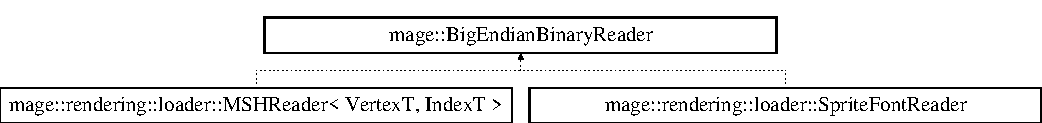
\includegraphics[height=1.637427cm]{classmage_1_1_big_endian_binary_reader}
\end{center}
\end{figure}
\subsection*{Public Member Functions}
\begin{DoxyCompactItemize}
\item 
\mbox{\hyperlink{classmage_1_1_big_endian_binary_reader}{Big\+Endian\+Binary\+Reader}} \& \mbox{\hyperlink{classmage_1_1_big_endian_binary_reader_abd4b24df4219469a8c2e9253b1cad405}{operator=}} (const \mbox{\hyperlink{classmage_1_1_big_endian_binary_reader}{Big\+Endian\+Binary\+Reader}} \&reader)=delete
\item 
\mbox{\hyperlink{classmage_1_1_big_endian_binary_reader}{Big\+Endian\+Binary\+Reader}} \& \mbox{\hyperlink{classmage_1_1_big_endian_binary_reader_ac37539cb08ea9278daf5628a0c5895d8}{operator=}} (\mbox{\hyperlink{classmage_1_1_big_endian_binary_reader}{Big\+Endian\+Binary\+Reader}} \&\&reader) noexcept
\item 
void \mbox{\hyperlink{classmage_1_1_big_endian_binary_reader_a68db676feaa42c1c3a9bf16d0680b04f}{Read\+From\+File}} (wstring fname)
\item 
void \mbox{\hyperlink{classmage_1_1_big_endian_binary_reader_afc48490dca5042078726a1ec3fe7abe7}{Read\+From\+Memory}} (gsl\+::span$<$ const \mbox{\hyperlink{namespacemage_afc638980bc6154f15af5e2d93a0e0ea9}{U8}} $>$ input)
\item 
const wstring \& \mbox{\hyperlink{classmage_1_1_big_endian_binary_reader_a801558f27606dbc681809178aaaaacd1}{Get\+Filename}} () const noexcept
\end{DoxyCompactItemize}
\subsection*{Protected Member Functions}
\begin{DoxyCompactItemize}
\item 
\mbox{\hyperlink{classmage_1_1_big_endian_binary_reader_a1fd0dbee6950a8cb04aa399f0cdbaf2a}{Big\+Endian\+Binary\+Reader}} ()
\item 
\mbox{\hyperlink{classmage_1_1_big_endian_binary_reader_a9d490263268290217ae4f2f06e0699c4}{Big\+Endian\+Binary\+Reader}} (const \mbox{\hyperlink{classmage_1_1_big_endian_binary_reader}{Big\+Endian\+Binary\+Reader}} \&reader)=delete
\item 
\mbox{\hyperlink{classmage_1_1_big_endian_binary_reader_a16c4303dfb333ebdddfc07c924b9735a}{Big\+Endian\+Binary\+Reader}} (\mbox{\hyperlink{classmage_1_1_big_endian_binary_reader}{Big\+Endian\+Binary\+Reader}} \&\&reader) noexcept
\item 
\mbox{\hyperlink{classmage_1_1_big_endian_binary_reader_ae85a40e8ed06e8c887e38d914843b8d3}{$\sim$\+Big\+Endian\+Binary\+Reader}} ()
\item 
bool \mbox{\hyperlink{classmage_1_1_big_endian_binary_reader_ac6de015b6bbcecdcef58ab074d99fb49}{Contains\+Chars}} () const noexcept
\item 
{\footnotesize template$<$typename DataT $>$ }\\const DataT \mbox{\hyperlink{classmage_1_1_big_endian_binary_reader_a5353ce3b1eaedd51ccb4d2d951bf499b}{Read}} ()
\item 
{\footnotesize template$<$typename DataT $>$ }\\const DataT $\ast$ \mbox{\hyperlink{classmage_1_1_big_endian_binary_reader_a534f06cc9b44757271595c614e8793d2}{Read\+Array}} (size\+\_\+t count)
\end{DoxyCompactItemize}
\subsection*{Private Member Functions}
\begin{DoxyCompactItemize}
\item 
virtual void \mbox{\hyperlink{classmage_1_1_big_endian_binary_reader_a7dc0689d598fa91308597b129516a11d}{Read\+Data}} ()=0
\end{DoxyCompactItemize}
\subsection*{Private Attributes}
\begin{DoxyCompactItemize}
\item 
wstring \mbox{\hyperlink{classmage_1_1_big_endian_binary_reader_a0f836aec582a59f156b64bffb9653e41}{m\+\_\+fname}}
\item 
const \mbox{\hyperlink{namespacemage_afc638980bc6154f15af5e2d93a0e0ea9}{U8}} $\ast$ \mbox{\hyperlink{classmage_1_1_big_endian_binary_reader_a7dbfc5ce1712e431f75d80a4f7a56e33}{m\+\_\+pos}}
\item 
const \mbox{\hyperlink{namespacemage_afc638980bc6154f15af5e2d93a0e0ea9}{U8}} $\ast$ \mbox{\hyperlink{classmage_1_1_big_endian_binary_reader_ab4f707d30799b98afed0f9adfc27a3e2}{m\+\_\+end}}
\item 
\mbox{\hyperlink{namespacemage_a3316d7143a973e37adf1110f2e80ca31}{Unique\+Ptr}}$<$ \mbox{\hyperlink{namespacemage_afc638980bc6154f15af5e2d93a0e0ea9}{U8}}\mbox{[}$\,$\mbox{]} $>$ \mbox{\hyperlink{classmage_1_1_big_endian_binary_reader_a54128bdaa233c1bd20494189b2397fe3}{m\+\_\+data}}
\end{DoxyCompactItemize}


\subsection{Detailed Description}
A class of readers for reading (big endian) binary files. 

\subsection{Constructor \& Destructor Documentation}
\mbox{\Hypertarget{classmage_1_1_big_endian_binary_reader_a1fd0dbee6950a8cb04aa399f0cdbaf2a}\label{classmage_1_1_big_endian_binary_reader_a1fd0dbee6950a8cb04aa399f0cdbaf2a}} 
\index{mage\+::\+Big\+Endian\+Binary\+Reader@{mage\+::\+Big\+Endian\+Binary\+Reader}!Big\+Endian\+Binary\+Reader@{Big\+Endian\+Binary\+Reader}}
\index{Big\+Endian\+Binary\+Reader@{Big\+Endian\+Binary\+Reader}!mage\+::\+Big\+Endian\+Binary\+Reader@{mage\+::\+Big\+Endian\+Binary\+Reader}}
\subsubsection{\texorpdfstring{Big\+Endian\+Binary\+Reader()}{BigEndianBinaryReader()}\hspace{0.1cm}{\footnotesize\ttfamily [1/3]}}
{\footnotesize\ttfamily mage\+::\+Big\+Endian\+Binary\+Reader\+::\+Big\+Endian\+Binary\+Reader (\begin{DoxyParamCaption}{ }\end{DoxyParamCaption})\hspace{0.3cm}{\ttfamily [protected]}}

Constructs a big endian binary reader. \mbox{\Hypertarget{classmage_1_1_big_endian_binary_reader_a9d490263268290217ae4f2f06e0699c4}\label{classmage_1_1_big_endian_binary_reader_a9d490263268290217ae4f2f06e0699c4}} 
\index{mage\+::\+Big\+Endian\+Binary\+Reader@{mage\+::\+Big\+Endian\+Binary\+Reader}!Big\+Endian\+Binary\+Reader@{Big\+Endian\+Binary\+Reader}}
\index{Big\+Endian\+Binary\+Reader@{Big\+Endian\+Binary\+Reader}!mage\+::\+Big\+Endian\+Binary\+Reader@{mage\+::\+Big\+Endian\+Binary\+Reader}}
\subsubsection{\texorpdfstring{Big\+Endian\+Binary\+Reader()}{BigEndianBinaryReader()}\hspace{0.1cm}{\footnotesize\ttfamily [2/3]}}
{\footnotesize\ttfamily mage\+::\+Big\+Endian\+Binary\+Reader\+::\+Big\+Endian\+Binary\+Reader (\begin{DoxyParamCaption}\item[{const \mbox{\hyperlink{classmage_1_1_big_endian_binary_reader}{Big\+Endian\+Binary\+Reader}} \&}]{reader }\end{DoxyParamCaption})\hspace{0.3cm}{\ttfamily [protected]}, {\ttfamily [delete]}}

Constructs a big endian binary reader from the given big endian binary reader.


\begin{DoxyParams}[1]{Parameters}
\mbox{\tt in}  & {\em reader} & A reference to the big endian binary reader to copy. \\
\hline
\end{DoxyParams}
\mbox{\Hypertarget{classmage_1_1_big_endian_binary_reader_a16c4303dfb333ebdddfc07c924b9735a}\label{classmage_1_1_big_endian_binary_reader_a16c4303dfb333ebdddfc07c924b9735a}} 
\index{mage\+::\+Big\+Endian\+Binary\+Reader@{mage\+::\+Big\+Endian\+Binary\+Reader}!Big\+Endian\+Binary\+Reader@{Big\+Endian\+Binary\+Reader}}
\index{Big\+Endian\+Binary\+Reader@{Big\+Endian\+Binary\+Reader}!mage\+::\+Big\+Endian\+Binary\+Reader@{mage\+::\+Big\+Endian\+Binary\+Reader}}
\subsubsection{\texorpdfstring{Big\+Endian\+Binary\+Reader()}{BigEndianBinaryReader()}\hspace{0.1cm}{\footnotesize\ttfamily [3/3]}}
{\footnotesize\ttfamily mage\+::\+Big\+Endian\+Binary\+Reader\+::\+Big\+Endian\+Binary\+Reader (\begin{DoxyParamCaption}\item[{\mbox{\hyperlink{classmage_1_1_big_endian_binary_reader}{Big\+Endian\+Binary\+Reader}} \&\&}]{reader }\end{DoxyParamCaption})\hspace{0.3cm}{\ttfamily [protected]}, {\ttfamily [default]}, {\ttfamily [noexcept]}}

Constructs a big endian binary reader by moving the given big endian binary reader.


\begin{DoxyParams}[1]{Parameters}
\mbox{\tt in}  & {\em reader} & A reference to the big endian binary reader to move. \\
\hline
\end{DoxyParams}
\mbox{\Hypertarget{classmage_1_1_big_endian_binary_reader_ae85a40e8ed06e8c887e38d914843b8d3}\label{classmage_1_1_big_endian_binary_reader_ae85a40e8ed06e8c887e38d914843b8d3}} 
\index{mage\+::\+Big\+Endian\+Binary\+Reader@{mage\+::\+Big\+Endian\+Binary\+Reader}!````~Big\+Endian\+Binary\+Reader@{$\sim$\+Big\+Endian\+Binary\+Reader}}
\index{````~Big\+Endian\+Binary\+Reader@{$\sim$\+Big\+Endian\+Binary\+Reader}!mage\+::\+Big\+Endian\+Binary\+Reader@{mage\+::\+Big\+Endian\+Binary\+Reader}}
\subsubsection{\texorpdfstring{$\sim$\+Big\+Endian\+Binary\+Reader()}{~BigEndianBinaryReader()}}
{\footnotesize\ttfamily mage\+::\+Big\+Endian\+Binary\+Reader\+::$\sim$\+Big\+Endian\+Binary\+Reader (\begin{DoxyParamCaption}{ }\end{DoxyParamCaption})\hspace{0.3cm}{\ttfamily [protected]}, {\ttfamily [default]}}

Destructs this big endian binary reader. 

\subsection{Member Function Documentation}
\mbox{\Hypertarget{classmage_1_1_big_endian_binary_reader_ac6de015b6bbcecdcef58ab074d99fb49}\label{classmage_1_1_big_endian_binary_reader_ac6de015b6bbcecdcef58ab074d99fb49}} 
\index{mage\+::\+Big\+Endian\+Binary\+Reader@{mage\+::\+Big\+Endian\+Binary\+Reader}!Contains\+Chars@{Contains\+Chars}}
\index{Contains\+Chars@{Contains\+Chars}!mage\+::\+Big\+Endian\+Binary\+Reader@{mage\+::\+Big\+Endian\+Binary\+Reader}}
\subsubsection{\texorpdfstring{Contains\+Chars()}{ContainsChars()}}
{\footnotesize\ttfamily bool mage\+::\+Big\+Endian\+Binary\+Reader\+::\+Contains\+Chars (\begin{DoxyParamCaption}{ }\end{DoxyParamCaption}) const\hspace{0.3cm}{\ttfamily [protected]}, {\ttfamily [noexcept]}}

Checks if there are characters left to read by this binary reader.

\begin{DoxyReturn}{Returns}
{\ttfamily true} if there are characters left to read by this binary reader. {\ttfamily false} otherwise. 
\end{DoxyReturn}
\mbox{\Hypertarget{classmage_1_1_big_endian_binary_reader_a801558f27606dbc681809178aaaaacd1}\label{classmage_1_1_big_endian_binary_reader_a801558f27606dbc681809178aaaaacd1}} 
\index{mage\+::\+Big\+Endian\+Binary\+Reader@{mage\+::\+Big\+Endian\+Binary\+Reader}!Get\+Filename@{Get\+Filename}}
\index{Get\+Filename@{Get\+Filename}!mage\+::\+Big\+Endian\+Binary\+Reader@{mage\+::\+Big\+Endian\+Binary\+Reader}}
\subsubsection{\texorpdfstring{Get\+Filename()}{GetFilename()}}
{\footnotesize\ttfamily const wstring\& mage\+::\+Big\+Endian\+Binary\+Reader\+::\+Get\+Filename (\begin{DoxyParamCaption}{ }\end{DoxyParamCaption}) const\hspace{0.3cm}{\ttfamily [noexcept]}}

Returns the current filename of this big endian binary reader.

\begin{DoxyReturn}{Returns}
A reference to the current filename of this big endian binary reader. 
\end{DoxyReturn}
\mbox{\Hypertarget{classmage_1_1_big_endian_binary_reader_abd4b24df4219469a8c2e9253b1cad405}\label{classmage_1_1_big_endian_binary_reader_abd4b24df4219469a8c2e9253b1cad405}} 
\index{mage\+::\+Big\+Endian\+Binary\+Reader@{mage\+::\+Big\+Endian\+Binary\+Reader}!operator=@{operator=}}
\index{operator=@{operator=}!mage\+::\+Big\+Endian\+Binary\+Reader@{mage\+::\+Big\+Endian\+Binary\+Reader}}
\subsubsection{\texorpdfstring{operator=()}{operator=()}\hspace{0.1cm}{\footnotesize\ttfamily [1/2]}}
{\footnotesize\ttfamily \mbox{\hyperlink{classmage_1_1_big_endian_binary_reader}{Big\+Endian\+Binary\+Reader}}\& mage\+::\+Big\+Endian\+Binary\+Reader\+::operator= (\begin{DoxyParamCaption}\item[{const \mbox{\hyperlink{classmage_1_1_big_endian_binary_reader}{Big\+Endian\+Binary\+Reader}} \&}]{reader }\end{DoxyParamCaption})\hspace{0.3cm}{\ttfamily [delete]}}

Copies the given big endian binary reader to this big endian binary reader.


\begin{DoxyParams}[1]{Parameters}
\mbox{\tt in}  & {\em reader} & A reference to a big endian binary reader to copy. \\
\hline
\end{DoxyParams}
\begin{DoxyReturn}{Returns}
A reference to the copy of the given big endian binary reader (i.\+e. this big endian binary reader). 
\end{DoxyReturn}
\mbox{\Hypertarget{classmage_1_1_big_endian_binary_reader_ac37539cb08ea9278daf5628a0c5895d8}\label{classmage_1_1_big_endian_binary_reader_ac37539cb08ea9278daf5628a0c5895d8}} 
\index{mage\+::\+Big\+Endian\+Binary\+Reader@{mage\+::\+Big\+Endian\+Binary\+Reader}!operator=@{operator=}}
\index{operator=@{operator=}!mage\+::\+Big\+Endian\+Binary\+Reader@{mage\+::\+Big\+Endian\+Binary\+Reader}}
\subsubsection{\texorpdfstring{operator=()}{operator=()}\hspace{0.1cm}{\footnotesize\ttfamily [2/2]}}
{\footnotesize\ttfamily \mbox{\hyperlink{classmage_1_1_big_endian_binary_reader}{Big\+Endian\+Binary\+Reader}} \& mage\+::\+Big\+Endian\+Binary\+Reader\+::operator= (\begin{DoxyParamCaption}\item[{\mbox{\hyperlink{classmage_1_1_big_endian_binary_reader}{Big\+Endian\+Binary\+Reader}} \&\&}]{reader }\end{DoxyParamCaption})\hspace{0.3cm}{\ttfamily [default]}, {\ttfamily [noexcept]}}

Moves the given big endian binary reader to this big endian binary reader.


\begin{DoxyParams}[1]{Parameters}
\mbox{\tt in}  & {\em reader} & A reference to a big endian binary reader to move. \\
\hline
\end{DoxyParams}
\begin{DoxyReturn}{Returns}
A reference to the moved big endian binary reader (i.\+e. this big endian binary reader). 
\end{DoxyReturn}
\mbox{\Hypertarget{classmage_1_1_big_endian_binary_reader_a5353ce3b1eaedd51ccb4d2d951bf499b}\label{classmage_1_1_big_endian_binary_reader_a5353ce3b1eaedd51ccb4d2d951bf499b}} 
\index{mage\+::\+Big\+Endian\+Binary\+Reader@{mage\+::\+Big\+Endian\+Binary\+Reader}!Read@{Read}}
\index{Read@{Read}!mage\+::\+Big\+Endian\+Binary\+Reader@{mage\+::\+Big\+Endian\+Binary\+Reader}}
\subsubsection{\texorpdfstring{Read()}{Read()}}
{\footnotesize\ttfamily template$<$typename DataT $>$ \\
const DataT mage\+::\+Big\+Endian\+Binary\+Reader\+::\+Read (\begin{DoxyParamCaption}{ }\end{DoxyParamCaption})\hspace{0.3cm}{\ttfamily [protected]}}

Reads a {\ttfamily DataT} element.


\begin{DoxyTemplParams}{Template Parameters}
{\em DataT} & The data type. \\
\hline
\end{DoxyTemplParams}
\begin{DoxyReturn}{Returns}
The {\ttfamily DataT} element read. 
\end{DoxyReturn}

\begin{DoxyExceptions}{Exceptions}
{\em \mbox{\hyperlink{classmage_1_1_exception}{Exception}}} & Failed to read a {\ttfamily DataT} element. \\
\hline
\end{DoxyExceptions}
\mbox{\Hypertarget{classmage_1_1_big_endian_binary_reader_a534f06cc9b44757271595c614e8793d2}\label{classmage_1_1_big_endian_binary_reader_a534f06cc9b44757271595c614e8793d2}} 
\index{mage\+::\+Big\+Endian\+Binary\+Reader@{mage\+::\+Big\+Endian\+Binary\+Reader}!Read\+Array@{Read\+Array}}
\index{Read\+Array@{Read\+Array}!mage\+::\+Big\+Endian\+Binary\+Reader@{mage\+::\+Big\+Endian\+Binary\+Reader}}
\subsubsection{\texorpdfstring{Read\+Array()}{ReadArray()}}
{\footnotesize\ttfamily template$<$typename DataT $>$ \\
const DataT$\ast$ mage\+::\+Big\+Endian\+Binary\+Reader\+::\+Read\+Array (\begin{DoxyParamCaption}\item[{size\+\_\+t}]{count }\end{DoxyParamCaption})\hspace{0.3cm}{\ttfamily [protected]}}

Reads an array of {\ttfamily DataT} elements.


\begin{DoxyTemplParams}{Template Parameters}
{\em DataT} & The data type. \\
\hline
\end{DoxyTemplParams}

\begin{DoxyParams}{Parameters}
{\em count} & The number of {\ttfamily DataT} elements to read. \\
\hline
\end{DoxyParams}
\begin{DoxyReturn}{Returns}
A pointer to the array of {\ttfamily DataT} element read. 
\end{DoxyReturn}

\begin{DoxyExceptions}{Exceptions}
{\em \mbox{\hyperlink{classmage_1_1_exception}{Exception}}} & Failed to read {\ttfamily count} {\ttfamily DataT} elements. \\
\hline
\end{DoxyExceptions}
\mbox{\Hypertarget{classmage_1_1_big_endian_binary_reader_a7dc0689d598fa91308597b129516a11d}\label{classmage_1_1_big_endian_binary_reader_a7dc0689d598fa91308597b129516a11d}} 
\index{mage\+::\+Big\+Endian\+Binary\+Reader@{mage\+::\+Big\+Endian\+Binary\+Reader}!Read\+Data@{Read\+Data}}
\index{Read\+Data@{Read\+Data}!mage\+::\+Big\+Endian\+Binary\+Reader@{mage\+::\+Big\+Endian\+Binary\+Reader}}
\subsubsection{\texorpdfstring{Read\+Data()}{ReadData()}}
{\footnotesize\ttfamily virtual void mage\+::\+Big\+Endian\+Binary\+Reader\+::\+Read\+Data (\begin{DoxyParamCaption}{ }\end{DoxyParamCaption})\hspace{0.3cm}{\ttfamily [private]}, {\ttfamily [pure virtual]}}

Starts reading.


\begin{DoxyExceptions}{Exceptions}
{\em \mbox{\hyperlink{classmage_1_1_exception}{Exception}}} & Failed to read from the given file. \\
\hline
\end{DoxyExceptions}


Implemented in \mbox{\hyperlink{classmage_1_1rendering_1_1loader_1_1_m_s_h_reader_a99e8e3c50decb9332dc10bcdf7b6e00a}{mage\+::rendering\+::loader\+::\+M\+S\+H\+Reader$<$ Vertex\+T, Index\+T $>$}}, and \mbox{\hyperlink{classmage_1_1rendering_1_1loader_1_1_sprite_font_reader_ae5b827dade3bd800e2000788efa91e30}{mage\+::rendering\+::loader\+::\+Sprite\+Font\+Reader}}.

\mbox{\Hypertarget{classmage_1_1_big_endian_binary_reader_a68db676feaa42c1c3a9bf16d0680b04f}\label{classmage_1_1_big_endian_binary_reader_a68db676feaa42c1c3a9bf16d0680b04f}} 
\index{mage\+::\+Big\+Endian\+Binary\+Reader@{mage\+::\+Big\+Endian\+Binary\+Reader}!Read\+From\+File@{Read\+From\+File}}
\index{Read\+From\+File@{Read\+From\+File}!mage\+::\+Big\+Endian\+Binary\+Reader@{mage\+::\+Big\+Endian\+Binary\+Reader}}
\subsubsection{\texorpdfstring{Read\+From\+File()}{ReadFromFile()}}
{\footnotesize\ttfamily void mage\+::\+Big\+Endian\+Binary\+Reader\+::\+Read\+From\+File (\begin{DoxyParamCaption}\item[{wstring}]{fname }\end{DoxyParamCaption})}

Reads from the given file.


\begin{DoxyParams}[1]{Parameters}
\mbox{\tt in}  & {\em fname} & The file name. \\
\hline
\end{DoxyParams}

\begin{DoxyExceptions}{Exceptions}
{\em \mbox{\hyperlink{classmage_1_1_exception}{Exception}}} & Failed to read from the given file. \\
\hline
\end{DoxyExceptions}
\mbox{\Hypertarget{classmage_1_1_big_endian_binary_reader_afc48490dca5042078726a1ec3fe7abe7}\label{classmage_1_1_big_endian_binary_reader_afc48490dca5042078726a1ec3fe7abe7}} 
\index{mage\+::\+Big\+Endian\+Binary\+Reader@{mage\+::\+Big\+Endian\+Binary\+Reader}!Read\+From\+Memory@{Read\+From\+Memory}}
\index{Read\+From\+Memory@{Read\+From\+Memory}!mage\+::\+Big\+Endian\+Binary\+Reader@{mage\+::\+Big\+Endian\+Binary\+Reader}}
\subsubsection{\texorpdfstring{Read\+From\+Memory()}{ReadFromMemory()}}
{\footnotesize\ttfamily void mage\+::\+Big\+Endian\+Binary\+Reader\+::\+Read\+From\+Memory (\begin{DoxyParamCaption}\item[{gsl\+::span$<$ const \mbox{\hyperlink{namespacemage_afc638980bc6154f15af5e2d93a0e0ea9}{U8}} $>$}]{input }\end{DoxyParamCaption})}

Reads the input string.


\begin{DoxyParams}[1]{Parameters}
\mbox{\tt in}  & {\em input} & The input byte string. \\
\hline
\end{DoxyParams}

\begin{DoxyExceptions}{Exceptions}
{\em \mbox{\hyperlink{classmage_1_1_exception}{Exception}}} & Failed to read from the given input string. \\
\hline
\end{DoxyExceptions}


\subsection{Member Data Documentation}
\mbox{\Hypertarget{classmage_1_1_big_endian_binary_reader_a54128bdaa233c1bd20494189b2397fe3}\label{classmage_1_1_big_endian_binary_reader_a54128bdaa233c1bd20494189b2397fe3}} 
\index{mage\+::\+Big\+Endian\+Binary\+Reader@{mage\+::\+Big\+Endian\+Binary\+Reader}!m\+\_\+data@{m\+\_\+data}}
\index{m\+\_\+data@{m\+\_\+data}!mage\+::\+Big\+Endian\+Binary\+Reader@{mage\+::\+Big\+Endian\+Binary\+Reader}}
\subsubsection{\texorpdfstring{m\+\_\+data}{m\_data}}
{\footnotesize\ttfamily \mbox{\hyperlink{namespacemage_a3316d7143a973e37adf1110f2e80ca31}{Unique\+Ptr}}$<$ \mbox{\hyperlink{namespacemage_afc638980bc6154f15af5e2d93a0e0ea9}{U8}}\mbox{[}$\,$\mbox{]} $>$ mage\+::\+Big\+Endian\+Binary\+Reader\+::m\+\_\+data\hspace{0.3cm}{\ttfamily [private]}}

A pointer to the data to read of this binary reader. \mbox{\Hypertarget{classmage_1_1_big_endian_binary_reader_ab4f707d30799b98afed0f9adfc27a3e2}\label{classmage_1_1_big_endian_binary_reader_ab4f707d30799b98afed0f9adfc27a3e2}} 
\index{mage\+::\+Big\+Endian\+Binary\+Reader@{mage\+::\+Big\+Endian\+Binary\+Reader}!m\+\_\+end@{m\+\_\+end}}
\index{m\+\_\+end@{m\+\_\+end}!mage\+::\+Big\+Endian\+Binary\+Reader@{mage\+::\+Big\+Endian\+Binary\+Reader}}
\subsubsection{\texorpdfstring{m\+\_\+end}{m\_end}}
{\footnotesize\ttfamily const \mbox{\hyperlink{namespacemage_afc638980bc6154f15af5e2d93a0e0ea9}{U8}}$\ast$ mage\+::\+Big\+Endian\+Binary\+Reader\+::m\+\_\+end\hspace{0.3cm}{\ttfamily [private]}}

A pointer to the end position of this binary reader. \mbox{\Hypertarget{classmage_1_1_big_endian_binary_reader_a0f836aec582a59f156b64bffb9653e41}\label{classmage_1_1_big_endian_binary_reader_a0f836aec582a59f156b64bffb9653e41}} 
\index{mage\+::\+Big\+Endian\+Binary\+Reader@{mage\+::\+Big\+Endian\+Binary\+Reader}!m\+\_\+fname@{m\+\_\+fname}}
\index{m\+\_\+fname@{m\+\_\+fname}!mage\+::\+Big\+Endian\+Binary\+Reader@{mage\+::\+Big\+Endian\+Binary\+Reader}}
\subsubsection{\texorpdfstring{m\+\_\+fname}{m\_fname}}
{\footnotesize\ttfamily wstring mage\+::\+Big\+Endian\+Binary\+Reader\+::m\+\_\+fname\hspace{0.3cm}{\ttfamily [private]}}

The current filename of this line reader. \mbox{\Hypertarget{classmage_1_1_big_endian_binary_reader_a7dbfc5ce1712e431f75d80a4f7a56e33}\label{classmage_1_1_big_endian_binary_reader_a7dbfc5ce1712e431f75d80a4f7a56e33}} 
\index{mage\+::\+Big\+Endian\+Binary\+Reader@{mage\+::\+Big\+Endian\+Binary\+Reader}!m\+\_\+pos@{m\+\_\+pos}}
\index{m\+\_\+pos@{m\+\_\+pos}!mage\+::\+Big\+Endian\+Binary\+Reader@{mage\+::\+Big\+Endian\+Binary\+Reader}}
\subsubsection{\texorpdfstring{m\+\_\+pos}{m\_pos}}
{\footnotesize\ttfamily const \mbox{\hyperlink{namespacemage_afc638980bc6154f15af5e2d93a0e0ea9}{U8}}$\ast$ mage\+::\+Big\+Endian\+Binary\+Reader\+::m\+\_\+pos\hspace{0.3cm}{\ttfamily [private]}}

A pointer to the current position of this binary reader. 
\hypertarget{classmage_1_1_big_endian_binary_writer}{}\section{mage\+:\+:Big\+Endian\+Binary\+Writer Class Reference}
\label{classmage_1_1_big_endian_binary_writer}\index{mage\+::\+Big\+Endian\+Binary\+Writer@{mage\+::\+Big\+Endian\+Binary\+Writer}}


{\ttfamily \#include $<$binary\+\_\+writer.\+hpp$>$}

Inheritance diagram for mage\+:\+:Big\+Endian\+Binary\+Writer\+:\begin{figure}[H]
\begin{center}
\leavevmode
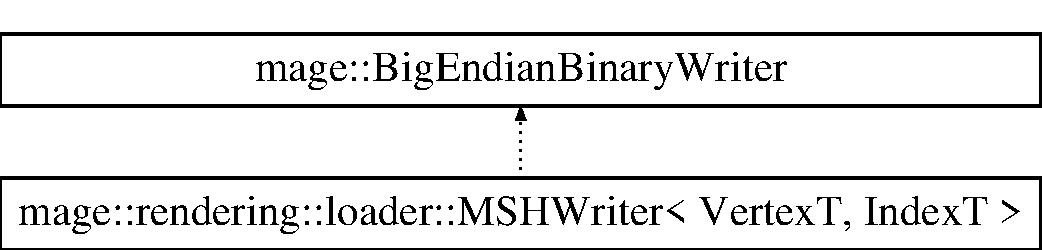
\includegraphics[height=2.000000cm]{classmage_1_1_big_endian_binary_writer}
\end{center}
\end{figure}
\subsection*{Public Member Functions}
\begin{DoxyCompactItemize}
\item 
\mbox{\hyperlink{classmage_1_1_big_endian_binary_writer}{Big\+Endian\+Binary\+Writer}} \& \mbox{\hyperlink{classmage_1_1_big_endian_binary_writer_ae574f7d0b630890256996c52818ba633}{operator=}} (const \mbox{\hyperlink{classmage_1_1_big_endian_binary_writer}{Big\+Endian\+Binary\+Writer}} \&writer)=delete
\item 
\mbox{\hyperlink{classmage_1_1_big_endian_binary_writer}{Big\+Endian\+Binary\+Writer}} \& \mbox{\hyperlink{classmage_1_1_big_endian_binary_writer_a8c01bf43f5e941578c5c5947ea184a78}{operator=}} (\mbox{\hyperlink{classmage_1_1_big_endian_binary_writer}{Big\+Endian\+Binary\+Writer}} \&\&writer) noexcept
\item 
void \mbox{\hyperlink{classmage_1_1_big_endian_binary_writer_a6ce9780687a45a6c6f98e0843190b63b}{Write\+To\+File}} (std\+::filesystem\+::path path)
\end{DoxyCompactItemize}
\subsection*{Protected Member Functions}
\begin{DoxyCompactItemize}
\item 
\mbox{\hyperlink{classmage_1_1_big_endian_binary_writer_ac0917b684913834577d4850269a6c09a}{Big\+Endian\+Binary\+Writer}} ()
\item 
\mbox{\hyperlink{classmage_1_1_big_endian_binary_writer_aafe65752342b2740e7293878ae469d9f}{Big\+Endian\+Binary\+Writer}} (const \mbox{\hyperlink{classmage_1_1_big_endian_binary_writer}{Big\+Endian\+Binary\+Writer}} \&writer)=delete
\item 
\mbox{\hyperlink{classmage_1_1_big_endian_binary_writer_aaf2dcf536afefc7b0ca8b0752024311d}{Big\+Endian\+Binary\+Writer}} (\mbox{\hyperlink{classmage_1_1_big_endian_binary_writer}{Big\+Endian\+Binary\+Writer}} \&\&writer) noexcept
\item 
\mbox{\hyperlink{classmage_1_1_big_endian_binary_writer_ab717bcbfc15ba4a1cb25eeb564e120b8}{$\sim$\+Big\+Endian\+Binary\+Writer}} ()
\item 
const std\+::filesystem\+::path \& \mbox{\hyperlink{classmage_1_1_big_endian_binary_writer_a812e65c16bf1b14d396d109eb969eeb8}{Get\+Path}} () const noexcept
\item 
{\footnotesize template$<$typename T $>$ }\\void \mbox{\hyperlink{classmage_1_1_big_endian_binary_writer_ae8bab2d7022672e1d30991c1288d981c}{Write}} (const T \&data)
\item 
{\footnotesize template$<$typename T $>$ }\\void \mbox{\hyperlink{classmage_1_1_big_endian_binary_writer_a7c82860ea3eed12777207cd00436b6c3}{Write\+Array}} (gsl\+::span$<$ const T $>$ data)
\item 
void \mbox{\hyperlink{classmage_1_1_big_endian_binary_writer_a869eff3f6e0666406bd5470af3e02096}{Write\+Character}} (char c)
\item 
void \mbox{\hyperlink{classmage_1_1_big_endian_binary_writer_acf065a2e7462c9e6cf46849bd2c9d2e7}{Write\+String}} (\mbox{\hyperlink{namespacemage_a8769f9d670d6b585ea306cb1062af94b}{Not\+Null}}$<$ \mbox{\hyperlink{namespacemage_abfd9206dc607ceb5d13ec68bf075a5c0}{const\+\_\+zstring}} $>$ str)
\end{DoxyCompactItemize}
\subsection*{Private Member Functions}
\begin{DoxyCompactItemize}
\item 
virtual void \mbox{\hyperlink{classmage_1_1_big_endian_binary_writer_a719581274b1b185ef05687183f7ded25}{Write\+Data}} ()=0
\end{DoxyCompactItemize}
\subsection*{Private Attributes}
\begin{DoxyCompactItemize}
\item 
\mbox{\hyperlink{namespacemage_ac11c62400d336d9f6857c7cdaecfc7a8}{Unique\+File\+Stream}} \mbox{\hyperlink{classmage_1_1_big_endian_binary_writer_ad2cdbdca429d6c351a57b51d175ffb55}{m\+\_\+file\+\_\+stream}}
\item 
std\+::filesystem\+::path \mbox{\hyperlink{classmage_1_1_big_endian_binary_writer_a22815e47cf8bf3443c10ec2ff4409745}{m\+\_\+path}}
\end{DoxyCompactItemize}


\subsection{Detailed Description}
A class of writers for writing (big endian) binary files. 

\subsection{Constructor \& Destructor Documentation}
\mbox{\Hypertarget{classmage_1_1_big_endian_binary_writer_ac0917b684913834577d4850269a6c09a}\label{classmage_1_1_big_endian_binary_writer_ac0917b684913834577d4850269a6c09a}} 
\index{mage\+::\+Big\+Endian\+Binary\+Writer@{mage\+::\+Big\+Endian\+Binary\+Writer}!Big\+Endian\+Binary\+Writer@{Big\+Endian\+Binary\+Writer}}
\index{Big\+Endian\+Binary\+Writer@{Big\+Endian\+Binary\+Writer}!mage\+::\+Big\+Endian\+Binary\+Writer@{mage\+::\+Big\+Endian\+Binary\+Writer}}
\subsubsection{\texorpdfstring{Big\+Endian\+Binary\+Writer()}{BigEndianBinaryWriter()}\hspace{0.1cm}{\footnotesize\ttfamily [1/3]}}
{\footnotesize\ttfamily mage\+::\+Big\+Endian\+Binary\+Writer\+::\+Big\+Endian\+Binary\+Writer (\begin{DoxyParamCaption}{ }\end{DoxyParamCaption})\hspace{0.3cm}{\ttfamily [protected]}}

Constructs a big endian binary writer. \mbox{\Hypertarget{classmage_1_1_big_endian_binary_writer_aafe65752342b2740e7293878ae469d9f}\label{classmage_1_1_big_endian_binary_writer_aafe65752342b2740e7293878ae469d9f}} 
\index{mage\+::\+Big\+Endian\+Binary\+Writer@{mage\+::\+Big\+Endian\+Binary\+Writer}!Big\+Endian\+Binary\+Writer@{Big\+Endian\+Binary\+Writer}}
\index{Big\+Endian\+Binary\+Writer@{Big\+Endian\+Binary\+Writer}!mage\+::\+Big\+Endian\+Binary\+Writer@{mage\+::\+Big\+Endian\+Binary\+Writer}}
\subsubsection{\texorpdfstring{Big\+Endian\+Binary\+Writer()}{BigEndianBinaryWriter()}\hspace{0.1cm}{\footnotesize\ttfamily [2/3]}}
{\footnotesize\ttfamily mage\+::\+Big\+Endian\+Binary\+Writer\+::\+Big\+Endian\+Binary\+Writer (\begin{DoxyParamCaption}\item[{const \mbox{\hyperlink{classmage_1_1_big_endian_binary_writer}{Big\+Endian\+Binary\+Writer}} \&}]{writer }\end{DoxyParamCaption})\hspace{0.3cm}{\ttfamily [protected]}, {\ttfamily [delete]}}

Constructs a big endian binary writer from the given big endian binary writer.


\begin{DoxyParams}[1]{Parameters}
\mbox{\tt in}  & {\em writer} & A reference to the big endian binary writer to copy. \\
\hline
\end{DoxyParams}
\mbox{\Hypertarget{classmage_1_1_big_endian_binary_writer_aaf2dcf536afefc7b0ca8b0752024311d}\label{classmage_1_1_big_endian_binary_writer_aaf2dcf536afefc7b0ca8b0752024311d}} 
\index{mage\+::\+Big\+Endian\+Binary\+Writer@{mage\+::\+Big\+Endian\+Binary\+Writer}!Big\+Endian\+Binary\+Writer@{Big\+Endian\+Binary\+Writer}}
\index{Big\+Endian\+Binary\+Writer@{Big\+Endian\+Binary\+Writer}!mage\+::\+Big\+Endian\+Binary\+Writer@{mage\+::\+Big\+Endian\+Binary\+Writer}}
\subsubsection{\texorpdfstring{Big\+Endian\+Binary\+Writer()}{BigEndianBinaryWriter()}\hspace{0.1cm}{\footnotesize\ttfamily [3/3]}}
{\footnotesize\ttfamily mage\+::\+Big\+Endian\+Binary\+Writer\+::\+Big\+Endian\+Binary\+Writer (\begin{DoxyParamCaption}\item[{\mbox{\hyperlink{classmage_1_1_big_endian_binary_writer}{Big\+Endian\+Binary\+Writer}} \&\&}]{writer }\end{DoxyParamCaption})\hspace{0.3cm}{\ttfamily [protected]}, {\ttfamily [default]}, {\ttfamily [noexcept]}}

Constructs a big endian binary writer by moving the given big endian binary writer.


\begin{DoxyParams}[1]{Parameters}
\mbox{\tt in}  & {\em writer} & A reference to the big endian binary writer to move. \\
\hline
\end{DoxyParams}
\mbox{\Hypertarget{classmage_1_1_big_endian_binary_writer_ab717bcbfc15ba4a1cb25eeb564e120b8}\label{classmage_1_1_big_endian_binary_writer_ab717bcbfc15ba4a1cb25eeb564e120b8}} 
\index{mage\+::\+Big\+Endian\+Binary\+Writer@{mage\+::\+Big\+Endian\+Binary\+Writer}!````~Big\+Endian\+Binary\+Writer@{$\sim$\+Big\+Endian\+Binary\+Writer}}
\index{````~Big\+Endian\+Binary\+Writer@{$\sim$\+Big\+Endian\+Binary\+Writer}!mage\+::\+Big\+Endian\+Binary\+Writer@{mage\+::\+Big\+Endian\+Binary\+Writer}}
\subsubsection{\texorpdfstring{$\sim$\+Big\+Endian\+Binary\+Writer()}{~BigEndianBinaryWriter()}}
{\footnotesize\ttfamily mage\+::\+Big\+Endian\+Binary\+Writer\+::$\sim$\+Big\+Endian\+Binary\+Writer (\begin{DoxyParamCaption}{ }\end{DoxyParamCaption})\hspace{0.3cm}{\ttfamily [protected]}, {\ttfamily [default]}}

Destructs this big endian binary writer. 

\subsection{Member Function Documentation}
\mbox{\Hypertarget{classmage_1_1_big_endian_binary_writer_a812e65c16bf1b14d396d109eb969eeb8}\label{classmage_1_1_big_endian_binary_writer_a812e65c16bf1b14d396d109eb969eeb8}} 
\index{mage\+::\+Big\+Endian\+Binary\+Writer@{mage\+::\+Big\+Endian\+Binary\+Writer}!Get\+Path@{Get\+Path}}
\index{Get\+Path@{Get\+Path}!mage\+::\+Big\+Endian\+Binary\+Writer@{mage\+::\+Big\+Endian\+Binary\+Writer}}
\subsubsection{\texorpdfstring{Get\+Path()}{GetPath()}}
{\footnotesize\ttfamily const std\+::filesystem\+::path\& mage\+::\+Big\+Endian\+Binary\+Writer\+::\+Get\+Path (\begin{DoxyParamCaption}{ }\end{DoxyParamCaption}) const\hspace{0.3cm}{\ttfamily [protected]}, {\ttfamily [noexcept]}}

Returns the current path of this big endian binary writer.

\begin{DoxyReturn}{Returns}
A reference to the current path of this big endian binary writer. 
\end{DoxyReturn}
\mbox{\Hypertarget{classmage_1_1_big_endian_binary_writer_ae574f7d0b630890256996c52818ba633}\label{classmage_1_1_big_endian_binary_writer_ae574f7d0b630890256996c52818ba633}} 
\index{mage\+::\+Big\+Endian\+Binary\+Writer@{mage\+::\+Big\+Endian\+Binary\+Writer}!operator=@{operator=}}
\index{operator=@{operator=}!mage\+::\+Big\+Endian\+Binary\+Writer@{mage\+::\+Big\+Endian\+Binary\+Writer}}
\subsubsection{\texorpdfstring{operator=()}{operator=()}\hspace{0.1cm}{\footnotesize\ttfamily [1/2]}}
{\footnotesize\ttfamily \mbox{\hyperlink{classmage_1_1_big_endian_binary_writer}{Big\+Endian\+Binary\+Writer}}\& mage\+::\+Big\+Endian\+Binary\+Writer\+::operator= (\begin{DoxyParamCaption}\item[{const \mbox{\hyperlink{classmage_1_1_big_endian_binary_writer}{Big\+Endian\+Binary\+Writer}} \&}]{writer }\end{DoxyParamCaption})\hspace{0.3cm}{\ttfamily [delete]}}

Copies the given big endian binary writer to this big endian binary writer.


\begin{DoxyParams}[1]{Parameters}
\mbox{\tt in}  & {\em writer} & A reference to a big endian binary writer to copy. \\
\hline
\end{DoxyParams}
\begin{DoxyReturn}{Returns}
A reference to the copy of the given big endian binary writer (i.\+e. this big endian binary writer). 
\end{DoxyReturn}
\mbox{\Hypertarget{classmage_1_1_big_endian_binary_writer_a8c01bf43f5e941578c5c5947ea184a78}\label{classmage_1_1_big_endian_binary_writer_a8c01bf43f5e941578c5c5947ea184a78}} 
\index{mage\+::\+Big\+Endian\+Binary\+Writer@{mage\+::\+Big\+Endian\+Binary\+Writer}!operator=@{operator=}}
\index{operator=@{operator=}!mage\+::\+Big\+Endian\+Binary\+Writer@{mage\+::\+Big\+Endian\+Binary\+Writer}}
\subsubsection{\texorpdfstring{operator=()}{operator=()}\hspace{0.1cm}{\footnotesize\ttfamily [2/2]}}
{\footnotesize\ttfamily \mbox{\hyperlink{classmage_1_1_big_endian_binary_writer}{Big\+Endian\+Binary\+Writer}} \& mage\+::\+Big\+Endian\+Binary\+Writer\+::operator= (\begin{DoxyParamCaption}\item[{\mbox{\hyperlink{classmage_1_1_big_endian_binary_writer}{Big\+Endian\+Binary\+Writer}} \&\&}]{writer }\end{DoxyParamCaption})\hspace{0.3cm}{\ttfamily [default]}, {\ttfamily [noexcept]}}

Moves the given big endian binary writer to this big endian binary writer.


\begin{DoxyParams}[1]{Parameters}
\mbox{\tt in}  & {\em writer} & A reference to a big endian binary writer to move. \\
\hline
\end{DoxyParams}
\begin{DoxyReturn}{Returns}
A reference to the moved big endian binary writer (i.\+e. this big endian binary writer). 
\end{DoxyReturn}
\mbox{\Hypertarget{classmage_1_1_big_endian_binary_writer_ae8bab2d7022672e1d30991c1288d981c}\label{classmage_1_1_big_endian_binary_writer_ae8bab2d7022672e1d30991c1288d981c}} 
\index{mage\+::\+Big\+Endian\+Binary\+Writer@{mage\+::\+Big\+Endian\+Binary\+Writer}!Write@{Write}}
\index{Write@{Write}!mage\+::\+Big\+Endian\+Binary\+Writer@{mage\+::\+Big\+Endian\+Binary\+Writer}}
\subsubsection{\texorpdfstring{Write()}{Write()}}
{\footnotesize\ttfamily template$<$typename T $>$ \\
void mage\+::\+Big\+Endian\+Binary\+Writer\+::\+Write (\begin{DoxyParamCaption}\item[{const T \&}]{data }\end{DoxyParamCaption})\hspace{0.3cm}{\ttfamily [protected]}}

Writes the given data.


\begin{DoxyTemplParams}{Template Parameters}
{\em T} & The data type. \\
\hline
\end{DoxyTemplParams}

\begin{DoxyParams}[1]{Parameters}
\mbox{\tt in}  & {\em data} & A reference to the data. \\
\hline
\end{DoxyParams}

\begin{DoxyExceptions}{Exceptions}
{\em \mbox{\hyperlink{classmage_1_1_exception}{Exception}}} & Failed to write the given data. \\
\hline
\end{DoxyExceptions}
\mbox{\Hypertarget{classmage_1_1_big_endian_binary_writer_a7c82860ea3eed12777207cd00436b6c3}\label{classmage_1_1_big_endian_binary_writer_a7c82860ea3eed12777207cd00436b6c3}} 
\index{mage\+::\+Big\+Endian\+Binary\+Writer@{mage\+::\+Big\+Endian\+Binary\+Writer}!Write\+Array@{Write\+Array}}
\index{Write\+Array@{Write\+Array}!mage\+::\+Big\+Endian\+Binary\+Writer@{mage\+::\+Big\+Endian\+Binary\+Writer}}
\subsubsection{\texorpdfstring{Write\+Array()}{WriteArray()}}
{\footnotesize\ttfamily template$<$typename T $>$ \\
void mage\+::\+Big\+Endian\+Binary\+Writer\+::\+Write\+Array (\begin{DoxyParamCaption}\item[{gsl\+::span$<$ const T $>$}]{data }\end{DoxyParamCaption})\hspace{0.3cm}{\ttfamily [protected]}}

Writes the given data array.


\begin{DoxyTemplParams}{Template Parameters}
{\em T} & The data type. \\
\hline
\end{DoxyTemplParams}

\begin{DoxyParams}[1]{Parameters}
\mbox{\tt in}  & {\em data} & The data array. \\
\hline
\end{DoxyParams}

\begin{DoxyExceptions}{Exceptions}
{\em \mbox{\hyperlink{classmage_1_1_exception}{Exception}}} & Failed to write the given data. \\
\hline
\end{DoxyExceptions}
\mbox{\Hypertarget{classmage_1_1_big_endian_binary_writer_a869eff3f6e0666406bd5470af3e02096}\label{classmage_1_1_big_endian_binary_writer_a869eff3f6e0666406bd5470af3e02096}} 
\index{mage\+::\+Big\+Endian\+Binary\+Writer@{mage\+::\+Big\+Endian\+Binary\+Writer}!Write\+Character@{Write\+Character}}
\index{Write\+Character@{Write\+Character}!mage\+::\+Big\+Endian\+Binary\+Writer@{mage\+::\+Big\+Endian\+Binary\+Writer}}
\subsubsection{\texorpdfstring{Write\+Character()}{WriteCharacter()}}
{\footnotesize\ttfamily void mage\+::\+Big\+Endian\+Binary\+Writer\+::\+Write\+Character (\begin{DoxyParamCaption}\item[{char}]{c }\end{DoxyParamCaption})\hspace{0.3cm}{\ttfamily [protected]}}

Writes the given character.


\begin{DoxyParams}[1]{Parameters}
\mbox{\tt in}  & {\em c} & The character to write. \\
\hline
\end{DoxyParams}

\begin{DoxyExceptions}{Exceptions}
{\em \mbox{\hyperlink{classmage_1_1_exception}{Exception}}} & Failed to write the given character. \\
\hline
\end{DoxyExceptions}
\mbox{\Hypertarget{classmage_1_1_big_endian_binary_writer_a719581274b1b185ef05687183f7ded25}\label{classmage_1_1_big_endian_binary_writer_a719581274b1b185ef05687183f7ded25}} 
\index{mage\+::\+Big\+Endian\+Binary\+Writer@{mage\+::\+Big\+Endian\+Binary\+Writer}!Write\+Data@{Write\+Data}}
\index{Write\+Data@{Write\+Data}!mage\+::\+Big\+Endian\+Binary\+Writer@{mage\+::\+Big\+Endian\+Binary\+Writer}}
\subsubsection{\texorpdfstring{Write\+Data()}{WriteData()}}
{\footnotesize\ttfamily virtual void mage\+::\+Big\+Endian\+Binary\+Writer\+::\+Write\+Data (\begin{DoxyParamCaption}{ }\end{DoxyParamCaption})\hspace{0.3cm}{\ttfamily [private]}, {\ttfamily [pure virtual]}}

Starts writing.


\begin{DoxyExceptions}{Exceptions}
{\em \mbox{\hyperlink{classmage_1_1_exception}{Exception}}} & Failed to write. \\
\hline
\end{DoxyExceptions}


Implemented in \mbox{\hyperlink{classmage_1_1rendering_1_1loader_1_1_m_s_h_writer_ad61ee7097e1bfb52ca9a0697d2cd6a7e}{mage\+::rendering\+::loader\+::\+M\+S\+H\+Writer$<$ Vertex\+T, Index\+T $>$}}.

\mbox{\Hypertarget{classmage_1_1_big_endian_binary_writer_acf065a2e7462c9e6cf46849bd2c9d2e7}\label{classmage_1_1_big_endian_binary_writer_acf065a2e7462c9e6cf46849bd2c9d2e7}} 
\index{mage\+::\+Big\+Endian\+Binary\+Writer@{mage\+::\+Big\+Endian\+Binary\+Writer}!Write\+String@{Write\+String}}
\index{Write\+String@{Write\+String}!mage\+::\+Big\+Endian\+Binary\+Writer@{mage\+::\+Big\+Endian\+Binary\+Writer}}
\subsubsection{\texorpdfstring{Write\+String()}{WriteString()}}
{\footnotesize\ttfamily void mage\+::\+Big\+Endian\+Binary\+Writer\+::\+Write\+String (\begin{DoxyParamCaption}\item[{\mbox{\hyperlink{namespacemage_a8769f9d670d6b585ea306cb1062af94b}{Not\+Null}}$<$ \mbox{\hyperlink{namespacemage_abfd9206dc607ceb5d13ec68bf075a5c0}{const\+\_\+zstring}} $>$}]{str }\end{DoxyParamCaption})\hspace{0.3cm}{\ttfamily [protected]}}

Writes the given string.


\begin{DoxyParams}[1]{Parameters}
\mbox{\tt in}  & {\em str} & A pointer to the first null-\/terminated byte string to write. \\
\hline
\end{DoxyParams}

\begin{DoxyExceptions}{Exceptions}
{\em \mbox{\hyperlink{classmage_1_1_exception}{Exception}}} & Failed to write the given string. \\
\hline
\end{DoxyExceptions}
\mbox{\Hypertarget{classmage_1_1_big_endian_binary_writer_a6ce9780687a45a6c6f98e0843190b63b}\label{classmage_1_1_big_endian_binary_writer_a6ce9780687a45a6c6f98e0843190b63b}} 
\index{mage\+::\+Big\+Endian\+Binary\+Writer@{mage\+::\+Big\+Endian\+Binary\+Writer}!Write\+To\+File@{Write\+To\+File}}
\index{Write\+To\+File@{Write\+To\+File}!mage\+::\+Big\+Endian\+Binary\+Writer@{mage\+::\+Big\+Endian\+Binary\+Writer}}
\subsubsection{\texorpdfstring{Write\+To\+File()}{WriteToFile()}}
{\footnotesize\ttfamily void mage\+::\+Big\+Endian\+Binary\+Writer\+::\+Write\+To\+File (\begin{DoxyParamCaption}\item[{std\+::filesystem\+::path}]{path }\end{DoxyParamCaption})}

Writes to the file associated with the given path.


\begin{DoxyParams}[1]{Parameters}
\mbox{\tt in}  & {\em path} & The path. \\
\hline
\end{DoxyParams}

\begin{DoxyExceptions}{Exceptions}
{\em \mbox{\hyperlink{classmage_1_1_exception}{Exception}}} & Failed to write to the file. \\
\hline
\end{DoxyExceptions}


\subsection{Member Data Documentation}
\mbox{\Hypertarget{classmage_1_1_big_endian_binary_writer_ad2cdbdca429d6c351a57b51d175ffb55}\label{classmage_1_1_big_endian_binary_writer_ad2cdbdca429d6c351a57b51d175ffb55}} 
\index{mage\+::\+Big\+Endian\+Binary\+Writer@{mage\+::\+Big\+Endian\+Binary\+Writer}!m\+\_\+file\+\_\+stream@{m\+\_\+file\+\_\+stream}}
\index{m\+\_\+file\+\_\+stream@{m\+\_\+file\+\_\+stream}!mage\+::\+Big\+Endian\+Binary\+Writer@{mage\+::\+Big\+Endian\+Binary\+Writer}}
\subsubsection{\texorpdfstring{m\+\_\+file\+\_\+stream}{m\_file\_stream}}
{\footnotesize\ttfamily \mbox{\hyperlink{namespacemage_ac11c62400d336d9f6857c7cdaecfc7a8}{Unique\+File\+Stream}} mage\+::\+Big\+Endian\+Binary\+Writer\+::m\+\_\+file\+\_\+stream\hspace{0.3cm}{\ttfamily [private]}}

A pointer to the file stream of this big endian binary writer. \mbox{\Hypertarget{classmage_1_1_big_endian_binary_writer_a22815e47cf8bf3443c10ec2ff4409745}\label{classmage_1_1_big_endian_binary_writer_a22815e47cf8bf3443c10ec2ff4409745}} 
\index{mage\+::\+Big\+Endian\+Binary\+Writer@{mage\+::\+Big\+Endian\+Binary\+Writer}!m\+\_\+path@{m\+\_\+path}}
\index{m\+\_\+path@{m\+\_\+path}!mage\+::\+Big\+Endian\+Binary\+Writer@{mage\+::\+Big\+Endian\+Binary\+Writer}}
\subsubsection{\texorpdfstring{m\+\_\+path}{m\_path}}
{\footnotesize\ttfamily std\+::filesystem\+::path mage\+::\+Big\+Endian\+Binary\+Writer\+::m\+\_\+path\hspace{0.3cm}{\ttfamily [private]}}

The current path of this big endian binary writer. 
\hypertarget{classmage_1_1_binary_reader}{}\section{mage\+:\+:Binary\+Reader Class Reference}
\label{classmage_1_1_binary_reader}\index{mage\+::\+Binary\+Reader@{mage\+::\+Binary\+Reader}}


{\ttfamily \#include $<$binary\+\_\+reader.\+hpp$>$}

\subsection*{Public Member Functions}
\begin{DoxyCompactItemize}
\item 
virtual \hyperlink{classmage_1_1_binary_reader_a42e6c31bc53f5214675f845756b5a404}{$\sim$\+Binary\+Reader} ()
\item 
\hyperlink{classmage_1_1_binary_reader}{Binary\+Reader} \& \hyperlink{classmage_1_1_binary_reader_a0408bb456983b4a03ae42ab69c6f4bc3}{operator=} (const \hyperlink{classmage_1_1_binary_reader}{Binary\+Reader} \&reader)=delete
\item 
\hyperlink{classmage_1_1_binary_reader}{Binary\+Reader} \& \hyperlink{classmage_1_1_binary_reader_abb971fe92727a0e86b3698dba8c586de}{operator=} (\hyperlink{classmage_1_1_binary_reader}{Binary\+Reader} \&\&reader)=delete
\item 
void \hyperlink{classmage_1_1_binary_reader_aa9cc5e2bd41cd5ae5ee421ee9a1e10b2}{Read\+From\+File} (const wstring \&fname, bool big\+\_\+endian)
\item 
void \hyperlink{classmage_1_1_binary_reader_a918f751ba7ae721512f7117aff0576d3}{Read\+From\+Memory} (const \hyperlink{namespacemage_a5a362e2d56fc439362a80516ecae7828}{u8} $\ast$input, size\+\_\+t size, bool big\+\_\+endian)
\item 
const wstring \& \hyperlink{classmage_1_1_binary_reader_ad9d4a4a3e2f0afc666d15badff08fe4a}{Get\+Filename} () const noexcept
\end{DoxyCompactItemize}
\subsection*{Protected Member Functions}
\begin{DoxyCompactItemize}
\item 
\hyperlink{classmage_1_1_binary_reader_aab82579cef4f2f022273cf1adfcc8497}{Binary\+Reader} ()
\item 
\hyperlink{classmage_1_1_binary_reader_a8c1ff948f1d056439f3d8cc37d7f507c}{Binary\+Reader} (const \hyperlink{classmage_1_1_binary_reader}{Binary\+Reader} \&reader)=delete
\item 
\hyperlink{classmage_1_1_binary_reader_a3a24db5c872cca270596d53989ac8c91}{Binary\+Reader} (\hyperlink{classmage_1_1_binary_reader}{Binary\+Reader} \&\&reader)
\item 
bool \hyperlink{classmage_1_1_binary_reader_aec91fece03b619c158b133beb1bc9381}{Has\+Chars\+Left} () const noexcept
\item 
const char $\ast$ \hyperlink{classmage_1_1_binary_reader_af1e0e4ab815e23c72ab65fd7c0748d3f}{Read\+Chars} (size\+\_\+t size)
\item 
\hyperlink{namespacemage_ae590501eabc5b30d993320c2159423ee}{i8} \hyperlink{classmage_1_1_binary_reader_a80a9edbeb61e1e88c79a2f7d947ca872}{Read\+I8} ()
\item 
\hyperlink{namespacemage_a5a362e2d56fc439362a80516ecae7828}{u8} \hyperlink{classmage_1_1_binary_reader_af9feb92c6991f62a3866aae9caead1c3}{Read\+U8} ()
\item 
\hyperlink{namespacemage_a80228058266cc2ec5868d65b2a4c2f3c}{i16} \hyperlink{classmage_1_1_binary_reader_a7fb2f143eb79f90229a157d344236c2b}{Read\+I16} ()
\item 
\hyperlink{namespacemage_aaf695d763e29d308a85ee22c6489344e}{u16} \hyperlink{classmage_1_1_binary_reader_a35c4e93b44a6864df80ceee67d6eb940}{Read\+U16} ()
\item 
\hyperlink{namespacemage_ad59a7dbc22c51c308b6df9e9c3cafd62}{i32} \hyperlink{classmage_1_1_binary_reader_a0bff822c17c18e85cf7e05340acb1d9a}{Read\+I32} ()
\item 
\hyperlink{namespacemage_af2b398bf98eb10351f49cad73fe2cc73}{u32} \hyperlink{classmage_1_1_binary_reader_ac2f065778e87d58be3061469aaaa92e0}{Read\+U32} ()
\item 
\hyperlink{namespacemage_a3d629c1ab28148a782661e5b14b6fe5e}{i64} \hyperlink{classmage_1_1_binary_reader_af6d39f753e912c5ec1da13d411f756c0}{Read\+I64} ()
\item 
\hyperlink{namespacemage_aee97da48a07394dd617c9deb60ed2064}{u64} \hyperlink{classmage_1_1_binary_reader_a076c3f2ecc7634b297ae08b9fda48ea0}{Read\+U64} ()
\item 
\hyperlink{namespacemage_a6a44ad388483959dc4dff9f2aef91431}{f32} \hyperlink{classmage_1_1_binary_reader_a4edbec13821d82c471e8c155b1710f79}{Read\+F32} ()
\item 
\hyperlink{namespacemage_ab935747c6941320bd6214b5a5f265b09}{f64} \hyperlink{classmage_1_1_binary_reader_a5d3e1add9e6108f71f69e770983f4188}{Read\+F64} ()
\end{DoxyCompactItemize}
\subsection*{Private Member Functions}
\begin{DoxyCompactItemize}
\item 
virtual void \hyperlink{classmage_1_1_binary_reader_a5c060c165f17a71f4218eb98c7091273}{Read} ()=0
\end{DoxyCompactItemize}
\subsection*{Private Attributes}
\begin{DoxyCompactItemize}
\item 
wstring \hyperlink{classmage_1_1_binary_reader_a9c97c02d53ce60a9952751ad4f55414f}{m\+\_\+fname}
\item 
bool \hyperlink{classmage_1_1_binary_reader_a8d23fde958e08efe248edb5d92861113}{m\+\_\+big\+\_\+endian}
\item 
const \hyperlink{namespacemage_a5a362e2d56fc439362a80516ecae7828}{u8} $\ast$ \hyperlink{classmage_1_1_binary_reader_a7973b89d2e97637ded2c446f0539ec6f}{m\+\_\+pos}
\item 
const \hyperlink{namespacemage_a5a362e2d56fc439362a80516ecae7828}{u8} $\ast$ \hyperlink{classmage_1_1_binary_reader_a6f676fd4c9ccddd6f1aadae455d01229}{m\+\_\+end}
\item 
\hyperlink{namespacemage_a3316d7143a973e37adf1110f2e80ca31}{Unique\+Ptr}$<$ \hyperlink{namespacemage_a5a362e2d56fc439362a80516ecae7828}{u8}\mbox{[}$\,$\mbox{]} $>$ \hyperlink{classmage_1_1_binary_reader_afd18df56e004f119e9e082458bf9efc6}{m\+\_\+data}
\end{DoxyCompactItemize}


\subsection{Detailed Description}
A class of readers for reading binary files. 

\subsection{Constructor \& Destructor Documentation}
\hypertarget{classmage_1_1_binary_reader_a42e6c31bc53f5214675f845756b5a404}{}\label{classmage_1_1_binary_reader_a42e6c31bc53f5214675f845756b5a404} 
\index{mage\+::\+Binary\+Reader@{mage\+::\+Binary\+Reader}!````~Binary\+Reader@{$\sim$\+Binary\+Reader}}
\index{````~Binary\+Reader@{$\sim$\+Binary\+Reader}!mage\+::\+Binary\+Reader@{mage\+::\+Binary\+Reader}}
\subsubsection{\texorpdfstring{$\sim$\+Binary\+Reader()}{~BinaryReader()}}
{\footnotesize\ttfamily mage\+::\+Binary\+Reader\+::$\sim$\+Binary\+Reader (\begin{DoxyParamCaption}{ }\end{DoxyParamCaption})\hspace{0.3cm}{\ttfamily [virtual]}, {\ttfamily [default]}}

Destructs this binary reader. \hypertarget{classmage_1_1_binary_reader_aab82579cef4f2f022273cf1adfcc8497}{}\label{classmage_1_1_binary_reader_aab82579cef4f2f022273cf1adfcc8497} 
\index{mage\+::\+Binary\+Reader@{mage\+::\+Binary\+Reader}!Binary\+Reader@{Binary\+Reader}}
\index{Binary\+Reader@{Binary\+Reader}!mage\+::\+Binary\+Reader@{mage\+::\+Binary\+Reader}}
\subsubsection{\texorpdfstring{Binary\+Reader()}{BinaryReader()}\hspace{0.1cm}{\footnotesize\ttfamily [1/3]}}
{\footnotesize\ttfamily mage\+::\+Binary\+Reader\+::\+Binary\+Reader (\begin{DoxyParamCaption}{ }\end{DoxyParamCaption})\hspace{0.3cm}{\ttfamily [protected]}}

Constructs a binary reader. \hypertarget{classmage_1_1_binary_reader_a8c1ff948f1d056439f3d8cc37d7f507c}{}\label{classmage_1_1_binary_reader_a8c1ff948f1d056439f3d8cc37d7f507c} 
\index{mage\+::\+Binary\+Reader@{mage\+::\+Binary\+Reader}!Binary\+Reader@{Binary\+Reader}}
\index{Binary\+Reader@{Binary\+Reader}!mage\+::\+Binary\+Reader@{mage\+::\+Binary\+Reader}}
\subsubsection{\texorpdfstring{Binary\+Reader()}{BinaryReader()}\hspace{0.1cm}{\footnotesize\ttfamily [2/3]}}
{\footnotesize\ttfamily mage\+::\+Binary\+Reader\+::\+Binary\+Reader (\begin{DoxyParamCaption}\item[{const \hyperlink{classmage_1_1_binary_reader}{Binary\+Reader} \&}]{reader }\end{DoxyParamCaption})\hspace{0.3cm}{\ttfamily [protected]}, {\ttfamily [delete]}}

Constructs a binary reader from the given binary reader.


\begin{DoxyParams}[1]{Parameters}
\mbox{\tt in}  & {\em reader} & A reference to the binary reader to copy. \\
\hline
\end{DoxyParams}
\hypertarget{classmage_1_1_binary_reader_a3a24db5c872cca270596d53989ac8c91}{}\label{classmage_1_1_binary_reader_a3a24db5c872cca270596d53989ac8c91} 
\index{mage\+::\+Binary\+Reader@{mage\+::\+Binary\+Reader}!Binary\+Reader@{Binary\+Reader}}
\index{Binary\+Reader@{Binary\+Reader}!mage\+::\+Binary\+Reader@{mage\+::\+Binary\+Reader}}
\subsubsection{\texorpdfstring{Binary\+Reader()}{BinaryReader()}\hspace{0.1cm}{\footnotesize\ttfamily [3/3]}}
{\footnotesize\ttfamily mage\+::\+Binary\+Reader\+::\+Binary\+Reader (\begin{DoxyParamCaption}\item[{\hyperlink{classmage_1_1_binary_reader}{Binary\+Reader} \&\&}]{reader }\end{DoxyParamCaption})\hspace{0.3cm}{\ttfamily [protected]}, {\ttfamily [default]}}

Constructs a binary reader by moving the given binary reader.


\begin{DoxyParams}[1]{Parameters}
\mbox{\tt in}  & {\em reader} & A reference to the binary reader to move. \\
\hline
\end{DoxyParams}


\subsection{Member Function Documentation}
\hypertarget{classmage_1_1_binary_reader_ad9d4a4a3e2f0afc666d15badff08fe4a}{}\label{classmage_1_1_binary_reader_ad9d4a4a3e2f0afc666d15badff08fe4a} 
\index{mage\+::\+Binary\+Reader@{mage\+::\+Binary\+Reader}!Get\+Filename@{Get\+Filename}}
\index{Get\+Filename@{Get\+Filename}!mage\+::\+Binary\+Reader@{mage\+::\+Binary\+Reader}}
\subsubsection{\texorpdfstring{Get\+Filename()}{GetFilename()}}
{\footnotesize\ttfamily const wstring\& mage\+::\+Binary\+Reader\+::\+Get\+Filename (\begin{DoxyParamCaption}{ }\end{DoxyParamCaption}) const\hspace{0.3cm}{\ttfamily [noexcept]}}

Returns the current filename of this binary reader.

\begin{DoxyReturn}{Returns}
A reference to the current filename of this binary reader. 
\end{DoxyReturn}
\hypertarget{classmage_1_1_binary_reader_aec91fece03b619c158b133beb1bc9381}{}\label{classmage_1_1_binary_reader_aec91fece03b619c158b133beb1bc9381} 
\index{mage\+::\+Binary\+Reader@{mage\+::\+Binary\+Reader}!Has\+Chars\+Left@{Has\+Chars\+Left}}
\index{Has\+Chars\+Left@{Has\+Chars\+Left}!mage\+::\+Binary\+Reader@{mage\+::\+Binary\+Reader}}
\subsubsection{\texorpdfstring{Has\+Chars\+Left()}{HasCharsLeft()}}
{\footnotesize\ttfamily bool mage\+::\+Binary\+Reader\+::\+Has\+Chars\+Left (\begin{DoxyParamCaption}{ }\end{DoxyParamCaption}) const\hspace{0.3cm}{\ttfamily [protected]}, {\ttfamily [noexcept]}}

Checks if there are characters left to read by this binary reader.

\begin{DoxyReturn}{Returns}
{\ttfamily true} if there are characters left to read by this binary reader. {\ttfamily false} otherwise. 
\end{DoxyReturn}
\hypertarget{classmage_1_1_binary_reader_a0408bb456983b4a03ae42ab69c6f4bc3}{}\label{classmage_1_1_binary_reader_a0408bb456983b4a03ae42ab69c6f4bc3} 
\index{mage\+::\+Binary\+Reader@{mage\+::\+Binary\+Reader}!operator=@{operator=}}
\index{operator=@{operator=}!mage\+::\+Binary\+Reader@{mage\+::\+Binary\+Reader}}
\subsubsection{\texorpdfstring{operator=()}{operator=()}\hspace{0.1cm}{\footnotesize\ttfamily [1/2]}}
{\footnotesize\ttfamily \hyperlink{classmage_1_1_binary_reader}{Binary\+Reader}\& mage\+::\+Binary\+Reader\+::operator= (\begin{DoxyParamCaption}\item[{const \hyperlink{classmage_1_1_binary_reader}{Binary\+Reader} \&}]{reader }\end{DoxyParamCaption})\hspace{0.3cm}{\ttfamily [delete]}}

Copies the given binary reader to this binary reader.


\begin{DoxyParams}[1]{Parameters}
\mbox{\tt in}  & {\em reader} & A reference to a binary reader to copy. \\
\hline
\end{DoxyParams}
\begin{DoxyReturn}{Returns}
A reference to the copy of the given binary reader (i.\+e. this binary reader). 
\end{DoxyReturn}
\hypertarget{classmage_1_1_binary_reader_abb971fe92727a0e86b3698dba8c586de}{}\label{classmage_1_1_binary_reader_abb971fe92727a0e86b3698dba8c586de} 
\index{mage\+::\+Binary\+Reader@{mage\+::\+Binary\+Reader}!operator=@{operator=}}
\index{operator=@{operator=}!mage\+::\+Binary\+Reader@{mage\+::\+Binary\+Reader}}
\subsubsection{\texorpdfstring{operator=()}{operator=()}\hspace{0.1cm}{\footnotesize\ttfamily [2/2]}}
{\footnotesize\ttfamily \hyperlink{classmage_1_1_binary_reader}{Binary\+Reader}\& mage\+::\+Binary\+Reader\+::operator= (\begin{DoxyParamCaption}\item[{\hyperlink{classmage_1_1_binary_reader}{Binary\+Reader} \&\&}]{reader }\end{DoxyParamCaption})\hspace{0.3cm}{\ttfamily [delete]}}

Moves the given binary reader to this binary reader.


\begin{DoxyParams}[1]{Parameters}
\mbox{\tt in}  & {\em reader} & A reference to a binary reader to move. \\
\hline
\end{DoxyParams}
\begin{DoxyReturn}{Returns}
A reference to the moved binary reader (i.\+e. this binary reader). 
\end{DoxyReturn}
\hypertarget{classmage_1_1_binary_reader_a5c060c165f17a71f4218eb98c7091273}{}\label{classmage_1_1_binary_reader_a5c060c165f17a71f4218eb98c7091273} 
\index{mage\+::\+Binary\+Reader@{mage\+::\+Binary\+Reader}!Read@{Read}}
\index{Read@{Read}!mage\+::\+Binary\+Reader@{mage\+::\+Binary\+Reader}}
\subsubsection{\texorpdfstring{Read()}{Read()}}
{\footnotesize\ttfamily virtual void mage\+::\+Binary\+Reader\+::\+Read (\begin{DoxyParamCaption}{ }\end{DoxyParamCaption})\hspace{0.3cm}{\ttfamily [private]}, {\ttfamily [pure virtual]}}

Starts reading.


\begin{DoxyExceptions}{Exceptions}
{\em \hyperlink{structmage_1_1_formatted_exception}{Formatted\+Exception}} & Failed to read to the given file. \\
\hline
\end{DoxyExceptions}
\hypertarget{classmage_1_1_binary_reader_af1e0e4ab815e23c72ab65fd7c0748d3f}{}\label{classmage_1_1_binary_reader_af1e0e4ab815e23c72ab65fd7c0748d3f} 
\index{mage\+::\+Binary\+Reader@{mage\+::\+Binary\+Reader}!Read\+Chars@{Read\+Chars}}
\index{Read\+Chars@{Read\+Chars}!mage\+::\+Binary\+Reader@{mage\+::\+Binary\+Reader}}
\subsubsection{\texorpdfstring{Read\+Chars()}{ReadChars()}}
{\footnotesize\ttfamily const char $\ast$ mage\+::\+Binary\+Reader\+::\+Read\+Chars (\begin{DoxyParamCaption}\item[{size\+\_\+t}]{size }\end{DoxyParamCaption})\hspace{0.3cm}{\ttfamily [protected]}}

Reads an array of byte characters.


\begin{DoxyParams}{Parameters}
{\em size} & The number of bytes to read. \\
\hline
\end{DoxyParams}
\begin{DoxyReturn}{Returns}
A pointer to the array of characters read. 
\end{DoxyReturn}

\begin{DoxyExceptions}{Exceptions}
{\em \hyperlink{structmage_1_1_formatted_exception}{Formatted\+Exception}} & Failed to read {\ttfamily size} bytes. \\
\hline
\end{DoxyExceptions}
\hypertarget{classmage_1_1_binary_reader_a4edbec13821d82c471e8c155b1710f79}{}\label{classmage_1_1_binary_reader_a4edbec13821d82c471e8c155b1710f79} 
\index{mage\+::\+Binary\+Reader@{mage\+::\+Binary\+Reader}!Read\+F32@{Read\+F32}}
\index{Read\+F32@{Read\+F32}!mage\+::\+Binary\+Reader@{mage\+::\+Binary\+Reader}}
\subsubsection{\texorpdfstring{Read\+F32()}{ReadF32()}}
{\footnotesize\ttfamily \hyperlink{namespacemage_a6a44ad388483959dc4dff9f2aef91431}{f32} mage\+::\+Binary\+Reader\+::\+Read\+F32 (\begin{DoxyParamCaption}{ }\end{DoxyParamCaption})\hspace{0.3cm}{\ttfamily [protected]}}

Reads a {\ttfamily f32}.

\begin{DoxyReturn}{Returns}
The {\ttfamily f32} read. 
\end{DoxyReturn}

\begin{DoxyExceptions}{Exceptions}
{\em \hyperlink{structmage_1_1_formatted_exception}{Formatted\+Exception}} & Failed to read a {\ttfamily f32}. \\
\hline
\end{DoxyExceptions}
\hypertarget{classmage_1_1_binary_reader_a5d3e1add9e6108f71f69e770983f4188}{}\label{classmage_1_1_binary_reader_a5d3e1add9e6108f71f69e770983f4188} 
\index{mage\+::\+Binary\+Reader@{mage\+::\+Binary\+Reader}!Read\+F64@{Read\+F64}}
\index{Read\+F64@{Read\+F64}!mage\+::\+Binary\+Reader@{mage\+::\+Binary\+Reader}}
\subsubsection{\texorpdfstring{Read\+F64()}{ReadF64()}}
{\footnotesize\ttfamily \hyperlink{namespacemage_ab935747c6941320bd6214b5a5f265b09}{f64} mage\+::\+Binary\+Reader\+::\+Read\+F64 (\begin{DoxyParamCaption}{ }\end{DoxyParamCaption})\hspace{0.3cm}{\ttfamily [protected]}}

Reads a {\ttfamily f64}.

\begin{DoxyReturn}{Returns}
The {\ttfamily f64} read. 
\end{DoxyReturn}

\begin{DoxyExceptions}{Exceptions}
{\em \hyperlink{structmage_1_1_formatted_exception}{Formatted\+Exception}} & Failed to read a {\ttfamily f64}. \\
\hline
\end{DoxyExceptions}
\hypertarget{classmage_1_1_binary_reader_aa9cc5e2bd41cd5ae5ee421ee9a1e10b2}{}\label{classmage_1_1_binary_reader_aa9cc5e2bd41cd5ae5ee421ee9a1e10b2} 
\index{mage\+::\+Binary\+Reader@{mage\+::\+Binary\+Reader}!Read\+From\+File@{Read\+From\+File}}
\index{Read\+From\+File@{Read\+From\+File}!mage\+::\+Binary\+Reader@{mage\+::\+Binary\+Reader}}
\subsubsection{\texorpdfstring{Read\+From\+File()}{ReadFromFile()}}
{\footnotesize\ttfamily void mage\+::\+Binary\+Reader\+::\+Read\+From\+File (\begin{DoxyParamCaption}\item[{const wstring \&}]{fname,  }\item[{bool}]{big\+\_\+endian }\end{DoxyParamCaption})}

Reads from the given file.


\begin{DoxyParams}[1]{Parameters}
\mbox{\tt in}  & {\em fname} & A reference to the file name. \\
\hline
\mbox{\tt in}  & {\em big\+\_\+endian} & Flag indicating whether the given byte array should be interpreted as big endian or not (i.\+e. little endian). \\
\hline
\end{DoxyParams}

\begin{DoxyExceptions}{Exceptions}
{\em \hyperlink{structmage_1_1_formatted_exception}{Formatted\+Exception}} & Failed to read from the given file. \\
\hline
\end{DoxyExceptions}
\hypertarget{classmage_1_1_binary_reader_a918f751ba7ae721512f7117aff0576d3}{}\label{classmage_1_1_binary_reader_a918f751ba7ae721512f7117aff0576d3} 
\index{mage\+::\+Binary\+Reader@{mage\+::\+Binary\+Reader}!Read\+From\+Memory@{Read\+From\+Memory}}
\index{Read\+From\+Memory@{Read\+From\+Memory}!mage\+::\+Binary\+Reader@{mage\+::\+Binary\+Reader}}
\subsubsection{\texorpdfstring{Read\+From\+Memory()}{ReadFromMemory()}}
{\footnotesize\ttfamily void mage\+::\+Binary\+Reader\+::\+Read\+From\+Memory (\begin{DoxyParamCaption}\item[{const \hyperlink{namespacemage_a5a362e2d56fc439362a80516ecae7828}{u8} $\ast$}]{input,  }\item[{size\+\_\+t}]{size,  }\item[{bool}]{big\+\_\+endian }\end{DoxyParamCaption})}

Reads the input string.

\begin{DoxyPrecond}{Precondition}
{\itshape input} is not equal to {\ttfamily nullptr}. 
\end{DoxyPrecond}

\begin{DoxyParams}[1]{Parameters}
\mbox{\tt in}  & {\em input} & A pointer to the input byte string. \\
\hline
\mbox{\tt in}  & {\em size} & The size of the input string. \\
\hline
\mbox{\tt in}  & {\em big\+\_\+endian} & Flag indicating whether the given byte array should be interpreted as big endian or not (i.\+e. little endian). \\
\hline
\end{DoxyParams}

\begin{DoxyExceptions}{Exceptions}
{\em \hyperlink{structmage_1_1_formatted_exception}{Formatted\+Exception}} & Failed to read from the given input string. \\
\hline
\end{DoxyExceptions}
\hypertarget{classmage_1_1_binary_reader_a7fb2f143eb79f90229a157d344236c2b}{}\label{classmage_1_1_binary_reader_a7fb2f143eb79f90229a157d344236c2b} 
\index{mage\+::\+Binary\+Reader@{mage\+::\+Binary\+Reader}!Read\+I16@{Read\+I16}}
\index{Read\+I16@{Read\+I16}!mage\+::\+Binary\+Reader@{mage\+::\+Binary\+Reader}}
\subsubsection{\texorpdfstring{Read\+I16()}{ReadI16()}}
{\footnotesize\ttfamily \hyperlink{namespacemage_a80228058266cc2ec5868d65b2a4c2f3c}{i16} mage\+::\+Binary\+Reader\+::\+Read\+I16 (\begin{DoxyParamCaption}{ }\end{DoxyParamCaption})\hspace{0.3cm}{\ttfamily [protected]}}

Reads an {\ttfamily i16}.

\begin{DoxyReturn}{Returns}
The {\ttfamily i16} read. 
\end{DoxyReturn}

\begin{DoxyExceptions}{Exceptions}
{\em \hyperlink{structmage_1_1_formatted_exception}{Formatted\+Exception}} & Failed to read an {\ttfamily i16}. \\
\hline
\end{DoxyExceptions}
\hypertarget{classmage_1_1_binary_reader_a0bff822c17c18e85cf7e05340acb1d9a}{}\label{classmage_1_1_binary_reader_a0bff822c17c18e85cf7e05340acb1d9a} 
\index{mage\+::\+Binary\+Reader@{mage\+::\+Binary\+Reader}!Read\+I32@{Read\+I32}}
\index{Read\+I32@{Read\+I32}!mage\+::\+Binary\+Reader@{mage\+::\+Binary\+Reader}}
\subsubsection{\texorpdfstring{Read\+I32()}{ReadI32()}}
{\footnotesize\ttfamily \hyperlink{namespacemage_ad59a7dbc22c51c308b6df9e9c3cafd62}{i32} mage\+::\+Binary\+Reader\+::\+Read\+I32 (\begin{DoxyParamCaption}{ }\end{DoxyParamCaption})\hspace{0.3cm}{\ttfamily [protected]}}

Reads an {\ttfamily i32}.

\begin{DoxyReturn}{Returns}
The {\ttfamily i32} read. 
\end{DoxyReturn}

\begin{DoxyExceptions}{Exceptions}
{\em \hyperlink{structmage_1_1_formatted_exception}{Formatted\+Exception}} & Failed to read an {\ttfamily i32}. \\
\hline
\end{DoxyExceptions}
\hypertarget{classmage_1_1_binary_reader_af6d39f753e912c5ec1da13d411f756c0}{}\label{classmage_1_1_binary_reader_af6d39f753e912c5ec1da13d411f756c0} 
\index{mage\+::\+Binary\+Reader@{mage\+::\+Binary\+Reader}!Read\+I64@{Read\+I64}}
\index{Read\+I64@{Read\+I64}!mage\+::\+Binary\+Reader@{mage\+::\+Binary\+Reader}}
\subsubsection{\texorpdfstring{Read\+I64()}{ReadI64()}}
{\footnotesize\ttfamily \hyperlink{namespacemage_a3d629c1ab28148a782661e5b14b6fe5e}{i64} mage\+::\+Binary\+Reader\+::\+Read\+I64 (\begin{DoxyParamCaption}{ }\end{DoxyParamCaption})\hspace{0.3cm}{\ttfamily [protected]}}

Reads an {\ttfamily i64}.

\begin{DoxyReturn}{Returns}
The {\ttfamily i64} read. 
\end{DoxyReturn}

\begin{DoxyExceptions}{Exceptions}
{\em \hyperlink{structmage_1_1_formatted_exception}{Formatted\+Exception}} & Failed to read an {\ttfamily i64}. \\
\hline
\end{DoxyExceptions}
\hypertarget{classmage_1_1_binary_reader_a80a9edbeb61e1e88c79a2f7d947ca872}{}\label{classmage_1_1_binary_reader_a80a9edbeb61e1e88c79a2f7d947ca872} 
\index{mage\+::\+Binary\+Reader@{mage\+::\+Binary\+Reader}!Read\+I8@{Read\+I8}}
\index{Read\+I8@{Read\+I8}!mage\+::\+Binary\+Reader@{mage\+::\+Binary\+Reader}}
\subsubsection{\texorpdfstring{Read\+I8()}{ReadI8()}}
{\footnotesize\ttfamily \hyperlink{namespacemage_ae590501eabc5b30d993320c2159423ee}{i8} mage\+::\+Binary\+Reader\+::\+Read\+I8 (\begin{DoxyParamCaption}{ }\end{DoxyParamCaption})\hspace{0.3cm}{\ttfamily [protected]}}

Reads an {\ttfamily i8}.

\begin{DoxyReturn}{Returns}
The {\ttfamily i8} read. 
\end{DoxyReturn}

\begin{DoxyExceptions}{Exceptions}
{\em \hyperlink{structmage_1_1_formatted_exception}{Formatted\+Exception}} & Failed to read an {\ttfamily i8}. \\
\hline
\end{DoxyExceptions}
\hypertarget{classmage_1_1_binary_reader_a35c4e93b44a6864df80ceee67d6eb940}{}\label{classmage_1_1_binary_reader_a35c4e93b44a6864df80ceee67d6eb940} 
\index{mage\+::\+Binary\+Reader@{mage\+::\+Binary\+Reader}!Read\+U16@{Read\+U16}}
\index{Read\+U16@{Read\+U16}!mage\+::\+Binary\+Reader@{mage\+::\+Binary\+Reader}}
\subsubsection{\texorpdfstring{Read\+U16()}{ReadU16()}}
{\footnotesize\ttfamily \hyperlink{namespacemage_aaf695d763e29d308a85ee22c6489344e}{u16} mage\+::\+Binary\+Reader\+::\+Read\+U16 (\begin{DoxyParamCaption}{ }\end{DoxyParamCaption})\hspace{0.3cm}{\ttfamily [protected]}}

Reads an {\ttfamily u16}.

\begin{DoxyReturn}{Returns}
The {\ttfamily u16} read. 
\end{DoxyReturn}

\begin{DoxyExceptions}{Exceptions}
{\em \hyperlink{structmage_1_1_formatted_exception}{Formatted\+Exception}} & Failed to read an {\ttfamily u16}. \\
\hline
\end{DoxyExceptions}
\hypertarget{classmage_1_1_binary_reader_ac2f065778e87d58be3061469aaaa92e0}{}\label{classmage_1_1_binary_reader_ac2f065778e87d58be3061469aaaa92e0} 
\index{mage\+::\+Binary\+Reader@{mage\+::\+Binary\+Reader}!Read\+U32@{Read\+U32}}
\index{Read\+U32@{Read\+U32}!mage\+::\+Binary\+Reader@{mage\+::\+Binary\+Reader}}
\subsubsection{\texorpdfstring{Read\+U32()}{ReadU32()}}
{\footnotesize\ttfamily \hyperlink{namespacemage_af2b398bf98eb10351f49cad73fe2cc73}{u32} mage\+::\+Binary\+Reader\+::\+Read\+U32 (\begin{DoxyParamCaption}{ }\end{DoxyParamCaption})\hspace{0.3cm}{\ttfamily [protected]}}

Reads an {\ttfamily u32}.

\begin{DoxyReturn}{Returns}
The {\ttfamily u32} read. 
\end{DoxyReturn}

\begin{DoxyExceptions}{Exceptions}
{\em \hyperlink{structmage_1_1_formatted_exception}{Formatted\+Exception}} & Failed to read an {\ttfamily u32}. \\
\hline
\end{DoxyExceptions}
\hypertarget{classmage_1_1_binary_reader_a076c3f2ecc7634b297ae08b9fda48ea0}{}\label{classmage_1_1_binary_reader_a076c3f2ecc7634b297ae08b9fda48ea0} 
\index{mage\+::\+Binary\+Reader@{mage\+::\+Binary\+Reader}!Read\+U64@{Read\+U64}}
\index{Read\+U64@{Read\+U64}!mage\+::\+Binary\+Reader@{mage\+::\+Binary\+Reader}}
\subsubsection{\texorpdfstring{Read\+U64()}{ReadU64()}}
{\footnotesize\ttfamily \hyperlink{namespacemage_aee97da48a07394dd617c9deb60ed2064}{u64} mage\+::\+Binary\+Reader\+::\+Read\+U64 (\begin{DoxyParamCaption}{ }\end{DoxyParamCaption})\hspace{0.3cm}{\ttfamily [protected]}}

Reads an {\ttfamily u64}.

\begin{DoxyReturn}{Returns}
The {\ttfamily u64} read. 
\end{DoxyReturn}

\begin{DoxyExceptions}{Exceptions}
{\em \hyperlink{structmage_1_1_formatted_exception}{Formatted\+Exception}} & Failed to read an {\ttfamily u64}. \\
\hline
\end{DoxyExceptions}
\hypertarget{classmage_1_1_binary_reader_af9feb92c6991f62a3866aae9caead1c3}{}\label{classmage_1_1_binary_reader_af9feb92c6991f62a3866aae9caead1c3} 
\index{mage\+::\+Binary\+Reader@{mage\+::\+Binary\+Reader}!Read\+U8@{Read\+U8}}
\index{Read\+U8@{Read\+U8}!mage\+::\+Binary\+Reader@{mage\+::\+Binary\+Reader}}
\subsubsection{\texorpdfstring{Read\+U8()}{ReadU8()}}
{\footnotesize\ttfamily \hyperlink{namespacemage_a5a362e2d56fc439362a80516ecae7828}{u8} mage\+::\+Binary\+Reader\+::\+Read\+U8 (\begin{DoxyParamCaption}{ }\end{DoxyParamCaption})\hspace{0.3cm}{\ttfamily [protected]}}

Reads an {\ttfamily u8}.

\begin{DoxyReturn}{Returns}
The {\ttfamily u8} read. 
\end{DoxyReturn}

\begin{DoxyExceptions}{Exceptions}
{\em \hyperlink{structmage_1_1_formatted_exception}{Formatted\+Exception}} & Failed to read an {\ttfamily u8}. \\
\hline
\end{DoxyExceptions}


\subsection{Member Data Documentation}
\hypertarget{classmage_1_1_binary_reader_a8d23fde958e08efe248edb5d92861113}{}\label{classmage_1_1_binary_reader_a8d23fde958e08efe248edb5d92861113} 
\index{mage\+::\+Binary\+Reader@{mage\+::\+Binary\+Reader}!m\+\_\+big\+\_\+endian@{m\+\_\+big\+\_\+endian}}
\index{m\+\_\+big\+\_\+endian@{m\+\_\+big\+\_\+endian}!mage\+::\+Binary\+Reader@{mage\+::\+Binary\+Reader}}
\subsubsection{\texorpdfstring{m\+\_\+big\+\_\+endian}{m\_big\_endian}}
{\footnotesize\ttfamily bool mage\+::\+Binary\+Reader\+::m\+\_\+big\+\_\+endian\hspace{0.3cm}{\ttfamily [private]}}

A flag indicating whether the current data of this binary reader should be interpreted as big endian or not (i.\+e. little endian). \hypertarget{classmage_1_1_binary_reader_afd18df56e004f119e9e082458bf9efc6}{}\label{classmage_1_1_binary_reader_afd18df56e004f119e9e082458bf9efc6} 
\index{mage\+::\+Binary\+Reader@{mage\+::\+Binary\+Reader}!m\+\_\+data@{m\+\_\+data}}
\index{m\+\_\+data@{m\+\_\+data}!mage\+::\+Binary\+Reader@{mage\+::\+Binary\+Reader}}
\subsubsection{\texorpdfstring{m\+\_\+data}{m\_data}}
{\footnotesize\ttfamily \hyperlink{namespacemage_a3316d7143a973e37adf1110f2e80ca31}{Unique\+Ptr}$<$ \hyperlink{namespacemage_a5a362e2d56fc439362a80516ecae7828}{u8}\mbox{[}$\,$\mbox{]} $>$ mage\+::\+Binary\+Reader\+::m\+\_\+data\hspace{0.3cm}{\ttfamily [private]}}

A pointer to the data to read of this binary reader. \hypertarget{classmage_1_1_binary_reader_a6f676fd4c9ccddd6f1aadae455d01229}{}\label{classmage_1_1_binary_reader_a6f676fd4c9ccddd6f1aadae455d01229} 
\index{mage\+::\+Binary\+Reader@{mage\+::\+Binary\+Reader}!m\+\_\+end@{m\+\_\+end}}
\index{m\+\_\+end@{m\+\_\+end}!mage\+::\+Binary\+Reader@{mage\+::\+Binary\+Reader}}
\subsubsection{\texorpdfstring{m\+\_\+end}{m\_end}}
{\footnotesize\ttfamily const \hyperlink{namespacemage_a5a362e2d56fc439362a80516ecae7828}{u8}$\ast$ mage\+::\+Binary\+Reader\+::m\+\_\+end\hspace{0.3cm}{\ttfamily [private]}}

A pointer to the end position of this binary reader. \hypertarget{classmage_1_1_binary_reader_a9c97c02d53ce60a9952751ad4f55414f}{}\label{classmage_1_1_binary_reader_a9c97c02d53ce60a9952751ad4f55414f} 
\index{mage\+::\+Binary\+Reader@{mage\+::\+Binary\+Reader}!m\+\_\+fname@{m\+\_\+fname}}
\index{m\+\_\+fname@{m\+\_\+fname}!mage\+::\+Binary\+Reader@{mage\+::\+Binary\+Reader}}
\subsubsection{\texorpdfstring{m\+\_\+fname}{m\_fname}}
{\footnotesize\ttfamily wstring mage\+::\+Binary\+Reader\+::m\+\_\+fname\hspace{0.3cm}{\ttfamily [private]}}

The current filename of this line reader. \hypertarget{classmage_1_1_binary_reader_a7973b89d2e97637ded2c446f0539ec6f}{}\label{classmage_1_1_binary_reader_a7973b89d2e97637ded2c446f0539ec6f} 
\index{mage\+::\+Binary\+Reader@{mage\+::\+Binary\+Reader}!m\+\_\+pos@{m\+\_\+pos}}
\index{m\+\_\+pos@{m\+\_\+pos}!mage\+::\+Binary\+Reader@{mage\+::\+Binary\+Reader}}
\subsubsection{\texorpdfstring{m\+\_\+pos}{m\_pos}}
{\footnotesize\ttfamily const \hyperlink{namespacemage_a5a362e2d56fc439362a80516ecae7828}{u8}$\ast$ mage\+::\+Binary\+Reader\+::m\+\_\+pos\hspace{0.3cm}{\ttfamily [private]}}

A pointer to the current position of this binary reader. 
\hypertarget{structmage_1_1_b_s}{}\section{mage\+:\+:BS Struct Reference}
\label{structmage_1_1_b_s}\index{mage\+::\+BS@{mage\+::\+BS}}


{\ttfamily \#include $<$bounding\+\_\+volume.\+hpp$>$}

\subsection*{Public Member Functions}
\begin{DoxyCompactItemize}
\item 
\hyperlink{structmage_1_1_b_s_aa34921d9ea23b9a724ddf739b3adabfa}{BS} ()
\item 
\hyperlink{structmage_1_1_b_s_ae64c575576180fb6409125c8792c2d29}{BS} (const \hyperlink{structmage_1_1_point3}{Point3} \&p)
\item 
\hyperlink{structmage_1_1_b_s_a23be36778ebc6b31fcfb31fb032fdb0e}{BS} (const \hyperlink{structmage_1_1_point3}{Point3} \&p, float r)
\item 
\hyperlink{structmage_1_1_b_s_adb709aad7bd4b6816ae59ec87221bd6a}{BS} (const \hyperlink{structmage_1_1_a_a_b_b}{A\+A\+BB} \&aabb)
\item 
\hyperlink{structmage_1_1_b_s_a01cf5aaeae2a87c56527a338889f5079}{BS} (const \hyperlink{structmage_1_1_b_s}{BS} \&bs)=default
\item 
\hyperlink{structmage_1_1_b_s_a8974a41ba4a204e1b7ad5a218f9629e8}{BS} (\hyperlink{structmage_1_1_b_s}{BS} \&\&bs)=default
\item 
\hyperlink{structmage_1_1_b_s_a111f60f8ab53c7497ff7aaa743619829}{$\sim$\+BS} ()=default
\item 
\hyperlink{structmage_1_1_b_s}{BS} \& \hyperlink{structmage_1_1_b_s_aef60d898cb44bbf1e3988351b5717faa}{operator=} (const \hyperlink{structmage_1_1_b_s}{BS} \&bs)=default
\item 
\hyperlink{structmage_1_1_b_s}{BS} \& \hyperlink{structmage_1_1_b_s_a751360f4d52fe40f6f07f29a759c9f0c}{operator=} (\hyperlink{structmage_1_1_b_s}{BS} \&\&bs)=default
\item 
bool \hyperlink{structmage_1_1_b_s_a1298419385ad961cd68deb2ec049879d}{Encloses} (const \hyperlink{structmage_1_1_point3}{Point3} \&point) const
\item 
bool \hyperlink{structmage_1_1_b_s_ad08a02ebf76d2b3a5903c9c69a0e80e1}{Encloses\+Strict} (const \hyperlink{structmage_1_1_point3}{Point3} \&point) const
\item 
bool \hyperlink{structmage_1_1_b_s_af6139a592c9d95ae0f1162a9f2e485d1}{Encloses} (const \hyperlink{structmage_1_1_a_a_b_b}{A\+A\+BB} \&aabb) const
\item 
bool \hyperlink{structmage_1_1_b_s_a2114f30ef1fd41b0fdeab31c24a66b7a}{Encloses\+Strict} (const \hyperlink{structmage_1_1_a_a_b_b}{A\+A\+BB} \&aabb) const
\item 
bool \hyperlink{structmage_1_1_b_s_a60a9ed7cca1ffb815c43eafa7f5093b6}{Encloses} (const \hyperlink{structmage_1_1_b_s}{BS} \&bs) const
\item 
bool \hyperlink{structmage_1_1_b_s_ad1b81567c640283bd5355073dd0bf226}{Encloses\+Strict} (const \hyperlink{structmage_1_1_b_s}{BS} \&bs) const
\item 
bool \hyperlink{structmage_1_1_b_s_afa01cd31b15b2decdf5a3c5333e4c260}{Enclosed\+By} (const X\+M\+F\+L\+O\+A\+T4 $\ast$planes, size\+\_\+t nb\+\_\+planes) const
\item 
bool \hyperlink{structmage_1_1_b_s_ae4355ffb0d3f5109ad6ee2bea00a6eb9}{Enclosed\+Strict\+By} (const X\+M\+F\+L\+O\+A\+T4 $\ast$planes, size\+\_\+t nb\+\_\+planes) const
\item 
const \hyperlink{structmage_1_1_point3}{Point3} \hyperlink{structmage_1_1_b_s_adc96252cb4341dda8368a1f23bc4f972}{Centroid} () const
\end{DoxyCompactItemize}
\subsection*{Public Attributes}
\begin{DoxyCompactItemize}
\item 
\hyperlink{structmage_1_1_point3}{Point3} \hyperlink{structmage_1_1_b_s_a6d63fae8fd20d26587ebd11efb1789d2}{m\+\_\+p}
\item 
float \hyperlink{structmage_1_1_b_s_a7a783b2ad117fc19a1caf548e3033df6}{m\+\_\+r}
\end{DoxyCompactItemize}


\subsection{Detailed Description}
A struct of Bounding Spheres (\hyperlink{structmage_1_1_b_s}{BS}). 

\subsection{Constructor \& Destructor Documentation}
\hypertarget{structmage_1_1_b_s_aa34921d9ea23b9a724ddf739b3adabfa}{}\label{structmage_1_1_b_s_aa34921d9ea23b9a724ddf739b3adabfa} 
\index{mage\+::\+BS@{mage\+::\+BS}!BS@{BS}}
\index{BS@{BS}!mage\+::\+BS@{mage\+::\+BS}}
\subsubsection{\texorpdfstring{B\+S()}{BS()}\hspace{0.1cm}{\footnotesize\ttfamily [1/6]}}
{\footnotesize\ttfamily mage\+::\+B\+S\+::\+BS (\begin{DoxyParamCaption}{ }\end{DoxyParamCaption})}

Constructs a \hyperlink{structmage_1_1_b_s}{BS}. \hypertarget{structmage_1_1_b_s_ae64c575576180fb6409125c8792c2d29}{}\label{structmage_1_1_b_s_ae64c575576180fb6409125c8792c2d29} 
\index{mage\+::\+BS@{mage\+::\+BS}!BS@{BS}}
\index{BS@{BS}!mage\+::\+BS@{mage\+::\+BS}}
\subsubsection{\texorpdfstring{B\+S()}{BS()}\hspace{0.1cm}{\footnotesize\ttfamily [2/6]}}
{\footnotesize\ttfamily mage\+::\+B\+S\+::\+BS (\begin{DoxyParamCaption}\item[{const \hyperlink{structmage_1_1_point3}{Point3} \&}]{p }\end{DoxyParamCaption})\hspace{0.3cm}{\ttfamily [explicit]}}

Constructs a \hyperlink{structmage_1_1_b_s}{BS} of the given point.


\begin{DoxyParams}[1]{Parameters}
\mbox{\tt in}  & {\em p} & A reference to the point. \\
\hline
\end{DoxyParams}
\hypertarget{structmage_1_1_b_s_a23be36778ebc6b31fcfb31fb032fdb0e}{}\label{structmage_1_1_b_s_a23be36778ebc6b31fcfb31fb032fdb0e} 
\index{mage\+::\+BS@{mage\+::\+BS}!BS@{BS}}
\index{BS@{BS}!mage\+::\+BS@{mage\+::\+BS}}
\subsubsection{\texorpdfstring{B\+S()}{BS()}\hspace{0.1cm}{\footnotesize\ttfamily [3/6]}}
{\footnotesize\ttfamily mage\+::\+B\+S\+::\+BS (\begin{DoxyParamCaption}\item[{const \hyperlink{structmage_1_1_point3}{Point3} \&}]{p,  }\item[{float}]{r }\end{DoxyParamCaption})\hspace{0.3cm}{\ttfamily [explicit]}}

Constructs a \hyperlink{structmage_1_1_b_s}{BS}.


\begin{DoxyParams}[1]{Parameters}
\mbox{\tt in}  & {\em p} & A reference to the position. \\
\hline
\mbox{\tt in}  & {\em r} & The radius. \\
\hline
\end{DoxyParams}
\hypertarget{structmage_1_1_b_s_adb709aad7bd4b6816ae59ec87221bd6a}{}\label{structmage_1_1_b_s_adb709aad7bd4b6816ae59ec87221bd6a} 
\index{mage\+::\+BS@{mage\+::\+BS}!BS@{BS}}
\index{BS@{BS}!mage\+::\+BS@{mage\+::\+BS}}
\subsubsection{\texorpdfstring{B\+S()}{BS()}\hspace{0.1cm}{\footnotesize\ttfamily [4/6]}}
{\footnotesize\ttfamily mage\+::\+B\+S\+::\+BS (\begin{DoxyParamCaption}\item[{const \hyperlink{structmage_1_1_a_a_b_b}{A\+A\+BB} \&}]{aabb }\end{DoxyParamCaption})\hspace{0.3cm}{\ttfamily [explicit]}}

Constructs a \hyperlink{structmage_1_1_b_s}{BS} from the given \hyperlink{structmage_1_1_a_a_b_b}{A\+A\+BB}.


\begin{DoxyParams}[1]{Parameters}
\mbox{\tt in}  & {\em aabb} & A reference to the aabb. \\
\hline
\end{DoxyParams}
\hypertarget{structmage_1_1_b_s_a01cf5aaeae2a87c56527a338889f5079}{}\label{structmage_1_1_b_s_a01cf5aaeae2a87c56527a338889f5079} 
\index{mage\+::\+BS@{mage\+::\+BS}!BS@{BS}}
\index{BS@{BS}!mage\+::\+BS@{mage\+::\+BS}}
\subsubsection{\texorpdfstring{B\+S()}{BS()}\hspace{0.1cm}{\footnotesize\ttfamily [5/6]}}
{\footnotesize\ttfamily mage\+::\+B\+S\+::\+BS (\begin{DoxyParamCaption}\item[{const \hyperlink{structmage_1_1_b_s}{BS} \&}]{bs }\end{DoxyParamCaption})\hspace{0.3cm}{\ttfamily [default]}}

Constructs a \hyperlink{structmage_1_1_b_s}{BS} from the given \hyperlink{structmage_1_1_b_s}{BS}.


\begin{DoxyParams}[1]{Parameters}
\mbox{\tt in}  & {\em bs} & A reference to the bs. \\
\hline
\end{DoxyParams}
\hypertarget{structmage_1_1_b_s_a8974a41ba4a204e1b7ad5a218f9629e8}{}\label{structmage_1_1_b_s_a8974a41ba4a204e1b7ad5a218f9629e8} 
\index{mage\+::\+BS@{mage\+::\+BS}!BS@{BS}}
\index{BS@{BS}!mage\+::\+BS@{mage\+::\+BS}}
\subsubsection{\texorpdfstring{B\+S()}{BS()}\hspace{0.1cm}{\footnotesize\ttfamily [6/6]}}
{\footnotesize\ttfamily mage\+::\+B\+S\+::\+BS (\begin{DoxyParamCaption}\item[{\hyperlink{structmage_1_1_b_s}{BS} \&\&}]{bs }\end{DoxyParamCaption})\hspace{0.3cm}{\ttfamily [default]}}

Constructs a \hyperlink{structmage_1_1_b_s}{BS} from the given \hyperlink{structmage_1_1_b_s}{BS}.


\begin{DoxyParams}[1]{Parameters}
\mbox{\tt in}  & {\em bs} & A reference to the bs. \\
\hline
\end{DoxyParams}
\hypertarget{structmage_1_1_b_s_a111f60f8ab53c7497ff7aaa743619829}{}\label{structmage_1_1_b_s_a111f60f8ab53c7497ff7aaa743619829} 
\index{mage\+::\+BS@{mage\+::\+BS}!````~BS@{$\sim$\+BS}}
\index{````~BS@{$\sim$\+BS}!mage\+::\+BS@{mage\+::\+BS}}
\subsubsection{\texorpdfstring{$\sim$\+B\+S()}{~BS()}}
{\footnotesize\ttfamily mage\+::\+B\+S\+::$\sim$\+BS (\begin{DoxyParamCaption}{ }\end{DoxyParamCaption})\hspace{0.3cm}{\ttfamily [default]}}

Destructs this \hyperlink{structmage_1_1_b_s}{BS}. 

\subsection{Member Function Documentation}
\hypertarget{structmage_1_1_b_s_adc96252cb4341dda8368a1f23bc4f972}{}\label{structmage_1_1_b_s_adc96252cb4341dda8368a1f23bc4f972} 
\index{mage\+::\+BS@{mage\+::\+BS}!Centroid@{Centroid}}
\index{Centroid@{Centroid}!mage\+::\+BS@{mage\+::\+BS}}
\subsubsection{\texorpdfstring{Centroid()}{Centroid()}}
{\footnotesize\ttfamily const \hyperlink{structmage_1_1_point3}{Point3} mage\+::\+B\+S\+::\+Centroid (\begin{DoxyParamCaption}{ }\end{DoxyParamCaption}) const}

Returns the centroid of this \hyperlink{structmage_1_1_a_a_b_b}{A\+A\+BB}.

\begin{DoxyReturn}{Returns}
The centroid of this \hyperlink{structmage_1_1_a_a_b_b}{A\+A\+BB}. 
\end{DoxyReturn}
\hypertarget{structmage_1_1_b_s_afa01cd31b15b2decdf5a3c5333e4c260}{}\label{structmage_1_1_b_s_afa01cd31b15b2decdf5a3c5333e4c260} 
\index{mage\+::\+BS@{mage\+::\+BS}!Enclosed\+By@{Enclosed\+By}}
\index{Enclosed\+By@{Enclosed\+By}!mage\+::\+BS@{mage\+::\+BS}}
\subsubsection{\texorpdfstring{Enclosed\+By()}{EnclosedBy()}}
{\footnotesize\ttfamily bool mage\+::\+B\+S\+::\+Enclosed\+By (\begin{DoxyParamCaption}\item[{const X\+M\+F\+L\+O\+A\+T4 $\ast$}]{planes,  }\item[{size\+\_\+t}]{nb\+\_\+planes }\end{DoxyParamCaption}) const}

Checks whether this \hyperlink{structmage_1_1_b_s}{BS} completely encloses the given (closed) volume.

\begin{DoxyPrecond}{Precondition}
{\itshape planes} is not equal to {\ttfamily nullptr}. 

{\itshape planes} must point to an array of at least {\ttfamily nb\+\_\+planes} planes. 
\end{DoxyPrecond}

\begin{DoxyParams}[1]{Parameters}
\mbox{\tt in}  & {\em planes} & A pointer to the planes of the volume. (each plane\textquotesingle{}s coefficients are represented as a {\ttfamily X\+M\+F\+L\+O\+A\+T4}) \\
\hline
\mbox{\tt in}  & {\em nb\+\_\+planes} & The number of planes. \\
\hline
\end{DoxyParams}
\begin{DoxyReturn}{Returns}
{\ttfamily true} if this \hyperlink{structmage_1_1_b_s}{BS} completely encloses {\itshape planes}. {\ttfamily false} otherwise. 
\end{DoxyReturn}
\hypertarget{structmage_1_1_b_s_ae4355ffb0d3f5109ad6ee2bea00a6eb9}{}\label{structmage_1_1_b_s_ae4355ffb0d3f5109ad6ee2bea00a6eb9} 
\index{mage\+::\+BS@{mage\+::\+BS}!Enclosed\+Strict\+By@{Enclosed\+Strict\+By}}
\index{Enclosed\+Strict\+By@{Enclosed\+Strict\+By}!mage\+::\+BS@{mage\+::\+BS}}
\subsubsection{\texorpdfstring{Enclosed\+Strict\+By()}{EnclosedStrictBy()}}
{\footnotesize\ttfamily bool mage\+::\+B\+S\+::\+Enclosed\+Strict\+By (\begin{DoxyParamCaption}\item[{const X\+M\+F\+L\+O\+A\+T4 $\ast$}]{planes,  }\item[{size\+\_\+t}]{nb\+\_\+planes }\end{DoxyParamCaption}) const}

Checks whether this \hyperlink{structmage_1_1_b_s}{BS} completely, strictly encloses the given (closed) volume.

\begin{DoxyPrecond}{Precondition}
{\itshape planes} is not equal to {\ttfamily nullptr}. 

{\itshape planes} must point to an array of at least {\ttfamily nb\+\_\+planes} planes. 
\end{DoxyPrecond}

\begin{DoxyParams}[1]{Parameters}
\mbox{\tt in}  & {\em planes} & A pointer to the planes of the volume. (each plane\textquotesingle{}s coefficients are represented as a {\ttfamily X\+M\+F\+L\+O\+A\+T4}) \\
\hline
\mbox{\tt in}  & {\em nb\+\_\+planes} & The number of planes. \\
\hline
\end{DoxyParams}
\begin{DoxyReturn}{Returns}
{\ttfamily true} if this \hyperlink{structmage_1_1_b_s}{BS} completely, stricly encloses {\itshape planes}. {\ttfamily false} otherwise. 
\end{DoxyReturn}
\hypertarget{structmage_1_1_b_s_a1298419385ad961cd68deb2ec049879d}{}\label{structmage_1_1_b_s_a1298419385ad961cd68deb2ec049879d} 
\index{mage\+::\+BS@{mage\+::\+BS}!Encloses@{Encloses}}
\index{Encloses@{Encloses}!mage\+::\+BS@{mage\+::\+BS}}
\subsubsection{\texorpdfstring{Encloses()}{Encloses()}\hspace{0.1cm}{\footnotesize\ttfamily [1/3]}}
{\footnotesize\ttfamily bool mage\+::\+B\+S\+::\+Encloses (\begin{DoxyParamCaption}\item[{const \hyperlink{structmage_1_1_point3}{Point3} \&}]{point }\end{DoxyParamCaption}) const}

Checks whether this \hyperlink{structmage_1_1_b_s}{BS} completely encloses the given point.


\begin{DoxyParams}[1]{Parameters}
\mbox{\tt in}  & {\em point} & A reference to the point. \\
\hline
\end{DoxyParams}
\begin{DoxyReturn}{Returns}
{\ttfamily true} if this \hyperlink{structmage_1_1_b_s}{BS} completely encloses {\itshape point}. {\ttfamily false} otherwise. 
\end{DoxyReturn}
\hypertarget{structmage_1_1_b_s_af6139a592c9d95ae0f1162a9f2e485d1}{}\label{structmage_1_1_b_s_af6139a592c9d95ae0f1162a9f2e485d1} 
\index{mage\+::\+BS@{mage\+::\+BS}!Encloses@{Encloses}}
\index{Encloses@{Encloses}!mage\+::\+BS@{mage\+::\+BS}}
\subsubsection{\texorpdfstring{Encloses()}{Encloses()}\hspace{0.1cm}{\footnotesize\ttfamily [2/3]}}
{\footnotesize\ttfamily bool mage\+::\+B\+S\+::\+Encloses (\begin{DoxyParamCaption}\item[{const \hyperlink{structmage_1_1_a_a_b_b}{A\+A\+BB} \&}]{aabb }\end{DoxyParamCaption}) const}

Checks whether this \hyperlink{structmage_1_1_b_s}{BS} completely encloses the given \hyperlink{structmage_1_1_a_a_b_b}{A\+A\+BB}.


\begin{DoxyParams}[1]{Parameters}
\mbox{\tt in}  & {\em aabb} & A reference to the \hyperlink{structmage_1_1_a_a_b_b}{A\+A\+BB}. \\
\hline
\end{DoxyParams}
\begin{DoxyReturn}{Returns}
{\ttfamily true} if this \hyperlink{structmage_1_1_b_s}{BS} completely encloses {\itshape aabb}. {\ttfamily false} otherwise. 
\end{DoxyReturn}
\hypertarget{structmage_1_1_b_s_a60a9ed7cca1ffb815c43eafa7f5093b6}{}\label{structmage_1_1_b_s_a60a9ed7cca1ffb815c43eafa7f5093b6} 
\index{mage\+::\+BS@{mage\+::\+BS}!Encloses@{Encloses}}
\index{Encloses@{Encloses}!mage\+::\+BS@{mage\+::\+BS}}
\subsubsection{\texorpdfstring{Encloses()}{Encloses()}\hspace{0.1cm}{\footnotesize\ttfamily [3/3]}}
{\footnotesize\ttfamily bool mage\+::\+B\+S\+::\+Encloses (\begin{DoxyParamCaption}\item[{const \hyperlink{structmage_1_1_b_s}{BS} \&}]{bs }\end{DoxyParamCaption}) const}

Checks whether this \hyperlink{structmage_1_1_b_s}{BS} completely encloses the given \hyperlink{structmage_1_1_b_s}{BS}.


\begin{DoxyParams}[1]{Parameters}
\mbox{\tt in}  & {\em bs} & A reference to the \hyperlink{structmage_1_1_b_s}{BS}. \\
\hline
\end{DoxyParams}
\begin{DoxyReturn}{Returns}
{\ttfamily true} if this \hyperlink{structmage_1_1_b_s}{BS} completely encloses {\itshape bs}. {\ttfamily false} otherwise. 
\end{DoxyReturn}
\hypertarget{structmage_1_1_b_s_ad08a02ebf76d2b3a5903c9c69a0e80e1}{}\label{structmage_1_1_b_s_ad08a02ebf76d2b3a5903c9c69a0e80e1} 
\index{mage\+::\+BS@{mage\+::\+BS}!Encloses\+Strict@{Encloses\+Strict}}
\index{Encloses\+Strict@{Encloses\+Strict}!mage\+::\+BS@{mage\+::\+BS}}
\subsubsection{\texorpdfstring{Encloses\+Strict()}{EnclosesStrict()}\hspace{0.1cm}{\footnotesize\ttfamily [1/3]}}
{\footnotesize\ttfamily bool mage\+::\+B\+S\+::\+Encloses\+Strict (\begin{DoxyParamCaption}\item[{const \hyperlink{structmage_1_1_point3}{Point3} \&}]{point }\end{DoxyParamCaption}) const}

Checks whether this \hyperlink{structmage_1_1_b_s}{BS} completely, strictly encloses the given point.


\begin{DoxyParams}[1]{Parameters}
\mbox{\tt in}  & {\em point} & A reference to the point. \\
\hline
\end{DoxyParams}
\begin{DoxyReturn}{Returns}
{\ttfamily true} if this \hyperlink{structmage_1_1_b_s}{BS} completely, strictly encloses {\itshape point}. {\ttfamily false} otherwise. 
\end{DoxyReturn}
\hypertarget{structmage_1_1_b_s_a2114f30ef1fd41b0fdeab31c24a66b7a}{}\label{structmage_1_1_b_s_a2114f30ef1fd41b0fdeab31c24a66b7a} 
\index{mage\+::\+BS@{mage\+::\+BS}!Encloses\+Strict@{Encloses\+Strict}}
\index{Encloses\+Strict@{Encloses\+Strict}!mage\+::\+BS@{mage\+::\+BS}}
\subsubsection{\texorpdfstring{Encloses\+Strict()}{EnclosesStrict()}\hspace{0.1cm}{\footnotesize\ttfamily [2/3]}}
{\footnotesize\ttfamily bool mage\+::\+B\+S\+::\+Encloses\+Strict (\begin{DoxyParamCaption}\item[{const \hyperlink{structmage_1_1_a_a_b_b}{A\+A\+BB} \&}]{aabb }\end{DoxyParamCaption}) const}

Checks whether this \hyperlink{structmage_1_1_b_s}{BS} completely, strictly encloses the given \hyperlink{structmage_1_1_a_a_b_b}{A\+A\+BB}.


\begin{DoxyParams}[1]{Parameters}
\mbox{\tt in}  & {\em aabb} & A reference to the \hyperlink{structmage_1_1_a_a_b_b}{A\+A\+BB}. \\
\hline
\end{DoxyParams}
\begin{DoxyReturn}{Returns}
{\ttfamily true} if this \hyperlink{structmage_1_1_b_s}{BS} completely, strictly encloses {\itshape aabb}. {\ttfamily false} otherwise. 
\end{DoxyReturn}
\hypertarget{structmage_1_1_b_s_ad1b81567c640283bd5355073dd0bf226}{}\label{structmage_1_1_b_s_ad1b81567c640283bd5355073dd0bf226} 
\index{mage\+::\+BS@{mage\+::\+BS}!Encloses\+Strict@{Encloses\+Strict}}
\index{Encloses\+Strict@{Encloses\+Strict}!mage\+::\+BS@{mage\+::\+BS}}
\subsubsection{\texorpdfstring{Encloses\+Strict()}{EnclosesStrict()}\hspace{0.1cm}{\footnotesize\ttfamily [3/3]}}
{\footnotesize\ttfamily bool mage\+::\+B\+S\+::\+Encloses\+Strict (\begin{DoxyParamCaption}\item[{const \hyperlink{structmage_1_1_b_s}{BS} \&}]{bs }\end{DoxyParamCaption}) const}

Checks whether this \hyperlink{structmage_1_1_b_s}{BS} completely, strictly encloses the given \hyperlink{structmage_1_1_b_s}{BS}.


\begin{DoxyParams}[1]{Parameters}
\mbox{\tt in}  & {\em bs} & A reference to the \hyperlink{structmage_1_1_b_s}{BS}. \\
\hline
\end{DoxyParams}
\begin{DoxyReturn}{Returns}
{\ttfamily true} if this \hyperlink{structmage_1_1_b_s}{BS} completely, strictly encloses {\itshape bs}. {\ttfamily false} otherwise. 
\end{DoxyReturn}
\hypertarget{structmage_1_1_b_s_aef60d898cb44bbf1e3988351b5717faa}{}\label{structmage_1_1_b_s_aef60d898cb44bbf1e3988351b5717faa} 
\index{mage\+::\+BS@{mage\+::\+BS}!operator=@{operator=}}
\index{operator=@{operator=}!mage\+::\+BS@{mage\+::\+BS}}
\subsubsection{\texorpdfstring{operator=()}{operator=()}\hspace{0.1cm}{\footnotesize\ttfamily [1/2]}}
{\footnotesize\ttfamily \hyperlink{structmage_1_1_b_s}{BS}\& mage\+::\+B\+S\+::operator= (\begin{DoxyParamCaption}\item[{const \hyperlink{structmage_1_1_b_s}{BS} \&}]{bs }\end{DoxyParamCaption})\hspace{0.3cm}{\ttfamily [default]}}

Copies the given \hyperlink{structmage_1_1_b_s}{BS} to this \hyperlink{structmage_1_1_b_s}{BS}.


\begin{DoxyParams}[1]{Parameters}
\mbox{\tt in}  & {\em bs} & A reference to the \hyperlink{structmage_1_1_b_s}{BS} to copy from. \\
\hline
\end{DoxyParams}
\begin{DoxyReturn}{Returns}
A reference to the copy of the given \hyperlink{structmage_1_1_b_s}{BS} (i.\+e. this \hyperlink{structmage_1_1_b_s}{BS}). 
\end{DoxyReturn}
\hypertarget{structmage_1_1_b_s_a751360f4d52fe40f6f07f29a759c9f0c}{}\label{structmage_1_1_b_s_a751360f4d52fe40f6f07f29a759c9f0c} 
\index{mage\+::\+BS@{mage\+::\+BS}!operator=@{operator=}}
\index{operator=@{operator=}!mage\+::\+BS@{mage\+::\+BS}}
\subsubsection{\texorpdfstring{operator=()}{operator=()}\hspace{0.1cm}{\footnotesize\ttfamily [2/2]}}
{\footnotesize\ttfamily \hyperlink{structmage_1_1_b_s}{BS}\& mage\+::\+B\+S\+::operator= (\begin{DoxyParamCaption}\item[{\hyperlink{structmage_1_1_b_s}{BS} \&\&}]{bs }\end{DoxyParamCaption})\hspace{0.3cm}{\ttfamily [default]}}

Copies the given \hyperlink{structmage_1_1_b_s}{BS} to this \hyperlink{structmage_1_1_b_s}{BS}.


\begin{DoxyParams}[1]{Parameters}
\mbox{\tt in}  & {\em bs} & A reference to the \hyperlink{structmage_1_1_b_s}{BS} to copy from. \\
\hline
\end{DoxyParams}
\begin{DoxyReturn}{Returns}
A reference to the copy of the given \hyperlink{structmage_1_1_b_s}{BS} (i.\+e. this \hyperlink{structmage_1_1_b_s}{BS}). 
\end{DoxyReturn}


\subsection{Member Data Documentation}
\hypertarget{structmage_1_1_b_s_a6d63fae8fd20d26587ebd11efb1789d2}{}\label{structmage_1_1_b_s_a6d63fae8fd20d26587ebd11efb1789d2} 
\index{mage\+::\+BS@{mage\+::\+BS}!m\+\_\+p@{m\+\_\+p}}
\index{m\+\_\+p@{m\+\_\+p}!mage\+::\+BS@{mage\+::\+BS}}
\subsubsection{\texorpdfstring{m\+\_\+p}{m\_p}}
{\footnotesize\ttfamily \hyperlink{structmage_1_1_point3}{Point3} mage\+::\+B\+S\+::m\+\_\+p}

The position of this \hyperlink{structmage_1_1_b_s}{BS}. \hypertarget{structmage_1_1_b_s_a7a783b2ad117fc19a1caf548e3033df6}{}\label{structmage_1_1_b_s_a7a783b2ad117fc19a1caf548e3033df6} 
\index{mage\+::\+BS@{mage\+::\+BS}!m\+\_\+r@{m\+\_\+r}}
\index{m\+\_\+r@{m\+\_\+r}!mage\+::\+BS@{mage\+::\+BS}}
\subsubsection{\texorpdfstring{m\+\_\+r}{m\_r}}
{\footnotesize\ttfamily float mage\+::\+B\+S\+::m\+\_\+r}

The radius of this \hyperlink{structmage_1_1_b_s}{BS}. 
\hypertarget{classmage_1_1_camera}{}\section{mage\+:\+:Camera Class Reference}
\label{classmage_1_1_camera}\index{mage\+::\+Camera@{mage\+::\+Camera}}


{\ttfamily \#include $<$camera.\+hpp$>$}

Inheritance diagram for mage\+:\+:Camera\+:\begin{figure}[H]
\begin{center}
\leavevmode
\includegraphics[height=3.000000cm]{classmage_1_1_camera}
\end{center}
\end{figure}
\subsection*{Public Member Functions}
\begin{DoxyCompactItemize}
\item 
virtual \hyperlink{classmage_1_1_camera_a181f7fdf168c0d66022edfecb697dd7d}{$\sim$\+Camera} ()=default
\item 
\hyperlink{classmage_1_1_camera}{Camera} \& \hyperlink{classmage_1_1_camera_afe33e674f74180d6b9566a85eec51ac4}{operator=} (const \hyperlink{classmage_1_1_camera}{Camera} \&camera)=default
\item 
\hyperlink{classmage_1_1_camera}{Camera} \& \hyperlink{classmage_1_1_camera_a481f758a59564bb4074249f9bbf4e305}{operator=} (\hyperlink{classmage_1_1_camera}{Camera} \&\&camera)=default
\item 
virtual \hyperlink{classmage_1_1_camera}{Camera} $\ast$ \hyperlink{classmage_1_1_camera_a19301c2256c183db50b5e9406f7b5f3c}{Clone} () const =0
\item 
float \hyperlink{classmage_1_1_camera_a175e3c36526a8a3e28cd2f8bd1701c55}{Get\+NearZ} () const
\item 
\hyperlink{classmage_1_1_camera}{Camera} \& \hyperlink{classmage_1_1_camera_ae2e148f1ff5128442927abc87114a739}{Set\+NearZ} (float near\+\_\+z)
\item 
float \hyperlink{classmage_1_1_camera_a7f293a8711086b3419fe3b4224ff2778}{Get\+FarZ} () const
\item 
\hyperlink{classmage_1_1_camera}{Camera} \& \hyperlink{classmage_1_1_camera_acd1ab15368f052b846f72b92a52a94c5}{Set\+FarZ} (float far\+\_\+z)
\item 
\hyperlink{classmage_1_1_camera}{Camera} \& \hyperlink{classmage_1_1_camera_a8cb00dc1b8455197412c80f321011dc1}{Set\+Near\+And\+FarZ} (float near\+\_\+z, float far\+\_\+z)
\item 
virtual X\+M\+M\+A\+T\+R\+IX \hyperlink{classmage_1_1_camera_a1f5206864cf18b5548219492556df5d2}{Get\+View\+To\+Projection\+Matrix} () const =0
\end{DoxyCompactItemize}
\subsection*{Protected Member Functions}
\begin{DoxyCompactItemize}
\item 
\hyperlink{classmage_1_1_camera_a8c8e833afa2898625e7d7a46e14b31b4}{Camera} (const string \&name, float near\+\_\+z=M\+A\+G\+E\+\_\+\+D\+E\+F\+A\+U\+L\+T\+\_\+\+C\+A\+M\+E\+R\+A\+\_\+\+N\+E\+A\+R\+\_\+Z, float far\+\_\+z=M\+A\+G\+E\+\_\+\+D\+E\+F\+A\+U\+L\+T\+\_\+\+C\+A\+M\+E\+R\+A\+\_\+\+F\+A\+R\+\_\+Z)
\item 
\hyperlink{classmage_1_1_camera_a7804afa68565efe4c48f95453d6c65f0}{Camera} (const \hyperlink{classmage_1_1_camera}{Camera} \&camera)=default
\item 
\hyperlink{classmage_1_1_camera_a595d9c89176aac92bbd58f4117c05ea9}{Camera} (\hyperlink{classmage_1_1_camera}{Camera} \&\&camera)=default
\end{DoxyCompactItemize}
\subsection*{Private Attributes}
\begin{DoxyCompactItemize}
\item 
float \hyperlink{classmage_1_1_camera_a685f8700a29d1f1eff2bec353c3ec970}{m\+\_\+near\+\_\+z}
\item 
float \hyperlink{classmage_1_1_camera_abe2eeca725ce3da238256007454b241f}{m\+\_\+far\+\_\+z}
\end{DoxyCompactItemize}


\subsection{Detailed Description}
A class of camera. 

\subsection{Constructor \& Destructor Documentation}
\hypertarget{classmage_1_1_camera_a181f7fdf168c0d66022edfecb697dd7d}{}\label{classmage_1_1_camera_a181f7fdf168c0d66022edfecb697dd7d} 
\index{mage\+::\+Camera@{mage\+::\+Camera}!````~Camera@{$\sim$\+Camera}}
\index{````~Camera@{$\sim$\+Camera}!mage\+::\+Camera@{mage\+::\+Camera}}
\subsubsection{\texorpdfstring{$\sim$\+Camera()}{~Camera()}}
{\footnotesize\ttfamily virtual mage\+::\+Camera\+::$\sim$\+Camera (\begin{DoxyParamCaption}{ }\end{DoxyParamCaption})\hspace{0.3cm}{\ttfamily [virtual]}, {\ttfamily [default]}}

Destructs this camera. \hypertarget{classmage_1_1_camera_a8c8e833afa2898625e7d7a46e14b31b4}{}\label{classmage_1_1_camera_a8c8e833afa2898625e7d7a46e14b31b4} 
\index{mage\+::\+Camera@{mage\+::\+Camera}!Camera@{Camera}}
\index{Camera@{Camera}!mage\+::\+Camera@{mage\+::\+Camera}}
\subsubsection{\texorpdfstring{Camera()}{Camera()}\hspace{0.1cm}{\footnotesize\ttfamily [1/3]}}
{\footnotesize\ttfamily mage\+::\+Camera\+::\+Camera (\begin{DoxyParamCaption}\item[{const string \&}]{name,  }\item[{float}]{near\+\_\+z = {\ttfamily MAGE\+\_\+DEFAULT\+\_\+CAMERA\+\_\+NEAR\+\_\+Z},  }\item[{float}]{far\+\_\+z = {\ttfamily MAGE\+\_\+DEFAULT\+\_\+CAMERA\+\_\+FAR\+\_\+Z} }\end{DoxyParamCaption})\hspace{0.3cm}{\ttfamily [explicit]}, {\ttfamily [protected]}}

Constructs a camera.


\begin{DoxyParams}[1]{Parameters}
\mbox{\tt in}  & {\em name} & A reference to the name of the camera. \\
\hline
\mbox{\tt in}  & {\em near\+\_\+z} & The position of the near z-\/plane in camera space. \\
\hline
\mbox{\tt in}  & {\em far\+\_\+z} & The position of the far z-\/plane in camera space. \\
\hline
\end{DoxyParams}
\hypertarget{classmage_1_1_camera_a7804afa68565efe4c48f95453d6c65f0}{}\label{classmage_1_1_camera_a7804afa68565efe4c48f95453d6c65f0} 
\index{mage\+::\+Camera@{mage\+::\+Camera}!Camera@{Camera}}
\index{Camera@{Camera}!mage\+::\+Camera@{mage\+::\+Camera}}
\subsubsection{\texorpdfstring{Camera()}{Camera()}\hspace{0.1cm}{\footnotesize\ttfamily [2/3]}}
{\footnotesize\ttfamily mage\+::\+Camera\+::\+Camera (\begin{DoxyParamCaption}\item[{const \hyperlink{classmage_1_1_camera}{Camera} \&}]{camera }\end{DoxyParamCaption})\hspace{0.3cm}{\ttfamily [protected]}, {\ttfamily [default]}}

Constructs a camera from the given camera.


\begin{DoxyParams}[1]{Parameters}
\mbox{\tt in}  & {\em camera} & The camera. \\
\hline
\end{DoxyParams}
\hypertarget{classmage_1_1_camera_a595d9c89176aac92bbd58f4117c05ea9}{}\label{classmage_1_1_camera_a595d9c89176aac92bbd58f4117c05ea9} 
\index{mage\+::\+Camera@{mage\+::\+Camera}!Camera@{Camera}}
\index{Camera@{Camera}!mage\+::\+Camera@{mage\+::\+Camera}}
\subsubsection{\texorpdfstring{Camera()}{Camera()}\hspace{0.1cm}{\footnotesize\ttfamily [3/3]}}
{\footnotesize\ttfamily mage\+::\+Camera\+::\+Camera (\begin{DoxyParamCaption}\item[{\hyperlink{classmage_1_1_camera}{Camera} \&\&}]{camera }\end{DoxyParamCaption})\hspace{0.3cm}{\ttfamily [protected]}, {\ttfamily [default]}}

Constructs a camera from the given camera.


\begin{DoxyParams}[1]{Parameters}
\mbox{\tt in}  & {\em camera} & The camera. \\
\hline
\end{DoxyParams}


\subsection{Member Function Documentation}
\hypertarget{classmage_1_1_camera_a19301c2256c183db50b5e9406f7b5f3c}{}\label{classmage_1_1_camera_a19301c2256c183db50b5e9406f7b5f3c} 
\index{mage\+::\+Camera@{mage\+::\+Camera}!Clone@{Clone}}
\index{Clone@{Clone}!mage\+::\+Camera@{mage\+::\+Camera}}
\subsubsection{\texorpdfstring{Clone()}{Clone()}}
{\footnotesize\ttfamily virtual \hyperlink{classmage_1_1_camera}{Camera}$\ast$ mage\+::\+Camera\+::\+Clone (\begin{DoxyParamCaption}{ }\end{DoxyParamCaption}) const\hspace{0.3cm}{\ttfamily [pure virtual]}}

Clones this camera.

\begin{DoxyReturn}{Returns}
A pointer to the clone of this camera. 
\end{DoxyReturn}


Reimplemented from \hyperlink{classmage_1_1_world_object_a8793d22cb63b1bd31b1307e5e7094f61}{mage\+::\+World\+Object}.



Implemented in \hyperlink{classmage_1_1_perspective_camera_a08eebf7f3ba10a46b4b23c0ded1192f2}{mage\+::\+Perspective\+Camera}, and \hyperlink{classmage_1_1_orthographic_camera_ae075c08e4af88f74212bf5c84d2e5b2a}{mage\+::\+Orthographic\+Camera}.

\hypertarget{classmage_1_1_camera_a7f293a8711086b3419fe3b4224ff2778}{}\label{classmage_1_1_camera_a7f293a8711086b3419fe3b4224ff2778} 
\index{mage\+::\+Camera@{mage\+::\+Camera}!Get\+FarZ@{Get\+FarZ}}
\index{Get\+FarZ@{Get\+FarZ}!mage\+::\+Camera@{mage\+::\+Camera}}
\subsubsection{\texorpdfstring{Get\+Far\+Z()}{GetFarZ()}}
{\footnotesize\ttfamily float mage\+::\+Camera\+::\+Get\+FarZ (\begin{DoxyParamCaption}{ }\end{DoxyParamCaption}) const}

Returns the position of the far z-\/plane of this camera in camera space.

\begin{DoxyReturn}{Returns}
The position of the far z-\/plane of this camera. 
\end{DoxyReturn}
\hypertarget{classmage_1_1_camera_a175e3c36526a8a3e28cd2f8bd1701c55}{}\label{classmage_1_1_camera_a175e3c36526a8a3e28cd2f8bd1701c55} 
\index{mage\+::\+Camera@{mage\+::\+Camera}!Get\+NearZ@{Get\+NearZ}}
\index{Get\+NearZ@{Get\+NearZ}!mage\+::\+Camera@{mage\+::\+Camera}}
\subsubsection{\texorpdfstring{Get\+Near\+Z()}{GetNearZ()}}
{\footnotesize\ttfamily float mage\+::\+Camera\+::\+Get\+NearZ (\begin{DoxyParamCaption}{ }\end{DoxyParamCaption}) const}

Returns the position of the near z-\/plane of this camera in camera space.

\begin{DoxyReturn}{Returns}
The position of the near z-\/plane of this camera. 
\end{DoxyReturn}
\hypertarget{classmage_1_1_camera_a1f5206864cf18b5548219492556df5d2}{}\label{classmage_1_1_camera_a1f5206864cf18b5548219492556df5d2} 
\index{mage\+::\+Camera@{mage\+::\+Camera}!Get\+View\+To\+Projection\+Matrix@{Get\+View\+To\+Projection\+Matrix}}
\index{Get\+View\+To\+Projection\+Matrix@{Get\+View\+To\+Projection\+Matrix}!mage\+::\+Camera@{mage\+::\+Camera}}
\subsubsection{\texorpdfstring{Get\+View\+To\+Projection\+Matrix()}{GetViewToProjectionMatrix()}}
{\footnotesize\ttfamily virtual X\+M\+M\+A\+T\+R\+IX mage\+::\+Camera\+::\+Get\+View\+To\+Projection\+Matrix (\begin{DoxyParamCaption}{ }\end{DoxyParamCaption}) const\hspace{0.3cm}{\ttfamily [pure virtual]}}

Returns the view-\/to-\/projection matrix of this camera.

\begin{DoxyReturn}{Returns}
The view-\/to-\/projection matrix of this camera. 
\end{DoxyReturn}


Implemented in \hyperlink{classmage_1_1_perspective_camera_a83a38a4e8180707df2323130f9cee4a5}{mage\+::\+Perspective\+Camera}, and \hyperlink{classmage_1_1_orthographic_camera_aedd86e56a0f7bc967ad8d9be2631a0cf}{mage\+::\+Orthographic\+Camera}.

\hypertarget{classmage_1_1_camera_afe33e674f74180d6b9566a85eec51ac4}{}\label{classmage_1_1_camera_afe33e674f74180d6b9566a85eec51ac4} 
\index{mage\+::\+Camera@{mage\+::\+Camera}!operator=@{operator=}}
\index{operator=@{operator=}!mage\+::\+Camera@{mage\+::\+Camera}}
\subsubsection{\texorpdfstring{operator=()}{operator=()}\hspace{0.1cm}{\footnotesize\ttfamily [1/2]}}
{\footnotesize\ttfamily \hyperlink{classmage_1_1_camera}{Camera}\& mage\+::\+Camera\+::operator= (\begin{DoxyParamCaption}\item[{const \hyperlink{classmage_1_1_camera}{Camera} \&}]{camera }\end{DoxyParamCaption})\hspace{0.3cm}{\ttfamily [default]}}

Copies the given camera to this camera.


\begin{DoxyParams}[1]{Parameters}
\mbox{\tt in}  & {\em camera} & A reference to the orthographic camera. \\
\hline
\end{DoxyParams}
\hypertarget{classmage_1_1_camera_a481f758a59564bb4074249f9bbf4e305}{}\label{classmage_1_1_camera_a481f758a59564bb4074249f9bbf4e305} 
\index{mage\+::\+Camera@{mage\+::\+Camera}!operator=@{operator=}}
\index{operator=@{operator=}!mage\+::\+Camera@{mage\+::\+Camera}}
\subsubsection{\texorpdfstring{operator=()}{operator=()}\hspace{0.1cm}{\footnotesize\ttfamily [2/2]}}
{\footnotesize\ttfamily \hyperlink{classmage_1_1_camera}{Camera}\& mage\+::\+Camera\+::operator= (\begin{DoxyParamCaption}\item[{\hyperlink{classmage_1_1_camera}{Camera} \&\&}]{camera }\end{DoxyParamCaption})\hspace{0.3cm}{\ttfamily [default]}}

Copies the given camera to this camera.


\begin{DoxyParams}[1]{Parameters}
\mbox{\tt in}  & {\em camera} & A reference to the orthographic camera. \\
\hline
\end{DoxyParams}
\hypertarget{classmage_1_1_camera_acd1ab15368f052b846f72b92a52a94c5}{}\label{classmage_1_1_camera_acd1ab15368f052b846f72b92a52a94c5} 
\index{mage\+::\+Camera@{mage\+::\+Camera}!Set\+FarZ@{Set\+FarZ}}
\index{Set\+FarZ@{Set\+FarZ}!mage\+::\+Camera@{mage\+::\+Camera}}
\subsubsection{\texorpdfstring{Set\+Far\+Z()}{SetFarZ()}}
{\footnotesize\ttfamily \hyperlink{classmage_1_1_camera}{Camera}\& mage\+::\+Camera\+::\+Set\+FarZ (\begin{DoxyParamCaption}\item[{float}]{far\+\_\+z }\end{DoxyParamCaption})}

Sets the position of the far z-\/plane of this camera to the given value.


\begin{DoxyParams}[1]{Parameters}
\mbox{\tt in}  & {\em far\+\_\+z} & The position of the far z-\/plane in camera space. \\
\hline
\end{DoxyParams}
\begin{DoxyReturn}{Returns}
A reference to this camera in camera space. 
\end{DoxyReturn}
\hypertarget{classmage_1_1_camera_a8cb00dc1b8455197412c80f321011dc1}{}\label{classmage_1_1_camera_a8cb00dc1b8455197412c80f321011dc1} 
\index{mage\+::\+Camera@{mage\+::\+Camera}!Set\+Near\+And\+FarZ@{Set\+Near\+And\+FarZ}}
\index{Set\+Near\+And\+FarZ@{Set\+Near\+And\+FarZ}!mage\+::\+Camera@{mage\+::\+Camera}}
\subsubsection{\texorpdfstring{Set\+Near\+And\+Far\+Z()}{SetNearAndFarZ()}}
{\footnotesize\ttfamily \hyperlink{classmage_1_1_camera}{Camera}\& mage\+::\+Camera\+::\+Set\+Near\+And\+FarZ (\begin{DoxyParamCaption}\item[{float}]{near\+\_\+z,  }\item[{float}]{far\+\_\+z }\end{DoxyParamCaption})}

Sets the position of the near and far z-\/plane of this camera to the given values.


\begin{DoxyParams}[1]{Parameters}
\mbox{\tt in}  & {\em near\+\_\+z} & The position of the near z-\/plane in camera space. \\
\hline
\mbox{\tt in}  & {\em far\+\_\+z} & The position of the far z-\/plane in camera space. \\
\hline
\end{DoxyParams}
\begin{DoxyReturn}{Returns}
A reference to this camera. 
\end{DoxyReturn}
\hypertarget{classmage_1_1_camera_ae2e148f1ff5128442927abc87114a739}{}\label{classmage_1_1_camera_ae2e148f1ff5128442927abc87114a739} 
\index{mage\+::\+Camera@{mage\+::\+Camera}!Set\+NearZ@{Set\+NearZ}}
\index{Set\+NearZ@{Set\+NearZ}!mage\+::\+Camera@{mage\+::\+Camera}}
\subsubsection{\texorpdfstring{Set\+Near\+Z()}{SetNearZ()}}
{\footnotesize\ttfamily \hyperlink{classmage_1_1_camera}{Camera}\& mage\+::\+Camera\+::\+Set\+NearZ (\begin{DoxyParamCaption}\item[{float}]{near\+\_\+z }\end{DoxyParamCaption})}

Sets the position of the near z-\/plane of this camera to the given value.


\begin{DoxyParams}[1]{Parameters}
\mbox{\tt in}  & {\em near\+\_\+z} & The position of the near z-\/plane in camera space. \\
\hline
\end{DoxyParams}
\begin{DoxyReturn}{Returns}
A reference to this camera in camera space. 
\end{DoxyReturn}


\subsection{Member Data Documentation}
\hypertarget{classmage_1_1_camera_abe2eeca725ce3da238256007454b241f}{}\label{classmage_1_1_camera_abe2eeca725ce3da238256007454b241f} 
\index{mage\+::\+Camera@{mage\+::\+Camera}!m\+\_\+far\+\_\+z@{m\+\_\+far\+\_\+z}}
\index{m\+\_\+far\+\_\+z@{m\+\_\+far\+\_\+z}!mage\+::\+Camera@{mage\+::\+Camera}}
\subsubsection{\texorpdfstring{m\+\_\+far\+\_\+z}{m\_far\_z}}
{\footnotesize\ttfamily float mage\+::\+Camera\+::m\+\_\+far\+\_\+z\hspace{0.3cm}{\ttfamily [private]}}

The position of the far z-\/plane in camera space. \hypertarget{classmage_1_1_camera_a685f8700a29d1f1eff2bec353c3ec970}{}\label{classmage_1_1_camera_a685f8700a29d1f1eff2bec353c3ec970} 
\index{mage\+::\+Camera@{mage\+::\+Camera}!m\+\_\+near\+\_\+z@{m\+\_\+near\+\_\+z}}
\index{m\+\_\+near\+\_\+z@{m\+\_\+near\+\_\+z}!mage\+::\+Camera@{mage\+::\+Camera}}
\subsubsection{\texorpdfstring{m\+\_\+near\+\_\+z}{m\_near\_z}}
{\footnotesize\ttfamily float mage\+::\+Camera\+::m\+\_\+near\+\_\+z\hspace{0.3cm}{\ttfamily [private]}}

The position of the near z-\/plane in camera space. 
\hypertarget{classmage_1_1_camera_node}{}\section{mage\+:\+:Camera\+Node Class Reference}
\label{classmage_1_1_camera_node}\index{mage\+::\+Camera\+Node@{mage\+::\+Camera\+Node}}


{\ttfamily \#include $<$camera\+\_\+node.\+hpp$>$}

Inheritance diagram for mage\+:\+:Camera\+Node\+:\begin{figure}[H]
\begin{center}
\leavevmode
\includegraphics[height=4.000000cm]{classmage_1_1_camera_node}
\end{center}
\end{figure}
\subsection*{Public Member Functions}
\begin{DoxyCompactItemize}
\item 
virtual \hyperlink{classmage_1_1_camera_node_ac6612668e7b9f829e371794d422d357f}{$\sim$\+Camera\+Node} ()
\item 
\hyperlink{classmage_1_1_camera_node}{Camera\+Node} \& \hyperlink{classmage_1_1_camera_node_a03442d51e4279717f6692e0a731967a1}{operator=} (const \hyperlink{classmage_1_1_camera_node}{Camera\+Node} \&camera\+\_\+node)=delete
\item 
\hyperlink{classmage_1_1_camera_node}{Camera\+Node} \& \hyperlink{classmage_1_1_camera_node_a8da019549eeac6c4d7d6d7c4017dd498}{operator=} (\hyperlink{classmage_1_1_camera_node}{Camera\+Node} \&\&camera\+\_\+node)=delete
\item 
\hyperlink{namespacemage_a8c307fbcc33bce9b7f2aa4c26c3b95cf}{Unique\+Ptr}$<$ \hyperlink{classmage_1_1_camera_node}{Camera\+Node} $>$ \hyperlink{classmage_1_1_camera_node_a6c636830efadf9753f2f0d012153d61f}{Clone} () const
\item 
\hyperlink{classmage_1_1_camera}{Camera} $\ast$ \hyperlink{classmage_1_1_camera_node_ac8f2418d4b3e2c4ecf5e7492fb11cf09}{Get\+Camera} ()
\item 
const \hyperlink{classmage_1_1_camera}{Camera} $\ast$ \hyperlink{classmage_1_1_camera_node_a2ebcf97cb117b0212edbefea5c3d5a3d}{Get\+Camera} () const
\end{DoxyCompactItemize}
\subsection*{Protected Member Functions}
\begin{DoxyCompactItemize}
\item 
\hyperlink{classmage_1_1_camera_node_a943cecfc5f96ad22f0f64d0f7b3f3640}{Camera\+Node} (const string \&name, \hyperlink{namespacemage_a8c307fbcc33bce9b7f2aa4c26c3b95cf}{Unique\+Ptr}$<$ \hyperlink{classmage_1_1_camera}{Camera} $>$ \&\&camera)
\item 
\hyperlink{classmage_1_1_camera_node_aa0becc29c416c313ebda763edb1b2181}{Camera\+Node} (const \hyperlink{classmage_1_1_camera_node}{Camera\+Node} \&camera\+\_\+node)
\item 
\hyperlink{classmage_1_1_camera_node_af46b911ecf12ed7c3cb31fb98a590fc1}{Camera\+Node} (\hyperlink{classmage_1_1_camera_node}{Camera\+Node} \&\&camera\+\_\+node)
\end{DoxyCompactItemize}
\subsection*{Private Member Functions}
\begin{DoxyCompactItemize}
\item 
virtual \hyperlink{namespacemage_a8c307fbcc33bce9b7f2aa4c26c3b95cf}{Unique\+Ptr}$<$ \hyperlink{classmage_1_1_node}{Node} $>$ \hyperlink{classmage_1_1_camera_node_a002d3a2b41cda270a26ca5d8f3a17f55}{Clone\+Implementation} () const override=0
\end{DoxyCompactItemize}
\subsection*{Private Attributes}
\begin{DoxyCompactItemize}
\item 
\hyperlink{namespacemage_a8c307fbcc33bce9b7f2aa4c26c3b95cf}{Unique\+Ptr}$<$ \hyperlink{classmage_1_1_camera}{Camera} $>$ \hyperlink{classmage_1_1_camera_node_a18f00f7ccd0c677043e11a1b3085dbfb}{m\+\_\+camera}
\end{DoxyCompactItemize}


\subsection{Constructor \& Destructor Documentation}
\hypertarget{classmage_1_1_camera_node_ac6612668e7b9f829e371794d422d357f}{}\label{classmage_1_1_camera_node_ac6612668e7b9f829e371794d422d357f} 
\index{mage\+::\+Camera\+Node@{mage\+::\+Camera\+Node}!````~Camera\+Node@{$\sim$\+Camera\+Node}}
\index{````~Camera\+Node@{$\sim$\+Camera\+Node}!mage\+::\+Camera\+Node@{mage\+::\+Camera\+Node}}
\subsubsection{\texorpdfstring{$\sim$\+Camera\+Node()}{~CameraNode()}}
{\footnotesize\ttfamily mage\+::\+Camera\+Node\+::$\sim$\+Camera\+Node (\begin{DoxyParamCaption}{ }\end{DoxyParamCaption})\hspace{0.3cm}{\ttfamily [virtual]}, {\ttfamily [default]}}

\hypertarget{classmage_1_1_camera_node_a943cecfc5f96ad22f0f64d0f7b3f3640}{}\label{classmage_1_1_camera_node_a943cecfc5f96ad22f0f64d0f7b3f3640} 
\index{mage\+::\+Camera\+Node@{mage\+::\+Camera\+Node}!Camera\+Node@{Camera\+Node}}
\index{Camera\+Node@{Camera\+Node}!mage\+::\+Camera\+Node@{mage\+::\+Camera\+Node}}
\subsubsection{\texorpdfstring{Camera\+Node()}{CameraNode()}\hspace{0.1cm}{\footnotesize\ttfamily [1/3]}}
{\footnotesize\ttfamily mage\+::\+Camera\+Node\+::\+Camera\+Node (\begin{DoxyParamCaption}\item[{const string \&}]{name,  }\item[{\hyperlink{namespacemage_a8c307fbcc33bce9b7f2aa4c26c3b95cf}{Unique\+Ptr}$<$ \hyperlink{classmage_1_1_camera}{Camera} $>$ \&\&}]{camera }\end{DoxyParamCaption})\hspace{0.3cm}{\ttfamily [explicit]}, {\ttfamily [protected]}}

\hypertarget{classmage_1_1_camera_node_aa0becc29c416c313ebda763edb1b2181}{}\label{classmage_1_1_camera_node_aa0becc29c416c313ebda763edb1b2181} 
\index{mage\+::\+Camera\+Node@{mage\+::\+Camera\+Node}!Camera\+Node@{Camera\+Node}}
\index{Camera\+Node@{Camera\+Node}!mage\+::\+Camera\+Node@{mage\+::\+Camera\+Node}}
\subsubsection{\texorpdfstring{Camera\+Node()}{CameraNode()}\hspace{0.1cm}{\footnotesize\ttfamily [2/3]}}
{\footnotesize\ttfamily mage\+::\+Camera\+Node\+::\+Camera\+Node (\begin{DoxyParamCaption}\item[{const \hyperlink{classmage_1_1_camera_node}{Camera\+Node} \&}]{camera\+\_\+node }\end{DoxyParamCaption})\hspace{0.3cm}{\ttfamily [protected]}}

\hypertarget{classmage_1_1_camera_node_af46b911ecf12ed7c3cb31fb98a590fc1}{}\label{classmage_1_1_camera_node_af46b911ecf12ed7c3cb31fb98a590fc1} 
\index{mage\+::\+Camera\+Node@{mage\+::\+Camera\+Node}!Camera\+Node@{Camera\+Node}}
\index{Camera\+Node@{Camera\+Node}!mage\+::\+Camera\+Node@{mage\+::\+Camera\+Node}}
\subsubsection{\texorpdfstring{Camera\+Node()}{CameraNode()}\hspace{0.1cm}{\footnotesize\ttfamily [3/3]}}
{\footnotesize\ttfamily mage\+::\+Camera\+Node\+::\+Camera\+Node (\begin{DoxyParamCaption}\item[{\hyperlink{classmage_1_1_camera_node}{Camera\+Node} \&\&}]{camera\+\_\+node }\end{DoxyParamCaption})\hspace{0.3cm}{\ttfamily [protected]}, {\ttfamily [default]}}



\subsection{Member Function Documentation}
\hypertarget{classmage_1_1_camera_node_a6c636830efadf9753f2f0d012153d61f}{}\label{classmage_1_1_camera_node_a6c636830efadf9753f2f0d012153d61f} 
\index{mage\+::\+Camera\+Node@{mage\+::\+Camera\+Node}!Clone@{Clone}}
\index{Clone@{Clone}!mage\+::\+Camera\+Node@{mage\+::\+Camera\+Node}}
\subsubsection{\texorpdfstring{Clone()}{Clone()}}
{\footnotesize\ttfamily \hyperlink{namespacemage_a8c307fbcc33bce9b7f2aa4c26c3b95cf}{Unique\+Ptr}$<$ \hyperlink{classmage_1_1_camera_node}{Camera\+Node} $>$ mage\+::\+Camera\+Node\+::\+Clone (\begin{DoxyParamCaption}{ }\end{DoxyParamCaption}) const}

\hypertarget{classmage_1_1_camera_node_a002d3a2b41cda270a26ca5d8f3a17f55}{}\label{classmage_1_1_camera_node_a002d3a2b41cda270a26ca5d8f3a17f55} 
\index{mage\+::\+Camera\+Node@{mage\+::\+Camera\+Node}!Clone\+Implementation@{Clone\+Implementation}}
\index{Clone\+Implementation@{Clone\+Implementation}!mage\+::\+Camera\+Node@{mage\+::\+Camera\+Node}}
\subsubsection{\texorpdfstring{Clone\+Implementation()}{CloneImplementation()}}
{\footnotesize\ttfamily virtual \hyperlink{namespacemage_a8c307fbcc33bce9b7f2aa4c26c3b95cf}{Unique\+Ptr}$<$ \hyperlink{classmage_1_1_node}{Node} $>$ mage\+::\+Camera\+Node\+::\+Clone\+Implementation (\begin{DoxyParamCaption}{ }\end{DoxyParamCaption}) const\hspace{0.3cm}{\ttfamily [override]}, {\ttfamily [private]}, {\ttfamily [pure virtual]}}

Clones this node.

\begin{DoxyReturn}{Returns}
A pointer to the clone of this node. 
\end{DoxyReturn}


Reimplemented from \hyperlink{classmage_1_1_scene_node_a42d0d53ab804d38ebd584d2de6490eeb}{mage\+::\+Scene\+Node}.



Implemented in \hyperlink{classmage_1_1_derived_camera_node_aa965751029ebd6b41d3805b499a8304e}{mage\+::\+Derived\+Camera\+Node$<$ Camera\+T $>$}.

\hypertarget{classmage_1_1_camera_node_ac8f2418d4b3e2c4ecf5e7492fb11cf09}{}\label{classmage_1_1_camera_node_ac8f2418d4b3e2c4ecf5e7492fb11cf09} 
\index{mage\+::\+Camera\+Node@{mage\+::\+Camera\+Node}!Get\+Camera@{Get\+Camera}}
\index{Get\+Camera@{Get\+Camera}!mage\+::\+Camera\+Node@{mage\+::\+Camera\+Node}}
\subsubsection{\texorpdfstring{Get\+Camera()}{GetCamera()}\hspace{0.1cm}{\footnotesize\ttfamily [1/2]}}
{\footnotesize\ttfamily \hyperlink{classmage_1_1_camera}{Camera}$\ast$ mage\+::\+Camera\+Node\+::\+Get\+Camera (\begin{DoxyParamCaption}{ }\end{DoxyParamCaption})}

\hypertarget{classmage_1_1_camera_node_a2ebcf97cb117b0212edbefea5c3d5a3d}{}\label{classmage_1_1_camera_node_a2ebcf97cb117b0212edbefea5c3d5a3d} 
\index{mage\+::\+Camera\+Node@{mage\+::\+Camera\+Node}!Get\+Camera@{Get\+Camera}}
\index{Get\+Camera@{Get\+Camera}!mage\+::\+Camera\+Node@{mage\+::\+Camera\+Node}}
\subsubsection{\texorpdfstring{Get\+Camera()}{GetCamera()}\hspace{0.1cm}{\footnotesize\ttfamily [2/2]}}
{\footnotesize\ttfamily const \hyperlink{classmage_1_1_camera}{Camera}$\ast$ mage\+::\+Camera\+Node\+::\+Get\+Camera (\begin{DoxyParamCaption}{ }\end{DoxyParamCaption}) const}

\hypertarget{classmage_1_1_camera_node_a03442d51e4279717f6692e0a731967a1}{}\label{classmage_1_1_camera_node_a03442d51e4279717f6692e0a731967a1} 
\index{mage\+::\+Camera\+Node@{mage\+::\+Camera\+Node}!operator=@{operator=}}
\index{operator=@{operator=}!mage\+::\+Camera\+Node@{mage\+::\+Camera\+Node}}
\subsubsection{\texorpdfstring{operator=()}{operator=()}\hspace{0.1cm}{\footnotesize\ttfamily [1/2]}}
{\footnotesize\ttfamily \hyperlink{classmage_1_1_camera_node}{Camera\+Node}\& mage\+::\+Camera\+Node\+::operator= (\begin{DoxyParamCaption}\item[{const \hyperlink{classmage_1_1_camera_node}{Camera\+Node} \&}]{camera\+\_\+node }\end{DoxyParamCaption})\hspace{0.3cm}{\ttfamily [delete]}}

\hypertarget{classmage_1_1_camera_node_a8da019549eeac6c4d7d6d7c4017dd498}{}\label{classmage_1_1_camera_node_a8da019549eeac6c4d7d6d7c4017dd498} 
\index{mage\+::\+Camera\+Node@{mage\+::\+Camera\+Node}!operator=@{operator=}}
\index{operator=@{operator=}!mage\+::\+Camera\+Node@{mage\+::\+Camera\+Node}}
\subsubsection{\texorpdfstring{operator=()}{operator=()}\hspace{0.1cm}{\footnotesize\ttfamily [2/2]}}
{\footnotesize\ttfamily \hyperlink{classmage_1_1_camera_node}{Camera\+Node}\& mage\+::\+Camera\+Node\+::operator= (\begin{DoxyParamCaption}\item[{\hyperlink{classmage_1_1_camera_node}{Camera\+Node} \&\&}]{camera\+\_\+node }\end{DoxyParamCaption})\hspace{0.3cm}{\ttfamily [delete]}}



\subsection{Member Data Documentation}
\hypertarget{classmage_1_1_camera_node_a18f00f7ccd0c677043e11a1b3085dbfb}{}\label{classmage_1_1_camera_node_a18f00f7ccd0c677043e11a1b3085dbfb} 
\index{mage\+::\+Camera\+Node@{mage\+::\+Camera\+Node}!m\+\_\+camera@{m\+\_\+camera}}
\index{m\+\_\+camera@{m\+\_\+camera}!mage\+::\+Camera\+Node@{mage\+::\+Camera\+Node}}
\subsubsection{\texorpdfstring{m\+\_\+camera}{m\_camera}}
{\footnotesize\ttfamily \hyperlink{namespacemage_a8c307fbcc33bce9b7f2aa4c26c3b95cf}{Unique\+Ptr}$<$ \hyperlink{classmage_1_1_camera}{Camera} $>$ mage\+::\+Camera\+Node\+::m\+\_\+camera\hspace{0.3cm}{\ttfamily [private]}}


\hypertarget{classmage_1_1_character_motor_script}{}\section{mage\+:\+:Character\+Motor\+Script Class Reference}
\label{classmage_1_1_character_motor_script}\index{mage\+::\+Character\+Motor\+Script@{mage\+::\+Character\+Motor\+Script}}


{\ttfamily \#include $<$character\+\_\+motor\+\_\+script.\+hpp$>$}

Inheritance diagram for mage\+:\+:Character\+Motor\+Script\+:\begin{figure}[H]
\begin{center}
\leavevmode
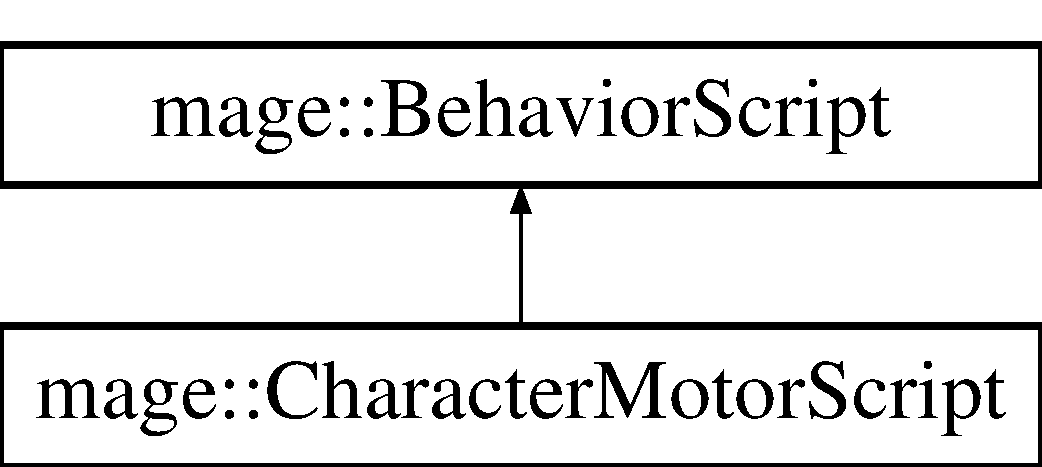
\includegraphics[height=2.000000cm]{classmage_1_1_character_motor_script}
\end{center}
\end{figure}
\subsection*{Public Member Functions}
\begin{DoxyCompactItemize}
\item 
\hyperlink{classmage_1_1_character_motor_script_af819140d0ebda767e9b82826c50972de}{Character\+Motor\+Script} (Transform $\ast$transform)
\item 
\hyperlink{classmage_1_1_character_motor_script_aa8b4b2c6eba7077677db51e24c2a9a36}{Character\+Motor\+Script} (const \hyperlink{classmage_1_1_character_motor_script}{Character\+Motor\+Script} \&script)=delete
\item 
\hyperlink{classmage_1_1_character_motor_script_a944682d8ff570a141e60cdd2d16aa3ad}{Character\+Motor\+Script} (\hyperlink{classmage_1_1_character_motor_script}{Character\+Motor\+Script} \&\&script)=default
\item 
virtual \hyperlink{classmage_1_1_character_motor_script_a03e8cdb2e30e21fe3a84f36101a169e3}{$\sim$\+Character\+Motor\+Script} ()=default
\item 
\hyperlink{classmage_1_1_character_motor_script}{Character\+Motor\+Script} \& \hyperlink{classmage_1_1_character_motor_script_a5b66cbbe6b829fe56a1bba5f9093b36e}{operator=} (const \hyperlink{classmage_1_1_character_motor_script}{Character\+Motor\+Script} \&script)=delete
\item 
\hyperlink{classmage_1_1_character_motor_script}{Character\+Motor\+Script} \& \hyperlink{classmage_1_1_character_motor_script_a05e8822fa633d8642702d125b26069f7}{operator=} (\hyperlink{classmage_1_1_character_motor_script}{Character\+Motor\+Script} \&\&script)=delete
\item 
virtual void \hyperlink{classmage_1_1_character_motor_script_af09581e810c02ca4a19ecbaf0d7580bb}{Update} (double delta\+\_\+time) override
\item 
float \hyperlink{classmage_1_1_character_motor_script_a0c512015222e3f332429df414c06862b}{Get\+Velocity} () const
\item 
void \hyperlink{classmage_1_1_character_motor_script_a3fd91c324e837b9d22e19d74478caec0}{Set\+Velocity} (float velocity)
\end{DoxyCompactItemize}
\subsection*{Private Attributes}
\begin{DoxyCompactItemize}
\item 
Transform $\ast$const \hyperlink{classmage_1_1_character_motor_script_a7331e960455b72ceb858254ccc7108f1}{m\+\_\+transform}
\item 
float \hyperlink{classmage_1_1_character_motor_script_a02441cc4c84ba12811845b7f966f4069}{m\+\_\+velocity}
\end{DoxyCompactItemize}
\subsection*{Additional Inherited Members}


\subsection{Constructor \& Destructor Documentation}
\hypertarget{classmage_1_1_character_motor_script_af819140d0ebda767e9b82826c50972de}{}\label{classmage_1_1_character_motor_script_af819140d0ebda767e9b82826c50972de} 
\index{mage\+::\+Character\+Motor\+Script@{mage\+::\+Character\+Motor\+Script}!Character\+Motor\+Script@{Character\+Motor\+Script}}
\index{Character\+Motor\+Script@{Character\+Motor\+Script}!mage\+::\+Character\+Motor\+Script@{mage\+::\+Character\+Motor\+Script}}
\subsubsection{\texorpdfstring{Character\+Motor\+Script()}{CharacterMotorScript()}\hspace{0.1cm}{\footnotesize\ttfamily [1/3]}}
{\footnotesize\ttfamily mage\+::\+Character\+Motor\+Script\+::\+Character\+Motor\+Script (\begin{DoxyParamCaption}\item[{Transform $\ast$}]{transform }\end{DoxyParamCaption})\hspace{0.3cm}{\ttfamily [explicit]}}

\hypertarget{classmage_1_1_character_motor_script_aa8b4b2c6eba7077677db51e24c2a9a36}{}\label{classmage_1_1_character_motor_script_aa8b4b2c6eba7077677db51e24c2a9a36} 
\index{mage\+::\+Character\+Motor\+Script@{mage\+::\+Character\+Motor\+Script}!Character\+Motor\+Script@{Character\+Motor\+Script}}
\index{Character\+Motor\+Script@{Character\+Motor\+Script}!mage\+::\+Character\+Motor\+Script@{mage\+::\+Character\+Motor\+Script}}
\subsubsection{\texorpdfstring{Character\+Motor\+Script()}{CharacterMotorScript()}\hspace{0.1cm}{\footnotesize\ttfamily [2/3]}}
{\footnotesize\ttfamily mage\+::\+Character\+Motor\+Script\+::\+Character\+Motor\+Script (\begin{DoxyParamCaption}\item[{const \hyperlink{classmage_1_1_character_motor_script}{Character\+Motor\+Script} \&}]{script }\end{DoxyParamCaption})\hspace{0.3cm}{\ttfamily [delete]}}

\hypertarget{classmage_1_1_character_motor_script_a944682d8ff570a141e60cdd2d16aa3ad}{}\label{classmage_1_1_character_motor_script_a944682d8ff570a141e60cdd2d16aa3ad} 
\index{mage\+::\+Character\+Motor\+Script@{mage\+::\+Character\+Motor\+Script}!Character\+Motor\+Script@{Character\+Motor\+Script}}
\index{Character\+Motor\+Script@{Character\+Motor\+Script}!mage\+::\+Character\+Motor\+Script@{mage\+::\+Character\+Motor\+Script}}
\subsubsection{\texorpdfstring{Character\+Motor\+Script()}{CharacterMotorScript()}\hspace{0.1cm}{\footnotesize\ttfamily [3/3]}}
{\footnotesize\ttfamily mage\+::\+Character\+Motor\+Script\+::\+Character\+Motor\+Script (\begin{DoxyParamCaption}\item[{\hyperlink{classmage_1_1_character_motor_script}{Character\+Motor\+Script} \&\&}]{script }\end{DoxyParamCaption})\hspace{0.3cm}{\ttfamily [default]}}

\hypertarget{classmage_1_1_character_motor_script_a03e8cdb2e30e21fe3a84f36101a169e3}{}\label{classmage_1_1_character_motor_script_a03e8cdb2e30e21fe3a84f36101a169e3} 
\index{mage\+::\+Character\+Motor\+Script@{mage\+::\+Character\+Motor\+Script}!````~Character\+Motor\+Script@{$\sim$\+Character\+Motor\+Script}}
\index{````~Character\+Motor\+Script@{$\sim$\+Character\+Motor\+Script}!mage\+::\+Character\+Motor\+Script@{mage\+::\+Character\+Motor\+Script}}
\subsubsection{\texorpdfstring{$\sim$\+Character\+Motor\+Script()}{~CharacterMotorScript()}}
{\footnotesize\ttfamily virtual mage\+::\+Character\+Motor\+Script\+::$\sim$\+Character\+Motor\+Script (\begin{DoxyParamCaption}{ }\end{DoxyParamCaption})\hspace{0.3cm}{\ttfamily [virtual]}, {\ttfamily [default]}}



\subsection{Member Function Documentation}
\hypertarget{classmage_1_1_character_motor_script_a0c512015222e3f332429df414c06862b}{}\label{classmage_1_1_character_motor_script_a0c512015222e3f332429df414c06862b} 
\index{mage\+::\+Character\+Motor\+Script@{mage\+::\+Character\+Motor\+Script}!Get\+Velocity@{Get\+Velocity}}
\index{Get\+Velocity@{Get\+Velocity}!mage\+::\+Character\+Motor\+Script@{mage\+::\+Character\+Motor\+Script}}
\subsubsection{\texorpdfstring{Get\+Velocity()}{GetVelocity()}}
{\footnotesize\ttfamily float mage\+::\+Character\+Motor\+Script\+::\+Get\+Velocity (\begin{DoxyParamCaption}{ }\end{DoxyParamCaption}) const}

\hypertarget{classmage_1_1_character_motor_script_a5b66cbbe6b829fe56a1bba5f9093b36e}{}\label{classmage_1_1_character_motor_script_a5b66cbbe6b829fe56a1bba5f9093b36e} 
\index{mage\+::\+Character\+Motor\+Script@{mage\+::\+Character\+Motor\+Script}!operator=@{operator=}}
\index{operator=@{operator=}!mage\+::\+Character\+Motor\+Script@{mage\+::\+Character\+Motor\+Script}}
\subsubsection{\texorpdfstring{operator=()}{operator=()}\hspace{0.1cm}{\footnotesize\ttfamily [1/2]}}
{\footnotesize\ttfamily \hyperlink{classmage_1_1_character_motor_script}{Character\+Motor\+Script}\& mage\+::\+Character\+Motor\+Script\+::operator= (\begin{DoxyParamCaption}\item[{const \hyperlink{classmage_1_1_character_motor_script}{Character\+Motor\+Script} \&}]{script }\end{DoxyParamCaption})\hspace{0.3cm}{\ttfamily [delete]}}

\hypertarget{classmage_1_1_character_motor_script_a05e8822fa633d8642702d125b26069f7}{}\label{classmage_1_1_character_motor_script_a05e8822fa633d8642702d125b26069f7} 
\index{mage\+::\+Character\+Motor\+Script@{mage\+::\+Character\+Motor\+Script}!operator=@{operator=}}
\index{operator=@{operator=}!mage\+::\+Character\+Motor\+Script@{mage\+::\+Character\+Motor\+Script}}
\subsubsection{\texorpdfstring{operator=()}{operator=()}\hspace{0.1cm}{\footnotesize\ttfamily [2/2]}}
{\footnotesize\ttfamily \hyperlink{classmage_1_1_character_motor_script}{Character\+Motor\+Script}\& mage\+::\+Character\+Motor\+Script\+::operator= (\begin{DoxyParamCaption}\item[{\hyperlink{classmage_1_1_character_motor_script}{Character\+Motor\+Script} \&\&}]{script }\end{DoxyParamCaption})\hspace{0.3cm}{\ttfamily [delete]}}

\hypertarget{classmage_1_1_character_motor_script_a3fd91c324e837b9d22e19d74478caec0}{}\label{classmage_1_1_character_motor_script_a3fd91c324e837b9d22e19d74478caec0} 
\index{mage\+::\+Character\+Motor\+Script@{mage\+::\+Character\+Motor\+Script}!Set\+Velocity@{Set\+Velocity}}
\index{Set\+Velocity@{Set\+Velocity}!mage\+::\+Character\+Motor\+Script@{mage\+::\+Character\+Motor\+Script}}
\subsubsection{\texorpdfstring{Set\+Velocity()}{SetVelocity()}}
{\footnotesize\ttfamily void mage\+::\+Character\+Motor\+Script\+::\+Set\+Velocity (\begin{DoxyParamCaption}\item[{float}]{velocity }\end{DoxyParamCaption})}

\hypertarget{classmage_1_1_character_motor_script_af09581e810c02ca4a19ecbaf0d7580bb}{}\label{classmage_1_1_character_motor_script_af09581e810c02ca4a19ecbaf0d7580bb} 
\index{mage\+::\+Character\+Motor\+Script@{mage\+::\+Character\+Motor\+Script}!Update@{Update}}
\index{Update@{Update}!mage\+::\+Character\+Motor\+Script@{mage\+::\+Character\+Motor\+Script}}
\subsubsection{\texorpdfstring{Update()}{Update()}}
{\footnotesize\ttfamily void mage\+::\+Character\+Motor\+Script\+::\+Update (\begin{DoxyParamCaption}\item[{double}]{delta\+\_\+time }\end{DoxyParamCaption})\hspace{0.3cm}{\ttfamily [override]}, {\ttfamily [virtual]}}

Updates this behavior script.


\begin{DoxyParams}[1]{Parameters}
\mbox{\tt in}  & {\em delta\+\_\+time} & The elapsed time since the previous update. \\
\hline
\end{DoxyParams}


Implements \hyperlink{classmage_1_1_behavior_script_a905b6c83640cb91d19fecab3435f6feb}{mage\+::\+Behavior\+Script}.



\subsection{Member Data Documentation}
\hypertarget{classmage_1_1_character_motor_script_a7331e960455b72ceb858254ccc7108f1}{}\label{classmage_1_1_character_motor_script_a7331e960455b72ceb858254ccc7108f1} 
\index{mage\+::\+Character\+Motor\+Script@{mage\+::\+Character\+Motor\+Script}!m\+\_\+transform@{m\+\_\+transform}}
\index{m\+\_\+transform@{m\+\_\+transform}!mage\+::\+Character\+Motor\+Script@{mage\+::\+Character\+Motor\+Script}}
\subsubsection{\texorpdfstring{m\+\_\+transform}{m\_transform}}
{\footnotesize\ttfamily Transform$\ast$ const mage\+::\+Character\+Motor\+Script\+::m\+\_\+transform\hspace{0.3cm}{\ttfamily [private]}}

\hypertarget{classmage_1_1_character_motor_script_a02441cc4c84ba12811845b7f966f4069}{}\label{classmage_1_1_character_motor_script_a02441cc4c84ba12811845b7f966f4069} 
\index{mage\+::\+Character\+Motor\+Script@{mage\+::\+Character\+Motor\+Script}!m\+\_\+velocity@{m\+\_\+velocity}}
\index{m\+\_\+velocity@{m\+\_\+velocity}!mage\+::\+Character\+Motor\+Script@{mage\+::\+Character\+Motor\+Script}}
\subsubsection{\texorpdfstring{m\+\_\+velocity}{m\_velocity}}
{\footnotesize\ttfamily float mage\+::\+Character\+Motor\+Script\+::m\+\_\+velocity\hspace{0.3cm}{\ttfamily [private]}}


\hypertarget{structmage_1_1_color}{}\section{mage\+:\+:Color Struct Reference}
\label{structmage_1_1_color}\index{mage\+::\+Color@{mage\+::\+Color}}


{\ttfamily \#include $<$math.\+hpp$>$}

Inheritance diagram for mage\+:\+:Color\+:\begin{figure}[H]
\begin{center}
\leavevmode
\includegraphics[height=2.000000cm]{structmage_1_1_color}
\end{center}
\end{figure}
\subsection*{Public Member Functions}
\begin{DoxyCompactItemize}
\item 
\hyperlink{structmage_1_1_color_aacf48e59425346eb80e7592bbcd6b55d}{Color} ()
\item 
\hyperlink{structmage_1_1_color_ae906a0c456f1d21df8a6d5476918a913}{Color} (float x, float y, float z, float w)
\item 
\hyperlink{structmage_1_1_color_aabf202b6ec0c2d1fc788c9bc69f185ff}{Color} (const \hyperlink{structmage_1_1_color}{Color} \&\hyperlink{namespacemage_a8ac46837ac2f6a9b756e66979165acd6}{color})
\item 
\hyperlink{structmage_1_1_color_abb0838db7c77053894fcf11b03284549}{Color} (\hyperlink{structmage_1_1_color}{Color} \&\&\hyperlink{namespacemage_a8ac46837ac2f6a9b756e66979165acd6}{color})
\item 
\hyperlink{structmage_1_1_color_a90a9fab9b5dff127bf2ead12a46d531f}{Color} (const X\+M\+F\+L\+O\+A\+T4 \&v)
\item 
\hyperlink{structmage_1_1_color_a8f0d0c4359f6754d90bb2b6c077a11e3}{Color} (X\+M\+F\+L\+O\+A\+T4 \&\&v)
\item 
\hyperlink{structmage_1_1_color_aa4df1c9718b7846adf77fbeed79ac219}{$\sim$\+Color} ()=default
\item 
\hyperlink{structmage_1_1_color}{Color} \& \hyperlink{structmage_1_1_color_a006c8ce9bf69e54598c5981fe79d742c}{operator=} (const \hyperlink{structmage_1_1_color}{Color} \&\hyperlink{namespacemage_a8ac46837ac2f6a9b756e66979165acd6}{color})
\item 
\hyperlink{structmage_1_1_color}{Color} \& \hyperlink{structmage_1_1_color_afe64cf3cf65b5812ac35674917abb12c}{operator=} (\hyperlink{structmage_1_1_color}{Color} \&\&\hyperlink{namespacemage_a8ac46837ac2f6a9b756e66979165acd6}{color})
\end{DoxyCompactItemize}


\subsection{Detailed Description}
A struct of colors. 

\subsection{Constructor \& Destructor Documentation}
\hypertarget{structmage_1_1_color_aacf48e59425346eb80e7592bbcd6b55d}{}\label{structmage_1_1_color_aacf48e59425346eb80e7592bbcd6b55d} 
\index{mage\+::\+Color@{mage\+::\+Color}!Color@{Color}}
\index{Color@{Color}!mage\+::\+Color@{mage\+::\+Color}}
\subsubsection{\texorpdfstring{Color()}{Color()}\hspace{0.1cm}{\footnotesize\ttfamily [1/6]}}
{\footnotesize\ttfamily mage\+::\+Color\+::\+Color (\begin{DoxyParamCaption}{ }\end{DoxyParamCaption})}

Constructs a color. \hypertarget{structmage_1_1_color_ae906a0c456f1d21df8a6d5476918a913}{}\label{structmage_1_1_color_ae906a0c456f1d21df8a6d5476918a913} 
\index{mage\+::\+Color@{mage\+::\+Color}!Color@{Color}}
\index{Color@{Color}!mage\+::\+Color@{mage\+::\+Color}}
\subsubsection{\texorpdfstring{Color()}{Color()}\hspace{0.1cm}{\footnotesize\ttfamily [2/6]}}
{\footnotesize\ttfamily mage\+::\+Color\+::\+Color (\begin{DoxyParamCaption}\item[{float}]{x,  }\item[{float}]{y,  }\item[{float}]{z,  }\item[{float}]{w }\end{DoxyParamCaption})}

Constructs a color from the given components.


\begin{DoxyParams}[1]{Parameters}
\mbox{\tt in}  & {\em x} & The first component. \\
\hline
\mbox{\tt in}  & {\em y} & The second component. \\
\hline
\mbox{\tt in}  & {\em z} & The third component. \\
\hline
\mbox{\tt in}  & {\em w} & The fourth component. \\
\hline
\end{DoxyParams}
\hypertarget{structmage_1_1_color_aabf202b6ec0c2d1fc788c9bc69f185ff}{}\label{structmage_1_1_color_aabf202b6ec0c2d1fc788c9bc69f185ff} 
\index{mage\+::\+Color@{mage\+::\+Color}!Color@{Color}}
\index{Color@{Color}!mage\+::\+Color@{mage\+::\+Color}}
\subsubsection{\texorpdfstring{Color()}{Color()}\hspace{0.1cm}{\footnotesize\ttfamily [3/6]}}
{\footnotesize\ttfamily mage\+::\+Color\+::\+Color (\begin{DoxyParamCaption}\item[{const \hyperlink{structmage_1_1_color}{Color} \&}]{color }\end{DoxyParamCaption})}

Constructs a color from the given color.


\begin{DoxyParams}[1]{Parameters}
\mbox{\tt in}  & {\em color} & A reference to the color to copy. \\
\hline
\end{DoxyParams}
\hypertarget{structmage_1_1_color_abb0838db7c77053894fcf11b03284549}{}\label{structmage_1_1_color_abb0838db7c77053894fcf11b03284549} 
\index{mage\+::\+Color@{mage\+::\+Color}!Color@{Color}}
\index{Color@{Color}!mage\+::\+Color@{mage\+::\+Color}}
\subsubsection{\texorpdfstring{Color()}{Color()}\hspace{0.1cm}{\footnotesize\ttfamily [4/6]}}
{\footnotesize\ttfamily mage\+::\+Color\+::\+Color (\begin{DoxyParamCaption}\item[{\hyperlink{structmage_1_1_color}{Color} \&\&}]{color }\end{DoxyParamCaption})}

Constructs a color by moving the given color.


\begin{DoxyParams}[1]{Parameters}
\mbox{\tt in}  & {\em color} & A reference to the color to move. \\
\hline
\end{DoxyParams}
\hypertarget{structmage_1_1_color_a90a9fab9b5dff127bf2ead12a46d531f}{}\label{structmage_1_1_color_a90a9fab9b5dff127bf2ead12a46d531f} 
\index{mage\+::\+Color@{mage\+::\+Color}!Color@{Color}}
\index{Color@{Color}!mage\+::\+Color@{mage\+::\+Color}}
\subsubsection{\texorpdfstring{Color()}{Color()}\hspace{0.1cm}{\footnotesize\ttfamily [5/6]}}
{\footnotesize\ttfamily mage\+::\+Color\+::\+Color (\begin{DoxyParamCaption}\item[{const X\+M\+F\+L\+O\+A\+T4 \&}]{v }\end{DoxyParamCaption})\hspace{0.3cm}{\ttfamily [explicit]}}

Constructs a color from the given vector.


\begin{DoxyParams}[1]{Parameters}
\mbox{\tt in}  & {\em v} & A reference to the vector to copy. \\
\hline
\end{DoxyParams}
\hypertarget{structmage_1_1_color_a8f0d0c4359f6754d90bb2b6c077a11e3}{}\label{structmage_1_1_color_a8f0d0c4359f6754d90bb2b6c077a11e3} 
\index{mage\+::\+Color@{mage\+::\+Color}!Color@{Color}}
\index{Color@{Color}!mage\+::\+Color@{mage\+::\+Color}}
\subsubsection{\texorpdfstring{Color()}{Color()}\hspace{0.1cm}{\footnotesize\ttfamily [6/6]}}
{\footnotesize\ttfamily mage\+::\+Color\+::\+Color (\begin{DoxyParamCaption}\item[{X\+M\+F\+L\+O\+A\+T4 \&\&}]{v }\end{DoxyParamCaption})\hspace{0.3cm}{\ttfamily [explicit]}}

Constructs a color by moving the given vector.


\begin{DoxyParams}[1]{Parameters}
\mbox{\tt in}  & {\em v} & A reference to the vector to move. \\
\hline
\end{DoxyParams}
\hypertarget{structmage_1_1_color_aa4df1c9718b7846adf77fbeed79ac219}{}\label{structmage_1_1_color_aa4df1c9718b7846adf77fbeed79ac219} 
\index{mage\+::\+Color@{mage\+::\+Color}!````~Color@{$\sim$\+Color}}
\index{````~Color@{$\sim$\+Color}!mage\+::\+Color@{mage\+::\+Color}}
\subsubsection{\texorpdfstring{$\sim$\+Color()}{~Color()}}
{\footnotesize\ttfamily mage\+::\+Color\+::$\sim$\+Color (\begin{DoxyParamCaption}{ }\end{DoxyParamCaption})\hspace{0.3cm}{\ttfamily [default]}}

Destructs this color. 

\subsection{Member Function Documentation}
\hypertarget{structmage_1_1_color_a006c8ce9bf69e54598c5981fe79d742c}{}\label{structmage_1_1_color_a006c8ce9bf69e54598c5981fe79d742c} 
\index{mage\+::\+Color@{mage\+::\+Color}!operator=@{operator=}}
\index{operator=@{operator=}!mage\+::\+Color@{mage\+::\+Color}}
\subsubsection{\texorpdfstring{operator=()}{operator=()}\hspace{0.1cm}{\footnotesize\ttfamily [1/2]}}
{\footnotesize\ttfamily \hyperlink{structmage_1_1_color}{Color}\& mage\+::\+Color\+::operator= (\begin{DoxyParamCaption}\item[{const \hyperlink{structmage_1_1_color}{Color} \&}]{color }\end{DoxyParamCaption})}

Copies the given color to this color.


\begin{DoxyParams}[1]{Parameters}
\mbox{\tt in}  & {\em color} & A reference to the color to copy. \\
\hline
\end{DoxyParams}
\begin{DoxyReturn}{Returns}
A reference to the copy of the given color (i.\+e. this color). 
\end{DoxyReturn}
\hypertarget{structmage_1_1_color_afe64cf3cf65b5812ac35674917abb12c}{}\label{structmage_1_1_color_afe64cf3cf65b5812ac35674917abb12c} 
\index{mage\+::\+Color@{mage\+::\+Color}!operator=@{operator=}}
\index{operator=@{operator=}!mage\+::\+Color@{mage\+::\+Color}}
\subsubsection{\texorpdfstring{operator=()}{operator=()}\hspace{0.1cm}{\footnotesize\ttfamily [2/2]}}
{\footnotesize\ttfamily \hyperlink{structmage_1_1_color}{Color}\& mage\+::\+Color\+::operator= (\begin{DoxyParamCaption}\item[{\hyperlink{structmage_1_1_color}{Color} \&\&}]{color }\end{DoxyParamCaption})}

Moves the given color to this color.


\begin{DoxyParams}[1]{Parameters}
\mbox{\tt in}  & {\em color} & A reference to the color to move. \\
\hline
\end{DoxyParams}
\begin{DoxyReturn}{Returns}
A reference to the moved color (i.\+e. this color). 
\end{DoxyReturn}

\hypertarget{structmage_1_1_color_string}{}\section{mage\+:\+:Color\+String Struct Reference}
\label{structmage_1_1_color_string}\index{mage\+::\+Color\+String@{mage\+::\+Color\+String}}


{\ttfamily \#include $<$color\+\_\+string.\+hpp$>$}

\subsection*{Public Member Functions}
\begin{DoxyCompactItemize}
\item 
\hyperlink{structmage_1_1_color_string_a9737fbe265c4432971e715439827f25a}{Color\+String} (const wstring \&str, const \hyperlink{structmage_1_1_color}{Color} \&color)
\item 
\hyperlink{structmage_1_1_color_string_a115be37cf649b0e250ca22604df34900}{Color\+String} (const wstring \&str, F\+X\+M\+V\+E\+C\+T\+OR color=Colors\+::\+White)
\item 
\hyperlink{structmage_1_1_color_string_a42597e6be67ed803a79eff88de769656}{Color\+String} (wstring \&\&str, const \hyperlink{structmage_1_1_color}{Color} \&color)
\item 
\hyperlink{structmage_1_1_color_string_a6a869d9a0325dbe261b8afc60976a7b4}{Color\+String} (wstring \&\&str, F\+X\+M\+V\+E\+C\+T\+OR color=Colors\+::\+White)
\item 
\hyperlink{structmage_1_1_color_string_aef572c89d1ed663837c6e5b1b6816984}{Color\+String} (const wchar\+\_\+t $\ast$str, const \hyperlink{structmage_1_1_color}{Color} \&color)
\item 
\hyperlink{structmage_1_1_color_string_ae60cd006f5c8fe178b097c158557b777}{Color\+String} (const wchar\+\_\+t $\ast$str, F\+X\+M\+V\+E\+C\+T\+OR color=Colors\+::\+White)
\item 
\hyperlink{structmage_1_1_color_string_aa878fda012b4149f673e905f6a8ea8b0}{Color\+String} (const \hyperlink{structmage_1_1_color_string}{Color\+String} \&color\+\_\+string)=default
\item 
\hyperlink{structmage_1_1_color_string_a68d8411da4dd7122975223e25bbcbb9a}{Color\+String} (\hyperlink{structmage_1_1_color_string}{Color\+String} \&\&color\+\_\+string)=default
\item 
\hyperlink{structmage_1_1_color_string_a95886010269c8c4bc3a27fbfe829f4c2}{$\sim$\+Color\+String} ()=default
\item 
\hyperlink{structmage_1_1_color_string}{Color\+String} \& \hyperlink{structmage_1_1_color_string_a568fed43403422ecafdf92d04e11c4e5}{operator=} (const \hyperlink{structmage_1_1_color_string}{Color\+String} \&color\+\_\+string)=default
\item 
\hyperlink{structmage_1_1_color_string}{Color\+String} \& \hyperlink{structmage_1_1_color_string_a2016416ce91bb7e94a8869201db47ef1}{operator=} (\hyperlink{structmage_1_1_color_string}{Color\+String} \&\&color\+\_\+string)=default
\item 
const wchar\+\_\+t $\ast$ \hyperlink{structmage_1_1_color_string_af2241b81cac59051e9ebf0ddefe719ed}{c\+\_\+str} () const noexcept
\item 
const wstring \& \hyperlink{structmage_1_1_color_string_aee22268a2fe552320299dfa5ac5a93e1}{Get\+String} () const noexcept
\item 
void \hyperlink{structmage_1_1_color_string_aa5ec8bb8e44683ed8a88534f04639930}{Set\+String} (const wstring \&str)
\item 
void \hyperlink{structmage_1_1_color_string_a62a374668fafc55281b97e6374027b25}{Set\+String} (wstring \&\&str) noexcept
\item 
void \hyperlink{structmage_1_1_color_string_a317caadad725b67ede68f1e474e47d3b}{Set\+String} (const wchar\+\_\+t $\ast$str)
\item 
const \hyperlink{structmage_1_1_color}{Color} \hyperlink{structmage_1_1_color_string_afba86162d9c13d76dcdb9cf232e8e89f}{Get\+Color} () const noexcept
\item 
const X\+M\+V\+E\+C\+T\+OR \hyperlink{structmage_1_1_color_string_a9326950147ecdc3c09909518e0dddb76}{Get\+Color\+Vector} () const noexcept
\item 
void \hyperlink{structmage_1_1_color_string_acff8b67574e427674e6abb98da7cca3a}{Set\+Color} (const \hyperlink{structmage_1_1_color}{Color} \&color) noexcept
\item 
void \hyperlink{structmage_1_1_color_string_a45a4a036e48431882c193be5bd718add}{Set\+Color} (\hyperlink{structmage_1_1_color}{Color} \&\&color) noexcept
\item 
void X\+M\+\_\+\+C\+A\+L\+L\+C\+O\+NV \hyperlink{structmage_1_1_color_string_ab4de02b485d18384fcca1a0b55600abd}{Set\+Color} (F\+X\+M\+V\+E\+C\+T\+OR color) noexcept
\end{DoxyCompactItemize}
\subsection*{Private Attributes}
\begin{DoxyCompactItemize}
\item 
wstring \hyperlink{structmage_1_1_color_string_a9eb840afa5112cd611f5bb1b21edc045}{m\+\_\+str}
\item 
\hyperlink{structmage_1_1_color}{Color} \hyperlink{structmage_1_1_color_string_a3f351c61281fc49786bc13842527d2a3}{m\+\_\+color}
\end{DoxyCompactItemize}


\subsection{Detailed Description}
A struct of color strings representing a string and its color. 

\subsection{Constructor \& Destructor Documentation}
\hypertarget{structmage_1_1_color_string_a9737fbe265c4432971e715439827f25a}{}\label{structmage_1_1_color_string_a9737fbe265c4432971e715439827f25a} 
\index{mage\+::\+Color\+String@{mage\+::\+Color\+String}!Color\+String@{Color\+String}}
\index{Color\+String@{Color\+String}!mage\+::\+Color\+String@{mage\+::\+Color\+String}}
\subsubsection{\texorpdfstring{Color\+String()}{ColorString()}\hspace{0.1cm}{\footnotesize\ttfamily [1/8]}}
{\footnotesize\ttfamily mage\+::\+Color\+String\+::\+Color\+String (\begin{DoxyParamCaption}\item[{const wstring \&}]{str,  }\item[{const \hyperlink{structmage_1_1_color}{Color} \&}]{color }\end{DoxyParamCaption})\hspace{0.3cm}{\ttfamily [explicit]}}

Constructs a color string fromt the given string and color.


\begin{DoxyParams}[1]{Parameters}
\mbox{\tt in}  & {\em str} & A reference to the string. \\
\hline
\mbox{\tt in}  & {\em color} & A reference to the (s\+R\+GB) color. \\
\hline
\end{DoxyParams}
\hypertarget{structmage_1_1_color_string_a115be37cf649b0e250ca22604df34900}{}\label{structmage_1_1_color_string_a115be37cf649b0e250ca22604df34900} 
\index{mage\+::\+Color\+String@{mage\+::\+Color\+String}!Color\+String@{Color\+String}}
\index{Color\+String@{Color\+String}!mage\+::\+Color\+String@{mage\+::\+Color\+String}}
\subsubsection{\texorpdfstring{Color\+String()}{ColorString()}\hspace{0.1cm}{\footnotesize\ttfamily [2/8]}}
{\footnotesize\ttfamily mage\+::\+Color\+String\+::\+Color\+String (\begin{DoxyParamCaption}\item[{const wstring \&}]{str,  }\item[{F\+X\+M\+V\+E\+C\+T\+OR}]{color = {\ttfamily Colors\+:\+:White} }\end{DoxyParamCaption})\hspace{0.3cm}{\ttfamily [explicit]}}

Constructs a color string fromt the given string and color.


\begin{DoxyParams}[1]{Parameters}
\mbox{\tt in}  & {\em str} & A reference to the string. \\
\hline
\mbox{\tt in}  & {\em color} & The (s\+R\+GB) color. \\
\hline
\end{DoxyParams}
\hypertarget{structmage_1_1_color_string_a42597e6be67ed803a79eff88de769656}{}\label{structmage_1_1_color_string_a42597e6be67ed803a79eff88de769656} 
\index{mage\+::\+Color\+String@{mage\+::\+Color\+String}!Color\+String@{Color\+String}}
\index{Color\+String@{Color\+String}!mage\+::\+Color\+String@{mage\+::\+Color\+String}}
\subsubsection{\texorpdfstring{Color\+String()}{ColorString()}\hspace{0.1cm}{\footnotesize\ttfamily [3/8]}}
{\footnotesize\ttfamily mage\+::\+Color\+String\+::\+Color\+String (\begin{DoxyParamCaption}\item[{wstring \&\&}]{str,  }\item[{const \hyperlink{structmage_1_1_color}{Color} \&}]{color }\end{DoxyParamCaption})\hspace{0.3cm}{\ttfamily [explicit]}}

Constructs a color string fromt the given string and color.


\begin{DoxyParams}[1]{Parameters}
\mbox{\tt in}  & {\em str} & A reference to the string. \\
\hline
\mbox{\tt in}  & {\em color} & A reference to the (s\+R\+GB) color. \\
\hline
\end{DoxyParams}
\hypertarget{structmage_1_1_color_string_a6a869d9a0325dbe261b8afc60976a7b4}{}\label{structmage_1_1_color_string_a6a869d9a0325dbe261b8afc60976a7b4} 
\index{mage\+::\+Color\+String@{mage\+::\+Color\+String}!Color\+String@{Color\+String}}
\index{Color\+String@{Color\+String}!mage\+::\+Color\+String@{mage\+::\+Color\+String}}
\subsubsection{\texorpdfstring{Color\+String()}{ColorString()}\hspace{0.1cm}{\footnotesize\ttfamily [4/8]}}
{\footnotesize\ttfamily mage\+::\+Color\+String\+::\+Color\+String (\begin{DoxyParamCaption}\item[{wstring \&\&}]{str,  }\item[{F\+X\+M\+V\+E\+C\+T\+OR}]{color = {\ttfamily Colors\+:\+:White} }\end{DoxyParamCaption})\hspace{0.3cm}{\ttfamily [explicit]}}

Constructs a color string fromt the given string and color.


\begin{DoxyParams}[1]{Parameters}
\mbox{\tt in}  & {\em str} & A reference to the string. \\
\hline
\mbox{\tt in}  & {\em color} & The (s\+R\+GB) color. \\
\hline
\end{DoxyParams}
\hypertarget{structmage_1_1_color_string_aef572c89d1ed663837c6e5b1b6816984}{}\label{structmage_1_1_color_string_aef572c89d1ed663837c6e5b1b6816984} 
\index{mage\+::\+Color\+String@{mage\+::\+Color\+String}!Color\+String@{Color\+String}}
\index{Color\+String@{Color\+String}!mage\+::\+Color\+String@{mage\+::\+Color\+String}}
\subsubsection{\texorpdfstring{Color\+String()}{ColorString()}\hspace{0.1cm}{\footnotesize\ttfamily [5/8]}}
{\footnotesize\ttfamily mage\+::\+Color\+String\+::\+Color\+String (\begin{DoxyParamCaption}\item[{const wchar\+\_\+t $\ast$}]{str,  }\item[{const \hyperlink{structmage_1_1_color}{Color} \&}]{color }\end{DoxyParamCaption})\hspace{0.3cm}{\ttfamily [explicit]}}

Constructs a color string fromt the given string and color.

\begin{DoxyPrecond}{Precondition}
{\itshape str} is not equal to {\ttfamily nullptr}. 
\end{DoxyPrecond}

\begin{DoxyParams}[1]{Parameters}
\mbox{\tt in}  & {\em str} & A pointer to the string. \\
\hline
\mbox{\tt in}  & {\em color} & A reference to the (s\+R\+GB) color. \\
\hline
\end{DoxyParams}
\hypertarget{structmage_1_1_color_string_ae60cd006f5c8fe178b097c158557b777}{}\label{structmage_1_1_color_string_ae60cd006f5c8fe178b097c158557b777} 
\index{mage\+::\+Color\+String@{mage\+::\+Color\+String}!Color\+String@{Color\+String}}
\index{Color\+String@{Color\+String}!mage\+::\+Color\+String@{mage\+::\+Color\+String}}
\subsubsection{\texorpdfstring{Color\+String()}{ColorString()}\hspace{0.1cm}{\footnotesize\ttfamily [6/8]}}
{\footnotesize\ttfamily mage\+::\+Color\+String\+::\+Color\+String (\begin{DoxyParamCaption}\item[{const wchar\+\_\+t $\ast$}]{str,  }\item[{F\+X\+M\+V\+E\+C\+T\+OR}]{color = {\ttfamily Colors\+:\+:White} }\end{DoxyParamCaption})\hspace{0.3cm}{\ttfamily [explicit]}}

Constructs a color string fromt the given str and color.

\begin{DoxyPrecond}{Precondition}
{\itshape str} is not equal to {\ttfamily nullptr}. 
\end{DoxyPrecond}

\begin{DoxyParams}[1]{Parameters}
\mbox{\tt in}  & {\em str} & A pointer to the str. \\
\hline
\mbox{\tt in}  & {\em color} & The (s\+R\+GB) color. \\
\hline
\end{DoxyParams}
\hypertarget{structmage_1_1_color_string_aa878fda012b4149f673e905f6a8ea8b0}{}\label{structmage_1_1_color_string_aa878fda012b4149f673e905f6a8ea8b0} 
\index{mage\+::\+Color\+String@{mage\+::\+Color\+String}!Color\+String@{Color\+String}}
\index{Color\+String@{Color\+String}!mage\+::\+Color\+String@{mage\+::\+Color\+String}}
\subsubsection{\texorpdfstring{Color\+String()}{ColorString()}\hspace{0.1cm}{\footnotesize\ttfamily [7/8]}}
{\footnotesize\ttfamily mage\+::\+Color\+String\+::\+Color\+String (\begin{DoxyParamCaption}\item[{const \hyperlink{structmage_1_1_color_string}{Color\+String} \&}]{color\+\_\+string }\end{DoxyParamCaption})\hspace{0.3cm}{\ttfamily [default]}}

Constructs a color string from the given color string.


\begin{DoxyParams}[1]{Parameters}
\mbox{\tt in}  & {\em color\+\_\+string} & A reference to the color string to copy. \\
\hline
\end{DoxyParams}
\hypertarget{structmage_1_1_color_string_a68d8411da4dd7122975223e25bbcbb9a}{}\label{structmage_1_1_color_string_a68d8411da4dd7122975223e25bbcbb9a} 
\index{mage\+::\+Color\+String@{mage\+::\+Color\+String}!Color\+String@{Color\+String}}
\index{Color\+String@{Color\+String}!mage\+::\+Color\+String@{mage\+::\+Color\+String}}
\subsubsection{\texorpdfstring{Color\+String()}{ColorString()}\hspace{0.1cm}{\footnotesize\ttfamily [8/8]}}
{\footnotesize\ttfamily mage\+::\+Color\+String\+::\+Color\+String (\begin{DoxyParamCaption}\item[{\hyperlink{structmage_1_1_color_string}{Color\+String} \&\&}]{color\+\_\+string }\end{DoxyParamCaption})\hspace{0.3cm}{\ttfamily [default]}}

Constructs a color string by moving the given color string.


\begin{DoxyParams}[1]{Parameters}
\mbox{\tt in}  & {\em color\+\_\+string} & A reference to the color string to move. \\
\hline
\end{DoxyParams}
\hypertarget{structmage_1_1_color_string_a95886010269c8c4bc3a27fbfe829f4c2}{}\label{structmage_1_1_color_string_a95886010269c8c4bc3a27fbfe829f4c2} 
\index{mage\+::\+Color\+String@{mage\+::\+Color\+String}!````~Color\+String@{$\sim$\+Color\+String}}
\index{````~Color\+String@{$\sim$\+Color\+String}!mage\+::\+Color\+String@{mage\+::\+Color\+String}}
\subsubsection{\texorpdfstring{$\sim$\+Color\+String()}{~ColorString()}}
{\footnotesize\ttfamily mage\+::\+Color\+String\+::$\sim$\+Color\+String (\begin{DoxyParamCaption}{ }\end{DoxyParamCaption})\hspace{0.3cm}{\ttfamily [default]}}

Destructs this color string. 

\subsection{Member Function Documentation}
\hypertarget{structmage_1_1_color_string_af2241b81cac59051e9ebf0ddefe719ed}{}\label{structmage_1_1_color_string_af2241b81cac59051e9ebf0ddefe719ed} 
\index{mage\+::\+Color\+String@{mage\+::\+Color\+String}!c\+\_\+str@{c\+\_\+str}}
\index{c\+\_\+str@{c\+\_\+str}!mage\+::\+Color\+String@{mage\+::\+Color\+String}}
\subsubsection{\texorpdfstring{c\+\_\+str()}{c\_str()}}
{\footnotesize\ttfamily const wchar\+\_\+t$\ast$ mage\+::\+Color\+String\+::c\+\_\+str (\begin{DoxyParamCaption}{ }\end{DoxyParamCaption}) const\hspace{0.3cm}{\ttfamily [noexcept]}}

Returns the string of this color string.

\begin{DoxyReturn}{Returns}
A pointer to the string of this color string. 
\end{DoxyReturn}
\hypertarget{structmage_1_1_color_string_afba86162d9c13d76dcdb9cf232e8e89f}{}\label{structmage_1_1_color_string_afba86162d9c13d76dcdb9cf232e8e89f} 
\index{mage\+::\+Color\+String@{mage\+::\+Color\+String}!Get\+Color@{Get\+Color}}
\index{Get\+Color@{Get\+Color}!mage\+::\+Color\+String@{mage\+::\+Color\+String}}
\subsubsection{\texorpdfstring{Get\+Color()}{GetColor()}}
{\footnotesize\ttfamily const \hyperlink{structmage_1_1_color}{Color} mage\+::\+Color\+String\+::\+Get\+Color (\begin{DoxyParamCaption}{ }\end{DoxyParamCaption}) const\hspace{0.3cm}{\ttfamily [noexcept]}}

Returns the (s\+R\+GB) color of this color string.

\begin{DoxyReturn}{Returns}
The (s\+R\+GB) color of this color string. 
\end{DoxyReturn}
\hypertarget{structmage_1_1_color_string_a9326950147ecdc3c09909518e0dddb76}{}\label{structmage_1_1_color_string_a9326950147ecdc3c09909518e0dddb76} 
\index{mage\+::\+Color\+String@{mage\+::\+Color\+String}!Get\+Color\+Vector@{Get\+Color\+Vector}}
\index{Get\+Color\+Vector@{Get\+Color\+Vector}!mage\+::\+Color\+String@{mage\+::\+Color\+String}}
\subsubsection{\texorpdfstring{Get\+Color\+Vector()}{GetColorVector()}}
{\footnotesize\ttfamily const X\+M\+V\+E\+C\+T\+OR mage\+::\+Color\+String\+::\+Get\+Color\+Vector (\begin{DoxyParamCaption}{ }\end{DoxyParamCaption}) const\hspace{0.3cm}{\ttfamily [noexcept]}}

Returns the (s\+R\+GB) color of this color string as {\ttfamily X\+M\+V\+E\+C\+T\+OR}.

\begin{DoxyReturn}{Returns}
The (s\+R\+GB) color of this color string as {\ttfamily X\+M\+V\+E\+C\+T\+OR}. 
\end{DoxyReturn}
\hypertarget{structmage_1_1_color_string_aee22268a2fe552320299dfa5ac5a93e1}{}\label{structmage_1_1_color_string_aee22268a2fe552320299dfa5ac5a93e1} 
\index{mage\+::\+Color\+String@{mage\+::\+Color\+String}!Get\+String@{Get\+String}}
\index{Get\+String@{Get\+String}!mage\+::\+Color\+String@{mage\+::\+Color\+String}}
\subsubsection{\texorpdfstring{Get\+String()}{GetString()}}
{\footnotesize\ttfamily const wstring\& mage\+::\+Color\+String\+::\+Get\+String (\begin{DoxyParamCaption}{ }\end{DoxyParamCaption}) const\hspace{0.3cm}{\ttfamily [noexcept]}}

Returns the string of this color string.

\begin{DoxyReturn}{Returns}
A reference to the string of this color string. 
\end{DoxyReturn}
\hypertarget{structmage_1_1_color_string_a568fed43403422ecafdf92d04e11c4e5}{}\label{structmage_1_1_color_string_a568fed43403422ecafdf92d04e11c4e5} 
\index{mage\+::\+Color\+String@{mage\+::\+Color\+String}!operator=@{operator=}}
\index{operator=@{operator=}!mage\+::\+Color\+String@{mage\+::\+Color\+String}}
\subsubsection{\texorpdfstring{operator=()}{operator=()}\hspace{0.1cm}{\footnotesize\ttfamily [1/2]}}
{\footnotesize\ttfamily \hyperlink{structmage_1_1_color_string}{Color\+String}\& mage\+::\+Color\+String\+::operator= (\begin{DoxyParamCaption}\item[{const \hyperlink{structmage_1_1_color_string}{Color\+String} \&}]{color\+\_\+string }\end{DoxyParamCaption})\hspace{0.3cm}{\ttfamily [default]}}

Copies the given color string to this color string.


\begin{DoxyParams}[1]{Parameters}
\mbox{\tt in}  & {\em color\+\_\+string} & A reference to the color string to copy. \\
\hline
\end{DoxyParams}
\begin{DoxyReturn}{Returns}
A reference to the copy of the given color string (i.\+e. this color string). 
\end{DoxyReturn}
\hypertarget{structmage_1_1_color_string_a2016416ce91bb7e94a8869201db47ef1}{}\label{structmage_1_1_color_string_a2016416ce91bb7e94a8869201db47ef1} 
\index{mage\+::\+Color\+String@{mage\+::\+Color\+String}!operator=@{operator=}}
\index{operator=@{operator=}!mage\+::\+Color\+String@{mage\+::\+Color\+String}}
\subsubsection{\texorpdfstring{operator=()}{operator=()}\hspace{0.1cm}{\footnotesize\ttfamily [2/2]}}
{\footnotesize\ttfamily \hyperlink{structmage_1_1_color_string}{Color\+String}\& mage\+::\+Color\+String\+::operator= (\begin{DoxyParamCaption}\item[{\hyperlink{structmage_1_1_color_string}{Color\+String} \&\&}]{color\+\_\+string }\end{DoxyParamCaption})\hspace{0.3cm}{\ttfamily [default]}}

Moves the given color string to this color string.


\begin{DoxyParams}[1]{Parameters}
\mbox{\tt in}  & {\em color\+\_\+string} & A reference to the color string to move. \\
\hline
\end{DoxyParams}
\begin{DoxyReturn}{Returns}
A reference to the moved color string (i.\+e. this color string). 
\end{DoxyReturn}
\hypertarget{structmage_1_1_color_string_acff8b67574e427674e6abb98da7cca3a}{}\label{structmage_1_1_color_string_acff8b67574e427674e6abb98da7cca3a} 
\index{mage\+::\+Color\+String@{mage\+::\+Color\+String}!Set\+Color@{Set\+Color}}
\index{Set\+Color@{Set\+Color}!mage\+::\+Color\+String@{mage\+::\+Color\+String}}
\subsubsection{\texorpdfstring{Set\+Color()}{SetColor()}\hspace{0.1cm}{\footnotesize\ttfamily [1/3]}}
{\footnotesize\ttfamily void mage\+::\+Color\+String\+::\+Set\+Color (\begin{DoxyParamCaption}\item[{const \hyperlink{structmage_1_1_color}{Color} \&}]{color }\end{DoxyParamCaption})\hspace{0.3cm}{\ttfamily [noexcept]}}

Sets the (s\+R\+GB) color of this color string to the given (s\+R\+GB) color.


\begin{DoxyParams}[1]{Parameters}
\mbox{\tt in}  & {\em color} & A reference to the (s\+R\+GB) color. \\
\hline
\end{DoxyParams}
\hypertarget{structmage_1_1_color_string_a45a4a036e48431882c193be5bd718add}{}\label{structmage_1_1_color_string_a45a4a036e48431882c193be5bd718add} 
\index{mage\+::\+Color\+String@{mage\+::\+Color\+String}!Set\+Color@{Set\+Color}}
\index{Set\+Color@{Set\+Color}!mage\+::\+Color\+String@{mage\+::\+Color\+String}}
\subsubsection{\texorpdfstring{Set\+Color()}{SetColor()}\hspace{0.1cm}{\footnotesize\ttfamily [2/3]}}
{\footnotesize\ttfamily void mage\+::\+Color\+String\+::\+Set\+Color (\begin{DoxyParamCaption}\item[{\hyperlink{structmage_1_1_color}{Color} \&\&}]{color }\end{DoxyParamCaption})\hspace{0.3cm}{\ttfamily [noexcept]}}

Sets the (s\+R\+GB) color of this color string to the given (s\+R\+GB) color.


\begin{DoxyParams}[1]{Parameters}
\mbox{\tt in}  & {\em color} & A reference to the (s\+R\+GB) color. \\
\hline
\end{DoxyParams}
\hypertarget{structmage_1_1_color_string_ab4de02b485d18384fcca1a0b55600abd}{}\label{structmage_1_1_color_string_ab4de02b485d18384fcca1a0b55600abd} 
\index{mage\+::\+Color\+String@{mage\+::\+Color\+String}!Set\+Color@{Set\+Color}}
\index{Set\+Color@{Set\+Color}!mage\+::\+Color\+String@{mage\+::\+Color\+String}}
\subsubsection{\texorpdfstring{Set\+Color()}{SetColor()}\hspace{0.1cm}{\footnotesize\ttfamily [3/3]}}
{\footnotesize\ttfamily void X\+M\+\_\+\+C\+A\+L\+L\+C\+O\+NV mage\+::\+Color\+String\+::\+Set\+Color (\begin{DoxyParamCaption}\item[{F\+X\+M\+V\+E\+C\+T\+OR}]{color }\end{DoxyParamCaption})\hspace{0.3cm}{\ttfamily [noexcept]}}

Sets the (s\+R\+GB) color of this color string to the given (s\+R\+GB) color.


\begin{DoxyParams}[1]{Parameters}
\mbox{\tt in}  & {\em color} & The (s\+R\+GB) color. \\
\hline
\end{DoxyParams}
\hypertarget{structmage_1_1_color_string_aa5ec8bb8e44683ed8a88534f04639930}{}\label{structmage_1_1_color_string_aa5ec8bb8e44683ed8a88534f04639930} 
\index{mage\+::\+Color\+String@{mage\+::\+Color\+String}!Set\+String@{Set\+String}}
\index{Set\+String@{Set\+String}!mage\+::\+Color\+String@{mage\+::\+Color\+String}}
\subsubsection{\texorpdfstring{Set\+String()}{SetString()}\hspace{0.1cm}{\footnotesize\ttfamily [1/3]}}
{\footnotesize\ttfamily void mage\+::\+Color\+String\+::\+Set\+String (\begin{DoxyParamCaption}\item[{const wstring \&}]{str }\end{DoxyParamCaption})}

Sets the string of this color string to the given string.


\begin{DoxyParams}[1]{Parameters}
\mbox{\tt in}  & {\em str} & A reference to the string. \\
\hline
\end{DoxyParams}
\hypertarget{structmage_1_1_color_string_a62a374668fafc55281b97e6374027b25}{}\label{structmage_1_1_color_string_a62a374668fafc55281b97e6374027b25} 
\index{mage\+::\+Color\+String@{mage\+::\+Color\+String}!Set\+String@{Set\+String}}
\index{Set\+String@{Set\+String}!mage\+::\+Color\+String@{mage\+::\+Color\+String}}
\subsubsection{\texorpdfstring{Set\+String()}{SetString()}\hspace{0.1cm}{\footnotesize\ttfamily [2/3]}}
{\footnotesize\ttfamily void mage\+::\+Color\+String\+::\+Set\+String (\begin{DoxyParamCaption}\item[{wstring \&\&}]{str }\end{DoxyParamCaption})\hspace{0.3cm}{\ttfamily [noexcept]}}

Sets the string of this color string to the given string.


\begin{DoxyParams}[1]{Parameters}
\mbox{\tt in}  & {\em str} & A reference to the string. \\
\hline
\end{DoxyParams}
\hypertarget{structmage_1_1_color_string_a317caadad725b67ede68f1e474e47d3b}{}\label{structmage_1_1_color_string_a317caadad725b67ede68f1e474e47d3b} 
\index{mage\+::\+Color\+String@{mage\+::\+Color\+String}!Set\+String@{Set\+String}}
\index{Set\+String@{Set\+String}!mage\+::\+Color\+String@{mage\+::\+Color\+String}}
\subsubsection{\texorpdfstring{Set\+String()}{SetString()}\hspace{0.1cm}{\footnotesize\ttfamily [3/3]}}
{\footnotesize\ttfamily void mage\+::\+Color\+String\+::\+Set\+String (\begin{DoxyParamCaption}\item[{const wchar\+\_\+t $\ast$}]{str }\end{DoxyParamCaption})}

Sets the string of this color string to the given string.

\begin{DoxyPrecond}{Precondition}
{\itshape str} is not equal to {\ttfamily nullptr}. 
\end{DoxyPrecond}

\begin{DoxyParams}[1]{Parameters}
\mbox{\tt in}  & {\em str} & A pointer to the string. \\
\hline
\end{DoxyParams}


\subsection{Member Data Documentation}
\hypertarget{structmage_1_1_color_string_a3f351c61281fc49786bc13842527d2a3}{}\label{structmage_1_1_color_string_a3f351c61281fc49786bc13842527d2a3} 
\index{mage\+::\+Color\+String@{mage\+::\+Color\+String}!m\+\_\+color@{m\+\_\+color}}
\index{m\+\_\+color@{m\+\_\+color}!mage\+::\+Color\+String@{mage\+::\+Color\+String}}
\subsubsection{\texorpdfstring{m\+\_\+color}{m\_color}}
{\footnotesize\ttfamily \hyperlink{structmage_1_1_color}{Color} mage\+::\+Color\+String\+::m\+\_\+color\hspace{0.3cm}{\ttfamily [private]}}

The (s\+R\+GB) color of this color string. \hypertarget{structmage_1_1_color_string_a9eb840afa5112cd611f5bb1b21edc045}{}\label{structmage_1_1_color_string_a9eb840afa5112cd611f5bb1b21edc045} 
\index{mage\+::\+Color\+String@{mage\+::\+Color\+String}!m\+\_\+str@{m\+\_\+str}}
\index{m\+\_\+str@{m\+\_\+str}!mage\+::\+Color\+String@{mage\+::\+Color\+String}}
\subsubsection{\texorpdfstring{m\+\_\+str}{m\_str}}
{\footnotesize\ttfamily wstring mage\+::\+Color\+String\+::m\+\_\+str\hspace{0.3cm}{\ttfamily [private]}}

The string of this color string. 
\hypertarget{structmage_1_1_combined_shader}{}\section{mage\+:\+:Combined\+Shader Struct Reference}
\label{structmage_1_1_combined_shader}\index{mage\+::\+Combined\+Shader@{mage\+::\+Combined\+Shader}}


{\ttfamily \#include $<$shader.\+hpp$>$}

\subsection*{Public Member Functions}
\begin{DoxyCompactItemize}
\item 
\hyperlink{structmage_1_1_combined_shader_ab9d6ce4dc9ed2602b19729ee8d126f61}{Combined\+Shader} (\hyperlink{namespacemage_a1e01ae66713838a7a67d30e44c67703e}{Shared\+Ptr}$<$ \hyperlink{classmage_1_1_vertex_shader}{Vertex\+Shader} $>$ vertex\+\_\+shader, \hyperlink{namespacemage_a1e01ae66713838a7a67d30e44c67703e}{Shared\+Ptr}$<$ \hyperlink{classmage_1_1_pixel_shader}{Pixel\+Shader} $>$ pixel\+\_\+shader)
\item 
\hyperlink{structmage_1_1_combined_shader_afc4a237b78efe6b13d6e569ede301b62}{Combined\+Shader} (const \hyperlink{structmage_1_1_combined_shader}{Combined\+Shader} \&shader)=default
\item 
\hyperlink{structmage_1_1_combined_shader_a74c1a44f6b1ec3cc1734b18b337441d3}{Combined\+Shader} (\hyperlink{structmage_1_1_combined_shader}{Combined\+Shader} \&\&shader)=default
\item 
\hyperlink{structmage_1_1_combined_shader_a6b1767d2525724f2f9120df87253973e}{$\sim$\+Combined\+Shader} ()=default
\item 
\hyperlink{structmage_1_1_combined_shader}{Combined\+Shader} \& \hyperlink{structmage_1_1_combined_shader_a14859fb597c07309fd269b56af373c02}{operator=} (const \hyperlink{structmage_1_1_combined_shader}{Combined\+Shader} \&shader)=default
\item 
\hyperlink{structmage_1_1_combined_shader}{Combined\+Shader} \& \hyperlink{structmage_1_1_combined_shader_ad05cf0e2c4f0cd7d37ad5be971aefd1b}{operator=} (\hyperlink{structmage_1_1_combined_shader}{Combined\+Shader} \&\&shader)=default
\item 
void \hyperlink{structmage_1_1_combined_shader_a4bdcd586139988dee2891df899de5ff2}{Prepare\+Shading} (const \hyperlink{classmage_1_1_texture}{Texture} \&texture, const X\+M\+M\+A\+T\+R\+IX \&matrix) const
\item 
void \hyperlink{structmage_1_1_combined_shader_acbb0b2257e3ffe5fd7aade0851c0fb95}{Prepare\+Shading} (I\+D3\+D11\+Shader\+Resource\+View $\ast$const $\ast$texture, const X\+M\+M\+A\+T\+R\+IX \&matrix) const
\item 
void \hyperlink{structmage_1_1_combined_shader_a896024e565638a4f36d83ad30e540e50}{Prepare\+Shading} (const \hyperlink{structmage_1_1_material}{Material} \&material, const \hyperlink{classmage_1_1_world}{World} \&world, const Transform\+Buffer \&transform\+\_\+buffer) const
\end{DoxyCompactItemize}
\subsection*{Private Attributes}
\begin{DoxyCompactItemize}
\item 
\hyperlink{namespacemage_a1e01ae66713838a7a67d30e44c67703e}{Shared\+Ptr}$<$ \hyperlink{classmage_1_1_vertex_shader}{Vertex\+Shader} $>$ \hyperlink{structmage_1_1_combined_shader_ae70a1404acc466fc7fbcb05756140f54}{m\+\_\+vertex\+\_\+shader}
\item 
\hyperlink{namespacemage_a1e01ae66713838a7a67d30e44c67703e}{Shared\+Ptr}$<$ \hyperlink{classmage_1_1_pixel_shader}{Pixel\+Shader} $>$ \hyperlink{structmage_1_1_combined_shader_a562b58278dcb98469c98250a636c640e}{m\+\_\+pixel\+\_\+shader}
\end{DoxyCompactItemize}


\subsection{Constructor \& Destructor Documentation}
\hypertarget{structmage_1_1_combined_shader_ab9d6ce4dc9ed2602b19729ee8d126f61}{}\label{structmage_1_1_combined_shader_ab9d6ce4dc9ed2602b19729ee8d126f61} 
\index{mage\+::\+Combined\+Shader@{mage\+::\+Combined\+Shader}!Combined\+Shader@{Combined\+Shader}}
\index{Combined\+Shader@{Combined\+Shader}!mage\+::\+Combined\+Shader@{mage\+::\+Combined\+Shader}}
\subsubsection{\texorpdfstring{Combined\+Shader()}{CombinedShader()}\hspace{0.1cm}{\footnotesize\ttfamily [1/3]}}
{\footnotesize\ttfamily mage\+::\+Combined\+Shader\+::\+Combined\+Shader (\begin{DoxyParamCaption}\item[{\hyperlink{namespacemage_a1e01ae66713838a7a67d30e44c67703e}{Shared\+Ptr}$<$ \hyperlink{classmage_1_1_vertex_shader}{Vertex\+Shader} $>$}]{vertex\+\_\+shader,  }\item[{\hyperlink{namespacemage_a1e01ae66713838a7a67d30e44c67703e}{Shared\+Ptr}$<$ \hyperlink{classmage_1_1_pixel_shader}{Pixel\+Shader} $>$}]{pixel\+\_\+shader }\end{DoxyParamCaption})\hspace{0.3cm}{\ttfamily [explicit]}}

\hypertarget{structmage_1_1_combined_shader_afc4a237b78efe6b13d6e569ede301b62}{}\label{structmage_1_1_combined_shader_afc4a237b78efe6b13d6e569ede301b62} 
\index{mage\+::\+Combined\+Shader@{mage\+::\+Combined\+Shader}!Combined\+Shader@{Combined\+Shader}}
\index{Combined\+Shader@{Combined\+Shader}!mage\+::\+Combined\+Shader@{mage\+::\+Combined\+Shader}}
\subsubsection{\texorpdfstring{Combined\+Shader()}{CombinedShader()}\hspace{0.1cm}{\footnotesize\ttfamily [2/3]}}
{\footnotesize\ttfamily mage\+::\+Combined\+Shader\+::\+Combined\+Shader (\begin{DoxyParamCaption}\item[{const \hyperlink{structmage_1_1_combined_shader}{Combined\+Shader} \&}]{shader }\end{DoxyParamCaption})\hspace{0.3cm}{\ttfamily [default]}}

\hypertarget{structmage_1_1_combined_shader_a74c1a44f6b1ec3cc1734b18b337441d3}{}\label{structmage_1_1_combined_shader_a74c1a44f6b1ec3cc1734b18b337441d3} 
\index{mage\+::\+Combined\+Shader@{mage\+::\+Combined\+Shader}!Combined\+Shader@{Combined\+Shader}}
\index{Combined\+Shader@{Combined\+Shader}!mage\+::\+Combined\+Shader@{mage\+::\+Combined\+Shader}}
\subsubsection{\texorpdfstring{Combined\+Shader()}{CombinedShader()}\hspace{0.1cm}{\footnotesize\ttfamily [3/3]}}
{\footnotesize\ttfamily mage\+::\+Combined\+Shader\+::\+Combined\+Shader (\begin{DoxyParamCaption}\item[{\hyperlink{structmage_1_1_combined_shader}{Combined\+Shader} \&\&}]{shader }\end{DoxyParamCaption})\hspace{0.3cm}{\ttfamily [default]}}

\hypertarget{structmage_1_1_combined_shader_a6b1767d2525724f2f9120df87253973e}{}\label{structmage_1_1_combined_shader_a6b1767d2525724f2f9120df87253973e} 
\index{mage\+::\+Combined\+Shader@{mage\+::\+Combined\+Shader}!````~Combined\+Shader@{$\sim$\+Combined\+Shader}}
\index{````~Combined\+Shader@{$\sim$\+Combined\+Shader}!mage\+::\+Combined\+Shader@{mage\+::\+Combined\+Shader}}
\subsubsection{\texorpdfstring{$\sim$\+Combined\+Shader()}{~CombinedShader()}}
{\footnotesize\ttfamily mage\+::\+Combined\+Shader\+::$\sim$\+Combined\+Shader (\begin{DoxyParamCaption}{ }\end{DoxyParamCaption})\hspace{0.3cm}{\ttfamily [default]}}



\subsection{Member Function Documentation}
\hypertarget{structmage_1_1_combined_shader_a14859fb597c07309fd269b56af373c02}{}\label{structmage_1_1_combined_shader_a14859fb597c07309fd269b56af373c02} 
\index{mage\+::\+Combined\+Shader@{mage\+::\+Combined\+Shader}!operator=@{operator=}}
\index{operator=@{operator=}!mage\+::\+Combined\+Shader@{mage\+::\+Combined\+Shader}}
\subsubsection{\texorpdfstring{operator=()}{operator=()}\hspace{0.1cm}{\footnotesize\ttfamily [1/2]}}
{\footnotesize\ttfamily \hyperlink{structmage_1_1_combined_shader}{Combined\+Shader}\& mage\+::\+Combined\+Shader\+::operator= (\begin{DoxyParamCaption}\item[{const \hyperlink{structmage_1_1_combined_shader}{Combined\+Shader} \&}]{shader }\end{DoxyParamCaption})\hspace{0.3cm}{\ttfamily [default]}}

\hypertarget{structmage_1_1_combined_shader_ad05cf0e2c4f0cd7d37ad5be971aefd1b}{}\label{structmage_1_1_combined_shader_ad05cf0e2c4f0cd7d37ad5be971aefd1b} 
\index{mage\+::\+Combined\+Shader@{mage\+::\+Combined\+Shader}!operator=@{operator=}}
\index{operator=@{operator=}!mage\+::\+Combined\+Shader@{mage\+::\+Combined\+Shader}}
\subsubsection{\texorpdfstring{operator=()}{operator=()}\hspace{0.1cm}{\footnotesize\ttfamily [2/2]}}
{\footnotesize\ttfamily \hyperlink{structmage_1_1_combined_shader}{Combined\+Shader}\& mage\+::\+Combined\+Shader\+::operator= (\begin{DoxyParamCaption}\item[{\hyperlink{structmage_1_1_combined_shader}{Combined\+Shader} \&\&}]{shader }\end{DoxyParamCaption})\hspace{0.3cm}{\ttfamily [default]}}

\hypertarget{structmage_1_1_combined_shader_a4bdcd586139988dee2891df899de5ff2}{}\label{structmage_1_1_combined_shader_a4bdcd586139988dee2891df899de5ff2} 
\index{mage\+::\+Combined\+Shader@{mage\+::\+Combined\+Shader}!Prepare\+Shading@{Prepare\+Shading}}
\index{Prepare\+Shading@{Prepare\+Shading}!mage\+::\+Combined\+Shader@{mage\+::\+Combined\+Shader}}
\subsubsection{\texorpdfstring{Prepare\+Shading()}{PrepareShading()}\hspace{0.1cm}{\footnotesize\ttfamily [1/3]}}
{\footnotesize\ttfamily void mage\+::\+Combined\+Shader\+::\+Prepare\+Shading (\begin{DoxyParamCaption}\item[{const \hyperlink{classmage_1_1_texture}{Texture} \&}]{texture,  }\item[{const X\+M\+M\+A\+T\+R\+IX \&}]{matrix }\end{DoxyParamCaption}) const}

\hypertarget{structmage_1_1_combined_shader_acbb0b2257e3ffe5fd7aade0851c0fb95}{}\label{structmage_1_1_combined_shader_acbb0b2257e3ffe5fd7aade0851c0fb95} 
\index{mage\+::\+Combined\+Shader@{mage\+::\+Combined\+Shader}!Prepare\+Shading@{Prepare\+Shading}}
\index{Prepare\+Shading@{Prepare\+Shading}!mage\+::\+Combined\+Shader@{mage\+::\+Combined\+Shader}}
\subsubsection{\texorpdfstring{Prepare\+Shading()}{PrepareShading()}\hspace{0.1cm}{\footnotesize\ttfamily [2/3]}}
{\footnotesize\ttfamily void mage\+::\+Combined\+Shader\+::\+Prepare\+Shading (\begin{DoxyParamCaption}\item[{I\+D3\+D11\+Shader\+Resource\+View $\ast$const $\ast$}]{texture,  }\item[{const X\+M\+M\+A\+T\+R\+IX \&}]{matrix }\end{DoxyParamCaption}) const}

\hypertarget{structmage_1_1_combined_shader_a896024e565638a4f36d83ad30e540e50}{}\label{structmage_1_1_combined_shader_a896024e565638a4f36d83ad30e540e50} 
\index{mage\+::\+Combined\+Shader@{mage\+::\+Combined\+Shader}!Prepare\+Shading@{Prepare\+Shading}}
\index{Prepare\+Shading@{Prepare\+Shading}!mage\+::\+Combined\+Shader@{mage\+::\+Combined\+Shader}}
\subsubsection{\texorpdfstring{Prepare\+Shading()}{PrepareShading()}\hspace{0.1cm}{\footnotesize\ttfamily [3/3]}}
{\footnotesize\ttfamily void mage\+::\+Combined\+Shader\+::\+Prepare\+Shading (\begin{DoxyParamCaption}\item[{const \hyperlink{structmage_1_1_material}{Material} \&}]{material,  }\item[{const \hyperlink{classmage_1_1_world}{World} \&}]{world,  }\item[{const Transform\+Buffer \&}]{transform\+\_\+buffer }\end{DoxyParamCaption}) const}



\subsection{Member Data Documentation}
\hypertarget{structmage_1_1_combined_shader_a562b58278dcb98469c98250a636c640e}{}\label{structmage_1_1_combined_shader_a562b58278dcb98469c98250a636c640e} 
\index{mage\+::\+Combined\+Shader@{mage\+::\+Combined\+Shader}!m\+\_\+pixel\+\_\+shader@{m\+\_\+pixel\+\_\+shader}}
\index{m\+\_\+pixel\+\_\+shader@{m\+\_\+pixel\+\_\+shader}!mage\+::\+Combined\+Shader@{mage\+::\+Combined\+Shader}}
\subsubsection{\texorpdfstring{m\+\_\+pixel\+\_\+shader}{m\_pixel\_shader}}
{\footnotesize\ttfamily \hyperlink{namespacemage_a1e01ae66713838a7a67d30e44c67703e}{Shared\+Ptr}$<$ \hyperlink{classmage_1_1_pixel_shader}{Pixel\+Shader} $>$ mage\+::\+Combined\+Shader\+::m\+\_\+pixel\+\_\+shader\hspace{0.3cm}{\ttfamily [private]}}

\hypertarget{structmage_1_1_combined_shader_ae70a1404acc466fc7fbcb05756140f54}{}\label{structmage_1_1_combined_shader_ae70a1404acc466fc7fbcb05756140f54} 
\index{mage\+::\+Combined\+Shader@{mage\+::\+Combined\+Shader}!m\+\_\+vertex\+\_\+shader@{m\+\_\+vertex\+\_\+shader}}
\index{m\+\_\+vertex\+\_\+shader@{m\+\_\+vertex\+\_\+shader}!mage\+::\+Combined\+Shader@{mage\+::\+Combined\+Shader}}
\subsubsection{\texorpdfstring{m\+\_\+vertex\+\_\+shader}{m\_vertex\_shader}}
{\footnotesize\ttfamily \hyperlink{namespacemage_a1e01ae66713838a7a67d30e44c67703e}{Shared\+Ptr}$<$ \hyperlink{classmage_1_1_vertex_shader}{Vertex\+Shader} $>$ mage\+::\+Combined\+Shader\+::m\+\_\+vertex\+\_\+shader\hspace{0.3cm}{\ttfamily [private]}}


\hypertarget{structmage_1_1_compiled_pixel_shader}{}\section{mage\+:\+:Compiled\+Pixel\+Shader Struct Reference}
\label{structmage_1_1_compiled_pixel_shader}\index{mage\+::\+Compiled\+Pixel\+Shader@{mage\+::\+Compiled\+Pixel\+Shader}}


{\ttfamily \#include $<$compiled\+\_\+shader.\+hpp$>$}

Inheritance diagram for mage\+:\+:Compiled\+Pixel\+Shader\+:\begin{figure}[H]
\begin{center}
\leavevmode
\includegraphics[height=2.000000cm]{structmage_1_1_compiled_pixel_shader}
\end{center}
\end{figure}
\subsection*{Public Member Functions}
\begin{DoxyCompactItemize}
\item 
\hyperlink{structmage_1_1_compiled_pixel_shader_a1c8cc509e405a53456dff36c204ec353}{Compiled\+Pixel\+Shader} (const wstring \&fname)
\item 
\hyperlink{structmage_1_1_compiled_pixel_shader_a0952d4118e0d7d259b6034a52182ed6c}{Compiled\+Pixel\+Shader} (const B\+Y\+TE $\ast$bytecode, S\+I\+Z\+E\+\_\+T bytecode\+\_\+size)
\item 
\hyperlink{structmage_1_1_compiled_pixel_shader_a3bf30a1885ff8244f7f6c755cc68366a}{Compiled\+Pixel\+Shader} (const \hyperlink{structmage_1_1_compiled_pixel_shader}{Compiled\+Pixel\+Shader} \&compiled\+\_\+pixel\+\_\+shader)
\item 
\hyperlink{structmage_1_1_compiled_pixel_shader_a512dada64de6fa3ebf31a096da80904d}{Compiled\+Pixel\+Shader} (\hyperlink{structmage_1_1_compiled_pixel_shader}{Compiled\+Pixel\+Shader} \&\&compiled\+\_\+pixel\+\_\+shader)
\item 
\hyperlink{structmage_1_1_compiled_pixel_shader_a2121a916b6b1fe1b36aadb136f6b4219}{$\sim$\+Compiled\+Pixel\+Shader} ()
\item 
\hyperlink{structmage_1_1_compiled_pixel_shader}{Compiled\+Pixel\+Shader} \& \hyperlink{structmage_1_1_compiled_pixel_shader_a0dde38701c2e15a52d5d80f992a32551}{operator=} (const \hyperlink{structmage_1_1_compiled_pixel_shader}{Compiled\+Pixel\+Shader} \&compiled\+\_\+pixel\+\_\+shader)=delete
\item 
\hyperlink{structmage_1_1_compiled_pixel_shader}{Compiled\+Pixel\+Shader} \& \hyperlink{structmage_1_1_compiled_pixel_shader_a347557ae3d91dd0d561c56bc2c811a2f}{operator=} (\hyperlink{structmage_1_1_compiled_pixel_shader}{Compiled\+Pixel\+Shader} \&\&compiled\+\_\+pixel\+\_\+shader)=delete
\end{DoxyCompactItemize}


\subsection{Detailed Description}
A struct of compiled pixel shaders. 

\subsection{Constructor \& Destructor Documentation}
\hypertarget{structmage_1_1_compiled_pixel_shader_a1c8cc509e405a53456dff36c204ec353}{}\label{structmage_1_1_compiled_pixel_shader_a1c8cc509e405a53456dff36c204ec353} 
\index{mage\+::\+Compiled\+Pixel\+Shader@{mage\+::\+Compiled\+Pixel\+Shader}!Compiled\+Pixel\+Shader@{Compiled\+Pixel\+Shader}}
\index{Compiled\+Pixel\+Shader@{Compiled\+Pixel\+Shader}!mage\+::\+Compiled\+Pixel\+Shader@{mage\+::\+Compiled\+Pixel\+Shader}}
\subsubsection{\texorpdfstring{Compiled\+Pixel\+Shader()}{CompiledPixelShader()}\hspace{0.1cm}{\footnotesize\ttfamily [1/4]}}
{\footnotesize\ttfamily mage\+::\+Compiled\+Pixel\+Shader\+::\+Compiled\+Pixel\+Shader (\begin{DoxyParamCaption}\item[{const wstring \&}]{fname }\end{DoxyParamCaption})\hspace{0.3cm}{\ttfamily [explicit]}}

Constructs a compiled pixel shader.


\begin{DoxyParams}[1]{Parameters}
\mbox{\tt in}  & {\em fname} & A reference to the filename. \\
\hline
\end{DoxyParams}

\begin{DoxyExceptions}{Exceptions}
{\em \hyperlink{structmage_1_1_formatted_exception}{Formatted\+Exception}} & Failed to load the compiled pixel shader from the given file. \\
\hline
\end{DoxyExceptions}
\hypertarget{structmage_1_1_compiled_pixel_shader_a0952d4118e0d7d259b6034a52182ed6c}{}\label{structmage_1_1_compiled_pixel_shader_a0952d4118e0d7d259b6034a52182ed6c} 
\index{mage\+::\+Compiled\+Pixel\+Shader@{mage\+::\+Compiled\+Pixel\+Shader}!Compiled\+Pixel\+Shader@{Compiled\+Pixel\+Shader}}
\index{Compiled\+Pixel\+Shader@{Compiled\+Pixel\+Shader}!mage\+::\+Compiled\+Pixel\+Shader@{mage\+::\+Compiled\+Pixel\+Shader}}
\subsubsection{\texorpdfstring{Compiled\+Pixel\+Shader()}{CompiledPixelShader()}\hspace{0.1cm}{\footnotesize\ttfamily [2/4]}}
{\footnotesize\ttfamily mage\+::\+Compiled\+Pixel\+Shader\+::\+Compiled\+Pixel\+Shader (\begin{DoxyParamCaption}\item[{const B\+Y\+TE $\ast$}]{bytecode,  }\item[{S\+I\+Z\+E\+\_\+T}]{bytecode\+\_\+size }\end{DoxyParamCaption})\hspace{0.3cm}{\ttfamily [explicit]}}

Constructs a compiled pixel shader.

\begin{DoxyPrecond}{Precondition}
{\itshape bytecode} is not equal to {\ttfamily nullptr}. 

The size of the data pointed to by {\itshape bytecode} is equal to {\itshape bytecode\+\_\+size} (bytes). 
\end{DoxyPrecond}

\begin{DoxyParams}[1]{Parameters}
\mbox{\tt in}  & {\em bytecode} & A pointer to the shader bytecode. \\
\hline
\mbox{\tt in}  & {\em bytecode\+\_\+size} & The size of the given shader bytecode. \\
\hline
\end{DoxyParams}
\hypertarget{structmage_1_1_compiled_pixel_shader_a3bf30a1885ff8244f7f6c755cc68366a}{}\label{structmage_1_1_compiled_pixel_shader_a3bf30a1885ff8244f7f6c755cc68366a} 
\index{mage\+::\+Compiled\+Pixel\+Shader@{mage\+::\+Compiled\+Pixel\+Shader}!Compiled\+Pixel\+Shader@{Compiled\+Pixel\+Shader}}
\index{Compiled\+Pixel\+Shader@{Compiled\+Pixel\+Shader}!mage\+::\+Compiled\+Pixel\+Shader@{mage\+::\+Compiled\+Pixel\+Shader}}
\subsubsection{\texorpdfstring{Compiled\+Pixel\+Shader()}{CompiledPixelShader()}\hspace{0.1cm}{\footnotesize\ttfamily [3/4]}}
{\footnotesize\ttfamily mage\+::\+Compiled\+Pixel\+Shader\+::\+Compiled\+Pixel\+Shader (\begin{DoxyParamCaption}\item[{const \hyperlink{structmage_1_1_compiled_pixel_shader}{Compiled\+Pixel\+Shader} \&}]{compiled\+\_\+pixel\+\_\+shader }\end{DoxyParamCaption})\hspace{0.3cm}{\ttfamily [default]}}

Constructs a compiled pixel shader from the given compiled pixel shader.


\begin{DoxyParams}[1]{Parameters}
\mbox{\tt in}  & {\em compiled\+\_\+pixel\+\_\+shader} & A reference to the compiled pixel shader to copy. \\
\hline
\end{DoxyParams}
\hypertarget{structmage_1_1_compiled_pixel_shader_a512dada64de6fa3ebf31a096da80904d}{}\label{structmage_1_1_compiled_pixel_shader_a512dada64de6fa3ebf31a096da80904d} 
\index{mage\+::\+Compiled\+Pixel\+Shader@{mage\+::\+Compiled\+Pixel\+Shader}!Compiled\+Pixel\+Shader@{Compiled\+Pixel\+Shader}}
\index{Compiled\+Pixel\+Shader@{Compiled\+Pixel\+Shader}!mage\+::\+Compiled\+Pixel\+Shader@{mage\+::\+Compiled\+Pixel\+Shader}}
\subsubsection{\texorpdfstring{Compiled\+Pixel\+Shader()}{CompiledPixelShader()}\hspace{0.1cm}{\footnotesize\ttfamily [4/4]}}
{\footnotesize\ttfamily mage\+::\+Compiled\+Pixel\+Shader\+::\+Compiled\+Pixel\+Shader (\begin{DoxyParamCaption}\item[{\hyperlink{structmage_1_1_compiled_pixel_shader}{Compiled\+Pixel\+Shader} \&\&}]{compiled\+\_\+pixel\+\_\+shader }\end{DoxyParamCaption})\hspace{0.3cm}{\ttfamily [default]}}

Constructs a compiled pixel shader by moving the given compiled pixel shader.


\begin{DoxyParams}[1]{Parameters}
\mbox{\tt in}  & {\em compiled\+\_\+pixel\+\_\+shader} & A reference to the compiled pixel shader to move. \\
\hline
\end{DoxyParams}
\hypertarget{structmage_1_1_compiled_pixel_shader_a2121a916b6b1fe1b36aadb136f6b4219}{}\label{structmage_1_1_compiled_pixel_shader_a2121a916b6b1fe1b36aadb136f6b4219} 
\index{mage\+::\+Compiled\+Pixel\+Shader@{mage\+::\+Compiled\+Pixel\+Shader}!````~Compiled\+Pixel\+Shader@{$\sim$\+Compiled\+Pixel\+Shader}}
\index{````~Compiled\+Pixel\+Shader@{$\sim$\+Compiled\+Pixel\+Shader}!mage\+::\+Compiled\+Pixel\+Shader@{mage\+::\+Compiled\+Pixel\+Shader}}
\subsubsection{\texorpdfstring{$\sim$\+Compiled\+Pixel\+Shader()}{~CompiledPixelShader()}}
{\footnotesize\ttfamily mage\+::\+Compiled\+Pixel\+Shader\+::$\sim$\+Compiled\+Pixel\+Shader (\begin{DoxyParamCaption}{ }\end{DoxyParamCaption})\hspace{0.3cm}{\ttfamily [default]}}

Destructs this compiled pixel shader. 

\subsection{Member Function Documentation}
\hypertarget{structmage_1_1_compiled_pixel_shader_a0dde38701c2e15a52d5d80f992a32551}{}\label{structmage_1_1_compiled_pixel_shader_a0dde38701c2e15a52d5d80f992a32551} 
\index{mage\+::\+Compiled\+Pixel\+Shader@{mage\+::\+Compiled\+Pixel\+Shader}!operator=@{operator=}}
\index{operator=@{operator=}!mage\+::\+Compiled\+Pixel\+Shader@{mage\+::\+Compiled\+Pixel\+Shader}}
\subsubsection{\texorpdfstring{operator=()}{operator=()}\hspace{0.1cm}{\footnotesize\ttfamily [1/2]}}
{\footnotesize\ttfamily \hyperlink{structmage_1_1_compiled_pixel_shader}{Compiled\+Pixel\+Shader}\& mage\+::\+Compiled\+Pixel\+Shader\+::operator= (\begin{DoxyParamCaption}\item[{const \hyperlink{structmage_1_1_compiled_pixel_shader}{Compiled\+Pixel\+Shader} \&}]{compiled\+\_\+pixel\+\_\+shader }\end{DoxyParamCaption})\hspace{0.3cm}{\ttfamily [delete]}}

Copies the given compiled pixel shader to this compiled pixel shader.


\begin{DoxyParams}[1]{Parameters}
\mbox{\tt in}  & {\em compiled\+\_\+pixel\+\_\+shader} & A reference to the compiled pixel shader to copy. \\
\hline
\end{DoxyParams}
\begin{DoxyReturn}{Returns}
A reference to the copy of the given compiled pixel shader (i.\+e. this compiled pixel shader). 
\end{DoxyReturn}
\hypertarget{structmage_1_1_compiled_pixel_shader_a347557ae3d91dd0d561c56bc2c811a2f}{}\label{structmage_1_1_compiled_pixel_shader_a347557ae3d91dd0d561c56bc2c811a2f} 
\index{mage\+::\+Compiled\+Pixel\+Shader@{mage\+::\+Compiled\+Pixel\+Shader}!operator=@{operator=}}
\index{operator=@{operator=}!mage\+::\+Compiled\+Pixel\+Shader@{mage\+::\+Compiled\+Pixel\+Shader}}
\subsubsection{\texorpdfstring{operator=()}{operator=()}\hspace{0.1cm}{\footnotesize\ttfamily [2/2]}}
{\footnotesize\ttfamily \hyperlink{structmage_1_1_compiled_pixel_shader}{Compiled\+Pixel\+Shader}\& mage\+::\+Compiled\+Pixel\+Shader\+::operator= (\begin{DoxyParamCaption}\item[{\hyperlink{structmage_1_1_compiled_pixel_shader}{Compiled\+Pixel\+Shader} \&\&}]{compiled\+\_\+pixel\+\_\+shader }\end{DoxyParamCaption})\hspace{0.3cm}{\ttfamily [delete]}}

Moves the given compiled pixel shader to this compiled pixel shader.


\begin{DoxyParams}[1]{Parameters}
\mbox{\tt in}  & {\em compiled\+\_\+pixel\+\_\+shader} & A reference to the compiled pixel shader to copy. \\
\hline
\end{DoxyParams}
\begin{DoxyReturn}{Returns}
A reference to the moved compiled pixel shader (i.\+e. this compiled pixel shader). 
\end{DoxyReturn}

\hypertarget{structmage_1_1_compiled_shader}{}\section{mage\+:\+:Compiled\+Shader Struct Reference}
\label{structmage_1_1_compiled_shader}\index{mage\+::\+Compiled\+Shader@{mage\+::\+Compiled\+Shader}}


{\ttfamily \#include $<$compiled\+\_\+shader.\+hpp$>$}

Inheritance diagram for mage\+:\+:Compiled\+Shader\+:\begin{figure}[H]
\begin{center}
\leavevmode
\includegraphics[height=2.000000cm]{structmage_1_1_compiled_shader}
\end{center}
\end{figure}
\subsection*{Public Member Functions}
\begin{DoxyCompactItemize}
\item 
\hyperlink{structmage_1_1_compiled_shader_a64f6fea62d53c76a9ff01defc3c3c5ba}{Compiled\+Shader} (const wstring \&fname)
\item 
\hyperlink{structmage_1_1_compiled_shader_a65f35727484f6d21a1d793375c979e2a}{Compiled\+Shader} (const B\+Y\+TE $\ast$bytecode, S\+I\+Z\+E\+\_\+T bytecode\+\_\+size)
\item 
\hyperlink{structmage_1_1_compiled_shader_a421bb5715494eea7c13d3dbb88a191bc}{Compiled\+Shader} (const \hyperlink{structmage_1_1_compiled_shader}{Compiled\+Shader} \&compiled\+\_\+shader)
\item 
\hyperlink{structmage_1_1_compiled_shader_a8960c4c808bd170ca00a50c05148ae8c}{Compiled\+Shader} (\hyperlink{structmage_1_1_compiled_shader}{Compiled\+Shader} \&\&compiled\+\_\+shader)
\item 
\hyperlink{structmage_1_1_compiled_shader_a40805ed2bcd988824d130aeb07200f21}{$\sim$\+Compiled\+Shader} ()
\item 
\hyperlink{structmage_1_1_compiled_shader}{Compiled\+Shader} \& \hyperlink{structmage_1_1_compiled_shader_a0744c55c5847abe75b89b66ded5cda8b}{operator=} (const \hyperlink{structmage_1_1_compiled_shader}{Compiled\+Shader} \&compiled\+\_\+shader)=delete
\item 
\hyperlink{structmage_1_1_compiled_shader}{Compiled\+Shader} \& \hyperlink{structmage_1_1_compiled_shader_abaacfe0cbd94d14dde20d5ce2209c374}{operator=} (\hyperlink{structmage_1_1_compiled_shader}{Compiled\+Shader} \&\&compiled\+\_\+shader)=delete
\item 
const B\+Y\+TE $\ast$ \hyperlink{structmage_1_1_compiled_shader_a9de640fa51575dc77183d0864b4e8c42}{Get\+Bytecode} () const noexcept
\item 
S\+I\+Z\+E\+\_\+T \hyperlink{structmage_1_1_compiled_shader_a17df0554eb82bdbc24505c4c5d2b14da}{Get\+Bytecode\+Size} () const noexcept
\end{DoxyCompactItemize}
\subsection*{Private Attributes}
\begin{DoxyCompactItemize}
\item 
const B\+Y\+TE $\ast$ \hyperlink{structmage_1_1_compiled_shader_af4b0b541b5a2fb5c527242b8ed35f489}{m\+\_\+bytecode}
\item 
S\+I\+Z\+E\+\_\+T \hyperlink{structmage_1_1_compiled_shader_a0c1217abcfd049bf57cb1570126a8d04}{m\+\_\+bytecode\+\_\+size}
\item 
\hyperlink{namespacemage_ae74f374780900893caa5555d1031fd79}{Com\+Ptr}$<$ I\+D3\+D\+Blob $>$ \hyperlink{structmage_1_1_compiled_shader_aaa931468123884bbed243e2f5487f35a}{m\+\_\+shader\+\_\+blob}
\end{DoxyCompactItemize}


\subsection{Detailed Description}
A struct of compiled shaders. 

\subsection{Constructor \& Destructor Documentation}
\hypertarget{structmage_1_1_compiled_shader_a64f6fea62d53c76a9ff01defc3c3c5ba}{}\label{structmage_1_1_compiled_shader_a64f6fea62d53c76a9ff01defc3c3c5ba} 
\index{mage\+::\+Compiled\+Shader@{mage\+::\+Compiled\+Shader}!Compiled\+Shader@{Compiled\+Shader}}
\index{Compiled\+Shader@{Compiled\+Shader}!mage\+::\+Compiled\+Shader@{mage\+::\+Compiled\+Shader}}
\subsubsection{\texorpdfstring{Compiled\+Shader()}{CompiledShader()}\hspace{0.1cm}{\footnotesize\ttfamily [1/4]}}
{\footnotesize\ttfamily mage\+::\+Compiled\+Shader\+::\+Compiled\+Shader (\begin{DoxyParamCaption}\item[{const wstring \&}]{fname }\end{DoxyParamCaption})\hspace{0.3cm}{\ttfamily [explicit]}}

Constructs a compiled shader.


\begin{DoxyParams}[1]{Parameters}
\mbox{\tt in}  & {\em fname} & A reference to the filename. \\
\hline
\end{DoxyParams}

\begin{DoxyExceptions}{Exceptions}
{\em \hyperlink{structmage_1_1_formatted_exception}{Formatted\+Exception}} & Failed to load the compiled shader from the given file. \\
\hline
\end{DoxyExceptions}
\hypertarget{structmage_1_1_compiled_shader_a65f35727484f6d21a1d793375c979e2a}{}\label{structmage_1_1_compiled_shader_a65f35727484f6d21a1d793375c979e2a} 
\index{mage\+::\+Compiled\+Shader@{mage\+::\+Compiled\+Shader}!Compiled\+Shader@{Compiled\+Shader}}
\index{Compiled\+Shader@{Compiled\+Shader}!mage\+::\+Compiled\+Shader@{mage\+::\+Compiled\+Shader}}
\subsubsection{\texorpdfstring{Compiled\+Shader()}{CompiledShader()}\hspace{0.1cm}{\footnotesize\ttfamily [2/4]}}
{\footnotesize\ttfamily mage\+::\+Compiled\+Shader\+::\+Compiled\+Shader (\begin{DoxyParamCaption}\item[{const B\+Y\+TE $\ast$}]{bytecode,  }\item[{S\+I\+Z\+E\+\_\+T}]{bytecode\+\_\+size }\end{DoxyParamCaption})\hspace{0.3cm}{\ttfamily [explicit]}}

Constructs a compiled shader.

\begin{DoxyPrecond}{Precondition}
{\itshape bytecode} is not equal to {\ttfamily nullptr}. 

The size of the data pointed to by {\itshape bytecode} is equal to {\itshape bytecode\+\_\+size} (bytes). 
\end{DoxyPrecond}

\begin{DoxyParams}[1]{Parameters}
\mbox{\tt in}  & {\em bytecode} & A pointer to the shader bytecode. \\
\hline
\mbox{\tt in}  & {\em bytecode\+\_\+size} & The size of the given shader bytecode. \\
\hline
\end{DoxyParams}
\hypertarget{structmage_1_1_compiled_shader_a421bb5715494eea7c13d3dbb88a191bc}{}\label{structmage_1_1_compiled_shader_a421bb5715494eea7c13d3dbb88a191bc} 
\index{mage\+::\+Compiled\+Shader@{mage\+::\+Compiled\+Shader}!Compiled\+Shader@{Compiled\+Shader}}
\index{Compiled\+Shader@{Compiled\+Shader}!mage\+::\+Compiled\+Shader@{mage\+::\+Compiled\+Shader}}
\subsubsection{\texorpdfstring{Compiled\+Shader()}{CompiledShader()}\hspace{0.1cm}{\footnotesize\ttfamily [3/4]}}
{\footnotesize\ttfamily mage\+::\+Compiled\+Shader\+::\+Compiled\+Shader (\begin{DoxyParamCaption}\item[{const \hyperlink{structmage_1_1_compiled_shader}{Compiled\+Shader} \&}]{compiled\+\_\+shader }\end{DoxyParamCaption})\hspace{0.3cm}{\ttfamily [default]}}

Constructs a compiled shader from the given compiled shader.


\begin{DoxyParams}[1]{Parameters}
\mbox{\tt in}  & {\em compiled\+\_\+shader} & A reference to the compiled shader to copy. \\
\hline
\end{DoxyParams}
\hypertarget{structmage_1_1_compiled_shader_a8960c4c808bd170ca00a50c05148ae8c}{}\label{structmage_1_1_compiled_shader_a8960c4c808bd170ca00a50c05148ae8c} 
\index{mage\+::\+Compiled\+Shader@{mage\+::\+Compiled\+Shader}!Compiled\+Shader@{Compiled\+Shader}}
\index{Compiled\+Shader@{Compiled\+Shader}!mage\+::\+Compiled\+Shader@{mage\+::\+Compiled\+Shader}}
\subsubsection{\texorpdfstring{Compiled\+Shader()}{CompiledShader()}\hspace{0.1cm}{\footnotesize\ttfamily [4/4]}}
{\footnotesize\ttfamily mage\+::\+Compiled\+Shader\+::\+Compiled\+Shader (\begin{DoxyParamCaption}\item[{\hyperlink{structmage_1_1_compiled_shader}{Compiled\+Shader} \&\&}]{compiled\+\_\+shader }\end{DoxyParamCaption})\hspace{0.3cm}{\ttfamily [default]}}

Constructs a compiled shader by moving the given compiled shader.


\begin{DoxyParams}[1]{Parameters}
\mbox{\tt in}  & {\em compiled\+\_\+shader} & A reference to the compiled shader to move. \\
\hline
\end{DoxyParams}
\hypertarget{structmage_1_1_compiled_shader_a40805ed2bcd988824d130aeb07200f21}{}\label{structmage_1_1_compiled_shader_a40805ed2bcd988824d130aeb07200f21} 
\index{mage\+::\+Compiled\+Shader@{mage\+::\+Compiled\+Shader}!````~Compiled\+Shader@{$\sim$\+Compiled\+Shader}}
\index{````~Compiled\+Shader@{$\sim$\+Compiled\+Shader}!mage\+::\+Compiled\+Shader@{mage\+::\+Compiled\+Shader}}
\subsubsection{\texorpdfstring{$\sim$\+Compiled\+Shader()}{~CompiledShader()}}
{\footnotesize\ttfamily mage\+::\+Compiled\+Shader\+::$\sim$\+Compiled\+Shader (\begin{DoxyParamCaption}{ }\end{DoxyParamCaption})\hspace{0.3cm}{\ttfamily [default]}}

Destructs this compiled shader. 

\subsection{Member Function Documentation}
\hypertarget{structmage_1_1_compiled_shader_a9de640fa51575dc77183d0864b4e8c42}{}\label{structmage_1_1_compiled_shader_a9de640fa51575dc77183d0864b4e8c42} 
\index{mage\+::\+Compiled\+Shader@{mage\+::\+Compiled\+Shader}!Get\+Bytecode@{Get\+Bytecode}}
\index{Get\+Bytecode@{Get\+Bytecode}!mage\+::\+Compiled\+Shader@{mage\+::\+Compiled\+Shader}}
\subsubsection{\texorpdfstring{Get\+Bytecode()}{GetBytecode()}}
{\footnotesize\ttfamily const B\+Y\+TE$\ast$ mage\+::\+Compiled\+Shader\+::\+Get\+Bytecode (\begin{DoxyParamCaption}{ }\end{DoxyParamCaption}) const\hspace{0.3cm}{\ttfamily [noexcept]}}

Returns the shader bytecode of this compiled shader.

\begin{DoxyReturn}{Returns}
A pointer to the shader bytecode of this compiled shader. 
\end{DoxyReturn}
\hypertarget{structmage_1_1_compiled_shader_a17df0554eb82bdbc24505c4c5d2b14da}{}\label{structmage_1_1_compiled_shader_a17df0554eb82bdbc24505c4c5d2b14da} 
\index{mage\+::\+Compiled\+Shader@{mage\+::\+Compiled\+Shader}!Get\+Bytecode\+Size@{Get\+Bytecode\+Size}}
\index{Get\+Bytecode\+Size@{Get\+Bytecode\+Size}!mage\+::\+Compiled\+Shader@{mage\+::\+Compiled\+Shader}}
\subsubsection{\texorpdfstring{Get\+Bytecode\+Size()}{GetBytecodeSize()}}
{\footnotesize\ttfamily S\+I\+Z\+E\+\_\+T mage\+::\+Compiled\+Shader\+::\+Get\+Bytecode\+Size (\begin{DoxyParamCaption}{ }\end{DoxyParamCaption}) const\hspace{0.3cm}{\ttfamily [noexcept]}}

Returns the size of the shader bytecode (in bytes) of this compiled shader.

\begin{DoxyReturn}{Returns}
The size of the shader bytecode (in bytes) of this compiled shader. 
\end{DoxyReturn}
\hypertarget{structmage_1_1_compiled_shader_a0744c55c5847abe75b89b66ded5cda8b}{}\label{structmage_1_1_compiled_shader_a0744c55c5847abe75b89b66ded5cda8b} 
\index{mage\+::\+Compiled\+Shader@{mage\+::\+Compiled\+Shader}!operator=@{operator=}}
\index{operator=@{operator=}!mage\+::\+Compiled\+Shader@{mage\+::\+Compiled\+Shader}}
\subsubsection{\texorpdfstring{operator=()}{operator=()}\hspace{0.1cm}{\footnotesize\ttfamily [1/2]}}
{\footnotesize\ttfamily \hyperlink{structmage_1_1_compiled_shader}{Compiled\+Shader}\& mage\+::\+Compiled\+Shader\+::operator= (\begin{DoxyParamCaption}\item[{const \hyperlink{structmage_1_1_compiled_shader}{Compiled\+Shader} \&}]{compiled\+\_\+shader }\end{DoxyParamCaption})\hspace{0.3cm}{\ttfamily [delete]}}

Copies the given compiled shader to this compiled shader.


\begin{DoxyParams}[1]{Parameters}
\mbox{\tt in}  & {\em compiled\+\_\+shader} & A reference to the compiled shader to copy. \\
\hline
\end{DoxyParams}
\begin{DoxyReturn}{Returns}
A reference to the copy of the given compiled shader (i.\+e. this compiled shader). 
\end{DoxyReturn}
\hypertarget{structmage_1_1_compiled_shader_abaacfe0cbd94d14dde20d5ce2209c374}{}\label{structmage_1_1_compiled_shader_abaacfe0cbd94d14dde20d5ce2209c374} 
\index{mage\+::\+Compiled\+Shader@{mage\+::\+Compiled\+Shader}!operator=@{operator=}}
\index{operator=@{operator=}!mage\+::\+Compiled\+Shader@{mage\+::\+Compiled\+Shader}}
\subsubsection{\texorpdfstring{operator=()}{operator=()}\hspace{0.1cm}{\footnotesize\ttfamily [2/2]}}
{\footnotesize\ttfamily \hyperlink{structmage_1_1_compiled_shader}{Compiled\+Shader}\& mage\+::\+Compiled\+Shader\+::operator= (\begin{DoxyParamCaption}\item[{\hyperlink{structmage_1_1_compiled_shader}{Compiled\+Shader} \&\&}]{compiled\+\_\+shader }\end{DoxyParamCaption})\hspace{0.3cm}{\ttfamily [delete]}}

Moves the given compiled shader to this compiled shader.


\begin{DoxyParams}[1]{Parameters}
\mbox{\tt in}  & {\em compiled\+\_\+shader} & A reference to the compiled shader to copy. \\
\hline
\end{DoxyParams}
\begin{DoxyReturn}{Returns}
A reference to the moved compiled shader (i.\+e. this compiled shader). 
\end{DoxyReturn}


\subsection{Member Data Documentation}
\hypertarget{structmage_1_1_compiled_shader_af4b0b541b5a2fb5c527242b8ed35f489}{}\label{structmage_1_1_compiled_shader_af4b0b541b5a2fb5c527242b8ed35f489} 
\index{mage\+::\+Compiled\+Shader@{mage\+::\+Compiled\+Shader}!m\+\_\+bytecode@{m\+\_\+bytecode}}
\index{m\+\_\+bytecode@{m\+\_\+bytecode}!mage\+::\+Compiled\+Shader@{mage\+::\+Compiled\+Shader}}
\subsubsection{\texorpdfstring{m\+\_\+bytecode}{m\_bytecode}}
{\footnotesize\ttfamily const B\+Y\+TE$\ast$ mage\+::\+Compiled\+Shader\+::m\+\_\+bytecode\hspace{0.3cm}{\ttfamily [private]}}

A pointer to the shader bytecode of this compiled shader. \hypertarget{structmage_1_1_compiled_shader_a0c1217abcfd049bf57cb1570126a8d04}{}\label{structmage_1_1_compiled_shader_a0c1217abcfd049bf57cb1570126a8d04} 
\index{mage\+::\+Compiled\+Shader@{mage\+::\+Compiled\+Shader}!m\+\_\+bytecode\+\_\+size@{m\+\_\+bytecode\+\_\+size}}
\index{m\+\_\+bytecode\+\_\+size@{m\+\_\+bytecode\+\_\+size}!mage\+::\+Compiled\+Shader@{mage\+::\+Compiled\+Shader}}
\subsubsection{\texorpdfstring{m\+\_\+bytecode\+\_\+size}{m\_bytecode\_size}}
{\footnotesize\ttfamily S\+I\+Z\+E\+\_\+T mage\+::\+Compiled\+Shader\+::m\+\_\+bytecode\+\_\+size\hspace{0.3cm}{\ttfamily [private]}}

The size of the shader bytecode of this compiled shader. \hypertarget{structmage_1_1_compiled_shader_aaa931468123884bbed243e2f5487f35a}{}\label{structmage_1_1_compiled_shader_aaa931468123884bbed243e2f5487f35a} 
\index{mage\+::\+Compiled\+Shader@{mage\+::\+Compiled\+Shader}!m\+\_\+shader\+\_\+blob@{m\+\_\+shader\+\_\+blob}}
\index{m\+\_\+shader\+\_\+blob@{m\+\_\+shader\+\_\+blob}!mage\+::\+Compiled\+Shader@{mage\+::\+Compiled\+Shader}}
\subsubsection{\texorpdfstring{m\+\_\+shader\+\_\+blob}{m\_shader\_blob}}
{\footnotesize\ttfamily \hyperlink{namespacemage_ae74f374780900893caa5555d1031fd79}{Com\+Ptr}$<$ I\+D3\+D\+Blob $>$ mage\+::\+Compiled\+Shader\+::m\+\_\+shader\+\_\+blob\hspace{0.3cm}{\ttfamily [private]}}

A (optional) pointer to the shader blob of this compiled shader. 
\hypertarget{structmage_1_1_compiled_vertex_shader}{}\section{mage\+:\+:Compiled\+Vertex\+Shader Struct Reference}
\label{structmage_1_1_compiled_vertex_shader}\index{mage\+::\+Compiled\+Vertex\+Shader@{mage\+::\+Compiled\+Vertex\+Shader}}


{\ttfamily \#include $<$compiled\+\_\+shader.\+hpp$>$}

\subsection*{Public Member Functions}
\begin{DoxyCompactItemize}
\item 
\hyperlink{structmage_1_1_compiled_vertex_shader_a6d7c45d00130a68ee11beb1840d2756e}{Compiled\+Vertex\+Shader} (const wstring \&fname)
\item 
\hyperlink{structmage_1_1_compiled_vertex_shader_abb08e4d5269937f0d9741ac0f748896f}{Compiled\+Vertex\+Shader} (const wstring \&name, const B\+Y\+TE $\ast$bytecode, S\+I\+Z\+E\+\_\+T bytecode\+\_\+size)
\item 
\hyperlink{structmage_1_1_compiled_vertex_shader_a7f8f7294f285ae5fdaf9726939c0b2e3}{Compiled\+Vertex\+Shader} (const \hyperlink{structmage_1_1_compiled_vertex_shader}{Compiled\+Vertex\+Shader} \&compiled\+\_\+vertex\+\_\+shader)=default
\item 
\hyperlink{structmage_1_1_compiled_vertex_shader_a9101da0cf1f08e55d33bfadda3e98f94}{Compiled\+Vertex\+Shader} (\hyperlink{structmage_1_1_compiled_vertex_shader}{Compiled\+Vertex\+Shader} \&\&compiled\+\_\+vertex\+\_\+shader)=default
\item 
\hyperlink{structmage_1_1_compiled_vertex_shader_af909e9e38ec2eef93a77aeac993e4755}{$\sim$\+Compiled\+Vertex\+Shader} ()=default
\item 
\hyperlink{structmage_1_1_compiled_vertex_shader}{Compiled\+Vertex\+Shader} \& \hyperlink{structmage_1_1_compiled_vertex_shader_a9ce8c846d9c29ffd67a19cffd362b709}{operator=} (const \hyperlink{structmage_1_1_compiled_vertex_shader}{Compiled\+Vertex\+Shader} \&compiled\+\_\+vertex\+\_\+shader)=delete
\item 
\hyperlink{structmage_1_1_compiled_vertex_shader}{Compiled\+Vertex\+Shader} \& \hyperlink{structmage_1_1_compiled_vertex_shader_ae42ff3528b8a4b58c3d9f085d0d4573e}{operator=} (\hyperlink{structmage_1_1_compiled_vertex_shader}{Compiled\+Vertex\+Shader} \&\&compiled\+\_\+vertex\+\_\+shader)=delete
\end{DoxyCompactItemize}
\subsection*{Public Attributes}
\begin{DoxyCompactItemize}
\item 
const wstring \hyperlink{structmage_1_1_compiled_vertex_shader_af37c5f63c4146dd796c7e4df5ade4d0e}{m\+\_\+name}
\item 
const B\+Y\+TE $\ast$ \hyperlink{structmage_1_1_compiled_vertex_shader_aa561d0238dcf7b76674bc530269b5539}{m\+\_\+bytecode}
\item 
S\+I\+Z\+E\+\_\+T \hyperlink{structmage_1_1_compiled_vertex_shader_ad0f3b47bc42daed6377cfff63cf2f808}{m\+\_\+bytecode\+\_\+size}
\end{DoxyCompactItemize}


\subsection{Detailed Description}
A struct of compiled vertex shaders. 

\subsection{Constructor \& Destructor Documentation}
\hypertarget{structmage_1_1_compiled_vertex_shader_a6d7c45d00130a68ee11beb1840d2756e}{}\label{structmage_1_1_compiled_vertex_shader_a6d7c45d00130a68ee11beb1840d2756e} 
\index{mage\+::\+Compiled\+Vertex\+Shader@{mage\+::\+Compiled\+Vertex\+Shader}!Compiled\+Vertex\+Shader@{Compiled\+Vertex\+Shader}}
\index{Compiled\+Vertex\+Shader@{Compiled\+Vertex\+Shader}!mage\+::\+Compiled\+Vertex\+Shader@{mage\+::\+Compiled\+Vertex\+Shader}}
\subsubsection{\texorpdfstring{Compiled\+Vertex\+Shader()}{CompiledVertexShader()}\hspace{0.1cm}{\footnotesize\ttfamily [1/4]}}
{\footnotesize\ttfamily mage\+::\+Compiled\+Vertex\+Shader\+::\+Compiled\+Vertex\+Shader (\begin{DoxyParamCaption}\item[{const wstring \&}]{fname }\end{DoxyParamCaption})\hspace{0.3cm}{\ttfamily [explicit]}}

Constructs a compiled vertex shader.


\begin{DoxyParams}[1]{Parameters}
\mbox{\tt in}  & {\em fname} & A reference to the filename. \\
\hline
\end{DoxyParams}

\begin{DoxyExceptions}{Exceptions}
{\em \hyperlink{structmage_1_1_formatted_exception}{Formatted\+Exception}} & Failed to load the compiled vertex shader from the given file. \\
\hline
\end{DoxyExceptions}
\hypertarget{structmage_1_1_compiled_vertex_shader_abb08e4d5269937f0d9741ac0f748896f}{}\label{structmage_1_1_compiled_vertex_shader_abb08e4d5269937f0d9741ac0f748896f} 
\index{mage\+::\+Compiled\+Vertex\+Shader@{mage\+::\+Compiled\+Vertex\+Shader}!Compiled\+Vertex\+Shader@{Compiled\+Vertex\+Shader}}
\index{Compiled\+Vertex\+Shader@{Compiled\+Vertex\+Shader}!mage\+::\+Compiled\+Vertex\+Shader@{mage\+::\+Compiled\+Vertex\+Shader}}
\subsubsection{\texorpdfstring{Compiled\+Vertex\+Shader()}{CompiledVertexShader()}\hspace{0.1cm}{\footnotesize\ttfamily [2/4]}}
{\footnotesize\ttfamily mage\+::\+Compiled\+Vertex\+Shader\+::\+Compiled\+Vertex\+Shader (\begin{DoxyParamCaption}\item[{const wstring \&}]{name,  }\item[{const B\+Y\+TE $\ast$}]{bytecode,  }\item[{S\+I\+Z\+E\+\_\+T}]{bytecode\+\_\+size }\end{DoxyParamCaption})\hspace{0.3cm}{\ttfamily [explicit]}}

Constructs a compiled vertex shader.

\begin{DoxyPrecond}{Precondition}
{\itshape bytecode} is not equal to {\ttfamily nullptr}. 

The size of the data pointed to by {\itshape bytecode} is equal to {\itshape bytecode\+\_\+size} (bytes). 
\end{DoxyPrecond}

\begin{DoxyParams}[1]{Parameters}
\mbox{\tt in}  & {\em name} & A reference to the name of the vertex shader. \\
\hline
\mbox{\tt in}  & {\em bytecode} & A pointer to the shader bytecode. \\
\hline
\mbox{\tt in}  & {\em bytecode\+\_\+size} & The size of the given shader bytecode. \\
\hline
\end{DoxyParams}
\hypertarget{structmage_1_1_compiled_vertex_shader_a7f8f7294f285ae5fdaf9726939c0b2e3}{}\label{structmage_1_1_compiled_vertex_shader_a7f8f7294f285ae5fdaf9726939c0b2e3} 
\index{mage\+::\+Compiled\+Vertex\+Shader@{mage\+::\+Compiled\+Vertex\+Shader}!Compiled\+Vertex\+Shader@{Compiled\+Vertex\+Shader}}
\index{Compiled\+Vertex\+Shader@{Compiled\+Vertex\+Shader}!mage\+::\+Compiled\+Vertex\+Shader@{mage\+::\+Compiled\+Vertex\+Shader}}
\subsubsection{\texorpdfstring{Compiled\+Vertex\+Shader()}{CompiledVertexShader()}\hspace{0.1cm}{\footnotesize\ttfamily [3/4]}}
{\footnotesize\ttfamily mage\+::\+Compiled\+Vertex\+Shader\+::\+Compiled\+Vertex\+Shader (\begin{DoxyParamCaption}\item[{const \hyperlink{structmage_1_1_compiled_vertex_shader}{Compiled\+Vertex\+Shader} \&}]{compiled\+\_\+vertex\+\_\+shader }\end{DoxyParamCaption})\hspace{0.3cm}{\ttfamily [default]}}

Constructs a compiled vertex shader from the given compiled vertex shader.


\begin{DoxyParams}[1]{Parameters}
\mbox{\tt in}  & {\em compiled\+\_\+vertex\+\_\+shader} & A reference to the compiled vertex shader to copy. \\
\hline
\end{DoxyParams}
\hypertarget{structmage_1_1_compiled_vertex_shader_a9101da0cf1f08e55d33bfadda3e98f94}{}\label{structmage_1_1_compiled_vertex_shader_a9101da0cf1f08e55d33bfadda3e98f94} 
\index{mage\+::\+Compiled\+Vertex\+Shader@{mage\+::\+Compiled\+Vertex\+Shader}!Compiled\+Vertex\+Shader@{Compiled\+Vertex\+Shader}}
\index{Compiled\+Vertex\+Shader@{Compiled\+Vertex\+Shader}!mage\+::\+Compiled\+Vertex\+Shader@{mage\+::\+Compiled\+Vertex\+Shader}}
\subsubsection{\texorpdfstring{Compiled\+Vertex\+Shader()}{CompiledVertexShader()}\hspace{0.1cm}{\footnotesize\ttfamily [4/4]}}
{\footnotesize\ttfamily mage\+::\+Compiled\+Vertex\+Shader\+::\+Compiled\+Vertex\+Shader (\begin{DoxyParamCaption}\item[{\hyperlink{structmage_1_1_compiled_vertex_shader}{Compiled\+Vertex\+Shader} \&\&}]{compiled\+\_\+vertex\+\_\+shader }\end{DoxyParamCaption})\hspace{0.3cm}{\ttfamily [default]}}

Constructs a compiled vertex shader by moving the given compiled vertex shader.


\begin{DoxyParams}[1]{Parameters}
\mbox{\tt in}  & {\em compiled\+\_\+vertex\+\_\+shader} & A reference to the compiled vertex shader to move. \\
\hline
\end{DoxyParams}
\hypertarget{structmage_1_1_compiled_vertex_shader_af909e9e38ec2eef93a77aeac993e4755}{}\label{structmage_1_1_compiled_vertex_shader_af909e9e38ec2eef93a77aeac993e4755} 
\index{mage\+::\+Compiled\+Vertex\+Shader@{mage\+::\+Compiled\+Vertex\+Shader}!````~Compiled\+Vertex\+Shader@{$\sim$\+Compiled\+Vertex\+Shader}}
\index{````~Compiled\+Vertex\+Shader@{$\sim$\+Compiled\+Vertex\+Shader}!mage\+::\+Compiled\+Vertex\+Shader@{mage\+::\+Compiled\+Vertex\+Shader}}
\subsubsection{\texorpdfstring{$\sim$\+Compiled\+Vertex\+Shader()}{~CompiledVertexShader()}}
{\footnotesize\ttfamily mage\+::\+Compiled\+Vertex\+Shader\+::$\sim$\+Compiled\+Vertex\+Shader (\begin{DoxyParamCaption}{ }\end{DoxyParamCaption})\hspace{0.3cm}{\ttfamily [default]}}

Destructs this compiled vertex shader. 

\subsection{Member Function Documentation}
\hypertarget{structmage_1_1_compiled_vertex_shader_a9ce8c846d9c29ffd67a19cffd362b709}{}\label{structmage_1_1_compiled_vertex_shader_a9ce8c846d9c29ffd67a19cffd362b709} 
\index{mage\+::\+Compiled\+Vertex\+Shader@{mage\+::\+Compiled\+Vertex\+Shader}!operator=@{operator=}}
\index{operator=@{operator=}!mage\+::\+Compiled\+Vertex\+Shader@{mage\+::\+Compiled\+Vertex\+Shader}}
\subsubsection{\texorpdfstring{operator=()}{operator=()}\hspace{0.1cm}{\footnotesize\ttfamily [1/2]}}
{\footnotesize\ttfamily \hyperlink{structmage_1_1_compiled_vertex_shader}{Compiled\+Vertex\+Shader}\& mage\+::\+Compiled\+Vertex\+Shader\+::operator= (\begin{DoxyParamCaption}\item[{const \hyperlink{structmage_1_1_compiled_vertex_shader}{Compiled\+Vertex\+Shader} \&}]{compiled\+\_\+vertex\+\_\+shader }\end{DoxyParamCaption})\hspace{0.3cm}{\ttfamily [delete]}}

Copies the given compiled vertex shader to this compiled vertex shader.


\begin{DoxyParams}[1]{Parameters}
\mbox{\tt in}  & {\em compiled\+\_\+vertex\+\_\+shader} & A reference to the compiled vertex shader to copy. \\
\hline
\end{DoxyParams}
\begin{DoxyReturn}{Returns}
A reference to the copy of the given compiled vertex shader (i.\+e. this compiled vertex shader). 
\end{DoxyReturn}
\hypertarget{structmage_1_1_compiled_vertex_shader_ae42ff3528b8a4b58c3d9f085d0d4573e}{}\label{structmage_1_1_compiled_vertex_shader_ae42ff3528b8a4b58c3d9f085d0d4573e} 
\index{mage\+::\+Compiled\+Vertex\+Shader@{mage\+::\+Compiled\+Vertex\+Shader}!operator=@{operator=}}
\index{operator=@{operator=}!mage\+::\+Compiled\+Vertex\+Shader@{mage\+::\+Compiled\+Vertex\+Shader}}
\subsubsection{\texorpdfstring{operator=()}{operator=()}\hspace{0.1cm}{\footnotesize\ttfamily [2/2]}}
{\footnotesize\ttfamily \hyperlink{structmage_1_1_compiled_vertex_shader}{Compiled\+Vertex\+Shader}\& mage\+::\+Compiled\+Vertex\+Shader\+::operator= (\begin{DoxyParamCaption}\item[{\hyperlink{structmage_1_1_compiled_vertex_shader}{Compiled\+Vertex\+Shader} \&\&}]{compiled\+\_\+vertex\+\_\+shader }\end{DoxyParamCaption})\hspace{0.3cm}{\ttfamily [delete]}}

Moves the given compiled vertex shader to this compiled vertex shader.


\begin{DoxyParams}[1]{Parameters}
\mbox{\tt in}  & {\em compiled\+\_\+vertex\+\_\+shader} & A reference to the compiled vertex shader to copy. \\
\hline
\end{DoxyParams}
\begin{DoxyReturn}{Returns}
A reference to the moved compiled vertex shader (i.\+e. this compiled vertex shader). 
\end{DoxyReturn}


\subsection{Member Data Documentation}
\hypertarget{structmage_1_1_compiled_vertex_shader_aa561d0238dcf7b76674bc530269b5539}{}\label{structmage_1_1_compiled_vertex_shader_aa561d0238dcf7b76674bc530269b5539} 
\index{mage\+::\+Compiled\+Vertex\+Shader@{mage\+::\+Compiled\+Vertex\+Shader}!m\+\_\+bytecode@{m\+\_\+bytecode}}
\index{m\+\_\+bytecode@{m\+\_\+bytecode}!mage\+::\+Compiled\+Vertex\+Shader@{mage\+::\+Compiled\+Vertex\+Shader}}
\subsubsection{\texorpdfstring{m\+\_\+bytecode}{m\_bytecode}}
{\footnotesize\ttfamily const B\+Y\+TE$\ast$ mage\+::\+Compiled\+Vertex\+Shader\+::m\+\_\+bytecode}

A pointer to the bytecode of this compiled vertex shader. \hypertarget{structmage_1_1_compiled_vertex_shader_ad0f3b47bc42daed6377cfff63cf2f808}{}\label{structmage_1_1_compiled_vertex_shader_ad0f3b47bc42daed6377cfff63cf2f808} 
\index{mage\+::\+Compiled\+Vertex\+Shader@{mage\+::\+Compiled\+Vertex\+Shader}!m\+\_\+bytecode\+\_\+size@{m\+\_\+bytecode\+\_\+size}}
\index{m\+\_\+bytecode\+\_\+size@{m\+\_\+bytecode\+\_\+size}!mage\+::\+Compiled\+Vertex\+Shader@{mage\+::\+Compiled\+Vertex\+Shader}}
\subsubsection{\texorpdfstring{m\+\_\+bytecode\+\_\+size}{m\_bytecode\_size}}
{\footnotesize\ttfamily S\+I\+Z\+E\+\_\+T mage\+::\+Compiled\+Vertex\+Shader\+::m\+\_\+bytecode\+\_\+size}

The size of the bytecode of this compiled vertex shader. \hypertarget{structmage_1_1_compiled_vertex_shader_af37c5f63c4146dd796c7e4df5ade4d0e}{}\label{structmage_1_1_compiled_vertex_shader_af37c5f63c4146dd796c7e4df5ade4d0e} 
\index{mage\+::\+Compiled\+Vertex\+Shader@{mage\+::\+Compiled\+Vertex\+Shader}!m\+\_\+name@{m\+\_\+name}}
\index{m\+\_\+name@{m\+\_\+name}!mage\+::\+Compiled\+Vertex\+Shader@{mage\+::\+Compiled\+Vertex\+Shader}}
\subsubsection{\texorpdfstring{m\+\_\+name}{m\_name}}
{\footnotesize\ttfamily const wstring mage\+::\+Compiled\+Vertex\+Shader\+::m\+\_\+name}

The name of this compiled vertex shader. 
\hypertarget{structmage_1_1_condition_variable}{}\section{mage\+:\+:Condition\+Variable Struct Reference}
\label{structmage_1_1_condition_variable}\index{mage\+::\+Condition\+Variable@{mage\+::\+Condition\+Variable}}


{\ttfamily \#include $<$lock.\+hpp$>$}

\subsection*{Public Member Functions}
\begin{DoxyCompactItemize}
\item 
\hyperlink{structmage_1_1_condition_variable_a09073f0affc601f052fce541a17ba559}{Condition\+Variable} ()
\item 
\hyperlink{structmage_1_1_condition_variable_add5ccf5807a94588c28621141df334d3}{Condition\+Variable} (const \hyperlink{structmage_1_1_condition_variable}{Condition\+Variable} \&condition\+\_\+variable)=delete
\item 
\hyperlink{structmage_1_1_condition_variable_a16507f71180938eb82af7e35d3ca5df7}{Condition\+Variable} (\hyperlink{structmage_1_1_condition_variable}{Condition\+Variable} \&\&condition\+\_\+variable)=default
\item 
\hyperlink{structmage_1_1_condition_variable_accd5253beb65b2904428afdb889cf00b}{$\sim$\+Condition\+Variable} ()
\item 
\hyperlink{structmage_1_1_condition_variable}{Condition\+Variable} \& \hyperlink{structmage_1_1_condition_variable_ac83eae5353cd004ee06fe2376e5bdbf4}{operator=} (const \hyperlink{structmage_1_1_condition_variable}{Condition\+Variable} \&condition\+\_\+variable)=delete
\item 
\hyperlink{structmage_1_1_condition_variable}{Condition\+Variable} \& \hyperlink{structmage_1_1_condition_variable_a3f05c5b53b2530e9fdd1bb890aa375c4}{operator=} (\hyperlink{structmage_1_1_condition_variable}{Condition\+Variable} \&\&condition\+\_\+variable)=delete
\item 
void \hyperlink{structmage_1_1_condition_variable_aab712c41e76c444606d5419a20d87b7a}{Lock} () noexcept
\item 
void \hyperlink{structmage_1_1_condition_variable_a40e853cf65b0c3cb3788d2b8a45448af}{Unlock} () noexcept
\item 
void \hyperlink{structmage_1_1_condition_variable_ad48673a4f7ea2a28c7ddc77222e5d8cc}{Signal} () noexcept
\item 
void \hyperlink{structmage_1_1_condition_variable_a15a1d797032d178c787a385d11522efb}{Wait} () noexcept
\end{DoxyCompactItemize}
\subsection*{Private Types}
\begin{DoxyCompactItemize}
\item 
enum \hyperlink{structmage_1_1_condition_variable_ae7627253bf4faebc0aae84a77920d195}{Event} \{ \hyperlink{structmage_1_1_condition_variable_ae7627253bf4faebc0aae84a77920d195a83361ddf52d1973875f7a48ac4bccf94}{S\+I\+G\+N\+AL} = 0, 
\hyperlink{structmage_1_1_condition_variable_ae7627253bf4faebc0aae84a77920d195a5863233d3c1e62ca806753b0d175199f}{B\+R\+O\+A\+D\+C\+A\+ST} = 1, 
\hyperlink{structmage_1_1_condition_variable_ae7627253bf4faebc0aae84a77920d195a553680ab09f088489b7d9f3cef9a5e14}{C\+O\+U\+NT} = 2
 \}
\end{DoxyCompactItemize}
\subsection*{Private Attributes}
\begin{DoxyCompactItemize}
\item 
uint32\+\_\+t \hyperlink{structmage_1_1_condition_variable_ac02cb14000a597ec91b8546bdcbb9dd1}{m\+\_\+nb\+\_\+waiters}
\item 
C\+R\+I\+T\+I\+C\+A\+L\+\_\+\+S\+E\+C\+T\+I\+ON \hyperlink{structmage_1_1_condition_variable_a0686e682d62d44ff1eb9ac45acbb0eab}{m\+\_\+nb\+\_\+waiters\+\_\+mutex}
\item 
C\+R\+I\+T\+I\+C\+A\+L\+\_\+\+S\+E\+C\+T\+I\+ON \hyperlink{structmage_1_1_condition_variable_ab5ff870b2881a1979ccaec986d762441}{m\+\_\+condition\+\_\+mutex}
\item 
H\+A\+N\+D\+LE \hyperlink{structmage_1_1_condition_variable_a00691d5e29735da356f577bb5522017d}{m\+\_\+events} \mbox{[}\hyperlink{structmage_1_1_condition_variable_ae7627253bf4faebc0aae84a77920d195a553680ab09f088489b7d9f3cef9a5e14}{C\+O\+U\+NT}\mbox{]}
\end{DoxyCompactItemize}


\subsection{Detailed Description}
A struct of condition variables. 

\subsection{Member Enumeration Documentation}
\hypertarget{structmage_1_1_condition_variable_ae7627253bf4faebc0aae84a77920d195}{}\label{structmage_1_1_condition_variable_ae7627253bf4faebc0aae84a77920d195} 
\index{mage\+::\+Condition\+Variable@{mage\+::\+Condition\+Variable}!Event@{Event}}
\index{Event@{Event}!mage\+::\+Condition\+Variable@{mage\+::\+Condition\+Variable}}
\subsubsection{\texorpdfstring{Event}{Event}}
{\footnotesize\ttfamily enum \hyperlink{structmage_1_1_condition_variable_ae7627253bf4faebc0aae84a77920d195}{mage\+::\+Condition\+Variable\+::\+Event}\hspace{0.3cm}{\ttfamily [private]}}

An enumeration of the different types of events of this condition variable. \begin{DoxyEnumFields}{Enumerator}
\raisebox{\heightof{T}}[0pt][0pt]{\index{S\+I\+G\+N\+AL@{S\+I\+G\+N\+AL}!mage\+::\+Condition\+Variable@{mage\+::\+Condition\+Variable}}\index{mage\+::\+Condition\+Variable@{mage\+::\+Condition\+Variable}!S\+I\+G\+N\+AL@{S\+I\+G\+N\+AL}}}\hypertarget{structmage_1_1_condition_variable_ae7627253bf4faebc0aae84a77920d195a83361ddf52d1973875f7a48ac4bccf94}{}\label{structmage_1_1_condition_variable_ae7627253bf4faebc0aae84a77920d195a83361ddf52d1973875f7a48ac4bccf94} 
S\+I\+G\+N\+AL&\\
\hline

\raisebox{\heightof{T}}[0pt][0pt]{\index{B\+R\+O\+A\+D\+C\+A\+ST@{B\+R\+O\+A\+D\+C\+A\+ST}!mage\+::\+Condition\+Variable@{mage\+::\+Condition\+Variable}}\index{mage\+::\+Condition\+Variable@{mage\+::\+Condition\+Variable}!B\+R\+O\+A\+D\+C\+A\+ST@{B\+R\+O\+A\+D\+C\+A\+ST}}}\hypertarget{structmage_1_1_condition_variable_ae7627253bf4faebc0aae84a77920d195a5863233d3c1e62ca806753b0d175199f}{}\label{structmage_1_1_condition_variable_ae7627253bf4faebc0aae84a77920d195a5863233d3c1e62ca806753b0d175199f} 
B\+R\+O\+A\+D\+C\+A\+ST&\\
\hline

\raisebox{\heightof{T}}[0pt][0pt]{\index{C\+O\+U\+NT@{C\+O\+U\+NT}!mage\+::\+Condition\+Variable@{mage\+::\+Condition\+Variable}}\index{mage\+::\+Condition\+Variable@{mage\+::\+Condition\+Variable}!C\+O\+U\+NT@{C\+O\+U\+NT}}}\hypertarget{structmage_1_1_condition_variable_ae7627253bf4faebc0aae84a77920d195a553680ab09f088489b7d9f3cef9a5e14}{}\label{structmage_1_1_condition_variable_ae7627253bf4faebc0aae84a77920d195a553680ab09f088489b7d9f3cef9a5e14} 
C\+O\+U\+NT&\\
\hline

\end{DoxyEnumFields}


\subsection{Constructor \& Destructor Documentation}
\hypertarget{structmage_1_1_condition_variable_a09073f0affc601f052fce541a17ba559}{}\label{structmage_1_1_condition_variable_a09073f0affc601f052fce541a17ba559} 
\index{mage\+::\+Condition\+Variable@{mage\+::\+Condition\+Variable}!Condition\+Variable@{Condition\+Variable}}
\index{Condition\+Variable@{Condition\+Variable}!mage\+::\+Condition\+Variable@{mage\+::\+Condition\+Variable}}
\subsubsection{\texorpdfstring{Condition\+Variable()}{ConditionVariable()}\hspace{0.1cm}{\footnotesize\ttfamily [1/3]}}
{\footnotesize\ttfamily mage\+::\+Condition\+Variable\+::\+Condition\+Variable (\begin{DoxyParamCaption}{ }\end{DoxyParamCaption})}

Constructs a condition variable. \hypertarget{structmage_1_1_condition_variable_add5ccf5807a94588c28621141df334d3}{}\label{structmage_1_1_condition_variable_add5ccf5807a94588c28621141df334d3} 
\index{mage\+::\+Condition\+Variable@{mage\+::\+Condition\+Variable}!Condition\+Variable@{Condition\+Variable}}
\index{Condition\+Variable@{Condition\+Variable}!mage\+::\+Condition\+Variable@{mage\+::\+Condition\+Variable}}
\subsubsection{\texorpdfstring{Condition\+Variable()}{ConditionVariable()}\hspace{0.1cm}{\footnotesize\ttfamily [2/3]}}
{\footnotesize\ttfamily mage\+::\+Condition\+Variable\+::\+Condition\+Variable (\begin{DoxyParamCaption}\item[{const \hyperlink{structmage_1_1_condition_variable}{Condition\+Variable} \&}]{condition\+\_\+variable }\end{DoxyParamCaption})\hspace{0.3cm}{\ttfamily [delete]}}

Constructs a condition variable from the given condition variable.


\begin{DoxyParams}[1]{Parameters}
\mbox{\tt in}  & {\em condition\+\_\+variable} & A reference to the condition variable to copy. \\
\hline
\end{DoxyParams}
\hypertarget{structmage_1_1_condition_variable_a16507f71180938eb82af7e35d3ca5df7}{}\label{structmage_1_1_condition_variable_a16507f71180938eb82af7e35d3ca5df7} 
\index{mage\+::\+Condition\+Variable@{mage\+::\+Condition\+Variable}!Condition\+Variable@{Condition\+Variable}}
\index{Condition\+Variable@{Condition\+Variable}!mage\+::\+Condition\+Variable@{mage\+::\+Condition\+Variable}}
\subsubsection{\texorpdfstring{Condition\+Variable()}{ConditionVariable()}\hspace{0.1cm}{\footnotesize\ttfamily [3/3]}}
{\footnotesize\ttfamily mage\+::\+Condition\+Variable\+::\+Condition\+Variable (\begin{DoxyParamCaption}\item[{\hyperlink{structmage_1_1_condition_variable}{Condition\+Variable} \&\&}]{condition\+\_\+variable }\end{DoxyParamCaption})\hspace{0.3cm}{\ttfamily [default]}}

Constructs a condition variable by moving the given condition variable.


\begin{DoxyParams}[1]{Parameters}
\mbox{\tt in}  & {\em condition\+\_\+variable} & A reference to the condition variable to move. \\
\hline
\end{DoxyParams}
\hypertarget{structmage_1_1_condition_variable_accd5253beb65b2904428afdb889cf00b}{}\label{structmage_1_1_condition_variable_accd5253beb65b2904428afdb889cf00b} 
\index{mage\+::\+Condition\+Variable@{mage\+::\+Condition\+Variable}!````~Condition\+Variable@{$\sim$\+Condition\+Variable}}
\index{````~Condition\+Variable@{$\sim$\+Condition\+Variable}!mage\+::\+Condition\+Variable@{mage\+::\+Condition\+Variable}}
\subsubsection{\texorpdfstring{$\sim$\+Condition\+Variable()}{~ConditionVariable()}}
{\footnotesize\ttfamily mage\+::\+Condition\+Variable\+::$\sim$\+Condition\+Variable (\begin{DoxyParamCaption}{ }\end{DoxyParamCaption})}

Destructs this condition variable. 

\subsection{Member Function Documentation}
\hypertarget{structmage_1_1_condition_variable_aab712c41e76c444606d5419a20d87b7a}{}\label{structmage_1_1_condition_variable_aab712c41e76c444606d5419a20d87b7a} 
\index{mage\+::\+Condition\+Variable@{mage\+::\+Condition\+Variable}!Lock@{Lock}}
\index{Lock@{Lock}!mage\+::\+Condition\+Variable@{mage\+::\+Condition\+Variable}}
\subsubsection{\texorpdfstring{Lock()}{Lock()}}
{\footnotesize\ttfamily void mage\+::\+Condition\+Variable\+::\+Lock (\begin{DoxyParamCaption}{ }\end{DoxyParamCaption})\hspace{0.3cm}{\ttfamily [noexcept]}}

Locks this condition variable. \hypertarget{structmage_1_1_condition_variable_ac83eae5353cd004ee06fe2376e5bdbf4}{}\label{structmage_1_1_condition_variable_ac83eae5353cd004ee06fe2376e5bdbf4} 
\index{mage\+::\+Condition\+Variable@{mage\+::\+Condition\+Variable}!operator=@{operator=}}
\index{operator=@{operator=}!mage\+::\+Condition\+Variable@{mage\+::\+Condition\+Variable}}
\subsubsection{\texorpdfstring{operator=()}{operator=()}\hspace{0.1cm}{\footnotesize\ttfamily [1/2]}}
{\footnotesize\ttfamily \hyperlink{structmage_1_1_condition_variable}{Condition\+Variable}\& mage\+::\+Condition\+Variable\+::operator= (\begin{DoxyParamCaption}\item[{const \hyperlink{structmage_1_1_condition_variable}{Condition\+Variable} \&}]{condition\+\_\+variable }\end{DoxyParamCaption})\hspace{0.3cm}{\ttfamily [delete]}}

Copies the given condition variable to this condition variable.


\begin{DoxyParams}[1]{Parameters}
\mbox{\tt in}  & {\em condition\+\_\+variable} & A reference to the condition variable to copy. \\
\hline
\end{DoxyParams}
\begin{DoxyReturn}{Returns}
A reference to the copy of the given condition variable (i.\+e. this condition variable) 
\end{DoxyReturn}
\hypertarget{structmage_1_1_condition_variable_a3f05c5b53b2530e9fdd1bb890aa375c4}{}\label{structmage_1_1_condition_variable_a3f05c5b53b2530e9fdd1bb890aa375c4} 
\index{mage\+::\+Condition\+Variable@{mage\+::\+Condition\+Variable}!operator=@{operator=}}
\index{operator=@{operator=}!mage\+::\+Condition\+Variable@{mage\+::\+Condition\+Variable}}
\subsubsection{\texorpdfstring{operator=()}{operator=()}\hspace{0.1cm}{\footnotesize\ttfamily [2/2]}}
{\footnotesize\ttfamily \hyperlink{structmage_1_1_condition_variable}{Condition\+Variable}\& mage\+::\+Condition\+Variable\+::operator= (\begin{DoxyParamCaption}\item[{\hyperlink{structmage_1_1_condition_variable}{Condition\+Variable} \&\&}]{condition\+\_\+variable }\end{DoxyParamCaption})\hspace{0.3cm}{\ttfamily [delete]}}

Moves the given condition variable to this condition variable.


\begin{DoxyParams}[1]{Parameters}
\mbox{\tt in}  & {\em condition\+\_\+variable} & A reference to the condition variable to move. \\
\hline
\end{DoxyParams}
\begin{DoxyReturn}{Returns}
A reference to the moved condition variable (i.\+e. this condition variable) 
\end{DoxyReturn}
\hypertarget{structmage_1_1_condition_variable_ad48673a4f7ea2a28c7ddc77222e5d8cc}{}\label{structmage_1_1_condition_variable_ad48673a4f7ea2a28c7ddc77222e5d8cc} 
\index{mage\+::\+Condition\+Variable@{mage\+::\+Condition\+Variable}!Signal@{Signal}}
\index{Signal@{Signal}!mage\+::\+Condition\+Variable@{mage\+::\+Condition\+Variable}}
\subsubsection{\texorpdfstring{Signal()}{Signal()}}
{\footnotesize\ttfamily void mage\+::\+Condition\+Variable\+::\+Signal (\begin{DoxyParamCaption}{ }\end{DoxyParamCaption})\hspace{0.3cm}{\ttfamily [noexcept]}}

Signals a condition change. \hypertarget{structmage_1_1_condition_variable_a40e853cf65b0c3cb3788d2b8a45448af}{}\label{structmage_1_1_condition_variable_a40e853cf65b0c3cb3788d2b8a45448af} 
\index{mage\+::\+Condition\+Variable@{mage\+::\+Condition\+Variable}!Unlock@{Unlock}}
\index{Unlock@{Unlock}!mage\+::\+Condition\+Variable@{mage\+::\+Condition\+Variable}}
\subsubsection{\texorpdfstring{Unlock()}{Unlock()}}
{\footnotesize\ttfamily void mage\+::\+Condition\+Variable\+::\+Unlock (\begin{DoxyParamCaption}{ }\end{DoxyParamCaption})\hspace{0.3cm}{\ttfamily [noexcept]}}

Unlocks this condition variable. \hypertarget{structmage_1_1_condition_variable_a15a1d797032d178c787a385d11522efb}{}\label{structmage_1_1_condition_variable_a15a1d797032d178c787a385d11522efb} 
\index{mage\+::\+Condition\+Variable@{mage\+::\+Condition\+Variable}!Wait@{Wait}}
\index{Wait@{Wait}!mage\+::\+Condition\+Variable@{mage\+::\+Condition\+Variable}}
\subsubsection{\texorpdfstring{Wait()}{Wait()}}
{\footnotesize\ttfamily void mage\+::\+Condition\+Variable\+::\+Wait (\begin{DoxyParamCaption}{ }\end{DoxyParamCaption})\hspace{0.3cm}{\ttfamily [noexcept]}}

Waits for a signal indicating a condition change. 

\subsection{Member Data Documentation}
\hypertarget{structmage_1_1_condition_variable_ab5ff870b2881a1979ccaec986d762441}{}\label{structmage_1_1_condition_variable_ab5ff870b2881a1979ccaec986d762441} 
\index{mage\+::\+Condition\+Variable@{mage\+::\+Condition\+Variable}!m\+\_\+condition\+\_\+mutex@{m\+\_\+condition\+\_\+mutex}}
\index{m\+\_\+condition\+\_\+mutex@{m\+\_\+condition\+\_\+mutex}!mage\+::\+Condition\+Variable@{mage\+::\+Condition\+Variable}}
\subsubsection{\texorpdfstring{m\+\_\+condition\+\_\+mutex}{m\_condition\_mutex}}
{\footnotesize\ttfamily C\+R\+I\+T\+I\+C\+A\+L\+\_\+\+S\+E\+C\+T\+I\+ON mage\+::\+Condition\+Variable\+::m\+\_\+condition\+\_\+mutex\hspace{0.3cm}{\ttfamily [private]}}

The critical section object for the mutex guarding the condition of this condition variable. \hypertarget{structmage_1_1_condition_variable_a00691d5e29735da356f577bb5522017d}{}\label{structmage_1_1_condition_variable_a00691d5e29735da356f577bb5522017d} 
\index{mage\+::\+Condition\+Variable@{mage\+::\+Condition\+Variable}!m\+\_\+events@{m\+\_\+events}}
\index{m\+\_\+events@{m\+\_\+events}!mage\+::\+Condition\+Variable@{mage\+::\+Condition\+Variable}}
\subsubsection{\texorpdfstring{m\+\_\+events}{m\_events}}
{\footnotesize\ttfamily H\+A\+N\+D\+LE mage\+::\+Condition\+Variable\+::m\+\_\+events\mbox{[}\hyperlink{structmage_1_1_condition_variable_ae7627253bf4faebc0aae84a77920d195a553680ab09f088489b7d9f3cef9a5e14}{C\+O\+U\+NT}\mbox{]}\hspace{0.3cm}{\ttfamily [private]}}

The signal and broadcast event handles of this condition variable. \hypertarget{structmage_1_1_condition_variable_ac02cb14000a597ec91b8546bdcbb9dd1}{}\label{structmage_1_1_condition_variable_ac02cb14000a597ec91b8546bdcbb9dd1} 
\index{mage\+::\+Condition\+Variable@{mage\+::\+Condition\+Variable}!m\+\_\+nb\+\_\+waiters@{m\+\_\+nb\+\_\+waiters}}
\index{m\+\_\+nb\+\_\+waiters@{m\+\_\+nb\+\_\+waiters}!mage\+::\+Condition\+Variable@{mage\+::\+Condition\+Variable}}
\subsubsection{\texorpdfstring{m\+\_\+nb\+\_\+waiters}{m\_nb\_waiters}}
{\footnotesize\ttfamily uint32\+\_\+t mage\+::\+Condition\+Variable\+::m\+\_\+nb\+\_\+waiters\hspace{0.3cm}{\ttfamily [private]}}

The number of waiters of this condition variable. \hypertarget{structmage_1_1_condition_variable_a0686e682d62d44ff1eb9ac45acbb0eab}{}\label{structmage_1_1_condition_variable_a0686e682d62d44ff1eb9ac45acbb0eab} 
\index{mage\+::\+Condition\+Variable@{mage\+::\+Condition\+Variable}!m\+\_\+nb\+\_\+waiters\+\_\+mutex@{m\+\_\+nb\+\_\+waiters\+\_\+mutex}}
\index{m\+\_\+nb\+\_\+waiters\+\_\+mutex@{m\+\_\+nb\+\_\+waiters\+\_\+mutex}!mage\+::\+Condition\+Variable@{mage\+::\+Condition\+Variable}}
\subsubsection{\texorpdfstring{m\+\_\+nb\+\_\+waiters\+\_\+mutex}{m\_nb\_waiters\_mutex}}
{\footnotesize\ttfamily C\+R\+I\+T\+I\+C\+A\+L\+\_\+\+S\+E\+C\+T\+I\+ON mage\+::\+Condition\+Variable\+::m\+\_\+nb\+\_\+waiters\+\_\+mutex\hspace{0.3cm}{\ttfamily [private]}}

The critical section object for the mutex guarding {\ttfamily m\+\_\+nb\+\_\+waiters} of this condition variable. 
\hypertarget{structmage_1_1_constant_buffer}{}\section{mage\+:\+:Constant\+Buffer$<$ DataT $>$ Struct Template Reference}
\label{structmage_1_1_constant_buffer}\index{mage\+::\+Constant\+Buffer$<$ Data\+T $>$@{mage\+::\+Constant\+Buffer$<$ Data\+T $>$}}


{\ttfamily \#include $<$constant\+\_\+buffer.\+hpp$>$}

\subsection*{Public Member Functions}
\begin{DoxyCompactItemize}
\item 
\hyperlink{structmage_1_1_constant_buffer_a3badd88f8570d6622f6eb33c7420a87d}{Constant\+Buffer} ()
\item 
\hyperlink{structmage_1_1_constant_buffer_aaf32ac894aa2fe73bcbd9033e6e7efb0}{Constant\+Buffer} (I\+D3\+D11\+Device5 $\ast$device)
\item 
\hyperlink{structmage_1_1_constant_buffer_a67fe42cb52e63e38474b6c65341fbe82}{Constant\+Buffer} (const \hyperlink{structmage_1_1_constant_buffer}{Constant\+Buffer} \&buffer)=delete
\item 
\hyperlink{structmage_1_1_constant_buffer_a851570293d8eeb47f83749f8f54864ee}{Constant\+Buffer} (\hyperlink{structmage_1_1_constant_buffer}{Constant\+Buffer} \&\&buffer)=default
\item 
\hyperlink{structmage_1_1_constant_buffer_a874e9507ea3b6d2f630f061c2fc6d2d0}{$\sim$\+Constant\+Buffer} ()=default
\item 
\hyperlink{structmage_1_1_constant_buffer}{Constant\+Buffer} \& \hyperlink{structmage_1_1_constant_buffer_acb1a4f4b656073609075b5e89dea6973}{operator=} (const \hyperlink{structmage_1_1_constant_buffer}{Constant\+Buffer} \&buffer)=delete
\item 
\hyperlink{structmage_1_1_constant_buffer}{Constant\+Buffer} \& \hyperlink{structmage_1_1_constant_buffer_ad050b1f0f03a5fcd2b51977a744781a3}{operator=} (\hyperlink{structmage_1_1_constant_buffer}{Constant\+Buffer} \&\&buffer)=delete
\item 
void \hyperlink{structmage_1_1_constant_buffer_aa9a12f5975b1b53b5b174e563d77aaf7}{Update\+Data} (I\+D3\+D11\+Device\+Context4 $\ast$device\+\_\+context, const DataT \&data)
\item 
I\+D3\+D11\+Buffer $\ast$ \hyperlink{structmage_1_1_constant_buffer_a6b8fcbd873ffbda96d7412c581d5a29a}{Get} () const noexcept
\item 
{\footnotesize template$<$typename Pipeline\+StageT $>$ }\\void \hyperlink{structmage_1_1_constant_buffer_a7592eed823334cdc3da614121f2b25ca}{Bind} (I\+D3\+D11\+Device\+Context4 $\ast$device\+\_\+context, \hyperlink{namespacemage_a41c104c036fba3756a74e19f793eeaa1}{U32} slot) const noexcept
\end{DoxyCompactItemize}
\subsection*{Private Member Functions}
\begin{DoxyCompactItemize}
\item 
void \hyperlink{structmage_1_1_constant_buffer_a52e82d01bd000ff314c33bfdc350c67e}{Setup\+Constant\+Buffer} (I\+D3\+D11\+Device5 $\ast$device)
\end{DoxyCompactItemize}
\subsection*{Private Attributes}
\begin{DoxyCompactItemize}
\item 
\hyperlink{namespacemage_ae74f374780900893caa5555d1031fd79}{Com\+Ptr}$<$ I\+D3\+D11\+Buffer $>$ \hyperlink{structmage_1_1_constant_buffer_a394571e3102fe053f3357e2e218c0eda}{m\+\_\+buffer}
\end{DoxyCompactItemize}


\subsection{Detailed Description}
\subsubsection*{template$<$typename DataT$>$\newline
struct mage\+::\+Constant\+Buffer$<$ Data\+T $>$}

A class of constant buffers (for binding buffers to the rendering pipeline).


\begin{DoxyTemplParams}{Template Parameters}
{\em DataT} & The data type. \\
\hline
\end{DoxyTemplParams}


\subsection{Constructor \& Destructor Documentation}
\hypertarget{structmage_1_1_constant_buffer_a3badd88f8570d6622f6eb33c7420a87d}{}\label{structmage_1_1_constant_buffer_a3badd88f8570d6622f6eb33c7420a87d} 
\index{mage\+::\+Constant\+Buffer@{mage\+::\+Constant\+Buffer}!Constant\+Buffer@{Constant\+Buffer}}
\index{Constant\+Buffer@{Constant\+Buffer}!mage\+::\+Constant\+Buffer@{mage\+::\+Constant\+Buffer}}
\subsubsection{\texorpdfstring{Constant\+Buffer()}{ConstantBuffer()}\hspace{0.1cm}{\footnotesize\ttfamily [1/4]}}
{\footnotesize\ttfamily template$<$typename DataT$>$ \\
\hyperlink{structmage_1_1_constant_buffer}{mage\+::\+Constant\+Buffer}$<$ DataT $>$\+::\hyperlink{structmage_1_1_constant_buffer}{Constant\+Buffer} (\begin{DoxyParamCaption}{ }\end{DoxyParamCaption})}

Constructs a constant buffer.

\begin{DoxyPrecond}{Precondition}
The device associated of the rendering manager associated with the current engine must be loaded. 
\end{DoxyPrecond}

\begin{DoxyExceptions}{Exceptions}
{\em \hyperlink{classmage_1_1_formatted_exception}{Formatted\+Exception}} & Failed to setup this constant buffer. \\
\hline
\end{DoxyExceptions}
\hypertarget{structmage_1_1_constant_buffer_aaf32ac894aa2fe73bcbd9033e6e7efb0}{}\label{structmage_1_1_constant_buffer_aaf32ac894aa2fe73bcbd9033e6e7efb0} 
\index{mage\+::\+Constant\+Buffer@{mage\+::\+Constant\+Buffer}!Constant\+Buffer@{Constant\+Buffer}}
\index{Constant\+Buffer@{Constant\+Buffer}!mage\+::\+Constant\+Buffer@{mage\+::\+Constant\+Buffer}}
\subsubsection{\texorpdfstring{Constant\+Buffer()}{ConstantBuffer()}\hspace{0.1cm}{\footnotesize\ttfamily [2/4]}}
{\footnotesize\ttfamily template$<$typename DataT$>$ \\
\hyperlink{structmage_1_1_constant_buffer}{mage\+::\+Constant\+Buffer}$<$ DataT $>$\+::\hyperlink{structmage_1_1_constant_buffer}{Constant\+Buffer} (\begin{DoxyParamCaption}\item[{I\+D3\+D11\+Device5 $\ast$}]{device }\end{DoxyParamCaption})\hspace{0.3cm}{\ttfamily [explicit]}}

Constructs a constant buffer.

\begin{DoxyPrecond}{Precondition}
{\itshape device} is not equal to {\ttfamily nullptr}. 
\end{DoxyPrecond}

\begin{DoxyParams}[1]{Parameters}
\mbox{\tt in}  & {\em device} & A pointer to the device. \\
\hline
\end{DoxyParams}

\begin{DoxyExceptions}{Exceptions}
{\em \hyperlink{classmage_1_1_formatted_exception}{Formatted\+Exception}} & Failed to setup this constant buffer. \\
\hline
\end{DoxyExceptions}
\hypertarget{structmage_1_1_constant_buffer_a67fe42cb52e63e38474b6c65341fbe82}{}\label{structmage_1_1_constant_buffer_a67fe42cb52e63e38474b6c65341fbe82} 
\index{mage\+::\+Constant\+Buffer@{mage\+::\+Constant\+Buffer}!Constant\+Buffer@{Constant\+Buffer}}
\index{Constant\+Buffer@{Constant\+Buffer}!mage\+::\+Constant\+Buffer@{mage\+::\+Constant\+Buffer}}
\subsubsection{\texorpdfstring{Constant\+Buffer()}{ConstantBuffer()}\hspace{0.1cm}{\footnotesize\ttfamily [3/4]}}
{\footnotesize\ttfamily template$<$typename DataT$>$ \\
\hyperlink{structmage_1_1_constant_buffer}{mage\+::\+Constant\+Buffer}$<$ DataT $>$\+::\hyperlink{structmage_1_1_constant_buffer}{Constant\+Buffer} (\begin{DoxyParamCaption}\item[{const \hyperlink{structmage_1_1_constant_buffer}{Constant\+Buffer}$<$ DataT $>$ \&}]{buffer }\end{DoxyParamCaption})\hspace{0.3cm}{\ttfamily [delete]}}

Constructs a constant buffer from the given constant buffer.


\begin{DoxyParams}[1]{Parameters}
\mbox{\tt in}  & {\em buffer} & A reference to the constant buffer to copy. \\
\hline
\end{DoxyParams}
\hypertarget{structmage_1_1_constant_buffer_a851570293d8eeb47f83749f8f54864ee}{}\label{structmage_1_1_constant_buffer_a851570293d8eeb47f83749f8f54864ee} 
\index{mage\+::\+Constant\+Buffer@{mage\+::\+Constant\+Buffer}!Constant\+Buffer@{Constant\+Buffer}}
\index{Constant\+Buffer@{Constant\+Buffer}!mage\+::\+Constant\+Buffer@{mage\+::\+Constant\+Buffer}}
\subsubsection{\texorpdfstring{Constant\+Buffer()}{ConstantBuffer()}\hspace{0.1cm}{\footnotesize\ttfamily [4/4]}}
{\footnotesize\ttfamily template$<$typename DataT$>$ \\
\hyperlink{structmage_1_1_constant_buffer}{mage\+::\+Constant\+Buffer}$<$ DataT $>$\+::\hyperlink{structmage_1_1_constant_buffer}{Constant\+Buffer} (\begin{DoxyParamCaption}\item[{\hyperlink{structmage_1_1_constant_buffer}{Constant\+Buffer}$<$ DataT $>$ \&\&}]{buffer }\end{DoxyParamCaption})\hspace{0.3cm}{\ttfamily [default]}}

Constructs a constant buffer by moving the given constant buffer.


\begin{DoxyParams}[1]{Parameters}
\mbox{\tt in}  & {\em buffer} & A reference to the constant buffer to move. \\
\hline
\end{DoxyParams}
\hypertarget{structmage_1_1_constant_buffer_a874e9507ea3b6d2f630f061c2fc6d2d0}{}\label{structmage_1_1_constant_buffer_a874e9507ea3b6d2f630f061c2fc6d2d0} 
\index{mage\+::\+Constant\+Buffer@{mage\+::\+Constant\+Buffer}!````~Constant\+Buffer@{$\sim$\+Constant\+Buffer}}
\index{````~Constant\+Buffer@{$\sim$\+Constant\+Buffer}!mage\+::\+Constant\+Buffer@{mage\+::\+Constant\+Buffer}}
\subsubsection{\texorpdfstring{$\sim$\+Constant\+Buffer()}{~ConstantBuffer()}}
{\footnotesize\ttfamily template$<$typename DataT$>$ \\
\hyperlink{structmage_1_1_constant_buffer}{mage\+::\+Constant\+Buffer}$<$ DataT $>$\+::$\sim$\hyperlink{structmage_1_1_constant_buffer}{Constant\+Buffer} (\begin{DoxyParamCaption}{ }\end{DoxyParamCaption})\hspace{0.3cm}{\ttfamily [default]}}

Destructs this constant buffer. 

\subsection{Member Function Documentation}
\hypertarget{structmage_1_1_constant_buffer_a7592eed823334cdc3da614121f2b25ca}{}\label{structmage_1_1_constant_buffer_a7592eed823334cdc3da614121f2b25ca} 
\index{mage\+::\+Constant\+Buffer@{mage\+::\+Constant\+Buffer}!Bind@{Bind}}
\index{Bind@{Bind}!mage\+::\+Constant\+Buffer@{mage\+::\+Constant\+Buffer}}
\subsubsection{\texorpdfstring{Bind()}{Bind()}}
{\footnotesize\ttfamily template$<$typename DataT$>$ \\
template$<$typename Pipeline\+StageT $>$ \\
void \hyperlink{structmage_1_1_constant_buffer}{mage\+::\+Constant\+Buffer}$<$ DataT $>$\+::Bind (\begin{DoxyParamCaption}\item[{I\+D3\+D11\+Device\+Context4 $\ast$}]{device\+\_\+context,  }\item[{\hyperlink{namespacemage_a41c104c036fba3756a74e19f793eeaa1}{U32}}]{slot }\end{DoxyParamCaption}) const\hspace{0.3cm}{\ttfamily [noexcept]}}

Binds this constant buffer.

\begin{DoxyPrecond}{Precondition}
{\itshape device\+\_\+context} is not equal to {\ttfamily nullptr}. 

{\itshape slot} $<$ {\ttfamily D3\+D11\+\_\+\+C\+O\+M\+M\+O\+N\+S\+H\+A\+D\+E\+R\+\_\+\+C\+O\+N\+S\+T\+A\+N\+T\+\_\+\+B\+U\+F\+F\+E\+R\+\_\+\+A\+P\+I\+\_\+\+S\+L\+O\+T\+\_\+\+C\+O\+U\+NT}. 
\end{DoxyPrecond}

\begin{DoxyTemplParams}{Template Parameters}
{\em Pipeline\+StageT} & The pipeline stage type. \\
\hline
\end{DoxyTemplParams}

\begin{DoxyParams}[1]{Parameters}
\mbox{\tt in}  & {\em device\+\_\+context} & A pointer to the device context. \\
\hline
\mbox{\tt in}  & {\em slot} & The index into the device\textquotesingle{}s zero-\/based array to set the constant buffer to (ranges from 0 to {\ttfamily D3\+D11\+\_\+\+C\+O\+M\+M\+O\+N\+S\+H\+A\+D\+E\+R\+\_\+\+C\+O\+N\+S\+T\+A\+N\+T\+\_\+\+B\+U\+F\+F\+E\+R\+\_\+\+A\+P\+I\+\_\+\+S\+L\+O\+T\+\_\+\+C\+O\+U\+NT} 
\begin{DoxyItemize}
\item 1). 
\end{DoxyItemize}\\
\hline
\end{DoxyParams}
\hypertarget{structmage_1_1_constant_buffer_a6b8fcbd873ffbda96d7412c581d5a29a}{}\label{structmage_1_1_constant_buffer_a6b8fcbd873ffbda96d7412c581d5a29a} 
\index{mage\+::\+Constant\+Buffer@{mage\+::\+Constant\+Buffer}!Get@{Get}}
\index{Get@{Get}!mage\+::\+Constant\+Buffer@{mage\+::\+Constant\+Buffer}}
\subsubsection{\texorpdfstring{Get()}{Get()}}
{\footnotesize\ttfamily template$<$typename DataT$>$ \\
I\+D3\+D11\+Buffer$\ast$ \hyperlink{structmage_1_1_constant_buffer}{mage\+::\+Constant\+Buffer}$<$ DataT $>$\+::Get (\begin{DoxyParamCaption}{ }\end{DoxyParamCaption}) const\hspace{0.3cm}{\ttfamily [noexcept]}}

Returns the buffer resource of this constant buffer.

\begin{DoxyReturn}{Returns}
A pointer to the buffer resource of this constant buffer. 
\end{DoxyReturn}
\hypertarget{structmage_1_1_constant_buffer_acb1a4f4b656073609075b5e89dea6973}{}\label{structmage_1_1_constant_buffer_acb1a4f4b656073609075b5e89dea6973} 
\index{mage\+::\+Constant\+Buffer@{mage\+::\+Constant\+Buffer}!operator=@{operator=}}
\index{operator=@{operator=}!mage\+::\+Constant\+Buffer@{mage\+::\+Constant\+Buffer}}
\subsubsection{\texorpdfstring{operator=()}{operator=()}\hspace{0.1cm}{\footnotesize\ttfamily [1/2]}}
{\footnotesize\ttfamily template$<$typename DataT$>$ \\
\hyperlink{structmage_1_1_constant_buffer}{Constant\+Buffer}\& \hyperlink{structmage_1_1_constant_buffer}{mage\+::\+Constant\+Buffer}$<$ DataT $>$\+::operator= (\begin{DoxyParamCaption}\item[{const \hyperlink{structmage_1_1_constant_buffer}{Constant\+Buffer}$<$ DataT $>$ \&}]{buffer }\end{DoxyParamCaption})\hspace{0.3cm}{\ttfamily [delete]}}

Copies the given constant buffer to this constant buffer.


\begin{DoxyParams}[1]{Parameters}
\mbox{\tt in}  & {\em buffer} & A reference to the constant buffer to copy. \\
\hline
\end{DoxyParams}
\begin{DoxyReturn}{Returns}
A reference to the copy of the given constant buffer (i.\+e. this constant buffer). 
\end{DoxyReturn}
\hypertarget{structmage_1_1_constant_buffer_ad050b1f0f03a5fcd2b51977a744781a3}{}\label{structmage_1_1_constant_buffer_ad050b1f0f03a5fcd2b51977a744781a3} 
\index{mage\+::\+Constant\+Buffer@{mage\+::\+Constant\+Buffer}!operator=@{operator=}}
\index{operator=@{operator=}!mage\+::\+Constant\+Buffer@{mage\+::\+Constant\+Buffer}}
\subsubsection{\texorpdfstring{operator=()}{operator=()}\hspace{0.1cm}{\footnotesize\ttfamily [2/2]}}
{\footnotesize\ttfamily template$<$typename DataT$>$ \\
\hyperlink{structmage_1_1_constant_buffer}{Constant\+Buffer}\& \hyperlink{structmage_1_1_constant_buffer}{mage\+::\+Constant\+Buffer}$<$ DataT $>$\+::operator= (\begin{DoxyParamCaption}\item[{\hyperlink{structmage_1_1_constant_buffer}{Constant\+Buffer}$<$ DataT $>$ \&\&}]{buffer }\end{DoxyParamCaption})\hspace{0.3cm}{\ttfamily [delete]}}

Moves the given constant buffer to this constant buffer.


\begin{DoxyParams}[1]{Parameters}
\mbox{\tt in}  & {\em buffer} & A reference to the constant buffer to move. \\
\hline
\end{DoxyParams}
\begin{DoxyReturn}{Returns}
A reference to the moved constant buffer (i.\+e. this constant buffer). 
\end{DoxyReturn}
\hypertarget{structmage_1_1_constant_buffer_a52e82d01bd000ff314c33bfdc350c67e}{}\label{structmage_1_1_constant_buffer_a52e82d01bd000ff314c33bfdc350c67e} 
\index{mage\+::\+Constant\+Buffer@{mage\+::\+Constant\+Buffer}!Setup\+Constant\+Buffer@{Setup\+Constant\+Buffer}}
\index{Setup\+Constant\+Buffer@{Setup\+Constant\+Buffer}!mage\+::\+Constant\+Buffer@{mage\+::\+Constant\+Buffer}}
\subsubsection{\texorpdfstring{Setup\+Constant\+Buffer()}{SetupConstantBuffer()}}
{\footnotesize\ttfamily template$<$typename DataT$>$ \\
void \hyperlink{structmage_1_1_constant_buffer}{mage\+::\+Constant\+Buffer}$<$ DataT $>$\+::Setup\+Constant\+Buffer (\begin{DoxyParamCaption}\item[{I\+D3\+D11\+Device5 $\ast$}]{device }\end{DoxyParamCaption})\hspace{0.3cm}{\ttfamily [private]}}

Sets up the resource buffer of this constant buffer.

\begin{DoxyPrecond}{Precondition}
{\itshape device} is not equal to {\ttfamily nullptr}. 
\end{DoxyPrecond}

\begin{DoxyParams}[1]{Parameters}
\mbox{\tt in}  & {\em device} & A pointer to the device. \\
\hline
\end{DoxyParams}

\begin{DoxyExceptions}{Exceptions}
{\em \hyperlink{classmage_1_1_formatted_exception}{Formatted\+Exception}} & Failed to setup this constant buffer. \\
\hline
\end{DoxyExceptions}
\hypertarget{structmage_1_1_constant_buffer_aa9a12f5975b1b53b5b174e563d77aaf7}{}\label{structmage_1_1_constant_buffer_aa9a12f5975b1b53b5b174e563d77aaf7} 
\index{mage\+::\+Constant\+Buffer@{mage\+::\+Constant\+Buffer}!Update\+Data@{Update\+Data}}
\index{Update\+Data@{Update\+Data}!mage\+::\+Constant\+Buffer@{mage\+::\+Constant\+Buffer}}
\subsubsection{\texorpdfstring{Update\+Data()}{UpdateData()}}
{\footnotesize\ttfamily template$<$typename DataT$>$ \\
void \hyperlink{structmage_1_1_constant_buffer}{mage\+::\+Constant\+Buffer}$<$ DataT $>$\+::Update\+Data (\begin{DoxyParamCaption}\item[{I\+D3\+D11\+Device\+Context4 $\ast$}]{device\+\_\+context,  }\item[{const DataT \&}]{data }\end{DoxyParamCaption})}

Updates the data of this constant buffer with the given data.

\begin{DoxyPrecond}{Precondition}
{\itshape device\+\_\+context} is not equal to {\ttfamily nullptr}. 
\end{DoxyPrecond}

\begin{DoxyParams}[1]{Parameters}
\mbox{\tt in}  & {\em device\+\_\+context} & A pointer to the device context. \\
\hline
\mbox{\tt in}  & {\em data} & A reference to the data. \\
\hline
\end{DoxyParams}

\begin{DoxyExceptions}{Exceptions}
{\em \hyperlink{classmage_1_1_formatted_exception}{Formatted\+Exception}} & Failed to update the data. \\
\hline
\end{DoxyExceptions}


\subsection{Member Data Documentation}
\hypertarget{structmage_1_1_constant_buffer_a394571e3102fe053f3357e2e218c0eda}{}\label{structmage_1_1_constant_buffer_a394571e3102fe053f3357e2e218c0eda} 
\index{mage\+::\+Constant\+Buffer@{mage\+::\+Constant\+Buffer}!m\+\_\+buffer@{m\+\_\+buffer}}
\index{m\+\_\+buffer@{m\+\_\+buffer}!mage\+::\+Constant\+Buffer@{mage\+::\+Constant\+Buffer}}
\subsubsection{\texorpdfstring{m\+\_\+buffer}{m\_buffer}}
{\footnotesize\ttfamily template$<$typename DataT$>$ \\
\hyperlink{namespacemage_ae74f374780900893caa5555d1031fd79}{Com\+Ptr}$<$ I\+D3\+D11\+Buffer $>$ \hyperlink{structmage_1_1_constant_buffer}{mage\+::\+Constant\+Buffer}$<$ DataT $>$\+::m\+\_\+buffer\hspace{0.3cm}{\ttfamily [private]}}

A pointer to the buffer resource of this constant buffer. 
\hypertarget{classmage_1_1_c_p_u_monitor}{}\section{mage\+:\+:C\+P\+U\+Monitor Class Reference}
\label{classmage_1_1_c_p_u_monitor}\index{mage\+::\+C\+P\+U\+Monitor@{mage\+::\+C\+P\+U\+Monitor}}


{\ttfamily \#include $<$cpu\+\_\+monitor.\+hpp$>$}

\subsection*{Public Member Functions}
\begin{DoxyCompactItemize}
\item 
\mbox{\hyperlink{classmage_1_1_c_p_u_monitor_ad41542b831ae42cf8dbb206a70535598}{C\+P\+U\+Monitor}} () noexcept=default
\item 
\mbox{\hyperlink{classmage_1_1_c_p_u_monitor_a8d53a4b373c63d074fcb0cb969b3f7cb}{C\+P\+U\+Monitor}} (const \mbox{\hyperlink{classmage_1_1_c_p_u_monitor}{C\+P\+U\+Monitor}} \&cpu\+\_\+monitor) noexcept=default
\item 
\mbox{\hyperlink{classmage_1_1_c_p_u_monitor_a415f77c86323428f233f955249f5b252}{C\+P\+U\+Monitor}} (\mbox{\hyperlink{classmage_1_1_c_p_u_monitor}{C\+P\+U\+Monitor}} \&\&cpu\+\_\+monitor) noexcept=default
\item 
\mbox{\hyperlink{classmage_1_1_c_p_u_monitor_a597ea4b27675a22d3d66a1d817b26652}{$\sim$\+C\+P\+U\+Monitor}} ()=default
\item 
\mbox{\hyperlink{classmage_1_1_c_p_u_monitor}{C\+P\+U\+Monitor}} \& \mbox{\hyperlink{classmage_1_1_c_p_u_monitor_a878cc9fd170e6c34ee28f06591b06eeb}{operator=}} (const \mbox{\hyperlink{classmage_1_1_c_p_u_monitor}{C\+P\+U\+Monitor}} \&cpu\+\_\+monitor) noexcept=default
\item 
\mbox{\hyperlink{classmage_1_1_c_p_u_monitor}{C\+P\+U\+Monitor}} \& \mbox{\hyperlink{classmage_1_1_c_p_u_monitor_af1eacba414b2db72cf13d335f78785cd}{operator=}} (\mbox{\hyperlink{classmage_1_1_c_p_u_monitor}{C\+P\+U\+Monitor}} \&\&cpu\+\_\+monitor) noexcept=default
\item 
void \mbox{\hyperlink{classmage_1_1_c_p_u_monitor_a3f88acbb979f47309fd46f1b507fed09}{Start}} () noexcept
\item 
void \mbox{\hyperlink{classmage_1_1_c_p_u_monitor_a133aaed1df0e84486a6fc748d66615bb}{Stop}} () noexcept
\item 
void \mbox{\hyperlink{classmage_1_1_c_p_u_monitor_ab8b04a64545df631be0f40a54cc49e03}{Restart}} () noexcept
\item 
void \mbox{\hyperlink{classmage_1_1_c_p_u_monitor_a5fd594262dc1073da564955c58851760}{Resume}} () noexcept
\item 
\mbox{\hyperlink{namespacemage_ad26233bbec640deda836e572c1a23708}{F64}} \mbox{\hyperlink{classmage_1_1_c_p_u_monitor_a67a4eba9480d15855f6283ec434c215a}{Get\+C\+P\+U\+Delta\+Percentage}} () const noexcept
\item 
\mbox{\hyperlink{namespacemage_ad26233bbec640deda836e572c1a23708}{F64}} \mbox{\hyperlink{classmage_1_1_c_p_u_monitor_aec7712bcef92b93d368c312168ab56bd}{Get\+Total\+C\+P\+U\+Delta\+Percentage}} () const noexcept
\end{DoxyCompactItemize}
\subsection*{Private Attributes}
\begin{DoxyCompactItemize}
\item 
\mbox{\hyperlink{namespacemage_a06f4035ef59f07892e594bf1178a108a}{Wall\+Clock\+Timer}} \mbox{\hyperlink{classmage_1_1_c_p_u_monitor_ac1e3d7a7271515873a7a82a25eca4da2}{m\+\_\+wall\+\_\+clock\+\_\+timer}}
\item 
\mbox{\hyperlink{namespacemage_a1032d81f22079b7190cac3bf14136068}{C\+P\+U\+Timer}} \mbox{\hyperlink{classmage_1_1_c_p_u_monitor_a245b920ef7e6703087b47ad370cb3bbb}{m\+\_\+core\+\_\+clock\+\_\+timer}}
\end{DoxyCompactItemize}


\subsection{Detailed Description}
A class of C\+PU monitors for monitoring C\+PU usage. 

\subsection{Constructor \& Destructor Documentation}
\mbox{\Hypertarget{classmage_1_1_c_p_u_monitor_ad41542b831ae42cf8dbb206a70535598}\label{classmage_1_1_c_p_u_monitor_ad41542b831ae42cf8dbb206a70535598}} 
\index{mage\+::\+C\+P\+U\+Monitor@{mage\+::\+C\+P\+U\+Monitor}!C\+P\+U\+Monitor@{C\+P\+U\+Monitor}}
\index{C\+P\+U\+Monitor@{C\+P\+U\+Monitor}!mage\+::\+C\+P\+U\+Monitor@{mage\+::\+C\+P\+U\+Monitor}}
\subsubsection{\texorpdfstring{C\+P\+U\+Monitor()}{CPUMonitor()}\hspace{0.1cm}{\footnotesize\ttfamily [1/3]}}
{\footnotesize\ttfamily mage\+::\+C\+P\+U\+Monitor\+::\+C\+P\+U\+Monitor (\begin{DoxyParamCaption}{ }\end{DoxyParamCaption})\hspace{0.3cm}{\ttfamily [default]}, {\ttfamily [noexcept]}}

Constructs a C\+PU monitor. \mbox{\Hypertarget{classmage_1_1_c_p_u_monitor_a8d53a4b373c63d074fcb0cb969b3f7cb}\label{classmage_1_1_c_p_u_monitor_a8d53a4b373c63d074fcb0cb969b3f7cb}} 
\index{mage\+::\+C\+P\+U\+Monitor@{mage\+::\+C\+P\+U\+Monitor}!C\+P\+U\+Monitor@{C\+P\+U\+Monitor}}
\index{C\+P\+U\+Monitor@{C\+P\+U\+Monitor}!mage\+::\+C\+P\+U\+Monitor@{mage\+::\+C\+P\+U\+Monitor}}
\subsubsection{\texorpdfstring{C\+P\+U\+Monitor()}{CPUMonitor()}\hspace{0.1cm}{\footnotesize\ttfamily [2/3]}}
{\footnotesize\ttfamily mage\+::\+C\+P\+U\+Monitor\+::\+C\+P\+U\+Monitor (\begin{DoxyParamCaption}\item[{const \mbox{\hyperlink{classmage_1_1_c_p_u_monitor}{C\+P\+U\+Monitor}} \&}]{cpu\+\_\+monitor }\end{DoxyParamCaption})\hspace{0.3cm}{\ttfamily [default]}, {\ttfamily [noexcept]}}

Constructs a C\+PU monitor from the given C\+PU monitor.


\begin{DoxyParams}[1]{Parameters}
\mbox{\tt in}  & {\em cpu\+\_\+monitor} & A reference to the C\+PU monitor to copy. \\
\hline
\end{DoxyParams}
\mbox{\Hypertarget{classmage_1_1_c_p_u_monitor_a415f77c86323428f233f955249f5b252}\label{classmage_1_1_c_p_u_monitor_a415f77c86323428f233f955249f5b252}} 
\index{mage\+::\+C\+P\+U\+Monitor@{mage\+::\+C\+P\+U\+Monitor}!C\+P\+U\+Monitor@{C\+P\+U\+Monitor}}
\index{C\+P\+U\+Monitor@{C\+P\+U\+Monitor}!mage\+::\+C\+P\+U\+Monitor@{mage\+::\+C\+P\+U\+Monitor}}
\subsubsection{\texorpdfstring{C\+P\+U\+Monitor()}{CPUMonitor()}\hspace{0.1cm}{\footnotesize\ttfamily [3/3]}}
{\footnotesize\ttfamily mage\+::\+C\+P\+U\+Monitor\+::\+C\+P\+U\+Monitor (\begin{DoxyParamCaption}\item[{\mbox{\hyperlink{classmage_1_1_c_p_u_monitor}{C\+P\+U\+Monitor}} \&\&}]{cpu\+\_\+monitor }\end{DoxyParamCaption})\hspace{0.3cm}{\ttfamily [default]}, {\ttfamily [noexcept]}}

Constructs a C\+PU monitor by moving the given C\+PU monitor.


\begin{DoxyParams}[1]{Parameters}
\mbox{\tt in}  & {\em cpu\+\_\+monitor} & A reference to the C\+PU monitor to move. \\
\hline
\end{DoxyParams}
\mbox{\Hypertarget{classmage_1_1_c_p_u_monitor_a597ea4b27675a22d3d66a1d817b26652}\label{classmage_1_1_c_p_u_monitor_a597ea4b27675a22d3d66a1d817b26652}} 
\index{mage\+::\+C\+P\+U\+Monitor@{mage\+::\+C\+P\+U\+Monitor}!````~C\+P\+U\+Monitor@{$\sim$\+C\+P\+U\+Monitor}}
\index{````~C\+P\+U\+Monitor@{$\sim$\+C\+P\+U\+Monitor}!mage\+::\+C\+P\+U\+Monitor@{mage\+::\+C\+P\+U\+Monitor}}
\subsubsection{\texorpdfstring{$\sim$\+C\+P\+U\+Monitor()}{~CPUMonitor()}}
{\footnotesize\ttfamily mage\+::\+C\+P\+U\+Monitor\+::$\sim$\+C\+P\+U\+Monitor (\begin{DoxyParamCaption}{ }\end{DoxyParamCaption})\hspace{0.3cm}{\ttfamily [default]}}

Destructs this C\+PU monitor. 

\subsection{Member Function Documentation}
\mbox{\Hypertarget{classmage_1_1_c_p_u_monitor_a67a4eba9480d15855f6283ec434c215a}\label{classmage_1_1_c_p_u_monitor_a67a4eba9480d15855f6283ec434c215a}} 
\index{mage\+::\+C\+P\+U\+Monitor@{mage\+::\+C\+P\+U\+Monitor}!Get\+C\+P\+U\+Delta\+Percentage@{Get\+C\+P\+U\+Delta\+Percentage}}
\index{Get\+C\+P\+U\+Delta\+Percentage@{Get\+C\+P\+U\+Delta\+Percentage}!mage\+::\+C\+P\+U\+Monitor@{mage\+::\+C\+P\+U\+Monitor}}
\subsubsection{\texorpdfstring{Get\+C\+P\+U\+Delta\+Percentage()}{GetCPUDeltaPercentage()}}
{\footnotesize\ttfamily \mbox{\hyperlink{namespacemage_ad26233bbec640deda836e572c1a23708}{F64}} mage\+::\+C\+P\+U\+Monitor\+::\+Get\+C\+P\+U\+Delta\+Percentage (\begin{DoxyParamCaption}{ }\end{DoxyParamCaption}) const\hspace{0.3cm}{\ttfamily [noexcept]}}

Returns the C\+PU delta percentage of this C\+PU monitor\textquotesingle{}s process.

\begin{DoxyReturn}{Returns}
The C\+PU delta percentage of this C\+PU monitor\textquotesingle{}s process. 
\end{DoxyReturn}
\mbox{\Hypertarget{classmage_1_1_c_p_u_monitor_aec7712bcef92b93d368c312168ab56bd}\label{classmage_1_1_c_p_u_monitor_aec7712bcef92b93d368c312168ab56bd}} 
\index{mage\+::\+C\+P\+U\+Monitor@{mage\+::\+C\+P\+U\+Monitor}!Get\+Total\+C\+P\+U\+Delta\+Percentage@{Get\+Total\+C\+P\+U\+Delta\+Percentage}}
\index{Get\+Total\+C\+P\+U\+Delta\+Percentage@{Get\+Total\+C\+P\+U\+Delta\+Percentage}!mage\+::\+C\+P\+U\+Monitor@{mage\+::\+C\+P\+U\+Monitor}}
\subsubsection{\texorpdfstring{Get\+Total\+C\+P\+U\+Delta\+Percentage()}{GetTotalCPUDeltaPercentage()}}
{\footnotesize\ttfamily \mbox{\hyperlink{namespacemage_ad26233bbec640deda836e572c1a23708}{F64}} mage\+::\+C\+P\+U\+Monitor\+::\+Get\+Total\+C\+P\+U\+Delta\+Percentage (\begin{DoxyParamCaption}{ }\end{DoxyParamCaption}) const\hspace{0.3cm}{\ttfamily [noexcept]}}

Returns the total C\+PU delta percentage of this C\+PU monitor\textquotesingle{}s process.

\begin{DoxyReturn}{Returns}
The total C\+PU delta percentage of this C\+PU monitor\textquotesingle{}s process. 
\end{DoxyReturn}
\mbox{\Hypertarget{classmage_1_1_c_p_u_monitor_a878cc9fd170e6c34ee28f06591b06eeb}\label{classmage_1_1_c_p_u_monitor_a878cc9fd170e6c34ee28f06591b06eeb}} 
\index{mage\+::\+C\+P\+U\+Monitor@{mage\+::\+C\+P\+U\+Monitor}!operator=@{operator=}}
\index{operator=@{operator=}!mage\+::\+C\+P\+U\+Monitor@{mage\+::\+C\+P\+U\+Monitor}}
\subsubsection{\texorpdfstring{operator=()}{operator=()}\hspace{0.1cm}{\footnotesize\ttfamily [1/2]}}
{\footnotesize\ttfamily \mbox{\hyperlink{classmage_1_1_c_p_u_monitor}{C\+P\+U\+Monitor}}\& mage\+::\+C\+P\+U\+Monitor\+::operator= (\begin{DoxyParamCaption}\item[{const \mbox{\hyperlink{classmage_1_1_c_p_u_monitor}{C\+P\+U\+Monitor}} \&}]{cpu\+\_\+monitor }\end{DoxyParamCaption})\hspace{0.3cm}{\ttfamily [default]}, {\ttfamily [noexcept]}}

Copies the given C\+PU monitor to this C\+PU monitor.


\begin{DoxyParams}[1]{Parameters}
\mbox{\tt in}  & {\em cpu\+\_\+monitor} & A reference to the C\+PU monitor to copy. \\
\hline
\end{DoxyParams}
\begin{DoxyReturn}{Returns}
A reference to the copy of the given C\+PU monitor (i.\+e. this C\+PU monitor). 
\end{DoxyReturn}
\mbox{\Hypertarget{classmage_1_1_c_p_u_monitor_af1eacba414b2db72cf13d335f78785cd}\label{classmage_1_1_c_p_u_monitor_af1eacba414b2db72cf13d335f78785cd}} 
\index{mage\+::\+C\+P\+U\+Monitor@{mage\+::\+C\+P\+U\+Monitor}!operator=@{operator=}}
\index{operator=@{operator=}!mage\+::\+C\+P\+U\+Monitor@{mage\+::\+C\+P\+U\+Monitor}}
\subsubsection{\texorpdfstring{operator=()}{operator=()}\hspace{0.1cm}{\footnotesize\ttfamily [2/2]}}
{\footnotesize\ttfamily \mbox{\hyperlink{classmage_1_1_c_p_u_monitor}{C\+P\+U\+Monitor}}\& mage\+::\+C\+P\+U\+Monitor\+::operator= (\begin{DoxyParamCaption}\item[{\mbox{\hyperlink{classmage_1_1_c_p_u_monitor}{C\+P\+U\+Monitor}} \&\&}]{cpu\+\_\+monitor }\end{DoxyParamCaption})\hspace{0.3cm}{\ttfamily [default]}, {\ttfamily [noexcept]}}

Moves the given C\+PU monitor to this C\+PU monitor.


\begin{DoxyParams}[1]{Parameters}
\mbox{\tt in}  & {\em cpu\+\_\+monitor} & A reference to the C\+PU monitor to move. \\
\hline
\end{DoxyParams}
\begin{DoxyReturn}{Returns}
A reference to the moved C\+PU monitor (i.\+e. this C\+PU monitor). 
\end{DoxyReturn}
\mbox{\Hypertarget{classmage_1_1_c_p_u_monitor_ab8b04a64545df631be0f40a54cc49e03}\label{classmage_1_1_c_p_u_monitor_ab8b04a64545df631be0f40a54cc49e03}} 
\index{mage\+::\+C\+P\+U\+Monitor@{mage\+::\+C\+P\+U\+Monitor}!Restart@{Restart}}
\index{Restart@{Restart}!mage\+::\+C\+P\+U\+Monitor@{mage\+::\+C\+P\+U\+Monitor}}
\subsubsection{\texorpdfstring{Restart()}{Restart()}}
{\footnotesize\ttfamily void mage\+::\+C\+P\+U\+Monitor\+::\+Restart (\begin{DoxyParamCaption}{ }\end{DoxyParamCaption})\hspace{0.3cm}{\ttfamily [noexcept]}}

Restarts this C\+PU monitor. \mbox{\Hypertarget{classmage_1_1_c_p_u_monitor_a5fd594262dc1073da564955c58851760}\label{classmage_1_1_c_p_u_monitor_a5fd594262dc1073da564955c58851760}} 
\index{mage\+::\+C\+P\+U\+Monitor@{mage\+::\+C\+P\+U\+Monitor}!Resume@{Resume}}
\index{Resume@{Resume}!mage\+::\+C\+P\+U\+Monitor@{mage\+::\+C\+P\+U\+Monitor}}
\subsubsection{\texorpdfstring{Resume()}{Resume()}}
{\footnotesize\ttfamily void mage\+::\+C\+P\+U\+Monitor\+::\+Resume (\begin{DoxyParamCaption}{ }\end{DoxyParamCaption})\hspace{0.3cm}{\ttfamily [noexcept]}}

Resumes this C\+PU monitor. \mbox{\Hypertarget{classmage_1_1_c_p_u_monitor_a3f88acbb979f47309fd46f1b507fed09}\label{classmage_1_1_c_p_u_monitor_a3f88acbb979f47309fd46f1b507fed09}} 
\index{mage\+::\+C\+P\+U\+Monitor@{mage\+::\+C\+P\+U\+Monitor}!Start@{Start}}
\index{Start@{Start}!mage\+::\+C\+P\+U\+Monitor@{mage\+::\+C\+P\+U\+Monitor}}
\subsubsection{\texorpdfstring{Start()}{Start()}}
{\footnotesize\ttfamily void mage\+::\+C\+P\+U\+Monitor\+::\+Start (\begin{DoxyParamCaption}{ }\end{DoxyParamCaption})\hspace{0.3cm}{\ttfamily [noexcept]}}

Starts this C\+PU monitor. \mbox{\Hypertarget{classmage_1_1_c_p_u_monitor_a133aaed1df0e84486a6fc748d66615bb}\label{classmage_1_1_c_p_u_monitor_a133aaed1df0e84486a6fc748d66615bb}} 
\index{mage\+::\+C\+P\+U\+Monitor@{mage\+::\+C\+P\+U\+Monitor}!Stop@{Stop}}
\index{Stop@{Stop}!mage\+::\+C\+P\+U\+Monitor@{mage\+::\+C\+P\+U\+Monitor}}
\subsubsection{\texorpdfstring{Stop()}{Stop()}}
{\footnotesize\ttfamily void mage\+::\+C\+P\+U\+Monitor\+::\+Stop (\begin{DoxyParamCaption}{ }\end{DoxyParamCaption})\hspace{0.3cm}{\ttfamily [noexcept]}}

Stops this C\+PU monitor. 

\subsection{Member Data Documentation}
\mbox{\Hypertarget{classmage_1_1_c_p_u_monitor_a245b920ef7e6703087b47ad370cb3bbb}\label{classmage_1_1_c_p_u_monitor_a245b920ef7e6703087b47ad370cb3bbb}} 
\index{mage\+::\+C\+P\+U\+Monitor@{mage\+::\+C\+P\+U\+Monitor}!m\+\_\+core\+\_\+clock\+\_\+timer@{m\+\_\+core\+\_\+clock\+\_\+timer}}
\index{m\+\_\+core\+\_\+clock\+\_\+timer@{m\+\_\+core\+\_\+clock\+\_\+timer}!mage\+::\+C\+P\+U\+Monitor@{mage\+::\+C\+P\+U\+Monitor}}
\subsubsection{\texorpdfstring{m\+\_\+core\+\_\+clock\+\_\+timer}{m\_core\_clock\_timer}}
{\footnotesize\ttfamily \mbox{\hyperlink{namespacemage_a1032d81f22079b7190cac3bf14136068}{C\+P\+U\+Timer}} mage\+::\+C\+P\+U\+Monitor\+::m\+\_\+core\+\_\+clock\+\_\+timer\hspace{0.3cm}{\ttfamily [private]}}

The core clock per core timer of this C\+PU monitor. \mbox{\Hypertarget{classmage_1_1_c_p_u_monitor_ac1e3d7a7271515873a7a82a25eca4da2}\label{classmage_1_1_c_p_u_monitor_ac1e3d7a7271515873a7a82a25eca4da2}} 
\index{mage\+::\+C\+P\+U\+Monitor@{mage\+::\+C\+P\+U\+Monitor}!m\+\_\+wall\+\_\+clock\+\_\+timer@{m\+\_\+wall\+\_\+clock\+\_\+timer}}
\index{m\+\_\+wall\+\_\+clock\+\_\+timer@{m\+\_\+wall\+\_\+clock\+\_\+timer}!mage\+::\+C\+P\+U\+Monitor@{mage\+::\+C\+P\+U\+Monitor}}
\subsubsection{\texorpdfstring{m\+\_\+wall\+\_\+clock\+\_\+timer}{m\_wall\_clock\_timer}}
{\footnotesize\ttfamily \mbox{\hyperlink{namespacemage_a06f4035ef59f07892e594bf1178a108a}{Wall\+Clock\+Timer}} mage\+::\+C\+P\+U\+Monitor\+::m\+\_\+wall\+\_\+clock\+\_\+timer\hspace{0.3cm}{\ttfamily [private]}}

The wall clock timer of this C\+PU monitor. 
\hypertarget{classmage_1_1_c_p_u_timer}{}\section{mage\+:\+:C\+P\+U\+Timer Class Reference}
\label{classmage_1_1_c_p_u_timer}\index{mage\+::\+C\+P\+U\+Timer@{mage\+::\+C\+P\+U\+Timer}}


{\ttfamily \#include $<$cpu\+\_\+timer.\+hpp$>$}

\subsection*{Public Member Functions}
\begin{DoxyCompactItemize}
\item 
\hyperlink{classmage_1_1_c_p_u_timer_a398b1d5c99bcb09fbe37b2d74547b3e0}{C\+P\+U\+Timer} ()
\item 
\hyperlink{classmage_1_1_c_p_u_timer_a35d279dc760a491537099262892c62d5}{C\+P\+U\+Timer} (const \hyperlink{classmage_1_1_c_p_u_timer}{C\+P\+U\+Timer} \&timer)=default
\item 
\hyperlink{classmage_1_1_c_p_u_timer_a1f416a6188d447fb24396cc4409af7aa}{C\+P\+U\+Timer} (\hyperlink{classmage_1_1_c_p_u_timer}{C\+P\+U\+Timer} \&\&timer)=default
\item 
\hyperlink{classmage_1_1_c_p_u_timer_a32583449026cf0589104767339486d4b}{$\sim$\+C\+P\+U\+Timer} ()=default
\item 
\hyperlink{classmage_1_1_c_p_u_timer}{C\+P\+U\+Timer} \& \hyperlink{classmage_1_1_c_p_u_timer_aa453ec0f437762bff5c33ea344329d10}{operator=} (const \hyperlink{classmage_1_1_c_p_u_timer}{C\+P\+U\+Timer} \&timer)=default
\item 
\hyperlink{classmage_1_1_c_p_u_timer}{C\+P\+U\+Timer} \& \hyperlink{classmage_1_1_c_p_u_timer_aee546b06c3b665bc1868abc3d7e3a06d}{operator=} (\hyperlink{classmage_1_1_c_p_u_timer}{C\+P\+U\+Timer} \&\&timer)=default
\item 
void \hyperlink{classmage_1_1_c_p_u_timer_abcb6e468bad9fb821c18502b6445b696}{Start} () noexcept
\item 
void \hyperlink{classmage_1_1_c_p_u_timer_ae2fa5b36f436fd160d7f5b91783c0f11}{Stop} () noexcept
\item 
void \hyperlink{classmage_1_1_c_p_u_timer_aad56acfa4f2990d6894d75721ba16f15}{Restart} () noexcept
\item 
void \hyperlink{classmage_1_1_c_p_u_timer_a8285a7306896f52adb093284d6c9da4d}{Resume} () noexcept
\item 
\hyperlink{namespacemage_ad26233bbec640deda836e572c1a23708}{F64} \hyperlink{classmage_1_1_c_p_u_timer_a2b088ff4194fd2a5fd7201e8de4dd1da}{Get\+Core\+Delta\+Time\+Per\+Core} () const noexcept
\item 
\hyperlink{namespacemage_ad26233bbec640deda836e572c1a23708}{F64} \hyperlink{classmage_1_1_c_p_u_timer_a5d033c20772755d6a6693e1b495cf589}{Get\+Core\+Delta\+Time} () const noexcept
\item 
\hyperlink{namespacemage_ad26233bbec640deda836e572c1a23708}{F64} \hyperlink{classmage_1_1_c_p_u_timer_a7c503d9d66548e74ea29d887ee1ddcd3}{Get\+Kernel\+Mode\+Delta\+Time\+Per\+Core} () const noexcept
\item 
\hyperlink{namespacemage_ad26233bbec640deda836e572c1a23708}{F64} \hyperlink{classmage_1_1_c_p_u_timer_a806439a1ca61d81c877e9823b9cb0705}{Get\+Kernel\+Mode\+Delta\+Time} () const noexcept
\item 
\hyperlink{namespacemage_ad26233bbec640deda836e572c1a23708}{F64} \hyperlink{classmage_1_1_c_p_u_timer_a8838f9a875f227c6783e107986c0adfc}{Get\+User\+Mode\+Delta\+Time\+Per\+Core} () const noexcept
\item 
\hyperlink{namespacemage_ad26233bbec640deda836e572c1a23708}{F64} \hyperlink{classmage_1_1_c_p_u_timer_aa6873914da66a6be49ff69253f236f3e}{Get\+User\+Mode\+Delta\+Time} () const noexcept
\item 
\hyperlink{namespacemage_ad26233bbec640deda836e572c1a23708}{F64} \hyperlink{classmage_1_1_c_p_u_timer_af098c9df9e25e29beee131bb1de8c482}{Get\+Total\+Core\+Delta\+Time\+Per\+Core} () const noexcept
\item 
\hyperlink{namespacemage_ad26233bbec640deda836e572c1a23708}{F64} \hyperlink{classmage_1_1_c_p_u_timer_adb10ccea8664d1400d88953192a5a111}{Get\+Total\+Core\+Delta\+Time} () const noexcept
\item 
\hyperlink{namespacemage_ad26233bbec640deda836e572c1a23708}{F64} \hyperlink{classmage_1_1_c_p_u_timer_ab1128ed37f45445afdfc6d539d721616}{Get\+Total\+Kernel\+Mode\+Delta\+Time\+Per\+Core} () const noexcept
\item 
\hyperlink{namespacemage_ad26233bbec640deda836e572c1a23708}{F64} \hyperlink{classmage_1_1_c_p_u_timer_a38cb7adfd830f9d8c7a567f30ebcdf24}{Get\+Total\+Kernel\+Mode\+Delta\+Time} () const noexcept
\item 
\hyperlink{namespacemage_ad26233bbec640deda836e572c1a23708}{F64} \hyperlink{classmage_1_1_c_p_u_timer_a7eb10c5f750f03ad5e19f0b29ee4851c}{Get\+Total\+User\+Mode\+Delta\+Time\+Per\+Core} () const noexcept
\item 
\hyperlink{namespacemage_ad26233bbec640deda836e572c1a23708}{F64} \hyperlink{classmage_1_1_c_p_u_timer_aeff891594a11dba36c73442d04a430c8}{Get\+Total\+User\+Mode\+Delta\+Time} () const noexcept
\end{DoxyCompactItemize}
\subsection*{Private Types}
\begin{DoxyCompactItemize}
\item 
enum \hyperlink{classmage_1_1_c_p_u_timer_a98d59db3c396b14269c937e016c7625e}{Mode\+Index} \{ \hyperlink{classmage_1_1_c_p_u_timer_a98d59db3c396b14269c937e016c7625ea6ff9f4444ac481652f4412b5e1623846}{Mode\+Index\+::\+Kernel} = 0, 
\hyperlink{classmage_1_1_c_p_u_timer_a98d59db3c396b14269c937e016c7625ea8f9bfe9d1345237cb3b2b205864da075}{Mode\+Index\+::\+User} = 1, 
\hyperlink{classmage_1_1_c_p_u_timer_a98d59db3c396b14269c937e016c7625eae93f994f01c537c4e2f7d8528c3eb5e9}{Mode\+Index\+::\+Count} = 2
 \}
\end{DoxyCompactItemize}
\subsection*{Private Member Functions}
\begin{DoxyCompactItemize}
\item 
void \hyperlink{classmage_1_1_c_p_u_timer_aa956ede1a12c0c383e7fcc53e6f8c405}{Update\+Last\+Timestamp} () const noexcept
\item 
void \hyperlink{classmage_1_1_c_p_u_timer_acb1a264ae09cea3d96794e3c0af246e7}{Reset\+Delta\+Time} () const noexcept
\item 
void \hyperlink{classmage_1_1_c_p_u_timer_a4e82f7003a11e109495b7450e2f82f4f}{Update\+Delta\+Time} () const noexcept
\end{DoxyCompactItemize}
\subsection*{Static Private Member Functions}
\begin{DoxyCompactItemize}
\item 
static constexpr size\+\_\+t \hyperlink{classmage_1_1_c_p_u_timer_ae13da8e25167ec92802d272901e2598c}{Get\+Kernel\+Mode\+Index} () noexcept
\item 
static constexpr size\+\_\+t \hyperlink{classmage_1_1_c_p_u_timer_a457d65db3cb67775971e2750755ad403}{Get\+User\+Mode\+Index} () noexcept
\end{DoxyCompactItemize}
\subsection*{Private Attributes}
\begin{DoxyCompactItemize}
\item 
H\+A\+N\+D\+LE \hyperlink{classmage_1_1_c_p_u_timer_a95b8ac18c050ed25293c8a923087369a}{m\+\_\+handle}
\item 
size\+\_\+t \hyperlink{classmage_1_1_c_p_u_timer_ac5fdb38a70c74815231b5efd8d746be1}{m\+\_\+nb\+\_\+processor\+\_\+cores}
\item 
\hyperlink{namespacemage_a6672cf3c861707ce4a3235a3eb43941d}{U64} \hyperlink{classmage_1_1_c_p_u_timer_a14b5ef7beba6c33769ac66ef171d0f0b}{m\+\_\+last\+\_\+timestamp} \mbox{[}static\+\_\+cast$<$ size\+\_\+t $>$(\hyperlink{classmage_1_1_c_p_u_timer_a98d59db3c396b14269c937e016c7625eae93f994f01c537c4e2f7d8528c3eb5e9}{Mode\+Index\+::\+Count})\mbox{]}
\item 
\hyperlink{namespacemage_a6672cf3c861707ce4a3235a3eb43941d}{U64} \hyperlink{classmage_1_1_c_p_u_timer_a2ce9eda81a57934b172b426238d4587d}{m\+\_\+delta\+\_\+time} \mbox{[}static\+\_\+cast$<$ size\+\_\+t $>$(\hyperlink{classmage_1_1_c_p_u_timer_a98d59db3c396b14269c937e016c7625eae93f994f01c537c4e2f7d8528c3eb5e9}{Mode\+Index\+::\+Count})\mbox{]}
\item 
\hyperlink{namespacemage_a6672cf3c861707ce4a3235a3eb43941d}{U64} \hyperlink{classmage_1_1_c_p_u_timer_a1c6d043eb08b1689d0f52dbd886fa9d4}{m\+\_\+total\+\_\+delta\+\_\+time} \mbox{[}static\+\_\+cast$<$ size\+\_\+t $>$(\hyperlink{classmage_1_1_c_p_u_timer_a98d59db3c396b14269c937e016c7625eae93f994f01c537c4e2f7d8528c3eb5e9}{Mode\+Index\+::\+Count})\mbox{]}
\item 
bool \hyperlink{classmage_1_1_c_p_u_timer_a7190afa453085b7bbd7cb76ff6bb62f2}{m\+\_\+running}
\end{DoxyCompactItemize}
\subsection*{Static Private Attributes}
\begin{DoxyCompactItemize}
\item 
static const \hyperlink{namespacemage_ad26233bbec640deda836e572c1a23708}{F64} \hyperlink{classmage_1_1_c_p_u_timer_acc0608b5b5d211b09486244e43fcfb87}{s\+\_\+time\+\_\+period} = 0.\+0000001
\end{DoxyCompactItemize}


\subsection{Detailed Description}
A class of C\+PU timers. 

\subsection{Member Enumeration Documentation}
\hypertarget{classmage_1_1_c_p_u_timer_a98d59db3c396b14269c937e016c7625e}{}\label{classmage_1_1_c_p_u_timer_a98d59db3c396b14269c937e016c7625e} 
\index{mage\+::\+C\+P\+U\+Timer@{mage\+::\+C\+P\+U\+Timer}!Mode\+Index@{Mode\+Index}}
\index{Mode\+Index@{Mode\+Index}!mage\+::\+C\+P\+U\+Timer@{mage\+::\+C\+P\+U\+Timer}}
\subsubsection{\texorpdfstring{Mode\+Index}{ModeIndex}}
{\footnotesize\ttfamily enum \hyperlink{classmage_1_1_c_p_u_timer_a98d59db3c396b14269c937e016c7625e}{mage\+::\+C\+P\+U\+Timer\+::\+Mode\+Index}\hspace{0.3cm}{\ttfamily [strong]}, {\ttfamily [private]}}

An enumeration of the different modes of this C\+PU timer. \begin{DoxyEnumFields}{Enumerator}
\raisebox{\heightof{T}}[0pt][0pt]{\index{Kernel@{Kernel}!mage\+::\+C\+P\+U\+Timer@{mage\+::\+C\+P\+U\+Timer}}\index{mage\+::\+C\+P\+U\+Timer@{mage\+::\+C\+P\+U\+Timer}!Kernel@{Kernel}}}\hypertarget{classmage_1_1_c_p_u_timer_a98d59db3c396b14269c937e016c7625ea6ff9f4444ac481652f4412b5e1623846}{}\label{classmage_1_1_c_p_u_timer_a98d59db3c396b14269c937e016c7625ea6ff9f4444ac481652f4412b5e1623846} 
Kernel&\\
\hline

\raisebox{\heightof{T}}[0pt][0pt]{\index{User@{User}!mage\+::\+C\+P\+U\+Timer@{mage\+::\+C\+P\+U\+Timer}}\index{mage\+::\+C\+P\+U\+Timer@{mage\+::\+C\+P\+U\+Timer}!User@{User}}}\hypertarget{classmage_1_1_c_p_u_timer_a98d59db3c396b14269c937e016c7625ea8f9bfe9d1345237cb3b2b205864da075}{}\label{classmage_1_1_c_p_u_timer_a98d59db3c396b14269c937e016c7625ea8f9bfe9d1345237cb3b2b205864da075} 
User&\\
\hline

\raisebox{\heightof{T}}[0pt][0pt]{\index{Count@{Count}!mage\+::\+C\+P\+U\+Timer@{mage\+::\+C\+P\+U\+Timer}}\index{mage\+::\+C\+P\+U\+Timer@{mage\+::\+C\+P\+U\+Timer}!Count@{Count}}}\hypertarget{classmage_1_1_c_p_u_timer_a98d59db3c396b14269c937e016c7625eae93f994f01c537c4e2f7d8528c3eb5e9}{}\label{classmage_1_1_c_p_u_timer_a98d59db3c396b14269c937e016c7625eae93f994f01c537c4e2f7d8528c3eb5e9} 
Count&\\
\hline

\end{DoxyEnumFields}


\subsection{Constructor \& Destructor Documentation}
\hypertarget{classmage_1_1_c_p_u_timer_a398b1d5c99bcb09fbe37b2d74547b3e0}{}\label{classmage_1_1_c_p_u_timer_a398b1d5c99bcb09fbe37b2d74547b3e0} 
\index{mage\+::\+C\+P\+U\+Timer@{mage\+::\+C\+P\+U\+Timer}!C\+P\+U\+Timer@{C\+P\+U\+Timer}}
\index{C\+P\+U\+Timer@{C\+P\+U\+Timer}!mage\+::\+C\+P\+U\+Timer@{mage\+::\+C\+P\+U\+Timer}}
\subsubsection{\texorpdfstring{C\+P\+U\+Timer()}{CPUTimer()}\hspace{0.1cm}{\footnotesize\ttfamily [1/3]}}
{\footnotesize\ttfamily mage\+::\+C\+P\+U\+Timer\+::\+C\+P\+U\+Timer (\begin{DoxyParamCaption}{ }\end{DoxyParamCaption})}

Constructs a C\+PU timer. \hypertarget{classmage_1_1_c_p_u_timer_a35d279dc760a491537099262892c62d5}{}\label{classmage_1_1_c_p_u_timer_a35d279dc760a491537099262892c62d5} 
\index{mage\+::\+C\+P\+U\+Timer@{mage\+::\+C\+P\+U\+Timer}!C\+P\+U\+Timer@{C\+P\+U\+Timer}}
\index{C\+P\+U\+Timer@{C\+P\+U\+Timer}!mage\+::\+C\+P\+U\+Timer@{mage\+::\+C\+P\+U\+Timer}}
\subsubsection{\texorpdfstring{C\+P\+U\+Timer()}{CPUTimer()}\hspace{0.1cm}{\footnotesize\ttfamily [2/3]}}
{\footnotesize\ttfamily mage\+::\+C\+P\+U\+Timer\+::\+C\+P\+U\+Timer (\begin{DoxyParamCaption}\item[{const \hyperlink{classmage_1_1_c_p_u_timer}{C\+P\+U\+Timer} \&}]{timer }\end{DoxyParamCaption})\hspace{0.3cm}{\ttfamily [default]}}

Constructs a C\+PU timer from the given C\+PU timer.


\begin{DoxyParams}[1]{Parameters}
\mbox{\tt in}  & {\em timer} & A reference to the C\+PU timer to copy. \\
\hline
\end{DoxyParams}
\hypertarget{classmage_1_1_c_p_u_timer_a1f416a6188d447fb24396cc4409af7aa}{}\label{classmage_1_1_c_p_u_timer_a1f416a6188d447fb24396cc4409af7aa} 
\index{mage\+::\+C\+P\+U\+Timer@{mage\+::\+C\+P\+U\+Timer}!C\+P\+U\+Timer@{C\+P\+U\+Timer}}
\index{C\+P\+U\+Timer@{C\+P\+U\+Timer}!mage\+::\+C\+P\+U\+Timer@{mage\+::\+C\+P\+U\+Timer}}
\subsubsection{\texorpdfstring{C\+P\+U\+Timer()}{CPUTimer()}\hspace{0.1cm}{\footnotesize\ttfamily [3/3]}}
{\footnotesize\ttfamily mage\+::\+C\+P\+U\+Timer\+::\+C\+P\+U\+Timer (\begin{DoxyParamCaption}\item[{\hyperlink{classmage_1_1_c_p_u_timer}{C\+P\+U\+Timer} \&\&}]{timer }\end{DoxyParamCaption})\hspace{0.3cm}{\ttfamily [default]}}

Constructs a C\+PU timer by moving the given C\+PU timer.


\begin{DoxyParams}[1]{Parameters}
\mbox{\tt in}  & {\em timer} & A reference to the C\+PU timer to move. \\
\hline
\end{DoxyParams}
\hypertarget{classmage_1_1_c_p_u_timer_a32583449026cf0589104767339486d4b}{}\label{classmage_1_1_c_p_u_timer_a32583449026cf0589104767339486d4b} 
\index{mage\+::\+C\+P\+U\+Timer@{mage\+::\+C\+P\+U\+Timer}!````~C\+P\+U\+Timer@{$\sim$\+C\+P\+U\+Timer}}
\index{````~C\+P\+U\+Timer@{$\sim$\+C\+P\+U\+Timer}!mage\+::\+C\+P\+U\+Timer@{mage\+::\+C\+P\+U\+Timer}}
\subsubsection{\texorpdfstring{$\sim$\+C\+P\+U\+Timer()}{~CPUTimer()}}
{\footnotesize\ttfamily mage\+::\+C\+P\+U\+Timer\+::$\sim$\+C\+P\+U\+Timer (\begin{DoxyParamCaption}{ }\end{DoxyParamCaption})\hspace{0.3cm}{\ttfamily [default]}}

Destructs this C\+PU timer. 

\subsection{Member Function Documentation}
\hypertarget{classmage_1_1_c_p_u_timer_a5d033c20772755d6a6693e1b495cf589}{}\label{classmage_1_1_c_p_u_timer_a5d033c20772755d6a6693e1b495cf589} 
\index{mage\+::\+C\+P\+U\+Timer@{mage\+::\+C\+P\+U\+Timer}!Get\+Core\+Delta\+Time@{Get\+Core\+Delta\+Time}}
\index{Get\+Core\+Delta\+Time@{Get\+Core\+Delta\+Time}!mage\+::\+C\+P\+U\+Timer@{mage\+::\+C\+P\+U\+Timer}}
\subsubsection{\texorpdfstring{Get\+Core\+Delta\+Time()}{GetCoreDeltaTime()}}
{\footnotesize\ttfamily \hyperlink{namespacemage_ad26233bbec640deda836e572c1a23708}{F64} mage\+::\+C\+P\+U\+Timer\+::\+Get\+Core\+Delta\+Time (\begin{DoxyParamCaption}{ }\end{DoxyParamCaption}) const\hspace{0.3cm}{\ttfamily [noexcept]}}

Returns the core delta time (in seconds) of this C\+PU timer\textquotesingle{}s process.

\begin{DoxyReturn}{Returns}
The core delta time (in seconds) of this C\+PU timer\textquotesingle{}s process. 
\end{DoxyReturn}
\hypertarget{classmage_1_1_c_p_u_timer_a2b088ff4194fd2a5fd7201e8de4dd1da}{}\label{classmage_1_1_c_p_u_timer_a2b088ff4194fd2a5fd7201e8de4dd1da} 
\index{mage\+::\+C\+P\+U\+Timer@{mage\+::\+C\+P\+U\+Timer}!Get\+Core\+Delta\+Time\+Per\+Core@{Get\+Core\+Delta\+Time\+Per\+Core}}
\index{Get\+Core\+Delta\+Time\+Per\+Core@{Get\+Core\+Delta\+Time\+Per\+Core}!mage\+::\+C\+P\+U\+Timer@{mage\+::\+C\+P\+U\+Timer}}
\subsubsection{\texorpdfstring{Get\+Core\+Delta\+Time\+Per\+Core()}{GetCoreDeltaTimePerCore()}}
{\footnotesize\ttfamily \hyperlink{namespacemage_ad26233bbec640deda836e572c1a23708}{F64} mage\+::\+C\+P\+U\+Timer\+::\+Get\+Core\+Delta\+Time\+Per\+Core (\begin{DoxyParamCaption}{ }\end{DoxyParamCaption}) const\hspace{0.3cm}{\ttfamily [noexcept]}}

Returns the core delta time (in seconds) per processing core of this C\+PU timer\textquotesingle{}s process.

\begin{DoxyReturn}{Returns}
The core delta time (in seconds) per processing core of this C\+PU timer\textquotesingle{}s process. 
\end{DoxyReturn}
\hypertarget{classmage_1_1_c_p_u_timer_a806439a1ca61d81c877e9823b9cb0705}{}\label{classmage_1_1_c_p_u_timer_a806439a1ca61d81c877e9823b9cb0705} 
\index{mage\+::\+C\+P\+U\+Timer@{mage\+::\+C\+P\+U\+Timer}!Get\+Kernel\+Mode\+Delta\+Time@{Get\+Kernel\+Mode\+Delta\+Time}}
\index{Get\+Kernel\+Mode\+Delta\+Time@{Get\+Kernel\+Mode\+Delta\+Time}!mage\+::\+C\+P\+U\+Timer@{mage\+::\+C\+P\+U\+Timer}}
\subsubsection{\texorpdfstring{Get\+Kernel\+Mode\+Delta\+Time()}{GetKernelModeDeltaTime()}}
{\footnotesize\ttfamily \hyperlink{namespacemage_ad26233bbec640deda836e572c1a23708}{F64} mage\+::\+C\+P\+U\+Timer\+::\+Get\+Kernel\+Mode\+Delta\+Time (\begin{DoxyParamCaption}{ }\end{DoxyParamCaption}) const\hspace{0.3cm}{\ttfamily [noexcept]}}

Returns the kernel mode delta time (in seconds) of this C\+PU timer\textquotesingle{}s process.

\begin{DoxyReturn}{Returns}
The kernel mode delta time (in seconds) of this C\+PU timer\textquotesingle{}s process. 
\end{DoxyReturn}
\hypertarget{classmage_1_1_c_p_u_timer_a7c503d9d66548e74ea29d887ee1ddcd3}{}\label{classmage_1_1_c_p_u_timer_a7c503d9d66548e74ea29d887ee1ddcd3} 
\index{mage\+::\+C\+P\+U\+Timer@{mage\+::\+C\+P\+U\+Timer}!Get\+Kernel\+Mode\+Delta\+Time\+Per\+Core@{Get\+Kernel\+Mode\+Delta\+Time\+Per\+Core}}
\index{Get\+Kernel\+Mode\+Delta\+Time\+Per\+Core@{Get\+Kernel\+Mode\+Delta\+Time\+Per\+Core}!mage\+::\+C\+P\+U\+Timer@{mage\+::\+C\+P\+U\+Timer}}
\subsubsection{\texorpdfstring{Get\+Kernel\+Mode\+Delta\+Time\+Per\+Core()}{GetKernelModeDeltaTimePerCore()}}
{\footnotesize\ttfamily \hyperlink{namespacemage_ad26233bbec640deda836e572c1a23708}{F64} mage\+::\+C\+P\+U\+Timer\+::\+Get\+Kernel\+Mode\+Delta\+Time\+Per\+Core (\begin{DoxyParamCaption}{ }\end{DoxyParamCaption}) const\hspace{0.3cm}{\ttfamily [noexcept]}}

Returns the kernel mode delta time (in seconds) per processing core of this C\+PU timer\textquotesingle{}s process.

\begin{DoxyReturn}{Returns}
The kernel mode delta time (in seconds) per processing core of this C\+PU timer\textquotesingle{}s process. 
\end{DoxyReturn}
\hypertarget{classmage_1_1_c_p_u_timer_ae13da8e25167ec92802d272901e2598c}{}\label{classmage_1_1_c_p_u_timer_ae13da8e25167ec92802d272901e2598c} 
\index{mage\+::\+C\+P\+U\+Timer@{mage\+::\+C\+P\+U\+Timer}!Get\+Kernel\+Mode\+Index@{Get\+Kernel\+Mode\+Index}}
\index{Get\+Kernel\+Mode\+Index@{Get\+Kernel\+Mode\+Index}!mage\+::\+C\+P\+U\+Timer@{mage\+::\+C\+P\+U\+Timer}}
\subsubsection{\texorpdfstring{Get\+Kernel\+Mode\+Index()}{GetKernelModeIndex()}}
{\footnotesize\ttfamily static constexpr size\+\_\+t mage\+::\+C\+P\+U\+Timer\+::\+Get\+Kernel\+Mode\+Index (\begin{DoxyParamCaption}{ }\end{DoxyParamCaption})\hspace{0.3cm}{\ttfamily [static]}, {\ttfamily [private]}, {\ttfamily [noexcept]}}

Returns the kernel mode index of C\+PU timers.

\begin{DoxyReturn}{Returns}
The kernel mode index of C\+PU timers. 
\end{DoxyReturn}
\hypertarget{classmage_1_1_c_p_u_timer_adb10ccea8664d1400d88953192a5a111}{}\label{classmage_1_1_c_p_u_timer_adb10ccea8664d1400d88953192a5a111} 
\index{mage\+::\+C\+P\+U\+Timer@{mage\+::\+C\+P\+U\+Timer}!Get\+Total\+Core\+Delta\+Time@{Get\+Total\+Core\+Delta\+Time}}
\index{Get\+Total\+Core\+Delta\+Time@{Get\+Total\+Core\+Delta\+Time}!mage\+::\+C\+P\+U\+Timer@{mage\+::\+C\+P\+U\+Timer}}
\subsubsection{\texorpdfstring{Get\+Total\+Core\+Delta\+Time()}{GetTotalCoreDeltaTime()}}
{\footnotesize\ttfamily \hyperlink{namespacemage_ad26233bbec640deda836e572c1a23708}{F64} mage\+::\+C\+P\+U\+Timer\+::\+Get\+Total\+Core\+Delta\+Time (\begin{DoxyParamCaption}{ }\end{DoxyParamCaption}) const\hspace{0.3cm}{\ttfamily [noexcept]}}

Returns the total core delta time (in seconds) of this C\+PU timer\textquotesingle{}s process.

\begin{DoxyReturn}{Returns}
The total core delta time (in seconds) of this C\+PU timer\textquotesingle{}s process. 
\end{DoxyReturn}
\hypertarget{classmage_1_1_c_p_u_timer_af098c9df9e25e29beee131bb1de8c482}{}\label{classmage_1_1_c_p_u_timer_af098c9df9e25e29beee131bb1de8c482} 
\index{mage\+::\+C\+P\+U\+Timer@{mage\+::\+C\+P\+U\+Timer}!Get\+Total\+Core\+Delta\+Time\+Per\+Core@{Get\+Total\+Core\+Delta\+Time\+Per\+Core}}
\index{Get\+Total\+Core\+Delta\+Time\+Per\+Core@{Get\+Total\+Core\+Delta\+Time\+Per\+Core}!mage\+::\+C\+P\+U\+Timer@{mage\+::\+C\+P\+U\+Timer}}
\subsubsection{\texorpdfstring{Get\+Total\+Core\+Delta\+Time\+Per\+Core()}{GetTotalCoreDeltaTimePerCore()}}
{\footnotesize\ttfamily \hyperlink{namespacemage_ad26233bbec640deda836e572c1a23708}{F64} mage\+::\+C\+P\+U\+Timer\+::\+Get\+Total\+Core\+Delta\+Time\+Per\+Core (\begin{DoxyParamCaption}{ }\end{DoxyParamCaption}) const\hspace{0.3cm}{\ttfamily [noexcept]}}

Returns the total core delta time (in seconds) per processing core of this C\+PU timer\textquotesingle{}s process.

\begin{DoxyReturn}{Returns}
The total core delta time (in seconds) per processing core of this C\+PU timer\textquotesingle{}s process. 
\end{DoxyReturn}
\hypertarget{classmage_1_1_c_p_u_timer_a38cb7adfd830f9d8c7a567f30ebcdf24}{}\label{classmage_1_1_c_p_u_timer_a38cb7adfd830f9d8c7a567f30ebcdf24} 
\index{mage\+::\+C\+P\+U\+Timer@{mage\+::\+C\+P\+U\+Timer}!Get\+Total\+Kernel\+Mode\+Delta\+Time@{Get\+Total\+Kernel\+Mode\+Delta\+Time}}
\index{Get\+Total\+Kernel\+Mode\+Delta\+Time@{Get\+Total\+Kernel\+Mode\+Delta\+Time}!mage\+::\+C\+P\+U\+Timer@{mage\+::\+C\+P\+U\+Timer}}
\subsubsection{\texorpdfstring{Get\+Total\+Kernel\+Mode\+Delta\+Time()}{GetTotalKernelModeDeltaTime()}}
{\footnotesize\ttfamily \hyperlink{namespacemage_ad26233bbec640deda836e572c1a23708}{F64} mage\+::\+C\+P\+U\+Timer\+::\+Get\+Total\+Kernel\+Mode\+Delta\+Time (\begin{DoxyParamCaption}{ }\end{DoxyParamCaption}) const\hspace{0.3cm}{\ttfamily [noexcept]}}

Returns the total kernel mode delta time (in seconds) of this C\+PU timer\textquotesingle{}s process.

\begin{DoxyReturn}{Returns}
The total kernel mode delta time (in seconds) of this C\+PU timer\textquotesingle{}s process. 
\end{DoxyReturn}
\hypertarget{classmage_1_1_c_p_u_timer_ab1128ed37f45445afdfc6d539d721616}{}\label{classmage_1_1_c_p_u_timer_ab1128ed37f45445afdfc6d539d721616} 
\index{mage\+::\+C\+P\+U\+Timer@{mage\+::\+C\+P\+U\+Timer}!Get\+Total\+Kernel\+Mode\+Delta\+Time\+Per\+Core@{Get\+Total\+Kernel\+Mode\+Delta\+Time\+Per\+Core}}
\index{Get\+Total\+Kernel\+Mode\+Delta\+Time\+Per\+Core@{Get\+Total\+Kernel\+Mode\+Delta\+Time\+Per\+Core}!mage\+::\+C\+P\+U\+Timer@{mage\+::\+C\+P\+U\+Timer}}
\subsubsection{\texorpdfstring{Get\+Total\+Kernel\+Mode\+Delta\+Time\+Per\+Core()}{GetTotalKernelModeDeltaTimePerCore()}}
{\footnotesize\ttfamily \hyperlink{namespacemage_ad26233bbec640deda836e572c1a23708}{F64} mage\+::\+C\+P\+U\+Timer\+::\+Get\+Total\+Kernel\+Mode\+Delta\+Time\+Per\+Core (\begin{DoxyParamCaption}{ }\end{DoxyParamCaption}) const\hspace{0.3cm}{\ttfamily [noexcept]}}

Returns the total kernel mode delta time (in seconds) per processing core of this C\+PU timer\textquotesingle{}s process.

\begin{DoxyReturn}{Returns}
The total kernel mode delta time (in seconds) per processing core of this C\+PU timer\textquotesingle{}s process. 
\end{DoxyReturn}
\hypertarget{classmage_1_1_c_p_u_timer_aeff891594a11dba36c73442d04a430c8}{}\label{classmage_1_1_c_p_u_timer_aeff891594a11dba36c73442d04a430c8} 
\index{mage\+::\+C\+P\+U\+Timer@{mage\+::\+C\+P\+U\+Timer}!Get\+Total\+User\+Mode\+Delta\+Time@{Get\+Total\+User\+Mode\+Delta\+Time}}
\index{Get\+Total\+User\+Mode\+Delta\+Time@{Get\+Total\+User\+Mode\+Delta\+Time}!mage\+::\+C\+P\+U\+Timer@{mage\+::\+C\+P\+U\+Timer}}
\subsubsection{\texorpdfstring{Get\+Total\+User\+Mode\+Delta\+Time()}{GetTotalUserModeDeltaTime()}}
{\footnotesize\ttfamily \hyperlink{namespacemage_ad26233bbec640deda836e572c1a23708}{F64} mage\+::\+C\+P\+U\+Timer\+::\+Get\+Total\+User\+Mode\+Delta\+Time (\begin{DoxyParamCaption}{ }\end{DoxyParamCaption}) const\hspace{0.3cm}{\ttfamily [noexcept]}}

Returns the total user mode delta time (in seconds) of this C\+PU timer\textquotesingle{}s process.

\begin{DoxyReturn}{Returns}
The total user mode delta time (in seconds) of this C\+PU timer\textquotesingle{}s process. 
\end{DoxyReturn}
\hypertarget{classmage_1_1_c_p_u_timer_a7eb10c5f750f03ad5e19f0b29ee4851c}{}\label{classmage_1_1_c_p_u_timer_a7eb10c5f750f03ad5e19f0b29ee4851c} 
\index{mage\+::\+C\+P\+U\+Timer@{mage\+::\+C\+P\+U\+Timer}!Get\+Total\+User\+Mode\+Delta\+Time\+Per\+Core@{Get\+Total\+User\+Mode\+Delta\+Time\+Per\+Core}}
\index{Get\+Total\+User\+Mode\+Delta\+Time\+Per\+Core@{Get\+Total\+User\+Mode\+Delta\+Time\+Per\+Core}!mage\+::\+C\+P\+U\+Timer@{mage\+::\+C\+P\+U\+Timer}}
\subsubsection{\texorpdfstring{Get\+Total\+User\+Mode\+Delta\+Time\+Per\+Core()}{GetTotalUserModeDeltaTimePerCore()}}
{\footnotesize\ttfamily \hyperlink{namespacemage_ad26233bbec640deda836e572c1a23708}{F64} mage\+::\+C\+P\+U\+Timer\+::\+Get\+Total\+User\+Mode\+Delta\+Time\+Per\+Core (\begin{DoxyParamCaption}{ }\end{DoxyParamCaption}) const\hspace{0.3cm}{\ttfamily [noexcept]}}

Returns the total user mode delta time (in seconds) per processing core of this C\+PU timer\textquotesingle{}s process.

\begin{DoxyReturn}{Returns}
The total user mode delta time (in seconds) per processing core of this C\+PU timer\textquotesingle{}s process. 
\end{DoxyReturn}
\hypertarget{classmage_1_1_c_p_u_timer_aa6873914da66a6be49ff69253f236f3e}{}\label{classmage_1_1_c_p_u_timer_aa6873914da66a6be49ff69253f236f3e} 
\index{mage\+::\+C\+P\+U\+Timer@{mage\+::\+C\+P\+U\+Timer}!Get\+User\+Mode\+Delta\+Time@{Get\+User\+Mode\+Delta\+Time}}
\index{Get\+User\+Mode\+Delta\+Time@{Get\+User\+Mode\+Delta\+Time}!mage\+::\+C\+P\+U\+Timer@{mage\+::\+C\+P\+U\+Timer}}
\subsubsection{\texorpdfstring{Get\+User\+Mode\+Delta\+Time()}{GetUserModeDeltaTime()}}
{\footnotesize\ttfamily \hyperlink{namespacemage_ad26233bbec640deda836e572c1a23708}{F64} mage\+::\+C\+P\+U\+Timer\+::\+Get\+User\+Mode\+Delta\+Time (\begin{DoxyParamCaption}{ }\end{DoxyParamCaption}) const\hspace{0.3cm}{\ttfamily [noexcept]}}

Returns the user mode delta time (in seconds) of this C\+PU timer\textquotesingle{}s process.

\begin{DoxyReturn}{Returns}
The user mode delta time (in seconds) of this C\+PU timer\textquotesingle{}s process. 
\end{DoxyReturn}
\hypertarget{classmage_1_1_c_p_u_timer_a8838f9a875f227c6783e107986c0adfc}{}\label{classmage_1_1_c_p_u_timer_a8838f9a875f227c6783e107986c0adfc} 
\index{mage\+::\+C\+P\+U\+Timer@{mage\+::\+C\+P\+U\+Timer}!Get\+User\+Mode\+Delta\+Time\+Per\+Core@{Get\+User\+Mode\+Delta\+Time\+Per\+Core}}
\index{Get\+User\+Mode\+Delta\+Time\+Per\+Core@{Get\+User\+Mode\+Delta\+Time\+Per\+Core}!mage\+::\+C\+P\+U\+Timer@{mage\+::\+C\+P\+U\+Timer}}
\subsubsection{\texorpdfstring{Get\+User\+Mode\+Delta\+Time\+Per\+Core()}{GetUserModeDeltaTimePerCore()}}
{\footnotesize\ttfamily \hyperlink{namespacemage_ad26233bbec640deda836e572c1a23708}{F64} mage\+::\+C\+P\+U\+Timer\+::\+Get\+User\+Mode\+Delta\+Time\+Per\+Core (\begin{DoxyParamCaption}{ }\end{DoxyParamCaption}) const\hspace{0.3cm}{\ttfamily [noexcept]}}

Returns the user mode delta time (in seconds) per processing core of this C\+PU timer\textquotesingle{}s process.

\begin{DoxyReturn}{Returns}
The user mode delta time (in seconds) per processing core of this C\+PU timer\textquotesingle{}s process. 
\end{DoxyReturn}
\hypertarget{classmage_1_1_c_p_u_timer_a457d65db3cb67775971e2750755ad403}{}\label{classmage_1_1_c_p_u_timer_a457d65db3cb67775971e2750755ad403} 
\index{mage\+::\+C\+P\+U\+Timer@{mage\+::\+C\+P\+U\+Timer}!Get\+User\+Mode\+Index@{Get\+User\+Mode\+Index}}
\index{Get\+User\+Mode\+Index@{Get\+User\+Mode\+Index}!mage\+::\+C\+P\+U\+Timer@{mage\+::\+C\+P\+U\+Timer}}
\subsubsection{\texorpdfstring{Get\+User\+Mode\+Index()}{GetUserModeIndex()}}
{\footnotesize\ttfamily static constexpr size\+\_\+t mage\+::\+C\+P\+U\+Timer\+::\+Get\+User\+Mode\+Index (\begin{DoxyParamCaption}{ }\end{DoxyParamCaption})\hspace{0.3cm}{\ttfamily [static]}, {\ttfamily [private]}, {\ttfamily [noexcept]}}

Returns the user mode index of C\+PU timers.

\begin{DoxyReturn}{Returns}
The user mode index of C\+PU timers. 
\end{DoxyReturn}
\hypertarget{classmage_1_1_c_p_u_timer_aa453ec0f437762bff5c33ea344329d10}{}\label{classmage_1_1_c_p_u_timer_aa453ec0f437762bff5c33ea344329d10} 
\index{mage\+::\+C\+P\+U\+Timer@{mage\+::\+C\+P\+U\+Timer}!operator=@{operator=}}
\index{operator=@{operator=}!mage\+::\+C\+P\+U\+Timer@{mage\+::\+C\+P\+U\+Timer}}
\subsubsection{\texorpdfstring{operator=()}{operator=()}\hspace{0.1cm}{\footnotesize\ttfamily [1/2]}}
{\footnotesize\ttfamily \hyperlink{classmage_1_1_c_p_u_timer}{C\+P\+U\+Timer}\& mage\+::\+C\+P\+U\+Timer\+::operator= (\begin{DoxyParamCaption}\item[{const \hyperlink{classmage_1_1_c_p_u_timer}{C\+P\+U\+Timer} \&}]{timer }\end{DoxyParamCaption})\hspace{0.3cm}{\ttfamily [default]}}

Copies the given C\+PU timer to this C\+PU timer.


\begin{DoxyParams}[1]{Parameters}
\mbox{\tt in}  & {\em timer} & A reference to the C\+PU timer to copy. \\
\hline
\end{DoxyParams}
\begin{DoxyReturn}{Returns}
A reference to the copy of the given C\+PU timer (i.\+e. this C\+PU timer). 
\end{DoxyReturn}
\hypertarget{classmage_1_1_c_p_u_timer_aee546b06c3b665bc1868abc3d7e3a06d}{}\label{classmage_1_1_c_p_u_timer_aee546b06c3b665bc1868abc3d7e3a06d} 
\index{mage\+::\+C\+P\+U\+Timer@{mage\+::\+C\+P\+U\+Timer}!operator=@{operator=}}
\index{operator=@{operator=}!mage\+::\+C\+P\+U\+Timer@{mage\+::\+C\+P\+U\+Timer}}
\subsubsection{\texorpdfstring{operator=()}{operator=()}\hspace{0.1cm}{\footnotesize\ttfamily [2/2]}}
{\footnotesize\ttfamily \hyperlink{classmage_1_1_c_p_u_timer}{C\+P\+U\+Timer}\& mage\+::\+C\+P\+U\+Timer\+::operator= (\begin{DoxyParamCaption}\item[{\hyperlink{classmage_1_1_c_p_u_timer}{C\+P\+U\+Timer} \&\&}]{timer }\end{DoxyParamCaption})\hspace{0.3cm}{\ttfamily [default]}}

Moves the given C\+PU timer to this C\+PU timer.


\begin{DoxyParams}[1]{Parameters}
\mbox{\tt in}  & {\em timer} & A reference to the C\+PU timer to move. \\
\hline
\end{DoxyParams}
\begin{DoxyReturn}{Returns}
A reference to the moved C\+PU timer (i.\+e. this C\+PU timer). 
\end{DoxyReturn}
\hypertarget{classmage_1_1_c_p_u_timer_acb1a264ae09cea3d96794e3c0af246e7}{}\label{classmage_1_1_c_p_u_timer_acb1a264ae09cea3d96794e3c0af246e7} 
\index{mage\+::\+C\+P\+U\+Timer@{mage\+::\+C\+P\+U\+Timer}!Reset\+Delta\+Time@{Reset\+Delta\+Time}}
\index{Reset\+Delta\+Time@{Reset\+Delta\+Time}!mage\+::\+C\+P\+U\+Timer@{mage\+::\+C\+P\+U\+Timer}}
\subsubsection{\texorpdfstring{Reset\+Delta\+Time()}{ResetDeltaTime()}}
{\footnotesize\ttfamily void mage\+::\+C\+P\+U\+Timer\+::\+Reset\+Delta\+Time (\begin{DoxyParamCaption}{ }\end{DoxyParamCaption}) const\hspace{0.3cm}{\ttfamily [private]}, {\ttfamily [noexcept]}}

Resets the modes\textquotesingle{} delta times, total delta times and last timestamps of this C\+PU timer\textquotesingle{}s process. \hypertarget{classmage_1_1_c_p_u_timer_aad56acfa4f2990d6894d75721ba16f15}{}\label{classmage_1_1_c_p_u_timer_aad56acfa4f2990d6894d75721ba16f15} 
\index{mage\+::\+C\+P\+U\+Timer@{mage\+::\+C\+P\+U\+Timer}!Restart@{Restart}}
\index{Restart@{Restart}!mage\+::\+C\+P\+U\+Timer@{mage\+::\+C\+P\+U\+Timer}}
\subsubsection{\texorpdfstring{Restart()}{Restart()}}
{\footnotesize\ttfamily void mage\+::\+C\+P\+U\+Timer\+::\+Restart (\begin{DoxyParamCaption}{ }\end{DoxyParamCaption})\hspace{0.3cm}{\ttfamily [noexcept]}}

Restarts this C\+PU timer. \hypertarget{classmage_1_1_c_p_u_timer_a8285a7306896f52adb093284d6c9da4d}{}\label{classmage_1_1_c_p_u_timer_a8285a7306896f52adb093284d6c9da4d} 
\index{mage\+::\+C\+P\+U\+Timer@{mage\+::\+C\+P\+U\+Timer}!Resume@{Resume}}
\index{Resume@{Resume}!mage\+::\+C\+P\+U\+Timer@{mage\+::\+C\+P\+U\+Timer}}
\subsubsection{\texorpdfstring{Resume()}{Resume()}}
{\footnotesize\ttfamily void mage\+::\+C\+P\+U\+Timer\+::\+Resume (\begin{DoxyParamCaption}{ }\end{DoxyParamCaption})\hspace{0.3cm}{\ttfamily [noexcept]}}

Resumes this C\+PU timer. \hypertarget{classmage_1_1_c_p_u_timer_abcb6e468bad9fb821c18502b6445b696}{}\label{classmage_1_1_c_p_u_timer_abcb6e468bad9fb821c18502b6445b696} 
\index{mage\+::\+C\+P\+U\+Timer@{mage\+::\+C\+P\+U\+Timer}!Start@{Start}}
\index{Start@{Start}!mage\+::\+C\+P\+U\+Timer@{mage\+::\+C\+P\+U\+Timer}}
\subsubsection{\texorpdfstring{Start()}{Start()}}
{\footnotesize\ttfamily void mage\+::\+C\+P\+U\+Timer\+::\+Start (\begin{DoxyParamCaption}{ }\end{DoxyParamCaption})\hspace{0.3cm}{\ttfamily [noexcept]}}

Starts this C\+PU timer. \hypertarget{classmage_1_1_c_p_u_timer_ae2fa5b36f436fd160d7f5b91783c0f11}{}\label{classmage_1_1_c_p_u_timer_ae2fa5b36f436fd160d7f5b91783c0f11} 
\index{mage\+::\+C\+P\+U\+Timer@{mage\+::\+C\+P\+U\+Timer}!Stop@{Stop}}
\index{Stop@{Stop}!mage\+::\+C\+P\+U\+Timer@{mage\+::\+C\+P\+U\+Timer}}
\subsubsection{\texorpdfstring{Stop()}{Stop()}}
{\footnotesize\ttfamily void mage\+::\+C\+P\+U\+Timer\+::\+Stop (\begin{DoxyParamCaption}{ }\end{DoxyParamCaption})\hspace{0.3cm}{\ttfamily [noexcept]}}

Stops this C\+PU timer. \hypertarget{classmage_1_1_c_p_u_timer_a4e82f7003a11e109495b7450e2f82f4f}{}\label{classmage_1_1_c_p_u_timer_a4e82f7003a11e109495b7450e2f82f4f} 
\index{mage\+::\+C\+P\+U\+Timer@{mage\+::\+C\+P\+U\+Timer}!Update\+Delta\+Time@{Update\+Delta\+Time}}
\index{Update\+Delta\+Time@{Update\+Delta\+Time}!mage\+::\+C\+P\+U\+Timer@{mage\+::\+C\+P\+U\+Timer}}
\subsubsection{\texorpdfstring{Update\+Delta\+Time()}{UpdateDeltaTime()}}
{\footnotesize\ttfamily void mage\+::\+C\+P\+U\+Timer\+::\+Update\+Delta\+Time (\begin{DoxyParamCaption}{ }\end{DoxyParamCaption}) const\hspace{0.3cm}{\ttfamily [private]}, {\ttfamily [noexcept]}}

Updates the modes\textquotesingle{} delta times, total delta times and last timestamps of this C\+PU timer\textquotesingle{}s process. \hypertarget{classmage_1_1_c_p_u_timer_aa956ede1a12c0c383e7fcc53e6f8c405}{}\label{classmage_1_1_c_p_u_timer_aa956ede1a12c0c383e7fcc53e6f8c405} 
\index{mage\+::\+C\+P\+U\+Timer@{mage\+::\+C\+P\+U\+Timer}!Update\+Last\+Timestamp@{Update\+Last\+Timestamp}}
\index{Update\+Last\+Timestamp@{Update\+Last\+Timestamp}!mage\+::\+C\+P\+U\+Timer@{mage\+::\+C\+P\+U\+Timer}}
\subsubsection{\texorpdfstring{Update\+Last\+Timestamp()}{UpdateLastTimestamp()}}
{\footnotesize\ttfamily void mage\+::\+C\+P\+U\+Timer\+::\+Update\+Last\+Timestamp (\begin{DoxyParamCaption}{ }\end{DoxyParamCaption}) const\hspace{0.3cm}{\ttfamily [private]}, {\ttfamily [noexcept]}}

Updates the modes\textquotesingle{} last timestamps of this C\+PU timer\textquotesingle{}s process. 

\subsection{Member Data Documentation}
\hypertarget{classmage_1_1_c_p_u_timer_a2ce9eda81a57934b172b426238d4587d}{}\label{classmage_1_1_c_p_u_timer_a2ce9eda81a57934b172b426238d4587d} 
\index{mage\+::\+C\+P\+U\+Timer@{mage\+::\+C\+P\+U\+Timer}!m\+\_\+delta\+\_\+time@{m\+\_\+delta\+\_\+time}}
\index{m\+\_\+delta\+\_\+time@{m\+\_\+delta\+\_\+time}!mage\+::\+C\+P\+U\+Timer@{mage\+::\+C\+P\+U\+Timer}}
\subsubsection{\texorpdfstring{m\+\_\+delta\+\_\+time}{m\_delta\_time}}
{\footnotesize\ttfamily \hyperlink{namespacemage_a6672cf3c861707ce4a3235a3eb43941d}{U64} mage\+::\+C\+P\+U\+Timer\+::m\+\_\+delta\+\_\+time\mbox{[}static\+\_\+cast$<$ size\+\_\+t $>$(\hyperlink{classmage_1_1_c_p_u_timer_a98d59db3c396b14269c937e016c7625eae93f994f01c537c4e2f7d8528c3eb5e9}{Mode\+Index\+::\+Count})\mbox{]}\hspace{0.3cm}{\ttfamily [mutable]}, {\ttfamily [private]}}

The modes\textquotesingle{} delta times (in seconds) of this C\+PU timer\textquotesingle{}s process. \hypertarget{classmage_1_1_c_p_u_timer_a95b8ac18c050ed25293c8a923087369a}{}\label{classmage_1_1_c_p_u_timer_a95b8ac18c050ed25293c8a923087369a} 
\index{mage\+::\+C\+P\+U\+Timer@{mage\+::\+C\+P\+U\+Timer}!m\+\_\+handle@{m\+\_\+handle}}
\index{m\+\_\+handle@{m\+\_\+handle}!mage\+::\+C\+P\+U\+Timer@{mage\+::\+C\+P\+U\+Timer}}
\subsubsection{\texorpdfstring{m\+\_\+handle}{m\_handle}}
{\footnotesize\ttfamily H\+A\+N\+D\+LE mage\+::\+C\+P\+U\+Timer\+::m\+\_\+handle\hspace{0.3cm}{\ttfamily [private]}}

The process handle. \hypertarget{classmage_1_1_c_p_u_timer_a14b5ef7beba6c33769ac66ef171d0f0b}{}\label{classmage_1_1_c_p_u_timer_a14b5ef7beba6c33769ac66ef171d0f0b} 
\index{mage\+::\+C\+P\+U\+Timer@{mage\+::\+C\+P\+U\+Timer}!m\+\_\+last\+\_\+timestamp@{m\+\_\+last\+\_\+timestamp}}
\index{m\+\_\+last\+\_\+timestamp@{m\+\_\+last\+\_\+timestamp}!mage\+::\+C\+P\+U\+Timer@{mage\+::\+C\+P\+U\+Timer}}
\subsubsection{\texorpdfstring{m\+\_\+last\+\_\+timestamp}{m\_last\_timestamp}}
{\footnotesize\ttfamily \hyperlink{namespacemage_a6672cf3c861707ce4a3235a3eb43941d}{U64} mage\+::\+C\+P\+U\+Timer\+::m\+\_\+last\+\_\+timestamp\mbox{[}static\+\_\+cast$<$ size\+\_\+t $>$(\hyperlink{classmage_1_1_c_p_u_timer_a98d59db3c396b14269c937e016c7625eae93f994f01c537c4e2f7d8528c3eb5e9}{Mode\+Index\+::\+Count})\mbox{]}\hspace{0.3cm}{\ttfamily [mutable]}, {\ttfamily [private]}}

The modes\textquotesingle{} last timestamps of this C\+PU timer\textquotesingle{}s process. \hypertarget{classmage_1_1_c_p_u_timer_ac5fdb38a70c74815231b5efd8d746be1}{}\label{classmage_1_1_c_p_u_timer_ac5fdb38a70c74815231b5efd8d746be1} 
\index{mage\+::\+C\+P\+U\+Timer@{mage\+::\+C\+P\+U\+Timer}!m\+\_\+nb\+\_\+processor\+\_\+cores@{m\+\_\+nb\+\_\+processor\+\_\+cores}}
\index{m\+\_\+nb\+\_\+processor\+\_\+cores@{m\+\_\+nb\+\_\+processor\+\_\+cores}!mage\+::\+C\+P\+U\+Timer@{mage\+::\+C\+P\+U\+Timer}}
\subsubsection{\texorpdfstring{m\+\_\+nb\+\_\+processor\+\_\+cores}{m\_nb\_processor\_cores}}
{\footnotesize\ttfamily size\+\_\+t mage\+::\+C\+P\+U\+Timer\+::m\+\_\+nb\+\_\+processor\+\_\+cores\hspace{0.3cm}{\ttfamily [private]}}

The number of processor cores. \hypertarget{classmage_1_1_c_p_u_timer_a7190afa453085b7bbd7cb76ff6bb62f2}{}\label{classmage_1_1_c_p_u_timer_a7190afa453085b7bbd7cb76ff6bb62f2} 
\index{mage\+::\+C\+P\+U\+Timer@{mage\+::\+C\+P\+U\+Timer}!m\+\_\+running@{m\+\_\+running}}
\index{m\+\_\+running@{m\+\_\+running}!mage\+::\+C\+P\+U\+Timer@{mage\+::\+C\+P\+U\+Timer}}
\subsubsection{\texorpdfstring{m\+\_\+running}{m\_running}}
{\footnotesize\ttfamily bool mage\+::\+C\+P\+U\+Timer\+::m\+\_\+running\hspace{0.3cm}{\ttfamily [private]}}

Flag indicating whether this C\+PU timer is running. \hypertarget{classmage_1_1_c_p_u_timer_a1c6d043eb08b1689d0f52dbd886fa9d4}{}\label{classmage_1_1_c_p_u_timer_a1c6d043eb08b1689d0f52dbd886fa9d4} 
\index{mage\+::\+C\+P\+U\+Timer@{mage\+::\+C\+P\+U\+Timer}!m\+\_\+total\+\_\+delta\+\_\+time@{m\+\_\+total\+\_\+delta\+\_\+time}}
\index{m\+\_\+total\+\_\+delta\+\_\+time@{m\+\_\+total\+\_\+delta\+\_\+time}!mage\+::\+C\+P\+U\+Timer@{mage\+::\+C\+P\+U\+Timer}}
\subsubsection{\texorpdfstring{m\+\_\+total\+\_\+delta\+\_\+time}{m\_total\_delta\_time}}
{\footnotesize\ttfamily \hyperlink{namespacemage_a6672cf3c861707ce4a3235a3eb43941d}{U64} mage\+::\+C\+P\+U\+Timer\+::m\+\_\+total\+\_\+delta\+\_\+time\mbox{[}static\+\_\+cast$<$ size\+\_\+t $>$(\hyperlink{classmage_1_1_c_p_u_timer_a98d59db3c396b14269c937e016c7625eae93f994f01c537c4e2f7d8528c3eb5e9}{Mode\+Index\+::\+Count})\mbox{]}\hspace{0.3cm}{\ttfamily [mutable]}, {\ttfamily [private]}}

The modes\textquotesingle{} total delta times (in seconds) of this C\+PU timer\textquotesingle{}s process. \hypertarget{classmage_1_1_c_p_u_timer_acc0608b5b5d211b09486244e43fcfb87}{}\label{classmage_1_1_c_p_u_timer_acc0608b5b5d211b09486244e43fcfb87} 
\index{mage\+::\+C\+P\+U\+Timer@{mage\+::\+C\+P\+U\+Timer}!s\+\_\+time\+\_\+period@{s\+\_\+time\+\_\+period}}
\index{s\+\_\+time\+\_\+period@{s\+\_\+time\+\_\+period}!mage\+::\+C\+P\+U\+Timer@{mage\+::\+C\+P\+U\+Timer}}
\subsubsection{\texorpdfstring{s\+\_\+time\+\_\+period}{s\_time\_period}}
{\footnotesize\ttfamily const \hyperlink{namespacemage_ad26233bbec640deda836e572c1a23708}{F64} mage\+::\+C\+P\+U\+Timer\+::s\+\_\+time\+\_\+period = 0.\+0000001\hspace{0.3cm}{\ttfamily [static]}, {\ttfamily [private]}}

The time period of C\+PU timers. 
\hypertarget{structmage_1_1_d_d_s___h_e_a_d_e_r}{}\section{mage\+:\+:D\+D\+S\+\_\+\+H\+E\+A\+D\+ER Struct Reference}
\label{structmage_1_1_d_d_s___h_e_a_d_e_r}\index{mage\+::\+D\+D\+S\+\_\+\+H\+E\+A\+D\+ER@{mage\+::\+D\+D\+S\+\_\+\+H\+E\+A\+D\+ER}}
\subsection*{Public Attributes}
\begin{DoxyCompactItemize}
\item 
\hyperlink{namespacemage_af2b398bf98eb10351f49cad73fe2cc73}{u32} \hyperlink{structmage_1_1_d_d_s___h_e_a_d_e_r_a513edbbc173f64e6075a594350c188bf}{size}
\item 
\hyperlink{namespacemage_af2b398bf98eb10351f49cad73fe2cc73}{u32} \hyperlink{structmage_1_1_d_d_s___h_e_a_d_e_r_a6ae07ec6497b125ecf92b4a0d0c23408}{flags}
\item 
\hyperlink{namespacemage_af2b398bf98eb10351f49cad73fe2cc73}{u32} \hyperlink{structmage_1_1_d_d_s___h_e_a_d_e_r_a8b8493634b29fca5ed026f4dac7cce77}{height}
\item 
\hyperlink{namespacemage_af2b398bf98eb10351f49cad73fe2cc73}{u32} \hyperlink{structmage_1_1_d_d_s___h_e_a_d_e_r_a2e2e406d167a04116a5ff65bbc63db04}{width}
\item 
\hyperlink{namespacemage_af2b398bf98eb10351f49cad73fe2cc73}{u32} \hyperlink{structmage_1_1_d_d_s___h_e_a_d_e_r_aa4bfdfdbb7fbf05af92efaea24a95071}{pitch\+\_\+or\+\_\+linear\+\_\+size}
\item 
\hyperlink{namespacemage_af2b398bf98eb10351f49cad73fe2cc73}{u32} \hyperlink{structmage_1_1_d_d_s___h_e_a_d_e_r_a1a13eaedda1d4489e1d7d4aced09dcaf}{depth}
\item 
\hyperlink{namespacemage_af2b398bf98eb10351f49cad73fe2cc73}{u32} \hyperlink{structmage_1_1_d_d_s___h_e_a_d_e_r_aaf20d8e249696371058a880b9f224a04}{mip\+\_\+map\+\_\+count}
\item 
\hyperlink{namespacemage_af2b398bf98eb10351f49cad73fe2cc73}{u32} \hyperlink{structmage_1_1_d_d_s___h_e_a_d_e_r_a09e10e1d66daa4dbb5a592bc2719335d}{reserved1} \mbox{[}11\mbox{]}
\item 
\hyperlink{structmage_1_1_d_d_s___p_i_x_e_l_f_o_r_m_a_t}{D\+D\+S\+\_\+\+P\+I\+X\+E\+L\+F\+O\+R\+M\+AT} \hyperlink{structmage_1_1_d_d_s___h_e_a_d_e_r_af7a75b761a23052acab158294208b5d8}{ddspf}
\item 
\hyperlink{namespacemage_af2b398bf98eb10351f49cad73fe2cc73}{u32} \hyperlink{structmage_1_1_d_d_s___h_e_a_d_e_r_a1134551a99f720ec3d44a28ee9024c1a}{caps}
\item 
\hyperlink{namespacemage_af2b398bf98eb10351f49cad73fe2cc73}{u32} \hyperlink{structmage_1_1_d_d_s___h_e_a_d_e_r_a35f4176320324d1d9c20abf6a15432c9}{caps2}
\item 
\hyperlink{namespacemage_af2b398bf98eb10351f49cad73fe2cc73}{u32} \hyperlink{structmage_1_1_d_d_s___h_e_a_d_e_r_ae2714b17c4fd14bc752cffef4184e90f}{caps3}
\item 
\hyperlink{namespacemage_af2b398bf98eb10351f49cad73fe2cc73}{u32} \hyperlink{structmage_1_1_d_d_s___h_e_a_d_e_r_a5f2aa64bc45ce2b835d486d16c406724}{caps4}
\item 
\hyperlink{namespacemage_af2b398bf98eb10351f49cad73fe2cc73}{u32} \hyperlink{structmage_1_1_d_d_s___h_e_a_d_e_r_a9b425b7d39829de428a82ff7841497c3}{reserved2}
\end{DoxyCompactItemize}


\subsection{Member Data Documentation}
\hypertarget{structmage_1_1_d_d_s___h_e_a_d_e_r_a1134551a99f720ec3d44a28ee9024c1a}{}\label{structmage_1_1_d_d_s___h_e_a_d_e_r_a1134551a99f720ec3d44a28ee9024c1a} 
\index{mage\+::\+D\+D\+S\+\_\+\+H\+E\+A\+D\+ER@{mage\+::\+D\+D\+S\+\_\+\+H\+E\+A\+D\+ER}!caps@{caps}}
\index{caps@{caps}!mage\+::\+D\+D\+S\+\_\+\+H\+E\+A\+D\+ER@{mage\+::\+D\+D\+S\+\_\+\+H\+E\+A\+D\+ER}}
\subsubsection{\texorpdfstring{caps}{caps}}
{\footnotesize\ttfamily \hyperlink{namespacemage_af2b398bf98eb10351f49cad73fe2cc73}{u32} mage\+::\+D\+D\+S\+\_\+\+H\+E\+A\+D\+E\+R\+::caps}

\hypertarget{structmage_1_1_d_d_s___h_e_a_d_e_r_a35f4176320324d1d9c20abf6a15432c9}{}\label{structmage_1_1_d_d_s___h_e_a_d_e_r_a35f4176320324d1d9c20abf6a15432c9} 
\index{mage\+::\+D\+D\+S\+\_\+\+H\+E\+A\+D\+ER@{mage\+::\+D\+D\+S\+\_\+\+H\+E\+A\+D\+ER}!caps2@{caps2}}
\index{caps2@{caps2}!mage\+::\+D\+D\+S\+\_\+\+H\+E\+A\+D\+ER@{mage\+::\+D\+D\+S\+\_\+\+H\+E\+A\+D\+ER}}
\subsubsection{\texorpdfstring{caps2}{caps2}}
{\footnotesize\ttfamily \hyperlink{namespacemage_af2b398bf98eb10351f49cad73fe2cc73}{u32} mage\+::\+D\+D\+S\+\_\+\+H\+E\+A\+D\+E\+R\+::caps2}

\hypertarget{structmage_1_1_d_d_s___h_e_a_d_e_r_ae2714b17c4fd14bc752cffef4184e90f}{}\label{structmage_1_1_d_d_s___h_e_a_d_e_r_ae2714b17c4fd14bc752cffef4184e90f} 
\index{mage\+::\+D\+D\+S\+\_\+\+H\+E\+A\+D\+ER@{mage\+::\+D\+D\+S\+\_\+\+H\+E\+A\+D\+ER}!caps3@{caps3}}
\index{caps3@{caps3}!mage\+::\+D\+D\+S\+\_\+\+H\+E\+A\+D\+ER@{mage\+::\+D\+D\+S\+\_\+\+H\+E\+A\+D\+ER}}
\subsubsection{\texorpdfstring{caps3}{caps3}}
{\footnotesize\ttfamily \hyperlink{namespacemage_af2b398bf98eb10351f49cad73fe2cc73}{u32} mage\+::\+D\+D\+S\+\_\+\+H\+E\+A\+D\+E\+R\+::caps3}

\hypertarget{structmage_1_1_d_d_s___h_e_a_d_e_r_a5f2aa64bc45ce2b835d486d16c406724}{}\label{structmage_1_1_d_d_s___h_e_a_d_e_r_a5f2aa64bc45ce2b835d486d16c406724} 
\index{mage\+::\+D\+D\+S\+\_\+\+H\+E\+A\+D\+ER@{mage\+::\+D\+D\+S\+\_\+\+H\+E\+A\+D\+ER}!caps4@{caps4}}
\index{caps4@{caps4}!mage\+::\+D\+D\+S\+\_\+\+H\+E\+A\+D\+ER@{mage\+::\+D\+D\+S\+\_\+\+H\+E\+A\+D\+ER}}
\subsubsection{\texorpdfstring{caps4}{caps4}}
{\footnotesize\ttfamily \hyperlink{namespacemage_af2b398bf98eb10351f49cad73fe2cc73}{u32} mage\+::\+D\+D\+S\+\_\+\+H\+E\+A\+D\+E\+R\+::caps4}

\hypertarget{structmage_1_1_d_d_s___h_e_a_d_e_r_af7a75b761a23052acab158294208b5d8}{}\label{structmage_1_1_d_d_s___h_e_a_d_e_r_af7a75b761a23052acab158294208b5d8} 
\index{mage\+::\+D\+D\+S\+\_\+\+H\+E\+A\+D\+ER@{mage\+::\+D\+D\+S\+\_\+\+H\+E\+A\+D\+ER}!ddspf@{ddspf}}
\index{ddspf@{ddspf}!mage\+::\+D\+D\+S\+\_\+\+H\+E\+A\+D\+ER@{mage\+::\+D\+D\+S\+\_\+\+H\+E\+A\+D\+ER}}
\subsubsection{\texorpdfstring{ddspf}{ddspf}}
{\footnotesize\ttfamily \hyperlink{structmage_1_1_d_d_s___p_i_x_e_l_f_o_r_m_a_t}{D\+D\+S\+\_\+\+P\+I\+X\+E\+L\+F\+O\+R\+M\+AT} mage\+::\+D\+D\+S\+\_\+\+H\+E\+A\+D\+E\+R\+::ddspf}

\hypertarget{structmage_1_1_d_d_s___h_e_a_d_e_r_a1a13eaedda1d4489e1d7d4aced09dcaf}{}\label{structmage_1_1_d_d_s___h_e_a_d_e_r_a1a13eaedda1d4489e1d7d4aced09dcaf} 
\index{mage\+::\+D\+D\+S\+\_\+\+H\+E\+A\+D\+ER@{mage\+::\+D\+D\+S\+\_\+\+H\+E\+A\+D\+ER}!depth@{depth}}
\index{depth@{depth}!mage\+::\+D\+D\+S\+\_\+\+H\+E\+A\+D\+ER@{mage\+::\+D\+D\+S\+\_\+\+H\+E\+A\+D\+ER}}
\subsubsection{\texorpdfstring{depth}{depth}}
{\footnotesize\ttfamily \hyperlink{namespacemage_af2b398bf98eb10351f49cad73fe2cc73}{u32} mage\+::\+D\+D\+S\+\_\+\+H\+E\+A\+D\+E\+R\+::depth}

\hypertarget{structmage_1_1_d_d_s___h_e_a_d_e_r_a6ae07ec6497b125ecf92b4a0d0c23408}{}\label{structmage_1_1_d_d_s___h_e_a_d_e_r_a6ae07ec6497b125ecf92b4a0d0c23408} 
\index{mage\+::\+D\+D\+S\+\_\+\+H\+E\+A\+D\+ER@{mage\+::\+D\+D\+S\+\_\+\+H\+E\+A\+D\+ER}!flags@{flags}}
\index{flags@{flags}!mage\+::\+D\+D\+S\+\_\+\+H\+E\+A\+D\+ER@{mage\+::\+D\+D\+S\+\_\+\+H\+E\+A\+D\+ER}}
\subsubsection{\texorpdfstring{flags}{flags}}
{\footnotesize\ttfamily \hyperlink{namespacemage_af2b398bf98eb10351f49cad73fe2cc73}{u32} mage\+::\+D\+D\+S\+\_\+\+H\+E\+A\+D\+E\+R\+::flags}

\hypertarget{structmage_1_1_d_d_s___h_e_a_d_e_r_a8b8493634b29fca5ed026f4dac7cce77}{}\label{structmage_1_1_d_d_s___h_e_a_d_e_r_a8b8493634b29fca5ed026f4dac7cce77} 
\index{mage\+::\+D\+D\+S\+\_\+\+H\+E\+A\+D\+ER@{mage\+::\+D\+D\+S\+\_\+\+H\+E\+A\+D\+ER}!height@{height}}
\index{height@{height}!mage\+::\+D\+D\+S\+\_\+\+H\+E\+A\+D\+ER@{mage\+::\+D\+D\+S\+\_\+\+H\+E\+A\+D\+ER}}
\subsubsection{\texorpdfstring{height}{height}}
{\footnotesize\ttfamily \hyperlink{namespacemage_af2b398bf98eb10351f49cad73fe2cc73}{u32} mage\+::\+D\+D\+S\+\_\+\+H\+E\+A\+D\+E\+R\+::height}

\hypertarget{structmage_1_1_d_d_s___h_e_a_d_e_r_aaf20d8e249696371058a880b9f224a04}{}\label{structmage_1_1_d_d_s___h_e_a_d_e_r_aaf20d8e249696371058a880b9f224a04} 
\index{mage\+::\+D\+D\+S\+\_\+\+H\+E\+A\+D\+ER@{mage\+::\+D\+D\+S\+\_\+\+H\+E\+A\+D\+ER}!mip\+\_\+map\+\_\+count@{mip\+\_\+map\+\_\+count}}
\index{mip\+\_\+map\+\_\+count@{mip\+\_\+map\+\_\+count}!mage\+::\+D\+D\+S\+\_\+\+H\+E\+A\+D\+ER@{mage\+::\+D\+D\+S\+\_\+\+H\+E\+A\+D\+ER}}
\subsubsection{\texorpdfstring{mip\+\_\+map\+\_\+count}{mip\_map\_count}}
{\footnotesize\ttfamily \hyperlink{namespacemage_af2b398bf98eb10351f49cad73fe2cc73}{u32} mage\+::\+D\+D\+S\+\_\+\+H\+E\+A\+D\+E\+R\+::mip\+\_\+map\+\_\+count}

\hypertarget{structmage_1_1_d_d_s___h_e_a_d_e_r_aa4bfdfdbb7fbf05af92efaea24a95071}{}\label{structmage_1_1_d_d_s___h_e_a_d_e_r_aa4bfdfdbb7fbf05af92efaea24a95071} 
\index{mage\+::\+D\+D\+S\+\_\+\+H\+E\+A\+D\+ER@{mage\+::\+D\+D\+S\+\_\+\+H\+E\+A\+D\+ER}!pitch\+\_\+or\+\_\+linear\+\_\+size@{pitch\+\_\+or\+\_\+linear\+\_\+size}}
\index{pitch\+\_\+or\+\_\+linear\+\_\+size@{pitch\+\_\+or\+\_\+linear\+\_\+size}!mage\+::\+D\+D\+S\+\_\+\+H\+E\+A\+D\+ER@{mage\+::\+D\+D\+S\+\_\+\+H\+E\+A\+D\+ER}}
\subsubsection{\texorpdfstring{pitch\+\_\+or\+\_\+linear\+\_\+size}{pitch\_or\_linear\_size}}
{\footnotesize\ttfamily \hyperlink{namespacemage_af2b398bf98eb10351f49cad73fe2cc73}{u32} mage\+::\+D\+D\+S\+\_\+\+H\+E\+A\+D\+E\+R\+::pitch\+\_\+or\+\_\+linear\+\_\+size}

\hypertarget{structmage_1_1_d_d_s___h_e_a_d_e_r_a09e10e1d66daa4dbb5a592bc2719335d}{}\label{structmage_1_1_d_d_s___h_e_a_d_e_r_a09e10e1d66daa4dbb5a592bc2719335d} 
\index{mage\+::\+D\+D\+S\+\_\+\+H\+E\+A\+D\+ER@{mage\+::\+D\+D\+S\+\_\+\+H\+E\+A\+D\+ER}!reserved1@{reserved1}}
\index{reserved1@{reserved1}!mage\+::\+D\+D\+S\+\_\+\+H\+E\+A\+D\+ER@{mage\+::\+D\+D\+S\+\_\+\+H\+E\+A\+D\+ER}}
\subsubsection{\texorpdfstring{reserved1}{reserved1}}
{\footnotesize\ttfamily \hyperlink{namespacemage_af2b398bf98eb10351f49cad73fe2cc73}{u32} mage\+::\+D\+D\+S\+\_\+\+H\+E\+A\+D\+E\+R\+::reserved1\mbox{[}11\mbox{]}}

\hypertarget{structmage_1_1_d_d_s___h_e_a_d_e_r_a9b425b7d39829de428a82ff7841497c3}{}\label{structmage_1_1_d_d_s___h_e_a_d_e_r_a9b425b7d39829de428a82ff7841497c3} 
\index{mage\+::\+D\+D\+S\+\_\+\+H\+E\+A\+D\+ER@{mage\+::\+D\+D\+S\+\_\+\+H\+E\+A\+D\+ER}!reserved2@{reserved2}}
\index{reserved2@{reserved2}!mage\+::\+D\+D\+S\+\_\+\+H\+E\+A\+D\+ER@{mage\+::\+D\+D\+S\+\_\+\+H\+E\+A\+D\+ER}}
\subsubsection{\texorpdfstring{reserved2}{reserved2}}
{\footnotesize\ttfamily \hyperlink{namespacemage_af2b398bf98eb10351f49cad73fe2cc73}{u32} mage\+::\+D\+D\+S\+\_\+\+H\+E\+A\+D\+E\+R\+::reserved2}

\hypertarget{structmage_1_1_d_d_s___h_e_a_d_e_r_a513edbbc173f64e6075a594350c188bf}{}\label{structmage_1_1_d_d_s___h_e_a_d_e_r_a513edbbc173f64e6075a594350c188bf} 
\index{mage\+::\+D\+D\+S\+\_\+\+H\+E\+A\+D\+ER@{mage\+::\+D\+D\+S\+\_\+\+H\+E\+A\+D\+ER}!size@{size}}
\index{size@{size}!mage\+::\+D\+D\+S\+\_\+\+H\+E\+A\+D\+ER@{mage\+::\+D\+D\+S\+\_\+\+H\+E\+A\+D\+ER}}
\subsubsection{\texorpdfstring{size}{size}}
{\footnotesize\ttfamily \hyperlink{namespacemage_af2b398bf98eb10351f49cad73fe2cc73}{u32} mage\+::\+D\+D\+S\+\_\+\+H\+E\+A\+D\+E\+R\+::size}

\hypertarget{structmage_1_1_d_d_s___h_e_a_d_e_r_a2e2e406d167a04116a5ff65bbc63db04}{}\label{structmage_1_1_d_d_s___h_e_a_d_e_r_a2e2e406d167a04116a5ff65bbc63db04} 
\index{mage\+::\+D\+D\+S\+\_\+\+H\+E\+A\+D\+ER@{mage\+::\+D\+D\+S\+\_\+\+H\+E\+A\+D\+ER}!width@{width}}
\index{width@{width}!mage\+::\+D\+D\+S\+\_\+\+H\+E\+A\+D\+ER@{mage\+::\+D\+D\+S\+\_\+\+H\+E\+A\+D\+ER}}
\subsubsection{\texorpdfstring{width}{width}}
{\footnotesize\ttfamily \hyperlink{namespacemage_af2b398bf98eb10351f49cad73fe2cc73}{u32} mage\+::\+D\+D\+S\+\_\+\+H\+E\+A\+D\+E\+R\+::width}


\hypertarget{structmage_1_1_d_d_s___h_e_a_d_e_r___d_x_t10}{}\section{mage\+:\+:D\+D\+S\+\_\+\+H\+E\+A\+D\+E\+R\+\_\+\+D\+X\+T10 Struct Reference}
\label{structmage_1_1_d_d_s___h_e_a_d_e_r___d_x_t10}\index{mage\+::\+D\+D\+S\+\_\+\+H\+E\+A\+D\+E\+R\+\_\+\+D\+X\+T10@{mage\+::\+D\+D\+S\+\_\+\+H\+E\+A\+D\+E\+R\+\_\+\+D\+X\+T10}}
\subsection*{Public Attributes}
\begin{DoxyCompactItemize}
\item 
D\+X\+G\+I\+\_\+\+F\+O\+R\+M\+AT \hyperlink{structmage_1_1_d_d_s___h_e_a_d_e_r___d_x_t10_a06df28f4738161963f81349e9bc8b09d}{dxgi\+\_\+format}
\item 
\hyperlink{namespacemage_af2b398bf98eb10351f49cad73fe2cc73}{u32} \hyperlink{structmage_1_1_d_d_s___h_e_a_d_e_r___d_x_t10_ab03495914b5c6b94cba4c46e54407536}{resource\+\_\+dimension}
\item 
\hyperlink{namespacemage_af2b398bf98eb10351f49cad73fe2cc73}{u32} \hyperlink{structmage_1_1_d_d_s___h_e_a_d_e_r___d_x_t10_a9e9e74202b67f9682d6231063c4bbd34}{misc\+\_\+flag}
\item 
\hyperlink{namespacemage_af2b398bf98eb10351f49cad73fe2cc73}{u32} \hyperlink{structmage_1_1_d_d_s___h_e_a_d_e_r___d_x_t10_a4a7aef871145b97e6e361e9902ef7974}{array\+\_\+size}
\item 
\hyperlink{namespacemage_af2b398bf98eb10351f49cad73fe2cc73}{u32} \hyperlink{structmage_1_1_d_d_s___h_e_a_d_e_r___d_x_t10_ac9ef55a5a45e03f484dc3896bd2fd95b}{misc\+\_\+flags2}
\end{DoxyCompactItemize}


\subsection{Member Data Documentation}
\hypertarget{structmage_1_1_d_d_s___h_e_a_d_e_r___d_x_t10_a4a7aef871145b97e6e361e9902ef7974}{}\label{structmage_1_1_d_d_s___h_e_a_d_e_r___d_x_t10_a4a7aef871145b97e6e361e9902ef7974} 
\index{mage\+::\+D\+D\+S\+\_\+\+H\+E\+A\+D\+E\+R\+\_\+\+D\+X\+T10@{mage\+::\+D\+D\+S\+\_\+\+H\+E\+A\+D\+E\+R\+\_\+\+D\+X\+T10}!array\+\_\+size@{array\+\_\+size}}
\index{array\+\_\+size@{array\+\_\+size}!mage\+::\+D\+D\+S\+\_\+\+H\+E\+A\+D\+E\+R\+\_\+\+D\+X\+T10@{mage\+::\+D\+D\+S\+\_\+\+H\+E\+A\+D\+E\+R\+\_\+\+D\+X\+T10}}
\subsubsection{\texorpdfstring{array\+\_\+size}{array\_size}}
{\footnotesize\ttfamily \hyperlink{namespacemage_af2b398bf98eb10351f49cad73fe2cc73}{u32} mage\+::\+D\+D\+S\+\_\+\+H\+E\+A\+D\+E\+R\+\_\+\+D\+X\+T10\+::array\+\_\+size}

\hypertarget{structmage_1_1_d_d_s___h_e_a_d_e_r___d_x_t10_a06df28f4738161963f81349e9bc8b09d}{}\label{structmage_1_1_d_d_s___h_e_a_d_e_r___d_x_t10_a06df28f4738161963f81349e9bc8b09d} 
\index{mage\+::\+D\+D\+S\+\_\+\+H\+E\+A\+D\+E\+R\+\_\+\+D\+X\+T10@{mage\+::\+D\+D\+S\+\_\+\+H\+E\+A\+D\+E\+R\+\_\+\+D\+X\+T10}!dxgi\+\_\+format@{dxgi\+\_\+format}}
\index{dxgi\+\_\+format@{dxgi\+\_\+format}!mage\+::\+D\+D\+S\+\_\+\+H\+E\+A\+D\+E\+R\+\_\+\+D\+X\+T10@{mage\+::\+D\+D\+S\+\_\+\+H\+E\+A\+D\+E\+R\+\_\+\+D\+X\+T10}}
\subsubsection{\texorpdfstring{dxgi\+\_\+format}{dxgi\_format}}
{\footnotesize\ttfamily D\+X\+G\+I\+\_\+\+F\+O\+R\+M\+AT mage\+::\+D\+D\+S\+\_\+\+H\+E\+A\+D\+E\+R\+\_\+\+D\+X\+T10\+::dxgi\+\_\+format}

\hypertarget{structmage_1_1_d_d_s___h_e_a_d_e_r___d_x_t10_a9e9e74202b67f9682d6231063c4bbd34}{}\label{structmage_1_1_d_d_s___h_e_a_d_e_r___d_x_t10_a9e9e74202b67f9682d6231063c4bbd34} 
\index{mage\+::\+D\+D\+S\+\_\+\+H\+E\+A\+D\+E\+R\+\_\+\+D\+X\+T10@{mage\+::\+D\+D\+S\+\_\+\+H\+E\+A\+D\+E\+R\+\_\+\+D\+X\+T10}!misc\+\_\+flag@{misc\+\_\+flag}}
\index{misc\+\_\+flag@{misc\+\_\+flag}!mage\+::\+D\+D\+S\+\_\+\+H\+E\+A\+D\+E\+R\+\_\+\+D\+X\+T10@{mage\+::\+D\+D\+S\+\_\+\+H\+E\+A\+D\+E\+R\+\_\+\+D\+X\+T10}}
\subsubsection{\texorpdfstring{misc\+\_\+flag}{misc\_flag}}
{\footnotesize\ttfamily \hyperlink{namespacemage_af2b398bf98eb10351f49cad73fe2cc73}{u32} mage\+::\+D\+D\+S\+\_\+\+H\+E\+A\+D\+E\+R\+\_\+\+D\+X\+T10\+::misc\+\_\+flag}

\hypertarget{structmage_1_1_d_d_s___h_e_a_d_e_r___d_x_t10_ac9ef55a5a45e03f484dc3896bd2fd95b}{}\label{structmage_1_1_d_d_s___h_e_a_d_e_r___d_x_t10_ac9ef55a5a45e03f484dc3896bd2fd95b} 
\index{mage\+::\+D\+D\+S\+\_\+\+H\+E\+A\+D\+E\+R\+\_\+\+D\+X\+T10@{mage\+::\+D\+D\+S\+\_\+\+H\+E\+A\+D\+E\+R\+\_\+\+D\+X\+T10}!misc\+\_\+flags2@{misc\+\_\+flags2}}
\index{misc\+\_\+flags2@{misc\+\_\+flags2}!mage\+::\+D\+D\+S\+\_\+\+H\+E\+A\+D\+E\+R\+\_\+\+D\+X\+T10@{mage\+::\+D\+D\+S\+\_\+\+H\+E\+A\+D\+E\+R\+\_\+\+D\+X\+T10}}
\subsubsection{\texorpdfstring{misc\+\_\+flags2}{misc\_flags2}}
{\footnotesize\ttfamily \hyperlink{namespacemage_af2b398bf98eb10351f49cad73fe2cc73}{u32} mage\+::\+D\+D\+S\+\_\+\+H\+E\+A\+D\+E\+R\+\_\+\+D\+X\+T10\+::misc\+\_\+flags2}

\hypertarget{structmage_1_1_d_d_s___h_e_a_d_e_r___d_x_t10_ab03495914b5c6b94cba4c46e54407536}{}\label{structmage_1_1_d_d_s___h_e_a_d_e_r___d_x_t10_ab03495914b5c6b94cba4c46e54407536} 
\index{mage\+::\+D\+D\+S\+\_\+\+H\+E\+A\+D\+E\+R\+\_\+\+D\+X\+T10@{mage\+::\+D\+D\+S\+\_\+\+H\+E\+A\+D\+E\+R\+\_\+\+D\+X\+T10}!resource\+\_\+dimension@{resource\+\_\+dimension}}
\index{resource\+\_\+dimension@{resource\+\_\+dimension}!mage\+::\+D\+D\+S\+\_\+\+H\+E\+A\+D\+E\+R\+\_\+\+D\+X\+T10@{mage\+::\+D\+D\+S\+\_\+\+H\+E\+A\+D\+E\+R\+\_\+\+D\+X\+T10}}
\subsubsection{\texorpdfstring{resource\+\_\+dimension}{resource\_dimension}}
{\footnotesize\ttfamily \hyperlink{namespacemage_af2b398bf98eb10351f49cad73fe2cc73}{u32} mage\+::\+D\+D\+S\+\_\+\+H\+E\+A\+D\+E\+R\+\_\+\+D\+X\+T10\+::resource\+\_\+dimension}


\hypertarget{structmage_1_1_d_d_s___p_i_x_e_l_f_o_r_m_a_t}{}\section{mage\+:\+:D\+D\+S\+\_\+\+P\+I\+X\+E\+L\+F\+O\+R\+M\+AT Struct Reference}
\label{structmage_1_1_d_d_s___p_i_x_e_l_f_o_r_m_a_t}\index{mage\+::\+D\+D\+S\+\_\+\+P\+I\+X\+E\+L\+F\+O\+R\+M\+AT@{mage\+::\+D\+D\+S\+\_\+\+P\+I\+X\+E\+L\+F\+O\+R\+M\+AT}}
\subsection*{Public Attributes}
\begin{DoxyCompactItemize}
\item 
\hyperlink{namespacemage_af2b398bf98eb10351f49cad73fe2cc73}{u32} \hyperlink{structmage_1_1_d_d_s___p_i_x_e_l_f_o_r_m_a_t_aa990284649b37b8eb6c7f927ee188ec6}{size}
\item 
\hyperlink{namespacemage_af2b398bf98eb10351f49cad73fe2cc73}{u32} \hyperlink{structmage_1_1_d_d_s___p_i_x_e_l_f_o_r_m_a_t_a89ae5ca82d899290e9ba460e789cecaf}{flags}
\item 
\hyperlink{namespacemage_af2b398bf98eb10351f49cad73fe2cc73}{u32} \hyperlink{structmage_1_1_d_d_s___p_i_x_e_l_f_o_r_m_a_t_a4398fd65fc4b50a8dc489619176350d9}{four\+CC}
\item 
\hyperlink{namespacemage_af2b398bf98eb10351f49cad73fe2cc73}{u32} \hyperlink{structmage_1_1_d_d_s___p_i_x_e_l_f_o_r_m_a_t_ab942e3107de264a87cfd5bbacc8bfd3b}{R\+G\+B\+Bit\+Count}
\item 
\hyperlink{namespacemage_af2b398bf98eb10351f49cad73fe2cc73}{u32} \hyperlink{structmage_1_1_d_d_s___p_i_x_e_l_f_o_r_m_a_t_aadf44e48cdc8a3d2355528621669260b}{R\+Bit\+Mask}
\item 
\hyperlink{namespacemage_af2b398bf98eb10351f49cad73fe2cc73}{u32} \hyperlink{structmage_1_1_d_d_s___p_i_x_e_l_f_o_r_m_a_t_a3129b9f6689f7ca1af793caa206a6355}{G\+Bit\+Mask}
\item 
\hyperlink{namespacemage_af2b398bf98eb10351f49cad73fe2cc73}{u32} \hyperlink{structmage_1_1_d_d_s___p_i_x_e_l_f_o_r_m_a_t_afcb687d25fe439c50f5a14c47c749f8c}{B\+Bit\+Mask}
\item 
\hyperlink{namespacemage_af2b398bf98eb10351f49cad73fe2cc73}{u32} \hyperlink{structmage_1_1_d_d_s___p_i_x_e_l_f_o_r_m_a_t_a668e4c4c06ad44ac4410f3fceb8d1bdc}{A\+Bit\+Mask}
\end{DoxyCompactItemize}


\subsection{Member Data Documentation}
\hypertarget{structmage_1_1_d_d_s___p_i_x_e_l_f_o_r_m_a_t_a668e4c4c06ad44ac4410f3fceb8d1bdc}{}\label{structmage_1_1_d_d_s___p_i_x_e_l_f_o_r_m_a_t_a668e4c4c06ad44ac4410f3fceb8d1bdc} 
\index{mage\+::\+D\+D\+S\+\_\+\+P\+I\+X\+E\+L\+F\+O\+R\+M\+AT@{mage\+::\+D\+D\+S\+\_\+\+P\+I\+X\+E\+L\+F\+O\+R\+M\+AT}!A\+Bit\+Mask@{A\+Bit\+Mask}}
\index{A\+Bit\+Mask@{A\+Bit\+Mask}!mage\+::\+D\+D\+S\+\_\+\+P\+I\+X\+E\+L\+F\+O\+R\+M\+AT@{mage\+::\+D\+D\+S\+\_\+\+P\+I\+X\+E\+L\+F\+O\+R\+M\+AT}}
\subsubsection{\texorpdfstring{A\+Bit\+Mask}{ABitMask}}
{\footnotesize\ttfamily \hyperlink{namespacemage_af2b398bf98eb10351f49cad73fe2cc73}{u32} mage\+::\+D\+D\+S\+\_\+\+P\+I\+X\+E\+L\+F\+O\+R\+M\+A\+T\+::\+A\+Bit\+Mask}

\hypertarget{structmage_1_1_d_d_s___p_i_x_e_l_f_o_r_m_a_t_afcb687d25fe439c50f5a14c47c749f8c}{}\label{structmage_1_1_d_d_s___p_i_x_e_l_f_o_r_m_a_t_afcb687d25fe439c50f5a14c47c749f8c} 
\index{mage\+::\+D\+D\+S\+\_\+\+P\+I\+X\+E\+L\+F\+O\+R\+M\+AT@{mage\+::\+D\+D\+S\+\_\+\+P\+I\+X\+E\+L\+F\+O\+R\+M\+AT}!B\+Bit\+Mask@{B\+Bit\+Mask}}
\index{B\+Bit\+Mask@{B\+Bit\+Mask}!mage\+::\+D\+D\+S\+\_\+\+P\+I\+X\+E\+L\+F\+O\+R\+M\+AT@{mage\+::\+D\+D\+S\+\_\+\+P\+I\+X\+E\+L\+F\+O\+R\+M\+AT}}
\subsubsection{\texorpdfstring{B\+Bit\+Mask}{BBitMask}}
{\footnotesize\ttfamily \hyperlink{namespacemage_af2b398bf98eb10351f49cad73fe2cc73}{u32} mage\+::\+D\+D\+S\+\_\+\+P\+I\+X\+E\+L\+F\+O\+R\+M\+A\+T\+::\+B\+Bit\+Mask}

\hypertarget{structmage_1_1_d_d_s___p_i_x_e_l_f_o_r_m_a_t_a89ae5ca82d899290e9ba460e789cecaf}{}\label{structmage_1_1_d_d_s___p_i_x_e_l_f_o_r_m_a_t_a89ae5ca82d899290e9ba460e789cecaf} 
\index{mage\+::\+D\+D\+S\+\_\+\+P\+I\+X\+E\+L\+F\+O\+R\+M\+AT@{mage\+::\+D\+D\+S\+\_\+\+P\+I\+X\+E\+L\+F\+O\+R\+M\+AT}!flags@{flags}}
\index{flags@{flags}!mage\+::\+D\+D\+S\+\_\+\+P\+I\+X\+E\+L\+F\+O\+R\+M\+AT@{mage\+::\+D\+D\+S\+\_\+\+P\+I\+X\+E\+L\+F\+O\+R\+M\+AT}}
\subsubsection{\texorpdfstring{flags}{flags}}
{\footnotesize\ttfamily \hyperlink{namespacemage_af2b398bf98eb10351f49cad73fe2cc73}{u32} mage\+::\+D\+D\+S\+\_\+\+P\+I\+X\+E\+L\+F\+O\+R\+M\+A\+T\+::flags}

\hypertarget{structmage_1_1_d_d_s___p_i_x_e_l_f_o_r_m_a_t_a4398fd65fc4b50a8dc489619176350d9}{}\label{structmage_1_1_d_d_s___p_i_x_e_l_f_o_r_m_a_t_a4398fd65fc4b50a8dc489619176350d9} 
\index{mage\+::\+D\+D\+S\+\_\+\+P\+I\+X\+E\+L\+F\+O\+R\+M\+AT@{mage\+::\+D\+D\+S\+\_\+\+P\+I\+X\+E\+L\+F\+O\+R\+M\+AT}!four\+CC@{four\+CC}}
\index{four\+CC@{four\+CC}!mage\+::\+D\+D\+S\+\_\+\+P\+I\+X\+E\+L\+F\+O\+R\+M\+AT@{mage\+::\+D\+D\+S\+\_\+\+P\+I\+X\+E\+L\+F\+O\+R\+M\+AT}}
\subsubsection{\texorpdfstring{four\+CC}{fourCC}}
{\footnotesize\ttfamily \hyperlink{namespacemage_af2b398bf98eb10351f49cad73fe2cc73}{u32} mage\+::\+D\+D\+S\+\_\+\+P\+I\+X\+E\+L\+F\+O\+R\+M\+A\+T\+::four\+CC}

\hypertarget{structmage_1_1_d_d_s___p_i_x_e_l_f_o_r_m_a_t_a3129b9f6689f7ca1af793caa206a6355}{}\label{structmage_1_1_d_d_s___p_i_x_e_l_f_o_r_m_a_t_a3129b9f6689f7ca1af793caa206a6355} 
\index{mage\+::\+D\+D\+S\+\_\+\+P\+I\+X\+E\+L\+F\+O\+R\+M\+AT@{mage\+::\+D\+D\+S\+\_\+\+P\+I\+X\+E\+L\+F\+O\+R\+M\+AT}!G\+Bit\+Mask@{G\+Bit\+Mask}}
\index{G\+Bit\+Mask@{G\+Bit\+Mask}!mage\+::\+D\+D\+S\+\_\+\+P\+I\+X\+E\+L\+F\+O\+R\+M\+AT@{mage\+::\+D\+D\+S\+\_\+\+P\+I\+X\+E\+L\+F\+O\+R\+M\+AT}}
\subsubsection{\texorpdfstring{G\+Bit\+Mask}{GBitMask}}
{\footnotesize\ttfamily \hyperlink{namespacemage_af2b398bf98eb10351f49cad73fe2cc73}{u32} mage\+::\+D\+D\+S\+\_\+\+P\+I\+X\+E\+L\+F\+O\+R\+M\+A\+T\+::\+G\+Bit\+Mask}

\hypertarget{structmage_1_1_d_d_s___p_i_x_e_l_f_o_r_m_a_t_aadf44e48cdc8a3d2355528621669260b}{}\label{structmage_1_1_d_d_s___p_i_x_e_l_f_o_r_m_a_t_aadf44e48cdc8a3d2355528621669260b} 
\index{mage\+::\+D\+D\+S\+\_\+\+P\+I\+X\+E\+L\+F\+O\+R\+M\+AT@{mage\+::\+D\+D\+S\+\_\+\+P\+I\+X\+E\+L\+F\+O\+R\+M\+AT}!R\+Bit\+Mask@{R\+Bit\+Mask}}
\index{R\+Bit\+Mask@{R\+Bit\+Mask}!mage\+::\+D\+D\+S\+\_\+\+P\+I\+X\+E\+L\+F\+O\+R\+M\+AT@{mage\+::\+D\+D\+S\+\_\+\+P\+I\+X\+E\+L\+F\+O\+R\+M\+AT}}
\subsubsection{\texorpdfstring{R\+Bit\+Mask}{RBitMask}}
{\footnotesize\ttfamily \hyperlink{namespacemage_af2b398bf98eb10351f49cad73fe2cc73}{u32} mage\+::\+D\+D\+S\+\_\+\+P\+I\+X\+E\+L\+F\+O\+R\+M\+A\+T\+::\+R\+Bit\+Mask}

\hypertarget{structmage_1_1_d_d_s___p_i_x_e_l_f_o_r_m_a_t_ab942e3107de264a87cfd5bbacc8bfd3b}{}\label{structmage_1_1_d_d_s___p_i_x_e_l_f_o_r_m_a_t_ab942e3107de264a87cfd5bbacc8bfd3b} 
\index{mage\+::\+D\+D\+S\+\_\+\+P\+I\+X\+E\+L\+F\+O\+R\+M\+AT@{mage\+::\+D\+D\+S\+\_\+\+P\+I\+X\+E\+L\+F\+O\+R\+M\+AT}!R\+G\+B\+Bit\+Count@{R\+G\+B\+Bit\+Count}}
\index{R\+G\+B\+Bit\+Count@{R\+G\+B\+Bit\+Count}!mage\+::\+D\+D\+S\+\_\+\+P\+I\+X\+E\+L\+F\+O\+R\+M\+AT@{mage\+::\+D\+D\+S\+\_\+\+P\+I\+X\+E\+L\+F\+O\+R\+M\+AT}}
\subsubsection{\texorpdfstring{R\+G\+B\+Bit\+Count}{RGBBitCount}}
{\footnotesize\ttfamily \hyperlink{namespacemage_af2b398bf98eb10351f49cad73fe2cc73}{u32} mage\+::\+D\+D\+S\+\_\+\+P\+I\+X\+E\+L\+F\+O\+R\+M\+A\+T\+::\+R\+G\+B\+Bit\+Count}

\hypertarget{structmage_1_1_d_d_s___p_i_x_e_l_f_o_r_m_a_t_aa990284649b37b8eb6c7f927ee188ec6}{}\label{structmage_1_1_d_d_s___p_i_x_e_l_f_o_r_m_a_t_aa990284649b37b8eb6c7f927ee188ec6} 
\index{mage\+::\+D\+D\+S\+\_\+\+P\+I\+X\+E\+L\+F\+O\+R\+M\+AT@{mage\+::\+D\+D\+S\+\_\+\+P\+I\+X\+E\+L\+F\+O\+R\+M\+AT}!size@{size}}
\index{size@{size}!mage\+::\+D\+D\+S\+\_\+\+P\+I\+X\+E\+L\+F\+O\+R\+M\+AT@{mage\+::\+D\+D\+S\+\_\+\+P\+I\+X\+E\+L\+F\+O\+R\+M\+AT}}
\subsubsection{\texorpdfstring{size}{size}}
{\footnotesize\ttfamily \hyperlink{namespacemage_af2b398bf98eb10351f49cad73fe2cc73}{u32} mage\+::\+D\+D\+S\+\_\+\+P\+I\+X\+E\+L\+F\+O\+R\+M\+A\+T\+::size}


\hypertarget{classmage_1_1_derived_camera_node}{}\section{mage\+:\+:Derived\+Camera\+Node$<$ CameraT $>$ Class Template Reference}
\label{classmage_1_1_derived_camera_node}\index{mage\+::\+Derived\+Camera\+Node$<$ Camera\+T $>$@{mage\+::\+Derived\+Camera\+Node$<$ Camera\+T $>$}}


{\ttfamily \#include $<$camera\+\_\+node.\+hpp$>$}

Inheritance diagram for mage\+:\+:Derived\+Camera\+Node$<$ CameraT $>$\+:\begin{figure}[H]
\begin{center}
\leavevmode
\includegraphics[height=4.000000cm]{classmage_1_1_derived_camera_node}
\end{center}
\end{figure}
\subsection*{Public Member Functions}
\begin{DoxyCompactItemize}
\item 
{\footnotesize template$<$typename... Constructor\+ArgsT$>$ }\\\hyperlink{classmage_1_1_derived_camera_node_a782a23d04ba78be88b0f73d9dde4552f}{Derived\+Camera\+Node} (const string \&name, Constructor\+ArgsT \&\&... args)
\item 
\hyperlink{classmage_1_1_derived_camera_node_a629ba0e2c1e6b29e6d45996256c59dbe}{Derived\+Camera\+Node} (const string \&name, \hyperlink{namespacemage_a8c307fbcc33bce9b7f2aa4c26c3b95cf}{Unique\+Ptr}$<$ CameraT $>$ \&\&camera)
\item 
\hyperlink{classmage_1_1_derived_camera_node_ae97b2a006e9e465e2530fdb814e855da}{Derived\+Camera\+Node} (const \hyperlink{classmage_1_1_derived_camera_node}{Derived\+Camera\+Node} \&camera\+\_\+node)
\item 
\hyperlink{classmage_1_1_derived_camera_node_a4c53aa526ee4f81a8d9cf8439650d291}{Derived\+Camera\+Node} (\hyperlink{classmage_1_1_derived_camera_node}{Derived\+Camera\+Node} \&\&camera\+\_\+node)
\item 
virtual \hyperlink{classmage_1_1_derived_camera_node_a74ab678b593c43b6bf95bb7fbfbd4d2d}{$\sim$\+Derived\+Camera\+Node} ()
\item 
\hyperlink{classmage_1_1_derived_camera_node}{Derived\+Camera\+Node} \& \hyperlink{classmage_1_1_derived_camera_node_a827c7952e061c6e12e38fff12585b3b3}{operator=} (const \hyperlink{classmage_1_1_derived_camera_node}{Derived\+Camera\+Node} \&camera\+\_\+node)=delete
\item 
\hyperlink{classmage_1_1_derived_camera_node}{Derived\+Camera\+Node} \& \hyperlink{classmage_1_1_derived_camera_node_a5faeff6f71a85b46d18f5b55e8dcf756}{operator=} (\hyperlink{classmage_1_1_derived_camera_node}{Derived\+Camera\+Node} \&\&camera\+\_\+node)=delete
\item 
\hyperlink{namespacemage_a8c307fbcc33bce9b7f2aa4c26c3b95cf}{Unique\+Ptr}$<$ \hyperlink{classmage_1_1_derived_camera_node}{Derived\+Camera\+Node} $>$ \hyperlink{classmage_1_1_derived_camera_node_a29e597fe2c9e0f37eeab8fec5330d764}{Clone} () const
\item 
CameraT $\ast$ \hyperlink{classmage_1_1_derived_camera_node_a423d9e416aec8ade92d0d2211d40de39}{Get\+Camera} () noexcept
\item 
const CameraT $\ast$ \hyperlink{classmage_1_1_derived_camera_node_aef2db8d343aeebc95c433150e234481a}{Get\+Camera} () const noexcept
\end{DoxyCompactItemize}
\subsection*{Private Member Functions}
\begin{DoxyCompactItemize}
\item 
virtual \hyperlink{namespacemage_a8c307fbcc33bce9b7f2aa4c26c3b95cf}{Unique\+Ptr}$<$ \hyperlink{classmage_1_1_node}{Node} $>$ \hyperlink{classmage_1_1_derived_camera_node_aa965751029ebd6b41d3805b499a8304e}{Clone\+Implementation} () const override
\end{DoxyCompactItemize}
\subsection*{Additional Inherited Members}


\subsection{Constructor \& Destructor Documentation}
\hypertarget{classmage_1_1_derived_camera_node_a782a23d04ba78be88b0f73d9dde4552f}{}\label{classmage_1_1_derived_camera_node_a782a23d04ba78be88b0f73d9dde4552f} 
\index{mage\+::\+Derived\+Camera\+Node@{mage\+::\+Derived\+Camera\+Node}!Derived\+Camera\+Node@{Derived\+Camera\+Node}}
\index{Derived\+Camera\+Node@{Derived\+Camera\+Node}!mage\+::\+Derived\+Camera\+Node@{mage\+::\+Derived\+Camera\+Node}}
\subsubsection{\texorpdfstring{Derived\+Camera\+Node()}{DerivedCameraNode()}\hspace{0.1cm}{\footnotesize\ttfamily [1/4]}}
{\footnotesize\ttfamily template$<$typename CameraT $>$ \\
template$<$typename... Constructor\+ArgsT$>$ \\
\hyperlink{classmage_1_1_derived_camera_node}{mage\+::\+Derived\+Camera\+Node}$<$ CameraT $>$\+::\hyperlink{classmage_1_1_derived_camera_node}{Derived\+Camera\+Node} (\begin{DoxyParamCaption}\item[{const string \&}]{name,  }\item[{Constructor\+ArgsT \&\&...}]{args }\end{DoxyParamCaption})\hspace{0.3cm}{\ttfamily [explicit]}}

\hypertarget{classmage_1_1_derived_camera_node_a629ba0e2c1e6b29e6d45996256c59dbe}{}\label{classmage_1_1_derived_camera_node_a629ba0e2c1e6b29e6d45996256c59dbe} 
\index{mage\+::\+Derived\+Camera\+Node@{mage\+::\+Derived\+Camera\+Node}!Derived\+Camera\+Node@{Derived\+Camera\+Node}}
\index{Derived\+Camera\+Node@{Derived\+Camera\+Node}!mage\+::\+Derived\+Camera\+Node@{mage\+::\+Derived\+Camera\+Node}}
\subsubsection{\texorpdfstring{Derived\+Camera\+Node()}{DerivedCameraNode()}\hspace{0.1cm}{\footnotesize\ttfamily [2/4]}}
{\footnotesize\ttfamily template$<$typename CameraT $>$ \\
\hyperlink{classmage_1_1_derived_camera_node}{mage\+::\+Derived\+Camera\+Node}$<$ CameraT $>$\+::\hyperlink{classmage_1_1_derived_camera_node}{Derived\+Camera\+Node} (\begin{DoxyParamCaption}\item[{const string \&}]{name,  }\item[{\hyperlink{namespacemage_a8c307fbcc33bce9b7f2aa4c26c3b95cf}{Unique\+Ptr}$<$ CameraT $>$ \&\&}]{camera }\end{DoxyParamCaption})\hspace{0.3cm}{\ttfamily [explicit]}}

\hypertarget{classmage_1_1_derived_camera_node_ae97b2a006e9e465e2530fdb814e855da}{}\label{classmage_1_1_derived_camera_node_ae97b2a006e9e465e2530fdb814e855da} 
\index{mage\+::\+Derived\+Camera\+Node@{mage\+::\+Derived\+Camera\+Node}!Derived\+Camera\+Node@{Derived\+Camera\+Node}}
\index{Derived\+Camera\+Node@{Derived\+Camera\+Node}!mage\+::\+Derived\+Camera\+Node@{mage\+::\+Derived\+Camera\+Node}}
\subsubsection{\texorpdfstring{Derived\+Camera\+Node()}{DerivedCameraNode()}\hspace{0.1cm}{\footnotesize\ttfamily [3/4]}}
{\footnotesize\ttfamily template$<$typename CameraT $>$ \\
\hyperlink{classmage_1_1_derived_camera_node}{mage\+::\+Derived\+Camera\+Node}$<$ CameraT $>$\+::\hyperlink{classmage_1_1_derived_camera_node}{Derived\+Camera\+Node} (\begin{DoxyParamCaption}\item[{const \hyperlink{classmage_1_1_derived_camera_node}{Derived\+Camera\+Node}$<$ CameraT $>$ \&}]{camera\+\_\+node }\end{DoxyParamCaption})}

\hypertarget{classmage_1_1_derived_camera_node_a4c53aa526ee4f81a8d9cf8439650d291}{}\label{classmage_1_1_derived_camera_node_a4c53aa526ee4f81a8d9cf8439650d291} 
\index{mage\+::\+Derived\+Camera\+Node@{mage\+::\+Derived\+Camera\+Node}!Derived\+Camera\+Node@{Derived\+Camera\+Node}}
\index{Derived\+Camera\+Node@{Derived\+Camera\+Node}!mage\+::\+Derived\+Camera\+Node@{mage\+::\+Derived\+Camera\+Node}}
\subsubsection{\texorpdfstring{Derived\+Camera\+Node()}{DerivedCameraNode()}\hspace{0.1cm}{\footnotesize\ttfamily [4/4]}}
{\footnotesize\ttfamily template$<$typename CameraT $>$ \\
\hyperlink{classmage_1_1_derived_camera_node}{mage\+::\+Derived\+Camera\+Node}$<$ CameraT $>$\+::\hyperlink{classmage_1_1_derived_camera_node}{Derived\+Camera\+Node} (\begin{DoxyParamCaption}\item[{\hyperlink{classmage_1_1_derived_camera_node}{Derived\+Camera\+Node}$<$ CameraT $>$ \&\&}]{camera\+\_\+node }\end{DoxyParamCaption})}

\hypertarget{classmage_1_1_derived_camera_node_a74ab678b593c43b6bf95bb7fbfbd4d2d}{}\label{classmage_1_1_derived_camera_node_a74ab678b593c43b6bf95bb7fbfbd4d2d} 
\index{mage\+::\+Derived\+Camera\+Node@{mage\+::\+Derived\+Camera\+Node}!````~Derived\+Camera\+Node@{$\sim$\+Derived\+Camera\+Node}}
\index{````~Derived\+Camera\+Node@{$\sim$\+Derived\+Camera\+Node}!mage\+::\+Derived\+Camera\+Node@{mage\+::\+Derived\+Camera\+Node}}
\subsubsection{\texorpdfstring{$\sim$\+Derived\+Camera\+Node()}{~DerivedCameraNode()}}
{\footnotesize\ttfamily template$<$typename CameraT $>$ \\
virtual \hyperlink{classmage_1_1_derived_camera_node}{mage\+::\+Derived\+Camera\+Node}$<$ CameraT $>$\+::$\sim$\hyperlink{classmage_1_1_derived_camera_node}{Derived\+Camera\+Node} (\begin{DoxyParamCaption}{ }\end{DoxyParamCaption})\hspace{0.3cm}{\ttfamily [virtual]}}



\subsection{Member Function Documentation}
\hypertarget{classmage_1_1_derived_camera_node_a29e597fe2c9e0f37eeab8fec5330d764}{}\label{classmage_1_1_derived_camera_node_a29e597fe2c9e0f37eeab8fec5330d764} 
\index{mage\+::\+Derived\+Camera\+Node@{mage\+::\+Derived\+Camera\+Node}!Clone@{Clone}}
\index{Clone@{Clone}!mage\+::\+Derived\+Camera\+Node@{mage\+::\+Derived\+Camera\+Node}}
\subsubsection{\texorpdfstring{Clone()}{Clone()}}
{\footnotesize\ttfamily template$<$typename CameraT $>$ \\
\hyperlink{namespacemage_a8c307fbcc33bce9b7f2aa4c26c3b95cf}{Unique\+Ptr}$<$ \hyperlink{classmage_1_1_derived_camera_node}{Derived\+Camera\+Node} $>$ \hyperlink{classmage_1_1_derived_camera_node}{mage\+::\+Derived\+Camera\+Node}$<$ CameraT $>$\+::Clone (\begin{DoxyParamCaption}{ }\end{DoxyParamCaption}) const}

\hypertarget{classmage_1_1_derived_camera_node_aa965751029ebd6b41d3805b499a8304e}{}\label{classmage_1_1_derived_camera_node_aa965751029ebd6b41d3805b499a8304e} 
\index{mage\+::\+Derived\+Camera\+Node@{mage\+::\+Derived\+Camera\+Node}!Clone\+Implementation@{Clone\+Implementation}}
\index{Clone\+Implementation@{Clone\+Implementation}!mage\+::\+Derived\+Camera\+Node@{mage\+::\+Derived\+Camera\+Node}}
\subsubsection{\texorpdfstring{Clone\+Implementation()}{CloneImplementation()}}
{\footnotesize\ttfamily template$<$typename CameraT $>$ \\
virtual \hyperlink{namespacemage_a8c307fbcc33bce9b7f2aa4c26c3b95cf}{Unique\+Ptr}$<$ \hyperlink{classmage_1_1_node}{Node} $>$ \hyperlink{classmage_1_1_derived_camera_node}{mage\+::\+Derived\+Camera\+Node}$<$ CameraT $>$\+::Clone\+Implementation (\begin{DoxyParamCaption}{ }\end{DoxyParamCaption}) const\hspace{0.3cm}{\ttfamily [override]}, {\ttfamily [private]}, {\ttfamily [virtual]}}

Clones this scene node.

\begin{DoxyReturn}{Returns}
A pointer to the clone of this scene node. 
\end{DoxyReturn}


Implements \hyperlink{classmage_1_1_camera_node_a002d3a2b41cda270a26ca5d8f3a17f55}{mage\+::\+Camera\+Node}.

\hypertarget{classmage_1_1_derived_camera_node_a423d9e416aec8ade92d0d2211d40de39}{}\label{classmage_1_1_derived_camera_node_a423d9e416aec8ade92d0d2211d40de39} 
\index{mage\+::\+Derived\+Camera\+Node@{mage\+::\+Derived\+Camera\+Node}!Get\+Camera@{Get\+Camera}}
\index{Get\+Camera@{Get\+Camera}!mage\+::\+Derived\+Camera\+Node@{mage\+::\+Derived\+Camera\+Node}}
\subsubsection{\texorpdfstring{Get\+Camera()}{GetCamera()}\hspace{0.1cm}{\footnotesize\ttfamily [1/2]}}
{\footnotesize\ttfamily template$<$typename CameraT $>$ \\
CameraT$\ast$ \hyperlink{classmage_1_1_derived_camera_node}{mage\+::\+Derived\+Camera\+Node}$<$ CameraT $>$\+::Get\+Camera (\begin{DoxyParamCaption}{ }\end{DoxyParamCaption})\hspace{0.3cm}{\ttfamily [noexcept]}}

\hypertarget{classmage_1_1_derived_camera_node_aef2db8d343aeebc95c433150e234481a}{}\label{classmage_1_1_derived_camera_node_aef2db8d343aeebc95c433150e234481a} 
\index{mage\+::\+Derived\+Camera\+Node@{mage\+::\+Derived\+Camera\+Node}!Get\+Camera@{Get\+Camera}}
\index{Get\+Camera@{Get\+Camera}!mage\+::\+Derived\+Camera\+Node@{mage\+::\+Derived\+Camera\+Node}}
\subsubsection{\texorpdfstring{Get\+Camera()}{GetCamera()}\hspace{0.1cm}{\footnotesize\ttfamily [2/2]}}
{\footnotesize\ttfamily template$<$typename CameraT $>$ \\
const CameraT$\ast$ \hyperlink{classmage_1_1_derived_camera_node}{mage\+::\+Derived\+Camera\+Node}$<$ CameraT $>$\+::Get\+Camera (\begin{DoxyParamCaption}{ }\end{DoxyParamCaption}) const\hspace{0.3cm}{\ttfamily [noexcept]}}

\hypertarget{classmage_1_1_derived_camera_node_a827c7952e061c6e12e38fff12585b3b3}{}\label{classmage_1_1_derived_camera_node_a827c7952e061c6e12e38fff12585b3b3} 
\index{mage\+::\+Derived\+Camera\+Node@{mage\+::\+Derived\+Camera\+Node}!operator=@{operator=}}
\index{operator=@{operator=}!mage\+::\+Derived\+Camera\+Node@{mage\+::\+Derived\+Camera\+Node}}
\subsubsection{\texorpdfstring{operator=()}{operator=()}\hspace{0.1cm}{\footnotesize\ttfamily [1/2]}}
{\footnotesize\ttfamily template$<$typename CameraT $>$ \\
\hyperlink{classmage_1_1_derived_camera_node}{Derived\+Camera\+Node}\& \hyperlink{classmage_1_1_derived_camera_node}{mage\+::\+Derived\+Camera\+Node}$<$ CameraT $>$\+::operator= (\begin{DoxyParamCaption}\item[{const \hyperlink{classmage_1_1_derived_camera_node}{Derived\+Camera\+Node}$<$ CameraT $>$ \&}]{camera\+\_\+node }\end{DoxyParamCaption})\hspace{0.3cm}{\ttfamily [delete]}}

\hypertarget{classmage_1_1_derived_camera_node_a5faeff6f71a85b46d18f5b55e8dcf756}{}\label{classmage_1_1_derived_camera_node_a5faeff6f71a85b46d18f5b55e8dcf756} 
\index{mage\+::\+Derived\+Camera\+Node@{mage\+::\+Derived\+Camera\+Node}!operator=@{operator=}}
\index{operator=@{operator=}!mage\+::\+Derived\+Camera\+Node@{mage\+::\+Derived\+Camera\+Node}}
\subsubsection{\texorpdfstring{operator=()}{operator=()}\hspace{0.1cm}{\footnotesize\ttfamily [2/2]}}
{\footnotesize\ttfamily template$<$typename CameraT $>$ \\
\hyperlink{classmage_1_1_derived_camera_node}{Derived\+Camera\+Node}\& \hyperlink{classmage_1_1_derived_camera_node}{mage\+::\+Derived\+Camera\+Node}$<$ CameraT $>$\+::operator= (\begin{DoxyParamCaption}\item[{\hyperlink{classmage_1_1_derived_camera_node}{Derived\+Camera\+Node}$<$ CameraT $>$ \&\&}]{camera\+\_\+node }\end{DoxyParamCaption})\hspace{0.3cm}{\ttfamily [delete]}}


\hypertarget{classmage_1_1_derived_light_node}{}\section{mage\+:\+:Derived\+Light\+Node$<$ LightT $>$ Class Template Reference}
\label{classmage_1_1_derived_light_node}\index{mage\+::\+Derived\+Light\+Node$<$ Light\+T $>$@{mage\+::\+Derived\+Light\+Node$<$ Light\+T $>$}}


{\ttfamily \#include $<$light\+\_\+node.\+hpp$>$}

Inheritance diagram for mage\+:\+:Derived\+Light\+Node$<$ LightT $>$\+:\begin{figure}[H]
\begin{center}
\leavevmode
\includegraphics[height=3.000000cm]{classmage_1_1_derived_light_node}
\end{center}
\end{figure}
\subsection*{Public Member Functions}
\begin{DoxyCompactItemize}
\item 
{\footnotesize template$<$typename... Constructor\+ArgsT$>$ }\\\hyperlink{classmage_1_1_derived_light_node_a6de065efac41dc01253a5ccb78accefd}{Derived\+Light\+Node} (string name, Constructor\+ArgsT \&\&... args)
\item 
\hyperlink{classmage_1_1_derived_light_node_a6ba9c259d7e1c1c4cba0faa55ea4daa9}{Derived\+Light\+Node} (string name, \hyperlink{namespacemage_a3316d7143a973e37adf1110f2e80ca31}{Unique\+Ptr}$<$ LightT $>$ \&\&light)
\item 
\hyperlink{classmage_1_1_derived_light_node_a719b8fe088b93a7ecfb6d21b99cc170b}{Derived\+Light\+Node} (const \hyperlink{classmage_1_1_derived_light_node}{Derived\+Light\+Node} \&light\+\_\+node)
\item 
\hyperlink{classmage_1_1_derived_light_node_af99017273f3f8bedcbd3842c31e4ecc4}{Derived\+Light\+Node} (\hyperlink{classmage_1_1_derived_light_node}{Derived\+Light\+Node} \&\&light\+\_\+node)
\item 
virtual \hyperlink{classmage_1_1_derived_light_node_ad4b2371e323d30eda05744237d4dc4eb}{$\sim$\+Derived\+Light\+Node} ()
\item 
\hyperlink{classmage_1_1_derived_light_node}{Derived\+Light\+Node} \& \hyperlink{classmage_1_1_derived_light_node_ad4a81ae2a671d6c278c74dead4660949}{operator=} (const \hyperlink{classmage_1_1_derived_light_node}{Derived\+Light\+Node} \&light\+\_\+node)=delete
\item 
\hyperlink{classmage_1_1_derived_light_node}{Derived\+Light\+Node} \& \hyperlink{classmage_1_1_derived_light_node_a7eabbc97578958f97a7ec11728364eec}{operator=} (\hyperlink{classmage_1_1_derived_light_node}{Derived\+Light\+Node} \&\&light\+\_\+node)=delete
\item 
\hyperlink{namespacemage_a3316d7143a973e37adf1110f2e80ca31}{Unique\+Ptr}$<$ \hyperlink{classmage_1_1_derived_light_node}{Derived\+Light\+Node} $>$ \hyperlink{classmage_1_1_derived_light_node_a38fcbc8d5204f92d0dfd87c1c6d10281}{Clone} () const
\item 
LightT $\ast$ \hyperlink{classmage_1_1_derived_light_node_a1f45fa421b75d663a360bfdd518a1a1d}{Get\+Light} () noexcept
\item 
const LightT $\ast$ \hyperlink{classmage_1_1_derived_light_node_a61ace20169a3924d42abc163ebddc19b}{Get\+Light} () const noexcept
\end{DoxyCompactItemize}
\subsection*{Private Member Functions}
\begin{DoxyCompactItemize}
\item 
virtual \hyperlink{namespacemage_a3316d7143a973e37adf1110f2e80ca31}{Unique\+Ptr}$<$ \hyperlink{classmage_1_1_node}{Node} $>$ \hyperlink{classmage_1_1_derived_light_node_acf8858989780bf45a45c55a7c5564314}{Clone\+Implementation} () const override
\end{DoxyCompactItemize}
\subsection*{Additional Inherited Members}


\subsection{Detailed Description}
\subsubsection*{template$<$typename LightT$>$\newline
class mage\+::\+Derived\+Light\+Node$<$ Light\+T $>$}

A class of derived light nodes.


\begin{DoxyTemplParams}{Template Parameters}
{\em LightT} & The light type. \\
\hline
\end{DoxyTemplParams}


\subsection{Constructor \& Destructor Documentation}
\hypertarget{classmage_1_1_derived_light_node_a6de065efac41dc01253a5ccb78accefd}{}\label{classmage_1_1_derived_light_node_a6de065efac41dc01253a5ccb78accefd} 
\index{mage\+::\+Derived\+Light\+Node@{mage\+::\+Derived\+Light\+Node}!Derived\+Light\+Node@{Derived\+Light\+Node}}
\index{Derived\+Light\+Node@{Derived\+Light\+Node}!mage\+::\+Derived\+Light\+Node@{mage\+::\+Derived\+Light\+Node}}
\subsubsection{\texorpdfstring{Derived\+Light\+Node()}{DerivedLightNode()}\hspace{0.1cm}{\footnotesize\ttfamily [1/4]}}
{\footnotesize\ttfamily template$<$typename LightT $>$ \\
template$<$typename... Constructor\+ArgsT$>$ \\
\hyperlink{classmage_1_1_derived_light_node}{mage\+::\+Derived\+Light\+Node}$<$ LightT $>$\+::\hyperlink{classmage_1_1_derived_light_node}{Derived\+Light\+Node} (\begin{DoxyParamCaption}\item[{string}]{name,  }\item[{Constructor\+ArgsT \&\&...}]{args }\end{DoxyParamCaption})\hspace{0.3cm}{\ttfamily [explicit]}}

Constructs a derived light node.


\begin{DoxyTemplParams}{Template Parameters}
{\em Constructor\+ArgsT} & The constructor argument types of the light. \\
\hline
\end{DoxyTemplParams}

\begin{DoxyParams}[1]{Parameters}
\mbox{\tt in}  & {\em name} & The name. \\
\hline
\mbox{\tt in}  & {\em args} & A reference to the constructor arguments for the light. \\
\hline
\end{DoxyParams}
\hypertarget{classmage_1_1_derived_light_node_a6ba9c259d7e1c1c4cba0faa55ea4daa9}{}\label{classmage_1_1_derived_light_node_a6ba9c259d7e1c1c4cba0faa55ea4daa9} 
\index{mage\+::\+Derived\+Light\+Node@{mage\+::\+Derived\+Light\+Node}!Derived\+Light\+Node@{Derived\+Light\+Node}}
\index{Derived\+Light\+Node@{Derived\+Light\+Node}!mage\+::\+Derived\+Light\+Node@{mage\+::\+Derived\+Light\+Node}}
\subsubsection{\texorpdfstring{Derived\+Light\+Node()}{DerivedLightNode()}\hspace{0.1cm}{\footnotesize\ttfamily [2/4]}}
{\footnotesize\ttfamily template$<$typename LightT $>$ \\
\hyperlink{classmage_1_1_derived_light_node}{mage\+::\+Derived\+Light\+Node}$<$ LightT $>$\+::\hyperlink{classmage_1_1_derived_light_node}{Derived\+Light\+Node} (\begin{DoxyParamCaption}\item[{string}]{name,  }\item[{\hyperlink{namespacemage_a3316d7143a973e37adf1110f2e80ca31}{Unique\+Ptr}$<$ LightT $>$ \&\&}]{light }\end{DoxyParamCaption})\hspace{0.3cm}{\ttfamily [explicit]}}

Constructs a derived light node.

\begin{DoxyPrecond}{Precondition}
{\itshape light} refers to a non {\ttfamily nullptr}. 
\end{DoxyPrecond}

\begin{DoxyParams}[1]{Parameters}
\mbox{\tt in}  & {\em name} & The name. \\
\hline
\mbox{\tt in}  & {\em light} & A reference to the light to move. \\
\hline
\end{DoxyParams}
\hypertarget{classmage_1_1_derived_light_node_a719b8fe088b93a7ecfb6d21b99cc170b}{}\label{classmage_1_1_derived_light_node_a719b8fe088b93a7ecfb6d21b99cc170b} 
\index{mage\+::\+Derived\+Light\+Node@{mage\+::\+Derived\+Light\+Node}!Derived\+Light\+Node@{Derived\+Light\+Node}}
\index{Derived\+Light\+Node@{Derived\+Light\+Node}!mage\+::\+Derived\+Light\+Node@{mage\+::\+Derived\+Light\+Node}}
\subsubsection{\texorpdfstring{Derived\+Light\+Node()}{DerivedLightNode()}\hspace{0.1cm}{\footnotesize\ttfamily [3/4]}}
{\footnotesize\ttfamily template$<$typename LightT $>$ \\
\hyperlink{classmage_1_1_derived_light_node}{mage\+::\+Derived\+Light\+Node}$<$ LightT $>$\+::\hyperlink{classmage_1_1_derived_light_node}{Derived\+Light\+Node} (\begin{DoxyParamCaption}\item[{const \hyperlink{classmage_1_1_derived_light_node}{Derived\+Light\+Node}$<$ LightT $>$ \&}]{light\+\_\+node }\end{DoxyParamCaption})}

Constructs a derived light node from the given derived light node.


\begin{DoxyParams}[1]{Parameters}
\mbox{\tt in}  & {\em light\+\_\+node} & A reference to the derived light node to copy. \\
\hline
\end{DoxyParams}
\hypertarget{classmage_1_1_derived_light_node_af99017273f3f8bedcbd3842c31e4ecc4}{}\label{classmage_1_1_derived_light_node_af99017273f3f8bedcbd3842c31e4ecc4} 
\index{mage\+::\+Derived\+Light\+Node@{mage\+::\+Derived\+Light\+Node}!Derived\+Light\+Node@{Derived\+Light\+Node}}
\index{Derived\+Light\+Node@{Derived\+Light\+Node}!mage\+::\+Derived\+Light\+Node@{mage\+::\+Derived\+Light\+Node}}
\subsubsection{\texorpdfstring{Derived\+Light\+Node()}{DerivedLightNode()}\hspace{0.1cm}{\footnotesize\ttfamily [4/4]}}
{\footnotesize\ttfamily template$<$typename LightT $>$ \\
\hyperlink{classmage_1_1_derived_light_node}{mage\+::\+Derived\+Light\+Node}$<$ LightT $>$\+::\hyperlink{classmage_1_1_derived_light_node}{Derived\+Light\+Node} (\begin{DoxyParamCaption}\item[{\hyperlink{classmage_1_1_derived_light_node}{Derived\+Light\+Node}$<$ LightT $>$ \&\&}]{light\+\_\+node }\end{DoxyParamCaption})}

Constructs a derived light node by moving the given derived light node.


\begin{DoxyParams}[1]{Parameters}
\mbox{\tt in}  & {\em light\+\_\+node} & A reference to the derived light node to move. \\
\hline
\end{DoxyParams}
\hypertarget{classmage_1_1_derived_light_node_ad4b2371e323d30eda05744237d4dc4eb}{}\label{classmage_1_1_derived_light_node_ad4b2371e323d30eda05744237d4dc4eb} 
\index{mage\+::\+Derived\+Light\+Node@{mage\+::\+Derived\+Light\+Node}!````~Derived\+Light\+Node@{$\sim$\+Derived\+Light\+Node}}
\index{````~Derived\+Light\+Node@{$\sim$\+Derived\+Light\+Node}!mage\+::\+Derived\+Light\+Node@{mage\+::\+Derived\+Light\+Node}}
\subsubsection{\texorpdfstring{$\sim$\+Derived\+Light\+Node()}{~DerivedLightNode()}}
{\footnotesize\ttfamily template$<$typename LightT $>$ \\
virtual \hyperlink{classmage_1_1_derived_light_node}{mage\+::\+Derived\+Light\+Node}$<$ LightT $>$\+::$\sim$\hyperlink{classmage_1_1_derived_light_node}{Derived\+Light\+Node} (\begin{DoxyParamCaption}{ }\end{DoxyParamCaption})\hspace{0.3cm}{\ttfamily [virtual]}}

Destructs this derived light node. 

\subsection{Member Function Documentation}
\hypertarget{classmage_1_1_derived_light_node_a38fcbc8d5204f92d0dfd87c1c6d10281}{}\label{classmage_1_1_derived_light_node_a38fcbc8d5204f92d0dfd87c1c6d10281} 
\index{mage\+::\+Derived\+Light\+Node@{mage\+::\+Derived\+Light\+Node}!Clone@{Clone}}
\index{Clone@{Clone}!mage\+::\+Derived\+Light\+Node@{mage\+::\+Derived\+Light\+Node}}
\subsubsection{\texorpdfstring{Clone()}{Clone()}}
{\footnotesize\ttfamily template$<$typename LightT $>$ \\
\hyperlink{namespacemage_a3316d7143a973e37adf1110f2e80ca31}{Unique\+Ptr}$<$ \hyperlink{classmage_1_1_derived_light_node}{Derived\+Light\+Node} $>$ \hyperlink{classmage_1_1_derived_light_node}{mage\+::\+Derived\+Light\+Node}$<$ LightT $>$\+::Clone (\begin{DoxyParamCaption}{ }\end{DoxyParamCaption}) const}

Clones this derived light node.

\begin{DoxyReturn}{Returns}
A pointer to the clone of this derived light node. 
\end{DoxyReturn}
\hypertarget{classmage_1_1_derived_light_node_acf8858989780bf45a45c55a7c5564314}{}\label{classmage_1_1_derived_light_node_acf8858989780bf45a45c55a7c5564314} 
\index{mage\+::\+Derived\+Light\+Node@{mage\+::\+Derived\+Light\+Node}!Clone\+Implementation@{Clone\+Implementation}}
\index{Clone\+Implementation@{Clone\+Implementation}!mage\+::\+Derived\+Light\+Node@{mage\+::\+Derived\+Light\+Node}}
\subsubsection{\texorpdfstring{Clone\+Implementation()}{CloneImplementation()}}
{\footnotesize\ttfamily template$<$typename LightT $>$ \\
virtual \hyperlink{namespacemage_a3316d7143a973e37adf1110f2e80ca31}{Unique\+Ptr}$<$ \hyperlink{classmage_1_1_node}{Node} $>$ \hyperlink{classmage_1_1_derived_light_node}{mage\+::\+Derived\+Light\+Node}$<$ LightT $>$\+::Clone\+Implementation (\begin{DoxyParamCaption}{ }\end{DoxyParamCaption}) const\hspace{0.3cm}{\ttfamily [override]}, {\ttfamily [private]}, {\ttfamily [virtual]}}

Clones this derived light node.

\begin{DoxyReturn}{Returns}
A pointer to the clone of this derived light node. 
\end{DoxyReturn}


Implements \hyperlink{classmage_1_1_light_node_aea97601d0a4b8073a1c655ca334af242}{mage\+::\+Light\+Node}.

\hypertarget{classmage_1_1_derived_light_node_a1f45fa421b75d663a360bfdd518a1a1d}{}\label{classmage_1_1_derived_light_node_a1f45fa421b75d663a360bfdd518a1a1d} 
\index{mage\+::\+Derived\+Light\+Node@{mage\+::\+Derived\+Light\+Node}!Get\+Light@{Get\+Light}}
\index{Get\+Light@{Get\+Light}!mage\+::\+Derived\+Light\+Node@{mage\+::\+Derived\+Light\+Node}}
\subsubsection{\texorpdfstring{Get\+Light()}{GetLight()}\hspace{0.1cm}{\footnotesize\ttfamily [1/2]}}
{\footnotesize\ttfamily template$<$typename LightT $>$ \\
LightT$\ast$ \hyperlink{classmage_1_1_derived_light_node}{mage\+::\+Derived\+Light\+Node}$<$ LightT $>$\+::Get\+Light (\begin{DoxyParamCaption}{ }\end{DoxyParamCaption})\hspace{0.3cm}{\ttfamily [noexcept]}}

Returns the light of this derived light node.

\begin{DoxyReturn}{Returns}
A pointer to the light of this derived light node. 
\end{DoxyReturn}
\hypertarget{classmage_1_1_derived_light_node_a61ace20169a3924d42abc163ebddc19b}{}\label{classmage_1_1_derived_light_node_a61ace20169a3924d42abc163ebddc19b} 
\index{mage\+::\+Derived\+Light\+Node@{mage\+::\+Derived\+Light\+Node}!Get\+Light@{Get\+Light}}
\index{Get\+Light@{Get\+Light}!mage\+::\+Derived\+Light\+Node@{mage\+::\+Derived\+Light\+Node}}
\subsubsection{\texorpdfstring{Get\+Light()}{GetLight()}\hspace{0.1cm}{\footnotesize\ttfamily [2/2]}}
{\footnotesize\ttfamily template$<$typename LightT $>$ \\
const LightT$\ast$ \hyperlink{classmage_1_1_derived_light_node}{mage\+::\+Derived\+Light\+Node}$<$ LightT $>$\+::Get\+Light (\begin{DoxyParamCaption}{ }\end{DoxyParamCaption}) const\hspace{0.3cm}{\ttfamily [noexcept]}}

Returns the light of this derived light node.

\begin{DoxyReturn}{Returns}
A pointer to the light of this derived light node. 
\end{DoxyReturn}
\hypertarget{classmage_1_1_derived_light_node_ad4a81ae2a671d6c278c74dead4660949}{}\label{classmage_1_1_derived_light_node_ad4a81ae2a671d6c278c74dead4660949} 
\index{mage\+::\+Derived\+Light\+Node@{mage\+::\+Derived\+Light\+Node}!operator=@{operator=}}
\index{operator=@{operator=}!mage\+::\+Derived\+Light\+Node@{mage\+::\+Derived\+Light\+Node}}
\subsubsection{\texorpdfstring{operator=()}{operator=()}\hspace{0.1cm}{\footnotesize\ttfamily [1/2]}}
{\footnotesize\ttfamily template$<$typename LightT $>$ \\
\hyperlink{classmage_1_1_derived_light_node}{Derived\+Light\+Node}\& \hyperlink{classmage_1_1_derived_light_node}{mage\+::\+Derived\+Light\+Node}$<$ LightT $>$\+::operator= (\begin{DoxyParamCaption}\item[{const \hyperlink{classmage_1_1_derived_light_node}{Derived\+Light\+Node}$<$ LightT $>$ \&}]{light\+\_\+node }\end{DoxyParamCaption})\hspace{0.3cm}{\ttfamily [delete]}}

Copies the given derived light node to this derived light node.


\begin{DoxyParams}[1]{Parameters}
\mbox{\tt in}  & {\em light\+\_\+node} & A reference to the derived light node to copy. \\
\hline
\end{DoxyParams}
\begin{DoxyReturn}{Returns}
A reference to the copy of the given derived light node (i.\+e. this derived light node). 
\end{DoxyReturn}
\hypertarget{classmage_1_1_derived_light_node_a7eabbc97578958f97a7ec11728364eec}{}\label{classmage_1_1_derived_light_node_a7eabbc97578958f97a7ec11728364eec} 
\index{mage\+::\+Derived\+Light\+Node@{mage\+::\+Derived\+Light\+Node}!operator=@{operator=}}
\index{operator=@{operator=}!mage\+::\+Derived\+Light\+Node@{mage\+::\+Derived\+Light\+Node}}
\subsubsection{\texorpdfstring{operator=()}{operator=()}\hspace{0.1cm}{\footnotesize\ttfamily [2/2]}}
{\footnotesize\ttfamily template$<$typename LightT $>$ \\
\hyperlink{classmage_1_1_derived_light_node}{Derived\+Light\+Node}\& \hyperlink{classmage_1_1_derived_light_node}{mage\+::\+Derived\+Light\+Node}$<$ LightT $>$\+::operator= (\begin{DoxyParamCaption}\item[{\hyperlink{classmage_1_1_derived_light_node}{Derived\+Light\+Node}$<$ LightT $>$ \&\&}]{light\+\_\+node }\end{DoxyParamCaption})\hspace{0.3cm}{\ttfamily [delete]}}

Moves the given derived light node to this derived light node.


\begin{DoxyParams}[1]{Parameters}
\mbox{\tt in}  & {\em light\+\_\+node} & A reference to the derived light node to move. \\
\hline
\end{DoxyParams}
\begin{DoxyReturn}{Returns}
A reference to the moved derived light node (i.\+e. this derived light node). 
\end{DoxyReturn}

\hypertarget{classmage_1_1_device_enumeration}{}\section{mage\+:\+:Device\+Enumeration Class Reference}
\label{classmage_1_1_device_enumeration}\index{mage\+::\+Device\+Enumeration@{mage\+::\+Device\+Enumeration}}


{\ttfamily \#include $<$device\+\_\+enumeration.\+hpp$>$}

\subsection*{Public Member Functions}
\begin{DoxyCompactItemize}
\item 
\hyperlink{classmage_1_1_device_enumeration}{Device\+Enumeration} \& \hyperlink{classmage_1_1_device_enumeration_a03e3affa2b8bb4837cffda7b11389bea}{operator=} (const \hyperlink{classmage_1_1_device_enumeration}{Device\+Enumeration} \&device\+\_\+enumeration)=delete
\item 
\hyperlink{classmage_1_1_device_enumeration}{Device\+Enumeration} \& \hyperlink{classmage_1_1_device_enumeration_accf36804bfe510cc8a4d8495854596d6}{operator=} (\hyperlink{classmage_1_1_device_enumeration}{Device\+Enumeration} \&\&device\+\_\+enumeration)=delete
\item 
\hyperlink{namespacemage_ae74f374780900893caa5555d1031fd79}{Com\+Ptr}$<$ I\+D\+X\+G\+I\+Adapter2 $>$ \hyperlink{classmage_1_1_device_enumeration_ac7b5e28561c607aa02b521a81164715c}{Get\+Adapter} () const noexcept
\item 
\hyperlink{namespacemage_ae74f374780900893caa5555d1031fd79}{Com\+Ptr}$<$ I\+D\+X\+G\+I\+Output2 $>$ \hyperlink{classmage_1_1_device_enumeration_a8b3e0b888a0ae7caf1e340d456424416}{Get\+Output} () const noexcept
\item 
const D\+X\+G\+I\+\_\+\+M\+O\+D\+E\+\_\+\+D\+E\+S\+C1 $\ast$ \hyperlink{classmage_1_1_device_enumeration_aa7a073568788fa4fb3d90c2869527e78}{Get\+Display\+Mode} () const noexcept
\item 
bool \hyperlink{classmage_1_1_device_enumeration_a7a7d0c5a27309421209b5d89cd9dfd43}{Is\+Windowed} () const noexcept
\item 
bool \hyperlink{classmage_1_1_device_enumeration_a08fc72e65a9dbb218312502409c3ef57}{Is\+Full\+Screen} () const noexcept
\item 
bool \hyperlink{classmage_1_1_device_enumeration_a0eb995592a2bb3fbf33c2fff10123b03}{Is\+V\+Synced} () const noexcept
\end{DoxyCompactItemize}
\subsection*{Private Member Functions}
\begin{DoxyCompactItemize}
\item 
\hyperlink{classmage_1_1_device_enumeration_aa000048648beb6c2aca70e5ef04e0da2}{Device\+Enumeration} ()
\item 
\hyperlink{classmage_1_1_device_enumeration_a90f3dc13cfb413aa8a2a49a31bcb6ae3}{Device\+Enumeration} (const \hyperlink{classmage_1_1_device_enumeration}{Device\+Enumeration} \&device\+\_\+enumeration)=delete
\item 
\hyperlink{classmage_1_1_device_enumeration_a99cb1ad03813e68872e97a04c6388bc2}{Device\+Enumeration} (\hyperlink{classmage_1_1_device_enumeration}{Device\+Enumeration} \&\&device\+\_\+enumeration)
\item 
\hyperlink{classmage_1_1_device_enumeration_a6a8cfc259c1e8c98ba0a9780c42a5ffe}{$\sim$\+Device\+Enumeration} ()
\item 
void \hyperlink{classmage_1_1_device_enumeration_acbedeeb225585dc240f8f5be83ac5989}{Initialize\+Adapter\+And\+Output} ()
\item 
void \hyperlink{classmage_1_1_device_enumeration_af6411210d27162b033afcb9693dec301}{Initialize\+Display\+Modes} ()
\item 
H\+R\+E\+S\+U\+LT \hyperlink{classmage_1_1_device_enumeration_a4fea0ffef733632456b281f74608a239}{Enumerate} ()
\item 
I\+N\+T\+\_\+\+P\+TR \hyperlink{classmage_1_1_device_enumeration_a5950a6575d9073d6d23b228779f5ace1}{Settings\+Dialog\+Proc} (H\+W\+ND hwnd\+Dlg, U\+I\+NT u\+Msg, W\+P\+A\+R\+AM w\+Param, L\+P\+A\+R\+AM l\+Param)
\end{DoxyCompactItemize}
\subsection*{Private Attributes}
\begin{DoxyCompactItemize}
\item 
\hyperlink{namespacemage_ae74f374780900893caa5555d1031fd79}{Com\+Ptr}$<$ I\+D\+X\+G\+I\+Adapter2 $>$ \hyperlink{classmage_1_1_device_enumeration_af53e43c5c1d67421831993a5fdc6014a}{m\+\_\+adapter}
\item 
\hyperlink{namespacemage_ae74f374780900893caa5555d1031fd79}{Com\+Ptr}$<$ I\+D\+X\+G\+I\+Output2 $>$ \hyperlink{classmage_1_1_device_enumeration_a49580b67748053ed6172d6458b5083ca}{m\+\_\+output}
\item 
\hyperlink{namespacemage_a8c307fbcc33bce9b7f2aa4c26c3b95cf}{Unique\+Ptr}$<$ \hyperlink{classmage_1_1_variable_script}{Variable\+Script} $>$ \hyperlink{classmage_1_1_device_enumeration_ab6a58580daf27bff07ba7df428833616}{m\+\_\+settings\+\_\+script}
\item 
list$<$ D\+X\+G\+I\+\_\+\+M\+O\+D\+E\+\_\+\+D\+E\+S\+C1 $>$ \hyperlink{classmage_1_1_device_enumeration_aae356ac476a35ce4074f61cfd75ecdbe}{m\+\_\+display\+\_\+modes}
\item 
const D\+X\+G\+I\+\_\+\+M\+O\+D\+E\+\_\+\+D\+E\+S\+C1 $\ast$ \hyperlink{classmage_1_1_device_enumeration_a74b32839bda6446db56aaf4b6dd25f20}{m\+\_\+selected\+\_\+diplay\+\_\+mode}
\item 
bool \hyperlink{classmage_1_1_device_enumeration_a277c5dae7861c9cb1175192a61274cc9}{m\+\_\+windowed}
\item 
bool \hyperlink{classmage_1_1_device_enumeration_a027220f50649c40785e2b918411adfad}{m\+\_\+vsync}
\end{DoxyCompactItemize}
\subsection*{Friends}
\begin{DoxyCompactItemize}
\item 
class \hyperlink{classmage_1_1_device_enumeration_a3e1914489e4bed4f9f23cdeab34a43dc}{Engine}
\item 
I\+N\+T\+\_\+\+P\+TR C\+A\+L\+L\+B\+A\+CK \hyperlink{classmage_1_1_device_enumeration_a3dff4eb8907e2e10f26cc616fe1c104d}{Settings\+Dialog\+Proc\+Delegate} (H\+W\+ND hwnd\+Dlg, U\+I\+NT u\+Msg, W\+P\+A\+R\+AM w\+Param, L\+P\+A\+R\+AM l\+Param)
\end{DoxyCompactItemize}


\subsection{Detailed Description}
A class of device enumerations. 

\subsection{Constructor \& Destructor Documentation}
\hypertarget{classmage_1_1_device_enumeration_aa000048648beb6c2aca70e5ef04e0da2}{}\label{classmage_1_1_device_enumeration_aa000048648beb6c2aca70e5ef04e0da2} 
\index{mage\+::\+Device\+Enumeration@{mage\+::\+Device\+Enumeration}!Device\+Enumeration@{Device\+Enumeration}}
\index{Device\+Enumeration@{Device\+Enumeration}!mage\+::\+Device\+Enumeration@{mage\+::\+Device\+Enumeration}}
\subsubsection{\texorpdfstring{Device\+Enumeration()}{DeviceEnumeration()}\hspace{0.1cm}{\footnotesize\ttfamily [1/3]}}
{\footnotesize\ttfamily mage\+::\+Device\+Enumeration\+::\+Device\+Enumeration (\begin{DoxyParamCaption}{ }\end{DoxyParamCaption})\hspace{0.3cm}{\ttfamily [private]}}

Constructs a device enumeration. \hypertarget{classmage_1_1_device_enumeration_a90f3dc13cfb413aa8a2a49a31bcb6ae3}{}\label{classmage_1_1_device_enumeration_a90f3dc13cfb413aa8a2a49a31bcb6ae3} 
\index{mage\+::\+Device\+Enumeration@{mage\+::\+Device\+Enumeration}!Device\+Enumeration@{Device\+Enumeration}}
\index{Device\+Enumeration@{Device\+Enumeration}!mage\+::\+Device\+Enumeration@{mage\+::\+Device\+Enumeration}}
\subsubsection{\texorpdfstring{Device\+Enumeration()}{DeviceEnumeration()}\hspace{0.1cm}{\footnotesize\ttfamily [2/3]}}
{\footnotesize\ttfamily mage\+::\+Device\+Enumeration\+::\+Device\+Enumeration (\begin{DoxyParamCaption}\item[{const \hyperlink{classmage_1_1_device_enumeration}{Device\+Enumeration} \&}]{device\+\_\+enumeration }\end{DoxyParamCaption})\hspace{0.3cm}{\ttfamily [private]}, {\ttfamily [delete]}}

Constructs a device enumeration from the given device enumeration.


\begin{DoxyParams}[1]{Parameters}
\mbox{\tt in}  & {\em device\+\_\+enumeration} & A reference to a device enumeration to copy. \\
\hline
\end{DoxyParams}
\hypertarget{classmage_1_1_device_enumeration_a99cb1ad03813e68872e97a04c6388bc2}{}\label{classmage_1_1_device_enumeration_a99cb1ad03813e68872e97a04c6388bc2} 
\index{mage\+::\+Device\+Enumeration@{mage\+::\+Device\+Enumeration}!Device\+Enumeration@{Device\+Enumeration}}
\index{Device\+Enumeration@{Device\+Enumeration}!mage\+::\+Device\+Enumeration@{mage\+::\+Device\+Enumeration}}
\subsubsection{\texorpdfstring{Device\+Enumeration()}{DeviceEnumeration()}\hspace{0.1cm}{\footnotesize\ttfamily [3/3]}}
{\footnotesize\ttfamily mage\+::\+Device\+Enumeration\+::\+Device\+Enumeration (\begin{DoxyParamCaption}\item[{\hyperlink{classmage_1_1_device_enumeration}{Device\+Enumeration} \&\&}]{device\+\_\+enumeration }\end{DoxyParamCaption})\hspace{0.3cm}{\ttfamily [private]}, {\ttfamily [default]}}

Constructs a device enumeration by moving the given device enumeration.


\begin{DoxyParams}[1]{Parameters}
\mbox{\tt in}  & {\em device\+\_\+enumeration} & A reference to a device enumeration to move. \\
\hline
\end{DoxyParams}
\hypertarget{classmage_1_1_device_enumeration_a6a8cfc259c1e8c98ba0a9780c42a5ffe}{}\label{classmage_1_1_device_enumeration_a6a8cfc259c1e8c98ba0a9780c42a5ffe} 
\index{mage\+::\+Device\+Enumeration@{mage\+::\+Device\+Enumeration}!````~Device\+Enumeration@{$\sim$\+Device\+Enumeration}}
\index{````~Device\+Enumeration@{$\sim$\+Device\+Enumeration}!mage\+::\+Device\+Enumeration@{mage\+::\+Device\+Enumeration}}
\subsubsection{\texorpdfstring{$\sim$\+Device\+Enumeration()}{~DeviceEnumeration()}}
{\footnotesize\ttfamily mage\+::\+Device\+Enumeration\+::$\sim$\+Device\+Enumeration (\begin{DoxyParamCaption}{ }\end{DoxyParamCaption})\hspace{0.3cm}{\ttfamily [private]}, {\ttfamily [default]}}

Destructs this device enumeration. 

\subsection{Member Function Documentation}
\hypertarget{classmage_1_1_device_enumeration_a4fea0ffef733632456b281f74608a239}{}\label{classmage_1_1_device_enumeration_a4fea0ffef733632456b281f74608a239} 
\index{mage\+::\+Device\+Enumeration@{mage\+::\+Device\+Enumeration}!Enumerate@{Enumerate}}
\index{Enumerate@{Enumerate}!mage\+::\+Device\+Enumeration@{mage\+::\+Device\+Enumeration}}
\subsubsection{\texorpdfstring{Enumerate()}{Enumerate()}}
{\footnotesize\ttfamily H\+R\+E\+S\+U\+LT mage\+::\+Device\+Enumeration\+::\+Enumerate (\begin{DoxyParamCaption}{ }\end{DoxyParamCaption})\hspace{0.3cm}{\ttfamily [private]}}

Enumerates the available display modes on the adapter output of the physical adapter with the most dedicated video memory.

\begin{DoxyReturn}{Returns}
A success/error value. 
\end{DoxyReturn}
\hypertarget{classmage_1_1_device_enumeration_ac7b5e28561c607aa02b521a81164715c}{}\label{classmage_1_1_device_enumeration_ac7b5e28561c607aa02b521a81164715c} 
\index{mage\+::\+Device\+Enumeration@{mage\+::\+Device\+Enumeration}!Get\+Adapter@{Get\+Adapter}}
\index{Get\+Adapter@{Get\+Adapter}!mage\+::\+Device\+Enumeration@{mage\+::\+Device\+Enumeration}}
\subsubsection{\texorpdfstring{Get\+Adapter()}{GetAdapter()}}
{\footnotesize\ttfamily \hyperlink{namespacemage_ae74f374780900893caa5555d1031fd79}{Com\+Ptr}$<$ I\+D\+X\+G\+I\+Adapter2 $>$ mage\+::\+Device\+Enumeration\+::\+Get\+Adapter (\begin{DoxyParamCaption}{ }\end{DoxyParamCaption}) const\hspace{0.3cm}{\ttfamily [noexcept]}}

Returns the adapter of this device enumeration.

\begin{DoxyReturn}{Returns}
A pointer to the adapter of this device enumeration. 
\end{DoxyReturn}
\hypertarget{classmage_1_1_device_enumeration_aa7a073568788fa4fb3d90c2869527e78}{}\label{classmage_1_1_device_enumeration_aa7a073568788fa4fb3d90c2869527e78} 
\index{mage\+::\+Device\+Enumeration@{mage\+::\+Device\+Enumeration}!Get\+Display\+Mode@{Get\+Display\+Mode}}
\index{Get\+Display\+Mode@{Get\+Display\+Mode}!mage\+::\+Device\+Enumeration@{mage\+::\+Device\+Enumeration}}
\subsubsection{\texorpdfstring{Get\+Display\+Mode()}{GetDisplayMode()}}
{\footnotesize\ttfamily const D\+X\+G\+I\+\_\+\+M\+O\+D\+E\+\_\+\+D\+E\+S\+C1$\ast$ mage\+::\+Device\+Enumeration\+::\+Get\+Display\+Mode (\begin{DoxyParamCaption}{ }\end{DoxyParamCaption}) const\hspace{0.3cm}{\ttfamily [noexcept]}}

Returns the selected display mode by the user of this device enumeration.

\begin{DoxyReturn}{Returns}
A pointer to the selected display mode of this device enumeration. 
\end{DoxyReturn}
\hypertarget{classmage_1_1_device_enumeration_a8b3e0b888a0ae7caf1e340d456424416}{}\label{classmage_1_1_device_enumeration_a8b3e0b888a0ae7caf1e340d456424416} 
\index{mage\+::\+Device\+Enumeration@{mage\+::\+Device\+Enumeration}!Get\+Output@{Get\+Output}}
\index{Get\+Output@{Get\+Output}!mage\+::\+Device\+Enumeration@{mage\+::\+Device\+Enumeration}}
\subsubsection{\texorpdfstring{Get\+Output()}{GetOutput()}}
{\footnotesize\ttfamily \hyperlink{namespacemage_ae74f374780900893caa5555d1031fd79}{Com\+Ptr}$<$ I\+D\+X\+G\+I\+Output2 $>$ mage\+::\+Device\+Enumeration\+::\+Get\+Output (\begin{DoxyParamCaption}{ }\end{DoxyParamCaption}) const\hspace{0.3cm}{\ttfamily [noexcept]}}

Returns the output of this device enumeration.

\begin{DoxyReturn}{Returns}
A pointer to the output of this device enumeration. 
\end{DoxyReturn}
\hypertarget{classmage_1_1_device_enumeration_acbedeeb225585dc240f8f5be83ac5989}{}\label{classmage_1_1_device_enumeration_acbedeeb225585dc240f8f5be83ac5989} 
\index{mage\+::\+Device\+Enumeration@{mage\+::\+Device\+Enumeration}!Initialize\+Adapter\+And\+Output@{Initialize\+Adapter\+And\+Output}}
\index{Initialize\+Adapter\+And\+Output@{Initialize\+Adapter\+And\+Output}!mage\+::\+Device\+Enumeration@{mage\+::\+Device\+Enumeration}}
\subsubsection{\texorpdfstring{Initialize\+Adapter\+And\+Output()}{InitializeAdapterAndOutput()}}
{\footnotesize\ttfamily void mage\+::\+Device\+Enumeration\+::\+Initialize\+Adapter\+And\+Output (\begin{DoxyParamCaption}{ }\end{DoxyParamCaption})\hspace{0.3cm}{\ttfamily [private]}}

Initializes the adapter and the output of this device enumeration.


\begin{DoxyExceptions}{Exceptions}
{\em \hyperlink{structmage_1_1_formatted_exception}{Formatted\+Exception}} & Failed to initialize the adapter and the output of this device enumeration. \\
\hline
\end{DoxyExceptions}
\hypertarget{classmage_1_1_device_enumeration_af6411210d27162b033afcb9693dec301}{}\label{classmage_1_1_device_enumeration_af6411210d27162b033afcb9693dec301} 
\index{mage\+::\+Device\+Enumeration@{mage\+::\+Device\+Enumeration}!Initialize\+Display\+Modes@{Initialize\+Display\+Modes}}
\index{Initialize\+Display\+Modes@{Initialize\+Display\+Modes}!mage\+::\+Device\+Enumeration@{mage\+::\+Device\+Enumeration}}
\subsubsection{\texorpdfstring{Initialize\+Display\+Modes()}{InitializeDisplayModes()}}
{\footnotesize\ttfamily void mage\+::\+Device\+Enumeration\+::\+Initialize\+Display\+Modes (\begin{DoxyParamCaption}{ }\end{DoxyParamCaption})\hspace{0.3cm}{\ttfamily [private]}}

Initializes the display modes of this device enumeration.


\begin{DoxyExceptions}{Exceptions}
{\em \hyperlink{structmage_1_1_formatted_exception}{Formatted\+Exception}} & Failed to initialize the display modes of this device enumeration. \\
\hline
\end{DoxyExceptions}
\hypertarget{classmage_1_1_device_enumeration_a08fc72e65a9dbb218312502409c3ef57}{}\label{classmage_1_1_device_enumeration_a08fc72e65a9dbb218312502409c3ef57} 
\index{mage\+::\+Device\+Enumeration@{mage\+::\+Device\+Enumeration}!Is\+Full\+Screen@{Is\+Full\+Screen}}
\index{Is\+Full\+Screen@{Is\+Full\+Screen}!mage\+::\+Device\+Enumeration@{mage\+::\+Device\+Enumeration}}
\subsubsection{\texorpdfstring{Is\+Full\+Screen()}{IsFullScreen()}}
{\footnotesize\ttfamily bool mage\+::\+Device\+Enumeration\+::\+Is\+Full\+Screen (\begin{DoxyParamCaption}{ }\end{DoxyParamCaption}) const\hspace{0.3cm}{\ttfamily [noexcept]}}

Checks whether the application should run in full screen mode.

\begin{DoxyReturn}{Returns}
{\ttfamily true} if the application should run in full screen mode. {\ttfamily false} otherwise. 
\end{DoxyReturn}
\hypertarget{classmage_1_1_device_enumeration_a0eb995592a2bb3fbf33c2fff10123b03}{}\label{classmage_1_1_device_enumeration_a0eb995592a2bb3fbf33c2fff10123b03} 
\index{mage\+::\+Device\+Enumeration@{mage\+::\+Device\+Enumeration}!Is\+V\+Synced@{Is\+V\+Synced}}
\index{Is\+V\+Synced@{Is\+V\+Synced}!mage\+::\+Device\+Enumeration@{mage\+::\+Device\+Enumeration}}
\subsubsection{\texorpdfstring{Is\+V\+Synced()}{IsVSynced()}}
{\footnotesize\ttfamily bool mage\+::\+Device\+Enumeration\+::\+Is\+V\+Synced (\begin{DoxyParamCaption}{ }\end{DoxyParamCaption}) const\hspace{0.3cm}{\ttfamily [noexcept]}}

Checks whether V-\/sync should be enabled.

\begin{DoxyReturn}{Returns}
{\ttfamily true} if v-\/sync should be enabled. {\ttfamily false} otherwise. 
\end{DoxyReturn}
\hypertarget{classmage_1_1_device_enumeration_a7a7d0c5a27309421209b5d89cd9dfd43}{}\label{classmage_1_1_device_enumeration_a7a7d0c5a27309421209b5d89cd9dfd43} 
\index{mage\+::\+Device\+Enumeration@{mage\+::\+Device\+Enumeration}!Is\+Windowed@{Is\+Windowed}}
\index{Is\+Windowed@{Is\+Windowed}!mage\+::\+Device\+Enumeration@{mage\+::\+Device\+Enumeration}}
\subsubsection{\texorpdfstring{Is\+Windowed()}{IsWindowed()}}
{\footnotesize\ttfamily bool mage\+::\+Device\+Enumeration\+::\+Is\+Windowed (\begin{DoxyParamCaption}{ }\end{DoxyParamCaption}) const\hspace{0.3cm}{\ttfamily [noexcept]}}

Checks whether the application should run in windowed mode.

\begin{DoxyReturn}{Returns}
{\ttfamily true} if the application should run in windowed mode. {\ttfamily false} otherwise. 
\end{DoxyReturn}
\hypertarget{classmage_1_1_device_enumeration_a03e3affa2b8bb4837cffda7b11389bea}{}\label{classmage_1_1_device_enumeration_a03e3affa2b8bb4837cffda7b11389bea} 
\index{mage\+::\+Device\+Enumeration@{mage\+::\+Device\+Enumeration}!operator=@{operator=}}
\index{operator=@{operator=}!mage\+::\+Device\+Enumeration@{mage\+::\+Device\+Enumeration}}
\subsubsection{\texorpdfstring{operator=()}{operator=()}\hspace{0.1cm}{\footnotesize\ttfamily [1/2]}}
{\footnotesize\ttfamily \hyperlink{classmage_1_1_device_enumeration}{Device\+Enumeration}\& mage\+::\+Device\+Enumeration\+::operator= (\begin{DoxyParamCaption}\item[{const \hyperlink{classmage_1_1_device_enumeration}{Device\+Enumeration} \&}]{device\+\_\+enumeration }\end{DoxyParamCaption})\hspace{0.3cm}{\ttfamily [delete]}}

Copies the given device enumeration to this device enumeration.


\begin{DoxyParams}[1]{Parameters}
\mbox{\tt in}  & {\em device\+\_\+enumeration} & A reference to a device enumeration to copy. \\
\hline
\end{DoxyParams}
\begin{DoxyReturn}{Returns}
A reference to the copy of the given device enumeration (i.\+e. this device enumeration). 
\end{DoxyReturn}
\hypertarget{classmage_1_1_device_enumeration_accf36804bfe510cc8a4d8495854596d6}{}\label{classmage_1_1_device_enumeration_accf36804bfe510cc8a4d8495854596d6} 
\index{mage\+::\+Device\+Enumeration@{mage\+::\+Device\+Enumeration}!operator=@{operator=}}
\index{operator=@{operator=}!mage\+::\+Device\+Enumeration@{mage\+::\+Device\+Enumeration}}
\subsubsection{\texorpdfstring{operator=()}{operator=()}\hspace{0.1cm}{\footnotesize\ttfamily [2/2]}}
{\footnotesize\ttfamily \hyperlink{classmage_1_1_device_enumeration}{Device\+Enumeration}\& mage\+::\+Device\+Enumeration\+::operator= (\begin{DoxyParamCaption}\item[{\hyperlink{classmage_1_1_device_enumeration}{Device\+Enumeration} \&\&}]{device\+\_\+enumeration }\end{DoxyParamCaption})\hspace{0.3cm}{\ttfamily [delete]}}

Moves the given device enumeration to this device enumeration.


\begin{DoxyParams}[1]{Parameters}
\mbox{\tt in}  & {\em device\+\_\+enumeration} & A reference to a device enumeration to move. \\
\hline
\end{DoxyParams}
\begin{DoxyReturn}{Returns}
A reference to the moved device enumeration (i.\+e. this device enumeration). 
\end{DoxyReturn}
\hypertarget{classmage_1_1_device_enumeration_a5950a6575d9073d6d23b228779f5ace1}{}\label{classmage_1_1_device_enumeration_a5950a6575d9073d6d23b228779f5ace1} 
\index{mage\+::\+Device\+Enumeration@{mage\+::\+Device\+Enumeration}!Settings\+Dialog\+Proc@{Settings\+Dialog\+Proc}}
\index{Settings\+Dialog\+Proc@{Settings\+Dialog\+Proc}!mage\+::\+Device\+Enumeration@{mage\+::\+Device\+Enumeration}}
\subsubsection{\texorpdfstring{Settings\+Dialog\+Proc()}{SettingsDialogProc()}}
{\footnotesize\ttfamily I\+N\+T\+\_\+\+P\+TR mage\+::\+Device\+Enumeration\+::\+Settings\+Dialog\+Proc (\begin{DoxyParamCaption}\item[{H\+W\+ND}]{hwnd\+Dlg,  }\item[{U\+I\+NT}]{u\+Msg,  }\item[{W\+P\+A\+R\+AM}]{w\+Param,  }\item[{L\+P\+A\+R\+AM}]{l\+Param }\end{DoxyParamCaption})\hspace{0.3cm}{\ttfamily [private]}}

Engine-\/defined callback function used with the Create\+Dialog for device enumeration.


\begin{DoxyParams}[1]{Parameters}
\mbox{\tt in}  & {\em hwnd\+Dlg} & A handle to the dialog box. \\
\hline
\mbox{\tt in}  & {\em u\+Msg} & The message. \\
\hline
\mbox{\tt in}  & {\em w\+Param} & Additional message-\/specific information. \\
\hline
\mbox{\tt in}  & {\em l\+Param} & Additional message-\/specific information. \\
\hline
\end{DoxyParams}
\begin{DoxyReturn}{Returns}
{\ttfamily true} if {\itshape u\+Msg} is processed. {\ttfamily false} otherwise. 
\end{DoxyReturn}


\subsection{Friends And Related Function Documentation}
\hypertarget{classmage_1_1_device_enumeration_a3e1914489e4bed4f9f23cdeab34a43dc}{}\label{classmage_1_1_device_enumeration_a3e1914489e4bed4f9f23cdeab34a43dc} 
\index{mage\+::\+Device\+Enumeration@{mage\+::\+Device\+Enumeration}!Engine@{Engine}}
\index{Engine@{Engine}!mage\+::\+Device\+Enumeration@{mage\+::\+Device\+Enumeration}}
\subsubsection{\texorpdfstring{Engine}{Engine}}
{\footnotesize\ttfamily friend class \hyperlink{classmage_1_1_engine}{Engine}\hspace{0.3cm}{\ttfamily [friend]}}

\hypertarget{classmage_1_1_device_enumeration_a3dff4eb8907e2e10f26cc616fe1c104d}{}\label{classmage_1_1_device_enumeration_a3dff4eb8907e2e10f26cc616fe1c104d} 
\index{mage\+::\+Device\+Enumeration@{mage\+::\+Device\+Enumeration}!Settings\+Dialog\+Proc\+Delegate@{Settings\+Dialog\+Proc\+Delegate}}
\index{Settings\+Dialog\+Proc\+Delegate@{Settings\+Dialog\+Proc\+Delegate}!mage\+::\+Device\+Enumeration@{mage\+::\+Device\+Enumeration}}
\subsubsection{\texorpdfstring{Settings\+Dialog\+Proc\+Delegate}{SettingsDialogProcDelegate}}
{\footnotesize\ttfamily I\+N\+T\+\_\+\+P\+TR C\+A\+L\+L\+B\+A\+CK Settings\+Dialog\+Proc\+Delegate (\begin{DoxyParamCaption}\item[{H\+W\+ND}]{hwnd\+Dlg,  }\item[{U\+I\+NT}]{u\+Msg,  }\item[{W\+P\+A\+R\+AM}]{w\+Param,  }\item[{L\+P\+A\+R\+AM}]{l\+Param }\end{DoxyParamCaption})\hspace{0.3cm}{\ttfamily [friend]}}

Engine-\/defined callback function used with the Create\+Dialog for device enumeration.


\begin{DoxyParams}[1]{Parameters}
\mbox{\tt in}  & {\em hwnd\+Dlg} & A handle to the dialog box. \\
\hline
\mbox{\tt in}  & {\em u\+Msg} & The message. \\
\hline
\mbox{\tt in}  & {\em w\+Param} & Additional message-\/specific information. \\
\hline
\mbox{\tt in}  & {\em l\+Param} & Additional message-\/specific information. \\
\hline
\end{DoxyParams}
\begin{DoxyReturn}{Returns}
{\ttfamily true} if {\itshape u\+Msg} is processed. {\ttfamily false} otherwise. 
\end{DoxyReturn}


\subsection{Member Data Documentation}
\hypertarget{classmage_1_1_device_enumeration_af53e43c5c1d67421831993a5fdc6014a}{}\label{classmage_1_1_device_enumeration_af53e43c5c1d67421831993a5fdc6014a} 
\index{mage\+::\+Device\+Enumeration@{mage\+::\+Device\+Enumeration}!m\+\_\+adapter@{m\+\_\+adapter}}
\index{m\+\_\+adapter@{m\+\_\+adapter}!mage\+::\+Device\+Enumeration@{mage\+::\+Device\+Enumeration}}
\subsubsection{\texorpdfstring{m\+\_\+adapter}{m\_adapter}}
{\footnotesize\ttfamily \hyperlink{namespacemage_ae74f374780900893caa5555d1031fd79}{Com\+Ptr}$<$ I\+D\+X\+G\+I\+Adapter2 $>$ mage\+::\+Device\+Enumeration\+::m\+\_\+adapter\hspace{0.3cm}{\ttfamily [private]}}

A pointer to the adapter (or video card). \hypertarget{classmage_1_1_device_enumeration_aae356ac476a35ce4074f61cfd75ecdbe}{}\label{classmage_1_1_device_enumeration_aae356ac476a35ce4074f61cfd75ecdbe} 
\index{mage\+::\+Device\+Enumeration@{mage\+::\+Device\+Enumeration}!m\+\_\+display\+\_\+modes@{m\+\_\+display\+\_\+modes}}
\index{m\+\_\+display\+\_\+modes@{m\+\_\+display\+\_\+modes}!mage\+::\+Device\+Enumeration@{mage\+::\+Device\+Enumeration}}
\subsubsection{\texorpdfstring{m\+\_\+display\+\_\+modes}{m\_display\_modes}}
{\footnotesize\ttfamily list$<$ D\+X\+G\+I\+\_\+\+M\+O\+D\+E\+\_\+\+D\+E\+S\+C1 $>$ mage\+::\+Device\+Enumeration\+::m\+\_\+display\+\_\+modes\hspace{0.3cm}{\ttfamily [private]}}

The linked list of enumerated display modes. \hypertarget{classmage_1_1_device_enumeration_a49580b67748053ed6172d6458b5083ca}{}\label{classmage_1_1_device_enumeration_a49580b67748053ed6172d6458b5083ca} 
\index{mage\+::\+Device\+Enumeration@{mage\+::\+Device\+Enumeration}!m\+\_\+output@{m\+\_\+output}}
\index{m\+\_\+output@{m\+\_\+output}!mage\+::\+Device\+Enumeration@{mage\+::\+Device\+Enumeration}}
\subsubsection{\texorpdfstring{m\+\_\+output}{m\_output}}
{\footnotesize\ttfamily \hyperlink{namespacemage_ae74f374780900893caa5555d1031fd79}{Com\+Ptr}$<$ I\+D\+X\+G\+I\+Output2 $>$ mage\+::\+Device\+Enumeration\+::m\+\_\+output\hspace{0.3cm}{\ttfamily [private]}}

A pointer to the output. \hypertarget{classmage_1_1_device_enumeration_a74b32839bda6446db56aaf4b6dd25f20}{}\label{classmage_1_1_device_enumeration_a74b32839bda6446db56aaf4b6dd25f20} 
\index{mage\+::\+Device\+Enumeration@{mage\+::\+Device\+Enumeration}!m\+\_\+selected\+\_\+diplay\+\_\+mode@{m\+\_\+selected\+\_\+diplay\+\_\+mode}}
\index{m\+\_\+selected\+\_\+diplay\+\_\+mode@{m\+\_\+selected\+\_\+diplay\+\_\+mode}!mage\+::\+Device\+Enumeration@{mage\+::\+Device\+Enumeration}}
\subsubsection{\texorpdfstring{m\+\_\+selected\+\_\+diplay\+\_\+mode}{m\_selected\_diplay\_mode}}
{\footnotesize\ttfamily const D\+X\+G\+I\+\_\+\+M\+O\+D\+E\+\_\+\+D\+E\+S\+C1$\ast$ mage\+::\+Device\+Enumeration\+::m\+\_\+selected\+\_\+diplay\+\_\+mode\hspace{0.3cm}{\ttfamily [private]}}

A pointer to the selected display mode by the user. \hypertarget{classmage_1_1_device_enumeration_ab6a58580daf27bff07ba7df428833616}{}\label{classmage_1_1_device_enumeration_ab6a58580daf27bff07ba7df428833616} 
\index{mage\+::\+Device\+Enumeration@{mage\+::\+Device\+Enumeration}!m\+\_\+settings\+\_\+script@{m\+\_\+settings\+\_\+script}}
\index{m\+\_\+settings\+\_\+script@{m\+\_\+settings\+\_\+script}!mage\+::\+Device\+Enumeration@{mage\+::\+Device\+Enumeration}}
\subsubsection{\texorpdfstring{m\+\_\+settings\+\_\+script}{m\_settings\_script}}
{\footnotesize\ttfamily \hyperlink{namespacemage_a8c307fbcc33bce9b7f2aa4c26c3b95cf}{Unique\+Ptr}$<$ \hyperlink{classmage_1_1_variable_script}{Variable\+Script} $>$ mage\+::\+Device\+Enumeration\+::m\+\_\+settings\+\_\+script\hspace{0.3cm}{\ttfamily [private]}}

A pointer to the script which stores the device configuration. \hypertarget{classmage_1_1_device_enumeration_a027220f50649c40785e2b918411adfad}{}\label{classmage_1_1_device_enumeration_a027220f50649c40785e2b918411adfad} 
\index{mage\+::\+Device\+Enumeration@{mage\+::\+Device\+Enumeration}!m\+\_\+vsync@{m\+\_\+vsync}}
\index{m\+\_\+vsync@{m\+\_\+vsync}!mage\+::\+Device\+Enumeration@{mage\+::\+Device\+Enumeration}}
\subsubsection{\texorpdfstring{m\+\_\+vsync}{m\_vsync}}
{\footnotesize\ttfamily bool mage\+::\+Device\+Enumeration\+::m\+\_\+vsync\hspace{0.3cm}{\ttfamily [private]}}

Flag indicating whether V-\/sync should be enabled. \hypertarget{classmage_1_1_device_enumeration_a277c5dae7861c9cb1175192a61274cc9}{}\label{classmage_1_1_device_enumeration_a277c5dae7861c9cb1175192a61274cc9} 
\index{mage\+::\+Device\+Enumeration@{mage\+::\+Device\+Enumeration}!m\+\_\+windowed@{m\+\_\+windowed}}
\index{m\+\_\+windowed@{m\+\_\+windowed}!mage\+::\+Device\+Enumeration@{mage\+::\+Device\+Enumeration}}
\subsubsection{\texorpdfstring{m\+\_\+windowed}{m\_windowed}}
{\footnotesize\ttfamily bool mage\+::\+Device\+Enumeration\+::m\+\_\+windowed\hspace{0.3cm}{\ttfamily [private]}}

Flag indicating whether the application should run in windowed mode. 
\hypertarget{structmage_1_1_direction3}{}\section{mage\+:\+:Direction3 Struct Reference}
\label{structmage_1_1_direction3}\index{mage\+::\+Direction3@{mage\+::\+Direction3}}


{\ttfamily \#include $<$math.\+hpp$>$}

Inheritance diagram for mage\+:\+:Direction3\+:\begin{figure}[H]
\begin{center}
\leavevmode
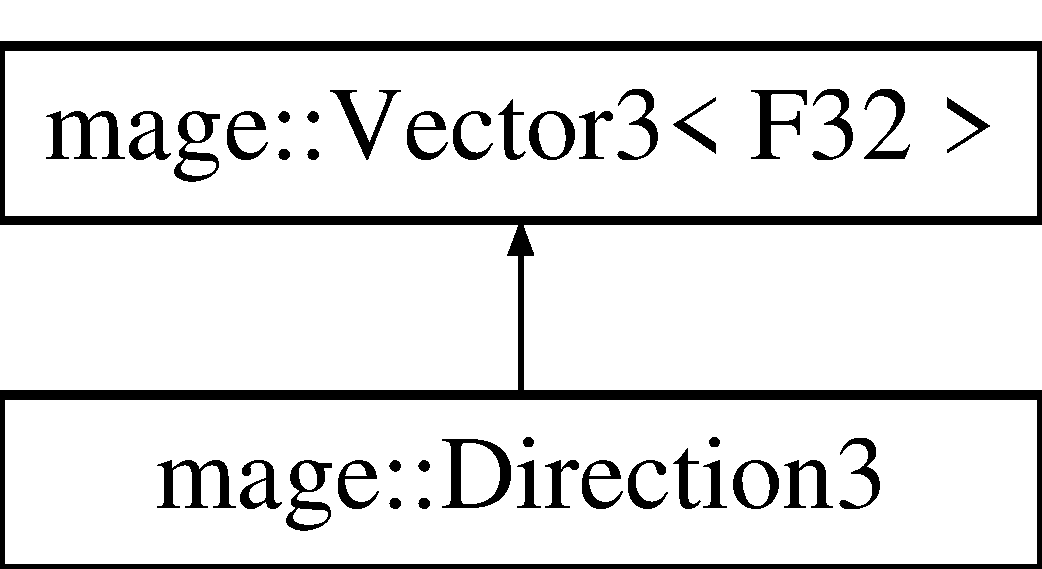
\includegraphics[height=2.000000cm]{structmage_1_1_direction3}
\end{center}
\end{figure}
\subsection*{Public Member Functions}
\begin{DoxyCompactItemize}
\item 
\hyperlink{structmage_1_1_direction3_a1c3d06aa13b207f86df36f5f3cfe486a}{Direction3} () noexcept
\item 
\hyperlink{structmage_1_1_direction3_a1af960df38637947de4ccc46aa668eb0}{Direction3} (float x, float y, float z) noexcept
\item 
\hyperlink{structmage_1_1_direction3_a1fd643f28a532720ad30cbf2ac90c5e9}{Direction3} (const \hyperlink{structmage_1_1_direction3}{Direction3} \&direction)=default
\item 
\hyperlink{structmage_1_1_direction3_a3852489e86ad55937e50aa17b15ccd05}{Direction3} (\hyperlink{structmage_1_1_direction3}{Direction3} \&\&direction) noexcept=default
\item 
\hyperlink{structmage_1_1_direction3_a3f4daf4fbf2e873bcf9133eca22fad34}{Direction3} (const \hyperlink{structmage_1_1_normal3}{Normal3} \&normal) noexcept
\item 
\hyperlink{structmage_1_1_direction3_ae9b26ed667537e7751b495058bb71de0}{Direction3} (\hyperlink{structmage_1_1_normal3}{Normal3} \&\&normal) noexcept
\item 
\hyperlink{structmage_1_1_direction3_a1230915b5196dfb1f453a612837f2cce}{Direction3} (const X\+M\+F\+L\+O\+A\+T3 \&v) noexcept
\item 
\hyperlink{structmage_1_1_direction3_a93492f00127daa470f69afaa08603759}{Direction3} (X\+M\+F\+L\+O\+A\+T3 \&\&v) noexcept
\item 
\hyperlink{structmage_1_1_direction3_a583c087dc366d206aaf54a33bc90c50b}{$\sim$\+Direction3} ()=default
\item 
\hyperlink{structmage_1_1_direction3}{Direction3} \& \hyperlink{structmage_1_1_direction3_a474a3c1ecf07954ff598933cef4f85f4}{operator=} (const \hyperlink{structmage_1_1_direction3}{Direction3} \&direction)=default
\item 
\hyperlink{structmage_1_1_direction3}{Direction3} \& \hyperlink{structmage_1_1_direction3_aac5690f3f40ba12f4e9eb09f5d2fb7f7}{operator=} (\hyperlink{structmage_1_1_direction3}{Direction3} \&\&direction)=default
\end{DoxyCompactItemize}


\subsection{Detailed Description}
A struct of directions in 3D space. 

\subsection{Constructor \& Destructor Documentation}
\hypertarget{structmage_1_1_direction3_a1c3d06aa13b207f86df36f5f3cfe486a}{}\label{structmage_1_1_direction3_a1c3d06aa13b207f86df36f5f3cfe486a} 
\index{mage\+::\+Direction3@{mage\+::\+Direction3}!Direction3@{Direction3}}
\index{Direction3@{Direction3}!mage\+::\+Direction3@{mage\+::\+Direction3}}
\subsubsection{\texorpdfstring{Direction3()}{Direction3()}\hspace{0.1cm}{\footnotesize\ttfamily [1/8]}}
{\footnotesize\ttfamily mage\+::\+Direction3\+::\+Direction3 (\begin{DoxyParamCaption}{ }\end{DoxyParamCaption})\hspace{0.3cm}{\ttfamily [noexcept]}}

Constructs a direction. \hypertarget{structmage_1_1_direction3_a1af960df38637947de4ccc46aa668eb0}{}\label{structmage_1_1_direction3_a1af960df38637947de4ccc46aa668eb0} 
\index{mage\+::\+Direction3@{mage\+::\+Direction3}!Direction3@{Direction3}}
\index{Direction3@{Direction3}!mage\+::\+Direction3@{mage\+::\+Direction3}}
\subsubsection{\texorpdfstring{Direction3()}{Direction3()}\hspace{0.1cm}{\footnotesize\ttfamily [2/8]}}
{\footnotesize\ttfamily mage\+::\+Direction3\+::\+Direction3 (\begin{DoxyParamCaption}\item[{float}]{x,  }\item[{float}]{y,  }\item[{float}]{z }\end{DoxyParamCaption})\hspace{0.3cm}{\ttfamily [noexcept]}}

Constructs a direction from the given coordinates.


\begin{DoxyParams}[1]{Parameters}
\mbox{\tt in}  & {\em x} & The x-\/coordinate. \\
\hline
\mbox{\tt in}  & {\em y} & The y-\/coordinate. \\
\hline
\mbox{\tt in}  & {\em z} & The z-\/coordinate. \\
\hline
\end{DoxyParams}
\hypertarget{structmage_1_1_direction3_a1fd643f28a532720ad30cbf2ac90c5e9}{}\label{structmage_1_1_direction3_a1fd643f28a532720ad30cbf2ac90c5e9} 
\index{mage\+::\+Direction3@{mage\+::\+Direction3}!Direction3@{Direction3}}
\index{Direction3@{Direction3}!mage\+::\+Direction3@{mage\+::\+Direction3}}
\subsubsection{\texorpdfstring{Direction3()}{Direction3()}\hspace{0.1cm}{\footnotesize\ttfamily [3/8]}}
{\footnotesize\ttfamily mage\+::\+Direction3\+::\+Direction3 (\begin{DoxyParamCaption}\item[{const \hyperlink{structmage_1_1_direction3}{Direction3} \&}]{direction }\end{DoxyParamCaption})\hspace{0.3cm}{\ttfamily [default]}}

Constructs a direction from the given direction.


\begin{DoxyParams}[1]{Parameters}
\mbox{\tt in}  & {\em direction} & A reference to the direction to copy. \\
\hline
\end{DoxyParams}
\hypertarget{structmage_1_1_direction3_a3852489e86ad55937e50aa17b15ccd05}{}\label{structmage_1_1_direction3_a3852489e86ad55937e50aa17b15ccd05} 
\index{mage\+::\+Direction3@{mage\+::\+Direction3}!Direction3@{Direction3}}
\index{Direction3@{Direction3}!mage\+::\+Direction3@{mage\+::\+Direction3}}
\subsubsection{\texorpdfstring{Direction3()}{Direction3()}\hspace{0.1cm}{\footnotesize\ttfamily [4/8]}}
{\footnotesize\ttfamily mage\+::\+Direction3\+::\+Direction3 (\begin{DoxyParamCaption}\item[{\hyperlink{structmage_1_1_direction3}{Direction3} \&\&}]{direction }\end{DoxyParamCaption})\hspace{0.3cm}{\ttfamily [default]}, {\ttfamily [noexcept]}}

Constructs a direction by moving the given direction.


\begin{DoxyParams}[1]{Parameters}
\mbox{\tt in}  & {\em direction} & A reference to the direction to move. \\
\hline
\end{DoxyParams}
\hypertarget{structmage_1_1_direction3_a3f4daf4fbf2e873bcf9133eca22fad34}{}\label{structmage_1_1_direction3_a3f4daf4fbf2e873bcf9133eca22fad34} 
\index{mage\+::\+Direction3@{mage\+::\+Direction3}!Direction3@{Direction3}}
\index{Direction3@{Direction3}!mage\+::\+Direction3@{mage\+::\+Direction3}}
\subsubsection{\texorpdfstring{Direction3()}{Direction3()}\hspace{0.1cm}{\footnotesize\ttfamily [5/8]}}
{\footnotesize\ttfamily mage\+::\+Direction3\+::\+Direction3 (\begin{DoxyParamCaption}\item[{const \hyperlink{structmage_1_1_normal3}{Normal3} \&}]{normal }\end{DoxyParamCaption})\hspace{0.3cm}{\ttfamily [noexcept]}}

Constructs a direction from the given normal.


\begin{DoxyParams}[1]{Parameters}
\mbox{\tt in}  & {\em normal} & A reference to the normal to copy. \\
\hline
\end{DoxyParams}
\hypertarget{structmage_1_1_direction3_ae9b26ed667537e7751b495058bb71de0}{}\label{structmage_1_1_direction3_ae9b26ed667537e7751b495058bb71de0} 
\index{mage\+::\+Direction3@{mage\+::\+Direction3}!Direction3@{Direction3}}
\index{Direction3@{Direction3}!mage\+::\+Direction3@{mage\+::\+Direction3}}
\subsubsection{\texorpdfstring{Direction3()}{Direction3()}\hspace{0.1cm}{\footnotesize\ttfamily [6/8]}}
{\footnotesize\ttfamily mage\+::\+Direction3\+::\+Direction3 (\begin{DoxyParamCaption}\item[{\hyperlink{structmage_1_1_normal3}{Normal3} \&\&}]{normal }\end{DoxyParamCaption})\hspace{0.3cm}{\ttfamily [noexcept]}}

Constructs a direction by moving the given normal.


\begin{DoxyParams}[1]{Parameters}
\mbox{\tt in}  & {\em normal} & A reference to the normal to move. \\
\hline
\end{DoxyParams}
\hypertarget{structmage_1_1_direction3_a1230915b5196dfb1f453a612837f2cce}{}\label{structmage_1_1_direction3_a1230915b5196dfb1f453a612837f2cce} 
\index{mage\+::\+Direction3@{mage\+::\+Direction3}!Direction3@{Direction3}}
\index{Direction3@{Direction3}!mage\+::\+Direction3@{mage\+::\+Direction3}}
\subsubsection{\texorpdfstring{Direction3()}{Direction3()}\hspace{0.1cm}{\footnotesize\ttfamily [7/8]}}
{\footnotesize\ttfamily mage\+::\+Direction3\+::\+Direction3 (\begin{DoxyParamCaption}\item[{const X\+M\+F\+L\+O\+A\+T3 \&}]{v }\end{DoxyParamCaption})\hspace{0.3cm}{\ttfamily [explicit]}, {\ttfamily [noexcept]}}

Constructs a direction from the given vector.


\begin{DoxyParams}[1]{Parameters}
\mbox{\tt in}  & {\em v} & A reference to the vector to copy. \\
\hline
\end{DoxyParams}
\hypertarget{structmage_1_1_direction3_a93492f00127daa470f69afaa08603759}{}\label{structmage_1_1_direction3_a93492f00127daa470f69afaa08603759} 
\index{mage\+::\+Direction3@{mage\+::\+Direction3}!Direction3@{Direction3}}
\index{Direction3@{Direction3}!mage\+::\+Direction3@{mage\+::\+Direction3}}
\subsubsection{\texorpdfstring{Direction3()}{Direction3()}\hspace{0.1cm}{\footnotesize\ttfamily [8/8]}}
{\footnotesize\ttfamily mage\+::\+Direction3\+::\+Direction3 (\begin{DoxyParamCaption}\item[{X\+M\+F\+L\+O\+A\+T3 \&\&}]{v }\end{DoxyParamCaption})\hspace{0.3cm}{\ttfamily [explicit]}, {\ttfamily [noexcept]}}

Constructs a direction by moving the given vector.


\begin{DoxyParams}[1]{Parameters}
\mbox{\tt in}  & {\em v} & A reference to the vector to move. \\
\hline
\end{DoxyParams}
\hypertarget{structmage_1_1_direction3_a583c087dc366d206aaf54a33bc90c50b}{}\label{structmage_1_1_direction3_a583c087dc366d206aaf54a33bc90c50b} 
\index{mage\+::\+Direction3@{mage\+::\+Direction3}!````~Direction3@{$\sim$\+Direction3}}
\index{````~Direction3@{$\sim$\+Direction3}!mage\+::\+Direction3@{mage\+::\+Direction3}}
\subsubsection{\texorpdfstring{$\sim$\+Direction3()}{~Direction3()}}
{\footnotesize\ttfamily mage\+::\+Direction3\+::$\sim$\+Direction3 (\begin{DoxyParamCaption}{ }\end{DoxyParamCaption})\hspace{0.3cm}{\ttfamily [default]}}

Constructs a direction. 

\subsection{Member Function Documentation}
\hypertarget{structmage_1_1_direction3_a474a3c1ecf07954ff598933cef4f85f4}{}\label{structmage_1_1_direction3_a474a3c1ecf07954ff598933cef4f85f4} 
\index{mage\+::\+Direction3@{mage\+::\+Direction3}!operator=@{operator=}}
\index{operator=@{operator=}!mage\+::\+Direction3@{mage\+::\+Direction3}}
\subsubsection{\texorpdfstring{operator=()}{operator=()}\hspace{0.1cm}{\footnotesize\ttfamily [1/2]}}
{\footnotesize\ttfamily \hyperlink{structmage_1_1_direction3}{Direction3}\& mage\+::\+Direction3\+::operator= (\begin{DoxyParamCaption}\item[{const \hyperlink{structmage_1_1_direction3}{Direction3} \&}]{direction }\end{DoxyParamCaption})\hspace{0.3cm}{\ttfamily [default]}}

Copies the given direction to this direction.


\begin{DoxyParams}[1]{Parameters}
\mbox{\tt in}  & {\em direction} & A reference to the direction to copy. \\
\hline
\end{DoxyParams}
\begin{DoxyReturn}{Returns}
A reference to the copy of the given direction (i.\+e. this direction). 
\end{DoxyReturn}
\hypertarget{structmage_1_1_direction3_aac5690f3f40ba12f4e9eb09f5d2fb7f7}{}\label{structmage_1_1_direction3_aac5690f3f40ba12f4e9eb09f5d2fb7f7} 
\index{mage\+::\+Direction3@{mage\+::\+Direction3}!operator=@{operator=}}
\index{operator=@{operator=}!mage\+::\+Direction3@{mage\+::\+Direction3}}
\subsubsection{\texorpdfstring{operator=()}{operator=()}\hspace{0.1cm}{\footnotesize\ttfamily [2/2]}}
{\footnotesize\ttfamily \hyperlink{structmage_1_1_direction3}{Direction3}\& mage\+::\+Direction3\+::operator= (\begin{DoxyParamCaption}\item[{\hyperlink{structmage_1_1_direction3}{Direction3} \&\&}]{direction }\end{DoxyParamCaption})\hspace{0.3cm}{\ttfamily [default]}}

Moves the given direction to this direction.


\begin{DoxyParams}[1]{Parameters}
\mbox{\tt in}  & {\em direction} & A reference to the direction to move. \\
\hline
\end{DoxyParams}
\begin{DoxyReturn}{Returns}
A reference to the moved direction (i.\+e. this direction). 
\end{DoxyReturn}

\hypertarget{classmage_1_1_directional_light}{}\section{mage\+:\+:Directional\+Light Class Reference}
\label{classmage_1_1_directional_light}\index{mage\+::\+Directional\+Light@{mage\+::\+Directional\+Light}}


{\ttfamily \#include $<$directional\+\_\+light.\+hpp$>$}

Inheritance diagram for mage\+:\+:Directional\+Light\+:\begin{figure}[H]
\begin{center}
\leavevmode
\includegraphics[height=2.000000cm]{classmage_1_1_directional_light}
\end{center}
\end{figure}
\subsection*{Public Member Functions}
\begin{DoxyCompactItemize}
\item 
\hyperlink{classmage_1_1_directional_light_a67df04219f61a8350045e5743b1de284}{Directional\+Light} (const \hyperlink{structmage_1_1_r_g_b_spectrum}{R\+G\+B\+Spectrum} \&intensity=\hyperlink{structmage_1_1_r_g_b_spectrum}{R\+G\+B\+Spectrum}(1.\+0f, 1.\+0f, 1.\+0f))
\item 
\hyperlink{classmage_1_1_directional_light_a777b1b8e00a51ba84f6af774a7b519ea}{Directional\+Light} (const \hyperlink{classmage_1_1_directional_light}{Directional\+Light} \&light)
\item 
\hyperlink{classmage_1_1_directional_light_a9563b260b550057e951500c40ecbe2d3}{Directional\+Light} (\hyperlink{classmage_1_1_directional_light}{Directional\+Light} \&\&light)
\item 
virtual \hyperlink{classmage_1_1_directional_light_a967d33c11a1477c01ce4c9720337caeb}{$\sim$\+Directional\+Light} ()
\item 
\hyperlink{classmage_1_1_directional_light}{Directional\+Light} \& \hyperlink{classmage_1_1_directional_light_a371d3c13d6e59c8d105da058b460874d}{operator=} (const \hyperlink{classmage_1_1_directional_light}{Directional\+Light} \&light)
\item 
\hyperlink{classmage_1_1_directional_light}{Directional\+Light} \& \hyperlink{classmage_1_1_directional_light_a508b595bf6aa5fc9db53e0a854fda41d}{operator=} (\hyperlink{classmage_1_1_directional_light}{Directional\+Light} \&\&light)
\item 
\hyperlink{namespacemage_a3316d7143a973e37adf1110f2e80ca31}{Unique\+Ptr}$<$ \hyperlink{classmage_1_1_directional_light}{Directional\+Light} $>$ \hyperlink{classmage_1_1_directional_light_a779c49e066215cff9f80ed40048dfc62}{Clone} () const
\item 
bool \hyperlink{classmage_1_1_directional_light_a645e7f3d3e4dc4ebf11d7a6aa6950a18}{Use\+Shadows} () const noexcept
\item 
void \hyperlink{classmage_1_1_directional_light_a36436d5d99ccf6a0e49e81f26c3f9bc7}{Enable\+Shadows} () noexcept
\item 
void \hyperlink{classmage_1_1_directional_light_addd4803dee85892dfd57f51e155c6572}{Dissable\+Shadows} () noexcept
\item 
void \hyperlink{classmage_1_1_directional_light_a1c15d8e42526ed5ae7568cff5c7b25e0}{Toggle\+Shadows} () noexcept
\item 
void \hyperlink{classmage_1_1_directional_light_ab70b4298dc6616dbe22446e8e3298424}{Set\+Shadows} (bool shadows) noexcept
\end{DoxyCompactItemize}
\subsection*{Private Member Functions}
\begin{DoxyCompactItemize}
\item 
virtual \hyperlink{namespacemage_a3316d7143a973e37adf1110f2e80ca31}{Unique\+Ptr}$<$ \hyperlink{classmage_1_1_light}{Light} $>$ \hyperlink{classmage_1_1_directional_light_a122d3dcd7633a85ef8a85e7d768da36d}{Clone\+Implementation} () const override
\end{DoxyCompactItemize}
\subsection*{Private Attributes}
\begin{DoxyCompactItemize}
\item 
bool \hyperlink{classmage_1_1_directional_light_a607a3dc01ee180f2044fe154c2b73903}{m\+\_\+shadows}
\end{DoxyCompactItemize}
\subsection*{Additional Inherited Members}


\subsection{Detailed Description}
A class of directional lights. 

\subsection{Constructor \& Destructor Documentation}
\hypertarget{classmage_1_1_directional_light_a67df04219f61a8350045e5743b1de284}{}\label{classmage_1_1_directional_light_a67df04219f61a8350045e5743b1de284} 
\index{mage\+::\+Directional\+Light@{mage\+::\+Directional\+Light}!Directional\+Light@{Directional\+Light}}
\index{Directional\+Light@{Directional\+Light}!mage\+::\+Directional\+Light@{mage\+::\+Directional\+Light}}
\subsubsection{\texorpdfstring{Directional\+Light()}{DirectionalLight()}\hspace{0.1cm}{\footnotesize\ttfamily [1/3]}}
{\footnotesize\ttfamily mage\+::\+Directional\+Light\+::\+Directional\+Light (\begin{DoxyParamCaption}\item[{const \hyperlink{structmage_1_1_r_g_b_spectrum}{R\+G\+B\+Spectrum} \&}]{intensity = {\ttfamily \hyperlink{structmage_1_1_r_g_b_spectrum}{R\+G\+B\+Spectrum}(1.0f,~1.0f,~1.0f)} }\end{DoxyParamCaption})\hspace{0.3cm}{\ttfamily [explicit]}}

Constructs a directional light.


\begin{DoxyParams}[1]{Parameters}
\mbox{\tt in}  & {\em intensity} & The R\+GB intensity. \\
\hline
\end{DoxyParams}
\hypertarget{classmage_1_1_directional_light_a777b1b8e00a51ba84f6af774a7b519ea}{}\label{classmage_1_1_directional_light_a777b1b8e00a51ba84f6af774a7b519ea} 
\index{mage\+::\+Directional\+Light@{mage\+::\+Directional\+Light}!Directional\+Light@{Directional\+Light}}
\index{Directional\+Light@{Directional\+Light}!mage\+::\+Directional\+Light@{mage\+::\+Directional\+Light}}
\subsubsection{\texorpdfstring{Directional\+Light()}{DirectionalLight()}\hspace{0.1cm}{\footnotesize\ttfamily [2/3]}}
{\footnotesize\ttfamily mage\+::\+Directional\+Light\+::\+Directional\+Light (\begin{DoxyParamCaption}\item[{const \hyperlink{classmage_1_1_directional_light}{Directional\+Light} \&}]{light }\end{DoxyParamCaption})\hspace{0.3cm}{\ttfamily [default]}}

Constructs a directional light from the given directional light.


\begin{DoxyParams}[1]{Parameters}
\mbox{\tt in}  & {\em light} & A reference to the directional light to copy. \\
\hline
\end{DoxyParams}
\hypertarget{classmage_1_1_directional_light_a9563b260b550057e951500c40ecbe2d3}{}\label{classmage_1_1_directional_light_a9563b260b550057e951500c40ecbe2d3} 
\index{mage\+::\+Directional\+Light@{mage\+::\+Directional\+Light}!Directional\+Light@{Directional\+Light}}
\index{Directional\+Light@{Directional\+Light}!mage\+::\+Directional\+Light@{mage\+::\+Directional\+Light}}
\subsubsection{\texorpdfstring{Directional\+Light()}{DirectionalLight()}\hspace{0.1cm}{\footnotesize\ttfamily [3/3]}}
{\footnotesize\ttfamily mage\+::\+Directional\+Light\+::\+Directional\+Light (\begin{DoxyParamCaption}\item[{\hyperlink{classmage_1_1_directional_light}{Directional\+Light} \&\&}]{light }\end{DoxyParamCaption})\hspace{0.3cm}{\ttfamily [default]}}

Constructs a directional light by moving the given directional light.


\begin{DoxyParams}[1]{Parameters}
\mbox{\tt in}  & {\em light} & A reference to the directional light to move. \\
\hline
\end{DoxyParams}
\hypertarget{classmage_1_1_directional_light_a967d33c11a1477c01ce4c9720337caeb}{}\label{classmage_1_1_directional_light_a967d33c11a1477c01ce4c9720337caeb} 
\index{mage\+::\+Directional\+Light@{mage\+::\+Directional\+Light}!````~Directional\+Light@{$\sim$\+Directional\+Light}}
\index{````~Directional\+Light@{$\sim$\+Directional\+Light}!mage\+::\+Directional\+Light@{mage\+::\+Directional\+Light}}
\subsubsection{\texorpdfstring{$\sim$\+Directional\+Light()}{~DirectionalLight()}}
{\footnotesize\ttfamily mage\+::\+Directional\+Light\+::$\sim$\+Directional\+Light (\begin{DoxyParamCaption}{ }\end{DoxyParamCaption})\hspace{0.3cm}{\ttfamily [virtual]}, {\ttfamily [default]}}

Destructs this directional light. 

\subsection{Member Function Documentation}
\hypertarget{classmage_1_1_directional_light_a779c49e066215cff9f80ed40048dfc62}{}\label{classmage_1_1_directional_light_a779c49e066215cff9f80ed40048dfc62} 
\index{mage\+::\+Directional\+Light@{mage\+::\+Directional\+Light}!Clone@{Clone}}
\index{Clone@{Clone}!mage\+::\+Directional\+Light@{mage\+::\+Directional\+Light}}
\subsubsection{\texorpdfstring{Clone()}{Clone()}}
{\footnotesize\ttfamily \hyperlink{namespacemage_a3316d7143a973e37adf1110f2e80ca31}{Unique\+Ptr}$<$ \hyperlink{classmage_1_1_directional_light}{Directional\+Light} $>$ mage\+::\+Directional\+Light\+::\+Clone (\begin{DoxyParamCaption}{ }\end{DoxyParamCaption}) const}

Clones this directional light.

\begin{DoxyReturn}{Returns}
A pointer to the clone of this directional light. 
\end{DoxyReturn}
\hypertarget{classmage_1_1_directional_light_a122d3dcd7633a85ef8a85e7d768da36d}{}\label{classmage_1_1_directional_light_a122d3dcd7633a85ef8a85e7d768da36d} 
\index{mage\+::\+Directional\+Light@{mage\+::\+Directional\+Light}!Clone\+Implementation@{Clone\+Implementation}}
\index{Clone\+Implementation@{Clone\+Implementation}!mage\+::\+Directional\+Light@{mage\+::\+Directional\+Light}}
\subsubsection{\texorpdfstring{Clone\+Implementation()}{CloneImplementation()}}
{\footnotesize\ttfamily \hyperlink{namespacemage_a3316d7143a973e37adf1110f2e80ca31}{Unique\+Ptr}$<$ \hyperlink{classmage_1_1_light}{Light} $>$ mage\+::\+Directional\+Light\+::\+Clone\+Implementation (\begin{DoxyParamCaption}{ }\end{DoxyParamCaption}) const\hspace{0.3cm}{\ttfamily [override]}, {\ttfamily [private]}, {\ttfamily [virtual]}}

Clones this directional light.

\begin{DoxyReturn}{Returns}
A pointer to the clone of this directional light. 
\end{DoxyReturn}


Implements \hyperlink{classmage_1_1_light_aa613d76a1ebda69efde853d15f75490c}{mage\+::\+Light}.

\hypertarget{classmage_1_1_directional_light_addd4803dee85892dfd57f51e155c6572}{}\label{classmage_1_1_directional_light_addd4803dee85892dfd57f51e155c6572} 
\index{mage\+::\+Directional\+Light@{mage\+::\+Directional\+Light}!Dissable\+Shadows@{Dissable\+Shadows}}
\index{Dissable\+Shadows@{Dissable\+Shadows}!mage\+::\+Directional\+Light@{mage\+::\+Directional\+Light}}
\subsubsection{\texorpdfstring{Dissable\+Shadows()}{DissableShadows()}}
{\footnotesize\ttfamily void mage\+::\+Directional\+Light\+::\+Dissable\+Shadows (\begin{DoxyParamCaption}{ }\end{DoxyParamCaption})\hspace{0.3cm}{\ttfamily [noexcept]}}

Dissables shadows for this directional light. \hypertarget{classmage_1_1_directional_light_a36436d5d99ccf6a0e49e81f26c3f9bc7}{}\label{classmage_1_1_directional_light_a36436d5d99ccf6a0e49e81f26c3f9bc7} 
\index{mage\+::\+Directional\+Light@{mage\+::\+Directional\+Light}!Enable\+Shadows@{Enable\+Shadows}}
\index{Enable\+Shadows@{Enable\+Shadows}!mage\+::\+Directional\+Light@{mage\+::\+Directional\+Light}}
\subsubsection{\texorpdfstring{Enable\+Shadows()}{EnableShadows()}}
{\footnotesize\ttfamily void mage\+::\+Directional\+Light\+::\+Enable\+Shadows (\begin{DoxyParamCaption}{ }\end{DoxyParamCaption})\hspace{0.3cm}{\ttfamily [noexcept]}}

Enables shadows for this directional light. \hypertarget{classmage_1_1_directional_light_a371d3c13d6e59c8d105da058b460874d}{}\label{classmage_1_1_directional_light_a371d3c13d6e59c8d105da058b460874d} 
\index{mage\+::\+Directional\+Light@{mage\+::\+Directional\+Light}!operator=@{operator=}}
\index{operator=@{operator=}!mage\+::\+Directional\+Light@{mage\+::\+Directional\+Light}}
\subsubsection{\texorpdfstring{operator=()}{operator=()}\hspace{0.1cm}{\footnotesize\ttfamily [1/2]}}
{\footnotesize\ttfamily \hyperlink{classmage_1_1_directional_light}{Directional\+Light} \& mage\+::\+Directional\+Light\+::operator= (\begin{DoxyParamCaption}\item[{const \hyperlink{classmage_1_1_directional_light}{Directional\+Light} \&}]{light }\end{DoxyParamCaption})\hspace{0.3cm}{\ttfamily [default]}}

Copies the given directional light to this directional light.


\begin{DoxyParams}[1]{Parameters}
\mbox{\tt in}  & {\em light} & A reference to the directional light to copy. \\
\hline
\end{DoxyParams}
\begin{DoxyReturn}{Returns}
A reference to the copy of the given directional light (i.\+e. this directional light). 
\end{DoxyReturn}
\hypertarget{classmage_1_1_directional_light_a508b595bf6aa5fc9db53e0a854fda41d}{}\label{classmage_1_1_directional_light_a508b595bf6aa5fc9db53e0a854fda41d} 
\index{mage\+::\+Directional\+Light@{mage\+::\+Directional\+Light}!operator=@{operator=}}
\index{operator=@{operator=}!mage\+::\+Directional\+Light@{mage\+::\+Directional\+Light}}
\subsubsection{\texorpdfstring{operator=()}{operator=()}\hspace{0.1cm}{\footnotesize\ttfamily [2/2]}}
{\footnotesize\ttfamily \hyperlink{classmage_1_1_directional_light}{Directional\+Light} \& mage\+::\+Directional\+Light\+::operator= (\begin{DoxyParamCaption}\item[{\hyperlink{classmage_1_1_directional_light}{Directional\+Light} \&\&}]{light }\end{DoxyParamCaption})\hspace{0.3cm}{\ttfamily [default]}}

Moves the given directional light to this directional light.


\begin{DoxyParams}[1]{Parameters}
\mbox{\tt in}  & {\em light} & A reference to the directional light to move. \\
\hline
\end{DoxyParams}
\begin{DoxyReturn}{Returns}
A reference to the moved directional light (i.\+e. this directional light). 
\end{DoxyReturn}
\hypertarget{classmage_1_1_directional_light_ab70b4298dc6616dbe22446e8e3298424}{}\label{classmage_1_1_directional_light_ab70b4298dc6616dbe22446e8e3298424} 
\index{mage\+::\+Directional\+Light@{mage\+::\+Directional\+Light}!Set\+Shadows@{Set\+Shadows}}
\index{Set\+Shadows@{Set\+Shadows}!mage\+::\+Directional\+Light@{mage\+::\+Directional\+Light}}
\subsubsection{\texorpdfstring{Set\+Shadows()}{SetShadows()}}
{\footnotesize\ttfamily void mage\+::\+Directional\+Light\+::\+Set\+Shadows (\begin{DoxyParamCaption}\item[{bool}]{shadows }\end{DoxyParamCaption})\hspace{0.3cm}{\ttfamily [noexcept]}}

Sets shadows for this directional light to the given value.


\begin{DoxyParams}[1]{Parameters}
\mbox{\tt in}  & {\em shadows} & {\ttfamily true} if shadows should be used for this directional light. {\ttfamily false} otherwise. \\
\hline
\end{DoxyParams}
\hypertarget{classmage_1_1_directional_light_a1c15d8e42526ed5ae7568cff5c7b25e0}{}\label{classmage_1_1_directional_light_a1c15d8e42526ed5ae7568cff5c7b25e0} 
\index{mage\+::\+Directional\+Light@{mage\+::\+Directional\+Light}!Toggle\+Shadows@{Toggle\+Shadows}}
\index{Toggle\+Shadows@{Toggle\+Shadows}!mage\+::\+Directional\+Light@{mage\+::\+Directional\+Light}}
\subsubsection{\texorpdfstring{Toggle\+Shadows()}{ToggleShadows()}}
{\footnotesize\ttfamily void mage\+::\+Directional\+Light\+::\+Toggle\+Shadows (\begin{DoxyParamCaption}{ }\end{DoxyParamCaption})\hspace{0.3cm}{\ttfamily [noexcept]}}

Toggles shadows for this directional light. \hypertarget{classmage_1_1_directional_light_a645e7f3d3e4dc4ebf11d7a6aa6950a18}{}\label{classmage_1_1_directional_light_a645e7f3d3e4dc4ebf11d7a6aa6950a18} 
\index{mage\+::\+Directional\+Light@{mage\+::\+Directional\+Light}!Use\+Shadows@{Use\+Shadows}}
\index{Use\+Shadows@{Use\+Shadows}!mage\+::\+Directional\+Light@{mage\+::\+Directional\+Light}}
\subsubsection{\texorpdfstring{Use\+Shadows()}{UseShadows()}}
{\footnotesize\ttfamily bool mage\+::\+Directional\+Light\+::\+Use\+Shadows (\begin{DoxyParamCaption}{ }\end{DoxyParamCaption}) const\hspace{0.3cm}{\ttfamily [noexcept]}}

Checks whether shadows should be used for this directional light.

\begin{DoxyReturn}{Returns}
{\ttfamily true} if shadows should be used for this directional light. {\ttfamily false} otherwise. 
\end{DoxyReturn}


\subsection{Member Data Documentation}
\hypertarget{classmage_1_1_directional_light_a607a3dc01ee180f2044fe154c2b73903}{}\label{classmage_1_1_directional_light_a607a3dc01ee180f2044fe154c2b73903} 
\index{mage\+::\+Directional\+Light@{mage\+::\+Directional\+Light}!m\+\_\+shadows@{m\+\_\+shadows}}
\index{m\+\_\+shadows@{m\+\_\+shadows}!mage\+::\+Directional\+Light@{mage\+::\+Directional\+Light}}
\subsubsection{\texorpdfstring{m\+\_\+shadows}{m\_shadows}}
{\footnotesize\ttfamily bool mage\+::\+Directional\+Light\+::m\+\_\+shadows\hspace{0.3cm}{\ttfamily [private]}}

A flag indicating whether shadows should be calculated or not not for this directional light. 
\hypertarget{classmage_1_1_dropshadow_sprite_text}{}\section{mage\+:\+:Dropshadow\+Sprite\+Text Class Reference}
\label{classmage_1_1_dropshadow_sprite_text}\index{mage\+::\+Dropshadow\+Sprite\+Text@{mage\+::\+Dropshadow\+Sprite\+Text}}


{\ttfamily \#include $<$dropshadow\+\_\+sprite\+\_\+text.\+hpp$>$}

Inheritance diagram for mage\+:\+:Dropshadow\+Sprite\+Text\+:\begin{figure}[H]
\begin{center}
\leavevmode
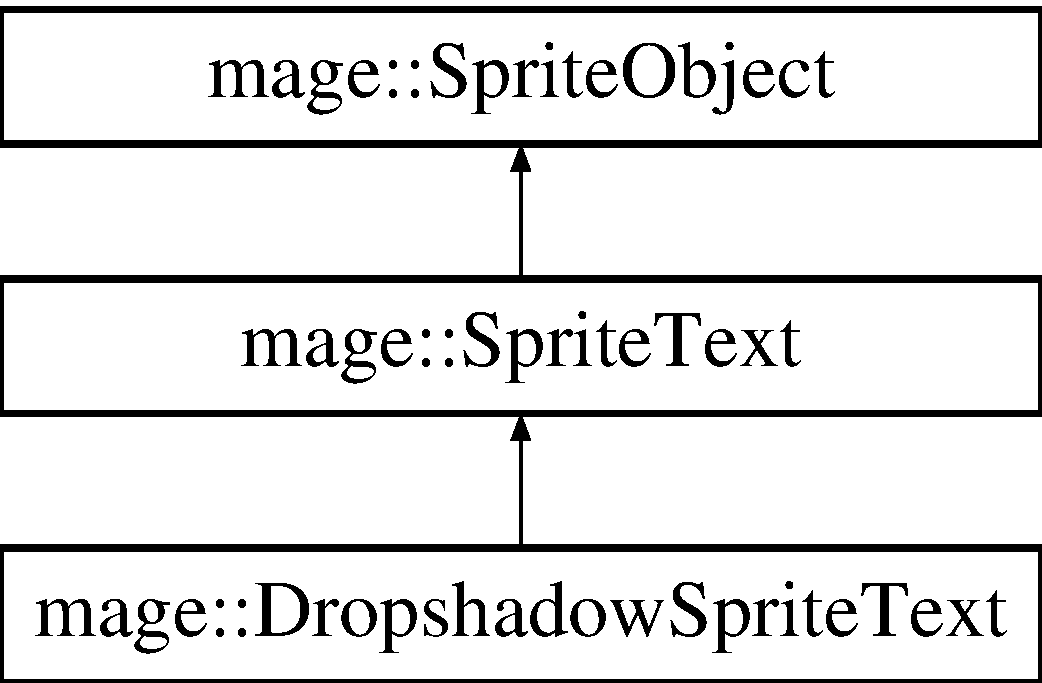
\includegraphics[height=3.000000cm]{classmage_1_1_dropshadow_sprite_text}
\end{center}
\end{figure}
\subsection*{Public Member Functions}
\begin{DoxyCompactItemize}
\item 
\hyperlink{classmage_1_1_dropshadow_sprite_text_a74003c0961117f9c04e2f4b70e71a74c}{Dropshadow\+Sprite\+Text} ()
\item 
\hyperlink{classmage_1_1_dropshadow_sprite_text_af0a9422a32ed8962d6c691fe76f44c30}{Dropshadow\+Sprite\+Text} (const \hyperlink{classmage_1_1_dropshadow_sprite_text}{Dropshadow\+Sprite\+Text} \&sprite\+\_\+text)
\item 
\hyperlink{classmage_1_1_dropshadow_sprite_text_a79367c23991f486a8548aac6fce36691}{Dropshadow\+Sprite\+Text} (\hyperlink{classmage_1_1_dropshadow_sprite_text}{Dropshadow\+Sprite\+Text} \&\&sprite\+\_\+text) noexcept
\item 
virtual \hyperlink{classmage_1_1_dropshadow_sprite_text_a561b1be59d05bccb680969be792c0e28}{$\sim$\+Dropshadow\+Sprite\+Text} ()
\item 
\hyperlink{classmage_1_1_dropshadow_sprite_text}{Dropshadow\+Sprite\+Text} \& \hyperlink{classmage_1_1_dropshadow_sprite_text_a83846227264396ee5b6ca44304bc404a}{operator=} (const \hyperlink{classmage_1_1_dropshadow_sprite_text}{Dropshadow\+Sprite\+Text} \&sprite\+\_\+text)=delete
\item 
\hyperlink{classmage_1_1_dropshadow_sprite_text}{Dropshadow\+Sprite\+Text} \& \hyperlink{classmage_1_1_dropshadow_sprite_text_aea70f005fd9eae94aee9da27aa54534b}{operator=} (\hyperlink{classmage_1_1_dropshadow_sprite_text}{Dropshadow\+Sprite\+Text} \&\&sprite\+\_\+text)=delete
\item 
\hyperlink{namespacemage_a3316d7143a973e37adf1110f2e80ca31}{Unique\+Ptr}$<$ \hyperlink{classmage_1_1_dropshadow_sprite_text}{Dropshadow\+Sprite\+Text} $>$ \hyperlink{classmage_1_1_dropshadow_sprite_text_a0dcce82b4a83fbd469d68adba21af220}{Clone} () const
\item 
virtual void \hyperlink{classmage_1_1_dropshadow_sprite_text_af76422c9812d7dc38e9b98e587103c67}{Draw} (\hyperlink{classmage_1_1_sprite_batch}{Sprite\+Batch} \&sprite\+\_\+batch) const override
\item 
\hyperlink{structmage_1_1_s_r_g_b_a}{S\+R\+G\+BA} \& \hyperlink{classmage_1_1_dropshadow_sprite_text_ae397446f32257519efb24766edc0d0e8}{Get\+Shadow\+Color} () noexcept
\item 
const \hyperlink{structmage_1_1_s_r_g_b_a}{S\+R\+G\+BA} \& \hyperlink{classmage_1_1_dropshadow_sprite_text_ac441bdd3e94d80a27d33af2a01207704}{Get\+Shadow\+Color} () const noexcept
\end{DoxyCompactItemize}
\subsection*{Private Member Functions}
\begin{DoxyCompactItemize}
\item 
virtual \hyperlink{namespacemage_a3316d7143a973e37adf1110f2e80ca31}{Unique\+Ptr}$<$ \hyperlink{classmage_1_1_sprite}{Sprite} $>$ \hyperlink{classmage_1_1_dropshadow_sprite_text_af997217dd243061e0490bbcd4bfde7ed}{Clone\+Implementation} () const override
\end{DoxyCompactItemize}
\subsection*{Private Attributes}
\begin{DoxyCompactItemize}
\item 
\hyperlink{structmage_1_1_s_r_g_b_a}{S\+R\+G\+BA} \hyperlink{classmage_1_1_dropshadow_sprite_text_a351565d8f023ddc53f486e048ad67e42}{m\+\_\+shadow\+\_\+color}
\end{DoxyCompactItemize}
\subsection*{Additional Inherited Members}


\subsection{Detailed Description}
A class of dropshadow sprite texts. 

\subsection{Constructor \& Destructor Documentation}
\hypertarget{classmage_1_1_dropshadow_sprite_text_a74003c0961117f9c04e2f4b70e71a74c}{}\label{classmage_1_1_dropshadow_sprite_text_a74003c0961117f9c04e2f4b70e71a74c} 
\index{mage\+::\+Dropshadow\+Sprite\+Text@{mage\+::\+Dropshadow\+Sprite\+Text}!Dropshadow\+Sprite\+Text@{Dropshadow\+Sprite\+Text}}
\index{Dropshadow\+Sprite\+Text@{Dropshadow\+Sprite\+Text}!mage\+::\+Dropshadow\+Sprite\+Text@{mage\+::\+Dropshadow\+Sprite\+Text}}
\subsubsection{\texorpdfstring{Dropshadow\+Sprite\+Text()}{DropshadowSpriteText()}\hspace{0.1cm}{\footnotesize\ttfamily [1/3]}}
{\footnotesize\ttfamily mage\+::\+Dropshadow\+Sprite\+Text\+::\+Dropshadow\+Sprite\+Text (\begin{DoxyParamCaption}{ }\end{DoxyParamCaption})}

Constructs a dropshadow sprite text.

\begin{DoxyPrecond}{Precondition}
The resource manager associated with the current engine must be loaded. 
\end{DoxyPrecond}
\hypertarget{classmage_1_1_dropshadow_sprite_text_af0a9422a32ed8962d6c691fe76f44c30}{}\label{classmage_1_1_dropshadow_sprite_text_af0a9422a32ed8962d6c691fe76f44c30} 
\index{mage\+::\+Dropshadow\+Sprite\+Text@{mage\+::\+Dropshadow\+Sprite\+Text}!Dropshadow\+Sprite\+Text@{Dropshadow\+Sprite\+Text}}
\index{Dropshadow\+Sprite\+Text@{Dropshadow\+Sprite\+Text}!mage\+::\+Dropshadow\+Sprite\+Text@{mage\+::\+Dropshadow\+Sprite\+Text}}
\subsubsection{\texorpdfstring{Dropshadow\+Sprite\+Text()}{DropshadowSpriteText()}\hspace{0.1cm}{\footnotesize\ttfamily [2/3]}}
{\footnotesize\ttfamily mage\+::\+Dropshadow\+Sprite\+Text\+::\+Dropshadow\+Sprite\+Text (\begin{DoxyParamCaption}\item[{const \hyperlink{classmage_1_1_dropshadow_sprite_text}{Dropshadow\+Sprite\+Text} \&}]{sprite\+\_\+text }\end{DoxyParamCaption})\hspace{0.3cm}{\ttfamily [default]}}

Constructs a dropshadow sprite text from the given dropshadow sprite text.


\begin{DoxyParams}[1]{Parameters}
\mbox{\tt in}  & {\em sprite\+\_\+text} & A reference to the dropshadow sprite text to copy. \\
\hline
\end{DoxyParams}
\hypertarget{classmage_1_1_dropshadow_sprite_text_a79367c23991f486a8548aac6fce36691}{}\label{classmage_1_1_dropshadow_sprite_text_a79367c23991f486a8548aac6fce36691} 
\index{mage\+::\+Dropshadow\+Sprite\+Text@{mage\+::\+Dropshadow\+Sprite\+Text}!Dropshadow\+Sprite\+Text@{Dropshadow\+Sprite\+Text}}
\index{Dropshadow\+Sprite\+Text@{Dropshadow\+Sprite\+Text}!mage\+::\+Dropshadow\+Sprite\+Text@{mage\+::\+Dropshadow\+Sprite\+Text}}
\subsubsection{\texorpdfstring{Dropshadow\+Sprite\+Text()}{DropshadowSpriteText()}\hspace{0.1cm}{\footnotesize\ttfamily [3/3]}}
{\footnotesize\ttfamily mage\+::\+Dropshadow\+Sprite\+Text\+::\+Dropshadow\+Sprite\+Text (\begin{DoxyParamCaption}\item[{\hyperlink{classmage_1_1_dropshadow_sprite_text}{Dropshadow\+Sprite\+Text} \&\&}]{sprite\+\_\+text }\end{DoxyParamCaption})\hspace{0.3cm}{\ttfamily [default]}, {\ttfamily [noexcept]}}

Constructs a dropshadow sprite text by moving the given dropshadow sprite text.


\begin{DoxyParams}[1]{Parameters}
\mbox{\tt in}  & {\em sprite\+\_\+text} & A reference to the dropshadow sprite text to move. \\
\hline
\end{DoxyParams}
\hypertarget{classmage_1_1_dropshadow_sprite_text_a561b1be59d05bccb680969be792c0e28}{}\label{classmage_1_1_dropshadow_sprite_text_a561b1be59d05bccb680969be792c0e28} 
\index{mage\+::\+Dropshadow\+Sprite\+Text@{mage\+::\+Dropshadow\+Sprite\+Text}!````~Dropshadow\+Sprite\+Text@{$\sim$\+Dropshadow\+Sprite\+Text}}
\index{````~Dropshadow\+Sprite\+Text@{$\sim$\+Dropshadow\+Sprite\+Text}!mage\+::\+Dropshadow\+Sprite\+Text@{mage\+::\+Dropshadow\+Sprite\+Text}}
\subsubsection{\texorpdfstring{$\sim$\+Dropshadow\+Sprite\+Text()}{~DropshadowSpriteText()}}
{\footnotesize\ttfamily mage\+::\+Dropshadow\+Sprite\+Text\+::$\sim$\+Dropshadow\+Sprite\+Text (\begin{DoxyParamCaption}{ }\end{DoxyParamCaption})\hspace{0.3cm}{\ttfamily [virtual]}, {\ttfamily [default]}}

Destructs this dropshadow sprite text. 

\subsection{Member Function Documentation}
\hypertarget{classmage_1_1_dropshadow_sprite_text_a0dcce82b4a83fbd469d68adba21af220}{}\label{classmage_1_1_dropshadow_sprite_text_a0dcce82b4a83fbd469d68adba21af220} 
\index{mage\+::\+Dropshadow\+Sprite\+Text@{mage\+::\+Dropshadow\+Sprite\+Text}!Clone@{Clone}}
\index{Clone@{Clone}!mage\+::\+Dropshadow\+Sprite\+Text@{mage\+::\+Dropshadow\+Sprite\+Text}}
\subsubsection{\texorpdfstring{Clone()}{Clone()}}
{\footnotesize\ttfamily \hyperlink{namespacemage_a3316d7143a973e37adf1110f2e80ca31}{Unique\+Ptr}$<$ \hyperlink{classmage_1_1_dropshadow_sprite_text}{Dropshadow\+Sprite\+Text} $>$ mage\+::\+Dropshadow\+Sprite\+Text\+::\+Clone (\begin{DoxyParamCaption}{ }\end{DoxyParamCaption}) const}

Clones this dropshadow sprite text.

\begin{DoxyReturn}{Returns}
A pointer to the clone of this dropshadow sprite text. 
\end{DoxyReturn}
\hypertarget{classmage_1_1_dropshadow_sprite_text_af997217dd243061e0490bbcd4bfde7ed}{}\label{classmage_1_1_dropshadow_sprite_text_af997217dd243061e0490bbcd4bfde7ed} 
\index{mage\+::\+Dropshadow\+Sprite\+Text@{mage\+::\+Dropshadow\+Sprite\+Text}!Clone\+Implementation@{Clone\+Implementation}}
\index{Clone\+Implementation@{Clone\+Implementation}!mage\+::\+Dropshadow\+Sprite\+Text@{mage\+::\+Dropshadow\+Sprite\+Text}}
\subsubsection{\texorpdfstring{Clone\+Implementation()}{CloneImplementation()}}
{\footnotesize\ttfamily \hyperlink{namespacemage_a3316d7143a973e37adf1110f2e80ca31}{Unique\+Ptr}$<$ \hyperlink{classmage_1_1_sprite}{Sprite} $>$ mage\+::\+Dropshadow\+Sprite\+Text\+::\+Clone\+Implementation (\begin{DoxyParamCaption}{ }\end{DoxyParamCaption}) const\hspace{0.3cm}{\ttfamily [override]}, {\ttfamily [private]}, {\ttfamily [virtual]}}

Clones this dropshadow sprite text.

\begin{DoxyReturn}{Returns}
A pointer to the clone of this dropshadow sprite text. 
\end{DoxyReturn}


Implements \hyperlink{classmage_1_1_sprite_text_aa2c63346f5ad7f63f7a6d474df3556ef}{mage\+::\+Sprite\+Text}.

\hypertarget{classmage_1_1_dropshadow_sprite_text_af76422c9812d7dc38e9b98e587103c67}{}\label{classmage_1_1_dropshadow_sprite_text_af76422c9812d7dc38e9b98e587103c67} 
\index{mage\+::\+Dropshadow\+Sprite\+Text@{mage\+::\+Dropshadow\+Sprite\+Text}!Draw@{Draw}}
\index{Draw@{Draw}!mage\+::\+Dropshadow\+Sprite\+Text@{mage\+::\+Dropshadow\+Sprite\+Text}}
\subsubsection{\texorpdfstring{Draw()}{Draw()}}
{\footnotesize\ttfamily void mage\+::\+Dropshadow\+Sprite\+Text\+::\+Draw (\begin{DoxyParamCaption}\item[{\hyperlink{classmage_1_1_sprite_batch}{Sprite\+Batch} \&}]{sprite\+\_\+batch }\end{DoxyParamCaption}) const\hspace{0.3cm}{\ttfamily [override]}, {\ttfamily [virtual]}}

Draws this dropshadow sprite text.


\begin{DoxyParams}[1]{Parameters}
\mbox{\tt in}  & {\em sprite\+\_\+batch} & A reference to the sprite batch used for rendering this dropshadow sprite text. \\
\hline
\end{DoxyParams}


Implements \hyperlink{classmage_1_1_sprite_text_a45d5ac8410d5a46b26e8491946a2ad9e}{mage\+::\+Sprite\+Text}.

\hypertarget{classmage_1_1_dropshadow_sprite_text_ae397446f32257519efb24766edc0d0e8}{}\label{classmage_1_1_dropshadow_sprite_text_ae397446f32257519efb24766edc0d0e8} 
\index{mage\+::\+Dropshadow\+Sprite\+Text@{mage\+::\+Dropshadow\+Sprite\+Text}!Get\+Shadow\+Color@{Get\+Shadow\+Color}}
\index{Get\+Shadow\+Color@{Get\+Shadow\+Color}!mage\+::\+Dropshadow\+Sprite\+Text@{mage\+::\+Dropshadow\+Sprite\+Text}}
\subsubsection{\texorpdfstring{Get\+Shadow\+Color()}{GetShadowColor()}\hspace{0.1cm}{\footnotesize\ttfamily [1/2]}}
{\footnotesize\ttfamily \hyperlink{structmage_1_1_s_r_g_b_a}{S\+R\+G\+BA}\& mage\+::\+Dropshadow\+Sprite\+Text\+::\+Get\+Shadow\+Color (\begin{DoxyParamCaption}{ }\end{DoxyParamCaption})\hspace{0.3cm}{\ttfamily [noexcept]}}

Returns the s\+R\+GB shadow color of this dropshadow sprite text.

\begin{DoxyReturn}{Returns}
A reference to the s\+R\+GB shadow color of this dropshadow sprite text. 
\end{DoxyReturn}
\hypertarget{classmage_1_1_dropshadow_sprite_text_ac441bdd3e94d80a27d33af2a01207704}{}\label{classmage_1_1_dropshadow_sprite_text_ac441bdd3e94d80a27d33af2a01207704} 
\index{mage\+::\+Dropshadow\+Sprite\+Text@{mage\+::\+Dropshadow\+Sprite\+Text}!Get\+Shadow\+Color@{Get\+Shadow\+Color}}
\index{Get\+Shadow\+Color@{Get\+Shadow\+Color}!mage\+::\+Dropshadow\+Sprite\+Text@{mage\+::\+Dropshadow\+Sprite\+Text}}
\subsubsection{\texorpdfstring{Get\+Shadow\+Color()}{GetShadowColor()}\hspace{0.1cm}{\footnotesize\ttfamily [2/2]}}
{\footnotesize\ttfamily const \hyperlink{structmage_1_1_s_r_g_b_a}{S\+R\+G\+BA}\& mage\+::\+Dropshadow\+Sprite\+Text\+::\+Get\+Shadow\+Color (\begin{DoxyParamCaption}{ }\end{DoxyParamCaption}) const\hspace{0.3cm}{\ttfamily [noexcept]}}

Returns the s\+R\+GB shadow color of this dropshadow sprite text.

\begin{DoxyReturn}{Returns}
A reference to the s\+R\+GB shadow color of this dropshadow sprite text. 
\end{DoxyReturn}
\hypertarget{classmage_1_1_dropshadow_sprite_text_a83846227264396ee5b6ca44304bc404a}{}\label{classmage_1_1_dropshadow_sprite_text_a83846227264396ee5b6ca44304bc404a} 
\index{mage\+::\+Dropshadow\+Sprite\+Text@{mage\+::\+Dropshadow\+Sprite\+Text}!operator=@{operator=}}
\index{operator=@{operator=}!mage\+::\+Dropshadow\+Sprite\+Text@{mage\+::\+Dropshadow\+Sprite\+Text}}
\subsubsection{\texorpdfstring{operator=()}{operator=()}\hspace{0.1cm}{\footnotesize\ttfamily [1/2]}}
{\footnotesize\ttfamily \hyperlink{classmage_1_1_dropshadow_sprite_text}{Dropshadow\+Sprite\+Text}\& mage\+::\+Dropshadow\+Sprite\+Text\+::operator= (\begin{DoxyParamCaption}\item[{const \hyperlink{classmage_1_1_dropshadow_sprite_text}{Dropshadow\+Sprite\+Text} \&}]{sprite\+\_\+text }\end{DoxyParamCaption})\hspace{0.3cm}{\ttfamily [delete]}}

Copies the given dropshadow sprite text to this dropshadow sprite text.


\begin{DoxyParams}[1]{Parameters}
\mbox{\tt in}  & {\em sprite\+\_\+text} & A reference to the dropshadow sprite text to copy. \\
\hline
\end{DoxyParams}
\begin{DoxyReturn}{Returns}
A reference to the copy of the given dropshadow sprite text (i.\+e. this dropshadow sprite text). 
\end{DoxyReturn}
\hypertarget{classmage_1_1_dropshadow_sprite_text_aea70f005fd9eae94aee9da27aa54534b}{}\label{classmage_1_1_dropshadow_sprite_text_aea70f005fd9eae94aee9da27aa54534b} 
\index{mage\+::\+Dropshadow\+Sprite\+Text@{mage\+::\+Dropshadow\+Sprite\+Text}!operator=@{operator=}}
\index{operator=@{operator=}!mage\+::\+Dropshadow\+Sprite\+Text@{mage\+::\+Dropshadow\+Sprite\+Text}}
\subsubsection{\texorpdfstring{operator=()}{operator=()}\hspace{0.1cm}{\footnotesize\ttfamily [2/2]}}
{\footnotesize\ttfamily \hyperlink{classmage_1_1_dropshadow_sprite_text}{Dropshadow\+Sprite\+Text}\& mage\+::\+Dropshadow\+Sprite\+Text\+::operator= (\begin{DoxyParamCaption}\item[{\hyperlink{classmage_1_1_dropshadow_sprite_text}{Dropshadow\+Sprite\+Text} \&\&}]{sprite\+\_\+text }\end{DoxyParamCaption})\hspace{0.3cm}{\ttfamily [delete]}}

Moves the given dropshadow sprite text to this dropshadow sprite text.


\begin{DoxyParams}[1]{Parameters}
\mbox{\tt in}  & {\em sprite\+\_\+text} & A reference to the dropshadow sprite text to move. \\
\hline
\end{DoxyParams}
\begin{DoxyReturn}{Returns}
A reference to the moved dropshadow sprite text (i.\+e. this dropshadow sprite text). 
\end{DoxyReturn}


\subsection{Member Data Documentation}
\hypertarget{classmage_1_1_dropshadow_sprite_text_a351565d8f023ddc53f486e048ad67e42}{}\label{classmage_1_1_dropshadow_sprite_text_a351565d8f023ddc53f486e048ad67e42} 
\index{mage\+::\+Dropshadow\+Sprite\+Text@{mage\+::\+Dropshadow\+Sprite\+Text}!m\+\_\+shadow\+\_\+color@{m\+\_\+shadow\+\_\+color}}
\index{m\+\_\+shadow\+\_\+color@{m\+\_\+shadow\+\_\+color}!mage\+::\+Dropshadow\+Sprite\+Text@{mage\+::\+Dropshadow\+Sprite\+Text}}
\subsubsection{\texorpdfstring{m\+\_\+shadow\+\_\+color}{m\_shadow\_color}}
{\footnotesize\ttfamily \hyperlink{structmage_1_1_s_r_g_b_a}{S\+R\+G\+BA} mage\+::\+Dropshadow\+Sprite\+Text\+::m\+\_\+shadow\+\_\+color\hspace{0.3cm}{\ttfamily [private]}}

The s\+R\+GB shadow color of this dropshadow sprite text. 
\hypertarget{classmage_1_1_engine}{}\section{mage\+:\+:Engine Class Reference}
\label{classmage_1_1_engine}\index{mage\+::\+Engine@{mage\+::\+Engine}}


{\ttfamily \#include $<$engine.\+hpp$>$}

\subsection*{Public Member Functions}
\begin{DoxyCompactItemize}
\item 
\mbox{\hyperlink{classmage_1_1_engine_a0bc870c6e4f9418bcce548aa5ef6626b}{Engine}} (const \mbox{\hyperlink{classmage_1_1_engine_setup}{Engine\+Setup}} \&setup, \mbox{\hyperlink{classmage_1_1rendering_1_1_display_configuration}{rendering\+::\+Display\+Configuration}} display\+\_\+config)
\item 
\mbox{\hyperlink{classmage_1_1_engine_afd2f4f32b2e803f59521aafe1924f0ba}{Engine}} (const \mbox{\hyperlink{classmage_1_1_engine}{Engine}} \&engine)=delete
\item 
\mbox{\hyperlink{classmage_1_1_engine_a91a51a60109b49d6e322c299147e1312}{Engine}} (\mbox{\hyperlink{classmage_1_1_engine}{Engine}} \&\&engine) noexcept
\item 
\mbox{\hyperlink{classmage_1_1_engine_a34628556f8397d70ed018d71e343c2f5}{$\sim$\+Engine}} ()
\item 
\mbox{\hyperlink{classmage_1_1_engine}{Engine}} \& \mbox{\hyperlink{classmage_1_1_engine_a1eedff82d4c8207c61676230520648fd}{operator=}} (const \mbox{\hyperlink{classmage_1_1_engine}{Engine}} \&engine)=delete
\item 
\mbox{\hyperlink{classmage_1_1_engine}{Engine}} \& \mbox{\hyperlink{classmage_1_1_engine_a22607a263e0be5e179cc0e4bf13b18f7}{operator=}} (\mbox{\hyperlink{classmage_1_1_engine}{Engine}} \&\&engine)=delete
\item 
int \mbox{\hyperlink{classmage_1_1_engine_a4ad554bca1ac892e1274f2e707c2a017}{Run}} (\mbox{\hyperlink{namespacemage_a3316d7143a973e37adf1110f2e80ca31}{Unique\+Ptr}}$<$ \mbox{\hyperlink{classmage_1_1_scene}{Scene}} $>$ \&\&scene, int n\+Cmd\+Show=S\+W\+\_\+\+N\+O\+R\+M\+AL)
\item 
const \mbox{\hyperlink{classmage_1_1input_1_1_manager}{input\+::\+Manager}} \& \mbox{\hyperlink{classmage_1_1_engine_ae5b542540511190eb6d284bf3e6ab54c}{Get\+Input\+Manager}} () const noexcept
\item 
const \mbox{\hyperlink{classmage_1_1rendering_1_1_manager}{rendering\+::\+Manager}} \& \mbox{\hyperlink{classmage_1_1_engine_a9386c3aff5d7580ea39202e4dae967de}{Get\+Rendering\+Manager}} () const noexcept
\item 
\mbox{\hyperlink{classmage_1_1_scene}{Scene}} $\ast$ \mbox{\hyperlink{classmage_1_1_engine_ac76b2061f2b5b9089a6b2387a40dbf73}{Get\+Scene}} () const noexcept
\item 
void \mbox{\hyperlink{classmage_1_1_engine_a0999f6eb6b09ad015103a46509b333b8}{Request\+Scene}} (\mbox{\hyperlink{namespacemage_a3316d7143a973e37adf1110f2e80ca31}{Unique\+Ptr}}$<$ \mbox{\hyperlink{classmage_1_1_scene}{Scene}} $>$ \&\&scene) noexcept
\item 
const \mbox{\hyperlink{classmage_1_1_game_time}{Game\+Time}} \& \mbox{\hyperlink{classmage_1_1_engine_a77d6f8ed151e50360da8f6afcce463ea}{Get\+Time}} () const noexcept
\end{DoxyCompactItemize}
\subsection*{Private Member Functions}
\begin{DoxyCompactItemize}
\item 
void \mbox{\hyperlink{classmage_1_1_engine_aec74e74ebec5c7739740bbeb825526ad}{Initialize\+Systems}} (const \mbox{\hyperlink{classmage_1_1_engine_setup}{Engine\+Setup}} \&setup, \mbox{\hyperlink{classmage_1_1rendering_1_1_display_configuration}{rendering\+::\+Display\+Configuration}} display\+\_\+config)
\item 
void \mbox{\hyperlink{classmage_1_1_engine_ac0632bce91156f13d4bc76f5b25fc94b}{Uninitialize\+Systems}} () noexcept
\item 
void \mbox{\hyperlink{classmage_1_1_engine_a4fcb9760814dfa59c9fff34f1c82357b}{Apply\+Requested\+Scene}} ()
\item 
bool \mbox{\hyperlink{classmage_1_1_engine_ad35eef077bc695803769a385e2751cbe}{Update\+Input}} ()
\item 
bool \mbox{\hyperlink{classmage_1_1_engine_a5a39d76019d51290a5ba305c57384fae}{Update\+Rendering}} ()
\item 
bool \mbox{\hyperlink{classmage_1_1_engine_a3c7a55a89a23952a368432f933a90d26}{Update\+Scripting}} ()
\end{DoxyCompactItemize}
\subsection*{Private Attributes}
\begin{DoxyCompactItemize}
\item 
\mbox{\hyperlink{namespacemage_a3316d7143a973e37adf1110f2e80ca31}{Unique\+Ptr}}$<$ \mbox{\hyperlink{classmage_1_1_window}{Window}} $>$ \mbox{\hyperlink{classmage_1_1_engine_a8b710b9c37a48caad05896102c4b6980}{m\+\_\+window}}
\item 
\mbox{\hyperlink{classmage_1_1_engine_message_handler}{Engine\+Message\+Handler}} \mbox{\hyperlink{classmage_1_1_engine_a8359f22543fa6e39c948411e3023c397}{m\+\_\+message\+\_\+handler}}
\item 
\mbox{\hyperlink{namespacemage_a3316d7143a973e37adf1110f2e80ca31}{Unique\+Ptr}}$<$ \mbox{\hyperlink{classmage_1_1input_1_1_manager}{input\+::\+Manager}} $>$ \mbox{\hyperlink{classmage_1_1_engine_a33db04e6d27802054769ff6a30911261}{m\+\_\+input\+\_\+manager}}
\item 
\mbox{\hyperlink{namespacemage_a3316d7143a973e37adf1110f2e80ca31}{Unique\+Ptr}}$<$ \mbox{\hyperlink{classmage_1_1rendering_1_1_manager}{rendering\+::\+Manager}} $>$ \mbox{\hyperlink{classmage_1_1_engine_ae870ec5b532a21112500f0f0f03e9b55}{m\+\_\+rendering\+\_\+manager}}
\item 
\mbox{\hyperlink{namespacemage_a3316d7143a973e37adf1110f2e80ca31}{Unique\+Ptr}}$<$ \mbox{\hyperlink{classmage_1_1_scene}{Scene}} $>$ \mbox{\hyperlink{classmage_1_1_engine_a2d4037208a0529838c81ccea08c9de11}{m\+\_\+scene}}
\item 
\mbox{\hyperlink{namespacemage_a3316d7143a973e37adf1110f2e80ca31}{Unique\+Ptr}}$<$ \mbox{\hyperlink{classmage_1_1_scene}{Scene}} $>$ \mbox{\hyperlink{classmage_1_1_engine_a45160eecbdcbebcf269436505342db54}{m\+\_\+requested\+\_\+scene}}
\item 
\mbox{\hyperlink{classmage_1_1_game_timer}{Game\+Timer}} \mbox{\hyperlink{classmage_1_1_engine_a360589e71a3d081c6a748aa283d1526d}{m\+\_\+timer}}
\item 
\mbox{\hyperlink{classmage_1_1_game_time}{Game\+Time}} \mbox{\hyperlink{classmage_1_1_engine_ab5f56d65109d276dd49ba43c504bbd26}{m\+\_\+time}}
\item 
\mbox{\hyperlink{namespacemage_ad26233bbec640deda836e572c1a23708}{F64}} \mbox{\hyperlink{classmage_1_1_engine_a95557e1b6cba52b393c94d80d80bea4c}{m\+\_\+fixed\+\_\+delta\+\_\+time}}
\item 
\mbox{\hyperlink{namespacemage_ad26233bbec640deda836e572c1a23708}{F64}} \mbox{\hyperlink{classmage_1_1_engine_ad46dd72279d9d86b96d1b907575765e9}{m\+\_\+fixed\+\_\+time\+\_\+budget}}
\item 
bool \mbox{\hyperlink{classmage_1_1_engine_ab8a4b0157403708ae7d1d018a95b4c63}{m\+\_\+deactive}}
\item 
bool \mbox{\hyperlink{classmage_1_1_engine_aa5cb2e0b7bb2c4a9020e79ab832ee221}{m\+\_\+mode\+\_\+switch}}
\item 
bool \mbox{\hyperlink{classmage_1_1_engine_a96089c745442208679ea2e18cc6a6097}{m\+\_\+has\+\_\+requested\+\_\+scene}}
\end{DoxyCompactItemize}


\subsection{Detailed Description}
A class of engines. 

\subsection{Constructor \& Destructor Documentation}
\mbox{\Hypertarget{classmage_1_1_engine_a0bc870c6e4f9418bcce548aa5ef6626b}\label{classmage_1_1_engine_a0bc870c6e4f9418bcce548aa5ef6626b}} 
\index{mage\+::\+Engine@{mage\+::\+Engine}!Engine@{Engine}}
\index{Engine@{Engine}!mage\+::\+Engine@{mage\+::\+Engine}}
\subsubsection{\texorpdfstring{Engine()}{Engine()}\hspace{0.1cm}{\footnotesize\ttfamily [1/3]}}
{\footnotesize\ttfamily mage\+::\+Engine\+::\+Engine (\begin{DoxyParamCaption}\item[{const \mbox{\hyperlink{classmage_1_1_engine_setup}{Engine\+Setup}} \&}]{setup,  }\item[{\mbox{\hyperlink{classmage_1_1rendering_1_1_display_configuration}{rendering\+::\+Display\+Configuration}}}]{display\+\_\+config }\end{DoxyParamCaption})\hspace{0.3cm}{\ttfamily [explicit]}}

Constructs an engine from the given engine setup.


\begin{DoxyParams}[1]{Parameters}
\mbox{\tt in}  & {\em setup} & A reference to an engine setup. \\
\hline
\mbox{\tt in}  & {\em display\+\_\+config} & The display configuration. \\
\hline
\end{DoxyParams}

\begin{DoxyExceptions}{Exceptions}
{\em \mbox{\hyperlink{classmage_1_1_exception}{Exception}}} & Failed to initialize the engine. \\
\hline
\end{DoxyExceptions}
\mbox{\Hypertarget{classmage_1_1_engine_afd2f4f32b2e803f59521aafe1924f0ba}\label{classmage_1_1_engine_afd2f4f32b2e803f59521aafe1924f0ba}} 
\index{mage\+::\+Engine@{mage\+::\+Engine}!Engine@{Engine}}
\index{Engine@{Engine}!mage\+::\+Engine@{mage\+::\+Engine}}
\subsubsection{\texorpdfstring{Engine()}{Engine()}\hspace{0.1cm}{\footnotesize\ttfamily [2/3]}}
{\footnotesize\ttfamily mage\+::\+Engine\+::\+Engine (\begin{DoxyParamCaption}\item[{const \mbox{\hyperlink{classmage_1_1_engine}{Engine}} \&}]{engine }\end{DoxyParamCaption})\hspace{0.3cm}{\ttfamily [delete]}}

Constructs an engine from the given engine.


\begin{DoxyParams}[1]{Parameters}
\mbox{\tt in}  & {\em engine} & A reference to the engine to copy. \\
\hline
\end{DoxyParams}
\mbox{\Hypertarget{classmage_1_1_engine_a91a51a60109b49d6e322c299147e1312}\label{classmage_1_1_engine_a91a51a60109b49d6e322c299147e1312}} 
\index{mage\+::\+Engine@{mage\+::\+Engine}!Engine@{Engine}}
\index{Engine@{Engine}!mage\+::\+Engine@{mage\+::\+Engine}}
\subsubsection{\texorpdfstring{Engine()}{Engine()}\hspace{0.1cm}{\footnotesize\ttfamily [3/3]}}
{\footnotesize\ttfamily mage\+::\+Engine\+::\+Engine (\begin{DoxyParamCaption}\item[{\mbox{\hyperlink{classmage_1_1_engine}{Engine}} \&\&}]{engine }\end{DoxyParamCaption})\hspace{0.3cm}{\ttfamily [default]}, {\ttfamily [noexcept]}}

Constructs an engine by moving the given engine.


\begin{DoxyParams}[1]{Parameters}
\mbox{\tt in}  & {\em engine} & A reference to the engine to move. \\
\hline
\end{DoxyParams}
\mbox{\Hypertarget{classmage_1_1_engine_a34628556f8397d70ed018d71e343c2f5}\label{classmage_1_1_engine_a34628556f8397d70ed018d71e343c2f5}} 
\index{mage\+::\+Engine@{mage\+::\+Engine}!````~Engine@{$\sim$\+Engine}}
\index{````~Engine@{$\sim$\+Engine}!mage\+::\+Engine@{mage\+::\+Engine}}
\subsubsection{\texorpdfstring{$\sim$\+Engine()}{~Engine()}}
{\footnotesize\ttfamily mage\+::\+Engine\+::$\sim$\+Engine (\begin{DoxyParamCaption}{ }\end{DoxyParamCaption})}

Destructs this engine. 

\subsection{Member Function Documentation}
\mbox{\Hypertarget{classmage_1_1_engine_a4fcb9760814dfa59c9fff34f1c82357b}\label{classmage_1_1_engine_a4fcb9760814dfa59c9fff34f1c82357b}} 
\index{mage\+::\+Engine@{mage\+::\+Engine}!Apply\+Requested\+Scene@{Apply\+Requested\+Scene}}
\index{Apply\+Requested\+Scene@{Apply\+Requested\+Scene}!mage\+::\+Engine@{mage\+::\+Engine}}
\subsubsection{\texorpdfstring{Apply\+Requested\+Scene()}{ApplyRequestedScene()}}
{\footnotesize\ttfamily void mage\+::\+Engine\+::\+Apply\+Requested\+Scene (\begin{DoxyParamCaption}{ }\end{DoxyParamCaption})\hspace{0.3cm}{\ttfamily [private]}}

\mbox{\Hypertarget{classmage_1_1_engine_ae5b542540511190eb6d284bf3e6ab54c}\label{classmage_1_1_engine_ae5b542540511190eb6d284bf3e6ab54c}} 
\index{mage\+::\+Engine@{mage\+::\+Engine}!Get\+Input\+Manager@{Get\+Input\+Manager}}
\index{Get\+Input\+Manager@{Get\+Input\+Manager}!mage\+::\+Engine@{mage\+::\+Engine}}
\subsubsection{\texorpdfstring{Get\+Input\+Manager()}{GetInputManager()}}
{\footnotesize\ttfamily const \mbox{\hyperlink{classmage_1_1input_1_1_manager}{input\+::\+Manager}}\& mage\+::\+Engine\+::\+Get\+Input\+Manager (\begin{DoxyParamCaption}{ }\end{DoxyParamCaption}) const\hspace{0.3cm}{\ttfamily [noexcept]}}

Returns the input manager of this engine.

\begin{DoxyReturn}{Returns}
A reference to the input manager of this engine. 
\end{DoxyReturn}
\mbox{\Hypertarget{classmage_1_1_engine_a9386c3aff5d7580ea39202e4dae967de}\label{classmage_1_1_engine_a9386c3aff5d7580ea39202e4dae967de}} 
\index{mage\+::\+Engine@{mage\+::\+Engine}!Get\+Rendering\+Manager@{Get\+Rendering\+Manager}}
\index{Get\+Rendering\+Manager@{Get\+Rendering\+Manager}!mage\+::\+Engine@{mage\+::\+Engine}}
\subsubsection{\texorpdfstring{Get\+Rendering\+Manager()}{GetRenderingManager()}}
{\footnotesize\ttfamily const \mbox{\hyperlink{classmage_1_1rendering_1_1_manager}{rendering\+::\+Manager}}\& mage\+::\+Engine\+::\+Get\+Rendering\+Manager (\begin{DoxyParamCaption}{ }\end{DoxyParamCaption}) const\hspace{0.3cm}{\ttfamily [noexcept]}}

Returns the rendering manager of this engine.

\begin{DoxyReturn}{Returns}
A reference to the rendering manager of this engine. 
\end{DoxyReturn}
\mbox{\Hypertarget{classmage_1_1_engine_ac76b2061f2b5b9089a6b2387a40dbf73}\label{classmage_1_1_engine_ac76b2061f2b5b9089a6b2387a40dbf73}} 
\index{mage\+::\+Engine@{mage\+::\+Engine}!Get\+Scene@{Get\+Scene}}
\index{Get\+Scene@{Get\+Scene}!mage\+::\+Engine@{mage\+::\+Engine}}
\subsubsection{\texorpdfstring{Get\+Scene()}{GetScene()}}
{\footnotesize\ttfamily \mbox{\hyperlink{classmage_1_1_scene}{Scene}}$\ast$ mage\+::\+Engine\+::\+Get\+Scene (\begin{DoxyParamCaption}{ }\end{DoxyParamCaption}) const\hspace{0.3cm}{\ttfamily [noexcept]}}

Returns the current scene of this engine.

\begin{DoxyReturn}{Returns}
A reference to the current scene of this engine. 
\end{DoxyReturn}
\mbox{\Hypertarget{classmage_1_1_engine_a77d6f8ed151e50360da8f6afcce463ea}\label{classmage_1_1_engine_a77d6f8ed151e50360da8f6afcce463ea}} 
\index{mage\+::\+Engine@{mage\+::\+Engine}!Get\+Time@{Get\+Time}}
\index{Get\+Time@{Get\+Time}!mage\+::\+Engine@{mage\+::\+Engine}}
\subsubsection{\texorpdfstring{Get\+Time()}{GetTime()}}
{\footnotesize\ttfamily const \mbox{\hyperlink{classmage_1_1_game_time}{Game\+Time}}\& mage\+::\+Engine\+::\+Get\+Time (\begin{DoxyParamCaption}{ }\end{DoxyParamCaption}) const\hspace{0.3cm}{\ttfamily [noexcept]}}

Returns the game time of this game engine.

\begin{DoxyReturn}{Returns}
A reference to the game time of this game engine. 
\end{DoxyReturn}
\mbox{\Hypertarget{classmage_1_1_engine_aec74e74ebec5c7739740bbeb825526ad}\label{classmage_1_1_engine_aec74e74ebec5c7739740bbeb825526ad}} 
\index{mage\+::\+Engine@{mage\+::\+Engine}!Initialize\+Systems@{Initialize\+Systems}}
\index{Initialize\+Systems@{Initialize\+Systems}!mage\+::\+Engine@{mage\+::\+Engine}}
\subsubsection{\texorpdfstring{Initialize\+Systems()}{InitializeSystems()}}
{\footnotesize\ttfamily void mage\+::\+Engine\+::\+Initialize\+Systems (\begin{DoxyParamCaption}\item[{const \mbox{\hyperlink{classmage_1_1_engine_setup}{Engine\+Setup}} \&}]{setup,  }\item[{\mbox{\hyperlink{classmage_1_1rendering_1_1_display_configuration}{rendering\+::\+Display\+Configuration}}}]{display\+\_\+config }\end{DoxyParamCaption})\hspace{0.3cm}{\ttfamily [private]}}

Initializes the different systems of this engine.


\begin{DoxyParams}[1]{Parameters}
\mbox{\tt in}  & {\em setup} & A reference to an engine setup. \\
\hline
\mbox{\tt in}  & {\em display\+\_\+config} & The display configuration. \\
\hline
\end{DoxyParams}

\begin{DoxyExceptions}{Exceptions}
{\em \mbox{\hyperlink{classmage_1_1_exception}{Exception}}} & Failed to initialize at least one of the different systems of this engine. \\
\hline
\end{DoxyExceptions}
\mbox{\Hypertarget{classmage_1_1_engine_a1eedff82d4c8207c61676230520648fd}\label{classmage_1_1_engine_a1eedff82d4c8207c61676230520648fd}} 
\index{mage\+::\+Engine@{mage\+::\+Engine}!operator=@{operator=}}
\index{operator=@{operator=}!mage\+::\+Engine@{mage\+::\+Engine}}
\subsubsection{\texorpdfstring{operator=()}{operator=()}\hspace{0.1cm}{\footnotesize\ttfamily [1/2]}}
{\footnotesize\ttfamily \mbox{\hyperlink{classmage_1_1_engine}{Engine}}\& mage\+::\+Engine\+::operator= (\begin{DoxyParamCaption}\item[{const \mbox{\hyperlink{classmage_1_1_engine}{Engine}} \&}]{engine }\end{DoxyParamCaption})\hspace{0.3cm}{\ttfamily [delete]}}

Copies the given engine to this engine.


\begin{DoxyParams}[1]{Parameters}
\mbox{\tt in}  & {\em engine} & A reference to the engine to copy. \\
\hline
\end{DoxyParams}
\begin{DoxyReturn}{Returns}
A reference to the copy of the given engine (i.\+e. this engine). 
\end{DoxyReturn}
\mbox{\Hypertarget{classmage_1_1_engine_a22607a263e0be5e179cc0e4bf13b18f7}\label{classmage_1_1_engine_a22607a263e0be5e179cc0e4bf13b18f7}} 
\index{mage\+::\+Engine@{mage\+::\+Engine}!operator=@{operator=}}
\index{operator=@{operator=}!mage\+::\+Engine@{mage\+::\+Engine}}
\subsubsection{\texorpdfstring{operator=()}{operator=()}\hspace{0.1cm}{\footnotesize\ttfamily [2/2]}}
{\footnotesize\ttfamily \mbox{\hyperlink{classmage_1_1_engine}{Engine}}\& mage\+::\+Engine\+::operator= (\begin{DoxyParamCaption}\item[{\mbox{\hyperlink{classmage_1_1_engine}{Engine}} \&\&}]{engine }\end{DoxyParamCaption})\hspace{0.3cm}{\ttfamily [delete]}}

Copies the given engine to this engine.


\begin{DoxyParams}[1]{Parameters}
\mbox{\tt in}  & {\em engine} & A reference to the engine to move. \\
\hline
\end{DoxyParams}
\begin{DoxyReturn}{Returns}
A reference to the moved engine (i.\+e. this engine). 
\end{DoxyReturn}
\mbox{\Hypertarget{classmage_1_1_engine_a0999f6eb6b09ad015103a46509b333b8}\label{classmage_1_1_engine_a0999f6eb6b09ad015103a46509b333b8}} 
\index{mage\+::\+Engine@{mage\+::\+Engine}!Request\+Scene@{Request\+Scene}}
\index{Request\+Scene@{Request\+Scene}!mage\+::\+Engine@{mage\+::\+Engine}}
\subsubsection{\texorpdfstring{Request\+Scene()}{RequestScene()}}
{\footnotesize\ttfamily void mage\+::\+Engine\+::\+Request\+Scene (\begin{DoxyParamCaption}\item[{\mbox{\hyperlink{namespacemage_a3316d7143a973e37adf1110f2e80ca31}{Unique\+Ptr}}$<$ \mbox{\hyperlink{classmage_1_1_scene}{Scene}} $>$ \&\&}]{scene }\end{DoxyParamCaption})\hspace{0.3cm}{\ttfamily [noexcept]}}

Sets the scene of this engine to the given scene.


\begin{DoxyParams}[1]{Parameters}
\mbox{\tt in}  & {\em scene} & A reference to the start scene. \\
\hline
\end{DoxyParams}
\mbox{\Hypertarget{classmage_1_1_engine_a4ad554bca1ac892e1274f2e707c2a017}\label{classmage_1_1_engine_a4ad554bca1ac892e1274f2e707c2a017}} 
\index{mage\+::\+Engine@{mage\+::\+Engine}!Run@{Run}}
\index{Run@{Run}!mage\+::\+Engine@{mage\+::\+Engine}}
\subsubsection{\texorpdfstring{Run()}{Run()}}
{\footnotesize\ttfamily int mage\+::\+Engine\+::\+Run (\begin{DoxyParamCaption}\item[{\mbox{\hyperlink{namespacemage_a3316d7143a973e37adf1110f2e80ca31}{Unique\+Ptr}}$<$ \mbox{\hyperlink{classmage_1_1_scene}{Scene}} $>$ \&\&}]{scene,  }\item[{int}]{n\+Cmd\+Show = {\ttfamily SW\+\_\+NORMAL} }\end{DoxyParamCaption})}

Runs this engine.


\begin{DoxyParams}[1]{Parameters}
\mbox{\tt in}  & {\em scene} & A reference to the start scene. \\
\hline
\mbox{\tt in}  & {\em n\+Cmd\+Show} & Controls how the engine window is to be shown. \\
\hline
\end{DoxyParams}
\begin{DoxyReturn}{Returns}
{\ttfamily 0}, if the function terminates before entering the message loop. 

The {\ttfamily w\+Param} parameter contained in the {\ttfamily W\+M\+\_\+\+Q\+U\+IT} message. 
\end{DoxyReturn}
\mbox{\Hypertarget{classmage_1_1_engine_ac0632bce91156f13d4bc76f5b25fc94b}\label{classmage_1_1_engine_ac0632bce91156f13d4bc76f5b25fc94b}} 
\index{mage\+::\+Engine@{mage\+::\+Engine}!Uninitialize\+Systems@{Uninitialize\+Systems}}
\index{Uninitialize\+Systems@{Uninitialize\+Systems}!mage\+::\+Engine@{mage\+::\+Engine}}
\subsubsection{\texorpdfstring{Uninitialize\+Systems()}{UninitializeSystems()}}
{\footnotesize\ttfamily void mage\+::\+Engine\+::\+Uninitialize\+Systems (\begin{DoxyParamCaption}{ }\end{DoxyParamCaption})\hspace{0.3cm}{\ttfamily [private]}, {\ttfamily [noexcept]}}

Uninitializes the different systems of this engine. \mbox{\Hypertarget{classmage_1_1_engine_ad35eef077bc695803769a385e2751cbe}\label{classmage_1_1_engine_ad35eef077bc695803769a385e2751cbe}} 
\index{mage\+::\+Engine@{mage\+::\+Engine}!Update\+Input@{Update\+Input}}
\index{Update\+Input@{Update\+Input}!mage\+::\+Engine@{mage\+::\+Engine}}
\subsubsection{\texorpdfstring{Update\+Input()}{UpdateInput()}}
{\footnotesize\ttfamily bool mage\+::\+Engine\+::\+Update\+Input (\begin{DoxyParamCaption}{ }\end{DoxyParamCaption})\hspace{0.3cm}{\ttfamily [private]}}

\mbox{\Hypertarget{classmage_1_1_engine_a5a39d76019d51290a5ba305c57384fae}\label{classmage_1_1_engine_a5a39d76019d51290a5ba305c57384fae}} 
\index{mage\+::\+Engine@{mage\+::\+Engine}!Update\+Rendering@{Update\+Rendering}}
\index{Update\+Rendering@{Update\+Rendering}!mage\+::\+Engine@{mage\+::\+Engine}}
\subsubsection{\texorpdfstring{Update\+Rendering()}{UpdateRendering()}}
{\footnotesize\ttfamily bool mage\+::\+Engine\+::\+Update\+Rendering (\begin{DoxyParamCaption}{ }\end{DoxyParamCaption})\hspace{0.3cm}{\ttfamily [private]}}

\mbox{\Hypertarget{classmage_1_1_engine_a3c7a55a89a23952a368432f933a90d26}\label{classmage_1_1_engine_a3c7a55a89a23952a368432f933a90d26}} 
\index{mage\+::\+Engine@{mage\+::\+Engine}!Update\+Scripting@{Update\+Scripting}}
\index{Update\+Scripting@{Update\+Scripting}!mage\+::\+Engine@{mage\+::\+Engine}}
\subsubsection{\texorpdfstring{Update\+Scripting()}{UpdateScripting()}}
{\footnotesize\ttfamily bool mage\+::\+Engine\+::\+Update\+Scripting (\begin{DoxyParamCaption}{ }\end{DoxyParamCaption})\hspace{0.3cm}{\ttfamily [private]}}



\subsection{Member Data Documentation}
\mbox{\Hypertarget{classmage_1_1_engine_ab8a4b0157403708ae7d1d018a95b4c63}\label{classmage_1_1_engine_ab8a4b0157403708ae7d1d018a95b4c63}} 
\index{mage\+::\+Engine@{mage\+::\+Engine}!m\+\_\+deactive@{m\+\_\+deactive}}
\index{m\+\_\+deactive@{m\+\_\+deactive}!mage\+::\+Engine@{mage\+::\+Engine}}
\subsubsection{\texorpdfstring{m\+\_\+deactive}{m\_deactive}}
{\footnotesize\ttfamily bool mage\+::\+Engine\+::m\+\_\+deactive\hspace{0.3cm}{\ttfamily [private]}}

Flag indicating whether the application is active or not. \mbox{\Hypertarget{classmage_1_1_engine_a95557e1b6cba52b393c94d80d80bea4c}\label{classmage_1_1_engine_a95557e1b6cba52b393c94d80d80bea4c}} 
\index{mage\+::\+Engine@{mage\+::\+Engine}!m\+\_\+fixed\+\_\+delta\+\_\+time@{m\+\_\+fixed\+\_\+delta\+\_\+time}}
\index{m\+\_\+fixed\+\_\+delta\+\_\+time@{m\+\_\+fixed\+\_\+delta\+\_\+time}!mage\+::\+Engine@{mage\+::\+Engine}}
\subsubsection{\texorpdfstring{m\+\_\+fixed\+\_\+delta\+\_\+time}{m\_fixed\_delta\_time}}
{\footnotesize\ttfamily \mbox{\hyperlink{namespacemage_ad26233bbec640deda836e572c1a23708}{F64}} mage\+::\+Engine\+::m\+\_\+fixed\+\_\+delta\+\_\+time\hspace{0.3cm}{\ttfamily [private]}}

The fixed delta time of this engine.

If the fixed delta time is equal to zero, fixed delta time updates will be treated as non-\/fixed delta time updates by this engine. \mbox{\Hypertarget{classmage_1_1_engine_ad46dd72279d9d86b96d1b907575765e9}\label{classmage_1_1_engine_ad46dd72279d9d86b96d1b907575765e9}} 
\index{mage\+::\+Engine@{mage\+::\+Engine}!m\+\_\+fixed\+\_\+time\+\_\+budget@{m\+\_\+fixed\+\_\+time\+\_\+budget}}
\index{m\+\_\+fixed\+\_\+time\+\_\+budget@{m\+\_\+fixed\+\_\+time\+\_\+budget}!mage\+::\+Engine@{mage\+::\+Engine}}
\subsubsection{\texorpdfstring{m\+\_\+fixed\+\_\+time\+\_\+budget}{m\_fixed\_time\_budget}}
{\footnotesize\ttfamily \mbox{\hyperlink{namespacemage_ad26233bbec640deda836e572c1a23708}{F64}} mage\+::\+Engine\+::m\+\_\+fixed\+\_\+time\+\_\+budget\hspace{0.3cm}{\ttfamily [private]}}

The fixed time budget of this engine. \mbox{\Hypertarget{classmage_1_1_engine_a96089c745442208679ea2e18cc6a6097}\label{classmage_1_1_engine_a96089c745442208679ea2e18cc6a6097}} 
\index{mage\+::\+Engine@{mage\+::\+Engine}!m\+\_\+has\+\_\+requested\+\_\+scene@{m\+\_\+has\+\_\+requested\+\_\+scene}}
\index{m\+\_\+has\+\_\+requested\+\_\+scene@{m\+\_\+has\+\_\+requested\+\_\+scene}!mage\+::\+Engine@{mage\+::\+Engine}}
\subsubsection{\texorpdfstring{m\+\_\+has\+\_\+requested\+\_\+scene}{m\_has\_requested\_scene}}
{\footnotesize\ttfamily bool mage\+::\+Engine\+::m\+\_\+has\+\_\+requested\+\_\+scene\hspace{0.3cm}{\ttfamily [private]}}

A flag indicating whether this engine has a requested scene.

A separate flag is needed, because the requested scene maybe {\ttfamily nullptr}. \mbox{\Hypertarget{classmage_1_1_engine_a33db04e6d27802054769ff6a30911261}\label{classmage_1_1_engine_a33db04e6d27802054769ff6a30911261}} 
\index{mage\+::\+Engine@{mage\+::\+Engine}!m\+\_\+input\+\_\+manager@{m\+\_\+input\+\_\+manager}}
\index{m\+\_\+input\+\_\+manager@{m\+\_\+input\+\_\+manager}!mage\+::\+Engine@{mage\+::\+Engine}}
\subsubsection{\texorpdfstring{m\+\_\+input\+\_\+manager}{m\_input\_manager}}
{\footnotesize\ttfamily \mbox{\hyperlink{namespacemage_a3316d7143a973e37adf1110f2e80ca31}{Unique\+Ptr}}$<$ \mbox{\hyperlink{classmage_1_1input_1_1_manager}{input\+::\+Manager}} $>$ mage\+::\+Engine\+::m\+\_\+input\+\_\+manager\hspace{0.3cm}{\ttfamily [private]}}

A pointer to the input manager of this engine. \mbox{\Hypertarget{classmage_1_1_engine_a8359f22543fa6e39c948411e3023c397}\label{classmage_1_1_engine_a8359f22543fa6e39c948411e3023c397}} 
\index{mage\+::\+Engine@{mage\+::\+Engine}!m\+\_\+message\+\_\+handler@{m\+\_\+message\+\_\+handler}}
\index{m\+\_\+message\+\_\+handler@{m\+\_\+message\+\_\+handler}!mage\+::\+Engine@{mage\+::\+Engine}}
\subsubsection{\texorpdfstring{m\+\_\+message\+\_\+handler}{m\_message\_handler}}
{\footnotesize\ttfamily \mbox{\hyperlink{classmage_1_1_engine_message_handler}{Engine\+Message\+Handler}} mage\+::\+Engine\+::m\+\_\+message\+\_\+handler\hspace{0.3cm}{\ttfamily [private]}}

The window message handler of this engine. \mbox{\Hypertarget{classmage_1_1_engine_aa5cb2e0b7bb2c4a9020e79ab832ee221}\label{classmage_1_1_engine_aa5cb2e0b7bb2c4a9020e79ab832ee221}} 
\index{mage\+::\+Engine@{mage\+::\+Engine}!m\+\_\+mode\+\_\+switch@{m\+\_\+mode\+\_\+switch}}
\index{m\+\_\+mode\+\_\+switch@{m\+\_\+mode\+\_\+switch}!mage\+::\+Engine@{mage\+::\+Engine}}
\subsubsection{\texorpdfstring{m\+\_\+mode\+\_\+switch}{m\_mode\_switch}}
{\footnotesize\ttfamily bool mage\+::\+Engine\+::m\+\_\+mode\+\_\+switch\hspace{0.3cm}{\ttfamily [private]}}

Flag indicating whether the application should switch between full screen and windowed mode. \mbox{\Hypertarget{classmage_1_1_engine_ae870ec5b532a21112500f0f0f03e9b55}\label{classmage_1_1_engine_ae870ec5b532a21112500f0f0f03e9b55}} 
\index{mage\+::\+Engine@{mage\+::\+Engine}!m\+\_\+rendering\+\_\+manager@{m\+\_\+rendering\+\_\+manager}}
\index{m\+\_\+rendering\+\_\+manager@{m\+\_\+rendering\+\_\+manager}!mage\+::\+Engine@{mage\+::\+Engine}}
\subsubsection{\texorpdfstring{m\+\_\+rendering\+\_\+manager}{m\_rendering\_manager}}
{\footnotesize\ttfamily \mbox{\hyperlink{namespacemage_a3316d7143a973e37adf1110f2e80ca31}{Unique\+Ptr}}$<$ \mbox{\hyperlink{classmage_1_1rendering_1_1_manager}{rendering\+::\+Manager}} $>$ mage\+::\+Engine\+::m\+\_\+rendering\+\_\+manager\hspace{0.3cm}{\ttfamily [private]}}

A pointer to the rendering manager of this engine. \mbox{\Hypertarget{classmage_1_1_engine_a45160eecbdcbebcf269436505342db54}\label{classmage_1_1_engine_a45160eecbdcbebcf269436505342db54}} 
\index{mage\+::\+Engine@{mage\+::\+Engine}!m\+\_\+requested\+\_\+scene@{m\+\_\+requested\+\_\+scene}}
\index{m\+\_\+requested\+\_\+scene@{m\+\_\+requested\+\_\+scene}!mage\+::\+Engine@{mage\+::\+Engine}}
\subsubsection{\texorpdfstring{m\+\_\+requested\+\_\+scene}{m\_requested\_scene}}
{\footnotesize\ttfamily \mbox{\hyperlink{namespacemage_a3316d7143a973e37adf1110f2e80ca31}{Unique\+Ptr}}$<$ \mbox{\hyperlink{classmage_1_1_scene}{Scene}} $>$ mage\+::\+Engine\+::m\+\_\+requested\+\_\+scene\hspace{0.3cm}{\ttfamily [private]}}

A pointer to the requested scene of this engine. \mbox{\Hypertarget{classmage_1_1_engine_a2d4037208a0529838c81ccea08c9de11}\label{classmage_1_1_engine_a2d4037208a0529838c81ccea08c9de11}} 
\index{mage\+::\+Engine@{mage\+::\+Engine}!m\+\_\+scene@{m\+\_\+scene}}
\index{m\+\_\+scene@{m\+\_\+scene}!mage\+::\+Engine@{mage\+::\+Engine}}
\subsubsection{\texorpdfstring{m\+\_\+scene}{m\_scene}}
{\footnotesize\ttfamily \mbox{\hyperlink{namespacemage_a3316d7143a973e37adf1110f2e80ca31}{Unique\+Ptr}}$<$ \mbox{\hyperlink{classmage_1_1_scene}{Scene}} $>$ mage\+::\+Engine\+::m\+\_\+scene\hspace{0.3cm}{\ttfamily [private]}}

A pointer to the current scene of this engine. \mbox{\Hypertarget{classmage_1_1_engine_ab5f56d65109d276dd49ba43c504bbd26}\label{classmage_1_1_engine_ab5f56d65109d276dd49ba43c504bbd26}} 
\index{mage\+::\+Engine@{mage\+::\+Engine}!m\+\_\+time@{m\+\_\+time}}
\index{m\+\_\+time@{m\+\_\+time}!mage\+::\+Engine@{mage\+::\+Engine}}
\subsubsection{\texorpdfstring{m\+\_\+time}{m\_time}}
{\footnotesize\ttfamily \mbox{\hyperlink{classmage_1_1_game_time}{Game\+Time}} mage\+::\+Engine\+::m\+\_\+time\hspace{0.3cm}{\ttfamily [private]}}

The current time of this engine. \mbox{\Hypertarget{classmage_1_1_engine_a360589e71a3d081c6a748aa283d1526d}\label{classmage_1_1_engine_a360589e71a3d081c6a748aa283d1526d}} 
\index{mage\+::\+Engine@{mage\+::\+Engine}!m\+\_\+timer@{m\+\_\+timer}}
\index{m\+\_\+timer@{m\+\_\+timer}!mage\+::\+Engine@{mage\+::\+Engine}}
\subsubsection{\texorpdfstring{m\+\_\+timer}{m\_timer}}
{\footnotesize\ttfamily \mbox{\hyperlink{classmage_1_1_game_timer}{Game\+Timer}} mage\+::\+Engine\+::m\+\_\+timer\hspace{0.3cm}{\ttfamily [private]}}

The timer of this engine. \mbox{\Hypertarget{classmage_1_1_engine_a8b710b9c37a48caad05896102c4b6980}\label{classmage_1_1_engine_a8b710b9c37a48caad05896102c4b6980}} 
\index{mage\+::\+Engine@{mage\+::\+Engine}!m\+\_\+window@{m\+\_\+window}}
\index{m\+\_\+window@{m\+\_\+window}!mage\+::\+Engine@{mage\+::\+Engine}}
\subsubsection{\texorpdfstring{m\+\_\+window}{m\_window}}
{\footnotesize\ttfamily \mbox{\hyperlink{namespacemage_a3316d7143a973e37adf1110f2e80ca31}{Unique\+Ptr}}$<$ \mbox{\hyperlink{classmage_1_1_window}{Window}} $>$ mage\+::\+Engine\+::m\+\_\+window\hspace{0.3cm}{\ttfamily [private]}}

A pointer to the window of this engine. 
\hypertarget{structmage_1_1_engine_setup}{}\section{mage\+:\+:Engine\+Setup Struct Reference}
\label{structmage_1_1_engine_setup}\index{mage\+::\+Engine\+Setup@{mage\+::\+Engine\+Setup}}


{\ttfamily \#include $<$engine\+\_\+setup.\+hpp$>$}

\subsection*{Public Member Functions}
\begin{DoxyCompactItemize}
\item 
\hyperlink{structmage_1_1_engine_setup_ac09a572abaf5f785004bb46a1d1bf49c}{Engine\+Setup} (H\+I\+N\+S\+T\+A\+N\+CE hinstance, const wstring \&name=M\+A\+G\+E\+\_\+\+D\+E\+F\+A\+U\+L\+T\+\_\+\+A\+P\+P\+L\+I\+C\+A\+T\+I\+O\+N\+\_\+\+N\+A\+ME)
\item 
\hyperlink{structmage_1_1_engine_setup_a2399c7966ed02ce9e9ab951b7483aac1}{Engine\+Setup} (const \hyperlink{structmage_1_1_engine_setup}{Engine\+Setup} \&setup)
\item 
\hyperlink{structmage_1_1_engine_setup_ac199c03ba1968ca0a98a2de48cfb952d}{Engine\+Setup} (\hyperlink{structmage_1_1_engine_setup}{Engine\+Setup} \&\&setup)
\item 
\hyperlink{structmage_1_1_engine_setup_ac9ec3df257c585930b21b2b69c99c177}{$\sim$\+Engine\+Setup} ()
\item 
\hyperlink{structmage_1_1_engine_setup}{Engine\+Setup} \& \hyperlink{structmage_1_1_engine_setup_ad7066882519b59ca533293f743334508}{operator=} (const \hyperlink{structmage_1_1_engine_setup}{Engine\+Setup} \&setup)=delete
\item 
\hyperlink{structmage_1_1_engine_setup}{Engine\+Setup} \& \hyperlink{structmage_1_1_engine_setup_a9ca25ff88af30786022964916790a497}{operator=} (\hyperlink{structmage_1_1_engine_setup}{Engine\+Setup} \&\&setup)=delete
\item 
const wstring \& \hyperlink{structmage_1_1_engine_setup_ab79015dba68069256ed42595b30a5728}{Get\+Application\+Name} () const noexcept
\item 
H\+I\+N\+S\+T\+A\+N\+CE \hyperlink{structmage_1_1_engine_setup_a2d6377386d47058252d77d168d5e60ec}{Get\+Application\+Hinstance} () const noexcept
\end{DoxyCompactItemize}
\subsection*{Private Attributes}
\begin{DoxyCompactItemize}
\item 
const H\+I\+N\+S\+T\+A\+N\+CE \hyperlink{structmage_1_1_engine_setup_a678360078479bc3fee6bed4617caebbf}{m\+\_\+hinstance}
\item 
const wstring \hyperlink{structmage_1_1_engine_setup_a40fba981d4b1c30eff304b029a013009}{m\+\_\+name}
\end{DoxyCompactItemize}


\subsection{Detailed Description}
A struct of engine setups. 

\subsection{Constructor \& Destructor Documentation}
\hypertarget{structmage_1_1_engine_setup_ac09a572abaf5f785004bb46a1d1bf49c}{}\label{structmage_1_1_engine_setup_ac09a572abaf5f785004bb46a1d1bf49c} 
\index{mage\+::\+Engine\+Setup@{mage\+::\+Engine\+Setup}!Engine\+Setup@{Engine\+Setup}}
\index{Engine\+Setup@{Engine\+Setup}!mage\+::\+Engine\+Setup@{mage\+::\+Engine\+Setup}}
\subsubsection{\texorpdfstring{Engine\+Setup()}{EngineSetup()}\hspace{0.1cm}{\footnotesize\ttfamily [1/3]}}
{\footnotesize\ttfamily mage\+::\+Engine\+Setup\+::\+Engine\+Setup (\begin{DoxyParamCaption}\item[{H\+I\+N\+S\+T\+A\+N\+CE}]{hinstance,  }\item[{const wstring \&}]{name = {\ttfamily MAGE\+\_\+DEFAULT\+\_\+APPLICATION\+\_\+NAME} }\end{DoxyParamCaption})\hspace{0.3cm}{\ttfamily [explicit]}}

Constructs an engine setup.

\begin{DoxyPrecond}{Precondition}
{\itshape hinstance} is not equal to {\ttfamily nullptr}. 
\end{DoxyPrecond}

\begin{DoxyParams}[1]{Parameters}
\mbox{\tt in}  & {\em hinstance} & The application instance handle of the application. \\
\hline
\mbox{\tt in}  & {\em name} & A reference to the name of the application. \\
\hline
\end{DoxyParams}
\hypertarget{structmage_1_1_engine_setup_a2399c7966ed02ce9e9ab951b7483aac1}{}\label{structmage_1_1_engine_setup_a2399c7966ed02ce9e9ab951b7483aac1} 
\index{mage\+::\+Engine\+Setup@{mage\+::\+Engine\+Setup}!Engine\+Setup@{Engine\+Setup}}
\index{Engine\+Setup@{Engine\+Setup}!mage\+::\+Engine\+Setup@{mage\+::\+Engine\+Setup}}
\subsubsection{\texorpdfstring{Engine\+Setup()}{EngineSetup()}\hspace{0.1cm}{\footnotesize\ttfamily [2/3]}}
{\footnotesize\ttfamily mage\+::\+Engine\+Setup\+::\+Engine\+Setup (\begin{DoxyParamCaption}\item[{const \hyperlink{structmage_1_1_engine_setup}{Engine\+Setup} \&}]{setup }\end{DoxyParamCaption})\hspace{0.3cm}{\ttfamily [default]}}

Constructs an engine setup from the given engine setup.


\begin{DoxyParams}[1]{Parameters}
\mbox{\tt in}  & {\em setup} & A reference to the engine setup to copy. \\
\hline
\end{DoxyParams}
\hypertarget{structmage_1_1_engine_setup_ac199c03ba1968ca0a98a2de48cfb952d}{}\label{structmage_1_1_engine_setup_ac199c03ba1968ca0a98a2de48cfb952d} 
\index{mage\+::\+Engine\+Setup@{mage\+::\+Engine\+Setup}!Engine\+Setup@{Engine\+Setup}}
\index{Engine\+Setup@{Engine\+Setup}!mage\+::\+Engine\+Setup@{mage\+::\+Engine\+Setup}}
\subsubsection{\texorpdfstring{Engine\+Setup()}{EngineSetup()}\hspace{0.1cm}{\footnotesize\ttfamily [3/3]}}
{\footnotesize\ttfamily mage\+::\+Engine\+Setup\+::\+Engine\+Setup (\begin{DoxyParamCaption}\item[{\hyperlink{structmage_1_1_engine_setup}{Engine\+Setup} \&\&}]{setup }\end{DoxyParamCaption})\hspace{0.3cm}{\ttfamily [default]}}

Constructs an engine setup by moving the given engine setup.


\begin{DoxyParams}[1]{Parameters}
\mbox{\tt in}  & {\em setup} & A reference to the engine setup to move. \\
\hline
\end{DoxyParams}
\hypertarget{structmage_1_1_engine_setup_ac9ec3df257c585930b21b2b69c99c177}{}\label{structmage_1_1_engine_setup_ac9ec3df257c585930b21b2b69c99c177} 
\index{mage\+::\+Engine\+Setup@{mage\+::\+Engine\+Setup}!````~Engine\+Setup@{$\sim$\+Engine\+Setup}}
\index{````~Engine\+Setup@{$\sim$\+Engine\+Setup}!mage\+::\+Engine\+Setup@{mage\+::\+Engine\+Setup}}
\subsubsection{\texorpdfstring{$\sim$\+Engine\+Setup()}{~EngineSetup()}}
{\footnotesize\ttfamily mage\+::\+Engine\+Setup\+::$\sim$\+Engine\+Setup (\begin{DoxyParamCaption}{ }\end{DoxyParamCaption})\hspace{0.3cm}{\ttfamily [default]}}

Destructs this engine setup. 

\subsection{Member Function Documentation}
\hypertarget{structmage_1_1_engine_setup_a2d6377386d47058252d77d168d5e60ec}{}\label{structmage_1_1_engine_setup_a2d6377386d47058252d77d168d5e60ec} 
\index{mage\+::\+Engine\+Setup@{mage\+::\+Engine\+Setup}!Get\+Application\+Hinstance@{Get\+Application\+Hinstance}}
\index{Get\+Application\+Hinstance@{Get\+Application\+Hinstance}!mage\+::\+Engine\+Setup@{mage\+::\+Engine\+Setup}}
\subsubsection{\texorpdfstring{Get\+Application\+Hinstance()}{GetApplicationHinstance()}}
{\footnotesize\ttfamily H\+I\+N\+S\+T\+A\+N\+CE mage\+::\+Engine\+Setup\+::\+Get\+Application\+Hinstance (\begin{DoxyParamCaption}{ }\end{DoxyParamCaption}) const\hspace{0.3cm}{\ttfamily [noexcept]}}

Returns the application instance handle of the application.

\begin{DoxyReturn}{Returns}
The application instance handle of the application. 
\end{DoxyReturn}
\hypertarget{structmage_1_1_engine_setup_ab79015dba68069256ed42595b30a5728}{}\label{structmage_1_1_engine_setup_ab79015dba68069256ed42595b30a5728} 
\index{mage\+::\+Engine\+Setup@{mage\+::\+Engine\+Setup}!Get\+Application\+Name@{Get\+Application\+Name}}
\index{Get\+Application\+Name@{Get\+Application\+Name}!mage\+::\+Engine\+Setup@{mage\+::\+Engine\+Setup}}
\subsubsection{\texorpdfstring{Get\+Application\+Name()}{GetApplicationName()}}
{\footnotesize\ttfamily const wstring\& mage\+::\+Engine\+Setup\+::\+Get\+Application\+Name (\begin{DoxyParamCaption}{ }\end{DoxyParamCaption}) const\hspace{0.3cm}{\ttfamily [noexcept]}}

Returns the name of the application.

\begin{DoxyReturn}{Returns}
A reference to the name of the application. 
\end{DoxyReturn}
\hypertarget{structmage_1_1_engine_setup_ad7066882519b59ca533293f743334508}{}\label{structmage_1_1_engine_setup_ad7066882519b59ca533293f743334508} 
\index{mage\+::\+Engine\+Setup@{mage\+::\+Engine\+Setup}!operator=@{operator=}}
\index{operator=@{operator=}!mage\+::\+Engine\+Setup@{mage\+::\+Engine\+Setup}}
\subsubsection{\texorpdfstring{operator=()}{operator=()}\hspace{0.1cm}{\footnotesize\ttfamily [1/2]}}
{\footnotesize\ttfamily \hyperlink{structmage_1_1_engine_setup}{Engine\+Setup}\& mage\+::\+Engine\+Setup\+::operator= (\begin{DoxyParamCaption}\item[{const \hyperlink{structmage_1_1_engine_setup}{Engine\+Setup} \&}]{setup }\end{DoxyParamCaption})\hspace{0.3cm}{\ttfamily [delete]}}

Copies the given engine setup to this engine setup.


\begin{DoxyParams}[1]{Parameters}
\mbox{\tt in}  & {\em setup} & A reference to the engine setup to copy from. \\
\hline
\end{DoxyParams}
\begin{DoxyReturn}{Returns}
A reference to the copy of the given engine setup (i.\+e. this engine setup). 
\end{DoxyReturn}
\hypertarget{structmage_1_1_engine_setup_a9ca25ff88af30786022964916790a497}{}\label{structmage_1_1_engine_setup_a9ca25ff88af30786022964916790a497} 
\index{mage\+::\+Engine\+Setup@{mage\+::\+Engine\+Setup}!operator=@{operator=}}
\index{operator=@{operator=}!mage\+::\+Engine\+Setup@{mage\+::\+Engine\+Setup}}
\subsubsection{\texorpdfstring{operator=()}{operator=()}\hspace{0.1cm}{\footnotesize\ttfamily [2/2]}}
{\footnotesize\ttfamily \hyperlink{structmage_1_1_engine_setup}{Engine\+Setup}\& mage\+::\+Engine\+Setup\+::operator= (\begin{DoxyParamCaption}\item[{\hyperlink{structmage_1_1_engine_setup}{Engine\+Setup} \&\&}]{setup }\end{DoxyParamCaption})\hspace{0.3cm}{\ttfamily [delete]}}

Moves the given engine setup to this engine setup.


\begin{DoxyParams}[1]{Parameters}
\mbox{\tt in}  & {\em setup} & A reference to the engine setup to copy from. \\
\hline
\end{DoxyParams}
\begin{DoxyReturn}{Returns}
A reference to the moved engine setup (i.\+e. this engine setup). 
\end{DoxyReturn}


\subsection{Member Data Documentation}
\hypertarget{structmage_1_1_engine_setup_a678360078479bc3fee6bed4617caebbf}{}\label{structmage_1_1_engine_setup_a678360078479bc3fee6bed4617caebbf} 
\index{mage\+::\+Engine\+Setup@{mage\+::\+Engine\+Setup}!m\+\_\+hinstance@{m\+\_\+hinstance}}
\index{m\+\_\+hinstance@{m\+\_\+hinstance}!mage\+::\+Engine\+Setup@{mage\+::\+Engine\+Setup}}
\subsubsection{\texorpdfstring{m\+\_\+hinstance}{m\_hinstance}}
{\footnotesize\ttfamily const H\+I\+N\+S\+T\+A\+N\+CE mage\+::\+Engine\+Setup\+::m\+\_\+hinstance\hspace{0.3cm}{\ttfamily [private]}}

Application instance handle. \hypertarget{structmage_1_1_engine_setup_a40fba981d4b1c30eff304b029a013009}{}\label{structmage_1_1_engine_setup_a40fba981d4b1c30eff304b029a013009} 
\index{mage\+::\+Engine\+Setup@{mage\+::\+Engine\+Setup}!m\+\_\+name@{m\+\_\+name}}
\index{m\+\_\+name@{m\+\_\+name}!mage\+::\+Engine\+Setup@{mage\+::\+Engine\+Setup}}
\subsubsection{\texorpdfstring{m\+\_\+name}{m\_name}}
{\footnotesize\ttfamily const wstring mage\+::\+Engine\+Setup\+::m\+\_\+name\hspace{0.3cm}{\ttfamily [private]}}

Name of the application. 
\hypertarget{structmage_1_1_file_stream_closer}{}\section{mage\+:\+:File\+Stream\+Closer Struct Reference}
\label{structmage_1_1_file_stream_closer}\index{mage\+::\+File\+Stream\+Closer@{mage\+::\+File\+Stream\+Closer}}


{\ttfamily \#include $<$memory.\+hpp$>$}

\subsection*{Public Member Functions}
\begin{DoxyCompactItemize}
\item 
void \mbox{\hyperlink{structmage_1_1_file_stream_closer_a87ef6007ca4e576a96f36c5fd003a386}{operator()}} (F\+I\+LE $\ast$stream) const noexcept
\end{DoxyCompactItemize}


\subsection{Detailed Description}
A struct of file stream destructors (i.\+e. for closing file streams). 

\subsection{Member Function Documentation}
\mbox{\Hypertarget{structmage_1_1_file_stream_closer_a87ef6007ca4e576a96f36c5fd003a386}\label{structmage_1_1_file_stream_closer_a87ef6007ca4e576a96f36c5fd003a386}} 
\index{mage\+::\+File\+Stream\+Closer@{mage\+::\+File\+Stream\+Closer}!operator()@{operator()}}
\index{operator()@{operator()}!mage\+::\+File\+Stream\+Closer@{mage\+::\+File\+Stream\+Closer}}
\subsubsection{\texorpdfstring{operator()()}{operator()()}}
{\footnotesize\ttfamily void mage\+::\+File\+Stream\+Closer\+::operator() (\begin{DoxyParamCaption}\item[{F\+I\+LE $\ast$}]{stream }\end{DoxyParamCaption}) const\hspace{0.3cm}{\ttfamily [noexcept]}}

Destructs the file stream.


\begin{DoxyParams}[1]{Parameters}
\mbox{\tt in}  & {\em stream} & A pointer to a file stream to destruct. \\
\hline
\end{DoxyParams}

\hypertarget{structmage_1_1_formatted_exception}{}\section{mage\+:\+:Formatted\+Exception Struct Reference}
\label{structmage_1_1_formatted_exception}\index{mage\+::\+Formatted\+Exception@{mage\+::\+Formatted\+Exception}}


{\ttfamily \#include $<$exception.\+hpp$>$}

Inheritance diagram for mage\+:\+:Formatted\+Exception\+:\begin{figure}[H]
\begin{center}
\leavevmode
\includegraphics[height=2.000000cm]{structmage_1_1_formatted_exception}
\end{center}
\end{figure}
\subsection*{Public Member Functions}
\begin{DoxyCompactItemize}
\item 
\hyperlink{structmage_1_1_formatted_exception_a77b82a969ec33a3aacec74a5adc4ab8b}{Formatted\+Exception} ()
\item 
\hyperlink{structmage_1_1_formatted_exception_a3fe833a49052a2db99c023b1b1d43621}{Formatted\+Exception} (const char $\ast$format,...)
\item 
\hyperlink{structmage_1_1_formatted_exception_ac42aa4b8dcd15a4f88fc578fec5b11db}{Formatted\+Exception} (const \hyperlink{structmage_1_1_formatted_exception}{Formatted\+Exception} \&formatted\+\_\+exception)=default
\item 
\hyperlink{structmage_1_1_formatted_exception_ac47ff28101bb2660f40211d47afd6bf9}{Formatted\+Exception} (\hyperlink{structmage_1_1_formatted_exception}{Formatted\+Exception} \&\&formatted\+\_\+exception)=default
\item 
virtual \hyperlink{structmage_1_1_formatted_exception_a074a2e845b0fa0d57dfeab63ee0cb1f5}{$\sim$\+Formatted\+Exception} ()=default
\item 
\hyperlink{structmage_1_1_formatted_exception}{Formatted\+Exception} \& \hyperlink{structmage_1_1_formatted_exception_a36b95a1d6ee656db750f9f7c24a0f69d}{operator=} (const \hyperlink{structmage_1_1_formatted_exception}{Formatted\+Exception} \&formatted\+\_\+exception)=default
\item 
\hyperlink{structmage_1_1_formatted_exception}{Formatted\+Exception} \& \hyperlink{structmage_1_1_formatted_exception_ae35ad9e81efe8ed385792854036b4a14}{operator=} (\hyperlink{structmage_1_1_formatted_exception}{Formatted\+Exception} \&\&formatted\+\_\+exception)=default
\item 
const char $\ast$ \hyperlink{structmage_1_1_formatted_exception_aec9ca8402604df35b702e8d29672a3df}{what} () const  throw ()
\end{DoxyCompactItemize}
\subsection*{Private Attributes}
\begin{DoxyCompactItemize}
\item 
char \hyperlink{structmage_1_1_formatted_exception_aadccdcc1db09285dadc6b5a30681e05b}{m\+\_\+text} \mbox{[}2048\mbox{]}
\end{DoxyCompactItemize}


\subsection{Constructor \& Destructor Documentation}
\hypertarget{structmage_1_1_formatted_exception_a77b82a969ec33a3aacec74a5adc4ab8b}{}\label{structmage_1_1_formatted_exception_a77b82a969ec33a3aacec74a5adc4ab8b} 
\index{mage\+::\+Formatted\+Exception@{mage\+::\+Formatted\+Exception}!Formatted\+Exception@{Formatted\+Exception}}
\index{Formatted\+Exception@{Formatted\+Exception}!mage\+::\+Formatted\+Exception@{mage\+::\+Formatted\+Exception}}
\subsubsection{\texorpdfstring{Formatted\+Exception()}{FormattedException()}\hspace{0.1cm}{\footnotesize\ttfamily [1/4]}}
{\footnotesize\ttfamily mage\+::\+Formatted\+Exception\+::\+Formatted\+Exception (\begin{DoxyParamCaption}{ }\end{DoxyParamCaption})}

\hypertarget{structmage_1_1_formatted_exception_a3fe833a49052a2db99c023b1b1d43621}{}\label{structmage_1_1_formatted_exception_a3fe833a49052a2db99c023b1b1d43621} 
\index{mage\+::\+Formatted\+Exception@{mage\+::\+Formatted\+Exception}!Formatted\+Exception@{Formatted\+Exception}}
\index{Formatted\+Exception@{Formatted\+Exception}!mage\+::\+Formatted\+Exception@{mage\+::\+Formatted\+Exception}}
\subsubsection{\texorpdfstring{Formatted\+Exception()}{FormattedException()}\hspace{0.1cm}{\footnotesize\ttfamily [2/4]}}
{\footnotesize\ttfamily mage\+::\+Formatted\+Exception\+::\+Formatted\+Exception (\begin{DoxyParamCaption}\item[{const char $\ast$}]{format,  }\item[{}]{... }\end{DoxyParamCaption})\hspace{0.3cm}{\ttfamily [explicit]}}

\hypertarget{structmage_1_1_formatted_exception_ac42aa4b8dcd15a4f88fc578fec5b11db}{}\label{structmage_1_1_formatted_exception_ac42aa4b8dcd15a4f88fc578fec5b11db} 
\index{mage\+::\+Formatted\+Exception@{mage\+::\+Formatted\+Exception}!Formatted\+Exception@{Formatted\+Exception}}
\index{Formatted\+Exception@{Formatted\+Exception}!mage\+::\+Formatted\+Exception@{mage\+::\+Formatted\+Exception}}
\subsubsection{\texorpdfstring{Formatted\+Exception()}{FormattedException()}\hspace{0.1cm}{\footnotesize\ttfamily [3/4]}}
{\footnotesize\ttfamily mage\+::\+Formatted\+Exception\+::\+Formatted\+Exception (\begin{DoxyParamCaption}\item[{const \hyperlink{structmage_1_1_formatted_exception}{Formatted\+Exception} \&}]{formatted\+\_\+exception }\end{DoxyParamCaption})\hspace{0.3cm}{\ttfamily [default]}}

\hypertarget{structmage_1_1_formatted_exception_ac47ff28101bb2660f40211d47afd6bf9}{}\label{structmage_1_1_formatted_exception_ac47ff28101bb2660f40211d47afd6bf9} 
\index{mage\+::\+Formatted\+Exception@{mage\+::\+Formatted\+Exception}!Formatted\+Exception@{Formatted\+Exception}}
\index{Formatted\+Exception@{Formatted\+Exception}!mage\+::\+Formatted\+Exception@{mage\+::\+Formatted\+Exception}}
\subsubsection{\texorpdfstring{Formatted\+Exception()}{FormattedException()}\hspace{0.1cm}{\footnotesize\ttfamily [4/4]}}
{\footnotesize\ttfamily mage\+::\+Formatted\+Exception\+::\+Formatted\+Exception (\begin{DoxyParamCaption}\item[{\hyperlink{structmage_1_1_formatted_exception}{Formatted\+Exception} \&\&}]{formatted\+\_\+exception }\end{DoxyParamCaption})\hspace{0.3cm}{\ttfamily [default]}}

\hypertarget{structmage_1_1_formatted_exception_a074a2e845b0fa0d57dfeab63ee0cb1f5}{}\label{structmage_1_1_formatted_exception_a074a2e845b0fa0d57dfeab63ee0cb1f5} 
\index{mage\+::\+Formatted\+Exception@{mage\+::\+Formatted\+Exception}!````~Formatted\+Exception@{$\sim$\+Formatted\+Exception}}
\index{````~Formatted\+Exception@{$\sim$\+Formatted\+Exception}!mage\+::\+Formatted\+Exception@{mage\+::\+Formatted\+Exception}}
\subsubsection{\texorpdfstring{$\sim$\+Formatted\+Exception()}{~FormattedException()}}
{\footnotesize\ttfamily virtual mage\+::\+Formatted\+Exception\+::$\sim$\+Formatted\+Exception (\begin{DoxyParamCaption}{ }\end{DoxyParamCaption})\hspace{0.3cm}{\ttfamily [virtual]}, {\ttfamily [default]}}



\subsection{Member Function Documentation}
\hypertarget{structmage_1_1_formatted_exception_a36b95a1d6ee656db750f9f7c24a0f69d}{}\label{structmage_1_1_formatted_exception_a36b95a1d6ee656db750f9f7c24a0f69d} 
\index{mage\+::\+Formatted\+Exception@{mage\+::\+Formatted\+Exception}!operator=@{operator=}}
\index{operator=@{operator=}!mage\+::\+Formatted\+Exception@{mage\+::\+Formatted\+Exception}}
\subsubsection{\texorpdfstring{operator=()}{operator=()}\hspace{0.1cm}{\footnotesize\ttfamily [1/2]}}
{\footnotesize\ttfamily \hyperlink{structmage_1_1_formatted_exception}{Formatted\+Exception}\& mage\+::\+Formatted\+Exception\+::operator= (\begin{DoxyParamCaption}\item[{const \hyperlink{structmage_1_1_formatted_exception}{Formatted\+Exception} \&}]{formatted\+\_\+exception }\end{DoxyParamCaption})\hspace{0.3cm}{\ttfamily [default]}}

\hypertarget{structmage_1_1_formatted_exception_ae35ad9e81efe8ed385792854036b4a14}{}\label{structmage_1_1_formatted_exception_ae35ad9e81efe8ed385792854036b4a14} 
\index{mage\+::\+Formatted\+Exception@{mage\+::\+Formatted\+Exception}!operator=@{operator=}}
\index{operator=@{operator=}!mage\+::\+Formatted\+Exception@{mage\+::\+Formatted\+Exception}}
\subsubsection{\texorpdfstring{operator=()}{operator=()}\hspace{0.1cm}{\footnotesize\ttfamily [2/2]}}
{\footnotesize\ttfamily \hyperlink{structmage_1_1_formatted_exception}{Formatted\+Exception}\& mage\+::\+Formatted\+Exception\+::operator= (\begin{DoxyParamCaption}\item[{\hyperlink{structmage_1_1_formatted_exception}{Formatted\+Exception} \&\&}]{formatted\+\_\+exception }\end{DoxyParamCaption})\hspace{0.3cm}{\ttfamily [default]}}

\hypertarget{structmage_1_1_formatted_exception_aec9ca8402604df35b702e8d29672a3df}{}\label{structmage_1_1_formatted_exception_aec9ca8402604df35b702e8d29672a3df} 
\index{mage\+::\+Formatted\+Exception@{mage\+::\+Formatted\+Exception}!what@{what}}
\index{what@{what}!mage\+::\+Formatted\+Exception@{mage\+::\+Formatted\+Exception}}
\subsubsection{\texorpdfstring{what()}{what()}}
{\footnotesize\ttfamily const char$\ast$ mage\+::\+Formatted\+Exception\+::what (\begin{DoxyParamCaption}{ }\end{DoxyParamCaption}) const throw  ) }



\subsection{Member Data Documentation}
\hypertarget{structmage_1_1_formatted_exception_aadccdcc1db09285dadc6b5a30681e05b}{}\label{structmage_1_1_formatted_exception_aadccdcc1db09285dadc6b5a30681e05b} 
\index{mage\+::\+Formatted\+Exception@{mage\+::\+Formatted\+Exception}!m\+\_\+text@{m\+\_\+text}}
\index{m\+\_\+text@{m\+\_\+text}!mage\+::\+Formatted\+Exception@{mage\+::\+Formatted\+Exception}}
\subsubsection{\texorpdfstring{m\+\_\+text}{m\_text}}
{\footnotesize\ttfamily char mage\+::\+Formatted\+Exception\+::m\+\_\+text\mbox{[}2048\mbox{]}\hspace{0.3cm}{\ttfamily [private]}}


\hypertarget{classmage_1_1_f_p_s_input_controller_script}{}\section{mage\+:\+:F\+P\+S\+Input\+Controller\+Script Class Reference}
\label{classmage_1_1_f_p_s_input_controller_script}\index{mage\+::\+F\+P\+S\+Input\+Controller\+Script@{mage\+::\+F\+P\+S\+Input\+Controller\+Script}}


{\ttfamily \#include $<$fps\+\_\+input\+\_\+controller\+\_\+script.\+hpp$>$}

Inheritance diagram for mage\+:\+:F\+P\+S\+Input\+Controller\+Script\+:\begin{figure}[H]
\begin{center}
\leavevmode
\includegraphics[height=2.000000cm]{classmage_1_1_f_p_s_input_controller_script}
\end{center}
\end{figure}
\subsection*{Public Member Functions}
\begin{DoxyCompactItemize}
\item 
\hyperlink{classmage_1_1_f_p_s_input_controller_script_afb654c7011472ef300658503efaf1767}{F\+P\+S\+Input\+Controller\+Script} (Transform\+Node $\ast$transform)
\item 
\hyperlink{classmage_1_1_f_p_s_input_controller_script_ad47bd24645ec8a7b08c3048c92ed56fd}{F\+P\+S\+Input\+Controller\+Script} (const \hyperlink{classmage_1_1_f_p_s_input_controller_script}{F\+P\+S\+Input\+Controller\+Script} \&script)=delete
\item 
\hyperlink{classmage_1_1_f_p_s_input_controller_script_ad6919f0f67c16499ac467d400f96a4b5}{F\+P\+S\+Input\+Controller\+Script} (\hyperlink{classmage_1_1_f_p_s_input_controller_script}{F\+P\+S\+Input\+Controller\+Script} \&\&script)
\item 
virtual \hyperlink{classmage_1_1_f_p_s_input_controller_script_aab7082be73c735e0977e9efbbca72d98}{$\sim$\+F\+P\+S\+Input\+Controller\+Script} ()
\item 
\hyperlink{classmage_1_1_f_p_s_input_controller_script}{F\+P\+S\+Input\+Controller\+Script} \& \hyperlink{classmage_1_1_f_p_s_input_controller_script_a226a1fb2eecbd7ecdf2033a8f5460e8b}{operator=} (const \hyperlink{classmage_1_1_f_p_s_input_controller_script}{F\+P\+S\+Input\+Controller\+Script} \&script)=delete
\item 
\hyperlink{classmage_1_1_f_p_s_input_controller_script}{F\+P\+S\+Input\+Controller\+Script} \& \hyperlink{classmage_1_1_f_p_s_input_controller_script_adac34abea3d474bf8183c2555dde9034}{operator=} (\hyperlink{classmage_1_1_f_p_s_input_controller_script}{F\+P\+S\+Input\+Controller\+Script} \&\&script)=delete
\item 
virtual void \hyperlink{classmage_1_1_f_p_s_input_controller_script_ab78955a67341970a41b21ae943b81585}{Update} (double delta\+\_\+time) override
\end{DoxyCompactItemize}
\subsection*{Private Attributes}
\begin{DoxyCompactItemize}
\item 
\hyperlink{namespacemage_a8c307fbcc33bce9b7f2aa4c26c3b95cf}{Unique\+Ptr}$<$ \hyperlink{classmage_1_1_mouse_look_script}{Mouse\+Look\+Script} $>$ \hyperlink{classmage_1_1_f_p_s_input_controller_script_a22d47829d2bf8ef73d20e531b3be4165}{m\+\_\+orientation\+\_\+script}
\item 
\hyperlink{namespacemage_a8c307fbcc33bce9b7f2aa4c26c3b95cf}{Unique\+Ptr}$<$ \hyperlink{classmage_1_1_character_motor_script}{Character\+Motor\+Script} $>$ \hyperlink{classmage_1_1_f_p_s_input_controller_script_adef81e743004c4c182ceb71f9bc35ab6}{m\+\_\+movement\+\_\+script}
\end{DoxyCompactItemize}
\subsection*{Additional Inherited Members}


\subsection{Constructor \& Destructor Documentation}
\hypertarget{classmage_1_1_f_p_s_input_controller_script_afb654c7011472ef300658503efaf1767}{}\label{classmage_1_1_f_p_s_input_controller_script_afb654c7011472ef300658503efaf1767} 
\index{mage\+::\+F\+P\+S\+Input\+Controller\+Script@{mage\+::\+F\+P\+S\+Input\+Controller\+Script}!F\+P\+S\+Input\+Controller\+Script@{F\+P\+S\+Input\+Controller\+Script}}
\index{F\+P\+S\+Input\+Controller\+Script@{F\+P\+S\+Input\+Controller\+Script}!mage\+::\+F\+P\+S\+Input\+Controller\+Script@{mage\+::\+F\+P\+S\+Input\+Controller\+Script}}
\subsubsection{\texorpdfstring{F\+P\+S\+Input\+Controller\+Script()}{FPSInputControllerScript()}\hspace{0.1cm}{\footnotesize\ttfamily [1/3]}}
{\footnotesize\ttfamily mage\+::\+F\+P\+S\+Input\+Controller\+Script\+::\+F\+P\+S\+Input\+Controller\+Script (\begin{DoxyParamCaption}\item[{Transform\+Node $\ast$}]{transform }\end{DoxyParamCaption})\hspace{0.3cm}{\ttfamily [explicit]}}

\hypertarget{classmage_1_1_f_p_s_input_controller_script_ad47bd24645ec8a7b08c3048c92ed56fd}{}\label{classmage_1_1_f_p_s_input_controller_script_ad47bd24645ec8a7b08c3048c92ed56fd} 
\index{mage\+::\+F\+P\+S\+Input\+Controller\+Script@{mage\+::\+F\+P\+S\+Input\+Controller\+Script}!F\+P\+S\+Input\+Controller\+Script@{F\+P\+S\+Input\+Controller\+Script}}
\index{F\+P\+S\+Input\+Controller\+Script@{F\+P\+S\+Input\+Controller\+Script}!mage\+::\+F\+P\+S\+Input\+Controller\+Script@{mage\+::\+F\+P\+S\+Input\+Controller\+Script}}
\subsubsection{\texorpdfstring{F\+P\+S\+Input\+Controller\+Script()}{FPSInputControllerScript()}\hspace{0.1cm}{\footnotesize\ttfamily [2/3]}}
{\footnotesize\ttfamily mage\+::\+F\+P\+S\+Input\+Controller\+Script\+::\+F\+P\+S\+Input\+Controller\+Script (\begin{DoxyParamCaption}\item[{const \hyperlink{classmage_1_1_f_p_s_input_controller_script}{F\+P\+S\+Input\+Controller\+Script} \&}]{script }\end{DoxyParamCaption})\hspace{0.3cm}{\ttfamily [delete]}}

\hypertarget{classmage_1_1_f_p_s_input_controller_script_ad6919f0f67c16499ac467d400f96a4b5}{}\label{classmage_1_1_f_p_s_input_controller_script_ad6919f0f67c16499ac467d400f96a4b5} 
\index{mage\+::\+F\+P\+S\+Input\+Controller\+Script@{mage\+::\+F\+P\+S\+Input\+Controller\+Script}!F\+P\+S\+Input\+Controller\+Script@{F\+P\+S\+Input\+Controller\+Script}}
\index{F\+P\+S\+Input\+Controller\+Script@{F\+P\+S\+Input\+Controller\+Script}!mage\+::\+F\+P\+S\+Input\+Controller\+Script@{mage\+::\+F\+P\+S\+Input\+Controller\+Script}}
\subsubsection{\texorpdfstring{F\+P\+S\+Input\+Controller\+Script()}{FPSInputControllerScript()}\hspace{0.1cm}{\footnotesize\ttfamily [3/3]}}
{\footnotesize\ttfamily mage\+::\+F\+P\+S\+Input\+Controller\+Script\+::\+F\+P\+S\+Input\+Controller\+Script (\begin{DoxyParamCaption}\item[{\hyperlink{classmage_1_1_f_p_s_input_controller_script}{F\+P\+S\+Input\+Controller\+Script} \&\&}]{script }\end{DoxyParamCaption})\hspace{0.3cm}{\ttfamily [default]}}

\hypertarget{classmage_1_1_f_p_s_input_controller_script_aab7082be73c735e0977e9efbbca72d98}{}\label{classmage_1_1_f_p_s_input_controller_script_aab7082be73c735e0977e9efbbca72d98} 
\index{mage\+::\+F\+P\+S\+Input\+Controller\+Script@{mage\+::\+F\+P\+S\+Input\+Controller\+Script}!````~F\+P\+S\+Input\+Controller\+Script@{$\sim$\+F\+P\+S\+Input\+Controller\+Script}}
\index{````~F\+P\+S\+Input\+Controller\+Script@{$\sim$\+F\+P\+S\+Input\+Controller\+Script}!mage\+::\+F\+P\+S\+Input\+Controller\+Script@{mage\+::\+F\+P\+S\+Input\+Controller\+Script}}
\subsubsection{\texorpdfstring{$\sim$\+F\+P\+S\+Input\+Controller\+Script()}{~FPSInputControllerScript()}}
{\footnotesize\ttfamily mage\+::\+F\+P\+S\+Input\+Controller\+Script\+::$\sim$\+F\+P\+S\+Input\+Controller\+Script (\begin{DoxyParamCaption}{ }\end{DoxyParamCaption})\hspace{0.3cm}{\ttfamily [virtual]}, {\ttfamily [default]}}



\subsection{Member Function Documentation}
\hypertarget{classmage_1_1_f_p_s_input_controller_script_a226a1fb2eecbd7ecdf2033a8f5460e8b}{}\label{classmage_1_1_f_p_s_input_controller_script_a226a1fb2eecbd7ecdf2033a8f5460e8b} 
\index{mage\+::\+F\+P\+S\+Input\+Controller\+Script@{mage\+::\+F\+P\+S\+Input\+Controller\+Script}!operator=@{operator=}}
\index{operator=@{operator=}!mage\+::\+F\+P\+S\+Input\+Controller\+Script@{mage\+::\+F\+P\+S\+Input\+Controller\+Script}}
\subsubsection{\texorpdfstring{operator=()}{operator=()}\hspace{0.1cm}{\footnotesize\ttfamily [1/2]}}
{\footnotesize\ttfamily \hyperlink{classmage_1_1_f_p_s_input_controller_script}{F\+P\+S\+Input\+Controller\+Script}\& mage\+::\+F\+P\+S\+Input\+Controller\+Script\+::operator= (\begin{DoxyParamCaption}\item[{const \hyperlink{classmage_1_1_f_p_s_input_controller_script}{F\+P\+S\+Input\+Controller\+Script} \&}]{script }\end{DoxyParamCaption})\hspace{0.3cm}{\ttfamily [delete]}}

\hypertarget{classmage_1_1_f_p_s_input_controller_script_adac34abea3d474bf8183c2555dde9034}{}\label{classmage_1_1_f_p_s_input_controller_script_adac34abea3d474bf8183c2555dde9034} 
\index{mage\+::\+F\+P\+S\+Input\+Controller\+Script@{mage\+::\+F\+P\+S\+Input\+Controller\+Script}!operator=@{operator=}}
\index{operator=@{operator=}!mage\+::\+F\+P\+S\+Input\+Controller\+Script@{mage\+::\+F\+P\+S\+Input\+Controller\+Script}}
\subsubsection{\texorpdfstring{operator=()}{operator=()}\hspace{0.1cm}{\footnotesize\ttfamily [2/2]}}
{\footnotesize\ttfamily \hyperlink{classmage_1_1_f_p_s_input_controller_script}{F\+P\+S\+Input\+Controller\+Script}\& mage\+::\+F\+P\+S\+Input\+Controller\+Script\+::operator= (\begin{DoxyParamCaption}\item[{\hyperlink{classmage_1_1_f_p_s_input_controller_script}{F\+P\+S\+Input\+Controller\+Script} \&\&}]{script }\end{DoxyParamCaption})\hspace{0.3cm}{\ttfamily [delete]}}

\hypertarget{classmage_1_1_f_p_s_input_controller_script_ab78955a67341970a41b21ae943b81585}{}\label{classmage_1_1_f_p_s_input_controller_script_ab78955a67341970a41b21ae943b81585} 
\index{mage\+::\+F\+P\+S\+Input\+Controller\+Script@{mage\+::\+F\+P\+S\+Input\+Controller\+Script}!Update@{Update}}
\index{Update@{Update}!mage\+::\+F\+P\+S\+Input\+Controller\+Script@{mage\+::\+F\+P\+S\+Input\+Controller\+Script}}
\subsubsection{\texorpdfstring{Update()}{Update()}}
{\footnotesize\ttfamily virtual void mage\+::\+F\+P\+S\+Input\+Controller\+Script\+::\+Update (\begin{DoxyParamCaption}\item[{double}]{delta\+\_\+time }\end{DoxyParamCaption})\hspace{0.3cm}{\ttfamily [override]}, {\ttfamily [virtual]}}

Updates this behavior script.


\begin{DoxyParams}[1]{Parameters}
\mbox{\tt in}  & {\em delta\+\_\+time} & The elapsed time since the previous update. \\
\hline
\end{DoxyParams}


Implements \hyperlink{classmage_1_1_behavior_script_a905b6c83640cb91d19fecab3435f6feb}{mage\+::\+Behavior\+Script}.



\subsection{Member Data Documentation}
\hypertarget{classmage_1_1_f_p_s_input_controller_script_adef81e743004c4c182ceb71f9bc35ab6}{}\label{classmage_1_1_f_p_s_input_controller_script_adef81e743004c4c182ceb71f9bc35ab6} 
\index{mage\+::\+F\+P\+S\+Input\+Controller\+Script@{mage\+::\+F\+P\+S\+Input\+Controller\+Script}!m\+\_\+movement\+\_\+script@{m\+\_\+movement\+\_\+script}}
\index{m\+\_\+movement\+\_\+script@{m\+\_\+movement\+\_\+script}!mage\+::\+F\+P\+S\+Input\+Controller\+Script@{mage\+::\+F\+P\+S\+Input\+Controller\+Script}}
\subsubsection{\texorpdfstring{m\+\_\+movement\+\_\+script}{m\_movement\_script}}
{\footnotesize\ttfamily \hyperlink{namespacemage_a8c307fbcc33bce9b7f2aa4c26c3b95cf}{Unique\+Ptr}$<$ \hyperlink{classmage_1_1_character_motor_script}{Character\+Motor\+Script} $>$ mage\+::\+F\+P\+S\+Input\+Controller\+Script\+::m\+\_\+movement\+\_\+script\hspace{0.3cm}{\ttfamily [private]}}

\hypertarget{classmage_1_1_f_p_s_input_controller_script_a22d47829d2bf8ef73d20e531b3be4165}{}\label{classmage_1_1_f_p_s_input_controller_script_a22d47829d2bf8ef73d20e531b3be4165} 
\index{mage\+::\+F\+P\+S\+Input\+Controller\+Script@{mage\+::\+F\+P\+S\+Input\+Controller\+Script}!m\+\_\+orientation\+\_\+script@{m\+\_\+orientation\+\_\+script}}
\index{m\+\_\+orientation\+\_\+script@{m\+\_\+orientation\+\_\+script}!mage\+::\+F\+P\+S\+Input\+Controller\+Script@{mage\+::\+F\+P\+S\+Input\+Controller\+Script}}
\subsubsection{\texorpdfstring{m\+\_\+orientation\+\_\+script}{m\_orientation\_script}}
{\footnotesize\ttfamily \hyperlink{namespacemage_a8c307fbcc33bce9b7f2aa4c26c3b95cf}{Unique\+Ptr}$<$ \hyperlink{classmage_1_1_mouse_look_script}{Mouse\+Look\+Script} $>$ mage\+::\+F\+P\+S\+Input\+Controller\+Script\+::m\+\_\+orientation\+\_\+script\hspace{0.3cm}{\ttfamily [private]}}


\hypertarget{classmage_1_1_frame_rate_script}{}\section{mage\+:\+:Frame\+Rate\+Script Class Reference}
\label{classmage_1_1_frame_rate_script}\index{mage\+::\+Frame\+Rate\+Script@{mage\+::\+Frame\+Rate\+Script}}


{\ttfamily \#include $<$frame\+\_\+rate\+\_\+script.\+hpp$>$}

Inheritance diagram for mage\+:\+:Frame\+Rate\+Script\+:\begin{figure}[H]
\begin{center}
\leavevmode
\includegraphics[height=2.000000cm]{classmage_1_1_frame_rate_script}
\end{center}
\end{figure}
\subsection*{Public Member Functions}
\begin{DoxyCompactItemize}
\item 
\hyperlink{classmage_1_1_frame_rate_script_a8ef13ffd08a684cbc2010b0e4594d4cf}{Frame\+Rate\+Script} (\hyperlink{namespacemage_a1e01ae66713838a7a67d30e44c67703e}{Shared\+Ptr}$<$ \hyperlink{classmage_1_1_sprite_text}{Sprite\+Text} $>$ text)
\item 
\hyperlink{classmage_1_1_frame_rate_script_a2c76a1ce175c5c5370582d7ccb878132}{Frame\+Rate\+Script} (const \hyperlink{classmage_1_1_frame_rate_script}{Frame\+Rate\+Script} \&script)=delete
\item 
\hyperlink{classmage_1_1_frame_rate_script_ae33867928ee55a1b9babc5fbdd2daef9}{Frame\+Rate\+Script} (\hyperlink{classmage_1_1_frame_rate_script}{Frame\+Rate\+Script} \&\&script)=default
\item 
virtual \hyperlink{classmage_1_1_frame_rate_script_af91b69dbb1b583e8e9cca24e7aa72f5d}{$\sim$\+Frame\+Rate\+Script} ()=default
\item 
\hyperlink{classmage_1_1_frame_rate_script}{Frame\+Rate\+Script} \& \hyperlink{classmage_1_1_frame_rate_script_a2077ec2facadcde117a20d18e2f0e9b7}{operator=} (const \hyperlink{classmage_1_1_frame_rate_script}{Frame\+Rate\+Script} \&script)=delete
\item 
\hyperlink{classmage_1_1_frame_rate_script}{Frame\+Rate\+Script} \& \hyperlink{classmage_1_1_frame_rate_script_a828664f89350ac0da2da3da26c05a6f0}{operator=} (\hyperlink{classmage_1_1_frame_rate_script}{Frame\+Rate\+Script} \&\&script)=delete
\item 
virtual void \hyperlink{classmage_1_1_frame_rate_script_a9bab0b26279823f1387428268b30e034}{Update} (double delta\+\_\+time) override
\item 
\hyperlink{classmage_1_1_sprite_text}{Sprite\+Text} $\ast$ \hyperlink{classmage_1_1_frame_rate_script_a23f833cb5a8b78fb38a47ac0db2305a8}{Get\+Transform} ()
\item 
const \hyperlink{classmage_1_1_sprite_text}{Sprite\+Text} $\ast$ \hyperlink{classmage_1_1_frame_rate_script_ab257acb42811f46fcb2aa90781dcdc28}{Get\+Transform} () const
\end{DoxyCompactItemize}
\subsection*{Private Attributes}
\begin{DoxyCompactItemize}
\item 
double \hyperlink{classmage_1_1_frame_rate_script_ae7eed69331998636fc0ebf9947c301bc}{m\+\_\+seconds\+\_\+per\+\_\+frame}
\item 
uint32\+\_\+t \hyperlink{classmage_1_1_frame_rate_script_a27a4525779115f926b62b11a9fb3c5b5}{m\+\_\+nb\+\_\+frames}
\item 
\hyperlink{namespacemage_a1e01ae66713838a7a67d30e44c67703e}{Shared\+Ptr}$<$ \hyperlink{classmage_1_1_sprite_text}{Sprite\+Text} $>$ \hyperlink{classmage_1_1_frame_rate_script_a7d55db21f500e92914293cd6850e3b53}{m\+\_\+text}
\end{DoxyCompactItemize}
\subsection*{Additional Inherited Members}


\subsection{Constructor \& Destructor Documentation}
\hypertarget{classmage_1_1_frame_rate_script_a8ef13ffd08a684cbc2010b0e4594d4cf}{}\label{classmage_1_1_frame_rate_script_a8ef13ffd08a684cbc2010b0e4594d4cf} 
\index{mage\+::\+Frame\+Rate\+Script@{mage\+::\+Frame\+Rate\+Script}!Frame\+Rate\+Script@{Frame\+Rate\+Script}}
\index{Frame\+Rate\+Script@{Frame\+Rate\+Script}!mage\+::\+Frame\+Rate\+Script@{mage\+::\+Frame\+Rate\+Script}}
\subsubsection{\texorpdfstring{Frame\+Rate\+Script()}{FrameRateScript()}\hspace{0.1cm}{\footnotesize\ttfamily [1/3]}}
{\footnotesize\ttfamily mage\+::\+Frame\+Rate\+Script\+::\+Frame\+Rate\+Script (\begin{DoxyParamCaption}\item[{\hyperlink{namespacemage_a1e01ae66713838a7a67d30e44c67703e}{Shared\+Ptr}$<$ \hyperlink{classmage_1_1_sprite_text}{Sprite\+Text} $>$}]{text }\end{DoxyParamCaption})\hspace{0.3cm}{\ttfamily [explicit]}}

\hypertarget{classmage_1_1_frame_rate_script_a2c76a1ce175c5c5370582d7ccb878132}{}\label{classmage_1_1_frame_rate_script_a2c76a1ce175c5c5370582d7ccb878132} 
\index{mage\+::\+Frame\+Rate\+Script@{mage\+::\+Frame\+Rate\+Script}!Frame\+Rate\+Script@{Frame\+Rate\+Script}}
\index{Frame\+Rate\+Script@{Frame\+Rate\+Script}!mage\+::\+Frame\+Rate\+Script@{mage\+::\+Frame\+Rate\+Script}}
\subsubsection{\texorpdfstring{Frame\+Rate\+Script()}{FrameRateScript()}\hspace{0.1cm}{\footnotesize\ttfamily [2/3]}}
{\footnotesize\ttfamily mage\+::\+Frame\+Rate\+Script\+::\+Frame\+Rate\+Script (\begin{DoxyParamCaption}\item[{const \hyperlink{classmage_1_1_frame_rate_script}{Frame\+Rate\+Script} \&}]{script }\end{DoxyParamCaption})\hspace{0.3cm}{\ttfamily [delete]}}

\hypertarget{classmage_1_1_frame_rate_script_ae33867928ee55a1b9babc5fbdd2daef9}{}\label{classmage_1_1_frame_rate_script_ae33867928ee55a1b9babc5fbdd2daef9} 
\index{mage\+::\+Frame\+Rate\+Script@{mage\+::\+Frame\+Rate\+Script}!Frame\+Rate\+Script@{Frame\+Rate\+Script}}
\index{Frame\+Rate\+Script@{Frame\+Rate\+Script}!mage\+::\+Frame\+Rate\+Script@{mage\+::\+Frame\+Rate\+Script}}
\subsubsection{\texorpdfstring{Frame\+Rate\+Script()}{FrameRateScript()}\hspace{0.1cm}{\footnotesize\ttfamily [3/3]}}
{\footnotesize\ttfamily mage\+::\+Frame\+Rate\+Script\+::\+Frame\+Rate\+Script (\begin{DoxyParamCaption}\item[{\hyperlink{classmage_1_1_frame_rate_script}{Frame\+Rate\+Script} \&\&}]{script }\end{DoxyParamCaption})\hspace{0.3cm}{\ttfamily [default]}}

\hypertarget{classmage_1_1_frame_rate_script_af91b69dbb1b583e8e9cca24e7aa72f5d}{}\label{classmage_1_1_frame_rate_script_af91b69dbb1b583e8e9cca24e7aa72f5d} 
\index{mage\+::\+Frame\+Rate\+Script@{mage\+::\+Frame\+Rate\+Script}!````~Frame\+Rate\+Script@{$\sim$\+Frame\+Rate\+Script}}
\index{````~Frame\+Rate\+Script@{$\sim$\+Frame\+Rate\+Script}!mage\+::\+Frame\+Rate\+Script@{mage\+::\+Frame\+Rate\+Script}}
\subsubsection{\texorpdfstring{$\sim$\+Frame\+Rate\+Script()}{~FrameRateScript()}}
{\footnotesize\ttfamily virtual mage\+::\+Frame\+Rate\+Script\+::$\sim$\+Frame\+Rate\+Script (\begin{DoxyParamCaption}{ }\end{DoxyParamCaption})\hspace{0.3cm}{\ttfamily [virtual]}, {\ttfamily [default]}}



\subsection{Member Function Documentation}
\hypertarget{classmage_1_1_frame_rate_script_a23f833cb5a8b78fb38a47ac0db2305a8}{}\label{classmage_1_1_frame_rate_script_a23f833cb5a8b78fb38a47ac0db2305a8} 
\index{mage\+::\+Frame\+Rate\+Script@{mage\+::\+Frame\+Rate\+Script}!Get\+Transform@{Get\+Transform}}
\index{Get\+Transform@{Get\+Transform}!mage\+::\+Frame\+Rate\+Script@{mage\+::\+Frame\+Rate\+Script}}
\subsubsection{\texorpdfstring{Get\+Transform()}{GetTransform()}\hspace{0.1cm}{\footnotesize\ttfamily [1/2]}}
{\footnotesize\ttfamily \hyperlink{classmage_1_1_sprite_text}{Sprite\+Text}$\ast$ mage\+::\+Frame\+Rate\+Script\+::\+Get\+Transform (\begin{DoxyParamCaption}{ }\end{DoxyParamCaption})}

\hypertarget{classmage_1_1_frame_rate_script_ab257acb42811f46fcb2aa90781dcdc28}{}\label{classmage_1_1_frame_rate_script_ab257acb42811f46fcb2aa90781dcdc28} 
\index{mage\+::\+Frame\+Rate\+Script@{mage\+::\+Frame\+Rate\+Script}!Get\+Transform@{Get\+Transform}}
\index{Get\+Transform@{Get\+Transform}!mage\+::\+Frame\+Rate\+Script@{mage\+::\+Frame\+Rate\+Script}}
\subsubsection{\texorpdfstring{Get\+Transform()}{GetTransform()}\hspace{0.1cm}{\footnotesize\ttfamily [2/2]}}
{\footnotesize\ttfamily const \hyperlink{classmage_1_1_sprite_text}{Sprite\+Text}$\ast$ mage\+::\+Frame\+Rate\+Script\+::\+Get\+Transform (\begin{DoxyParamCaption}{ }\end{DoxyParamCaption}) const}

\hypertarget{classmage_1_1_frame_rate_script_a2077ec2facadcde117a20d18e2f0e9b7}{}\label{classmage_1_1_frame_rate_script_a2077ec2facadcde117a20d18e2f0e9b7} 
\index{mage\+::\+Frame\+Rate\+Script@{mage\+::\+Frame\+Rate\+Script}!operator=@{operator=}}
\index{operator=@{operator=}!mage\+::\+Frame\+Rate\+Script@{mage\+::\+Frame\+Rate\+Script}}
\subsubsection{\texorpdfstring{operator=()}{operator=()}\hspace{0.1cm}{\footnotesize\ttfamily [1/2]}}
{\footnotesize\ttfamily \hyperlink{classmage_1_1_frame_rate_script}{Frame\+Rate\+Script}\& mage\+::\+Frame\+Rate\+Script\+::operator= (\begin{DoxyParamCaption}\item[{const \hyperlink{classmage_1_1_frame_rate_script}{Frame\+Rate\+Script} \&}]{script }\end{DoxyParamCaption})\hspace{0.3cm}{\ttfamily [delete]}}

\hypertarget{classmage_1_1_frame_rate_script_a828664f89350ac0da2da3da26c05a6f0}{}\label{classmage_1_1_frame_rate_script_a828664f89350ac0da2da3da26c05a6f0} 
\index{mage\+::\+Frame\+Rate\+Script@{mage\+::\+Frame\+Rate\+Script}!operator=@{operator=}}
\index{operator=@{operator=}!mage\+::\+Frame\+Rate\+Script@{mage\+::\+Frame\+Rate\+Script}}
\subsubsection{\texorpdfstring{operator=()}{operator=()}\hspace{0.1cm}{\footnotesize\ttfamily [2/2]}}
{\footnotesize\ttfamily \hyperlink{classmage_1_1_frame_rate_script}{Frame\+Rate\+Script}\& mage\+::\+Frame\+Rate\+Script\+::operator= (\begin{DoxyParamCaption}\item[{\hyperlink{classmage_1_1_frame_rate_script}{Frame\+Rate\+Script} \&\&}]{script }\end{DoxyParamCaption})\hspace{0.3cm}{\ttfamily [delete]}}

\hypertarget{classmage_1_1_frame_rate_script_a9bab0b26279823f1387428268b30e034}{}\label{classmage_1_1_frame_rate_script_a9bab0b26279823f1387428268b30e034} 
\index{mage\+::\+Frame\+Rate\+Script@{mage\+::\+Frame\+Rate\+Script}!Update@{Update}}
\index{Update@{Update}!mage\+::\+Frame\+Rate\+Script@{mage\+::\+Frame\+Rate\+Script}}
\subsubsection{\texorpdfstring{Update()}{Update()}}
{\footnotesize\ttfamily void mage\+::\+Frame\+Rate\+Script\+::\+Update (\begin{DoxyParamCaption}\item[{double}]{delta\+\_\+time }\end{DoxyParamCaption})\hspace{0.3cm}{\ttfamily [override]}, {\ttfamily [virtual]}}

Updates this behavior script.


\begin{DoxyParams}[1]{Parameters}
\mbox{\tt in}  & {\em delta\+\_\+time} & The elapsed time since the previous update. \\
\hline
\end{DoxyParams}


Implements \hyperlink{classmage_1_1_behavior_script_a905b6c83640cb91d19fecab3435f6feb}{mage\+::\+Behavior\+Script}.



\subsection{Member Data Documentation}
\hypertarget{classmage_1_1_frame_rate_script_a27a4525779115f926b62b11a9fb3c5b5}{}\label{classmage_1_1_frame_rate_script_a27a4525779115f926b62b11a9fb3c5b5} 
\index{mage\+::\+Frame\+Rate\+Script@{mage\+::\+Frame\+Rate\+Script}!m\+\_\+nb\+\_\+frames@{m\+\_\+nb\+\_\+frames}}
\index{m\+\_\+nb\+\_\+frames@{m\+\_\+nb\+\_\+frames}!mage\+::\+Frame\+Rate\+Script@{mage\+::\+Frame\+Rate\+Script}}
\subsubsection{\texorpdfstring{m\+\_\+nb\+\_\+frames}{m\_nb\_frames}}
{\footnotesize\ttfamily uint32\+\_\+t mage\+::\+Frame\+Rate\+Script\+::m\+\_\+nb\+\_\+frames\hspace{0.3cm}{\ttfamily [private]}}

\hypertarget{classmage_1_1_frame_rate_script_ae7eed69331998636fc0ebf9947c301bc}{}\label{classmage_1_1_frame_rate_script_ae7eed69331998636fc0ebf9947c301bc} 
\index{mage\+::\+Frame\+Rate\+Script@{mage\+::\+Frame\+Rate\+Script}!m\+\_\+seconds\+\_\+per\+\_\+frame@{m\+\_\+seconds\+\_\+per\+\_\+frame}}
\index{m\+\_\+seconds\+\_\+per\+\_\+frame@{m\+\_\+seconds\+\_\+per\+\_\+frame}!mage\+::\+Frame\+Rate\+Script@{mage\+::\+Frame\+Rate\+Script}}
\subsubsection{\texorpdfstring{m\+\_\+seconds\+\_\+per\+\_\+frame}{m\_seconds\_per\_frame}}
{\footnotesize\ttfamily double mage\+::\+Frame\+Rate\+Script\+::m\+\_\+seconds\+\_\+per\+\_\+frame\hspace{0.3cm}{\ttfamily [private]}}

\hypertarget{classmage_1_1_frame_rate_script_a7d55db21f500e92914293cd6850e3b53}{}\label{classmage_1_1_frame_rate_script_a7d55db21f500e92914293cd6850e3b53} 
\index{mage\+::\+Frame\+Rate\+Script@{mage\+::\+Frame\+Rate\+Script}!m\+\_\+text@{m\+\_\+text}}
\index{m\+\_\+text@{m\+\_\+text}!mage\+::\+Frame\+Rate\+Script@{mage\+::\+Frame\+Rate\+Script}}
\subsubsection{\texorpdfstring{m\+\_\+text}{m\_text}}
{\footnotesize\ttfamily \hyperlink{namespacemage_a1e01ae66713838a7a67d30e44c67703e}{Shared\+Ptr}$<$ \hyperlink{classmage_1_1_sprite_text}{Sprite\+Text} $>$ mage\+::\+Frame\+Rate\+Script\+::m\+\_\+text\hspace{0.3cm}{\ttfamily [private]}}


\hypertarget{structmage_1_1_glyph}{}\section{mage\+:\+:Glyph Struct Reference}
\label{structmage_1_1_glyph}\index{mage\+::\+Glyph@{mage\+::\+Glyph}}


{\ttfamily \#include $<$glyph.\+hpp$>$}

\subsection*{Public Member Functions}
\begin{DoxyCompactItemize}
\item 
\hyperlink{structmage_1_1_glyph_aae91987833c1a89f6ce416d22544bb4b}{Glyph} () noexcept=default
\item 
\hyperlink{structmage_1_1_glyph_a6915f88bb426261e67f243629509f9a9}{Glyph} (const \hyperlink{structmage_1_1_glyph}{Glyph} \&glyph) noexcept=default
\item 
\hyperlink{structmage_1_1_glyph_a823494adc2f56bee49c3f9e498638f60}{Glyph} (\hyperlink{structmage_1_1_glyph}{Glyph} \&\&glyph) noexcept=default
\item 
\hyperlink{structmage_1_1_glyph_aa8e903334e77cc2930149923461d06ab}{$\sim$\+Glyph} ()=default
\item 
\hyperlink{structmage_1_1_glyph}{Glyph} \& \hyperlink{structmage_1_1_glyph_a4cc57bb9e8ba26d625b75e6557415f8d}{operator=} (const \hyperlink{structmage_1_1_glyph}{Glyph} \&glyph) noexcept=default
\item 
\hyperlink{structmage_1_1_glyph}{Glyph} \& \hyperlink{structmage_1_1_glyph_a7562e4fbcafb0633ec2c6db5b5160670}{operator=} (\hyperlink{structmage_1_1_glyph}{Glyph} \&\&glyph) noexcept=default
\item 
\hyperlink{namespacemage_a41c104c036fba3756a74e19f793eeaa1}{U32} \hyperlink{structmage_1_1_glyph_a672de806086fa9f23832d9f8e617fc3f}{Get\+Width} () const noexcept
\item 
\hyperlink{namespacemage_a41c104c036fba3756a74e19f793eeaa1}{U32} \hyperlink{structmage_1_1_glyph_a05deaaf61096d41cda1d85ef0488b36e}{Get\+Height} () const noexcept
\item 
bool \hyperlink{structmage_1_1_glyph_a7bb41307f74973e4bc547193dedc8dcc}{operator$<$} (const \hyperlink{structmage_1_1_glyph}{Glyph} \&rhs) const noexcept
\item 
bool \hyperlink{structmage_1_1_glyph_ad8e9835022217afef429f38891bba80e}{operator$<$} (wchar\+\_\+t rhs) const noexcept
\end{DoxyCompactItemize}
\subsection*{Public Attributes}
\begin{DoxyCompactItemize}
\item 
\hyperlink{namespacemage_a41c104c036fba3756a74e19f793eeaa1}{U32} \hyperlink{structmage_1_1_glyph_a1fc60ac3f30e27e5c7ccffa3b3bdd590}{m\+\_\+character}
\item 
R\+E\+CT \hyperlink{structmage_1_1_glyph_ac990dc92b5eebcc99da599f1a8d15bb4}{m\+\_\+sub\+\_\+rectangle}
\item 
\begin{tabbing}
xx\=xx\=xx\=xx\=xx\=xx\=xx\=xx\=xx\=\kill
union \{\\
\>struct \{\\
\>\>\hyperlink{namespacemage_aa97e833b45f06d60a0a9c4fc22ae02c0}{F32} \hyperlink{structmage_1_1_glyph_ac2972ac6759f912820f099fde31fe06c}{m\_offset\_x}\\
\>\>\hyperlink{namespacemage_aa97e833b45f06d60a0a9c4fc22ae02c0}{F32} \hyperlink{structmage_1_1_glyph_a45db4d78aeafa1278c2e9a17683a4cba}{m\_offset\_y}\\
\>\} \\
\>\hyperlink{namespacemage_aa97e833b45f06d60a0a9c4fc22ae02c0}{F32} \hyperlink{structmage_1_1_glyph_a7608c64db7a5f951a51d7e66e105638b}{m\_offsets} \mbox{[}2\mbox{]}\\
\}; \\

\end{tabbing}\item 
\hyperlink{namespacemage_aa97e833b45f06d60a0a9c4fc22ae02c0}{F32} \hyperlink{structmage_1_1_glyph_ac0905a82d2f5adefb7930359a0b3cef8}{m\+\_\+advance\+\_\+x}
\end{DoxyCompactItemize}


\subsection{Detailed Description}
A struct of glyphs. 

\subsection{Constructor \& Destructor Documentation}
\hypertarget{structmage_1_1_glyph_aae91987833c1a89f6ce416d22544bb4b}{}\label{structmage_1_1_glyph_aae91987833c1a89f6ce416d22544bb4b} 
\index{mage\+::\+Glyph@{mage\+::\+Glyph}!Glyph@{Glyph}}
\index{Glyph@{Glyph}!mage\+::\+Glyph@{mage\+::\+Glyph}}
\subsubsection{\texorpdfstring{Glyph()}{Glyph()}\hspace{0.1cm}{\footnotesize\ttfamily [1/3]}}
{\footnotesize\ttfamily mage\+::\+Glyph\+::\+Glyph (\begin{DoxyParamCaption}{ }\end{DoxyParamCaption})\hspace{0.3cm}{\ttfamily [default]}, {\ttfamily [noexcept]}}

Constructs a glyph. \hypertarget{structmage_1_1_glyph_a6915f88bb426261e67f243629509f9a9}{}\label{structmage_1_1_glyph_a6915f88bb426261e67f243629509f9a9} 
\index{mage\+::\+Glyph@{mage\+::\+Glyph}!Glyph@{Glyph}}
\index{Glyph@{Glyph}!mage\+::\+Glyph@{mage\+::\+Glyph}}
\subsubsection{\texorpdfstring{Glyph()}{Glyph()}\hspace{0.1cm}{\footnotesize\ttfamily [2/3]}}
{\footnotesize\ttfamily mage\+::\+Glyph\+::\+Glyph (\begin{DoxyParamCaption}\item[{const \hyperlink{structmage_1_1_glyph}{Glyph} \&}]{glyph }\end{DoxyParamCaption})\hspace{0.3cm}{\ttfamily [default]}, {\ttfamily [noexcept]}}

Constructs a glyph from the given glyph.


\begin{DoxyParams}[1]{Parameters}
\mbox{\tt in}  & {\em glyph} & A reference to the glyph to copy. \\
\hline
\end{DoxyParams}
\hypertarget{structmage_1_1_glyph_a823494adc2f56bee49c3f9e498638f60}{}\label{structmage_1_1_glyph_a823494adc2f56bee49c3f9e498638f60} 
\index{mage\+::\+Glyph@{mage\+::\+Glyph}!Glyph@{Glyph}}
\index{Glyph@{Glyph}!mage\+::\+Glyph@{mage\+::\+Glyph}}
\subsubsection{\texorpdfstring{Glyph()}{Glyph()}\hspace{0.1cm}{\footnotesize\ttfamily [3/3]}}
{\footnotesize\ttfamily mage\+::\+Glyph\+::\+Glyph (\begin{DoxyParamCaption}\item[{\hyperlink{structmage_1_1_glyph}{Glyph} \&\&}]{glyph }\end{DoxyParamCaption})\hspace{0.3cm}{\ttfamily [default]}, {\ttfamily [noexcept]}}

Constructs a glyph by moving the given glyph.


\begin{DoxyParams}[1]{Parameters}
\mbox{\tt in}  & {\em glyph} & A reference to the glyph to move. \\
\hline
\end{DoxyParams}
\hypertarget{structmage_1_1_glyph_aa8e903334e77cc2930149923461d06ab}{}\label{structmage_1_1_glyph_aa8e903334e77cc2930149923461d06ab} 
\index{mage\+::\+Glyph@{mage\+::\+Glyph}!````~Glyph@{$\sim$\+Glyph}}
\index{````~Glyph@{$\sim$\+Glyph}!mage\+::\+Glyph@{mage\+::\+Glyph}}
\subsubsection{\texorpdfstring{$\sim$\+Glyph()}{~Glyph()}}
{\footnotesize\ttfamily mage\+::\+Glyph\+::$\sim$\+Glyph (\begin{DoxyParamCaption}{ }\end{DoxyParamCaption})\hspace{0.3cm}{\ttfamily [default]}}

Destructs this glyph. 

\subsection{Member Function Documentation}
\hypertarget{structmage_1_1_glyph_a05deaaf61096d41cda1d85ef0488b36e}{}\label{structmage_1_1_glyph_a05deaaf61096d41cda1d85ef0488b36e} 
\index{mage\+::\+Glyph@{mage\+::\+Glyph}!Get\+Height@{Get\+Height}}
\index{Get\+Height@{Get\+Height}!mage\+::\+Glyph@{mage\+::\+Glyph}}
\subsubsection{\texorpdfstring{Get\+Height()}{GetHeight()}}
{\footnotesize\ttfamily \hyperlink{namespacemage_a41c104c036fba3756a74e19f793eeaa1}{U32} mage\+::\+Glyph\+::\+Get\+Height (\begin{DoxyParamCaption}{ }\end{DoxyParamCaption}) const\hspace{0.3cm}{\ttfamily [noexcept]}}

Returns the height of this glyph.

\begin{DoxyReturn}{Returns}
The height of this glyph. 
\end{DoxyReturn}
\hypertarget{structmage_1_1_glyph_a672de806086fa9f23832d9f8e617fc3f}{}\label{structmage_1_1_glyph_a672de806086fa9f23832d9f8e617fc3f} 
\index{mage\+::\+Glyph@{mage\+::\+Glyph}!Get\+Width@{Get\+Width}}
\index{Get\+Width@{Get\+Width}!mage\+::\+Glyph@{mage\+::\+Glyph}}
\subsubsection{\texorpdfstring{Get\+Width()}{GetWidth()}}
{\footnotesize\ttfamily \hyperlink{namespacemage_a41c104c036fba3756a74e19f793eeaa1}{U32} mage\+::\+Glyph\+::\+Get\+Width (\begin{DoxyParamCaption}{ }\end{DoxyParamCaption}) const\hspace{0.3cm}{\ttfamily [noexcept]}}

Returns the width of this glyph.

\begin{DoxyReturn}{Returns}
The width of this glyph. 
\end{DoxyReturn}
\hypertarget{structmage_1_1_glyph_a7bb41307f74973e4bc547193dedc8dcc}{}\label{structmage_1_1_glyph_a7bb41307f74973e4bc547193dedc8dcc} 
\index{mage\+::\+Glyph@{mage\+::\+Glyph}!operator$<$@{operator$<$}}
\index{operator$<$@{operator$<$}!mage\+::\+Glyph@{mage\+::\+Glyph}}
\subsubsection{\texorpdfstring{operator$<$()}{operator<()}\hspace{0.1cm}{\footnotesize\ttfamily [1/2]}}
{\footnotesize\ttfamily bool mage\+::\+Glyph\+::operator$<$ (\begin{DoxyParamCaption}\item[{const \hyperlink{structmage_1_1_glyph}{Glyph} \&}]{rhs }\end{DoxyParamCaption}) const\hspace{0.3cm}{\ttfamily [noexcept]}}

Checks whether this glyph\textquotesingle{}s character is smaller than the given glyph\textquotesingle{}s character.


\begin{DoxyParams}[1]{Parameters}
\mbox{\tt in}  & {\em rhs} & A reference to the glyph to compare against. \\
\hline
\end{DoxyParams}
\begin{DoxyReturn}{Returns}
{\ttfamily true} if the this glyph\textquotesingle{}s character is smaller than the given glyph\textquotesingle{}s character. {\ttfamily false} otherwise. 
\end{DoxyReturn}
\hypertarget{structmage_1_1_glyph_ad8e9835022217afef429f38891bba80e}{}\label{structmage_1_1_glyph_ad8e9835022217afef429f38891bba80e} 
\index{mage\+::\+Glyph@{mage\+::\+Glyph}!operator$<$@{operator$<$}}
\index{operator$<$@{operator$<$}!mage\+::\+Glyph@{mage\+::\+Glyph}}
\subsubsection{\texorpdfstring{operator$<$()}{operator<()}\hspace{0.1cm}{\footnotesize\ttfamily [2/2]}}
{\footnotesize\ttfamily bool mage\+::\+Glyph\+::operator$<$ (\begin{DoxyParamCaption}\item[{wchar\+\_\+t}]{rhs }\end{DoxyParamCaption}) const\hspace{0.3cm}{\ttfamily [noexcept]}}

Checks whether this glyph\textquotesingle{}s character is smaller than the given character.


\begin{DoxyParams}[1]{Parameters}
\mbox{\tt in}  & {\em rhs} & The character to compare against. \\
\hline
\end{DoxyParams}
\begin{DoxyReturn}{Returns}
{\ttfamily true} if the this glyph\textquotesingle{}s character is smaller than the given character. {\ttfamily false} otherwise. 
\end{DoxyReturn}
\hypertarget{structmage_1_1_glyph_a4cc57bb9e8ba26d625b75e6557415f8d}{}\label{structmage_1_1_glyph_a4cc57bb9e8ba26d625b75e6557415f8d} 
\index{mage\+::\+Glyph@{mage\+::\+Glyph}!operator=@{operator=}}
\index{operator=@{operator=}!mage\+::\+Glyph@{mage\+::\+Glyph}}
\subsubsection{\texorpdfstring{operator=()}{operator=()}\hspace{0.1cm}{\footnotesize\ttfamily [1/2]}}
{\footnotesize\ttfamily \hyperlink{structmage_1_1_glyph}{Glyph}\& mage\+::\+Glyph\+::operator= (\begin{DoxyParamCaption}\item[{const \hyperlink{structmage_1_1_glyph}{Glyph} \&}]{glyph }\end{DoxyParamCaption})\hspace{0.3cm}{\ttfamily [default]}, {\ttfamily [noexcept]}}

Copies the given glyph to this glyph.


\begin{DoxyParams}[1]{Parameters}
\mbox{\tt in}  & {\em glyph} & A reference to the glyph to copy. \\
\hline
\end{DoxyParams}
\begin{DoxyReturn}{Returns}
A reference to copy of the given glyph (i.\+e. this glyph). 
\end{DoxyReturn}
\hypertarget{structmage_1_1_glyph_a7562e4fbcafb0633ec2c6db5b5160670}{}\label{structmage_1_1_glyph_a7562e4fbcafb0633ec2c6db5b5160670} 
\index{mage\+::\+Glyph@{mage\+::\+Glyph}!operator=@{operator=}}
\index{operator=@{operator=}!mage\+::\+Glyph@{mage\+::\+Glyph}}
\subsubsection{\texorpdfstring{operator=()}{operator=()}\hspace{0.1cm}{\footnotesize\ttfamily [2/2]}}
{\footnotesize\ttfamily \hyperlink{structmage_1_1_glyph}{Glyph}\& mage\+::\+Glyph\+::operator= (\begin{DoxyParamCaption}\item[{\hyperlink{structmage_1_1_glyph}{Glyph} \&\&}]{glyph }\end{DoxyParamCaption})\hspace{0.3cm}{\ttfamily [default]}, {\ttfamily [noexcept]}}

Moves the given glyph to this glyph.


\begin{DoxyParams}[1]{Parameters}
\mbox{\tt in}  & {\em glyph} & A reference to the glyph to move. \\
\hline
\end{DoxyParams}
\begin{DoxyReturn}{Returns}
A reference to the moved glyph (i.\+e. this glyph). 
\end{DoxyReturn}


\subsection{Member Data Documentation}
\hypertarget{structmage_1_1_glyph_a64804f892a7565cbd1f9900802b866fc}{}\label{structmage_1_1_glyph_a64804f892a7565cbd1f9900802b866fc} 
\subsubsection{\texorpdfstring{"@17}{@17}}
{\footnotesize\ttfamily union \{ ... \} }

\hypertarget{structmage_1_1_glyph_ac0905a82d2f5adefb7930359a0b3cef8}{}\label{structmage_1_1_glyph_ac0905a82d2f5adefb7930359a0b3cef8} 
\index{mage\+::\+Glyph@{mage\+::\+Glyph}!m\+\_\+advance\+\_\+x@{m\+\_\+advance\+\_\+x}}
\index{m\+\_\+advance\+\_\+x@{m\+\_\+advance\+\_\+x}!mage\+::\+Glyph@{mage\+::\+Glyph}}
\subsubsection{\texorpdfstring{m\+\_\+advance\+\_\+x}{m\_advance\_x}}
{\footnotesize\ttfamily \hyperlink{namespacemage_aa97e833b45f06d60a0a9c4fc22ae02c0}{F32} mage\+::\+Glyph\+::m\+\_\+advance\+\_\+x}

The offset of this glyph to the right. \hypertarget{structmage_1_1_glyph_a1fc60ac3f30e27e5c7ccffa3b3bdd590}{}\label{structmage_1_1_glyph_a1fc60ac3f30e27e5c7ccffa3b3bdd590} 
\index{mage\+::\+Glyph@{mage\+::\+Glyph}!m\+\_\+character@{m\+\_\+character}}
\index{m\+\_\+character@{m\+\_\+character}!mage\+::\+Glyph@{mage\+::\+Glyph}}
\subsubsection{\texorpdfstring{m\+\_\+character}{m\_character}}
{\footnotesize\ttfamily \hyperlink{namespacemage_a41c104c036fba3756a74e19f793eeaa1}{U32} mage\+::\+Glyph\+::m\+\_\+character}

The character of this glyph. \hypertarget{structmage_1_1_glyph_ac2972ac6759f912820f099fde31fe06c}{}\label{structmage_1_1_glyph_ac2972ac6759f912820f099fde31fe06c} 
\index{mage\+::\+Glyph@{mage\+::\+Glyph}!m\+\_\+offset\+\_\+x@{m\+\_\+offset\+\_\+x}}
\index{m\+\_\+offset\+\_\+x@{m\+\_\+offset\+\_\+x}!mage\+::\+Glyph@{mage\+::\+Glyph}}
\subsubsection{\texorpdfstring{m\+\_\+offset\+\_\+x}{m\_offset\_x}}
{\footnotesize\ttfamily \hyperlink{namespacemage_aa97e833b45f06d60a0a9c4fc22ae02c0}{F32} mage\+::\+Glyph\+::m\+\_\+offset\+\_\+x}

The offset of this glyph from the left. \hypertarget{structmage_1_1_glyph_a45db4d78aeafa1278c2e9a17683a4cba}{}\label{structmage_1_1_glyph_a45db4d78aeafa1278c2e9a17683a4cba} 
\index{mage\+::\+Glyph@{mage\+::\+Glyph}!m\+\_\+offset\+\_\+y@{m\+\_\+offset\+\_\+y}}
\index{m\+\_\+offset\+\_\+y@{m\+\_\+offset\+\_\+y}!mage\+::\+Glyph@{mage\+::\+Glyph}}
\subsubsection{\texorpdfstring{m\+\_\+offset\+\_\+y}{m\_offset\_y}}
{\footnotesize\ttfamily \hyperlink{namespacemage_aa97e833b45f06d60a0a9c4fc22ae02c0}{F32} mage\+::\+Glyph\+::m\+\_\+offset\+\_\+y}

The offset of this glyph from the top. \hypertarget{structmage_1_1_glyph_a7608c64db7a5f951a51d7e66e105638b}{}\label{structmage_1_1_glyph_a7608c64db7a5f951a51d7e66e105638b} 
\index{mage\+::\+Glyph@{mage\+::\+Glyph}!m\+\_\+offsets@{m\+\_\+offsets}}
\index{m\+\_\+offsets@{m\+\_\+offsets}!mage\+::\+Glyph@{mage\+::\+Glyph}}
\subsubsection{\texorpdfstring{m\+\_\+offsets}{m\_offsets}}
{\footnotesize\ttfamily \hyperlink{namespacemage_aa97e833b45f06d60a0a9c4fc22ae02c0}{F32} mage\+::\+Glyph\+::m\+\_\+offsets\mbox{[}2\mbox{]}}

The offsets of this glyph. \hypertarget{structmage_1_1_glyph_ac990dc92b5eebcc99da599f1a8d15bb4}{}\label{structmage_1_1_glyph_ac990dc92b5eebcc99da599f1a8d15bb4} 
\index{mage\+::\+Glyph@{mage\+::\+Glyph}!m\+\_\+sub\+\_\+rectangle@{m\+\_\+sub\+\_\+rectangle}}
\index{m\+\_\+sub\+\_\+rectangle@{m\+\_\+sub\+\_\+rectangle}!mage\+::\+Glyph@{mage\+::\+Glyph}}
\subsubsection{\texorpdfstring{m\+\_\+sub\+\_\+rectangle}{m\_sub\_rectangle}}
{\footnotesize\ttfamily R\+E\+CT mage\+::\+Glyph\+::m\+\_\+sub\+\_\+rectangle}

The subrectangle of this glyph. 
\hypertarget{structmage_1_1_glyph_less_than}{}\section{mage\+:\+:Glyph\+Less\+Than Struct Reference}
\label{structmage_1_1_glyph_less_than}\index{mage\+::\+Glyph\+Less\+Than@{mage\+::\+Glyph\+Less\+Than}}
\subsection*{Public Member Functions}
\begin{DoxyCompactItemize}
\item 
bool \hyperlink{structmage_1_1_glyph_less_than_a7a8b5bb8d25f49790105ffee80cf2f71}{operator()} (const \hyperlink{structmage_1_1_glyph}{Glyph} \&lhs, const \hyperlink{structmage_1_1_glyph}{Glyph} \&rhs) noexcept
\item 
bool \hyperlink{structmage_1_1_glyph_less_than_a0ae04e2104bafaa37e951409a126a44f}{operator()} (const \hyperlink{structmage_1_1_glyph}{Glyph} \&lhs, wchar\+\_\+t rhs) noexcept
\item 
bool \hyperlink{structmage_1_1_glyph_less_than_a24f8a3b7cf190212a226fcf4900f558a}{operator()} (wchar\+\_\+t lhs, const \hyperlink{structmage_1_1_glyph}{Glyph} \&rhs) noexcept
\end{DoxyCompactItemize}


\subsection{Detailed Description}
A struct of glyph \char`\"{}less than\char`\"{} comparators. 

\subsection{Member Function Documentation}
\hypertarget{structmage_1_1_glyph_less_than_a7a8b5bb8d25f49790105ffee80cf2f71}{}\label{structmage_1_1_glyph_less_than_a7a8b5bb8d25f49790105ffee80cf2f71} 
\index{mage\+::\+Glyph\+Less\+Than@{mage\+::\+Glyph\+Less\+Than}!operator()@{operator()}}
\index{operator()@{operator()}!mage\+::\+Glyph\+Less\+Than@{mage\+::\+Glyph\+Less\+Than}}
\subsubsection{\texorpdfstring{operator()()}{operator()()}\hspace{0.1cm}{\footnotesize\ttfamily [1/3]}}
{\footnotesize\ttfamily bool mage\+::\+Glyph\+Less\+Than\+::operator() (\begin{DoxyParamCaption}\item[{const \hyperlink{structmage_1_1_glyph}{Glyph} \&}]{lhs,  }\item[{const \hyperlink{structmage_1_1_glyph}{Glyph} \&}]{rhs }\end{DoxyParamCaption})\hspace{0.3cm}{\ttfamily [noexcept]}}

Checks whether the first given glyph\textquotesingle{}s character is smaller than the second given glyph\textquotesingle{}s character.


\begin{DoxyParams}[1]{Parameters}
\mbox{\tt in}  & {\em lhs} & A reference to the first glyph. \\
\hline
\mbox{\tt in}  & {\em rhs} & A reference to the second glyph. \\
\hline
\end{DoxyParams}
\begin{DoxyReturn}{Returns}
{\ttfamily true} if the first given glyph\textquotesingle{}s character is smaller than the second given glyph\textquotesingle{}s character. {\ttfamily false} otherwise. 
\end{DoxyReturn}
\hypertarget{structmage_1_1_glyph_less_than_a0ae04e2104bafaa37e951409a126a44f}{}\label{structmage_1_1_glyph_less_than_a0ae04e2104bafaa37e951409a126a44f} 
\index{mage\+::\+Glyph\+Less\+Than@{mage\+::\+Glyph\+Less\+Than}!operator()@{operator()}}
\index{operator()@{operator()}!mage\+::\+Glyph\+Less\+Than@{mage\+::\+Glyph\+Less\+Than}}
\subsubsection{\texorpdfstring{operator()()}{operator()()}\hspace{0.1cm}{\footnotesize\ttfamily [2/3]}}
{\footnotesize\ttfamily bool mage\+::\+Glyph\+Less\+Than\+::operator() (\begin{DoxyParamCaption}\item[{const \hyperlink{structmage_1_1_glyph}{Glyph} \&}]{lhs,  }\item[{wchar\+\_\+t}]{rhs }\end{DoxyParamCaption})\hspace{0.3cm}{\ttfamily [noexcept]}}

Checks whether the given glyph\textquotesingle{}s character is smaller than the given character.


\begin{DoxyParams}[1]{Parameters}
\mbox{\tt in}  & {\em lhs} & A reference to the glyph. \\
\hline
\mbox{\tt in}  & {\em rhs} & The character. \\
\hline
\end{DoxyParams}
\begin{DoxyReturn}{Returns}
{\ttfamily true} if the given glyph\textquotesingle{}s character is smaller than the given character. {\ttfamily false} otherwise. 
\end{DoxyReturn}
\hypertarget{structmage_1_1_glyph_less_than_a24f8a3b7cf190212a226fcf4900f558a}{}\label{structmage_1_1_glyph_less_than_a24f8a3b7cf190212a226fcf4900f558a} 
\index{mage\+::\+Glyph\+Less\+Than@{mage\+::\+Glyph\+Less\+Than}!operator()@{operator()}}
\index{operator()@{operator()}!mage\+::\+Glyph\+Less\+Than@{mage\+::\+Glyph\+Less\+Than}}
\subsubsection{\texorpdfstring{operator()()}{operator()()}\hspace{0.1cm}{\footnotesize\ttfamily [3/3]}}
{\footnotesize\ttfamily bool mage\+::\+Glyph\+Less\+Than\+::operator() (\begin{DoxyParamCaption}\item[{wchar\+\_\+t}]{lhs,  }\item[{const \hyperlink{structmage_1_1_glyph}{Glyph} \&}]{rhs }\end{DoxyParamCaption})\hspace{0.3cm}{\ttfamily [noexcept]}}

Checks whether the given character is smaller than the given glyph\textquotesingle{}s character.


\begin{DoxyParams}[1]{Parameters}
\mbox{\tt in}  & {\em lhs} & The character. \\
\hline
\mbox{\tt in}  & {\em rhs} & A reference to the glyph. \\
\hline
\end{DoxyParams}
\begin{DoxyReturn}{Returns}
{\ttfamily true} if the given character is smaller than the given glyph\textquotesingle{}s character. {\ttfamily false} otherwise. 
\end{DoxyReturn}

\hypertarget{structmage_1_1_handle_closer}{}\section{mage\+:\+:Handle\+Closer Struct Reference}
\label{structmage_1_1_handle_closer}\index{mage\+::\+Handle\+Closer@{mage\+::\+Handle\+Closer}}


{\ttfamily \#include $<$memory.\+hpp$>$}

\subsection*{Public Member Functions}
\begin{DoxyCompactItemize}
\item 
void \hyperlink{structmage_1_1_handle_closer_a75dce6ac026a25d1ad73b87170d7183b}{operator()} (H\+A\+N\+D\+LE handle) const
\end{DoxyCompactItemize}


\subsection{Detailed Description}
A struct of handle destructors (i.\+e. for closing handles). 

\subsection{Member Function Documentation}
\hypertarget{structmage_1_1_handle_closer_a75dce6ac026a25d1ad73b87170d7183b}{}\label{structmage_1_1_handle_closer_a75dce6ac026a25d1ad73b87170d7183b} 
\index{mage\+::\+Handle\+Closer@{mage\+::\+Handle\+Closer}!operator()@{operator()}}
\index{operator()@{operator()}!mage\+::\+Handle\+Closer@{mage\+::\+Handle\+Closer}}
\subsubsection{\texorpdfstring{operator()()}{operator()()}}
{\footnotesize\ttfamily void mage\+::\+Handle\+Closer\+::operator() (\begin{DoxyParamCaption}\item[{H\+A\+N\+D\+LE}]{handle }\end{DoxyParamCaption}) const}

Destructs the given handle.


\begin{DoxyParams}[1]{Parameters}
\mbox{\tt in}  & {\em handle} & The handle to destruct. \\
\hline
\end{DoxyParams}

\hypertarget{structmage_1_1_id_generator}{}\section{mage\+:\+:Id\+Generator Struct Reference}
\label{structmage_1_1_id_generator}\index{mage\+::\+Id\+Generator@{mage\+::\+Id\+Generator}}


{\ttfamily \#include $<$id\+\_\+generator.\+hpp$>$}

\subsection*{Public Member Functions}
\begin{DoxyCompactItemize}
\item 
\hyperlink{structmage_1_1_id_generator_a10fccba8287b8e7ace574b690a197561}{Id\+Generator} (int32\+\_\+t first\+\_\+id=0)
\item 
\hyperlink{structmage_1_1_id_generator_a6f502d2cd8b63e7c76f31834b028a11d}{Id\+Generator} (const \hyperlink{structmage_1_1_id_generator}{Id\+Generator} \&id\+\_\+generator)=delete
\item 
\hyperlink{structmage_1_1_id_generator_a0ee69053c6cdb9f79a5857e65ebd2b6a}{Id\+Generator} (\hyperlink{structmage_1_1_id_generator}{Id\+Generator} \&\&id\+\_\+generator)=default
\item 
\hyperlink{structmage_1_1_id_generator_a70161ab5b10294ebba1ace7a3b0f8d31}{$\sim$\+Id\+Generator} ()=default
\item 
\hyperlink{structmage_1_1_id_generator}{Id\+Generator} \& \hyperlink{structmage_1_1_id_generator_a370c8289f38a534006e8b9ca7ec78026}{operator=} (const \hyperlink{structmage_1_1_id_generator}{Id\+Generator} \&id\+\_\+generator)=delete
\item 
\hyperlink{structmage_1_1_id_generator}{Id\+Generator} \& \hyperlink{structmage_1_1_id_generator_aace8082947445d26d2421ba8b361f1bc}{operator=} (\hyperlink{structmage_1_1_id_generator}{Id\+Generator} \&\&id\+\_\+generator)=delete
\item 
int32\+\_\+t \hyperlink{structmage_1_1_id_generator_ae1d2373c92c717b1344e78ef71260e37}{Get\+Next\+Id} ()
\end{DoxyCompactItemize}
\subsection*{Private Attributes}
\begin{DoxyCompactItemize}
\item 
Atomic\+Int32 \hyperlink{structmage_1_1_id_generator_ab094c8e57444d4fa02d5f3c2a5ea25f3}{m\+\_\+current\+\_\+id}
\end{DoxyCompactItemize}


\subsection{Detailed Description}
A struct of id generators. 

\subsection{Constructor \& Destructor Documentation}
\hypertarget{structmage_1_1_id_generator_a10fccba8287b8e7ace574b690a197561}{}\label{structmage_1_1_id_generator_a10fccba8287b8e7ace574b690a197561} 
\index{mage\+::\+Id\+Generator@{mage\+::\+Id\+Generator}!Id\+Generator@{Id\+Generator}}
\index{Id\+Generator@{Id\+Generator}!mage\+::\+Id\+Generator@{mage\+::\+Id\+Generator}}
\subsubsection{\texorpdfstring{Id\+Generator()}{IdGenerator()}\hspace{0.1cm}{\footnotesize\ttfamily [1/3]}}
{\footnotesize\ttfamily mage\+::\+Id\+Generator\+::\+Id\+Generator (\begin{DoxyParamCaption}\item[{int32\+\_\+t}]{first\+\_\+id = {\ttfamily 0} }\end{DoxyParamCaption})\hspace{0.3cm}{\ttfamily [explicit]}}

Constructs an id generator.


\begin{DoxyParams}[1]{Parameters}
\mbox{\tt in}  & {\em first\+\_\+id} & The first id of this id\+\_\+generator \\
\hline
\end{DoxyParams}
\hypertarget{structmage_1_1_id_generator_a6f502d2cd8b63e7c76f31834b028a11d}{}\label{structmage_1_1_id_generator_a6f502d2cd8b63e7c76f31834b028a11d} 
\index{mage\+::\+Id\+Generator@{mage\+::\+Id\+Generator}!Id\+Generator@{Id\+Generator}}
\index{Id\+Generator@{Id\+Generator}!mage\+::\+Id\+Generator@{mage\+::\+Id\+Generator}}
\subsubsection{\texorpdfstring{Id\+Generator()}{IdGenerator()}\hspace{0.1cm}{\footnotesize\ttfamily [2/3]}}
{\footnotesize\ttfamily mage\+::\+Id\+Generator\+::\+Id\+Generator (\begin{DoxyParamCaption}\item[{const \hyperlink{structmage_1_1_id_generator}{Id\+Generator} \&}]{id\+\_\+generator }\end{DoxyParamCaption})\hspace{0.3cm}{\ttfamily [delete]}}

Constructs an id generator from the given id generator.


\begin{DoxyParams}[1]{Parameters}
\mbox{\tt in}  & {\em id\+\_\+generator} & A reference to the id generator to copy. \\
\hline
\end{DoxyParams}
\hypertarget{structmage_1_1_id_generator_a0ee69053c6cdb9f79a5857e65ebd2b6a}{}\label{structmage_1_1_id_generator_a0ee69053c6cdb9f79a5857e65ebd2b6a} 
\index{mage\+::\+Id\+Generator@{mage\+::\+Id\+Generator}!Id\+Generator@{Id\+Generator}}
\index{Id\+Generator@{Id\+Generator}!mage\+::\+Id\+Generator@{mage\+::\+Id\+Generator}}
\subsubsection{\texorpdfstring{Id\+Generator()}{IdGenerator()}\hspace{0.1cm}{\footnotesize\ttfamily [3/3]}}
{\footnotesize\ttfamily mage\+::\+Id\+Generator\+::\+Id\+Generator (\begin{DoxyParamCaption}\item[{\hyperlink{structmage_1_1_id_generator}{Id\+Generator} \&\&}]{id\+\_\+generator }\end{DoxyParamCaption})\hspace{0.3cm}{\ttfamily [default]}}

Constructs an id generator by moving the given id generator.


\begin{DoxyParams}[1]{Parameters}
\mbox{\tt in}  & {\em id\+\_\+generator} & A reference to the id generator to move. \\
\hline
\end{DoxyParams}
\hypertarget{structmage_1_1_id_generator_a70161ab5b10294ebba1ace7a3b0f8d31}{}\label{structmage_1_1_id_generator_a70161ab5b10294ebba1ace7a3b0f8d31} 
\index{mage\+::\+Id\+Generator@{mage\+::\+Id\+Generator}!````~Id\+Generator@{$\sim$\+Id\+Generator}}
\index{````~Id\+Generator@{$\sim$\+Id\+Generator}!mage\+::\+Id\+Generator@{mage\+::\+Id\+Generator}}
\subsubsection{\texorpdfstring{$\sim$\+Id\+Generator()}{~IdGenerator()}}
{\footnotesize\ttfamily mage\+::\+Id\+Generator\+::$\sim$\+Id\+Generator (\begin{DoxyParamCaption}{ }\end{DoxyParamCaption})\hspace{0.3cm}{\ttfamily [default]}}

Destructs this id generator. 

\subsection{Member Function Documentation}
\hypertarget{structmage_1_1_id_generator_ae1d2373c92c717b1344e78ef71260e37}{}\label{structmage_1_1_id_generator_ae1d2373c92c717b1344e78ef71260e37} 
\index{mage\+::\+Id\+Generator@{mage\+::\+Id\+Generator}!Get\+Next\+Id@{Get\+Next\+Id}}
\index{Get\+Next\+Id@{Get\+Next\+Id}!mage\+::\+Id\+Generator@{mage\+::\+Id\+Generator}}
\subsubsection{\texorpdfstring{Get\+Next\+Id()}{GetNextId()}}
{\footnotesize\ttfamily int32\+\_\+t mage\+::\+Id\+Generator\+::\+Get\+Next\+Id (\begin{DoxyParamCaption}{ }\end{DoxyParamCaption})}

Returns the next id of this id generator.

\begin{DoxyReturn}{Returns}
The next id of this id generator. 
\end{DoxyReturn}
\hypertarget{structmage_1_1_id_generator_a370c8289f38a534006e8b9ca7ec78026}{}\label{structmage_1_1_id_generator_a370c8289f38a534006e8b9ca7ec78026} 
\index{mage\+::\+Id\+Generator@{mage\+::\+Id\+Generator}!operator=@{operator=}}
\index{operator=@{operator=}!mage\+::\+Id\+Generator@{mage\+::\+Id\+Generator}}
\subsubsection{\texorpdfstring{operator=()}{operator=()}\hspace{0.1cm}{\footnotesize\ttfamily [1/2]}}
{\footnotesize\ttfamily \hyperlink{structmage_1_1_id_generator}{Id\+Generator}\& mage\+::\+Id\+Generator\+::operator= (\begin{DoxyParamCaption}\item[{const \hyperlink{structmage_1_1_id_generator}{Id\+Generator} \&}]{id\+\_\+generator }\end{DoxyParamCaption})\hspace{0.3cm}{\ttfamily [delete]}}

Copies the given id generator to this id generator.


\begin{DoxyParams}[1]{Parameters}
\mbox{\tt in}  & {\em id\+\_\+generator} & The id generator to copy. \\
\hline
\end{DoxyParams}
\begin{DoxyReturn}{Returns}
A reference to the copy of the given id generator (i.\+e. this id generator). 
\end{DoxyReturn}
\hypertarget{structmage_1_1_id_generator_aace8082947445d26d2421ba8b361f1bc}{}\label{structmage_1_1_id_generator_aace8082947445d26d2421ba8b361f1bc} 
\index{mage\+::\+Id\+Generator@{mage\+::\+Id\+Generator}!operator=@{operator=}}
\index{operator=@{operator=}!mage\+::\+Id\+Generator@{mage\+::\+Id\+Generator}}
\subsubsection{\texorpdfstring{operator=()}{operator=()}\hspace{0.1cm}{\footnotesize\ttfamily [2/2]}}
{\footnotesize\ttfamily \hyperlink{structmage_1_1_id_generator}{Id\+Generator}\& mage\+::\+Id\+Generator\+::operator= (\begin{DoxyParamCaption}\item[{\hyperlink{structmage_1_1_id_generator}{Id\+Generator} \&\&}]{id\+\_\+generator }\end{DoxyParamCaption})\hspace{0.3cm}{\ttfamily [delete]}}

Copies the given id generator to this id generator.


\begin{DoxyParams}[1]{Parameters}
\mbox{\tt in}  & {\em id\+\_\+generator} & The id generator to move. \\
\hline
\end{DoxyParams}
\begin{DoxyReturn}{Returns}
A reference to the moved id generator (i.\+e. this id generator). 
\end{DoxyReturn}


\subsection{Member Data Documentation}
\hypertarget{structmage_1_1_id_generator_ab094c8e57444d4fa02d5f3c2a5ea25f3}{}\label{structmage_1_1_id_generator_ab094c8e57444d4fa02d5f3c2a5ea25f3} 
\index{mage\+::\+Id\+Generator@{mage\+::\+Id\+Generator}!m\+\_\+current\+\_\+id@{m\+\_\+current\+\_\+id}}
\index{m\+\_\+current\+\_\+id@{m\+\_\+current\+\_\+id}!mage\+::\+Id\+Generator@{mage\+::\+Id\+Generator}}
\subsubsection{\texorpdfstring{m\+\_\+current\+\_\+id}{m\_current\_id}}
{\footnotesize\ttfamily Atomic\+Int32 mage\+::\+Id\+Generator\+::m\+\_\+current\+\_\+id\hspace{0.3cm}{\ttfamily [private]}}

The current id of this id generator. 
\hypertarget{classmage_1_1_input_manager}{}\section{mage\+:\+:Input\+Manager Class Reference}
\label{classmage_1_1_input_manager}\index{mage\+::\+Input\+Manager@{mage\+::\+Input\+Manager}}


{\ttfamily \#include $<$input\+\_\+manager.\+hpp$>$}

\subsection*{Public Member Functions}
\begin{DoxyCompactItemize}
\item 
\hyperlink{classmage_1_1_input_manager_afc28df27a0251c242113a9761c007534}{Input\+Manager} (H\+W\+ND hwindow)
\item 
\hyperlink{classmage_1_1_input_manager_a68503617f418bf270dc39bb18019b46d}{Input\+Manager} (const \hyperlink{classmage_1_1_input_manager}{Input\+Manager} \&input\+\_\+manager)=delete
\item 
\hyperlink{classmage_1_1_input_manager_a008e9870ffe2715b95bedb267c02b0c6}{Input\+Manager} (\hyperlink{classmage_1_1_input_manager}{Input\+Manager} \&\&input\+\_\+manager) noexcept
\item 
\hyperlink{classmage_1_1_input_manager_a287ca0e91ec079227c102f7eadd5bb46}{$\sim$\+Input\+Manager} ()
\item 
\hyperlink{classmage_1_1_input_manager}{Input\+Manager} \& \hyperlink{classmage_1_1_input_manager_ad9caa8b7e99a69b774887f342bd5dda0}{operator=} (const \hyperlink{classmage_1_1_input_manager}{Input\+Manager} \&input\+\_\+manager)=delete
\item 
\hyperlink{classmage_1_1_input_manager}{Input\+Manager} \& \hyperlink{classmage_1_1_input_manager_ae7c1c4d2d55d86cbc88a5fbc2f1279a8}{operator=} (\hyperlink{classmage_1_1_input_manager}{Input\+Manager} \&\&input\+\_\+manager)=delete
\item 
void \hyperlink{classmage_1_1_input_manager_a5e516969ff4ae9876b98c28f48f93726}{Update} ()
\item 
const \hyperlink{classmage_1_1_keyboard}{Keyboard} $\ast$ \hyperlink{classmage_1_1_input_manager_a2ceb6e20c122f7029cb75b970a11d58d}{Get\+Keyboard} () const noexcept
\item 
const \hyperlink{classmage_1_1_mouse}{Mouse} $\ast$ \hyperlink{classmage_1_1_input_manager_aae51ef1fb225466d956f75372f166e38}{Get\+Mouse} () const noexcept
\end{DoxyCompactItemize}
\subsection*{Static Public Member Functions}
\begin{DoxyCompactItemize}
\item 
static const \hyperlink{classmage_1_1_input_manager}{Input\+Manager} $\ast$ \hyperlink{classmage_1_1_input_manager_a793d1172963fadb3c89f4d291020493d}{Get} () noexcept
\end{DoxyCompactItemize}
\subsection*{Private Member Functions}
\begin{DoxyCompactItemize}
\item 
void \hyperlink{classmage_1_1_input_manager_aaee6f1acc558620d2cf6313f3eb36a35}{Initialize\+DI} ()
\item 
void \hyperlink{classmage_1_1_input_manager_a73ec320ef9f3809f092b98da50f99840}{Initialize\+Input\+Systems} ()
\end{DoxyCompactItemize}
\subsection*{Private Attributes}
\begin{DoxyCompactItemize}
\item 
const H\+W\+ND \hyperlink{classmage_1_1_input_manager_aebef4e7c7a12484cc68cd167ae2961bc}{m\+\_\+hwindow}
\item 
\hyperlink{namespacemage_ae74f374780900893caa5555d1031fd79}{Com\+Ptr}$<$ I\+Direct\+Input8 $>$ \hyperlink{classmage_1_1_input_manager_a0ffbd0e68b5bab33c35f310625884f3a}{m\+\_\+di}
\item 
\hyperlink{namespacemage_a3316d7143a973e37adf1110f2e80ca31}{Unique\+Ptr}$<$ \hyperlink{classmage_1_1_keyboard}{Keyboard} $>$ \hyperlink{classmage_1_1_input_manager_a196bdd04e169e89d0fa5f6a4a180e4cb}{m\+\_\+keyboard}
\item 
\hyperlink{namespacemage_a3316d7143a973e37adf1110f2e80ca31}{Unique\+Ptr}$<$ \hyperlink{classmage_1_1_mouse}{Mouse} $>$ \hyperlink{classmage_1_1_input_manager_aab9773cccf9626a7e2acb99227b42e37}{m\+\_\+mouse}
\end{DoxyCompactItemize}


\subsection{Detailed Description}
A class of input managers. 

\subsection{Constructor \& Destructor Documentation}
\hypertarget{classmage_1_1_input_manager_afc28df27a0251c242113a9761c007534}{}\label{classmage_1_1_input_manager_afc28df27a0251c242113a9761c007534} 
\index{mage\+::\+Input\+Manager@{mage\+::\+Input\+Manager}!Input\+Manager@{Input\+Manager}}
\index{Input\+Manager@{Input\+Manager}!mage\+::\+Input\+Manager@{mage\+::\+Input\+Manager}}
\subsubsection{\texorpdfstring{Input\+Manager()}{InputManager()}\hspace{0.1cm}{\footnotesize\ttfamily [1/3]}}
{\footnotesize\ttfamily mage\+::\+Input\+Manager\+::\+Input\+Manager (\begin{DoxyParamCaption}\item[{H\+W\+ND}]{hwindow }\end{DoxyParamCaption})\hspace{0.3cm}{\ttfamily [explicit]}}

Constructs an input manager for the given window handle.

\begin{DoxyPrecond}{Precondition}
{\itshape hwindow} is not equal to {\ttfamily nullptr}. 
\end{DoxyPrecond}

\begin{DoxyParams}[1]{Parameters}
\mbox{\tt in}  & {\em hwindow} & The handle of the parent window. \\
\hline
\end{DoxyParams}

\begin{DoxyExceptions}{Exceptions}
{\em \hyperlink{classmage_1_1_formatted_exception}{Formatted\+Exception}} & Failed to initialize the Direct\+Input object. \\
\hline
{\em \hyperlink{classmage_1_1_formatted_exception}{Formatted\+Exception}} & Failed to initialize the input systems. \\
\hline
\end{DoxyExceptions}
\hypertarget{classmage_1_1_input_manager_a68503617f418bf270dc39bb18019b46d}{}\label{classmage_1_1_input_manager_a68503617f418bf270dc39bb18019b46d} 
\index{mage\+::\+Input\+Manager@{mage\+::\+Input\+Manager}!Input\+Manager@{Input\+Manager}}
\index{Input\+Manager@{Input\+Manager}!mage\+::\+Input\+Manager@{mage\+::\+Input\+Manager}}
\subsubsection{\texorpdfstring{Input\+Manager()}{InputManager()}\hspace{0.1cm}{\footnotesize\ttfamily [2/3]}}
{\footnotesize\ttfamily mage\+::\+Input\+Manager\+::\+Input\+Manager (\begin{DoxyParamCaption}\item[{const \hyperlink{classmage_1_1_input_manager}{Input\+Manager} \&}]{input\+\_\+manager }\end{DoxyParamCaption})\hspace{0.3cm}{\ttfamily [delete]}}

Constructs an input manager from the given input manager.


\begin{DoxyParams}[1]{Parameters}
\mbox{\tt in}  & {\em input\+\_\+manager} & A reference to the input manager to copy. \\
\hline
\end{DoxyParams}
\hypertarget{classmage_1_1_input_manager_a008e9870ffe2715b95bedb267c02b0c6}{}\label{classmage_1_1_input_manager_a008e9870ffe2715b95bedb267c02b0c6} 
\index{mage\+::\+Input\+Manager@{mage\+::\+Input\+Manager}!Input\+Manager@{Input\+Manager}}
\index{Input\+Manager@{Input\+Manager}!mage\+::\+Input\+Manager@{mage\+::\+Input\+Manager}}
\subsubsection{\texorpdfstring{Input\+Manager()}{InputManager()}\hspace{0.1cm}{\footnotesize\ttfamily [3/3]}}
{\footnotesize\ttfamily mage\+::\+Input\+Manager\+::\+Input\+Manager (\begin{DoxyParamCaption}\item[{\hyperlink{classmage_1_1_input_manager}{Input\+Manager} \&\&}]{input\+\_\+manager }\end{DoxyParamCaption})\hspace{0.3cm}{\ttfamily [default]}, {\ttfamily [noexcept]}}

Constructs an input manager by moving the given input manager.


\begin{DoxyParams}[1]{Parameters}
\mbox{\tt in}  & {\em input\+\_\+manager} & A reference to the input manager to move. \\
\hline
\end{DoxyParams}
\hypertarget{classmage_1_1_input_manager_a287ca0e91ec079227c102f7eadd5bb46}{}\label{classmage_1_1_input_manager_a287ca0e91ec079227c102f7eadd5bb46} 
\index{mage\+::\+Input\+Manager@{mage\+::\+Input\+Manager}!````~Input\+Manager@{$\sim$\+Input\+Manager}}
\index{````~Input\+Manager@{$\sim$\+Input\+Manager}!mage\+::\+Input\+Manager@{mage\+::\+Input\+Manager}}
\subsubsection{\texorpdfstring{$\sim$\+Input\+Manager()}{~InputManager()}}
{\footnotesize\ttfamily mage\+::\+Input\+Manager\+::$\sim$\+Input\+Manager (\begin{DoxyParamCaption}{ }\end{DoxyParamCaption})\hspace{0.3cm}{\ttfamily [default]}}

Destructs this input manager. 

\subsection{Member Function Documentation}
\hypertarget{classmage_1_1_input_manager_a793d1172963fadb3c89f4d291020493d}{}\label{classmage_1_1_input_manager_a793d1172963fadb3c89f4d291020493d} 
\index{mage\+::\+Input\+Manager@{mage\+::\+Input\+Manager}!Get@{Get}}
\index{Get@{Get}!mage\+::\+Input\+Manager@{mage\+::\+Input\+Manager}}
\subsubsection{\texorpdfstring{Get()}{Get()}}
{\footnotesize\ttfamily const \hyperlink{classmage_1_1_input_manager}{Input\+Manager} $\ast$ mage\+::\+Input\+Manager\+::\+Get (\begin{DoxyParamCaption}{ }\end{DoxyParamCaption})\hspace{0.3cm}{\ttfamily [static]}, {\ttfamily [noexcept]}}

Returns the input manager associated with the current engine.

\begin{DoxyPrecond}{Precondition}
The current engine must exist. 
\end{DoxyPrecond}
\begin{DoxyReturn}{Returns}
A pointer to the input manager associated with the current engine. 
\end{DoxyReturn}
\hypertarget{classmage_1_1_input_manager_a2ceb6e20c122f7029cb75b970a11d58d}{}\label{classmage_1_1_input_manager_a2ceb6e20c122f7029cb75b970a11d58d} 
\index{mage\+::\+Input\+Manager@{mage\+::\+Input\+Manager}!Get\+Keyboard@{Get\+Keyboard}}
\index{Get\+Keyboard@{Get\+Keyboard}!mage\+::\+Input\+Manager@{mage\+::\+Input\+Manager}}
\subsubsection{\texorpdfstring{Get\+Keyboard()}{GetKeyboard()}}
{\footnotesize\ttfamily const \hyperlink{classmage_1_1_keyboard}{Keyboard}$\ast$ mage\+::\+Input\+Manager\+::\+Get\+Keyboard (\begin{DoxyParamCaption}{ }\end{DoxyParamCaption}) const\hspace{0.3cm}{\ttfamily [noexcept]}}

Returns the keyboard of this input manager.

\begin{DoxyReturn}{Returns}
A pointer to the keyboard of this input manager. 
\end{DoxyReturn}
\hypertarget{classmage_1_1_input_manager_aae51ef1fb225466d956f75372f166e38}{}\label{classmage_1_1_input_manager_aae51ef1fb225466d956f75372f166e38} 
\index{mage\+::\+Input\+Manager@{mage\+::\+Input\+Manager}!Get\+Mouse@{Get\+Mouse}}
\index{Get\+Mouse@{Get\+Mouse}!mage\+::\+Input\+Manager@{mage\+::\+Input\+Manager}}
\subsubsection{\texorpdfstring{Get\+Mouse()}{GetMouse()}}
{\footnotesize\ttfamily const \hyperlink{classmage_1_1_mouse}{Mouse}$\ast$ mage\+::\+Input\+Manager\+::\+Get\+Mouse (\begin{DoxyParamCaption}{ }\end{DoxyParamCaption}) const\hspace{0.3cm}{\ttfamily [noexcept]}}

Returns the mouse of this input manager.

\begin{DoxyReturn}{Returns}
A pointer to the mouse of this input manager. 
\end{DoxyReturn}
\hypertarget{classmage_1_1_input_manager_aaee6f1acc558620d2cf6313f3eb36a35}{}\label{classmage_1_1_input_manager_aaee6f1acc558620d2cf6313f3eb36a35} 
\index{mage\+::\+Input\+Manager@{mage\+::\+Input\+Manager}!Initialize\+DI@{Initialize\+DI}}
\index{Initialize\+DI@{Initialize\+DI}!mage\+::\+Input\+Manager@{mage\+::\+Input\+Manager}}
\subsubsection{\texorpdfstring{Initialize\+D\+I()}{InitializeDI()}}
{\footnotesize\ttfamily void mage\+::\+Input\+Manager\+::\+Initialize\+DI (\begin{DoxyParamCaption}{ }\end{DoxyParamCaption})\hspace{0.3cm}{\ttfamily [private]}}

Initializes the Direct\+Input object of this input manager.


\begin{DoxyExceptions}{Exceptions}
{\em \hyperlink{classmage_1_1_formatted_exception}{Formatted\+Exception}} & Failed to initialize the Direct\+Input object. \\
\hline
\end{DoxyExceptions}
\hypertarget{classmage_1_1_input_manager_a73ec320ef9f3809f092b98da50f99840}{}\label{classmage_1_1_input_manager_a73ec320ef9f3809f092b98da50f99840} 
\index{mage\+::\+Input\+Manager@{mage\+::\+Input\+Manager}!Initialize\+Input\+Systems@{Initialize\+Input\+Systems}}
\index{Initialize\+Input\+Systems@{Initialize\+Input\+Systems}!mage\+::\+Input\+Manager@{mage\+::\+Input\+Manager}}
\subsubsection{\texorpdfstring{Initialize\+Input\+Systems()}{InitializeInputSystems()}}
{\footnotesize\ttfamily void mage\+::\+Input\+Manager\+::\+Initialize\+Input\+Systems (\begin{DoxyParamCaption}{ }\end{DoxyParamCaption})\hspace{0.3cm}{\ttfamily [private]}}

Initializes the different input systems of this input manager.


\begin{DoxyExceptions}{Exceptions}
{\em \hyperlink{classmage_1_1_formatted_exception}{Formatted\+Exception}} & Failed to initialize the input systems. \\
\hline
\end{DoxyExceptions}
\hypertarget{classmage_1_1_input_manager_ad9caa8b7e99a69b774887f342bd5dda0}{}\label{classmage_1_1_input_manager_ad9caa8b7e99a69b774887f342bd5dda0} 
\index{mage\+::\+Input\+Manager@{mage\+::\+Input\+Manager}!operator=@{operator=}}
\index{operator=@{operator=}!mage\+::\+Input\+Manager@{mage\+::\+Input\+Manager}}
\subsubsection{\texorpdfstring{operator=()}{operator=()}\hspace{0.1cm}{\footnotesize\ttfamily [1/2]}}
{\footnotesize\ttfamily \hyperlink{classmage_1_1_input_manager}{Input\+Manager}\& mage\+::\+Input\+Manager\+::operator= (\begin{DoxyParamCaption}\item[{const \hyperlink{classmage_1_1_input_manager}{Input\+Manager} \&}]{input\+\_\+manager }\end{DoxyParamCaption})\hspace{0.3cm}{\ttfamily [delete]}}

Copies the given input manager to this input manager.


\begin{DoxyParams}[1]{Parameters}
\mbox{\tt in}  & {\em input\+\_\+manager} & A reference to the input manager to copy. \\
\hline
\end{DoxyParams}
\begin{DoxyReturn}{Returns}
A reference to the copy of the given input manager (i.\+e. this input manager). 
\end{DoxyReturn}
\hypertarget{classmage_1_1_input_manager_ae7c1c4d2d55d86cbc88a5fbc2f1279a8}{}\label{classmage_1_1_input_manager_ae7c1c4d2d55d86cbc88a5fbc2f1279a8} 
\index{mage\+::\+Input\+Manager@{mage\+::\+Input\+Manager}!operator=@{operator=}}
\index{operator=@{operator=}!mage\+::\+Input\+Manager@{mage\+::\+Input\+Manager}}
\subsubsection{\texorpdfstring{operator=()}{operator=()}\hspace{0.1cm}{\footnotesize\ttfamily [2/2]}}
{\footnotesize\ttfamily \hyperlink{classmage_1_1_input_manager}{Input\+Manager}\& mage\+::\+Input\+Manager\+::operator= (\begin{DoxyParamCaption}\item[{\hyperlink{classmage_1_1_input_manager}{Input\+Manager} \&\&}]{input\+\_\+manager }\end{DoxyParamCaption})\hspace{0.3cm}{\ttfamily [delete]}}

Moves the given input manager to this input manager.


\begin{DoxyParams}[1]{Parameters}
\mbox{\tt in}  & {\em input\+\_\+manager} & A reference to the input manager to move. \\
\hline
\end{DoxyParams}
\begin{DoxyReturn}{Returns}
A reference to the moved input manager (i.\+e. this input manager). 
\end{DoxyReturn}
\hypertarget{classmage_1_1_input_manager_a5e516969ff4ae9876b98c28f48f93726}{}\label{classmage_1_1_input_manager_a5e516969ff4ae9876b98c28f48f93726} 
\index{mage\+::\+Input\+Manager@{mage\+::\+Input\+Manager}!Update@{Update}}
\index{Update@{Update}!mage\+::\+Input\+Manager@{mage\+::\+Input\+Manager}}
\subsubsection{\texorpdfstring{Update()}{Update()}}
{\footnotesize\ttfamily void mage\+::\+Input\+Manager\+::\+Update (\begin{DoxyParamCaption}{ }\end{DoxyParamCaption})}

Updates the state of the input systems of this input manager. 

\subsection{Member Data Documentation}
\hypertarget{classmage_1_1_input_manager_a0ffbd0e68b5bab33c35f310625884f3a}{}\label{classmage_1_1_input_manager_a0ffbd0e68b5bab33c35f310625884f3a} 
\index{mage\+::\+Input\+Manager@{mage\+::\+Input\+Manager}!m\+\_\+di@{m\+\_\+di}}
\index{m\+\_\+di@{m\+\_\+di}!mage\+::\+Input\+Manager@{mage\+::\+Input\+Manager}}
\subsubsection{\texorpdfstring{m\+\_\+di}{m\_di}}
{\footnotesize\ttfamily \hyperlink{namespacemage_ae74f374780900893caa5555d1031fd79}{Com\+Ptr}$<$ I\+Direct\+Input8 $>$ mage\+::\+Input\+Manager\+::m\+\_\+di\hspace{0.3cm}{\ttfamily [private]}}

A pointer to the Direct\+Input object of this input manager.

The methods of the I\+Direct\+Input8 interface are used to enumerate, create, and retrieve the status of Microsoft Direct\+Input device. \hypertarget{classmage_1_1_input_manager_aebef4e7c7a12484cc68cd167ae2961bc}{}\label{classmage_1_1_input_manager_aebef4e7c7a12484cc68cd167ae2961bc} 
\index{mage\+::\+Input\+Manager@{mage\+::\+Input\+Manager}!m\+\_\+hwindow@{m\+\_\+hwindow}}
\index{m\+\_\+hwindow@{m\+\_\+hwindow}!mage\+::\+Input\+Manager@{mage\+::\+Input\+Manager}}
\subsubsection{\texorpdfstring{m\+\_\+hwindow}{m\_hwindow}}
{\footnotesize\ttfamily const H\+W\+ND mage\+::\+Input\+Manager\+::m\+\_\+hwindow\hspace{0.3cm}{\ttfamily [private]}}

The handle of the parent window of this input manager. \hypertarget{classmage_1_1_input_manager_a196bdd04e169e89d0fa5f6a4a180e4cb}{}\label{classmage_1_1_input_manager_a196bdd04e169e89d0fa5f6a4a180e4cb} 
\index{mage\+::\+Input\+Manager@{mage\+::\+Input\+Manager}!m\+\_\+keyboard@{m\+\_\+keyboard}}
\index{m\+\_\+keyboard@{m\+\_\+keyboard}!mage\+::\+Input\+Manager@{mage\+::\+Input\+Manager}}
\subsubsection{\texorpdfstring{m\+\_\+keyboard}{m\_keyboard}}
{\footnotesize\ttfamily \hyperlink{namespacemage_a3316d7143a973e37adf1110f2e80ca31}{Unique\+Ptr}$<$ \hyperlink{classmage_1_1_keyboard}{Keyboard} $>$ mage\+::\+Input\+Manager\+::m\+\_\+keyboard\hspace{0.3cm}{\ttfamily [private]}}

A pointer to the keyboard of this input manager. \hypertarget{classmage_1_1_input_manager_aab9773cccf9626a7e2acb99227b42e37}{}\label{classmage_1_1_input_manager_aab9773cccf9626a7e2acb99227b42e37} 
\index{mage\+::\+Input\+Manager@{mage\+::\+Input\+Manager}!m\+\_\+mouse@{m\+\_\+mouse}}
\index{m\+\_\+mouse@{m\+\_\+mouse}!mage\+::\+Input\+Manager@{mage\+::\+Input\+Manager}}
\subsubsection{\texorpdfstring{m\+\_\+mouse}{m\_mouse}}
{\footnotesize\ttfamily \hyperlink{namespacemage_a3316d7143a973e37adf1110f2e80ca31}{Unique\+Ptr}$<$ \hyperlink{classmage_1_1_mouse}{Mouse} $>$ mage\+::\+Input\+Manager\+::m\+\_\+mouse\hspace{0.3cm}{\ttfamily [private]}}

A pointer to the mouse of this input manager. 
\hypertarget{classmage_1_1_keyboard}{}\section{mage\+:\+:Keyboard Class Reference}
\label{classmage_1_1_keyboard}\index{mage\+::\+Keyboard@{mage\+::\+Keyboard}}


{\ttfamily \#include $<$keyboard.\+hpp$>$}

Inheritance diagram for mage\+:\+:Keyboard\+:\begin{figure}[H]
\begin{center}
\leavevmode
\includegraphics[height=2.000000cm]{classmage_1_1_keyboard}
\end{center}
\end{figure}
\subsection*{Public Member Functions}
\begin{DoxyCompactItemize}
\item 
\hyperlink{classmage_1_1_keyboard_ac89c8f4132508901ff2ca57c68709928}{Keyboard} (H\+W\+ND hwindow, I\+Direct\+Input8 $\ast$di)
\item 
\hyperlink{classmage_1_1_keyboard_a39d07f8a5e37648ca9eba30aa55146bf}{Keyboard} (const \hyperlink{classmage_1_1_keyboard}{Keyboard} \&keyboard)=delete
\item 
\hyperlink{classmage_1_1_keyboard_ae5ebeea524021ed078f2ad35788b6b2b}{Keyboard} (\hyperlink{classmage_1_1_keyboard}{Keyboard} \&\&keyboard)=default
\item 
virtual \hyperlink{classmage_1_1_keyboard_a72426c8e5cd32f8e79f283d5409f9cc4}{$\sim$\+Keyboard} ()=default
\item 
\hyperlink{classmage_1_1_keyboard}{Keyboard} \& \hyperlink{classmage_1_1_keyboard_ae3ba98190c8c14ea894c676888825f35}{operator=} (const \hyperlink{classmage_1_1_keyboard}{Keyboard} \&keyboard)=delete
\item 
\hyperlink{classmage_1_1_keyboard}{Keyboard} \& \hyperlink{classmage_1_1_keyboard_a4f381bc90cc6828b4d0313999b544e6e}{operator=} (\hyperlink{classmage_1_1_keyboard}{Keyboard} \&\&keyboard)=delete
\item 
void \hyperlink{classmage_1_1_keyboard_abb5fd91a304f8bbf8b15ab1a277dafaf}{Update} ()
\item 
bool \hyperlink{classmage_1_1_keyboard_a94d35ad5ad27e3fc9496f3ab1fa28e4d}{Get\+Key\+Press} (unsigned char key, bool ignore\+\_\+press\+\_\+stamp=false) const
\end{DoxyCompactItemize}
\subsection*{Private Member Functions}
\begin{DoxyCompactItemize}
\item 
H\+R\+E\+S\+U\+LT \hyperlink{classmage_1_1_keyboard_ad551cf3c29c756f4bd865e840efbdf21}{Initialize\+Keyboard} ()
\end{DoxyCompactItemize}
\subsection*{Private Attributes}
\begin{DoxyCompactItemize}
\item 
H\+W\+ND const \hyperlink{classmage_1_1_keyboard_a9b7582de73d3364c4d1162e4abacf385}{m\+\_\+hwindow}
\item 
I\+Direct\+Input8 $\ast$const \hyperlink{classmage_1_1_keyboard_a627eeef05bae81a60c2c44fd039ff7f8}{m\+\_\+di}
\item 
I\+Direct\+Input\+Device8 $\ast$ \hyperlink{classmage_1_1_keyboard_ae1325369d4863cc36ec1a0359dbf27fb}{m\+\_\+keyboard}
\item 
uint64\+\_\+t \hyperlink{classmage_1_1_keyboard_a2c638a93d1f61d9d3578a0df8b6a1c39}{m\+\_\+press\+\_\+stamp}
\item 
unsigned char \hyperlink{classmage_1_1_keyboard_a7499df459499f5addd50507ea1e2358c}{m\+\_\+key\+\_\+state} \mbox{[}256\mbox{]}
\item 
uint64\+\_\+t \hyperlink{classmage_1_1_keyboard_a8eb4ce7e4e2395bb27d2ac9236655335}{m\+\_\+key\+\_\+press\+\_\+stamp} \mbox{[}256\mbox{]}
\end{DoxyCompactItemize}
\subsection*{Additional Inherited Members}


\subsection{Detailed Description}
A class of keyboards. 

\subsection{Constructor \& Destructor Documentation}
\hypertarget{classmage_1_1_keyboard_ac89c8f4132508901ff2ca57c68709928}{}\label{classmage_1_1_keyboard_ac89c8f4132508901ff2ca57c68709928} 
\index{mage\+::\+Keyboard@{mage\+::\+Keyboard}!Keyboard@{Keyboard}}
\index{Keyboard@{Keyboard}!mage\+::\+Keyboard@{mage\+::\+Keyboard}}
\subsubsection{\texorpdfstring{Keyboard()}{Keyboard()}\hspace{0.1cm}{\footnotesize\ttfamily [1/3]}}
{\footnotesize\ttfamily mage\+::\+Keyboard\+::\+Keyboard (\begin{DoxyParamCaption}\item[{H\+W\+ND}]{hwindow,  }\item[{I\+Direct\+Input8 $\ast$}]{di }\end{DoxyParamCaption})\hspace{0.3cm}{\ttfamily [explicit]}}

Constructs a keyboard.


\begin{DoxyParams}[1]{Parameters}
\mbox{\tt in}  & {\em hwindow} & The handle of the parent window. \\
\hline
\mbox{\tt in}  & {\em di} & A pointer to a direct input object. \\
\hline
\end{DoxyParams}
\hypertarget{classmage_1_1_keyboard_a39d07f8a5e37648ca9eba30aa55146bf}{}\label{classmage_1_1_keyboard_a39d07f8a5e37648ca9eba30aa55146bf} 
\index{mage\+::\+Keyboard@{mage\+::\+Keyboard}!Keyboard@{Keyboard}}
\index{Keyboard@{Keyboard}!mage\+::\+Keyboard@{mage\+::\+Keyboard}}
\subsubsection{\texorpdfstring{Keyboard()}{Keyboard()}\hspace{0.1cm}{\footnotesize\ttfamily [2/3]}}
{\footnotesize\ttfamily mage\+::\+Keyboard\+::\+Keyboard (\begin{DoxyParamCaption}\item[{const \hyperlink{classmage_1_1_keyboard}{Keyboard} \&}]{keyboard }\end{DoxyParamCaption})\hspace{0.3cm}{\ttfamily [delete]}}

Constructs a keyboard from the given keyboard.


\begin{DoxyParams}[1]{Parameters}
\mbox{\tt in}  & {\em keyboard} & A reference to the keyboard. \\
\hline
\end{DoxyParams}
\hypertarget{classmage_1_1_keyboard_ae5ebeea524021ed078f2ad35788b6b2b}{}\label{classmage_1_1_keyboard_ae5ebeea524021ed078f2ad35788b6b2b} 
\index{mage\+::\+Keyboard@{mage\+::\+Keyboard}!Keyboard@{Keyboard}}
\index{Keyboard@{Keyboard}!mage\+::\+Keyboard@{mage\+::\+Keyboard}}
\subsubsection{\texorpdfstring{Keyboard()}{Keyboard()}\hspace{0.1cm}{\footnotesize\ttfamily [3/3]}}
{\footnotesize\ttfamily mage\+::\+Keyboard\+::\+Keyboard (\begin{DoxyParamCaption}\item[{\hyperlink{classmage_1_1_keyboard}{Keyboard} \&\&}]{keyboard }\end{DoxyParamCaption})\hspace{0.3cm}{\ttfamily [default]}}

Constructs a keyboard from the given keyboard.


\begin{DoxyParams}[1]{Parameters}
\mbox{\tt in}  & {\em keyboard} & A reference to the keyboard. \\
\hline
\end{DoxyParams}
\hypertarget{classmage_1_1_keyboard_a72426c8e5cd32f8e79f283d5409f9cc4}{}\label{classmage_1_1_keyboard_a72426c8e5cd32f8e79f283d5409f9cc4} 
\index{mage\+::\+Keyboard@{mage\+::\+Keyboard}!````~Keyboard@{$\sim$\+Keyboard}}
\index{````~Keyboard@{$\sim$\+Keyboard}!mage\+::\+Keyboard@{mage\+::\+Keyboard}}
\subsubsection{\texorpdfstring{$\sim$\+Keyboard()}{~Keyboard()}}
{\footnotesize\ttfamily virtual mage\+::\+Keyboard\+::$\sim$\+Keyboard (\begin{DoxyParamCaption}{ }\end{DoxyParamCaption})\hspace{0.3cm}{\ttfamily [virtual]}, {\ttfamily [default]}}

Destructs this keyboard. 

\subsection{Member Function Documentation}
\hypertarget{classmage_1_1_keyboard_a94d35ad5ad27e3fc9496f3ab1fa28e4d}{}\label{classmage_1_1_keyboard_a94d35ad5ad27e3fc9496f3ab1fa28e4d} 
\index{mage\+::\+Keyboard@{mage\+::\+Keyboard}!Get\+Key\+Press@{Get\+Key\+Press}}
\index{Get\+Key\+Press@{Get\+Key\+Press}!mage\+::\+Keyboard@{mage\+::\+Keyboard}}
\subsubsection{\texorpdfstring{Get\+Key\+Press()}{GetKeyPress()}}
{\footnotesize\ttfamily bool mage\+::\+Keyboard\+::\+Get\+Key\+Press (\begin{DoxyParamCaption}\item[{unsigned char}]{key,  }\item[{bool}]{ignore\+\_\+press\+\_\+stamp = {\ttfamily false} }\end{DoxyParamCaption}) const}

Checks whether the given key of this keyboard is pressed.


\begin{DoxyParams}[1]{Parameters}
\mbox{\tt in}  & {\em key} & The key. \\
\hline
\mbox{\tt in}  & {\em ignore\+\_\+press\+\_\+stamp} & Flag indicating whether press stamps should be ignored. Consistent presses will return false when using the press stamp. \\
\hline
\end{DoxyParams}
\begin{DoxyReturn}{Returns}
{\ttfamily true} if the given key of this keyboard is pressed. {\ttfamily false} otherwise. 
\end{DoxyReturn}
\hypertarget{classmage_1_1_keyboard_ad551cf3c29c756f4bd865e840efbdf21}{}\label{classmage_1_1_keyboard_ad551cf3c29c756f4bd865e840efbdf21} 
\index{mage\+::\+Keyboard@{mage\+::\+Keyboard}!Initialize\+Keyboard@{Initialize\+Keyboard}}
\index{Initialize\+Keyboard@{Initialize\+Keyboard}!mage\+::\+Keyboard@{mage\+::\+Keyboard}}
\subsubsection{\texorpdfstring{Initialize\+Keyboard()}{InitializeKeyboard()}}
{\footnotesize\ttfamily H\+R\+E\+S\+U\+LT mage\+::\+Keyboard\+::\+Initialize\+Keyboard (\begin{DoxyParamCaption}{ }\end{DoxyParamCaption})\hspace{0.3cm}{\ttfamily [private]}}

Initializes the keyboard device of this keyboard.

\begin{DoxyReturn}{Returns}
A success/error value. 
\end{DoxyReturn}
\hypertarget{classmage_1_1_keyboard_ae3ba98190c8c14ea894c676888825f35}{}\label{classmage_1_1_keyboard_ae3ba98190c8c14ea894c676888825f35} 
\index{mage\+::\+Keyboard@{mage\+::\+Keyboard}!operator=@{operator=}}
\index{operator=@{operator=}!mage\+::\+Keyboard@{mage\+::\+Keyboard}}
\subsubsection{\texorpdfstring{operator=()}{operator=()}\hspace{0.1cm}{\footnotesize\ttfamily [1/2]}}
{\footnotesize\ttfamily \hyperlink{classmage_1_1_keyboard}{Keyboard}\& mage\+::\+Keyboard\+::operator= (\begin{DoxyParamCaption}\item[{const \hyperlink{classmage_1_1_keyboard}{Keyboard} \&}]{keyboard }\end{DoxyParamCaption})\hspace{0.3cm}{\ttfamily [delete]}}

Copies the given keyboard to this keyboard.


\begin{DoxyParams}[1]{Parameters}
\mbox{\tt in}  & {\em keyboard} & A reference to the keyboard to copy from. \\
\hline
\end{DoxyParams}
\begin{DoxyReturn}{Returns}
A reference to the copy of the given keyboard (i.\+e. this keyboard). 
\end{DoxyReturn}
\hypertarget{classmage_1_1_keyboard_a4f381bc90cc6828b4d0313999b544e6e}{}\label{classmage_1_1_keyboard_a4f381bc90cc6828b4d0313999b544e6e} 
\index{mage\+::\+Keyboard@{mage\+::\+Keyboard}!operator=@{operator=}}
\index{operator=@{operator=}!mage\+::\+Keyboard@{mage\+::\+Keyboard}}
\subsubsection{\texorpdfstring{operator=()}{operator=()}\hspace{0.1cm}{\footnotesize\ttfamily [2/2]}}
{\footnotesize\ttfamily \hyperlink{classmage_1_1_keyboard}{Keyboard}\& mage\+::\+Keyboard\+::operator= (\begin{DoxyParamCaption}\item[{\hyperlink{classmage_1_1_keyboard}{Keyboard} \&\&}]{keyboard }\end{DoxyParamCaption})\hspace{0.3cm}{\ttfamily [delete]}}

Copies the given keyboard to this keyboard.


\begin{DoxyParams}[1]{Parameters}
\mbox{\tt in}  & {\em keyboard} & A reference to the keyboard to copy from. \\
\hline
\end{DoxyParams}
\begin{DoxyReturn}{Returns}
A reference to the copy of the given keyboard (i.\+e. this keyboard). 
\end{DoxyReturn}
\hypertarget{classmage_1_1_keyboard_abb5fd91a304f8bbf8b15ab1a277dafaf}{}\label{classmage_1_1_keyboard_abb5fd91a304f8bbf8b15ab1a277dafaf} 
\index{mage\+::\+Keyboard@{mage\+::\+Keyboard}!Update@{Update}}
\index{Update@{Update}!mage\+::\+Keyboard@{mage\+::\+Keyboard}}
\subsubsection{\texorpdfstring{Update()}{Update()}}
{\footnotesize\ttfamily void mage\+::\+Keyboard\+::\+Update (\begin{DoxyParamCaption}{ }\end{DoxyParamCaption})}

Updates the state of this keyboard. 

\subsection{Member Data Documentation}
\hypertarget{classmage_1_1_keyboard_a627eeef05bae81a60c2c44fd039ff7f8}{}\label{classmage_1_1_keyboard_a627eeef05bae81a60c2c44fd039ff7f8} 
\index{mage\+::\+Keyboard@{mage\+::\+Keyboard}!m\+\_\+di@{m\+\_\+di}}
\index{m\+\_\+di@{m\+\_\+di}!mage\+::\+Keyboard@{mage\+::\+Keyboard}}
\subsubsection{\texorpdfstring{m\+\_\+di}{m\_di}}
{\footnotesize\ttfamily I\+Direct\+Input8$\ast$ const mage\+::\+Keyboard\+::m\+\_\+di\hspace{0.3cm}{\ttfamily [private]}}

The Direct\+Input object of this keyboard. \hypertarget{classmage_1_1_keyboard_a9b7582de73d3364c4d1162e4abacf385}{}\label{classmage_1_1_keyboard_a9b7582de73d3364c4d1162e4abacf385} 
\index{mage\+::\+Keyboard@{mage\+::\+Keyboard}!m\+\_\+hwindow@{m\+\_\+hwindow}}
\index{m\+\_\+hwindow@{m\+\_\+hwindow}!mage\+::\+Keyboard@{mage\+::\+Keyboard}}
\subsubsection{\texorpdfstring{m\+\_\+hwindow}{m\_hwindow}}
{\footnotesize\ttfamily H\+W\+ND const mage\+::\+Keyboard\+::m\+\_\+hwindow\hspace{0.3cm}{\ttfamily [private]}}

The handle of the parent window of this keyboard.. \hypertarget{classmage_1_1_keyboard_a8eb4ce7e4e2395bb27d2ac9236655335}{}\label{classmage_1_1_keyboard_a8eb4ce7e4e2395bb27d2ac9236655335} 
\index{mage\+::\+Keyboard@{mage\+::\+Keyboard}!m\+\_\+key\+\_\+press\+\_\+stamp@{m\+\_\+key\+\_\+press\+\_\+stamp}}
\index{m\+\_\+key\+\_\+press\+\_\+stamp@{m\+\_\+key\+\_\+press\+\_\+stamp}!mage\+::\+Keyboard@{mage\+::\+Keyboard}}
\subsubsection{\texorpdfstring{m\+\_\+key\+\_\+press\+\_\+stamp}{m\_key\_press\_stamp}}
{\footnotesize\ttfamily uint64\+\_\+t mage\+::\+Keyboard\+::m\+\_\+key\+\_\+press\+\_\+stamp\mbox{[}256\mbox{]}\hspace{0.3cm}{\ttfamily [mutable]}, {\ttfamily [private]}}

Stamps the keys pressed in the last frame of this keyboard. \hypertarget{classmage_1_1_keyboard_a7499df459499f5addd50507ea1e2358c}{}\label{classmage_1_1_keyboard_a7499df459499f5addd50507ea1e2358c} 
\index{mage\+::\+Keyboard@{mage\+::\+Keyboard}!m\+\_\+key\+\_\+state@{m\+\_\+key\+\_\+state}}
\index{m\+\_\+key\+\_\+state@{m\+\_\+key\+\_\+state}!mage\+::\+Keyboard@{mage\+::\+Keyboard}}
\subsubsection{\texorpdfstring{m\+\_\+key\+\_\+state}{m\_key\_state}}
{\footnotesize\ttfamily unsigned char mage\+::\+Keyboard\+::m\+\_\+key\+\_\+state\mbox{[}256\mbox{]}\hspace{0.3cm}{\ttfamily [private]}}

State of the keys of this keyboard. \hypertarget{classmage_1_1_keyboard_ae1325369d4863cc36ec1a0359dbf27fb}{}\label{classmage_1_1_keyboard_ae1325369d4863cc36ec1a0359dbf27fb} 
\index{mage\+::\+Keyboard@{mage\+::\+Keyboard}!m\+\_\+keyboard@{m\+\_\+keyboard}}
\index{m\+\_\+keyboard@{m\+\_\+keyboard}!mage\+::\+Keyboard@{mage\+::\+Keyboard}}
\subsubsection{\texorpdfstring{m\+\_\+keyboard}{m\_keyboard}}
{\footnotesize\ttfamily I\+Direct\+Input\+Device8$\ast$ mage\+::\+Keyboard\+::m\+\_\+keyboard\hspace{0.3cm}{\ttfamily [private]}}

The Direct\+Input keyboard device of this keyboard.

The methods of the I\+Direct\+Input\+Device8 interface are used to gain and release access to Microsoft Direct\+Input devices, manage device properties and information, set behavior, perform initialization, create and play force-\/feedback effects, and invoke a device\textquotesingle{}s control panel. \hypertarget{classmage_1_1_keyboard_a2c638a93d1f61d9d3578a0df8b6a1c39}{}\label{classmage_1_1_keyboard_a2c638a93d1f61d9d3578a0df8b6a1c39} 
\index{mage\+::\+Keyboard@{mage\+::\+Keyboard}!m\+\_\+press\+\_\+stamp@{m\+\_\+press\+\_\+stamp}}
\index{m\+\_\+press\+\_\+stamp@{m\+\_\+press\+\_\+stamp}!mage\+::\+Keyboard@{mage\+::\+Keyboard}}
\subsubsection{\texorpdfstring{m\+\_\+press\+\_\+stamp}{m\_press\_stamp}}
{\footnotesize\ttfamily uint64\+\_\+t mage\+::\+Keyboard\+::m\+\_\+press\+\_\+stamp\hspace{0.3cm}{\ttfamily [private]}}

The current press stamp (incremented every frame). 
\hypertarget{classmage_1_1_light}{}\section{mage\+:\+:Light Class Reference}
\label{classmage_1_1_light}\index{mage\+::\+Light@{mage\+::\+Light}}


{\ttfamily \#include $<$light.\+hpp$>$}

Inheritance diagram for mage\+:\+:Light\+:\begin{figure}[H]
\begin{center}
\leavevmode
\includegraphics[height=1.944445cm]{classmage_1_1_light}
\end{center}
\end{figure}
\subsection*{Public Member Functions}
\begin{DoxyCompactItemize}
\item 
virtual \hyperlink{classmage_1_1_light_af877bc473dede83689a4bda8a36d4d36}{$\sim$\+Light} ()
\item 
\hyperlink{classmage_1_1_light}{Light} \& \hyperlink{classmage_1_1_light_ad1267c8d162e2cdead5e3a7d83cef3c1}{operator=} (const \hyperlink{classmage_1_1_light}{Light} \&light)
\item 
\hyperlink{classmage_1_1_light}{Light} \& \hyperlink{classmage_1_1_light_a5fd2edc3fcbcc1dbe7a2620b76cedd25}{operator=} (\hyperlink{classmage_1_1_light}{Light} \&\&light)
\item 
\hyperlink{namespacemage_a3316d7143a973e37adf1110f2e80ca31}{Unique\+Ptr}$<$ \hyperlink{classmage_1_1_light}{Light} $>$ \hyperlink{classmage_1_1_light_a4c87e4a361b20519c49b4a0397625a6a}{Clone} () const
\item 
const \hyperlink{structmage_1_1_r_g_b_spectrum}{R\+G\+B\+Spectrum} \hyperlink{classmage_1_1_light_ad4ffb4c5fa06812e7d523a69b177d55a}{Get\+Intensity} () const noexcept
\item 
void \hyperlink{classmage_1_1_light_ab7312aee7c5f7b4b564e27592e1b4223}{Set\+Intensity} (const \hyperlink{structmage_1_1_r_g_b_spectrum}{R\+G\+B\+Spectrum} \&intensity) noexcept
\item 
void \hyperlink{classmage_1_1_light_af96cc7c32afbfdc4d9b1a19b8ac0bf13}{Set\+Intensity} (\hyperlink{structmage_1_1_r_g_b_spectrum}{R\+G\+B\+Spectrum} \&\&intensity) noexcept
\end{DoxyCompactItemize}
\subsection*{Protected Member Functions}
\begin{DoxyCompactItemize}
\item 
\hyperlink{classmage_1_1_light_ab470ad4bde2c1e27068541bb53accb0c}{Light} (const \hyperlink{structmage_1_1_r_g_b_spectrum}{R\+G\+B\+Spectrum} \&intensity)
\item 
\hyperlink{classmage_1_1_light_aae4b7899b7709f658d0d061909e45cec}{Light} (\hyperlink{structmage_1_1_r_g_b_spectrum}{R\+G\+B\+Spectrum} \&\&intensity)
\item 
\hyperlink{classmage_1_1_light_aa91ba3fde50487939d99252c73f732cc}{Light} (const \hyperlink{classmage_1_1_light}{Light} \&light)
\item 
\hyperlink{classmage_1_1_light_a75343c11264fa27c4f166caaf0fec880}{Light} (\hyperlink{classmage_1_1_light}{Light} \&\&light)
\end{DoxyCompactItemize}
\subsection*{Private Member Functions}
\begin{DoxyCompactItemize}
\item 
virtual \hyperlink{namespacemage_a3316d7143a973e37adf1110f2e80ca31}{Unique\+Ptr}$<$ \hyperlink{classmage_1_1_light}{Light} $>$ \hyperlink{classmage_1_1_light_aa613d76a1ebda69efde853d15f75490c}{Clone\+Implementation} () const =0
\end{DoxyCompactItemize}
\subsection*{Private Attributes}
\begin{DoxyCompactItemize}
\item 
\hyperlink{structmage_1_1_r_g_b_spectrum}{R\+G\+B\+Spectrum} \hyperlink{classmage_1_1_light_a4ed8d43c8a4df71671a922d5f04974b8}{m\+\_\+intensity}
\end{DoxyCompactItemize}


\subsection{Detailed Description}
A class of lights. 

\subsection{Constructor \& Destructor Documentation}
\hypertarget{classmage_1_1_light_af877bc473dede83689a4bda8a36d4d36}{}\label{classmage_1_1_light_af877bc473dede83689a4bda8a36d4d36} 
\index{mage\+::\+Light@{mage\+::\+Light}!````~Light@{$\sim$\+Light}}
\index{````~Light@{$\sim$\+Light}!mage\+::\+Light@{mage\+::\+Light}}
\subsubsection{\texorpdfstring{$\sim$\+Light()}{~Light()}}
{\footnotesize\ttfamily mage\+::\+Light\+::$\sim$\+Light (\begin{DoxyParamCaption}{ }\end{DoxyParamCaption})\hspace{0.3cm}{\ttfamily [virtual]}, {\ttfamily [default]}}

Destructs this light. \hypertarget{classmage_1_1_light_ab470ad4bde2c1e27068541bb53accb0c}{}\label{classmage_1_1_light_ab470ad4bde2c1e27068541bb53accb0c} 
\index{mage\+::\+Light@{mage\+::\+Light}!Light@{Light}}
\index{Light@{Light}!mage\+::\+Light@{mage\+::\+Light}}
\subsubsection{\texorpdfstring{Light()}{Light()}\hspace{0.1cm}{\footnotesize\ttfamily [1/4]}}
{\footnotesize\ttfamily mage\+::\+Light\+::\+Light (\begin{DoxyParamCaption}\item[{const \hyperlink{structmage_1_1_r_g_b_spectrum}{R\+G\+B\+Spectrum} \&}]{intensity }\end{DoxyParamCaption})\hspace{0.3cm}{\ttfamily [explicit]}, {\ttfamily [protected]}}

Constructs a light.


\begin{DoxyParams}[1]{Parameters}
\mbox{\tt in}  & {\em intensity} & A reference to the R\+GB intensity. \\
\hline
\end{DoxyParams}
\hypertarget{classmage_1_1_light_aae4b7899b7709f658d0d061909e45cec}{}\label{classmage_1_1_light_aae4b7899b7709f658d0d061909e45cec} 
\index{mage\+::\+Light@{mage\+::\+Light}!Light@{Light}}
\index{Light@{Light}!mage\+::\+Light@{mage\+::\+Light}}
\subsubsection{\texorpdfstring{Light()}{Light()}\hspace{0.1cm}{\footnotesize\ttfamily [2/4]}}
{\footnotesize\ttfamily mage\+::\+Light\+::\+Light (\begin{DoxyParamCaption}\item[{\hyperlink{structmage_1_1_r_g_b_spectrum}{R\+G\+B\+Spectrum} \&\&}]{intensity }\end{DoxyParamCaption})\hspace{0.3cm}{\ttfamily [explicit]}, {\ttfamily [protected]}}

Constructs a light.


\begin{DoxyParams}[1]{Parameters}
\mbox{\tt in}  & {\em intensity} & A reference to the R\+GB intensity. \\
\hline
\end{DoxyParams}
\hypertarget{classmage_1_1_light_aa91ba3fde50487939d99252c73f732cc}{}\label{classmage_1_1_light_aa91ba3fde50487939d99252c73f732cc} 
\index{mage\+::\+Light@{mage\+::\+Light}!Light@{Light}}
\index{Light@{Light}!mage\+::\+Light@{mage\+::\+Light}}
\subsubsection{\texorpdfstring{Light()}{Light()}\hspace{0.1cm}{\footnotesize\ttfamily [3/4]}}
{\footnotesize\ttfamily mage\+::\+Light\+::\+Light (\begin{DoxyParamCaption}\item[{const \hyperlink{classmage_1_1_light}{Light} \&}]{light }\end{DoxyParamCaption})\hspace{0.3cm}{\ttfamily [protected]}, {\ttfamily [default]}}

Constructs a light from the given light.


\begin{DoxyParams}[1]{Parameters}
\mbox{\tt in}  & {\em light} & A reference to the light to copy. \\
\hline
\end{DoxyParams}
\hypertarget{classmage_1_1_light_a75343c11264fa27c4f166caaf0fec880}{}\label{classmage_1_1_light_a75343c11264fa27c4f166caaf0fec880} 
\index{mage\+::\+Light@{mage\+::\+Light}!Light@{Light}}
\index{Light@{Light}!mage\+::\+Light@{mage\+::\+Light}}
\subsubsection{\texorpdfstring{Light()}{Light()}\hspace{0.1cm}{\footnotesize\ttfamily [4/4]}}
{\footnotesize\ttfamily mage\+::\+Light\+::\+Light (\begin{DoxyParamCaption}\item[{\hyperlink{classmage_1_1_light}{Light} \&\&}]{light }\end{DoxyParamCaption})\hspace{0.3cm}{\ttfamily [protected]}, {\ttfamily [default]}}

Constructs a light by moving the given light.


\begin{DoxyParams}[1]{Parameters}
\mbox{\tt in}  & {\em light} & A reference to the light to move. \\
\hline
\end{DoxyParams}


\subsection{Member Function Documentation}
\hypertarget{classmage_1_1_light_a4c87e4a361b20519c49b4a0397625a6a}{}\label{classmage_1_1_light_a4c87e4a361b20519c49b4a0397625a6a} 
\index{mage\+::\+Light@{mage\+::\+Light}!Clone@{Clone}}
\index{Clone@{Clone}!mage\+::\+Light@{mage\+::\+Light}}
\subsubsection{\texorpdfstring{Clone()}{Clone()}}
{\footnotesize\ttfamily \hyperlink{namespacemage_a3316d7143a973e37adf1110f2e80ca31}{Unique\+Ptr}$<$ \hyperlink{classmage_1_1_light}{Light} $>$ mage\+::\+Light\+::\+Clone (\begin{DoxyParamCaption}{ }\end{DoxyParamCaption}) const}

Clones this light.

\begin{DoxyReturn}{Returns}
A pointer to the clone of this light. 
\end{DoxyReturn}
\hypertarget{classmage_1_1_light_aa613d76a1ebda69efde853d15f75490c}{}\label{classmage_1_1_light_aa613d76a1ebda69efde853d15f75490c} 
\index{mage\+::\+Light@{mage\+::\+Light}!Clone\+Implementation@{Clone\+Implementation}}
\index{Clone\+Implementation@{Clone\+Implementation}!mage\+::\+Light@{mage\+::\+Light}}
\subsubsection{\texorpdfstring{Clone\+Implementation()}{CloneImplementation()}}
{\footnotesize\ttfamily virtual \hyperlink{namespacemage_a3316d7143a973e37adf1110f2e80ca31}{Unique\+Ptr}$<$ \hyperlink{classmage_1_1_light}{Light} $>$ mage\+::\+Light\+::\+Clone\+Implementation (\begin{DoxyParamCaption}{ }\end{DoxyParamCaption}) const\hspace{0.3cm}{\ttfamily [private]}, {\ttfamily [pure virtual]}}

Clones this light.

\begin{DoxyReturn}{Returns}
A pointer to the clone of this light. 
\end{DoxyReturn}


Implemented in \hyperlink{classmage_1_1_spot_light_a060044ae1de97143878ad26524f03709}{mage\+::\+Spot\+Light}, \hyperlink{classmage_1_1_omni_light_a1212457828cdd96cc7170767b7bd1223}{mage\+::\+Omni\+Light}, \hyperlink{classmage_1_1_ambient_light_a7223a4770653c20e662810b0956c6e51}{mage\+::\+Ambient\+Light}, and \hyperlink{classmage_1_1_directional_light_a122d3dcd7633a85ef8a85e7d768da36d}{mage\+::\+Directional\+Light}.

\hypertarget{classmage_1_1_light_ad4ffb4c5fa06812e7d523a69b177d55a}{}\label{classmage_1_1_light_ad4ffb4c5fa06812e7d523a69b177d55a} 
\index{mage\+::\+Light@{mage\+::\+Light}!Get\+Intensity@{Get\+Intensity}}
\index{Get\+Intensity@{Get\+Intensity}!mage\+::\+Light@{mage\+::\+Light}}
\subsubsection{\texorpdfstring{Get\+Intensity()}{GetIntensity()}}
{\footnotesize\ttfamily const \hyperlink{structmage_1_1_r_g_b_spectrum}{R\+G\+B\+Spectrum} mage\+::\+Light\+::\+Get\+Intensity (\begin{DoxyParamCaption}{ }\end{DoxyParamCaption}) const\hspace{0.3cm}{\ttfamily [noexcept]}}

Returns the intensity of this light.

\begin{DoxyReturn}{Returns}
The intensity of this light. 
\end{DoxyReturn}
\hypertarget{classmage_1_1_light_ad1267c8d162e2cdead5e3a7d83cef3c1}{}\label{classmage_1_1_light_ad1267c8d162e2cdead5e3a7d83cef3c1} 
\index{mage\+::\+Light@{mage\+::\+Light}!operator=@{operator=}}
\index{operator=@{operator=}!mage\+::\+Light@{mage\+::\+Light}}
\subsubsection{\texorpdfstring{operator=()}{operator=()}\hspace{0.1cm}{\footnotesize\ttfamily [1/2]}}
{\footnotesize\ttfamily \hyperlink{classmage_1_1_light}{Light} \& mage\+::\+Light\+::operator= (\begin{DoxyParamCaption}\item[{const \hyperlink{classmage_1_1_light}{Light} \&}]{light }\end{DoxyParamCaption})\hspace{0.3cm}{\ttfamily [default]}}

Copies the given light to this light.


\begin{DoxyParams}[1]{Parameters}
\mbox{\tt in}  & {\em light} & A reference to the light to copy. \\
\hline
\end{DoxyParams}
\begin{DoxyReturn}{Returns}
A reference to the copy of the given light (i.\+e. this light). 
\end{DoxyReturn}
\hypertarget{classmage_1_1_light_a5fd2edc3fcbcc1dbe7a2620b76cedd25}{}\label{classmage_1_1_light_a5fd2edc3fcbcc1dbe7a2620b76cedd25} 
\index{mage\+::\+Light@{mage\+::\+Light}!operator=@{operator=}}
\index{operator=@{operator=}!mage\+::\+Light@{mage\+::\+Light}}
\subsubsection{\texorpdfstring{operator=()}{operator=()}\hspace{0.1cm}{\footnotesize\ttfamily [2/2]}}
{\footnotesize\ttfamily \hyperlink{classmage_1_1_light}{Light} \& mage\+::\+Light\+::operator= (\begin{DoxyParamCaption}\item[{\hyperlink{classmage_1_1_light}{Light} \&\&}]{light }\end{DoxyParamCaption})\hspace{0.3cm}{\ttfamily [default]}}

Moves the given light to this light.


\begin{DoxyParams}[1]{Parameters}
\mbox{\tt in}  & {\em light} & A reference to the light to move. \\
\hline
\end{DoxyParams}
\begin{DoxyReturn}{Returns}
A reference to the moved light (i.\+e. this light). 
\end{DoxyReturn}
\hypertarget{classmage_1_1_light_ab7312aee7c5f7b4b564e27592e1b4223}{}\label{classmage_1_1_light_ab7312aee7c5f7b4b564e27592e1b4223} 
\index{mage\+::\+Light@{mage\+::\+Light}!Set\+Intensity@{Set\+Intensity}}
\index{Set\+Intensity@{Set\+Intensity}!mage\+::\+Light@{mage\+::\+Light}}
\subsubsection{\texorpdfstring{Set\+Intensity()}{SetIntensity()}\hspace{0.1cm}{\footnotesize\ttfamily [1/2]}}
{\footnotesize\ttfamily void mage\+::\+Light\+::\+Set\+Intensity (\begin{DoxyParamCaption}\item[{const \hyperlink{structmage_1_1_r_g_b_spectrum}{R\+G\+B\+Spectrum} \&}]{intensity }\end{DoxyParamCaption})\hspace{0.3cm}{\ttfamily [noexcept]}}

Sets the intensity of this light to the given intensity.


\begin{DoxyParams}[1]{Parameters}
\mbox{\tt in}  & {\em intensity} & A reference to the intensity. \\
\hline
\end{DoxyParams}
\hypertarget{classmage_1_1_light_af96cc7c32afbfdc4d9b1a19b8ac0bf13}{}\label{classmage_1_1_light_af96cc7c32afbfdc4d9b1a19b8ac0bf13} 
\index{mage\+::\+Light@{mage\+::\+Light}!Set\+Intensity@{Set\+Intensity}}
\index{Set\+Intensity@{Set\+Intensity}!mage\+::\+Light@{mage\+::\+Light}}
\subsubsection{\texorpdfstring{Set\+Intensity()}{SetIntensity()}\hspace{0.1cm}{\footnotesize\ttfamily [2/2]}}
{\footnotesize\ttfamily void mage\+::\+Light\+::\+Set\+Intensity (\begin{DoxyParamCaption}\item[{\hyperlink{structmage_1_1_r_g_b_spectrum}{R\+G\+B\+Spectrum} \&\&}]{intensity }\end{DoxyParamCaption})\hspace{0.3cm}{\ttfamily [noexcept]}}

Sets the intensity of this light to the given intensity.


\begin{DoxyParams}[1]{Parameters}
\mbox{\tt in}  & {\em intensity} & A reference to the intensity. \\
\hline
\end{DoxyParams}


\subsection{Member Data Documentation}
\hypertarget{classmage_1_1_light_a4ed8d43c8a4df71671a922d5f04974b8}{}\label{classmage_1_1_light_a4ed8d43c8a4df71671a922d5f04974b8} 
\index{mage\+::\+Light@{mage\+::\+Light}!m\+\_\+intensity@{m\+\_\+intensity}}
\index{m\+\_\+intensity@{m\+\_\+intensity}!mage\+::\+Light@{mage\+::\+Light}}
\subsubsection{\texorpdfstring{m\+\_\+intensity}{m\_intensity}}
{\footnotesize\ttfamily \hyperlink{structmage_1_1_r_g_b_spectrum}{R\+G\+B\+Spectrum} mage\+::\+Light\+::m\+\_\+intensity\hspace{0.3cm}{\ttfamily [private]}}

The intensity of this light. 
\hypertarget{structmage_1_1_lighting}{}\section{mage\+:\+:Lighting Struct Reference}
\label{structmage_1_1_lighting}\index{mage\+::\+Lighting@{mage\+::\+Lighting}}


{\ttfamily \#include $<$shader.\+hpp$>$}

\subsection*{Public Member Functions}
\begin{DoxyCompactItemize}
\item 
\hyperlink{structmage_1_1_lighting_ad20db5afa45811185e31388deeda624b}{Lighting} ()
\item 
\hyperlink{structmage_1_1_lighting_ae92175ad94cc88badf2dc4fd93cb2e2f}{Lighting} (const \hyperlink{structmage_1_1_lighting}{Lighting} \&buffer)=default
\item 
\hyperlink{structmage_1_1_lighting_a03ce177d02db1f7ee2b779aa4cb321c1}{Lighting} (\hyperlink{structmage_1_1_lighting}{Lighting} \&\&buffer)=default
\item 
\hyperlink{structmage_1_1_lighting_a2b357cb6853d05bae8be16fc6d63a6c3}{$\sim$\+Lighting} ()=default
\item 
\hyperlink{structmage_1_1_lighting}{Lighting} \& \hyperlink{structmage_1_1_lighting_af3407499990673e6a6880cbcc5f5b054}{operator=} (const \hyperlink{structmage_1_1_lighting}{Lighting} \&buffer)=default
\item 
\hyperlink{structmage_1_1_lighting}{Lighting} \& \hyperlink{structmage_1_1_lighting_adf7079d86353561a08e1729932d5e9e2}{operator=} (\hyperlink{structmage_1_1_lighting}{Lighting} \&\&buffer)=default
\end{DoxyCompactItemize}
\subsection*{Public Attributes}
\begin{DoxyCompactItemize}
\item 
I\+D3\+D11\+Buffer $\ast$ \hyperlink{structmage_1_1_lighting_a86b0b11255b340aefd2826e4ce20e62e}{m\+\_\+light\+\_\+data}
\item 
I\+D3\+D11\+Shader\+Resource\+View $\ast$ \hyperlink{structmage_1_1_lighting_ad116b6a834a38a114276da0c6fd5544c}{m\+\_\+omni\+\_\+lights}
\item 
I\+D3\+D11\+Shader\+Resource\+View $\ast$ \hyperlink{structmage_1_1_lighting_a6bb1975014038fd8205f25c48e8ed1e3}{m\+\_\+spot\+\_\+lights}
\end{DoxyCompactItemize}


\subsection{Detailed Description}
A struct of lighting buffers. 

\subsection{Constructor \& Destructor Documentation}
\hypertarget{structmage_1_1_lighting_ad20db5afa45811185e31388deeda624b}{}\label{structmage_1_1_lighting_ad20db5afa45811185e31388deeda624b} 
\index{mage\+::\+Lighting@{mage\+::\+Lighting}!Lighting@{Lighting}}
\index{Lighting@{Lighting}!mage\+::\+Lighting@{mage\+::\+Lighting}}
\subsubsection{\texorpdfstring{Lighting()}{Lighting()}\hspace{0.1cm}{\footnotesize\ttfamily [1/3]}}
{\footnotesize\ttfamily mage\+::\+Lighting\+::\+Lighting (\begin{DoxyParamCaption}{ }\end{DoxyParamCaption})}

Constructs a lighting buffer. \hypertarget{structmage_1_1_lighting_ae92175ad94cc88badf2dc4fd93cb2e2f}{}\label{structmage_1_1_lighting_ae92175ad94cc88badf2dc4fd93cb2e2f} 
\index{mage\+::\+Lighting@{mage\+::\+Lighting}!Lighting@{Lighting}}
\index{Lighting@{Lighting}!mage\+::\+Lighting@{mage\+::\+Lighting}}
\subsubsection{\texorpdfstring{Lighting()}{Lighting()}\hspace{0.1cm}{\footnotesize\ttfamily [2/3]}}
{\footnotesize\ttfamily mage\+::\+Lighting\+::\+Lighting (\begin{DoxyParamCaption}\item[{const \hyperlink{structmage_1_1_lighting}{Lighting} \&}]{buffer }\end{DoxyParamCaption})\hspace{0.3cm}{\ttfamily [default]}}

Constructs a lighting buffer from the given lighting buffer.


\begin{DoxyParams}[1]{Parameters}
\mbox{\tt in}  & {\em buffer} & A reference to the lighting buffer to copy. \\
\hline
\end{DoxyParams}
\hypertarget{structmage_1_1_lighting_a03ce177d02db1f7ee2b779aa4cb321c1}{}\label{structmage_1_1_lighting_a03ce177d02db1f7ee2b779aa4cb321c1} 
\index{mage\+::\+Lighting@{mage\+::\+Lighting}!Lighting@{Lighting}}
\index{Lighting@{Lighting}!mage\+::\+Lighting@{mage\+::\+Lighting}}
\subsubsection{\texorpdfstring{Lighting()}{Lighting()}\hspace{0.1cm}{\footnotesize\ttfamily [3/3]}}
{\footnotesize\ttfamily mage\+::\+Lighting\+::\+Lighting (\begin{DoxyParamCaption}\item[{\hyperlink{structmage_1_1_lighting}{Lighting} \&\&}]{buffer }\end{DoxyParamCaption})\hspace{0.3cm}{\ttfamily [default]}}

Constructs a lighting buffer by moving the given lighting buffer.


\begin{DoxyParams}[1]{Parameters}
\mbox{\tt in}  & {\em buffer} & A reference to the lighting buffer to move. \\
\hline
\end{DoxyParams}
\hypertarget{structmage_1_1_lighting_a2b357cb6853d05bae8be16fc6d63a6c3}{}\label{structmage_1_1_lighting_a2b357cb6853d05bae8be16fc6d63a6c3} 
\index{mage\+::\+Lighting@{mage\+::\+Lighting}!````~Lighting@{$\sim$\+Lighting}}
\index{````~Lighting@{$\sim$\+Lighting}!mage\+::\+Lighting@{mage\+::\+Lighting}}
\subsubsection{\texorpdfstring{$\sim$\+Lighting()}{~Lighting()}}
{\footnotesize\ttfamily mage\+::\+Lighting\+::$\sim$\+Lighting (\begin{DoxyParamCaption}{ }\end{DoxyParamCaption})\hspace{0.3cm}{\ttfamily [default]}}

Destructs this lighting buffer. 

\subsection{Member Function Documentation}
\hypertarget{structmage_1_1_lighting_af3407499990673e6a6880cbcc5f5b054}{}\label{structmage_1_1_lighting_af3407499990673e6a6880cbcc5f5b054} 
\index{mage\+::\+Lighting@{mage\+::\+Lighting}!operator=@{operator=}}
\index{operator=@{operator=}!mage\+::\+Lighting@{mage\+::\+Lighting}}
\subsubsection{\texorpdfstring{operator=()}{operator=()}\hspace{0.1cm}{\footnotesize\ttfamily [1/2]}}
{\footnotesize\ttfamily \hyperlink{structmage_1_1_lighting}{Lighting}\& mage\+::\+Lighting\+::operator= (\begin{DoxyParamCaption}\item[{const \hyperlink{structmage_1_1_lighting}{Lighting} \&}]{buffer }\end{DoxyParamCaption})\hspace{0.3cm}{\ttfamily [default]}}

Copies the given lighting buffer to this lighting buffer.


\begin{DoxyParams}[1]{Parameters}
\mbox{\tt in}  & {\em buffer} & A reference to the lighting buffer to copy. \\
\hline
\end{DoxyParams}
\begin{DoxyReturn}{Returns}
A reference to the copy of the given lighting buffer (i.\+e. this lighting buffer). 
\end{DoxyReturn}
\hypertarget{structmage_1_1_lighting_adf7079d86353561a08e1729932d5e9e2}{}\label{structmage_1_1_lighting_adf7079d86353561a08e1729932d5e9e2} 
\index{mage\+::\+Lighting@{mage\+::\+Lighting}!operator=@{operator=}}
\index{operator=@{operator=}!mage\+::\+Lighting@{mage\+::\+Lighting}}
\subsubsection{\texorpdfstring{operator=()}{operator=()}\hspace{0.1cm}{\footnotesize\ttfamily [2/2]}}
{\footnotesize\ttfamily \hyperlink{structmage_1_1_lighting}{Lighting}\& mage\+::\+Lighting\+::operator= (\begin{DoxyParamCaption}\item[{\hyperlink{structmage_1_1_lighting}{Lighting} \&\&}]{buffer }\end{DoxyParamCaption})\hspace{0.3cm}{\ttfamily [default]}}

Moves the given lighting buffer to this lighting buffer.


\begin{DoxyParams}[1]{Parameters}
\mbox{\tt in}  & {\em buffer} & A reference to the lighting buffer to move. \\
\hline
\end{DoxyParams}
\begin{DoxyReturn}{Returns}
A reference to the moved lighting buffer (i.\+e. this lighting buffer). 
\end{DoxyReturn}


\subsection{Member Data Documentation}
\hypertarget{structmage_1_1_lighting_a86b0b11255b340aefd2826e4ce20e62e}{}\label{structmage_1_1_lighting_a86b0b11255b340aefd2826e4ce20e62e} 
\index{mage\+::\+Lighting@{mage\+::\+Lighting}!m\+\_\+light\+\_\+data@{m\+\_\+light\+\_\+data}}
\index{m\+\_\+light\+\_\+data@{m\+\_\+light\+\_\+data}!mage\+::\+Lighting@{mage\+::\+Lighting}}
\subsubsection{\texorpdfstring{m\+\_\+light\+\_\+data}{m\_light\_data}}
{\footnotesize\ttfamily I\+D3\+D11\+Buffer$\ast$ mage\+::\+Lighting\+::m\+\_\+light\+\_\+data}

A pointer to the light data buffer of this lighting buffer. \hypertarget{structmage_1_1_lighting_ad116b6a834a38a114276da0c6fd5544c}{}\label{structmage_1_1_lighting_ad116b6a834a38a114276da0c6fd5544c} 
\index{mage\+::\+Lighting@{mage\+::\+Lighting}!m\+\_\+omni\+\_\+lights@{m\+\_\+omni\+\_\+lights}}
\index{m\+\_\+omni\+\_\+lights@{m\+\_\+omni\+\_\+lights}!mage\+::\+Lighting@{mage\+::\+Lighting}}
\subsubsection{\texorpdfstring{m\+\_\+omni\+\_\+lights}{m\_omni\_lights}}
{\footnotesize\ttfamily I\+D3\+D11\+Shader\+Resource\+View$\ast$ mage\+::\+Lighting\+::m\+\_\+omni\+\_\+lights}

A pointer to the shader resource view for omni lights of this lighting buffer. \hypertarget{structmage_1_1_lighting_a6bb1975014038fd8205f25c48e8ed1e3}{}\label{structmage_1_1_lighting_a6bb1975014038fd8205f25c48e8ed1e3} 
\index{mage\+::\+Lighting@{mage\+::\+Lighting}!m\+\_\+spot\+\_\+lights@{m\+\_\+spot\+\_\+lights}}
\index{m\+\_\+spot\+\_\+lights@{m\+\_\+spot\+\_\+lights}!mage\+::\+Lighting@{mage\+::\+Lighting}}
\subsubsection{\texorpdfstring{m\+\_\+spot\+\_\+lights}{m\_spot\_lights}}
{\footnotesize\ttfamily I\+D3\+D11\+Shader\+Resource\+View$\ast$ mage\+::\+Lighting\+::m\+\_\+spot\+\_\+lights}

A pointer to the shader resource view for spotlights of this lighting buffer. 
\hypertarget{classmage_1_1_light_node}{}\section{mage\+:\+:Light\+Node Class Reference}
\label{classmage_1_1_light_node}\index{mage\+::\+Light\+Node@{mage\+::\+Light\+Node}}


{\ttfamily \#include $<$light\+\_\+node.\+hpp$>$}

Inheritance diagram for mage\+:\+:Light\+Node\+:\begin{figure}[H]
\begin{center}
\leavevmode
\includegraphics[height=4.000000cm]{classmage_1_1_light_node}
\end{center}
\end{figure}
\subsection*{Public Member Functions}
\begin{DoxyCompactItemize}
\item 
virtual \hyperlink{classmage_1_1_light_node_ad0c650ac0059589c28a3d1cfec95c07d}{$\sim$\+Light\+Node} ()
\item 
\hyperlink{classmage_1_1_light_node}{Light\+Node} \& \hyperlink{classmage_1_1_light_node_a41e3ee25215ccc1cbaed4b73e393930a}{operator=} (const \hyperlink{classmage_1_1_light_node}{Light\+Node} \&light\+\_\+node)=delete
\item 
\hyperlink{classmage_1_1_light_node}{Light\+Node} \& \hyperlink{classmage_1_1_light_node_abda92f7cf2ce3aed3af94d2278e2bfa1}{operator=} (\hyperlink{classmage_1_1_light_node}{Light\+Node} \&\&light\+\_\+node)=delete
\item 
\hyperlink{namespacemage_a3316d7143a973e37adf1110f2e80ca31}{Unique\+Ptr}$<$ \hyperlink{classmage_1_1_light_node}{Light\+Node} $>$ \hyperlink{classmage_1_1_light_node_a4d0c10f03de71cd497635feb431d02d5}{Clone} () const
\item 
\hyperlink{classmage_1_1_light}{Light} $\ast$ \hyperlink{classmage_1_1_light_node_a2b971e64ec2267d49c2ba96a00662d3b}{Get\+Light} () noexcept
\item 
const \hyperlink{classmage_1_1_light}{Light} $\ast$ \hyperlink{classmage_1_1_light_node_a015453d1751cf3ad78846e972957bb5b}{Get\+Light} () const noexcept
\end{DoxyCompactItemize}
\subsection*{Protected Member Functions}
\begin{DoxyCompactItemize}
\item 
\hyperlink{classmage_1_1_light_node_a765346a944f01d451db00b5aac545ea0}{Light\+Node} (string name, \hyperlink{namespacemage_a3316d7143a973e37adf1110f2e80ca31}{Unique\+Ptr}$<$ \hyperlink{classmage_1_1_light}{Light} $>$ \&\&light)
\item 
\hyperlink{classmage_1_1_light_node_afc1174329e2dbf2d349303fc396c3760}{Light\+Node} (const \hyperlink{classmage_1_1_light_node}{Light\+Node} \&light\+\_\+node)
\item 
\hyperlink{classmage_1_1_light_node_a0a2d5ee9e6417d73905d6f35116eccb3}{Light\+Node} (\hyperlink{classmage_1_1_light_node}{Light\+Node} \&\&light\+\_\+node)
\end{DoxyCompactItemize}
\subsection*{Private Member Functions}
\begin{DoxyCompactItemize}
\item 
virtual \hyperlink{namespacemage_a3316d7143a973e37adf1110f2e80ca31}{Unique\+Ptr}$<$ \hyperlink{classmage_1_1_node}{Node} $>$ \hyperlink{classmage_1_1_light_node_aea97601d0a4b8073a1c655ca334af242}{Clone\+Implementation} () const override=0
\end{DoxyCompactItemize}
\subsection*{Private Attributes}
\begin{DoxyCompactItemize}
\item 
\hyperlink{namespacemage_a3316d7143a973e37adf1110f2e80ca31}{Unique\+Ptr}$<$ \hyperlink{classmage_1_1_light}{Light} $>$ \hyperlink{classmage_1_1_light_node_aad97d01d2adb66eac0e93bdcdb919a05}{m\+\_\+light}
\end{DoxyCompactItemize}


\subsection{Detailed Description}
A class of light nodes. 

\subsection{Constructor \& Destructor Documentation}
\hypertarget{classmage_1_1_light_node_ad0c650ac0059589c28a3d1cfec95c07d}{}\label{classmage_1_1_light_node_ad0c650ac0059589c28a3d1cfec95c07d} 
\index{mage\+::\+Light\+Node@{mage\+::\+Light\+Node}!````~Light\+Node@{$\sim$\+Light\+Node}}
\index{````~Light\+Node@{$\sim$\+Light\+Node}!mage\+::\+Light\+Node@{mage\+::\+Light\+Node}}
\subsubsection{\texorpdfstring{$\sim$\+Light\+Node()}{~LightNode()}}
{\footnotesize\ttfamily mage\+::\+Light\+Node\+::$\sim$\+Light\+Node (\begin{DoxyParamCaption}{ }\end{DoxyParamCaption})\hspace{0.3cm}{\ttfamily [virtual]}, {\ttfamily [default]}}

Destructs this light node. \hypertarget{classmage_1_1_light_node_a765346a944f01d451db00b5aac545ea0}{}\label{classmage_1_1_light_node_a765346a944f01d451db00b5aac545ea0} 
\index{mage\+::\+Light\+Node@{mage\+::\+Light\+Node}!Light\+Node@{Light\+Node}}
\index{Light\+Node@{Light\+Node}!mage\+::\+Light\+Node@{mage\+::\+Light\+Node}}
\subsubsection{\texorpdfstring{Light\+Node()}{LightNode()}\hspace{0.1cm}{\footnotesize\ttfamily [1/3]}}
{\footnotesize\ttfamily mage\+::\+Light\+Node\+::\+Light\+Node (\begin{DoxyParamCaption}\item[{string}]{name,  }\item[{\hyperlink{namespacemage_a3316d7143a973e37adf1110f2e80ca31}{Unique\+Ptr}$<$ \hyperlink{classmage_1_1_light}{Light} $>$ \&\&}]{light }\end{DoxyParamCaption})\hspace{0.3cm}{\ttfamily [explicit]}, {\ttfamily [protected]}}

Constructs a light node.

\begin{DoxyPrecond}{Precondition}
{\itshape light} refers to a non {\ttfamily nullptr}. 
\end{DoxyPrecond}

\begin{DoxyParams}[1]{Parameters}
\mbox{\tt in}  & {\em name} & The name. \\
\hline
\mbox{\tt in}  & {\em light} & A reference to the light to move. \\
\hline
\end{DoxyParams}
\hypertarget{classmage_1_1_light_node_afc1174329e2dbf2d349303fc396c3760}{}\label{classmage_1_1_light_node_afc1174329e2dbf2d349303fc396c3760} 
\index{mage\+::\+Light\+Node@{mage\+::\+Light\+Node}!Light\+Node@{Light\+Node}}
\index{Light\+Node@{Light\+Node}!mage\+::\+Light\+Node@{mage\+::\+Light\+Node}}
\subsubsection{\texorpdfstring{Light\+Node()}{LightNode()}\hspace{0.1cm}{\footnotesize\ttfamily [2/3]}}
{\footnotesize\ttfamily mage\+::\+Light\+Node\+::\+Light\+Node (\begin{DoxyParamCaption}\item[{const \hyperlink{classmage_1_1_light_node}{Light\+Node} \&}]{light\+\_\+node }\end{DoxyParamCaption})\hspace{0.3cm}{\ttfamily [protected]}}

Constructs a light node from the given light node.


\begin{DoxyParams}[1]{Parameters}
\mbox{\tt in}  & {\em light\+\_\+node} & A reference to the light node to copy. \\
\hline
\end{DoxyParams}
\hypertarget{classmage_1_1_light_node_a0a2d5ee9e6417d73905d6f35116eccb3}{}\label{classmage_1_1_light_node_a0a2d5ee9e6417d73905d6f35116eccb3} 
\index{mage\+::\+Light\+Node@{mage\+::\+Light\+Node}!Light\+Node@{Light\+Node}}
\index{Light\+Node@{Light\+Node}!mage\+::\+Light\+Node@{mage\+::\+Light\+Node}}
\subsubsection{\texorpdfstring{Light\+Node()}{LightNode()}\hspace{0.1cm}{\footnotesize\ttfamily [3/3]}}
{\footnotesize\ttfamily mage\+::\+Light\+Node\+::\+Light\+Node (\begin{DoxyParamCaption}\item[{\hyperlink{classmage_1_1_light_node}{Light\+Node} \&\&}]{light\+\_\+node }\end{DoxyParamCaption})\hspace{0.3cm}{\ttfamily [protected]}, {\ttfamily [default]}}

Constructs a light node by moving the given light node.


\begin{DoxyParams}[1]{Parameters}
\mbox{\tt in}  & {\em light\+\_\+node} & A reference to the light node to move. \\
\hline
\end{DoxyParams}


\subsection{Member Function Documentation}
\hypertarget{classmage_1_1_light_node_a4d0c10f03de71cd497635feb431d02d5}{}\label{classmage_1_1_light_node_a4d0c10f03de71cd497635feb431d02d5} 
\index{mage\+::\+Light\+Node@{mage\+::\+Light\+Node}!Clone@{Clone}}
\index{Clone@{Clone}!mage\+::\+Light\+Node@{mage\+::\+Light\+Node}}
\subsubsection{\texorpdfstring{Clone()}{Clone()}}
{\footnotesize\ttfamily \hyperlink{namespacemage_a3316d7143a973e37adf1110f2e80ca31}{Unique\+Ptr}$<$ \hyperlink{classmage_1_1_light_node}{Light\+Node} $>$ mage\+::\+Light\+Node\+::\+Clone (\begin{DoxyParamCaption}{ }\end{DoxyParamCaption}) const}

Clones this light node.

\begin{DoxyReturn}{Returns}
A pointer to the clone of this light node. 
\end{DoxyReturn}
\hypertarget{classmage_1_1_light_node_aea97601d0a4b8073a1c655ca334af242}{}\label{classmage_1_1_light_node_aea97601d0a4b8073a1c655ca334af242} 
\index{mage\+::\+Light\+Node@{mage\+::\+Light\+Node}!Clone\+Implementation@{Clone\+Implementation}}
\index{Clone\+Implementation@{Clone\+Implementation}!mage\+::\+Light\+Node@{mage\+::\+Light\+Node}}
\subsubsection{\texorpdfstring{Clone\+Implementation()}{CloneImplementation()}}
{\footnotesize\ttfamily virtual \hyperlink{namespacemage_a3316d7143a973e37adf1110f2e80ca31}{Unique\+Ptr}$<$ \hyperlink{classmage_1_1_node}{Node} $>$ mage\+::\+Light\+Node\+::\+Clone\+Implementation (\begin{DoxyParamCaption}{ }\end{DoxyParamCaption}) const\hspace{0.3cm}{\ttfamily [override]}, {\ttfamily [private]}, {\ttfamily [pure virtual]}}

Clones this light node.

\begin{DoxyReturn}{Returns}
A pointer to the clone of this light node. 
\end{DoxyReturn}


Reimplemented from \hyperlink{classmage_1_1_scene_node_a42d0d53ab804d38ebd584d2de6490eeb}{mage\+::\+Scene\+Node}.



Implemented in \hyperlink{classmage_1_1_derived_light_node_acf8858989780bf45a45c55a7c5564314}{mage\+::\+Derived\+Light\+Node$<$ Light\+T $>$}.

\hypertarget{classmage_1_1_light_node_a2b971e64ec2267d49c2ba96a00662d3b}{}\label{classmage_1_1_light_node_a2b971e64ec2267d49c2ba96a00662d3b} 
\index{mage\+::\+Light\+Node@{mage\+::\+Light\+Node}!Get\+Light@{Get\+Light}}
\index{Get\+Light@{Get\+Light}!mage\+::\+Light\+Node@{mage\+::\+Light\+Node}}
\subsubsection{\texorpdfstring{Get\+Light()}{GetLight()}\hspace{0.1cm}{\footnotesize\ttfamily [1/2]}}
{\footnotesize\ttfamily \hyperlink{classmage_1_1_light}{Light}$\ast$ mage\+::\+Light\+Node\+::\+Get\+Light (\begin{DoxyParamCaption}{ }\end{DoxyParamCaption})\hspace{0.3cm}{\ttfamily [noexcept]}}

Returns the light of this light node.

\begin{DoxyReturn}{Returns}
A pointer to the light of this light node. 
\end{DoxyReturn}
\hypertarget{classmage_1_1_light_node_a015453d1751cf3ad78846e972957bb5b}{}\label{classmage_1_1_light_node_a015453d1751cf3ad78846e972957bb5b} 
\index{mage\+::\+Light\+Node@{mage\+::\+Light\+Node}!Get\+Light@{Get\+Light}}
\index{Get\+Light@{Get\+Light}!mage\+::\+Light\+Node@{mage\+::\+Light\+Node}}
\subsubsection{\texorpdfstring{Get\+Light()}{GetLight()}\hspace{0.1cm}{\footnotesize\ttfamily [2/2]}}
{\footnotesize\ttfamily const \hyperlink{classmage_1_1_light}{Light}$\ast$ mage\+::\+Light\+Node\+::\+Get\+Light (\begin{DoxyParamCaption}{ }\end{DoxyParamCaption}) const\hspace{0.3cm}{\ttfamily [noexcept]}}

Returns the light of this light node.

\begin{DoxyReturn}{Returns}
A pointer to the light of this light node. 
\end{DoxyReturn}
\hypertarget{classmage_1_1_light_node_a41e3ee25215ccc1cbaed4b73e393930a}{}\label{classmage_1_1_light_node_a41e3ee25215ccc1cbaed4b73e393930a} 
\index{mage\+::\+Light\+Node@{mage\+::\+Light\+Node}!operator=@{operator=}}
\index{operator=@{operator=}!mage\+::\+Light\+Node@{mage\+::\+Light\+Node}}
\subsubsection{\texorpdfstring{operator=()}{operator=()}\hspace{0.1cm}{\footnotesize\ttfamily [1/2]}}
{\footnotesize\ttfamily \hyperlink{classmage_1_1_light_node}{Light\+Node}\& mage\+::\+Light\+Node\+::operator= (\begin{DoxyParamCaption}\item[{const \hyperlink{classmage_1_1_light_node}{Light\+Node} \&}]{light\+\_\+node }\end{DoxyParamCaption})\hspace{0.3cm}{\ttfamily [delete]}}

Copies the given light node to this light node.


\begin{DoxyParams}[1]{Parameters}
\mbox{\tt in}  & {\em light\+\_\+node} & A reference to the light node to copy. \\
\hline
\end{DoxyParams}
\begin{DoxyReturn}{Returns}
A reference to the copy of the given light node (i.\+e. this light node). 
\end{DoxyReturn}
\hypertarget{classmage_1_1_light_node_abda92f7cf2ce3aed3af94d2278e2bfa1}{}\label{classmage_1_1_light_node_abda92f7cf2ce3aed3af94d2278e2bfa1} 
\index{mage\+::\+Light\+Node@{mage\+::\+Light\+Node}!operator=@{operator=}}
\index{operator=@{operator=}!mage\+::\+Light\+Node@{mage\+::\+Light\+Node}}
\subsubsection{\texorpdfstring{operator=()}{operator=()}\hspace{0.1cm}{\footnotesize\ttfamily [2/2]}}
{\footnotesize\ttfamily \hyperlink{classmage_1_1_light_node}{Light\+Node}\& mage\+::\+Light\+Node\+::operator= (\begin{DoxyParamCaption}\item[{\hyperlink{classmage_1_1_light_node}{Light\+Node} \&\&}]{light\+\_\+node }\end{DoxyParamCaption})\hspace{0.3cm}{\ttfamily [delete]}}

Moves the given light node to this light node.


\begin{DoxyParams}[1]{Parameters}
\mbox{\tt in}  & {\em light\+\_\+node} & A reference to the light node to move. \\
\hline
\end{DoxyParams}
\begin{DoxyReturn}{Returns}
A reference to the moved light node (i.\+e. this light node). 
\end{DoxyReturn}


\subsection{Member Data Documentation}
\hypertarget{classmage_1_1_light_node_aad97d01d2adb66eac0e93bdcdb919a05}{}\label{classmage_1_1_light_node_aad97d01d2adb66eac0e93bdcdb919a05} 
\index{mage\+::\+Light\+Node@{mage\+::\+Light\+Node}!m\+\_\+light@{m\+\_\+light}}
\index{m\+\_\+light@{m\+\_\+light}!mage\+::\+Light\+Node@{mage\+::\+Light\+Node}}
\subsubsection{\texorpdfstring{m\+\_\+light}{m\_light}}
{\footnotesize\ttfamily \hyperlink{namespacemage_a3316d7143a973e37adf1110f2e80ca31}{Unique\+Ptr}$<$ \hyperlink{classmage_1_1_light}{Light} $>$ mage\+::\+Light\+Node\+::m\+\_\+light\hspace{0.3cm}{\ttfamily [private]}}

A pointer to the light of this light node. 
\hypertarget{classmage_1_1_line_reader}{}\section{mage\+:\+:Line\+Reader Class Reference}
\label{classmage_1_1_line_reader}\index{mage\+::\+Line\+Reader@{mage\+::\+Line\+Reader}}


{\ttfamily \#include $<$line\+\_\+reader.\+hpp$>$}

Inheritance diagram for mage\+:\+:Line\+Reader\+:\begin{figure}[H]
\begin{center}
\leavevmode
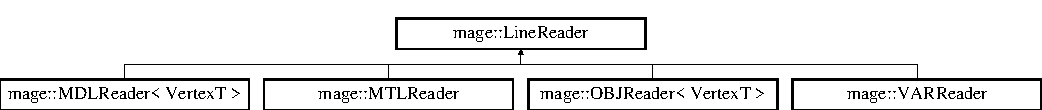
\includegraphics[height=1.458333cm]{classmage_1_1_line_reader}
\end{center}
\end{figure}
\subsection*{Public Member Functions}
\begin{DoxyCompactItemize}
\item 
virtual \hyperlink{classmage_1_1_line_reader_aa058c338d8256d7f7b775bf4f7052508}{$\sim$\+Line\+Reader} ()=default
\item 
\hyperlink{classmage_1_1_line_reader}{Line\+Reader} \& \hyperlink{classmage_1_1_line_reader_a2247078d0b5602f9a9a6b74019832faf}{operator=} (const \hyperlink{classmage_1_1_line_reader}{Line\+Reader} \&reader)=delete
\item 
\hyperlink{classmage_1_1_line_reader}{Line\+Reader} \& \hyperlink{classmage_1_1_line_reader_a45504c0ba4238eedf851cfb9df081a01}{operator=} (\hyperlink{classmage_1_1_line_reader}{Line\+Reader} \&\&reader)=delete
\item 
void \hyperlink{classmage_1_1_line_reader_a2df875468f06ec58c7aa1ff96157aeb0}{Read\+From\+File} (const wstring \&fname, const string \&delimiters=\hyperlink{namespacemage_ae247ad66af37a4b0d67ddca9404ca01a}{mage\+\_\+default\+\_\+delimiters})
\item 
void \hyperlink{classmage_1_1_line_reader_a1c21aba81c3873c7ed299ca978c4db74}{Read\+From\+Memory} (const char $\ast$input, const string \&delimiters=\hyperlink{namespacemage_ae247ad66af37a4b0d67ddca9404ca01a}{mage\+\_\+default\+\_\+delimiters})
\item 
const wstring \& \hyperlink{classmage_1_1_line_reader_a64a800d9fe9c242b9b14d034a7d604eb}{Get\+Filename} () const
\item 
const string \& \hyperlink{classmage_1_1_line_reader_a7de405beff27d5cc55bb93e1b1e9727a}{Get\+Delimiters} () const
\end{DoxyCompactItemize}
\subsection*{Protected Member Functions}
\begin{DoxyCompactItemize}
\item 
\hyperlink{classmage_1_1_line_reader_ab4a46321d7ea3ecda2d6390c78a7285b}{Line\+Reader} ()
\item 
\hyperlink{classmage_1_1_line_reader_ae4f871bebae110704b34c0bd88460639}{Line\+Reader} (const \hyperlink{classmage_1_1_line_reader}{Line\+Reader} \&reader)=delete
\item 
\hyperlink{classmage_1_1_line_reader_a0a9e80aabd15594f3e20bf7265e16c5e}{Line\+Reader} (\hyperlink{classmage_1_1_line_reader}{Line\+Reader} \&\&reader)=default
\item 
uint32\+\_\+t \hyperlink{classmage_1_1_line_reader_a55f35bf4989ad109524da146639870d6}{Get\+Current\+Line\+Number} () const
\item 
void \hyperlink{classmage_1_1_line_reader_a3a4b99bfef1e8a826d74a01bcc663fcb}{Read\+Line\+Remaining} ()
\item 
const char $\ast$ \hyperlink{classmage_1_1_line_reader_ad915c1a17549c7758c10f0b6db7e5611}{Read\+Chars} ()
\item 
const string \hyperlink{classmage_1_1_line_reader_a58a27b637574ce56ea17a575aa540675}{Read\+String} ()
\item 
const string \hyperlink{classmage_1_1_line_reader_ae9a7547d01b29c3237b198444d4f3aef}{Read\+Quoted\+String} ()
\item 
bool \hyperlink{classmage_1_1_line_reader_a86289c358afe9b3bc5c7789bb8a6af95}{Read\+Bool} ()
\item 
int8\+\_\+t \hyperlink{classmage_1_1_line_reader_a3b88ec3a8555d79b25c2a8818a26f124}{Read\+Int8} ()
\item 
uint8\+\_\+t \hyperlink{classmage_1_1_line_reader_a943ce0074c0861109f8b4ee10df8a221}{Read\+U\+Int8} ()
\item 
int16\+\_\+t \hyperlink{classmage_1_1_line_reader_a5ec3ccfcd1044f6be73c51082d2b57e3}{Read\+Int16} ()
\item 
uint16\+\_\+t \hyperlink{classmage_1_1_line_reader_a89f8d84257eae17db8c1e67d17f839f9}{Read\+U\+Int16} ()
\item 
int32\+\_\+t \hyperlink{classmage_1_1_line_reader_a45c66ad0b4676ef3fb2b5b08f04b509d}{Read\+Int32} ()
\item 
uint32\+\_\+t \hyperlink{classmage_1_1_line_reader_a82d14aede3b4ebff8cc54345dfba2c4b}{Read\+U\+Int32} ()
\item 
int64\+\_\+t \hyperlink{classmage_1_1_line_reader_af78e657c17cfff3bfc5fed42fbc47085}{Read\+Int64} ()
\item 
uint64\+\_\+t \hyperlink{classmage_1_1_line_reader_ac05624eb7a786bfc1391b22095da1e71}{Read\+U\+Int64} ()
\item 
float \hyperlink{classmage_1_1_line_reader_ae691928873b110dd273e72a47f2008cb}{Read\+Float} ()
\item 
double \hyperlink{classmage_1_1_line_reader_a17f11afdea4692395115c6bdfde03660}{Read\+Double} ()
\item 
const X\+M\+F\+L\+O\+A\+T2 \hyperlink{classmage_1_1_line_reader_ae33effd33fad465616e3acf8acdc408f}{Read\+Float2} ()
\item 
const X\+M\+F\+L\+O\+A\+T3 \hyperlink{classmage_1_1_line_reader_a7a605a7c2402051f1ca4fda1e543fc28}{Read\+Float3} ()
\item 
const X\+M\+F\+L\+O\+A\+T4 \hyperlink{classmage_1_1_line_reader_aaa21896aa756c3402cfeb207ef5f2029}{Read\+Float4} ()
\item 
bool \hyperlink{classmage_1_1_line_reader_a7eb54d60902d1fb7846ea5c566312a0f}{Has\+Chars} () const
\item 
bool \hyperlink{classmage_1_1_line_reader_a011b5a0d1bd2d157033e3bf7d7323aed}{Has\+String} () const
\item 
bool \hyperlink{classmage_1_1_line_reader_ac92de9a3d986c7031c902c9489cfaa5a}{Has\+Quoted\+String} () const
\item 
bool \hyperlink{classmage_1_1_line_reader_ac18069cc6bc399ce6ad8ad069a073c6c}{Has\+Bool} () const
\item 
bool \hyperlink{classmage_1_1_line_reader_a1eecd5324b2e212826c49e600cc46e1f}{Has\+Int8} () const
\item 
bool \hyperlink{classmage_1_1_line_reader_a7d9359c8a65005358564728be9091fa8}{Has\+U\+Int8} () const
\item 
bool \hyperlink{classmage_1_1_line_reader_a36b83e0adfa48d9226ae59c23df8f44a}{Has\+Int16} () const
\item 
bool \hyperlink{classmage_1_1_line_reader_a15c7c3336330649062556e5b318af510}{Has\+U\+Int16} () const
\item 
bool \hyperlink{classmage_1_1_line_reader_af8402b39637e27877eac2909604bbf89}{Has\+Int32} () const
\item 
bool \hyperlink{classmage_1_1_line_reader_a56f82d5562d0254ec59871a3bb7ad837}{Has\+U\+Int32} () const
\item 
bool \hyperlink{classmage_1_1_line_reader_a3a7883e24fb3108a79ecda4eaac983f2}{Has\+Int64} () const
\item 
bool \hyperlink{classmage_1_1_line_reader_ad311b6edbfc68c01997f90cd1db5d95e}{Has\+U\+Int64} () const
\item 
bool \hyperlink{classmage_1_1_line_reader_ade0b6d83fc8cd6a4c64b2c97b9ff0bda}{Has\+Float} () const
\item 
bool \hyperlink{classmage_1_1_line_reader_ad6eb5eaf990bba426498d11c53bd31cd}{Has\+Double} () const
\end{DoxyCompactItemize}
\subsection*{Protected Attributes}
\begin{DoxyCompactItemize}
\item 
char $\ast$ \hyperlink{classmage_1_1_line_reader_a2f1cfe313dc89741386178e63a6b8b0c}{m\+\_\+context}
\end{DoxyCompactItemize}
\subsection*{Private Member Functions}
\begin{DoxyCompactItemize}
\item 
virtual void \hyperlink{classmage_1_1_line_reader_a4de135cfb0434be786cfcfd7959031ef}{Preprocess} ()
\item 
virtual void \hyperlink{classmage_1_1_line_reader_acfb2f7279ec77d070a86d7db812d4745}{Read\+Line} (char $\ast$line)=0
\item 
virtual void \hyperlink{classmage_1_1_line_reader_adfde21013140a1058d3dd567204abfb5}{Postprocess} ()
\end{DoxyCompactItemize}
\subsection*{Private Attributes}
\begin{DoxyCompactItemize}
\item 
\hyperlink{namespacemage_a679c1b707dee02c7eab8d706ef14411a}{Unique\+File\+Stream} \hyperlink{classmage_1_1_line_reader_a510ff5355c6d26d7c29dc692ef18a3e2}{m\+\_\+file\+\_\+stream}
\item 
wstring \hyperlink{classmage_1_1_line_reader_ad6f55ba12fc610ab2fc1c26a48d12321}{m\+\_\+fname}
\item 
string \hyperlink{classmage_1_1_line_reader_a6de3398ac59fdd98f8c40cff6f5c1075}{m\+\_\+delimiters}
\item 
uint32\+\_\+t \hyperlink{classmage_1_1_line_reader_ada0b4ec5817b96c6b1bb43bd2573f8ba}{m\+\_\+line\+\_\+number}
\end{DoxyCompactItemize}


\subsection{Detailed Description}
A class of line readers for reading (non-\/binary) text files line by line. 

\subsection{Constructor \& Destructor Documentation}
\hypertarget{classmage_1_1_line_reader_aa058c338d8256d7f7b775bf4f7052508}{}\label{classmage_1_1_line_reader_aa058c338d8256d7f7b775bf4f7052508} 
\index{mage\+::\+Line\+Reader@{mage\+::\+Line\+Reader}!````~Line\+Reader@{$\sim$\+Line\+Reader}}
\index{````~Line\+Reader@{$\sim$\+Line\+Reader}!mage\+::\+Line\+Reader@{mage\+::\+Line\+Reader}}
\subsubsection{\texorpdfstring{$\sim$\+Line\+Reader()}{~LineReader()}}
{\footnotesize\ttfamily virtual mage\+::\+Line\+Reader\+::$\sim$\+Line\+Reader (\begin{DoxyParamCaption}{ }\end{DoxyParamCaption})\hspace{0.3cm}{\ttfamily [virtual]}, {\ttfamily [default]}}

Destructs this line reader. \hypertarget{classmage_1_1_line_reader_ab4a46321d7ea3ecda2d6390c78a7285b}{}\label{classmage_1_1_line_reader_ab4a46321d7ea3ecda2d6390c78a7285b} 
\index{mage\+::\+Line\+Reader@{mage\+::\+Line\+Reader}!Line\+Reader@{Line\+Reader}}
\index{Line\+Reader@{Line\+Reader}!mage\+::\+Line\+Reader@{mage\+::\+Line\+Reader}}
\subsubsection{\texorpdfstring{Line\+Reader()}{LineReader()}\hspace{0.1cm}{\footnotesize\ttfamily [1/3]}}
{\footnotesize\ttfamily mage\+::\+Line\+Reader\+::\+Line\+Reader (\begin{DoxyParamCaption}{ }\end{DoxyParamCaption})\hspace{0.3cm}{\ttfamily [protected]}}

Constructs a line reader. \hypertarget{classmage_1_1_line_reader_ae4f871bebae110704b34c0bd88460639}{}\label{classmage_1_1_line_reader_ae4f871bebae110704b34c0bd88460639} 
\index{mage\+::\+Line\+Reader@{mage\+::\+Line\+Reader}!Line\+Reader@{Line\+Reader}}
\index{Line\+Reader@{Line\+Reader}!mage\+::\+Line\+Reader@{mage\+::\+Line\+Reader}}
\subsubsection{\texorpdfstring{Line\+Reader()}{LineReader()}\hspace{0.1cm}{\footnotesize\ttfamily [2/3]}}
{\footnotesize\ttfamily mage\+::\+Line\+Reader\+::\+Line\+Reader (\begin{DoxyParamCaption}\item[{const \hyperlink{classmage_1_1_line_reader}{Line\+Reader} \&}]{reader }\end{DoxyParamCaption})\hspace{0.3cm}{\ttfamily [protected]}, {\ttfamily [delete]}}

Constructs a line reader from the given line reader.


\begin{DoxyParams}[1]{Parameters}
\mbox{\tt in}  & {\em reader} & A reference to the line reader to copy. \\
\hline
\end{DoxyParams}
\hypertarget{classmage_1_1_line_reader_a0a9e80aabd15594f3e20bf7265e16c5e}{}\label{classmage_1_1_line_reader_a0a9e80aabd15594f3e20bf7265e16c5e} 
\index{mage\+::\+Line\+Reader@{mage\+::\+Line\+Reader}!Line\+Reader@{Line\+Reader}}
\index{Line\+Reader@{Line\+Reader}!mage\+::\+Line\+Reader@{mage\+::\+Line\+Reader}}
\subsubsection{\texorpdfstring{Line\+Reader()}{LineReader()}\hspace{0.1cm}{\footnotesize\ttfamily [3/3]}}
{\footnotesize\ttfamily mage\+::\+Line\+Reader\+::\+Line\+Reader (\begin{DoxyParamCaption}\item[{\hyperlink{classmage_1_1_line_reader}{Line\+Reader} \&\&}]{reader }\end{DoxyParamCaption})\hspace{0.3cm}{\ttfamily [protected]}, {\ttfamily [default]}}

Constructs a line reader by moving the given line reader.


\begin{DoxyParams}[1]{Parameters}
\mbox{\tt in}  & {\em reader} & A reference to the line reader to move. \\
\hline
\end{DoxyParams}


\subsection{Member Function Documentation}
\hypertarget{classmage_1_1_line_reader_a55f35bf4989ad109524da146639870d6}{}\label{classmage_1_1_line_reader_a55f35bf4989ad109524da146639870d6} 
\index{mage\+::\+Line\+Reader@{mage\+::\+Line\+Reader}!Get\+Current\+Line\+Number@{Get\+Current\+Line\+Number}}
\index{Get\+Current\+Line\+Number@{Get\+Current\+Line\+Number}!mage\+::\+Line\+Reader@{mage\+::\+Line\+Reader}}
\subsubsection{\texorpdfstring{Get\+Current\+Line\+Number()}{GetCurrentLineNumber()}}
{\footnotesize\ttfamily uint32\+\_\+t mage\+::\+Line\+Reader\+::\+Get\+Current\+Line\+Number (\begin{DoxyParamCaption}{ }\end{DoxyParamCaption}) const\hspace{0.3cm}{\ttfamily [protected]}}

Returns the current line number of this line reader.

\begin{DoxyReturn}{Returns}
The current line number of this line reader. 
\end{DoxyReturn}
\hypertarget{classmage_1_1_line_reader_a7de405beff27d5cc55bb93e1b1e9727a}{}\label{classmage_1_1_line_reader_a7de405beff27d5cc55bb93e1b1e9727a} 
\index{mage\+::\+Line\+Reader@{mage\+::\+Line\+Reader}!Get\+Delimiters@{Get\+Delimiters}}
\index{Get\+Delimiters@{Get\+Delimiters}!mage\+::\+Line\+Reader@{mage\+::\+Line\+Reader}}
\subsubsection{\texorpdfstring{Get\+Delimiters()}{GetDelimiters()}}
{\footnotesize\ttfamily const string\& mage\+::\+Line\+Reader\+::\+Get\+Delimiters (\begin{DoxyParamCaption}{ }\end{DoxyParamCaption}) const}

Returns the current delimiters of this line reader.

\begin{DoxyReturn}{Returns}
A reference to the current delimiters of this line reader. 
\end{DoxyReturn}
\hypertarget{classmage_1_1_line_reader_a64a800d9fe9c242b9b14d034a7d604eb}{}\label{classmage_1_1_line_reader_a64a800d9fe9c242b9b14d034a7d604eb} 
\index{mage\+::\+Line\+Reader@{mage\+::\+Line\+Reader}!Get\+Filename@{Get\+Filename}}
\index{Get\+Filename@{Get\+Filename}!mage\+::\+Line\+Reader@{mage\+::\+Line\+Reader}}
\subsubsection{\texorpdfstring{Get\+Filename()}{GetFilename()}}
{\footnotesize\ttfamily const wstring\& mage\+::\+Line\+Reader\+::\+Get\+Filename (\begin{DoxyParamCaption}{ }\end{DoxyParamCaption}) const}

Returns the current filename of this line reader.

\begin{DoxyReturn}{Returns}
A reference to the current filename of this line reader. 
\end{DoxyReturn}
\hypertarget{classmage_1_1_line_reader_ac18069cc6bc399ce6ad8ad069a073c6c}{}\label{classmage_1_1_line_reader_ac18069cc6bc399ce6ad8ad069a073c6c} 
\index{mage\+::\+Line\+Reader@{mage\+::\+Line\+Reader}!Has\+Bool@{Has\+Bool}}
\index{Has\+Bool@{Has\+Bool}!mage\+::\+Line\+Reader@{mage\+::\+Line\+Reader}}
\subsubsection{\texorpdfstring{Has\+Bool()}{HasBool()}}
{\footnotesize\ttfamily bool mage\+::\+Line\+Reader\+::\+Has\+Bool (\begin{DoxyParamCaption}{ }\end{DoxyParamCaption}) const\hspace{0.3cm}{\ttfamily [protected]}}

Checks whether the next token of this line reader is a {\ttfamily bool}.

\begin{DoxyReturn}{Returns}
{\ttfamily true} if the next token of this line reader is a {\ttfamily bool}. {\ttfamily false} otherwise. 
\end{DoxyReturn}
\hypertarget{classmage_1_1_line_reader_a7eb54d60902d1fb7846ea5c566312a0f}{}\label{classmage_1_1_line_reader_a7eb54d60902d1fb7846ea5c566312a0f} 
\index{mage\+::\+Line\+Reader@{mage\+::\+Line\+Reader}!Has\+Chars@{Has\+Chars}}
\index{Has\+Chars@{Has\+Chars}!mage\+::\+Line\+Reader@{mage\+::\+Line\+Reader}}
\subsubsection{\texorpdfstring{Has\+Chars()}{HasChars()}}
{\footnotesize\ttfamily bool mage\+::\+Line\+Reader\+::\+Has\+Chars (\begin{DoxyParamCaption}{ }\end{DoxyParamCaption}) const\hspace{0.3cm}{\ttfamily [protected]}}

Checks whether this line reader has a next token.

\begin{DoxyReturn}{Returns}
{\ttfamily true} if this line reader has a next token. {\ttfamily false} otherwise. 
\end{DoxyReturn}
\hypertarget{classmage_1_1_line_reader_ad6eb5eaf990bba426498d11c53bd31cd}{}\label{classmage_1_1_line_reader_ad6eb5eaf990bba426498d11c53bd31cd} 
\index{mage\+::\+Line\+Reader@{mage\+::\+Line\+Reader}!Has\+Double@{Has\+Double}}
\index{Has\+Double@{Has\+Double}!mage\+::\+Line\+Reader@{mage\+::\+Line\+Reader}}
\subsubsection{\texorpdfstring{Has\+Double()}{HasDouble()}}
{\footnotesize\ttfamily bool mage\+::\+Line\+Reader\+::\+Has\+Double (\begin{DoxyParamCaption}{ }\end{DoxyParamCaption}) const\hspace{0.3cm}{\ttfamily [protected]}}

Checks whether the next token of this line reader is a {\ttfamily double}.

\begin{DoxyReturn}{Returns}
{\ttfamily true} if the next token of this line reader is a {\ttfamily double}. {\ttfamily false} otherwise. 
\end{DoxyReturn}
\hypertarget{classmage_1_1_line_reader_ade0b6d83fc8cd6a4c64b2c97b9ff0bda}{}\label{classmage_1_1_line_reader_ade0b6d83fc8cd6a4c64b2c97b9ff0bda} 
\index{mage\+::\+Line\+Reader@{mage\+::\+Line\+Reader}!Has\+Float@{Has\+Float}}
\index{Has\+Float@{Has\+Float}!mage\+::\+Line\+Reader@{mage\+::\+Line\+Reader}}
\subsubsection{\texorpdfstring{Has\+Float()}{HasFloat()}}
{\footnotesize\ttfamily bool mage\+::\+Line\+Reader\+::\+Has\+Float (\begin{DoxyParamCaption}{ }\end{DoxyParamCaption}) const\hspace{0.3cm}{\ttfamily [protected]}}

Checks whether the next token of this line reader is a {\ttfamily float}.

\begin{DoxyReturn}{Returns}
{\ttfamily true} if the next token of this line reader is a {\ttfamily float}. {\ttfamily false} otherwise. 
\end{DoxyReturn}
\hypertarget{classmage_1_1_line_reader_a36b83e0adfa48d9226ae59c23df8f44a}{}\label{classmage_1_1_line_reader_a36b83e0adfa48d9226ae59c23df8f44a} 
\index{mage\+::\+Line\+Reader@{mage\+::\+Line\+Reader}!Has\+Int16@{Has\+Int16}}
\index{Has\+Int16@{Has\+Int16}!mage\+::\+Line\+Reader@{mage\+::\+Line\+Reader}}
\subsubsection{\texorpdfstring{Has\+Int16()}{HasInt16()}}
{\footnotesize\ttfamily bool mage\+::\+Line\+Reader\+::\+Has\+Int16 (\begin{DoxyParamCaption}{ }\end{DoxyParamCaption}) const\hspace{0.3cm}{\ttfamily [protected]}}

Checks whether the next token of this line reader is a {\ttfamily int16\+\_\+t}.

\begin{DoxyReturn}{Returns}
{\ttfamily true} if the next token of this line reader is a {\ttfamily int16\+\_\+t}. {\ttfamily false} otherwise. 
\end{DoxyReturn}
\hypertarget{classmage_1_1_line_reader_af8402b39637e27877eac2909604bbf89}{}\label{classmage_1_1_line_reader_af8402b39637e27877eac2909604bbf89} 
\index{mage\+::\+Line\+Reader@{mage\+::\+Line\+Reader}!Has\+Int32@{Has\+Int32}}
\index{Has\+Int32@{Has\+Int32}!mage\+::\+Line\+Reader@{mage\+::\+Line\+Reader}}
\subsubsection{\texorpdfstring{Has\+Int32()}{HasInt32()}}
{\footnotesize\ttfamily bool mage\+::\+Line\+Reader\+::\+Has\+Int32 (\begin{DoxyParamCaption}{ }\end{DoxyParamCaption}) const\hspace{0.3cm}{\ttfamily [protected]}}

Checks whether the next token of this line reader is a {\ttfamily int32\+\_\+t}.

\begin{DoxyReturn}{Returns}
{\ttfamily true} if the next token of this line reader is a {\ttfamily int32\+\_\+t}. {\ttfamily false} otherwise. 
\end{DoxyReturn}
\hypertarget{classmage_1_1_line_reader_a3a7883e24fb3108a79ecda4eaac983f2}{}\label{classmage_1_1_line_reader_a3a7883e24fb3108a79ecda4eaac983f2} 
\index{mage\+::\+Line\+Reader@{mage\+::\+Line\+Reader}!Has\+Int64@{Has\+Int64}}
\index{Has\+Int64@{Has\+Int64}!mage\+::\+Line\+Reader@{mage\+::\+Line\+Reader}}
\subsubsection{\texorpdfstring{Has\+Int64()}{HasInt64()}}
{\footnotesize\ttfamily bool mage\+::\+Line\+Reader\+::\+Has\+Int64 (\begin{DoxyParamCaption}{ }\end{DoxyParamCaption}) const\hspace{0.3cm}{\ttfamily [protected]}}

Checks whether the next token of this line reader is a {\ttfamily int64\+\_\+t}.

\begin{DoxyReturn}{Returns}
{\ttfamily true} if the next token of this line reader is a {\ttfamily int64\+\_\+t}. {\ttfamily false} otherwise. 
\end{DoxyReturn}
\hypertarget{classmage_1_1_line_reader_a1eecd5324b2e212826c49e600cc46e1f}{}\label{classmage_1_1_line_reader_a1eecd5324b2e212826c49e600cc46e1f} 
\index{mage\+::\+Line\+Reader@{mage\+::\+Line\+Reader}!Has\+Int8@{Has\+Int8}}
\index{Has\+Int8@{Has\+Int8}!mage\+::\+Line\+Reader@{mage\+::\+Line\+Reader}}
\subsubsection{\texorpdfstring{Has\+Int8()}{HasInt8()}}
{\footnotesize\ttfamily bool mage\+::\+Line\+Reader\+::\+Has\+Int8 (\begin{DoxyParamCaption}{ }\end{DoxyParamCaption}) const\hspace{0.3cm}{\ttfamily [protected]}}

Checks whether the next token of this line reader is a {\ttfamily int8\+\_\+t}.

\begin{DoxyReturn}{Returns}
{\ttfamily true} if the next token of this line reader is a {\ttfamily int8\+\_\+t}. {\ttfamily false} otherwise. 
\end{DoxyReturn}
\hypertarget{classmage_1_1_line_reader_ac92de9a3d986c7031c902c9489cfaa5a}{}\label{classmage_1_1_line_reader_ac92de9a3d986c7031c902c9489cfaa5a} 
\index{mage\+::\+Line\+Reader@{mage\+::\+Line\+Reader}!Has\+Quoted\+String@{Has\+Quoted\+String}}
\index{Has\+Quoted\+String@{Has\+Quoted\+String}!mage\+::\+Line\+Reader@{mage\+::\+Line\+Reader}}
\subsubsection{\texorpdfstring{Has\+Quoted\+String()}{HasQuotedString()}}
{\footnotesize\ttfamily bool mage\+::\+Line\+Reader\+::\+Has\+Quoted\+String (\begin{DoxyParamCaption}{ }\end{DoxyParamCaption}) const\hspace{0.3cm}{\ttfamily [protected]}}

Checks whether the next token of this line reader is a quoted string.

\begin{DoxyReturn}{Returns}
{\ttfamily true} if the next token of this line reader is a quoted string. {\ttfamily false} otherwise. 
\end{DoxyReturn}
\hypertarget{classmage_1_1_line_reader_a011b5a0d1bd2d157033e3bf7d7323aed}{}\label{classmage_1_1_line_reader_a011b5a0d1bd2d157033e3bf7d7323aed} 
\index{mage\+::\+Line\+Reader@{mage\+::\+Line\+Reader}!Has\+String@{Has\+String}}
\index{Has\+String@{Has\+String}!mage\+::\+Line\+Reader@{mage\+::\+Line\+Reader}}
\subsubsection{\texorpdfstring{Has\+String()}{HasString()}}
{\footnotesize\ttfamily bool mage\+::\+Line\+Reader\+::\+Has\+String (\begin{DoxyParamCaption}{ }\end{DoxyParamCaption}) const\hspace{0.3cm}{\ttfamily [protected]}}

Checks whether the next token of this line reader is a string.

\begin{DoxyReturn}{Returns}
{\ttfamily true} if the next token of this line reader is a string. {\ttfamily false} otherwise. 
\end{DoxyReturn}
\hypertarget{classmage_1_1_line_reader_a15c7c3336330649062556e5b318af510}{}\label{classmage_1_1_line_reader_a15c7c3336330649062556e5b318af510} 
\index{mage\+::\+Line\+Reader@{mage\+::\+Line\+Reader}!Has\+U\+Int16@{Has\+U\+Int16}}
\index{Has\+U\+Int16@{Has\+U\+Int16}!mage\+::\+Line\+Reader@{mage\+::\+Line\+Reader}}
\subsubsection{\texorpdfstring{Has\+U\+Int16()}{HasUInt16()}}
{\footnotesize\ttfamily bool mage\+::\+Line\+Reader\+::\+Has\+U\+Int16 (\begin{DoxyParamCaption}{ }\end{DoxyParamCaption}) const\hspace{0.3cm}{\ttfamily [protected]}}

Checks whether the next token of this line reader is a {\ttfamily uint16\+\_\+t}.

\begin{DoxyReturn}{Returns}
{\ttfamily true} if the next token of this line reader is a {\ttfamily uint16\+\_\+t}. {\ttfamily false} otherwise. 
\end{DoxyReturn}
\hypertarget{classmage_1_1_line_reader_a56f82d5562d0254ec59871a3bb7ad837}{}\label{classmage_1_1_line_reader_a56f82d5562d0254ec59871a3bb7ad837} 
\index{mage\+::\+Line\+Reader@{mage\+::\+Line\+Reader}!Has\+U\+Int32@{Has\+U\+Int32}}
\index{Has\+U\+Int32@{Has\+U\+Int32}!mage\+::\+Line\+Reader@{mage\+::\+Line\+Reader}}
\subsubsection{\texorpdfstring{Has\+U\+Int32()}{HasUInt32()}}
{\footnotesize\ttfamily bool mage\+::\+Line\+Reader\+::\+Has\+U\+Int32 (\begin{DoxyParamCaption}{ }\end{DoxyParamCaption}) const\hspace{0.3cm}{\ttfamily [protected]}}

Checks whether the next token of this line reader is a {\ttfamily uint32\+\_\+t}.

\begin{DoxyReturn}{Returns}
{\ttfamily true} if the next token of this line reader is a {\ttfamily uint32\+\_\+t}. {\ttfamily false} otherwise. 
\end{DoxyReturn}
\hypertarget{classmage_1_1_line_reader_ad311b6edbfc68c01997f90cd1db5d95e}{}\label{classmage_1_1_line_reader_ad311b6edbfc68c01997f90cd1db5d95e} 
\index{mage\+::\+Line\+Reader@{mage\+::\+Line\+Reader}!Has\+U\+Int64@{Has\+U\+Int64}}
\index{Has\+U\+Int64@{Has\+U\+Int64}!mage\+::\+Line\+Reader@{mage\+::\+Line\+Reader}}
\subsubsection{\texorpdfstring{Has\+U\+Int64()}{HasUInt64()}}
{\footnotesize\ttfamily bool mage\+::\+Line\+Reader\+::\+Has\+U\+Int64 (\begin{DoxyParamCaption}{ }\end{DoxyParamCaption}) const\hspace{0.3cm}{\ttfamily [protected]}}

Checks whether the next token of this line reader is a {\ttfamily uint64\+\_\+t}.

\begin{DoxyReturn}{Returns}
{\ttfamily true} if the next token of this line reader is a {\ttfamily uint64\+\_\+t}. {\ttfamily false} otherwise. 
\end{DoxyReturn}
\hypertarget{classmage_1_1_line_reader_a7d9359c8a65005358564728be9091fa8}{}\label{classmage_1_1_line_reader_a7d9359c8a65005358564728be9091fa8} 
\index{mage\+::\+Line\+Reader@{mage\+::\+Line\+Reader}!Has\+U\+Int8@{Has\+U\+Int8}}
\index{Has\+U\+Int8@{Has\+U\+Int8}!mage\+::\+Line\+Reader@{mage\+::\+Line\+Reader}}
\subsubsection{\texorpdfstring{Has\+U\+Int8()}{HasUInt8()}}
{\footnotesize\ttfamily bool mage\+::\+Line\+Reader\+::\+Has\+U\+Int8 (\begin{DoxyParamCaption}{ }\end{DoxyParamCaption}) const\hspace{0.3cm}{\ttfamily [protected]}}

Checks whether the next token of this line reader is a {\ttfamily uint8\+\_\+t}.

\begin{DoxyReturn}{Returns}
{\ttfamily true} if the next token of this line reader is a {\ttfamily uint8\+\_\+t}. {\ttfamily false} otherwise. 
\end{DoxyReturn}
\hypertarget{classmage_1_1_line_reader_a2247078d0b5602f9a9a6b74019832faf}{}\label{classmage_1_1_line_reader_a2247078d0b5602f9a9a6b74019832faf} 
\index{mage\+::\+Line\+Reader@{mage\+::\+Line\+Reader}!operator=@{operator=}}
\index{operator=@{operator=}!mage\+::\+Line\+Reader@{mage\+::\+Line\+Reader}}
\subsubsection{\texorpdfstring{operator=()}{operator=()}\hspace{0.1cm}{\footnotesize\ttfamily [1/2]}}
{\footnotesize\ttfamily \hyperlink{classmage_1_1_line_reader}{Line\+Reader}\& mage\+::\+Line\+Reader\+::operator= (\begin{DoxyParamCaption}\item[{const \hyperlink{classmage_1_1_line_reader}{Line\+Reader} \&}]{reader }\end{DoxyParamCaption})\hspace{0.3cm}{\ttfamily [delete]}}

Copies the given line reader to this line reader.


\begin{DoxyParams}[1]{Parameters}
\mbox{\tt in}  & {\em reader} & A reference to a line reader to copy. \\
\hline
\end{DoxyParams}
\begin{DoxyReturn}{Returns}
A reference to the copy of the given line reader (i.\+e. this line reader). 
\end{DoxyReturn}
\hypertarget{classmage_1_1_line_reader_a45504c0ba4238eedf851cfb9df081a01}{}\label{classmage_1_1_line_reader_a45504c0ba4238eedf851cfb9df081a01} 
\index{mage\+::\+Line\+Reader@{mage\+::\+Line\+Reader}!operator=@{operator=}}
\index{operator=@{operator=}!mage\+::\+Line\+Reader@{mage\+::\+Line\+Reader}}
\subsubsection{\texorpdfstring{operator=()}{operator=()}\hspace{0.1cm}{\footnotesize\ttfamily [2/2]}}
{\footnotesize\ttfamily \hyperlink{classmage_1_1_line_reader}{Line\+Reader}\& mage\+::\+Line\+Reader\+::operator= (\begin{DoxyParamCaption}\item[{\hyperlink{classmage_1_1_line_reader}{Line\+Reader} \&\&}]{reader }\end{DoxyParamCaption})\hspace{0.3cm}{\ttfamily [delete]}}

Moves the given line reader to this line reader.


\begin{DoxyParams}[1]{Parameters}
\mbox{\tt in}  & {\em reader} & A reference to a line reader to move. \\
\hline
\end{DoxyParams}
\begin{DoxyReturn}{Returns}
A reference to the moved line reader (i.\+e. this line reader). 
\end{DoxyReturn}
\hypertarget{classmage_1_1_line_reader_adfde21013140a1058d3dd567204abfb5}{}\label{classmage_1_1_line_reader_adfde21013140a1058d3dd567204abfb5} 
\index{mage\+::\+Line\+Reader@{mage\+::\+Line\+Reader}!Postprocess@{Postprocess}}
\index{Postprocess@{Postprocess}!mage\+::\+Line\+Reader@{mage\+::\+Line\+Reader}}
\subsubsection{\texorpdfstring{Postprocess()}{Postprocess()}}
{\footnotesize\ttfamily virtual void mage\+::\+Line\+Reader\+::\+Postprocess (\begin{DoxyParamCaption}{ }\end{DoxyParamCaption})\hspace{0.3cm}{\ttfamily [private]}, {\ttfamily [virtual]}}

Post-\/processes after reading the current file of this line reader.


\begin{DoxyExceptions}{Exceptions}
{\em \hyperlink{structmage_1_1_formatted_exception}{Formatted\+Exception}} & Failed to finish post-\/processing successfully. \\
\hline
\end{DoxyExceptions}


Reimplemented in \hyperlink{classmage_1_1_o_b_j_reader_a248977c8300575ed2bab04df26197919}{mage\+::\+O\+B\+J\+Reader$<$ Vertex\+T $>$}.

\hypertarget{classmage_1_1_line_reader_a4de135cfb0434be786cfcfd7959031ef}{}\label{classmage_1_1_line_reader_a4de135cfb0434be786cfcfd7959031ef} 
\index{mage\+::\+Line\+Reader@{mage\+::\+Line\+Reader}!Preprocess@{Preprocess}}
\index{Preprocess@{Preprocess}!mage\+::\+Line\+Reader@{mage\+::\+Line\+Reader}}
\subsubsection{\texorpdfstring{Preprocess()}{Preprocess()}}
{\footnotesize\ttfamily virtual void mage\+::\+Line\+Reader\+::\+Preprocess (\begin{DoxyParamCaption}{ }\end{DoxyParamCaption})\hspace{0.3cm}{\ttfamily [private]}, {\ttfamily [virtual]}}

Pre-\/processes before reading the current file of this line reader.


\begin{DoxyExceptions}{Exceptions}
{\em \hyperlink{structmage_1_1_formatted_exception}{Formatted\+Exception}} & Failed to finish the pre-\/processing successfully. \\
\hline
\end{DoxyExceptions}


Reimplemented in \hyperlink{classmage_1_1_o_b_j_reader_ae3a3ad3b50f1dd8dffe3109fc7dc2937}{mage\+::\+O\+B\+J\+Reader$<$ Vertex\+T $>$}, and \hyperlink{classmage_1_1_m_d_l_reader_a8b99fb3bdea5e9dae156b135c160c22d}{mage\+::\+M\+D\+L\+Reader$<$ Vertex\+T $>$}.

\hypertarget{classmage_1_1_line_reader_a86289c358afe9b3bc5c7789bb8a6af95}{}\label{classmage_1_1_line_reader_a86289c358afe9b3bc5c7789bb8a6af95} 
\index{mage\+::\+Line\+Reader@{mage\+::\+Line\+Reader}!Read\+Bool@{Read\+Bool}}
\index{Read\+Bool@{Read\+Bool}!mage\+::\+Line\+Reader@{mage\+::\+Line\+Reader}}
\subsubsection{\texorpdfstring{Read\+Bool()}{ReadBool()}}
{\footnotesize\ttfamily bool mage\+::\+Line\+Reader\+::\+Read\+Bool (\begin{DoxyParamCaption}{ }\end{DoxyParamCaption})\hspace{0.3cm}{\ttfamily [protected]}}

Reads and converts the next token of this line reader to a {\ttfamily bool}.

\begin{DoxyReturn}{Returns}
The {\ttfamily bool} represented by the next token of this line reader. 
\end{DoxyReturn}

\begin{DoxyExceptions}{Exceptions}
{\em \hyperlink{structmage_1_1_formatted_exception}{Formatted\+Exception}} & There is no next token or the next token does not represent a {\ttfamily bool}. \\
\hline
\end{DoxyExceptions}
\hypertarget{classmage_1_1_line_reader_ad915c1a17549c7758c10f0b6db7e5611}{}\label{classmage_1_1_line_reader_ad915c1a17549c7758c10f0b6db7e5611} 
\index{mage\+::\+Line\+Reader@{mage\+::\+Line\+Reader}!Read\+Chars@{Read\+Chars}}
\index{Read\+Chars@{Read\+Chars}!mage\+::\+Line\+Reader@{mage\+::\+Line\+Reader}}
\subsubsection{\texorpdfstring{Read\+Chars()}{ReadChars()}}
{\footnotesize\ttfamily const char $\ast$ mage\+::\+Line\+Reader\+::\+Read\+Chars (\begin{DoxyParamCaption}{ }\end{DoxyParamCaption})\hspace{0.3cm}{\ttfamily [protected]}}

Reads and converts the next token of this line reader to a string.

\begin{DoxyReturn}{Returns}
The string represented by the next token of this line reader. 
\end{DoxyReturn}

\begin{DoxyExceptions}{Exceptions}
{\em \hyperlink{structmage_1_1_formatted_exception}{Formatted\+Exception}} & There is no next token. \\
\hline
\end{DoxyExceptions}
\hypertarget{classmage_1_1_line_reader_a17f11afdea4692395115c6bdfde03660}{}\label{classmage_1_1_line_reader_a17f11afdea4692395115c6bdfde03660} 
\index{mage\+::\+Line\+Reader@{mage\+::\+Line\+Reader}!Read\+Double@{Read\+Double}}
\index{Read\+Double@{Read\+Double}!mage\+::\+Line\+Reader@{mage\+::\+Line\+Reader}}
\subsubsection{\texorpdfstring{Read\+Double()}{ReadDouble()}}
{\footnotesize\ttfamily double mage\+::\+Line\+Reader\+::\+Read\+Double (\begin{DoxyParamCaption}{ }\end{DoxyParamCaption})\hspace{0.3cm}{\ttfamily [protected]}}

Reads and converts the next token of this line reader to a {\ttfamily double}.

\begin{DoxyReturn}{Returns}
The {\ttfamily double} represented by the next token of this line reader. 
\end{DoxyReturn}

\begin{DoxyExceptions}{Exceptions}
{\em \hyperlink{structmage_1_1_formatted_exception}{Formatted\+Exception}} & There is no next token or the next token does not represent a {\ttfamily double}. \\
\hline
\end{DoxyExceptions}
\hypertarget{classmage_1_1_line_reader_ae691928873b110dd273e72a47f2008cb}{}\label{classmage_1_1_line_reader_ae691928873b110dd273e72a47f2008cb} 
\index{mage\+::\+Line\+Reader@{mage\+::\+Line\+Reader}!Read\+Float@{Read\+Float}}
\index{Read\+Float@{Read\+Float}!mage\+::\+Line\+Reader@{mage\+::\+Line\+Reader}}
\subsubsection{\texorpdfstring{Read\+Float()}{ReadFloat()}}
{\footnotesize\ttfamily float mage\+::\+Line\+Reader\+::\+Read\+Float (\begin{DoxyParamCaption}{ }\end{DoxyParamCaption})\hspace{0.3cm}{\ttfamily [protected]}}

Reads and converts the next token of this line reader to a {\ttfamily float}.

\begin{DoxyReturn}{Returns}
The {\ttfamily float} represented by the next token of this line reader. 
\end{DoxyReturn}

\begin{DoxyExceptions}{Exceptions}
{\em \hyperlink{structmage_1_1_formatted_exception}{Formatted\+Exception}} & There is no next token or the next token does not represent a {\ttfamily float}. \\
\hline
\end{DoxyExceptions}
\hypertarget{classmage_1_1_line_reader_ae33effd33fad465616e3acf8acdc408f}{}\label{classmage_1_1_line_reader_ae33effd33fad465616e3acf8acdc408f} 
\index{mage\+::\+Line\+Reader@{mage\+::\+Line\+Reader}!Read\+Float2@{Read\+Float2}}
\index{Read\+Float2@{Read\+Float2}!mage\+::\+Line\+Reader@{mage\+::\+Line\+Reader}}
\subsubsection{\texorpdfstring{Read\+Float2()}{ReadFloat2()}}
{\footnotesize\ttfamily const X\+M\+F\+L\+O\+A\+T2 mage\+::\+Line\+Reader\+::\+Read\+Float2 (\begin{DoxyParamCaption}{ }\end{DoxyParamCaption})\hspace{0.3cm}{\ttfamily [protected]}}

Reads and converts the next token of this line reader to a {\ttfamily X\+M\+F\+L\+O\+A\+T2}.

\begin{DoxyReturn}{Returns}
The {\ttfamily X\+M\+F\+L\+O\+A\+T2} represented by the next token of this line reader. 
\end{DoxyReturn}

\begin{DoxyExceptions}{Exceptions}
{\em \hyperlink{structmage_1_1_formatted_exception}{Formatted\+Exception}} & There is no next token or the next token does not represent a {\ttfamily X\+M\+F\+L\+O\+A\+T2}. \\
\hline
\end{DoxyExceptions}
\hypertarget{classmage_1_1_line_reader_a7a605a7c2402051f1ca4fda1e543fc28}{}\label{classmage_1_1_line_reader_a7a605a7c2402051f1ca4fda1e543fc28} 
\index{mage\+::\+Line\+Reader@{mage\+::\+Line\+Reader}!Read\+Float3@{Read\+Float3}}
\index{Read\+Float3@{Read\+Float3}!mage\+::\+Line\+Reader@{mage\+::\+Line\+Reader}}
\subsubsection{\texorpdfstring{Read\+Float3()}{ReadFloat3()}}
{\footnotesize\ttfamily const X\+M\+F\+L\+O\+A\+T3 mage\+::\+Line\+Reader\+::\+Read\+Float3 (\begin{DoxyParamCaption}{ }\end{DoxyParamCaption})\hspace{0.3cm}{\ttfamily [protected]}}

Reads and converts the next token of this line reader to a {\ttfamily X\+M\+F\+L\+O\+A\+T3}.

\begin{DoxyReturn}{Returns}
The {\ttfamily X\+M\+F\+L\+O\+A\+T3} represented by the next token of this line reader. 
\end{DoxyReturn}

\begin{DoxyExceptions}{Exceptions}
{\em \hyperlink{structmage_1_1_formatted_exception}{Formatted\+Exception}} & There is no next token or the next token does not represent a {\ttfamily X\+M\+F\+L\+O\+A\+T3}. \\
\hline
\end{DoxyExceptions}
\hypertarget{classmage_1_1_line_reader_aaa21896aa756c3402cfeb207ef5f2029}{}\label{classmage_1_1_line_reader_aaa21896aa756c3402cfeb207ef5f2029} 
\index{mage\+::\+Line\+Reader@{mage\+::\+Line\+Reader}!Read\+Float4@{Read\+Float4}}
\index{Read\+Float4@{Read\+Float4}!mage\+::\+Line\+Reader@{mage\+::\+Line\+Reader}}
\subsubsection{\texorpdfstring{Read\+Float4()}{ReadFloat4()}}
{\footnotesize\ttfamily const X\+M\+F\+L\+O\+A\+T4 mage\+::\+Line\+Reader\+::\+Read\+Float4 (\begin{DoxyParamCaption}{ }\end{DoxyParamCaption})\hspace{0.3cm}{\ttfamily [protected]}}

Reads and converts the next token of this line reader to a {\ttfamily X\+M\+F\+L\+O\+A\+T4}.

\begin{DoxyReturn}{Returns}
The {\ttfamily X\+M\+F\+L\+O\+A\+T4} represented by the next token of this line reader. 
\end{DoxyReturn}

\begin{DoxyExceptions}{Exceptions}
{\em \hyperlink{structmage_1_1_formatted_exception}{Formatted\+Exception}} & There is no next token or the next token does not represent a {\ttfamily X\+M\+F\+L\+O\+A\+T4}. \\
\hline
\end{DoxyExceptions}
\hypertarget{classmage_1_1_line_reader_a2df875468f06ec58c7aa1ff96157aeb0}{}\label{classmage_1_1_line_reader_a2df875468f06ec58c7aa1ff96157aeb0} 
\index{mage\+::\+Line\+Reader@{mage\+::\+Line\+Reader}!Read\+From\+File@{Read\+From\+File}}
\index{Read\+From\+File@{Read\+From\+File}!mage\+::\+Line\+Reader@{mage\+::\+Line\+Reader}}
\subsubsection{\texorpdfstring{Read\+From\+File()}{ReadFromFile()}}
{\footnotesize\ttfamily void mage\+::\+Line\+Reader\+::\+Read\+From\+File (\begin{DoxyParamCaption}\item[{const wstring \&}]{fname,  }\item[{const string \&}]{delimiters = {\ttfamily \hyperlink{namespacemage_ae247ad66af37a4b0d67ddca9404ca01a}{mage\+\_\+default\+\_\+delimiters}} }\end{DoxyParamCaption})}

Reads from the given file.


\begin{DoxyParams}[1]{Parameters}
\mbox{\tt in}  & {\em fname} & A reference to the file name. \\
\hline
\mbox{\tt in}  & {\em delimiters} & A reference to a string containing the token delimiters (single characters). \\
\hline
\end{DoxyParams}

\begin{DoxyExceptions}{Exceptions}
{\em \hyperlink{structmage_1_1_formatted_exception}{Formatted\+Exception}} & Failed to read from the given file. \\
\hline
\end{DoxyExceptions}
\hypertarget{classmage_1_1_line_reader_a1c21aba81c3873c7ed299ca978c4db74}{}\label{classmage_1_1_line_reader_a1c21aba81c3873c7ed299ca978c4db74} 
\index{mage\+::\+Line\+Reader@{mage\+::\+Line\+Reader}!Read\+From\+Memory@{Read\+From\+Memory}}
\index{Read\+From\+Memory@{Read\+From\+Memory}!mage\+::\+Line\+Reader@{mage\+::\+Line\+Reader}}
\subsubsection{\texorpdfstring{Read\+From\+Memory()}{ReadFromMemory()}}
{\footnotesize\ttfamily void mage\+::\+Line\+Reader\+::\+Read\+From\+Memory (\begin{DoxyParamCaption}\item[{const char $\ast$}]{input,  }\item[{const string \&}]{delimiters = {\ttfamily \hyperlink{namespacemage_ae247ad66af37a4b0d67ddca9404ca01a}{mage\+\_\+default\+\_\+delimiters}} }\end{DoxyParamCaption})}

Reads the input string.

\begin{DoxyPrecond}{Precondition}
{\itshape input} is not equal to {\ttfamily nullptr}. 
\end{DoxyPrecond}

\begin{DoxyParams}[1]{Parameters}
\mbox{\tt in}  & {\em input} & A pointer to the input null-\/terminated byte string. \\
\hline
\mbox{\tt in}  & {\em delimiters} & A reference to a string containing the token delimiters (single characters). \\
\hline
\end{DoxyParams}

\begin{DoxyExceptions}{Exceptions}
{\em \hyperlink{structmage_1_1_formatted_exception}{Formatted\+Exception}} & Failed to read from the given input string. \\
\hline
\end{DoxyExceptions}
\hypertarget{classmage_1_1_line_reader_a5ec3ccfcd1044f6be73c51082d2b57e3}{}\label{classmage_1_1_line_reader_a5ec3ccfcd1044f6be73c51082d2b57e3} 
\index{mage\+::\+Line\+Reader@{mage\+::\+Line\+Reader}!Read\+Int16@{Read\+Int16}}
\index{Read\+Int16@{Read\+Int16}!mage\+::\+Line\+Reader@{mage\+::\+Line\+Reader}}
\subsubsection{\texorpdfstring{Read\+Int16()}{ReadInt16()}}
{\footnotesize\ttfamily int16\+\_\+t mage\+::\+Line\+Reader\+::\+Read\+Int16 (\begin{DoxyParamCaption}{ }\end{DoxyParamCaption})\hspace{0.3cm}{\ttfamily [protected]}}

Reads and converts the next token of this line reader to a {\ttfamily int16\+\_\+t}.

\begin{DoxyReturn}{Returns}
The {\ttfamily int16\+\_\+t} represented by the next token of this line reader. 
\end{DoxyReturn}

\begin{DoxyExceptions}{Exceptions}
{\em \hyperlink{structmage_1_1_formatted_exception}{Formatted\+Exception}} & There is no next token or the next token does not represent a {\ttfamily int16\+\_\+t}. \\
\hline
\end{DoxyExceptions}
\hypertarget{classmage_1_1_line_reader_a45c66ad0b4676ef3fb2b5b08f04b509d}{}\label{classmage_1_1_line_reader_a45c66ad0b4676ef3fb2b5b08f04b509d} 
\index{mage\+::\+Line\+Reader@{mage\+::\+Line\+Reader}!Read\+Int32@{Read\+Int32}}
\index{Read\+Int32@{Read\+Int32}!mage\+::\+Line\+Reader@{mage\+::\+Line\+Reader}}
\subsubsection{\texorpdfstring{Read\+Int32()}{ReadInt32()}}
{\footnotesize\ttfamily int32\+\_\+t mage\+::\+Line\+Reader\+::\+Read\+Int32 (\begin{DoxyParamCaption}{ }\end{DoxyParamCaption})\hspace{0.3cm}{\ttfamily [protected]}}

Reads and converts the next token of this line reader to a {\ttfamily int32\+\_\+t}.

\begin{DoxyReturn}{Returns}
The {\ttfamily int32\+\_\+t} represented by the next token of this line reader. 
\end{DoxyReturn}

\begin{DoxyExceptions}{Exceptions}
{\em \hyperlink{structmage_1_1_formatted_exception}{Formatted\+Exception}} & There is no next token or the next token does not represent a {\ttfamily int32\+\_\+t}. \\
\hline
\end{DoxyExceptions}
\hypertarget{classmage_1_1_line_reader_af78e657c17cfff3bfc5fed42fbc47085}{}\label{classmage_1_1_line_reader_af78e657c17cfff3bfc5fed42fbc47085} 
\index{mage\+::\+Line\+Reader@{mage\+::\+Line\+Reader}!Read\+Int64@{Read\+Int64}}
\index{Read\+Int64@{Read\+Int64}!mage\+::\+Line\+Reader@{mage\+::\+Line\+Reader}}
\subsubsection{\texorpdfstring{Read\+Int64()}{ReadInt64()}}
{\footnotesize\ttfamily int64\+\_\+t mage\+::\+Line\+Reader\+::\+Read\+Int64 (\begin{DoxyParamCaption}{ }\end{DoxyParamCaption})\hspace{0.3cm}{\ttfamily [protected]}}

Reads and converts the next token of this line reader to a {\ttfamily int64\+\_\+t}.

\begin{DoxyReturn}{Returns}
The {\ttfamily int64\+\_\+t} represented by the next token of this line reader. 
\end{DoxyReturn}

\begin{DoxyExceptions}{Exceptions}
{\em \hyperlink{structmage_1_1_formatted_exception}{Formatted\+Exception}} & There is no next token or the next token does not represent a {\ttfamily int64\+\_\+t}. \\
\hline
\end{DoxyExceptions}
\hypertarget{classmage_1_1_line_reader_a3b88ec3a8555d79b25c2a8818a26f124}{}\label{classmage_1_1_line_reader_a3b88ec3a8555d79b25c2a8818a26f124} 
\index{mage\+::\+Line\+Reader@{mage\+::\+Line\+Reader}!Read\+Int8@{Read\+Int8}}
\index{Read\+Int8@{Read\+Int8}!mage\+::\+Line\+Reader@{mage\+::\+Line\+Reader}}
\subsubsection{\texorpdfstring{Read\+Int8()}{ReadInt8()}}
{\footnotesize\ttfamily int8\+\_\+t mage\+::\+Line\+Reader\+::\+Read\+Int8 (\begin{DoxyParamCaption}{ }\end{DoxyParamCaption})\hspace{0.3cm}{\ttfamily [protected]}}

Reads and converts the next token of this line reader to a {\ttfamily int8\+\_\+t}.

\begin{DoxyReturn}{Returns}
The {\ttfamily int8\+\_\+t} represented by the next token of this line reader. 
\end{DoxyReturn}

\begin{DoxyExceptions}{Exceptions}
{\em \hyperlink{structmage_1_1_formatted_exception}{Formatted\+Exception}} & There is no next token or the next token does not represent a {\ttfamily int8\+\_\+t}. \\
\hline
\end{DoxyExceptions}
\hypertarget{classmage_1_1_line_reader_acfb2f7279ec77d070a86d7db812d4745}{}\label{classmage_1_1_line_reader_acfb2f7279ec77d070a86d7db812d4745} 
\index{mage\+::\+Line\+Reader@{mage\+::\+Line\+Reader}!Read\+Line@{Read\+Line}}
\index{Read\+Line@{Read\+Line}!mage\+::\+Line\+Reader@{mage\+::\+Line\+Reader}}
\subsubsection{\texorpdfstring{Read\+Line()}{ReadLine()}}
{\footnotesize\ttfamily virtual void mage\+::\+Line\+Reader\+::\+Read\+Line (\begin{DoxyParamCaption}\item[{char $\ast$}]{line }\end{DoxyParamCaption})\hspace{0.3cm}{\ttfamily [private]}, {\ttfamily [pure virtual]}}

Reads the given line.

\begin{DoxyPrecond}{Precondition}
{\itshape line} is not equal to {\ttfamily nullptr}. 
\end{DoxyPrecond}

\begin{DoxyParams}[1]{Parameters}
\mbox{\tt in,out}  & {\em line} & A pointer to the null-\/terminated byte string to read. \\
\hline
\end{DoxyParams}

\begin{DoxyExceptions}{Exceptions}
{\em \hyperlink{structmage_1_1_formatted_exception}{Formatted\+Exception}} & Failed to read the given line. \\
\hline
\end{DoxyExceptions}


Implemented in \hyperlink{classmage_1_1_o_b_j_reader_a8d4bd7be6de3098ba899cc36e3be1283}{mage\+::\+O\+B\+J\+Reader$<$ Vertex\+T $>$}, \hyperlink{classmage_1_1_m_d_l_reader_ac50f9cce64621b0a218b6778a611a702}{mage\+::\+M\+D\+L\+Reader$<$ Vertex\+T $>$}, \hyperlink{classmage_1_1_v_s_reader_a3a3ba09b410e2144ed082db5f1da3113}{mage\+::\+V\+S\+Reader}, and \hyperlink{classmage_1_1_m_t_l_reader_ac3981549364be195f96b32cfafc8b147}{mage\+::\+M\+T\+L\+Reader}.

\hypertarget{classmage_1_1_line_reader_a3a4b99bfef1e8a826d74a01bcc663fcb}{}\label{classmage_1_1_line_reader_a3a4b99bfef1e8a826d74a01bcc663fcb} 
\index{mage\+::\+Line\+Reader@{mage\+::\+Line\+Reader}!Read\+Line\+Remaining@{Read\+Line\+Remaining}}
\index{Read\+Line\+Remaining@{Read\+Line\+Remaining}!mage\+::\+Line\+Reader@{mage\+::\+Line\+Reader}}
\subsubsection{\texorpdfstring{Read\+Line\+Remaining()}{ReadLineRemaining()}}
{\footnotesize\ttfamily void mage\+::\+Line\+Reader\+::\+Read\+Line\+Remaining (\begin{DoxyParamCaption}{ }\end{DoxyParamCaption})\hspace{0.3cm}{\ttfamily [protected]}}

Reads the remaining tokens of the current line of this line reader. \hypertarget{classmage_1_1_line_reader_ae9a7547d01b29c3237b198444d4f3aef}{}\label{classmage_1_1_line_reader_ae9a7547d01b29c3237b198444d4f3aef} 
\index{mage\+::\+Line\+Reader@{mage\+::\+Line\+Reader}!Read\+Quoted\+String@{Read\+Quoted\+String}}
\index{Read\+Quoted\+String@{Read\+Quoted\+String}!mage\+::\+Line\+Reader@{mage\+::\+Line\+Reader}}
\subsubsection{\texorpdfstring{Read\+Quoted\+String()}{ReadQuotedString()}}
{\footnotesize\ttfamily const string mage\+::\+Line\+Reader\+::\+Read\+Quoted\+String (\begin{DoxyParamCaption}{ }\end{DoxyParamCaption})\hspace{0.3cm}{\ttfamily [protected]}}

Reads and converts the next token of this line reader to a quoted string.

\begin{DoxyReturn}{Returns}
The quoted string represented by the next token of this line reader. 
\end{DoxyReturn}

\begin{DoxyExceptions}{Exceptions}
{\em \hyperlink{structmage_1_1_formatted_exception}{Formatted\+Exception}} & There is no next token or the next token does not represent a quoted string. \\
\hline
\end{DoxyExceptions}
\hypertarget{classmage_1_1_line_reader_a58a27b637574ce56ea17a575aa540675}{}\label{classmage_1_1_line_reader_a58a27b637574ce56ea17a575aa540675} 
\index{mage\+::\+Line\+Reader@{mage\+::\+Line\+Reader}!Read\+String@{Read\+String}}
\index{Read\+String@{Read\+String}!mage\+::\+Line\+Reader@{mage\+::\+Line\+Reader}}
\subsubsection{\texorpdfstring{Read\+String()}{ReadString()}}
{\footnotesize\ttfamily const string mage\+::\+Line\+Reader\+::\+Read\+String (\begin{DoxyParamCaption}{ }\end{DoxyParamCaption})\hspace{0.3cm}{\ttfamily [protected]}}

Reads and converts the next token of this line reader to a string.

\begin{DoxyReturn}{Returns}
The string represented by the next token of this line reader. 
\end{DoxyReturn}

\begin{DoxyExceptions}{Exceptions}
{\em \hyperlink{structmage_1_1_formatted_exception}{Formatted\+Exception}} & There is no next token. \\
\hline
\end{DoxyExceptions}
\hypertarget{classmage_1_1_line_reader_a89f8d84257eae17db8c1e67d17f839f9}{}\label{classmage_1_1_line_reader_a89f8d84257eae17db8c1e67d17f839f9} 
\index{mage\+::\+Line\+Reader@{mage\+::\+Line\+Reader}!Read\+U\+Int16@{Read\+U\+Int16}}
\index{Read\+U\+Int16@{Read\+U\+Int16}!mage\+::\+Line\+Reader@{mage\+::\+Line\+Reader}}
\subsubsection{\texorpdfstring{Read\+U\+Int16()}{ReadUInt16()}}
{\footnotesize\ttfamily uint16\+\_\+t mage\+::\+Line\+Reader\+::\+Read\+U\+Int16 (\begin{DoxyParamCaption}{ }\end{DoxyParamCaption})\hspace{0.3cm}{\ttfamily [protected]}}

Reads and converts the next token of this line reader to a {\ttfamily uint16\+\_\+t}.

\begin{DoxyReturn}{Returns}
The {\ttfamily uint16\+\_\+t} represented by the next token of this line reader. 
\end{DoxyReturn}

\begin{DoxyExceptions}{Exceptions}
{\em \hyperlink{structmage_1_1_formatted_exception}{Formatted\+Exception}} & There is no next token or the next token does not represent a {\ttfamily uint16\+\_\+t}. \\
\hline
\end{DoxyExceptions}
\hypertarget{classmage_1_1_line_reader_a82d14aede3b4ebff8cc54345dfba2c4b}{}\label{classmage_1_1_line_reader_a82d14aede3b4ebff8cc54345dfba2c4b} 
\index{mage\+::\+Line\+Reader@{mage\+::\+Line\+Reader}!Read\+U\+Int32@{Read\+U\+Int32}}
\index{Read\+U\+Int32@{Read\+U\+Int32}!mage\+::\+Line\+Reader@{mage\+::\+Line\+Reader}}
\subsubsection{\texorpdfstring{Read\+U\+Int32()}{ReadUInt32()}}
{\footnotesize\ttfamily uint32\+\_\+t mage\+::\+Line\+Reader\+::\+Read\+U\+Int32 (\begin{DoxyParamCaption}{ }\end{DoxyParamCaption})\hspace{0.3cm}{\ttfamily [protected]}}

Reads and converts the next token of this line reader to a {\ttfamily uint32\+\_\+t}.

\begin{DoxyReturn}{Returns}
The {\ttfamily uint32\+\_\+t} represented by the next token of this line reader. 
\end{DoxyReturn}

\begin{DoxyExceptions}{Exceptions}
{\em \hyperlink{structmage_1_1_formatted_exception}{Formatted\+Exception}} & There is no next token or the next token does not represent a {\ttfamily uint32\+\_\+t}. \\
\hline
\end{DoxyExceptions}
\hypertarget{classmage_1_1_line_reader_ac05624eb7a786bfc1391b22095da1e71}{}\label{classmage_1_1_line_reader_ac05624eb7a786bfc1391b22095da1e71} 
\index{mage\+::\+Line\+Reader@{mage\+::\+Line\+Reader}!Read\+U\+Int64@{Read\+U\+Int64}}
\index{Read\+U\+Int64@{Read\+U\+Int64}!mage\+::\+Line\+Reader@{mage\+::\+Line\+Reader}}
\subsubsection{\texorpdfstring{Read\+U\+Int64()}{ReadUInt64()}}
{\footnotesize\ttfamily uint64\+\_\+t mage\+::\+Line\+Reader\+::\+Read\+U\+Int64 (\begin{DoxyParamCaption}{ }\end{DoxyParamCaption})\hspace{0.3cm}{\ttfamily [protected]}}

Reads and converts the next token of this line reader to a {\ttfamily uint64\+\_\+t}.

\begin{DoxyReturn}{Returns}
The {\ttfamily uint64\+\_\+t} represented by the next token of this line reader. 
\end{DoxyReturn}

\begin{DoxyExceptions}{Exceptions}
{\em \hyperlink{structmage_1_1_formatted_exception}{Formatted\+Exception}} & There is no next token or the next token does not represent a {\ttfamily uint64\+\_\+t}. \\
\hline
\end{DoxyExceptions}
\hypertarget{classmage_1_1_line_reader_a943ce0074c0861109f8b4ee10df8a221}{}\label{classmage_1_1_line_reader_a943ce0074c0861109f8b4ee10df8a221} 
\index{mage\+::\+Line\+Reader@{mage\+::\+Line\+Reader}!Read\+U\+Int8@{Read\+U\+Int8}}
\index{Read\+U\+Int8@{Read\+U\+Int8}!mage\+::\+Line\+Reader@{mage\+::\+Line\+Reader}}
\subsubsection{\texorpdfstring{Read\+U\+Int8()}{ReadUInt8()}}
{\footnotesize\ttfamily uint8\+\_\+t mage\+::\+Line\+Reader\+::\+Read\+U\+Int8 (\begin{DoxyParamCaption}{ }\end{DoxyParamCaption})\hspace{0.3cm}{\ttfamily [protected]}}

Reads and converts the next token of this line reader to a {\ttfamily uint8\+\_\+t}.

\begin{DoxyReturn}{Returns}
The {\ttfamily uint8\+\_\+t} represented by the next token of this line reader. 
\end{DoxyReturn}

\begin{DoxyExceptions}{Exceptions}
{\em \hyperlink{structmage_1_1_formatted_exception}{Formatted\+Exception}} & There is no next token or the next token does not represent a {\ttfamily uint8\+\_\+t}. \\
\hline
\end{DoxyExceptions}


\subsection{Member Data Documentation}
\hypertarget{classmage_1_1_line_reader_a2f1cfe313dc89741386178e63a6b8b0c}{}\label{classmage_1_1_line_reader_a2f1cfe313dc89741386178e63a6b8b0c} 
\index{mage\+::\+Line\+Reader@{mage\+::\+Line\+Reader}!m\+\_\+context@{m\+\_\+context}}
\index{m\+\_\+context@{m\+\_\+context}!mage\+::\+Line\+Reader@{mage\+::\+Line\+Reader}}
\subsubsection{\texorpdfstring{m\+\_\+context}{m\_context}}
{\footnotesize\ttfamily char$\ast$ mage\+::\+Line\+Reader\+::m\+\_\+context\hspace{0.3cm}{\ttfamily [protected]}}

The current context of this line reader. \hypertarget{classmage_1_1_line_reader_a6de3398ac59fdd98f8c40cff6f5c1075}{}\label{classmage_1_1_line_reader_a6de3398ac59fdd98f8c40cff6f5c1075} 
\index{mage\+::\+Line\+Reader@{mage\+::\+Line\+Reader}!m\+\_\+delimiters@{m\+\_\+delimiters}}
\index{m\+\_\+delimiters@{m\+\_\+delimiters}!mage\+::\+Line\+Reader@{mage\+::\+Line\+Reader}}
\subsubsection{\texorpdfstring{m\+\_\+delimiters}{m\_delimiters}}
{\footnotesize\ttfamily string mage\+::\+Line\+Reader\+::m\+\_\+delimiters\hspace{0.3cm}{\ttfamily [private]}}

The current delimiters of this line reader. \hypertarget{classmage_1_1_line_reader_a510ff5355c6d26d7c29dc692ef18a3e2}{}\label{classmage_1_1_line_reader_a510ff5355c6d26d7c29dc692ef18a3e2} 
\index{mage\+::\+Line\+Reader@{mage\+::\+Line\+Reader}!m\+\_\+file\+\_\+stream@{m\+\_\+file\+\_\+stream}}
\index{m\+\_\+file\+\_\+stream@{m\+\_\+file\+\_\+stream}!mage\+::\+Line\+Reader@{mage\+::\+Line\+Reader}}
\subsubsection{\texorpdfstring{m\+\_\+file\+\_\+stream}{m\_file\_stream}}
{\footnotesize\ttfamily \hyperlink{namespacemage_a679c1b707dee02c7eab8d706ef14411a}{Unique\+File\+Stream} mage\+::\+Line\+Reader\+::m\+\_\+file\+\_\+stream\hspace{0.3cm}{\ttfamily [private]}}

A pointer to the file stream of this line reader. \hypertarget{classmage_1_1_line_reader_ad6f55ba12fc610ab2fc1c26a48d12321}{}\label{classmage_1_1_line_reader_ad6f55ba12fc610ab2fc1c26a48d12321} 
\index{mage\+::\+Line\+Reader@{mage\+::\+Line\+Reader}!m\+\_\+fname@{m\+\_\+fname}}
\index{m\+\_\+fname@{m\+\_\+fname}!mage\+::\+Line\+Reader@{mage\+::\+Line\+Reader}}
\subsubsection{\texorpdfstring{m\+\_\+fname}{m\_fname}}
{\footnotesize\ttfamily wstring mage\+::\+Line\+Reader\+::m\+\_\+fname\hspace{0.3cm}{\ttfamily [private]}}

The current filename of this line reader. \hypertarget{classmage_1_1_line_reader_ada0b4ec5817b96c6b1bb43bd2573f8ba}{}\label{classmage_1_1_line_reader_ada0b4ec5817b96c6b1bb43bd2573f8ba} 
\index{mage\+::\+Line\+Reader@{mage\+::\+Line\+Reader}!m\+\_\+line\+\_\+number@{m\+\_\+line\+\_\+number}}
\index{m\+\_\+line\+\_\+number@{m\+\_\+line\+\_\+number}!mage\+::\+Line\+Reader@{mage\+::\+Line\+Reader}}
\subsubsection{\texorpdfstring{m\+\_\+line\+\_\+number}{m\_line\_number}}
{\footnotesize\ttfamily uint32\+\_\+t mage\+::\+Line\+Reader\+::m\+\_\+line\+\_\+number\hspace{0.3cm}{\ttfamily [private]}}

The current line number of this line reader. 
\hypertarget{classmage_1_1_loadable}{}\section{mage\+:\+:Loadable Class Reference}
\label{classmage_1_1_loadable}\index{mage\+::\+Loadable@{mage\+::\+Loadable}}


{\ttfamily \#include $<$loadable.\+hpp$>$}

Inheritance diagram for mage\+:\+:Loadable\+:\begin{figure}[H]
\begin{center}
\leavevmode
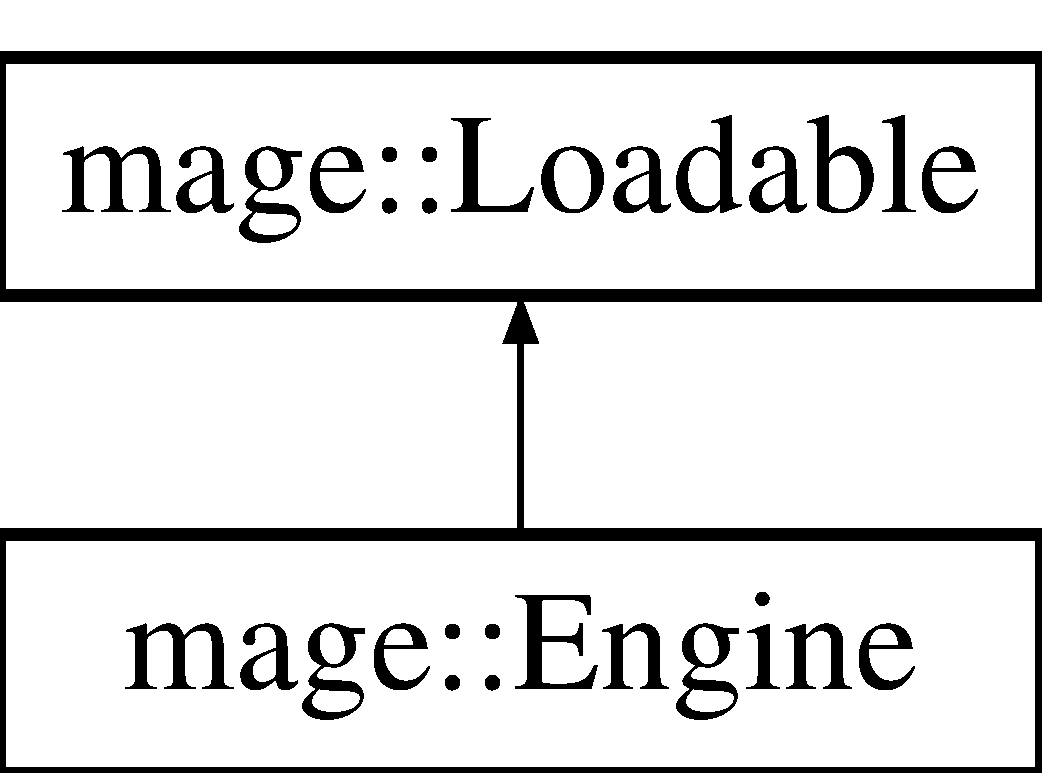
\includegraphics[height=2.000000cm]{classmage_1_1_loadable}
\end{center}
\end{figure}
\subsection*{Public Member Functions}
\begin{DoxyCompactItemize}
\item 
virtual \hyperlink{classmage_1_1_loadable_a8088935f7536c0c77ddb34a29ece63b1}{$\sim$\+Loadable} ()
\item 
bool \hyperlink{classmage_1_1_loadable_ae5489e70602ed829212b420b2e354108}{Is\+Loaded} () const noexcept
\end{DoxyCompactItemize}
\subsection*{Protected Member Functions}
\begin{DoxyCompactItemize}
\item 
\hyperlink{classmage_1_1_loadable_a7e702d425db455dbe0630c02a72f9d07}{Loadable} (bool loaded=false) noexcept
\item 
\hyperlink{classmage_1_1_loadable_aefd54800fd0711bdcb9c66d8df3c25a5}{Loadable} (const \hyperlink{classmage_1_1_loadable}{Loadable} \&loadable) noexcept
\item 
\hyperlink{classmage_1_1_loadable_ad41faf3735ef05dd2828b8ab3d1b6a78}{Loadable} (\hyperlink{classmage_1_1_loadable}{Loadable} \&\&loadable) noexcept
\item 
\hyperlink{classmage_1_1_loadable}{Loadable} \& \hyperlink{classmage_1_1_loadable_a3474428ce8f4b183f121cecf8f2c8add}{operator=} (const \hyperlink{classmage_1_1_loadable}{Loadable} \&loadable) noexcept
\item 
\hyperlink{classmage_1_1_loadable}{Loadable} \& \hyperlink{classmage_1_1_loadable_a553b6c96536fc6d8c38fdf766bf55402}{operator=} (\hyperlink{classmage_1_1_loadable}{Loadable} \&\&loadable) noexcept
\item 
void \hyperlink{classmage_1_1_loadable_adb8689c0dfc46138ac72768da897dc8f}{Set\+Loaded} (bool loaded=true) noexcept
\end{DoxyCompactItemize}
\subsection*{Private Attributes}
\begin{DoxyCompactItemize}
\item 
bool \hyperlink{classmage_1_1_loadable_a993963fbfeb0f2e2ab9616bf7ef6a0f7}{m\+\_\+loaded}
\end{DoxyCompactItemize}


\subsection{Detailed Description}
A class of loadables. 

\subsection{Constructor \& Destructor Documentation}
\hypertarget{classmage_1_1_loadable_a8088935f7536c0c77ddb34a29ece63b1}{}\label{classmage_1_1_loadable_a8088935f7536c0c77ddb34a29ece63b1} 
\index{mage\+::\+Loadable@{mage\+::\+Loadable}!````~Loadable@{$\sim$\+Loadable}}
\index{````~Loadable@{$\sim$\+Loadable}!mage\+::\+Loadable@{mage\+::\+Loadable}}
\subsubsection{\texorpdfstring{$\sim$\+Loadable()}{~Loadable()}}
{\footnotesize\ttfamily mage\+::\+Loadable\+::$\sim$\+Loadable (\begin{DoxyParamCaption}{ }\end{DoxyParamCaption})\hspace{0.3cm}{\ttfamily [virtual]}, {\ttfamily [default]}}

Destructs this loadable. \hypertarget{classmage_1_1_loadable_a7e702d425db455dbe0630c02a72f9d07}{}\label{classmage_1_1_loadable_a7e702d425db455dbe0630c02a72f9d07} 
\index{mage\+::\+Loadable@{mage\+::\+Loadable}!Loadable@{Loadable}}
\index{Loadable@{Loadable}!mage\+::\+Loadable@{mage\+::\+Loadable}}
\subsubsection{\texorpdfstring{Loadable()}{Loadable()}\hspace{0.1cm}{\footnotesize\ttfamily [1/3]}}
{\footnotesize\ttfamily mage\+::\+Loadable\+::\+Loadable (\begin{DoxyParamCaption}\item[{bool}]{loaded = {\ttfamily false} }\end{DoxyParamCaption})\hspace{0.3cm}{\ttfamily [explicit]}, {\ttfamily [protected]}, {\ttfamily [noexcept]}}

Constructs a loadable.


\begin{DoxyParams}[1]{Parameters}
\mbox{\tt in}  & {\em loaded} & Flag indicating whether the loadable is loaded. \\
\hline
\end{DoxyParams}
\hypertarget{classmage_1_1_loadable_aefd54800fd0711bdcb9c66d8df3c25a5}{}\label{classmage_1_1_loadable_aefd54800fd0711bdcb9c66d8df3c25a5} 
\index{mage\+::\+Loadable@{mage\+::\+Loadable}!Loadable@{Loadable}}
\index{Loadable@{Loadable}!mage\+::\+Loadable@{mage\+::\+Loadable}}
\subsubsection{\texorpdfstring{Loadable()}{Loadable()}\hspace{0.1cm}{\footnotesize\ttfamily [2/3]}}
{\footnotesize\ttfamily mage\+::\+Loadable\+::\+Loadable (\begin{DoxyParamCaption}\item[{const \hyperlink{classmage_1_1_loadable}{Loadable} \&}]{loadable }\end{DoxyParamCaption})\hspace{0.3cm}{\ttfamily [protected]}, {\ttfamily [default]}, {\ttfamily [noexcept]}}

Constructs a loadable from the given loadable.


\begin{DoxyParams}[1]{Parameters}
\mbox{\tt in}  & {\em loadable} & A reference to the loadable. \\
\hline
\end{DoxyParams}
\hypertarget{classmage_1_1_loadable_ad41faf3735ef05dd2828b8ab3d1b6a78}{}\label{classmage_1_1_loadable_ad41faf3735ef05dd2828b8ab3d1b6a78} 
\index{mage\+::\+Loadable@{mage\+::\+Loadable}!Loadable@{Loadable}}
\index{Loadable@{Loadable}!mage\+::\+Loadable@{mage\+::\+Loadable}}
\subsubsection{\texorpdfstring{Loadable()}{Loadable()}\hspace{0.1cm}{\footnotesize\ttfamily [3/3]}}
{\footnotesize\ttfamily mage\+::\+Loadable\+::\+Loadable (\begin{DoxyParamCaption}\item[{\hyperlink{classmage_1_1_loadable}{Loadable} \&\&}]{loadable }\end{DoxyParamCaption})\hspace{0.3cm}{\ttfamily [protected]}, {\ttfamily [default]}, {\ttfamily [noexcept]}}

Constructs a loadable by moving the given loadable.


\begin{DoxyParams}[1]{Parameters}
\mbox{\tt in}  & {\em loadable} & A reference to the loadable. \\
\hline
\end{DoxyParams}


\subsection{Member Function Documentation}
\hypertarget{classmage_1_1_loadable_ae5489e70602ed829212b420b2e354108}{}\label{classmage_1_1_loadable_ae5489e70602ed829212b420b2e354108} 
\index{mage\+::\+Loadable@{mage\+::\+Loadable}!Is\+Loaded@{Is\+Loaded}}
\index{Is\+Loaded@{Is\+Loaded}!mage\+::\+Loadable@{mage\+::\+Loadable}}
\subsubsection{\texorpdfstring{Is\+Loaded()}{IsLoaded()}}
{\footnotesize\ttfamily bool mage\+::\+Loadable\+::\+Is\+Loaded (\begin{DoxyParamCaption}{ }\end{DoxyParamCaption}) const\hspace{0.3cm}{\ttfamily [noexcept]}}

Checks whether this loadable is loaded.

\begin{DoxyReturn}{Returns}
{\ttfamily true} if this loadable is loaded. {\ttfamily false} otherwise. 
\end{DoxyReturn}
\hypertarget{classmage_1_1_loadable_a3474428ce8f4b183f121cecf8f2c8add}{}\label{classmage_1_1_loadable_a3474428ce8f4b183f121cecf8f2c8add} 
\index{mage\+::\+Loadable@{mage\+::\+Loadable}!operator=@{operator=}}
\index{operator=@{operator=}!mage\+::\+Loadable@{mage\+::\+Loadable}}
\subsubsection{\texorpdfstring{operator=()}{operator=()}\hspace{0.1cm}{\footnotesize\ttfamily [1/2]}}
{\footnotesize\ttfamily \hyperlink{classmage_1_1_loadable}{Loadable} \& mage\+::\+Loadable\+::operator= (\begin{DoxyParamCaption}\item[{const \hyperlink{classmage_1_1_loadable}{Loadable} \&}]{loadable }\end{DoxyParamCaption})\hspace{0.3cm}{\ttfamily [protected]}, {\ttfamily [default]}, {\ttfamily [noexcept]}}

Copies the given loadable to this loadable.


\begin{DoxyParams}[1]{Parameters}
\mbox{\tt in}  & {\em loadable} & A reference to the loadable to copy. \\
\hline
\end{DoxyParams}
\begin{DoxyReturn}{Returns}
A reference to the copy of the given loadable (i.\+e. this loadable). 
\end{DoxyReturn}
\hypertarget{classmage_1_1_loadable_a553b6c96536fc6d8c38fdf766bf55402}{}\label{classmage_1_1_loadable_a553b6c96536fc6d8c38fdf766bf55402} 
\index{mage\+::\+Loadable@{mage\+::\+Loadable}!operator=@{operator=}}
\index{operator=@{operator=}!mage\+::\+Loadable@{mage\+::\+Loadable}}
\subsubsection{\texorpdfstring{operator=()}{operator=()}\hspace{0.1cm}{\footnotesize\ttfamily [2/2]}}
{\footnotesize\ttfamily \hyperlink{classmage_1_1_loadable}{Loadable} \& mage\+::\+Loadable\+::operator= (\begin{DoxyParamCaption}\item[{\hyperlink{classmage_1_1_loadable}{Loadable} \&\&}]{loadable }\end{DoxyParamCaption})\hspace{0.3cm}{\ttfamily [protected]}, {\ttfamily [default]}, {\ttfamily [noexcept]}}

Moves the given loadable to this loadable.


\begin{DoxyParams}[1]{Parameters}
\mbox{\tt in}  & {\em loadable} & A reference to the loadable to move. \\
\hline
\end{DoxyParams}
\begin{DoxyReturn}{Returns}
A reference to the moved loadable (i.\+e. this loadable). 
\end{DoxyReturn}
\hypertarget{classmage_1_1_loadable_adb8689c0dfc46138ac72768da897dc8f}{}\label{classmage_1_1_loadable_adb8689c0dfc46138ac72768da897dc8f} 
\index{mage\+::\+Loadable@{mage\+::\+Loadable}!Set\+Loaded@{Set\+Loaded}}
\index{Set\+Loaded@{Set\+Loaded}!mage\+::\+Loadable@{mage\+::\+Loadable}}
\subsubsection{\texorpdfstring{Set\+Loaded()}{SetLoaded()}}
{\footnotesize\ttfamily void mage\+::\+Loadable\+::\+Set\+Loaded (\begin{DoxyParamCaption}\item[{bool}]{loaded = {\ttfamily true} }\end{DoxyParamCaption})\hspace{0.3cm}{\ttfamily [protected]}, {\ttfamily [noexcept]}}

Set the state of this loadable to the given value.


\begin{DoxyParams}[1]{Parameters}
\mbox{\tt in}  & {\em loaded} & Flag indicating whether this loadable is loaded. \\
\hline
\end{DoxyParams}


\subsection{Member Data Documentation}
\hypertarget{classmage_1_1_loadable_a993963fbfeb0f2e2ab9616bf7ef6a0f7}{}\label{classmage_1_1_loadable_a993963fbfeb0f2e2ab9616bf7ef6a0f7} 
\index{mage\+::\+Loadable@{mage\+::\+Loadable}!m\+\_\+loaded@{m\+\_\+loaded}}
\index{m\+\_\+loaded@{m\+\_\+loaded}!mage\+::\+Loadable@{mage\+::\+Loadable}}
\subsubsection{\texorpdfstring{m\+\_\+loaded}{m\_loaded}}
{\footnotesize\ttfamily bool mage\+::\+Loadable\+::m\+\_\+loaded\hspace{0.3cm}{\ttfamily [private]}}

Flag indicating whether this loadable is loaded. 
\hypertarget{classmage_1_1_location_script}{}\section{mage\+:\+:Location\+Script Class Reference}
\label{classmage_1_1_location_script}\index{mage\+::\+Location\+Script@{mage\+::\+Location\+Script}}


{\ttfamily \#include $<$location\+\_\+script.\+hpp$>$}

Inheritance diagram for mage\+:\+:Location\+Script\+:\begin{figure}[H]
\begin{center}
\leavevmode
\includegraphics[height=2.000000cm]{classmage_1_1_location_script}
\end{center}
\end{figure}
\subsection*{Public Member Functions}
\begin{DoxyCompactItemize}
\item 
\hyperlink{classmage_1_1_location_script_a6ba4b1c4a698ab5ea0d7deb7ffa58bed}{Location\+Script} (Transform $\ast$transform, \hyperlink{namespacemage_a1e01ae66713838a7a67d30e44c67703e}{Shared\+Ptr}$<$ \hyperlink{classmage_1_1_sprite_text}{Sprite\+Text} $>$ text)
\item 
\hyperlink{classmage_1_1_location_script_a53fb0562896eadb4c747d53b53f65b40}{Location\+Script} (const \hyperlink{classmage_1_1_location_script}{Location\+Script} \&script)=delete
\item 
\hyperlink{classmage_1_1_location_script_a6cddb54a11e5d5d6dee034ef04ffbf2f}{Location\+Script} (\hyperlink{classmage_1_1_location_script}{Location\+Script} \&\&script)
\item 
virtual \hyperlink{classmage_1_1_location_script_a95ed60a4bd7d228cc28ce1622f254d75}{$\sim$\+Location\+Script} ()
\item 
\hyperlink{classmage_1_1_location_script}{Location\+Script} \& \hyperlink{classmage_1_1_location_script_a49409b091dbd1b93830c46831be453fb}{operator=} (const \hyperlink{classmage_1_1_location_script}{Location\+Script} \&script)=delete
\item 
\hyperlink{classmage_1_1_location_script}{Location\+Script} \& \hyperlink{classmage_1_1_location_script_a6e2ad5cd12a984d38c66bbcc81fef94b}{operator=} (\hyperlink{classmage_1_1_location_script}{Location\+Script} \&\&script)=delete
\item 
virtual void \hyperlink{classmage_1_1_location_script_a3ffe0474c573e2cf858aee62056324a3}{Update} (double delta\+\_\+time) override
\end{DoxyCompactItemize}
\subsection*{Private Attributes}
\begin{DoxyCompactItemize}
\item 
Transform $\ast$const \hyperlink{classmage_1_1_location_script_aaa349c73ef4fc8267e6bd1cc0512cd5c}{m\+\_\+transform}
\item 
\hyperlink{namespacemage_a1e01ae66713838a7a67d30e44c67703e}{Shared\+Ptr}$<$ \hyperlink{classmage_1_1_sprite_text}{Sprite\+Text} $>$ \hyperlink{classmage_1_1_location_script_ac5c7ada3b364d85888686abf20cd6463}{m\+\_\+text}
\end{DoxyCompactItemize}
\subsection*{Additional Inherited Members}


\subsection{Constructor \& Destructor Documentation}
\hypertarget{classmage_1_1_location_script_a6ba4b1c4a698ab5ea0d7deb7ffa58bed}{}\label{classmage_1_1_location_script_a6ba4b1c4a698ab5ea0d7deb7ffa58bed} 
\index{mage\+::\+Location\+Script@{mage\+::\+Location\+Script}!Location\+Script@{Location\+Script}}
\index{Location\+Script@{Location\+Script}!mage\+::\+Location\+Script@{mage\+::\+Location\+Script}}
\subsubsection{\texorpdfstring{Location\+Script()}{LocationScript()}\hspace{0.1cm}{\footnotesize\ttfamily [1/3]}}
{\footnotesize\ttfamily mage\+::\+Location\+Script\+::\+Location\+Script (\begin{DoxyParamCaption}\item[{Transform $\ast$}]{transform,  }\item[{\hyperlink{namespacemage_a1e01ae66713838a7a67d30e44c67703e}{Shared\+Ptr}$<$ \hyperlink{classmage_1_1_sprite_text}{Sprite\+Text} $>$}]{text }\end{DoxyParamCaption})\hspace{0.3cm}{\ttfamily [explicit]}}

\hypertarget{classmage_1_1_location_script_a53fb0562896eadb4c747d53b53f65b40}{}\label{classmage_1_1_location_script_a53fb0562896eadb4c747d53b53f65b40} 
\index{mage\+::\+Location\+Script@{mage\+::\+Location\+Script}!Location\+Script@{Location\+Script}}
\index{Location\+Script@{Location\+Script}!mage\+::\+Location\+Script@{mage\+::\+Location\+Script}}
\subsubsection{\texorpdfstring{Location\+Script()}{LocationScript()}\hspace{0.1cm}{\footnotesize\ttfamily [2/3]}}
{\footnotesize\ttfamily mage\+::\+Location\+Script\+::\+Location\+Script (\begin{DoxyParamCaption}\item[{const \hyperlink{classmage_1_1_location_script}{Location\+Script} \&}]{script }\end{DoxyParamCaption})\hspace{0.3cm}{\ttfamily [delete]}}

\hypertarget{classmage_1_1_location_script_a6cddb54a11e5d5d6dee034ef04ffbf2f}{}\label{classmage_1_1_location_script_a6cddb54a11e5d5d6dee034ef04ffbf2f} 
\index{mage\+::\+Location\+Script@{mage\+::\+Location\+Script}!Location\+Script@{Location\+Script}}
\index{Location\+Script@{Location\+Script}!mage\+::\+Location\+Script@{mage\+::\+Location\+Script}}
\subsubsection{\texorpdfstring{Location\+Script()}{LocationScript()}\hspace{0.1cm}{\footnotesize\ttfamily [3/3]}}
{\footnotesize\ttfamily mage\+::\+Location\+Script\+::\+Location\+Script (\begin{DoxyParamCaption}\item[{\hyperlink{classmage_1_1_location_script}{Location\+Script} \&\&}]{script }\end{DoxyParamCaption})\hspace{0.3cm}{\ttfamily [default]}}

\hypertarget{classmage_1_1_location_script_a95ed60a4bd7d228cc28ce1622f254d75}{}\label{classmage_1_1_location_script_a95ed60a4bd7d228cc28ce1622f254d75} 
\index{mage\+::\+Location\+Script@{mage\+::\+Location\+Script}!````~Location\+Script@{$\sim$\+Location\+Script}}
\index{````~Location\+Script@{$\sim$\+Location\+Script}!mage\+::\+Location\+Script@{mage\+::\+Location\+Script}}
\subsubsection{\texorpdfstring{$\sim$\+Location\+Script()}{~LocationScript()}}
{\footnotesize\ttfamily mage\+::\+Location\+Script\+::$\sim$\+Location\+Script (\begin{DoxyParamCaption}{ }\end{DoxyParamCaption})\hspace{0.3cm}{\ttfamily [virtual]}, {\ttfamily [default]}}



\subsection{Member Function Documentation}
\hypertarget{classmage_1_1_location_script_a49409b091dbd1b93830c46831be453fb}{}\label{classmage_1_1_location_script_a49409b091dbd1b93830c46831be453fb} 
\index{mage\+::\+Location\+Script@{mage\+::\+Location\+Script}!operator=@{operator=}}
\index{operator=@{operator=}!mage\+::\+Location\+Script@{mage\+::\+Location\+Script}}
\subsubsection{\texorpdfstring{operator=()}{operator=()}\hspace{0.1cm}{\footnotesize\ttfamily [1/2]}}
{\footnotesize\ttfamily \hyperlink{classmage_1_1_location_script}{Location\+Script}\& mage\+::\+Location\+Script\+::operator= (\begin{DoxyParamCaption}\item[{const \hyperlink{classmage_1_1_location_script}{Location\+Script} \&}]{script }\end{DoxyParamCaption})\hspace{0.3cm}{\ttfamily [delete]}}

\hypertarget{classmage_1_1_location_script_a6e2ad5cd12a984d38c66bbcc81fef94b}{}\label{classmage_1_1_location_script_a6e2ad5cd12a984d38c66bbcc81fef94b} 
\index{mage\+::\+Location\+Script@{mage\+::\+Location\+Script}!operator=@{operator=}}
\index{operator=@{operator=}!mage\+::\+Location\+Script@{mage\+::\+Location\+Script}}
\subsubsection{\texorpdfstring{operator=()}{operator=()}\hspace{0.1cm}{\footnotesize\ttfamily [2/2]}}
{\footnotesize\ttfamily \hyperlink{classmage_1_1_location_script}{Location\+Script}\& mage\+::\+Location\+Script\+::operator= (\begin{DoxyParamCaption}\item[{\hyperlink{classmage_1_1_location_script}{Location\+Script} \&\&}]{script }\end{DoxyParamCaption})\hspace{0.3cm}{\ttfamily [delete]}}

\hypertarget{classmage_1_1_location_script_a3ffe0474c573e2cf858aee62056324a3}{}\label{classmage_1_1_location_script_a3ffe0474c573e2cf858aee62056324a3} 
\index{mage\+::\+Location\+Script@{mage\+::\+Location\+Script}!Update@{Update}}
\index{Update@{Update}!mage\+::\+Location\+Script@{mage\+::\+Location\+Script}}
\subsubsection{\texorpdfstring{Update()}{Update()}}
{\footnotesize\ttfamily void mage\+::\+Location\+Script\+::\+Update (\begin{DoxyParamCaption}\item[{double}]{delta\+\_\+time }\end{DoxyParamCaption})\hspace{0.3cm}{\ttfamily [override]}, {\ttfamily [virtual]}}

Updates this behavior script.


\begin{DoxyParams}[1]{Parameters}
\mbox{\tt in}  & {\em delta\+\_\+time} & The elapsed time since the previous update. \\
\hline
\end{DoxyParams}


Implements \hyperlink{classmage_1_1_behavior_script_a905b6c83640cb91d19fecab3435f6feb}{mage\+::\+Behavior\+Script}.



\subsection{Member Data Documentation}
\hypertarget{classmage_1_1_location_script_ac5c7ada3b364d85888686abf20cd6463}{}\label{classmage_1_1_location_script_ac5c7ada3b364d85888686abf20cd6463} 
\index{mage\+::\+Location\+Script@{mage\+::\+Location\+Script}!m\+\_\+text@{m\+\_\+text}}
\index{m\+\_\+text@{m\+\_\+text}!mage\+::\+Location\+Script@{mage\+::\+Location\+Script}}
\subsubsection{\texorpdfstring{m\+\_\+text}{m\_text}}
{\footnotesize\ttfamily \hyperlink{namespacemage_a1e01ae66713838a7a67d30e44c67703e}{Shared\+Ptr}$<$ \hyperlink{classmage_1_1_sprite_text}{Sprite\+Text} $>$ mage\+::\+Location\+Script\+::m\+\_\+text\hspace{0.3cm}{\ttfamily [private]}}

\hypertarget{classmage_1_1_location_script_aaa349c73ef4fc8267e6bd1cc0512cd5c}{}\label{classmage_1_1_location_script_aaa349c73ef4fc8267e6bd1cc0512cd5c} 
\index{mage\+::\+Location\+Script@{mage\+::\+Location\+Script}!m\+\_\+transform@{m\+\_\+transform}}
\index{m\+\_\+transform@{m\+\_\+transform}!mage\+::\+Location\+Script@{mage\+::\+Location\+Script}}
\subsubsection{\texorpdfstring{m\+\_\+transform}{m\_transform}}
{\footnotesize\ttfamily Transform$\ast$ const mage\+::\+Location\+Script\+::m\+\_\+transform\hspace{0.3cm}{\ttfamily [private]}}


\hypertarget{structmage_1_1_logging_configuration}{}\section{mage\+:\+:Logging\+Configuration Struct Reference}
\label{structmage_1_1_logging_configuration}\index{mage\+::\+Logging\+Configuration@{mage\+::\+Logging\+Configuration}}


{\ttfamily \#include $<$logging.\+hpp$>$}

\subsection*{Public Member Functions}
\begin{DoxyCompactItemize}
\item 
\hyperlink{structmage_1_1_logging_configuration_ab18d18c78e7104f4c677e6d08f31ca01}{Logging\+Configuration} (bool quiet=false, bool verbose=false)
\item 
\hyperlink{structmage_1_1_logging_configuration_a8e4ccd4301f5544213edd3b600cccff9}{Logging\+Configuration} (const \hyperlink{structmage_1_1_logging_configuration}{Logging\+Configuration} \&logging\+\_\+configuration)=default
\item 
\hyperlink{structmage_1_1_logging_configuration_ad5d3dd901720450fcf57d4b1b32fce15}{Logging\+Configuration} (\hyperlink{structmage_1_1_logging_configuration}{Logging\+Configuration} \&\&logging\+\_\+configuration)=default
\item 
\hyperlink{structmage_1_1_logging_configuration_a842cd1d5cf22c9fb6e2c76e684cd08ee}{$\sim$\+Logging\+Configuration} ()=default
\item 
\hyperlink{structmage_1_1_logging_configuration}{Logging\+Configuration} \& \hyperlink{structmage_1_1_logging_configuration_af35d0b0a2f5743944d3d9d66580074db}{operator=} (const \hyperlink{structmage_1_1_logging_configuration}{Logging\+Configuration} \&logging\+\_\+configuration)=default
\item 
\hyperlink{structmage_1_1_logging_configuration}{Logging\+Configuration} \& \hyperlink{structmage_1_1_logging_configuration_a699285ff50d1bb7573cc0c28bcf476b1}{operator=} (\hyperlink{structmage_1_1_logging_configuration}{Logging\+Configuration} \&\&logging\+\_\+configuration)=default
\item 
bool \hyperlink{structmage_1_1_logging_configuration_a64f7a7b45bc0e896b9d493ddaf13ca82}{Is\+Quiet} () const noexcept
\item 
bool \hyperlink{structmage_1_1_logging_configuration_a4ad7dc55f8d105c1125adcea4796bb3b}{Is\+Verbose} () const noexcept
\end{DoxyCompactItemize}
\subsection*{Private Attributes}
\begin{DoxyCompactItemize}
\item 
bool \hyperlink{structmage_1_1_logging_configuration_a38f457d5db84d15e008841ca8653b47c}{m\+\_\+quiet}
\item 
bool \hyperlink{structmage_1_1_logging_configuration_a60f052c2bb702d8153188e93f00427ac}{m\+\_\+verbose}
\end{DoxyCompactItemize}


\subsection{Detailed Description}
A struct of logging configurations of the engine processing. 

\subsection{Constructor \& Destructor Documentation}
\hypertarget{structmage_1_1_logging_configuration_ab18d18c78e7104f4c677e6d08f31ca01}{}\label{structmage_1_1_logging_configuration_ab18d18c78e7104f4c677e6d08f31ca01} 
\index{mage\+::\+Logging\+Configuration@{mage\+::\+Logging\+Configuration}!Logging\+Configuration@{Logging\+Configuration}}
\index{Logging\+Configuration@{Logging\+Configuration}!mage\+::\+Logging\+Configuration@{mage\+::\+Logging\+Configuration}}
\subsubsection{\texorpdfstring{Logging\+Configuration()}{LoggingConfiguration()}\hspace{0.1cm}{\footnotesize\ttfamily [1/3]}}
{\footnotesize\ttfamily mage\+::\+Logging\+Configuration\+::\+Logging\+Configuration (\begin{DoxyParamCaption}\item[{bool}]{quiet = {\ttfamily false},  }\item[{bool}]{verbose = {\ttfamily false} }\end{DoxyParamCaption})\hspace{0.3cm}{\ttfamily [explicit]}}

Constructs a logging configuration.


\begin{DoxyParams}[1]{Parameters}
\mbox{\tt in}  & {\em quiet} & Flag indicating whether quiet logging is preferred. \\
\hline
\mbox{\tt in}  & {\em verbose} & Flag indicating whether verbose logging is preferred. \\
\hline
\end{DoxyParams}
\hypertarget{structmage_1_1_logging_configuration_a8e4ccd4301f5544213edd3b600cccff9}{}\label{structmage_1_1_logging_configuration_a8e4ccd4301f5544213edd3b600cccff9} 
\index{mage\+::\+Logging\+Configuration@{mage\+::\+Logging\+Configuration}!Logging\+Configuration@{Logging\+Configuration}}
\index{Logging\+Configuration@{Logging\+Configuration}!mage\+::\+Logging\+Configuration@{mage\+::\+Logging\+Configuration}}
\subsubsection{\texorpdfstring{Logging\+Configuration()}{LoggingConfiguration()}\hspace{0.1cm}{\footnotesize\ttfamily [2/3]}}
{\footnotesize\ttfamily mage\+::\+Logging\+Configuration\+::\+Logging\+Configuration (\begin{DoxyParamCaption}\item[{const \hyperlink{structmage_1_1_logging_configuration}{Logging\+Configuration} \&}]{logging\+\_\+configuration }\end{DoxyParamCaption})\hspace{0.3cm}{\ttfamily [default]}}

Constructs a logging configuration from the given logging configuration.


\begin{DoxyParams}[1]{Parameters}
\mbox{\tt in}  & {\em logging\+\_\+configuration} & A reference to the logging configuration to copy. \\
\hline
\end{DoxyParams}
\hypertarget{structmage_1_1_logging_configuration_ad5d3dd901720450fcf57d4b1b32fce15}{}\label{structmage_1_1_logging_configuration_ad5d3dd901720450fcf57d4b1b32fce15} 
\index{mage\+::\+Logging\+Configuration@{mage\+::\+Logging\+Configuration}!Logging\+Configuration@{Logging\+Configuration}}
\index{Logging\+Configuration@{Logging\+Configuration}!mage\+::\+Logging\+Configuration@{mage\+::\+Logging\+Configuration}}
\subsubsection{\texorpdfstring{Logging\+Configuration()}{LoggingConfiguration()}\hspace{0.1cm}{\footnotesize\ttfamily [3/3]}}
{\footnotesize\ttfamily mage\+::\+Logging\+Configuration\+::\+Logging\+Configuration (\begin{DoxyParamCaption}\item[{\hyperlink{structmage_1_1_logging_configuration}{Logging\+Configuration} \&\&}]{logging\+\_\+configuration }\end{DoxyParamCaption})\hspace{0.3cm}{\ttfamily [default]}}

Constructs a logging configuration by moving the given logging configuration.


\begin{DoxyParams}[1]{Parameters}
\mbox{\tt in}  & {\em logging\+\_\+configuration} & A reference to the logging configuration to move. \\
\hline
\end{DoxyParams}
\hypertarget{structmage_1_1_logging_configuration_a842cd1d5cf22c9fb6e2c76e684cd08ee}{}\label{structmage_1_1_logging_configuration_a842cd1d5cf22c9fb6e2c76e684cd08ee} 
\index{mage\+::\+Logging\+Configuration@{mage\+::\+Logging\+Configuration}!````~Logging\+Configuration@{$\sim$\+Logging\+Configuration}}
\index{````~Logging\+Configuration@{$\sim$\+Logging\+Configuration}!mage\+::\+Logging\+Configuration@{mage\+::\+Logging\+Configuration}}
\subsubsection{\texorpdfstring{$\sim$\+Logging\+Configuration()}{~LoggingConfiguration()}}
{\footnotesize\ttfamily mage\+::\+Logging\+Configuration\+::$\sim$\+Logging\+Configuration (\begin{DoxyParamCaption}{ }\end{DoxyParamCaption})\hspace{0.3cm}{\ttfamily [default]}}

Destructs this logging configuration. 

\subsection{Member Function Documentation}
\hypertarget{structmage_1_1_logging_configuration_a64f7a7b45bc0e896b9d493ddaf13ca82}{}\label{structmage_1_1_logging_configuration_a64f7a7b45bc0e896b9d493ddaf13ca82} 
\index{mage\+::\+Logging\+Configuration@{mage\+::\+Logging\+Configuration}!Is\+Quiet@{Is\+Quiet}}
\index{Is\+Quiet@{Is\+Quiet}!mage\+::\+Logging\+Configuration@{mage\+::\+Logging\+Configuration}}
\subsubsection{\texorpdfstring{Is\+Quiet()}{IsQuiet()}}
{\footnotesize\ttfamily bool mage\+::\+Logging\+Configuration\+::\+Is\+Quiet (\begin{DoxyParamCaption}{ }\end{DoxyParamCaption}) const\hspace{0.3cm}{\ttfamily [noexcept]}}

Checks whether the logging of the engine processing is quiet.

\begin{DoxyReturn}{Returns}
{\ttfamily true} if the logging of the engine processing is quiet. {\ttfamily false} otherwise. 
\end{DoxyReturn}
\hypertarget{structmage_1_1_logging_configuration_a4ad7dc55f8d105c1125adcea4796bb3b}{}\label{structmage_1_1_logging_configuration_a4ad7dc55f8d105c1125adcea4796bb3b} 
\index{mage\+::\+Logging\+Configuration@{mage\+::\+Logging\+Configuration}!Is\+Verbose@{Is\+Verbose}}
\index{Is\+Verbose@{Is\+Verbose}!mage\+::\+Logging\+Configuration@{mage\+::\+Logging\+Configuration}}
\subsubsection{\texorpdfstring{Is\+Verbose()}{IsVerbose()}}
{\footnotesize\ttfamily bool mage\+::\+Logging\+Configuration\+::\+Is\+Verbose (\begin{DoxyParamCaption}{ }\end{DoxyParamCaption}) const\hspace{0.3cm}{\ttfamily [noexcept]}}

Checks wheter the logging of the engine processing is verbose.

\begin{DoxyReturn}{Returns}
{\ttfamily true} if the logging of the engine processing is verbose. {\ttfamily false} otherwise. 
\end{DoxyReturn}
\hypertarget{structmage_1_1_logging_configuration_af35d0b0a2f5743944d3d9d66580074db}{}\label{structmage_1_1_logging_configuration_af35d0b0a2f5743944d3d9d66580074db} 
\index{mage\+::\+Logging\+Configuration@{mage\+::\+Logging\+Configuration}!operator=@{operator=}}
\index{operator=@{operator=}!mage\+::\+Logging\+Configuration@{mage\+::\+Logging\+Configuration}}
\subsubsection{\texorpdfstring{operator=()}{operator=()}\hspace{0.1cm}{\footnotesize\ttfamily [1/2]}}
{\footnotesize\ttfamily \hyperlink{structmage_1_1_logging_configuration}{Logging\+Configuration}\& mage\+::\+Logging\+Configuration\+::operator= (\begin{DoxyParamCaption}\item[{const \hyperlink{structmage_1_1_logging_configuration}{Logging\+Configuration} \&}]{logging\+\_\+configuration }\end{DoxyParamCaption})\hspace{0.3cm}{\ttfamily [default]}}

Copies the given logging configuration to this logging configuration.


\begin{DoxyParams}[1]{Parameters}
\mbox{\tt in}  & {\em logging\+\_\+configuration} & A reference to the logging configuration to copy. \\
\hline
\end{DoxyParams}
\begin{DoxyReturn}{Returns}
A reference to the copy of the given logging configuration (i.\+e. this logging configuration). 
\end{DoxyReturn}
\hypertarget{structmage_1_1_logging_configuration_a699285ff50d1bb7573cc0c28bcf476b1}{}\label{structmage_1_1_logging_configuration_a699285ff50d1bb7573cc0c28bcf476b1} 
\index{mage\+::\+Logging\+Configuration@{mage\+::\+Logging\+Configuration}!operator=@{operator=}}
\index{operator=@{operator=}!mage\+::\+Logging\+Configuration@{mage\+::\+Logging\+Configuration}}
\subsubsection{\texorpdfstring{operator=()}{operator=()}\hspace{0.1cm}{\footnotesize\ttfamily [2/2]}}
{\footnotesize\ttfamily \hyperlink{structmage_1_1_logging_configuration}{Logging\+Configuration}\& mage\+::\+Logging\+Configuration\+::operator= (\begin{DoxyParamCaption}\item[{\hyperlink{structmage_1_1_logging_configuration}{Logging\+Configuration} \&\&}]{logging\+\_\+configuration }\end{DoxyParamCaption})\hspace{0.3cm}{\ttfamily [default]}}

Moves the given logging configuration to this logging configuration.


\begin{DoxyParams}[1]{Parameters}
\mbox{\tt in}  & {\em logging\+\_\+configuration} & A reference to the logging configuration to move. \\
\hline
\end{DoxyParams}
\begin{DoxyReturn}{Returns}
A reference to the moved logging configuration (i.\+e. this logging configuration). 
\end{DoxyReturn}


\subsection{Member Data Documentation}
\hypertarget{structmage_1_1_logging_configuration_a38f457d5db84d15e008841ca8653b47c}{}\label{structmage_1_1_logging_configuration_a38f457d5db84d15e008841ca8653b47c} 
\index{mage\+::\+Logging\+Configuration@{mage\+::\+Logging\+Configuration}!m\+\_\+quiet@{m\+\_\+quiet}}
\index{m\+\_\+quiet@{m\+\_\+quiet}!mage\+::\+Logging\+Configuration@{mage\+::\+Logging\+Configuration}}
\subsubsection{\texorpdfstring{m\+\_\+quiet}{m\_quiet}}
{\footnotesize\ttfamily bool mage\+::\+Logging\+Configuration\+::m\+\_\+quiet\hspace{0.3cm}{\ttfamily [private]}}

Flag indicating the logging of the engine processing is quiet. \hypertarget{structmage_1_1_logging_configuration_a60f052c2bb702d8153188e93f00427ac}{}\label{structmage_1_1_logging_configuration_a60f052c2bb702d8153188e93f00427ac} 
\index{mage\+::\+Logging\+Configuration@{mage\+::\+Logging\+Configuration}!m\+\_\+verbose@{m\+\_\+verbose}}
\index{m\+\_\+verbose@{m\+\_\+verbose}!mage\+::\+Logging\+Configuration@{mage\+::\+Logging\+Configuration}}
\subsubsection{\texorpdfstring{m\+\_\+verbose}{m\_verbose}}
{\footnotesize\ttfamily bool mage\+::\+Logging\+Configuration\+::m\+\_\+verbose\hspace{0.3cm}{\ttfamily [private]}}

Flag indicating the logging of the engine processing is verbose. 
\hypertarget{classmage_1_1_main_window}{}\section{mage\+:\+:Main\+Window Class Reference}
\label{classmage_1_1_main_window}\index{mage\+::\+Main\+Window@{mage\+::\+Main\+Window}}


{\ttfamily \#include $<$main\+\_\+window.\+hpp$>$}

\subsection*{Public Member Functions}
\begin{DoxyCompactItemize}
\item 
\hyperlink{classmage_1_1_main_window_a05350ed05ac1af3fb7ed3176e3d249ac}{Main\+Window} (H\+I\+N\+S\+T\+A\+N\+CE hinstance, const wstring \&title\+\_\+text, L\+O\+NG width, L\+O\+NG height)
\item 
\hyperlink{classmage_1_1_main_window_a8dc3c590bb168f8178a7db72ff60fd0c}{Main\+Window} (const \hyperlink{classmage_1_1_main_window}{Main\+Window} \&main\+\_\+window)=delete
\item 
\hyperlink{classmage_1_1_main_window_ab5c9cc962420580c62dd2b44c142cf4b}{Main\+Window} (\hyperlink{classmage_1_1_main_window}{Main\+Window} \&\&main\+\_\+window)
\item 
\hyperlink{classmage_1_1_main_window_ada7ecf97d82ce08ba2f31f0afd891031}{$\sim$\+Main\+Window} ()
\item 
\hyperlink{classmage_1_1_main_window}{Main\+Window} \& \hyperlink{classmage_1_1_main_window_a0c2414ae4e627fb401c045371c286de0}{operator=} (const \hyperlink{classmage_1_1_main_window}{Main\+Window} \&main\+\_\+window)=delete
\item 
\hyperlink{classmage_1_1_main_window}{Main\+Window} \& \hyperlink{classmage_1_1_main_window_a684d547966f69ef5df793b5ce516f76a}{operator=} (\hyperlink{classmage_1_1_main_window}{Main\+Window} \&\&main\+\_\+window)=delete
\item 
void \hyperlink{classmage_1_1_main_window_abbb86e7f4dab1b43ca28f83e265f511e}{Show} (int n\+Cmd\+Show) noexcept
\item 
H\+I\+N\+S\+T\+A\+N\+CE \hyperlink{classmage_1_1_main_window_a1b8c851147ea3b51e645c2fce961fe17}{Get\+Hinstance} () noexcept
\item 
H\+W\+ND \hyperlink{classmage_1_1_main_window_ab4520f7c5ef0828535a117a8512221b5}{Get\+Handle} () noexcept
\item 
const wstring \hyperlink{classmage_1_1_main_window_a16ea3780659e00c8e4732b518c7c4a1e}{Get\+Title\+Text} () const noexcept
\item 
void \hyperlink{classmage_1_1_main_window_aaadd51dc2b902d93ea2f28d685477301}{Set\+Title\+Text} (const wstring \&title\+\_\+text) noexcept
\item 
void \hyperlink{classmage_1_1_main_window_a1baa8554782be197fb5932c3af461f0e}{Set\+Title\+Text} (const wchar\+\_\+t $\ast$title\+\_\+text) noexcept
\end{DoxyCompactItemize}
\subsection*{Private Member Functions}
\begin{DoxyCompactItemize}
\item 
void \hyperlink{classmage_1_1_main_window_abcf8f87d562109236de14db7ee8a3df2}{Initialize\+Window} (const wstring \&title\+\_\+text, L\+O\+NG width, L\+O\+NG height)
\item 
void \hyperlink{classmage_1_1_main_window_ab87716ce916ba180068a65294fa037e8}{Initialize\+Window} (const wstring \&title\+\_\+text, const R\+E\+CT \&rectangle)
\item 
void \hyperlink{classmage_1_1_main_window_a229ff4bcc198ed9caf2ce54966caf746}{Uninitialize\+Window} () noexcept
\end{DoxyCompactItemize}
\subsection*{Private Attributes}
\begin{DoxyCompactItemize}
\item 
const H\+I\+N\+S\+T\+A\+N\+CE \hyperlink{classmage_1_1_main_window_a314759bf324579b568528bbf99bc5c7f}{m\+\_\+hinstance}
\item 
H\+W\+ND \hyperlink{classmage_1_1_main_window_afc9afabcf8a52d79f02c8352451863cc}{m\+\_\+hwindow}
\end{DoxyCompactItemize}


\subsection{Detailed Description}
A class of application main windows. 

\subsection{Constructor \& Destructor Documentation}
\hypertarget{classmage_1_1_main_window_a05350ed05ac1af3fb7ed3176e3d249ac}{}\label{classmage_1_1_main_window_a05350ed05ac1af3fb7ed3176e3d249ac} 
\index{mage\+::\+Main\+Window@{mage\+::\+Main\+Window}!Main\+Window@{Main\+Window}}
\index{Main\+Window@{Main\+Window}!mage\+::\+Main\+Window@{mage\+::\+Main\+Window}}
\subsubsection{\texorpdfstring{Main\+Window()}{MainWindow()}\hspace{0.1cm}{\footnotesize\ttfamily [1/3]}}
{\footnotesize\ttfamily mage\+::\+Main\+Window\+::\+Main\+Window (\begin{DoxyParamCaption}\item[{H\+I\+N\+S\+T\+A\+N\+CE}]{hinstance,  }\item[{const wstring \&}]{title\+\_\+text,  }\item[{L\+O\+NG}]{width,  }\item[{L\+O\+NG}]{height }\end{DoxyParamCaption})\hspace{0.3cm}{\ttfamily [explicit]}}

Constructs a main window.

\begin{DoxyPrecond}{Precondition}
{\itshape hinstance} is not equal to {\ttfamily nullptr}. 
\end{DoxyPrecond}

\begin{DoxyParams}[1]{Parameters}
\mbox{\tt in}  & {\em hinstance} & The application instance handle. \\
\hline
\mbox{\tt in}  & {\em title\+\_\+text} & A reference to the title text. \\
\hline
\mbox{\tt in}  & {\em width} & The width of the window. \\
\hline
\mbox{\tt in}  & {\em height} & The height of the window. \\
\hline
\end{DoxyParams}

\begin{DoxyExceptions}{Exceptions}
{\em \hyperlink{structmage_1_1_formatted_exception}{Formatted\+Exception}} & Failed to register the main window\textquotesingle{}s class. \\
\hline
{\em \hyperlink{structmage_1_1_formatted_exception}{Formatted\+Exception}} & Failed to create the main window. \\
\hline
\end{DoxyExceptions}
\hypertarget{classmage_1_1_main_window_a8dc3c590bb168f8178a7db72ff60fd0c}{}\label{classmage_1_1_main_window_a8dc3c590bb168f8178a7db72ff60fd0c} 
\index{mage\+::\+Main\+Window@{mage\+::\+Main\+Window}!Main\+Window@{Main\+Window}}
\index{Main\+Window@{Main\+Window}!mage\+::\+Main\+Window@{mage\+::\+Main\+Window}}
\subsubsection{\texorpdfstring{Main\+Window()}{MainWindow()}\hspace{0.1cm}{\footnotesize\ttfamily [2/3]}}
{\footnotesize\ttfamily mage\+::\+Main\+Window\+::\+Main\+Window (\begin{DoxyParamCaption}\item[{const \hyperlink{classmage_1_1_main_window}{Main\+Window} \&}]{main\+\_\+window }\end{DoxyParamCaption})\hspace{0.3cm}{\ttfamily [delete]}}

Constructs a main window from the given main window.


\begin{DoxyParams}[1]{Parameters}
\mbox{\tt in}  & {\em main\+\_\+window} & A reference to the main window to copy. \\
\hline
\end{DoxyParams}
\hypertarget{classmage_1_1_main_window_ab5c9cc962420580c62dd2b44c142cf4b}{}\label{classmage_1_1_main_window_ab5c9cc962420580c62dd2b44c142cf4b} 
\index{mage\+::\+Main\+Window@{mage\+::\+Main\+Window}!Main\+Window@{Main\+Window}}
\index{Main\+Window@{Main\+Window}!mage\+::\+Main\+Window@{mage\+::\+Main\+Window}}
\subsubsection{\texorpdfstring{Main\+Window()}{MainWindow()}\hspace{0.1cm}{\footnotesize\ttfamily [3/3]}}
{\footnotesize\ttfamily mage\+::\+Main\+Window\+::\+Main\+Window (\begin{DoxyParamCaption}\item[{\hyperlink{classmage_1_1_main_window}{Main\+Window} \&\&}]{main\+\_\+window }\end{DoxyParamCaption})\hspace{0.3cm}{\ttfamily [default]}}

Constructs a main window by moving the given main window.


\begin{DoxyParams}[1]{Parameters}
\mbox{\tt in}  & {\em main\+\_\+window} & A reference to the main window to move. \\
\hline
\end{DoxyParams}
\hypertarget{classmage_1_1_main_window_ada7ecf97d82ce08ba2f31f0afd891031}{}\label{classmage_1_1_main_window_ada7ecf97d82ce08ba2f31f0afd891031} 
\index{mage\+::\+Main\+Window@{mage\+::\+Main\+Window}!````~Main\+Window@{$\sim$\+Main\+Window}}
\index{````~Main\+Window@{$\sim$\+Main\+Window}!mage\+::\+Main\+Window@{mage\+::\+Main\+Window}}
\subsubsection{\texorpdfstring{$\sim$\+Main\+Window()}{~MainWindow()}}
{\footnotesize\ttfamily mage\+::\+Main\+Window\+::$\sim$\+Main\+Window (\begin{DoxyParamCaption}{ }\end{DoxyParamCaption})}

Destructs this main window. 

\subsection{Member Function Documentation}
\hypertarget{classmage_1_1_main_window_ab4520f7c5ef0828535a117a8512221b5}{}\label{classmage_1_1_main_window_ab4520f7c5ef0828535a117a8512221b5} 
\index{mage\+::\+Main\+Window@{mage\+::\+Main\+Window}!Get\+Handle@{Get\+Handle}}
\index{Get\+Handle@{Get\+Handle}!mage\+::\+Main\+Window@{mage\+::\+Main\+Window}}
\subsubsection{\texorpdfstring{Get\+Handle()}{GetHandle()}}
{\footnotesize\ttfamily H\+W\+ND mage\+::\+Main\+Window\+::\+Get\+Handle (\begin{DoxyParamCaption}{ }\end{DoxyParamCaption})\hspace{0.3cm}{\ttfamily [noexcept]}}

Returns the window handle of this main window.

\begin{DoxyReturn}{Returns}
The window handle of this main window. 
\end{DoxyReturn}
\hypertarget{classmage_1_1_main_window_a1b8c851147ea3b51e645c2fce961fe17}{}\label{classmage_1_1_main_window_a1b8c851147ea3b51e645c2fce961fe17} 
\index{mage\+::\+Main\+Window@{mage\+::\+Main\+Window}!Get\+Hinstance@{Get\+Hinstance}}
\index{Get\+Hinstance@{Get\+Hinstance}!mage\+::\+Main\+Window@{mage\+::\+Main\+Window}}
\subsubsection{\texorpdfstring{Get\+Hinstance()}{GetHinstance()}}
{\footnotesize\ttfamily H\+I\+N\+S\+T\+A\+N\+CE mage\+::\+Main\+Window\+::\+Get\+Hinstance (\begin{DoxyParamCaption}{ }\end{DoxyParamCaption})\hspace{0.3cm}{\ttfamily [noexcept]}}

Returns the application instance handle of this main window.

\begin{DoxyReturn}{Returns}
The application instance handle of this main window. 
\end{DoxyReturn}
\hypertarget{classmage_1_1_main_window_a16ea3780659e00c8e4732b518c7c4a1e}{}\label{classmage_1_1_main_window_a16ea3780659e00c8e4732b518c7c4a1e} 
\index{mage\+::\+Main\+Window@{mage\+::\+Main\+Window}!Get\+Title\+Text@{Get\+Title\+Text}}
\index{Get\+Title\+Text@{Get\+Title\+Text}!mage\+::\+Main\+Window@{mage\+::\+Main\+Window}}
\subsubsection{\texorpdfstring{Get\+Title\+Text()}{GetTitleText()}}
{\footnotesize\ttfamily const wstring mage\+::\+Main\+Window\+::\+Get\+Title\+Text (\begin{DoxyParamCaption}{ }\end{DoxyParamCaption}) const\hspace{0.3cm}{\ttfamily [noexcept]}}

Returns the title text of this main window.

\begin{DoxyReturn}{Returns}
The title text of this main window. 
\end{DoxyReturn}
\hypertarget{classmage_1_1_main_window_abcf8f87d562109236de14db7ee8a3df2}{}\label{classmage_1_1_main_window_abcf8f87d562109236de14db7ee8a3df2} 
\index{mage\+::\+Main\+Window@{mage\+::\+Main\+Window}!Initialize\+Window@{Initialize\+Window}}
\index{Initialize\+Window@{Initialize\+Window}!mage\+::\+Main\+Window@{mage\+::\+Main\+Window}}
\subsubsection{\texorpdfstring{Initialize\+Window()}{InitializeWindow()}\hspace{0.1cm}{\footnotesize\ttfamily [1/2]}}
{\footnotesize\ttfamily void mage\+::\+Main\+Window\+::\+Initialize\+Window (\begin{DoxyParamCaption}\item[{const wstring \&}]{title\+\_\+text,  }\item[{L\+O\+NG}]{width,  }\item[{L\+O\+NG}]{height }\end{DoxyParamCaption})\hspace{0.3cm}{\ttfamily [private]}}

Initializes the engine window of this main window.


\begin{DoxyParams}[1]{Parameters}
\mbox{\tt in}  & {\em title\+\_\+text} & A reference to the title text. \\
\hline
\mbox{\tt in}  & {\em width} & The width of the client rectangle of the window. \\
\hline
\mbox{\tt in}  & {\em height} & The height of the client rectangle of the window. \\
\hline
\end{DoxyParams}

\begin{DoxyExceptions}{Exceptions}
{\em \hyperlink{structmage_1_1_formatted_exception}{Formatted\+Exception}} & Failed to register the main window\textquotesingle{}s class. \\
\hline
{\em \hyperlink{structmage_1_1_formatted_exception}{Formatted\+Exception}} & Failed to create the main window. \\
\hline
\end{DoxyExceptions}
\hypertarget{classmage_1_1_main_window_ab87716ce916ba180068a65294fa037e8}{}\label{classmage_1_1_main_window_ab87716ce916ba180068a65294fa037e8} 
\index{mage\+::\+Main\+Window@{mage\+::\+Main\+Window}!Initialize\+Window@{Initialize\+Window}}
\index{Initialize\+Window@{Initialize\+Window}!mage\+::\+Main\+Window@{mage\+::\+Main\+Window}}
\subsubsection{\texorpdfstring{Initialize\+Window()}{InitializeWindow()}\hspace{0.1cm}{\footnotesize\ttfamily [2/2]}}
{\footnotesize\ttfamily void mage\+::\+Main\+Window\+::\+Initialize\+Window (\begin{DoxyParamCaption}\item[{const wstring \&}]{title\+\_\+text,  }\item[{const R\+E\+CT \&}]{rectangle }\end{DoxyParamCaption})\hspace{0.3cm}{\ttfamily [private]}}

Initializes the engine window of this main window.


\begin{DoxyParams}[1]{Parameters}
\mbox{\tt in}  & {\em title\+\_\+text} & A reference to the title text. \\
\hline
\mbox{\tt in}  & {\em rectangle} & A reference to the client rectangle of the window. \\
\hline
\end{DoxyParams}

\begin{DoxyExceptions}{Exceptions}
{\em \hyperlink{structmage_1_1_formatted_exception}{Formatted\+Exception}} & Failed to register the main window\textquotesingle{}s class. \\
\hline
{\em \hyperlink{structmage_1_1_formatted_exception}{Formatted\+Exception}} & Failed to create the main window. \\
\hline
\end{DoxyExceptions}
\hypertarget{classmage_1_1_main_window_a0c2414ae4e627fb401c045371c286de0}{}\label{classmage_1_1_main_window_a0c2414ae4e627fb401c045371c286de0} 
\index{mage\+::\+Main\+Window@{mage\+::\+Main\+Window}!operator=@{operator=}}
\index{operator=@{operator=}!mage\+::\+Main\+Window@{mage\+::\+Main\+Window}}
\subsubsection{\texorpdfstring{operator=()}{operator=()}\hspace{0.1cm}{\footnotesize\ttfamily [1/2]}}
{\footnotesize\ttfamily \hyperlink{classmage_1_1_main_window}{Main\+Window}\& mage\+::\+Main\+Window\+::operator= (\begin{DoxyParamCaption}\item[{const \hyperlink{classmage_1_1_main_window}{Main\+Window} \&}]{main\+\_\+window }\end{DoxyParamCaption})\hspace{0.3cm}{\ttfamily [delete]}}

Copies the given main window to this main window.


\begin{DoxyParams}[1]{Parameters}
\mbox{\tt in}  & {\em main\+\_\+window} & A reference to the main window to copy. \\
\hline
\end{DoxyParams}
\begin{DoxyReturn}{Returns}
A reference to the copy of the given main window (i.\+e. this main window). 
\end{DoxyReturn}
\hypertarget{classmage_1_1_main_window_a684d547966f69ef5df793b5ce516f76a}{}\label{classmage_1_1_main_window_a684d547966f69ef5df793b5ce516f76a} 
\index{mage\+::\+Main\+Window@{mage\+::\+Main\+Window}!operator=@{operator=}}
\index{operator=@{operator=}!mage\+::\+Main\+Window@{mage\+::\+Main\+Window}}
\subsubsection{\texorpdfstring{operator=()}{operator=()}\hspace{0.1cm}{\footnotesize\ttfamily [2/2]}}
{\footnotesize\ttfamily \hyperlink{classmage_1_1_main_window}{Main\+Window}\& mage\+::\+Main\+Window\+::operator= (\begin{DoxyParamCaption}\item[{\hyperlink{classmage_1_1_main_window}{Main\+Window} \&\&}]{main\+\_\+window }\end{DoxyParamCaption})\hspace{0.3cm}{\ttfamily [delete]}}

Moves the given main window to this main window.


\begin{DoxyParams}[1]{Parameters}
\mbox{\tt in}  & {\em main\+\_\+window} & A reference to the main window to move. \\
\hline
\end{DoxyParams}
\begin{DoxyReturn}{Returns}
A reference to the moved main window (i.\+e. this main window). 
\end{DoxyReturn}
\hypertarget{classmage_1_1_main_window_aaadd51dc2b902d93ea2f28d685477301}{}\label{classmage_1_1_main_window_aaadd51dc2b902d93ea2f28d685477301} 
\index{mage\+::\+Main\+Window@{mage\+::\+Main\+Window}!Set\+Title\+Text@{Set\+Title\+Text}}
\index{Set\+Title\+Text@{Set\+Title\+Text}!mage\+::\+Main\+Window@{mage\+::\+Main\+Window}}
\subsubsection{\texorpdfstring{Set\+Title\+Text()}{SetTitleText()}\hspace{0.1cm}{\footnotesize\ttfamily [1/2]}}
{\footnotesize\ttfamily void mage\+::\+Main\+Window\+::\+Set\+Title\+Text (\begin{DoxyParamCaption}\item[{const wstring \&}]{title\+\_\+text }\end{DoxyParamCaption})\hspace{0.3cm}{\ttfamily [noexcept]}}

Sets the title text of this main window to the given title text.


\begin{DoxyParams}[1]{Parameters}
\mbox{\tt in}  & {\em title\+\_\+text} & A reference to the title text. \\
\hline
\end{DoxyParams}
\hypertarget{classmage_1_1_main_window_a1baa8554782be197fb5932c3af461f0e}{}\label{classmage_1_1_main_window_a1baa8554782be197fb5932c3af461f0e} 
\index{mage\+::\+Main\+Window@{mage\+::\+Main\+Window}!Set\+Title\+Text@{Set\+Title\+Text}}
\index{Set\+Title\+Text@{Set\+Title\+Text}!mage\+::\+Main\+Window@{mage\+::\+Main\+Window}}
\subsubsection{\texorpdfstring{Set\+Title\+Text()}{SetTitleText()}\hspace{0.1cm}{\footnotesize\ttfamily [2/2]}}
{\footnotesize\ttfamily void mage\+::\+Main\+Window\+::\+Set\+Title\+Text (\begin{DoxyParamCaption}\item[{const wchar\+\_\+t $\ast$}]{title\+\_\+text }\end{DoxyParamCaption})\hspace{0.3cm}{\ttfamily [noexcept]}}

Sets the title text of this main window to the given title text.

\begin{DoxyPrecond}{Precondition}
{\itshape title\+\_\+text} is not equal to {\ttfamily nullptr}. 
\end{DoxyPrecond}

\begin{DoxyParams}[1]{Parameters}
\mbox{\tt in}  & {\em title\+\_\+text} & A pointer to the title text. \\
\hline
\end{DoxyParams}
\hypertarget{classmage_1_1_main_window_abbb86e7f4dab1b43ca28f83e265f511e}{}\label{classmage_1_1_main_window_abbb86e7f4dab1b43ca28f83e265f511e} 
\index{mage\+::\+Main\+Window@{mage\+::\+Main\+Window}!Show@{Show}}
\index{Show@{Show}!mage\+::\+Main\+Window@{mage\+::\+Main\+Window}}
\subsubsection{\texorpdfstring{Show()}{Show()}}
{\footnotesize\ttfamily void mage\+::\+Main\+Window\+::\+Show (\begin{DoxyParamCaption}\item[{int}]{n\+Cmd\+Show }\end{DoxyParamCaption})\hspace{0.3cm}{\ttfamily [noexcept]}}

Sets the specified window\textquotesingle{}s show state of this main window.


\begin{DoxyParams}[1]{Parameters}
\mbox{\tt in}  & {\em n\+Cmd\+Show} & Controls how this window is to be shown. \\
\hline
\end{DoxyParams}
\hypertarget{classmage_1_1_main_window_a229ff4bcc198ed9caf2ce54966caf746}{}\label{classmage_1_1_main_window_a229ff4bcc198ed9caf2ce54966caf746} 
\index{mage\+::\+Main\+Window@{mage\+::\+Main\+Window}!Uninitialize\+Window@{Uninitialize\+Window}}
\index{Uninitialize\+Window@{Uninitialize\+Window}!mage\+::\+Main\+Window@{mage\+::\+Main\+Window}}
\subsubsection{\texorpdfstring{Uninitialize\+Window()}{UninitializeWindow()}}
{\footnotesize\ttfamily void mage\+::\+Main\+Window\+::\+Uninitialize\+Window (\begin{DoxyParamCaption}{ }\end{DoxyParamCaption})\hspace{0.3cm}{\ttfamily [private]}, {\ttfamily [noexcept]}}

Uninitializes the engine window of this main window. 

\subsection{Member Data Documentation}
\hypertarget{classmage_1_1_main_window_a314759bf324579b568528bbf99bc5c7f}{}\label{classmage_1_1_main_window_a314759bf324579b568528bbf99bc5c7f} 
\index{mage\+::\+Main\+Window@{mage\+::\+Main\+Window}!m\+\_\+hinstance@{m\+\_\+hinstance}}
\index{m\+\_\+hinstance@{m\+\_\+hinstance}!mage\+::\+Main\+Window@{mage\+::\+Main\+Window}}
\subsubsection{\texorpdfstring{m\+\_\+hinstance}{m\_hinstance}}
{\footnotesize\ttfamily const H\+I\+N\+S\+T\+A\+N\+CE mage\+::\+Main\+Window\+::m\+\_\+hinstance\hspace{0.3cm}{\ttfamily [private]}}

The application instance handle of this main window. \hypertarget{classmage_1_1_main_window_afc9afabcf8a52d79f02c8352451863cc}{}\label{classmage_1_1_main_window_afc9afabcf8a52d79f02c8352451863cc} 
\index{mage\+::\+Main\+Window@{mage\+::\+Main\+Window}!m\+\_\+hwindow@{m\+\_\+hwindow}}
\index{m\+\_\+hwindow@{m\+\_\+hwindow}!mage\+::\+Main\+Window@{mage\+::\+Main\+Window}}
\subsubsection{\texorpdfstring{m\+\_\+hwindow}{m\_hwindow}}
{\footnotesize\ttfamily H\+W\+ND mage\+::\+Main\+Window\+::m\+\_\+hwindow\hspace{0.3cm}{\ttfamily [private]}}

The handle of the parent window of this main window. 
\hypertarget{classmage_1_1_manhattan_input_controller_script}{}\section{mage\+:\+:Manhattan\+Input\+Controller\+Script Class Reference}
\label{classmage_1_1_manhattan_input_controller_script}\index{mage\+::\+Manhattan\+Input\+Controller\+Script@{mage\+::\+Manhattan\+Input\+Controller\+Script}}


{\ttfamily \#include $<$manhattan\+\_\+input\+\_\+controller\+\_\+script.\+hpp$>$}

Inheritance diagram for mage\+:\+:Manhattan\+Input\+Controller\+Script\+:\begin{figure}[H]
\begin{center}
\leavevmode
\includegraphics[height=2.000000cm]{classmage_1_1_manhattan_input_controller_script}
\end{center}
\end{figure}
\subsection*{Public Member Functions}
\begin{DoxyCompactItemize}
\item 
\hyperlink{classmage_1_1_manhattan_input_controller_script_a51b746c88210f1ca07711526cb91ec71}{Manhattan\+Input\+Controller\+Script} (\hyperlink{classmage_1_1_transform_node}{Transform\+Node} $\ast$transform)
\item 
\hyperlink{classmage_1_1_manhattan_input_controller_script_ad16da80362158de342ecf8d669fbbe15}{Manhattan\+Input\+Controller\+Script} (const \hyperlink{classmage_1_1_manhattan_input_controller_script}{Manhattan\+Input\+Controller\+Script} \&script)=delete
\item 
\hyperlink{classmage_1_1_manhattan_input_controller_script_ad17804aa997c9adb3cbecb2a6bfbfda3}{Manhattan\+Input\+Controller\+Script} (\hyperlink{classmage_1_1_manhattan_input_controller_script}{Manhattan\+Input\+Controller\+Script} \&\&script)=default
\item 
virtual \hyperlink{classmage_1_1_manhattan_input_controller_script_ae4adff57a2d77647ab0b7b89d7bda6d0}{$\sim$\+Manhattan\+Input\+Controller\+Script} ()=default
\item 
\hyperlink{classmage_1_1_manhattan_input_controller_script}{Manhattan\+Input\+Controller\+Script} \& \hyperlink{classmage_1_1_manhattan_input_controller_script_a07fdb2fee8a1eb793c2d54853c9e4998}{operator=} (const \hyperlink{classmage_1_1_manhattan_input_controller_script}{Manhattan\+Input\+Controller\+Script} \&script)=delete
\item 
\hyperlink{classmage_1_1_manhattan_input_controller_script}{Manhattan\+Input\+Controller\+Script} \& \hyperlink{classmage_1_1_manhattan_input_controller_script_acea874b94a4531c393af739824012a1a}{operator=} (\hyperlink{classmage_1_1_manhattan_input_controller_script}{Manhattan\+Input\+Controller\+Script} \&\&script)=delete
\item 
virtual void \hyperlink{classmage_1_1_manhattan_input_controller_script_adfd98377642722fae5db6e005b2c6c3e}{Update} (double delta\+\_\+time) override
\end{DoxyCompactItemize}
\subsection*{Private Attributes}
\begin{DoxyCompactItemize}
\item 
\hyperlink{namespacemage_a8c307fbcc33bce9b7f2aa4c26c3b95cf}{Unique\+Ptr}$<$ \hyperlink{classmage_1_1_mouse_look_script}{Mouse\+Look\+Script} $>$ \hyperlink{classmage_1_1_manhattan_input_controller_script_add3be278d93719ba235d4606d555bd2a}{m\+\_\+orientation\+\_\+script}
\item 
\hyperlink{namespacemage_a8c307fbcc33bce9b7f2aa4c26c3b95cf}{Unique\+Ptr}$<$ \hyperlink{classmage_1_1_manhattan_motor_script}{Manhattan\+Motor\+Script} $>$ \hyperlink{classmage_1_1_manhattan_input_controller_script_ad3b6525bba021f03c17d2de6f5e54101}{m\+\_\+movement\+\_\+script}
\end{DoxyCompactItemize}
\subsection*{Additional Inherited Members}


\subsection{Constructor \& Destructor Documentation}
\hypertarget{classmage_1_1_manhattan_input_controller_script_a51b746c88210f1ca07711526cb91ec71}{}\label{classmage_1_1_manhattan_input_controller_script_a51b746c88210f1ca07711526cb91ec71} 
\index{mage\+::\+Manhattan\+Input\+Controller\+Script@{mage\+::\+Manhattan\+Input\+Controller\+Script}!Manhattan\+Input\+Controller\+Script@{Manhattan\+Input\+Controller\+Script}}
\index{Manhattan\+Input\+Controller\+Script@{Manhattan\+Input\+Controller\+Script}!mage\+::\+Manhattan\+Input\+Controller\+Script@{mage\+::\+Manhattan\+Input\+Controller\+Script}}
\subsubsection{\texorpdfstring{Manhattan\+Input\+Controller\+Script()}{ManhattanInputControllerScript()}\hspace{0.1cm}{\footnotesize\ttfamily [1/3]}}
{\footnotesize\ttfamily mage\+::\+Manhattan\+Input\+Controller\+Script\+::\+Manhattan\+Input\+Controller\+Script (\begin{DoxyParamCaption}\item[{\hyperlink{classmage_1_1_transform_node}{Transform\+Node} $\ast$}]{transform }\end{DoxyParamCaption})\hspace{0.3cm}{\ttfamily [explicit]}}

\hypertarget{classmage_1_1_manhattan_input_controller_script_ad16da80362158de342ecf8d669fbbe15}{}\label{classmage_1_1_manhattan_input_controller_script_ad16da80362158de342ecf8d669fbbe15} 
\index{mage\+::\+Manhattan\+Input\+Controller\+Script@{mage\+::\+Manhattan\+Input\+Controller\+Script}!Manhattan\+Input\+Controller\+Script@{Manhattan\+Input\+Controller\+Script}}
\index{Manhattan\+Input\+Controller\+Script@{Manhattan\+Input\+Controller\+Script}!mage\+::\+Manhattan\+Input\+Controller\+Script@{mage\+::\+Manhattan\+Input\+Controller\+Script}}
\subsubsection{\texorpdfstring{Manhattan\+Input\+Controller\+Script()}{ManhattanInputControllerScript()}\hspace{0.1cm}{\footnotesize\ttfamily [2/3]}}
{\footnotesize\ttfamily mage\+::\+Manhattan\+Input\+Controller\+Script\+::\+Manhattan\+Input\+Controller\+Script (\begin{DoxyParamCaption}\item[{const \hyperlink{classmage_1_1_manhattan_input_controller_script}{Manhattan\+Input\+Controller\+Script} \&}]{script }\end{DoxyParamCaption})\hspace{0.3cm}{\ttfamily [delete]}}

\hypertarget{classmage_1_1_manhattan_input_controller_script_ad17804aa997c9adb3cbecb2a6bfbfda3}{}\label{classmage_1_1_manhattan_input_controller_script_ad17804aa997c9adb3cbecb2a6bfbfda3} 
\index{mage\+::\+Manhattan\+Input\+Controller\+Script@{mage\+::\+Manhattan\+Input\+Controller\+Script}!Manhattan\+Input\+Controller\+Script@{Manhattan\+Input\+Controller\+Script}}
\index{Manhattan\+Input\+Controller\+Script@{Manhattan\+Input\+Controller\+Script}!mage\+::\+Manhattan\+Input\+Controller\+Script@{mage\+::\+Manhattan\+Input\+Controller\+Script}}
\subsubsection{\texorpdfstring{Manhattan\+Input\+Controller\+Script()}{ManhattanInputControllerScript()}\hspace{0.1cm}{\footnotesize\ttfamily [3/3]}}
{\footnotesize\ttfamily mage\+::\+Manhattan\+Input\+Controller\+Script\+::\+Manhattan\+Input\+Controller\+Script (\begin{DoxyParamCaption}\item[{\hyperlink{classmage_1_1_manhattan_input_controller_script}{Manhattan\+Input\+Controller\+Script} \&\&}]{script }\end{DoxyParamCaption})\hspace{0.3cm}{\ttfamily [default]}}

\hypertarget{classmage_1_1_manhattan_input_controller_script_ae4adff57a2d77647ab0b7b89d7bda6d0}{}\label{classmage_1_1_manhattan_input_controller_script_ae4adff57a2d77647ab0b7b89d7bda6d0} 
\index{mage\+::\+Manhattan\+Input\+Controller\+Script@{mage\+::\+Manhattan\+Input\+Controller\+Script}!````~Manhattan\+Input\+Controller\+Script@{$\sim$\+Manhattan\+Input\+Controller\+Script}}
\index{````~Manhattan\+Input\+Controller\+Script@{$\sim$\+Manhattan\+Input\+Controller\+Script}!mage\+::\+Manhattan\+Input\+Controller\+Script@{mage\+::\+Manhattan\+Input\+Controller\+Script}}
\subsubsection{\texorpdfstring{$\sim$\+Manhattan\+Input\+Controller\+Script()}{~ManhattanInputControllerScript()}}
{\footnotesize\ttfamily virtual mage\+::\+Manhattan\+Input\+Controller\+Script\+::$\sim$\+Manhattan\+Input\+Controller\+Script (\begin{DoxyParamCaption}{ }\end{DoxyParamCaption})\hspace{0.3cm}{\ttfamily [virtual]}, {\ttfamily [default]}}



\subsection{Member Function Documentation}
\hypertarget{classmage_1_1_manhattan_input_controller_script_a07fdb2fee8a1eb793c2d54853c9e4998}{}\label{classmage_1_1_manhattan_input_controller_script_a07fdb2fee8a1eb793c2d54853c9e4998} 
\index{mage\+::\+Manhattan\+Input\+Controller\+Script@{mage\+::\+Manhattan\+Input\+Controller\+Script}!operator=@{operator=}}
\index{operator=@{operator=}!mage\+::\+Manhattan\+Input\+Controller\+Script@{mage\+::\+Manhattan\+Input\+Controller\+Script}}
\subsubsection{\texorpdfstring{operator=()}{operator=()}\hspace{0.1cm}{\footnotesize\ttfamily [1/2]}}
{\footnotesize\ttfamily \hyperlink{classmage_1_1_manhattan_input_controller_script}{Manhattan\+Input\+Controller\+Script}\& mage\+::\+Manhattan\+Input\+Controller\+Script\+::operator= (\begin{DoxyParamCaption}\item[{const \hyperlink{classmage_1_1_manhattan_input_controller_script}{Manhattan\+Input\+Controller\+Script} \&}]{script }\end{DoxyParamCaption})\hspace{0.3cm}{\ttfamily [delete]}}

\hypertarget{classmage_1_1_manhattan_input_controller_script_acea874b94a4531c393af739824012a1a}{}\label{classmage_1_1_manhattan_input_controller_script_acea874b94a4531c393af739824012a1a} 
\index{mage\+::\+Manhattan\+Input\+Controller\+Script@{mage\+::\+Manhattan\+Input\+Controller\+Script}!operator=@{operator=}}
\index{operator=@{operator=}!mage\+::\+Manhattan\+Input\+Controller\+Script@{mage\+::\+Manhattan\+Input\+Controller\+Script}}
\subsubsection{\texorpdfstring{operator=()}{operator=()}\hspace{0.1cm}{\footnotesize\ttfamily [2/2]}}
{\footnotesize\ttfamily \hyperlink{classmage_1_1_manhattan_input_controller_script}{Manhattan\+Input\+Controller\+Script}\& mage\+::\+Manhattan\+Input\+Controller\+Script\+::operator= (\begin{DoxyParamCaption}\item[{\hyperlink{classmage_1_1_manhattan_input_controller_script}{Manhattan\+Input\+Controller\+Script} \&\&}]{script }\end{DoxyParamCaption})\hspace{0.3cm}{\ttfamily [delete]}}

\hypertarget{classmage_1_1_manhattan_input_controller_script_adfd98377642722fae5db6e005b2c6c3e}{}\label{classmage_1_1_manhattan_input_controller_script_adfd98377642722fae5db6e005b2c6c3e} 
\index{mage\+::\+Manhattan\+Input\+Controller\+Script@{mage\+::\+Manhattan\+Input\+Controller\+Script}!Update@{Update}}
\index{Update@{Update}!mage\+::\+Manhattan\+Input\+Controller\+Script@{mage\+::\+Manhattan\+Input\+Controller\+Script}}
\subsubsection{\texorpdfstring{Update()}{Update()}}
{\footnotesize\ttfamily virtual void mage\+::\+Manhattan\+Input\+Controller\+Script\+::\+Update (\begin{DoxyParamCaption}\item[{double}]{delta\+\_\+time }\end{DoxyParamCaption})\hspace{0.3cm}{\ttfamily [override]}, {\ttfamily [virtual]}}

Updates this behavior script.


\begin{DoxyParams}[1]{Parameters}
\mbox{\tt in}  & {\em delta\+\_\+time} & The elapsed time since the previous update. \\
\hline
\end{DoxyParams}


Implements \hyperlink{classmage_1_1_behavior_script_a905b6c83640cb91d19fecab3435f6feb}{mage\+::\+Behavior\+Script}.



\subsection{Member Data Documentation}
\hypertarget{classmage_1_1_manhattan_input_controller_script_ad3b6525bba021f03c17d2de6f5e54101}{}\label{classmage_1_1_manhattan_input_controller_script_ad3b6525bba021f03c17d2de6f5e54101} 
\index{mage\+::\+Manhattan\+Input\+Controller\+Script@{mage\+::\+Manhattan\+Input\+Controller\+Script}!m\+\_\+movement\+\_\+script@{m\+\_\+movement\+\_\+script}}
\index{m\+\_\+movement\+\_\+script@{m\+\_\+movement\+\_\+script}!mage\+::\+Manhattan\+Input\+Controller\+Script@{mage\+::\+Manhattan\+Input\+Controller\+Script}}
\subsubsection{\texorpdfstring{m\+\_\+movement\+\_\+script}{m\_movement\_script}}
{\footnotesize\ttfamily \hyperlink{namespacemage_a8c307fbcc33bce9b7f2aa4c26c3b95cf}{Unique\+Ptr}$<$ \hyperlink{classmage_1_1_manhattan_motor_script}{Manhattan\+Motor\+Script} $>$ mage\+::\+Manhattan\+Input\+Controller\+Script\+::m\+\_\+movement\+\_\+script\hspace{0.3cm}{\ttfamily [private]}}

\hypertarget{classmage_1_1_manhattan_input_controller_script_add3be278d93719ba235d4606d555bd2a}{}\label{classmage_1_1_manhattan_input_controller_script_add3be278d93719ba235d4606d555bd2a} 
\index{mage\+::\+Manhattan\+Input\+Controller\+Script@{mage\+::\+Manhattan\+Input\+Controller\+Script}!m\+\_\+orientation\+\_\+script@{m\+\_\+orientation\+\_\+script}}
\index{m\+\_\+orientation\+\_\+script@{m\+\_\+orientation\+\_\+script}!mage\+::\+Manhattan\+Input\+Controller\+Script@{mage\+::\+Manhattan\+Input\+Controller\+Script}}
\subsubsection{\texorpdfstring{m\+\_\+orientation\+\_\+script}{m\_orientation\_script}}
{\footnotesize\ttfamily \hyperlink{namespacemage_a8c307fbcc33bce9b7f2aa4c26c3b95cf}{Unique\+Ptr}$<$ \hyperlink{classmage_1_1_mouse_look_script}{Mouse\+Look\+Script} $>$ mage\+::\+Manhattan\+Input\+Controller\+Script\+::m\+\_\+orientation\+\_\+script\hspace{0.3cm}{\ttfamily [private]}}


\hypertarget{classmage_1_1_manhattan_motor_script}{}\section{mage\+:\+:Manhattan\+Motor\+Script Class Reference}
\label{classmage_1_1_manhattan_motor_script}\index{mage\+::\+Manhattan\+Motor\+Script@{mage\+::\+Manhattan\+Motor\+Script}}


{\ttfamily \#include $<$manhattan\+\_\+motor\+\_\+script.\+hpp$>$}

Inheritance diagram for mage\+:\+:Manhattan\+Motor\+Script\+:\begin{figure}[H]
\begin{center}
\leavevmode
\includegraphics[height=2.000000cm]{classmage_1_1_manhattan_motor_script}
\end{center}
\end{figure}
\subsection*{Public Member Functions}
\begin{DoxyCompactItemize}
\item 
\hyperlink{classmage_1_1_manhattan_motor_script_a6a40360d3b1603e8e5fc64a230ed7574}{Manhattan\+Motor\+Script} (Transform\+Node $\ast$transform)
\item 
\hyperlink{classmage_1_1_manhattan_motor_script_a890f4456d4707e6eb33e43837b26e536}{Manhattan\+Motor\+Script} (const \hyperlink{classmage_1_1_manhattan_motor_script}{Manhattan\+Motor\+Script} \&script)=delete
\item 
\hyperlink{classmage_1_1_manhattan_motor_script_ae573b594372f184a524c6c9f35517fae}{Manhattan\+Motor\+Script} (\hyperlink{classmage_1_1_manhattan_motor_script}{Manhattan\+Motor\+Script} \&\&script)
\item 
virtual \hyperlink{classmage_1_1_manhattan_motor_script_a86d4f8c4ba0aa94358ea2bc77f9a2a69}{$\sim$\+Manhattan\+Motor\+Script} ()
\item 
\hyperlink{classmage_1_1_manhattan_motor_script}{Manhattan\+Motor\+Script} \& \hyperlink{classmage_1_1_manhattan_motor_script_a563d4d429bbcabf25f57539857dde53c}{operator=} (const \hyperlink{classmage_1_1_manhattan_motor_script}{Manhattan\+Motor\+Script} \&script)=delete
\item 
\hyperlink{classmage_1_1_manhattan_motor_script}{Manhattan\+Motor\+Script} \& \hyperlink{classmage_1_1_manhattan_motor_script_a944149dc06764bc23feffde4de100679}{operator=} (\hyperlink{classmage_1_1_manhattan_motor_script}{Manhattan\+Motor\+Script} \&\&script)=delete
\item 
virtual void \hyperlink{classmage_1_1_manhattan_motor_script_aa2aee651ef777e71ac8da8345f86b212}{Update} (double delta\+\_\+time) override
\item 
float \hyperlink{classmage_1_1_manhattan_motor_script_a4df8eb1593f7fd3e131de44caa3ac1e1}{Get\+Velocity} () const noexcept
\item 
void \hyperlink{classmage_1_1_manhattan_motor_script_a01f227fa82d78b0be767948c2103d727}{Set\+Velocity} (float velocity) noexcept
\end{DoxyCompactItemize}
\subsection*{Private Attributes}
\begin{DoxyCompactItemize}
\item 
Transform\+Node $\ast$const \hyperlink{classmage_1_1_manhattan_motor_script_a87af31ce6376830ed040b19d78da386e}{m\+\_\+transform}
\item 
float \hyperlink{classmage_1_1_manhattan_motor_script_a824893c374fa6f271a964751dc1a59ec}{m\+\_\+velocity}
\end{DoxyCompactItemize}
\subsection*{Additional Inherited Members}


\subsection{Constructor \& Destructor Documentation}
\hypertarget{classmage_1_1_manhattan_motor_script_a6a40360d3b1603e8e5fc64a230ed7574}{}\label{classmage_1_1_manhattan_motor_script_a6a40360d3b1603e8e5fc64a230ed7574} 
\index{mage\+::\+Manhattan\+Motor\+Script@{mage\+::\+Manhattan\+Motor\+Script}!Manhattan\+Motor\+Script@{Manhattan\+Motor\+Script}}
\index{Manhattan\+Motor\+Script@{Manhattan\+Motor\+Script}!mage\+::\+Manhattan\+Motor\+Script@{mage\+::\+Manhattan\+Motor\+Script}}
\subsubsection{\texorpdfstring{Manhattan\+Motor\+Script()}{ManhattanMotorScript()}\hspace{0.1cm}{\footnotesize\ttfamily [1/3]}}
{\footnotesize\ttfamily mage\+::\+Manhattan\+Motor\+Script\+::\+Manhattan\+Motor\+Script (\begin{DoxyParamCaption}\item[{Transform\+Node $\ast$}]{transform }\end{DoxyParamCaption})\hspace{0.3cm}{\ttfamily [explicit]}}

\hypertarget{classmage_1_1_manhattan_motor_script_a890f4456d4707e6eb33e43837b26e536}{}\label{classmage_1_1_manhattan_motor_script_a890f4456d4707e6eb33e43837b26e536} 
\index{mage\+::\+Manhattan\+Motor\+Script@{mage\+::\+Manhattan\+Motor\+Script}!Manhattan\+Motor\+Script@{Manhattan\+Motor\+Script}}
\index{Manhattan\+Motor\+Script@{Manhattan\+Motor\+Script}!mage\+::\+Manhattan\+Motor\+Script@{mage\+::\+Manhattan\+Motor\+Script}}
\subsubsection{\texorpdfstring{Manhattan\+Motor\+Script()}{ManhattanMotorScript()}\hspace{0.1cm}{\footnotesize\ttfamily [2/3]}}
{\footnotesize\ttfamily mage\+::\+Manhattan\+Motor\+Script\+::\+Manhattan\+Motor\+Script (\begin{DoxyParamCaption}\item[{const \hyperlink{classmage_1_1_manhattan_motor_script}{Manhattan\+Motor\+Script} \&}]{script }\end{DoxyParamCaption})\hspace{0.3cm}{\ttfamily [delete]}}

\hypertarget{classmage_1_1_manhattan_motor_script_ae573b594372f184a524c6c9f35517fae}{}\label{classmage_1_1_manhattan_motor_script_ae573b594372f184a524c6c9f35517fae} 
\index{mage\+::\+Manhattan\+Motor\+Script@{mage\+::\+Manhattan\+Motor\+Script}!Manhattan\+Motor\+Script@{Manhattan\+Motor\+Script}}
\index{Manhattan\+Motor\+Script@{Manhattan\+Motor\+Script}!mage\+::\+Manhattan\+Motor\+Script@{mage\+::\+Manhattan\+Motor\+Script}}
\subsubsection{\texorpdfstring{Manhattan\+Motor\+Script()}{ManhattanMotorScript()}\hspace{0.1cm}{\footnotesize\ttfamily [3/3]}}
{\footnotesize\ttfamily mage\+::\+Manhattan\+Motor\+Script\+::\+Manhattan\+Motor\+Script (\begin{DoxyParamCaption}\item[{\hyperlink{classmage_1_1_manhattan_motor_script}{Manhattan\+Motor\+Script} \&\&}]{script }\end{DoxyParamCaption})\hspace{0.3cm}{\ttfamily [default]}}

\hypertarget{classmage_1_1_manhattan_motor_script_a86d4f8c4ba0aa94358ea2bc77f9a2a69}{}\label{classmage_1_1_manhattan_motor_script_a86d4f8c4ba0aa94358ea2bc77f9a2a69} 
\index{mage\+::\+Manhattan\+Motor\+Script@{mage\+::\+Manhattan\+Motor\+Script}!````~Manhattan\+Motor\+Script@{$\sim$\+Manhattan\+Motor\+Script}}
\index{````~Manhattan\+Motor\+Script@{$\sim$\+Manhattan\+Motor\+Script}!mage\+::\+Manhattan\+Motor\+Script@{mage\+::\+Manhattan\+Motor\+Script}}
\subsubsection{\texorpdfstring{$\sim$\+Manhattan\+Motor\+Script()}{~ManhattanMotorScript()}}
{\footnotesize\ttfamily mage\+::\+Manhattan\+Motor\+Script\+::$\sim$\+Manhattan\+Motor\+Script (\begin{DoxyParamCaption}{ }\end{DoxyParamCaption})\hspace{0.3cm}{\ttfamily [virtual]}, {\ttfamily [default]}}



\subsection{Member Function Documentation}
\hypertarget{classmage_1_1_manhattan_motor_script_a4df8eb1593f7fd3e131de44caa3ac1e1}{}\label{classmage_1_1_manhattan_motor_script_a4df8eb1593f7fd3e131de44caa3ac1e1} 
\index{mage\+::\+Manhattan\+Motor\+Script@{mage\+::\+Manhattan\+Motor\+Script}!Get\+Velocity@{Get\+Velocity}}
\index{Get\+Velocity@{Get\+Velocity}!mage\+::\+Manhattan\+Motor\+Script@{mage\+::\+Manhattan\+Motor\+Script}}
\subsubsection{\texorpdfstring{Get\+Velocity()}{GetVelocity()}}
{\footnotesize\ttfamily float mage\+::\+Manhattan\+Motor\+Script\+::\+Get\+Velocity (\begin{DoxyParamCaption}{ }\end{DoxyParamCaption}) const\hspace{0.3cm}{\ttfamily [noexcept]}}

\hypertarget{classmage_1_1_manhattan_motor_script_a563d4d429bbcabf25f57539857dde53c}{}\label{classmage_1_1_manhattan_motor_script_a563d4d429bbcabf25f57539857dde53c} 
\index{mage\+::\+Manhattan\+Motor\+Script@{mage\+::\+Manhattan\+Motor\+Script}!operator=@{operator=}}
\index{operator=@{operator=}!mage\+::\+Manhattan\+Motor\+Script@{mage\+::\+Manhattan\+Motor\+Script}}
\subsubsection{\texorpdfstring{operator=()}{operator=()}\hspace{0.1cm}{\footnotesize\ttfamily [1/2]}}
{\footnotesize\ttfamily \hyperlink{classmage_1_1_manhattan_motor_script}{Manhattan\+Motor\+Script}\& mage\+::\+Manhattan\+Motor\+Script\+::operator= (\begin{DoxyParamCaption}\item[{const \hyperlink{classmage_1_1_manhattan_motor_script}{Manhattan\+Motor\+Script} \&}]{script }\end{DoxyParamCaption})\hspace{0.3cm}{\ttfamily [delete]}}

\hypertarget{classmage_1_1_manhattan_motor_script_a944149dc06764bc23feffde4de100679}{}\label{classmage_1_1_manhattan_motor_script_a944149dc06764bc23feffde4de100679} 
\index{mage\+::\+Manhattan\+Motor\+Script@{mage\+::\+Manhattan\+Motor\+Script}!operator=@{operator=}}
\index{operator=@{operator=}!mage\+::\+Manhattan\+Motor\+Script@{mage\+::\+Manhattan\+Motor\+Script}}
\subsubsection{\texorpdfstring{operator=()}{operator=()}\hspace{0.1cm}{\footnotesize\ttfamily [2/2]}}
{\footnotesize\ttfamily \hyperlink{classmage_1_1_manhattan_motor_script}{Manhattan\+Motor\+Script}\& mage\+::\+Manhattan\+Motor\+Script\+::operator= (\begin{DoxyParamCaption}\item[{\hyperlink{classmage_1_1_manhattan_motor_script}{Manhattan\+Motor\+Script} \&\&}]{script }\end{DoxyParamCaption})\hspace{0.3cm}{\ttfamily [delete]}}

\hypertarget{classmage_1_1_manhattan_motor_script_a01f227fa82d78b0be767948c2103d727}{}\label{classmage_1_1_manhattan_motor_script_a01f227fa82d78b0be767948c2103d727} 
\index{mage\+::\+Manhattan\+Motor\+Script@{mage\+::\+Manhattan\+Motor\+Script}!Set\+Velocity@{Set\+Velocity}}
\index{Set\+Velocity@{Set\+Velocity}!mage\+::\+Manhattan\+Motor\+Script@{mage\+::\+Manhattan\+Motor\+Script}}
\subsubsection{\texorpdfstring{Set\+Velocity()}{SetVelocity()}}
{\footnotesize\ttfamily void mage\+::\+Manhattan\+Motor\+Script\+::\+Set\+Velocity (\begin{DoxyParamCaption}\item[{float}]{velocity }\end{DoxyParamCaption})\hspace{0.3cm}{\ttfamily [noexcept]}}

\hypertarget{classmage_1_1_manhattan_motor_script_aa2aee651ef777e71ac8da8345f86b212}{}\label{classmage_1_1_manhattan_motor_script_aa2aee651ef777e71ac8da8345f86b212} 
\index{mage\+::\+Manhattan\+Motor\+Script@{mage\+::\+Manhattan\+Motor\+Script}!Update@{Update}}
\index{Update@{Update}!mage\+::\+Manhattan\+Motor\+Script@{mage\+::\+Manhattan\+Motor\+Script}}
\subsubsection{\texorpdfstring{Update()}{Update()}}
{\footnotesize\ttfamily void mage\+::\+Manhattan\+Motor\+Script\+::\+Update (\begin{DoxyParamCaption}\item[{double}]{delta\+\_\+time }\end{DoxyParamCaption})\hspace{0.3cm}{\ttfamily [override]}, {\ttfamily [virtual]}}

Updates this behavior script.


\begin{DoxyParams}[1]{Parameters}
\mbox{\tt in}  & {\em delta\+\_\+time} & The elapsed time since the previous update. \\
\hline
\end{DoxyParams}


Implements \hyperlink{classmage_1_1_behavior_script_a905b6c83640cb91d19fecab3435f6feb}{mage\+::\+Behavior\+Script}.



\subsection{Member Data Documentation}
\hypertarget{classmage_1_1_manhattan_motor_script_a87af31ce6376830ed040b19d78da386e}{}\label{classmage_1_1_manhattan_motor_script_a87af31ce6376830ed040b19d78da386e} 
\index{mage\+::\+Manhattan\+Motor\+Script@{mage\+::\+Manhattan\+Motor\+Script}!m\+\_\+transform@{m\+\_\+transform}}
\index{m\+\_\+transform@{m\+\_\+transform}!mage\+::\+Manhattan\+Motor\+Script@{mage\+::\+Manhattan\+Motor\+Script}}
\subsubsection{\texorpdfstring{m\+\_\+transform}{m\_transform}}
{\footnotesize\ttfamily Transform\+Node$\ast$ const mage\+::\+Manhattan\+Motor\+Script\+::m\+\_\+transform\hspace{0.3cm}{\ttfamily [private]}}

\hypertarget{classmage_1_1_manhattan_motor_script_a824893c374fa6f271a964751dc1a59ec}{}\label{classmage_1_1_manhattan_motor_script_a824893c374fa6f271a964751dc1a59ec} 
\index{mage\+::\+Manhattan\+Motor\+Script@{mage\+::\+Manhattan\+Motor\+Script}!m\+\_\+velocity@{m\+\_\+velocity}}
\index{m\+\_\+velocity@{m\+\_\+velocity}!mage\+::\+Manhattan\+Motor\+Script@{mage\+::\+Manhattan\+Motor\+Script}}
\subsubsection{\texorpdfstring{m\+\_\+velocity}{m\_velocity}}
{\footnotesize\ttfamily float mage\+::\+Manhattan\+Motor\+Script\+::m\+\_\+velocity\hspace{0.3cm}{\ttfamily [private]}}


\hypertarget{structmage_1_1_material}{}\section{mage\+:\+:Material Struct Reference}
\label{structmage_1_1_material}\index{mage\+::\+Material@{mage\+::\+Material}}


{\ttfamily \#include $<$material.\+hpp$>$}

\subsection*{Public Member Functions}
\begin{DoxyCompactItemize}
\item 
\hyperlink{structmage_1_1_material_aedc095c81f55be41533dbdf69d36df84}{Material} (const string \&name=\char`\"{}material\char`\"{})
\item 
\hyperlink{structmage_1_1_material_abed630412cdc4a6281389d128ec4b5f3}{Material} (const \hyperlink{structmage_1_1_material}{Material} \&material)=default
\item 
\hyperlink{structmage_1_1_material_a41bfbc2bfa16e3694ac443d390b804c2}{Material} (\hyperlink{structmage_1_1_material}{Material} \&\&material)=default
\item 
\hyperlink{structmage_1_1_material_a4ca65b7e24144ee08dd1ce8d0eda9284}{$\sim$\+Material} ()=default
\item 
\hyperlink{structmage_1_1_material}{Material} \& \hyperlink{structmage_1_1_material_a7ebc9986924ca13ae8468005518dcfc7}{operator=} (const \hyperlink{structmage_1_1_material}{Material} \&material)=default
\item 
\hyperlink{structmage_1_1_material}{Material} \& \hyperlink{structmage_1_1_material_a500a2ebe99d4d7b3be5bf57b6bff62a1}{operator=} (\hyperlink{structmage_1_1_material}{Material} \&\&material)=default
\item 
const string \& \hyperlink{structmage_1_1_material_a9edb2f437eca07c6c12c24d10ec30eb3}{Get\+Name} () const noexcept
\item 
void \hyperlink{structmage_1_1_material_a4795f7aa36a445c09af6268a4af8cb61}{Set\+Name} (const string \&name)
\item 
void \hyperlink{structmage_1_1_material_ad612e4174b030bb002cedaf054e18f82}{Set\+Name} (string \&\&name)
\item 
bool \hyperlink{structmage_1_1_material_a9bb48fe0f9f8d2c21073bdf650957bd6}{Interacts\+With\+Light} () const noexcept
\item 
void \hyperlink{structmage_1_1_material_abbcdcc3a9cb44c854212508c8419aa7f}{Enable\+Light\+Interaction} () noexcept
\item 
void \hyperlink{structmage_1_1_material_ab4b92a53ee74e401c518eea299fb4e0b}{Dissable\+Light\+Interaction} () noexcept
\item 
void \hyperlink{structmage_1_1_material_a9b0bcb448cf9c96bcb63dcbc0f110bd1}{Set\+Light\+Interaction} (bool light\+\_\+interaction) noexcept
\item 
bool \hyperlink{structmage_1_1_material_a0df1804c29bfd9d2bbc606d6285dccec}{Is\+Opaque} () const noexcept
\item 
bool \hyperlink{structmage_1_1_material_a6a62e3889887e77259070e1f9cd9150f}{Is\+Transparant} () const noexcept
\item 
\hyperlink{structmage_1_1_r_g_b_spectrum}{R\+G\+B\+Spectrum} \& \hyperlink{structmage_1_1_material_aba949cb74176530638c7bcb100882196}{Get\+Transmission\+Filter} () noexcept
\item 
const \hyperlink{structmage_1_1_r_g_b_spectrum}{R\+G\+B\+Spectrum} \& \hyperlink{structmage_1_1_material_a38071483e6d47eedb02b2e5c912073e7}{Get\+Transmission\+Filter} () const noexcept
\item 
void \hyperlink{structmage_1_1_material_afe8121e13eb9fff9ffb281e7c807f2e0}{Set\+Transmission\+Filter} (const \hyperlink{structmage_1_1_r_g_b_spectrum}{R\+G\+B\+Spectrum} \&transmission\+\_\+filter) noexcept
\item 
void \hyperlink{structmage_1_1_material_abc6f63bd40b00c81bc799ef1f2ca01e9}{Set\+Transmission\+Filter} (\hyperlink{structmage_1_1_r_g_b_spectrum}{R\+G\+B\+Spectrum} \&\&transmission\+\_\+filter) noexcept
\item 
\hyperlink{structmage_1_1_r_g_b_spectrum}{R\+G\+B\+Spectrum} \& \hyperlink{structmage_1_1_material_afb37e1cd37df82b6607a4e5998e58ea8}{Get\+Diffuse\+Reflectivity} () noexcept
\item 
const \hyperlink{structmage_1_1_r_g_b_spectrum}{R\+G\+B\+Spectrum} \& \hyperlink{structmage_1_1_material_a046b0d8eece74bd68538fefd03c1f294}{Get\+Diffuse\+Reflectivity} () const noexcept
\item 
void \hyperlink{structmage_1_1_material_aef82ef4eba08eabc31989144316a57c6}{Set\+Diffuse\+Reflectivity} (const \hyperlink{structmage_1_1_r_g_b_spectrum}{R\+G\+B\+Spectrum} \&diffuse\+\_\+reflectivity) noexcept
\item 
void \hyperlink{structmage_1_1_material_a83281d9408fcdc3c6de6804f31a527b3}{Set\+Diffuse\+Reflectivity} (\hyperlink{structmage_1_1_r_g_b_spectrum}{R\+G\+B\+Spectrum} \&\&diffuse\+\_\+reflectivity) noexcept
\item 
\hyperlink{namespacemage_a1e01ae66713838a7a67d30e44c67703e}{Shared\+Ptr}$<$ const \hyperlink{classmage_1_1_texture}{Texture} $>$ \hyperlink{structmage_1_1_material_a5a3a56891f884d054dc09fc88e6d6c89}{Get\+Diffuse\+Reflectivity\+Texture} () const noexcept
\item 
I\+D3\+D11\+Shader\+Resource\+View $\ast$ \hyperlink{structmage_1_1_material_a20c4db65d5fb89178c0f6b6db2f87cda}{Get\+Diffuse\+Reflectivity\+S\+RV} () const noexcept
\item 
void \hyperlink{structmage_1_1_material_a76102fb57e050f5647f153971b522187}{Set\+Diffuse\+Reflectivity\+Texture} (\hyperlink{namespacemage_a1e01ae66713838a7a67d30e44c67703e}{Shared\+Ptr}$<$ const \hyperlink{classmage_1_1_texture}{Texture} $>$ diffuse\+\_\+reflectivity\+\_\+texture)
\item 
\hyperlink{structmage_1_1_r_g_b_spectrum}{R\+G\+B\+Spectrum} \& \hyperlink{structmage_1_1_material_ad5fde8d972471fc99b72a4fc969883b1}{Get\+Specular\+Reflectivity} () noexcept
\item 
const \hyperlink{structmage_1_1_r_g_b_spectrum}{R\+G\+B\+Spectrum} \& \hyperlink{structmage_1_1_material_a81005b5094b99b9a8d7f16bedd195718}{Get\+Specular\+Reflectivity} () const noexcept
\item 
void \hyperlink{structmage_1_1_material_ac615e33c8e17149345488fed5c16dc7b}{Set\+Specular\+Reflectivity} (const \hyperlink{structmage_1_1_r_g_b_spectrum}{R\+G\+B\+Spectrum} \&specular\+\_\+reflectivity) noexcept
\item 
void \hyperlink{structmage_1_1_material_ade7fe7386618bd139e9c43699eba0a20}{Set\+Specular\+Reflectivity} (\hyperlink{structmage_1_1_r_g_b_spectrum}{R\+G\+B\+Spectrum} \&\&specular\+\_\+reflectivity) noexcept
\item 
\hyperlink{namespacemage_a1e01ae66713838a7a67d30e44c67703e}{Shared\+Ptr}$<$ const \hyperlink{classmage_1_1_texture}{Texture} $>$ \hyperlink{structmage_1_1_material_aefec704eaa03726eb569e10f10343c48}{Get\+Specular\+Reflectivity\+Texture} () const noexcept
\item 
I\+D3\+D11\+Shader\+Resource\+View $\ast$ \hyperlink{structmage_1_1_material_a04fad2f985ed5078a8217ebcfd51c3f0}{Get\+Specular\+Reflectivity\+S\+RV} () const noexcept
\item 
void \hyperlink{structmage_1_1_material_acfa272c1456a9b1eb95a95d6aee5dddd}{Set\+Specular\+Reflectivity\+Texture} (\hyperlink{namespacemage_a1e01ae66713838a7a67d30e44c67703e}{Shared\+Ptr}$<$ const \hyperlink{classmage_1_1_texture}{Texture} $>$ specular\+\_\+reflectivity\+\_\+texture)
\item 
float \hyperlink{structmage_1_1_material_aa320c6b371b9f055a76821db71d185bc}{Get\+Dissolve} () const noexcept
\item 
void \hyperlink{structmage_1_1_material_ad86de160f4e4e03c24329d8f9415ccaa}{Set\+Dissolve} (float dissolve) noexcept
\item 
\hyperlink{namespacemage_a1e01ae66713838a7a67d30e44c67703e}{Shared\+Ptr}$<$ const \hyperlink{classmage_1_1_texture}{Texture} $>$ \hyperlink{structmage_1_1_material_a41a286cf05a2627ee0baef602b01a1fb}{Get\+Normal\+Texture} () const noexcept
\item 
I\+D3\+D11\+Shader\+Resource\+View $\ast$ \hyperlink{structmage_1_1_material_a0be98911c56dedaa4fd2f8714fc8a793}{Get\+Normal\+S\+RV} () const noexcept
\item 
void \hyperlink{structmage_1_1_material_a196fd470a8bcedbb5986226b1425bd14}{Set\+Normal\+Texture} (\hyperlink{namespacemage_a1e01ae66713838a7a67d30e44c67703e}{Shared\+Ptr}$<$ const \hyperlink{classmage_1_1_texture}{Texture} $>$ normal\+\_\+texture)
\item 
\hyperlink{namespacemage_a1e01ae66713838a7a67d30e44c67703e}{Shared\+Ptr}$<$ const \hyperlink{classmage_1_1_texture}{Texture} $>$ \hyperlink{structmage_1_1_material_a4ed20c22d218a5e30258172117c4fa0f}{Get\+Displacement\+Texture} () const noexcept
\item 
I\+D3\+D11\+Shader\+Resource\+View $\ast$ \hyperlink{structmage_1_1_material_a638ee0913aa0722f499c883b71549503}{Get\+Displacement\+S\+RV} () const noexcept
\item 
void \hyperlink{structmage_1_1_material_a57d9a8f64a2c89e3524f4c4ec8ce7056}{Set\+Displacement\+Texture} (\hyperlink{namespacemage_a1e01ae66713838a7a67d30e44c67703e}{Shared\+Ptr}$<$ const \hyperlink{classmage_1_1_texture}{Texture} $>$ displacement\+\_\+texture)
\item 
\hyperlink{namespacemage_a1e01ae66713838a7a67d30e44c67703e}{Shared\+Ptr}$<$ const \hyperlink{classmage_1_1_texture}{Texture} $>$ \hyperlink{structmage_1_1_material_a059dccc9de58535541ab4286b0bb73e4}{Get\+Decal\+Texture} () const noexcept
\item 
I\+D3\+D11\+Shader\+Resource\+View $\ast$ \hyperlink{structmage_1_1_material_a8d189673acfe8d0c104873fe0cceb601}{Get\+Decal\+S\+RV} () const noexcept
\item 
void \hyperlink{structmage_1_1_material_a0a0f5fadd1a5553fba3b7b345ae0cd9a}{Set\+Decal\+Texture} (\hyperlink{namespacemage_a1e01ae66713838a7a67d30e44c67703e}{Shared\+Ptr}$<$ const \hyperlink{classmage_1_1_texture}{Texture} $>$ decal\+\_\+texture)
\item 
float \hyperlink{structmage_1_1_material_a48afb440024e4e2e45a81ce2b46c0d73}{Get\+Specular\+Exponent} () const noexcept
\item 
void \hyperlink{structmage_1_1_material_a078a2c9388993523e29f287e20385b3f}{Set\+Specular\+Exponent} (float specular\+\_\+exponent) noexcept
\item 
float \hyperlink{structmage_1_1_material_afa719020dabd412bbb06ac9f0d85abe9}{Get\+Index\+Of\+Refraction} () const noexcept
\item 
void \hyperlink{structmage_1_1_material_ae0f95f54af97ecff043ec7728260ae2b}{Set\+Index\+Of\+Refraction} (float index\+\_\+of\+\_\+refraction) noexcept
\item 
float \hyperlink{structmage_1_1_material_a8e537e0469c08639f4262c1a241212e7}{Get\+Material\+Parameter} (uint8\+\_\+t index) const noexcept
\item 
void \hyperlink{structmage_1_1_material_a514edb3f8659c377a75a0e9c0c966fa3}{Set\+Material\+Parameter} (uint8\+\_\+t index, float value) noexcept
\end{DoxyCompactItemize}
\subsection*{Static Public Attributes}
\begin{DoxyCompactItemize}
\item 
static const uint8\+\_\+t \hyperlink{structmage_1_1_material_a36cdee4481ece5ca468eee5ed64cab5a}{s\+\_\+material\+\_\+\+Ns\+\_\+index} = 0
\item 
static const uint8\+\_\+t \hyperlink{structmage_1_1_material_ad777f974141babcf4d5a55a3b9047112}{s\+\_\+material\+\_\+\+Ward\+\_\+alpha\+\_\+index} = 0
\item 
static const uint8\+\_\+t \hyperlink{structmage_1_1_material_a9b7f0957c1fa25195cc4d9c7b554d40d}{s\+\_\+material\+\_\+roughness\+\_\+index} = 0
\item 
static const uint8\+\_\+t \hyperlink{structmage_1_1_material_a24975d38d3fefdb2568fe032d28388b3}{s\+\_\+material\+\_\+reflection\+\_\+coefficient\+\_\+index} = 1
\item 
static const uint8\+\_\+t \hyperlink{structmage_1_1_material_a8e9194fd18a1d8789c4cc06008d823d5}{s\+\_\+material\+\_\+index\+\_\+of\+\_\+refraction\+\_\+index} = 2
\item 
static const uint8\+\_\+t \hyperlink{structmage_1_1_material_ab1490fdf67a832a61e5a63391d5de602}{s\+\_\+nb\+\_\+material\+\_\+parameters} = 3
\end{DoxyCompactItemize}
\subsection*{Private Member Functions}
\begin{DoxyCompactItemize}
\item 
void \hyperlink{structmage_1_1_material_a32525508f9083fd0336e92146083d822}{Update\+Transparency} () noexcept
\end{DoxyCompactItemize}
\subsection*{Private Attributes}
\begin{DoxyCompactItemize}
\item 
string \hyperlink{structmage_1_1_material_a2b3e839a8ae093d53b12529d61ec6605}{m\+\_\+name}
\item 
bool \hyperlink{structmage_1_1_material_a636ddbd882e3ff2841c192c5ecbc5053}{m\+\_\+light\+\_\+interaction}
\item 
bool \hyperlink{structmage_1_1_material_abaaf4666e33f4a7952ef9d0801e3f199}{m\+\_\+transparent}
\item 
\hyperlink{structmage_1_1_r_g_b_spectrum}{R\+G\+B\+Spectrum} \hyperlink{structmage_1_1_material_a9573a0d2a5fb0322f9eb103ace34dd47}{m\+\_\+transmission\+\_\+filter}
\item 
\hyperlink{structmage_1_1_r_g_b_spectrum}{R\+G\+B\+Spectrum} \hyperlink{structmage_1_1_material_afd2cc813023698e52edc01b267a17e6c}{m\+\_\+diffuse\+\_\+reflectivity}
\item 
\hyperlink{namespacemage_a1e01ae66713838a7a67d30e44c67703e}{Shared\+Ptr}$<$ const \hyperlink{classmage_1_1_texture}{Texture} $>$ \hyperlink{structmage_1_1_material_a984d5671d151dfde08589daa0a3cd18e}{m\+\_\+diffuse\+\_\+reflectivity\+\_\+texture}
\item 
\hyperlink{structmage_1_1_r_g_b_spectrum}{R\+G\+B\+Spectrum} \hyperlink{structmage_1_1_material_a45587388f4ff57c209de2280b71af9d3}{m\+\_\+specular\+\_\+reflectivity}
\item 
\hyperlink{namespacemage_a1e01ae66713838a7a67d30e44c67703e}{Shared\+Ptr}$<$ const \hyperlink{classmage_1_1_texture}{Texture} $>$ \hyperlink{structmage_1_1_material_ad9ff13c552aaa97de98828cb15d16e18}{m\+\_\+specular\+\_\+reflectivity\+\_\+texture}
\item 
float \hyperlink{structmage_1_1_material_a42b435ea58ce7da4b48febe9bb33aba7}{m\+\_\+dissolve}
\item 
\hyperlink{namespacemage_a1e01ae66713838a7a67d30e44c67703e}{Shared\+Ptr}$<$ const \hyperlink{classmage_1_1_texture}{Texture} $>$ \hyperlink{structmage_1_1_material_adc2d9d68524a55262bd0f4832880b10b}{m\+\_\+normal\+\_\+texture}
\item 
\hyperlink{namespacemage_a1e01ae66713838a7a67d30e44c67703e}{Shared\+Ptr}$<$ const \hyperlink{classmage_1_1_texture}{Texture} $>$ \hyperlink{structmage_1_1_material_aee546c25205a3b39ef6fdea3501f3edc}{m\+\_\+displacement\+\_\+texture}
\item 
\hyperlink{namespacemage_a1e01ae66713838a7a67d30e44c67703e}{Shared\+Ptr}$<$ const \hyperlink{classmage_1_1_texture}{Texture} $>$ \hyperlink{structmage_1_1_material_a5df6757f08aa50c83dc349698f9f7017}{m\+\_\+decal\+\_\+texture}
\item 
float \hyperlink{structmage_1_1_material_a80df1226faf400bf320d2228afacd661}{m\+\_\+material\+\_\+parameters} \mbox{[}\hyperlink{structmage_1_1_material_ab1490fdf67a832a61e5a63391d5de602}{s\+\_\+nb\+\_\+material\+\_\+parameters}\mbox{]}
\end{DoxyCompactItemize}


\subsection{Detailed Description}
A struct of materials. 

\subsection{Constructor \& Destructor Documentation}
\hypertarget{structmage_1_1_material_aedc095c81f55be41533dbdf69d36df84}{}\label{structmage_1_1_material_aedc095c81f55be41533dbdf69d36df84} 
\index{mage\+::\+Material@{mage\+::\+Material}!Material@{Material}}
\index{Material@{Material}!mage\+::\+Material@{mage\+::\+Material}}
\subsubsection{\texorpdfstring{Material()}{Material()}\hspace{0.1cm}{\footnotesize\ttfamily [1/3]}}
{\footnotesize\ttfamily mage\+::\+Material\+::\+Material (\begin{DoxyParamCaption}\item[{const string \&}]{name = {\ttfamily \char`\"{}material\char`\"{}} }\end{DoxyParamCaption})\hspace{0.3cm}{\ttfamily [explicit]}}

Constructs a material.

\begin{DoxyPrecond}{Precondition}
The resource manager associated with the current engine must be loaded. 
\end{DoxyPrecond}

\begin{DoxyParams}[1]{Parameters}
\mbox{\tt in}  & {\em name} & A reference to the name of the material. \\
\hline
\end{DoxyParams}
\hypertarget{structmage_1_1_material_abed630412cdc4a6281389d128ec4b5f3}{}\label{structmage_1_1_material_abed630412cdc4a6281389d128ec4b5f3} 
\index{mage\+::\+Material@{mage\+::\+Material}!Material@{Material}}
\index{Material@{Material}!mage\+::\+Material@{mage\+::\+Material}}
\subsubsection{\texorpdfstring{Material()}{Material()}\hspace{0.1cm}{\footnotesize\ttfamily [2/3]}}
{\footnotesize\ttfamily mage\+::\+Material\+::\+Material (\begin{DoxyParamCaption}\item[{const \hyperlink{structmage_1_1_material}{Material} \&}]{material }\end{DoxyParamCaption})\hspace{0.3cm}{\ttfamily [default]}}

Constructs a material from the given material.


\begin{DoxyParams}[1]{Parameters}
\mbox{\tt in}  & {\em material} & A reference to the material to copy. \\
\hline
\end{DoxyParams}
\hypertarget{structmage_1_1_material_a41bfbc2bfa16e3694ac443d390b804c2}{}\label{structmage_1_1_material_a41bfbc2bfa16e3694ac443d390b804c2} 
\index{mage\+::\+Material@{mage\+::\+Material}!Material@{Material}}
\index{Material@{Material}!mage\+::\+Material@{mage\+::\+Material}}
\subsubsection{\texorpdfstring{Material()}{Material()}\hspace{0.1cm}{\footnotesize\ttfamily [3/3]}}
{\footnotesize\ttfamily mage\+::\+Material\+::\+Material (\begin{DoxyParamCaption}\item[{\hyperlink{structmage_1_1_material}{Material} \&\&}]{material }\end{DoxyParamCaption})\hspace{0.3cm}{\ttfamily [default]}}

Constructs a material by moving the given material.


\begin{DoxyParams}[1]{Parameters}
\mbox{\tt in}  & {\em material} & A reference to the material to move. \\
\hline
\end{DoxyParams}
\hypertarget{structmage_1_1_material_a4ca65b7e24144ee08dd1ce8d0eda9284}{}\label{structmage_1_1_material_a4ca65b7e24144ee08dd1ce8d0eda9284} 
\index{mage\+::\+Material@{mage\+::\+Material}!````~Material@{$\sim$\+Material}}
\index{````~Material@{$\sim$\+Material}!mage\+::\+Material@{mage\+::\+Material}}
\subsubsection{\texorpdfstring{$\sim$\+Material()}{~Material()}}
{\footnotesize\ttfamily mage\+::\+Material\+::$\sim$\+Material (\begin{DoxyParamCaption}{ }\end{DoxyParamCaption})\hspace{0.3cm}{\ttfamily [default]}}

Destructs this material. 

\subsection{Member Function Documentation}
\hypertarget{structmage_1_1_material_ab4b92a53ee74e401c518eea299fb4e0b}{}\label{structmage_1_1_material_ab4b92a53ee74e401c518eea299fb4e0b} 
\index{mage\+::\+Material@{mage\+::\+Material}!Dissable\+Light\+Interaction@{Dissable\+Light\+Interaction}}
\index{Dissable\+Light\+Interaction@{Dissable\+Light\+Interaction}!mage\+::\+Material@{mage\+::\+Material}}
\subsubsection{\texorpdfstring{Dissable\+Light\+Interaction()}{DissableLightInteraction()}}
{\footnotesize\ttfamily void mage\+::\+Material\+::\+Dissable\+Light\+Interaction (\begin{DoxyParamCaption}{ }\end{DoxyParamCaption})\hspace{0.3cm}{\ttfamily [noexcept]}}

Dissables this material to interact with light and light sources. \hypertarget{structmage_1_1_material_abbcdcc3a9cb44c854212508c8419aa7f}{}\label{structmage_1_1_material_abbcdcc3a9cb44c854212508c8419aa7f} 
\index{mage\+::\+Material@{mage\+::\+Material}!Enable\+Light\+Interaction@{Enable\+Light\+Interaction}}
\index{Enable\+Light\+Interaction@{Enable\+Light\+Interaction}!mage\+::\+Material@{mage\+::\+Material}}
\subsubsection{\texorpdfstring{Enable\+Light\+Interaction()}{EnableLightInteraction()}}
{\footnotesize\ttfamily void mage\+::\+Material\+::\+Enable\+Light\+Interaction (\begin{DoxyParamCaption}{ }\end{DoxyParamCaption})\hspace{0.3cm}{\ttfamily [noexcept]}}

Enables this material to interact with light and light sources. \hypertarget{structmage_1_1_material_a8d189673acfe8d0c104873fe0cceb601}{}\label{structmage_1_1_material_a8d189673acfe8d0c104873fe0cceb601} 
\index{mage\+::\+Material@{mage\+::\+Material}!Get\+Decal\+S\+RV@{Get\+Decal\+S\+RV}}
\index{Get\+Decal\+S\+RV@{Get\+Decal\+S\+RV}!mage\+::\+Material@{mage\+::\+Material}}
\subsubsection{\texorpdfstring{Get\+Decal\+S\+R\+V()}{GetDecalSRV()}}
{\footnotesize\ttfamily I\+D3\+D11\+Shader\+Resource\+View$\ast$ mage\+::\+Material\+::\+Get\+Decal\+S\+RV (\begin{DoxyParamCaption}{ }\end{DoxyParamCaption}) const\hspace{0.3cm}{\ttfamily [noexcept]}}

Returns the decal resource view of the decal texture of this material.

\begin{DoxyReturn}{Returns}
{\ttfamily nullptr}, if this material has no decal texture. 

A pointer to the shader resource view of the decal texture of this material. 
\end{DoxyReturn}
\hypertarget{structmage_1_1_material_a059dccc9de58535541ab4286b0bb73e4}{}\label{structmage_1_1_material_a059dccc9de58535541ab4286b0bb73e4} 
\index{mage\+::\+Material@{mage\+::\+Material}!Get\+Decal\+Texture@{Get\+Decal\+Texture}}
\index{Get\+Decal\+Texture@{Get\+Decal\+Texture}!mage\+::\+Material@{mage\+::\+Material}}
\subsubsection{\texorpdfstring{Get\+Decal\+Texture()}{GetDecalTexture()}}
{\footnotesize\ttfamily \hyperlink{namespacemage_a1e01ae66713838a7a67d30e44c67703e}{Shared\+Ptr}$<$ const \hyperlink{classmage_1_1_texture}{Texture} $>$ mage\+::\+Material\+::\+Get\+Decal\+Texture (\begin{DoxyParamCaption}{ }\end{DoxyParamCaption}) const\hspace{0.3cm}{\ttfamily [noexcept]}}

Returns the decal texture of this material.

\begin{DoxyReturn}{Returns}
A pointer to the decal texture of this material. 
\end{DoxyReturn}
\hypertarget{structmage_1_1_material_afb37e1cd37df82b6607a4e5998e58ea8}{}\label{structmage_1_1_material_afb37e1cd37df82b6607a4e5998e58ea8} 
\index{mage\+::\+Material@{mage\+::\+Material}!Get\+Diffuse\+Reflectivity@{Get\+Diffuse\+Reflectivity}}
\index{Get\+Diffuse\+Reflectivity@{Get\+Diffuse\+Reflectivity}!mage\+::\+Material@{mage\+::\+Material}}
\subsubsection{\texorpdfstring{Get\+Diffuse\+Reflectivity()}{GetDiffuseReflectivity()}\hspace{0.1cm}{\footnotesize\ttfamily [1/2]}}
{\footnotesize\ttfamily \hyperlink{structmage_1_1_r_g_b_spectrum}{R\+G\+B\+Spectrum}\& mage\+::\+Material\+::\+Get\+Diffuse\+Reflectivity (\begin{DoxyParamCaption}{ }\end{DoxyParamCaption})\hspace{0.3cm}{\ttfamily [noexcept]}}

Returns the diffuse reflectivity of this material.

\begin{DoxyReturn}{Returns}
A reference to the diffuse reflectivity of this material. 
\end{DoxyReturn}
\hypertarget{structmage_1_1_material_a046b0d8eece74bd68538fefd03c1f294}{}\label{structmage_1_1_material_a046b0d8eece74bd68538fefd03c1f294} 
\index{mage\+::\+Material@{mage\+::\+Material}!Get\+Diffuse\+Reflectivity@{Get\+Diffuse\+Reflectivity}}
\index{Get\+Diffuse\+Reflectivity@{Get\+Diffuse\+Reflectivity}!mage\+::\+Material@{mage\+::\+Material}}
\subsubsection{\texorpdfstring{Get\+Diffuse\+Reflectivity()}{GetDiffuseReflectivity()}\hspace{0.1cm}{\footnotesize\ttfamily [2/2]}}
{\footnotesize\ttfamily const \hyperlink{structmage_1_1_r_g_b_spectrum}{R\+G\+B\+Spectrum}\& mage\+::\+Material\+::\+Get\+Diffuse\+Reflectivity (\begin{DoxyParamCaption}{ }\end{DoxyParamCaption}) const\hspace{0.3cm}{\ttfamily [noexcept]}}

Returns the diffuse reflectivity of this material.

\begin{DoxyReturn}{Returns}
A reference to the diffuse reflectivity of this material. 
\end{DoxyReturn}
\hypertarget{structmage_1_1_material_a20c4db65d5fb89178c0f6b6db2f87cda}{}\label{structmage_1_1_material_a20c4db65d5fb89178c0f6b6db2f87cda} 
\index{mage\+::\+Material@{mage\+::\+Material}!Get\+Diffuse\+Reflectivity\+S\+RV@{Get\+Diffuse\+Reflectivity\+S\+RV}}
\index{Get\+Diffuse\+Reflectivity\+S\+RV@{Get\+Diffuse\+Reflectivity\+S\+RV}!mage\+::\+Material@{mage\+::\+Material}}
\subsubsection{\texorpdfstring{Get\+Diffuse\+Reflectivity\+S\+R\+V()}{GetDiffuseReflectivitySRV()}}
{\footnotesize\ttfamily I\+D3\+D11\+Shader\+Resource\+View$\ast$ mage\+::\+Material\+::\+Get\+Diffuse\+Reflectivity\+S\+RV (\begin{DoxyParamCaption}{ }\end{DoxyParamCaption}) const\hspace{0.3cm}{\ttfamily [noexcept]}}

Returns the shader resource view of the diffuse reflectivity texture of this material.

\begin{DoxyReturn}{Returns}
{\ttfamily nullptr}, if this material has no diffuse reflectivity texture. 

A pointer to the shader resource view of the diffuse reflectivity texture of this material. 
\end{DoxyReturn}
\hypertarget{structmage_1_1_material_a5a3a56891f884d054dc09fc88e6d6c89}{}\label{structmage_1_1_material_a5a3a56891f884d054dc09fc88e6d6c89} 
\index{mage\+::\+Material@{mage\+::\+Material}!Get\+Diffuse\+Reflectivity\+Texture@{Get\+Diffuse\+Reflectivity\+Texture}}
\index{Get\+Diffuse\+Reflectivity\+Texture@{Get\+Diffuse\+Reflectivity\+Texture}!mage\+::\+Material@{mage\+::\+Material}}
\subsubsection{\texorpdfstring{Get\+Diffuse\+Reflectivity\+Texture()}{GetDiffuseReflectivityTexture()}}
{\footnotesize\ttfamily \hyperlink{namespacemage_a1e01ae66713838a7a67d30e44c67703e}{Shared\+Ptr}$<$ const \hyperlink{classmage_1_1_texture}{Texture} $>$ mage\+::\+Material\+::\+Get\+Diffuse\+Reflectivity\+Texture (\begin{DoxyParamCaption}{ }\end{DoxyParamCaption}) const\hspace{0.3cm}{\ttfamily [noexcept]}}

Returns the diffuse reflectivity texture of this material.

\begin{DoxyReturn}{Returns}
A pointer to the diffuse reflectivity texture of this material. 
\end{DoxyReturn}
\hypertarget{structmage_1_1_material_a638ee0913aa0722f499c883b71549503}{}\label{structmage_1_1_material_a638ee0913aa0722f499c883b71549503} 
\index{mage\+::\+Material@{mage\+::\+Material}!Get\+Displacement\+S\+RV@{Get\+Displacement\+S\+RV}}
\index{Get\+Displacement\+S\+RV@{Get\+Displacement\+S\+RV}!mage\+::\+Material@{mage\+::\+Material}}
\subsubsection{\texorpdfstring{Get\+Displacement\+S\+R\+V()}{GetDisplacementSRV()}}
{\footnotesize\ttfamily I\+D3\+D11\+Shader\+Resource\+View$\ast$ mage\+::\+Material\+::\+Get\+Displacement\+S\+RV (\begin{DoxyParamCaption}{ }\end{DoxyParamCaption}) const\hspace{0.3cm}{\ttfamily [noexcept]}}

Returns the shader resource view of the displacement texture of this material.

\begin{DoxyReturn}{Returns}
{\ttfamily nullptr}, if this material has no displacement texture. 

A pointer to the shader resource view of the displacement texture of this material. 
\end{DoxyReturn}
\hypertarget{structmage_1_1_material_a4ed20c22d218a5e30258172117c4fa0f}{}\label{structmage_1_1_material_a4ed20c22d218a5e30258172117c4fa0f} 
\index{mage\+::\+Material@{mage\+::\+Material}!Get\+Displacement\+Texture@{Get\+Displacement\+Texture}}
\index{Get\+Displacement\+Texture@{Get\+Displacement\+Texture}!mage\+::\+Material@{mage\+::\+Material}}
\subsubsection{\texorpdfstring{Get\+Displacement\+Texture()}{GetDisplacementTexture()}}
{\footnotesize\ttfamily \hyperlink{namespacemage_a1e01ae66713838a7a67d30e44c67703e}{Shared\+Ptr}$<$ const \hyperlink{classmage_1_1_texture}{Texture} $>$ mage\+::\+Material\+::\+Get\+Displacement\+Texture (\begin{DoxyParamCaption}{ }\end{DoxyParamCaption}) const\hspace{0.3cm}{\ttfamily [noexcept]}}

Returns the displacement texture of this material.

\begin{DoxyReturn}{Returns}
A pointer to the displacement texture of this material. 
\end{DoxyReturn}
\hypertarget{structmage_1_1_material_aa320c6b371b9f055a76821db71d185bc}{}\label{structmage_1_1_material_aa320c6b371b9f055a76821db71d185bc} 
\index{mage\+::\+Material@{mage\+::\+Material}!Get\+Dissolve@{Get\+Dissolve}}
\index{Get\+Dissolve@{Get\+Dissolve}!mage\+::\+Material@{mage\+::\+Material}}
\subsubsection{\texorpdfstring{Get\+Dissolve()}{GetDissolve()}}
{\footnotesize\ttfamily float mage\+::\+Material\+::\+Get\+Dissolve (\begin{DoxyParamCaption}{ }\end{DoxyParamCaption}) const\hspace{0.3cm}{\ttfamily [noexcept]}}

Returns the dissolve of this material.

\begin{DoxyReturn}{Returns}
The dissolve of this material. 
\end{DoxyReturn}
\hypertarget{structmage_1_1_material_afa719020dabd412bbb06ac9f0d85abe9}{}\label{structmage_1_1_material_afa719020dabd412bbb06ac9f0d85abe9} 
\index{mage\+::\+Material@{mage\+::\+Material}!Get\+Index\+Of\+Refraction@{Get\+Index\+Of\+Refraction}}
\index{Get\+Index\+Of\+Refraction@{Get\+Index\+Of\+Refraction}!mage\+::\+Material@{mage\+::\+Material}}
\subsubsection{\texorpdfstring{Get\+Index\+Of\+Refraction()}{GetIndexOfRefraction()}}
{\footnotesize\ttfamily float mage\+::\+Material\+::\+Get\+Index\+Of\+Refraction (\begin{DoxyParamCaption}{ }\end{DoxyParamCaption}) const\hspace{0.3cm}{\ttfamily [noexcept]}}

Returns the index of refraction of this material.

\begin{DoxyReturn}{Returns}
The index of refraction of this material. 
\end{DoxyReturn}
\hypertarget{structmage_1_1_material_a8e537e0469c08639f4262c1a241212e7}{}\label{structmage_1_1_material_a8e537e0469c08639f4262c1a241212e7} 
\index{mage\+::\+Material@{mage\+::\+Material}!Get\+Material\+Parameter@{Get\+Material\+Parameter}}
\index{Get\+Material\+Parameter@{Get\+Material\+Parameter}!mage\+::\+Material@{mage\+::\+Material}}
\subsubsection{\texorpdfstring{Get\+Material\+Parameter()}{GetMaterialParameter()}}
{\footnotesize\ttfamily float mage\+::\+Material\+::\+Get\+Material\+Parameter (\begin{DoxyParamCaption}\item[{uint8\+\_\+t}]{index }\end{DoxyParamCaption}) const\hspace{0.3cm}{\ttfamily [noexcept]}}

Returns the material parameter of this material at the given index.

\begin{DoxyPrecond}{Precondition}
{\itshape index} {\ttfamily $<$} \hyperlink{structmage_1_1_material_ab1490fdf67a832a61e5a63391d5de602}{mage\+::\+Material\+::s\+\_\+nb\+\_\+material\+\_\+parameters}. 
\end{DoxyPrecond}

\begin{DoxyParams}[1]{Parameters}
\mbox{\tt in}  & {\em index} & The index. \\
\hline
\end{DoxyParams}
\begin{DoxyReturn}{Returns}
The material parameter of this material at the given index. 
\end{DoxyReturn}
\hypertarget{structmage_1_1_material_a9edb2f437eca07c6c12c24d10ec30eb3}{}\label{structmage_1_1_material_a9edb2f437eca07c6c12c24d10ec30eb3} 
\index{mage\+::\+Material@{mage\+::\+Material}!Get\+Name@{Get\+Name}}
\index{Get\+Name@{Get\+Name}!mage\+::\+Material@{mage\+::\+Material}}
\subsubsection{\texorpdfstring{Get\+Name()}{GetName()}}
{\footnotesize\ttfamily const string\& mage\+::\+Material\+::\+Get\+Name (\begin{DoxyParamCaption}{ }\end{DoxyParamCaption}) const\hspace{0.3cm}{\ttfamily [noexcept]}}

Returns the name of this material.

\begin{DoxyReturn}{Returns}
A reference to the name of this material. 
\end{DoxyReturn}
\hypertarget{structmage_1_1_material_a0be98911c56dedaa4fd2f8714fc8a793}{}\label{structmage_1_1_material_a0be98911c56dedaa4fd2f8714fc8a793} 
\index{mage\+::\+Material@{mage\+::\+Material}!Get\+Normal\+S\+RV@{Get\+Normal\+S\+RV}}
\index{Get\+Normal\+S\+RV@{Get\+Normal\+S\+RV}!mage\+::\+Material@{mage\+::\+Material}}
\subsubsection{\texorpdfstring{Get\+Normal\+S\+R\+V()}{GetNormalSRV()}}
{\footnotesize\ttfamily I\+D3\+D11\+Shader\+Resource\+View$\ast$ mage\+::\+Material\+::\+Get\+Normal\+S\+RV (\begin{DoxyParamCaption}{ }\end{DoxyParamCaption}) const\hspace{0.3cm}{\ttfamily [noexcept]}}

Returns the shader resource view of the normal texture of this material.

\begin{DoxyReturn}{Returns}
{\ttfamily nullptr}, if this material has no normal texture. 

A pointer to the shader resource view of the normal texture of this material. 
\end{DoxyReturn}
\hypertarget{structmage_1_1_material_a41a286cf05a2627ee0baef602b01a1fb}{}\label{structmage_1_1_material_a41a286cf05a2627ee0baef602b01a1fb} 
\index{mage\+::\+Material@{mage\+::\+Material}!Get\+Normal\+Texture@{Get\+Normal\+Texture}}
\index{Get\+Normal\+Texture@{Get\+Normal\+Texture}!mage\+::\+Material@{mage\+::\+Material}}
\subsubsection{\texorpdfstring{Get\+Normal\+Texture()}{GetNormalTexture()}}
{\footnotesize\ttfamily \hyperlink{namespacemage_a1e01ae66713838a7a67d30e44c67703e}{Shared\+Ptr}$<$ const \hyperlink{classmage_1_1_texture}{Texture} $>$ mage\+::\+Material\+::\+Get\+Normal\+Texture (\begin{DoxyParamCaption}{ }\end{DoxyParamCaption}) const\hspace{0.3cm}{\ttfamily [noexcept]}}

Returns the normal texture of this material.

\begin{DoxyReturn}{Returns}
A pointer to the normal texture of this material. 
\end{DoxyReturn}
\hypertarget{structmage_1_1_material_a48afb440024e4e2e45a81ce2b46c0d73}{}\label{structmage_1_1_material_a48afb440024e4e2e45a81ce2b46c0d73} 
\index{mage\+::\+Material@{mage\+::\+Material}!Get\+Specular\+Exponent@{Get\+Specular\+Exponent}}
\index{Get\+Specular\+Exponent@{Get\+Specular\+Exponent}!mage\+::\+Material@{mage\+::\+Material}}
\subsubsection{\texorpdfstring{Get\+Specular\+Exponent()}{GetSpecularExponent()}}
{\footnotesize\ttfamily float mage\+::\+Material\+::\+Get\+Specular\+Exponent (\begin{DoxyParamCaption}{ }\end{DoxyParamCaption}) const\hspace{0.3cm}{\ttfamily [noexcept]}}

Returns the specular exponent of this material.

\begin{DoxyReturn}{Returns}
The specular exponent of this material. 
\end{DoxyReturn}
\hypertarget{structmage_1_1_material_ad5fde8d972471fc99b72a4fc969883b1}{}\label{structmage_1_1_material_ad5fde8d972471fc99b72a4fc969883b1} 
\index{mage\+::\+Material@{mage\+::\+Material}!Get\+Specular\+Reflectivity@{Get\+Specular\+Reflectivity}}
\index{Get\+Specular\+Reflectivity@{Get\+Specular\+Reflectivity}!mage\+::\+Material@{mage\+::\+Material}}
\subsubsection{\texorpdfstring{Get\+Specular\+Reflectivity()}{GetSpecularReflectivity()}\hspace{0.1cm}{\footnotesize\ttfamily [1/2]}}
{\footnotesize\ttfamily \hyperlink{structmage_1_1_r_g_b_spectrum}{R\+G\+B\+Spectrum}\& mage\+::\+Material\+::\+Get\+Specular\+Reflectivity (\begin{DoxyParamCaption}{ }\end{DoxyParamCaption})\hspace{0.3cm}{\ttfamily [noexcept]}}

Returns the specular reflectivity of this material.

\begin{DoxyReturn}{Returns}
A reference to the specular reflectivity of this material. 
\end{DoxyReturn}
\hypertarget{structmage_1_1_material_a81005b5094b99b9a8d7f16bedd195718}{}\label{structmage_1_1_material_a81005b5094b99b9a8d7f16bedd195718} 
\index{mage\+::\+Material@{mage\+::\+Material}!Get\+Specular\+Reflectivity@{Get\+Specular\+Reflectivity}}
\index{Get\+Specular\+Reflectivity@{Get\+Specular\+Reflectivity}!mage\+::\+Material@{mage\+::\+Material}}
\subsubsection{\texorpdfstring{Get\+Specular\+Reflectivity()}{GetSpecularReflectivity()}\hspace{0.1cm}{\footnotesize\ttfamily [2/2]}}
{\footnotesize\ttfamily const \hyperlink{structmage_1_1_r_g_b_spectrum}{R\+G\+B\+Spectrum}\& mage\+::\+Material\+::\+Get\+Specular\+Reflectivity (\begin{DoxyParamCaption}{ }\end{DoxyParamCaption}) const\hspace{0.3cm}{\ttfamily [noexcept]}}

Returns the specular reflectivity of this material.

\begin{DoxyReturn}{Returns}
A reference to the specular reflectivity of this material. 
\end{DoxyReturn}
\hypertarget{structmage_1_1_material_a04fad2f985ed5078a8217ebcfd51c3f0}{}\label{structmage_1_1_material_a04fad2f985ed5078a8217ebcfd51c3f0} 
\index{mage\+::\+Material@{mage\+::\+Material}!Get\+Specular\+Reflectivity\+S\+RV@{Get\+Specular\+Reflectivity\+S\+RV}}
\index{Get\+Specular\+Reflectivity\+S\+RV@{Get\+Specular\+Reflectivity\+S\+RV}!mage\+::\+Material@{mage\+::\+Material}}
\subsubsection{\texorpdfstring{Get\+Specular\+Reflectivity\+S\+R\+V()}{GetSpecularReflectivitySRV()}}
{\footnotesize\ttfamily I\+D3\+D11\+Shader\+Resource\+View$\ast$ mage\+::\+Material\+::\+Get\+Specular\+Reflectivity\+S\+RV (\begin{DoxyParamCaption}{ }\end{DoxyParamCaption}) const\hspace{0.3cm}{\ttfamily [noexcept]}}

Returns the shader resource view of the specular reflectivity texture of this material.

\begin{DoxyReturn}{Returns}
{\ttfamily nullptr}, if this material has no specular reflectivity texture. 

A pointer to the shader resource view of the specular reflectivity texture of this material. 
\end{DoxyReturn}
\hypertarget{structmage_1_1_material_aefec704eaa03726eb569e10f10343c48}{}\label{structmage_1_1_material_aefec704eaa03726eb569e10f10343c48} 
\index{mage\+::\+Material@{mage\+::\+Material}!Get\+Specular\+Reflectivity\+Texture@{Get\+Specular\+Reflectivity\+Texture}}
\index{Get\+Specular\+Reflectivity\+Texture@{Get\+Specular\+Reflectivity\+Texture}!mage\+::\+Material@{mage\+::\+Material}}
\subsubsection{\texorpdfstring{Get\+Specular\+Reflectivity\+Texture()}{GetSpecularReflectivityTexture()}}
{\footnotesize\ttfamily \hyperlink{namespacemage_a1e01ae66713838a7a67d30e44c67703e}{Shared\+Ptr}$<$ const \hyperlink{classmage_1_1_texture}{Texture} $>$ mage\+::\+Material\+::\+Get\+Specular\+Reflectivity\+Texture (\begin{DoxyParamCaption}{ }\end{DoxyParamCaption}) const\hspace{0.3cm}{\ttfamily [noexcept]}}

Returns the specular reflectivity texture of this material.

\begin{DoxyReturn}{Returns}
A pointer to the specular reflectivity texture of this material. 
\end{DoxyReturn}
\hypertarget{structmage_1_1_material_aba949cb74176530638c7bcb100882196}{}\label{structmage_1_1_material_aba949cb74176530638c7bcb100882196} 
\index{mage\+::\+Material@{mage\+::\+Material}!Get\+Transmission\+Filter@{Get\+Transmission\+Filter}}
\index{Get\+Transmission\+Filter@{Get\+Transmission\+Filter}!mage\+::\+Material@{mage\+::\+Material}}
\subsubsection{\texorpdfstring{Get\+Transmission\+Filter()}{GetTransmissionFilter()}\hspace{0.1cm}{\footnotesize\ttfamily [1/2]}}
{\footnotesize\ttfamily \hyperlink{structmage_1_1_r_g_b_spectrum}{R\+G\+B\+Spectrum}\& mage\+::\+Material\+::\+Get\+Transmission\+Filter (\begin{DoxyParamCaption}{ }\end{DoxyParamCaption})\hspace{0.3cm}{\ttfamily [noexcept]}}

Returns the transmission filter of this material.

\begin{DoxyReturn}{Returns}
A reference to the transmission filter of this material. 
\end{DoxyReturn}
\hypertarget{structmage_1_1_material_a38071483e6d47eedb02b2e5c912073e7}{}\label{structmage_1_1_material_a38071483e6d47eedb02b2e5c912073e7} 
\index{mage\+::\+Material@{mage\+::\+Material}!Get\+Transmission\+Filter@{Get\+Transmission\+Filter}}
\index{Get\+Transmission\+Filter@{Get\+Transmission\+Filter}!mage\+::\+Material@{mage\+::\+Material}}
\subsubsection{\texorpdfstring{Get\+Transmission\+Filter()}{GetTransmissionFilter()}\hspace{0.1cm}{\footnotesize\ttfamily [2/2]}}
{\footnotesize\ttfamily const \hyperlink{structmage_1_1_r_g_b_spectrum}{R\+G\+B\+Spectrum}\& mage\+::\+Material\+::\+Get\+Transmission\+Filter (\begin{DoxyParamCaption}{ }\end{DoxyParamCaption}) const\hspace{0.3cm}{\ttfamily [noexcept]}}

Returns the transmission filter of this material.

\begin{DoxyReturn}{Returns}
A reference to the transmission filter of this material. 
\end{DoxyReturn}
\hypertarget{structmage_1_1_material_a9bb48fe0f9f8d2c21073bdf650957bd6}{}\label{structmage_1_1_material_a9bb48fe0f9f8d2c21073bdf650957bd6} 
\index{mage\+::\+Material@{mage\+::\+Material}!Interacts\+With\+Light@{Interacts\+With\+Light}}
\index{Interacts\+With\+Light@{Interacts\+With\+Light}!mage\+::\+Material@{mage\+::\+Material}}
\subsubsection{\texorpdfstring{Interacts\+With\+Light()}{InteractsWithLight()}}
{\footnotesize\ttfamily bool mage\+::\+Material\+::\+Interacts\+With\+Light (\begin{DoxyParamCaption}{ }\end{DoxyParamCaption}) const\hspace{0.3cm}{\ttfamily [noexcept]}}

Checks whether this material interacts with light and light sources.

\begin{DoxyReturn}{Returns}
{\ttfamily true} if this material interacts with light and light sources. {\ttfamily false} otherwise. 
\end{DoxyReturn}
\hypertarget{structmage_1_1_material_a0df1804c29bfd9d2bbc606d6285dccec}{}\label{structmage_1_1_material_a0df1804c29bfd9d2bbc606d6285dccec} 
\index{mage\+::\+Material@{mage\+::\+Material}!Is\+Opaque@{Is\+Opaque}}
\index{Is\+Opaque@{Is\+Opaque}!mage\+::\+Material@{mage\+::\+Material}}
\subsubsection{\texorpdfstring{Is\+Opaque()}{IsOpaque()}}
{\footnotesize\ttfamily bool mage\+::\+Material\+::\+Is\+Opaque (\begin{DoxyParamCaption}{ }\end{DoxyParamCaption}) const\hspace{0.3cm}{\ttfamily [noexcept]}}

Checks whether this material is opaque (i.\+e. contains alpha channel equal to 1.\+0).

\begin{DoxyReturn}{Returns}
{\ttfamily true} if and only if this material is opaque. {\ttfamily false} otherwise. 
\end{DoxyReturn}
\hypertarget{structmage_1_1_material_a6a62e3889887e77259070e1f9cd9150f}{}\label{structmage_1_1_material_a6a62e3889887e77259070e1f9cd9150f} 
\index{mage\+::\+Material@{mage\+::\+Material}!Is\+Transparant@{Is\+Transparant}}
\index{Is\+Transparant@{Is\+Transparant}!mage\+::\+Material@{mage\+::\+Material}}
\subsubsection{\texorpdfstring{Is\+Transparant()}{IsTransparant()}}
{\footnotesize\ttfamily bool mage\+::\+Material\+::\+Is\+Transparant (\begin{DoxyParamCaption}{ }\end{DoxyParamCaption}) const\hspace{0.3cm}{\ttfamily [noexcept]}}

Checks whether this material is transparent (i.\+e. contains alpha channel not equal to 1.\+0).

\begin{DoxyReturn}{Returns}
{\ttfamily true} if and only if this material is transparent. {\ttfamily false} otherwise. 
\end{DoxyReturn}
\hypertarget{structmage_1_1_material_a7ebc9986924ca13ae8468005518dcfc7}{}\label{structmage_1_1_material_a7ebc9986924ca13ae8468005518dcfc7} 
\index{mage\+::\+Material@{mage\+::\+Material}!operator=@{operator=}}
\index{operator=@{operator=}!mage\+::\+Material@{mage\+::\+Material}}
\subsubsection{\texorpdfstring{operator=()}{operator=()}\hspace{0.1cm}{\footnotesize\ttfamily [1/2]}}
{\footnotesize\ttfamily \hyperlink{structmage_1_1_material}{Material}\& mage\+::\+Material\+::operator= (\begin{DoxyParamCaption}\item[{const \hyperlink{structmage_1_1_material}{Material} \&}]{material }\end{DoxyParamCaption})\hspace{0.3cm}{\ttfamily [default]}}

Copies the given material to this material.


\begin{DoxyParams}[1]{Parameters}
\mbox{\tt in}  & {\em material} & A reference to the material to copy. \\
\hline
\end{DoxyParams}
\begin{DoxyReturn}{Returns}
A reference to the copy of the given material (i.\+e. this material). 
\end{DoxyReturn}
\hypertarget{structmage_1_1_material_a500a2ebe99d4d7b3be5bf57b6bff62a1}{}\label{structmage_1_1_material_a500a2ebe99d4d7b3be5bf57b6bff62a1} 
\index{mage\+::\+Material@{mage\+::\+Material}!operator=@{operator=}}
\index{operator=@{operator=}!mage\+::\+Material@{mage\+::\+Material}}
\subsubsection{\texorpdfstring{operator=()}{operator=()}\hspace{0.1cm}{\footnotesize\ttfamily [2/2]}}
{\footnotesize\ttfamily \hyperlink{structmage_1_1_material}{Material}\& mage\+::\+Material\+::operator= (\begin{DoxyParamCaption}\item[{\hyperlink{structmage_1_1_material}{Material} \&\&}]{material }\end{DoxyParamCaption})\hspace{0.3cm}{\ttfamily [default]}}

Moves the given material to this material.


\begin{DoxyParams}[1]{Parameters}
\mbox{\tt in}  & {\em material} & A reference to the material to move. \\
\hline
\end{DoxyParams}
\begin{DoxyReturn}{Returns}
A reference to the moved material (i.\+e. this material). 
\end{DoxyReturn}
\hypertarget{structmage_1_1_material_a0a0f5fadd1a5553fba3b7b345ae0cd9a}{}\label{structmage_1_1_material_a0a0f5fadd1a5553fba3b7b345ae0cd9a} 
\index{mage\+::\+Material@{mage\+::\+Material}!Set\+Decal\+Texture@{Set\+Decal\+Texture}}
\index{Set\+Decal\+Texture@{Set\+Decal\+Texture}!mage\+::\+Material@{mage\+::\+Material}}
\subsubsection{\texorpdfstring{Set\+Decal\+Texture()}{SetDecalTexture()}}
{\footnotesize\ttfamily void mage\+::\+Material\+::\+Set\+Decal\+Texture (\begin{DoxyParamCaption}\item[{\hyperlink{namespacemage_a1e01ae66713838a7a67d30e44c67703e}{Shared\+Ptr}$<$ const \hyperlink{classmage_1_1_texture}{Texture} $>$}]{decal\+\_\+texture }\end{DoxyParamCaption})}

Sets the decal texture of this material to the given decal texture.


\begin{DoxyParams}[1]{Parameters}
\mbox{\tt in}  & {\em decal\+\_\+texture} & A reference to the decal texture. \\
\hline
\end{DoxyParams}
\hypertarget{structmage_1_1_material_aef82ef4eba08eabc31989144316a57c6}{}\label{structmage_1_1_material_aef82ef4eba08eabc31989144316a57c6} 
\index{mage\+::\+Material@{mage\+::\+Material}!Set\+Diffuse\+Reflectivity@{Set\+Diffuse\+Reflectivity}}
\index{Set\+Diffuse\+Reflectivity@{Set\+Diffuse\+Reflectivity}!mage\+::\+Material@{mage\+::\+Material}}
\subsubsection{\texorpdfstring{Set\+Diffuse\+Reflectivity()}{SetDiffuseReflectivity()}\hspace{0.1cm}{\footnotesize\ttfamily [1/2]}}
{\footnotesize\ttfamily void mage\+::\+Material\+::\+Set\+Diffuse\+Reflectivity (\begin{DoxyParamCaption}\item[{const \hyperlink{structmage_1_1_r_g_b_spectrum}{R\+G\+B\+Spectrum} \&}]{diffuse\+\_\+reflectivity }\end{DoxyParamCaption})\hspace{0.3cm}{\ttfamily [noexcept]}}

Sets the diffuse reflectivity of this material to the given diffuse reflectivity.


\begin{DoxyParams}[1]{Parameters}
\mbox{\tt in}  & {\em diffuse\+\_\+reflectivity} & A reference to the diffuse reflectivity. \\
\hline
\end{DoxyParams}
\hypertarget{structmage_1_1_material_a83281d9408fcdc3c6de6804f31a527b3}{}\label{structmage_1_1_material_a83281d9408fcdc3c6de6804f31a527b3} 
\index{mage\+::\+Material@{mage\+::\+Material}!Set\+Diffuse\+Reflectivity@{Set\+Diffuse\+Reflectivity}}
\index{Set\+Diffuse\+Reflectivity@{Set\+Diffuse\+Reflectivity}!mage\+::\+Material@{mage\+::\+Material}}
\subsubsection{\texorpdfstring{Set\+Diffuse\+Reflectivity()}{SetDiffuseReflectivity()}\hspace{0.1cm}{\footnotesize\ttfamily [2/2]}}
{\footnotesize\ttfamily void mage\+::\+Material\+::\+Set\+Diffuse\+Reflectivity (\begin{DoxyParamCaption}\item[{\hyperlink{structmage_1_1_r_g_b_spectrum}{R\+G\+B\+Spectrum} \&\&}]{diffuse\+\_\+reflectivity }\end{DoxyParamCaption})\hspace{0.3cm}{\ttfamily [noexcept]}}

Sets the diffuse reflectivity of this material to the given diffuse reflectivity.


\begin{DoxyParams}[1]{Parameters}
\mbox{\tt in}  & {\em diffuse\+\_\+reflectivity} & A reference to the diffuse reflectivity. \\
\hline
\end{DoxyParams}
\hypertarget{structmage_1_1_material_a76102fb57e050f5647f153971b522187}{}\label{structmage_1_1_material_a76102fb57e050f5647f153971b522187} 
\index{mage\+::\+Material@{mage\+::\+Material}!Set\+Diffuse\+Reflectivity\+Texture@{Set\+Diffuse\+Reflectivity\+Texture}}
\index{Set\+Diffuse\+Reflectivity\+Texture@{Set\+Diffuse\+Reflectivity\+Texture}!mage\+::\+Material@{mage\+::\+Material}}
\subsubsection{\texorpdfstring{Set\+Diffuse\+Reflectivity\+Texture()}{SetDiffuseReflectivityTexture()}}
{\footnotesize\ttfamily void mage\+::\+Material\+::\+Set\+Diffuse\+Reflectivity\+Texture (\begin{DoxyParamCaption}\item[{\hyperlink{namespacemage_a1e01ae66713838a7a67d30e44c67703e}{Shared\+Ptr}$<$ const \hyperlink{classmage_1_1_texture}{Texture} $>$}]{diffuse\+\_\+reflectivity\+\_\+texture }\end{DoxyParamCaption})}

Sets the diffuse reflectivity texture of this material to the given diffuse reflectivity texture.


\begin{DoxyParams}[1]{Parameters}
\mbox{\tt in}  & {\em diffuse\+\_\+reflectivity\+\_\+texture} & A reference to the diffuse reflectivity texture. \\
\hline
\end{DoxyParams}
\hypertarget{structmage_1_1_material_a57d9a8f64a2c89e3524f4c4ec8ce7056}{}\label{structmage_1_1_material_a57d9a8f64a2c89e3524f4c4ec8ce7056} 
\index{mage\+::\+Material@{mage\+::\+Material}!Set\+Displacement\+Texture@{Set\+Displacement\+Texture}}
\index{Set\+Displacement\+Texture@{Set\+Displacement\+Texture}!mage\+::\+Material@{mage\+::\+Material}}
\subsubsection{\texorpdfstring{Set\+Displacement\+Texture()}{SetDisplacementTexture()}}
{\footnotesize\ttfamily void mage\+::\+Material\+::\+Set\+Displacement\+Texture (\begin{DoxyParamCaption}\item[{\hyperlink{namespacemage_a1e01ae66713838a7a67d30e44c67703e}{Shared\+Ptr}$<$ const \hyperlink{classmage_1_1_texture}{Texture} $>$}]{displacement\+\_\+texture }\end{DoxyParamCaption})}

Sets the displacement texture of this material to the given displacement texture.


\begin{DoxyParams}[1]{Parameters}
\mbox{\tt in}  & {\em displacement\+\_\+texture} & A reference to the displacement texture. \\
\hline
\end{DoxyParams}
\hypertarget{structmage_1_1_material_ad86de160f4e4e03c24329d8f9415ccaa}{}\label{structmage_1_1_material_ad86de160f4e4e03c24329d8f9415ccaa} 
\index{mage\+::\+Material@{mage\+::\+Material}!Set\+Dissolve@{Set\+Dissolve}}
\index{Set\+Dissolve@{Set\+Dissolve}!mage\+::\+Material@{mage\+::\+Material}}
\subsubsection{\texorpdfstring{Set\+Dissolve()}{SetDissolve()}}
{\footnotesize\ttfamily void mage\+::\+Material\+::\+Set\+Dissolve (\begin{DoxyParamCaption}\item[{float}]{dissolve }\end{DoxyParamCaption})\hspace{0.3cm}{\ttfamily [noexcept]}}

Sets the dissolve of this material to the given dissolve.


\begin{DoxyParams}[1]{Parameters}
\mbox{\tt in}  & {\em dissolve} & A reference to the dissolve. \\
\hline
\end{DoxyParams}
\hypertarget{structmage_1_1_material_ae0f95f54af97ecff043ec7728260ae2b}{}\label{structmage_1_1_material_ae0f95f54af97ecff043ec7728260ae2b} 
\index{mage\+::\+Material@{mage\+::\+Material}!Set\+Index\+Of\+Refraction@{Set\+Index\+Of\+Refraction}}
\index{Set\+Index\+Of\+Refraction@{Set\+Index\+Of\+Refraction}!mage\+::\+Material@{mage\+::\+Material}}
\subsubsection{\texorpdfstring{Set\+Index\+Of\+Refraction()}{SetIndexOfRefraction()}}
{\footnotesize\ttfamily void mage\+::\+Material\+::\+Set\+Index\+Of\+Refraction (\begin{DoxyParamCaption}\item[{float}]{index\+\_\+of\+\_\+refraction }\end{DoxyParamCaption})\hspace{0.3cm}{\ttfamily [noexcept]}}

Sets the index of refraction of this material to the given index of refraction.


\begin{DoxyParams}[1]{Parameters}
\mbox{\tt in}  & {\em index\+\_\+of\+\_\+refraction} & A reference to the index of refraction. \\
\hline
\end{DoxyParams}
\hypertarget{structmage_1_1_material_a9b0bcb448cf9c96bcb63dcbc0f110bd1}{}\label{structmage_1_1_material_a9b0bcb448cf9c96bcb63dcbc0f110bd1} 
\index{mage\+::\+Material@{mage\+::\+Material}!Set\+Light\+Interaction@{Set\+Light\+Interaction}}
\index{Set\+Light\+Interaction@{Set\+Light\+Interaction}!mage\+::\+Material@{mage\+::\+Material}}
\subsubsection{\texorpdfstring{Set\+Light\+Interaction()}{SetLightInteraction()}}
{\footnotesize\ttfamily void mage\+::\+Material\+::\+Set\+Light\+Interaction (\begin{DoxyParamCaption}\item[{bool}]{light\+\_\+interaction }\end{DoxyParamCaption})\hspace{0.3cm}{\ttfamily [noexcept]}}

Sets the light interaction of this material to the given value.


\begin{DoxyParams}[1]{Parameters}
\mbox{\tt in}  & {\em light\+\_\+interaction} & {\ttfamily true} if this material needs to interact with light and light sources. {\ttfamily false} otherwise. \\
\hline
\end{DoxyParams}
\hypertarget{structmage_1_1_material_a514edb3f8659c377a75a0e9c0c966fa3}{}\label{structmage_1_1_material_a514edb3f8659c377a75a0e9c0c966fa3} 
\index{mage\+::\+Material@{mage\+::\+Material}!Set\+Material\+Parameter@{Set\+Material\+Parameter}}
\index{Set\+Material\+Parameter@{Set\+Material\+Parameter}!mage\+::\+Material@{mage\+::\+Material}}
\subsubsection{\texorpdfstring{Set\+Material\+Parameter()}{SetMaterialParameter()}}
{\footnotesize\ttfamily void mage\+::\+Material\+::\+Set\+Material\+Parameter (\begin{DoxyParamCaption}\item[{uint8\+\_\+t}]{index,  }\item[{float}]{value }\end{DoxyParamCaption})\hspace{0.3cm}{\ttfamily [noexcept]}}

Sets the material parameter of this material at the given index to the given value.

\begin{DoxyPrecond}{Precondition}
{\itshape index} {\ttfamily $<$} \hyperlink{structmage_1_1_material_ab1490fdf67a832a61e5a63391d5de602}{mage\+::\+Material\+::s\+\_\+nb\+\_\+material\+\_\+parameters}. 
\end{DoxyPrecond}

\begin{DoxyParams}[1]{Parameters}
\mbox{\tt in}  & {\em index} & The index. \\
\hline
\mbox{\tt in}  & {\em value} & The value. \\
\hline
\end{DoxyParams}
\hypertarget{structmage_1_1_material_a4795f7aa36a445c09af6268a4af8cb61}{}\label{structmage_1_1_material_a4795f7aa36a445c09af6268a4af8cb61} 
\index{mage\+::\+Material@{mage\+::\+Material}!Set\+Name@{Set\+Name}}
\index{Set\+Name@{Set\+Name}!mage\+::\+Material@{mage\+::\+Material}}
\subsubsection{\texorpdfstring{Set\+Name()}{SetName()}\hspace{0.1cm}{\footnotesize\ttfamily [1/2]}}
{\footnotesize\ttfamily void mage\+::\+Material\+::\+Set\+Name (\begin{DoxyParamCaption}\item[{const string \&}]{name }\end{DoxyParamCaption})}

Sets the name of this material to the given name.


\begin{DoxyParams}[1]{Parameters}
\mbox{\tt in}  & {\em name} & A reference to the name. \\
\hline
\end{DoxyParams}
\hypertarget{structmage_1_1_material_ad612e4174b030bb002cedaf054e18f82}{}\label{structmage_1_1_material_ad612e4174b030bb002cedaf054e18f82} 
\index{mage\+::\+Material@{mage\+::\+Material}!Set\+Name@{Set\+Name}}
\index{Set\+Name@{Set\+Name}!mage\+::\+Material@{mage\+::\+Material}}
\subsubsection{\texorpdfstring{Set\+Name()}{SetName()}\hspace{0.1cm}{\footnotesize\ttfamily [2/2]}}
{\footnotesize\ttfamily void mage\+::\+Material\+::\+Set\+Name (\begin{DoxyParamCaption}\item[{string \&\&}]{name }\end{DoxyParamCaption})}

Sets the name of this material to the given name.


\begin{DoxyParams}[1]{Parameters}
\mbox{\tt in}  & {\em name} & A reference to the name. \\
\hline
\end{DoxyParams}
\hypertarget{structmage_1_1_material_a196fd470a8bcedbb5986226b1425bd14}{}\label{structmage_1_1_material_a196fd470a8bcedbb5986226b1425bd14} 
\index{mage\+::\+Material@{mage\+::\+Material}!Set\+Normal\+Texture@{Set\+Normal\+Texture}}
\index{Set\+Normal\+Texture@{Set\+Normal\+Texture}!mage\+::\+Material@{mage\+::\+Material}}
\subsubsection{\texorpdfstring{Set\+Normal\+Texture()}{SetNormalTexture()}}
{\footnotesize\ttfamily void mage\+::\+Material\+::\+Set\+Normal\+Texture (\begin{DoxyParamCaption}\item[{\hyperlink{namespacemage_a1e01ae66713838a7a67d30e44c67703e}{Shared\+Ptr}$<$ const \hyperlink{classmage_1_1_texture}{Texture} $>$}]{normal\+\_\+texture }\end{DoxyParamCaption})}

Sets the normal texture of this material to the given normal texture.


\begin{DoxyParams}[1]{Parameters}
\mbox{\tt in}  & {\em normal\+\_\+texture} & A reference to the normal texture. \\
\hline
\end{DoxyParams}
\hypertarget{structmage_1_1_material_a078a2c9388993523e29f287e20385b3f}{}\label{structmage_1_1_material_a078a2c9388993523e29f287e20385b3f} 
\index{mage\+::\+Material@{mage\+::\+Material}!Set\+Specular\+Exponent@{Set\+Specular\+Exponent}}
\index{Set\+Specular\+Exponent@{Set\+Specular\+Exponent}!mage\+::\+Material@{mage\+::\+Material}}
\subsubsection{\texorpdfstring{Set\+Specular\+Exponent()}{SetSpecularExponent()}}
{\footnotesize\ttfamily void mage\+::\+Material\+::\+Set\+Specular\+Exponent (\begin{DoxyParamCaption}\item[{float}]{specular\+\_\+exponent }\end{DoxyParamCaption})\hspace{0.3cm}{\ttfamily [noexcept]}}

Sets the specular exponent of this material to the given specular exponent.


\begin{DoxyParams}[1]{Parameters}
\mbox{\tt in}  & {\em specular\+\_\+exponent} & A reference to the specular exponent. \\
\hline
\end{DoxyParams}
\hypertarget{structmage_1_1_material_ac615e33c8e17149345488fed5c16dc7b}{}\label{structmage_1_1_material_ac615e33c8e17149345488fed5c16dc7b} 
\index{mage\+::\+Material@{mage\+::\+Material}!Set\+Specular\+Reflectivity@{Set\+Specular\+Reflectivity}}
\index{Set\+Specular\+Reflectivity@{Set\+Specular\+Reflectivity}!mage\+::\+Material@{mage\+::\+Material}}
\subsubsection{\texorpdfstring{Set\+Specular\+Reflectivity()}{SetSpecularReflectivity()}\hspace{0.1cm}{\footnotesize\ttfamily [1/2]}}
{\footnotesize\ttfamily void mage\+::\+Material\+::\+Set\+Specular\+Reflectivity (\begin{DoxyParamCaption}\item[{const \hyperlink{structmage_1_1_r_g_b_spectrum}{R\+G\+B\+Spectrum} \&}]{specular\+\_\+reflectivity }\end{DoxyParamCaption})\hspace{0.3cm}{\ttfamily [noexcept]}}

Sets the specular reflectivity of this material to the given specular reflectivity.


\begin{DoxyParams}[1]{Parameters}
\mbox{\tt in}  & {\em specular\+\_\+reflectivity} & A reference to the specular reflectivity. \\
\hline
\end{DoxyParams}
\hypertarget{structmage_1_1_material_ade7fe7386618bd139e9c43699eba0a20}{}\label{structmage_1_1_material_ade7fe7386618bd139e9c43699eba0a20} 
\index{mage\+::\+Material@{mage\+::\+Material}!Set\+Specular\+Reflectivity@{Set\+Specular\+Reflectivity}}
\index{Set\+Specular\+Reflectivity@{Set\+Specular\+Reflectivity}!mage\+::\+Material@{mage\+::\+Material}}
\subsubsection{\texorpdfstring{Set\+Specular\+Reflectivity()}{SetSpecularReflectivity()}\hspace{0.1cm}{\footnotesize\ttfamily [2/2]}}
{\footnotesize\ttfamily void mage\+::\+Material\+::\+Set\+Specular\+Reflectivity (\begin{DoxyParamCaption}\item[{\hyperlink{structmage_1_1_r_g_b_spectrum}{R\+G\+B\+Spectrum} \&\&}]{specular\+\_\+reflectivity }\end{DoxyParamCaption})\hspace{0.3cm}{\ttfamily [noexcept]}}

Sets the specular reflectivity of this material to the given specular reflectivity.


\begin{DoxyParams}[1]{Parameters}
\mbox{\tt in}  & {\em specular\+\_\+reflectivity} & A reference to the specular reflectivity. \\
\hline
\end{DoxyParams}
\hypertarget{structmage_1_1_material_acfa272c1456a9b1eb95a95d6aee5dddd}{}\label{structmage_1_1_material_acfa272c1456a9b1eb95a95d6aee5dddd} 
\index{mage\+::\+Material@{mage\+::\+Material}!Set\+Specular\+Reflectivity\+Texture@{Set\+Specular\+Reflectivity\+Texture}}
\index{Set\+Specular\+Reflectivity\+Texture@{Set\+Specular\+Reflectivity\+Texture}!mage\+::\+Material@{mage\+::\+Material}}
\subsubsection{\texorpdfstring{Set\+Specular\+Reflectivity\+Texture()}{SetSpecularReflectivityTexture()}}
{\footnotesize\ttfamily void mage\+::\+Material\+::\+Set\+Specular\+Reflectivity\+Texture (\begin{DoxyParamCaption}\item[{\hyperlink{namespacemage_a1e01ae66713838a7a67d30e44c67703e}{Shared\+Ptr}$<$ const \hyperlink{classmage_1_1_texture}{Texture} $>$}]{specular\+\_\+reflectivity\+\_\+texture }\end{DoxyParamCaption})}

Sets the specular reflectivity texture of this material to the given specular reflectivity texture.


\begin{DoxyParams}[1]{Parameters}
\mbox{\tt in}  & {\em specular\+\_\+reflectivity\+\_\+texture} & A reference to the specular reflectivity texture. \\
\hline
\end{DoxyParams}
\hypertarget{structmage_1_1_material_afe8121e13eb9fff9ffb281e7c807f2e0}{}\label{structmage_1_1_material_afe8121e13eb9fff9ffb281e7c807f2e0} 
\index{mage\+::\+Material@{mage\+::\+Material}!Set\+Transmission\+Filter@{Set\+Transmission\+Filter}}
\index{Set\+Transmission\+Filter@{Set\+Transmission\+Filter}!mage\+::\+Material@{mage\+::\+Material}}
\subsubsection{\texorpdfstring{Set\+Transmission\+Filter()}{SetTransmissionFilter()}\hspace{0.1cm}{\footnotesize\ttfamily [1/2]}}
{\footnotesize\ttfamily void mage\+::\+Material\+::\+Set\+Transmission\+Filter (\begin{DoxyParamCaption}\item[{const \hyperlink{structmage_1_1_r_g_b_spectrum}{R\+G\+B\+Spectrum} \&}]{transmission\+\_\+filter }\end{DoxyParamCaption})\hspace{0.3cm}{\ttfamily [noexcept]}}

Sets the transmission filter of this material to the given transmission filter.


\begin{DoxyParams}[1]{Parameters}
\mbox{\tt in}  & {\em transmission\+\_\+filter} & A reference to the transmission filter. \\
\hline
\end{DoxyParams}
\hypertarget{structmage_1_1_material_abc6f63bd40b00c81bc799ef1f2ca01e9}{}\label{structmage_1_1_material_abc6f63bd40b00c81bc799ef1f2ca01e9} 
\index{mage\+::\+Material@{mage\+::\+Material}!Set\+Transmission\+Filter@{Set\+Transmission\+Filter}}
\index{Set\+Transmission\+Filter@{Set\+Transmission\+Filter}!mage\+::\+Material@{mage\+::\+Material}}
\subsubsection{\texorpdfstring{Set\+Transmission\+Filter()}{SetTransmissionFilter()}\hspace{0.1cm}{\footnotesize\ttfamily [2/2]}}
{\footnotesize\ttfamily void mage\+::\+Material\+::\+Set\+Transmission\+Filter (\begin{DoxyParamCaption}\item[{\hyperlink{structmage_1_1_r_g_b_spectrum}{R\+G\+B\+Spectrum} \&\&}]{transmission\+\_\+filter }\end{DoxyParamCaption})\hspace{0.3cm}{\ttfamily [noexcept]}}

Sets the transmission filter of this material to the given transmission filter.


\begin{DoxyParams}[1]{Parameters}
\mbox{\tt in}  & {\em transmission\+\_\+filter} & A reference to the transmission filter. \\
\hline
\end{DoxyParams}
\hypertarget{structmage_1_1_material_a32525508f9083fd0336e92146083d822}{}\label{structmage_1_1_material_a32525508f9083fd0336e92146083d822} 
\index{mage\+::\+Material@{mage\+::\+Material}!Update\+Transparency@{Update\+Transparency}}
\index{Update\+Transparency@{Update\+Transparency}!mage\+::\+Material@{mage\+::\+Material}}
\subsubsection{\texorpdfstring{Update\+Transparency()}{UpdateTransparency()}}
{\footnotesize\ttfamily void mage\+::\+Material\+::\+Update\+Transparency (\begin{DoxyParamCaption}{ }\end{DoxyParamCaption})\hspace{0.3cm}{\ttfamily [private]}, {\ttfamily [noexcept]}}

Updates the transparency flag of this material. 

\subsection{Member Data Documentation}
\hypertarget{structmage_1_1_material_a5df6757f08aa50c83dc349698f9f7017}{}\label{structmage_1_1_material_a5df6757f08aa50c83dc349698f9f7017} 
\index{mage\+::\+Material@{mage\+::\+Material}!m\+\_\+decal\+\_\+texture@{m\+\_\+decal\+\_\+texture}}
\index{m\+\_\+decal\+\_\+texture@{m\+\_\+decal\+\_\+texture}!mage\+::\+Material@{mage\+::\+Material}}
\subsubsection{\texorpdfstring{m\+\_\+decal\+\_\+texture}{m\_decal\_texture}}
{\footnotesize\ttfamily \hyperlink{namespacemage_a1e01ae66713838a7a67d30e44c67703e}{Shared\+Ptr}$<$ const \hyperlink{classmage_1_1_texture}{Texture} $>$ mage\+::\+Material\+::m\+\_\+decal\+\_\+texture\hspace{0.3cm}{\ttfamily [private]}}

A pointer to the decal texture of this material. \hypertarget{structmage_1_1_material_afd2cc813023698e52edc01b267a17e6c}{}\label{structmage_1_1_material_afd2cc813023698e52edc01b267a17e6c} 
\index{mage\+::\+Material@{mage\+::\+Material}!m\+\_\+diffuse\+\_\+reflectivity@{m\+\_\+diffuse\+\_\+reflectivity}}
\index{m\+\_\+diffuse\+\_\+reflectivity@{m\+\_\+diffuse\+\_\+reflectivity}!mage\+::\+Material@{mage\+::\+Material}}
\subsubsection{\texorpdfstring{m\+\_\+diffuse\+\_\+reflectivity}{m\_diffuse\_reflectivity}}
{\footnotesize\ttfamily \hyperlink{structmage_1_1_r_g_b_spectrum}{R\+G\+B\+Spectrum} mage\+::\+Material\+::m\+\_\+diffuse\+\_\+reflectivity\hspace{0.3cm}{\ttfamily [private]}}

The diffuse reflectivity of this material. \hypertarget{structmage_1_1_material_a984d5671d151dfde08589daa0a3cd18e}{}\label{structmage_1_1_material_a984d5671d151dfde08589daa0a3cd18e} 
\index{mage\+::\+Material@{mage\+::\+Material}!m\+\_\+diffuse\+\_\+reflectivity\+\_\+texture@{m\+\_\+diffuse\+\_\+reflectivity\+\_\+texture}}
\index{m\+\_\+diffuse\+\_\+reflectivity\+\_\+texture@{m\+\_\+diffuse\+\_\+reflectivity\+\_\+texture}!mage\+::\+Material@{mage\+::\+Material}}
\subsubsection{\texorpdfstring{m\+\_\+diffuse\+\_\+reflectivity\+\_\+texture}{m\_diffuse\_reflectivity\_texture}}
{\footnotesize\ttfamily \hyperlink{namespacemage_a1e01ae66713838a7a67d30e44c67703e}{Shared\+Ptr}$<$ const \hyperlink{classmage_1_1_texture}{Texture} $>$ mage\+::\+Material\+::m\+\_\+diffuse\+\_\+reflectivity\+\_\+texture\hspace{0.3cm}{\ttfamily [private]}}

A pointer to the diffuse reflectivity texture of this material. \hypertarget{structmage_1_1_material_aee546c25205a3b39ef6fdea3501f3edc}{}\label{structmage_1_1_material_aee546c25205a3b39ef6fdea3501f3edc} 
\index{mage\+::\+Material@{mage\+::\+Material}!m\+\_\+displacement\+\_\+texture@{m\+\_\+displacement\+\_\+texture}}
\index{m\+\_\+displacement\+\_\+texture@{m\+\_\+displacement\+\_\+texture}!mage\+::\+Material@{mage\+::\+Material}}
\subsubsection{\texorpdfstring{m\+\_\+displacement\+\_\+texture}{m\_displacement\_texture}}
{\footnotesize\ttfamily \hyperlink{namespacemage_a1e01ae66713838a7a67d30e44c67703e}{Shared\+Ptr}$<$ const \hyperlink{classmage_1_1_texture}{Texture} $>$ mage\+::\+Material\+::m\+\_\+displacement\+\_\+texture\hspace{0.3cm}{\ttfamily [private]}}

A pointer to the displacement texture of this material. \hypertarget{structmage_1_1_material_a42b435ea58ce7da4b48febe9bb33aba7}{}\label{structmage_1_1_material_a42b435ea58ce7da4b48febe9bb33aba7} 
\index{mage\+::\+Material@{mage\+::\+Material}!m\+\_\+dissolve@{m\+\_\+dissolve}}
\index{m\+\_\+dissolve@{m\+\_\+dissolve}!mage\+::\+Material@{mage\+::\+Material}}
\subsubsection{\texorpdfstring{m\+\_\+dissolve}{m\_dissolve}}
{\footnotesize\ttfamily float mage\+::\+Material\+::m\+\_\+dissolve\hspace{0.3cm}{\ttfamily [private]}}

The amount this material dissolves into the background.

A factor of 1.\+0 is fully opaque. A factor of 0.\+0 is fully dissolved (completely transparent).

Unlike a real transparent material, the dissolve does not depend upon material thickness nor does it have any spectral character. \hypertarget{structmage_1_1_material_a636ddbd882e3ff2841c192c5ecbc5053}{}\label{structmage_1_1_material_a636ddbd882e3ff2841c192c5ecbc5053} 
\index{mage\+::\+Material@{mage\+::\+Material}!m\+\_\+light\+\_\+interaction@{m\+\_\+light\+\_\+interaction}}
\index{m\+\_\+light\+\_\+interaction@{m\+\_\+light\+\_\+interaction}!mage\+::\+Material@{mage\+::\+Material}}
\subsubsection{\texorpdfstring{m\+\_\+light\+\_\+interaction}{m\_light\_interaction}}
{\footnotesize\ttfamily bool mage\+::\+Material\+::m\+\_\+light\+\_\+interaction\hspace{0.3cm}{\ttfamily [private]}}

Flag indicating whether this material interacts with light and light sources. \hypertarget{structmage_1_1_material_a80df1226faf400bf320d2228afacd661}{}\label{structmage_1_1_material_a80df1226faf400bf320d2228afacd661} 
\index{mage\+::\+Material@{mage\+::\+Material}!m\+\_\+material\+\_\+parameters@{m\+\_\+material\+\_\+parameters}}
\index{m\+\_\+material\+\_\+parameters@{m\+\_\+material\+\_\+parameters}!mage\+::\+Material@{mage\+::\+Material}}
\subsubsection{\texorpdfstring{m\+\_\+material\+\_\+parameters}{m\_material\_parameters}}
{\footnotesize\ttfamily float mage\+::\+Material\+::m\+\_\+material\+\_\+parameters\mbox{[}\hyperlink{structmage_1_1_material_ab1490fdf67a832a61e5a63391d5de602}{s\+\_\+nb\+\_\+material\+\_\+parameters}\mbox{]}\hspace{0.3cm}{\ttfamily [private]}}

The material parameters of this material. \hypertarget{structmage_1_1_material_a2b3e839a8ae093d53b12529d61ec6605}{}\label{structmage_1_1_material_a2b3e839a8ae093d53b12529d61ec6605} 
\index{mage\+::\+Material@{mage\+::\+Material}!m\+\_\+name@{m\+\_\+name}}
\index{m\+\_\+name@{m\+\_\+name}!mage\+::\+Material@{mage\+::\+Material}}
\subsubsection{\texorpdfstring{m\+\_\+name}{m\_name}}
{\footnotesize\ttfamily string mage\+::\+Material\+::m\+\_\+name\hspace{0.3cm}{\ttfamily [private]}}

The name of this material. \hypertarget{structmage_1_1_material_adc2d9d68524a55262bd0f4832880b10b}{}\label{structmage_1_1_material_adc2d9d68524a55262bd0f4832880b10b} 
\index{mage\+::\+Material@{mage\+::\+Material}!m\+\_\+normal\+\_\+texture@{m\+\_\+normal\+\_\+texture}}
\index{m\+\_\+normal\+\_\+texture@{m\+\_\+normal\+\_\+texture}!mage\+::\+Material@{mage\+::\+Material}}
\subsubsection{\texorpdfstring{m\+\_\+normal\+\_\+texture}{m\_normal\_texture}}
{\footnotesize\ttfamily \hyperlink{namespacemage_a1e01ae66713838a7a67d30e44c67703e}{Shared\+Ptr}$<$ const \hyperlink{classmage_1_1_texture}{Texture} $>$ mage\+::\+Material\+::m\+\_\+normal\+\_\+texture\hspace{0.3cm}{\ttfamily [private]}}

A pointer to the normal texture of this material. \hypertarget{structmage_1_1_material_a45587388f4ff57c209de2280b71af9d3}{}\label{structmage_1_1_material_a45587388f4ff57c209de2280b71af9d3} 
\index{mage\+::\+Material@{mage\+::\+Material}!m\+\_\+specular\+\_\+reflectivity@{m\+\_\+specular\+\_\+reflectivity}}
\index{m\+\_\+specular\+\_\+reflectivity@{m\+\_\+specular\+\_\+reflectivity}!mage\+::\+Material@{mage\+::\+Material}}
\subsubsection{\texorpdfstring{m\+\_\+specular\+\_\+reflectivity}{m\_specular\_reflectivity}}
{\footnotesize\ttfamily \hyperlink{structmage_1_1_r_g_b_spectrum}{R\+G\+B\+Spectrum} mage\+::\+Material\+::m\+\_\+specular\+\_\+reflectivity\hspace{0.3cm}{\ttfamily [private]}}

The specular reflectivity of this material. \hypertarget{structmage_1_1_material_ad9ff13c552aaa97de98828cb15d16e18}{}\label{structmage_1_1_material_ad9ff13c552aaa97de98828cb15d16e18} 
\index{mage\+::\+Material@{mage\+::\+Material}!m\+\_\+specular\+\_\+reflectivity\+\_\+texture@{m\+\_\+specular\+\_\+reflectivity\+\_\+texture}}
\index{m\+\_\+specular\+\_\+reflectivity\+\_\+texture@{m\+\_\+specular\+\_\+reflectivity\+\_\+texture}!mage\+::\+Material@{mage\+::\+Material}}
\subsubsection{\texorpdfstring{m\+\_\+specular\+\_\+reflectivity\+\_\+texture}{m\_specular\_reflectivity\_texture}}
{\footnotesize\ttfamily \hyperlink{namespacemage_a1e01ae66713838a7a67d30e44c67703e}{Shared\+Ptr}$<$ const \hyperlink{classmage_1_1_texture}{Texture} $>$ mage\+::\+Material\+::m\+\_\+specular\+\_\+reflectivity\+\_\+texture\hspace{0.3cm}{\ttfamily [private]}}

A pointer to the specular reflectivity texture of this material. \hypertarget{structmage_1_1_material_a9573a0d2a5fb0322f9eb103ace34dd47}{}\label{structmage_1_1_material_a9573a0d2a5fb0322f9eb103ace34dd47} 
\index{mage\+::\+Material@{mage\+::\+Material}!m\+\_\+transmission\+\_\+filter@{m\+\_\+transmission\+\_\+filter}}
\index{m\+\_\+transmission\+\_\+filter@{m\+\_\+transmission\+\_\+filter}!mage\+::\+Material@{mage\+::\+Material}}
\subsubsection{\texorpdfstring{m\+\_\+transmission\+\_\+filter}{m\_transmission\_filter}}
{\footnotesize\ttfamily \hyperlink{structmage_1_1_r_g_b_spectrum}{R\+G\+B\+Spectrum} mage\+::\+Material\+::m\+\_\+transmission\+\_\+filter\hspace{0.3cm}{\ttfamily [private]}}

The transmission filter of this material.

Any light passing through the material is filtered by the transmission filter, which only allows the specific colors to pass through. \hypertarget{structmage_1_1_material_abaaf4666e33f4a7952ef9d0801e3f199}{}\label{structmage_1_1_material_abaaf4666e33f4a7952ef9d0801e3f199} 
\index{mage\+::\+Material@{mage\+::\+Material}!m\+\_\+transparent@{m\+\_\+transparent}}
\index{m\+\_\+transparent@{m\+\_\+transparent}!mage\+::\+Material@{mage\+::\+Material}}
\subsubsection{\texorpdfstring{m\+\_\+transparent}{m\_transparent}}
{\footnotesize\ttfamily bool mage\+::\+Material\+::m\+\_\+transparent\hspace{0.3cm}{\ttfamily [private]}}

Flag indicating whether this material is transparent. This flag is {\ttfamily true} if this material could contain transparent parts. {\ttfamily false} otherwise. \hypertarget{structmage_1_1_material_a8e9194fd18a1d8789c4cc06008d823d5}{}\label{structmage_1_1_material_a8e9194fd18a1d8789c4cc06008d823d5} 
\index{mage\+::\+Material@{mage\+::\+Material}!s\+\_\+material\+\_\+index\+\_\+of\+\_\+refraction\+\_\+index@{s\+\_\+material\+\_\+index\+\_\+of\+\_\+refraction\+\_\+index}}
\index{s\+\_\+material\+\_\+index\+\_\+of\+\_\+refraction\+\_\+index@{s\+\_\+material\+\_\+index\+\_\+of\+\_\+refraction\+\_\+index}!mage\+::\+Material@{mage\+::\+Material}}
\subsubsection{\texorpdfstring{s\+\_\+material\+\_\+index\+\_\+of\+\_\+refraction\+\_\+index}{s\_material\_index\_of\_refraction\_index}}
{\footnotesize\ttfamily const uint8\+\_\+t mage\+::\+Material\+::s\+\_\+material\+\_\+index\+\_\+of\+\_\+refraction\+\_\+index = 2\hspace{0.3cm}{\ttfamily [static]}}

The index of the material index of refraction in the material parameters. \hypertarget{structmage_1_1_material_a36cdee4481ece5ca468eee5ed64cab5a}{}\label{structmage_1_1_material_a36cdee4481ece5ca468eee5ed64cab5a} 
\index{mage\+::\+Material@{mage\+::\+Material}!s\+\_\+material\+\_\+\+Ns\+\_\+index@{s\+\_\+material\+\_\+\+Ns\+\_\+index}}
\index{s\+\_\+material\+\_\+\+Ns\+\_\+index@{s\+\_\+material\+\_\+\+Ns\+\_\+index}!mage\+::\+Material@{mage\+::\+Material}}
\subsubsection{\texorpdfstring{s\+\_\+material\+\_\+\+Ns\+\_\+index}{s\_material\_Ns\_index}}
{\footnotesize\ttfamily const uint8\+\_\+t mage\+::\+Material\+::s\+\_\+material\+\_\+\+Ns\+\_\+index = 0\hspace{0.3cm}{\ttfamily [static]}}

The index of the material specular exponent in the material parameters. \hypertarget{structmage_1_1_material_a24975d38d3fefdb2568fe032d28388b3}{}\label{structmage_1_1_material_a24975d38d3fefdb2568fe032d28388b3} 
\index{mage\+::\+Material@{mage\+::\+Material}!s\+\_\+material\+\_\+reflection\+\_\+coefficient\+\_\+index@{s\+\_\+material\+\_\+reflection\+\_\+coefficient\+\_\+index}}
\index{s\+\_\+material\+\_\+reflection\+\_\+coefficient\+\_\+index@{s\+\_\+material\+\_\+reflection\+\_\+coefficient\+\_\+index}!mage\+::\+Material@{mage\+::\+Material}}
\subsubsection{\texorpdfstring{s\+\_\+material\+\_\+reflection\+\_\+coefficient\+\_\+index}{s\_material\_reflection\_coefficient\_index}}
{\footnotesize\ttfamily const uint8\+\_\+t mage\+::\+Material\+::s\+\_\+material\+\_\+reflection\+\_\+coefficient\+\_\+index = 1\hspace{0.3cm}{\ttfamily [static]}}

The index of the material reflection coefficient in the material parameters. \hypertarget{structmage_1_1_material_a9b7f0957c1fa25195cc4d9c7b554d40d}{}\label{structmage_1_1_material_a9b7f0957c1fa25195cc4d9c7b554d40d} 
\index{mage\+::\+Material@{mage\+::\+Material}!s\+\_\+material\+\_\+roughness\+\_\+index@{s\+\_\+material\+\_\+roughness\+\_\+index}}
\index{s\+\_\+material\+\_\+roughness\+\_\+index@{s\+\_\+material\+\_\+roughness\+\_\+index}!mage\+::\+Material@{mage\+::\+Material}}
\subsubsection{\texorpdfstring{s\+\_\+material\+\_\+roughness\+\_\+index}{s\_material\_roughness\_index}}
{\footnotesize\ttfamily const uint8\+\_\+t mage\+::\+Material\+::s\+\_\+material\+\_\+roughness\+\_\+index = 0\hspace{0.3cm}{\ttfamily [static]}}

The index of the material roughness in the material parameters. \hypertarget{structmage_1_1_material_ad777f974141babcf4d5a55a3b9047112}{}\label{structmage_1_1_material_ad777f974141babcf4d5a55a3b9047112} 
\index{mage\+::\+Material@{mage\+::\+Material}!s\+\_\+material\+\_\+\+Ward\+\_\+alpha\+\_\+index@{s\+\_\+material\+\_\+\+Ward\+\_\+alpha\+\_\+index}}
\index{s\+\_\+material\+\_\+\+Ward\+\_\+alpha\+\_\+index@{s\+\_\+material\+\_\+\+Ward\+\_\+alpha\+\_\+index}!mage\+::\+Material@{mage\+::\+Material}}
\subsubsection{\texorpdfstring{s\+\_\+material\+\_\+\+Ward\+\_\+alpha\+\_\+index}{s\_material\_Ward\_alpha\_index}}
{\footnotesize\ttfamily const uint8\+\_\+t mage\+::\+Material\+::s\+\_\+material\+\_\+\+Ward\+\_\+alpha\+\_\+index = 0\hspace{0.3cm}{\ttfamily [static]}}

The index of the material Ward alpha value in the material parameters. \hypertarget{structmage_1_1_material_ab1490fdf67a832a61e5a63391d5de602}{}\label{structmage_1_1_material_ab1490fdf67a832a61e5a63391d5de602} 
\index{mage\+::\+Material@{mage\+::\+Material}!s\+\_\+nb\+\_\+material\+\_\+parameters@{s\+\_\+nb\+\_\+material\+\_\+parameters}}
\index{s\+\_\+nb\+\_\+material\+\_\+parameters@{s\+\_\+nb\+\_\+material\+\_\+parameters}!mage\+::\+Material@{mage\+::\+Material}}
\subsubsection{\texorpdfstring{s\+\_\+nb\+\_\+material\+\_\+parameters}{s\_nb\_material\_parameters}}
{\footnotesize\ttfamily const uint8\+\_\+t mage\+::\+Material\+::s\+\_\+nb\+\_\+material\+\_\+parameters = 3\hspace{0.3cm}{\ttfamily [static]}}

The number of material parameters. 
\hypertarget{classmage_1_1_m_d_l_reader}{}\section{mage\+:\+:M\+D\+L\+Reader$<$ VertexT $>$ Class Template Reference}
\label{classmage_1_1_m_d_l_reader}\index{mage\+::\+M\+D\+L\+Reader$<$ Vertex\+T $>$@{mage\+::\+M\+D\+L\+Reader$<$ Vertex\+T $>$}}


{\ttfamily \#include $<$mdl\+\_\+reader.\+hpp$>$}

Inheritance diagram for mage\+:\+:M\+D\+L\+Reader$<$ VertexT $>$\+:\begin{figure}[H]
\begin{center}
\leavevmode
\includegraphics[height=2.000000cm]{classmage_1_1_m_d_l_reader}
\end{center}
\end{figure}
\subsection*{Public Member Functions}
\begin{DoxyCompactItemize}
\item 
\hyperlink{classmage_1_1_m_d_l_reader_a068ed8c9101b42033ea166ab7aa03c04}{M\+D\+L\+Reader} (\hyperlink{structmage_1_1_model_output}{Model\+Output}$<$ VertexT $>$ \&model\+\_\+output)
\item 
\hyperlink{classmage_1_1_m_d_l_reader_ae7b3ee7b2b02101da041249e98f31bcc}{M\+D\+L\+Reader} (const \hyperlink{classmage_1_1_m_d_l_reader}{M\+D\+L\+Reader} \&reader)=delete
\item 
\hyperlink{classmage_1_1_m_d_l_reader_ac2e45fb05db0255d7ebf2da6e54db3f4}{M\+D\+L\+Reader} (\hyperlink{classmage_1_1_m_d_l_reader}{M\+D\+L\+Reader} \&\&reader)=delete
\item 
virtual \hyperlink{classmage_1_1_m_d_l_reader_a2da322d25dee1198ceb3c9455e5a51bf}{$\sim$\+M\+D\+L\+Reader} ()=default
\item 
\hyperlink{classmage_1_1_m_d_l_reader}{M\+D\+L\+Reader} \& \hyperlink{classmage_1_1_m_d_l_reader_a8cc5e9966283f3f9727fa28a75412ddb}{operator=} (const \hyperlink{classmage_1_1_m_d_l_reader}{M\+D\+L\+Reader} \&reader)=delete
\item 
\hyperlink{classmage_1_1_m_d_l_reader}{M\+D\+L\+Reader} \& \hyperlink{classmage_1_1_m_d_l_reader_a993c23d2e7f16f22a28e48ae9b7173b4}{operator=} (\hyperlink{classmage_1_1_m_d_l_reader}{M\+D\+L\+Reader} \&\&reader)=delete
\end{DoxyCompactItemize}
\subsection*{Private Member Functions}
\begin{DoxyCompactItemize}
\item 
virtual void \hyperlink{classmage_1_1_m_d_l_reader_a8b99fb3bdea5e9dae156b135c160c22d}{Preprocess} () override
\item 
virtual void \hyperlink{classmage_1_1_m_d_l_reader_ac50f9cce64621b0a218b6778a611a702}{Read\+Line} (char $\ast$line) override
\item 
void \hyperlink{classmage_1_1_m_d_l_reader_ab688ce530cab867d155b696b2a1133a0}{Import\+Mesh} ()
\item 
void \hyperlink{classmage_1_1_m_d_l_reader_a78e12dbf59382cde7a56c323918d5bc2}{Read\+M\+D\+L\+Sub\+Model} ()
\item 
void \hyperlink{classmage_1_1_m_d_l_reader_a5fa8fa91dca9bea47a6bbf407e854be7}{Read\+M\+D\+L\+Material\+Library} ()
\end{DoxyCompactItemize}
\subsection*{Private Attributes}
\begin{DoxyCompactItemize}
\item 
\hyperlink{structmage_1_1_model_output}{Model\+Output}$<$ VertexT $>$ \& \hyperlink{classmage_1_1_m_d_l_reader_a41392308792749b78657497b69add850}{m\+\_\+model\+\_\+output}
\end{DoxyCompactItemize}
\subsection*{Additional Inherited Members}


\subsection{Constructor \& Destructor Documentation}
\hypertarget{classmage_1_1_m_d_l_reader_a068ed8c9101b42033ea166ab7aa03c04}{}\label{classmage_1_1_m_d_l_reader_a068ed8c9101b42033ea166ab7aa03c04} 
\index{mage\+::\+M\+D\+L\+Reader@{mage\+::\+M\+D\+L\+Reader}!M\+D\+L\+Reader@{M\+D\+L\+Reader}}
\index{M\+D\+L\+Reader@{M\+D\+L\+Reader}!mage\+::\+M\+D\+L\+Reader@{mage\+::\+M\+D\+L\+Reader}}
\subsubsection{\texorpdfstring{M\+D\+L\+Reader()}{MDLReader()}\hspace{0.1cm}{\footnotesize\ttfamily [1/3]}}
{\footnotesize\ttfamily template$<$typename VertexT $>$ \\
\hyperlink{classmage_1_1_m_d_l_reader}{mage\+::\+M\+D\+L\+Reader}$<$ VertexT $>$\+::\hyperlink{classmage_1_1_m_d_l_reader}{M\+D\+L\+Reader} (\begin{DoxyParamCaption}\item[{\hyperlink{structmage_1_1_model_output}{Model\+Output}$<$ VertexT $>$ \&}]{model\+\_\+output }\end{DoxyParamCaption})\hspace{0.3cm}{\ttfamily [explicit]}}

\hypertarget{classmage_1_1_m_d_l_reader_ae7b3ee7b2b02101da041249e98f31bcc}{}\label{classmage_1_1_m_d_l_reader_ae7b3ee7b2b02101da041249e98f31bcc} 
\index{mage\+::\+M\+D\+L\+Reader@{mage\+::\+M\+D\+L\+Reader}!M\+D\+L\+Reader@{M\+D\+L\+Reader}}
\index{M\+D\+L\+Reader@{M\+D\+L\+Reader}!mage\+::\+M\+D\+L\+Reader@{mage\+::\+M\+D\+L\+Reader}}
\subsubsection{\texorpdfstring{M\+D\+L\+Reader()}{MDLReader()}\hspace{0.1cm}{\footnotesize\ttfamily [2/3]}}
{\footnotesize\ttfamily template$<$typename VertexT $>$ \\
\hyperlink{classmage_1_1_m_d_l_reader}{mage\+::\+M\+D\+L\+Reader}$<$ VertexT $>$\+::\hyperlink{classmage_1_1_m_d_l_reader}{M\+D\+L\+Reader} (\begin{DoxyParamCaption}\item[{const \hyperlink{classmage_1_1_m_d_l_reader}{M\+D\+L\+Reader}$<$ VertexT $>$ \&}]{reader }\end{DoxyParamCaption})\hspace{0.3cm}{\ttfamily [delete]}}

\hypertarget{classmage_1_1_m_d_l_reader_ac2e45fb05db0255d7ebf2da6e54db3f4}{}\label{classmage_1_1_m_d_l_reader_ac2e45fb05db0255d7ebf2da6e54db3f4} 
\index{mage\+::\+M\+D\+L\+Reader@{mage\+::\+M\+D\+L\+Reader}!M\+D\+L\+Reader@{M\+D\+L\+Reader}}
\index{M\+D\+L\+Reader@{M\+D\+L\+Reader}!mage\+::\+M\+D\+L\+Reader@{mage\+::\+M\+D\+L\+Reader}}
\subsubsection{\texorpdfstring{M\+D\+L\+Reader()}{MDLReader()}\hspace{0.1cm}{\footnotesize\ttfamily [3/3]}}
{\footnotesize\ttfamily template$<$typename VertexT $>$ \\
\hyperlink{classmage_1_1_m_d_l_reader}{mage\+::\+M\+D\+L\+Reader}$<$ VertexT $>$\+::\hyperlink{classmage_1_1_m_d_l_reader}{M\+D\+L\+Reader} (\begin{DoxyParamCaption}\item[{\hyperlink{classmage_1_1_m_d_l_reader}{M\+D\+L\+Reader}$<$ VertexT $>$ \&\&}]{reader }\end{DoxyParamCaption})\hspace{0.3cm}{\ttfamily [delete]}}

\hypertarget{classmage_1_1_m_d_l_reader_a2da322d25dee1198ceb3c9455e5a51bf}{}\label{classmage_1_1_m_d_l_reader_a2da322d25dee1198ceb3c9455e5a51bf} 
\index{mage\+::\+M\+D\+L\+Reader@{mage\+::\+M\+D\+L\+Reader}!````~M\+D\+L\+Reader@{$\sim$\+M\+D\+L\+Reader}}
\index{````~M\+D\+L\+Reader@{$\sim$\+M\+D\+L\+Reader}!mage\+::\+M\+D\+L\+Reader@{mage\+::\+M\+D\+L\+Reader}}
\subsubsection{\texorpdfstring{$\sim$\+M\+D\+L\+Reader()}{~MDLReader()}}
{\footnotesize\ttfamily template$<$typename VertexT $>$ \\
virtual \hyperlink{classmage_1_1_m_d_l_reader}{mage\+::\+M\+D\+L\+Reader}$<$ VertexT $>$\+::$\sim$\hyperlink{classmage_1_1_m_d_l_reader}{M\+D\+L\+Reader} (\begin{DoxyParamCaption}{ }\end{DoxyParamCaption})\hspace{0.3cm}{\ttfamily [virtual]}, {\ttfamily [default]}}



\subsection{Member Function Documentation}
\hypertarget{classmage_1_1_m_d_l_reader_ab688ce530cab867d155b696b2a1133a0}{}\label{classmage_1_1_m_d_l_reader_ab688ce530cab867d155b696b2a1133a0} 
\index{mage\+::\+M\+D\+L\+Reader@{mage\+::\+M\+D\+L\+Reader}!Import\+Mesh@{Import\+Mesh}}
\index{Import\+Mesh@{Import\+Mesh}!mage\+::\+M\+D\+L\+Reader@{mage\+::\+M\+D\+L\+Reader}}
\subsubsection{\texorpdfstring{Import\+Mesh()}{ImportMesh()}}
{\footnotesize\ttfamily template$<$typename VertexT $>$ \\
void \hyperlink{classmage_1_1_m_d_l_reader}{mage\+::\+M\+D\+L\+Reader}$<$ VertexT $>$\+::Import\+Mesh (\begin{DoxyParamCaption}{ }\end{DoxyParamCaption})\hspace{0.3cm}{\ttfamily [private]}}

\hypertarget{classmage_1_1_m_d_l_reader_a8cc5e9966283f3f9727fa28a75412ddb}{}\label{classmage_1_1_m_d_l_reader_a8cc5e9966283f3f9727fa28a75412ddb} 
\index{mage\+::\+M\+D\+L\+Reader@{mage\+::\+M\+D\+L\+Reader}!operator=@{operator=}}
\index{operator=@{operator=}!mage\+::\+M\+D\+L\+Reader@{mage\+::\+M\+D\+L\+Reader}}
\subsubsection{\texorpdfstring{operator=()}{operator=()}\hspace{0.1cm}{\footnotesize\ttfamily [1/2]}}
{\footnotesize\ttfamily template$<$typename VertexT $>$ \\
\hyperlink{classmage_1_1_m_d_l_reader}{M\+D\+L\+Reader}\& \hyperlink{classmage_1_1_m_d_l_reader}{mage\+::\+M\+D\+L\+Reader}$<$ VertexT $>$\+::operator= (\begin{DoxyParamCaption}\item[{const \hyperlink{classmage_1_1_m_d_l_reader}{M\+D\+L\+Reader}$<$ VertexT $>$ \&}]{reader }\end{DoxyParamCaption})\hspace{0.3cm}{\ttfamily [delete]}}

\hypertarget{classmage_1_1_m_d_l_reader_a993c23d2e7f16f22a28e48ae9b7173b4}{}\label{classmage_1_1_m_d_l_reader_a993c23d2e7f16f22a28e48ae9b7173b4} 
\index{mage\+::\+M\+D\+L\+Reader@{mage\+::\+M\+D\+L\+Reader}!operator=@{operator=}}
\index{operator=@{operator=}!mage\+::\+M\+D\+L\+Reader@{mage\+::\+M\+D\+L\+Reader}}
\subsubsection{\texorpdfstring{operator=()}{operator=()}\hspace{0.1cm}{\footnotesize\ttfamily [2/2]}}
{\footnotesize\ttfamily template$<$typename VertexT $>$ \\
\hyperlink{classmage_1_1_m_d_l_reader}{M\+D\+L\+Reader}\& \hyperlink{classmage_1_1_m_d_l_reader}{mage\+::\+M\+D\+L\+Reader}$<$ VertexT $>$\+::operator= (\begin{DoxyParamCaption}\item[{\hyperlink{classmage_1_1_m_d_l_reader}{M\+D\+L\+Reader}$<$ VertexT $>$ \&\&}]{reader }\end{DoxyParamCaption})\hspace{0.3cm}{\ttfamily [delete]}}

\hypertarget{classmage_1_1_m_d_l_reader_a8b99fb3bdea5e9dae156b135c160c22d}{}\label{classmage_1_1_m_d_l_reader_a8b99fb3bdea5e9dae156b135c160c22d} 
\index{mage\+::\+M\+D\+L\+Reader@{mage\+::\+M\+D\+L\+Reader}!Preprocess@{Preprocess}}
\index{Preprocess@{Preprocess}!mage\+::\+M\+D\+L\+Reader@{mage\+::\+M\+D\+L\+Reader}}
\subsubsection{\texorpdfstring{Preprocess()}{Preprocess()}}
{\footnotesize\ttfamily template$<$typename VertexT $>$ \\
virtual void \hyperlink{classmage_1_1_m_d_l_reader}{mage\+::\+M\+D\+L\+Reader}$<$ VertexT $>$\+::Preprocess (\begin{DoxyParamCaption}{ }\end{DoxyParamCaption})\hspace{0.3cm}{\ttfamily [override]}, {\ttfamily [private]}, {\ttfamily [virtual]}}

Pre-\/process before reading the current file of this line reader.


\begin{DoxyExceptions}{Exceptions}
{\em \hyperlink{structmage_1_1_formatted_exception}{Formatted\+Exception}} & Failed to finish the pre-\/processing successfully. \\
\hline
\end{DoxyExceptions}


Reimplemented from \hyperlink{classmage_1_1_line_reader_a4de135cfb0434be786cfcfd7959031ef}{mage\+::\+Line\+Reader}.

\hypertarget{classmage_1_1_m_d_l_reader_ac50f9cce64621b0a218b6778a611a702}{}\label{classmage_1_1_m_d_l_reader_ac50f9cce64621b0a218b6778a611a702} 
\index{mage\+::\+M\+D\+L\+Reader@{mage\+::\+M\+D\+L\+Reader}!Read\+Line@{Read\+Line}}
\index{Read\+Line@{Read\+Line}!mage\+::\+M\+D\+L\+Reader@{mage\+::\+M\+D\+L\+Reader}}
\subsubsection{\texorpdfstring{Read\+Line()}{ReadLine()}}
{\footnotesize\ttfamily template$<$typename VertexT $>$ \\
virtual void \hyperlink{classmage_1_1_m_d_l_reader}{mage\+::\+M\+D\+L\+Reader}$<$ VertexT $>$\+::Read\+Line (\begin{DoxyParamCaption}\item[{char $\ast$}]{line }\end{DoxyParamCaption})\hspace{0.3cm}{\ttfamily [override]}, {\ttfamily [private]}, {\ttfamily [virtual]}}

Reads the given line.


\begin{DoxyParams}[1]{Parameters}
\mbox{\tt in,out}  & {\em line} & A pointer to the null-\/terminated byte string to read. \\
\hline
\end{DoxyParams}

\begin{DoxyExceptions}{Exceptions}
{\em \hyperlink{structmage_1_1_formatted_exception}{Formatted\+Exception}} & Failed to read the given line. \\
\hline
\end{DoxyExceptions}


Implements \hyperlink{classmage_1_1_line_reader_acfb2f7279ec77d070a86d7db812d4745}{mage\+::\+Line\+Reader}.

\hypertarget{classmage_1_1_m_d_l_reader_a5fa8fa91dca9bea47a6bbf407e854be7}{}\label{classmage_1_1_m_d_l_reader_a5fa8fa91dca9bea47a6bbf407e854be7} 
\index{mage\+::\+M\+D\+L\+Reader@{mage\+::\+M\+D\+L\+Reader}!Read\+M\+D\+L\+Material\+Library@{Read\+M\+D\+L\+Material\+Library}}
\index{Read\+M\+D\+L\+Material\+Library@{Read\+M\+D\+L\+Material\+Library}!mage\+::\+M\+D\+L\+Reader@{mage\+::\+M\+D\+L\+Reader}}
\subsubsection{\texorpdfstring{Read\+M\+D\+L\+Material\+Library()}{ReadMDLMaterialLibrary()}}
{\footnotesize\ttfamily template$<$typename VertexT $>$ \\
void \hyperlink{classmage_1_1_m_d_l_reader}{mage\+::\+M\+D\+L\+Reader}$<$ VertexT $>$\+::Read\+M\+D\+L\+Material\+Library (\begin{DoxyParamCaption}{ }\end{DoxyParamCaption})\hspace{0.3cm}{\ttfamily [private]}}

\hypertarget{classmage_1_1_m_d_l_reader_a78e12dbf59382cde7a56c323918d5bc2}{}\label{classmage_1_1_m_d_l_reader_a78e12dbf59382cde7a56c323918d5bc2} 
\index{mage\+::\+M\+D\+L\+Reader@{mage\+::\+M\+D\+L\+Reader}!Read\+M\+D\+L\+Sub\+Model@{Read\+M\+D\+L\+Sub\+Model}}
\index{Read\+M\+D\+L\+Sub\+Model@{Read\+M\+D\+L\+Sub\+Model}!mage\+::\+M\+D\+L\+Reader@{mage\+::\+M\+D\+L\+Reader}}
\subsubsection{\texorpdfstring{Read\+M\+D\+L\+Sub\+Model()}{ReadMDLSubModel()}}
{\footnotesize\ttfamily template$<$typename VertexT $>$ \\
void \hyperlink{classmage_1_1_m_d_l_reader}{mage\+::\+M\+D\+L\+Reader}$<$ VertexT $>$\+::Read\+M\+D\+L\+Sub\+Model (\begin{DoxyParamCaption}{ }\end{DoxyParamCaption})\hspace{0.3cm}{\ttfamily [private]}}



\subsection{Member Data Documentation}
\hypertarget{classmage_1_1_m_d_l_reader_a41392308792749b78657497b69add850}{}\label{classmage_1_1_m_d_l_reader_a41392308792749b78657497b69add850} 
\index{mage\+::\+M\+D\+L\+Reader@{mage\+::\+M\+D\+L\+Reader}!m\+\_\+model\+\_\+output@{m\+\_\+model\+\_\+output}}
\index{m\+\_\+model\+\_\+output@{m\+\_\+model\+\_\+output}!mage\+::\+M\+D\+L\+Reader@{mage\+::\+M\+D\+L\+Reader}}
\subsubsection{\texorpdfstring{m\+\_\+model\+\_\+output}{m\_model\_output}}
{\footnotesize\ttfamily template$<$typename VertexT $>$ \\
\hyperlink{structmage_1_1_model_output}{Model\+Output}$<$ VertexT $>$\& \hyperlink{classmage_1_1_m_d_l_reader}{mage\+::\+M\+D\+L\+Reader}$<$ VertexT $>$\+::m\+\_\+model\+\_\+output\hspace{0.3cm}{\ttfamily [private]}}


\hypertarget{classmage_1_1_m_d_l_writer}{}\section{mage\+:\+:M\+D\+L\+Writer$<$ VertexT $>$ Class Template Reference}
\label{classmage_1_1_m_d_l_writer}\index{mage\+::\+M\+D\+L\+Writer$<$ Vertex\+T $>$@{mage\+::\+M\+D\+L\+Writer$<$ Vertex\+T $>$}}


{\ttfamily \#include $<$mdl\+\_\+writer.\+hpp$>$}

Inheritance diagram for mage\+:\+:M\+D\+L\+Writer$<$ VertexT $>$\+:\begin{figure}[H]
\begin{center}
\leavevmode
\includegraphics[height=2.000000cm]{classmage_1_1_m_d_l_writer}
\end{center}
\end{figure}
\subsection*{Public Member Functions}
\begin{DoxyCompactItemize}
\item 
\hyperlink{classmage_1_1_m_d_l_writer_a7e5c6c9c9a9d32b09c5e17f4691e01c1}{M\+D\+L\+Writer} (const \hyperlink{structmage_1_1_model_output}{Model\+Output}$<$ VertexT $>$ \&model\+\_\+output)
\item 
\hyperlink{classmage_1_1_m_d_l_writer_ad244168d68c45fe7dcafa350c8a13fbe}{M\+D\+L\+Writer} (const \hyperlink{classmage_1_1_m_d_l_writer}{M\+D\+L\+Writer} \&writer)=delete
\item 
\hyperlink{classmage_1_1_m_d_l_writer_acf2751035dfd4cca9884e6162830c5f5}{M\+D\+L\+Writer} (\hyperlink{classmage_1_1_m_d_l_writer}{M\+D\+L\+Writer} \&\&writer)=delete
\item 
virtual \hyperlink{classmage_1_1_m_d_l_writer_adcb78b5d8ac0d665f3bae0b643cd6932}{$\sim$\+M\+D\+L\+Writer} ()=default
\item 
\hyperlink{classmage_1_1_m_d_l_writer}{M\+D\+L\+Writer} \& \hyperlink{classmage_1_1_m_d_l_writer_ac8f4db1bc43a8fe4842409671505b49b}{operator=} (const \hyperlink{classmage_1_1_m_d_l_writer}{M\+D\+L\+Writer} \&writer)=delete
\item 
\hyperlink{classmage_1_1_m_d_l_writer}{M\+D\+L\+Writer} \& \hyperlink{classmage_1_1_m_d_l_writer_ac5c21784110691e24d84d6c241a2e5f6}{operator=} (\hyperlink{classmage_1_1_m_d_l_writer}{M\+D\+L\+Writer} \&\&writer)=delete
\end{DoxyCompactItemize}
\subsection*{Private Member Functions}
\begin{DoxyCompactItemize}
\item 
virtual H\+R\+E\+S\+U\+LT \hyperlink{classmage_1_1_m_d_l_writer_abd4f206b457d8b97e6e38e25f7e88ed3}{Write} () override
\item 
H\+R\+E\+S\+U\+LT \hyperlink{classmage_1_1_m_d_l_writer_ae749244a6528ab81600a62e95e73a44a}{Export\+Mesh} ()
\item 
void \hyperlink{classmage_1_1_m_d_l_writer_af9416c1b2599ea86f4af8018dc0b9baf}{Write\+Materials} ()
\item 
void \hyperlink{classmage_1_1_m_d_l_writer_a3db84a4600cb777b37c666166a631689}{Write\+Model\+Parts} ()
\end{DoxyCompactItemize}
\subsection*{Private Attributes}
\begin{DoxyCompactItemize}
\item 
const \hyperlink{structmage_1_1_model_output}{Model\+Output}$<$ VertexT $>$ \& \hyperlink{classmage_1_1_m_d_l_writer_a607fc83a3dbab79f55c3eaca203c027b}{m\+\_\+model\+\_\+output}
\end{DoxyCompactItemize}
\subsection*{Additional Inherited Members}


\subsection{Constructor \& Destructor Documentation}
\hypertarget{classmage_1_1_m_d_l_writer_a7e5c6c9c9a9d32b09c5e17f4691e01c1}{}\label{classmage_1_1_m_d_l_writer_a7e5c6c9c9a9d32b09c5e17f4691e01c1} 
\index{mage\+::\+M\+D\+L\+Writer@{mage\+::\+M\+D\+L\+Writer}!M\+D\+L\+Writer@{M\+D\+L\+Writer}}
\index{M\+D\+L\+Writer@{M\+D\+L\+Writer}!mage\+::\+M\+D\+L\+Writer@{mage\+::\+M\+D\+L\+Writer}}
\subsubsection{\texorpdfstring{M\+D\+L\+Writer()}{MDLWriter()}\hspace{0.1cm}{\footnotesize\ttfamily [1/3]}}
{\footnotesize\ttfamily template$<$typename VertexT $>$ \\
\hyperlink{classmage_1_1_m_d_l_writer}{mage\+::\+M\+D\+L\+Writer}$<$ VertexT $>$\+::\hyperlink{classmage_1_1_m_d_l_writer}{M\+D\+L\+Writer} (\begin{DoxyParamCaption}\item[{const \hyperlink{structmage_1_1_model_output}{Model\+Output}$<$ VertexT $>$ \&}]{model\+\_\+output }\end{DoxyParamCaption})\hspace{0.3cm}{\ttfamily [explicit]}}

\hypertarget{classmage_1_1_m_d_l_writer_ad244168d68c45fe7dcafa350c8a13fbe}{}\label{classmage_1_1_m_d_l_writer_ad244168d68c45fe7dcafa350c8a13fbe} 
\index{mage\+::\+M\+D\+L\+Writer@{mage\+::\+M\+D\+L\+Writer}!M\+D\+L\+Writer@{M\+D\+L\+Writer}}
\index{M\+D\+L\+Writer@{M\+D\+L\+Writer}!mage\+::\+M\+D\+L\+Writer@{mage\+::\+M\+D\+L\+Writer}}
\subsubsection{\texorpdfstring{M\+D\+L\+Writer()}{MDLWriter()}\hspace{0.1cm}{\footnotesize\ttfamily [2/3]}}
{\footnotesize\ttfamily template$<$typename VertexT $>$ \\
\hyperlink{classmage_1_1_m_d_l_writer}{mage\+::\+M\+D\+L\+Writer}$<$ VertexT $>$\+::\hyperlink{classmage_1_1_m_d_l_writer}{M\+D\+L\+Writer} (\begin{DoxyParamCaption}\item[{const \hyperlink{classmage_1_1_m_d_l_writer}{M\+D\+L\+Writer}$<$ VertexT $>$ \&}]{writer }\end{DoxyParamCaption})\hspace{0.3cm}{\ttfamily [delete]}}

\hypertarget{classmage_1_1_m_d_l_writer_acf2751035dfd4cca9884e6162830c5f5}{}\label{classmage_1_1_m_d_l_writer_acf2751035dfd4cca9884e6162830c5f5} 
\index{mage\+::\+M\+D\+L\+Writer@{mage\+::\+M\+D\+L\+Writer}!M\+D\+L\+Writer@{M\+D\+L\+Writer}}
\index{M\+D\+L\+Writer@{M\+D\+L\+Writer}!mage\+::\+M\+D\+L\+Writer@{mage\+::\+M\+D\+L\+Writer}}
\subsubsection{\texorpdfstring{M\+D\+L\+Writer()}{MDLWriter()}\hspace{0.1cm}{\footnotesize\ttfamily [3/3]}}
{\footnotesize\ttfamily template$<$typename VertexT $>$ \\
\hyperlink{classmage_1_1_m_d_l_writer}{mage\+::\+M\+D\+L\+Writer}$<$ VertexT $>$\+::\hyperlink{classmage_1_1_m_d_l_writer}{M\+D\+L\+Writer} (\begin{DoxyParamCaption}\item[{\hyperlink{classmage_1_1_m_d_l_writer}{M\+D\+L\+Writer}$<$ VertexT $>$ \&\&}]{writer }\end{DoxyParamCaption})\hspace{0.3cm}{\ttfamily [delete]}}

\hypertarget{classmage_1_1_m_d_l_writer_adcb78b5d8ac0d665f3bae0b643cd6932}{}\label{classmage_1_1_m_d_l_writer_adcb78b5d8ac0d665f3bae0b643cd6932} 
\index{mage\+::\+M\+D\+L\+Writer@{mage\+::\+M\+D\+L\+Writer}!````~M\+D\+L\+Writer@{$\sim$\+M\+D\+L\+Writer}}
\index{````~M\+D\+L\+Writer@{$\sim$\+M\+D\+L\+Writer}!mage\+::\+M\+D\+L\+Writer@{mage\+::\+M\+D\+L\+Writer}}
\subsubsection{\texorpdfstring{$\sim$\+M\+D\+L\+Writer()}{~MDLWriter()}}
{\footnotesize\ttfamily template$<$typename VertexT $>$ \\
virtual \hyperlink{classmage_1_1_m_d_l_writer}{mage\+::\+M\+D\+L\+Writer}$<$ VertexT $>$\+::$\sim$\hyperlink{classmage_1_1_m_d_l_writer}{M\+D\+L\+Writer} (\begin{DoxyParamCaption}{ }\end{DoxyParamCaption})\hspace{0.3cm}{\ttfamily [virtual]}, {\ttfamily [default]}}



\subsection{Member Function Documentation}
\hypertarget{classmage_1_1_m_d_l_writer_ae749244a6528ab81600a62e95e73a44a}{}\label{classmage_1_1_m_d_l_writer_ae749244a6528ab81600a62e95e73a44a} 
\index{mage\+::\+M\+D\+L\+Writer@{mage\+::\+M\+D\+L\+Writer}!Export\+Mesh@{Export\+Mesh}}
\index{Export\+Mesh@{Export\+Mesh}!mage\+::\+M\+D\+L\+Writer@{mage\+::\+M\+D\+L\+Writer}}
\subsubsection{\texorpdfstring{Export\+Mesh()}{ExportMesh()}}
{\footnotesize\ttfamily template$<$typename VertexT $>$ \\
H\+R\+E\+S\+U\+LT \hyperlink{classmage_1_1_m_d_l_writer}{mage\+::\+M\+D\+L\+Writer}$<$ VertexT $>$\+::Export\+Mesh (\begin{DoxyParamCaption}{ }\end{DoxyParamCaption})\hspace{0.3cm}{\ttfamily [private]}}

\hypertarget{classmage_1_1_m_d_l_writer_ac8f4db1bc43a8fe4842409671505b49b}{}\label{classmage_1_1_m_d_l_writer_ac8f4db1bc43a8fe4842409671505b49b} 
\index{mage\+::\+M\+D\+L\+Writer@{mage\+::\+M\+D\+L\+Writer}!operator=@{operator=}}
\index{operator=@{operator=}!mage\+::\+M\+D\+L\+Writer@{mage\+::\+M\+D\+L\+Writer}}
\subsubsection{\texorpdfstring{operator=()}{operator=()}\hspace{0.1cm}{\footnotesize\ttfamily [1/2]}}
{\footnotesize\ttfamily template$<$typename VertexT $>$ \\
\hyperlink{classmage_1_1_m_d_l_writer}{M\+D\+L\+Writer}\& \hyperlink{classmage_1_1_m_d_l_writer}{mage\+::\+M\+D\+L\+Writer}$<$ VertexT $>$\+::operator= (\begin{DoxyParamCaption}\item[{const \hyperlink{classmage_1_1_m_d_l_writer}{M\+D\+L\+Writer}$<$ VertexT $>$ \&}]{writer }\end{DoxyParamCaption})\hspace{0.3cm}{\ttfamily [delete]}}

\hypertarget{classmage_1_1_m_d_l_writer_ac5c21784110691e24d84d6c241a2e5f6}{}\label{classmage_1_1_m_d_l_writer_ac5c21784110691e24d84d6c241a2e5f6} 
\index{mage\+::\+M\+D\+L\+Writer@{mage\+::\+M\+D\+L\+Writer}!operator=@{operator=}}
\index{operator=@{operator=}!mage\+::\+M\+D\+L\+Writer@{mage\+::\+M\+D\+L\+Writer}}
\subsubsection{\texorpdfstring{operator=()}{operator=()}\hspace{0.1cm}{\footnotesize\ttfamily [2/2]}}
{\footnotesize\ttfamily template$<$typename VertexT $>$ \\
\hyperlink{classmage_1_1_m_d_l_writer}{M\+D\+L\+Writer}\& \hyperlink{classmage_1_1_m_d_l_writer}{mage\+::\+M\+D\+L\+Writer}$<$ VertexT $>$\+::operator= (\begin{DoxyParamCaption}\item[{\hyperlink{classmage_1_1_m_d_l_writer}{M\+D\+L\+Writer}$<$ VertexT $>$ \&\&}]{writer }\end{DoxyParamCaption})\hspace{0.3cm}{\ttfamily [delete]}}

\hypertarget{classmage_1_1_m_d_l_writer_abd4f206b457d8b97e6e38e25f7e88ed3}{}\label{classmage_1_1_m_d_l_writer_abd4f206b457d8b97e6e38e25f7e88ed3} 
\index{mage\+::\+M\+D\+L\+Writer@{mage\+::\+M\+D\+L\+Writer}!Write@{Write}}
\index{Write@{Write}!mage\+::\+M\+D\+L\+Writer@{mage\+::\+M\+D\+L\+Writer}}
\subsubsection{\texorpdfstring{Write()}{Write()}}
{\footnotesize\ttfamily template$<$typename VertexT $>$ \\
virtual H\+R\+E\+S\+U\+LT \hyperlink{classmage_1_1_m_d_l_writer}{mage\+::\+M\+D\+L\+Writer}$<$ VertexT $>$\+::Write (\begin{DoxyParamCaption}{ }\end{DoxyParamCaption})\hspace{0.3cm}{\ttfamily [override]}, {\ttfamily [private]}, {\ttfamily [virtual]}}



Implements \hyperlink{classmage_1_1_writer_a7ef124095098e7ea8f95e3be16499be3}{mage\+::\+Writer}.

\hypertarget{classmage_1_1_m_d_l_writer_af9416c1b2599ea86f4af8018dc0b9baf}{}\label{classmage_1_1_m_d_l_writer_af9416c1b2599ea86f4af8018dc0b9baf} 
\index{mage\+::\+M\+D\+L\+Writer@{mage\+::\+M\+D\+L\+Writer}!Write\+Materials@{Write\+Materials}}
\index{Write\+Materials@{Write\+Materials}!mage\+::\+M\+D\+L\+Writer@{mage\+::\+M\+D\+L\+Writer}}
\subsubsection{\texorpdfstring{Write\+Materials()}{WriteMaterials()}}
{\footnotesize\ttfamily template$<$typename VertexT $>$ \\
void \hyperlink{classmage_1_1_m_d_l_writer}{mage\+::\+M\+D\+L\+Writer}$<$ VertexT $>$\+::Write\+Materials (\begin{DoxyParamCaption}{ }\end{DoxyParamCaption})\hspace{0.3cm}{\ttfamily [private]}}

\hypertarget{classmage_1_1_m_d_l_writer_a3db84a4600cb777b37c666166a631689}{}\label{classmage_1_1_m_d_l_writer_a3db84a4600cb777b37c666166a631689} 
\index{mage\+::\+M\+D\+L\+Writer@{mage\+::\+M\+D\+L\+Writer}!Write\+Model\+Parts@{Write\+Model\+Parts}}
\index{Write\+Model\+Parts@{Write\+Model\+Parts}!mage\+::\+M\+D\+L\+Writer@{mage\+::\+M\+D\+L\+Writer}}
\subsubsection{\texorpdfstring{Write\+Model\+Parts()}{WriteModelParts()}}
{\footnotesize\ttfamily template$<$typename VertexT $>$ \\
void \hyperlink{classmage_1_1_m_d_l_writer}{mage\+::\+M\+D\+L\+Writer}$<$ VertexT $>$\+::Write\+Model\+Parts (\begin{DoxyParamCaption}{ }\end{DoxyParamCaption})\hspace{0.3cm}{\ttfamily [private]}}



\subsection{Member Data Documentation}
\hypertarget{classmage_1_1_m_d_l_writer_a607fc83a3dbab79f55c3eaca203c027b}{}\label{classmage_1_1_m_d_l_writer_a607fc83a3dbab79f55c3eaca203c027b} 
\index{mage\+::\+M\+D\+L\+Writer@{mage\+::\+M\+D\+L\+Writer}!m\+\_\+model\+\_\+output@{m\+\_\+model\+\_\+output}}
\index{m\+\_\+model\+\_\+output@{m\+\_\+model\+\_\+output}!mage\+::\+M\+D\+L\+Writer@{mage\+::\+M\+D\+L\+Writer}}
\subsubsection{\texorpdfstring{m\+\_\+model\+\_\+output}{m\_model\_output}}
{\footnotesize\ttfamily template$<$typename VertexT $>$ \\
const \hyperlink{structmage_1_1_model_output}{Model\+Output}$<$ VertexT $>$\& \hyperlink{classmage_1_1_m_d_l_writer}{mage\+::\+M\+D\+L\+Writer}$<$ VertexT $>$\+::m\+\_\+model\+\_\+output\hspace{0.3cm}{\ttfamily [private]}}


\hypertarget{classmage_1_1_memory_arena}{}\section{mage\+:\+:Memory\+Arena Class Reference}
\label{classmage_1_1_memory_arena}\index{mage\+::\+Memory\+Arena@{mage\+::\+Memory\+Arena}}


{\ttfamily \#include $<$memory\+\_\+arena.\+hpp$>$}

\subsection*{Public Member Functions}
\begin{DoxyCompactItemize}
\item 
\hyperlink{classmage_1_1_memory_arena_a5182142d8ae2c7bc3eb1bae4f1a10d29}{Memory\+Arena} (size\+\_\+t maximum\+\_\+block\+\_\+size=32768)
\item 
\hyperlink{classmage_1_1_memory_arena_a1eca6fdacbd1226f4b21f443d118168b}{Memory\+Arena} (const \hyperlink{classmage_1_1_memory_arena}{Memory\+Arena} \&arena)=delete
\item 
\hyperlink{classmage_1_1_memory_arena_a98829c5a87ba028c376f100cca09e876}{Memory\+Arena} (\hyperlink{classmage_1_1_memory_arena}{Memory\+Arena} \&\&arena)
\item 
\hyperlink{classmage_1_1_memory_arena_acfee6fc205e2eaf6aeef4acf19948e6e}{$\sim$\+Memory\+Arena} ()
\item 
\hyperlink{classmage_1_1_memory_arena}{Memory\+Arena} \& \hyperlink{classmage_1_1_memory_arena_a7e7799f859c55435714933972ecb8b95}{operator=} (const \hyperlink{classmage_1_1_memory_arena}{Memory\+Arena} \&arena)=delete
\item 
\hyperlink{classmage_1_1_memory_arena}{Memory\+Arena} \& \hyperlink{classmage_1_1_memory_arena_aa4b80a917a838a1ca3788f906723d273}{operator=} (\hyperlink{classmage_1_1_memory_arena}{Memory\+Arena} \&\&arena)=delete
\item 
size\+\_\+t \hyperlink{classmage_1_1_memory_arena_a6786cf52a03777580b439cafdd8ff8f9}{Get\+Maximum\+Block\+Size} () const noexcept
\item 
size\+\_\+t \hyperlink{classmage_1_1_memory_arena_a0b41d6901c3519f046cd551931f72c1b}{Get\+Current\+Block\+Size} () const noexcept
\item 
size\+\_\+t \hyperlink{classmage_1_1_memory_arena_ac8e8ac4ba60cd2bb1d8dc8a5d4a9f4ad}{Get\+Total\+Block\+Size} () const noexcept
\item 
void $\ast$ \hyperlink{classmage_1_1_memory_arena_a7bdbc9da32c1f8d49ce5d2f153870284}{Get\+Current\+Block\+Ptr} () const noexcept
\item 
void \hyperlink{classmage_1_1_memory_arena_a117b74c7bd5dfb28dfdaae6cab253491}{Reset} ()
\item 
void $\ast$ \hyperlink{classmage_1_1_memory_arena_a2e63b11c535dbfefd69d071466be9ce1}{Alloc} (size\+\_\+t size)
\item 
{\footnotesize template$<$typename DataT $>$ }\\DataT $\ast$ \hyperlink{classmage_1_1_memory_arena_a6797843db400848170d0b448a8a7e3b5}{Alloc} (size\+\_\+t count=1, bool initialization=true)
\end{DoxyCompactItemize}
\subsection*{Private Types}
\begin{DoxyCompactItemize}
\item 
using \hyperlink{classmage_1_1_memory_arena_af41064ba5e850e5541873b3c8acb5067}{Memory\+Block} = pair$<$ size\+\_\+t, uint8\+\_\+t $\ast$$>$
\end{DoxyCompactItemize}
\subsection*{Private Attributes}
\begin{DoxyCompactItemize}
\item 
const size\+\_\+t \hyperlink{classmage_1_1_memory_arena_aeef4c56cf50fd3cbbba2879fcd028b86}{m\+\_\+maximum\+\_\+block\+\_\+size}
\item 
\hyperlink{classmage_1_1_memory_arena_af41064ba5e850e5541873b3c8acb5067}{Memory\+Block} \hyperlink{classmage_1_1_memory_arena_a2680b25146c174ac7fd639f1bd0acc7c}{m\+\_\+current\+\_\+block}
\item 
size\+\_\+t \hyperlink{classmage_1_1_memory_arena_a880d07eb372ce1c8b907947fcbdfc59c}{m\+\_\+current\+\_\+block\+\_\+pos}
\item 
list$<$ \hyperlink{classmage_1_1_memory_arena_af41064ba5e850e5541873b3c8acb5067}{Memory\+Block} $>$ \hyperlink{classmage_1_1_memory_arena_a37891872cff5b86bb1f9c40b4450b904}{m\+\_\+used\+\_\+blocks}
\item 
list$<$ \hyperlink{classmage_1_1_memory_arena_af41064ba5e850e5541873b3c8acb5067}{Memory\+Block} $>$ \hyperlink{classmage_1_1_memory_arena_a74c0d5d40bb402ec52bb23b7ccb9fec5}{m\+\_\+available\+\_\+blocks}
\end{DoxyCompactItemize}


\subsection{Detailed Description}
A class of memory arenas. 

\subsection{Member Typedef Documentation}
\hypertarget{classmage_1_1_memory_arena_af41064ba5e850e5541873b3c8acb5067}{}\label{classmage_1_1_memory_arena_af41064ba5e850e5541873b3c8acb5067} 
\index{mage\+::\+Memory\+Arena@{mage\+::\+Memory\+Arena}!Memory\+Block@{Memory\+Block}}
\index{Memory\+Block@{Memory\+Block}!mage\+::\+Memory\+Arena@{mage\+::\+Memory\+Arena}}
\subsubsection{\texorpdfstring{Memory\+Block}{MemoryBlock}}
{\footnotesize\ttfamily using \hyperlink{classmage_1_1_memory_arena_af41064ba5e850e5541873b3c8acb5067}{mage\+::\+Memory\+Arena\+::\+Memory\+Block} =  pair$<$ size\+\_\+t, uint8\+\_\+t $\ast$ $>$\hspace{0.3cm}{\ttfamily [private]}}

A type definition for a memory block. 

\subsection{Constructor \& Destructor Documentation}
\hypertarget{classmage_1_1_memory_arena_a5182142d8ae2c7bc3eb1bae4f1a10d29}{}\label{classmage_1_1_memory_arena_a5182142d8ae2c7bc3eb1bae4f1a10d29} 
\index{mage\+::\+Memory\+Arena@{mage\+::\+Memory\+Arena}!Memory\+Arena@{Memory\+Arena}}
\index{Memory\+Arena@{Memory\+Arena}!mage\+::\+Memory\+Arena@{mage\+::\+Memory\+Arena}}
\subsubsection{\texorpdfstring{Memory\+Arena()}{MemoryArena()}\hspace{0.1cm}{\footnotesize\ttfamily [1/3]}}
{\footnotesize\ttfamily mage\+::\+Memory\+Arena\+::\+Memory\+Arena (\begin{DoxyParamCaption}\item[{size\+\_\+t}]{maximum\+\_\+block\+\_\+size = {\ttfamily 32768} }\end{DoxyParamCaption})\hspace{0.3cm}{\ttfamily [explicit]}}

Constructs a memory arena with given block size.


\begin{DoxyParams}[1]{Parameters}
\mbox{\tt in}  & {\em maximum\+\_\+block\+\_\+size} & The maximum block size in bytes. \\
\hline
\end{DoxyParams}
\hypertarget{classmage_1_1_memory_arena_a1eca6fdacbd1226f4b21f443d118168b}{}\label{classmage_1_1_memory_arena_a1eca6fdacbd1226f4b21f443d118168b} 
\index{mage\+::\+Memory\+Arena@{mage\+::\+Memory\+Arena}!Memory\+Arena@{Memory\+Arena}}
\index{Memory\+Arena@{Memory\+Arena}!mage\+::\+Memory\+Arena@{mage\+::\+Memory\+Arena}}
\subsubsection{\texorpdfstring{Memory\+Arena()}{MemoryArena()}\hspace{0.1cm}{\footnotesize\ttfamily [2/3]}}
{\footnotesize\ttfamily mage\+::\+Memory\+Arena\+::\+Memory\+Arena (\begin{DoxyParamCaption}\item[{const \hyperlink{classmage_1_1_memory_arena}{Memory\+Arena} \&}]{arena }\end{DoxyParamCaption})\hspace{0.3cm}{\ttfamily [delete]}}

Constructs a memory arena from the given memory arena.


\begin{DoxyParams}[1]{Parameters}
\mbox{\tt in}  & {\em arena} & A reference to the memory arena to copy. \\
\hline
\end{DoxyParams}
\hypertarget{classmage_1_1_memory_arena_a98829c5a87ba028c376f100cca09e876}{}\label{classmage_1_1_memory_arena_a98829c5a87ba028c376f100cca09e876} 
\index{mage\+::\+Memory\+Arena@{mage\+::\+Memory\+Arena}!Memory\+Arena@{Memory\+Arena}}
\index{Memory\+Arena@{Memory\+Arena}!mage\+::\+Memory\+Arena@{mage\+::\+Memory\+Arena}}
\subsubsection{\texorpdfstring{Memory\+Arena()}{MemoryArena()}\hspace{0.1cm}{\footnotesize\ttfamily [3/3]}}
{\footnotesize\ttfamily mage\+::\+Memory\+Arena\+::\+Memory\+Arena (\begin{DoxyParamCaption}\item[{\hyperlink{classmage_1_1_memory_arena}{Memory\+Arena} \&\&}]{arena }\end{DoxyParamCaption})\hspace{0.3cm}{\ttfamily [default]}}

Constructs a memory arena by moving the given memory arena.


\begin{DoxyParams}[1]{Parameters}
\mbox{\tt in}  & {\em arena} & A reference to the memory arena to move. \\
\hline
\end{DoxyParams}
\hypertarget{classmage_1_1_memory_arena_acfee6fc205e2eaf6aeef4acf19948e6e}{}\label{classmage_1_1_memory_arena_acfee6fc205e2eaf6aeef4acf19948e6e} 
\index{mage\+::\+Memory\+Arena@{mage\+::\+Memory\+Arena}!````~Memory\+Arena@{$\sim$\+Memory\+Arena}}
\index{````~Memory\+Arena@{$\sim$\+Memory\+Arena}!mage\+::\+Memory\+Arena@{mage\+::\+Memory\+Arena}}
\subsubsection{\texorpdfstring{$\sim$\+Memory\+Arena()}{~MemoryArena()}}
{\footnotesize\ttfamily mage\+::\+Memory\+Arena\+::$\sim$\+Memory\+Arena (\begin{DoxyParamCaption}{ }\end{DoxyParamCaption})}

Destructs this memory arena. 

\subsection{Member Function Documentation}
\hypertarget{classmage_1_1_memory_arena_a2e63b11c535dbfefd69d071466be9ce1}{}\label{classmage_1_1_memory_arena_a2e63b11c535dbfefd69d071466be9ce1} 
\index{mage\+::\+Memory\+Arena@{mage\+::\+Memory\+Arena}!Alloc@{Alloc}}
\index{Alloc@{Alloc}!mage\+::\+Memory\+Arena@{mage\+::\+Memory\+Arena}}
\subsubsection{\texorpdfstring{Alloc()}{Alloc()}\hspace{0.1cm}{\footnotesize\ttfamily [1/2]}}
{\footnotesize\ttfamily void $\ast$ mage\+::\+Memory\+Arena\+::\+Alloc (\begin{DoxyParamCaption}\item[{size\+\_\+t}]{size }\end{DoxyParamCaption})}

Allocates a block of memory of the given size.


\begin{DoxyParams}[1]{Parameters}
\mbox{\tt in}  & {\em size} & The requested size in bytes to allocate in memory. \\
\hline
\end{DoxyParams}
\begin{DoxyReturn}{Returns}
{\ttfamily nullptr} if the allocation failed. 

A pointer to the memory block that was allocated. 
\end{DoxyReturn}
\hypertarget{classmage_1_1_memory_arena_a6797843db400848170d0b448a8a7e3b5}{}\label{classmage_1_1_memory_arena_a6797843db400848170d0b448a8a7e3b5} 
\index{mage\+::\+Memory\+Arena@{mage\+::\+Memory\+Arena}!Alloc@{Alloc}}
\index{Alloc@{Alloc}!mage\+::\+Memory\+Arena@{mage\+::\+Memory\+Arena}}
\subsubsection{\texorpdfstring{Alloc()}{Alloc()}\hspace{0.1cm}{\footnotesize\ttfamily [2/2]}}
{\footnotesize\ttfamily template$<$typename DataT $>$ \\
DataT$\ast$ mage\+::\+Memory\+Arena\+::\+Alloc (\begin{DoxyParamCaption}\item[{size\+\_\+t}]{count = {\ttfamily 1},  }\item[{bool}]{initialization = {\ttfamily true} }\end{DoxyParamCaption})}

Allocates a block of memory.


\begin{DoxyTemplParams}{Template Parameters}
{\em DataT} & The type of objects to allocate in memory. \\
\hline
\end{DoxyTemplParams}

\begin{DoxyParams}[1]{Parameters}
\mbox{\tt in}  & {\em count} & The number of objects of type {\ttfamily DataT} to allocate in memory. \\
\hline
\mbox{\tt in}  & {\em initialization} & Flag indicating whether the objects need to be initialized (i.\+e. the constructor needs to be called). \\
\hline
\end{DoxyParams}
\begin{DoxyReturn}{Returns}
{\ttfamily nullptr} if the allocation failed. 

A pointer to the memory block that was allocated. 
\end{DoxyReturn}
\begin{DoxyNote}{Note}
The objects will be constructed with their default empty constructor. 
\end{DoxyNote}
\hypertarget{classmage_1_1_memory_arena_a7bdbc9da32c1f8d49ce5d2f153870284}{}\label{classmage_1_1_memory_arena_a7bdbc9da32c1f8d49ce5d2f153870284} 
\index{mage\+::\+Memory\+Arena@{mage\+::\+Memory\+Arena}!Get\+Current\+Block\+Ptr@{Get\+Current\+Block\+Ptr}}
\index{Get\+Current\+Block\+Ptr@{Get\+Current\+Block\+Ptr}!mage\+::\+Memory\+Arena@{mage\+::\+Memory\+Arena}}
\subsubsection{\texorpdfstring{Get\+Current\+Block\+Ptr()}{GetCurrentBlockPtr()}}
{\footnotesize\ttfamily void$\ast$ mage\+::\+Memory\+Arena\+::\+Get\+Current\+Block\+Ptr (\begin{DoxyParamCaption}{ }\end{DoxyParamCaption}) const\hspace{0.3cm}{\ttfamily [noexcept]}}

Returns a pointer to the current block of this memory arena.

\begin{DoxyReturn}{Returns}
A pointer to the current block of this memory arena. 
\end{DoxyReturn}
\hypertarget{classmage_1_1_memory_arena_a0b41d6901c3519f046cd551931f72c1b}{}\label{classmage_1_1_memory_arena_a0b41d6901c3519f046cd551931f72c1b} 
\index{mage\+::\+Memory\+Arena@{mage\+::\+Memory\+Arena}!Get\+Current\+Block\+Size@{Get\+Current\+Block\+Size}}
\index{Get\+Current\+Block\+Size@{Get\+Current\+Block\+Size}!mage\+::\+Memory\+Arena@{mage\+::\+Memory\+Arena}}
\subsubsection{\texorpdfstring{Get\+Current\+Block\+Size()}{GetCurrentBlockSize()}}
{\footnotesize\ttfamily size\+\_\+t mage\+::\+Memory\+Arena\+::\+Get\+Current\+Block\+Size (\begin{DoxyParamCaption}{ }\end{DoxyParamCaption}) const\hspace{0.3cm}{\ttfamily [noexcept]}}

Returns the block size (in bytes) of the current block of this memory arena.

\begin{DoxyReturn}{Returns}
The block size (in bytes) of the current block of this memory arena. 
\end{DoxyReturn}
\hypertarget{classmage_1_1_memory_arena_a6786cf52a03777580b439cafdd8ff8f9}{}\label{classmage_1_1_memory_arena_a6786cf52a03777580b439cafdd8ff8f9} 
\index{mage\+::\+Memory\+Arena@{mage\+::\+Memory\+Arena}!Get\+Maximum\+Block\+Size@{Get\+Maximum\+Block\+Size}}
\index{Get\+Maximum\+Block\+Size@{Get\+Maximum\+Block\+Size}!mage\+::\+Memory\+Arena@{mage\+::\+Memory\+Arena}}
\subsubsection{\texorpdfstring{Get\+Maximum\+Block\+Size()}{GetMaximumBlockSize()}}
{\footnotesize\ttfamily size\+\_\+t mage\+::\+Memory\+Arena\+::\+Get\+Maximum\+Block\+Size (\begin{DoxyParamCaption}{ }\end{DoxyParamCaption}) const\hspace{0.3cm}{\ttfamily [noexcept]}}

Returns the maximum block size of this memory arena.

\begin{DoxyReturn}{Returns}
The maximum block size of this memory arena. 
\end{DoxyReturn}
\hypertarget{classmage_1_1_memory_arena_ac8e8ac4ba60cd2bb1d8dc8a5d4a9f4ad}{}\label{classmage_1_1_memory_arena_ac8e8ac4ba60cd2bb1d8dc8a5d4a9f4ad} 
\index{mage\+::\+Memory\+Arena@{mage\+::\+Memory\+Arena}!Get\+Total\+Block\+Size@{Get\+Total\+Block\+Size}}
\index{Get\+Total\+Block\+Size@{Get\+Total\+Block\+Size}!mage\+::\+Memory\+Arena@{mage\+::\+Memory\+Arena}}
\subsubsection{\texorpdfstring{Get\+Total\+Block\+Size()}{GetTotalBlockSize()}}
{\footnotesize\ttfamily size\+\_\+t mage\+::\+Memory\+Arena\+::\+Get\+Total\+Block\+Size (\begin{DoxyParamCaption}{ }\end{DoxyParamCaption}) const\hspace{0.3cm}{\ttfamily [noexcept]}}

Returns the block size (in bytes) of all blocks of this memory arena.

\begin{DoxyReturn}{Returns}
The block size (in bytes) of all blocks of this memory arena. 
\end{DoxyReturn}
\hypertarget{classmage_1_1_memory_arena_a7e7799f859c55435714933972ecb8b95}{}\label{classmage_1_1_memory_arena_a7e7799f859c55435714933972ecb8b95} 
\index{mage\+::\+Memory\+Arena@{mage\+::\+Memory\+Arena}!operator=@{operator=}}
\index{operator=@{operator=}!mage\+::\+Memory\+Arena@{mage\+::\+Memory\+Arena}}
\subsubsection{\texorpdfstring{operator=()}{operator=()}\hspace{0.1cm}{\footnotesize\ttfamily [1/2]}}
{\footnotesize\ttfamily \hyperlink{classmage_1_1_memory_arena}{Memory\+Arena}\& mage\+::\+Memory\+Arena\+::operator= (\begin{DoxyParamCaption}\item[{const \hyperlink{classmage_1_1_memory_arena}{Memory\+Arena} \&}]{arena }\end{DoxyParamCaption})\hspace{0.3cm}{\ttfamily [delete]}}

Copies the given memory arena to this memory arena.


\begin{DoxyParams}[1]{Parameters}
\mbox{\tt in}  & {\em arena} & A reference to the memory arena to copy. \\
\hline
\end{DoxyParams}
\begin{DoxyReturn}{Returns}
A reference to the copy of the given memory arena (i.\+e. this memory arena). 
\end{DoxyReturn}
\hypertarget{classmage_1_1_memory_arena_aa4b80a917a838a1ca3788f906723d273}{}\label{classmage_1_1_memory_arena_aa4b80a917a838a1ca3788f906723d273} 
\index{mage\+::\+Memory\+Arena@{mage\+::\+Memory\+Arena}!operator=@{operator=}}
\index{operator=@{operator=}!mage\+::\+Memory\+Arena@{mage\+::\+Memory\+Arena}}
\subsubsection{\texorpdfstring{operator=()}{operator=()}\hspace{0.1cm}{\footnotesize\ttfamily [2/2]}}
{\footnotesize\ttfamily \hyperlink{classmage_1_1_memory_arena}{Memory\+Arena}\& mage\+::\+Memory\+Arena\+::operator= (\begin{DoxyParamCaption}\item[{\hyperlink{classmage_1_1_memory_arena}{Memory\+Arena} \&\&}]{arena }\end{DoxyParamCaption})\hspace{0.3cm}{\ttfamily [delete]}}

Moves the given memory arena to this memory arena.


\begin{DoxyParams}[1]{Parameters}
\mbox{\tt in}  & {\em arena} & A reference to the memory arena to move. \\
\hline
\end{DoxyParams}
\begin{DoxyReturn}{Returns}
A reference to the moved memory arena (i.\+e. this memory arena). 
\end{DoxyReturn}
\hypertarget{classmage_1_1_memory_arena_a117b74c7bd5dfb28dfdaae6cab253491}{}\label{classmage_1_1_memory_arena_a117b74c7bd5dfb28dfdaae6cab253491} 
\index{mage\+::\+Memory\+Arena@{mage\+::\+Memory\+Arena}!Reset@{Reset}}
\index{Reset@{Reset}!mage\+::\+Memory\+Arena@{mage\+::\+Memory\+Arena}}
\subsubsection{\texorpdfstring{Reset()}{Reset()}}
{\footnotesize\ttfamily void mage\+::\+Memory\+Arena\+::\+Reset (\begin{DoxyParamCaption}{ }\end{DoxyParamCaption})}

Resets this memory arena. 

\subsection{Member Data Documentation}
\hypertarget{classmage_1_1_memory_arena_a74c0d5d40bb402ec52bb23b7ccb9fec5}{}\label{classmage_1_1_memory_arena_a74c0d5d40bb402ec52bb23b7ccb9fec5} 
\index{mage\+::\+Memory\+Arena@{mage\+::\+Memory\+Arena}!m\+\_\+available\+\_\+blocks@{m\+\_\+available\+\_\+blocks}}
\index{m\+\_\+available\+\_\+blocks@{m\+\_\+available\+\_\+blocks}!mage\+::\+Memory\+Arena@{mage\+::\+Memory\+Arena}}
\subsubsection{\texorpdfstring{m\+\_\+available\+\_\+blocks}{m\_available\_blocks}}
{\footnotesize\ttfamily list$<$ \hyperlink{classmage_1_1_memory_arena_af41064ba5e850e5541873b3c8acb5067}{Memory\+Block} $>$ mage\+::\+Memory\+Arena\+::m\+\_\+available\+\_\+blocks\hspace{0.3cm}{\ttfamily [private]}}

A collection containing the available blocks of this memory arena. \hypertarget{classmage_1_1_memory_arena_a2680b25146c174ac7fd639f1bd0acc7c}{}\label{classmage_1_1_memory_arena_a2680b25146c174ac7fd639f1bd0acc7c} 
\index{mage\+::\+Memory\+Arena@{mage\+::\+Memory\+Arena}!m\+\_\+current\+\_\+block@{m\+\_\+current\+\_\+block}}
\index{m\+\_\+current\+\_\+block@{m\+\_\+current\+\_\+block}!mage\+::\+Memory\+Arena@{mage\+::\+Memory\+Arena}}
\subsubsection{\texorpdfstring{m\+\_\+current\+\_\+block}{m\_current\_block}}
{\footnotesize\ttfamily \hyperlink{classmage_1_1_memory_arena_af41064ba5e850e5541873b3c8acb5067}{Memory\+Block} mage\+::\+Memory\+Arena\+::m\+\_\+current\+\_\+block\hspace{0.3cm}{\ttfamily [private]}}

The current block of this memory arena. \hypertarget{classmage_1_1_memory_arena_a880d07eb372ce1c8b907947fcbdfc59c}{}\label{classmage_1_1_memory_arena_a880d07eb372ce1c8b907947fcbdfc59c} 
\index{mage\+::\+Memory\+Arena@{mage\+::\+Memory\+Arena}!m\+\_\+current\+\_\+block\+\_\+pos@{m\+\_\+current\+\_\+block\+\_\+pos}}
\index{m\+\_\+current\+\_\+block\+\_\+pos@{m\+\_\+current\+\_\+block\+\_\+pos}!mage\+::\+Memory\+Arena@{mage\+::\+Memory\+Arena}}
\subsubsection{\texorpdfstring{m\+\_\+current\+\_\+block\+\_\+pos}{m\_current\_block\_pos}}
{\footnotesize\ttfamily size\+\_\+t mage\+::\+Memory\+Arena\+::m\+\_\+current\+\_\+block\+\_\+pos\hspace{0.3cm}{\ttfamily [private]}}

The current block position of this memory arena. \hypertarget{classmage_1_1_memory_arena_aeef4c56cf50fd3cbbba2879fcd028b86}{}\label{classmage_1_1_memory_arena_aeef4c56cf50fd3cbbba2879fcd028b86} 
\index{mage\+::\+Memory\+Arena@{mage\+::\+Memory\+Arena}!m\+\_\+maximum\+\_\+block\+\_\+size@{m\+\_\+maximum\+\_\+block\+\_\+size}}
\index{m\+\_\+maximum\+\_\+block\+\_\+size@{m\+\_\+maximum\+\_\+block\+\_\+size}!mage\+::\+Memory\+Arena@{mage\+::\+Memory\+Arena}}
\subsubsection{\texorpdfstring{m\+\_\+maximum\+\_\+block\+\_\+size}{m\_maximum\_block\_size}}
{\footnotesize\ttfamily const size\+\_\+t mage\+::\+Memory\+Arena\+::m\+\_\+maximum\+\_\+block\+\_\+size\hspace{0.3cm}{\ttfamily [private]}}

The maximum block size of this memory arena. \hypertarget{classmage_1_1_memory_arena_a37891872cff5b86bb1f9c40b4450b904}{}\label{classmage_1_1_memory_arena_a37891872cff5b86bb1f9c40b4450b904} 
\index{mage\+::\+Memory\+Arena@{mage\+::\+Memory\+Arena}!m\+\_\+used\+\_\+blocks@{m\+\_\+used\+\_\+blocks}}
\index{m\+\_\+used\+\_\+blocks@{m\+\_\+used\+\_\+blocks}!mage\+::\+Memory\+Arena@{mage\+::\+Memory\+Arena}}
\subsubsection{\texorpdfstring{m\+\_\+used\+\_\+blocks}{m\_used\_blocks}}
{\footnotesize\ttfamily list$<$ \hyperlink{classmage_1_1_memory_arena_af41064ba5e850e5541873b3c8acb5067}{Memory\+Block} $>$ mage\+::\+Memory\+Arena\+::m\+\_\+used\+\_\+blocks\hspace{0.3cm}{\ttfamily [private]}}

A collection containing the used blocks of this memory arena. 
\hypertarget{classmage_1_1_mesh}{}\section{mage\+:\+:Mesh Class Reference}
\label{classmage_1_1_mesh}\index{mage\+::\+Mesh@{mage\+::\+Mesh}}


{\ttfamily \#include $<$mesh.\+hpp$>$}

Inheritance diagram for mage\+:\+:Mesh\+:\begin{figure}[H]
\begin{center}
\leavevmode
\includegraphics[height=2.000000cm]{classmage_1_1_mesh}
\end{center}
\end{figure}
\subsection*{Public Member Functions}
\begin{DoxyCompactItemize}
\item 
virtual \hyperlink{classmage_1_1_mesh_a53b4b9054a518c1f7e2078fdc65a95b8}{$\sim$\+Mesh} ()=default
\item 
\hyperlink{classmage_1_1_mesh}{Mesh} \& \hyperlink{classmage_1_1_mesh_a5baf961af32b379671a59a082492bc5e}{operator=} (const \hyperlink{classmage_1_1_mesh}{Mesh} \&mesh)=delete
\item 
\hyperlink{classmage_1_1_mesh}{Mesh} \& \hyperlink{classmage_1_1_mesh_a28e437196db171b2df1c4bcf3df07a63}{operator=} (\hyperlink{classmage_1_1_mesh}{Mesh} \&\&mesh)=delete
\item 
size\+\_\+t \hyperlink{classmage_1_1_mesh_a2421eac892ef5fd6db21d8214c02e774}{Get\+Vertex\+Size} () const
\item 
size\+\_\+t \hyperlink{classmage_1_1_mesh_a47732f4ac48000c2a1f5562bdba38a81}{Get\+Number\+Of\+Vertices} () const
\item 
size\+\_\+t \hyperlink{classmage_1_1_mesh_a69991b73609ebf936df5c7d2afd2b767}{Get\+Number\+Of\+Indices} () const
\item 
D\+X\+G\+I\+\_\+\+F\+O\+R\+M\+AT \hyperlink{classmage_1_1_mesh_ac76cf9345039a7170597a0e5219a71f9}{Get\+Index\+Format} () const
\item 
D3\+D11\+\_\+\+P\+R\+I\+M\+I\+T\+I\+V\+E\+\_\+\+T\+O\+P\+O\+L\+O\+GY \hyperlink{classmage_1_1_mesh_a3628c67de9562e31a8266a51776c903a}{Get\+Primitive\+Topology} () const
\item 
void \hyperlink{classmage_1_1_mesh_a728979ae0be55283813eecf3e7c40e80}{Prepare\+Drawing} () const
\item 
void \hyperlink{classmage_1_1_mesh_a62f7b8176f7747f2b4db7674524a146c}{Draw} () const
\item 
void \hyperlink{classmage_1_1_mesh_ae1f71bddbb1fa3b45cec55f0fe920c7d}{Draw} (size\+\_\+t start\+\_\+index, size\+\_\+t nb\+\_\+indices) const
\end{DoxyCompactItemize}
\subsection*{Protected Member Functions}
\begin{DoxyCompactItemize}
\item 
\hyperlink{classmage_1_1_mesh_a364e6ecdca96e9b4932aea8711f2bb12}{Mesh} (I\+D3\+D11\+Device2 $\ast$device, I\+D3\+D11\+Device\+Context2 $\ast$device\+\_\+context, size\+\_\+t vertex\+\_\+size, D\+X\+G\+I\+\_\+\+F\+O\+R\+M\+AT index\+\_\+format=D\+X\+G\+I\+\_\+\+F\+O\+R\+M\+A\+T\+\_\+\+R32\+\_\+\+U\+I\+NT, D3\+D11\+\_\+\+P\+R\+I\+M\+I\+T\+I\+V\+E\+\_\+\+T\+O\+P\+O\+L\+O\+GY primitive\+\_\+topology=D3\+D11\+\_\+\+P\+R\+I\+M\+I\+T\+I\+V\+E\+\_\+\+T\+O\+P\+O\+L\+O\+G\+Y\+\_\+\+T\+R\+I\+A\+N\+G\+L\+E\+L\+I\+ST)
\item 
\hyperlink{classmage_1_1_mesh_a1627e85c72d10bdedbfbf746b108cc73}{Mesh} (const \hyperlink{classmage_1_1_mesh}{Mesh} \&mesh)=delete
\item 
\hyperlink{classmage_1_1_mesh_ab2c1131c72dc9a8c765257f27a304112}{Mesh} (\hyperlink{classmage_1_1_mesh}{Mesh} \&\&mesh)=default
\item 
void \hyperlink{classmage_1_1_mesh_a7d871e56f4489e7aa0557688662589bb}{Set\+Number\+Of\+Vertices} (size\+\_\+t nb\+\_\+vertices)
\item 
void \hyperlink{classmage_1_1_mesh_a19336d13ef5219c196678b8fdf4cca2b}{Set\+Number\+Of\+Indices} (size\+\_\+t nb\+\_\+indices)
\end{DoxyCompactItemize}
\subsection*{Protected Attributes}
\begin{DoxyCompactItemize}
\item 
I\+D3\+D11\+Device2 $\ast$const \hyperlink{classmage_1_1_mesh_ad1d91b6048d73bb05d0d39028d048f18}{m\+\_\+device}
\item 
I\+D3\+D11\+Device\+Context2 $\ast$const \hyperlink{classmage_1_1_mesh_a1d19b5bceea2256f4d80ebc06fa74f00}{m\+\_\+device\+\_\+context}
\item 
\hyperlink{namespacemage_ae74f374780900893caa5555d1031fd79}{Com\+Ptr}$<$ I\+D3\+D11\+Buffer $>$ \hyperlink{classmage_1_1_mesh_af5ae74887eb330201829477cf772ba6e}{m\+\_\+vertex\+\_\+buffer}
\item 
\hyperlink{namespacemage_ae74f374780900893caa5555d1031fd79}{Com\+Ptr}$<$ I\+D3\+D11\+Buffer $>$ \hyperlink{classmage_1_1_mesh_abe29363ebac77b284ca69532fd5b3373}{m\+\_\+index\+\_\+buffer}
\end{DoxyCompactItemize}
\subsection*{Private Attributes}
\begin{DoxyCompactItemize}
\item 
const size\+\_\+t \hyperlink{classmage_1_1_mesh_ab3ebdfffca054f32ac69e47c486d57b1}{m\+\_\+vertex\+\_\+size}
\item 
size\+\_\+t \hyperlink{classmage_1_1_mesh_a5a04aa73e98c75dd5b8929296c3af9bb}{m\+\_\+nb\+\_\+vertices}
\item 
size\+\_\+t \hyperlink{classmage_1_1_mesh_a5e3baa9e2b2e9b4ce795a456f76d87b2}{m\+\_\+nb\+\_\+indices}
\item 
const D\+X\+G\+I\+\_\+\+F\+O\+R\+M\+AT \hyperlink{classmage_1_1_mesh_a93dbb92d756948df3b08fc29426c6acf}{m\+\_\+index\+\_\+format}
\item 
const D3\+D11\+\_\+\+P\+R\+I\+M\+I\+T\+I\+V\+E\+\_\+\+T\+O\+P\+O\+L\+O\+GY \hyperlink{classmage_1_1_mesh_a329fab0ad24e11b73a8981c6d09a0c7c}{m\+\_\+primitive\+\_\+topology}
\end{DoxyCompactItemize}


\subsection{Detailed Description}
A class of indexed meshes. 

\subsection{Constructor \& Destructor Documentation}
\hypertarget{classmage_1_1_mesh_a53b4b9054a518c1f7e2078fdc65a95b8}{}\label{classmage_1_1_mesh_a53b4b9054a518c1f7e2078fdc65a95b8} 
\index{mage\+::\+Mesh@{mage\+::\+Mesh}!````~Mesh@{$\sim$\+Mesh}}
\index{````~Mesh@{$\sim$\+Mesh}!mage\+::\+Mesh@{mage\+::\+Mesh}}
\subsubsection{\texorpdfstring{$\sim$\+Mesh()}{~Mesh()}}
{\footnotesize\ttfamily virtual mage\+::\+Mesh\+::$\sim$\+Mesh (\begin{DoxyParamCaption}{ }\end{DoxyParamCaption})\hspace{0.3cm}{\ttfamily [virtual]}, {\ttfamily [default]}}

Destructs this mesh. \hypertarget{classmage_1_1_mesh_a364e6ecdca96e9b4932aea8711f2bb12}{}\label{classmage_1_1_mesh_a364e6ecdca96e9b4932aea8711f2bb12} 
\index{mage\+::\+Mesh@{mage\+::\+Mesh}!Mesh@{Mesh}}
\index{Mesh@{Mesh}!mage\+::\+Mesh@{mage\+::\+Mesh}}
\subsubsection{\texorpdfstring{Mesh()}{Mesh()}\hspace{0.1cm}{\footnotesize\ttfamily [1/3]}}
{\footnotesize\ttfamily mage\+::\+Mesh\+::\+Mesh (\begin{DoxyParamCaption}\item[{I\+D3\+D11\+Device2 $\ast$}]{device,  }\item[{I\+D3\+D11\+Device\+Context2 $\ast$}]{device\+\_\+context,  }\item[{size\+\_\+t}]{vertex\+\_\+size,  }\item[{D\+X\+G\+I\+\_\+\+F\+O\+R\+M\+AT}]{index\+\_\+format = {\ttfamily DXGI\+\_\+FORMAT\+\_\+R32\+\_\+UINT},  }\item[{D3\+D11\+\_\+\+P\+R\+I\+M\+I\+T\+I\+V\+E\+\_\+\+T\+O\+P\+O\+L\+O\+GY}]{primitive\+\_\+topology = {\ttfamily D3D11\+\_\+PRIMITIVE\+\_\+TOPOLOGY\+\_\+TRIANGLELIST} }\end{DoxyParamCaption})\hspace{0.3cm}{\ttfamily [explicit]}, {\ttfamily [protected]}}

Constructs a mesh.


\begin{DoxyParams}[1]{Parameters}
\mbox{\tt in}  & {\em device} & A pointer to the device. \\
\hline
\mbox{\tt in}  & {\em device\+\_\+context} & A pointer to the device context. \\
\hline
\mbox{\tt in}  & {\em vertex\+\_\+size} & The vertex size. \\
\hline
\mbox{\tt in}  & {\em index\+\_\+format} & The index format. \\
\hline
\mbox{\tt in}  & {\em primitive\+\_\+topology} & The primitive topology. \\
\hline
\end{DoxyParams}
\hypertarget{classmage_1_1_mesh_a1627e85c72d10bdedbfbf746b108cc73}{}\label{classmage_1_1_mesh_a1627e85c72d10bdedbfbf746b108cc73} 
\index{mage\+::\+Mesh@{mage\+::\+Mesh}!Mesh@{Mesh}}
\index{Mesh@{Mesh}!mage\+::\+Mesh@{mage\+::\+Mesh}}
\subsubsection{\texorpdfstring{Mesh()}{Mesh()}\hspace{0.1cm}{\footnotesize\ttfamily [2/3]}}
{\footnotesize\ttfamily mage\+::\+Mesh\+::\+Mesh (\begin{DoxyParamCaption}\item[{const \hyperlink{classmage_1_1_mesh}{Mesh} \&}]{mesh }\end{DoxyParamCaption})\hspace{0.3cm}{\ttfamily [protected]}, {\ttfamily [delete]}}

Constructs a mesh from the given mesh.


\begin{DoxyParams}[1]{Parameters}
\mbox{\tt in}  & {\em mesh} & A reference to the mesh. \\
\hline
\end{DoxyParams}
\hypertarget{classmage_1_1_mesh_ab2c1131c72dc9a8c765257f27a304112}{}\label{classmage_1_1_mesh_ab2c1131c72dc9a8c765257f27a304112} 
\index{mage\+::\+Mesh@{mage\+::\+Mesh}!Mesh@{Mesh}}
\index{Mesh@{Mesh}!mage\+::\+Mesh@{mage\+::\+Mesh}}
\subsubsection{\texorpdfstring{Mesh()}{Mesh()}\hspace{0.1cm}{\footnotesize\ttfamily [3/3]}}
{\footnotesize\ttfamily mage\+::\+Mesh\+::\+Mesh (\begin{DoxyParamCaption}\item[{\hyperlink{classmage_1_1_mesh}{Mesh} \&\&}]{mesh }\end{DoxyParamCaption})\hspace{0.3cm}{\ttfamily [protected]}, {\ttfamily [default]}}

Constructs a mesh from the given mesh.


\begin{DoxyParams}[1]{Parameters}
\mbox{\tt in}  & {\em mesh} & A reference to the mesh. \\
\hline
\end{DoxyParams}


\subsection{Member Function Documentation}
\hypertarget{classmage_1_1_mesh_a62f7b8176f7747f2b4db7674524a146c}{}\label{classmage_1_1_mesh_a62f7b8176f7747f2b4db7674524a146c} 
\index{mage\+::\+Mesh@{mage\+::\+Mesh}!Draw@{Draw}}
\index{Draw@{Draw}!mage\+::\+Mesh@{mage\+::\+Mesh}}
\subsubsection{\texorpdfstring{Draw()}{Draw()}\hspace{0.1cm}{\footnotesize\ttfamily [1/2]}}
{\footnotesize\ttfamily void mage\+::\+Mesh\+::\+Draw (\begin{DoxyParamCaption}{ }\end{DoxyParamCaption}) const}

Draws this mesh. \hypertarget{classmage_1_1_mesh_ae1f71bddbb1fa3b45cec55f0fe920c7d}{}\label{classmage_1_1_mesh_ae1f71bddbb1fa3b45cec55f0fe920c7d} 
\index{mage\+::\+Mesh@{mage\+::\+Mesh}!Draw@{Draw}}
\index{Draw@{Draw}!mage\+::\+Mesh@{mage\+::\+Mesh}}
\subsubsection{\texorpdfstring{Draw()}{Draw()}\hspace{0.1cm}{\footnotesize\ttfamily [2/2]}}
{\footnotesize\ttfamily void mage\+::\+Mesh\+::\+Draw (\begin{DoxyParamCaption}\item[{size\+\_\+t}]{start\+\_\+index,  }\item[{size\+\_\+t}]{nb\+\_\+indices }\end{DoxyParamCaption}) const}

Draws this mesh.


\begin{DoxyParams}[1]{Parameters}
\mbox{\tt in}  & {\em start\+\_\+index} & The start index. \\
\hline
\mbox{\tt in}  & {\em nb\+\_\+indices} & The number of indices. \\
\hline
\end{DoxyParams}
\hypertarget{classmage_1_1_mesh_ac76cf9345039a7170597a0e5219a71f9}{}\label{classmage_1_1_mesh_ac76cf9345039a7170597a0e5219a71f9} 
\index{mage\+::\+Mesh@{mage\+::\+Mesh}!Get\+Index\+Format@{Get\+Index\+Format}}
\index{Get\+Index\+Format@{Get\+Index\+Format}!mage\+::\+Mesh@{mage\+::\+Mesh}}
\subsubsection{\texorpdfstring{Get\+Index\+Format()}{GetIndexFormat()}}
{\footnotesize\ttfamily D\+X\+G\+I\+\_\+\+F\+O\+R\+M\+AT mage\+::\+Mesh\+::\+Get\+Index\+Format (\begin{DoxyParamCaption}{ }\end{DoxyParamCaption}) const}

Returns the index format of this mesh.

\begin{DoxyReturn}{Returns}
The index format of this mesh. 
\end{DoxyReturn}
\hypertarget{classmage_1_1_mesh_a69991b73609ebf936df5c7d2afd2b767}{}\label{classmage_1_1_mesh_a69991b73609ebf936df5c7d2afd2b767} 
\index{mage\+::\+Mesh@{mage\+::\+Mesh}!Get\+Number\+Of\+Indices@{Get\+Number\+Of\+Indices}}
\index{Get\+Number\+Of\+Indices@{Get\+Number\+Of\+Indices}!mage\+::\+Mesh@{mage\+::\+Mesh}}
\subsubsection{\texorpdfstring{Get\+Number\+Of\+Indices()}{GetNumberOfIndices()}}
{\footnotesize\ttfamily size\+\_\+t mage\+::\+Mesh\+::\+Get\+Number\+Of\+Indices (\begin{DoxyParamCaption}{ }\end{DoxyParamCaption}) const}

Returns the number of indices of this mesh.

\begin{DoxyReturn}{Returns}
The number of indices of this mesh. 
\end{DoxyReturn}
\hypertarget{classmage_1_1_mesh_a47732f4ac48000c2a1f5562bdba38a81}{}\label{classmage_1_1_mesh_a47732f4ac48000c2a1f5562bdba38a81} 
\index{mage\+::\+Mesh@{mage\+::\+Mesh}!Get\+Number\+Of\+Vertices@{Get\+Number\+Of\+Vertices}}
\index{Get\+Number\+Of\+Vertices@{Get\+Number\+Of\+Vertices}!mage\+::\+Mesh@{mage\+::\+Mesh}}
\subsubsection{\texorpdfstring{Get\+Number\+Of\+Vertices()}{GetNumberOfVertices()}}
{\footnotesize\ttfamily size\+\_\+t mage\+::\+Mesh\+::\+Get\+Number\+Of\+Vertices (\begin{DoxyParamCaption}{ }\end{DoxyParamCaption}) const}

Returns the number of vertices of this mesh.

\begin{DoxyReturn}{Returns}
The number of vertices of this mesh. 
\end{DoxyReturn}
\hypertarget{classmage_1_1_mesh_a3628c67de9562e31a8266a51776c903a}{}\label{classmage_1_1_mesh_a3628c67de9562e31a8266a51776c903a} 
\index{mage\+::\+Mesh@{mage\+::\+Mesh}!Get\+Primitive\+Topology@{Get\+Primitive\+Topology}}
\index{Get\+Primitive\+Topology@{Get\+Primitive\+Topology}!mage\+::\+Mesh@{mage\+::\+Mesh}}
\subsubsection{\texorpdfstring{Get\+Primitive\+Topology()}{GetPrimitiveTopology()}}
{\footnotesize\ttfamily D3\+D11\+\_\+\+P\+R\+I\+M\+I\+T\+I\+V\+E\+\_\+\+T\+O\+P\+O\+L\+O\+GY mage\+::\+Mesh\+::\+Get\+Primitive\+Topology (\begin{DoxyParamCaption}{ }\end{DoxyParamCaption}) const}

Returns the primitive topology of this mesh.

\begin{DoxyReturn}{Returns}
The primitive topology of this mesh. 
\end{DoxyReturn}
\hypertarget{classmage_1_1_mesh_a2421eac892ef5fd6db21d8214c02e774}{}\label{classmage_1_1_mesh_a2421eac892ef5fd6db21d8214c02e774} 
\index{mage\+::\+Mesh@{mage\+::\+Mesh}!Get\+Vertex\+Size@{Get\+Vertex\+Size}}
\index{Get\+Vertex\+Size@{Get\+Vertex\+Size}!mage\+::\+Mesh@{mage\+::\+Mesh}}
\subsubsection{\texorpdfstring{Get\+Vertex\+Size()}{GetVertexSize()}}
{\footnotesize\ttfamily size\+\_\+t mage\+::\+Mesh\+::\+Get\+Vertex\+Size (\begin{DoxyParamCaption}{ }\end{DoxyParamCaption}) const}

Returns the size of the vertices of this mesh.

\begin{DoxyReturn}{Returns}
The vertex size of this static mesh. 
\end{DoxyReturn}
\hypertarget{classmage_1_1_mesh_a5baf961af32b379671a59a082492bc5e}{}\label{classmage_1_1_mesh_a5baf961af32b379671a59a082492bc5e} 
\index{mage\+::\+Mesh@{mage\+::\+Mesh}!operator=@{operator=}}
\index{operator=@{operator=}!mage\+::\+Mesh@{mage\+::\+Mesh}}
\subsubsection{\texorpdfstring{operator=()}{operator=()}\hspace{0.1cm}{\footnotesize\ttfamily [1/2]}}
{\footnotesize\ttfamily \hyperlink{classmage_1_1_mesh}{Mesh}\& mage\+::\+Mesh\+::operator= (\begin{DoxyParamCaption}\item[{const \hyperlink{classmage_1_1_mesh}{Mesh} \&}]{mesh }\end{DoxyParamCaption})\hspace{0.3cm}{\ttfamily [delete]}}

Copies the given mesh to this mesh.


\begin{DoxyParams}[1]{Parameters}
\mbox{\tt in}  & {\em mesh} & A reference to the mesh to copy from. \\
\hline
\end{DoxyParams}
\begin{DoxyReturn}{Returns}
A reference to the copy of the given mesh (i.\+e. this mesh). 
\end{DoxyReturn}
\hypertarget{classmage_1_1_mesh_a28e437196db171b2df1c4bcf3df07a63}{}\label{classmage_1_1_mesh_a28e437196db171b2df1c4bcf3df07a63} 
\index{mage\+::\+Mesh@{mage\+::\+Mesh}!operator=@{operator=}}
\index{operator=@{operator=}!mage\+::\+Mesh@{mage\+::\+Mesh}}
\subsubsection{\texorpdfstring{operator=()}{operator=()}\hspace{0.1cm}{\footnotesize\ttfamily [2/2]}}
{\footnotesize\ttfamily \hyperlink{classmage_1_1_mesh}{Mesh}\& mage\+::\+Mesh\+::operator= (\begin{DoxyParamCaption}\item[{\hyperlink{classmage_1_1_mesh}{Mesh} \&\&}]{mesh }\end{DoxyParamCaption})\hspace{0.3cm}{\ttfamily [delete]}}

Copies the given mesh to this mesh.


\begin{DoxyParams}[1]{Parameters}
\mbox{\tt in}  & {\em mesh} & A reference to the mesh to copy from. \\
\hline
\end{DoxyParams}
\begin{DoxyReturn}{Returns}
A reference to the copy of the given mesh (i.\+e. this mesh). 
\end{DoxyReturn}
\hypertarget{classmage_1_1_mesh_a728979ae0be55283813eecf3e7c40e80}{}\label{classmage_1_1_mesh_a728979ae0be55283813eecf3e7c40e80} 
\index{mage\+::\+Mesh@{mage\+::\+Mesh}!Prepare\+Drawing@{Prepare\+Drawing}}
\index{Prepare\+Drawing@{Prepare\+Drawing}!mage\+::\+Mesh@{mage\+::\+Mesh}}
\subsubsection{\texorpdfstring{Prepare\+Drawing()}{PrepareDrawing()}}
{\footnotesize\ttfamily void mage\+::\+Mesh\+::\+Prepare\+Drawing (\begin{DoxyParamCaption}{ }\end{DoxyParamCaption}) const}

Prepare the drawing of this mesh. \hypertarget{classmage_1_1_mesh_a19336d13ef5219c196678b8fdf4cca2b}{}\label{classmage_1_1_mesh_a19336d13ef5219c196678b8fdf4cca2b} 
\index{mage\+::\+Mesh@{mage\+::\+Mesh}!Set\+Number\+Of\+Indices@{Set\+Number\+Of\+Indices}}
\index{Set\+Number\+Of\+Indices@{Set\+Number\+Of\+Indices}!mage\+::\+Mesh@{mage\+::\+Mesh}}
\subsubsection{\texorpdfstring{Set\+Number\+Of\+Indices()}{SetNumberOfIndices()}}
{\footnotesize\ttfamily void mage\+::\+Mesh\+::\+Set\+Number\+Of\+Indices (\begin{DoxyParamCaption}\item[{size\+\_\+t}]{nb\+\_\+indices }\end{DoxyParamCaption})\hspace{0.3cm}{\ttfamily [protected]}}

Sets the number of indices of this mesh to the given number.


\begin{DoxyParams}[1]{Parameters}
\mbox{\tt in}  & {\em nb\+\_\+indices} & The number of indices of this mesh. \\
\hline
\end{DoxyParams}
\hypertarget{classmage_1_1_mesh_a7d871e56f4489e7aa0557688662589bb}{}\label{classmage_1_1_mesh_a7d871e56f4489e7aa0557688662589bb} 
\index{mage\+::\+Mesh@{mage\+::\+Mesh}!Set\+Number\+Of\+Vertices@{Set\+Number\+Of\+Vertices}}
\index{Set\+Number\+Of\+Vertices@{Set\+Number\+Of\+Vertices}!mage\+::\+Mesh@{mage\+::\+Mesh}}
\subsubsection{\texorpdfstring{Set\+Number\+Of\+Vertices()}{SetNumberOfVertices()}}
{\footnotesize\ttfamily void mage\+::\+Mesh\+::\+Set\+Number\+Of\+Vertices (\begin{DoxyParamCaption}\item[{size\+\_\+t}]{nb\+\_\+vertices }\end{DoxyParamCaption})\hspace{0.3cm}{\ttfamily [protected]}}

Sets the number of vertices of this mesh to the given number.


\begin{DoxyParams}[1]{Parameters}
\mbox{\tt in}  & {\em nb\+\_\+vertices} & The number of vertices of this mesh. \\
\hline
\end{DoxyParams}


\subsection{Member Data Documentation}
\hypertarget{classmage_1_1_mesh_ad1d91b6048d73bb05d0d39028d048f18}{}\label{classmage_1_1_mesh_ad1d91b6048d73bb05d0d39028d048f18} 
\index{mage\+::\+Mesh@{mage\+::\+Mesh}!m\+\_\+device@{m\+\_\+device}}
\index{m\+\_\+device@{m\+\_\+device}!mage\+::\+Mesh@{mage\+::\+Mesh}}
\subsubsection{\texorpdfstring{m\+\_\+device}{m\_device}}
{\footnotesize\ttfamily I\+D3\+D11\+Device2$\ast$ const mage\+::\+Mesh\+::m\+\_\+device\hspace{0.3cm}{\ttfamily [protected]}}

A pointer to the device of this mesh. \hypertarget{classmage_1_1_mesh_a1d19b5bceea2256f4d80ebc06fa74f00}{}\label{classmage_1_1_mesh_a1d19b5bceea2256f4d80ebc06fa74f00} 
\index{mage\+::\+Mesh@{mage\+::\+Mesh}!m\+\_\+device\+\_\+context@{m\+\_\+device\+\_\+context}}
\index{m\+\_\+device\+\_\+context@{m\+\_\+device\+\_\+context}!mage\+::\+Mesh@{mage\+::\+Mesh}}
\subsubsection{\texorpdfstring{m\+\_\+device\+\_\+context}{m\_device\_context}}
{\footnotesize\ttfamily I\+D3\+D11\+Device\+Context2$\ast$ const mage\+::\+Mesh\+::m\+\_\+device\+\_\+context\hspace{0.3cm}{\ttfamily [protected]}}

A pointer to the device context of this mesh. \hypertarget{classmage_1_1_mesh_abe29363ebac77b284ca69532fd5b3373}{}\label{classmage_1_1_mesh_abe29363ebac77b284ca69532fd5b3373} 
\index{mage\+::\+Mesh@{mage\+::\+Mesh}!m\+\_\+index\+\_\+buffer@{m\+\_\+index\+\_\+buffer}}
\index{m\+\_\+index\+\_\+buffer@{m\+\_\+index\+\_\+buffer}!mage\+::\+Mesh@{mage\+::\+Mesh}}
\subsubsection{\texorpdfstring{m\+\_\+index\+\_\+buffer}{m\_index\_buffer}}
{\footnotesize\ttfamily \hyperlink{namespacemage_ae74f374780900893caa5555d1031fd79}{Com\+Ptr}$<$ I\+D3\+D11\+Buffer $>$ mage\+::\+Mesh\+::m\+\_\+index\+\_\+buffer\hspace{0.3cm}{\ttfamily [protected]}}

A pointer to the index buffer of this mesh. \hypertarget{classmage_1_1_mesh_a93dbb92d756948df3b08fc29426c6acf}{}\label{classmage_1_1_mesh_a93dbb92d756948df3b08fc29426c6acf} 
\index{mage\+::\+Mesh@{mage\+::\+Mesh}!m\+\_\+index\+\_\+format@{m\+\_\+index\+\_\+format}}
\index{m\+\_\+index\+\_\+format@{m\+\_\+index\+\_\+format}!mage\+::\+Mesh@{mage\+::\+Mesh}}
\subsubsection{\texorpdfstring{m\+\_\+index\+\_\+format}{m\_index\_format}}
{\footnotesize\ttfamily const D\+X\+G\+I\+\_\+\+F\+O\+R\+M\+AT mage\+::\+Mesh\+::m\+\_\+index\+\_\+format\hspace{0.3cm}{\ttfamily [private]}}

The index format of this mesh. \hypertarget{classmage_1_1_mesh_a5e3baa9e2b2e9b4ce795a456f76d87b2}{}\label{classmage_1_1_mesh_a5e3baa9e2b2e9b4ce795a456f76d87b2} 
\index{mage\+::\+Mesh@{mage\+::\+Mesh}!m\+\_\+nb\+\_\+indices@{m\+\_\+nb\+\_\+indices}}
\index{m\+\_\+nb\+\_\+indices@{m\+\_\+nb\+\_\+indices}!mage\+::\+Mesh@{mage\+::\+Mesh}}
\subsubsection{\texorpdfstring{m\+\_\+nb\+\_\+indices}{m\_nb\_indices}}
{\footnotesize\ttfamily size\+\_\+t mage\+::\+Mesh\+::m\+\_\+nb\+\_\+indices\hspace{0.3cm}{\ttfamily [private]}}

The number of indices of this mesh. \hypertarget{classmage_1_1_mesh_a5a04aa73e98c75dd5b8929296c3af9bb}{}\label{classmage_1_1_mesh_a5a04aa73e98c75dd5b8929296c3af9bb} 
\index{mage\+::\+Mesh@{mage\+::\+Mesh}!m\+\_\+nb\+\_\+vertices@{m\+\_\+nb\+\_\+vertices}}
\index{m\+\_\+nb\+\_\+vertices@{m\+\_\+nb\+\_\+vertices}!mage\+::\+Mesh@{mage\+::\+Mesh}}
\subsubsection{\texorpdfstring{m\+\_\+nb\+\_\+vertices}{m\_nb\_vertices}}
{\footnotesize\ttfamily size\+\_\+t mage\+::\+Mesh\+::m\+\_\+nb\+\_\+vertices\hspace{0.3cm}{\ttfamily [private]}}

The number of vertices of this mesh. \hypertarget{classmage_1_1_mesh_a329fab0ad24e11b73a8981c6d09a0c7c}{}\label{classmage_1_1_mesh_a329fab0ad24e11b73a8981c6d09a0c7c} 
\index{mage\+::\+Mesh@{mage\+::\+Mesh}!m\+\_\+primitive\+\_\+topology@{m\+\_\+primitive\+\_\+topology}}
\index{m\+\_\+primitive\+\_\+topology@{m\+\_\+primitive\+\_\+topology}!mage\+::\+Mesh@{mage\+::\+Mesh}}
\subsubsection{\texorpdfstring{m\+\_\+primitive\+\_\+topology}{m\_primitive\_topology}}
{\footnotesize\ttfamily const D3\+D11\+\_\+\+P\+R\+I\+M\+I\+T\+I\+V\+E\+\_\+\+T\+O\+P\+O\+L\+O\+GY mage\+::\+Mesh\+::m\+\_\+primitive\+\_\+topology\hspace{0.3cm}{\ttfamily [private]}}

The primitive topology of this mesh. \hypertarget{classmage_1_1_mesh_af5ae74887eb330201829477cf772ba6e}{}\label{classmage_1_1_mesh_af5ae74887eb330201829477cf772ba6e} 
\index{mage\+::\+Mesh@{mage\+::\+Mesh}!m\+\_\+vertex\+\_\+buffer@{m\+\_\+vertex\+\_\+buffer}}
\index{m\+\_\+vertex\+\_\+buffer@{m\+\_\+vertex\+\_\+buffer}!mage\+::\+Mesh@{mage\+::\+Mesh}}
\subsubsection{\texorpdfstring{m\+\_\+vertex\+\_\+buffer}{m\_vertex\_buffer}}
{\footnotesize\ttfamily \hyperlink{namespacemage_ae74f374780900893caa5555d1031fd79}{Com\+Ptr}$<$ I\+D3\+D11\+Buffer $>$ mage\+::\+Mesh\+::m\+\_\+vertex\+\_\+buffer\hspace{0.3cm}{\ttfamily [protected]}}

A pointer to the vertex buffer of this mesh. \hypertarget{classmage_1_1_mesh_ab3ebdfffca054f32ac69e47c486d57b1}{}\label{classmage_1_1_mesh_ab3ebdfffca054f32ac69e47c486d57b1} 
\index{mage\+::\+Mesh@{mage\+::\+Mesh}!m\+\_\+vertex\+\_\+size@{m\+\_\+vertex\+\_\+size}}
\index{m\+\_\+vertex\+\_\+size@{m\+\_\+vertex\+\_\+size}!mage\+::\+Mesh@{mage\+::\+Mesh}}
\subsubsection{\texorpdfstring{m\+\_\+vertex\+\_\+size}{m\_vertex\_size}}
{\footnotesize\ttfamily const size\+\_\+t mage\+::\+Mesh\+::m\+\_\+vertex\+\_\+size\hspace{0.3cm}{\ttfamily [private]}}

The vertex size of this static mesh. 
\hypertarget{structmage_1_1_mesh_descriptor}{}\section{mage\+:\+:Mesh\+Descriptor$<$ VertexT $>$ Struct Template Reference}
\label{structmage_1_1_mesh_descriptor}\index{mage\+::\+Mesh\+Descriptor$<$ Vertex\+T $>$@{mage\+::\+Mesh\+Descriptor$<$ Vertex\+T $>$}}


{\ttfamily \#include $<$mesh\+\_\+descriptor.\+hpp$>$}

\subsection*{Public Member Functions}
\begin{DoxyCompactItemize}
\item 
\hyperlink{structmage_1_1_mesh_descriptor_ae9c4651675fc0600fca01f0614c70762}{Mesh\+Descriptor} (bool invert\+\_\+handedness=false, bool clockwise\+\_\+order=true)
\item 
\hyperlink{structmage_1_1_mesh_descriptor_ab6347b2a60fbdf11573ddfe9283616d4}{Mesh\+Descriptor} (const \hyperlink{structmage_1_1_mesh_descriptor}{Mesh\+Descriptor}$<$ VertexT $>$ \&desc)=default
\item 
\hyperlink{structmage_1_1_mesh_descriptor_a62de61d0ea1ad1a514246f40e21c9faa}{Mesh\+Descriptor} (\hyperlink{structmage_1_1_mesh_descriptor}{Mesh\+Descriptor}$<$ VertexT $>$ \&\&desc)=default
\item 
\hyperlink{structmage_1_1_mesh_descriptor_adca32db164ab3032164c8dfe17af3db4}{$\sim$\+Mesh\+Descriptor} ()=default
\item 
\hyperlink{structmage_1_1_mesh_descriptor}{Mesh\+Descriptor} \& \hyperlink{structmage_1_1_mesh_descriptor_aef6a9568a8d4516dbeff4d8f665ca213}{operator=} (const \hyperlink{structmage_1_1_mesh_descriptor}{Mesh\+Descriptor}$<$ VertexT $>$ \&desc)=default
\item 
\hyperlink{structmage_1_1_mesh_descriptor}{Mesh\+Descriptor} \& \hyperlink{structmage_1_1_mesh_descriptor_aee596eaa945924860d9a26daa58d8f45}{operator=} (\hyperlink{structmage_1_1_mesh_descriptor}{Mesh\+Descriptor}$<$ VertexT $>$ \&\&desc)=default
\item 
bool \hyperlink{structmage_1_1_mesh_descriptor_ad16f81c7c37875e3eba4a6c0dd0613fb}{Invert\+Handness} () const noexcept
\item 
bool \hyperlink{structmage_1_1_mesh_descriptor_a7688db7ad2d756fff137f242120c8d25}{Clockwise\+Order} () const noexcept
\end{DoxyCompactItemize}
\subsection*{Private Attributes}
\begin{DoxyCompactItemize}
\item 
bool \hyperlink{structmage_1_1_mesh_descriptor_af7b8124e44ac65ca2088d5d8ca0639f5}{m\+\_\+invert\+\_\+handedness}
\item 
bool \hyperlink{structmage_1_1_mesh_descriptor_a7e769c8d1d81b3514b951b306865dc88}{m\+\_\+clockwise\+\_\+order}
\end{DoxyCompactItemize}


\subsection{Detailed Description}
\subsubsection*{template$<$typename VertexT$>$\newline
struct mage\+::\+Mesh\+Descriptor$<$ Vertex\+T $>$}

A struct of mesh descriptors.


\begin{DoxyTemplParams}{Template Parameters}
{\em VertexT} & the vertex type. \\
\hline
\end{DoxyTemplParams}


\subsection{Constructor \& Destructor Documentation}
\hypertarget{structmage_1_1_mesh_descriptor_ae9c4651675fc0600fca01f0614c70762}{}\label{structmage_1_1_mesh_descriptor_ae9c4651675fc0600fca01f0614c70762} 
\index{mage\+::\+Mesh\+Descriptor@{mage\+::\+Mesh\+Descriptor}!Mesh\+Descriptor@{Mesh\+Descriptor}}
\index{Mesh\+Descriptor@{Mesh\+Descriptor}!mage\+::\+Mesh\+Descriptor@{mage\+::\+Mesh\+Descriptor}}
\subsubsection{\texorpdfstring{Mesh\+Descriptor()}{MeshDescriptor()}\hspace{0.1cm}{\footnotesize\ttfamily [1/3]}}
{\footnotesize\ttfamily template$<$typename VertexT $>$ \\
\hyperlink{structmage_1_1_mesh_descriptor}{mage\+::\+Mesh\+Descriptor}$<$ VertexT $>$\+::\hyperlink{structmage_1_1_mesh_descriptor}{Mesh\+Descriptor} (\begin{DoxyParamCaption}\item[{bool}]{invert\+\_\+handedness = {\ttfamily false},  }\item[{bool}]{clockwise\+\_\+order = {\ttfamily true} }\end{DoxyParamCaption})\hspace{0.3cm}{\ttfamily [explicit]}}

Constructs a mesh descriptor.


\begin{DoxyParams}[1]{Parameters}
\mbox{\tt in}  & {\em invert\+\_\+handedness} & A flag indicating whether the mesh coordinate system handness should be inverted. \\
\hline
\mbox{\tt in}  & {\em clockwise\+\_\+order} & A flag indicating whether the face vertices should be defined in clockwise order or not (i.\+e. counterclockwise order). \\
\hline
\end{DoxyParams}
\hypertarget{structmage_1_1_mesh_descriptor_ab6347b2a60fbdf11573ddfe9283616d4}{}\label{structmage_1_1_mesh_descriptor_ab6347b2a60fbdf11573ddfe9283616d4} 
\index{mage\+::\+Mesh\+Descriptor@{mage\+::\+Mesh\+Descriptor}!Mesh\+Descriptor@{Mesh\+Descriptor}}
\index{Mesh\+Descriptor@{Mesh\+Descriptor}!mage\+::\+Mesh\+Descriptor@{mage\+::\+Mesh\+Descriptor}}
\subsubsection{\texorpdfstring{Mesh\+Descriptor()}{MeshDescriptor()}\hspace{0.1cm}{\footnotesize\ttfamily [2/3]}}
{\footnotesize\ttfamily template$<$typename VertexT $>$ \\
\hyperlink{structmage_1_1_mesh_descriptor}{mage\+::\+Mesh\+Descriptor}$<$ VertexT $>$\+::\hyperlink{structmage_1_1_mesh_descriptor}{Mesh\+Descriptor} (\begin{DoxyParamCaption}\item[{const \hyperlink{structmage_1_1_mesh_descriptor}{Mesh\+Descriptor}$<$ VertexT $>$ \&}]{desc }\end{DoxyParamCaption})\hspace{0.3cm}{\ttfamily [default]}}

Constructs a mesh descriptor from the given mesh descriptor.


\begin{DoxyParams}[1]{Parameters}
\mbox{\tt in}  & {\em desc} & A reference to the mesh descriptor to copy. \\
\hline
\end{DoxyParams}
\hypertarget{structmage_1_1_mesh_descriptor_a62de61d0ea1ad1a514246f40e21c9faa}{}\label{structmage_1_1_mesh_descriptor_a62de61d0ea1ad1a514246f40e21c9faa} 
\index{mage\+::\+Mesh\+Descriptor@{mage\+::\+Mesh\+Descriptor}!Mesh\+Descriptor@{Mesh\+Descriptor}}
\index{Mesh\+Descriptor@{Mesh\+Descriptor}!mage\+::\+Mesh\+Descriptor@{mage\+::\+Mesh\+Descriptor}}
\subsubsection{\texorpdfstring{Mesh\+Descriptor()}{MeshDescriptor()}\hspace{0.1cm}{\footnotesize\ttfamily [3/3]}}
{\footnotesize\ttfamily template$<$typename VertexT $>$ \\
\hyperlink{structmage_1_1_mesh_descriptor}{mage\+::\+Mesh\+Descriptor}$<$ VertexT $>$\+::\hyperlink{structmage_1_1_mesh_descriptor}{Mesh\+Descriptor} (\begin{DoxyParamCaption}\item[{\hyperlink{structmage_1_1_mesh_descriptor}{Mesh\+Descriptor}$<$ VertexT $>$ \&\&}]{desc }\end{DoxyParamCaption})\hspace{0.3cm}{\ttfamily [default]}}

Constructs a mesh descriptor by moving the given mesh descriptor.


\begin{DoxyParams}[1]{Parameters}
\mbox{\tt in}  & {\em desc} & A reference to the mesh descriptor to move. \\
\hline
\end{DoxyParams}
\hypertarget{structmage_1_1_mesh_descriptor_adca32db164ab3032164c8dfe17af3db4}{}\label{structmage_1_1_mesh_descriptor_adca32db164ab3032164c8dfe17af3db4} 
\index{mage\+::\+Mesh\+Descriptor@{mage\+::\+Mesh\+Descriptor}!````~Mesh\+Descriptor@{$\sim$\+Mesh\+Descriptor}}
\index{````~Mesh\+Descriptor@{$\sim$\+Mesh\+Descriptor}!mage\+::\+Mesh\+Descriptor@{mage\+::\+Mesh\+Descriptor}}
\subsubsection{\texorpdfstring{$\sim$\+Mesh\+Descriptor()}{~MeshDescriptor()}}
{\footnotesize\ttfamily template$<$typename VertexT $>$ \\
\hyperlink{structmage_1_1_mesh_descriptor}{mage\+::\+Mesh\+Descriptor}$<$ VertexT $>$\+::$\sim$\hyperlink{structmage_1_1_mesh_descriptor}{Mesh\+Descriptor} (\begin{DoxyParamCaption}{ }\end{DoxyParamCaption})\hspace{0.3cm}{\ttfamily [default]}}

Destructs this mesh descriptor. 

\subsection{Member Function Documentation}
\hypertarget{structmage_1_1_mesh_descriptor_a7688db7ad2d756fff137f242120c8d25}{}\label{structmage_1_1_mesh_descriptor_a7688db7ad2d756fff137f242120c8d25} 
\index{mage\+::\+Mesh\+Descriptor@{mage\+::\+Mesh\+Descriptor}!Clockwise\+Order@{Clockwise\+Order}}
\index{Clockwise\+Order@{Clockwise\+Order}!mage\+::\+Mesh\+Descriptor@{mage\+::\+Mesh\+Descriptor}}
\subsubsection{\texorpdfstring{Clockwise\+Order()}{ClockwiseOrder()}}
{\footnotesize\ttfamily template$<$typename VertexT $>$ \\
bool \hyperlink{structmage_1_1_mesh_descriptor}{mage\+::\+Mesh\+Descriptor}$<$ VertexT $>$\+::Clockwise\+Order (\begin{DoxyParamCaption}{ }\end{DoxyParamCaption}) const\hspace{0.3cm}{\ttfamily [noexcept]}}

Checks whether the face vertices should be defined in clockwise order or not (i.\+e. counterclockwise order) according to this mesh descriptor.

\begin{DoxyReturn}{Returns}
{\ttfamily true} if the face vertices should be defined in clockwise order. {\ttfamily false} otherwise. 
\end{DoxyReturn}
\hypertarget{structmage_1_1_mesh_descriptor_ad16f81c7c37875e3eba4a6c0dd0613fb}{}\label{structmage_1_1_mesh_descriptor_ad16f81c7c37875e3eba4a6c0dd0613fb} 
\index{mage\+::\+Mesh\+Descriptor@{mage\+::\+Mesh\+Descriptor}!Invert\+Handness@{Invert\+Handness}}
\index{Invert\+Handness@{Invert\+Handness}!mage\+::\+Mesh\+Descriptor@{mage\+::\+Mesh\+Descriptor}}
\subsubsection{\texorpdfstring{Invert\+Handness()}{InvertHandness()}}
{\footnotesize\ttfamily template$<$typename VertexT $>$ \\
bool \hyperlink{structmage_1_1_mesh_descriptor}{mage\+::\+Mesh\+Descriptor}$<$ VertexT $>$\+::Invert\+Handness (\begin{DoxyParamCaption}{ }\end{DoxyParamCaption}) const\hspace{0.3cm}{\ttfamily [noexcept]}}

Checks whether the mesh coordinate system handness should be inverted or not according to this mesh descriptor.

\begin{DoxyReturn}{Returns}
{\ttfamily true} if the mesh coordinate system handness should be inverted. {\ttfamily false} otherwise. 
\end{DoxyReturn}
\hypertarget{structmage_1_1_mesh_descriptor_aef6a9568a8d4516dbeff4d8f665ca213}{}\label{structmage_1_1_mesh_descriptor_aef6a9568a8d4516dbeff4d8f665ca213} 
\index{mage\+::\+Mesh\+Descriptor@{mage\+::\+Mesh\+Descriptor}!operator=@{operator=}}
\index{operator=@{operator=}!mage\+::\+Mesh\+Descriptor@{mage\+::\+Mesh\+Descriptor}}
\subsubsection{\texorpdfstring{operator=()}{operator=()}\hspace{0.1cm}{\footnotesize\ttfamily [1/2]}}
{\footnotesize\ttfamily template$<$typename VertexT $>$ \\
\hyperlink{structmage_1_1_mesh_descriptor}{Mesh\+Descriptor}\& \hyperlink{structmage_1_1_mesh_descriptor}{mage\+::\+Mesh\+Descriptor}$<$ VertexT $>$\+::operator= (\begin{DoxyParamCaption}\item[{const \hyperlink{structmage_1_1_mesh_descriptor}{Mesh\+Descriptor}$<$ VertexT $>$ \&}]{desc }\end{DoxyParamCaption})\hspace{0.3cm}{\ttfamily [default]}}

Copies the given mesh descriptor to this mesh descriptor.


\begin{DoxyParams}[1]{Parameters}
\mbox{\tt in}  & {\em desc} & A reference to the mesh descriptor to copy. \\
\hline
\end{DoxyParams}
\begin{DoxyReturn}{Returns}
A reference to the copy of the given mesh descriptor (i.\+e. this mesh descriptor). 
\end{DoxyReturn}
\hypertarget{structmage_1_1_mesh_descriptor_aee596eaa945924860d9a26daa58d8f45}{}\label{structmage_1_1_mesh_descriptor_aee596eaa945924860d9a26daa58d8f45} 
\index{mage\+::\+Mesh\+Descriptor@{mage\+::\+Mesh\+Descriptor}!operator=@{operator=}}
\index{operator=@{operator=}!mage\+::\+Mesh\+Descriptor@{mage\+::\+Mesh\+Descriptor}}
\subsubsection{\texorpdfstring{operator=()}{operator=()}\hspace{0.1cm}{\footnotesize\ttfamily [2/2]}}
{\footnotesize\ttfamily template$<$typename VertexT $>$ \\
\hyperlink{structmage_1_1_mesh_descriptor}{Mesh\+Descriptor}\& \hyperlink{structmage_1_1_mesh_descriptor}{mage\+::\+Mesh\+Descriptor}$<$ VertexT $>$\+::operator= (\begin{DoxyParamCaption}\item[{\hyperlink{structmage_1_1_mesh_descriptor}{Mesh\+Descriptor}$<$ VertexT $>$ \&\&}]{desc }\end{DoxyParamCaption})\hspace{0.3cm}{\ttfamily [default]}}

Moves the given mesh descriptor to this mesh descriptor.


\begin{DoxyParams}[1]{Parameters}
\mbox{\tt in}  & {\em desc} & A reference to the mesh descriptor to move. \\
\hline
\end{DoxyParams}
\begin{DoxyReturn}{Returns}
A reference to the moved mesh descriptor (i.\+e. this mesh descriptor). 
\end{DoxyReturn}


\subsection{Member Data Documentation}
\hypertarget{structmage_1_1_mesh_descriptor_a7e769c8d1d81b3514b951b306865dc88}{}\label{structmage_1_1_mesh_descriptor_a7e769c8d1d81b3514b951b306865dc88} 
\index{mage\+::\+Mesh\+Descriptor@{mage\+::\+Mesh\+Descriptor}!m\+\_\+clockwise\+\_\+order@{m\+\_\+clockwise\+\_\+order}}
\index{m\+\_\+clockwise\+\_\+order@{m\+\_\+clockwise\+\_\+order}!mage\+::\+Mesh\+Descriptor@{mage\+::\+Mesh\+Descriptor}}
\subsubsection{\texorpdfstring{m\+\_\+clockwise\+\_\+order}{m\_clockwise\_order}}
{\footnotesize\ttfamily template$<$typename VertexT $>$ \\
bool \hyperlink{structmage_1_1_mesh_descriptor}{mage\+::\+Mesh\+Descriptor}$<$ VertexT $>$\+::m\+\_\+clockwise\+\_\+order\hspace{0.3cm}{\ttfamily [private]}}

A flag indicating whether the face vertices should be defined in clockwise order or not (i.\+e. counterclockwise order) for this mesh descriptor. \hypertarget{structmage_1_1_mesh_descriptor_af7b8124e44ac65ca2088d5d8ca0639f5}{}\label{structmage_1_1_mesh_descriptor_af7b8124e44ac65ca2088d5d8ca0639f5} 
\index{mage\+::\+Mesh\+Descriptor@{mage\+::\+Mesh\+Descriptor}!m\+\_\+invert\+\_\+handedness@{m\+\_\+invert\+\_\+handedness}}
\index{m\+\_\+invert\+\_\+handedness@{m\+\_\+invert\+\_\+handedness}!mage\+::\+Mesh\+Descriptor@{mage\+::\+Mesh\+Descriptor}}
\subsubsection{\texorpdfstring{m\+\_\+invert\+\_\+handedness}{m\_invert\_handedness}}
{\footnotesize\ttfamily template$<$typename VertexT $>$ \\
bool \hyperlink{structmage_1_1_mesh_descriptor}{mage\+::\+Mesh\+Descriptor}$<$ VertexT $>$\+::m\+\_\+invert\+\_\+handedness\hspace{0.3cm}{\ttfamily [private]}}

A flag indicating whether the mesh coordinate system handness should be inverted or not for this mesh descriptor. 
\hypertarget{classmage_1_1_model}{}\section{mage\+:\+:Model Class Reference}
\label{classmage_1_1_model}\index{mage\+::\+Model@{mage\+::\+Model}}


{\ttfamily \#include $<$model.\+hpp$>$}

\subsection*{Public Member Functions}
\begin{DoxyCompactItemize}
\item 
\hyperlink{classmage_1_1_model_aca2d5faa95a447ff3ecaab685aec8581}{Model} (\hyperlink{namespacemage_a1e01ae66713838a7a67d30e44c67703e}{Shared\+Ptr}$<$ const \hyperlink{classmage_1_1_mesh}{Mesh} $>$ mesh, size\+\_\+t start\+\_\+index, size\+\_\+t nb\+\_\+indices, const \hyperlink{structmage_1_1_shaded_material}{Shaded\+Material} \&material)
\item 
\hyperlink{classmage_1_1_model_ac5f1d340bbfefd30bec3e6343a86059a}{Model} (const \hyperlink{classmage_1_1_model}{Model} \&model)
\item 
\hyperlink{classmage_1_1_model_a71abc57cde3bd6270de88bfa3aa47601}{Model} (\hyperlink{classmage_1_1_model}{Model} \&\&model)
\item 
virtual \hyperlink{classmage_1_1_model_af9f45ed2dcf470f85bbfd144ca9857a7}{$\sim$\+Model} ()
\item 
\hyperlink{classmage_1_1_model}{Model} \& \hyperlink{classmage_1_1_model_a563515c64ec39cfcda9f6ca37576391b}{operator=} (const \hyperlink{classmage_1_1_model}{Model} \&model)=delete
\item 
\hyperlink{classmage_1_1_model}{Model} \& \hyperlink{classmage_1_1_model_a084e30d15822bfefa79128f30a57cc02}{operator=} (\hyperlink{classmage_1_1_model}{Model} \&\&model)=delete
\item 
\hyperlink{namespacemage_a8c307fbcc33bce9b7f2aa4c26c3b95cf}{Unique\+Ptr}$<$ \hyperlink{classmage_1_1_model}{Model} $>$ \hyperlink{classmage_1_1_model_a39d5f0b2b83729a68569072d69113ed7}{Clone} () const
\item 
size\+\_\+t \hyperlink{classmage_1_1_model_af17401dfd3e51f96dc0652a3aa3c4412}{Get\+Start\+Index} () const
\item 
size\+\_\+t \hyperlink{classmage_1_1_model_ac118db61c4541d16d9b1b52e55524956}{Get\+Number\+Of\+Indices} () const
\item 
const \hyperlink{classmage_1_1_mesh}{Mesh} $\ast$ \hyperlink{classmage_1_1_model_a085c12b33ebe60e7576c643e2d47baf0}{Get\+Mesh} () const
\item 
void \hyperlink{classmage_1_1_model_a0083c64e8199db23b78a9281be84685f}{Prepare\+Drawing} () const
\item 
void \hyperlink{classmage_1_1_model_a13badcd5e7bfaf8fbdc447dc211d5ad9}{Draw} () const
\item 
\hyperlink{structmage_1_1_material}{Material} \& \hyperlink{classmage_1_1_model_ae2d9b0fee188fe8f0377872bc2f8c2f6}{Get\+Material} ()
\item 
const \hyperlink{structmage_1_1_material}{Material} \& \hyperlink{classmage_1_1_model_aedb16dfea55edaefc3e5d88e9f9fa756}{Get\+Material} () const
\item 
\hyperlink{structmage_1_1_shaded_material}{Shaded\+Material} $\ast$ \hyperlink{classmage_1_1_model_af709f5b1ec136cbab25bda39e20e1662}{Get\+Shaded\+Material} ()
\item 
const \hyperlink{structmage_1_1_shaded_material}{Shaded\+Material} $\ast$ \hyperlink{classmage_1_1_model_a84af7ad13b2bc1d8a51828a62fbaa4b0}{Get\+Shaded\+Material} () const
\item 
void \hyperlink{classmage_1_1_model_a14cc836651dc3eeb378d749b24c149d9}{Prepare\+Shading} (I\+D3\+D11\+Buffer $\ast$transform, const \hyperlink{structmage_1_1_lighting}{Lighting} \&lighting) const
\end{DoxyCompactItemize}
\subsection*{Private Member Functions}
\begin{DoxyCompactItemize}
\item 
virtual \hyperlink{namespacemage_a8c307fbcc33bce9b7f2aa4c26c3b95cf}{Unique\+Ptr}$<$ \hyperlink{classmage_1_1_model}{Model} $>$ \hyperlink{classmage_1_1_model_a4e32ba81c5305dd23dfe760765a5b7d2}{Clone\+Implementation} () const
\end{DoxyCompactItemize}
\subsection*{Private Attributes}
\begin{DoxyCompactItemize}
\item 
\hyperlink{namespacemage_a1e01ae66713838a7a67d30e44c67703e}{Shared\+Ptr}$<$ const \hyperlink{classmage_1_1_mesh}{Mesh} $>$ \hyperlink{classmage_1_1_model_aecd2b4031c5df30fb5f7ed6d62810f73}{m\+\_\+mesh}
\item 
const size\+\_\+t \hyperlink{classmage_1_1_model_a63a3e697c9eb1606249de15cc7b818c3}{m\+\_\+start\+\_\+index}
\item 
const size\+\_\+t \hyperlink{classmage_1_1_model_a1fcf80ed9f3002bd2319ef83f073ae75}{m\+\_\+nb\+\_\+indices}
\item 
\hyperlink{namespacemage_a8c307fbcc33bce9b7f2aa4c26c3b95cf}{Unique\+Ptr}$<$ \hyperlink{structmage_1_1_shaded_material}{Shaded\+Material} $>$ \hyperlink{classmage_1_1_model_a93e080e5dc2c7c0672a278de76899122}{m\+\_\+material}
\end{DoxyCompactItemize}


\subsection{Detailed Description}
A class of models. 

\subsection{Constructor \& Destructor Documentation}
\hypertarget{classmage_1_1_model_aca2d5faa95a447ff3ecaab685aec8581}{}\label{classmage_1_1_model_aca2d5faa95a447ff3ecaab685aec8581} 
\index{mage\+::\+Model@{mage\+::\+Model}!Model@{Model}}
\index{Model@{Model}!mage\+::\+Model@{mage\+::\+Model}}
\subsubsection{\texorpdfstring{Model()}{Model()}\hspace{0.1cm}{\footnotesize\ttfamily [1/3]}}
{\footnotesize\ttfamily mage\+::\+Model\+::\+Model (\begin{DoxyParamCaption}\item[{\hyperlink{namespacemage_a1e01ae66713838a7a67d30e44c67703e}{Shared\+Ptr}$<$ const \hyperlink{classmage_1_1_mesh}{Mesh} $>$}]{mesh,  }\item[{size\+\_\+t}]{start\+\_\+index,  }\item[{size\+\_\+t}]{nb\+\_\+indices,  }\item[{const \hyperlink{structmage_1_1_shaded_material}{Shaded\+Material} \&}]{material }\end{DoxyParamCaption})\hspace{0.3cm}{\ttfamily [explicit]}}

Constructs a model.


\begin{DoxyParams}[1]{Parameters}
\mbox{\tt in}  & {\em mesh} & A pointer to the mesh. \\
\hline
\mbox{\tt in}  & {\em start\+\_\+index} & The start index in the mesh. \\
\hline
\mbox{\tt in}  & {\em nb\+\_\+indices} & The number of indices in the mesh. \\
\hline
\mbox{\tt in}  & {\em material} & A reference to the shaded material. \\
\hline
\end{DoxyParams}
\hypertarget{classmage_1_1_model_ac5f1d340bbfefd30bec3e6343a86059a}{}\label{classmage_1_1_model_ac5f1d340bbfefd30bec3e6343a86059a} 
\index{mage\+::\+Model@{mage\+::\+Model}!Model@{Model}}
\index{Model@{Model}!mage\+::\+Model@{mage\+::\+Model}}
\subsubsection{\texorpdfstring{Model()}{Model()}\hspace{0.1cm}{\footnotesize\ttfamily [2/3]}}
{\footnotesize\ttfamily mage\+::\+Model\+::\+Model (\begin{DoxyParamCaption}\item[{const \hyperlink{classmage_1_1_model}{Model} \&}]{model }\end{DoxyParamCaption})}

Constructs a model from the given model.


\begin{DoxyParams}[1]{Parameters}
\mbox{\tt in}  & {\em model} & A reference to the model to copy. \\
\hline
\end{DoxyParams}
\hypertarget{classmage_1_1_model_a71abc57cde3bd6270de88bfa3aa47601}{}\label{classmage_1_1_model_a71abc57cde3bd6270de88bfa3aa47601} 
\index{mage\+::\+Model@{mage\+::\+Model}!Model@{Model}}
\index{Model@{Model}!mage\+::\+Model@{mage\+::\+Model}}
\subsubsection{\texorpdfstring{Model()}{Model()}\hspace{0.1cm}{\footnotesize\ttfamily [3/3]}}
{\footnotesize\ttfamily mage\+::\+Model\+::\+Model (\begin{DoxyParamCaption}\item[{\hyperlink{classmage_1_1_model}{Model} \&\&}]{model }\end{DoxyParamCaption})\hspace{0.3cm}{\ttfamily [default]}}

Constructs a model by moving the given model.


\begin{DoxyParams}[1]{Parameters}
\mbox{\tt in}  & {\em model} & A reference to the model to move. \\
\hline
\end{DoxyParams}
\hypertarget{classmage_1_1_model_af9f45ed2dcf470f85bbfd144ca9857a7}{}\label{classmage_1_1_model_af9f45ed2dcf470f85bbfd144ca9857a7} 
\index{mage\+::\+Model@{mage\+::\+Model}!````~Model@{$\sim$\+Model}}
\index{````~Model@{$\sim$\+Model}!mage\+::\+Model@{mage\+::\+Model}}
\subsubsection{\texorpdfstring{$\sim$\+Model()}{~Model()}}
{\footnotesize\ttfamily mage\+::\+Model\+::$\sim$\+Model (\begin{DoxyParamCaption}{ }\end{DoxyParamCaption})\hspace{0.3cm}{\ttfamily [virtual]}, {\ttfamily [default]}}

Destructs this model. 

\subsection{Member Function Documentation}
\hypertarget{classmage_1_1_model_a39d5f0b2b83729a68569072d69113ed7}{}\label{classmage_1_1_model_a39d5f0b2b83729a68569072d69113ed7} 
\index{mage\+::\+Model@{mage\+::\+Model}!Clone@{Clone}}
\index{Clone@{Clone}!mage\+::\+Model@{mage\+::\+Model}}
\subsubsection{\texorpdfstring{Clone()}{Clone()}}
{\footnotesize\ttfamily \hyperlink{namespacemage_a8c307fbcc33bce9b7f2aa4c26c3b95cf}{Unique\+Ptr}$<$ \hyperlink{classmage_1_1_model}{Model} $>$ mage\+::\+Model\+::\+Clone (\begin{DoxyParamCaption}{ }\end{DoxyParamCaption}) const}

Clones this model.

\begin{DoxyReturn}{Returns}
A pointer to the clone of this model. 
\end{DoxyReturn}
\hypertarget{classmage_1_1_model_a4e32ba81c5305dd23dfe760765a5b7d2}{}\label{classmage_1_1_model_a4e32ba81c5305dd23dfe760765a5b7d2} 
\index{mage\+::\+Model@{mage\+::\+Model}!Clone\+Implementation@{Clone\+Implementation}}
\index{Clone\+Implementation@{Clone\+Implementation}!mage\+::\+Model@{mage\+::\+Model}}
\subsubsection{\texorpdfstring{Clone\+Implementation()}{CloneImplementation()}}
{\footnotesize\ttfamily \hyperlink{namespacemage_a8c307fbcc33bce9b7f2aa4c26c3b95cf}{Unique\+Ptr}$<$ \hyperlink{classmage_1_1_model}{Model} $>$ mage\+::\+Model\+::\+Clone\+Implementation (\begin{DoxyParamCaption}{ }\end{DoxyParamCaption}) const\hspace{0.3cm}{\ttfamily [private]}, {\ttfamily [virtual]}}

Clones this model.

\begin{DoxyReturn}{Returns}
A pointer to the clone of this model. 
\end{DoxyReturn}
\hypertarget{classmage_1_1_model_a13badcd5e7bfaf8fbdc447dc211d5ad9}{}\label{classmage_1_1_model_a13badcd5e7bfaf8fbdc447dc211d5ad9} 
\index{mage\+::\+Model@{mage\+::\+Model}!Draw@{Draw}}
\index{Draw@{Draw}!mage\+::\+Model@{mage\+::\+Model}}
\subsubsection{\texorpdfstring{Draw()}{Draw()}}
{\footnotesize\ttfamily void mage\+::\+Model\+::\+Draw (\begin{DoxyParamCaption}{ }\end{DoxyParamCaption}) const}

Drwas this model. \hypertarget{classmage_1_1_model_ae2d9b0fee188fe8f0377872bc2f8c2f6}{}\label{classmage_1_1_model_ae2d9b0fee188fe8f0377872bc2f8c2f6} 
\index{mage\+::\+Model@{mage\+::\+Model}!Get\+Material@{Get\+Material}}
\index{Get\+Material@{Get\+Material}!mage\+::\+Model@{mage\+::\+Model}}
\subsubsection{\texorpdfstring{Get\+Material()}{GetMaterial()}\hspace{0.1cm}{\footnotesize\ttfamily [1/2]}}
{\footnotesize\ttfamily \hyperlink{structmage_1_1_material}{Material}\& mage\+::\+Model\+::\+Get\+Material (\begin{DoxyParamCaption}{ }\end{DoxyParamCaption})}

Returns the material of this model.

\begin{DoxyReturn}{Returns}
A reference to the material of this model. 
\end{DoxyReturn}
\hypertarget{classmage_1_1_model_aedb16dfea55edaefc3e5d88e9f9fa756}{}\label{classmage_1_1_model_aedb16dfea55edaefc3e5d88e9f9fa756} 
\index{mage\+::\+Model@{mage\+::\+Model}!Get\+Material@{Get\+Material}}
\index{Get\+Material@{Get\+Material}!mage\+::\+Model@{mage\+::\+Model}}
\subsubsection{\texorpdfstring{Get\+Material()}{GetMaterial()}\hspace{0.1cm}{\footnotesize\ttfamily [2/2]}}
{\footnotesize\ttfamily const \hyperlink{structmage_1_1_material}{Material}\& mage\+::\+Model\+::\+Get\+Material (\begin{DoxyParamCaption}{ }\end{DoxyParamCaption}) const}

Returns the material of this model.

\begin{DoxyReturn}{Returns}
A reference to the material of this model. 
\end{DoxyReturn}
\hypertarget{classmage_1_1_model_a085c12b33ebe60e7576c643e2d47baf0}{}\label{classmage_1_1_model_a085c12b33ebe60e7576c643e2d47baf0} 
\index{mage\+::\+Model@{mage\+::\+Model}!Get\+Mesh@{Get\+Mesh}}
\index{Get\+Mesh@{Get\+Mesh}!mage\+::\+Model@{mage\+::\+Model}}
\subsubsection{\texorpdfstring{Get\+Mesh()}{GetMesh()}}
{\footnotesize\ttfamily const \hyperlink{classmage_1_1_mesh}{Mesh}$\ast$ mage\+::\+Model\+::\+Get\+Mesh (\begin{DoxyParamCaption}{ }\end{DoxyParamCaption}) const}

Returns the mesh of this model.

\begin{DoxyReturn}{Returns}
A pointer to the mesh of this model. 
\end{DoxyReturn}
\hypertarget{classmage_1_1_model_ac118db61c4541d16d9b1b52e55524956}{}\label{classmage_1_1_model_ac118db61c4541d16d9b1b52e55524956} 
\index{mage\+::\+Model@{mage\+::\+Model}!Get\+Number\+Of\+Indices@{Get\+Number\+Of\+Indices}}
\index{Get\+Number\+Of\+Indices@{Get\+Number\+Of\+Indices}!mage\+::\+Model@{mage\+::\+Model}}
\subsubsection{\texorpdfstring{Get\+Number\+Of\+Indices()}{GetNumberOfIndices()}}
{\footnotesize\ttfamily size\+\_\+t mage\+::\+Model\+::\+Get\+Number\+Of\+Indices (\begin{DoxyParamCaption}{ }\end{DoxyParamCaption}) const}

Returns the number of indices of this model in the mesh of this model.

\begin{DoxyReturn}{Returns}
The number of indices of this model in the mesh of this model. 
\end{DoxyReturn}
\hypertarget{classmage_1_1_model_af709f5b1ec136cbab25bda39e20e1662}{}\label{classmage_1_1_model_af709f5b1ec136cbab25bda39e20e1662} 
\index{mage\+::\+Model@{mage\+::\+Model}!Get\+Shaded\+Material@{Get\+Shaded\+Material}}
\index{Get\+Shaded\+Material@{Get\+Shaded\+Material}!mage\+::\+Model@{mage\+::\+Model}}
\subsubsection{\texorpdfstring{Get\+Shaded\+Material()}{GetShadedMaterial()}\hspace{0.1cm}{\footnotesize\ttfamily [1/2]}}
{\footnotesize\ttfamily \hyperlink{structmage_1_1_shaded_material}{Shaded\+Material}$\ast$ mage\+::\+Model\+::\+Get\+Shaded\+Material (\begin{DoxyParamCaption}{ }\end{DoxyParamCaption})}

Returns the shaded material of this model.

\begin{DoxyReturn}{Returns}
A reference to the shaded material of this model. 
\end{DoxyReturn}
\hypertarget{classmage_1_1_model_a84af7ad13b2bc1d8a51828a62fbaa4b0}{}\label{classmage_1_1_model_a84af7ad13b2bc1d8a51828a62fbaa4b0} 
\index{mage\+::\+Model@{mage\+::\+Model}!Get\+Shaded\+Material@{Get\+Shaded\+Material}}
\index{Get\+Shaded\+Material@{Get\+Shaded\+Material}!mage\+::\+Model@{mage\+::\+Model}}
\subsubsection{\texorpdfstring{Get\+Shaded\+Material()}{GetShadedMaterial()}\hspace{0.1cm}{\footnotesize\ttfamily [2/2]}}
{\footnotesize\ttfamily const \hyperlink{structmage_1_1_shaded_material}{Shaded\+Material}$\ast$ mage\+::\+Model\+::\+Get\+Shaded\+Material (\begin{DoxyParamCaption}{ }\end{DoxyParamCaption}) const}

Returns the shaded material of this model.

\begin{DoxyReturn}{Returns}
A reference to the shaded material of this model. 
\end{DoxyReturn}
\hypertarget{classmage_1_1_model_af17401dfd3e51f96dc0652a3aa3c4412}{}\label{classmage_1_1_model_af17401dfd3e51f96dc0652a3aa3c4412} 
\index{mage\+::\+Model@{mage\+::\+Model}!Get\+Start\+Index@{Get\+Start\+Index}}
\index{Get\+Start\+Index@{Get\+Start\+Index}!mage\+::\+Model@{mage\+::\+Model}}
\subsubsection{\texorpdfstring{Get\+Start\+Index()}{GetStartIndex()}}
{\footnotesize\ttfamily size\+\_\+t mage\+::\+Model\+::\+Get\+Start\+Index (\begin{DoxyParamCaption}{ }\end{DoxyParamCaption}) const}

Returns the start index of this model in the mesh of this model.

\begin{DoxyReturn}{Returns}
The start index of this model in the mesh of this model. 
\end{DoxyReturn}
\hypertarget{classmage_1_1_model_a563515c64ec39cfcda9f6ca37576391b}{}\label{classmage_1_1_model_a563515c64ec39cfcda9f6ca37576391b} 
\index{mage\+::\+Model@{mage\+::\+Model}!operator=@{operator=}}
\index{operator=@{operator=}!mage\+::\+Model@{mage\+::\+Model}}
\subsubsection{\texorpdfstring{operator=()}{operator=()}\hspace{0.1cm}{\footnotesize\ttfamily [1/2]}}
{\footnotesize\ttfamily \hyperlink{classmage_1_1_model}{Model}\& mage\+::\+Model\+::operator= (\begin{DoxyParamCaption}\item[{const \hyperlink{classmage_1_1_model}{Model} \&}]{model }\end{DoxyParamCaption})\hspace{0.3cm}{\ttfamily [delete]}}

Copies the given model to this model.


\begin{DoxyParams}[1]{Parameters}
\mbox{\tt in}  & {\em model} & A reference to the model to copy. \\
\hline
\end{DoxyParams}
\begin{DoxyReturn}{Returns}
A reference to the copy of the given model (i.\+e. this model). 
\end{DoxyReturn}
\hypertarget{classmage_1_1_model_a084e30d15822bfefa79128f30a57cc02}{}\label{classmage_1_1_model_a084e30d15822bfefa79128f30a57cc02} 
\index{mage\+::\+Model@{mage\+::\+Model}!operator=@{operator=}}
\index{operator=@{operator=}!mage\+::\+Model@{mage\+::\+Model}}
\subsubsection{\texorpdfstring{operator=()}{operator=()}\hspace{0.1cm}{\footnotesize\ttfamily [2/2]}}
{\footnotesize\ttfamily \hyperlink{classmage_1_1_model}{Model}\& mage\+::\+Model\+::operator= (\begin{DoxyParamCaption}\item[{\hyperlink{classmage_1_1_model}{Model} \&\&}]{model }\end{DoxyParamCaption})\hspace{0.3cm}{\ttfamily [delete]}}

Moves the given model to this model.


\begin{DoxyParams}[1]{Parameters}
\mbox{\tt in}  & {\em model} & A reference to the model to move. \\
\hline
\end{DoxyParams}
\begin{DoxyReturn}{Returns}
A reference to the moved model (i.\+e. this model). 
\end{DoxyReturn}
\hypertarget{classmage_1_1_model_a0083c64e8199db23b78a9281be84685f}{}\label{classmage_1_1_model_a0083c64e8199db23b78a9281be84685f} 
\index{mage\+::\+Model@{mage\+::\+Model}!Prepare\+Drawing@{Prepare\+Drawing}}
\index{Prepare\+Drawing@{Prepare\+Drawing}!mage\+::\+Model@{mage\+::\+Model}}
\subsubsection{\texorpdfstring{Prepare\+Drawing()}{PrepareDrawing()}}
{\footnotesize\ttfamily void mage\+::\+Model\+::\+Prepare\+Drawing (\begin{DoxyParamCaption}{ }\end{DoxyParamCaption}) const}

Prepares this model for drawing. \hypertarget{classmage_1_1_model_a14cc836651dc3eeb378d749b24c149d9}{}\label{classmage_1_1_model_a14cc836651dc3eeb378d749b24c149d9} 
\index{mage\+::\+Model@{mage\+::\+Model}!Prepare\+Shading@{Prepare\+Shading}}
\index{Prepare\+Shading@{Prepare\+Shading}!mage\+::\+Model@{mage\+::\+Model}}
\subsubsection{\texorpdfstring{Prepare\+Shading()}{PrepareShading()}}
{\footnotesize\ttfamily void mage\+::\+Model\+::\+Prepare\+Shading (\begin{DoxyParamCaption}\item[{I\+D3\+D11\+Buffer $\ast$}]{transform,  }\item[{const \hyperlink{structmage_1_1_lighting}{Lighting} \&}]{lighting }\end{DoxyParamCaption}) const}

Prepares this model for shading.

\begin{DoxyPrecond}{Precondition}
{\itshape transform} is not equal to {\ttfamily nullptr}. 
\end{DoxyPrecond}

\begin{DoxyParams}[1]{Parameters}
\mbox{\tt in}  & {\em transform} & A pointer to the transform buffer. \\
\hline
\mbox{\tt in}  & {\em lighting} & A reference to the lighting buffer. \\
\hline
\end{DoxyParams}


\subsection{Member Data Documentation}
\hypertarget{classmage_1_1_model_a93e080e5dc2c7c0672a278de76899122}{}\label{classmage_1_1_model_a93e080e5dc2c7c0672a278de76899122} 
\index{mage\+::\+Model@{mage\+::\+Model}!m\+\_\+material@{m\+\_\+material}}
\index{m\+\_\+material@{m\+\_\+material}!mage\+::\+Model@{mage\+::\+Model}}
\subsubsection{\texorpdfstring{m\+\_\+material}{m\_material}}
{\footnotesize\ttfamily \hyperlink{namespacemage_a8c307fbcc33bce9b7f2aa4c26c3b95cf}{Unique\+Ptr}$<$ \hyperlink{structmage_1_1_shaded_material}{Shaded\+Material} $>$ mage\+::\+Model\+::m\+\_\+material\hspace{0.3cm}{\ttfamily [private]}}

A pointer to the shaded material of this model. \hypertarget{classmage_1_1_model_aecd2b4031c5df30fb5f7ed6d62810f73}{}\label{classmage_1_1_model_aecd2b4031c5df30fb5f7ed6d62810f73} 
\index{mage\+::\+Model@{mage\+::\+Model}!m\+\_\+mesh@{m\+\_\+mesh}}
\index{m\+\_\+mesh@{m\+\_\+mesh}!mage\+::\+Model@{mage\+::\+Model}}
\subsubsection{\texorpdfstring{m\+\_\+mesh}{m\_mesh}}
{\footnotesize\ttfamily \hyperlink{namespacemage_a1e01ae66713838a7a67d30e44c67703e}{Shared\+Ptr}$<$ const \hyperlink{classmage_1_1_mesh}{Mesh} $>$ mage\+::\+Model\+::m\+\_\+mesh\hspace{0.3cm}{\ttfamily [private]}}

A pointer to the mesh of this model. \hypertarget{classmage_1_1_model_a1fcf80ed9f3002bd2319ef83f073ae75}{}\label{classmage_1_1_model_a1fcf80ed9f3002bd2319ef83f073ae75} 
\index{mage\+::\+Model@{mage\+::\+Model}!m\+\_\+nb\+\_\+indices@{m\+\_\+nb\+\_\+indices}}
\index{m\+\_\+nb\+\_\+indices@{m\+\_\+nb\+\_\+indices}!mage\+::\+Model@{mage\+::\+Model}}
\subsubsection{\texorpdfstring{m\+\_\+nb\+\_\+indices}{m\_nb\_indices}}
{\footnotesize\ttfamily const size\+\_\+t mage\+::\+Model\+::m\+\_\+nb\+\_\+indices\hspace{0.3cm}{\ttfamily [private]}}

The number of indices of this model in the mesh of this model. \hypertarget{classmage_1_1_model_a63a3e697c9eb1606249de15cc7b818c3}{}\label{classmage_1_1_model_a63a3e697c9eb1606249de15cc7b818c3} 
\index{mage\+::\+Model@{mage\+::\+Model}!m\+\_\+start\+\_\+index@{m\+\_\+start\+\_\+index}}
\index{m\+\_\+start\+\_\+index@{m\+\_\+start\+\_\+index}!mage\+::\+Model@{mage\+::\+Model}}
\subsubsection{\texorpdfstring{m\+\_\+start\+\_\+index}{m\_start\_index}}
{\footnotesize\ttfamily const size\+\_\+t mage\+::\+Model\+::m\+\_\+start\+\_\+index\hspace{0.3cm}{\ttfamily [private]}}

The start index of this model in the mesh of this model. 
\hypertarget{classmage_1_1_model_descriptor}{}\section{mage\+:\+:Model\+Descriptor Class Reference}
\label{classmage_1_1_model_descriptor}\index{mage\+::\+Model\+Descriptor@{mage\+::\+Model\+Descriptor}}


{\ttfamily \#include $<$model\+\_\+descriptor.\+hpp$>$}

Inheritance diagram for mage\+:\+:Model\+Descriptor\+:\begin{figure}[H]
\begin{center}
\leavevmode
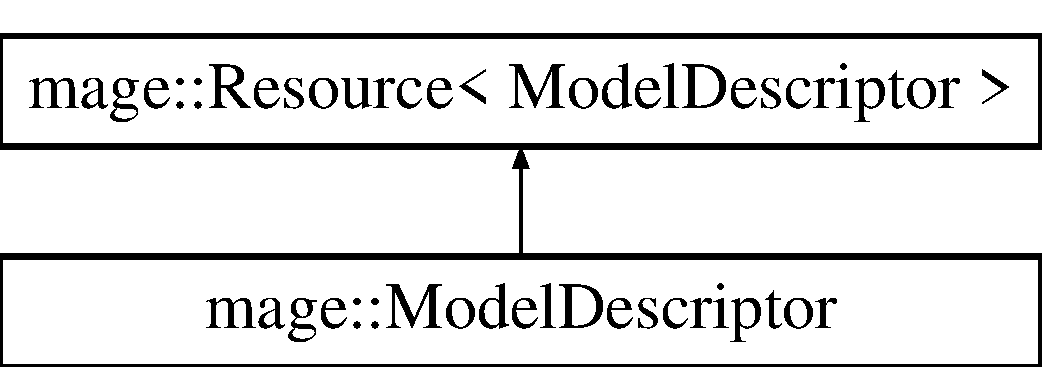
\includegraphics[height=3.000000cm]{classmage_1_1_model_descriptor}
\end{center}
\end{figure}
\subsection*{Public Member Functions}
\begin{DoxyCompactItemize}
\item 
{\footnotesize template$<$typename VertexT $>$ }\\\hyperlink{classmage_1_1_model_descriptor_a1ae1d85907be96350cef77e6a4ba4fb9}{Model\+Descriptor} (I\+D3\+D11\+Device2 $\ast$device, I\+D3\+D11\+Device\+Context2 $\ast$device\+\_\+context, const wstring \&fname, const \hyperlink{structmage_1_1_mesh_descriptor}{Mesh\+Descriptor}$<$ VertexT $>$ \&desc=\hyperlink{structmage_1_1_mesh_descriptor}{Mesh\+Descriptor}$<$ VertexT $>$())
\item 
\hyperlink{classmage_1_1_model_descriptor_af44185efc20e10ede762d29bc454c5f3}{Model\+Descriptor} (const \hyperlink{classmage_1_1_model_descriptor}{Model\+Descriptor} \&desc)=delete
\item 
\hyperlink{classmage_1_1_model_descriptor_af9be9f46bc8f42fa04f686af6cc296f6}{Model\+Descriptor} (\hyperlink{classmage_1_1_model_descriptor}{Model\+Descriptor} \&\&desc)=default
\item 
virtual \hyperlink{classmage_1_1_model_descriptor_a3bc8ee3d1cb8d2675374727edce3d593}{$\sim$\+Model\+Descriptor} ()
\item 
\hyperlink{classmage_1_1_model_descriptor}{Model\+Descriptor} \& \hyperlink{classmage_1_1_model_descriptor_a734b17224719896921e9f6252ee88483}{operator=} (const \hyperlink{classmage_1_1_model_descriptor}{Model\+Descriptor} \&desc)=delete
\item 
\hyperlink{classmage_1_1_model_descriptor}{Model\+Descriptor} \& \hyperlink{classmage_1_1_model_descriptor_ae2ae685569c0ae534d9f0b5622a807d0}{operator=} (\hyperlink{classmage_1_1_model_descriptor}{Model\+Descriptor} \&\&desc)=delete
\item 
\hyperlink{namespacemage_a1e01ae66713838a7a67d30e44c67703e}{Shared\+Ptr}$<$ const \hyperlink{classmage_1_1_static_mesh}{Static\+Mesh} $>$ \hyperlink{classmage_1_1_model_descriptor_a579724811ea4577c039cd1e7655c70fe}{Get\+Mesh} () const
\item 
const \hyperlink{structmage_1_1_material}{Material} $\ast$ \hyperlink{classmage_1_1_model_descriptor_a689fa5039df71c630ec56db378214026}{Get\+Material} (const string \&name) const
\item 
{\footnotesize template$<$typename ActionT $>$ }\\void \hyperlink{classmage_1_1_model_descriptor_ac4723e18238b0d6ac3c54168b8e9a09f}{For\+Each\+Material} (ActionT action) const
\item 
const \hyperlink{structmage_1_1_model_part}{Model\+Part} $\ast$ \hyperlink{classmage_1_1_model_descriptor_af0913a998ec50055e3079c2b4ad6ad2e}{Get\+Model\+Part} (const string \&name) const
\item 
{\footnotesize template$<$typename ActionT $>$ }\\void \hyperlink{classmage_1_1_model_descriptor_a1d61699788385cf29726fac0067bcb5c}{For\+Each\+Model\+Part} (ActionT action) const
\end{DoxyCompactItemize}
\subsection*{Private Attributes}
\begin{DoxyCompactItemize}
\item 
\hyperlink{namespacemage_a1e01ae66713838a7a67d30e44c67703e}{Shared\+Ptr}$<$ \hyperlink{classmage_1_1_static_mesh}{Static\+Mesh} $>$ \hyperlink{classmage_1_1_model_descriptor_ac3935d5b0738860809a770403ed07480}{m\+\_\+mesh}
\item 
vector$<$ \hyperlink{structmage_1_1_material}{Material} $>$ \hyperlink{classmage_1_1_model_descriptor_a672238b257f99836243d84f634ffeea2}{m\+\_\+materials}
\item 
vector$<$ \hyperlink{structmage_1_1_model_part}{Model\+Part} $>$ \hyperlink{classmage_1_1_model_descriptor_a200c6e44c9b6a5bde5c8490fb93ba00f}{m\+\_\+model\+\_\+parts}
\end{DoxyCompactItemize}


\subsection{Constructor \& Destructor Documentation}
\hypertarget{classmage_1_1_model_descriptor_a1ae1d85907be96350cef77e6a4ba4fb9}{}\label{classmage_1_1_model_descriptor_a1ae1d85907be96350cef77e6a4ba4fb9} 
\index{mage\+::\+Model\+Descriptor@{mage\+::\+Model\+Descriptor}!Model\+Descriptor@{Model\+Descriptor}}
\index{Model\+Descriptor@{Model\+Descriptor}!mage\+::\+Model\+Descriptor@{mage\+::\+Model\+Descriptor}}
\subsubsection{\texorpdfstring{Model\+Descriptor()}{ModelDescriptor()}\hspace{0.1cm}{\footnotesize\ttfamily [1/3]}}
{\footnotesize\ttfamily template$<$typename VertexT $>$ \\
mage\+::\+Model\+Descriptor\+::\+Model\+Descriptor (\begin{DoxyParamCaption}\item[{I\+D3\+D11\+Device2 $\ast$}]{device,  }\item[{I\+D3\+D11\+Device\+Context2 $\ast$}]{device\+\_\+context,  }\item[{const wstring \&}]{fname,  }\item[{const \hyperlink{structmage_1_1_mesh_descriptor}{Mesh\+Descriptor}$<$ VertexT $>$ \&}]{desc = {\ttfamily \hyperlink{structmage_1_1_mesh_descriptor}{Mesh\+Descriptor}$<$~VertexT~$>$()} }\end{DoxyParamCaption})\hspace{0.3cm}{\ttfamily [explicit]}}

\hypertarget{classmage_1_1_model_descriptor_af44185efc20e10ede762d29bc454c5f3}{}\label{classmage_1_1_model_descriptor_af44185efc20e10ede762d29bc454c5f3} 
\index{mage\+::\+Model\+Descriptor@{mage\+::\+Model\+Descriptor}!Model\+Descriptor@{Model\+Descriptor}}
\index{Model\+Descriptor@{Model\+Descriptor}!mage\+::\+Model\+Descriptor@{mage\+::\+Model\+Descriptor}}
\subsubsection{\texorpdfstring{Model\+Descriptor()}{ModelDescriptor()}\hspace{0.1cm}{\footnotesize\ttfamily [2/3]}}
{\footnotesize\ttfamily mage\+::\+Model\+Descriptor\+::\+Model\+Descriptor (\begin{DoxyParamCaption}\item[{const \hyperlink{classmage_1_1_model_descriptor}{Model\+Descriptor} \&}]{desc }\end{DoxyParamCaption})\hspace{0.3cm}{\ttfamily [delete]}}

\hypertarget{classmage_1_1_model_descriptor_af9be9f46bc8f42fa04f686af6cc296f6}{}\label{classmage_1_1_model_descriptor_af9be9f46bc8f42fa04f686af6cc296f6} 
\index{mage\+::\+Model\+Descriptor@{mage\+::\+Model\+Descriptor}!Model\+Descriptor@{Model\+Descriptor}}
\index{Model\+Descriptor@{Model\+Descriptor}!mage\+::\+Model\+Descriptor@{mage\+::\+Model\+Descriptor}}
\subsubsection{\texorpdfstring{Model\+Descriptor()}{ModelDescriptor()}\hspace{0.1cm}{\footnotesize\ttfamily [3/3]}}
{\footnotesize\ttfamily mage\+::\+Model\+Descriptor\+::\+Model\+Descriptor (\begin{DoxyParamCaption}\item[{\hyperlink{classmage_1_1_model_descriptor}{Model\+Descriptor} \&\&}]{desc }\end{DoxyParamCaption})\hspace{0.3cm}{\ttfamily [default]}}

\hypertarget{classmage_1_1_model_descriptor_a3bc8ee3d1cb8d2675374727edce3d593}{}\label{classmage_1_1_model_descriptor_a3bc8ee3d1cb8d2675374727edce3d593} 
\index{mage\+::\+Model\+Descriptor@{mage\+::\+Model\+Descriptor}!````~Model\+Descriptor@{$\sim$\+Model\+Descriptor}}
\index{````~Model\+Descriptor@{$\sim$\+Model\+Descriptor}!mage\+::\+Model\+Descriptor@{mage\+::\+Model\+Descriptor}}
\subsubsection{\texorpdfstring{$\sim$\+Model\+Descriptor()}{~ModelDescriptor()}}
{\footnotesize\ttfamily virtual mage\+::\+Model\+Descriptor\+::$\sim$\+Model\+Descriptor (\begin{DoxyParamCaption}{ }\end{DoxyParamCaption})\hspace{0.3cm}{\ttfamily [virtual]}}



\subsection{Member Function Documentation}
\hypertarget{classmage_1_1_model_descriptor_ac4723e18238b0d6ac3c54168b8e9a09f}{}\label{classmage_1_1_model_descriptor_ac4723e18238b0d6ac3c54168b8e9a09f} 
\index{mage\+::\+Model\+Descriptor@{mage\+::\+Model\+Descriptor}!For\+Each\+Material@{For\+Each\+Material}}
\index{For\+Each\+Material@{For\+Each\+Material}!mage\+::\+Model\+Descriptor@{mage\+::\+Model\+Descriptor}}
\subsubsection{\texorpdfstring{For\+Each\+Material()}{ForEachMaterial()}}
{\footnotesize\ttfamily template$<$typename ActionT $>$ \\
void mage\+::\+Model\+Descriptor\+::\+For\+Each\+Material (\begin{DoxyParamCaption}\item[{ActionT}]{action }\end{DoxyParamCaption}) const}

\hypertarget{classmage_1_1_model_descriptor_a1d61699788385cf29726fac0067bcb5c}{}\label{classmage_1_1_model_descriptor_a1d61699788385cf29726fac0067bcb5c} 
\index{mage\+::\+Model\+Descriptor@{mage\+::\+Model\+Descriptor}!For\+Each\+Model\+Part@{For\+Each\+Model\+Part}}
\index{For\+Each\+Model\+Part@{For\+Each\+Model\+Part}!mage\+::\+Model\+Descriptor@{mage\+::\+Model\+Descriptor}}
\subsubsection{\texorpdfstring{For\+Each\+Model\+Part()}{ForEachModelPart()}}
{\footnotesize\ttfamily template$<$typename ActionT $>$ \\
void mage\+::\+Model\+Descriptor\+::\+For\+Each\+Model\+Part (\begin{DoxyParamCaption}\item[{ActionT}]{action }\end{DoxyParamCaption}) const}

\hypertarget{classmage_1_1_model_descriptor_a689fa5039df71c630ec56db378214026}{}\label{classmage_1_1_model_descriptor_a689fa5039df71c630ec56db378214026} 
\index{mage\+::\+Model\+Descriptor@{mage\+::\+Model\+Descriptor}!Get\+Material@{Get\+Material}}
\index{Get\+Material@{Get\+Material}!mage\+::\+Model\+Descriptor@{mage\+::\+Model\+Descriptor}}
\subsubsection{\texorpdfstring{Get\+Material()}{GetMaterial()}}
{\footnotesize\ttfamily const \hyperlink{structmage_1_1_material}{Material} $\ast$ mage\+::\+Model\+Descriptor\+::\+Get\+Material (\begin{DoxyParamCaption}\item[{const string \&}]{name }\end{DoxyParamCaption}) const}

\hypertarget{classmage_1_1_model_descriptor_a579724811ea4577c039cd1e7655c70fe}{}\label{classmage_1_1_model_descriptor_a579724811ea4577c039cd1e7655c70fe} 
\index{mage\+::\+Model\+Descriptor@{mage\+::\+Model\+Descriptor}!Get\+Mesh@{Get\+Mesh}}
\index{Get\+Mesh@{Get\+Mesh}!mage\+::\+Model\+Descriptor@{mage\+::\+Model\+Descriptor}}
\subsubsection{\texorpdfstring{Get\+Mesh()}{GetMesh()}}
{\footnotesize\ttfamily \hyperlink{namespacemage_a1e01ae66713838a7a67d30e44c67703e}{Shared\+Ptr}$<$ const \hyperlink{classmage_1_1_static_mesh}{Static\+Mesh} $>$ mage\+::\+Model\+Descriptor\+::\+Get\+Mesh (\begin{DoxyParamCaption}{ }\end{DoxyParamCaption}) const}

\hypertarget{classmage_1_1_model_descriptor_af0913a998ec50055e3079c2b4ad6ad2e}{}\label{classmage_1_1_model_descriptor_af0913a998ec50055e3079c2b4ad6ad2e} 
\index{mage\+::\+Model\+Descriptor@{mage\+::\+Model\+Descriptor}!Get\+Model\+Part@{Get\+Model\+Part}}
\index{Get\+Model\+Part@{Get\+Model\+Part}!mage\+::\+Model\+Descriptor@{mage\+::\+Model\+Descriptor}}
\subsubsection{\texorpdfstring{Get\+Model\+Part()}{GetModelPart()}}
{\footnotesize\ttfamily const \hyperlink{structmage_1_1_model_part}{Model\+Part} $\ast$ mage\+::\+Model\+Descriptor\+::\+Get\+Model\+Part (\begin{DoxyParamCaption}\item[{const string \&}]{name }\end{DoxyParamCaption}) const}

\hypertarget{classmage_1_1_model_descriptor_a734b17224719896921e9f6252ee88483}{}\label{classmage_1_1_model_descriptor_a734b17224719896921e9f6252ee88483} 
\index{mage\+::\+Model\+Descriptor@{mage\+::\+Model\+Descriptor}!operator=@{operator=}}
\index{operator=@{operator=}!mage\+::\+Model\+Descriptor@{mage\+::\+Model\+Descriptor}}
\subsubsection{\texorpdfstring{operator=()}{operator=()}\hspace{0.1cm}{\footnotesize\ttfamily [1/2]}}
{\footnotesize\ttfamily \hyperlink{classmage_1_1_model_descriptor}{Model\+Descriptor}\& mage\+::\+Model\+Descriptor\+::operator= (\begin{DoxyParamCaption}\item[{const \hyperlink{classmage_1_1_model_descriptor}{Model\+Descriptor} \&}]{desc }\end{DoxyParamCaption})\hspace{0.3cm}{\ttfamily [delete]}}

\hypertarget{classmage_1_1_model_descriptor_ae2ae685569c0ae534d9f0b5622a807d0}{}\label{classmage_1_1_model_descriptor_ae2ae685569c0ae534d9f0b5622a807d0} 
\index{mage\+::\+Model\+Descriptor@{mage\+::\+Model\+Descriptor}!operator=@{operator=}}
\index{operator=@{operator=}!mage\+::\+Model\+Descriptor@{mage\+::\+Model\+Descriptor}}
\subsubsection{\texorpdfstring{operator=()}{operator=()}\hspace{0.1cm}{\footnotesize\ttfamily [2/2]}}
{\footnotesize\ttfamily \hyperlink{classmage_1_1_model_descriptor}{Model\+Descriptor}\& mage\+::\+Model\+Descriptor\+::operator= (\begin{DoxyParamCaption}\item[{\hyperlink{classmage_1_1_model_descriptor}{Model\+Descriptor} \&\&}]{desc }\end{DoxyParamCaption})\hspace{0.3cm}{\ttfamily [delete]}}



\subsection{Member Data Documentation}
\hypertarget{classmage_1_1_model_descriptor_a672238b257f99836243d84f634ffeea2}{}\label{classmage_1_1_model_descriptor_a672238b257f99836243d84f634ffeea2} 
\index{mage\+::\+Model\+Descriptor@{mage\+::\+Model\+Descriptor}!m\+\_\+materials@{m\+\_\+materials}}
\index{m\+\_\+materials@{m\+\_\+materials}!mage\+::\+Model\+Descriptor@{mage\+::\+Model\+Descriptor}}
\subsubsection{\texorpdfstring{m\+\_\+materials}{m\_materials}}
{\footnotesize\ttfamily vector$<$ \hyperlink{structmage_1_1_material}{Material} $>$ mage\+::\+Model\+Descriptor\+::m\+\_\+materials\hspace{0.3cm}{\ttfamily [private]}}

\hypertarget{classmage_1_1_model_descriptor_ac3935d5b0738860809a770403ed07480}{}\label{classmage_1_1_model_descriptor_ac3935d5b0738860809a770403ed07480} 
\index{mage\+::\+Model\+Descriptor@{mage\+::\+Model\+Descriptor}!m\+\_\+mesh@{m\+\_\+mesh}}
\index{m\+\_\+mesh@{m\+\_\+mesh}!mage\+::\+Model\+Descriptor@{mage\+::\+Model\+Descriptor}}
\subsubsection{\texorpdfstring{m\+\_\+mesh}{m\_mesh}}
{\footnotesize\ttfamily \hyperlink{namespacemage_a1e01ae66713838a7a67d30e44c67703e}{Shared\+Ptr}$<$ \hyperlink{classmage_1_1_static_mesh}{Static\+Mesh} $>$ mage\+::\+Model\+Descriptor\+::m\+\_\+mesh\hspace{0.3cm}{\ttfamily [private]}}

\hypertarget{classmage_1_1_model_descriptor_a200c6e44c9b6a5bde5c8490fb93ba00f}{}\label{classmage_1_1_model_descriptor_a200c6e44c9b6a5bde5c8490fb93ba00f} 
\index{mage\+::\+Model\+Descriptor@{mage\+::\+Model\+Descriptor}!m\+\_\+model\+\_\+parts@{m\+\_\+model\+\_\+parts}}
\index{m\+\_\+model\+\_\+parts@{m\+\_\+model\+\_\+parts}!mage\+::\+Model\+Descriptor@{mage\+::\+Model\+Descriptor}}
\subsubsection{\texorpdfstring{m\+\_\+model\+\_\+parts}{m\_model\_parts}}
{\footnotesize\ttfamily vector$<$ \hyperlink{structmage_1_1_model_part}{Model\+Part} $>$ mage\+::\+Model\+Descriptor\+::m\+\_\+model\+\_\+parts\hspace{0.3cm}{\ttfamily [private]}}


\hypertarget{classmage_1_1_model_node}{}\section{mage\+:\+:Model\+Node Class Reference}
\label{classmage_1_1_model_node}\index{mage\+::\+Model\+Node@{mage\+::\+Model\+Node}}


{\ttfamily \#include $<$model\+\_\+node.\+hpp$>$}

Inheritance diagram for mage\+:\+:Model\+Node\+:\begin{figure}[H]
\begin{center}
\leavevmode
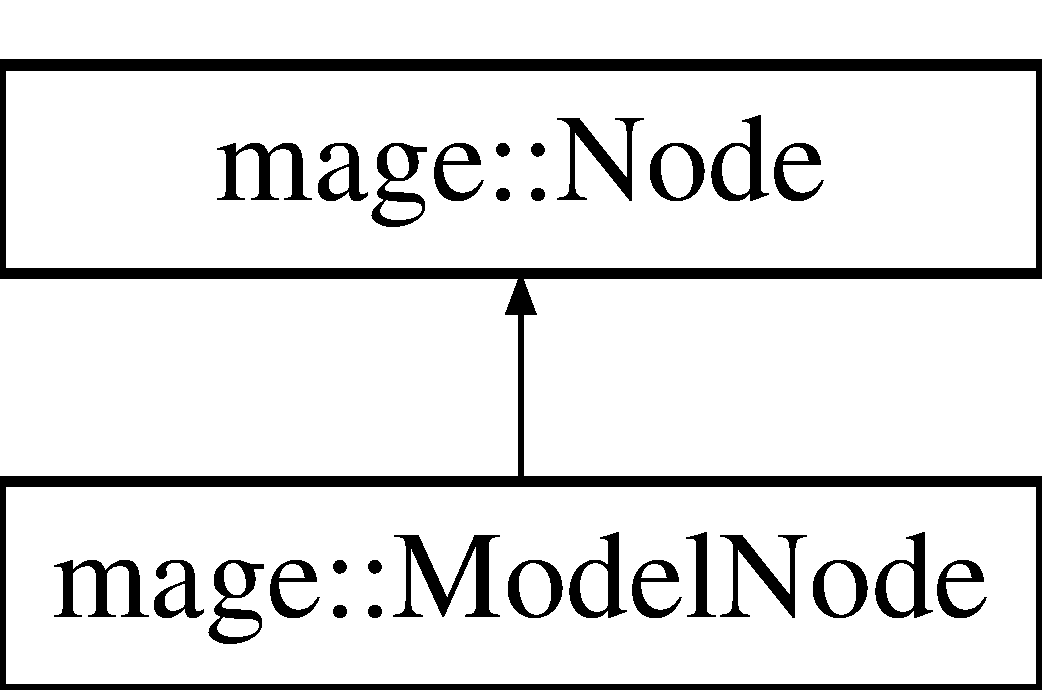
\includegraphics[height=2.000000cm]{classmage_1_1_model_node}
\end{center}
\end{figure}
\subsection*{Public Member Functions}
\begin{DoxyCompactItemize}
\item 
{\footnotesize template$<$typename... Constructor\+ArgsT$>$ }\\\hyperlink{classmage_1_1_model_node_a588aa714637e3e17e764e08c9035bf60}{Model\+Node} (string name, Constructor\+ArgsT \&\&... args)
\item 
\hyperlink{classmage_1_1_model_node_a46f63c13878130126a4b25fdb568ac37}{Model\+Node} (string name, \hyperlink{namespacemage_a3316d7143a973e37adf1110f2e80ca31}{Unique\+Ptr}$<$ \hyperlink{classmage_1_1_model}{Model} $>$ \&\&model)
\item 
\hyperlink{classmage_1_1_model_node_a409c098ddecf20d1b393d43c15d16482}{Model\+Node} (const \hyperlink{classmage_1_1_model_node}{Model\+Node} \&model\+\_\+node)
\item 
\hyperlink{classmage_1_1_model_node_a19ba577112ea488f227ea31642fb2cb2}{Model\+Node} (\hyperlink{classmage_1_1_model_node}{Model\+Node} \&\&model\+\_\+node)
\item 
virtual \hyperlink{classmage_1_1_model_node_a131c0062a1bed3d29fade27e602bec44}{$\sim$\+Model\+Node} ()
\item 
\hyperlink{classmage_1_1_model_node}{Model\+Node} \& \hyperlink{classmage_1_1_model_node_ad8378279b79930dfe98d176dbc1c5db9}{operator=} (const \hyperlink{classmage_1_1_model_node}{Model\+Node} \&model\+\_\+node)=delete
\item 
\hyperlink{classmage_1_1_model_node}{Model\+Node} \& \hyperlink{classmage_1_1_model_node_ad39321f4d392aa4e28169b8d7a08af68}{operator=} (\hyperlink{classmage_1_1_model_node}{Model\+Node} \&\&model\+\_\+node)=delete
\item 
\hyperlink{namespacemage_a3316d7143a973e37adf1110f2e80ca31}{Unique\+Ptr}$<$ \hyperlink{classmage_1_1_model_node}{Model\+Node} $>$ \hyperlink{classmage_1_1_model_node_a766f90e1d626c455ba552a3ded08b948}{Clone} () const
\item 
\hyperlink{classmage_1_1_texture_transform}{Texture\+Transform} $\ast$ \hyperlink{classmage_1_1_model_node_aa5b732d1ad0f3d2ff8549731708fd63c}{Get\+Texture\+Transform} () noexcept
\item 
const \hyperlink{classmage_1_1_texture_transform}{Texture\+Transform} $\ast$ \hyperlink{classmage_1_1_model_node_a3686306f587abaa353450c45dd508dc4}{Get\+Texture\+Transform} () const noexcept
\item 
\hyperlink{classmage_1_1_model}{Model} $\ast$ \hyperlink{classmage_1_1_model_node_a8964223fd592fd23949d6f996c40a482}{Get\+Model} () noexcept
\item 
const \hyperlink{classmage_1_1_model}{Model} $\ast$ \hyperlink{classmage_1_1_model_node_ad8c4978c4d14ed015fdb517ba86ebd93}{Get\+Model} () const noexcept
\end{DoxyCompactItemize}
\subsection*{Private Member Functions}
\begin{DoxyCompactItemize}
\item 
virtual \hyperlink{namespacemage_a3316d7143a973e37adf1110f2e80ca31}{Unique\+Ptr}$<$ \hyperlink{classmage_1_1_node}{Node} $>$ \hyperlink{classmage_1_1_model_node_a34146201083015276b38240af307417f}{Clone\+Implementation} () const override
\end{DoxyCompactItemize}
\subsection*{Private Attributes}
\begin{DoxyCompactItemize}
\item 
\hyperlink{namespacemage_a3316d7143a973e37adf1110f2e80ca31}{Unique\+Ptr}$<$ \hyperlink{classmage_1_1_model}{Model} $>$ \hyperlink{classmage_1_1_model_node_a784faf19f736a1c74808321ed0e52d36}{m\+\_\+model}
\item 
\hyperlink{namespacemage_a3316d7143a973e37adf1110f2e80ca31}{Unique\+Ptr}$<$ \hyperlink{classmage_1_1_texture_transform}{Texture\+Transform} $>$ \hyperlink{classmage_1_1_model_node_a24888374dcf3e1fdba4a3a0790931a0a}{m\+\_\+texture\+\_\+transform}
\end{DoxyCompactItemize}


\subsection{Detailed Description}
A class of model nodes. 

\subsection{Constructor \& Destructor Documentation}
\hypertarget{classmage_1_1_model_node_a588aa714637e3e17e764e08c9035bf60}{}\label{classmage_1_1_model_node_a588aa714637e3e17e764e08c9035bf60} 
\index{mage\+::\+Model\+Node@{mage\+::\+Model\+Node}!Model\+Node@{Model\+Node}}
\index{Model\+Node@{Model\+Node}!mage\+::\+Model\+Node@{mage\+::\+Model\+Node}}
\subsubsection{\texorpdfstring{Model\+Node()}{ModelNode()}\hspace{0.1cm}{\footnotesize\ttfamily [1/4]}}
{\footnotesize\ttfamily template$<$typename... Constructor\+ArgsT$>$ \\
mage\+::\+Model\+Node\+::\+Model\+Node (\begin{DoxyParamCaption}\item[{string}]{name,  }\item[{Constructor\+ArgsT \&\&...}]{args }\end{DoxyParamCaption})\hspace{0.3cm}{\ttfamily [explicit]}}

Constructs a model node.


\begin{DoxyTemplParams}{Template Parameters}
{\em Constructor\+ArgsT} & The constructor argument types of the model. \\
\hline
\end{DoxyTemplParams}

\begin{DoxyParams}[1]{Parameters}
\mbox{\tt in}  & {\em name} & The name. \\
\hline
\mbox{\tt in}  & {\em args} & A reference to the constructor arguments for the model. \\
\hline
\end{DoxyParams}
\hypertarget{classmage_1_1_model_node_a46f63c13878130126a4b25fdb568ac37}{}\label{classmage_1_1_model_node_a46f63c13878130126a4b25fdb568ac37} 
\index{mage\+::\+Model\+Node@{mage\+::\+Model\+Node}!Model\+Node@{Model\+Node}}
\index{Model\+Node@{Model\+Node}!mage\+::\+Model\+Node@{mage\+::\+Model\+Node}}
\subsubsection{\texorpdfstring{Model\+Node()}{ModelNode()}\hspace{0.1cm}{\footnotesize\ttfamily [2/4]}}
{\footnotesize\ttfamily mage\+::\+Model\+Node\+::\+Model\+Node (\begin{DoxyParamCaption}\item[{string}]{name,  }\item[{\hyperlink{namespacemage_a3316d7143a973e37adf1110f2e80ca31}{Unique\+Ptr}$<$ \hyperlink{classmage_1_1_model}{Model} $>$ \&\&}]{model }\end{DoxyParamCaption})\hspace{0.3cm}{\ttfamily [explicit]}}

Constructs a model node.

\begin{DoxyPrecond}{Precondition}
{\itshape model} refers to a non {\ttfamily nullptr}. 
\end{DoxyPrecond}

\begin{DoxyParams}[1]{Parameters}
\mbox{\tt in}  & {\em name} & The name. \\
\hline
\mbox{\tt in}  & {\em model} & A reference to the model to move. \\
\hline
\end{DoxyParams}
\hypertarget{classmage_1_1_model_node_a409c098ddecf20d1b393d43c15d16482}{}\label{classmage_1_1_model_node_a409c098ddecf20d1b393d43c15d16482} 
\index{mage\+::\+Model\+Node@{mage\+::\+Model\+Node}!Model\+Node@{Model\+Node}}
\index{Model\+Node@{Model\+Node}!mage\+::\+Model\+Node@{mage\+::\+Model\+Node}}
\subsubsection{\texorpdfstring{Model\+Node()}{ModelNode()}\hspace{0.1cm}{\footnotesize\ttfamily [3/4]}}
{\footnotesize\ttfamily mage\+::\+Model\+Node\+::\+Model\+Node (\begin{DoxyParamCaption}\item[{const \hyperlink{classmage_1_1_model_node}{Model\+Node} \&}]{model\+\_\+node }\end{DoxyParamCaption})}

Constructs a model node from the given model node.


\begin{DoxyParams}[1]{Parameters}
\mbox{\tt in}  & {\em model\+\_\+node} & A reference to the model node to copy. \\
\hline
\end{DoxyParams}
\hypertarget{classmage_1_1_model_node_a19ba577112ea488f227ea31642fb2cb2}{}\label{classmage_1_1_model_node_a19ba577112ea488f227ea31642fb2cb2} 
\index{mage\+::\+Model\+Node@{mage\+::\+Model\+Node}!Model\+Node@{Model\+Node}}
\index{Model\+Node@{Model\+Node}!mage\+::\+Model\+Node@{mage\+::\+Model\+Node}}
\subsubsection{\texorpdfstring{Model\+Node()}{ModelNode()}\hspace{0.1cm}{\footnotesize\ttfamily [4/4]}}
{\footnotesize\ttfamily mage\+::\+Model\+Node\+::\+Model\+Node (\begin{DoxyParamCaption}\item[{\hyperlink{classmage_1_1_model_node}{Model\+Node} \&\&}]{model\+\_\+node }\end{DoxyParamCaption})\hspace{0.3cm}{\ttfamily [default]}}

Constructs a model node by moving the given model node.


\begin{DoxyParams}[1]{Parameters}
\mbox{\tt in}  & {\em model\+\_\+node} & A reference to the model node to move. \\
\hline
\end{DoxyParams}
\hypertarget{classmage_1_1_model_node_a131c0062a1bed3d29fade27e602bec44}{}\label{classmage_1_1_model_node_a131c0062a1bed3d29fade27e602bec44} 
\index{mage\+::\+Model\+Node@{mage\+::\+Model\+Node}!````~Model\+Node@{$\sim$\+Model\+Node}}
\index{````~Model\+Node@{$\sim$\+Model\+Node}!mage\+::\+Model\+Node@{mage\+::\+Model\+Node}}
\subsubsection{\texorpdfstring{$\sim$\+Model\+Node()}{~ModelNode()}}
{\footnotesize\ttfamily mage\+::\+Model\+Node\+::$\sim$\+Model\+Node (\begin{DoxyParamCaption}{ }\end{DoxyParamCaption})\hspace{0.3cm}{\ttfamily [virtual]}, {\ttfamily [default]}}

Destructs this model node. 

\subsection{Member Function Documentation}
\hypertarget{classmage_1_1_model_node_a766f90e1d626c455ba552a3ded08b948}{}\label{classmage_1_1_model_node_a766f90e1d626c455ba552a3ded08b948} 
\index{mage\+::\+Model\+Node@{mage\+::\+Model\+Node}!Clone@{Clone}}
\index{Clone@{Clone}!mage\+::\+Model\+Node@{mage\+::\+Model\+Node}}
\subsubsection{\texorpdfstring{Clone()}{Clone()}}
{\footnotesize\ttfamily \hyperlink{namespacemage_a3316d7143a973e37adf1110f2e80ca31}{Unique\+Ptr}$<$ \hyperlink{classmage_1_1_model_node}{Model\+Node} $>$ mage\+::\+Model\+Node\+::\+Clone (\begin{DoxyParamCaption}{ }\end{DoxyParamCaption}) const}

Clones this model node.

\begin{DoxyReturn}{Returns}
A pointer to the clone of this model node. 
\end{DoxyReturn}
\hypertarget{classmage_1_1_model_node_a34146201083015276b38240af307417f}{}\label{classmage_1_1_model_node_a34146201083015276b38240af307417f} 
\index{mage\+::\+Model\+Node@{mage\+::\+Model\+Node}!Clone\+Implementation@{Clone\+Implementation}}
\index{Clone\+Implementation@{Clone\+Implementation}!mage\+::\+Model\+Node@{mage\+::\+Model\+Node}}
\subsubsection{\texorpdfstring{Clone\+Implementation()}{CloneImplementation()}}
{\footnotesize\ttfamily \hyperlink{namespacemage_a3316d7143a973e37adf1110f2e80ca31}{Unique\+Ptr}$<$ \hyperlink{classmage_1_1_node}{Node} $>$ mage\+::\+Model\+Node\+::\+Clone\+Implementation (\begin{DoxyParamCaption}{ }\end{DoxyParamCaption}) const\hspace{0.3cm}{\ttfamily [override]}, {\ttfamily [private]}, {\ttfamily [virtual]}}

Clones this model node.

\begin{DoxyReturn}{Returns}
A pointer to the clone of this model node. 
\end{DoxyReturn}


Reimplemented from \hyperlink{classmage_1_1_node_a71a4763bfd4cba5653488b490e61dc8f}{mage\+::\+Node}.

\hypertarget{classmage_1_1_model_node_a8964223fd592fd23949d6f996c40a482}{}\label{classmage_1_1_model_node_a8964223fd592fd23949d6f996c40a482} 
\index{mage\+::\+Model\+Node@{mage\+::\+Model\+Node}!Get\+Model@{Get\+Model}}
\index{Get\+Model@{Get\+Model}!mage\+::\+Model\+Node@{mage\+::\+Model\+Node}}
\subsubsection{\texorpdfstring{Get\+Model()}{GetModel()}\hspace{0.1cm}{\footnotesize\ttfamily [1/2]}}
{\footnotesize\ttfamily \hyperlink{classmage_1_1_model}{Model}$\ast$ mage\+::\+Model\+Node\+::\+Get\+Model (\begin{DoxyParamCaption}{ }\end{DoxyParamCaption})\hspace{0.3cm}{\ttfamily [noexcept]}}

Returns the model of this model node.

\begin{DoxyReturn}{Returns}
A pointer to the model of this model node. 
\end{DoxyReturn}
\hypertarget{classmage_1_1_model_node_ad8c4978c4d14ed015fdb517ba86ebd93}{}\label{classmage_1_1_model_node_ad8c4978c4d14ed015fdb517ba86ebd93} 
\index{mage\+::\+Model\+Node@{mage\+::\+Model\+Node}!Get\+Model@{Get\+Model}}
\index{Get\+Model@{Get\+Model}!mage\+::\+Model\+Node@{mage\+::\+Model\+Node}}
\subsubsection{\texorpdfstring{Get\+Model()}{GetModel()}\hspace{0.1cm}{\footnotesize\ttfamily [2/2]}}
{\footnotesize\ttfamily const \hyperlink{classmage_1_1_model}{Model}$\ast$ mage\+::\+Model\+Node\+::\+Get\+Model (\begin{DoxyParamCaption}{ }\end{DoxyParamCaption}) const\hspace{0.3cm}{\ttfamily [noexcept]}}

Returns the model of this model node.

\begin{DoxyReturn}{Returns}
A pointer to the model of this model node. 
\end{DoxyReturn}
\hypertarget{classmage_1_1_model_node_aa5b732d1ad0f3d2ff8549731708fd63c}{}\label{classmage_1_1_model_node_aa5b732d1ad0f3d2ff8549731708fd63c} 
\index{mage\+::\+Model\+Node@{mage\+::\+Model\+Node}!Get\+Texture\+Transform@{Get\+Texture\+Transform}}
\index{Get\+Texture\+Transform@{Get\+Texture\+Transform}!mage\+::\+Model\+Node@{mage\+::\+Model\+Node}}
\subsubsection{\texorpdfstring{Get\+Texture\+Transform()}{GetTextureTransform()}\hspace{0.1cm}{\footnotesize\ttfamily [1/2]}}
{\footnotesize\ttfamily \hyperlink{classmage_1_1_texture_transform}{Texture\+Transform}$\ast$ mage\+::\+Model\+Node\+::\+Get\+Texture\+Transform (\begin{DoxyParamCaption}{ }\end{DoxyParamCaption})\hspace{0.3cm}{\ttfamily [noexcept]}}

Returns the texture transform of this model node.

\begin{DoxyReturn}{Returns}
A pointer to the texture transform of this model node. 
\end{DoxyReturn}
\hypertarget{classmage_1_1_model_node_a3686306f587abaa353450c45dd508dc4}{}\label{classmage_1_1_model_node_a3686306f587abaa353450c45dd508dc4} 
\index{mage\+::\+Model\+Node@{mage\+::\+Model\+Node}!Get\+Texture\+Transform@{Get\+Texture\+Transform}}
\index{Get\+Texture\+Transform@{Get\+Texture\+Transform}!mage\+::\+Model\+Node@{mage\+::\+Model\+Node}}
\subsubsection{\texorpdfstring{Get\+Texture\+Transform()}{GetTextureTransform()}\hspace{0.1cm}{\footnotesize\ttfamily [2/2]}}
{\footnotesize\ttfamily const \hyperlink{classmage_1_1_texture_transform}{Texture\+Transform}$\ast$ mage\+::\+Model\+Node\+::\+Get\+Texture\+Transform (\begin{DoxyParamCaption}{ }\end{DoxyParamCaption}) const\hspace{0.3cm}{\ttfamily [noexcept]}}

Returns the texture transform of this model node.

\begin{DoxyReturn}{Returns}
A pointer to the texture transform of this model node. 
\end{DoxyReturn}
\hypertarget{classmage_1_1_model_node_ad8378279b79930dfe98d176dbc1c5db9}{}\label{classmage_1_1_model_node_ad8378279b79930dfe98d176dbc1c5db9} 
\index{mage\+::\+Model\+Node@{mage\+::\+Model\+Node}!operator=@{operator=}}
\index{operator=@{operator=}!mage\+::\+Model\+Node@{mage\+::\+Model\+Node}}
\subsubsection{\texorpdfstring{operator=()}{operator=()}\hspace{0.1cm}{\footnotesize\ttfamily [1/2]}}
{\footnotesize\ttfamily \hyperlink{classmage_1_1_model_node}{Model\+Node}\& mage\+::\+Model\+Node\+::operator= (\begin{DoxyParamCaption}\item[{const \hyperlink{classmage_1_1_model_node}{Model\+Node} \&}]{model\+\_\+node }\end{DoxyParamCaption})\hspace{0.3cm}{\ttfamily [delete]}}

Copies the given model node to this model node.


\begin{DoxyParams}[1]{Parameters}
\mbox{\tt in}  & {\em model\+\_\+node} & A reference to the model node to copy. \\
\hline
\end{DoxyParams}
\begin{DoxyReturn}{Returns}
A reference to the copy of the given model node (i.\+e. this model node). 
\end{DoxyReturn}
\hypertarget{classmage_1_1_model_node_ad39321f4d392aa4e28169b8d7a08af68}{}\label{classmage_1_1_model_node_ad39321f4d392aa4e28169b8d7a08af68} 
\index{mage\+::\+Model\+Node@{mage\+::\+Model\+Node}!operator=@{operator=}}
\index{operator=@{operator=}!mage\+::\+Model\+Node@{mage\+::\+Model\+Node}}
\subsubsection{\texorpdfstring{operator=()}{operator=()}\hspace{0.1cm}{\footnotesize\ttfamily [2/2]}}
{\footnotesize\ttfamily \hyperlink{classmage_1_1_model_node}{Model\+Node}\& mage\+::\+Model\+Node\+::operator= (\begin{DoxyParamCaption}\item[{\hyperlink{classmage_1_1_model_node}{Model\+Node} \&\&}]{model\+\_\+node }\end{DoxyParamCaption})\hspace{0.3cm}{\ttfamily [delete]}}

Moves the given model node to this model node.


\begin{DoxyParams}[1]{Parameters}
\mbox{\tt in}  & {\em model\+\_\+node} & A reference to the model node to move. \\
\hline
\end{DoxyParams}
\begin{DoxyReturn}{Returns}
A reference to the moved model node (i.\+e. this model node). 
\end{DoxyReturn}


\subsection{Member Data Documentation}
\hypertarget{classmage_1_1_model_node_a784faf19f736a1c74808321ed0e52d36}{}\label{classmage_1_1_model_node_a784faf19f736a1c74808321ed0e52d36} 
\index{mage\+::\+Model\+Node@{mage\+::\+Model\+Node}!m\+\_\+model@{m\+\_\+model}}
\index{m\+\_\+model@{m\+\_\+model}!mage\+::\+Model\+Node@{mage\+::\+Model\+Node}}
\subsubsection{\texorpdfstring{m\+\_\+model}{m\_model}}
{\footnotesize\ttfamily \hyperlink{namespacemage_a3316d7143a973e37adf1110f2e80ca31}{Unique\+Ptr}$<$ \hyperlink{classmage_1_1_model}{Model} $>$ mage\+::\+Model\+Node\+::m\+\_\+model\hspace{0.3cm}{\ttfamily [private]}}

A pointer to the model of this model node. \hypertarget{classmage_1_1_model_node_a24888374dcf3e1fdba4a3a0790931a0a}{}\label{classmage_1_1_model_node_a24888374dcf3e1fdba4a3a0790931a0a} 
\index{mage\+::\+Model\+Node@{mage\+::\+Model\+Node}!m\+\_\+texture\+\_\+transform@{m\+\_\+texture\+\_\+transform}}
\index{m\+\_\+texture\+\_\+transform@{m\+\_\+texture\+\_\+transform}!mage\+::\+Model\+Node@{mage\+::\+Model\+Node}}
\subsubsection{\texorpdfstring{m\+\_\+texture\+\_\+transform}{m\_texture\_transform}}
{\footnotesize\ttfamily \hyperlink{namespacemage_a3316d7143a973e37adf1110f2e80ca31}{Unique\+Ptr}$<$ \hyperlink{classmage_1_1_texture_transform}{Texture\+Transform} $>$ mage\+::\+Model\+Node\+::m\+\_\+texture\+\_\+transform\hspace{0.3cm}{\ttfamily [private]}}

A pointer to the model of this model node. 
\hypertarget{structmage_1_1_model_output}{}\section{mage\+:\+:Model\+Output$<$ VertexT $>$ Struct Template Reference}
\label{structmage_1_1_model_output}\index{mage\+::\+Model\+Output$<$ Vertex\+T $>$@{mage\+::\+Model\+Output$<$ Vertex\+T $>$}}


{\ttfamily \#include $<$model\+\_\+output.\+hpp$>$}

\subsection*{Public Member Functions}
\begin{DoxyCompactItemize}
\item 
\hyperlink{structmage_1_1_model_output_a7d64b57d8207968541eb9c6da6ef0163}{Model\+Output} ()=default
\item 
\hyperlink{structmage_1_1_model_output_aac808e40a66f33da4ea28ebb7443623d}{Model\+Output} (const \hyperlink{structmage_1_1_model_output}{Model\+Output}$<$ VertexT $>$ \&output)=delete
\item 
\hyperlink{structmage_1_1_model_output_a20faa6e5b76ec7903a09e222e61e5353}{Model\+Output} (\hyperlink{structmage_1_1_model_output}{Model\+Output}$<$ VertexT $>$ \&\&output)=default
\item 
\hyperlink{structmage_1_1_model_output_a69a7f27486ad287943cbf973107ad8e1}{$\sim$\+Model\+Output} ()=default
\item 
\hyperlink{structmage_1_1_model_output}{Model\+Output}$<$ VertexT $>$ \& \hyperlink{structmage_1_1_model_output_ada52bf380c0259a0d7ef855457e5a9da}{operator=} (const \hyperlink{structmage_1_1_model_output}{Model\+Output}$<$ VertexT $>$ \&output)=delete
\item 
\hyperlink{structmage_1_1_model_output}{Model\+Output}$<$ VertexT $>$ \& \hyperlink{structmage_1_1_model_output_a5e368e3ae8a52d329f8d9b5f1c4b9d03}{operator=} (\hyperlink{structmage_1_1_model_output}{Model\+Output}$<$ VertexT $>$ \&\&output)=delete
\item 
void \hyperlink{structmage_1_1_model_output_ad62942de2a55fce53d31aeafa1d0795a}{Add\+Model\+Part} (\hyperlink{structmage_1_1_model_part}{Model\+Part} \&\&model\+\_\+part, bool create\+\_\+bounding\+\_\+volumes=true)
\item 
bool \hyperlink{structmage_1_1_model_output_a90c6d42d13813b9c340bd1a250276a8d}{Has\+Model\+Part} (const string \&name) noexcept
\item 
void \hyperlink{structmage_1_1_model_output_a833c8e380e2812ab0ca2853bb915e75f}{Start\+Model\+Part} (string child, string parent=M\+A\+G\+E\+\_\+\+M\+D\+L\+\_\+\+P\+A\+R\+T\+\_\+\+D\+E\+F\+A\+U\+L\+T\+\_\+\+P\+A\+R\+E\+NT)
\item 
void \hyperlink{structmage_1_1_model_output_a26836ecfea7e7f78cc1c1e37da915230}{Set\+Material} (string material)
\item 
void \hyperlink{structmage_1_1_model_output_aca4628ef55d8ded956de4c06e1433f45}{End\+Model\+Part} (bool create\+\_\+bounding\+\_\+volumes=true) noexcept
\end{DoxyCompactItemize}
\subsection*{Public Attributes}
\begin{DoxyCompactItemize}
\item 
vector$<$ VertexT $>$ \hyperlink{structmage_1_1_model_output_a4d669b5fee2d6a1bc993a94b0a2d5580}{m\+\_\+vertex\+\_\+buffer}
\item 
vector$<$ \hyperlink{namespacemage_a41c104c036fba3756a74e19f793eeaa1}{U32} $>$ \hyperlink{structmage_1_1_model_output_a0d38026bd5211748810a27b54375689d}{m\+\_\+index\+\_\+buffer}
\item 
vector$<$ \hyperlink{classmage_1_1_material}{Material} $>$ \hyperlink{structmage_1_1_model_output_a3bfdb493d92a83b40a8b363a96e89a0c}{m\+\_\+material\+\_\+buffer}
\item 
vector$<$ \hyperlink{structmage_1_1_model_part}{Model\+Part} $>$ \hyperlink{structmage_1_1_model_output_a86df369ff4959458ee6991c36e6aa01a}{m\+\_\+model\+\_\+parts}
\end{DoxyCompactItemize}
\subsection*{Private Member Functions}
\begin{DoxyCompactItemize}
\item 
void \hyperlink{structmage_1_1_model_output_aec05a0a43d141b8b8260e741314615c1}{Setup\+Bounding\+Volumes} (\hyperlink{structmage_1_1_model_part}{Model\+Part} \&model\+\_\+part) noexcept
\end{DoxyCompactItemize}


\subsection{Detailed Description}
\subsubsection*{template$<$typename VertexT$>$\newline
struct mage\+::\+Model\+Output$<$ Vertex\+T $>$}

A struct of model outputs.


\begin{DoxyTemplParams}{Template Parameters}
{\em VertexT} & The vertex type. \\
\hline
\end{DoxyTemplParams}


\subsection{Constructor \& Destructor Documentation}
\hypertarget{structmage_1_1_model_output_a7d64b57d8207968541eb9c6da6ef0163}{}\label{structmage_1_1_model_output_a7d64b57d8207968541eb9c6da6ef0163} 
\index{mage\+::\+Model\+Output@{mage\+::\+Model\+Output}!Model\+Output@{Model\+Output}}
\index{Model\+Output@{Model\+Output}!mage\+::\+Model\+Output@{mage\+::\+Model\+Output}}
\subsubsection{\texorpdfstring{Model\+Output()}{ModelOutput()}\hspace{0.1cm}{\footnotesize\ttfamily [1/3]}}
{\footnotesize\ttfamily template$<$typename VertexT $>$ \\
\hyperlink{structmage_1_1_model_output}{mage\+::\+Model\+Output}$<$ VertexT $>$\+::\hyperlink{structmage_1_1_model_output}{Model\+Output} (\begin{DoxyParamCaption}{ }\end{DoxyParamCaption})\hspace{0.3cm}{\ttfamily [default]}}

Constructs a model output. \hypertarget{structmage_1_1_model_output_aac808e40a66f33da4ea28ebb7443623d}{}\label{structmage_1_1_model_output_aac808e40a66f33da4ea28ebb7443623d} 
\index{mage\+::\+Model\+Output@{mage\+::\+Model\+Output}!Model\+Output@{Model\+Output}}
\index{Model\+Output@{Model\+Output}!mage\+::\+Model\+Output@{mage\+::\+Model\+Output}}
\subsubsection{\texorpdfstring{Model\+Output()}{ModelOutput()}\hspace{0.1cm}{\footnotesize\ttfamily [2/3]}}
{\footnotesize\ttfamily template$<$typename VertexT $>$ \\
\hyperlink{structmage_1_1_model_output}{mage\+::\+Model\+Output}$<$ VertexT $>$\+::\hyperlink{structmage_1_1_model_output}{Model\+Output} (\begin{DoxyParamCaption}\item[{const \hyperlink{structmage_1_1_model_output}{Model\+Output}$<$ VertexT $>$ \&}]{output }\end{DoxyParamCaption})\hspace{0.3cm}{\ttfamily [delete]}}

Constructs a model output from the given model output.


\begin{DoxyParams}[1]{Parameters}
\mbox{\tt in}  & {\em output} & A reference to the model output to copy. \\
\hline
\end{DoxyParams}
\hypertarget{structmage_1_1_model_output_a20faa6e5b76ec7903a09e222e61e5353}{}\label{structmage_1_1_model_output_a20faa6e5b76ec7903a09e222e61e5353} 
\index{mage\+::\+Model\+Output@{mage\+::\+Model\+Output}!Model\+Output@{Model\+Output}}
\index{Model\+Output@{Model\+Output}!mage\+::\+Model\+Output@{mage\+::\+Model\+Output}}
\subsubsection{\texorpdfstring{Model\+Output()}{ModelOutput()}\hspace{0.1cm}{\footnotesize\ttfamily [3/3]}}
{\footnotesize\ttfamily template$<$typename VertexT $>$ \\
\hyperlink{structmage_1_1_model_output}{mage\+::\+Model\+Output}$<$ VertexT $>$\+::\hyperlink{structmage_1_1_model_output}{Model\+Output} (\begin{DoxyParamCaption}\item[{\hyperlink{structmage_1_1_model_output}{Model\+Output}$<$ VertexT $>$ \&\&}]{output }\end{DoxyParamCaption})\hspace{0.3cm}{\ttfamily [default]}}

Constructs a model output by moving the given model output.


\begin{DoxyParams}[1]{Parameters}
\mbox{\tt in}  & {\em output} & A reference to the model output to move. \\
\hline
\end{DoxyParams}
\hypertarget{structmage_1_1_model_output_a69a7f27486ad287943cbf973107ad8e1}{}\label{structmage_1_1_model_output_a69a7f27486ad287943cbf973107ad8e1} 
\index{mage\+::\+Model\+Output@{mage\+::\+Model\+Output}!````~Model\+Output@{$\sim$\+Model\+Output}}
\index{````~Model\+Output@{$\sim$\+Model\+Output}!mage\+::\+Model\+Output@{mage\+::\+Model\+Output}}
\subsubsection{\texorpdfstring{$\sim$\+Model\+Output()}{~ModelOutput()}}
{\footnotesize\ttfamily template$<$typename VertexT $>$ \\
\hyperlink{structmage_1_1_model_output}{mage\+::\+Model\+Output}$<$ VertexT $>$\+::$\sim$\hyperlink{structmage_1_1_model_output}{Model\+Output} (\begin{DoxyParamCaption}{ }\end{DoxyParamCaption})\hspace{0.3cm}{\ttfamily [default]}}

Destructs this model output. 

\subsection{Member Function Documentation}
\hypertarget{structmage_1_1_model_output_ad62942de2a55fce53d31aeafa1d0795a}{}\label{structmage_1_1_model_output_ad62942de2a55fce53d31aeafa1d0795a} 
\index{mage\+::\+Model\+Output@{mage\+::\+Model\+Output}!Add\+Model\+Part@{Add\+Model\+Part}}
\index{Add\+Model\+Part@{Add\+Model\+Part}!mage\+::\+Model\+Output@{mage\+::\+Model\+Output}}
\subsubsection{\texorpdfstring{Add\+Model\+Part()}{AddModelPart()}}
{\footnotesize\ttfamily template$<$typename VertexT $>$ \\
void \hyperlink{structmage_1_1_model_output}{mage\+::\+Model\+Output}$<$ VertexT $>$\+::Add\+Model\+Part (\begin{DoxyParamCaption}\item[{\hyperlink{structmage_1_1_model_part}{Model\+Part} \&\&}]{model\+\_\+part,  }\item[{bool}]{create\+\_\+bounding\+\_\+volumes = {\ttfamily true} }\end{DoxyParamCaption})}

Adds a model part.


\begin{DoxyParams}[1]{Parameters}
\mbox{\tt in}  & {\em model\+\_\+part} & A reference to the model part to add. \\
\hline
\mbox{\tt in}  & {\em create\+\_\+bounding\+\_\+volumes} & A flag indicating whether bounding volumes must be created for the given model part. \\
\hline
\end{DoxyParams}
\hypertarget{structmage_1_1_model_output_aca4628ef55d8ded956de4c06e1433f45}{}\label{structmage_1_1_model_output_aca4628ef55d8ded956de4c06e1433f45} 
\index{mage\+::\+Model\+Output@{mage\+::\+Model\+Output}!End\+Model\+Part@{End\+Model\+Part}}
\index{End\+Model\+Part@{End\+Model\+Part}!mage\+::\+Model\+Output@{mage\+::\+Model\+Output}}
\subsubsection{\texorpdfstring{End\+Model\+Part()}{EndModelPart()}}
{\footnotesize\ttfamily template$<$typename VertexT $>$ \\
void \hyperlink{structmage_1_1_model_output}{mage\+::\+Model\+Output}$<$ VertexT $>$\+::End\+Model\+Part (\begin{DoxyParamCaption}\item[{bool}]{create\+\_\+bounding\+\_\+volumes = {\ttfamily true} }\end{DoxyParamCaption})\hspace{0.3cm}{\ttfamily [noexcept]}}

Ends the creation of the last model part.

\begin{DoxyPrecond}{Precondition}
This model output contains at least one model part. 
\end{DoxyPrecond}

\begin{DoxyParams}[1]{Parameters}
\mbox{\tt in}  & {\em create\+\_\+bounding\+\_\+volumes} & A flag indicating whether bounding volumes must be created for the given model part. \\
\hline
\end{DoxyParams}
\hypertarget{structmage_1_1_model_output_a90c6d42d13813b9c340bd1a250276a8d}{}\label{structmage_1_1_model_output_a90c6d42d13813b9c340bd1a250276a8d} 
\index{mage\+::\+Model\+Output@{mage\+::\+Model\+Output}!Has\+Model\+Part@{Has\+Model\+Part}}
\index{Has\+Model\+Part@{Has\+Model\+Part}!mage\+::\+Model\+Output@{mage\+::\+Model\+Output}}
\subsubsection{\texorpdfstring{Has\+Model\+Part()}{HasModelPart()}}
{\footnotesize\ttfamily template$<$typename VertexT $>$ \\
bool \hyperlink{structmage_1_1_model_output}{mage\+::\+Model\+Output}$<$ VertexT $>$\+::Has\+Model\+Part (\begin{DoxyParamCaption}\item[{const string \&}]{name }\end{DoxyParamCaption})\hspace{0.3cm}{\ttfamily [noexcept]}}

Checks whether this model output contains a model part with the given name.


\begin{DoxyParams}[1]{Parameters}
\mbox{\tt in}  & {\em name} & The name of the model part. \\
\hline
\end{DoxyParams}
\hypertarget{structmage_1_1_model_output_ada52bf380c0259a0d7ef855457e5a9da}{}\label{structmage_1_1_model_output_ada52bf380c0259a0d7ef855457e5a9da} 
\index{mage\+::\+Model\+Output@{mage\+::\+Model\+Output}!operator=@{operator=}}
\index{operator=@{operator=}!mage\+::\+Model\+Output@{mage\+::\+Model\+Output}}
\subsubsection{\texorpdfstring{operator=()}{operator=()}\hspace{0.1cm}{\footnotesize\ttfamily [1/2]}}
{\footnotesize\ttfamily template$<$typename VertexT $>$ \\
\hyperlink{structmage_1_1_model_output}{Model\+Output}$<$ VertexT $>$\& \hyperlink{structmage_1_1_model_output}{mage\+::\+Model\+Output}$<$ VertexT $>$\+::operator= (\begin{DoxyParamCaption}\item[{const \hyperlink{structmage_1_1_model_output}{Model\+Output}$<$ VertexT $>$ \&}]{output }\end{DoxyParamCaption})\hspace{0.3cm}{\ttfamily [delete]}}

Copies the given model output to this model output.


\begin{DoxyParams}[1]{Parameters}
\mbox{\tt in}  & {\em output} & A reference to the model output to copy. \\
\hline
\end{DoxyParams}
\begin{DoxyReturn}{Returns}
A reference to the copy of the given model output (i.\+e. this model output). 
\end{DoxyReturn}
\hypertarget{structmage_1_1_model_output_a5e368e3ae8a52d329f8d9b5f1c4b9d03}{}\label{structmage_1_1_model_output_a5e368e3ae8a52d329f8d9b5f1c4b9d03} 
\index{mage\+::\+Model\+Output@{mage\+::\+Model\+Output}!operator=@{operator=}}
\index{operator=@{operator=}!mage\+::\+Model\+Output@{mage\+::\+Model\+Output}}
\subsubsection{\texorpdfstring{operator=()}{operator=()}\hspace{0.1cm}{\footnotesize\ttfamily [2/2]}}
{\footnotesize\ttfamily template$<$typename VertexT $>$ \\
\hyperlink{structmage_1_1_model_output}{Model\+Output}$<$ VertexT $>$\& \hyperlink{structmage_1_1_model_output}{mage\+::\+Model\+Output}$<$ VertexT $>$\+::operator= (\begin{DoxyParamCaption}\item[{\hyperlink{structmage_1_1_model_output}{Model\+Output}$<$ VertexT $>$ \&\&}]{output }\end{DoxyParamCaption})\hspace{0.3cm}{\ttfamily [delete]}}

Moves the given model output to this model output.


\begin{DoxyParams}[1]{Parameters}
\mbox{\tt in}  & {\em output} & A reference to the model output to move. \\
\hline
\end{DoxyParams}
\begin{DoxyReturn}{Returns}
A reference to the moved model output (i.\+e. this model output). 
\end{DoxyReturn}
\hypertarget{structmage_1_1_model_output_a26836ecfea7e7f78cc1c1e37da915230}{}\label{structmage_1_1_model_output_a26836ecfea7e7f78cc1c1e37da915230} 
\index{mage\+::\+Model\+Output@{mage\+::\+Model\+Output}!Set\+Material@{Set\+Material}}
\index{Set\+Material@{Set\+Material}!mage\+::\+Model\+Output@{mage\+::\+Model\+Output}}
\subsubsection{\texorpdfstring{Set\+Material()}{SetMaterial()}}
{\footnotesize\ttfamily template$<$typename VertexT $>$ \\
void \hyperlink{structmage_1_1_model_output}{mage\+::\+Model\+Output}$<$ VertexT $>$\+::Set\+Material (\begin{DoxyParamCaption}\item[{string}]{material }\end{DoxyParamCaption})}

Sets the name of the material of the last model part to the given material name.

\begin{DoxyPrecond}{Precondition}
This model output contains at least one model part. 
\end{DoxyPrecond}

\begin{DoxyParams}[1]{Parameters}
\mbox{\tt in}  & {\em material} & The name of the material. \\
\hline
\end{DoxyParams}
\hypertarget{structmage_1_1_model_output_aec05a0a43d141b8b8260e741314615c1}{}\label{structmage_1_1_model_output_aec05a0a43d141b8b8260e741314615c1} 
\index{mage\+::\+Model\+Output@{mage\+::\+Model\+Output}!Setup\+Bounding\+Volumes@{Setup\+Bounding\+Volumes}}
\index{Setup\+Bounding\+Volumes@{Setup\+Bounding\+Volumes}!mage\+::\+Model\+Output@{mage\+::\+Model\+Output}}
\subsubsection{\texorpdfstring{Setup\+Bounding\+Volumes()}{SetupBoundingVolumes()}}
{\footnotesize\ttfamily template$<$typename VertexT $>$ \\
void \hyperlink{structmage_1_1_model_output}{mage\+::\+Model\+Output}$<$ VertexT $>$\+::Setup\+Bounding\+Volumes (\begin{DoxyParamCaption}\item[{\hyperlink{structmage_1_1_model_part}{Model\+Part} \&}]{model\+\_\+part }\end{DoxyParamCaption})\hspace{0.3cm}{\ttfamily [private]}, {\ttfamily [noexcept]}}

Sets up the bounding volumes of the given model part.


\begin{DoxyParams}[1]{Parameters}
\mbox{\tt in}  & {\em model\+\_\+part} & A reference to the model part. \\
\hline
\end{DoxyParams}
\hypertarget{structmage_1_1_model_output_a833c8e380e2812ab0ca2853bb915e75f}{}\label{structmage_1_1_model_output_a833c8e380e2812ab0ca2853bb915e75f} 
\index{mage\+::\+Model\+Output@{mage\+::\+Model\+Output}!Start\+Model\+Part@{Start\+Model\+Part}}
\index{Start\+Model\+Part@{Start\+Model\+Part}!mage\+::\+Model\+Output@{mage\+::\+Model\+Output}}
\subsubsection{\texorpdfstring{Start\+Model\+Part()}{StartModelPart()}}
{\footnotesize\ttfamily template$<$typename VertexT $>$ \\
void \hyperlink{structmage_1_1_model_output}{mage\+::\+Model\+Output}$<$ VertexT $>$\+::Start\+Model\+Part (\begin{DoxyParamCaption}\item[{string}]{child,  }\item[{string}]{parent = {\ttfamily MAGE\+\_\+MDL\+\_\+PART\+\_\+DEFAULT\+\_\+PARENT} }\end{DoxyParamCaption})}

Starts the creation of a new model part.


\begin{DoxyParams}[1]{Parameters}
\mbox{\tt in}  & {\em child} & The name. \\
\hline
\mbox{\tt in}  & {\em parent} & The name of the parent model part. \\
\hline
\end{DoxyParams}


\subsection{Member Data Documentation}
\hypertarget{structmage_1_1_model_output_a0d38026bd5211748810a27b54375689d}{}\label{structmage_1_1_model_output_a0d38026bd5211748810a27b54375689d} 
\index{mage\+::\+Model\+Output@{mage\+::\+Model\+Output}!m\+\_\+index\+\_\+buffer@{m\+\_\+index\+\_\+buffer}}
\index{m\+\_\+index\+\_\+buffer@{m\+\_\+index\+\_\+buffer}!mage\+::\+Model\+Output@{mage\+::\+Model\+Output}}
\subsubsection{\texorpdfstring{m\+\_\+index\+\_\+buffer}{m\_index\_buffer}}
{\footnotesize\ttfamily template$<$typename VertexT $>$ \\
vector$<$ \hyperlink{namespacemage_a41c104c036fba3756a74e19f793eeaa1}{U32} $>$ \hyperlink{structmage_1_1_model_output}{mage\+::\+Model\+Output}$<$ VertexT $>$\+::m\+\_\+index\+\_\+buffer}

A vector containing the indices of this model output. \hypertarget{structmage_1_1_model_output_a3bfdb493d92a83b40a8b363a96e89a0c}{}\label{structmage_1_1_model_output_a3bfdb493d92a83b40a8b363a96e89a0c} 
\index{mage\+::\+Model\+Output@{mage\+::\+Model\+Output}!m\+\_\+material\+\_\+buffer@{m\+\_\+material\+\_\+buffer}}
\index{m\+\_\+material\+\_\+buffer@{m\+\_\+material\+\_\+buffer}!mage\+::\+Model\+Output@{mage\+::\+Model\+Output}}
\subsubsection{\texorpdfstring{m\+\_\+material\+\_\+buffer}{m\_material\_buffer}}
{\footnotesize\ttfamily template$<$typename VertexT $>$ \\
vector$<$ \hyperlink{classmage_1_1_material}{Material} $>$ \hyperlink{structmage_1_1_model_output}{mage\+::\+Model\+Output}$<$ VertexT $>$\+::m\+\_\+material\+\_\+buffer}

A vector containing the materials of this model output. \hypertarget{structmage_1_1_model_output_a86df369ff4959458ee6991c36e6aa01a}{}\label{structmage_1_1_model_output_a86df369ff4959458ee6991c36e6aa01a} 
\index{mage\+::\+Model\+Output@{mage\+::\+Model\+Output}!m\+\_\+model\+\_\+parts@{m\+\_\+model\+\_\+parts}}
\index{m\+\_\+model\+\_\+parts@{m\+\_\+model\+\_\+parts}!mage\+::\+Model\+Output@{mage\+::\+Model\+Output}}
\subsubsection{\texorpdfstring{m\+\_\+model\+\_\+parts}{m\_model\_parts}}
{\footnotesize\ttfamily template$<$typename VertexT $>$ \\
vector$<$ \hyperlink{structmage_1_1_model_part}{Model\+Part} $>$ \hyperlink{structmage_1_1_model_output}{mage\+::\+Model\+Output}$<$ VertexT $>$\+::m\+\_\+model\+\_\+parts}

A vector containing the model parts of this model output. \hypertarget{structmage_1_1_model_output_a4d669b5fee2d6a1bc993a94b0a2d5580}{}\label{structmage_1_1_model_output_a4d669b5fee2d6a1bc993a94b0a2d5580} 
\index{mage\+::\+Model\+Output@{mage\+::\+Model\+Output}!m\+\_\+vertex\+\_\+buffer@{m\+\_\+vertex\+\_\+buffer}}
\index{m\+\_\+vertex\+\_\+buffer@{m\+\_\+vertex\+\_\+buffer}!mage\+::\+Model\+Output@{mage\+::\+Model\+Output}}
\subsubsection{\texorpdfstring{m\+\_\+vertex\+\_\+buffer}{m\_vertex\_buffer}}
{\footnotesize\ttfamily template$<$typename VertexT $>$ \\
vector$<$ VertexT $>$ \hyperlink{structmage_1_1_model_output}{mage\+::\+Model\+Output}$<$ VertexT $>$\+::m\+\_\+vertex\+\_\+buffer}

A vector containing the vertices of this model output. 
\hypertarget{structmage_1_1_model_part}{}\section{mage\+:\+:Model\+Part Struct Reference}
\label{structmage_1_1_model_part}\index{mage\+::\+Model\+Part@{mage\+::\+Model\+Part}}


{\ttfamily \#include $<$model\+\_\+output.\+hpp$>$}

\subsection*{Public Member Functions}
\begin{DoxyCompactItemize}
\item 
\hyperlink{structmage_1_1_model_part_a4a9443af884ad45625f894ae33eaac32}{Model\+Part} (const string \&child=M\+A\+G\+E\+\_\+\+M\+D\+L\+\_\+\+P\+A\+R\+T\+\_\+\+D\+E\+F\+A\+U\+L\+T\+\_\+\+C\+H\+I\+LD, const string \&parent=M\+A\+G\+E\+\_\+\+M\+D\+L\+\_\+\+P\+A\+R\+T\+\_\+\+D\+E\+F\+A\+U\+L\+T\+\_\+\+P\+A\+R\+E\+NT, uint32\+\_\+t start\+\_\+index=0, uint32\+\_\+t nb\+\_\+indices=0, const string \&material=M\+A\+G\+E\+\_\+\+M\+D\+L\+\_\+\+P\+A\+R\+T\+\_\+\+D\+E\+F\+A\+U\+L\+T\+\_\+\+M\+A\+T\+E\+R\+I\+AL)
\item 
\hyperlink{structmage_1_1_model_part_a3c39c2c312f07687f8ad5c2c2580d1e2}{Model\+Part} (const \hyperlink{structmage_1_1_model_part}{Model\+Part} \&model\+\_\+part)=default
\item 
\hyperlink{structmage_1_1_model_part_af8744793e9e6eccd59211c87ffc8e745}{Model\+Part} (\hyperlink{structmage_1_1_model_part}{Model\+Part} \&\&model\+\_\+part)=default
\item 
\hyperlink{structmage_1_1_model_part_a3322c5c7924ec30be170ae1ed6dca550}{$\sim$\+Model\+Part} ()=default
\item 
\hyperlink{structmage_1_1_model_part}{Model\+Part} \& \hyperlink{structmage_1_1_model_part_a37e9d66b701ed84111160bf5a003b658}{operator=} (const \hyperlink{structmage_1_1_model_part}{Model\+Part} \&model\+\_\+part)=default
\item 
\hyperlink{structmage_1_1_model_part}{Model\+Part} \& \hyperlink{structmage_1_1_model_part_a8337b8034d9a43514690a2db3d0f43c7}{operator=} (\hyperlink{structmage_1_1_model_part}{Model\+Part} \&\&model\+\_\+part)=default
\end{DoxyCompactItemize}
\subsection*{Public Attributes}
\begin{DoxyCompactItemize}
\item 
string \hyperlink{structmage_1_1_model_part_abac2e9942c2d8015dc8b4f363729dc45}{m\+\_\+child}
\item 
string \hyperlink{structmage_1_1_model_part_ad4754bbb69d28885c09cef591d4d96c5}{m\+\_\+parent}
\item 
string \hyperlink{structmage_1_1_model_part_a606603dd01b895cb1aa91b51089bf27f}{m\+\_\+material}
\item 
uint32\+\_\+t \hyperlink{structmage_1_1_model_part_ac4f520d8284b4af7f20f94b116f7afed}{m\+\_\+start\+\_\+index}
\item 
uint32\+\_\+t \hyperlink{structmage_1_1_model_part_a3944ee7b1bf9a91fd87eefb1cf3c79bc}{m\+\_\+nb\+\_\+indices}
\end{DoxyCompactItemize}


\subsection{Detailed Description}
A struct of model parts. 

\subsection{Constructor \& Destructor Documentation}
\hypertarget{structmage_1_1_model_part_a4a9443af884ad45625f894ae33eaac32}{}\label{structmage_1_1_model_part_a4a9443af884ad45625f894ae33eaac32} 
\index{mage\+::\+Model\+Part@{mage\+::\+Model\+Part}!Model\+Part@{Model\+Part}}
\index{Model\+Part@{Model\+Part}!mage\+::\+Model\+Part@{mage\+::\+Model\+Part}}
\subsubsection{\texorpdfstring{Model\+Part()}{ModelPart()}\hspace{0.1cm}{\footnotesize\ttfamily [1/3]}}
{\footnotesize\ttfamily mage\+::\+Model\+Part\+::\+Model\+Part (\begin{DoxyParamCaption}\item[{const string \&}]{child = {\ttfamily MAGE\+\_\+MDL\+\_\+PART\+\_\+DEFAULT\+\_\+CHILD},  }\item[{const string \&}]{parent = {\ttfamily MAGE\+\_\+MDL\+\_\+PART\+\_\+DEFAULT\+\_\+PARENT},  }\item[{uint32\+\_\+t}]{start\+\_\+index = {\ttfamily 0},  }\item[{uint32\+\_\+t}]{nb\+\_\+indices = {\ttfamily 0},  }\item[{const string \&}]{material = {\ttfamily MAGE\+\_\+MDL\+\_\+PART\+\_\+DEFAULT\+\_\+MATERIAL} }\end{DoxyParamCaption})\hspace{0.3cm}{\ttfamily [explicit]}}

Constructs a model part.


\begin{DoxyParams}[1]{Parameters}
\mbox{\tt in}  & {\em child} & A reference to the name. \\
\hline
\mbox{\tt in}  & {\em parent} & A reference to the name of the parent. \\
\hline
\mbox{\tt in}  & {\em start\+\_\+index} & The start index. \\
\hline
\mbox{\tt in}  & {\em nb\+\_\+indices} & The number of indices. A reference to the name of the material. \\
\hline
\mbox{\tt in}  & {\em material} & A reference to the material name. \\
\hline
\end{DoxyParams}
\hypertarget{structmage_1_1_model_part_a3c39c2c312f07687f8ad5c2c2580d1e2}{}\label{structmage_1_1_model_part_a3c39c2c312f07687f8ad5c2c2580d1e2} 
\index{mage\+::\+Model\+Part@{mage\+::\+Model\+Part}!Model\+Part@{Model\+Part}}
\index{Model\+Part@{Model\+Part}!mage\+::\+Model\+Part@{mage\+::\+Model\+Part}}
\subsubsection{\texorpdfstring{Model\+Part()}{ModelPart()}\hspace{0.1cm}{\footnotesize\ttfamily [2/3]}}
{\footnotesize\ttfamily mage\+::\+Model\+Part\+::\+Model\+Part (\begin{DoxyParamCaption}\item[{const \hyperlink{structmage_1_1_model_part}{Model\+Part} \&}]{model\+\_\+part }\end{DoxyParamCaption})\hspace{0.3cm}{\ttfamily [default]}}

Constructs a model part from the given model part.


\begin{DoxyParams}[1]{Parameters}
\mbox{\tt in}  & {\em model\+\_\+part} & A reference to the model part to copy. \\
\hline
\end{DoxyParams}
\hypertarget{structmage_1_1_model_part_af8744793e9e6eccd59211c87ffc8e745}{}\label{structmage_1_1_model_part_af8744793e9e6eccd59211c87ffc8e745} 
\index{mage\+::\+Model\+Part@{mage\+::\+Model\+Part}!Model\+Part@{Model\+Part}}
\index{Model\+Part@{Model\+Part}!mage\+::\+Model\+Part@{mage\+::\+Model\+Part}}
\subsubsection{\texorpdfstring{Model\+Part()}{ModelPart()}\hspace{0.1cm}{\footnotesize\ttfamily [3/3]}}
{\footnotesize\ttfamily mage\+::\+Model\+Part\+::\+Model\+Part (\begin{DoxyParamCaption}\item[{\hyperlink{structmage_1_1_model_part}{Model\+Part} \&\&}]{model\+\_\+part }\end{DoxyParamCaption})\hspace{0.3cm}{\ttfamily [default]}}

Constructs a model part by moving the given model part.


\begin{DoxyParams}[1]{Parameters}
\mbox{\tt in}  & {\em model\+\_\+part} & A reference to the model part to move. \\
\hline
\end{DoxyParams}
\hypertarget{structmage_1_1_model_part_a3322c5c7924ec30be170ae1ed6dca550}{}\label{structmage_1_1_model_part_a3322c5c7924ec30be170ae1ed6dca550} 
\index{mage\+::\+Model\+Part@{mage\+::\+Model\+Part}!````~Model\+Part@{$\sim$\+Model\+Part}}
\index{````~Model\+Part@{$\sim$\+Model\+Part}!mage\+::\+Model\+Part@{mage\+::\+Model\+Part}}
\subsubsection{\texorpdfstring{$\sim$\+Model\+Part()}{~ModelPart()}}
{\footnotesize\ttfamily mage\+::\+Model\+Part\+::$\sim$\+Model\+Part (\begin{DoxyParamCaption}{ }\end{DoxyParamCaption})\hspace{0.3cm}{\ttfamily [default]}}

Destructs this model part. 

\subsection{Member Function Documentation}
\hypertarget{structmage_1_1_model_part_a37e9d66b701ed84111160bf5a003b658}{}\label{structmage_1_1_model_part_a37e9d66b701ed84111160bf5a003b658} 
\index{mage\+::\+Model\+Part@{mage\+::\+Model\+Part}!operator=@{operator=}}
\index{operator=@{operator=}!mage\+::\+Model\+Part@{mage\+::\+Model\+Part}}
\subsubsection{\texorpdfstring{operator=()}{operator=()}\hspace{0.1cm}{\footnotesize\ttfamily [1/2]}}
{\footnotesize\ttfamily \hyperlink{structmage_1_1_model_part}{Model\+Part}\& mage\+::\+Model\+Part\+::operator= (\begin{DoxyParamCaption}\item[{const \hyperlink{structmage_1_1_model_part}{Model\+Part} \&}]{model\+\_\+part }\end{DoxyParamCaption})\hspace{0.3cm}{\ttfamily [default]}}

Copies the given model part to this model part.


\begin{DoxyParams}[1]{Parameters}
\mbox{\tt in}  & {\em model\+\_\+part} & A reference to the model part to copy. \\
\hline
\end{DoxyParams}
\begin{DoxyReturn}{Returns}
A reference to the copy of the given model part (i.\+e. this model part). 
\end{DoxyReturn}
\hypertarget{structmage_1_1_model_part_a8337b8034d9a43514690a2db3d0f43c7}{}\label{structmage_1_1_model_part_a8337b8034d9a43514690a2db3d0f43c7} 
\index{mage\+::\+Model\+Part@{mage\+::\+Model\+Part}!operator=@{operator=}}
\index{operator=@{operator=}!mage\+::\+Model\+Part@{mage\+::\+Model\+Part}}
\subsubsection{\texorpdfstring{operator=()}{operator=()}\hspace{0.1cm}{\footnotesize\ttfamily [2/2]}}
{\footnotesize\ttfamily \hyperlink{structmage_1_1_model_part}{Model\+Part}\& mage\+::\+Model\+Part\+::operator= (\begin{DoxyParamCaption}\item[{\hyperlink{structmage_1_1_model_part}{Model\+Part} \&\&}]{model\+\_\+part }\end{DoxyParamCaption})\hspace{0.3cm}{\ttfamily [default]}}

Moves the given model part to this model part.


\begin{DoxyParams}[1]{Parameters}
\mbox{\tt in}  & {\em model\+\_\+part} & A reference to the model part to move. \\
\hline
\end{DoxyParams}
\begin{DoxyReturn}{Returns}
A reference to the moved model part (i.\+e. this model part). 
\end{DoxyReturn}


\subsection{Member Data Documentation}
\hypertarget{structmage_1_1_model_part_abac2e9942c2d8015dc8b4f363729dc45}{}\label{structmage_1_1_model_part_abac2e9942c2d8015dc8b4f363729dc45} 
\index{mage\+::\+Model\+Part@{mage\+::\+Model\+Part}!m\+\_\+child@{m\+\_\+child}}
\index{m\+\_\+child@{m\+\_\+child}!mage\+::\+Model\+Part@{mage\+::\+Model\+Part}}
\subsubsection{\texorpdfstring{m\+\_\+child}{m\_child}}
{\footnotesize\ttfamily string mage\+::\+Model\+Part\+::m\+\_\+child}

The name of this model part. \hypertarget{structmage_1_1_model_part_a606603dd01b895cb1aa91b51089bf27f}{}\label{structmage_1_1_model_part_a606603dd01b895cb1aa91b51089bf27f} 
\index{mage\+::\+Model\+Part@{mage\+::\+Model\+Part}!m\+\_\+material@{m\+\_\+material}}
\index{m\+\_\+material@{m\+\_\+material}!mage\+::\+Model\+Part@{mage\+::\+Model\+Part}}
\subsubsection{\texorpdfstring{m\+\_\+material}{m\_material}}
{\footnotesize\ttfamily string mage\+::\+Model\+Part\+::m\+\_\+material}

The name of the material of this model part. \hypertarget{structmage_1_1_model_part_a3944ee7b1bf9a91fd87eefb1cf3c79bc}{}\label{structmage_1_1_model_part_a3944ee7b1bf9a91fd87eefb1cf3c79bc} 
\index{mage\+::\+Model\+Part@{mage\+::\+Model\+Part}!m\+\_\+nb\+\_\+indices@{m\+\_\+nb\+\_\+indices}}
\index{m\+\_\+nb\+\_\+indices@{m\+\_\+nb\+\_\+indices}!mage\+::\+Model\+Part@{mage\+::\+Model\+Part}}
\subsubsection{\texorpdfstring{m\+\_\+nb\+\_\+indices}{m\_nb\_indices}}
{\footnotesize\ttfamily uint32\+\_\+t mage\+::\+Model\+Part\+::m\+\_\+nb\+\_\+indices}

The number of indices of this model part in the mesh of the corresponding model. \hypertarget{structmage_1_1_model_part_ad4754bbb69d28885c09cef591d4d96c5}{}\label{structmage_1_1_model_part_ad4754bbb69d28885c09cef591d4d96c5} 
\index{mage\+::\+Model\+Part@{mage\+::\+Model\+Part}!m\+\_\+parent@{m\+\_\+parent}}
\index{m\+\_\+parent@{m\+\_\+parent}!mage\+::\+Model\+Part@{mage\+::\+Model\+Part}}
\subsubsection{\texorpdfstring{m\+\_\+parent}{m\_parent}}
{\footnotesize\ttfamily string mage\+::\+Model\+Part\+::m\+\_\+parent}

The name of the parent model part of this model part. \hypertarget{structmage_1_1_model_part_ac4f520d8284b4af7f20f94b116f7afed}{}\label{structmage_1_1_model_part_ac4f520d8284b4af7f20f94b116f7afed} 
\index{mage\+::\+Model\+Part@{mage\+::\+Model\+Part}!m\+\_\+start\+\_\+index@{m\+\_\+start\+\_\+index}}
\index{m\+\_\+start\+\_\+index@{m\+\_\+start\+\_\+index}!mage\+::\+Model\+Part@{mage\+::\+Model\+Part}}
\subsubsection{\texorpdfstring{m\+\_\+start\+\_\+index}{m\_start\_index}}
{\footnotesize\ttfamily uint32\+\_\+t mage\+::\+Model\+Part\+::m\+\_\+start\+\_\+index}

The start index of this model part in the mesh of the corresponding model. 
\hypertarget{classmage_1_1_mouse}{}\section{mage\+:\+:Mouse Class Reference}
\label{classmage_1_1_mouse}\index{mage\+::\+Mouse@{mage\+::\+Mouse}}


{\ttfamily \#include $<$mouse.\+hpp$>$}

\subsection*{Public Member Functions}
\begin{DoxyCompactItemize}
\item 
\hyperlink{classmage_1_1_mouse_ad02365977dab44603400ac6f24e0df97}{Mouse} (H\+W\+ND hwindow, I\+Direct\+Input8 $\ast$di)
\item 
\hyperlink{classmage_1_1_mouse_af11aa23e6cfbefb4cd3d90b17c63db7c}{Mouse} (const \hyperlink{classmage_1_1_mouse}{Mouse} \&mouse)=delete
\item 
\hyperlink{classmage_1_1_mouse_ad91b06f0a0df67eefc972997169d12c2}{Mouse} (\hyperlink{classmage_1_1_mouse}{Mouse} \&\&mouse)
\item 
\hyperlink{classmage_1_1_mouse_a855f1075ae774c8417d3da7a1e02d580}{$\sim$\+Mouse} ()
\item 
\hyperlink{classmage_1_1_mouse}{Mouse} \& \hyperlink{classmage_1_1_mouse_a585119f1b0db3fbc7436c86676518c8c}{operator=} (const \hyperlink{classmage_1_1_mouse}{Mouse} \&mouse)=delete
\item 
\hyperlink{classmage_1_1_mouse}{Mouse} \& \hyperlink{classmage_1_1_mouse_a42d80f535a12356762a506438036dd71}{operator=} (\hyperlink{classmage_1_1_mouse}{Mouse} \&\&mouse)=delete
\item 
void \hyperlink{classmage_1_1_mouse_a0cddae3f871dd69c1ba6928dc6b1f985}{Update} ()
\item 
bool \hyperlink{classmage_1_1_mouse_a9c8d4493c86685b259819b5995a17c7a}{Get\+Mouse\+Button\+Press} (char mouse\+\_\+button, bool ignore\+\_\+press\+\_\+stamp=false) const
\item 
int32\+\_\+t \hyperlink{classmage_1_1_mouse_ae3a79e5bd89cc0643859d67949d36d8a}{Get\+PositionX} () const noexcept
\item 
int32\+\_\+t \hyperlink{classmage_1_1_mouse_a1b0929c31a0422e4bfa79ec84ed4a735}{Get\+PositionY} () const noexcept
\item 
int32\+\_\+t \hyperlink{classmage_1_1_mouse_a9adb29bd36a28d6caf26017954a5cf7f}{Get\+DeltaX} () const noexcept
\item 
int32\+\_\+t \hyperlink{classmage_1_1_mouse_a0bf9de248294cacb4635e9eff5b2dc50}{Get\+DeltaY} () const noexcept
\item 
int32\+\_\+t \hyperlink{classmage_1_1_mouse_ab94f18e3197e37b7837de715085c846d}{Get\+Delta\+Wheel} () const noexcept
\end{DoxyCompactItemize}
\subsection*{Static Public Member Functions}
\begin{DoxyCompactItemize}
\item 
static const \hyperlink{classmage_1_1_mouse}{Mouse} $\ast$ \hyperlink{classmage_1_1_mouse_aa62bca1d085e86eeff1bf07e232e2a24}{Get} () noexcept
\end{DoxyCompactItemize}
\subsection*{Private Member Functions}
\begin{DoxyCompactItemize}
\item 
void \hyperlink{classmage_1_1_mouse_ac158b6d6fff5b05dea5ebefa86c0d56a}{Initialize\+Mouse} ()
\end{DoxyCompactItemize}
\subsection*{Private Attributes}
\begin{DoxyCompactItemize}
\item 
const H\+W\+ND \hyperlink{classmage_1_1_mouse_a51592b367595f8ed772266104fc813c5}{m\+\_\+hwindow}
\item 
I\+Direct\+Input8 $\ast$const \hyperlink{classmage_1_1_mouse_a892a9e1d5ad16ac9b67a5f69fbfedeab}{m\+\_\+di}
\item 
\hyperlink{namespacemage_ae74f374780900893caa5555d1031fd79}{Com\+Ptr}$<$ I\+Direct\+Input\+Device8 $>$ \hyperlink{classmage_1_1_mouse_a3f2803f3c0e008f5d764a11de3dbe098}{m\+\_\+mouse}
\item 
uint64\+\_\+t \hyperlink{classmage_1_1_mouse_a32b30d3c37a2082869f4ff4f522dfbf8}{m\+\_\+press\+\_\+stamp}
\item 
D\+I\+M\+O\+U\+S\+E\+S\+T\+A\+TE \hyperlink{classmage_1_1_mouse_af99645fb4226077abee4532a5e663066}{m\+\_\+mouse\+\_\+state}
\item 
uint64\+\_\+t \hyperlink{classmage_1_1_mouse_a0f5a38e23bdf7eae1b7b1030a53edff0}{m\+\_\+mouse\+\_\+button\+\_\+press\+\_\+stamp} \mbox{[}3\mbox{]}
\item 
P\+O\+I\+NT \hyperlink{classmage_1_1_mouse_a2a8332ef7a4daa0f9ed48a9a1ad80684}{m\+\_\+mouse\+\_\+position}
\end{DoxyCompactItemize}


\subsection{Detailed Description}
A class of mouses. 

\subsection{Constructor \& Destructor Documentation}
\hypertarget{classmage_1_1_mouse_ad02365977dab44603400ac6f24e0df97}{}\label{classmage_1_1_mouse_ad02365977dab44603400ac6f24e0df97} 
\index{mage\+::\+Mouse@{mage\+::\+Mouse}!Mouse@{Mouse}}
\index{Mouse@{Mouse}!mage\+::\+Mouse@{mage\+::\+Mouse}}
\subsubsection{\texorpdfstring{Mouse()}{Mouse()}\hspace{0.1cm}{\footnotesize\ttfamily [1/3]}}
{\footnotesize\ttfamily mage\+::\+Mouse\+::\+Mouse (\begin{DoxyParamCaption}\item[{H\+W\+ND}]{hwindow,  }\item[{I\+Direct\+Input8 $\ast$}]{di }\end{DoxyParamCaption})\hspace{0.3cm}{\ttfamily [explicit]}}

Constructs a mouse.

\begin{DoxyPrecond}{Precondition}
{\itshape hwindow} is not equal to {\ttfamily nullptr}. 

{\itshape di} is not equal to {\ttfamily nullptr}. 
\end{DoxyPrecond}

\begin{DoxyParams}[1]{Parameters}
\mbox{\tt in}  & {\em hwindow} & The handle of the parent window. \\
\hline
\mbox{\tt in}  & {\em di} & A pointer to a direct input object. \\
\hline
\end{DoxyParams}

\begin{DoxyExceptions}{Exceptions}
{\em \hyperlink{structmage_1_1_formatted_exception}{Formatted\+Exception}} & Failed to initialize the mouse. \\
\hline
\end{DoxyExceptions}
\hypertarget{classmage_1_1_mouse_af11aa23e6cfbefb4cd3d90b17c63db7c}{}\label{classmage_1_1_mouse_af11aa23e6cfbefb4cd3d90b17c63db7c} 
\index{mage\+::\+Mouse@{mage\+::\+Mouse}!Mouse@{Mouse}}
\index{Mouse@{Mouse}!mage\+::\+Mouse@{mage\+::\+Mouse}}
\subsubsection{\texorpdfstring{Mouse()}{Mouse()}\hspace{0.1cm}{\footnotesize\ttfamily [2/3]}}
{\footnotesize\ttfamily mage\+::\+Mouse\+::\+Mouse (\begin{DoxyParamCaption}\item[{const \hyperlink{classmage_1_1_mouse}{Mouse} \&}]{mouse }\end{DoxyParamCaption})\hspace{0.3cm}{\ttfamily [delete]}}

Constructs a mouse from the given mouse.


\begin{DoxyParams}[1]{Parameters}
\mbox{\tt in}  & {\em mouse} & A reference to the mouse to copy. \\
\hline
\end{DoxyParams}
\hypertarget{classmage_1_1_mouse_ad91b06f0a0df67eefc972997169d12c2}{}\label{classmage_1_1_mouse_ad91b06f0a0df67eefc972997169d12c2} 
\index{mage\+::\+Mouse@{mage\+::\+Mouse}!Mouse@{Mouse}}
\index{Mouse@{Mouse}!mage\+::\+Mouse@{mage\+::\+Mouse}}
\subsubsection{\texorpdfstring{Mouse()}{Mouse()}\hspace{0.1cm}{\footnotesize\ttfamily [3/3]}}
{\footnotesize\ttfamily mage\+::\+Mouse\+::\+Mouse (\begin{DoxyParamCaption}\item[{\hyperlink{classmage_1_1_mouse}{Mouse} \&\&}]{mouse }\end{DoxyParamCaption})\hspace{0.3cm}{\ttfamily [default]}}

Constructs a mouse by moving the given mouse.


\begin{DoxyParams}[1]{Parameters}
\mbox{\tt in}  & {\em mouse} & A reference to the mouse to move. \\
\hline
\end{DoxyParams}
\hypertarget{classmage_1_1_mouse_a855f1075ae774c8417d3da7a1e02d580}{}\label{classmage_1_1_mouse_a855f1075ae774c8417d3da7a1e02d580} 
\index{mage\+::\+Mouse@{mage\+::\+Mouse}!````~Mouse@{$\sim$\+Mouse}}
\index{````~Mouse@{$\sim$\+Mouse}!mage\+::\+Mouse@{mage\+::\+Mouse}}
\subsubsection{\texorpdfstring{$\sim$\+Mouse()}{~Mouse()}}
{\footnotesize\ttfamily mage\+::\+Mouse\+::$\sim$\+Mouse (\begin{DoxyParamCaption}{ }\end{DoxyParamCaption})\hspace{0.3cm}{\ttfamily [default]}}

Destructs this mouse. 

\subsection{Member Function Documentation}
\hypertarget{classmage_1_1_mouse_aa62bca1d085e86eeff1bf07e232e2a24}{}\label{classmage_1_1_mouse_aa62bca1d085e86eeff1bf07e232e2a24} 
\index{mage\+::\+Mouse@{mage\+::\+Mouse}!Get@{Get}}
\index{Get@{Get}!mage\+::\+Mouse@{mage\+::\+Mouse}}
\subsubsection{\texorpdfstring{Get()}{Get()}}
{\footnotesize\ttfamily const \hyperlink{classmage_1_1_mouse}{Mouse} $\ast$ mage\+::\+Mouse\+::\+Get (\begin{DoxyParamCaption}{ }\end{DoxyParamCaption})\hspace{0.3cm}{\ttfamily [static]}, {\ttfamily [noexcept]}}

Returns the mouse associated with the current engine.

\begin{DoxyPrecond}{Precondition}
The current engine must be loaded. 
\end{DoxyPrecond}
\begin{DoxyReturn}{Returns}
A pointer to the mouse associated with the current engine. 
\end{DoxyReturn}
\hypertarget{classmage_1_1_mouse_ab94f18e3197e37b7837de715085c846d}{}\label{classmage_1_1_mouse_ab94f18e3197e37b7837de715085c846d} 
\index{mage\+::\+Mouse@{mage\+::\+Mouse}!Get\+Delta\+Wheel@{Get\+Delta\+Wheel}}
\index{Get\+Delta\+Wheel@{Get\+Delta\+Wheel}!mage\+::\+Mouse@{mage\+::\+Mouse}}
\subsubsection{\texorpdfstring{Get\+Delta\+Wheel()}{GetDeltaWheel()}}
{\footnotesize\ttfamily int32\+\_\+t mage\+::\+Mouse\+::\+Get\+Delta\+Wheel (\begin{DoxyParamCaption}{ }\end{DoxyParamCaption}) const\hspace{0.3cm}{\ttfamily [noexcept]}}

Returns the change in this mouse\textquotesingle{}s scroll wheel.

\begin{DoxyReturn}{Returns}
The change in this mouse\textquotesingle{}s scroll wheel. 
\end{DoxyReturn}
\hypertarget{classmage_1_1_mouse_a9adb29bd36a28d6caf26017954a5cf7f}{}\label{classmage_1_1_mouse_a9adb29bd36a28d6caf26017954a5cf7f} 
\index{mage\+::\+Mouse@{mage\+::\+Mouse}!Get\+DeltaX@{Get\+DeltaX}}
\index{Get\+DeltaX@{Get\+DeltaX}!mage\+::\+Mouse@{mage\+::\+Mouse}}
\subsubsection{\texorpdfstring{Get\+Delta\+X()}{GetDeltaX()}}
{\footnotesize\ttfamily int32\+\_\+t mage\+::\+Mouse\+::\+Get\+DeltaX (\begin{DoxyParamCaption}{ }\end{DoxyParamCaption}) const\hspace{0.3cm}{\ttfamily [noexcept]}}

Returns the change in this mouse\textquotesingle{}s horizontal coordinate.

\begin{DoxyReturn}{Returns}
The change in this mouse\textquotesingle{}s horizontal coordinate. 
\end{DoxyReturn}
\hypertarget{classmage_1_1_mouse_a0bf9de248294cacb4635e9eff5b2dc50}{}\label{classmage_1_1_mouse_a0bf9de248294cacb4635e9eff5b2dc50} 
\index{mage\+::\+Mouse@{mage\+::\+Mouse}!Get\+DeltaY@{Get\+DeltaY}}
\index{Get\+DeltaY@{Get\+DeltaY}!mage\+::\+Mouse@{mage\+::\+Mouse}}
\subsubsection{\texorpdfstring{Get\+Delta\+Y()}{GetDeltaY()}}
{\footnotesize\ttfamily int32\+\_\+t mage\+::\+Mouse\+::\+Get\+DeltaY (\begin{DoxyParamCaption}{ }\end{DoxyParamCaption}) const\hspace{0.3cm}{\ttfamily [noexcept]}}

Returns the change in this mouse\textquotesingle{}s vertical coordinate.

\begin{DoxyReturn}{Returns}
The change in this mouse\textquotesingle{}s vertical coordinate. 
\end{DoxyReturn}
\hypertarget{classmage_1_1_mouse_a9c8d4493c86685b259819b5995a17c7a}{}\label{classmage_1_1_mouse_a9c8d4493c86685b259819b5995a17c7a} 
\index{mage\+::\+Mouse@{mage\+::\+Mouse}!Get\+Mouse\+Button\+Press@{Get\+Mouse\+Button\+Press}}
\index{Get\+Mouse\+Button\+Press@{Get\+Mouse\+Button\+Press}!mage\+::\+Mouse@{mage\+::\+Mouse}}
\subsubsection{\texorpdfstring{Get\+Mouse\+Button\+Press()}{GetMouseButtonPress()}}
{\footnotesize\ttfamily bool mage\+::\+Mouse\+::\+Get\+Mouse\+Button\+Press (\begin{DoxyParamCaption}\item[{char}]{mouse\+\_\+button,  }\item[{bool}]{ignore\+\_\+press\+\_\+stamp = {\ttfamily false} }\end{DoxyParamCaption}) const}

Checks whether the given mouse button of this mouse is pressed.


\begin{DoxyParams}[1]{Parameters}
\mbox{\tt in}  & {\em mouse\+\_\+button} & The mouse button. \\
\hline
\mbox{\tt in}  & {\em ignore\+\_\+press\+\_\+stamp} & Flag indicating whether press stamps should be ignored. Consistent presses will return false when using the press stamp. \\
\hline
\end{DoxyParams}
\begin{DoxyReturn}{Returns}
{\ttfamily true} if the given mouse button is pressed. {\ttfamily false} otherwise. 
\end{DoxyReturn}
\hypertarget{classmage_1_1_mouse_ae3a79e5bd89cc0643859d67949d36d8a}{}\label{classmage_1_1_mouse_ae3a79e5bd89cc0643859d67949d36d8a} 
\index{mage\+::\+Mouse@{mage\+::\+Mouse}!Get\+PositionX@{Get\+PositionX}}
\index{Get\+PositionX@{Get\+PositionX}!mage\+::\+Mouse@{mage\+::\+Mouse}}
\subsubsection{\texorpdfstring{Get\+Position\+X()}{GetPositionX()}}
{\footnotesize\ttfamily int32\+\_\+t mage\+::\+Mouse\+::\+Get\+PositionX (\begin{DoxyParamCaption}{ }\end{DoxyParamCaption}) const\hspace{0.3cm}{\ttfamily [noexcept]}}

Returns the horizontal position of this mouse.

\begin{DoxyReturn}{Returns}
The horizontal position of this mouse. 
\end{DoxyReturn}
\hypertarget{classmage_1_1_mouse_a1b0929c31a0422e4bfa79ec84ed4a735}{}\label{classmage_1_1_mouse_a1b0929c31a0422e4bfa79ec84ed4a735} 
\index{mage\+::\+Mouse@{mage\+::\+Mouse}!Get\+PositionY@{Get\+PositionY}}
\index{Get\+PositionY@{Get\+PositionY}!mage\+::\+Mouse@{mage\+::\+Mouse}}
\subsubsection{\texorpdfstring{Get\+Position\+Y()}{GetPositionY()}}
{\footnotesize\ttfamily int32\+\_\+t mage\+::\+Mouse\+::\+Get\+PositionY (\begin{DoxyParamCaption}{ }\end{DoxyParamCaption}) const\hspace{0.3cm}{\ttfamily [noexcept]}}

Returns the vertical position of this mouse.

\begin{DoxyReturn}{Returns}
The vertical position of this mouse. 
\end{DoxyReturn}
\hypertarget{classmage_1_1_mouse_ac158b6d6fff5b05dea5ebefa86c0d56a}{}\label{classmage_1_1_mouse_ac158b6d6fff5b05dea5ebefa86c0d56a} 
\index{mage\+::\+Mouse@{mage\+::\+Mouse}!Initialize\+Mouse@{Initialize\+Mouse}}
\index{Initialize\+Mouse@{Initialize\+Mouse}!mage\+::\+Mouse@{mage\+::\+Mouse}}
\subsubsection{\texorpdfstring{Initialize\+Mouse()}{InitializeMouse()}}
{\footnotesize\ttfamily void mage\+::\+Mouse\+::\+Initialize\+Mouse (\begin{DoxyParamCaption}{ }\end{DoxyParamCaption})\hspace{0.3cm}{\ttfamily [private]}}

Initializes the mouse device of this mouse.


\begin{DoxyExceptions}{Exceptions}
{\em \hyperlink{structmage_1_1_formatted_exception}{Formatted\+Exception}} & Failed to initialize the mouse. \\
\hline
\end{DoxyExceptions}
\hypertarget{classmage_1_1_mouse_a585119f1b0db3fbc7436c86676518c8c}{}\label{classmage_1_1_mouse_a585119f1b0db3fbc7436c86676518c8c} 
\index{mage\+::\+Mouse@{mage\+::\+Mouse}!operator=@{operator=}}
\index{operator=@{operator=}!mage\+::\+Mouse@{mage\+::\+Mouse}}
\subsubsection{\texorpdfstring{operator=()}{operator=()}\hspace{0.1cm}{\footnotesize\ttfamily [1/2]}}
{\footnotesize\ttfamily \hyperlink{classmage_1_1_mouse}{Mouse}\& mage\+::\+Mouse\+::operator= (\begin{DoxyParamCaption}\item[{const \hyperlink{classmage_1_1_mouse}{Mouse} \&}]{mouse }\end{DoxyParamCaption})\hspace{0.3cm}{\ttfamily [delete]}}

Copies the given mouse to this mouse.


\begin{DoxyParams}[1]{Parameters}
\mbox{\tt in}  & {\em mouse} & A reference to the mouse to copy. \\
\hline
\end{DoxyParams}
\begin{DoxyReturn}{Returns}
A reference to the copy of the given mouse (i.\+e. this mouse). 
\end{DoxyReturn}
\hypertarget{classmage_1_1_mouse_a42d80f535a12356762a506438036dd71}{}\label{classmage_1_1_mouse_a42d80f535a12356762a506438036dd71} 
\index{mage\+::\+Mouse@{mage\+::\+Mouse}!operator=@{operator=}}
\index{operator=@{operator=}!mage\+::\+Mouse@{mage\+::\+Mouse}}
\subsubsection{\texorpdfstring{operator=()}{operator=()}\hspace{0.1cm}{\footnotesize\ttfamily [2/2]}}
{\footnotesize\ttfamily \hyperlink{classmage_1_1_mouse}{Mouse}\& mage\+::\+Mouse\+::operator= (\begin{DoxyParamCaption}\item[{\hyperlink{classmage_1_1_mouse}{Mouse} \&\&}]{mouse }\end{DoxyParamCaption})\hspace{0.3cm}{\ttfamily [delete]}}

Moves the given mouse to this mouse.


\begin{DoxyParams}[1]{Parameters}
\mbox{\tt in}  & {\em mouse} & A reference to the mouse to move. \\
\hline
\end{DoxyParams}
\begin{DoxyReturn}{Returns}
A reference to the moved mouse (i.\+e. this mouse). 
\end{DoxyReturn}
\hypertarget{classmage_1_1_mouse_a0cddae3f871dd69c1ba6928dc6b1f985}{}\label{classmage_1_1_mouse_a0cddae3f871dd69c1ba6928dc6b1f985} 
\index{mage\+::\+Mouse@{mage\+::\+Mouse}!Update@{Update}}
\index{Update@{Update}!mage\+::\+Mouse@{mage\+::\+Mouse}}
\subsubsection{\texorpdfstring{Update()}{Update()}}
{\footnotesize\ttfamily void mage\+::\+Mouse\+::\+Update (\begin{DoxyParamCaption}{ }\end{DoxyParamCaption})}

Updates the state of this mouse. 

\subsection{Member Data Documentation}
\hypertarget{classmage_1_1_mouse_a892a9e1d5ad16ac9b67a5f69fbfedeab}{}\label{classmage_1_1_mouse_a892a9e1d5ad16ac9b67a5f69fbfedeab} 
\index{mage\+::\+Mouse@{mage\+::\+Mouse}!m\+\_\+di@{m\+\_\+di}}
\index{m\+\_\+di@{m\+\_\+di}!mage\+::\+Mouse@{mage\+::\+Mouse}}
\subsubsection{\texorpdfstring{m\+\_\+di}{m\_di}}
{\footnotesize\ttfamily I\+Direct\+Input8$\ast$ const mage\+::\+Mouse\+::m\+\_\+di\hspace{0.3cm}{\ttfamily [private]}}

A pointer to the Direct\+Input object of this mouse. \hypertarget{classmage_1_1_mouse_a51592b367595f8ed772266104fc813c5}{}\label{classmage_1_1_mouse_a51592b367595f8ed772266104fc813c5} 
\index{mage\+::\+Mouse@{mage\+::\+Mouse}!m\+\_\+hwindow@{m\+\_\+hwindow}}
\index{m\+\_\+hwindow@{m\+\_\+hwindow}!mage\+::\+Mouse@{mage\+::\+Mouse}}
\subsubsection{\texorpdfstring{m\+\_\+hwindow}{m\_hwindow}}
{\footnotesize\ttfamily const H\+W\+ND mage\+::\+Mouse\+::m\+\_\+hwindow\hspace{0.3cm}{\ttfamily [private]}}

The handle of the parent window of this mouse. \hypertarget{classmage_1_1_mouse_a3f2803f3c0e008f5d764a11de3dbe098}{}\label{classmage_1_1_mouse_a3f2803f3c0e008f5d764a11de3dbe098} 
\index{mage\+::\+Mouse@{mage\+::\+Mouse}!m\+\_\+mouse@{m\+\_\+mouse}}
\index{m\+\_\+mouse@{m\+\_\+mouse}!mage\+::\+Mouse@{mage\+::\+Mouse}}
\subsubsection{\texorpdfstring{m\+\_\+mouse}{m\_mouse}}
{\footnotesize\ttfamily \hyperlink{namespacemage_ae74f374780900893caa5555d1031fd79}{Com\+Ptr}$<$ I\+Direct\+Input\+Device8 $>$ mage\+::\+Mouse\+::m\+\_\+mouse\hspace{0.3cm}{\ttfamily [private]}}

A pointer to the Direct\+Input mouse device of this mouse. \hypertarget{classmage_1_1_mouse_a0f5a38e23bdf7eae1b7b1030a53edff0}{}\label{classmage_1_1_mouse_a0f5a38e23bdf7eae1b7b1030a53edff0} 
\index{mage\+::\+Mouse@{mage\+::\+Mouse}!m\+\_\+mouse\+\_\+button\+\_\+press\+\_\+stamp@{m\+\_\+mouse\+\_\+button\+\_\+press\+\_\+stamp}}
\index{m\+\_\+mouse\+\_\+button\+\_\+press\+\_\+stamp@{m\+\_\+mouse\+\_\+button\+\_\+press\+\_\+stamp}!mage\+::\+Mouse@{mage\+::\+Mouse}}
\subsubsection{\texorpdfstring{m\+\_\+mouse\+\_\+button\+\_\+press\+\_\+stamp}{m\_mouse\_button\_press\_stamp}}
{\footnotesize\ttfamily uint64\+\_\+t mage\+::\+Mouse\+::m\+\_\+mouse\+\_\+button\+\_\+press\+\_\+stamp\mbox{[}3\mbox{]}\hspace{0.3cm}{\ttfamily [mutable]}, {\ttfamily [private]}}

The mouse button press stamp of this mouse.

Stamps the mouse buttons pressed in the last frame of this mouse. \hypertarget{classmage_1_1_mouse_a2a8332ef7a4daa0f9ed48a9a1ad80684}{}\label{classmage_1_1_mouse_a2a8332ef7a4daa0f9ed48a9a1ad80684} 
\index{mage\+::\+Mouse@{mage\+::\+Mouse}!m\+\_\+mouse\+\_\+position@{m\+\_\+mouse\+\_\+position}}
\index{m\+\_\+mouse\+\_\+position@{m\+\_\+mouse\+\_\+position}!mage\+::\+Mouse@{mage\+::\+Mouse}}
\subsubsection{\texorpdfstring{m\+\_\+mouse\+\_\+position}{m\_mouse\_position}}
{\footnotesize\ttfamily P\+O\+I\+NT mage\+::\+Mouse\+::m\+\_\+mouse\+\_\+position\hspace{0.3cm}{\ttfamily [private]}}

The position of the mouse cursor on the screen of this mouse. \hypertarget{classmage_1_1_mouse_af99645fb4226077abee4532a5e663066}{}\label{classmage_1_1_mouse_af99645fb4226077abee4532a5e663066} 
\index{mage\+::\+Mouse@{mage\+::\+Mouse}!m\+\_\+mouse\+\_\+state@{m\+\_\+mouse\+\_\+state}}
\index{m\+\_\+mouse\+\_\+state@{m\+\_\+mouse\+\_\+state}!mage\+::\+Mouse@{mage\+::\+Mouse}}
\subsubsection{\texorpdfstring{m\+\_\+mouse\+\_\+state}{m\_mouse\_state}}
{\footnotesize\ttfamily D\+I\+M\+O\+U\+S\+E\+S\+T\+A\+TE mage\+::\+Mouse\+::m\+\_\+mouse\+\_\+state\hspace{0.3cm}{\ttfamily [private]}}

The state of the mouse buttons of this mouse.

Describes the state of a mouse device that has up to four buttons, or another device that is being accessed as if it were a mouse device. \hypertarget{classmage_1_1_mouse_a32b30d3c37a2082869f4ff4f522dfbf8}{}\label{classmage_1_1_mouse_a32b30d3c37a2082869f4ff4f522dfbf8} 
\index{mage\+::\+Mouse@{mage\+::\+Mouse}!m\+\_\+press\+\_\+stamp@{m\+\_\+press\+\_\+stamp}}
\index{m\+\_\+press\+\_\+stamp@{m\+\_\+press\+\_\+stamp}!mage\+::\+Mouse@{mage\+::\+Mouse}}
\subsubsection{\texorpdfstring{m\+\_\+press\+\_\+stamp}{m\_press\_stamp}}
{\footnotesize\ttfamily uint64\+\_\+t mage\+::\+Mouse\+::m\+\_\+press\+\_\+stamp\hspace{0.3cm}{\ttfamily [private]}}

The current press stamp (incremented every frame) of this mouse. 
\hypertarget{classmage_1_1_mouse_look_script}{}\section{mage\+:\+:Mouse\+Look\+Script Class Reference}
\label{classmage_1_1_mouse_look_script}\index{mage\+::\+Mouse\+Look\+Script@{mage\+::\+Mouse\+Look\+Script}}


{\ttfamily \#include $<$mouse\+\_\+look\+\_\+script.\+hpp$>$}

Inheritance diagram for mage\+:\+:Mouse\+Look\+Script\+:\begin{figure}[H]
\begin{center}
\leavevmode
\includegraphics[height=2.000000cm]{classmage_1_1_mouse_look_script}
\end{center}
\end{figure}
\subsection*{Public Types}
\begin{DoxyCompactItemize}
\item 
enum \hyperlink{classmage_1_1_mouse_look_script_af63fd955f796c11e0378813e5d1ab5f8}{Rotation\+Axes} \{ \hyperlink{classmage_1_1_mouse_look_script_af63fd955f796c11e0378813e5d1ab5f8abf27c48f8a38ed19eeeba089dd8d3ba1}{Rotation\+Axes\+::\+MouseX} = 1, 
\hyperlink{classmage_1_1_mouse_look_script_af63fd955f796c11e0378813e5d1ab5f8a73843207a289db41b16a5bb8254ca425}{Rotation\+Axes\+::\+MouseY} = 2, 
\hyperlink{classmage_1_1_mouse_look_script_af63fd955f796c11e0378813e5d1ab5f8a109431b32c091e8a7ad541546c66c522}{Rotation\+Axes\+::\+Mouse\+X\+AndY} = MouseX $\vert$ MouseY
 \}
\end{DoxyCompactItemize}
\subsection*{Public Member Functions}
\begin{DoxyCompactItemize}
\item 
\hyperlink{classmage_1_1_mouse_look_script_a6f2e447da00bbea7cf146b4d2aef3a57}{Mouse\+Look\+Script} (Transform\+Node $\ast$transform, \hyperlink{classmage_1_1_mouse_look_script_af63fd955f796c11e0378813e5d1ab5f8}{Rotation\+Axes} axes=\hyperlink{classmage_1_1_mouse_look_script_af63fd955f796c11e0378813e5d1ab5f8a109431b32c091e8a7ad541546c66c522}{Rotation\+Axes\+::\+Mouse\+X\+AndY}, const X\+M\+F\+L\+O\+A\+T2 \&sensitivity=X\+M\+F\+L\+O\+A\+T2(1.\+8f, 1.\+8f), const X\+M\+F\+L\+O\+A\+T2 \&minimum\+\_\+rotation=\+X\+M\+F\+L\+O\+A\+T2(-\/\+X\+M\+\_\+\+P\+I/3.\+0f, -\/\+X\+M\+\_\+\+P\+I), const X\+M\+F\+L\+O\+A\+T2 \&maximum\+\_\+rotation=\+X\+M\+F\+L\+O\+A\+T2(\+X\+M\+\_\+\+P\+I/3.\+0f, X\+M\+\_\+\+P\+I), const X\+M\+F\+L\+O\+A\+T2 \&direction=\+X\+M\+F\+L\+O\+A\+T2(1.\+0f, 1.\+0f))
\item 
\hyperlink{classmage_1_1_mouse_look_script_a54bd09419068ab61c4dd6fda412771d3}{Mouse\+Look\+Script} (const \hyperlink{classmage_1_1_mouse_look_script}{Mouse\+Look\+Script} \&script)=delete
\item 
\hyperlink{classmage_1_1_mouse_look_script_aaca52076bde601772344c61639345e03}{Mouse\+Look\+Script} (\hyperlink{classmage_1_1_mouse_look_script}{Mouse\+Look\+Script} \&\&script)
\item 
virtual \hyperlink{classmage_1_1_mouse_look_script_ac402a33218e69d3594102b606dd051dc}{$\sim$\+Mouse\+Look\+Script} ()
\item 
\hyperlink{classmage_1_1_mouse_look_script}{Mouse\+Look\+Script} \& \hyperlink{classmage_1_1_mouse_look_script_a13fba7e90bf10d24814e0a8cec25645e}{operator=} (const \hyperlink{classmage_1_1_mouse_look_script}{Mouse\+Look\+Script} \&script)=delete
\item 
\hyperlink{classmage_1_1_mouse_look_script}{Mouse\+Look\+Script} \& \hyperlink{classmage_1_1_mouse_look_script_a2754174f5595fa424471c631818dc2b6}{operator=} (\hyperlink{classmage_1_1_mouse_look_script}{Mouse\+Look\+Script} \&\&script)=delete
\item 
virtual void \hyperlink{classmage_1_1_mouse_look_script_a7962403a78c02b2fe64e8f06f6319312}{Update} (double delta\+\_\+time) override
\item 
\hyperlink{classmage_1_1_mouse_look_script_af63fd955f796c11e0378813e5d1ab5f8}{Rotation\+Axes} \hyperlink{classmage_1_1_mouse_look_script_afe564764c233eab0f1183e4d4096c037}{Get\+Rotation\+Axes} () const noexcept
\item 
void \hyperlink{classmage_1_1_mouse_look_script_ac0fbe4b4661fd7f3c78207a336624670}{Set\+Rotation\+Axes} (\hyperlink{classmage_1_1_mouse_look_script_af63fd955f796c11e0378813e5d1ab5f8}{Rotation\+Axes} axes) noexcept
\item 
float \hyperlink{classmage_1_1_mouse_look_script_a3aec50fa8f0a38878a1977797db3015f}{Get\+SensitivityX} () const noexcept
\item 
float \hyperlink{classmage_1_1_mouse_look_script_a4dd528a4a0631acf1f8b64b6039f72b0}{Get\+SensitivityY} () const noexcept
\item 
const X\+M\+F\+L\+O\+A\+T2 \& \hyperlink{classmage_1_1_mouse_look_script_ac4834dacc6d80a83faaa4e3c3c236ae8}{Get\+Sensitivity} () const noexcept
\item 
void \hyperlink{classmage_1_1_mouse_look_script_a3acf0b2991234849fbf9256bb4fe48d4}{Set\+SensitivityX} (float x) noexcept
\item 
void \hyperlink{classmage_1_1_mouse_look_script_a3b92c0fd89b2fe82c7c688705ef24ee4}{Set\+SensitivityY} (float y) noexcept
\item 
void \hyperlink{classmage_1_1_mouse_look_script_ac53d16f789083f4d3fd43c0e75db8776}{Set\+Sensitivity} (float x, float y)
\item 
void \hyperlink{classmage_1_1_mouse_look_script_afcdd18f25a8d193e44f82fead1a814fc}{Set\+Sensitivity} (const X\+M\+F\+L\+O\+A\+T2 \&sensitivity) noexcept
\item 
void \hyperlink{classmage_1_1_mouse_look_script_a532715b6e11ee72a2bf76866457e69b2}{Set\+Sensitivity} (X\+M\+F\+L\+O\+A\+T2 \&\&sensitivity) noexcept
\item 
void X\+M\+\_\+\+C\+A\+L\+L\+C\+O\+NV \hyperlink{classmage_1_1_mouse_look_script_a909c1c584952bd0273972b6c68649e72}{Set\+Sensitivity} (F\+X\+M\+V\+E\+C\+T\+OR sensitivity) noexcept
\item 
float \hyperlink{classmage_1_1_mouse_look_script_a1961b562ee19c7575f3005a0b1c9bc07}{Get\+Minimum\+RotationX} () const noexcept
\item 
float \hyperlink{classmage_1_1_mouse_look_script_a4c2274d715404591ec3e4ae4ba7fb3e3}{Get\+Minimum\+RotationY} () const noexcept
\item 
const X\+M\+F\+L\+O\+A\+T2 \& \hyperlink{classmage_1_1_mouse_look_script_a9bfb1bd2c5f4b6b2163a40782b5ac7fd}{Get\+Minimum\+Rotation} () const noexcept
\item 
void \hyperlink{classmage_1_1_mouse_look_script_a480b68fb46a6b61fa4eb372843f33258}{Set\+Minimum\+RotationX} (float x) noexcept
\item 
void \hyperlink{classmage_1_1_mouse_look_script_ad010dc4dbec4815e12ae6c0fd919350b}{Set\+Minimum\+RotationY} (float y) noexcept
\item 
void \hyperlink{classmage_1_1_mouse_look_script_a27b21afa03d6c5cba9b206beb1a12533}{Set\+Minimum\+Rotation} (float x, float y) noexcept
\item 
void \hyperlink{classmage_1_1_mouse_look_script_a85eff477d2a3a98330193d466c6e54a0}{Set\+Minimum\+Rotation} (const X\+M\+F\+L\+O\+A\+T2 \&minimum\+\_\+rotation) noexcept
\item 
void \hyperlink{classmage_1_1_mouse_look_script_ac7e0fe75ff9e16b34ba53cb1a96744e9}{Set\+Minimum\+Rotation} (X\+M\+F\+L\+O\+A\+T2 \&\&minimum\+\_\+rotation) noexcept
\item 
void X\+M\+\_\+\+C\+A\+L\+L\+C\+O\+NV \hyperlink{classmage_1_1_mouse_look_script_a5e0c956a28b8c26dfdfcc704301fd0c7}{Set\+Minimum\+Rotation} (F\+X\+M\+V\+E\+C\+T\+OR minimum\+\_\+rotation) noexcept
\item 
float \hyperlink{classmage_1_1_mouse_look_script_ad9ba164d80ed752e64cd7b0275a21460}{Get\+Maximum\+RotationX} () const noexcept
\item 
float \hyperlink{classmage_1_1_mouse_look_script_a9650ed4b2592e89fc8428b3a7dde1029}{Get\+Maximum\+RotationY} () const noexcept
\item 
const X\+M\+F\+L\+O\+A\+T2 \& \hyperlink{classmage_1_1_mouse_look_script_a43d226ce0c1d8232bfe231cbcb20698e}{Get\+Maximum\+Rotation} () const noexcept
\item 
void \hyperlink{classmage_1_1_mouse_look_script_a27362a20031fce6ded6212e68545d8ee}{Set\+Maximum\+RotationX} (float x) noexcept
\item 
void \hyperlink{classmage_1_1_mouse_look_script_a8a48ea338ba2d2da3278b389d6861dfb}{Set\+Maximum\+RotationY} (float y) noexcept
\item 
void \hyperlink{classmage_1_1_mouse_look_script_aeffd8aa88e7ae4741f1610a28d0243c4}{Set\+Maximum\+Rotation} (float x, float y) noexcept
\item 
void \hyperlink{classmage_1_1_mouse_look_script_a38b8cefcfbd263017491f9c29b3fbc3c}{Set\+Maximum\+Rotation} (const X\+M\+F\+L\+O\+A\+T2 \&maximum\+\_\+rotation) noexcept
\item 
void \hyperlink{classmage_1_1_mouse_look_script_a98648bbce4fcaf05c4e831c81a49cef1}{Set\+Maximum\+Rotation} (X\+M\+F\+L\+O\+A\+T2 \&\&maximum\+\_\+rotation) noexcept
\item 
void X\+M\+\_\+\+C\+A\+L\+L\+C\+O\+NV \hyperlink{classmage_1_1_mouse_look_script_a234ef8a9d21255042d3831a804acc374}{Set\+Maximum\+Rotation} (F\+X\+M\+V\+E\+C\+T\+OR maximum\+\_\+rotation) noexcept
\item 
void \hyperlink{classmage_1_1_mouse_look_script_a2f1fa6a912e9ee8720c51d7b03df39a1}{Invert\+DirectionX} () noexcept
\item 
void \hyperlink{classmage_1_1_mouse_look_script_a773f4e2ab6eac735e920db427d82e634}{Invert\+DirectionY} () noexcept
\end{DoxyCompactItemize}
\subsection*{Private Attributes}
\begin{DoxyCompactItemize}
\item 
Transform\+Node $\ast$const \hyperlink{classmage_1_1_mouse_look_script_a419b30350dc3eed30ae2f983812391f5}{m\+\_\+transform}
\item 
\hyperlink{classmage_1_1_mouse_look_script_af63fd955f796c11e0378813e5d1ab5f8}{Rotation\+Axes} \hyperlink{classmage_1_1_mouse_look_script_ab5df1b96d5860a9b8f30256e7c89b26b}{m\+\_\+axes}
\item 
X\+M\+F\+L\+O\+A\+T2 \hyperlink{classmage_1_1_mouse_look_script_a4f38b9bd8e7271503a70753ce6a923c7}{m\+\_\+sensitivity}
\item 
X\+M\+F\+L\+O\+A\+T2 \hyperlink{classmage_1_1_mouse_look_script_ad09bda241666f60dfc408500cafd073d}{m\+\_\+minimum\+\_\+rotation}
\item 
X\+M\+F\+L\+O\+A\+T2 \hyperlink{classmage_1_1_mouse_look_script_a0d5f2933555b76efd7cf83c7672574dd}{m\+\_\+maximum\+\_\+rotation}
\item 
X\+M\+F\+L\+O\+A\+T2 \hyperlink{classmage_1_1_mouse_look_script_a07c9a61869dab687a0426fa0c4b41fa7}{m\+\_\+direction}
\end{DoxyCompactItemize}
\subsection*{Additional Inherited Members}


\subsection{Member Enumeration Documentation}
\hypertarget{classmage_1_1_mouse_look_script_af63fd955f796c11e0378813e5d1ab5f8}{}\label{classmage_1_1_mouse_look_script_af63fd955f796c11e0378813e5d1ab5f8} 
\index{mage\+::\+Mouse\+Look\+Script@{mage\+::\+Mouse\+Look\+Script}!Rotation\+Axes@{Rotation\+Axes}}
\index{Rotation\+Axes@{Rotation\+Axes}!mage\+::\+Mouse\+Look\+Script@{mage\+::\+Mouse\+Look\+Script}}
\subsubsection{\texorpdfstring{Rotation\+Axes}{RotationAxes}}
{\footnotesize\ttfamily enum \hyperlink{classmage_1_1_mouse_look_script_af63fd955f796c11e0378813e5d1ab5f8}{mage\+::\+Mouse\+Look\+Script\+::\+Rotation\+Axes}\hspace{0.3cm}{\ttfamily [strong]}}

\begin{DoxyEnumFields}{Enumerator}
\raisebox{\heightof{T}}[0pt][0pt]{\index{MouseX@{MouseX}!mage\+::\+Mouse\+Look\+Script@{mage\+::\+Mouse\+Look\+Script}}\index{mage\+::\+Mouse\+Look\+Script@{mage\+::\+Mouse\+Look\+Script}!MouseX@{MouseX}}}\hypertarget{classmage_1_1_mouse_look_script_af63fd955f796c11e0378813e5d1ab5f8abf27c48f8a38ed19eeeba089dd8d3ba1}{}\label{classmage_1_1_mouse_look_script_af63fd955f796c11e0378813e5d1ab5f8abf27c48f8a38ed19eeeba089dd8d3ba1} 
MouseX&\\
\hline

\raisebox{\heightof{T}}[0pt][0pt]{\index{MouseY@{MouseY}!mage\+::\+Mouse\+Look\+Script@{mage\+::\+Mouse\+Look\+Script}}\index{mage\+::\+Mouse\+Look\+Script@{mage\+::\+Mouse\+Look\+Script}!MouseY@{MouseY}}}\hypertarget{classmage_1_1_mouse_look_script_af63fd955f796c11e0378813e5d1ab5f8a73843207a289db41b16a5bb8254ca425}{}\label{classmage_1_1_mouse_look_script_af63fd955f796c11e0378813e5d1ab5f8a73843207a289db41b16a5bb8254ca425} 
MouseY&\\
\hline

\raisebox{\heightof{T}}[0pt][0pt]{\index{Mouse\+X\+AndY@{Mouse\+X\+AndY}!mage\+::\+Mouse\+Look\+Script@{mage\+::\+Mouse\+Look\+Script}}\index{mage\+::\+Mouse\+Look\+Script@{mage\+::\+Mouse\+Look\+Script}!Mouse\+X\+AndY@{Mouse\+X\+AndY}}}\hypertarget{classmage_1_1_mouse_look_script_af63fd955f796c11e0378813e5d1ab5f8a109431b32c091e8a7ad541546c66c522}{}\label{classmage_1_1_mouse_look_script_af63fd955f796c11e0378813e5d1ab5f8a109431b32c091e8a7ad541546c66c522} 
Mouse\+X\+AndY&\\
\hline

\end{DoxyEnumFields}


\subsection{Constructor \& Destructor Documentation}
\hypertarget{classmage_1_1_mouse_look_script_a6f2e447da00bbea7cf146b4d2aef3a57}{}\label{classmage_1_1_mouse_look_script_a6f2e447da00bbea7cf146b4d2aef3a57} 
\index{mage\+::\+Mouse\+Look\+Script@{mage\+::\+Mouse\+Look\+Script}!Mouse\+Look\+Script@{Mouse\+Look\+Script}}
\index{Mouse\+Look\+Script@{Mouse\+Look\+Script}!mage\+::\+Mouse\+Look\+Script@{mage\+::\+Mouse\+Look\+Script}}
\subsubsection{\texorpdfstring{Mouse\+Look\+Script()}{MouseLookScript()}\hspace{0.1cm}{\footnotesize\ttfamily [1/3]}}
{\footnotesize\ttfamily mage\+::\+Mouse\+Look\+Script\+::\+Mouse\+Look\+Script (\begin{DoxyParamCaption}\item[{Transform\+Node $\ast$}]{transform,  }\item[{\hyperlink{classmage_1_1_mouse_look_script_af63fd955f796c11e0378813e5d1ab5f8}{Rotation\+Axes}}]{axes = {\ttfamily \hyperlink{classmage_1_1_mouse_look_script_af63fd955f796c11e0378813e5d1ab5f8a109431b32c091e8a7ad541546c66c522}{Rotation\+Axes\+::\+Mouse\+X\+AndY}},  }\item[{const X\+M\+F\+L\+O\+A\+T2 \&}]{sensitivity = {\ttfamily XMFLOAT2(1.8f,~1.8f)},  }\item[{const X\+M\+F\+L\+O\+A\+T2 \&}]{minimum\+\_\+rotation = {\ttfamily XMFLOAT2(-\/XM\+\_\+PI~/~3.0f,~-\/XM\+\_\+PI)},  }\item[{const X\+M\+F\+L\+O\+A\+T2 \&}]{maximum\+\_\+rotation = {\ttfamily XMFLOAT2(XM\+\_\+PI~/~3.0f,~XM\+\_\+PI)},  }\item[{const X\+M\+F\+L\+O\+A\+T2 \&}]{direction = {\ttfamily XMFLOAT2(1.0f,~1.0f)} }\end{DoxyParamCaption})\hspace{0.3cm}{\ttfamily [explicit]}}

\hypertarget{classmage_1_1_mouse_look_script_a54bd09419068ab61c4dd6fda412771d3}{}\label{classmage_1_1_mouse_look_script_a54bd09419068ab61c4dd6fda412771d3} 
\index{mage\+::\+Mouse\+Look\+Script@{mage\+::\+Mouse\+Look\+Script}!Mouse\+Look\+Script@{Mouse\+Look\+Script}}
\index{Mouse\+Look\+Script@{Mouse\+Look\+Script}!mage\+::\+Mouse\+Look\+Script@{mage\+::\+Mouse\+Look\+Script}}
\subsubsection{\texorpdfstring{Mouse\+Look\+Script()}{MouseLookScript()}\hspace{0.1cm}{\footnotesize\ttfamily [2/3]}}
{\footnotesize\ttfamily mage\+::\+Mouse\+Look\+Script\+::\+Mouse\+Look\+Script (\begin{DoxyParamCaption}\item[{const \hyperlink{classmage_1_1_mouse_look_script}{Mouse\+Look\+Script} \&}]{script }\end{DoxyParamCaption})\hspace{0.3cm}{\ttfamily [delete]}}

\hypertarget{classmage_1_1_mouse_look_script_aaca52076bde601772344c61639345e03}{}\label{classmage_1_1_mouse_look_script_aaca52076bde601772344c61639345e03} 
\index{mage\+::\+Mouse\+Look\+Script@{mage\+::\+Mouse\+Look\+Script}!Mouse\+Look\+Script@{Mouse\+Look\+Script}}
\index{Mouse\+Look\+Script@{Mouse\+Look\+Script}!mage\+::\+Mouse\+Look\+Script@{mage\+::\+Mouse\+Look\+Script}}
\subsubsection{\texorpdfstring{Mouse\+Look\+Script()}{MouseLookScript()}\hspace{0.1cm}{\footnotesize\ttfamily [3/3]}}
{\footnotesize\ttfamily mage\+::\+Mouse\+Look\+Script\+::\+Mouse\+Look\+Script (\begin{DoxyParamCaption}\item[{\hyperlink{classmage_1_1_mouse_look_script}{Mouse\+Look\+Script} \&\&}]{script }\end{DoxyParamCaption})\hspace{0.3cm}{\ttfamily [default]}}

\hypertarget{classmage_1_1_mouse_look_script_ac402a33218e69d3594102b606dd051dc}{}\label{classmage_1_1_mouse_look_script_ac402a33218e69d3594102b606dd051dc} 
\index{mage\+::\+Mouse\+Look\+Script@{mage\+::\+Mouse\+Look\+Script}!````~Mouse\+Look\+Script@{$\sim$\+Mouse\+Look\+Script}}
\index{````~Mouse\+Look\+Script@{$\sim$\+Mouse\+Look\+Script}!mage\+::\+Mouse\+Look\+Script@{mage\+::\+Mouse\+Look\+Script}}
\subsubsection{\texorpdfstring{$\sim$\+Mouse\+Look\+Script()}{~MouseLookScript()}}
{\footnotesize\ttfamily mage\+::\+Mouse\+Look\+Script\+::$\sim$\+Mouse\+Look\+Script (\begin{DoxyParamCaption}{ }\end{DoxyParamCaption})\hspace{0.3cm}{\ttfamily [virtual]}, {\ttfamily [default]}}



\subsection{Member Function Documentation}
\hypertarget{classmage_1_1_mouse_look_script_a43d226ce0c1d8232bfe231cbcb20698e}{}\label{classmage_1_1_mouse_look_script_a43d226ce0c1d8232bfe231cbcb20698e} 
\index{mage\+::\+Mouse\+Look\+Script@{mage\+::\+Mouse\+Look\+Script}!Get\+Maximum\+Rotation@{Get\+Maximum\+Rotation}}
\index{Get\+Maximum\+Rotation@{Get\+Maximum\+Rotation}!mage\+::\+Mouse\+Look\+Script@{mage\+::\+Mouse\+Look\+Script}}
\subsubsection{\texorpdfstring{Get\+Maximum\+Rotation()}{GetMaximumRotation()}}
{\footnotesize\ttfamily const X\+M\+F\+L\+O\+A\+T2\& mage\+::\+Mouse\+Look\+Script\+::\+Get\+Maximum\+Rotation (\begin{DoxyParamCaption}{ }\end{DoxyParamCaption}) const\hspace{0.3cm}{\ttfamily [noexcept]}}

\hypertarget{classmage_1_1_mouse_look_script_ad9ba164d80ed752e64cd7b0275a21460}{}\label{classmage_1_1_mouse_look_script_ad9ba164d80ed752e64cd7b0275a21460} 
\index{mage\+::\+Mouse\+Look\+Script@{mage\+::\+Mouse\+Look\+Script}!Get\+Maximum\+RotationX@{Get\+Maximum\+RotationX}}
\index{Get\+Maximum\+RotationX@{Get\+Maximum\+RotationX}!mage\+::\+Mouse\+Look\+Script@{mage\+::\+Mouse\+Look\+Script}}
\subsubsection{\texorpdfstring{Get\+Maximum\+Rotation\+X()}{GetMaximumRotationX()}}
{\footnotesize\ttfamily float mage\+::\+Mouse\+Look\+Script\+::\+Get\+Maximum\+RotationX (\begin{DoxyParamCaption}{ }\end{DoxyParamCaption}) const\hspace{0.3cm}{\ttfamily [noexcept]}}

\hypertarget{classmage_1_1_mouse_look_script_a9650ed4b2592e89fc8428b3a7dde1029}{}\label{classmage_1_1_mouse_look_script_a9650ed4b2592e89fc8428b3a7dde1029} 
\index{mage\+::\+Mouse\+Look\+Script@{mage\+::\+Mouse\+Look\+Script}!Get\+Maximum\+RotationY@{Get\+Maximum\+RotationY}}
\index{Get\+Maximum\+RotationY@{Get\+Maximum\+RotationY}!mage\+::\+Mouse\+Look\+Script@{mage\+::\+Mouse\+Look\+Script}}
\subsubsection{\texorpdfstring{Get\+Maximum\+Rotation\+Y()}{GetMaximumRotationY()}}
{\footnotesize\ttfamily float mage\+::\+Mouse\+Look\+Script\+::\+Get\+Maximum\+RotationY (\begin{DoxyParamCaption}{ }\end{DoxyParamCaption}) const\hspace{0.3cm}{\ttfamily [noexcept]}}

\hypertarget{classmage_1_1_mouse_look_script_a9bfb1bd2c5f4b6b2163a40782b5ac7fd}{}\label{classmage_1_1_mouse_look_script_a9bfb1bd2c5f4b6b2163a40782b5ac7fd} 
\index{mage\+::\+Mouse\+Look\+Script@{mage\+::\+Mouse\+Look\+Script}!Get\+Minimum\+Rotation@{Get\+Minimum\+Rotation}}
\index{Get\+Minimum\+Rotation@{Get\+Minimum\+Rotation}!mage\+::\+Mouse\+Look\+Script@{mage\+::\+Mouse\+Look\+Script}}
\subsubsection{\texorpdfstring{Get\+Minimum\+Rotation()}{GetMinimumRotation()}}
{\footnotesize\ttfamily const X\+M\+F\+L\+O\+A\+T2\& mage\+::\+Mouse\+Look\+Script\+::\+Get\+Minimum\+Rotation (\begin{DoxyParamCaption}{ }\end{DoxyParamCaption}) const\hspace{0.3cm}{\ttfamily [noexcept]}}

\hypertarget{classmage_1_1_mouse_look_script_a1961b562ee19c7575f3005a0b1c9bc07}{}\label{classmage_1_1_mouse_look_script_a1961b562ee19c7575f3005a0b1c9bc07} 
\index{mage\+::\+Mouse\+Look\+Script@{mage\+::\+Mouse\+Look\+Script}!Get\+Minimum\+RotationX@{Get\+Minimum\+RotationX}}
\index{Get\+Minimum\+RotationX@{Get\+Minimum\+RotationX}!mage\+::\+Mouse\+Look\+Script@{mage\+::\+Mouse\+Look\+Script}}
\subsubsection{\texorpdfstring{Get\+Minimum\+Rotation\+X()}{GetMinimumRotationX()}}
{\footnotesize\ttfamily float mage\+::\+Mouse\+Look\+Script\+::\+Get\+Minimum\+RotationX (\begin{DoxyParamCaption}{ }\end{DoxyParamCaption}) const\hspace{0.3cm}{\ttfamily [noexcept]}}

\hypertarget{classmage_1_1_mouse_look_script_a4c2274d715404591ec3e4ae4ba7fb3e3}{}\label{classmage_1_1_mouse_look_script_a4c2274d715404591ec3e4ae4ba7fb3e3} 
\index{mage\+::\+Mouse\+Look\+Script@{mage\+::\+Mouse\+Look\+Script}!Get\+Minimum\+RotationY@{Get\+Minimum\+RotationY}}
\index{Get\+Minimum\+RotationY@{Get\+Minimum\+RotationY}!mage\+::\+Mouse\+Look\+Script@{mage\+::\+Mouse\+Look\+Script}}
\subsubsection{\texorpdfstring{Get\+Minimum\+Rotation\+Y()}{GetMinimumRotationY()}}
{\footnotesize\ttfamily float mage\+::\+Mouse\+Look\+Script\+::\+Get\+Minimum\+RotationY (\begin{DoxyParamCaption}{ }\end{DoxyParamCaption}) const\hspace{0.3cm}{\ttfamily [noexcept]}}

\hypertarget{classmage_1_1_mouse_look_script_afe564764c233eab0f1183e4d4096c037}{}\label{classmage_1_1_mouse_look_script_afe564764c233eab0f1183e4d4096c037} 
\index{mage\+::\+Mouse\+Look\+Script@{mage\+::\+Mouse\+Look\+Script}!Get\+Rotation\+Axes@{Get\+Rotation\+Axes}}
\index{Get\+Rotation\+Axes@{Get\+Rotation\+Axes}!mage\+::\+Mouse\+Look\+Script@{mage\+::\+Mouse\+Look\+Script}}
\subsubsection{\texorpdfstring{Get\+Rotation\+Axes()}{GetRotationAxes()}}
{\footnotesize\ttfamily \hyperlink{classmage_1_1_mouse_look_script_af63fd955f796c11e0378813e5d1ab5f8}{Rotation\+Axes} mage\+::\+Mouse\+Look\+Script\+::\+Get\+Rotation\+Axes (\begin{DoxyParamCaption}{ }\end{DoxyParamCaption}) const\hspace{0.3cm}{\ttfamily [noexcept]}}

\hypertarget{classmage_1_1_mouse_look_script_ac4834dacc6d80a83faaa4e3c3c236ae8}{}\label{classmage_1_1_mouse_look_script_ac4834dacc6d80a83faaa4e3c3c236ae8} 
\index{mage\+::\+Mouse\+Look\+Script@{mage\+::\+Mouse\+Look\+Script}!Get\+Sensitivity@{Get\+Sensitivity}}
\index{Get\+Sensitivity@{Get\+Sensitivity}!mage\+::\+Mouse\+Look\+Script@{mage\+::\+Mouse\+Look\+Script}}
\subsubsection{\texorpdfstring{Get\+Sensitivity()}{GetSensitivity()}}
{\footnotesize\ttfamily const X\+M\+F\+L\+O\+A\+T2\& mage\+::\+Mouse\+Look\+Script\+::\+Get\+Sensitivity (\begin{DoxyParamCaption}{ }\end{DoxyParamCaption}) const\hspace{0.3cm}{\ttfamily [noexcept]}}

\hypertarget{classmage_1_1_mouse_look_script_a3aec50fa8f0a38878a1977797db3015f}{}\label{classmage_1_1_mouse_look_script_a3aec50fa8f0a38878a1977797db3015f} 
\index{mage\+::\+Mouse\+Look\+Script@{mage\+::\+Mouse\+Look\+Script}!Get\+SensitivityX@{Get\+SensitivityX}}
\index{Get\+SensitivityX@{Get\+SensitivityX}!mage\+::\+Mouse\+Look\+Script@{mage\+::\+Mouse\+Look\+Script}}
\subsubsection{\texorpdfstring{Get\+Sensitivity\+X()}{GetSensitivityX()}}
{\footnotesize\ttfamily float mage\+::\+Mouse\+Look\+Script\+::\+Get\+SensitivityX (\begin{DoxyParamCaption}{ }\end{DoxyParamCaption}) const\hspace{0.3cm}{\ttfamily [noexcept]}}

\hypertarget{classmage_1_1_mouse_look_script_a4dd528a4a0631acf1f8b64b6039f72b0}{}\label{classmage_1_1_mouse_look_script_a4dd528a4a0631acf1f8b64b6039f72b0} 
\index{mage\+::\+Mouse\+Look\+Script@{mage\+::\+Mouse\+Look\+Script}!Get\+SensitivityY@{Get\+SensitivityY}}
\index{Get\+SensitivityY@{Get\+SensitivityY}!mage\+::\+Mouse\+Look\+Script@{mage\+::\+Mouse\+Look\+Script}}
\subsubsection{\texorpdfstring{Get\+Sensitivity\+Y()}{GetSensitivityY()}}
{\footnotesize\ttfamily float mage\+::\+Mouse\+Look\+Script\+::\+Get\+SensitivityY (\begin{DoxyParamCaption}{ }\end{DoxyParamCaption}) const\hspace{0.3cm}{\ttfamily [noexcept]}}

\hypertarget{classmage_1_1_mouse_look_script_a2f1fa6a912e9ee8720c51d7b03df39a1}{}\label{classmage_1_1_mouse_look_script_a2f1fa6a912e9ee8720c51d7b03df39a1} 
\index{mage\+::\+Mouse\+Look\+Script@{mage\+::\+Mouse\+Look\+Script}!Invert\+DirectionX@{Invert\+DirectionX}}
\index{Invert\+DirectionX@{Invert\+DirectionX}!mage\+::\+Mouse\+Look\+Script@{mage\+::\+Mouse\+Look\+Script}}
\subsubsection{\texorpdfstring{Invert\+Direction\+X()}{InvertDirectionX()}}
{\footnotesize\ttfamily void mage\+::\+Mouse\+Look\+Script\+::\+Invert\+DirectionX (\begin{DoxyParamCaption}{ }\end{DoxyParamCaption})\hspace{0.3cm}{\ttfamily [noexcept]}}

\hypertarget{classmage_1_1_mouse_look_script_a773f4e2ab6eac735e920db427d82e634}{}\label{classmage_1_1_mouse_look_script_a773f4e2ab6eac735e920db427d82e634} 
\index{mage\+::\+Mouse\+Look\+Script@{mage\+::\+Mouse\+Look\+Script}!Invert\+DirectionY@{Invert\+DirectionY}}
\index{Invert\+DirectionY@{Invert\+DirectionY}!mage\+::\+Mouse\+Look\+Script@{mage\+::\+Mouse\+Look\+Script}}
\subsubsection{\texorpdfstring{Invert\+Direction\+Y()}{InvertDirectionY()}}
{\footnotesize\ttfamily void mage\+::\+Mouse\+Look\+Script\+::\+Invert\+DirectionY (\begin{DoxyParamCaption}{ }\end{DoxyParamCaption})\hspace{0.3cm}{\ttfamily [noexcept]}}

\hypertarget{classmage_1_1_mouse_look_script_a13fba7e90bf10d24814e0a8cec25645e}{}\label{classmage_1_1_mouse_look_script_a13fba7e90bf10d24814e0a8cec25645e} 
\index{mage\+::\+Mouse\+Look\+Script@{mage\+::\+Mouse\+Look\+Script}!operator=@{operator=}}
\index{operator=@{operator=}!mage\+::\+Mouse\+Look\+Script@{mage\+::\+Mouse\+Look\+Script}}
\subsubsection{\texorpdfstring{operator=()}{operator=()}\hspace{0.1cm}{\footnotesize\ttfamily [1/2]}}
{\footnotesize\ttfamily \hyperlink{classmage_1_1_mouse_look_script}{Mouse\+Look\+Script}\& mage\+::\+Mouse\+Look\+Script\+::operator= (\begin{DoxyParamCaption}\item[{const \hyperlink{classmage_1_1_mouse_look_script}{Mouse\+Look\+Script} \&}]{script }\end{DoxyParamCaption})\hspace{0.3cm}{\ttfamily [delete]}}

\hypertarget{classmage_1_1_mouse_look_script_a2754174f5595fa424471c631818dc2b6}{}\label{classmage_1_1_mouse_look_script_a2754174f5595fa424471c631818dc2b6} 
\index{mage\+::\+Mouse\+Look\+Script@{mage\+::\+Mouse\+Look\+Script}!operator=@{operator=}}
\index{operator=@{operator=}!mage\+::\+Mouse\+Look\+Script@{mage\+::\+Mouse\+Look\+Script}}
\subsubsection{\texorpdfstring{operator=()}{operator=()}\hspace{0.1cm}{\footnotesize\ttfamily [2/2]}}
{\footnotesize\ttfamily \hyperlink{classmage_1_1_mouse_look_script}{Mouse\+Look\+Script}\& mage\+::\+Mouse\+Look\+Script\+::operator= (\begin{DoxyParamCaption}\item[{\hyperlink{classmage_1_1_mouse_look_script}{Mouse\+Look\+Script} \&\&}]{script }\end{DoxyParamCaption})\hspace{0.3cm}{\ttfamily [delete]}}

\hypertarget{classmage_1_1_mouse_look_script_aeffd8aa88e7ae4741f1610a28d0243c4}{}\label{classmage_1_1_mouse_look_script_aeffd8aa88e7ae4741f1610a28d0243c4} 
\index{mage\+::\+Mouse\+Look\+Script@{mage\+::\+Mouse\+Look\+Script}!Set\+Maximum\+Rotation@{Set\+Maximum\+Rotation}}
\index{Set\+Maximum\+Rotation@{Set\+Maximum\+Rotation}!mage\+::\+Mouse\+Look\+Script@{mage\+::\+Mouse\+Look\+Script}}
\subsubsection{\texorpdfstring{Set\+Maximum\+Rotation()}{SetMaximumRotation()}\hspace{0.1cm}{\footnotesize\ttfamily [1/4]}}
{\footnotesize\ttfamily void mage\+::\+Mouse\+Look\+Script\+::\+Set\+Maximum\+Rotation (\begin{DoxyParamCaption}\item[{float}]{x,  }\item[{float}]{y }\end{DoxyParamCaption})\hspace{0.3cm}{\ttfamily [noexcept]}}

\hypertarget{classmage_1_1_mouse_look_script_a38b8cefcfbd263017491f9c29b3fbc3c}{}\label{classmage_1_1_mouse_look_script_a38b8cefcfbd263017491f9c29b3fbc3c} 
\index{mage\+::\+Mouse\+Look\+Script@{mage\+::\+Mouse\+Look\+Script}!Set\+Maximum\+Rotation@{Set\+Maximum\+Rotation}}
\index{Set\+Maximum\+Rotation@{Set\+Maximum\+Rotation}!mage\+::\+Mouse\+Look\+Script@{mage\+::\+Mouse\+Look\+Script}}
\subsubsection{\texorpdfstring{Set\+Maximum\+Rotation()}{SetMaximumRotation()}\hspace{0.1cm}{\footnotesize\ttfamily [2/4]}}
{\footnotesize\ttfamily void mage\+::\+Mouse\+Look\+Script\+::\+Set\+Maximum\+Rotation (\begin{DoxyParamCaption}\item[{const X\+M\+F\+L\+O\+A\+T2 \&}]{maximum\+\_\+rotation }\end{DoxyParamCaption})\hspace{0.3cm}{\ttfamily [noexcept]}}

\hypertarget{classmage_1_1_mouse_look_script_a98648bbce4fcaf05c4e831c81a49cef1}{}\label{classmage_1_1_mouse_look_script_a98648bbce4fcaf05c4e831c81a49cef1} 
\index{mage\+::\+Mouse\+Look\+Script@{mage\+::\+Mouse\+Look\+Script}!Set\+Maximum\+Rotation@{Set\+Maximum\+Rotation}}
\index{Set\+Maximum\+Rotation@{Set\+Maximum\+Rotation}!mage\+::\+Mouse\+Look\+Script@{mage\+::\+Mouse\+Look\+Script}}
\subsubsection{\texorpdfstring{Set\+Maximum\+Rotation()}{SetMaximumRotation()}\hspace{0.1cm}{\footnotesize\ttfamily [3/4]}}
{\footnotesize\ttfamily void mage\+::\+Mouse\+Look\+Script\+::\+Set\+Maximum\+Rotation (\begin{DoxyParamCaption}\item[{X\+M\+F\+L\+O\+A\+T2 \&\&}]{maximum\+\_\+rotation }\end{DoxyParamCaption})\hspace{0.3cm}{\ttfamily [noexcept]}}

\hypertarget{classmage_1_1_mouse_look_script_a234ef8a9d21255042d3831a804acc374}{}\label{classmage_1_1_mouse_look_script_a234ef8a9d21255042d3831a804acc374} 
\index{mage\+::\+Mouse\+Look\+Script@{mage\+::\+Mouse\+Look\+Script}!Set\+Maximum\+Rotation@{Set\+Maximum\+Rotation}}
\index{Set\+Maximum\+Rotation@{Set\+Maximum\+Rotation}!mage\+::\+Mouse\+Look\+Script@{mage\+::\+Mouse\+Look\+Script}}
\subsubsection{\texorpdfstring{Set\+Maximum\+Rotation()}{SetMaximumRotation()}\hspace{0.1cm}{\footnotesize\ttfamily [4/4]}}
{\footnotesize\ttfamily void X\+M\+\_\+\+C\+A\+L\+L\+C\+O\+NV mage\+::\+Mouse\+Look\+Script\+::\+Set\+Maximum\+Rotation (\begin{DoxyParamCaption}\item[{F\+X\+M\+V\+E\+C\+T\+OR}]{maximum\+\_\+rotation }\end{DoxyParamCaption})\hspace{0.3cm}{\ttfamily [noexcept]}}

\hypertarget{classmage_1_1_mouse_look_script_a27362a20031fce6ded6212e68545d8ee}{}\label{classmage_1_1_mouse_look_script_a27362a20031fce6ded6212e68545d8ee} 
\index{mage\+::\+Mouse\+Look\+Script@{mage\+::\+Mouse\+Look\+Script}!Set\+Maximum\+RotationX@{Set\+Maximum\+RotationX}}
\index{Set\+Maximum\+RotationX@{Set\+Maximum\+RotationX}!mage\+::\+Mouse\+Look\+Script@{mage\+::\+Mouse\+Look\+Script}}
\subsubsection{\texorpdfstring{Set\+Maximum\+Rotation\+X()}{SetMaximumRotationX()}}
{\footnotesize\ttfamily void mage\+::\+Mouse\+Look\+Script\+::\+Set\+Maximum\+RotationX (\begin{DoxyParamCaption}\item[{float}]{x }\end{DoxyParamCaption})\hspace{0.3cm}{\ttfamily [noexcept]}}

\hypertarget{classmage_1_1_mouse_look_script_a8a48ea338ba2d2da3278b389d6861dfb}{}\label{classmage_1_1_mouse_look_script_a8a48ea338ba2d2da3278b389d6861dfb} 
\index{mage\+::\+Mouse\+Look\+Script@{mage\+::\+Mouse\+Look\+Script}!Set\+Maximum\+RotationY@{Set\+Maximum\+RotationY}}
\index{Set\+Maximum\+RotationY@{Set\+Maximum\+RotationY}!mage\+::\+Mouse\+Look\+Script@{mage\+::\+Mouse\+Look\+Script}}
\subsubsection{\texorpdfstring{Set\+Maximum\+Rotation\+Y()}{SetMaximumRotationY()}}
{\footnotesize\ttfamily void mage\+::\+Mouse\+Look\+Script\+::\+Set\+Maximum\+RotationY (\begin{DoxyParamCaption}\item[{float}]{y }\end{DoxyParamCaption})\hspace{0.3cm}{\ttfamily [noexcept]}}

\hypertarget{classmage_1_1_mouse_look_script_a27b21afa03d6c5cba9b206beb1a12533}{}\label{classmage_1_1_mouse_look_script_a27b21afa03d6c5cba9b206beb1a12533} 
\index{mage\+::\+Mouse\+Look\+Script@{mage\+::\+Mouse\+Look\+Script}!Set\+Minimum\+Rotation@{Set\+Minimum\+Rotation}}
\index{Set\+Minimum\+Rotation@{Set\+Minimum\+Rotation}!mage\+::\+Mouse\+Look\+Script@{mage\+::\+Mouse\+Look\+Script}}
\subsubsection{\texorpdfstring{Set\+Minimum\+Rotation()}{SetMinimumRotation()}\hspace{0.1cm}{\footnotesize\ttfamily [1/4]}}
{\footnotesize\ttfamily void mage\+::\+Mouse\+Look\+Script\+::\+Set\+Minimum\+Rotation (\begin{DoxyParamCaption}\item[{float}]{x,  }\item[{float}]{y }\end{DoxyParamCaption})\hspace{0.3cm}{\ttfamily [noexcept]}}

\hypertarget{classmage_1_1_mouse_look_script_a85eff477d2a3a98330193d466c6e54a0}{}\label{classmage_1_1_mouse_look_script_a85eff477d2a3a98330193d466c6e54a0} 
\index{mage\+::\+Mouse\+Look\+Script@{mage\+::\+Mouse\+Look\+Script}!Set\+Minimum\+Rotation@{Set\+Minimum\+Rotation}}
\index{Set\+Minimum\+Rotation@{Set\+Minimum\+Rotation}!mage\+::\+Mouse\+Look\+Script@{mage\+::\+Mouse\+Look\+Script}}
\subsubsection{\texorpdfstring{Set\+Minimum\+Rotation()}{SetMinimumRotation()}\hspace{0.1cm}{\footnotesize\ttfamily [2/4]}}
{\footnotesize\ttfamily void mage\+::\+Mouse\+Look\+Script\+::\+Set\+Minimum\+Rotation (\begin{DoxyParamCaption}\item[{const X\+M\+F\+L\+O\+A\+T2 \&}]{minimum\+\_\+rotation }\end{DoxyParamCaption})\hspace{0.3cm}{\ttfamily [noexcept]}}

\hypertarget{classmage_1_1_mouse_look_script_ac7e0fe75ff9e16b34ba53cb1a96744e9}{}\label{classmage_1_1_mouse_look_script_ac7e0fe75ff9e16b34ba53cb1a96744e9} 
\index{mage\+::\+Mouse\+Look\+Script@{mage\+::\+Mouse\+Look\+Script}!Set\+Minimum\+Rotation@{Set\+Minimum\+Rotation}}
\index{Set\+Minimum\+Rotation@{Set\+Minimum\+Rotation}!mage\+::\+Mouse\+Look\+Script@{mage\+::\+Mouse\+Look\+Script}}
\subsubsection{\texorpdfstring{Set\+Minimum\+Rotation()}{SetMinimumRotation()}\hspace{0.1cm}{\footnotesize\ttfamily [3/4]}}
{\footnotesize\ttfamily void mage\+::\+Mouse\+Look\+Script\+::\+Set\+Minimum\+Rotation (\begin{DoxyParamCaption}\item[{X\+M\+F\+L\+O\+A\+T2 \&\&}]{minimum\+\_\+rotation }\end{DoxyParamCaption})\hspace{0.3cm}{\ttfamily [noexcept]}}

\hypertarget{classmage_1_1_mouse_look_script_a5e0c956a28b8c26dfdfcc704301fd0c7}{}\label{classmage_1_1_mouse_look_script_a5e0c956a28b8c26dfdfcc704301fd0c7} 
\index{mage\+::\+Mouse\+Look\+Script@{mage\+::\+Mouse\+Look\+Script}!Set\+Minimum\+Rotation@{Set\+Minimum\+Rotation}}
\index{Set\+Minimum\+Rotation@{Set\+Minimum\+Rotation}!mage\+::\+Mouse\+Look\+Script@{mage\+::\+Mouse\+Look\+Script}}
\subsubsection{\texorpdfstring{Set\+Minimum\+Rotation()}{SetMinimumRotation()}\hspace{0.1cm}{\footnotesize\ttfamily [4/4]}}
{\footnotesize\ttfamily void X\+M\+\_\+\+C\+A\+L\+L\+C\+O\+NV mage\+::\+Mouse\+Look\+Script\+::\+Set\+Minimum\+Rotation (\begin{DoxyParamCaption}\item[{F\+X\+M\+V\+E\+C\+T\+OR}]{minimum\+\_\+rotation }\end{DoxyParamCaption})\hspace{0.3cm}{\ttfamily [noexcept]}}

\hypertarget{classmage_1_1_mouse_look_script_a480b68fb46a6b61fa4eb372843f33258}{}\label{classmage_1_1_mouse_look_script_a480b68fb46a6b61fa4eb372843f33258} 
\index{mage\+::\+Mouse\+Look\+Script@{mage\+::\+Mouse\+Look\+Script}!Set\+Minimum\+RotationX@{Set\+Minimum\+RotationX}}
\index{Set\+Minimum\+RotationX@{Set\+Minimum\+RotationX}!mage\+::\+Mouse\+Look\+Script@{mage\+::\+Mouse\+Look\+Script}}
\subsubsection{\texorpdfstring{Set\+Minimum\+Rotation\+X()}{SetMinimumRotationX()}}
{\footnotesize\ttfamily void mage\+::\+Mouse\+Look\+Script\+::\+Set\+Minimum\+RotationX (\begin{DoxyParamCaption}\item[{float}]{x }\end{DoxyParamCaption})\hspace{0.3cm}{\ttfamily [noexcept]}}

\hypertarget{classmage_1_1_mouse_look_script_ad010dc4dbec4815e12ae6c0fd919350b}{}\label{classmage_1_1_mouse_look_script_ad010dc4dbec4815e12ae6c0fd919350b} 
\index{mage\+::\+Mouse\+Look\+Script@{mage\+::\+Mouse\+Look\+Script}!Set\+Minimum\+RotationY@{Set\+Minimum\+RotationY}}
\index{Set\+Minimum\+RotationY@{Set\+Minimum\+RotationY}!mage\+::\+Mouse\+Look\+Script@{mage\+::\+Mouse\+Look\+Script}}
\subsubsection{\texorpdfstring{Set\+Minimum\+Rotation\+Y()}{SetMinimumRotationY()}}
{\footnotesize\ttfamily void mage\+::\+Mouse\+Look\+Script\+::\+Set\+Minimum\+RotationY (\begin{DoxyParamCaption}\item[{float}]{y }\end{DoxyParamCaption})\hspace{0.3cm}{\ttfamily [noexcept]}}

\hypertarget{classmage_1_1_mouse_look_script_ac0fbe4b4661fd7f3c78207a336624670}{}\label{classmage_1_1_mouse_look_script_ac0fbe4b4661fd7f3c78207a336624670} 
\index{mage\+::\+Mouse\+Look\+Script@{mage\+::\+Mouse\+Look\+Script}!Set\+Rotation\+Axes@{Set\+Rotation\+Axes}}
\index{Set\+Rotation\+Axes@{Set\+Rotation\+Axes}!mage\+::\+Mouse\+Look\+Script@{mage\+::\+Mouse\+Look\+Script}}
\subsubsection{\texorpdfstring{Set\+Rotation\+Axes()}{SetRotationAxes()}}
{\footnotesize\ttfamily void mage\+::\+Mouse\+Look\+Script\+::\+Set\+Rotation\+Axes (\begin{DoxyParamCaption}\item[{\hyperlink{classmage_1_1_mouse_look_script_af63fd955f796c11e0378813e5d1ab5f8}{Rotation\+Axes}}]{axes }\end{DoxyParamCaption})\hspace{0.3cm}{\ttfamily [noexcept]}}

\hypertarget{classmage_1_1_mouse_look_script_ac53d16f789083f4d3fd43c0e75db8776}{}\label{classmage_1_1_mouse_look_script_ac53d16f789083f4d3fd43c0e75db8776} 
\index{mage\+::\+Mouse\+Look\+Script@{mage\+::\+Mouse\+Look\+Script}!Set\+Sensitivity@{Set\+Sensitivity}}
\index{Set\+Sensitivity@{Set\+Sensitivity}!mage\+::\+Mouse\+Look\+Script@{mage\+::\+Mouse\+Look\+Script}}
\subsubsection{\texorpdfstring{Set\+Sensitivity()}{SetSensitivity()}\hspace{0.1cm}{\footnotesize\ttfamily [1/4]}}
{\footnotesize\ttfamily void mage\+::\+Mouse\+Look\+Script\+::\+Set\+Sensitivity (\begin{DoxyParamCaption}\item[{float}]{x,  }\item[{float}]{y }\end{DoxyParamCaption})}

\hypertarget{classmage_1_1_mouse_look_script_afcdd18f25a8d193e44f82fead1a814fc}{}\label{classmage_1_1_mouse_look_script_afcdd18f25a8d193e44f82fead1a814fc} 
\index{mage\+::\+Mouse\+Look\+Script@{mage\+::\+Mouse\+Look\+Script}!Set\+Sensitivity@{Set\+Sensitivity}}
\index{Set\+Sensitivity@{Set\+Sensitivity}!mage\+::\+Mouse\+Look\+Script@{mage\+::\+Mouse\+Look\+Script}}
\subsubsection{\texorpdfstring{Set\+Sensitivity()}{SetSensitivity()}\hspace{0.1cm}{\footnotesize\ttfamily [2/4]}}
{\footnotesize\ttfamily void mage\+::\+Mouse\+Look\+Script\+::\+Set\+Sensitivity (\begin{DoxyParamCaption}\item[{const X\+M\+F\+L\+O\+A\+T2 \&}]{sensitivity }\end{DoxyParamCaption})\hspace{0.3cm}{\ttfamily [noexcept]}}

\hypertarget{classmage_1_1_mouse_look_script_a532715b6e11ee72a2bf76866457e69b2}{}\label{classmage_1_1_mouse_look_script_a532715b6e11ee72a2bf76866457e69b2} 
\index{mage\+::\+Mouse\+Look\+Script@{mage\+::\+Mouse\+Look\+Script}!Set\+Sensitivity@{Set\+Sensitivity}}
\index{Set\+Sensitivity@{Set\+Sensitivity}!mage\+::\+Mouse\+Look\+Script@{mage\+::\+Mouse\+Look\+Script}}
\subsubsection{\texorpdfstring{Set\+Sensitivity()}{SetSensitivity()}\hspace{0.1cm}{\footnotesize\ttfamily [3/4]}}
{\footnotesize\ttfamily void mage\+::\+Mouse\+Look\+Script\+::\+Set\+Sensitivity (\begin{DoxyParamCaption}\item[{X\+M\+F\+L\+O\+A\+T2 \&\&}]{sensitivity }\end{DoxyParamCaption})\hspace{0.3cm}{\ttfamily [noexcept]}}

\hypertarget{classmage_1_1_mouse_look_script_a909c1c584952bd0273972b6c68649e72}{}\label{classmage_1_1_mouse_look_script_a909c1c584952bd0273972b6c68649e72} 
\index{mage\+::\+Mouse\+Look\+Script@{mage\+::\+Mouse\+Look\+Script}!Set\+Sensitivity@{Set\+Sensitivity}}
\index{Set\+Sensitivity@{Set\+Sensitivity}!mage\+::\+Mouse\+Look\+Script@{mage\+::\+Mouse\+Look\+Script}}
\subsubsection{\texorpdfstring{Set\+Sensitivity()}{SetSensitivity()}\hspace{0.1cm}{\footnotesize\ttfamily [4/4]}}
{\footnotesize\ttfamily void X\+M\+\_\+\+C\+A\+L\+L\+C\+O\+NV mage\+::\+Mouse\+Look\+Script\+::\+Set\+Sensitivity (\begin{DoxyParamCaption}\item[{F\+X\+M\+V\+E\+C\+T\+OR}]{sensitivity }\end{DoxyParamCaption})\hspace{0.3cm}{\ttfamily [noexcept]}}

\hypertarget{classmage_1_1_mouse_look_script_a3acf0b2991234849fbf9256bb4fe48d4}{}\label{classmage_1_1_mouse_look_script_a3acf0b2991234849fbf9256bb4fe48d4} 
\index{mage\+::\+Mouse\+Look\+Script@{mage\+::\+Mouse\+Look\+Script}!Set\+SensitivityX@{Set\+SensitivityX}}
\index{Set\+SensitivityX@{Set\+SensitivityX}!mage\+::\+Mouse\+Look\+Script@{mage\+::\+Mouse\+Look\+Script}}
\subsubsection{\texorpdfstring{Set\+Sensitivity\+X()}{SetSensitivityX()}}
{\footnotesize\ttfamily void mage\+::\+Mouse\+Look\+Script\+::\+Set\+SensitivityX (\begin{DoxyParamCaption}\item[{float}]{x }\end{DoxyParamCaption})\hspace{0.3cm}{\ttfamily [noexcept]}}

\hypertarget{classmage_1_1_mouse_look_script_a3b92c0fd89b2fe82c7c688705ef24ee4}{}\label{classmage_1_1_mouse_look_script_a3b92c0fd89b2fe82c7c688705ef24ee4} 
\index{mage\+::\+Mouse\+Look\+Script@{mage\+::\+Mouse\+Look\+Script}!Set\+SensitivityY@{Set\+SensitivityY}}
\index{Set\+SensitivityY@{Set\+SensitivityY}!mage\+::\+Mouse\+Look\+Script@{mage\+::\+Mouse\+Look\+Script}}
\subsubsection{\texorpdfstring{Set\+Sensitivity\+Y()}{SetSensitivityY()}}
{\footnotesize\ttfamily void mage\+::\+Mouse\+Look\+Script\+::\+Set\+SensitivityY (\begin{DoxyParamCaption}\item[{float}]{y }\end{DoxyParamCaption})\hspace{0.3cm}{\ttfamily [noexcept]}}

\hypertarget{classmage_1_1_mouse_look_script_a7962403a78c02b2fe64e8f06f6319312}{}\label{classmage_1_1_mouse_look_script_a7962403a78c02b2fe64e8f06f6319312} 
\index{mage\+::\+Mouse\+Look\+Script@{mage\+::\+Mouse\+Look\+Script}!Update@{Update}}
\index{Update@{Update}!mage\+::\+Mouse\+Look\+Script@{mage\+::\+Mouse\+Look\+Script}}
\subsubsection{\texorpdfstring{Update()}{Update()}}
{\footnotesize\ttfamily void mage\+::\+Mouse\+Look\+Script\+::\+Update (\begin{DoxyParamCaption}\item[{double}]{delta\+\_\+time }\end{DoxyParamCaption})\hspace{0.3cm}{\ttfamily [override]}, {\ttfamily [virtual]}}

Updates this behavior script.


\begin{DoxyParams}[1]{Parameters}
\mbox{\tt in}  & {\em delta\+\_\+time} & The elapsed time since the previous update. \\
\hline
\end{DoxyParams}


Implements \hyperlink{classmage_1_1_behavior_script_a905b6c83640cb91d19fecab3435f6feb}{mage\+::\+Behavior\+Script}.



\subsection{Member Data Documentation}
\hypertarget{classmage_1_1_mouse_look_script_ab5df1b96d5860a9b8f30256e7c89b26b}{}\label{classmage_1_1_mouse_look_script_ab5df1b96d5860a9b8f30256e7c89b26b} 
\index{mage\+::\+Mouse\+Look\+Script@{mage\+::\+Mouse\+Look\+Script}!m\+\_\+axes@{m\+\_\+axes}}
\index{m\+\_\+axes@{m\+\_\+axes}!mage\+::\+Mouse\+Look\+Script@{mage\+::\+Mouse\+Look\+Script}}
\subsubsection{\texorpdfstring{m\+\_\+axes}{m\_axes}}
{\footnotesize\ttfamily \hyperlink{classmage_1_1_mouse_look_script_af63fd955f796c11e0378813e5d1ab5f8}{Rotation\+Axes} mage\+::\+Mouse\+Look\+Script\+::m\+\_\+axes\hspace{0.3cm}{\ttfamily [private]}}

\hypertarget{classmage_1_1_mouse_look_script_a07c9a61869dab687a0426fa0c4b41fa7}{}\label{classmage_1_1_mouse_look_script_a07c9a61869dab687a0426fa0c4b41fa7} 
\index{mage\+::\+Mouse\+Look\+Script@{mage\+::\+Mouse\+Look\+Script}!m\+\_\+direction@{m\+\_\+direction}}
\index{m\+\_\+direction@{m\+\_\+direction}!mage\+::\+Mouse\+Look\+Script@{mage\+::\+Mouse\+Look\+Script}}
\subsubsection{\texorpdfstring{m\+\_\+direction}{m\_direction}}
{\footnotesize\ttfamily X\+M\+F\+L\+O\+A\+T2 mage\+::\+Mouse\+Look\+Script\+::m\+\_\+direction\hspace{0.3cm}{\ttfamily [private]}}

\hypertarget{classmage_1_1_mouse_look_script_a0d5f2933555b76efd7cf83c7672574dd}{}\label{classmage_1_1_mouse_look_script_a0d5f2933555b76efd7cf83c7672574dd} 
\index{mage\+::\+Mouse\+Look\+Script@{mage\+::\+Mouse\+Look\+Script}!m\+\_\+maximum\+\_\+rotation@{m\+\_\+maximum\+\_\+rotation}}
\index{m\+\_\+maximum\+\_\+rotation@{m\+\_\+maximum\+\_\+rotation}!mage\+::\+Mouse\+Look\+Script@{mage\+::\+Mouse\+Look\+Script}}
\subsubsection{\texorpdfstring{m\+\_\+maximum\+\_\+rotation}{m\_maximum\_rotation}}
{\footnotesize\ttfamily X\+M\+F\+L\+O\+A\+T2 mage\+::\+Mouse\+Look\+Script\+::m\+\_\+maximum\+\_\+rotation\hspace{0.3cm}{\ttfamily [private]}}

\hypertarget{classmage_1_1_mouse_look_script_ad09bda241666f60dfc408500cafd073d}{}\label{classmage_1_1_mouse_look_script_ad09bda241666f60dfc408500cafd073d} 
\index{mage\+::\+Mouse\+Look\+Script@{mage\+::\+Mouse\+Look\+Script}!m\+\_\+minimum\+\_\+rotation@{m\+\_\+minimum\+\_\+rotation}}
\index{m\+\_\+minimum\+\_\+rotation@{m\+\_\+minimum\+\_\+rotation}!mage\+::\+Mouse\+Look\+Script@{mage\+::\+Mouse\+Look\+Script}}
\subsubsection{\texorpdfstring{m\+\_\+minimum\+\_\+rotation}{m\_minimum\_rotation}}
{\footnotesize\ttfamily X\+M\+F\+L\+O\+A\+T2 mage\+::\+Mouse\+Look\+Script\+::m\+\_\+minimum\+\_\+rotation\hspace{0.3cm}{\ttfamily [private]}}

\hypertarget{classmage_1_1_mouse_look_script_a4f38b9bd8e7271503a70753ce6a923c7}{}\label{classmage_1_1_mouse_look_script_a4f38b9bd8e7271503a70753ce6a923c7} 
\index{mage\+::\+Mouse\+Look\+Script@{mage\+::\+Mouse\+Look\+Script}!m\+\_\+sensitivity@{m\+\_\+sensitivity}}
\index{m\+\_\+sensitivity@{m\+\_\+sensitivity}!mage\+::\+Mouse\+Look\+Script@{mage\+::\+Mouse\+Look\+Script}}
\subsubsection{\texorpdfstring{m\+\_\+sensitivity}{m\_sensitivity}}
{\footnotesize\ttfamily X\+M\+F\+L\+O\+A\+T2 mage\+::\+Mouse\+Look\+Script\+::m\+\_\+sensitivity\hspace{0.3cm}{\ttfamily [private]}}

\hypertarget{classmage_1_1_mouse_look_script_a419b30350dc3eed30ae2f983812391f5}{}\label{classmage_1_1_mouse_look_script_a419b30350dc3eed30ae2f983812391f5} 
\index{mage\+::\+Mouse\+Look\+Script@{mage\+::\+Mouse\+Look\+Script}!m\+\_\+transform@{m\+\_\+transform}}
\index{m\+\_\+transform@{m\+\_\+transform}!mage\+::\+Mouse\+Look\+Script@{mage\+::\+Mouse\+Look\+Script}}
\subsubsection{\texorpdfstring{m\+\_\+transform}{m\_transform}}
{\footnotesize\ttfamily Transform\+Node$\ast$ const mage\+::\+Mouse\+Look\+Script\+::m\+\_\+transform\hspace{0.3cm}{\ttfamily [private]}}


\hypertarget{classmage_1_1_m_s_h_reader}{}\section{mage\+:\+:M\+S\+H\+Reader$<$ VertexT, IndexT $>$ Class Template Reference}
\label{classmage_1_1_m_s_h_reader}\index{mage\+::\+M\+S\+H\+Reader$<$ Vertex\+T, Index\+T $>$@{mage\+::\+M\+S\+H\+Reader$<$ Vertex\+T, Index\+T $>$}}


{\ttfamily \#include $<$msh\+\_\+reader.\+hpp$>$}

Inheritance diagram for mage\+:\+:M\+S\+H\+Reader$<$ VertexT, IndexT $>$\+:\begin{figure}[H]
\begin{center}
\leavevmode
\includegraphics[height=2.000000cm]{classmage_1_1_m_s_h_reader}
\end{center}
\end{figure}
\subsection*{Public Member Functions}
\begin{DoxyCompactItemize}
\item 
\hyperlink{classmage_1_1_m_s_h_reader_af1254630a9770015c7b62d88eb5251bb}{M\+S\+H\+Reader} (vector$<$ VertexT $>$ \&vertices, vector$<$ IndexT $>$ \&indices)
\item 
\hyperlink{classmage_1_1_m_s_h_reader_aa33b8f059752b9aa321e8d227fe811bd}{M\+S\+H\+Reader} (const \hyperlink{classmage_1_1_m_s_h_reader}{M\+S\+H\+Reader} \&reader)=delete
\item 
\hyperlink{classmage_1_1_m_s_h_reader_a78e8751423b659aea0b2d91d281fa5fa}{M\+S\+H\+Reader} (\hyperlink{classmage_1_1_m_s_h_reader}{M\+S\+H\+Reader} \&\&reader)=delete
\item 
virtual \hyperlink{classmage_1_1_m_s_h_reader_aca7a192cd593d38167b5c284a0555932}{$\sim$\+M\+S\+H\+Reader} ()=default
\item 
\hyperlink{classmage_1_1_m_s_h_reader}{M\+S\+H\+Reader} \& \hyperlink{classmage_1_1_m_s_h_reader_abbe36c0fcfbf0c909a45f974c34ecc3a}{operator=} (const \hyperlink{classmage_1_1_m_s_h_reader}{M\+S\+H\+Reader} \&reader)=delete
\item 
\hyperlink{classmage_1_1_m_s_h_reader}{M\+S\+H\+Reader} \& \hyperlink{classmage_1_1_m_s_h_reader_a0f014d780eaa5477aa7206db51fede2f}{operator=} (\hyperlink{classmage_1_1_m_s_h_reader}{M\+S\+H\+Reader} \&\&reader)=delete
\end{DoxyCompactItemize}
\subsection*{Private Member Functions}
\begin{DoxyCompactItemize}
\item 
virtual H\+R\+E\+S\+U\+LT \hyperlink{classmage_1_1_m_s_h_reader_abbecacfb2b0d4ec343c79a655c4a7cbe}{Read} () override
\item 
bool \hyperlink{classmage_1_1_m_s_h_reader_a2bc2f2a6410de600c39336f4516a5231}{Is\+Header\+Valid} ()
\end{DoxyCompactItemize}
\subsection*{Private Attributes}
\begin{DoxyCompactItemize}
\item 
vector$<$ VertexT $>$ \& \hyperlink{classmage_1_1_m_s_h_reader_a6b4c0fbf02771cb7bc0ebcb685c3c30b}{m\+\_\+vertices}
\item 
vector$<$ IndexT $>$ \& \hyperlink{classmage_1_1_m_s_h_reader_ae96b703b052eb9951872683e17ab11ae}{m\+\_\+indices}
\end{DoxyCompactItemize}
\subsection*{Additional Inherited Members}


\subsection{Constructor \& Destructor Documentation}
\hypertarget{classmage_1_1_m_s_h_reader_af1254630a9770015c7b62d88eb5251bb}{}\label{classmage_1_1_m_s_h_reader_af1254630a9770015c7b62d88eb5251bb} 
\index{mage\+::\+M\+S\+H\+Reader@{mage\+::\+M\+S\+H\+Reader}!M\+S\+H\+Reader@{M\+S\+H\+Reader}}
\index{M\+S\+H\+Reader@{M\+S\+H\+Reader}!mage\+::\+M\+S\+H\+Reader@{mage\+::\+M\+S\+H\+Reader}}
\subsubsection{\texorpdfstring{M\+S\+H\+Reader()}{MSHReader()}\hspace{0.1cm}{\footnotesize\ttfamily [1/3]}}
{\footnotesize\ttfamily template$<$typename VertexT , typename IndexT $>$ \\
\hyperlink{classmage_1_1_m_s_h_reader}{mage\+::\+M\+S\+H\+Reader}$<$ VertexT, IndexT $>$\+::\hyperlink{classmage_1_1_m_s_h_reader}{M\+S\+H\+Reader} (\begin{DoxyParamCaption}\item[{vector$<$ VertexT $>$ \&}]{vertices,  }\item[{vector$<$ IndexT $>$ \&}]{indices }\end{DoxyParamCaption})\hspace{0.3cm}{\ttfamily [explicit]}}

\hypertarget{classmage_1_1_m_s_h_reader_aa33b8f059752b9aa321e8d227fe811bd}{}\label{classmage_1_1_m_s_h_reader_aa33b8f059752b9aa321e8d227fe811bd} 
\index{mage\+::\+M\+S\+H\+Reader@{mage\+::\+M\+S\+H\+Reader}!M\+S\+H\+Reader@{M\+S\+H\+Reader}}
\index{M\+S\+H\+Reader@{M\+S\+H\+Reader}!mage\+::\+M\+S\+H\+Reader@{mage\+::\+M\+S\+H\+Reader}}
\subsubsection{\texorpdfstring{M\+S\+H\+Reader()}{MSHReader()}\hspace{0.1cm}{\footnotesize\ttfamily [2/3]}}
{\footnotesize\ttfamily template$<$typename VertexT , typename IndexT $>$ \\
\hyperlink{classmage_1_1_m_s_h_reader}{mage\+::\+M\+S\+H\+Reader}$<$ VertexT, IndexT $>$\+::\hyperlink{classmage_1_1_m_s_h_reader}{M\+S\+H\+Reader} (\begin{DoxyParamCaption}\item[{const \hyperlink{classmage_1_1_m_s_h_reader}{M\+S\+H\+Reader}$<$ VertexT, IndexT $>$ \&}]{reader }\end{DoxyParamCaption})\hspace{0.3cm}{\ttfamily [delete]}}

\hypertarget{classmage_1_1_m_s_h_reader_a78e8751423b659aea0b2d91d281fa5fa}{}\label{classmage_1_1_m_s_h_reader_a78e8751423b659aea0b2d91d281fa5fa} 
\index{mage\+::\+M\+S\+H\+Reader@{mage\+::\+M\+S\+H\+Reader}!M\+S\+H\+Reader@{M\+S\+H\+Reader}}
\index{M\+S\+H\+Reader@{M\+S\+H\+Reader}!mage\+::\+M\+S\+H\+Reader@{mage\+::\+M\+S\+H\+Reader}}
\subsubsection{\texorpdfstring{M\+S\+H\+Reader()}{MSHReader()}\hspace{0.1cm}{\footnotesize\ttfamily [3/3]}}
{\footnotesize\ttfamily template$<$typename VertexT , typename IndexT $>$ \\
\hyperlink{classmage_1_1_m_s_h_reader}{mage\+::\+M\+S\+H\+Reader}$<$ VertexT, IndexT $>$\+::\hyperlink{classmage_1_1_m_s_h_reader}{M\+S\+H\+Reader} (\begin{DoxyParamCaption}\item[{\hyperlink{classmage_1_1_m_s_h_reader}{M\+S\+H\+Reader}$<$ VertexT, IndexT $>$ \&\&}]{reader }\end{DoxyParamCaption})\hspace{0.3cm}{\ttfamily [delete]}}

\hypertarget{classmage_1_1_m_s_h_reader_aca7a192cd593d38167b5c284a0555932}{}\label{classmage_1_1_m_s_h_reader_aca7a192cd593d38167b5c284a0555932} 
\index{mage\+::\+M\+S\+H\+Reader@{mage\+::\+M\+S\+H\+Reader}!````~M\+S\+H\+Reader@{$\sim$\+M\+S\+H\+Reader}}
\index{````~M\+S\+H\+Reader@{$\sim$\+M\+S\+H\+Reader}!mage\+::\+M\+S\+H\+Reader@{mage\+::\+M\+S\+H\+Reader}}
\subsubsection{\texorpdfstring{$\sim$\+M\+S\+H\+Reader()}{~MSHReader()}}
{\footnotesize\ttfamily template$<$typename VertexT , typename IndexT $>$ \\
virtual \hyperlink{classmage_1_1_m_s_h_reader}{mage\+::\+M\+S\+H\+Reader}$<$ VertexT, IndexT $>$\+::$\sim$\hyperlink{classmage_1_1_m_s_h_reader}{M\+S\+H\+Reader} (\begin{DoxyParamCaption}{ }\end{DoxyParamCaption})\hspace{0.3cm}{\ttfamily [virtual]}, {\ttfamily [default]}}



\subsection{Member Function Documentation}
\hypertarget{classmage_1_1_m_s_h_reader_a2bc2f2a6410de600c39336f4516a5231}{}\label{classmage_1_1_m_s_h_reader_a2bc2f2a6410de600c39336f4516a5231} 
\index{mage\+::\+M\+S\+H\+Reader@{mage\+::\+M\+S\+H\+Reader}!Is\+Header\+Valid@{Is\+Header\+Valid}}
\index{Is\+Header\+Valid@{Is\+Header\+Valid}!mage\+::\+M\+S\+H\+Reader@{mage\+::\+M\+S\+H\+Reader}}
\subsubsection{\texorpdfstring{Is\+Header\+Valid()}{IsHeaderValid()}}
{\footnotesize\ttfamily template$<$typename VertexT , typename IndexT $>$ \\
bool \hyperlink{classmage_1_1_m_s_h_reader}{mage\+::\+M\+S\+H\+Reader}$<$ VertexT, IndexT $>$\+::Is\+Header\+Valid (\begin{DoxyParamCaption}{ }\end{DoxyParamCaption})\hspace{0.3cm}{\ttfamily [private]}}

\hypertarget{classmage_1_1_m_s_h_reader_abbe36c0fcfbf0c909a45f974c34ecc3a}{}\label{classmage_1_1_m_s_h_reader_abbe36c0fcfbf0c909a45f974c34ecc3a} 
\index{mage\+::\+M\+S\+H\+Reader@{mage\+::\+M\+S\+H\+Reader}!operator=@{operator=}}
\index{operator=@{operator=}!mage\+::\+M\+S\+H\+Reader@{mage\+::\+M\+S\+H\+Reader}}
\subsubsection{\texorpdfstring{operator=()}{operator=()}\hspace{0.1cm}{\footnotesize\ttfamily [1/2]}}
{\footnotesize\ttfamily template$<$typename VertexT , typename IndexT $>$ \\
\hyperlink{classmage_1_1_m_s_h_reader}{M\+S\+H\+Reader}\& \hyperlink{classmage_1_1_m_s_h_reader}{mage\+::\+M\+S\+H\+Reader}$<$ VertexT, IndexT $>$\+::operator= (\begin{DoxyParamCaption}\item[{const \hyperlink{classmage_1_1_m_s_h_reader}{M\+S\+H\+Reader}$<$ VertexT, IndexT $>$ \&}]{reader }\end{DoxyParamCaption})\hspace{0.3cm}{\ttfamily [delete]}}

\hypertarget{classmage_1_1_m_s_h_reader_a0f014d780eaa5477aa7206db51fede2f}{}\label{classmage_1_1_m_s_h_reader_a0f014d780eaa5477aa7206db51fede2f} 
\index{mage\+::\+M\+S\+H\+Reader@{mage\+::\+M\+S\+H\+Reader}!operator=@{operator=}}
\index{operator=@{operator=}!mage\+::\+M\+S\+H\+Reader@{mage\+::\+M\+S\+H\+Reader}}
\subsubsection{\texorpdfstring{operator=()}{operator=()}\hspace{0.1cm}{\footnotesize\ttfamily [2/2]}}
{\footnotesize\ttfamily template$<$typename VertexT , typename IndexT $>$ \\
\hyperlink{classmage_1_1_m_s_h_reader}{M\+S\+H\+Reader}\& \hyperlink{classmage_1_1_m_s_h_reader}{mage\+::\+M\+S\+H\+Reader}$<$ VertexT, IndexT $>$\+::operator= (\begin{DoxyParamCaption}\item[{\hyperlink{classmage_1_1_m_s_h_reader}{M\+S\+H\+Reader}$<$ VertexT, IndexT $>$ \&\&}]{reader }\end{DoxyParamCaption})\hspace{0.3cm}{\ttfamily [delete]}}

\hypertarget{classmage_1_1_m_s_h_reader_abbecacfb2b0d4ec343c79a655c4a7cbe}{}\label{classmage_1_1_m_s_h_reader_abbecacfb2b0d4ec343c79a655c4a7cbe} 
\index{mage\+::\+M\+S\+H\+Reader@{mage\+::\+M\+S\+H\+Reader}!Read@{Read}}
\index{Read@{Read}!mage\+::\+M\+S\+H\+Reader@{mage\+::\+M\+S\+H\+Reader}}
\subsubsection{\texorpdfstring{Read()}{Read()}}
{\footnotesize\ttfamily template$<$typename VertexT , typename IndexT $>$ \\
virtual H\+R\+E\+S\+U\+LT \hyperlink{classmage_1_1_m_s_h_reader}{mage\+::\+M\+S\+H\+Reader}$<$ VertexT, IndexT $>$\+::Read (\begin{DoxyParamCaption}{ }\end{DoxyParamCaption})\hspace{0.3cm}{\ttfamily [override]}, {\ttfamily [private]}, {\ttfamily [virtual]}}



Implements \hyperlink{classmage_1_1_big_endian_binary_reader_a723f28280c4e1343f42f41eea2b97015}{mage\+::\+Big\+Endian\+Binary\+Reader}.



\subsection{Member Data Documentation}
\hypertarget{classmage_1_1_m_s_h_reader_ae96b703b052eb9951872683e17ab11ae}{}\label{classmage_1_1_m_s_h_reader_ae96b703b052eb9951872683e17ab11ae} 
\index{mage\+::\+M\+S\+H\+Reader@{mage\+::\+M\+S\+H\+Reader}!m\+\_\+indices@{m\+\_\+indices}}
\index{m\+\_\+indices@{m\+\_\+indices}!mage\+::\+M\+S\+H\+Reader@{mage\+::\+M\+S\+H\+Reader}}
\subsubsection{\texorpdfstring{m\+\_\+indices}{m\_indices}}
{\footnotesize\ttfamily template$<$typename VertexT , typename IndexT $>$ \\
vector$<$ IndexT $>$\& \hyperlink{classmage_1_1_m_s_h_reader}{mage\+::\+M\+S\+H\+Reader}$<$ VertexT, IndexT $>$\+::m\+\_\+indices\hspace{0.3cm}{\ttfamily [private]}}

\hypertarget{classmage_1_1_m_s_h_reader_a6b4c0fbf02771cb7bc0ebcb685c3c30b}{}\label{classmage_1_1_m_s_h_reader_a6b4c0fbf02771cb7bc0ebcb685c3c30b} 
\index{mage\+::\+M\+S\+H\+Reader@{mage\+::\+M\+S\+H\+Reader}!m\+\_\+vertices@{m\+\_\+vertices}}
\index{m\+\_\+vertices@{m\+\_\+vertices}!mage\+::\+M\+S\+H\+Reader@{mage\+::\+M\+S\+H\+Reader}}
\subsubsection{\texorpdfstring{m\+\_\+vertices}{m\_vertices}}
{\footnotesize\ttfamily template$<$typename VertexT , typename IndexT $>$ \\
vector$<$ VertexT $>$\& \hyperlink{classmage_1_1_m_s_h_reader}{mage\+::\+M\+S\+H\+Reader}$<$ VertexT, IndexT $>$\+::m\+\_\+vertices\hspace{0.3cm}{\ttfamily [private]}}


\hypertarget{classmage_1_1_m_s_h_writer}{}\section{mage\+:\+:M\+S\+H\+Writer$<$ VertexT, IndexT $>$ Class Template Reference}
\label{classmage_1_1_m_s_h_writer}\index{mage\+::\+M\+S\+H\+Writer$<$ Vertex\+T, Index\+T $>$@{mage\+::\+M\+S\+H\+Writer$<$ Vertex\+T, Index\+T $>$}}


{\ttfamily \#include $<$msh\+\_\+writer.\+hpp$>$}

Inheritance diagram for mage\+:\+:M\+S\+H\+Writer$<$ VertexT, IndexT $>$\+:\begin{figure}[H]
\begin{center}
\leavevmode
\includegraphics[height=2.000000cm]{classmage_1_1_m_s_h_writer}
\end{center}
\end{figure}
\subsection*{Public Member Functions}
\begin{DoxyCompactItemize}
\item 
\hyperlink{classmage_1_1_m_s_h_writer_a4b74333888706ab61c9d6c3b6fefd4c5}{M\+S\+H\+Writer} (const vector$<$ VertexT $>$ \&vertices, const vector$<$ IndexT $>$ \&indices)
\item 
\hyperlink{classmage_1_1_m_s_h_writer_a2d806cd90f75130775a29ccc5a2f92be}{M\+S\+H\+Writer} (const \hyperlink{classmage_1_1_m_s_h_writer}{M\+S\+H\+Writer}$<$ VertexT, IndexT $>$ \&writer)=delete
\item 
\hyperlink{classmage_1_1_m_s_h_writer_a69988e7b0eea3b4e9053455955acaec5}{M\+S\+H\+Writer} (\hyperlink{classmage_1_1_m_s_h_writer}{M\+S\+H\+Writer}$<$ VertexT, IndexT $>$ \&\&writer)
\item 
virtual \hyperlink{classmage_1_1_m_s_h_writer_a75e57bab20c8928b230305118bf9aa5f}{$\sim$\+M\+S\+H\+Writer} ()
\item 
\hyperlink{classmage_1_1_m_s_h_writer}{M\+S\+H\+Writer}$<$ VertexT, IndexT $>$ \& \hyperlink{classmage_1_1_m_s_h_writer_a2c44587daf98ba5565ac883878b61c9e}{operator=} (const \hyperlink{classmage_1_1_m_s_h_writer}{M\+S\+H\+Writer}$<$ VertexT, IndexT $>$ \&writer)=delete
\item 
\hyperlink{classmage_1_1_m_s_h_writer}{M\+S\+H\+Writer}$<$ VertexT, IndexT $>$ \& \hyperlink{classmage_1_1_m_s_h_writer_ae1fddfee32bfcf1e6b9f031749cdbbcb}{operator=} (\hyperlink{classmage_1_1_m_s_h_writer}{M\+S\+H\+Writer}$<$ VertexT, IndexT $>$ \&\&writer)=delete
\end{DoxyCompactItemize}
\subsection*{Private Member Functions}
\begin{DoxyCompactItemize}
\item 
virtual void \hyperlink{classmage_1_1_m_s_h_writer_ab97c9570c45bff97d88700d0dcf3ed75}{Write} () override
\end{DoxyCompactItemize}
\subsection*{Private Attributes}
\begin{DoxyCompactItemize}
\item 
const vector$<$ VertexT $>$ \& \hyperlink{classmage_1_1_m_s_h_writer_ac0fc94011fd8200a83082201eee5ded5}{m\+\_\+vertices}
\item 
const vector$<$ IndexT $>$ \& \hyperlink{classmage_1_1_m_s_h_writer_a01cf9e635af683a1a9d6fa347b219dee}{m\+\_\+indices}
\end{DoxyCompactItemize}
\subsection*{Additional Inherited Members}


\subsection{Detailed Description}
\subsubsection*{template$<$typename VertexT, typename IndexT$>$\newline
class mage\+::\+M\+S\+H\+Writer$<$ Vertex\+T, Index\+T $>$}

A class of M\+SH file writers for writing meshes.


\begin{DoxyTemplParams}{Template Parameters}
{\em VertexT} & The vertex type. \\
\hline
{\em IndexT} & The index type. \\
\hline
\end{DoxyTemplParams}


\subsection{Constructor \& Destructor Documentation}
\hypertarget{classmage_1_1_m_s_h_writer_a4b74333888706ab61c9d6c3b6fefd4c5}{}\label{classmage_1_1_m_s_h_writer_a4b74333888706ab61c9d6c3b6fefd4c5} 
\index{mage\+::\+M\+S\+H\+Writer@{mage\+::\+M\+S\+H\+Writer}!M\+S\+H\+Writer@{M\+S\+H\+Writer}}
\index{M\+S\+H\+Writer@{M\+S\+H\+Writer}!mage\+::\+M\+S\+H\+Writer@{mage\+::\+M\+S\+H\+Writer}}
\subsubsection{\texorpdfstring{M\+S\+H\+Writer()}{MSHWriter()}\hspace{0.1cm}{\footnotesize\ttfamily [1/3]}}
{\footnotesize\ttfamily template$<$typename VertexT, typename IndexT$>$ \\
\hyperlink{classmage_1_1_m_s_h_writer}{mage\+::\+M\+S\+H\+Writer}$<$ VertexT, IndexT $>$\+::\hyperlink{classmage_1_1_m_s_h_writer}{M\+S\+H\+Writer} (\begin{DoxyParamCaption}\item[{const vector$<$ VertexT $>$ \&}]{vertices,  }\item[{const vector$<$ IndexT $>$ \&}]{indices }\end{DoxyParamCaption})\hspace{0.3cm}{\ttfamily [explicit]}}

Constructs a M\+SH writer.


\begin{DoxyParams}[1]{Parameters}
\mbox{\tt in}  & {\em vertices} & A reference to a vector containing the vertices. \\
\hline
\mbox{\tt in}  & {\em indices} & A reference to a vector containing the indices. \\
\hline
\end{DoxyParams}
\hypertarget{classmage_1_1_m_s_h_writer_a2d806cd90f75130775a29ccc5a2f92be}{}\label{classmage_1_1_m_s_h_writer_a2d806cd90f75130775a29ccc5a2f92be} 
\index{mage\+::\+M\+S\+H\+Writer@{mage\+::\+M\+S\+H\+Writer}!M\+S\+H\+Writer@{M\+S\+H\+Writer}}
\index{M\+S\+H\+Writer@{M\+S\+H\+Writer}!mage\+::\+M\+S\+H\+Writer@{mage\+::\+M\+S\+H\+Writer}}
\subsubsection{\texorpdfstring{M\+S\+H\+Writer()}{MSHWriter()}\hspace{0.1cm}{\footnotesize\ttfamily [2/3]}}
{\footnotesize\ttfamily template$<$typename VertexT, typename IndexT$>$ \\
\hyperlink{classmage_1_1_m_s_h_writer}{mage\+::\+M\+S\+H\+Writer}$<$ VertexT, IndexT $>$\+::\hyperlink{classmage_1_1_m_s_h_writer}{M\+S\+H\+Writer} (\begin{DoxyParamCaption}\item[{const \hyperlink{classmage_1_1_m_s_h_writer}{M\+S\+H\+Writer}$<$ VertexT, IndexT $>$ \&}]{writer }\end{DoxyParamCaption})\hspace{0.3cm}{\ttfamily [delete]}}

Constructs a M\+SH writer from the given M\+SH writer.


\begin{DoxyParams}[1]{Parameters}
\mbox{\tt in}  & {\em writer} & A reference to the M\+SH writer to copy. \\
\hline
\end{DoxyParams}
\hypertarget{classmage_1_1_m_s_h_writer_a69988e7b0eea3b4e9053455955acaec5}{}\label{classmage_1_1_m_s_h_writer_a69988e7b0eea3b4e9053455955acaec5} 
\index{mage\+::\+M\+S\+H\+Writer@{mage\+::\+M\+S\+H\+Writer}!M\+S\+H\+Writer@{M\+S\+H\+Writer}}
\index{M\+S\+H\+Writer@{M\+S\+H\+Writer}!mage\+::\+M\+S\+H\+Writer@{mage\+::\+M\+S\+H\+Writer}}
\subsubsection{\texorpdfstring{M\+S\+H\+Writer()}{MSHWriter()}\hspace{0.1cm}{\footnotesize\ttfamily [3/3]}}
{\footnotesize\ttfamily template$<$typename VertexT, typename IndexT$>$ \\
\hyperlink{classmage_1_1_m_s_h_writer}{mage\+::\+M\+S\+H\+Writer}$<$ VertexT, IndexT $>$\+::\hyperlink{classmage_1_1_m_s_h_writer}{M\+S\+H\+Writer} (\begin{DoxyParamCaption}\item[{\hyperlink{classmage_1_1_m_s_h_writer}{M\+S\+H\+Writer}$<$ VertexT, IndexT $>$ \&\&}]{writer }\end{DoxyParamCaption})}

Constructs a M\+SH writer by moving the given M\+SH writer.


\begin{DoxyParams}[1]{Parameters}
\mbox{\tt in}  & {\em writer} & A reference to the M\+SH writer to move. \\
\hline
\end{DoxyParams}
\hypertarget{classmage_1_1_m_s_h_writer_a75e57bab20c8928b230305118bf9aa5f}{}\label{classmage_1_1_m_s_h_writer_a75e57bab20c8928b230305118bf9aa5f} 
\index{mage\+::\+M\+S\+H\+Writer@{mage\+::\+M\+S\+H\+Writer}!````~M\+S\+H\+Writer@{$\sim$\+M\+S\+H\+Writer}}
\index{````~M\+S\+H\+Writer@{$\sim$\+M\+S\+H\+Writer}!mage\+::\+M\+S\+H\+Writer@{mage\+::\+M\+S\+H\+Writer}}
\subsubsection{\texorpdfstring{$\sim$\+M\+S\+H\+Writer()}{~MSHWriter()}}
{\footnotesize\ttfamily template$<$typename VertexT, typename IndexT$>$ \\
virtual \hyperlink{classmage_1_1_m_s_h_writer}{mage\+::\+M\+S\+H\+Writer}$<$ VertexT, IndexT $>$\+::$\sim$\hyperlink{classmage_1_1_m_s_h_writer}{M\+S\+H\+Writer} (\begin{DoxyParamCaption}{ }\end{DoxyParamCaption})\hspace{0.3cm}{\ttfamily [virtual]}}

Destructs this M\+SH writer. 

\subsection{Member Function Documentation}
\hypertarget{classmage_1_1_m_s_h_writer_a2c44587daf98ba5565ac883878b61c9e}{}\label{classmage_1_1_m_s_h_writer_a2c44587daf98ba5565ac883878b61c9e} 
\index{mage\+::\+M\+S\+H\+Writer@{mage\+::\+M\+S\+H\+Writer}!operator=@{operator=}}
\index{operator=@{operator=}!mage\+::\+M\+S\+H\+Writer@{mage\+::\+M\+S\+H\+Writer}}
\subsubsection{\texorpdfstring{operator=()}{operator=()}\hspace{0.1cm}{\footnotesize\ttfamily [1/2]}}
{\footnotesize\ttfamily template$<$typename VertexT, typename IndexT$>$ \\
\hyperlink{classmage_1_1_m_s_h_writer}{M\+S\+H\+Writer}$<$ VertexT, IndexT $>$\& \hyperlink{classmage_1_1_m_s_h_writer}{mage\+::\+M\+S\+H\+Writer}$<$ VertexT, IndexT $>$\+::operator= (\begin{DoxyParamCaption}\item[{const \hyperlink{classmage_1_1_m_s_h_writer}{M\+S\+H\+Writer}$<$ VertexT, IndexT $>$ \&}]{writer }\end{DoxyParamCaption})\hspace{0.3cm}{\ttfamily [delete]}}

Copies the given M\+SH writer to this M\+SH writer.


\begin{DoxyParams}[1]{Parameters}
\mbox{\tt in}  & {\em writer} & A reference to a M\+SH writer to copy. \\
\hline
\end{DoxyParams}
\begin{DoxyReturn}{Returns}
A reference to the copy of the given M\+SH writer (i.\+e. this M\+SH writer). 
\end{DoxyReturn}
\hypertarget{classmage_1_1_m_s_h_writer_ae1fddfee32bfcf1e6b9f031749cdbbcb}{}\label{classmage_1_1_m_s_h_writer_ae1fddfee32bfcf1e6b9f031749cdbbcb} 
\index{mage\+::\+M\+S\+H\+Writer@{mage\+::\+M\+S\+H\+Writer}!operator=@{operator=}}
\index{operator=@{operator=}!mage\+::\+M\+S\+H\+Writer@{mage\+::\+M\+S\+H\+Writer}}
\subsubsection{\texorpdfstring{operator=()}{operator=()}\hspace{0.1cm}{\footnotesize\ttfamily [2/2]}}
{\footnotesize\ttfamily template$<$typename VertexT, typename IndexT$>$ \\
\hyperlink{classmage_1_1_m_s_h_writer}{M\+S\+H\+Writer}$<$ VertexT, IndexT $>$\& \hyperlink{classmage_1_1_m_s_h_writer}{mage\+::\+M\+S\+H\+Writer}$<$ VertexT, IndexT $>$\+::operator= (\begin{DoxyParamCaption}\item[{\hyperlink{classmage_1_1_m_s_h_writer}{M\+S\+H\+Writer}$<$ VertexT, IndexT $>$ \&\&}]{writer }\end{DoxyParamCaption})\hspace{0.3cm}{\ttfamily [delete]}}

Moves the given M\+SH writer to this M\+SH writer.


\begin{DoxyParams}[1]{Parameters}
\mbox{\tt in}  & {\em writer} & A reference to a M\+SH writer to move. \\
\hline
\end{DoxyParams}
\begin{DoxyReturn}{Returns}
A reference to the moved M\+SH writer (i.\+e. this M\+SH writer). 
\end{DoxyReturn}
\hypertarget{classmage_1_1_m_s_h_writer_ab97c9570c45bff97d88700d0dcf3ed75}{}\label{classmage_1_1_m_s_h_writer_ab97c9570c45bff97d88700d0dcf3ed75} 
\index{mage\+::\+M\+S\+H\+Writer@{mage\+::\+M\+S\+H\+Writer}!Write@{Write}}
\index{Write@{Write}!mage\+::\+M\+S\+H\+Writer@{mage\+::\+M\+S\+H\+Writer}}
\subsubsection{\texorpdfstring{Write()}{Write()}}
{\footnotesize\ttfamily template$<$typename VertexT, typename IndexT$>$ \\
virtual void \hyperlink{classmage_1_1_m_s_h_writer}{mage\+::\+M\+S\+H\+Writer}$<$ VertexT, IndexT $>$\+::Write (\begin{DoxyParamCaption}{ }\end{DoxyParamCaption})\hspace{0.3cm}{\ttfamily [override]}, {\ttfamily [private]}, {\ttfamily [virtual]}}

Starts writing.


\begin{DoxyExceptions}{Exceptions}
{\em \hyperlink{structmage_1_1_formatted_exception}{Formatted\+Exception}} & Failed to write. \\
\hline
\end{DoxyExceptions}


Implements \hyperlink{classmage_1_1_big_endian_binary_writer_ae6ee6613e629971502324cffc944795d}{mage\+::\+Big\+Endian\+Binary\+Writer}.



\subsection{Member Data Documentation}
\hypertarget{classmage_1_1_m_s_h_writer_a01cf9e635af683a1a9d6fa347b219dee}{}\label{classmage_1_1_m_s_h_writer_a01cf9e635af683a1a9d6fa347b219dee} 
\index{mage\+::\+M\+S\+H\+Writer@{mage\+::\+M\+S\+H\+Writer}!m\+\_\+indices@{m\+\_\+indices}}
\index{m\+\_\+indices@{m\+\_\+indices}!mage\+::\+M\+S\+H\+Writer@{mage\+::\+M\+S\+H\+Writer}}
\subsubsection{\texorpdfstring{m\+\_\+indices}{m\_indices}}
{\footnotesize\ttfamily template$<$typename VertexT, typename IndexT$>$ \\
const vector$<$ IndexT $>$\& \hyperlink{classmage_1_1_m_s_h_writer}{mage\+::\+M\+S\+H\+Writer}$<$ VertexT, IndexT $>$\+::m\+\_\+indices\hspace{0.3cm}{\ttfamily [private]}}

A reference to a vector containing the indices to write by this \hyperlink{structmage_1_1_v_s}{VS} writer. \hypertarget{classmage_1_1_m_s_h_writer_ac0fc94011fd8200a83082201eee5ded5}{}\label{classmage_1_1_m_s_h_writer_ac0fc94011fd8200a83082201eee5ded5} 
\index{mage\+::\+M\+S\+H\+Writer@{mage\+::\+M\+S\+H\+Writer}!m\+\_\+vertices@{m\+\_\+vertices}}
\index{m\+\_\+vertices@{m\+\_\+vertices}!mage\+::\+M\+S\+H\+Writer@{mage\+::\+M\+S\+H\+Writer}}
\subsubsection{\texorpdfstring{m\+\_\+vertices}{m\_vertices}}
{\footnotesize\ttfamily template$<$typename VertexT, typename IndexT$>$ \\
const vector$<$ VertexT $>$\& \hyperlink{classmage_1_1_m_s_h_writer}{mage\+::\+M\+S\+H\+Writer}$<$ VertexT, IndexT $>$\+::m\+\_\+vertices\hspace{0.3cm}{\ttfamily [private]}}

A reference to a vector containing the vertices to write by this \hyperlink{structmage_1_1_v_s}{VS} writer. 
\hypertarget{classmage_1_1_m_t_l_reader}{}\section{mage\+:\+:M\+T\+L\+Reader Class Reference}
\label{classmage_1_1_m_t_l_reader}\index{mage\+::\+M\+T\+L\+Reader@{mage\+::\+M\+T\+L\+Reader}}


{\ttfamily \#include $<$mtl\+\_\+reader.\+hpp$>$}

Inheritance diagram for mage\+:\+:M\+T\+L\+Reader\+:\begin{figure}[H]
\begin{center}
\leavevmode
\includegraphics[height=2.000000cm]{classmage_1_1_m_t_l_reader}
\end{center}
\end{figure}
\subsection*{Public Member Functions}
\begin{DoxyCompactItemize}
\item 
\hyperlink{classmage_1_1_m_t_l_reader_a924f813cca170e2592a6e7d2a3255be8}{M\+T\+L\+Reader} (vector$<$ \hyperlink{classmage_1_1_material}{Material} $>$ \&material\+\_\+buffer)
\item 
\hyperlink{classmage_1_1_m_t_l_reader_adcc57156298b2198c24c041503df2e6d}{M\+T\+L\+Reader} (const \hyperlink{classmage_1_1_m_t_l_reader}{M\+T\+L\+Reader} \&reader)=delete
\item 
\hyperlink{classmage_1_1_m_t_l_reader_a436d06f44afe2d6a275119223ebf5f1f}{M\+T\+L\+Reader} (\hyperlink{classmage_1_1_m_t_l_reader}{M\+T\+L\+Reader} \&\&reader) noexcept
\item 
virtual \hyperlink{classmage_1_1_m_t_l_reader_a9d3216b2637bc9402d37c7438860f542}{$\sim$\+M\+T\+L\+Reader} ()
\item 
\hyperlink{classmage_1_1_m_t_l_reader}{M\+T\+L\+Reader} \& \hyperlink{classmage_1_1_m_t_l_reader_ae239ac085326919918a418edabcafeae}{operator=} (const \hyperlink{classmage_1_1_m_t_l_reader}{M\+T\+L\+Reader} \&reader)=delete
\item 
\hyperlink{classmage_1_1_m_t_l_reader}{M\+T\+L\+Reader} \& \hyperlink{classmage_1_1_m_t_l_reader_aa777389ff4a3cd2f1df2cbf5c6da708e}{operator=} (\hyperlink{classmage_1_1_m_t_l_reader}{M\+T\+L\+Reader} \&\&reader)=delete
\end{DoxyCompactItemize}
\subsection*{Private Member Functions}
\begin{DoxyCompactItemize}
\item 
virtual void \hyperlink{classmage_1_1_m_t_l_reader_ac3981549364be195f96b32cfafc8b147}{Read\+Line} (char $\ast$line) override
\item 
void \hyperlink{classmage_1_1_m_t_l_reader_a53494ca5e0f905b97227b21711a1686a}{Read\+M\+T\+L\+Material\+Name} ()
\item 
void \hyperlink{classmage_1_1_m_t_l_reader_a047b7b3e156b46adffd1bc8770c3e8f0}{Read\+M\+T\+L\+Base\+Color} ()
\item 
void \hyperlink{classmage_1_1_m_t_l_reader_ad32f39a82a13727d30a76d9bbfacabf3}{Read\+M\+T\+L\+Roughness} ()
\item 
void \hyperlink{classmage_1_1_m_t_l_reader_a3c263193e37360194a33404fce986736}{Read\+M\+T\+L\+Metalness} ()
\item 
void \hyperlink{classmage_1_1_m_t_l_reader_ac91c1785c0a1d72f9c3bb1445e770a06}{Read\+M\+T\+L\+Base\+Color\+Texture} ()
\item 
void \hyperlink{classmage_1_1_m_t_l_reader_ade472b4a528a69ef05f10e83772a9a89}{Read\+M\+T\+L\+Material\+Texture} ()
\item 
void \hyperlink{classmage_1_1_m_t_l_reader_ae44a5704a09edb722f99a480a58c807a}{Read\+M\+T\+L\+Normal\+Texture} ()
\item 
const \hyperlink{structmage_1_1_s_r_g_b}{S\+R\+GB} \hyperlink{classmage_1_1_m_t_l_reader_ac8834c8e38397152d1be0a92874ca767}{Read\+M\+T\+L\+S\+R\+GB} ()
\item 
const \hyperlink{structmage_1_1_s_r_g_b_a}{S\+R\+G\+BA} \hyperlink{classmage_1_1_m_t_l_reader_a815e10592e7d24876b370b8b95d385e5}{Read\+M\+T\+L\+S\+R\+G\+BA} ()
\item 
\hyperlink{namespacemage_a1e01ae66713838a7a67d30e44c67703e}{Shared\+Ptr}$<$ const \hyperlink{classmage_1_1_texture}{Texture} $>$ \hyperlink{classmage_1_1_m_t_l_reader_a36dd3bbfd989698c9caeacc059d03e69}{Read\+M\+T\+L\+Texture} ()
\end{DoxyCompactItemize}
\subsection*{Private Attributes}
\begin{DoxyCompactItemize}
\item 
vector$<$ \hyperlink{classmage_1_1_material}{Material} $>$ \& \hyperlink{classmage_1_1_m_t_l_reader_a6382e0e9fce6581b129d18f5d82994c2}{m\+\_\+material\+\_\+buffer}
\end{DoxyCompactItemize}
\subsection*{Additional Inherited Members}


\subsection{Detailed Description}
A class of M\+TL file readers for reading materials. 

\subsection{Constructor \& Destructor Documentation}
\hypertarget{classmage_1_1_m_t_l_reader_a924f813cca170e2592a6e7d2a3255be8}{}\label{classmage_1_1_m_t_l_reader_a924f813cca170e2592a6e7d2a3255be8} 
\index{mage\+::\+M\+T\+L\+Reader@{mage\+::\+M\+T\+L\+Reader}!M\+T\+L\+Reader@{M\+T\+L\+Reader}}
\index{M\+T\+L\+Reader@{M\+T\+L\+Reader}!mage\+::\+M\+T\+L\+Reader@{mage\+::\+M\+T\+L\+Reader}}
\subsubsection{\texorpdfstring{M\+T\+L\+Reader()}{MTLReader()}\hspace{0.1cm}{\footnotesize\ttfamily [1/3]}}
{\footnotesize\ttfamily mage\+::\+M\+T\+L\+Reader\+::\+M\+T\+L\+Reader (\begin{DoxyParamCaption}\item[{vector$<$ \hyperlink{classmage_1_1_material}{Material} $>$ \&}]{material\+\_\+buffer }\end{DoxyParamCaption})\hspace{0.3cm}{\ttfamily [explicit]}}

Constructs a M\+TL reader.


\begin{DoxyParams}[1]{Parameters}
\mbox{\tt in}  & {\em material\+\_\+buffer} & A reference to a vector for storing the read materials from file. \\
\hline
\end{DoxyParams}
\hypertarget{classmage_1_1_m_t_l_reader_adcc57156298b2198c24c041503df2e6d}{}\label{classmage_1_1_m_t_l_reader_adcc57156298b2198c24c041503df2e6d} 
\index{mage\+::\+M\+T\+L\+Reader@{mage\+::\+M\+T\+L\+Reader}!M\+T\+L\+Reader@{M\+T\+L\+Reader}}
\index{M\+T\+L\+Reader@{M\+T\+L\+Reader}!mage\+::\+M\+T\+L\+Reader@{mage\+::\+M\+T\+L\+Reader}}
\subsubsection{\texorpdfstring{M\+T\+L\+Reader()}{MTLReader()}\hspace{0.1cm}{\footnotesize\ttfamily [2/3]}}
{\footnotesize\ttfamily mage\+::\+M\+T\+L\+Reader\+::\+M\+T\+L\+Reader (\begin{DoxyParamCaption}\item[{const \hyperlink{classmage_1_1_m_t_l_reader}{M\+T\+L\+Reader} \&}]{reader }\end{DoxyParamCaption})\hspace{0.3cm}{\ttfamily [delete]}}

Constructs a M\+TL reader from the given M\+TL reader.


\begin{DoxyParams}[1]{Parameters}
\mbox{\tt in}  & {\em reader} & A reference to the M\+TL reader to copy. \\
\hline
\end{DoxyParams}
\hypertarget{classmage_1_1_m_t_l_reader_a436d06f44afe2d6a275119223ebf5f1f}{}\label{classmage_1_1_m_t_l_reader_a436d06f44afe2d6a275119223ebf5f1f} 
\index{mage\+::\+M\+T\+L\+Reader@{mage\+::\+M\+T\+L\+Reader}!M\+T\+L\+Reader@{M\+T\+L\+Reader}}
\index{M\+T\+L\+Reader@{M\+T\+L\+Reader}!mage\+::\+M\+T\+L\+Reader@{mage\+::\+M\+T\+L\+Reader}}
\subsubsection{\texorpdfstring{M\+T\+L\+Reader()}{MTLReader()}\hspace{0.1cm}{\footnotesize\ttfamily [3/3]}}
{\footnotesize\ttfamily mage\+::\+M\+T\+L\+Reader\+::\+M\+T\+L\+Reader (\begin{DoxyParamCaption}\item[{\hyperlink{classmage_1_1_m_t_l_reader}{M\+T\+L\+Reader} \&\&}]{reader }\end{DoxyParamCaption})\hspace{0.3cm}{\ttfamily [default]}, {\ttfamily [noexcept]}}

Constructs a M\+TL reader by moving the given M\+TL reader.


\begin{DoxyParams}[1]{Parameters}
\mbox{\tt in}  & {\em reader} & A reference to the M\+TL reader to move. \\
\hline
\end{DoxyParams}
\hypertarget{classmage_1_1_m_t_l_reader_a9d3216b2637bc9402d37c7438860f542}{}\label{classmage_1_1_m_t_l_reader_a9d3216b2637bc9402d37c7438860f542} 
\index{mage\+::\+M\+T\+L\+Reader@{mage\+::\+M\+T\+L\+Reader}!````~M\+T\+L\+Reader@{$\sim$\+M\+T\+L\+Reader}}
\index{````~M\+T\+L\+Reader@{$\sim$\+M\+T\+L\+Reader}!mage\+::\+M\+T\+L\+Reader@{mage\+::\+M\+T\+L\+Reader}}
\subsubsection{\texorpdfstring{$\sim$\+M\+T\+L\+Reader()}{~MTLReader()}}
{\footnotesize\ttfamily mage\+::\+M\+T\+L\+Reader\+::$\sim$\+M\+T\+L\+Reader (\begin{DoxyParamCaption}{ }\end{DoxyParamCaption})\hspace{0.3cm}{\ttfamily [virtual]}, {\ttfamily [default]}}

Destructs this M\+TL reader. 

\subsection{Member Function Documentation}
\hypertarget{classmage_1_1_m_t_l_reader_ae239ac085326919918a418edabcafeae}{}\label{classmage_1_1_m_t_l_reader_ae239ac085326919918a418edabcafeae} 
\index{mage\+::\+M\+T\+L\+Reader@{mage\+::\+M\+T\+L\+Reader}!operator=@{operator=}}
\index{operator=@{operator=}!mage\+::\+M\+T\+L\+Reader@{mage\+::\+M\+T\+L\+Reader}}
\subsubsection{\texorpdfstring{operator=()}{operator=()}\hspace{0.1cm}{\footnotesize\ttfamily [1/2]}}
{\footnotesize\ttfamily \hyperlink{classmage_1_1_m_t_l_reader}{M\+T\+L\+Reader}\& mage\+::\+M\+T\+L\+Reader\+::operator= (\begin{DoxyParamCaption}\item[{const \hyperlink{classmage_1_1_m_t_l_reader}{M\+T\+L\+Reader} \&}]{reader }\end{DoxyParamCaption})\hspace{0.3cm}{\ttfamily [delete]}}

Copies the given M\+TL reader to this M\+TL reader.


\begin{DoxyParams}[1]{Parameters}
\mbox{\tt in}  & {\em reader} & A reference to a M\+TL reader to copy. \\
\hline
\end{DoxyParams}
\begin{DoxyReturn}{Returns}
A reference to the copy of the given M\+TL reader (i.\+e. this M\+TL reader). 
\end{DoxyReturn}
\hypertarget{classmage_1_1_m_t_l_reader_aa777389ff4a3cd2f1df2cbf5c6da708e}{}\label{classmage_1_1_m_t_l_reader_aa777389ff4a3cd2f1df2cbf5c6da708e} 
\index{mage\+::\+M\+T\+L\+Reader@{mage\+::\+M\+T\+L\+Reader}!operator=@{operator=}}
\index{operator=@{operator=}!mage\+::\+M\+T\+L\+Reader@{mage\+::\+M\+T\+L\+Reader}}
\subsubsection{\texorpdfstring{operator=()}{operator=()}\hspace{0.1cm}{\footnotesize\ttfamily [2/2]}}
{\footnotesize\ttfamily \hyperlink{classmage_1_1_m_t_l_reader}{M\+T\+L\+Reader}\& mage\+::\+M\+T\+L\+Reader\+::operator= (\begin{DoxyParamCaption}\item[{\hyperlink{classmage_1_1_m_t_l_reader}{M\+T\+L\+Reader} \&\&}]{reader }\end{DoxyParamCaption})\hspace{0.3cm}{\ttfamily [delete]}}

Moves the given M\+TL reader to this M\+TL reader.


\begin{DoxyParams}[1]{Parameters}
\mbox{\tt in}  & {\em reader} & A reference to a M\+TL reader to move. \\
\hline
\end{DoxyParams}
\begin{DoxyReturn}{Returns}
A reference to the moved M\+TL reader (i.\+e. this M\+TL reader). 
\end{DoxyReturn}
\hypertarget{classmage_1_1_m_t_l_reader_ac3981549364be195f96b32cfafc8b147}{}\label{classmage_1_1_m_t_l_reader_ac3981549364be195f96b32cfafc8b147} 
\index{mage\+::\+M\+T\+L\+Reader@{mage\+::\+M\+T\+L\+Reader}!Read\+Line@{Read\+Line}}
\index{Read\+Line@{Read\+Line}!mage\+::\+M\+T\+L\+Reader@{mage\+::\+M\+T\+L\+Reader}}
\subsubsection{\texorpdfstring{Read\+Line()}{ReadLine()}}
{\footnotesize\ttfamily void mage\+::\+M\+T\+L\+Reader\+::\+Read\+Line (\begin{DoxyParamCaption}\item[{char $\ast$}]{line }\end{DoxyParamCaption})\hspace{0.3cm}{\ttfamily [override]}, {\ttfamily [private]}, {\ttfamily [virtual]}}

Reads the given line.

\begin{DoxyPrecond}{Precondition}
{\itshape line} is not equal to {\ttfamily nullptr}. 
\end{DoxyPrecond}

\begin{DoxyParams}[1]{Parameters}
\mbox{\tt in,out}  & {\em line} & A pointer to the null-\/terminated byte string to read. \\
\hline
\end{DoxyParams}

\begin{DoxyExceptions}{Exceptions}
{\em \hyperlink{classmage_1_1_formatted_exception}{Formatted\+Exception}} & Failed to read the given line. \\
\hline
\end{DoxyExceptions}


Implements \hyperlink{classmage_1_1_line_reader_acfb2f7279ec77d070a86d7db812d4745}{mage\+::\+Line\+Reader}.

\hypertarget{classmage_1_1_m_t_l_reader_a047b7b3e156b46adffd1bc8770c3e8f0}{}\label{classmage_1_1_m_t_l_reader_a047b7b3e156b46adffd1bc8770c3e8f0} 
\index{mage\+::\+M\+T\+L\+Reader@{mage\+::\+M\+T\+L\+Reader}!Read\+M\+T\+L\+Base\+Color@{Read\+M\+T\+L\+Base\+Color}}
\index{Read\+M\+T\+L\+Base\+Color@{Read\+M\+T\+L\+Base\+Color}!mage\+::\+M\+T\+L\+Reader@{mage\+::\+M\+T\+L\+Reader}}
\subsubsection{\texorpdfstring{Read\+M\+T\+L\+Base\+Color()}{ReadMTLBaseColor()}}
{\footnotesize\ttfamily void mage\+::\+M\+T\+L\+Reader\+::\+Read\+M\+T\+L\+Base\+Color (\begin{DoxyParamCaption}{ }\end{DoxyParamCaption})\hspace{0.3cm}{\ttfamily [private]}}

Reads a Base Color definition.


\begin{DoxyExceptions}{Exceptions}
{\em \hyperlink{classmage_1_1_formatted_exception}{Formatted\+Exception}} & Failed to read a Base Color definition. \\
\hline
\end{DoxyExceptions}
\hypertarget{classmage_1_1_m_t_l_reader_ac91c1785c0a1d72f9c3bb1445e770a06}{}\label{classmage_1_1_m_t_l_reader_ac91c1785c0a1d72f9c3bb1445e770a06} 
\index{mage\+::\+M\+T\+L\+Reader@{mage\+::\+M\+T\+L\+Reader}!Read\+M\+T\+L\+Base\+Color\+Texture@{Read\+M\+T\+L\+Base\+Color\+Texture}}
\index{Read\+M\+T\+L\+Base\+Color\+Texture@{Read\+M\+T\+L\+Base\+Color\+Texture}!mage\+::\+M\+T\+L\+Reader@{mage\+::\+M\+T\+L\+Reader}}
\subsubsection{\texorpdfstring{Read\+M\+T\+L\+Base\+Color\+Texture()}{ReadMTLBaseColorTexture()}}
{\footnotesize\ttfamily void mage\+::\+M\+T\+L\+Reader\+::\+Read\+M\+T\+L\+Base\+Color\+Texture (\begin{DoxyParamCaption}{ }\end{DoxyParamCaption})\hspace{0.3cm}{\ttfamily [private]}}

Reads a Base Color \hyperlink{classmage_1_1_texture}{Texture} definition.


\begin{DoxyExceptions}{Exceptions}
{\em \hyperlink{classmage_1_1_formatted_exception}{Formatted\+Exception}} & Failed to read a Base Color \hyperlink{classmage_1_1_texture}{Texture} definition. \\
\hline
\end{DoxyExceptions}
\hypertarget{classmage_1_1_m_t_l_reader_a53494ca5e0f905b97227b21711a1686a}{}\label{classmage_1_1_m_t_l_reader_a53494ca5e0f905b97227b21711a1686a} 
\index{mage\+::\+M\+T\+L\+Reader@{mage\+::\+M\+T\+L\+Reader}!Read\+M\+T\+L\+Material\+Name@{Read\+M\+T\+L\+Material\+Name}}
\index{Read\+M\+T\+L\+Material\+Name@{Read\+M\+T\+L\+Material\+Name}!mage\+::\+M\+T\+L\+Reader@{mage\+::\+M\+T\+L\+Reader}}
\subsubsection{\texorpdfstring{Read\+M\+T\+L\+Material\+Name()}{ReadMTLMaterialName()}}
{\footnotesize\ttfamily void mage\+::\+M\+T\+L\+Reader\+::\+Read\+M\+T\+L\+Material\+Name (\begin{DoxyParamCaption}{ }\end{DoxyParamCaption})\hspace{0.3cm}{\ttfamily [private]}}

Reads a \hyperlink{classmage_1_1_material}{Material} Name definition.


\begin{DoxyExceptions}{Exceptions}
{\em \hyperlink{classmage_1_1_formatted_exception}{Formatted\+Exception}} & Failed to read a \hyperlink{classmage_1_1_material}{Material} Name definition. \\
\hline
\end{DoxyExceptions}
\hypertarget{classmage_1_1_m_t_l_reader_ade472b4a528a69ef05f10e83772a9a89}{}\label{classmage_1_1_m_t_l_reader_ade472b4a528a69ef05f10e83772a9a89} 
\index{mage\+::\+M\+T\+L\+Reader@{mage\+::\+M\+T\+L\+Reader}!Read\+M\+T\+L\+Material\+Texture@{Read\+M\+T\+L\+Material\+Texture}}
\index{Read\+M\+T\+L\+Material\+Texture@{Read\+M\+T\+L\+Material\+Texture}!mage\+::\+M\+T\+L\+Reader@{mage\+::\+M\+T\+L\+Reader}}
\subsubsection{\texorpdfstring{Read\+M\+T\+L\+Material\+Texture()}{ReadMTLMaterialTexture()}}
{\footnotesize\ttfamily void mage\+::\+M\+T\+L\+Reader\+::\+Read\+M\+T\+L\+Material\+Texture (\begin{DoxyParamCaption}{ }\end{DoxyParamCaption})\hspace{0.3cm}{\ttfamily [private]}}

Reads a \hyperlink{classmage_1_1_material}{Material} \hyperlink{classmage_1_1_texture}{Texture} definition.


\begin{DoxyExceptions}{Exceptions}
{\em \hyperlink{classmage_1_1_formatted_exception}{Formatted\+Exception}} & Failed to read a \hyperlink{classmage_1_1_material}{Material} \hyperlink{classmage_1_1_texture}{Texture} definition. \\
\hline
\end{DoxyExceptions}
\hypertarget{classmage_1_1_m_t_l_reader_a3c263193e37360194a33404fce986736}{}\label{classmage_1_1_m_t_l_reader_a3c263193e37360194a33404fce986736} 
\index{mage\+::\+M\+T\+L\+Reader@{mage\+::\+M\+T\+L\+Reader}!Read\+M\+T\+L\+Metalness@{Read\+M\+T\+L\+Metalness}}
\index{Read\+M\+T\+L\+Metalness@{Read\+M\+T\+L\+Metalness}!mage\+::\+M\+T\+L\+Reader@{mage\+::\+M\+T\+L\+Reader}}
\subsubsection{\texorpdfstring{Read\+M\+T\+L\+Metalness()}{ReadMTLMetalness()}}
{\footnotesize\ttfamily void mage\+::\+M\+T\+L\+Reader\+::\+Read\+M\+T\+L\+Metalness (\begin{DoxyParamCaption}{ }\end{DoxyParamCaption})\hspace{0.3cm}{\ttfamily [private]}}

Reads a Metalness definition.


\begin{DoxyExceptions}{Exceptions}
{\em \hyperlink{classmage_1_1_formatted_exception}{Formatted\+Exception}} & Failed to read a Metalness definition. \\
\hline
\end{DoxyExceptions}
\hypertarget{classmage_1_1_m_t_l_reader_ae44a5704a09edb722f99a480a58c807a}{}\label{classmage_1_1_m_t_l_reader_ae44a5704a09edb722f99a480a58c807a} 
\index{mage\+::\+M\+T\+L\+Reader@{mage\+::\+M\+T\+L\+Reader}!Read\+M\+T\+L\+Normal\+Texture@{Read\+M\+T\+L\+Normal\+Texture}}
\index{Read\+M\+T\+L\+Normal\+Texture@{Read\+M\+T\+L\+Normal\+Texture}!mage\+::\+M\+T\+L\+Reader@{mage\+::\+M\+T\+L\+Reader}}
\subsubsection{\texorpdfstring{Read\+M\+T\+L\+Normal\+Texture()}{ReadMTLNormalTexture()}}
{\footnotesize\ttfamily void mage\+::\+M\+T\+L\+Reader\+::\+Read\+M\+T\+L\+Normal\+Texture (\begin{DoxyParamCaption}{ }\end{DoxyParamCaption})\hspace{0.3cm}{\ttfamily [private]}}

Reads a Normal \hyperlink{classmage_1_1_texture}{Texture} definition.


\begin{DoxyExceptions}{Exceptions}
{\em \hyperlink{classmage_1_1_formatted_exception}{Formatted\+Exception}} & Failed to read a Normal \hyperlink{classmage_1_1_texture}{Texture} definition. \\
\hline
\end{DoxyExceptions}
\hypertarget{classmage_1_1_m_t_l_reader_ad32f39a82a13727d30a76d9bbfacabf3}{}\label{classmage_1_1_m_t_l_reader_ad32f39a82a13727d30a76d9bbfacabf3} 
\index{mage\+::\+M\+T\+L\+Reader@{mage\+::\+M\+T\+L\+Reader}!Read\+M\+T\+L\+Roughness@{Read\+M\+T\+L\+Roughness}}
\index{Read\+M\+T\+L\+Roughness@{Read\+M\+T\+L\+Roughness}!mage\+::\+M\+T\+L\+Reader@{mage\+::\+M\+T\+L\+Reader}}
\subsubsection{\texorpdfstring{Read\+M\+T\+L\+Roughness()}{ReadMTLRoughness()}}
{\footnotesize\ttfamily void mage\+::\+M\+T\+L\+Reader\+::\+Read\+M\+T\+L\+Roughness (\begin{DoxyParamCaption}{ }\end{DoxyParamCaption})\hspace{0.3cm}{\ttfamily [private]}}

Reads a Roughness definition.


\begin{DoxyExceptions}{Exceptions}
{\em \hyperlink{classmage_1_1_formatted_exception}{Formatted\+Exception}} & Failed to read a Roughness definition. \\
\hline
\end{DoxyExceptions}
\hypertarget{classmage_1_1_m_t_l_reader_ac8834c8e38397152d1be0a92874ca767}{}\label{classmage_1_1_m_t_l_reader_ac8834c8e38397152d1be0a92874ca767} 
\index{mage\+::\+M\+T\+L\+Reader@{mage\+::\+M\+T\+L\+Reader}!Read\+M\+T\+L\+S\+R\+GB@{Read\+M\+T\+L\+S\+R\+GB}}
\index{Read\+M\+T\+L\+S\+R\+GB@{Read\+M\+T\+L\+S\+R\+GB}!mage\+::\+M\+T\+L\+Reader@{mage\+::\+M\+T\+L\+Reader}}
\subsubsection{\texorpdfstring{Read\+M\+T\+L\+S\+R\+G\+B()}{ReadMTLSRGB()}}
{\footnotesize\ttfamily const \hyperlink{structmage_1_1_s_r_g_b}{S\+R\+GB} mage\+::\+M\+T\+L\+Reader\+::\+Read\+M\+T\+L\+S\+R\+GB (\begin{DoxyParamCaption}{ }\end{DoxyParamCaption})\hspace{0.3cm}{\ttfamily [private]}}

Reads an s\+R\+GB spectrum.

\begin{DoxyReturn}{Returns}
The {\ttfamily \hyperlink{structmage_1_1_s_r_g_b}{S\+R\+GB}} represented by the next token of this M\+TL reader. 
\end{DoxyReturn}

\begin{DoxyExceptions}{Exceptions}
{\em \hyperlink{classmage_1_1_formatted_exception}{Formatted\+Exception}} & Failed to read a {\ttfamily \hyperlink{structmage_1_1_s_r_g_b}{S\+R\+GB}}. \\
\hline
\end{DoxyExceptions}
\hypertarget{classmage_1_1_m_t_l_reader_a815e10592e7d24876b370b8b95d385e5}{}\label{classmage_1_1_m_t_l_reader_a815e10592e7d24876b370b8b95d385e5} 
\index{mage\+::\+M\+T\+L\+Reader@{mage\+::\+M\+T\+L\+Reader}!Read\+M\+T\+L\+S\+R\+G\+BA@{Read\+M\+T\+L\+S\+R\+G\+BA}}
\index{Read\+M\+T\+L\+S\+R\+G\+BA@{Read\+M\+T\+L\+S\+R\+G\+BA}!mage\+::\+M\+T\+L\+Reader@{mage\+::\+M\+T\+L\+Reader}}
\subsubsection{\texorpdfstring{Read\+M\+T\+L\+S\+R\+G\+B\+A()}{ReadMTLSRGBA()}}
{\footnotesize\ttfamily const \hyperlink{structmage_1_1_s_r_g_b_a}{S\+R\+G\+BA} mage\+::\+M\+T\+L\+Reader\+::\+Read\+M\+T\+L\+S\+R\+G\+BA (\begin{DoxyParamCaption}{ }\end{DoxyParamCaption})\hspace{0.3cm}{\ttfamily [private]}}

Reads an s\+R\+G\+BA spectrum.

\begin{DoxyReturn}{Returns}
The {\ttfamily \hyperlink{structmage_1_1_s_r_g_b_a}{S\+R\+G\+BA}} represented by the next token of this M\+TL reader. 
\end{DoxyReturn}

\begin{DoxyExceptions}{Exceptions}
{\em \hyperlink{classmage_1_1_formatted_exception}{Formatted\+Exception}} & Failed to read a {\ttfamily \hyperlink{structmage_1_1_s_r_g_b_a}{S\+R\+G\+BA}}. \\
\hline
\end{DoxyExceptions}
\hypertarget{classmage_1_1_m_t_l_reader_a36dd3bbfd989698c9caeacc059d03e69}{}\label{classmage_1_1_m_t_l_reader_a36dd3bbfd989698c9caeacc059d03e69} 
\index{mage\+::\+M\+T\+L\+Reader@{mage\+::\+M\+T\+L\+Reader}!Read\+M\+T\+L\+Texture@{Read\+M\+T\+L\+Texture}}
\index{Read\+M\+T\+L\+Texture@{Read\+M\+T\+L\+Texture}!mage\+::\+M\+T\+L\+Reader@{mage\+::\+M\+T\+L\+Reader}}
\subsubsection{\texorpdfstring{Read\+M\+T\+L\+Texture()}{ReadMTLTexture()}}
{\footnotesize\ttfamily \hyperlink{namespacemage_a1e01ae66713838a7a67d30e44c67703e}{Shared\+Ptr}$<$ const \hyperlink{classmage_1_1_texture}{Texture} $>$ mage\+::\+M\+T\+L\+Reader\+::\+Read\+M\+T\+L\+Texture (\begin{DoxyParamCaption}{ }\end{DoxyParamCaption})\hspace{0.3cm}{\ttfamily [private]}}

Reads a texture.

\begin{DoxyReturn}{Returns}
A pointer to the texture represented by the next token of this M\+TL reader. 
\end{DoxyReturn}

\begin{DoxyExceptions}{Exceptions}
{\em \hyperlink{classmage_1_1_formatted_exception}{Formatted\+Exception}} & Failed to read a texture. \\
\hline
\end{DoxyExceptions}


\subsection{Member Data Documentation}
\hypertarget{classmage_1_1_m_t_l_reader_a6382e0e9fce6581b129d18f5d82994c2}{}\label{classmage_1_1_m_t_l_reader_a6382e0e9fce6581b129d18f5d82994c2} 
\index{mage\+::\+M\+T\+L\+Reader@{mage\+::\+M\+T\+L\+Reader}!m\+\_\+material\+\_\+buffer@{m\+\_\+material\+\_\+buffer}}
\index{m\+\_\+material\+\_\+buffer@{m\+\_\+material\+\_\+buffer}!mage\+::\+M\+T\+L\+Reader@{mage\+::\+M\+T\+L\+Reader}}
\subsubsection{\texorpdfstring{m\+\_\+material\+\_\+buffer}{m\_material\_buffer}}
{\footnotesize\ttfamily vector$<$ \hyperlink{classmage_1_1_material}{Material} $>$\& mage\+::\+M\+T\+L\+Reader\+::m\+\_\+material\+\_\+buffer\hspace{0.3cm}{\ttfamily [private]}}

A reference to a vector containing the read materials of this M\+TL reader. 
\hypertarget{structmage_1_1_mutex}{}\section{mage\+:\+:Mutex Struct Reference}
\label{structmage_1_1_mutex}\index{mage\+::\+Mutex@{mage\+::\+Mutex}}


{\ttfamily \#include $<$lock.\+hpp$>$}

\subsection*{Public Member Functions}
\begin{DoxyCompactItemize}
\item 
\hyperlink{structmage_1_1_mutex_ab22db01311271ef54642b10ea53dfd8a}{Mutex} ()
\item 
\hyperlink{structmage_1_1_mutex_af1c2c7d0134ba853903522d2f3684f22}{Mutex} (const \hyperlink{structmage_1_1_mutex}{Mutex} \&mutex)=delete
\item 
\hyperlink{structmage_1_1_mutex_ae6810872c542877f10ea09283e57b6d1}{Mutex} (\hyperlink{structmage_1_1_mutex}{Mutex} \&\&mutex)=default
\item 
\hyperlink{structmage_1_1_mutex_a143d82ec7bb43f953a1703caa7972e9d}{$\sim$\+Mutex} ()
\item 
\hyperlink{structmage_1_1_mutex}{Mutex} \& \hyperlink{structmage_1_1_mutex_a56072bdabdeadd5d897de232dbd298a0}{operator=} (const \hyperlink{structmage_1_1_mutex}{Mutex} \&mutex)=delete
\item 
\hyperlink{structmage_1_1_mutex}{Mutex} \& \hyperlink{structmage_1_1_mutex_aaef0078f5b70afb0e5a290a5b5f33680}{operator=} (\hyperlink{structmage_1_1_mutex}{Mutex} \&\&mutex)=delete
\end{DoxyCompactItemize}
\subsection*{Private Attributes}
\begin{DoxyCompactItemize}
\item 
C\+R\+I\+T\+I\+C\+A\+L\+\_\+\+S\+E\+C\+T\+I\+ON \hyperlink{structmage_1_1_mutex_a18414337aef28b7ed261e7a805d2c103}{m\+\_\+critical\+\_\+section}
\end{DoxyCompactItemize}
\subsection*{Friends}
\begin{DoxyCompactItemize}
\item 
struct \hyperlink{structmage_1_1_mutex_a058473d070063e5098732f355f432bd9}{Mutex\+Lock}
\end{DoxyCompactItemize}


\subsection{Detailed Description}
A struct of mutexes. 

\subsection{Constructor \& Destructor Documentation}
\hypertarget{structmage_1_1_mutex_ab22db01311271ef54642b10ea53dfd8a}{}\label{structmage_1_1_mutex_ab22db01311271ef54642b10ea53dfd8a} 
\index{mage\+::\+Mutex@{mage\+::\+Mutex}!Mutex@{Mutex}}
\index{Mutex@{Mutex}!mage\+::\+Mutex@{mage\+::\+Mutex}}
\subsubsection{\texorpdfstring{Mutex()}{Mutex()}\hspace{0.1cm}{\footnotesize\ttfamily [1/3]}}
{\footnotesize\ttfamily mage\+::\+Mutex\+::\+Mutex (\begin{DoxyParamCaption}{ }\end{DoxyParamCaption})}

Constructs a mutex. \hypertarget{structmage_1_1_mutex_af1c2c7d0134ba853903522d2f3684f22}{}\label{structmage_1_1_mutex_af1c2c7d0134ba853903522d2f3684f22} 
\index{mage\+::\+Mutex@{mage\+::\+Mutex}!Mutex@{Mutex}}
\index{Mutex@{Mutex}!mage\+::\+Mutex@{mage\+::\+Mutex}}
\subsubsection{\texorpdfstring{Mutex()}{Mutex()}\hspace{0.1cm}{\footnotesize\ttfamily [2/3]}}
{\footnotesize\ttfamily mage\+::\+Mutex\+::\+Mutex (\begin{DoxyParamCaption}\item[{const \hyperlink{structmage_1_1_mutex}{Mutex} \&}]{mutex }\end{DoxyParamCaption})\hspace{0.3cm}{\ttfamily [delete]}}

Constructs a mutex from the given mutex.


\begin{DoxyParams}[1]{Parameters}
\mbox{\tt in}  & {\em mutex} & A reference to the mutex to copy. \\
\hline
\end{DoxyParams}
\hypertarget{structmage_1_1_mutex_ae6810872c542877f10ea09283e57b6d1}{}\label{structmage_1_1_mutex_ae6810872c542877f10ea09283e57b6d1} 
\index{mage\+::\+Mutex@{mage\+::\+Mutex}!Mutex@{Mutex}}
\index{Mutex@{Mutex}!mage\+::\+Mutex@{mage\+::\+Mutex}}
\subsubsection{\texorpdfstring{Mutex()}{Mutex()}\hspace{0.1cm}{\footnotesize\ttfamily [3/3]}}
{\footnotesize\ttfamily mage\+::\+Mutex\+::\+Mutex (\begin{DoxyParamCaption}\item[{\hyperlink{structmage_1_1_mutex}{Mutex} \&\&}]{mutex }\end{DoxyParamCaption})\hspace{0.3cm}{\ttfamily [default]}}

Constructs a mutex by moving the given mutex.


\begin{DoxyParams}[1]{Parameters}
\mbox{\tt in}  & {\em mutex} & A reference to the mutex to move. \\
\hline
\end{DoxyParams}
\hypertarget{structmage_1_1_mutex_a143d82ec7bb43f953a1703caa7972e9d}{}\label{structmage_1_1_mutex_a143d82ec7bb43f953a1703caa7972e9d} 
\index{mage\+::\+Mutex@{mage\+::\+Mutex}!````~Mutex@{$\sim$\+Mutex}}
\index{````~Mutex@{$\sim$\+Mutex}!mage\+::\+Mutex@{mage\+::\+Mutex}}
\subsubsection{\texorpdfstring{$\sim$\+Mutex()}{~Mutex()}}
{\footnotesize\ttfamily mage\+::\+Mutex\+::$\sim$\+Mutex (\begin{DoxyParamCaption}{ }\end{DoxyParamCaption})}

Destructs this mutex. 

\subsection{Member Function Documentation}
\hypertarget{structmage_1_1_mutex_a56072bdabdeadd5d897de232dbd298a0}{}\label{structmage_1_1_mutex_a56072bdabdeadd5d897de232dbd298a0} 
\index{mage\+::\+Mutex@{mage\+::\+Mutex}!operator=@{operator=}}
\index{operator=@{operator=}!mage\+::\+Mutex@{mage\+::\+Mutex}}
\subsubsection{\texorpdfstring{operator=()}{operator=()}\hspace{0.1cm}{\footnotesize\ttfamily [1/2]}}
{\footnotesize\ttfamily \hyperlink{structmage_1_1_mutex}{Mutex}\& mage\+::\+Mutex\+::operator= (\begin{DoxyParamCaption}\item[{const \hyperlink{structmage_1_1_mutex}{Mutex} \&}]{mutex }\end{DoxyParamCaption})\hspace{0.3cm}{\ttfamily [delete]}}

Copies the given mutex to this mutex.


\begin{DoxyParams}[1]{Parameters}
\mbox{\tt in}  & {\em mutex} & A reference to the mutex to copy. \\
\hline
\end{DoxyParams}
\begin{DoxyReturn}{Returns}
A reference to the copy of the given mutex (i.\+e. this mutex). 
\end{DoxyReturn}
\hypertarget{structmage_1_1_mutex_aaef0078f5b70afb0e5a290a5b5f33680}{}\label{structmage_1_1_mutex_aaef0078f5b70afb0e5a290a5b5f33680} 
\index{mage\+::\+Mutex@{mage\+::\+Mutex}!operator=@{operator=}}
\index{operator=@{operator=}!mage\+::\+Mutex@{mage\+::\+Mutex}}
\subsubsection{\texorpdfstring{operator=()}{operator=()}\hspace{0.1cm}{\footnotesize\ttfamily [2/2]}}
{\footnotesize\ttfamily \hyperlink{structmage_1_1_mutex}{Mutex}\& mage\+::\+Mutex\+::operator= (\begin{DoxyParamCaption}\item[{\hyperlink{structmage_1_1_mutex}{Mutex} \&\&}]{mutex }\end{DoxyParamCaption})\hspace{0.3cm}{\ttfamily [delete]}}

Moves the given mutex to this mutex.


\begin{DoxyParams}[1]{Parameters}
\mbox{\tt in}  & {\em mutex} & A reference to the mutex to move. \\
\hline
\end{DoxyParams}
\begin{DoxyReturn}{Returns}
A reference to the moved mutex (i.\+e. this mutex). 
\end{DoxyReturn}


\subsection{Friends And Related Function Documentation}
\hypertarget{structmage_1_1_mutex_a058473d070063e5098732f355f432bd9}{}\label{structmage_1_1_mutex_a058473d070063e5098732f355f432bd9} 
\index{mage\+::\+Mutex@{mage\+::\+Mutex}!Mutex\+Lock@{Mutex\+Lock}}
\index{Mutex\+Lock@{Mutex\+Lock}!mage\+::\+Mutex@{mage\+::\+Mutex}}
\subsubsection{\texorpdfstring{Mutex\+Lock}{MutexLock}}
{\footnotesize\ttfamily friend struct \hyperlink{structmage_1_1_mutex_lock}{Mutex\+Lock}\hspace{0.3cm}{\ttfamily [friend]}}



\subsection{Member Data Documentation}
\hypertarget{structmage_1_1_mutex_a18414337aef28b7ed261e7a805d2c103}{}\label{structmage_1_1_mutex_a18414337aef28b7ed261e7a805d2c103} 
\index{mage\+::\+Mutex@{mage\+::\+Mutex}!m\+\_\+critical\+\_\+section@{m\+\_\+critical\+\_\+section}}
\index{m\+\_\+critical\+\_\+section@{m\+\_\+critical\+\_\+section}!mage\+::\+Mutex@{mage\+::\+Mutex}}
\subsubsection{\texorpdfstring{m\+\_\+critical\+\_\+section}{m\_critical\_section}}
{\footnotesize\ttfamily C\+R\+I\+T\+I\+C\+A\+L\+\_\+\+S\+E\+C\+T\+I\+ON mage\+::\+Mutex\+::m\+\_\+critical\+\_\+section\hspace{0.3cm}{\ttfamily [private]}}

The critical section object of this mutex. 
\hypertarget{structmage_1_1_mutex_lock}{}\section{mage\+:\+:Mutex\+Lock Struct Reference}
\label{structmage_1_1_mutex_lock}\index{mage\+::\+Mutex\+Lock@{mage\+::\+Mutex\+Lock}}


{\ttfamily \#include $<$lock.\+hpp$>$}

\subsection*{Public Member Functions}
\begin{DoxyCompactItemize}
\item 
\hyperlink{structmage_1_1_mutex_lock_a6759bb3a22b81aa5f3e82f7b7757024f}{Mutex\+Lock} (\hyperlink{structmage_1_1_mutex}{Mutex} \&mutex) noexcept
\item 
\hyperlink{structmage_1_1_mutex_lock_a20b0f44c31bcb2040cbf23f071870af9}{Mutex\+Lock} (const \hyperlink{structmage_1_1_mutex_lock}{Mutex\+Lock} \&mutex\+\_\+lock)=delete
\item 
\hyperlink{structmage_1_1_mutex_lock_a38bbba48500fbf6d0c0e6864f3d8aa7f}{Mutex\+Lock} (\hyperlink{structmage_1_1_mutex_lock}{Mutex\+Lock} \&\&mutex\+\_\+lock) noexcept=default
\item 
\hyperlink{structmage_1_1_mutex_lock_a2631e8878646b2d25b136b6adb55d553}{$\sim$\+Mutex\+Lock} ()
\item 
\hyperlink{structmage_1_1_mutex_lock}{Mutex\+Lock} \& \hyperlink{structmage_1_1_mutex_lock_a739909161a9a9ca0fc8143ac84967765}{operator=} (const \hyperlink{structmage_1_1_mutex_lock}{Mutex\+Lock} \&mutex\+\_\+lock)=delete
\item 
\hyperlink{structmage_1_1_mutex_lock}{Mutex\+Lock} \& \hyperlink{structmage_1_1_mutex_lock_a189a5b4efe2831352b13bd30b80ea47d}{operator=} (\hyperlink{structmage_1_1_mutex_lock}{Mutex\+Lock} \&\&mutex\+\_\+lock)=delete
\end{DoxyCompactItemize}
\subsection*{Private Attributes}
\begin{DoxyCompactItemize}
\item 
\hyperlink{structmage_1_1_mutex}{Mutex} \& \hyperlink{structmage_1_1_mutex_lock_a1c796e1e66bd49007fe746d1425b82f4}{m\+\_\+mutex}
\end{DoxyCompactItemize}


\subsection{Detailed Description}
A struct of mutex locks. 

\subsection{Constructor \& Destructor Documentation}
\hypertarget{structmage_1_1_mutex_lock_a6759bb3a22b81aa5f3e82f7b7757024f}{}\label{structmage_1_1_mutex_lock_a6759bb3a22b81aa5f3e82f7b7757024f} 
\index{mage\+::\+Mutex\+Lock@{mage\+::\+Mutex\+Lock}!Mutex\+Lock@{Mutex\+Lock}}
\index{Mutex\+Lock@{Mutex\+Lock}!mage\+::\+Mutex\+Lock@{mage\+::\+Mutex\+Lock}}
\subsubsection{\texorpdfstring{Mutex\+Lock()}{MutexLock()}\hspace{0.1cm}{\footnotesize\ttfamily [1/3]}}
{\footnotesize\ttfamily mage\+::\+Mutex\+Lock\+::\+Mutex\+Lock (\begin{DoxyParamCaption}\item[{\hyperlink{structmage_1_1_mutex}{Mutex} \&}]{mutex }\end{DoxyParamCaption})\hspace{0.3cm}{\ttfamily [explicit]}, {\ttfamily [noexcept]}}

Constructs a mutex lock for the given mutex.


\begin{DoxyParams}[1]{Parameters}
\mbox{\tt in}  & {\em mutex} & A reference to the mutex. \\
\hline
\end{DoxyParams}
\hypertarget{structmage_1_1_mutex_lock_a20b0f44c31bcb2040cbf23f071870af9}{}\label{structmage_1_1_mutex_lock_a20b0f44c31bcb2040cbf23f071870af9} 
\index{mage\+::\+Mutex\+Lock@{mage\+::\+Mutex\+Lock}!Mutex\+Lock@{Mutex\+Lock}}
\index{Mutex\+Lock@{Mutex\+Lock}!mage\+::\+Mutex\+Lock@{mage\+::\+Mutex\+Lock}}
\subsubsection{\texorpdfstring{Mutex\+Lock()}{MutexLock()}\hspace{0.1cm}{\footnotesize\ttfamily [2/3]}}
{\footnotesize\ttfamily mage\+::\+Mutex\+Lock\+::\+Mutex\+Lock (\begin{DoxyParamCaption}\item[{const \hyperlink{structmage_1_1_mutex_lock}{Mutex\+Lock} \&}]{mutex\+\_\+lock }\end{DoxyParamCaption})\hspace{0.3cm}{\ttfamily [delete]}}

Constructs a mutex lock from the given mutex lock.


\begin{DoxyParams}[1]{Parameters}
\mbox{\tt in}  & {\em mutex\+\_\+lock} & A reference to the mutex lock to copy. \\
\hline
\end{DoxyParams}
\hypertarget{structmage_1_1_mutex_lock_a38bbba48500fbf6d0c0e6864f3d8aa7f}{}\label{structmage_1_1_mutex_lock_a38bbba48500fbf6d0c0e6864f3d8aa7f} 
\index{mage\+::\+Mutex\+Lock@{mage\+::\+Mutex\+Lock}!Mutex\+Lock@{Mutex\+Lock}}
\index{Mutex\+Lock@{Mutex\+Lock}!mage\+::\+Mutex\+Lock@{mage\+::\+Mutex\+Lock}}
\subsubsection{\texorpdfstring{Mutex\+Lock()}{MutexLock()}\hspace{0.1cm}{\footnotesize\ttfamily [3/3]}}
{\footnotesize\ttfamily mage\+::\+Mutex\+Lock\+::\+Mutex\+Lock (\begin{DoxyParamCaption}\item[{\hyperlink{structmage_1_1_mutex_lock}{Mutex\+Lock} \&\&}]{mutex\+\_\+lock }\end{DoxyParamCaption})\hspace{0.3cm}{\ttfamily [default]}, {\ttfamily [noexcept]}}

Constructs a mutex lock by moving the given mutex lock.


\begin{DoxyParams}[1]{Parameters}
\mbox{\tt in}  & {\em mutex\+\_\+lock} & A reference to the mutex lock to move. \\
\hline
\end{DoxyParams}
\hypertarget{structmage_1_1_mutex_lock_a2631e8878646b2d25b136b6adb55d553}{}\label{structmage_1_1_mutex_lock_a2631e8878646b2d25b136b6adb55d553} 
\index{mage\+::\+Mutex\+Lock@{mage\+::\+Mutex\+Lock}!````~Mutex\+Lock@{$\sim$\+Mutex\+Lock}}
\index{````~Mutex\+Lock@{$\sim$\+Mutex\+Lock}!mage\+::\+Mutex\+Lock@{mage\+::\+Mutex\+Lock}}
\subsubsection{\texorpdfstring{$\sim$\+Mutex\+Lock()}{~MutexLock()}}
{\footnotesize\ttfamily mage\+::\+Mutex\+Lock\+::$\sim$\+Mutex\+Lock (\begin{DoxyParamCaption}{ }\end{DoxyParamCaption})}

Destructs this mutex lock. 

\subsection{Member Function Documentation}
\hypertarget{structmage_1_1_mutex_lock_a739909161a9a9ca0fc8143ac84967765}{}\label{structmage_1_1_mutex_lock_a739909161a9a9ca0fc8143ac84967765} 
\index{mage\+::\+Mutex\+Lock@{mage\+::\+Mutex\+Lock}!operator=@{operator=}}
\index{operator=@{operator=}!mage\+::\+Mutex\+Lock@{mage\+::\+Mutex\+Lock}}
\subsubsection{\texorpdfstring{operator=()}{operator=()}\hspace{0.1cm}{\footnotesize\ttfamily [1/2]}}
{\footnotesize\ttfamily \hyperlink{structmage_1_1_mutex_lock}{Mutex\+Lock}\& mage\+::\+Mutex\+Lock\+::operator= (\begin{DoxyParamCaption}\item[{const \hyperlink{structmage_1_1_mutex_lock}{Mutex\+Lock} \&}]{mutex\+\_\+lock }\end{DoxyParamCaption})\hspace{0.3cm}{\ttfamily [delete]}}

Copies the given mutex lock to this mutex lock.


\begin{DoxyParams}[1]{Parameters}
\mbox{\tt in}  & {\em mutex\+\_\+lock} & A reference to the mutex lock to copy. \\
\hline
\end{DoxyParams}
\begin{DoxyReturn}{Returns}
A reference to the copy of the given mutex lock (i.\+e. this mutex lock) 
\end{DoxyReturn}
\hypertarget{structmage_1_1_mutex_lock_a189a5b4efe2831352b13bd30b80ea47d}{}\label{structmage_1_1_mutex_lock_a189a5b4efe2831352b13bd30b80ea47d} 
\index{mage\+::\+Mutex\+Lock@{mage\+::\+Mutex\+Lock}!operator=@{operator=}}
\index{operator=@{operator=}!mage\+::\+Mutex\+Lock@{mage\+::\+Mutex\+Lock}}
\subsubsection{\texorpdfstring{operator=()}{operator=()}\hspace{0.1cm}{\footnotesize\ttfamily [2/2]}}
{\footnotesize\ttfamily \hyperlink{structmage_1_1_mutex_lock}{Mutex\+Lock}\& mage\+::\+Mutex\+Lock\+::operator= (\begin{DoxyParamCaption}\item[{\hyperlink{structmage_1_1_mutex_lock}{Mutex\+Lock} \&\&}]{mutex\+\_\+lock }\end{DoxyParamCaption})\hspace{0.3cm}{\ttfamily [delete]}}

Moves the given mutex lock to this mutex lock.


\begin{DoxyParams}[1]{Parameters}
\mbox{\tt in}  & {\em mutex\+\_\+lock} & A reference to the mutex lock to move. \\
\hline
\end{DoxyParams}
\begin{DoxyReturn}{Returns}
A reference to the moved mutex lock (i.\+e. this mutex lock) 
\end{DoxyReturn}


\subsection{Member Data Documentation}
\hypertarget{structmage_1_1_mutex_lock_a1c796e1e66bd49007fe746d1425b82f4}{}\label{structmage_1_1_mutex_lock_a1c796e1e66bd49007fe746d1425b82f4} 
\index{mage\+::\+Mutex\+Lock@{mage\+::\+Mutex\+Lock}!m\+\_\+mutex@{m\+\_\+mutex}}
\index{m\+\_\+mutex@{m\+\_\+mutex}!mage\+::\+Mutex\+Lock@{mage\+::\+Mutex\+Lock}}
\subsubsection{\texorpdfstring{m\+\_\+mutex}{m\_mutex}}
{\footnotesize\ttfamily \hyperlink{structmage_1_1_mutex}{Mutex}\& mage\+::\+Mutex\+Lock\+::m\+\_\+mutex\hspace{0.3cm}{\ttfamily [private]}}

A reference to the mutex of this mutex lock. 
\hypertarget{classmage_1_1_node}{}\section{mage\+:\+:Node Class Reference}
\label{classmage_1_1_node}\index{mage\+::\+Node@{mage\+::\+Node}}


{\ttfamily \#include $<$transform\+\_\+node.\+hpp$>$}

Inheritance diagram for mage\+:\+:Node\+:\begin{figure}[H]
\begin{center}
\leavevmode
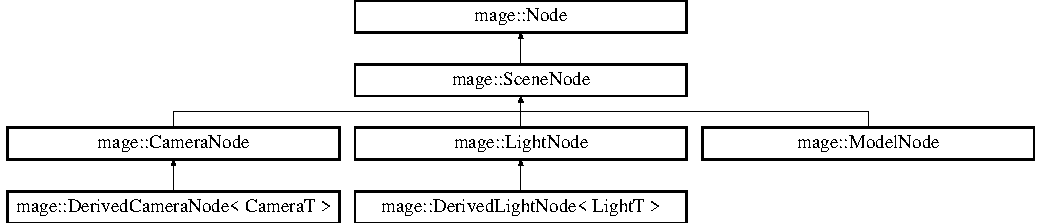
\includegraphics[height=2.000000cm]{classmage_1_1_node}
\end{center}
\end{figure}
\subsection*{Public Member Functions}
\begin{DoxyCompactItemize}
\item 
\hyperlink{classmage_1_1_node_a58b816eaa1dfd3c4b7f14896f190587f}{Node} ()
\item 
\hyperlink{classmage_1_1_node_af9da591163469f210895f3a5b389d7cc}{Node} (const \hyperlink{classmage_1_1_node}{Node} \&node)
\item 
\hyperlink{classmage_1_1_node_a052da3b48577d1ec139103545be75285}{Node} (\hyperlink{classmage_1_1_node}{Node} \&\&node)=default
\item 
virtual \hyperlink{classmage_1_1_node_a81d6331ca664b0709dc51fd7ff01fca6}{$\sim$\+Node} ()=default
\item 
\hyperlink{classmage_1_1_node}{Node} \& \hyperlink{classmage_1_1_node_ad10ea13608963acfa06d3c1577314da5}{operator=} (const \hyperlink{classmage_1_1_node}{Node} \&node)=delete
\item 
\hyperlink{classmage_1_1_node}{Node} \& \hyperlink{classmage_1_1_node_a007043de35c65edb9a0d790824186151}{operator=} (\hyperlink{classmage_1_1_node}{Node} \&\&node)=delete
\item 
\hyperlink{namespacemage_a1e01ae66713838a7a67d30e44c67703e}{Shared\+Ptr}$<$ \hyperlink{classmage_1_1_node}{Node} $>$ \hyperlink{classmage_1_1_node_aa2a22d7deec18dcd027c410b28ffde04}{Clone} () const
\item 
\hyperlink{classmage_1_1_transform_node}{Transform\+Node} $\ast$ \hyperlink{classmage_1_1_node_aee9d81f3a236fe48128ad5960a22beb4}{Get\+Transform} ()
\item 
const \hyperlink{classmage_1_1_transform_node}{Transform\+Node} $\ast$ \hyperlink{classmage_1_1_node_a319b7fdc98412cb02ba1cffab2527bf2}{Get\+Transform} () const
\item 
bool \hyperlink{classmage_1_1_node_a9819d0219bdca364621584b6aa29ba30}{Has\+Parent\+Node} () const
\item 
\hyperlink{classmage_1_1_node}{Node} $\ast$ \hyperlink{classmage_1_1_node_ae30f2ca6816eeeef28610f385864aec9}{Get\+Parent\+Node} () const
\item 
size\+\_\+t \hyperlink{classmage_1_1_node_ab11750938bf343f16dcdf7a327834318}{Get\+Number\+Of\+Child\+Nodes} () const
\item 
bool \hyperlink{classmage_1_1_node_a1b8c2d933a281f7f815791db38c965ad}{Has\+Child\+Node} (\hyperlink{namespacemage_a1e01ae66713838a7a67d30e44c67703e}{Shared\+Ptr}$<$ const \hyperlink{classmage_1_1_node}{Node} $>$ node) const
\item 
void \hyperlink{classmage_1_1_node_a11a7c052c5e4a6713d60aaad67dfde5d}{Add\+Child\+Node} (\hyperlink{namespacemage_a1e01ae66713838a7a67d30e44c67703e}{Shared\+Ptr}$<$ \hyperlink{classmage_1_1_node}{Node} $>$ node)
\item 
void \hyperlink{classmage_1_1_node_a0da235c6459c315ad1c4be5c7aa7c7f0}{Remove\+Child\+Node} (\hyperlink{namespacemage_a1e01ae66713838a7a67d30e44c67703e}{Shared\+Ptr}$<$ \hyperlink{classmage_1_1_node}{Node} $>$ node)
\item 
void \hyperlink{classmage_1_1_node_a5813fe733404dd327b77f595291c70bb}{Remove\+All\+Child\+Nodes} ()
\item 
{\footnotesize template$<$typename ActionT $>$ }\\void \hyperlink{classmage_1_1_node_afedb523a462952ec29aed7504d0a71d4}{For\+Each\+Child\+Node} (ActionT action) const
\item 
{\footnotesize template$<$typename ActionT $>$ }\\void \hyperlink{classmage_1_1_node_a86668c371e1452204b52f2896cbb16fd}{For\+Each\+Descendant\+Node} (ActionT action) const
\end{DoxyCompactItemize}
\subsection*{Private Member Functions}
\begin{DoxyCompactItemize}
\item 
virtual \hyperlink{namespacemage_a1e01ae66713838a7a67d30e44c67703e}{Shared\+Ptr}$<$ \hyperlink{classmage_1_1_node}{Node} $>$ \hyperlink{classmage_1_1_node_ac2ff348254ff10db82fca1d2d9ffeeb9}{Clone\+Implementation} () const
\end{DoxyCompactItemize}
\subsection*{Private Attributes}
\begin{DoxyCompactItemize}
\item 
\hyperlink{namespacemage_a8c307fbcc33bce9b7f2aa4c26c3b95cf}{Unique\+Ptr}$<$ \hyperlink{classmage_1_1_transform_node}{Transform\+Node} $>$ \hyperlink{classmage_1_1_node_a24512023f5f6ec7adad9810e55ec2ab5}{m\+\_\+transform}
\end{DoxyCompactItemize}


\subsection{Detailed Description}
A class of nodes. 

\subsection{Constructor \& Destructor Documentation}
\hypertarget{classmage_1_1_node_a58b816eaa1dfd3c4b7f14896f190587f}{}\label{classmage_1_1_node_a58b816eaa1dfd3c4b7f14896f190587f} 
\index{mage\+::\+Node@{mage\+::\+Node}!Node@{Node}}
\index{Node@{Node}!mage\+::\+Node@{mage\+::\+Node}}
\subsubsection{\texorpdfstring{Node()}{Node()}\hspace{0.1cm}{\footnotesize\ttfamily [1/3]}}
{\footnotesize\ttfamily mage\+::\+Node\+::\+Node (\begin{DoxyParamCaption}{ }\end{DoxyParamCaption})}

Constructs a node. \hypertarget{classmage_1_1_node_af9da591163469f210895f3a5b389d7cc}{}\label{classmage_1_1_node_af9da591163469f210895f3a5b389d7cc} 
\index{mage\+::\+Node@{mage\+::\+Node}!Node@{Node}}
\index{Node@{Node}!mage\+::\+Node@{mage\+::\+Node}}
\subsubsection{\texorpdfstring{Node()}{Node()}\hspace{0.1cm}{\footnotesize\ttfamily [2/3]}}
{\footnotesize\ttfamily mage\+::\+Node\+::\+Node (\begin{DoxyParamCaption}\item[{const \hyperlink{classmage_1_1_node}{Node} \&}]{node }\end{DoxyParamCaption})}

Constructs a node from the given node.


\begin{DoxyParams}[1]{Parameters}
\mbox{\tt in}  & {\em node} & A reference to the node. \\
\hline
\end{DoxyParams}
\hypertarget{classmage_1_1_node_a052da3b48577d1ec139103545be75285}{}\label{classmage_1_1_node_a052da3b48577d1ec139103545be75285} 
\index{mage\+::\+Node@{mage\+::\+Node}!Node@{Node}}
\index{Node@{Node}!mage\+::\+Node@{mage\+::\+Node}}
\subsubsection{\texorpdfstring{Node()}{Node()}\hspace{0.1cm}{\footnotesize\ttfamily [3/3]}}
{\footnotesize\ttfamily mage\+::\+Node\+::\+Node (\begin{DoxyParamCaption}\item[{\hyperlink{classmage_1_1_node}{Node} \&\&}]{node }\end{DoxyParamCaption})\hspace{0.3cm}{\ttfamily [default]}}

Constructs a node by moving the given node.


\begin{DoxyParams}[1]{Parameters}
\mbox{\tt in}  & {\em node} & A reference to the node to move. \\
\hline
\end{DoxyParams}
\hypertarget{classmage_1_1_node_a81d6331ca664b0709dc51fd7ff01fca6}{}\label{classmage_1_1_node_a81d6331ca664b0709dc51fd7ff01fca6} 
\index{mage\+::\+Node@{mage\+::\+Node}!````~Node@{$\sim$\+Node}}
\index{````~Node@{$\sim$\+Node}!mage\+::\+Node@{mage\+::\+Node}}
\subsubsection{\texorpdfstring{$\sim$\+Node()}{~Node()}}
{\footnotesize\ttfamily virtual mage\+::\+Node\+::$\sim$\+Node (\begin{DoxyParamCaption}{ }\end{DoxyParamCaption})\hspace{0.3cm}{\ttfamily [virtual]}, {\ttfamily [default]}}

Destructs this node. 

\subsection{Member Function Documentation}
\hypertarget{classmage_1_1_node_a11a7c052c5e4a6713d60aaad67dfde5d}{}\label{classmage_1_1_node_a11a7c052c5e4a6713d60aaad67dfde5d} 
\index{mage\+::\+Node@{mage\+::\+Node}!Add\+Child\+Node@{Add\+Child\+Node}}
\index{Add\+Child\+Node@{Add\+Child\+Node}!mage\+::\+Node@{mage\+::\+Node}}
\subsubsection{\texorpdfstring{Add\+Child\+Node()}{AddChildNode()}}
{\footnotesize\ttfamily void mage\+::\+Node\+::\+Add\+Child\+Node (\begin{DoxyParamCaption}\item[{\hyperlink{namespacemage_a1e01ae66713838a7a67d30e44c67703e}{Shared\+Ptr}$<$ \hyperlink{classmage_1_1_node}{Node} $>$}]{node }\end{DoxyParamCaption})}

Adds the given node to the child nodes of this node.


\begin{DoxyParams}[1]{Parameters}
\mbox{\tt in}  & {\em node} & A pointer to the node to add. \\
\hline
\end{DoxyParams}
\hypertarget{classmage_1_1_node_aa2a22d7deec18dcd027c410b28ffde04}{}\label{classmage_1_1_node_aa2a22d7deec18dcd027c410b28ffde04} 
\index{mage\+::\+Node@{mage\+::\+Node}!Clone@{Clone}}
\index{Clone@{Clone}!mage\+::\+Node@{mage\+::\+Node}}
\subsubsection{\texorpdfstring{Clone()}{Clone()}}
{\footnotesize\ttfamily \hyperlink{namespacemage_a1e01ae66713838a7a67d30e44c67703e}{Shared\+Ptr}$<$ \hyperlink{classmage_1_1_node}{Node} $>$ mage\+::\+Node\+::\+Clone (\begin{DoxyParamCaption}{ }\end{DoxyParamCaption}) const}

Clones this node.

\begin{DoxyReturn}{Returns}
A pointer to the clone of this node. 
\end{DoxyReturn}
\hypertarget{classmage_1_1_node_ac2ff348254ff10db82fca1d2d9ffeeb9}{}\label{classmage_1_1_node_ac2ff348254ff10db82fca1d2d9ffeeb9} 
\index{mage\+::\+Node@{mage\+::\+Node}!Clone\+Implementation@{Clone\+Implementation}}
\index{Clone\+Implementation@{Clone\+Implementation}!mage\+::\+Node@{mage\+::\+Node}}
\subsubsection{\texorpdfstring{Clone\+Implementation()}{CloneImplementation()}}
{\footnotesize\ttfamily virtual \hyperlink{namespacemage_a1e01ae66713838a7a67d30e44c67703e}{Shared\+Ptr}$<$ \hyperlink{classmage_1_1_node}{Node} $>$ mage\+::\+Node\+::\+Clone\+Implementation (\begin{DoxyParamCaption}{ }\end{DoxyParamCaption}) const\hspace{0.3cm}{\ttfamily [private]}, {\ttfamily [virtual]}}

Clones this node.

\begin{DoxyReturn}{Returns}
A pointer to the clone of this node. 
\end{DoxyReturn}


Reimplemented in \hyperlink{classmage_1_1_scene_node_acbbf6e621375c1630b0e1e5ca35e4aec}{mage\+::\+Scene\+Node$<$ Scene\+Object\+T $>$}.

\hypertarget{classmage_1_1_node_afedb523a462952ec29aed7504d0a71d4}{}\label{classmage_1_1_node_afedb523a462952ec29aed7504d0a71d4} 
\index{mage\+::\+Node@{mage\+::\+Node}!For\+Each\+Child\+Node@{For\+Each\+Child\+Node}}
\index{For\+Each\+Child\+Node@{For\+Each\+Child\+Node}!mage\+::\+Node@{mage\+::\+Node}}
\subsubsection{\texorpdfstring{For\+Each\+Child\+Node()}{ForEachChildNode()}}
{\footnotesize\ttfamily template$<$typename ActionT $>$ \\
void mage\+::\+Node\+::\+For\+Each\+Child\+Node (\begin{DoxyParamCaption}\item[{ActionT}]{action }\end{DoxyParamCaption}) const}

Traverses all child nodes of this node.


\begin{DoxyTemplParams}{Template Parameters}
{\em ActionT} & An action to perform on all child nodes of this node. The action must accept ({\ttfamily const}) {\ttfamily \hyperlink{classmage_1_1_node}{Node}\&} values. \\
\hline
\end{DoxyTemplParams}
\hypertarget{classmage_1_1_node_a86668c371e1452204b52f2896cbb16fd}{}\label{classmage_1_1_node_a86668c371e1452204b52f2896cbb16fd} 
\index{mage\+::\+Node@{mage\+::\+Node}!For\+Each\+Descendant\+Node@{For\+Each\+Descendant\+Node}}
\index{For\+Each\+Descendant\+Node@{For\+Each\+Descendant\+Node}!mage\+::\+Node@{mage\+::\+Node}}
\subsubsection{\texorpdfstring{For\+Each\+Descendant\+Node()}{ForEachDescendantNode()}}
{\footnotesize\ttfamily template$<$typename ActionT $>$ \\
void mage\+::\+Node\+::\+For\+Each\+Descendant\+Node (\begin{DoxyParamCaption}\item[{ActionT}]{action }\end{DoxyParamCaption}) const}

Traverses all descendant (childs included) nodes of this transform node.


\begin{DoxyTemplParams}{Template Parameters}
{\em ActionT} & An action to perform on all descendant nodes of this node. The action must accept ({\ttfamily const}) {\ttfamily \hyperlink{classmage_1_1_node}{Node}\&} values. \\
\hline
\end{DoxyTemplParams}
\hypertarget{classmage_1_1_node_ab11750938bf343f16dcdf7a327834318}{}\label{classmage_1_1_node_ab11750938bf343f16dcdf7a327834318} 
\index{mage\+::\+Node@{mage\+::\+Node}!Get\+Number\+Of\+Child\+Nodes@{Get\+Number\+Of\+Child\+Nodes}}
\index{Get\+Number\+Of\+Child\+Nodes@{Get\+Number\+Of\+Child\+Nodes}!mage\+::\+Node@{mage\+::\+Node}}
\subsubsection{\texorpdfstring{Get\+Number\+Of\+Child\+Nodes()}{GetNumberOfChildNodes()}}
{\footnotesize\ttfamily size\+\_\+t mage\+::\+Node\+::\+Get\+Number\+Of\+Child\+Nodes (\begin{DoxyParamCaption}{ }\end{DoxyParamCaption}) const}

Returns the number of child nodes of this node.

\begin{DoxyReturn}{Returns}
The number of child nodes of this node. 
\end{DoxyReturn}
\hypertarget{classmage_1_1_node_ae30f2ca6816eeeef28610f385864aec9}{}\label{classmage_1_1_node_ae30f2ca6816eeeef28610f385864aec9} 
\index{mage\+::\+Node@{mage\+::\+Node}!Get\+Parent\+Node@{Get\+Parent\+Node}}
\index{Get\+Parent\+Node@{Get\+Parent\+Node}!mage\+::\+Node@{mage\+::\+Node}}
\subsubsection{\texorpdfstring{Get\+Parent\+Node()}{GetParentNode()}}
{\footnotesize\ttfamily \hyperlink{classmage_1_1_node}{Node}$\ast$ mage\+::\+Node\+::\+Get\+Parent\+Node (\begin{DoxyParamCaption}{ }\end{DoxyParamCaption}) const}

Returns the parent node of this node.

\begin{DoxyReturn}{Returns}
{\ttfamily nullptr} if this node has no parent node. 

A pointer to the parent node of this node. 
\end{DoxyReturn}
\hypertarget{classmage_1_1_node_aee9d81f3a236fe48128ad5960a22beb4}{}\label{classmage_1_1_node_aee9d81f3a236fe48128ad5960a22beb4} 
\index{mage\+::\+Node@{mage\+::\+Node}!Get\+Transform@{Get\+Transform}}
\index{Get\+Transform@{Get\+Transform}!mage\+::\+Node@{mage\+::\+Node}}
\subsubsection{\texorpdfstring{Get\+Transform()}{GetTransform()}\hspace{0.1cm}{\footnotesize\ttfamily [1/2]}}
{\footnotesize\ttfamily \hyperlink{classmage_1_1_transform_node}{Transform\+Node}$\ast$ mage\+::\+Node\+::\+Get\+Transform (\begin{DoxyParamCaption}{ }\end{DoxyParamCaption})}

Returns the transform of this node.

\begin{DoxyReturn}{Returns}
A pointer to the transform of this node. 
\end{DoxyReturn}
\hypertarget{classmage_1_1_node_a319b7fdc98412cb02ba1cffab2527bf2}{}\label{classmage_1_1_node_a319b7fdc98412cb02ba1cffab2527bf2} 
\index{mage\+::\+Node@{mage\+::\+Node}!Get\+Transform@{Get\+Transform}}
\index{Get\+Transform@{Get\+Transform}!mage\+::\+Node@{mage\+::\+Node}}
\subsubsection{\texorpdfstring{Get\+Transform()}{GetTransform()}\hspace{0.1cm}{\footnotesize\ttfamily [2/2]}}
{\footnotesize\ttfamily const \hyperlink{classmage_1_1_transform_node}{Transform\+Node}$\ast$ mage\+::\+Node\+::\+Get\+Transform (\begin{DoxyParamCaption}{ }\end{DoxyParamCaption}) const}

Returns the transform of this node.

\begin{DoxyReturn}{Returns}
A pointer to the transform of this node. 
\end{DoxyReturn}
\hypertarget{classmage_1_1_node_a1b8c2d933a281f7f815791db38c965ad}{}\label{classmage_1_1_node_a1b8c2d933a281f7f815791db38c965ad} 
\index{mage\+::\+Node@{mage\+::\+Node}!Has\+Child\+Node@{Has\+Child\+Node}}
\index{Has\+Child\+Node@{Has\+Child\+Node}!mage\+::\+Node@{mage\+::\+Node}}
\subsubsection{\texorpdfstring{Has\+Child\+Node()}{HasChildNode()}}
{\footnotesize\ttfamily bool mage\+::\+Node\+::\+Has\+Child\+Node (\begin{DoxyParamCaption}\item[{\hyperlink{namespacemage_a1e01ae66713838a7a67d30e44c67703e}{Shared\+Ptr}$<$ const \hyperlink{classmage_1_1_node}{Node} $>$}]{node }\end{DoxyParamCaption}) const}

Checks whether this node contains the given node as a child node.


\begin{DoxyParams}[1]{Parameters}
\mbox{\tt in}  & {\em node} & A pointer to the node. \\
\hline
\end{DoxyParams}
\begin{DoxyReturn}{Returns}
{\ttfamily true} if this node contains the given node as a child node. {\ttfamily false} otherwise. 
\end{DoxyReturn}
\hypertarget{classmage_1_1_node_a9819d0219bdca364621584b6aa29ba30}{}\label{classmage_1_1_node_a9819d0219bdca364621584b6aa29ba30} 
\index{mage\+::\+Node@{mage\+::\+Node}!Has\+Parent\+Node@{Has\+Parent\+Node}}
\index{Has\+Parent\+Node@{Has\+Parent\+Node}!mage\+::\+Node@{mage\+::\+Node}}
\subsubsection{\texorpdfstring{Has\+Parent\+Node()}{HasParentNode()}}
{\footnotesize\ttfamily bool mage\+::\+Node\+::\+Has\+Parent\+Node (\begin{DoxyParamCaption}{ }\end{DoxyParamCaption}) const}

Checks whether this node has a parent node.

\begin{DoxyReturn}{Returns}
{\ttfamily true} if this node has a parent node. {\ttfamily false} otherwise. 
\end{DoxyReturn}
\hypertarget{classmage_1_1_node_ad10ea13608963acfa06d3c1577314da5}{}\label{classmage_1_1_node_ad10ea13608963acfa06d3c1577314da5} 
\index{mage\+::\+Node@{mage\+::\+Node}!operator=@{operator=}}
\index{operator=@{operator=}!mage\+::\+Node@{mage\+::\+Node}}
\subsubsection{\texorpdfstring{operator=()}{operator=()}\hspace{0.1cm}{\footnotesize\ttfamily [1/2]}}
{\footnotesize\ttfamily \hyperlink{classmage_1_1_node}{Node}\& mage\+::\+Node\+::operator= (\begin{DoxyParamCaption}\item[{const \hyperlink{classmage_1_1_node}{Node} \&}]{node }\end{DoxyParamCaption})\hspace{0.3cm}{\ttfamily [delete]}}

Copies the given node to this node.


\begin{DoxyParams}[1]{Parameters}
\mbox{\tt in}  & {\em node} & A reference to the node to copy. \\
\hline
\end{DoxyParams}
\begin{DoxyReturn}{Returns}
A reference to the copy of the given node (i.\+e. this node). 
\end{DoxyReturn}
\hypertarget{classmage_1_1_node_a007043de35c65edb9a0d790824186151}{}\label{classmage_1_1_node_a007043de35c65edb9a0d790824186151} 
\index{mage\+::\+Node@{mage\+::\+Node}!operator=@{operator=}}
\index{operator=@{operator=}!mage\+::\+Node@{mage\+::\+Node}}
\subsubsection{\texorpdfstring{operator=()}{operator=()}\hspace{0.1cm}{\footnotesize\ttfamily [2/2]}}
{\footnotesize\ttfamily \hyperlink{classmage_1_1_node}{Node}\& mage\+::\+Node\+::operator= (\begin{DoxyParamCaption}\item[{\hyperlink{classmage_1_1_node}{Node} \&\&}]{node }\end{DoxyParamCaption})\hspace{0.3cm}{\ttfamily [delete]}}

Moves the given node to this node.


\begin{DoxyParams}[1]{Parameters}
\mbox{\tt in}  & {\em node} & A reference to the node to move. \\
\hline
\end{DoxyParams}
\begin{DoxyReturn}{Returns}
A reference to the moved node (i.\+e. this node). 
\end{DoxyReturn}
\hypertarget{classmage_1_1_node_a5813fe733404dd327b77f595291c70bb}{}\label{classmage_1_1_node_a5813fe733404dd327b77f595291c70bb} 
\index{mage\+::\+Node@{mage\+::\+Node}!Remove\+All\+Child\+Nodes@{Remove\+All\+Child\+Nodes}}
\index{Remove\+All\+Child\+Nodes@{Remove\+All\+Child\+Nodes}!mage\+::\+Node@{mage\+::\+Node}}
\subsubsection{\texorpdfstring{Remove\+All\+Child\+Nodes()}{RemoveAllChildNodes()}}
{\footnotesize\ttfamily void mage\+::\+Node\+::\+Remove\+All\+Child\+Nodes (\begin{DoxyParamCaption}{ }\end{DoxyParamCaption})}

Removes all child nodes from this node. \hypertarget{classmage_1_1_node_a0da235c6459c315ad1c4be5c7aa7c7f0}{}\label{classmage_1_1_node_a0da235c6459c315ad1c4be5c7aa7c7f0} 
\index{mage\+::\+Node@{mage\+::\+Node}!Remove\+Child\+Node@{Remove\+Child\+Node}}
\index{Remove\+Child\+Node@{Remove\+Child\+Node}!mage\+::\+Node@{mage\+::\+Node}}
\subsubsection{\texorpdfstring{Remove\+Child\+Node()}{RemoveChildNode()}}
{\footnotesize\ttfamily void mage\+::\+Node\+::\+Remove\+Child\+Node (\begin{DoxyParamCaption}\item[{\hyperlink{namespacemage_a1e01ae66713838a7a67d30e44c67703e}{Shared\+Ptr}$<$ \hyperlink{classmage_1_1_node}{Node} $>$}]{node }\end{DoxyParamCaption})}

Removes the given node from the child nodes of this node.


\begin{DoxyParams}[1]{Parameters}
\mbox{\tt in}  & {\em node} & A pointer to the node to remove. \\
\hline
\end{DoxyParams}


\subsection{Member Data Documentation}
\hypertarget{classmage_1_1_node_a24512023f5f6ec7adad9810e55ec2ab5}{}\label{classmage_1_1_node_a24512023f5f6ec7adad9810e55ec2ab5} 
\index{mage\+::\+Node@{mage\+::\+Node}!m\+\_\+transform@{m\+\_\+transform}}
\index{m\+\_\+transform@{m\+\_\+transform}!mage\+::\+Node@{mage\+::\+Node}}
\subsubsection{\texorpdfstring{m\+\_\+transform}{m\_transform}}
{\footnotesize\ttfamily \hyperlink{namespacemage_a8c307fbcc33bce9b7f2aa4c26c3b95cf}{Unique\+Ptr}$<$ \hyperlink{classmage_1_1_transform_node}{Transform\+Node} $>$ mage\+::\+Node\+::m\+\_\+transform\hspace{0.3cm}{\ttfamily [private]}}

A pointer to the transform of this node. 
\hypertarget{structmage_1_1_normal3}{}\section{mage\+:\+:Normal3 Struct Reference}
\label{structmage_1_1_normal3}\index{mage\+::\+Normal3@{mage\+::\+Normal3}}


{\ttfamily \#include $<$math.\+hpp$>$}

Inheritance diagram for mage\+:\+:Normal3\+:\begin{figure}[H]
\begin{center}
\leavevmode
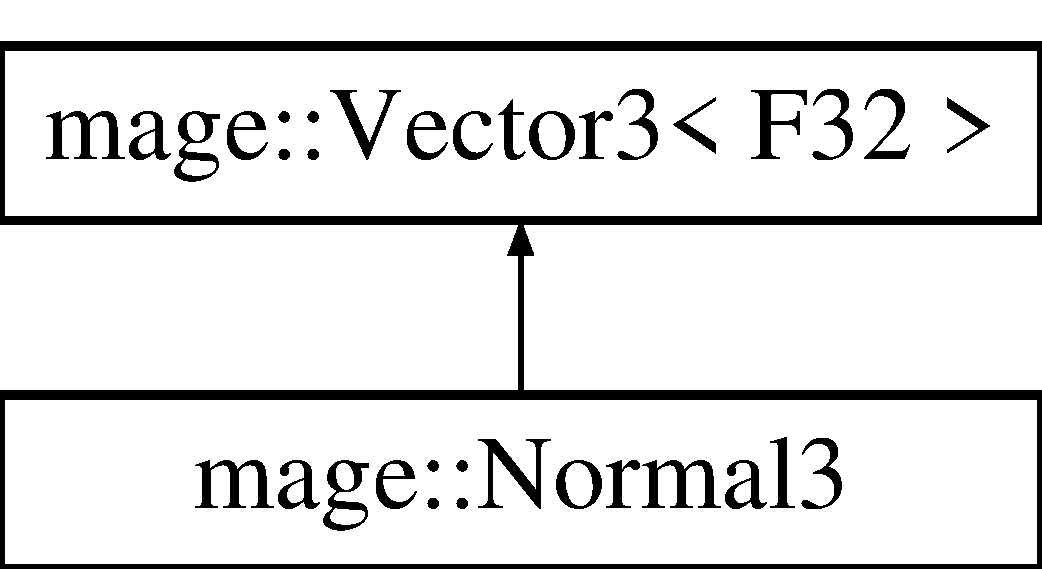
\includegraphics[height=2.000000cm]{structmage_1_1_normal3}
\end{center}
\end{figure}
\subsection*{Public Member Functions}
\begin{DoxyCompactItemize}
\item 
\hyperlink{structmage_1_1_normal3_a64a99fa013aff357da71a39f1957e7c6}{Normal3} () noexcept
\item 
\hyperlink{structmage_1_1_normal3_af4d0bf7f7f4fd523952e4221d96606f5}{Normal3} (\hyperlink{namespacemage_a6a44ad388483959dc4dff9f2aef91431}{f32} x, \hyperlink{namespacemage_a6a44ad388483959dc4dff9f2aef91431}{f32} y, \hyperlink{namespacemage_a6a44ad388483959dc4dff9f2aef91431}{f32} z) noexcept
\item 
\hyperlink{structmage_1_1_normal3_af39f2985925addc37f1a9e3d00785b57}{Normal3} (const \hyperlink{structmage_1_1_normal3}{Normal3} \&normal) noexcept=default
\item 
\hyperlink{structmage_1_1_normal3_ab29b3dcf7fc05c459f2e9b91b6832115}{Normal3} (\hyperlink{structmage_1_1_normal3}{Normal3} \&\&normal) noexcept=default
\item 
\hyperlink{structmage_1_1_normal3_a477777d95f0ad41e6087668c965dd9b2}{Normal3} (const \hyperlink{structmage_1_1_direction3}{Direction3} \&direction) noexcept
\item 
\hyperlink{structmage_1_1_normal3_a55d265ba8454dd5d4573ad9d09844cee}{Normal3} (\hyperlink{structmage_1_1_direction3}{Direction3} \&\&direction) noexcept
\item 
\hyperlink{structmage_1_1_normal3_ad812f4b279f8ef1a28f71925c90efcf8}{Normal3} (const X\+M\+F\+L\+O\+A\+T3 \&v) noexcept
\item 
\hyperlink{structmage_1_1_normal3_ac6a5bc0d574ab2a85dba8e5cb8539d58}{Normal3} (X\+M\+F\+L\+O\+A\+T3 \&\&v) noexcept
\item 
\hyperlink{structmage_1_1_normal3_a3384b2970fd85fe729514ce0686b4446}{$\sim$\+Normal3} ()=default
\item 
\hyperlink{structmage_1_1_normal3}{Normal3} \& \hyperlink{structmage_1_1_normal3_ad446f029ba58615f98b4da13e7e4c5ba}{operator=} (const \hyperlink{structmage_1_1_normal3}{Normal3} \&normal)=default
\item 
\hyperlink{structmage_1_1_normal3}{Normal3} \& \hyperlink{structmage_1_1_normal3_ab8fd629ae1e399b468a229fc4ea58222}{operator=} (\hyperlink{structmage_1_1_normal3}{Normal3} \&\&normal)=default
\end{DoxyCompactItemize}


\subsection{Detailed Description}
A struct of normals in 3D space.

\begin{DoxyNote}{Note}
{\ttfamily \hyperlink{structmage_1_1_normal3}{Normal3}} does not guarantee or force normalized directions. This should be guaranteed and enforced by the user. 
\end{DoxyNote}


\subsection{Constructor \& Destructor Documentation}
\hypertarget{structmage_1_1_normal3_a64a99fa013aff357da71a39f1957e7c6}{}\label{structmage_1_1_normal3_a64a99fa013aff357da71a39f1957e7c6} 
\index{mage\+::\+Normal3@{mage\+::\+Normal3}!Normal3@{Normal3}}
\index{Normal3@{Normal3}!mage\+::\+Normal3@{mage\+::\+Normal3}}
\subsubsection{\texorpdfstring{Normal3()}{Normal3()}\hspace{0.1cm}{\footnotesize\ttfamily [1/8]}}
{\footnotesize\ttfamily mage\+::\+Normal3\+::\+Normal3 (\begin{DoxyParamCaption}{ }\end{DoxyParamCaption})\hspace{0.3cm}{\ttfamily [noexcept]}}

Constructs a normal. \hypertarget{structmage_1_1_normal3_af4d0bf7f7f4fd523952e4221d96606f5}{}\label{structmage_1_1_normal3_af4d0bf7f7f4fd523952e4221d96606f5} 
\index{mage\+::\+Normal3@{mage\+::\+Normal3}!Normal3@{Normal3}}
\index{Normal3@{Normal3}!mage\+::\+Normal3@{mage\+::\+Normal3}}
\subsubsection{\texorpdfstring{Normal3()}{Normal3()}\hspace{0.1cm}{\footnotesize\ttfamily [2/8]}}
{\footnotesize\ttfamily mage\+::\+Normal3\+::\+Normal3 (\begin{DoxyParamCaption}\item[{\hyperlink{namespacemage_a6a44ad388483959dc4dff9f2aef91431}{f32}}]{x,  }\item[{\hyperlink{namespacemage_a6a44ad388483959dc4dff9f2aef91431}{f32}}]{y,  }\item[{\hyperlink{namespacemage_a6a44ad388483959dc4dff9f2aef91431}{f32}}]{z }\end{DoxyParamCaption})\hspace{0.3cm}{\ttfamily [noexcept]}}

Constructs a normal from the given coordinates.


\begin{DoxyParams}[1]{Parameters}
\mbox{\tt in}  & {\em x} & The x-\/coordinate. \\
\hline
\mbox{\tt in}  & {\em y} & The y-\/coordinate. \\
\hline
\mbox{\tt in}  & {\em z} & The z-\/coordinate. \\
\hline
\end{DoxyParams}
\hypertarget{structmage_1_1_normal3_af39f2985925addc37f1a9e3d00785b57}{}\label{structmage_1_1_normal3_af39f2985925addc37f1a9e3d00785b57} 
\index{mage\+::\+Normal3@{mage\+::\+Normal3}!Normal3@{Normal3}}
\index{Normal3@{Normal3}!mage\+::\+Normal3@{mage\+::\+Normal3}}
\subsubsection{\texorpdfstring{Normal3()}{Normal3()}\hspace{0.1cm}{\footnotesize\ttfamily [3/8]}}
{\footnotesize\ttfamily mage\+::\+Normal3\+::\+Normal3 (\begin{DoxyParamCaption}\item[{const \hyperlink{structmage_1_1_normal3}{Normal3} \&}]{normal }\end{DoxyParamCaption})\hspace{0.3cm}{\ttfamily [default]}, {\ttfamily [noexcept]}}

Constructs a normal from the given normal.


\begin{DoxyParams}[1]{Parameters}
\mbox{\tt in}  & {\em normal} & A reference to the normal to copy. \\
\hline
\end{DoxyParams}
\hypertarget{structmage_1_1_normal3_ab29b3dcf7fc05c459f2e9b91b6832115}{}\label{structmage_1_1_normal3_ab29b3dcf7fc05c459f2e9b91b6832115} 
\index{mage\+::\+Normal3@{mage\+::\+Normal3}!Normal3@{Normal3}}
\index{Normal3@{Normal3}!mage\+::\+Normal3@{mage\+::\+Normal3}}
\subsubsection{\texorpdfstring{Normal3()}{Normal3()}\hspace{0.1cm}{\footnotesize\ttfamily [4/8]}}
{\footnotesize\ttfamily mage\+::\+Normal3\+::\+Normal3 (\begin{DoxyParamCaption}\item[{\hyperlink{structmage_1_1_normal3}{Normal3} \&\&}]{normal }\end{DoxyParamCaption})\hspace{0.3cm}{\ttfamily [default]}, {\ttfamily [noexcept]}}

Constructs a normal by moving the given normal.


\begin{DoxyParams}[1]{Parameters}
\mbox{\tt in}  & {\em normal} & A reference to the normal to move. \\
\hline
\end{DoxyParams}
\hypertarget{structmage_1_1_normal3_a477777d95f0ad41e6087668c965dd9b2}{}\label{structmage_1_1_normal3_a477777d95f0ad41e6087668c965dd9b2} 
\index{mage\+::\+Normal3@{mage\+::\+Normal3}!Normal3@{Normal3}}
\index{Normal3@{Normal3}!mage\+::\+Normal3@{mage\+::\+Normal3}}
\subsubsection{\texorpdfstring{Normal3()}{Normal3()}\hspace{0.1cm}{\footnotesize\ttfamily [5/8]}}
{\footnotesize\ttfamily mage\+::\+Normal3\+::\+Normal3 (\begin{DoxyParamCaption}\item[{const \hyperlink{structmage_1_1_direction3}{Direction3} \&}]{direction }\end{DoxyParamCaption})\hspace{0.3cm}{\ttfamily [explicit]}, {\ttfamily [noexcept]}}

Constructs a normal from the given direction.


\begin{DoxyParams}[1]{Parameters}
\mbox{\tt in}  & {\em direction} & A reference to the direction to copy. \\
\hline
\end{DoxyParams}
\hypertarget{structmage_1_1_normal3_a55d265ba8454dd5d4573ad9d09844cee}{}\label{structmage_1_1_normal3_a55d265ba8454dd5d4573ad9d09844cee} 
\index{mage\+::\+Normal3@{mage\+::\+Normal3}!Normal3@{Normal3}}
\index{Normal3@{Normal3}!mage\+::\+Normal3@{mage\+::\+Normal3}}
\subsubsection{\texorpdfstring{Normal3()}{Normal3()}\hspace{0.1cm}{\footnotesize\ttfamily [6/8]}}
{\footnotesize\ttfamily mage\+::\+Normal3\+::\+Normal3 (\begin{DoxyParamCaption}\item[{\hyperlink{structmage_1_1_direction3}{Direction3} \&\&}]{direction }\end{DoxyParamCaption})\hspace{0.3cm}{\ttfamily [explicit]}, {\ttfamily [noexcept]}}

Constructs a normal by moving the given direction.


\begin{DoxyParams}[1]{Parameters}
\mbox{\tt in}  & {\em direction} & A reference to the direction to move. \\
\hline
\end{DoxyParams}
\hypertarget{structmage_1_1_normal3_ad812f4b279f8ef1a28f71925c90efcf8}{}\label{structmage_1_1_normal3_ad812f4b279f8ef1a28f71925c90efcf8} 
\index{mage\+::\+Normal3@{mage\+::\+Normal3}!Normal3@{Normal3}}
\index{Normal3@{Normal3}!mage\+::\+Normal3@{mage\+::\+Normal3}}
\subsubsection{\texorpdfstring{Normal3()}{Normal3()}\hspace{0.1cm}{\footnotesize\ttfamily [7/8]}}
{\footnotesize\ttfamily mage\+::\+Normal3\+::\+Normal3 (\begin{DoxyParamCaption}\item[{const X\+M\+F\+L\+O\+A\+T3 \&}]{v }\end{DoxyParamCaption})\hspace{0.3cm}{\ttfamily [explicit]}, {\ttfamily [noexcept]}}

Constructs a normal from the given vector.


\begin{DoxyParams}[1]{Parameters}
\mbox{\tt in}  & {\em v} & A reference to the vector to copy. \\
\hline
\end{DoxyParams}
\hypertarget{structmage_1_1_normal3_ac6a5bc0d574ab2a85dba8e5cb8539d58}{}\label{structmage_1_1_normal3_ac6a5bc0d574ab2a85dba8e5cb8539d58} 
\index{mage\+::\+Normal3@{mage\+::\+Normal3}!Normal3@{Normal3}}
\index{Normal3@{Normal3}!mage\+::\+Normal3@{mage\+::\+Normal3}}
\subsubsection{\texorpdfstring{Normal3()}{Normal3()}\hspace{0.1cm}{\footnotesize\ttfamily [8/8]}}
{\footnotesize\ttfamily mage\+::\+Normal3\+::\+Normal3 (\begin{DoxyParamCaption}\item[{X\+M\+F\+L\+O\+A\+T3 \&\&}]{v }\end{DoxyParamCaption})\hspace{0.3cm}{\ttfamily [explicit]}, {\ttfamily [noexcept]}}

Constructs a normal by moving the given vector.


\begin{DoxyParams}[1]{Parameters}
\mbox{\tt in}  & {\em v} & A reference to the vector to move. \\
\hline
\end{DoxyParams}
\hypertarget{structmage_1_1_normal3_a3384b2970fd85fe729514ce0686b4446}{}\label{structmage_1_1_normal3_a3384b2970fd85fe729514ce0686b4446} 
\index{mage\+::\+Normal3@{mage\+::\+Normal3}!````~Normal3@{$\sim$\+Normal3}}
\index{````~Normal3@{$\sim$\+Normal3}!mage\+::\+Normal3@{mage\+::\+Normal3}}
\subsubsection{\texorpdfstring{$\sim$\+Normal3()}{~Normal3()}}
{\footnotesize\ttfamily mage\+::\+Normal3\+::$\sim$\+Normal3 (\begin{DoxyParamCaption}{ }\end{DoxyParamCaption})\hspace{0.3cm}{\ttfamily [default]}}

Destructs this normal. 

\subsection{Member Function Documentation}
\hypertarget{structmage_1_1_normal3_ad446f029ba58615f98b4da13e7e4c5ba}{}\label{structmage_1_1_normal3_ad446f029ba58615f98b4da13e7e4c5ba} 
\index{mage\+::\+Normal3@{mage\+::\+Normal3}!operator=@{operator=}}
\index{operator=@{operator=}!mage\+::\+Normal3@{mage\+::\+Normal3}}
\subsubsection{\texorpdfstring{operator=()}{operator=()}\hspace{0.1cm}{\footnotesize\ttfamily [1/2]}}
{\footnotesize\ttfamily \hyperlink{structmage_1_1_normal3}{Normal3}\& mage\+::\+Normal3\+::operator= (\begin{DoxyParamCaption}\item[{const \hyperlink{structmage_1_1_normal3}{Normal3} \&}]{normal }\end{DoxyParamCaption})\hspace{0.3cm}{\ttfamily [default]}}

Copies the given normal to this normal.


\begin{DoxyParams}[1]{Parameters}
\mbox{\tt in}  & {\em normal} & A reference to the normal to copy. \\
\hline
\end{DoxyParams}
\begin{DoxyReturn}{Returns}
A reference to the copy of the given normal (i.\+e. this normal). 
\end{DoxyReturn}
\hypertarget{structmage_1_1_normal3_ab8fd629ae1e399b468a229fc4ea58222}{}\label{structmage_1_1_normal3_ab8fd629ae1e399b468a229fc4ea58222} 
\index{mage\+::\+Normal3@{mage\+::\+Normal3}!operator=@{operator=}}
\index{operator=@{operator=}!mage\+::\+Normal3@{mage\+::\+Normal3}}
\subsubsection{\texorpdfstring{operator=()}{operator=()}\hspace{0.1cm}{\footnotesize\ttfamily [2/2]}}
{\footnotesize\ttfamily \hyperlink{structmage_1_1_normal3}{Normal3}\& mage\+::\+Normal3\+::operator= (\begin{DoxyParamCaption}\item[{\hyperlink{structmage_1_1_normal3}{Normal3} \&\&}]{normal }\end{DoxyParamCaption})\hspace{0.3cm}{\ttfamily [default]}}

Moves the given normal to this normal.


\begin{DoxyParams}[1]{Parameters}
\mbox{\tt in}  & {\em normal} & A reference to the normal to move. \\
\hline
\end{DoxyParams}
\begin{DoxyReturn}{Returns}
A reference to the moved normal (i.\+e. this normal). 
\end{DoxyReturn}

\hypertarget{classmage_1_1_normal_sprite_text}{}\section{mage\+:\+:Normal\+Sprite\+Text Class Reference}
\label{classmage_1_1_normal_sprite_text}\index{mage\+::\+Normal\+Sprite\+Text@{mage\+::\+Normal\+Sprite\+Text}}


{\ttfamily \#include $<$normal\+\_\+sprite\+\_\+text.\+hpp$>$}

Inheritance diagram for mage\+:\+:Normal\+Sprite\+Text\+:\begin{figure}[H]
\begin{center}
\leavevmode
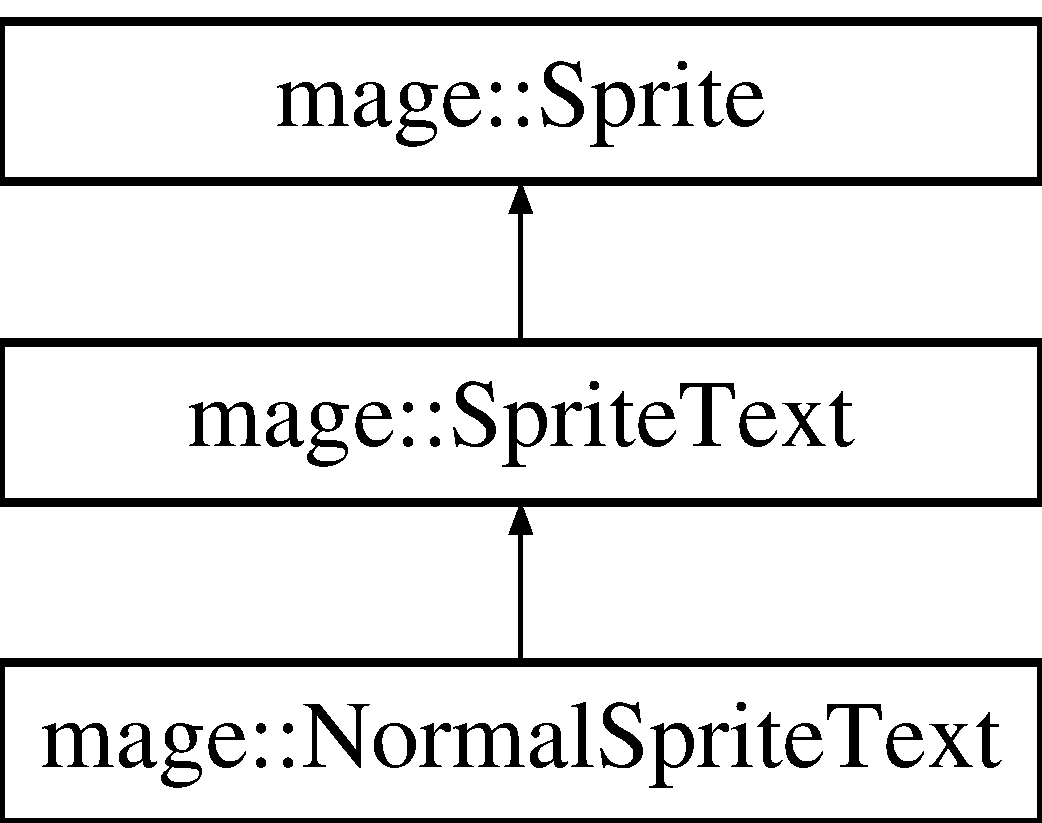
\includegraphics[height=3.000000cm]{classmage_1_1_normal_sprite_text}
\end{center}
\end{figure}
\subsection*{Public Member Functions}
\begin{DoxyCompactItemize}
\item 
\hyperlink{classmage_1_1_normal_sprite_text_af91e5d22a02044c4159eefdc161c5dec}{Normal\+Sprite\+Text} (const string \&name, \hyperlink{namespacemage_a1e01ae66713838a7a67d30e44c67703e}{Shared\+Ptr}$<$ \hyperlink{classmage_1_1_sprite_font}{Sprite\+Font} $>$ font, \hyperlink{namespacemage_a9cfe18123066ba4236f548f9de75d881}{Sprite\+Effect} effects=\hyperlink{namespacemage_a9cfe18123066ba4236f548f9de75d881af3c275fbfacfe174da928b2f24dfa515}{Sprite\+Effect\+\_\+\+None})
\item 
\hyperlink{classmage_1_1_normal_sprite_text_a3bd8f94a53caeb7ead9312da6b9b849a}{Normal\+Sprite\+Text} (const \hyperlink{classmage_1_1_normal_sprite_text}{Normal\+Sprite\+Text} \&sprite\+\_\+text)=default
\item 
\hyperlink{classmage_1_1_normal_sprite_text_ae16d982e1d959b6b80f82610b07ec15b}{Normal\+Sprite\+Text} (\hyperlink{classmage_1_1_normal_sprite_text}{Normal\+Sprite\+Text} \&\&sprite\+\_\+text)=default
\item 
virtual \hyperlink{classmage_1_1_normal_sprite_text_a5ead5607cb41849419827ff231b4ea9d}{$\sim$\+Normal\+Sprite\+Text} ()=default
\item 
\hyperlink{classmage_1_1_normal_sprite_text}{Normal\+Sprite\+Text} \& \hyperlink{classmage_1_1_normal_sprite_text_a1c0f30872c4d3114f1e53183958354e5}{operator=} (const \hyperlink{classmage_1_1_normal_sprite_text}{Normal\+Sprite\+Text} \&sprite\+\_\+text)=default
\item 
\hyperlink{classmage_1_1_normal_sprite_text}{Normal\+Sprite\+Text} \& \hyperlink{classmage_1_1_normal_sprite_text_a034dd8c1c084216a247896ffbe50e61d}{operator=} (\hyperlink{classmage_1_1_normal_sprite_text}{Normal\+Sprite\+Text} \&\&sprite\+\_\+text)=default
\item 
virtual \hyperlink{classmage_1_1_normal_sprite_text}{Normal\+Sprite\+Text} $\ast$ \hyperlink{classmage_1_1_normal_sprite_text_aef48e90667849cd9ec01510baf1394cb}{Clone} () const override
\item 
virtual void \hyperlink{classmage_1_1_normal_sprite_text_ad2a1b02bea18afd6bf61b106a727a355}{Draw} (Sprite\+Batch \&sprite\+\_\+batch) const override
\end{DoxyCompactItemize}
\subsection*{Additional Inherited Members}


\subsection{Constructor \& Destructor Documentation}
\hypertarget{classmage_1_1_normal_sprite_text_af91e5d22a02044c4159eefdc161c5dec}{}\label{classmage_1_1_normal_sprite_text_af91e5d22a02044c4159eefdc161c5dec} 
\index{mage\+::\+Normal\+Sprite\+Text@{mage\+::\+Normal\+Sprite\+Text}!Normal\+Sprite\+Text@{Normal\+Sprite\+Text}}
\index{Normal\+Sprite\+Text@{Normal\+Sprite\+Text}!mage\+::\+Normal\+Sprite\+Text@{mage\+::\+Normal\+Sprite\+Text}}
\subsubsection{\texorpdfstring{Normal\+Sprite\+Text()}{NormalSpriteText()}\hspace{0.1cm}{\footnotesize\ttfamily [1/3]}}
{\footnotesize\ttfamily mage\+::\+Normal\+Sprite\+Text\+::\+Normal\+Sprite\+Text (\begin{DoxyParamCaption}\item[{const string \&}]{name,  }\item[{\hyperlink{namespacemage_a1e01ae66713838a7a67d30e44c67703e}{Shared\+Ptr}$<$ \hyperlink{classmage_1_1_sprite_font}{Sprite\+Font} $>$}]{font,  }\item[{\hyperlink{namespacemage_a9cfe18123066ba4236f548f9de75d881}{Sprite\+Effect}}]{effects = {\ttfamily \hyperlink{namespacemage_a9cfe18123066ba4236f548f9de75d881af3c275fbfacfe174da928b2f24dfa515}{Sprite\+Effect\+\_\+\+None}} }\end{DoxyParamCaption})\hspace{0.3cm}{\ttfamily [explicit]}}

\hypertarget{classmage_1_1_normal_sprite_text_a3bd8f94a53caeb7ead9312da6b9b849a}{}\label{classmage_1_1_normal_sprite_text_a3bd8f94a53caeb7ead9312da6b9b849a} 
\index{mage\+::\+Normal\+Sprite\+Text@{mage\+::\+Normal\+Sprite\+Text}!Normal\+Sprite\+Text@{Normal\+Sprite\+Text}}
\index{Normal\+Sprite\+Text@{Normal\+Sprite\+Text}!mage\+::\+Normal\+Sprite\+Text@{mage\+::\+Normal\+Sprite\+Text}}
\subsubsection{\texorpdfstring{Normal\+Sprite\+Text()}{NormalSpriteText()}\hspace{0.1cm}{\footnotesize\ttfamily [2/3]}}
{\footnotesize\ttfamily mage\+::\+Normal\+Sprite\+Text\+::\+Normal\+Sprite\+Text (\begin{DoxyParamCaption}\item[{const \hyperlink{classmage_1_1_normal_sprite_text}{Normal\+Sprite\+Text} \&}]{sprite\+\_\+text }\end{DoxyParamCaption})\hspace{0.3cm}{\ttfamily [default]}}

\hypertarget{classmage_1_1_normal_sprite_text_ae16d982e1d959b6b80f82610b07ec15b}{}\label{classmage_1_1_normal_sprite_text_ae16d982e1d959b6b80f82610b07ec15b} 
\index{mage\+::\+Normal\+Sprite\+Text@{mage\+::\+Normal\+Sprite\+Text}!Normal\+Sprite\+Text@{Normal\+Sprite\+Text}}
\index{Normal\+Sprite\+Text@{Normal\+Sprite\+Text}!mage\+::\+Normal\+Sprite\+Text@{mage\+::\+Normal\+Sprite\+Text}}
\subsubsection{\texorpdfstring{Normal\+Sprite\+Text()}{NormalSpriteText()}\hspace{0.1cm}{\footnotesize\ttfamily [3/3]}}
{\footnotesize\ttfamily mage\+::\+Normal\+Sprite\+Text\+::\+Normal\+Sprite\+Text (\begin{DoxyParamCaption}\item[{\hyperlink{classmage_1_1_normal_sprite_text}{Normal\+Sprite\+Text} \&\&}]{sprite\+\_\+text }\end{DoxyParamCaption})\hspace{0.3cm}{\ttfamily [default]}}

\hypertarget{classmage_1_1_normal_sprite_text_a5ead5607cb41849419827ff231b4ea9d}{}\label{classmage_1_1_normal_sprite_text_a5ead5607cb41849419827ff231b4ea9d} 
\index{mage\+::\+Normal\+Sprite\+Text@{mage\+::\+Normal\+Sprite\+Text}!````~Normal\+Sprite\+Text@{$\sim$\+Normal\+Sprite\+Text}}
\index{````~Normal\+Sprite\+Text@{$\sim$\+Normal\+Sprite\+Text}!mage\+::\+Normal\+Sprite\+Text@{mage\+::\+Normal\+Sprite\+Text}}
\subsubsection{\texorpdfstring{$\sim$\+Normal\+Sprite\+Text()}{~NormalSpriteText()}}
{\footnotesize\ttfamily virtual mage\+::\+Normal\+Sprite\+Text\+::$\sim$\+Normal\+Sprite\+Text (\begin{DoxyParamCaption}{ }\end{DoxyParamCaption})\hspace{0.3cm}{\ttfamily [virtual]}, {\ttfamily [default]}}



\subsection{Member Function Documentation}
\hypertarget{classmage_1_1_normal_sprite_text_aef48e90667849cd9ec01510baf1394cb}{}\label{classmage_1_1_normal_sprite_text_aef48e90667849cd9ec01510baf1394cb} 
\index{mage\+::\+Normal\+Sprite\+Text@{mage\+::\+Normal\+Sprite\+Text}!Clone@{Clone}}
\index{Clone@{Clone}!mage\+::\+Normal\+Sprite\+Text@{mage\+::\+Normal\+Sprite\+Text}}
\subsubsection{\texorpdfstring{Clone()}{Clone()}}
{\footnotesize\ttfamily virtual \hyperlink{classmage_1_1_normal_sprite_text}{Normal\+Sprite\+Text}$\ast$ mage\+::\+Normal\+Sprite\+Text\+::\+Clone (\begin{DoxyParamCaption}{ }\end{DoxyParamCaption}) const\hspace{0.3cm}{\ttfamily [override]}, {\ttfamily [virtual]}}



Implements \hyperlink{classmage_1_1_sprite_text_ac4edf927911a9fb8e5c3a674b217637a}{mage\+::\+Sprite\+Text}.

\hypertarget{classmage_1_1_normal_sprite_text_ad2a1b02bea18afd6bf61b106a727a355}{}\label{classmage_1_1_normal_sprite_text_ad2a1b02bea18afd6bf61b106a727a355} 
\index{mage\+::\+Normal\+Sprite\+Text@{mage\+::\+Normal\+Sprite\+Text}!Draw@{Draw}}
\index{Draw@{Draw}!mage\+::\+Normal\+Sprite\+Text@{mage\+::\+Normal\+Sprite\+Text}}
\subsubsection{\texorpdfstring{Draw()}{Draw()}}
{\footnotesize\ttfamily void mage\+::\+Normal\+Sprite\+Text\+::\+Draw (\begin{DoxyParamCaption}\item[{Sprite\+Batch \&}]{sprite\+\_\+batch }\end{DoxyParamCaption}) const\hspace{0.3cm}{\ttfamily [override]}, {\ttfamily [virtual]}}



Implements \hyperlink{classmage_1_1_sprite_text_a45d5ac8410d5a46b26e8491946a2ad9e}{mage\+::\+Sprite\+Text}.

\hypertarget{classmage_1_1_normal_sprite_text_a1c0f30872c4d3114f1e53183958354e5}{}\label{classmage_1_1_normal_sprite_text_a1c0f30872c4d3114f1e53183958354e5} 
\index{mage\+::\+Normal\+Sprite\+Text@{mage\+::\+Normal\+Sprite\+Text}!operator=@{operator=}}
\index{operator=@{operator=}!mage\+::\+Normal\+Sprite\+Text@{mage\+::\+Normal\+Sprite\+Text}}
\subsubsection{\texorpdfstring{operator=()}{operator=()}\hspace{0.1cm}{\footnotesize\ttfamily [1/2]}}
{\footnotesize\ttfamily \hyperlink{classmage_1_1_normal_sprite_text}{Normal\+Sprite\+Text}\& mage\+::\+Normal\+Sprite\+Text\+::operator= (\begin{DoxyParamCaption}\item[{const \hyperlink{classmage_1_1_normal_sprite_text}{Normal\+Sprite\+Text} \&}]{sprite\+\_\+text }\end{DoxyParamCaption})\hspace{0.3cm}{\ttfamily [default]}}

\hypertarget{classmage_1_1_normal_sprite_text_a034dd8c1c084216a247896ffbe50e61d}{}\label{classmage_1_1_normal_sprite_text_a034dd8c1c084216a247896ffbe50e61d} 
\index{mage\+::\+Normal\+Sprite\+Text@{mage\+::\+Normal\+Sprite\+Text}!operator=@{operator=}}
\index{operator=@{operator=}!mage\+::\+Normal\+Sprite\+Text@{mage\+::\+Normal\+Sprite\+Text}}
\subsubsection{\texorpdfstring{operator=()}{operator=()}\hspace{0.1cm}{\footnotesize\ttfamily [2/2]}}
{\footnotesize\ttfamily \hyperlink{classmage_1_1_normal_sprite_text}{Normal\+Sprite\+Text}\& mage\+::\+Normal\+Sprite\+Text\+::operator= (\begin{DoxyParamCaption}\item[{\hyperlink{classmage_1_1_normal_sprite_text}{Normal\+Sprite\+Text} \&\&}]{sprite\+\_\+text }\end{DoxyParamCaption})\hspace{0.3cm}{\ttfamily [default]}}


\input{structmage_1_1_o_b_j_reader_1_1_o_b_j_comparator_x_m_u_i_n_t3}
\hypertarget{classmage_1_1_o_b_j_reader}{}\section{mage\+:\+:O\+B\+J\+Reader$<$ VertexT $>$ Class Template Reference}
\label{classmage_1_1_o_b_j_reader}\index{mage\+::\+O\+B\+J\+Reader$<$ Vertex\+T $>$@{mage\+::\+O\+B\+J\+Reader$<$ Vertex\+T $>$}}


{\ttfamily \#include $<$obj\+\_\+reader.\+hpp$>$}

Inheritance diagram for mage\+:\+:O\+B\+J\+Reader$<$ VertexT $>$\+:\begin{figure}[H]
\begin{center}
\leavevmode
\includegraphics[height=2.000000cm]{classmage_1_1_o_b_j_reader}
\end{center}
\end{figure}
\subsection*{Classes}
\begin{DoxyCompactItemize}
\item 
struct \hyperlink{structmage_1_1_o_b_j_reader_1_1_o_b_j_comparator_x_m_u_i_n_t3}{O\+B\+J\+Comparator\+X\+M\+U\+I\+N\+T3}
\end{DoxyCompactItemize}
\subsection*{Public Member Functions}
\begin{DoxyCompactItemize}
\item 
\hyperlink{classmage_1_1_o_b_j_reader_a87c63bd4beb00ce03be5395a37d2a0ac}{O\+B\+J\+Reader} (\hyperlink{structmage_1_1_model_output}{Model\+Output}$<$ VertexT $>$ \&model\+\_\+output, const \hyperlink{structmage_1_1_mesh_descriptor}{Mesh\+Descriptor}$<$ VertexT $>$ \&mesh\+\_\+desc)
\item 
\hyperlink{classmage_1_1_o_b_j_reader_a8864bc1ca0520bf90e216415db772bbb}{O\+B\+J\+Reader} (const \hyperlink{classmage_1_1_o_b_j_reader}{O\+B\+J\+Reader} \&reader)=delete
\item 
\hyperlink{classmage_1_1_o_b_j_reader_ab25803656fb224d94227c1c121c733ee}{O\+B\+J\+Reader} (\hyperlink{classmage_1_1_o_b_j_reader}{O\+B\+J\+Reader} \&\&reader)=delete
\item 
virtual \hyperlink{classmage_1_1_o_b_j_reader_ad6087ff608be5a45559957a076f910e2}{$\sim$\+O\+B\+J\+Reader} ()=default
\item 
\hyperlink{classmage_1_1_o_b_j_reader}{O\+B\+J\+Reader} \& \hyperlink{classmage_1_1_o_b_j_reader_a62e516060267f828c5aa1a3f23dcf55d}{operator=} (const \hyperlink{classmage_1_1_o_b_j_reader}{O\+B\+J\+Reader} \&reader)=delete
\item 
\hyperlink{classmage_1_1_o_b_j_reader}{O\+B\+J\+Reader} \& \hyperlink{classmage_1_1_o_b_j_reader_ac795c3b1d19ecf38735b76bc5b97fa80}{operator=} (\hyperlink{classmage_1_1_o_b_j_reader}{O\+B\+J\+Reader} \&\&reader)=delete
\end{DoxyCompactItemize}
\subsection*{Private Member Functions}
\begin{DoxyCompactItemize}
\item 
virtual void \hyperlink{classmage_1_1_o_b_j_reader_ae3a3ad3b50f1dd8dffe3109fc7dc2937}{Preprocess} () override
\item 
virtual void \hyperlink{classmage_1_1_o_b_j_reader_a8d4bd7be6de3098ba899cc36e3be1283}{Read\+Line} (char $\ast$line) override
\item 
virtual void \hyperlink{classmage_1_1_o_b_j_reader_a248977c8300575ed2bab04df26197919}{Postprocess} () override
\item 
void \hyperlink{classmage_1_1_o_b_j_reader_abc1f67436e50230bd2071b2dc31a4689}{Read\+O\+B\+J\+Material\+Library} ()
\item 
void \hyperlink{classmage_1_1_o_b_j_reader_aa4c73ff0e5e3de40cacbebc189037802}{Read\+O\+B\+J\+Material\+Use} ()
\item 
void \hyperlink{classmage_1_1_o_b_j_reader_a8159620b12d426073581202fee022662}{Read\+O\+B\+J\+Group} ()
\item 
void \hyperlink{classmage_1_1_o_b_j_reader_afc3f17024a006cce3b7869ca8c6a8f07}{Read\+O\+B\+J\+Object} ()
\item 
void \hyperlink{classmage_1_1_o_b_j_reader_a2dd830c506ffbfbcd932b9bf75a35c56}{Read\+O\+B\+J\+Smoothing\+Group} ()
\item 
void \hyperlink{classmage_1_1_o_b_j_reader_a70fc61d8cc14dc8efbd73a88188cc511}{Read\+O\+B\+J\+Vertex} ()
\item 
void \hyperlink{classmage_1_1_o_b_j_reader_ae0dfedd81f23e6e15725e9ef02dd3034}{Read\+O\+B\+J\+Vertex\+Texture} ()
\item 
void \hyperlink{classmage_1_1_o_b_j_reader_aa9ef2ced0ad787b13818722c7dfa0636}{Read\+O\+B\+J\+Vertex\+Normal} ()
\item 
void \hyperlink{classmage_1_1_o_b_j_reader_a647cd7683007f351096702924ce46a3b}{Read\+O\+B\+J\+Face} ()
\item 
const \hyperlink{structmage_1_1_point3}{Point3} \hyperlink{classmage_1_1_o_b_j_reader_ace593a436953e8583b5b4cd721893c44}{Read\+O\+B\+J\+Vertex\+Coordinates} ()
\item 
const \hyperlink{structmage_1_1_normal3}{Normal3} \hyperlink{classmage_1_1_o_b_j_reader_a2be022b43cf2ad848c7a2d013b16e5f2}{Read\+O\+B\+J\+Vertex\+Normal\+Coordinates} ()
\item 
const \hyperlink{structmage_1_1_u_v}{UV} \hyperlink{classmage_1_1_o_b_j_reader_a9b1a38d60a9d1c5c9095394fa37375e6}{Read\+O\+B\+J\+Vertex\+Texture\+Coordinates} ()
\item 
const X\+M\+U\+I\+N\+T3 \hyperlink{classmage_1_1_o_b_j_reader_a2e807f8c18874135888d1e99d4d08d90}{Read\+O\+B\+J\+Vertex\+Indices} ()
\item 
const VertexT \hyperlink{classmage_1_1_o_b_j_reader_aa899d5657f913d488cc748fd49ccee60}{Construct\+Vertex} (const X\+M\+U\+I\+N\+T3 \&vertex\+\_\+indices)
\end{DoxyCompactItemize}
\subsection*{Private Attributes}
\begin{DoxyCompactItemize}
\item 
vector$<$ \hyperlink{structmage_1_1_point3}{Point3} $>$ \hyperlink{classmage_1_1_o_b_j_reader_a1032eb4a6844a99f1d96fc17c3e52aee}{m\+\_\+vertex\+\_\+coordinates}
\item 
vector$<$ \hyperlink{structmage_1_1_u_v}{UV} $>$ \hyperlink{classmage_1_1_o_b_j_reader_aec7c093d380be0b8506f7b8fdf9c3ad1}{m\+\_\+vertex\+\_\+texture\+\_\+coordinates}
\item 
vector$<$ \hyperlink{structmage_1_1_normal3}{Normal3} $>$ \hyperlink{classmage_1_1_o_b_j_reader_a765e87afe7bd138dadcfc8c194311ed3}{m\+\_\+vertex\+\_\+normal\+\_\+coordinates}
\item 
map$<$ X\+M\+U\+I\+N\+T3, uint32\+\_\+t, \hyperlink{structmage_1_1_o_b_j_reader_1_1_o_b_j_comparator_x_m_u_i_n_t3}{O\+B\+J\+Comparator\+X\+M\+U\+I\+N\+T3} $>$ \hyperlink{classmage_1_1_o_b_j_reader_a3783d5387bcba3d593437f9e2c350387}{m\+\_\+mapping}
\item 
\hyperlink{structmage_1_1_model_output}{Model\+Output}$<$ VertexT $>$ \& \hyperlink{classmage_1_1_o_b_j_reader_ad4691c59a3e3ecefd201a8f03528bbd8}{m\+\_\+model\+\_\+output}
\item 
const \hyperlink{structmage_1_1_mesh_descriptor}{Mesh\+Descriptor}$<$ VertexT $>$ \hyperlink{classmage_1_1_o_b_j_reader_a4b5810a694e2223de437e62bba748bc8}{m\+\_\+mesh\+\_\+desc}
\end{DoxyCompactItemize}
\subsection*{Additional Inherited Members}


\subsection{Detailed Description}
\subsubsection*{template$<$typename VertexT$>$\newline
class mage\+::\+O\+B\+J\+Reader$<$ Vertex\+T $>$}

A class of O\+BJ file readers for reading meshes.


\begin{DoxyTemplParams}{Template Parameters}
{\em VertexT} & The vertex type. \\
\hline
\end{DoxyTemplParams}


\subsection{Constructor \& Destructor Documentation}
\hypertarget{classmage_1_1_o_b_j_reader_a87c63bd4beb00ce03be5395a37d2a0ac}{}\label{classmage_1_1_o_b_j_reader_a87c63bd4beb00ce03be5395a37d2a0ac} 
\index{mage\+::\+O\+B\+J\+Reader@{mage\+::\+O\+B\+J\+Reader}!O\+B\+J\+Reader@{O\+B\+J\+Reader}}
\index{O\+B\+J\+Reader@{O\+B\+J\+Reader}!mage\+::\+O\+B\+J\+Reader@{mage\+::\+O\+B\+J\+Reader}}
\subsubsection{\texorpdfstring{O\+B\+J\+Reader()}{OBJReader()}\hspace{0.1cm}{\footnotesize\ttfamily [1/3]}}
{\footnotesize\ttfamily template$<$typename VertexT $>$ \\
\hyperlink{classmage_1_1_o_b_j_reader}{mage\+::\+O\+B\+J\+Reader}$<$ VertexT $>$\+::\hyperlink{classmage_1_1_o_b_j_reader}{O\+B\+J\+Reader} (\begin{DoxyParamCaption}\item[{\hyperlink{structmage_1_1_model_output}{Model\+Output}$<$ VertexT $>$ \&}]{model\+\_\+output,  }\item[{const \hyperlink{structmage_1_1_mesh_descriptor}{Mesh\+Descriptor}$<$ VertexT $>$ \&}]{mesh\+\_\+desc }\end{DoxyParamCaption})\hspace{0.3cm}{\ttfamily [explicit]}}

Constructs an O\+BJ reader.


\begin{DoxyParams}[1]{Parameters}
\mbox{\tt in}  & {\em model\+\_\+output} & A reference to a model output for storing the read data from file. \\
\hline
\mbox{\tt in}  & {\em mesh\+\_\+desc} & A reference to a mesh descriptor. \\
\hline
\end{DoxyParams}
\hypertarget{classmage_1_1_o_b_j_reader_a8864bc1ca0520bf90e216415db772bbb}{}\label{classmage_1_1_o_b_j_reader_a8864bc1ca0520bf90e216415db772bbb} 
\index{mage\+::\+O\+B\+J\+Reader@{mage\+::\+O\+B\+J\+Reader}!O\+B\+J\+Reader@{O\+B\+J\+Reader}}
\index{O\+B\+J\+Reader@{O\+B\+J\+Reader}!mage\+::\+O\+B\+J\+Reader@{mage\+::\+O\+B\+J\+Reader}}
\subsubsection{\texorpdfstring{O\+B\+J\+Reader()}{OBJReader()}\hspace{0.1cm}{\footnotesize\ttfamily [2/3]}}
{\footnotesize\ttfamily template$<$typename VertexT $>$ \\
\hyperlink{classmage_1_1_o_b_j_reader}{mage\+::\+O\+B\+J\+Reader}$<$ VertexT $>$\+::\hyperlink{classmage_1_1_o_b_j_reader}{O\+B\+J\+Reader} (\begin{DoxyParamCaption}\item[{const \hyperlink{classmage_1_1_o_b_j_reader}{O\+B\+J\+Reader}$<$ VertexT $>$ \&}]{reader }\end{DoxyParamCaption})\hspace{0.3cm}{\ttfamily [delete]}}

Constructs an O\+BJ reader from the given O\+BJ reader.


\begin{DoxyParams}[1]{Parameters}
\mbox{\tt in}  & {\em reader} & A reference to the O\+BJ reader to copy. \\
\hline
\end{DoxyParams}
\hypertarget{classmage_1_1_o_b_j_reader_ab25803656fb224d94227c1c121c733ee}{}\label{classmage_1_1_o_b_j_reader_ab25803656fb224d94227c1c121c733ee} 
\index{mage\+::\+O\+B\+J\+Reader@{mage\+::\+O\+B\+J\+Reader}!O\+B\+J\+Reader@{O\+B\+J\+Reader}}
\index{O\+B\+J\+Reader@{O\+B\+J\+Reader}!mage\+::\+O\+B\+J\+Reader@{mage\+::\+O\+B\+J\+Reader}}
\subsubsection{\texorpdfstring{O\+B\+J\+Reader()}{OBJReader()}\hspace{0.1cm}{\footnotesize\ttfamily [3/3]}}
{\footnotesize\ttfamily template$<$typename VertexT $>$ \\
\hyperlink{classmage_1_1_o_b_j_reader}{mage\+::\+O\+B\+J\+Reader}$<$ VertexT $>$\+::\hyperlink{classmage_1_1_o_b_j_reader}{O\+B\+J\+Reader} (\begin{DoxyParamCaption}\item[{\hyperlink{classmage_1_1_o_b_j_reader}{O\+B\+J\+Reader}$<$ VertexT $>$ \&\&}]{reader }\end{DoxyParamCaption})\hspace{0.3cm}{\ttfamily [delete]}}

Constructs an O\+BJ reader by moving the given O\+BJ reader.


\begin{DoxyParams}[1]{Parameters}
\mbox{\tt in}  & {\em reader} & A reference to the O\+BJ reader to move. \\
\hline
\end{DoxyParams}
\hypertarget{classmage_1_1_o_b_j_reader_ad6087ff608be5a45559957a076f910e2}{}\label{classmage_1_1_o_b_j_reader_ad6087ff608be5a45559957a076f910e2} 
\index{mage\+::\+O\+B\+J\+Reader@{mage\+::\+O\+B\+J\+Reader}!````~O\+B\+J\+Reader@{$\sim$\+O\+B\+J\+Reader}}
\index{````~O\+B\+J\+Reader@{$\sim$\+O\+B\+J\+Reader}!mage\+::\+O\+B\+J\+Reader@{mage\+::\+O\+B\+J\+Reader}}
\subsubsection{\texorpdfstring{$\sim$\+O\+B\+J\+Reader()}{~OBJReader()}}
{\footnotesize\ttfamily template$<$typename VertexT $>$ \\
virtual \hyperlink{classmage_1_1_o_b_j_reader}{mage\+::\+O\+B\+J\+Reader}$<$ VertexT $>$\+::$\sim$\hyperlink{classmage_1_1_o_b_j_reader}{O\+B\+J\+Reader} (\begin{DoxyParamCaption}{ }\end{DoxyParamCaption})\hspace{0.3cm}{\ttfamily [virtual]}, {\ttfamily [default]}}

Destructs this O\+BJ reader. 

\subsection{Member Function Documentation}
\hypertarget{classmage_1_1_o_b_j_reader_aa899d5657f913d488cc748fd49ccee60}{}\label{classmage_1_1_o_b_j_reader_aa899d5657f913d488cc748fd49ccee60} 
\index{mage\+::\+O\+B\+J\+Reader@{mage\+::\+O\+B\+J\+Reader}!Construct\+Vertex@{Construct\+Vertex}}
\index{Construct\+Vertex@{Construct\+Vertex}!mage\+::\+O\+B\+J\+Reader@{mage\+::\+O\+B\+J\+Reader}}
\subsubsection{\texorpdfstring{Construct\+Vertex()}{ConstructVertex()}}
{\footnotesize\ttfamily template$<$typename VertexT $>$ \\
const VertexT \hyperlink{classmage_1_1_o_b_j_reader}{mage\+::\+O\+B\+J\+Reader}$<$ VertexT $>$\+::Construct\+Vertex (\begin{DoxyParamCaption}\item[{const X\+M\+U\+I\+N\+T3 \&}]{vertex\+\_\+indices }\end{DoxyParamCaption})\hspace{0.3cm}{\ttfamily [private]}}

Constructs or retrieves (if already existing) the vertex matching the given vertex indices.


\begin{DoxyParams}[1]{Parameters}
\mbox{\tt in}  & {\em vertex\+\_\+indices} & A reference to the vertex indices. \\
\hline
\end{DoxyParams}
\begin{DoxyReturn}{Returns}
The vertex matching the given vertex indices {\itshape vertex\+\_\+indices}. 
\end{DoxyReturn}
\hypertarget{classmage_1_1_o_b_j_reader_a62e516060267f828c5aa1a3f23dcf55d}{}\label{classmage_1_1_o_b_j_reader_a62e516060267f828c5aa1a3f23dcf55d} 
\index{mage\+::\+O\+B\+J\+Reader@{mage\+::\+O\+B\+J\+Reader}!operator=@{operator=}}
\index{operator=@{operator=}!mage\+::\+O\+B\+J\+Reader@{mage\+::\+O\+B\+J\+Reader}}
\subsubsection{\texorpdfstring{operator=()}{operator=()}\hspace{0.1cm}{\footnotesize\ttfamily [1/2]}}
{\footnotesize\ttfamily template$<$typename VertexT $>$ \\
\hyperlink{classmage_1_1_o_b_j_reader}{O\+B\+J\+Reader}\& \hyperlink{classmage_1_1_o_b_j_reader}{mage\+::\+O\+B\+J\+Reader}$<$ VertexT $>$\+::operator= (\begin{DoxyParamCaption}\item[{const \hyperlink{classmage_1_1_o_b_j_reader}{O\+B\+J\+Reader}$<$ VertexT $>$ \&}]{reader }\end{DoxyParamCaption})\hspace{0.3cm}{\ttfamily [delete]}}

Copies the given O\+BJ reader to this O\+BJ reader.


\begin{DoxyParams}[1]{Parameters}
\mbox{\tt in}  & {\em reader} & A reference to a O\+BJ reader to copy. \\
\hline
\end{DoxyParams}
\begin{DoxyReturn}{Returns}
A reference to the copy of the given O\+BJ reader (i.\+e. this O\+BJ reader). 
\end{DoxyReturn}
\hypertarget{classmage_1_1_o_b_j_reader_ac795c3b1d19ecf38735b76bc5b97fa80}{}\label{classmage_1_1_o_b_j_reader_ac795c3b1d19ecf38735b76bc5b97fa80} 
\index{mage\+::\+O\+B\+J\+Reader@{mage\+::\+O\+B\+J\+Reader}!operator=@{operator=}}
\index{operator=@{operator=}!mage\+::\+O\+B\+J\+Reader@{mage\+::\+O\+B\+J\+Reader}}
\subsubsection{\texorpdfstring{operator=()}{operator=()}\hspace{0.1cm}{\footnotesize\ttfamily [2/2]}}
{\footnotesize\ttfamily template$<$typename VertexT $>$ \\
\hyperlink{classmage_1_1_o_b_j_reader}{O\+B\+J\+Reader}\& \hyperlink{classmage_1_1_o_b_j_reader}{mage\+::\+O\+B\+J\+Reader}$<$ VertexT $>$\+::operator= (\begin{DoxyParamCaption}\item[{\hyperlink{classmage_1_1_o_b_j_reader}{O\+B\+J\+Reader}$<$ VertexT $>$ \&\&}]{reader }\end{DoxyParamCaption})\hspace{0.3cm}{\ttfamily [delete]}}

Moves the given O\+BJ reader to this O\+BJ reader.


\begin{DoxyParams}[1]{Parameters}
\mbox{\tt in}  & {\em reader} & A reference to a O\+BJ reader to move. \\
\hline
\end{DoxyParams}
\begin{DoxyReturn}{Returns}
A reference to the moved O\+BJ reader (i.\+e. this O\+BJ reader). 
\end{DoxyReturn}
\hypertarget{classmage_1_1_o_b_j_reader_a248977c8300575ed2bab04df26197919}{}\label{classmage_1_1_o_b_j_reader_a248977c8300575ed2bab04df26197919} 
\index{mage\+::\+O\+B\+J\+Reader@{mage\+::\+O\+B\+J\+Reader}!Postprocess@{Postprocess}}
\index{Postprocess@{Postprocess}!mage\+::\+O\+B\+J\+Reader@{mage\+::\+O\+B\+J\+Reader}}
\subsubsection{\texorpdfstring{Postprocess()}{Postprocess()}}
{\footnotesize\ttfamily template$<$typename VertexT $>$ \\
virtual void \hyperlink{classmage_1_1_o_b_j_reader}{mage\+::\+O\+B\+J\+Reader}$<$ VertexT $>$\+::Postprocess (\begin{DoxyParamCaption}{ }\end{DoxyParamCaption})\hspace{0.3cm}{\ttfamily [override]}, {\ttfamily [private]}, {\ttfamily [virtual]}}

Post-\/process after reading the current file of this O\+BJ reader.


\begin{DoxyExceptions}{Exceptions}
{\em \hyperlink{structmage_1_1_formatted_exception}{Formatted\+Exception}} & Failed to finish post-\/processing successfully. \\
\hline
\end{DoxyExceptions}


Reimplemented from \hyperlink{classmage_1_1_line_reader_adfde21013140a1058d3dd567204abfb5}{mage\+::\+Line\+Reader}.

\hypertarget{classmage_1_1_o_b_j_reader_ae3a3ad3b50f1dd8dffe3109fc7dc2937}{}\label{classmage_1_1_o_b_j_reader_ae3a3ad3b50f1dd8dffe3109fc7dc2937} 
\index{mage\+::\+O\+B\+J\+Reader@{mage\+::\+O\+B\+J\+Reader}!Preprocess@{Preprocess}}
\index{Preprocess@{Preprocess}!mage\+::\+O\+B\+J\+Reader@{mage\+::\+O\+B\+J\+Reader}}
\subsubsection{\texorpdfstring{Preprocess()}{Preprocess()}}
{\footnotesize\ttfamily template$<$typename VertexT $>$ \\
virtual void \hyperlink{classmage_1_1_o_b_j_reader}{mage\+::\+O\+B\+J\+Reader}$<$ VertexT $>$\+::Preprocess (\begin{DoxyParamCaption}{ }\end{DoxyParamCaption})\hspace{0.3cm}{\ttfamily [override]}, {\ttfamily [private]}, {\ttfamily [virtual]}}

Pre-\/process before reading the current file of this O\+BJ reader.


\begin{DoxyExceptions}{Exceptions}
{\em \hyperlink{structmage_1_1_formatted_exception}{Formatted\+Exception}} & Failed to finish the pre-\/processing successfully. \\
\hline
\end{DoxyExceptions}


Reimplemented from \hyperlink{classmage_1_1_line_reader_a4de135cfb0434be786cfcfd7959031ef}{mage\+::\+Line\+Reader}.

\hypertarget{classmage_1_1_o_b_j_reader_a8d4bd7be6de3098ba899cc36e3be1283}{}\label{classmage_1_1_o_b_j_reader_a8d4bd7be6de3098ba899cc36e3be1283} 
\index{mage\+::\+O\+B\+J\+Reader@{mage\+::\+O\+B\+J\+Reader}!Read\+Line@{Read\+Line}}
\index{Read\+Line@{Read\+Line}!mage\+::\+O\+B\+J\+Reader@{mage\+::\+O\+B\+J\+Reader}}
\subsubsection{\texorpdfstring{Read\+Line()}{ReadLine()}}
{\footnotesize\ttfamily template$<$typename VertexT $>$ \\
virtual void \hyperlink{classmage_1_1_o_b_j_reader}{mage\+::\+O\+B\+J\+Reader}$<$ VertexT $>$\+::Read\+Line (\begin{DoxyParamCaption}\item[{char $\ast$}]{line }\end{DoxyParamCaption})\hspace{0.3cm}{\ttfamily [override]}, {\ttfamily [private]}, {\ttfamily [virtual]}}

Reads the given line.


\begin{DoxyParams}[1]{Parameters}
\mbox{\tt in,out}  & {\em line} & A pointer to the null-\/terminated byte string to read. \\
\hline
\end{DoxyParams}

\begin{DoxyExceptions}{Exceptions}
{\em \hyperlink{structmage_1_1_formatted_exception}{Formatted\+Exception}} & Failed to read the given line. \\
\hline
\end{DoxyExceptions}


Implements \hyperlink{classmage_1_1_line_reader_acfb2f7279ec77d070a86d7db812d4745}{mage\+::\+Line\+Reader}.

\hypertarget{classmage_1_1_o_b_j_reader_a647cd7683007f351096702924ce46a3b}{}\label{classmage_1_1_o_b_j_reader_a647cd7683007f351096702924ce46a3b} 
\index{mage\+::\+O\+B\+J\+Reader@{mage\+::\+O\+B\+J\+Reader}!Read\+O\+B\+J\+Face@{Read\+O\+B\+J\+Face}}
\index{Read\+O\+B\+J\+Face@{Read\+O\+B\+J\+Face}!mage\+::\+O\+B\+J\+Reader@{mage\+::\+O\+B\+J\+Reader}}
\subsubsection{\texorpdfstring{Read\+O\+B\+J\+Face()}{ReadOBJFace()}}
{\footnotesize\ttfamily template$<$typename VertexT $>$ \\
void \hyperlink{classmage_1_1_o_b_j_reader}{mage\+::\+O\+B\+J\+Reader}$<$ VertexT $>$\+::Read\+O\+B\+J\+Face (\begin{DoxyParamCaption}{ }\end{DoxyParamCaption})\hspace{0.3cm}{\ttfamily [private]}}

Reads a Face definition.


\begin{DoxyExceptions}{Exceptions}
{\em \hyperlink{structmage_1_1_formatted_exception}{Formatted\+Exception}} & Failed to read a Face definition. \\
\hline
\end{DoxyExceptions}
\hypertarget{classmage_1_1_o_b_j_reader_a8159620b12d426073581202fee022662}{}\label{classmage_1_1_o_b_j_reader_a8159620b12d426073581202fee022662} 
\index{mage\+::\+O\+B\+J\+Reader@{mage\+::\+O\+B\+J\+Reader}!Read\+O\+B\+J\+Group@{Read\+O\+B\+J\+Group}}
\index{Read\+O\+B\+J\+Group@{Read\+O\+B\+J\+Group}!mage\+::\+O\+B\+J\+Reader@{mage\+::\+O\+B\+J\+Reader}}
\subsubsection{\texorpdfstring{Read\+O\+B\+J\+Group()}{ReadOBJGroup()}}
{\footnotesize\ttfamily template$<$typename VertexT $>$ \\
void \hyperlink{classmage_1_1_o_b_j_reader}{mage\+::\+O\+B\+J\+Reader}$<$ VertexT $>$\+::Read\+O\+B\+J\+Group (\begin{DoxyParamCaption}{ }\end{DoxyParamCaption})\hspace{0.3cm}{\ttfamily [private]}}

Reads a Group definition.


\begin{DoxyExceptions}{Exceptions}
{\em \hyperlink{structmage_1_1_formatted_exception}{Formatted\+Exception}} & Failed to read a Group definition. \\
\hline
\end{DoxyExceptions}
\hypertarget{classmage_1_1_o_b_j_reader_abc1f67436e50230bd2071b2dc31a4689}{}\label{classmage_1_1_o_b_j_reader_abc1f67436e50230bd2071b2dc31a4689} 
\index{mage\+::\+O\+B\+J\+Reader@{mage\+::\+O\+B\+J\+Reader}!Read\+O\+B\+J\+Material\+Library@{Read\+O\+B\+J\+Material\+Library}}
\index{Read\+O\+B\+J\+Material\+Library@{Read\+O\+B\+J\+Material\+Library}!mage\+::\+O\+B\+J\+Reader@{mage\+::\+O\+B\+J\+Reader}}
\subsubsection{\texorpdfstring{Read\+O\+B\+J\+Material\+Library()}{ReadOBJMaterialLibrary()}}
{\footnotesize\ttfamily template$<$typename VertexT $>$ \\
void \hyperlink{classmage_1_1_o_b_j_reader}{mage\+::\+O\+B\+J\+Reader}$<$ VertexT $>$\+::Read\+O\+B\+J\+Material\+Library (\begin{DoxyParamCaption}{ }\end{DoxyParamCaption})\hspace{0.3cm}{\ttfamily [private]}}

Reads a \hyperlink{structmage_1_1_material}{Material} Library Include definition.


\begin{DoxyExceptions}{Exceptions}
{\em \hyperlink{structmage_1_1_formatted_exception}{Formatted\+Exception}} & Failed to read a \hyperlink{structmage_1_1_material}{Material} Library Include definition. \\
\hline
\end{DoxyExceptions}
\hypertarget{classmage_1_1_o_b_j_reader_aa4c73ff0e5e3de40cacbebc189037802}{}\label{classmage_1_1_o_b_j_reader_aa4c73ff0e5e3de40cacbebc189037802} 
\index{mage\+::\+O\+B\+J\+Reader@{mage\+::\+O\+B\+J\+Reader}!Read\+O\+B\+J\+Material\+Use@{Read\+O\+B\+J\+Material\+Use}}
\index{Read\+O\+B\+J\+Material\+Use@{Read\+O\+B\+J\+Material\+Use}!mage\+::\+O\+B\+J\+Reader@{mage\+::\+O\+B\+J\+Reader}}
\subsubsection{\texorpdfstring{Read\+O\+B\+J\+Material\+Use()}{ReadOBJMaterialUse()}}
{\footnotesize\ttfamily template$<$typename VertexT $>$ \\
void \hyperlink{classmage_1_1_o_b_j_reader}{mage\+::\+O\+B\+J\+Reader}$<$ VertexT $>$\+::Read\+O\+B\+J\+Material\+Use (\begin{DoxyParamCaption}{ }\end{DoxyParamCaption})\hspace{0.3cm}{\ttfamily [private]}}

Reads a \hyperlink{structmage_1_1_material}{Material} Usage definition.


\begin{DoxyExceptions}{Exceptions}
{\em \hyperlink{structmage_1_1_formatted_exception}{Formatted\+Exception}} & Failed to read a \hyperlink{structmage_1_1_material}{Material} Usage definition. \\
\hline
\end{DoxyExceptions}
\hypertarget{classmage_1_1_o_b_j_reader_afc3f17024a006cce3b7869ca8c6a8f07}{}\label{classmage_1_1_o_b_j_reader_afc3f17024a006cce3b7869ca8c6a8f07} 
\index{mage\+::\+O\+B\+J\+Reader@{mage\+::\+O\+B\+J\+Reader}!Read\+O\+B\+J\+Object@{Read\+O\+B\+J\+Object}}
\index{Read\+O\+B\+J\+Object@{Read\+O\+B\+J\+Object}!mage\+::\+O\+B\+J\+Reader@{mage\+::\+O\+B\+J\+Reader}}
\subsubsection{\texorpdfstring{Read\+O\+B\+J\+Object()}{ReadOBJObject()}}
{\footnotesize\ttfamily template$<$typename VertexT $>$ \\
void \hyperlink{classmage_1_1_o_b_j_reader}{mage\+::\+O\+B\+J\+Reader}$<$ VertexT $>$\+::Read\+O\+B\+J\+Object (\begin{DoxyParamCaption}{ }\end{DoxyParamCaption})\hspace{0.3cm}{\ttfamily [private]}}

Reads an Object definition.


\begin{DoxyExceptions}{Exceptions}
{\em \hyperlink{structmage_1_1_formatted_exception}{Formatted\+Exception}} & Failed to read a Object definition. \\
\hline
\end{DoxyExceptions}
\hypertarget{classmage_1_1_o_b_j_reader_a2dd830c506ffbfbcd932b9bf75a35c56}{}\label{classmage_1_1_o_b_j_reader_a2dd830c506ffbfbcd932b9bf75a35c56} 
\index{mage\+::\+O\+B\+J\+Reader@{mage\+::\+O\+B\+J\+Reader}!Read\+O\+B\+J\+Smoothing\+Group@{Read\+O\+B\+J\+Smoothing\+Group}}
\index{Read\+O\+B\+J\+Smoothing\+Group@{Read\+O\+B\+J\+Smoothing\+Group}!mage\+::\+O\+B\+J\+Reader@{mage\+::\+O\+B\+J\+Reader}}
\subsubsection{\texorpdfstring{Read\+O\+B\+J\+Smoothing\+Group()}{ReadOBJSmoothingGroup()}}
{\footnotesize\ttfamily template$<$typename VertexT $>$ \\
void \hyperlink{classmage_1_1_o_b_j_reader}{mage\+::\+O\+B\+J\+Reader}$<$ VertexT $>$\+::Read\+O\+B\+J\+Smoothing\+Group (\begin{DoxyParamCaption}{ }\end{DoxyParamCaption})\hspace{0.3cm}{\ttfamily [private]}}

Reads a Smoothing Group definition.


\begin{DoxyExceptions}{Exceptions}
{\em \hyperlink{structmage_1_1_formatted_exception}{Formatted\+Exception}} & Failed to read a Smoothing Group definition. \\
\hline
\end{DoxyExceptions}
\hypertarget{classmage_1_1_o_b_j_reader_a70fc61d8cc14dc8efbd73a88188cc511}{}\label{classmage_1_1_o_b_j_reader_a70fc61d8cc14dc8efbd73a88188cc511} 
\index{mage\+::\+O\+B\+J\+Reader@{mage\+::\+O\+B\+J\+Reader}!Read\+O\+B\+J\+Vertex@{Read\+O\+B\+J\+Vertex}}
\index{Read\+O\+B\+J\+Vertex@{Read\+O\+B\+J\+Vertex}!mage\+::\+O\+B\+J\+Reader@{mage\+::\+O\+B\+J\+Reader}}
\subsubsection{\texorpdfstring{Read\+O\+B\+J\+Vertex()}{ReadOBJVertex()}}
{\footnotesize\ttfamily template$<$typename VertexT $>$ \\
void \hyperlink{classmage_1_1_o_b_j_reader}{mage\+::\+O\+B\+J\+Reader}$<$ VertexT $>$\+::Read\+O\+B\+J\+Vertex (\begin{DoxyParamCaption}{ }\end{DoxyParamCaption})\hspace{0.3cm}{\ttfamily [private]}}

Reads a Vertex Position Coordinates definition.


\begin{DoxyExceptions}{Exceptions}
{\em \hyperlink{structmage_1_1_formatted_exception}{Formatted\+Exception}} & Failed to read a Vertex Position Coordinates definition. \\
\hline
\end{DoxyExceptions}
\hypertarget{classmage_1_1_o_b_j_reader_ace593a436953e8583b5b4cd721893c44}{}\label{classmage_1_1_o_b_j_reader_ace593a436953e8583b5b4cd721893c44} 
\index{mage\+::\+O\+B\+J\+Reader@{mage\+::\+O\+B\+J\+Reader}!Read\+O\+B\+J\+Vertex\+Coordinates@{Read\+O\+B\+J\+Vertex\+Coordinates}}
\index{Read\+O\+B\+J\+Vertex\+Coordinates@{Read\+O\+B\+J\+Vertex\+Coordinates}!mage\+::\+O\+B\+J\+Reader@{mage\+::\+O\+B\+J\+Reader}}
\subsubsection{\texorpdfstring{Read\+O\+B\+J\+Vertex\+Coordinates()}{ReadOBJVertexCoordinates()}}
{\footnotesize\ttfamily template$<$typename VertexT $>$ \\
const \hyperlink{structmage_1_1_point3}{Point3} \hyperlink{classmage_1_1_o_b_j_reader}{mage\+::\+O\+B\+J\+Reader}$<$ VertexT $>$\+::Read\+O\+B\+J\+Vertex\+Coordinates (\begin{DoxyParamCaption}{ }\end{DoxyParamCaption})\hspace{0.3cm}{\ttfamily [private]}}

Reads the vertex position coordinates.

\begin{DoxyReturn}{Returns}
The {\ttfamily \hyperlink{structmage_1_1_point3}{Point3}} represented by the next token of this O\+BJ reader (modified according to the mesh descriptor of this O\+Bj reader). 
\end{DoxyReturn}

\begin{DoxyExceptions}{Exceptions}
{\em \hyperlink{structmage_1_1_formatted_exception}{Formatted\+Exception}} & Failed to read a {\ttfamily \hyperlink{structmage_1_1_point3}{Point3}}. \\
\hline
\end{DoxyExceptions}
\hypertarget{classmage_1_1_o_b_j_reader_a2e807f8c18874135888d1e99d4d08d90}{}\label{classmage_1_1_o_b_j_reader_a2e807f8c18874135888d1e99d4d08d90} 
\index{mage\+::\+O\+B\+J\+Reader@{mage\+::\+O\+B\+J\+Reader}!Read\+O\+B\+J\+Vertex\+Indices@{Read\+O\+B\+J\+Vertex\+Indices}}
\index{Read\+O\+B\+J\+Vertex\+Indices@{Read\+O\+B\+J\+Vertex\+Indices}!mage\+::\+O\+B\+J\+Reader@{mage\+::\+O\+B\+J\+Reader}}
\subsubsection{\texorpdfstring{Read\+O\+B\+J\+Vertex\+Indices()}{ReadOBJVertexIndices()}}
{\footnotesize\ttfamily template$<$typename VertexT $>$ \\
const X\+M\+U\+I\+N\+T3 \hyperlink{classmage_1_1_o_b_j_reader}{mage\+::\+O\+B\+J\+Reader}$<$ VertexT $>$\+::Read\+O\+B\+J\+Vertex\+Indices (\begin{DoxyParamCaption}{ }\end{DoxyParamCaption})\hspace{0.3cm}{\ttfamily [private]}}

Reads the face indices.

\begin{DoxyReturn}{Returns}
The face indices represented by the next token of this O\+BJ reader. A zero indicates the absence of a component. 
\end{DoxyReturn}

\begin{DoxyExceptions}{Exceptions}
{\em \hyperlink{structmage_1_1_formatted_exception}{Formatted\+Exception}} & Failed to read a Bool variable. \\
\hline
\end{DoxyExceptions}
\hypertarget{classmage_1_1_o_b_j_reader_aa9ef2ced0ad787b13818722c7dfa0636}{}\label{classmage_1_1_o_b_j_reader_aa9ef2ced0ad787b13818722c7dfa0636} 
\index{mage\+::\+O\+B\+J\+Reader@{mage\+::\+O\+B\+J\+Reader}!Read\+O\+B\+J\+Vertex\+Normal@{Read\+O\+B\+J\+Vertex\+Normal}}
\index{Read\+O\+B\+J\+Vertex\+Normal@{Read\+O\+B\+J\+Vertex\+Normal}!mage\+::\+O\+B\+J\+Reader@{mage\+::\+O\+B\+J\+Reader}}
\subsubsection{\texorpdfstring{Read\+O\+B\+J\+Vertex\+Normal()}{ReadOBJVertexNormal()}}
{\footnotesize\ttfamily template$<$typename VertexT $>$ \\
void \hyperlink{classmage_1_1_o_b_j_reader}{mage\+::\+O\+B\+J\+Reader}$<$ VertexT $>$\+::Read\+O\+B\+J\+Vertex\+Normal (\begin{DoxyParamCaption}{ }\end{DoxyParamCaption})\hspace{0.3cm}{\ttfamily [private]}}

Reads a Vertex Normal Coordinates definition.

\begin{DoxyPrecond}{Precondition}
All the vertex normals in the O\+BJ file are normalized. 
\end{DoxyPrecond}

\begin{DoxyExceptions}{Exceptions}
{\em \hyperlink{structmage_1_1_formatted_exception}{Formatted\+Exception}} & Failed to read a Vertex Normal Coordinates definition. \\
\hline
\end{DoxyExceptions}
\hypertarget{classmage_1_1_o_b_j_reader_a2be022b43cf2ad848c7a2d013b16e5f2}{}\label{classmage_1_1_o_b_j_reader_a2be022b43cf2ad848c7a2d013b16e5f2} 
\index{mage\+::\+O\+B\+J\+Reader@{mage\+::\+O\+B\+J\+Reader}!Read\+O\+B\+J\+Vertex\+Normal\+Coordinates@{Read\+O\+B\+J\+Vertex\+Normal\+Coordinates}}
\index{Read\+O\+B\+J\+Vertex\+Normal\+Coordinates@{Read\+O\+B\+J\+Vertex\+Normal\+Coordinates}!mage\+::\+O\+B\+J\+Reader@{mage\+::\+O\+B\+J\+Reader}}
\subsubsection{\texorpdfstring{Read\+O\+B\+J\+Vertex\+Normal\+Coordinates()}{ReadOBJVertexNormalCoordinates()}}
{\footnotesize\ttfamily template$<$typename VertexT $>$ \\
const \hyperlink{structmage_1_1_normal3}{Normal3} \hyperlink{classmage_1_1_o_b_j_reader}{mage\+::\+O\+B\+J\+Reader}$<$ VertexT $>$\+::Read\+O\+B\+J\+Vertex\+Normal\+Coordinates (\begin{DoxyParamCaption}{ }\end{DoxyParamCaption})\hspace{0.3cm}{\ttfamily [private]}}

Reads the vertex normal coordinates.

\begin{DoxyPrecond}{Precondition}
All the vertex normals in the O\+BJ file are normalized. 
\end{DoxyPrecond}
\begin{DoxyReturn}{Returns}
The {\ttfamily \hyperlink{structmage_1_1_normal3}{Normal3}} represented by the next token of this O\+BJ reader (modified according to the mesh descriptor of this O\+Bj reader). 
\end{DoxyReturn}

\begin{DoxyExceptions}{Exceptions}
{\em \hyperlink{structmage_1_1_formatted_exception}{Formatted\+Exception}} & Failed to read a {\ttfamily \hyperlink{structmage_1_1_normal3}{Normal3}}. \\
\hline
\end{DoxyExceptions}
\hypertarget{classmage_1_1_o_b_j_reader_ae0dfedd81f23e6e15725e9ef02dd3034}{}\label{classmage_1_1_o_b_j_reader_ae0dfedd81f23e6e15725e9ef02dd3034} 
\index{mage\+::\+O\+B\+J\+Reader@{mage\+::\+O\+B\+J\+Reader}!Read\+O\+B\+J\+Vertex\+Texture@{Read\+O\+B\+J\+Vertex\+Texture}}
\index{Read\+O\+B\+J\+Vertex\+Texture@{Read\+O\+B\+J\+Vertex\+Texture}!mage\+::\+O\+B\+J\+Reader@{mage\+::\+O\+B\+J\+Reader}}
\subsubsection{\texorpdfstring{Read\+O\+B\+J\+Vertex\+Texture()}{ReadOBJVertexTexture()}}
{\footnotesize\ttfamily template$<$typename VertexT $>$ \\
void \hyperlink{classmage_1_1_o_b_j_reader}{mage\+::\+O\+B\+J\+Reader}$<$ VertexT $>$\+::Read\+O\+B\+J\+Vertex\+Texture (\begin{DoxyParamCaption}{ }\end{DoxyParamCaption})\hspace{0.3cm}{\ttfamily [private]}}

Reads a Vertex \hyperlink{classmage_1_1_texture}{Texture} Coordinates definition.

\begin{DoxyNote}{Note}
Only \hyperlink{structmage_1_1_u_v}{UV} texture coordinates are supported, The W component of U\+VW texture coordinates is, if present, silently ignored. 
\end{DoxyNote}

\begin{DoxyExceptions}{Exceptions}
{\em \hyperlink{structmage_1_1_formatted_exception}{Formatted\+Exception}} & Failed to read a Vertex \hyperlink{classmage_1_1_texture}{Texture} Coordinates definition. \\
\hline
\end{DoxyExceptions}
\hypertarget{classmage_1_1_o_b_j_reader_a9b1a38d60a9d1c5c9095394fa37375e6}{}\label{classmage_1_1_o_b_j_reader_a9b1a38d60a9d1c5c9095394fa37375e6} 
\index{mage\+::\+O\+B\+J\+Reader@{mage\+::\+O\+B\+J\+Reader}!Read\+O\+B\+J\+Vertex\+Texture\+Coordinates@{Read\+O\+B\+J\+Vertex\+Texture\+Coordinates}}
\index{Read\+O\+B\+J\+Vertex\+Texture\+Coordinates@{Read\+O\+B\+J\+Vertex\+Texture\+Coordinates}!mage\+::\+O\+B\+J\+Reader@{mage\+::\+O\+B\+J\+Reader}}
\subsubsection{\texorpdfstring{Read\+O\+B\+J\+Vertex\+Texture\+Coordinates()}{ReadOBJVertexTextureCoordinates()}}
{\footnotesize\ttfamily template$<$typename VertexT $>$ \\
const \hyperlink{structmage_1_1_u_v}{UV} \hyperlink{classmage_1_1_o_b_j_reader}{mage\+::\+O\+B\+J\+Reader}$<$ VertexT $>$\+::Read\+O\+B\+J\+Vertex\+Texture\+Coordinates (\begin{DoxyParamCaption}{ }\end{DoxyParamCaption})\hspace{0.3cm}{\ttfamily [private]}}

Reads the vertex texture coordinates.

\begin{DoxyReturn}{Returns}
The {\ttfamily \hyperlink{structmage_1_1_u_v}{UV}} represented by the next token of this O\+BJ reader (modified according to the mesh descriptor of this O\+Bj reader). 
\end{DoxyReturn}

\begin{DoxyExceptions}{Exceptions}
{\em \hyperlink{structmage_1_1_formatted_exception}{Formatted\+Exception}} & Failed to read a {\ttfamily \hyperlink{structmage_1_1_u_v}{UV}}. \\
\hline
\end{DoxyExceptions}


\subsection{Member Data Documentation}
\hypertarget{classmage_1_1_o_b_j_reader_a3783d5387bcba3d593437f9e2c350387}{}\label{classmage_1_1_o_b_j_reader_a3783d5387bcba3d593437f9e2c350387} 
\index{mage\+::\+O\+B\+J\+Reader@{mage\+::\+O\+B\+J\+Reader}!m\+\_\+mapping@{m\+\_\+mapping}}
\index{m\+\_\+mapping@{m\+\_\+mapping}!mage\+::\+O\+B\+J\+Reader@{mage\+::\+O\+B\+J\+Reader}}
\subsubsection{\texorpdfstring{m\+\_\+mapping}{m\_mapping}}
{\footnotesize\ttfamily template$<$typename VertexT $>$ \\
map$<$ X\+M\+U\+I\+N\+T3, uint32\+\_\+t, \hyperlink{structmage_1_1_o_b_j_reader_1_1_o_b_j_comparator_x_m_u_i_n_t3}{O\+B\+J\+Comparator\+X\+M\+U\+I\+N\+T3} $>$ \hyperlink{classmage_1_1_o_b_j_reader}{mage\+::\+O\+B\+J\+Reader}$<$ VertexT $>$\+::m\+\_\+mapping\hspace{0.3cm}{\ttfamily [private]}}

A mapping between vertex position/texture/normal coordinates\textquotesingle{} indices and the index of a vertex in the vertex buffer ({\ttfamily m\+\_\+model\+\_\+output}) of this O\+BJ reader. \hypertarget{classmage_1_1_o_b_j_reader_a4b5810a694e2223de437e62bba748bc8}{}\label{classmage_1_1_o_b_j_reader_a4b5810a694e2223de437e62bba748bc8} 
\index{mage\+::\+O\+B\+J\+Reader@{mage\+::\+O\+B\+J\+Reader}!m\+\_\+mesh\+\_\+desc@{m\+\_\+mesh\+\_\+desc}}
\index{m\+\_\+mesh\+\_\+desc@{m\+\_\+mesh\+\_\+desc}!mage\+::\+O\+B\+J\+Reader@{mage\+::\+O\+B\+J\+Reader}}
\subsubsection{\texorpdfstring{m\+\_\+mesh\+\_\+desc}{m\_mesh\_desc}}
{\footnotesize\ttfamily template$<$typename VertexT $>$ \\
const \hyperlink{structmage_1_1_mesh_descriptor}{Mesh\+Descriptor}$<$ VertexT $>$ \hyperlink{classmage_1_1_o_b_j_reader}{mage\+::\+O\+B\+J\+Reader}$<$ VertexT $>$\+::m\+\_\+mesh\+\_\+desc\hspace{0.3cm}{\ttfamily [private]}}

The mesh descriptor for this O\+BJ reader. \hypertarget{classmage_1_1_o_b_j_reader_ad4691c59a3e3ecefd201a8f03528bbd8}{}\label{classmage_1_1_o_b_j_reader_ad4691c59a3e3ecefd201a8f03528bbd8} 
\index{mage\+::\+O\+B\+J\+Reader@{mage\+::\+O\+B\+J\+Reader}!m\+\_\+model\+\_\+output@{m\+\_\+model\+\_\+output}}
\index{m\+\_\+model\+\_\+output@{m\+\_\+model\+\_\+output}!mage\+::\+O\+B\+J\+Reader@{mage\+::\+O\+B\+J\+Reader}}
\subsubsection{\texorpdfstring{m\+\_\+model\+\_\+output}{m\_model\_output}}
{\footnotesize\ttfamily template$<$typename VertexT $>$ \\
\hyperlink{structmage_1_1_model_output}{Model\+Output}$<$ VertexT $>$\& \hyperlink{classmage_1_1_o_b_j_reader}{mage\+::\+O\+B\+J\+Reader}$<$ VertexT $>$\+::m\+\_\+model\+\_\+output\hspace{0.3cm}{\ttfamily [private]}}

A reference to a model output containing the read data of this O\+BJ reader. \hypertarget{classmage_1_1_o_b_j_reader_a1032eb4a6844a99f1d96fc17c3e52aee}{}\label{classmage_1_1_o_b_j_reader_a1032eb4a6844a99f1d96fc17c3e52aee} 
\index{mage\+::\+O\+B\+J\+Reader@{mage\+::\+O\+B\+J\+Reader}!m\+\_\+vertex\+\_\+coordinates@{m\+\_\+vertex\+\_\+coordinates}}
\index{m\+\_\+vertex\+\_\+coordinates@{m\+\_\+vertex\+\_\+coordinates}!mage\+::\+O\+B\+J\+Reader@{mage\+::\+O\+B\+J\+Reader}}
\subsubsection{\texorpdfstring{m\+\_\+vertex\+\_\+coordinates}{m\_vertex\_coordinates}}
{\footnotesize\ttfamily template$<$typename VertexT $>$ \\
vector$<$ \hyperlink{structmage_1_1_point3}{Point3} $>$ \hyperlink{classmage_1_1_o_b_j_reader}{mage\+::\+O\+B\+J\+Reader}$<$ VertexT $>$\+::m\+\_\+vertex\+\_\+coordinates\hspace{0.3cm}{\ttfamily [private]}}

A vector containing the read vertex position coordinates of this O\+BJ reader. \hypertarget{classmage_1_1_o_b_j_reader_a765e87afe7bd138dadcfc8c194311ed3}{}\label{classmage_1_1_o_b_j_reader_a765e87afe7bd138dadcfc8c194311ed3} 
\index{mage\+::\+O\+B\+J\+Reader@{mage\+::\+O\+B\+J\+Reader}!m\+\_\+vertex\+\_\+normal\+\_\+coordinates@{m\+\_\+vertex\+\_\+normal\+\_\+coordinates}}
\index{m\+\_\+vertex\+\_\+normal\+\_\+coordinates@{m\+\_\+vertex\+\_\+normal\+\_\+coordinates}!mage\+::\+O\+B\+J\+Reader@{mage\+::\+O\+B\+J\+Reader}}
\subsubsection{\texorpdfstring{m\+\_\+vertex\+\_\+normal\+\_\+coordinates}{m\_vertex\_normal\_coordinates}}
{\footnotesize\ttfamily template$<$typename VertexT $>$ \\
vector$<$ \hyperlink{structmage_1_1_normal3}{Normal3} $>$ \hyperlink{classmage_1_1_o_b_j_reader}{mage\+::\+O\+B\+J\+Reader}$<$ VertexT $>$\+::m\+\_\+vertex\+\_\+normal\+\_\+coordinates\hspace{0.3cm}{\ttfamily [private]}}

A vector containing the read normal texture coordinates of this O\+BJ reader. \hypertarget{classmage_1_1_o_b_j_reader_aec7c093d380be0b8506f7b8fdf9c3ad1}{}\label{classmage_1_1_o_b_j_reader_aec7c093d380be0b8506f7b8fdf9c3ad1} 
\index{mage\+::\+O\+B\+J\+Reader@{mage\+::\+O\+B\+J\+Reader}!m\+\_\+vertex\+\_\+texture\+\_\+coordinates@{m\+\_\+vertex\+\_\+texture\+\_\+coordinates}}
\index{m\+\_\+vertex\+\_\+texture\+\_\+coordinates@{m\+\_\+vertex\+\_\+texture\+\_\+coordinates}!mage\+::\+O\+B\+J\+Reader@{mage\+::\+O\+B\+J\+Reader}}
\subsubsection{\texorpdfstring{m\+\_\+vertex\+\_\+texture\+\_\+coordinates}{m\_vertex\_texture\_coordinates}}
{\footnotesize\ttfamily template$<$typename VertexT $>$ \\
vector$<$ \hyperlink{structmage_1_1_u_v}{UV} $>$ \hyperlink{classmage_1_1_o_b_j_reader}{mage\+::\+O\+B\+J\+Reader}$<$ VertexT $>$\+::m\+\_\+vertex\+\_\+texture\+\_\+coordinates\hspace{0.3cm}{\ttfamily [private]}}

A vector containing the read vertex texture coordinates of this O\+BJ reader. 
\hypertarget{classmage_1_1_omni_light}{}\section{mage\+:\+:Omni\+Light Class Reference}
\label{classmage_1_1_omni_light}\index{mage\+::\+Omni\+Light@{mage\+::\+Omni\+Light}}


{\ttfamily \#include $<$omni\+\_\+light.\+hpp$>$}

Inheritance diagram for mage\+:\+:Omni\+Light\+:\begin{figure}[H]
\begin{center}
\leavevmode
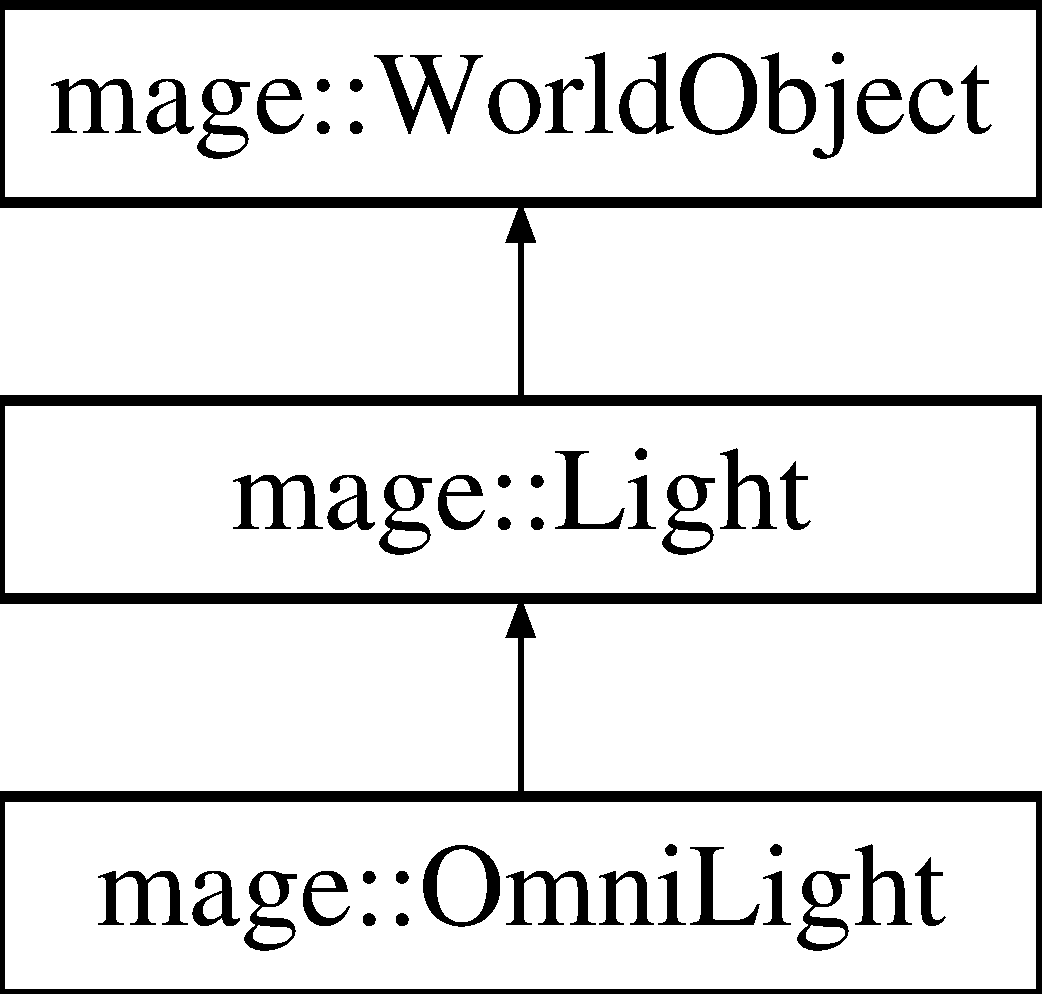
\includegraphics[height=2.000000cm]{classmage_1_1_omni_light}
\end{center}
\end{figure}
\subsection*{Public Member Functions}
\begin{DoxyCompactItemize}
\item 
\hyperlink{classmage_1_1_omni_light_a993394b31cdddcf37018cd5ff09d2d99}{Omni\+Light} ()
\item 
\hyperlink{classmage_1_1_omni_light_accf10bcdf8ed523cfb04129f5345ef92}{Omni\+Light} (const \hyperlink{classmage_1_1_omni_light}{Omni\+Light} \&light)
\item 
\hyperlink{classmage_1_1_omni_light_ae0353cedc67d88be2f4b88374482933d}{Omni\+Light} (\hyperlink{classmage_1_1_omni_light}{Omni\+Light} \&\&light)
\item 
virtual \hyperlink{classmage_1_1_omni_light_af6f4921499b430041966f38aac920b69}{$\sim$\+Omni\+Light} ()
\item 
\hyperlink{classmage_1_1_omni_light}{Omni\+Light} \& \hyperlink{classmage_1_1_omni_light_a7bdce151d327daef5e1f31daedcc4627}{operator=} (const \hyperlink{classmage_1_1_omni_light}{Omni\+Light} \&light)
\item 
\hyperlink{classmage_1_1_omni_light}{Omni\+Light} \& \hyperlink{classmage_1_1_omni_light_a287a54dede61e65efe4493ec20531428}{operator=} (\hyperlink{classmage_1_1_omni_light}{Omni\+Light} \&\&light)
\item 
\hyperlink{namespacemage_a3316d7143a973e37adf1110f2e80ca31}{Unique\+Ptr}$<$ \hyperlink{classmage_1_1_omni_light}{Omni\+Light} $>$ \hyperlink{classmage_1_1_omni_light_a82325924de65733314dcf2b87e926d60}{Clone} () const
\item 
\hyperlink{namespacemage_aa97e833b45f06d60a0a9c4fc22ae02c0}{F32} \hyperlink{classmage_1_1_omni_light_a13f9893ef0a19cbb08bfce557bb906fc}{Get\+Power} () const noexcept
\item 
void \hyperlink{classmage_1_1_omni_light_a03f277ecf566147aa54c95816871de10}{Set\+Power} (\hyperlink{namespacemage_aa97e833b45f06d60a0a9c4fc22ae02c0}{F32} power) noexcept
\item 
const \hyperlink{structmage_1_1_r_g_b_spectrum}{R\+G\+B\+Spectrum} \hyperlink{classmage_1_1_omni_light_ab443f91b4df0c766aeda2c3f5df0f772}{Get\+Power\+Spectrum} () const noexcept
\item 
\hyperlink{namespacemage_aa97e833b45f06d60a0a9c4fc22ae02c0}{F32} \hyperlink{classmage_1_1_omni_light_ae7309fdbe54b5d6bc6d4e20990ba6bdc}{Get\+Intensity} () const noexcept
\item 
void \hyperlink{classmage_1_1_omni_light_add3fece8f288f4d4b55357143faa490b}{Set\+Intensity} (\hyperlink{namespacemage_aa97e833b45f06d60a0a9c4fc22ae02c0}{F32} intensity) noexcept
\item 
const \hyperlink{structmage_1_1_r_g_b_spectrum}{R\+G\+B\+Spectrum} \hyperlink{classmage_1_1_omni_light_a0c0fadc2c0a7ca73e7798b2fe8fc6631}{Get\+Intensity\+Spectrum} () const noexcept
\item 
\hyperlink{namespacemage_aa97e833b45f06d60a0a9c4fc22ae02c0}{F32} \hyperlink{classmage_1_1_omni_light_a1c829777c2afc850dd66382bc0115d8d}{Get\+Range} () const noexcept
\item 
void \hyperlink{classmage_1_1_omni_light_a696ec6a022ccc3993d88c1d435938fb1}{Set\+Range} (\hyperlink{namespacemage_aa97e833b45f06d60a0a9c4fc22ae02c0}{F32} range) noexcept
\item 
bool \hyperlink{classmage_1_1_omni_light_a8d58e7e1b26e54b3d9785ca79213cc4f}{Use\+Shadows} () const noexcept
\item 
void \hyperlink{classmage_1_1_omni_light_ad7c2e780dc83eb63fa44e1475492e192}{Enable\+Shadows} () noexcept
\item 
void \hyperlink{classmage_1_1_omni_light_a2353a53e336ffb55be9949ea6f1d8979}{Dissable\+Shadows} () noexcept
\item 
void \hyperlink{classmage_1_1_omni_light_a19164a13e884bce6fbc80b760c82d243}{Toggle\+Shadows} () noexcept
\item 
void \hyperlink{classmage_1_1_omni_light_a337082a4e6026fe6f98098df063e6660}{Set\+Shadows} (bool shadows) noexcept
\item 
\hyperlink{namespacemage_aa97e833b45f06d60a0a9c4fc22ae02c0}{F32} \hyperlink{classmage_1_1_omni_light_a7a0bd82c0272a7eeeb33a9ede796bae1}{Get\+F\+OV} () const noexcept
\item 
\hyperlink{namespacemage_aa97e833b45f06d60a0a9c4fc22ae02c0}{F32} \hyperlink{classmage_1_1_omni_light_a976a37c3f7c160f0383a93e4f7497eed}{Get\+Aspect\+Ratio} () const noexcept
\item 
const X\+M\+M\+A\+T\+R\+IX \hyperlink{classmage_1_1_omni_light_a3efda1559769189e4693c6e3c570ab4b}{Get\+View\+To\+Projection\+Matrix} () const noexcept
\item 
const \hyperlink{classmage_1_1_perspective_camera}{Perspective\+Camera} \hyperlink{classmage_1_1_omni_light_ac31708d7696a809bb75c75a85b14de80}{Get\+Light\+Camera} () const noexcept
\end{DoxyCompactItemize}
\subsection*{Private Member Functions}
\begin{DoxyCompactItemize}
\item 
virtual \hyperlink{namespacemage_a3316d7143a973e37adf1110f2e80ca31}{Unique\+Ptr}$<$ \hyperlink{classmage_1_1_light}{Light} $>$ \hyperlink{classmage_1_1_omni_light_a1212457828cdd96cc7170767b7bd1223}{Clone\+Implementation} () const override
\item 
void \hyperlink{classmage_1_1_omni_light_a6a10cdc0ed276d68e5378eaf934158e1}{Update\+Bounding\+Volumes} () noexcept
\end{DoxyCompactItemize}
\subsection*{Private Attributes}
\begin{DoxyCompactItemize}
\item 
\hyperlink{namespacemage_aa97e833b45f06d60a0a9c4fc22ae02c0}{F32} \hyperlink{classmage_1_1_omni_light_aa0cbdebabf3ce0d8bbaeff7cf88cadd0}{m\+\_\+intensity}
\item 
\hyperlink{namespacemage_aa97e833b45f06d60a0a9c4fc22ae02c0}{F32} \hyperlink{classmage_1_1_omni_light_a0427a9c7f90750c645cd67ef0bafce47}{m\+\_\+range}
\item 
bool \hyperlink{classmage_1_1_omni_light_a63e5dab12be5021815e98c81dd9aed6a}{m\+\_\+shadows}
\end{DoxyCompactItemize}
\subsection*{Additional Inherited Members}


\subsection{Detailed Description}
A class of omni lights. 

\subsection{Constructor \& Destructor Documentation}
\hypertarget{classmage_1_1_omni_light_a993394b31cdddcf37018cd5ff09d2d99}{}\label{classmage_1_1_omni_light_a993394b31cdddcf37018cd5ff09d2d99} 
\index{mage\+::\+Omni\+Light@{mage\+::\+Omni\+Light}!Omni\+Light@{Omni\+Light}}
\index{Omni\+Light@{Omni\+Light}!mage\+::\+Omni\+Light@{mage\+::\+Omni\+Light}}
\subsubsection{\texorpdfstring{Omni\+Light()}{OmniLight()}\hspace{0.1cm}{\footnotesize\ttfamily [1/3]}}
{\footnotesize\ttfamily mage\+::\+Omni\+Light\+::\+Omni\+Light (\begin{DoxyParamCaption}{ }\end{DoxyParamCaption})}

Constructs an omni light. \hypertarget{classmage_1_1_omni_light_accf10bcdf8ed523cfb04129f5345ef92}{}\label{classmage_1_1_omni_light_accf10bcdf8ed523cfb04129f5345ef92} 
\index{mage\+::\+Omni\+Light@{mage\+::\+Omni\+Light}!Omni\+Light@{Omni\+Light}}
\index{Omni\+Light@{Omni\+Light}!mage\+::\+Omni\+Light@{mage\+::\+Omni\+Light}}
\subsubsection{\texorpdfstring{Omni\+Light()}{OmniLight()}\hspace{0.1cm}{\footnotesize\ttfamily [2/3]}}
{\footnotesize\ttfamily mage\+::\+Omni\+Light\+::\+Omni\+Light (\begin{DoxyParamCaption}\item[{const \hyperlink{classmage_1_1_omni_light}{Omni\+Light} \&}]{light }\end{DoxyParamCaption})\hspace{0.3cm}{\ttfamily [default]}}

Constructs an omni light from the given omni light.


\begin{DoxyParams}[1]{Parameters}
\mbox{\tt in}  & {\em light} & A reference to the omni light to copy. \\
\hline
\end{DoxyParams}
\hypertarget{classmage_1_1_omni_light_ae0353cedc67d88be2f4b88374482933d}{}\label{classmage_1_1_omni_light_ae0353cedc67d88be2f4b88374482933d} 
\index{mage\+::\+Omni\+Light@{mage\+::\+Omni\+Light}!Omni\+Light@{Omni\+Light}}
\index{Omni\+Light@{Omni\+Light}!mage\+::\+Omni\+Light@{mage\+::\+Omni\+Light}}
\subsubsection{\texorpdfstring{Omni\+Light()}{OmniLight()}\hspace{0.1cm}{\footnotesize\ttfamily [3/3]}}
{\footnotesize\ttfamily mage\+::\+Omni\+Light\+::\+Omni\+Light (\begin{DoxyParamCaption}\item[{\hyperlink{classmage_1_1_omni_light}{Omni\+Light} \&\&}]{light }\end{DoxyParamCaption})\hspace{0.3cm}{\ttfamily [default]}}

Constructs an omni light by moving the given omni light.


\begin{DoxyParams}[1]{Parameters}
\mbox{\tt in}  & {\em light} & A reference to the omni light to move. \\
\hline
\end{DoxyParams}
\hypertarget{classmage_1_1_omni_light_af6f4921499b430041966f38aac920b69}{}\label{classmage_1_1_omni_light_af6f4921499b430041966f38aac920b69} 
\index{mage\+::\+Omni\+Light@{mage\+::\+Omni\+Light}!````~Omni\+Light@{$\sim$\+Omni\+Light}}
\index{````~Omni\+Light@{$\sim$\+Omni\+Light}!mage\+::\+Omni\+Light@{mage\+::\+Omni\+Light}}
\subsubsection{\texorpdfstring{$\sim$\+Omni\+Light()}{~OmniLight()}}
{\footnotesize\ttfamily mage\+::\+Omni\+Light\+::$\sim$\+Omni\+Light (\begin{DoxyParamCaption}{ }\end{DoxyParamCaption})\hspace{0.3cm}{\ttfamily [virtual]}, {\ttfamily [default]}}

Destructs this omni light. 

\subsection{Member Function Documentation}
\hypertarget{classmage_1_1_omni_light_a82325924de65733314dcf2b87e926d60}{}\label{classmage_1_1_omni_light_a82325924de65733314dcf2b87e926d60} 
\index{mage\+::\+Omni\+Light@{mage\+::\+Omni\+Light}!Clone@{Clone}}
\index{Clone@{Clone}!mage\+::\+Omni\+Light@{mage\+::\+Omni\+Light}}
\subsubsection{\texorpdfstring{Clone()}{Clone()}}
{\footnotesize\ttfamily \hyperlink{namespacemage_a3316d7143a973e37adf1110f2e80ca31}{Unique\+Ptr}$<$ \hyperlink{classmage_1_1_omni_light}{Omni\+Light} $>$ mage\+::\+Omni\+Light\+::\+Clone (\begin{DoxyParamCaption}{ }\end{DoxyParamCaption}) const}

Clones this omni light.

\begin{DoxyReturn}{Returns}
A pointer to the clone of this omni light. 
\end{DoxyReturn}
\hypertarget{classmage_1_1_omni_light_a1212457828cdd96cc7170767b7bd1223}{}\label{classmage_1_1_omni_light_a1212457828cdd96cc7170767b7bd1223} 
\index{mage\+::\+Omni\+Light@{mage\+::\+Omni\+Light}!Clone\+Implementation@{Clone\+Implementation}}
\index{Clone\+Implementation@{Clone\+Implementation}!mage\+::\+Omni\+Light@{mage\+::\+Omni\+Light}}
\subsubsection{\texorpdfstring{Clone\+Implementation()}{CloneImplementation()}}
{\footnotesize\ttfamily \hyperlink{namespacemage_a3316d7143a973e37adf1110f2e80ca31}{Unique\+Ptr}$<$ \hyperlink{classmage_1_1_light}{Light} $>$ mage\+::\+Omni\+Light\+::\+Clone\+Implementation (\begin{DoxyParamCaption}{ }\end{DoxyParamCaption}) const\hspace{0.3cm}{\ttfamily [override]}, {\ttfamily [private]}, {\ttfamily [virtual]}}

Clones this omni light.

\begin{DoxyReturn}{Returns}
A pointer to the clone of this omni light. 
\end{DoxyReturn}


Implements \hyperlink{classmage_1_1_light_aa613d76a1ebda69efde853d15f75490c}{mage\+::\+Light}.

\hypertarget{classmage_1_1_omni_light_a2353a53e336ffb55be9949ea6f1d8979}{}\label{classmage_1_1_omni_light_a2353a53e336ffb55be9949ea6f1d8979} 
\index{mage\+::\+Omni\+Light@{mage\+::\+Omni\+Light}!Dissable\+Shadows@{Dissable\+Shadows}}
\index{Dissable\+Shadows@{Dissable\+Shadows}!mage\+::\+Omni\+Light@{mage\+::\+Omni\+Light}}
\subsubsection{\texorpdfstring{Dissable\+Shadows()}{DissableShadows()}}
{\footnotesize\ttfamily void mage\+::\+Omni\+Light\+::\+Dissable\+Shadows (\begin{DoxyParamCaption}{ }\end{DoxyParamCaption})\hspace{0.3cm}{\ttfamily [noexcept]}}

Dissables shadows for this omni light. \hypertarget{classmage_1_1_omni_light_ad7c2e780dc83eb63fa44e1475492e192}{}\label{classmage_1_1_omni_light_ad7c2e780dc83eb63fa44e1475492e192} 
\index{mage\+::\+Omni\+Light@{mage\+::\+Omni\+Light}!Enable\+Shadows@{Enable\+Shadows}}
\index{Enable\+Shadows@{Enable\+Shadows}!mage\+::\+Omni\+Light@{mage\+::\+Omni\+Light}}
\subsubsection{\texorpdfstring{Enable\+Shadows()}{EnableShadows()}}
{\footnotesize\ttfamily void mage\+::\+Omni\+Light\+::\+Enable\+Shadows (\begin{DoxyParamCaption}{ }\end{DoxyParamCaption})\hspace{0.3cm}{\ttfamily [noexcept]}}

Enables shadows for this omni light. \hypertarget{classmage_1_1_omni_light_a976a37c3f7c160f0383a93e4f7497eed}{}\label{classmage_1_1_omni_light_a976a37c3f7c160f0383a93e4f7497eed} 
\index{mage\+::\+Omni\+Light@{mage\+::\+Omni\+Light}!Get\+Aspect\+Ratio@{Get\+Aspect\+Ratio}}
\index{Get\+Aspect\+Ratio@{Get\+Aspect\+Ratio}!mage\+::\+Omni\+Light@{mage\+::\+Omni\+Light}}
\subsubsection{\texorpdfstring{Get\+Aspect\+Ratio()}{GetAspectRatio()}}
{\footnotesize\ttfamily \hyperlink{namespacemage_aa97e833b45f06d60a0a9c4fc22ae02c0}{F32} mage\+::\+Omni\+Light\+::\+Get\+Aspect\+Ratio (\begin{DoxyParamCaption}{ }\end{DoxyParamCaption}) const\hspace{0.3cm}{\ttfamily [noexcept]}}

Returns the aspect ratio of this omni light.

\begin{DoxyReturn}{Returns}
The aspect ratio of this omni light. 
\end{DoxyReturn}
\hypertarget{classmage_1_1_omni_light_a7a0bd82c0272a7eeeb33a9ede796bae1}{}\label{classmage_1_1_omni_light_a7a0bd82c0272a7eeeb33a9ede796bae1} 
\index{mage\+::\+Omni\+Light@{mage\+::\+Omni\+Light}!Get\+F\+OV@{Get\+F\+OV}}
\index{Get\+F\+OV@{Get\+F\+OV}!mage\+::\+Omni\+Light@{mage\+::\+Omni\+Light}}
\subsubsection{\texorpdfstring{Get\+F\+O\+V()}{GetFOV()}}
{\footnotesize\ttfamily \hyperlink{namespacemage_aa97e833b45f06d60a0a9c4fc22ae02c0}{F32} mage\+::\+Omni\+Light\+::\+Get\+F\+OV (\begin{DoxyParamCaption}{ }\end{DoxyParamCaption}) const\hspace{0.3cm}{\ttfamily [noexcept]}}

Returns the (horizontal and vertical) field-\/of-\/view of this omni light.

\begin{DoxyReturn}{Returns}
The (horizontal and vertical) field-\/of-\/view of this omni light. 
\end{DoxyReturn}
\hypertarget{classmage_1_1_omni_light_ae7309fdbe54b5d6bc6d4e20990ba6bdc}{}\label{classmage_1_1_omni_light_ae7309fdbe54b5d6bc6d4e20990ba6bdc} 
\index{mage\+::\+Omni\+Light@{mage\+::\+Omni\+Light}!Get\+Intensity@{Get\+Intensity}}
\index{Get\+Intensity@{Get\+Intensity}!mage\+::\+Omni\+Light@{mage\+::\+Omni\+Light}}
\subsubsection{\texorpdfstring{Get\+Intensity()}{GetIntensity()}}
{\footnotesize\ttfamily \hyperlink{namespacemage_aa97e833b45f06d60a0a9c4fc22ae02c0}{F32} mage\+::\+Omni\+Light\+::\+Get\+Intensity (\begin{DoxyParamCaption}{ }\end{DoxyParamCaption}) const\hspace{0.3cm}{\ttfamily [noexcept]}}

Returns the radiant intensity of this omni light.

\begin{DoxyReturn}{Returns}
The radiant intensity in watts per steradians of this omni light. 
\end{DoxyReturn}
\hypertarget{classmage_1_1_omni_light_a0c0fadc2c0a7ca73e7798b2fe8fc6631}{}\label{classmage_1_1_omni_light_a0c0fadc2c0a7ca73e7798b2fe8fc6631} 
\index{mage\+::\+Omni\+Light@{mage\+::\+Omni\+Light}!Get\+Intensity\+Spectrum@{Get\+Intensity\+Spectrum}}
\index{Get\+Intensity\+Spectrum@{Get\+Intensity\+Spectrum}!mage\+::\+Omni\+Light@{mage\+::\+Omni\+Light}}
\subsubsection{\texorpdfstring{Get\+Intensity\+Spectrum()}{GetIntensitySpectrum()}}
{\footnotesize\ttfamily const \hyperlink{structmage_1_1_r_g_b_spectrum}{R\+G\+B\+Spectrum} mage\+::\+Omni\+Light\+::\+Get\+Intensity\+Spectrum (\begin{DoxyParamCaption}{ }\end{DoxyParamCaption}) const\hspace{0.3cm}{\ttfamily [noexcept]}}

Returns the radiant intensity spectrum of this omni light.

\begin{DoxyReturn}{Returns}
The radiant intensity spectrum of this omni light. 
\end{DoxyReturn}
\hypertarget{classmage_1_1_omni_light_ac31708d7696a809bb75c75a85b14de80}{}\label{classmage_1_1_omni_light_ac31708d7696a809bb75c75a85b14de80} 
\index{mage\+::\+Omni\+Light@{mage\+::\+Omni\+Light}!Get\+Light\+Camera@{Get\+Light\+Camera}}
\index{Get\+Light\+Camera@{Get\+Light\+Camera}!mage\+::\+Omni\+Light@{mage\+::\+Omni\+Light}}
\subsubsection{\texorpdfstring{Get\+Light\+Camera()}{GetLightCamera()}}
{\footnotesize\ttfamily const \hyperlink{classmage_1_1_perspective_camera}{Perspective\+Camera} mage\+::\+Omni\+Light\+::\+Get\+Light\+Camera (\begin{DoxyParamCaption}{ }\end{DoxyParamCaption}) const\hspace{0.3cm}{\ttfamily [noexcept]}}

Returns the (forward) light camera of this omni light.

\begin{DoxyReturn}{Returns}
The (forward) light camera of this omni light. 
\end{DoxyReturn}
\hypertarget{classmage_1_1_omni_light_a13f9893ef0a19cbb08bfce557bb906fc}{}\label{classmage_1_1_omni_light_a13f9893ef0a19cbb08bfce557bb906fc} 
\index{mage\+::\+Omni\+Light@{mage\+::\+Omni\+Light}!Get\+Power@{Get\+Power}}
\index{Get\+Power@{Get\+Power}!mage\+::\+Omni\+Light@{mage\+::\+Omni\+Light}}
\subsubsection{\texorpdfstring{Get\+Power()}{GetPower()}}
{\footnotesize\ttfamily \hyperlink{namespacemage_aa97e833b45f06d60a0a9c4fc22ae02c0}{F32} mage\+::\+Omni\+Light\+::\+Get\+Power (\begin{DoxyParamCaption}{ }\end{DoxyParamCaption}) const\hspace{0.3cm}{\ttfamily [noexcept]}}

Returns the power of this omni light.

\begin{DoxyReturn}{Returns}
The power in watts of this omni light. 
\end{DoxyReturn}
\hypertarget{classmage_1_1_omni_light_ab443f91b4df0c766aeda2c3f5df0f772}{}\label{classmage_1_1_omni_light_ab443f91b4df0c766aeda2c3f5df0f772} 
\index{mage\+::\+Omni\+Light@{mage\+::\+Omni\+Light}!Get\+Power\+Spectrum@{Get\+Power\+Spectrum}}
\index{Get\+Power\+Spectrum@{Get\+Power\+Spectrum}!mage\+::\+Omni\+Light@{mage\+::\+Omni\+Light}}
\subsubsection{\texorpdfstring{Get\+Power\+Spectrum()}{GetPowerSpectrum()}}
{\footnotesize\ttfamily const \hyperlink{structmage_1_1_r_g_b_spectrum}{R\+G\+B\+Spectrum} mage\+::\+Omni\+Light\+::\+Get\+Power\+Spectrum (\begin{DoxyParamCaption}{ }\end{DoxyParamCaption}) const\hspace{0.3cm}{\ttfamily [noexcept]}}

Returns the power spectrum of this omni light.

\begin{DoxyReturn}{Returns}
The power spectrum of this omni light. 
\end{DoxyReturn}
\hypertarget{classmage_1_1_omni_light_a1c829777c2afc850dd66382bc0115d8d}{}\label{classmage_1_1_omni_light_a1c829777c2afc850dd66382bc0115d8d} 
\index{mage\+::\+Omni\+Light@{mage\+::\+Omni\+Light}!Get\+Range@{Get\+Range}}
\index{Get\+Range@{Get\+Range}!mage\+::\+Omni\+Light@{mage\+::\+Omni\+Light}}
\subsubsection{\texorpdfstring{Get\+Range()}{GetRange()}}
{\footnotesize\ttfamily \hyperlink{namespacemage_aa97e833b45f06d60a0a9c4fc22ae02c0}{F32} mage\+::\+Omni\+Light\+::\+Get\+Range (\begin{DoxyParamCaption}{ }\end{DoxyParamCaption}) const\hspace{0.3cm}{\ttfamily [noexcept]}}

Returns the range of this omni light.

\begin{DoxyReturn}{Returns}
The range of this omni light. 
\end{DoxyReturn}
\hypertarget{classmage_1_1_omni_light_a3efda1559769189e4693c6e3c570ab4b}{}\label{classmage_1_1_omni_light_a3efda1559769189e4693c6e3c570ab4b} 
\index{mage\+::\+Omni\+Light@{mage\+::\+Omni\+Light}!Get\+View\+To\+Projection\+Matrix@{Get\+View\+To\+Projection\+Matrix}}
\index{Get\+View\+To\+Projection\+Matrix@{Get\+View\+To\+Projection\+Matrix}!mage\+::\+Omni\+Light@{mage\+::\+Omni\+Light}}
\subsubsection{\texorpdfstring{Get\+View\+To\+Projection\+Matrix()}{GetViewToProjectionMatrix()}}
{\footnotesize\ttfamily const X\+M\+M\+A\+T\+R\+IX mage\+::\+Omni\+Light\+::\+Get\+View\+To\+Projection\+Matrix (\begin{DoxyParamCaption}{ }\end{DoxyParamCaption}) const\hspace{0.3cm}{\ttfamily [noexcept]}}

Returns the view-\/to-\/projection matrix of the (forward) light camera of this omni light.

\begin{DoxyReturn}{Returns}
The view-\/to-\/projection matrix of the (forward) light camera of this omni light. 
\end{DoxyReturn}
\hypertarget{classmage_1_1_omni_light_a7bdce151d327daef5e1f31daedcc4627}{}\label{classmage_1_1_omni_light_a7bdce151d327daef5e1f31daedcc4627} 
\index{mage\+::\+Omni\+Light@{mage\+::\+Omni\+Light}!operator=@{operator=}}
\index{operator=@{operator=}!mage\+::\+Omni\+Light@{mage\+::\+Omni\+Light}}
\subsubsection{\texorpdfstring{operator=()}{operator=()}\hspace{0.1cm}{\footnotesize\ttfamily [1/2]}}
{\footnotesize\ttfamily \hyperlink{classmage_1_1_omni_light}{Omni\+Light} \& mage\+::\+Omni\+Light\+::operator= (\begin{DoxyParamCaption}\item[{const \hyperlink{classmage_1_1_omni_light}{Omni\+Light} \&}]{light }\end{DoxyParamCaption})\hspace{0.3cm}{\ttfamily [default]}}

Copies the given omni light to this omni light.


\begin{DoxyParams}[1]{Parameters}
\mbox{\tt in}  & {\em light} & A reference to the omni light to copy. \\
\hline
\end{DoxyParams}
\begin{DoxyReturn}{Returns}
A reference to the copy of the given omni light (i.\+e. this omni light). 
\end{DoxyReturn}
\hypertarget{classmage_1_1_omni_light_a287a54dede61e65efe4493ec20531428}{}\label{classmage_1_1_omni_light_a287a54dede61e65efe4493ec20531428} 
\index{mage\+::\+Omni\+Light@{mage\+::\+Omni\+Light}!operator=@{operator=}}
\index{operator=@{operator=}!mage\+::\+Omni\+Light@{mage\+::\+Omni\+Light}}
\subsubsection{\texorpdfstring{operator=()}{operator=()}\hspace{0.1cm}{\footnotesize\ttfamily [2/2]}}
{\footnotesize\ttfamily \hyperlink{classmage_1_1_omni_light}{Omni\+Light} \& mage\+::\+Omni\+Light\+::operator= (\begin{DoxyParamCaption}\item[{\hyperlink{classmage_1_1_omni_light}{Omni\+Light} \&\&}]{light }\end{DoxyParamCaption})\hspace{0.3cm}{\ttfamily [default]}}

Moves the given omni light to this omni light.


\begin{DoxyParams}[1]{Parameters}
\mbox{\tt in}  & {\em light} & A reference to the omni light to move. \\
\hline
\end{DoxyParams}
\begin{DoxyReturn}{Returns}
A reference to the moved omni light (i.\+e. this omni light). 
\end{DoxyReturn}
\hypertarget{classmage_1_1_omni_light_add3fece8f288f4d4b55357143faa490b}{}\label{classmage_1_1_omni_light_add3fece8f288f4d4b55357143faa490b} 
\index{mage\+::\+Omni\+Light@{mage\+::\+Omni\+Light}!Set\+Intensity@{Set\+Intensity}}
\index{Set\+Intensity@{Set\+Intensity}!mage\+::\+Omni\+Light@{mage\+::\+Omni\+Light}}
\subsubsection{\texorpdfstring{Set\+Intensity()}{SetIntensity()}}
{\footnotesize\ttfamily void mage\+::\+Omni\+Light\+::\+Set\+Intensity (\begin{DoxyParamCaption}\item[{\hyperlink{namespacemage_aa97e833b45f06d60a0a9c4fc22ae02c0}{F32}}]{intensity }\end{DoxyParamCaption})\hspace{0.3cm}{\ttfamily [noexcept]}}

Sets the radiant intensity of this omni light to the given radial intensity.


\begin{DoxyParams}[1]{Parameters}
\mbox{\tt in}  & {\em intensity} & The radiant intensity in watts per steradians. \\
\hline
\end{DoxyParams}
\hypertarget{classmage_1_1_omni_light_a03f277ecf566147aa54c95816871de10}{}\label{classmage_1_1_omni_light_a03f277ecf566147aa54c95816871de10} 
\index{mage\+::\+Omni\+Light@{mage\+::\+Omni\+Light}!Set\+Power@{Set\+Power}}
\index{Set\+Power@{Set\+Power}!mage\+::\+Omni\+Light@{mage\+::\+Omni\+Light}}
\subsubsection{\texorpdfstring{Set\+Power()}{SetPower()}}
{\footnotesize\ttfamily void mage\+::\+Omni\+Light\+::\+Set\+Power (\begin{DoxyParamCaption}\item[{\hyperlink{namespacemage_aa97e833b45f06d60a0a9c4fc22ae02c0}{F32}}]{power }\end{DoxyParamCaption})\hspace{0.3cm}{\ttfamily [noexcept]}}

Sets the power of this omni light to the given radiance.


\begin{DoxyParams}[1]{Parameters}
\mbox{\tt in}  & {\em power} & The power in watts. \\
\hline
\end{DoxyParams}
\hypertarget{classmage_1_1_omni_light_a696ec6a022ccc3993d88c1d435938fb1}{}\label{classmage_1_1_omni_light_a696ec6a022ccc3993d88c1d435938fb1} 
\index{mage\+::\+Omni\+Light@{mage\+::\+Omni\+Light}!Set\+Range@{Set\+Range}}
\index{Set\+Range@{Set\+Range}!mage\+::\+Omni\+Light@{mage\+::\+Omni\+Light}}
\subsubsection{\texorpdfstring{Set\+Range()}{SetRange()}}
{\footnotesize\ttfamily void mage\+::\+Omni\+Light\+::\+Set\+Range (\begin{DoxyParamCaption}\item[{\hyperlink{namespacemage_aa97e833b45f06d60a0a9c4fc22ae02c0}{F32}}]{range }\end{DoxyParamCaption})\hspace{0.3cm}{\ttfamily [noexcept]}}

Sets the range of this omni light to the given value.

\begin{DoxyPrecond}{Precondition}
{\itshape range} must be greater than 0. 
\end{DoxyPrecond}

\begin{DoxyParams}[1]{Parameters}
\mbox{\tt in}  & {\em range} & The range. \\
\hline
\end{DoxyParams}
\hypertarget{classmage_1_1_omni_light_a337082a4e6026fe6f98098df063e6660}{}\label{classmage_1_1_omni_light_a337082a4e6026fe6f98098df063e6660} 
\index{mage\+::\+Omni\+Light@{mage\+::\+Omni\+Light}!Set\+Shadows@{Set\+Shadows}}
\index{Set\+Shadows@{Set\+Shadows}!mage\+::\+Omni\+Light@{mage\+::\+Omni\+Light}}
\subsubsection{\texorpdfstring{Set\+Shadows()}{SetShadows()}}
{\footnotesize\ttfamily void mage\+::\+Omni\+Light\+::\+Set\+Shadows (\begin{DoxyParamCaption}\item[{bool}]{shadows }\end{DoxyParamCaption})\hspace{0.3cm}{\ttfamily [noexcept]}}

Sets shadows for this omni light to the given value.


\begin{DoxyParams}[1]{Parameters}
\mbox{\tt in}  & {\em shadows} & {\ttfamily true} if shadows should be used for this omni light. {\ttfamily false} otherwise. \\
\hline
\end{DoxyParams}
\hypertarget{classmage_1_1_omni_light_a19164a13e884bce6fbc80b760c82d243}{}\label{classmage_1_1_omni_light_a19164a13e884bce6fbc80b760c82d243} 
\index{mage\+::\+Omni\+Light@{mage\+::\+Omni\+Light}!Toggle\+Shadows@{Toggle\+Shadows}}
\index{Toggle\+Shadows@{Toggle\+Shadows}!mage\+::\+Omni\+Light@{mage\+::\+Omni\+Light}}
\subsubsection{\texorpdfstring{Toggle\+Shadows()}{ToggleShadows()}}
{\footnotesize\ttfamily void mage\+::\+Omni\+Light\+::\+Toggle\+Shadows (\begin{DoxyParamCaption}{ }\end{DoxyParamCaption})\hspace{0.3cm}{\ttfamily [noexcept]}}

Toggles shadows for this omni light. \hypertarget{classmage_1_1_omni_light_a6a10cdc0ed276d68e5378eaf934158e1}{}\label{classmage_1_1_omni_light_a6a10cdc0ed276d68e5378eaf934158e1} 
\index{mage\+::\+Omni\+Light@{mage\+::\+Omni\+Light}!Update\+Bounding\+Volumes@{Update\+Bounding\+Volumes}}
\index{Update\+Bounding\+Volumes@{Update\+Bounding\+Volumes}!mage\+::\+Omni\+Light@{mage\+::\+Omni\+Light}}
\subsubsection{\texorpdfstring{Update\+Bounding\+Volumes()}{UpdateBoundingVolumes()}}
{\footnotesize\ttfamily void mage\+::\+Omni\+Light\+::\+Update\+Bounding\+Volumes (\begin{DoxyParamCaption}{ }\end{DoxyParamCaption})\hspace{0.3cm}{\ttfamily [private]}, {\ttfamily [noexcept]}}

Updates the bounding volumes of this omni light. \hypertarget{classmage_1_1_omni_light_a8d58e7e1b26e54b3d9785ca79213cc4f}{}\label{classmage_1_1_omni_light_a8d58e7e1b26e54b3d9785ca79213cc4f} 
\index{mage\+::\+Omni\+Light@{mage\+::\+Omni\+Light}!Use\+Shadows@{Use\+Shadows}}
\index{Use\+Shadows@{Use\+Shadows}!mage\+::\+Omni\+Light@{mage\+::\+Omni\+Light}}
\subsubsection{\texorpdfstring{Use\+Shadows()}{UseShadows()}}
{\footnotesize\ttfamily bool mage\+::\+Omni\+Light\+::\+Use\+Shadows (\begin{DoxyParamCaption}{ }\end{DoxyParamCaption}) const\hspace{0.3cm}{\ttfamily [noexcept]}}

Checks whether shadows should be used for this omni light.

\begin{DoxyReturn}{Returns}
{\ttfamily true} if shadows should be used for this omni light. {\ttfamily false} otherwise. 
\end{DoxyReturn}


\subsection{Member Data Documentation}
\hypertarget{classmage_1_1_omni_light_aa0cbdebabf3ce0d8bbaeff7cf88cadd0}{}\label{classmage_1_1_omni_light_aa0cbdebabf3ce0d8bbaeff7cf88cadd0} 
\index{mage\+::\+Omni\+Light@{mage\+::\+Omni\+Light}!m\+\_\+intensity@{m\+\_\+intensity}}
\index{m\+\_\+intensity@{m\+\_\+intensity}!mage\+::\+Omni\+Light@{mage\+::\+Omni\+Light}}
\subsubsection{\texorpdfstring{m\+\_\+intensity}{m\_intensity}}
{\footnotesize\ttfamily \hyperlink{namespacemage_aa97e833b45f06d60a0a9c4fc22ae02c0}{F32} mage\+::\+Omni\+Light\+::m\+\_\+intensity\hspace{0.3cm}{\ttfamily [private]}}

The radiant intensity in watts per steradians of this omni light. \hypertarget{classmage_1_1_omni_light_a0427a9c7f90750c645cd67ef0bafce47}{}\label{classmage_1_1_omni_light_a0427a9c7f90750c645cd67ef0bafce47} 
\index{mage\+::\+Omni\+Light@{mage\+::\+Omni\+Light}!m\+\_\+range@{m\+\_\+range}}
\index{m\+\_\+range@{m\+\_\+range}!mage\+::\+Omni\+Light@{mage\+::\+Omni\+Light}}
\subsubsection{\texorpdfstring{m\+\_\+range}{m\_range}}
{\footnotesize\ttfamily \hyperlink{namespacemage_aa97e833b45f06d60a0a9c4fc22ae02c0}{F32} mage\+::\+Omni\+Light\+::m\+\_\+range\hspace{0.3cm}{\ttfamily [private]}}

The range of this omni light. \hypertarget{classmage_1_1_omni_light_a63e5dab12be5021815e98c81dd9aed6a}{}\label{classmage_1_1_omni_light_a63e5dab12be5021815e98c81dd9aed6a} 
\index{mage\+::\+Omni\+Light@{mage\+::\+Omni\+Light}!m\+\_\+shadows@{m\+\_\+shadows}}
\index{m\+\_\+shadows@{m\+\_\+shadows}!mage\+::\+Omni\+Light@{mage\+::\+Omni\+Light}}
\subsubsection{\texorpdfstring{m\+\_\+shadows}{m\_shadows}}
{\footnotesize\ttfamily bool mage\+::\+Omni\+Light\+::m\+\_\+shadows\hspace{0.3cm}{\ttfamily [private]}}

A flag indicating whether shadows should be calculated or not for this omni light. 
\hypertarget{classmage_1_1_orthographic_camera}{}\section{mage\+:\+:Orthographic\+Camera Class Reference}
\label{classmage_1_1_orthographic_camera}\index{mage\+::\+Orthographic\+Camera@{mage\+::\+Orthographic\+Camera}}


{\ttfamily \#include $<$orthographic\+\_\+camera.\+hpp$>$}

Inheritance diagram for mage\+:\+:Orthographic\+Camera\+:\begin{figure}[H]
\begin{center}
\leavevmode
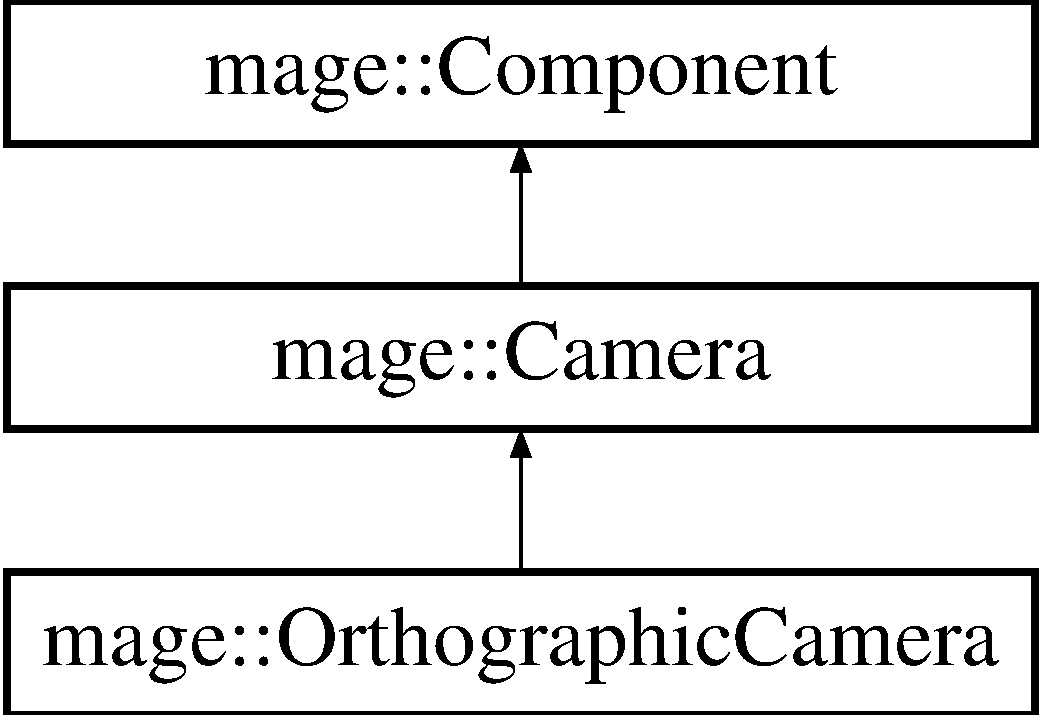
\includegraphics[height=3.000000cm]{classmage_1_1_orthographic_camera}
\end{center}
\end{figure}
\subsection*{Public Member Functions}
\begin{DoxyCompactItemize}
\item 
\hyperlink{classmage_1_1_orthographic_camera_ad3457e635c91cc83d7ed165f0fe52f75}{Orthographic\+Camera} () noexcept
\item 
\hyperlink{classmage_1_1_orthographic_camera_ab0ebb2f3cc8fda48867e02990fae360c}{Orthographic\+Camera} (const \hyperlink{classmage_1_1_orthographic_camera}{Orthographic\+Camera} \&camera) noexcept
\item 
\hyperlink{classmage_1_1_orthographic_camera_af5387bb16892ab9ba803a6797d47636a}{Orthographic\+Camera} (\hyperlink{classmage_1_1_orthographic_camera}{Orthographic\+Camera} \&\&camera) noexcept
\item 
virtual \hyperlink{classmage_1_1_orthographic_camera_ac7d1f4ce12a5d0a2539b610f14f59304}{$\sim$\+Orthographic\+Camera} ()
\item 
\hyperlink{classmage_1_1_orthographic_camera}{Orthographic\+Camera} \& \hyperlink{classmage_1_1_orthographic_camera_aa436ca54df7a7ca28642674e8f3db98f}{operator=} (const \hyperlink{classmage_1_1_orthographic_camera}{Orthographic\+Camera} \&camera) noexcept
\item 
\hyperlink{classmage_1_1_orthographic_camera}{Orthographic\+Camera} \& \hyperlink{classmage_1_1_orthographic_camera_a8ea3c026f05b743ee88eb2c1f126238f}{operator=} (\hyperlink{classmage_1_1_orthographic_camera}{Orthographic\+Camera} \&\&camera) noexcept
\item 
\hyperlink{namespacemage_aa97e833b45f06d60a0a9c4fc22ae02c0}{F32} \hyperlink{classmage_1_1_orthographic_camera_adbafcc6cf5175f10e75599b0bbe95740}{Get\+Width} () const noexcept
\item 
void \hyperlink{classmage_1_1_orthographic_camera_a43af64f189a3159f50809ca499624ed6}{Set\+Width} (\hyperlink{namespacemage_aa97e833b45f06d60a0a9c4fc22ae02c0}{F32} width) noexcept
\item 
\hyperlink{namespacemage_aa97e833b45f06d60a0a9c4fc22ae02c0}{F32} \hyperlink{classmage_1_1_orthographic_camera_a3845253608fb385ca6e48c619c5b39c1}{Get\+Height} () const noexcept
\item 
void \hyperlink{classmage_1_1_orthographic_camera_a29e910ff54a53ee149798cbf062e9416}{Set\+Height} (\hyperlink{namespacemage_aa97e833b45f06d60a0a9c4fc22ae02c0}{F32} height) noexcept
\item 
void \hyperlink{classmage_1_1_orthographic_camera_a1a2c9e7e74b7ab25070ffd6ec43faa4d}{Set\+Width\+And\+Height} (\hyperlink{namespacemage_aa97e833b45f06d60a0a9c4fc22ae02c0}{F32} width, \hyperlink{namespacemage_aa97e833b45f06d60a0a9c4fc22ae02c0}{F32} height) noexcept
\item 
void \hyperlink{classmage_1_1_orthographic_camera_a8b86c23bb9da55d9e55a4da4a82b9d72}{Set\+View\+To\+Projection\+Matrix} (\hyperlink{namespacemage_aa97e833b45f06d60a0a9c4fc22ae02c0}{F32} width, \hyperlink{namespacemage_aa97e833b45f06d60a0a9c4fc22ae02c0}{F32} height, \hyperlink{namespacemage_aa97e833b45f06d60a0a9c4fc22ae02c0}{F32} near\+\_\+z, \hyperlink{namespacemage_aa97e833b45f06d60a0a9c4fc22ae02c0}{F32} far\+\_\+z) noexcept
\item 
virtual const X\+M\+M\+A\+T\+R\+IX X\+M\+\_\+\+C\+A\+L\+L\+C\+O\+NV \hyperlink{classmage_1_1_orthographic_camera_a9ba51750d26d91fa094d82f875c7f1e5}{Get\+View\+To\+Projection\+Matrix} () const noexcept override
\item 
virtual const X\+M\+M\+A\+T\+R\+IX X\+M\+\_\+\+C\+A\+L\+L\+C\+O\+NV \hyperlink{classmage_1_1_orthographic_camera_a7bbc235a85877c12b60d1a56d5b65108}{Get\+Projection\+To\+View\+Matrix} () const noexcept override
\end{DoxyCompactItemize}
\subsection*{Private Attributes}
\begin{DoxyCompactItemize}
\item 
\hyperlink{namespacemage_aa97e833b45f06d60a0a9c4fc22ae02c0}{F32} \hyperlink{classmage_1_1_orthographic_camera_a78586ef1dfd4e1ffa5d9b32378a1e7f8}{m\+\_\+width}
\item 
\hyperlink{namespacemage_aa97e833b45f06d60a0a9c4fc22ae02c0}{F32} \hyperlink{classmage_1_1_orthographic_camera_a2bd741a8d76cdb47636792858955fe62}{m\+\_\+height}
\end{DoxyCompactItemize}
\subsection*{Additional Inherited Members}


\subsection{Detailed Description}
A class of orthographic cameras. 

\subsection{Constructor \& Destructor Documentation}
\hypertarget{classmage_1_1_orthographic_camera_ad3457e635c91cc83d7ed165f0fe52f75}{}\label{classmage_1_1_orthographic_camera_ad3457e635c91cc83d7ed165f0fe52f75} 
\index{mage\+::\+Orthographic\+Camera@{mage\+::\+Orthographic\+Camera}!Orthographic\+Camera@{Orthographic\+Camera}}
\index{Orthographic\+Camera@{Orthographic\+Camera}!mage\+::\+Orthographic\+Camera@{mage\+::\+Orthographic\+Camera}}
\subsubsection{\texorpdfstring{Orthographic\+Camera()}{OrthographicCamera()}\hspace{0.1cm}{\footnotesize\ttfamily [1/3]}}
{\footnotesize\ttfamily mage\+::\+Orthographic\+Camera\+::\+Orthographic\+Camera (\begin{DoxyParamCaption}{ }\end{DoxyParamCaption})\hspace{0.3cm}{\ttfamily [noexcept]}}

Constructs an orthographic camera.

\begin{DoxyPrecond}{Precondition}
The rendering manager associated with the current engine must be loaded. 
\end{DoxyPrecond}
\hypertarget{classmage_1_1_orthographic_camera_ab0ebb2f3cc8fda48867e02990fae360c}{}\label{classmage_1_1_orthographic_camera_ab0ebb2f3cc8fda48867e02990fae360c} 
\index{mage\+::\+Orthographic\+Camera@{mage\+::\+Orthographic\+Camera}!Orthographic\+Camera@{Orthographic\+Camera}}
\index{Orthographic\+Camera@{Orthographic\+Camera}!mage\+::\+Orthographic\+Camera@{mage\+::\+Orthographic\+Camera}}
\subsubsection{\texorpdfstring{Orthographic\+Camera()}{OrthographicCamera()}\hspace{0.1cm}{\footnotesize\ttfamily [2/3]}}
{\footnotesize\ttfamily mage\+::\+Orthographic\+Camera\+::\+Orthographic\+Camera (\begin{DoxyParamCaption}\item[{const \hyperlink{classmage_1_1_orthographic_camera}{Orthographic\+Camera} \&}]{camera }\end{DoxyParamCaption})\hspace{0.3cm}{\ttfamily [default]}, {\ttfamily [noexcept]}}

Constructs an orthographic camera from the given orthographic camera.


\begin{DoxyParams}[1]{Parameters}
\mbox{\tt in}  & {\em camera} & A reference to the orthographic camera to copy. \\
\hline
\end{DoxyParams}
\hypertarget{classmage_1_1_orthographic_camera_af5387bb16892ab9ba803a6797d47636a}{}\label{classmage_1_1_orthographic_camera_af5387bb16892ab9ba803a6797d47636a} 
\index{mage\+::\+Orthographic\+Camera@{mage\+::\+Orthographic\+Camera}!Orthographic\+Camera@{Orthographic\+Camera}}
\index{Orthographic\+Camera@{Orthographic\+Camera}!mage\+::\+Orthographic\+Camera@{mage\+::\+Orthographic\+Camera}}
\subsubsection{\texorpdfstring{Orthographic\+Camera()}{OrthographicCamera()}\hspace{0.1cm}{\footnotesize\ttfamily [3/3]}}
{\footnotesize\ttfamily mage\+::\+Orthographic\+Camera\+::\+Orthographic\+Camera (\begin{DoxyParamCaption}\item[{\hyperlink{classmage_1_1_orthographic_camera}{Orthographic\+Camera} \&\&}]{camera }\end{DoxyParamCaption})\hspace{0.3cm}{\ttfamily [default]}, {\ttfamily [noexcept]}}

Constructs an orthographic camera by moving the given orthographic camera.


\begin{DoxyParams}[1]{Parameters}
\mbox{\tt in}  & {\em camera} & A reference to the orthographic camera to move. \\
\hline
\end{DoxyParams}
\hypertarget{classmage_1_1_orthographic_camera_ac7d1f4ce12a5d0a2539b610f14f59304}{}\label{classmage_1_1_orthographic_camera_ac7d1f4ce12a5d0a2539b610f14f59304} 
\index{mage\+::\+Orthographic\+Camera@{mage\+::\+Orthographic\+Camera}!````~Orthographic\+Camera@{$\sim$\+Orthographic\+Camera}}
\index{````~Orthographic\+Camera@{$\sim$\+Orthographic\+Camera}!mage\+::\+Orthographic\+Camera@{mage\+::\+Orthographic\+Camera}}
\subsubsection{\texorpdfstring{$\sim$\+Orthographic\+Camera()}{~OrthographicCamera()}}
{\footnotesize\ttfamily mage\+::\+Orthographic\+Camera\+::$\sim$\+Orthographic\+Camera (\begin{DoxyParamCaption}{ }\end{DoxyParamCaption})\hspace{0.3cm}{\ttfamily [virtual]}, {\ttfamily [default]}}

Destructs this orthographic camera. 

\subsection{Member Function Documentation}
\hypertarget{classmage_1_1_orthographic_camera_a3845253608fb385ca6e48c619c5b39c1}{}\label{classmage_1_1_orthographic_camera_a3845253608fb385ca6e48c619c5b39c1} 
\index{mage\+::\+Orthographic\+Camera@{mage\+::\+Orthographic\+Camera}!Get\+Height@{Get\+Height}}
\index{Get\+Height@{Get\+Height}!mage\+::\+Orthographic\+Camera@{mage\+::\+Orthographic\+Camera}}
\subsubsection{\texorpdfstring{Get\+Height()}{GetHeight()}}
{\footnotesize\ttfamily \hyperlink{namespacemage_aa97e833b45f06d60a0a9c4fc22ae02c0}{F32} mage\+::\+Orthographic\+Camera\+::\+Get\+Height (\begin{DoxyParamCaption}{ }\end{DoxyParamCaption}) const\hspace{0.3cm}{\ttfamily [noexcept]}}

Returns the height of the camera projection plane of this orthographic camera in view space.

\begin{DoxyReturn}{Returns}
The height of the camera projection plane of this orthographic camera in view space. 
\end{DoxyReturn}
\hypertarget{classmage_1_1_orthographic_camera_a7bbc235a85877c12b60d1a56d5b65108}{}\label{classmage_1_1_orthographic_camera_a7bbc235a85877c12b60d1a56d5b65108} 
\index{mage\+::\+Orthographic\+Camera@{mage\+::\+Orthographic\+Camera}!Get\+Projection\+To\+View\+Matrix@{Get\+Projection\+To\+View\+Matrix}}
\index{Get\+Projection\+To\+View\+Matrix@{Get\+Projection\+To\+View\+Matrix}!mage\+::\+Orthographic\+Camera@{mage\+::\+Orthographic\+Camera}}
\subsubsection{\texorpdfstring{Get\+Projection\+To\+View\+Matrix()}{GetProjectionToViewMatrix()}}
{\footnotesize\ttfamily virtual const X\+M\+M\+A\+T\+R\+IX X\+M\+\_\+\+C\+A\+L\+L\+C\+O\+NV mage\+::\+Orthographic\+Camera\+::\+Get\+Projection\+To\+View\+Matrix (\begin{DoxyParamCaption}{ }\end{DoxyParamCaption}) const\hspace{0.3cm}{\ttfamily [override]}, {\ttfamily [virtual]}, {\ttfamily [noexcept]}}

Returns the projection-\/to-\/view matrix of this orthographic camera.

\begin{DoxyReturn}{Returns}
The projection-\/to-\/view matrix of this orthographic camera. 
\end{DoxyReturn}


Implements \hyperlink{classmage_1_1_camera_a9259dee9eeee754a1392cca88f428d29}{mage\+::\+Camera}.

\hypertarget{classmage_1_1_orthographic_camera_a9ba51750d26d91fa094d82f875c7f1e5}{}\label{classmage_1_1_orthographic_camera_a9ba51750d26d91fa094d82f875c7f1e5} 
\index{mage\+::\+Orthographic\+Camera@{mage\+::\+Orthographic\+Camera}!Get\+View\+To\+Projection\+Matrix@{Get\+View\+To\+Projection\+Matrix}}
\index{Get\+View\+To\+Projection\+Matrix@{Get\+View\+To\+Projection\+Matrix}!mage\+::\+Orthographic\+Camera@{mage\+::\+Orthographic\+Camera}}
\subsubsection{\texorpdfstring{Get\+View\+To\+Projection\+Matrix()}{GetViewToProjectionMatrix()}}
{\footnotesize\ttfamily virtual const X\+M\+M\+A\+T\+R\+IX X\+M\+\_\+\+C\+A\+L\+L\+C\+O\+NV mage\+::\+Orthographic\+Camera\+::\+Get\+View\+To\+Projection\+Matrix (\begin{DoxyParamCaption}{ }\end{DoxyParamCaption}) const\hspace{0.3cm}{\ttfamily [override]}, {\ttfamily [virtual]}, {\ttfamily [noexcept]}}

Returns the view-\/to-\/projection matrix of this orthographic camera.

\begin{DoxyReturn}{Returns}
The view-\/to-\/projection matrix of this orthographic camera. 
\end{DoxyReturn}


Implements \hyperlink{classmage_1_1_camera_a716d842481321b8b4d71da45ab77a7c9}{mage\+::\+Camera}.

\hypertarget{classmage_1_1_orthographic_camera_adbafcc6cf5175f10e75599b0bbe95740}{}\label{classmage_1_1_orthographic_camera_adbafcc6cf5175f10e75599b0bbe95740} 
\index{mage\+::\+Orthographic\+Camera@{mage\+::\+Orthographic\+Camera}!Get\+Width@{Get\+Width}}
\index{Get\+Width@{Get\+Width}!mage\+::\+Orthographic\+Camera@{mage\+::\+Orthographic\+Camera}}
\subsubsection{\texorpdfstring{Get\+Width()}{GetWidth()}}
{\footnotesize\ttfamily \hyperlink{namespacemage_aa97e833b45f06d60a0a9c4fc22ae02c0}{F32} mage\+::\+Orthographic\+Camera\+::\+Get\+Width (\begin{DoxyParamCaption}{ }\end{DoxyParamCaption}) const\hspace{0.3cm}{\ttfamily [noexcept]}}

Returns the width of the camera projection plane of this orthographic camera in view space.

\begin{DoxyReturn}{Returns}
The width of the camera projection plane of this orthographic camera in view space. 
\end{DoxyReturn}
\hypertarget{classmage_1_1_orthographic_camera_aa436ca54df7a7ca28642674e8f3db98f}{}\label{classmage_1_1_orthographic_camera_aa436ca54df7a7ca28642674e8f3db98f} 
\index{mage\+::\+Orthographic\+Camera@{mage\+::\+Orthographic\+Camera}!operator=@{operator=}}
\index{operator=@{operator=}!mage\+::\+Orthographic\+Camera@{mage\+::\+Orthographic\+Camera}}
\subsubsection{\texorpdfstring{operator=()}{operator=()}\hspace{0.1cm}{\footnotesize\ttfamily [1/2]}}
{\footnotesize\ttfamily \hyperlink{classmage_1_1_orthographic_camera}{Orthographic\+Camera} \& mage\+::\+Orthographic\+Camera\+::operator= (\begin{DoxyParamCaption}\item[{const \hyperlink{classmage_1_1_orthographic_camera}{Orthographic\+Camera} \&}]{camera }\end{DoxyParamCaption})\hspace{0.3cm}{\ttfamily [default]}, {\ttfamily [noexcept]}}

Copies the given orthographic camera to this orthographic camera.


\begin{DoxyParams}[1]{Parameters}
\mbox{\tt in}  & {\em camera} & A reference to the orthographic camera to copy. \\
\hline
\end{DoxyParams}
\begin{DoxyReturn}{Returns}
A reference to the copy of the given orthographic camera (i.\+e. this orthographic camera). 
\end{DoxyReturn}
\hypertarget{classmage_1_1_orthographic_camera_a8ea3c026f05b743ee88eb2c1f126238f}{}\label{classmage_1_1_orthographic_camera_a8ea3c026f05b743ee88eb2c1f126238f} 
\index{mage\+::\+Orthographic\+Camera@{mage\+::\+Orthographic\+Camera}!operator=@{operator=}}
\index{operator=@{operator=}!mage\+::\+Orthographic\+Camera@{mage\+::\+Orthographic\+Camera}}
\subsubsection{\texorpdfstring{operator=()}{operator=()}\hspace{0.1cm}{\footnotesize\ttfamily [2/2]}}
{\footnotesize\ttfamily \hyperlink{classmage_1_1_orthographic_camera}{Orthographic\+Camera} \& mage\+::\+Orthographic\+Camera\+::operator= (\begin{DoxyParamCaption}\item[{\hyperlink{classmage_1_1_orthographic_camera}{Orthographic\+Camera} \&\&}]{camera }\end{DoxyParamCaption})\hspace{0.3cm}{\ttfamily [default]}, {\ttfamily [noexcept]}}

Moves the given orthographic camera to this orthographic camera.


\begin{DoxyParams}[1]{Parameters}
\mbox{\tt in}  & {\em camera} & A reference to the orthographic camera to move. \\
\hline
\end{DoxyParams}
\begin{DoxyReturn}{Returns}
A reference to the moved orthographic camera (i.\+e. this orthographic camera). 
\end{DoxyReturn}
\hypertarget{classmage_1_1_orthographic_camera_a29e910ff54a53ee149798cbf062e9416}{}\label{classmage_1_1_orthographic_camera_a29e910ff54a53ee149798cbf062e9416} 
\index{mage\+::\+Orthographic\+Camera@{mage\+::\+Orthographic\+Camera}!Set\+Height@{Set\+Height}}
\index{Set\+Height@{Set\+Height}!mage\+::\+Orthographic\+Camera@{mage\+::\+Orthographic\+Camera}}
\subsubsection{\texorpdfstring{Set\+Height()}{SetHeight()}}
{\footnotesize\ttfamily void mage\+::\+Orthographic\+Camera\+::\+Set\+Height (\begin{DoxyParamCaption}\item[{\hyperlink{namespacemage_aa97e833b45f06d60a0a9c4fc22ae02c0}{F32}}]{height }\end{DoxyParamCaption})\hspace{0.3cm}{\ttfamily [noexcept]}}

Sets the height of the camera projection plane of this orthographic camera to the given value.


\begin{DoxyParams}[1]{Parameters}
\mbox{\tt in}  & {\em height} & The height of the camera projection plane in camera space. \\
\hline
\end{DoxyParams}
\hypertarget{classmage_1_1_orthographic_camera_a8b86c23bb9da55d9e55a4da4a82b9d72}{}\label{classmage_1_1_orthographic_camera_a8b86c23bb9da55d9e55a4da4a82b9d72} 
\index{mage\+::\+Orthographic\+Camera@{mage\+::\+Orthographic\+Camera}!Set\+View\+To\+Projection\+Matrix@{Set\+View\+To\+Projection\+Matrix}}
\index{Set\+View\+To\+Projection\+Matrix@{Set\+View\+To\+Projection\+Matrix}!mage\+::\+Orthographic\+Camera@{mage\+::\+Orthographic\+Camera}}
\subsubsection{\texorpdfstring{Set\+View\+To\+Projection\+Matrix()}{SetViewToProjectionMatrix()}}
{\footnotesize\ttfamily void mage\+::\+Orthographic\+Camera\+::\+Set\+View\+To\+Projection\+Matrix (\begin{DoxyParamCaption}\item[{\hyperlink{namespacemage_aa97e833b45f06d60a0a9c4fc22ae02c0}{F32}}]{width,  }\item[{\hyperlink{namespacemage_aa97e833b45f06d60a0a9c4fc22ae02c0}{F32}}]{height,  }\item[{\hyperlink{namespacemage_aa97e833b45f06d60a0a9c4fc22ae02c0}{F32}}]{near\+\_\+z,  }\item[{\hyperlink{namespacemage_aa97e833b45f06d60a0a9c4fc22ae02c0}{F32}}]{far\+\_\+z }\end{DoxyParamCaption})\hspace{0.3cm}{\ttfamily [noexcept]}}

Sets the view-\/to-\/projection matrix of this orthographic camera.


\begin{DoxyParams}[1]{Parameters}
\mbox{\tt in}  & {\em width} & The width of the camera projection plane in camera space. \\
\hline
\mbox{\tt in}  & {\em height} & The height of the camera projection plane in camera space. \\
\hline
\mbox{\tt in}  & {\em near\+\_\+z} & The position of the near z-\/plane in view space. \\
\hline
\mbox{\tt in}  & {\em far\+\_\+z} & The position of the far z-\/plane in view space. \\
\hline
\end{DoxyParams}
\hypertarget{classmage_1_1_orthographic_camera_a43af64f189a3159f50809ca499624ed6}{}\label{classmage_1_1_orthographic_camera_a43af64f189a3159f50809ca499624ed6} 
\index{mage\+::\+Orthographic\+Camera@{mage\+::\+Orthographic\+Camera}!Set\+Width@{Set\+Width}}
\index{Set\+Width@{Set\+Width}!mage\+::\+Orthographic\+Camera@{mage\+::\+Orthographic\+Camera}}
\subsubsection{\texorpdfstring{Set\+Width()}{SetWidth()}}
{\footnotesize\ttfamily void mage\+::\+Orthographic\+Camera\+::\+Set\+Width (\begin{DoxyParamCaption}\item[{\hyperlink{namespacemage_aa97e833b45f06d60a0a9c4fc22ae02c0}{F32}}]{width }\end{DoxyParamCaption})\hspace{0.3cm}{\ttfamily [noexcept]}}

Sets the width of the camera projection plane of this orthographic camera to the given value.


\begin{DoxyParams}[1]{Parameters}
\mbox{\tt in}  & {\em width} & The width of the camera projection plane in camera space. \\
\hline
\end{DoxyParams}
\hypertarget{classmage_1_1_orthographic_camera_a1a2c9e7e74b7ab25070ffd6ec43faa4d}{}\label{classmage_1_1_orthographic_camera_a1a2c9e7e74b7ab25070ffd6ec43faa4d} 
\index{mage\+::\+Orthographic\+Camera@{mage\+::\+Orthographic\+Camera}!Set\+Width\+And\+Height@{Set\+Width\+And\+Height}}
\index{Set\+Width\+And\+Height@{Set\+Width\+And\+Height}!mage\+::\+Orthographic\+Camera@{mage\+::\+Orthographic\+Camera}}
\subsubsection{\texorpdfstring{Set\+Width\+And\+Height()}{SetWidthAndHeight()}}
{\footnotesize\ttfamily void mage\+::\+Orthographic\+Camera\+::\+Set\+Width\+And\+Height (\begin{DoxyParamCaption}\item[{\hyperlink{namespacemage_aa97e833b45f06d60a0a9c4fc22ae02c0}{F32}}]{width,  }\item[{\hyperlink{namespacemage_aa97e833b45f06d60a0a9c4fc22ae02c0}{F32}}]{height }\end{DoxyParamCaption})\hspace{0.3cm}{\ttfamily [noexcept]}}

Sets the width and height of the camera projection plane of this orthographic camera to the given values.


\begin{DoxyParams}[1]{Parameters}
\mbox{\tt in}  & {\em width} & The width of the camera projection plane in camera space. \\
\hline
\mbox{\tt in}  & {\em height} & The height of the camera projection plane in camera space. \\
\hline
\end{DoxyParams}


\subsection{Member Data Documentation}
\hypertarget{classmage_1_1_orthographic_camera_a2bd741a8d76cdb47636792858955fe62}{}\label{classmage_1_1_orthographic_camera_a2bd741a8d76cdb47636792858955fe62} 
\index{mage\+::\+Orthographic\+Camera@{mage\+::\+Orthographic\+Camera}!m\+\_\+height@{m\+\_\+height}}
\index{m\+\_\+height@{m\+\_\+height}!mage\+::\+Orthographic\+Camera@{mage\+::\+Orthographic\+Camera}}
\subsubsection{\texorpdfstring{m\+\_\+height}{m\_height}}
{\footnotesize\ttfamily \hyperlink{namespacemage_aa97e833b45f06d60a0a9c4fc22ae02c0}{F32} mage\+::\+Orthographic\+Camera\+::m\+\_\+height\hspace{0.3cm}{\ttfamily [private]}}

The height of the camera projection plane of this orthographic camera in view space. \hypertarget{classmage_1_1_orthographic_camera_a78586ef1dfd4e1ffa5d9b32378a1e7f8}{}\label{classmage_1_1_orthographic_camera_a78586ef1dfd4e1ffa5d9b32378a1e7f8} 
\index{mage\+::\+Orthographic\+Camera@{mage\+::\+Orthographic\+Camera}!m\+\_\+width@{m\+\_\+width}}
\index{m\+\_\+width@{m\+\_\+width}!mage\+::\+Orthographic\+Camera@{mage\+::\+Orthographic\+Camera}}
\subsubsection{\texorpdfstring{m\+\_\+width}{m\_width}}
{\footnotesize\ttfamily \hyperlink{namespacemage_aa97e833b45f06d60a0a9c4fc22ae02c0}{F32} mage\+::\+Orthographic\+Camera\+::m\+\_\+width\hspace{0.3cm}{\ttfamily [private]}}

The width of the camera projection plane of this orthographic camera in view space. 
\hypertarget{classmage_1_1_outline_sprite_text}{}\section{mage\+:\+:Outline\+Sprite\+Text Class Reference}
\label{classmage_1_1_outline_sprite_text}\index{mage\+::\+Outline\+Sprite\+Text@{mage\+::\+Outline\+Sprite\+Text}}


{\ttfamily \#include $<$outline\+\_\+sprite\+\_\+text.\+hpp$>$}

Inheritance diagram for mage\+:\+:Outline\+Sprite\+Text\+:\begin{figure}[H]
\begin{center}
\leavevmode
\includegraphics[height=3.000000cm]{classmage_1_1_outline_sprite_text}
\end{center}
\end{figure}
\subsection*{Public Member Functions}
\begin{DoxyCompactItemize}
\item 
\hyperlink{classmage_1_1_outline_sprite_text_ae66515452e655852cc801254e5b82115}{Outline\+Sprite\+Text} ()
\item 
\hyperlink{classmage_1_1_outline_sprite_text_a15be7f23a00e893314b905d5385903c5}{Outline\+Sprite\+Text} (const \hyperlink{classmage_1_1_outline_sprite_text}{Outline\+Sprite\+Text} \&sprite\+\_\+text)
\item 
\hyperlink{classmage_1_1_outline_sprite_text_a86bb6e1637bcc71a4272f193466669e2}{Outline\+Sprite\+Text} (\hyperlink{classmage_1_1_outline_sprite_text}{Outline\+Sprite\+Text} \&\&sprite\+\_\+text)
\item 
virtual \hyperlink{classmage_1_1_outline_sprite_text_ae4d77ebb3f5bac4fd02b148d6173d10f}{$\sim$\+Outline\+Sprite\+Text} ()
\item 
\hyperlink{classmage_1_1_outline_sprite_text}{Outline\+Sprite\+Text} \& \hyperlink{classmage_1_1_outline_sprite_text_a324ec8e5c0d319b449895cc45d6b3807}{operator=} (const \hyperlink{classmage_1_1_outline_sprite_text}{Outline\+Sprite\+Text} \&sprite\+\_\+text)=delete
\item 
\hyperlink{classmage_1_1_outline_sprite_text}{Outline\+Sprite\+Text} \& \hyperlink{classmage_1_1_outline_sprite_text_a3549e97af5461728a399f01af9125486}{operator=} (\hyperlink{classmage_1_1_outline_sprite_text}{Outline\+Sprite\+Text} \&\&sprite\+\_\+text)=delete
\item 
\hyperlink{namespacemage_a3316d7143a973e37adf1110f2e80ca31}{Unique\+Ptr}$<$ \hyperlink{classmage_1_1_outline_sprite_text}{Outline\+Sprite\+Text} $>$ \hyperlink{classmage_1_1_outline_sprite_text_aa188cb104f6f00fdc75c532d66869f02}{Clone} () const
\item 
virtual void \hyperlink{classmage_1_1_outline_sprite_text_a524e9ad1caeeeaa32405e61d1a5e1032}{Draw} (\hyperlink{classmage_1_1_sprite_batch}{Sprite\+Batch} \&sprite\+\_\+batch) const override
\item 
\hyperlink{structmage_1_1_s_r_g_b_a}{S\+R\+G\+BA} \& \hyperlink{classmage_1_1_outline_sprite_text_a7142591abd97a50a4e34bec503d9958a}{Get\+Border\+Color} () noexcept
\item 
const \hyperlink{structmage_1_1_s_r_g_b_a}{S\+R\+G\+BA} \& \hyperlink{classmage_1_1_outline_sprite_text_a818ec2fd5fcc9db3f5712f1cd6425ee1}{Get\+Border\+Color} () const noexcept
\end{DoxyCompactItemize}
\subsection*{Private Member Functions}
\begin{DoxyCompactItemize}
\item 
virtual \hyperlink{namespacemage_a3316d7143a973e37adf1110f2e80ca31}{Unique\+Ptr}$<$ \hyperlink{classmage_1_1_sprite}{Sprite} $>$ \hyperlink{classmage_1_1_outline_sprite_text_ac1fcc7e91b972b250e09fbb8d62f908d}{Clone\+Implementation} () const override
\end{DoxyCompactItemize}
\subsection*{Private Attributes}
\begin{DoxyCompactItemize}
\item 
\hyperlink{structmage_1_1_s_r_g_b_a}{S\+R\+G\+BA} \hyperlink{classmage_1_1_outline_sprite_text_a96d6538c8a2bcf3d40981a78e7a2fe86}{m\+\_\+border\+\_\+color}
\end{DoxyCompactItemize}
\subsection*{Additional Inherited Members}


\subsection{Detailed Description}
A class of outline sprite texts. 

\subsection{Constructor \& Destructor Documentation}
\hypertarget{classmage_1_1_outline_sprite_text_ae66515452e655852cc801254e5b82115}{}\label{classmage_1_1_outline_sprite_text_ae66515452e655852cc801254e5b82115} 
\index{mage\+::\+Outline\+Sprite\+Text@{mage\+::\+Outline\+Sprite\+Text}!Outline\+Sprite\+Text@{Outline\+Sprite\+Text}}
\index{Outline\+Sprite\+Text@{Outline\+Sprite\+Text}!mage\+::\+Outline\+Sprite\+Text@{mage\+::\+Outline\+Sprite\+Text}}
\subsubsection{\texorpdfstring{Outline\+Sprite\+Text()}{OutlineSpriteText()}\hspace{0.1cm}{\footnotesize\ttfamily [1/3]}}
{\footnotesize\ttfamily mage\+::\+Outline\+Sprite\+Text\+::\+Outline\+Sprite\+Text (\begin{DoxyParamCaption}{ }\end{DoxyParamCaption})}

Constructs a outline sprite text.

\begin{DoxyPrecond}{Precondition}
The resource manager associated with the current engine must be loaded. 
\end{DoxyPrecond}
\hypertarget{classmage_1_1_outline_sprite_text_a15be7f23a00e893314b905d5385903c5}{}\label{classmage_1_1_outline_sprite_text_a15be7f23a00e893314b905d5385903c5} 
\index{mage\+::\+Outline\+Sprite\+Text@{mage\+::\+Outline\+Sprite\+Text}!Outline\+Sprite\+Text@{Outline\+Sprite\+Text}}
\index{Outline\+Sprite\+Text@{Outline\+Sprite\+Text}!mage\+::\+Outline\+Sprite\+Text@{mage\+::\+Outline\+Sprite\+Text}}
\subsubsection{\texorpdfstring{Outline\+Sprite\+Text()}{OutlineSpriteText()}\hspace{0.1cm}{\footnotesize\ttfamily [2/3]}}
{\footnotesize\ttfamily mage\+::\+Outline\+Sprite\+Text\+::\+Outline\+Sprite\+Text (\begin{DoxyParamCaption}\item[{const \hyperlink{classmage_1_1_outline_sprite_text}{Outline\+Sprite\+Text} \&}]{sprite\+\_\+text }\end{DoxyParamCaption})\hspace{0.3cm}{\ttfamily [default]}}

Constructs a outline sprite text from the given outline sprite text.


\begin{DoxyParams}[1]{Parameters}
\mbox{\tt in}  & {\em sprite\+\_\+text} & A reference to the outline sprite text to copy. \\
\hline
\end{DoxyParams}
\hypertarget{classmage_1_1_outline_sprite_text_a86bb6e1637bcc71a4272f193466669e2}{}\label{classmage_1_1_outline_sprite_text_a86bb6e1637bcc71a4272f193466669e2} 
\index{mage\+::\+Outline\+Sprite\+Text@{mage\+::\+Outline\+Sprite\+Text}!Outline\+Sprite\+Text@{Outline\+Sprite\+Text}}
\index{Outline\+Sprite\+Text@{Outline\+Sprite\+Text}!mage\+::\+Outline\+Sprite\+Text@{mage\+::\+Outline\+Sprite\+Text}}
\subsubsection{\texorpdfstring{Outline\+Sprite\+Text()}{OutlineSpriteText()}\hspace{0.1cm}{\footnotesize\ttfamily [3/3]}}
{\footnotesize\ttfamily mage\+::\+Outline\+Sprite\+Text\+::\+Outline\+Sprite\+Text (\begin{DoxyParamCaption}\item[{\hyperlink{classmage_1_1_outline_sprite_text}{Outline\+Sprite\+Text} \&\&}]{sprite\+\_\+text }\end{DoxyParamCaption})\hspace{0.3cm}{\ttfamily [default]}}

Constructs a outline sprite text by moving the given outline sprite text.


\begin{DoxyParams}[1]{Parameters}
\mbox{\tt in}  & {\em sprite\+\_\+text} & A reference to the outline sprite text to move. \\
\hline
\end{DoxyParams}
\hypertarget{classmage_1_1_outline_sprite_text_ae4d77ebb3f5bac4fd02b148d6173d10f}{}\label{classmage_1_1_outline_sprite_text_ae4d77ebb3f5bac4fd02b148d6173d10f} 
\index{mage\+::\+Outline\+Sprite\+Text@{mage\+::\+Outline\+Sprite\+Text}!````~Outline\+Sprite\+Text@{$\sim$\+Outline\+Sprite\+Text}}
\index{````~Outline\+Sprite\+Text@{$\sim$\+Outline\+Sprite\+Text}!mage\+::\+Outline\+Sprite\+Text@{mage\+::\+Outline\+Sprite\+Text}}
\subsubsection{\texorpdfstring{$\sim$\+Outline\+Sprite\+Text()}{~OutlineSpriteText()}}
{\footnotesize\ttfamily mage\+::\+Outline\+Sprite\+Text\+::$\sim$\+Outline\+Sprite\+Text (\begin{DoxyParamCaption}{ }\end{DoxyParamCaption})\hspace{0.3cm}{\ttfamily [virtual]}, {\ttfamily [default]}}

Destructs this outline sprite text. 

\subsection{Member Function Documentation}
\hypertarget{classmage_1_1_outline_sprite_text_aa188cb104f6f00fdc75c532d66869f02}{}\label{classmage_1_1_outline_sprite_text_aa188cb104f6f00fdc75c532d66869f02} 
\index{mage\+::\+Outline\+Sprite\+Text@{mage\+::\+Outline\+Sprite\+Text}!Clone@{Clone}}
\index{Clone@{Clone}!mage\+::\+Outline\+Sprite\+Text@{mage\+::\+Outline\+Sprite\+Text}}
\subsubsection{\texorpdfstring{Clone()}{Clone()}}
{\footnotesize\ttfamily \hyperlink{namespacemage_a3316d7143a973e37adf1110f2e80ca31}{Unique\+Ptr}$<$ \hyperlink{classmage_1_1_outline_sprite_text}{Outline\+Sprite\+Text} $>$ mage\+::\+Outline\+Sprite\+Text\+::\+Clone (\begin{DoxyParamCaption}{ }\end{DoxyParamCaption}) const}

Clones this outline sprite text.

\begin{DoxyReturn}{Returns}
A pointer to the clone of this outline sprite text. 
\end{DoxyReturn}
\hypertarget{classmage_1_1_outline_sprite_text_ac1fcc7e91b972b250e09fbb8d62f908d}{}\label{classmage_1_1_outline_sprite_text_ac1fcc7e91b972b250e09fbb8d62f908d} 
\index{mage\+::\+Outline\+Sprite\+Text@{mage\+::\+Outline\+Sprite\+Text}!Clone\+Implementation@{Clone\+Implementation}}
\index{Clone\+Implementation@{Clone\+Implementation}!mage\+::\+Outline\+Sprite\+Text@{mage\+::\+Outline\+Sprite\+Text}}
\subsubsection{\texorpdfstring{Clone\+Implementation()}{CloneImplementation()}}
{\footnotesize\ttfamily \hyperlink{namespacemage_a3316d7143a973e37adf1110f2e80ca31}{Unique\+Ptr}$<$ \hyperlink{classmage_1_1_sprite}{Sprite} $>$ mage\+::\+Outline\+Sprite\+Text\+::\+Clone\+Implementation (\begin{DoxyParamCaption}{ }\end{DoxyParamCaption}) const\hspace{0.3cm}{\ttfamily [override]}, {\ttfamily [private]}, {\ttfamily [virtual]}}

Clones this outline sprite text.

\begin{DoxyReturn}{Returns}
A pointer to the clone of this outline sprite text. 
\end{DoxyReturn}


Implements \hyperlink{classmage_1_1_sprite_text_aa2c63346f5ad7f63f7a6d474df3556ef}{mage\+::\+Sprite\+Text}.

\hypertarget{classmage_1_1_outline_sprite_text_a524e9ad1caeeeaa32405e61d1a5e1032}{}\label{classmage_1_1_outline_sprite_text_a524e9ad1caeeeaa32405e61d1a5e1032} 
\index{mage\+::\+Outline\+Sprite\+Text@{mage\+::\+Outline\+Sprite\+Text}!Draw@{Draw}}
\index{Draw@{Draw}!mage\+::\+Outline\+Sprite\+Text@{mage\+::\+Outline\+Sprite\+Text}}
\subsubsection{\texorpdfstring{Draw()}{Draw()}}
{\footnotesize\ttfamily void mage\+::\+Outline\+Sprite\+Text\+::\+Draw (\begin{DoxyParamCaption}\item[{\hyperlink{classmage_1_1_sprite_batch}{Sprite\+Batch} \&}]{sprite\+\_\+batch }\end{DoxyParamCaption}) const\hspace{0.3cm}{\ttfamily [override]}, {\ttfamily [virtual]}}

Draws this outline sprite text.


\begin{DoxyParams}[1]{Parameters}
\mbox{\tt in}  & {\em sprite\+\_\+batch} & A reference to the sprite batch used for rendering this outline sprite text. \\
\hline
\end{DoxyParams}


Implements \hyperlink{classmage_1_1_sprite_text_a45d5ac8410d5a46b26e8491946a2ad9e}{mage\+::\+Sprite\+Text}.

\hypertarget{classmage_1_1_outline_sprite_text_a7142591abd97a50a4e34bec503d9958a}{}\label{classmage_1_1_outline_sprite_text_a7142591abd97a50a4e34bec503d9958a} 
\index{mage\+::\+Outline\+Sprite\+Text@{mage\+::\+Outline\+Sprite\+Text}!Get\+Border\+Color@{Get\+Border\+Color}}
\index{Get\+Border\+Color@{Get\+Border\+Color}!mage\+::\+Outline\+Sprite\+Text@{mage\+::\+Outline\+Sprite\+Text}}
\subsubsection{\texorpdfstring{Get\+Border\+Color()}{GetBorderColor()}\hspace{0.1cm}{\footnotesize\ttfamily [1/2]}}
{\footnotesize\ttfamily \hyperlink{structmage_1_1_s_r_g_b_a}{S\+R\+G\+BA}\& mage\+::\+Outline\+Sprite\+Text\+::\+Get\+Border\+Color (\begin{DoxyParamCaption}{ }\end{DoxyParamCaption})\hspace{0.3cm}{\ttfamily [noexcept]}}

Returns the s\+R\+GB border color of this outline sprite text.

\begin{DoxyReturn}{Returns}
A reference to the s\+R\+GB border color of this outline sprite text. 
\end{DoxyReturn}
\hypertarget{classmage_1_1_outline_sprite_text_a818ec2fd5fcc9db3f5712f1cd6425ee1}{}\label{classmage_1_1_outline_sprite_text_a818ec2fd5fcc9db3f5712f1cd6425ee1} 
\index{mage\+::\+Outline\+Sprite\+Text@{mage\+::\+Outline\+Sprite\+Text}!Get\+Border\+Color@{Get\+Border\+Color}}
\index{Get\+Border\+Color@{Get\+Border\+Color}!mage\+::\+Outline\+Sprite\+Text@{mage\+::\+Outline\+Sprite\+Text}}
\subsubsection{\texorpdfstring{Get\+Border\+Color()}{GetBorderColor()}\hspace{0.1cm}{\footnotesize\ttfamily [2/2]}}
{\footnotesize\ttfamily const \hyperlink{structmage_1_1_s_r_g_b_a}{S\+R\+G\+BA}\& mage\+::\+Outline\+Sprite\+Text\+::\+Get\+Border\+Color (\begin{DoxyParamCaption}{ }\end{DoxyParamCaption}) const\hspace{0.3cm}{\ttfamily [noexcept]}}

Returns the s\+R\+GB border color of this outline sprite text.

\begin{DoxyReturn}{Returns}
A reference to the s\+R\+GB border color of this outline sprite text. 
\end{DoxyReturn}
\hypertarget{classmage_1_1_outline_sprite_text_a324ec8e5c0d319b449895cc45d6b3807}{}\label{classmage_1_1_outline_sprite_text_a324ec8e5c0d319b449895cc45d6b3807} 
\index{mage\+::\+Outline\+Sprite\+Text@{mage\+::\+Outline\+Sprite\+Text}!operator=@{operator=}}
\index{operator=@{operator=}!mage\+::\+Outline\+Sprite\+Text@{mage\+::\+Outline\+Sprite\+Text}}
\subsubsection{\texorpdfstring{operator=()}{operator=()}\hspace{0.1cm}{\footnotesize\ttfamily [1/2]}}
{\footnotesize\ttfamily \hyperlink{classmage_1_1_outline_sprite_text}{Outline\+Sprite\+Text}\& mage\+::\+Outline\+Sprite\+Text\+::operator= (\begin{DoxyParamCaption}\item[{const \hyperlink{classmage_1_1_outline_sprite_text}{Outline\+Sprite\+Text} \&}]{sprite\+\_\+text }\end{DoxyParamCaption})\hspace{0.3cm}{\ttfamily [delete]}}

Copies the given outline sprite text to this outline sprite text.


\begin{DoxyParams}[1]{Parameters}
\mbox{\tt in}  & {\em sprite\+\_\+text} & A reference to the outline sprite text to copy. \\
\hline
\end{DoxyParams}
\begin{DoxyReturn}{Returns}
A reference to the copy of the given outline sprite text (i.\+e. this outline sprite text). 
\end{DoxyReturn}
\hypertarget{classmage_1_1_outline_sprite_text_a3549e97af5461728a399f01af9125486}{}\label{classmage_1_1_outline_sprite_text_a3549e97af5461728a399f01af9125486} 
\index{mage\+::\+Outline\+Sprite\+Text@{mage\+::\+Outline\+Sprite\+Text}!operator=@{operator=}}
\index{operator=@{operator=}!mage\+::\+Outline\+Sprite\+Text@{mage\+::\+Outline\+Sprite\+Text}}
\subsubsection{\texorpdfstring{operator=()}{operator=()}\hspace{0.1cm}{\footnotesize\ttfamily [2/2]}}
{\footnotesize\ttfamily \hyperlink{classmage_1_1_outline_sprite_text}{Outline\+Sprite\+Text}\& mage\+::\+Outline\+Sprite\+Text\+::operator= (\begin{DoxyParamCaption}\item[{\hyperlink{classmage_1_1_outline_sprite_text}{Outline\+Sprite\+Text} \&\&}]{sprite\+\_\+text }\end{DoxyParamCaption})\hspace{0.3cm}{\ttfamily [delete]}}

Moves the given outline sprite text to this outline sprite text.


\begin{DoxyParams}[1]{Parameters}
\mbox{\tt in}  & {\em sprite\+\_\+text} & A reference to the outline sprite text to move. \\
\hline
\end{DoxyParams}
\begin{DoxyReturn}{Returns}
A reference to the moved outline sprite text (i.\+e. this outline sprite text). 
\end{DoxyReturn}


\subsection{Member Data Documentation}
\hypertarget{classmage_1_1_outline_sprite_text_a96d6538c8a2bcf3d40981a78e7a2fe86}{}\label{classmage_1_1_outline_sprite_text_a96d6538c8a2bcf3d40981a78e7a2fe86} 
\index{mage\+::\+Outline\+Sprite\+Text@{mage\+::\+Outline\+Sprite\+Text}!m\+\_\+border\+\_\+color@{m\+\_\+border\+\_\+color}}
\index{m\+\_\+border\+\_\+color@{m\+\_\+border\+\_\+color}!mage\+::\+Outline\+Sprite\+Text@{mage\+::\+Outline\+Sprite\+Text}}
\subsubsection{\texorpdfstring{m\+\_\+border\+\_\+color}{m\_border\_color}}
{\footnotesize\ttfamily \hyperlink{structmage_1_1_s_r_g_b_a}{S\+R\+G\+BA} mage\+::\+Outline\+Sprite\+Text\+::m\+\_\+border\+\_\+color\hspace{0.3cm}{\ttfamily [private]}}

The s\+R\+GB border color of this outline sprite text. 
\hypertarget{classmage_1_1_perspective_camera}{}\section{mage\+:\+:Perspective\+Camera Class Reference}
\label{classmage_1_1_perspective_camera}\index{mage\+::\+Perspective\+Camera@{mage\+::\+Perspective\+Camera}}


{\ttfamily \#include $<$perspective\+\_\+camera.\+hpp$>$}

Inheritance diagram for mage\+:\+:Perspective\+Camera\+:\begin{figure}[H]
\begin{center}
\leavevmode
\includegraphics[height=2.000000cm]{classmage_1_1_perspective_camera}
\end{center}
\end{figure}
\subsection*{Public Member Functions}
\begin{DoxyCompactItemize}
\item 
\hyperlink{classmage_1_1_perspective_camera_a118a233aa484bbff31032703087a5a8c}{Perspective\+Camera} (float aspect\+\_\+ratio, float fov\+\_\+y=M\+A\+G\+E\+\_\+\+D\+E\+F\+A\+U\+L\+T\+\_\+\+C\+A\+M\+E\+R\+A\+\_\+\+P\+E\+R\+S\+P\+E\+C\+T\+I\+V\+E\+\_\+\+F\+O\+V\+\_\+Y, float near\+\_\+z=M\+A\+G\+E\+\_\+\+D\+E\+F\+A\+U\+L\+T\+\_\+\+C\+A\+M\+E\+R\+A\+\_\+\+N\+E\+A\+R\+\_\+Z, float far\+\_\+z=M\+A\+G\+E\+\_\+\+D\+E\+F\+A\+U\+L\+T\+\_\+\+C\+A\+M\+E\+R\+A\+\_\+\+F\+A\+R\+\_\+Z)
\item 
\hyperlink{classmage_1_1_perspective_camera_af04c3995faa777606a1cd610acad43c0}{Perspective\+Camera} (float width, float height, float fov\+\_\+y=M\+A\+G\+E\+\_\+\+D\+E\+F\+A\+U\+L\+T\+\_\+\+C\+A\+M\+E\+R\+A\+\_\+\+P\+E\+R\+S\+P\+E\+C\+T\+I\+V\+E\+\_\+\+F\+O\+V\+\_\+Y, float near\+\_\+z=M\+A\+G\+E\+\_\+\+D\+E\+F\+A\+U\+L\+T\+\_\+\+C\+A\+M\+E\+R\+A\+\_\+\+N\+E\+A\+R\+\_\+Z, float far\+\_\+z=M\+A\+G\+E\+\_\+\+D\+E\+F\+A\+U\+L\+T\+\_\+\+C\+A\+M\+E\+R\+A\+\_\+\+F\+A\+R\+\_\+Z)
\item 
\hyperlink{classmage_1_1_perspective_camera_a03b3fd3c015012dcc4a9fa44e325d8be}{Perspective\+Camera} (const \hyperlink{classmage_1_1_perspective_camera}{Perspective\+Camera} \&camera)=default
\item 
\hyperlink{classmage_1_1_perspective_camera_a5fe4660f82f2dcd0179d6a6677be74b0}{Perspective\+Camera} (\hyperlink{classmage_1_1_perspective_camera}{Perspective\+Camera} \&\&camera)=default
\item 
virtual \hyperlink{classmage_1_1_perspective_camera_a119a77c3f14072040231845e9a894af2}{$\sim$\+Perspective\+Camera} ()=default
\item 
\hyperlink{classmage_1_1_perspective_camera}{Perspective\+Camera} \& \hyperlink{classmage_1_1_perspective_camera_a8c0189ff4f12ebe7108450a9a57ac07c}{operator=} (const \hyperlink{classmage_1_1_perspective_camera}{Perspective\+Camera} \&camera)=default
\item 
\hyperlink{classmage_1_1_perspective_camera}{Perspective\+Camera} \& \hyperlink{classmage_1_1_perspective_camera_af2be66beb3029aa644f3f38461b318af}{operator=} (\hyperlink{classmage_1_1_perspective_camera}{Perspective\+Camera} \&\&camera)=default
\item 
\hyperlink{namespacemage_a1e01ae66713838a7a67d30e44c67703e}{Shared\+Ptr}$<$ \hyperlink{classmage_1_1_perspective_camera}{Perspective\+Camera} $>$ \hyperlink{classmage_1_1_perspective_camera_ab660d9ee76631d7758662aa1a163acfe}{Clone} () const
\item 
float \hyperlink{classmage_1_1_perspective_camera_a15223034b30ca691c51de8850c033293}{Get\+F\+O\+VY} () const
\item 
\hyperlink{classmage_1_1_perspective_camera}{Perspective\+Camera} \& \hyperlink{classmage_1_1_perspective_camera_a2b6357e96bfbd5a322863cf6e72bb889}{Set\+F\+O\+VY} (float fov\+\_\+y)
\item 
float \hyperlink{classmage_1_1_perspective_camera_ab74cbd2777d5b430da5702a12b1b451e}{Get\+Aspect\+Ratio} () const
\item 
\hyperlink{classmage_1_1_perspective_camera}{Perspective\+Camera} \& \hyperlink{classmage_1_1_perspective_camera_afa5b9b8f6d1945fe63e9121359fb39bb}{Set\+Aspect\+Ratio} (float aspect\+\_\+ratio)
\item 
\hyperlink{classmage_1_1_perspective_camera}{Perspective\+Camera} \& \hyperlink{classmage_1_1_perspective_camera_a8fa66b4025306709cf825b267c866b29}{Set\+Aspect\+Ratio} (float width, float height)
\item 
void \hyperlink{classmage_1_1_perspective_camera_a7a7d25bbf0b5cf7952de9a3af280558b}{Set\+View\+To\+Projection\+Matrix} (float aspect\+\_\+ratio, float fov\+\_\+y=M\+A\+G\+E\+\_\+\+D\+E\+F\+A\+U\+L\+T\+\_\+\+C\+A\+M\+E\+R\+A\+\_\+\+P\+E\+R\+S\+P\+E\+C\+T\+I\+V\+E\+\_\+\+F\+O\+V\+\_\+Y, float near\+\_\+z=M\+A\+G\+E\+\_\+\+D\+E\+F\+A\+U\+L\+T\+\_\+\+C\+A\+M\+E\+R\+A\+\_\+\+N\+E\+A\+R\+\_\+Z, float far\+\_\+z=M\+A\+G\+E\+\_\+\+D\+E\+F\+A\+U\+L\+T\+\_\+\+C\+A\+M\+E\+R\+A\+\_\+\+F\+A\+R\+\_\+Z)
\item 
void \hyperlink{classmage_1_1_perspective_camera_a7e0688cce05ce5a0007fb000e8f1a43a}{Set\+View\+To\+Projection\+Matrix} (float width, float height, float fov\+\_\+y=M\+A\+G\+E\+\_\+\+D\+E\+F\+A\+U\+L\+T\+\_\+\+C\+A\+M\+E\+R\+A\+\_\+\+P\+E\+R\+S\+P\+E\+C\+T\+I\+V\+E\+\_\+\+F\+O\+V\+\_\+Y, float near\+\_\+z=M\+A\+G\+E\+\_\+\+D\+E\+F\+A\+U\+L\+T\+\_\+\+C\+A\+M\+E\+R\+A\+\_\+\+N\+E\+A\+R\+\_\+Z, float far\+\_\+z=M\+A\+G\+E\+\_\+\+D\+E\+F\+A\+U\+L\+T\+\_\+\+C\+A\+M\+E\+R\+A\+\_\+\+F\+A\+R\+\_\+Z)
\item 
virtual X\+M\+M\+A\+T\+R\+IX \hyperlink{classmage_1_1_perspective_camera_a83a38a4e8180707df2323130f9cee4a5}{Get\+View\+To\+Projection\+Matrix} () const override
\end{DoxyCompactItemize}
\subsection*{Private Member Functions}
\begin{DoxyCompactItemize}
\item 
virtual \hyperlink{namespacemage_a1e01ae66713838a7a67d30e44c67703e}{Shared\+Ptr}$<$ \hyperlink{classmage_1_1_camera}{Camera} $>$ \hyperlink{classmage_1_1_perspective_camera_a1c638e60154c84786d5924252d47716b}{Clone\+Implementation} () const override
\end{DoxyCompactItemize}
\subsection*{Private Attributes}
\begin{DoxyCompactItemize}
\item 
float \hyperlink{classmage_1_1_perspective_camera_ab92d993fece777cfeca8d5c7d371ffc9}{m\+\_\+aspect\+\_\+ratio}
\item 
float \hyperlink{classmage_1_1_perspective_camera_abdcf1a0cdd247e0f7e14e70898678af6}{m\+\_\+fov\+\_\+y}
\end{DoxyCompactItemize}
\subsection*{Additional Inherited Members}


\subsection{Detailed Description}
A class of perspective cameras. 

\subsection{Constructor \& Destructor Documentation}
\hypertarget{classmage_1_1_perspective_camera_a118a233aa484bbff31032703087a5a8c}{}\label{classmage_1_1_perspective_camera_a118a233aa484bbff31032703087a5a8c} 
\index{mage\+::\+Perspective\+Camera@{mage\+::\+Perspective\+Camera}!Perspective\+Camera@{Perspective\+Camera}}
\index{Perspective\+Camera@{Perspective\+Camera}!mage\+::\+Perspective\+Camera@{mage\+::\+Perspective\+Camera}}
\subsubsection{\texorpdfstring{Perspective\+Camera()}{PerspectiveCamera()}\hspace{0.1cm}{\footnotesize\ttfamily [1/4]}}
{\footnotesize\ttfamily mage\+::\+Perspective\+Camera\+::\+Perspective\+Camera (\begin{DoxyParamCaption}\item[{float}]{aspect\+\_\+ratio,  }\item[{float}]{fov\+\_\+y = {\ttfamily MAGE\+\_\+DEFAULT\+\_\+CAMERA\+\_\+PERSPECTIVE\+\_\+FOV\+\_\+Y},  }\item[{float}]{near\+\_\+z = {\ttfamily MAGE\+\_\+DEFAULT\+\_\+CAMERA\+\_\+NEAR\+\_\+Z},  }\item[{float}]{far\+\_\+z = {\ttfamily MAGE\+\_\+DEFAULT\+\_\+CAMERA\+\_\+FAR\+\_\+Z} }\end{DoxyParamCaption})\hspace{0.3cm}{\ttfamily [explicit]}}

Constructs a perspective camera.


\begin{DoxyParams}[1]{Parameters}
\mbox{\tt in}  & {\em aspect\+\_\+ratio} & The aspect ratio. \\
\hline
\mbox{\tt in}  & {\em fov\+\_\+y} & The vertical field-\/of-\/view. \\
\hline
\mbox{\tt in}  & {\em near\+\_\+z} & The position of the near z-\/plane in camera space. \\
\hline
\mbox{\tt in}  & {\em far\+\_\+z} & The position of the far z-\/plane in camera space. \\
\hline
\end{DoxyParams}
\hypertarget{classmage_1_1_perspective_camera_af04c3995faa777606a1cd610acad43c0}{}\label{classmage_1_1_perspective_camera_af04c3995faa777606a1cd610acad43c0} 
\index{mage\+::\+Perspective\+Camera@{mage\+::\+Perspective\+Camera}!Perspective\+Camera@{Perspective\+Camera}}
\index{Perspective\+Camera@{Perspective\+Camera}!mage\+::\+Perspective\+Camera@{mage\+::\+Perspective\+Camera}}
\subsubsection{\texorpdfstring{Perspective\+Camera()}{PerspectiveCamera()}\hspace{0.1cm}{\footnotesize\ttfamily [2/4]}}
{\footnotesize\ttfamily mage\+::\+Perspective\+Camera\+::\+Perspective\+Camera (\begin{DoxyParamCaption}\item[{float}]{width,  }\item[{float}]{height,  }\item[{float}]{fov\+\_\+y = {\ttfamily MAGE\+\_\+DEFAULT\+\_\+CAMERA\+\_\+PERSPECTIVE\+\_\+FOV\+\_\+Y},  }\item[{float}]{near\+\_\+z = {\ttfamily MAGE\+\_\+DEFAULT\+\_\+CAMERA\+\_\+NEAR\+\_\+Z},  }\item[{float}]{far\+\_\+z = {\ttfamily MAGE\+\_\+DEFAULT\+\_\+CAMERA\+\_\+FAR\+\_\+Z} }\end{DoxyParamCaption})\hspace{0.3cm}{\ttfamily [explicit]}}

Constructs a perspective camera.


\begin{DoxyParams}[1]{Parameters}
\mbox{\tt in}  & {\em width} & The width. \\
\hline
\mbox{\tt in}  & {\em height} & The height. \\
\hline
\mbox{\tt in}  & {\em fov\+\_\+y} & The vertical field-\/of-\/view. \\
\hline
\mbox{\tt in}  & {\em near\+\_\+z} & The position of the near z-\/plane in camera space. \\
\hline
\mbox{\tt in}  & {\em far\+\_\+z} & The position of the far z-\/plane in camera space. \\
\hline
\end{DoxyParams}
\hypertarget{classmage_1_1_perspective_camera_a03b3fd3c015012dcc4a9fa44e325d8be}{}\label{classmage_1_1_perspective_camera_a03b3fd3c015012dcc4a9fa44e325d8be} 
\index{mage\+::\+Perspective\+Camera@{mage\+::\+Perspective\+Camera}!Perspective\+Camera@{Perspective\+Camera}}
\index{Perspective\+Camera@{Perspective\+Camera}!mage\+::\+Perspective\+Camera@{mage\+::\+Perspective\+Camera}}
\subsubsection{\texorpdfstring{Perspective\+Camera()}{PerspectiveCamera()}\hspace{0.1cm}{\footnotesize\ttfamily [3/4]}}
{\footnotesize\ttfamily mage\+::\+Perspective\+Camera\+::\+Perspective\+Camera (\begin{DoxyParamCaption}\item[{const \hyperlink{classmage_1_1_perspective_camera}{Perspective\+Camera} \&}]{camera }\end{DoxyParamCaption})\hspace{0.3cm}{\ttfamily [default]}}

Constructs a perspective camera from the given perspective camera.


\begin{DoxyParams}[1]{Parameters}
\mbox{\tt in}  & {\em camera} & A reference to the perspective camera to copy. \\
\hline
\end{DoxyParams}
\hypertarget{classmage_1_1_perspective_camera_a5fe4660f82f2dcd0179d6a6677be74b0}{}\label{classmage_1_1_perspective_camera_a5fe4660f82f2dcd0179d6a6677be74b0} 
\index{mage\+::\+Perspective\+Camera@{mage\+::\+Perspective\+Camera}!Perspective\+Camera@{Perspective\+Camera}}
\index{Perspective\+Camera@{Perspective\+Camera}!mage\+::\+Perspective\+Camera@{mage\+::\+Perspective\+Camera}}
\subsubsection{\texorpdfstring{Perspective\+Camera()}{PerspectiveCamera()}\hspace{0.1cm}{\footnotesize\ttfamily [4/4]}}
{\footnotesize\ttfamily mage\+::\+Perspective\+Camera\+::\+Perspective\+Camera (\begin{DoxyParamCaption}\item[{\hyperlink{classmage_1_1_perspective_camera}{Perspective\+Camera} \&\&}]{camera }\end{DoxyParamCaption})\hspace{0.3cm}{\ttfamily [default]}}

Constructs a perspective camera by moving the given perspective camera.


\begin{DoxyParams}[1]{Parameters}
\mbox{\tt in}  & {\em camera} & A reference to the perspective camera to move. \\
\hline
\end{DoxyParams}
\hypertarget{classmage_1_1_perspective_camera_a119a77c3f14072040231845e9a894af2}{}\label{classmage_1_1_perspective_camera_a119a77c3f14072040231845e9a894af2} 
\index{mage\+::\+Perspective\+Camera@{mage\+::\+Perspective\+Camera}!````~Perspective\+Camera@{$\sim$\+Perspective\+Camera}}
\index{````~Perspective\+Camera@{$\sim$\+Perspective\+Camera}!mage\+::\+Perspective\+Camera@{mage\+::\+Perspective\+Camera}}
\subsubsection{\texorpdfstring{$\sim$\+Perspective\+Camera()}{~PerspectiveCamera()}}
{\footnotesize\ttfamily virtual mage\+::\+Perspective\+Camera\+::$\sim$\+Perspective\+Camera (\begin{DoxyParamCaption}{ }\end{DoxyParamCaption})\hspace{0.3cm}{\ttfamily [virtual]}, {\ttfamily [default]}}

Destructs this perspective camera. 

\subsection{Member Function Documentation}
\hypertarget{classmage_1_1_perspective_camera_ab660d9ee76631d7758662aa1a163acfe}{}\label{classmage_1_1_perspective_camera_ab660d9ee76631d7758662aa1a163acfe} 
\index{mage\+::\+Perspective\+Camera@{mage\+::\+Perspective\+Camera}!Clone@{Clone}}
\index{Clone@{Clone}!mage\+::\+Perspective\+Camera@{mage\+::\+Perspective\+Camera}}
\subsubsection{\texorpdfstring{Clone()}{Clone()}}
{\footnotesize\ttfamily \hyperlink{namespacemage_a1e01ae66713838a7a67d30e44c67703e}{Shared\+Ptr}$<$ \hyperlink{classmage_1_1_perspective_camera}{Perspective\+Camera} $>$ mage\+::\+Perspective\+Camera\+::\+Clone (\begin{DoxyParamCaption}{ }\end{DoxyParamCaption}) const}

Clones this perspective camera.

\begin{DoxyReturn}{Returns}
A pointer to the clone of this perspective camera. 
\end{DoxyReturn}
\hypertarget{classmage_1_1_perspective_camera_a1c638e60154c84786d5924252d47716b}{}\label{classmage_1_1_perspective_camera_a1c638e60154c84786d5924252d47716b} 
\index{mage\+::\+Perspective\+Camera@{mage\+::\+Perspective\+Camera}!Clone\+Implementation@{Clone\+Implementation}}
\index{Clone\+Implementation@{Clone\+Implementation}!mage\+::\+Perspective\+Camera@{mage\+::\+Perspective\+Camera}}
\subsubsection{\texorpdfstring{Clone\+Implementation()}{CloneImplementation()}}
{\footnotesize\ttfamily \hyperlink{namespacemage_a1e01ae66713838a7a67d30e44c67703e}{Shared\+Ptr}$<$ \hyperlink{classmage_1_1_camera}{Camera} $>$ mage\+::\+Perspective\+Camera\+::\+Clone\+Implementation (\begin{DoxyParamCaption}{ }\end{DoxyParamCaption}) const\hspace{0.3cm}{\ttfamily [override]}, {\ttfamily [private]}, {\ttfamily [virtual]}}

Clones this perspective camera.

\begin{DoxyReturn}{Returns}
A pointer to the clone of this perspective camera. 
\end{DoxyReturn}


Implements \hyperlink{classmage_1_1_camera_a96c1bee3dc4085c8c7892427518165fc}{mage\+::\+Camera}.

\hypertarget{classmage_1_1_perspective_camera_ab74cbd2777d5b430da5702a12b1b451e}{}\label{classmage_1_1_perspective_camera_ab74cbd2777d5b430da5702a12b1b451e} 
\index{mage\+::\+Perspective\+Camera@{mage\+::\+Perspective\+Camera}!Get\+Aspect\+Ratio@{Get\+Aspect\+Ratio}}
\index{Get\+Aspect\+Ratio@{Get\+Aspect\+Ratio}!mage\+::\+Perspective\+Camera@{mage\+::\+Perspective\+Camera}}
\subsubsection{\texorpdfstring{Get\+Aspect\+Ratio()}{GetAspectRatio()}}
{\footnotesize\ttfamily float mage\+::\+Perspective\+Camera\+::\+Get\+Aspect\+Ratio (\begin{DoxyParamCaption}{ }\end{DoxyParamCaption}) const}

Returns the aspect ratio of this perspective camera.

\begin{DoxyReturn}{Returns}
The aspect ratio of this perspective camera. 
\end{DoxyReturn}
\hypertarget{classmage_1_1_perspective_camera_a15223034b30ca691c51de8850c033293}{}\label{classmage_1_1_perspective_camera_a15223034b30ca691c51de8850c033293} 
\index{mage\+::\+Perspective\+Camera@{mage\+::\+Perspective\+Camera}!Get\+F\+O\+VY@{Get\+F\+O\+VY}}
\index{Get\+F\+O\+VY@{Get\+F\+O\+VY}!mage\+::\+Perspective\+Camera@{mage\+::\+Perspective\+Camera}}
\subsubsection{\texorpdfstring{Get\+F\+O\+V\+Y()}{GetFOVY()}}
{\footnotesize\ttfamily float mage\+::\+Perspective\+Camera\+::\+Get\+F\+O\+VY (\begin{DoxyParamCaption}{ }\end{DoxyParamCaption}) const}

Returns the vertical field-\/of-\/view of this perspective camera.

\begin{DoxyReturn}{Returns}
The vertical field-\/of-\/view of this perspective camera. 
\end{DoxyReturn}
\hypertarget{classmage_1_1_perspective_camera_a83a38a4e8180707df2323130f9cee4a5}{}\label{classmage_1_1_perspective_camera_a83a38a4e8180707df2323130f9cee4a5} 
\index{mage\+::\+Perspective\+Camera@{mage\+::\+Perspective\+Camera}!Get\+View\+To\+Projection\+Matrix@{Get\+View\+To\+Projection\+Matrix}}
\index{Get\+View\+To\+Projection\+Matrix@{Get\+View\+To\+Projection\+Matrix}!mage\+::\+Perspective\+Camera@{mage\+::\+Perspective\+Camera}}
\subsubsection{\texorpdfstring{Get\+View\+To\+Projection\+Matrix()}{GetViewToProjectionMatrix()}}
{\footnotesize\ttfamily virtual X\+M\+M\+A\+T\+R\+IX mage\+::\+Perspective\+Camera\+::\+Get\+View\+To\+Projection\+Matrix (\begin{DoxyParamCaption}{ }\end{DoxyParamCaption}) const\hspace{0.3cm}{\ttfamily [override]}, {\ttfamily [virtual]}}

Returns the view-\/to-\/projection matrix of this perspective camera.

\begin{DoxyReturn}{Returns}
The view-\/to-\/projection matrix of this perspective camera. 
\end{DoxyReturn}


Implements \hyperlink{classmage_1_1_camera_a1f5206864cf18b5548219492556df5d2}{mage\+::\+Camera}.

\hypertarget{classmage_1_1_perspective_camera_a8c0189ff4f12ebe7108450a9a57ac07c}{}\label{classmage_1_1_perspective_camera_a8c0189ff4f12ebe7108450a9a57ac07c} 
\index{mage\+::\+Perspective\+Camera@{mage\+::\+Perspective\+Camera}!operator=@{operator=}}
\index{operator=@{operator=}!mage\+::\+Perspective\+Camera@{mage\+::\+Perspective\+Camera}}
\subsubsection{\texorpdfstring{operator=()}{operator=()}\hspace{0.1cm}{\footnotesize\ttfamily [1/2]}}
{\footnotesize\ttfamily \hyperlink{classmage_1_1_perspective_camera}{Perspective\+Camera}\& mage\+::\+Perspective\+Camera\+::operator= (\begin{DoxyParamCaption}\item[{const \hyperlink{classmage_1_1_perspective_camera}{Perspective\+Camera} \&}]{camera }\end{DoxyParamCaption})\hspace{0.3cm}{\ttfamily [default]}}

Copies the given perspective camera to this perspective camera.


\begin{DoxyParams}[1]{Parameters}
\mbox{\tt in}  & {\em camera} & A reference to the perspective camera to copy. \\
\hline
\end{DoxyParams}
\begin{DoxyReturn}{Returns}
A reference to the copy of the given perspective camera (i.\+e. this perspective camera). 
\end{DoxyReturn}
\hypertarget{classmage_1_1_perspective_camera_af2be66beb3029aa644f3f38461b318af}{}\label{classmage_1_1_perspective_camera_af2be66beb3029aa644f3f38461b318af} 
\index{mage\+::\+Perspective\+Camera@{mage\+::\+Perspective\+Camera}!operator=@{operator=}}
\index{operator=@{operator=}!mage\+::\+Perspective\+Camera@{mage\+::\+Perspective\+Camera}}
\subsubsection{\texorpdfstring{operator=()}{operator=()}\hspace{0.1cm}{\footnotesize\ttfamily [2/2]}}
{\footnotesize\ttfamily \hyperlink{classmage_1_1_perspective_camera}{Perspective\+Camera}\& mage\+::\+Perspective\+Camera\+::operator= (\begin{DoxyParamCaption}\item[{\hyperlink{classmage_1_1_perspective_camera}{Perspective\+Camera} \&\&}]{camera }\end{DoxyParamCaption})\hspace{0.3cm}{\ttfamily [default]}}

Moves the given perspective camera to this perspective camera.


\begin{DoxyParams}[1]{Parameters}
\mbox{\tt in}  & {\em camera} & A reference to the perspective camera to move. \\
\hline
\end{DoxyParams}
\begin{DoxyReturn}{Returns}
A reference to the moved perspective camera (i.\+e. this perspective camera). 
\end{DoxyReturn}
\hypertarget{classmage_1_1_perspective_camera_afa5b9b8f6d1945fe63e9121359fb39bb}{}\label{classmage_1_1_perspective_camera_afa5b9b8f6d1945fe63e9121359fb39bb} 
\index{mage\+::\+Perspective\+Camera@{mage\+::\+Perspective\+Camera}!Set\+Aspect\+Ratio@{Set\+Aspect\+Ratio}}
\index{Set\+Aspect\+Ratio@{Set\+Aspect\+Ratio}!mage\+::\+Perspective\+Camera@{mage\+::\+Perspective\+Camera}}
\subsubsection{\texorpdfstring{Set\+Aspect\+Ratio()}{SetAspectRatio()}\hspace{0.1cm}{\footnotesize\ttfamily [1/2]}}
{\footnotesize\ttfamily \hyperlink{classmage_1_1_perspective_camera}{Perspective\+Camera}\& mage\+::\+Perspective\+Camera\+::\+Set\+Aspect\+Ratio (\begin{DoxyParamCaption}\item[{float}]{aspect\+\_\+ratio }\end{DoxyParamCaption})}

Sets the aspect ratio of this perspective camera to the given value.


\begin{DoxyParams}[1]{Parameters}
\mbox{\tt in}  & {\em aspect\+\_\+ratio} & The aspect ratio. \\
\hline
\end{DoxyParams}
\begin{DoxyReturn}{Returns}
A reference to this perspective camera. 
\end{DoxyReturn}
\hypertarget{classmage_1_1_perspective_camera_a8fa66b4025306709cf825b267c866b29}{}\label{classmage_1_1_perspective_camera_a8fa66b4025306709cf825b267c866b29} 
\index{mage\+::\+Perspective\+Camera@{mage\+::\+Perspective\+Camera}!Set\+Aspect\+Ratio@{Set\+Aspect\+Ratio}}
\index{Set\+Aspect\+Ratio@{Set\+Aspect\+Ratio}!mage\+::\+Perspective\+Camera@{mage\+::\+Perspective\+Camera}}
\subsubsection{\texorpdfstring{Set\+Aspect\+Ratio()}{SetAspectRatio()}\hspace{0.1cm}{\footnotesize\ttfamily [2/2]}}
{\footnotesize\ttfamily \hyperlink{classmage_1_1_perspective_camera}{Perspective\+Camera}\& mage\+::\+Perspective\+Camera\+::\+Set\+Aspect\+Ratio (\begin{DoxyParamCaption}\item[{float}]{width,  }\item[{float}]{height }\end{DoxyParamCaption})}

Sets the aspect ratio of this perspective camera.


\begin{DoxyParams}[1]{Parameters}
\mbox{\tt in}  & {\em width} & The width. \\
\hline
\mbox{\tt in}  & {\em height} & The height. \\
\hline
\end{DoxyParams}
\begin{DoxyReturn}{Returns}
A reference to this perspective camera. 
\end{DoxyReturn}
\hypertarget{classmage_1_1_perspective_camera_a2b6357e96bfbd5a322863cf6e72bb889}{}\label{classmage_1_1_perspective_camera_a2b6357e96bfbd5a322863cf6e72bb889} 
\index{mage\+::\+Perspective\+Camera@{mage\+::\+Perspective\+Camera}!Set\+F\+O\+VY@{Set\+F\+O\+VY}}
\index{Set\+F\+O\+VY@{Set\+F\+O\+VY}!mage\+::\+Perspective\+Camera@{mage\+::\+Perspective\+Camera}}
\subsubsection{\texorpdfstring{Set\+F\+O\+V\+Y()}{SetFOVY()}}
{\footnotesize\ttfamily \hyperlink{classmage_1_1_perspective_camera}{Perspective\+Camera}\& mage\+::\+Perspective\+Camera\+::\+Set\+F\+O\+VY (\begin{DoxyParamCaption}\item[{float}]{fov\+\_\+y }\end{DoxyParamCaption})}

Sets the vertical field-\/of-\/view of this perspective camera to the given value.


\begin{DoxyParams}[1]{Parameters}
\mbox{\tt in}  & {\em fov\+\_\+y} & The vertical field-\/of-\/view. \\
\hline
\end{DoxyParams}
\begin{DoxyReturn}{Returns}
A reference to this perspective camera. 
\end{DoxyReturn}
\hypertarget{classmage_1_1_perspective_camera_a7a7d25bbf0b5cf7952de9a3af280558b}{}\label{classmage_1_1_perspective_camera_a7a7d25bbf0b5cf7952de9a3af280558b} 
\index{mage\+::\+Perspective\+Camera@{mage\+::\+Perspective\+Camera}!Set\+View\+To\+Projection\+Matrix@{Set\+View\+To\+Projection\+Matrix}}
\index{Set\+View\+To\+Projection\+Matrix@{Set\+View\+To\+Projection\+Matrix}!mage\+::\+Perspective\+Camera@{mage\+::\+Perspective\+Camera}}
\subsubsection{\texorpdfstring{Set\+View\+To\+Projection\+Matrix()}{SetViewToProjectionMatrix()}\hspace{0.1cm}{\footnotesize\ttfamily [1/2]}}
{\footnotesize\ttfamily void mage\+::\+Perspective\+Camera\+::\+Set\+View\+To\+Projection\+Matrix (\begin{DoxyParamCaption}\item[{float}]{aspect\+\_\+ratio,  }\item[{float}]{fov\+\_\+y = {\ttfamily MAGE\+\_\+DEFAULT\+\_\+CAMERA\+\_\+PERSPECTIVE\+\_\+FOV\+\_\+Y},  }\item[{float}]{near\+\_\+z = {\ttfamily MAGE\+\_\+DEFAULT\+\_\+CAMERA\+\_\+NEAR\+\_\+Z},  }\item[{float}]{far\+\_\+z = {\ttfamily MAGE\+\_\+DEFAULT\+\_\+CAMERA\+\_\+FAR\+\_\+Z} }\end{DoxyParamCaption})}

Sets the view-\/to-\/projection matrix of this perspective camera.


\begin{DoxyParams}[1]{Parameters}
\mbox{\tt in}  & {\em aspect\+\_\+ratio} & The aspect ratio. \\
\hline
\mbox{\tt in}  & {\em fov\+\_\+y} & The vertical field-\/of-\/view. \\
\hline
\mbox{\tt in}  & {\em near\+\_\+z} & The position of the near z-\/plane in camera space. \\
\hline
\mbox{\tt in}  & {\em far\+\_\+z} & The position of the far z-\/plane in camera space. \\
\hline
\end{DoxyParams}
\hypertarget{classmage_1_1_perspective_camera_a7e0688cce05ce5a0007fb000e8f1a43a}{}\label{classmage_1_1_perspective_camera_a7e0688cce05ce5a0007fb000e8f1a43a} 
\index{mage\+::\+Perspective\+Camera@{mage\+::\+Perspective\+Camera}!Set\+View\+To\+Projection\+Matrix@{Set\+View\+To\+Projection\+Matrix}}
\index{Set\+View\+To\+Projection\+Matrix@{Set\+View\+To\+Projection\+Matrix}!mage\+::\+Perspective\+Camera@{mage\+::\+Perspective\+Camera}}
\subsubsection{\texorpdfstring{Set\+View\+To\+Projection\+Matrix()}{SetViewToProjectionMatrix()}\hspace{0.1cm}{\footnotesize\ttfamily [2/2]}}
{\footnotesize\ttfamily void mage\+::\+Perspective\+Camera\+::\+Set\+View\+To\+Projection\+Matrix (\begin{DoxyParamCaption}\item[{float}]{width,  }\item[{float}]{height,  }\item[{float}]{fov\+\_\+y = {\ttfamily MAGE\+\_\+DEFAULT\+\_\+CAMERA\+\_\+PERSPECTIVE\+\_\+FOV\+\_\+Y},  }\item[{float}]{near\+\_\+z = {\ttfamily MAGE\+\_\+DEFAULT\+\_\+CAMERA\+\_\+NEAR\+\_\+Z},  }\item[{float}]{far\+\_\+z = {\ttfamily MAGE\+\_\+DEFAULT\+\_\+CAMERA\+\_\+FAR\+\_\+Z} }\end{DoxyParamCaption})}

Sets the view-\/to-\/projection matrix of this perspective camera.


\begin{DoxyParams}[1]{Parameters}
\mbox{\tt in}  & {\em width} & The width. \\
\hline
\mbox{\tt in}  & {\em height} & The height. \\
\hline
\mbox{\tt in}  & {\em fov\+\_\+y} & The vertical field-\/of-\/view. \\
\hline
\mbox{\tt in}  & {\em near\+\_\+z} & The position of the near z-\/plane in camera space. \\
\hline
\mbox{\tt in}  & {\em far\+\_\+z} & The position of the far z-\/plane in camera space. \\
\hline
\end{DoxyParams}


\subsection{Member Data Documentation}
\hypertarget{classmage_1_1_perspective_camera_ab92d993fece777cfeca8d5c7d371ffc9}{}\label{classmage_1_1_perspective_camera_ab92d993fece777cfeca8d5c7d371ffc9} 
\index{mage\+::\+Perspective\+Camera@{mage\+::\+Perspective\+Camera}!m\+\_\+aspect\+\_\+ratio@{m\+\_\+aspect\+\_\+ratio}}
\index{m\+\_\+aspect\+\_\+ratio@{m\+\_\+aspect\+\_\+ratio}!mage\+::\+Perspective\+Camera@{mage\+::\+Perspective\+Camera}}
\subsubsection{\texorpdfstring{m\+\_\+aspect\+\_\+ratio}{m\_aspect\_ratio}}
{\footnotesize\ttfamily float mage\+::\+Perspective\+Camera\+::m\+\_\+aspect\+\_\+ratio\hspace{0.3cm}{\ttfamily [private]}}

The aspect ratio of this perspective camera. \hypertarget{classmage_1_1_perspective_camera_abdcf1a0cdd247e0f7e14e70898678af6}{}\label{classmage_1_1_perspective_camera_abdcf1a0cdd247e0f7e14e70898678af6} 
\index{mage\+::\+Perspective\+Camera@{mage\+::\+Perspective\+Camera}!m\+\_\+fov\+\_\+y@{m\+\_\+fov\+\_\+y}}
\index{m\+\_\+fov\+\_\+y@{m\+\_\+fov\+\_\+y}!mage\+::\+Perspective\+Camera@{mage\+::\+Perspective\+Camera}}
\subsubsection{\texorpdfstring{m\+\_\+fov\+\_\+y}{m\_fov\_y}}
{\footnotesize\ttfamily float mage\+::\+Perspective\+Camera\+::m\+\_\+fov\+\_\+y\hspace{0.3cm}{\ttfamily [private]}}

The vertical field-\/of-\/view of this perspective camera. 
\hypertarget{classmage_1_1_pixel_shader}{}\section{mage\+:\+:Pixel\+Shader Class Reference}
\label{classmage_1_1_pixel_shader}\index{mage\+::\+Pixel\+Shader@{mage\+::\+Pixel\+Shader}}


{\ttfamily \#include $<$shader.\+hpp$>$}

Inheritance diagram for mage\+:\+:Pixel\+Shader\+:\begin{figure}[H]
\begin{center}
\leavevmode
\includegraphics[height=3.000000cm]{classmage_1_1_pixel_shader}
\end{center}
\end{figure}
\subsection*{Public Member Functions}
\begin{DoxyCompactItemize}
\item 
\hyperlink{classmage_1_1_pixel_shader_abf1a5e4a5a550553aea1427e80cd9403}{Pixel\+Shader} (I\+D3\+D11\+Device2 $\ast$device, I\+D3\+D11\+Device\+Context2 $\ast$device\+\_\+context, const wstring \&guid)
\item 
\hyperlink{classmage_1_1_pixel_shader_a0278c67883cbf9259ea83e7f6c8162a2}{Pixel\+Shader} (I\+D3\+D11\+Device2 $\ast$device, I\+D3\+D11\+Device\+Context2 $\ast$device\+\_\+context, const wstring \&guid, const void $\ast$bytecode, S\+I\+Z\+E\+\_\+T bytecode\+\_\+size)
\item 
\hyperlink{classmage_1_1_pixel_shader_a361df943e40e9015ac4b769af130ce79}{Pixel\+Shader} (const \hyperlink{classmage_1_1_pixel_shader}{Pixel\+Shader} \&pixel\+\_\+shader)=delete
\item 
\hyperlink{classmage_1_1_pixel_shader_a5adc11fbc9b644b38cb9f6e5c7974a90}{Pixel\+Shader} (\hyperlink{classmage_1_1_pixel_shader}{Pixel\+Shader} \&\&pixel\+\_\+shader)=default
\item 
virtual \hyperlink{classmage_1_1_pixel_shader_ac339b9196db24d18143ad36013d598b2}{$\sim$\+Pixel\+Shader} ()=default
\item 
\hyperlink{classmage_1_1_pixel_shader}{Pixel\+Shader} \& \hyperlink{classmage_1_1_pixel_shader_ac3a3535b2751237f4aad110dca05d0c3}{operator=} (const \hyperlink{classmage_1_1_pixel_shader}{Pixel\+Shader} \&pixel\+\_\+shader)=delete
\item 
\hyperlink{classmage_1_1_pixel_shader}{Pixel\+Shader} \& \hyperlink{classmage_1_1_pixel_shader_aaeab6f6fda7d6e1f7d333da03d58daf9}{operator=} (\hyperlink{classmage_1_1_pixel_shader}{Pixel\+Shader} \&\&pixel\+\_\+shader)=delete
\item 
void \hyperlink{classmage_1_1_pixel_shader_a95d100a32f6c2f165a4bb038586e336b}{Prepare\+Shading} (const \hyperlink{classmage_1_1_texture}{Texture} \&texture) const
\item 
virtual void \hyperlink{classmage_1_1_pixel_shader_a12f3bed8c60e4a36e04dc7d271414693}{Prepare\+Shading} (I\+D3\+D11\+Shader\+Resource\+View $\ast$const $\ast$texture) const
\item 
virtual void \hyperlink{classmage_1_1_pixel_shader_a3338707ee1f150e6d95e7c0b982d8aca}{Prepare\+Shading} (const \hyperlink{structmage_1_1_material}{Material} \&material, const \hyperlink{classmage_1_1_world}{World} \&world) const
\end{DoxyCompactItemize}
\subsection*{Protected Attributes}
\begin{DoxyCompactItemize}
\item 
I\+D3\+D11\+Device2 $\ast$const \hyperlink{classmage_1_1_pixel_shader_a7fa34f27d8f39db2403edac28ddecc68}{m\+\_\+device}
\item 
I\+D3\+D11\+Device\+Context2 $\ast$const \hyperlink{classmage_1_1_pixel_shader_a6b9bbf18f255b061fb75453f32a78720}{m\+\_\+device\+\_\+context}
\item 
\hyperlink{namespacemage_ae74f374780900893caa5555d1031fd79}{Com\+Ptr}$<$ I\+D3\+D11\+Pixel\+Shader $>$ \hyperlink{classmage_1_1_pixel_shader_a1dd0f87be1c1f7fe5a1bb2737263222f}{m\+\_\+pixel\+\_\+shader}
\end{DoxyCompactItemize}
\subsection*{Private Member Functions}
\begin{DoxyCompactItemize}
\item 
H\+R\+E\+S\+U\+LT \hyperlink{classmage_1_1_pixel_shader_adb9c1f330ef9958a7fc46c40c98a2b57}{Setup\+Shader} ()
\item 
H\+R\+E\+S\+U\+LT \hyperlink{classmage_1_1_pixel_shader_a3df5b0c0eee682dad0406409e6df2a11}{Setup\+Shader} (const void $\ast$bytecode, S\+I\+Z\+E\+\_\+T bytecode\+\_\+size)
\end{DoxyCompactItemize}


\subsection{Constructor \& Destructor Documentation}
\hypertarget{classmage_1_1_pixel_shader_abf1a5e4a5a550553aea1427e80cd9403}{}\label{classmage_1_1_pixel_shader_abf1a5e4a5a550553aea1427e80cd9403} 
\index{mage\+::\+Pixel\+Shader@{mage\+::\+Pixel\+Shader}!Pixel\+Shader@{Pixel\+Shader}}
\index{Pixel\+Shader@{Pixel\+Shader}!mage\+::\+Pixel\+Shader@{mage\+::\+Pixel\+Shader}}
\subsubsection{\texorpdfstring{Pixel\+Shader()}{PixelShader()}\hspace{0.1cm}{\footnotesize\ttfamily [1/4]}}
{\footnotesize\ttfamily mage\+::\+Pixel\+Shader\+::\+Pixel\+Shader (\begin{DoxyParamCaption}\item[{I\+D3\+D11\+Device2 $\ast$}]{device,  }\item[{I\+D3\+D11\+Device\+Context2 $\ast$}]{device\+\_\+context,  }\item[{const wstring \&}]{guid }\end{DoxyParamCaption})\hspace{0.3cm}{\ttfamily [explicit]}}

\hypertarget{classmage_1_1_pixel_shader_a0278c67883cbf9259ea83e7f6c8162a2}{}\label{classmage_1_1_pixel_shader_a0278c67883cbf9259ea83e7f6c8162a2} 
\index{mage\+::\+Pixel\+Shader@{mage\+::\+Pixel\+Shader}!Pixel\+Shader@{Pixel\+Shader}}
\index{Pixel\+Shader@{Pixel\+Shader}!mage\+::\+Pixel\+Shader@{mage\+::\+Pixel\+Shader}}
\subsubsection{\texorpdfstring{Pixel\+Shader()}{PixelShader()}\hspace{0.1cm}{\footnotesize\ttfamily [2/4]}}
{\footnotesize\ttfamily mage\+::\+Pixel\+Shader\+::\+Pixel\+Shader (\begin{DoxyParamCaption}\item[{I\+D3\+D11\+Device2 $\ast$}]{device,  }\item[{I\+D3\+D11\+Device\+Context2 $\ast$}]{device\+\_\+context,  }\item[{const wstring \&}]{guid,  }\item[{const void $\ast$}]{bytecode,  }\item[{S\+I\+Z\+E\+\_\+T}]{bytecode\+\_\+size }\end{DoxyParamCaption})\hspace{0.3cm}{\ttfamily [explicit]}}

\hypertarget{classmage_1_1_pixel_shader_a361df943e40e9015ac4b769af130ce79}{}\label{classmage_1_1_pixel_shader_a361df943e40e9015ac4b769af130ce79} 
\index{mage\+::\+Pixel\+Shader@{mage\+::\+Pixel\+Shader}!Pixel\+Shader@{Pixel\+Shader}}
\index{Pixel\+Shader@{Pixel\+Shader}!mage\+::\+Pixel\+Shader@{mage\+::\+Pixel\+Shader}}
\subsubsection{\texorpdfstring{Pixel\+Shader()}{PixelShader()}\hspace{0.1cm}{\footnotesize\ttfamily [3/4]}}
{\footnotesize\ttfamily mage\+::\+Pixel\+Shader\+::\+Pixel\+Shader (\begin{DoxyParamCaption}\item[{const \hyperlink{classmage_1_1_pixel_shader}{Pixel\+Shader} \&}]{pixel\+\_\+shader }\end{DoxyParamCaption})\hspace{0.3cm}{\ttfamily [delete]}}

\hypertarget{classmage_1_1_pixel_shader_a5adc11fbc9b644b38cb9f6e5c7974a90}{}\label{classmage_1_1_pixel_shader_a5adc11fbc9b644b38cb9f6e5c7974a90} 
\index{mage\+::\+Pixel\+Shader@{mage\+::\+Pixel\+Shader}!Pixel\+Shader@{Pixel\+Shader}}
\index{Pixel\+Shader@{Pixel\+Shader}!mage\+::\+Pixel\+Shader@{mage\+::\+Pixel\+Shader}}
\subsubsection{\texorpdfstring{Pixel\+Shader()}{PixelShader()}\hspace{0.1cm}{\footnotesize\ttfamily [4/4]}}
{\footnotesize\ttfamily mage\+::\+Pixel\+Shader\+::\+Pixel\+Shader (\begin{DoxyParamCaption}\item[{\hyperlink{classmage_1_1_pixel_shader}{Pixel\+Shader} \&\&}]{pixel\+\_\+shader }\end{DoxyParamCaption})\hspace{0.3cm}{\ttfamily [default]}}

\hypertarget{classmage_1_1_pixel_shader_ac339b9196db24d18143ad36013d598b2}{}\label{classmage_1_1_pixel_shader_ac339b9196db24d18143ad36013d598b2} 
\index{mage\+::\+Pixel\+Shader@{mage\+::\+Pixel\+Shader}!````~Pixel\+Shader@{$\sim$\+Pixel\+Shader}}
\index{````~Pixel\+Shader@{$\sim$\+Pixel\+Shader}!mage\+::\+Pixel\+Shader@{mage\+::\+Pixel\+Shader}}
\subsubsection{\texorpdfstring{$\sim$\+Pixel\+Shader()}{~PixelShader()}}
{\footnotesize\ttfamily virtual mage\+::\+Pixel\+Shader\+::$\sim$\+Pixel\+Shader (\begin{DoxyParamCaption}{ }\end{DoxyParamCaption})\hspace{0.3cm}{\ttfamily [virtual]}, {\ttfamily [default]}}



\subsection{Member Function Documentation}
\hypertarget{classmage_1_1_pixel_shader_ac3a3535b2751237f4aad110dca05d0c3}{}\label{classmage_1_1_pixel_shader_ac3a3535b2751237f4aad110dca05d0c3} 
\index{mage\+::\+Pixel\+Shader@{mage\+::\+Pixel\+Shader}!operator=@{operator=}}
\index{operator=@{operator=}!mage\+::\+Pixel\+Shader@{mage\+::\+Pixel\+Shader}}
\subsubsection{\texorpdfstring{operator=()}{operator=()}\hspace{0.1cm}{\footnotesize\ttfamily [1/2]}}
{\footnotesize\ttfamily \hyperlink{classmage_1_1_pixel_shader}{Pixel\+Shader}\& mage\+::\+Pixel\+Shader\+::operator= (\begin{DoxyParamCaption}\item[{const \hyperlink{classmage_1_1_pixel_shader}{Pixel\+Shader} \&}]{pixel\+\_\+shader }\end{DoxyParamCaption})\hspace{0.3cm}{\ttfamily [delete]}}

\hypertarget{classmage_1_1_pixel_shader_aaeab6f6fda7d6e1f7d333da03d58daf9}{}\label{classmage_1_1_pixel_shader_aaeab6f6fda7d6e1f7d333da03d58daf9} 
\index{mage\+::\+Pixel\+Shader@{mage\+::\+Pixel\+Shader}!operator=@{operator=}}
\index{operator=@{operator=}!mage\+::\+Pixel\+Shader@{mage\+::\+Pixel\+Shader}}
\subsubsection{\texorpdfstring{operator=()}{operator=()}\hspace{0.1cm}{\footnotesize\ttfamily [2/2]}}
{\footnotesize\ttfamily \hyperlink{classmage_1_1_pixel_shader}{Pixel\+Shader}\& mage\+::\+Pixel\+Shader\+::operator= (\begin{DoxyParamCaption}\item[{\hyperlink{classmage_1_1_pixel_shader}{Pixel\+Shader} \&\&}]{pixel\+\_\+shader }\end{DoxyParamCaption})\hspace{0.3cm}{\ttfamily [delete]}}

\hypertarget{classmage_1_1_pixel_shader_a95d100a32f6c2f165a4bb038586e336b}{}\label{classmage_1_1_pixel_shader_a95d100a32f6c2f165a4bb038586e336b} 
\index{mage\+::\+Pixel\+Shader@{mage\+::\+Pixel\+Shader}!Prepare\+Shading@{Prepare\+Shading}}
\index{Prepare\+Shading@{Prepare\+Shading}!mage\+::\+Pixel\+Shader@{mage\+::\+Pixel\+Shader}}
\subsubsection{\texorpdfstring{Prepare\+Shading()}{PrepareShading()}\hspace{0.1cm}{\footnotesize\ttfamily [1/3]}}
{\footnotesize\ttfamily void mage\+::\+Pixel\+Shader\+::\+Prepare\+Shading (\begin{DoxyParamCaption}\item[{const \hyperlink{classmage_1_1_texture}{Texture} \&}]{texture }\end{DoxyParamCaption}) const}

\hypertarget{classmage_1_1_pixel_shader_a12f3bed8c60e4a36e04dc7d271414693}{}\label{classmage_1_1_pixel_shader_a12f3bed8c60e4a36e04dc7d271414693} 
\index{mage\+::\+Pixel\+Shader@{mage\+::\+Pixel\+Shader}!Prepare\+Shading@{Prepare\+Shading}}
\index{Prepare\+Shading@{Prepare\+Shading}!mage\+::\+Pixel\+Shader@{mage\+::\+Pixel\+Shader}}
\subsubsection{\texorpdfstring{Prepare\+Shading()}{PrepareShading()}\hspace{0.1cm}{\footnotesize\ttfamily [2/3]}}
{\footnotesize\ttfamily void mage\+::\+Pixel\+Shader\+::\+Prepare\+Shading (\begin{DoxyParamCaption}\item[{I\+D3\+D11\+Shader\+Resource\+View $\ast$const $\ast$}]{texture }\end{DoxyParamCaption}) const\hspace{0.3cm}{\ttfamily [virtual]}}



Reimplemented in \hyperlink{classmage_1_1_sprite_pixel_shader_a1eb5be7b8bab943aa1ff6f435c8fadfe}{mage\+::\+Sprite\+Pixel\+Shader}.

\hypertarget{classmage_1_1_pixel_shader_a3338707ee1f150e6d95e7c0b982d8aca}{}\label{classmage_1_1_pixel_shader_a3338707ee1f150e6d95e7c0b982d8aca} 
\index{mage\+::\+Pixel\+Shader@{mage\+::\+Pixel\+Shader}!Prepare\+Shading@{Prepare\+Shading}}
\index{Prepare\+Shading@{Prepare\+Shading}!mage\+::\+Pixel\+Shader@{mage\+::\+Pixel\+Shader}}
\subsubsection{\texorpdfstring{Prepare\+Shading()}{PrepareShading()}\hspace{0.1cm}{\footnotesize\ttfamily [3/3]}}
{\footnotesize\ttfamily void mage\+::\+Pixel\+Shader\+::\+Prepare\+Shading (\begin{DoxyParamCaption}\item[{const \hyperlink{structmage_1_1_material}{Material} \&}]{material,  }\item[{const \hyperlink{classmage_1_1_world}{World} \&}]{world }\end{DoxyParamCaption}) const\hspace{0.3cm}{\ttfamily [virtual]}}



Reimplemented in \hyperlink{classmage_1_1_lambertian_pixel_shader_aa7fe16f197ee09c60f6416f1d5178671}{mage\+::\+Lambertian\+Pixel\+Shader}, and \hyperlink{classmage_1_1_empty_pixel_shader_af4e5a7b515aebd3476ea6bda7f8c3d10}{mage\+::\+Empty\+Pixel\+Shader}.

\hypertarget{classmage_1_1_pixel_shader_adb9c1f330ef9958a7fc46c40c98a2b57}{}\label{classmage_1_1_pixel_shader_adb9c1f330ef9958a7fc46c40c98a2b57} 
\index{mage\+::\+Pixel\+Shader@{mage\+::\+Pixel\+Shader}!Setup\+Shader@{Setup\+Shader}}
\index{Setup\+Shader@{Setup\+Shader}!mage\+::\+Pixel\+Shader@{mage\+::\+Pixel\+Shader}}
\subsubsection{\texorpdfstring{Setup\+Shader()}{SetupShader()}\hspace{0.1cm}{\footnotesize\ttfamily [1/2]}}
{\footnotesize\ttfamily H\+R\+E\+S\+U\+LT mage\+::\+Pixel\+Shader\+::\+Setup\+Shader (\begin{DoxyParamCaption}{ }\end{DoxyParamCaption})\hspace{0.3cm}{\ttfamily [private]}}

\hypertarget{classmage_1_1_pixel_shader_a3df5b0c0eee682dad0406409e6df2a11}{}\label{classmage_1_1_pixel_shader_a3df5b0c0eee682dad0406409e6df2a11} 
\index{mage\+::\+Pixel\+Shader@{mage\+::\+Pixel\+Shader}!Setup\+Shader@{Setup\+Shader}}
\index{Setup\+Shader@{Setup\+Shader}!mage\+::\+Pixel\+Shader@{mage\+::\+Pixel\+Shader}}
\subsubsection{\texorpdfstring{Setup\+Shader()}{SetupShader()}\hspace{0.1cm}{\footnotesize\ttfamily [2/2]}}
{\footnotesize\ttfamily H\+R\+E\+S\+U\+LT mage\+::\+Pixel\+Shader\+::\+Setup\+Shader (\begin{DoxyParamCaption}\item[{const void $\ast$}]{bytecode,  }\item[{S\+I\+Z\+E\+\_\+T}]{bytecode\+\_\+size }\end{DoxyParamCaption})\hspace{0.3cm}{\ttfamily [private]}}



\subsection{Member Data Documentation}
\hypertarget{classmage_1_1_pixel_shader_a7fa34f27d8f39db2403edac28ddecc68}{}\label{classmage_1_1_pixel_shader_a7fa34f27d8f39db2403edac28ddecc68} 
\index{mage\+::\+Pixel\+Shader@{mage\+::\+Pixel\+Shader}!m\+\_\+device@{m\+\_\+device}}
\index{m\+\_\+device@{m\+\_\+device}!mage\+::\+Pixel\+Shader@{mage\+::\+Pixel\+Shader}}
\subsubsection{\texorpdfstring{m\+\_\+device}{m\_device}}
{\footnotesize\ttfamily I\+D3\+D11\+Device2$\ast$ const mage\+::\+Pixel\+Shader\+::m\+\_\+device\hspace{0.3cm}{\ttfamily [protected]}}

\hypertarget{classmage_1_1_pixel_shader_a6b9bbf18f255b061fb75453f32a78720}{}\label{classmage_1_1_pixel_shader_a6b9bbf18f255b061fb75453f32a78720} 
\index{mage\+::\+Pixel\+Shader@{mage\+::\+Pixel\+Shader}!m\+\_\+device\+\_\+context@{m\+\_\+device\+\_\+context}}
\index{m\+\_\+device\+\_\+context@{m\+\_\+device\+\_\+context}!mage\+::\+Pixel\+Shader@{mage\+::\+Pixel\+Shader}}
\subsubsection{\texorpdfstring{m\+\_\+device\+\_\+context}{m\_device\_context}}
{\footnotesize\ttfamily I\+D3\+D11\+Device\+Context2$\ast$ const mage\+::\+Pixel\+Shader\+::m\+\_\+device\+\_\+context\hspace{0.3cm}{\ttfamily [protected]}}

\hypertarget{classmage_1_1_pixel_shader_a1dd0f87be1c1f7fe5a1bb2737263222f}{}\label{classmage_1_1_pixel_shader_a1dd0f87be1c1f7fe5a1bb2737263222f} 
\index{mage\+::\+Pixel\+Shader@{mage\+::\+Pixel\+Shader}!m\+\_\+pixel\+\_\+shader@{m\+\_\+pixel\+\_\+shader}}
\index{m\+\_\+pixel\+\_\+shader@{m\+\_\+pixel\+\_\+shader}!mage\+::\+Pixel\+Shader@{mage\+::\+Pixel\+Shader}}
\subsubsection{\texorpdfstring{m\+\_\+pixel\+\_\+shader}{m\_pixel\_shader}}
{\footnotesize\ttfamily \hyperlink{namespacemage_ae74f374780900893caa5555d1031fd79}{Com\+Ptr}$<$ I\+D3\+D11\+Pixel\+Shader $>$ mage\+::\+Pixel\+Shader\+::m\+\_\+pixel\+\_\+shader\hspace{0.3cm}{\ttfamily [protected]}}


\hypertarget{structmage_1_1_point3}{}\section{mage\+:\+:Point3 Struct Reference}
\label{structmage_1_1_point3}\index{mage\+::\+Point3@{mage\+::\+Point3}}


{\ttfamily \#include $<$math.\+hpp$>$}

Inheritance diagram for mage\+:\+:Point3\+:\begin{figure}[H]
\begin{center}
\leavevmode
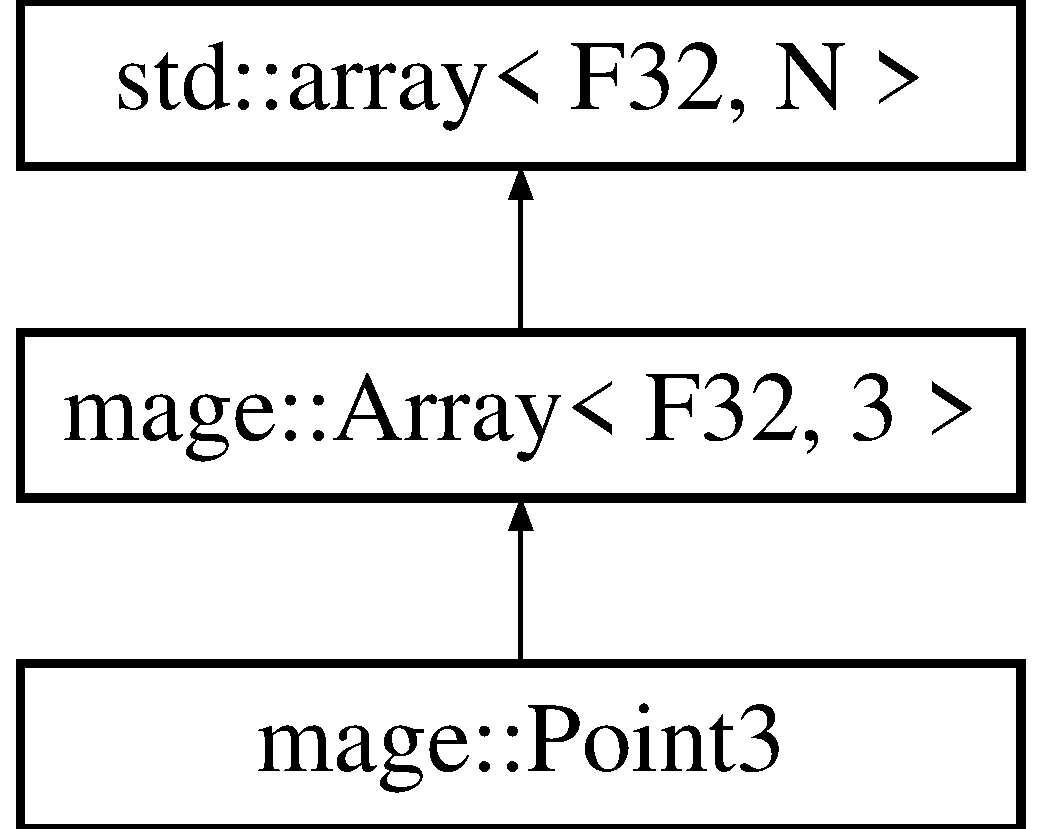
\includegraphics[height=2.000000cm]{structmage_1_1_point3}
\end{center}
\end{figure}
\subsection*{Public Member Functions}
\begin{DoxyCompactItemize}
\item 
\hyperlink{structmage_1_1_point3_a2675c303e54c6047520bc1a298c7fef1}{Point3} ()
\item 
\hyperlink{structmage_1_1_point3_a754210fa30befab6db5957a8d9b397f2}{Point3} (float x, float y, float z)
\item 
\hyperlink{structmage_1_1_point3_ad2e95e6eaa32339663e35f936990eb0c}{Point3} (const \hyperlink{structmage_1_1_point3}{Point3} \&point)
\item 
\hyperlink{structmage_1_1_point3_a3d10561285e01d03978e0d91fda6ff1d}{Point3} (\hyperlink{structmage_1_1_point3}{Point3} \&\&point)
\item 
\hyperlink{structmage_1_1_point3_ad67cb174e070f014472a57aa42b87f8d}{Point3} (const X\+M\+F\+L\+O\+A\+T3 \&v)
\item 
\hyperlink{structmage_1_1_point3_ad28d286384f8ce89c6bc25471ec78cff}{Point3} (X\+M\+F\+L\+O\+A\+T3 \&\&v)
\item 
\hyperlink{structmage_1_1_point3_a952151b6ff72b68569f95445c2ac2495}{$\sim$\+Point3} ()=default
\item 
\hyperlink{structmage_1_1_point3}{Point3} \& \hyperlink{structmage_1_1_point3_a53403b16c67a6c7d72910edaec04e371}{operator=} (const \hyperlink{structmage_1_1_point3}{Point3} \&point)
\item 
\hyperlink{structmage_1_1_point3}{Point3} \& \hyperlink{structmage_1_1_point3_a6889dad6ac4106bd9a52fcae4dfa401c}{operator=} (\hyperlink{structmage_1_1_point3}{Point3} \&\&point)
\end{DoxyCompactItemize}


\subsection{Detailed Description}
A struct of points in 3D space. 

\subsection{Constructor \& Destructor Documentation}
\hypertarget{structmage_1_1_point3_a2675c303e54c6047520bc1a298c7fef1}{}\label{structmage_1_1_point3_a2675c303e54c6047520bc1a298c7fef1} 
\index{mage\+::\+Point3@{mage\+::\+Point3}!Point3@{Point3}}
\index{Point3@{Point3}!mage\+::\+Point3@{mage\+::\+Point3}}
\subsubsection{\texorpdfstring{Point3()}{Point3()}\hspace{0.1cm}{\footnotesize\ttfamily [1/6]}}
{\footnotesize\ttfamily mage\+::\+Point3\+::\+Point3 (\begin{DoxyParamCaption}{ }\end{DoxyParamCaption})}

Constructs a point. \hypertarget{structmage_1_1_point3_a754210fa30befab6db5957a8d9b397f2}{}\label{structmage_1_1_point3_a754210fa30befab6db5957a8d9b397f2} 
\index{mage\+::\+Point3@{mage\+::\+Point3}!Point3@{Point3}}
\index{Point3@{Point3}!mage\+::\+Point3@{mage\+::\+Point3}}
\subsubsection{\texorpdfstring{Point3()}{Point3()}\hspace{0.1cm}{\footnotesize\ttfamily [2/6]}}
{\footnotesize\ttfamily mage\+::\+Point3\+::\+Point3 (\begin{DoxyParamCaption}\item[{float}]{x,  }\item[{float}]{y,  }\item[{float}]{z }\end{DoxyParamCaption})}

Constructs a point from the given coordinates.


\begin{DoxyParams}[1]{Parameters}
\mbox{\tt in}  & {\em x} & The x-\/coordinate. \\
\hline
\mbox{\tt in}  & {\em y} & The y-\/coordinate. \\
\hline
\mbox{\tt in}  & {\em z} & The z-\/coordinate. \\
\hline
\end{DoxyParams}
\hypertarget{structmage_1_1_point3_ad2e95e6eaa32339663e35f936990eb0c}{}\label{structmage_1_1_point3_ad2e95e6eaa32339663e35f936990eb0c} 
\index{mage\+::\+Point3@{mage\+::\+Point3}!Point3@{Point3}}
\index{Point3@{Point3}!mage\+::\+Point3@{mage\+::\+Point3}}
\subsubsection{\texorpdfstring{Point3()}{Point3()}\hspace{0.1cm}{\footnotesize\ttfamily [3/6]}}
{\footnotesize\ttfamily mage\+::\+Point3\+::\+Point3 (\begin{DoxyParamCaption}\item[{const \hyperlink{structmage_1_1_point3}{Point3} \&}]{point }\end{DoxyParamCaption})}

Constructs a point from the given point.


\begin{DoxyParams}[1]{Parameters}
\mbox{\tt in}  & {\em point} & A reference to the point to copy. \\
\hline
\end{DoxyParams}
\hypertarget{structmage_1_1_point3_a3d10561285e01d03978e0d91fda6ff1d}{}\label{structmage_1_1_point3_a3d10561285e01d03978e0d91fda6ff1d} 
\index{mage\+::\+Point3@{mage\+::\+Point3}!Point3@{Point3}}
\index{Point3@{Point3}!mage\+::\+Point3@{mage\+::\+Point3}}
\subsubsection{\texorpdfstring{Point3()}{Point3()}\hspace{0.1cm}{\footnotesize\ttfamily [4/6]}}
{\footnotesize\ttfamily mage\+::\+Point3\+::\+Point3 (\begin{DoxyParamCaption}\item[{\hyperlink{structmage_1_1_point3}{Point3} \&\&}]{point }\end{DoxyParamCaption})}

Constructs a point by moving the given point.


\begin{DoxyParams}[1]{Parameters}
\mbox{\tt in}  & {\em point} & A reference to the point to move. \\
\hline
\end{DoxyParams}
\hypertarget{structmage_1_1_point3_ad67cb174e070f014472a57aa42b87f8d}{}\label{structmage_1_1_point3_ad67cb174e070f014472a57aa42b87f8d} 
\index{mage\+::\+Point3@{mage\+::\+Point3}!Point3@{Point3}}
\index{Point3@{Point3}!mage\+::\+Point3@{mage\+::\+Point3}}
\subsubsection{\texorpdfstring{Point3()}{Point3()}\hspace{0.1cm}{\footnotesize\ttfamily [5/6]}}
{\footnotesize\ttfamily mage\+::\+Point3\+::\+Point3 (\begin{DoxyParamCaption}\item[{const X\+M\+F\+L\+O\+A\+T3 \&}]{v }\end{DoxyParamCaption})\hspace{0.3cm}{\ttfamily [explicit]}}

Constructs a point from the given vector.


\begin{DoxyParams}[1]{Parameters}
\mbox{\tt in}  & {\em v} & A reference to the vector to copy. \\
\hline
\end{DoxyParams}
\hypertarget{structmage_1_1_point3_ad28d286384f8ce89c6bc25471ec78cff}{}\label{structmage_1_1_point3_ad28d286384f8ce89c6bc25471ec78cff} 
\index{mage\+::\+Point3@{mage\+::\+Point3}!Point3@{Point3}}
\index{Point3@{Point3}!mage\+::\+Point3@{mage\+::\+Point3}}
\subsubsection{\texorpdfstring{Point3()}{Point3()}\hspace{0.1cm}{\footnotesize\ttfamily [6/6]}}
{\footnotesize\ttfamily mage\+::\+Point3\+::\+Point3 (\begin{DoxyParamCaption}\item[{X\+M\+F\+L\+O\+A\+T3 \&\&}]{v }\end{DoxyParamCaption})\hspace{0.3cm}{\ttfamily [explicit]}}

Constructs a point by moving the given vector.


\begin{DoxyParams}[1]{Parameters}
\mbox{\tt in}  & {\em v} & A reference to the vector to move. \\
\hline
\end{DoxyParams}
\hypertarget{structmage_1_1_point3_a952151b6ff72b68569f95445c2ac2495}{}\label{structmage_1_1_point3_a952151b6ff72b68569f95445c2ac2495} 
\index{mage\+::\+Point3@{mage\+::\+Point3}!````~Point3@{$\sim$\+Point3}}
\index{````~Point3@{$\sim$\+Point3}!mage\+::\+Point3@{mage\+::\+Point3}}
\subsubsection{\texorpdfstring{$\sim$\+Point3()}{~Point3()}}
{\footnotesize\ttfamily mage\+::\+Point3\+::$\sim$\+Point3 (\begin{DoxyParamCaption}{ }\end{DoxyParamCaption})\hspace{0.3cm}{\ttfamily [default]}}

Constructs a point. 

\subsection{Member Function Documentation}
\hypertarget{structmage_1_1_point3_a53403b16c67a6c7d72910edaec04e371}{}\label{structmage_1_1_point3_a53403b16c67a6c7d72910edaec04e371} 
\index{mage\+::\+Point3@{mage\+::\+Point3}!operator=@{operator=}}
\index{operator=@{operator=}!mage\+::\+Point3@{mage\+::\+Point3}}
\subsubsection{\texorpdfstring{operator=()}{operator=()}\hspace{0.1cm}{\footnotesize\ttfamily [1/2]}}
{\footnotesize\ttfamily \hyperlink{structmage_1_1_point3}{Point3}\& mage\+::\+Point3\+::operator= (\begin{DoxyParamCaption}\item[{const \hyperlink{structmage_1_1_point3}{Point3} \&}]{point }\end{DoxyParamCaption})}

Copies the given point to this point.


\begin{DoxyParams}[1]{Parameters}
\mbox{\tt in}  & {\em point} & A reference to the point to copy. \\
\hline
\end{DoxyParams}
\begin{DoxyReturn}{Returns}
A reference to the copy of the given point (i.\+e. this point). 
\end{DoxyReturn}
\hypertarget{structmage_1_1_point3_a6889dad6ac4106bd9a52fcae4dfa401c}{}\label{structmage_1_1_point3_a6889dad6ac4106bd9a52fcae4dfa401c} 
\index{mage\+::\+Point3@{mage\+::\+Point3}!operator=@{operator=}}
\index{operator=@{operator=}!mage\+::\+Point3@{mage\+::\+Point3}}
\subsubsection{\texorpdfstring{operator=()}{operator=()}\hspace{0.1cm}{\footnotesize\ttfamily [2/2]}}
{\footnotesize\ttfamily \hyperlink{structmage_1_1_point3}{Point3}\& mage\+::\+Point3\+::operator= (\begin{DoxyParamCaption}\item[{\hyperlink{structmage_1_1_point3}{Point3} \&\&}]{point }\end{DoxyParamCaption})}

Moves the given point to this point.


\begin{DoxyParams}[1]{Parameters}
\mbox{\tt in}  & {\em point} & A reference to the point to move. \\
\hline
\end{DoxyParams}
\begin{DoxyReturn}{Returns}
A reference to the moved point (i.\+e. this point). 
\end{DoxyReturn}

\hypertarget{classmage_1_1_progress_reporter}{}\section{mage\+:\+:Progress\+Reporter Class Reference}
\label{classmage_1_1_progress_reporter}\index{mage\+::\+Progress\+Reporter@{mage\+::\+Progress\+Reporter}}


{\ttfamily \#include $<$progress\+\_\+reporter.\+hpp$>$}

\subsection*{Classes}
\begin{DoxyCompactItemize}
\item 
class \mbox{\hyperlink{classmage_1_1_progress_reporter_1_1_impl}{Impl}}
\end{DoxyCompactItemize}
\subsection*{Public Member Functions}
\begin{DoxyCompactItemize}
\item 
\mbox{\hyperlink{classmage_1_1_progress_reporter_ab2509fb50a432812fa8ea10c77120387}{Progress\+Reporter}} (const std\+::string \&title, \mbox{\hyperlink{namespacemage_a41c104c036fba3756a74e19f793eeaa1}{U32}} nb\+\_\+work, char progress\+\_\+char=\textquotesingle{}+\textquotesingle{}, \mbox{\hyperlink{namespacemage_af69057eec1ce005c1c3b34ae33486f16}{U16}} bar\+\_\+length=0u)
\item 
\mbox{\hyperlink{classmage_1_1_progress_reporter_a681d23ec19019c04a8a977c4f6f280ea}{Progress\+Reporter}} (const \mbox{\hyperlink{classmage_1_1_progress_reporter}{Progress\+Reporter}} \&reporter)=delete
\item 
\mbox{\hyperlink{classmage_1_1_progress_reporter_a811686b20299f63476c5a5b17c6fa443}{Progress\+Reporter}} (\mbox{\hyperlink{classmage_1_1_progress_reporter}{Progress\+Reporter}} \&\&reporter) noexcept
\item 
\mbox{\hyperlink{classmage_1_1_progress_reporter_aa543239c6dd4474a77cf4cf6904c1b26}{$\sim$\+Progress\+Reporter}} ()
\item 
\mbox{\hyperlink{classmage_1_1_progress_reporter}{Progress\+Reporter}} \& \mbox{\hyperlink{classmage_1_1_progress_reporter_aa98411a059ad0e77ca53d064176f3a86}{operator=}} (const \mbox{\hyperlink{classmage_1_1_progress_reporter}{Progress\+Reporter}} \&reporter)=delete
\item 
\mbox{\hyperlink{classmage_1_1_progress_reporter}{Progress\+Reporter}} \& \mbox{\hyperlink{classmage_1_1_progress_reporter_adfc77427eaff8caf71c1995bf986edc5}{operator=}} (\mbox{\hyperlink{classmage_1_1_progress_reporter}{Progress\+Reporter}} \&\&reporter)=delete
\item 
void \mbox{\hyperlink{classmage_1_1_progress_reporter_aee55b3ced46f7512634b0443ff9807f5}{Update}} (\mbox{\hyperlink{namespacemage_a41c104c036fba3756a74e19f793eeaa1}{U32}} nb\+\_\+work=1u)
\item 
void \mbox{\hyperlink{classmage_1_1_progress_reporter_a11d758647ac2082bc296ab53a7454eaa}{Done}} ()
\end{DoxyCompactItemize}
\subsection*{Private Attributes}
\begin{DoxyCompactItemize}
\item 
\mbox{\hyperlink{namespacemage_a3316d7143a973e37adf1110f2e80ca31}{Unique\+Ptr}}$<$ \mbox{\hyperlink{classmage_1_1_progress_reporter_1_1_impl}{Impl}} $>$ \mbox{\hyperlink{classmage_1_1_progress_reporter_a62665cfb18a2a45428fdee4922b7b313}{m\+\_\+impl}}
\end{DoxyCompactItemize}


\subsection{Detailed Description}
A class of progress reporters. 

\subsection{Constructor \& Destructor Documentation}
\mbox{\Hypertarget{classmage_1_1_progress_reporter_ab2509fb50a432812fa8ea10c77120387}\label{classmage_1_1_progress_reporter_ab2509fb50a432812fa8ea10c77120387}} 
\index{mage\+::\+Progress\+Reporter@{mage\+::\+Progress\+Reporter}!Progress\+Reporter@{Progress\+Reporter}}
\index{Progress\+Reporter@{Progress\+Reporter}!mage\+::\+Progress\+Reporter@{mage\+::\+Progress\+Reporter}}
\subsubsection{\texorpdfstring{Progress\+Reporter()}{ProgressReporter()}\hspace{0.1cm}{\footnotesize\ttfamily [1/3]}}
{\footnotesize\ttfamily mage\+::\+Progress\+Reporter\+::\+Progress\+Reporter (\begin{DoxyParamCaption}\item[{const std\+::string \&}]{title,  }\item[{\mbox{\hyperlink{namespacemage_a41c104c036fba3756a74e19f793eeaa1}{U32}}}]{nb\+\_\+work,  }\item[{char}]{progress\+\_\+char = {\ttfamily \textquotesingle{}+\textquotesingle{}},  }\item[{\mbox{\hyperlink{namespacemage_af69057eec1ce005c1c3b34ae33486f16}{U16}}}]{bar\+\_\+length = {\ttfamily 0u} }\end{DoxyParamCaption})\hspace{0.3cm}{\ttfamily [explicit]}}

Constructs a progress reporter.


\begin{DoxyParams}[1]{Parameters}
\mbox{\tt in}  & {\em title} & A reference to the title. \\
\hline
\mbox{\tt in}  & {\em nb\+\_\+work} & The total number of work units. \\
\hline
\mbox{\tt in}  & {\em progress\+\_\+char} & The character representing the progress. \\
\hline
\mbox{\tt in}  & {\em bar\+\_\+length} & The length of the progress bar. If {\itshape bar\+\_\+length} is equal to 0 the default length will be chosen. \\
\hline
\end{DoxyParams}
\mbox{\Hypertarget{classmage_1_1_progress_reporter_a681d23ec19019c04a8a977c4f6f280ea}\label{classmage_1_1_progress_reporter_a681d23ec19019c04a8a977c4f6f280ea}} 
\index{mage\+::\+Progress\+Reporter@{mage\+::\+Progress\+Reporter}!Progress\+Reporter@{Progress\+Reporter}}
\index{Progress\+Reporter@{Progress\+Reporter}!mage\+::\+Progress\+Reporter@{mage\+::\+Progress\+Reporter}}
\subsubsection{\texorpdfstring{Progress\+Reporter()}{ProgressReporter()}\hspace{0.1cm}{\footnotesize\ttfamily [2/3]}}
{\footnotesize\ttfamily mage\+::\+Progress\+Reporter\+::\+Progress\+Reporter (\begin{DoxyParamCaption}\item[{const \mbox{\hyperlink{classmage_1_1_progress_reporter}{Progress\+Reporter}} \&}]{reporter }\end{DoxyParamCaption})\hspace{0.3cm}{\ttfamily [delete]}}

Constructs a progress reporter from the given progress reporter.


\begin{DoxyParams}[1]{Parameters}
\mbox{\tt in}  & {\em reporter} & A reference to the progress reporter to copy. \\
\hline
\end{DoxyParams}
\mbox{\Hypertarget{classmage_1_1_progress_reporter_a811686b20299f63476c5a5b17c6fa443}\label{classmage_1_1_progress_reporter_a811686b20299f63476c5a5b17c6fa443}} 
\index{mage\+::\+Progress\+Reporter@{mage\+::\+Progress\+Reporter}!Progress\+Reporter@{Progress\+Reporter}}
\index{Progress\+Reporter@{Progress\+Reporter}!mage\+::\+Progress\+Reporter@{mage\+::\+Progress\+Reporter}}
\subsubsection{\texorpdfstring{Progress\+Reporter()}{ProgressReporter()}\hspace{0.1cm}{\footnotesize\ttfamily [3/3]}}
{\footnotesize\ttfamily mage\+::\+Progress\+Reporter\+::\+Progress\+Reporter (\begin{DoxyParamCaption}\item[{\mbox{\hyperlink{classmage_1_1_progress_reporter}{Progress\+Reporter}} \&\&}]{reporter }\end{DoxyParamCaption})\hspace{0.3cm}{\ttfamily [default]}, {\ttfamily [noexcept]}}

Constructs a progress reporter by moving the given progress reporter.


\begin{DoxyParams}[1]{Parameters}
\mbox{\tt in}  & {\em reporter} & A reference to the progress reporter to move. \\
\hline
\end{DoxyParams}
\mbox{\Hypertarget{classmage_1_1_progress_reporter_aa543239c6dd4474a77cf4cf6904c1b26}\label{classmage_1_1_progress_reporter_aa543239c6dd4474a77cf4cf6904c1b26}} 
\index{mage\+::\+Progress\+Reporter@{mage\+::\+Progress\+Reporter}!````~Progress\+Reporter@{$\sim$\+Progress\+Reporter}}
\index{````~Progress\+Reporter@{$\sim$\+Progress\+Reporter}!mage\+::\+Progress\+Reporter@{mage\+::\+Progress\+Reporter}}
\subsubsection{\texorpdfstring{$\sim$\+Progress\+Reporter()}{~ProgressReporter()}}
{\footnotesize\ttfamily mage\+::\+Progress\+Reporter\+::$\sim$\+Progress\+Reporter (\begin{DoxyParamCaption}{ }\end{DoxyParamCaption})\hspace{0.3cm}{\ttfamily [default]}}

Destructs this progress reporter. 

\subsection{Member Function Documentation}
\mbox{\Hypertarget{classmage_1_1_progress_reporter_a11d758647ac2082bc296ab53a7454eaa}\label{classmage_1_1_progress_reporter_a11d758647ac2082bc296ab53a7454eaa}} 
\index{mage\+::\+Progress\+Reporter@{mage\+::\+Progress\+Reporter}!Done@{Done}}
\index{Done@{Done}!mage\+::\+Progress\+Reporter@{mage\+::\+Progress\+Reporter}}
\subsubsection{\texorpdfstring{Done()}{Done()}}
{\footnotesize\ttfamily void mage\+::\+Progress\+Reporter\+::\+Done (\begin{DoxyParamCaption}{ }\end{DoxyParamCaption})}

Finishes this progress reporter. \mbox{\Hypertarget{classmage_1_1_progress_reporter_aa98411a059ad0e77ca53d064176f3a86}\label{classmage_1_1_progress_reporter_aa98411a059ad0e77ca53d064176f3a86}} 
\index{mage\+::\+Progress\+Reporter@{mage\+::\+Progress\+Reporter}!operator=@{operator=}}
\index{operator=@{operator=}!mage\+::\+Progress\+Reporter@{mage\+::\+Progress\+Reporter}}
\subsubsection{\texorpdfstring{operator=()}{operator=()}\hspace{0.1cm}{\footnotesize\ttfamily [1/2]}}
{\footnotesize\ttfamily \mbox{\hyperlink{classmage_1_1_progress_reporter}{Progress\+Reporter}}\& mage\+::\+Progress\+Reporter\+::operator= (\begin{DoxyParamCaption}\item[{const \mbox{\hyperlink{classmage_1_1_progress_reporter}{Progress\+Reporter}} \&}]{reporter }\end{DoxyParamCaption})\hspace{0.3cm}{\ttfamily [delete]}}

Copies the given progress reporter to this progress reporter.


\begin{DoxyParams}[1]{Parameters}
\mbox{\tt in}  & {\em reporter} & A reference to the progress reporter to copy. \\
\hline
\end{DoxyParams}
\begin{DoxyReturn}{Returns}
A reference to the copy of the given progress reporter (i.\+e. this progress reporter). 
\end{DoxyReturn}
\mbox{\Hypertarget{classmage_1_1_progress_reporter_adfc77427eaff8caf71c1995bf986edc5}\label{classmage_1_1_progress_reporter_adfc77427eaff8caf71c1995bf986edc5}} 
\index{mage\+::\+Progress\+Reporter@{mage\+::\+Progress\+Reporter}!operator=@{operator=}}
\index{operator=@{operator=}!mage\+::\+Progress\+Reporter@{mage\+::\+Progress\+Reporter}}
\subsubsection{\texorpdfstring{operator=()}{operator=()}\hspace{0.1cm}{\footnotesize\ttfamily [2/2]}}
{\footnotesize\ttfamily \mbox{\hyperlink{classmage_1_1_progress_reporter}{Progress\+Reporter}}\& mage\+::\+Progress\+Reporter\+::operator= (\begin{DoxyParamCaption}\item[{\mbox{\hyperlink{classmage_1_1_progress_reporter}{Progress\+Reporter}} \&\&}]{reporter }\end{DoxyParamCaption})\hspace{0.3cm}{\ttfamily [delete]}}

Copies the given progress reporter to this progress reporter.


\begin{DoxyParams}[1]{Parameters}
\mbox{\tt in}  & {\em reporter} & A reference to the progress reporter to move. \\
\hline
\end{DoxyParams}
\begin{DoxyReturn}{Returns}
A reference to moved progress reporter (i.\+e. this progress reporter). 
\end{DoxyReturn}
\mbox{\Hypertarget{classmage_1_1_progress_reporter_aee55b3ced46f7512634b0443ff9807f5}\label{classmage_1_1_progress_reporter_aee55b3ced46f7512634b0443ff9807f5}} 
\index{mage\+::\+Progress\+Reporter@{mage\+::\+Progress\+Reporter}!Update@{Update}}
\index{Update@{Update}!mage\+::\+Progress\+Reporter@{mage\+::\+Progress\+Reporter}}
\subsubsection{\texorpdfstring{Update()}{Update()}}
{\footnotesize\ttfamily void mage\+::\+Progress\+Reporter\+::\+Update (\begin{DoxyParamCaption}\item[{\mbox{\hyperlink{namespacemage_a41c104c036fba3756a74e19f793eeaa1}{U32}}}]{nb\+\_\+work = {\ttfamily 1u} }\end{DoxyParamCaption})}

Updates this progress reporter.


\begin{DoxyParams}[1]{Parameters}
\mbox{\tt in}  & {\em nb\+\_\+work} & The number of work units that are done. \\
\hline
\end{DoxyParams}


\subsection{Member Data Documentation}
\mbox{\Hypertarget{classmage_1_1_progress_reporter_a62665cfb18a2a45428fdee4922b7b313}\label{classmage_1_1_progress_reporter_a62665cfb18a2a45428fdee4922b7b313}} 
\index{mage\+::\+Progress\+Reporter@{mage\+::\+Progress\+Reporter}!m\+\_\+impl@{m\+\_\+impl}}
\index{m\+\_\+impl@{m\+\_\+impl}!mage\+::\+Progress\+Reporter@{mage\+::\+Progress\+Reporter}}
\subsubsection{\texorpdfstring{m\+\_\+impl}{m\_impl}}
{\footnotesize\ttfamily \mbox{\hyperlink{namespacemage_a3316d7143a973e37adf1110f2e80ca31}{Unique\+Ptr}}$<$ \mbox{\hyperlink{classmage_1_1_progress_reporter_1_1_impl}{Impl}} $>$ mage\+::\+Progress\+Reporter\+::m\+\_\+impl\hspace{0.3cm}{\ttfamily [private]}}

A pointer to the implementation of this progress reporter. 
\hypertarget{structmage_1_1_read_write_mutex}{}\section{mage\+:\+:Read\+Write\+Mutex Struct Reference}
\label{structmage_1_1_read_write_mutex}\index{mage\+::\+Read\+Write\+Mutex@{mage\+::\+Read\+Write\+Mutex}}


{\ttfamily \#include $<$lock.\+hpp$>$}

\subsection*{Public Member Functions}
\begin{DoxyCompactItemize}
\item 
\hyperlink{structmage_1_1_read_write_mutex_aae10694de3862f2d1059477169883940}{Read\+Write\+Mutex} ()
\item 
\hyperlink{structmage_1_1_read_write_mutex_aacb2f69e7e2b084147e1e45628e9dd67}{Read\+Write\+Mutex} (const \hyperlink{structmage_1_1_read_write_mutex}{Read\+Write\+Mutex} \&mutex)=delete
\item 
\hyperlink{structmage_1_1_read_write_mutex_a664e946edfa742dad648fc9fcb29832e}{Read\+Write\+Mutex} (\hyperlink{structmage_1_1_read_write_mutex}{Read\+Write\+Mutex} \&\&mutex)=delete
\item 
\hyperlink{structmage_1_1_read_write_mutex_a73676d9414658d63edfe443ee1d55c8b}{$\sim$\+Read\+Write\+Mutex} ()
\item 
\hyperlink{structmage_1_1_read_write_mutex}{Read\+Write\+Mutex} \& \hyperlink{structmage_1_1_read_write_mutex_a408e06f3c8bcc644e43afbf7e9ac772f}{operator=} (const \hyperlink{structmage_1_1_read_write_mutex}{Read\+Write\+Mutex} \&mutex)=delete
\item 
\hyperlink{structmage_1_1_read_write_mutex}{Read\+Write\+Mutex} \& \hyperlink{structmage_1_1_read_write_mutex_a14ea4d1be75046741a7663e0d86a017a}{operator=} (\hyperlink{structmage_1_1_read_write_mutex}{Read\+Write\+Mutex} \&\&mutex)=delete
\end{DoxyCompactItemize}
\subsection*{Private Member Functions}
\begin{DoxyCompactItemize}
\item 
void \hyperlink{structmage_1_1_read_write_mutex_af78045647078aaf3966c8f1b06e35c92}{Acquire\+Read} ()
\item 
void \hyperlink{structmage_1_1_read_write_mutex_a0af5059a9bd16abd8a21b15e7ebe053d}{Release\+Read} ()
\item 
void \hyperlink{structmage_1_1_read_write_mutex_a76137013107a9c2c1fc05c1e0747965e}{Acquire\+Write} ()
\item 
void \hyperlink{structmage_1_1_read_write_mutex_ad0fd296bdaa212f54a58372c8dfe1d1d}{Release\+Write} ()
\end{DoxyCompactItemize}
\subsection*{Private Attributes}
\begin{DoxyCompactItemize}
\item 
L\+O\+NG \hyperlink{structmage_1_1_read_write_mutex_a003313794a9b43f80bd9b258b039438d}{m\+\_\+nb\+\_\+writers\+\_\+waiting}
\item 
L\+O\+NG \hyperlink{structmage_1_1_read_write_mutex_acbe7553fff7cca2656f6f2b8f0471484}{m\+\_\+nb\+\_\+readers\+\_\+waiting}
\item 
D\+W\+O\+RD \hyperlink{structmage_1_1_read_write_mutex_a1e0ad98e517236170faae5b27decfdce}{m\+\_\+active\+\_\+writer\+\_\+readers}
\item 
H\+A\+N\+D\+LE \hyperlink{structmage_1_1_read_write_mutex_a65c0ef8b687d48104b09a9d175e72236}{m\+\_\+ready\+\_\+to\+\_\+read\+\_\+handle}
\item 
H\+A\+N\+D\+LE \hyperlink{structmage_1_1_read_write_mutex_a9498ef85b52486342ba657f34369f89e}{m\+\_\+ready\+\_\+to\+\_\+write\+\_\+handle}
\item 
C\+R\+I\+T\+I\+C\+A\+L\+\_\+\+S\+E\+C\+T\+I\+ON \hyperlink{structmage_1_1_read_write_mutex_a77fe51b87e5205d60ea045fa53bc1fa3}{m\+\_\+critical\+\_\+section}
\end{DoxyCompactItemize}
\subsection*{Friends}
\begin{DoxyCompactItemize}
\item 
struct \hyperlink{structmage_1_1_read_write_mutex_a7ae207fc659160d3c55a5ba1468007f7}{Read\+Write\+Mutex\+Lock}
\end{DoxyCompactItemize}


\subsection{Detailed Description}
A struct of read write mutexes. 

\subsection{Constructor \& Destructor Documentation}
\hypertarget{structmage_1_1_read_write_mutex_aae10694de3862f2d1059477169883940}{}\label{structmage_1_1_read_write_mutex_aae10694de3862f2d1059477169883940} 
\index{mage\+::\+Read\+Write\+Mutex@{mage\+::\+Read\+Write\+Mutex}!Read\+Write\+Mutex@{Read\+Write\+Mutex}}
\index{Read\+Write\+Mutex@{Read\+Write\+Mutex}!mage\+::\+Read\+Write\+Mutex@{mage\+::\+Read\+Write\+Mutex}}
\subsubsection{\texorpdfstring{Read\+Write\+Mutex()}{ReadWriteMutex()}\hspace{0.1cm}{\footnotesize\ttfamily [1/3]}}
{\footnotesize\ttfamily mage\+::\+Read\+Write\+Mutex\+::\+Read\+Write\+Mutex (\begin{DoxyParamCaption}{ }\end{DoxyParamCaption})}

Constructs a read write mutex. \hypertarget{structmage_1_1_read_write_mutex_aacb2f69e7e2b084147e1e45628e9dd67}{}\label{structmage_1_1_read_write_mutex_aacb2f69e7e2b084147e1e45628e9dd67} 
\index{mage\+::\+Read\+Write\+Mutex@{mage\+::\+Read\+Write\+Mutex}!Read\+Write\+Mutex@{Read\+Write\+Mutex}}
\index{Read\+Write\+Mutex@{Read\+Write\+Mutex}!mage\+::\+Read\+Write\+Mutex@{mage\+::\+Read\+Write\+Mutex}}
\subsubsection{\texorpdfstring{Read\+Write\+Mutex()}{ReadWriteMutex()}\hspace{0.1cm}{\footnotesize\ttfamily [2/3]}}
{\footnotesize\ttfamily mage\+::\+Read\+Write\+Mutex\+::\+Read\+Write\+Mutex (\begin{DoxyParamCaption}\item[{const \hyperlink{structmage_1_1_read_write_mutex}{Read\+Write\+Mutex} \&}]{mutex }\end{DoxyParamCaption})\hspace{0.3cm}{\ttfamily [delete]}}

Constructs a read write mutex from the given read write mutex.


\begin{DoxyParams}[1]{Parameters}
\mbox{\tt in}  & {\em mutex} & A reference to the read write mutex to copy. \\
\hline
\end{DoxyParams}
\hypertarget{structmage_1_1_read_write_mutex_a664e946edfa742dad648fc9fcb29832e}{}\label{structmage_1_1_read_write_mutex_a664e946edfa742dad648fc9fcb29832e} 
\index{mage\+::\+Read\+Write\+Mutex@{mage\+::\+Read\+Write\+Mutex}!Read\+Write\+Mutex@{Read\+Write\+Mutex}}
\index{Read\+Write\+Mutex@{Read\+Write\+Mutex}!mage\+::\+Read\+Write\+Mutex@{mage\+::\+Read\+Write\+Mutex}}
\subsubsection{\texorpdfstring{Read\+Write\+Mutex()}{ReadWriteMutex()}\hspace{0.1cm}{\footnotesize\ttfamily [3/3]}}
{\footnotesize\ttfamily mage\+::\+Read\+Write\+Mutex\+::\+Read\+Write\+Mutex (\begin{DoxyParamCaption}\item[{\hyperlink{structmage_1_1_read_write_mutex}{Read\+Write\+Mutex} \&\&}]{mutex }\end{DoxyParamCaption})\hspace{0.3cm}{\ttfamily [delete]}}

Constructs a read write mutex by moving the given read write mutex.


\begin{DoxyParams}[1]{Parameters}
\mbox{\tt in}  & {\em mutex} & A reference to the read write mutex to move. \\
\hline
\end{DoxyParams}
\hypertarget{structmage_1_1_read_write_mutex_a73676d9414658d63edfe443ee1d55c8b}{}\label{structmage_1_1_read_write_mutex_a73676d9414658d63edfe443ee1d55c8b} 
\index{mage\+::\+Read\+Write\+Mutex@{mage\+::\+Read\+Write\+Mutex}!````~Read\+Write\+Mutex@{$\sim$\+Read\+Write\+Mutex}}
\index{````~Read\+Write\+Mutex@{$\sim$\+Read\+Write\+Mutex}!mage\+::\+Read\+Write\+Mutex@{mage\+::\+Read\+Write\+Mutex}}
\subsubsection{\texorpdfstring{$\sim$\+Read\+Write\+Mutex()}{~ReadWriteMutex()}}
{\footnotesize\ttfamily mage\+::\+Read\+Write\+Mutex\+::$\sim$\+Read\+Write\+Mutex (\begin{DoxyParamCaption}{ }\end{DoxyParamCaption})}

Destructs this read write mutex. 

\subsection{Member Function Documentation}
\hypertarget{structmage_1_1_read_write_mutex_af78045647078aaf3966c8f1b06e35c92}{}\label{structmage_1_1_read_write_mutex_af78045647078aaf3966c8f1b06e35c92} 
\index{mage\+::\+Read\+Write\+Mutex@{mage\+::\+Read\+Write\+Mutex}!Acquire\+Read@{Acquire\+Read}}
\index{Acquire\+Read@{Acquire\+Read}!mage\+::\+Read\+Write\+Mutex@{mage\+::\+Read\+Write\+Mutex}}
\subsubsection{\texorpdfstring{Acquire\+Read()}{AcquireRead()}}
{\footnotesize\ttfamily void mage\+::\+Read\+Write\+Mutex\+::\+Acquire\+Read (\begin{DoxyParamCaption}{ }\end{DoxyParamCaption})\hspace{0.3cm}{\ttfamily [private]}}

Acquires a read. \hypertarget{structmage_1_1_read_write_mutex_a76137013107a9c2c1fc05c1e0747965e}{}\label{structmage_1_1_read_write_mutex_a76137013107a9c2c1fc05c1e0747965e} 
\index{mage\+::\+Read\+Write\+Mutex@{mage\+::\+Read\+Write\+Mutex}!Acquire\+Write@{Acquire\+Write}}
\index{Acquire\+Write@{Acquire\+Write}!mage\+::\+Read\+Write\+Mutex@{mage\+::\+Read\+Write\+Mutex}}
\subsubsection{\texorpdfstring{Acquire\+Write()}{AcquireWrite()}}
{\footnotesize\ttfamily void mage\+::\+Read\+Write\+Mutex\+::\+Acquire\+Write (\begin{DoxyParamCaption}{ }\end{DoxyParamCaption})\hspace{0.3cm}{\ttfamily [private]}}

Acquires a write. \hypertarget{structmage_1_1_read_write_mutex_a408e06f3c8bcc644e43afbf7e9ac772f}{}\label{structmage_1_1_read_write_mutex_a408e06f3c8bcc644e43afbf7e9ac772f} 
\index{mage\+::\+Read\+Write\+Mutex@{mage\+::\+Read\+Write\+Mutex}!operator=@{operator=}}
\index{operator=@{operator=}!mage\+::\+Read\+Write\+Mutex@{mage\+::\+Read\+Write\+Mutex}}
\subsubsection{\texorpdfstring{operator=()}{operator=()}\hspace{0.1cm}{\footnotesize\ttfamily [1/2]}}
{\footnotesize\ttfamily \hyperlink{structmage_1_1_read_write_mutex}{Read\+Write\+Mutex}\& mage\+::\+Read\+Write\+Mutex\+::operator= (\begin{DoxyParamCaption}\item[{const \hyperlink{structmage_1_1_read_write_mutex}{Read\+Write\+Mutex} \&}]{mutex }\end{DoxyParamCaption})\hspace{0.3cm}{\ttfamily [delete]}}

Copies the given read write mutex to this read write mutex.


\begin{DoxyParams}[1]{Parameters}
\mbox{\tt in}  & {\em mutex} & A reference to a read write mutex to copy. \\
\hline
\end{DoxyParams}
\begin{DoxyReturn}{Returns}
A reference to the copy of the given read write mutex (i.\+e. this read write mutex). 
\end{DoxyReturn}
\hypertarget{structmage_1_1_read_write_mutex_a14ea4d1be75046741a7663e0d86a017a}{}\label{structmage_1_1_read_write_mutex_a14ea4d1be75046741a7663e0d86a017a} 
\index{mage\+::\+Read\+Write\+Mutex@{mage\+::\+Read\+Write\+Mutex}!operator=@{operator=}}
\index{operator=@{operator=}!mage\+::\+Read\+Write\+Mutex@{mage\+::\+Read\+Write\+Mutex}}
\subsubsection{\texorpdfstring{operator=()}{operator=()}\hspace{0.1cm}{\footnotesize\ttfamily [2/2]}}
{\footnotesize\ttfamily \hyperlink{structmage_1_1_read_write_mutex}{Read\+Write\+Mutex}\& mage\+::\+Read\+Write\+Mutex\+::operator= (\begin{DoxyParamCaption}\item[{\hyperlink{structmage_1_1_read_write_mutex}{Read\+Write\+Mutex} \&\&}]{mutex }\end{DoxyParamCaption})\hspace{0.3cm}{\ttfamily [delete]}}

Moves the given read write mutex to this read write mutex.


\begin{DoxyParams}[1]{Parameters}
\mbox{\tt in}  & {\em mutex} & A reference to a read write mutex to move. \\
\hline
\end{DoxyParams}
\begin{DoxyReturn}{Returns}
A reference to the moved read write mutex (i.\+e. this read write mutex). 
\end{DoxyReturn}
\hypertarget{structmage_1_1_read_write_mutex_a0af5059a9bd16abd8a21b15e7ebe053d}{}\label{structmage_1_1_read_write_mutex_a0af5059a9bd16abd8a21b15e7ebe053d} 
\index{mage\+::\+Read\+Write\+Mutex@{mage\+::\+Read\+Write\+Mutex}!Release\+Read@{Release\+Read}}
\index{Release\+Read@{Release\+Read}!mage\+::\+Read\+Write\+Mutex@{mage\+::\+Read\+Write\+Mutex}}
\subsubsection{\texorpdfstring{Release\+Read()}{ReleaseRead()}}
{\footnotesize\ttfamily void mage\+::\+Read\+Write\+Mutex\+::\+Release\+Read (\begin{DoxyParamCaption}{ }\end{DoxyParamCaption})\hspace{0.3cm}{\ttfamily [private]}}

Releases a read. \hypertarget{structmage_1_1_read_write_mutex_ad0fd296bdaa212f54a58372c8dfe1d1d}{}\label{structmage_1_1_read_write_mutex_ad0fd296bdaa212f54a58372c8dfe1d1d} 
\index{mage\+::\+Read\+Write\+Mutex@{mage\+::\+Read\+Write\+Mutex}!Release\+Write@{Release\+Write}}
\index{Release\+Write@{Release\+Write}!mage\+::\+Read\+Write\+Mutex@{mage\+::\+Read\+Write\+Mutex}}
\subsubsection{\texorpdfstring{Release\+Write()}{ReleaseWrite()}}
{\footnotesize\ttfamily void mage\+::\+Read\+Write\+Mutex\+::\+Release\+Write (\begin{DoxyParamCaption}{ }\end{DoxyParamCaption})\hspace{0.3cm}{\ttfamily [private]}}

Releases a write. 

\subsection{Friends And Related Function Documentation}
\hypertarget{structmage_1_1_read_write_mutex_a7ae207fc659160d3c55a5ba1468007f7}{}\label{structmage_1_1_read_write_mutex_a7ae207fc659160d3c55a5ba1468007f7} 
\index{mage\+::\+Read\+Write\+Mutex@{mage\+::\+Read\+Write\+Mutex}!Read\+Write\+Mutex\+Lock@{Read\+Write\+Mutex\+Lock}}
\index{Read\+Write\+Mutex\+Lock@{Read\+Write\+Mutex\+Lock}!mage\+::\+Read\+Write\+Mutex@{mage\+::\+Read\+Write\+Mutex}}
\subsubsection{\texorpdfstring{Read\+Write\+Mutex\+Lock}{ReadWriteMutexLock}}
{\footnotesize\ttfamily friend struct \hyperlink{structmage_1_1_read_write_mutex_lock}{Read\+Write\+Mutex\+Lock}\hspace{0.3cm}{\ttfamily [friend]}}



\subsection{Member Data Documentation}
\hypertarget{structmage_1_1_read_write_mutex_a1e0ad98e517236170faae5b27decfdce}{}\label{structmage_1_1_read_write_mutex_a1e0ad98e517236170faae5b27decfdce} 
\index{mage\+::\+Read\+Write\+Mutex@{mage\+::\+Read\+Write\+Mutex}!m\+\_\+active\+\_\+writer\+\_\+readers@{m\+\_\+active\+\_\+writer\+\_\+readers}}
\index{m\+\_\+active\+\_\+writer\+\_\+readers@{m\+\_\+active\+\_\+writer\+\_\+readers}!mage\+::\+Read\+Write\+Mutex@{mage\+::\+Read\+Write\+Mutex}}
\subsubsection{\texorpdfstring{m\+\_\+active\+\_\+writer\+\_\+readers}{m\_active\_writer\_readers}}
{\footnotesize\ttfamily D\+W\+O\+RD mage\+::\+Read\+Write\+Mutex\+::m\+\_\+active\+\_\+writer\+\_\+readers\hspace{0.3cm}{\ttfamily [private]}}

The active group of this read write mutex.

H\+I\+W\+O\+RD is the flag indicating a writer is active. L\+O\+W\+O\+RD is the number of active readers. \hypertarget{structmage_1_1_read_write_mutex_a77fe51b87e5205d60ea045fa53bc1fa3}{}\label{structmage_1_1_read_write_mutex_a77fe51b87e5205d60ea045fa53bc1fa3} 
\index{mage\+::\+Read\+Write\+Mutex@{mage\+::\+Read\+Write\+Mutex}!m\+\_\+critical\+\_\+section@{m\+\_\+critical\+\_\+section}}
\index{m\+\_\+critical\+\_\+section@{m\+\_\+critical\+\_\+section}!mage\+::\+Read\+Write\+Mutex@{mage\+::\+Read\+Write\+Mutex}}
\subsubsection{\texorpdfstring{m\+\_\+critical\+\_\+section}{m\_critical\_section}}
{\footnotesize\ttfamily C\+R\+I\+T\+I\+C\+A\+L\+\_\+\+S\+E\+C\+T\+I\+ON mage\+::\+Read\+Write\+Mutex\+::m\+\_\+critical\+\_\+section\hspace{0.3cm}{\ttfamily [private]}}

The critical section object of this read write mutex. \hypertarget{structmage_1_1_read_write_mutex_acbe7553fff7cca2656f6f2b8f0471484}{}\label{structmage_1_1_read_write_mutex_acbe7553fff7cca2656f6f2b8f0471484} 
\index{mage\+::\+Read\+Write\+Mutex@{mage\+::\+Read\+Write\+Mutex}!m\+\_\+nb\+\_\+readers\+\_\+waiting@{m\+\_\+nb\+\_\+readers\+\_\+waiting}}
\index{m\+\_\+nb\+\_\+readers\+\_\+waiting@{m\+\_\+nb\+\_\+readers\+\_\+waiting}!mage\+::\+Read\+Write\+Mutex@{mage\+::\+Read\+Write\+Mutex}}
\subsubsection{\texorpdfstring{m\+\_\+nb\+\_\+readers\+\_\+waiting}{m\_nb\_readers\_waiting}}
{\footnotesize\ttfamily L\+O\+NG mage\+::\+Read\+Write\+Mutex\+::m\+\_\+nb\+\_\+readers\+\_\+waiting\hspace{0.3cm}{\ttfamily [private]}}

The number of readers waiting for this read write mutex. \hypertarget{structmage_1_1_read_write_mutex_a003313794a9b43f80bd9b258b039438d}{}\label{structmage_1_1_read_write_mutex_a003313794a9b43f80bd9b258b039438d} 
\index{mage\+::\+Read\+Write\+Mutex@{mage\+::\+Read\+Write\+Mutex}!m\+\_\+nb\+\_\+writers\+\_\+waiting@{m\+\_\+nb\+\_\+writers\+\_\+waiting}}
\index{m\+\_\+nb\+\_\+writers\+\_\+waiting@{m\+\_\+nb\+\_\+writers\+\_\+waiting}!mage\+::\+Read\+Write\+Mutex@{mage\+::\+Read\+Write\+Mutex}}
\subsubsection{\texorpdfstring{m\+\_\+nb\+\_\+writers\+\_\+waiting}{m\_nb\_writers\_waiting}}
{\footnotesize\ttfamily L\+O\+NG mage\+::\+Read\+Write\+Mutex\+::m\+\_\+nb\+\_\+writers\+\_\+waiting\hspace{0.3cm}{\ttfamily [private]}}

The number of writers waiting for this read write mutex. \hypertarget{structmage_1_1_read_write_mutex_a65c0ef8b687d48104b09a9d175e72236}{}\label{structmage_1_1_read_write_mutex_a65c0ef8b687d48104b09a9d175e72236} 
\index{mage\+::\+Read\+Write\+Mutex@{mage\+::\+Read\+Write\+Mutex}!m\+\_\+ready\+\_\+to\+\_\+read\+\_\+handle@{m\+\_\+ready\+\_\+to\+\_\+read\+\_\+handle}}
\index{m\+\_\+ready\+\_\+to\+\_\+read\+\_\+handle@{m\+\_\+ready\+\_\+to\+\_\+read\+\_\+handle}!mage\+::\+Read\+Write\+Mutex@{mage\+::\+Read\+Write\+Mutex}}
\subsubsection{\texorpdfstring{m\+\_\+ready\+\_\+to\+\_\+read\+\_\+handle}{m\_ready\_to\_read\_handle}}
{\footnotesize\ttfamily H\+A\+N\+D\+LE mage\+::\+Read\+Write\+Mutex\+::m\+\_\+ready\+\_\+to\+\_\+read\+\_\+handle\hspace{0.3cm}{\ttfamily [private]}}

The handle of this read write mutex if ready for reading. \hypertarget{structmage_1_1_read_write_mutex_a9498ef85b52486342ba657f34369f89e}{}\label{structmage_1_1_read_write_mutex_a9498ef85b52486342ba657f34369f89e} 
\index{mage\+::\+Read\+Write\+Mutex@{mage\+::\+Read\+Write\+Mutex}!m\+\_\+ready\+\_\+to\+\_\+write\+\_\+handle@{m\+\_\+ready\+\_\+to\+\_\+write\+\_\+handle}}
\index{m\+\_\+ready\+\_\+to\+\_\+write\+\_\+handle@{m\+\_\+ready\+\_\+to\+\_\+write\+\_\+handle}!mage\+::\+Read\+Write\+Mutex@{mage\+::\+Read\+Write\+Mutex}}
\subsubsection{\texorpdfstring{m\+\_\+ready\+\_\+to\+\_\+write\+\_\+handle}{m\_ready\_to\_write\_handle}}
{\footnotesize\ttfamily H\+A\+N\+D\+LE mage\+::\+Read\+Write\+Mutex\+::m\+\_\+ready\+\_\+to\+\_\+write\+\_\+handle\hspace{0.3cm}{\ttfamily [private]}}

The handle of this read write mutex if ready for writing. 
\hypertarget{structmage_1_1_read_write_mutex_lock}{}\section{mage\+:\+:Read\+Write\+Mutex\+Lock Struct Reference}
\label{structmage_1_1_read_write_mutex_lock}\index{mage\+::\+Read\+Write\+Mutex\+Lock@{mage\+::\+Read\+Write\+Mutex\+Lock}}


{\ttfamily \#include $<$lock.\+hpp$>$}

\subsection*{Public Types}
\begin{DoxyCompactItemize}
\item 
enum \hyperlink{structmage_1_1_read_write_mutex_lock_a5fee0529edf58803ee1f5d4afa084a3b}{Lock\+Type} \{ \hyperlink{structmage_1_1_read_write_mutex_lock_a5fee0529edf58803ee1f5d4afa084a3ba7a1a5f3e79fdc91edf2f5ead9d66abb4}{Lock\+Type\+::\+Read}, 
\hyperlink{structmage_1_1_read_write_mutex_lock_a5fee0529edf58803ee1f5d4afa084a3ba1129c0e4d43f2d121652a7302712cff6}{Lock\+Type\+::\+Write}
 \}
\end{DoxyCompactItemize}
\subsection*{Public Member Functions}
\begin{DoxyCompactItemize}
\item 
\hyperlink{structmage_1_1_read_write_mutex_lock_aadf5c0f0dd82c478d840bb7801060031}{Read\+Write\+Mutex\+Lock} (\hyperlink{structmage_1_1_read_write_mutex}{Read\+Write\+Mutex} \&mutex, \hyperlink{structmage_1_1_read_write_mutex_lock_a5fee0529edf58803ee1f5d4afa084a3b}{Lock\+Type} lock\+\_\+type) noexcept
\item 
\hyperlink{structmage_1_1_read_write_mutex_lock_a2c9cd6329bfd18c4752235ebee7edb4a}{Read\+Write\+Mutex\+Lock} (const \hyperlink{structmage_1_1_read_write_mutex_lock}{Read\+Write\+Mutex\+Lock} \&mutex\+\_\+lock)=delete
\item 
\hyperlink{structmage_1_1_read_write_mutex_lock_ac1c42cf89476d5e48e35d8b3fb05dc70}{Read\+Write\+Mutex\+Lock} (\hyperlink{structmage_1_1_read_write_mutex_lock}{Read\+Write\+Mutex\+Lock} \&\&mutex\+\_\+lock) noexcept=default
\item 
\hyperlink{structmage_1_1_read_write_mutex_lock_a64b600234d29ba7307fcd77a17486582}{$\sim$\+Read\+Write\+Mutex\+Lock} ()
\item 
\hyperlink{structmage_1_1_read_write_mutex_lock}{Read\+Write\+Mutex\+Lock} \& \hyperlink{structmage_1_1_read_write_mutex_lock_ade82a57f337e39a1515f67fbc1f6fc43}{operator=} (const \hyperlink{structmage_1_1_read_write_mutex_lock}{Read\+Write\+Mutex\+Lock} \&mutex\+\_\+lock)=delete
\item 
\hyperlink{structmage_1_1_read_write_mutex_lock}{Read\+Write\+Mutex\+Lock} \& \hyperlink{structmage_1_1_read_write_mutex_lock_a0c31334330a9259b0b68d71b9ee13704}{operator=} (\hyperlink{structmage_1_1_read_write_mutex_lock}{Read\+Write\+Mutex\+Lock} \&\&mutex\+\_\+lock)=delete
\item 
void \hyperlink{structmage_1_1_read_write_mutex_lock_a25629916d6a73e930763c34aaa13c647}{Upgrade\+To\+Write} () noexcept
\item 
void \hyperlink{structmage_1_1_read_write_mutex_lock_a1300da588c4a0950cca5a3b6a65d5f29}{Downgrade\+To\+Read} () noexcept
\end{DoxyCompactItemize}
\subsection*{Private Attributes}
\begin{DoxyCompactItemize}
\item 
\hyperlink{structmage_1_1_read_write_mutex_lock_a5fee0529edf58803ee1f5d4afa084a3b}{Lock\+Type} \hyperlink{structmage_1_1_read_write_mutex_lock_a754d235c4ba2f8f8da51342ad497a735}{m\+\_\+type}
\item 
\hyperlink{structmage_1_1_read_write_mutex}{Read\+Write\+Mutex} \& \hyperlink{structmage_1_1_read_write_mutex_lock_a6ee9034fa984e11ec07c20ec77ab1bfe}{m\+\_\+mutex}
\end{DoxyCompactItemize}


\subsection{Detailed Description}
A struct of read write mutex locks. 

\subsection{Member Enumeration Documentation}
\hypertarget{structmage_1_1_read_write_mutex_lock_a5fee0529edf58803ee1f5d4afa084a3b}{}\label{structmage_1_1_read_write_mutex_lock_a5fee0529edf58803ee1f5d4afa084a3b} 
\index{mage\+::\+Read\+Write\+Mutex\+Lock@{mage\+::\+Read\+Write\+Mutex\+Lock}!Lock\+Type@{Lock\+Type}}
\index{Lock\+Type@{Lock\+Type}!mage\+::\+Read\+Write\+Mutex\+Lock@{mage\+::\+Read\+Write\+Mutex\+Lock}}
\subsubsection{\texorpdfstring{Lock\+Type}{LockType}}
{\footnotesize\ttfamily enum \hyperlink{structmage_1_1_read_write_mutex_lock_a5fee0529edf58803ee1f5d4afa084a3b}{mage\+::\+Read\+Write\+Mutex\+Lock\+::\+Lock\+Type}\hspace{0.3cm}{\ttfamily [strong]}}

An enumeration of the different read write mutex lock types.

This contains\+: {\ttfamily Read} and {\ttfamily Write}. \begin{DoxyEnumFields}{Enumerator}
\raisebox{\heightof{T}}[0pt][0pt]{\index{Read@{Read}!mage\+::\+Read\+Write\+Mutex\+Lock@{mage\+::\+Read\+Write\+Mutex\+Lock}}\index{mage\+::\+Read\+Write\+Mutex\+Lock@{mage\+::\+Read\+Write\+Mutex\+Lock}!Read@{Read}}}\hypertarget{structmage_1_1_read_write_mutex_lock_a5fee0529edf58803ee1f5d4afa084a3ba7a1a5f3e79fdc91edf2f5ead9d66abb4}{}\label{structmage_1_1_read_write_mutex_lock_a5fee0529edf58803ee1f5d4afa084a3ba7a1a5f3e79fdc91edf2f5ead9d66abb4} 
Read&\\
\hline

\raisebox{\heightof{T}}[0pt][0pt]{\index{Write@{Write}!mage\+::\+Read\+Write\+Mutex\+Lock@{mage\+::\+Read\+Write\+Mutex\+Lock}}\index{mage\+::\+Read\+Write\+Mutex\+Lock@{mage\+::\+Read\+Write\+Mutex\+Lock}!Write@{Write}}}\hypertarget{structmage_1_1_read_write_mutex_lock_a5fee0529edf58803ee1f5d4afa084a3ba1129c0e4d43f2d121652a7302712cff6}{}\label{structmage_1_1_read_write_mutex_lock_a5fee0529edf58803ee1f5d4afa084a3ba1129c0e4d43f2d121652a7302712cff6} 
Write&\\
\hline

\end{DoxyEnumFields}


\subsection{Constructor \& Destructor Documentation}
\hypertarget{structmage_1_1_read_write_mutex_lock_aadf5c0f0dd82c478d840bb7801060031}{}\label{structmage_1_1_read_write_mutex_lock_aadf5c0f0dd82c478d840bb7801060031} 
\index{mage\+::\+Read\+Write\+Mutex\+Lock@{mage\+::\+Read\+Write\+Mutex\+Lock}!Read\+Write\+Mutex\+Lock@{Read\+Write\+Mutex\+Lock}}
\index{Read\+Write\+Mutex\+Lock@{Read\+Write\+Mutex\+Lock}!mage\+::\+Read\+Write\+Mutex\+Lock@{mage\+::\+Read\+Write\+Mutex\+Lock}}
\subsubsection{\texorpdfstring{Read\+Write\+Mutex\+Lock()}{ReadWriteMutexLock()}\hspace{0.1cm}{\footnotesize\ttfamily [1/3]}}
{\footnotesize\ttfamily mage\+::\+Read\+Write\+Mutex\+Lock\+::\+Read\+Write\+Mutex\+Lock (\begin{DoxyParamCaption}\item[{\hyperlink{structmage_1_1_read_write_mutex}{Read\+Write\+Mutex} \&}]{mutex,  }\item[{\hyperlink{structmage_1_1_read_write_mutex_lock_a5fee0529edf58803ee1f5d4afa084a3b}{Lock\+Type}}]{lock\+\_\+type }\end{DoxyParamCaption})\hspace{0.3cm}{\ttfamily [explicit]}, {\ttfamily [noexcept]}}

Constructs a read write mutex lock for the given read write mutex and lock type.


\begin{DoxyParams}[1]{Parameters}
\mbox{\tt in}  & {\em mutex} & A reference to a read write mutex. \\
\hline
\mbox{\tt in}  & {\em lock\+\_\+type} & The lock type. \\
\hline
\end{DoxyParams}
\hypertarget{structmage_1_1_read_write_mutex_lock_a2c9cd6329bfd18c4752235ebee7edb4a}{}\label{structmage_1_1_read_write_mutex_lock_a2c9cd6329bfd18c4752235ebee7edb4a} 
\index{mage\+::\+Read\+Write\+Mutex\+Lock@{mage\+::\+Read\+Write\+Mutex\+Lock}!Read\+Write\+Mutex\+Lock@{Read\+Write\+Mutex\+Lock}}
\index{Read\+Write\+Mutex\+Lock@{Read\+Write\+Mutex\+Lock}!mage\+::\+Read\+Write\+Mutex\+Lock@{mage\+::\+Read\+Write\+Mutex\+Lock}}
\subsubsection{\texorpdfstring{Read\+Write\+Mutex\+Lock()}{ReadWriteMutexLock()}\hspace{0.1cm}{\footnotesize\ttfamily [2/3]}}
{\footnotesize\ttfamily mage\+::\+Read\+Write\+Mutex\+Lock\+::\+Read\+Write\+Mutex\+Lock (\begin{DoxyParamCaption}\item[{const \hyperlink{structmage_1_1_read_write_mutex_lock}{Read\+Write\+Mutex\+Lock} \&}]{mutex\+\_\+lock }\end{DoxyParamCaption})\hspace{0.3cm}{\ttfamily [delete]}}

Constructs a read write mutex lock from the given read write mutex lock.


\begin{DoxyParams}[1]{Parameters}
\mbox{\tt in}  & {\em mutex\+\_\+lock} & A reference to the read write mutex lock to copy. \\
\hline
\end{DoxyParams}
\hypertarget{structmage_1_1_read_write_mutex_lock_ac1c42cf89476d5e48e35d8b3fb05dc70}{}\label{structmage_1_1_read_write_mutex_lock_ac1c42cf89476d5e48e35d8b3fb05dc70} 
\index{mage\+::\+Read\+Write\+Mutex\+Lock@{mage\+::\+Read\+Write\+Mutex\+Lock}!Read\+Write\+Mutex\+Lock@{Read\+Write\+Mutex\+Lock}}
\index{Read\+Write\+Mutex\+Lock@{Read\+Write\+Mutex\+Lock}!mage\+::\+Read\+Write\+Mutex\+Lock@{mage\+::\+Read\+Write\+Mutex\+Lock}}
\subsubsection{\texorpdfstring{Read\+Write\+Mutex\+Lock()}{ReadWriteMutexLock()}\hspace{0.1cm}{\footnotesize\ttfamily [3/3]}}
{\footnotesize\ttfamily mage\+::\+Read\+Write\+Mutex\+Lock\+::\+Read\+Write\+Mutex\+Lock (\begin{DoxyParamCaption}\item[{\hyperlink{structmage_1_1_read_write_mutex_lock}{Read\+Write\+Mutex\+Lock} \&\&}]{mutex\+\_\+lock }\end{DoxyParamCaption})\hspace{0.3cm}{\ttfamily [default]}, {\ttfamily [noexcept]}}

Constructs a read write mutex lock by moving the given read write mutex lock.


\begin{DoxyParams}[1]{Parameters}
\mbox{\tt in}  & {\em mutex\+\_\+lock} & A reference to the read write mutex lock to move. \\
\hline
\end{DoxyParams}
\hypertarget{structmage_1_1_read_write_mutex_lock_a64b600234d29ba7307fcd77a17486582}{}\label{structmage_1_1_read_write_mutex_lock_a64b600234d29ba7307fcd77a17486582} 
\index{mage\+::\+Read\+Write\+Mutex\+Lock@{mage\+::\+Read\+Write\+Mutex\+Lock}!````~Read\+Write\+Mutex\+Lock@{$\sim$\+Read\+Write\+Mutex\+Lock}}
\index{````~Read\+Write\+Mutex\+Lock@{$\sim$\+Read\+Write\+Mutex\+Lock}!mage\+::\+Read\+Write\+Mutex\+Lock@{mage\+::\+Read\+Write\+Mutex\+Lock}}
\subsubsection{\texorpdfstring{$\sim$\+Read\+Write\+Mutex\+Lock()}{~ReadWriteMutexLock()}}
{\footnotesize\ttfamily mage\+::\+Read\+Write\+Mutex\+Lock\+::$\sim$\+Read\+Write\+Mutex\+Lock (\begin{DoxyParamCaption}{ }\end{DoxyParamCaption})}

Destructs this read write mutex lock. 

\subsection{Member Function Documentation}
\hypertarget{structmage_1_1_read_write_mutex_lock_a1300da588c4a0950cca5a3b6a65d5f29}{}\label{structmage_1_1_read_write_mutex_lock_a1300da588c4a0950cca5a3b6a65d5f29} 
\index{mage\+::\+Read\+Write\+Mutex\+Lock@{mage\+::\+Read\+Write\+Mutex\+Lock}!Downgrade\+To\+Read@{Downgrade\+To\+Read}}
\index{Downgrade\+To\+Read@{Downgrade\+To\+Read}!mage\+::\+Read\+Write\+Mutex\+Lock@{mage\+::\+Read\+Write\+Mutex\+Lock}}
\subsubsection{\texorpdfstring{Downgrade\+To\+Read()}{DowngradeToRead()}}
{\footnotesize\ttfamily void mage\+::\+Read\+Write\+Mutex\+Lock\+::\+Downgrade\+To\+Read (\begin{DoxyParamCaption}{ }\end{DoxyParamCaption})\hspace{0.3cm}{\ttfamily [noexcept]}}

Downgrades this read write lock to read. \hypertarget{structmage_1_1_read_write_mutex_lock_ade82a57f337e39a1515f67fbc1f6fc43}{}\label{structmage_1_1_read_write_mutex_lock_ade82a57f337e39a1515f67fbc1f6fc43} 
\index{mage\+::\+Read\+Write\+Mutex\+Lock@{mage\+::\+Read\+Write\+Mutex\+Lock}!operator=@{operator=}}
\index{operator=@{operator=}!mage\+::\+Read\+Write\+Mutex\+Lock@{mage\+::\+Read\+Write\+Mutex\+Lock}}
\subsubsection{\texorpdfstring{operator=()}{operator=()}\hspace{0.1cm}{\footnotesize\ttfamily [1/2]}}
{\footnotesize\ttfamily \hyperlink{structmage_1_1_read_write_mutex_lock}{Read\+Write\+Mutex\+Lock}\& mage\+::\+Read\+Write\+Mutex\+Lock\+::operator= (\begin{DoxyParamCaption}\item[{const \hyperlink{structmage_1_1_read_write_mutex_lock}{Read\+Write\+Mutex\+Lock} \&}]{mutex\+\_\+lock }\end{DoxyParamCaption})\hspace{0.3cm}{\ttfamily [delete]}}

Copies the given read write mutex lock to this read write mutex lock.


\begin{DoxyParams}[1]{Parameters}
\mbox{\tt in}  & {\em mutex\+\_\+lock} & A reference to the read write mutex lock to copy. \\
\hline
\end{DoxyParams}
\begin{DoxyReturn}{Returns}
A reference to the copy of the given read write mutex lock (i.\+e. this read write mutex lock). 
\end{DoxyReturn}
\hypertarget{structmage_1_1_read_write_mutex_lock_a0c31334330a9259b0b68d71b9ee13704}{}\label{structmage_1_1_read_write_mutex_lock_a0c31334330a9259b0b68d71b9ee13704} 
\index{mage\+::\+Read\+Write\+Mutex\+Lock@{mage\+::\+Read\+Write\+Mutex\+Lock}!operator=@{operator=}}
\index{operator=@{operator=}!mage\+::\+Read\+Write\+Mutex\+Lock@{mage\+::\+Read\+Write\+Mutex\+Lock}}
\subsubsection{\texorpdfstring{operator=()}{operator=()}\hspace{0.1cm}{\footnotesize\ttfamily [2/2]}}
{\footnotesize\ttfamily \hyperlink{structmage_1_1_read_write_mutex_lock}{Read\+Write\+Mutex\+Lock}\& mage\+::\+Read\+Write\+Mutex\+Lock\+::operator= (\begin{DoxyParamCaption}\item[{\hyperlink{structmage_1_1_read_write_mutex_lock}{Read\+Write\+Mutex\+Lock} \&\&}]{mutex\+\_\+lock }\end{DoxyParamCaption})\hspace{0.3cm}{\ttfamily [delete]}}

Moves the given read write mutex lock to this read write mutex lock.


\begin{DoxyParams}[1]{Parameters}
\mbox{\tt in}  & {\em mutex\+\_\+lock} & A reference to the read write mutex lock to move. \\
\hline
\end{DoxyParams}
\begin{DoxyReturn}{Returns}
A reference to the moved read write mutex lock (i.\+e. this read write mutex lock). 
\end{DoxyReturn}
\hypertarget{structmage_1_1_read_write_mutex_lock_a25629916d6a73e930763c34aaa13c647}{}\label{structmage_1_1_read_write_mutex_lock_a25629916d6a73e930763c34aaa13c647} 
\index{mage\+::\+Read\+Write\+Mutex\+Lock@{mage\+::\+Read\+Write\+Mutex\+Lock}!Upgrade\+To\+Write@{Upgrade\+To\+Write}}
\index{Upgrade\+To\+Write@{Upgrade\+To\+Write}!mage\+::\+Read\+Write\+Mutex\+Lock@{mage\+::\+Read\+Write\+Mutex\+Lock}}
\subsubsection{\texorpdfstring{Upgrade\+To\+Write()}{UpgradeToWrite()}}
{\footnotesize\ttfamily void mage\+::\+Read\+Write\+Mutex\+Lock\+::\+Upgrade\+To\+Write (\begin{DoxyParamCaption}{ }\end{DoxyParamCaption})\hspace{0.3cm}{\ttfamily [noexcept]}}

Upgrades this read write lock to write. 

\subsection{Member Data Documentation}
\hypertarget{structmage_1_1_read_write_mutex_lock_a6ee9034fa984e11ec07c20ec77ab1bfe}{}\label{structmage_1_1_read_write_mutex_lock_a6ee9034fa984e11ec07c20ec77ab1bfe} 
\index{mage\+::\+Read\+Write\+Mutex\+Lock@{mage\+::\+Read\+Write\+Mutex\+Lock}!m\+\_\+mutex@{m\+\_\+mutex}}
\index{m\+\_\+mutex@{m\+\_\+mutex}!mage\+::\+Read\+Write\+Mutex\+Lock@{mage\+::\+Read\+Write\+Mutex\+Lock}}
\subsubsection{\texorpdfstring{m\+\_\+mutex}{m\_mutex}}
{\footnotesize\ttfamily \hyperlink{structmage_1_1_read_write_mutex}{Read\+Write\+Mutex}\& mage\+::\+Read\+Write\+Mutex\+Lock\+::m\+\_\+mutex\hspace{0.3cm}{\ttfamily [private]}}

A reference to the read write mutex of this read write mutex lock. \hypertarget{structmage_1_1_read_write_mutex_lock_a754d235c4ba2f8f8da51342ad497a735}{}\label{structmage_1_1_read_write_mutex_lock_a754d235c4ba2f8f8da51342ad497a735} 
\index{mage\+::\+Read\+Write\+Mutex\+Lock@{mage\+::\+Read\+Write\+Mutex\+Lock}!m\+\_\+type@{m\+\_\+type}}
\index{m\+\_\+type@{m\+\_\+type}!mage\+::\+Read\+Write\+Mutex\+Lock@{mage\+::\+Read\+Write\+Mutex\+Lock}}
\subsubsection{\texorpdfstring{m\+\_\+type}{m\_type}}
{\footnotesize\ttfamily \hyperlink{structmage_1_1_read_write_mutex_lock_a5fee0529edf58803ee1f5d4afa084a3b}{Lock\+Type} mage\+::\+Read\+Write\+Mutex\+Lock\+::m\+\_\+type\hspace{0.3cm}{\ttfamily [private]}}

The lock type of this read write mutex lock. 
\hypertarget{classmage_1_1_renderer}{}\section{mage\+:\+:Renderer Class Reference}
\label{classmage_1_1_renderer}\index{mage\+::\+Renderer@{mage\+::\+Renderer}}


{\ttfamily \#include $<$renderer.\+hpp$>$}

\subsection*{Public Member Functions}
\begin{DoxyCompactItemize}
\item 
\hyperlink{classmage_1_1_renderer_a63948f43587e63f5caafa2260e9dfc52}{Renderer} (H\+W\+ND hwindow, const \hyperlink{structmage_1_1_display_configuration}{Display\+Configuration} $\ast$display\+\_\+configuration)
\item 
\hyperlink{classmage_1_1_renderer_acd6b509da2bd7e7d764b45b912fe5298}{Renderer} (const \hyperlink{classmage_1_1_renderer}{Renderer} \&renderer)=delete
\item 
\hyperlink{classmage_1_1_renderer_a24a9346ca7aed427b49d0e4ed4984da3}{Renderer} (\hyperlink{classmage_1_1_renderer}{Renderer} \&\&renderer)
\item 
\hyperlink{classmage_1_1_renderer_a997e041f28cc71d069d1ab7d29fe6ced}{$\sim$\+Renderer} ()
\item 
\hyperlink{classmage_1_1_renderer}{Renderer} \& \hyperlink{classmage_1_1_renderer_a2762ead5f771ae95e4293cd7eb1a2834}{operator=} (const \hyperlink{classmage_1_1_renderer}{Renderer} \&renderer)=delete
\item 
\hyperlink{classmage_1_1_renderer}{Renderer} \& \hyperlink{classmage_1_1_renderer_aa381bb89bffdc8ea2d8e3625e28cd28a}{operator=} (\hyperlink{classmage_1_1_renderer}{Renderer} \&\&renderer)=delete
\item 
I\+D\+X\+G\+I\+Adapter2 $\ast$ \hyperlink{classmage_1_1_renderer_a75fe0cdffda2e282dba1081dfddaa94d}{Get\+Adapter} () const noexcept
\item 
I\+D\+X\+G\+I\+Output2 $\ast$ \hyperlink{classmage_1_1_renderer_a6f19510d91cb5dd71c41fde26db9aeaa}{Get\+Output} () const noexcept
\item 
I\+D3\+D11\+Device2 $\ast$ \hyperlink{classmage_1_1_renderer_a9510b8784447ed0fa9b43e7a4bf1fc80}{Get\+Device} () const noexcept
\item 
I\+D3\+D11\+Device\+Context2 $\ast$ \hyperlink{classmage_1_1_renderer_a13df5f31b3d18d2f4428743ebd7ffbe5}{Get\+Device\+Context} () const noexcept
\item 
\hyperlink{structmage_1_1_rendering_state_cache}{Rendering\+State\+Cache} $\ast$ \hyperlink{classmage_1_1_renderer_a5e48da6152df0ddfa52c079f77ee6873}{Get\+Rendering\+State\+Cache} () const noexcept
\item 
uint32\+\_\+t \hyperlink{classmage_1_1_renderer_a140938e7d5f576163d39ce249ebda99f}{Get\+Width} () const noexcept
\item 
uint32\+\_\+t \hyperlink{classmage_1_1_renderer_adc6940516d809d1916c627d6ce3837fe}{Get\+Height} () const noexcept
\item 
D3\+D11\+\_\+\+V\+I\+E\+W\+P\+O\+RT \hyperlink{classmage_1_1_renderer_a6f3b70a1f38526f3e391df43ead18f84}{Get\+Max\+Viewport} () const noexcept
\item 
bool \hyperlink{classmage_1_1_renderer_a1de1804c1eedae7dc12435a520a10b9c}{Is\+Windowed} () const
\item 
bool \hyperlink{classmage_1_1_renderer_a5ae3220e19c68f47a8e4d55e3ced4694}{Is\+Full\+Screen} () const
\item 
bool \hyperlink{classmage_1_1_renderer_afdde83a1e2bc9288f000fb2575c525d0}{Lost\+Mode} () const
\item 
void \hyperlink{classmage_1_1_renderer_aff4e08af2ab697c53f1ede6546a86d19}{Set\+Initial\+Mode} () noexcept
\item 
void \hyperlink{classmage_1_1_renderer_a9004ab608659188900c808eacb5f873c}{Switch\+Mode} (bool toggle)
\item 
void \hyperlink{classmage_1_1_renderer_ac9adf3be8c7201e4df8c5f9e049dc43d}{Begin\+Frame} ()
\item 
void \hyperlink{classmage_1_1_renderer_a38be3325e99a447340a048db19e6cf07}{End\+Frame} ()
\item 
void \hyperlink{classmage_1_1_renderer_a2ffbc529a9f57ebd724273bbf17413fc}{Begin\+Textures} (U\+I\+NT nb\+\_\+rtvs, I\+D3\+D11\+Render\+Target\+View $\ast$const $\ast$rtvs, I\+D3\+D11\+Depth\+Stencil\+View $\ast$dsv)
\item 
void \hyperlink{classmage_1_1_renderer_a80cfd903143b94348bc2c0c841831ff3}{End\+Textures} ()
\end{DoxyCompactItemize}
\subsection*{Static Public Member Functions}
\begin{DoxyCompactItemize}
\item 
static const \hyperlink{classmage_1_1_renderer}{Renderer} $\ast$ \hyperlink{classmage_1_1_renderer_a84ad465ae4ecfa2c0e9334cadb82d269}{Get} () noexcept
\end{DoxyCompactItemize}
\subsection*{Private Member Functions}
\begin{DoxyCompactItemize}
\item 
void \hyperlink{classmage_1_1_renderer_a2bb7f4e41ef6db047ce3023ed4e5d0c1}{Initialize\+Renderer} ()
\item 
void \hyperlink{classmage_1_1_renderer_a28c76b49e51e49e58fdeb0b72b12f3b6}{Uninitialize\+Renderer} () noexcept
\item 
void \hyperlink{classmage_1_1_renderer_aedf5e2e3f73d3d05c09c5fc9f8ac06c3}{Setup\+Device} ()
\item 
void \hyperlink{classmage_1_1_renderer_a8d3030611390f69120f1e5b91225eddf}{Setup\+Swap\+Chain} ()
\item 
void \hyperlink{classmage_1_1_renderer_a1c4615559503b339a9cdc6ac17e1e858}{Reset\+Swap\+Chain} ()
\item 
void \hyperlink{classmage_1_1_renderer_a1bd77bf54ea3a7867691785efd183013}{Create\+Swap\+Chain} ()
\item 
void \hyperlink{classmage_1_1_renderer_a140f8bfcf5c30343791f0187f5caef14}{Create\+R\+TV} ()
\item 
void \hyperlink{classmage_1_1_renderer_a0616cdfae1dda026b29785b422e220a3}{Create\+D\+SV} ()
\end{DoxyCompactItemize}
\subsection*{Private Attributes}
\begin{DoxyCompactItemize}
\item 
const H\+W\+ND \hyperlink{classmage_1_1_renderer_adadc1028e5ad6551abbecfd8529e4aa1}{m\+\_\+hwindow}
\item 
bool \hyperlink{classmage_1_1_renderer_a72bb88b17491bd388460afae9d207b0a}{m\+\_\+fullscreen}
\item 
bool \hyperlink{classmage_1_1_renderer_a3caa1bad6cbfde8f87f807e5c97924e3}{m\+\_\+in\+\_\+begin\+\_\+end\+\_\+pair}
\item 
\hyperlink{namespacemage_a3316d7143a973e37adf1110f2e80ca31}{Unique\+Ptr}$<$ \hyperlink{structmage_1_1_display_configuration}{Display\+Configuration} $>$ \hyperlink{classmage_1_1_renderer_ab5638066fba5a0b9ce307f7db3ba5433}{m\+\_\+display\+\_\+configuration}
\item 
D3\+D\+\_\+\+F\+E\+A\+T\+U\+R\+E\+\_\+\+L\+E\+V\+EL \hyperlink{classmage_1_1_renderer_aa97b108ef58f7d41ddb527f6ba2bfdf9}{m\+\_\+feature\+\_\+level}
\item 
\hyperlink{namespacemage_ae74f374780900893caa5555d1031fd79}{Com\+Ptr}$<$ I\+D3\+D11\+Device2 $>$ \hyperlink{classmage_1_1_renderer_aecf4bcb70dc186b4f2083df38d1e4bc3}{m\+\_\+device}
\item 
\hyperlink{namespacemage_ae74f374780900893caa5555d1031fd79}{Com\+Ptr}$<$ I\+D3\+D11\+Device\+Context2 $>$ \hyperlink{classmage_1_1_renderer_a47c4a1d46e84bbdc3ec876809633877e}{m\+\_\+device\+\_\+context}
\item 
\hyperlink{namespacemage_ae74f374780900893caa5555d1031fd79}{Com\+Ptr}$<$ I\+D\+X\+G\+I\+Swap\+Chain2 $>$ \hyperlink{classmage_1_1_renderer_a5419a7a11e8f0f69e92dd6a5cb9bd217}{m\+\_\+swap\+\_\+chain}
\item 
\hyperlink{namespacemage_ae74f374780900893caa5555d1031fd79}{Com\+Ptr}$<$ I\+D3\+D11\+Render\+Target\+View $>$ \hyperlink{classmage_1_1_renderer_a86ed436120830cef3e0173f85550aa50}{m\+\_\+rtv}
\item 
\hyperlink{namespacemage_ae74f374780900893caa5555d1031fd79}{Com\+Ptr}$<$ I\+D3\+D11\+Depth\+Stencil\+View $>$ \hyperlink{classmage_1_1_renderer_a27a62437e26957890563a68ebcde1909}{m\+\_\+dsv}
\item 
\hyperlink{namespacemage_a3316d7143a973e37adf1110f2e80ca31}{Unique\+Ptr}$<$ \hyperlink{structmage_1_1_rendering_state_cache}{Rendering\+State\+Cache} $>$ \hyperlink{classmage_1_1_renderer_a3d9f823ecef314a974c4cdb3a71a1853}{m\+\_\+rendering\+\_\+state\+\_\+cache}
\end{DoxyCompactItemize}


\subsection{Detailed Description}
A class of renderers. 

\subsection{Constructor \& Destructor Documentation}
\hypertarget{classmage_1_1_renderer_a63948f43587e63f5caafa2260e9dfc52}{}\label{classmage_1_1_renderer_a63948f43587e63f5caafa2260e9dfc52} 
\index{mage\+::\+Renderer@{mage\+::\+Renderer}!Renderer@{Renderer}}
\index{Renderer@{Renderer}!mage\+::\+Renderer@{mage\+::\+Renderer}}
\subsubsection{\texorpdfstring{Renderer()}{Renderer()}\hspace{0.1cm}{\footnotesize\ttfamily [1/3]}}
{\footnotesize\ttfamily mage\+::\+Renderer\+::\+Renderer (\begin{DoxyParamCaption}\item[{H\+W\+ND}]{hwindow,  }\item[{const \hyperlink{structmage_1_1_display_configuration}{Display\+Configuration} $\ast$}]{display\+\_\+configuration }\end{DoxyParamCaption})\hspace{0.3cm}{\ttfamily [explicit]}}

Constructs a renderer.

\begin{DoxyPrecond}{Precondition}
{\itshape display\+\_\+configuration} is not equal to {\ttfamily nullptr}. 
\end{DoxyPrecond}

\begin{DoxyParams}[1]{Parameters}
\mbox{\tt in}  & {\em hwindow} & The main window handle. \\
\hline
\mbox{\tt in}  & {\em display\+\_\+configuration} & A pointer to the display configuration. \\
\hline
\end{DoxyParams}
\hypertarget{classmage_1_1_renderer_acd6b509da2bd7e7d764b45b912fe5298}{}\label{classmage_1_1_renderer_acd6b509da2bd7e7d764b45b912fe5298} 
\index{mage\+::\+Renderer@{mage\+::\+Renderer}!Renderer@{Renderer}}
\index{Renderer@{Renderer}!mage\+::\+Renderer@{mage\+::\+Renderer}}
\subsubsection{\texorpdfstring{Renderer()}{Renderer()}\hspace{0.1cm}{\footnotesize\ttfamily [2/3]}}
{\footnotesize\ttfamily mage\+::\+Renderer\+::\+Renderer (\begin{DoxyParamCaption}\item[{const \hyperlink{classmage_1_1_renderer}{Renderer} \&}]{renderer }\end{DoxyParamCaption})\hspace{0.3cm}{\ttfamily [delete]}}

Constructs a renderer from the given renderer.


\begin{DoxyParams}[1]{Parameters}
\mbox{\tt in}  & {\em renderer} & A reference to a renderer to copy. \\
\hline
\end{DoxyParams}
\hypertarget{classmage_1_1_renderer_a24a9346ca7aed427b49d0e4ed4984da3}{}\label{classmage_1_1_renderer_a24a9346ca7aed427b49d0e4ed4984da3} 
\index{mage\+::\+Renderer@{mage\+::\+Renderer}!Renderer@{Renderer}}
\index{Renderer@{Renderer}!mage\+::\+Renderer@{mage\+::\+Renderer}}
\subsubsection{\texorpdfstring{Renderer()}{Renderer()}\hspace{0.1cm}{\footnotesize\ttfamily [3/3]}}
{\footnotesize\ttfamily mage\+::\+Renderer\+::\+Renderer (\begin{DoxyParamCaption}\item[{\hyperlink{classmage_1_1_renderer}{Renderer} \&\&}]{renderer }\end{DoxyParamCaption})\hspace{0.3cm}{\ttfamily [default]}}

Constructs a renderer by moving the given renderer.


\begin{DoxyParams}[1]{Parameters}
\mbox{\tt in}  & {\em renderer} & A reference to a renderer to move. \\
\hline
\end{DoxyParams}
\hypertarget{classmage_1_1_renderer_a997e041f28cc71d069d1ab7d29fe6ced}{}\label{classmage_1_1_renderer_a997e041f28cc71d069d1ab7d29fe6ced} 
\index{mage\+::\+Renderer@{mage\+::\+Renderer}!````~Renderer@{$\sim$\+Renderer}}
\index{````~Renderer@{$\sim$\+Renderer}!mage\+::\+Renderer@{mage\+::\+Renderer}}
\subsubsection{\texorpdfstring{$\sim$\+Renderer()}{~Renderer()}}
{\footnotesize\ttfamily mage\+::\+Renderer\+::$\sim$\+Renderer (\begin{DoxyParamCaption}{ }\end{DoxyParamCaption})}

Destructs this renderer. 

\subsection{Member Function Documentation}
\hypertarget{classmage_1_1_renderer_ac9adf3be8c7201e4df8c5f9e049dc43d}{}\label{classmage_1_1_renderer_ac9adf3be8c7201e4df8c5f9e049dc43d} 
\index{mage\+::\+Renderer@{mage\+::\+Renderer}!Begin\+Frame@{Begin\+Frame}}
\index{Begin\+Frame@{Begin\+Frame}!mage\+::\+Renderer@{mage\+::\+Renderer}}
\subsubsection{\texorpdfstring{Begin\+Frame()}{BeginFrame()}}
{\footnotesize\ttfamily void mage\+::\+Renderer\+::\+Begin\+Frame (\begin{DoxyParamCaption}{ }\end{DoxyParamCaption})}

Begins the rendering of the current frame.

\begin{DoxyPrecond}{Precondition}
This renderer is not inside a begin/end pair. 
\end{DoxyPrecond}
\hypertarget{classmage_1_1_renderer_a2ffbc529a9f57ebd724273bbf17413fc}{}\label{classmage_1_1_renderer_a2ffbc529a9f57ebd724273bbf17413fc} 
\index{mage\+::\+Renderer@{mage\+::\+Renderer}!Begin\+Textures@{Begin\+Textures}}
\index{Begin\+Textures@{Begin\+Textures}!mage\+::\+Renderer@{mage\+::\+Renderer}}
\subsubsection{\texorpdfstring{Begin\+Textures()}{BeginTextures()}}
{\footnotesize\ttfamily void mage\+::\+Renderer\+::\+Begin\+Textures (\begin{DoxyParamCaption}\item[{U\+I\+NT}]{nb\+\_\+rtvs,  }\item[{I\+D3\+D11\+Render\+Target\+View $\ast$const $\ast$}]{rtvs,  }\item[{I\+D3\+D11\+Depth\+Stencil\+View $\ast$}]{dsv }\end{DoxyParamCaption})}

Begins the rendering to the given render target views and depth stencil views.

\begin{DoxyPrecond}{Precondition}
This renderer is not inside a begin/end pair. 

If {\itshape nb\+\_\+rtvs} is equal to zero, {\itshape rtvs} is equal to {\ttfamily nullptr}. 

If {\itshape nb\+\_\+rtvs} is not equal to zero, 

{\itshape rtvs} points to an array containing at least {\itshape nb\+\_\+rtvs} render target views. 
\end{DoxyPrecond}

\begin{DoxyParams}[1]{Parameters}
\mbox{\tt in}  & {\em nb\+\_\+rtvs} & The number of render target views. \\
\hline
\mbox{\tt in}  & {\em rtvs} & A pointer to an array containing the render target views to render to. \\
\hline
\mbox{\tt in}  & {\em dsv} & A pointer to the depth stencil view. \\
\hline
\end{DoxyParams}
\begin{DoxyNote}{Note}
The render target views and depth stencil view are not reset. 
\end{DoxyNote}
\hypertarget{classmage_1_1_renderer_a0616cdfae1dda026b29785b422e220a3}{}\label{classmage_1_1_renderer_a0616cdfae1dda026b29785b422e220a3} 
\index{mage\+::\+Renderer@{mage\+::\+Renderer}!Create\+D\+SV@{Create\+D\+SV}}
\index{Create\+D\+SV@{Create\+D\+SV}!mage\+::\+Renderer@{mage\+::\+Renderer}}
\subsubsection{\texorpdfstring{Create\+D\+S\+V()}{CreateDSV()}}
{\footnotesize\ttfamily void mage\+::\+Renderer\+::\+Create\+D\+SV (\begin{DoxyParamCaption}{ }\end{DoxyParamCaption})\hspace{0.3cm}{\ttfamily [private]}}

Creates the depth stencil view of this renderer.


\begin{DoxyExceptions}{Exceptions}
{\em \hyperlink{structmage_1_1_formatted_exception}{Formatted\+Exception}} & Failed to create the depth stencil view of this renderer. \\
\hline
\end{DoxyExceptions}
\hypertarget{classmage_1_1_renderer_a140f8bfcf5c30343791f0187f5caef14}{}\label{classmage_1_1_renderer_a140f8bfcf5c30343791f0187f5caef14} 
\index{mage\+::\+Renderer@{mage\+::\+Renderer}!Create\+R\+TV@{Create\+R\+TV}}
\index{Create\+R\+TV@{Create\+R\+TV}!mage\+::\+Renderer@{mage\+::\+Renderer}}
\subsubsection{\texorpdfstring{Create\+R\+T\+V()}{CreateRTV()}}
{\footnotesize\ttfamily void mage\+::\+Renderer\+::\+Create\+R\+TV (\begin{DoxyParamCaption}{ }\end{DoxyParamCaption})\hspace{0.3cm}{\ttfamily [private]}}

Creates the render target view of this renderer.


\begin{DoxyExceptions}{Exceptions}
{\em \hyperlink{structmage_1_1_formatted_exception}{Formatted\+Exception}} & Failed to create the render target view of this renderer. \\
\hline
\end{DoxyExceptions}
\hypertarget{classmage_1_1_renderer_a1bd77bf54ea3a7867691785efd183013}{}\label{classmage_1_1_renderer_a1bd77bf54ea3a7867691785efd183013} 
\index{mage\+::\+Renderer@{mage\+::\+Renderer}!Create\+Swap\+Chain@{Create\+Swap\+Chain}}
\index{Create\+Swap\+Chain@{Create\+Swap\+Chain}!mage\+::\+Renderer@{mage\+::\+Renderer}}
\subsubsection{\texorpdfstring{Create\+Swap\+Chain()}{CreateSwapChain()}}
{\footnotesize\ttfamily void mage\+::\+Renderer\+::\+Create\+Swap\+Chain (\begin{DoxyParamCaption}{ }\end{DoxyParamCaption})\hspace{0.3cm}{\ttfamily [private]}}

Creates the swap chain of this renderer.


\begin{DoxyExceptions}{Exceptions}
{\em \hyperlink{structmage_1_1_formatted_exception}{Formatted\+Exception}} & Failed to create the swap chain of this renderer. \\
\hline
\end{DoxyExceptions}
\hypertarget{classmage_1_1_renderer_a38be3325e99a447340a048db19e6cf07}{}\label{classmage_1_1_renderer_a38be3325e99a447340a048db19e6cf07} 
\index{mage\+::\+Renderer@{mage\+::\+Renderer}!End\+Frame@{End\+Frame}}
\index{End\+Frame@{End\+Frame}!mage\+::\+Renderer@{mage\+::\+Renderer}}
\subsubsection{\texorpdfstring{End\+Frame()}{EndFrame()}}
{\footnotesize\ttfamily void mage\+::\+Renderer\+::\+End\+Frame (\begin{DoxyParamCaption}{ }\end{DoxyParamCaption})}

Ends the rendering of the current frame.

\begin{DoxyPrecond}{Precondition}
This renderer is inside a begin/end pair. 
\end{DoxyPrecond}
\hypertarget{classmage_1_1_renderer_a80cfd903143b94348bc2c0c841831ff3}{}\label{classmage_1_1_renderer_a80cfd903143b94348bc2c0c841831ff3} 
\index{mage\+::\+Renderer@{mage\+::\+Renderer}!End\+Textures@{End\+Textures}}
\index{End\+Textures@{End\+Textures}!mage\+::\+Renderer@{mage\+::\+Renderer}}
\subsubsection{\texorpdfstring{End\+Textures()}{EndTextures()}}
{\footnotesize\ttfamily void mage\+::\+Renderer\+::\+End\+Textures (\begin{DoxyParamCaption}{ }\end{DoxyParamCaption})}

Ends the rendering to render target views and depth stencil views.

\begin{DoxyPrecond}{Precondition}
This renderer is inside a begin/end pair. 
\end{DoxyPrecond}
\hypertarget{classmage_1_1_renderer_a84ad465ae4ecfa2c0e9334cadb82d269}{}\label{classmage_1_1_renderer_a84ad465ae4ecfa2c0e9334cadb82d269} 
\index{mage\+::\+Renderer@{mage\+::\+Renderer}!Get@{Get}}
\index{Get@{Get}!mage\+::\+Renderer@{mage\+::\+Renderer}}
\subsubsection{\texorpdfstring{Get()}{Get()}}
{\footnotesize\ttfamily const \hyperlink{classmage_1_1_renderer}{Renderer} $\ast$ mage\+::\+Renderer\+::\+Get (\begin{DoxyParamCaption}{ }\end{DoxyParamCaption})\hspace{0.3cm}{\ttfamily [static]}, {\ttfamily [noexcept]}}

Returns the renderer associated with the current engine.

\begin{DoxyPrecond}{Precondition}
The renderer associated with the current engine must be loaded. 
\end{DoxyPrecond}
\begin{DoxyReturn}{Returns}
A pointer to the renderer associated with the current engine. 
\end{DoxyReturn}
\hypertarget{classmage_1_1_renderer_a75fe0cdffda2e282dba1081dfddaa94d}{}\label{classmage_1_1_renderer_a75fe0cdffda2e282dba1081dfddaa94d} 
\index{mage\+::\+Renderer@{mage\+::\+Renderer}!Get\+Adapter@{Get\+Adapter}}
\index{Get\+Adapter@{Get\+Adapter}!mage\+::\+Renderer@{mage\+::\+Renderer}}
\subsubsection{\texorpdfstring{Get\+Adapter()}{GetAdapter()}}
{\footnotesize\ttfamily I\+D\+X\+G\+I\+Adapter2$\ast$ mage\+::\+Renderer\+::\+Get\+Adapter (\begin{DoxyParamCaption}{ }\end{DoxyParamCaption}) const\hspace{0.3cm}{\ttfamily [noexcept]}}

Returns the adapter of this renderer.

\begin{DoxyReturn}{Returns}
A pointer to the adapter of this renderer. 
\end{DoxyReturn}
\hypertarget{classmage_1_1_renderer_a9510b8784447ed0fa9b43e7a4bf1fc80}{}\label{classmage_1_1_renderer_a9510b8784447ed0fa9b43e7a4bf1fc80} 
\index{mage\+::\+Renderer@{mage\+::\+Renderer}!Get\+Device@{Get\+Device}}
\index{Get\+Device@{Get\+Device}!mage\+::\+Renderer@{mage\+::\+Renderer}}
\subsubsection{\texorpdfstring{Get\+Device()}{GetDevice()}}
{\footnotesize\ttfamily I\+D3\+D11\+Device2$\ast$ mage\+::\+Renderer\+::\+Get\+Device (\begin{DoxyParamCaption}{ }\end{DoxyParamCaption}) const\hspace{0.3cm}{\ttfamily [noexcept]}}

Returns the device of this renderer.

\begin{DoxyReturn}{Returns}
A pointer to the device of this renderer. 
\end{DoxyReturn}
\hypertarget{classmage_1_1_renderer_a13df5f31b3d18d2f4428743ebd7ffbe5}{}\label{classmage_1_1_renderer_a13df5f31b3d18d2f4428743ebd7ffbe5} 
\index{mage\+::\+Renderer@{mage\+::\+Renderer}!Get\+Device\+Context@{Get\+Device\+Context}}
\index{Get\+Device\+Context@{Get\+Device\+Context}!mage\+::\+Renderer@{mage\+::\+Renderer}}
\subsubsection{\texorpdfstring{Get\+Device\+Context()}{GetDeviceContext()}}
{\footnotesize\ttfamily I\+D3\+D11\+Device\+Context2$\ast$ mage\+::\+Renderer\+::\+Get\+Device\+Context (\begin{DoxyParamCaption}{ }\end{DoxyParamCaption}) const\hspace{0.3cm}{\ttfamily [noexcept]}}

Returns the device context of this renderer.

\begin{DoxyReturn}{Returns}
A pointer to the device context of this renderer. 
\end{DoxyReturn}
\hypertarget{classmage_1_1_renderer_adc6940516d809d1916c627d6ce3837fe}{}\label{classmage_1_1_renderer_adc6940516d809d1916c627d6ce3837fe} 
\index{mage\+::\+Renderer@{mage\+::\+Renderer}!Get\+Height@{Get\+Height}}
\index{Get\+Height@{Get\+Height}!mage\+::\+Renderer@{mage\+::\+Renderer}}
\subsubsection{\texorpdfstring{Get\+Height()}{GetHeight()}}
{\footnotesize\ttfamily uint32\+\_\+t mage\+::\+Renderer\+::\+Get\+Height (\begin{DoxyParamCaption}{ }\end{DoxyParamCaption}) const\hspace{0.3cm}{\ttfamily [noexcept]}}

Returns the height in pixels of the display of this renderer.

\begin{DoxyReturn}{Returns}
The height in pixels of the display of this renderer. 
\end{DoxyReturn}
\hypertarget{classmage_1_1_renderer_a6f3b70a1f38526f3e391df43ead18f84}{}\label{classmage_1_1_renderer_a6f3b70a1f38526f3e391df43ead18f84} 
\index{mage\+::\+Renderer@{mage\+::\+Renderer}!Get\+Max\+Viewport@{Get\+Max\+Viewport}}
\index{Get\+Max\+Viewport@{Get\+Max\+Viewport}!mage\+::\+Renderer@{mage\+::\+Renderer}}
\subsubsection{\texorpdfstring{Get\+Max\+Viewport()}{GetMaxViewport()}}
{\footnotesize\ttfamily D3\+D11\+\_\+\+V\+I\+E\+W\+P\+O\+RT mage\+::\+Renderer\+::\+Get\+Max\+Viewport (\begin{DoxyParamCaption}{ }\end{DoxyParamCaption}) const\hspace{0.3cm}{\ttfamily [noexcept]}}

Returns the maximum viewport of this renderer. \hypertarget{classmage_1_1_renderer_a6f19510d91cb5dd71c41fde26db9aeaa}{}\label{classmage_1_1_renderer_a6f19510d91cb5dd71c41fde26db9aeaa} 
\index{mage\+::\+Renderer@{mage\+::\+Renderer}!Get\+Output@{Get\+Output}}
\index{Get\+Output@{Get\+Output}!mage\+::\+Renderer@{mage\+::\+Renderer}}
\subsubsection{\texorpdfstring{Get\+Output()}{GetOutput()}}
{\footnotesize\ttfamily I\+D\+X\+G\+I\+Output2$\ast$ mage\+::\+Renderer\+::\+Get\+Output (\begin{DoxyParamCaption}{ }\end{DoxyParamCaption}) const\hspace{0.3cm}{\ttfamily [noexcept]}}

Returns the output of this renderer.

\begin{DoxyReturn}{Returns}
A pointer to the device context of this renderer. 
\end{DoxyReturn}
\hypertarget{classmage_1_1_renderer_a5e48da6152df0ddfa52c079f77ee6873}{}\label{classmage_1_1_renderer_a5e48da6152df0ddfa52c079f77ee6873} 
\index{mage\+::\+Renderer@{mage\+::\+Renderer}!Get\+Rendering\+State\+Cache@{Get\+Rendering\+State\+Cache}}
\index{Get\+Rendering\+State\+Cache@{Get\+Rendering\+State\+Cache}!mage\+::\+Renderer@{mage\+::\+Renderer}}
\subsubsection{\texorpdfstring{Get\+Rendering\+State\+Cache()}{GetRenderingStateCache()}}
{\footnotesize\ttfamily \hyperlink{structmage_1_1_rendering_state_cache}{Rendering\+State\+Cache}$\ast$ mage\+::\+Renderer\+::\+Get\+Rendering\+State\+Cache (\begin{DoxyParamCaption}{ }\end{DoxyParamCaption}) const\hspace{0.3cm}{\ttfamily [noexcept]}}

Returns the rendering state cache of this renderer.

\begin{DoxyReturn}{Returns}
A pointer to the rendering state cache of this renderer. 
\end{DoxyReturn}
\hypertarget{classmage_1_1_renderer_a140938e7d5f576163d39ce249ebda99f}{}\label{classmage_1_1_renderer_a140938e7d5f576163d39ce249ebda99f} 
\index{mage\+::\+Renderer@{mage\+::\+Renderer}!Get\+Width@{Get\+Width}}
\index{Get\+Width@{Get\+Width}!mage\+::\+Renderer@{mage\+::\+Renderer}}
\subsubsection{\texorpdfstring{Get\+Width()}{GetWidth()}}
{\footnotesize\ttfamily uint32\+\_\+t mage\+::\+Renderer\+::\+Get\+Width (\begin{DoxyParamCaption}{ }\end{DoxyParamCaption}) const\hspace{0.3cm}{\ttfamily [noexcept]}}

Returns the width in pixels of the display of this renderer.

\begin{DoxyReturn}{Returns}
The width in pixels of the display of this renderer. 
\end{DoxyReturn}
\hypertarget{classmage_1_1_renderer_a2bb7f4e41ef6db047ce3023ed4e5d0c1}{}\label{classmage_1_1_renderer_a2bb7f4e41ef6db047ce3023ed4e5d0c1} 
\index{mage\+::\+Renderer@{mage\+::\+Renderer}!Initialize\+Renderer@{Initialize\+Renderer}}
\index{Initialize\+Renderer@{Initialize\+Renderer}!mage\+::\+Renderer@{mage\+::\+Renderer}}
\subsubsection{\texorpdfstring{Initialize\+Renderer()}{InitializeRenderer()}}
{\footnotesize\ttfamily void mage\+::\+Renderer\+::\+Initialize\+Renderer (\begin{DoxyParamCaption}{ }\end{DoxyParamCaption})\hspace{0.3cm}{\ttfamily [private]}}

Initializes this renderer.


\begin{DoxyExceptions}{Exceptions}
{\em \hyperlink{structmage_1_1_formatted_exception}{Formatted\+Exception}} & Failed to initialize this renderer. \\
\hline
\end{DoxyExceptions}
\hypertarget{classmage_1_1_renderer_a5ae3220e19c68f47a8e4d55e3ced4694}{}\label{classmage_1_1_renderer_a5ae3220e19c68f47a8e4d55e3ced4694} 
\index{mage\+::\+Renderer@{mage\+::\+Renderer}!Is\+Full\+Screen@{Is\+Full\+Screen}}
\index{Is\+Full\+Screen@{Is\+Full\+Screen}!mage\+::\+Renderer@{mage\+::\+Renderer}}
\subsubsection{\texorpdfstring{Is\+Full\+Screen()}{IsFullScreen()}}
{\footnotesize\ttfamily bool mage\+::\+Renderer\+::\+Is\+Full\+Screen (\begin{DoxyParamCaption}{ }\end{DoxyParamCaption}) const}

Checks whether this renderer renders in full screen mode.

\begin{DoxyReturn}{Returns}
{\ttfamily true} if this renderer renders in full screen mode. {\ttfamily false} otherwise. 
\end{DoxyReturn}
\hypertarget{classmage_1_1_renderer_a1de1804c1eedae7dc12435a520a10b9c}{}\label{classmage_1_1_renderer_a1de1804c1eedae7dc12435a520a10b9c} 
\index{mage\+::\+Renderer@{mage\+::\+Renderer}!Is\+Windowed@{Is\+Windowed}}
\index{Is\+Windowed@{Is\+Windowed}!mage\+::\+Renderer@{mage\+::\+Renderer}}
\subsubsection{\texorpdfstring{Is\+Windowed()}{IsWindowed()}}
{\footnotesize\ttfamily bool mage\+::\+Renderer\+::\+Is\+Windowed (\begin{DoxyParamCaption}{ }\end{DoxyParamCaption}) const}

Checks whether this renderer renders in windowed mode.

\begin{DoxyReturn}{Returns}
{\ttfamily true} if this renderer renders in windowed mode. {\ttfamily false} otherwise. 
\end{DoxyReturn}
\hypertarget{classmage_1_1_renderer_afdde83a1e2bc9288f000fb2575c525d0}{}\label{classmage_1_1_renderer_afdde83a1e2bc9288f000fb2575c525d0} 
\index{mage\+::\+Renderer@{mage\+::\+Renderer}!Lost\+Mode@{Lost\+Mode}}
\index{Lost\+Mode@{Lost\+Mode}!mage\+::\+Renderer@{mage\+::\+Renderer}}
\subsubsection{\texorpdfstring{Lost\+Mode()}{LostMode()}}
{\footnotesize\ttfamily bool mage\+::\+Renderer\+::\+Lost\+Mode (\begin{DoxyParamCaption}{ }\end{DoxyParamCaption}) const}

Checks whether this renderer lost its mode, i.\+e. the current mode of this renderer differs from the current mode of its swap chain (due to for example A\+LT + T\+AB).

\begin{DoxyReturn}{Returns}
{\ttfamily true} if this renderer lost its mode. {\ttfamily false} otherwise. 
\end{DoxyReturn}
\hypertarget{classmage_1_1_renderer_a2762ead5f771ae95e4293cd7eb1a2834}{}\label{classmage_1_1_renderer_a2762ead5f771ae95e4293cd7eb1a2834} 
\index{mage\+::\+Renderer@{mage\+::\+Renderer}!operator=@{operator=}}
\index{operator=@{operator=}!mage\+::\+Renderer@{mage\+::\+Renderer}}
\subsubsection{\texorpdfstring{operator=()}{operator=()}\hspace{0.1cm}{\footnotesize\ttfamily [1/2]}}
{\footnotesize\ttfamily \hyperlink{classmage_1_1_renderer}{Renderer}\& mage\+::\+Renderer\+::operator= (\begin{DoxyParamCaption}\item[{const \hyperlink{classmage_1_1_renderer}{Renderer} \&}]{renderer }\end{DoxyParamCaption})\hspace{0.3cm}{\ttfamily [delete]}}

Copies the given renderer to this renderer.


\begin{DoxyParams}[1]{Parameters}
\mbox{\tt in}  & {\em renderer} & A reference to a renderer to copy. \\
\hline
\end{DoxyParams}
\begin{DoxyReturn}{Returns}
A reference to the copy of the given renderer (i.\+e. this renderer). 
\end{DoxyReturn}
\hypertarget{classmage_1_1_renderer_aa381bb89bffdc8ea2d8e3625e28cd28a}{}\label{classmage_1_1_renderer_aa381bb89bffdc8ea2d8e3625e28cd28a} 
\index{mage\+::\+Renderer@{mage\+::\+Renderer}!operator=@{operator=}}
\index{operator=@{operator=}!mage\+::\+Renderer@{mage\+::\+Renderer}}
\subsubsection{\texorpdfstring{operator=()}{operator=()}\hspace{0.1cm}{\footnotesize\ttfamily [2/2]}}
{\footnotesize\ttfamily \hyperlink{classmage_1_1_renderer}{Renderer}\& mage\+::\+Renderer\+::operator= (\begin{DoxyParamCaption}\item[{\hyperlink{classmage_1_1_renderer}{Renderer} \&\&}]{renderer }\end{DoxyParamCaption})\hspace{0.3cm}{\ttfamily [delete]}}

Moves the given renderer to this renderer.


\begin{DoxyParams}[1]{Parameters}
\mbox{\tt in}  & {\em renderer} & A reference to a renderer to move. \\
\hline
\end{DoxyParams}
\begin{DoxyReturn}{Returns}
A reference to the moved renderer (i.\+e. this renderer). 
\end{DoxyReturn}
\hypertarget{classmage_1_1_renderer_a1c4615559503b339a9cdc6ac17e1e858}{}\label{classmage_1_1_renderer_a1c4615559503b339a9cdc6ac17e1e858} 
\index{mage\+::\+Renderer@{mage\+::\+Renderer}!Reset\+Swap\+Chain@{Reset\+Swap\+Chain}}
\index{Reset\+Swap\+Chain@{Reset\+Swap\+Chain}!mage\+::\+Renderer@{mage\+::\+Renderer}}
\subsubsection{\texorpdfstring{Reset\+Swap\+Chain()}{ResetSwapChain()}}
{\footnotesize\ttfamily void mage\+::\+Renderer\+::\+Reset\+Swap\+Chain (\begin{DoxyParamCaption}{ }\end{DoxyParamCaption})\hspace{0.3cm}{\ttfamily [private]}}

Resets the swap chain of this renderer with its render target view and depth stencil view.


\begin{DoxyExceptions}{Exceptions}
{\em \hyperlink{structmage_1_1_formatted_exception}{Formatted\+Exception}} & Failed to set up the swap chain of this renderer. \\
\hline
\end{DoxyExceptions}
\hypertarget{classmage_1_1_renderer_aff4e08af2ab697c53f1ede6546a86d19}{}\label{classmage_1_1_renderer_aff4e08af2ab697c53f1ede6546a86d19} 
\index{mage\+::\+Renderer@{mage\+::\+Renderer}!Set\+Initial\+Mode@{Set\+Initial\+Mode}}
\index{Set\+Initial\+Mode@{Set\+Initial\+Mode}!mage\+::\+Renderer@{mage\+::\+Renderer}}
\subsubsection{\texorpdfstring{Set\+Initial\+Mode()}{SetInitialMode()}}
{\footnotesize\ttfamily void mage\+::\+Renderer\+::\+Set\+Initial\+Mode (\begin{DoxyParamCaption}{ }\end{DoxyParamCaption})\hspace{0.3cm}{\ttfamily [noexcept]}}

Sets the initial mode of this renderer. Call this method before starting the game loop. \hypertarget{classmage_1_1_renderer_aedf5e2e3f73d3d05c09c5fc9f8ac06c3}{}\label{classmage_1_1_renderer_aedf5e2e3f73d3d05c09c5fc9f8ac06c3} 
\index{mage\+::\+Renderer@{mage\+::\+Renderer}!Setup\+Device@{Setup\+Device}}
\index{Setup\+Device@{Setup\+Device}!mage\+::\+Renderer@{mage\+::\+Renderer}}
\subsubsection{\texorpdfstring{Setup\+Device()}{SetupDevice()}}
{\footnotesize\ttfamily void mage\+::\+Renderer\+::\+Setup\+Device (\begin{DoxyParamCaption}{ }\end{DoxyParamCaption})\hspace{0.3cm}{\ttfamily [private]}}

Sets up the D3\+D11 device and context of this renderer.


\begin{DoxyExceptions}{Exceptions}
{\em \hyperlink{structmage_1_1_formatted_exception}{Formatted\+Exception}} & Failed to set up the device and device context of this renderer. \\
\hline
\end{DoxyExceptions}
\hypertarget{classmage_1_1_renderer_a8d3030611390f69120f1e5b91225eddf}{}\label{classmage_1_1_renderer_a8d3030611390f69120f1e5b91225eddf} 
\index{mage\+::\+Renderer@{mage\+::\+Renderer}!Setup\+Swap\+Chain@{Setup\+Swap\+Chain}}
\index{Setup\+Swap\+Chain@{Setup\+Swap\+Chain}!mage\+::\+Renderer@{mage\+::\+Renderer}}
\subsubsection{\texorpdfstring{Setup\+Swap\+Chain()}{SetupSwapChain()}}
{\footnotesize\ttfamily void mage\+::\+Renderer\+::\+Setup\+Swap\+Chain (\begin{DoxyParamCaption}{ }\end{DoxyParamCaption})\hspace{0.3cm}{\ttfamily [private]}}

Sets up the swap chain of this renderer with its render target view and depth stencil view.


\begin{DoxyExceptions}{Exceptions}
{\em \hyperlink{structmage_1_1_formatted_exception}{Formatted\+Exception}} & Failed to set up the swap chain of this renderer. \\
\hline
\end{DoxyExceptions}
\hypertarget{classmage_1_1_renderer_a9004ab608659188900c808eacb5f873c}{}\label{classmage_1_1_renderer_a9004ab608659188900c808eacb5f873c} 
\index{mage\+::\+Renderer@{mage\+::\+Renderer}!Switch\+Mode@{Switch\+Mode}}
\index{Switch\+Mode@{Switch\+Mode}!mage\+::\+Renderer@{mage\+::\+Renderer}}
\subsubsection{\texorpdfstring{Switch\+Mode()}{SwitchMode()}}
{\footnotesize\ttfamily void mage\+::\+Renderer\+::\+Switch\+Mode (\begin{DoxyParamCaption}\item[{bool}]{toggle }\end{DoxyParamCaption})}

Recreates the swap chain buffers and switches the mode of this renderer. Windowed mode is switched to full screen mode and vice versa.


\begin{DoxyParams}[1]{Parameters}
\mbox{\tt in}  & {\em toggle} & If {\ttfamily true} only the swap chain buffers will be recreated to match the current mode of the swap chain and no mode switch will occurs. If {\ttfamily false} both the swap chain buffers will be replaced and a mode switch will occur. \\
\hline
\end{DoxyParams}
\hypertarget{classmage_1_1_renderer_a28c76b49e51e49e58fdeb0b72b12f3b6}{}\label{classmage_1_1_renderer_a28c76b49e51e49e58fdeb0b72b12f3b6} 
\index{mage\+::\+Renderer@{mage\+::\+Renderer}!Uninitialize\+Renderer@{Uninitialize\+Renderer}}
\index{Uninitialize\+Renderer@{Uninitialize\+Renderer}!mage\+::\+Renderer@{mage\+::\+Renderer}}
\subsubsection{\texorpdfstring{Uninitialize\+Renderer()}{UninitializeRenderer()}}
{\footnotesize\ttfamily void mage\+::\+Renderer\+::\+Uninitialize\+Renderer (\begin{DoxyParamCaption}{ }\end{DoxyParamCaption})\hspace{0.3cm}{\ttfamily [private]}, {\ttfamily [noexcept]}}

Uninitializes this renderer. 

\subsection{Member Data Documentation}
\hypertarget{classmage_1_1_renderer_aecf4bcb70dc186b4f2083df38d1e4bc3}{}\label{classmage_1_1_renderer_aecf4bcb70dc186b4f2083df38d1e4bc3} 
\index{mage\+::\+Renderer@{mage\+::\+Renderer}!m\+\_\+device@{m\+\_\+device}}
\index{m\+\_\+device@{m\+\_\+device}!mage\+::\+Renderer@{mage\+::\+Renderer}}
\subsubsection{\texorpdfstring{m\+\_\+device}{m\_device}}
{\footnotesize\ttfamily \hyperlink{namespacemage_ae74f374780900893caa5555d1031fd79}{Com\+Ptr}$<$ I\+D3\+D11\+Device2 $>$ mage\+::\+Renderer\+::m\+\_\+device\hspace{0.3cm}{\ttfamily [private]}}

A pointer to the device of this renderer. \hypertarget{classmage_1_1_renderer_a47c4a1d46e84bbdc3ec876809633877e}{}\label{classmage_1_1_renderer_a47c4a1d46e84bbdc3ec876809633877e} 
\index{mage\+::\+Renderer@{mage\+::\+Renderer}!m\+\_\+device\+\_\+context@{m\+\_\+device\+\_\+context}}
\index{m\+\_\+device\+\_\+context@{m\+\_\+device\+\_\+context}!mage\+::\+Renderer@{mage\+::\+Renderer}}
\subsubsection{\texorpdfstring{m\+\_\+device\+\_\+context}{m\_device\_context}}
{\footnotesize\ttfamily \hyperlink{namespacemage_ae74f374780900893caa5555d1031fd79}{Com\+Ptr}$<$ I\+D3\+D11\+Device\+Context2 $>$ mage\+::\+Renderer\+::m\+\_\+device\+\_\+context\hspace{0.3cm}{\ttfamily [private]}}

A pointer to the device context of this renderer. \hypertarget{classmage_1_1_renderer_ab5638066fba5a0b9ce307f7db3ba5433}{}\label{classmage_1_1_renderer_ab5638066fba5a0b9ce307f7db3ba5433} 
\index{mage\+::\+Renderer@{mage\+::\+Renderer}!m\+\_\+display\+\_\+configuration@{m\+\_\+display\+\_\+configuration}}
\index{m\+\_\+display\+\_\+configuration@{m\+\_\+display\+\_\+configuration}!mage\+::\+Renderer@{mage\+::\+Renderer}}
\subsubsection{\texorpdfstring{m\+\_\+display\+\_\+configuration}{m\_display\_configuration}}
{\footnotesize\ttfamily \hyperlink{namespacemage_a3316d7143a973e37adf1110f2e80ca31}{Unique\+Ptr}$<$ \hyperlink{structmage_1_1_display_configuration}{Display\+Configuration} $>$ mage\+::\+Renderer\+::m\+\_\+display\+\_\+configuration\hspace{0.3cm}{\ttfamily [private]}}

A pointer to the display configuration of this renderer. \hypertarget{classmage_1_1_renderer_a27a62437e26957890563a68ebcde1909}{}\label{classmage_1_1_renderer_a27a62437e26957890563a68ebcde1909} 
\index{mage\+::\+Renderer@{mage\+::\+Renderer}!m\+\_\+dsv@{m\+\_\+dsv}}
\index{m\+\_\+dsv@{m\+\_\+dsv}!mage\+::\+Renderer@{mage\+::\+Renderer}}
\subsubsection{\texorpdfstring{m\+\_\+dsv}{m\_dsv}}
{\footnotesize\ttfamily \hyperlink{namespacemage_ae74f374780900893caa5555d1031fd79}{Com\+Ptr}$<$ I\+D3\+D11\+Depth\+Stencil\+View $>$ mage\+::\+Renderer\+::m\+\_\+dsv\hspace{0.3cm}{\ttfamily [private]}}

A pointer to the depth stencil view of this renderer. \hypertarget{classmage_1_1_renderer_aa97b108ef58f7d41ddb527f6ba2bfdf9}{}\label{classmage_1_1_renderer_aa97b108ef58f7d41ddb527f6ba2bfdf9} 
\index{mage\+::\+Renderer@{mage\+::\+Renderer}!m\+\_\+feature\+\_\+level@{m\+\_\+feature\+\_\+level}}
\index{m\+\_\+feature\+\_\+level@{m\+\_\+feature\+\_\+level}!mage\+::\+Renderer@{mage\+::\+Renderer}}
\subsubsection{\texorpdfstring{m\+\_\+feature\+\_\+level}{m\_feature\_level}}
{\footnotesize\ttfamily D3\+D\+\_\+\+F\+E\+A\+T\+U\+R\+E\+\_\+\+L\+E\+V\+EL mage\+::\+Renderer\+::m\+\_\+feature\+\_\+level\hspace{0.3cm}{\ttfamily [private]}}

A pointer to the feature level of this renderer. \hypertarget{classmage_1_1_renderer_a72bb88b17491bd388460afae9d207b0a}{}\label{classmage_1_1_renderer_a72bb88b17491bd388460afae9d207b0a} 
\index{mage\+::\+Renderer@{mage\+::\+Renderer}!m\+\_\+fullscreen@{m\+\_\+fullscreen}}
\index{m\+\_\+fullscreen@{m\+\_\+fullscreen}!mage\+::\+Renderer@{mage\+::\+Renderer}}
\subsubsection{\texorpdfstring{m\+\_\+fullscreen}{m\_fullscreen}}
{\footnotesize\ttfamily bool mage\+::\+Renderer\+::m\+\_\+fullscreen\hspace{0.3cm}{\ttfamily [private]}}

A flag indicating whether this renderer uses a full screen mode or not (i.\+e. a windowed mode). \hypertarget{classmage_1_1_renderer_adadc1028e5ad6551abbecfd8529e4aa1}{}\label{classmage_1_1_renderer_adadc1028e5ad6551abbecfd8529e4aa1} 
\index{mage\+::\+Renderer@{mage\+::\+Renderer}!m\+\_\+hwindow@{m\+\_\+hwindow}}
\index{m\+\_\+hwindow@{m\+\_\+hwindow}!mage\+::\+Renderer@{mage\+::\+Renderer}}
\subsubsection{\texorpdfstring{m\+\_\+hwindow}{m\_hwindow}}
{\footnotesize\ttfamily const H\+W\+ND mage\+::\+Renderer\+::m\+\_\+hwindow\hspace{0.3cm}{\ttfamily [private]}}

The handle of the parent window of this renderer. \hypertarget{classmage_1_1_renderer_a3caa1bad6cbfde8f87f807e5c97924e3}{}\label{classmage_1_1_renderer_a3caa1bad6cbfde8f87f807e5c97924e3} 
\index{mage\+::\+Renderer@{mage\+::\+Renderer}!m\+\_\+in\+\_\+begin\+\_\+end\+\_\+pair@{m\+\_\+in\+\_\+begin\+\_\+end\+\_\+pair}}
\index{m\+\_\+in\+\_\+begin\+\_\+end\+\_\+pair@{m\+\_\+in\+\_\+begin\+\_\+end\+\_\+pair}!mage\+::\+Renderer@{mage\+::\+Renderer}}
\subsubsection{\texorpdfstring{m\+\_\+in\+\_\+begin\+\_\+end\+\_\+pair}{m\_in\_begin\_end\_pair}}
{\footnotesize\ttfamily bool mage\+::\+Renderer\+::m\+\_\+in\+\_\+begin\+\_\+end\+\_\+pair\hspace{0.3cm}{\ttfamily [private]}}

A flag indicating whether this renderer is inside a begin/end pair. \hypertarget{classmage_1_1_renderer_a3d9f823ecef314a974c4cdb3a71a1853}{}\label{classmage_1_1_renderer_a3d9f823ecef314a974c4cdb3a71a1853} 
\index{mage\+::\+Renderer@{mage\+::\+Renderer}!m\+\_\+rendering\+\_\+state\+\_\+cache@{m\+\_\+rendering\+\_\+state\+\_\+cache}}
\index{m\+\_\+rendering\+\_\+state\+\_\+cache@{m\+\_\+rendering\+\_\+state\+\_\+cache}!mage\+::\+Renderer@{mage\+::\+Renderer}}
\subsubsection{\texorpdfstring{m\+\_\+rendering\+\_\+state\+\_\+cache}{m\_rendering\_state\_cache}}
{\footnotesize\ttfamily \hyperlink{namespacemage_a3316d7143a973e37adf1110f2e80ca31}{Unique\+Ptr}$<$ \hyperlink{structmage_1_1_rendering_state_cache}{Rendering\+State\+Cache} $>$ mage\+::\+Renderer\+::m\+\_\+rendering\+\_\+state\+\_\+cache\hspace{0.3cm}{\ttfamily [private]}}

A pointer to the rendering state cache of this renderer. \hypertarget{classmage_1_1_renderer_a86ed436120830cef3e0173f85550aa50}{}\label{classmage_1_1_renderer_a86ed436120830cef3e0173f85550aa50} 
\index{mage\+::\+Renderer@{mage\+::\+Renderer}!m\+\_\+rtv@{m\+\_\+rtv}}
\index{m\+\_\+rtv@{m\+\_\+rtv}!mage\+::\+Renderer@{mage\+::\+Renderer}}
\subsubsection{\texorpdfstring{m\+\_\+rtv}{m\_rtv}}
{\footnotesize\ttfamily \hyperlink{namespacemage_ae74f374780900893caa5555d1031fd79}{Com\+Ptr}$<$ I\+D3\+D11\+Render\+Target\+View $>$ mage\+::\+Renderer\+::m\+\_\+rtv\hspace{0.3cm}{\ttfamily [private]}}

A pointer to the render target view of this renderer. \hypertarget{classmage_1_1_renderer_a5419a7a11e8f0f69e92dd6a5cb9bd217}{}\label{classmage_1_1_renderer_a5419a7a11e8f0f69e92dd6a5cb9bd217} 
\index{mage\+::\+Renderer@{mage\+::\+Renderer}!m\+\_\+swap\+\_\+chain@{m\+\_\+swap\+\_\+chain}}
\index{m\+\_\+swap\+\_\+chain@{m\+\_\+swap\+\_\+chain}!mage\+::\+Renderer@{mage\+::\+Renderer}}
\subsubsection{\texorpdfstring{m\+\_\+swap\+\_\+chain}{m\_swap\_chain}}
{\footnotesize\ttfamily \hyperlink{namespacemage_ae74f374780900893caa5555d1031fd79}{Com\+Ptr}$<$ I\+D\+X\+G\+I\+Swap\+Chain2 $>$ mage\+::\+Renderer\+::m\+\_\+swap\+\_\+chain\hspace{0.3cm}{\ttfamily [private]}}

A pointer to the swap chain of this renderer. 
\hypertarget{structmage_1_1_rendering_state}{}\section{mage\+:\+:Rendering\+State Struct Reference}
\label{structmage_1_1_rendering_state}\index{mage\+::\+Rendering\+State@{mage\+::\+Rendering\+State}}


{\ttfamily \#include $<$rendering\+\_\+state.\+hpp$>$}

\subsection*{Public Member Functions}
\begin{DoxyCompactItemize}
\item 
\hyperlink{structmage_1_1_rendering_state_a6a1914effafb160ff1d05c8a1963278a}{Rendering\+State} (I\+D3\+D11\+Device2 $\ast$device, I\+D3\+D11\+Device\+Context2 $\ast$device\+\_\+context, \hyperlink{structmage_1_1_rendering_state_cache}{Rendering\+State\+Cache} $\ast$rendering\+\_\+state\+\_\+cache)
\item 
\hyperlink{structmage_1_1_rendering_state_ac5e435a581734fd62d8a5ce344c4a998}{Rendering\+State} (const \hyperlink{structmage_1_1_rendering_state}{Rendering\+State} \&rendering\+\_\+state)=default
\item 
\hyperlink{structmage_1_1_rendering_state_abea7eb2c63fd3b81a7c0940a2d70c78b}{Rendering\+State} (\hyperlink{structmage_1_1_rendering_state}{Rendering\+State} \&\&rendering\+\_\+state)=default
\item 
\hyperlink{structmage_1_1_rendering_state_a91f1168a2fab59b2a5d49082576d5d01}{$\sim$\+Rendering\+State} ()=default
\item 
\hyperlink{structmage_1_1_rendering_state}{Rendering\+State} \& \hyperlink{structmage_1_1_rendering_state_af03ad38dd9b88949fc9d3603e4829c26}{operator=} (const \hyperlink{structmage_1_1_rendering_state}{Rendering\+State} \&rendering\+\_\+state)=delete
\item 
\hyperlink{structmage_1_1_rendering_state}{Rendering\+State} \& \hyperlink{structmage_1_1_rendering_state_ad16e9963683b1eda6cbe675b8b210368}{operator=} (\hyperlink{structmage_1_1_rendering_state}{Rendering\+State} \&\&rendering\+\_\+state)=delete
\item 
void \hyperlink{structmage_1_1_rendering_state_a0a95ff66f5a136aceab2b7836c4d220c}{Render} ()
\item 
void \hyperlink{structmage_1_1_rendering_state_aa8279c1177941c8f14502fc9c7296655}{Set\+Default\+Rendering\+State2D} ()
\item 
void \hyperlink{structmage_1_1_rendering_state_ac6029d9fdc873317b97f60d59b88e7a7}{Set\+Default\+Rendering\+State3D} ()
\item 
void \hyperlink{structmage_1_1_rendering_state_a6f5c6b0bf031db9c3cf255356b4f383a}{Set\+Blend\+State} (I\+D3\+D11\+Blend\+State $\ast$blend\+\_\+state)
\item 
void \hyperlink{structmage_1_1_rendering_state_ab0f578405f3c880234757e152be1a670}{Set\+Opaque\+Blend\+State} ()
\item 
void \hyperlink{structmage_1_1_rendering_state_a7f97752f22b0a32912f24d16c1aa2441}{Set\+Alpha\+Blend\+State} ()
\item 
void \hyperlink{structmage_1_1_rendering_state_a61341d0fc7f1140faaf8fb33f9bb13fb}{Set\+Additive\+Blend\+State} ()
\item 
void \hyperlink{structmage_1_1_rendering_state_acf313a797964e3a86dde2799a42f2db3}{Set\+Non\+Premultiplied\+Blend\+State} ()
\item 
I\+D3\+D11\+Blend\+State $\ast$ \hyperlink{structmage_1_1_rendering_state_a72fec4a686de92afdb32a38907fb8e00}{Get\+Blend\+State} () const
\item 
void \hyperlink{structmage_1_1_rendering_state_abd2c63744e29e526e145bcacb3e07867}{Set\+Depth\+Stencil\+State} (I\+D3\+D11\+Depth\+Stencil\+State $\ast$depth\+\_\+stencil\+\_\+state)
\item 
void \hyperlink{structmage_1_1_rendering_state_a67db088d08560ab5f3adde28032972a4}{Set\+Depth\+None\+Depth\+Stencil\+State} ()
\item 
void \hyperlink{structmage_1_1_rendering_state_a88933420c94d4127973d8148ccd97e86}{Set\+Depth\+Default\+Depth\+Stencil\+State} ()
\item 
void \hyperlink{structmage_1_1_rendering_state_a86ff2bb5739ada7ffcc275f4624d2a24}{Set\+Depth\+Read\+Depth\+Stencil\+State} ()
\item 
I\+D3\+D11\+Depth\+Stencil\+State $\ast$ \hyperlink{structmage_1_1_rendering_state_aefe2d1e5e2b2f5b3043724eed3c9ea44}{Get\+Depth\+Stencil\+State} () const
\item 
void \hyperlink{structmage_1_1_rendering_state_a067596b397a607f5016b2f8ef9e7dd2e}{Set\+Rasterizer\+State} (I\+D3\+D11\+Rasterizer\+State $\ast$rasterizer\+\_\+state)
\item 
void \hyperlink{structmage_1_1_rendering_state_a4841e36e7be34f949da1d4088f217a1a}{Set\+Cull\+None\+Rasterizer\+State} ()
\item 
void \hyperlink{structmage_1_1_rendering_state_a707034239265916d82e7dbe168f09cb6}{Set\+Cull\+Clockwise\+Rasterizer\+State} ()
\item 
void \hyperlink{structmage_1_1_rendering_state_aa66215168ce8752ef20065b161bad1fc}{Set\+Cull\+Counter\+Clockwise\+Rasterizer\+State} ()
\item 
void \hyperlink{structmage_1_1_rendering_state_a392b339b24950c71bfc7285bcca5eacf}{Set\+Wireframe\+Rasterizer\+State} ()
\item 
I\+D3\+D11\+Rasterizer\+State $\ast$ \hyperlink{structmage_1_1_rendering_state_ac7d1a6360ebd65b9345f9f4e38262fe7}{Get\+Rasterizer\+State} () const
\item 
void \hyperlink{structmage_1_1_rendering_state_ab0c8450e46a9172871e5a40f2303bfb2}{Set\+Sampler\+State} (I\+D3\+D11\+Sampler\+State $\ast$sampler\+\_\+state)
\item 
void \hyperlink{structmage_1_1_rendering_state_ab8cebd05d1b01ec22f311aa0f1c1dc7e}{Set\+Point\+Wrap\+Sampler\+State} ()
\item 
void \hyperlink{structmage_1_1_rendering_state_aabf9e70b12cb12560e6c6c880bbc08ca}{Set\+Point\+Clamp\+Sampler\+State} ()
\item 
void \hyperlink{structmage_1_1_rendering_state_a6ffd109271b4988fa6d4a6fc2daa2125}{Set\+Linear\+Wrap\+Sampler\+State} ()
\item 
void \hyperlink{structmage_1_1_rendering_state_a4f414c7bed884194bd93d89f893c86b4}{Set\+Linear\+Clamp\+Sampler\+State} ()
\item 
void \hyperlink{structmage_1_1_rendering_state_a92318b9b250555ca1d6b516d49371abc}{Set\+Anisotropic\+Wrap\+Sampler\+State} ()
\item 
void \hyperlink{structmage_1_1_rendering_state_a52b80c58015fb64f0b8afa7712807ccd}{Set\+Anisotropic\+Clamp\+Sampler\+State} ()
\item 
I\+D3\+D11\+Sampler\+State $\ast$ \hyperlink{structmage_1_1_rendering_state_a251773f942157b07a7d3272e5e3c8a2e}{Get\+Sampler\+State} () const
\end{DoxyCompactItemize}
\subsection*{Private Attributes}
\begin{DoxyCompactItemize}
\item 
I\+D3\+D11\+Device2 $\ast$const \hyperlink{structmage_1_1_rendering_state_a7985712bda141bfac079d4fb6d85cfec}{m\+\_\+device}
\item 
I\+D3\+D11\+Device\+Context2 $\ast$const \hyperlink{structmage_1_1_rendering_state_a13e46783f38a60fe032dc2aad708ec48}{m\+\_\+device\+\_\+context}
\item 
\hyperlink{structmage_1_1_rendering_state_cache}{Rendering\+State\+Cache} $\ast$const \hyperlink{structmage_1_1_rendering_state_a8d422a14392f89eec1ece2d917511168}{m\+\_\+rendering\+\_\+state\+\_\+cache}
\item 
I\+D3\+D11\+Blend\+State $\ast$ \hyperlink{structmage_1_1_rendering_state_ab08e5f63a1bd463ce6029eaaf3526ae4}{m\+\_\+blend\+\_\+state}
\item 
I\+D3\+D11\+Depth\+Stencil\+State $\ast$ \hyperlink{structmage_1_1_rendering_state_a2428412ad160c0d4dd2538c3a9cc863f}{m\+\_\+depth\+\_\+stencil\+\_\+state}
\item 
I\+D3\+D11\+Rasterizer\+State $\ast$ \hyperlink{structmage_1_1_rendering_state_a63b8c00bd0e2e1c56bd2a42f269733a8}{m\+\_\+rasterizer\+\_\+state}
\item 
I\+D3\+D11\+Sampler\+State $\ast$ \hyperlink{structmage_1_1_rendering_state_a88c58f587b9670d662aef5a3a52fa38d}{m\+\_\+sampler\+\_\+state}
\end{DoxyCompactItemize}


\subsection{Constructor \& Destructor Documentation}
\hypertarget{structmage_1_1_rendering_state_a6a1914effafb160ff1d05c8a1963278a}{}\label{structmage_1_1_rendering_state_a6a1914effafb160ff1d05c8a1963278a} 
\index{mage\+::\+Rendering\+State@{mage\+::\+Rendering\+State}!Rendering\+State@{Rendering\+State}}
\index{Rendering\+State@{Rendering\+State}!mage\+::\+Rendering\+State@{mage\+::\+Rendering\+State}}
\subsubsection{\texorpdfstring{Rendering\+State()}{RenderingState()}\hspace{0.1cm}{\footnotesize\ttfamily [1/3]}}
{\footnotesize\ttfamily mage\+::\+Rendering\+State\+::\+Rendering\+State (\begin{DoxyParamCaption}\item[{I\+D3\+D11\+Device2 $\ast$}]{device,  }\item[{I\+D3\+D11\+Device\+Context2 $\ast$}]{device\+\_\+context,  }\item[{\hyperlink{structmage_1_1_rendering_state_cache}{Rendering\+State\+Cache} $\ast$}]{rendering\+\_\+state\+\_\+cache }\end{DoxyParamCaption})\hspace{0.3cm}{\ttfamily [explicit]}}

\hypertarget{structmage_1_1_rendering_state_ac5e435a581734fd62d8a5ce344c4a998}{}\label{structmage_1_1_rendering_state_ac5e435a581734fd62d8a5ce344c4a998} 
\index{mage\+::\+Rendering\+State@{mage\+::\+Rendering\+State}!Rendering\+State@{Rendering\+State}}
\index{Rendering\+State@{Rendering\+State}!mage\+::\+Rendering\+State@{mage\+::\+Rendering\+State}}
\subsubsection{\texorpdfstring{Rendering\+State()}{RenderingState()}\hspace{0.1cm}{\footnotesize\ttfamily [2/3]}}
{\footnotesize\ttfamily mage\+::\+Rendering\+State\+::\+Rendering\+State (\begin{DoxyParamCaption}\item[{const \hyperlink{structmage_1_1_rendering_state}{Rendering\+State} \&}]{rendering\+\_\+state }\end{DoxyParamCaption})\hspace{0.3cm}{\ttfamily [default]}}

\hypertarget{structmage_1_1_rendering_state_abea7eb2c63fd3b81a7c0940a2d70c78b}{}\label{structmage_1_1_rendering_state_abea7eb2c63fd3b81a7c0940a2d70c78b} 
\index{mage\+::\+Rendering\+State@{mage\+::\+Rendering\+State}!Rendering\+State@{Rendering\+State}}
\index{Rendering\+State@{Rendering\+State}!mage\+::\+Rendering\+State@{mage\+::\+Rendering\+State}}
\subsubsection{\texorpdfstring{Rendering\+State()}{RenderingState()}\hspace{0.1cm}{\footnotesize\ttfamily [3/3]}}
{\footnotesize\ttfamily mage\+::\+Rendering\+State\+::\+Rendering\+State (\begin{DoxyParamCaption}\item[{\hyperlink{structmage_1_1_rendering_state}{Rendering\+State} \&\&}]{rendering\+\_\+state }\end{DoxyParamCaption})\hspace{0.3cm}{\ttfamily [default]}}

\hypertarget{structmage_1_1_rendering_state_a91f1168a2fab59b2a5d49082576d5d01}{}\label{structmage_1_1_rendering_state_a91f1168a2fab59b2a5d49082576d5d01} 
\index{mage\+::\+Rendering\+State@{mage\+::\+Rendering\+State}!````~Rendering\+State@{$\sim$\+Rendering\+State}}
\index{````~Rendering\+State@{$\sim$\+Rendering\+State}!mage\+::\+Rendering\+State@{mage\+::\+Rendering\+State}}
\subsubsection{\texorpdfstring{$\sim$\+Rendering\+State()}{~RenderingState()}}
{\footnotesize\ttfamily mage\+::\+Rendering\+State\+::$\sim$\+Rendering\+State (\begin{DoxyParamCaption}{ }\end{DoxyParamCaption})\hspace{0.3cm}{\ttfamily [default]}}



\subsection{Member Function Documentation}
\hypertarget{structmage_1_1_rendering_state_a72fec4a686de92afdb32a38907fb8e00}{}\label{structmage_1_1_rendering_state_a72fec4a686de92afdb32a38907fb8e00} 
\index{mage\+::\+Rendering\+State@{mage\+::\+Rendering\+State}!Get\+Blend\+State@{Get\+Blend\+State}}
\index{Get\+Blend\+State@{Get\+Blend\+State}!mage\+::\+Rendering\+State@{mage\+::\+Rendering\+State}}
\subsubsection{\texorpdfstring{Get\+Blend\+State()}{GetBlendState()}}
{\footnotesize\ttfamily I\+D3\+D11\+Blend\+State$\ast$ mage\+::\+Rendering\+State\+::\+Get\+Blend\+State (\begin{DoxyParamCaption}{ }\end{DoxyParamCaption}) const}

\hypertarget{structmage_1_1_rendering_state_aefe2d1e5e2b2f5b3043724eed3c9ea44}{}\label{structmage_1_1_rendering_state_aefe2d1e5e2b2f5b3043724eed3c9ea44} 
\index{mage\+::\+Rendering\+State@{mage\+::\+Rendering\+State}!Get\+Depth\+Stencil\+State@{Get\+Depth\+Stencil\+State}}
\index{Get\+Depth\+Stencil\+State@{Get\+Depth\+Stencil\+State}!mage\+::\+Rendering\+State@{mage\+::\+Rendering\+State}}
\subsubsection{\texorpdfstring{Get\+Depth\+Stencil\+State()}{GetDepthStencilState()}}
{\footnotesize\ttfamily I\+D3\+D11\+Depth\+Stencil\+State$\ast$ mage\+::\+Rendering\+State\+::\+Get\+Depth\+Stencil\+State (\begin{DoxyParamCaption}{ }\end{DoxyParamCaption}) const}

\hypertarget{structmage_1_1_rendering_state_ac7d1a6360ebd65b9345f9f4e38262fe7}{}\label{structmage_1_1_rendering_state_ac7d1a6360ebd65b9345f9f4e38262fe7} 
\index{mage\+::\+Rendering\+State@{mage\+::\+Rendering\+State}!Get\+Rasterizer\+State@{Get\+Rasterizer\+State}}
\index{Get\+Rasterizer\+State@{Get\+Rasterizer\+State}!mage\+::\+Rendering\+State@{mage\+::\+Rendering\+State}}
\subsubsection{\texorpdfstring{Get\+Rasterizer\+State()}{GetRasterizerState()}}
{\footnotesize\ttfamily I\+D3\+D11\+Rasterizer\+State$\ast$ mage\+::\+Rendering\+State\+::\+Get\+Rasterizer\+State (\begin{DoxyParamCaption}{ }\end{DoxyParamCaption}) const}

\hypertarget{structmage_1_1_rendering_state_a251773f942157b07a7d3272e5e3c8a2e}{}\label{structmage_1_1_rendering_state_a251773f942157b07a7d3272e5e3c8a2e} 
\index{mage\+::\+Rendering\+State@{mage\+::\+Rendering\+State}!Get\+Sampler\+State@{Get\+Sampler\+State}}
\index{Get\+Sampler\+State@{Get\+Sampler\+State}!mage\+::\+Rendering\+State@{mage\+::\+Rendering\+State}}
\subsubsection{\texorpdfstring{Get\+Sampler\+State()}{GetSamplerState()}}
{\footnotesize\ttfamily I\+D3\+D11\+Sampler\+State$\ast$ mage\+::\+Rendering\+State\+::\+Get\+Sampler\+State (\begin{DoxyParamCaption}{ }\end{DoxyParamCaption}) const}

\hypertarget{structmage_1_1_rendering_state_af03ad38dd9b88949fc9d3603e4829c26}{}\label{structmage_1_1_rendering_state_af03ad38dd9b88949fc9d3603e4829c26} 
\index{mage\+::\+Rendering\+State@{mage\+::\+Rendering\+State}!operator=@{operator=}}
\index{operator=@{operator=}!mage\+::\+Rendering\+State@{mage\+::\+Rendering\+State}}
\subsubsection{\texorpdfstring{operator=()}{operator=()}\hspace{0.1cm}{\footnotesize\ttfamily [1/2]}}
{\footnotesize\ttfamily \hyperlink{structmage_1_1_rendering_state}{Rendering\+State}\& mage\+::\+Rendering\+State\+::operator= (\begin{DoxyParamCaption}\item[{const \hyperlink{structmage_1_1_rendering_state}{Rendering\+State} \&}]{rendering\+\_\+state }\end{DoxyParamCaption})\hspace{0.3cm}{\ttfamily [delete]}}

\hypertarget{structmage_1_1_rendering_state_ad16e9963683b1eda6cbe675b8b210368}{}\label{structmage_1_1_rendering_state_ad16e9963683b1eda6cbe675b8b210368} 
\index{mage\+::\+Rendering\+State@{mage\+::\+Rendering\+State}!operator=@{operator=}}
\index{operator=@{operator=}!mage\+::\+Rendering\+State@{mage\+::\+Rendering\+State}}
\subsubsection{\texorpdfstring{operator=()}{operator=()}\hspace{0.1cm}{\footnotesize\ttfamily [2/2]}}
{\footnotesize\ttfamily \hyperlink{structmage_1_1_rendering_state}{Rendering\+State}\& mage\+::\+Rendering\+State\+::operator= (\begin{DoxyParamCaption}\item[{\hyperlink{structmage_1_1_rendering_state}{Rendering\+State} \&\&}]{rendering\+\_\+state }\end{DoxyParamCaption})\hspace{0.3cm}{\ttfamily [delete]}}

\hypertarget{structmage_1_1_rendering_state_a0a95ff66f5a136aceab2b7836c4d220c}{}\label{structmage_1_1_rendering_state_a0a95ff66f5a136aceab2b7836c4d220c} 
\index{mage\+::\+Rendering\+State@{mage\+::\+Rendering\+State}!Render@{Render}}
\index{Render@{Render}!mage\+::\+Rendering\+State@{mage\+::\+Rendering\+State}}
\subsubsection{\texorpdfstring{Render()}{Render()}}
{\footnotesize\ttfamily void mage\+::\+Rendering\+State\+::\+Render (\begin{DoxyParamCaption}{ }\end{DoxyParamCaption})}

\hypertarget{structmage_1_1_rendering_state_a61341d0fc7f1140faaf8fb33f9bb13fb}{}\label{structmage_1_1_rendering_state_a61341d0fc7f1140faaf8fb33f9bb13fb} 
\index{mage\+::\+Rendering\+State@{mage\+::\+Rendering\+State}!Set\+Additive\+Blend\+State@{Set\+Additive\+Blend\+State}}
\index{Set\+Additive\+Blend\+State@{Set\+Additive\+Blend\+State}!mage\+::\+Rendering\+State@{mage\+::\+Rendering\+State}}
\subsubsection{\texorpdfstring{Set\+Additive\+Blend\+State()}{SetAdditiveBlendState()}}
{\footnotesize\ttfamily void mage\+::\+Rendering\+State\+::\+Set\+Additive\+Blend\+State (\begin{DoxyParamCaption}{ }\end{DoxyParamCaption})}

\hypertarget{structmage_1_1_rendering_state_a7f97752f22b0a32912f24d16c1aa2441}{}\label{structmage_1_1_rendering_state_a7f97752f22b0a32912f24d16c1aa2441} 
\index{mage\+::\+Rendering\+State@{mage\+::\+Rendering\+State}!Set\+Alpha\+Blend\+State@{Set\+Alpha\+Blend\+State}}
\index{Set\+Alpha\+Blend\+State@{Set\+Alpha\+Blend\+State}!mage\+::\+Rendering\+State@{mage\+::\+Rendering\+State}}
\subsubsection{\texorpdfstring{Set\+Alpha\+Blend\+State()}{SetAlphaBlendState()}}
{\footnotesize\ttfamily void mage\+::\+Rendering\+State\+::\+Set\+Alpha\+Blend\+State (\begin{DoxyParamCaption}{ }\end{DoxyParamCaption})}

\hypertarget{structmage_1_1_rendering_state_a52b80c58015fb64f0b8afa7712807ccd}{}\label{structmage_1_1_rendering_state_a52b80c58015fb64f0b8afa7712807ccd} 
\index{mage\+::\+Rendering\+State@{mage\+::\+Rendering\+State}!Set\+Anisotropic\+Clamp\+Sampler\+State@{Set\+Anisotropic\+Clamp\+Sampler\+State}}
\index{Set\+Anisotropic\+Clamp\+Sampler\+State@{Set\+Anisotropic\+Clamp\+Sampler\+State}!mage\+::\+Rendering\+State@{mage\+::\+Rendering\+State}}
\subsubsection{\texorpdfstring{Set\+Anisotropic\+Clamp\+Sampler\+State()}{SetAnisotropicClampSamplerState()}}
{\footnotesize\ttfamily void mage\+::\+Rendering\+State\+::\+Set\+Anisotropic\+Clamp\+Sampler\+State (\begin{DoxyParamCaption}{ }\end{DoxyParamCaption})}

\hypertarget{structmage_1_1_rendering_state_a92318b9b250555ca1d6b516d49371abc}{}\label{structmage_1_1_rendering_state_a92318b9b250555ca1d6b516d49371abc} 
\index{mage\+::\+Rendering\+State@{mage\+::\+Rendering\+State}!Set\+Anisotropic\+Wrap\+Sampler\+State@{Set\+Anisotropic\+Wrap\+Sampler\+State}}
\index{Set\+Anisotropic\+Wrap\+Sampler\+State@{Set\+Anisotropic\+Wrap\+Sampler\+State}!mage\+::\+Rendering\+State@{mage\+::\+Rendering\+State}}
\subsubsection{\texorpdfstring{Set\+Anisotropic\+Wrap\+Sampler\+State()}{SetAnisotropicWrapSamplerState()}}
{\footnotesize\ttfamily void mage\+::\+Rendering\+State\+::\+Set\+Anisotropic\+Wrap\+Sampler\+State (\begin{DoxyParamCaption}{ }\end{DoxyParamCaption})}

\hypertarget{structmage_1_1_rendering_state_a6f5c6b0bf031db9c3cf255356b4f383a}{}\label{structmage_1_1_rendering_state_a6f5c6b0bf031db9c3cf255356b4f383a} 
\index{mage\+::\+Rendering\+State@{mage\+::\+Rendering\+State}!Set\+Blend\+State@{Set\+Blend\+State}}
\index{Set\+Blend\+State@{Set\+Blend\+State}!mage\+::\+Rendering\+State@{mage\+::\+Rendering\+State}}
\subsubsection{\texorpdfstring{Set\+Blend\+State()}{SetBlendState()}}
{\footnotesize\ttfamily void mage\+::\+Rendering\+State\+::\+Set\+Blend\+State (\begin{DoxyParamCaption}\item[{I\+D3\+D11\+Blend\+State $\ast$}]{blend\+\_\+state }\end{DoxyParamCaption})}

\hypertarget{structmage_1_1_rendering_state_a707034239265916d82e7dbe168f09cb6}{}\label{structmage_1_1_rendering_state_a707034239265916d82e7dbe168f09cb6} 
\index{mage\+::\+Rendering\+State@{mage\+::\+Rendering\+State}!Set\+Cull\+Clockwise\+Rasterizer\+State@{Set\+Cull\+Clockwise\+Rasterizer\+State}}
\index{Set\+Cull\+Clockwise\+Rasterizer\+State@{Set\+Cull\+Clockwise\+Rasterizer\+State}!mage\+::\+Rendering\+State@{mage\+::\+Rendering\+State}}
\subsubsection{\texorpdfstring{Set\+Cull\+Clockwise\+Rasterizer\+State()}{SetCullClockwiseRasterizerState()}}
{\footnotesize\ttfamily void mage\+::\+Rendering\+State\+::\+Set\+Cull\+Clockwise\+Rasterizer\+State (\begin{DoxyParamCaption}{ }\end{DoxyParamCaption})}

\hypertarget{structmage_1_1_rendering_state_aa66215168ce8752ef20065b161bad1fc}{}\label{structmage_1_1_rendering_state_aa66215168ce8752ef20065b161bad1fc} 
\index{mage\+::\+Rendering\+State@{mage\+::\+Rendering\+State}!Set\+Cull\+Counter\+Clockwise\+Rasterizer\+State@{Set\+Cull\+Counter\+Clockwise\+Rasterizer\+State}}
\index{Set\+Cull\+Counter\+Clockwise\+Rasterizer\+State@{Set\+Cull\+Counter\+Clockwise\+Rasterizer\+State}!mage\+::\+Rendering\+State@{mage\+::\+Rendering\+State}}
\subsubsection{\texorpdfstring{Set\+Cull\+Counter\+Clockwise\+Rasterizer\+State()}{SetCullCounterClockwiseRasterizerState()}}
{\footnotesize\ttfamily void mage\+::\+Rendering\+State\+::\+Set\+Cull\+Counter\+Clockwise\+Rasterizer\+State (\begin{DoxyParamCaption}{ }\end{DoxyParamCaption})}

\hypertarget{structmage_1_1_rendering_state_a4841e36e7be34f949da1d4088f217a1a}{}\label{structmage_1_1_rendering_state_a4841e36e7be34f949da1d4088f217a1a} 
\index{mage\+::\+Rendering\+State@{mage\+::\+Rendering\+State}!Set\+Cull\+None\+Rasterizer\+State@{Set\+Cull\+None\+Rasterizer\+State}}
\index{Set\+Cull\+None\+Rasterizer\+State@{Set\+Cull\+None\+Rasterizer\+State}!mage\+::\+Rendering\+State@{mage\+::\+Rendering\+State}}
\subsubsection{\texorpdfstring{Set\+Cull\+None\+Rasterizer\+State()}{SetCullNoneRasterizerState()}}
{\footnotesize\ttfamily void mage\+::\+Rendering\+State\+::\+Set\+Cull\+None\+Rasterizer\+State (\begin{DoxyParamCaption}{ }\end{DoxyParamCaption})}

\hypertarget{structmage_1_1_rendering_state_aa8279c1177941c8f14502fc9c7296655}{}\label{structmage_1_1_rendering_state_aa8279c1177941c8f14502fc9c7296655} 
\index{mage\+::\+Rendering\+State@{mage\+::\+Rendering\+State}!Set\+Default\+Rendering\+State2D@{Set\+Default\+Rendering\+State2D}}
\index{Set\+Default\+Rendering\+State2D@{Set\+Default\+Rendering\+State2D}!mage\+::\+Rendering\+State@{mage\+::\+Rendering\+State}}
\subsubsection{\texorpdfstring{Set\+Default\+Rendering\+State2\+D()}{SetDefaultRenderingState2D()}}
{\footnotesize\ttfamily void mage\+::\+Rendering\+State\+::\+Set\+Default\+Rendering\+State2D (\begin{DoxyParamCaption}{ }\end{DoxyParamCaption})}

\hypertarget{structmage_1_1_rendering_state_ac6029d9fdc873317b97f60d59b88e7a7}{}\label{structmage_1_1_rendering_state_ac6029d9fdc873317b97f60d59b88e7a7} 
\index{mage\+::\+Rendering\+State@{mage\+::\+Rendering\+State}!Set\+Default\+Rendering\+State3D@{Set\+Default\+Rendering\+State3D}}
\index{Set\+Default\+Rendering\+State3D@{Set\+Default\+Rendering\+State3D}!mage\+::\+Rendering\+State@{mage\+::\+Rendering\+State}}
\subsubsection{\texorpdfstring{Set\+Default\+Rendering\+State3\+D()}{SetDefaultRenderingState3D()}}
{\footnotesize\ttfamily void mage\+::\+Rendering\+State\+::\+Set\+Default\+Rendering\+State3D (\begin{DoxyParamCaption}{ }\end{DoxyParamCaption})}

\hypertarget{structmage_1_1_rendering_state_a88933420c94d4127973d8148ccd97e86}{}\label{structmage_1_1_rendering_state_a88933420c94d4127973d8148ccd97e86} 
\index{mage\+::\+Rendering\+State@{mage\+::\+Rendering\+State}!Set\+Depth\+Default\+Depth\+Stencil\+State@{Set\+Depth\+Default\+Depth\+Stencil\+State}}
\index{Set\+Depth\+Default\+Depth\+Stencil\+State@{Set\+Depth\+Default\+Depth\+Stencil\+State}!mage\+::\+Rendering\+State@{mage\+::\+Rendering\+State}}
\subsubsection{\texorpdfstring{Set\+Depth\+Default\+Depth\+Stencil\+State()}{SetDepthDefaultDepthStencilState()}}
{\footnotesize\ttfamily void mage\+::\+Rendering\+State\+::\+Set\+Depth\+Default\+Depth\+Stencil\+State (\begin{DoxyParamCaption}{ }\end{DoxyParamCaption})}

\hypertarget{structmage_1_1_rendering_state_a67db088d08560ab5f3adde28032972a4}{}\label{structmage_1_1_rendering_state_a67db088d08560ab5f3adde28032972a4} 
\index{mage\+::\+Rendering\+State@{mage\+::\+Rendering\+State}!Set\+Depth\+None\+Depth\+Stencil\+State@{Set\+Depth\+None\+Depth\+Stencil\+State}}
\index{Set\+Depth\+None\+Depth\+Stencil\+State@{Set\+Depth\+None\+Depth\+Stencil\+State}!mage\+::\+Rendering\+State@{mage\+::\+Rendering\+State}}
\subsubsection{\texorpdfstring{Set\+Depth\+None\+Depth\+Stencil\+State()}{SetDepthNoneDepthStencilState()}}
{\footnotesize\ttfamily void mage\+::\+Rendering\+State\+::\+Set\+Depth\+None\+Depth\+Stencil\+State (\begin{DoxyParamCaption}{ }\end{DoxyParamCaption})}

\hypertarget{structmage_1_1_rendering_state_a86ff2bb5739ada7ffcc275f4624d2a24}{}\label{structmage_1_1_rendering_state_a86ff2bb5739ada7ffcc275f4624d2a24} 
\index{mage\+::\+Rendering\+State@{mage\+::\+Rendering\+State}!Set\+Depth\+Read\+Depth\+Stencil\+State@{Set\+Depth\+Read\+Depth\+Stencil\+State}}
\index{Set\+Depth\+Read\+Depth\+Stencil\+State@{Set\+Depth\+Read\+Depth\+Stencil\+State}!mage\+::\+Rendering\+State@{mage\+::\+Rendering\+State}}
\subsubsection{\texorpdfstring{Set\+Depth\+Read\+Depth\+Stencil\+State()}{SetDepthReadDepthStencilState()}}
{\footnotesize\ttfamily void mage\+::\+Rendering\+State\+::\+Set\+Depth\+Read\+Depth\+Stencil\+State (\begin{DoxyParamCaption}{ }\end{DoxyParamCaption})}

\hypertarget{structmage_1_1_rendering_state_abd2c63744e29e526e145bcacb3e07867}{}\label{structmage_1_1_rendering_state_abd2c63744e29e526e145bcacb3e07867} 
\index{mage\+::\+Rendering\+State@{mage\+::\+Rendering\+State}!Set\+Depth\+Stencil\+State@{Set\+Depth\+Stencil\+State}}
\index{Set\+Depth\+Stencil\+State@{Set\+Depth\+Stencil\+State}!mage\+::\+Rendering\+State@{mage\+::\+Rendering\+State}}
\subsubsection{\texorpdfstring{Set\+Depth\+Stencil\+State()}{SetDepthStencilState()}}
{\footnotesize\ttfamily void mage\+::\+Rendering\+State\+::\+Set\+Depth\+Stencil\+State (\begin{DoxyParamCaption}\item[{I\+D3\+D11\+Depth\+Stencil\+State $\ast$}]{depth\+\_\+stencil\+\_\+state }\end{DoxyParamCaption})}

\hypertarget{structmage_1_1_rendering_state_a4f414c7bed884194bd93d89f893c86b4}{}\label{structmage_1_1_rendering_state_a4f414c7bed884194bd93d89f893c86b4} 
\index{mage\+::\+Rendering\+State@{mage\+::\+Rendering\+State}!Set\+Linear\+Clamp\+Sampler\+State@{Set\+Linear\+Clamp\+Sampler\+State}}
\index{Set\+Linear\+Clamp\+Sampler\+State@{Set\+Linear\+Clamp\+Sampler\+State}!mage\+::\+Rendering\+State@{mage\+::\+Rendering\+State}}
\subsubsection{\texorpdfstring{Set\+Linear\+Clamp\+Sampler\+State()}{SetLinearClampSamplerState()}}
{\footnotesize\ttfamily void mage\+::\+Rendering\+State\+::\+Set\+Linear\+Clamp\+Sampler\+State (\begin{DoxyParamCaption}{ }\end{DoxyParamCaption})}

\hypertarget{structmage_1_1_rendering_state_a6ffd109271b4988fa6d4a6fc2daa2125}{}\label{structmage_1_1_rendering_state_a6ffd109271b4988fa6d4a6fc2daa2125} 
\index{mage\+::\+Rendering\+State@{mage\+::\+Rendering\+State}!Set\+Linear\+Wrap\+Sampler\+State@{Set\+Linear\+Wrap\+Sampler\+State}}
\index{Set\+Linear\+Wrap\+Sampler\+State@{Set\+Linear\+Wrap\+Sampler\+State}!mage\+::\+Rendering\+State@{mage\+::\+Rendering\+State}}
\subsubsection{\texorpdfstring{Set\+Linear\+Wrap\+Sampler\+State()}{SetLinearWrapSamplerState()}}
{\footnotesize\ttfamily void mage\+::\+Rendering\+State\+::\+Set\+Linear\+Wrap\+Sampler\+State (\begin{DoxyParamCaption}{ }\end{DoxyParamCaption})}

\hypertarget{structmage_1_1_rendering_state_acf313a797964e3a86dde2799a42f2db3}{}\label{structmage_1_1_rendering_state_acf313a797964e3a86dde2799a42f2db3} 
\index{mage\+::\+Rendering\+State@{mage\+::\+Rendering\+State}!Set\+Non\+Premultiplied\+Blend\+State@{Set\+Non\+Premultiplied\+Blend\+State}}
\index{Set\+Non\+Premultiplied\+Blend\+State@{Set\+Non\+Premultiplied\+Blend\+State}!mage\+::\+Rendering\+State@{mage\+::\+Rendering\+State}}
\subsubsection{\texorpdfstring{Set\+Non\+Premultiplied\+Blend\+State()}{SetNonPremultipliedBlendState()}}
{\footnotesize\ttfamily void mage\+::\+Rendering\+State\+::\+Set\+Non\+Premultiplied\+Blend\+State (\begin{DoxyParamCaption}{ }\end{DoxyParamCaption})}

\hypertarget{structmage_1_1_rendering_state_ab0f578405f3c880234757e152be1a670}{}\label{structmage_1_1_rendering_state_ab0f578405f3c880234757e152be1a670} 
\index{mage\+::\+Rendering\+State@{mage\+::\+Rendering\+State}!Set\+Opaque\+Blend\+State@{Set\+Opaque\+Blend\+State}}
\index{Set\+Opaque\+Blend\+State@{Set\+Opaque\+Blend\+State}!mage\+::\+Rendering\+State@{mage\+::\+Rendering\+State}}
\subsubsection{\texorpdfstring{Set\+Opaque\+Blend\+State()}{SetOpaqueBlendState()}}
{\footnotesize\ttfamily void mage\+::\+Rendering\+State\+::\+Set\+Opaque\+Blend\+State (\begin{DoxyParamCaption}{ }\end{DoxyParamCaption})}

\hypertarget{structmage_1_1_rendering_state_aabf9e70b12cb12560e6c6c880bbc08ca}{}\label{structmage_1_1_rendering_state_aabf9e70b12cb12560e6c6c880bbc08ca} 
\index{mage\+::\+Rendering\+State@{mage\+::\+Rendering\+State}!Set\+Point\+Clamp\+Sampler\+State@{Set\+Point\+Clamp\+Sampler\+State}}
\index{Set\+Point\+Clamp\+Sampler\+State@{Set\+Point\+Clamp\+Sampler\+State}!mage\+::\+Rendering\+State@{mage\+::\+Rendering\+State}}
\subsubsection{\texorpdfstring{Set\+Point\+Clamp\+Sampler\+State()}{SetPointClampSamplerState()}}
{\footnotesize\ttfamily void mage\+::\+Rendering\+State\+::\+Set\+Point\+Clamp\+Sampler\+State (\begin{DoxyParamCaption}{ }\end{DoxyParamCaption})}

\hypertarget{structmage_1_1_rendering_state_ab8cebd05d1b01ec22f311aa0f1c1dc7e}{}\label{structmage_1_1_rendering_state_ab8cebd05d1b01ec22f311aa0f1c1dc7e} 
\index{mage\+::\+Rendering\+State@{mage\+::\+Rendering\+State}!Set\+Point\+Wrap\+Sampler\+State@{Set\+Point\+Wrap\+Sampler\+State}}
\index{Set\+Point\+Wrap\+Sampler\+State@{Set\+Point\+Wrap\+Sampler\+State}!mage\+::\+Rendering\+State@{mage\+::\+Rendering\+State}}
\subsubsection{\texorpdfstring{Set\+Point\+Wrap\+Sampler\+State()}{SetPointWrapSamplerState()}}
{\footnotesize\ttfamily void mage\+::\+Rendering\+State\+::\+Set\+Point\+Wrap\+Sampler\+State (\begin{DoxyParamCaption}{ }\end{DoxyParamCaption})}

\hypertarget{structmage_1_1_rendering_state_a067596b397a607f5016b2f8ef9e7dd2e}{}\label{structmage_1_1_rendering_state_a067596b397a607f5016b2f8ef9e7dd2e} 
\index{mage\+::\+Rendering\+State@{mage\+::\+Rendering\+State}!Set\+Rasterizer\+State@{Set\+Rasterizer\+State}}
\index{Set\+Rasterizer\+State@{Set\+Rasterizer\+State}!mage\+::\+Rendering\+State@{mage\+::\+Rendering\+State}}
\subsubsection{\texorpdfstring{Set\+Rasterizer\+State()}{SetRasterizerState()}}
{\footnotesize\ttfamily void mage\+::\+Rendering\+State\+::\+Set\+Rasterizer\+State (\begin{DoxyParamCaption}\item[{I\+D3\+D11\+Rasterizer\+State $\ast$}]{rasterizer\+\_\+state }\end{DoxyParamCaption})}

\hypertarget{structmage_1_1_rendering_state_ab0c8450e46a9172871e5a40f2303bfb2}{}\label{structmage_1_1_rendering_state_ab0c8450e46a9172871e5a40f2303bfb2} 
\index{mage\+::\+Rendering\+State@{mage\+::\+Rendering\+State}!Set\+Sampler\+State@{Set\+Sampler\+State}}
\index{Set\+Sampler\+State@{Set\+Sampler\+State}!mage\+::\+Rendering\+State@{mage\+::\+Rendering\+State}}
\subsubsection{\texorpdfstring{Set\+Sampler\+State()}{SetSamplerState()}}
{\footnotesize\ttfamily void mage\+::\+Rendering\+State\+::\+Set\+Sampler\+State (\begin{DoxyParamCaption}\item[{I\+D3\+D11\+Sampler\+State $\ast$}]{sampler\+\_\+state }\end{DoxyParamCaption})}

\hypertarget{structmage_1_1_rendering_state_a392b339b24950c71bfc7285bcca5eacf}{}\label{structmage_1_1_rendering_state_a392b339b24950c71bfc7285bcca5eacf} 
\index{mage\+::\+Rendering\+State@{mage\+::\+Rendering\+State}!Set\+Wireframe\+Rasterizer\+State@{Set\+Wireframe\+Rasterizer\+State}}
\index{Set\+Wireframe\+Rasterizer\+State@{Set\+Wireframe\+Rasterizer\+State}!mage\+::\+Rendering\+State@{mage\+::\+Rendering\+State}}
\subsubsection{\texorpdfstring{Set\+Wireframe\+Rasterizer\+State()}{SetWireframeRasterizerState()}}
{\footnotesize\ttfamily void mage\+::\+Rendering\+State\+::\+Set\+Wireframe\+Rasterizer\+State (\begin{DoxyParamCaption}{ }\end{DoxyParamCaption})}



\subsection{Member Data Documentation}
\hypertarget{structmage_1_1_rendering_state_ab08e5f63a1bd463ce6029eaaf3526ae4}{}\label{structmage_1_1_rendering_state_ab08e5f63a1bd463ce6029eaaf3526ae4} 
\index{mage\+::\+Rendering\+State@{mage\+::\+Rendering\+State}!m\+\_\+blend\+\_\+state@{m\+\_\+blend\+\_\+state}}
\index{m\+\_\+blend\+\_\+state@{m\+\_\+blend\+\_\+state}!mage\+::\+Rendering\+State@{mage\+::\+Rendering\+State}}
\subsubsection{\texorpdfstring{m\+\_\+blend\+\_\+state}{m\_blend\_state}}
{\footnotesize\ttfamily I\+D3\+D11\+Blend\+State$\ast$ mage\+::\+Rendering\+State\+::m\+\_\+blend\+\_\+state\hspace{0.3cm}{\ttfamily [private]}}

A pointer to the blend state of this rendering state. \hypertarget{structmage_1_1_rendering_state_a2428412ad160c0d4dd2538c3a9cc863f}{}\label{structmage_1_1_rendering_state_a2428412ad160c0d4dd2538c3a9cc863f} 
\index{mage\+::\+Rendering\+State@{mage\+::\+Rendering\+State}!m\+\_\+depth\+\_\+stencil\+\_\+state@{m\+\_\+depth\+\_\+stencil\+\_\+state}}
\index{m\+\_\+depth\+\_\+stencil\+\_\+state@{m\+\_\+depth\+\_\+stencil\+\_\+state}!mage\+::\+Rendering\+State@{mage\+::\+Rendering\+State}}
\subsubsection{\texorpdfstring{m\+\_\+depth\+\_\+stencil\+\_\+state}{m\_depth\_stencil\_state}}
{\footnotesize\ttfamily I\+D3\+D11\+Depth\+Stencil\+State$\ast$ mage\+::\+Rendering\+State\+::m\+\_\+depth\+\_\+stencil\+\_\+state\hspace{0.3cm}{\ttfamily [private]}}

A pointer to the depth stencil state of this rendering state. \hypertarget{structmage_1_1_rendering_state_a7985712bda141bfac079d4fb6d85cfec}{}\label{structmage_1_1_rendering_state_a7985712bda141bfac079d4fb6d85cfec} 
\index{mage\+::\+Rendering\+State@{mage\+::\+Rendering\+State}!m\+\_\+device@{m\+\_\+device}}
\index{m\+\_\+device@{m\+\_\+device}!mage\+::\+Rendering\+State@{mage\+::\+Rendering\+State}}
\subsubsection{\texorpdfstring{m\+\_\+device}{m\_device}}
{\footnotesize\ttfamily I\+D3\+D11\+Device2$\ast$ const mage\+::\+Rendering\+State\+::m\+\_\+device\hspace{0.3cm}{\ttfamily [private]}}

A pointer to the device of this rendering state. \hypertarget{structmage_1_1_rendering_state_a13e46783f38a60fe032dc2aad708ec48}{}\label{structmage_1_1_rendering_state_a13e46783f38a60fe032dc2aad708ec48} 
\index{mage\+::\+Rendering\+State@{mage\+::\+Rendering\+State}!m\+\_\+device\+\_\+context@{m\+\_\+device\+\_\+context}}
\index{m\+\_\+device\+\_\+context@{m\+\_\+device\+\_\+context}!mage\+::\+Rendering\+State@{mage\+::\+Rendering\+State}}
\subsubsection{\texorpdfstring{m\+\_\+device\+\_\+context}{m\_device\_context}}
{\footnotesize\ttfamily I\+D3\+D11\+Device\+Context2$\ast$ const mage\+::\+Rendering\+State\+::m\+\_\+device\+\_\+context\hspace{0.3cm}{\ttfamily [private]}}

A pointer to the device context of this rendering state. \hypertarget{structmage_1_1_rendering_state_a63b8c00bd0e2e1c56bd2a42f269733a8}{}\label{structmage_1_1_rendering_state_a63b8c00bd0e2e1c56bd2a42f269733a8} 
\index{mage\+::\+Rendering\+State@{mage\+::\+Rendering\+State}!m\+\_\+rasterizer\+\_\+state@{m\+\_\+rasterizer\+\_\+state}}
\index{m\+\_\+rasterizer\+\_\+state@{m\+\_\+rasterizer\+\_\+state}!mage\+::\+Rendering\+State@{mage\+::\+Rendering\+State}}
\subsubsection{\texorpdfstring{m\+\_\+rasterizer\+\_\+state}{m\_rasterizer\_state}}
{\footnotesize\ttfamily I\+D3\+D11\+Rasterizer\+State$\ast$ mage\+::\+Rendering\+State\+::m\+\_\+rasterizer\+\_\+state\hspace{0.3cm}{\ttfamily [private]}}

A pointer to the rasterizer state of this rendering state. \hypertarget{structmage_1_1_rendering_state_a8d422a14392f89eec1ece2d917511168}{}\label{structmage_1_1_rendering_state_a8d422a14392f89eec1ece2d917511168} 
\index{mage\+::\+Rendering\+State@{mage\+::\+Rendering\+State}!m\+\_\+rendering\+\_\+state\+\_\+cache@{m\+\_\+rendering\+\_\+state\+\_\+cache}}
\index{m\+\_\+rendering\+\_\+state\+\_\+cache@{m\+\_\+rendering\+\_\+state\+\_\+cache}!mage\+::\+Rendering\+State@{mage\+::\+Rendering\+State}}
\subsubsection{\texorpdfstring{m\+\_\+rendering\+\_\+state\+\_\+cache}{m\_rendering\_state\_cache}}
{\footnotesize\ttfamily \hyperlink{structmage_1_1_rendering_state_cache}{Rendering\+State\+Cache}$\ast$ const mage\+::\+Rendering\+State\+::m\+\_\+rendering\+\_\+state\+\_\+cache\hspace{0.3cm}{\ttfamily [private]}}

A pointer to the rendering state cache of this rendering state. \hypertarget{structmage_1_1_rendering_state_a88c58f587b9670d662aef5a3a52fa38d}{}\label{structmage_1_1_rendering_state_a88c58f587b9670d662aef5a3a52fa38d} 
\index{mage\+::\+Rendering\+State@{mage\+::\+Rendering\+State}!m\+\_\+sampler\+\_\+state@{m\+\_\+sampler\+\_\+state}}
\index{m\+\_\+sampler\+\_\+state@{m\+\_\+sampler\+\_\+state}!mage\+::\+Rendering\+State@{mage\+::\+Rendering\+State}}
\subsubsection{\texorpdfstring{m\+\_\+sampler\+\_\+state}{m\_sampler\_state}}
{\footnotesize\ttfamily I\+D3\+D11\+Sampler\+State$\ast$ mage\+::\+Rendering\+State\+::m\+\_\+sampler\+\_\+state\hspace{0.3cm}{\ttfamily [private]}}

A pointer to the sampler state of this rendering state. 
\hypertarget{structmage_1_1_rendering_state_cache}{}\section{mage\+:\+:Rendering\+State\+Cache Struct Reference}
\label{structmage_1_1_rendering_state_cache}\index{mage\+::\+Rendering\+State\+Cache@{mage\+::\+Rendering\+State\+Cache}}


{\ttfamily \#include $<$rendering\+\_\+state\+\_\+cache.\+hpp$>$}

\subsection*{Public Member Functions}
\begin{DoxyCompactItemize}
\item 
\hyperlink{structmage_1_1_rendering_state_cache_ad818eaa6c950c5851d6e684b9a4b3a65}{Rendering\+State\+Cache} (I\+D3\+D11\+Device2 $\ast$device)
\item 
\hyperlink{structmage_1_1_rendering_state_cache_a47c0f5527ce10ca9b6a059946efda239}{Rendering\+State\+Cache} (const \hyperlink{structmage_1_1_rendering_state_cache}{Rendering\+State\+Cache} \&rendering\+\_\+state\+\_\+cache)=delete
\item 
\hyperlink{structmage_1_1_rendering_state_cache_aacdb082df6180f0fe6a76f54b7b2f776}{Rendering\+State\+Cache} (\hyperlink{structmage_1_1_rendering_state_cache}{Rendering\+State\+Cache} \&\&rendering\+\_\+state\+\_\+cache)
\item 
\hyperlink{structmage_1_1_rendering_state_cache_ac727351db3d929df122327887edc3668}{$\sim$\+Rendering\+State\+Cache} ()
\item 
\hyperlink{structmage_1_1_rendering_state_cache}{Rendering\+State\+Cache} \& \hyperlink{structmage_1_1_rendering_state_cache_a9534ceabde1d3f9f318f90d2ceec7646}{operator=} (const \hyperlink{structmage_1_1_rendering_state_cache}{Rendering\+State\+Cache} \&rendering\+\_\+state\+\_\+cache)=delete
\item 
\hyperlink{structmage_1_1_rendering_state_cache}{Rendering\+State\+Cache} \& \hyperlink{structmage_1_1_rendering_state_cache_aac885d9a83e196299ac896b3847f471b}{operator=} (\hyperlink{structmage_1_1_rendering_state_cache}{Rendering\+State\+Cache} \&\&rendering\+\_\+state\+\_\+cache)=delete
\item 
void \hyperlink{structmage_1_1_rendering_state_cache_ad00fcf84f2dc269a1abbf2ece3c653c4}{Bind\+Opaque\+Blend\+State} (I\+D3\+D11\+Device\+Context2 $\ast$device\+\_\+context) const noexcept
\item 
void \hyperlink{structmage_1_1_rendering_state_cache_a576da855238a9bfb03ecbb266e870d05}{Bind\+Alpha\+Blend\+State} (I\+D3\+D11\+Device\+Context2 $\ast$device\+\_\+context) const noexcept
\item 
void \hyperlink{structmage_1_1_rendering_state_cache_aa5ebc4c062269a9e1d4dbd5c50b09fb9}{Bind\+Additive\+Blend\+State} (I\+D3\+D11\+Device\+Context2 $\ast$device\+\_\+context) const noexcept
\item 
void \hyperlink{structmage_1_1_rendering_state_cache_a736da8f67a4525558399d979ff95e55a}{Bind\+Non\+Premultiplied\+Blend\+State} (I\+D3\+D11\+Device\+Context2 $\ast$device\+\_\+context) const noexcept
\item 
void \hyperlink{structmage_1_1_rendering_state_cache_af878b3d078b3ee61ca3a5ca713e65672}{Bind\+Alpha\+To\+Coverage\+Blend\+State} (I\+D3\+D11\+Device\+Context2 $\ast$device\+\_\+context) const noexcept
\item 
void \hyperlink{structmage_1_1_rendering_state_cache_ab85b22d9a4c22dd02e687a97f4e7b8e7}{Bind\+Transparent\+Blend\+State} (I\+D3\+D11\+Device\+Context2 $\ast$device\+\_\+context) const noexcept
\item 
void \hyperlink{structmage_1_1_rendering_state_cache_ab48c76cd1e0854d9a781215f1838a0c9}{Bind\+Depth\+None\+Depth\+Stencil\+State} (I\+D3\+D11\+Device\+Context2 $\ast$device\+\_\+context) const noexcept
\item 
void \hyperlink{structmage_1_1_rendering_state_cache_a8f8f13644b1f636ba4150b60a6a3a3f3}{Bind\+Depth\+Read\+Write\+Depth\+Stencil\+State} (I\+D3\+D11\+Device\+Context2 $\ast$device\+\_\+context) const noexcept
\item 
void \hyperlink{structmage_1_1_rendering_state_cache_a60252b4a84c012de132a53a67e3f97c3}{Bind\+Depth\+Read\+Depth\+Stencil\+State} (I\+D3\+D11\+Device\+Context2 $\ast$device\+\_\+context) const noexcept
\item 
void \hyperlink{structmage_1_1_rendering_state_cache_ac1ac583238fe5339bbba5792fd03b8aa}{Bind\+Cull\+None\+Rasterizer\+State} (I\+D3\+D11\+Device\+Context2 $\ast$device\+\_\+context) const noexcept
\item 
void \hyperlink{structmage_1_1_rendering_state_cache_a77e3977ff0a4f672d1b15f91a80da1f4}{Bind\+Cull\+Clockwise\+Rasterizer\+State} (I\+D3\+D11\+Device\+Context2 $\ast$device\+\_\+context) const noexcept
\item 
void \hyperlink{structmage_1_1_rendering_state_cache_aa9330c398a1490ae79079e0b75d62be9}{Bind\+Cull\+Counter\+Clockwise\+Rasterizer\+State} (I\+D3\+D11\+Device\+Context2 $\ast$device\+\_\+context) const noexcept
\item 
void \hyperlink{structmage_1_1_rendering_state_cache_a5b962779cff508c3d022b9ad5df250f2}{Bind\+Wireframe\+Rasterizer\+State} (I\+D3\+D11\+Device\+Context2 $\ast$device\+\_\+context) const noexcept
\item 
void \hyperlink{structmage_1_1_rendering_state_cache_adb1a043be25ba45394b51c98ad78a99c}{Bind\+Persistent\+Samplers} (I\+D3\+D11\+Device\+Context2 $\ast$device\+\_\+context) const noexcept
\item 
{\footnotesize template$<$typename Pipeline\+StageT $>$ }\\void \hyperlink{structmage_1_1_rendering_state_cache_adeb916a9c8c17713a986e9dc923c79aa}{Bind\+Point\+Wrap\+Sampler\+State} (I\+D3\+D11\+Device\+Context2 $\ast$device\+\_\+context, \hyperlink{namespacemage_af2b398bf98eb10351f49cad73fe2cc73}{u32} slot) const noexcept
\item 
{\footnotesize template$<$typename Pipeline\+StageT $>$ }\\void \hyperlink{structmage_1_1_rendering_state_cache_aa404291463420b6a812af35e3877917c}{Bind\+Point\+Clamp\+Sampler\+State} (I\+D3\+D11\+Device\+Context2 $\ast$device\+\_\+context, \hyperlink{namespacemage_af2b398bf98eb10351f49cad73fe2cc73}{u32} slot) const noexcept
\item 
{\footnotesize template$<$typename Pipeline\+StageT $>$ }\\void \hyperlink{structmage_1_1_rendering_state_cache_a1495f012d87fb97cb83d8d716190c6cd}{Bind\+Point\+Mirror\+Sampler\+State} (I\+D3\+D11\+Device\+Context2 $\ast$device\+\_\+context, \hyperlink{namespacemage_af2b398bf98eb10351f49cad73fe2cc73}{u32} slot) const noexcept
\item 
{\footnotesize template$<$typename Pipeline\+StageT $>$ }\\void \hyperlink{structmage_1_1_rendering_state_cache_a742971c8d5549e134558188daaa40933}{Bind\+Linear\+Wrap\+Sampler\+State} (I\+D3\+D11\+Device\+Context2 $\ast$device\+\_\+context, \hyperlink{namespacemage_af2b398bf98eb10351f49cad73fe2cc73}{u32} slot) const noexcept
\item 
{\footnotesize template$<$typename Pipeline\+StageT $>$ }\\void \hyperlink{structmage_1_1_rendering_state_cache_a36258ec643ef6e4c194e336242fd2eae}{Bind\+Linear\+Clamp\+Sampler\+State} (I\+D3\+D11\+Device\+Context2 $\ast$device\+\_\+context, \hyperlink{namespacemage_af2b398bf98eb10351f49cad73fe2cc73}{u32} slot) const noexcept
\item 
{\footnotesize template$<$typename Pipeline\+StageT $>$ }\\void \hyperlink{structmage_1_1_rendering_state_cache_abe7c35de2e36437d527e8df276df3728}{Bind\+Linear\+Mirror\+Sampler\+State} (I\+D3\+D11\+Device\+Context2 $\ast$device\+\_\+context, \hyperlink{namespacemage_af2b398bf98eb10351f49cad73fe2cc73}{u32} slot) const noexcept
\item 
{\footnotesize template$<$typename Pipeline\+StageT $>$ }\\void \hyperlink{structmage_1_1_rendering_state_cache_a7aa05bdfad789807bb9601344261388c}{Bind\+Anisotropic\+Wrap\+Sampler\+State} (I\+D3\+D11\+Device\+Context2 $\ast$device\+\_\+context, \hyperlink{namespacemage_af2b398bf98eb10351f49cad73fe2cc73}{u32} slot) const noexcept
\item 
{\footnotesize template$<$typename Pipeline\+StageT $>$ }\\void \hyperlink{structmage_1_1_rendering_state_cache_af5f4291ceaf2df6c0b76667e228cf173}{Bind\+Anisotropic\+Clamp\+Sampler\+State} (I\+D3\+D11\+Device\+Context2 $\ast$device\+\_\+context, \hyperlink{namespacemage_af2b398bf98eb10351f49cad73fe2cc73}{u32} slot) const noexcept
\item 
{\footnotesize template$<$typename Pipeline\+StageT $>$ }\\void \hyperlink{structmage_1_1_rendering_state_cache_a05c5f99f52f262e7e244bf05d8ae7f56}{Bind\+Anisotropic\+Mirror\+Sampler\+State} (I\+D3\+D11\+Device\+Context2 $\ast$device\+\_\+context, \hyperlink{namespacemage_af2b398bf98eb10351f49cad73fe2cc73}{u32} slot) const noexcept
\item 
{\footnotesize template$<$typename Pipeline\+StageT $>$ }\\void \hyperlink{structmage_1_1_rendering_state_cache_ac9625a625115f531d623098199c64de6}{Bind\+P\+C\+F\+Sampler\+State} (I\+D3\+D11\+Device\+Context2 $\ast$device\+\_\+context, \hyperlink{namespacemage_af2b398bf98eb10351f49cad73fe2cc73}{u32} slot) const noexcept
\end{DoxyCompactItemize}
\subsection*{Static Public Member Functions}
\begin{DoxyCompactItemize}
\item 
static const \hyperlink{structmage_1_1_rendering_state_cache}{Rendering\+State\+Cache} $\ast$ \hyperlink{structmage_1_1_rendering_state_cache_a6523b7a2b99936bf307f7982c80b580f}{Get} () noexcept
\end{DoxyCompactItemize}
\subsection*{Private Types}
\begin{DoxyCompactItemize}
\item 
enum \hyperlink{structmage_1_1_rendering_state_cache_af1d994cc6a3134ded0b24353de5686d0}{Blend\+State\+Index} \{ \newline
\hyperlink{structmage_1_1_rendering_state_cache_af1d994cc6a3134ded0b24353de5686d0afaa90538de35640e4b1e31ccf35b6eb5}{Blend\+State\+Index\+::\+Opaque} = 0, 
\hyperlink{structmage_1_1_rendering_state_cache_af1d994cc6a3134ded0b24353de5686d0a6132295fcf5570fb8b0a944ef322a598}{Blend\+State\+Index\+::\+Alpha} = 1, 
\hyperlink{structmage_1_1_rendering_state_cache_af1d994cc6a3134ded0b24353de5686d0a3f7b3d8ee7bf0d542bd50821c083888f}{Blend\+State\+Index\+::\+Additive} = 2, 
\hyperlink{structmage_1_1_rendering_state_cache_af1d994cc6a3134ded0b24353de5686d0ab0fc6815b9779a0e98e2d2ccddf07367}{Blend\+State\+Index\+::\+Non\+Premultiplied} = 3, 
\newline
\hyperlink{structmage_1_1_rendering_state_cache_af1d994cc6a3134ded0b24353de5686d0ab4efe1ce42e12bb3ae2404c3d29e78c6}{Blend\+State\+Index\+::\+Alpha\+To\+Coverage} = 4, 
\hyperlink{structmage_1_1_rendering_state_cache_af1d994cc6a3134ded0b24353de5686d0ae93f994f01c537c4e2f7d8528c3eb5e9}{Blend\+State\+Index\+::\+Count} = 5
 \}
\item 
enum \hyperlink{structmage_1_1_rendering_state_cache_af6e27c63442c684390b23b6a85020f15}{Depth\+Stencil\+State\+Index} \{ \hyperlink{structmage_1_1_rendering_state_cache_af6e27c63442c684390b23b6a85020f15ab41232b0703ce026c43342f5c5547d97}{Depth\+Stencil\+State\+Index\+::\+Depth\+None} = 0, 
\hyperlink{structmage_1_1_rendering_state_cache_af6e27c63442c684390b23b6a85020f15a94cce436aa755d4bbc9131b1c55d4765}{Depth\+Stencil\+State\+Index\+::\+Depth\+Read\+Write} = 1, 
\hyperlink{structmage_1_1_rendering_state_cache_af6e27c63442c684390b23b6a85020f15a69c3a81edd67a72d6b689041da32bccf}{Depth\+Stencil\+State\+Index\+::\+Depth\+Read} = 2, 
\hyperlink{structmage_1_1_rendering_state_cache_af6e27c63442c684390b23b6a85020f15ae93f994f01c537c4e2f7d8528c3eb5e9}{Depth\+Stencil\+State\+Index\+::\+Count} = 3
 \}
\item 
enum \hyperlink{structmage_1_1_rendering_state_cache_ab3cd83fde15cb9f0858e9617e32cd044}{Rasterizer\+State\+Index} \{ \newline
\hyperlink{structmage_1_1_rendering_state_cache_ab3cd83fde15cb9f0858e9617e32cd044a6913ff808b22b8502cdcf790839eeaa0}{Rasterizer\+State\+Index\+::\+No\+Culling} = 0, 
\hyperlink{structmage_1_1_rendering_state_cache_ab3cd83fde15cb9f0858e9617e32cd044afbac55355eedbbb79d73d05781f17031}{Rasterizer\+State\+Index\+::\+Clockwise\+Culling} = 1, 
\hyperlink{structmage_1_1_rendering_state_cache_ab3cd83fde15cb9f0858e9617e32cd044ac429f645d311d739e35e44fef6e72c77}{Rasterizer\+State\+Index\+::\+Counter\+Clockwise\+Culling} = 2, 
\hyperlink{structmage_1_1_rendering_state_cache_ab3cd83fde15cb9f0858e9617e32cd044a33e42d0f3b166a4c405127e4412fbef2}{Rasterizer\+State\+Index\+::\+Wireframe} = 3, 
\newline
\hyperlink{structmage_1_1_rendering_state_cache_ab3cd83fde15cb9f0858e9617e32cd044ae93f994f01c537c4e2f7d8528c3eb5e9}{Rasterizer\+State\+Index\+::\+Count} = 4
 \}
\item 
enum \hyperlink{structmage_1_1_rendering_state_cache_a4e1d4796699929e0618ff54621910770}{Sampler\+State\+Index} \{ \newline
\hyperlink{structmage_1_1_rendering_state_cache_a4e1d4796699929e0618ff54621910770a20f4dbe2ff958c71cc79c321f154efd7}{Sampler\+State\+Index\+::\+Point\+Wrap} = 0, 
\hyperlink{structmage_1_1_rendering_state_cache_a4e1d4796699929e0618ff54621910770a055739d3d609c52b857c7c0be46e748c}{Sampler\+State\+Index\+::\+Point\+Clamp} = 1, 
\hyperlink{structmage_1_1_rendering_state_cache_a4e1d4796699929e0618ff54621910770a8404a618d62db33e6b47ac4ba5cb464b}{Sampler\+State\+Index\+::\+Point\+Mirror} = 2, 
\hyperlink{structmage_1_1_rendering_state_cache_a4e1d4796699929e0618ff54621910770a74b431ec372bcd628901b0043833e538}{Sampler\+State\+Index\+::\+Linear\+Wrap} = 3, 
\newline
\hyperlink{structmage_1_1_rendering_state_cache_a4e1d4796699929e0618ff54621910770a1d8396d6b7b5f5087d53876f2e98ce5b}{Sampler\+State\+Index\+::\+Linear\+Clamp} = 4, 
\hyperlink{structmage_1_1_rendering_state_cache_a4e1d4796699929e0618ff54621910770a0ac9302edbdf688ccc717538459cd0a8}{Sampler\+State\+Index\+::\+Linear\+Mirror} = 5, 
\hyperlink{structmage_1_1_rendering_state_cache_a4e1d4796699929e0618ff54621910770a026a427f3ee33cc06b1977481c8687a7}{Sampler\+State\+Index\+::\+Anisotropic\+Wrap} = 6, 
\hyperlink{structmage_1_1_rendering_state_cache_a4e1d4796699929e0618ff54621910770a06bb0220384c2f871299b80350664274}{Sampler\+State\+Index\+::\+Anisotropic\+Clamp} = 7, 
\newline
\hyperlink{structmage_1_1_rendering_state_cache_a4e1d4796699929e0618ff54621910770ae33ea6d51127ef3ffbdc86b71441a38b}{Sampler\+State\+Index\+::\+Anisotropic\+Mirror} = 8, 
\hyperlink{structmage_1_1_rendering_state_cache_a4e1d4796699929e0618ff54621910770a0a4faf97013814ceb7f7afe1205a516b}{Sampler\+State\+Index\+::\+P\+CF} = 9, 
\hyperlink{structmage_1_1_rendering_state_cache_a4e1d4796699929e0618ff54621910770ae93f994f01c537c4e2f7d8528c3eb5e9}{Sampler\+State\+Index\+::\+Count} = 10
 \}
\end{DoxyCompactItemize}
\subsection*{Private Member Functions}
\begin{DoxyCompactItemize}
\item 
void \hyperlink{structmage_1_1_rendering_state_cache_a5f1d08b50508baddaa365395d8f6d409}{Setup\+Rendering\+States} (I\+D3\+D11\+Device2 $\ast$device)
\item 
void \hyperlink{structmage_1_1_rendering_state_cache_a62b31448f7ffede34ec0d90740463719}{Setup\+Blend\+States} (I\+D3\+D11\+Device2 $\ast$device)
\item 
void \hyperlink{structmage_1_1_rendering_state_cache_aa96d3e317414c7589a2886b505284dd0}{Setup\+Depth\+Stencil\+States} (I\+D3\+D11\+Device2 $\ast$device)
\item 
void \hyperlink{structmage_1_1_rendering_state_cache_aa1b8007465809eba4a8bc30f8a4527bb}{Setup\+Rasterizer\+States} (I\+D3\+D11\+Device2 $\ast$device)
\item 
void \hyperlink{structmage_1_1_rendering_state_cache_a9d34b3b8b46cc4cd764d1bdd6ebddf23}{Setup\+Sampler\+States} (I\+D3\+D11\+Device2 $\ast$device)
\item 
I\+D3\+D11\+Blend\+State $\ast$ \hyperlink{structmage_1_1_rendering_state_cache_ab88f3e29706626a6a33c49c6bc7d8d33}{Get\+Blend\+State} (\hyperlink{structmage_1_1_rendering_state_cache_af1d994cc6a3134ded0b24353de5686d0}{Blend\+State\+Index} index) const noexcept
\item 
I\+D3\+D11\+Blend\+State $\ast$$\ast$ \hyperlink{structmage_1_1_rendering_state_cache_a60dc79d7d5c0bf28ba47c1ddca593417}{Release\+And\+Get\+Address\+Of\+Blend\+State} (\hyperlink{structmage_1_1_rendering_state_cache_af1d994cc6a3134ded0b24353de5686d0}{Blend\+State\+Index} index) noexcept
\item 
I\+D3\+D11\+Depth\+Stencil\+State $\ast$ \hyperlink{structmage_1_1_rendering_state_cache_a85f93628c23e3faf816acaf874fdd9b6}{Get\+Depth\+Stencil\+State} (\hyperlink{structmage_1_1_rendering_state_cache_af6e27c63442c684390b23b6a85020f15}{Depth\+Stencil\+State\+Index} index) const noexcept
\item 
I\+D3\+D11\+Depth\+Stencil\+State $\ast$$\ast$ \hyperlink{structmage_1_1_rendering_state_cache_abc4a1c72c5540a6124cbc674daa6114b}{Release\+And\+Get\+Address\+Of\+Depth\+Stencil\+State} (\hyperlink{structmage_1_1_rendering_state_cache_af6e27c63442c684390b23b6a85020f15}{Depth\+Stencil\+State\+Index} index) noexcept
\item 
I\+D3\+D11\+Rasterizer\+State $\ast$ \hyperlink{structmage_1_1_rendering_state_cache_aa4f5db677a2a0bfe3e209a2a30c48c2a}{Get\+Rasterizer\+State} (\hyperlink{structmage_1_1_rendering_state_cache_ab3cd83fde15cb9f0858e9617e32cd044}{Rasterizer\+State\+Index} index) const noexcept
\item 
I\+D3\+D11\+Rasterizer\+State $\ast$$\ast$ \hyperlink{structmage_1_1_rendering_state_cache_a564fc7a9c4db6d9e57826a2f631c4cdb}{Release\+And\+Get\+Address\+Of\+Rasterizer\+State} (\hyperlink{structmage_1_1_rendering_state_cache_ab3cd83fde15cb9f0858e9617e32cd044}{Rasterizer\+State\+Index} index) noexcept
\item 
I\+D3\+D11\+Sampler\+State $\ast$ \hyperlink{structmage_1_1_rendering_state_cache_a1ecea46f19f8ee868f1e976391d130ad}{Get\+Sampler\+State} (\hyperlink{structmage_1_1_rendering_state_cache_a4e1d4796699929e0618ff54621910770}{Sampler\+State\+Index} index) const noexcept
\item 
I\+D3\+D11\+Sampler\+State $\ast$$\ast$ \hyperlink{structmage_1_1_rendering_state_cache_a19b035e96b94fca063b559b0a685a256}{Release\+And\+Get\+Address\+Of\+Sampler\+State} (\hyperlink{structmage_1_1_rendering_state_cache_a4e1d4796699929e0618ff54621910770}{Sampler\+State\+Index} index) noexcept
\end{DoxyCompactItemize}
\subsection*{Private Attributes}
\begin{DoxyCompactItemize}
\item 
\hyperlink{namespacemage_ae74f374780900893caa5555d1031fd79}{Com\+Ptr}$<$ I\+D3\+D11\+Blend\+State $>$ \hyperlink{structmage_1_1_rendering_state_cache_a1768aee030cb280918908996336a93af}{m\+\_\+blend\+\_\+states} \mbox{[}static\+\_\+cast$<$ size\+\_\+t $>$(\hyperlink{structmage_1_1_rendering_state_cache_af1d994cc6a3134ded0b24353de5686d0ae93f994f01c537c4e2f7d8528c3eb5e9}{Blend\+State\+Index\+::\+Count})\mbox{]}
\item 
\hyperlink{namespacemage_ae74f374780900893caa5555d1031fd79}{Com\+Ptr}$<$ I\+D3\+D11\+Depth\+Stencil\+State $>$ \hyperlink{structmage_1_1_rendering_state_cache_a749b6533a318438e309b7ae462e8537f}{m\+\_\+depth\+\_\+stencil\+\_\+states} \mbox{[}static\+\_\+cast$<$ size\+\_\+t $>$(\hyperlink{structmage_1_1_rendering_state_cache_af6e27c63442c684390b23b6a85020f15ae93f994f01c537c4e2f7d8528c3eb5e9}{Depth\+Stencil\+State\+Index\+::\+Count})\mbox{]}
\item 
\hyperlink{namespacemage_ae74f374780900893caa5555d1031fd79}{Com\+Ptr}$<$ I\+D3\+D11\+Rasterizer\+State $>$ \hyperlink{structmage_1_1_rendering_state_cache_a858648eef1ec717f0f2b2f98a8703964}{m\+\_\+rasterizer\+\_\+states} \mbox{[}static\+\_\+cast$<$ size\+\_\+t $>$(\hyperlink{structmage_1_1_rendering_state_cache_ab3cd83fde15cb9f0858e9617e32cd044ae93f994f01c537c4e2f7d8528c3eb5e9}{Rasterizer\+State\+Index\+::\+Count})\mbox{]}
\item 
\hyperlink{namespacemage_ae74f374780900893caa5555d1031fd79}{Com\+Ptr}$<$ I\+D3\+D11\+Sampler\+State $>$ \hyperlink{structmage_1_1_rendering_state_cache_a7118f82f0ed5ac110588811558695390}{m\+\_\+sampler\+\_\+states} \mbox{[}static\+\_\+cast$<$ size\+\_\+t $>$(\hyperlink{structmage_1_1_rendering_state_cache_a4e1d4796699929e0618ff54621910770ae93f994f01c537c4e2f7d8528c3eb5e9}{Sampler\+State\+Index\+::\+Count})\mbox{]}
\end{DoxyCompactItemize}


\subsection{Detailed Description}
A struct of rendering state caches. 

\subsection{Member Enumeration Documentation}
\hypertarget{structmage_1_1_rendering_state_cache_af1d994cc6a3134ded0b24353de5686d0}{}\label{structmage_1_1_rendering_state_cache_af1d994cc6a3134ded0b24353de5686d0} 
\index{mage\+::\+Rendering\+State\+Cache@{mage\+::\+Rendering\+State\+Cache}!Blend\+State\+Index@{Blend\+State\+Index}}
\index{Blend\+State\+Index@{Blend\+State\+Index}!mage\+::\+Rendering\+State\+Cache@{mage\+::\+Rendering\+State\+Cache}}
\subsubsection{\texorpdfstring{Blend\+State\+Index}{BlendStateIndex}}
{\footnotesize\ttfamily enum \hyperlink{structmage_1_1_rendering_state_cache_af1d994cc6a3134ded0b24353de5686d0}{mage\+::\+Rendering\+State\+Cache\+::\+Blend\+State\+Index}\hspace{0.3cm}{\ttfamily [strong]}, {\ttfamily [private]}}

An enumeration of the different blend state indices for rendering state caches.

This contains\+: {\ttfamily Opaque}, {\ttfamily Alpha}, {\ttfamily Additive}, {\ttfamily Non\+Premultiplied} and {\ttfamily Alpha\+To\+Coverage}. \begin{DoxyEnumFields}{Enumerator}
\raisebox{\heightof{T}}[0pt][0pt]{\index{Opaque@{Opaque}!mage\+::\+Rendering\+State\+Cache@{mage\+::\+Rendering\+State\+Cache}}\index{mage\+::\+Rendering\+State\+Cache@{mage\+::\+Rendering\+State\+Cache}!Opaque@{Opaque}}}\hypertarget{structmage_1_1_rendering_state_cache_af1d994cc6a3134ded0b24353de5686d0afaa90538de35640e4b1e31ccf35b6eb5}{}\label{structmage_1_1_rendering_state_cache_af1d994cc6a3134ded0b24353de5686d0afaa90538de35640e4b1e31ccf35b6eb5} 
Opaque&\\
\hline

\raisebox{\heightof{T}}[0pt][0pt]{\index{Alpha@{Alpha}!mage\+::\+Rendering\+State\+Cache@{mage\+::\+Rendering\+State\+Cache}}\index{mage\+::\+Rendering\+State\+Cache@{mage\+::\+Rendering\+State\+Cache}!Alpha@{Alpha}}}\hypertarget{structmage_1_1_rendering_state_cache_af1d994cc6a3134ded0b24353de5686d0a6132295fcf5570fb8b0a944ef322a598}{}\label{structmage_1_1_rendering_state_cache_af1d994cc6a3134ded0b24353de5686d0a6132295fcf5570fb8b0a944ef322a598} 
Alpha&\\
\hline

\raisebox{\heightof{T}}[0pt][0pt]{\index{Additive@{Additive}!mage\+::\+Rendering\+State\+Cache@{mage\+::\+Rendering\+State\+Cache}}\index{mage\+::\+Rendering\+State\+Cache@{mage\+::\+Rendering\+State\+Cache}!Additive@{Additive}}}\hypertarget{structmage_1_1_rendering_state_cache_af1d994cc6a3134ded0b24353de5686d0a3f7b3d8ee7bf0d542bd50821c083888f}{}\label{structmage_1_1_rendering_state_cache_af1d994cc6a3134ded0b24353de5686d0a3f7b3d8ee7bf0d542bd50821c083888f} 
Additive&\\
\hline

\raisebox{\heightof{T}}[0pt][0pt]{\index{Non\+Premultiplied@{Non\+Premultiplied}!mage\+::\+Rendering\+State\+Cache@{mage\+::\+Rendering\+State\+Cache}}\index{mage\+::\+Rendering\+State\+Cache@{mage\+::\+Rendering\+State\+Cache}!Non\+Premultiplied@{Non\+Premultiplied}}}\hypertarget{structmage_1_1_rendering_state_cache_af1d994cc6a3134ded0b24353de5686d0ab0fc6815b9779a0e98e2d2ccddf07367}{}\label{structmage_1_1_rendering_state_cache_af1d994cc6a3134ded0b24353de5686d0ab0fc6815b9779a0e98e2d2ccddf07367} 
Non\+Premultiplied&\\
\hline

\raisebox{\heightof{T}}[0pt][0pt]{\index{Alpha\+To\+Coverage@{Alpha\+To\+Coverage}!mage\+::\+Rendering\+State\+Cache@{mage\+::\+Rendering\+State\+Cache}}\index{mage\+::\+Rendering\+State\+Cache@{mage\+::\+Rendering\+State\+Cache}!Alpha\+To\+Coverage@{Alpha\+To\+Coverage}}}\hypertarget{structmage_1_1_rendering_state_cache_af1d994cc6a3134ded0b24353de5686d0ab4efe1ce42e12bb3ae2404c3d29e78c6}{}\label{structmage_1_1_rendering_state_cache_af1d994cc6a3134ded0b24353de5686d0ab4efe1ce42e12bb3ae2404c3d29e78c6} 
Alpha\+To\+Coverage&\\
\hline

\raisebox{\heightof{T}}[0pt][0pt]{\index{Count@{Count}!mage\+::\+Rendering\+State\+Cache@{mage\+::\+Rendering\+State\+Cache}}\index{mage\+::\+Rendering\+State\+Cache@{mage\+::\+Rendering\+State\+Cache}!Count@{Count}}}\hypertarget{structmage_1_1_rendering_state_cache_af1d994cc6a3134ded0b24353de5686d0ae93f994f01c537c4e2f7d8528c3eb5e9}{}\label{structmage_1_1_rendering_state_cache_af1d994cc6a3134ded0b24353de5686d0ae93f994f01c537c4e2f7d8528c3eb5e9} 
Count&\\
\hline

\end{DoxyEnumFields}
\hypertarget{structmage_1_1_rendering_state_cache_af6e27c63442c684390b23b6a85020f15}{}\label{structmage_1_1_rendering_state_cache_af6e27c63442c684390b23b6a85020f15} 
\index{mage\+::\+Rendering\+State\+Cache@{mage\+::\+Rendering\+State\+Cache}!Depth\+Stencil\+State\+Index@{Depth\+Stencil\+State\+Index}}
\index{Depth\+Stencil\+State\+Index@{Depth\+Stencil\+State\+Index}!mage\+::\+Rendering\+State\+Cache@{mage\+::\+Rendering\+State\+Cache}}
\subsubsection{\texorpdfstring{Depth\+Stencil\+State\+Index}{DepthStencilStateIndex}}
{\footnotesize\ttfamily enum \hyperlink{structmage_1_1_rendering_state_cache_af6e27c63442c684390b23b6a85020f15}{mage\+::\+Rendering\+State\+Cache\+::\+Depth\+Stencil\+State\+Index}\hspace{0.3cm}{\ttfamily [strong]}, {\ttfamily [private]}}

An enumeration of the different depth stencil state indices for rendering state caches.

This contains\+: {\ttfamily Depth\+None}, {\ttfamily Depth\+Read\+Write} and {\ttfamily Depth\+Read}. \begin{DoxyEnumFields}{Enumerator}
\raisebox{\heightof{T}}[0pt][0pt]{\index{Depth\+None@{Depth\+None}!mage\+::\+Rendering\+State\+Cache@{mage\+::\+Rendering\+State\+Cache}}\index{mage\+::\+Rendering\+State\+Cache@{mage\+::\+Rendering\+State\+Cache}!Depth\+None@{Depth\+None}}}\hypertarget{structmage_1_1_rendering_state_cache_af6e27c63442c684390b23b6a85020f15ab41232b0703ce026c43342f5c5547d97}{}\label{structmage_1_1_rendering_state_cache_af6e27c63442c684390b23b6a85020f15ab41232b0703ce026c43342f5c5547d97} 
Depth\+None&\\
\hline

\raisebox{\heightof{T}}[0pt][0pt]{\index{Depth\+Read\+Write@{Depth\+Read\+Write}!mage\+::\+Rendering\+State\+Cache@{mage\+::\+Rendering\+State\+Cache}}\index{mage\+::\+Rendering\+State\+Cache@{mage\+::\+Rendering\+State\+Cache}!Depth\+Read\+Write@{Depth\+Read\+Write}}}\hypertarget{structmage_1_1_rendering_state_cache_af6e27c63442c684390b23b6a85020f15a94cce436aa755d4bbc9131b1c55d4765}{}\label{structmage_1_1_rendering_state_cache_af6e27c63442c684390b23b6a85020f15a94cce436aa755d4bbc9131b1c55d4765} 
Depth\+Read\+Write&\\
\hline

\raisebox{\heightof{T}}[0pt][0pt]{\index{Depth\+Read@{Depth\+Read}!mage\+::\+Rendering\+State\+Cache@{mage\+::\+Rendering\+State\+Cache}}\index{mage\+::\+Rendering\+State\+Cache@{mage\+::\+Rendering\+State\+Cache}!Depth\+Read@{Depth\+Read}}}\hypertarget{structmage_1_1_rendering_state_cache_af6e27c63442c684390b23b6a85020f15a69c3a81edd67a72d6b689041da32bccf}{}\label{structmage_1_1_rendering_state_cache_af6e27c63442c684390b23b6a85020f15a69c3a81edd67a72d6b689041da32bccf} 
Depth\+Read&\\
\hline

\raisebox{\heightof{T}}[0pt][0pt]{\index{Count@{Count}!mage\+::\+Rendering\+State\+Cache@{mage\+::\+Rendering\+State\+Cache}}\index{mage\+::\+Rendering\+State\+Cache@{mage\+::\+Rendering\+State\+Cache}!Count@{Count}}}\hypertarget{structmage_1_1_rendering_state_cache_af6e27c63442c684390b23b6a85020f15ae93f994f01c537c4e2f7d8528c3eb5e9}{}\label{structmage_1_1_rendering_state_cache_af6e27c63442c684390b23b6a85020f15ae93f994f01c537c4e2f7d8528c3eb5e9} 
Count&\\
\hline

\end{DoxyEnumFields}
\hypertarget{structmage_1_1_rendering_state_cache_ab3cd83fde15cb9f0858e9617e32cd044}{}\label{structmage_1_1_rendering_state_cache_ab3cd83fde15cb9f0858e9617e32cd044} 
\index{mage\+::\+Rendering\+State\+Cache@{mage\+::\+Rendering\+State\+Cache}!Rasterizer\+State\+Index@{Rasterizer\+State\+Index}}
\index{Rasterizer\+State\+Index@{Rasterizer\+State\+Index}!mage\+::\+Rendering\+State\+Cache@{mage\+::\+Rendering\+State\+Cache}}
\subsubsection{\texorpdfstring{Rasterizer\+State\+Index}{RasterizerStateIndex}}
{\footnotesize\ttfamily enum \hyperlink{structmage_1_1_rendering_state_cache_ab3cd83fde15cb9f0858e9617e32cd044}{mage\+::\+Rendering\+State\+Cache\+::\+Rasterizer\+State\+Index}\hspace{0.3cm}{\ttfamily [strong]}, {\ttfamily [private]}}

An enumeration of the different rasterizer state indices for rendering state caches.

This contains\+: {\ttfamily No\+Culling}, {\ttfamily Clockwise\+Culling}, {\ttfamily Counter\+Clockwise\+Culling} and {\ttfamily Wireframe}. \begin{DoxyEnumFields}{Enumerator}
\raisebox{\heightof{T}}[0pt][0pt]{\index{No\+Culling@{No\+Culling}!mage\+::\+Rendering\+State\+Cache@{mage\+::\+Rendering\+State\+Cache}}\index{mage\+::\+Rendering\+State\+Cache@{mage\+::\+Rendering\+State\+Cache}!No\+Culling@{No\+Culling}}}\hypertarget{structmage_1_1_rendering_state_cache_ab3cd83fde15cb9f0858e9617e32cd044a6913ff808b22b8502cdcf790839eeaa0}{}\label{structmage_1_1_rendering_state_cache_ab3cd83fde15cb9f0858e9617e32cd044a6913ff808b22b8502cdcf790839eeaa0} 
No\+Culling&\\
\hline

\raisebox{\heightof{T}}[0pt][0pt]{\index{Clockwise\+Culling@{Clockwise\+Culling}!mage\+::\+Rendering\+State\+Cache@{mage\+::\+Rendering\+State\+Cache}}\index{mage\+::\+Rendering\+State\+Cache@{mage\+::\+Rendering\+State\+Cache}!Clockwise\+Culling@{Clockwise\+Culling}}}\hypertarget{structmage_1_1_rendering_state_cache_ab3cd83fde15cb9f0858e9617e32cd044afbac55355eedbbb79d73d05781f17031}{}\label{structmage_1_1_rendering_state_cache_ab3cd83fde15cb9f0858e9617e32cd044afbac55355eedbbb79d73d05781f17031} 
Clockwise\+Culling&\\
\hline

\raisebox{\heightof{T}}[0pt][0pt]{\index{Counter\+Clockwise\+Culling@{Counter\+Clockwise\+Culling}!mage\+::\+Rendering\+State\+Cache@{mage\+::\+Rendering\+State\+Cache}}\index{mage\+::\+Rendering\+State\+Cache@{mage\+::\+Rendering\+State\+Cache}!Counter\+Clockwise\+Culling@{Counter\+Clockwise\+Culling}}}\hypertarget{structmage_1_1_rendering_state_cache_ab3cd83fde15cb9f0858e9617e32cd044ac429f645d311d739e35e44fef6e72c77}{}\label{structmage_1_1_rendering_state_cache_ab3cd83fde15cb9f0858e9617e32cd044ac429f645d311d739e35e44fef6e72c77} 
Counter\+Clockwise\+Culling&\\
\hline

\raisebox{\heightof{T}}[0pt][0pt]{\index{Wireframe@{Wireframe}!mage\+::\+Rendering\+State\+Cache@{mage\+::\+Rendering\+State\+Cache}}\index{mage\+::\+Rendering\+State\+Cache@{mage\+::\+Rendering\+State\+Cache}!Wireframe@{Wireframe}}}\hypertarget{structmage_1_1_rendering_state_cache_ab3cd83fde15cb9f0858e9617e32cd044a33e42d0f3b166a4c405127e4412fbef2}{}\label{structmage_1_1_rendering_state_cache_ab3cd83fde15cb9f0858e9617e32cd044a33e42d0f3b166a4c405127e4412fbef2} 
Wireframe&\\
\hline

\raisebox{\heightof{T}}[0pt][0pt]{\index{Count@{Count}!mage\+::\+Rendering\+State\+Cache@{mage\+::\+Rendering\+State\+Cache}}\index{mage\+::\+Rendering\+State\+Cache@{mage\+::\+Rendering\+State\+Cache}!Count@{Count}}}\hypertarget{structmage_1_1_rendering_state_cache_ab3cd83fde15cb9f0858e9617e32cd044ae93f994f01c537c4e2f7d8528c3eb5e9}{}\label{structmage_1_1_rendering_state_cache_ab3cd83fde15cb9f0858e9617e32cd044ae93f994f01c537c4e2f7d8528c3eb5e9} 
Count&\\
\hline

\end{DoxyEnumFields}
\hypertarget{structmage_1_1_rendering_state_cache_a4e1d4796699929e0618ff54621910770}{}\label{structmage_1_1_rendering_state_cache_a4e1d4796699929e0618ff54621910770} 
\index{mage\+::\+Rendering\+State\+Cache@{mage\+::\+Rendering\+State\+Cache}!Sampler\+State\+Index@{Sampler\+State\+Index}}
\index{Sampler\+State\+Index@{Sampler\+State\+Index}!mage\+::\+Rendering\+State\+Cache@{mage\+::\+Rendering\+State\+Cache}}
\subsubsection{\texorpdfstring{Sampler\+State\+Index}{SamplerStateIndex}}
{\footnotesize\ttfamily enum \hyperlink{structmage_1_1_rendering_state_cache_a4e1d4796699929e0618ff54621910770}{mage\+::\+Rendering\+State\+Cache\+::\+Sampler\+State\+Index}\hspace{0.3cm}{\ttfamily [strong]}, {\ttfamily [private]}}

An enumeration of the different sampler state indices for rendering state caches.

This contains\+: {\ttfamily Point\+Wrap}, {\ttfamily Point\+Clamp}, {\ttfamily Point\+Mirror}, {\ttfamily Linear\+Wrap}, {\ttfamily Linear\+Clamp}, {\ttfamily Linear\+Mirror}, {\ttfamily Anisotropic\+Wrap}, {\ttfamily Anisotropic\+Clamp}, {\ttfamily Anisotropic\+Mirror} and. {\ttfamily P\+CF}. \begin{DoxyEnumFields}{Enumerator}
\raisebox{\heightof{T}}[0pt][0pt]{\index{Point\+Wrap@{Point\+Wrap}!mage\+::\+Rendering\+State\+Cache@{mage\+::\+Rendering\+State\+Cache}}\index{mage\+::\+Rendering\+State\+Cache@{mage\+::\+Rendering\+State\+Cache}!Point\+Wrap@{Point\+Wrap}}}\hypertarget{structmage_1_1_rendering_state_cache_a4e1d4796699929e0618ff54621910770a20f4dbe2ff958c71cc79c321f154efd7}{}\label{structmage_1_1_rendering_state_cache_a4e1d4796699929e0618ff54621910770a20f4dbe2ff958c71cc79c321f154efd7} 
Point\+Wrap&\\
\hline

\raisebox{\heightof{T}}[0pt][0pt]{\index{Point\+Clamp@{Point\+Clamp}!mage\+::\+Rendering\+State\+Cache@{mage\+::\+Rendering\+State\+Cache}}\index{mage\+::\+Rendering\+State\+Cache@{mage\+::\+Rendering\+State\+Cache}!Point\+Clamp@{Point\+Clamp}}}\hypertarget{structmage_1_1_rendering_state_cache_a4e1d4796699929e0618ff54621910770a055739d3d609c52b857c7c0be46e748c}{}\label{structmage_1_1_rendering_state_cache_a4e1d4796699929e0618ff54621910770a055739d3d609c52b857c7c0be46e748c} 
Point\+Clamp&\\
\hline

\raisebox{\heightof{T}}[0pt][0pt]{\index{Point\+Mirror@{Point\+Mirror}!mage\+::\+Rendering\+State\+Cache@{mage\+::\+Rendering\+State\+Cache}}\index{mage\+::\+Rendering\+State\+Cache@{mage\+::\+Rendering\+State\+Cache}!Point\+Mirror@{Point\+Mirror}}}\hypertarget{structmage_1_1_rendering_state_cache_a4e1d4796699929e0618ff54621910770a8404a618d62db33e6b47ac4ba5cb464b}{}\label{structmage_1_1_rendering_state_cache_a4e1d4796699929e0618ff54621910770a8404a618d62db33e6b47ac4ba5cb464b} 
Point\+Mirror&\\
\hline

\raisebox{\heightof{T}}[0pt][0pt]{\index{Linear\+Wrap@{Linear\+Wrap}!mage\+::\+Rendering\+State\+Cache@{mage\+::\+Rendering\+State\+Cache}}\index{mage\+::\+Rendering\+State\+Cache@{mage\+::\+Rendering\+State\+Cache}!Linear\+Wrap@{Linear\+Wrap}}}\hypertarget{structmage_1_1_rendering_state_cache_a4e1d4796699929e0618ff54621910770a74b431ec372bcd628901b0043833e538}{}\label{structmage_1_1_rendering_state_cache_a4e1d4796699929e0618ff54621910770a74b431ec372bcd628901b0043833e538} 
Linear\+Wrap&\\
\hline

\raisebox{\heightof{T}}[0pt][0pt]{\index{Linear\+Clamp@{Linear\+Clamp}!mage\+::\+Rendering\+State\+Cache@{mage\+::\+Rendering\+State\+Cache}}\index{mage\+::\+Rendering\+State\+Cache@{mage\+::\+Rendering\+State\+Cache}!Linear\+Clamp@{Linear\+Clamp}}}\hypertarget{structmage_1_1_rendering_state_cache_a4e1d4796699929e0618ff54621910770a1d8396d6b7b5f5087d53876f2e98ce5b}{}\label{structmage_1_1_rendering_state_cache_a4e1d4796699929e0618ff54621910770a1d8396d6b7b5f5087d53876f2e98ce5b} 
Linear\+Clamp&\\
\hline

\raisebox{\heightof{T}}[0pt][0pt]{\index{Linear\+Mirror@{Linear\+Mirror}!mage\+::\+Rendering\+State\+Cache@{mage\+::\+Rendering\+State\+Cache}}\index{mage\+::\+Rendering\+State\+Cache@{mage\+::\+Rendering\+State\+Cache}!Linear\+Mirror@{Linear\+Mirror}}}\hypertarget{structmage_1_1_rendering_state_cache_a4e1d4796699929e0618ff54621910770a0ac9302edbdf688ccc717538459cd0a8}{}\label{structmage_1_1_rendering_state_cache_a4e1d4796699929e0618ff54621910770a0ac9302edbdf688ccc717538459cd0a8} 
Linear\+Mirror&\\
\hline

\raisebox{\heightof{T}}[0pt][0pt]{\index{Anisotropic\+Wrap@{Anisotropic\+Wrap}!mage\+::\+Rendering\+State\+Cache@{mage\+::\+Rendering\+State\+Cache}}\index{mage\+::\+Rendering\+State\+Cache@{mage\+::\+Rendering\+State\+Cache}!Anisotropic\+Wrap@{Anisotropic\+Wrap}}}\hypertarget{structmage_1_1_rendering_state_cache_a4e1d4796699929e0618ff54621910770a026a427f3ee33cc06b1977481c8687a7}{}\label{structmage_1_1_rendering_state_cache_a4e1d4796699929e0618ff54621910770a026a427f3ee33cc06b1977481c8687a7} 
Anisotropic\+Wrap&\\
\hline

\raisebox{\heightof{T}}[0pt][0pt]{\index{Anisotropic\+Clamp@{Anisotropic\+Clamp}!mage\+::\+Rendering\+State\+Cache@{mage\+::\+Rendering\+State\+Cache}}\index{mage\+::\+Rendering\+State\+Cache@{mage\+::\+Rendering\+State\+Cache}!Anisotropic\+Clamp@{Anisotropic\+Clamp}}}\hypertarget{structmage_1_1_rendering_state_cache_a4e1d4796699929e0618ff54621910770a06bb0220384c2f871299b80350664274}{}\label{structmage_1_1_rendering_state_cache_a4e1d4796699929e0618ff54621910770a06bb0220384c2f871299b80350664274} 
Anisotropic\+Clamp&\\
\hline

\raisebox{\heightof{T}}[0pt][0pt]{\index{Anisotropic\+Mirror@{Anisotropic\+Mirror}!mage\+::\+Rendering\+State\+Cache@{mage\+::\+Rendering\+State\+Cache}}\index{mage\+::\+Rendering\+State\+Cache@{mage\+::\+Rendering\+State\+Cache}!Anisotropic\+Mirror@{Anisotropic\+Mirror}}}\hypertarget{structmage_1_1_rendering_state_cache_a4e1d4796699929e0618ff54621910770ae33ea6d51127ef3ffbdc86b71441a38b}{}\label{structmage_1_1_rendering_state_cache_a4e1d4796699929e0618ff54621910770ae33ea6d51127ef3ffbdc86b71441a38b} 
Anisotropic\+Mirror&\\
\hline

\raisebox{\heightof{T}}[0pt][0pt]{\index{P\+CF@{P\+CF}!mage\+::\+Rendering\+State\+Cache@{mage\+::\+Rendering\+State\+Cache}}\index{mage\+::\+Rendering\+State\+Cache@{mage\+::\+Rendering\+State\+Cache}!P\+CF@{P\+CF}}}\hypertarget{structmage_1_1_rendering_state_cache_a4e1d4796699929e0618ff54621910770a0a4faf97013814ceb7f7afe1205a516b}{}\label{structmage_1_1_rendering_state_cache_a4e1d4796699929e0618ff54621910770a0a4faf97013814ceb7f7afe1205a516b} 
P\+CF&\\
\hline

\raisebox{\heightof{T}}[0pt][0pt]{\index{Count@{Count}!mage\+::\+Rendering\+State\+Cache@{mage\+::\+Rendering\+State\+Cache}}\index{mage\+::\+Rendering\+State\+Cache@{mage\+::\+Rendering\+State\+Cache}!Count@{Count}}}\hypertarget{structmage_1_1_rendering_state_cache_a4e1d4796699929e0618ff54621910770ae93f994f01c537c4e2f7d8528c3eb5e9}{}\label{structmage_1_1_rendering_state_cache_a4e1d4796699929e0618ff54621910770ae93f994f01c537c4e2f7d8528c3eb5e9} 
Count&\\
\hline

\end{DoxyEnumFields}


\subsection{Constructor \& Destructor Documentation}
\hypertarget{structmage_1_1_rendering_state_cache_ad818eaa6c950c5851d6e684b9a4b3a65}{}\label{structmage_1_1_rendering_state_cache_ad818eaa6c950c5851d6e684b9a4b3a65} 
\index{mage\+::\+Rendering\+State\+Cache@{mage\+::\+Rendering\+State\+Cache}!Rendering\+State\+Cache@{Rendering\+State\+Cache}}
\index{Rendering\+State\+Cache@{Rendering\+State\+Cache}!mage\+::\+Rendering\+State\+Cache@{mage\+::\+Rendering\+State\+Cache}}
\subsubsection{\texorpdfstring{Rendering\+State\+Cache()}{RenderingStateCache()}\hspace{0.1cm}{\footnotesize\ttfamily [1/3]}}
{\footnotesize\ttfamily mage\+::\+Rendering\+State\+Cache\+::\+Rendering\+State\+Cache (\begin{DoxyParamCaption}\item[{I\+D3\+D11\+Device2 $\ast$}]{device }\end{DoxyParamCaption})\hspace{0.3cm}{\ttfamily [explicit]}}

Constructs a rendering state cache.

\begin{DoxyPrecond}{Precondition}
{\itshape device} is not equal to {\ttfamily nullptr}. 
\end{DoxyPrecond}

\begin{DoxyParams}[1]{Parameters}
\mbox{\tt in}  & {\em device} & A pointer to the device. \\
\hline
\end{DoxyParams}

\begin{DoxyExceptions}{Exceptions}
{\em \hyperlink{structmage_1_1_formatted_exception}{Formatted\+Exception}} & Failed to setup the rendering states of this rendering state cache. \\
\hline
\end{DoxyExceptions}
\hypertarget{structmage_1_1_rendering_state_cache_a47c0f5527ce10ca9b6a059946efda239}{}\label{structmage_1_1_rendering_state_cache_a47c0f5527ce10ca9b6a059946efda239} 
\index{mage\+::\+Rendering\+State\+Cache@{mage\+::\+Rendering\+State\+Cache}!Rendering\+State\+Cache@{Rendering\+State\+Cache}}
\index{Rendering\+State\+Cache@{Rendering\+State\+Cache}!mage\+::\+Rendering\+State\+Cache@{mage\+::\+Rendering\+State\+Cache}}
\subsubsection{\texorpdfstring{Rendering\+State\+Cache()}{RenderingStateCache()}\hspace{0.1cm}{\footnotesize\ttfamily [2/3]}}
{\footnotesize\ttfamily mage\+::\+Rendering\+State\+Cache\+::\+Rendering\+State\+Cache (\begin{DoxyParamCaption}\item[{const \hyperlink{structmage_1_1_rendering_state_cache}{Rendering\+State\+Cache} \&}]{rendering\+\_\+state\+\_\+cache }\end{DoxyParamCaption})\hspace{0.3cm}{\ttfamily [delete]}}

Constructs a rendering state cache from the given rendering state cache.


\begin{DoxyParams}[1]{Parameters}
\mbox{\tt in}  & {\em rendering\+\_\+state\+\_\+cache} & A reference to the rendering state cache to copy. \\
\hline
\end{DoxyParams}
\hypertarget{structmage_1_1_rendering_state_cache_aacdb082df6180f0fe6a76f54b7b2f776}{}\label{structmage_1_1_rendering_state_cache_aacdb082df6180f0fe6a76f54b7b2f776} 
\index{mage\+::\+Rendering\+State\+Cache@{mage\+::\+Rendering\+State\+Cache}!Rendering\+State\+Cache@{Rendering\+State\+Cache}}
\index{Rendering\+State\+Cache@{Rendering\+State\+Cache}!mage\+::\+Rendering\+State\+Cache@{mage\+::\+Rendering\+State\+Cache}}
\subsubsection{\texorpdfstring{Rendering\+State\+Cache()}{RenderingStateCache()}\hspace{0.1cm}{\footnotesize\ttfamily [3/3]}}
{\footnotesize\ttfamily mage\+::\+Rendering\+State\+Cache\+::\+Rendering\+State\+Cache (\begin{DoxyParamCaption}\item[{\hyperlink{structmage_1_1_rendering_state_cache}{Rendering\+State\+Cache} \&\&}]{rendering\+\_\+state\+\_\+cache }\end{DoxyParamCaption})\hspace{0.3cm}{\ttfamily [default]}}

Constructs a rendering state cache by moving the given rendering state cache.


\begin{DoxyParams}[1]{Parameters}
\mbox{\tt in}  & {\em rendering\+\_\+state\+\_\+cache} & A reference to the rendering state cache to move. \\
\hline
\end{DoxyParams}
\hypertarget{structmage_1_1_rendering_state_cache_ac727351db3d929df122327887edc3668}{}\label{structmage_1_1_rendering_state_cache_ac727351db3d929df122327887edc3668} 
\index{mage\+::\+Rendering\+State\+Cache@{mage\+::\+Rendering\+State\+Cache}!````~Rendering\+State\+Cache@{$\sim$\+Rendering\+State\+Cache}}
\index{````~Rendering\+State\+Cache@{$\sim$\+Rendering\+State\+Cache}!mage\+::\+Rendering\+State\+Cache@{mage\+::\+Rendering\+State\+Cache}}
\subsubsection{\texorpdfstring{$\sim$\+Rendering\+State\+Cache()}{~RenderingStateCache()}}
{\footnotesize\ttfamily mage\+::\+Rendering\+State\+Cache\+::$\sim$\+Rendering\+State\+Cache (\begin{DoxyParamCaption}{ }\end{DoxyParamCaption})\hspace{0.3cm}{\ttfamily [default]}}

Destructs this rendering state cache. 

\subsection{Member Function Documentation}
\hypertarget{structmage_1_1_rendering_state_cache_aa5ebc4c062269a9e1d4dbd5c50b09fb9}{}\label{structmage_1_1_rendering_state_cache_aa5ebc4c062269a9e1d4dbd5c50b09fb9} 
\index{mage\+::\+Rendering\+State\+Cache@{mage\+::\+Rendering\+State\+Cache}!Bind\+Additive\+Blend\+State@{Bind\+Additive\+Blend\+State}}
\index{Bind\+Additive\+Blend\+State@{Bind\+Additive\+Blend\+State}!mage\+::\+Rendering\+State\+Cache@{mage\+::\+Rendering\+State\+Cache}}
\subsubsection{\texorpdfstring{Bind\+Additive\+Blend\+State()}{BindAdditiveBlendState()}}
{\footnotesize\ttfamily void mage\+::\+Rendering\+State\+Cache\+::\+Bind\+Additive\+Blend\+State (\begin{DoxyParamCaption}\item[{I\+D3\+D11\+Device\+Context2 $\ast$}]{device\+\_\+context }\end{DoxyParamCaption}) const\hspace{0.3cm}{\ttfamily [noexcept]}}

Binds the additive blend state of this rendering state cache.

\begin{DoxyPrecond}{Precondition}
{\itshape device\+\_\+context} is not equal to {\ttfamily nullptr}. 
\end{DoxyPrecond}

\begin{DoxyParams}[1]{Parameters}
\mbox{\tt in}  & {\em device\+\_\+context} & A pointer to the device context. \\
\hline
\end{DoxyParams}
\hypertarget{structmage_1_1_rendering_state_cache_a576da855238a9bfb03ecbb266e870d05}{}\label{structmage_1_1_rendering_state_cache_a576da855238a9bfb03ecbb266e870d05} 
\index{mage\+::\+Rendering\+State\+Cache@{mage\+::\+Rendering\+State\+Cache}!Bind\+Alpha\+Blend\+State@{Bind\+Alpha\+Blend\+State}}
\index{Bind\+Alpha\+Blend\+State@{Bind\+Alpha\+Blend\+State}!mage\+::\+Rendering\+State\+Cache@{mage\+::\+Rendering\+State\+Cache}}
\subsubsection{\texorpdfstring{Bind\+Alpha\+Blend\+State()}{BindAlphaBlendState()}}
{\footnotesize\ttfamily void mage\+::\+Rendering\+State\+Cache\+::\+Bind\+Alpha\+Blend\+State (\begin{DoxyParamCaption}\item[{I\+D3\+D11\+Device\+Context2 $\ast$}]{device\+\_\+context }\end{DoxyParamCaption}) const\hspace{0.3cm}{\ttfamily [noexcept]}}

Binds the alpha blend state of this rendering state cache.

\begin{DoxyPrecond}{Precondition}
{\itshape device\+\_\+context} is not equal to {\ttfamily nullptr}. 
\end{DoxyPrecond}

\begin{DoxyParams}[1]{Parameters}
\mbox{\tt in}  & {\em device\+\_\+context} & A pointer to the device context. \\
\hline
\end{DoxyParams}
\hypertarget{structmage_1_1_rendering_state_cache_af878b3d078b3ee61ca3a5ca713e65672}{}\label{structmage_1_1_rendering_state_cache_af878b3d078b3ee61ca3a5ca713e65672} 
\index{mage\+::\+Rendering\+State\+Cache@{mage\+::\+Rendering\+State\+Cache}!Bind\+Alpha\+To\+Coverage\+Blend\+State@{Bind\+Alpha\+To\+Coverage\+Blend\+State}}
\index{Bind\+Alpha\+To\+Coverage\+Blend\+State@{Bind\+Alpha\+To\+Coverage\+Blend\+State}!mage\+::\+Rendering\+State\+Cache@{mage\+::\+Rendering\+State\+Cache}}
\subsubsection{\texorpdfstring{Bind\+Alpha\+To\+Coverage\+Blend\+State()}{BindAlphaToCoverageBlendState()}}
{\footnotesize\ttfamily void mage\+::\+Rendering\+State\+Cache\+::\+Bind\+Alpha\+To\+Coverage\+Blend\+State (\begin{DoxyParamCaption}\item[{I\+D3\+D11\+Device\+Context2 $\ast$}]{device\+\_\+context }\end{DoxyParamCaption}) const\hspace{0.3cm}{\ttfamily [noexcept]}}

Binds the alpha-\/to-\/coverage blend state of this rendering state cache.

\begin{DoxyPrecond}{Precondition}
{\itshape device\+\_\+context} is not equal to {\ttfamily nullptr}. 
\end{DoxyPrecond}

\begin{DoxyParams}[1]{Parameters}
\mbox{\tt in}  & {\em device\+\_\+context} & A pointer to the device context. \\
\hline
\end{DoxyParams}
\hypertarget{structmage_1_1_rendering_state_cache_af5f4291ceaf2df6c0b76667e228cf173}{}\label{structmage_1_1_rendering_state_cache_af5f4291ceaf2df6c0b76667e228cf173} 
\index{mage\+::\+Rendering\+State\+Cache@{mage\+::\+Rendering\+State\+Cache}!Bind\+Anisotropic\+Clamp\+Sampler\+State@{Bind\+Anisotropic\+Clamp\+Sampler\+State}}
\index{Bind\+Anisotropic\+Clamp\+Sampler\+State@{Bind\+Anisotropic\+Clamp\+Sampler\+State}!mage\+::\+Rendering\+State\+Cache@{mage\+::\+Rendering\+State\+Cache}}
\subsubsection{\texorpdfstring{Bind\+Anisotropic\+Clamp\+Sampler\+State()}{BindAnisotropicClampSamplerState()}}
{\footnotesize\ttfamily template$<$typename Pipeline\+StageT $>$ \\
void mage\+::\+Rendering\+State\+Cache\+::\+Bind\+Anisotropic\+Clamp\+Sampler\+State (\begin{DoxyParamCaption}\item[{I\+D3\+D11\+Device\+Context2 $\ast$}]{device\+\_\+context,  }\item[{\hyperlink{namespacemage_af2b398bf98eb10351f49cad73fe2cc73}{u32}}]{slot }\end{DoxyParamCaption}) const\hspace{0.3cm}{\ttfamily [noexcept]}}

Binds the anisotropic sampler state with clamping of this rendering state cache.

\begin{DoxyPrecond}{Precondition}
{\itshape device\+\_\+context} is not equal to {\ttfamily nullptr}. 

{\ttfamily S\+L\+O\+T\+\_\+\+S\+A\+M\+P\+L\+E\+R\+\_\+\+V\+A\+R\+I\+A\+B\+L\+E\+\_\+\+S\+T\+A\+RT} $<$= {\itshape slot}. 

{\itshape slot} $<$ {\ttfamily S\+L\+O\+T\+\_\+\+S\+A\+M\+P\+L\+E\+R\+\_\+\+V\+A\+R\+I\+A\+B\+L\+E\+\_\+\+E\+ND}. 
\end{DoxyPrecond}

\begin{DoxyTemplParams}{Template Parameters}
{\em Pipeline\+StageT} & The pipeline stage type. \\
\hline
\end{DoxyTemplParams}

\begin{DoxyParams}[1]{Parameters}
\mbox{\tt in}  & {\em device\+\_\+context} & A pointer to the device context. \\
\hline
\mbox{\tt in}  & {\em slot} & The index into the device\textquotesingle{}s zero-\/based array to set the sampler to (ranges from {\ttfamily S\+L\+O\+T\+\_\+\+S\+A\+M\+P\+L\+E\+R\+\_\+\+V\+A\+R\+I\+A\+B\+L\+E\+\_\+\+S\+T\+A\+RT} to {\ttfamily S\+L\+O\+T\+\_\+\+S\+A\+M\+P\+L\+E\+R\+\_\+\+V\+A\+R\+I\+A\+B\+L\+E\+\_\+\+E\+ND}). \\
\hline
\end{DoxyParams}
\hypertarget{structmage_1_1_rendering_state_cache_a05c5f99f52f262e7e244bf05d8ae7f56}{}\label{structmage_1_1_rendering_state_cache_a05c5f99f52f262e7e244bf05d8ae7f56} 
\index{mage\+::\+Rendering\+State\+Cache@{mage\+::\+Rendering\+State\+Cache}!Bind\+Anisotropic\+Mirror\+Sampler\+State@{Bind\+Anisotropic\+Mirror\+Sampler\+State}}
\index{Bind\+Anisotropic\+Mirror\+Sampler\+State@{Bind\+Anisotropic\+Mirror\+Sampler\+State}!mage\+::\+Rendering\+State\+Cache@{mage\+::\+Rendering\+State\+Cache}}
\subsubsection{\texorpdfstring{Bind\+Anisotropic\+Mirror\+Sampler\+State()}{BindAnisotropicMirrorSamplerState()}}
{\footnotesize\ttfamily template$<$typename Pipeline\+StageT $>$ \\
void mage\+::\+Rendering\+State\+Cache\+::\+Bind\+Anisotropic\+Mirror\+Sampler\+State (\begin{DoxyParamCaption}\item[{I\+D3\+D11\+Device\+Context2 $\ast$}]{device\+\_\+context,  }\item[{\hyperlink{namespacemage_af2b398bf98eb10351f49cad73fe2cc73}{u32}}]{slot }\end{DoxyParamCaption}) const\hspace{0.3cm}{\ttfamily [noexcept]}}

Binds the anisotropic sampler state with mirroring of this rendering state cache.

\begin{DoxyPrecond}{Precondition}
{\itshape device\+\_\+context} is not equal to {\ttfamily nullptr}. 

{\ttfamily S\+L\+O\+T\+\_\+\+S\+A\+M\+P\+L\+E\+R\+\_\+\+V\+A\+R\+I\+A\+B\+L\+E\+\_\+\+S\+T\+A\+RT} $<$= {\itshape slot}. 

{\itshape slot} $<$ {\ttfamily S\+L\+O\+T\+\_\+\+S\+A\+M\+P\+L\+E\+R\+\_\+\+V\+A\+R\+I\+A\+B\+L\+E\+\_\+\+E\+ND}. 
\end{DoxyPrecond}

\begin{DoxyTemplParams}{Template Parameters}
{\em Pipeline\+StageT} & The pipeline stage type. \\
\hline
\end{DoxyTemplParams}

\begin{DoxyParams}[1]{Parameters}
\mbox{\tt in}  & {\em device\+\_\+context} & A pointer to the device context. \\
\hline
\mbox{\tt in}  & {\em slot} & The index into the device\textquotesingle{}s zero-\/based array to set the sampler to (ranges from {\ttfamily S\+L\+O\+T\+\_\+\+S\+A\+M\+P\+L\+E\+R\+\_\+\+V\+A\+R\+I\+A\+B\+L\+E\+\_\+\+S\+T\+A\+RT} to {\ttfamily S\+L\+O\+T\+\_\+\+S\+A\+M\+P\+L\+E\+R\+\_\+\+V\+A\+R\+I\+A\+B\+L\+E\+\_\+\+E\+ND}). \\
\hline
\end{DoxyParams}
\hypertarget{structmage_1_1_rendering_state_cache_a7aa05bdfad789807bb9601344261388c}{}\label{structmage_1_1_rendering_state_cache_a7aa05bdfad789807bb9601344261388c} 
\index{mage\+::\+Rendering\+State\+Cache@{mage\+::\+Rendering\+State\+Cache}!Bind\+Anisotropic\+Wrap\+Sampler\+State@{Bind\+Anisotropic\+Wrap\+Sampler\+State}}
\index{Bind\+Anisotropic\+Wrap\+Sampler\+State@{Bind\+Anisotropic\+Wrap\+Sampler\+State}!mage\+::\+Rendering\+State\+Cache@{mage\+::\+Rendering\+State\+Cache}}
\subsubsection{\texorpdfstring{Bind\+Anisotropic\+Wrap\+Sampler\+State()}{BindAnisotropicWrapSamplerState()}}
{\footnotesize\ttfamily template$<$typename Pipeline\+StageT $>$ \\
void mage\+::\+Rendering\+State\+Cache\+::\+Bind\+Anisotropic\+Wrap\+Sampler\+State (\begin{DoxyParamCaption}\item[{I\+D3\+D11\+Device\+Context2 $\ast$}]{device\+\_\+context,  }\item[{\hyperlink{namespacemage_af2b398bf98eb10351f49cad73fe2cc73}{u32}}]{slot }\end{DoxyParamCaption}) const\hspace{0.3cm}{\ttfamily [noexcept]}}

Binds the anisotropic sampler state with wrapping of this rendering state cache.

\begin{DoxyPrecond}{Precondition}
{\itshape device\+\_\+context} is not equal to {\ttfamily nullptr}. 

{\ttfamily S\+L\+O\+T\+\_\+\+S\+A\+M\+P\+L\+E\+R\+\_\+\+V\+A\+R\+I\+A\+B\+L\+E\+\_\+\+S\+T\+A\+RT} $<$= {\itshape slot}. 

{\itshape slot} $<$ {\ttfamily S\+L\+O\+T\+\_\+\+S\+A\+M\+P\+L\+E\+R\+\_\+\+V\+A\+R\+I\+A\+B\+L\+E\+\_\+\+E\+ND}. 
\end{DoxyPrecond}

\begin{DoxyTemplParams}{Template Parameters}
{\em Pipeline\+StageT} & The pipeline stage type. \\
\hline
\end{DoxyTemplParams}

\begin{DoxyParams}[1]{Parameters}
\mbox{\tt in}  & {\em device\+\_\+context} & A pointer to the device context. \\
\hline
\mbox{\tt in}  & {\em slot} & The index into the device\textquotesingle{}s zero-\/based array to set the sampler to (ranges from {\ttfamily S\+L\+O\+T\+\_\+\+S\+A\+M\+P\+L\+E\+R\+\_\+\+V\+A\+R\+I\+A\+B\+L\+E\+\_\+\+S\+T\+A\+RT} to {\ttfamily S\+L\+O\+T\+\_\+\+S\+A\+M\+P\+L\+E\+R\+\_\+\+V\+A\+R\+I\+A\+B\+L\+E\+\_\+\+E\+ND}). \\
\hline
\end{DoxyParams}
\hypertarget{structmage_1_1_rendering_state_cache_a77e3977ff0a4f672d1b15f91a80da1f4}{}\label{structmage_1_1_rendering_state_cache_a77e3977ff0a4f672d1b15f91a80da1f4} 
\index{mage\+::\+Rendering\+State\+Cache@{mage\+::\+Rendering\+State\+Cache}!Bind\+Cull\+Clockwise\+Rasterizer\+State@{Bind\+Cull\+Clockwise\+Rasterizer\+State}}
\index{Bind\+Cull\+Clockwise\+Rasterizer\+State@{Bind\+Cull\+Clockwise\+Rasterizer\+State}!mage\+::\+Rendering\+State\+Cache@{mage\+::\+Rendering\+State\+Cache}}
\subsubsection{\texorpdfstring{Bind\+Cull\+Clockwise\+Rasterizer\+State()}{BindCullClockwiseRasterizerState()}}
{\footnotesize\ttfamily void mage\+::\+Rendering\+State\+Cache\+::\+Bind\+Cull\+Clockwise\+Rasterizer\+State (\begin{DoxyParamCaption}\item[{I\+D3\+D11\+Device\+Context2 $\ast$}]{device\+\_\+context }\end{DoxyParamCaption}) const\hspace{0.3cm}{\ttfamily [noexcept]}}

Binds the clockwise-\/culling rasterizer state of this rendering state cache.

\begin{DoxyPrecond}{Precondition}
{\itshape device\+\_\+context} is not equal to {\ttfamily nullptr}. 
\end{DoxyPrecond}

\begin{DoxyParams}[1]{Parameters}
\mbox{\tt in}  & {\em device\+\_\+context} & A pointer to the device context. \\
\hline
\end{DoxyParams}
\hypertarget{structmage_1_1_rendering_state_cache_aa9330c398a1490ae79079e0b75d62be9}{}\label{structmage_1_1_rendering_state_cache_aa9330c398a1490ae79079e0b75d62be9} 
\index{mage\+::\+Rendering\+State\+Cache@{mage\+::\+Rendering\+State\+Cache}!Bind\+Cull\+Counter\+Clockwise\+Rasterizer\+State@{Bind\+Cull\+Counter\+Clockwise\+Rasterizer\+State}}
\index{Bind\+Cull\+Counter\+Clockwise\+Rasterizer\+State@{Bind\+Cull\+Counter\+Clockwise\+Rasterizer\+State}!mage\+::\+Rendering\+State\+Cache@{mage\+::\+Rendering\+State\+Cache}}
\subsubsection{\texorpdfstring{Bind\+Cull\+Counter\+Clockwise\+Rasterizer\+State()}{BindCullCounterClockwiseRasterizerState()}}
{\footnotesize\ttfamily void mage\+::\+Rendering\+State\+Cache\+::\+Bind\+Cull\+Counter\+Clockwise\+Rasterizer\+State (\begin{DoxyParamCaption}\item[{I\+D3\+D11\+Device\+Context2 $\ast$}]{device\+\_\+context }\end{DoxyParamCaption}) const\hspace{0.3cm}{\ttfamily [noexcept]}}

Binds the counter-\/clockwise-\/culling rasterizer state of this rendering state cache.

\begin{DoxyPrecond}{Precondition}
{\itshape device\+\_\+context} is not equal to {\ttfamily nullptr}. 
\end{DoxyPrecond}

\begin{DoxyParams}[1]{Parameters}
\mbox{\tt in}  & {\em device\+\_\+context} & A pointer to the device context. \\
\hline
\end{DoxyParams}
\hypertarget{structmage_1_1_rendering_state_cache_ac1ac583238fe5339bbba5792fd03b8aa}{}\label{structmage_1_1_rendering_state_cache_ac1ac583238fe5339bbba5792fd03b8aa} 
\index{mage\+::\+Rendering\+State\+Cache@{mage\+::\+Rendering\+State\+Cache}!Bind\+Cull\+None\+Rasterizer\+State@{Bind\+Cull\+None\+Rasterizer\+State}}
\index{Bind\+Cull\+None\+Rasterizer\+State@{Bind\+Cull\+None\+Rasterizer\+State}!mage\+::\+Rendering\+State\+Cache@{mage\+::\+Rendering\+State\+Cache}}
\subsubsection{\texorpdfstring{Bind\+Cull\+None\+Rasterizer\+State()}{BindCullNoneRasterizerState()}}
{\footnotesize\ttfamily void mage\+::\+Rendering\+State\+Cache\+::\+Bind\+Cull\+None\+Rasterizer\+State (\begin{DoxyParamCaption}\item[{I\+D3\+D11\+Device\+Context2 $\ast$}]{device\+\_\+context }\end{DoxyParamCaption}) const\hspace{0.3cm}{\ttfamily [noexcept]}}

Binds the no-\/culling rasterizer state of this rendering state cache.

\begin{DoxyPrecond}{Precondition}
{\itshape device\+\_\+context} is not equal to {\ttfamily nullptr}. 
\end{DoxyPrecond}

\begin{DoxyParams}[1]{Parameters}
\mbox{\tt in}  & {\em device\+\_\+context} & A pointer to the device context. \\
\hline
\end{DoxyParams}
\hypertarget{structmage_1_1_rendering_state_cache_ab48c76cd1e0854d9a781215f1838a0c9}{}\label{structmage_1_1_rendering_state_cache_ab48c76cd1e0854d9a781215f1838a0c9} 
\index{mage\+::\+Rendering\+State\+Cache@{mage\+::\+Rendering\+State\+Cache}!Bind\+Depth\+None\+Depth\+Stencil\+State@{Bind\+Depth\+None\+Depth\+Stencil\+State}}
\index{Bind\+Depth\+None\+Depth\+Stencil\+State@{Bind\+Depth\+None\+Depth\+Stencil\+State}!mage\+::\+Rendering\+State\+Cache@{mage\+::\+Rendering\+State\+Cache}}
\subsubsection{\texorpdfstring{Bind\+Depth\+None\+Depth\+Stencil\+State()}{BindDepthNoneDepthStencilState()}}
{\footnotesize\ttfamily void mage\+::\+Rendering\+State\+Cache\+::\+Bind\+Depth\+None\+Depth\+Stencil\+State (\begin{DoxyParamCaption}\item[{I\+D3\+D11\+Device\+Context2 $\ast$}]{device\+\_\+context }\end{DoxyParamCaption}) const\hspace{0.3cm}{\ttfamily [noexcept]}}

Binds the no-\/depth stencil state of this rendering state cache.

\begin{DoxyPrecond}{Precondition}
{\itshape device\+\_\+context} is not equal to {\ttfamily nullptr}. 
\end{DoxyPrecond}

\begin{DoxyParams}[1]{Parameters}
\mbox{\tt in}  & {\em device\+\_\+context} & A pointer to the device context. \\
\hline
\end{DoxyParams}
\hypertarget{structmage_1_1_rendering_state_cache_a60252b4a84c012de132a53a67e3f97c3}{}\label{structmage_1_1_rendering_state_cache_a60252b4a84c012de132a53a67e3f97c3} 
\index{mage\+::\+Rendering\+State\+Cache@{mage\+::\+Rendering\+State\+Cache}!Bind\+Depth\+Read\+Depth\+Stencil\+State@{Bind\+Depth\+Read\+Depth\+Stencil\+State}}
\index{Bind\+Depth\+Read\+Depth\+Stencil\+State@{Bind\+Depth\+Read\+Depth\+Stencil\+State}!mage\+::\+Rendering\+State\+Cache@{mage\+::\+Rendering\+State\+Cache}}
\subsubsection{\texorpdfstring{Bind\+Depth\+Read\+Depth\+Stencil\+State()}{BindDepthReadDepthStencilState()}}
{\footnotesize\ttfamily void mage\+::\+Rendering\+State\+Cache\+::\+Bind\+Depth\+Read\+Depth\+Stencil\+State (\begin{DoxyParamCaption}\item[{I\+D3\+D11\+Device\+Context2 $\ast$}]{device\+\_\+context }\end{DoxyParamCaption}) const\hspace{0.3cm}{\ttfamily [noexcept]}}

Binds the read depth stencil state of this rendering state cache.

\begin{DoxyPrecond}{Precondition}
{\itshape device\+\_\+context} is not equal to {\ttfamily nullptr}. 
\end{DoxyPrecond}

\begin{DoxyParams}[1]{Parameters}
\mbox{\tt in}  & {\em device\+\_\+context} & A pointer to the device context. \\
\hline
\end{DoxyParams}
\hypertarget{structmage_1_1_rendering_state_cache_a8f8f13644b1f636ba4150b60a6a3a3f3}{}\label{structmage_1_1_rendering_state_cache_a8f8f13644b1f636ba4150b60a6a3a3f3} 
\index{mage\+::\+Rendering\+State\+Cache@{mage\+::\+Rendering\+State\+Cache}!Bind\+Depth\+Read\+Write\+Depth\+Stencil\+State@{Bind\+Depth\+Read\+Write\+Depth\+Stencil\+State}}
\index{Bind\+Depth\+Read\+Write\+Depth\+Stencil\+State@{Bind\+Depth\+Read\+Write\+Depth\+Stencil\+State}!mage\+::\+Rendering\+State\+Cache@{mage\+::\+Rendering\+State\+Cache}}
\subsubsection{\texorpdfstring{Bind\+Depth\+Read\+Write\+Depth\+Stencil\+State()}{BindDepthReadWriteDepthStencilState()}}
{\footnotesize\ttfamily void mage\+::\+Rendering\+State\+Cache\+::\+Bind\+Depth\+Read\+Write\+Depth\+Stencil\+State (\begin{DoxyParamCaption}\item[{I\+D3\+D11\+Device\+Context2 $\ast$}]{device\+\_\+context }\end{DoxyParamCaption}) const\hspace{0.3cm}{\ttfamily [noexcept]}}

Binds the default depth stencil state of this rendering state cache.

\begin{DoxyPrecond}{Precondition}
{\itshape device\+\_\+context} is not equal to {\ttfamily nullptr}. 
\end{DoxyPrecond}

\begin{DoxyParams}[1]{Parameters}
\mbox{\tt in}  & {\em device\+\_\+context} & A pointer to the device context. \\
\hline
\end{DoxyParams}
\hypertarget{structmage_1_1_rendering_state_cache_a36258ec643ef6e4c194e336242fd2eae}{}\label{structmage_1_1_rendering_state_cache_a36258ec643ef6e4c194e336242fd2eae} 
\index{mage\+::\+Rendering\+State\+Cache@{mage\+::\+Rendering\+State\+Cache}!Bind\+Linear\+Clamp\+Sampler\+State@{Bind\+Linear\+Clamp\+Sampler\+State}}
\index{Bind\+Linear\+Clamp\+Sampler\+State@{Bind\+Linear\+Clamp\+Sampler\+State}!mage\+::\+Rendering\+State\+Cache@{mage\+::\+Rendering\+State\+Cache}}
\subsubsection{\texorpdfstring{Bind\+Linear\+Clamp\+Sampler\+State()}{BindLinearClampSamplerState()}}
{\footnotesize\ttfamily template$<$typename Pipeline\+StageT $>$ \\
void mage\+::\+Rendering\+State\+Cache\+::\+Bind\+Linear\+Clamp\+Sampler\+State (\begin{DoxyParamCaption}\item[{I\+D3\+D11\+Device\+Context2 $\ast$}]{device\+\_\+context,  }\item[{\hyperlink{namespacemage_af2b398bf98eb10351f49cad73fe2cc73}{u32}}]{slot }\end{DoxyParamCaption}) const\hspace{0.3cm}{\ttfamily [noexcept]}}

Binds the linear sampler state with clamping of this rendering state cache.

\begin{DoxyPrecond}{Precondition}
{\itshape device\+\_\+context} is not equal to {\ttfamily nullptr}. 

{\ttfamily S\+L\+O\+T\+\_\+\+S\+A\+M\+P\+L\+E\+R\+\_\+\+V\+A\+R\+I\+A\+B\+L\+E\+\_\+\+S\+T\+A\+RT} $<$= {\itshape slot}. 

{\itshape slot} $<$ {\ttfamily S\+L\+O\+T\+\_\+\+S\+A\+M\+P\+L\+E\+R\+\_\+\+V\+A\+R\+I\+A\+B\+L\+E\+\_\+\+E\+ND}. 
\end{DoxyPrecond}

\begin{DoxyTemplParams}{Template Parameters}
{\em Pipeline\+StageT} & The pipeline stage type. \\
\hline
\end{DoxyTemplParams}

\begin{DoxyParams}[1]{Parameters}
\mbox{\tt in}  & {\em device\+\_\+context} & A pointer to the device context. \\
\hline
\mbox{\tt in}  & {\em slot} & The index into the device\textquotesingle{}s zero-\/based array to set the sampler to (ranges from {\ttfamily S\+L\+O\+T\+\_\+\+S\+A\+M\+P\+L\+E\+R\+\_\+\+V\+A\+R\+I\+A\+B\+L\+E\+\_\+\+S\+T\+A\+RT} to {\ttfamily S\+L\+O\+T\+\_\+\+S\+A\+M\+P\+L\+E\+R\+\_\+\+V\+A\+R\+I\+A\+B\+L\+E\+\_\+\+E\+ND}). \\
\hline
\end{DoxyParams}
\hypertarget{structmage_1_1_rendering_state_cache_abe7c35de2e36437d527e8df276df3728}{}\label{structmage_1_1_rendering_state_cache_abe7c35de2e36437d527e8df276df3728} 
\index{mage\+::\+Rendering\+State\+Cache@{mage\+::\+Rendering\+State\+Cache}!Bind\+Linear\+Mirror\+Sampler\+State@{Bind\+Linear\+Mirror\+Sampler\+State}}
\index{Bind\+Linear\+Mirror\+Sampler\+State@{Bind\+Linear\+Mirror\+Sampler\+State}!mage\+::\+Rendering\+State\+Cache@{mage\+::\+Rendering\+State\+Cache}}
\subsubsection{\texorpdfstring{Bind\+Linear\+Mirror\+Sampler\+State()}{BindLinearMirrorSamplerState()}}
{\footnotesize\ttfamily template$<$typename Pipeline\+StageT $>$ \\
void mage\+::\+Rendering\+State\+Cache\+::\+Bind\+Linear\+Mirror\+Sampler\+State (\begin{DoxyParamCaption}\item[{I\+D3\+D11\+Device\+Context2 $\ast$}]{device\+\_\+context,  }\item[{\hyperlink{namespacemage_af2b398bf98eb10351f49cad73fe2cc73}{u32}}]{slot }\end{DoxyParamCaption}) const\hspace{0.3cm}{\ttfamily [noexcept]}}

Binds the linear sampler state with mirroring of this rendering state cache.

\begin{DoxyPrecond}{Precondition}
{\itshape device\+\_\+context} is not equal to {\ttfamily nullptr}. 

{\ttfamily S\+L\+O\+T\+\_\+\+S\+A\+M\+P\+L\+E\+R\+\_\+\+V\+A\+R\+I\+A\+B\+L\+E\+\_\+\+S\+T\+A\+RT} $<$= {\itshape slot}. 

{\itshape slot} $<$ {\ttfamily S\+L\+O\+T\+\_\+\+S\+A\+M\+P\+L\+E\+R\+\_\+\+V\+A\+R\+I\+A\+B\+L\+E\+\_\+\+E\+ND}. 
\end{DoxyPrecond}

\begin{DoxyTemplParams}{Template Parameters}
{\em Pipeline\+StageT} & The pipeline stage type. \\
\hline
\end{DoxyTemplParams}

\begin{DoxyParams}[1]{Parameters}
\mbox{\tt in}  & {\em device\+\_\+context} & A pointer to the device context. \\
\hline
\mbox{\tt in}  & {\em slot} & The index into the device\textquotesingle{}s zero-\/based array to set the sampler to (ranges from {\ttfamily S\+L\+O\+T\+\_\+\+S\+A\+M\+P\+L\+E\+R\+\_\+\+V\+A\+R\+I\+A\+B\+L\+E\+\_\+\+S\+T\+A\+RT} to {\ttfamily S\+L\+O\+T\+\_\+\+S\+A\+M\+P\+L\+E\+R\+\_\+\+V\+A\+R\+I\+A\+B\+L\+E\+\_\+\+E\+ND}). \\
\hline
\end{DoxyParams}
\hypertarget{structmage_1_1_rendering_state_cache_a742971c8d5549e134558188daaa40933}{}\label{structmage_1_1_rendering_state_cache_a742971c8d5549e134558188daaa40933} 
\index{mage\+::\+Rendering\+State\+Cache@{mage\+::\+Rendering\+State\+Cache}!Bind\+Linear\+Wrap\+Sampler\+State@{Bind\+Linear\+Wrap\+Sampler\+State}}
\index{Bind\+Linear\+Wrap\+Sampler\+State@{Bind\+Linear\+Wrap\+Sampler\+State}!mage\+::\+Rendering\+State\+Cache@{mage\+::\+Rendering\+State\+Cache}}
\subsubsection{\texorpdfstring{Bind\+Linear\+Wrap\+Sampler\+State()}{BindLinearWrapSamplerState()}}
{\footnotesize\ttfamily template$<$typename Pipeline\+StageT $>$ \\
void mage\+::\+Rendering\+State\+Cache\+::\+Bind\+Linear\+Wrap\+Sampler\+State (\begin{DoxyParamCaption}\item[{I\+D3\+D11\+Device\+Context2 $\ast$}]{device\+\_\+context,  }\item[{\hyperlink{namespacemage_af2b398bf98eb10351f49cad73fe2cc73}{u32}}]{slot }\end{DoxyParamCaption}) const\hspace{0.3cm}{\ttfamily [noexcept]}}

Binds the linear sampler state with wrapping of this rendering state cache.

\begin{DoxyPrecond}{Precondition}
{\itshape device\+\_\+context} is not equal to {\ttfamily nullptr}. 

{\ttfamily S\+L\+O\+T\+\_\+\+S\+A\+M\+P\+L\+E\+R\+\_\+\+V\+A\+R\+I\+A\+B\+L\+E\+\_\+\+S\+T\+A\+RT} $<$= {\itshape slot}. 

{\itshape slot} $<$ {\ttfamily S\+L\+O\+T\+\_\+\+S\+A\+M\+P\+L\+E\+R\+\_\+\+V\+A\+R\+I\+A\+B\+L\+E\+\_\+\+E\+ND}. 
\end{DoxyPrecond}

\begin{DoxyTemplParams}{Template Parameters}
{\em Pipeline\+StageT} & The pipeline stage type. \\
\hline
\end{DoxyTemplParams}

\begin{DoxyParams}[1]{Parameters}
\mbox{\tt in}  & {\em device\+\_\+context} & A pointer to the device context. \\
\hline
\mbox{\tt in}  & {\em slot} & The index into the device\textquotesingle{}s zero-\/based array to set the sampler to (ranges from {\ttfamily S\+L\+O\+T\+\_\+\+S\+A\+M\+P\+L\+E\+R\+\_\+\+V\+A\+R\+I\+A\+B\+L\+E\+\_\+\+S\+T\+A\+RT} to {\ttfamily S\+L\+O\+T\+\_\+\+S\+A\+M\+P\+L\+E\+R\+\_\+\+V\+A\+R\+I\+A\+B\+L\+E\+\_\+\+E\+ND}). \\
\hline
\end{DoxyParams}
\hypertarget{structmage_1_1_rendering_state_cache_a736da8f67a4525558399d979ff95e55a}{}\label{structmage_1_1_rendering_state_cache_a736da8f67a4525558399d979ff95e55a} 
\index{mage\+::\+Rendering\+State\+Cache@{mage\+::\+Rendering\+State\+Cache}!Bind\+Non\+Premultiplied\+Blend\+State@{Bind\+Non\+Premultiplied\+Blend\+State}}
\index{Bind\+Non\+Premultiplied\+Blend\+State@{Bind\+Non\+Premultiplied\+Blend\+State}!mage\+::\+Rendering\+State\+Cache@{mage\+::\+Rendering\+State\+Cache}}
\subsubsection{\texorpdfstring{Bind\+Non\+Premultiplied\+Blend\+State()}{BindNonPremultipliedBlendState()}}
{\footnotesize\ttfamily void mage\+::\+Rendering\+State\+Cache\+::\+Bind\+Non\+Premultiplied\+Blend\+State (\begin{DoxyParamCaption}\item[{I\+D3\+D11\+Device\+Context2 $\ast$}]{device\+\_\+context }\end{DoxyParamCaption}) const\hspace{0.3cm}{\ttfamily [noexcept]}}

Binds the non-\/premultiplied blend state of this rendering state cache.

\begin{DoxyPrecond}{Precondition}
{\itshape device\+\_\+context} is not equal to {\ttfamily nullptr}. 
\end{DoxyPrecond}

\begin{DoxyParams}[1]{Parameters}
\mbox{\tt in}  & {\em device\+\_\+context} & A pointer to the device context. \\
\hline
\end{DoxyParams}
\hypertarget{structmage_1_1_rendering_state_cache_ad00fcf84f2dc269a1abbf2ece3c653c4}{}\label{structmage_1_1_rendering_state_cache_ad00fcf84f2dc269a1abbf2ece3c653c4} 
\index{mage\+::\+Rendering\+State\+Cache@{mage\+::\+Rendering\+State\+Cache}!Bind\+Opaque\+Blend\+State@{Bind\+Opaque\+Blend\+State}}
\index{Bind\+Opaque\+Blend\+State@{Bind\+Opaque\+Blend\+State}!mage\+::\+Rendering\+State\+Cache@{mage\+::\+Rendering\+State\+Cache}}
\subsubsection{\texorpdfstring{Bind\+Opaque\+Blend\+State()}{BindOpaqueBlendState()}}
{\footnotesize\ttfamily void mage\+::\+Rendering\+State\+Cache\+::\+Bind\+Opaque\+Blend\+State (\begin{DoxyParamCaption}\item[{I\+D3\+D11\+Device\+Context2 $\ast$}]{device\+\_\+context }\end{DoxyParamCaption}) const\hspace{0.3cm}{\ttfamily [noexcept]}}

Binds the opaque blend state of this rendering state cache.

\begin{DoxyPrecond}{Precondition}
{\itshape device\+\_\+context} is not equal to {\ttfamily nullptr}. 
\end{DoxyPrecond}

\begin{DoxyParams}[1]{Parameters}
\mbox{\tt in}  & {\em device\+\_\+context} & A pointer to the device context. \\
\hline
\end{DoxyParams}
\hypertarget{structmage_1_1_rendering_state_cache_ac9625a625115f531d623098199c64de6}{}\label{structmage_1_1_rendering_state_cache_ac9625a625115f531d623098199c64de6} 
\index{mage\+::\+Rendering\+State\+Cache@{mage\+::\+Rendering\+State\+Cache}!Bind\+P\+C\+F\+Sampler\+State@{Bind\+P\+C\+F\+Sampler\+State}}
\index{Bind\+P\+C\+F\+Sampler\+State@{Bind\+P\+C\+F\+Sampler\+State}!mage\+::\+Rendering\+State\+Cache@{mage\+::\+Rendering\+State\+Cache}}
\subsubsection{\texorpdfstring{Bind\+P\+C\+F\+Sampler\+State()}{BindPCFSamplerState()}}
{\footnotesize\ttfamily template$<$typename Pipeline\+StageT $>$ \\
void mage\+::\+Rendering\+State\+Cache\+::\+Bind\+P\+C\+F\+Sampler\+State (\begin{DoxyParamCaption}\item[{I\+D3\+D11\+Device\+Context2 $\ast$}]{device\+\_\+context,  }\item[{\hyperlink{namespacemage_af2b398bf98eb10351f49cad73fe2cc73}{u32}}]{slot }\end{DoxyParamCaption}) const\hspace{0.3cm}{\ttfamily [noexcept]}}

Binds the P\+CF sampler state of this rendering state cache.

\begin{DoxyPrecond}{Precondition}
{\itshape device\+\_\+context} is not equal to {\ttfamily nullptr}. 

{\ttfamily S\+L\+O\+T\+\_\+\+S\+A\+M\+P\+L\+E\+R\+\_\+\+V\+A\+R\+I\+A\+B\+L\+E\+\_\+\+S\+T\+A\+RT} $<$= {\itshape slot}. 

{\itshape slot} $<$ {\ttfamily S\+L\+O\+T\+\_\+\+S\+A\+M\+P\+L\+E\+R\+\_\+\+V\+A\+R\+I\+A\+B\+L\+E\+\_\+\+E\+ND}. 
\end{DoxyPrecond}

\begin{DoxyTemplParams}{Template Parameters}
{\em Pipeline\+StageT} & The pipeline stage type. \\
\hline
\end{DoxyTemplParams}

\begin{DoxyParams}[1]{Parameters}
\mbox{\tt in}  & {\em device\+\_\+context} & A pointer to the device context. \\
\hline
\mbox{\tt in}  & {\em slot} & The index into the device\textquotesingle{}s zero-\/based array to set the sampler to (ranges from {\ttfamily S\+L\+O\+T\+\_\+\+S\+A\+M\+P\+L\+E\+R\+\_\+\+V\+A\+R\+I\+A\+B\+L\+E\+\_\+\+S\+T\+A\+RT} to {\ttfamily S\+L\+O\+T\+\_\+\+S\+A\+M\+P\+L\+E\+R\+\_\+\+V\+A\+R\+I\+A\+B\+L\+E\+\_\+\+E\+ND}). \\
\hline
\end{DoxyParams}
\hypertarget{structmage_1_1_rendering_state_cache_adb1a043be25ba45394b51c98ad78a99c}{}\label{structmage_1_1_rendering_state_cache_adb1a043be25ba45394b51c98ad78a99c} 
\index{mage\+::\+Rendering\+State\+Cache@{mage\+::\+Rendering\+State\+Cache}!Bind\+Persistent\+Samplers@{Bind\+Persistent\+Samplers}}
\index{Bind\+Persistent\+Samplers@{Bind\+Persistent\+Samplers}!mage\+::\+Rendering\+State\+Cache@{mage\+::\+Rendering\+State\+Cache}}
\subsubsection{\texorpdfstring{Bind\+Persistent\+Samplers()}{BindPersistentSamplers()}}
{\footnotesize\ttfamily void mage\+::\+Rendering\+State\+Cache\+::\+Bind\+Persistent\+Samplers (\begin{DoxyParamCaption}\item[{I\+D3\+D11\+Device\+Context2 $\ast$}]{device\+\_\+context }\end{DoxyParamCaption}) const\hspace{0.3cm}{\ttfamily [noexcept]}}

Binds the persistent samplers of this rendering state cache.

\begin{DoxyPrecond}{Precondition}
{\itshape device\+\_\+context} is not equal to {\ttfamily nullptr}. 
\end{DoxyPrecond}

\begin{DoxyParams}[1]{Parameters}
\mbox{\tt in}  & {\em device\+\_\+context} & A pointer to the device context. \\
\hline
\end{DoxyParams}
\hypertarget{structmage_1_1_rendering_state_cache_aa404291463420b6a812af35e3877917c}{}\label{structmage_1_1_rendering_state_cache_aa404291463420b6a812af35e3877917c} 
\index{mage\+::\+Rendering\+State\+Cache@{mage\+::\+Rendering\+State\+Cache}!Bind\+Point\+Clamp\+Sampler\+State@{Bind\+Point\+Clamp\+Sampler\+State}}
\index{Bind\+Point\+Clamp\+Sampler\+State@{Bind\+Point\+Clamp\+Sampler\+State}!mage\+::\+Rendering\+State\+Cache@{mage\+::\+Rendering\+State\+Cache}}
\subsubsection{\texorpdfstring{Bind\+Point\+Clamp\+Sampler\+State()}{BindPointClampSamplerState()}}
{\footnotesize\ttfamily template$<$typename Pipeline\+StageT $>$ \\
void mage\+::\+Rendering\+State\+Cache\+::\+Bind\+Point\+Clamp\+Sampler\+State (\begin{DoxyParamCaption}\item[{I\+D3\+D11\+Device\+Context2 $\ast$}]{device\+\_\+context,  }\item[{\hyperlink{namespacemage_af2b398bf98eb10351f49cad73fe2cc73}{u32}}]{slot }\end{DoxyParamCaption}) const\hspace{0.3cm}{\ttfamily [noexcept]}}

Binds the point sampler state with clamping of this rendering state cache.

\begin{DoxyPrecond}{Precondition}
{\itshape device\+\_\+context} is not equal to {\ttfamily nullptr}. 

{\ttfamily S\+L\+O\+T\+\_\+\+S\+A\+M\+P\+L\+E\+R\+\_\+\+V\+A\+R\+I\+A\+B\+L\+E\+\_\+\+S\+T\+A\+RT} $<$= {\itshape slot}. 

{\itshape slot} $<$ {\ttfamily S\+L\+O\+T\+\_\+\+S\+A\+M\+P\+L\+E\+R\+\_\+\+V\+A\+R\+I\+A\+B\+L\+E\+\_\+\+E\+ND}. 
\end{DoxyPrecond}

\begin{DoxyTemplParams}{Template Parameters}
{\em Pipeline\+StageT} & The pipeline stage type. \\
\hline
\end{DoxyTemplParams}

\begin{DoxyParams}[1]{Parameters}
\mbox{\tt in}  & {\em device\+\_\+context} & A pointer to the device context. \\
\hline
\mbox{\tt in}  & {\em slot} & The index into the device\textquotesingle{}s zero-\/based array to set the sampler to (ranges from {\ttfamily S\+L\+O\+T\+\_\+\+S\+A\+M\+P\+L\+E\+R\+\_\+\+V\+A\+R\+I\+A\+B\+L\+E\+\_\+\+S\+T\+A\+RT} to {\ttfamily S\+L\+O\+T\+\_\+\+S\+A\+M\+P\+L\+E\+R\+\_\+\+V\+A\+R\+I\+A\+B\+L\+E\+\_\+\+E\+ND}). \\
\hline
\end{DoxyParams}
\hypertarget{structmage_1_1_rendering_state_cache_a1495f012d87fb97cb83d8d716190c6cd}{}\label{structmage_1_1_rendering_state_cache_a1495f012d87fb97cb83d8d716190c6cd} 
\index{mage\+::\+Rendering\+State\+Cache@{mage\+::\+Rendering\+State\+Cache}!Bind\+Point\+Mirror\+Sampler\+State@{Bind\+Point\+Mirror\+Sampler\+State}}
\index{Bind\+Point\+Mirror\+Sampler\+State@{Bind\+Point\+Mirror\+Sampler\+State}!mage\+::\+Rendering\+State\+Cache@{mage\+::\+Rendering\+State\+Cache}}
\subsubsection{\texorpdfstring{Bind\+Point\+Mirror\+Sampler\+State()}{BindPointMirrorSamplerState()}}
{\footnotesize\ttfamily template$<$typename Pipeline\+StageT $>$ \\
void mage\+::\+Rendering\+State\+Cache\+::\+Bind\+Point\+Mirror\+Sampler\+State (\begin{DoxyParamCaption}\item[{I\+D3\+D11\+Device\+Context2 $\ast$}]{device\+\_\+context,  }\item[{\hyperlink{namespacemage_af2b398bf98eb10351f49cad73fe2cc73}{u32}}]{slot }\end{DoxyParamCaption}) const\hspace{0.3cm}{\ttfamily [noexcept]}}

Binds the point sampler state with mirroring of this rendering state cache.

\begin{DoxyPrecond}{Precondition}
{\itshape device\+\_\+context} is not equal to {\ttfamily nullptr}. 

{\ttfamily S\+L\+O\+T\+\_\+\+S\+A\+M\+P\+L\+E\+R\+\_\+\+V\+A\+R\+I\+A\+B\+L\+E\+\_\+\+S\+T\+A\+RT} $<$= {\itshape slot}. 

{\itshape slot} $<$ {\ttfamily S\+L\+O\+T\+\_\+\+S\+A\+M\+P\+L\+E\+R\+\_\+\+V\+A\+R\+I\+A\+B\+L\+E\+\_\+\+E\+ND}. 
\end{DoxyPrecond}

\begin{DoxyTemplParams}{Template Parameters}
{\em Pipeline\+StageT} & The pipeline stage type. \\
\hline
\end{DoxyTemplParams}

\begin{DoxyParams}[1]{Parameters}
\mbox{\tt in}  & {\em device\+\_\+context} & A pointer to the device context. \\
\hline
\mbox{\tt in}  & {\em slot} & The index into the device\textquotesingle{}s zero-\/based array to set the sampler to (ranges from {\ttfamily S\+L\+O\+T\+\_\+\+S\+A\+M\+P\+L\+E\+R\+\_\+\+V\+A\+R\+I\+A\+B\+L\+E\+\_\+\+S\+T\+A\+RT} to {\ttfamily S\+L\+O\+T\+\_\+\+S\+A\+M\+P\+L\+E\+R\+\_\+\+V\+A\+R\+I\+A\+B\+L\+E\+\_\+\+E\+ND}). \\
\hline
\end{DoxyParams}
\hypertarget{structmage_1_1_rendering_state_cache_adeb916a9c8c17713a986e9dc923c79aa}{}\label{structmage_1_1_rendering_state_cache_adeb916a9c8c17713a986e9dc923c79aa} 
\index{mage\+::\+Rendering\+State\+Cache@{mage\+::\+Rendering\+State\+Cache}!Bind\+Point\+Wrap\+Sampler\+State@{Bind\+Point\+Wrap\+Sampler\+State}}
\index{Bind\+Point\+Wrap\+Sampler\+State@{Bind\+Point\+Wrap\+Sampler\+State}!mage\+::\+Rendering\+State\+Cache@{mage\+::\+Rendering\+State\+Cache}}
\subsubsection{\texorpdfstring{Bind\+Point\+Wrap\+Sampler\+State()}{BindPointWrapSamplerState()}}
{\footnotesize\ttfamily template$<$typename Pipeline\+StageT $>$ \\
void mage\+::\+Rendering\+State\+Cache\+::\+Bind\+Point\+Wrap\+Sampler\+State (\begin{DoxyParamCaption}\item[{I\+D3\+D11\+Device\+Context2 $\ast$}]{device\+\_\+context,  }\item[{\hyperlink{namespacemage_af2b398bf98eb10351f49cad73fe2cc73}{u32}}]{slot }\end{DoxyParamCaption}) const\hspace{0.3cm}{\ttfamily [noexcept]}}

Binds the point sampler state with wrapping of this rendering state cache.

\begin{DoxyPrecond}{Precondition}
{\itshape device\+\_\+context} is not equal to {\ttfamily nullptr}. 

{\ttfamily S\+L\+O\+T\+\_\+\+S\+A\+M\+P\+L\+E\+R\+\_\+\+V\+A\+R\+I\+A\+B\+L\+E\+\_\+\+S\+T\+A\+RT} $<$= {\itshape slot}. 

{\itshape slot} $<$ {\ttfamily S\+L\+O\+T\+\_\+\+S\+A\+M\+P\+L\+E\+R\+\_\+\+V\+A\+R\+I\+A\+B\+L\+E\+\_\+\+E\+ND}. 
\end{DoxyPrecond}

\begin{DoxyTemplParams}{Template Parameters}
{\em Pipeline\+StageT} & The pipeline stage type. \\
\hline
\end{DoxyTemplParams}

\begin{DoxyParams}[1]{Parameters}
\mbox{\tt in}  & {\em device\+\_\+context} & A pointer to the device context. \\
\hline
\mbox{\tt in}  & {\em slot} & The index into the device\textquotesingle{}s zero-\/based array to set the sampler to (ranges from {\ttfamily S\+L\+O\+T\+\_\+\+S\+A\+M\+P\+L\+E\+R\+\_\+\+V\+A\+R\+I\+A\+B\+L\+E\+\_\+\+S\+T\+A\+RT} to {\ttfamily S\+L\+O\+T\+\_\+\+S\+A\+M\+P\+L\+E\+R\+\_\+\+V\+A\+R\+I\+A\+B\+L\+E\+\_\+\+E\+ND}). \\
\hline
\end{DoxyParams}
\hypertarget{structmage_1_1_rendering_state_cache_ab85b22d9a4c22dd02e687a97f4e7b8e7}{}\label{structmage_1_1_rendering_state_cache_ab85b22d9a4c22dd02e687a97f4e7b8e7} 
\index{mage\+::\+Rendering\+State\+Cache@{mage\+::\+Rendering\+State\+Cache}!Bind\+Transparent\+Blend\+State@{Bind\+Transparent\+Blend\+State}}
\index{Bind\+Transparent\+Blend\+State@{Bind\+Transparent\+Blend\+State}!mage\+::\+Rendering\+State\+Cache@{mage\+::\+Rendering\+State\+Cache}}
\subsubsection{\texorpdfstring{Bind\+Transparent\+Blend\+State()}{BindTransparentBlendState()}}
{\footnotesize\ttfamily void mage\+::\+Rendering\+State\+Cache\+::\+Bind\+Transparent\+Blend\+State (\begin{DoxyParamCaption}\item[{I\+D3\+D11\+Device\+Context2 $\ast$}]{device\+\_\+context }\end{DoxyParamCaption}) const\hspace{0.3cm}{\ttfamily [noexcept]}}

Binds the alpha blend state of this rendering state cache if M\+S\+AA is disabled. Otherwise, binds the alpha-\/to-\/coverage blend state of this rendering state cache.

\begin{DoxyPrecond}{Precondition}
{\itshape device\+\_\+context} is not equal to {\ttfamily nullptr}. 
\end{DoxyPrecond}

\begin{DoxyParams}[1]{Parameters}
\mbox{\tt in}  & {\em device\+\_\+context} & A pointer to the device context. \\
\hline
\end{DoxyParams}
\hypertarget{structmage_1_1_rendering_state_cache_a5b962779cff508c3d022b9ad5df250f2}{}\label{structmage_1_1_rendering_state_cache_a5b962779cff508c3d022b9ad5df250f2} 
\index{mage\+::\+Rendering\+State\+Cache@{mage\+::\+Rendering\+State\+Cache}!Bind\+Wireframe\+Rasterizer\+State@{Bind\+Wireframe\+Rasterizer\+State}}
\index{Bind\+Wireframe\+Rasterizer\+State@{Bind\+Wireframe\+Rasterizer\+State}!mage\+::\+Rendering\+State\+Cache@{mage\+::\+Rendering\+State\+Cache}}
\subsubsection{\texorpdfstring{Bind\+Wireframe\+Rasterizer\+State()}{BindWireframeRasterizerState()}}
{\footnotesize\ttfamily void mage\+::\+Rendering\+State\+Cache\+::\+Bind\+Wireframe\+Rasterizer\+State (\begin{DoxyParamCaption}\item[{I\+D3\+D11\+Device\+Context2 $\ast$}]{device\+\_\+context }\end{DoxyParamCaption}) const\hspace{0.3cm}{\ttfamily [noexcept]}}

Binds the wireframe rasterizer state of this rendering state cache.

\begin{DoxyPrecond}{Precondition}
{\itshape device\+\_\+context} is not equal to {\ttfamily nullptr}. 
\end{DoxyPrecond}

\begin{DoxyParams}[1]{Parameters}
\mbox{\tt in}  & {\em device\+\_\+context} & A pointer to the device context. \\
\hline
\end{DoxyParams}
\hypertarget{structmage_1_1_rendering_state_cache_a6523b7a2b99936bf307f7982c80b580f}{}\label{structmage_1_1_rendering_state_cache_a6523b7a2b99936bf307f7982c80b580f} 
\index{mage\+::\+Rendering\+State\+Cache@{mage\+::\+Rendering\+State\+Cache}!Get@{Get}}
\index{Get@{Get}!mage\+::\+Rendering\+State\+Cache@{mage\+::\+Rendering\+State\+Cache}}
\subsubsection{\texorpdfstring{Get()}{Get()}}
{\footnotesize\ttfamily const \hyperlink{structmage_1_1_rendering_state_cache}{Rendering\+State\+Cache} $\ast$ mage\+::\+Rendering\+State\+Cache\+::\+Get (\begin{DoxyParamCaption}{ }\end{DoxyParamCaption})\hspace{0.3cm}{\ttfamily [static]}, {\ttfamily [noexcept]}}

Returns the renderer state cache associated with the current engine.

\begin{DoxyPrecond}{Precondition}
The renderer associated with the current engine must be loaded. 
\end{DoxyPrecond}
\begin{DoxyReturn}{Returns}
A pointer to the renderer state cache associated with the current engine. 
\end{DoxyReturn}

\begin{DoxyExceptions}{Exceptions}
{\em \hyperlink{structmage_1_1_formatted_exception}{Formatted\+Exception}} & Failed to setup the rendering states of this rendering state cache. \\
\hline
\end{DoxyExceptions}
\hypertarget{structmage_1_1_rendering_state_cache_ab88f3e29706626a6a33c49c6bc7d8d33}{}\label{structmage_1_1_rendering_state_cache_ab88f3e29706626a6a33c49c6bc7d8d33} 
\index{mage\+::\+Rendering\+State\+Cache@{mage\+::\+Rendering\+State\+Cache}!Get\+Blend\+State@{Get\+Blend\+State}}
\index{Get\+Blend\+State@{Get\+Blend\+State}!mage\+::\+Rendering\+State\+Cache@{mage\+::\+Rendering\+State\+Cache}}
\subsubsection{\texorpdfstring{Get\+Blend\+State()}{GetBlendState()}}
{\footnotesize\ttfamily I\+D3\+D11\+Blend\+State$\ast$ mage\+::\+Rendering\+State\+Cache\+::\+Get\+Blend\+State (\begin{DoxyParamCaption}\item[{\hyperlink{structmage_1_1_rendering_state_cache_af1d994cc6a3134ded0b24353de5686d0}{Blend\+State\+Index}}]{index }\end{DoxyParamCaption}) const\hspace{0.3cm}{\ttfamily [private]}, {\ttfamily [noexcept]}}

Returns the blend state of this rendering state cache associated to the given index.


\begin{DoxyParams}[1]{Parameters}
\mbox{\tt in}  & {\em index} & The blend state index. \\
\hline
\end{DoxyParams}
\begin{DoxyReturn}{Returns}
A pointer to the blend state of this rendering state cache associated to the given index. 
\end{DoxyReturn}
\hypertarget{structmage_1_1_rendering_state_cache_a85f93628c23e3faf816acaf874fdd9b6}{}\label{structmage_1_1_rendering_state_cache_a85f93628c23e3faf816acaf874fdd9b6} 
\index{mage\+::\+Rendering\+State\+Cache@{mage\+::\+Rendering\+State\+Cache}!Get\+Depth\+Stencil\+State@{Get\+Depth\+Stencil\+State}}
\index{Get\+Depth\+Stencil\+State@{Get\+Depth\+Stencil\+State}!mage\+::\+Rendering\+State\+Cache@{mage\+::\+Rendering\+State\+Cache}}
\subsubsection{\texorpdfstring{Get\+Depth\+Stencil\+State()}{GetDepthStencilState()}}
{\footnotesize\ttfamily I\+D3\+D11\+Depth\+Stencil\+State$\ast$ mage\+::\+Rendering\+State\+Cache\+::\+Get\+Depth\+Stencil\+State (\begin{DoxyParamCaption}\item[{\hyperlink{structmage_1_1_rendering_state_cache_af6e27c63442c684390b23b6a85020f15}{Depth\+Stencil\+State\+Index}}]{index }\end{DoxyParamCaption}) const\hspace{0.3cm}{\ttfamily [private]}, {\ttfamily [noexcept]}}

Returns the depth stencil state of this rendering state cache associated to the given index.


\begin{DoxyParams}[1]{Parameters}
\mbox{\tt in}  & {\em index} & The depth stencil state index. \\
\hline
\end{DoxyParams}
\begin{DoxyReturn}{Returns}
A pointer to the depth stencil state of this rendering state cache associated to the given index. 
\end{DoxyReturn}
\hypertarget{structmage_1_1_rendering_state_cache_aa4f5db677a2a0bfe3e209a2a30c48c2a}{}\label{structmage_1_1_rendering_state_cache_aa4f5db677a2a0bfe3e209a2a30c48c2a} 
\index{mage\+::\+Rendering\+State\+Cache@{mage\+::\+Rendering\+State\+Cache}!Get\+Rasterizer\+State@{Get\+Rasterizer\+State}}
\index{Get\+Rasterizer\+State@{Get\+Rasterizer\+State}!mage\+::\+Rendering\+State\+Cache@{mage\+::\+Rendering\+State\+Cache}}
\subsubsection{\texorpdfstring{Get\+Rasterizer\+State()}{GetRasterizerState()}}
{\footnotesize\ttfamily I\+D3\+D11\+Rasterizer\+State$\ast$ mage\+::\+Rendering\+State\+Cache\+::\+Get\+Rasterizer\+State (\begin{DoxyParamCaption}\item[{\hyperlink{structmage_1_1_rendering_state_cache_ab3cd83fde15cb9f0858e9617e32cd044}{Rasterizer\+State\+Index}}]{index }\end{DoxyParamCaption}) const\hspace{0.3cm}{\ttfamily [private]}, {\ttfamily [noexcept]}}

Returns the rasterizer state of this rendering state cache associated to the given index.


\begin{DoxyParams}[1]{Parameters}
\mbox{\tt in}  & {\em index} & The rasterizer state index. \\
\hline
\end{DoxyParams}
\begin{DoxyReturn}{Returns}
A pointer to the rasterizer state of this rendering state cache associated to the given index. 
\end{DoxyReturn}
\hypertarget{structmage_1_1_rendering_state_cache_a1ecea46f19f8ee868f1e976391d130ad}{}\label{structmage_1_1_rendering_state_cache_a1ecea46f19f8ee868f1e976391d130ad} 
\index{mage\+::\+Rendering\+State\+Cache@{mage\+::\+Rendering\+State\+Cache}!Get\+Sampler\+State@{Get\+Sampler\+State}}
\index{Get\+Sampler\+State@{Get\+Sampler\+State}!mage\+::\+Rendering\+State\+Cache@{mage\+::\+Rendering\+State\+Cache}}
\subsubsection{\texorpdfstring{Get\+Sampler\+State()}{GetSamplerState()}}
{\footnotesize\ttfamily I\+D3\+D11\+Sampler\+State$\ast$ mage\+::\+Rendering\+State\+Cache\+::\+Get\+Sampler\+State (\begin{DoxyParamCaption}\item[{\hyperlink{structmage_1_1_rendering_state_cache_a4e1d4796699929e0618ff54621910770}{Sampler\+State\+Index}}]{index }\end{DoxyParamCaption}) const\hspace{0.3cm}{\ttfamily [private]}, {\ttfamily [noexcept]}}

Returns the sampler state of this rendering state cache associated to the given index.


\begin{DoxyParams}[1]{Parameters}
\mbox{\tt in}  & {\em index} & The sampler state index. \\
\hline
\end{DoxyParams}
\begin{DoxyReturn}{Returns}
A pointer to the sampler state of this rendering state cache associated to the given index. 
\end{DoxyReturn}
\hypertarget{structmage_1_1_rendering_state_cache_a9534ceabde1d3f9f318f90d2ceec7646}{}\label{structmage_1_1_rendering_state_cache_a9534ceabde1d3f9f318f90d2ceec7646} 
\index{mage\+::\+Rendering\+State\+Cache@{mage\+::\+Rendering\+State\+Cache}!operator=@{operator=}}
\index{operator=@{operator=}!mage\+::\+Rendering\+State\+Cache@{mage\+::\+Rendering\+State\+Cache}}
\subsubsection{\texorpdfstring{operator=()}{operator=()}\hspace{0.1cm}{\footnotesize\ttfamily [1/2]}}
{\footnotesize\ttfamily \hyperlink{structmage_1_1_rendering_state_cache}{Rendering\+State\+Cache}\& mage\+::\+Rendering\+State\+Cache\+::operator= (\begin{DoxyParamCaption}\item[{const \hyperlink{structmage_1_1_rendering_state_cache}{Rendering\+State\+Cache} \&}]{rendering\+\_\+state\+\_\+cache }\end{DoxyParamCaption})\hspace{0.3cm}{\ttfamily [delete]}}

Copies the given rendering state cache to this rendering state cache.


\begin{DoxyParams}[1]{Parameters}
\mbox{\tt in}  & {\em rendering\+\_\+state\+\_\+cache} & A reference to the rendering state cache to copy. \\
\hline
\end{DoxyParams}
\begin{DoxyReturn}{Returns}
A reference to the copy of the given rendering state cache (i.\+e. this rendering state cache). 
\end{DoxyReturn}
\hypertarget{structmage_1_1_rendering_state_cache_aac885d9a83e196299ac896b3847f471b}{}\label{structmage_1_1_rendering_state_cache_aac885d9a83e196299ac896b3847f471b} 
\index{mage\+::\+Rendering\+State\+Cache@{mage\+::\+Rendering\+State\+Cache}!operator=@{operator=}}
\index{operator=@{operator=}!mage\+::\+Rendering\+State\+Cache@{mage\+::\+Rendering\+State\+Cache}}
\subsubsection{\texorpdfstring{operator=()}{operator=()}\hspace{0.1cm}{\footnotesize\ttfamily [2/2]}}
{\footnotesize\ttfamily \hyperlink{structmage_1_1_rendering_state_cache}{Rendering\+State\+Cache}\& mage\+::\+Rendering\+State\+Cache\+::operator= (\begin{DoxyParamCaption}\item[{\hyperlink{structmage_1_1_rendering_state_cache}{Rendering\+State\+Cache} \&\&}]{rendering\+\_\+state\+\_\+cache }\end{DoxyParamCaption})\hspace{0.3cm}{\ttfamily [delete]}}

Moves the given rendering state cache to this rendering state cache.


\begin{DoxyParams}[1]{Parameters}
\mbox{\tt in}  & {\em rendering\+\_\+state\+\_\+cache} & A reference to the rendering state cache to move. \\
\hline
\end{DoxyParams}
\begin{DoxyReturn}{Returns}
A reference to the moved rendering state cache (i.\+e. this rendering state cache). 
\end{DoxyReturn}
\hypertarget{structmage_1_1_rendering_state_cache_a60dc79d7d5c0bf28ba47c1ddca593417}{}\label{structmage_1_1_rendering_state_cache_a60dc79d7d5c0bf28ba47c1ddca593417} 
\index{mage\+::\+Rendering\+State\+Cache@{mage\+::\+Rendering\+State\+Cache}!Release\+And\+Get\+Address\+Of\+Blend\+State@{Release\+And\+Get\+Address\+Of\+Blend\+State}}
\index{Release\+And\+Get\+Address\+Of\+Blend\+State@{Release\+And\+Get\+Address\+Of\+Blend\+State}!mage\+::\+Rendering\+State\+Cache@{mage\+::\+Rendering\+State\+Cache}}
\subsubsection{\texorpdfstring{Release\+And\+Get\+Address\+Of\+Blend\+State()}{ReleaseAndGetAddressOfBlendState()}}
{\footnotesize\ttfamily I\+D3\+D11\+Blend\+State$\ast$$\ast$ mage\+::\+Rendering\+State\+Cache\+::\+Release\+And\+Get\+Address\+Of\+Blend\+State (\begin{DoxyParamCaption}\item[{\hyperlink{structmage_1_1_rendering_state_cache_af1d994cc6a3134ded0b24353de5686d0}{Blend\+State\+Index}}]{index }\end{DoxyParamCaption})\hspace{0.3cm}{\ttfamily [private]}, {\ttfamily [noexcept]}}

Returns and releases the address of the blend state of this rendering state cache associated to the given index.


\begin{DoxyParams}[1]{Parameters}
\mbox{\tt in}  & {\em index} & The blend state index. \\
\hline
\end{DoxyParams}
\begin{DoxyReturn}{Returns}
A pointer to a pointer to the blend state of this rendering state cache associated to the given index. 
\end{DoxyReturn}
\hypertarget{structmage_1_1_rendering_state_cache_abc4a1c72c5540a6124cbc674daa6114b}{}\label{structmage_1_1_rendering_state_cache_abc4a1c72c5540a6124cbc674daa6114b} 
\index{mage\+::\+Rendering\+State\+Cache@{mage\+::\+Rendering\+State\+Cache}!Release\+And\+Get\+Address\+Of\+Depth\+Stencil\+State@{Release\+And\+Get\+Address\+Of\+Depth\+Stencil\+State}}
\index{Release\+And\+Get\+Address\+Of\+Depth\+Stencil\+State@{Release\+And\+Get\+Address\+Of\+Depth\+Stencil\+State}!mage\+::\+Rendering\+State\+Cache@{mage\+::\+Rendering\+State\+Cache}}
\subsubsection{\texorpdfstring{Release\+And\+Get\+Address\+Of\+Depth\+Stencil\+State()}{ReleaseAndGetAddressOfDepthStencilState()}}
{\footnotesize\ttfamily I\+D3\+D11\+Depth\+Stencil\+State$\ast$$\ast$ mage\+::\+Rendering\+State\+Cache\+::\+Release\+And\+Get\+Address\+Of\+Depth\+Stencil\+State (\begin{DoxyParamCaption}\item[{\hyperlink{structmage_1_1_rendering_state_cache_af6e27c63442c684390b23b6a85020f15}{Depth\+Stencil\+State\+Index}}]{index }\end{DoxyParamCaption})\hspace{0.3cm}{\ttfamily [private]}, {\ttfamily [noexcept]}}

Returns and releases the address of the depth stencil state of this rendering state cache associated to the given index.


\begin{DoxyParams}[1]{Parameters}
\mbox{\tt in}  & {\em index} & The depth stencil state index. \\
\hline
\end{DoxyParams}
\begin{DoxyReturn}{Returns}
A pointer to a pointer to the depth stencil state of this rendering state cache associated to the given index. 
\end{DoxyReturn}
\hypertarget{structmage_1_1_rendering_state_cache_a564fc7a9c4db6d9e57826a2f631c4cdb}{}\label{structmage_1_1_rendering_state_cache_a564fc7a9c4db6d9e57826a2f631c4cdb} 
\index{mage\+::\+Rendering\+State\+Cache@{mage\+::\+Rendering\+State\+Cache}!Release\+And\+Get\+Address\+Of\+Rasterizer\+State@{Release\+And\+Get\+Address\+Of\+Rasterizer\+State}}
\index{Release\+And\+Get\+Address\+Of\+Rasterizer\+State@{Release\+And\+Get\+Address\+Of\+Rasterizer\+State}!mage\+::\+Rendering\+State\+Cache@{mage\+::\+Rendering\+State\+Cache}}
\subsubsection{\texorpdfstring{Release\+And\+Get\+Address\+Of\+Rasterizer\+State()}{ReleaseAndGetAddressOfRasterizerState()}}
{\footnotesize\ttfamily I\+D3\+D11\+Rasterizer\+State$\ast$$\ast$ mage\+::\+Rendering\+State\+Cache\+::\+Release\+And\+Get\+Address\+Of\+Rasterizer\+State (\begin{DoxyParamCaption}\item[{\hyperlink{structmage_1_1_rendering_state_cache_ab3cd83fde15cb9f0858e9617e32cd044}{Rasterizer\+State\+Index}}]{index }\end{DoxyParamCaption})\hspace{0.3cm}{\ttfamily [private]}, {\ttfamily [noexcept]}}

Returns and releases the address of the rasterizer state of this rendering state cache associated to the given index.


\begin{DoxyParams}[1]{Parameters}
\mbox{\tt in}  & {\em index} & The rasterizer state index. \\
\hline
\end{DoxyParams}
\begin{DoxyReturn}{Returns}
A pointer to a pointer to the rasterizer state of this rendering state cache associated to the given index. 
\end{DoxyReturn}
\hypertarget{structmage_1_1_rendering_state_cache_a19b035e96b94fca063b559b0a685a256}{}\label{structmage_1_1_rendering_state_cache_a19b035e96b94fca063b559b0a685a256} 
\index{mage\+::\+Rendering\+State\+Cache@{mage\+::\+Rendering\+State\+Cache}!Release\+And\+Get\+Address\+Of\+Sampler\+State@{Release\+And\+Get\+Address\+Of\+Sampler\+State}}
\index{Release\+And\+Get\+Address\+Of\+Sampler\+State@{Release\+And\+Get\+Address\+Of\+Sampler\+State}!mage\+::\+Rendering\+State\+Cache@{mage\+::\+Rendering\+State\+Cache}}
\subsubsection{\texorpdfstring{Release\+And\+Get\+Address\+Of\+Sampler\+State()}{ReleaseAndGetAddressOfSamplerState()}}
{\footnotesize\ttfamily I\+D3\+D11\+Sampler\+State$\ast$$\ast$ mage\+::\+Rendering\+State\+Cache\+::\+Release\+And\+Get\+Address\+Of\+Sampler\+State (\begin{DoxyParamCaption}\item[{\hyperlink{structmage_1_1_rendering_state_cache_a4e1d4796699929e0618ff54621910770}{Sampler\+State\+Index}}]{index }\end{DoxyParamCaption})\hspace{0.3cm}{\ttfamily [private]}, {\ttfamily [noexcept]}}

Returns and releases the address of the sampler state of this rendering state cache associated to the given index.


\begin{DoxyParams}[1]{Parameters}
\mbox{\tt in}  & {\em index} & The sampler state index. \\
\hline
\end{DoxyParams}
\begin{DoxyReturn}{Returns}
A pointer to a pointer to the sampler state of this rendering state cache associated to the given index. 
\end{DoxyReturn}
\hypertarget{structmage_1_1_rendering_state_cache_a62b31448f7ffede34ec0d90740463719}{}\label{structmage_1_1_rendering_state_cache_a62b31448f7ffede34ec0d90740463719} 
\index{mage\+::\+Rendering\+State\+Cache@{mage\+::\+Rendering\+State\+Cache}!Setup\+Blend\+States@{Setup\+Blend\+States}}
\index{Setup\+Blend\+States@{Setup\+Blend\+States}!mage\+::\+Rendering\+State\+Cache@{mage\+::\+Rendering\+State\+Cache}}
\subsubsection{\texorpdfstring{Setup\+Blend\+States()}{SetupBlendStates()}}
{\footnotesize\ttfamily void mage\+::\+Rendering\+State\+Cache\+::\+Setup\+Blend\+States (\begin{DoxyParamCaption}\item[{I\+D3\+D11\+Device2 $\ast$}]{device }\end{DoxyParamCaption})\hspace{0.3cm}{\ttfamily [private]}}

Setup the blend states of this rendering state cache.

\begin{DoxyPrecond}{Precondition}
{\itshape device} is not equal to {\ttfamily nullptr}. 
\end{DoxyPrecond}

\begin{DoxyParams}[1]{Parameters}
\mbox{\tt in}  & {\em device} & A pointer to the device. \\
\hline
\end{DoxyParams}

\begin{DoxyExceptions}{Exceptions}
{\em \hyperlink{structmage_1_1_formatted_exception}{Formatted\+Exception}} & Failed to setup the blend states of this rendering state cache. \\
\hline
\end{DoxyExceptions}
\hypertarget{structmage_1_1_rendering_state_cache_aa96d3e317414c7589a2886b505284dd0}{}\label{structmage_1_1_rendering_state_cache_aa96d3e317414c7589a2886b505284dd0} 
\index{mage\+::\+Rendering\+State\+Cache@{mage\+::\+Rendering\+State\+Cache}!Setup\+Depth\+Stencil\+States@{Setup\+Depth\+Stencil\+States}}
\index{Setup\+Depth\+Stencil\+States@{Setup\+Depth\+Stencil\+States}!mage\+::\+Rendering\+State\+Cache@{mage\+::\+Rendering\+State\+Cache}}
\subsubsection{\texorpdfstring{Setup\+Depth\+Stencil\+States()}{SetupDepthStencilStates()}}
{\footnotesize\ttfamily void mage\+::\+Rendering\+State\+Cache\+::\+Setup\+Depth\+Stencil\+States (\begin{DoxyParamCaption}\item[{I\+D3\+D11\+Device2 $\ast$}]{device }\end{DoxyParamCaption})\hspace{0.3cm}{\ttfamily [private]}}

Setup the depth stencil states of this rendering state cache.

\begin{DoxyPrecond}{Precondition}
{\itshape device} is not equal to {\ttfamily nullptr}. 
\end{DoxyPrecond}

\begin{DoxyParams}[1]{Parameters}
\mbox{\tt in}  & {\em device} & A pointer to the device. \\
\hline
\end{DoxyParams}

\begin{DoxyExceptions}{Exceptions}
{\em \hyperlink{structmage_1_1_formatted_exception}{Formatted\+Exception}} & Failed to setup the depth stencil states of this rendering state cache. \\
\hline
\end{DoxyExceptions}
\hypertarget{structmage_1_1_rendering_state_cache_aa1b8007465809eba4a8bc30f8a4527bb}{}\label{structmage_1_1_rendering_state_cache_aa1b8007465809eba4a8bc30f8a4527bb} 
\index{mage\+::\+Rendering\+State\+Cache@{mage\+::\+Rendering\+State\+Cache}!Setup\+Rasterizer\+States@{Setup\+Rasterizer\+States}}
\index{Setup\+Rasterizer\+States@{Setup\+Rasterizer\+States}!mage\+::\+Rendering\+State\+Cache@{mage\+::\+Rendering\+State\+Cache}}
\subsubsection{\texorpdfstring{Setup\+Rasterizer\+States()}{SetupRasterizerStates()}}
{\footnotesize\ttfamily void mage\+::\+Rendering\+State\+Cache\+::\+Setup\+Rasterizer\+States (\begin{DoxyParamCaption}\item[{I\+D3\+D11\+Device2 $\ast$}]{device }\end{DoxyParamCaption})\hspace{0.3cm}{\ttfamily [private]}}

Setup the rasterizer states of this rendering state cache.

\begin{DoxyPrecond}{Precondition}
{\itshape device} is not equal to {\ttfamily nullptr}. 
\end{DoxyPrecond}

\begin{DoxyParams}[1]{Parameters}
\mbox{\tt in}  & {\em device} & A pointer to the device. \\
\hline
\end{DoxyParams}

\begin{DoxyExceptions}{Exceptions}
{\em \hyperlink{structmage_1_1_formatted_exception}{Formatted\+Exception}} & Failed to setup the rasterizer states of this rendering state cache. \\
\hline
\end{DoxyExceptions}
\hypertarget{structmage_1_1_rendering_state_cache_a5f1d08b50508baddaa365395d8f6d409}{}\label{structmage_1_1_rendering_state_cache_a5f1d08b50508baddaa365395d8f6d409} 
\index{mage\+::\+Rendering\+State\+Cache@{mage\+::\+Rendering\+State\+Cache}!Setup\+Rendering\+States@{Setup\+Rendering\+States}}
\index{Setup\+Rendering\+States@{Setup\+Rendering\+States}!mage\+::\+Rendering\+State\+Cache@{mage\+::\+Rendering\+State\+Cache}}
\subsubsection{\texorpdfstring{Setup\+Rendering\+States()}{SetupRenderingStates()}}
{\footnotesize\ttfamily void mage\+::\+Rendering\+State\+Cache\+::\+Setup\+Rendering\+States (\begin{DoxyParamCaption}\item[{I\+D3\+D11\+Device2 $\ast$}]{device }\end{DoxyParamCaption})\hspace{0.3cm}{\ttfamily [private]}}

Setup the rendering states (blend, depth stencil, rasterizer, sampler) of this rendering state cache.

\begin{DoxyPrecond}{Precondition}
{\itshape device} is not equal to {\ttfamily nullptr}. 
\end{DoxyPrecond}

\begin{DoxyParams}[1]{Parameters}
\mbox{\tt in}  & {\em device} & A pointer to the device. \\
\hline
\end{DoxyParams}

\begin{DoxyExceptions}{Exceptions}
{\em \hyperlink{structmage_1_1_formatted_exception}{Formatted\+Exception}} & Failed to setup the rendering states of this rendering state cache. \\
\hline
\end{DoxyExceptions}
\hypertarget{structmage_1_1_rendering_state_cache_a9d34b3b8b46cc4cd764d1bdd6ebddf23}{}\label{structmage_1_1_rendering_state_cache_a9d34b3b8b46cc4cd764d1bdd6ebddf23} 
\index{mage\+::\+Rendering\+State\+Cache@{mage\+::\+Rendering\+State\+Cache}!Setup\+Sampler\+States@{Setup\+Sampler\+States}}
\index{Setup\+Sampler\+States@{Setup\+Sampler\+States}!mage\+::\+Rendering\+State\+Cache@{mage\+::\+Rendering\+State\+Cache}}
\subsubsection{\texorpdfstring{Setup\+Sampler\+States()}{SetupSamplerStates()}}
{\footnotesize\ttfamily void mage\+::\+Rendering\+State\+Cache\+::\+Setup\+Sampler\+States (\begin{DoxyParamCaption}\item[{I\+D3\+D11\+Device2 $\ast$}]{device }\end{DoxyParamCaption})\hspace{0.3cm}{\ttfamily [private]}}

Setup the samplers states of this rendering state cache.

\begin{DoxyPrecond}{Precondition}
{\itshape device} is not equal to {\ttfamily nullptr}. 
\end{DoxyPrecond}

\begin{DoxyParams}[1]{Parameters}
\mbox{\tt in}  & {\em device} & A pointer to the device. \\
\hline
\end{DoxyParams}

\begin{DoxyExceptions}{Exceptions}
{\em \hyperlink{structmage_1_1_formatted_exception}{Formatted\+Exception}} & Failed to setup the samplers states of this rendering state cache. \\
\hline
\end{DoxyExceptions}


\subsection{Member Data Documentation}
\hypertarget{structmage_1_1_rendering_state_cache_a1768aee030cb280918908996336a93af}{}\label{structmage_1_1_rendering_state_cache_a1768aee030cb280918908996336a93af} 
\index{mage\+::\+Rendering\+State\+Cache@{mage\+::\+Rendering\+State\+Cache}!m\+\_\+blend\+\_\+states@{m\+\_\+blend\+\_\+states}}
\index{m\+\_\+blend\+\_\+states@{m\+\_\+blend\+\_\+states}!mage\+::\+Rendering\+State\+Cache@{mage\+::\+Rendering\+State\+Cache}}
\subsubsection{\texorpdfstring{m\+\_\+blend\+\_\+states}{m\_blend\_states}}
{\footnotesize\ttfamily \hyperlink{namespacemage_ae74f374780900893caa5555d1031fd79}{Com\+Ptr}$<$ I\+D3\+D11\+Blend\+State $>$ mage\+::\+Rendering\+State\+Cache\+::m\+\_\+blend\+\_\+states\mbox{[} static\+\_\+cast$<$ size\+\_\+t $>$(\hyperlink{structmage_1_1_rendering_state_cache_af1d994cc6a3134ded0b24353de5686d0ae93f994f01c537c4e2f7d8528c3eb5e9}{Blend\+State\+Index\+::\+Count})\mbox{]}\hspace{0.3cm}{\ttfamily [private]}}

An array containing pointers to the blend states of this rendering state cache. \hypertarget{structmage_1_1_rendering_state_cache_a749b6533a318438e309b7ae462e8537f}{}\label{structmage_1_1_rendering_state_cache_a749b6533a318438e309b7ae462e8537f} 
\index{mage\+::\+Rendering\+State\+Cache@{mage\+::\+Rendering\+State\+Cache}!m\+\_\+depth\+\_\+stencil\+\_\+states@{m\+\_\+depth\+\_\+stencil\+\_\+states}}
\index{m\+\_\+depth\+\_\+stencil\+\_\+states@{m\+\_\+depth\+\_\+stencil\+\_\+states}!mage\+::\+Rendering\+State\+Cache@{mage\+::\+Rendering\+State\+Cache}}
\subsubsection{\texorpdfstring{m\+\_\+depth\+\_\+stencil\+\_\+states}{m\_depth\_stencil\_states}}
{\footnotesize\ttfamily \hyperlink{namespacemage_ae74f374780900893caa5555d1031fd79}{Com\+Ptr}$<$ I\+D3\+D11\+Depth\+Stencil\+State $>$ mage\+::\+Rendering\+State\+Cache\+::m\+\_\+depth\+\_\+stencil\+\_\+states\mbox{[} static\+\_\+cast$<$ size\+\_\+t $>$(\hyperlink{structmage_1_1_rendering_state_cache_af6e27c63442c684390b23b6a85020f15ae93f994f01c537c4e2f7d8528c3eb5e9}{Depth\+Stencil\+State\+Index\+::\+Count})\mbox{]}\hspace{0.3cm}{\ttfamily [private]}}

An array containing pointers to the depth stencil states of this rendering state cache. \hypertarget{structmage_1_1_rendering_state_cache_a858648eef1ec717f0f2b2f98a8703964}{}\label{structmage_1_1_rendering_state_cache_a858648eef1ec717f0f2b2f98a8703964} 
\index{mage\+::\+Rendering\+State\+Cache@{mage\+::\+Rendering\+State\+Cache}!m\+\_\+rasterizer\+\_\+states@{m\+\_\+rasterizer\+\_\+states}}
\index{m\+\_\+rasterizer\+\_\+states@{m\+\_\+rasterizer\+\_\+states}!mage\+::\+Rendering\+State\+Cache@{mage\+::\+Rendering\+State\+Cache}}
\subsubsection{\texorpdfstring{m\+\_\+rasterizer\+\_\+states}{m\_rasterizer\_states}}
{\footnotesize\ttfamily \hyperlink{namespacemage_ae74f374780900893caa5555d1031fd79}{Com\+Ptr}$<$ I\+D3\+D11\+Rasterizer\+State $>$ mage\+::\+Rendering\+State\+Cache\+::m\+\_\+rasterizer\+\_\+states\mbox{[} static\+\_\+cast$<$ size\+\_\+t $>$(\hyperlink{structmage_1_1_rendering_state_cache_ab3cd83fde15cb9f0858e9617e32cd044ae93f994f01c537c4e2f7d8528c3eb5e9}{Rasterizer\+State\+Index\+::\+Count})\mbox{]}\hspace{0.3cm}{\ttfamily [private]}}

An array containing pointers to the rasterizer states of this rendering state cache. \hypertarget{structmage_1_1_rendering_state_cache_a7118f82f0ed5ac110588811558695390}{}\label{structmage_1_1_rendering_state_cache_a7118f82f0ed5ac110588811558695390} 
\index{mage\+::\+Rendering\+State\+Cache@{mage\+::\+Rendering\+State\+Cache}!m\+\_\+sampler\+\_\+states@{m\+\_\+sampler\+\_\+states}}
\index{m\+\_\+sampler\+\_\+states@{m\+\_\+sampler\+\_\+states}!mage\+::\+Rendering\+State\+Cache@{mage\+::\+Rendering\+State\+Cache}}
\subsubsection{\texorpdfstring{m\+\_\+sampler\+\_\+states}{m\_sampler\_states}}
{\footnotesize\ttfamily \hyperlink{namespacemage_ae74f374780900893caa5555d1031fd79}{Com\+Ptr}$<$ I\+D3\+D11\+Sampler\+State $>$ mage\+::\+Rendering\+State\+Cache\+::m\+\_\+sampler\+\_\+states\mbox{[} static\+\_\+cast$<$ size\+\_\+t $>$(\hyperlink{structmage_1_1_rendering_state_cache_a4e1d4796699929e0618ff54621910770ae93f994f01c537c4e2f7d8528c3eb5e9}{Sampler\+State\+Index\+::\+Count})\mbox{]}\hspace{0.3cm}{\ttfamily [private]}}

An array containing pointers to the sampler states of this rendering state cache. 
\hypertarget{classmage_1_1_resource}{}\section{mage\+:\+:Resource Class Reference}
\label{classmage_1_1_resource}\index{mage\+::\+Resource@{mage\+::\+Resource}}


{\ttfamily \#include $<$resource.\+hpp$>$}

Inheritance diagram for mage\+:\+:Resource\+:\begin{figure}[H]
\begin{center}
\leavevmode
\includegraphics[height=1.224490cm]{classmage_1_1_resource}
\end{center}
\end{figure}
\subsection*{Public Member Functions}
\begin{DoxyCompactItemize}
\item 
\hyperlink{classmage_1_1_resource_a3e2540455d88e1825a680fb4e7fe25c4}{Resource} (const wstring \&guid)
\item 
\hyperlink{classmage_1_1_resource_ab847b406a175fb1fb43713f58854bf81}{Resource} (const \hyperlink{classmage_1_1_resource}{Resource} \&resource)=default
\item 
virtual \hyperlink{classmage_1_1_resource_a26cea6261aac321d95ac745703f1a3e8}{$\sim$\+Resource} ()=default
\item 
const wstring \hyperlink{classmage_1_1_resource_a62d9dc4728df43a66036f4aff30828ff}{Get\+Guid} () const
\end{DoxyCompactItemize}
\subsection*{Private Member Functions}
\begin{DoxyCompactItemize}
\item 
\hyperlink{classmage_1_1_resource}{Resource} \& \hyperlink{classmage_1_1_resource_ad8fa57f37eb253b90d18d33383b12875}{operator=} (const \hyperlink{classmage_1_1_resource}{Resource} \&resource)=delete
\end{DoxyCompactItemize}
\subsection*{Private Attributes}
\begin{DoxyCompactItemize}
\item 
const wstring \hyperlink{classmage_1_1_resource_aa5e176b2528581bf1b662f5a77aeef40}{m\+\_\+guid}
\end{DoxyCompactItemize}


\subsection{Detailed Description}
A class of resources. 

\subsection{Constructor \& Destructor Documentation}
\hypertarget{classmage_1_1_resource_a3e2540455d88e1825a680fb4e7fe25c4}{}\label{classmage_1_1_resource_a3e2540455d88e1825a680fb4e7fe25c4} 
\index{mage\+::\+Resource@{mage\+::\+Resource}!Resource@{Resource}}
\index{Resource@{Resource}!mage\+::\+Resource@{mage\+::\+Resource}}
\subsubsection{\texorpdfstring{Resource()}{Resource()}\hspace{0.1cm}{\footnotesize\ttfamily [1/2]}}
{\footnotesize\ttfamily mage\+::\+Resource\+::\+Resource (\begin{DoxyParamCaption}\item[{const wstring \&}]{guid }\end{DoxyParamCaption})}

Constructs a resource with a given globally unique identifier.


\begin{DoxyParams}[1]{Parameters}
\mbox{\tt in}  & {\em guid} & A reference to the globally unique identifier. \\
\hline
\end{DoxyParams}
\hypertarget{classmage_1_1_resource_ab847b406a175fb1fb43713f58854bf81}{}\label{classmage_1_1_resource_ab847b406a175fb1fb43713f58854bf81} 
\index{mage\+::\+Resource@{mage\+::\+Resource}!Resource@{Resource}}
\index{Resource@{Resource}!mage\+::\+Resource@{mage\+::\+Resource}}
\subsubsection{\texorpdfstring{Resource()}{Resource()}\hspace{0.1cm}{\footnotesize\ttfamily [2/2]}}
{\footnotesize\ttfamily mage\+::\+Resource\+::\+Resource (\begin{DoxyParamCaption}\item[{const \hyperlink{classmage_1_1_resource}{Resource} \&}]{resource }\end{DoxyParamCaption})\hspace{0.3cm}{\ttfamily [default]}}

Constructs a resource from the given resource.


\begin{DoxyParams}[1]{Parameters}
\mbox{\tt in}  & {\em resource} & A reference to the resource. \\
\hline
\end{DoxyParams}
\hypertarget{classmage_1_1_resource_a26cea6261aac321d95ac745703f1a3e8}{}\label{classmage_1_1_resource_a26cea6261aac321d95ac745703f1a3e8} 
\index{mage\+::\+Resource@{mage\+::\+Resource}!````~Resource@{$\sim$\+Resource}}
\index{````~Resource@{$\sim$\+Resource}!mage\+::\+Resource@{mage\+::\+Resource}}
\subsubsection{\texorpdfstring{$\sim$\+Resource()}{~Resource()}}
{\footnotesize\ttfamily virtual mage\+::\+Resource\+::$\sim$\+Resource (\begin{DoxyParamCaption}{ }\end{DoxyParamCaption})\hspace{0.3cm}{\ttfamily [virtual]}, {\ttfamily [default]}}

Destructs this resource. 

\subsection{Member Function Documentation}
\hypertarget{classmage_1_1_resource_a62d9dc4728df43a66036f4aff30828ff}{}\label{classmage_1_1_resource_a62d9dc4728df43a66036f4aff30828ff} 
\index{mage\+::\+Resource@{mage\+::\+Resource}!Get\+Guid@{Get\+Guid}}
\index{Get\+Guid@{Get\+Guid}!mage\+::\+Resource@{mage\+::\+Resource}}
\subsubsection{\texorpdfstring{Get\+Guid()}{GetGuid()}}
{\footnotesize\ttfamily const wstring mage\+::\+Resource\+::\+Get\+Guid (\begin{DoxyParamCaption}{ }\end{DoxyParamCaption}) const}

Returns the globally unique identifier of this resource.

\begin{DoxyReturn}{Returns}
The globally unique identifier of this resource. 
\end{DoxyReturn}
\hypertarget{classmage_1_1_resource_ad8fa57f37eb253b90d18d33383b12875}{}\label{classmage_1_1_resource_ad8fa57f37eb253b90d18d33383b12875} 
\index{mage\+::\+Resource@{mage\+::\+Resource}!operator=@{operator=}}
\index{operator=@{operator=}!mage\+::\+Resource@{mage\+::\+Resource}}
\subsubsection{\texorpdfstring{operator=()}{operator=()}}
{\footnotesize\ttfamily \hyperlink{classmage_1_1_resource}{Resource}\& mage\+::\+Resource\+::operator= (\begin{DoxyParamCaption}\item[{const \hyperlink{classmage_1_1_resource}{Resource} \&}]{resource }\end{DoxyParamCaption})\hspace{0.3cm}{\ttfamily [private]}, {\ttfamily [delete]}}

Copies the given resource to this resource.


\begin{DoxyParams}[1]{Parameters}
\mbox{\tt in}  & {\em resource} & A reference to the resource to copy from. \\
\hline
\end{DoxyParams}
\begin{DoxyReturn}{Returns}
A reference to the copy of the given resource (i.\+e. this resource). 
\end{DoxyReturn}


\subsection{Member Data Documentation}
\hypertarget{classmage_1_1_resource_aa5e176b2528581bf1b662f5a77aeef40}{}\label{classmage_1_1_resource_aa5e176b2528581bf1b662f5a77aeef40} 
\index{mage\+::\+Resource@{mage\+::\+Resource}!m\+\_\+guid@{m\+\_\+guid}}
\index{m\+\_\+guid@{m\+\_\+guid}!mage\+::\+Resource@{mage\+::\+Resource}}
\subsubsection{\texorpdfstring{m\+\_\+guid}{m\_guid}}
{\footnotesize\ttfamily const wstring mage\+::\+Resource\+::m\+\_\+guid\hspace{0.3cm}{\ttfamily [private]}}

The globally unique identifier of this resource. 
\hypertarget{classmage_1_1_resource_manager}{}\section{mage\+:\+:Resource\+Manager Class Reference}
\label{classmage_1_1_resource_manager}\index{mage\+::\+Resource\+Manager@{mage\+::\+Resource\+Manager}}


{\ttfamily \#include $<$resource\+\_\+manager.\+hpp$>$}

\subsection*{Classes}
\begin{DoxyCompactItemize}
\item 
struct \hyperlink{structmage_1_1_resource_manager_1_1_resource_record}{Resource\+Record}
\item 
struct \hyperlink{structmage_1_1_resource_manager_1_1_resource_record_3_01_compute_shader_01_4}{Resource\+Record$<$ Compute\+Shader $>$}
\item 
struct \hyperlink{structmage_1_1_resource_manager_1_1_resource_record_3_01_domain_shader_01_4}{Resource\+Record$<$ Domain\+Shader $>$}
\item 
struct \hyperlink{structmage_1_1_resource_manager_1_1_resource_record_3_01_geometry_shader_01_4}{Resource\+Record$<$ Geometry\+Shader $>$}
\item 
struct \hyperlink{structmage_1_1_resource_manager_1_1_resource_record_3_01_hull_shader_01_4}{Resource\+Record$<$ Hull\+Shader $>$}
\item 
struct \hyperlink{structmage_1_1_resource_manager_1_1_resource_record_3_01_pixel_shader_01_4}{Resource\+Record$<$ Pixel\+Shader $>$}
\item 
struct \hyperlink{structmage_1_1_resource_manager_1_1_resource_record_3_01_variable_script_01_4}{Resource\+Record$<$ Variable\+Script $>$}
\item 
struct \hyperlink{structmage_1_1_resource_manager_1_1_resource_record_3_01_vertex_shader_01_4}{Resource\+Record$<$ Vertex\+Shader $>$}
\end{DoxyCompactItemize}
\subsection*{Public Types}
\begin{DoxyCompactItemize}
\item 
{\footnotesize template$<$typename ResourceT $>$ }\\using \hyperlink{classmage_1_1_resource_manager_a4416f0a710790d8aa2d0bc006764695a}{pool\+\_\+type} = typename \hyperlink{structmage_1_1_resource_manager_1_1_resource_record}{Resource\+Record}$<$ ResourceT $>$\+::\hyperlink{classmage_1_1_resource_manager_a4416f0a710790d8aa2d0bc006764695a}{pool\+\_\+type}
\item 
{\footnotesize template$<$typename ResourceT $>$ }\\using \hyperlink{classmage_1_1_resource_manager_a5109dfe000a336d9fd2d467ba3dda5a1}{key\+\_\+type} = typename \hyperlink{structmage_1_1_resource_manager_1_1_resource_record}{Resource\+Record}$<$ ResourceT $>$\+::pool\+\_\+type\+::key\+\_\+type
\item 
{\footnotesize template$<$typename ResourceT $>$ }\\using \hyperlink{classmage_1_1_resource_manager_aaa3a9fe40c809cd51eda14d2322746ac}{value\+\_\+type} = typename \hyperlink{structmage_1_1_resource_manager_1_1_resource_record}{Resource\+Record}$<$ ResourceT $>$\+::pool\+\_\+type\+::value\+\_\+type
\end{DoxyCompactItemize}
\subsection*{Public Member Functions}
\begin{DoxyCompactItemize}
\item 
\hyperlink{classmage_1_1_resource_manager_a0ff509899a9fbef2096c60b3d3d80bd5}{Resource\+Manager} ()
\item 
\hyperlink{classmage_1_1_resource_manager_ac93f3ab65a9f45539b5a0221ebc197fe}{Resource\+Manager} (const \hyperlink{classmage_1_1_resource_manager}{Resource\+Manager} \&manager)=delete
\item 
\hyperlink{classmage_1_1_resource_manager_af4070faaf8c55fcdbba44662111eda91}{Resource\+Manager} (\hyperlink{classmage_1_1_resource_manager}{Resource\+Manager} \&\&manager)=delete
\item 
\hyperlink{classmage_1_1_resource_manager_ad4bed85d3656f90072c5d47f50618add}{$\sim$\+Resource\+Manager} ()
\item 
\hyperlink{classmage_1_1_resource_manager}{Resource\+Manager} \& \hyperlink{classmage_1_1_resource_manager_ab0ca87429aaded525d03320dabd5cc67}{operator=} (const \hyperlink{classmage_1_1_resource_manager}{Resource\+Manager} \&manager)=delete
\item 
\hyperlink{classmage_1_1_resource_manager}{Resource\+Manager} \& \hyperlink{classmage_1_1_resource_manager_ac301d52cd5d6418013458f8090e19c88}{operator=} (\hyperlink{classmage_1_1_resource_manager}{Resource\+Manager} \&\&manager)=delete
\item 
{\footnotesize template$<$typename ResourceT $>$ }\\bool \hyperlink{classmage_1_1_resource_manager_a51a3fec3f1cd1ea71a8f8477b8008df2}{Contains} (const typename \hyperlink{classmage_1_1_resource_manager_a5109dfe000a336d9fd2d467ba3dda5a1}{key\+\_\+type}$<$ ResourceT $>$ \&guid) noexcept
\item 
{\footnotesize template$<$typename ResourceT $>$ }\\\hyperlink{namespacemage_a1e01ae66713838a7a67d30e44c67703e}{Shared\+Ptr}$<$ typename \hyperlink{classmage_1_1_resource_manager_aaa3a9fe40c809cd51eda14d2322746ac}{value\+\_\+type}$<$ ResourceT $>$ $>$ \hyperlink{classmage_1_1_resource_manager_a72fd77c4fb4286d9071ed5c63365ccd2}{Get} (const typename \hyperlink{classmage_1_1_resource_manager_a5109dfe000a336d9fd2d467ba3dda5a1}{key\+\_\+type}$<$ ResourceT $>$ \&guid) noexcept
\item 
{\footnotesize template$<$typename ResourceT , typename... Constructor\+ArgsT$>$ }\\\hyperlink{namespacemage_a1e01ae66713838a7a67d30e44c67703e}{Shared\+Ptr}$<$ typename \hyperlink{classmage_1_1_resource_manager_aaa3a9fe40c809cd51eda14d2322746ac}{value\+\_\+type}$<$ ResourceT $>$ $>$ \hyperlink{classmage_1_1_resource_manager_a9f3b13fa8eb009c55677de7a8d25dae7}{Get\+Or\+Create} (const typename \hyperlink{classmage_1_1_resource_manager_a5109dfe000a336d9fd2d467ba3dda5a1}{key\+\_\+type}$<$ ResourceT $>$ \&guid, Constructor\+ArgsT \&\&...args)
\end{DoxyCompactItemize}
\subsection*{Static Public Member Functions}
\begin{DoxyCompactItemize}
\item 
static \hyperlink{classmage_1_1_resource_manager}{Resource\+Manager} $\ast$ \hyperlink{classmage_1_1_resource_manager_a1e6ca77d892578fc4df0e62dfbc807f6}{Get} () noexcept
\end{DoxyCompactItemize}
\subsection*{Private Member Functions}
\begin{DoxyCompactItemize}
\item 
{\footnotesize template$<$typename ResourceT $>$ }\\\hyperlink{classmage_1_1_resource_manager_a4416f0a710790d8aa2d0bc006764695a}{pool\+\_\+type}$<$ ResourceT $>$ \& \hyperlink{classmage_1_1_resource_manager_aa52be1d19262ba48761a8bf3a7228d76}{Get\+Pool} () noexcept
\item 
{\footnotesize template$<$typename ResourceT $>$ }\\const \hyperlink{classmage_1_1_resource_manager_a4416f0a710790d8aa2d0bc006764695a}{pool\+\_\+type}$<$ ResourceT $>$ \& \hyperlink{classmage_1_1_resource_manager_af0e98b448cddce09b1026fb38c4ab923}{Get\+Pool} () const noexcept
\end{DoxyCompactItemize}
\subsection*{Private Attributes}
\begin{DoxyCompactItemize}
\item 
\hyperlink{classmage_1_1_resource_manager_a4416f0a710790d8aa2d0bc006764695a}{pool\+\_\+type}$<$ \hyperlink{classmage_1_1_model_descriptor}{Model\+Descriptor} $>$ \hyperlink{classmage_1_1_resource_manager_a6c79aeb11bed60bdf3e8420fddc72948}{m\+\_\+model\+\_\+descriptor\+\_\+pool}
\item 
\hyperlink{classmage_1_1_resource_manager_a4416f0a710790d8aa2d0bc006764695a}{pool\+\_\+type}$<$ \hyperlink{classmage_1_1_vertex_shader}{Vertex\+Shader} $>$ \hyperlink{classmage_1_1_resource_manager_ab8751a95e77af4000106e02bf8b4f8cb}{m\+\_\+vs\+\_\+pool}
\item 
\hyperlink{classmage_1_1_resource_manager_a4416f0a710790d8aa2d0bc006764695a}{pool\+\_\+type}$<$ \hyperlink{namespacemage_a964e5e384b0e55ac900c819da48b6000}{Hull\+Shader} $>$ \hyperlink{classmage_1_1_resource_manager_aada8daa06b929bb23d2b0c2205a1573e}{m\+\_\+hs\+\_\+pool}
\item 
\hyperlink{classmage_1_1_resource_manager_a4416f0a710790d8aa2d0bc006764695a}{pool\+\_\+type}$<$ \hyperlink{namespacemage_aef8cda73e2387cb89baa6c54a7fea542}{Domain\+Shader} $>$ \hyperlink{classmage_1_1_resource_manager_a75da17496bfee1396d5f99c4b2f6534f}{m\+\_\+ds\+\_\+pool}
\item 
\hyperlink{classmage_1_1_resource_manager_a4416f0a710790d8aa2d0bc006764695a}{pool\+\_\+type}$<$ \hyperlink{namespacemage_a0cf0bb4b74903e78658c96412d5687a6}{Geometry\+Shader} $>$ \hyperlink{classmage_1_1_resource_manager_a8a1187e9291a442df598cdccd947432f}{m\+\_\+gs\+\_\+pool}
\item 
\hyperlink{classmage_1_1_resource_manager_a4416f0a710790d8aa2d0bc006764695a}{pool\+\_\+type}$<$ \hyperlink{namespacemage_a27ecaf266420ee7a494d64edc0757129}{Pixel\+Shader} $>$ \hyperlink{classmage_1_1_resource_manager_ad42cd06ff92906685055f9374366136f}{m\+\_\+ps\+\_\+pool}
\item 
\hyperlink{classmage_1_1_resource_manager_a4416f0a710790d8aa2d0bc006764695a}{pool\+\_\+type}$<$ \hyperlink{namespacemage_ae040329401484b076f0cd1a7c43d19c9}{Compute\+Shader} $>$ \hyperlink{classmage_1_1_resource_manager_a1af8cfdf9fbde3d3ed135fea32330ea1}{m\+\_\+cs\+\_\+pool}
\item 
\hyperlink{classmage_1_1_resource_manager_a4416f0a710790d8aa2d0bc006764695a}{pool\+\_\+type}$<$ \hyperlink{classmage_1_1_sprite_font}{Sprite\+Font} $>$ \hyperlink{classmage_1_1_resource_manager_a17287590aebff7d1f345dd83af5980fd}{m\+\_\+sprite\+\_\+font\+\_\+pool}
\item 
\hyperlink{classmage_1_1_resource_manager_a4416f0a710790d8aa2d0bc006764695a}{pool\+\_\+type}$<$ \hyperlink{classmage_1_1_texture}{Texture} $>$ \hyperlink{classmage_1_1_resource_manager_a28913331d5e5ac747df30c058c9263c4}{m\+\_\+texture\+\_\+pool}
\item 
\hyperlink{classmage_1_1_resource_manager_a4416f0a710790d8aa2d0bc006764695a}{pool\+\_\+type}$<$ \hyperlink{classmage_1_1_variable_script}{Variable\+Script} $>$ \hyperlink{classmage_1_1_resource_manager_a8f1826ab2392b60265afe5ba1ef2c4ed}{m\+\_\+variable\+\_\+script\+\_\+pool}
\end{DoxyCompactItemize}


\subsection{Detailed Description}
A class of resource managers. 

\subsection{Member Typedef Documentation}
\hypertarget{classmage_1_1_resource_manager_a5109dfe000a336d9fd2d467ba3dda5a1}{}\label{classmage_1_1_resource_manager_a5109dfe000a336d9fd2d467ba3dda5a1} 
\index{mage\+::\+Resource\+Manager@{mage\+::\+Resource\+Manager}!key\+\_\+type@{key\+\_\+type}}
\index{key\+\_\+type@{key\+\_\+type}!mage\+::\+Resource\+Manager@{mage\+::\+Resource\+Manager}}
\subsubsection{\texorpdfstring{key\+\_\+type}{key\_type}}
{\footnotesize\ttfamily template$<$typename ResourceT $>$ \\
using \hyperlink{classmage_1_1_resource_manager_a5109dfe000a336d9fd2d467ba3dda5a1}{mage\+::\+Resource\+Manager\+::key\+\_\+type} =  typename \hyperlink{structmage_1_1_resource_manager_1_1_resource_record}{Resource\+Record}$<$ ResourceT $>$\+::pool\+\_\+type\+::key\+\_\+type}

The key type of resource pools containing resources of the given type.


\begin{DoxyTemplParams}{Template Parameters}
{\em ResourceT} & The resource type. \\
\hline
\end{DoxyTemplParams}
\hypertarget{classmage_1_1_resource_manager_a4416f0a710790d8aa2d0bc006764695a}{}\label{classmage_1_1_resource_manager_a4416f0a710790d8aa2d0bc006764695a} 
\index{mage\+::\+Resource\+Manager@{mage\+::\+Resource\+Manager}!pool\+\_\+type@{pool\+\_\+type}}
\index{pool\+\_\+type@{pool\+\_\+type}!mage\+::\+Resource\+Manager@{mage\+::\+Resource\+Manager}}
\subsubsection{\texorpdfstring{pool\+\_\+type}{pool\_type}}
{\footnotesize\ttfamily template$<$typename ResourceT $>$ \\
using \hyperlink{classmage_1_1_resource_manager_a4416f0a710790d8aa2d0bc006764695a}{mage\+::\+Resource\+Manager\+::pool\+\_\+type} =  typename \hyperlink{structmage_1_1_resource_manager_1_1_resource_record}{Resource\+Record}$<$ ResourceT $>$\+::\hyperlink{classmage_1_1_resource_manager_a4416f0a710790d8aa2d0bc006764695a}{pool\+\_\+type}}

The pool type of resource pools containing resources of the given type.


\begin{DoxyTemplParams}{Template Parameters}
{\em ResourceT} & The resource type. \\
\hline
\end{DoxyTemplParams}
\hypertarget{classmage_1_1_resource_manager_aaa3a9fe40c809cd51eda14d2322746ac}{}\label{classmage_1_1_resource_manager_aaa3a9fe40c809cd51eda14d2322746ac} 
\index{mage\+::\+Resource\+Manager@{mage\+::\+Resource\+Manager}!value\+\_\+type@{value\+\_\+type}}
\index{value\+\_\+type@{value\+\_\+type}!mage\+::\+Resource\+Manager@{mage\+::\+Resource\+Manager}}
\subsubsection{\texorpdfstring{value\+\_\+type}{value\_type}}
{\footnotesize\ttfamily template$<$typename ResourceT $>$ \\
using \hyperlink{classmage_1_1_resource_manager_aaa3a9fe40c809cd51eda14d2322746ac}{mage\+::\+Resource\+Manager\+::value\+\_\+type} =  typename \hyperlink{structmage_1_1_resource_manager_1_1_resource_record}{Resource\+Record}$<$ ResourceT $>$\+::pool\+\_\+type\+::value\+\_\+type}

The value type of resource pools containing resources of the given type.


\begin{DoxyTemplParams}{Template Parameters}
{\em ResourceT} & The resource type. \\
\hline
\end{DoxyTemplParams}


\subsection{Constructor \& Destructor Documentation}
\hypertarget{classmage_1_1_resource_manager_a0ff509899a9fbef2096c60b3d3d80bd5}{}\label{classmage_1_1_resource_manager_a0ff509899a9fbef2096c60b3d3d80bd5} 
\index{mage\+::\+Resource\+Manager@{mage\+::\+Resource\+Manager}!Resource\+Manager@{Resource\+Manager}}
\index{Resource\+Manager@{Resource\+Manager}!mage\+::\+Resource\+Manager@{mage\+::\+Resource\+Manager}}
\subsubsection{\texorpdfstring{Resource\+Manager()}{ResourceManager()}\hspace{0.1cm}{\footnotesize\ttfamily [1/3]}}
{\footnotesize\ttfamily mage\+::\+Resource\+Manager\+::\+Resource\+Manager (\begin{DoxyParamCaption}{ }\end{DoxyParamCaption})\hspace{0.3cm}{\ttfamily [default]}}

Constructs a resource manager. \hypertarget{classmage_1_1_resource_manager_ac93f3ab65a9f45539b5a0221ebc197fe}{}\label{classmage_1_1_resource_manager_ac93f3ab65a9f45539b5a0221ebc197fe} 
\index{mage\+::\+Resource\+Manager@{mage\+::\+Resource\+Manager}!Resource\+Manager@{Resource\+Manager}}
\index{Resource\+Manager@{Resource\+Manager}!mage\+::\+Resource\+Manager@{mage\+::\+Resource\+Manager}}
\subsubsection{\texorpdfstring{Resource\+Manager()}{ResourceManager()}\hspace{0.1cm}{\footnotesize\ttfamily [2/3]}}
{\footnotesize\ttfamily mage\+::\+Resource\+Manager\+::\+Resource\+Manager (\begin{DoxyParamCaption}\item[{const \hyperlink{classmage_1_1_resource_manager}{Resource\+Manager} \&}]{manager }\end{DoxyParamCaption})\hspace{0.3cm}{\ttfamily [delete]}}

Constructs a resource manager from the given resource manager.


\begin{DoxyParams}[1]{Parameters}
\mbox{\tt in}  & {\em manager} & A reference to the resource manager to copy. \\
\hline
\end{DoxyParams}
\hypertarget{classmage_1_1_resource_manager_af4070faaf8c55fcdbba44662111eda91}{}\label{classmage_1_1_resource_manager_af4070faaf8c55fcdbba44662111eda91} 
\index{mage\+::\+Resource\+Manager@{mage\+::\+Resource\+Manager}!Resource\+Manager@{Resource\+Manager}}
\index{Resource\+Manager@{Resource\+Manager}!mage\+::\+Resource\+Manager@{mage\+::\+Resource\+Manager}}
\subsubsection{\texorpdfstring{Resource\+Manager()}{ResourceManager()}\hspace{0.1cm}{\footnotesize\ttfamily [3/3]}}
{\footnotesize\ttfamily mage\+::\+Resource\+Manager\+::\+Resource\+Manager (\begin{DoxyParamCaption}\item[{\hyperlink{classmage_1_1_resource_manager}{Resource\+Manager} \&\&}]{manager }\end{DoxyParamCaption})\hspace{0.3cm}{\ttfamily [delete]}}

Constructs a resource manager by moving the given resource manager.


\begin{DoxyParams}[1]{Parameters}
\mbox{\tt in}  & {\em manager} & A reference to the resource manager to move. \\
\hline
\end{DoxyParams}
\hypertarget{classmage_1_1_resource_manager_ad4bed85d3656f90072c5d47f50618add}{}\label{classmage_1_1_resource_manager_ad4bed85d3656f90072c5d47f50618add} 
\index{mage\+::\+Resource\+Manager@{mage\+::\+Resource\+Manager}!````~Resource\+Manager@{$\sim$\+Resource\+Manager}}
\index{````~Resource\+Manager@{$\sim$\+Resource\+Manager}!mage\+::\+Resource\+Manager@{mage\+::\+Resource\+Manager}}
\subsubsection{\texorpdfstring{$\sim$\+Resource\+Manager()}{~ResourceManager()}}
{\footnotesize\ttfamily mage\+::\+Resource\+Manager\+::$\sim$\+Resource\+Manager (\begin{DoxyParamCaption}{ }\end{DoxyParamCaption})\hspace{0.3cm}{\ttfamily [default]}}

Destructs this resource manager. 

\subsection{Member Function Documentation}
\hypertarget{classmage_1_1_resource_manager_a51a3fec3f1cd1ea71a8f8477b8008df2}{}\label{classmage_1_1_resource_manager_a51a3fec3f1cd1ea71a8f8477b8008df2} 
\index{mage\+::\+Resource\+Manager@{mage\+::\+Resource\+Manager}!Contains@{Contains}}
\index{Contains@{Contains}!mage\+::\+Resource\+Manager@{mage\+::\+Resource\+Manager}}
\subsubsection{\texorpdfstring{Contains()}{Contains()}}
{\footnotesize\ttfamily template$<$typename ResourceT $>$ \\
bool mage\+::\+Resource\+Manager\+::\+Contains (\begin{DoxyParamCaption}\item[{const typename \hyperlink{classmage_1_1_resource_manager_a5109dfe000a336d9fd2d467ba3dda5a1}{key\+\_\+type}$<$ ResourceT $>$ \&}]{guid }\end{DoxyParamCaption})\hspace{0.3cm}{\ttfamily [noexcept]}}

Checks whether this resource manager contains a resource of the given type corresponding to the given globally unique identifier.


\begin{DoxyTemplParams}{Template Parameters}
{\em ResourceT} & The resource type. \\
\hline
\end{DoxyTemplParams}

\begin{DoxyParams}[1]{Parameters}
\mbox{\tt in}  & {\em guid} & A reference to the globally unique identifier of the resource. \\
\hline
\end{DoxyParams}
\begin{DoxyReturn}{Returns}
{\ttfamily true} if this resource managers contains a resource of the given type corresponding to the given globally unique identifier. {\ttfamily false} otherwise. 
\end{DoxyReturn}
\hypertarget{classmage_1_1_resource_manager_a1e6ca77d892578fc4df0e62dfbc807f6}{}\label{classmage_1_1_resource_manager_a1e6ca77d892578fc4df0e62dfbc807f6} 
\index{mage\+::\+Resource\+Manager@{mage\+::\+Resource\+Manager}!Get@{Get}}
\index{Get@{Get}!mage\+::\+Resource\+Manager@{mage\+::\+Resource\+Manager}}
\subsubsection{\texorpdfstring{Get()}{Get()}\hspace{0.1cm}{\footnotesize\ttfamily [1/2]}}
{\footnotesize\ttfamily \hyperlink{classmage_1_1_resource_manager}{Resource\+Manager} $\ast$ mage\+::\+Resource\+Manager\+::\+Get (\begin{DoxyParamCaption}{ }\end{DoxyParamCaption})\hspace{0.3cm}{\ttfamily [static]}, {\ttfamily [noexcept]}}

Returns the resource manager associated with the current engine.

\begin{DoxyPrecond}{Precondition}
The current engine must exist. 
\end{DoxyPrecond}
\begin{DoxyReturn}{Returns}
A pointer to the resource manager associated with the current engine. 
\end{DoxyReturn}
\hypertarget{classmage_1_1_resource_manager_a72fd77c4fb4286d9071ed5c63365ccd2}{}\label{classmage_1_1_resource_manager_a72fd77c4fb4286d9071ed5c63365ccd2} 
\index{mage\+::\+Resource\+Manager@{mage\+::\+Resource\+Manager}!Get@{Get}}
\index{Get@{Get}!mage\+::\+Resource\+Manager@{mage\+::\+Resource\+Manager}}
\subsubsection{\texorpdfstring{Get()}{Get()}\hspace{0.1cm}{\footnotesize\ttfamily [2/2]}}
{\footnotesize\ttfamily template$<$typename ResourceT $>$ \\
\hyperlink{namespacemage_a1e01ae66713838a7a67d30e44c67703e}{Shared\+Ptr}$<$ typename \hyperlink{classmage_1_1_resource_manager_aaa3a9fe40c809cd51eda14d2322746ac}{value\+\_\+type}$<$ ResourceT $>$ $>$ mage\+::\+Resource\+Manager\+::\+Get (\begin{DoxyParamCaption}\item[{const typename \hyperlink{classmage_1_1_resource_manager_a5109dfe000a336d9fd2d467ba3dda5a1}{key\+\_\+type}$<$ ResourceT $>$ \&}]{guid }\end{DoxyParamCaption})\hspace{0.3cm}{\ttfamily [noexcept]}}

Returns the resource of the given type corresponding to the given globally unique identifier of this resource manager.


\begin{DoxyTemplParams}{Template Parameters}
{\em ResourceT} & The resource type. \\
\hline
\end{DoxyTemplParams}

\begin{DoxyParams}[1]{Parameters}
\mbox{\tt in}  & {\em guid} & A reference to the globally unique identifier of the model descriptor. \\
\hline
\end{DoxyParams}
\begin{DoxyReturn}{Returns}
{\ttfamily nullptr}, if this resource managers does not contain a resource of the given type corresponding to the given globally unique identifier. 

A pointer to the resource. 
\end{DoxyReturn}
\hypertarget{classmage_1_1_resource_manager_a9f3b13fa8eb009c55677de7a8d25dae7}{}\label{classmage_1_1_resource_manager_a9f3b13fa8eb009c55677de7a8d25dae7} 
\index{mage\+::\+Resource\+Manager@{mage\+::\+Resource\+Manager}!Get\+Or\+Create@{Get\+Or\+Create}}
\index{Get\+Or\+Create@{Get\+Or\+Create}!mage\+::\+Resource\+Manager@{mage\+::\+Resource\+Manager}}
\subsubsection{\texorpdfstring{Get\+Or\+Create()}{GetOrCreate()}}
{\footnotesize\ttfamily template$<$typename ResourceT , typename... Constructor\+ArgsT$>$ \\
\hyperlink{namespacemage_a1e01ae66713838a7a67d30e44c67703e}{Shared\+Ptr}$<$ typename \hyperlink{classmage_1_1_resource_manager_aaa3a9fe40c809cd51eda14d2322746ac}{value\+\_\+type}$<$ ResourceT $>$ $>$ mage\+::\+Resource\+Manager\+::\+Get\+Or\+Create (\begin{DoxyParamCaption}\item[{const typename \hyperlink{classmage_1_1_resource_manager_a5109dfe000a336d9fd2d467ba3dda5a1}{key\+\_\+type}$<$ ResourceT $>$ \&}]{guid,  }\item[{Constructor\+ArgsT \&\&...}]{args }\end{DoxyParamCaption})}

Creates a resource of the given type (if not existing).


\begin{DoxyTemplParams}{Template Parameters}
{\em ResourceT} & The resource type. \\
\hline
{\em Constructor\+ArgsT} & The constructor argument types of the resource (excluding the type of the globally unique identifier). \\
\hline
\end{DoxyTemplParams}

\begin{DoxyParams}[1]{Parameters}
\mbox{\tt in}  & {\em guid} & A reference to the globally unique identifier of the resource. \\
\hline
\mbox{\tt in}  & {\em args} & A reference to the constructor arguments for the resource (excluding the globally unique identifier). \\
\hline
\end{DoxyParams}
\begin{DoxyReturn}{Returns}
A pointer to the resource. 
\end{DoxyReturn}

\begin{DoxyExceptions}{Exceptions}
{\em \hyperlink{classmage_1_1_exception}{Exception}} & Failed to create the resource. \\
\hline
\end{DoxyExceptions}
\hypertarget{classmage_1_1_resource_manager_aa52be1d19262ba48761a8bf3a7228d76}{}\label{classmage_1_1_resource_manager_aa52be1d19262ba48761a8bf3a7228d76} 
\index{mage\+::\+Resource\+Manager@{mage\+::\+Resource\+Manager}!Get\+Pool@{Get\+Pool}}
\index{Get\+Pool@{Get\+Pool}!mage\+::\+Resource\+Manager@{mage\+::\+Resource\+Manager}}
\subsubsection{\texorpdfstring{Get\+Pool()}{GetPool()}\hspace{0.1cm}{\footnotesize\ttfamily [1/2]}}
{\footnotesize\ttfamily template$<$typename ResourceT $>$ \\
\hyperlink{classmage_1_1_resource_manager_a4416f0a710790d8aa2d0bc006764695a}{pool\+\_\+type}$<$ ResourceT $>$\& mage\+::\+Resource\+Manager\+::\+Get\+Pool (\begin{DoxyParamCaption}{ }\end{DoxyParamCaption})\hspace{0.3cm}{\ttfamily [private]}, {\ttfamily [noexcept]}}

Returns the resource pool containing resources of the given type of this resource manager.


\begin{DoxyTemplParams}{Template Parameters}
{\em ResourceT} & The resource type. \\
\hline
\end{DoxyTemplParams}
\begin{DoxyReturn}{Returns}
A reference to the the resource pool containing resources of the given type of this resource manager. 
\end{DoxyReturn}
\hypertarget{classmage_1_1_resource_manager_af0e98b448cddce09b1026fb38c4ab923}{}\label{classmage_1_1_resource_manager_af0e98b448cddce09b1026fb38c4ab923} 
\index{mage\+::\+Resource\+Manager@{mage\+::\+Resource\+Manager}!Get\+Pool@{Get\+Pool}}
\index{Get\+Pool@{Get\+Pool}!mage\+::\+Resource\+Manager@{mage\+::\+Resource\+Manager}}
\subsubsection{\texorpdfstring{Get\+Pool()}{GetPool()}\hspace{0.1cm}{\footnotesize\ttfamily [2/2]}}
{\footnotesize\ttfamily template$<$typename ResourceT $>$ \\
const \hyperlink{classmage_1_1_resource_manager_a4416f0a710790d8aa2d0bc006764695a}{pool\+\_\+type}$<$ ResourceT $>$\& mage\+::\+Resource\+Manager\+::\+Get\+Pool (\begin{DoxyParamCaption}{ }\end{DoxyParamCaption}) const\hspace{0.3cm}{\ttfamily [private]}, {\ttfamily [noexcept]}}

Returns the resource pool containing resources of the given type of this resource manager.


\begin{DoxyTemplParams}{Template Parameters}
{\em ResourceT} & The resource type. \\
\hline
\end{DoxyTemplParams}
\begin{DoxyReturn}{Returns}
A reference to the the resource pool containing resources of the given type of this resource manager. 
\end{DoxyReturn}
\hypertarget{classmage_1_1_resource_manager_ab0ca87429aaded525d03320dabd5cc67}{}\label{classmage_1_1_resource_manager_ab0ca87429aaded525d03320dabd5cc67} 
\index{mage\+::\+Resource\+Manager@{mage\+::\+Resource\+Manager}!operator=@{operator=}}
\index{operator=@{operator=}!mage\+::\+Resource\+Manager@{mage\+::\+Resource\+Manager}}
\subsubsection{\texorpdfstring{operator=()}{operator=()}\hspace{0.1cm}{\footnotesize\ttfamily [1/2]}}
{\footnotesize\ttfamily \hyperlink{classmage_1_1_resource_manager}{Resource\+Manager}\& mage\+::\+Resource\+Manager\+::operator= (\begin{DoxyParamCaption}\item[{const \hyperlink{classmage_1_1_resource_manager}{Resource\+Manager} \&}]{manager }\end{DoxyParamCaption})\hspace{0.3cm}{\ttfamily [delete]}}

Copies the given resource manager to this resource manager.


\begin{DoxyParams}[1]{Parameters}
\mbox{\tt in}  & {\em manager} & A reference to the resource manager to copy. \\
\hline
\end{DoxyParams}
\begin{DoxyReturn}{Returns}
A reference to the copy of the given resource manager (i.\+e. this resource manager). 
\end{DoxyReturn}
\hypertarget{classmage_1_1_resource_manager_ac301d52cd5d6418013458f8090e19c88}{}\label{classmage_1_1_resource_manager_ac301d52cd5d6418013458f8090e19c88} 
\index{mage\+::\+Resource\+Manager@{mage\+::\+Resource\+Manager}!operator=@{operator=}}
\index{operator=@{operator=}!mage\+::\+Resource\+Manager@{mage\+::\+Resource\+Manager}}
\subsubsection{\texorpdfstring{operator=()}{operator=()}\hspace{0.1cm}{\footnotesize\ttfamily [2/2]}}
{\footnotesize\ttfamily \hyperlink{classmage_1_1_resource_manager}{Resource\+Manager}\& mage\+::\+Resource\+Manager\+::operator= (\begin{DoxyParamCaption}\item[{\hyperlink{classmage_1_1_resource_manager}{Resource\+Manager} \&\&}]{manager }\end{DoxyParamCaption})\hspace{0.3cm}{\ttfamily [delete]}}

Moves the given resource manager to this resource manager.


\begin{DoxyParams}[1]{Parameters}
\mbox{\tt in}  & {\em manager} & A reference to the resource manager to move. \\
\hline
\end{DoxyParams}
\begin{DoxyReturn}{Returns}
A reference to the moved resource manager (i.\+e. this resource manager). 
\end{DoxyReturn}


\subsection{Member Data Documentation}
\hypertarget{classmage_1_1_resource_manager_a1af8cfdf9fbde3d3ed135fea32330ea1}{}\label{classmage_1_1_resource_manager_a1af8cfdf9fbde3d3ed135fea32330ea1} 
\index{mage\+::\+Resource\+Manager@{mage\+::\+Resource\+Manager}!m\+\_\+cs\+\_\+pool@{m\+\_\+cs\+\_\+pool}}
\index{m\+\_\+cs\+\_\+pool@{m\+\_\+cs\+\_\+pool}!mage\+::\+Resource\+Manager@{mage\+::\+Resource\+Manager}}
\subsubsection{\texorpdfstring{m\+\_\+cs\+\_\+pool}{m\_cs\_pool}}
{\footnotesize\ttfamily \hyperlink{classmage_1_1_resource_manager_a4416f0a710790d8aa2d0bc006764695a}{pool\+\_\+type}$<$ \hyperlink{namespacemage_ae040329401484b076f0cd1a7c43d19c9}{Compute\+Shader} $>$ mage\+::\+Resource\+Manager\+::m\+\_\+cs\+\_\+pool\hspace{0.3cm}{\ttfamily [private]}}

The compute shader resource pool of this resource manager. \hypertarget{classmage_1_1_resource_manager_a75da17496bfee1396d5f99c4b2f6534f}{}\label{classmage_1_1_resource_manager_a75da17496bfee1396d5f99c4b2f6534f} 
\index{mage\+::\+Resource\+Manager@{mage\+::\+Resource\+Manager}!m\+\_\+ds\+\_\+pool@{m\+\_\+ds\+\_\+pool}}
\index{m\+\_\+ds\+\_\+pool@{m\+\_\+ds\+\_\+pool}!mage\+::\+Resource\+Manager@{mage\+::\+Resource\+Manager}}
\subsubsection{\texorpdfstring{m\+\_\+ds\+\_\+pool}{m\_ds\_pool}}
{\footnotesize\ttfamily \hyperlink{classmage_1_1_resource_manager_a4416f0a710790d8aa2d0bc006764695a}{pool\+\_\+type}$<$ \hyperlink{namespacemage_aef8cda73e2387cb89baa6c54a7fea542}{Domain\+Shader} $>$ mage\+::\+Resource\+Manager\+::m\+\_\+ds\+\_\+pool\hspace{0.3cm}{\ttfamily [private]}}

The domain shader resource pool of this resource manager. \hypertarget{classmage_1_1_resource_manager_a8a1187e9291a442df598cdccd947432f}{}\label{classmage_1_1_resource_manager_a8a1187e9291a442df598cdccd947432f} 
\index{mage\+::\+Resource\+Manager@{mage\+::\+Resource\+Manager}!m\+\_\+gs\+\_\+pool@{m\+\_\+gs\+\_\+pool}}
\index{m\+\_\+gs\+\_\+pool@{m\+\_\+gs\+\_\+pool}!mage\+::\+Resource\+Manager@{mage\+::\+Resource\+Manager}}
\subsubsection{\texorpdfstring{m\+\_\+gs\+\_\+pool}{m\_gs\_pool}}
{\footnotesize\ttfamily \hyperlink{classmage_1_1_resource_manager_a4416f0a710790d8aa2d0bc006764695a}{pool\+\_\+type}$<$ \hyperlink{namespacemage_a0cf0bb4b74903e78658c96412d5687a6}{Geometry\+Shader} $>$ mage\+::\+Resource\+Manager\+::m\+\_\+gs\+\_\+pool\hspace{0.3cm}{\ttfamily [private]}}

The geometry shader resource pool of this resource manager. \hypertarget{classmage_1_1_resource_manager_aada8daa06b929bb23d2b0c2205a1573e}{}\label{classmage_1_1_resource_manager_aada8daa06b929bb23d2b0c2205a1573e} 
\index{mage\+::\+Resource\+Manager@{mage\+::\+Resource\+Manager}!m\+\_\+hs\+\_\+pool@{m\+\_\+hs\+\_\+pool}}
\index{m\+\_\+hs\+\_\+pool@{m\+\_\+hs\+\_\+pool}!mage\+::\+Resource\+Manager@{mage\+::\+Resource\+Manager}}
\subsubsection{\texorpdfstring{m\+\_\+hs\+\_\+pool}{m\_hs\_pool}}
{\footnotesize\ttfamily \hyperlink{classmage_1_1_resource_manager_a4416f0a710790d8aa2d0bc006764695a}{pool\+\_\+type}$<$ \hyperlink{namespacemage_a964e5e384b0e55ac900c819da48b6000}{Hull\+Shader} $>$ mage\+::\+Resource\+Manager\+::m\+\_\+hs\+\_\+pool\hspace{0.3cm}{\ttfamily [private]}}

The hull shader resource pool of this resource manager. \hypertarget{classmage_1_1_resource_manager_a6c79aeb11bed60bdf3e8420fddc72948}{}\label{classmage_1_1_resource_manager_a6c79aeb11bed60bdf3e8420fddc72948} 
\index{mage\+::\+Resource\+Manager@{mage\+::\+Resource\+Manager}!m\+\_\+model\+\_\+descriptor\+\_\+pool@{m\+\_\+model\+\_\+descriptor\+\_\+pool}}
\index{m\+\_\+model\+\_\+descriptor\+\_\+pool@{m\+\_\+model\+\_\+descriptor\+\_\+pool}!mage\+::\+Resource\+Manager@{mage\+::\+Resource\+Manager}}
\subsubsection{\texorpdfstring{m\+\_\+model\+\_\+descriptor\+\_\+pool}{m\_model\_descriptor\_pool}}
{\footnotesize\ttfamily \hyperlink{classmage_1_1_resource_manager_a4416f0a710790d8aa2d0bc006764695a}{pool\+\_\+type}$<$ \hyperlink{classmage_1_1_model_descriptor}{Model\+Descriptor} $>$ mage\+::\+Resource\+Manager\+::m\+\_\+model\+\_\+descriptor\+\_\+pool\hspace{0.3cm}{\ttfamily [private]}}

The model descriptor resource pool of this resource manager. \hypertarget{classmage_1_1_resource_manager_ad42cd06ff92906685055f9374366136f}{}\label{classmage_1_1_resource_manager_ad42cd06ff92906685055f9374366136f} 
\index{mage\+::\+Resource\+Manager@{mage\+::\+Resource\+Manager}!m\+\_\+ps\+\_\+pool@{m\+\_\+ps\+\_\+pool}}
\index{m\+\_\+ps\+\_\+pool@{m\+\_\+ps\+\_\+pool}!mage\+::\+Resource\+Manager@{mage\+::\+Resource\+Manager}}
\subsubsection{\texorpdfstring{m\+\_\+ps\+\_\+pool}{m\_ps\_pool}}
{\footnotesize\ttfamily \hyperlink{classmage_1_1_resource_manager_a4416f0a710790d8aa2d0bc006764695a}{pool\+\_\+type}$<$ \hyperlink{namespacemage_a27ecaf266420ee7a494d64edc0757129}{Pixel\+Shader} $>$ mage\+::\+Resource\+Manager\+::m\+\_\+ps\+\_\+pool\hspace{0.3cm}{\ttfamily [private]}}

The pixel shader resource pool of this resource manager. \hypertarget{classmage_1_1_resource_manager_a17287590aebff7d1f345dd83af5980fd}{}\label{classmage_1_1_resource_manager_a17287590aebff7d1f345dd83af5980fd} 
\index{mage\+::\+Resource\+Manager@{mage\+::\+Resource\+Manager}!m\+\_\+sprite\+\_\+font\+\_\+pool@{m\+\_\+sprite\+\_\+font\+\_\+pool}}
\index{m\+\_\+sprite\+\_\+font\+\_\+pool@{m\+\_\+sprite\+\_\+font\+\_\+pool}!mage\+::\+Resource\+Manager@{mage\+::\+Resource\+Manager}}
\subsubsection{\texorpdfstring{m\+\_\+sprite\+\_\+font\+\_\+pool}{m\_sprite\_font\_pool}}
{\footnotesize\ttfamily \hyperlink{classmage_1_1_resource_manager_a4416f0a710790d8aa2d0bc006764695a}{pool\+\_\+type}$<$ \hyperlink{classmage_1_1_sprite_font}{Sprite\+Font} $>$ mage\+::\+Resource\+Manager\+::m\+\_\+sprite\+\_\+font\+\_\+pool\hspace{0.3cm}{\ttfamily [private]}}

The sprite font resource pool of this resource manager. \hypertarget{classmage_1_1_resource_manager_a28913331d5e5ac747df30c058c9263c4}{}\label{classmage_1_1_resource_manager_a28913331d5e5ac747df30c058c9263c4} 
\index{mage\+::\+Resource\+Manager@{mage\+::\+Resource\+Manager}!m\+\_\+texture\+\_\+pool@{m\+\_\+texture\+\_\+pool}}
\index{m\+\_\+texture\+\_\+pool@{m\+\_\+texture\+\_\+pool}!mage\+::\+Resource\+Manager@{mage\+::\+Resource\+Manager}}
\subsubsection{\texorpdfstring{m\+\_\+texture\+\_\+pool}{m\_texture\_pool}}
{\footnotesize\ttfamily \hyperlink{classmage_1_1_resource_manager_a4416f0a710790d8aa2d0bc006764695a}{pool\+\_\+type}$<$ \hyperlink{classmage_1_1_texture}{Texture} $>$ mage\+::\+Resource\+Manager\+::m\+\_\+texture\+\_\+pool\hspace{0.3cm}{\ttfamily [private]}}

The texture resource pool of this resource manager. \hypertarget{classmage_1_1_resource_manager_a8f1826ab2392b60265afe5ba1ef2c4ed}{}\label{classmage_1_1_resource_manager_a8f1826ab2392b60265afe5ba1ef2c4ed} 
\index{mage\+::\+Resource\+Manager@{mage\+::\+Resource\+Manager}!m\+\_\+variable\+\_\+script\+\_\+pool@{m\+\_\+variable\+\_\+script\+\_\+pool}}
\index{m\+\_\+variable\+\_\+script\+\_\+pool@{m\+\_\+variable\+\_\+script\+\_\+pool}!mage\+::\+Resource\+Manager@{mage\+::\+Resource\+Manager}}
\subsubsection{\texorpdfstring{m\+\_\+variable\+\_\+script\+\_\+pool}{m\_variable\_script\_pool}}
{\footnotesize\ttfamily \hyperlink{classmage_1_1_resource_manager_a4416f0a710790d8aa2d0bc006764695a}{pool\+\_\+type}$<$ \hyperlink{classmage_1_1_variable_script}{Variable\+Script} $>$ mage\+::\+Resource\+Manager\+::m\+\_\+variable\+\_\+script\+\_\+pool\hspace{0.3cm}{\ttfamily [private]}}

The variable script resource pool of this resource manager. \hypertarget{classmage_1_1_resource_manager_ab8751a95e77af4000106e02bf8b4f8cb}{}\label{classmage_1_1_resource_manager_ab8751a95e77af4000106e02bf8b4f8cb} 
\index{mage\+::\+Resource\+Manager@{mage\+::\+Resource\+Manager}!m\+\_\+vs\+\_\+pool@{m\+\_\+vs\+\_\+pool}}
\index{m\+\_\+vs\+\_\+pool@{m\+\_\+vs\+\_\+pool}!mage\+::\+Resource\+Manager@{mage\+::\+Resource\+Manager}}
\subsubsection{\texorpdfstring{m\+\_\+vs\+\_\+pool}{m\_vs\_pool}}
{\footnotesize\ttfamily \hyperlink{classmage_1_1_resource_manager_a4416f0a710790d8aa2d0bc006764695a}{pool\+\_\+type}$<$ \hyperlink{classmage_1_1_vertex_shader}{Vertex\+Shader} $>$ mage\+::\+Resource\+Manager\+::m\+\_\+vs\+\_\+pool\hspace{0.3cm}{\ttfamily [private]}}

The vertex shader resource pool of this resource manager. 
\hypertarget{classmage_1_1_resource_pool}{}\section{mage\+:\+:Resource\+Pool$<$ KeyT, ResourceT $>$ Class Template Reference}
\label{classmage_1_1_resource_pool}\index{mage\+::\+Resource\+Pool$<$ Key\+T, Resource\+T $>$@{mage\+::\+Resource\+Pool$<$ Key\+T, Resource\+T $>$}}


{\ttfamily \#include $<$resource\+\_\+pool.\+hpp$>$}

\subsection*{Classes}
\begin{DoxyCompactItemize}
\item 
struct \hyperlink{structmage_1_1_resource_pool_1_1_resource}{Resource}
\end{DoxyCompactItemize}
\subsection*{Public Member Functions}
\begin{DoxyCompactItemize}
\item 
\hyperlink{classmage_1_1_resource_pool_a94aff142869744ed48fb1b426face48b}{Resource\+Pool} ()=default
\item 
\hyperlink{classmage_1_1_resource_pool_ad1cc0cf98317e65900879b85625f10ac}{Resource\+Pool} (const \hyperlink{classmage_1_1_resource_pool}{Resource\+Pool} \&pool)=delete
\item 
\hyperlink{classmage_1_1_resource_pool_a65be4521fb3fd6e60a3d142204d2bd53}{Resource\+Pool} (\hyperlink{classmage_1_1_resource_pool}{Resource\+Pool} \&\&pool)=default
\item 
\hyperlink{classmage_1_1_resource_pool_ad5dceb2a1cbd47ced5cb6ad269f4510e}{$\sim$\+Resource\+Pool} () noexcept
\item 
\hyperlink{classmage_1_1_resource_pool}{Resource\+Pool} \& \hyperlink{classmage_1_1_resource_pool_accb458f018c38fc154fd3931e0129ad6}{operator=} (const \hyperlink{classmage_1_1_resource_pool}{Resource\+Pool} \&pool)=delete
\item 
\hyperlink{classmage_1_1_resource_pool}{Resource\+Pool} \& \hyperlink{classmage_1_1_resource_pool_a75dbf08b971929eb90d32b38faa3cfb1}{operator=} (\hyperlink{classmage_1_1_resource_pool}{Resource\+Pool} \&\&pool)=delete
\item 
size\+\_\+t \hyperlink{classmage_1_1_resource_pool_ae614f64c61250036e15e7c93b9d6cc9f}{Get\+Number\+Of\+Resources} () const noexcept
\item 
bool \hyperlink{classmage_1_1_resource_pool_a77d614ec79c615fc365474ef7c8c0e6f}{Has\+Resource} (const KeyT \&key) noexcept
\item 
\hyperlink{namespacemage_a1e01ae66713838a7a67d30e44c67703e}{Shared\+Ptr}$<$ ResourceT $>$ \hyperlink{classmage_1_1_resource_pool_ad1d85cf6c36d992d4192118abbead349}{Get\+Resource} (const KeyT \&key) noexcept
\item 
{\footnotesize template$<$typename... Constructor\+ArgsT$>$ }\\\hyperlink{namespacemage_a1e01ae66713838a7a67d30e44c67703e}{Shared\+Ptr}$<$ ResourceT $>$ \hyperlink{classmage_1_1_resource_pool_a5290731a0083d8253330cd40f6304d2c}{Get\+Or\+Create\+Resource} (const KeyT \&key, Constructor\+ArgsT \&\&... args)
\item 
{\footnotesize template$<$typename Derived\+ResourceT , typename... Constructor\+ArgsT$>$ }\\\hyperlink{namespacemage_a1e01ae66713838a7a67d30e44c67703e}{Shared\+Ptr}$<$ ResourceT $>$ \hyperlink{classmage_1_1_resource_pool_a63bfe534b77e11798bfd301512c99f05}{Get\+Or\+Create\+Derived\+Resource} (const KeyT \&key, Constructor\+ArgsT \&\&... args)
\item 
void \hyperlink{classmage_1_1_resource_pool_a56680a516f219bcf69bf5c8aaebdfeed}{Remove\+Resource} (const KeyT \&key)
\item 
void \hyperlink{classmage_1_1_resource_pool_a83a33e15bd8f326d0ebc11b3f8e52a41}{Remove\+All\+Resources} ()
\end{DoxyCompactItemize}
\subsection*{Private Types}
\begin{DoxyCompactItemize}
\item 
using \hyperlink{classmage_1_1_resource_pool_a7ae3cfa639bbc3696fa359673fed6153}{Resource\+Map} = std\+::map$<$ KeyT, \hyperlink{namespacemage_aa159a63c0d58464bdf32dfe419dd5dc1}{Weak\+Ptr}$<$ ResourceT $>$ $>$
\end{DoxyCompactItemize}
\subsection*{Private Attributes}
\begin{DoxyCompactItemize}
\item 
\hyperlink{classmage_1_1_resource_pool_a7ae3cfa639bbc3696fa359673fed6153}{Resource\+Map} \hyperlink{classmage_1_1_resource_pool_a5b72496aa427f783a6de90d8ee7ff2a5}{m\+\_\+resource\+\_\+map}
\item 
\hyperlink{classmage_1_1_mutex}{Mutex} \hyperlink{classmage_1_1_resource_pool_a5857b70ac755db750dcaff5277201f9f}{m\+\_\+resource\+\_\+map\+\_\+mutex}
\end{DoxyCompactItemize}


\subsection{Detailed Description}
\subsubsection*{template$<$typename KeyT, typename ResourceT$>$\newline
class mage\+::\+Resource\+Pool$<$ Key\+T, Resource\+T $>$}

A class of resource pools.


\begin{DoxyTemplParams}{Template Parameters}
{\em KeyT} & The key type. \\
\hline
{\em ResourceT} & The resource type. \\
\hline
\end{DoxyTemplParams}


\subsection{Member Typedef Documentation}
\hypertarget{classmage_1_1_resource_pool_a7ae3cfa639bbc3696fa359673fed6153}{}\label{classmage_1_1_resource_pool_a7ae3cfa639bbc3696fa359673fed6153} 
\index{mage\+::\+Resource\+Pool@{mage\+::\+Resource\+Pool}!Resource\+Map@{Resource\+Map}}
\index{Resource\+Map@{Resource\+Map}!mage\+::\+Resource\+Pool@{mage\+::\+Resource\+Pool}}
\subsubsection{\texorpdfstring{Resource\+Map}{ResourceMap}}
{\footnotesize\ttfamily template$<$typename KeyT, typename ResourceT$>$ \\
using \hyperlink{classmage_1_1_resource_pool}{mage\+::\+Resource\+Pool}$<$ KeyT, ResourceT $>$\+::\hyperlink{classmage_1_1_resource_pool_a7ae3cfa639bbc3696fa359673fed6153}{Resource\+Map} =  std\+::map$<$ KeyT, \hyperlink{namespacemage_aa159a63c0d58464bdf32dfe419dd5dc1}{Weak\+Ptr}$<$ ResourceT $>$ $>$\hspace{0.3cm}{\ttfamily [private]}}

A resource map used by a resource pool. 

\subsection{Constructor \& Destructor Documentation}
\hypertarget{classmage_1_1_resource_pool_a94aff142869744ed48fb1b426face48b}{}\label{classmage_1_1_resource_pool_a94aff142869744ed48fb1b426face48b} 
\index{mage\+::\+Resource\+Pool@{mage\+::\+Resource\+Pool}!Resource\+Pool@{Resource\+Pool}}
\index{Resource\+Pool@{Resource\+Pool}!mage\+::\+Resource\+Pool@{mage\+::\+Resource\+Pool}}
\subsubsection{\texorpdfstring{Resource\+Pool()}{ResourcePool()}\hspace{0.1cm}{\footnotesize\ttfamily [1/3]}}
{\footnotesize\ttfamily template$<$typename KeyT, typename ResourceT$>$ \\
\hyperlink{classmage_1_1_resource_pool}{mage\+::\+Resource\+Pool}$<$ KeyT, ResourceT $>$\+::\hyperlink{classmage_1_1_resource_pool}{Resource\+Pool} (\begin{DoxyParamCaption}{ }\end{DoxyParamCaption})\hspace{0.3cm}{\ttfamily [default]}}

Constructs a resource pool. \hypertarget{classmage_1_1_resource_pool_ad1cc0cf98317e65900879b85625f10ac}{}\label{classmage_1_1_resource_pool_ad1cc0cf98317e65900879b85625f10ac} 
\index{mage\+::\+Resource\+Pool@{mage\+::\+Resource\+Pool}!Resource\+Pool@{Resource\+Pool}}
\index{Resource\+Pool@{Resource\+Pool}!mage\+::\+Resource\+Pool@{mage\+::\+Resource\+Pool}}
\subsubsection{\texorpdfstring{Resource\+Pool()}{ResourcePool()}\hspace{0.1cm}{\footnotesize\ttfamily [2/3]}}
{\footnotesize\ttfamily template$<$typename KeyT, typename ResourceT$>$ \\
\hyperlink{classmage_1_1_resource_pool}{mage\+::\+Resource\+Pool}$<$ KeyT, ResourceT $>$\+::\hyperlink{classmage_1_1_resource_pool}{Resource\+Pool} (\begin{DoxyParamCaption}\item[{const \hyperlink{classmage_1_1_resource_pool}{Resource\+Pool}$<$ KeyT, ResourceT $>$ \&}]{pool }\end{DoxyParamCaption})\hspace{0.3cm}{\ttfamily [delete]}}

Constructs a resource pool from the given resource pool.


\begin{DoxyParams}[1]{Parameters}
\mbox{\tt in}  & {\em pool} & A reference to the resource pool to copy. \\
\hline
\end{DoxyParams}
\hypertarget{classmage_1_1_resource_pool_a65be4521fb3fd6e60a3d142204d2bd53}{}\label{classmage_1_1_resource_pool_a65be4521fb3fd6e60a3d142204d2bd53} 
\index{mage\+::\+Resource\+Pool@{mage\+::\+Resource\+Pool}!Resource\+Pool@{Resource\+Pool}}
\index{Resource\+Pool@{Resource\+Pool}!mage\+::\+Resource\+Pool@{mage\+::\+Resource\+Pool}}
\subsubsection{\texorpdfstring{Resource\+Pool()}{ResourcePool()}\hspace{0.1cm}{\footnotesize\ttfamily [3/3]}}
{\footnotesize\ttfamily template$<$typename KeyT, typename ResourceT$>$ \\
\hyperlink{classmage_1_1_resource_pool}{mage\+::\+Resource\+Pool}$<$ KeyT, ResourceT $>$\+::\hyperlink{classmage_1_1_resource_pool}{Resource\+Pool} (\begin{DoxyParamCaption}\item[{\hyperlink{classmage_1_1_resource_pool}{Resource\+Pool}$<$ KeyT, ResourceT $>$ \&\&}]{pool }\end{DoxyParamCaption})\hspace{0.3cm}{\ttfamily [default]}}

Constructs a resource pool by moving the given resource pool.


\begin{DoxyParams}[1]{Parameters}
\mbox{\tt in}  & {\em pool} & A reference to the resource pool to move. \\
\hline
\end{DoxyParams}
\hypertarget{classmage_1_1_resource_pool_ad5dceb2a1cbd47ced5cb6ad269f4510e}{}\label{classmage_1_1_resource_pool_ad5dceb2a1cbd47ced5cb6ad269f4510e} 
\index{mage\+::\+Resource\+Pool@{mage\+::\+Resource\+Pool}!````~Resource\+Pool@{$\sim$\+Resource\+Pool}}
\index{````~Resource\+Pool@{$\sim$\+Resource\+Pool}!mage\+::\+Resource\+Pool@{mage\+::\+Resource\+Pool}}
\subsubsection{\texorpdfstring{$\sim$\+Resource\+Pool()}{~ResourcePool()}}
{\footnotesize\ttfamily template$<$typename KeyT, typename ResourceT$>$ \\
\hyperlink{classmage_1_1_resource_pool}{mage\+::\+Resource\+Pool}$<$ KeyT, ResourceT $>$\+::$\sim$\hyperlink{classmage_1_1_resource_pool}{Resource\+Pool} (\begin{DoxyParamCaption}{ }\end{DoxyParamCaption})\hspace{0.3cm}{\ttfamily [noexcept]}}

Destructs this resource pool. 

\subsection{Member Function Documentation}
\hypertarget{classmage_1_1_resource_pool_ae614f64c61250036e15e7c93b9d6cc9f}{}\label{classmage_1_1_resource_pool_ae614f64c61250036e15e7c93b9d6cc9f} 
\index{mage\+::\+Resource\+Pool@{mage\+::\+Resource\+Pool}!Get\+Number\+Of\+Resources@{Get\+Number\+Of\+Resources}}
\index{Get\+Number\+Of\+Resources@{Get\+Number\+Of\+Resources}!mage\+::\+Resource\+Pool@{mage\+::\+Resource\+Pool}}
\subsubsection{\texorpdfstring{Get\+Number\+Of\+Resources()}{GetNumberOfResources()}}
{\footnotesize\ttfamily template$<$typename KeyT, typename ResourceT$>$ \\
size\+\_\+t \hyperlink{classmage_1_1_resource_pool}{mage\+::\+Resource\+Pool}$<$ KeyT, ResourceT $>$\+::Get\+Number\+Of\+Resources (\begin{DoxyParamCaption}{ }\end{DoxyParamCaption}) const\hspace{0.3cm}{\ttfamily [noexcept]}}

Returns the number of resources contained in this resource pool. \hypertarget{classmage_1_1_resource_pool_a63bfe534b77e11798bfd301512c99f05}{}\label{classmage_1_1_resource_pool_a63bfe534b77e11798bfd301512c99f05} 
\index{mage\+::\+Resource\+Pool@{mage\+::\+Resource\+Pool}!Get\+Or\+Create\+Derived\+Resource@{Get\+Or\+Create\+Derived\+Resource}}
\index{Get\+Or\+Create\+Derived\+Resource@{Get\+Or\+Create\+Derived\+Resource}!mage\+::\+Resource\+Pool@{mage\+::\+Resource\+Pool}}
\subsubsection{\texorpdfstring{Get\+Or\+Create\+Derived\+Resource()}{GetOrCreateDerivedResource()}}
{\footnotesize\ttfamily template$<$typename KeyT, typename ResourceT$>$ \\
template$<$typename Derived\+ResourceT , typename... Constructor\+ArgsT$>$ \\
\hyperlink{namespacemage_a1e01ae66713838a7a67d30e44c67703e}{Shared\+Ptr}$<$ ResourceT $>$ \hyperlink{classmage_1_1_resource_pool}{mage\+::\+Resource\+Pool}$<$ KeyT, ResourceT $>$\+::Get\+Or\+Create\+Derived\+Resource (\begin{DoxyParamCaption}\item[{const KeyT \&}]{key,  }\item[{Constructor\+ArgsT \&\&...}]{args }\end{DoxyParamCaption})}

Returns the resource corresponding to the given key from this resource pool.

If no resource is contained in this resource pool corresponding to the given key, a new resource is created from the given arguments, added to this resource pool and returned.

\begin{DoxyPrecond}{Precondition}
{\ttfamily Derived\+ResourceT} is a derived class of {\ttfamily ResourceT}. 
\end{DoxyPrecond}

\begin{DoxyTemplParams}{Template Parameters}
{\em Derived\+ResourceT} & The derived resource type. \\
\hline
{\em Constructor\+ArgsT} & The argument types for creating a new resource of type {\ttfamily Derived\+ResourceT}. \\
\hline
\end{DoxyTemplParams}

\begin{DoxyParams}[1]{Parameters}
\mbox{\tt in}  & {\em key} & A reference to the key of the resource. \\
\hline
\mbox{\tt in}  & {\em args} & The arguments for creating a new resource of type {\ttfamily Derived\+ResourceT}. \\
\hline
\end{DoxyParams}
\begin{DoxyReturn}{Returns}
A pointer to the resource corresponding to the given key from this resource pool. 
\end{DoxyReturn}
\hypertarget{classmage_1_1_resource_pool_a5290731a0083d8253330cd40f6304d2c}{}\label{classmage_1_1_resource_pool_a5290731a0083d8253330cd40f6304d2c} 
\index{mage\+::\+Resource\+Pool@{mage\+::\+Resource\+Pool}!Get\+Or\+Create\+Resource@{Get\+Or\+Create\+Resource}}
\index{Get\+Or\+Create\+Resource@{Get\+Or\+Create\+Resource}!mage\+::\+Resource\+Pool@{mage\+::\+Resource\+Pool}}
\subsubsection{\texorpdfstring{Get\+Or\+Create\+Resource()}{GetOrCreateResource()}}
{\footnotesize\ttfamily template$<$typename KeyT, typename ResourceT$>$ \\
template$<$typename... Constructor\+ArgsT$>$ \\
\hyperlink{namespacemage_a1e01ae66713838a7a67d30e44c67703e}{Shared\+Ptr}$<$ ResourceT $>$ \hyperlink{classmage_1_1_resource_pool}{mage\+::\+Resource\+Pool}$<$ KeyT, ResourceT $>$\+::Get\+Or\+Create\+Resource (\begin{DoxyParamCaption}\item[{const KeyT \&}]{key,  }\item[{Constructor\+ArgsT \&\&...}]{args }\end{DoxyParamCaption})}

Returns the resource corresponding to the given key from this resource pool.

If no resource is contained in this resource pool corresponding to the given key, a new resource is created from the given arguments, added to this resource pool and returned.


\begin{DoxyTemplParams}{Template Parameters}
{\em Constructor\+ArgsT} & The argument types for creating a new resource of type {\ttfamily ResourceT}. \\
\hline
\end{DoxyTemplParams}

\begin{DoxyParams}[1]{Parameters}
\mbox{\tt in}  & {\em key} & A reference to the key of the resource. \\
\hline
\mbox{\tt in}  & {\em args} & The arguments for creating a new resource of type {\ttfamily ResourceT}. \\
\hline
\end{DoxyParams}
\begin{DoxyReturn}{Returns}
A pointer to the resource corresponding to the given key from this resource pool. 
\end{DoxyReturn}
\hypertarget{classmage_1_1_resource_pool_ad1d85cf6c36d992d4192118abbead349}{}\label{classmage_1_1_resource_pool_ad1d85cf6c36d992d4192118abbead349} 
\index{mage\+::\+Resource\+Pool@{mage\+::\+Resource\+Pool}!Get\+Resource@{Get\+Resource}}
\index{Get\+Resource@{Get\+Resource}!mage\+::\+Resource\+Pool@{mage\+::\+Resource\+Pool}}
\subsubsection{\texorpdfstring{Get\+Resource()}{GetResource()}}
{\footnotesize\ttfamily template$<$typename KeyT, typename ResourceT$>$ \\
\hyperlink{namespacemage_a1e01ae66713838a7a67d30e44c67703e}{Shared\+Ptr}$<$ ResourceT $>$ \hyperlink{classmage_1_1_resource_pool}{mage\+::\+Resource\+Pool}$<$ KeyT, ResourceT $>$\+::Get\+Resource (\begin{DoxyParamCaption}\item[{const KeyT \&}]{key }\end{DoxyParamCaption})\hspace{0.3cm}{\ttfamily [noexcept]}}

Returns the resource corresponding to the given key from this resource pool.


\begin{DoxyParams}[1]{Parameters}
\mbox{\tt in}  & {\em key} & A reference to the key of the resource. \\
\hline
\end{DoxyParams}
\begin{DoxyReturn}{Returns}
{\ttfamily nullptr}, if no resource is contained in this resource pool corresponding to the given key. 

A pointer to the resource corresponding to the given key from this resource pool. 
\end{DoxyReturn}
\hypertarget{classmage_1_1_resource_pool_a77d614ec79c615fc365474ef7c8c0e6f}{}\label{classmage_1_1_resource_pool_a77d614ec79c615fc365474ef7c8c0e6f} 
\index{mage\+::\+Resource\+Pool@{mage\+::\+Resource\+Pool}!Has\+Resource@{Has\+Resource}}
\index{Has\+Resource@{Has\+Resource}!mage\+::\+Resource\+Pool@{mage\+::\+Resource\+Pool}}
\subsubsection{\texorpdfstring{Has\+Resource()}{HasResource()}}
{\footnotesize\ttfamily template$<$typename KeyT, typename ResourceT$>$ \\
bool \hyperlink{classmage_1_1_resource_pool}{mage\+::\+Resource\+Pool}$<$ KeyT, ResourceT $>$\+::Has\+Resource (\begin{DoxyParamCaption}\item[{const KeyT \&}]{key }\end{DoxyParamCaption})\hspace{0.3cm}{\ttfamily [noexcept]}}

Checks whether this resource pool contains a resource corresponding to the given key from this resource pool.


\begin{DoxyParams}[1]{Parameters}
\mbox{\tt in}  & {\em key} & A reference to the key of the resource. \\
\hline
\end{DoxyParams}
\begin{DoxyReturn}{Returns}
{\ttfamily true}, if a resource is contained in this resource pool corresponding to the given key. {\ttfamily false}, otherwise. 
\end{DoxyReturn}
\hypertarget{classmage_1_1_resource_pool_accb458f018c38fc154fd3931e0129ad6}{}\label{classmage_1_1_resource_pool_accb458f018c38fc154fd3931e0129ad6} 
\index{mage\+::\+Resource\+Pool@{mage\+::\+Resource\+Pool}!operator=@{operator=}}
\index{operator=@{operator=}!mage\+::\+Resource\+Pool@{mage\+::\+Resource\+Pool}}
\subsubsection{\texorpdfstring{operator=()}{operator=()}\hspace{0.1cm}{\footnotesize\ttfamily [1/2]}}
{\footnotesize\ttfamily template$<$typename KeyT, typename ResourceT$>$ \\
\hyperlink{classmage_1_1_resource_pool}{Resource\+Pool}\& \hyperlink{classmage_1_1_resource_pool}{mage\+::\+Resource\+Pool}$<$ KeyT, ResourceT $>$\+::operator= (\begin{DoxyParamCaption}\item[{const \hyperlink{classmage_1_1_resource_pool}{Resource\+Pool}$<$ KeyT, ResourceT $>$ \&}]{pool }\end{DoxyParamCaption})\hspace{0.3cm}{\ttfamily [delete]}}

Copies the given resource pool to this resource pool.


\begin{DoxyParams}[1]{Parameters}
\mbox{\tt in}  & {\em pool} & A reference to the resource pool to copy. \\
\hline
\end{DoxyParams}
\begin{DoxyReturn}{Returns}
A reference to the copy of the given resource pool (i.\+e. this resource pool). 
\end{DoxyReturn}
\hypertarget{classmage_1_1_resource_pool_a75dbf08b971929eb90d32b38faa3cfb1}{}\label{classmage_1_1_resource_pool_a75dbf08b971929eb90d32b38faa3cfb1} 
\index{mage\+::\+Resource\+Pool@{mage\+::\+Resource\+Pool}!operator=@{operator=}}
\index{operator=@{operator=}!mage\+::\+Resource\+Pool@{mage\+::\+Resource\+Pool}}
\subsubsection{\texorpdfstring{operator=()}{operator=()}\hspace{0.1cm}{\footnotesize\ttfamily [2/2]}}
{\footnotesize\ttfamily template$<$typename KeyT, typename ResourceT$>$ \\
\hyperlink{classmage_1_1_resource_pool}{Resource\+Pool}\& \hyperlink{classmage_1_1_resource_pool}{mage\+::\+Resource\+Pool}$<$ KeyT, ResourceT $>$\+::operator= (\begin{DoxyParamCaption}\item[{\hyperlink{classmage_1_1_resource_pool}{Resource\+Pool}$<$ KeyT, ResourceT $>$ \&\&}]{pool }\end{DoxyParamCaption})\hspace{0.3cm}{\ttfamily [delete]}}

Moves the given resource pool to this resource pool.


\begin{DoxyParams}[1]{Parameters}
\mbox{\tt in}  & {\em pool} & A reference to the resource pool to move. \\
\hline
\end{DoxyParams}
\begin{DoxyReturn}{Returns}
A reference to the moved resource pool (i.\+e. this resource pool). 
\end{DoxyReturn}
\hypertarget{classmage_1_1_resource_pool_a83a33e15bd8f326d0ebc11b3f8e52a41}{}\label{classmage_1_1_resource_pool_a83a33e15bd8f326d0ebc11b3f8e52a41} 
\index{mage\+::\+Resource\+Pool@{mage\+::\+Resource\+Pool}!Remove\+All\+Resources@{Remove\+All\+Resources}}
\index{Remove\+All\+Resources@{Remove\+All\+Resources}!mage\+::\+Resource\+Pool@{mage\+::\+Resource\+Pool}}
\subsubsection{\texorpdfstring{Remove\+All\+Resources()}{RemoveAllResources()}}
{\footnotesize\ttfamily template$<$typename KeyT, typename ResourceT$>$ \\
void \hyperlink{classmage_1_1_resource_pool}{mage\+::\+Resource\+Pool}$<$ KeyT, ResourceT $>$\+::Remove\+All\+Resources (\begin{DoxyParamCaption}{ }\end{DoxyParamCaption})}

Removes all resources from this resource pool. \hypertarget{classmage_1_1_resource_pool_a56680a516f219bcf69bf5c8aaebdfeed}{}\label{classmage_1_1_resource_pool_a56680a516f219bcf69bf5c8aaebdfeed} 
\index{mage\+::\+Resource\+Pool@{mage\+::\+Resource\+Pool}!Remove\+Resource@{Remove\+Resource}}
\index{Remove\+Resource@{Remove\+Resource}!mage\+::\+Resource\+Pool@{mage\+::\+Resource\+Pool}}
\subsubsection{\texorpdfstring{Remove\+Resource()}{RemoveResource()}}
{\footnotesize\ttfamily template$<$typename KeyT, typename ResourceT$>$ \\
void \hyperlink{classmage_1_1_resource_pool}{mage\+::\+Resource\+Pool}$<$ KeyT, ResourceT $>$\+::Remove\+Resource (\begin{DoxyParamCaption}\item[{const KeyT \&}]{key }\end{DoxyParamCaption})}

Removes the resource corresponding to the given key from this resource pool.


\begin{DoxyParams}[1]{Parameters}
\mbox{\tt in}  & {\em key} & A reference to the key of the resource to remove. \\
\hline
\end{DoxyParams}


\subsection{Member Data Documentation}
\hypertarget{classmage_1_1_resource_pool_a5b72496aa427f783a6de90d8ee7ff2a5}{}\label{classmage_1_1_resource_pool_a5b72496aa427f783a6de90d8ee7ff2a5} 
\index{mage\+::\+Resource\+Pool@{mage\+::\+Resource\+Pool}!m\+\_\+resource\+\_\+map@{m\+\_\+resource\+\_\+map}}
\index{m\+\_\+resource\+\_\+map@{m\+\_\+resource\+\_\+map}!mage\+::\+Resource\+Pool@{mage\+::\+Resource\+Pool}}
\subsubsection{\texorpdfstring{m\+\_\+resource\+\_\+map}{m\_resource\_map}}
{\footnotesize\ttfamily template$<$typename KeyT, typename ResourceT$>$ \\
\hyperlink{classmage_1_1_resource_pool_a7ae3cfa639bbc3696fa359673fed6153}{Resource\+Map} \hyperlink{classmage_1_1_resource_pool}{mage\+::\+Resource\+Pool}$<$ KeyT, ResourceT $>$\+::m\+\_\+resource\+\_\+map\hspace{0.3cm}{\ttfamily [private]}}

The resource map of this resource pool. \hypertarget{classmage_1_1_resource_pool_a5857b70ac755db750dcaff5277201f9f}{}\label{classmage_1_1_resource_pool_a5857b70ac755db750dcaff5277201f9f} 
\index{mage\+::\+Resource\+Pool@{mage\+::\+Resource\+Pool}!m\+\_\+resource\+\_\+map\+\_\+mutex@{m\+\_\+resource\+\_\+map\+\_\+mutex}}
\index{m\+\_\+resource\+\_\+map\+\_\+mutex@{m\+\_\+resource\+\_\+map\+\_\+mutex}!mage\+::\+Resource\+Pool@{mage\+::\+Resource\+Pool}}
\subsubsection{\texorpdfstring{m\+\_\+resource\+\_\+map\+\_\+mutex}{m\_resource\_map\_mutex}}
{\footnotesize\ttfamily template$<$typename KeyT, typename ResourceT$>$ \\
\hyperlink{classmage_1_1_mutex}{Mutex} \hyperlink{classmage_1_1_resource_pool}{mage\+::\+Resource\+Pool}$<$ KeyT, ResourceT $>$\+::m\+\_\+resource\+\_\+map\+\_\+mutex\hspace{0.3cm}{\ttfamily [mutable]}, {\ttfamily [private]}}

The mutex for accessing the resource map of this resource pool. 
\hypertarget{structmage_1_1_resource_pool_1_1_resource_pool_entry}{}\section{mage\+:\+:Resource\+Pool$<$ KeyT, ResourceT $>$\+:\+:Resource\+Pool\+Entry$<$ Derived\+ResourceT $>$ Struct Template Reference}
\label{structmage_1_1_resource_pool_1_1_resource_pool_entry}\index{mage\+::\+Resource\+Pool$<$ Key\+T, Resource\+T $>$\+::\+Resource\+Pool\+Entry$<$ Derived\+Resource\+T $>$@{mage\+::\+Resource\+Pool$<$ Key\+T, Resource\+T $>$\+::\+Resource\+Pool\+Entry$<$ Derived\+Resource\+T $>$}}
Inheritance diagram for mage\+:\+:Resource\+Pool$<$ KeyT, ResourceT $>$\+:\+:Resource\+Pool\+Entry$<$ Derived\+ResourceT $>$\+:\begin{figure}[H]
\begin{center}
\leavevmode
\includegraphics[height=2.000000cm]{structmage_1_1_resource_pool_1_1_resource_pool_entry}
\end{center}
\end{figure}
\subsection*{Public Member Functions}
\begin{DoxyCompactItemize}
\item 
{\footnotesize template$<$typename... Constructor\+ArgsT$>$ }\\\hyperlink{structmage_1_1_resource_pool_1_1_resource_pool_entry_a8e255033a6f139f5f30e17869325eb2e}{Resource\+Pool\+Entry} (\hyperlink{classmage_1_1_resource_pool}{Resource\+Pool}$<$ KeyT, ResourceT $>$ \&resource\+\_\+pool, KeyT resource\+\_\+key, Constructor\+ArgsT \&\&... args)
\item 
virtual \hyperlink{structmage_1_1_resource_pool_1_1_resource_pool_entry_ae8d7b54f633fb865e2c299d2fd2bf466}{$\sim$\+Resource\+Pool\+Entry} ()
\end{DoxyCompactItemize}
\subsection*{Private Member Functions}
\begin{DoxyCompactItemize}
\item 
\hyperlink{structmage_1_1_resource_pool_1_1_resource_pool_entry_a10ba1bc114b97a82fc957b17c3bef56e}{Resource\+Pool\+Entry} (const \hyperlink{structmage_1_1_resource_pool_1_1_resource_pool_entry}{Resource\+Pool\+Entry} \&resource)=delete
\item 
\hyperlink{structmage_1_1_resource_pool_1_1_resource_pool_entry_a7e97168b2d81c76dd6dbd6d7037a6243}{Resource\+Pool\+Entry} (\hyperlink{structmage_1_1_resource_pool_1_1_resource_pool_entry}{Resource\+Pool\+Entry} \&\&resource)=delete
\item 
\hyperlink{structmage_1_1_resource_pool_1_1_resource_pool_entry}{Resource\+Pool\+Entry} \& \hyperlink{structmage_1_1_resource_pool_1_1_resource_pool_entry_a2a08bf48f2dce191a23f088530879ca0}{operator=} (const \hyperlink{structmage_1_1_resource_pool_1_1_resource_pool_entry}{Resource\+Pool\+Entry} \&resource)=delete
\item 
\hyperlink{structmage_1_1_resource_pool_1_1_resource_pool_entry}{Resource\+Pool\+Entry} \& \hyperlink{structmage_1_1_resource_pool_1_1_resource_pool_entry_ab9de5fdfecd8e19a510541b9353fe854}{operator=} (\hyperlink{structmage_1_1_resource_pool_1_1_resource_pool_entry}{Resource\+Pool\+Entry} \&\&resource)=delete
\end{DoxyCompactItemize}
\subsection*{Private Attributes}
\begin{DoxyCompactItemize}
\item 
\hyperlink{classmage_1_1_resource_pool}{Resource\+Pool}$<$ KeyT, ResourceT $>$ \& \hyperlink{structmage_1_1_resource_pool_1_1_resource_pool_entry_a657a97767707dbb045f49440dff4c126}{m\+\_\+resource\+\_\+pool}
\item 
KeyT \hyperlink{structmage_1_1_resource_pool_1_1_resource_pool_entry_a2ca0b2ee479f64dbec5288a9a8b2b4c9}{m\+\_\+resource\+\_\+key}
\end{DoxyCompactItemize}


\subsection{Constructor \& Destructor Documentation}
\hypertarget{structmage_1_1_resource_pool_1_1_resource_pool_entry_a8e255033a6f139f5f30e17869325eb2e}{}\label{structmage_1_1_resource_pool_1_1_resource_pool_entry_a8e255033a6f139f5f30e17869325eb2e} 
\index{mage\+::\+Resource\+Pool\+::\+Resource\+Pool\+Entry@{mage\+::\+Resource\+Pool\+::\+Resource\+Pool\+Entry}!Resource\+Pool\+Entry@{Resource\+Pool\+Entry}}
\index{Resource\+Pool\+Entry@{Resource\+Pool\+Entry}!mage\+::\+Resource\+Pool\+::\+Resource\+Pool\+Entry@{mage\+::\+Resource\+Pool\+::\+Resource\+Pool\+Entry}}
\subsubsection{\texorpdfstring{Resource\+Pool\+Entry()}{ResourcePoolEntry()}\hspace{0.1cm}{\footnotesize\ttfamily [1/3]}}
{\footnotesize\ttfamily template$<$typename KeyT, typename ResourceT$>$ \\
template$<$typename Derived\+ResourceT $>$ \\
template$<$typename... Constructor\+ArgsT$>$ \\
\hyperlink{classmage_1_1_resource_pool}{mage\+::\+Resource\+Pool}$<$ KeyT, ResourceT $>$\+::\hyperlink{structmage_1_1_resource_pool_1_1_resource_pool_entry}{Resource\+Pool\+Entry}$<$ Derived\+ResourceT $>$\+::\hyperlink{structmage_1_1_resource_pool_1_1_resource_pool_entry}{Resource\+Pool\+Entry} (\begin{DoxyParamCaption}\item[{\hyperlink{classmage_1_1_resource_pool}{Resource\+Pool}$<$ KeyT, ResourceT $>$ \&}]{resource\+\_\+pool,  }\item[{KeyT}]{resource\+\_\+key,  }\item[{Constructor\+ArgsT \&\&...}]{args }\end{DoxyParamCaption})}

\hypertarget{structmage_1_1_resource_pool_1_1_resource_pool_entry_ae8d7b54f633fb865e2c299d2fd2bf466}{}\label{structmage_1_1_resource_pool_1_1_resource_pool_entry_ae8d7b54f633fb865e2c299d2fd2bf466} 
\index{mage\+::\+Resource\+Pool\+::\+Resource\+Pool\+Entry@{mage\+::\+Resource\+Pool\+::\+Resource\+Pool\+Entry}!````~Resource\+Pool\+Entry@{$\sim$\+Resource\+Pool\+Entry}}
\index{````~Resource\+Pool\+Entry@{$\sim$\+Resource\+Pool\+Entry}!mage\+::\+Resource\+Pool\+::\+Resource\+Pool\+Entry@{mage\+::\+Resource\+Pool\+::\+Resource\+Pool\+Entry}}
\subsubsection{\texorpdfstring{$\sim$\+Resource\+Pool\+Entry()}{~ResourcePoolEntry()}}
{\footnotesize\ttfamily template$<$typename KeyT, typename ResourceT$>$ \\
template$<$typename Derived\+ResourceT $>$ \\
virtual \hyperlink{classmage_1_1_resource_pool}{mage\+::\+Resource\+Pool}$<$ KeyT, ResourceT $>$\+::\hyperlink{structmage_1_1_resource_pool_1_1_resource_pool_entry}{Resource\+Pool\+Entry}$<$ Derived\+ResourceT $>$\+::$\sim$\hyperlink{structmage_1_1_resource_pool_1_1_resource_pool_entry}{Resource\+Pool\+Entry} (\begin{DoxyParamCaption}{ }\end{DoxyParamCaption})\hspace{0.3cm}{\ttfamily [virtual]}}

\hypertarget{structmage_1_1_resource_pool_1_1_resource_pool_entry_a10ba1bc114b97a82fc957b17c3bef56e}{}\label{structmage_1_1_resource_pool_1_1_resource_pool_entry_a10ba1bc114b97a82fc957b17c3bef56e} 
\index{mage\+::\+Resource\+Pool\+::\+Resource\+Pool\+Entry@{mage\+::\+Resource\+Pool\+::\+Resource\+Pool\+Entry}!Resource\+Pool\+Entry@{Resource\+Pool\+Entry}}
\index{Resource\+Pool\+Entry@{Resource\+Pool\+Entry}!mage\+::\+Resource\+Pool\+::\+Resource\+Pool\+Entry@{mage\+::\+Resource\+Pool\+::\+Resource\+Pool\+Entry}}
\subsubsection{\texorpdfstring{Resource\+Pool\+Entry()}{ResourcePoolEntry()}\hspace{0.1cm}{\footnotesize\ttfamily [2/3]}}
{\footnotesize\ttfamily template$<$typename KeyT, typename ResourceT$>$ \\
template$<$typename Derived\+ResourceT $>$ \\
\hyperlink{classmage_1_1_resource_pool}{mage\+::\+Resource\+Pool}$<$ KeyT, ResourceT $>$\+::\hyperlink{structmage_1_1_resource_pool_1_1_resource_pool_entry}{Resource\+Pool\+Entry}$<$ Derived\+ResourceT $>$\+::\hyperlink{structmage_1_1_resource_pool_1_1_resource_pool_entry}{Resource\+Pool\+Entry} (\begin{DoxyParamCaption}\item[{const \hyperlink{structmage_1_1_resource_pool_1_1_resource_pool_entry}{Resource\+Pool\+Entry}$<$ Derived\+ResourceT $>$ \&}]{resource }\end{DoxyParamCaption})\hspace{0.3cm}{\ttfamily [private]}, {\ttfamily [delete]}}

\hypertarget{structmage_1_1_resource_pool_1_1_resource_pool_entry_a7e97168b2d81c76dd6dbd6d7037a6243}{}\label{structmage_1_1_resource_pool_1_1_resource_pool_entry_a7e97168b2d81c76dd6dbd6d7037a6243} 
\index{mage\+::\+Resource\+Pool\+::\+Resource\+Pool\+Entry@{mage\+::\+Resource\+Pool\+::\+Resource\+Pool\+Entry}!Resource\+Pool\+Entry@{Resource\+Pool\+Entry}}
\index{Resource\+Pool\+Entry@{Resource\+Pool\+Entry}!mage\+::\+Resource\+Pool\+::\+Resource\+Pool\+Entry@{mage\+::\+Resource\+Pool\+::\+Resource\+Pool\+Entry}}
\subsubsection{\texorpdfstring{Resource\+Pool\+Entry()}{ResourcePoolEntry()}\hspace{0.1cm}{\footnotesize\ttfamily [3/3]}}
{\footnotesize\ttfamily template$<$typename KeyT, typename ResourceT$>$ \\
template$<$typename Derived\+ResourceT $>$ \\
\hyperlink{classmage_1_1_resource_pool}{mage\+::\+Resource\+Pool}$<$ KeyT, ResourceT $>$\+::\hyperlink{structmage_1_1_resource_pool_1_1_resource_pool_entry}{Resource\+Pool\+Entry}$<$ Derived\+ResourceT $>$\+::\hyperlink{structmage_1_1_resource_pool_1_1_resource_pool_entry}{Resource\+Pool\+Entry} (\begin{DoxyParamCaption}\item[{\hyperlink{structmage_1_1_resource_pool_1_1_resource_pool_entry}{Resource\+Pool\+Entry}$<$ Derived\+ResourceT $>$ \&\&}]{resource }\end{DoxyParamCaption})\hspace{0.3cm}{\ttfamily [private]}, {\ttfamily [delete]}}



\subsection{Member Function Documentation}
\hypertarget{structmage_1_1_resource_pool_1_1_resource_pool_entry_a2a08bf48f2dce191a23f088530879ca0}{}\label{structmage_1_1_resource_pool_1_1_resource_pool_entry_a2a08bf48f2dce191a23f088530879ca0} 
\index{mage\+::\+Resource\+Pool\+::\+Resource\+Pool\+Entry@{mage\+::\+Resource\+Pool\+::\+Resource\+Pool\+Entry}!operator=@{operator=}}
\index{operator=@{operator=}!mage\+::\+Resource\+Pool\+::\+Resource\+Pool\+Entry@{mage\+::\+Resource\+Pool\+::\+Resource\+Pool\+Entry}}
\subsubsection{\texorpdfstring{operator=()}{operator=()}\hspace{0.1cm}{\footnotesize\ttfamily [1/2]}}
{\footnotesize\ttfamily template$<$typename KeyT, typename ResourceT$>$ \\
template$<$typename Derived\+ResourceT $>$ \\
\hyperlink{structmage_1_1_resource_pool_1_1_resource_pool_entry}{Resource\+Pool\+Entry}\& \hyperlink{classmage_1_1_resource_pool}{mage\+::\+Resource\+Pool}$<$ KeyT, ResourceT $>$\+::\hyperlink{structmage_1_1_resource_pool_1_1_resource_pool_entry}{Resource\+Pool\+Entry}$<$ Derived\+ResourceT $>$\+::operator= (\begin{DoxyParamCaption}\item[{const \hyperlink{structmage_1_1_resource_pool_1_1_resource_pool_entry}{Resource\+Pool\+Entry}$<$ Derived\+ResourceT $>$ \&}]{resource }\end{DoxyParamCaption})\hspace{0.3cm}{\ttfamily [private]}, {\ttfamily [delete]}}

\hypertarget{structmage_1_1_resource_pool_1_1_resource_pool_entry_ab9de5fdfecd8e19a510541b9353fe854}{}\label{structmage_1_1_resource_pool_1_1_resource_pool_entry_ab9de5fdfecd8e19a510541b9353fe854} 
\index{mage\+::\+Resource\+Pool\+::\+Resource\+Pool\+Entry@{mage\+::\+Resource\+Pool\+::\+Resource\+Pool\+Entry}!operator=@{operator=}}
\index{operator=@{operator=}!mage\+::\+Resource\+Pool\+::\+Resource\+Pool\+Entry@{mage\+::\+Resource\+Pool\+::\+Resource\+Pool\+Entry}}
\subsubsection{\texorpdfstring{operator=()}{operator=()}\hspace{0.1cm}{\footnotesize\ttfamily [2/2]}}
{\footnotesize\ttfamily template$<$typename KeyT, typename ResourceT$>$ \\
template$<$typename Derived\+ResourceT $>$ \\
\hyperlink{structmage_1_1_resource_pool_1_1_resource_pool_entry}{Resource\+Pool\+Entry}\& \hyperlink{classmage_1_1_resource_pool}{mage\+::\+Resource\+Pool}$<$ KeyT, ResourceT $>$\+::\hyperlink{structmage_1_1_resource_pool_1_1_resource_pool_entry}{Resource\+Pool\+Entry}$<$ Derived\+ResourceT $>$\+::operator= (\begin{DoxyParamCaption}\item[{\hyperlink{structmage_1_1_resource_pool_1_1_resource_pool_entry}{Resource\+Pool\+Entry}$<$ Derived\+ResourceT $>$ \&\&}]{resource }\end{DoxyParamCaption})\hspace{0.3cm}{\ttfamily [private]}, {\ttfamily [delete]}}



\subsection{Member Data Documentation}
\hypertarget{structmage_1_1_resource_pool_1_1_resource_pool_entry_a2ca0b2ee479f64dbec5288a9a8b2b4c9}{}\label{structmage_1_1_resource_pool_1_1_resource_pool_entry_a2ca0b2ee479f64dbec5288a9a8b2b4c9} 
\index{mage\+::\+Resource\+Pool\+::\+Resource\+Pool\+Entry@{mage\+::\+Resource\+Pool\+::\+Resource\+Pool\+Entry}!m\+\_\+resource\+\_\+key@{m\+\_\+resource\+\_\+key}}
\index{m\+\_\+resource\+\_\+key@{m\+\_\+resource\+\_\+key}!mage\+::\+Resource\+Pool\+::\+Resource\+Pool\+Entry@{mage\+::\+Resource\+Pool\+::\+Resource\+Pool\+Entry}}
\subsubsection{\texorpdfstring{m\+\_\+resource\+\_\+key}{m\_resource\_key}}
{\footnotesize\ttfamily template$<$typename KeyT, typename ResourceT$>$ \\
template$<$typename Derived\+ResourceT $>$ \\
KeyT \hyperlink{classmage_1_1_resource_pool}{mage\+::\+Resource\+Pool}$<$ KeyT, ResourceT $>$\+::\hyperlink{structmage_1_1_resource_pool_1_1_resource_pool_entry}{Resource\+Pool\+Entry}$<$ Derived\+ResourceT $>$\+::m\+\_\+resource\+\_\+key\hspace{0.3cm}{\ttfamily [private]}}

\hypertarget{structmage_1_1_resource_pool_1_1_resource_pool_entry_a657a97767707dbb045f49440dff4c126}{}\label{structmage_1_1_resource_pool_1_1_resource_pool_entry_a657a97767707dbb045f49440dff4c126} 
\index{mage\+::\+Resource\+Pool\+::\+Resource\+Pool\+Entry@{mage\+::\+Resource\+Pool\+::\+Resource\+Pool\+Entry}!m\+\_\+resource\+\_\+pool@{m\+\_\+resource\+\_\+pool}}
\index{m\+\_\+resource\+\_\+pool@{m\+\_\+resource\+\_\+pool}!mage\+::\+Resource\+Pool\+::\+Resource\+Pool\+Entry@{mage\+::\+Resource\+Pool\+::\+Resource\+Pool\+Entry}}
\subsubsection{\texorpdfstring{m\+\_\+resource\+\_\+pool}{m\_resource\_pool}}
{\footnotesize\ttfamily template$<$typename KeyT, typename ResourceT$>$ \\
template$<$typename Derived\+ResourceT $>$ \\
\hyperlink{classmage_1_1_resource_pool}{Resource\+Pool}$<$ KeyT, ResourceT $>$\& \hyperlink{classmage_1_1_resource_pool}{mage\+::\+Resource\+Pool}$<$ KeyT, ResourceT $>$\+::\hyperlink{structmage_1_1_resource_pool_1_1_resource_pool_entry}{Resource\+Pool\+Entry}$<$ Derived\+ResourceT $>$\+::m\+\_\+resource\+\_\+pool\hspace{0.3cm}{\ttfamily [private]}}


\hypertarget{structmage_1_1_r_g_b_spectrum}{}\section{mage\+:\+:R\+G\+B\+Spectrum Struct Reference}
\label{structmage_1_1_r_g_b_spectrum}\index{mage\+::\+R\+G\+B\+Spectrum@{mage\+::\+R\+G\+B\+Spectrum}}


{\ttfamily \#include $<$spectrum.\+hpp$>$}

Inheritance diagram for mage\+:\+:R\+G\+B\+Spectrum\+:\begin{figure}[H]
\begin{center}
\leavevmode
\includegraphics[height=2.000000cm]{structmage_1_1_r_g_b_spectrum}
\end{center}
\end{figure}
\subsection*{Public Member Functions}
\begin{DoxyCompactItemize}
\item 
\hyperlink{structmage_1_1_r_g_b_spectrum_ac9ebcf270e9572fd0af180f50b7ceb10}{R\+G\+B\+Spectrum} ()
\item 
\hyperlink{structmage_1_1_r_g_b_spectrum_aae798159a0ea02e95347918ef881b3aa}{R\+G\+B\+Spectrum} (float r, float g, float b)
\item 
\hyperlink{structmage_1_1_r_g_b_spectrum_a5cf405a5fbaa641a421df5767d2847b4}{R\+G\+B\+Spectrum} (const \hyperlink{structmage_1_1_r_g_b_spectrum}{R\+G\+B\+Spectrum} \&rgb)
\item 
\hyperlink{structmage_1_1_r_g_b_spectrum_a866ef0a3fe393f853d969e00a4c02086}{R\+G\+B\+Spectrum} (\hyperlink{structmage_1_1_r_g_b_spectrum}{R\+G\+B\+Spectrum} \&\&rgb)
\item 
\hyperlink{structmage_1_1_r_g_b_spectrum_a7c87ee10a81c55b1954915c1abea0cb9}{R\+G\+B\+Spectrum} (const \hyperlink{structmage_1_1_x_y_z_spectrum}{X\+Y\+Z\+Spectrum} \&xyz)
\item 
\hyperlink{structmage_1_1_r_g_b_spectrum_ad3307598d8156374483f66c0d3492b90}{R\+G\+B\+Spectrum} (\hyperlink{structmage_1_1_x_y_z_spectrum}{X\+Y\+Z\+Spectrum} \&\&xyz)
\item 
\hyperlink{structmage_1_1_r_g_b_spectrum_af2837c778d5aa9b065f5b8b0a039fa02}{R\+G\+B\+Spectrum} (const X\+M\+F\+L\+O\+A\+T3 \&vector)
\item 
\hyperlink{structmage_1_1_r_g_b_spectrum_aa97e6d34ba6bd45c071b458ee7f69191}{R\+G\+B\+Spectrum} (X\+M\+F\+L\+O\+A\+T3 \&\&vector)
\item 
\hyperlink{structmage_1_1_r_g_b_spectrum_a7c18a007349953b1e4711a4856680b02}{$\sim$\+R\+G\+B\+Spectrum} ()=default
\item 
\hyperlink{structmage_1_1_r_g_b_spectrum}{R\+G\+B\+Spectrum} \& \hyperlink{structmage_1_1_r_g_b_spectrum_ac4701cc62489d27130853c3ba667a767}{operator=} (const \hyperlink{structmage_1_1_r_g_b_spectrum}{R\+G\+B\+Spectrum} \&rgb)=default
\item 
\hyperlink{structmage_1_1_r_g_b_spectrum}{R\+G\+B\+Spectrum} \& \hyperlink{structmage_1_1_r_g_b_spectrum_a3a487cd0fcb35395c0979552dc551829}{operator=} (\hyperlink{structmage_1_1_r_g_b_spectrum}{R\+G\+B\+Spectrum} \&\&rgb)=default
\end{DoxyCompactItemize}


\subsection{Constructor \& Destructor Documentation}
\hypertarget{structmage_1_1_r_g_b_spectrum_ac9ebcf270e9572fd0af180f50b7ceb10}{}\label{structmage_1_1_r_g_b_spectrum_ac9ebcf270e9572fd0af180f50b7ceb10} 
\index{mage\+::\+R\+G\+B\+Spectrum@{mage\+::\+R\+G\+B\+Spectrum}!R\+G\+B\+Spectrum@{R\+G\+B\+Spectrum}}
\index{R\+G\+B\+Spectrum@{R\+G\+B\+Spectrum}!mage\+::\+R\+G\+B\+Spectrum@{mage\+::\+R\+G\+B\+Spectrum}}
\subsubsection{\texorpdfstring{R\+G\+B\+Spectrum()}{RGBSpectrum()}\hspace{0.1cm}{\footnotesize\ttfamily [1/8]}}
{\footnotesize\ttfamily mage\+::\+R\+G\+B\+Spectrum\+::\+R\+G\+B\+Spectrum (\begin{DoxyParamCaption}{ }\end{DoxyParamCaption})}

\hypertarget{structmage_1_1_r_g_b_spectrum_aae798159a0ea02e95347918ef881b3aa}{}\label{structmage_1_1_r_g_b_spectrum_aae798159a0ea02e95347918ef881b3aa} 
\index{mage\+::\+R\+G\+B\+Spectrum@{mage\+::\+R\+G\+B\+Spectrum}!R\+G\+B\+Spectrum@{R\+G\+B\+Spectrum}}
\index{R\+G\+B\+Spectrum@{R\+G\+B\+Spectrum}!mage\+::\+R\+G\+B\+Spectrum@{mage\+::\+R\+G\+B\+Spectrum}}
\subsubsection{\texorpdfstring{R\+G\+B\+Spectrum()}{RGBSpectrum()}\hspace{0.1cm}{\footnotesize\ttfamily [2/8]}}
{\footnotesize\ttfamily mage\+::\+R\+G\+B\+Spectrum\+::\+R\+G\+B\+Spectrum (\begin{DoxyParamCaption}\item[{float}]{r,  }\item[{float}]{g,  }\item[{float}]{b }\end{DoxyParamCaption})}

\hypertarget{structmage_1_1_r_g_b_spectrum_a5cf405a5fbaa641a421df5767d2847b4}{}\label{structmage_1_1_r_g_b_spectrum_a5cf405a5fbaa641a421df5767d2847b4} 
\index{mage\+::\+R\+G\+B\+Spectrum@{mage\+::\+R\+G\+B\+Spectrum}!R\+G\+B\+Spectrum@{R\+G\+B\+Spectrum}}
\index{R\+G\+B\+Spectrum@{R\+G\+B\+Spectrum}!mage\+::\+R\+G\+B\+Spectrum@{mage\+::\+R\+G\+B\+Spectrum}}
\subsubsection{\texorpdfstring{R\+G\+B\+Spectrum()}{RGBSpectrum()}\hspace{0.1cm}{\footnotesize\ttfamily [3/8]}}
{\footnotesize\ttfamily mage\+::\+R\+G\+B\+Spectrum\+::\+R\+G\+B\+Spectrum (\begin{DoxyParamCaption}\item[{const \hyperlink{structmage_1_1_r_g_b_spectrum}{R\+G\+B\+Spectrum} \&}]{rgb }\end{DoxyParamCaption})}

\hypertarget{structmage_1_1_r_g_b_spectrum_a866ef0a3fe393f853d969e00a4c02086}{}\label{structmage_1_1_r_g_b_spectrum_a866ef0a3fe393f853d969e00a4c02086} 
\index{mage\+::\+R\+G\+B\+Spectrum@{mage\+::\+R\+G\+B\+Spectrum}!R\+G\+B\+Spectrum@{R\+G\+B\+Spectrum}}
\index{R\+G\+B\+Spectrum@{R\+G\+B\+Spectrum}!mage\+::\+R\+G\+B\+Spectrum@{mage\+::\+R\+G\+B\+Spectrum}}
\subsubsection{\texorpdfstring{R\+G\+B\+Spectrum()}{RGBSpectrum()}\hspace{0.1cm}{\footnotesize\ttfamily [4/8]}}
{\footnotesize\ttfamily mage\+::\+R\+G\+B\+Spectrum\+::\+R\+G\+B\+Spectrum (\begin{DoxyParamCaption}\item[{\hyperlink{structmage_1_1_r_g_b_spectrum}{R\+G\+B\+Spectrum} \&\&}]{rgb }\end{DoxyParamCaption})}

\hypertarget{structmage_1_1_r_g_b_spectrum_a7c87ee10a81c55b1954915c1abea0cb9}{}\label{structmage_1_1_r_g_b_spectrum_a7c87ee10a81c55b1954915c1abea0cb9} 
\index{mage\+::\+R\+G\+B\+Spectrum@{mage\+::\+R\+G\+B\+Spectrum}!R\+G\+B\+Spectrum@{R\+G\+B\+Spectrum}}
\index{R\+G\+B\+Spectrum@{R\+G\+B\+Spectrum}!mage\+::\+R\+G\+B\+Spectrum@{mage\+::\+R\+G\+B\+Spectrum}}
\subsubsection{\texorpdfstring{R\+G\+B\+Spectrum()}{RGBSpectrum()}\hspace{0.1cm}{\footnotesize\ttfamily [5/8]}}
{\footnotesize\ttfamily mage\+::\+R\+G\+B\+Spectrum\+::\+R\+G\+B\+Spectrum (\begin{DoxyParamCaption}\item[{const \hyperlink{structmage_1_1_x_y_z_spectrum}{X\+Y\+Z\+Spectrum} \&}]{xyz }\end{DoxyParamCaption})}

\hypertarget{structmage_1_1_r_g_b_spectrum_ad3307598d8156374483f66c0d3492b90}{}\label{structmage_1_1_r_g_b_spectrum_ad3307598d8156374483f66c0d3492b90} 
\index{mage\+::\+R\+G\+B\+Spectrum@{mage\+::\+R\+G\+B\+Spectrum}!R\+G\+B\+Spectrum@{R\+G\+B\+Spectrum}}
\index{R\+G\+B\+Spectrum@{R\+G\+B\+Spectrum}!mage\+::\+R\+G\+B\+Spectrum@{mage\+::\+R\+G\+B\+Spectrum}}
\subsubsection{\texorpdfstring{R\+G\+B\+Spectrum()}{RGBSpectrum()}\hspace{0.1cm}{\footnotesize\ttfamily [6/8]}}
{\footnotesize\ttfamily mage\+::\+R\+G\+B\+Spectrum\+::\+R\+G\+B\+Spectrum (\begin{DoxyParamCaption}\item[{\hyperlink{structmage_1_1_x_y_z_spectrum}{X\+Y\+Z\+Spectrum} \&\&}]{xyz }\end{DoxyParamCaption})}

\hypertarget{structmage_1_1_r_g_b_spectrum_af2837c778d5aa9b065f5b8b0a039fa02}{}\label{structmage_1_1_r_g_b_spectrum_af2837c778d5aa9b065f5b8b0a039fa02} 
\index{mage\+::\+R\+G\+B\+Spectrum@{mage\+::\+R\+G\+B\+Spectrum}!R\+G\+B\+Spectrum@{R\+G\+B\+Spectrum}}
\index{R\+G\+B\+Spectrum@{R\+G\+B\+Spectrum}!mage\+::\+R\+G\+B\+Spectrum@{mage\+::\+R\+G\+B\+Spectrum}}
\subsubsection{\texorpdfstring{R\+G\+B\+Spectrum()}{RGBSpectrum()}\hspace{0.1cm}{\footnotesize\ttfamily [7/8]}}
{\footnotesize\ttfamily mage\+::\+R\+G\+B\+Spectrum\+::\+R\+G\+B\+Spectrum (\begin{DoxyParamCaption}\item[{const X\+M\+F\+L\+O\+A\+T3 \&}]{vector }\end{DoxyParamCaption})\hspace{0.3cm}{\ttfamily [explicit]}}

\hypertarget{structmage_1_1_r_g_b_spectrum_aa97e6d34ba6bd45c071b458ee7f69191}{}\label{structmage_1_1_r_g_b_spectrum_aa97e6d34ba6bd45c071b458ee7f69191} 
\index{mage\+::\+R\+G\+B\+Spectrum@{mage\+::\+R\+G\+B\+Spectrum}!R\+G\+B\+Spectrum@{R\+G\+B\+Spectrum}}
\index{R\+G\+B\+Spectrum@{R\+G\+B\+Spectrum}!mage\+::\+R\+G\+B\+Spectrum@{mage\+::\+R\+G\+B\+Spectrum}}
\subsubsection{\texorpdfstring{R\+G\+B\+Spectrum()}{RGBSpectrum()}\hspace{0.1cm}{\footnotesize\ttfamily [8/8]}}
{\footnotesize\ttfamily mage\+::\+R\+G\+B\+Spectrum\+::\+R\+G\+B\+Spectrum (\begin{DoxyParamCaption}\item[{X\+M\+F\+L\+O\+A\+T3 \&\&}]{vector }\end{DoxyParamCaption})\hspace{0.3cm}{\ttfamily [explicit]}}

\hypertarget{structmage_1_1_r_g_b_spectrum_a7c18a007349953b1e4711a4856680b02}{}\label{structmage_1_1_r_g_b_spectrum_a7c18a007349953b1e4711a4856680b02} 
\index{mage\+::\+R\+G\+B\+Spectrum@{mage\+::\+R\+G\+B\+Spectrum}!````~R\+G\+B\+Spectrum@{$\sim$\+R\+G\+B\+Spectrum}}
\index{````~R\+G\+B\+Spectrum@{$\sim$\+R\+G\+B\+Spectrum}!mage\+::\+R\+G\+B\+Spectrum@{mage\+::\+R\+G\+B\+Spectrum}}
\subsubsection{\texorpdfstring{$\sim$\+R\+G\+B\+Spectrum()}{~RGBSpectrum()}}
{\footnotesize\ttfamily mage\+::\+R\+G\+B\+Spectrum\+::$\sim$\+R\+G\+B\+Spectrum (\begin{DoxyParamCaption}{ }\end{DoxyParamCaption})\hspace{0.3cm}{\ttfamily [default]}}



\subsection{Member Function Documentation}
\hypertarget{structmage_1_1_r_g_b_spectrum_ac4701cc62489d27130853c3ba667a767}{}\label{structmage_1_1_r_g_b_spectrum_ac4701cc62489d27130853c3ba667a767} 
\index{mage\+::\+R\+G\+B\+Spectrum@{mage\+::\+R\+G\+B\+Spectrum}!operator=@{operator=}}
\index{operator=@{operator=}!mage\+::\+R\+G\+B\+Spectrum@{mage\+::\+R\+G\+B\+Spectrum}}
\subsubsection{\texorpdfstring{operator=()}{operator=()}\hspace{0.1cm}{\footnotesize\ttfamily [1/2]}}
{\footnotesize\ttfamily \hyperlink{structmage_1_1_r_g_b_spectrum}{R\+G\+B\+Spectrum}\& mage\+::\+R\+G\+B\+Spectrum\+::operator= (\begin{DoxyParamCaption}\item[{const \hyperlink{structmage_1_1_r_g_b_spectrum}{R\+G\+B\+Spectrum} \&}]{rgb }\end{DoxyParamCaption})\hspace{0.3cm}{\ttfamily [default]}}

\hypertarget{structmage_1_1_r_g_b_spectrum_a3a487cd0fcb35395c0979552dc551829}{}\label{structmage_1_1_r_g_b_spectrum_a3a487cd0fcb35395c0979552dc551829} 
\index{mage\+::\+R\+G\+B\+Spectrum@{mage\+::\+R\+G\+B\+Spectrum}!operator=@{operator=}}
\index{operator=@{operator=}!mage\+::\+R\+G\+B\+Spectrum@{mage\+::\+R\+G\+B\+Spectrum}}
\subsubsection{\texorpdfstring{operator=()}{operator=()}\hspace{0.1cm}{\footnotesize\ttfamily [2/2]}}
{\footnotesize\ttfamily \hyperlink{structmage_1_1_r_g_b_spectrum}{R\+G\+B\+Spectrum}\& mage\+::\+R\+G\+B\+Spectrum\+::operator= (\begin{DoxyParamCaption}\item[{\hyperlink{structmage_1_1_r_g_b_spectrum}{R\+G\+B\+Spectrum} \&\&}]{rgb }\end{DoxyParamCaption})\hspace{0.3cm}{\ttfamily [default]}}


\hypertarget{classmage_1_1_scene}{}\section{mage\+:\+:Scene Class Reference}
\label{classmage_1_1_scene}\index{mage\+::\+Scene@{mage\+::\+Scene}}


{\ttfamily \#include $<$scene.\+hpp$>$}

\subsection*{Public Member Functions}
\begin{DoxyCompactItemize}
\item 
virtual \hyperlink{classmage_1_1_scene_adc40910fdca62586659c2961fe7e7f3c}{$\sim$\+Scene} ()
\item 
\hyperlink{classmage_1_1_scene}{Scene} \& \hyperlink{classmage_1_1_scene_a2c25c0fedc0230771d8c00a8288a69ce}{operator=} (const \hyperlink{classmage_1_1_scene}{Scene} \&scene)=delete
\item 
\hyperlink{classmage_1_1_scene}{Scene} \& \hyperlink{classmage_1_1_scene_a400926762670c9cd9b6d456291600f53}{operator=} (\hyperlink{classmage_1_1_scene}{Scene} \&\&scene)=delete
\item 
const string \& \hyperlink{classmage_1_1_scene_a6afd25c30d08eb579eb430af49cf8fc0}{Get\+Name} () const noexcept
\item 
void \hyperlink{classmage_1_1_scene_ae5e0a4daa62322ff18d673944ad4e0e8}{Set\+Name} (string name) noexcept
\item 
void \hyperlink{classmage_1_1_scene_a3cd12ef381ca743bf0b8f8aa2a76eb57}{Initialize} ()
\item 
void \hyperlink{classmage_1_1_scene_a714dc33c04dc2b8e2cec93564905b174}{Uninitialize} ()
\item 
\hyperlink{classmage_1_1_scene_fog}{Scene\+Fog} $\ast$ \hyperlink{classmage_1_1_scene_a1f21d92feb659477ceb4642322fa2f0c}{Get\+Scene\+Fog} () const noexcept
\item 
\hyperlink{classmage_1_1_sky}{Sky} $\ast$ \hyperlink{classmage_1_1_scene_afecf68ec8c48d4c28082f99d8042e700}{Get\+Sky} () const noexcept
\item 
{\footnotesize template$<$typename T , typename... Constructor\+ArgsT$>$ }\\std\+::enable\+\_\+if\+\_\+t$<$ std\+::is\+\_\+base\+\_\+of\+\_\+v$<$ \hyperlink{classmage_1_1_behavior_script}{Behavior\+Script}, T $>$, T $\ast$$>$ \hyperlink{classmage_1_1_scene_af4dbd3e1808b8e4db2c9c8f39eb151b7}{Create} (Constructor\+ArgsT \&\&... args)
\item 
{\footnotesize template$<$typename T $>$ }\\std\+::enable\+\_\+if\+\_\+t$<$ std\+::is\+\_\+base\+\_\+of\+\_\+v$<$ \hyperlink{classmage_1_1_camera_node}{Camera\+Node}, T $>$, T $\ast$$>$ \hyperlink{classmage_1_1_scene_aea0d599366090f046bf9221b8bbfd1a4}{Create} ()
\item 
{\footnotesize template$<$typename T $>$ }\\std\+::enable\+\_\+if\+\_\+t$<$ std\+::is\+\_\+base\+\_\+of\+\_\+v$<$ \hyperlink{namespacemage_ab0783a7428706251f8561dc30a4d228d}{Ambient\+Light\+Node}, T $>$, T $\ast$$>$ \hyperlink{classmage_1_1_scene_a81aa10e5468629e683500e59cb5082da}{Create} ()
\item 
{\footnotesize template$<$typename T $>$ }\\std\+::enable\+\_\+if\+\_\+t$<$ std\+::is\+\_\+base\+\_\+of\+\_\+v$<$ \hyperlink{namespacemage_a7637b5351fc0f66a10badd80ebb35899}{Directional\+Light\+Node}, T $>$, T $\ast$$>$ \hyperlink{classmage_1_1_scene_ac8ced3240230bfe50adb2dc35375e5c4}{Create} ()
\item 
{\footnotesize template$<$typename T $>$ }\\std\+::enable\+\_\+if\+\_\+t$<$ std\+::is\+\_\+base\+\_\+of\+\_\+v$<$ \hyperlink{namespacemage_a1724c6e6b6b5ba535cdd967cbbb4a669}{Omni\+Light\+Node}, T $>$, T $\ast$$>$ \hyperlink{classmage_1_1_scene_ac4da9b8d066c7cc1d041a0ca19b9143b}{Create} ()
\item 
{\footnotesize template$<$typename T $>$ }\\std\+::enable\+\_\+if\+\_\+t$<$ std\+::is\+\_\+base\+\_\+of\+\_\+v$<$ \hyperlink{namespacemage_aeed5dee4ff6c591eabb0e9114256df4a}{Spot\+Light\+Node}, T $>$, T $\ast$$>$ \hyperlink{classmage_1_1_scene_a4a9e8d8223de7d83d54087fc127508ae}{Create} ()
\item 
{\footnotesize template$<$typename T $>$ }\\std\+::enable\+\_\+if\+\_\+t$<$ std\+::is\+\_\+base\+\_\+of\+\_\+v$<$ \hyperlink{classmage_1_1_sprite_node}{Sprite\+Node}, T $>$, T $\ast$$>$ \hyperlink{classmage_1_1_scene_a129ef3142ac5912978b0457c9d89f1ea}{Create} ()
\item 
\hyperlink{classmage_1_1_model_node}{Model\+Node} $\ast$ \hyperlink{classmage_1_1_scene_abad1434f1a35a98eece02942c588fa98}{Create\+Model} (const \hyperlink{classmage_1_1_model_descriptor}{Model\+Descriptor} \&desc)
\item 
\hyperlink{classmage_1_1_model_node}{Model\+Node} $\ast$ \hyperlink{classmage_1_1_scene_a2edda899627d9829c8799353c603f70e}{Create\+Model} (const \hyperlink{classmage_1_1_model_descriptor}{Model\+Descriptor} \&desc, vector$<$ \hyperlink{classmage_1_1_model_node}{Model\+Node} $\ast$ $>$ \&models)
\item 
size\+\_\+t \hyperlink{classmage_1_1_scene_a33cecd2fd2b393ccac84b94ec8cc53c0}{Get\+Number\+Of\+Scripts} () const noexcept
\item 
size\+\_\+t \hyperlink{classmage_1_1_scene_a7b0a49510128a1e9dbc64a657fe9ec7a}{Get\+Number\+Of\+Cameras} () const noexcept
\item 
size\+\_\+t \hyperlink{classmage_1_1_scene_aa5092da49a901a02802d7f1532b75210}{Get\+Number\+Of\+Models} () const noexcept
\item 
size\+\_\+t \hyperlink{classmage_1_1_scene_afd3b87bc2e2212890ff4c7a761c29684}{Get\+Number\+Of\+Directional\+Lights} () const noexcept
\item 
size\+\_\+t \hyperlink{classmage_1_1_scene_ac043f20c6cf845244a3258593b3c2814}{Get\+Number\+Of\+Omni\+Lights} () const noexcept
\item 
size\+\_\+t \hyperlink{classmage_1_1_scene_af7bdbd447a50beb83ae5573f7e5505db}{Get\+Number\+Of\+Spot\+Lights} () const noexcept
\item 
size\+\_\+t \hyperlink{classmage_1_1_scene_a124042421abfee563342e50032d4051f}{Get\+Number\+Of\+Sprites} () const noexcept
\item 
{\footnotesize template$<$typename ActionT $>$ }\\void \hyperlink{classmage_1_1_scene_a217ee5824ebed8465c91706ef551edcc}{For\+Each\+Script} (ActionT action, bool include\+\_\+passive=false) const
\item 
{\footnotesize template$<$typename ActionT $>$ }\\void \hyperlink{classmage_1_1_scene_a196159c991332f06faaee3c6ce0ff780}{For\+Each\+Camera} (ActionT action, bool include\+\_\+passive=false) const
\item 
{\footnotesize template$<$typename ActionT $>$ }\\void \hyperlink{classmage_1_1_scene_a6df0662b829691415f50ea1d45341582}{For\+Each\+Model} (ActionT action, bool include\+\_\+passive=false) const
\item 
{\footnotesize template$<$typename ActionT $>$ }\\void \hyperlink{classmage_1_1_scene_a7ef0664366aa29c4dff89329d3fb5759}{For\+Each\+Light} (ActionT action, bool include\+\_\+passive=false) const
\item 
{\footnotesize template$<$typename ActionT $>$ }\\void \hyperlink{classmage_1_1_scene_a0b05bd65003dfb02124dd00762950a16}{For\+Each\+Ambient\+Light} (ActionT action, bool include\+\_\+passive=false) const
\item 
{\footnotesize template$<$typename ActionT $>$ }\\void \hyperlink{classmage_1_1_scene_ab1b4131911bf2457707fae459d999f85}{For\+Each\+Directional\+Light} (ActionT action, bool include\+\_\+passive=false) const
\item 
{\footnotesize template$<$typename ActionT $>$ }\\void \hyperlink{classmage_1_1_scene_a9dae59b09d5167d027fc4cf8f09b961c}{For\+Each\+Omni\+Light} (ActionT action, bool include\+\_\+passive=false) const
\item 
{\footnotesize template$<$typename ActionT $>$ }\\void \hyperlink{classmage_1_1_scene_af7419b0edf8a0cae6b113d18231a910a}{For\+Each\+Spot\+Light} (ActionT action, bool include\+\_\+passive=false) const
\item 
{\footnotesize template$<$typename ActionT $>$ }\\void \hyperlink{classmage_1_1_scene_af33b14f081e0b3ae5dafc807bb6bf5b4}{For\+Each\+Sprite} (ActionT action, bool include\+\_\+passive=false) const
\end{DoxyCompactItemize}
\subsection*{Protected Member Functions}
\begin{DoxyCompactItemize}
\item 
\hyperlink{classmage_1_1_scene_aaed505892f2a639db47e5d5767f41337}{Scene} (string name)
\item 
\hyperlink{classmage_1_1_scene_a88d83ccb2e10549d5370f850b2b4c228}{Scene} (const \hyperlink{classmage_1_1_scene}{Scene} \&scene)=delete
\item 
\hyperlink{classmage_1_1_scene_afeae10a3a50bf1d624faa6bd0bf33a7d}{Scene} (\hyperlink{classmage_1_1_scene}{Scene} \&\&scene) noexcept
\end{DoxyCompactItemize}
\subsection*{Private Member Functions}
\begin{DoxyCompactItemize}
\item 
virtual void \hyperlink{classmage_1_1_scene_a1fb4a93eaa2f6a9e20594e205abb9a32}{Load} ()
\item 
virtual void \hyperlink{classmage_1_1_scene_a16786d7fcf0b813e2e94061b082cfd1d}{Close} ()
\item 
void \hyperlink{classmage_1_1_scene_adf4a5b3885e34336caa5f145f55e01e1}{Clear} () noexcept
\end{DoxyCompactItemize}
\subsection*{Private Attributes}
\begin{DoxyCompactItemize}
\item 
string \hyperlink{classmage_1_1_scene_a6cc8cb08b1853c4e3063b33a94e8fb47}{m\+\_\+name}
\item 
vector$<$ \hyperlink{namespacemage_a3316d7143a973e37adf1110f2e80ca31}{Unique\+Ptr}$<$ \hyperlink{classmage_1_1_behavior_script}{Behavior\+Script} $>$ $>$ \hyperlink{classmage_1_1_scene_abdda0e08ff976b6697ef8fcc0a53f72e}{m\+\_\+scripts}
\item 
vector$<$ \hyperlink{namespacemage_a3316d7143a973e37adf1110f2e80ca31}{Unique\+Ptr}$<$ \hyperlink{classmage_1_1_camera_node}{Camera\+Node} $>$ $>$ \hyperlink{classmage_1_1_scene_a52cb8cd511304854e43c37fc0148bfea}{m\+\_\+cameras}
\item 
vector$<$ \hyperlink{namespacemage_a3316d7143a973e37adf1110f2e80ca31}{Unique\+Ptr}$<$ \hyperlink{classmage_1_1_model_node}{Model\+Node} $>$ $>$ \hyperlink{classmage_1_1_scene_a84e7606151e92bffe591e5303e0b7d5e}{m\+\_\+models}
\item 
vector$<$ \hyperlink{namespacemage_a3316d7143a973e37adf1110f2e80ca31}{Unique\+Ptr}$<$ \hyperlink{namespacemage_a7637b5351fc0f66a10badd80ebb35899}{Directional\+Light\+Node} $>$ $>$ \hyperlink{classmage_1_1_scene_a4546b3403a04ca8dcf116368a8bce001}{m\+\_\+directional\+\_\+lights}
\item 
vector$<$ \hyperlink{namespacemage_a3316d7143a973e37adf1110f2e80ca31}{Unique\+Ptr}$<$ \hyperlink{namespacemage_a1724c6e6b6b5ba535cdd967cbbb4a669}{Omni\+Light\+Node} $>$ $>$ \hyperlink{classmage_1_1_scene_a308f40aa62dbfc519ab9c9c2a123a62c}{m\+\_\+omni\+\_\+lights}
\item 
vector$<$ \hyperlink{namespacemage_a3316d7143a973e37adf1110f2e80ca31}{Unique\+Ptr}$<$ \hyperlink{namespacemage_aeed5dee4ff6c591eabb0e9114256df4a}{Spot\+Light\+Node} $>$ $>$ \hyperlink{classmage_1_1_scene_a52b564785e08b5945fcefc40d7bdbad6}{m\+\_\+spot\+\_\+lights}
\item 
vector$<$ \hyperlink{namespacemage_a3316d7143a973e37adf1110f2e80ca31}{Unique\+Ptr}$<$ \hyperlink{classmage_1_1_sprite_node}{Sprite\+Node} $>$ $>$ \hyperlink{classmage_1_1_scene_aab1c5a9895db0ba1df7bb00749962583}{m\+\_\+sprites}
\item 
\hyperlink{namespacemage_a3316d7143a973e37adf1110f2e80ca31}{Unique\+Ptr}$<$ \hyperlink{namespacemage_ab0783a7428706251f8561dc30a4d228d}{Ambient\+Light\+Node} $>$ \hyperlink{classmage_1_1_scene_a16cc4fd9d0299eb816b1c955ee7739b3}{m\+\_\+ambient\+\_\+light}
\item 
\hyperlink{namespacemage_a3316d7143a973e37adf1110f2e80ca31}{Unique\+Ptr}$<$ \hyperlink{classmage_1_1_scene_fog}{Scene\+Fog} $>$ \hyperlink{classmage_1_1_scene_a58f8d29322664c4c5895703a6cbc9000}{m\+\_\+scene\+\_\+fog}
\item 
\hyperlink{namespacemage_a3316d7143a973e37adf1110f2e80ca31}{Unique\+Ptr}$<$ \hyperlink{classmage_1_1_sky}{Sky} $>$ \hyperlink{classmage_1_1_scene_a90163a34ed39216b14175c4b799abd46}{m\+\_\+sky}
\end{DoxyCompactItemize}


\subsection{Detailed Description}
A class of scenes. 

\subsection{Constructor \& Destructor Documentation}
\hypertarget{classmage_1_1_scene_adc40910fdca62586659c2961fe7e7f3c}{}\label{classmage_1_1_scene_adc40910fdca62586659c2961fe7e7f3c} 
\index{mage\+::\+Scene@{mage\+::\+Scene}!````~Scene@{$\sim$\+Scene}}
\index{````~Scene@{$\sim$\+Scene}!mage\+::\+Scene@{mage\+::\+Scene}}
\subsubsection{\texorpdfstring{$\sim$\+Scene()}{~Scene()}}
{\footnotesize\ttfamily mage\+::\+Scene\+::$\sim$\+Scene (\begin{DoxyParamCaption}{ }\end{DoxyParamCaption})\hspace{0.3cm}{\ttfamily [virtual]}, {\ttfamily [default]}}

Destructs this scene. \hypertarget{classmage_1_1_scene_aaed505892f2a639db47e5d5767f41337}{}\label{classmage_1_1_scene_aaed505892f2a639db47e5d5767f41337} 
\index{mage\+::\+Scene@{mage\+::\+Scene}!Scene@{Scene}}
\index{Scene@{Scene}!mage\+::\+Scene@{mage\+::\+Scene}}
\subsubsection{\texorpdfstring{Scene()}{Scene()}\hspace{0.1cm}{\footnotesize\ttfamily [1/3]}}
{\footnotesize\ttfamily mage\+::\+Scene\+::\+Scene (\begin{DoxyParamCaption}\item[{string}]{name }\end{DoxyParamCaption})\hspace{0.3cm}{\ttfamily [explicit]}, {\ttfamily [protected]}}

\hypertarget{classmage_1_1_scene_a88d83ccb2e10549d5370f850b2b4c228}{}\label{classmage_1_1_scene_a88d83ccb2e10549d5370f850b2b4c228} 
\index{mage\+::\+Scene@{mage\+::\+Scene}!Scene@{Scene}}
\index{Scene@{Scene}!mage\+::\+Scene@{mage\+::\+Scene}}
\subsubsection{\texorpdfstring{Scene()}{Scene()}\hspace{0.1cm}{\footnotesize\ttfamily [2/3]}}
{\footnotesize\ttfamily mage\+::\+Scene\+::\+Scene (\begin{DoxyParamCaption}\item[{const \hyperlink{classmage_1_1_scene}{Scene} \&}]{scene }\end{DoxyParamCaption})\hspace{0.3cm}{\ttfamily [protected]}, {\ttfamily [delete]}}

\hypertarget{classmage_1_1_scene_afeae10a3a50bf1d624faa6bd0bf33a7d}{}\label{classmage_1_1_scene_afeae10a3a50bf1d624faa6bd0bf33a7d} 
\index{mage\+::\+Scene@{mage\+::\+Scene}!Scene@{Scene}}
\index{Scene@{Scene}!mage\+::\+Scene@{mage\+::\+Scene}}
\subsubsection{\texorpdfstring{Scene()}{Scene()}\hspace{0.1cm}{\footnotesize\ttfamily [3/3]}}
{\footnotesize\ttfamily mage\+::\+Scene\+::\+Scene (\begin{DoxyParamCaption}\item[{\hyperlink{classmage_1_1_scene}{Scene} \&\&}]{scene }\end{DoxyParamCaption})\hspace{0.3cm}{\ttfamily [protected]}, {\ttfamily [default]}, {\ttfamily [noexcept]}}



\subsection{Member Function Documentation}
\hypertarget{classmage_1_1_scene_adf4a5b3885e34336caa5f145f55e01e1}{}\label{classmage_1_1_scene_adf4a5b3885e34336caa5f145f55e01e1} 
\index{mage\+::\+Scene@{mage\+::\+Scene}!Clear@{Clear}}
\index{Clear@{Clear}!mage\+::\+Scene@{mage\+::\+Scene}}
\subsubsection{\texorpdfstring{Clear()}{Clear()}}
{\footnotesize\ttfamily void mage\+::\+Scene\+::\+Clear (\begin{DoxyParamCaption}{ }\end{DoxyParamCaption})\hspace{0.3cm}{\ttfamily [private]}, {\ttfamily [noexcept]}}

\hypertarget{classmage_1_1_scene_a16786d7fcf0b813e2e94061b082cfd1d}{}\label{classmage_1_1_scene_a16786d7fcf0b813e2e94061b082cfd1d} 
\index{mage\+::\+Scene@{mage\+::\+Scene}!Close@{Close}}
\index{Close@{Close}!mage\+::\+Scene@{mage\+::\+Scene}}
\subsubsection{\texorpdfstring{Close()}{Close()}}
{\footnotesize\ttfamily virtual void mage\+::\+Scene\+::\+Close (\begin{DoxyParamCaption}{ }\end{DoxyParamCaption})\hspace{0.3cm}{\ttfamily [private]}, {\ttfamily [virtual]}}

Closes this scene. Allows this scene to preform any post-\/processing destruction. \hypertarget{classmage_1_1_scene_af4dbd3e1808b8e4db2c9c8f39eb151b7}{}\label{classmage_1_1_scene_af4dbd3e1808b8e4db2c9c8f39eb151b7} 
\index{mage\+::\+Scene@{mage\+::\+Scene}!Create@{Create}}
\index{Create@{Create}!mage\+::\+Scene@{mage\+::\+Scene}}
\subsubsection{\texorpdfstring{Create()}{Create()}\hspace{0.1cm}{\footnotesize\ttfamily [1/7]}}
{\footnotesize\ttfamily template$<$typename T , typename... Constructor\+ArgsT$>$ \\
std\+::enable\+\_\+if\+\_\+t$<$ std\+::is\+\_\+base\+\_\+of\+\_\+v$<$ \hyperlink{classmage_1_1_behavior_script}{Behavior\+Script}, T $>$, T $\ast$ $>$ mage\+::\+Scene\+::\+Create (\begin{DoxyParamCaption}\item[{Constructor\+ArgsT \&\&...}]{args }\end{DoxyParamCaption})}

\hypertarget{classmage_1_1_scene_aea0d599366090f046bf9221b8bbfd1a4}{}\label{classmage_1_1_scene_aea0d599366090f046bf9221b8bbfd1a4} 
\index{mage\+::\+Scene@{mage\+::\+Scene}!Create@{Create}}
\index{Create@{Create}!mage\+::\+Scene@{mage\+::\+Scene}}
\subsubsection{\texorpdfstring{Create()}{Create()}\hspace{0.1cm}{\footnotesize\ttfamily [2/7]}}
{\footnotesize\ttfamily template$<$typename T $>$ \\
std\+::enable\+\_\+if\+\_\+t$<$ std\+::is\+\_\+base\+\_\+of\+\_\+v$<$ \hyperlink{classmage_1_1_camera_node}{Camera\+Node}, T $>$, T $\ast$ $>$ mage\+::\+Scene\+::\+Create (\begin{DoxyParamCaption}{ }\end{DoxyParamCaption})}

\hypertarget{classmage_1_1_scene_a81aa10e5468629e683500e59cb5082da}{}\label{classmage_1_1_scene_a81aa10e5468629e683500e59cb5082da} 
\index{mage\+::\+Scene@{mage\+::\+Scene}!Create@{Create}}
\index{Create@{Create}!mage\+::\+Scene@{mage\+::\+Scene}}
\subsubsection{\texorpdfstring{Create()}{Create()}\hspace{0.1cm}{\footnotesize\ttfamily [3/7]}}
{\footnotesize\ttfamily template$<$typename T $>$ \\
std\+::enable\+\_\+if\+\_\+t$<$ std\+::is\+\_\+base\+\_\+of\+\_\+v$<$ \hyperlink{namespacemage_ab0783a7428706251f8561dc30a4d228d}{Ambient\+Light\+Node}, T $>$, T $\ast$ $>$ mage\+::\+Scene\+::\+Create (\begin{DoxyParamCaption}{ }\end{DoxyParamCaption})}

\hypertarget{classmage_1_1_scene_ac8ced3240230bfe50adb2dc35375e5c4}{}\label{classmage_1_1_scene_ac8ced3240230bfe50adb2dc35375e5c4} 
\index{mage\+::\+Scene@{mage\+::\+Scene}!Create@{Create}}
\index{Create@{Create}!mage\+::\+Scene@{mage\+::\+Scene}}
\subsubsection{\texorpdfstring{Create()}{Create()}\hspace{0.1cm}{\footnotesize\ttfamily [4/7]}}
{\footnotesize\ttfamily template$<$typename T $>$ \\
std\+::enable\+\_\+if\+\_\+t$<$ std\+::is\+\_\+base\+\_\+of\+\_\+v$<$ \hyperlink{namespacemage_a7637b5351fc0f66a10badd80ebb35899}{Directional\+Light\+Node}, T $>$, T $\ast$ $>$ mage\+::\+Scene\+::\+Create (\begin{DoxyParamCaption}{ }\end{DoxyParamCaption})}

\hypertarget{classmage_1_1_scene_ac4da9b8d066c7cc1d041a0ca19b9143b}{}\label{classmage_1_1_scene_ac4da9b8d066c7cc1d041a0ca19b9143b} 
\index{mage\+::\+Scene@{mage\+::\+Scene}!Create@{Create}}
\index{Create@{Create}!mage\+::\+Scene@{mage\+::\+Scene}}
\subsubsection{\texorpdfstring{Create()}{Create()}\hspace{0.1cm}{\footnotesize\ttfamily [5/7]}}
{\footnotesize\ttfamily template$<$typename T $>$ \\
std\+::enable\+\_\+if\+\_\+t$<$ std\+::is\+\_\+base\+\_\+of\+\_\+v$<$ \hyperlink{namespacemage_a1724c6e6b6b5ba535cdd967cbbb4a669}{Omni\+Light\+Node}, T $>$, T $\ast$ $>$ mage\+::\+Scene\+::\+Create (\begin{DoxyParamCaption}{ }\end{DoxyParamCaption})}

\hypertarget{classmage_1_1_scene_a4a9e8d8223de7d83d54087fc127508ae}{}\label{classmage_1_1_scene_a4a9e8d8223de7d83d54087fc127508ae} 
\index{mage\+::\+Scene@{mage\+::\+Scene}!Create@{Create}}
\index{Create@{Create}!mage\+::\+Scene@{mage\+::\+Scene}}
\subsubsection{\texorpdfstring{Create()}{Create()}\hspace{0.1cm}{\footnotesize\ttfamily [6/7]}}
{\footnotesize\ttfamily template$<$typename T $>$ \\
std\+::enable\+\_\+if\+\_\+t$<$ std\+::is\+\_\+base\+\_\+of\+\_\+v$<$ \hyperlink{namespacemage_aeed5dee4ff6c591eabb0e9114256df4a}{Spot\+Light\+Node}, T $>$, T $\ast$ $>$ mage\+::\+Scene\+::\+Create (\begin{DoxyParamCaption}{ }\end{DoxyParamCaption})}

\hypertarget{classmage_1_1_scene_a129ef3142ac5912978b0457c9d89f1ea}{}\label{classmage_1_1_scene_a129ef3142ac5912978b0457c9d89f1ea} 
\index{mage\+::\+Scene@{mage\+::\+Scene}!Create@{Create}}
\index{Create@{Create}!mage\+::\+Scene@{mage\+::\+Scene}}
\subsubsection{\texorpdfstring{Create()}{Create()}\hspace{0.1cm}{\footnotesize\ttfamily [7/7]}}
{\footnotesize\ttfamily template$<$typename T $>$ \\
std\+::enable\+\_\+if\+\_\+t$<$ std\+::is\+\_\+base\+\_\+of\+\_\+v$<$ \hyperlink{classmage_1_1_sprite_node}{Sprite\+Node}, T $>$, T $\ast$ $>$ mage\+::\+Scene\+::\+Create (\begin{DoxyParamCaption}{ }\end{DoxyParamCaption})}

\hypertarget{classmage_1_1_scene_abad1434f1a35a98eece02942c588fa98}{}\label{classmage_1_1_scene_abad1434f1a35a98eece02942c588fa98} 
\index{mage\+::\+Scene@{mage\+::\+Scene}!Create\+Model@{Create\+Model}}
\index{Create\+Model@{Create\+Model}!mage\+::\+Scene@{mage\+::\+Scene}}
\subsubsection{\texorpdfstring{Create\+Model()}{CreateModel()}\hspace{0.1cm}{\footnotesize\ttfamily [1/2]}}
{\footnotesize\ttfamily \hyperlink{classmage_1_1_model_node}{Model\+Node} $\ast$ mage\+::\+Scene\+::\+Create\+Model (\begin{DoxyParamCaption}\item[{const \hyperlink{classmage_1_1_model_descriptor}{Model\+Descriptor} \&}]{desc }\end{DoxyParamCaption})}

\hypertarget{classmage_1_1_scene_a2edda899627d9829c8799353c603f70e}{}\label{classmage_1_1_scene_a2edda899627d9829c8799353c603f70e} 
\index{mage\+::\+Scene@{mage\+::\+Scene}!Create\+Model@{Create\+Model}}
\index{Create\+Model@{Create\+Model}!mage\+::\+Scene@{mage\+::\+Scene}}
\subsubsection{\texorpdfstring{Create\+Model()}{CreateModel()}\hspace{0.1cm}{\footnotesize\ttfamily [2/2]}}
{\footnotesize\ttfamily \hyperlink{classmage_1_1_model_node}{Model\+Node} $\ast$ mage\+::\+Scene\+::\+Create\+Model (\begin{DoxyParamCaption}\item[{const \hyperlink{classmage_1_1_model_descriptor}{Model\+Descriptor} \&}]{desc,  }\item[{vector$<$ \hyperlink{classmage_1_1_model_node}{Model\+Node} $\ast$ $>$ \&}]{models }\end{DoxyParamCaption})}

\hypertarget{classmage_1_1_scene_a0b05bd65003dfb02124dd00762950a16}{}\label{classmage_1_1_scene_a0b05bd65003dfb02124dd00762950a16} 
\index{mage\+::\+Scene@{mage\+::\+Scene}!For\+Each\+Ambient\+Light@{For\+Each\+Ambient\+Light}}
\index{For\+Each\+Ambient\+Light@{For\+Each\+Ambient\+Light}!mage\+::\+Scene@{mage\+::\+Scene}}
\subsubsection{\texorpdfstring{For\+Each\+Ambient\+Light()}{ForEachAmbientLight()}}
{\footnotesize\ttfamily template$<$typename ActionT $>$ \\
void mage\+::\+Scene\+::\+For\+Each\+Ambient\+Light (\begin{DoxyParamCaption}\item[{ActionT}]{action,  }\item[{bool}]{include\+\_\+passive = {\ttfamily false} }\end{DoxyParamCaption}) const}

\hypertarget{classmage_1_1_scene_a196159c991332f06faaee3c6ce0ff780}{}\label{classmage_1_1_scene_a196159c991332f06faaee3c6ce0ff780} 
\index{mage\+::\+Scene@{mage\+::\+Scene}!For\+Each\+Camera@{For\+Each\+Camera}}
\index{For\+Each\+Camera@{For\+Each\+Camera}!mage\+::\+Scene@{mage\+::\+Scene}}
\subsubsection{\texorpdfstring{For\+Each\+Camera()}{ForEachCamera()}}
{\footnotesize\ttfamily template$<$typename ActionT $>$ \\
void mage\+::\+Scene\+::\+For\+Each\+Camera (\begin{DoxyParamCaption}\item[{ActionT}]{action,  }\item[{bool}]{include\+\_\+passive = {\ttfamily false} }\end{DoxyParamCaption}) const}

\hypertarget{classmage_1_1_scene_ab1b4131911bf2457707fae459d999f85}{}\label{classmage_1_1_scene_ab1b4131911bf2457707fae459d999f85} 
\index{mage\+::\+Scene@{mage\+::\+Scene}!For\+Each\+Directional\+Light@{For\+Each\+Directional\+Light}}
\index{For\+Each\+Directional\+Light@{For\+Each\+Directional\+Light}!mage\+::\+Scene@{mage\+::\+Scene}}
\subsubsection{\texorpdfstring{For\+Each\+Directional\+Light()}{ForEachDirectionalLight()}}
{\footnotesize\ttfamily template$<$typename ActionT $>$ \\
void mage\+::\+Scene\+::\+For\+Each\+Directional\+Light (\begin{DoxyParamCaption}\item[{ActionT}]{action,  }\item[{bool}]{include\+\_\+passive = {\ttfamily false} }\end{DoxyParamCaption}) const}

\hypertarget{classmage_1_1_scene_a7ef0664366aa29c4dff89329d3fb5759}{}\label{classmage_1_1_scene_a7ef0664366aa29c4dff89329d3fb5759} 
\index{mage\+::\+Scene@{mage\+::\+Scene}!For\+Each\+Light@{For\+Each\+Light}}
\index{For\+Each\+Light@{For\+Each\+Light}!mage\+::\+Scene@{mage\+::\+Scene}}
\subsubsection{\texorpdfstring{For\+Each\+Light()}{ForEachLight()}}
{\footnotesize\ttfamily template$<$typename ActionT $>$ \\
void mage\+::\+Scene\+::\+For\+Each\+Light (\begin{DoxyParamCaption}\item[{ActionT}]{action,  }\item[{bool}]{include\+\_\+passive = {\ttfamily false} }\end{DoxyParamCaption}) const}

\hypertarget{classmage_1_1_scene_a6df0662b829691415f50ea1d45341582}{}\label{classmage_1_1_scene_a6df0662b829691415f50ea1d45341582} 
\index{mage\+::\+Scene@{mage\+::\+Scene}!For\+Each\+Model@{For\+Each\+Model}}
\index{For\+Each\+Model@{For\+Each\+Model}!mage\+::\+Scene@{mage\+::\+Scene}}
\subsubsection{\texorpdfstring{For\+Each\+Model()}{ForEachModel()}}
{\footnotesize\ttfamily template$<$typename ActionT $>$ \\
void mage\+::\+Scene\+::\+For\+Each\+Model (\begin{DoxyParamCaption}\item[{ActionT}]{action,  }\item[{bool}]{include\+\_\+passive = {\ttfamily false} }\end{DoxyParamCaption}) const}

\hypertarget{classmage_1_1_scene_a9dae59b09d5167d027fc4cf8f09b961c}{}\label{classmage_1_1_scene_a9dae59b09d5167d027fc4cf8f09b961c} 
\index{mage\+::\+Scene@{mage\+::\+Scene}!For\+Each\+Omni\+Light@{For\+Each\+Omni\+Light}}
\index{For\+Each\+Omni\+Light@{For\+Each\+Omni\+Light}!mage\+::\+Scene@{mage\+::\+Scene}}
\subsubsection{\texorpdfstring{For\+Each\+Omni\+Light()}{ForEachOmniLight()}}
{\footnotesize\ttfamily template$<$typename ActionT $>$ \\
void mage\+::\+Scene\+::\+For\+Each\+Omni\+Light (\begin{DoxyParamCaption}\item[{ActionT}]{action,  }\item[{bool}]{include\+\_\+passive = {\ttfamily false} }\end{DoxyParamCaption}) const}

\hypertarget{classmage_1_1_scene_a217ee5824ebed8465c91706ef551edcc}{}\label{classmage_1_1_scene_a217ee5824ebed8465c91706ef551edcc} 
\index{mage\+::\+Scene@{mage\+::\+Scene}!For\+Each\+Script@{For\+Each\+Script}}
\index{For\+Each\+Script@{For\+Each\+Script}!mage\+::\+Scene@{mage\+::\+Scene}}
\subsubsection{\texorpdfstring{For\+Each\+Script()}{ForEachScript()}}
{\footnotesize\ttfamily template$<$typename ActionT $>$ \\
void mage\+::\+Scene\+::\+For\+Each\+Script (\begin{DoxyParamCaption}\item[{ActionT}]{action,  }\item[{bool}]{include\+\_\+passive = {\ttfamily false} }\end{DoxyParamCaption}) const}

\hypertarget{classmage_1_1_scene_af7419b0edf8a0cae6b113d18231a910a}{}\label{classmage_1_1_scene_af7419b0edf8a0cae6b113d18231a910a} 
\index{mage\+::\+Scene@{mage\+::\+Scene}!For\+Each\+Spot\+Light@{For\+Each\+Spot\+Light}}
\index{For\+Each\+Spot\+Light@{For\+Each\+Spot\+Light}!mage\+::\+Scene@{mage\+::\+Scene}}
\subsubsection{\texorpdfstring{For\+Each\+Spot\+Light()}{ForEachSpotLight()}}
{\footnotesize\ttfamily template$<$typename ActionT $>$ \\
void mage\+::\+Scene\+::\+For\+Each\+Spot\+Light (\begin{DoxyParamCaption}\item[{ActionT}]{action,  }\item[{bool}]{include\+\_\+passive = {\ttfamily false} }\end{DoxyParamCaption}) const}

\hypertarget{classmage_1_1_scene_af33b14f081e0b3ae5dafc807bb6bf5b4}{}\label{classmage_1_1_scene_af33b14f081e0b3ae5dafc807bb6bf5b4} 
\index{mage\+::\+Scene@{mage\+::\+Scene}!For\+Each\+Sprite@{For\+Each\+Sprite}}
\index{For\+Each\+Sprite@{For\+Each\+Sprite}!mage\+::\+Scene@{mage\+::\+Scene}}
\subsubsection{\texorpdfstring{For\+Each\+Sprite()}{ForEachSprite()}}
{\footnotesize\ttfamily template$<$typename ActionT $>$ \\
void mage\+::\+Scene\+::\+For\+Each\+Sprite (\begin{DoxyParamCaption}\item[{ActionT}]{action,  }\item[{bool}]{include\+\_\+passive = {\ttfamily false} }\end{DoxyParamCaption}) const}

\hypertarget{classmage_1_1_scene_a6afd25c30d08eb579eb430af49cf8fc0}{}\label{classmage_1_1_scene_a6afd25c30d08eb579eb430af49cf8fc0} 
\index{mage\+::\+Scene@{mage\+::\+Scene}!Get\+Name@{Get\+Name}}
\index{Get\+Name@{Get\+Name}!mage\+::\+Scene@{mage\+::\+Scene}}
\subsubsection{\texorpdfstring{Get\+Name()}{GetName()}}
{\footnotesize\ttfamily const string\& mage\+::\+Scene\+::\+Get\+Name (\begin{DoxyParamCaption}{ }\end{DoxyParamCaption}) const\hspace{0.3cm}{\ttfamily [noexcept]}}

\hypertarget{classmage_1_1_scene_a7b0a49510128a1e9dbc64a657fe9ec7a}{}\label{classmage_1_1_scene_a7b0a49510128a1e9dbc64a657fe9ec7a} 
\index{mage\+::\+Scene@{mage\+::\+Scene}!Get\+Number\+Of\+Cameras@{Get\+Number\+Of\+Cameras}}
\index{Get\+Number\+Of\+Cameras@{Get\+Number\+Of\+Cameras}!mage\+::\+Scene@{mage\+::\+Scene}}
\subsubsection{\texorpdfstring{Get\+Number\+Of\+Cameras()}{GetNumberOfCameras()}}
{\footnotesize\ttfamily size\+\_\+t mage\+::\+Scene\+::\+Get\+Number\+Of\+Cameras (\begin{DoxyParamCaption}{ }\end{DoxyParamCaption}) const\hspace{0.3cm}{\ttfamily [noexcept]}}

\hypertarget{classmage_1_1_scene_afd3b87bc2e2212890ff4c7a761c29684}{}\label{classmage_1_1_scene_afd3b87bc2e2212890ff4c7a761c29684} 
\index{mage\+::\+Scene@{mage\+::\+Scene}!Get\+Number\+Of\+Directional\+Lights@{Get\+Number\+Of\+Directional\+Lights}}
\index{Get\+Number\+Of\+Directional\+Lights@{Get\+Number\+Of\+Directional\+Lights}!mage\+::\+Scene@{mage\+::\+Scene}}
\subsubsection{\texorpdfstring{Get\+Number\+Of\+Directional\+Lights()}{GetNumberOfDirectionalLights()}}
{\footnotesize\ttfamily size\+\_\+t mage\+::\+Scene\+::\+Get\+Number\+Of\+Directional\+Lights (\begin{DoxyParamCaption}{ }\end{DoxyParamCaption}) const\hspace{0.3cm}{\ttfamily [noexcept]}}

\hypertarget{classmage_1_1_scene_aa5092da49a901a02802d7f1532b75210}{}\label{classmage_1_1_scene_aa5092da49a901a02802d7f1532b75210} 
\index{mage\+::\+Scene@{mage\+::\+Scene}!Get\+Number\+Of\+Models@{Get\+Number\+Of\+Models}}
\index{Get\+Number\+Of\+Models@{Get\+Number\+Of\+Models}!mage\+::\+Scene@{mage\+::\+Scene}}
\subsubsection{\texorpdfstring{Get\+Number\+Of\+Models()}{GetNumberOfModels()}}
{\footnotesize\ttfamily size\+\_\+t mage\+::\+Scene\+::\+Get\+Number\+Of\+Models (\begin{DoxyParamCaption}{ }\end{DoxyParamCaption}) const\hspace{0.3cm}{\ttfamily [noexcept]}}

\hypertarget{classmage_1_1_scene_ac043f20c6cf845244a3258593b3c2814}{}\label{classmage_1_1_scene_ac043f20c6cf845244a3258593b3c2814} 
\index{mage\+::\+Scene@{mage\+::\+Scene}!Get\+Number\+Of\+Omni\+Lights@{Get\+Number\+Of\+Omni\+Lights}}
\index{Get\+Number\+Of\+Omni\+Lights@{Get\+Number\+Of\+Omni\+Lights}!mage\+::\+Scene@{mage\+::\+Scene}}
\subsubsection{\texorpdfstring{Get\+Number\+Of\+Omni\+Lights()}{GetNumberOfOmniLights()}}
{\footnotesize\ttfamily size\+\_\+t mage\+::\+Scene\+::\+Get\+Number\+Of\+Omni\+Lights (\begin{DoxyParamCaption}{ }\end{DoxyParamCaption}) const\hspace{0.3cm}{\ttfamily [noexcept]}}

\hypertarget{classmage_1_1_scene_a33cecd2fd2b393ccac84b94ec8cc53c0}{}\label{classmage_1_1_scene_a33cecd2fd2b393ccac84b94ec8cc53c0} 
\index{mage\+::\+Scene@{mage\+::\+Scene}!Get\+Number\+Of\+Scripts@{Get\+Number\+Of\+Scripts}}
\index{Get\+Number\+Of\+Scripts@{Get\+Number\+Of\+Scripts}!mage\+::\+Scene@{mage\+::\+Scene}}
\subsubsection{\texorpdfstring{Get\+Number\+Of\+Scripts()}{GetNumberOfScripts()}}
{\footnotesize\ttfamily size\+\_\+t mage\+::\+Scene\+::\+Get\+Number\+Of\+Scripts (\begin{DoxyParamCaption}{ }\end{DoxyParamCaption}) const\hspace{0.3cm}{\ttfamily [noexcept]}}

\hypertarget{classmage_1_1_scene_af7bdbd447a50beb83ae5573f7e5505db}{}\label{classmage_1_1_scene_af7bdbd447a50beb83ae5573f7e5505db} 
\index{mage\+::\+Scene@{mage\+::\+Scene}!Get\+Number\+Of\+Spot\+Lights@{Get\+Number\+Of\+Spot\+Lights}}
\index{Get\+Number\+Of\+Spot\+Lights@{Get\+Number\+Of\+Spot\+Lights}!mage\+::\+Scene@{mage\+::\+Scene}}
\subsubsection{\texorpdfstring{Get\+Number\+Of\+Spot\+Lights()}{GetNumberOfSpotLights()}}
{\footnotesize\ttfamily size\+\_\+t mage\+::\+Scene\+::\+Get\+Number\+Of\+Spot\+Lights (\begin{DoxyParamCaption}{ }\end{DoxyParamCaption}) const\hspace{0.3cm}{\ttfamily [noexcept]}}

\hypertarget{classmage_1_1_scene_a124042421abfee563342e50032d4051f}{}\label{classmage_1_1_scene_a124042421abfee563342e50032d4051f} 
\index{mage\+::\+Scene@{mage\+::\+Scene}!Get\+Number\+Of\+Sprites@{Get\+Number\+Of\+Sprites}}
\index{Get\+Number\+Of\+Sprites@{Get\+Number\+Of\+Sprites}!mage\+::\+Scene@{mage\+::\+Scene}}
\subsubsection{\texorpdfstring{Get\+Number\+Of\+Sprites()}{GetNumberOfSprites()}}
{\footnotesize\ttfamily size\+\_\+t mage\+::\+Scene\+::\+Get\+Number\+Of\+Sprites (\begin{DoxyParamCaption}{ }\end{DoxyParamCaption}) const\hspace{0.3cm}{\ttfamily [noexcept]}}

\hypertarget{classmage_1_1_scene_a1f21d92feb659477ceb4642322fa2f0c}{}\label{classmage_1_1_scene_a1f21d92feb659477ceb4642322fa2f0c} 
\index{mage\+::\+Scene@{mage\+::\+Scene}!Get\+Scene\+Fog@{Get\+Scene\+Fog}}
\index{Get\+Scene\+Fog@{Get\+Scene\+Fog}!mage\+::\+Scene@{mage\+::\+Scene}}
\subsubsection{\texorpdfstring{Get\+Scene\+Fog()}{GetSceneFog()}}
{\footnotesize\ttfamily \hyperlink{classmage_1_1_scene_fog}{Scene\+Fog}$\ast$ mage\+::\+Scene\+::\+Get\+Scene\+Fog (\begin{DoxyParamCaption}{ }\end{DoxyParamCaption}) const\hspace{0.3cm}{\ttfamily [noexcept]}}

Returns the scene fog of this scene.

\begin{DoxyReturn}{Returns}
A pointer to the scene fog of this scene. 
\end{DoxyReturn}
\hypertarget{classmage_1_1_scene_afecf68ec8c48d4c28082f99d8042e700}{}\label{classmage_1_1_scene_afecf68ec8c48d4c28082f99d8042e700} 
\index{mage\+::\+Scene@{mage\+::\+Scene}!Get\+Sky@{Get\+Sky}}
\index{Get\+Sky@{Get\+Sky}!mage\+::\+Scene@{mage\+::\+Scene}}
\subsubsection{\texorpdfstring{Get\+Sky()}{GetSky()}}
{\footnotesize\ttfamily \hyperlink{classmage_1_1_sky}{Sky}$\ast$ mage\+::\+Scene\+::\+Get\+Sky (\begin{DoxyParamCaption}{ }\end{DoxyParamCaption}) const\hspace{0.3cm}{\ttfamily [noexcept]}}

Returns the sky of this scene.

\begin{DoxyReturn}{Returns}
A pointer to the sky of this scene. 
\end{DoxyReturn}
\hypertarget{classmage_1_1_scene_a3cd12ef381ca743bf0b8f8aa2a76eb57}{}\label{classmage_1_1_scene_a3cd12ef381ca743bf0b8f8aa2a76eb57} 
\index{mage\+::\+Scene@{mage\+::\+Scene}!Initialize@{Initialize}}
\index{Initialize@{Initialize}!mage\+::\+Scene@{mage\+::\+Scene}}
\subsubsection{\texorpdfstring{Initialize()}{Initialize()}}
{\footnotesize\ttfamily void mage\+::\+Scene\+::\+Initialize (\begin{DoxyParamCaption}{ }\end{DoxyParamCaption})}

Initializes this scene. \hypertarget{classmage_1_1_scene_a1fb4a93eaa2f6a9e20594e205abb9a32}{}\label{classmage_1_1_scene_a1fb4a93eaa2f6a9e20594e205abb9a32} 
\index{mage\+::\+Scene@{mage\+::\+Scene}!Load@{Load}}
\index{Load@{Load}!mage\+::\+Scene@{mage\+::\+Scene}}
\subsubsection{\texorpdfstring{Load()}{Load()}}
{\footnotesize\ttfamily virtual void mage\+::\+Scene\+::\+Load (\begin{DoxyParamCaption}{ }\end{DoxyParamCaption})\hspace{0.3cm}{\ttfamily [private]}, {\ttfamily [virtual]}}

Loads this scene. Allows this scene to preform any pre-\/processing construction. \hypertarget{classmage_1_1_scene_a2c25c0fedc0230771d8c00a8288a69ce}{}\label{classmage_1_1_scene_a2c25c0fedc0230771d8c00a8288a69ce} 
\index{mage\+::\+Scene@{mage\+::\+Scene}!operator=@{operator=}}
\index{operator=@{operator=}!mage\+::\+Scene@{mage\+::\+Scene}}
\subsubsection{\texorpdfstring{operator=()}{operator=()}\hspace{0.1cm}{\footnotesize\ttfamily [1/2]}}
{\footnotesize\ttfamily \hyperlink{classmage_1_1_scene}{Scene}\& mage\+::\+Scene\+::operator= (\begin{DoxyParamCaption}\item[{const \hyperlink{classmage_1_1_scene}{Scene} \&}]{scene }\end{DoxyParamCaption})\hspace{0.3cm}{\ttfamily [delete]}}

\hypertarget{classmage_1_1_scene_a400926762670c9cd9b6d456291600f53}{}\label{classmage_1_1_scene_a400926762670c9cd9b6d456291600f53} 
\index{mage\+::\+Scene@{mage\+::\+Scene}!operator=@{operator=}}
\index{operator=@{operator=}!mage\+::\+Scene@{mage\+::\+Scene}}
\subsubsection{\texorpdfstring{operator=()}{operator=()}\hspace{0.1cm}{\footnotesize\ttfamily [2/2]}}
{\footnotesize\ttfamily \hyperlink{classmage_1_1_scene}{Scene}\& mage\+::\+Scene\+::operator= (\begin{DoxyParamCaption}\item[{\hyperlink{classmage_1_1_scene}{Scene} \&\&}]{scene }\end{DoxyParamCaption})\hspace{0.3cm}{\ttfamily [delete]}}

\hypertarget{classmage_1_1_scene_ae5e0a4daa62322ff18d673944ad4e0e8}{}\label{classmage_1_1_scene_ae5e0a4daa62322ff18d673944ad4e0e8} 
\index{mage\+::\+Scene@{mage\+::\+Scene}!Set\+Name@{Set\+Name}}
\index{Set\+Name@{Set\+Name}!mage\+::\+Scene@{mage\+::\+Scene}}
\subsubsection{\texorpdfstring{Set\+Name()}{SetName()}}
{\footnotesize\ttfamily void mage\+::\+Scene\+::\+Set\+Name (\begin{DoxyParamCaption}\item[{string}]{name }\end{DoxyParamCaption})\hspace{0.3cm}{\ttfamily [noexcept]}}

\hypertarget{classmage_1_1_scene_a714dc33c04dc2b8e2cec93564905b174}{}\label{classmage_1_1_scene_a714dc33c04dc2b8e2cec93564905b174} 
\index{mage\+::\+Scene@{mage\+::\+Scene}!Uninitialize@{Uninitialize}}
\index{Uninitialize@{Uninitialize}!mage\+::\+Scene@{mage\+::\+Scene}}
\subsubsection{\texorpdfstring{Uninitialize()}{Uninitialize()}}
{\footnotesize\ttfamily void mage\+::\+Scene\+::\+Uninitialize (\begin{DoxyParamCaption}{ }\end{DoxyParamCaption})}

Uninitializes this scene. 

\subsection{Member Data Documentation}
\hypertarget{classmage_1_1_scene_a16cc4fd9d0299eb816b1c955ee7739b3}{}\label{classmage_1_1_scene_a16cc4fd9d0299eb816b1c955ee7739b3} 
\index{mage\+::\+Scene@{mage\+::\+Scene}!m\+\_\+ambient\+\_\+light@{m\+\_\+ambient\+\_\+light}}
\index{m\+\_\+ambient\+\_\+light@{m\+\_\+ambient\+\_\+light}!mage\+::\+Scene@{mage\+::\+Scene}}
\subsubsection{\texorpdfstring{m\+\_\+ambient\+\_\+light}{m\_ambient\_light}}
{\footnotesize\ttfamily \hyperlink{namespacemage_a3316d7143a973e37adf1110f2e80ca31}{Unique\+Ptr}$<$ \hyperlink{namespacemage_ab0783a7428706251f8561dc30a4d228d}{Ambient\+Light\+Node} $>$ mage\+::\+Scene\+::m\+\_\+ambient\+\_\+light\hspace{0.3cm}{\ttfamily [private]}}

\hypertarget{classmage_1_1_scene_a52cb8cd511304854e43c37fc0148bfea}{}\label{classmage_1_1_scene_a52cb8cd511304854e43c37fc0148bfea} 
\index{mage\+::\+Scene@{mage\+::\+Scene}!m\+\_\+cameras@{m\+\_\+cameras}}
\index{m\+\_\+cameras@{m\+\_\+cameras}!mage\+::\+Scene@{mage\+::\+Scene}}
\subsubsection{\texorpdfstring{m\+\_\+cameras}{m\_cameras}}
{\footnotesize\ttfamily vector$<$ \hyperlink{namespacemage_a3316d7143a973e37adf1110f2e80ca31}{Unique\+Ptr}$<$ \hyperlink{classmage_1_1_camera_node}{Camera\+Node} $>$ $>$ mage\+::\+Scene\+::m\+\_\+cameras\hspace{0.3cm}{\ttfamily [mutable]}, {\ttfamily [private]}}

\hypertarget{classmage_1_1_scene_a4546b3403a04ca8dcf116368a8bce001}{}\label{classmage_1_1_scene_a4546b3403a04ca8dcf116368a8bce001} 
\index{mage\+::\+Scene@{mage\+::\+Scene}!m\+\_\+directional\+\_\+lights@{m\+\_\+directional\+\_\+lights}}
\index{m\+\_\+directional\+\_\+lights@{m\+\_\+directional\+\_\+lights}!mage\+::\+Scene@{mage\+::\+Scene}}
\subsubsection{\texorpdfstring{m\+\_\+directional\+\_\+lights}{m\_directional\_lights}}
{\footnotesize\ttfamily vector$<$ \hyperlink{namespacemage_a3316d7143a973e37adf1110f2e80ca31}{Unique\+Ptr}$<$ \hyperlink{namespacemage_a7637b5351fc0f66a10badd80ebb35899}{Directional\+Light\+Node} $>$ $>$ mage\+::\+Scene\+::m\+\_\+directional\+\_\+lights\hspace{0.3cm}{\ttfamily [mutable]}, {\ttfamily [private]}}

\hypertarget{classmage_1_1_scene_a84e7606151e92bffe591e5303e0b7d5e}{}\label{classmage_1_1_scene_a84e7606151e92bffe591e5303e0b7d5e} 
\index{mage\+::\+Scene@{mage\+::\+Scene}!m\+\_\+models@{m\+\_\+models}}
\index{m\+\_\+models@{m\+\_\+models}!mage\+::\+Scene@{mage\+::\+Scene}}
\subsubsection{\texorpdfstring{m\+\_\+models}{m\_models}}
{\footnotesize\ttfamily vector$<$ \hyperlink{namespacemage_a3316d7143a973e37adf1110f2e80ca31}{Unique\+Ptr}$<$ \hyperlink{classmage_1_1_model_node}{Model\+Node} $>$ $>$ mage\+::\+Scene\+::m\+\_\+models\hspace{0.3cm}{\ttfamily [mutable]}, {\ttfamily [private]}}

\hypertarget{classmage_1_1_scene_a6cc8cb08b1853c4e3063b33a94e8fb47}{}\label{classmage_1_1_scene_a6cc8cb08b1853c4e3063b33a94e8fb47} 
\index{mage\+::\+Scene@{mage\+::\+Scene}!m\+\_\+name@{m\+\_\+name}}
\index{m\+\_\+name@{m\+\_\+name}!mage\+::\+Scene@{mage\+::\+Scene}}
\subsubsection{\texorpdfstring{m\+\_\+name}{m\_name}}
{\footnotesize\ttfamily string mage\+::\+Scene\+::m\+\_\+name\hspace{0.3cm}{\ttfamily [private]}}

\hypertarget{classmage_1_1_scene_a308f40aa62dbfc519ab9c9c2a123a62c}{}\label{classmage_1_1_scene_a308f40aa62dbfc519ab9c9c2a123a62c} 
\index{mage\+::\+Scene@{mage\+::\+Scene}!m\+\_\+omni\+\_\+lights@{m\+\_\+omni\+\_\+lights}}
\index{m\+\_\+omni\+\_\+lights@{m\+\_\+omni\+\_\+lights}!mage\+::\+Scene@{mage\+::\+Scene}}
\subsubsection{\texorpdfstring{m\+\_\+omni\+\_\+lights}{m\_omni\_lights}}
{\footnotesize\ttfamily vector$<$ \hyperlink{namespacemage_a3316d7143a973e37adf1110f2e80ca31}{Unique\+Ptr}$<$ \hyperlink{namespacemage_a1724c6e6b6b5ba535cdd967cbbb4a669}{Omni\+Light\+Node} $>$ $>$ mage\+::\+Scene\+::m\+\_\+omni\+\_\+lights\hspace{0.3cm}{\ttfamily [mutable]}, {\ttfamily [private]}}

\hypertarget{classmage_1_1_scene_a58f8d29322664c4c5895703a6cbc9000}{}\label{classmage_1_1_scene_a58f8d29322664c4c5895703a6cbc9000} 
\index{mage\+::\+Scene@{mage\+::\+Scene}!m\+\_\+scene\+\_\+fog@{m\+\_\+scene\+\_\+fog}}
\index{m\+\_\+scene\+\_\+fog@{m\+\_\+scene\+\_\+fog}!mage\+::\+Scene@{mage\+::\+Scene}}
\subsubsection{\texorpdfstring{m\+\_\+scene\+\_\+fog}{m\_scene\_fog}}
{\footnotesize\ttfamily \hyperlink{namespacemage_a3316d7143a973e37adf1110f2e80ca31}{Unique\+Ptr}$<$ \hyperlink{classmage_1_1_scene_fog}{Scene\+Fog} $>$ mage\+::\+Scene\+::m\+\_\+scene\+\_\+fog\hspace{0.3cm}{\ttfamily [private]}}

\hypertarget{classmage_1_1_scene_abdda0e08ff976b6697ef8fcc0a53f72e}{}\label{classmage_1_1_scene_abdda0e08ff976b6697ef8fcc0a53f72e} 
\index{mage\+::\+Scene@{mage\+::\+Scene}!m\+\_\+scripts@{m\+\_\+scripts}}
\index{m\+\_\+scripts@{m\+\_\+scripts}!mage\+::\+Scene@{mage\+::\+Scene}}
\subsubsection{\texorpdfstring{m\+\_\+scripts}{m\_scripts}}
{\footnotesize\ttfamily vector$<$ \hyperlink{namespacemage_a3316d7143a973e37adf1110f2e80ca31}{Unique\+Ptr}$<$ \hyperlink{classmage_1_1_behavior_script}{Behavior\+Script} $>$ $>$ mage\+::\+Scene\+::m\+\_\+scripts\hspace{0.3cm}{\ttfamily [mutable]}, {\ttfamily [private]}}

\hypertarget{classmage_1_1_scene_a90163a34ed39216b14175c4b799abd46}{}\label{classmage_1_1_scene_a90163a34ed39216b14175c4b799abd46} 
\index{mage\+::\+Scene@{mage\+::\+Scene}!m\+\_\+sky@{m\+\_\+sky}}
\index{m\+\_\+sky@{m\+\_\+sky}!mage\+::\+Scene@{mage\+::\+Scene}}
\subsubsection{\texorpdfstring{m\+\_\+sky}{m\_sky}}
{\footnotesize\ttfamily \hyperlink{namespacemage_a3316d7143a973e37adf1110f2e80ca31}{Unique\+Ptr}$<$ \hyperlink{classmage_1_1_sky}{Sky} $>$ mage\+::\+Scene\+::m\+\_\+sky\hspace{0.3cm}{\ttfamily [private]}}

\hypertarget{classmage_1_1_scene_a52b564785e08b5945fcefc40d7bdbad6}{}\label{classmage_1_1_scene_a52b564785e08b5945fcefc40d7bdbad6} 
\index{mage\+::\+Scene@{mage\+::\+Scene}!m\+\_\+spot\+\_\+lights@{m\+\_\+spot\+\_\+lights}}
\index{m\+\_\+spot\+\_\+lights@{m\+\_\+spot\+\_\+lights}!mage\+::\+Scene@{mage\+::\+Scene}}
\subsubsection{\texorpdfstring{m\+\_\+spot\+\_\+lights}{m\_spot\_lights}}
{\footnotesize\ttfamily vector$<$ \hyperlink{namespacemage_a3316d7143a973e37adf1110f2e80ca31}{Unique\+Ptr}$<$ \hyperlink{namespacemage_aeed5dee4ff6c591eabb0e9114256df4a}{Spot\+Light\+Node} $>$ $>$ mage\+::\+Scene\+::m\+\_\+spot\+\_\+lights\hspace{0.3cm}{\ttfamily [mutable]}, {\ttfamily [private]}}

\hypertarget{classmage_1_1_scene_aab1c5a9895db0ba1df7bb00749962583}{}\label{classmage_1_1_scene_aab1c5a9895db0ba1df7bb00749962583} 
\index{mage\+::\+Scene@{mage\+::\+Scene}!m\+\_\+sprites@{m\+\_\+sprites}}
\index{m\+\_\+sprites@{m\+\_\+sprites}!mage\+::\+Scene@{mage\+::\+Scene}}
\subsubsection{\texorpdfstring{m\+\_\+sprites}{m\_sprites}}
{\footnotesize\ttfamily vector$<$ \hyperlink{namespacemage_a3316d7143a973e37adf1110f2e80ca31}{Unique\+Ptr}$<$ \hyperlink{classmage_1_1_sprite_node}{Sprite\+Node} $>$ $>$ mage\+::\+Scene\+::m\+\_\+sprites\hspace{0.3cm}{\ttfamily [mutable]}, {\ttfamily [private]}}


\hypertarget{classmage_1_1_scene_node}{}\section{mage\+:\+:Scene\+Node Class Reference}
\label{classmage_1_1_scene_node}\index{mage\+::\+Scene\+Node@{mage\+::\+Scene\+Node}}


{\ttfamily \#include $<$scene\+\_\+node.\+hpp$>$}

Inheritance diagram for mage\+:\+:Scene\+Node\+:\begin{figure}[H]
\begin{center}
\leavevmode
\includegraphics[height=2.986667cm]{classmage_1_1_scene_node}
\end{center}
\end{figure}
\subsection*{Public Member Functions}
\begin{DoxyCompactItemize}
\item 
\hyperlink{classmage_1_1_scene_node_afc138707692a66952484ae2b3c6e15d5}{Scene\+Node} (const string \&name)
\item 
\hyperlink{classmage_1_1_scene_node_a0259a6b573eb633b589cd986b9ec6734}{Scene\+Node} (const \hyperlink{classmage_1_1_scene_node}{Scene\+Node} \&scene\+\_\+node)
\item 
\hyperlink{classmage_1_1_scene_node_acbf94ceadac62f2ccde13d70ce9298d7}{Scene\+Node} (\hyperlink{classmage_1_1_scene_node}{Scene\+Node} \&\&scene\+\_\+node)
\item 
virtual \hyperlink{classmage_1_1_scene_node_a6705beea9c535de3d495762ed06e74dd}{$\sim$\+Scene\+Node} ()
\item 
\hyperlink{classmage_1_1_scene_node}{Scene\+Node} \& \hyperlink{classmage_1_1_scene_node_af4298cbc808139f9da43055afdfe8f7e}{operator=} (const \hyperlink{classmage_1_1_scene_node}{Scene\+Node} \&scene\+\_\+node)=delete
\item 
\hyperlink{classmage_1_1_scene_node}{Scene\+Node} \& \hyperlink{classmage_1_1_scene_node_ae38092ba9ec8449f15b3c1f8285ba500}{operator=} (\hyperlink{classmage_1_1_scene_node}{Scene\+Node} \&\&scene\+\_\+node)=delete
\item 
\hyperlink{namespacemage_a8c307fbcc33bce9b7f2aa4c26c3b95cf}{Unique\+Ptr}$<$ \hyperlink{classmage_1_1_scene_node}{Scene\+Node} $>$ \hyperlink{classmage_1_1_scene_node_ae92f68ce03011b1c1d71421f077a00f8}{Clone} () const
\item 
const string \& \hyperlink{classmage_1_1_scene_node_ab4d72e26370747c06ccb1461f3080b31}{Get\+Name} () const noexcept
\item 
void \hyperlink{classmage_1_1_scene_node_a11a6d53a9ba637813b34347b68ad08d6}{Set\+Name} (const string \&name)
\end{DoxyCompactItemize}
\subsection*{Private Member Functions}
\begin{DoxyCompactItemize}
\item 
virtual \hyperlink{namespacemage_a8c307fbcc33bce9b7f2aa4c26c3b95cf}{Unique\+Ptr}$<$ \hyperlink{classmage_1_1_node}{Node} $>$ \hyperlink{classmage_1_1_scene_node_a42d0d53ab804d38ebd584d2de6490eeb}{Clone\+Implementation} () const override
\end{DoxyCompactItemize}
\subsection*{Private Attributes}
\begin{DoxyCompactItemize}
\item 
string \hyperlink{classmage_1_1_scene_node_a3ba13ec190df3e020c89d2ace0301dec}{m\+\_\+name}
\end{DoxyCompactItemize}


\subsection{Constructor \& Destructor Documentation}
\hypertarget{classmage_1_1_scene_node_afc138707692a66952484ae2b3c6e15d5}{}\label{classmage_1_1_scene_node_afc138707692a66952484ae2b3c6e15d5} 
\index{mage\+::\+Scene\+Node@{mage\+::\+Scene\+Node}!Scene\+Node@{Scene\+Node}}
\index{Scene\+Node@{Scene\+Node}!mage\+::\+Scene\+Node@{mage\+::\+Scene\+Node}}
\subsubsection{\texorpdfstring{Scene\+Node()}{SceneNode()}\hspace{0.1cm}{\footnotesize\ttfamily [1/3]}}
{\footnotesize\ttfamily mage\+::\+Scene\+Node\+::\+Scene\+Node (\begin{DoxyParamCaption}\item[{const string \&}]{name }\end{DoxyParamCaption})\hspace{0.3cm}{\ttfamily [explicit]}}

\hypertarget{classmage_1_1_scene_node_a0259a6b573eb633b589cd986b9ec6734}{}\label{classmage_1_1_scene_node_a0259a6b573eb633b589cd986b9ec6734} 
\index{mage\+::\+Scene\+Node@{mage\+::\+Scene\+Node}!Scene\+Node@{Scene\+Node}}
\index{Scene\+Node@{Scene\+Node}!mage\+::\+Scene\+Node@{mage\+::\+Scene\+Node}}
\subsubsection{\texorpdfstring{Scene\+Node()}{SceneNode()}\hspace{0.1cm}{\footnotesize\ttfamily [2/3]}}
{\footnotesize\ttfamily mage\+::\+Scene\+Node\+::\+Scene\+Node (\begin{DoxyParamCaption}\item[{const \hyperlink{classmage_1_1_scene_node}{Scene\+Node} \&}]{scene\+\_\+node }\end{DoxyParamCaption})\hspace{0.3cm}{\ttfamily [default]}}

\hypertarget{classmage_1_1_scene_node_acbf94ceadac62f2ccde13d70ce9298d7}{}\label{classmage_1_1_scene_node_acbf94ceadac62f2ccde13d70ce9298d7} 
\index{mage\+::\+Scene\+Node@{mage\+::\+Scene\+Node}!Scene\+Node@{Scene\+Node}}
\index{Scene\+Node@{Scene\+Node}!mage\+::\+Scene\+Node@{mage\+::\+Scene\+Node}}
\subsubsection{\texorpdfstring{Scene\+Node()}{SceneNode()}\hspace{0.1cm}{\footnotesize\ttfamily [3/3]}}
{\footnotesize\ttfamily mage\+::\+Scene\+Node\+::\+Scene\+Node (\begin{DoxyParamCaption}\item[{\hyperlink{classmage_1_1_scene_node}{Scene\+Node} \&\&}]{scene\+\_\+node }\end{DoxyParamCaption})\hspace{0.3cm}{\ttfamily [default]}}

\hypertarget{classmage_1_1_scene_node_a6705beea9c535de3d495762ed06e74dd}{}\label{classmage_1_1_scene_node_a6705beea9c535de3d495762ed06e74dd} 
\index{mage\+::\+Scene\+Node@{mage\+::\+Scene\+Node}!````~Scene\+Node@{$\sim$\+Scene\+Node}}
\index{````~Scene\+Node@{$\sim$\+Scene\+Node}!mage\+::\+Scene\+Node@{mage\+::\+Scene\+Node}}
\subsubsection{\texorpdfstring{$\sim$\+Scene\+Node()}{~SceneNode()}}
{\footnotesize\ttfamily mage\+::\+Scene\+Node\+::$\sim$\+Scene\+Node (\begin{DoxyParamCaption}{ }\end{DoxyParamCaption})\hspace{0.3cm}{\ttfamily [virtual]}, {\ttfamily [default]}}



\subsection{Member Function Documentation}
\hypertarget{classmage_1_1_scene_node_ae92f68ce03011b1c1d71421f077a00f8}{}\label{classmage_1_1_scene_node_ae92f68ce03011b1c1d71421f077a00f8} 
\index{mage\+::\+Scene\+Node@{mage\+::\+Scene\+Node}!Clone@{Clone}}
\index{Clone@{Clone}!mage\+::\+Scene\+Node@{mage\+::\+Scene\+Node}}
\subsubsection{\texorpdfstring{Clone()}{Clone()}}
{\footnotesize\ttfamily \hyperlink{namespacemage_a8c307fbcc33bce9b7f2aa4c26c3b95cf}{Unique\+Ptr}$<$ \hyperlink{classmage_1_1_scene_node}{Scene\+Node} $>$ mage\+::\+Scene\+Node\+::\+Clone (\begin{DoxyParamCaption}{ }\end{DoxyParamCaption}) const}

\hypertarget{classmage_1_1_scene_node_a42d0d53ab804d38ebd584d2de6490eeb}{}\label{classmage_1_1_scene_node_a42d0d53ab804d38ebd584d2de6490eeb} 
\index{mage\+::\+Scene\+Node@{mage\+::\+Scene\+Node}!Clone\+Implementation@{Clone\+Implementation}}
\index{Clone\+Implementation@{Clone\+Implementation}!mage\+::\+Scene\+Node@{mage\+::\+Scene\+Node}}
\subsubsection{\texorpdfstring{Clone\+Implementation()}{CloneImplementation()}}
{\footnotesize\ttfamily \hyperlink{namespacemage_a8c307fbcc33bce9b7f2aa4c26c3b95cf}{Unique\+Ptr}$<$ \hyperlink{classmage_1_1_node}{Node} $>$ mage\+::\+Scene\+Node\+::\+Clone\+Implementation (\begin{DoxyParamCaption}{ }\end{DoxyParamCaption}) const\hspace{0.3cm}{\ttfamily [override]}, {\ttfamily [private]}, {\ttfamily [virtual]}}

Clones this node.

\begin{DoxyReturn}{Returns}
A pointer to the clone of this node. 
\end{DoxyReturn}


Reimplemented from \hyperlink{classmage_1_1_node_a71a4763bfd4cba5653488b490e61dc8f}{mage\+::\+Node}.



Reimplemented in \hyperlink{classmage_1_1_derived_light_node_acf8858989780bf45a45c55a7c5564314}{mage\+::\+Derived\+Light\+Node$<$ Light\+T $>$}, \hyperlink{classmage_1_1_derived_camera_node_aa965751029ebd6b41d3805b499a8304e}{mage\+::\+Derived\+Camera\+Node$<$ Camera\+T $>$}, \hyperlink{classmage_1_1_light_node_aea97601d0a4b8073a1c655ca334af242}{mage\+::\+Light\+Node}, \hyperlink{classmage_1_1_camera_node_a002d3a2b41cda270a26ca5d8f3a17f55}{mage\+::\+Camera\+Node}, and \hyperlink{classmage_1_1_model_node_a34146201083015276b38240af307417f}{mage\+::\+Model\+Node}.

\hypertarget{classmage_1_1_scene_node_ab4d72e26370747c06ccb1461f3080b31}{}\label{classmage_1_1_scene_node_ab4d72e26370747c06ccb1461f3080b31} 
\index{mage\+::\+Scene\+Node@{mage\+::\+Scene\+Node}!Get\+Name@{Get\+Name}}
\index{Get\+Name@{Get\+Name}!mage\+::\+Scene\+Node@{mage\+::\+Scene\+Node}}
\subsubsection{\texorpdfstring{Get\+Name()}{GetName()}}
{\footnotesize\ttfamily const string\& mage\+::\+Scene\+Node\+::\+Get\+Name (\begin{DoxyParamCaption}{ }\end{DoxyParamCaption}) const\hspace{0.3cm}{\ttfamily [noexcept]}}

\hypertarget{classmage_1_1_scene_node_af4298cbc808139f9da43055afdfe8f7e}{}\label{classmage_1_1_scene_node_af4298cbc808139f9da43055afdfe8f7e} 
\index{mage\+::\+Scene\+Node@{mage\+::\+Scene\+Node}!operator=@{operator=}}
\index{operator=@{operator=}!mage\+::\+Scene\+Node@{mage\+::\+Scene\+Node}}
\subsubsection{\texorpdfstring{operator=()}{operator=()}\hspace{0.1cm}{\footnotesize\ttfamily [1/2]}}
{\footnotesize\ttfamily \hyperlink{classmage_1_1_scene_node}{Scene\+Node}\& mage\+::\+Scene\+Node\+::operator= (\begin{DoxyParamCaption}\item[{const \hyperlink{classmage_1_1_scene_node}{Scene\+Node} \&}]{scene\+\_\+node }\end{DoxyParamCaption})\hspace{0.3cm}{\ttfamily [delete]}}

\hypertarget{classmage_1_1_scene_node_ae38092ba9ec8449f15b3c1f8285ba500}{}\label{classmage_1_1_scene_node_ae38092ba9ec8449f15b3c1f8285ba500} 
\index{mage\+::\+Scene\+Node@{mage\+::\+Scene\+Node}!operator=@{operator=}}
\index{operator=@{operator=}!mage\+::\+Scene\+Node@{mage\+::\+Scene\+Node}}
\subsubsection{\texorpdfstring{operator=()}{operator=()}\hspace{0.1cm}{\footnotesize\ttfamily [2/2]}}
{\footnotesize\ttfamily \hyperlink{classmage_1_1_scene_node}{Scene\+Node}\& mage\+::\+Scene\+Node\+::operator= (\begin{DoxyParamCaption}\item[{\hyperlink{classmage_1_1_scene_node}{Scene\+Node} \&\&}]{scene\+\_\+node }\end{DoxyParamCaption})\hspace{0.3cm}{\ttfamily [delete]}}

\hypertarget{classmage_1_1_scene_node_a11a6d53a9ba637813b34347b68ad08d6}{}\label{classmage_1_1_scene_node_a11a6d53a9ba637813b34347b68ad08d6} 
\index{mage\+::\+Scene\+Node@{mage\+::\+Scene\+Node}!Set\+Name@{Set\+Name}}
\index{Set\+Name@{Set\+Name}!mage\+::\+Scene\+Node@{mage\+::\+Scene\+Node}}
\subsubsection{\texorpdfstring{Set\+Name()}{SetName()}}
{\footnotesize\ttfamily void mage\+::\+Scene\+Node\+::\+Set\+Name (\begin{DoxyParamCaption}\item[{const string \&}]{name }\end{DoxyParamCaption})}



\subsection{Member Data Documentation}
\hypertarget{classmage_1_1_scene_node_a3ba13ec190df3e020c89d2ace0301dec}{}\label{classmage_1_1_scene_node_a3ba13ec190df3e020c89d2ace0301dec} 
\index{mage\+::\+Scene\+Node@{mage\+::\+Scene\+Node}!m\+\_\+name@{m\+\_\+name}}
\index{m\+\_\+name@{m\+\_\+name}!mage\+::\+Scene\+Node@{mage\+::\+Scene\+Node}}
\subsubsection{\texorpdfstring{m\+\_\+name}{m\_name}}
{\footnotesize\ttfamily string mage\+::\+Scene\+Node\+::m\+\_\+name\hspace{0.3cm}{\ttfamily [private]}}


\hypertarget{structmage_1_1_semaphore}{}\section{mage\+:\+:Semaphore Struct Reference}
\label{structmage_1_1_semaphore}\index{mage\+::\+Semaphore@{mage\+::\+Semaphore}}


{\ttfamily \#include $<$lock.\+hpp$>$}

\subsection*{Public Member Functions}
\begin{DoxyCompactItemize}
\item 
\hyperlink{structmage_1_1_semaphore_a7b4f53c18b9a244ed98ef58fa5cfa2bb}{Semaphore} ()
\item 
\hyperlink{structmage_1_1_semaphore_a8873b2ed82ff66d323a8c3cebf0fb5c0}{Semaphore} (const \hyperlink{structmage_1_1_semaphore}{Semaphore} \&semaphore)=delete
\item 
\hyperlink{structmage_1_1_semaphore_a78484faaaff49a28c1f9ec7ad61f526f}{Semaphore} (\hyperlink{structmage_1_1_semaphore}{Semaphore} \&\&semaphore)=default
\item 
\hyperlink{structmage_1_1_semaphore_a991ed365c28e4a9c63ff34a5efeb012d}{$\sim$\+Semaphore} ()
\item 
\hyperlink{structmage_1_1_semaphore}{Semaphore} \& \hyperlink{structmage_1_1_semaphore_af3308cf7fa1ed33cda0ee53b9565f658}{operator=} (const \hyperlink{structmage_1_1_semaphore}{Semaphore} \&semaphore)=delete
\item 
\hyperlink{structmage_1_1_semaphore}{Semaphore} \& \hyperlink{structmage_1_1_semaphore_a7ce33136147e745f75d51abc77cd845c}{operator=} (\hyperlink{structmage_1_1_semaphore}{Semaphore} \&\&semaphore)=delete
\item 
void \hyperlink{structmage_1_1_semaphore_a41e6b5d60013ddcc8819927cad09b1c3}{Signal} (uint32\+\_\+t count=1) noexcept
\item 
void \hyperlink{structmage_1_1_semaphore_ab0be313e63792315ee9b227dea1184be}{Wait} () noexcept
\item 
bool \hyperlink{structmage_1_1_semaphore_a46d08edac69437678d05f354f10619de}{Try\+Wait} () noexcept
\end{DoxyCompactItemize}
\subsection*{Private Attributes}
\begin{DoxyCompactItemize}
\item 
H\+A\+N\+D\+LE \hyperlink{structmage_1_1_semaphore_ac1ded856984b4ac3739d9ff627838fda}{m\+\_\+handle}
\end{DoxyCompactItemize}


\subsection{Detailed Description}
A struct of semaphores. 

\subsection{Constructor \& Destructor Documentation}
\hypertarget{structmage_1_1_semaphore_a7b4f53c18b9a244ed98ef58fa5cfa2bb}{}\label{structmage_1_1_semaphore_a7b4f53c18b9a244ed98ef58fa5cfa2bb} 
\index{mage\+::\+Semaphore@{mage\+::\+Semaphore}!Semaphore@{Semaphore}}
\index{Semaphore@{Semaphore}!mage\+::\+Semaphore@{mage\+::\+Semaphore}}
\subsubsection{\texorpdfstring{Semaphore()}{Semaphore()}\hspace{0.1cm}{\footnotesize\ttfamily [1/3]}}
{\footnotesize\ttfamily mage\+::\+Semaphore\+::\+Semaphore (\begin{DoxyParamCaption}{ }\end{DoxyParamCaption})}

Constructs a semaphore. \hypertarget{structmage_1_1_semaphore_a8873b2ed82ff66d323a8c3cebf0fb5c0}{}\label{structmage_1_1_semaphore_a8873b2ed82ff66d323a8c3cebf0fb5c0} 
\index{mage\+::\+Semaphore@{mage\+::\+Semaphore}!Semaphore@{Semaphore}}
\index{Semaphore@{Semaphore}!mage\+::\+Semaphore@{mage\+::\+Semaphore}}
\subsubsection{\texorpdfstring{Semaphore()}{Semaphore()}\hspace{0.1cm}{\footnotesize\ttfamily [2/3]}}
{\footnotesize\ttfamily mage\+::\+Semaphore\+::\+Semaphore (\begin{DoxyParamCaption}\item[{const \hyperlink{structmage_1_1_semaphore}{Semaphore} \&}]{semaphore }\end{DoxyParamCaption})\hspace{0.3cm}{\ttfamily [delete]}}

Constructs a semaphore from the given semaphore.


\begin{DoxyParams}[1]{Parameters}
\mbox{\tt in}  & {\em semaphore} & A reference to the semaphore to copy. \\
\hline
\end{DoxyParams}
\hypertarget{structmage_1_1_semaphore_a78484faaaff49a28c1f9ec7ad61f526f}{}\label{structmage_1_1_semaphore_a78484faaaff49a28c1f9ec7ad61f526f} 
\index{mage\+::\+Semaphore@{mage\+::\+Semaphore}!Semaphore@{Semaphore}}
\index{Semaphore@{Semaphore}!mage\+::\+Semaphore@{mage\+::\+Semaphore}}
\subsubsection{\texorpdfstring{Semaphore()}{Semaphore()}\hspace{0.1cm}{\footnotesize\ttfamily [3/3]}}
{\footnotesize\ttfamily mage\+::\+Semaphore\+::\+Semaphore (\begin{DoxyParamCaption}\item[{\hyperlink{structmage_1_1_semaphore}{Semaphore} \&\&}]{semaphore }\end{DoxyParamCaption})\hspace{0.3cm}{\ttfamily [default]}}

Constructs a semaphore by moving the given semaphore.


\begin{DoxyParams}[1]{Parameters}
\mbox{\tt in}  & {\em semaphore} & A reference to the semaphore to move. \\
\hline
\end{DoxyParams}
\hypertarget{structmage_1_1_semaphore_a991ed365c28e4a9c63ff34a5efeb012d}{}\label{structmage_1_1_semaphore_a991ed365c28e4a9c63ff34a5efeb012d} 
\index{mage\+::\+Semaphore@{mage\+::\+Semaphore}!````~Semaphore@{$\sim$\+Semaphore}}
\index{````~Semaphore@{$\sim$\+Semaphore}!mage\+::\+Semaphore@{mage\+::\+Semaphore}}
\subsubsection{\texorpdfstring{$\sim$\+Semaphore()}{~Semaphore()}}
{\footnotesize\ttfamily mage\+::\+Semaphore\+::$\sim$\+Semaphore (\begin{DoxyParamCaption}{ }\end{DoxyParamCaption})}

Destructs this semaphore. 

\subsection{Member Function Documentation}
\hypertarget{structmage_1_1_semaphore_af3308cf7fa1ed33cda0ee53b9565f658}{}\label{structmage_1_1_semaphore_af3308cf7fa1ed33cda0ee53b9565f658} 
\index{mage\+::\+Semaphore@{mage\+::\+Semaphore}!operator=@{operator=}}
\index{operator=@{operator=}!mage\+::\+Semaphore@{mage\+::\+Semaphore}}
\subsubsection{\texorpdfstring{operator=()}{operator=()}\hspace{0.1cm}{\footnotesize\ttfamily [1/2]}}
{\footnotesize\ttfamily \hyperlink{structmage_1_1_semaphore}{Semaphore}\& mage\+::\+Semaphore\+::operator= (\begin{DoxyParamCaption}\item[{const \hyperlink{structmage_1_1_semaphore}{Semaphore} \&}]{semaphore }\end{DoxyParamCaption})\hspace{0.3cm}{\ttfamily [delete]}}

Copies the given semaphore to this semaphore.


\begin{DoxyParams}[1]{Parameters}
\mbox{\tt in}  & {\em semaphore} & A reference to the semaphore to copy. \\
\hline
\end{DoxyParams}
\begin{DoxyReturn}{Returns}
A reference to the copy of the given semaphore (i.\+e. this semaphore) 
\end{DoxyReturn}
\hypertarget{structmage_1_1_semaphore_a7ce33136147e745f75d51abc77cd845c}{}\label{structmage_1_1_semaphore_a7ce33136147e745f75d51abc77cd845c} 
\index{mage\+::\+Semaphore@{mage\+::\+Semaphore}!operator=@{operator=}}
\index{operator=@{operator=}!mage\+::\+Semaphore@{mage\+::\+Semaphore}}
\subsubsection{\texorpdfstring{operator=()}{operator=()}\hspace{0.1cm}{\footnotesize\ttfamily [2/2]}}
{\footnotesize\ttfamily \hyperlink{structmage_1_1_semaphore}{Semaphore}\& mage\+::\+Semaphore\+::operator= (\begin{DoxyParamCaption}\item[{\hyperlink{structmage_1_1_semaphore}{Semaphore} \&\&}]{semaphore }\end{DoxyParamCaption})\hspace{0.3cm}{\ttfamily [delete]}}

Copies the given semaphore to this semaphore.


\begin{DoxyParams}[1]{Parameters}
\mbox{\tt in}  & {\em semaphore} & A reference to the semaphore to move. \\
\hline
\end{DoxyParams}
\begin{DoxyReturn}{Returns}
A reference to the moved semaphore (i.\+e. this semaphore) 
\end{DoxyReturn}
\hypertarget{structmage_1_1_semaphore_a41e6b5d60013ddcc8819927cad09b1c3}{}\label{structmage_1_1_semaphore_a41e6b5d60013ddcc8819927cad09b1c3} 
\index{mage\+::\+Semaphore@{mage\+::\+Semaphore}!Signal@{Signal}}
\index{Signal@{Signal}!mage\+::\+Semaphore@{mage\+::\+Semaphore}}
\subsubsection{\texorpdfstring{Signal()}{Signal()}}
{\footnotesize\ttfamily void mage\+::\+Semaphore\+::\+Signal (\begin{DoxyParamCaption}\item[{uint32\+\_\+t}]{count = {\ttfamily 1} }\end{DoxyParamCaption})\hspace{0.3cm}{\ttfamily [noexcept]}}

Increments the value of this semaphore variable by the given value.

If the initial value of the semaphore is negative, the waiting queue is not empty and thus one blocked process can be transferred to the ready queue.


\begin{DoxyParams}[1]{Parameters}
\mbox{\tt in}  & {\em count} & The increment value. \\
\hline
\end{DoxyParams}
\hypertarget{structmage_1_1_semaphore_a46d08edac69437678d05f354f10619de}{}\label{structmage_1_1_semaphore_a46d08edac69437678d05f354f10619de} 
\index{mage\+::\+Semaphore@{mage\+::\+Semaphore}!Try\+Wait@{Try\+Wait}}
\index{Try\+Wait@{Try\+Wait}!mage\+::\+Semaphore@{mage\+::\+Semaphore}}
\subsubsection{\texorpdfstring{Try\+Wait()}{TryWait()}}
{\footnotesize\ttfamily bool mage\+::\+Semaphore\+::\+Try\+Wait (\begin{DoxyParamCaption}{ }\end{DoxyParamCaption})\hspace{0.3cm}{\ttfamily [noexcept]}}

Checks whether waiting for this semaphore would be necessary.

\begin{DoxyReturn}{Returns}
{\ttfamily true} if waiting for this semaphore would be necessary. {\ttfamily false} otherwise. 
\end{DoxyReturn}
\hypertarget{structmage_1_1_semaphore_ab0be313e63792315ee9b227dea1184be}{}\label{structmage_1_1_semaphore_ab0be313e63792315ee9b227dea1184be} 
\index{mage\+::\+Semaphore@{mage\+::\+Semaphore}!Wait@{Wait}}
\index{Wait@{Wait}!mage\+::\+Semaphore@{mage\+::\+Semaphore}}
\subsubsection{\texorpdfstring{Wait()}{Wait()}}
{\footnotesize\ttfamily void mage\+::\+Semaphore\+::\+Wait (\begin{DoxyParamCaption}{ }\end{DoxyParamCaption})\hspace{0.3cm}{\ttfamily [noexcept]}}

Decrements the value of this semaphore variable by one.

The process executing wait is blocked until the value of the semaphore is greater or equal to 1. 

\subsection{Member Data Documentation}
\hypertarget{structmage_1_1_semaphore_ac1ded856984b4ac3739d9ff627838fda}{}\label{structmage_1_1_semaphore_ac1ded856984b4ac3739d9ff627838fda} 
\index{mage\+::\+Semaphore@{mage\+::\+Semaphore}!m\+\_\+handle@{m\+\_\+handle}}
\index{m\+\_\+handle@{m\+\_\+handle}!mage\+::\+Semaphore@{mage\+::\+Semaphore}}
\subsubsection{\texorpdfstring{m\+\_\+handle}{m\_handle}}
{\footnotesize\ttfamily H\+A\+N\+D\+LE mage\+::\+Semaphore\+::m\+\_\+handle\hspace{0.3cm}{\ttfamily [private]}}

The handle of this semaphore. 
\hypertarget{structmage_1_1_shaded_material}{}\section{mage\+:\+:Shaded\+Material Struct Reference}
\label{structmage_1_1_shaded_material}\index{mage\+::\+Shaded\+Material@{mage\+::\+Shaded\+Material}}


{\ttfamily \#include $<$shaded\+\_\+material.\+hpp$>$}

\subsection*{Public Member Functions}
\begin{DoxyCompactItemize}
\item 
\hyperlink{structmage_1_1_shaded_material_a3b00f6ba8fc8a47e188b6adf28cc3460}{Shaded\+Material} (const \hyperlink{structmage_1_1_material}{Material} \&material, \hyperlink{namespacemage_ae7a7a03a7b34d7e2689689bb8295cd38}{B\+R\+D\+F\+Type} brdf=\hyperlink{namespacemage_ae7a7a03a7b34d7e2689689bb8295cd38a88183b946cc5f0e8c96b2e66e1c74a7e}{B\+R\+D\+F\+Type\+::\+Unknown})
\item 
\hyperlink{structmage_1_1_shaded_material_a09f840f8053ae09a1db807c497607dd3}{Shaded\+Material} (const \hyperlink{structmage_1_1_material}{Material} \&material, const \hyperlink{structmage_1_1_combined_shader}{Combined\+Shader} \&shader)
\item 
\hyperlink{structmage_1_1_shaded_material_a8bd45b489933e89f0a16f79e29161c27}{Shaded\+Material} (const \hyperlink{structmage_1_1_shaded_material}{Shaded\+Material} \&shaded\+\_\+material)=default
\item 
\hyperlink{structmage_1_1_shaded_material_acd222233b31513b095e26aa6e38c4a99}{Shaded\+Material} (\hyperlink{structmage_1_1_shaded_material}{Shaded\+Material} \&\&shaded\+\_\+material)=default
\item 
\hyperlink{structmage_1_1_shaded_material_ac7be54322faed90a07b26225e270e571}{$\sim$\+Shaded\+Material} ()=default
\item 
\hyperlink{structmage_1_1_shaded_material}{Shaded\+Material} \& \hyperlink{structmage_1_1_shaded_material_ade9ec3ee6aae198e695240a5b89a0d72}{operator=} (const \hyperlink{structmage_1_1_shaded_material}{Shaded\+Material} \&shaded\+\_\+material)=default
\item 
\hyperlink{structmage_1_1_shaded_material}{Shaded\+Material} \& \hyperlink{structmage_1_1_shaded_material_a29fb482ab140fcb47709ffda03a67714}{operator=} (\hyperlink{structmage_1_1_shaded_material}{Shaded\+Material} \&\&shaded\+\_\+material)=default
\item 
void \hyperlink{structmage_1_1_shaded_material_a53336b2d98e414a73ad64f3176b5e996}{Prepare\+Shading} (I\+D3\+D11\+Buffer $\ast$transform, const \hyperlink{structmage_1_1_lighting}{Lighting} \&lighting) const
\item 
const \hyperlink{structmage_1_1_material}{Material} \& \hyperlink{structmage_1_1_shaded_material_a4de9a6fe5389da19cbe3e5b073622374}{Get\+Material} () const noexcept
\item 
void \hyperlink{structmage_1_1_shaded_material_aca5966123c3267d431539bea500d244b}{Set\+Material} (const \hyperlink{structmage_1_1_material}{Material} \&material)
\item 
const string \& \hyperlink{structmage_1_1_shaded_material_af7be0282cc547159cd733475f63eb982}{Get\+Name} () const noexcept
\item 
void \hyperlink{structmage_1_1_shaded_material_a3f8d05c818362ef37bfcf9a02769d0ff}{Set\+Name} (const string \&name)
\item 
\hyperlink{structmage_1_1_r_g_b_spectrum}{R\+G\+B\+Spectrum} \& \hyperlink{structmage_1_1_shaded_material_a6f7957db6f13954152ffb9b71644fe80}{Get\+Transmission\+Filter} () noexcept
\item 
const \hyperlink{structmage_1_1_r_g_b_spectrum}{R\+G\+B\+Spectrum} \& \hyperlink{structmage_1_1_shaded_material_ac1735260a6d52bacbaea76594f7fbfdb}{Get\+Transmission\+Filter} () const noexcept
\item 
void \hyperlink{structmage_1_1_shaded_material_a8be0968eae5daf3d566ee063925671c6}{Set\+Transmission\+Filter} (const \hyperlink{structmage_1_1_r_g_b_spectrum}{R\+G\+B\+Spectrum} \&transmission\+\_\+filter)
\item 
\hyperlink{structmage_1_1_r_g_b_spectrum}{R\+G\+B\+Spectrum} \& \hyperlink{structmage_1_1_shaded_material_afb2818be33977199ecb93689a76e5622}{Get\+Ambient\+Reflectivity} () noexcept
\item 
const \hyperlink{structmage_1_1_r_g_b_spectrum}{R\+G\+B\+Spectrum} \& \hyperlink{structmage_1_1_shaded_material_a4bb3403853e4d6ee9e443e575b33a755}{Get\+Ambient\+Reflectivity} () const noexcept
\item 
void \hyperlink{structmage_1_1_shaded_material_a542065e25a35759da1c2a8d4ebd81024}{Set\+Ambient\+Reflectivity} (const \hyperlink{structmage_1_1_r_g_b_spectrum}{R\+G\+B\+Spectrum} \&ambient\+\_\+reflectivity) noexcept
\item 
\hyperlink{namespacemage_a1e01ae66713838a7a67d30e44c67703e}{Shared\+Ptr}$<$ \hyperlink{classmage_1_1_texture}{Texture} $>$ \hyperlink{structmage_1_1_shaded_material_a66be8b4fbb028b41483f8a9e044e5023}{Get\+Ambient\+Reflectivity\+Texture} () const noexcept
\item 
I\+D3\+D11\+Shader\+Resource\+View $\ast$ \hyperlink{structmage_1_1_shaded_material_ae5e18984deccbd70ec76709e417b949f}{Get\+Ambient\+Reflectivity\+S\+RV} () const noexcept
\item 
I\+D3\+D11\+Shader\+Resource\+View $\ast$const  $\ast$ \hyperlink{structmage_1_1_shaded_material_a854b166ed33ab748910d98a0ea6bd4d1}{Get\+Ambient\+Reflectivity\+S\+R\+V\+Address} () const noexcept
\item 
void \hyperlink{structmage_1_1_shaded_material_aacf12d6f3ed2b55c90366790345c6fd6}{Set\+Ambient\+Reflectivity\+Texture} (\hyperlink{namespacemage_a1e01ae66713838a7a67d30e44c67703e}{Shared\+Ptr}$<$ \hyperlink{classmage_1_1_texture}{Texture} $>$ ambient\+\_\+reflectivity\+\_\+texture)
\item 
\hyperlink{structmage_1_1_r_g_b_spectrum}{R\+G\+B\+Spectrum} \& \hyperlink{structmage_1_1_shaded_material_a3e292664418846588d1e5cdc9ddc8ab5}{Get\+Diffuse\+Reflectivity} () noexcept
\item 
const \hyperlink{structmage_1_1_r_g_b_spectrum}{R\+G\+B\+Spectrum} \& \hyperlink{structmage_1_1_shaded_material_ae2c5d441c51b40a3c940785a002f59ec}{Get\+Diffuse\+Reflectivity} () const noexcept
\item 
void \hyperlink{structmage_1_1_shaded_material_a2da4b314ab2f92659cbed167cc1f32c9}{Set\+Diffuse\+Reflectivity} (const \hyperlink{structmage_1_1_r_g_b_spectrum}{R\+G\+B\+Spectrum} \&diffuse\+\_\+reflectivity) noexcept
\item 
\hyperlink{namespacemage_a1e01ae66713838a7a67d30e44c67703e}{Shared\+Ptr}$<$ \hyperlink{classmage_1_1_texture}{Texture} $>$ \hyperlink{structmage_1_1_shaded_material_a461a080a923578673ce04c83cc3d9dbd}{Get\+Diffuse\+Reflectivity\+Texture} () const noexcept
\item 
I\+D3\+D11\+Shader\+Resource\+View $\ast$ \hyperlink{structmage_1_1_shaded_material_a4e163bd276e41b01973a5d968f6f5716}{Get\+Diffuse\+Reflectivity\+S\+RV} () const noexcept
\item 
I\+D3\+D11\+Shader\+Resource\+View $\ast$const  $\ast$ \hyperlink{structmage_1_1_shaded_material_ac16eeb140fbe15f410021ad56c8d7f6d}{Get\+Diffuse\+Reflectivity\+S\+R\+V\+Address} () const noexcept
\item 
void \hyperlink{structmage_1_1_shaded_material_add7475d986df558d289952a6ae2dbd73}{Set\+Diffuse\+Reflectivity\+Texture} (\hyperlink{namespacemage_a1e01ae66713838a7a67d30e44c67703e}{Shared\+Ptr}$<$ \hyperlink{classmage_1_1_texture}{Texture} $>$ diffuse\+\_\+reflectivity\+\_\+texture)
\item 
\hyperlink{structmage_1_1_r_g_b_spectrum}{R\+G\+B\+Spectrum} \& \hyperlink{structmage_1_1_shaded_material_aa13cf6b1af3568471ebd0f93a0bc08ac}{Get\+Specular\+Reflectivity} () noexcept
\item 
const \hyperlink{structmage_1_1_r_g_b_spectrum}{R\+G\+B\+Spectrum} \& \hyperlink{structmage_1_1_shaded_material_a7655315b6654ee4f6f34ac2489ee6f92}{Get\+Specular\+Reflectivity} () const noexcept
\item 
void \hyperlink{structmage_1_1_shaded_material_aa31a28ef31f98adf3ccf1fa83e6db9fb}{Set\+Specular\+Reflectivity} (const \hyperlink{structmage_1_1_r_g_b_spectrum}{R\+G\+B\+Spectrum} \&specular\+\_\+reflectivity) noexcept
\item 
\hyperlink{namespacemage_a1e01ae66713838a7a67d30e44c67703e}{Shared\+Ptr}$<$ \hyperlink{classmage_1_1_texture}{Texture} $>$ \hyperlink{structmage_1_1_shaded_material_aabf7fea125dfdf4d97537f22e0003a9e}{Get\+Specular\+Reflectivity\+Texture} () const noexcept
\item 
I\+D3\+D11\+Shader\+Resource\+View $\ast$ \hyperlink{structmage_1_1_shaded_material_a5ea5b4ad3100a2a625b2849ba142cdd6}{Get\+Specular\+Reflectivity\+S\+RV} () const noexcept
\item 
I\+D3\+D11\+Shader\+Resource\+View $\ast$const  $\ast$ \hyperlink{structmage_1_1_shaded_material_a49e9f7f63c8bdbf471811e0a1d161340}{Get\+Specular\+Reflectivity\+S\+R\+V\+Address} () const noexcept
\item 
void \hyperlink{structmage_1_1_shaded_material_a8bd9bf0a0b1f636a74d3452c58b5b98d}{Set\+Specular\+Reflectivity\+Texture} (\hyperlink{namespacemage_a1e01ae66713838a7a67d30e44c67703e}{Shared\+Ptr}$<$ \hyperlink{classmage_1_1_texture}{Texture} $>$ specular\+\_\+reflectivity\+\_\+texture)
\item 
float \hyperlink{structmage_1_1_shaded_material_adb859615bf3461e9554e91550860d588}{Get\+Specular\+Exponent} () const noexcept
\item 
void \hyperlink{structmage_1_1_shaded_material_ae9c4286f2802a30698863c9abe95e60d}{Set\+Specular\+Exponent} (float specular\+\_\+exponent) noexcept
\item 
\hyperlink{namespacemage_a1e01ae66713838a7a67d30e44c67703e}{Shared\+Ptr}$<$ \hyperlink{classmage_1_1_texture}{Texture} $>$ \hyperlink{structmage_1_1_shaded_material_a0d1d76e70949caf33e30aa474882b364}{Get\+Specular\+Exponent\+Texture} () const noexcept
\item 
I\+D3\+D11\+Shader\+Resource\+View $\ast$ \hyperlink{structmage_1_1_shaded_material_abae39d873aab545a59d1b611cf9b2025}{Get\+Specular\+Exponent\+S\+RV} () const noexcept
\item 
I\+D3\+D11\+Shader\+Resource\+View $\ast$const  $\ast$ \hyperlink{structmage_1_1_shaded_material_a25cfefef7f34cf03568c41b690264569}{Get\+Specular\+Exponent\+S\+R\+V\+Address} () const noexcept
\item 
void \hyperlink{structmage_1_1_shaded_material_a5ef7c32a67a49814a448667779cfcb4b}{Set\+Specular\+Exponent\+Texture} (\hyperlink{namespacemage_a1e01ae66713838a7a67d30e44c67703e}{Shared\+Ptr}$<$ \hyperlink{classmage_1_1_texture}{Texture} $>$ specular\+\_\+exponent\+\_\+texture)
\item 
float \hyperlink{structmage_1_1_shaded_material_adff98fa9d3ace697033106e04d09ac98}{Get\+Dissolve} () const noexcept
\item 
void \hyperlink{structmage_1_1_shaded_material_a403f3e4e673d31fffdb387f518393453}{Set\+Dissolve} (float dissolve) noexcept
\item 
\hyperlink{namespacemage_a1e01ae66713838a7a67d30e44c67703e}{Shared\+Ptr}$<$ \hyperlink{classmage_1_1_texture}{Texture} $>$ \hyperlink{structmage_1_1_shaded_material_a442e7331e699f4b21f59e289272a361a}{Get\+Dissolve\+Texture} () const noexcept
\item 
I\+D3\+D11\+Shader\+Resource\+View $\ast$ \hyperlink{structmage_1_1_shaded_material_ac74d2e8849300aa1e54cbce0bf8cbeff}{Get\+Dissolve\+S\+RV} () const noexcept
\item 
I\+D3\+D11\+Shader\+Resource\+View $\ast$const  $\ast$ \hyperlink{structmage_1_1_shaded_material_aa114be8c5d55096554cf75fdba75ab2d}{Get\+Dissolve\+S\+R\+V\+Address} () const noexcept
\item 
void \hyperlink{structmage_1_1_shaded_material_ab7f2f36caddb8bbdde8753424968c231}{Set\+Dissolve\+Texture} (\hyperlink{namespacemage_a1e01ae66713838a7a67d30e44c67703e}{Shared\+Ptr}$<$ \hyperlink{classmage_1_1_texture}{Texture} $>$ dissolve\+\_\+texture)
\item 
float \hyperlink{structmage_1_1_shaded_material_a4078cfbed3a919214428ab01d991b589}{Get\+Index\+Of\+Refraction} () const noexcept
\item 
void \hyperlink{structmage_1_1_shaded_material_af287d28549dc682fe4f067a6e30b71a8}{Set\+Index\+Of\+Refraction} (float index\+\_\+of\+\_\+refraction) noexcept
\item 
\hyperlink{namespacemage_a1e01ae66713838a7a67d30e44c67703e}{Shared\+Ptr}$<$ \hyperlink{classmage_1_1_texture}{Texture} $>$ \hyperlink{structmage_1_1_shaded_material_affd31417050c3fa426791fa521c03fc9}{Get\+Decal\+Texture} () const noexcept
\item 
I\+D3\+D11\+Shader\+Resource\+View $\ast$ \hyperlink{structmage_1_1_shaded_material_ad16addcaa9b32b7a9d5ce793d55b1b2c}{Get\+Decal\+S\+RV} () const noexcept
\item 
I\+D3\+D11\+Shader\+Resource\+View $\ast$const  $\ast$ \hyperlink{structmage_1_1_shaded_material_ac6bd86176058b7fdeb4c9a7823ff8c71}{Get\+Decal\+S\+R\+V\+Address} () const noexcept
\item 
void \hyperlink{structmage_1_1_shaded_material_a4acb72c80dfc51dacb5cba6621234685}{Set\+Decal\+Texture} (\hyperlink{namespacemage_a1e01ae66713838a7a67d30e44c67703e}{Shared\+Ptr}$<$ \hyperlink{classmage_1_1_texture}{Texture} $>$ decal\+\_\+texture)
\item 
\hyperlink{namespacemage_a1e01ae66713838a7a67d30e44c67703e}{Shared\+Ptr}$<$ \hyperlink{classmage_1_1_texture}{Texture} $>$ \hyperlink{structmage_1_1_shaded_material_acf3273d75933ca238075150dd7cc7dca}{Get\+Displacement\+Texture} () const noexcept
\item 
I\+D3\+D11\+Shader\+Resource\+View $\ast$ \hyperlink{structmage_1_1_shaded_material_ac33beb240df46ad6295425851cafc996}{Get\+Displacement\+S\+RV} () const noexcept
\item 
I\+D3\+D11\+Shader\+Resource\+View $\ast$const  $\ast$ \hyperlink{structmage_1_1_shaded_material_afc31aec2b4532b196306db049c3dddf6}{Get\+Displacement\+S\+R\+V\+Address} () const noexcept
\item 
void \hyperlink{structmage_1_1_shaded_material_ab96c9ab7165ebb330790b15460b53c3b}{Set\+Displacement\+Texture} (\hyperlink{namespacemage_a1e01ae66713838a7a67d30e44c67703e}{Shared\+Ptr}$<$ \hyperlink{classmage_1_1_texture}{Texture} $>$ displacement\+\_\+texture)
\item 
\hyperlink{namespacemage_a1e01ae66713838a7a67d30e44c67703e}{Shared\+Ptr}$<$ \hyperlink{classmage_1_1_texture}{Texture} $>$ \hyperlink{structmage_1_1_shaded_material_a879b003bf09d4985c028d134cdbe46eb}{Get\+Normal\+Texture} () const noexcept
\item 
I\+D3\+D11\+Shader\+Resource\+View $\ast$ \hyperlink{structmage_1_1_shaded_material_a5fd4dfbf132fa697fafbbac082ab8bdb}{Get\+Normal\+S\+RV} () const noexcept
\item 
I\+D3\+D11\+Shader\+Resource\+View $\ast$const  $\ast$ \hyperlink{structmage_1_1_shaded_material_a2b506a6d1ec48be536cb3318349bb2da}{Get\+Normal\+S\+R\+V\+Address} () const noexcept
\item 
void \hyperlink{structmage_1_1_shaded_material_a681531e5a979ebdc4a0e8933a2439c0f}{Set\+Normal\+Texture} (\hyperlink{namespacemage_a1e01ae66713838a7a67d30e44c67703e}{Shared\+Ptr}$<$ \hyperlink{classmage_1_1_texture}{Texture} $>$ normal\+\_\+texture)
\item 
float \hyperlink{structmage_1_1_shaded_material_a896c5cc584d24d420b8fe7939905633d}{Get\+Parameter1} () const noexcept
\item 
void \hyperlink{structmage_1_1_shaded_material_a16cc73293d4e18f3945e4a5818041ea7}{Set\+Parameter1} (float param1) noexcept
\item 
float \hyperlink{structmage_1_1_shaded_material_aad19a7947f7904fa204092c7df945a9b}{Get\+Parameter2} () const noexcept
\item 
void \hyperlink{structmage_1_1_shaded_material_a2b32f69b11604f20bf63653eed0f93b0}{Set\+Parameter2} (float param2) noexcept
\item 
float \hyperlink{structmage_1_1_shaded_material_a9af9a519df49114dc516b7f5057b1f4f}{Get\+Parameter3} () const noexcept
\item 
void \hyperlink{structmage_1_1_shaded_material_aa03eb95e8375fa28c05a837c7e5195b5}{Set\+Parameter3} (float param3) noexcept
\item 
float \hyperlink{structmage_1_1_shaded_material_a29197cc34b46b5b7bcd772dff7a894b6}{Get\+Parameter4} () const noexcept
\item 
void \hyperlink{structmage_1_1_shaded_material_ac96ba1f979b75f973f3500f4cbd7e683}{Set\+Parameter4} (float param4) noexcept
\item 
const \hyperlink{structmage_1_1_combined_shader}{Combined\+Shader} \& \hyperlink{structmage_1_1_shaded_material_a1d1affd63d0a2dd8543a10600a267e0b}{Get\+Shader} () const noexcept
\item 
void \hyperlink{structmage_1_1_shaded_material_a65646872fce0961e7ac346be162e89ec}{Set\+Shader} (const \hyperlink{structmage_1_1_combined_shader}{Combined\+Shader} \&shader)
\end{DoxyCompactItemize}
\subsection*{Private Member Functions}
\begin{DoxyCompactItemize}
\item 
void \hyperlink{structmage_1_1_shaded_material_afbd4b9d4a2f348124c08c005a712477d}{Set\+Default\+Textures} ()
\end{DoxyCompactItemize}
\subsection*{Private Attributes}
\begin{DoxyCompactItemize}
\item 
\hyperlink{structmage_1_1_combined_shader}{Combined\+Shader} \hyperlink{structmage_1_1_shaded_material_a712d07ac1995ff592bbb8ab20a294270}{m\+\_\+shader}
\item 
bool \hyperlink{structmage_1_1_shaded_material_a744f6e4c0318f29f343039d6be072b66}{m\+\_\+automatic\+\_\+shader\+\_\+selection}
\item 
\hyperlink{namespacemage_ae7a7a03a7b34d7e2689689bb8295cd38}{B\+R\+D\+F\+Type} \hyperlink{structmage_1_1_shaded_material_a59a4b0ecb6ab1d60a285e0f1f69b5e36}{m\+\_\+brdf}
\item 
\hyperlink{structmage_1_1_material}{Material} \hyperlink{structmage_1_1_shaded_material_a319e1ca2103c50f84ce0605b08bd34b4}{m\+\_\+material}
\end{DoxyCompactItemize}


\subsection{Detailed Description}
A struct of shaded materials. 

\subsection{Constructor \& Destructor Documentation}
\hypertarget{structmage_1_1_shaded_material_a3b00f6ba8fc8a47e188b6adf28cc3460}{}\label{structmage_1_1_shaded_material_a3b00f6ba8fc8a47e188b6adf28cc3460} 
\index{mage\+::\+Shaded\+Material@{mage\+::\+Shaded\+Material}!Shaded\+Material@{Shaded\+Material}}
\index{Shaded\+Material@{Shaded\+Material}!mage\+::\+Shaded\+Material@{mage\+::\+Shaded\+Material}}
\subsubsection{\texorpdfstring{Shaded\+Material()}{ShadedMaterial()}\hspace{0.1cm}{\footnotesize\ttfamily [1/4]}}
{\footnotesize\ttfamily mage\+::\+Shaded\+Material\+::\+Shaded\+Material (\begin{DoxyParamCaption}\item[{const \hyperlink{structmage_1_1_material}{Material} \&}]{material,  }\item[{\hyperlink{namespacemage_ae7a7a03a7b34d7e2689689bb8295cd38}{B\+R\+D\+F\+Type}}]{brdf = {\ttfamily \hyperlink{namespacemage_ae7a7a03a7b34d7e2689689bb8295cd38a88183b946cc5f0e8c96b2e66e1c74a7e}{B\+R\+D\+F\+Type\+::\+Unknown}} }\end{DoxyParamCaption})\hspace{0.3cm}{\ttfamily [explicit]}}

Constructs a shaded material.


\begin{DoxyParams}[1]{Parameters}
\mbox{\tt in}  & {\em material} & A reference to the material. \\
\hline
\mbox{\tt in}  & {\em brdf} & The brdf type. \\
\hline
\end{DoxyParams}
\hypertarget{structmage_1_1_shaded_material_a09f840f8053ae09a1db807c497607dd3}{}\label{structmage_1_1_shaded_material_a09f840f8053ae09a1db807c497607dd3} 
\index{mage\+::\+Shaded\+Material@{mage\+::\+Shaded\+Material}!Shaded\+Material@{Shaded\+Material}}
\index{Shaded\+Material@{Shaded\+Material}!mage\+::\+Shaded\+Material@{mage\+::\+Shaded\+Material}}
\subsubsection{\texorpdfstring{Shaded\+Material()}{ShadedMaterial()}\hspace{0.1cm}{\footnotesize\ttfamily [2/4]}}
{\footnotesize\ttfamily mage\+::\+Shaded\+Material\+::\+Shaded\+Material (\begin{DoxyParamCaption}\item[{const \hyperlink{structmage_1_1_material}{Material} \&}]{material,  }\item[{const \hyperlink{structmage_1_1_combined_shader}{Combined\+Shader} \&}]{shader }\end{DoxyParamCaption})\hspace{0.3cm}{\ttfamily [explicit]}}

Constructs a shaded material.


\begin{DoxyParams}[1]{Parameters}
\mbox{\tt in}  & {\em material} & A reference to the material. \\
\hline
\mbox{\tt in}  & {\em shader} & A reference to the shader. \\
\hline
\end{DoxyParams}
\hypertarget{structmage_1_1_shaded_material_a8bd45b489933e89f0a16f79e29161c27}{}\label{structmage_1_1_shaded_material_a8bd45b489933e89f0a16f79e29161c27} 
\index{mage\+::\+Shaded\+Material@{mage\+::\+Shaded\+Material}!Shaded\+Material@{Shaded\+Material}}
\index{Shaded\+Material@{Shaded\+Material}!mage\+::\+Shaded\+Material@{mage\+::\+Shaded\+Material}}
\subsubsection{\texorpdfstring{Shaded\+Material()}{ShadedMaterial()}\hspace{0.1cm}{\footnotesize\ttfamily [3/4]}}
{\footnotesize\ttfamily mage\+::\+Shaded\+Material\+::\+Shaded\+Material (\begin{DoxyParamCaption}\item[{const \hyperlink{structmage_1_1_shaded_material}{Shaded\+Material} \&}]{shaded\+\_\+material }\end{DoxyParamCaption})\hspace{0.3cm}{\ttfamily [default]}}

Constructs a shaded material from the given shaded material.


\begin{DoxyParams}[1]{Parameters}
\mbox{\tt in}  & {\em shaded\+\_\+material} & A reference to the shaded material to copy. \\
\hline
\end{DoxyParams}
\hypertarget{structmage_1_1_shaded_material_acd222233b31513b095e26aa6e38c4a99}{}\label{structmage_1_1_shaded_material_acd222233b31513b095e26aa6e38c4a99} 
\index{mage\+::\+Shaded\+Material@{mage\+::\+Shaded\+Material}!Shaded\+Material@{Shaded\+Material}}
\index{Shaded\+Material@{Shaded\+Material}!mage\+::\+Shaded\+Material@{mage\+::\+Shaded\+Material}}
\subsubsection{\texorpdfstring{Shaded\+Material()}{ShadedMaterial()}\hspace{0.1cm}{\footnotesize\ttfamily [4/4]}}
{\footnotesize\ttfamily mage\+::\+Shaded\+Material\+::\+Shaded\+Material (\begin{DoxyParamCaption}\item[{\hyperlink{structmage_1_1_shaded_material}{Shaded\+Material} \&\&}]{shaded\+\_\+material }\end{DoxyParamCaption})\hspace{0.3cm}{\ttfamily [default]}}

Constructs a shaded material by moving the given shaded material.


\begin{DoxyParams}[1]{Parameters}
\mbox{\tt in}  & {\em shaded\+\_\+material} & A reference to the shaded material to move. \\
\hline
\end{DoxyParams}
\hypertarget{structmage_1_1_shaded_material_ac7be54322faed90a07b26225e270e571}{}\label{structmage_1_1_shaded_material_ac7be54322faed90a07b26225e270e571} 
\index{mage\+::\+Shaded\+Material@{mage\+::\+Shaded\+Material}!````~Shaded\+Material@{$\sim$\+Shaded\+Material}}
\index{````~Shaded\+Material@{$\sim$\+Shaded\+Material}!mage\+::\+Shaded\+Material@{mage\+::\+Shaded\+Material}}
\subsubsection{\texorpdfstring{$\sim$\+Shaded\+Material()}{~ShadedMaterial()}}
{\footnotesize\ttfamily mage\+::\+Shaded\+Material\+::$\sim$\+Shaded\+Material (\begin{DoxyParamCaption}{ }\end{DoxyParamCaption})\hspace{0.3cm}{\ttfamily [default]}}

Destructs this shaded material. 

\subsection{Member Function Documentation}
\hypertarget{structmage_1_1_shaded_material_afb2818be33977199ecb93689a76e5622}{}\label{structmage_1_1_shaded_material_afb2818be33977199ecb93689a76e5622} 
\index{mage\+::\+Shaded\+Material@{mage\+::\+Shaded\+Material}!Get\+Ambient\+Reflectivity@{Get\+Ambient\+Reflectivity}}
\index{Get\+Ambient\+Reflectivity@{Get\+Ambient\+Reflectivity}!mage\+::\+Shaded\+Material@{mage\+::\+Shaded\+Material}}
\subsubsection{\texorpdfstring{Get\+Ambient\+Reflectivity()}{GetAmbientReflectivity()}\hspace{0.1cm}{\footnotesize\ttfamily [1/2]}}
{\footnotesize\ttfamily \hyperlink{structmage_1_1_r_g_b_spectrum}{R\+G\+B\+Spectrum}\& mage\+::\+Shaded\+Material\+::\+Get\+Ambient\+Reflectivity (\begin{DoxyParamCaption}{ }\end{DoxyParamCaption})\hspace{0.3cm}{\ttfamily [noexcept]}}

\hypertarget{structmage_1_1_shaded_material_a4bb3403853e4d6ee9e443e575b33a755}{}\label{structmage_1_1_shaded_material_a4bb3403853e4d6ee9e443e575b33a755} 
\index{mage\+::\+Shaded\+Material@{mage\+::\+Shaded\+Material}!Get\+Ambient\+Reflectivity@{Get\+Ambient\+Reflectivity}}
\index{Get\+Ambient\+Reflectivity@{Get\+Ambient\+Reflectivity}!mage\+::\+Shaded\+Material@{mage\+::\+Shaded\+Material}}
\subsubsection{\texorpdfstring{Get\+Ambient\+Reflectivity()}{GetAmbientReflectivity()}\hspace{0.1cm}{\footnotesize\ttfamily [2/2]}}
{\footnotesize\ttfamily const \hyperlink{structmage_1_1_r_g_b_spectrum}{R\+G\+B\+Spectrum}\& mage\+::\+Shaded\+Material\+::\+Get\+Ambient\+Reflectivity (\begin{DoxyParamCaption}{ }\end{DoxyParamCaption}) const\hspace{0.3cm}{\ttfamily [noexcept]}}

\hypertarget{structmage_1_1_shaded_material_ae5e18984deccbd70ec76709e417b949f}{}\label{structmage_1_1_shaded_material_ae5e18984deccbd70ec76709e417b949f} 
\index{mage\+::\+Shaded\+Material@{mage\+::\+Shaded\+Material}!Get\+Ambient\+Reflectivity\+S\+RV@{Get\+Ambient\+Reflectivity\+S\+RV}}
\index{Get\+Ambient\+Reflectivity\+S\+RV@{Get\+Ambient\+Reflectivity\+S\+RV}!mage\+::\+Shaded\+Material@{mage\+::\+Shaded\+Material}}
\subsubsection{\texorpdfstring{Get\+Ambient\+Reflectivity\+S\+R\+V()}{GetAmbientReflectivitySRV()}}
{\footnotesize\ttfamily I\+D3\+D11\+Shader\+Resource\+View$\ast$ mage\+::\+Shaded\+Material\+::\+Get\+Ambient\+Reflectivity\+S\+RV (\begin{DoxyParamCaption}{ }\end{DoxyParamCaption}) const\hspace{0.3cm}{\ttfamily [noexcept]}}

\hypertarget{structmage_1_1_shaded_material_a854b166ed33ab748910d98a0ea6bd4d1}{}\label{structmage_1_1_shaded_material_a854b166ed33ab748910d98a0ea6bd4d1} 
\index{mage\+::\+Shaded\+Material@{mage\+::\+Shaded\+Material}!Get\+Ambient\+Reflectivity\+S\+R\+V\+Address@{Get\+Ambient\+Reflectivity\+S\+R\+V\+Address}}
\index{Get\+Ambient\+Reflectivity\+S\+R\+V\+Address@{Get\+Ambient\+Reflectivity\+S\+R\+V\+Address}!mage\+::\+Shaded\+Material@{mage\+::\+Shaded\+Material}}
\subsubsection{\texorpdfstring{Get\+Ambient\+Reflectivity\+S\+R\+V\+Address()}{GetAmbientReflectivitySRVAddress()}}
{\footnotesize\ttfamily I\+D3\+D11\+Shader\+Resource\+View$\ast$ const$\ast$ mage\+::\+Shaded\+Material\+::\+Get\+Ambient\+Reflectivity\+S\+R\+V\+Address (\begin{DoxyParamCaption}{ }\end{DoxyParamCaption}) const\hspace{0.3cm}{\ttfamily [noexcept]}}

\hypertarget{structmage_1_1_shaded_material_a66be8b4fbb028b41483f8a9e044e5023}{}\label{structmage_1_1_shaded_material_a66be8b4fbb028b41483f8a9e044e5023} 
\index{mage\+::\+Shaded\+Material@{mage\+::\+Shaded\+Material}!Get\+Ambient\+Reflectivity\+Texture@{Get\+Ambient\+Reflectivity\+Texture}}
\index{Get\+Ambient\+Reflectivity\+Texture@{Get\+Ambient\+Reflectivity\+Texture}!mage\+::\+Shaded\+Material@{mage\+::\+Shaded\+Material}}
\subsubsection{\texorpdfstring{Get\+Ambient\+Reflectivity\+Texture()}{GetAmbientReflectivityTexture()}}
{\footnotesize\ttfamily \hyperlink{namespacemage_a1e01ae66713838a7a67d30e44c67703e}{Shared\+Ptr}$<$ \hyperlink{classmage_1_1_texture}{Texture} $>$ mage\+::\+Shaded\+Material\+::\+Get\+Ambient\+Reflectivity\+Texture (\begin{DoxyParamCaption}{ }\end{DoxyParamCaption}) const\hspace{0.3cm}{\ttfamily [noexcept]}}

\hypertarget{structmage_1_1_shaded_material_ad16addcaa9b32b7a9d5ce793d55b1b2c}{}\label{structmage_1_1_shaded_material_ad16addcaa9b32b7a9d5ce793d55b1b2c} 
\index{mage\+::\+Shaded\+Material@{mage\+::\+Shaded\+Material}!Get\+Decal\+S\+RV@{Get\+Decal\+S\+RV}}
\index{Get\+Decal\+S\+RV@{Get\+Decal\+S\+RV}!mage\+::\+Shaded\+Material@{mage\+::\+Shaded\+Material}}
\subsubsection{\texorpdfstring{Get\+Decal\+S\+R\+V()}{GetDecalSRV()}}
{\footnotesize\ttfamily I\+D3\+D11\+Shader\+Resource\+View$\ast$ mage\+::\+Shaded\+Material\+::\+Get\+Decal\+S\+RV (\begin{DoxyParamCaption}{ }\end{DoxyParamCaption}) const\hspace{0.3cm}{\ttfamily [noexcept]}}

\hypertarget{structmage_1_1_shaded_material_ac6bd86176058b7fdeb4c9a7823ff8c71}{}\label{structmage_1_1_shaded_material_ac6bd86176058b7fdeb4c9a7823ff8c71} 
\index{mage\+::\+Shaded\+Material@{mage\+::\+Shaded\+Material}!Get\+Decal\+S\+R\+V\+Address@{Get\+Decal\+S\+R\+V\+Address}}
\index{Get\+Decal\+S\+R\+V\+Address@{Get\+Decal\+S\+R\+V\+Address}!mage\+::\+Shaded\+Material@{mage\+::\+Shaded\+Material}}
\subsubsection{\texorpdfstring{Get\+Decal\+S\+R\+V\+Address()}{GetDecalSRVAddress()}}
{\footnotesize\ttfamily I\+D3\+D11\+Shader\+Resource\+View$\ast$ const$\ast$ mage\+::\+Shaded\+Material\+::\+Get\+Decal\+S\+R\+V\+Address (\begin{DoxyParamCaption}{ }\end{DoxyParamCaption}) const\hspace{0.3cm}{\ttfamily [noexcept]}}

\hypertarget{structmage_1_1_shaded_material_affd31417050c3fa426791fa521c03fc9}{}\label{structmage_1_1_shaded_material_affd31417050c3fa426791fa521c03fc9} 
\index{mage\+::\+Shaded\+Material@{mage\+::\+Shaded\+Material}!Get\+Decal\+Texture@{Get\+Decal\+Texture}}
\index{Get\+Decal\+Texture@{Get\+Decal\+Texture}!mage\+::\+Shaded\+Material@{mage\+::\+Shaded\+Material}}
\subsubsection{\texorpdfstring{Get\+Decal\+Texture()}{GetDecalTexture()}}
{\footnotesize\ttfamily \hyperlink{namespacemage_a1e01ae66713838a7a67d30e44c67703e}{Shared\+Ptr}$<$ \hyperlink{classmage_1_1_texture}{Texture} $>$ mage\+::\+Shaded\+Material\+::\+Get\+Decal\+Texture (\begin{DoxyParamCaption}{ }\end{DoxyParamCaption}) const\hspace{0.3cm}{\ttfamily [noexcept]}}

\hypertarget{structmage_1_1_shaded_material_a3e292664418846588d1e5cdc9ddc8ab5}{}\label{structmage_1_1_shaded_material_a3e292664418846588d1e5cdc9ddc8ab5} 
\index{mage\+::\+Shaded\+Material@{mage\+::\+Shaded\+Material}!Get\+Diffuse\+Reflectivity@{Get\+Diffuse\+Reflectivity}}
\index{Get\+Diffuse\+Reflectivity@{Get\+Diffuse\+Reflectivity}!mage\+::\+Shaded\+Material@{mage\+::\+Shaded\+Material}}
\subsubsection{\texorpdfstring{Get\+Diffuse\+Reflectivity()}{GetDiffuseReflectivity()}\hspace{0.1cm}{\footnotesize\ttfamily [1/2]}}
{\footnotesize\ttfamily \hyperlink{structmage_1_1_r_g_b_spectrum}{R\+G\+B\+Spectrum}\& mage\+::\+Shaded\+Material\+::\+Get\+Diffuse\+Reflectivity (\begin{DoxyParamCaption}{ }\end{DoxyParamCaption})\hspace{0.3cm}{\ttfamily [noexcept]}}

\hypertarget{structmage_1_1_shaded_material_ae2c5d441c51b40a3c940785a002f59ec}{}\label{structmage_1_1_shaded_material_ae2c5d441c51b40a3c940785a002f59ec} 
\index{mage\+::\+Shaded\+Material@{mage\+::\+Shaded\+Material}!Get\+Diffuse\+Reflectivity@{Get\+Diffuse\+Reflectivity}}
\index{Get\+Diffuse\+Reflectivity@{Get\+Diffuse\+Reflectivity}!mage\+::\+Shaded\+Material@{mage\+::\+Shaded\+Material}}
\subsubsection{\texorpdfstring{Get\+Diffuse\+Reflectivity()}{GetDiffuseReflectivity()}\hspace{0.1cm}{\footnotesize\ttfamily [2/2]}}
{\footnotesize\ttfamily const \hyperlink{structmage_1_1_r_g_b_spectrum}{R\+G\+B\+Spectrum}\& mage\+::\+Shaded\+Material\+::\+Get\+Diffuse\+Reflectivity (\begin{DoxyParamCaption}{ }\end{DoxyParamCaption}) const\hspace{0.3cm}{\ttfamily [noexcept]}}

\hypertarget{structmage_1_1_shaded_material_a4e163bd276e41b01973a5d968f6f5716}{}\label{structmage_1_1_shaded_material_a4e163bd276e41b01973a5d968f6f5716} 
\index{mage\+::\+Shaded\+Material@{mage\+::\+Shaded\+Material}!Get\+Diffuse\+Reflectivity\+S\+RV@{Get\+Diffuse\+Reflectivity\+S\+RV}}
\index{Get\+Diffuse\+Reflectivity\+S\+RV@{Get\+Diffuse\+Reflectivity\+S\+RV}!mage\+::\+Shaded\+Material@{mage\+::\+Shaded\+Material}}
\subsubsection{\texorpdfstring{Get\+Diffuse\+Reflectivity\+S\+R\+V()}{GetDiffuseReflectivitySRV()}}
{\footnotesize\ttfamily I\+D3\+D11\+Shader\+Resource\+View$\ast$ mage\+::\+Shaded\+Material\+::\+Get\+Diffuse\+Reflectivity\+S\+RV (\begin{DoxyParamCaption}{ }\end{DoxyParamCaption}) const\hspace{0.3cm}{\ttfamily [noexcept]}}

\hypertarget{structmage_1_1_shaded_material_ac16eeb140fbe15f410021ad56c8d7f6d}{}\label{structmage_1_1_shaded_material_ac16eeb140fbe15f410021ad56c8d7f6d} 
\index{mage\+::\+Shaded\+Material@{mage\+::\+Shaded\+Material}!Get\+Diffuse\+Reflectivity\+S\+R\+V\+Address@{Get\+Diffuse\+Reflectivity\+S\+R\+V\+Address}}
\index{Get\+Diffuse\+Reflectivity\+S\+R\+V\+Address@{Get\+Diffuse\+Reflectivity\+S\+R\+V\+Address}!mage\+::\+Shaded\+Material@{mage\+::\+Shaded\+Material}}
\subsubsection{\texorpdfstring{Get\+Diffuse\+Reflectivity\+S\+R\+V\+Address()}{GetDiffuseReflectivitySRVAddress()}}
{\footnotesize\ttfamily I\+D3\+D11\+Shader\+Resource\+View$\ast$ const$\ast$ mage\+::\+Shaded\+Material\+::\+Get\+Diffuse\+Reflectivity\+S\+R\+V\+Address (\begin{DoxyParamCaption}{ }\end{DoxyParamCaption}) const\hspace{0.3cm}{\ttfamily [noexcept]}}

\hypertarget{structmage_1_1_shaded_material_a461a080a923578673ce04c83cc3d9dbd}{}\label{structmage_1_1_shaded_material_a461a080a923578673ce04c83cc3d9dbd} 
\index{mage\+::\+Shaded\+Material@{mage\+::\+Shaded\+Material}!Get\+Diffuse\+Reflectivity\+Texture@{Get\+Diffuse\+Reflectivity\+Texture}}
\index{Get\+Diffuse\+Reflectivity\+Texture@{Get\+Diffuse\+Reflectivity\+Texture}!mage\+::\+Shaded\+Material@{mage\+::\+Shaded\+Material}}
\subsubsection{\texorpdfstring{Get\+Diffuse\+Reflectivity\+Texture()}{GetDiffuseReflectivityTexture()}}
{\footnotesize\ttfamily \hyperlink{namespacemage_a1e01ae66713838a7a67d30e44c67703e}{Shared\+Ptr}$<$ \hyperlink{classmage_1_1_texture}{Texture} $>$ mage\+::\+Shaded\+Material\+::\+Get\+Diffuse\+Reflectivity\+Texture (\begin{DoxyParamCaption}{ }\end{DoxyParamCaption}) const\hspace{0.3cm}{\ttfamily [noexcept]}}

\hypertarget{structmage_1_1_shaded_material_ac33beb240df46ad6295425851cafc996}{}\label{structmage_1_1_shaded_material_ac33beb240df46ad6295425851cafc996} 
\index{mage\+::\+Shaded\+Material@{mage\+::\+Shaded\+Material}!Get\+Displacement\+S\+RV@{Get\+Displacement\+S\+RV}}
\index{Get\+Displacement\+S\+RV@{Get\+Displacement\+S\+RV}!mage\+::\+Shaded\+Material@{mage\+::\+Shaded\+Material}}
\subsubsection{\texorpdfstring{Get\+Displacement\+S\+R\+V()}{GetDisplacementSRV()}}
{\footnotesize\ttfamily I\+D3\+D11\+Shader\+Resource\+View$\ast$ mage\+::\+Shaded\+Material\+::\+Get\+Displacement\+S\+RV (\begin{DoxyParamCaption}{ }\end{DoxyParamCaption}) const\hspace{0.3cm}{\ttfamily [noexcept]}}

\hypertarget{structmage_1_1_shaded_material_afc31aec2b4532b196306db049c3dddf6}{}\label{structmage_1_1_shaded_material_afc31aec2b4532b196306db049c3dddf6} 
\index{mage\+::\+Shaded\+Material@{mage\+::\+Shaded\+Material}!Get\+Displacement\+S\+R\+V\+Address@{Get\+Displacement\+S\+R\+V\+Address}}
\index{Get\+Displacement\+S\+R\+V\+Address@{Get\+Displacement\+S\+R\+V\+Address}!mage\+::\+Shaded\+Material@{mage\+::\+Shaded\+Material}}
\subsubsection{\texorpdfstring{Get\+Displacement\+S\+R\+V\+Address()}{GetDisplacementSRVAddress()}}
{\footnotesize\ttfamily I\+D3\+D11\+Shader\+Resource\+View$\ast$ const$\ast$ mage\+::\+Shaded\+Material\+::\+Get\+Displacement\+S\+R\+V\+Address (\begin{DoxyParamCaption}{ }\end{DoxyParamCaption}) const\hspace{0.3cm}{\ttfamily [noexcept]}}

\hypertarget{structmage_1_1_shaded_material_acf3273d75933ca238075150dd7cc7dca}{}\label{structmage_1_1_shaded_material_acf3273d75933ca238075150dd7cc7dca} 
\index{mage\+::\+Shaded\+Material@{mage\+::\+Shaded\+Material}!Get\+Displacement\+Texture@{Get\+Displacement\+Texture}}
\index{Get\+Displacement\+Texture@{Get\+Displacement\+Texture}!mage\+::\+Shaded\+Material@{mage\+::\+Shaded\+Material}}
\subsubsection{\texorpdfstring{Get\+Displacement\+Texture()}{GetDisplacementTexture()}}
{\footnotesize\ttfamily \hyperlink{namespacemage_a1e01ae66713838a7a67d30e44c67703e}{Shared\+Ptr}$<$ \hyperlink{classmage_1_1_texture}{Texture} $>$ mage\+::\+Shaded\+Material\+::\+Get\+Displacement\+Texture (\begin{DoxyParamCaption}{ }\end{DoxyParamCaption}) const\hspace{0.3cm}{\ttfamily [noexcept]}}

\hypertarget{structmage_1_1_shaded_material_adff98fa9d3ace697033106e04d09ac98}{}\label{structmage_1_1_shaded_material_adff98fa9d3ace697033106e04d09ac98} 
\index{mage\+::\+Shaded\+Material@{mage\+::\+Shaded\+Material}!Get\+Dissolve@{Get\+Dissolve}}
\index{Get\+Dissolve@{Get\+Dissolve}!mage\+::\+Shaded\+Material@{mage\+::\+Shaded\+Material}}
\subsubsection{\texorpdfstring{Get\+Dissolve()}{GetDissolve()}}
{\footnotesize\ttfamily float mage\+::\+Shaded\+Material\+::\+Get\+Dissolve (\begin{DoxyParamCaption}{ }\end{DoxyParamCaption}) const\hspace{0.3cm}{\ttfamily [noexcept]}}

\hypertarget{structmage_1_1_shaded_material_ac74d2e8849300aa1e54cbce0bf8cbeff}{}\label{structmage_1_1_shaded_material_ac74d2e8849300aa1e54cbce0bf8cbeff} 
\index{mage\+::\+Shaded\+Material@{mage\+::\+Shaded\+Material}!Get\+Dissolve\+S\+RV@{Get\+Dissolve\+S\+RV}}
\index{Get\+Dissolve\+S\+RV@{Get\+Dissolve\+S\+RV}!mage\+::\+Shaded\+Material@{mage\+::\+Shaded\+Material}}
\subsubsection{\texorpdfstring{Get\+Dissolve\+S\+R\+V()}{GetDissolveSRV()}}
{\footnotesize\ttfamily I\+D3\+D11\+Shader\+Resource\+View$\ast$ mage\+::\+Shaded\+Material\+::\+Get\+Dissolve\+S\+RV (\begin{DoxyParamCaption}{ }\end{DoxyParamCaption}) const\hspace{0.3cm}{\ttfamily [noexcept]}}

\hypertarget{structmage_1_1_shaded_material_aa114be8c5d55096554cf75fdba75ab2d}{}\label{structmage_1_1_shaded_material_aa114be8c5d55096554cf75fdba75ab2d} 
\index{mage\+::\+Shaded\+Material@{mage\+::\+Shaded\+Material}!Get\+Dissolve\+S\+R\+V\+Address@{Get\+Dissolve\+S\+R\+V\+Address}}
\index{Get\+Dissolve\+S\+R\+V\+Address@{Get\+Dissolve\+S\+R\+V\+Address}!mage\+::\+Shaded\+Material@{mage\+::\+Shaded\+Material}}
\subsubsection{\texorpdfstring{Get\+Dissolve\+S\+R\+V\+Address()}{GetDissolveSRVAddress()}}
{\footnotesize\ttfamily I\+D3\+D11\+Shader\+Resource\+View$\ast$ const$\ast$ mage\+::\+Shaded\+Material\+::\+Get\+Dissolve\+S\+R\+V\+Address (\begin{DoxyParamCaption}{ }\end{DoxyParamCaption}) const\hspace{0.3cm}{\ttfamily [noexcept]}}

\hypertarget{structmage_1_1_shaded_material_a442e7331e699f4b21f59e289272a361a}{}\label{structmage_1_1_shaded_material_a442e7331e699f4b21f59e289272a361a} 
\index{mage\+::\+Shaded\+Material@{mage\+::\+Shaded\+Material}!Get\+Dissolve\+Texture@{Get\+Dissolve\+Texture}}
\index{Get\+Dissolve\+Texture@{Get\+Dissolve\+Texture}!mage\+::\+Shaded\+Material@{mage\+::\+Shaded\+Material}}
\subsubsection{\texorpdfstring{Get\+Dissolve\+Texture()}{GetDissolveTexture()}}
{\footnotesize\ttfamily \hyperlink{namespacemage_a1e01ae66713838a7a67d30e44c67703e}{Shared\+Ptr}$<$ \hyperlink{classmage_1_1_texture}{Texture} $>$ mage\+::\+Shaded\+Material\+::\+Get\+Dissolve\+Texture (\begin{DoxyParamCaption}{ }\end{DoxyParamCaption}) const\hspace{0.3cm}{\ttfamily [noexcept]}}

\hypertarget{structmage_1_1_shaded_material_a4078cfbed3a919214428ab01d991b589}{}\label{structmage_1_1_shaded_material_a4078cfbed3a919214428ab01d991b589} 
\index{mage\+::\+Shaded\+Material@{mage\+::\+Shaded\+Material}!Get\+Index\+Of\+Refraction@{Get\+Index\+Of\+Refraction}}
\index{Get\+Index\+Of\+Refraction@{Get\+Index\+Of\+Refraction}!mage\+::\+Shaded\+Material@{mage\+::\+Shaded\+Material}}
\subsubsection{\texorpdfstring{Get\+Index\+Of\+Refraction()}{GetIndexOfRefraction()}}
{\footnotesize\ttfamily float mage\+::\+Shaded\+Material\+::\+Get\+Index\+Of\+Refraction (\begin{DoxyParamCaption}{ }\end{DoxyParamCaption}) const\hspace{0.3cm}{\ttfamily [noexcept]}}

\hypertarget{structmage_1_1_shaded_material_a4de9a6fe5389da19cbe3e5b073622374}{}\label{structmage_1_1_shaded_material_a4de9a6fe5389da19cbe3e5b073622374} 
\index{mage\+::\+Shaded\+Material@{mage\+::\+Shaded\+Material}!Get\+Material@{Get\+Material}}
\index{Get\+Material@{Get\+Material}!mage\+::\+Shaded\+Material@{mage\+::\+Shaded\+Material}}
\subsubsection{\texorpdfstring{Get\+Material()}{GetMaterial()}}
{\footnotesize\ttfamily const \hyperlink{structmage_1_1_material}{Material}\& mage\+::\+Shaded\+Material\+::\+Get\+Material (\begin{DoxyParamCaption}{ }\end{DoxyParamCaption}) const\hspace{0.3cm}{\ttfamily [noexcept]}}

Returns the material of this shaded material.

\begin{DoxyReturn}{Returns}
A reference to the material of this shaded material. 
\end{DoxyReturn}
\hypertarget{structmage_1_1_shaded_material_af7be0282cc547159cd733475f63eb982}{}\label{structmage_1_1_shaded_material_af7be0282cc547159cd733475f63eb982} 
\index{mage\+::\+Shaded\+Material@{mage\+::\+Shaded\+Material}!Get\+Name@{Get\+Name}}
\index{Get\+Name@{Get\+Name}!mage\+::\+Shaded\+Material@{mage\+::\+Shaded\+Material}}
\subsubsection{\texorpdfstring{Get\+Name()}{GetName()}}
{\footnotesize\ttfamily const string\& mage\+::\+Shaded\+Material\+::\+Get\+Name (\begin{DoxyParamCaption}{ }\end{DoxyParamCaption}) const\hspace{0.3cm}{\ttfamily [noexcept]}}

\hypertarget{structmage_1_1_shaded_material_a5fd4dfbf132fa697fafbbac082ab8bdb}{}\label{structmage_1_1_shaded_material_a5fd4dfbf132fa697fafbbac082ab8bdb} 
\index{mage\+::\+Shaded\+Material@{mage\+::\+Shaded\+Material}!Get\+Normal\+S\+RV@{Get\+Normal\+S\+RV}}
\index{Get\+Normal\+S\+RV@{Get\+Normal\+S\+RV}!mage\+::\+Shaded\+Material@{mage\+::\+Shaded\+Material}}
\subsubsection{\texorpdfstring{Get\+Normal\+S\+R\+V()}{GetNormalSRV()}}
{\footnotesize\ttfamily I\+D3\+D11\+Shader\+Resource\+View$\ast$ mage\+::\+Shaded\+Material\+::\+Get\+Normal\+S\+RV (\begin{DoxyParamCaption}{ }\end{DoxyParamCaption}) const\hspace{0.3cm}{\ttfamily [noexcept]}}

\hypertarget{structmage_1_1_shaded_material_a2b506a6d1ec48be536cb3318349bb2da}{}\label{structmage_1_1_shaded_material_a2b506a6d1ec48be536cb3318349bb2da} 
\index{mage\+::\+Shaded\+Material@{mage\+::\+Shaded\+Material}!Get\+Normal\+S\+R\+V\+Address@{Get\+Normal\+S\+R\+V\+Address}}
\index{Get\+Normal\+S\+R\+V\+Address@{Get\+Normal\+S\+R\+V\+Address}!mage\+::\+Shaded\+Material@{mage\+::\+Shaded\+Material}}
\subsubsection{\texorpdfstring{Get\+Normal\+S\+R\+V\+Address()}{GetNormalSRVAddress()}}
{\footnotesize\ttfamily I\+D3\+D11\+Shader\+Resource\+View$\ast$ const$\ast$ mage\+::\+Shaded\+Material\+::\+Get\+Normal\+S\+R\+V\+Address (\begin{DoxyParamCaption}{ }\end{DoxyParamCaption}) const\hspace{0.3cm}{\ttfamily [noexcept]}}

\hypertarget{structmage_1_1_shaded_material_a879b003bf09d4985c028d134cdbe46eb}{}\label{structmage_1_1_shaded_material_a879b003bf09d4985c028d134cdbe46eb} 
\index{mage\+::\+Shaded\+Material@{mage\+::\+Shaded\+Material}!Get\+Normal\+Texture@{Get\+Normal\+Texture}}
\index{Get\+Normal\+Texture@{Get\+Normal\+Texture}!mage\+::\+Shaded\+Material@{mage\+::\+Shaded\+Material}}
\subsubsection{\texorpdfstring{Get\+Normal\+Texture()}{GetNormalTexture()}}
{\footnotesize\ttfamily \hyperlink{namespacemage_a1e01ae66713838a7a67d30e44c67703e}{Shared\+Ptr}$<$ \hyperlink{classmage_1_1_texture}{Texture} $>$ mage\+::\+Shaded\+Material\+::\+Get\+Normal\+Texture (\begin{DoxyParamCaption}{ }\end{DoxyParamCaption}) const\hspace{0.3cm}{\ttfamily [noexcept]}}

\hypertarget{structmage_1_1_shaded_material_a896c5cc584d24d420b8fe7939905633d}{}\label{structmage_1_1_shaded_material_a896c5cc584d24d420b8fe7939905633d} 
\index{mage\+::\+Shaded\+Material@{mage\+::\+Shaded\+Material}!Get\+Parameter1@{Get\+Parameter1}}
\index{Get\+Parameter1@{Get\+Parameter1}!mage\+::\+Shaded\+Material@{mage\+::\+Shaded\+Material}}
\subsubsection{\texorpdfstring{Get\+Parameter1()}{GetParameter1()}}
{\footnotesize\ttfamily float mage\+::\+Shaded\+Material\+::\+Get\+Parameter1 (\begin{DoxyParamCaption}{ }\end{DoxyParamCaption}) const\hspace{0.3cm}{\ttfamily [noexcept]}}

\hypertarget{structmage_1_1_shaded_material_aad19a7947f7904fa204092c7df945a9b}{}\label{structmage_1_1_shaded_material_aad19a7947f7904fa204092c7df945a9b} 
\index{mage\+::\+Shaded\+Material@{mage\+::\+Shaded\+Material}!Get\+Parameter2@{Get\+Parameter2}}
\index{Get\+Parameter2@{Get\+Parameter2}!mage\+::\+Shaded\+Material@{mage\+::\+Shaded\+Material}}
\subsubsection{\texorpdfstring{Get\+Parameter2()}{GetParameter2()}}
{\footnotesize\ttfamily float mage\+::\+Shaded\+Material\+::\+Get\+Parameter2 (\begin{DoxyParamCaption}{ }\end{DoxyParamCaption}) const\hspace{0.3cm}{\ttfamily [noexcept]}}

\hypertarget{structmage_1_1_shaded_material_a9af9a519df49114dc516b7f5057b1f4f}{}\label{structmage_1_1_shaded_material_a9af9a519df49114dc516b7f5057b1f4f} 
\index{mage\+::\+Shaded\+Material@{mage\+::\+Shaded\+Material}!Get\+Parameter3@{Get\+Parameter3}}
\index{Get\+Parameter3@{Get\+Parameter3}!mage\+::\+Shaded\+Material@{mage\+::\+Shaded\+Material}}
\subsubsection{\texorpdfstring{Get\+Parameter3()}{GetParameter3()}}
{\footnotesize\ttfamily float mage\+::\+Shaded\+Material\+::\+Get\+Parameter3 (\begin{DoxyParamCaption}{ }\end{DoxyParamCaption}) const\hspace{0.3cm}{\ttfamily [noexcept]}}

\hypertarget{structmage_1_1_shaded_material_a29197cc34b46b5b7bcd772dff7a894b6}{}\label{structmage_1_1_shaded_material_a29197cc34b46b5b7bcd772dff7a894b6} 
\index{mage\+::\+Shaded\+Material@{mage\+::\+Shaded\+Material}!Get\+Parameter4@{Get\+Parameter4}}
\index{Get\+Parameter4@{Get\+Parameter4}!mage\+::\+Shaded\+Material@{mage\+::\+Shaded\+Material}}
\subsubsection{\texorpdfstring{Get\+Parameter4()}{GetParameter4()}}
{\footnotesize\ttfamily float mage\+::\+Shaded\+Material\+::\+Get\+Parameter4 (\begin{DoxyParamCaption}{ }\end{DoxyParamCaption}) const\hspace{0.3cm}{\ttfamily [noexcept]}}

\hypertarget{structmage_1_1_shaded_material_a1d1affd63d0a2dd8543a10600a267e0b}{}\label{structmage_1_1_shaded_material_a1d1affd63d0a2dd8543a10600a267e0b} 
\index{mage\+::\+Shaded\+Material@{mage\+::\+Shaded\+Material}!Get\+Shader@{Get\+Shader}}
\index{Get\+Shader@{Get\+Shader}!mage\+::\+Shaded\+Material@{mage\+::\+Shaded\+Material}}
\subsubsection{\texorpdfstring{Get\+Shader()}{GetShader()}}
{\footnotesize\ttfamily const \hyperlink{structmage_1_1_combined_shader}{Combined\+Shader}\& mage\+::\+Shaded\+Material\+::\+Get\+Shader (\begin{DoxyParamCaption}{ }\end{DoxyParamCaption}) const\hspace{0.3cm}{\ttfamily [noexcept]}}

Returns the shader of this shaded material.

\begin{DoxyReturn}{Returns}
A reference to the shader of this shaded material. 
\end{DoxyReturn}
\hypertarget{structmage_1_1_shaded_material_adb859615bf3461e9554e91550860d588}{}\label{structmage_1_1_shaded_material_adb859615bf3461e9554e91550860d588} 
\index{mage\+::\+Shaded\+Material@{mage\+::\+Shaded\+Material}!Get\+Specular\+Exponent@{Get\+Specular\+Exponent}}
\index{Get\+Specular\+Exponent@{Get\+Specular\+Exponent}!mage\+::\+Shaded\+Material@{mage\+::\+Shaded\+Material}}
\subsubsection{\texorpdfstring{Get\+Specular\+Exponent()}{GetSpecularExponent()}}
{\footnotesize\ttfamily float mage\+::\+Shaded\+Material\+::\+Get\+Specular\+Exponent (\begin{DoxyParamCaption}{ }\end{DoxyParamCaption}) const\hspace{0.3cm}{\ttfamily [noexcept]}}

\hypertarget{structmage_1_1_shaded_material_abae39d873aab545a59d1b611cf9b2025}{}\label{structmage_1_1_shaded_material_abae39d873aab545a59d1b611cf9b2025} 
\index{mage\+::\+Shaded\+Material@{mage\+::\+Shaded\+Material}!Get\+Specular\+Exponent\+S\+RV@{Get\+Specular\+Exponent\+S\+RV}}
\index{Get\+Specular\+Exponent\+S\+RV@{Get\+Specular\+Exponent\+S\+RV}!mage\+::\+Shaded\+Material@{mage\+::\+Shaded\+Material}}
\subsubsection{\texorpdfstring{Get\+Specular\+Exponent\+S\+R\+V()}{GetSpecularExponentSRV()}}
{\footnotesize\ttfamily I\+D3\+D11\+Shader\+Resource\+View$\ast$ mage\+::\+Shaded\+Material\+::\+Get\+Specular\+Exponent\+S\+RV (\begin{DoxyParamCaption}{ }\end{DoxyParamCaption}) const\hspace{0.3cm}{\ttfamily [noexcept]}}

\hypertarget{structmage_1_1_shaded_material_a25cfefef7f34cf03568c41b690264569}{}\label{structmage_1_1_shaded_material_a25cfefef7f34cf03568c41b690264569} 
\index{mage\+::\+Shaded\+Material@{mage\+::\+Shaded\+Material}!Get\+Specular\+Exponent\+S\+R\+V\+Address@{Get\+Specular\+Exponent\+S\+R\+V\+Address}}
\index{Get\+Specular\+Exponent\+S\+R\+V\+Address@{Get\+Specular\+Exponent\+S\+R\+V\+Address}!mage\+::\+Shaded\+Material@{mage\+::\+Shaded\+Material}}
\subsubsection{\texorpdfstring{Get\+Specular\+Exponent\+S\+R\+V\+Address()}{GetSpecularExponentSRVAddress()}}
{\footnotesize\ttfamily I\+D3\+D11\+Shader\+Resource\+View$\ast$ const$\ast$ mage\+::\+Shaded\+Material\+::\+Get\+Specular\+Exponent\+S\+R\+V\+Address (\begin{DoxyParamCaption}{ }\end{DoxyParamCaption}) const\hspace{0.3cm}{\ttfamily [noexcept]}}

\hypertarget{structmage_1_1_shaded_material_a0d1d76e70949caf33e30aa474882b364}{}\label{structmage_1_1_shaded_material_a0d1d76e70949caf33e30aa474882b364} 
\index{mage\+::\+Shaded\+Material@{mage\+::\+Shaded\+Material}!Get\+Specular\+Exponent\+Texture@{Get\+Specular\+Exponent\+Texture}}
\index{Get\+Specular\+Exponent\+Texture@{Get\+Specular\+Exponent\+Texture}!mage\+::\+Shaded\+Material@{mage\+::\+Shaded\+Material}}
\subsubsection{\texorpdfstring{Get\+Specular\+Exponent\+Texture()}{GetSpecularExponentTexture()}}
{\footnotesize\ttfamily \hyperlink{namespacemage_a1e01ae66713838a7a67d30e44c67703e}{Shared\+Ptr}$<$ \hyperlink{classmage_1_1_texture}{Texture} $>$ mage\+::\+Shaded\+Material\+::\+Get\+Specular\+Exponent\+Texture (\begin{DoxyParamCaption}{ }\end{DoxyParamCaption}) const\hspace{0.3cm}{\ttfamily [noexcept]}}

\hypertarget{structmage_1_1_shaded_material_aa13cf6b1af3568471ebd0f93a0bc08ac}{}\label{structmage_1_1_shaded_material_aa13cf6b1af3568471ebd0f93a0bc08ac} 
\index{mage\+::\+Shaded\+Material@{mage\+::\+Shaded\+Material}!Get\+Specular\+Reflectivity@{Get\+Specular\+Reflectivity}}
\index{Get\+Specular\+Reflectivity@{Get\+Specular\+Reflectivity}!mage\+::\+Shaded\+Material@{mage\+::\+Shaded\+Material}}
\subsubsection{\texorpdfstring{Get\+Specular\+Reflectivity()}{GetSpecularReflectivity()}\hspace{0.1cm}{\footnotesize\ttfamily [1/2]}}
{\footnotesize\ttfamily \hyperlink{structmage_1_1_r_g_b_spectrum}{R\+G\+B\+Spectrum}\& mage\+::\+Shaded\+Material\+::\+Get\+Specular\+Reflectivity (\begin{DoxyParamCaption}{ }\end{DoxyParamCaption})\hspace{0.3cm}{\ttfamily [noexcept]}}

\hypertarget{structmage_1_1_shaded_material_a7655315b6654ee4f6f34ac2489ee6f92}{}\label{structmage_1_1_shaded_material_a7655315b6654ee4f6f34ac2489ee6f92} 
\index{mage\+::\+Shaded\+Material@{mage\+::\+Shaded\+Material}!Get\+Specular\+Reflectivity@{Get\+Specular\+Reflectivity}}
\index{Get\+Specular\+Reflectivity@{Get\+Specular\+Reflectivity}!mage\+::\+Shaded\+Material@{mage\+::\+Shaded\+Material}}
\subsubsection{\texorpdfstring{Get\+Specular\+Reflectivity()}{GetSpecularReflectivity()}\hspace{0.1cm}{\footnotesize\ttfamily [2/2]}}
{\footnotesize\ttfamily const \hyperlink{structmage_1_1_r_g_b_spectrum}{R\+G\+B\+Spectrum}\& mage\+::\+Shaded\+Material\+::\+Get\+Specular\+Reflectivity (\begin{DoxyParamCaption}{ }\end{DoxyParamCaption}) const\hspace{0.3cm}{\ttfamily [noexcept]}}

\hypertarget{structmage_1_1_shaded_material_a5ea5b4ad3100a2a625b2849ba142cdd6}{}\label{structmage_1_1_shaded_material_a5ea5b4ad3100a2a625b2849ba142cdd6} 
\index{mage\+::\+Shaded\+Material@{mage\+::\+Shaded\+Material}!Get\+Specular\+Reflectivity\+S\+RV@{Get\+Specular\+Reflectivity\+S\+RV}}
\index{Get\+Specular\+Reflectivity\+S\+RV@{Get\+Specular\+Reflectivity\+S\+RV}!mage\+::\+Shaded\+Material@{mage\+::\+Shaded\+Material}}
\subsubsection{\texorpdfstring{Get\+Specular\+Reflectivity\+S\+R\+V()}{GetSpecularReflectivitySRV()}}
{\footnotesize\ttfamily I\+D3\+D11\+Shader\+Resource\+View$\ast$ mage\+::\+Shaded\+Material\+::\+Get\+Specular\+Reflectivity\+S\+RV (\begin{DoxyParamCaption}{ }\end{DoxyParamCaption}) const\hspace{0.3cm}{\ttfamily [noexcept]}}

\hypertarget{structmage_1_1_shaded_material_a49e9f7f63c8bdbf471811e0a1d161340}{}\label{structmage_1_1_shaded_material_a49e9f7f63c8bdbf471811e0a1d161340} 
\index{mage\+::\+Shaded\+Material@{mage\+::\+Shaded\+Material}!Get\+Specular\+Reflectivity\+S\+R\+V\+Address@{Get\+Specular\+Reflectivity\+S\+R\+V\+Address}}
\index{Get\+Specular\+Reflectivity\+S\+R\+V\+Address@{Get\+Specular\+Reflectivity\+S\+R\+V\+Address}!mage\+::\+Shaded\+Material@{mage\+::\+Shaded\+Material}}
\subsubsection{\texorpdfstring{Get\+Specular\+Reflectivity\+S\+R\+V\+Address()}{GetSpecularReflectivitySRVAddress()}}
{\footnotesize\ttfamily I\+D3\+D11\+Shader\+Resource\+View$\ast$ const$\ast$ mage\+::\+Shaded\+Material\+::\+Get\+Specular\+Reflectivity\+S\+R\+V\+Address (\begin{DoxyParamCaption}{ }\end{DoxyParamCaption}) const\hspace{0.3cm}{\ttfamily [noexcept]}}

\hypertarget{structmage_1_1_shaded_material_aabf7fea125dfdf4d97537f22e0003a9e}{}\label{structmage_1_1_shaded_material_aabf7fea125dfdf4d97537f22e0003a9e} 
\index{mage\+::\+Shaded\+Material@{mage\+::\+Shaded\+Material}!Get\+Specular\+Reflectivity\+Texture@{Get\+Specular\+Reflectivity\+Texture}}
\index{Get\+Specular\+Reflectivity\+Texture@{Get\+Specular\+Reflectivity\+Texture}!mage\+::\+Shaded\+Material@{mage\+::\+Shaded\+Material}}
\subsubsection{\texorpdfstring{Get\+Specular\+Reflectivity\+Texture()}{GetSpecularReflectivityTexture()}}
{\footnotesize\ttfamily \hyperlink{namespacemage_a1e01ae66713838a7a67d30e44c67703e}{Shared\+Ptr}$<$ \hyperlink{classmage_1_1_texture}{Texture} $>$ mage\+::\+Shaded\+Material\+::\+Get\+Specular\+Reflectivity\+Texture (\begin{DoxyParamCaption}{ }\end{DoxyParamCaption}) const\hspace{0.3cm}{\ttfamily [noexcept]}}

\hypertarget{structmage_1_1_shaded_material_a6f7957db6f13954152ffb9b71644fe80}{}\label{structmage_1_1_shaded_material_a6f7957db6f13954152ffb9b71644fe80} 
\index{mage\+::\+Shaded\+Material@{mage\+::\+Shaded\+Material}!Get\+Transmission\+Filter@{Get\+Transmission\+Filter}}
\index{Get\+Transmission\+Filter@{Get\+Transmission\+Filter}!mage\+::\+Shaded\+Material@{mage\+::\+Shaded\+Material}}
\subsubsection{\texorpdfstring{Get\+Transmission\+Filter()}{GetTransmissionFilter()}\hspace{0.1cm}{\footnotesize\ttfamily [1/2]}}
{\footnotesize\ttfamily \hyperlink{structmage_1_1_r_g_b_spectrum}{R\+G\+B\+Spectrum}\& mage\+::\+Shaded\+Material\+::\+Get\+Transmission\+Filter (\begin{DoxyParamCaption}{ }\end{DoxyParamCaption})\hspace{0.3cm}{\ttfamily [noexcept]}}

\hypertarget{structmage_1_1_shaded_material_ac1735260a6d52bacbaea76594f7fbfdb}{}\label{structmage_1_1_shaded_material_ac1735260a6d52bacbaea76594f7fbfdb} 
\index{mage\+::\+Shaded\+Material@{mage\+::\+Shaded\+Material}!Get\+Transmission\+Filter@{Get\+Transmission\+Filter}}
\index{Get\+Transmission\+Filter@{Get\+Transmission\+Filter}!mage\+::\+Shaded\+Material@{mage\+::\+Shaded\+Material}}
\subsubsection{\texorpdfstring{Get\+Transmission\+Filter()}{GetTransmissionFilter()}\hspace{0.1cm}{\footnotesize\ttfamily [2/2]}}
{\footnotesize\ttfamily const \hyperlink{structmage_1_1_r_g_b_spectrum}{R\+G\+B\+Spectrum}\& mage\+::\+Shaded\+Material\+::\+Get\+Transmission\+Filter (\begin{DoxyParamCaption}{ }\end{DoxyParamCaption}) const\hspace{0.3cm}{\ttfamily [noexcept]}}

\hypertarget{structmage_1_1_shaded_material_ade9ec3ee6aae198e695240a5b89a0d72}{}\label{structmage_1_1_shaded_material_ade9ec3ee6aae198e695240a5b89a0d72} 
\index{mage\+::\+Shaded\+Material@{mage\+::\+Shaded\+Material}!operator=@{operator=}}
\index{operator=@{operator=}!mage\+::\+Shaded\+Material@{mage\+::\+Shaded\+Material}}
\subsubsection{\texorpdfstring{operator=()}{operator=()}\hspace{0.1cm}{\footnotesize\ttfamily [1/2]}}
{\footnotesize\ttfamily \hyperlink{structmage_1_1_shaded_material}{Shaded\+Material}\& mage\+::\+Shaded\+Material\+::operator= (\begin{DoxyParamCaption}\item[{const \hyperlink{structmage_1_1_shaded_material}{Shaded\+Material} \&}]{shaded\+\_\+material }\end{DoxyParamCaption})\hspace{0.3cm}{\ttfamily [default]}}

Copies the given shaded material to this shaded material.


\begin{DoxyParams}[1]{Parameters}
\mbox{\tt in}  & {\em shaded\+\_\+material} & A reference to the shaded material to copy. \\
\hline
\end{DoxyParams}
\begin{DoxyReturn}{Returns}
A reference to the copy of the given shaded material (i.\+e. this shaded material). 
\end{DoxyReturn}
\hypertarget{structmage_1_1_shaded_material_a29fb482ab140fcb47709ffda03a67714}{}\label{structmage_1_1_shaded_material_a29fb482ab140fcb47709ffda03a67714} 
\index{mage\+::\+Shaded\+Material@{mage\+::\+Shaded\+Material}!operator=@{operator=}}
\index{operator=@{operator=}!mage\+::\+Shaded\+Material@{mage\+::\+Shaded\+Material}}
\subsubsection{\texorpdfstring{operator=()}{operator=()}\hspace{0.1cm}{\footnotesize\ttfamily [2/2]}}
{\footnotesize\ttfamily \hyperlink{structmage_1_1_shaded_material}{Shaded\+Material}\& mage\+::\+Shaded\+Material\+::operator= (\begin{DoxyParamCaption}\item[{\hyperlink{structmage_1_1_shaded_material}{Shaded\+Material} \&\&}]{shaded\+\_\+material }\end{DoxyParamCaption})\hspace{0.3cm}{\ttfamily [default]}}

Moves the given shaded material to this shaded material.


\begin{DoxyParams}[1]{Parameters}
\mbox{\tt in}  & {\em shaded\+\_\+material} & A reference to the shaded material to move. \\
\hline
\end{DoxyParams}
\begin{DoxyReturn}{Returns}
A reference to the moved shaded material (i.\+e. this shaded material). 
\end{DoxyReturn}
\hypertarget{structmage_1_1_shaded_material_a53336b2d98e414a73ad64f3176b5e996}{}\label{structmage_1_1_shaded_material_a53336b2d98e414a73ad64f3176b5e996} 
\index{mage\+::\+Shaded\+Material@{mage\+::\+Shaded\+Material}!Prepare\+Shading@{Prepare\+Shading}}
\index{Prepare\+Shading@{Prepare\+Shading}!mage\+::\+Shaded\+Material@{mage\+::\+Shaded\+Material}}
\subsubsection{\texorpdfstring{Prepare\+Shading()}{PrepareShading()}}
{\footnotesize\ttfamily void mage\+::\+Shaded\+Material\+::\+Prepare\+Shading (\begin{DoxyParamCaption}\item[{I\+D3\+D11\+Buffer $\ast$}]{transform,  }\item[{const \hyperlink{structmage_1_1_lighting}{Lighting} \&}]{lighting }\end{DoxyParamCaption}) const}

Prepares this shaded material for shading.

\begin{DoxyPrecond}{Precondition}
{\itshape transform} is not equal to {\ttfamily nullptr}. 
\end{DoxyPrecond}

\begin{DoxyParams}[1]{Parameters}
\mbox{\tt in}  & {\em transform} & A pointer to the transform buffer. \\
\hline
\mbox{\tt in}  & {\em lighting} & A reference to the lighting buffer. \\
\hline
\end{DoxyParams}
\hypertarget{structmage_1_1_shaded_material_a542065e25a35759da1c2a8d4ebd81024}{}\label{structmage_1_1_shaded_material_a542065e25a35759da1c2a8d4ebd81024} 
\index{mage\+::\+Shaded\+Material@{mage\+::\+Shaded\+Material}!Set\+Ambient\+Reflectivity@{Set\+Ambient\+Reflectivity}}
\index{Set\+Ambient\+Reflectivity@{Set\+Ambient\+Reflectivity}!mage\+::\+Shaded\+Material@{mage\+::\+Shaded\+Material}}
\subsubsection{\texorpdfstring{Set\+Ambient\+Reflectivity()}{SetAmbientReflectivity()}}
{\footnotesize\ttfamily void mage\+::\+Shaded\+Material\+::\+Set\+Ambient\+Reflectivity (\begin{DoxyParamCaption}\item[{const \hyperlink{structmage_1_1_r_g_b_spectrum}{R\+G\+B\+Spectrum} \&}]{ambient\+\_\+reflectivity }\end{DoxyParamCaption})\hspace{0.3cm}{\ttfamily [noexcept]}}

\hypertarget{structmage_1_1_shaded_material_aacf12d6f3ed2b55c90366790345c6fd6}{}\label{structmage_1_1_shaded_material_aacf12d6f3ed2b55c90366790345c6fd6} 
\index{mage\+::\+Shaded\+Material@{mage\+::\+Shaded\+Material}!Set\+Ambient\+Reflectivity\+Texture@{Set\+Ambient\+Reflectivity\+Texture}}
\index{Set\+Ambient\+Reflectivity\+Texture@{Set\+Ambient\+Reflectivity\+Texture}!mage\+::\+Shaded\+Material@{mage\+::\+Shaded\+Material}}
\subsubsection{\texorpdfstring{Set\+Ambient\+Reflectivity\+Texture()}{SetAmbientReflectivityTexture()}}
{\footnotesize\ttfamily void mage\+::\+Shaded\+Material\+::\+Set\+Ambient\+Reflectivity\+Texture (\begin{DoxyParamCaption}\item[{\hyperlink{namespacemage_a1e01ae66713838a7a67d30e44c67703e}{Shared\+Ptr}$<$ \hyperlink{classmage_1_1_texture}{Texture} $>$}]{ambient\+\_\+reflectivity\+\_\+texture }\end{DoxyParamCaption})}

\hypertarget{structmage_1_1_shaded_material_a4acb72c80dfc51dacb5cba6621234685}{}\label{structmage_1_1_shaded_material_a4acb72c80dfc51dacb5cba6621234685} 
\index{mage\+::\+Shaded\+Material@{mage\+::\+Shaded\+Material}!Set\+Decal\+Texture@{Set\+Decal\+Texture}}
\index{Set\+Decal\+Texture@{Set\+Decal\+Texture}!mage\+::\+Shaded\+Material@{mage\+::\+Shaded\+Material}}
\subsubsection{\texorpdfstring{Set\+Decal\+Texture()}{SetDecalTexture()}}
{\footnotesize\ttfamily void mage\+::\+Shaded\+Material\+::\+Set\+Decal\+Texture (\begin{DoxyParamCaption}\item[{\hyperlink{namespacemage_a1e01ae66713838a7a67d30e44c67703e}{Shared\+Ptr}$<$ \hyperlink{classmage_1_1_texture}{Texture} $>$}]{decal\+\_\+texture }\end{DoxyParamCaption})}

\hypertarget{structmage_1_1_shaded_material_afbd4b9d4a2f348124c08c005a712477d}{}\label{structmage_1_1_shaded_material_afbd4b9d4a2f348124c08c005a712477d} 
\index{mage\+::\+Shaded\+Material@{mage\+::\+Shaded\+Material}!Set\+Default\+Textures@{Set\+Default\+Textures}}
\index{Set\+Default\+Textures@{Set\+Default\+Textures}!mage\+::\+Shaded\+Material@{mage\+::\+Shaded\+Material}}
\subsubsection{\texorpdfstring{Set\+Default\+Textures()}{SetDefaultTextures()}}
{\footnotesize\ttfamily void mage\+::\+Shaded\+Material\+::\+Set\+Default\+Textures (\begin{DoxyParamCaption}{ }\end{DoxyParamCaption})\hspace{0.3cm}{\ttfamily [private]}}

\hypertarget{structmage_1_1_shaded_material_a2da4b314ab2f92659cbed167cc1f32c9}{}\label{structmage_1_1_shaded_material_a2da4b314ab2f92659cbed167cc1f32c9} 
\index{mage\+::\+Shaded\+Material@{mage\+::\+Shaded\+Material}!Set\+Diffuse\+Reflectivity@{Set\+Diffuse\+Reflectivity}}
\index{Set\+Diffuse\+Reflectivity@{Set\+Diffuse\+Reflectivity}!mage\+::\+Shaded\+Material@{mage\+::\+Shaded\+Material}}
\subsubsection{\texorpdfstring{Set\+Diffuse\+Reflectivity()}{SetDiffuseReflectivity()}}
{\footnotesize\ttfamily void mage\+::\+Shaded\+Material\+::\+Set\+Diffuse\+Reflectivity (\begin{DoxyParamCaption}\item[{const \hyperlink{structmage_1_1_r_g_b_spectrum}{R\+G\+B\+Spectrum} \&}]{diffuse\+\_\+reflectivity }\end{DoxyParamCaption})\hspace{0.3cm}{\ttfamily [noexcept]}}

\hypertarget{structmage_1_1_shaded_material_add7475d986df558d289952a6ae2dbd73}{}\label{structmage_1_1_shaded_material_add7475d986df558d289952a6ae2dbd73} 
\index{mage\+::\+Shaded\+Material@{mage\+::\+Shaded\+Material}!Set\+Diffuse\+Reflectivity\+Texture@{Set\+Diffuse\+Reflectivity\+Texture}}
\index{Set\+Diffuse\+Reflectivity\+Texture@{Set\+Diffuse\+Reflectivity\+Texture}!mage\+::\+Shaded\+Material@{mage\+::\+Shaded\+Material}}
\subsubsection{\texorpdfstring{Set\+Diffuse\+Reflectivity\+Texture()}{SetDiffuseReflectivityTexture()}}
{\footnotesize\ttfamily void mage\+::\+Shaded\+Material\+::\+Set\+Diffuse\+Reflectivity\+Texture (\begin{DoxyParamCaption}\item[{\hyperlink{namespacemage_a1e01ae66713838a7a67d30e44c67703e}{Shared\+Ptr}$<$ \hyperlink{classmage_1_1_texture}{Texture} $>$}]{diffuse\+\_\+reflectivity\+\_\+texture }\end{DoxyParamCaption})}

\hypertarget{structmage_1_1_shaded_material_ab96c9ab7165ebb330790b15460b53c3b}{}\label{structmage_1_1_shaded_material_ab96c9ab7165ebb330790b15460b53c3b} 
\index{mage\+::\+Shaded\+Material@{mage\+::\+Shaded\+Material}!Set\+Displacement\+Texture@{Set\+Displacement\+Texture}}
\index{Set\+Displacement\+Texture@{Set\+Displacement\+Texture}!mage\+::\+Shaded\+Material@{mage\+::\+Shaded\+Material}}
\subsubsection{\texorpdfstring{Set\+Displacement\+Texture()}{SetDisplacementTexture()}}
{\footnotesize\ttfamily void mage\+::\+Shaded\+Material\+::\+Set\+Displacement\+Texture (\begin{DoxyParamCaption}\item[{\hyperlink{namespacemage_a1e01ae66713838a7a67d30e44c67703e}{Shared\+Ptr}$<$ \hyperlink{classmage_1_1_texture}{Texture} $>$}]{displacement\+\_\+texture }\end{DoxyParamCaption})}

\hypertarget{structmage_1_1_shaded_material_a403f3e4e673d31fffdb387f518393453}{}\label{structmage_1_1_shaded_material_a403f3e4e673d31fffdb387f518393453} 
\index{mage\+::\+Shaded\+Material@{mage\+::\+Shaded\+Material}!Set\+Dissolve@{Set\+Dissolve}}
\index{Set\+Dissolve@{Set\+Dissolve}!mage\+::\+Shaded\+Material@{mage\+::\+Shaded\+Material}}
\subsubsection{\texorpdfstring{Set\+Dissolve()}{SetDissolve()}}
{\footnotesize\ttfamily void mage\+::\+Shaded\+Material\+::\+Set\+Dissolve (\begin{DoxyParamCaption}\item[{float}]{dissolve }\end{DoxyParamCaption})\hspace{0.3cm}{\ttfamily [noexcept]}}

\hypertarget{structmage_1_1_shaded_material_ab7f2f36caddb8bbdde8753424968c231}{}\label{structmage_1_1_shaded_material_ab7f2f36caddb8bbdde8753424968c231} 
\index{mage\+::\+Shaded\+Material@{mage\+::\+Shaded\+Material}!Set\+Dissolve\+Texture@{Set\+Dissolve\+Texture}}
\index{Set\+Dissolve\+Texture@{Set\+Dissolve\+Texture}!mage\+::\+Shaded\+Material@{mage\+::\+Shaded\+Material}}
\subsubsection{\texorpdfstring{Set\+Dissolve\+Texture()}{SetDissolveTexture()}}
{\footnotesize\ttfamily void mage\+::\+Shaded\+Material\+::\+Set\+Dissolve\+Texture (\begin{DoxyParamCaption}\item[{\hyperlink{namespacemage_a1e01ae66713838a7a67d30e44c67703e}{Shared\+Ptr}$<$ \hyperlink{classmage_1_1_texture}{Texture} $>$}]{dissolve\+\_\+texture }\end{DoxyParamCaption})}

\hypertarget{structmage_1_1_shaded_material_af287d28549dc682fe4f067a6e30b71a8}{}\label{structmage_1_1_shaded_material_af287d28549dc682fe4f067a6e30b71a8} 
\index{mage\+::\+Shaded\+Material@{mage\+::\+Shaded\+Material}!Set\+Index\+Of\+Refraction@{Set\+Index\+Of\+Refraction}}
\index{Set\+Index\+Of\+Refraction@{Set\+Index\+Of\+Refraction}!mage\+::\+Shaded\+Material@{mage\+::\+Shaded\+Material}}
\subsubsection{\texorpdfstring{Set\+Index\+Of\+Refraction()}{SetIndexOfRefraction()}}
{\footnotesize\ttfamily void mage\+::\+Shaded\+Material\+::\+Set\+Index\+Of\+Refraction (\begin{DoxyParamCaption}\item[{float}]{index\+\_\+of\+\_\+refraction }\end{DoxyParamCaption})\hspace{0.3cm}{\ttfamily [noexcept]}}

\hypertarget{structmage_1_1_shaded_material_aca5966123c3267d431539bea500d244b}{}\label{structmage_1_1_shaded_material_aca5966123c3267d431539bea500d244b} 
\index{mage\+::\+Shaded\+Material@{mage\+::\+Shaded\+Material}!Set\+Material@{Set\+Material}}
\index{Set\+Material@{Set\+Material}!mage\+::\+Shaded\+Material@{mage\+::\+Shaded\+Material}}
\subsubsection{\texorpdfstring{Set\+Material()}{SetMaterial()}}
{\footnotesize\ttfamily void mage\+::\+Shaded\+Material\+::\+Set\+Material (\begin{DoxyParamCaption}\item[{const \hyperlink{structmage_1_1_material}{Material} \&}]{material }\end{DoxyParamCaption})}

Sets the material of this shaded material to the given material.


\begin{DoxyParams}[1]{Parameters}
\mbox{\tt in}  & {\em material} & A reference to the material. \\
\hline
\end{DoxyParams}
\hypertarget{structmage_1_1_shaded_material_a3f8d05c818362ef37bfcf9a02769d0ff}{}\label{structmage_1_1_shaded_material_a3f8d05c818362ef37bfcf9a02769d0ff} 
\index{mage\+::\+Shaded\+Material@{mage\+::\+Shaded\+Material}!Set\+Name@{Set\+Name}}
\index{Set\+Name@{Set\+Name}!mage\+::\+Shaded\+Material@{mage\+::\+Shaded\+Material}}
\subsubsection{\texorpdfstring{Set\+Name()}{SetName()}}
{\footnotesize\ttfamily void mage\+::\+Shaded\+Material\+::\+Set\+Name (\begin{DoxyParamCaption}\item[{const string \&}]{name }\end{DoxyParamCaption})}

\hypertarget{structmage_1_1_shaded_material_a681531e5a979ebdc4a0e8933a2439c0f}{}\label{structmage_1_1_shaded_material_a681531e5a979ebdc4a0e8933a2439c0f} 
\index{mage\+::\+Shaded\+Material@{mage\+::\+Shaded\+Material}!Set\+Normal\+Texture@{Set\+Normal\+Texture}}
\index{Set\+Normal\+Texture@{Set\+Normal\+Texture}!mage\+::\+Shaded\+Material@{mage\+::\+Shaded\+Material}}
\subsubsection{\texorpdfstring{Set\+Normal\+Texture()}{SetNormalTexture()}}
{\footnotesize\ttfamily void mage\+::\+Shaded\+Material\+::\+Set\+Normal\+Texture (\begin{DoxyParamCaption}\item[{\hyperlink{namespacemage_a1e01ae66713838a7a67d30e44c67703e}{Shared\+Ptr}$<$ \hyperlink{classmage_1_1_texture}{Texture} $>$}]{normal\+\_\+texture }\end{DoxyParamCaption})}

\hypertarget{structmage_1_1_shaded_material_a16cc73293d4e18f3945e4a5818041ea7}{}\label{structmage_1_1_shaded_material_a16cc73293d4e18f3945e4a5818041ea7} 
\index{mage\+::\+Shaded\+Material@{mage\+::\+Shaded\+Material}!Set\+Parameter1@{Set\+Parameter1}}
\index{Set\+Parameter1@{Set\+Parameter1}!mage\+::\+Shaded\+Material@{mage\+::\+Shaded\+Material}}
\subsubsection{\texorpdfstring{Set\+Parameter1()}{SetParameter1()}}
{\footnotesize\ttfamily void mage\+::\+Shaded\+Material\+::\+Set\+Parameter1 (\begin{DoxyParamCaption}\item[{float}]{param1 }\end{DoxyParamCaption})\hspace{0.3cm}{\ttfamily [noexcept]}}

\hypertarget{structmage_1_1_shaded_material_a2b32f69b11604f20bf63653eed0f93b0}{}\label{structmage_1_1_shaded_material_a2b32f69b11604f20bf63653eed0f93b0} 
\index{mage\+::\+Shaded\+Material@{mage\+::\+Shaded\+Material}!Set\+Parameter2@{Set\+Parameter2}}
\index{Set\+Parameter2@{Set\+Parameter2}!mage\+::\+Shaded\+Material@{mage\+::\+Shaded\+Material}}
\subsubsection{\texorpdfstring{Set\+Parameter2()}{SetParameter2()}}
{\footnotesize\ttfamily void mage\+::\+Shaded\+Material\+::\+Set\+Parameter2 (\begin{DoxyParamCaption}\item[{float}]{param2 }\end{DoxyParamCaption})\hspace{0.3cm}{\ttfamily [noexcept]}}

\hypertarget{structmage_1_1_shaded_material_aa03eb95e8375fa28c05a837c7e5195b5}{}\label{structmage_1_1_shaded_material_aa03eb95e8375fa28c05a837c7e5195b5} 
\index{mage\+::\+Shaded\+Material@{mage\+::\+Shaded\+Material}!Set\+Parameter3@{Set\+Parameter3}}
\index{Set\+Parameter3@{Set\+Parameter3}!mage\+::\+Shaded\+Material@{mage\+::\+Shaded\+Material}}
\subsubsection{\texorpdfstring{Set\+Parameter3()}{SetParameter3()}}
{\footnotesize\ttfamily void mage\+::\+Shaded\+Material\+::\+Set\+Parameter3 (\begin{DoxyParamCaption}\item[{float}]{param3 }\end{DoxyParamCaption})\hspace{0.3cm}{\ttfamily [noexcept]}}

\hypertarget{structmage_1_1_shaded_material_ac96ba1f979b75f973f3500f4cbd7e683}{}\label{structmage_1_1_shaded_material_ac96ba1f979b75f973f3500f4cbd7e683} 
\index{mage\+::\+Shaded\+Material@{mage\+::\+Shaded\+Material}!Set\+Parameter4@{Set\+Parameter4}}
\index{Set\+Parameter4@{Set\+Parameter4}!mage\+::\+Shaded\+Material@{mage\+::\+Shaded\+Material}}
\subsubsection{\texorpdfstring{Set\+Parameter4()}{SetParameter4()}}
{\footnotesize\ttfamily void mage\+::\+Shaded\+Material\+::\+Set\+Parameter4 (\begin{DoxyParamCaption}\item[{float}]{param4 }\end{DoxyParamCaption})\hspace{0.3cm}{\ttfamily [noexcept]}}

\hypertarget{structmage_1_1_shaded_material_a65646872fce0961e7ac346be162e89ec}{}\label{structmage_1_1_shaded_material_a65646872fce0961e7ac346be162e89ec} 
\index{mage\+::\+Shaded\+Material@{mage\+::\+Shaded\+Material}!Set\+Shader@{Set\+Shader}}
\index{Set\+Shader@{Set\+Shader}!mage\+::\+Shaded\+Material@{mage\+::\+Shaded\+Material}}
\subsubsection{\texorpdfstring{Set\+Shader()}{SetShader()}}
{\footnotesize\ttfamily void mage\+::\+Shaded\+Material\+::\+Set\+Shader (\begin{DoxyParamCaption}\item[{const \hyperlink{structmage_1_1_combined_shader}{Combined\+Shader} \&}]{shader }\end{DoxyParamCaption})}

Sets the shader of this shaded material to the given shader.


\begin{DoxyParams}[1]{Parameters}
\mbox{\tt in}  & {\em shader} & A reference to the shader. \\
\hline
\end{DoxyParams}
\hypertarget{structmage_1_1_shaded_material_ae9c4286f2802a30698863c9abe95e60d}{}\label{structmage_1_1_shaded_material_ae9c4286f2802a30698863c9abe95e60d} 
\index{mage\+::\+Shaded\+Material@{mage\+::\+Shaded\+Material}!Set\+Specular\+Exponent@{Set\+Specular\+Exponent}}
\index{Set\+Specular\+Exponent@{Set\+Specular\+Exponent}!mage\+::\+Shaded\+Material@{mage\+::\+Shaded\+Material}}
\subsubsection{\texorpdfstring{Set\+Specular\+Exponent()}{SetSpecularExponent()}}
{\footnotesize\ttfamily void mage\+::\+Shaded\+Material\+::\+Set\+Specular\+Exponent (\begin{DoxyParamCaption}\item[{float}]{specular\+\_\+exponent }\end{DoxyParamCaption})\hspace{0.3cm}{\ttfamily [noexcept]}}

\hypertarget{structmage_1_1_shaded_material_a5ef7c32a67a49814a448667779cfcb4b}{}\label{structmage_1_1_shaded_material_a5ef7c32a67a49814a448667779cfcb4b} 
\index{mage\+::\+Shaded\+Material@{mage\+::\+Shaded\+Material}!Set\+Specular\+Exponent\+Texture@{Set\+Specular\+Exponent\+Texture}}
\index{Set\+Specular\+Exponent\+Texture@{Set\+Specular\+Exponent\+Texture}!mage\+::\+Shaded\+Material@{mage\+::\+Shaded\+Material}}
\subsubsection{\texorpdfstring{Set\+Specular\+Exponent\+Texture()}{SetSpecularExponentTexture()}}
{\footnotesize\ttfamily void mage\+::\+Shaded\+Material\+::\+Set\+Specular\+Exponent\+Texture (\begin{DoxyParamCaption}\item[{\hyperlink{namespacemage_a1e01ae66713838a7a67d30e44c67703e}{Shared\+Ptr}$<$ \hyperlink{classmage_1_1_texture}{Texture} $>$}]{specular\+\_\+exponent\+\_\+texture }\end{DoxyParamCaption})}

\hypertarget{structmage_1_1_shaded_material_aa31a28ef31f98adf3ccf1fa83e6db9fb}{}\label{structmage_1_1_shaded_material_aa31a28ef31f98adf3ccf1fa83e6db9fb} 
\index{mage\+::\+Shaded\+Material@{mage\+::\+Shaded\+Material}!Set\+Specular\+Reflectivity@{Set\+Specular\+Reflectivity}}
\index{Set\+Specular\+Reflectivity@{Set\+Specular\+Reflectivity}!mage\+::\+Shaded\+Material@{mage\+::\+Shaded\+Material}}
\subsubsection{\texorpdfstring{Set\+Specular\+Reflectivity()}{SetSpecularReflectivity()}}
{\footnotesize\ttfamily void mage\+::\+Shaded\+Material\+::\+Set\+Specular\+Reflectivity (\begin{DoxyParamCaption}\item[{const \hyperlink{structmage_1_1_r_g_b_spectrum}{R\+G\+B\+Spectrum} \&}]{specular\+\_\+reflectivity }\end{DoxyParamCaption})\hspace{0.3cm}{\ttfamily [noexcept]}}

\hypertarget{structmage_1_1_shaded_material_a8bd9bf0a0b1f636a74d3452c58b5b98d}{}\label{structmage_1_1_shaded_material_a8bd9bf0a0b1f636a74d3452c58b5b98d} 
\index{mage\+::\+Shaded\+Material@{mage\+::\+Shaded\+Material}!Set\+Specular\+Reflectivity\+Texture@{Set\+Specular\+Reflectivity\+Texture}}
\index{Set\+Specular\+Reflectivity\+Texture@{Set\+Specular\+Reflectivity\+Texture}!mage\+::\+Shaded\+Material@{mage\+::\+Shaded\+Material}}
\subsubsection{\texorpdfstring{Set\+Specular\+Reflectivity\+Texture()}{SetSpecularReflectivityTexture()}}
{\footnotesize\ttfamily void mage\+::\+Shaded\+Material\+::\+Set\+Specular\+Reflectivity\+Texture (\begin{DoxyParamCaption}\item[{\hyperlink{namespacemage_a1e01ae66713838a7a67d30e44c67703e}{Shared\+Ptr}$<$ \hyperlink{classmage_1_1_texture}{Texture} $>$}]{specular\+\_\+reflectivity\+\_\+texture }\end{DoxyParamCaption})}

\hypertarget{structmage_1_1_shaded_material_a8be0968eae5daf3d566ee063925671c6}{}\label{structmage_1_1_shaded_material_a8be0968eae5daf3d566ee063925671c6} 
\index{mage\+::\+Shaded\+Material@{mage\+::\+Shaded\+Material}!Set\+Transmission\+Filter@{Set\+Transmission\+Filter}}
\index{Set\+Transmission\+Filter@{Set\+Transmission\+Filter}!mage\+::\+Shaded\+Material@{mage\+::\+Shaded\+Material}}
\subsubsection{\texorpdfstring{Set\+Transmission\+Filter()}{SetTransmissionFilter()}}
{\footnotesize\ttfamily void mage\+::\+Shaded\+Material\+::\+Set\+Transmission\+Filter (\begin{DoxyParamCaption}\item[{const \hyperlink{structmage_1_1_r_g_b_spectrum}{R\+G\+B\+Spectrum} \&}]{transmission\+\_\+filter }\end{DoxyParamCaption})}



\subsection{Member Data Documentation}
\hypertarget{structmage_1_1_shaded_material_a744f6e4c0318f29f343039d6be072b66}{}\label{structmage_1_1_shaded_material_a744f6e4c0318f29f343039d6be072b66} 
\index{mage\+::\+Shaded\+Material@{mage\+::\+Shaded\+Material}!m\+\_\+automatic\+\_\+shader\+\_\+selection@{m\+\_\+automatic\+\_\+shader\+\_\+selection}}
\index{m\+\_\+automatic\+\_\+shader\+\_\+selection@{m\+\_\+automatic\+\_\+shader\+\_\+selection}!mage\+::\+Shaded\+Material@{mage\+::\+Shaded\+Material}}
\subsubsection{\texorpdfstring{m\+\_\+automatic\+\_\+shader\+\_\+selection}{m\_automatic\_shader\_selection}}
{\footnotesize\ttfamily bool mage\+::\+Shaded\+Material\+::m\+\_\+automatic\+\_\+shader\+\_\+selection\hspace{0.3cm}{\ttfamily [private]}}

\hypertarget{structmage_1_1_shaded_material_a59a4b0ecb6ab1d60a285e0f1f69b5e36}{}\label{structmage_1_1_shaded_material_a59a4b0ecb6ab1d60a285e0f1f69b5e36} 
\index{mage\+::\+Shaded\+Material@{mage\+::\+Shaded\+Material}!m\+\_\+brdf@{m\+\_\+brdf}}
\index{m\+\_\+brdf@{m\+\_\+brdf}!mage\+::\+Shaded\+Material@{mage\+::\+Shaded\+Material}}
\subsubsection{\texorpdfstring{m\+\_\+brdf}{m\_brdf}}
{\footnotesize\ttfamily \hyperlink{namespacemage_ae7a7a03a7b34d7e2689689bb8295cd38}{B\+R\+D\+F\+Type} mage\+::\+Shaded\+Material\+::m\+\_\+brdf\hspace{0.3cm}{\ttfamily [private]}}

\hypertarget{structmage_1_1_shaded_material_a319e1ca2103c50f84ce0605b08bd34b4}{}\label{structmage_1_1_shaded_material_a319e1ca2103c50f84ce0605b08bd34b4} 
\index{mage\+::\+Shaded\+Material@{mage\+::\+Shaded\+Material}!m\+\_\+material@{m\+\_\+material}}
\index{m\+\_\+material@{m\+\_\+material}!mage\+::\+Shaded\+Material@{mage\+::\+Shaded\+Material}}
\subsubsection{\texorpdfstring{m\+\_\+material}{m\_material}}
{\footnotesize\ttfamily \hyperlink{structmage_1_1_material}{Material} mage\+::\+Shaded\+Material\+::m\+\_\+material\hspace{0.3cm}{\ttfamily [private]}}

The material of this shaded material. \hypertarget{structmage_1_1_shaded_material_a712d07ac1995ff592bbb8ab20a294270}{}\label{structmage_1_1_shaded_material_a712d07ac1995ff592bbb8ab20a294270} 
\index{mage\+::\+Shaded\+Material@{mage\+::\+Shaded\+Material}!m\+\_\+shader@{m\+\_\+shader}}
\index{m\+\_\+shader@{m\+\_\+shader}!mage\+::\+Shaded\+Material@{mage\+::\+Shaded\+Material}}
\subsubsection{\texorpdfstring{m\+\_\+shader}{m\_shader}}
{\footnotesize\ttfamily \hyperlink{structmage_1_1_combined_shader}{Combined\+Shader} mage\+::\+Shaded\+Material\+::m\+\_\+shader\hspace{0.3cm}{\ttfamily [private]}}

The shader of this shaded material. 
\hypertarget{classmage_1_1_spot_light}{}\section{mage\+:\+:Spot\+Light Class Reference}
\label{classmage_1_1_spot_light}\index{mage\+::\+Spot\+Light@{mage\+::\+Spot\+Light}}


{\ttfamily \#include $<$spot\+\_\+light.\+hpp$>$}

Inheritance diagram for mage\+:\+:Spot\+Light\+:\begin{figure}[H]
\begin{center}
\leavevmode
\includegraphics[height=2.000000cm]{classmage_1_1_spot_light}
\end{center}
\end{figure}
\subsection*{Public Member Functions}
\begin{DoxyCompactItemize}
\item 
\hyperlink{classmage_1_1_spot_light_adc5c7b5fead1b7b0c8728ffd816a9ada}{Spot\+Light} (const \hyperlink{structmage_1_1_r_g_b_spectrum}{R\+G\+B\+Spectrum} \&intensity=\hyperlink{structmage_1_1_r_g_b_spectrum}{R\+G\+B\+Spectrum}(1.\+0f, 1.\+0f, 1.\+0f))
\item 
\hyperlink{classmage_1_1_spot_light_a597abd916ed14372be208a68eb01b871}{Spot\+Light} (const \hyperlink{classmage_1_1_spot_light}{Spot\+Light} \&light)
\item 
\hyperlink{classmage_1_1_spot_light_a3a5574f34f5b80cbeef00709f8a9d094}{Spot\+Light} (\hyperlink{classmage_1_1_spot_light}{Spot\+Light} \&\&light)
\item 
virtual \hyperlink{classmage_1_1_spot_light_aeeaba91c6448102ac6a23587c5366808}{$\sim$\+Spot\+Light} ()
\item 
\hyperlink{classmage_1_1_spot_light}{Spot\+Light} \& \hyperlink{classmage_1_1_spot_light_a04a23d643186a58fb3a03d0a73a63e39}{operator=} (const \hyperlink{classmage_1_1_spot_light}{Spot\+Light} \&light)
\item 
\hyperlink{classmage_1_1_spot_light}{Spot\+Light} \& \hyperlink{classmage_1_1_spot_light_ab79e4bf1c488c1a753f434a4d84567e5}{operator=} (\hyperlink{classmage_1_1_spot_light}{Spot\+Light} \&\&light)
\item 
\hyperlink{namespacemage_a3316d7143a973e37adf1110f2e80ca31}{Unique\+Ptr}$<$ \hyperlink{classmage_1_1_spot_light}{Spot\+Light} $>$ \hyperlink{classmage_1_1_spot_light_a1092a1238be8cfd771a43e6976d16270}{Clone} () const
\item 
\hyperlink{namespacemage_aa97e833b45f06d60a0a9c4fc22ae02c0}{F32} \hyperlink{classmage_1_1_spot_light_a924d4c0f86c8bb10dd74c555bc7d2798}{Get\+Start\+Distance\+Falloff} () const noexcept
\item 
void \hyperlink{classmage_1_1_spot_light_a84fb333162cdf11c94ee2c1d1b0e9b7a}{Set\+Start\+Distance\+Falloff} (\hyperlink{namespacemage_aa97e833b45f06d60a0a9c4fc22ae02c0}{F32} distance\+\_\+falloff\+\_\+start) noexcept
\item 
\hyperlink{namespacemage_aa97e833b45f06d60a0a9c4fc22ae02c0}{F32} \hyperlink{classmage_1_1_spot_light_afaee89158089183afdd1c05456f815b1}{Get\+End\+Distance\+Falloff} () const noexcept
\item 
void \hyperlink{classmage_1_1_spot_light_a7ac75018f8e33272b59780d728543147}{Set\+End\+Distance\+Falloff} (\hyperlink{namespacemage_aa97e833b45f06d60a0a9c4fc22ae02c0}{F32} distance\+\_\+falloff\+\_\+end) noexcept
\item 
void \hyperlink{classmage_1_1_spot_light_a7b95459ca777be2ecd8310e3d4248cdb}{Set\+Distance\+Falloff} (\hyperlink{namespacemage_aa97e833b45f06d60a0a9c4fc22ae02c0}{F32} distance\+\_\+falloff\+\_\+start, \hyperlink{namespacemage_aa97e833b45f06d60a0a9c4fc22ae02c0}{F32} distance\+\_\+falloff\+\_\+end) noexcept
\item 
\hyperlink{namespacemage_aa97e833b45f06d60a0a9c4fc22ae02c0}{F32} \hyperlink{classmage_1_1_spot_light_ae779da30b2e394a1051a9d9a3b24cbb4}{Get\+Range\+Distance\+Falloff} () const noexcept
\item 
void \hyperlink{classmage_1_1_spot_light_adce8258bc4d15d3d237adb18b614b4f0}{Set\+Range\+Distance\+Falloff} (\hyperlink{namespacemage_aa97e833b45f06d60a0a9c4fc22ae02c0}{F32} distance\+\_\+falloff\+\_\+start, \hyperlink{namespacemage_aa97e833b45f06d60a0a9c4fc22ae02c0}{F32} distance\+\_\+falloff\+\_\+range) noexcept
\item 
\hyperlink{namespacemage_aa97e833b45f06d60a0a9c4fc22ae02c0}{F32} \hyperlink{classmage_1_1_spot_light_a649e84aaf1f98c605f14d9597241df72}{Get\+Start\+Angular\+Cutoff} () const noexcept
\item 
void \hyperlink{classmage_1_1_spot_light_afae0adbfe0da1a897696a90294c93aef}{Set\+Start\+Angular\+Cutoff} (\hyperlink{namespacemage_aa97e833b45f06d60a0a9c4fc22ae02c0}{F32} cos\+\_\+penumbra) noexcept
\item 
\hyperlink{namespacemage_aa97e833b45f06d60a0a9c4fc22ae02c0}{F32} \hyperlink{classmage_1_1_spot_light_ad9c4cabf950619605a8040e41b9acb5b}{Get\+End\+Angular\+Cutoff} () const noexcept
\item 
void \hyperlink{classmage_1_1_spot_light_a2c200dc6f60a0c9a072680a9c5ee12d5}{Set\+End\+Angular\+Cutoff} (\hyperlink{namespacemage_aa97e833b45f06d60a0a9c4fc22ae02c0}{F32} cos\+\_\+umbra) noexcept
\item 
void \hyperlink{classmage_1_1_spot_light_aff7fad222e3c8e41d6fbeeea7f3a0893}{Set\+Angular\+Cutoff} (\hyperlink{namespacemage_aa97e833b45f06d60a0a9c4fc22ae02c0}{F32} cos\+\_\+penumbra, \hyperlink{namespacemage_aa97e833b45f06d60a0a9c4fc22ae02c0}{F32} cos\+\_\+umbra) noexcept
\item 
\hyperlink{namespacemage_aa97e833b45f06d60a0a9c4fc22ae02c0}{F32} \hyperlink{classmage_1_1_spot_light_ada7b32eb18cc2bb6707a62c4ab72f4f2}{Get\+Range\+Angular\+Cutoff} () const noexcept
\item 
\hyperlink{namespacemage_aa97e833b45f06d60a0a9c4fc22ae02c0}{F32} \hyperlink{classmage_1_1_spot_light_a37d61501193f5ed4ecefe4015595ed89}{Get\+Penumbra\+Angle} () const noexcept
\item 
void \hyperlink{classmage_1_1_spot_light_a7de9894d815f8ac69cbfefc8656e8f8f}{Set\+Penumbra\+Angle} (\hyperlink{namespacemage_aa97e833b45f06d60a0a9c4fc22ae02c0}{F32} penumbra) noexcept
\item 
\hyperlink{namespacemage_aa97e833b45f06d60a0a9c4fc22ae02c0}{F32} \hyperlink{classmage_1_1_spot_light_ae29059615f77f1afe414dc826b2d2af8}{Get\+Umbra\+Angle} () const noexcept
\item 
void \hyperlink{classmage_1_1_spot_light_aab2685ef31177d7e40ef964fb9bc0e24}{Set\+Umbra\+Angle} (\hyperlink{namespacemage_aa97e833b45f06d60a0a9c4fc22ae02c0}{F32} umbra) noexcept
\item 
void \hyperlink{classmage_1_1_spot_light_a7510d29df641a651bab5f3d393e18b60}{Set\+Penumbra\+And\+Umbra\+Angles} (\hyperlink{namespacemage_aa97e833b45f06d60a0a9c4fc22ae02c0}{F32} penumbra, \hyperlink{namespacemage_aa97e833b45f06d60a0a9c4fc22ae02c0}{F32} umbra) noexcept
\item 
\hyperlink{namespacemage_aa97e833b45f06d60a0a9c4fc22ae02c0}{F32} \hyperlink{classmage_1_1_spot_light_a535d796bb85eb36899adcefc0fab9a82}{Get\+Exponent\+Property} () const noexcept
\item 
void \hyperlink{classmage_1_1_spot_light_ab58ed3aab6ba554b24c1827b042d375f}{Set\+Exponent\+Property} (\hyperlink{namespacemage_aa97e833b45f06d60a0a9c4fc22ae02c0}{F32} exponent\+\_\+property) noexcept
\item 
bool \hyperlink{classmage_1_1_spot_light_af41a8c0d83b45d048a2d1a030c1235f8}{Use\+Shadows} () const noexcept
\item 
void \hyperlink{classmage_1_1_spot_light_a51694c316560929e6ae49c019d3dc763}{Enable\+Shadows} () noexcept
\item 
void \hyperlink{classmage_1_1_spot_light_ae43668c2ae4c041b8abf822e15ab2185}{Dissable\+Shadows} () noexcept
\item 
void \hyperlink{classmage_1_1_spot_light_ae81d5d3c485a85f373d5b7b861919a3c}{Toggle\+Shadows} () noexcept
\item 
void \hyperlink{classmage_1_1_spot_light_a290ce2f0ce8814cac75f05322fc01cd5}{Set\+Shadows} (bool shadows) noexcept
\item 
\hyperlink{namespacemage_aa97e833b45f06d60a0a9c4fc22ae02c0}{F32} \hyperlink{classmage_1_1_spot_light_a6cbc0ac77c28796cc25a7131bfe4a1c1}{Get\+F\+OV} () const noexcept
\item 
\hyperlink{namespacemage_aa97e833b45f06d60a0a9c4fc22ae02c0}{F32} \hyperlink{classmage_1_1_spot_light_a1cde0db1b5170fc602691652e1dc7f4b}{Get\+Aspect\+Ratio} () const noexcept
\item 
const X\+M\+M\+A\+T\+R\+IX \hyperlink{classmage_1_1_spot_light_abc2634b5fb5902100eb6f51127bae15e}{Get\+View\+To\+Projection\+Matrix} () const noexcept
\item 
const \hyperlink{classmage_1_1_perspective_camera}{Perspective\+Camera} \hyperlink{classmage_1_1_spot_light_ad702870b00f285bbedd76caa5eac26f5}{Get\+Light\+Camera} () const noexcept
\end{DoxyCompactItemize}
\subsection*{Private Member Functions}
\begin{DoxyCompactItemize}
\item 
virtual \hyperlink{namespacemage_a3316d7143a973e37adf1110f2e80ca31}{Unique\+Ptr}$<$ \hyperlink{classmage_1_1_light}{Light} $>$ \hyperlink{classmage_1_1_spot_light_a060044ae1de97143878ad26524f03709}{Clone\+Implementation} () const override
\item 
void \hyperlink{classmage_1_1_spot_light_a83035abee0050acdca47b1f95b30a793}{Update\+Bounding\+Volumes} () noexcept
\end{DoxyCompactItemize}
\subsection*{Private Attributes}
\begin{DoxyCompactItemize}
\item 
\hyperlink{namespacemage_aa97e833b45f06d60a0a9c4fc22ae02c0}{F32} \hyperlink{classmage_1_1_spot_light_a669898abca2efaa36beeaf634d3b5e11}{m\+\_\+distance\+\_\+falloff\+\_\+start}
\item 
\hyperlink{namespacemage_aa97e833b45f06d60a0a9c4fc22ae02c0}{F32} \hyperlink{classmage_1_1_spot_light_a10a03c7768f192e62be2a29089d905e5}{m\+\_\+distance\+\_\+falloff\+\_\+end}
\item 
\hyperlink{namespacemage_aa97e833b45f06d60a0a9c4fc22ae02c0}{F32} \hyperlink{classmage_1_1_spot_light_ac4448bbc1c8a924141d2798c3365047a}{m\+\_\+cos\+\_\+penumbra}
\item 
\hyperlink{namespacemage_aa97e833b45f06d60a0a9c4fc22ae02c0}{F32} \hyperlink{classmage_1_1_spot_light_aa2ec430d0f95d082112260b5d9640d50}{m\+\_\+cos\+\_\+umbra}
\item 
\hyperlink{namespacemage_aa97e833b45f06d60a0a9c4fc22ae02c0}{F32} \hyperlink{classmage_1_1_spot_light_a9ae1a59d25deb02a23a2ee3b9478f13f}{m\+\_\+exponent\+\_\+property}
\item 
bool \hyperlink{classmage_1_1_spot_light_aa744a471d0f1b39eb5ee435611bb42fe}{m\+\_\+shadows}
\end{DoxyCompactItemize}
\subsection*{Additional Inherited Members}


\subsection{Detailed Description}
A class of spotlights. 

\subsection{Constructor \& Destructor Documentation}
\hypertarget{classmage_1_1_spot_light_adc5c7b5fead1b7b0c8728ffd816a9ada}{}\label{classmage_1_1_spot_light_adc5c7b5fead1b7b0c8728ffd816a9ada} 
\index{mage\+::\+Spot\+Light@{mage\+::\+Spot\+Light}!Spot\+Light@{Spot\+Light}}
\index{Spot\+Light@{Spot\+Light}!mage\+::\+Spot\+Light@{mage\+::\+Spot\+Light}}
\subsubsection{\texorpdfstring{Spot\+Light()}{SpotLight()}\hspace{0.1cm}{\footnotesize\ttfamily [1/3]}}
{\footnotesize\ttfamily mage\+::\+Spot\+Light\+::\+Spot\+Light (\begin{DoxyParamCaption}\item[{const \hyperlink{structmage_1_1_r_g_b_spectrum}{R\+G\+B\+Spectrum} \&}]{intensity = {\ttfamily \hyperlink{structmage_1_1_r_g_b_spectrum}{R\+G\+B\+Spectrum}(1.0f,~1.0f,~1.0f)} }\end{DoxyParamCaption})\hspace{0.3cm}{\ttfamily [explicit]}}

Constructs a spotlight.


\begin{DoxyParams}[1]{Parameters}
\mbox{\tt in}  & {\em intensity} & The R\+GB intensity. \\
\hline
\end{DoxyParams}
\hypertarget{classmage_1_1_spot_light_a597abd916ed14372be208a68eb01b871}{}\label{classmage_1_1_spot_light_a597abd916ed14372be208a68eb01b871} 
\index{mage\+::\+Spot\+Light@{mage\+::\+Spot\+Light}!Spot\+Light@{Spot\+Light}}
\index{Spot\+Light@{Spot\+Light}!mage\+::\+Spot\+Light@{mage\+::\+Spot\+Light}}
\subsubsection{\texorpdfstring{Spot\+Light()}{SpotLight()}\hspace{0.1cm}{\footnotesize\ttfamily [2/3]}}
{\footnotesize\ttfamily mage\+::\+Spot\+Light\+::\+Spot\+Light (\begin{DoxyParamCaption}\item[{const \hyperlink{classmage_1_1_spot_light}{Spot\+Light} \&}]{light }\end{DoxyParamCaption})\hspace{0.3cm}{\ttfamily [default]}}

Constructs a spotlight from the given spotlight.


\begin{DoxyParams}[1]{Parameters}
\mbox{\tt in}  & {\em light} & A reference to the spotlight to copy. \\
\hline
\end{DoxyParams}
\hypertarget{classmage_1_1_spot_light_a3a5574f34f5b80cbeef00709f8a9d094}{}\label{classmage_1_1_spot_light_a3a5574f34f5b80cbeef00709f8a9d094} 
\index{mage\+::\+Spot\+Light@{mage\+::\+Spot\+Light}!Spot\+Light@{Spot\+Light}}
\index{Spot\+Light@{Spot\+Light}!mage\+::\+Spot\+Light@{mage\+::\+Spot\+Light}}
\subsubsection{\texorpdfstring{Spot\+Light()}{SpotLight()}\hspace{0.1cm}{\footnotesize\ttfamily [3/3]}}
{\footnotesize\ttfamily mage\+::\+Spot\+Light\+::\+Spot\+Light (\begin{DoxyParamCaption}\item[{\hyperlink{classmage_1_1_spot_light}{Spot\+Light} \&\&}]{light }\end{DoxyParamCaption})\hspace{0.3cm}{\ttfamily [default]}}

Constructs a spotlight by moving the given spotlight.


\begin{DoxyParams}[1]{Parameters}
\mbox{\tt in}  & {\em light} & A reference to the spotlight to move. \\
\hline
\end{DoxyParams}
\hypertarget{classmage_1_1_spot_light_aeeaba91c6448102ac6a23587c5366808}{}\label{classmage_1_1_spot_light_aeeaba91c6448102ac6a23587c5366808} 
\index{mage\+::\+Spot\+Light@{mage\+::\+Spot\+Light}!````~Spot\+Light@{$\sim$\+Spot\+Light}}
\index{````~Spot\+Light@{$\sim$\+Spot\+Light}!mage\+::\+Spot\+Light@{mage\+::\+Spot\+Light}}
\subsubsection{\texorpdfstring{$\sim$\+Spot\+Light()}{~SpotLight()}}
{\footnotesize\ttfamily mage\+::\+Spot\+Light\+::$\sim$\+Spot\+Light (\begin{DoxyParamCaption}{ }\end{DoxyParamCaption})\hspace{0.3cm}{\ttfamily [virtual]}, {\ttfamily [default]}}

Destructs this spotlight. 

\subsection{Member Function Documentation}
\hypertarget{classmage_1_1_spot_light_a1092a1238be8cfd771a43e6976d16270}{}\label{classmage_1_1_spot_light_a1092a1238be8cfd771a43e6976d16270} 
\index{mage\+::\+Spot\+Light@{mage\+::\+Spot\+Light}!Clone@{Clone}}
\index{Clone@{Clone}!mage\+::\+Spot\+Light@{mage\+::\+Spot\+Light}}
\subsubsection{\texorpdfstring{Clone()}{Clone()}}
{\footnotesize\ttfamily \hyperlink{namespacemage_a3316d7143a973e37adf1110f2e80ca31}{Unique\+Ptr}$<$ \hyperlink{classmage_1_1_spot_light}{Spot\+Light} $>$ mage\+::\+Spot\+Light\+::\+Clone (\begin{DoxyParamCaption}{ }\end{DoxyParamCaption}) const}

Clones this spotlight.

\begin{DoxyReturn}{Returns}
A pointer to the clone of this spotlight. 
\end{DoxyReturn}
\hypertarget{classmage_1_1_spot_light_a060044ae1de97143878ad26524f03709}{}\label{classmage_1_1_spot_light_a060044ae1de97143878ad26524f03709} 
\index{mage\+::\+Spot\+Light@{mage\+::\+Spot\+Light}!Clone\+Implementation@{Clone\+Implementation}}
\index{Clone\+Implementation@{Clone\+Implementation}!mage\+::\+Spot\+Light@{mage\+::\+Spot\+Light}}
\subsubsection{\texorpdfstring{Clone\+Implementation()}{CloneImplementation()}}
{\footnotesize\ttfamily \hyperlink{namespacemage_a3316d7143a973e37adf1110f2e80ca31}{Unique\+Ptr}$<$ \hyperlink{classmage_1_1_light}{Light} $>$ mage\+::\+Spot\+Light\+::\+Clone\+Implementation (\begin{DoxyParamCaption}{ }\end{DoxyParamCaption}) const\hspace{0.3cm}{\ttfamily [override]}, {\ttfamily [private]}, {\ttfamily [virtual]}}

Clones this spotlight.

\begin{DoxyReturn}{Returns}
A pointer to the clone of this spotlight. 
\end{DoxyReturn}


Implements \hyperlink{classmage_1_1_light_aa613d76a1ebda69efde853d15f75490c}{mage\+::\+Light}.

\hypertarget{classmage_1_1_spot_light_ae43668c2ae4c041b8abf822e15ab2185}{}\label{classmage_1_1_spot_light_ae43668c2ae4c041b8abf822e15ab2185} 
\index{mage\+::\+Spot\+Light@{mage\+::\+Spot\+Light}!Dissable\+Shadows@{Dissable\+Shadows}}
\index{Dissable\+Shadows@{Dissable\+Shadows}!mage\+::\+Spot\+Light@{mage\+::\+Spot\+Light}}
\subsubsection{\texorpdfstring{Dissable\+Shadows()}{DissableShadows()}}
{\footnotesize\ttfamily void mage\+::\+Spot\+Light\+::\+Dissable\+Shadows (\begin{DoxyParamCaption}{ }\end{DoxyParamCaption})\hspace{0.3cm}{\ttfamily [noexcept]}}

Dissables shadows for this spotlight. \hypertarget{classmage_1_1_spot_light_a51694c316560929e6ae49c019d3dc763}{}\label{classmage_1_1_spot_light_a51694c316560929e6ae49c019d3dc763} 
\index{mage\+::\+Spot\+Light@{mage\+::\+Spot\+Light}!Enable\+Shadows@{Enable\+Shadows}}
\index{Enable\+Shadows@{Enable\+Shadows}!mage\+::\+Spot\+Light@{mage\+::\+Spot\+Light}}
\subsubsection{\texorpdfstring{Enable\+Shadows()}{EnableShadows()}}
{\footnotesize\ttfamily void mage\+::\+Spot\+Light\+::\+Enable\+Shadows (\begin{DoxyParamCaption}{ }\end{DoxyParamCaption})\hspace{0.3cm}{\ttfamily [noexcept]}}

Enables shadows for this spotlight. \hypertarget{classmage_1_1_spot_light_a1cde0db1b5170fc602691652e1dc7f4b}{}\label{classmage_1_1_spot_light_a1cde0db1b5170fc602691652e1dc7f4b} 
\index{mage\+::\+Spot\+Light@{mage\+::\+Spot\+Light}!Get\+Aspect\+Ratio@{Get\+Aspect\+Ratio}}
\index{Get\+Aspect\+Ratio@{Get\+Aspect\+Ratio}!mage\+::\+Spot\+Light@{mage\+::\+Spot\+Light}}
\subsubsection{\texorpdfstring{Get\+Aspect\+Ratio()}{GetAspectRatio()}}
{\footnotesize\ttfamily \hyperlink{namespacemage_aa97e833b45f06d60a0a9c4fc22ae02c0}{F32} mage\+::\+Spot\+Light\+::\+Get\+Aspect\+Ratio (\begin{DoxyParamCaption}{ }\end{DoxyParamCaption}) const\hspace{0.3cm}{\ttfamily [noexcept]}}

Returns the aspect ratio of this spotlight.

\begin{DoxyReturn}{Returns}
The aspect ratio of this spotlight. 
\end{DoxyReturn}
\hypertarget{classmage_1_1_spot_light_ad9c4cabf950619605a8040e41b9acb5b}{}\label{classmage_1_1_spot_light_ad9c4cabf950619605a8040e41b9acb5b} 
\index{mage\+::\+Spot\+Light@{mage\+::\+Spot\+Light}!Get\+End\+Angular\+Cutoff@{Get\+End\+Angular\+Cutoff}}
\index{Get\+End\+Angular\+Cutoff@{Get\+End\+Angular\+Cutoff}!mage\+::\+Spot\+Light@{mage\+::\+Spot\+Light}}
\subsubsection{\texorpdfstring{Get\+End\+Angular\+Cutoff()}{GetEndAngularCutoff()}}
{\footnotesize\ttfamily \hyperlink{namespacemage_aa97e833b45f06d60a0a9c4fc22ae02c0}{F32} mage\+::\+Spot\+Light\+::\+Get\+End\+Angular\+Cutoff (\begin{DoxyParamCaption}{ }\end{DoxyParamCaption}) const\hspace{0.3cm}{\ttfamily [noexcept]}}

Returns the cosine of the umbra angle of this spotlight.

\begin{DoxyReturn}{Returns}
The cosine of the umbra angle of this spotlight. 
\end{DoxyReturn}
\hypertarget{classmage_1_1_spot_light_afaee89158089183afdd1c05456f815b1}{}\label{classmage_1_1_spot_light_afaee89158089183afdd1c05456f815b1} 
\index{mage\+::\+Spot\+Light@{mage\+::\+Spot\+Light}!Get\+End\+Distance\+Falloff@{Get\+End\+Distance\+Falloff}}
\index{Get\+End\+Distance\+Falloff@{Get\+End\+Distance\+Falloff}!mage\+::\+Spot\+Light@{mage\+::\+Spot\+Light}}
\subsubsection{\texorpdfstring{Get\+End\+Distance\+Falloff()}{GetEndDistanceFalloff()}}
{\footnotesize\ttfamily \hyperlink{namespacemage_aa97e833b45f06d60a0a9c4fc22ae02c0}{F32} mage\+::\+Spot\+Light\+::\+Get\+End\+Distance\+Falloff (\begin{DoxyParamCaption}{ }\end{DoxyParamCaption}) const\hspace{0.3cm}{\ttfamily [noexcept]}}

Returns the distance at which intensity falloff ends of this spotlight.

\begin{DoxyReturn}{Returns}
The distance at which intensity falloff ends of this spotlight. 
\end{DoxyReturn}
\hypertarget{classmage_1_1_spot_light_a535d796bb85eb36899adcefc0fab9a82}{}\label{classmage_1_1_spot_light_a535d796bb85eb36899adcefc0fab9a82} 
\index{mage\+::\+Spot\+Light@{mage\+::\+Spot\+Light}!Get\+Exponent\+Property@{Get\+Exponent\+Property}}
\index{Get\+Exponent\+Property@{Get\+Exponent\+Property}!mage\+::\+Spot\+Light@{mage\+::\+Spot\+Light}}
\subsubsection{\texorpdfstring{Get\+Exponent\+Property()}{GetExponentProperty()}}
{\footnotesize\ttfamily \hyperlink{namespacemage_aa97e833b45f06d60a0a9c4fc22ae02c0}{F32} mage\+::\+Spot\+Light\+::\+Get\+Exponent\+Property (\begin{DoxyParamCaption}{ }\end{DoxyParamCaption}) const\hspace{0.3cm}{\ttfamily [noexcept]}}

Returns the exponent property of this spotlight.

\begin{DoxyReturn}{Returns}
The exponent property of this spotlight. 
\end{DoxyReturn}
\hypertarget{classmage_1_1_spot_light_a6cbc0ac77c28796cc25a7131bfe4a1c1}{}\label{classmage_1_1_spot_light_a6cbc0ac77c28796cc25a7131bfe4a1c1} 
\index{mage\+::\+Spot\+Light@{mage\+::\+Spot\+Light}!Get\+F\+OV@{Get\+F\+OV}}
\index{Get\+F\+OV@{Get\+F\+OV}!mage\+::\+Spot\+Light@{mage\+::\+Spot\+Light}}
\subsubsection{\texorpdfstring{Get\+F\+O\+V()}{GetFOV()}}
{\footnotesize\ttfamily \hyperlink{namespacemage_aa97e833b45f06d60a0a9c4fc22ae02c0}{F32} mage\+::\+Spot\+Light\+::\+Get\+F\+OV (\begin{DoxyParamCaption}{ }\end{DoxyParamCaption}) const\hspace{0.3cm}{\ttfamily [noexcept]}}

Returns the (horizontal and vertical) field-\/of-\/view of this spotlight.

\begin{DoxyReturn}{Returns}
The (horizontal and vertical) field-\/of-\/view of this spotlight. 
\end{DoxyReturn}
\hypertarget{classmage_1_1_spot_light_ad702870b00f285bbedd76caa5eac26f5}{}\label{classmage_1_1_spot_light_ad702870b00f285bbedd76caa5eac26f5} 
\index{mage\+::\+Spot\+Light@{mage\+::\+Spot\+Light}!Get\+Light\+Camera@{Get\+Light\+Camera}}
\index{Get\+Light\+Camera@{Get\+Light\+Camera}!mage\+::\+Spot\+Light@{mage\+::\+Spot\+Light}}
\subsubsection{\texorpdfstring{Get\+Light\+Camera()}{GetLightCamera()}}
{\footnotesize\ttfamily const \hyperlink{classmage_1_1_perspective_camera}{Perspective\+Camera} mage\+::\+Spot\+Light\+::\+Get\+Light\+Camera (\begin{DoxyParamCaption}{ }\end{DoxyParamCaption}) const\hspace{0.3cm}{\ttfamily [noexcept]}}

Returns the light camera of this spot light.

\begin{DoxyReturn}{Returns}
The light camera of this spot light. 
\end{DoxyReturn}
\hypertarget{classmage_1_1_spot_light_a37d61501193f5ed4ecefe4015595ed89}{}\label{classmage_1_1_spot_light_a37d61501193f5ed4ecefe4015595ed89} 
\index{mage\+::\+Spot\+Light@{mage\+::\+Spot\+Light}!Get\+Penumbra\+Angle@{Get\+Penumbra\+Angle}}
\index{Get\+Penumbra\+Angle@{Get\+Penumbra\+Angle}!mage\+::\+Spot\+Light@{mage\+::\+Spot\+Light}}
\subsubsection{\texorpdfstring{Get\+Penumbra\+Angle()}{GetPenumbraAngle()}}
{\footnotesize\ttfamily \hyperlink{namespacemage_aa97e833b45f06d60a0a9c4fc22ae02c0}{F32} mage\+::\+Spot\+Light\+::\+Get\+Penumbra\+Angle (\begin{DoxyParamCaption}{ }\end{DoxyParamCaption}) const\hspace{0.3cm}{\ttfamily [noexcept]}}

Returns the penumbra angle (in radians) of this spotlight.

\begin{DoxyReturn}{Returns}
The penumbra angle (in radians) of this spotlight. 
\end{DoxyReturn}
\hypertarget{classmage_1_1_spot_light_ada7b32eb18cc2bb6707a62c4ab72f4f2}{}\label{classmage_1_1_spot_light_ada7b32eb18cc2bb6707a62c4ab72f4f2} 
\index{mage\+::\+Spot\+Light@{mage\+::\+Spot\+Light}!Get\+Range\+Angular\+Cutoff@{Get\+Range\+Angular\+Cutoff}}
\index{Get\+Range\+Angular\+Cutoff@{Get\+Range\+Angular\+Cutoff}!mage\+::\+Spot\+Light@{mage\+::\+Spot\+Light}}
\subsubsection{\texorpdfstring{Get\+Range\+Angular\+Cutoff()}{GetRangeAngularCutoff()}}
{\footnotesize\ttfamily \hyperlink{namespacemage_aa97e833b45f06d60a0a9c4fc22ae02c0}{F32} mage\+::\+Spot\+Light\+::\+Get\+Range\+Angular\+Cutoff (\begin{DoxyParamCaption}{ }\end{DoxyParamCaption}) const\hspace{0.3cm}{\ttfamily [noexcept]}}

Returns the cosine range where intensity falloff occurs of this spotlight.

\begin{DoxyReturn}{Returns}
The cosine range where intensity falloff occurs of this spotlight. {\itshape \hyperlink{classmage_1_1_spot_light_a649e84aaf1f98c605f14d9597241df72}{Get\+Start\+Angular\+Cutoff()}} -\/ {\itshape \hyperlink{classmage_1_1_spot_light_ad9c4cabf950619605a8040e41b9acb5b}{Get\+End\+Angular\+Cutoff()}}. 
\end{DoxyReturn}
\hypertarget{classmage_1_1_spot_light_ae779da30b2e394a1051a9d9a3b24cbb4}{}\label{classmage_1_1_spot_light_ae779da30b2e394a1051a9d9a3b24cbb4} 
\index{mage\+::\+Spot\+Light@{mage\+::\+Spot\+Light}!Get\+Range\+Distance\+Falloff@{Get\+Range\+Distance\+Falloff}}
\index{Get\+Range\+Distance\+Falloff@{Get\+Range\+Distance\+Falloff}!mage\+::\+Spot\+Light@{mage\+::\+Spot\+Light}}
\subsubsection{\texorpdfstring{Get\+Range\+Distance\+Falloff()}{GetRangeDistanceFalloff()}}
{\footnotesize\ttfamily \hyperlink{namespacemage_aa97e833b45f06d60a0a9c4fc22ae02c0}{F32} mage\+::\+Spot\+Light\+::\+Get\+Range\+Distance\+Falloff (\begin{DoxyParamCaption}{ }\end{DoxyParamCaption}) const\hspace{0.3cm}{\ttfamily [noexcept]}}

Returns the distance range where intensity falloff occurs of this spotlight.

\begin{DoxyReturn}{Returns}
The distance range where intensity falloff occurs of this spotlight. {\itshape \hyperlink{classmage_1_1_spot_light_afaee89158089183afdd1c05456f815b1}{Get\+End\+Distance\+Falloff()}} -\/ {\itshape \hyperlink{classmage_1_1_spot_light_a924d4c0f86c8bb10dd74c555bc7d2798}{Get\+Start\+Distance\+Falloff()}}. 
\end{DoxyReturn}
\hypertarget{classmage_1_1_spot_light_a649e84aaf1f98c605f14d9597241df72}{}\label{classmage_1_1_spot_light_a649e84aaf1f98c605f14d9597241df72} 
\index{mage\+::\+Spot\+Light@{mage\+::\+Spot\+Light}!Get\+Start\+Angular\+Cutoff@{Get\+Start\+Angular\+Cutoff}}
\index{Get\+Start\+Angular\+Cutoff@{Get\+Start\+Angular\+Cutoff}!mage\+::\+Spot\+Light@{mage\+::\+Spot\+Light}}
\subsubsection{\texorpdfstring{Get\+Start\+Angular\+Cutoff()}{GetStartAngularCutoff()}}
{\footnotesize\ttfamily \hyperlink{namespacemage_aa97e833b45f06d60a0a9c4fc22ae02c0}{F32} mage\+::\+Spot\+Light\+::\+Get\+Start\+Angular\+Cutoff (\begin{DoxyParamCaption}{ }\end{DoxyParamCaption}) const\hspace{0.3cm}{\ttfamily [noexcept]}}

Returns the cosine of the penumbra angle of this spotlight.

\begin{DoxyReturn}{Returns}
The cosine of the penumbra angle of this spotlight. 
\end{DoxyReturn}
\hypertarget{classmage_1_1_spot_light_a924d4c0f86c8bb10dd74c555bc7d2798}{}\label{classmage_1_1_spot_light_a924d4c0f86c8bb10dd74c555bc7d2798} 
\index{mage\+::\+Spot\+Light@{mage\+::\+Spot\+Light}!Get\+Start\+Distance\+Falloff@{Get\+Start\+Distance\+Falloff}}
\index{Get\+Start\+Distance\+Falloff@{Get\+Start\+Distance\+Falloff}!mage\+::\+Spot\+Light@{mage\+::\+Spot\+Light}}
\subsubsection{\texorpdfstring{Get\+Start\+Distance\+Falloff()}{GetStartDistanceFalloff()}}
{\footnotesize\ttfamily \hyperlink{namespacemage_aa97e833b45f06d60a0a9c4fc22ae02c0}{F32} mage\+::\+Spot\+Light\+::\+Get\+Start\+Distance\+Falloff (\begin{DoxyParamCaption}{ }\end{DoxyParamCaption}) const\hspace{0.3cm}{\ttfamily [noexcept]}}

Returns the distance at which intensity falloff starts of this spotlight.

\begin{DoxyReturn}{Returns}
The distance at which intensity falloff starts of this spotlight. 
\end{DoxyReturn}
\hypertarget{classmage_1_1_spot_light_ae29059615f77f1afe414dc826b2d2af8}{}\label{classmage_1_1_spot_light_ae29059615f77f1afe414dc826b2d2af8} 
\index{mage\+::\+Spot\+Light@{mage\+::\+Spot\+Light}!Get\+Umbra\+Angle@{Get\+Umbra\+Angle}}
\index{Get\+Umbra\+Angle@{Get\+Umbra\+Angle}!mage\+::\+Spot\+Light@{mage\+::\+Spot\+Light}}
\subsubsection{\texorpdfstring{Get\+Umbra\+Angle()}{GetUmbraAngle()}}
{\footnotesize\ttfamily \hyperlink{namespacemage_aa97e833b45f06d60a0a9c4fc22ae02c0}{F32} mage\+::\+Spot\+Light\+::\+Get\+Umbra\+Angle (\begin{DoxyParamCaption}{ }\end{DoxyParamCaption}) const\hspace{0.3cm}{\ttfamily [noexcept]}}

Returns the umbra angle (in radians) of this spotlight.

\begin{DoxyReturn}{Returns}
The umbra angle (in radians) of this spotlight. 
\end{DoxyReturn}
\hypertarget{classmage_1_1_spot_light_abc2634b5fb5902100eb6f51127bae15e}{}\label{classmage_1_1_spot_light_abc2634b5fb5902100eb6f51127bae15e} 
\index{mage\+::\+Spot\+Light@{mage\+::\+Spot\+Light}!Get\+View\+To\+Projection\+Matrix@{Get\+View\+To\+Projection\+Matrix}}
\index{Get\+View\+To\+Projection\+Matrix@{Get\+View\+To\+Projection\+Matrix}!mage\+::\+Spot\+Light@{mage\+::\+Spot\+Light}}
\subsubsection{\texorpdfstring{Get\+View\+To\+Projection\+Matrix()}{GetViewToProjectionMatrix()}}
{\footnotesize\ttfamily const X\+M\+M\+A\+T\+R\+IX mage\+::\+Spot\+Light\+::\+Get\+View\+To\+Projection\+Matrix (\begin{DoxyParamCaption}{ }\end{DoxyParamCaption}) const\hspace{0.3cm}{\ttfamily [noexcept]}}

Returns the view-\/to-\/projection matrix of the light camera of this spot light.

\begin{DoxyReturn}{Returns}
The view-\/to-\/projection matrix of the light camera of this spot light. 
\end{DoxyReturn}
\hypertarget{classmage_1_1_spot_light_a04a23d643186a58fb3a03d0a73a63e39}{}\label{classmage_1_1_spot_light_a04a23d643186a58fb3a03d0a73a63e39} 
\index{mage\+::\+Spot\+Light@{mage\+::\+Spot\+Light}!operator=@{operator=}}
\index{operator=@{operator=}!mage\+::\+Spot\+Light@{mage\+::\+Spot\+Light}}
\subsubsection{\texorpdfstring{operator=()}{operator=()}\hspace{0.1cm}{\footnotesize\ttfamily [1/2]}}
{\footnotesize\ttfamily \hyperlink{classmage_1_1_spot_light}{Spot\+Light} \& mage\+::\+Spot\+Light\+::operator= (\begin{DoxyParamCaption}\item[{const \hyperlink{classmage_1_1_spot_light}{Spot\+Light} \&}]{light }\end{DoxyParamCaption})\hspace{0.3cm}{\ttfamily [default]}}

Copies the given spotlight to this spotlight.


\begin{DoxyParams}[1]{Parameters}
\mbox{\tt in}  & {\em light} & A reference to the spotlight to copy. \\
\hline
\end{DoxyParams}
\begin{DoxyReturn}{Returns}
A reference to the copy of the given spotlight (i.\+e. this spotlight). 
\end{DoxyReturn}
\hypertarget{classmage_1_1_spot_light_ab79e4bf1c488c1a753f434a4d84567e5}{}\label{classmage_1_1_spot_light_ab79e4bf1c488c1a753f434a4d84567e5} 
\index{mage\+::\+Spot\+Light@{mage\+::\+Spot\+Light}!operator=@{operator=}}
\index{operator=@{operator=}!mage\+::\+Spot\+Light@{mage\+::\+Spot\+Light}}
\subsubsection{\texorpdfstring{operator=()}{operator=()}\hspace{0.1cm}{\footnotesize\ttfamily [2/2]}}
{\footnotesize\ttfamily \hyperlink{classmage_1_1_spot_light}{Spot\+Light} \& mage\+::\+Spot\+Light\+::operator= (\begin{DoxyParamCaption}\item[{\hyperlink{classmage_1_1_spot_light}{Spot\+Light} \&\&}]{light }\end{DoxyParamCaption})\hspace{0.3cm}{\ttfamily [default]}}

Moves the given spotlight to this spotlight.


\begin{DoxyParams}[1]{Parameters}
\mbox{\tt in}  & {\em light} & A reference to the spotlight to move. \\
\hline
\end{DoxyParams}
\begin{DoxyReturn}{Returns}
A reference to the moved spotlight (i.\+e. this spotlight). 
\end{DoxyReturn}
\hypertarget{classmage_1_1_spot_light_aff7fad222e3c8e41d6fbeeea7f3a0893}{}\label{classmage_1_1_spot_light_aff7fad222e3c8e41d6fbeeea7f3a0893} 
\index{mage\+::\+Spot\+Light@{mage\+::\+Spot\+Light}!Set\+Angular\+Cutoff@{Set\+Angular\+Cutoff}}
\index{Set\+Angular\+Cutoff@{Set\+Angular\+Cutoff}!mage\+::\+Spot\+Light@{mage\+::\+Spot\+Light}}
\subsubsection{\texorpdfstring{Set\+Angular\+Cutoff()}{SetAngularCutoff()}}
{\footnotesize\ttfamily void mage\+::\+Spot\+Light\+::\+Set\+Angular\+Cutoff (\begin{DoxyParamCaption}\item[{\hyperlink{namespacemage_aa97e833b45f06d60a0a9c4fc22ae02c0}{F32}}]{cos\+\_\+penumbra,  }\item[{\hyperlink{namespacemage_aa97e833b45f06d60a0a9c4fc22ae02c0}{F32}}]{cos\+\_\+umbra }\end{DoxyParamCaption})\hspace{0.3cm}{\ttfamily [noexcept]}}

Sets the cosine of the penumbra and umbra angles of this spotlight to the given values.

\begin{DoxyPrecond}{Precondition}
{\itshape cos\+\_\+umbra} $>$ 0. 
\end{DoxyPrecond}

\begin{DoxyParams}[1]{Parameters}
\mbox{\tt in}  & {\em cos\+\_\+penumbra} & The cosine of the penumbra angle. \\
\hline
\mbox{\tt in}  & {\em cos\+\_\+umbra} & The cosine of the umbra angle. \\
\hline
\end{DoxyParams}
\hypertarget{classmage_1_1_spot_light_a7b95459ca777be2ecd8310e3d4248cdb}{}\label{classmage_1_1_spot_light_a7b95459ca777be2ecd8310e3d4248cdb} 
\index{mage\+::\+Spot\+Light@{mage\+::\+Spot\+Light}!Set\+Distance\+Falloff@{Set\+Distance\+Falloff}}
\index{Set\+Distance\+Falloff@{Set\+Distance\+Falloff}!mage\+::\+Spot\+Light@{mage\+::\+Spot\+Light}}
\subsubsection{\texorpdfstring{Set\+Distance\+Falloff()}{SetDistanceFalloff()}}
{\footnotesize\ttfamily void mage\+::\+Spot\+Light\+::\+Set\+Distance\+Falloff (\begin{DoxyParamCaption}\item[{\hyperlink{namespacemage_aa97e833b45f06d60a0a9c4fc22ae02c0}{F32}}]{distance\+\_\+falloff\+\_\+start,  }\item[{\hyperlink{namespacemage_aa97e833b45f06d60a0a9c4fc22ae02c0}{F32}}]{distance\+\_\+falloff\+\_\+end }\end{DoxyParamCaption})\hspace{0.3cm}{\ttfamily [noexcept]}}

Sets the distance at which intensity falloff starts and ends of this spotlight to the given values.

\begin{DoxyPrecond}{Precondition}
{\itshape distance\+\_\+falloff\+\_\+end} $>$ 0. 
\end{DoxyPrecond}

\begin{DoxyParams}[1]{Parameters}
\mbox{\tt in}  & {\em distance\+\_\+falloff\+\_\+start} & The distance at which intensity falloff starts. \\
\hline
\mbox{\tt in}  & {\em distance\+\_\+falloff\+\_\+end} & The distance at which intensity falloff ends. \\
\hline
\end{DoxyParams}
\hypertarget{classmage_1_1_spot_light_a2c200dc6f60a0c9a072680a9c5ee12d5}{}\label{classmage_1_1_spot_light_a2c200dc6f60a0c9a072680a9c5ee12d5} 
\index{mage\+::\+Spot\+Light@{mage\+::\+Spot\+Light}!Set\+End\+Angular\+Cutoff@{Set\+End\+Angular\+Cutoff}}
\index{Set\+End\+Angular\+Cutoff@{Set\+End\+Angular\+Cutoff}!mage\+::\+Spot\+Light@{mage\+::\+Spot\+Light}}
\subsubsection{\texorpdfstring{Set\+End\+Angular\+Cutoff()}{SetEndAngularCutoff()}}
{\footnotesize\ttfamily void mage\+::\+Spot\+Light\+::\+Set\+End\+Angular\+Cutoff (\begin{DoxyParamCaption}\item[{\hyperlink{namespacemage_aa97e833b45f06d60a0a9c4fc22ae02c0}{F32}}]{cos\+\_\+umbra }\end{DoxyParamCaption})\hspace{0.3cm}{\ttfamily [noexcept]}}

Sets the cosine of the umbra angle of this spotlight to the given value.

\begin{DoxyPrecond}{Precondition}
{\itshape cos\+\_\+umbra} $>$ 0. 
\end{DoxyPrecond}

\begin{DoxyParams}[1]{Parameters}
\mbox{\tt in}  & {\em cos\+\_\+umbra} & The cosine of the umbra angle. \\
\hline
\end{DoxyParams}
\hypertarget{classmage_1_1_spot_light_a7ac75018f8e33272b59780d728543147}{}\label{classmage_1_1_spot_light_a7ac75018f8e33272b59780d728543147} 
\index{mage\+::\+Spot\+Light@{mage\+::\+Spot\+Light}!Set\+End\+Distance\+Falloff@{Set\+End\+Distance\+Falloff}}
\index{Set\+End\+Distance\+Falloff@{Set\+End\+Distance\+Falloff}!mage\+::\+Spot\+Light@{mage\+::\+Spot\+Light}}
\subsubsection{\texorpdfstring{Set\+End\+Distance\+Falloff()}{SetEndDistanceFalloff()}}
{\footnotesize\ttfamily void mage\+::\+Spot\+Light\+::\+Set\+End\+Distance\+Falloff (\begin{DoxyParamCaption}\item[{\hyperlink{namespacemage_aa97e833b45f06d60a0a9c4fc22ae02c0}{F32}}]{distance\+\_\+falloff\+\_\+end }\end{DoxyParamCaption})\hspace{0.3cm}{\ttfamily [noexcept]}}

Sets the distance at which intensity falloff ends of this spotlight to the given value.

\begin{DoxyPrecond}{Precondition}
{\itshape distance\+\_\+falloff\+\_\+end} $>$ 0. 
\end{DoxyPrecond}

\begin{DoxyParams}[1]{Parameters}
\mbox{\tt in}  & {\em distance\+\_\+falloff\+\_\+end} & The distance at which intensity falloff ends. \\
\hline
\end{DoxyParams}
\hypertarget{classmage_1_1_spot_light_ab58ed3aab6ba554b24c1827b042d375f}{}\label{classmage_1_1_spot_light_ab58ed3aab6ba554b24c1827b042d375f} 
\index{mage\+::\+Spot\+Light@{mage\+::\+Spot\+Light}!Set\+Exponent\+Property@{Set\+Exponent\+Property}}
\index{Set\+Exponent\+Property@{Set\+Exponent\+Property}!mage\+::\+Spot\+Light@{mage\+::\+Spot\+Light}}
\subsubsection{\texorpdfstring{Set\+Exponent\+Property()}{SetExponentProperty()}}
{\footnotesize\ttfamily void mage\+::\+Spot\+Light\+::\+Set\+Exponent\+Property (\begin{DoxyParamCaption}\item[{\hyperlink{namespacemage_aa97e833b45f06d60a0a9c4fc22ae02c0}{F32}}]{exponent\+\_\+property }\end{DoxyParamCaption})\hspace{0.3cm}{\ttfamily [noexcept]}}

Sets the exponent property of this spotlight to the given value.


\begin{DoxyParams}[1]{Parameters}
\mbox{\tt in}  & {\em exponent\+\_\+property} & The exponent property. \\
\hline
\end{DoxyParams}
\hypertarget{classmage_1_1_spot_light_a7510d29df641a651bab5f3d393e18b60}{}\label{classmage_1_1_spot_light_a7510d29df641a651bab5f3d393e18b60} 
\index{mage\+::\+Spot\+Light@{mage\+::\+Spot\+Light}!Set\+Penumbra\+And\+Umbra\+Angles@{Set\+Penumbra\+And\+Umbra\+Angles}}
\index{Set\+Penumbra\+And\+Umbra\+Angles@{Set\+Penumbra\+And\+Umbra\+Angles}!mage\+::\+Spot\+Light@{mage\+::\+Spot\+Light}}
\subsubsection{\texorpdfstring{Set\+Penumbra\+And\+Umbra\+Angles()}{SetPenumbraAndUmbraAngles()}}
{\footnotesize\ttfamily void mage\+::\+Spot\+Light\+::\+Set\+Penumbra\+And\+Umbra\+Angles (\begin{DoxyParamCaption}\item[{\hyperlink{namespacemage_aa97e833b45f06d60a0a9c4fc22ae02c0}{F32}}]{penumbra,  }\item[{\hyperlink{namespacemage_aa97e833b45f06d60a0a9c4fc22ae02c0}{F32}}]{umbra }\end{DoxyParamCaption})\hspace{0.3cm}{\ttfamily [noexcept]}}

Sets the penumbra and umbra angles (in radians) of this spotlight to the given values.

\begin{DoxyPrecond}{Precondition}
cos({\itshape umbra}) $>$ 0. 
\end{DoxyPrecond}

\begin{DoxyParams}[1]{Parameters}
\mbox{\tt in}  & {\em penumbra} & The penumbra angle (in radians). \\
\hline
\mbox{\tt in}  & {\em umbra} & The umbra angle (in radians). \\
\hline
\end{DoxyParams}
\hypertarget{classmage_1_1_spot_light_a7de9894d815f8ac69cbfefc8656e8f8f}{}\label{classmage_1_1_spot_light_a7de9894d815f8ac69cbfefc8656e8f8f} 
\index{mage\+::\+Spot\+Light@{mage\+::\+Spot\+Light}!Set\+Penumbra\+Angle@{Set\+Penumbra\+Angle}}
\index{Set\+Penumbra\+Angle@{Set\+Penumbra\+Angle}!mage\+::\+Spot\+Light@{mage\+::\+Spot\+Light}}
\subsubsection{\texorpdfstring{Set\+Penumbra\+Angle()}{SetPenumbraAngle()}}
{\footnotesize\ttfamily void mage\+::\+Spot\+Light\+::\+Set\+Penumbra\+Angle (\begin{DoxyParamCaption}\item[{\hyperlink{namespacemage_aa97e833b45f06d60a0a9c4fc22ae02c0}{F32}}]{penumbra }\end{DoxyParamCaption})\hspace{0.3cm}{\ttfamily [noexcept]}}

Sets the penumbra angle (in radians) of this spotlight to the given value (in radians).


\begin{DoxyParams}[1]{Parameters}
\mbox{\tt in}  & {\em penumbra} & The penumbra angle (in radians). \\
\hline
\end{DoxyParams}
\hypertarget{classmage_1_1_spot_light_adce8258bc4d15d3d237adb18b614b4f0}{}\label{classmage_1_1_spot_light_adce8258bc4d15d3d237adb18b614b4f0} 
\index{mage\+::\+Spot\+Light@{mage\+::\+Spot\+Light}!Set\+Range\+Distance\+Falloff@{Set\+Range\+Distance\+Falloff}}
\index{Set\+Range\+Distance\+Falloff@{Set\+Range\+Distance\+Falloff}!mage\+::\+Spot\+Light@{mage\+::\+Spot\+Light}}
\subsubsection{\texorpdfstring{Set\+Range\+Distance\+Falloff()}{SetRangeDistanceFalloff()}}
{\footnotesize\ttfamily void mage\+::\+Spot\+Light\+::\+Set\+Range\+Distance\+Falloff (\begin{DoxyParamCaption}\item[{\hyperlink{namespacemage_aa97e833b45f06d60a0a9c4fc22ae02c0}{F32}}]{distance\+\_\+falloff\+\_\+start,  }\item[{\hyperlink{namespacemage_aa97e833b45f06d60a0a9c4fc22ae02c0}{F32}}]{distance\+\_\+falloff\+\_\+range }\end{DoxyParamCaption})\hspace{0.3cm}{\ttfamily [noexcept]}}

Sets the distance at which intensity falloff starts and the distance range where intensity falloff occurs of this spotlight to the given values.

\begin{DoxyPrecond}{Precondition}
{\itshape distance\+\_\+falloff\+\_\+start} + {\itshape distance\+\_\+falloff\+\_\+range} $>$ 0. 
\end{DoxyPrecond}

\begin{DoxyParams}[1]{Parameters}
\mbox{\tt in}  & {\em distance\+\_\+falloff\+\_\+start} & The distance at which intensity falloff starts. \\
\hline
\mbox{\tt in}  & {\em distance\+\_\+falloff\+\_\+range} & The distance range where intensity falloff occurs. \\
\hline
\end{DoxyParams}
\hypertarget{classmage_1_1_spot_light_a290ce2f0ce8814cac75f05322fc01cd5}{}\label{classmage_1_1_spot_light_a290ce2f0ce8814cac75f05322fc01cd5} 
\index{mage\+::\+Spot\+Light@{mage\+::\+Spot\+Light}!Set\+Shadows@{Set\+Shadows}}
\index{Set\+Shadows@{Set\+Shadows}!mage\+::\+Spot\+Light@{mage\+::\+Spot\+Light}}
\subsubsection{\texorpdfstring{Set\+Shadows()}{SetShadows()}}
{\footnotesize\ttfamily void mage\+::\+Spot\+Light\+::\+Set\+Shadows (\begin{DoxyParamCaption}\item[{bool}]{shadows }\end{DoxyParamCaption})\hspace{0.3cm}{\ttfamily [noexcept]}}

Sets shadows for this spotlight to the given value.


\begin{DoxyParams}[1]{Parameters}
\mbox{\tt in}  & {\em shadows} & {\ttfamily true} if shadows should be used for this spotlight. {\ttfamily false} otherwise. \\
\hline
\end{DoxyParams}
\hypertarget{classmage_1_1_spot_light_afae0adbfe0da1a897696a90294c93aef}{}\label{classmage_1_1_spot_light_afae0adbfe0da1a897696a90294c93aef} 
\index{mage\+::\+Spot\+Light@{mage\+::\+Spot\+Light}!Set\+Start\+Angular\+Cutoff@{Set\+Start\+Angular\+Cutoff}}
\index{Set\+Start\+Angular\+Cutoff@{Set\+Start\+Angular\+Cutoff}!mage\+::\+Spot\+Light@{mage\+::\+Spot\+Light}}
\subsubsection{\texorpdfstring{Set\+Start\+Angular\+Cutoff()}{SetStartAngularCutoff()}}
{\footnotesize\ttfamily void mage\+::\+Spot\+Light\+::\+Set\+Start\+Angular\+Cutoff (\begin{DoxyParamCaption}\item[{\hyperlink{namespacemage_aa97e833b45f06d60a0a9c4fc22ae02c0}{F32}}]{cos\+\_\+penumbra }\end{DoxyParamCaption})\hspace{0.3cm}{\ttfamily [noexcept]}}

Sets the cosine of the penumbra angle of this spotlight to the given value.


\begin{DoxyParams}[1]{Parameters}
\mbox{\tt in}  & {\em cos\+\_\+penumbra} & The cosine of the penumbra angle. \\
\hline
\end{DoxyParams}
\hypertarget{classmage_1_1_spot_light_a84fb333162cdf11c94ee2c1d1b0e9b7a}{}\label{classmage_1_1_spot_light_a84fb333162cdf11c94ee2c1d1b0e9b7a} 
\index{mage\+::\+Spot\+Light@{mage\+::\+Spot\+Light}!Set\+Start\+Distance\+Falloff@{Set\+Start\+Distance\+Falloff}}
\index{Set\+Start\+Distance\+Falloff@{Set\+Start\+Distance\+Falloff}!mage\+::\+Spot\+Light@{mage\+::\+Spot\+Light}}
\subsubsection{\texorpdfstring{Set\+Start\+Distance\+Falloff()}{SetStartDistanceFalloff()}}
{\footnotesize\ttfamily void mage\+::\+Spot\+Light\+::\+Set\+Start\+Distance\+Falloff (\begin{DoxyParamCaption}\item[{\hyperlink{namespacemage_aa97e833b45f06d60a0a9c4fc22ae02c0}{F32}}]{distance\+\_\+falloff\+\_\+start }\end{DoxyParamCaption})\hspace{0.3cm}{\ttfamily [noexcept]}}

Sets the distance at which intensity falloff starts of this spotlight to the given value.


\begin{DoxyParams}[1]{Parameters}
\mbox{\tt in}  & {\em distance\+\_\+falloff\+\_\+start} & The distance at which intensity falloff starts. \\
\hline
\end{DoxyParams}
\hypertarget{classmage_1_1_spot_light_aab2685ef31177d7e40ef964fb9bc0e24}{}\label{classmage_1_1_spot_light_aab2685ef31177d7e40ef964fb9bc0e24} 
\index{mage\+::\+Spot\+Light@{mage\+::\+Spot\+Light}!Set\+Umbra\+Angle@{Set\+Umbra\+Angle}}
\index{Set\+Umbra\+Angle@{Set\+Umbra\+Angle}!mage\+::\+Spot\+Light@{mage\+::\+Spot\+Light}}
\subsubsection{\texorpdfstring{Set\+Umbra\+Angle()}{SetUmbraAngle()}}
{\footnotesize\ttfamily void mage\+::\+Spot\+Light\+::\+Set\+Umbra\+Angle (\begin{DoxyParamCaption}\item[{\hyperlink{namespacemage_aa97e833b45f06d60a0a9c4fc22ae02c0}{F32}}]{umbra }\end{DoxyParamCaption})\hspace{0.3cm}{\ttfamily [noexcept]}}

Sets the umbra angle (in radians) of this spotlight to the given value.

\begin{DoxyPrecond}{Precondition}
cos({\itshape umbra}) $>$ 0. 
\end{DoxyPrecond}

\begin{DoxyParams}[1]{Parameters}
\mbox{\tt in}  & {\em umbra} & The umbra angle (in radians). \\
\hline
\end{DoxyParams}
\hypertarget{classmage_1_1_spot_light_ae81d5d3c485a85f373d5b7b861919a3c}{}\label{classmage_1_1_spot_light_ae81d5d3c485a85f373d5b7b861919a3c} 
\index{mage\+::\+Spot\+Light@{mage\+::\+Spot\+Light}!Toggle\+Shadows@{Toggle\+Shadows}}
\index{Toggle\+Shadows@{Toggle\+Shadows}!mage\+::\+Spot\+Light@{mage\+::\+Spot\+Light}}
\subsubsection{\texorpdfstring{Toggle\+Shadows()}{ToggleShadows()}}
{\footnotesize\ttfamily void mage\+::\+Spot\+Light\+::\+Toggle\+Shadows (\begin{DoxyParamCaption}{ }\end{DoxyParamCaption})\hspace{0.3cm}{\ttfamily [noexcept]}}

Toggles shadows for this spotlight. \hypertarget{classmage_1_1_spot_light_a83035abee0050acdca47b1f95b30a793}{}\label{classmage_1_1_spot_light_a83035abee0050acdca47b1f95b30a793} 
\index{mage\+::\+Spot\+Light@{mage\+::\+Spot\+Light}!Update\+Bounding\+Volumes@{Update\+Bounding\+Volumes}}
\index{Update\+Bounding\+Volumes@{Update\+Bounding\+Volumes}!mage\+::\+Spot\+Light@{mage\+::\+Spot\+Light}}
\subsubsection{\texorpdfstring{Update\+Bounding\+Volumes()}{UpdateBoundingVolumes()}}
{\footnotesize\ttfamily void mage\+::\+Spot\+Light\+::\+Update\+Bounding\+Volumes (\begin{DoxyParamCaption}{ }\end{DoxyParamCaption})\hspace{0.3cm}{\ttfamily [private]}, {\ttfamily [noexcept]}}

Updates the bounding volumes of this spotlight. \hypertarget{classmage_1_1_spot_light_af41a8c0d83b45d048a2d1a030c1235f8}{}\label{classmage_1_1_spot_light_af41a8c0d83b45d048a2d1a030c1235f8} 
\index{mage\+::\+Spot\+Light@{mage\+::\+Spot\+Light}!Use\+Shadows@{Use\+Shadows}}
\index{Use\+Shadows@{Use\+Shadows}!mage\+::\+Spot\+Light@{mage\+::\+Spot\+Light}}
\subsubsection{\texorpdfstring{Use\+Shadows()}{UseShadows()}}
{\footnotesize\ttfamily bool mage\+::\+Spot\+Light\+::\+Use\+Shadows (\begin{DoxyParamCaption}{ }\end{DoxyParamCaption}) const\hspace{0.3cm}{\ttfamily [noexcept]}}

Checks whether shadows should be used for this spotlight.

\begin{DoxyReturn}{Returns}
{\ttfamily true} if shadows should be used for this spotlight. {\ttfamily false} otherwise. 
\end{DoxyReturn}


\subsection{Member Data Documentation}
\hypertarget{classmage_1_1_spot_light_ac4448bbc1c8a924141d2798c3365047a}{}\label{classmage_1_1_spot_light_ac4448bbc1c8a924141d2798c3365047a} 
\index{mage\+::\+Spot\+Light@{mage\+::\+Spot\+Light}!m\+\_\+cos\+\_\+penumbra@{m\+\_\+cos\+\_\+penumbra}}
\index{m\+\_\+cos\+\_\+penumbra@{m\+\_\+cos\+\_\+penumbra}!mage\+::\+Spot\+Light@{mage\+::\+Spot\+Light}}
\subsubsection{\texorpdfstring{m\+\_\+cos\+\_\+penumbra}{m\_cos\_penumbra}}
{\footnotesize\ttfamily \hyperlink{namespacemage_aa97e833b45f06d60a0a9c4fc22ae02c0}{F32} mage\+::\+Spot\+Light\+::m\+\_\+cos\+\_\+penumbra\hspace{0.3cm}{\ttfamily [private]}}

The cosine of the penumbra angle of this spotlight. \hypertarget{classmage_1_1_spot_light_aa2ec430d0f95d082112260b5d9640d50}{}\label{classmage_1_1_spot_light_aa2ec430d0f95d082112260b5d9640d50} 
\index{mage\+::\+Spot\+Light@{mage\+::\+Spot\+Light}!m\+\_\+cos\+\_\+umbra@{m\+\_\+cos\+\_\+umbra}}
\index{m\+\_\+cos\+\_\+umbra@{m\+\_\+cos\+\_\+umbra}!mage\+::\+Spot\+Light@{mage\+::\+Spot\+Light}}
\subsubsection{\texorpdfstring{m\+\_\+cos\+\_\+umbra}{m\_cos\_umbra}}
{\footnotesize\ttfamily \hyperlink{namespacemage_aa97e833b45f06d60a0a9c4fc22ae02c0}{F32} mage\+::\+Spot\+Light\+::m\+\_\+cos\+\_\+umbra\hspace{0.3cm}{\ttfamily [private]}}

The cosine of the umbra angle of this spotlight. \hypertarget{classmage_1_1_spot_light_a10a03c7768f192e62be2a29089d905e5}{}\label{classmage_1_1_spot_light_a10a03c7768f192e62be2a29089d905e5} 
\index{mage\+::\+Spot\+Light@{mage\+::\+Spot\+Light}!m\+\_\+distance\+\_\+falloff\+\_\+end@{m\+\_\+distance\+\_\+falloff\+\_\+end}}
\index{m\+\_\+distance\+\_\+falloff\+\_\+end@{m\+\_\+distance\+\_\+falloff\+\_\+end}!mage\+::\+Spot\+Light@{mage\+::\+Spot\+Light}}
\subsubsection{\texorpdfstring{m\+\_\+distance\+\_\+falloff\+\_\+end}{m\_distance\_falloff\_end}}
{\footnotesize\ttfamily \hyperlink{namespacemage_aa97e833b45f06d60a0a9c4fc22ae02c0}{F32} mage\+::\+Spot\+Light\+::m\+\_\+distance\+\_\+falloff\+\_\+end\hspace{0.3cm}{\ttfamily [private]}}

The end of the distance falloff of this spotlight. \hypertarget{classmage_1_1_spot_light_a669898abca2efaa36beeaf634d3b5e11}{}\label{classmage_1_1_spot_light_a669898abca2efaa36beeaf634d3b5e11} 
\index{mage\+::\+Spot\+Light@{mage\+::\+Spot\+Light}!m\+\_\+distance\+\_\+falloff\+\_\+start@{m\+\_\+distance\+\_\+falloff\+\_\+start}}
\index{m\+\_\+distance\+\_\+falloff\+\_\+start@{m\+\_\+distance\+\_\+falloff\+\_\+start}!mage\+::\+Spot\+Light@{mage\+::\+Spot\+Light}}
\subsubsection{\texorpdfstring{m\+\_\+distance\+\_\+falloff\+\_\+start}{m\_distance\_falloff\_start}}
{\footnotesize\ttfamily \hyperlink{namespacemage_aa97e833b45f06d60a0a9c4fc22ae02c0}{F32} mage\+::\+Spot\+Light\+::m\+\_\+distance\+\_\+falloff\+\_\+start\hspace{0.3cm}{\ttfamily [private]}}

The start of the distance falloff of this spotlight. \hypertarget{classmage_1_1_spot_light_a9ae1a59d25deb02a23a2ee3b9478f13f}{}\label{classmage_1_1_spot_light_a9ae1a59d25deb02a23a2ee3b9478f13f} 
\index{mage\+::\+Spot\+Light@{mage\+::\+Spot\+Light}!m\+\_\+exponent\+\_\+property@{m\+\_\+exponent\+\_\+property}}
\index{m\+\_\+exponent\+\_\+property@{m\+\_\+exponent\+\_\+property}!mage\+::\+Spot\+Light@{mage\+::\+Spot\+Light}}
\subsubsection{\texorpdfstring{m\+\_\+exponent\+\_\+property}{m\_exponent\_property}}
{\footnotesize\ttfamily \hyperlink{namespacemage_aa97e833b45f06d60a0a9c4fc22ae02c0}{F32} mage\+::\+Spot\+Light\+::m\+\_\+exponent\+\_\+property\hspace{0.3cm}{\ttfamily [private]}}

The exponent property of this spotlight. \hypertarget{classmage_1_1_spot_light_aa744a471d0f1b39eb5ee435611bb42fe}{}\label{classmage_1_1_spot_light_aa744a471d0f1b39eb5ee435611bb42fe} 
\index{mage\+::\+Spot\+Light@{mage\+::\+Spot\+Light}!m\+\_\+shadows@{m\+\_\+shadows}}
\index{m\+\_\+shadows@{m\+\_\+shadows}!mage\+::\+Spot\+Light@{mage\+::\+Spot\+Light}}
\subsubsection{\texorpdfstring{m\+\_\+shadows}{m\_shadows}}
{\footnotesize\ttfamily bool mage\+::\+Spot\+Light\+::m\+\_\+shadows\hspace{0.3cm}{\ttfamily [private]}}

A flag indicating whether shadows should be calculated or not for this spotlight. 
\hypertarget{classmage_1_1_sprite_batch_mesh}{}\section{mage\+:\+:Sprite\+Batch\+Mesh Class Reference}
\label{classmage_1_1_sprite_batch_mesh}\index{mage\+::\+Sprite\+Batch\+Mesh@{mage\+::\+Sprite\+Batch\+Mesh}}


{\ttfamily \#include $<$sprite\+\_\+batch\+\_\+mesh.\+hpp$>$}

Inheritance diagram for mage\+:\+:Sprite\+Batch\+Mesh\+:\begin{figure}[H]
\begin{center}
\leavevmode
\includegraphics[height=2.000000cm]{classmage_1_1_sprite_batch_mesh}
\end{center}
\end{figure}
\subsection*{Public Member Functions}
\begin{DoxyCompactItemize}
\item 
\hyperlink{classmage_1_1_sprite_batch_mesh_a7664804b05d08b7126c3efedee5c2588}{Sprite\+Batch\+Mesh} (I\+D3\+D11\+Device2 $\ast$device, I\+D3\+D11\+Device\+Context2 $\ast$device\+\_\+context)
\item 
virtual \hyperlink{classmage_1_1_sprite_batch_mesh_aad8ae9446fd8f8159bb3531f31130032}{$\sim$\+Sprite\+Batch\+Mesh} ()=default
\end{DoxyCompactItemize}
\subsection*{Static Public Member Functions}
\begin{DoxyCompactItemize}
\item 
static constexpr size\+\_\+t \hyperlink{classmage_1_1_sprite_batch_mesh_aee4f2fc3486cb3ba3979ebe9670b483a}{Min\+Vertices\+Per\+Sprite} ()
\item 
static constexpr size\+\_\+t \hyperlink{classmage_1_1_sprite_batch_mesh_ad6bb917a6287460e7da421e4b609742c}{Max\+Vertices\+Per\+Sprite} ()
\item 
static constexpr size\+\_\+t \hyperlink{classmage_1_1_sprite_batch_mesh_a620dfcf7932a336b735c45a133f1e016}{Min\+Indices\+Per\+Sprite} ()
\item 
static constexpr size\+\_\+t \hyperlink{classmage_1_1_sprite_batch_mesh_a5885921af5d87861d7888b1cfecc7dec}{Max\+Indices\+Per\+Sprite} ()
\end{DoxyCompactItemize}
\subsection*{Static Public Attributes}
\begin{DoxyCompactItemize}
\item 
static const size\+\_\+t \hyperlink{classmage_1_1_sprite_batch_mesh_abf82001c09270c14695bec433cf9810d}{min\+\_\+sprites\+\_\+per\+\_\+batch} = 128
\item 
static const size\+\_\+t \hyperlink{classmage_1_1_sprite_batch_mesh_a562657a44b2b155e8d5496bfe8101ba2}{max\+\_\+sprites\+\_\+per\+\_\+batch} = 2048
\item 
static const size\+\_\+t \hyperlink{classmage_1_1_sprite_batch_mesh_a450088fe9797bc26008ede487b39f0d7}{vertices\+\_\+per\+\_\+sprite} = 4
\item 
static const size\+\_\+t \hyperlink{classmage_1_1_sprite_batch_mesh_aeac9ce4a3a16f212a5bb29f89038110b}{indices\+\_\+per\+\_\+sprite} = 6
\end{DoxyCompactItemize}
\subsection*{Private Member Functions}
\begin{DoxyCompactItemize}
\item 
\hyperlink{classmage_1_1_sprite_batch_mesh_af86adf72834bd4a8b5b55af3e91bd339}{Sprite\+Batch\+Mesh} (const \hyperlink{classmage_1_1_sprite_batch_mesh}{Sprite\+Batch\+Mesh} \&sprite\+\_\+batch\+\_\+mesh)=delete
\item 
\hyperlink{classmage_1_1_sprite_batch_mesh_a6f2f56362957131aea7e205c9f4ef810}{Sprite\+Batch\+Mesh} (\hyperlink{classmage_1_1_sprite_batch_mesh}{Sprite\+Batch\+Mesh} \&\&sprite\+\_\+batch\+\_\+mesh)=delete
\item 
\hyperlink{classmage_1_1_sprite_batch_mesh}{Sprite\+Batch\+Mesh} \& \hyperlink{classmage_1_1_sprite_batch_mesh_ac6b9c2c79286f736d9a91a79cfa70044}{operator=} (const \hyperlink{classmage_1_1_sprite_batch_mesh}{Sprite\+Batch\+Mesh} \&sprite\+\_\+batch\+\_\+mesh)=delete
\item 
\hyperlink{classmage_1_1_sprite_batch_mesh}{Sprite\+Batch\+Mesh} \& \hyperlink{classmage_1_1_sprite_batch_mesh_a678700348ef43c46ed90d87d78c498de}{operator=} (\hyperlink{classmage_1_1_sprite_batch_mesh}{Sprite\+Batch\+Mesh} \&\&sprite\+\_\+batch\+\_\+mesh)=delete
\item 
H\+R\+E\+S\+U\+LT \hyperlink{classmage_1_1_sprite_batch_mesh_a63088254a3c57d61c3992f308c62b138}{Setup\+Vertex\+Buffer} ()
\item 
H\+R\+E\+S\+U\+LT \hyperlink{classmage_1_1_sprite_batch_mesh_a11398d9b698b72d56c4c5ea2f81d18ed}{Setup\+Index\+Buffer} ()
\end{DoxyCompactItemize}
\subsection*{Additional Inherited Members}


\subsection{Detailed Description}
A class of indexed sprite batch meshes. 

\subsection{Constructor \& Destructor Documentation}
\hypertarget{classmage_1_1_sprite_batch_mesh_a7664804b05d08b7126c3efedee5c2588}{}\label{classmage_1_1_sprite_batch_mesh_a7664804b05d08b7126c3efedee5c2588} 
\index{mage\+::\+Sprite\+Batch\+Mesh@{mage\+::\+Sprite\+Batch\+Mesh}!Sprite\+Batch\+Mesh@{Sprite\+Batch\+Mesh}}
\index{Sprite\+Batch\+Mesh@{Sprite\+Batch\+Mesh}!mage\+::\+Sprite\+Batch\+Mesh@{mage\+::\+Sprite\+Batch\+Mesh}}
\subsubsection{\texorpdfstring{Sprite\+Batch\+Mesh()}{SpriteBatchMesh()}\hspace{0.1cm}{\footnotesize\ttfamily [1/3]}}
{\footnotesize\ttfamily mage\+::\+Sprite\+Batch\+Mesh\+::\+Sprite\+Batch\+Mesh (\begin{DoxyParamCaption}\item[{I\+D3\+D11\+Device2 $\ast$}]{device,  }\item[{I\+D3\+D11\+Device\+Context2 $\ast$}]{device\+\_\+context }\end{DoxyParamCaption})}

Constructs a sprite batch mesh. \hypertarget{classmage_1_1_sprite_batch_mesh_aad8ae9446fd8f8159bb3531f31130032}{}\label{classmage_1_1_sprite_batch_mesh_aad8ae9446fd8f8159bb3531f31130032} 
\index{mage\+::\+Sprite\+Batch\+Mesh@{mage\+::\+Sprite\+Batch\+Mesh}!````~Sprite\+Batch\+Mesh@{$\sim$\+Sprite\+Batch\+Mesh}}
\index{````~Sprite\+Batch\+Mesh@{$\sim$\+Sprite\+Batch\+Mesh}!mage\+::\+Sprite\+Batch\+Mesh@{mage\+::\+Sprite\+Batch\+Mesh}}
\subsubsection{\texorpdfstring{$\sim$\+Sprite\+Batch\+Mesh()}{~SpriteBatchMesh()}}
{\footnotesize\ttfamily virtual mage\+::\+Sprite\+Batch\+Mesh\+::$\sim$\+Sprite\+Batch\+Mesh (\begin{DoxyParamCaption}{ }\end{DoxyParamCaption})\hspace{0.3cm}{\ttfamily [virtual]}, {\ttfamily [default]}}

Destructs this sprite batch mesh. \hypertarget{classmage_1_1_sprite_batch_mesh_af86adf72834bd4a8b5b55af3e91bd339}{}\label{classmage_1_1_sprite_batch_mesh_af86adf72834bd4a8b5b55af3e91bd339} 
\index{mage\+::\+Sprite\+Batch\+Mesh@{mage\+::\+Sprite\+Batch\+Mesh}!Sprite\+Batch\+Mesh@{Sprite\+Batch\+Mesh}}
\index{Sprite\+Batch\+Mesh@{Sprite\+Batch\+Mesh}!mage\+::\+Sprite\+Batch\+Mesh@{mage\+::\+Sprite\+Batch\+Mesh}}
\subsubsection{\texorpdfstring{Sprite\+Batch\+Mesh()}{SpriteBatchMesh()}\hspace{0.1cm}{\footnotesize\ttfamily [2/3]}}
{\footnotesize\ttfamily mage\+::\+Sprite\+Batch\+Mesh\+::\+Sprite\+Batch\+Mesh (\begin{DoxyParamCaption}\item[{const \hyperlink{classmage_1_1_sprite_batch_mesh}{Sprite\+Batch\+Mesh} \&}]{sprite\+\_\+batch\+\_\+mesh }\end{DoxyParamCaption})\hspace{0.3cm}{\ttfamily [private]}, {\ttfamily [delete]}}

Constructs a sprite batch mesh from the given sprite batch mesh.


\begin{DoxyParams}[1]{Parameters}
\mbox{\tt in}  & {\em sprite\+\_\+batch\+\_\+mesh} & A reference to the sprite batch mesh. \\
\hline
\end{DoxyParams}
\hypertarget{classmage_1_1_sprite_batch_mesh_a6f2f56362957131aea7e205c9f4ef810}{}\label{classmage_1_1_sprite_batch_mesh_a6f2f56362957131aea7e205c9f4ef810} 
\index{mage\+::\+Sprite\+Batch\+Mesh@{mage\+::\+Sprite\+Batch\+Mesh}!Sprite\+Batch\+Mesh@{Sprite\+Batch\+Mesh}}
\index{Sprite\+Batch\+Mesh@{Sprite\+Batch\+Mesh}!mage\+::\+Sprite\+Batch\+Mesh@{mage\+::\+Sprite\+Batch\+Mesh}}
\subsubsection{\texorpdfstring{Sprite\+Batch\+Mesh()}{SpriteBatchMesh()}\hspace{0.1cm}{\footnotesize\ttfamily [3/3]}}
{\footnotesize\ttfamily mage\+::\+Sprite\+Batch\+Mesh\+::\+Sprite\+Batch\+Mesh (\begin{DoxyParamCaption}\item[{\hyperlink{classmage_1_1_sprite_batch_mesh}{Sprite\+Batch\+Mesh} \&\&}]{sprite\+\_\+batch\+\_\+mesh }\end{DoxyParamCaption})\hspace{0.3cm}{\ttfamily [private]}, {\ttfamily [delete]}}

Constructs a sprite batch mesh from the given sprite batch mesh.


\begin{DoxyParams}[1]{Parameters}
\mbox{\tt in}  & {\em sprite\+\_\+batch\+\_\+mesh} & A reference to the sprite batch mesh. \\
\hline
\end{DoxyParams}


\subsection{Member Function Documentation}
\hypertarget{classmage_1_1_sprite_batch_mesh_a5885921af5d87861d7888b1cfecc7dec}{}\label{classmage_1_1_sprite_batch_mesh_a5885921af5d87861d7888b1cfecc7dec} 
\index{mage\+::\+Sprite\+Batch\+Mesh@{mage\+::\+Sprite\+Batch\+Mesh}!Max\+Indices\+Per\+Sprite@{Max\+Indices\+Per\+Sprite}}
\index{Max\+Indices\+Per\+Sprite@{Max\+Indices\+Per\+Sprite}!mage\+::\+Sprite\+Batch\+Mesh@{mage\+::\+Sprite\+Batch\+Mesh}}
\subsubsection{\texorpdfstring{Max\+Indices\+Per\+Sprite()}{MaxIndicesPerSprite()}}
{\footnotesize\ttfamily static constexpr size\+\_\+t mage\+::\+Sprite\+Batch\+Mesh\+::\+Max\+Indices\+Per\+Sprite (\begin{DoxyParamCaption}{ }\end{DoxyParamCaption})\hspace{0.3cm}{\ttfamily [static]}}

\hypertarget{classmage_1_1_sprite_batch_mesh_ad6bb917a6287460e7da421e4b609742c}{}\label{classmage_1_1_sprite_batch_mesh_ad6bb917a6287460e7da421e4b609742c} 
\index{mage\+::\+Sprite\+Batch\+Mesh@{mage\+::\+Sprite\+Batch\+Mesh}!Max\+Vertices\+Per\+Sprite@{Max\+Vertices\+Per\+Sprite}}
\index{Max\+Vertices\+Per\+Sprite@{Max\+Vertices\+Per\+Sprite}!mage\+::\+Sprite\+Batch\+Mesh@{mage\+::\+Sprite\+Batch\+Mesh}}
\subsubsection{\texorpdfstring{Max\+Vertices\+Per\+Sprite()}{MaxVerticesPerSprite()}}
{\footnotesize\ttfamily static constexpr size\+\_\+t mage\+::\+Sprite\+Batch\+Mesh\+::\+Max\+Vertices\+Per\+Sprite (\begin{DoxyParamCaption}{ }\end{DoxyParamCaption})\hspace{0.3cm}{\ttfamily [static]}}

\hypertarget{classmage_1_1_sprite_batch_mesh_a620dfcf7932a336b735c45a133f1e016}{}\label{classmage_1_1_sprite_batch_mesh_a620dfcf7932a336b735c45a133f1e016} 
\index{mage\+::\+Sprite\+Batch\+Mesh@{mage\+::\+Sprite\+Batch\+Mesh}!Min\+Indices\+Per\+Sprite@{Min\+Indices\+Per\+Sprite}}
\index{Min\+Indices\+Per\+Sprite@{Min\+Indices\+Per\+Sprite}!mage\+::\+Sprite\+Batch\+Mesh@{mage\+::\+Sprite\+Batch\+Mesh}}
\subsubsection{\texorpdfstring{Min\+Indices\+Per\+Sprite()}{MinIndicesPerSprite()}}
{\footnotesize\ttfamily static constexpr size\+\_\+t mage\+::\+Sprite\+Batch\+Mesh\+::\+Min\+Indices\+Per\+Sprite (\begin{DoxyParamCaption}{ }\end{DoxyParamCaption})\hspace{0.3cm}{\ttfamily [static]}}

\hypertarget{classmage_1_1_sprite_batch_mesh_aee4f2fc3486cb3ba3979ebe9670b483a}{}\label{classmage_1_1_sprite_batch_mesh_aee4f2fc3486cb3ba3979ebe9670b483a} 
\index{mage\+::\+Sprite\+Batch\+Mesh@{mage\+::\+Sprite\+Batch\+Mesh}!Min\+Vertices\+Per\+Sprite@{Min\+Vertices\+Per\+Sprite}}
\index{Min\+Vertices\+Per\+Sprite@{Min\+Vertices\+Per\+Sprite}!mage\+::\+Sprite\+Batch\+Mesh@{mage\+::\+Sprite\+Batch\+Mesh}}
\subsubsection{\texorpdfstring{Min\+Vertices\+Per\+Sprite()}{MinVerticesPerSprite()}}
{\footnotesize\ttfamily static constexpr size\+\_\+t mage\+::\+Sprite\+Batch\+Mesh\+::\+Min\+Vertices\+Per\+Sprite (\begin{DoxyParamCaption}{ }\end{DoxyParamCaption})\hspace{0.3cm}{\ttfamily [static]}}

\hypertarget{classmage_1_1_sprite_batch_mesh_ac6b9c2c79286f736d9a91a79cfa70044}{}\label{classmage_1_1_sprite_batch_mesh_ac6b9c2c79286f736d9a91a79cfa70044} 
\index{mage\+::\+Sprite\+Batch\+Mesh@{mage\+::\+Sprite\+Batch\+Mesh}!operator=@{operator=}}
\index{operator=@{operator=}!mage\+::\+Sprite\+Batch\+Mesh@{mage\+::\+Sprite\+Batch\+Mesh}}
\subsubsection{\texorpdfstring{operator=()}{operator=()}\hspace{0.1cm}{\footnotesize\ttfamily [1/2]}}
{\footnotesize\ttfamily \hyperlink{classmage_1_1_sprite_batch_mesh}{Sprite\+Batch\+Mesh}\& mage\+::\+Sprite\+Batch\+Mesh\+::operator= (\begin{DoxyParamCaption}\item[{const \hyperlink{classmage_1_1_sprite_batch_mesh}{Sprite\+Batch\+Mesh} \&}]{sprite\+\_\+batch\+\_\+mesh }\end{DoxyParamCaption})\hspace{0.3cm}{\ttfamily [private]}, {\ttfamily [delete]}}

Copies the given sprite batch mesh to this sprite batch mesh.


\begin{DoxyParams}[1]{Parameters}
\mbox{\tt in}  & {\em sprite\+\_\+batch\+\_\+mesh} & A reference to the sprite batch mesh to copy from. \\
\hline
\end{DoxyParams}
\begin{DoxyReturn}{Returns}
A reference to the copy of the given sprite batch mesh (i.\+e. this sprite batch mesh). 
\end{DoxyReturn}
\hypertarget{classmage_1_1_sprite_batch_mesh_a678700348ef43c46ed90d87d78c498de}{}\label{classmage_1_1_sprite_batch_mesh_a678700348ef43c46ed90d87d78c498de} 
\index{mage\+::\+Sprite\+Batch\+Mesh@{mage\+::\+Sprite\+Batch\+Mesh}!operator=@{operator=}}
\index{operator=@{operator=}!mage\+::\+Sprite\+Batch\+Mesh@{mage\+::\+Sprite\+Batch\+Mesh}}
\subsubsection{\texorpdfstring{operator=()}{operator=()}\hspace{0.1cm}{\footnotesize\ttfamily [2/2]}}
{\footnotesize\ttfamily \hyperlink{classmage_1_1_sprite_batch_mesh}{Sprite\+Batch\+Mesh}\& mage\+::\+Sprite\+Batch\+Mesh\+::operator= (\begin{DoxyParamCaption}\item[{\hyperlink{classmage_1_1_sprite_batch_mesh}{Sprite\+Batch\+Mesh} \&\&}]{sprite\+\_\+batch\+\_\+mesh }\end{DoxyParamCaption})\hspace{0.3cm}{\ttfamily [private]}, {\ttfamily [delete]}}

Copies the given sprite batch mesh to this sprite batch mesh.


\begin{DoxyParams}[1]{Parameters}
\mbox{\tt in}  & {\em sprite\+\_\+batch\+\_\+mesh} & A reference to the sprite batch mesh to copy from. \\
\hline
\end{DoxyParams}
\begin{DoxyReturn}{Returns}
A reference to the copy of the given sprite batch mesh (i.\+e. this sprite batch mesh). 
\end{DoxyReturn}
\hypertarget{classmage_1_1_sprite_batch_mesh_a11398d9b698b72d56c4c5ea2f81d18ed}{}\label{classmage_1_1_sprite_batch_mesh_a11398d9b698b72d56c4c5ea2f81d18ed} 
\index{mage\+::\+Sprite\+Batch\+Mesh@{mage\+::\+Sprite\+Batch\+Mesh}!Setup\+Index\+Buffer@{Setup\+Index\+Buffer}}
\index{Setup\+Index\+Buffer@{Setup\+Index\+Buffer}!mage\+::\+Sprite\+Batch\+Mesh@{mage\+::\+Sprite\+Batch\+Mesh}}
\subsubsection{\texorpdfstring{Setup\+Index\+Buffer()}{SetupIndexBuffer()}}
{\footnotesize\ttfamily H\+R\+E\+S\+U\+LT mage\+::\+Sprite\+Batch\+Mesh\+::\+Setup\+Index\+Buffer (\begin{DoxyParamCaption}{ }\end{DoxyParamCaption})\hspace{0.3cm}{\ttfamily [private]}}

Sets up the index buffer of this sprite batch mesh. \hypertarget{classmage_1_1_sprite_batch_mesh_a63088254a3c57d61c3992f308c62b138}{}\label{classmage_1_1_sprite_batch_mesh_a63088254a3c57d61c3992f308c62b138} 
\index{mage\+::\+Sprite\+Batch\+Mesh@{mage\+::\+Sprite\+Batch\+Mesh}!Setup\+Vertex\+Buffer@{Setup\+Vertex\+Buffer}}
\index{Setup\+Vertex\+Buffer@{Setup\+Vertex\+Buffer}!mage\+::\+Sprite\+Batch\+Mesh@{mage\+::\+Sprite\+Batch\+Mesh}}
\subsubsection{\texorpdfstring{Setup\+Vertex\+Buffer()}{SetupVertexBuffer()}}
{\footnotesize\ttfamily H\+R\+E\+S\+U\+LT mage\+::\+Sprite\+Batch\+Mesh\+::\+Setup\+Vertex\+Buffer (\begin{DoxyParamCaption}{ }\end{DoxyParamCaption})\hspace{0.3cm}{\ttfamily [private]}}

Sets up the vertex buffer of this sprite batch mesh. 

\subsection{Member Data Documentation}
\hypertarget{classmage_1_1_sprite_batch_mesh_aeac9ce4a3a16f212a5bb29f89038110b}{}\label{classmage_1_1_sprite_batch_mesh_aeac9ce4a3a16f212a5bb29f89038110b} 
\index{mage\+::\+Sprite\+Batch\+Mesh@{mage\+::\+Sprite\+Batch\+Mesh}!indices\+\_\+per\+\_\+sprite@{indices\+\_\+per\+\_\+sprite}}
\index{indices\+\_\+per\+\_\+sprite@{indices\+\_\+per\+\_\+sprite}!mage\+::\+Sprite\+Batch\+Mesh@{mage\+::\+Sprite\+Batch\+Mesh}}
\subsubsection{\texorpdfstring{indices\+\_\+per\+\_\+sprite}{indices\_per\_sprite}}
{\footnotesize\ttfamily const size\+\_\+t mage\+::\+Sprite\+Batch\+Mesh\+::indices\+\_\+per\+\_\+sprite = 6\hspace{0.3cm}{\ttfamily [static]}}

\hypertarget{classmage_1_1_sprite_batch_mesh_a562657a44b2b155e8d5496bfe8101ba2}{}\label{classmage_1_1_sprite_batch_mesh_a562657a44b2b155e8d5496bfe8101ba2} 
\index{mage\+::\+Sprite\+Batch\+Mesh@{mage\+::\+Sprite\+Batch\+Mesh}!max\+\_\+sprites\+\_\+per\+\_\+batch@{max\+\_\+sprites\+\_\+per\+\_\+batch}}
\index{max\+\_\+sprites\+\_\+per\+\_\+batch@{max\+\_\+sprites\+\_\+per\+\_\+batch}!mage\+::\+Sprite\+Batch\+Mesh@{mage\+::\+Sprite\+Batch\+Mesh}}
\subsubsection{\texorpdfstring{max\+\_\+sprites\+\_\+per\+\_\+batch}{max\_sprites\_per\_batch}}
{\footnotesize\ttfamily const size\+\_\+t mage\+::\+Sprite\+Batch\+Mesh\+::max\+\_\+sprites\+\_\+per\+\_\+batch = 2048\hspace{0.3cm}{\ttfamily [static]}}

\hypertarget{classmage_1_1_sprite_batch_mesh_abf82001c09270c14695bec433cf9810d}{}\label{classmage_1_1_sprite_batch_mesh_abf82001c09270c14695bec433cf9810d} 
\index{mage\+::\+Sprite\+Batch\+Mesh@{mage\+::\+Sprite\+Batch\+Mesh}!min\+\_\+sprites\+\_\+per\+\_\+batch@{min\+\_\+sprites\+\_\+per\+\_\+batch}}
\index{min\+\_\+sprites\+\_\+per\+\_\+batch@{min\+\_\+sprites\+\_\+per\+\_\+batch}!mage\+::\+Sprite\+Batch\+Mesh@{mage\+::\+Sprite\+Batch\+Mesh}}
\subsubsection{\texorpdfstring{min\+\_\+sprites\+\_\+per\+\_\+batch}{min\_sprites\_per\_batch}}
{\footnotesize\ttfamily const size\+\_\+t mage\+::\+Sprite\+Batch\+Mesh\+::min\+\_\+sprites\+\_\+per\+\_\+batch = 128\hspace{0.3cm}{\ttfamily [static]}}

\hypertarget{classmage_1_1_sprite_batch_mesh_a450088fe9797bc26008ede487b39f0d7}{}\label{classmage_1_1_sprite_batch_mesh_a450088fe9797bc26008ede487b39f0d7} 
\index{mage\+::\+Sprite\+Batch\+Mesh@{mage\+::\+Sprite\+Batch\+Mesh}!vertices\+\_\+per\+\_\+sprite@{vertices\+\_\+per\+\_\+sprite}}
\index{vertices\+\_\+per\+\_\+sprite@{vertices\+\_\+per\+\_\+sprite}!mage\+::\+Sprite\+Batch\+Mesh@{mage\+::\+Sprite\+Batch\+Mesh}}
\subsubsection{\texorpdfstring{vertices\+\_\+per\+\_\+sprite}{vertices\_per\_sprite}}
{\footnotesize\ttfamily const size\+\_\+t mage\+::\+Sprite\+Batch\+Mesh\+::vertices\+\_\+per\+\_\+sprite = 4\hspace{0.3cm}{\ttfamily [static]}}


\hypertarget{classmage_1_1_sprite_font}{}\section{mage\+:\+:Sprite\+Font Class Reference}
\label{classmage_1_1_sprite_font}\index{mage\+::\+Sprite\+Font@{mage\+::\+Sprite\+Font}}


{\ttfamily \#include $<$sprite\+\_\+font.\+hpp$>$}

Inheritance diagram for mage\+:\+:Sprite\+Font\+:\begin{figure}[H]
\begin{center}
\leavevmode
\includegraphics[height=2.000000cm]{classmage_1_1_sprite_font}
\end{center}
\end{figure}
\subsection*{Public Member Functions}
\begin{DoxyCompactItemize}
\item 
\hyperlink{classmage_1_1_sprite_font_aed1328b3c813883ca9d4d9583adda98a}{Sprite\+Font} (const \hyperlink{classmage_1_1_rendering_device}{Rendering\+Device} \&device, const wstring \&fname, const \hyperlink{structmage_1_1_sprite_font_descriptor}{Sprite\+Font\+Descriptor} \&desc)
\item 
virtual \hyperlink{classmage_1_1_sprite_font_a76c98e19f7fccb59d55e1995cfc2356a}{$\sim$\+Sprite\+Font} ()=default
\item 
void \hyperlink{classmage_1_1_sprite_font_a9cd904a56fb53ab61a2dfb3e648e2cd3}{Draw\+String} (\hyperlink{classmage_1_1_sprite_batch}{Sprite\+Batch} \&sprite\+\_\+batch, const wchar\+\_\+t $\ast$text, const \hyperlink{structmage_1_1_sprite_transform}{Sprite\+Transform} \&transform, X\+M\+V\+E\+C\+T\+OR \hyperlink{namespacemage_a56eceea5a9bceb2b56073f3ea4945781}{color}=Colors\+::\+White, \hyperlink{namespacemage_a06ff9ac76b1e0636cc8949c3f0d4ac46}{Sprite\+Effects} effects=\hyperlink{namespacemage_a06ff9ac76b1e0636cc8949c3f0d4ac46a68fec1cc94ab000044010f7b0b2353ad}{Sprite\+Effects\+\_\+\+None}, float layer\+\_\+depth=0.\+0f) const
\item 
X\+M\+V\+E\+C\+T\+OR \hyperlink{classmage_1_1_sprite_font_ae71e53cc3d84a34e7ad6dd4d139a73cd}{Measure\+String} (const wchar\+\_\+t $\ast$text) const
\item 
R\+E\+CT \hyperlink{classmage_1_1_sprite_font_ac44c9d06da19507f49ac4f0fc92d846b}{Measure\+Draw\+Bounds} (const wchar\+\_\+t $\ast$text, const X\+M\+F\+L\+O\+A\+T2 \&position) const
\item 
float \hyperlink{classmage_1_1_sprite_font_ae90ee76625716c6cbce851b6fd14524b}{Get\+Line\+Spacing} () const
\item 
void \hyperlink{classmage_1_1_sprite_font_adc013412c3b59e40c326552b77d9c457}{Set\+Line\+Spacing} (float spacing)
\item 
wchar\+\_\+t \hyperlink{classmage_1_1_sprite_font_a06c0cfea70ad01946447e7eed901dc57}{Get\+Default\+Character} () const
\item 
void \hyperlink{classmage_1_1_sprite_font_a0b0feb25673d6f9d9e3215167800d817}{Set\+Default\+Character} (wchar\+\_\+t character)
\item 
bool \hyperlink{classmage_1_1_sprite_font_a01836c4197661dbdd66c624d8dc6a7c3}{Contains\+Character} (wchar\+\_\+t character) const
\item 
const \hyperlink{structmage_1_1_glyph}{Glyph} $\ast$ \hyperlink{classmage_1_1_sprite_font_aa13424a1e0153ffb9433bb2cb416360b}{Get\+Glyph} (wchar\+\_\+t character) const
\end{DoxyCompactItemize}
\subsection*{Private Member Functions}
\begin{DoxyCompactItemize}
\item 
\hyperlink{classmage_1_1_sprite_font_a5df751fe06abda25127fdd9222e41948}{Sprite\+Font} (const \hyperlink{classmage_1_1_sprite_font}{Sprite\+Font} \&font)=delete
\item 
\hyperlink{classmage_1_1_sprite_font}{Sprite\+Font} \& \hyperlink{classmage_1_1_sprite_font_a3f95359a336adc87088eefe3103a770b}{operator=} (const \hyperlink{classmage_1_1_sprite_font}{Sprite\+Font} \&font)=delete
\item 
H\+R\+E\+S\+U\+LT \hyperlink{classmage_1_1_sprite_font_a5182bb818863ba2433a40074cb1bf8a0}{Initialize\+Sprite\+Font} (const \hyperlink{structmage_1_1_sprite_font_output}{Sprite\+Font\+Output} \&output)
\end{DoxyCompactItemize}
\subsection*{Private Attributes}
\begin{DoxyCompactItemize}
\item 
\hyperlink{namespacemage_ae74f374780900893caa5555d1031fd79}{Com\+Ptr}$<$ I\+D3\+D11\+Shader\+Resource\+View $>$ \hyperlink{classmage_1_1_sprite_font_ad3740a71e8dfeb70e167c33fec855720}{m\+\_\+texture}
\item 
vector$<$ \hyperlink{structmage_1_1_glyph}{Glyph} $>$ \hyperlink{classmage_1_1_sprite_font_acf4efc927a2ca3fc0eb297ed080ddfbb}{m\+\_\+glyphs}
\item 
const \hyperlink{structmage_1_1_glyph}{Glyph} $\ast$ \hyperlink{classmage_1_1_sprite_font_ad25667d3bfb539b71b39124fdc8ed6d6}{m\+\_\+default\+\_\+glyph}
\item 
float \hyperlink{classmage_1_1_sprite_font_a2b6de0c210a7cf5c72dd1bb69bff7a3b}{m\+\_\+line\+\_\+spacing}
\end{DoxyCompactItemize}


\subsection{Constructor \& Destructor Documentation}
\hypertarget{classmage_1_1_sprite_font_aed1328b3c813883ca9d4d9583adda98a}{}\label{classmage_1_1_sprite_font_aed1328b3c813883ca9d4d9583adda98a} 
\index{mage\+::\+Sprite\+Font@{mage\+::\+Sprite\+Font}!Sprite\+Font@{Sprite\+Font}}
\index{Sprite\+Font@{Sprite\+Font}!mage\+::\+Sprite\+Font@{mage\+::\+Sprite\+Font}}
\subsubsection{\texorpdfstring{Sprite\+Font()}{SpriteFont()}\hspace{0.1cm}{\footnotesize\ttfamily [1/2]}}
{\footnotesize\ttfamily mage\+::\+Sprite\+Font\+::\+Sprite\+Font (\begin{DoxyParamCaption}\item[{const \hyperlink{classmage_1_1_rendering_device}{Rendering\+Device} \&}]{device,  }\item[{const wstring \&}]{fname,  }\item[{const \hyperlink{structmage_1_1_sprite_font_descriptor}{Sprite\+Font\+Descriptor} \&}]{desc }\end{DoxyParamCaption})}

\hypertarget{classmage_1_1_sprite_font_a76c98e19f7fccb59d55e1995cfc2356a}{}\label{classmage_1_1_sprite_font_a76c98e19f7fccb59d55e1995cfc2356a} 
\index{mage\+::\+Sprite\+Font@{mage\+::\+Sprite\+Font}!````~Sprite\+Font@{$\sim$\+Sprite\+Font}}
\index{````~Sprite\+Font@{$\sim$\+Sprite\+Font}!mage\+::\+Sprite\+Font@{mage\+::\+Sprite\+Font}}
\subsubsection{\texorpdfstring{$\sim$\+Sprite\+Font()}{~SpriteFont()}}
{\footnotesize\ttfamily virtual mage\+::\+Sprite\+Font\+::$\sim$\+Sprite\+Font (\begin{DoxyParamCaption}{ }\end{DoxyParamCaption})\hspace{0.3cm}{\ttfamily [virtual]}, {\ttfamily [default]}}

\hypertarget{classmage_1_1_sprite_font_a5df751fe06abda25127fdd9222e41948}{}\label{classmage_1_1_sprite_font_a5df751fe06abda25127fdd9222e41948} 
\index{mage\+::\+Sprite\+Font@{mage\+::\+Sprite\+Font}!Sprite\+Font@{Sprite\+Font}}
\index{Sprite\+Font@{Sprite\+Font}!mage\+::\+Sprite\+Font@{mage\+::\+Sprite\+Font}}
\subsubsection{\texorpdfstring{Sprite\+Font()}{SpriteFont()}\hspace{0.1cm}{\footnotesize\ttfamily [2/2]}}
{\footnotesize\ttfamily mage\+::\+Sprite\+Font\+::\+Sprite\+Font (\begin{DoxyParamCaption}\item[{const \hyperlink{classmage_1_1_sprite_font}{Sprite\+Font} \&}]{font }\end{DoxyParamCaption})\hspace{0.3cm}{\ttfamily [private]}, {\ttfamily [delete]}}



\subsection{Member Function Documentation}
\hypertarget{classmage_1_1_sprite_font_a01836c4197661dbdd66c624d8dc6a7c3}{}\label{classmage_1_1_sprite_font_a01836c4197661dbdd66c624d8dc6a7c3} 
\index{mage\+::\+Sprite\+Font@{mage\+::\+Sprite\+Font}!Contains\+Character@{Contains\+Character}}
\index{Contains\+Character@{Contains\+Character}!mage\+::\+Sprite\+Font@{mage\+::\+Sprite\+Font}}
\subsubsection{\texorpdfstring{Contains\+Character()}{ContainsCharacter()}}
{\footnotesize\ttfamily bool mage\+::\+Sprite\+Font\+::\+Contains\+Character (\begin{DoxyParamCaption}\item[{wchar\+\_\+t}]{character }\end{DoxyParamCaption}) const}

\hypertarget{classmage_1_1_sprite_font_a9cd904a56fb53ab61a2dfb3e648e2cd3}{}\label{classmage_1_1_sprite_font_a9cd904a56fb53ab61a2dfb3e648e2cd3} 
\index{mage\+::\+Sprite\+Font@{mage\+::\+Sprite\+Font}!Draw\+String@{Draw\+String}}
\index{Draw\+String@{Draw\+String}!mage\+::\+Sprite\+Font@{mage\+::\+Sprite\+Font}}
\subsubsection{\texorpdfstring{Draw\+String()}{DrawString()}}
{\footnotesize\ttfamily void mage\+::\+Sprite\+Font\+::\+Draw\+String (\begin{DoxyParamCaption}\item[{\hyperlink{classmage_1_1_sprite_batch}{Sprite\+Batch} \&}]{sprite\+\_\+batch,  }\item[{const wchar\+\_\+t $\ast$}]{text,  }\item[{const \hyperlink{structmage_1_1_sprite_transform}{Sprite\+Transform} \&}]{transform,  }\item[{X\+M\+V\+E\+C\+T\+OR}]{color = {\ttfamily Colors\+:\+:White},  }\item[{\hyperlink{namespacemage_a06ff9ac76b1e0636cc8949c3f0d4ac46}{Sprite\+Effects}}]{effects = {\ttfamily \hyperlink{namespacemage_a06ff9ac76b1e0636cc8949c3f0d4ac46a68fec1cc94ab000044010f7b0b2353ad}{Sprite\+Effects\+\_\+\+None}},  }\item[{float}]{layer\+\_\+depth = {\ttfamily 0.0f} }\end{DoxyParamCaption}) const}

\hypertarget{classmage_1_1_sprite_font_a06c0cfea70ad01946447e7eed901dc57}{}\label{classmage_1_1_sprite_font_a06c0cfea70ad01946447e7eed901dc57} 
\index{mage\+::\+Sprite\+Font@{mage\+::\+Sprite\+Font}!Get\+Default\+Character@{Get\+Default\+Character}}
\index{Get\+Default\+Character@{Get\+Default\+Character}!mage\+::\+Sprite\+Font@{mage\+::\+Sprite\+Font}}
\subsubsection{\texorpdfstring{Get\+Default\+Character()}{GetDefaultCharacter()}}
{\footnotesize\ttfamily wchar\+\_\+t mage\+::\+Sprite\+Font\+::\+Get\+Default\+Character (\begin{DoxyParamCaption}{ }\end{DoxyParamCaption}) const}

\hypertarget{classmage_1_1_sprite_font_aa13424a1e0153ffb9433bb2cb416360b}{}\label{classmage_1_1_sprite_font_aa13424a1e0153ffb9433bb2cb416360b} 
\index{mage\+::\+Sprite\+Font@{mage\+::\+Sprite\+Font}!Get\+Glyph@{Get\+Glyph}}
\index{Get\+Glyph@{Get\+Glyph}!mage\+::\+Sprite\+Font@{mage\+::\+Sprite\+Font}}
\subsubsection{\texorpdfstring{Get\+Glyph()}{GetGlyph()}}
{\footnotesize\ttfamily const \hyperlink{structmage_1_1_glyph}{Glyph} $\ast$ mage\+::\+Sprite\+Font\+::\+Get\+Glyph (\begin{DoxyParamCaption}\item[{wchar\+\_\+t}]{character }\end{DoxyParamCaption}) const}

\hypertarget{classmage_1_1_sprite_font_ae90ee76625716c6cbce851b6fd14524b}{}\label{classmage_1_1_sprite_font_ae90ee76625716c6cbce851b6fd14524b} 
\index{mage\+::\+Sprite\+Font@{mage\+::\+Sprite\+Font}!Get\+Line\+Spacing@{Get\+Line\+Spacing}}
\index{Get\+Line\+Spacing@{Get\+Line\+Spacing}!mage\+::\+Sprite\+Font@{mage\+::\+Sprite\+Font}}
\subsubsection{\texorpdfstring{Get\+Line\+Spacing()}{GetLineSpacing()}}
{\footnotesize\ttfamily float mage\+::\+Sprite\+Font\+::\+Get\+Line\+Spacing (\begin{DoxyParamCaption}{ }\end{DoxyParamCaption}) const}

\hypertarget{classmage_1_1_sprite_font_a5182bb818863ba2433a40074cb1bf8a0}{}\label{classmage_1_1_sprite_font_a5182bb818863ba2433a40074cb1bf8a0} 
\index{mage\+::\+Sprite\+Font@{mage\+::\+Sprite\+Font}!Initialize\+Sprite\+Font@{Initialize\+Sprite\+Font}}
\index{Initialize\+Sprite\+Font@{Initialize\+Sprite\+Font}!mage\+::\+Sprite\+Font@{mage\+::\+Sprite\+Font}}
\subsubsection{\texorpdfstring{Initialize\+Sprite\+Font()}{InitializeSpriteFont()}}
{\footnotesize\ttfamily H\+R\+E\+S\+U\+LT mage\+::\+Sprite\+Font\+::\+Initialize\+Sprite\+Font (\begin{DoxyParamCaption}\item[{const \hyperlink{structmage_1_1_sprite_font_output}{Sprite\+Font\+Output} \&}]{output }\end{DoxyParamCaption})\hspace{0.3cm}{\ttfamily [private]}}

\hypertarget{classmage_1_1_sprite_font_ac44c9d06da19507f49ac4f0fc92d846b}{}\label{classmage_1_1_sprite_font_ac44c9d06da19507f49ac4f0fc92d846b} 
\index{mage\+::\+Sprite\+Font@{mage\+::\+Sprite\+Font}!Measure\+Draw\+Bounds@{Measure\+Draw\+Bounds}}
\index{Measure\+Draw\+Bounds@{Measure\+Draw\+Bounds}!mage\+::\+Sprite\+Font@{mage\+::\+Sprite\+Font}}
\subsubsection{\texorpdfstring{Measure\+Draw\+Bounds()}{MeasureDrawBounds()}}
{\footnotesize\ttfamily R\+E\+CT mage\+::\+Sprite\+Font\+::\+Measure\+Draw\+Bounds (\begin{DoxyParamCaption}\item[{const wchar\+\_\+t $\ast$}]{text,  }\item[{const X\+M\+F\+L\+O\+A\+T2 \&}]{position }\end{DoxyParamCaption}) const}

\hypertarget{classmage_1_1_sprite_font_ae71e53cc3d84a34e7ad6dd4d139a73cd}{}\label{classmage_1_1_sprite_font_ae71e53cc3d84a34e7ad6dd4d139a73cd} 
\index{mage\+::\+Sprite\+Font@{mage\+::\+Sprite\+Font}!Measure\+String@{Measure\+String}}
\index{Measure\+String@{Measure\+String}!mage\+::\+Sprite\+Font@{mage\+::\+Sprite\+Font}}
\subsubsection{\texorpdfstring{Measure\+String()}{MeasureString()}}
{\footnotesize\ttfamily X\+M\+V\+E\+C\+T\+OR mage\+::\+Sprite\+Font\+::\+Measure\+String (\begin{DoxyParamCaption}\item[{const wchar\+\_\+t $\ast$}]{text }\end{DoxyParamCaption}) const}

\hypertarget{classmage_1_1_sprite_font_a3f95359a336adc87088eefe3103a770b}{}\label{classmage_1_1_sprite_font_a3f95359a336adc87088eefe3103a770b} 
\index{mage\+::\+Sprite\+Font@{mage\+::\+Sprite\+Font}!operator=@{operator=}}
\index{operator=@{operator=}!mage\+::\+Sprite\+Font@{mage\+::\+Sprite\+Font}}
\subsubsection{\texorpdfstring{operator=()}{operator=()}}
{\footnotesize\ttfamily \hyperlink{classmage_1_1_sprite_font}{Sprite\+Font}\& mage\+::\+Sprite\+Font\+::operator= (\begin{DoxyParamCaption}\item[{const \hyperlink{classmage_1_1_sprite_font}{Sprite\+Font} \&}]{font }\end{DoxyParamCaption})\hspace{0.3cm}{\ttfamily [private]}, {\ttfamily [delete]}}

\hypertarget{classmage_1_1_sprite_font_a0b0feb25673d6f9d9e3215167800d817}{}\label{classmage_1_1_sprite_font_a0b0feb25673d6f9d9e3215167800d817} 
\index{mage\+::\+Sprite\+Font@{mage\+::\+Sprite\+Font}!Set\+Default\+Character@{Set\+Default\+Character}}
\index{Set\+Default\+Character@{Set\+Default\+Character}!mage\+::\+Sprite\+Font@{mage\+::\+Sprite\+Font}}
\subsubsection{\texorpdfstring{Set\+Default\+Character()}{SetDefaultCharacter()}}
{\footnotesize\ttfamily void mage\+::\+Sprite\+Font\+::\+Set\+Default\+Character (\begin{DoxyParamCaption}\item[{wchar\+\_\+t}]{character }\end{DoxyParamCaption})}

\hypertarget{classmage_1_1_sprite_font_adc013412c3b59e40c326552b77d9c457}{}\label{classmage_1_1_sprite_font_adc013412c3b59e40c326552b77d9c457} 
\index{mage\+::\+Sprite\+Font@{mage\+::\+Sprite\+Font}!Set\+Line\+Spacing@{Set\+Line\+Spacing}}
\index{Set\+Line\+Spacing@{Set\+Line\+Spacing}!mage\+::\+Sprite\+Font@{mage\+::\+Sprite\+Font}}
\subsubsection{\texorpdfstring{Set\+Line\+Spacing()}{SetLineSpacing()}}
{\footnotesize\ttfamily void mage\+::\+Sprite\+Font\+::\+Set\+Line\+Spacing (\begin{DoxyParamCaption}\item[{float}]{spacing }\end{DoxyParamCaption})}



\subsection{Member Data Documentation}
\hypertarget{classmage_1_1_sprite_font_ad25667d3bfb539b71b39124fdc8ed6d6}{}\label{classmage_1_1_sprite_font_ad25667d3bfb539b71b39124fdc8ed6d6} 
\index{mage\+::\+Sprite\+Font@{mage\+::\+Sprite\+Font}!m\+\_\+default\+\_\+glyph@{m\+\_\+default\+\_\+glyph}}
\index{m\+\_\+default\+\_\+glyph@{m\+\_\+default\+\_\+glyph}!mage\+::\+Sprite\+Font@{mage\+::\+Sprite\+Font}}
\subsubsection{\texorpdfstring{m\+\_\+default\+\_\+glyph}{m\_default\_glyph}}
{\footnotesize\ttfamily const \hyperlink{structmage_1_1_glyph}{Glyph}$\ast$ mage\+::\+Sprite\+Font\+::m\+\_\+default\+\_\+glyph\hspace{0.3cm}{\ttfamily [private]}}

\hypertarget{classmage_1_1_sprite_font_acf4efc927a2ca3fc0eb297ed080ddfbb}{}\label{classmage_1_1_sprite_font_acf4efc927a2ca3fc0eb297ed080ddfbb} 
\index{mage\+::\+Sprite\+Font@{mage\+::\+Sprite\+Font}!m\+\_\+glyphs@{m\+\_\+glyphs}}
\index{m\+\_\+glyphs@{m\+\_\+glyphs}!mage\+::\+Sprite\+Font@{mage\+::\+Sprite\+Font}}
\subsubsection{\texorpdfstring{m\+\_\+glyphs}{m\_glyphs}}
{\footnotesize\ttfamily vector$<$ \hyperlink{structmage_1_1_glyph}{Glyph} $>$ mage\+::\+Sprite\+Font\+::m\+\_\+glyphs\hspace{0.3cm}{\ttfamily [private]}}

\hypertarget{classmage_1_1_sprite_font_a2b6de0c210a7cf5c72dd1bb69bff7a3b}{}\label{classmage_1_1_sprite_font_a2b6de0c210a7cf5c72dd1bb69bff7a3b} 
\index{mage\+::\+Sprite\+Font@{mage\+::\+Sprite\+Font}!m\+\_\+line\+\_\+spacing@{m\+\_\+line\+\_\+spacing}}
\index{m\+\_\+line\+\_\+spacing@{m\+\_\+line\+\_\+spacing}!mage\+::\+Sprite\+Font@{mage\+::\+Sprite\+Font}}
\subsubsection{\texorpdfstring{m\+\_\+line\+\_\+spacing}{m\_line\_spacing}}
{\footnotesize\ttfamily float mage\+::\+Sprite\+Font\+::m\+\_\+line\+\_\+spacing\hspace{0.3cm}{\ttfamily [private]}}

\hypertarget{classmage_1_1_sprite_font_ad3740a71e8dfeb70e167c33fec855720}{}\label{classmage_1_1_sprite_font_ad3740a71e8dfeb70e167c33fec855720} 
\index{mage\+::\+Sprite\+Font@{mage\+::\+Sprite\+Font}!m\+\_\+texture@{m\+\_\+texture}}
\index{m\+\_\+texture@{m\+\_\+texture}!mage\+::\+Sprite\+Font@{mage\+::\+Sprite\+Font}}
\subsubsection{\texorpdfstring{m\+\_\+texture}{m\_texture}}
{\footnotesize\ttfamily \hyperlink{namespacemage_ae74f374780900893caa5555d1031fd79}{Com\+Ptr}$<$ I\+D3\+D11\+Shader\+Resource\+View $>$ mage\+::\+Sprite\+Font\+::m\+\_\+texture\hspace{0.3cm}{\ttfamily [private]}}


\hypertarget{structmage_1_1_sprite_font_descriptor}{}\section{mage\+:\+:Sprite\+Font\+Descriptor Struct Reference}
\label{structmage_1_1_sprite_font_descriptor}\index{mage\+::\+Sprite\+Font\+Descriptor@{mage\+::\+Sprite\+Font\+Descriptor}}


{\ttfamily \#include $<$sprite\+\_\+font\+\_\+descriptor.\+hpp$>$}

\subsection*{Public Member Functions}
\begin{DoxyCompactItemize}
\item 
\hyperlink{structmage_1_1_sprite_font_descriptor_a3622392aa130d14690c3cb1553b746bd}{Sprite\+Font\+Descriptor} (bool force\+\_\+srgb=false)
\item 
\hyperlink{structmage_1_1_sprite_font_descriptor_a8a8d4998026895fc55646a8d3538dcaa}{Sprite\+Font\+Descriptor} (const \hyperlink{structmage_1_1_sprite_font_descriptor}{Sprite\+Font\+Descriptor} \&desc)=default
\item 
\hyperlink{structmage_1_1_sprite_font_descriptor_a1b9b54d75205df352a65e6eb3665d675}{Sprite\+Font\+Descriptor} (\hyperlink{structmage_1_1_sprite_font_descriptor}{Sprite\+Font\+Descriptor} \&\&desc)=default
\item 
\hyperlink{structmage_1_1_sprite_font_descriptor_ab259871eed5ca9be3830d7da9cfc7092}{$\sim$\+Sprite\+Font\+Descriptor} ()=default
\item 
\hyperlink{structmage_1_1_sprite_font_descriptor}{Sprite\+Font\+Descriptor} \& \hyperlink{structmage_1_1_sprite_font_descriptor_a2279d65420bd8230a334c4ceb560fcf6}{operator=} (const \hyperlink{structmage_1_1_sprite_font_descriptor}{Sprite\+Font\+Descriptor} \&desc)=default
\item 
\hyperlink{structmage_1_1_sprite_font_descriptor}{Sprite\+Font\+Descriptor} \& \hyperlink{structmage_1_1_sprite_font_descriptor_a4d7c7df43f32819446f35ef71f49ebac}{operator=} (\hyperlink{structmage_1_1_sprite_font_descriptor}{Sprite\+Font\+Descriptor} \&\&desc)=default
\item 
bool \hyperlink{structmage_1_1_sprite_font_descriptor_a255defd4a4d706c37a755c0144c2a927}{Force\+S\+R\+GB} () const
\end{DoxyCompactItemize}
\subsection*{Private Attributes}
\begin{DoxyCompactItemize}
\item 
bool \hyperlink{structmage_1_1_sprite_font_descriptor_a7fa7230004e671127856e2ab1c27c94a}{m\+\_\+force\+\_\+srgb}
\end{DoxyCompactItemize}


\subsection{Constructor \& Destructor Documentation}
\hypertarget{structmage_1_1_sprite_font_descriptor_a3622392aa130d14690c3cb1553b746bd}{}\label{structmage_1_1_sprite_font_descriptor_a3622392aa130d14690c3cb1553b746bd} 
\index{mage\+::\+Sprite\+Font\+Descriptor@{mage\+::\+Sprite\+Font\+Descriptor}!Sprite\+Font\+Descriptor@{Sprite\+Font\+Descriptor}}
\index{Sprite\+Font\+Descriptor@{Sprite\+Font\+Descriptor}!mage\+::\+Sprite\+Font\+Descriptor@{mage\+::\+Sprite\+Font\+Descriptor}}
\subsubsection{\texorpdfstring{Sprite\+Font\+Descriptor()}{SpriteFontDescriptor()}\hspace{0.1cm}{\footnotesize\ttfamily [1/3]}}
{\footnotesize\ttfamily mage\+::\+Sprite\+Font\+Descriptor\+::\+Sprite\+Font\+Descriptor (\begin{DoxyParamCaption}\item[{bool}]{force\+\_\+srgb = {\ttfamily false} }\end{DoxyParamCaption})\hspace{0.3cm}{\ttfamily [explicit]}}

\hypertarget{structmage_1_1_sprite_font_descriptor_a8a8d4998026895fc55646a8d3538dcaa}{}\label{structmage_1_1_sprite_font_descriptor_a8a8d4998026895fc55646a8d3538dcaa} 
\index{mage\+::\+Sprite\+Font\+Descriptor@{mage\+::\+Sprite\+Font\+Descriptor}!Sprite\+Font\+Descriptor@{Sprite\+Font\+Descriptor}}
\index{Sprite\+Font\+Descriptor@{Sprite\+Font\+Descriptor}!mage\+::\+Sprite\+Font\+Descriptor@{mage\+::\+Sprite\+Font\+Descriptor}}
\subsubsection{\texorpdfstring{Sprite\+Font\+Descriptor()}{SpriteFontDescriptor()}\hspace{0.1cm}{\footnotesize\ttfamily [2/3]}}
{\footnotesize\ttfamily mage\+::\+Sprite\+Font\+Descriptor\+::\+Sprite\+Font\+Descriptor (\begin{DoxyParamCaption}\item[{const \hyperlink{structmage_1_1_sprite_font_descriptor}{Sprite\+Font\+Descriptor} \&}]{desc }\end{DoxyParamCaption})\hspace{0.3cm}{\ttfamily [default]}}

\hypertarget{structmage_1_1_sprite_font_descriptor_a1b9b54d75205df352a65e6eb3665d675}{}\label{structmage_1_1_sprite_font_descriptor_a1b9b54d75205df352a65e6eb3665d675} 
\index{mage\+::\+Sprite\+Font\+Descriptor@{mage\+::\+Sprite\+Font\+Descriptor}!Sprite\+Font\+Descriptor@{Sprite\+Font\+Descriptor}}
\index{Sprite\+Font\+Descriptor@{Sprite\+Font\+Descriptor}!mage\+::\+Sprite\+Font\+Descriptor@{mage\+::\+Sprite\+Font\+Descriptor}}
\subsubsection{\texorpdfstring{Sprite\+Font\+Descriptor()}{SpriteFontDescriptor()}\hspace{0.1cm}{\footnotesize\ttfamily [3/3]}}
{\footnotesize\ttfamily mage\+::\+Sprite\+Font\+Descriptor\+::\+Sprite\+Font\+Descriptor (\begin{DoxyParamCaption}\item[{\hyperlink{structmage_1_1_sprite_font_descriptor}{Sprite\+Font\+Descriptor} \&\&}]{desc }\end{DoxyParamCaption})\hspace{0.3cm}{\ttfamily [default]}}

\hypertarget{structmage_1_1_sprite_font_descriptor_ab259871eed5ca9be3830d7da9cfc7092}{}\label{structmage_1_1_sprite_font_descriptor_ab259871eed5ca9be3830d7da9cfc7092} 
\index{mage\+::\+Sprite\+Font\+Descriptor@{mage\+::\+Sprite\+Font\+Descriptor}!````~Sprite\+Font\+Descriptor@{$\sim$\+Sprite\+Font\+Descriptor}}
\index{````~Sprite\+Font\+Descriptor@{$\sim$\+Sprite\+Font\+Descriptor}!mage\+::\+Sprite\+Font\+Descriptor@{mage\+::\+Sprite\+Font\+Descriptor}}
\subsubsection{\texorpdfstring{$\sim$\+Sprite\+Font\+Descriptor()}{~SpriteFontDescriptor()}}
{\footnotesize\ttfamily mage\+::\+Sprite\+Font\+Descriptor\+::$\sim$\+Sprite\+Font\+Descriptor (\begin{DoxyParamCaption}{ }\end{DoxyParamCaption})\hspace{0.3cm}{\ttfamily [default]}}



\subsection{Member Function Documentation}
\hypertarget{structmage_1_1_sprite_font_descriptor_a255defd4a4d706c37a755c0144c2a927}{}\label{structmage_1_1_sprite_font_descriptor_a255defd4a4d706c37a755c0144c2a927} 
\index{mage\+::\+Sprite\+Font\+Descriptor@{mage\+::\+Sprite\+Font\+Descriptor}!Force\+S\+R\+GB@{Force\+S\+R\+GB}}
\index{Force\+S\+R\+GB@{Force\+S\+R\+GB}!mage\+::\+Sprite\+Font\+Descriptor@{mage\+::\+Sprite\+Font\+Descriptor}}
\subsubsection{\texorpdfstring{Force\+S\+R\+G\+B()}{ForceSRGB()}}
{\footnotesize\ttfamily bool mage\+::\+Sprite\+Font\+Descriptor\+::\+Force\+S\+R\+GB (\begin{DoxyParamCaption}{ }\end{DoxyParamCaption}) const}

\hypertarget{structmage_1_1_sprite_font_descriptor_a2279d65420bd8230a334c4ceb560fcf6}{}\label{structmage_1_1_sprite_font_descriptor_a2279d65420bd8230a334c4ceb560fcf6} 
\index{mage\+::\+Sprite\+Font\+Descriptor@{mage\+::\+Sprite\+Font\+Descriptor}!operator=@{operator=}}
\index{operator=@{operator=}!mage\+::\+Sprite\+Font\+Descriptor@{mage\+::\+Sprite\+Font\+Descriptor}}
\subsubsection{\texorpdfstring{operator=()}{operator=()}\hspace{0.1cm}{\footnotesize\ttfamily [1/2]}}
{\footnotesize\ttfamily \hyperlink{structmage_1_1_sprite_font_descriptor}{Sprite\+Font\+Descriptor}\& mage\+::\+Sprite\+Font\+Descriptor\+::operator= (\begin{DoxyParamCaption}\item[{const \hyperlink{structmage_1_1_sprite_font_descriptor}{Sprite\+Font\+Descriptor} \&}]{desc }\end{DoxyParamCaption})\hspace{0.3cm}{\ttfamily [default]}}

\hypertarget{structmage_1_1_sprite_font_descriptor_a4d7c7df43f32819446f35ef71f49ebac}{}\label{structmage_1_1_sprite_font_descriptor_a4d7c7df43f32819446f35ef71f49ebac} 
\index{mage\+::\+Sprite\+Font\+Descriptor@{mage\+::\+Sprite\+Font\+Descriptor}!operator=@{operator=}}
\index{operator=@{operator=}!mage\+::\+Sprite\+Font\+Descriptor@{mage\+::\+Sprite\+Font\+Descriptor}}
\subsubsection{\texorpdfstring{operator=()}{operator=()}\hspace{0.1cm}{\footnotesize\ttfamily [2/2]}}
{\footnotesize\ttfamily \hyperlink{structmage_1_1_sprite_font_descriptor}{Sprite\+Font\+Descriptor}\& mage\+::\+Sprite\+Font\+Descriptor\+::operator= (\begin{DoxyParamCaption}\item[{\hyperlink{structmage_1_1_sprite_font_descriptor}{Sprite\+Font\+Descriptor} \&\&}]{desc }\end{DoxyParamCaption})\hspace{0.3cm}{\ttfamily [default]}}



\subsection{Member Data Documentation}
\hypertarget{structmage_1_1_sprite_font_descriptor_a7fa7230004e671127856e2ab1c27c94a}{}\label{structmage_1_1_sprite_font_descriptor_a7fa7230004e671127856e2ab1c27c94a} 
\index{mage\+::\+Sprite\+Font\+Descriptor@{mage\+::\+Sprite\+Font\+Descriptor}!m\+\_\+force\+\_\+srgb@{m\+\_\+force\+\_\+srgb}}
\index{m\+\_\+force\+\_\+srgb@{m\+\_\+force\+\_\+srgb}!mage\+::\+Sprite\+Font\+Descriptor@{mage\+::\+Sprite\+Font\+Descriptor}}
\subsubsection{\texorpdfstring{m\+\_\+force\+\_\+srgb}{m\_force\_srgb}}
{\footnotesize\ttfamily bool mage\+::\+Sprite\+Font\+Descriptor\+::m\+\_\+force\+\_\+srgb\hspace{0.3cm}{\ttfamily [private]}}


\hypertarget{structmage_1_1_sprite_font_output}{}\section{mage\+:\+:Sprite\+Font\+Output Struct Reference}
\label{structmage_1_1_sprite_font_output}\index{mage\+::\+Sprite\+Font\+Output@{mage\+::\+Sprite\+Font\+Output}}


{\ttfamily \#include $<$sprite\+\_\+font\+\_\+output.\+hpp$>$}

\subsection*{Public Member Functions}
\begin{DoxyCompactItemize}
\item 
\hyperlink{structmage_1_1_sprite_font_output_a91ed0cd4cb7f9bfab57ff0e3fa4436bc}{Sprite\+Font\+Output} ()=default
\item 
\hyperlink{structmage_1_1_sprite_font_output_a02ea4f9574bce22b4f0f32b78b6b3b79}{Sprite\+Font\+Output} (const \hyperlink{structmage_1_1_sprite_font_output}{Sprite\+Font\+Output} \&output)=delete
\item 
\hyperlink{structmage_1_1_sprite_font_output_ac7dbae468f4e14c2a41860c1ca4a05f6}{Sprite\+Font\+Output} (\hyperlink{structmage_1_1_sprite_font_output}{Sprite\+Font\+Output} \&\&output)=default
\item 
\hyperlink{structmage_1_1_sprite_font_output_ab0793582b679667ff018eda962b77f6a}{$\sim$\+Sprite\+Font\+Output} ()=default
\item 
\hyperlink{structmage_1_1_sprite_font_output}{Sprite\+Font\+Output} \& \hyperlink{structmage_1_1_sprite_font_output_a1eeb719ec5e2e8f84f51fc9c5db228f7}{operator=} (const \hyperlink{structmage_1_1_sprite_font_output}{Sprite\+Font\+Output} \&output)=delete
\item 
\hyperlink{structmage_1_1_sprite_font_output}{Sprite\+Font\+Output} \& \hyperlink{structmage_1_1_sprite_font_output_a5433b918576d7e6724ed46046724a753}{operator=} (\hyperlink{structmage_1_1_sprite_font_output}{Sprite\+Font\+Output} \&\&output)=delete
\end{DoxyCompactItemize}
\subsection*{Public Attributes}
\begin{DoxyCompactItemize}
\item 
\hyperlink{namespacemage_ae74f374780900893caa5555d1031fd79}{Com\+Ptr}$<$ I\+D3\+D11\+Shader\+Resource\+View $>$ \hyperlink{structmage_1_1_sprite_font_output_a3e2f3b44decf05bc81ce91f4bf9ad092}{m\+\_\+texture}
\item 
vector$<$ \hyperlink{structmage_1_1_glyph}{Glyph} $>$ \hyperlink{structmage_1_1_sprite_font_output_aee63c847a919bce662dee371594607dd}{m\+\_\+glyphs}
\item 
wchar\+\_\+t \hyperlink{structmage_1_1_sprite_font_output_a137cca7a8a91c623272b345e9931ca80}{m\+\_\+default\+\_\+character}
\item 
float \hyperlink{structmage_1_1_sprite_font_output_adc36a5113ca2473efbc3aa7989606f28}{m\+\_\+line\+\_\+spacing}
\end{DoxyCompactItemize}


\subsection{Constructor \& Destructor Documentation}
\hypertarget{structmage_1_1_sprite_font_output_a91ed0cd4cb7f9bfab57ff0e3fa4436bc}{}\label{structmage_1_1_sprite_font_output_a91ed0cd4cb7f9bfab57ff0e3fa4436bc} 
\index{mage\+::\+Sprite\+Font\+Output@{mage\+::\+Sprite\+Font\+Output}!Sprite\+Font\+Output@{Sprite\+Font\+Output}}
\index{Sprite\+Font\+Output@{Sprite\+Font\+Output}!mage\+::\+Sprite\+Font\+Output@{mage\+::\+Sprite\+Font\+Output}}
\subsubsection{\texorpdfstring{Sprite\+Font\+Output()}{SpriteFontOutput()}\hspace{0.1cm}{\footnotesize\ttfamily [1/3]}}
{\footnotesize\ttfamily mage\+::\+Sprite\+Font\+Output\+::\+Sprite\+Font\+Output (\begin{DoxyParamCaption}{ }\end{DoxyParamCaption})\hspace{0.3cm}{\ttfamily [default]}}

\hypertarget{structmage_1_1_sprite_font_output_a02ea4f9574bce22b4f0f32b78b6b3b79}{}\label{structmage_1_1_sprite_font_output_a02ea4f9574bce22b4f0f32b78b6b3b79} 
\index{mage\+::\+Sprite\+Font\+Output@{mage\+::\+Sprite\+Font\+Output}!Sprite\+Font\+Output@{Sprite\+Font\+Output}}
\index{Sprite\+Font\+Output@{Sprite\+Font\+Output}!mage\+::\+Sprite\+Font\+Output@{mage\+::\+Sprite\+Font\+Output}}
\subsubsection{\texorpdfstring{Sprite\+Font\+Output()}{SpriteFontOutput()}\hspace{0.1cm}{\footnotesize\ttfamily [2/3]}}
{\footnotesize\ttfamily mage\+::\+Sprite\+Font\+Output\+::\+Sprite\+Font\+Output (\begin{DoxyParamCaption}\item[{const \hyperlink{structmage_1_1_sprite_font_output}{Sprite\+Font\+Output} \&}]{output }\end{DoxyParamCaption})\hspace{0.3cm}{\ttfamily [delete]}}

\hypertarget{structmage_1_1_sprite_font_output_ac7dbae468f4e14c2a41860c1ca4a05f6}{}\label{structmage_1_1_sprite_font_output_ac7dbae468f4e14c2a41860c1ca4a05f6} 
\index{mage\+::\+Sprite\+Font\+Output@{mage\+::\+Sprite\+Font\+Output}!Sprite\+Font\+Output@{Sprite\+Font\+Output}}
\index{Sprite\+Font\+Output@{Sprite\+Font\+Output}!mage\+::\+Sprite\+Font\+Output@{mage\+::\+Sprite\+Font\+Output}}
\subsubsection{\texorpdfstring{Sprite\+Font\+Output()}{SpriteFontOutput()}\hspace{0.1cm}{\footnotesize\ttfamily [3/3]}}
{\footnotesize\ttfamily mage\+::\+Sprite\+Font\+Output\+::\+Sprite\+Font\+Output (\begin{DoxyParamCaption}\item[{\hyperlink{structmage_1_1_sprite_font_output}{Sprite\+Font\+Output} \&\&}]{output }\end{DoxyParamCaption})\hspace{0.3cm}{\ttfamily [default]}}

\hypertarget{structmage_1_1_sprite_font_output_ab0793582b679667ff018eda962b77f6a}{}\label{structmage_1_1_sprite_font_output_ab0793582b679667ff018eda962b77f6a} 
\index{mage\+::\+Sprite\+Font\+Output@{mage\+::\+Sprite\+Font\+Output}!````~Sprite\+Font\+Output@{$\sim$\+Sprite\+Font\+Output}}
\index{````~Sprite\+Font\+Output@{$\sim$\+Sprite\+Font\+Output}!mage\+::\+Sprite\+Font\+Output@{mage\+::\+Sprite\+Font\+Output}}
\subsubsection{\texorpdfstring{$\sim$\+Sprite\+Font\+Output()}{~SpriteFontOutput()}}
{\footnotesize\ttfamily mage\+::\+Sprite\+Font\+Output\+::$\sim$\+Sprite\+Font\+Output (\begin{DoxyParamCaption}{ }\end{DoxyParamCaption})\hspace{0.3cm}{\ttfamily [default]}}



\subsection{Member Function Documentation}
\hypertarget{structmage_1_1_sprite_font_output_a1eeb719ec5e2e8f84f51fc9c5db228f7}{}\label{structmage_1_1_sprite_font_output_a1eeb719ec5e2e8f84f51fc9c5db228f7} 
\index{mage\+::\+Sprite\+Font\+Output@{mage\+::\+Sprite\+Font\+Output}!operator=@{operator=}}
\index{operator=@{operator=}!mage\+::\+Sprite\+Font\+Output@{mage\+::\+Sprite\+Font\+Output}}
\subsubsection{\texorpdfstring{operator=()}{operator=()}\hspace{0.1cm}{\footnotesize\ttfamily [1/2]}}
{\footnotesize\ttfamily \hyperlink{structmage_1_1_sprite_font_output}{Sprite\+Font\+Output}\& mage\+::\+Sprite\+Font\+Output\+::operator= (\begin{DoxyParamCaption}\item[{const \hyperlink{structmage_1_1_sprite_font_output}{Sprite\+Font\+Output} \&}]{output }\end{DoxyParamCaption})\hspace{0.3cm}{\ttfamily [delete]}}

\hypertarget{structmage_1_1_sprite_font_output_a5433b918576d7e6724ed46046724a753}{}\label{structmage_1_1_sprite_font_output_a5433b918576d7e6724ed46046724a753} 
\index{mage\+::\+Sprite\+Font\+Output@{mage\+::\+Sprite\+Font\+Output}!operator=@{operator=}}
\index{operator=@{operator=}!mage\+::\+Sprite\+Font\+Output@{mage\+::\+Sprite\+Font\+Output}}
\subsubsection{\texorpdfstring{operator=()}{operator=()}\hspace{0.1cm}{\footnotesize\ttfamily [2/2]}}
{\footnotesize\ttfamily \hyperlink{structmage_1_1_sprite_font_output}{Sprite\+Font\+Output}\& mage\+::\+Sprite\+Font\+Output\+::operator= (\begin{DoxyParamCaption}\item[{\hyperlink{structmage_1_1_sprite_font_output}{Sprite\+Font\+Output} \&\&}]{output }\end{DoxyParamCaption})\hspace{0.3cm}{\ttfamily [delete]}}



\subsection{Member Data Documentation}
\hypertarget{structmage_1_1_sprite_font_output_a137cca7a8a91c623272b345e9931ca80}{}\label{structmage_1_1_sprite_font_output_a137cca7a8a91c623272b345e9931ca80} 
\index{mage\+::\+Sprite\+Font\+Output@{mage\+::\+Sprite\+Font\+Output}!m\+\_\+default\+\_\+character@{m\+\_\+default\+\_\+character}}
\index{m\+\_\+default\+\_\+character@{m\+\_\+default\+\_\+character}!mage\+::\+Sprite\+Font\+Output@{mage\+::\+Sprite\+Font\+Output}}
\subsubsection{\texorpdfstring{m\+\_\+default\+\_\+character}{m\_default\_character}}
{\footnotesize\ttfamily wchar\+\_\+t mage\+::\+Sprite\+Font\+Output\+::m\+\_\+default\+\_\+character}

\hypertarget{structmage_1_1_sprite_font_output_aee63c847a919bce662dee371594607dd}{}\label{structmage_1_1_sprite_font_output_aee63c847a919bce662dee371594607dd} 
\index{mage\+::\+Sprite\+Font\+Output@{mage\+::\+Sprite\+Font\+Output}!m\+\_\+glyphs@{m\+\_\+glyphs}}
\index{m\+\_\+glyphs@{m\+\_\+glyphs}!mage\+::\+Sprite\+Font\+Output@{mage\+::\+Sprite\+Font\+Output}}
\subsubsection{\texorpdfstring{m\+\_\+glyphs}{m\_glyphs}}
{\footnotesize\ttfamily vector$<$ \hyperlink{structmage_1_1_glyph}{Glyph} $>$ mage\+::\+Sprite\+Font\+Output\+::m\+\_\+glyphs}

\hypertarget{structmage_1_1_sprite_font_output_adc36a5113ca2473efbc3aa7989606f28}{}\label{structmage_1_1_sprite_font_output_adc36a5113ca2473efbc3aa7989606f28} 
\index{mage\+::\+Sprite\+Font\+Output@{mage\+::\+Sprite\+Font\+Output}!m\+\_\+line\+\_\+spacing@{m\+\_\+line\+\_\+spacing}}
\index{m\+\_\+line\+\_\+spacing@{m\+\_\+line\+\_\+spacing}!mage\+::\+Sprite\+Font\+Output@{mage\+::\+Sprite\+Font\+Output}}
\subsubsection{\texorpdfstring{m\+\_\+line\+\_\+spacing}{m\_line\_spacing}}
{\footnotesize\ttfamily float mage\+::\+Sprite\+Font\+Output\+::m\+\_\+line\+\_\+spacing}

\hypertarget{structmage_1_1_sprite_font_output_a3e2f3b44decf05bc81ce91f4bf9ad092}{}\label{structmage_1_1_sprite_font_output_a3e2f3b44decf05bc81ce91f4bf9ad092} 
\index{mage\+::\+Sprite\+Font\+Output@{mage\+::\+Sprite\+Font\+Output}!m\+\_\+texture@{m\+\_\+texture}}
\index{m\+\_\+texture@{m\+\_\+texture}!mage\+::\+Sprite\+Font\+Output@{mage\+::\+Sprite\+Font\+Output}}
\subsubsection{\texorpdfstring{m\+\_\+texture}{m\_texture}}
{\footnotesize\ttfamily \hyperlink{namespacemage_ae74f374780900893caa5555d1031fd79}{Com\+Ptr}$<$ I\+D3\+D11\+Shader\+Resource\+View $>$ mage\+::\+Sprite\+Font\+Output\+::m\+\_\+texture}


\hypertarget{classmage_1_1_sprite_font_reader}{}\section{mage\+:\+:Sprite\+Font\+Reader Class Reference}
\label{classmage_1_1_sprite_font_reader}\index{mage\+::\+Sprite\+Font\+Reader@{mage\+::\+Sprite\+Font\+Reader}}


{\ttfamily \#include $<$spritefont\+\_\+reader.\+hpp$>$}

Inheritance diagram for mage\+:\+:Sprite\+Font\+Reader\+:\begin{figure}[H]
\begin{center}
\leavevmode
\includegraphics[height=2.000000cm]{classmage_1_1_sprite_font_reader}
\end{center}
\end{figure}
\subsection*{Public Member Functions}
\begin{DoxyCompactItemize}
\item 
\hyperlink{classmage_1_1_sprite_font_reader_ab257bc3c1f787182c14da56545ff6d10}{Sprite\+Font\+Reader} (I\+D3\+D11\+Device2 $\ast$device, \hyperlink{structmage_1_1_sprite_font_output}{Sprite\+Font\+Output} \&output, const \hyperlink{structmage_1_1_sprite_font_descriptor}{Sprite\+Font\+Descriptor} \&desc)
\item 
\hyperlink{classmage_1_1_sprite_font_reader_a81f2b8ceab31ea5006d2bef498a03bbc}{Sprite\+Font\+Reader} (const \hyperlink{classmage_1_1_sprite_font_reader}{Sprite\+Font\+Reader} \&reader)=delete
\item 
\hyperlink{classmage_1_1_sprite_font_reader_aa75a98a2573636fa9e1cde4fbe9c1b93}{Sprite\+Font\+Reader} (\hyperlink{classmage_1_1_sprite_font_reader}{Sprite\+Font\+Reader} \&\&reader)
\item 
virtual \hyperlink{classmage_1_1_sprite_font_reader_ac2c18498abf115d296c0314845562481}{$\sim$\+Sprite\+Font\+Reader} ()
\item 
\hyperlink{classmage_1_1_sprite_font_reader}{Sprite\+Font\+Reader} \& \hyperlink{classmage_1_1_sprite_font_reader_a4de55b4bebfabb5f1c32078864baef11}{operator=} (const \hyperlink{classmage_1_1_sprite_font_reader}{Sprite\+Font\+Reader} \&reader)=delete
\item 
\hyperlink{classmage_1_1_sprite_font_reader}{Sprite\+Font\+Reader} \& \hyperlink{classmage_1_1_sprite_font_reader_aae3c6305ea97146bd85b2d93a037d47d}{operator=} (\hyperlink{classmage_1_1_sprite_font_reader}{Sprite\+Font\+Reader} \&\&reader)=delete
\end{DoxyCompactItemize}
\subsection*{Private Member Functions}
\begin{DoxyCompactItemize}
\item 
virtual void \hyperlink{classmage_1_1_sprite_font_reader_af380ae127285a88ae41e35a9067db412}{Read} () override
\item 
bool \hyperlink{classmage_1_1_sprite_font_reader_aa6dd3fc28e531d6db6ecda6ce3535d4c}{Is\+Header\+Valid} ()
\item 
void \hyperlink{classmage_1_1_sprite_font_reader_a12877a168b5dc2a95ec307a37d20ddca}{Read\+Texture} ()
\end{DoxyCompactItemize}
\subsection*{Private Attributes}
\begin{DoxyCompactItemize}
\item 
I\+D3\+D11\+Device2 $\ast$const \hyperlink{classmage_1_1_sprite_font_reader_aa77ee2a35b9ad15d5c1abfc6ffe5810c}{m\+\_\+device}
\item 
\hyperlink{structmage_1_1_sprite_font_output}{Sprite\+Font\+Output} \& \hyperlink{classmage_1_1_sprite_font_reader_a3df62ce71f85745c493b142c726261b3}{m\+\_\+output}
\item 
const \hyperlink{structmage_1_1_sprite_font_descriptor}{Sprite\+Font\+Descriptor} \hyperlink{classmage_1_1_sprite_font_reader_a577e1a05126b5b8d7bbdaa3e83bf32bf}{m\+\_\+desc}
\end{DoxyCompactItemize}
\subsection*{Additional Inherited Members}


\subsection{Detailed Description}
A class of readers for reading S\+P\+R\+I\+T\+E\+F\+O\+NT files. 

\subsection{Constructor \& Destructor Documentation}
\hypertarget{classmage_1_1_sprite_font_reader_ab257bc3c1f787182c14da56545ff6d10}{}\label{classmage_1_1_sprite_font_reader_ab257bc3c1f787182c14da56545ff6d10} 
\index{mage\+::\+Sprite\+Font\+Reader@{mage\+::\+Sprite\+Font\+Reader}!Sprite\+Font\+Reader@{Sprite\+Font\+Reader}}
\index{Sprite\+Font\+Reader@{Sprite\+Font\+Reader}!mage\+::\+Sprite\+Font\+Reader@{mage\+::\+Sprite\+Font\+Reader}}
\subsubsection{\texorpdfstring{Sprite\+Font\+Reader()}{SpriteFontReader()}\hspace{0.1cm}{\footnotesize\ttfamily [1/3]}}
{\footnotesize\ttfamily mage\+::\+Sprite\+Font\+Reader\+::\+Sprite\+Font\+Reader (\begin{DoxyParamCaption}\item[{I\+D3\+D11\+Device2 $\ast$}]{device,  }\item[{\hyperlink{structmage_1_1_sprite_font_output}{Sprite\+Font\+Output} \&}]{output,  }\item[{const \hyperlink{structmage_1_1_sprite_font_descriptor}{Sprite\+Font\+Descriptor} \&}]{desc }\end{DoxyParamCaption})\hspace{0.3cm}{\ttfamily [explicit]}}

Constructs a S\+P\+R\+I\+T\+E\+F\+O\+NT reader.

\begin{DoxyPrecond}{Precondition}
{\itshape device} is not equal to {\ttfamily nullptr}. 
\end{DoxyPrecond}

\begin{DoxyParams}[1]{Parameters}
\mbox{\tt in}  & {\em device} & A pointer to the device. \\
\hline
\mbox{\tt out}  & {\em output} & A reference to the sprite font output. \\
\hline
\mbox{\tt in}  & {\em desc} & A reference to the sprite font descriptor. \\
\hline
\end{DoxyParams}
\hypertarget{classmage_1_1_sprite_font_reader_a81f2b8ceab31ea5006d2bef498a03bbc}{}\label{classmage_1_1_sprite_font_reader_a81f2b8ceab31ea5006d2bef498a03bbc} 
\index{mage\+::\+Sprite\+Font\+Reader@{mage\+::\+Sprite\+Font\+Reader}!Sprite\+Font\+Reader@{Sprite\+Font\+Reader}}
\index{Sprite\+Font\+Reader@{Sprite\+Font\+Reader}!mage\+::\+Sprite\+Font\+Reader@{mage\+::\+Sprite\+Font\+Reader}}
\subsubsection{\texorpdfstring{Sprite\+Font\+Reader()}{SpriteFontReader()}\hspace{0.1cm}{\footnotesize\ttfamily [2/3]}}
{\footnotesize\ttfamily mage\+::\+Sprite\+Font\+Reader\+::\+Sprite\+Font\+Reader (\begin{DoxyParamCaption}\item[{const \hyperlink{classmage_1_1_sprite_font_reader}{Sprite\+Font\+Reader} \&}]{reader }\end{DoxyParamCaption})\hspace{0.3cm}{\ttfamily [delete]}}

Constructs a S\+P\+R\+I\+T\+E\+F\+O\+NT reader from the given S\+P\+R\+I\+T\+E\+F\+O\+NT reader.


\begin{DoxyParams}[1]{Parameters}
\mbox{\tt in}  & {\em reader} & A reference to the S\+P\+R\+I\+T\+E\+F\+O\+NT reader to copy. \\
\hline
\end{DoxyParams}
\hypertarget{classmage_1_1_sprite_font_reader_aa75a98a2573636fa9e1cde4fbe9c1b93}{}\label{classmage_1_1_sprite_font_reader_aa75a98a2573636fa9e1cde4fbe9c1b93} 
\index{mage\+::\+Sprite\+Font\+Reader@{mage\+::\+Sprite\+Font\+Reader}!Sprite\+Font\+Reader@{Sprite\+Font\+Reader}}
\index{Sprite\+Font\+Reader@{Sprite\+Font\+Reader}!mage\+::\+Sprite\+Font\+Reader@{mage\+::\+Sprite\+Font\+Reader}}
\subsubsection{\texorpdfstring{Sprite\+Font\+Reader()}{SpriteFontReader()}\hspace{0.1cm}{\footnotesize\ttfamily [3/3]}}
{\footnotesize\ttfamily mage\+::\+Sprite\+Font\+Reader\+::\+Sprite\+Font\+Reader (\begin{DoxyParamCaption}\item[{\hyperlink{classmage_1_1_sprite_font_reader}{Sprite\+Font\+Reader} \&\&}]{reader }\end{DoxyParamCaption})\hspace{0.3cm}{\ttfamily [default]}}

Constructs a S\+P\+R\+I\+T\+E\+F\+O\+NT reader by moving the given S\+P\+R\+I\+T\+E\+F\+O\+NT reader.


\begin{DoxyParams}[1]{Parameters}
\mbox{\tt in}  & {\em reader} & A reference to the S\+P\+R\+I\+T\+E\+F\+O\+NT reader to move. \\
\hline
\end{DoxyParams}
\hypertarget{classmage_1_1_sprite_font_reader_ac2c18498abf115d296c0314845562481}{}\label{classmage_1_1_sprite_font_reader_ac2c18498abf115d296c0314845562481} 
\index{mage\+::\+Sprite\+Font\+Reader@{mage\+::\+Sprite\+Font\+Reader}!````~Sprite\+Font\+Reader@{$\sim$\+Sprite\+Font\+Reader}}
\index{````~Sprite\+Font\+Reader@{$\sim$\+Sprite\+Font\+Reader}!mage\+::\+Sprite\+Font\+Reader@{mage\+::\+Sprite\+Font\+Reader}}
\subsubsection{\texorpdfstring{$\sim$\+Sprite\+Font\+Reader()}{~SpriteFontReader()}}
{\footnotesize\ttfamily mage\+::\+Sprite\+Font\+Reader\+::$\sim$\+Sprite\+Font\+Reader (\begin{DoxyParamCaption}{ }\end{DoxyParamCaption})\hspace{0.3cm}{\ttfamily [virtual]}, {\ttfamily [default]}}

Destructs this S\+P\+R\+I\+T\+E\+F\+O\+NT reader. 

\subsection{Member Function Documentation}
\hypertarget{classmage_1_1_sprite_font_reader_aa6dd3fc28e531d6db6ecda6ce3535d4c}{}\label{classmage_1_1_sprite_font_reader_aa6dd3fc28e531d6db6ecda6ce3535d4c} 
\index{mage\+::\+Sprite\+Font\+Reader@{mage\+::\+Sprite\+Font\+Reader}!Is\+Header\+Valid@{Is\+Header\+Valid}}
\index{Is\+Header\+Valid@{Is\+Header\+Valid}!mage\+::\+Sprite\+Font\+Reader@{mage\+::\+Sprite\+Font\+Reader}}
\subsubsection{\texorpdfstring{Is\+Header\+Valid()}{IsHeaderValid()}}
{\footnotesize\ttfamily bool mage\+::\+Sprite\+Font\+Reader\+::\+Is\+Header\+Valid (\begin{DoxyParamCaption}{ }\end{DoxyParamCaption})\hspace{0.3cm}{\ttfamily [private]}}

Checks whether the header of the file is valid.

\begin{DoxyReturn}{Returns}
{\ttfamily true} if the header of the file is valid. {\ttfamily false} otherwise. 
\end{DoxyReturn}
\hypertarget{classmage_1_1_sprite_font_reader_a4de55b4bebfabb5f1c32078864baef11}{}\label{classmage_1_1_sprite_font_reader_a4de55b4bebfabb5f1c32078864baef11} 
\index{mage\+::\+Sprite\+Font\+Reader@{mage\+::\+Sprite\+Font\+Reader}!operator=@{operator=}}
\index{operator=@{operator=}!mage\+::\+Sprite\+Font\+Reader@{mage\+::\+Sprite\+Font\+Reader}}
\subsubsection{\texorpdfstring{operator=()}{operator=()}\hspace{0.1cm}{\footnotesize\ttfamily [1/2]}}
{\footnotesize\ttfamily \hyperlink{classmage_1_1_sprite_font_reader}{Sprite\+Font\+Reader}\& mage\+::\+Sprite\+Font\+Reader\+::operator= (\begin{DoxyParamCaption}\item[{const \hyperlink{classmage_1_1_sprite_font_reader}{Sprite\+Font\+Reader} \&}]{reader }\end{DoxyParamCaption})\hspace{0.3cm}{\ttfamily [delete]}}

Copies the given S\+P\+R\+I\+T\+E\+F\+O\+NT reader to this S\+P\+R\+I\+T\+E\+F\+O\+NT reader.


\begin{DoxyParams}[1]{Parameters}
\mbox{\tt in}  & {\em reader} & A reference to a S\+P\+R\+I\+T\+E\+F\+O\+NT reader to copy. \\
\hline
\end{DoxyParams}
\begin{DoxyReturn}{Returns}
A reference to the copy of the given S\+P\+R\+I\+T\+E\+F\+O\+NT reader (i.\+e. this S\+P\+R\+I\+T\+E\+F\+O\+NT reader). 
\end{DoxyReturn}
\hypertarget{classmage_1_1_sprite_font_reader_aae3c6305ea97146bd85b2d93a037d47d}{}\label{classmage_1_1_sprite_font_reader_aae3c6305ea97146bd85b2d93a037d47d} 
\index{mage\+::\+Sprite\+Font\+Reader@{mage\+::\+Sprite\+Font\+Reader}!operator=@{operator=}}
\index{operator=@{operator=}!mage\+::\+Sprite\+Font\+Reader@{mage\+::\+Sprite\+Font\+Reader}}
\subsubsection{\texorpdfstring{operator=()}{operator=()}\hspace{0.1cm}{\footnotesize\ttfamily [2/2]}}
{\footnotesize\ttfamily \hyperlink{classmage_1_1_sprite_font_reader}{Sprite\+Font\+Reader}\& mage\+::\+Sprite\+Font\+Reader\+::operator= (\begin{DoxyParamCaption}\item[{\hyperlink{classmage_1_1_sprite_font_reader}{Sprite\+Font\+Reader} \&\&}]{reader }\end{DoxyParamCaption})\hspace{0.3cm}{\ttfamily [delete]}}

Moves the given S\+P\+R\+I\+T\+E\+F\+O\+NT reader to this S\+P\+R\+I\+T\+E\+F\+O\+NT reader.


\begin{DoxyParams}[1]{Parameters}
\mbox{\tt in}  & {\em reader} & A reference to a S\+P\+R\+I\+T\+E\+F\+O\+NT reader to move. \\
\hline
\end{DoxyParams}
\begin{DoxyReturn}{Returns}
A reference to the moved S\+P\+R\+I\+T\+E\+F\+O\+NT reader (i.\+e. this S\+P\+R\+I\+T\+E\+F\+O\+NT reader). 
\end{DoxyReturn}
\hypertarget{classmage_1_1_sprite_font_reader_af380ae127285a88ae41e35a9067db412}{}\label{classmage_1_1_sprite_font_reader_af380ae127285a88ae41e35a9067db412} 
\index{mage\+::\+Sprite\+Font\+Reader@{mage\+::\+Sprite\+Font\+Reader}!Read@{Read}}
\index{Read@{Read}!mage\+::\+Sprite\+Font\+Reader@{mage\+::\+Sprite\+Font\+Reader}}
\subsubsection{\texorpdfstring{Read()}{Read()}}
{\footnotesize\ttfamily void mage\+::\+Sprite\+Font\+Reader\+::\+Read (\begin{DoxyParamCaption}{ }\end{DoxyParamCaption})\hspace{0.3cm}{\ttfamily [override]}, {\ttfamily [private]}, {\ttfamily [virtual]}}

Starts reading.


\begin{DoxyExceptions}{Exceptions}
{\em \hyperlink{structmage_1_1_formatted_exception}{Formatted\+Exception}} & Failed to read to the given file. \\
\hline
\end{DoxyExceptions}


Implements \hyperlink{classmage_1_1_big_endian_binary_reader_af072965dea0319d6366b21cc6562bbf9}{mage\+::\+Big\+Endian\+Binary\+Reader}.

\hypertarget{classmage_1_1_sprite_font_reader_a12877a168b5dc2a95ec307a37d20ddca}{}\label{classmage_1_1_sprite_font_reader_a12877a168b5dc2a95ec307a37d20ddca} 
\index{mage\+::\+Sprite\+Font\+Reader@{mage\+::\+Sprite\+Font\+Reader}!Read\+Texture@{Read\+Texture}}
\index{Read\+Texture@{Read\+Texture}!mage\+::\+Sprite\+Font\+Reader@{mage\+::\+Sprite\+Font\+Reader}}
\subsubsection{\texorpdfstring{Read\+Texture()}{ReadTexture()}}
{\footnotesize\ttfamily void mage\+::\+Sprite\+Font\+Reader\+::\+Read\+Texture (\begin{DoxyParamCaption}{ }\end{DoxyParamCaption})\hspace{0.3cm}{\ttfamily [private]}}

Reads a texture.


\begin{DoxyExceptions}{Exceptions}
{\em \hyperlink{structmage_1_1_formatted_exception}{Formatted\+Exception}} & Failed to read a texture. \\
\hline
\end{DoxyExceptions}


\subsection{Member Data Documentation}
\hypertarget{classmage_1_1_sprite_font_reader_a577e1a05126b5b8d7bbdaa3e83bf32bf}{}\label{classmage_1_1_sprite_font_reader_a577e1a05126b5b8d7bbdaa3e83bf32bf} 
\index{mage\+::\+Sprite\+Font\+Reader@{mage\+::\+Sprite\+Font\+Reader}!m\+\_\+desc@{m\+\_\+desc}}
\index{m\+\_\+desc@{m\+\_\+desc}!mage\+::\+Sprite\+Font\+Reader@{mage\+::\+Sprite\+Font\+Reader}}
\subsubsection{\texorpdfstring{m\+\_\+desc}{m\_desc}}
{\footnotesize\ttfamily const \hyperlink{structmage_1_1_sprite_font_descriptor}{Sprite\+Font\+Descriptor} mage\+::\+Sprite\+Font\+Reader\+::m\+\_\+desc\hspace{0.3cm}{\ttfamily [private]}}

The sprite font descriptor of this S\+P\+R\+I\+T\+E\+F\+O\+NT reader. \hypertarget{classmage_1_1_sprite_font_reader_aa77ee2a35b9ad15d5c1abfc6ffe5810c}{}\label{classmage_1_1_sprite_font_reader_aa77ee2a35b9ad15d5c1abfc6ffe5810c} 
\index{mage\+::\+Sprite\+Font\+Reader@{mage\+::\+Sprite\+Font\+Reader}!m\+\_\+device@{m\+\_\+device}}
\index{m\+\_\+device@{m\+\_\+device}!mage\+::\+Sprite\+Font\+Reader@{mage\+::\+Sprite\+Font\+Reader}}
\subsubsection{\texorpdfstring{m\+\_\+device}{m\_device}}
{\footnotesize\ttfamily I\+D3\+D11\+Device2$\ast$ const mage\+::\+Sprite\+Font\+Reader\+::m\+\_\+device\hspace{0.3cm}{\ttfamily [private]}}

A pointer to the rendering device of this S\+P\+R\+I\+T\+E\+F\+O\+NT reader. \hypertarget{classmage_1_1_sprite_font_reader_a3df62ce71f85745c493b142c726261b3}{}\label{classmage_1_1_sprite_font_reader_a3df62ce71f85745c493b142c726261b3} 
\index{mage\+::\+Sprite\+Font\+Reader@{mage\+::\+Sprite\+Font\+Reader}!m\+\_\+output@{m\+\_\+output}}
\index{m\+\_\+output@{m\+\_\+output}!mage\+::\+Sprite\+Font\+Reader@{mage\+::\+Sprite\+Font\+Reader}}
\subsubsection{\texorpdfstring{m\+\_\+output}{m\_output}}
{\footnotesize\ttfamily \hyperlink{structmage_1_1_sprite_font_output}{Sprite\+Font\+Output}\& mage\+::\+Sprite\+Font\+Reader\+::m\+\_\+output\hspace{0.3cm}{\ttfamily [private]}}

A reference to the sprite font output of this S\+P\+R\+I\+T\+E\+F\+O\+NT reader. 
\hypertarget{classmage_1_1_sprite_image}{}\section{mage\+:\+:Sprite\+Image Class Reference}
\label{classmage_1_1_sprite_image}\index{mage\+::\+Sprite\+Image@{mage\+::\+Sprite\+Image}}


{\ttfamily \#include $<$sprite\+\_\+image.\+hpp$>$}

Inheritance diagram for mage\+:\+:Sprite\+Image\+:\begin{figure}[H]
\begin{center}
\leavevmode
\includegraphics[height=2.000000cm]{classmage_1_1_sprite_image}
\end{center}
\end{figure}
\subsection*{Public Member Functions}
\begin{DoxyCompactItemize}
\item 
\hyperlink{classmage_1_1_sprite_image_ab94d36963a20b768167c92d5ae1ed116}{Sprite\+Image} (const string \&name, \hyperlink{namespacemage_a1e01ae66713838a7a67d30e44c67703e}{Shared\+Ptr}$<$ \hyperlink{classmage_1_1_texture}{Texture} $>$ texture, const \hyperlink{structmage_1_1_color}{Color} \&color, \hyperlink{namespacemage_a9cfe18123066ba4236f548f9de75d881}{Sprite\+Effect} effects=\hyperlink{namespacemage_a9cfe18123066ba4236f548f9de75d881a6adf97f83acf6453d4a6a4b1070f3754}{Sprite\+Effect\+::\+None})
\item 
\hyperlink{classmage_1_1_sprite_image_ad921221e62330d1c872d3e4329a46c35}{Sprite\+Image} (const string \&name, \hyperlink{namespacemage_a1e01ae66713838a7a67d30e44c67703e}{Shared\+Ptr}$<$ \hyperlink{classmage_1_1_texture}{Texture} $>$ texture, const R\+E\+CT \&texture\+\_\+region, const \hyperlink{structmage_1_1_color}{Color} \&color, \hyperlink{namespacemage_a9cfe18123066ba4236f548f9de75d881}{Sprite\+Effect} effects=\hyperlink{namespacemage_a9cfe18123066ba4236f548f9de75d881a6adf97f83acf6453d4a6a4b1070f3754}{Sprite\+Effect\+::\+None})
\item 
\hyperlink{classmage_1_1_sprite_image_a00b0f39f640c1a80ff83dc53b62d046c}{Sprite\+Image} (const string \&name, \hyperlink{namespacemage_a1e01ae66713838a7a67d30e44c67703e}{Shared\+Ptr}$<$ \hyperlink{classmage_1_1_texture}{Texture} $>$ texture, const X\+M\+V\+E\+C\+T\+OR \&color=Colors\+::\+White, \hyperlink{namespacemage_a9cfe18123066ba4236f548f9de75d881}{Sprite\+Effect} effects=\hyperlink{namespacemage_a9cfe18123066ba4236f548f9de75d881a6adf97f83acf6453d4a6a4b1070f3754}{Sprite\+Effect\+::\+None})
\item 
\hyperlink{classmage_1_1_sprite_image_aeccdb0371366864bdc354fda53c7836f}{Sprite\+Image} (const string \&name, \hyperlink{namespacemage_a1e01ae66713838a7a67d30e44c67703e}{Shared\+Ptr}$<$ \hyperlink{classmage_1_1_texture}{Texture} $>$ texture, const R\+E\+CT \&texture\+\_\+region, const X\+M\+V\+E\+C\+T\+OR \&color=Colors\+::\+White, \hyperlink{namespacemage_a9cfe18123066ba4236f548f9de75d881}{Sprite\+Effect} effects=\hyperlink{namespacemage_a9cfe18123066ba4236f548f9de75d881a6adf97f83acf6453d4a6a4b1070f3754}{Sprite\+Effect\+::\+None})
\item 
\hyperlink{classmage_1_1_sprite_image_a7ce3b568dc3ff96e7467a8d00bba997d}{Sprite\+Image} (const \hyperlink{classmage_1_1_sprite_image}{Sprite\+Image} \&sprite\+\_\+image)
\item 
\hyperlink{classmage_1_1_sprite_image_ae1ea5c900498c8ecdf5dd3131d056dd5}{Sprite\+Image} (\hyperlink{classmage_1_1_sprite_image}{Sprite\+Image} \&\&sprite\+\_\+image)
\item 
virtual \hyperlink{classmage_1_1_sprite_image_a9121ee110f7e64ee6e936e0d3350ab44}{$\sim$\+Sprite\+Image} ()
\item 
\hyperlink{classmage_1_1_sprite_image}{Sprite\+Image} \& \hyperlink{classmage_1_1_sprite_image_a20d8e8272cf62599f6c0e4b1ff4f3586}{operator=} (const \hyperlink{classmage_1_1_sprite_image}{Sprite\+Image} \&sprite\+\_\+image)=delete
\item 
\hyperlink{classmage_1_1_sprite_image}{Sprite\+Image} \& \hyperlink{classmage_1_1_sprite_image_a9f83e728a93550f6b20bb4d500483171}{operator=} (\hyperlink{classmage_1_1_sprite_image}{Sprite\+Image} \&\&sprite\+\_\+image)=delete
\item 
\hyperlink{namespacemage_a8c307fbcc33bce9b7f2aa4c26c3b95cf}{Unique\+Ptr}$<$ \hyperlink{classmage_1_1_sprite_image}{Sprite\+Image} $>$ \hyperlink{classmage_1_1_sprite_image_a19db9a2a418dd04db0b38d1f8aa7e035}{Clone} () const
\item 
void \hyperlink{classmage_1_1_sprite_image_ae30d3293931f674fea17008063755bb6}{Draw} (Sprite\+Batch \&sprite\+\_\+batch) const
\item 
void \hyperlink{classmage_1_1_sprite_image_a99640fe6fc85d704f6a2831d0f663033}{Set\+Texture\+Region} (const R\+E\+CT \&texture\+\_\+region)
\item 
\hyperlink{namespacemage_a1e01ae66713838a7a67d30e44c67703e}{Shared\+Ptr}$<$ \hyperlink{classmage_1_1_texture}{Texture} $>$ \hyperlink{classmage_1_1_sprite_image_af0702a186685d80bab77c23643be1674}{Get\+Texture} () const noexcept
\item 
void \hyperlink{classmage_1_1_sprite_image_a12e0ffecc7995f13ccf0374fa37dc4c6}{Set\+Texture} (\hyperlink{namespacemage_a1e01ae66713838a7a67d30e44c67703e}{Shared\+Ptr}$<$ \hyperlink{classmage_1_1_texture}{Texture} $>$ texture)
\item 
const \hyperlink{structmage_1_1_color}{Color} \hyperlink{classmage_1_1_sprite_image_aa04711b85cbe98493edd8767ac3348b5}{Get\+Color} () const noexcept
\item 
void \hyperlink{classmage_1_1_sprite_image_ac061b1e201e24097d4b667b8fb53c232}{Set\+Color} (const \hyperlink{structmage_1_1_color}{Color} \&color) noexcept
\item 
void \hyperlink{classmage_1_1_sprite_image_a4ee2d13c618ef1c16e4cee8433f3d5dd}{Set\+Color} (const X\+M\+V\+E\+C\+T\+OR \&color) noexcept
\end{DoxyCompactItemize}
\subsection*{Private Member Functions}
\begin{DoxyCompactItemize}
\item 
virtual \hyperlink{namespacemage_a8c307fbcc33bce9b7f2aa4c26c3b95cf}{Unique\+Ptr}$<$ \hyperlink{classmage_1_1_sprite_object}{Sprite\+Object} $>$ \hyperlink{classmage_1_1_sprite_image_a61e61349fd3435616893aae787feff37}{Clone\+Implementation} () const override
\item 
const X\+M\+V\+E\+C\+T\+OR \hyperlink{classmage_1_1_sprite_image_a65e6a26e2589afa2c6ccc463e7dd4264}{Get\+Color\+Vector} () const noexcept
\end{DoxyCompactItemize}
\subsection*{Private Attributes}
\begin{DoxyCompactItemize}
\item 
\hyperlink{structmage_1_1_color}{Color} \hyperlink{classmage_1_1_sprite_image_a63331a3170f5af1a14b15913afc59ce2}{m\+\_\+color}
\item 
\hyperlink{namespacemage_a8c307fbcc33bce9b7f2aa4c26c3b95cf}{Unique\+Ptr}$<$ R\+E\+CT $>$ \hyperlink{classmage_1_1_sprite_image_a8d20ef6d6470dc01f73a599060953b65}{m\+\_\+texture\+\_\+region}
\item 
\hyperlink{namespacemage_a1e01ae66713838a7a67d30e44c67703e}{Shared\+Ptr}$<$ \hyperlink{classmage_1_1_texture}{Texture} $>$ \hyperlink{classmage_1_1_sprite_image_a8416fc862782dc019e15275261e7ca15}{m\+\_\+texture}
\end{DoxyCompactItemize}
\subsection*{Additional Inherited Members}


\subsection{Detailed Description}
A class of sprite images. 

\subsection{Constructor \& Destructor Documentation}
\hypertarget{classmage_1_1_sprite_image_ab94d36963a20b768167c92d5ae1ed116}{}\label{classmage_1_1_sprite_image_ab94d36963a20b768167c92d5ae1ed116} 
\index{mage\+::\+Sprite\+Image@{mage\+::\+Sprite\+Image}!Sprite\+Image@{Sprite\+Image}}
\index{Sprite\+Image@{Sprite\+Image}!mage\+::\+Sprite\+Image@{mage\+::\+Sprite\+Image}}
\subsubsection{\texorpdfstring{Sprite\+Image()}{SpriteImage()}\hspace{0.1cm}{\footnotesize\ttfamily [1/6]}}
{\footnotesize\ttfamily mage\+::\+Sprite\+Image\+::\+Sprite\+Image (\begin{DoxyParamCaption}\item[{const string \&}]{name,  }\item[{\hyperlink{namespacemage_a1e01ae66713838a7a67d30e44c67703e}{Shared\+Ptr}$<$ \hyperlink{classmage_1_1_texture}{Texture} $>$}]{texture,  }\item[{const \hyperlink{structmage_1_1_color}{Color} \&}]{color,  }\item[{\hyperlink{namespacemage_a9cfe18123066ba4236f548f9de75d881}{Sprite\+Effect}}]{effects = {\ttfamily \hyperlink{namespacemage_a9cfe18123066ba4236f548f9de75d881a6adf97f83acf6453d4a6a4b1070f3754}{Sprite\+Effect\+::\+None}} }\end{DoxyParamCaption})\hspace{0.3cm}{\ttfamily [explicit]}}

Constructs a sprite image.

\begin{DoxyPrecond}{Precondition}
{\ttfamily texture.\+get()} is not equal to {\ttfamily nullptr}. 
\end{DoxyPrecond}

\begin{DoxyParams}[1]{Parameters}
\mbox{\tt in}  & {\em name} & The name. \\
\hline
\mbox{\tt in}  & {\em texture} & A pointer to the texture. \\
\hline
\mbox{\tt in}  & {\em color} & The color. \\
\hline
\mbox{\tt in}  & {\em effects} & The sprite effects to apply. \\
\hline
\end{DoxyParams}
\hypertarget{classmage_1_1_sprite_image_ad921221e62330d1c872d3e4329a46c35}{}\label{classmage_1_1_sprite_image_ad921221e62330d1c872d3e4329a46c35} 
\index{mage\+::\+Sprite\+Image@{mage\+::\+Sprite\+Image}!Sprite\+Image@{Sprite\+Image}}
\index{Sprite\+Image@{Sprite\+Image}!mage\+::\+Sprite\+Image@{mage\+::\+Sprite\+Image}}
\subsubsection{\texorpdfstring{Sprite\+Image()}{SpriteImage()}\hspace{0.1cm}{\footnotesize\ttfamily [2/6]}}
{\footnotesize\ttfamily mage\+::\+Sprite\+Image\+::\+Sprite\+Image (\begin{DoxyParamCaption}\item[{const string \&}]{name,  }\item[{\hyperlink{namespacemage_a1e01ae66713838a7a67d30e44c67703e}{Shared\+Ptr}$<$ \hyperlink{classmage_1_1_texture}{Texture} $>$}]{texture,  }\item[{const R\+E\+CT \&}]{texture\+\_\+region,  }\item[{const \hyperlink{structmage_1_1_color}{Color} \&}]{color,  }\item[{\hyperlink{namespacemage_a9cfe18123066ba4236f548f9de75d881}{Sprite\+Effect}}]{effects = {\ttfamily \hyperlink{namespacemage_a9cfe18123066ba4236f548f9de75d881a6adf97f83acf6453d4a6a4b1070f3754}{Sprite\+Effect\+::\+None}} }\end{DoxyParamCaption})\hspace{0.3cm}{\ttfamily [explicit]}}

Constructs a sprite image.

\begin{DoxyPrecond}{Precondition}
{\ttfamily texture.\+get()} is not equal to {\ttfamily nullptr}. 
\end{DoxyPrecond}

\begin{DoxyParams}[1]{Parameters}
\mbox{\tt in}  & {\em name} & The name. \\
\hline
\mbox{\tt in}  & {\em texture} & A pointer to the texture. \\
\hline
\mbox{\tt in}  & {\em texture\+\_\+region} & A reference to the texture region. \\
\hline
\mbox{\tt in}  & {\em color} & The color. \\
\hline
\mbox{\tt in}  & {\em effects} & The sprite effects to apply. \\
\hline
\end{DoxyParams}
\hypertarget{classmage_1_1_sprite_image_a00b0f39f640c1a80ff83dc53b62d046c}{}\label{classmage_1_1_sprite_image_a00b0f39f640c1a80ff83dc53b62d046c} 
\index{mage\+::\+Sprite\+Image@{mage\+::\+Sprite\+Image}!Sprite\+Image@{Sprite\+Image}}
\index{Sprite\+Image@{Sprite\+Image}!mage\+::\+Sprite\+Image@{mage\+::\+Sprite\+Image}}
\subsubsection{\texorpdfstring{Sprite\+Image()}{SpriteImage()}\hspace{0.1cm}{\footnotesize\ttfamily [3/6]}}
{\footnotesize\ttfamily mage\+::\+Sprite\+Image\+::\+Sprite\+Image (\begin{DoxyParamCaption}\item[{const string \&}]{name,  }\item[{\hyperlink{namespacemage_a1e01ae66713838a7a67d30e44c67703e}{Shared\+Ptr}$<$ \hyperlink{classmage_1_1_texture}{Texture} $>$}]{texture,  }\item[{const X\+M\+V\+E\+C\+T\+OR \&}]{color = {\ttfamily Colors\+:\+:White},  }\item[{\hyperlink{namespacemage_a9cfe18123066ba4236f548f9de75d881}{Sprite\+Effect}}]{effects = {\ttfamily \hyperlink{namespacemage_a9cfe18123066ba4236f548f9de75d881a6adf97f83acf6453d4a6a4b1070f3754}{Sprite\+Effect\+::\+None}} }\end{DoxyParamCaption})\hspace{0.3cm}{\ttfamily [explicit]}}

Constructs a sprite image.

\begin{DoxyPrecond}{Precondition}
{\ttfamily texture.\+get()} is not equal to {\ttfamily nullptr}. 
\end{DoxyPrecond}

\begin{DoxyParams}[1]{Parameters}
\mbox{\tt in}  & {\em name} & The name. \\
\hline
\mbox{\tt in}  & {\em texture} & A pointer to the texture. \\
\hline
\mbox{\tt in}  & {\em color} & The color. \\
\hline
\mbox{\tt in}  & {\em effects} & The sprite effects to apply. \\
\hline
\end{DoxyParams}
\hypertarget{classmage_1_1_sprite_image_aeccdb0371366864bdc354fda53c7836f}{}\label{classmage_1_1_sprite_image_aeccdb0371366864bdc354fda53c7836f} 
\index{mage\+::\+Sprite\+Image@{mage\+::\+Sprite\+Image}!Sprite\+Image@{Sprite\+Image}}
\index{Sprite\+Image@{Sprite\+Image}!mage\+::\+Sprite\+Image@{mage\+::\+Sprite\+Image}}
\subsubsection{\texorpdfstring{Sprite\+Image()}{SpriteImage()}\hspace{0.1cm}{\footnotesize\ttfamily [4/6]}}
{\footnotesize\ttfamily mage\+::\+Sprite\+Image\+::\+Sprite\+Image (\begin{DoxyParamCaption}\item[{const string \&}]{name,  }\item[{\hyperlink{namespacemage_a1e01ae66713838a7a67d30e44c67703e}{Shared\+Ptr}$<$ \hyperlink{classmage_1_1_texture}{Texture} $>$}]{texture,  }\item[{const R\+E\+CT \&}]{texture\+\_\+region,  }\item[{const X\+M\+V\+E\+C\+T\+OR \&}]{color = {\ttfamily Colors\+:\+:White},  }\item[{\hyperlink{namespacemage_a9cfe18123066ba4236f548f9de75d881}{Sprite\+Effect}}]{effects = {\ttfamily \hyperlink{namespacemage_a9cfe18123066ba4236f548f9de75d881a6adf97f83acf6453d4a6a4b1070f3754}{Sprite\+Effect\+::\+None}} }\end{DoxyParamCaption})\hspace{0.3cm}{\ttfamily [explicit]}}

Constructs a sprite image.

\begin{DoxyPrecond}{Precondition}
{\ttfamily texture.\+get()} is not equal to {\ttfamily nullptr}. 
\end{DoxyPrecond}

\begin{DoxyParams}[1]{Parameters}
\mbox{\tt in}  & {\em name} & The name. \\
\hline
\mbox{\tt in}  & {\em texture} & A pointer to the texture. \\
\hline
\mbox{\tt in}  & {\em texture\+\_\+region} & A reference to the texture region. \\
\hline
\mbox{\tt in}  & {\em color} & The color. \\
\hline
\mbox{\tt in}  & {\em effects} & The sprite effects to apply. \\
\hline
\end{DoxyParams}
\hypertarget{classmage_1_1_sprite_image_a7ce3b568dc3ff96e7467a8d00bba997d}{}\label{classmage_1_1_sprite_image_a7ce3b568dc3ff96e7467a8d00bba997d} 
\index{mage\+::\+Sprite\+Image@{mage\+::\+Sprite\+Image}!Sprite\+Image@{Sprite\+Image}}
\index{Sprite\+Image@{Sprite\+Image}!mage\+::\+Sprite\+Image@{mage\+::\+Sprite\+Image}}
\subsubsection{\texorpdfstring{Sprite\+Image()}{SpriteImage()}\hspace{0.1cm}{\footnotesize\ttfamily [5/6]}}
{\footnotesize\ttfamily mage\+::\+Sprite\+Image\+::\+Sprite\+Image (\begin{DoxyParamCaption}\item[{const \hyperlink{classmage_1_1_sprite_image}{Sprite\+Image} \&}]{sprite\+\_\+image }\end{DoxyParamCaption})}

Constructs a sprite image from the given sprite image.


\begin{DoxyParams}[1]{Parameters}
\mbox{\tt in}  & {\em sprite\+\_\+image} & A reference to the sprite image to copy. \\
\hline
\end{DoxyParams}
\hypertarget{classmage_1_1_sprite_image_ae1ea5c900498c8ecdf5dd3131d056dd5}{}\label{classmage_1_1_sprite_image_ae1ea5c900498c8ecdf5dd3131d056dd5} 
\index{mage\+::\+Sprite\+Image@{mage\+::\+Sprite\+Image}!Sprite\+Image@{Sprite\+Image}}
\index{Sprite\+Image@{Sprite\+Image}!mage\+::\+Sprite\+Image@{mage\+::\+Sprite\+Image}}
\subsubsection{\texorpdfstring{Sprite\+Image()}{SpriteImage()}\hspace{0.1cm}{\footnotesize\ttfamily [6/6]}}
{\footnotesize\ttfamily mage\+::\+Sprite\+Image\+::\+Sprite\+Image (\begin{DoxyParamCaption}\item[{\hyperlink{classmage_1_1_sprite_image}{Sprite\+Image} \&\&}]{sprite\+\_\+image }\end{DoxyParamCaption})\hspace{0.3cm}{\ttfamily [default]}}

Constructs a sprite image by moving the given sprite image.


\begin{DoxyParams}[1]{Parameters}
\mbox{\tt in}  & {\em sprite\+\_\+image} & A reference to the sprite image to move. \\
\hline
\end{DoxyParams}
\hypertarget{classmage_1_1_sprite_image_a9121ee110f7e64ee6e936e0d3350ab44}{}\label{classmage_1_1_sprite_image_a9121ee110f7e64ee6e936e0d3350ab44} 
\index{mage\+::\+Sprite\+Image@{mage\+::\+Sprite\+Image}!````~Sprite\+Image@{$\sim$\+Sprite\+Image}}
\index{````~Sprite\+Image@{$\sim$\+Sprite\+Image}!mage\+::\+Sprite\+Image@{mage\+::\+Sprite\+Image}}
\subsubsection{\texorpdfstring{$\sim$\+Sprite\+Image()}{~SpriteImage()}}
{\footnotesize\ttfamily mage\+::\+Sprite\+Image\+::$\sim$\+Sprite\+Image (\begin{DoxyParamCaption}{ }\end{DoxyParamCaption})\hspace{0.3cm}{\ttfamily [virtual]}, {\ttfamily [default]}}

Destruct this sprite image. 

\subsection{Member Function Documentation}
\hypertarget{classmage_1_1_sprite_image_a19db9a2a418dd04db0b38d1f8aa7e035}{}\label{classmage_1_1_sprite_image_a19db9a2a418dd04db0b38d1f8aa7e035} 
\index{mage\+::\+Sprite\+Image@{mage\+::\+Sprite\+Image}!Clone@{Clone}}
\index{Clone@{Clone}!mage\+::\+Sprite\+Image@{mage\+::\+Sprite\+Image}}
\subsubsection{\texorpdfstring{Clone()}{Clone()}}
{\footnotesize\ttfamily \hyperlink{namespacemage_a8c307fbcc33bce9b7f2aa4c26c3b95cf}{Unique\+Ptr}$<$ \hyperlink{classmage_1_1_sprite_image}{Sprite\+Image} $>$ mage\+::\+Sprite\+Image\+::\+Clone (\begin{DoxyParamCaption}{ }\end{DoxyParamCaption}) const}

Clones this sprite image.

\begin{DoxyReturn}{Returns}
A pointer to the clone of this sprite image. 
\end{DoxyReturn}
\hypertarget{classmage_1_1_sprite_image_a61e61349fd3435616893aae787feff37}{}\label{classmage_1_1_sprite_image_a61e61349fd3435616893aae787feff37} 
\index{mage\+::\+Sprite\+Image@{mage\+::\+Sprite\+Image}!Clone\+Implementation@{Clone\+Implementation}}
\index{Clone\+Implementation@{Clone\+Implementation}!mage\+::\+Sprite\+Image@{mage\+::\+Sprite\+Image}}
\subsubsection{\texorpdfstring{Clone\+Implementation()}{CloneImplementation()}}
{\footnotesize\ttfamily \hyperlink{namespacemage_a8c307fbcc33bce9b7f2aa4c26c3b95cf}{Unique\+Ptr}$<$ \hyperlink{classmage_1_1_sprite_object}{Sprite\+Object} $>$ mage\+::\+Sprite\+Image\+::\+Clone\+Implementation (\begin{DoxyParamCaption}{ }\end{DoxyParamCaption}) const\hspace{0.3cm}{\ttfamily [override]}, {\ttfamily [private]}, {\ttfamily [virtual]}}

Clones this sprite image.

\begin{DoxyReturn}{Returns}
A pointer to the clone of this sprite image. 
\end{DoxyReturn}


Implements \hyperlink{classmage_1_1_sprite_object_acbbe3d5894e5a43df411b7e5785ae174}{mage\+::\+Sprite\+Object}.

\hypertarget{classmage_1_1_sprite_image_ae30d3293931f674fea17008063755bb6}{}\label{classmage_1_1_sprite_image_ae30d3293931f674fea17008063755bb6} 
\index{mage\+::\+Sprite\+Image@{mage\+::\+Sprite\+Image}!Draw@{Draw}}
\index{Draw@{Draw}!mage\+::\+Sprite\+Image@{mage\+::\+Sprite\+Image}}
\subsubsection{\texorpdfstring{Draw()}{Draw()}}
{\footnotesize\ttfamily void mage\+::\+Sprite\+Image\+::\+Draw (\begin{DoxyParamCaption}\item[{Sprite\+Batch \&}]{sprite\+\_\+batch }\end{DoxyParamCaption}) const\hspace{0.3cm}{\ttfamily [virtual]}}

Draws this sprite image.


\begin{DoxyParams}[1]{Parameters}
\mbox{\tt in}  & {\em sprite\+\_\+batch} & A reference to the sprite batch used for rendering this sprite image. \\
\hline
\end{DoxyParams}


Implements \hyperlink{classmage_1_1_sprite_object_a1c1c885fe7846f7ee1cc0b73571c2fa0}{mage\+::\+Sprite\+Object}.

\hypertarget{classmage_1_1_sprite_image_aa04711b85cbe98493edd8767ac3348b5}{}\label{classmage_1_1_sprite_image_aa04711b85cbe98493edd8767ac3348b5} 
\index{mage\+::\+Sprite\+Image@{mage\+::\+Sprite\+Image}!Get\+Color@{Get\+Color}}
\index{Get\+Color@{Get\+Color}!mage\+::\+Sprite\+Image@{mage\+::\+Sprite\+Image}}
\subsubsection{\texorpdfstring{Get\+Color()}{GetColor()}}
{\footnotesize\ttfamily const \hyperlink{structmage_1_1_color}{Color} mage\+::\+Sprite\+Image\+::\+Get\+Color (\begin{DoxyParamCaption}{ }\end{DoxyParamCaption}) const\hspace{0.3cm}{\ttfamily [noexcept]}}

Returns the color of this sprite image.

\begin{DoxyReturn}{Returns}
The color of this sprite image. 
\end{DoxyReturn}
\hypertarget{classmage_1_1_sprite_image_a65e6a26e2589afa2c6ccc463e7dd4264}{}\label{classmage_1_1_sprite_image_a65e6a26e2589afa2c6ccc463e7dd4264} 
\index{mage\+::\+Sprite\+Image@{mage\+::\+Sprite\+Image}!Get\+Color\+Vector@{Get\+Color\+Vector}}
\index{Get\+Color\+Vector@{Get\+Color\+Vector}!mage\+::\+Sprite\+Image@{mage\+::\+Sprite\+Image}}
\subsubsection{\texorpdfstring{Get\+Color\+Vector()}{GetColorVector()}}
{\footnotesize\ttfamily const X\+M\+V\+E\+C\+T\+OR mage\+::\+Sprite\+Image\+::\+Get\+Color\+Vector (\begin{DoxyParamCaption}{ }\end{DoxyParamCaption}) const\hspace{0.3cm}{\ttfamily [private]}, {\ttfamily [noexcept]}}

Returns the color of this sprite image as {\ttfamily X\+M\+V\+E\+C\+T\+OR}.

\begin{DoxyReturn}{Returns}
The color of this sprite image as {\ttfamily X\+M\+V\+E\+C\+T\+OR}. 
\end{DoxyReturn}
\hypertarget{classmage_1_1_sprite_image_af0702a186685d80bab77c23643be1674}{}\label{classmage_1_1_sprite_image_af0702a186685d80bab77c23643be1674} 
\index{mage\+::\+Sprite\+Image@{mage\+::\+Sprite\+Image}!Get\+Texture@{Get\+Texture}}
\index{Get\+Texture@{Get\+Texture}!mage\+::\+Sprite\+Image@{mage\+::\+Sprite\+Image}}
\subsubsection{\texorpdfstring{Get\+Texture()}{GetTexture()}}
{\footnotesize\ttfamily \hyperlink{namespacemage_a1e01ae66713838a7a67d30e44c67703e}{Shared\+Ptr}$<$ \hyperlink{classmage_1_1_texture}{Texture} $>$ mage\+::\+Sprite\+Image\+::\+Get\+Texture (\begin{DoxyParamCaption}{ }\end{DoxyParamCaption}) const\hspace{0.3cm}{\ttfamily [noexcept]}}

Returns the texture of this sprite image.

\begin{DoxyReturn}{Returns}
A pointer to the texture of this sprite image. 
\end{DoxyReturn}
\hypertarget{classmage_1_1_sprite_image_a20d8e8272cf62599f6c0e4b1ff4f3586}{}\label{classmage_1_1_sprite_image_a20d8e8272cf62599f6c0e4b1ff4f3586} 
\index{mage\+::\+Sprite\+Image@{mage\+::\+Sprite\+Image}!operator=@{operator=}}
\index{operator=@{operator=}!mage\+::\+Sprite\+Image@{mage\+::\+Sprite\+Image}}
\subsubsection{\texorpdfstring{operator=()}{operator=()}\hspace{0.1cm}{\footnotesize\ttfamily [1/2]}}
{\footnotesize\ttfamily \hyperlink{classmage_1_1_sprite_image}{Sprite\+Image}\& mage\+::\+Sprite\+Image\+::operator= (\begin{DoxyParamCaption}\item[{const \hyperlink{classmage_1_1_sprite_image}{Sprite\+Image} \&}]{sprite\+\_\+image }\end{DoxyParamCaption})\hspace{0.3cm}{\ttfamily [delete]}}

Copies the given sprite image to this sprite image.


\begin{DoxyParams}[1]{Parameters}
\mbox{\tt in}  & {\em sprite\+\_\+image} & A reference to the sprite image to copy. \\
\hline
\end{DoxyParams}
\begin{DoxyReturn}{Returns}
A reference to the copy of the given sprite image (i.\+e. this sprite image). 
\end{DoxyReturn}
\hypertarget{classmage_1_1_sprite_image_a9f83e728a93550f6b20bb4d500483171}{}\label{classmage_1_1_sprite_image_a9f83e728a93550f6b20bb4d500483171} 
\index{mage\+::\+Sprite\+Image@{mage\+::\+Sprite\+Image}!operator=@{operator=}}
\index{operator=@{operator=}!mage\+::\+Sprite\+Image@{mage\+::\+Sprite\+Image}}
\subsubsection{\texorpdfstring{operator=()}{operator=()}\hspace{0.1cm}{\footnotesize\ttfamily [2/2]}}
{\footnotesize\ttfamily \hyperlink{classmage_1_1_sprite_image}{Sprite\+Image}\& mage\+::\+Sprite\+Image\+::operator= (\begin{DoxyParamCaption}\item[{\hyperlink{classmage_1_1_sprite_image}{Sprite\+Image} \&\&}]{sprite\+\_\+image }\end{DoxyParamCaption})\hspace{0.3cm}{\ttfamily [delete]}}

Moves the given sprite image to this sprite image.


\begin{DoxyParams}[1]{Parameters}
\mbox{\tt in}  & {\em sprite\+\_\+image} & A reference to the sprite image to move. \\
\hline
\end{DoxyParams}
\begin{DoxyReturn}{Returns}
A reference to the moved sprite image (i.\+e. this sprite image). 
\end{DoxyReturn}
\hypertarget{classmage_1_1_sprite_image_ac061b1e201e24097d4b667b8fb53c232}{}\label{classmage_1_1_sprite_image_ac061b1e201e24097d4b667b8fb53c232} 
\index{mage\+::\+Sprite\+Image@{mage\+::\+Sprite\+Image}!Set\+Color@{Set\+Color}}
\index{Set\+Color@{Set\+Color}!mage\+::\+Sprite\+Image@{mage\+::\+Sprite\+Image}}
\subsubsection{\texorpdfstring{Set\+Color()}{SetColor()}\hspace{0.1cm}{\footnotesize\ttfamily [1/2]}}
{\footnotesize\ttfamily void mage\+::\+Sprite\+Image\+::\+Set\+Color (\begin{DoxyParamCaption}\item[{const \hyperlink{structmage_1_1_color}{Color} \&}]{color }\end{DoxyParamCaption})\hspace{0.3cm}{\ttfamily [noexcept]}}

Sets the color of this sprite image to the given color.


\begin{DoxyParams}[1]{Parameters}
\mbox{\tt in}  & {\em color} & A reference to the color. \\
\hline
\end{DoxyParams}
\hypertarget{classmage_1_1_sprite_image_a4ee2d13c618ef1c16e4cee8433f3d5dd}{}\label{classmage_1_1_sprite_image_a4ee2d13c618ef1c16e4cee8433f3d5dd} 
\index{mage\+::\+Sprite\+Image@{mage\+::\+Sprite\+Image}!Set\+Color@{Set\+Color}}
\index{Set\+Color@{Set\+Color}!mage\+::\+Sprite\+Image@{mage\+::\+Sprite\+Image}}
\subsubsection{\texorpdfstring{Set\+Color()}{SetColor()}\hspace{0.1cm}{\footnotesize\ttfamily [2/2]}}
{\footnotesize\ttfamily void mage\+::\+Sprite\+Image\+::\+Set\+Color (\begin{DoxyParamCaption}\item[{const X\+M\+V\+E\+C\+T\+OR \&}]{color }\end{DoxyParamCaption})\hspace{0.3cm}{\ttfamily [noexcept]}}

Sets the color of this sprite image to the given color.


\begin{DoxyParams}[1]{Parameters}
\mbox{\tt in}  & {\em color} & A reference to the color. \\
\hline
\end{DoxyParams}
\hypertarget{classmage_1_1_sprite_image_a12e0ffecc7995f13ccf0374fa37dc4c6}{}\label{classmage_1_1_sprite_image_a12e0ffecc7995f13ccf0374fa37dc4c6} 
\index{mage\+::\+Sprite\+Image@{mage\+::\+Sprite\+Image}!Set\+Texture@{Set\+Texture}}
\index{Set\+Texture@{Set\+Texture}!mage\+::\+Sprite\+Image@{mage\+::\+Sprite\+Image}}
\subsubsection{\texorpdfstring{Set\+Texture()}{SetTexture()}}
{\footnotesize\ttfamily void mage\+::\+Sprite\+Image\+::\+Set\+Texture (\begin{DoxyParamCaption}\item[{\hyperlink{namespacemage_a1e01ae66713838a7a67d30e44c67703e}{Shared\+Ptr}$<$ \hyperlink{classmage_1_1_texture}{Texture} $>$}]{texture }\end{DoxyParamCaption})}

Sets the texture of this sprite image to the given texture.

\begin{DoxyPrecond}{Precondition}
{\ttfamily texture.\+get()} is not equal to {\ttfamily nullptr} 
\end{DoxyPrecond}

\begin{DoxyParams}[1]{Parameters}
\mbox{\tt in}  & {\em texture} & A pointer to the texture. \\
\hline
\end{DoxyParams}
\hypertarget{classmage_1_1_sprite_image_a99640fe6fc85d704f6a2831d0f663033}{}\label{classmage_1_1_sprite_image_a99640fe6fc85d704f6a2831d0f663033} 
\index{mage\+::\+Sprite\+Image@{mage\+::\+Sprite\+Image}!Set\+Texture\+Region@{Set\+Texture\+Region}}
\index{Set\+Texture\+Region@{Set\+Texture\+Region}!mage\+::\+Sprite\+Image@{mage\+::\+Sprite\+Image}}
\subsubsection{\texorpdfstring{Set\+Texture\+Region()}{SetTextureRegion()}}
{\footnotesize\ttfamily void mage\+::\+Sprite\+Image\+::\+Set\+Texture\+Region (\begin{DoxyParamCaption}\item[{const R\+E\+CT \&}]{texture\+\_\+region }\end{DoxyParamCaption})}

Sets the texture region of this sprite image to the given texture region.


\begin{DoxyParams}[1]{Parameters}
\mbox{\tt in}  & {\em texture\+\_\+region} & A reference to the texture region. \\
\hline
\end{DoxyParams}


\subsection{Member Data Documentation}
\hypertarget{classmage_1_1_sprite_image_a63331a3170f5af1a14b15913afc59ce2}{}\label{classmage_1_1_sprite_image_a63331a3170f5af1a14b15913afc59ce2} 
\index{mage\+::\+Sprite\+Image@{mage\+::\+Sprite\+Image}!m\+\_\+color@{m\+\_\+color}}
\index{m\+\_\+color@{m\+\_\+color}!mage\+::\+Sprite\+Image@{mage\+::\+Sprite\+Image}}
\subsubsection{\texorpdfstring{m\+\_\+color}{m\_color}}
{\footnotesize\ttfamily \hyperlink{structmage_1_1_color}{Color} mage\+::\+Sprite\+Image\+::m\+\_\+color\hspace{0.3cm}{\ttfamily [private]}}

The color of this sprite image. \hypertarget{classmage_1_1_sprite_image_a8416fc862782dc019e15275261e7ca15}{}\label{classmage_1_1_sprite_image_a8416fc862782dc019e15275261e7ca15} 
\index{mage\+::\+Sprite\+Image@{mage\+::\+Sprite\+Image}!m\+\_\+texture@{m\+\_\+texture}}
\index{m\+\_\+texture@{m\+\_\+texture}!mage\+::\+Sprite\+Image@{mage\+::\+Sprite\+Image}}
\subsubsection{\texorpdfstring{m\+\_\+texture}{m\_texture}}
{\footnotesize\ttfamily \hyperlink{namespacemage_a1e01ae66713838a7a67d30e44c67703e}{Shared\+Ptr}$<$ \hyperlink{classmage_1_1_texture}{Texture} $>$ mage\+::\+Sprite\+Image\+::m\+\_\+texture\hspace{0.3cm}{\ttfamily [private]}}

A pointer tot the texture of this sprite image. \hypertarget{classmage_1_1_sprite_image_a8d20ef6d6470dc01f73a599060953b65}{}\label{classmage_1_1_sprite_image_a8d20ef6d6470dc01f73a599060953b65} 
\index{mage\+::\+Sprite\+Image@{mage\+::\+Sprite\+Image}!m\+\_\+texture\+\_\+region@{m\+\_\+texture\+\_\+region}}
\index{m\+\_\+texture\+\_\+region@{m\+\_\+texture\+\_\+region}!mage\+::\+Sprite\+Image@{mage\+::\+Sprite\+Image}}
\subsubsection{\texorpdfstring{m\+\_\+texture\+\_\+region}{m\_texture\_region}}
{\footnotesize\ttfamily \hyperlink{namespacemage_a8c307fbcc33bce9b7f2aa4c26c3b95cf}{Unique\+Ptr}$<$ R\+E\+CT $>$ mage\+::\+Sprite\+Image\+::m\+\_\+texture\+\_\+region\hspace{0.3cm}{\ttfamily [private]}}

A pointer to the texture region of this sprite image.

If {\ttfamily nullptr}, the full texture region is considered. 
\hypertarget{classmage_1_1_sprite_object}{}\section{mage\+:\+:Sprite\+Object Class Reference}
\label{classmage_1_1_sprite_object}\index{mage\+::\+Sprite\+Object@{mage\+::\+Sprite\+Object}}


{\ttfamily \#include $<$sprite\+\_\+object.\+hpp$>$}

Inheritance diagram for mage\+:\+:Sprite\+Object\+:\begin{figure}[H]
\begin{center}
\leavevmode
\includegraphics[height=3.000000cm]{classmage_1_1_sprite_object}
\end{center}
\end{figure}
\subsection*{Public Member Functions}
\begin{DoxyCompactItemize}
\item 
virtual \hyperlink{classmage_1_1_sprite_object_a88c02e6af2ab79389de368dd9ba32930}{$\sim$\+Sprite\+Object} ()=default
\item 
\hyperlink{classmage_1_1_sprite_object}{Sprite\+Object} \& \hyperlink{classmage_1_1_sprite_object_ac3ff1a1763e7fee3d6461cfd121bd5b2}{operator=} (const \hyperlink{classmage_1_1_sprite_object}{Sprite\+Object} \&sprite\+\_\+object)
\item 
\hyperlink{classmage_1_1_sprite_object}{Sprite\+Object} \& \hyperlink{classmage_1_1_sprite_object_ab51df65f44159c6d0015894003661452}{operator=} (\hyperlink{classmage_1_1_sprite_object}{Sprite\+Object} \&\&sprite\+\_\+object)=default
\item 
virtual \hyperlink{classmage_1_1_sprite_object}{Sprite\+Object} $\ast$ \hyperlink{classmage_1_1_sprite_object_a556c1ffcf4015ba4f8a803974b53ca88}{Clone} () const =0
\item 
virtual void \hyperlink{classmage_1_1_sprite_object_a1c1c885fe7846f7ee1cc0b73571c2fa0}{Draw} (Sprite\+Batch \&sprite\+\_\+batch) const =0
\item 
const string \& \hyperlink{classmage_1_1_sprite_object_aceda3826a222603d30e2d2b827f491bb}{Get\+Name} () const
\item 
void \hyperlink{classmage_1_1_sprite_object_a784cd7d61f3a9f71a521656ae3199366}{Set\+Name} (const string \&name)
\item 
\hyperlink{namespacemage_a9cfe18123066ba4236f548f9de75d881}{Sprite\+Effect} \hyperlink{classmage_1_1_sprite_object_af759fd1b68e2707b0f084da183e0b5f1}{Get\+Sprite\+Effects} () const
\item 
void \hyperlink{classmage_1_1_sprite_object_ad2eb556b5965d894e81cca96c5c0540b}{Set\+Sprite\+Effects} (\hyperlink{namespacemage_a9cfe18123066ba4236f548f9de75d881}{Sprite\+Effect} effects)
\item 
Sprite\+Transform $\ast$ \hyperlink{classmage_1_1_sprite_object_ab48dfd7c6833067d67634bc89d7cb99c}{Get\+Transform} ()
\item 
const Sprite\+Transform $\ast$ \hyperlink{classmage_1_1_sprite_object_a73733c89ee3c47d0e8b8bb81a06bc48c}{Get\+Transform} () const
\end{DoxyCompactItemize}
\subsection*{Protected Member Functions}
\begin{DoxyCompactItemize}
\item 
\hyperlink{classmage_1_1_sprite_object_a1d487cfddfd6e3f60047f9316522ba8b}{Sprite\+Object} (const string \&name, \hyperlink{namespacemage_a9cfe18123066ba4236f548f9de75d881}{Sprite\+Effect} effects=\hyperlink{namespacemage_a9cfe18123066ba4236f548f9de75d881af3c275fbfacfe174da928b2f24dfa515}{Sprite\+Effect\+\_\+\+None})
\item 
\hyperlink{classmage_1_1_sprite_object_ac75871029cd740aeb0dd3e23d037b703}{Sprite\+Object} (const \hyperlink{classmage_1_1_sprite_object}{Sprite\+Object} \&sprite\+\_\+object)
\item 
\hyperlink{classmage_1_1_sprite_object_ab4207c10cd0324cec9a278cd1dac5c46}{Sprite\+Object} (\hyperlink{classmage_1_1_sprite_object}{Sprite\+Object} \&\&sprite\+\_\+object)=default
\end{DoxyCompactItemize}
\subsection*{Private Attributes}
\begin{DoxyCompactItemize}
\item 
string \hyperlink{classmage_1_1_sprite_object_a6f2a859e40ed391909bb4c87a8b74480}{m\+\_\+name}
\item 
\hyperlink{namespacemage_a9cfe18123066ba4236f548f9de75d881}{Sprite\+Effect} \hyperlink{classmage_1_1_sprite_object_a270f73b8d316f72c4228854d08a6d2ea}{m\+\_\+effects}
\item 
\hyperlink{namespacemage_a8c307fbcc33bce9b7f2aa4c26c3b95cf}{Unique\+Ptr}$<$ Sprite\+Transform $>$ \hyperlink{classmage_1_1_sprite_object_a9523ae6f081a8fde3cbb3558f6e327da}{m\+\_\+transform}
\end{DoxyCompactItemize}


\subsection{Constructor \& Destructor Documentation}
\hypertarget{classmage_1_1_sprite_object_a88c02e6af2ab79389de368dd9ba32930}{}\label{classmage_1_1_sprite_object_a88c02e6af2ab79389de368dd9ba32930} 
\index{mage\+::\+Sprite\+Object@{mage\+::\+Sprite\+Object}!````~Sprite\+Object@{$\sim$\+Sprite\+Object}}
\index{````~Sprite\+Object@{$\sim$\+Sprite\+Object}!mage\+::\+Sprite\+Object@{mage\+::\+Sprite\+Object}}
\subsubsection{\texorpdfstring{$\sim$\+Sprite\+Object()}{~SpriteObject()}}
{\footnotesize\ttfamily virtual mage\+::\+Sprite\+Object\+::$\sim$\+Sprite\+Object (\begin{DoxyParamCaption}{ }\end{DoxyParamCaption})\hspace{0.3cm}{\ttfamily [virtual]}, {\ttfamily [default]}}

\hypertarget{classmage_1_1_sprite_object_a1d487cfddfd6e3f60047f9316522ba8b}{}\label{classmage_1_1_sprite_object_a1d487cfddfd6e3f60047f9316522ba8b} 
\index{mage\+::\+Sprite\+Object@{mage\+::\+Sprite\+Object}!Sprite\+Object@{Sprite\+Object}}
\index{Sprite\+Object@{Sprite\+Object}!mage\+::\+Sprite\+Object@{mage\+::\+Sprite\+Object}}
\subsubsection{\texorpdfstring{Sprite\+Object()}{SpriteObject()}\hspace{0.1cm}{\footnotesize\ttfamily [1/3]}}
{\footnotesize\ttfamily mage\+::\+Sprite\+Object\+::\+Sprite\+Object (\begin{DoxyParamCaption}\item[{const string \&}]{name,  }\item[{\hyperlink{namespacemage_a9cfe18123066ba4236f548f9de75d881}{Sprite\+Effect}}]{effects = {\ttfamily \hyperlink{namespacemage_a9cfe18123066ba4236f548f9de75d881af3c275fbfacfe174da928b2f24dfa515}{Sprite\+Effect\+\_\+\+None}} }\end{DoxyParamCaption})\hspace{0.3cm}{\ttfamily [explicit]}, {\ttfamily [protected]}}

\hypertarget{classmage_1_1_sprite_object_ac75871029cd740aeb0dd3e23d037b703}{}\label{classmage_1_1_sprite_object_ac75871029cd740aeb0dd3e23d037b703} 
\index{mage\+::\+Sprite\+Object@{mage\+::\+Sprite\+Object}!Sprite\+Object@{Sprite\+Object}}
\index{Sprite\+Object@{Sprite\+Object}!mage\+::\+Sprite\+Object@{mage\+::\+Sprite\+Object}}
\subsubsection{\texorpdfstring{Sprite\+Object()}{SpriteObject()}\hspace{0.1cm}{\footnotesize\ttfamily [2/3]}}
{\footnotesize\ttfamily mage\+::\+Sprite\+Object\+::\+Sprite\+Object (\begin{DoxyParamCaption}\item[{const \hyperlink{classmage_1_1_sprite_object}{Sprite\+Object} \&}]{sprite\+\_\+object }\end{DoxyParamCaption})\hspace{0.3cm}{\ttfamily [protected]}}

\hypertarget{classmage_1_1_sprite_object_ab4207c10cd0324cec9a278cd1dac5c46}{}\label{classmage_1_1_sprite_object_ab4207c10cd0324cec9a278cd1dac5c46} 
\index{mage\+::\+Sprite\+Object@{mage\+::\+Sprite\+Object}!Sprite\+Object@{Sprite\+Object}}
\index{Sprite\+Object@{Sprite\+Object}!mage\+::\+Sprite\+Object@{mage\+::\+Sprite\+Object}}
\subsubsection{\texorpdfstring{Sprite\+Object()}{SpriteObject()}\hspace{0.1cm}{\footnotesize\ttfamily [3/3]}}
{\footnotesize\ttfamily mage\+::\+Sprite\+Object\+::\+Sprite\+Object (\begin{DoxyParamCaption}\item[{\hyperlink{classmage_1_1_sprite_object}{Sprite\+Object} \&\&}]{sprite\+\_\+object }\end{DoxyParamCaption})\hspace{0.3cm}{\ttfamily [protected]}, {\ttfamily [default]}}



\subsection{Member Function Documentation}
\hypertarget{classmage_1_1_sprite_object_a556c1ffcf4015ba4f8a803974b53ca88}{}\label{classmage_1_1_sprite_object_a556c1ffcf4015ba4f8a803974b53ca88} 
\index{mage\+::\+Sprite\+Object@{mage\+::\+Sprite\+Object}!Clone@{Clone}}
\index{Clone@{Clone}!mage\+::\+Sprite\+Object@{mage\+::\+Sprite\+Object}}
\subsubsection{\texorpdfstring{Clone()}{Clone()}}
{\footnotesize\ttfamily virtual \hyperlink{classmage_1_1_sprite_object}{Sprite\+Object}$\ast$ mage\+::\+Sprite\+Object\+::\+Clone (\begin{DoxyParamCaption}{ }\end{DoxyParamCaption}) const\hspace{0.3cm}{\ttfamily [pure virtual]}}



Implemented in \hyperlink{classmage_1_1_sprite_image_abcb2aab6730c2bdb28ab1e95ae9e2933}{mage\+::\+Sprite\+Image}, \hyperlink{classmage_1_1_dropshadow_sprite_text_a116c49fb9638414c67a09501c4031a01}{mage\+::\+Dropshadow\+Sprite\+Text}, \hyperlink{classmage_1_1_outline_sprite_text_a095a8ef1603b9045cecb6fd1263243be}{mage\+::\+Outline\+Sprite\+Text}, \hyperlink{classmage_1_1_normal_sprite_text_aef48e90667849cd9ec01510baf1394cb}{mage\+::\+Normal\+Sprite\+Text}, and \hyperlink{classmage_1_1_sprite_text_ac4edf927911a9fb8e5c3a674b217637a}{mage\+::\+Sprite\+Text}.

\hypertarget{classmage_1_1_sprite_object_a1c1c885fe7846f7ee1cc0b73571c2fa0}{}\label{classmage_1_1_sprite_object_a1c1c885fe7846f7ee1cc0b73571c2fa0} 
\index{mage\+::\+Sprite\+Object@{mage\+::\+Sprite\+Object}!Draw@{Draw}}
\index{Draw@{Draw}!mage\+::\+Sprite\+Object@{mage\+::\+Sprite\+Object}}
\subsubsection{\texorpdfstring{Draw()}{Draw()}}
{\footnotesize\ttfamily virtual void mage\+::\+Sprite\+Object\+::\+Draw (\begin{DoxyParamCaption}\item[{Sprite\+Batch \&}]{sprite\+\_\+batch }\end{DoxyParamCaption}) const\hspace{0.3cm}{\ttfamily [pure virtual]}}



Implemented in \hyperlink{classmage_1_1_sprite_image_ae30d3293931f674fea17008063755bb6}{mage\+::\+Sprite\+Image}, \hyperlink{classmage_1_1_dropshadow_sprite_text_af76422c9812d7dc38e9b98e587103c67}{mage\+::\+Dropshadow\+Sprite\+Text}, \hyperlink{classmage_1_1_outline_sprite_text_a524e9ad1caeeeaa32405e61d1a5e1032}{mage\+::\+Outline\+Sprite\+Text}, \hyperlink{classmage_1_1_normal_sprite_text_ad2a1b02bea18afd6bf61b106a727a355}{mage\+::\+Normal\+Sprite\+Text}, and \hyperlink{classmage_1_1_sprite_text_a45d5ac8410d5a46b26e8491946a2ad9e}{mage\+::\+Sprite\+Text}.

\hypertarget{classmage_1_1_sprite_object_aceda3826a222603d30e2d2b827f491bb}{}\label{classmage_1_1_sprite_object_aceda3826a222603d30e2d2b827f491bb} 
\index{mage\+::\+Sprite\+Object@{mage\+::\+Sprite\+Object}!Get\+Name@{Get\+Name}}
\index{Get\+Name@{Get\+Name}!mage\+::\+Sprite\+Object@{mage\+::\+Sprite\+Object}}
\subsubsection{\texorpdfstring{Get\+Name()}{GetName()}}
{\footnotesize\ttfamily const string\& mage\+::\+Sprite\+Object\+::\+Get\+Name (\begin{DoxyParamCaption}{ }\end{DoxyParamCaption}) const}

\hypertarget{classmage_1_1_sprite_object_af759fd1b68e2707b0f084da183e0b5f1}{}\label{classmage_1_1_sprite_object_af759fd1b68e2707b0f084da183e0b5f1} 
\index{mage\+::\+Sprite\+Object@{mage\+::\+Sprite\+Object}!Get\+Sprite\+Effects@{Get\+Sprite\+Effects}}
\index{Get\+Sprite\+Effects@{Get\+Sprite\+Effects}!mage\+::\+Sprite\+Object@{mage\+::\+Sprite\+Object}}
\subsubsection{\texorpdfstring{Get\+Sprite\+Effects()}{GetSpriteEffects()}}
{\footnotesize\ttfamily \hyperlink{namespacemage_a9cfe18123066ba4236f548f9de75d881}{Sprite\+Effect} mage\+::\+Sprite\+Object\+::\+Get\+Sprite\+Effects (\begin{DoxyParamCaption}{ }\end{DoxyParamCaption}) const}

\hypertarget{classmage_1_1_sprite_object_ab48dfd7c6833067d67634bc89d7cb99c}{}\label{classmage_1_1_sprite_object_ab48dfd7c6833067d67634bc89d7cb99c} 
\index{mage\+::\+Sprite\+Object@{mage\+::\+Sprite\+Object}!Get\+Transform@{Get\+Transform}}
\index{Get\+Transform@{Get\+Transform}!mage\+::\+Sprite\+Object@{mage\+::\+Sprite\+Object}}
\subsubsection{\texorpdfstring{Get\+Transform()}{GetTransform()}\hspace{0.1cm}{\footnotesize\ttfamily [1/2]}}
{\footnotesize\ttfamily Sprite\+Transform$\ast$ mage\+::\+Sprite\+Object\+::\+Get\+Transform (\begin{DoxyParamCaption}{ }\end{DoxyParamCaption})}

\hypertarget{classmage_1_1_sprite_object_a73733c89ee3c47d0e8b8bb81a06bc48c}{}\label{classmage_1_1_sprite_object_a73733c89ee3c47d0e8b8bb81a06bc48c} 
\index{mage\+::\+Sprite\+Object@{mage\+::\+Sprite\+Object}!Get\+Transform@{Get\+Transform}}
\index{Get\+Transform@{Get\+Transform}!mage\+::\+Sprite\+Object@{mage\+::\+Sprite\+Object}}
\subsubsection{\texorpdfstring{Get\+Transform()}{GetTransform()}\hspace{0.1cm}{\footnotesize\ttfamily [2/2]}}
{\footnotesize\ttfamily const Sprite\+Transform$\ast$ mage\+::\+Sprite\+Object\+::\+Get\+Transform (\begin{DoxyParamCaption}{ }\end{DoxyParamCaption}) const}

\hypertarget{classmage_1_1_sprite_object_ac3ff1a1763e7fee3d6461cfd121bd5b2}{}\label{classmage_1_1_sprite_object_ac3ff1a1763e7fee3d6461cfd121bd5b2} 
\index{mage\+::\+Sprite\+Object@{mage\+::\+Sprite\+Object}!operator=@{operator=}}
\index{operator=@{operator=}!mage\+::\+Sprite\+Object@{mage\+::\+Sprite\+Object}}
\subsubsection{\texorpdfstring{operator=()}{operator=()}\hspace{0.1cm}{\footnotesize\ttfamily [1/2]}}
{\footnotesize\ttfamily \hyperlink{classmage_1_1_sprite_object}{Sprite\+Object} \& mage\+::\+Sprite\+Object\+::operator= (\begin{DoxyParamCaption}\item[{const \hyperlink{classmage_1_1_sprite_object}{Sprite\+Object} \&}]{sprite\+\_\+object }\end{DoxyParamCaption})}

\hypertarget{classmage_1_1_sprite_object_ab51df65f44159c6d0015894003661452}{}\label{classmage_1_1_sprite_object_ab51df65f44159c6d0015894003661452} 
\index{mage\+::\+Sprite\+Object@{mage\+::\+Sprite\+Object}!operator=@{operator=}}
\index{operator=@{operator=}!mage\+::\+Sprite\+Object@{mage\+::\+Sprite\+Object}}
\subsubsection{\texorpdfstring{operator=()}{operator=()}\hspace{0.1cm}{\footnotesize\ttfamily [2/2]}}
{\footnotesize\ttfamily \hyperlink{classmage_1_1_sprite_object}{Sprite\+Object}\& mage\+::\+Sprite\+Object\+::operator= (\begin{DoxyParamCaption}\item[{\hyperlink{classmage_1_1_sprite_object}{Sprite\+Object} \&\&}]{sprite\+\_\+object }\end{DoxyParamCaption})\hspace{0.3cm}{\ttfamily [default]}}

\hypertarget{classmage_1_1_sprite_object_a784cd7d61f3a9f71a521656ae3199366}{}\label{classmage_1_1_sprite_object_a784cd7d61f3a9f71a521656ae3199366} 
\index{mage\+::\+Sprite\+Object@{mage\+::\+Sprite\+Object}!Set\+Name@{Set\+Name}}
\index{Set\+Name@{Set\+Name}!mage\+::\+Sprite\+Object@{mage\+::\+Sprite\+Object}}
\subsubsection{\texorpdfstring{Set\+Name()}{SetName()}}
{\footnotesize\ttfamily void mage\+::\+Sprite\+Object\+::\+Set\+Name (\begin{DoxyParamCaption}\item[{const string \&}]{name }\end{DoxyParamCaption})}

\hypertarget{classmage_1_1_sprite_object_ad2eb556b5965d894e81cca96c5c0540b}{}\label{classmage_1_1_sprite_object_ad2eb556b5965d894e81cca96c5c0540b} 
\index{mage\+::\+Sprite\+Object@{mage\+::\+Sprite\+Object}!Set\+Sprite\+Effects@{Set\+Sprite\+Effects}}
\index{Set\+Sprite\+Effects@{Set\+Sprite\+Effects}!mage\+::\+Sprite\+Object@{mage\+::\+Sprite\+Object}}
\subsubsection{\texorpdfstring{Set\+Sprite\+Effects()}{SetSpriteEffects()}}
{\footnotesize\ttfamily void mage\+::\+Sprite\+Object\+::\+Set\+Sprite\+Effects (\begin{DoxyParamCaption}\item[{\hyperlink{namespacemage_a9cfe18123066ba4236f548f9de75d881}{Sprite\+Effect}}]{effects }\end{DoxyParamCaption})}



\subsection{Member Data Documentation}
\hypertarget{classmage_1_1_sprite_object_a270f73b8d316f72c4228854d08a6d2ea}{}\label{classmage_1_1_sprite_object_a270f73b8d316f72c4228854d08a6d2ea} 
\index{mage\+::\+Sprite\+Object@{mage\+::\+Sprite\+Object}!m\+\_\+effects@{m\+\_\+effects}}
\index{m\+\_\+effects@{m\+\_\+effects}!mage\+::\+Sprite\+Object@{mage\+::\+Sprite\+Object}}
\subsubsection{\texorpdfstring{m\+\_\+effects}{m\_effects}}
{\footnotesize\ttfamily \hyperlink{namespacemage_a9cfe18123066ba4236f548f9de75d881}{Sprite\+Effect} mage\+::\+Sprite\+Object\+::m\+\_\+effects\hspace{0.3cm}{\ttfamily [private]}}

\hypertarget{classmage_1_1_sprite_object_a6f2a859e40ed391909bb4c87a8b74480}{}\label{classmage_1_1_sprite_object_a6f2a859e40ed391909bb4c87a8b74480} 
\index{mage\+::\+Sprite\+Object@{mage\+::\+Sprite\+Object}!m\+\_\+name@{m\+\_\+name}}
\index{m\+\_\+name@{m\+\_\+name}!mage\+::\+Sprite\+Object@{mage\+::\+Sprite\+Object}}
\subsubsection{\texorpdfstring{m\+\_\+name}{m\_name}}
{\footnotesize\ttfamily string mage\+::\+Sprite\+Object\+::m\+\_\+name\hspace{0.3cm}{\ttfamily [private]}}

\hypertarget{classmage_1_1_sprite_object_a9523ae6f081a8fde3cbb3558f6e327da}{}\label{classmage_1_1_sprite_object_a9523ae6f081a8fde3cbb3558f6e327da} 
\index{mage\+::\+Sprite\+Object@{mage\+::\+Sprite\+Object}!m\+\_\+transform@{m\+\_\+transform}}
\index{m\+\_\+transform@{m\+\_\+transform}!mage\+::\+Sprite\+Object@{mage\+::\+Sprite\+Object}}
\subsubsection{\texorpdfstring{m\+\_\+transform}{m\_transform}}
{\footnotesize\ttfamily \hyperlink{namespacemage_a8c307fbcc33bce9b7f2aa4c26c3b95cf}{Unique\+Ptr}$<$ Sprite\+Transform $>$ mage\+::\+Sprite\+Object\+::m\+\_\+transform\hspace{0.3cm}{\ttfamily [private]}}


\hypertarget{classmage_1_1_sprite_pixel_shader}{}\section{mage\+:\+:Sprite\+Pixel\+Shader Class Reference}
\label{classmage_1_1_sprite_pixel_shader}\index{mage\+::\+Sprite\+Pixel\+Shader@{mage\+::\+Sprite\+Pixel\+Shader}}


{\ttfamily \#include $<$sprite\+\_\+shader.\+hpp$>$}

Inheritance diagram for mage\+:\+:Sprite\+Pixel\+Shader\+:\begin{figure}[H]
\begin{center}
\leavevmode
\includegraphics[height=3.000000cm]{classmage_1_1_sprite_pixel_shader}
\end{center}
\end{figure}
\subsection*{Public Member Functions}
\begin{DoxyCompactItemize}
\item 
\hyperlink{classmage_1_1_sprite_pixel_shader_abffbb811fa7b34e538748ae5d082aec4}{Sprite\+Pixel\+Shader} (I\+D3\+D11\+Device2 $\ast$device, I\+D3\+D11\+Device\+Context2 $\ast$device\+\_\+context)
\item 
\hyperlink{classmage_1_1_sprite_pixel_shader_a5803ea69e04c58528f9c4fbbc0f4efbc}{Sprite\+Pixel\+Shader} (const \hyperlink{classmage_1_1_sprite_pixel_shader}{Sprite\+Pixel\+Shader} \&pixel\+\_\+shader)=delete
\item 
\hyperlink{classmage_1_1_sprite_pixel_shader_a2ec1a47d5ada6e2e319605108f971d0c}{Sprite\+Pixel\+Shader} (\hyperlink{classmage_1_1_sprite_pixel_shader}{Sprite\+Pixel\+Shader} \&\&pixel\+\_\+shader)=default
\item 
virtual \hyperlink{classmage_1_1_sprite_pixel_shader_af7d6fd20a491855f8dfd2aef5e6294c4}{$\sim$\+Sprite\+Pixel\+Shader} ()=default
\item 
\hyperlink{classmage_1_1_sprite_pixel_shader}{Sprite\+Pixel\+Shader} \& \hyperlink{classmage_1_1_sprite_pixel_shader_adf6e6f0872406b9df46cb87731ed1ae0}{operator=} (const \hyperlink{classmage_1_1_sprite_pixel_shader}{Sprite\+Pixel\+Shader} \&pixel\+\_\+shader)=delete
\item 
\hyperlink{classmage_1_1_sprite_pixel_shader}{Sprite\+Pixel\+Shader} \& \hyperlink{classmage_1_1_sprite_pixel_shader_ad982c266c5ba3510009a3f5e7519e284}{operator=} (\hyperlink{classmage_1_1_sprite_pixel_shader}{Sprite\+Pixel\+Shader} \&\&pixel\+\_\+shader)=delete
\item 
virtual void \hyperlink{classmage_1_1_sprite_pixel_shader_a546d7d1b50872450577db0fff8b05151}{Draw} (I\+D3\+D11\+Shader\+Resource\+View $\ast$const $\ast$texture) const override
\end{DoxyCompactItemize}
\subsection*{Additional Inherited Members}


\subsection{Constructor \& Destructor Documentation}
\hypertarget{classmage_1_1_sprite_pixel_shader_abffbb811fa7b34e538748ae5d082aec4}{}\label{classmage_1_1_sprite_pixel_shader_abffbb811fa7b34e538748ae5d082aec4} 
\index{mage\+::\+Sprite\+Pixel\+Shader@{mage\+::\+Sprite\+Pixel\+Shader}!Sprite\+Pixel\+Shader@{Sprite\+Pixel\+Shader}}
\index{Sprite\+Pixel\+Shader@{Sprite\+Pixel\+Shader}!mage\+::\+Sprite\+Pixel\+Shader@{mage\+::\+Sprite\+Pixel\+Shader}}
\subsubsection{\texorpdfstring{Sprite\+Pixel\+Shader()}{SpritePixelShader()}\hspace{0.1cm}{\footnotesize\ttfamily [1/3]}}
{\footnotesize\ttfamily mage\+::\+Sprite\+Pixel\+Shader\+::\+Sprite\+Pixel\+Shader (\begin{DoxyParamCaption}\item[{I\+D3\+D11\+Device2 $\ast$}]{device,  }\item[{I\+D3\+D11\+Device\+Context2 $\ast$}]{device\+\_\+context }\end{DoxyParamCaption})\hspace{0.3cm}{\ttfamily [explicit]}}

\hypertarget{classmage_1_1_sprite_pixel_shader_a5803ea69e04c58528f9c4fbbc0f4efbc}{}\label{classmage_1_1_sprite_pixel_shader_a5803ea69e04c58528f9c4fbbc0f4efbc} 
\index{mage\+::\+Sprite\+Pixel\+Shader@{mage\+::\+Sprite\+Pixel\+Shader}!Sprite\+Pixel\+Shader@{Sprite\+Pixel\+Shader}}
\index{Sprite\+Pixel\+Shader@{Sprite\+Pixel\+Shader}!mage\+::\+Sprite\+Pixel\+Shader@{mage\+::\+Sprite\+Pixel\+Shader}}
\subsubsection{\texorpdfstring{Sprite\+Pixel\+Shader()}{SpritePixelShader()}\hspace{0.1cm}{\footnotesize\ttfamily [2/3]}}
{\footnotesize\ttfamily mage\+::\+Sprite\+Pixel\+Shader\+::\+Sprite\+Pixel\+Shader (\begin{DoxyParamCaption}\item[{const \hyperlink{classmage_1_1_sprite_pixel_shader}{Sprite\+Pixel\+Shader} \&}]{pixel\+\_\+shader }\end{DoxyParamCaption})\hspace{0.3cm}{\ttfamily [delete]}}

\hypertarget{classmage_1_1_sprite_pixel_shader_a2ec1a47d5ada6e2e319605108f971d0c}{}\label{classmage_1_1_sprite_pixel_shader_a2ec1a47d5ada6e2e319605108f971d0c} 
\index{mage\+::\+Sprite\+Pixel\+Shader@{mage\+::\+Sprite\+Pixel\+Shader}!Sprite\+Pixel\+Shader@{Sprite\+Pixel\+Shader}}
\index{Sprite\+Pixel\+Shader@{Sprite\+Pixel\+Shader}!mage\+::\+Sprite\+Pixel\+Shader@{mage\+::\+Sprite\+Pixel\+Shader}}
\subsubsection{\texorpdfstring{Sprite\+Pixel\+Shader()}{SpritePixelShader()}\hspace{0.1cm}{\footnotesize\ttfamily [3/3]}}
{\footnotesize\ttfamily mage\+::\+Sprite\+Pixel\+Shader\+::\+Sprite\+Pixel\+Shader (\begin{DoxyParamCaption}\item[{\hyperlink{classmage_1_1_sprite_pixel_shader}{Sprite\+Pixel\+Shader} \&\&}]{pixel\+\_\+shader }\end{DoxyParamCaption})\hspace{0.3cm}{\ttfamily [default]}}

\hypertarget{classmage_1_1_sprite_pixel_shader_af7d6fd20a491855f8dfd2aef5e6294c4}{}\label{classmage_1_1_sprite_pixel_shader_af7d6fd20a491855f8dfd2aef5e6294c4} 
\index{mage\+::\+Sprite\+Pixel\+Shader@{mage\+::\+Sprite\+Pixel\+Shader}!````~Sprite\+Pixel\+Shader@{$\sim$\+Sprite\+Pixel\+Shader}}
\index{````~Sprite\+Pixel\+Shader@{$\sim$\+Sprite\+Pixel\+Shader}!mage\+::\+Sprite\+Pixel\+Shader@{mage\+::\+Sprite\+Pixel\+Shader}}
\subsubsection{\texorpdfstring{$\sim$\+Sprite\+Pixel\+Shader()}{~SpritePixelShader()}}
{\footnotesize\ttfamily virtual mage\+::\+Sprite\+Pixel\+Shader\+::$\sim$\+Sprite\+Pixel\+Shader (\begin{DoxyParamCaption}{ }\end{DoxyParamCaption})\hspace{0.3cm}{\ttfamily [virtual]}, {\ttfamily [default]}}



\subsection{Member Function Documentation}
\hypertarget{classmage_1_1_sprite_pixel_shader_a546d7d1b50872450577db0fff8b05151}{}\label{classmage_1_1_sprite_pixel_shader_a546d7d1b50872450577db0fff8b05151} 
\index{mage\+::\+Sprite\+Pixel\+Shader@{mage\+::\+Sprite\+Pixel\+Shader}!Draw@{Draw}}
\index{Draw@{Draw}!mage\+::\+Sprite\+Pixel\+Shader@{mage\+::\+Sprite\+Pixel\+Shader}}
\subsubsection{\texorpdfstring{Draw()}{Draw()}}
{\footnotesize\ttfamily void mage\+::\+Sprite\+Pixel\+Shader\+::\+Draw (\begin{DoxyParamCaption}\item[{I\+D3\+D11\+Shader\+Resource\+View $\ast$const $\ast$}]{texture }\end{DoxyParamCaption}) const\hspace{0.3cm}{\ttfamily [override]}, {\ttfamily [virtual]}}



Reimplemented from \hyperlink{classmage_1_1_pixel_shader_ac9d71d866f79e155db729d8890b9ca78}{mage\+::\+Pixel\+Shader}.

\hypertarget{classmage_1_1_sprite_pixel_shader_adf6e6f0872406b9df46cb87731ed1ae0}{}\label{classmage_1_1_sprite_pixel_shader_adf6e6f0872406b9df46cb87731ed1ae0} 
\index{mage\+::\+Sprite\+Pixel\+Shader@{mage\+::\+Sprite\+Pixel\+Shader}!operator=@{operator=}}
\index{operator=@{operator=}!mage\+::\+Sprite\+Pixel\+Shader@{mage\+::\+Sprite\+Pixel\+Shader}}
\subsubsection{\texorpdfstring{operator=()}{operator=()}\hspace{0.1cm}{\footnotesize\ttfamily [1/2]}}
{\footnotesize\ttfamily \hyperlink{classmage_1_1_sprite_pixel_shader}{Sprite\+Pixel\+Shader}\& mage\+::\+Sprite\+Pixel\+Shader\+::operator= (\begin{DoxyParamCaption}\item[{const \hyperlink{classmage_1_1_sprite_pixel_shader}{Sprite\+Pixel\+Shader} \&}]{pixel\+\_\+shader }\end{DoxyParamCaption})\hspace{0.3cm}{\ttfamily [delete]}}

\hypertarget{classmage_1_1_sprite_pixel_shader_ad982c266c5ba3510009a3f5e7519e284}{}\label{classmage_1_1_sprite_pixel_shader_ad982c266c5ba3510009a3f5e7519e284} 
\index{mage\+::\+Sprite\+Pixel\+Shader@{mage\+::\+Sprite\+Pixel\+Shader}!operator=@{operator=}}
\index{operator=@{operator=}!mage\+::\+Sprite\+Pixel\+Shader@{mage\+::\+Sprite\+Pixel\+Shader}}
\subsubsection{\texorpdfstring{operator=()}{operator=()}\hspace{0.1cm}{\footnotesize\ttfamily [2/2]}}
{\footnotesize\ttfamily \hyperlink{classmage_1_1_sprite_pixel_shader}{Sprite\+Pixel\+Shader}\& mage\+::\+Sprite\+Pixel\+Shader\+::operator= (\begin{DoxyParamCaption}\item[{\hyperlink{classmage_1_1_sprite_pixel_shader}{Sprite\+Pixel\+Shader} \&\&}]{pixel\+\_\+shader }\end{DoxyParamCaption})\hspace{0.3cm}{\ttfamily [delete]}}


\hypertarget{classmage_1_1_sprite_text}{}\section{mage\+:\+:Sprite\+Text Class Reference}
\label{classmage_1_1_sprite_text}\index{mage\+::\+Sprite\+Text@{mage\+::\+Sprite\+Text}}


{\ttfamily \#include $<$sprite\+\_\+text.\+hpp$>$}

Inheritance diagram for mage\+:\+:Sprite\+Text\+:\begin{figure}[H]
\begin{center}
\leavevmode
\includegraphics[height=2.000000cm]{classmage_1_1_sprite_text}
\end{center}
\end{figure}
\subsection*{Public Types}
\begin{DoxyCompactItemize}
\item 
enum \hyperlink{classmage_1_1_sprite_text_a4d3101d037b6fe4247d77b5fbf811dd2}{Text\+Effect} \+: U8 \{ \hyperlink{classmage_1_1_sprite_text_a4d3101d037b6fe4247d77b5fbf811dd2a6adf97f83acf6453d4a6a4b1070f3754}{Text\+Effect\+::\+None} = 0, 
\hyperlink{classmage_1_1_sprite_text_a4d3101d037b6fe4247d77b5fbf811dd2a62fb0c043d7459d6590e00540884ea62}{Text\+Effect\+::\+Drop\+Shadow}, 
\hyperlink{classmage_1_1_sprite_text_a4d3101d037b6fe4247d77b5fbf811dd2a606b51cc1c9d0b4af394419a22f2ff1f}{Text\+Effect\+::\+Outline}
 \}
\end{DoxyCompactItemize}
\subsection*{Public Member Functions}
\begin{DoxyCompactItemize}
\item 
\hyperlink{classmage_1_1_sprite_text_ae55645d53a2f774703603139a80dd84b}{Sprite\+Text} ()
\item 
\hyperlink{classmage_1_1_sprite_text_a6dce7aa2dfa9d63d11e37e41acf82e52}{Sprite\+Text} (const \hyperlink{classmage_1_1_sprite_text}{Sprite\+Text} \&sprite)
\item 
\hyperlink{classmage_1_1_sprite_text_a4a5292d05ad76644d9b914cdc26ce4d6}{Sprite\+Text} (\hyperlink{classmage_1_1_sprite_text}{Sprite\+Text} \&\&sprite) noexcept
\item 
virtual \hyperlink{classmage_1_1_sprite_text_aa30d68a79775dce902c190f2cd298bb4}{$\sim$\+Sprite\+Text} ()
\item 
\hyperlink{classmage_1_1_sprite_text}{Sprite\+Text} \& \hyperlink{classmage_1_1_sprite_text_a727e8c9e79fb0caab58c9121e798467b}{operator=} (const \hyperlink{classmage_1_1_sprite_text}{Sprite\+Text} \&sprite)
\item 
\hyperlink{classmage_1_1_sprite_text}{Sprite\+Text} \& \hyperlink{classmage_1_1_sprite_text_a203a5e33e16d412691d43928809e5a50}{operator=} (\hyperlink{classmage_1_1_sprite_text}{Sprite\+Text} \&\&sprite) noexcept
\item 
void \hyperlink{classmage_1_1_sprite_text_a7db90f9aaebdda3cf9410c11729fd609}{Draw} (\hyperlink{classmage_1_1_sprite_batch}{Sprite\+Batch} \&sprite\+\_\+batch) const
\item 
\hyperlink{classmage_1_1_sprite_transform}{Sprite\+Transform} \& \hyperlink{classmage_1_1_sprite_text_af2d7d48fd0134a9d713c3a4820ac09ba}{Get\+Sprite\+Transform} () noexcept
\item 
const \hyperlink{classmage_1_1_sprite_transform}{Sprite\+Transform} \& \hyperlink{classmage_1_1_sprite_text_aa1b83ca76e72decf0b476d07a9a35c83}{Get\+Sprite\+Transform} () const noexcept
\item 
\hyperlink{namespacemage_ad62ebdf0e7aae0caf1535a4ea3f056ea}{Sprite\+Effect} \hyperlink{classmage_1_1_sprite_text_a2bd9f195c3c31906c2b3dbf276f5bc97}{Get\+Sprite\+Effects} () const noexcept
\item 
void \hyperlink{classmage_1_1_sprite_text_ab457137566eb5a57562c7ff6d387fc93}{Set\+Sprite\+Effects} (\hyperlink{namespacemage_ad62ebdf0e7aae0caf1535a4ea3f056ea}{Sprite\+Effect} sprite\+\_\+effects) noexcept
\item 
void \hyperlink{classmage_1_1_sprite_text_add6f3e1150dc041d999dba772e43be14}{Clear\+Text} () noexcept
\item 
const std\+::vector$<$ \hyperlink{classmage_1_1_color_string}{Color\+String} $>$ \& \hyperlink{classmage_1_1_sprite_text_a035a18c8c388649f38a6a62e3cbcc18a}{Get\+Text} () const noexcept
\item 
void \hyperlink{classmage_1_1_sprite_text_a6853a914502bb28cfc4dc14160345542}{Set\+Text} (\hyperlink{classmage_1_1_color_string}{Color\+String} text)
\item 
void \hyperlink{classmage_1_1_sprite_text_ae401ba9ddbb1e53e84fb24f4bd4f11bb}{Append\+Text} (\hyperlink{classmage_1_1_color_string}{Color\+String} text)
\item 
{\footnotesize template$<$typename ActionT $>$ }\\void \hyperlink{classmage_1_1_sprite_text_ad975957b908ad3926ace75fb60ff4474}{For\+Each\+Color\+String} (ActionT action)
\item 
{\footnotesize template$<$typename ActionT $>$ }\\void \hyperlink{classmage_1_1_sprite_text_abc70368fd800a82cbd1ec31f51d4db17}{For\+Each\+Color\+String} (ActionT action) const
\item 
\hyperlink{structmage_1_1_s_r_g_b_a}{S\+R\+G\+BA} \& \hyperlink{classmage_1_1_sprite_text_a0b8d0df75efa9dd9e666b68db6ee71b5}{Get\+Text\+Effect\+Color} () noexcept
\item 
const \hyperlink{structmage_1_1_s_r_g_b_a}{S\+R\+G\+BA} \& \hyperlink{classmage_1_1_sprite_text_af9f15b5b215e1433cee2152a5ce5e299}{Get\+Text\+Effect\+Color} () const noexcept
\item 
\hyperlink{classmage_1_1_sprite_text_a4d3101d037b6fe4247d77b5fbf811dd2}{Text\+Effect} \hyperlink{classmage_1_1_sprite_text_a1f5b83df9a7332ac3774a038df169847}{Get\+Text\+Effect} () const noexcept
\item 
void \hyperlink{classmage_1_1_sprite_text_ae258a31796c3fa6b8c31e0b98010a0ef}{Set\+Text\+Effect} (\hyperlink{classmage_1_1_sprite_text_a4d3101d037b6fe4247d77b5fbf811dd2}{Text\+Effect} text\+\_\+effect) noexcept
\item 
\hyperlink{namespacemage_a1e01ae66713838a7a67d30e44c67703e}{Shared\+Ptr}$<$ const \hyperlink{classmage_1_1_sprite_font}{Sprite\+Font} $>$ \hyperlink{classmage_1_1_sprite_text_aa1aab1690f37220babce2639463bd7d5}{Get\+Font} () const noexcept
\item 
I\+D3\+D11\+Shader\+Resource\+View $\ast$ \hyperlink{classmage_1_1_sprite_text_a2e09c7c64f9ef7bcc5a28ccfb4f13040}{Get\+Font\+S\+RV} () const noexcept
\item 
void \hyperlink{classmage_1_1_sprite_text_a46235c90d3fc9872c2342cd17eaa9e89}{Set\+Font} (\hyperlink{namespacemage_a1e01ae66713838a7a67d30e44c67703e}{Shared\+Ptr}$<$ const \hyperlink{classmage_1_1_sprite_font}{Sprite\+Font} $>$ font) noexcept
\end{DoxyCompactItemize}
\subsection*{Private Attributes}
\begin{DoxyCompactItemize}
\item 
\hyperlink{classmage_1_1_sprite_transform}{Sprite\+Transform} \hyperlink{classmage_1_1_sprite_text_ade755cb73d8db4f388063cda1a351c50}{m\+\_\+sprite\+\_\+transform}
\item 
\hyperlink{namespacemage_ad62ebdf0e7aae0caf1535a4ea3f056ea}{Sprite\+Effect} \hyperlink{classmage_1_1_sprite_text_acc64029be6634cac0651ceaaa0f84a3b}{m\+\_\+sprite\+\_\+effects}
\item 
std\+::vector$<$ \hyperlink{classmage_1_1_color_string}{Color\+String} $>$ \hyperlink{classmage_1_1_sprite_text_aadda462c0b67282ef86a7cb2b235367c}{m\+\_\+strings}
\item 
\hyperlink{structmage_1_1_s_r_g_b_a}{S\+R\+G\+BA} \hyperlink{classmage_1_1_sprite_text_a82f53e64dc8cc9a9d23a1c26ee9fad9e}{m\+\_\+text\+\_\+effect\+\_\+color}
\item 
\hyperlink{classmage_1_1_sprite_text_a4d3101d037b6fe4247d77b5fbf811dd2}{Text\+Effect} \hyperlink{classmage_1_1_sprite_text_a4019b7510bba20a9b86460fd6c47698f}{m\+\_\+text\+\_\+effect}
\item 
\hyperlink{namespacemage_a1e01ae66713838a7a67d30e44c67703e}{Shared\+Ptr}$<$ const \hyperlink{classmage_1_1_sprite_font}{Sprite\+Font} $>$ \hyperlink{classmage_1_1_sprite_text_a7d5f122cd5a87e47786796e41dbf6b71}{m\+\_\+font}
\end{DoxyCompactItemize}
\subsection*{Additional Inherited Members}


\subsection{Detailed Description}
A class of sprite texts. 

\subsection{Member Enumeration Documentation}
\hypertarget{classmage_1_1_sprite_text_a4d3101d037b6fe4247d77b5fbf811dd2}{}\label{classmage_1_1_sprite_text_a4d3101d037b6fe4247d77b5fbf811dd2} 
\index{mage\+::\+Sprite\+Text@{mage\+::\+Sprite\+Text}!Text\+Effect@{Text\+Effect}}
\index{Text\+Effect@{Text\+Effect}!mage\+::\+Sprite\+Text@{mage\+::\+Sprite\+Text}}
\subsubsection{\texorpdfstring{Text\+Effect}{TextEffect}}
{\footnotesize\ttfamily enum \hyperlink{classmage_1_1_sprite_text_a4d3101d037b6fe4247d77b5fbf811dd2}{mage\+::\+Sprite\+Text\+::\+Text\+Effect} \+: \hyperlink{namespacemage_afc638980bc6154f15af5e2d93a0e0ea9}{U8}\hspace{0.3cm}{\ttfamily [strong]}}

An enumeration of the different text effects. This contains\+:

{\ttfamily None}, {\ttfamily Drop\+Shadow} and {\ttfamily Outline}. \begin{DoxyEnumFields}{Enumerator}
\raisebox{\heightof{T}}[0pt][0pt]{\index{None@{None}!mage\+::\+Sprite\+Text@{mage\+::\+Sprite\+Text}}\index{mage\+::\+Sprite\+Text@{mage\+::\+Sprite\+Text}!None@{None}}}\hypertarget{classmage_1_1_sprite_text_a4d3101d037b6fe4247d77b5fbf811dd2a6adf97f83acf6453d4a6a4b1070f3754}{}\label{classmage_1_1_sprite_text_a4d3101d037b6fe4247d77b5fbf811dd2a6adf97f83acf6453d4a6a4b1070f3754} 
None&\\
\hline

\raisebox{\heightof{T}}[0pt][0pt]{\index{Drop\+Shadow@{Drop\+Shadow}!mage\+::\+Sprite\+Text@{mage\+::\+Sprite\+Text}}\index{mage\+::\+Sprite\+Text@{mage\+::\+Sprite\+Text}!Drop\+Shadow@{Drop\+Shadow}}}\hypertarget{classmage_1_1_sprite_text_a4d3101d037b6fe4247d77b5fbf811dd2a62fb0c043d7459d6590e00540884ea62}{}\label{classmage_1_1_sprite_text_a4d3101d037b6fe4247d77b5fbf811dd2a62fb0c043d7459d6590e00540884ea62} 
Drop\+Shadow&\\
\hline

\raisebox{\heightof{T}}[0pt][0pt]{\index{Outline@{Outline}!mage\+::\+Sprite\+Text@{mage\+::\+Sprite\+Text}}\index{mage\+::\+Sprite\+Text@{mage\+::\+Sprite\+Text}!Outline@{Outline}}}\hypertarget{classmage_1_1_sprite_text_a4d3101d037b6fe4247d77b5fbf811dd2a606b51cc1c9d0b4af394419a22f2ff1f}{}\label{classmage_1_1_sprite_text_a4d3101d037b6fe4247d77b5fbf811dd2a606b51cc1c9d0b4af394419a22f2ff1f} 
Outline&\\
\hline

\end{DoxyEnumFields}


\subsection{Constructor \& Destructor Documentation}
\hypertarget{classmage_1_1_sprite_text_ae55645d53a2f774703603139a80dd84b}{}\label{classmage_1_1_sprite_text_ae55645d53a2f774703603139a80dd84b} 
\index{mage\+::\+Sprite\+Text@{mage\+::\+Sprite\+Text}!Sprite\+Text@{Sprite\+Text}}
\index{Sprite\+Text@{Sprite\+Text}!mage\+::\+Sprite\+Text@{mage\+::\+Sprite\+Text}}
\subsubsection{\texorpdfstring{Sprite\+Text()}{SpriteText()}\hspace{0.1cm}{\footnotesize\ttfamily [1/3]}}
{\footnotesize\ttfamily mage\+::\+Sprite\+Text\+::\+Sprite\+Text (\begin{DoxyParamCaption}{ }\end{DoxyParamCaption})}

Constructs a sprite text.

\begin{DoxyPrecond}{Precondition}
The resource manager associated with the current engine must be loaded. 
\end{DoxyPrecond}
\hypertarget{classmage_1_1_sprite_text_a6dce7aa2dfa9d63d11e37e41acf82e52}{}\label{classmage_1_1_sprite_text_a6dce7aa2dfa9d63d11e37e41acf82e52} 
\index{mage\+::\+Sprite\+Text@{mage\+::\+Sprite\+Text}!Sprite\+Text@{Sprite\+Text}}
\index{Sprite\+Text@{Sprite\+Text}!mage\+::\+Sprite\+Text@{mage\+::\+Sprite\+Text}}
\subsubsection{\texorpdfstring{Sprite\+Text()}{SpriteText()}\hspace{0.1cm}{\footnotesize\ttfamily [2/3]}}
{\footnotesize\ttfamily mage\+::\+Sprite\+Text\+::\+Sprite\+Text (\begin{DoxyParamCaption}\item[{const \hyperlink{classmage_1_1_sprite_text}{Sprite\+Text} \&}]{sprite }\end{DoxyParamCaption})\hspace{0.3cm}{\ttfamily [default]}}

Constructs a sprite text from the given sprite text.


\begin{DoxyParams}[1]{Parameters}
\mbox{\tt in}  & {\em sprite} & A reference to the sprite text to copy. \\
\hline
\end{DoxyParams}
\hypertarget{classmage_1_1_sprite_text_a4a5292d05ad76644d9b914cdc26ce4d6}{}\label{classmage_1_1_sprite_text_a4a5292d05ad76644d9b914cdc26ce4d6} 
\index{mage\+::\+Sprite\+Text@{mage\+::\+Sprite\+Text}!Sprite\+Text@{Sprite\+Text}}
\index{Sprite\+Text@{Sprite\+Text}!mage\+::\+Sprite\+Text@{mage\+::\+Sprite\+Text}}
\subsubsection{\texorpdfstring{Sprite\+Text()}{SpriteText()}\hspace{0.1cm}{\footnotesize\ttfamily [3/3]}}
{\footnotesize\ttfamily mage\+::\+Sprite\+Text\+::\+Sprite\+Text (\begin{DoxyParamCaption}\item[{\hyperlink{classmage_1_1_sprite_text}{Sprite\+Text} \&\&}]{sprite }\end{DoxyParamCaption})\hspace{0.3cm}{\ttfamily [default]}, {\ttfamily [noexcept]}}

Constructs a sprite text by moving the given sprite text.


\begin{DoxyParams}[1]{Parameters}
\mbox{\tt in}  & {\em sprite} & A reference to the sprite text to move. \\
\hline
\end{DoxyParams}
\hypertarget{classmage_1_1_sprite_text_aa30d68a79775dce902c190f2cd298bb4}{}\label{classmage_1_1_sprite_text_aa30d68a79775dce902c190f2cd298bb4} 
\index{mage\+::\+Sprite\+Text@{mage\+::\+Sprite\+Text}!````~Sprite\+Text@{$\sim$\+Sprite\+Text}}
\index{````~Sprite\+Text@{$\sim$\+Sprite\+Text}!mage\+::\+Sprite\+Text@{mage\+::\+Sprite\+Text}}
\subsubsection{\texorpdfstring{$\sim$\+Sprite\+Text()}{~SpriteText()}}
{\footnotesize\ttfamily mage\+::\+Sprite\+Text\+::$\sim$\+Sprite\+Text (\begin{DoxyParamCaption}{ }\end{DoxyParamCaption})\hspace{0.3cm}{\ttfamily [virtual]}, {\ttfamily [default]}}

Destruct this sprite text. 

\subsection{Member Function Documentation}
\hypertarget{classmage_1_1_sprite_text_ae401ba9ddbb1e53e84fb24f4bd4f11bb}{}\label{classmage_1_1_sprite_text_ae401ba9ddbb1e53e84fb24f4bd4f11bb} 
\index{mage\+::\+Sprite\+Text@{mage\+::\+Sprite\+Text}!Append\+Text@{Append\+Text}}
\index{Append\+Text@{Append\+Text}!mage\+::\+Sprite\+Text@{mage\+::\+Sprite\+Text}}
\subsubsection{\texorpdfstring{Append\+Text()}{AppendText()}}
{\footnotesize\ttfamily void mage\+::\+Sprite\+Text\+::\+Append\+Text (\begin{DoxyParamCaption}\item[{\hyperlink{classmage_1_1_color_string}{Color\+String}}]{text }\end{DoxyParamCaption})}

Appends the given text to the end of the text of this sprite text.


\begin{DoxyParams}[1]{Parameters}
\mbox{\tt in}  & {\em text} & The text. \\
\hline
\end{DoxyParams}
\hypertarget{classmage_1_1_sprite_text_add6f3e1150dc041d999dba772e43be14}{}\label{classmage_1_1_sprite_text_add6f3e1150dc041d999dba772e43be14} 
\index{mage\+::\+Sprite\+Text@{mage\+::\+Sprite\+Text}!Clear\+Text@{Clear\+Text}}
\index{Clear\+Text@{Clear\+Text}!mage\+::\+Sprite\+Text@{mage\+::\+Sprite\+Text}}
\subsubsection{\texorpdfstring{Clear\+Text()}{ClearText()}}
{\footnotesize\ttfamily void mage\+::\+Sprite\+Text\+::\+Clear\+Text (\begin{DoxyParamCaption}{ }\end{DoxyParamCaption})\hspace{0.3cm}{\ttfamily [noexcept]}}

Clears the text of this sprite text. \hypertarget{classmage_1_1_sprite_text_a7db90f9aaebdda3cf9410c11729fd609}{}\label{classmage_1_1_sprite_text_a7db90f9aaebdda3cf9410c11729fd609} 
\index{mage\+::\+Sprite\+Text@{mage\+::\+Sprite\+Text}!Draw@{Draw}}
\index{Draw@{Draw}!mage\+::\+Sprite\+Text@{mage\+::\+Sprite\+Text}}
\subsubsection{\texorpdfstring{Draw()}{Draw()}}
{\footnotesize\ttfamily void mage\+::\+Sprite\+Text\+::\+Draw (\begin{DoxyParamCaption}\item[{\hyperlink{classmage_1_1_sprite_batch}{Sprite\+Batch} \&}]{sprite\+\_\+batch }\end{DoxyParamCaption}) const}

Draws this sprite text.


\begin{DoxyParams}[1]{Parameters}
\mbox{\tt in}  & {\em sprite\+\_\+batch} & A reference to the sprite batch used for rendering this sprite text. \\
\hline
\end{DoxyParams}
\hypertarget{classmage_1_1_sprite_text_ad975957b908ad3926ace75fb60ff4474}{}\label{classmage_1_1_sprite_text_ad975957b908ad3926ace75fb60ff4474} 
\index{mage\+::\+Sprite\+Text@{mage\+::\+Sprite\+Text}!For\+Each\+Color\+String@{For\+Each\+Color\+String}}
\index{For\+Each\+Color\+String@{For\+Each\+Color\+String}!mage\+::\+Sprite\+Text@{mage\+::\+Sprite\+Text}}
\subsubsection{\texorpdfstring{For\+Each\+Color\+String()}{ForEachColorString()}\hspace{0.1cm}{\footnotesize\ttfamily [1/2]}}
{\footnotesize\ttfamily template$<$typename ActionT $>$ \\
void mage\+::\+Sprite\+Text\+::\+For\+Each\+Color\+String (\begin{DoxyParamCaption}\item[{ActionT}]{action }\end{DoxyParamCaption})}

Traverses all color strings of this sprite text.


\begin{DoxyTemplParams}{Template Parameters}
{\em ActionT} & An action to perform on all color strings of this sprite text. The action must accept {\ttfamily \hyperlink{classmage_1_1_color_string}{Color\+String}\&} values. \\
\hline
\end{DoxyTemplParams}

\begin{DoxyParams}[1]{Parameters}
\mbox{\tt in}  & {\em action} & The action. \\
\hline
\end{DoxyParams}
\hypertarget{classmage_1_1_sprite_text_abc70368fd800a82cbd1ec31f51d4db17}{}\label{classmage_1_1_sprite_text_abc70368fd800a82cbd1ec31f51d4db17} 
\index{mage\+::\+Sprite\+Text@{mage\+::\+Sprite\+Text}!For\+Each\+Color\+String@{For\+Each\+Color\+String}}
\index{For\+Each\+Color\+String@{For\+Each\+Color\+String}!mage\+::\+Sprite\+Text@{mage\+::\+Sprite\+Text}}
\subsubsection{\texorpdfstring{For\+Each\+Color\+String()}{ForEachColorString()}\hspace{0.1cm}{\footnotesize\ttfamily [2/2]}}
{\footnotesize\ttfamily template$<$typename ActionT $>$ \\
void mage\+::\+Sprite\+Text\+::\+For\+Each\+Color\+String (\begin{DoxyParamCaption}\item[{ActionT}]{action }\end{DoxyParamCaption}) const}

Traverses all color strings of this sprite text.


\begin{DoxyTemplParams}{Template Parameters}
{\em ActionT} & An action to perform on all color strings of this sprite text. The action must accept {\ttfamily const} {\ttfamily \hyperlink{classmage_1_1_color_string}{Color\+String}\&} values. \\
\hline
\end{DoxyTemplParams}

\begin{DoxyParams}[1]{Parameters}
\mbox{\tt in}  & {\em action} & The action. \\
\hline
\end{DoxyParams}
\hypertarget{classmage_1_1_sprite_text_aa1aab1690f37220babce2639463bd7d5}{}\label{classmage_1_1_sprite_text_aa1aab1690f37220babce2639463bd7d5} 
\index{mage\+::\+Sprite\+Text@{mage\+::\+Sprite\+Text}!Get\+Font@{Get\+Font}}
\index{Get\+Font@{Get\+Font}!mage\+::\+Sprite\+Text@{mage\+::\+Sprite\+Text}}
\subsubsection{\texorpdfstring{Get\+Font()}{GetFont()}}
{\footnotesize\ttfamily \hyperlink{namespacemage_a1e01ae66713838a7a67d30e44c67703e}{Shared\+Ptr}$<$ const \hyperlink{classmage_1_1_sprite_font}{Sprite\+Font} $>$ mage\+::\+Sprite\+Text\+::\+Get\+Font (\begin{DoxyParamCaption}{ }\end{DoxyParamCaption}) const\hspace{0.3cm}{\ttfamily [noexcept]}}

Returns the font of this sprite text.

\begin{DoxyReturn}{Returns}
A pointer to the font of this sprite text. 
\end{DoxyReturn}
\hypertarget{classmage_1_1_sprite_text_a2e09c7c64f9ef7bcc5a28ccfb4f13040}{}\label{classmage_1_1_sprite_text_a2e09c7c64f9ef7bcc5a28ccfb4f13040} 
\index{mage\+::\+Sprite\+Text@{mage\+::\+Sprite\+Text}!Get\+Font\+S\+RV@{Get\+Font\+S\+RV}}
\index{Get\+Font\+S\+RV@{Get\+Font\+S\+RV}!mage\+::\+Sprite\+Text@{mage\+::\+Sprite\+Text}}
\subsubsection{\texorpdfstring{Get\+Font\+S\+R\+V()}{GetFontSRV()}}
{\footnotesize\ttfamily I\+D3\+D11\+Shader\+Resource\+View$\ast$ mage\+::\+Sprite\+Text\+::\+Get\+Font\+S\+RV (\begin{DoxyParamCaption}{ }\end{DoxyParamCaption}) const\hspace{0.3cm}{\ttfamily [noexcept]}}

Returns the shader resource view of the font of this sprite text.

\begin{DoxyReturn}{Returns}
A pointer to the shader resource view of the font of this sprite text. 
\end{DoxyReturn}
\hypertarget{classmage_1_1_sprite_text_a2bd9f195c3c31906c2b3dbf276f5bc97}{}\label{classmage_1_1_sprite_text_a2bd9f195c3c31906c2b3dbf276f5bc97} 
\index{mage\+::\+Sprite\+Text@{mage\+::\+Sprite\+Text}!Get\+Sprite\+Effects@{Get\+Sprite\+Effects}}
\index{Get\+Sprite\+Effects@{Get\+Sprite\+Effects}!mage\+::\+Sprite\+Text@{mage\+::\+Sprite\+Text}}
\subsubsection{\texorpdfstring{Get\+Sprite\+Effects()}{GetSpriteEffects()}}
{\footnotesize\ttfamily \hyperlink{namespacemage_ad62ebdf0e7aae0caf1535a4ea3f056ea}{Sprite\+Effect} mage\+::\+Sprite\+Text\+::\+Get\+Sprite\+Effects (\begin{DoxyParamCaption}{ }\end{DoxyParamCaption}) const\hspace{0.3cm}{\ttfamily [noexcept]}}

Returns the sprite effects of this sprite text.

\begin{DoxyReturn}{Returns}
The sprite effects of this sprite text. 
\end{DoxyReturn}
\hypertarget{classmage_1_1_sprite_text_af2d7d48fd0134a9d713c3a4820ac09ba}{}\label{classmage_1_1_sprite_text_af2d7d48fd0134a9d713c3a4820ac09ba} 
\index{mage\+::\+Sprite\+Text@{mage\+::\+Sprite\+Text}!Get\+Sprite\+Transform@{Get\+Sprite\+Transform}}
\index{Get\+Sprite\+Transform@{Get\+Sprite\+Transform}!mage\+::\+Sprite\+Text@{mage\+::\+Sprite\+Text}}
\subsubsection{\texorpdfstring{Get\+Sprite\+Transform()}{GetSpriteTransform()}\hspace{0.1cm}{\footnotesize\ttfamily [1/2]}}
{\footnotesize\ttfamily \hyperlink{classmage_1_1_sprite_transform}{Sprite\+Transform}\& mage\+::\+Sprite\+Text\+::\+Get\+Sprite\+Transform (\begin{DoxyParamCaption}{ }\end{DoxyParamCaption})\hspace{0.3cm}{\ttfamily [noexcept]}}

Returns the sprite transform of this sprite text.

\begin{DoxyReturn}{Returns}
A reference to the sprite transform of this sprite text. 
\end{DoxyReturn}
\hypertarget{classmage_1_1_sprite_text_aa1b83ca76e72decf0b476d07a9a35c83}{}\label{classmage_1_1_sprite_text_aa1b83ca76e72decf0b476d07a9a35c83} 
\index{mage\+::\+Sprite\+Text@{mage\+::\+Sprite\+Text}!Get\+Sprite\+Transform@{Get\+Sprite\+Transform}}
\index{Get\+Sprite\+Transform@{Get\+Sprite\+Transform}!mage\+::\+Sprite\+Text@{mage\+::\+Sprite\+Text}}
\subsubsection{\texorpdfstring{Get\+Sprite\+Transform()}{GetSpriteTransform()}\hspace{0.1cm}{\footnotesize\ttfamily [2/2]}}
{\footnotesize\ttfamily const \hyperlink{classmage_1_1_sprite_transform}{Sprite\+Transform}\& mage\+::\+Sprite\+Text\+::\+Get\+Sprite\+Transform (\begin{DoxyParamCaption}{ }\end{DoxyParamCaption}) const\hspace{0.3cm}{\ttfamily [noexcept]}}

Returns the sprite transform of this sprite text.

\begin{DoxyReturn}{Returns}
A reference to the sprite transform of this sprite text. 
\end{DoxyReturn}
\hypertarget{classmage_1_1_sprite_text_a035a18c8c388649f38a6a62e3cbcc18a}{}\label{classmage_1_1_sprite_text_a035a18c8c388649f38a6a62e3cbcc18a} 
\index{mage\+::\+Sprite\+Text@{mage\+::\+Sprite\+Text}!Get\+Text@{Get\+Text}}
\index{Get\+Text@{Get\+Text}!mage\+::\+Sprite\+Text@{mage\+::\+Sprite\+Text}}
\subsubsection{\texorpdfstring{Get\+Text()}{GetText()}}
{\footnotesize\ttfamily const std\+::vector$<$ \hyperlink{classmage_1_1_color_string}{Color\+String} $>$\& mage\+::\+Sprite\+Text\+::\+Get\+Text (\begin{DoxyParamCaption}{ }\end{DoxyParamCaption}) const\hspace{0.3cm}{\ttfamily [noexcept]}}

Returns the text of this sprite text.

\begin{DoxyReturn}{Returns}
A reference to a vector containing the color strings of this sprite text. 
\end{DoxyReturn}
\hypertarget{classmage_1_1_sprite_text_a1f5b83df9a7332ac3774a038df169847}{}\label{classmage_1_1_sprite_text_a1f5b83df9a7332ac3774a038df169847} 
\index{mage\+::\+Sprite\+Text@{mage\+::\+Sprite\+Text}!Get\+Text\+Effect@{Get\+Text\+Effect}}
\index{Get\+Text\+Effect@{Get\+Text\+Effect}!mage\+::\+Sprite\+Text@{mage\+::\+Sprite\+Text}}
\subsubsection{\texorpdfstring{Get\+Text\+Effect()}{GetTextEffect()}}
{\footnotesize\ttfamily \hyperlink{classmage_1_1_sprite_text_a4d3101d037b6fe4247d77b5fbf811dd2}{Text\+Effect} mage\+::\+Sprite\+Text\+::\+Get\+Text\+Effect (\begin{DoxyParamCaption}{ }\end{DoxyParamCaption}) const\hspace{0.3cm}{\ttfamily [noexcept]}}

Returns the text effect of this sprite text.

\begin{DoxyReturn}{Returns}
The text effect of this sprite text. 
\end{DoxyReturn}
\hypertarget{classmage_1_1_sprite_text_a0b8d0df75efa9dd9e666b68db6ee71b5}{}\label{classmage_1_1_sprite_text_a0b8d0df75efa9dd9e666b68db6ee71b5} 
\index{mage\+::\+Sprite\+Text@{mage\+::\+Sprite\+Text}!Get\+Text\+Effect\+Color@{Get\+Text\+Effect\+Color}}
\index{Get\+Text\+Effect\+Color@{Get\+Text\+Effect\+Color}!mage\+::\+Sprite\+Text@{mage\+::\+Sprite\+Text}}
\subsubsection{\texorpdfstring{Get\+Text\+Effect\+Color()}{GetTextEffectColor()}\hspace{0.1cm}{\footnotesize\ttfamily [1/2]}}
{\footnotesize\ttfamily \hyperlink{structmage_1_1_s_r_g_b_a}{S\+R\+G\+BA}\& mage\+::\+Sprite\+Text\+::\+Get\+Text\+Effect\+Color (\begin{DoxyParamCaption}{ }\end{DoxyParamCaption})\hspace{0.3cm}{\ttfamily [noexcept]}}

Returns the s\+R\+GB text effect color of this sprite text.

\begin{DoxyReturn}{Returns}
A reference to the s\+R\+GB text effect color of this sprite text. 
\end{DoxyReturn}
\hypertarget{classmage_1_1_sprite_text_af9f15b5b215e1433cee2152a5ce5e299}{}\label{classmage_1_1_sprite_text_af9f15b5b215e1433cee2152a5ce5e299} 
\index{mage\+::\+Sprite\+Text@{mage\+::\+Sprite\+Text}!Get\+Text\+Effect\+Color@{Get\+Text\+Effect\+Color}}
\index{Get\+Text\+Effect\+Color@{Get\+Text\+Effect\+Color}!mage\+::\+Sprite\+Text@{mage\+::\+Sprite\+Text}}
\subsubsection{\texorpdfstring{Get\+Text\+Effect\+Color()}{GetTextEffectColor()}\hspace{0.1cm}{\footnotesize\ttfamily [2/2]}}
{\footnotesize\ttfamily const \hyperlink{structmage_1_1_s_r_g_b_a}{S\+R\+G\+BA}\& mage\+::\+Sprite\+Text\+::\+Get\+Text\+Effect\+Color (\begin{DoxyParamCaption}{ }\end{DoxyParamCaption}) const\hspace{0.3cm}{\ttfamily [noexcept]}}

Returns the s\+R\+GB text effect color of this sprite text.

\begin{DoxyReturn}{Returns}
A reference to the s\+R\+GB text effect color of this sprite text. 
\end{DoxyReturn}
\hypertarget{classmage_1_1_sprite_text_a727e8c9e79fb0caab58c9121e798467b}{}\label{classmage_1_1_sprite_text_a727e8c9e79fb0caab58c9121e798467b} 
\index{mage\+::\+Sprite\+Text@{mage\+::\+Sprite\+Text}!operator=@{operator=}}
\index{operator=@{operator=}!mage\+::\+Sprite\+Text@{mage\+::\+Sprite\+Text}}
\subsubsection{\texorpdfstring{operator=()}{operator=()}\hspace{0.1cm}{\footnotesize\ttfamily [1/2]}}
{\footnotesize\ttfamily \hyperlink{classmage_1_1_sprite_text}{Sprite\+Text} \& mage\+::\+Sprite\+Text\+::operator= (\begin{DoxyParamCaption}\item[{const \hyperlink{classmage_1_1_sprite_text}{Sprite\+Text} \&}]{sprite }\end{DoxyParamCaption})\hspace{0.3cm}{\ttfamily [default]}}

Copies the given sprite text to this sprite text.


\begin{DoxyParams}[1]{Parameters}
\mbox{\tt in}  & {\em sprite} & A reference to the sprite text to copy. \\
\hline
\end{DoxyParams}
\begin{DoxyReturn}{Returns}
A reference to the copy of the given sprite text (i.\+e. this sprite text). 
\end{DoxyReturn}
\hypertarget{classmage_1_1_sprite_text_a203a5e33e16d412691d43928809e5a50}{}\label{classmage_1_1_sprite_text_a203a5e33e16d412691d43928809e5a50} 
\index{mage\+::\+Sprite\+Text@{mage\+::\+Sprite\+Text}!operator=@{operator=}}
\index{operator=@{operator=}!mage\+::\+Sprite\+Text@{mage\+::\+Sprite\+Text}}
\subsubsection{\texorpdfstring{operator=()}{operator=()}\hspace{0.1cm}{\footnotesize\ttfamily [2/2]}}
{\footnotesize\ttfamily \hyperlink{classmage_1_1_sprite_text}{Sprite\+Text} \& mage\+::\+Sprite\+Text\+::operator= (\begin{DoxyParamCaption}\item[{\hyperlink{classmage_1_1_sprite_text}{Sprite\+Text} \&\&}]{sprite }\end{DoxyParamCaption})\hspace{0.3cm}{\ttfamily [default]}, {\ttfamily [noexcept]}}

Moves the given sprite text to this sprite text.


\begin{DoxyParams}[1]{Parameters}
\mbox{\tt in}  & {\em sprite} & A reference to the sprite text to move. \\
\hline
\end{DoxyParams}
\begin{DoxyReturn}{Returns}
A reference to the moved sprite text (i.\+e. this sprite text). 
\end{DoxyReturn}
\hypertarget{classmage_1_1_sprite_text_a46235c90d3fc9872c2342cd17eaa9e89}{}\label{classmage_1_1_sprite_text_a46235c90d3fc9872c2342cd17eaa9e89} 
\index{mage\+::\+Sprite\+Text@{mage\+::\+Sprite\+Text}!Set\+Font@{Set\+Font}}
\index{Set\+Font@{Set\+Font}!mage\+::\+Sprite\+Text@{mage\+::\+Sprite\+Text}}
\subsubsection{\texorpdfstring{Set\+Font()}{SetFont()}}
{\footnotesize\ttfamily void mage\+::\+Sprite\+Text\+::\+Set\+Font (\begin{DoxyParamCaption}\item[{\hyperlink{namespacemage_a1e01ae66713838a7a67d30e44c67703e}{Shared\+Ptr}$<$ const \hyperlink{classmage_1_1_sprite_font}{Sprite\+Font} $>$}]{font }\end{DoxyParamCaption})\hspace{0.3cm}{\ttfamily [noexcept]}}

Sets the font of this sprite text to the given font.

\begin{DoxyPrecond}{Precondition}
{\ttfamily font.\+get()} is not equal to {\ttfamily nullptr}. 
\end{DoxyPrecond}

\begin{DoxyParams}[1]{Parameters}
\mbox{\tt in}  & {\em font} & A pointer to the font of this sprite text. \\
\hline
\end{DoxyParams}
\hypertarget{classmage_1_1_sprite_text_ab457137566eb5a57562c7ff6d387fc93}{}\label{classmage_1_1_sprite_text_ab457137566eb5a57562c7ff6d387fc93} 
\index{mage\+::\+Sprite\+Text@{mage\+::\+Sprite\+Text}!Set\+Sprite\+Effects@{Set\+Sprite\+Effects}}
\index{Set\+Sprite\+Effects@{Set\+Sprite\+Effects}!mage\+::\+Sprite\+Text@{mage\+::\+Sprite\+Text}}
\subsubsection{\texorpdfstring{Set\+Sprite\+Effects()}{SetSpriteEffects()}}
{\footnotesize\ttfamily void mage\+::\+Sprite\+Text\+::\+Set\+Sprite\+Effects (\begin{DoxyParamCaption}\item[{\hyperlink{namespacemage_ad62ebdf0e7aae0caf1535a4ea3f056ea}{Sprite\+Effect}}]{sprite\+\_\+effects }\end{DoxyParamCaption})\hspace{0.3cm}{\ttfamily [noexcept]}}

Sets the sprite effects of this sprite text to the given sprite effects.


\begin{DoxyParams}[1]{Parameters}
\mbox{\tt in}  & {\em sprite\+\_\+effects} & The sprite effects. \\
\hline
\end{DoxyParams}
\hypertarget{classmage_1_1_sprite_text_a6853a914502bb28cfc4dc14160345542}{}\label{classmage_1_1_sprite_text_a6853a914502bb28cfc4dc14160345542} 
\index{mage\+::\+Sprite\+Text@{mage\+::\+Sprite\+Text}!Set\+Text@{Set\+Text}}
\index{Set\+Text@{Set\+Text}!mage\+::\+Sprite\+Text@{mage\+::\+Sprite\+Text}}
\subsubsection{\texorpdfstring{Set\+Text()}{SetText()}}
{\footnotesize\ttfamily void mage\+::\+Sprite\+Text\+::\+Set\+Text (\begin{DoxyParamCaption}\item[{\hyperlink{classmage_1_1_color_string}{Color\+String}}]{text }\end{DoxyParamCaption})}

Sets the text of this sprite text to the given text.


\begin{DoxyParams}[1]{Parameters}
\mbox{\tt in}  & {\em text} & The text. \\
\hline
\end{DoxyParams}
\hypertarget{classmage_1_1_sprite_text_ae258a31796c3fa6b8c31e0b98010a0ef}{}\label{classmage_1_1_sprite_text_ae258a31796c3fa6b8c31e0b98010a0ef} 
\index{mage\+::\+Sprite\+Text@{mage\+::\+Sprite\+Text}!Set\+Text\+Effect@{Set\+Text\+Effect}}
\index{Set\+Text\+Effect@{Set\+Text\+Effect}!mage\+::\+Sprite\+Text@{mage\+::\+Sprite\+Text}}
\subsubsection{\texorpdfstring{Set\+Text\+Effect()}{SetTextEffect()}}
{\footnotesize\ttfamily void mage\+::\+Sprite\+Text\+::\+Set\+Text\+Effect (\begin{DoxyParamCaption}\item[{\hyperlink{classmage_1_1_sprite_text_a4d3101d037b6fe4247d77b5fbf811dd2}{Text\+Effect}}]{text\+\_\+effect }\end{DoxyParamCaption})\hspace{0.3cm}{\ttfamily [noexcept]}}

Sets the text effect of this sprite text to the given text effect.


\begin{DoxyParams}[1]{Parameters}
\mbox{\tt in}  & {\em text\+\_\+effect} & The text effect. \\
\hline
\end{DoxyParams}


\subsection{Member Data Documentation}
\hypertarget{classmage_1_1_sprite_text_a7d5f122cd5a87e47786796e41dbf6b71}{}\label{classmage_1_1_sprite_text_a7d5f122cd5a87e47786796e41dbf6b71} 
\index{mage\+::\+Sprite\+Text@{mage\+::\+Sprite\+Text}!m\+\_\+font@{m\+\_\+font}}
\index{m\+\_\+font@{m\+\_\+font}!mage\+::\+Sprite\+Text@{mage\+::\+Sprite\+Text}}
\subsubsection{\texorpdfstring{m\+\_\+font}{m\_font}}
{\footnotesize\ttfamily \hyperlink{namespacemage_a1e01ae66713838a7a67d30e44c67703e}{Shared\+Ptr}$<$ const \hyperlink{classmage_1_1_sprite_font}{Sprite\+Font} $>$ mage\+::\+Sprite\+Text\+::m\+\_\+font\hspace{0.3cm}{\ttfamily [private]}}

A pointer to the sprite font of this sprite text. \hypertarget{classmage_1_1_sprite_text_acc64029be6634cac0651ceaaa0f84a3b}{}\label{classmage_1_1_sprite_text_acc64029be6634cac0651ceaaa0f84a3b} 
\index{mage\+::\+Sprite\+Text@{mage\+::\+Sprite\+Text}!m\+\_\+sprite\+\_\+effects@{m\+\_\+sprite\+\_\+effects}}
\index{m\+\_\+sprite\+\_\+effects@{m\+\_\+sprite\+\_\+effects}!mage\+::\+Sprite\+Text@{mage\+::\+Sprite\+Text}}
\subsubsection{\texorpdfstring{m\+\_\+sprite\+\_\+effects}{m\_sprite\_effects}}
{\footnotesize\ttfamily \hyperlink{namespacemage_ad62ebdf0e7aae0caf1535a4ea3f056ea}{Sprite\+Effect} mage\+::\+Sprite\+Text\+::m\+\_\+sprite\+\_\+effects\hspace{0.3cm}{\ttfamily [private]}}

The sprite effects of this sprite text. \hypertarget{classmage_1_1_sprite_text_ade755cb73d8db4f388063cda1a351c50}{}\label{classmage_1_1_sprite_text_ade755cb73d8db4f388063cda1a351c50} 
\index{mage\+::\+Sprite\+Text@{mage\+::\+Sprite\+Text}!m\+\_\+sprite\+\_\+transform@{m\+\_\+sprite\+\_\+transform}}
\index{m\+\_\+sprite\+\_\+transform@{m\+\_\+sprite\+\_\+transform}!mage\+::\+Sprite\+Text@{mage\+::\+Sprite\+Text}}
\subsubsection{\texorpdfstring{m\+\_\+sprite\+\_\+transform}{m\_sprite\_transform}}
{\footnotesize\ttfamily \hyperlink{classmage_1_1_sprite_transform}{Sprite\+Transform} mage\+::\+Sprite\+Text\+::m\+\_\+sprite\+\_\+transform\hspace{0.3cm}{\ttfamily [private]}}

The sprite transform of this sprite text. \hypertarget{classmage_1_1_sprite_text_aadda462c0b67282ef86a7cb2b235367c}{}\label{classmage_1_1_sprite_text_aadda462c0b67282ef86a7cb2b235367c} 
\index{mage\+::\+Sprite\+Text@{mage\+::\+Sprite\+Text}!m\+\_\+strings@{m\+\_\+strings}}
\index{m\+\_\+strings@{m\+\_\+strings}!mage\+::\+Sprite\+Text@{mage\+::\+Sprite\+Text}}
\subsubsection{\texorpdfstring{m\+\_\+strings}{m\_strings}}
{\footnotesize\ttfamily std\+::vector$<$ \hyperlink{classmage_1_1_color_string}{Color\+String} $>$ mage\+::\+Sprite\+Text\+::m\+\_\+strings\hspace{0.3cm}{\ttfamily [private]}}

A vector with the color strings of this sprite text. \hypertarget{classmage_1_1_sprite_text_a4019b7510bba20a9b86460fd6c47698f}{}\label{classmage_1_1_sprite_text_a4019b7510bba20a9b86460fd6c47698f} 
\index{mage\+::\+Sprite\+Text@{mage\+::\+Sprite\+Text}!m\+\_\+text\+\_\+effect@{m\+\_\+text\+\_\+effect}}
\index{m\+\_\+text\+\_\+effect@{m\+\_\+text\+\_\+effect}!mage\+::\+Sprite\+Text@{mage\+::\+Sprite\+Text}}
\subsubsection{\texorpdfstring{m\+\_\+text\+\_\+effect}{m\_text\_effect}}
{\footnotesize\ttfamily \hyperlink{classmage_1_1_sprite_text_a4d3101d037b6fe4247d77b5fbf811dd2}{Text\+Effect} mage\+::\+Sprite\+Text\+::m\+\_\+text\+\_\+effect\hspace{0.3cm}{\ttfamily [private]}}

The text effect of this sprite text. \hypertarget{classmage_1_1_sprite_text_a82f53e64dc8cc9a9d23a1c26ee9fad9e}{}\label{classmage_1_1_sprite_text_a82f53e64dc8cc9a9d23a1c26ee9fad9e} 
\index{mage\+::\+Sprite\+Text@{mage\+::\+Sprite\+Text}!m\+\_\+text\+\_\+effect\+\_\+color@{m\+\_\+text\+\_\+effect\+\_\+color}}
\index{m\+\_\+text\+\_\+effect\+\_\+color@{m\+\_\+text\+\_\+effect\+\_\+color}!mage\+::\+Sprite\+Text@{mage\+::\+Sprite\+Text}}
\subsubsection{\texorpdfstring{m\+\_\+text\+\_\+effect\+\_\+color}{m\_text\_effect\_color}}
{\footnotesize\ttfamily \hyperlink{structmage_1_1_s_r_g_b_a}{S\+R\+G\+BA} mage\+::\+Sprite\+Text\+::m\+\_\+text\+\_\+effect\+\_\+color\hspace{0.3cm}{\ttfamily [private]}}

The s\+R\+GB text effect color of this sprite text. 
\hypertarget{classmage_1_1_sprite_vertex_shader}{}\section{mage\+:\+:Sprite\+Vertex\+Shader Class Reference}
\label{classmage_1_1_sprite_vertex_shader}\index{mage\+::\+Sprite\+Vertex\+Shader@{mage\+::\+Sprite\+Vertex\+Shader}}


{\ttfamily \#include $<$sprite\+\_\+shader.\+hpp$>$}

Inheritance diagram for mage\+:\+:Sprite\+Vertex\+Shader\+:\begin{figure}[H]
\begin{center}
\leavevmode
\includegraphics[height=3.000000cm]{classmage_1_1_sprite_vertex_shader}
\end{center}
\end{figure}
\subsection*{Public Member Functions}
\begin{DoxyCompactItemize}
\item 
\hyperlink{classmage_1_1_sprite_vertex_shader_a57f08ac16ace6190281fb4fa413c1b9e}{Sprite\+Vertex\+Shader} (I\+D3\+D11\+Device2 $\ast$device, I\+D3\+D11\+Device\+Context2 $\ast$device\+\_\+context)
\item 
\hyperlink{classmage_1_1_sprite_vertex_shader_a00f902a89cc3f9c9ce3d5b526eece29c}{Sprite\+Vertex\+Shader} (const \hyperlink{classmage_1_1_sprite_vertex_shader}{Sprite\+Vertex\+Shader} \&vertex\+\_\+shader)=delete
\item 
\hyperlink{classmage_1_1_sprite_vertex_shader_afb8c1866f6ffdb0fdcd1017591b8c832}{Sprite\+Vertex\+Shader} (\hyperlink{classmage_1_1_sprite_vertex_shader}{Sprite\+Vertex\+Shader} \&\&vertex\+\_\+shader)=default
\item 
virtual \hyperlink{classmage_1_1_sprite_vertex_shader_a8bed9663e8aac773ed31c58ca6e0d98f}{$\sim$\+Sprite\+Vertex\+Shader} ()=default
\item 
\hyperlink{classmage_1_1_sprite_vertex_shader}{Sprite\+Vertex\+Shader} \& \hyperlink{classmage_1_1_sprite_vertex_shader_a4400ddda9637b280b7c8aedeeec6e4e7}{operator=} (const \hyperlink{classmage_1_1_sprite_vertex_shader}{Sprite\+Vertex\+Shader} \&vertex\+\_\+shader)=delete
\item 
\hyperlink{classmage_1_1_sprite_vertex_shader}{Sprite\+Vertex\+Shader} \& \hyperlink{classmage_1_1_sprite_vertex_shader_aac64cf5df2b118ba95be72aef2bd3dca}{operator=} (\hyperlink{classmage_1_1_sprite_vertex_shader}{Sprite\+Vertex\+Shader} \&\&vertex\+\_\+shader)=delete
\item 
virtual void \hyperlink{classmage_1_1_sprite_vertex_shader_afbdc0824aca486a3f5d3750b9363d143}{Draw} (const X\+M\+M\+A\+T\+R\+IX \&transform) const override
\end{DoxyCompactItemize}
\subsection*{Private Attributes}
\begin{DoxyCompactItemize}
\item 
\hyperlink{namespacemage_ae74f374780900893caa5555d1031fd79}{Com\+Ptr}$<$ I\+D3\+D11\+Buffer $>$ \hyperlink{classmage_1_1_sprite_vertex_shader_a8d8f7c137da98c64d79d277400750637}{m\+\_\+cb\+\_\+transform}
\end{DoxyCompactItemize}
\subsection*{Additional Inherited Members}


\subsection{Constructor \& Destructor Documentation}
\hypertarget{classmage_1_1_sprite_vertex_shader_a57f08ac16ace6190281fb4fa413c1b9e}{}\label{classmage_1_1_sprite_vertex_shader_a57f08ac16ace6190281fb4fa413c1b9e} 
\index{mage\+::\+Sprite\+Vertex\+Shader@{mage\+::\+Sprite\+Vertex\+Shader}!Sprite\+Vertex\+Shader@{Sprite\+Vertex\+Shader}}
\index{Sprite\+Vertex\+Shader@{Sprite\+Vertex\+Shader}!mage\+::\+Sprite\+Vertex\+Shader@{mage\+::\+Sprite\+Vertex\+Shader}}
\subsubsection{\texorpdfstring{Sprite\+Vertex\+Shader()}{SpriteVertexShader()}\hspace{0.1cm}{\footnotesize\ttfamily [1/3]}}
{\footnotesize\ttfamily mage\+::\+Sprite\+Vertex\+Shader\+::\+Sprite\+Vertex\+Shader (\begin{DoxyParamCaption}\item[{I\+D3\+D11\+Device2 $\ast$}]{device,  }\item[{I\+D3\+D11\+Device\+Context2 $\ast$}]{device\+\_\+context }\end{DoxyParamCaption})\hspace{0.3cm}{\ttfamily [explicit]}}

\hypertarget{classmage_1_1_sprite_vertex_shader_a00f902a89cc3f9c9ce3d5b526eece29c}{}\label{classmage_1_1_sprite_vertex_shader_a00f902a89cc3f9c9ce3d5b526eece29c} 
\index{mage\+::\+Sprite\+Vertex\+Shader@{mage\+::\+Sprite\+Vertex\+Shader}!Sprite\+Vertex\+Shader@{Sprite\+Vertex\+Shader}}
\index{Sprite\+Vertex\+Shader@{Sprite\+Vertex\+Shader}!mage\+::\+Sprite\+Vertex\+Shader@{mage\+::\+Sprite\+Vertex\+Shader}}
\subsubsection{\texorpdfstring{Sprite\+Vertex\+Shader()}{SpriteVertexShader()}\hspace{0.1cm}{\footnotesize\ttfamily [2/3]}}
{\footnotesize\ttfamily mage\+::\+Sprite\+Vertex\+Shader\+::\+Sprite\+Vertex\+Shader (\begin{DoxyParamCaption}\item[{const \hyperlink{classmage_1_1_sprite_vertex_shader}{Sprite\+Vertex\+Shader} \&}]{vertex\+\_\+shader }\end{DoxyParamCaption})\hspace{0.3cm}{\ttfamily [delete]}}

\hypertarget{classmage_1_1_sprite_vertex_shader_afb8c1866f6ffdb0fdcd1017591b8c832}{}\label{classmage_1_1_sprite_vertex_shader_afb8c1866f6ffdb0fdcd1017591b8c832} 
\index{mage\+::\+Sprite\+Vertex\+Shader@{mage\+::\+Sprite\+Vertex\+Shader}!Sprite\+Vertex\+Shader@{Sprite\+Vertex\+Shader}}
\index{Sprite\+Vertex\+Shader@{Sprite\+Vertex\+Shader}!mage\+::\+Sprite\+Vertex\+Shader@{mage\+::\+Sprite\+Vertex\+Shader}}
\subsubsection{\texorpdfstring{Sprite\+Vertex\+Shader()}{SpriteVertexShader()}\hspace{0.1cm}{\footnotesize\ttfamily [3/3]}}
{\footnotesize\ttfamily mage\+::\+Sprite\+Vertex\+Shader\+::\+Sprite\+Vertex\+Shader (\begin{DoxyParamCaption}\item[{\hyperlink{classmage_1_1_sprite_vertex_shader}{Sprite\+Vertex\+Shader} \&\&}]{vertex\+\_\+shader }\end{DoxyParamCaption})\hspace{0.3cm}{\ttfamily [default]}}

\hypertarget{classmage_1_1_sprite_vertex_shader_a8bed9663e8aac773ed31c58ca6e0d98f}{}\label{classmage_1_1_sprite_vertex_shader_a8bed9663e8aac773ed31c58ca6e0d98f} 
\index{mage\+::\+Sprite\+Vertex\+Shader@{mage\+::\+Sprite\+Vertex\+Shader}!````~Sprite\+Vertex\+Shader@{$\sim$\+Sprite\+Vertex\+Shader}}
\index{````~Sprite\+Vertex\+Shader@{$\sim$\+Sprite\+Vertex\+Shader}!mage\+::\+Sprite\+Vertex\+Shader@{mage\+::\+Sprite\+Vertex\+Shader}}
\subsubsection{\texorpdfstring{$\sim$\+Sprite\+Vertex\+Shader()}{~SpriteVertexShader()}}
{\footnotesize\ttfamily virtual mage\+::\+Sprite\+Vertex\+Shader\+::$\sim$\+Sprite\+Vertex\+Shader (\begin{DoxyParamCaption}{ }\end{DoxyParamCaption})\hspace{0.3cm}{\ttfamily [virtual]}, {\ttfamily [default]}}



\subsection{Member Function Documentation}
\hypertarget{classmage_1_1_sprite_vertex_shader_afbdc0824aca486a3f5d3750b9363d143}{}\label{classmage_1_1_sprite_vertex_shader_afbdc0824aca486a3f5d3750b9363d143} 
\index{mage\+::\+Sprite\+Vertex\+Shader@{mage\+::\+Sprite\+Vertex\+Shader}!Draw@{Draw}}
\index{Draw@{Draw}!mage\+::\+Sprite\+Vertex\+Shader@{mage\+::\+Sprite\+Vertex\+Shader}}
\subsubsection{\texorpdfstring{Draw()}{Draw()}}
{\footnotesize\ttfamily void mage\+::\+Sprite\+Vertex\+Shader\+::\+Draw (\begin{DoxyParamCaption}\item[{const X\+M\+M\+A\+T\+R\+IX \&}]{transform }\end{DoxyParamCaption}) const\hspace{0.3cm}{\ttfamily [override]}, {\ttfamily [virtual]}}



Reimplemented from \hyperlink{classmage_1_1_vertex_shader_a31475f1248dfb39519d8745a1fad6ca1}{mage\+::\+Vertex\+Shader}.

\hypertarget{classmage_1_1_sprite_vertex_shader_a4400ddda9637b280b7c8aedeeec6e4e7}{}\label{classmage_1_1_sprite_vertex_shader_a4400ddda9637b280b7c8aedeeec6e4e7} 
\index{mage\+::\+Sprite\+Vertex\+Shader@{mage\+::\+Sprite\+Vertex\+Shader}!operator=@{operator=}}
\index{operator=@{operator=}!mage\+::\+Sprite\+Vertex\+Shader@{mage\+::\+Sprite\+Vertex\+Shader}}
\subsubsection{\texorpdfstring{operator=()}{operator=()}\hspace{0.1cm}{\footnotesize\ttfamily [1/2]}}
{\footnotesize\ttfamily \hyperlink{classmage_1_1_sprite_vertex_shader}{Sprite\+Vertex\+Shader}\& mage\+::\+Sprite\+Vertex\+Shader\+::operator= (\begin{DoxyParamCaption}\item[{const \hyperlink{classmage_1_1_sprite_vertex_shader}{Sprite\+Vertex\+Shader} \&}]{vertex\+\_\+shader }\end{DoxyParamCaption})\hspace{0.3cm}{\ttfamily [delete]}}

\hypertarget{classmage_1_1_sprite_vertex_shader_aac64cf5df2b118ba95be72aef2bd3dca}{}\label{classmage_1_1_sprite_vertex_shader_aac64cf5df2b118ba95be72aef2bd3dca} 
\index{mage\+::\+Sprite\+Vertex\+Shader@{mage\+::\+Sprite\+Vertex\+Shader}!operator=@{operator=}}
\index{operator=@{operator=}!mage\+::\+Sprite\+Vertex\+Shader@{mage\+::\+Sprite\+Vertex\+Shader}}
\subsubsection{\texorpdfstring{operator=()}{operator=()}\hspace{0.1cm}{\footnotesize\ttfamily [2/2]}}
{\footnotesize\ttfamily \hyperlink{classmage_1_1_sprite_vertex_shader}{Sprite\+Vertex\+Shader}\& mage\+::\+Sprite\+Vertex\+Shader\+::operator= (\begin{DoxyParamCaption}\item[{\hyperlink{classmage_1_1_sprite_vertex_shader}{Sprite\+Vertex\+Shader} \&\&}]{vertex\+\_\+shader }\end{DoxyParamCaption})\hspace{0.3cm}{\ttfamily [delete]}}



\subsection{Member Data Documentation}
\hypertarget{classmage_1_1_sprite_vertex_shader_a8d8f7c137da98c64d79d277400750637}{}\label{classmage_1_1_sprite_vertex_shader_a8d8f7c137da98c64d79d277400750637} 
\index{mage\+::\+Sprite\+Vertex\+Shader@{mage\+::\+Sprite\+Vertex\+Shader}!m\+\_\+cb\+\_\+transform@{m\+\_\+cb\+\_\+transform}}
\index{m\+\_\+cb\+\_\+transform@{m\+\_\+cb\+\_\+transform}!mage\+::\+Sprite\+Vertex\+Shader@{mage\+::\+Sprite\+Vertex\+Shader}}
\subsubsection{\texorpdfstring{m\+\_\+cb\+\_\+transform}{m\_cb\_transform}}
{\footnotesize\ttfamily \hyperlink{namespacemage_ae74f374780900893caa5555d1031fd79}{Com\+Ptr}$<$ I\+D3\+D11\+Buffer $>$ mage\+::\+Sprite\+Vertex\+Shader\+::m\+\_\+cb\+\_\+transform\hspace{0.3cm}{\ttfamily [private]}}


\hypertarget{classmage_1_1_static_mesh}{}\section{mage\+:\+:Static\+Mesh$<$ VertexT, IndexT $>$ Class Template Reference}
\label{classmage_1_1_static_mesh}\index{mage\+::\+Static\+Mesh$<$ Vertex\+T, Index\+T $>$@{mage\+::\+Static\+Mesh$<$ Vertex\+T, Index\+T $>$}}


{\ttfamily \#include $<$static\+\_\+mesh.\+hpp$>$}

Inheritance diagram for mage\+:\+:Static\+Mesh$<$ VertexT, IndexT $>$\+:\begin{figure}[H]
\begin{center}
\leavevmode
\includegraphics[height=2.000000cm]{classmage_1_1_static_mesh}
\end{center}
\end{figure}
\subsection*{Public Member Functions}
\begin{DoxyCompactItemize}
\item 
\hyperlink{classmage_1_1_static_mesh_a12e95f33bd56ad37e931fcf4e1679a12}{Static\+Mesh} (std\+::vector$<$ VertexT $>$ vertices, std\+::vector$<$ IndexT $>$ indices, D3\+D11\+\_\+\+P\+R\+I\+M\+I\+T\+I\+V\+E\+\_\+\+T\+O\+P\+O\+L\+O\+GY primitive\+\_\+topology=D3\+D11\+\_\+\+P\+R\+I\+M\+I\+T\+I\+V\+E\+\_\+\+T\+O\+P\+O\+L\+O\+G\+Y\+\_\+\+T\+R\+I\+A\+N\+G\+L\+E\+L\+I\+ST)
\item 
\hyperlink{classmage_1_1_static_mesh_a0178889509a63152cfa756ea2d2c419d}{Static\+Mesh} (I\+D3\+D11\+Device5 $\ast$device, std\+::vector$<$ VertexT $>$ vertices, std\+::vector$<$ IndexT $>$ indices, D3\+D11\+\_\+\+P\+R\+I\+M\+I\+T\+I\+V\+E\+\_\+\+T\+O\+P\+O\+L\+O\+GY primitive\+\_\+topology=D3\+D11\+\_\+\+P\+R\+I\+M\+I\+T\+I\+V\+E\+\_\+\+T\+O\+P\+O\+L\+O\+G\+Y\+\_\+\+T\+R\+I\+A\+N\+G\+L\+E\+L\+I\+ST)
\item 
\hyperlink{classmage_1_1_static_mesh_a67f17b0c2e82e3ea33db92ded91a746f}{Static\+Mesh} (const \hyperlink{classmage_1_1_static_mesh}{Static\+Mesh} \&mesh)=delete
\item 
\hyperlink{classmage_1_1_static_mesh_ae8d097727f50c05d0397828540b1af0c}{Static\+Mesh} (\hyperlink{classmage_1_1_static_mesh}{Static\+Mesh} \&\&mesh) noexcept
\item 
virtual \hyperlink{classmage_1_1_static_mesh_ae14c69f2c93f534a4f48f66c8f2deb79}{$\sim$\+Static\+Mesh} ()
\item 
\hyperlink{classmage_1_1_static_mesh}{Static\+Mesh} \& \hyperlink{classmage_1_1_static_mesh_a00919cc54283e85b94e3f3d97ebe2340}{operator=} (const \hyperlink{classmage_1_1_static_mesh}{Static\+Mesh} \&mesh)=delete
\item 
\hyperlink{classmage_1_1_static_mesh}{Static\+Mesh} \& \hyperlink{classmage_1_1_static_mesh_a12b9f307dc7e7f7567d37fe94a288f85}{operator=} (\hyperlink{classmage_1_1_static_mesh}{Static\+Mesh} \&\&mesh) noexcept
\end{DoxyCompactItemize}
\subsection*{Private Member Functions}
\begin{DoxyCompactItemize}
\item 
void \hyperlink{classmage_1_1_static_mesh_a5e9c8e2a9441ccb41b52938cf05c4034}{Setup\+Vertex\+Buffer} (I\+D3\+D11\+Device5 $\ast$device)
\item 
void \hyperlink{classmage_1_1_static_mesh_af60eb028ed40e4bd6595edbee110bc7d}{Setup\+Index\+Buffer} (I\+D3\+D11\+Device5 $\ast$device)
\end{DoxyCompactItemize}
\subsection*{Private Attributes}
\begin{DoxyCompactItemize}
\item 
std\+::vector$<$ VertexT $>$ \hyperlink{classmage_1_1_static_mesh_a2e4bad427bfd2ff874dcff776cc4dc51}{m\+\_\+vertices}
\item 
std\+::vector$<$ IndexT $>$ \hyperlink{classmage_1_1_static_mesh_abc6b5fb8eaaf9e597ba6efe48f9e779e}{m\+\_\+indices}
\end{DoxyCompactItemize}
\subsection*{Additional Inherited Members}


\subsection{Detailed Description}
\subsubsection*{template$<$typename VertexT, typename IndexT$>$\newline
class mage\+::\+Static\+Mesh$<$ Vertex\+T, Index\+T $>$}

A class of static meshes.


\begin{DoxyTemplParams}{Template Parameters}
{\em VertexT} & The vertex type. \\
\hline
{\em IndexT} & The index type. \\
\hline
\end{DoxyTemplParams}


\subsection{Constructor \& Destructor Documentation}
\hypertarget{classmage_1_1_static_mesh_a12e95f33bd56ad37e931fcf4e1679a12}{}\label{classmage_1_1_static_mesh_a12e95f33bd56ad37e931fcf4e1679a12} 
\index{mage\+::\+Static\+Mesh@{mage\+::\+Static\+Mesh}!Static\+Mesh@{Static\+Mesh}}
\index{Static\+Mesh@{Static\+Mesh}!mage\+::\+Static\+Mesh@{mage\+::\+Static\+Mesh}}
\subsubsection{\texorpdfstring{Static\+Mesh()}{StaticMesh()}\hspace{0.1cm}{\footnotesize\ttfamily [1/4]}}
{\footnotesize\ttfamily template$<$typename VertexT , typename IndexT $>$ \\
\hyperlink{classmage_1_1_static_mesh}{mage\+::\+Static\+Mesh}$<$ VertexT, IndexT $>$\+::\hyperlink{classmage_1_1_static_mesh}{Static\+Mesh} (\begin{DoxyParamCaption}\item[{std\+::vector$<$ VertexT $>$}]{vertices,  }\item[{std\+::vector$<$ IndexT $>$}]{indices,  }\item[{D3\+D11\+\_\+\+P\+R\+I\+M\+I\+T\+I\+V\+E\+\_\+\+T\+O\+P\+O\+L\+O\+GY}]{primitive\+\_\+topology = {\ttfamily D3D11\+\_\+PRIMITIVE\+\_\+TOPOLOGY\+\_\+TRIANGLELIST} }\end{DoxyParamCaption})\hspace{0.3cm}{\ttfamily [explicit]}}

Constructs a static mesh.

\begin{DoxyPrecond}{Precondition}
The device associated with the current engine must be loaded. 

The number of vertices must be greater than zero. 

The number of indices must be greater than zero. 
\end{DoxyPrecond}

\begin{DoxyParams}[1]{Parameters}
\mbox{\tt in}  & {\em vertices} & A vector containing the vertices. \\
\hline
\mbox{\tt in}  & {\em indices} & A vector containing the indices. \\
\hline
\mbox{\tt in}  & {\em primitive\+\_\+topology} & The primitive topology. \\
\hline
\end{DoxyParams}

\begin{DoxyExceptions}{Exceptions}
{\em \hyperlink{classmage_1_1_exception}{Exception}} & Failed to setup the vertex buffer of the static mesh. \\
\hline
{\em \hyperlink{classmage_1_1_exception}{Exception}} & Failed to setup the index buffer of the static mesh. \\
\hline
\end{DoxyExceptions}
\hypertarget{classmage_1_1_static_mesh_a0178889509a63152cfa756ea2d2c419d}{}\label{classmage_1_1_static_mesh_a0178889509a63152cfa756ea2d2c419d} 
\index{mage\+::\+Static\+Mesh@{mage\+::\+Static\+Mesh}!Static\+Mesh@{Static\+Mesh}}
\index{Static\+Mesh@{Static\+Mesh}!mage\+::\+Static\+Mesh@{mage\+::\+Static\+Mesh}}
\subsubsection{\texorpdfstring{Static\+Mesh()}{StaticMesh()}\hspace{0.1cm}{\footnotesize\ttfamily [2/4]}}
{\footnotesize\ttfamily template$<$typename VertexT , typename IndexT $>$ \\
\hyperlink{classmage_1_1_static_mesh}{mage\+::\+Static\+Mesh}$<$ VertexT, IndexT $>$\+::\hyperlink{classmage_1_1_static_mesh}{Static\+Mesh} (\begin{DoxyParamCaption}\item[{I\+D3\+D11\+Device5 $\ast$}]{device,  }\item[{std\+::vector$<$ VertexT $>$}]{vertices,  }\item[{std\+::vector$<$ IndexT $>$}]{indices,  }\item[{D3\+D11\+\_\+\+P\+R\+I\+M\+I\+T\+I\+V\+E\+\_\+\+T\+O\+P\+O\+L\+O\+GY}]{primitive\+\_\+topology = {\ttfamily D3D11\+\_\+PRIMITIVE\+\_\+TOPOLOGY\+\_\+TRIANGLELIST} }\end{DoxyParamCaption})\hspace{0.3cm}{\ttfamily [explicit]}}

Constructs a static mesh.

\begin{DoxyPrecond}{Precondition}
{\itshape device} is not equal to {\ttfamily nullptr}. 

The number of vertices must be greater than zero. 

The number of indices must be greater than zero. 
\end{DoxyPrecond}

\begin{DoxyParams}[1]{Parameters}
\mbox{\tt in}  & {\em device} & A pointer to the device. \\
\hline
\mbox{\tt in}  & {\em vertices} & A vector containing the vertices. \\
\hline
\mbox{\tt in}  & {\em indices} & A vector containing the indices. \\
\hline
\mbox{\tt in}  & {\em primitive\+\_\+topology} & The primitive topology. \\
\hline
\end{DoxyParams}

\begin{DoxyExceptions}{Exceptions}
{\em \hyperlink{classmage_1_1_exception}{Exception}} & Failed to setup the vertex buffer of the static mesh. \\
\hline
{\em \hyperlink{classmage_1_1_exception}{Exception}} & Failed to setup the index buffer of the static mesh. \\
\hline
\end{DoxyExceptions}
\hypertarget{classmage_1_1_static_mesh_a67f17b0c2e82e3ea33db92ded91a746f}{}\label{classmage_1_1_static_mesh_a67f17b0c2e82e3ea33db92ded91a746f} 
\index{mage\+::\+Static\+Mesh@{mage\+::\+Static\+Mesh}!Static\+Mesh@{Static\+Mesh}}
\index{Static\+Mesh@{Static\+Mesh}!mage\+::\+Static\+Mesh@{mage\+::\+Static\+Mesh}}
\subsubsection{\texorpdfstring{Static\+Mesh()}{StaticMesh()}\hspace{0.1cm}{\footnotesize\ttfamily [3/4]}}
{\footnotesize\ttfamily template$<$typename VertexT , typename IndexT $>$ \\
\hyperlink{classmage_1_1_static_mesh}{mage\+::\+Static\+Mesh}$<$ VertexT, IndexT $>$\+::\hyperlink{classmage_1_1_static_mesh}{Static\+Mesh} (\begin{DoxyParamCaption}\item[{const \hyperlink{classmage_1_1_static_mesh}{Static\+Mesh}$<$ VertexT, IndexT $>$ \&}]{mesh }\end{DoxyParamCaption})\hspace{0.3cm}{\ttfamily [delete]}}

Constructs a static mesh from the given static mesh.


\begin{DoxyParams}[1]{Parameters}
\mbox{\tt in}  & {\em mesh} & A reference to the static mesh to copy. \\
\hline
\end{DoxyParams}
\hypertarget{classmage_1_1_static_mesh_ae8d097727f50c05d0397828540b1af0c}{}\label{classmage_1_1_static_mesh_ae8d097727f50c05d0397828540b1af0c} 
\index{mage\+::\+Static\+Mesh@{mage\+::\+Static\+Mesh}!Static\+Mesh@{Static\+Mesh}}
\index{Static\+Mesh@{Static\+Mesh}!mage\+::\+Static\+Mesh@{mage\+::\+Static\+Mesh}}
\subsubsection{\texorpdfstring{Static\+Mesh()}{StaticMesh()}\hspace{0.1cm}{\footnotesize\ttfamily [4/4]}}
{\footnotesize\ttfamily template$<$typename VertexT , typename IndexT $>$ \\
\hyperlink{classmage_1_1_static_mesh}{mage\+::\+Static\+Mesh}$<$ VertexT, IndexT $>$\+::\hyperlink{classmage_1_1_static_mesh}{Static\+Mesh} (\begin{DoxyParamCaption}\item[{\hyperlink{classmage_1_1_static_mesh}{Static\+Mesh}$<$ VertexT, IndexT $>$ \&\&}]{mesh }\end{DoxyParamCaption})\hspace{0.3cm}{\ttfamily [noexcept]}}

Constructs a static mesh by moving the given static mesh.


\begin{DoxyParams}[1]{Parameters}
\mbox{\tt in}  & {\em mesh} & A reference to the static mesh to move. \\
\hline
\end{DoxyParams}
\hypertarget{classmage_1_1_static_mesh_ae14c69f2c93f534a4f48f66c8f2deb79}{}\label{classmage_1_1_static_mesh_ae14c69f2c93f534a4f48f66c8f2deb79} 
\index{mage\+::\+Static\+Mesh@{mage\+::\+Static\+Mesh}!````~Static\+Mesh@{$\sim$\+Static\+Mesh}}
\index{````~Static\+Mesh@{$\sim$\+Static\+Mesh}!mage\+::\+Static\+Mesh@{mage\+::\+Static\+Mesh}}
\subsubsection{\texorpdfstring{$\sim$\+Static\+Mesh()}{~StaticMesh()}}
{\footnotesize\ttfamily template$<$typename VertexT , typename IndexT $>$ \\
virtual \hyperlink{classmage_1_1_static_mesh}{mage\+::\+Static\+Mesh}$<$ VertexT, IndexT $>$\+::$\sim$\hyperlink{classmage_1_1_static_mesh}{Static\+Mesh} (\begin{DoxyParamCaption}{ }\end{DoxyParamCaption})\hspace{0.3cm}{\ttfamily [virtual]}}

Destructs this static mesh. 

\subsection{Member Function Documentation}
\hypertarget{classmage_1_1_static_mesh_a00919cc54283e85b94e3f3d97ebe2340}{}\label{classmage_1_1_static_mesh_a00919cc54283e85b94e3f3d97ebe2340} 
\index{mage\+::\+Static\+Mesh@{mage\+::\+Static\+Mesh}!operator=@{operator=}}
\index{operator=@{operator=}!mage\+::\+Static\+Mesh@{mage\+::\+Static\+Mesh}}
\subsubsection{\texorpdfstring{operator=()}{operator=()}\hspace{0.1cm}{\footnotesize\ttfamily [1/2]}}
{\footnotesize\ttfamily template$<$typename VertexT , typename IndexT $>$ \\
\hyperlink{classmage_1_1_static_mesh}{Static\+Mesh}\& \hyperlink{classmage_1_1_static_mesh}{mage\+::\+Static\+Mesh}$<$ VertexT, IndexT $>$\+::operator= (\begin{DoxyParamCaption}\item[{const \hyperlink{classmage_1_1_static_mesh}{Static\+Mesh}$<$ VertexT, IndexT $>$ \&}]{mesh }\end{DoxyParamCaption})\hspace{0.3cm}{\ttfamily [delete]}}

Copies the given static mesh to this static mesh.


\begin{DoxyParams}[1]{Parameters}
\mbox{\tt in}  & {\em mesh} & A reference to the static mesh to copy. \\
\hline
\end{DoxyParams}
\begin{DoxyReturn}{Returns}
A reference to the copy of the given static mesh (i.\+e. this static mesh). 
\end{DoxyReturn}
\hypertarget{classmage_1_1_static_mesh_a12b9f307dc7e7f7567d37fe94a288f85}{}\label{classmage_1_1_static_mesh_a12b9f307dc7e7f7567d37fe94a288f85} 
\index{mage\+::\+Static\+Mesh@{mage\+::\+Static\+Mesh}!operator=@{operator=}}
\index{operator=@{operator=}!mage\+::\+Static\+Mesh@{mage\+::\+Static\+Mesh}}
\subsubsection{\texorpdfstring{operator=()}{operator=()}\hspace{0.1cm}{\footnotesize\ttfamily [2/2]}}
{\footnotesize\ttfamily template$<$typename VertexT , typename IndexT $>$ \\
\hyperlink{classmage_1_1_static_mesh}{Static\+Mesh}\& \hyperlink{classmage_1_1_static_mesh}{mage\+::\+Static\+Mesh}$<$ VertexT, IndexT $>$\+::operator= (\begin{DoxyParamCaption}\item[{\hyperlink{classmage_1_1_static_mesh}{Static\+Mesh}$<$ VertexT, IndexT $>$ \&\&}]{mesh }\end{DoxyParamCaption})\hspace{0.3cm}{\ttfamily [noexcept]}}

Moves the given static mesh to this static mesh.


\begin{DoxyParams}[1]{Parameters}
\mbox{\tt in}  & {\em mesh} & A reference to the static mesh to move. \\
\hline
\end{DoxyParams}
\begin{DoxyReturn}{Returns}
A reference to the moved static mesh (i.\+e. this static mesh). 
\end{DoxyReturn}
\hypertarget{classmage_1_1_static_mesh_af60eb028ed40e4bd6595edbee110bc7d}{}\label{classmage_1_1_static_mesh_af60eb028ed40e4bd6595edbee110bc7d} 
\index{mage\+::\+Static\+Mesh@{mage\+::\+Static\+Mesh}!Setup\+Index\+Buffer@{Setup\+Index\+Buffer}}
\index{Setup\+Index\+Buffer@{Setup\+Index\+Buffer}!mage\+::\+Static\+Mesh@{mage\+::\+Static\+Mesh}}
\subsubsection{\texorpdfstring{Setup\+Index\+Buffer()}{SetupIndexBuffer()}}
{\footnotesize\ttfamily template$<$typename VertexT , typename IndexT $>$ \\
void \hyperlink{classmage_1_1_static_mesh}{mage\+::\+Static\+Mesh}$<$ VertexT, IndexT $>$\+::Setup\+Index\+Buffer (\begin{DoxyParamCaption}\item[{I\+D3\+D11\+Device5 $\ast$}]{device }\end{DoxyParamCaption})\hspace{0.3cm}{\ttfamily [private]}}

Sets up the index buffer of this static mesh.

\begin{DoxyPrecond}{Precondition}
{\itshape device} is not equal to {\ttfamily nullptr}. 
\end{DoxyPrecond}

\begin{DoxyParams}[1]{Parameters}
\mbox{\tt in}  & {\em device} & A pointer to the device. \\
\hline
\end{DoxyParams}

\begin{DoxyExceptions}{Exceptions}
{\em \hyperlink{classmage_1_1_exception}{Exception}} & Failed to setup the index buffer of this static mesh. \\
\hline
\end{DoxyExceptions}
\hypertarget{classmage_1_1_static_mesh_a5e9c8e2a9441ccb41b52938cf05c4034}{}\label{classmage_1_1_static_mesh_a5e9c8e2a9441ccb41b52938cf05c4034} 
\index{mage\+::\+Static\+Mesh@{mage\+::\+Static\+Mesh}!Setup\+Vertex\+Buffer@{Setup\+Vertex\+Buffer}}
\index{Setup\+Vertex\+Buffer@{Setup\+Vertex\+Buffer}!mage\+::\+Static\+Mesh@{mage\+::\+Static\+Mesh}}
\subsubsection{\texorpdfstring{Setup\+Vertex\+Buffer()}{SetupVertexBuffer()}}
{\footnotesize\ttfamily template$<$typename VertexT , typename IndexT $>$ \\
void \hyperlink{classmage_1_1_static_mesh}{mage\+::\+Static\+Mesh}$<$ VertexT, IndexT $>$\+::Setup\+Vertex\+Buffer (\begin{DoxyParamCaption}\item[{I\+D3\+D11\+Device5 $\ast$}]{device }\end{DoxyParamCaption})\hspace{0.3cm}{\ttfamily [private]}}

Sets up the vertex buffer of this static mesh.

\begin{DoxyPrecond}{Precondition}
{\itshape device} is not equal to {\ttfamily nullptr}. 
\end{DoxyPrecond}

\begin{DoxyParams}[1]{Parameters}
\mbox{\tt in}  & {\em device} & A pointer to the device. \\
\hline
\end{DoxyParams}

\begin{DoxyExceptions}{Exceptions}
{\em \hyperlink{classmage_1_1_exception}{Exception}} & Failed to setup the vertex buffer of this static mesh. \\
\hline
\end{DoxyExceptions}


\subsection{Member Data Documentation}
\hypertarget{classmage_1_1_static_mesh_abc6b5fb8eaaf9e597ba6efe48f9e779e}{}\label{classmage_1_1_static_mesh_abc6b5fb8eaaf9e597ba6efe48f9e779e} 
\index{mage\+::\+Static\+Mesh@{mage\+::\+Static\+Mesh}!m\+\_\+indices@{m\+\_\+indices}}
\index{m\+\_\+indices@{m\+\_\+indices}!mage\+::\+Static\+Mesh@{mage\+::\+Static\+Mesh}}
\subsubsection{\texorpdfstring{m\+\_\+indices}{m\_indices}}
{\footnotesize\ttfamily template$<$typename VertexT , typename IndexT $>$ \\
std\+::vector$<$ IndexT $>$ \hyperlink{classmage_1_1_static_mesh}{mage\+::\+Static\+Mesh}$<$ VertexT, IndexT $>$\+::m\+\_\+indices\hspace{0.3cm}{\ttfamily [private]}}

The vector containing the indices of this static mesh. \hypertarget{classmage_1_1_static_mesh_a2e4bad427bfd2ff874dcff776cc4dc51}{}\label{classmage_1_1_static_mesh_a2e4bad427bfd2ff874dcff776cc4dc51} 
\index{mage\+::\+Static\+Mesh@{mage\+::\+Static\+Mesh}!m\+\_\+vertices@{m\+\_\+vertices}}
\index{m\+\_\+vertices@{m\+\_\+vertices}!mage\+::\+Static\+Mesh@{mage\+::\+Static\+Mesh}}
\subsubsection{\texorpdfstring{m\+\_\+vertices}{m\_vertices}}
{\footnotesize\ttfamily template$<$typename VertexT , typename IndexT $>$ \\
std\+::vector$<$ VertexT $>$ \hyperlink{classmage_1_1_static_mesh}{mage\+::\+Static\+Mesh}$<$ VertexT, IndexT $>$\+::m\+\_\+vertices\hspace{0.3cm}{\ttfamily [private]}}

The vector containing the vertices of this static mesh. 
\hypertarget{classmage_1_1_stats_script}{}\section{mage\+:\+:Stats\+Script Class Reference}
\label{classmage_1_1_stats_script}\index{mage\+::\+Stats\+Script@{mage\+::\+Stats\+Script}}


{\ttfamily \#include $<$stats\+\_\+script.\+hpp$>$}

Inheritance diagram for mage\+:\+:Stats\+Script\+:\begin{figure}[H]
\begin{center}
\leavevmode
\includegraphics[height=2.000000cm]{classmage_1_1_stats_script}
\end{center}
\end{figure}
\subsection*{Public Member Functions}
\begin{DoxyCompactItemize}
\item 
\hyperlink{classmage_1_1_stats_script_a1deb5458611675fc99309edd01d285f8}{Stats\+Script} (\hyperlink{classmage_1_1_sprite_text}{Sprite\+Text} $\ast$text)
\item 
\hyperlink{classmage_1_1_stats_script_aab237b7c391d7ca7ad96cfa33a3aac81}{Stats\+Script} (const \hyperlink{classmage_1_1_stats_script}{Stats\+Script} \&script)=delete
\item 
\hyperlink{classmage_1_1_stats_script_af511d7e2e6bec30cd05782de94c65abe}{Stats\+Script} (\hyperlink{classmage_1_1_stats_script}{Stats\+Script} \&\&script)
\item 
virtual \hyperlink{classmage_1_1_stats_script_a65ba91e19c78c99831a65ad6dd6bb149}{$\sim$\+Stats\+Script} ()
\item 
\hyperlink{classmage_1_1_stats_script}{Stats\+Script} \& \hyperlink{classmage_1_1_stats_script_a7da39f1c0cc417dabdc539f49deec7c3}{operator=} (const \hyperlink{classmage_1_1_stats_script}{Stats\+Script} \&script)=delete
\item 
\hyperlink{classmage_1_1_stats_script}{Stats\+Script} \& \hyperlink{classmage_1_1_stats_script_a6adacd651debb83254e1121f32c8f21e}{operator=} (\hyperlink{classmage_1_1_stats_script}{Stats\+Script} \&\&script)=delete
\item 
virtual void \hyperlink{classmage_1_1_stats_script_abb2f4de15b51b72e54dc893ecd947fad}{Update} (double delta\+\_\+time) override
\end{DoxyCompactItemize}
\subsection*{Static Public Attributes}
\begin{DoxyCompactItemize}
\item 
static const double \hyperlink{classmage_1_1_stats_script_a3601b2c67bfa911d98187857b05c17ab}{s\+\_\+resource\+\_\+fetch\+\_\+period} = 1.\+0
\end{DoxyCompactItemize}
\subsection*{Private Attributes}
\begin{DoxyCompactItemize}
\item 
double \hyperlink{classmage_1_1_stats_script_a55cb25f27b2354983d4e68cb1d4c8fcf}{m\+\_\+accumulated\+\_\+time}
\item 
uint32\+\_\+t \hyperlink{classmage_1_1_stats_script_ac12aaf08707f8de8d88391bcc7f81c53}{m\+\_\+accumulated\+\_\+nb\+\_\+frames}
\item 
uint32\+\_\+t \hyperlink{classmage_1_1_stats_script_afcbbf37839891d06b1331af3cc7f6e82}{m\+\_\+last\+\_\+frames\+\_\+per\+\_\+second}
\item 
double \hyperlink{classmage_1_1_stats_script_a0f8b9956d7f366246c925003c0afb278}{m\+\_\+last\+\_\+milliseconds\+\_\+per\+\_\+frame}
\item 
double \hyperlink{classmage_1_1_stats_script_ae7dd506d04a4512ae103a1a9c2f9f206}{m\+\_\+last\+\_\+cpu\+\_\+usage}
\item 
uint32\+\_\+t \hyperlink{classmage_1_1_stats_script_a92335c973382a332cf5ce328454fd07b}{m\+\_\+last\+\_\+ram\+\_\+usage}
\item 
\hyperlink{namespacemage_a3316d7143a973e37adf1110f2e80ca31}{Unique\+Ptr}$<$ \hyperlink{classmage_1_1_c_p_u_monitor}{C\+P\+U\+Monitor} $>$ \hyperlink{classmage_1_1_stats_script_a12e321d8fe1003de3643c4b799dd4c8f}{m\+\_\+monitor}
\item 
\hyperlink{classmage_1_1_sprite_text}{Sprite\+Text} $\ast$const \hyperlink{classmage_1_1_stats_script_a15f95a755a20b01a80df24a8c073b6c5}{m\+\_\+text}
\end{DoxyCompactItemize}
\subsection*{Additional Inherited Members}


\subsection{Constructor \& Destructor Documentation}
\hypertarget{classmage_1_1_stats_script_a1deb5458611675fc99309edd01d285f8}{}\label{classmage_1_1_stats_script_a1deb5458611675fc99309edd01d285f8} 
\index{mage\+::\+Stats\+Script@{mage\+::\+Stats\+Script}!Stats\+Script@{Stats\+Script}}
\index{Stats\+Script@{Stats\+Script}!mage\+::\+Stats\+Script@{mage\+::\+Stats\+Script}}
\subsubsection{\texorpdfstring{Stats\+Script()}{StatsScript()}\hspace{0.1cm}{\footnotesize\ttfamily [1/3]}}
{\footnotesize\ttfamily mage\+::\+Stats\+Script\+::\+Stats\+Script (\begin{DoxyParamCaption}\item[{\hyperlink{classmage_1_1_sprite_text}{Sprite\+Text} $\ast$}]{text }\end{DoxyParamCaption})\hspace{0.3cm}{\ttfamily [explicit]}}

\hypertarget{classmage_1_1_stats_script_aab237b7c391d7ca7ad96cfa33a3aac81}{}\label{classmage_1_1_stats_script_aab237b7c391d7ca7ad96cfa33a3aac81} 
\index{mage\+::\+Stats\+Script@{mage\+::\+Stats\+Script}!Stats\+Script@{Stats\+Script}}
\index{Stats\+Script@{Stats\+Script}!mage\+::\+Stats\+Script@{mage\+::\+Stats\+Script}}
\subsubsection{\texorpdfstring{Stats\+Script()}{StatsScript()}\hspace{0.1cm}{\footnotesize\ttfamily [2/3]}}
{\footnotesize\ttfamily mage\+::\+Stats\+Script\+::\+Stats\+Script (\begin{DoxyParamCaption}\item[{const \hyperlink{classmage_1_1_stats_script}{Stats\+Script} \&}]{script }\end{DoxyParamCaption})\hspace{0.3cm}{\ttfamily [delete]}}

\hypertarget{classmage_1_1_stats_script_af511d7e2e6bec30cd05782de94c65abe}{}\label{classmage_1_1_stats_script_af511d7e2e6bec30cd05782de94c65abe} 
\index{mage\+::\+Stats\+Script@{mage\+::\+Stats\+Script}!Stats\+Script@{Stats\+Script}}
\index{Stats\+Script@{Stats\+Script}!mage\+::\+Stats\+Script@{mage\+::\+Stats\+Script}}
\subsubsection{\texorpdfstring{Stats\+Script()}{StatsScript()}\hspace{0.1cm}{\footnotesize\ttfamily [3/3]}}
{\footnotesize\ttfamily mage\+::\+Stats\+Script\+::\+Stats\+Script (\begin{DoxyParamCaption}\item[{\hyperlink{classmage_1_1_stats_script}{Stats\+Script} \&\&}]{script }\end{DoxyParamCaption})\hspace{0.3cm}{\ttfamily [default]}}

\hypertarget{classmage_1_1_stats_script_a65ba91e19c78c99831a65ad6dd6bb149}{}\label{classmage_1_1_stats_script_a65ba91e19c78c99831a65ad6dd6bb149} 
\index{mage\+::\+Stats\+Script@{mage\+::\+Stats\+Script}!````~Stats\+Script@{$\sim$\+Stats\+Script}}
\index{````~Stats\+Script@{$\sim$\+Stats\+Script}!mage\+::\+Stats\+Script@{mage\+::\+Stats\+Script}}
\subsubsection{\texorpdfstring{$\sim$\+Stats\+Script()}{~StatsScript()}}
{\footnotesize\ttfamily mage\+::\+Stats\+Script\+::$\sim$\+Stats\+Script (\begin{DoxyParamCaption}{ }\end{DoxyParamCaption})\hspace{0.3cm}{\ttfamily [virtual]}, {\ttfamily [default]}}



\subsection{Member Function Documentation}
\hypertarget{classmage_1_1_stats_script_a7da39f1c0cc417dabdc539f49deec7c3}{}\label{classmage_1_1_stats_script_a7da39f1c0cc417dabdc539f49deec7c3} 
\index{mage\+::\+Stats\+Script@{mage\+::\+Stats\+Script}!operator=@{operator=}}
\index{operator=@{operator=}!mage\+::\+Stats\+Script@{mage\+::\+Stats\+Script}}
\subsubsection{\texorpdfstring{operator=()}{operator=()}\hspace{0.1cm}{\footnotesize\ttfamily [1/2]}}
{\footnotesize\ttfamily \hyperlink{classmage_1_1_stats_script}{Stats\+Script}\& mage\+::\+Stats\+Script\+::operator= (\begin{DoxyParamCaption}\item[{const \hyperlink{classmage_1_1_stats_script}{Stats\+Script} \&}]{script }\end{DoxyParamCaption})\hspace{0.3cm}{\ttfamily [delete]}}

\hypertarget{classmage_1_1_stats_script_a6adacd651debb83254e1121f32c8f21e}{}\label{classmage_1_1_stats_script_a6adacd651debb83254e1121f32c8f21e} 
\index{mage\+::\+Stats\+Script@{mage\+::\+Stats\+Script}!operator=@{operator=}}
\index{operator=@{operator=}!mage\+::\+Stats\+Script@{mage\+::\+Stats\+Script}}
\subsubsection{\texorpdfstring{operator=()}{operator=()}\hspace{0.1cm}{\footnotesize\ttfamily [2/2]}}
{\footnotesize\ttfamily \hyperlink{classmage_1_1_stats_script}{Stats\+Script}\& mage\+::\+Stats\+Script\+::operator= (\begin{DoxyParamCaption}\item[{\hyperlink{classmage_1_1_stats_script}{Stats\+Script} \&\&}]{script }\end{DoxyParamCaption})\hspace{0.3cm}{\ttfamily [delete]}}

\hypertarget{classmage_1_1_stats_script_abb2f4de15b51b72e54dc893ecd947fad}{}\label{classmage_1_1_stats_script_abb2f4de15b51b72e54dc893ecd947fad} 
\index{mage\+::\+Stats\+Script@{mage\+::\+Stats\+Script}!Update@{Update}}
\index{Update@{Update}!mage\+::\+Stats\+Script@{mage\+::\+Stats\+Script}}
\subsubsection{\texorpdfstring{Update()}{Update()}}
{\footnotesize\ttfamily void mage\+::\+Stats\+Script\+::\+Update (\begin{DoxyParamCaption}\item[{double}]{delta\+\_\+time }\end{DoxyParamCaption})\hspace{0.3cm}{\ttfamily [override]}, {\ttfamily [virtual]}}

Updates this behavior script.


\begin{DoxyParams}[1]{Parameters}
\mbox{\tt in}  & {\em delta\+\_\+time} & The elapsed time since the previous update. \\
\hline
\end{DoxyParams}


Implements \hyperlink{classmage_1_1_behavior_script_a905b6c83640cb91d19fecab3435f6feb}{mage\+::\+Behavior\+Script}.



\subsection{Member Data Documentation}
\hypertarget{classmage_1_1_stats_script_ac12aaf08707f8de8d88391bcc7f81c53}{}\label{classmage_1_1_stats_script_ac12aaf08707f8de8d88391bcc7f81c53} 
\index{mage\+::\+Stats\+Script@{mage\+::\+Stats\+Script}!m\+\_\+accumulated\+\_\+nb\+\_\+frames@{m\+\_\+accumulated\+\_\+nb\+\_\+frames}}
\index{m\+\_\+accumulated\+\_\+nb\+\_\+frames@{m\+\_\+accumulated\+\_\+nb\+\_\+frames}!mage\+::\+Stats\+Script@{mage\+::\+Stats\+Script}}
\subsubsection{\texorpdfstring{m\+\_\+accumulated\+\_\+nb\+\_\+frames}{m\_accumulated\_nb\_frames}}
{\footnotesize\ttfamily uint32\+\_\+t mage\+::\+Stats\+Script\+::m\+\_\+accumulated\+\_\+nb\+\_\+frames\hspace{0.3cm}{\ttfamily [private]}}

\hypertarget{classmage_1_1_stats_script_a55cb25f27b2354983d4e68cb1d4c8fcf}{}\label{classmage_1_1_stats_script_a55cb25f27b2354983d4e68cb1d4c8fcf} 
\index{mage\+::\+Stats\+Script@{mage\+::\+Stats\+Script}!m\+\_\+accumulated\+\_\+time@{m\+\_\+accumulated\+\_\+time}}
\index{m\+\_\+accumulated\+\_\+time@{m\+\_\+accumulated\+\_\+time}!mage\+::\+Stats\+Script@{mage\+::\+Stats\+Script}}
\subsubsection{\texorpdfstring{m\+\_\+accumulated\+\_\+time}{m\_accumulated\_time}}
{\footnotesize\ttfamily double mage\+::\+Stats\+Script\+::m\+\_\+accumulated\+\_\+time\hspace{0.3cm}{\ttfamily [private]}}

\hypertarget{classmage_1_1_stats_script_ae7dd506d04a4512ae103a1a9c2f9f206}{}\label{classmage_1_1_stats_script_ae7dd506d04a4512ae103a1a9c2f9f206} 
\index{mage\+::\+Stats\+Script@{mage\+::\+Stats\+Script}!m\+\_\+last\+\_\+cpu\+\_\+usage@{m\+\_\+last\+\_\+cpu\+\_\+usage}}
\index{m\+\_\+last\+\_\+cpu\+\_\+usage@{m\+\_\+last\+\_\+cpu\+\_\+usage}!mage\+::\+Stats\+Script@{mage\+::\+Stats\+Script}}
\subsubsection{\texorpdfstring{m\+\_\+last\+\_\+cpu\+\_\+usage}{m\_last\_cpu\_usage}}
{\footnotesize\ttfamily double mage\+::\+Stats\+Script\+::m\+\_\+last\+\_\+cpu\+\_\+usage\hspace{0.3cm}{\ttfamily [private]}}

\hypertarget{classmage_1_1_stats_script_afcbbf37839891d06b1331af3cc7f6e82}{}\label{classmage_1_1_stats_script_afcbbf37839891d06b1331af3cc7f6e82} 
\index{mage\+::\+Stats\+Script@{mage\+::\+Stats\+Script}!m\+\_\+last\+\_\+frames\+\_\+per\+\_\+second@{m\+\_\+last\+\_\+frames\+\_\+per\+\_\+second}}
\index{m\+\_\+last\+\_\+frames\+\_\+per\+\_\+second@{m\+\_\+last\+\_\+frames\+\_\+per\+\_\+second}!mage\+::\+Stats\+Script@{mage\+::\+Stats\+Script}}
\subsubsection{\texorpdfstring{m\+\_\+last\+\_\+frames\+\_\+per\+\_\+second}{m\_last\_frames\_per\_second}}
{\footnotesize\ttfamily uint32\+\_\+t mage\+::\+Stats\+Script\+::m\+\_\+last\+\_\+frames\+\_\+per\+\_\+second\hspace{0.3cm}{\ttfamily [private]}}

\hypertarget{classmage_1_1_stats_script_a0f8b9956d7f366246c925003c0afb278}{}\label{classmage_1_1_stats_script_a0f8b9956d7f366246c925003c0afb278} 
\index{mage\+::\+Stats\+Script@{mage\+::\+Stats\+Script}!m\+\_\+last\+\_\+milliseconds\+\_\+per\+\_\+frame@{m\+\_\+last\+\_\+milliseconds\+\_\+per\+\_\+frame}}
\index{m\+\_\+last\+\_\+milliseconds\+\_\+per\+\_\+frame@{m\+\_\+last\+\_\+milliseconds\+\_\+per\+\_\+frame}!mage\+::\+Stats\+Script@{mage\+::\+Stats\+Script}}
\subsubsection{\texorpdfstring{m\+\_\+last\+\_\+milliseconds\+\_\+per\+\_\+frame}{m\_last\_milliseconds\_per\_frame}}
{\footnotesize\ttfamily double mage\+::\+Stats\+Script\+::m\+\_\+last\+\_\+milliseconds\+\_\+per\+\_\+frame\hspace{0.3cm}{\ttfamily [private]}}

\hypertarget{classmage_1_1_stats_script_a92335c973382a332cf5ce328454fd07b}{}\label{classmage_1_1_stats_script_a92335c973382a332cf5ce328454fd07b} 
\index{mage\+::\+Stats\+Script@{mage\+::\+Stats\+Script}!m\+\_\+last\+\_\+ram\+\_\+usage@{m\+\_\+last\+\_\+ram\+\_\+usage}}
\index{m\+\_\+last\+\_\+ram\+\_\+usage@{m\+\_\+last\+\_\+ram\+\_\+usage}!mage\+::\+Stats\+Script@{mage\+::\+Stats\+Script}}
\subsubsection{\texorpdfstring{m\+\_\+last\+\_\+ram\+\_\+usage}{m\_last\_ram\_usage}}
{\footnotesize\ttfamily uint32\+\_\+t mage\+::\+Stats\+Script\+::m\+\_\+last\+\_\+ram\+\_\+usage\hspace{0.3cm}{\ttfamily [private]}}

\hypertarget{classmage_1_1_stats_script_a12e321d8fe1003de3643c4b799dd4c8f}{}\label{classmage_1_1_stats_script_a12e321d8fe1003de3643c4b799dd4c8f} 
\index{mage\+::\+Stats\+Script@{mage\+::\+Stats\+Script}!m\+\_\+monitor@{m\+\_\+monitor}}
\index{m\+\_\+monitor@{m\+\_\+monitor}!mage\+::\+Stats\+Script@{mage\+::\+Stats\+Script}}
\subsubsection{\texorpdfstring{m\+\_\+monitor}{m\_monitor}}
{\footnotesize\ttfamily \hyperlink{namespacemage_a3316d7143a973e37adf1110f2e80ca31}{Unique\+Ptr}$<$ \hyperlink{classmage_1_1_c_p_u_monitor}{C\+P\+U\+Monitor} $>$ mage\+::\+Stats\+Script\+::m\+\_\+monitor\hspace{0.3cm}{\ttfamily [private]}}

\hypertarget{classmage_1_1_stats_script_a15f95a755a20b01a80df24a8c073b6c5}{}\label{classmage_1_1_stats_script_a15f95a755a20b01a80df24a8c073b6c5} 
\index{mage\+::\+Stats\+Script@{mage\+::\+Stats\+Script}!m\+\_\+text@{m\+\_\+text}}
\index{m\+\_\+text@{m\+\_\+text}!mage\+::\+Stats\+Script@{mage\+::\+Stats\+Script}}
\subsubsection{\texorpdfstring{m\+\_\+text}{m\_text}}
{\footnotesize\ttfamily \hyperlink{classmage_1_1_sprite_text}{Sprite\+Text}$\ast$ const mage\+::\+Stats\+Script\+::m\+\_\+text\hspace{0.3cm}{\ttfamily [private]}}

\hypertarget{classmage_1_1_stats_script_a3601b2c67bfa911d98187857b05c17ab}{}\label{classmage_1_1_stats_script_a3601b2c67bfa911d98187857b05c17ab} 
\index{mage\+::\+Stats\+Script@{mage\+::\+Stats\+Script}!s\+\_\+resource\+\_\+fetch\+\_\+period@{s\+\_\+resource\+\_\+fetch\+\_\+period}}
\index{s\+\_\+resource\+\_\+fetch\+\_\+period@{s\+\_\+resource\+\_\+fetch\+\_\+period}!mage\+::\+Stats\+Script@{mage\+::\+Stats\+Script}}
\subsubsection{\texorpdfstring{s\+\_\+resource\+\_\+fetch\+\_\+period}{s\_resource\_fetch\_period}}
{\footnotesize\ttfamily const double mage\+::\+Stats\+Script\+::s\+\_\+resource\+\_\+fetch\+\_\+period = 1.\+0\hspace{0.3cm}{\ttfamily [static]}}


\hypertarget{structmage_1_1_structured_buffer}{}\section{mage\+:\+:Structured\+Buffer$<$ DataT $>$ Struct Template Reference}
\label{structmage_1_1_structured_buffer}\index{mage\+::\+Structured\+Buffer$<$ Data\+T $>$@{mage\+::\+Structured\+Buffer$<$ Data\+T $>$}}


{\ttfamily \#include $<$structured\+\_\+buffer.\+hpp$>$}

\subsection*{Public Member Functions}
\begin{DoxyCompactItemize}
\item 
\hyperlink{structmage_1_1_structured_buffer_ad384318eca9a617f61f81472ea68f32e}{Structured\+Buffer} (size\+\_\+t nb\+\_\+initial\+\_\+data\+\_\+elements)
\item 
\hyperlink{structmage_1_1_structured_buffer_a7b3a6a86059881526d4ae49dffefb697}{Structured\+Buffer} (I\+D3\+D11\+Device2 $\ast$device, size\+\_\+t nb\+\_\+initial\+\_\+data\+\_\+elements)
\item 
\hyperlink{structmage_1_1_structured_buffer_aa017416099a12305d0177094c768150e}{Structured\+Buffer} (const \hyperlink{structmage_1_1_structured_buffer}{Structured\+Buffer} \&buffer)=delete
\item 
\hyperlink{structmage_1_1_structured_buffer_a455bd930f39f5fdf6af4f453694997da}{Structured\+Buffer} (\hyperlink{structmage_1_1_structured_buffer}{Structured\+Buffer} \&\&buffer)=default
\item 
\hyperlink{structmage_1_1_structured_buffer_a02ab1d322e1aef0c608b85224b80dbcf}{$\sim$\+Structured\+Buffer} ()=default
\item 
\hyperlink{structmage_1_1_structured_buffer}{Structured\+Buffer} \& \hyperlink{structmage_1_1_structured_buffer_ac00255155ab1eb61244392adcf262d40}{operator=} (const \hyperlink{structmage_1_1_structured_buffer}{Structured\+Buffer} \&buffer)=delete
\item 
\hyperlink{structmage_1_1_structured_buffer}{Structured\+Buffer} \& \hyperlink{structmage_1_1_structured_buffer_a2647510e153d15b89f860e2a5c68e231}{operator=} (\hyperlink{structmage_1_1_structured_buffer}{Structured\+Buffer} \&\&buffer)=delete
\item 
size\+\_\+t \hyperlink{structmage_1_1_structured_buffer_a1e9ccab07c0f78ff1a8e4d8a0590f79e}{size} () const noexcept
\item 
void \hyperlink{structmage_1_1_structured_buffer_a91db172da7bb0f47e2ee12132b792436}{Update\+Data} (I\+D3\+D11\+Device\+Context2 $\ast$device\+\_\+context, const vector$<$ DataT $>$ \&data)
\item 
void \hyperlink{structmage_1_1_structured_buffer_ae650f2828bff9fe51eff48c03fbf68b9}{Update\+Data} (I\+D3\+D11\+Device2 $\ast$device, I\+D3\+D11\+Device\+Context2 $\ast$device\+\_\+context, const vector$<$ DataT $>$ \&data)
\item 
I\+D3\+D11\+Shader\+Resource\+View $\ast$ \hyperlink{structmage_1_1_structured_buffer_ad933738bc55b10aea665913a8215bab0}{Get} () const noexcept
\item 
{\footnotesize template$<$typename Pipeline\+StageT $>$ }\\void \hyperlink{structmage_1_1_structured_buffer_ac879337b3b200e76654afc1de2f4082b}{Bind} (I\+D3\+D11\+Device\+Context2 $\ast$device\+\_\+context, \hyperlink{namespacemage_af2b398bf98eb10351f49cad73fe2cc73}{u32} slot) const noexcept
\end{DoxyCompactItemize}
\subsection*{Private Member Functions}
\begin{DoxyCompactItemize}
\item 
void \hyperlink{structmage_1_1_structured_buffer_a1bf9c6db5b4ebb5333f15b5ee478e79d}{Setup\+Structured\+Buffer} (I\+D3\+D11\+Device2 $\ast$device, size\+\_\+t nb\+\_\+data\+\_\+elements)
\end{DoxyCompactItemize}
\subsection*{Private Attributes}
\begin{DoxyCompactItemize}
\item 
\hyperlink{namespacemage_ae74f374780900893caa5555d1031fd79}{Com\+Ptr}$<$ I\+D3\+D11\+Buffer $>$ \hyperlink{structmage_1_1_structured_buffer_adbd113ab2fe539e34587887876fe3825}{m\+\_\+buffer}
\item 
\hyperlink{namespacemage_ae74f374780900893caa5555d1031fd79}{Com\+Ptr}$<$ I\+D3\+D11\+Shader\+Resource\+View $>$ \hyperlink{structmage_1_1_structured_buffer_a94f811f1d36cf63dad600e6f89dcc40b}{m\+\_\+buffer\+\_\+srv}
\item 
size\+\_\+t \hyperlink{structmage_1_1_structured_buffer_a92c53203287f6ef5ab8ed88c7b588e72}{m\+\_\+nb\+\_\+data\+\_\+elements}
\item 
size\+\_\+t \hyperlink{structmage_1_1_structured_buffer_a8c69058d2ce956c7c1690a45e1bffb34}{m\+\_\+nb\+\_\+used\+\_\+data\+\_\+elements}
\end{DoxyCompactItemize}


\subsection{Detailed Description}
\subsubsection*{template$<$typename DataT$>$\newline
struct mage\+::\+Structured\+Buffer$<$ Data\+T $>$}

A class of structured buffers (for binding arrays of buffers to the rendering pipeline).


\begin{DoxyTemplParams}{Template Parameters}
{\em DataT} & The data type. \\
\hline
\end{DoxyTemplParams}


\subsection{Constructor \& Destructor Documentation}
\hypertarget{structmage_1_1_structured_buffer_ad384318eca9a617f61f81472ea68f32e}{}\label{structmage_1_1_structured_buffer_ad384318eca9a617f61f81472ea68f32e} 
\index{mage\+::\+Structured\+Buffer@{mage\+::\+Structured\+Buffer}!Structured\+Buffer@{Structured\+Buffer}}
\index{Structured\+Buffer@{Structured\+Buffer}!mage\+::\+Structured\+Buffer@{mage\+::\+Structured\+Buffer}}
\subsubsection{\texorpdfstring{Structured\+Buffer()}{StructuredBuffer()}\hspace{0.1cm}{\footnotesize\ttfamily [1/4]}}
{\footnotesize\ttfamily template$<$typename DataT$>$ \\
\hyperlink{structmage_1_1_structured_buffer}{mage\+::\+Structured\+Buffer}$<$ DataT $>$\+::\hyperlink{structmage_1_1_structured_buffer}{Structured\+Buffer} (\begin{DoxyParamCaption}\item[{size\+\_\+t}]{nb\+\_\+initial\+\_\+data\+\_\+elements }\end{DoxyParamCaption})\hspace{0.3cm}{\ttfamily [explicit]}}

Constructs a structured buffer.

\begin{DoxyPrecond}{Precondition}
The device associated with the current engine must be loaded. 
\end{DoxyPrecond}

\begin{DoxyParams}[1]{Parameters}
\mbox{\tt in}  & {\em nb\+\_\+initial\+\_\+data\+\_\+elements} & The initial number of slots for storing data elements to provide. \\
\hline
\end{DoxyParams}

\begin{DoxyExceptions}{Exceptions}
{\em \hyperlink{structmage_1_1_formatted_exception}{Formatted\+Exception}} & Failed to setup this structured buffer. \\
\hline
\end{DoxyExceptions}
\hypertarget{structmage_1_1_structured_buffer_a7b3a6a86059881526d4ae49dffefb697}{}\label{structmage_1_1_structured_buffer_a7b3a6a86059881526d4ae49dffefb697} 
\index{mage\+::\+Structured\+Buffer@{mage\+::\+Structured\+Buffer}!Structured\+Buffer@{Structured\+Buffer}}
\index{Structured\+Buffer@{Structured\+Buffer}!mage\+::\+Structured\+Buffer@{mage\+::\+Structured\+Buffer}}
\subsubsection{\texorpdfstring{Structured\+Buffer()}{StructuredBuffer()}\hspace{0.1cm}{\footnotesize\ttfamily [2/4]}}
{\footnotesize\ttfamily template$<$typename DataT$>$ \\
\hyperlink{structmage_1_1_structured_buffer}{mage\+::\+Structured\+Buffer}$<$ DataT $>$\+::\hyperlink{structmage_1_1_structured_buffer}{Structured\+Buffer} (\begin{DoxyParamCaption}\item[{I\+D3\+D11\+Device2 $\ast$}]{device,  }\item[{size\+\_\+t}]{nb\+\_\+initial\+\_\+data\+\_\+elements }\end{DoxyParamCaption})\hspace{0.3cm}{\ttfamily [explicit]}}

Constructs a structured buffer.

\begin{DoxyPrecond}{Precondition}
{\itshape device} is not equal to {\ttfamily nullptr}. 
\end{DoxyPrecond}

\begin{DoxyParams}[1]{Parameters}
\mbox{\tt in}  & {\em device} & A pointer to the device. \\
\hline
\mbox{\tt in}  & {\em nb\+\_\+initial\+\_\+data\+\_\+elements} & The initial number of slots for storing data elements to provide. \\
\hline
\end{DoxyParams}

\begin{DoxyExceptions}{Exceptions}
{\em \hyperlink{structmage_1_1_formatted_exception}{Formatted\+Exception}} & Failed to setup this structured buffer. \\
\hline
\end{DoxyExceptions}
\hypertarget{structmage_1_1_structured_buffer_aa017416099a12305d0177094c768150e}{}\label{structmage_1_1_structured_buffer_aa017416099a12305d0177094c768150e} 
\index{mage\+::\+Structured\+Buffer@{mage\+::\+Structured\+Buffer}!Structured\+Buffer@{Structured\+Buffer}}
\index{Structured\+Buffer@{Structured\+Buffer}!mage\+::\+Structured\+Buffer@{mage\+::\+Structured\+Buffer}}
\subsubsection{\texorpdfstring{Structured\+Buffer()}{StructuredBuffer()}\hspace{0.1cm}{\footnotesize\ttfamily [3/4]}}
{\footnotesize\ttfamily template$<$typename DataT$>$ \\
\hyperlink{structmage_1_1_structured_buffer}{mage\+::\+Structured\+Buffer}$<$ DataT $>$\+::\hyperlink{structmage_1_1_structured_buffer}{Structured\+Buffer} (\begin{DoxyParamCaption}\item[{const \hyperlink{structmage_1_1_structured_buffer}{Structured\+Buffer}$<$ DataT $>$ \&}]{buffer }\end{DoxyParamCaption})\hspace{0.3cm}{\ttfamily [delete]}}

Constructs a structured buffer from the given structured buffer.


\begin{DoxyParams}[1]{Parameters}
\mbox{\tt in}  & {\em buffer} & A reference to the structured buffer to copy. \\
\hline
\end{DoxyParams}
\hypertarget{structmage_1_1_structured_buffer_a455bd930f39f5fdf6af4f453694997da}{}\label{structmage_1_1_structured_buffer_a455bd930f39f5fdf6af4f453694997da} 
\index{mage\+::\+Structured\+Buffer@{mage\+::\+Structured\+Buffer}!Structured\+Buffer@{Structured\+Buffer}}
\index{Structured\+Buffer@{Structured\+Buffer}!mage\+::\+Structured\+Buffer@{mage\+::\+Structured\+Buffer}}
\subsubsection{\texorpdfstring{Structured\+Buffer()}{StructuredBuffer()}\hspace{0.1cm}{\footnotesize\ttfamily [4/4]}}
{\footnotesize\ttfamily template$<$typename DataT$>$ \\
\hyperlink{structmage_1_1_structured_buffer}{mage\+::\+Structured\+Buffer}$<$ DataT $>$\+::\hyperlink{structmage_1_1_structured_buffer}{Structured\+Buffer} (\begin{DoxyParamCaption}\item[{\hyperlink{structmage_1_1_structured_buffer}{Structured\+Buffer}$<$ DataT $>$ \&\&}]{buffer }\end{DoxyParamCaption})\hspace{0.3cm}{\ttfamily [default]}}

Constructs a structured buffer by moving the given structured buffer.


\begin{DoxyParams}[1]{Parameters}
\mbox{\tt in}  & {\em buffer} & A reference to the structured buffer to move. \\
\hline
\end{DoxyParams}
\hypertarget{structmage_1_1_structured_buffer_a02ab1d322e1aef0c608b85224b80dbcf}{}\label{structmage_1_1_structured_buffer_a02ab1d322e1aef0c608b85224b80dbcf} 
\index{mage\+::\+Structured\+Buffer@{mage\+::\+Structured\+Buffer}!````~Structured\+Buffer@{$\sim$\+Structured\+Buffer}}
\index{````~Structured\+Buffer@{$\sim$\+Structured\+Buffer}!mage\+::\+Structured\+Buffer@{mage\+::\+Structured\+Buffer}}
\subsubsection{\texorpdfstring{$\sim$\+Structured\+Buffer()}{~StructuredBuffer()}}
{\footnotesize\ttfamily template$<$typename DataT$>$ \\
\hyperlink{structmage_1_1_structured_buffer}{mage\+::\+Structured\+Buffer}$<$ DataT $>$\+::$\sim$\hyperlink{structmage_1_1_structured_buffer}{Structured\+Buffer} (\begin{DoxyParamCaption}{ }\end{DoxyParamCaption})\hspace{0.3cm}{\ttfamily [default]}}

Destructs this structured buffer. 

\subsection{Member Function Documentation}
\hypertarget{structmage_1_1_structured_buffer_ac879337b3b200e76654afc1de2f4082b}{}\label{structmage_1_1_structured_buffer_ac879337b3b200e76654afc1de2f4082b} 
\index{mage\+::\+Structured\+Buffer@{mage\+::\+Structured\+Buffer}!Bind@{Bind}}
\index{Bind@{Bind}!mage\+::\+Structured\+Buffer@{mage\+::\+Structured\+Buffer}}
\subsubsection{\texorpdfstring{Bind()}{Bind()}}
{\footnotesize\ttfamily template$<$typename DataT$>$ \\
template$<$typename Pipeline\+StageT $>$ \\
void \hyperlink{structmage_1_1_structured_buffer}{mage\+::\+Structured\+Buffer}$<$ DataT $>$\+::Bind (\begin{DoxyParamCaption}\item[{I\+D3\+D11\+Device\+Context2 $\ast$}]{device\+\_\+context,  }\item[{\hyperlink{namespacemage_af2b398bf98eb10351f49cad73fe2cc73}{u32}}]{slot }\end{DoxyParamCaption}) const\hspace{0.3cm}{\ttfamily [noexcept]}}

Binds this structured buffer.

\begin{DoxyPrecond}{Precondition}
{\itshape device\+\_\+context} is not equal to {\ttfamily nullptr}. 

{\itshape slot} $<$ {\ttfamily D3\+D11\+\_\+\+C\+O\+M\+M\+O\+N\+S\+H\+A\+D\+E\+R\+\_\+\+I\+N\+P\+U\+T\+\_\+\+R\+E\+S\+O\+U\+R\+C\+E\+\_\+\+S\+L\+O\+T\+\_\+\+C\+O\+U\+NT}. 
\end{DoxyPrecond}

\begin{DoxyTemplParams}{Template Parameters}
{\em Pipeline\+StageT} & The pipeline stage type. \\
\hline
\end{DoxyTemplParams}

\begin{DoxyParams}[1]{Parameters}
\mbox{\tt in}  & {\em device\+\_\+context} & A pointer to the device context. \\
\hline
\mbox{\tt in}  & {\em slot} & The index into the device\textquotesingle{}s zero-\/based array to set the shader resource view to (ranges from 0 to {\ttfamily D3\+D11\+\_\+\+C\+O\+M\+M\+O\+N\+S\+H\+A\+D\+E\+R\+\_\+\+I\+N\+P\+U\+T\+\_\+\+R\+E\+S\+O\+U\+R\+C\+E\+\_\+\+S\+L\+O\+T\+\_\+\+C\+O\+U\+NT} -\/ 1). \\
\hline
\end{DoxyParams}
\hypertarget{structmage_1_1_structured_buffer_ad933738bc55b10aea665913a8215bab0}{}\label{structmage_1_1_structured_buffer_ad933738bc55b10aea665913a8215bab0} 
\index{mage\+::\+Structured\+Buffer@{mage\+::\+Structured\+Buffer}!Get@{Get}}
\index{Get@{Get}!mage\+::\+Structured\+Buffer@{mage\+::\+Structured\+Buffer}}
\subsubsection{\texorpdfstring{Get()}{Get()}}
{\footnotesize\ttfamily template$<$typename DataT$>$ \\
I\+D3\+D11\+Shader\+Resource\+View$\ast$ \hyperlink{structmage_1_1_structured_buffer}{mage\+::\+Structured\+Buffer}$<$ DataT $>$\+::Get (\begin{DoxyParamCaption}{ }\end{DoxyParamCaption}) const\hspace{0.3cm}{\ttfamily [noexcept]}}

Returns the shader resource view of this structured buffer.

\begin{DoxyReturn}{Returns}
A pointer to the shader resource view of this structured buffer. 
\end{DoxyReturn}
\hypertarget{structmage_1_1_structured_buffer_ac00255155ab1eb61244392adcf262d40}{}\label{structmage_1_1_structured_buffer_ac00255155ab1eb61244392adcf262d40} 
\index{mage\+::\+Structured\+Buffer@{mage\+::\+Structured\+Buffer}!operator=@{operator=}}
\index{operator=@{operator=}!mage\+::\+Structured\+Buffer@{mage\+::\+Structured\+Buffer}}
\subsubsection{\texorpdfstring{operator=()}{operator=()}\hspace{0.1cm}{\footnotesize\ttfamily [1/2]}}
{\footnotesize\ttfamily template$<$typename DataT$>$ \\
\hyperlink{structmage_1_1_structured_buffer}{Structured\+Buffer}\& \hyperlink{structmage_1_1_structured_buffer}{mage\+::\+Structured\+Buffer}$<$ DataT $>$\+::operator= (\begin{DoxyParamCaption}\item[{const \hyperlink{structmage_1_1_structured_buffer}{Structured\+Buffer}$<$ DataT $>$ \&}]{buffer }\end{DoxyParamCaption})\hspace{0.3cm}{\ttfamily [delete]}}

Copies the given structured buffer to this structured buffer.


\begin{DoxyParams}[1]{Parameters}
\mbox{\tt in}  & {\em buffer} & A reference to the structured buffer to copy. \\
\hline
\end{DoxyParams}
\begin{DoxyReturn}{Returns}
A reference to the copy of the given structured buffer (i.\+e. this structured buffer). 
\end{DoxyReturn}
\hypertarget{structmage_1_1_structured_buffer_a2647510e153d15b89f860e2a5c68e231}{}\label{structmage_1_1_structured_buffer_a2647510e153d15b89f860e2a5c68e231} 
\index{mage\+::\+Structured\+Buffer@{mage\+::\+Structured\+Buffer}!operator=@{operator=}}
\index{operator=@{operator=}!mage\+::\+Structured\+Buffer@{mage\+::\+Structured\+Buffer}}
\subsubsection{\texorpdfstring{operator=()}{operator=()}\hspace{0.1cm}{\footnotesize\ttfamily [2/2]}}
{\footnotesize\ttfamily template$<$typename DataT$>$ \\
\hyperlink{structmage_1_1_structured_buffer}{Structured\+Buffer}\& \hyperlink{structmage_1_1_structured_buffer}{mage\+::\+Structured\+Buffer}$<$ DataT $>$\+::operator= (\begin{DoxyParamCaption}\item[{\hyperlink{structmage_1_1_structured_buffer}{Structured\+Buffer}$<$ DataT $>$ \&\&}]{buffer }\end{DoxyParamCaption})\hspace{0.3cm}{\ttfamily [delete]}}

Moves the given structured buffer to this structured buffer.


\begin{DoxyParams}[1]{Parameters}
\mbox{\tt in}  & {\em buffer} & A reference to the structured buffer to move. \\
\hline
\end{DoxyParams}
\begin{DoxyReturn}{Returns}
A reference to the moved structured buffer (i.\+e. this structured buffer). 
\end{DoxyReturn}
\hypertarget{structmage_1_1_structured_buffer_a1bf9c6db5b4ebb5333f15b5ee478e79d}{}\label{structmage_1_1_structured_buffer_a1bf9c6db5b4ebb5333f15b5ee478e79d} 
\index{mage\+::\+Structured\+Buffer@{mage\+::\+Structured\+Buffer}!Setup\+Structured\+Buffer@{Setup\+Structured\+Buffer}}
\index{Setup\+Structured\+Buffer@{Setup\+Structured\+Buffer}!mage\+::\+Structured\+Buffer@{mage\+::\+Structured\+Buffer}}
\subsubsection{\texorpdfstring{Setup\+Structured\+Buffer()}{SetupStructuredBuffer()}}
{\footnotesize\ttfamily template$<$typename DataT$>$ \\
void \hyperlink{structmage_1_1_structured_buffer}{mage\+::\+Structured\+Buffer}$<$ DataT $>$\+::Setup\+Structured\+Buffer (\begin{DoxyParamCaption}\item[{I\+D3\+D11\+Device2 $\ast$}]{device,  }\item[{size\+\_\+t}]{nb\+\_\+data\+\_\+elements }\end{DoxyParamCaption})\hspace{0.3cm}{\ttfamily [private]}}

Sets up the resource buffer and shader resource view of this structured buffer.

\begin{DoxyPrecond}{Precondition}
{\itshape device} is not equal to {\ttfamily nullptr}. 
\end{DoxyPrecond}

\begin{DoxyParams}[1]{Parameters}
\mbox{\tt in}  & {\em device} & A pointer to the device. \\
\hline
\mbox{\tt in}  & {\em nb\+\_\+data\+\_\+elements} & The number of slots for storing data elements to provide. \\
\hline
\end{DoxyParams}

\begin{DoxyExceptions}{Exceptions}
{\em \hyperlink{structmage_1_1_formatted_exception}{Formatted\+Exception}} & Failed to setup this structured buffer. \\
\hline
\end{DoxyExceptions}
\hypertarget{structmage_1_1_structured_buffer_a1e9ccab07c0f78ff1a8e4d8a0590f79e}{}\label{structmage_1_1_structured_buffer_a1e9ccab07c0f78ff1a8e4d8a0590f79e} 
\index{mage\+::\+Structured\+Buffer@{mage\+::\+Structured\+Buffer}!size@{size}}
\index{size@{size}!mage\+::\+Structured\+Buffer@{mage\+::\+Structured\+Buffer}}
\subsubsection{\texorpdfstring{size()}{size()}}
{\footnotesize\ttfamily template$<$typename DataT$>$ \\
size\+\_\+t \hyperlink{structmage_1_1_structured_buffer}{mage\+::\+Structured\+Buffer}$<$ DataT $>$\+::size (\begin{DoxyParamCaption}{ }\end{DoxyParamCaption}) const\hspace{0.3cm}{\ttfamily [noexcept]}}

Returns the size of this structured buffer (i.\+e. the used number of data elements).

\begin{DoxyReturn}{Returns}
The size of this structured buffer. 
\end{DoxyReturn}
\hypertarget{structmage_1_1_structured_buffer_a91db172da7bb0f47e2ee12132b792436}{}\label{structmage_1_1_structured_buffer_a91db172da7bb0f47e2ee12132b792436} 
\index{mage\+::\+Structured\+Buffer@{mage\+::\+Structured\+Buffer}!Update\+Data@{Update\+Data}}
\index{Update\+Data@{Update\+Data}!mage\+::\+Structured\+Buffer@{mage\+::\+Structured\+Buffer}}
\subsubsection{\texorpdfstring{Update\+Data()}{UpdateData()}\hspace{0.1cm}{\footnotesize\ttfamily [1/2]}}
{\footnotesize\ttfamily template$<$typename DataT$>$ \\
void \hyperlink{structmage_1_1_structured_buffer}{mage\+::\+Structured\+Buffer}$<$ DataT $>$\+::Update\+Data (\begin{DoxyParamCaption}\item[{I\+D3\+D11\+Device\+Context2 $\ast$}]{device\+\_\+context,  }\item[{const vector$<$ DataT $>$ \&}]{data }\end{DoxyParamCaption})}

Updates the data of this structured buffer with the given data.

\begin{DoxyPrecond}{Precondition}
The device associated with the current engine must be loaded in case this structured buffer needs to grow. 

{\itshape device\+\_\+context} is not equal to {\ttfamily nullptr}. 
\end{DoxyPrecond}

\begin{DoxyParams}[1]{Parameters}
\mbox{\tt in}  & {\em device\+\_\+context} & A pointer to the device context. \\
\hline
\mbox{\tt in}  & {\em data} & A reference to a vector with the data elements. \\
\hline
\end{DoxyParams}

\begin{DoxyExceptions}{Exceptions}
{\em \hyperlink{structmage_1_1_formatted_exception}{Formatted\+Exception}} & Failed to update the data. \\
\hline
\end{DoxyExceptions}
\hypertarget{structmage_1_1_structured_buffer_ae650f2828bff9fe51eff48c03fbf68b9}{}\label{structmage_1_1_structured_buffer_ae650f2828bff9fe51eff48c03fbf68b9} 
\index{mage\+::\+Structured\+Buffer@{mage\+::\+Structured\+Buffer}!Update\+Data@{Update\+Data}}
\index{Update\+Data@{Update\+Data}!mage\+::\+Structured\+Buffer@{mage\+::\+Structured\+Buffer}}
\subsubsection{\texorpdfstring{Update\+Data()}{UpdateData()}\hspace{0.1cm}{\footnotesize\ttfamily [2/2]}}
{\footnotesize\ttfamily template$<$typename DataT$>$ \\
void \hyperlink{structmage_1_1_structured_buffer}{mage\+::\+Structured\+Buffer}$<$ DataT $>$\+::Update\+Data (\begin{DoxyParamCaption}\item[{I\+D3\+D11\+Device2 $\ast$}]{device,  }\item[{I\+D3\+D11\+Device\+Context2 $\ast$}]{device\+\_\+context,  }\item[{const vector$<$ DataT $>$ \&}]{data }\end{DoxyParamCaption})}

Updates the data of this structured buffer with the given data.

\begin{DoxyPrecond}{Precondition}
{\itshape device} is not equal to {\ttfamily nullptr}. 

{\itshape device\+\_\+context} is not equal to {\ttfamily nullptr}. 
\end{DoxyPrecond}

\begin{DoxyParams}[1]{Parameters}
\mbox{\tt in}  & {\em device} & A pointer to the device. \\
\hline
\mbox{\tt in}  & {\em device\+\_\+context} & A pointer to the device context. \\
\hline
\mbox{\tt in}  & {\em data} & A reference to a vector with the data elements. \\
\hline
\end{DoxyParams}

\begin{DoxyExceptions}{Exceptions}
{\em \hyperlink{structmage_1_1_formatted_exception}{Formatted\+Exception}} & Failed to update the data. \\
\hline
\end{DoxyExceptions}


\subsection{Member Data Documentation}
\hypertarget{structmage_1_1_structured_buffer_adbd113ab2fe539e34587887876fe3825}{}\label{structmage_1_1_structured_buffer_adbd113ab2fe539e34587887876fe3825} 
\index{mage\+::\+Structured\+Buffer@{mage\+::\+Structured\+Buffer}!m\+\_\+buffer@{m\+\_\+buffer}}
\index{m\+\_\+buffer@{m\+\_\+buffer}!mage\+::\+Structured\+Buffer@{mage\+::\+Structured\+Buffer}}
\subsubsection{\texorpdfstring{m\+\_\+buffer}{m\_buffer}}
{\footnotesize\ttfamily template$<$typename DataT$>$ \\
\hyperlink{namespacemage_ae74f374780900893caa5555d1031fd79}{Com\+Ptr}$<$ I\+D3\+D11\+Buffer $>$ \hyperlink{structmage_1_1_structured_buffer}{mage\+::\+Structured\+Buffer}$<$ DataT $>$\+::m\+\_\+buffer\hspace{0.3cm}{\ttfamily [private]}}

A pointer to the buffer resource of this structured buffer. \hypertarget{structmage_1_1_structured_buffer_a94f811f1d36cf63dad600e6f89dcc40b}{}\label{structmage_1_1_structured_buffer_a94f811f1d36cf63dad600e6f89dcc40b} 
\index{mage\+::\+Structured\+Buffer@{mage\+::\+Structured\+Buffer}!m\+\_\+buffer\+\_\+srv@{m\+\_\+buffer\+\_\+srv}}
\index{m\+\_\+buffer\+\_\+srv@{m\+\_\+buffer\+\_\+srv}!mage\+::\+Structured\+Buffer@{mage\+::\+Structured\+Buffer}}
\subsubsection{\texorpdfstring{m\+\_\+buffer\+\_\+srv}{m\_buffer\_srv}}
{\footnotesize\ttfamily template$<$typename DataT$>$ \\
\hyperlink{namespacemage_ae74f374780900893caa5555d1031fd79}{Com\+Ptr}$<$ I\+D3\+D11\+Shader\+Resource\+View $>$ \hyperlink{structmage_1_1_structured_buffer}{mage\+::\+Structured\+Buffer}$<$ DataT $>$\+::m\+\_\+buffer\+\_\+srv\hspace{0.3cm}{\ttfamily [private]}}

A pointer to the shader resource view of this structured buffer. \hypertarget{structmage_1_1_structured_buffer_a92c53203287f6ef5ab8ed88c7b588e72}{}\label{structmage_1_1_structured_buffer_a92c53203287f6ef5ab8ed88c7b588e72} 
\index{mage\+::\+Structured\+Buffer@{mage\+::\+Structured\+Buffer}!m\+\_\+nb\+\_\+data\+\_\+elements@{m\+\_\+nb\+\_\+data\+\_\+elements}}
\index{m\+\_\+nb\+\_\+data\+\_\+elements@{m\+\_\+nb\+\_\+data\+\_\+elements}!mage\+::\+Structured\+Buffer@{mage\+::\+Structured\+Buffer}}
\subsubsection{\texorpdfstring{m\+\_\+nb\+\_\+data\+\_\+elements}{m\_nb\_data\_elements}}
{\footnotesize\ttfamily template$<$typename DataT$>$ \\
size\+\_\+t \hyperlink{structmage_1_1_structured_buffer}{mage\+::\+Structured\+Buffer}$<$ DataT $>$\+::m\+\_\+nb\+\_\+data\+\_\+elements\hspace{0.3cm}{\ttfamily [private]}}

The number of slots available for storing data elements in the current buffer resource of this structured buffer. \hypertarget{structmage_1_1_structured_buffer_a8c69058d2ce956c7c1690a45e1bffb34}{}\label{structmage_1_1_structured_buffer_a8c69058d2ce956c7c1690a45e1bffb34} 
\index{mage\+::\+Structured\+Buffer@{mage\+::\+Structured\+Buffer}!m\+\_\+nb\+\_\+used\+\_\+data\+\_\+elements@{m\+\_\+nb\+\_\+used\+\_\+data\+\_\+elements}}
\index{m\+\_\+nb\+\_\+used\+\_\+data\+\_\+elements@{m\+\_\+nb\+\_\+used\+\_\+data\+\_\+elements}!mage\+::\+Structured\+Buffer@{mage\+::\+Structured\+Buffer}}
\subsubsection{\texorpdfstring{m\+\_\+nb\+\_\+used\+\_\+data\+\_\+elements}{m\_nb\_used\_data\_elements}}
{\footnotesize\ttfamily template$<$typename DataT$>$ \\
size\+\_\+t \hyperlink{structmage_1_1_structured_buffer}{mage\+::\+Structured\+Buffer}$<$ DataT $>$\+::m\+\_\+nb\+\_\+used\+\_\+data\+\_\+elements\hspace{0.3cm}{\ttfamily [private]}}

The number of used slots in the current buffer resource of this structured buffer. 
\hypertarget{classmage_1_1_system_usage_script}{}\section{mage\+:\+:System\+Usage\+Script Class Reference}
\label{classmage_1_1_system_usage_script}\index{mage\+::\+System\+Usage\+Script@{mage\+::\+System\+Usage\+Script}}


{\ttfamily \#include $<$system\+\_\+usage\+\_\+script.\+hpp$>$}

Inheritance diagram for mage\+:\+:System\+Usage\+Script\+:\begin{figure}[H]
\begin{center}
\leavevmode
\includegraphics[height=2.000000cm]{classmage_1_1_system_usage_script}
\end{center}
\end{figure}
\subsection*{Public Member Functions}
\begin{DoxyCompactItemize}
\item 
\hyperlink{classmage_1_1_system_usage_script_a430d87647bdc6e407838863b1fcb750d}{System\+Usage\+Script} (\hyperlink{namespacemage_a1e01ae66713838a7a67d30e44c67703e}{Shared\+Ptr}$<$ \hyperlink{classmage_1_1_sprite_text}{Sprite\+Text} $>$ text)
\item 
\hyperlink{classmage_1_1_system_usage_script_a3fccc6dda27ede785fb9c45360e53bb0}{System\+Usage\+Script} (const \hyperlink{classmage_1_1_system_usage_script}{System\+Usage\+Script} \&script)=delete
\item 
\hyperlink{classmage_1_1_system_usage_script_a013e7c6510442421d74bffa3b2f810fe}{System\+Usage\+Script} (\hyperlink{classmage_1_1_system_usage_script}{System\+Usage\+Script} \&\&script)
\item 
virtual \hyperlink{classmage_1_1_system_usage_script_ac4c71b831e5cd5d6a5db8783150b76cc}{$\sim$\+System\+Usage\+Script} ()
\item 
\hyperlink{classmage_1_1_system_usage_script}{System\+Usage\+Script} \& \hyperlink{classmage_1_1_system_usage_script_a3ca814599a30991f3e6068cec2b876df}{operator=} (const \hyperlink{classmage_1_1_system_usage_script}{System\+Usage\+Script} \&script)=delete
\item 
\hyperlink{classmage_1_1_system_usage_script}{System\+Usage\+Script} \& \hyperlink{classmage_1_1_system_usage_script_ad9c1a2f19c6d79adbd32789e479e1427}{operator=} (\hyperlink{classmage_1_1_system_usage_script}{System\+Usage\+Script} \&\&script)=delete
\item 
virtual void \hyperlink{classmage_1_1_system_usage_script_af7189c6e81dabfe077710ed9f3c7cd09}{Update} (double delta\+\_\+time) override
\end{DoxyCompactItemize}
\subsection*{Static Public Attributes}
\begin{DoxyCompactItemize}
\item 
static const double \hyperlink{classmage_1_1_system_usage_script_a98a30b1da6b9b87237e3509aed961162}{resource\+\_\+fetch\+\_\+period} = 1.\+00
\end{DoxyCompactItemize}
\subsection*{Private Attributes}
\begin{DoxyCompactItemize}
\item 
double \hyperlink{classmage_1_1_system_usage_script_ab8df9ff99617df9010c4c2f27a6ff9c8}{m\+\_\+accumulated\+\_\+time}
\item 
double \hyperlink{classmage_1_1_system_usage_script_a4a49987cd15cdc2fa3d550a542191621}{m\+\_\+last\+\_\+cpu\+\_\+usage}
\item 
uint32\+\_\+t \hyperlink{classmage_1_1_system_usage_script_a64538d152d33546516a6acdda939b619}{m\+\_\+last\+\_\+ram\+\_\+usage}
\item 
\hyperlink{namespacemage_a8c307fbcc33bce9b7f2aa4c26c3b95cf}{Unique\+Ptr}$<$ \hyperlink{classmage_1_1_c_p_u_monitor}{C\+P\+U\+Monitor} $>$ \hyperlink{classmage_1_1_system_usage_script_a45574bef4a526bdd99108e92bf12dcbd}{m\+\_\+monitor}
\item 
\hyperlink{namespacemage_a1e01ae66713838a7a67d30e44c67703e}{Shared\+Ptr}$<$ \hyperlink{classmage_1_1_sprite_text}{Sprite\+Text} $>$ \hyperlink{classmage_1_1_system_usage_script_af6dd5e39889458ffb042f1d13fbcd7ea}{m\+\_\+text}
\end{DoxyCompactItemize}
\subsection*{Additional Inherited Members}


\subsection{Constructor \& Destructor Documentation}
\hypertarget{classmage_1_1_system_usage_script_a430d87647bdc6e407838863b1fcb750d}{}\label{classmage_1_1_system_usage_script_a430d87647bdc6e407838863b1fcb750d} 
\index{mage\+::\+System\+Usage\+Script@{mage\+::\+System\+Usage\+Script}!System\+Usage\+Script@{System\+Usage\+Script}}
\index{System\+Usage\+Script@{System\+Usage\+Script}!mage\+::\+System\+Usage\+Script@{mage\+::\+System\+Usage\+Script}}
\subsubsection{\texorpdfstring{System\+Usage\+Script()}{SystemUsageScript()}\hspace{0.1cm}{\footnotesize\ttfamily [1/3]}}
{\footnotesize\ttfamily mage\+::\+System\+Usage\+Script\+::\+System\+Usage\+Script (\begin{DoxyParamCaption}\item[{\hyperlink{namespacemage_a1e01ae66713838a7a67d30e44c67703e}{Shared\+Ptr}$<$ \hyperlink{classmage_1_1_sprite_text}{Sprite\+Text} $>$}]{text }\end{DoxyParamCaption})\hspace{0.3cm}{\ttfamily [explicit]}}

\hypertarget{classmage_1_1_system_usage_script_a3fccc6dda27ede785fb9c45360e53bb0}{}\label{classmage_1_1_system_usage_script_a3fccc6dda27ede785fb9c45360e53bb0} 
\index{mage\+::\+System\+Usage\+Script@{mage\+::\+System\+Usage\+Script}!System\+Usage\+Script@{System\+Usage\+Script}}
\index{System\+Usage\+Script@{System\+Usage\+Script}!mage\+::\+System\+Usage\+Script@{mage\+::\+System\+Usage\+Script}}
\subsubsection{\texorpdfstring{System\+Usage\+Script()}{SystemUsageScript()}\hspace{0.1cm}{\footnotesize\ttfamily [2/3]}}
{\footnotesize\ttfamily mage\+::\+System\+Usage\+Script\+::\+System\+Usage\+Script (\begin{DoxyParamCaption}\item[{const \hyperlink{classmage_1_1_system_usage_script}{System\+Usage\+Script} \&}]{script }\end{DoxyParamCaption})\hspace{0.3cm}{\ttfamily [delete]}}

\hypertarget{classmage_1_1_system_usage_script_a013e7c6510442421d74bffa3b2f810fe}{}\label{classmage_1_1_system_usage_script_a013e7c6510442421d74bffa3b2f810fe} 
\index{mage\+::\+System\+Usage\+Script@{mage\+::\+System\+Usage\+Script}!System\+Usage\+Script@{System\+Usage\+Script}}
\index{System\+Usage\+Script@{System\+Usage\+Script}!mage\+::\+System\+Usage\+Script@{mage\+::\+System\+Usage\+Script}}
\subsubsection{\texorpdfstring{System\+Usage\+Script()}{SystemUsageScript()}\hspace{0.1cm}{\footnotesize\ttfamily [3/3]}}
{\footnotesize\ttfamily mage\+::\+System\+Usage\+Script\+::\+System\+Usage\+Script (\begin{DoxyParamCaption}\item[{\hyperlink{classmage_1_1_system_usage_script}{System\+Usage\+Script} \&\&}]{script }\end{DoxyParamCaption})\hspace{0.3cm}{\ttfamily [default]}}

\hypertarget{classmage_1_1_system_usage_script_ac4c71b831e5cd5d6a5db8783150b76cc}{}\label{classmage_1_1_system_usage_script_ac4c71b831e5cd5d6a5db8783150b76cc} 
\index{mage\+::\+System\+Usage\+Script@{mage\+::\+System\+Usage\+Script}!````~System\+Usage\+Script@{$\sim$\+System\+Usage\+Script}}
\index{````~System\+Usage\+Script@{$\sim$\+System\+Usage\+Script}!mage\+::\+System\+Usage\+Script@{mage\+::\+System\+Usage\+Script}}
\subsubsection{\texorpdfstring{$\sim$\+System\+Usage\+Script()}{~SystemUsageScript()}}
{\footnotesize\ttfamily mage\+::\+System\+Usage\+Script\+::$\sim$\+System\+Usage\+Script (\begin{DoxyParamCaption}{ }\end{DoxyParamCaption})\hspace{0.3cm}{\ttfamily [virtual]}, {\ttfamily [default]}}



\subsection{Member Function Documentation}
\hypertarget{classmage_1_1_system_usage_script_a3ca814599a30991f3e6068cec2b876df}{}\label{classmage_1_1_system_usage_script_a3ca814599a30991f3e6068cec2b876df} 
\index{mage\+::\+System\+Usage\+Script@{mage\+::\+System\+Usage\+Script}!operator=@{operator=}}
\index{operator=@{operator=}!mage\+::\+System\+Usage\+Script@{mage\+::\+System\+Usage\+Script}}
\subsubsection{\texorpdfstring{operator=()}{operator=()}\hspace{0.1cm}{\footnotesize\ttfamily [1/2]}}
{\footnotesize\ttfamily \hyperlink{classmage_1_1_system_usage_script}{System\+Usage\+Script}\& mage\+::\+System\+Usage\+Script\+::operator= (\begin{DoxyParamCaption}\item[{const \hyperlink{classmage_1_1_system_usage_script}{System\+Usage\+Script} \&}]{script }\end{DoxyParamCaption})\hspace{0.3cm}{\ttfamily [delete]}}

\hypertarget{classmage_1_1_system_usage_script_ad9c1a2f19c6d79adbd32789e479e1427}{}\label{classmage_1_1_system_usage_script_ad9c1a2f19c6d79adbd32789e479e1427} 
\index{mage\+::\+System\+Usage\+Script@{mage\+::\+System\+Usage\+Script}!operator=@{operator=}}
\index{operator=@{operator=}!mage\+::\+System\+Usage\+Script@{mage\+::\+System\+Usage\+Script}}
\subsubsection{\texorpdfstring{operator=()}{operator=()}\hspace{0.1cm}{\footnotesize\ttfamily [2/2]}}
{\footnotesize\ttfamily \hyperlink{classmage_1_1_system_usage_script}{System\+Usage\+Script}\& mage\+::\+System\+Usage\+Script\+::operator= (\begin{DoxyParamCaption}\item[{\hyperlink{classmage_1_1_system_usage_script}{System\+Usage\+Script} \&\&}]{script }\end{DoxyParamCaption})\hspace{0.3cm}{\ttfamily [delete]}}

\hypertarget{classmage_1_1_system_usage_script_af7189c6e81dabfe077710ed9f3c7cd09}{}\label{classmage_1_1_system_usage_script_af7189c6e81dabfe077710ed9f3c7cd09} 
\index{mage\+::\+System\+Usage\+Script@{mage\+::\+System\+Usage\+Script}!Update@{Update}}
\index{Update@{Update}!mage\+::\+System\+Usage\+Script@{mage\+::\+System\+Usage\+Script}}
\subsubsection{\texorpdfstring{Update()}{Update()}}
{\footnotesize\ttfamily void mage\+::\+System\+Usage\+Script\+::\+Update (\begin{DoxyParamCaption}\item[{double}]{delta\+\_\+time }\end{DoxyParamCaption})\hspace{0.3cm}{\ttfamily [override]}, {\ttfamily [virtual]}}

Updates this behavior script.


\begin{DoxyParams}[1]{Parameters}
\mbox{\tt in}  & {\em delta\+\_\+time} & The elapsed time since the previous update. \\
\hline
\end{DoxyParams}


Implements \hyperlink{classmage_1_1_behavior_script_a905b6c83640cb91d19fecab3435f6feb}{mage\+::\+Behavior\+Script}.



\subsection{Member Data Documentation}
\hypertarget{classmage_1_1_system_usage_script_ab8df9ff99617df9010c4c2f27a6ff9c8}{}\label{classmage_1_1_system_usage_script_ab8df9ff99617df9010c4c2f27a6ff9c8} 
\index{mage\+::\+System\+Usage\+Script@{mage\+::\+System\+Usage\+Script}!m\+\_\+accumulated\+\_\+time@{m\+\_\+accumulated\+\_\+time}}
\index{m\+\_\+accumulated\+\_\+time@{m\+\_\+accumulated\+\_\+time}!mage\+::\+System\+Usage\+Script@{mage\+::\+System\+Usage\+Script}}
\subsubsection{\texorpdfstring{m\+\_\+accumulated\+\_\+time}{m\_accumulated\_time}}
{\footnotesize\ttfamily double mage\+::\+System\+Usage\+Script\+::m\+\_\+accumulated\+\_\+time\hspace{0.3cm}{\ttfamily [private]}}

\hypertarget{classmage_1_1_system_usage_script_a4a49987cd15cdc2fa3d550a542191621}{}\label{classmage_1_1_system_usage_script_a4a49987cd15cdc2fa3d550a542191621} 
\index{mage\+::\+System\+Usage\+Script@{mage\+::\+System\+Usage\+Script}!m\+\_\+last\+\_\+cpu\+\_\+usage@{m\+\_\+last\+\_\+cpu\+\_\+usage}}
\index{m\+\_\+last\+\_\+cpu\+\_\+usage@{m\+\_\+last\+\_\+cpu\+\_\+usage}!mage\+::\+System\+Usage\+Script@{mage\+::\+System\+Usage\+Script}}
\subsubsection{\texorpdfstring{m\+\_\+last\+\_\+cpu\+\_\+usage}{m\_last\_cpu\_usage}}
{\footnotesize\ttfamily double mage\+::\+System\+Usage\+Script\+::m\+\_\+last\+\_\+cpu\+\_\+usage\hspace{0.3cm}{\ttfamily [private]}}

\hypertarget{classmage_1_1_system_usage_script_a64538d152d33546516a6acdda939b619}{}\label{classmage_1_1_system_usage_script_a64538d152d33546516a6acdda939b619} 
\index{mage\+::\+System\+Usage\+Script@{mage\+::\+System\+Usage\+Script}!m\+\_\+last\+\_\+ram\+\_\+usage@{m\+\_\+last\+\_\+ram\+\_\+usage}}
\index{m\+\_\+last\+\_\+ram\+\_\+usage@{m\+\_\+last\+\_\+ram\+\_\+usage}!mage\+::\+System\+Usage\+Script@{mage\+::\+System\+Usage\+Script}}
\subsubsection{\texorpdfstring{m\+\_\+last\+\_\+ram\+\_\+usage}{m\_last\_ram\_usage}}
{\footnotesize\ttfamily uint32\+\_\+t mage\+::\+System\+Usage\+Script\+::m\+\_\+last\+\_\+ram\+\_\+usage\hspace{0.3cm}{\ttfamily [private]}}

\hypertarget{classmage_1_1_system_usage_script_a45574bef4a526bdd99108e92bf12dcbd}{}\label{classmage_1_1_system_usage_script_a45574bef4a526bdd99108e92bf12dcbd} 
\index{mage\+::\+System\+Usage\+Script@{mage\+::\+System\+Usage\+Script}!m\+\_\+monitor@{m\+\_\+monitor}}
\index{m\+\_\+monitor@{m\+\_\+monitor}!mage\+::\+System\+Usage\+Script@{mage\+::\+System\+Usage\+Script}}
\subsubsection{\texorpdfstring{m\+\_\+monitor}{m\_monitor}}
{\footnotesize\ttfamily \hyperlink{namespacemage_a8c307fbcc33bce9b7f2aa4c26c3b95cf}{Unique\+Ptr}$<$ \hyperlink{classmage_1_1_c_p_u_monitor}{C\+P\+U\+Monitor} $>$ mage\+::\+System\+Usage\+Script\+::m\+\_\+monitor\hspace{0.3cm}{\ttfamily [private]}}

\hypertarget{classmage_1_1_system_usage_script_af6dd5e39889458ffb042f1d13fbcd7ea}{}\label{classmage_1_1_system_usage_script_af6dd5e39889458ffb042f1d13fbcd7ea} 
\index{mage\+::\+System\+Usage\+Script@{mage\+::\+System\+Usage\+Script}!m\+\_\+text@{m\+\_\+text}}
\index{m\+\_\+text@{m\+\_\+text}!mage\+::\+System\+Usage\+Script@{mage\+::\+System\+Usage\+Script}}
\subsubsection{\texorpdfstring{m\+\_\+text}{m\_text}}
{\footnotesize\ttfamily \hyperlink{namespacemage_a1e01ae66713838a7a67d30e44c67703e}{Shared\+Ptr}$<$ \hyperlink{classmage_1_1_sprite_text}{Sprite\+Text} $>$ mage\+::\+System\+Usage\+Script\+::m\+\_\+text\hspace{0.3cm}{\ttfamily [private]}}

\hypertarget{classmage_1_1_system_usage_script_a98a30b1da6b9b87237e3509aed961162}{}\label{classmage_1_1_system_usage_script_a98a30b1da6b9b87237e3509aed961162} 
\index{mage\+::\+System\+Usage\+Script@{mage\+::\+System\+Usage\+Script}!resource\+\_\+fetch\+\_\+period@{resource\+\_\+fetch\+\_\+period}}
\index{resource\+\_\+fetch\+\_\+period@{resource\+\_\+fetch\+\_\+period}!mage\+::\+System\+Usage\+Script@{mage\+::\+System\+Usage\+Script}}
\subsubsection{\texorpdfstring{resource\+\_\+fetch\+\_\+period}{resource\_fetch\_period}}
{\footnotesize\ttfamily const double mage\+::\+System\+Usage\+Script\+::resource\+\_\+fetch\+\_\+period = 1.\+00\hspace{0.3cm}{\ttfamily [static]}}


\hypertarget{classmage_1_1_text_console_script}{}\section{mage\+:\+:Text\+Console\+Script Class Reference}
\label{classmage_1_1_text_console_script}\index{mage\+::\+Text\+Console\+Script@{mage\+::\+Text\+Console\+Script}}


{\ttfamily \#include $<$text\+\_\+console\+\_\+script.\+hpp$>$}

Inheritance diagram for mage\+:\+:Text\+Console\+Script\+:\begin{figure}[H]
\begin{center}
\leavevmode
\includegraphics[height=2.000000cm]{classmage_1_1_text_console_script}
\end{center}
\end{figure}
\subsection*{Public Member Functions}
\begin{DoxyCompactItemize}
\item 
\hyperlink{classmage_1_1_text_console_script_a5da87d9a6b1a70f31a9b906beb5587bc}{Text\+Console\+Script} (\hyperlink{namespacemage_a1e01ae66713838a7a67d30e44c67703e}{Shared\+Ptr}$<$ \hyperlink{classmage_1_1_sprite_text}{Sprite\+Text} $>$ text, uint32\+\_\+t nb\+\_\+rows, uint32\+\_\+t nb\+\_\+columns)
\item 
\hyperlink{classmage_1_1_text_console_script_ad31e204ced04dc42fb98397df6015198}{Text\+Console\+Script} (const \hyperlink{classmage_1_1_text_console_script}{Text\+Console\+Script} \&script)=delete
\item 
\hyperlink{classmage_1_1_text_console_script_a6d245efb103011f1b2e2c43c590c22bf}{Text\+Console\+Script} (\hyperlink{classmage_1_1_text_console_script}{Text\+Console\+Script} \&\&script)
\item 
virtual \hyperlink{classmage_1_1_text_console_script_a3269d6b792053d4ce13d63103ca5b4e9}{$\sim$\+Text\+Console\+Script} ()
\item 
\hyperlink{classmage_1_1_text_console_script}{Text\+Console\+Script} \& \hyperlink{classmage_1_1_text_console_script_af7da3f0735f72fed0d6fc265b6ae07e9}{operator=} (const \hyperlink{classmage_1_1_text_console_script}{Text\+Console\+Script} \&script)=delete
\item 
\hyperlink{classmage_1_1_text_console_script}{Text\+Console\+Script} \& \hyperlink{classmage_1_1_text_console_script_a2a14c6a981fe7ded4e7a4fa5480ac6cb}{operator=} (\hyperlink{classmage_1_1_text_console_script}{Text\+Console\+Script} \&\&script)=delete
\item 
virtual void \hyperlink{classmage_1_1_text_console_script_a7b1acbf48376b650c08fa941a63ffa98}{Update} (double delta\+\_\+time) override
\item 
void \hyperlink{classmage_1_1_text_console_script_aff5acec462f505735720a17d541ba912}{Clear} ()
\item 
void \hyperlink{classmage_1_1_text_console_script_a659586a498f8ff0f55aa2a3f25f0828b}{Write} (const wchar\+\_\+t $\ast$str)
\item 
void \hyperlink{classmage_1_1_text_console_script_a24fe33795c69e70d07a680826cfafcc1}{Write\+Line} (const wchar\+\_\+t $\ast$str)
\item 
void \hyperlink{classmage_1_1_text_console_script_a4d9ba97e4ff4ad5390b20e5523a20e92}{Format} (const wchar\+\_\+t $\ast$format,...)
\end{DoxyCompactItemize}
\subsection*{Private Member Functions}
\begin{DoxyCompactItemize}
\item 
void \hyperlink{classmage_1_1_text_console_script_ac1e1d4768ead2de82493ab487449bbd8}{Process\+String} (const wchar\+\_\+t $\ast$str)
\item 
void \hyperlink{classmage_1_1_text_console_script_a0e82c5d5b84499bf4ed2233cf26145fa}{Increment\+Row} ()
\item 
void \hyperlink{classmage_1_1_text_console_script_a08324571bfbe793eafedc22126e575b9}{Set\+Character} (wchar\+\_\+t character, uint32\+\_\+t row, uint32\+\_\+t column)
\end{DoxyCompactItemize}
\subsection*{Private Attributes}
\begin{DoxyCompactItemize}
\item 
\hyperlink{namespacemage_a1e01ae66713838a7a67d30e44c67703e}{Shared\+Ptr}$<$ \hyperlink{classmage_1_1_sprite_text}{Sprite\+Text} $>$ \hyperlink{classmage_1_1_text_console_script_a761287353d8f9b031beb890c9f6c7203}{m\+\_\+text}
\item 
const uint32\+\_\+t \hyperlink{classmage_1_1_text_console_script_ac2e2d9630355f22945259d5a0af135ef}{m\+\_\+nb\+\_\+rows}
\item 
const uint32\+\_\+t \hyperlink{classmage_1_1_text_console_script_a6a4f3fdc2fb4be3c01e83363c5d7f631}{m\+\_\+nb\+\_\+columns}
\item 
uint32\+\_\+t \hyperlink{classmage_1_1_text_console_script_ac08f796712a2dc5d6e78a3f558272dff}{m\+\_\+current\+\_\+column}
\item 
uint32\+\_\+t \hyperlink{classmage_1_1_text_console_script_aedb5aebdee16791c69e0143525ee9d10}{m\+\_\+current\+\_\+row}
\item 
\hyperlink{namespacemage_a8c307fbcc33bce9b7f2aa4c26c3b95cf}{Unique\+Ptr}$<$ wchar\+\_\+t\mbox{[}$\,$\mbox{]} $>$ \hyperlink{classmage_1_1_text_console_script_a526410b1b43646948809b772c5446346}{m\+\_\+buffer}
\item 
vector$<$ wchar\+\_\+t $>$ \hyperlink{classmage_1_1_text_console_script_a6500bfd006f5c90d05f3da7f3e8e75a8}{m\+\_\+temp\+\_\+buffer}
\item 
\hyperlink{structmage_1_1_mutex}{Mutex} \hyperlink{classmage_1_1_text_console_script_a7212b01c007fc3d2fd11620c570f1c55}{m\+\_\+mutex}
\end{DoxyCompactItemize}
\subsection*{Additional Inherited Members}


\subsection{Constructor \& Destructor Documentation}
\hypertarget{classmage_1_1_text_console_script_a5da87d9a6b1a70f31a9b906beb5587bc}{}\label{classmage_1_1_text_console_script_a5da87d9a6b1a70f31a9b906beb5587bc} 
\index{mage\+::\+Text\+Console\+Script@{mage\+::\+Text\+Console\+Script}!Text\+Console\+Script@{Text\+Console\+Script}}
\index{Text\+Console\+Script@{Text\+Console\+Script}!mage\+::\+Text\+Console\+Script@{mage\+::\+Text\+Console\+Script}}
\subsubsection{\texorpdfstring{Text\+Console\+Script()}{TextConsoleScript()}\hspace{0.1cm}{\footnotesize\ttfamily [1/3]}}
{\footnotesize\ttfamily mage\+::\+Text\+Console\+Script\+::\+Text\+Console\+Script (\begin{DoxyParamCaption}\item[{\hyperlink{namespacemage_a1e01ae66713838a7a67d30e44c67703e}{Shared\+Ptr}$<$ \hyperlink{classmage_1_1_sprite_text}{Sprite\+Text} $>$}]{text,  }\item[{uint32\+\_\+t}]{nb\+\_\+rows,  }\item[{uint32\+\_\+t}]{nb\+\_\+columns }\end{DoxyParamCaption})\hspace{0.3cm}{\ttfamily [explicit]}}

\hypertarget{classmage_1_1_text_console_script_ad31e204ced04dc42fb98397df6015198}{}\label{classmage_1_1_text_console_script_ad31e204ced04dc42fb98397df6015198} 
\index{mage\+::\+Text\+Console\+Script@{mage\+::\+Text\+Console\+Script}!Text\+Console\+Script@{Text\+Console\+Script}}
\index{Text\+Console\+Script@{Text\+Console\+Script}!mage\+::\+Text\+Console\+Script@{mage\+::\+Text\+Console\+Script}}
\subsubsection{\texorpdfstring{Text\+Console\+Script()}{TextConsoleScript()}\hspace{0.1cm}{\footnotesize\ttfamily [2/3]}}
{\footnotesize\ttfamily mage\+::\+Text\+Console\+Script\+::\+Text\+Console\+Script (\begin{DoxyParamCaption}\item[{const \hyperlink{classmage_1_1_text_console_script}{Text\+Console\+Script} \&}]{script }\end{DoxyParamCaption})\hspace{0.3cm}{\ttfamily [delete]}}

\hypertarget{classmage_1_1_text_console_script_a6d245efb103011f1b2e2c43c590c22bf}{}\label{classmage_1_1_text_console_script_a6d245efb103011f1b2e2c43c590c22bf} 
\index{mage\+::\+Text\+Console\+Script@{mage\+::\+Text\+Console\+Script}!Text\+Console\+Script@{Text\+Console\+Script}}
\index{Text\+Console\+Script@{Text\+Console\+Script}!mage\+::\+Text\+Console\+Script@{mage\+::\+Text\+Console\+Script}}
\subsubsection{\texorpdfstring{Text\+Console\+Script()}{TextConsoleScript()}\hspace{0.1cm}{\footnotesize\ttfamily [3/3]}}
{\footnotesize\ttfamily mage\+::\+Text\+Console\+Script\+::\+Text\+Console\+Script (\begin{DoxyParamCaption}\item[{\hyperlink{classmage_1_1_text_console_script}{Text\+Console\+Script} \&\&}]{script }\end{DoxyParamCaption})\hspace{0.3cm}{\ttfamily [default]}}

\hypertarget{classmage_1_1_text_console_script_a3269d6b792053d4ce13d63103ca5b4e9}{}\label{classmage_1_1_text_console_script_a3269d6b792053d4ce13d63103ca5b4e9} 
\index{mage\+::\+Text\+Console\+Script@{mage\+::\+Text\+Console\+Script}!````~Text\+Console\+Script@{$\sim$\+Text\+Console\+Script}}
\index{````~Text\+Console\+Script@{$\sim$\+Text\+Console\+Script}!mage\+::\+Text\+Console\+Script@{mage\+::\+Text\+Console\+Script}}
\subsubsection{\texorpdfstring{$\sim$\+Text\+Console\+Script()}{~TextConsoleScript()}}
{\footnotesize\ttfamily mage\+::\+Text\+Console\+Script\+::$\sim$\+Text\+Console\+Script (\begin{DoxyParamCaption}{ }\end{DoxyParamCaption})\hspace{0.3cm}{\ttfamily [virtual]}, {\ttfamily [default]}}



\subsection{Member Function Documentation}
\hypertarget{classmage_1_1_text_console_script_aff5acec462f505735720a17d541ba912}{}\label{classmage_1_1_text_console_script_aff5acec462f505735720a17d541ba912} 
\index{mage\+::\+Text\+Console\+Script@{mage\+::\+Text\+Console\+Script}!Clear@{Clear}}
\index{Clear@{Clear}!mage\+::\+Text\+Console\+Script@{mage\+::\+Text\+Console\+Script}}
\subsubsection{\texorpdfstring{Clear()}{Clear()}}
{\footnotesize\ttfamily void mage\+::\+Text\+Console\+Script\+::\+Clear (\begin{DoxyParamCaption}{ }\end{DoxyParamCaption})}

\hypertarget{classmage_1_1_text_console_script_a4d9ba97e4ff4ad5390b20e5523a20e92}{}\label{classmage_1_1_text_console_script_a4d9ba97e4ff4ad5390b20e5523a20e92} 
\index{mage\+::\+Text\+Console\+Script@{mage\+::\+Text\+Console\+Script}!Format@{Format}}
\index{Format@{Format}!mage\+::\+Text\+Console\+Script@{mage\+::\+Text\+Console\+Script}}
\subsubsection{\texorpdfstring{Format()}{Format()}}
{\footnotesize\ttfamily void mage\+::\+Text\+Console\+Script\+::\+Format (\begin{DoxyParamCaption}\item[{const wchar\+\_\+t $\ast$}]{format,  }\item[{}]{... }\end{DoxyParamCaption})}

\hypertarget{classmage_1_1_text_console_script_a0e82c5d5b84499bf4ed2233cf26145fa}{}\label{classmage_1_1_text_console_script_a0e82c5d5b84499bf4ed2233cf26145fa} 
\index{mage\+::\+Text\+Console\+Script@{mage\+::\+Text\+Console\+Script}!Increment\+Row@{Increment\+Row}}
\index{Increment\+Row@{Increment\+Row}!mage\+::\+Text\+Console\+Script@{mage\+::\+Text\+Console\+Script}}
\subsubsection{\texorpdfstring{Increment\+Row()}{IncrementRow()}}
{\footnotesize\ttfamily void mage\+::\+Text\+Console\+Script\+::\+Increment\+Row (\begin{DoxyParamCaption}{ }\end{DoxyParamCaption})\hspace{0.3cm}{\ttfamily [private]}}

\hypertarget{classmage_1_1_text_console_script_af7da3f0735f72fed0d6fc265b6ae07e9}{}\label{classmage_1_1_text_console_script_af7da3f0735f72fed0d6fc265b6ae07e9} 
\index{mage\+::\+Text\+Console\+Script@{mage\+::\+Text\+Console\+Script}!operator=@{operator=}}
\index{operator=@{operator=}!mage\+::\+Text\+Console\+Script@{mage\+::\+Text\+Console\+Script}}
\subsubsection{\texorpdfstring{operator=()}{operator=()}\hspace{0.1cm}{\footnotesize\ttfamily [1/2]}}
{\footnotesize\ttfamily \hyperlink{classmage_1_1_text_console_script}{Text\+Console\+Script}\& mage\+::\+Text\+Console\+Script\+::operator= (\begin{DoxyParamCaption}\item[{const \hyperlink{classmage_1_1_text_console_script}{Text\+Console\+Script} \&}]{script }\end{DoxyParamCaption})\hspace{0.3cm}{\ttfamily [delete]}}

\hypertarget{classmage_1_1_text_console_script_a2a14c6a981fe7ded4e7a4fa5480ac6cb}{}\label{classmage_1_1_text_console_script_a2a14c6a981fe7ded4e7a4fa5480ac6cb} 
\index{mage\+::\+Text\+Console\+Script@{mage\+::\+Text\+Console\+Script}!operator=@{operator=}}
\index{operator=@{operator=}!mage\+::\+Text\+Console\+Script@{mage\+::\+Text\+Console\+Script}}
\subsubsection{\texorpdfstring{operator=()}{operator=()}\hspace{0.1cm}{\footnotesize\ttfamily [2/2]}}
{\footnotesize\ttfamily \hyperlink{classmage_1_1_text_console_script}{Text\+Console\+Script}\& mage\+::\+Text\+Console\+Script\+::operator= (\begin{DoxyParamCaption}\item[{\hyperlink{classmage_1_1_text_console_script}{Text\+Console\+Script} \&\&}]{script }\end{DoxyParamCaption})\hspace{0.3cm}{\ttfamily [delete]}}

\hypertarget{classmage_1_1_text_console_script_ac1e1d4768ead2de82493ab487449bbd8}{}\label{classmage_1_1_text_console_script_ac1e1d4768ead2de82493ab487449bbd8} 
\index{mage\+::\+Text\+Console\+Script@{mage\+::\+Text\+Console\+Script}!Process\+String@{Process\+String}}
\index{Process\+String@{Process\+String}!mage\+::\+Text\+Console\+Script@{mage\+::\+Text\+Console\+Script}}
\subsubsection{\texorpdfstring{Process\+String()}{ProcessString()}}
{\footnotesize\ttfamily void mage\+::\+Text\+Console\+Script\+::\+Process\+String (\begin{DoxyParamCaption}\item[{const wchar\+\_\+t $\ast$}]{str }\end{DoxyParamCaption})\hspace{0.3cm}{\ttfamily [private]}}

\hypertarget{classmage_1_1_text_console_script_a08324571bfbe793eafedc22126e575b9}{}\label{classmage_1_1_text_console_script_a08324571bfbe793eafedc22126e575b9} 
\index{mage\+::\+Text\+Console\+Script@{mage\+::\+Text\+Console\+Script}!Set\+Character@{Set\+Character}}
\index{Set\+Character@{Set\+Character}!mage\+::\+Text\+Console\+Script@{mage\+::\+Text\+Console\+Script}}
\subsubsection{\texorpdfstring{Set\+Character()}{SetCharacter()}}
{\footnotesize\ttfamily void mage\+::\+Text\+Console\+Script\+::\+Set\+Character (\begin{DoxyParamCaption}\item[{wchar\+\_\+t}]{character,  }\item[{uint32\+\_\+t}]{row,  }\item[{uint32\+\_\+t}]{column }\end{DoxyParamCaption})\hspace{0.3cm}{\ttfamily [private]}}

\hypertarget{classmage_1_1_text_console_script_a7b1acbf48376b650c08fa941a63ffa98}{}\label{classmage_1_1_text_console_script_a7b1acbf48376b650c08fa941a63ffa98} 
\index{mage\+::\+Text\+Console\+Script@{mage\+::\+Text\+Console\+Script}!Update@{Update}}
\index{Update@{Update}!mage\+::\+Text\+Console\+Script@{mage\+::\+Text\+Console\+Script}}
\subsubsection{\texorpdfstring{Update()}{Update()}}
{\footnotesize\ttfamily void mage\+::\+Text\+Console\+Script\+::\+Update (\begin{DoxyParamCaption}\item[{double}]{delta\+\_\+time }\end{DoxyParamCaption})\hspace{0.3cm}{\ttfamily [override]}, {\ttfamily [virtual]}}

Updates this behavior script.


\begin{DoxyParams}[1]{Parameters}
\mbox{\tt in}  & {\em delta\+\_\+time} & The elapsed time since the previous update. \\
\hline
\end{DoxyParams}


Implements \hyperlink{classmage_1_1_behavior_script_a905b6c83640cb91d19fecab3435f6feb}{mage\+::\+Behavior\+Script}.

\hypertarget{classmage_1_1_text_console_script_a659586a498f8ff0f55aa2a3f25f0828b}{}\label{classmage_1_1_text_console_script_a659586a498f8ff0f55aa2a3f25f0828b} 
\index{mage\+::\+Text\+Console\+Script@{mage\+::\+Text\+Console\+Script}!Write@{Write}}
\index{Write@{Write}!mage\+::\+Text\+Console\+Script@{mage\+::\+Text\+Console\+Script}}
\subsubsection{\texorpdfstring{Write()}{Write()}}
{\footnotesize\ttfamily void mage\+::\+Text\+Console\+Script\+::\+Write (\begin{DoxyParamCaption}\item[{const wchar\+\_\+t $\ast$}]{str }\end{DoxyParamCaption})}

\hypertarget{classmage_1_1_text_console_script_a24fe33795c69e70d07a680826cfafcc1}{}\label{classmage_1_1_text_console_script_a24fe33795c69e70d07a680826cfafcc1} 
\index{mage\+::\+Text\+Console\+Script@{mage\+::\+Text\+Console\+Script}!Write\+Line@{Write\+Line}}
\index{Write\+Line@{Write\+Line}!mage\+::\+Text\+Console\+Script@{mage\+::\+Text\+Console\+Script}}
\subsubsection{\texorpdfstring{Write\+Line()}{WriteLine()}}
{\footnotesize\ttfamily void mage\+::\+Text\+Console\+Script\+::\+Write\+Line (\begin{DoxyParamCaption}\item[{const wchar\+\_\+t $\ast$}]{str }\end{DoxyParamCaption})}



\subsection{Member Data Documentation}
\hypertarget{classmage_1_1_text_console_script_a526410b1b43646948809b772c5446346}{}\label{classmage_1_1_text_console_script_a526410b1b43646948809b772c5446346} 
\index{mage\+::\+Text\+Console\+Script@{mage\+::\+Text\+Console\+Script}!m\+\_\+buffer@{m\+\_\+buffer}}
\index{m\+\_\+buffer@{m\+\_\+buffer}!mage\+::\+Text\+Console\+Script@{mage\+::\+Text\+Console\+Script}}
\subsubsection{\texorpdfstring{m\+\_\+buffer}{m\_buffer}}
{\footnotesize\ttfamily \hyperlink{namespacemage_a8c307fbcc33bce9b7f2aa4c26c3b95cf}{Unique\+Ptr}$<$ wchar\+\_\+t\mbox{[}$\,$\mbox{]} $>$ mage\+::\+Text\+Console\+Script\+::m\+\_\+buffer\hspace{0.3cm}{\ttfamily [private]}}

\hypertarget{classmage_1_1_text_console_script_ac08f796712a2dc5d6e78a3f558272dff}{}\label{classmage_1_1_text_console_script_ac08f796712a2dc5d6e78a3f558272dff} 
\index{mage\+::\+Text\+Console\+Script@{mage\+::\+Text\+Console\+Script}!m\+\_\+current\+\_\+column@{m\+\_\+current\+\_\+column}}
\index{m\+\_\+current\+\_\+column@{m\+\_\+current\+\_\+column}!mage\+::\+Text\+Console\+Script@{mage\+::\+Text\+Console\+Script}}
\subsubsection{\texorpdfstring{m\+\_\+current\+\_\+column}{m\_current\_column}}
{\footnotesize\ttfamily uint32\+\_\+t mage\+::\+Text\+Console\+Script\+::m\+\_\+current\+\_\+column\hspace{0.3cm}{\ttfamily [private]}}

\hypertarget{classmage_1_1_text_console_script_aedb5aebdee16791c69e0143525ee9d10}{}\label{classmage_1_1_text_console_script_aedb5aebdee16791c69e0143525ee9d10} 
\index{mage\+::\+Text\+Console\+Script@{mage\+::\+Text\+Console\+Script}!m\+\_\+current\+\_\+row@{m\+\_\+current\+\_\+row}}
\index{m\+\_\+current\+\_\+row@{m\+\_\+current\+\_\+row}!mage\+::\+Text\+Console\+Script@{mage\+::\+Text\+Console\+Script}}
\subsubsection{\texorpdfstring{m\+\_\+current\+\_\+row}{m\_current\_row}}
{\footnotesize\ttfamily uint32\+\_\+t mage\+::\+Text\+Console\+Script\+::m\+\_\+current\+\_\+row\hspace{0.3cm}{\ttfamily [private]}}

\hypertarget{classmage_1_1_text_console_script_a7212b01c007fc3d2fd11620c570f1c55}{}\label{classmage_1_1_text_console_script_a7212b01c007fc3d2fd11620c570f1c55} 
\index{mage\+::\+Text\+Console\+Script@{mage\+::\+Text\+Console\+Script}!m\+\_\+mutex@{m\+\_\+mutex}}
\index{m\+\_\+mutex@{m\+\_\+mutex}!mage\+::\+Text\+Console\+Script@{mage\+::\+Text\+Console\+Script}}
\subsubsection{\texorpdfstring{m\+\_\+mutex}{m\_mutex}}
{\footnotesize\ttfamily \hyperlink{structmage_1_1_mutex}{Mutex} mage\+::\+Text\+Console\+Script\+::m\+\_\+mutex\hspace{0.3cm}{\ttfamily [private]}}

\hypertarget{classmage_1_1_text_console_script_a6a4f3fdc2fb4be3c01e83363c5d7f631}{}\label{classmage_1_1_text_console_script_a6a4f3fdc2fb4be3c01e83363c5d7f631} 
\index{mage\+::\+Text\+Console\+Script@{mage\+::\+Text\+Console\+Script}!m\+\_\+nb\+\_\+columns@{m\+\_\+nb\+\_\+columns}}
\index{m\+\_\+nb\+\_\+columns@{m\+\_\+nb\+\_\+columns}!mage\+::\+Text\+Console\+Script@{mage\+::\+Text\+Console\+Script}}
\subsubsection{\texorpdfstring{m\+\_\+nb\+\_\+columns}{m\_nb\_columns}}
{\footnotesize\ttfamily const uint32\+\_\+t mage\+::\+Text\+Console\+Script\+::m\+\_\+nb\+\_\+columns\hspace{0.3cm}{\ttfamily [private]}}

\hypertarget{classmage_1_1_text_console_script_ac2e2d9630355f22945259d5a0af135ef}{}\label{classmage_1_1_text_console_script_ac2e2d9630355f22945259d5a0af135ef} 
\index{mage\+::\+Text\+Console\+Script@{mage\+::\+Text\+Console\+Script}!m\+\_\+nb\+\_\+rows@{m\+\_\+nb\+\_\+rows}}
\index{m\+\_\+nb\+\_\+rows@{m\+\_\+nb\+\_\+rows}!mage\+::\+Text\+Console\+Script@{mage\+::\+Text\+Console\+Script}}
\subsubsection{\texorpdfstring{m\+\_\+nb\+\_\+rows}{m\_nb\_rows}}
{\footnotesize\ttfamily const uint32\+\_\+t mage\+::\+Text\+Console\+Script\+::m\+\_\+nb\+\_\+rows\hspace{0.3cm}{\ttfamily [private]}}

\hypertarget{classmage_1_1_text_console_script_a6500bfd006f5c90d05f3da7f3e8e75a8}{}\label{classmage_1_1_text_console_script_a6500bfd006f5c90d05f3da7f3e8e75a8} 
\index{mage\+::\+Text\+Console\+Script@{mage\+::\+Text\+Console\+Script}!m\+\_\+temp\+\_\+buffer@{m\+\_\+temp\+\_\+buffer}}
\index{m\+\_\+temp\+\_\+buffer@{m\+\_\+temp\+\_\+buffer}!mage\+::\+Text\+Console\+Script@{mage\+::\+Text\+Console\+Script}}
\subsubsection{\texorpdfstring{m\+\_\+temp\+\_\+buffer}{m\_temp\_buffer}}
{\footnotesize\ttfamily vector$<$ wchar\+\_\+t $>$ mage\+::\+Text\+Console\+Script\+::m\+\_\+temp\+\_\+buffer\hspace{0.3cm}{\ttfamily [private]}}

\hypertarget{classmage_1_1_text_console_script_a761287353d8f9b031beb890c9f6c7203}{}\label{classmage_1_1_text_console_script_a761287353d8f9b031beb890c9f6c7203} 
\index{mage\+::\+Text\+Console\+Script@{mage\+::\+Text\+Console\+Script}!m\+\_\+text@{m\+\_\+text}}
\index{m\+\_\+text@{m\+\_\+text}!mage\+::\+Text\+Console\+Script@{mage\+::\+Text\+Console\+Script}}
\subsubsection{\texorpdfstring{m\+\_\+text}{m\_text}}
{\footnotesize\ttfamily \hyperlink{namespacemage_a1e01ae66713838a7a67d30e44c67703e}{Shared\+Ptr}$<$ \hyperlink{classmage_1_1_sprite_text}{Sprite\+Text} $>$ mage\+::\+Text\+Console\+Script\+::m\+\_\+text\hspace{0.3cm}{\ttfamily [private]}}


\hypertarget{classmage_1_1_texture}{}\section{mage\+:\+:Texture Class Reference}
\label{classmage_1_1_texture}\index{mage\+::\+Texture@{mage\+::\+Texture}}


{\ttfamily \#include $<$texture.\+hpp$>$}

Inheritance diagram for mage\+:\+:Texture\+:\begin{figure}[H]
\begin{center}
\leavevmode
\includegraphics[height=2.000000cm]{classmage_1_1_texture}
\end{center}
\end{figure}
\subsection*{Public Member Functions}
\begin{DoxyCompactItemize}
\item 
\hyperlink{classmage_1_1_texture_a235e56cd6a3886daf11b0caa1d568da9}{Texture} (wstring fname)
\item 
\hyperlink{classmage_1_1_texture_a83ac38f0e0c8b1a1c8a0c9b04312eb21}{Texture} (wstring fname, I\+D3\+D11\+Device5 $\ast$device)
\item 
\hyperlink{classmage_1_1_texture_a661fb85e24d261be573fd5358e88759c}{Texture} (wstring guid, const D3\+D11\+\_\+\+T\+E\+X\+T\+U\+R\+E2\+D\+\_\+\+D\+E\+SC $\ast$desc, const D3\+D11\+\_\+\+S\+U\+B\+R\+E\+S\+O\+U\+R\+C\+E\+\_\+\+D\+A\+TA $\ast$initial\+\_\+data)
\item 
\hyperlink{classmage_1_1_texture_adea078acfd56421756dd2ad311e4649b}{Texture} (wstring guid, I\+D3\+D11\+Device5 $\ast$device, const D3\+D11\+\_\+\+T\+E\+X\+T\+U\+R\+E2\+D\+\_\+\+D\+E\+SC $\ast$desc, const D3\+D11\+\_\+\+S\+U\+B\+R\+E\+S\+O\+U\+R\+C\+E\+\_\+\+D\+A\+TA $\ast$initial\+\_\+data)
\item 
\hyperlink{classmage_1_1_texture_aed9e8ab5bc3efdeb381672fd4e243ea7}{Texture} (const \hyperlink{classmage_1_1_texture}{Texture} \&texture)=delete
\item 
\hyperlink{classmage_1_1_texture_a78a58499a8849c7dc163ed3fcb7a05cb}{Texture} (\hyperlink{classmage_1_1_texture}{Texture} \&\&texture) noexcept
\item 
virtual \hyperlink{classmage_1_1_texture_a431f772cd37c75fd35f8f696c103238d}{$\sim$\+Texture} ()
\item 
\hyperlink{classmage_1_1_texture}{Texture} \& \hyperlink{classmage_1_1_texture_a0b73b4df98d729c8f60e58b0ca065636}{operator=} (const \hyperlink{classmage_1_1_texture}{Texture} \&texture)=delete
\item 
\hyperlink{classmage_1_1_texture}{Texture} \& \hyperlink{classmage_1_1_texture_acb6194e969cc928f21ecef1d863d1b9b}{operator=} (\hyperlink{classmage_1_1_texture}{Texture} \&\&texture) noexcept
\item 
I\+D3\+D11\+Shader\+Resource\+View $\ast$ \hyperlink{classmage_1_1_texture_ac48cd0477d9771666e3929d72ee4e419}{Get} () const noexcept
\item 
{\footnotesize template$<$typename Pipeline\+StageT $>$ }\\void \hyperlink{classmage_1_1_texture_a3e26e9f6a1f4113e3c9fe39759012f61}{Bind} (I\+D3\+D11\+Device\+Context4 $\ast$device\+\_\+context, \hyperlink{namespacemage_a41c104c036fba3756a74e19f793eeaa1}{U32} slot) const noexcept
\end{DoxyCompactItemize}
\subsection*{Private Attributes}
\begin{DoxyCompactItemize}
\item 
\hyperlink{namespacemage_ae74f374780900893caa5555d1031fd79}{Com\+Ptr}$<$ I\+D3\+D11\+Shader\+Resource\+View $>$ \hyperlink{classmage_1_1_texture_a8666bb39618e89e782c7cfeabebcc2b0}{m\+\_\+texture\+\_\+srv}
\end{DoxyCompactItemize}


\subsection{Detailed Description}
A class of textures. 

\subsection{Constructor \& Destructor Documentation}
\hypertarget{classmage_1_1_texture_a235e56cd6a3886daf11b0caa1d568da9}{}\label{classmage_1_1_texture_a235e56cd6a3886daf11b0caa1d568da9} 
\index{mage\+::\+Texture@{mage\+::\+Texture}!Texture@{Texture}}
\index{Texture@{Texture}!mage\+::\+Texture@{mage\+::\+Texture}}
\subsubsection{\texorpdfstring{Texture()}{Texture()}\hspace{0.1cm}{\footnotesize\ttfamily [1/6]}}
{\footnotesize\ttfamily mage\+::\+Texture\+::\+Texture (\begin{DoxyParamCaption}\item[{wstring}]{fname }\end{DoxyParamCaption})\hspace{0.3cm}{\ttfamily [explicit]}}

Constructs a texture.

\begin{DoxyPrecond}{Precondition}
The device associated of the rendering manager associated with the current engine must be loaded. 
\end{DoxyPrecond}

\begin{DoxyParams}[1]{Parameters}
\mbox{\tt in}  & {\em fname} & The filename (the globally unique identifier). \\
\hline
\end{DoxyParams}

\begin{DoxyExceptions}{Exceptions}
{\em \hyperlink{classmage_1_1_exception}{Exception}} & Failed to initialize the texture. \\
\hline
\end{DoxyExceptions}
\hypertarget{classmage_1_1_texture_a83ac38f0e0c8b1a1c8a0c9b04312eb21}{}\label{classmage_1_1_texture_a83ac38f0e0c8b1a1c8a0c9b04312eb21} 
\index{mage\+::\+Texture@{mage\+::\+Texture}!Texture@{Texture}}
\index{Texture@{Texture}!mage\+::\+Texture@{mage\+::\+Texture}}
\subsubsection{\texorpdfstring{Texture()}{Texture()}\hspace{0.1cm}{\footnotesize\ttfamily [2/6]}}
{\footnotesize\ttfamily mage\+::\+Texture\+::\+Texture (\begin{DoxyParamCaption}\item[{wstring}]{fname,  }\item[{I\+D3\+D11\+Device5 $\ast$}]{device }\end{DoxyParamCaption})\hspace{0.3cm}{\ttfamily [explicit]}}

Constructs a texture.

\begin{DoxyPrecond}{Precondition}
{\itshape device} is not equal to {\ttfamily nullptr}. 

The renderer associated with the current engine must be loaded. 
\end{DoxyPrecond}

\begin{DoxyParams}[1]{Parameters}
\mbox{\tt in}  & {\em fname} & The filename (the globally unique identifier). \\
\hline
\mbox{\tt in}  & {\em device} & A pointer to the device. \\
\hline
\end{DoxyParams}

\begin{DoxyExceptions}{Exceptions}
{\em \hyperlink{classmage_1_1_exception}{Exception}} & Failed to initialize the texture. \\
\hline
\end{DoxyExceptions}
\hypertarget{classmage_1_1_texture_a661fb85e24d261be573fd5358e88759c}{}\label{classmage_1_1_texture_a661fb85e24d261be573fd5358e88759c} 
\index{mage\+::\+Texture@{mage\+::\+Texture}!Texture@{Texture}}
\index{Texture@{Texture}!mage\+::\+Texture@{mage\+::\+Texture}}
\subsubsection{\texorpdfstring{Texture()}{Texture()}\hspace{0.1cm}{\footnotesize\ttfamily [3/6]}}
{\footnotesize\ttfamily mage\+::\+Texture\+::\+Texture (\begin{DoxyParamCaption}\item[{wstring}]{guid,  }\item[{const D3\+D11\+\_\+\+T\+E\+X\+T\+U\+R\+E2\+D\+\_\+\+D\+E\+SC $\ast$}]{desc,  }\item[{const D3\+D11\+\_\+\+S\+U\+B\+R\+E\+S\+O\+U\+R\+C\+E\+\_\+\+D\+A\+TA $\ast$}]{initial\+\_\+data }\end{DoxyParamCaption})\hspace{0.3cm}{\ttfamily [explicit]}}

Constructs a 2D texture.

\begin{DoxyPrecond}{Precondition}
The device associated of the rendering manager associated with the current engine must be loaded. 

{\itshape desc} is not equal to {\ttfamily nullptr}. 

{\itshape initial\+\_\+data} is not equal to {\ttfamily nullptr}. 
\end{DoxyPrecond}

\begin{DoxyParams}[1]{Parameters}
\mbox{\tt in}  & {\em guid} & The globally unique identifier. \\
\hline
\mbox{\tt in}  & {\em desc} & A pointer to the texture descriptor. \\
\hline
\mbox{\tt in}  & {\em initial\+\_\+data} & A pointer to the initial data. \\
\hline
\end{DoxyParams}

\begin{DoxyExceptions}{Exceptions}
{\em \hyperlink{classmage_1_1_exception}{Exception}} & Failed to initialize the texture. \\
\hline
\end{DoxyExceptions}
\hypertarget{classmage_1_1_texture_adea078acfd56421756dd2ad311e4649b}{}\label{classmage_1_1_texture_adea078acfd56421756dd2ad311e4649b} 
\index{mage\+::\+Texture@{mage\+::\+Texture}!Texture@{Texture}}
\index{Texture@{Texture}!mage\+::\+Texture@{mage\+::\+Texture}}
\subsubsection{\texorpdfstring{Texture()}{Texture()}\hspace{0.1cm}{\footnotesize\ttfamily [4/6]}}
{\footnotesize\ttfamily mage\+::\+Texture\+::\+Texture (\begin{DoxyParamCaption}\item[{wstring}]{guid,  }\item[{I\+D3\+D11\+Device5 $\ast$}]{device,  }\item[{const D3\+D11\+\_\+\+T\+E\+X\+T\+U\+R\+E2\+D\+\_\+\+D\+E\+SC $\ast$}]{desc,  }\item[{const D3\+D11\+\_\+\+S\+U\+B\+R\+E\+S\+O\+U\+R\+C\+E\+\_\+\+D\+A\+TA $\ast$}]{initial\+\_\+data }\end{DoxyParamCaption})\hspace{0.3cm}{\ttfamily [explicit]}}

Constructs a 2D texture.

\begin{DoxyPrecond}{Precondition}
{\itshape device} is not equal to {\ttfamily nullptr}. 

{\itshape desc} is not equal to {\ttfamily nullptr}. 

{\itshape initial\+\_\+data} is not equal to {\ttfamily nullptr}. 
\end{DoxyPrecond}

\begin{DoxyParams}[1]{Parameters}
\mbox{\tt in}  & {\em guid} & The globally unique identifier. \\
\hline
\mbox{\tt in}  & {\em device} & A pointer to the device. \\
\hline
\mbox{\tt in}  & {\em desc} & A pointer to the texture descriptor. \\
\hline
\mbox{\tt in}  & {\em initial\+\_\+data} & A pointer to the initial data. \\
\hline
\end{DoxyParams}

\begin{DoxyExceptions}{Exceptions}
{\em \hyperlink{classmage_1_1_exception}{Exception}} & Failed to initialize the texture. \\
\hline
\end{DoxyExceptions}
\hypertarget{classmage_1_1_texture_aed9e8ab5bc3efdeb381672fd4e243ea7}{}\label{classmage_1_1_texture_aed9e8ab5bc3efdeb381672fd4e243ea7} 
\index{mage\+::\+Texture@{mage\+::\+Texture}!Texture@{Texture}}
\index{Texture@{Texture}!mage\+::\+Texture@{mage\+::\+Texture}}
\subsubsection{\texorpdfstring{Texture()}{Texture()}\hspace{0.1cm}{\footnotesize\ttfamily [5/6]}}
{\footnotesize\ttfamily mage\+::\+Texture\+::\+Texture (\begin{DoxyParamCaption}\item[{const \hyperlink{classmage_1_1_texture}{Texture} \&}]{texture }\end{DoxyParamCaption})\hspace{0.3cm}{\ttfamily [delete]}}

Constructs a texture from the given texture.


\begin{DoxyParams}[1]{Parameters}
\mbox{\tt in}  & {\em texture} & A reference to the texture to copy. \\
\hline
\end{DoxyParams}
\hypertarget{classmage_1_1_texture_a78a58499a8849c7dc163ed3fcb7a05cb}{}\label{classmage_1_1_texture_a78a58499a8849c7dc163ed3fcb7a05cb} 
\index{mage\+::\+Texture@{mage\+::\+Texture}!Texture@{Texture}}
\index{Texture@{Texture}!mage\+::\+Texture@{mage\+::\+Texture}}
\subsubsection{\texorpdfstring{Texture()}{Texture()}\hspace{0.1cm}{\footnotesize\ttfamily [6/6]}}
{\footnotesize\ttfamily mage\+::\+Texture\+::\+Texture (\begin{DoxyParamCaption}\item[{\hyperlink{classmage_1_1_texture}{Texture} \&\&}]{texture }\end{DoxyParamCaption})\hspace{0.3cm}{\ttfamily [default]}, {\ttfamily [noexcept]}}

Constructs a texture by moving the given texture.


\begin{DoxyParams}[1]{Parameters}
\mbox{\tt in}  & {\em texture} & A reference to the texture to move. \\
\hline
\end{DoxyParams}
\hypertarget{classmage_1_1_texture_a431f772cd37c75fd35f8f696c103238d}{}\label{classmage_1_1_texture_a431f772cd37c75fd35f8f696c103238d} 
\index{mage\+::\+Texture@{mage\+::\+Texture}!````~Texture@{$\sim$\+Texture}}
\index{````~Texture@{$\sim$\+Texture}!mage\+::\+Texture@{mage\+::\+Texture}}
\subsubsection{\texorpdfstring{$\sim$\+Texture()}{~Texture()}}
{\footnotesize\ttfamily mage\+::\+Texture\+::$\sim$\+Texture (\begin{DoxyParamCaption}{ }\end{DoxyParamCaption})\hspace{0.3cm}{\ttfamily [virtual]}, {\ttfamily [default]}}

Destructs this texture. 

\subsection{Member Function Documentation}
\hypertarget{classmage_1_1_texture_a3e26e9f6a1f4113e3c9fe39759012f61}{}\label{classmage_1_1_texture_a3e26e9f6a1f4113e3c9fe39759012f61} 
\index{mage\+::\+Texture@{mage\+::\+Texture}!Bind@{Bind}}
\index{Bind@{Bind}!mage\+::\+Texture@{mage\+::\+Texture}}
\subsubsection{\texorpdfstring{Bind()}{Bind()}}
{\footnotesize\ttfamily template$<$typename Pipeline\+StageT $>$ \\
void mage\+::\+Texture\+::\+Bind (\begin{DoxyParamCaption}\item[{I\+D3\+D11\+Device\+Context4 $\ast$}]{device\+\_\+context,  }\item[{\hyperlink{namespacemage_a41c104c036fba3756a74e19f793eeaa1}{U32}}]{slot }\end{DoxyParamCaption}) const\hspace{0.3cm}{\ttfamily [noexcept]}}

Binds this texture.

\begin{DoxyPrecond}{Precondition}
{\itshape device\+\_\+context} is not equal to {\ttfamily nullptr}. 

{\itshape slot} $<$ {\ttfamily D3\+D11\+\_\+\+C\+O\+M\+M\+O\+N\+S\+H\+A\+D\+E\+R\+\_\+\+I\+N\+P\+U\+T\+\_\+\+R\+E\+S\+O\+U\+R\+C\+E\+\_\+\+S\+L\+O\+T\+\_\+\+C\+O\+U\+NT}. 
\end{DoxyPrecond}

\begin{DoxyTemplParams}{Template Parameters}
{\em Pipeline\+StageT} & The pipeline stage type. \\
\hline
\end{DoxyTemplParams}

\begin{DoxyParams}[1]{Parameters}
\mbox{\tt in}  & {\em device\+\_\+context} & A pointer to the device context. \\
\hline
\mbox{\tt in}  & {\em slot} & The index into the device\textquotesingle{}s zero-\/based array to set the shader resource view to (ranges from 0 to {\ttfamily D3\+D11\+\_\+\+C\+O\+M\+M\+O\+N\+S\+H\+A\+D\+E\+R\+\_\+\+I\+N\+P\+U\+T\+\_\+\+R\+E\+S\+O\+U\+R\+C\+E\+\_\+\+S\+L\+O\+T\+\_\+\+C\+O\+U\+NT} -\/ 1). \\
\hline
\end{DoxyParams}
\hypertarget{classmage_1_1_texture_ac48cd0477d9771666e3929d72ee4e419}{}\label{classmage_1_1_texture_ac48cd0477d9771666e3929d72ee4e419} 
\index{mage\+::\+Texture@{mage\+::\+Texture}!Get@{Get}}
\index{Get@{Get}!mage\+::\+Texture@{mage\+::\+Texture}}
\subsubsection{\texorpdfstring{Get()}{Get()}}
{\footnotesize\ttfamily I\+D3\+D11\+Shader\+Resource\+View$\ast$ mage\+::\+Texture\+::\+Get (\begin{DoxyParamCaption}{ }\end{DoxyParamCaption}) const\hspace{0.3cm}{\ttfamily [noexcept]}}

Returns a pointer to the shader resource view of this texture.

\begin{DoxyReturn}{Returns}
A pointer to the shader resource view of this texture. 
\end{DoxyReturn}
\hypertarget{classmage_1_1_texture_a0b73b4df98d729c8f60e58b0ca065636}{}\label{classmage_1_1_texture_a0b73b4df98d729c8f60e58b0ca065636} 
\index{mage\+::\+Texture@{mage\+::\+Texture}!operator=@{operator=}}
\index{operator=@{operator=}!mage\+::\+Texture@{mage\+::\+Texture}}
\subsubsection{\texorpdfstring{operator=()}{operator=()}\hspace{0.1cm}{\footnotesize\ttfamily [1/2]}}
{\footnotesize\ttfamily \hyperlink{classmage_1_1_texture}{Texture}\& mage\+::\+Texture\+::operator= (\begin{DoxyParamCaption}\item[{const \hyperlink{classmage_1_1_texture}{Texture} \&}]{texture }\end{DoxyParamCaption})\hspace{0.3cm}{\ttfamily [delete]}}

Copies the given texture to this texture.


\begin{DoxyParams}[1]{Parameters}
\mbox{\tt in}  & {\em texture} & A reference to the texture to copy. \\
\hline
\end{DoxyParams}
\begin{DoxyReturn}{Returns}
A reference to the copy of the given texture (i.\+e. this texture). 
\end{DoxyReturn}
\hypertarget{classmage_1_1_texture_acb6194e969cc928f21ecef1d863d1b9b}{}\label{classmage_1_1_texture_acb6194e969cc928f21ecef1d863d1b9b} 
\index{mage\+::\+Texture@{mage\+::\+Texture}!operator=@{operator=}}
\index{operator=@{operator=}!mage\+::\+Texture@{mage\+::\+Texture}}
\subsubsection{\texorpdfstring{operator=()}{operator=()}\hspace{0.1cm}{\footnotesize\ttfamily [2/2]}}
{\footnotesize\ttfamily \hyperlink{classmage_1_1_texture}{Texture} \& mage\+::\+Texture\+::operator= (\begin{DoxyParamCaption}\item[{\hyperlink{classmage_1_1_texture}{Texture} \&\&}]{texture }\end{DoxyParamCaption})\hspace{0.3cm}{\ttfamily [default]}, {\ttfamily [noexcept]}}

Moves the given texture to this texture.


\begin{DoxyParams}[1]{Parameters}
\mbox{\tt in}  & {\em texture} & A reference to the texture to move. \\
\hline
\end{DoxyParams}
\begin{DoxyReturn}{Returns}
A reference to the moved texture (i.\+e. this texture). 
\end{DoxyReturn}


\subsection{Member Data Documentation}
\hypertarget{classmage_1_1_texture_a8666bb39618e89e782c7cfeabebcc2b0}{}\label{classmage_1_1_texture_a8666bb39618e89e782c7cfeabebcc2b0} 
\index{mage\+::\+Texture@{mage\+::\+Texture}!m\+\_\+texture\+\_\+srv@{m\+\_\+texture\+\_\+srv}}
\index{m\+\_\+texture\+\_\+srv@{m\+\_\+texture\+\_\+srv}!mage\+::\+Texture@{mage\+::\+Texture}}
\subsubsection{\texorpdfstring{m\+\_\+texture\+\_\+srv}{m\_texture\_srv}}
{\footnotesize\ttfamily \hyperlink{namespacemage_ae74f374780900893caa5555d1031fd79}{Com\+Ptr}$<$ I\+D3\+D11\+Shader\+Resource\+View $>$ mage\+::\+Texture\+::m\+\_\+texture\+\_\+srv\hspace{0.3cm}{\ttfamily [private]}}

A pointer to the shader resource view of this texture. 
\hypertarget{classmage_1_1_timer}{}\section{mage\+:\+:Timer$<$ ClockT $>$ Class Template Reference}
\label{classmage_1_1_timer}\index{mage\+::\+Timer$<$ Clock\+T $>$@{mage\+::\+Timer$<$ Clock\+T $>$}}


{\ttfamily \#include $<$timer.\+hpp$>$}

\subsection*{Public Member Functions}
\begin{DoxyCompactItemize}
\item 
\hyperlink{classmage_1_1_timer_afdc4024388d57bbdda74854ee8a11683}{Timer} () noexcept
\item 
\hyperlink{classmage_1_1_timer_a69aa4becb39ab40f378bd110db8ceb84}{Timer} (const \hyperlink{classmage_1_1_timer}{Timer} \&timer) noexcept=default
\item 
\hyperlink{classmage_1_1_timer_a7fb565cbe34c04df2713c43d3341cbc4}{Timer} (\hyperlink{classmage_1_1_timer}{Timer} \&\&timer) noexcept=default
\item 
\hyperlink{classmage_1_1_timer_a2802ae35dfdc05ff57b49e82f9b504f2}{$\sim$\+Timer} ()=default
\item 
\hyperlink{classmage_1_1_timer}{Timer} \& \hyperlink{classmage_1_1_timer_a2a8aefb272e02d8ba4a26058df80f119}{operator=} (const \hyperlink{classmage_1_1_timer}{Timer} \&timer) noexcept=default
\item 
\hyperlink{classmage_1_1_timer}{Timer} \& \hyperlink{classmage_1_1_timer_a39654f81efccc38a4cbe6164659407dd}{operator=} (\hyperlink{classmage_1_1_timer}{Timer} \&\&timer) noexcept=default
\item 
void \hyperlink{classmage_1_1_timer_a633908e9e816e9397cd93b65bc11ddb3}{Start} () noexcept
\item 
void \hyperlink{classmage_1_1_timer_ab9442d64c2c1bedec830004f292725ab}{Stop} () noexcept
\item 
void \hyperlink{classmage_1_1_timer_a54dab2d77f8beca30d52e8497e466988}{Restart} () noexcept
\item 
void \hyperlink{classmage_1_1_timer_a8464b2ea3fb3d97eac5ccb3a5b02e47b}{Resume} () noexcept
\item 
\hyperlink{namespacemage_ad26233bbec640deda836e572c1a23708}{F64} \hyperlink{classmage_1_1_timer_ad4e320f1abe821aa1c9596c4d8b9c7e9}{Get\+Delta\+Time} () const noexcept
\item 
\hyperlink{namespacemage_ad26233bbec640deda836e572c1a23708}{F64} \hyperlink{classmage_1_1_timer_a4d67e33d559196d2d1ca1f75f12d5644}{Get\+Total\+Delta\+Time} () const noexcept
\end{DoxyCompactItemize}
\subsection*{Private Types}
\begin{DoxyCompactItemize}
\item 
using \hyperlink{classmage_1_1_timer_abd11aea6107940b09ef3c48f62c81668}{Time\+Stamp} = typename Clock\+T\+::time\+\_\+point
\item 
using \hyperlink{classmage_1_1_timer_a5c0fd78ceab0110637622bd0e9b8424d}{Time\+Interval} = typename Clock\+T\+::duration
\end{DoxyCompactItemize}
\subsection*{Private Member Functions}
\begin{DoxyCompactItemize}
\item 
void \hyperlink{classmage_1_1_timer_ac39577316a032bce5b009401d67d406b}{Reset\+Delta\+Time} () const noexcept
\item 
void \hyperlink{classmage_1_1_timer_a05cbba0b368e49cdf4bfebfd840e4118}{Update\+Delta\+Time} () const noexcept
\end{DoxyCompactItemize}
\subsection*{Private Attributes}
\begin{DoxyCompactItemize}
\item 
ClockT \hyperlink{classmage_1_1_timer_ad46016090f9ae8a282398d8fcc8e9e0e}{m\+\_\+clock}
\item 
\hyperlink{classmage_1_1_timer_abd11aea6107940b09ef3c48f62c81668}{Time\+Stamp} \hyperlink{classmage_1_1_timer_a01e35b71a5fe5eebe3b05c1b675cb5ce}{m\+\_\+last\+\_\+timestamp}
\item 
\hyperlink{classmage_1_1_timer_a5c0fd78ceab0110637622bd0e9b8424d}{Time\+Interval} \hyperlink{classmage_1_1_timer_a9cb9bf6cd0f567a8a1fad02a89d98aa2}{m\+\_\+delta\+\_\+time}
\item 
\hyperlink{classmage_1_1_timer_a5c0fd78ceab0110637622bd0e9b8424d}{Time\+Interval} \hyperlink{classmage_1_1_timer_aa62b280ee2b58a3f75440cc4faf10b23}{m\+\_\+total\+\_\+delta\+\_\+time}
\item 
bool \hyperlink{classmage_1_1_timer_a195789c583eb8bd3b9f0058214b74bc5}{m\+\_\+running}
\end{DoxyCompactItemize}


\subsection{Detailed Description}
\subsubsection*{template$<$typename ClockT$>$\newline
class mage\+::\+Timer$<$ Clock\+T $>$}

A class of timers.


\begin{DoxyTemplParams}{Template Parameters}
{\em ClockT} & The clock type. \\
\hline
\end{DoxyTemplParams}


\subsection{Member Typedef Documentation}
\hypertarget{classmage_1_1_timer_a5c0fd78ceab0110637622bd0e9b8424d}{}\label{classmage_1_1_timer_a5c0fd78ceab0110637622bd0e9b8424d} 
\index{mage\+::\+Timer@{mage\+::\+Timer}!Time\+Interval@{Time\+Interval}}
\index{Time\+Interval@{Time\+Interval}!mage\+::\+Timer@{mage\+::\+Timer}}
\subsubsection{\texorpdfstring{Time\+Interval}{TimeInterval}}
{\footnotesize\ttfamily template$<$typename ClockT$>$ \\
using \hyperlink{classmage_1_1_timer}{mage\+::\+Timer}$<$ ClockT $>$\+::\hyperlink{classmage_1_1_timer_a5c0fd78ceab0110637622bd0e9b8424d}{Time\+Interval} =  typename Clock\+T\+::duration\hspace{0.3cm}{\ttfamily [private]}}

The time interval type representing the interval between time points of timers. \hypertarget{classmage_1_1_timer_abd11aea6107940b09ef3c48f62c81668}{}\label{classmage_1_1_timer_abd11aea6107940b09ef3c48f62c81668} 
\index{mage\+::\+Timer@{mage\+::\+Timer}!Time\+Stamp@{Time\+Stamp}}
\index{Time\+Stamp@{Time\+Stamp}!mage\+::\+Timer@{mage\+::\+Timer}}
\subsubsection{\texorpdfstring{Time\+Stamp}{TimeStamp}}
{\footnotesize\ttfamily template$<$typename ClockT$>$ \\
using \hyperlink{classmage_1_1_timer}{mage\+::\+Timer}$<$ ClockT $>$\+::\hyperlink{classmage_1_1_timer_abd11aea6107940b09ef3c48f62c81668}{Time\+Stamp} =  typename Clock\+T\+::time\+\_\+point\hspace{0.3cm}{\ttfamily [private]}}

The time stamp type representing the time points of timers. 

\subsection{Constructor \& Destructor Documentation}
\hypertarget{classmage_1_1_timer_afdc4024388d57bbdda74854ee8a11683}{}\label{classmage_1_1_timer_afdc4024388d57bbdda74854ee8a11683} 
\index{mage\+::\+Timer@{mage\+::\+Timer}!Timer@{Timer}}
\index{Timer@{Timer}!mage\+::\+Timer@{mage\+::\+Timer}}
\subsubsection{\texorpdfstring{Timer()}{Timer()}\hspace{0.1cm}{\footnotesize\ttfamily [1/3]}}
{\footnotesize\ttfamily template$<$typename ClockT$>$ \\
\hyperlink{classmage_1_1_timer}{mage\+::\+Timer}$<$ ClockT $>$\+::\hyperlink{classmage_1_1_timer}{Timer} (\begin{DoxyParamCaption}{ }\end{DoxyParamCaption})\hspace{0.3cm}{\ttfamily [noexcept]}}

Constructs a timer. \hypertarget{classmage_1_1_timer_a69aa4becb39ab40f378bd110db8ceb84}{}\label{classmage_1_1_timer_a69aa4becb39ab40f378bd110db8ceb84} 
\index{mage\+::\+Timer@{mage\+::\+Timer}!Timer@{Timer}}
\index{Timer@{Timer}!mage\+::\+Timer@{mage\+::\+Timer}}
\subsubsection{\texorpdfstring{Timer()}{Timer()}\hspace{0.1cm}{\footnotesize\ttfamily [2/3]}}
{\footnotesize\ttfamily template$<$typename ClockT$>$ \\
\hyperlink{classmage_1_1_timer}{mage\+::\+Timer}$<$ ClockT $>$\+::\hyperlink{classmage_1_1_timer}{Timer} (\begin{DoxyParamCaption}\item[{const \hyperlink{classmage_1_1_timer}{Timer}$<$ ClockT $>$ \&}]{timer }\end{DoxyParamCaption})\hspace{0.3cm}{\ttfamily [default]}, {\ttfamily [noexcept]}}

Constructs a timer from the given timer.


\begin{DoxyParams}[1]{Parameters}
\mbox{\tt in}  & {\em timer} & A reference to the timer to copy. \\
\hline
\end{DoxyParams}
\hypertarget{classmage_1_1_timer_a7fb565cbe34c04df2713c43d3341cbc4}{}\label{classmage_1_1_timer_a7fb565cbe34c04df2713c43d3341cbc4} 
\index{mage\+::\+Timer@{mage\+::\+Timer}!Timer@{Timer}}
\index{Timer@{Timer}!mage\+::\+Timer@{mage\+::\+Timer}}
\subsubsection{\texorpdfstring{Timer()}{Timer()}\hspace{0.1cm}{\footnotesize\ttfamily [3/3]}}
{\footnotesize\ttfamily template$<$typename ClockT$>$ \\
\hyperlink{classmage_1_1_timer}{mage\+::\+Timer}$<$ ClockT $>$\+::\hyperlink{classmage_1_1_timer}{Timer} (\begin{DoxyParamCaption}\item[{\hyperlink{classmage_1_1_timer}{Timer}$<$ ClockT $>$ \&\&}]{timer }\end{DoxyParamCaption})\hspace{0.3cm}{\ttfamily [default]}, {\ttfamily [noexcept]}}

Constructs a timer by moving the given timer.


\begin{DoxyParams}[1]{Parameters}
\mbox{\tt in}  & {\em timer} & A reference to the timer to move. \\
\hline
\end{DoxyParams}
\hypertarget{classmage_1_1_timer_a2802ae35dfdc05ff57b49e82f9b504f2}{}\label{classmage_1_1_timer_a2802ae35dfdc05ff57b49e82f9b504f2} 
\index{mage\+::\+Timer@{mage\+::\+Timer}!````~Timer@{$\sim$\+Timer}}
\index{````~Timer@{$\sim$\+Timer}!mage\+::\+Timer@{mage\+::\+Timer}}
\subsubsection{\texorpdfstring{$\sim$\+Timer()}{~Timer()}}
{\footnotesize\ttfamily template$<$typename ClockT$>$ \\
\hyperlink{classmage_1_1_timer}{mage\+::\+Timer}$<$ ClockT $>$\+::$\sim$\hyperlink{classmage_1_1_timer}{Timer} (\begin{DoxyParamCaption}{ }\end{DoxyParamCaption})\hspace{0.3cm}{\ttfamily [default]}}

Destructs this timer. 

\subsection{Member Function Documentation}
\hypertarget{classmage_1_1_timer_ad4e320f1abe821aa1c9596c4d8b9c7e9}{}\label{classmage_1_1_timer_ad4e320f1abe821aa1c9596c4d8b9c7e9} 
\index{mage\+::\+Timer@{mage\+::\+Timer}!Get\+Delta\+Time@{Get\+Delta\+Time}}
\index{Get\+Delta\+Time@{Get\+Delta\+Time}!mage\+::\+Timer@{mage\+::\+Timer}}
\subsubsection{\texorpdfstring{Get\+Delta\+Time()}{GetDeltaTime()}}
{\footnotesize\ttfamily template$<$typename ClockT$>$ \\
\hyperlink{namespacemage_ad26233bbec640deda836e572c1a23708}{F64} \hyperlink{classmage_1_1_timer}{mage\+::\+Timer}$<$ ClockT $>$\+::Get\+Delta\+Time (\begin{DoxyParamCaption}{ }\end{DoxyParamCaption}) const\hspace{0.3cm}{\ttfamily [noexcept]}}

Returns the wall clock delta time (in seconds) of this timer.

\begin{DoxyReturn}{Returns}
The wall clock delta time (in seconds) of this timer. 
\end{DoxyReturn}
\hypertarget{classmage_1_1_timer_a4d67e33d559196d2d1ca1f75f12d5644}{}\label{classmage_1_1_timer_a4d67e33d559196d2d1ca1f75f12d5644} 
\index{mage\+::\+Timer@{mage\+::\+Timer}!Get\+Total\+Delta\+Time@{Get\+Total\+Delta\+Time}}
\index{Get\+Total\+Delta\+Time@{Get\+Total\+Delta\+Time}!mage\+::\+Timer@{mage\+::\+Timer}}
\subsubsection{\texorpdfstring{Get\+Total\+Delta\+Time()}{GetTotalDeltaTime()}}
{\footnotesize\ttfamily template$<$typename ClockT$>$ \\
\hyperlink{namespacemage_ad26233bbec640deda836e572c1a23708}{F64} \hyperlink{classmage_1_1_timer}{mage\+::\+Timer}$<$ ClockT $>$\+::Get\+Total\+Delta\+Time (\begin{DoxyParamCaption}{ }\end{DoxyParamCaption}) const\hspace{0.3cm}{\ttfamily [noexcept]}}

Returns the total wall clock delta time (in seconds) of this timer.

\begin{DoxyReturn}{Returns}
The total wall clock delta time (in seconds) of this timer. 
\end{DoxyReturn}
\hypertarget{classmage_1_1_timer_a2a8aefb272e02d8ba4a26058df80f119}{}\label{classmage_1_1_timer_a2a8aefb272e02d8ba4a26058df80f119} 
\index{mage\+::\+Timer@{mage\+::\+Timer}!operator=@{operator=}}
\index{operator=@{operator=}!mage\+::\+Timer@{mage\+::\+Timer}}
\subsubsection{\texorpdfstring{operator=()}{operator=()}\hspace{0.1cm}{\footnotesize\ttfamily [1/2]}}
{\footnotesize\ttfamily template$<$typename ClockT$>$ \\
\hyperlink{classmage_1_1_timer}{Timer}\& \hyperlink{classmage_1_1_timer}{mage\+::\+Timer}$<$ ClockT $>$\+::operator= (\begin{DoxyParamCaption}\item[{const \hyperlink{classmage_1_1_timer}{Timer}$<$ ClockT $>$ \&}]{timer }\end{DoxyParamCaption})\hspace{0.3cm}{\ttfamily [default]}, {\ttfamily [noexcept]}}

Copies the given timer to this timer.


\begin{DoxyParams}[1]{Parameters}
\mbox{\tt in}  & {\em timer} & A reference to the timer to copy. \\
\hline
\end{DoxyParams}
\begin{DoxyReturn}{Returns}
A reference to the copy of the given timer (i.\+e. this timer). 
\end{DoxyReturn}
\hypertarget{classmage_1_1_timer_a39654f81efccc38a4cbe6164659407dd}{}\label{classmage_1_1_timer_a39654f81efccc38a4cbe6164659407dd} 
\index{mage\+::\+Timer@{mage\+::\+Timer}!operator=@{operator=}}
\index{operator=@{operator=}!mage\+::\+Timer@{mage\+::\+Timer}}
\subsubsection{\texorpdfstring{operator=()}{operator=()}\hspace{0.1cm}{\footnotesize\ttfamily [2/2]}}
{\footnotesize\ttfamily template$<$typename ClockT$>$ \\
\hyperlink{classmage_1_1_timer}{Timer}\& \hyperlink{classmage_1_1_timer}{mage\+::\+Timer}$<$ ClockT $>$\+::operator= (\begin{DoxyParamCaption}\item[{\hyperlink{classmage_1_1_timer}{Timer}$<$ ClockT $>$ \&\&}]{timer }\end{DoxyParamCaption})\hspace{0.3cm}{\ttfamily [default]}, {\ttfamily [noexcept]}}

Moves the given timer to this timer.


\begin{DoxyParams}[1]{Parameters}
\mbox{\tt in}  & {\em timer} & A reference to the timer to move. \\
\hline
\end{DoxyParams}
\begin{DoxyReturn}{Returns}
A reference to the moved timer (i.\+e. this timer). 
\end{DoxyReturn}
\hypertarget{classmage_1_1_timer_ac39577316a032bce5b009401d67d406b}{}\label{classmage_1_1_timer_ac39577316a032bce5b009401d67d406b} 
\index{mage\+::\+Timer@{mage\+::\+Timer}!Reset\+Delta\+Time@{Reset\+Delta\+Time}}
\index{Reset\+Delta\+Time@{Reset\+Delta\+Time}!mage\+::\+Timer@{mage\+::\+Timer}}
\subsubsection{\texorpdfstring{Reset\+Delta\+Time()}{ResetDeltaTime()}}
{\footnotesize\ttfamily template$<$typename ClockT$>$ \\
void \hyperlink{classmage_1_1_timer}{mage\+::\+Timer}$<$ ClockT $>$\+::Reset\+Delta\+Time (\begin{DoxyParamCaption}{ }\end{DoxyParamCaption}) const\hspace{0.3cm}{\ttfamily [private]}, {\ttfamily [noexcept]}}

Resets the delta time, total delta time and last timestamp of this timer. \hypertarget{classmage_1_1_timer_a54dab2d77f8beca30d52e8497e466988}{}\label{classmage_1_1_timer_a54dab2d77f8beca30d52e8497e466988} 
\index{mage\+::\+Timer@{mage\+::\+Timer}!Restart@{Restart}}
\index{Restart@{Restart}!mage\+::\+Timer@{mage\+::\+Timer}}
\subsubsection{\texorpdfstring{Restart()}{Restart()}}
{\footnotesize\ttfamily template$<$typename ClockT$>$ \\
void \hyperlink{classmage_1_1_timer}{mage\+::\+Timer}$<$ ClockT $>$\+::Restart (\begin{DoxyParamCaption}{ }\end{DoxyParamCaption})\hspace{0.3cm}{\ttfamily [noexcept]}}

Restarts this timer. \hypertarget{classmage_1_1_timer_a8464b2ea3fb3d97eac5ccb3a5b02e47b}{}\label{classmage_1_1_timer_a8464b2ea3fb3d97eac5ccb3a5b02e47b} 
\index{mage\+::\+Timer@{mage\+::\+Timer}!Resume@{Resume}}
\index{Resume@{Resume}!mage\+::\+Timer@{mage\+::\+Timer}}
\subsubsection{\texorpdfstring{Resume()}{Resume()}}
{\footnotesize\ttfamily template$<$typename ClockT$>$ \\
void \hyperlink{classmage_1_1_timer}{mage\+::\+Timer}$<$ ClockT $>$\+::Resume (\begin{DoxyParamCaption}{ }\end{DoxyParamCaption})\hspace{0.3cm}{\ttfamily [noexcept]}}

Resumes this timer. \hypertarget{classmage_1_1_timer_a633908e9e816e9397cd93b65bc11ddb3}{}\label{classmage_1_1_timer_a633908e9e816e9397cd93b65bc11ddb3} 
\index{mage\+::\+Timer@{mage\+::\+Timer}!Start@{Start}}
\index{Start@{Start}!mage\+::\+Timer@{mage\+::\+Timer}}
\subsubsection{\texorpdfstring{Start()}{Start()}}
{\footnotesize\ttfamily template$<$typename ClockT$>$ \\
void \hyperlink{classmage_1_1_timer}{mage\+::\+Timer}$<$ ClockT $>$\+::Start (\begin{DoxyParamCaption}{ }\end{DoxyParamCaption})\hspace{0.3cm}{\ttfamily [noexcept]}}

Starts this timer. \hypertarget{classmage_1_1_timer_ab9442d64c2c1bedec830004f292725ab}{}\label{classmage_1_1_timer_ab9442d64c2c1bedec830004f292725ab} 
\index{mage\+::\+Timer@{mage\+::\+Timer}!Stop@{Stop}}
\index{Stop@{Stop}!mage\+::\+Timer@{mage\+::\+Timer}}
\subsubsection{\texorpdfstring{Stop()}{Stop()}}
{\footnotesize\ttfamily template$<$typename ClockT$>$ \\
void \hyperlink{classmage_1_1_timer}{mage\+::\+Timer}$<$ ClockT $>$\+::Stop (\begin{DoxyParamCaption}{ }\end{DoxyParamCaption})\hspace{0.3cm}{\ttfamily [noexcept]}}

Stops this timer. \hypertarget{classmage_1_1_timer_a05cbba0b368e49cdf4bfebfd840e4118}{}\label{classmage_1_1_timer_a05cbba0b368e49cdf4bfebfd840e4118} 
\index{mage\+::\+Timer@{mage\+::\+Timer}!Update\+Delta\+Time@{Update\+Delta\+Time}}
\index{Update\+Delta\+Time@{Update\+Delta\+Time}!mage\+::\+Timer@{mage\+::\+Timer}}
\subsubsection{\texorpdfstring{Update\+Delta\+Time()}{UpdateDeltaTime()}}
{\footnotesize\ttfamily template$<$typename ClockT$>$ \\
void \hyperlink{classmage_1_1_timer}{mage\+::\+Timer}$<$ ClockT $>$\+::Update\+Delta\+Time (\begin{DoxyParamCaption}{ }\end{DoxyParamCaption}) const\hspace{0.3cm}{\ttfamily [private]}, {\ttfamily [noexcept]}}

Updates the delta time, total delta time and last timestamp of this timer. 

\subsection{Member Data Documentation}
\hypertarget{classmage_1_1_timer_ad46016090f9ae8a282398d8fcc8e9e0e}{}\label{classmage_1_1_timer_ad46016090f9ae8a282398d8fcc8e9e0e} 
\index{mage\+::\+Timer@{mage\+::\+Timer}!m\+\_\+clock@{m\+\_\+clock}}
\index{m\+\_\+clock@{m\+\_\+clock}!mage\+::\+Timer@{mage\+::\+Timer}}
\subsubsection{\texorpdfstring{m\+\_\+clock}{m\_clock}}
{\footnotesize\ttfamily template$<$typename ClockT$>$ \\
ClockT \hyperlink{classmage_1_1_timer}{mage\+::\+Timer}$<$ ClockT $>$\+::m\+\_\+clock\hspace{0.3cm}{\ttfamily [private]}}

The clock of this timer. \hypertarget{classmage_1_1_timer_a9cb9bf6cd0f567a8a1fad02a89d98aa2}{}\label{classmage_1_1_timer_a9cb9bf6cd0f567a8a1fad02a89d98aa2} 
\index{mage\+::\+Timer@{mage\+::\+Timer}!m\+\_\+delta\+\_\+time@{m\+\_\+delta\+\_\+time}}
\index{m\+\_\+delta\+\_\+time@{m\+\_\+delta\+\_\+time}!mage\+::\+Timer@{mage\+::\+Timer}}
\subsubsection{\texorpdfstring{m\+\_\+delta\+\_\+time}{m\_delta\_time}}
{\footnotesize\ttfamily template$<$typename ClockT$>$ \\
\hyperlink{classmage_1_1_timer_a5c0fd78ceab0110637622bd0e9b8424d}{Time\+Interval} \hyperlink{classmage_1_1_timer}{mage\+::\+Timer}$<$ ClockT $>$\+::m\+\_\+delta\+\_\+time\hspace{0.3cm}{\ttfamily [mutable]}, {\ttfamily [private]}}

The delta time of this timer. \hypertarget{classmage_1_1_timer_a01e35b71a5fe5eebe3b05c1b675cb5ce}{}\label{classmage_1_1_timer_a01e35b71a5fe5eebe3b05c1b675cb5ce} 
\index{mage\+::\+Timer@{mage\+::\+Timer}!m\+\_\+last\+\_\+timestamp@{m\+\_\+last\+\_\+timestamp}}
\index{m\+\_\+last\+\_\+timestamp@{m\+\_\+last\+\_\+timestamp}!mage\+::\+Timer@{mage\+::\+Timer}}
\subsubsection{\texorpdfstring{m\+\_\+last\+\_\+timestamp}{m\_last\_timestamp}}
{\footnotesize\ttfamily template$<$typename ClockT$>$ \\
\hyperlink{classmage_1_1_timer_abd11aea6107940b09ef3c48f62c81668}{Time\+Stamp} \hyperlink{classmage_1_1_timer}{mage\+::\+Timer}$<$ ClockT $>$\+::m\+\_\+last\+\_\+timestamp\hspace{0.3cm}{\ttfamily [mutable]}, {\ttfamily [private]}}

The last timestamp of this timer. \hypertarget{classmage_1_1_timer_a195789c583eb8bd3b9f0058214b74bc5}{}\label{classmage_1_1_timer_a195789c583eb8bd3b9f0058214b74bc5} 
\index{mage\+::\+Timer@{mage\+::\+Timer}!m\+\_\+running@{m\+\_\+running}}
\index{m\+\_\+running@{m\+\_\+running}!mage\+::\+Timer@{mage\+::\+Timer}}
\subsubsection{\texorpdfstring{m\+\_\+running}{m\_running}}
{\footnotesize\ttfamily template$<$typename ClockT$>$ \\
bool \hyperlink{classmage_1_1_timer}{mage\+::\+Timer}$<$ ClockT $>$\+::m\+\_\+running\hspace{0.3cm}{\ttfamily [private]}}

Flag indicating whether this timer is running. \hypertarget{classmage_1_1_timer_aa62b280ee2b58a3f75440cc4faf10b23}{}\label{classmage_1_1_timer_aa62b280ee2b58a3f75440cc4faf10b23} 
\index{mage\+::\+Timer@{mage\+::\+Timer}!m\+\_\+total\+\_\+delta\+\_\+time@{m\+\_\+total\+\_\+delta\+\_\+time}}
\index{m\+\_\+total\+\_\+delta\+\_\+time@{m\+\_\+total\+\_\+delta\+\_\+time}!mage\+::\+Timer@{mage\+::\+Timer}}
\subsubsection{\texorpdfstring{m\+\_\+total\+\_\+delta\+\_\+time}{m\_total\_delta\_time}}
{\footnotesize\ttfamily template$<$typename ClockT$>$ \\
\hyperlink{classmage_1_1_timer_a5c0fd78ceab0110637622bd0e9b8424d}{Time\+Interval} \hyperlink{classmage_1_1_timer}{mage\+::\+Timer}$<$ ClockT $>$\+::m\+\_\+total\+\_\+delta\+\_\+time\hspace{0.3cm}{\ttfamily [mutable]}, {\ttfamily [private]}}

The total delta time of this timer. 
\hypertarget{classmage_1_1_t_s_n_m_pixel_shader}{}\section{mage\+:\+:T\+S\+N\+M\+Pixel\+Shader Class Reference}
\label{classmage_1_1_t_s_n_m_pixel_shader}\index{mage\+::\+T\+S\+N\+M\+Pixel\+Shader@{mage\+::\+T\+S\+N\+M\+Pixel\+Shader}}


{\ttfamily \#include $<$tsnm\+\_\+shader.\+hpp$>$}

Inheritance diagram for mage\+:\+:T\+S\+N\+M\+Pixel\+Shader\+:\begin{figure}[H]
\begin{center}
\leavevmode
\includegraphics[height=3.000000cm]{classmage_1_1_t_s_n_m_pixel_shader}
\end{center}
\end{figure}
\subsection*{Public Member Functions}
\begin{DoxyCompactItemize}
\item 
\hyperlink{classmage_1_1_t_s_n_m_pixel_shader_a0081c5ca9470521f2f7d01dfcfe1996d}{T\+S\+N\+M\+Pixel\+Shader} (const wstring \&fname)
\item 
\hyperlink{classmage_1_1_t_s_n_m_pixel_shader_ace6ab7447386a00f2280ddd742dfadef}{T\+S\+N\+M\+Pixel\+Shader} (const wstring \&fname, I\+D3\+D11\+Device2 $\ast$device, I\+D3\+D11\+Device\+Context2 $\ast$device\+\_\+context)
\item 
\hyperlink{classmage_1_1_t_s_n_m_pixel_shader_a7740332d83ccbaf1b99a9c861ff3b137}{T\+S\+N\+M\+Pixel\+Shader} (const wstring \&guid, const \hyperlink{structmage_1_1_compiled_pixel_shader}{Compiled\+Pixel\+Shader} \&compiled\+\_\+pixel\+\_\+shader)
\item 
\hyperlink{classmage_1_1_t_s_n_m_pixel_shader_a1355e9a1e476dadbb3e9a7c1bf260d84}{T\+S\+N\+M\+Pixel\+Shader} (const wstring \&guid, I\+D3\+D11\+Device2 $\ast$device, I\+D3\+D11\+Device\+Context2 $\ast$device\+\_\+context, const \hyperlink{structmage_1_1_compiled_pixel_shader}{Compiled\+Pixel\+Shader} \&compiled\+\_\+pixel\+\_\+shader)
\item 
\hyperlink{classmage_1_1_t_s_n_m_pixel_shader_af01a39116e8759ecd28aaba009c8b8ad}{T\+S\+N\+M\+Pixel\+Shader} (const \hyperlink{classmage_1_1_t_s_n_m_pixel_shader}{T\+S\+N\+M\+Pixel\+Shader} \&pixel\+\_\+shader)=delete
\item 
\hyperlink{classmage_1_1_t_s_n_m_pixel_shader_a4889850bd4ff6c3a3d22c9637752ce37}{T\+S\+N\+M\+Pixel\+Shader} (\hyperlink{classmage_1_1_t_s_n_m_pixel_shader}{T\+S\+N\+M\+Pixel\+Shader} \&\&pixel\+\_\+shader)
\item 
virtual \hyperlink{classmage_1_1_t_s_n_m_pixel_shader_ae7c20ffb872faffb28714b39916e4250}{$\sim$\+T\+S\+N\+M\+Pixel\+Shader} ()
\item 
\hyperlink{classmage_1_1_t_s_n_m_pixel_shader}{T\+S\+N\+M\+Pixel\+Shader} \& \hyperlink{classmage_1_1_t_s_n_m_pixel_shader_a8c9bc92d544b088e9530f8f47df2b4a6}{operator=} (const \hyperlink{classmage_1_1_t_s_n_m_pixel_shader}{T\+S\+N\+M\+Pixel\+Shader} \&pixel\+\_\+shader)=delete
\item 
\hyperlink{classmage_1_1_t_s_n_m_pixel_shader}{T\+S\+N\+M\+Pixel\+Shader} \& \hyperlink{classmage_1_1_t_s_n_m_pixel_shader_a0d714c73017f9bb9b273b2d2a276ab5f}{operator=} (\hyperlink{classmage_1_1_t_s_n_m_pixel_shader}{T\+S\+N\+M\+Pixel\+Shader} \&\&pixel\+\_\+shader)=delete
\item 
virtual void \hyperlink{classmage_1_1_t_s_n_m_pixel_shader_abe01a4e6007a0a1ca98ed8fe48523138}{Prepare\+Shading} (const \hyperlink{structmage_1_1_material}{Material} \&material, const \hyperlink{structmage_1_1_lighting}{Lighting} \&lighting) const override final
\end{DoxyCompactItemize}
\subsection*{Private Attributes}
\begin{DoxyCompactItemize}
\item 
\hyperlink{structmage_1_1_constant_buffer}{Constant\+Buffer}$<$ Material\+Buffer $>$ \hyperlink{classmage_1_1_t_s_n_m_pixel_shader_a44a37625ffb8de2ace98b9457972e030}{m\+\_\+material\+\_\+buffer}
\end{DoxyCompactItemize}
\subsection*{Additional Inherited Members}


\subsection{Detailed Description}
A class of tangent-\/space-\/normal-\/map pixel shaders. 

\subsection{Constructor \& Destructor Documentation}
\hypertarget{classmage_1_1_t_s_n_m_pixel_shader_a0081c5ca9470521f2f7d01dfcfe1996d}{}\label{classmage_1_1_t_s_n_m_pixel_shader_a0081c5ca9470521f2f7d01dfcfe1996d} 
\index{mage\+::\+T\+S\+N\+M\+Pixel\+Shader@{mage\+::\+T\+S\+N\+M\+Pixel\+Shader}!T\+S\+N\+M\+Pixel\+Shader@{T\+S\+N\+M\+Pixel\+Shader}}
\index{T\+S\+N\+M\+Pixel\+Shader@{T\+S\+N\+M\+Pixel\+Shader}!mage\+::\+T\+S\+N\+M\+Pixel\+Shader@{mage\+::\+T\+S\+N\+M\+Pixel\+Shader}}
\subsubsection{\texorpdfstring{T\+S\+N\+M\+Pixel\+Shader()}{TSNMPixelShader()}\hspace{0.1cm}{\footnotesize\ttfamily [1/6]}}
{\footnotesize\ttfamily mage\+::\+T\+S\+N\+M\+Pixel\+Shader\+::\+T\+S\+N\+M\+Pixel\+Shader (\begin{DoxyParamCaption}\item[{const wstring \&}]{fname }\end{DoxyParamCaption})\hspace{0.3cm}{\ttfamily [explicit]}}

Constructs a tangent-\/space-\/normal-\/map pixel shader.

\begin{DoxyPrecond}{Precondition}
The current engine must be loaded. 
\end{DoxyPrecond}

\begin{DoxyParams}[1]{Parameters}
\mbox{\tt in}  & {\em fname} & A reference to the filename (the globally unique identifier). \\
\hline
\end{DoxyParams}

\begin{DoxyExceptions}{Exceptions}
{\em \hyperlink{structmage_1_1_formatted_exception}{Formatted\+Exception}} & Failed to initialize this pixel shader. \\
\hline
\end{DoxyExceptions}
\hypertarget{classmage_1_1_t_s_n_m_pixel_shader_ace6ab7447386a00f2280ddd742dfadef}{}\label{classmage_1_1_t_s_n_m_pixel_shader_ace6ab7447386a00f2280ddd742dfadef} 
\index{mage\+::\+T\+S\+N\+M\+Pixel\+Shader@{mage\+::\+T\+S\+N\+M\+Pixel\+Shader}!T\+S\+N\+M\+Pixel\+Shader@{T\+S\+N\+M\+Pixel\+Shader}}
\index{T\+S\+N\+M\+Pixel\+Shader@{T\+S\+N\+M\+Pixel\+Shader}!mage\+::\+T\+S\+N\+M\+Pixel\+Shader@{mage\+::\+T\+S\+N\+M\+Pixel\+Shader}}
\subsubsection{\texorpdfstring{T\+S\+N\+M\+Pixel\+Shader()}{TSNMPixelShader()}\hspace{0.1cm}{\footnotesize\ttfamily [2/6]}}
{\footnotesize\ttfamily mage\+::\+T\+S\+N\+M\+Pixel\+Shader\+::\+T\+S\+N\+M\+Pixel\+Shader (\begin{DoxyParamCaption}\item[{const wstring \&}]{fname,  }\item[{I\+D3\+D11\+Device2 $\ast$}]{device,  }\item[{I\+D3\+D11\+Device\+Context2 $\ast$}]{device\+\_\+context }\end{DoxyParamCaption})\hspace{0.3cm}{\ttfamily [explicit]}}

Constructs a tangent-\/space-\/normal-\/map pixel shader.

\begin{DoxyPrecond}{Precondition}
{\itshape device} is not equal to {\ttfamily nullptr}. 

{\itshape device\+\_\+context} is not equal to {\ttfamily nullptr}. 
\end{DoxyPrecond}

\begin{DoxyParams}[1]{Parameters}
\mbox{\tt in}  & {\em fname} & A reference to the filename (the globally unique identifier). \\
\hline
\mbox{\tt in}  & {\em device} & A pointer to the device. \\
\hline
\mbox{\tt in}  & {\em device\+\_\+context} & A pointer to the device context. \\
\hline
\end{DoxyParams}

\begin{DoxyExceptions}{Exceptions}
{\em \hyperlink{structmage_1_1_formatted_exception}{Formatted\+Exception}} & Failed to initialize this pixel shader. \\
\hline
\end{DoxyExceptions}
\hypertarget{classmage_1_1_t_s_n_m_pixel_shader_a7740332d83ccbaf1b99a9c861ff3b137}{}\label{classmage_1_1_t_s_n_m_pixel_shader_a7740332d83ccbaf1b99a9c861ff3b137} 
\index{mage\+::\+T\+S\+N\+M\+Pixel\+Shader@{mage\+::\+T\+S\+N\+M\+Pixel\+Shader}!T\+S\+N\+M\+Pixel\+Shader@{T\+S\+N\+M\+Pixel\+Shader}}
\index{T\+S\+N\+M\+Pixel\+Shader@{T\+S\+N\+M\+Pixel\+Shader}!mage\+::\+T\+S\+N\+M\+Pixel\+Shader@{mage\+::\+T\+S\+N\+M\+Pixel\+Shader}}
\subsubsection{\texorpdfstring{T\+S\+N\+M\+Pixel\+Shader()}{TSNMPixelShader()}\hspace{0.1cm}{\footnotesize\ttfamily [3/6]}}
{\footnotesize\ttfamily mage\+::\+T\+S\+N\+M\+Pixel\+Shader\+::\+T\+S\+N\+M\+Pixel\+Shader (\begin{DoxyParamCaption}\item[{const wstring \&}]{guid,  }\item[{const \hyperlink{structmage_1_1_compiled_pixel_shader}{Compiled\+Pixel\+Shader} \&}]{compiled\+\_\+pixel\+\_\+shader }\end{DoxyParamCaption})\hspace{0.3cm}{\ttfamily [explicit]}}

Constructs a tangent-\/space-\/normal-\/map pixel shader.

\begin{DoxyPrecond}{Precondition}
The current engine must be loaded. 
\end{DoxyPrecond}

\begin{DoxyParams}[1]{Parameters}
\mbox{\tt in}  & {\em guid} & A reference to the globally unique identifier. \\
\hline
\mbox{\tt in}  & {\em compiled\+\_\+pixel\+\_\+shader} & A reference to the compiled pixel shader. \\
\hline
\end{DoxyParams}

\begin{DoxyExceptions}{Exceptions}
{\em \hyperlink{structmage_1_1_formatted_exception}{Formatted\+Exception}} & Failed to initialize this pixel shader. \\
\hline
\end{DoxyExceptions}
\hypertarget{classmage_1_1_t_s_n_m_pixel_shader_a1355e9a1e476dadbb3e9a7c1bf260d84}{}\label{classmage_1_1_t_s_n_m_pixel_shader_a1355e9a1e476dadbb3e9a7c1bf260d84} 
\index{mage\+::\+T\+S\+N\+M\+Pixel\+Shader@{mage\+::\+T\+S\+N\+M\+Pixel\+Shader}!T\+S\+N\+M\+Pixel\+Shader@{T\+S\+N\+M\+Pixel\+Shader}}
\index{T\+S\+N\+M\+Pixel\+Shader@{T\+S\+N\+M\+Pixel\+Shader}!mage\+::\+T\+S\+N\+M\+Pixel\+Shader@{mage\+::\+T\+S\+N\+M\+Pixel\+Shader}}
\subsubsection{\texorpdfstring{T\+S\+N\+M\+Pixel\+Shader()}{TSNMPixelShader()}\hspace{0.1cm}{\footnotesize\ttfamily [4/6]}}
{\footnotesize\ttfamily mage\+::\+T\+S\+N\+M\+Pixel\+Shader\+::\+T\+S\+N\+M\+Pixel\+Shader (\begin{DoxyParamCaption}\item[{const wstring \&}]{guid,  }\item[{I\+D3\+D11\+Device2 $\ast$}]{device,  }\item[{I\+D3\+D11\+Device\+Context2 $\ast$}]{device\+\_\+context,  }\item[{const \hyperlink{structmage_1_1_compiled_pixel_shader}{Compiled\+Pixel\+Shader} \&}]{compiled\+\_\+pixel\+\_\+shader }\end{DoxyParamCaption})\hspace{0.3cm}{\ttfamily [explicit]}}

Constructs a tangent-\/space-\/normal-\/map pixel shader.

\begin{DoxyPrecond}{Precondition}
{\itshape device} is not equal to {\ttfamily nullptr}. 

{\itshape device\+\_\+context} is not equal to {\ttfamily nullptr}. 
\end{DoxyPrecond}

\begin{DoxyParams}[1]{Parameters}
\mbox{\tt in}  & {\em guid} & A reference to the globally unique identifier. \\
\hline
\mbox{\tt in}  & {\em device} & A pointer to the device. \\
\hline
\mbox{\tt in}  & {\em device\+\_\+context} & A pointer to the device context. \\
\hline
\mbox{\tt in}  & {\em compiled\+\_\+pixel\+\_\+shader} & A reference to the compiled pixel shader. \\
\hline
\end{DoxyParams}

\begin{DoxyExceptions}{Exceptions}
{\em \hyperlink{structmage_1_1_formatted_exception}{Formatted\+Exception}} & Failed to initialize this pixel shader. \\
\hline
\end{DoxyExceptions}
\hypertarget{classmage_1_1_t_s_n_m_pixel_shader_af01a39116e8759ecd28aaba009c8b8ad}{}\label{classmage_1_1_t_s_n_m_pixel_shader_af01a39116e8759ecd28aaba009c8b8ad} 
\index{mage\+::\+T\+S\+N\+M\+Pixel\+Shader@{mage\+::\+T\+S\+N\+M\+Pixel\+Shader}!T\+S\+N\+M\+Pixel\+Shader@{T\+S\+N\+M\+Pixel\+Shader}}
\index{T\+S\+N\+M\+Pixel\+Shader@{T\+S\+N\+M\+Pixel\+Shader}!mage\+::\+T\+S\+N\+M\+Pixel\+Shader@{mage\+::\+T\+S\+N\+M\+Pixel\+Shader}}
\subsubsection{\texorpdfstring{T\+S\+N\+M\+Pixel\+Shader()}{TSNMPixelShader()}\hspace{0.1cm}{\footnotesize\ttfamily [5/6]}}
{\footnotesize\ttfamily mage\+::\+T\+S\+N\+M\+Pixel\+Shader\+::\+T\+S\+N\+M\+Pixel\+Shader (\begin{DoxyParamCaption}\item[{const \hyperlink{classmage_1_1_t_s_n_m_pixel_shader}{T\+S\+N\+M\+Pixel\+Shader} \&}]{pixel\+\_\+shader }\end{DoxyParamCaption})\hspace{0.3cm}{\ttfamily [delete]}}

Constructs a tangent-\/space-\/normal-\/map pixel shader from the given tangent-\/space-\/normal-\/map pixel shader.


\begin{DoxyParams}[1]{Parameters}
\mbox{\tt in}  & {\em pixel\+\_\+shader} & A reference to the tangent-\/space-\/normal-\/map pixel shader to copy. \\
\hline
\end{DoxyParams}
\hypertarget{classmage_1_1_t_s_n_m_pixel_shader_a4889850bd4ff6c3a3d22c9637752ce37}{}\label{classmage_1_1_t_s_n_m_pixel_shader_a4889850bd4ff6c3a3d22c9637752ce37} 
\index{mage\+::\+T\+S\+N\+M\+Pixel\+Shader@{mage\+::\+T\+S\+N\+M\+Pixel\+Shader}!T\+S\+N\+M\+Pixel\+Shader@{T\+S\+N\+M\+Pixel\+Shader}}
\index{T\+S\+N\+M\+Pixel\+Shader@{T\+S\+N\+M\+Pixel\+Shader}!mage\+::\+T\+S\+N\+M\+Pixel\+Shader@{mage\+::\+T\+S\+N\+M\+Pixel\+Shader}}
\subsubsection{\texorpdfstring{T\+S\+N\+M\+Pixel\+Shader()}{TSNMPixelShader()}\hspace{0.1cm}{\footnotesize\ttfamily [6/6]}}
{\footnotesize\ttfamily mage\+::\+T\+S\+N\+M\+Pixel\+Shader\+::\+T\+S\+N\+M\+Pixel\+Shader (\begin{DoxyParamCaption}\item[{\hyperlink{classmage_1_1_t_s_n_m_pixel_shader}{T\+S\+N\+M\+Pixel\+Shader} \&\&}]{pixel\+\_\+shader }\end{DoxyParamCaption})\hspace{0.3cm}{\ttfamily [default]}}

Constructs a tangent-\/space-\/normal-\/map pixel shader by moving the given tangent-\/space-\/normal-\/map pixel shader.


\begin{DoxyParams}[1]{Parameters}
\mbox{\tt in}  & {\em pixel\+\_\+shader} & A reference to the tangent-\/space-\/normal-\/map pixel shader to move. \\
\hline
\end{DoxyParams}
\hypertarget{classmage_1_1_t_s_n_m_pixel_shader_ae7c20ffb872faffb28714b39916e4250}{}\label{classmage_1_1_t_s_n_m_pixel_shader_ae7c20ffb872faffb28714b39916e4250} 
\index{mage\+::\+T\+S\+N\+M\+Pixel\+Shader@{mage\+::\+T\+S\+N\+M\+Pixel\+Shader}!````~T\+S\+N\+M\+Pixel\+Shader@{$\sim$\+T\+S\+N\+M\+Pixel\+Shader}}
\index{````~T\+S\+N\+M\+Pixel\+Shader@{$\sim$\+T\+S\+N\+M\+Pixel\+Shader}!mage\+::\+T\+S\+N\+M\+Pixel\+Shader@{mage\+::\+T\+S\+N\+M\+Pixel\+Shader}}
\subsubsection{\texorpdfstring{$\sim$\+T\+S\+N\+M\+Pixel\+Shader()}{~TSNMPixelShader()}}
{\footnotesize\ttfamily mage\+::\+T\+S\+N\+M\+Pixel\+Shader\+::$\sim$\+T\+S\+N\+M\+Pixel\+Shader (\begin{DoxyParamCaption}{ }\end{DoxyParamCaption})\hspace{0.3cm}{\ttfamily [virtual]}, {\ttfamily [default]}}

Destructs this tangent-\/space-\/normal-\/map pixel shader. 

\subsection{Member Function Documentation}
\hypertarget{classmage_1_1_t_s_n_m_pixel_shader_a8c9bc92d544b088e9530f8f47df2b4a6}{}\label{classmage_1_1_t_s_n_m_pixel_shader_a8c9bc92d544b088e9530f8f47df2b4a6} 
\index{mage\+::\+T\+S\+N\+M\+Pixel\+Shader@{mage\+::\+T\+S\+N\+M\+Pixel\+Shader}!operator=@{operator=}}
\index{operator=@{operator=}!mage\+::\+T\+S\+N\+M\+Pixel\+Shader@{mage\+::\+T\+S\+N\+M\+Pixel\+Shader}}
\subsubsection{\texorpdfstring{operator=()}{operator=()}\hspace{0.1cm}{\footnotesize\ttfamily [1/2]}}
{\footnotesize\ttfamily \hyperlink{classmage_1_1_t_s_n_m_pixel_shader}{T\+S\+N\+M\+Pixel\+Shader}\& mage\+::\+T\+S\+N\+M\+Pixel\+Shader\+::operator= (\begin{DoxyParamCaption}\item[{const \hyperlink{classmage_1_1_t_s_n_m_pixel_shader}{T\+S\+N\+M\+Pixel\+Shader} \&}]{pixel\+\_\+shader }\end{DoxyParamCaption})\hspace{0.3cm}{\ttfamily [delete]}}

Copies the given tangent-\/space-\/normal-\/map pixel shader to this tangent-\/space-\/normal-\/map pixel shader.


\begin{DoxyParams}[1]{Parameters}
\mbox{\tt in}  & {\em pixel\+\_\+shader} & A reference to the tangent-\/space-\/normal-\/map pixel shader to copy. \\
\hline
\end{DoxyParams}
\begin{DoxyReturn}{Returns}
A reference to the copy of the given tangent-\/space-\/normal-\/map pixel shader (i.\+e. this tangent-\/space-\/normal-\/map pixel shader). 
\end{DoxyReturn}
\hypertarget{classmage_1_1_t_s_n_m_pixel_shader_a0d714c73017f9bb9b273b2d2a276ab5f}{}\label{classmage_1_1_t_s_n_m_pixel_shader_a0d714c73017f9bb9b273b2d2a276ab5f} 
\index{mage\+::\+T\+S\+N\+M\+Pixel\+Shader@{mage\+::\+T\+S\+N\+M\+Pixel\+Shader}!operator=@{operator=}}
\index{operator=@{operator=}!mage\+::\+T\+S\+N\+M\+Pixel\+Shader@{mage\+::\+T\+S\+N\+M\+Pixel\+Shader}}
\subsubsection{\texorpdfstring{operator=()}{operator=()}\hspace{0.1cm}{\footnotesize\ttfamily [2/2]}}
{\footnotesize\ttfamily \hyperlink{classmage_1_1_t_s_n_m_pixel_shader}{T\+S\+N\+M\+Pixel\+Shader}\& mage\+::\+T\+S\+N\+M\+Pixel\+Shader\+::operator= (\begin{DoxyParamCaption}\item[{\hyperlink{classmage_1_1_t_s_n_m_pixel_shader}{T\+S\+N\+M\+Pixel\+Shader} \&\&}]{pixel\+\_\+shader }\end{DoxyParamCaption})\hspace{0.3cm}{\ttfamily [delete]}}

Moves the given tangent-\/space-\/normal-\/map pixel shader to this tangent-\/space-\/normal-\/map pixel shader.


\begin{DoxyParams}[1]{Parameters}
\mbox{\tt in}  & {\em pixel\+\_\+shader} & A reference to the tangent-\/space-\/normal-\/map pixel shader to move. \\
\hline
\end{DoxyParams}
\begin{DoxyReturn}{Returns}
A reference to the moved tangent-\/space-\/normal-\/map pixel shader (i.\+e. this tangent-\/space-\/normal-\/map pixel shader). 
\end{DoxyReturn}
\hypertarget{classmage_1_1_t_s_n_m_pixel_shader_abe01a4e6007a0a1ca98ed8fe48523138}{}\label{classmage_1_1_t_s_n_m_pixel_shader_abe01a4e6007a0a1ca98ed8fe48523138} 
\index{mage\+::\+T\+S\+N\+M\+Pixel\+Shader@{mage\+::\+T\+S\+N\+M\+Pixel\+Shader}!Prepare\+Shading@{Prepare\+Shading}}
\index{Prepare\+Shading@{Prepare\+Shading}!mage\+::\+T\+S\+N\+M\+Pixel\+Shader@{mage\+::\+T\+S\+N\+M\+Pixel\+Shader}}
\subsubsection{\texorpdfstring{Prepare\+Shading()}{PrepareShading()}}
{\footnotesize\ttfamily void mage\+::\+T\+S\+N\+M\+Pixel\+Shader\+::\+Prepare\+Shading (\begin{DoxyParamCaption}\item[{const \hyperlink{structmage_1_1_material}{Material} \&}]{material,  }\item[{const \hyperlink{structmage_1_1_lighting}{Lighting} \&}]{lighting }\end{DoxyParamCaption}) const\hspace{0.3cm}{\ttfamily [final]}, {\ttfamily [override]}, {\ttfamily [virtual]}}

Prepares this tangent-\/space-\/normal-\/map pixel shader for shading.


\begin{DoxyParams}[1]{Parameters}
\mbox{\tt in}  & {\em material} & A reference to the material. \\
\hline
\mbox{\tt in}  & {\em lighting} & A reference to the lighting buffer. \\
\hline
\end{DoxyParams}


Reimplemented from \hyperlink{classmage_1_1_pixel_shader_a5a1a58bcb0ed64405e746ec7a5af5269}{mage\+::\+Pixel\+Shader}.



\subsection{Member Data Documentation}
\hypertarget{classmage_1_1_t_s_n_m_pixel_shader_a44a37625ffb8de2ace98b9457972e030}{}\label{classmage_1_1_t_s_n_m_pixel_shader_a44a37625ffb8de2ace98b9457972e030} 
\index{mage\+::\+T\+S\+N\+M\+Pixel\+Shader@{mage\+::\+T\+S\+N\+M\+Pixel\+Shader}!m\+\_\+material\+\_\+buffer@{m\+\_\+material\+\_\+buffer}}
\index{m\+\_\+material\+\_\+buffer@{m\+\_\+material\+\_\+buffer}!mage\+::\+T\+S\+N\+M\+Pixel\+Shader@{mage\+::\+T\+S\+N\+M\+Pixel\+Shader}}
\subsubsection{\texorpdfstring{m\+\_\+material\+\_\+buffer}{m\_material\_buffer}}
{\footnotesize\ttfamily \hyperlink{structmage_1_1_constant_buffer}{Constant\+Buffer}$<$ Material\+Buffer $>$ mage\+::\+T\+S\+N\+M\+Pixel\+Shader\+::m\+\_\+material\+\_\+buffer\hspace{0.3cm}{\ttfamily [private]}}

A pointer to the material buffer of this tangent-\/space-\/normal-\/map pixel shader. 
\hypertarget{classmage_1_1_t_s_n_m_vertex_shader}{}\section{mage\+:\+:T\+S\+N\+M\+Vertex\+Shader Class Reference}
\label{classmage_1_1_t_s_n_m_vertex_shader}\index{mage\+::\+T\+S\+N\+M\+Vertex\+Shader@{mage\+::\+T\+S\+N\+M\+Vertex\+Shader}}


{\ttfamily \#include $<$tsnm\+\_\+shader.\+hpp$>$}

Inheritance diagram for mage\+:\+:T\+S\+N\+M\+Vertex\+Shader\+:\begin{figure}[H]
\begin{center}
\leavevmode
\includegraphics[height=3.000000cm]{classmage_1_1_t_s_n_m_vertex_shader}
\end{center}
\end{figure}
\subsection*{Public Member Functions}
\begin{DoxyCompactItemize}
\item 
\hyperlink{classmage_1_1_t_s_n_m_vertex_shader_a4cba7b2ef6a6d972560db25ccae7cf37}{T\+S\+N\+M\+Vertex\+Shader} (const wstring \&fname)
\item 
\hyperlink{classmage_1_1_t_s_n_m_vertex_shader_a1fbd5a9033cec8fda17c2dee775cbe21}{T\+S\+N\+M\+Vertex\+Shader} (const wstring \&fname, I\+D3\+D11\+Device2 $\ast$device, I\+D3\+D11\+Device\+Context2 $\ast$device\+\_\+context)
\item 
\hyperlink{classmage_1_1_t_s_n_m_vertex_shader_a04520c9d44e69b2750566991e594e023}{T\+S\+N\+M\+Vertex\+Shader} (const wstring \&guid, const \hyperlink{structmage_1_1_compiled_vertex_shader}{Compiled\+Vertex\+Shader} \&compiled\+\_\+vertex\+\_\+shader)
\item 
\hyperlink{classmage_1_1_t_s_n_m_vertex_shader_a7373730850eb5c9108721ff786a331de}{T\+S\+N\+M\+Vertex\+Shader} (const wstring \&guid, I\+D3\+D11\+Device2 $\ast$device, I\+D3\+D11\+Device\+Context2 $\ast$device\+\_\+context, const \hyperlink{structmage_1_1_compiled_vertex_shader}{Compiled\+Vertex\+Shader} \&compiled\+\_\+vertex\+\_\+shader)
\item 
\hyperlink{classmage_1_1_t_s_n_m_vertex_shader_abd4a1b3bb7dacdc2fc602491795008b1}{T\+S\+N\+M\+Vertex\+Shader} (const \hyperlink{classmage_1_1_t_s_n_m_vertex_shader}{T\+S\+N\+M\+Vertex\+Shader} \&vertex\+\_\+shader)=delete
\item 
\hyperlink{classmage_1_1_t_s_n_m_vertex_shader_a3c4a072e8a907437e4dfc15835253da5}{T\+S\+N\+M\+Vertex\+Shader} (\hyperlink{classmage_1_1_t_s_n_m_vertex_shader}{T\+S\+N\+M\+Vertex\+Shader} \&\&vertex\+\_\+shader)
\item 
virtual \hyperlink{classmage_1_1_t_s_n_m_vertex_shader_ac753a201fc0c12978811cca636da107e}{$\sim$\+T\+S\+N\+M\+Vertex\+Shader} ()
\item 
\hyperlink{classmage_1_1_t_s_n_m_vertex_shader}{T\+S\+N\+M\+Vertex\+Shader} \& \hyperlink{classmage_1_1_t_s_n_m_vertex_shader_ad3d444a889fcb9a736d0c0d2fba4ea88}{operator=} (const \hyperlink{classmage_1_1_t_s_n_m_vertex_shader}{T\+S\+N\+M\+Vertex\+Shader} \&vertex\+\_\+shader)=delete
\item 
\hyperlink{classmage_1_1_t_s_n_m_vertex_shader}{T\+S\+N\+M\+Vertex\+Shader} \& \hyperlink{classmage_1_1_t_s_n_m_vertex_shader_a84e30879d000172f309d7ec2f27c3ed1}{operator=} (\hyperlink{classmage_1_1_t_s_n_m_vertex_shader}{T\+S\+N\+M\+Vertex\+Shader} \&\&vertex\+\_\+shader)=delete
\item 
virtual void \hyperlink{classmage_1_1_t_s_n_m_vertex_shader_ad9ee77f591466d7843bcd413e3d7093d}{Prepare\+Shading} (I\+D3\+D11\+Buffer $\ast$transform) const override final
\end{DoxyCompactItemize}
\subsection*{Additional Inherited Members}


\subsection{Detailed Description}
A class of tangent-\/space-\/normal-\/map vertex shaders. 

\subsection{Constructor \& Destructor Documentation}
\hypertarget{classmage_1_1_t_s_n_m_vertex_shader_a4cba7b2ef6a6d972560db25ccae7cf37}{}\label{classmage_1_1_t_s_n_m_vertex_shader_a4cba7b2ef6a6d972560db25ccae7cf37} 
\index{mage\+::\+T\+S\+N\+M\+Vertex\+Shader@{mage\+::\+T\+S\+N\+M\+Vertex\+Shader}!T\+S\+N\+M\+Vertex\+Shader@{T\+S\+N\+M\+Vertex\+Shader}}
\index{T\+S\+N\+M\+Vertex\+Shader@{T\+S\+N\+M\+Vertex\+Shader}!mage\+::\+T\+S\+N\+M\+Vertex\+Shader@{mage\+::\+T\+S\+N\+M\+Vertex\+Shader}}
\subsubsection{\texorpdfstring{T\+S\+N\+M\+Vertex\+Shader()}{TSNMVertexShader()}\hspace{0.1cm}{\footnotesize\ttfamily [1/6]}}
{\footnotesize\ttfamily mage\+::\+T\+S\+N\+M\+Vertex\+Shader\+::\+T\+S\+N\+M\+Vertex\+Shader (\begin{DoxyParamCaption}\item[{const wstring \&}]{fname }\end{DoxyParamCaption})\hspace{0.3cm}{\ttfamily [explicit]}}

Constructs a tangent-\/space-\/normal-\/map vertex shader.

\begin{DoxyPrecond}{Precondition}
The current engine must be loaded. 
\end{DoxyPrecond}

\begin{DoxyParams}[1]{Parameters}
\mbox{\tt in}  & {\em fname} & A reference to the filename (the globally unique identifier). \\
\hline
\end{DoxyParams}

\begin{DoxyExceptions}{Exceptions}
{\em \hyperlink{structmage_1_1_formatted_exception}{Formatted\+Exception}} & Failed to initialize this vertex shader. \\
\hline
\end{DoxyExceptions}
\hypertarget{classmage_1_1_t_s_n_m_vertex_shader_a1fbd5a9033cec8fda17c2dee775cbe21}{}\label{classmage_1_1_t_s_n_m_vertex_shader_a1fbd5a9033cec8fda17c2dee775cbe21} 
\index{mage\+::\+T\+S\+N\+M\+Vertex\+Shader@{mage\+::\+T\+S\+N\+M\+Vertex\+Shader}!T\+S\+N\+M\+Vertex\+Shader@{T\+S\+N\+M\+Vertex\+Shader}}
\index{T\+S\+N\+M\+Vertex\+Shader@{T\+S\+N\+M\+Vertex\+Shader}!mage\+::\+T\+S\+N\+M\+Vertex\+Shader@{mage\+::\+T\+S\+N\+M\+Vertex\+Shader}}
\subsubsection{\texorpdfstring{T\+S\+N\+M\+Vertex\+Shader()}{TSNMVertexShader()}\hspace{0.1cm}{\footnotesize\ttfamily [2/6]}}
{\footnotesize\ttfamily mage\+::\+T\+S\+N\+M\+Vertex\+Shader\+::\+T\+S\+N\+M\+Vertex\+Shader (\begin{DoxyParamCaption}\item[{const wstring \&}]{fname,  }\item[{I\+D3\+D11\+Device2 $\ast$}]{device,  }\item[{I\+D3\+D11\+Device\+Context2 $\ast$}]{device\+\_\+context }\end{DoxyParamCaption})\hspace{0.3cm}{\ttfamily [explicit]}}

Constructs a tangent-\/space-\/normal-\/map vertex shader.

\begin{DoxyPrecond}{Precondition}
{\itshape device} is not equal to {\ttfamily nullptr}. 

{\itshape device\+\_\+context} is not equal to {\ttfamily nullptr}. 
\end{DoxyPrecond}

\begin{DoxyParams}[1]{Parameters}
\mbox{\tt in}  & {\em fname} & A reference to the filename (the globally unique identifier). \\
\hline
\mbox{\tt in}  & {\em device} & A pointer to the device. \\
\hline
\mbox{\tt in}  & {\em device\+\_\+context} & A pointer to the device context. \\
\hline
\end{DoxyParams}

\begin{DoxyExceptions}{Exceptions}
{\em \hyperlink{structmage_1_1_formatted_exception}{Formatted\+Exception}} & Failed to initialize this vertex shader. \\
\hline
\end{DoxyExceptions}
\hypertarget{classmage_1_1_t_s_n_m_vertex_shader_a04520c9d44e69b2750566991e594e023}{}\label{classmage_1_1_t_s_n_m_vertex_shader_a04520c9d44e69b2750566991e594e023} 
\index{mage\+::\+T\+S\+N\+M\+Vertex\+Shader@{mage\+::\+T\+S\+N\+M\+Vertex\+Shader}!T\+S\+N\+M\+Vertex\+Shader@{T\+S\+N\+M\+Vertex\+Shader}}
\index{T\+S\+N\+M\+Vertex\+Shader@{T\+S\+N\+M\+Vertex\+Shader}!mage\+::\+T\+S\+N\+M\+Vertex\+Shader@{mage\+::\+T\+S\+N\+M\+Vertex\+Shader}}
\subsubsection{\texorpdfstring{T\+S\+N\+M\+Vertex\+Shader()}{TSNMVertexShader()}\hspace{0.1cm}{\footnotesize\ttfamily [3/6]}}
{\footnotesize\ttfamily mage\+::\+T\+S\+N\+M\+Vertex\+Shader\+::\+T\+S\+N\+M\+Vertex\+Shader (\begin{DoxyParamCaption}\item[{const wstring \&}]{guid,  }\item[{const \hyperlink{structmage_1_1_compiled_vertex_shader}{Compiled\+Vertex\+Shader} \&}]{compiled\+\_\+vertex\+\_\+shader }\end{DoxyParamCaption})\hspace{0.3cm}{\ttfamily [explicit]}}

Constructs a tangent-\/space-\/normal-\/map vertex shader.

\begin{DoxyPrecond}{Precondition}
The current engine must be loaded. 
\end{DoxyPrecond}

\begin{DoxyParams}[1]{Parameters}
\mbox{\tt in}  & {\em guid} & A reference to the globally unique identifier. \\
\hline
\mbox{\tt in}  & {\em compiled\+\_\+vertex\+\_\+shader} & A reference to the compiled vertex shader. \\
\hline
\end{DoxyParams}

\begin{DoxyExceptions}{Exceptions}
{\em \hyperlink{structmage_1_1_formatted_exception}{Formatted\+Exception}} & Failed to initialize this vertex shader. \\
\hline
\end{DoxyExceptions}
\hypertarget{classmage_1_1_t_s_n_m_vertex_shader_a7373730850eb5c9108721ff786a331de}{}\label{classmage_1_1_t_s_n_m_vertex_shader_a7373730850eb5c9108721ff786a331de} 
\index{mage\+::\+T\+S\+N\+M\+Vertex\+Shader@{mage\+::\+T\+S\+N\+M\+Vertex\+Shader}!T\+S\+N\+M\+Vertex\+Shader@{T\+S\+N\+M\+Vertex\+Shader}}
\index{T\+S\+N\+M\+Vertex\+Shader@{T\+S\+N\+M\+Vertex\+Shader}!mage\+::\+T\+S\+N\+M\+Vertex\+Shader@{mage\+::\+T\+S\+N\+M\+Vertex\+Shader}}
\subsubsection{\texorpdfstring{T\+S\+N\+M\+Vertex\+Shader()}{TSNMVertexShader()}\hspace{0.1cm}{\footnotesize\ttfamily [4/6]}}
{\footnotesize\ttfamily mage\+::\+T\+S\+N\+M\+Vertex\+Shader\+::\+T\+S\+N\+M\+Vertex\+Shader (\begin{DoxyParamCaption}\item[{const wstring \&}]{guid,  }\item[{I\+D3\+D11\+Device2 $\ast$}]{device,  }\item[{I\+D3\+D11\+Device\+Context2 $\ast$}]{device\+\_\+context,  }\item[{const \hyperlink{structmage_1_1_compiled_vertex_shader}{Compiled\+Vertex\+Shader} \&}]{compiled\+\_\+vertex\+\_\+shader }\end{DoxyParamCaption})\hspace{0.3cm}{\ttfamily [explicit]}}

Constructs a tangent-\/space-\/normal-\/map vertex shader.

\begin{DoxyPrecond}{Precondition}
{\itshape device} is not equal to {\ttfamily nullptr}. 

{\itshape device\+\_\+context} is not equal to {\ttfamily nullptr}. 
\end{DoxyPrecond}

\begin{DoxyParams}[1]{Parameters}
\mbox{\tt in}  & {\em guid} & A reference to the globally unique identifier. \\
\hline
\mbox{\tt in}  & {\em device} & A pointer to the device. \\
\hline
\mbox{\tt in}  & {\em device\+\_\+context} & A pointer to the device context. \\
\hline
\mbox{\tt in}  & {\em compiled\+\_\+vertex\+\_\+shader} & A reference to the compiled vertex shader. \\
\hline
\end{DoxyParams}

\begin{DoxyExceptions}{Exceptions}
{\em \hyperlink{structmage_1_1_formatted_exception}{Formatted\+Exception}} & Failed to initialize this vertex shader. \\
\hline
\end{DoxyExceptions}
\hypertarget{classmage_1_1_t_s_n_m_vertex_shader_abd4a1b3bb7dacdc2fc602491795008b1}{}\label{classmage_1_1_t_s_n_m_vertex_shader_abd4a1b3bb7dacdc2fc602491795008b1} 
\index{mage\+::\+T\+S\+N\+M\+Vertex\+Shader@{mage\+::\+T\+S\+N\+M\+Vertex\+Shader}!T\+S\+N\+M\+Vertex\+Shader@{T\+S\+N\+M\+Vertex\+Shader}}
\index{T\+S\+N\+M\+Vertex\+Shader@{T\+S\+N\+M\+Vertex\+Shader}!mage\+::\+T\+S\+N\+M\+Vertex\+Shader@{mage\+::\+T\+S\+N\+M\+Vertex\+Shader}}
\subsubsection{\texorpdfstring{T\+S\+N\+M\+Vertex\+Shader()}{TSNMVertexShader()}\hspace{0.1cm}{\footnotesize\ttfamily [5/6]}}
{\footnotesize\ttfamily mage\+::\+T\+S\+N\+M\+Vertex\+Shader\+::\+T\+S\+N\+M\+Vertex\+Shader (\begin{DoxyParamCaption}\item[{const \hyperlink{classmage_1_1_t_s_n_m_vertex_shader}{T\+S\+N\+M\+Vertex\+Shader} \&}]{vertex\+\_\+shader }\end{DoxyParamCaption})\hspace{0.3cm}{\ttfamily [delete]}}

Constructs a tangent-\/space-\/normal-\/map vertex shader from the given tangent-\/space-\/normal-\/map vertex shader.


\begin{DoxyParams}[1]{Parameters}
\mbox{\tt in}  & {\em vertex\+\_\+shader} & A reference to the tangent-\/space-\/normal-\/map vertex shader to copy. \\
\hline
\end{DoxyParams}
\hypertarget{classmage_1_1_t_s_n_m_vertex_shader_a3c4a072e8a907437e4dfc15835253da5}{}\label{classmage_1_1_t_s_n_m_vertex_shader_a3c4a072e8a907437e4dfc15835253da5} 
\index{mage\+::\+T\+S\+N\+M\+Vertex\+Shader@{mage\+::\+T\+S\+N\+M\+Vertex\+Shader}!T\+S\+N\+M\+Vertex\+Shader@{T\+S\+N\+M\+Vertex\+Shader}}
\index{T\+S\+N\+M\+Vertex\+Shader@{T\+S\+N\+M\+Vertex\+Shader}!mage\+::\+T\+S\+N\+M\+Vertex\+Shader@{mage\+::\+T\+S\+N\+M\+Vertex\+Shader}}
\subsubsection{\texorpdfstring{T\+S\+N\+M\+Vertex\+Shader()}{TSNMVertexShader()}\hspace{0.1cm}{\footnotesize\ttfamily [6/6]}}
{\footnotesize\ttfamily mage\+::\+T\+S\+N\+M\+Vertex\+Shader\+::\+T\+S\+N\+M\+Vertex\+Shader (\begin{DoxyParamCaption}\item[{\hyperlink{classmage_1_1_t_s_n_m_vertex_shader}{T\+S\+N\+M\+Vertex\+Shader} \&\&}]{vertex\+\_\+shader }\end{DoxyParamCaption})\hspace{0.3cm}{\ttfamily [default]}}

Constructs a tangent-\/space-\/normal-\/map vertex shader by moving the given tangent-\/space-\/normal-\/map vertex shader.


\begin{DoxyParams}[1]{Parameters}
\mbox{\tt in}  & {\em vertex\+\_\+shader} & A reference to the tangent-\/space-\/normal-\/map vertex shader to move. \\
\hline
\end{DoxyParams}
\hypertarget{classmage_1_1_t_s_n_m_vertex_shader_ac753a201fc0c12978811cca636da107e}{}\label{classmage_1_1_t_s_n_m_vertex_shader_ac753a201fc0c12978811cca636da107e} 
\index{mage\+::\+T\+S\+N\+M\+Vertex\+Shader@{mage\+::\+T\+S\+N\+M\+Vertex\+Shader}!````~T\+S\+N\+M\+Vertex\+Shader@{$\sim$\+T\+S\+N\+M\+Vertex\+Shader}}
\index{````~T\+S\+N\+M\+Vertex\+Shader@{$\sim$\+T\+S\+N\+M\+Vertex\+Shader}!mage\+::\+T\+S\+N\+M\+Vertex\+Shader@{mage\+::\+T\+S\+N\+M\+Vertex\+Shader}}
\subsubsection{\texorpdfstring{$\sim$\+T\+S\+N\+M\+Vertex\+Shader()}{~TSNMVertexShader()}}
{\footnotesize\ttfamily mage\+::\+T\+S\+N\+M\+Vertex\+Shader\+::$\sim$\+T\+S\+N\+M\+Vertex\+Shader (\begin{DoxyParamCaption}{ }\end{DoxyParamCaption})\hspace{0.3cm}{\ttfamily [virtual]}, {\ttfamily [default]}}

Destructs this tangent-\/space-\/normal-\/map vertex shader. 

\subsection{Member Function Documentation}
\hypertarget{classmage_1_1_t_s_n_m_vertex_shader_ad3d444a889fcb9a736d0c0d2fba4ea88}{}\label{classmage_1_1_t_s_n_m_vertex_shader_ad3d444a889fcb9a736d0c0d2fba4ea88} 
\index{mage\+::\+T\+S\+N\+M\+Vertex\+Shader@{mage\+::\+T\+S\+N\+M\+Vertex\+Shader}!operator=@{operator=}}
\index{operator=@{operator=}!mage\+::\+T\+S\+N\+M\+Vertex\+Shader@{mage\+::\+T\+S\+N\+M\+Vertex\+Shader}}
\subsubsection{\texorpdfstring{operator=()}{operator=()}\hspace{0.1cm}{\footnotesize\ttfamily [1/2]}}
{\footnotesize\ttfamily \hyperlink{classmage_1_1_t_s_n_m_vertex_shader}{T\+S\+N\+M\+Vertex\+Shader}\& mage\+::\+T\+S\+N\+M\+Vertex\+Shader\+::operator= (\begin{DoxyParamCaption}\item[{const \hyperlink{classmage_1_1_t_s_n_m_vertex_shader}{T\+S\+N\+M\+Vertex\+Shader} \&}]{vertex\+\_\+shader }\end{DoxyParamCaption})\hspace{0.3cm}{\ttfamily [delete]}}

Copies the given tangent-\/space-\/normal-\/map vertex shader to this tangent-\/space-\/normal-\/map vertex shader.


\begin{DoxyParams}[1]{Parameters}
\mbox{\tt in}  & {\em vertex\+\_\+shader} & A reference to the tangent-\/space-\/normal-\/map vertex shader to copy. \\
\hline
\end{DoxyParams}
\begin{DoxyReturn}{Returns}
A reference to the copy of the given tangent-\/space-\/normal-\/map vertex shader (i.\+e. this tangent-\/space-\/normal-\/map vertex shader). 
\end{DoxyReturn}
\hypertarget{classmage_1_1_t_s_n_m_vertex_shader_a84e30879d000172f309d7ec2f27c3ed1}{}\label{classmage_1_1_t_s_n_m_vertex_shader_a84e30879d000172f309d7ec2f27c3ed1} 
\index{mage\+::\+T\+S\+N\+M\+Vertex\+Shader@{mage\+::\+T\+S\+N\+M\+Vertex\+Shader}!operator=@{operator=}}
\index{operator=@{operator=}!mage\+::\+T\+S\+N\+M\+Vertex\+Shader@{mage\+::\+T\+S\+N\+M\+Vertex\+Shader}}
\subsubsection{\texorpdfstring{operator=()}{operator=()}\hspace{0.1cm}{\footnotesize\ttfamily [2/2]}}
{\footnotesize\ttfamily \hyperlink{classmage_1_1_t_s_n_m_vertex_shader}{T\+S\+N\+M\+Vertex\+Shader}\& mage\+::\+T\+S\+N\+M\+Vertex\+Shader\+::operator= (\begin{DoxyParamCaption}\item[{\hyperlink{classmage_1_1_t_s_n_m_vertex_shader}{T\+S\+N\+M\+Vertex\+Shader} \&\&}]{vertex\+\_\+shader }\end{DoxyParamCaption})\hspace{0.3cm}{\ttfamily [delete]}}

Copies the given tangent-\/space-\/normal-\/map vertex shader to this tangent-\/space-\/normal-\/map vertex shader.


\begin{DoxyParams}[1]{Parameters}
\mbox{\tt in}  & {\em vertex\+\_\+shader} & A reference to the tangent-\/space-\/normal-\/map vertex shader to copy. \\
\hline
\end{DoxyParams}
\begin{DoxyReturn}{Returns}
A reference to the moved tangent-\/space-\/normal-\/map vertex shader (i.\+e. this tangent-\/space-\/normal-\/map vertex shader). 
\end{DoxyReturn}
\hypertarget{classmage_1_1_t_s_n_m_vertex_shader_ad9ee77f591466d7843bcd413e3d7093d}{}\label{classmage_1_1_t_s_n_m_vertex_shader_ad9ee77f591466d7843bcd413e3d7093d} 
\index{mage\+::\+T\+S\+N\+M\+Vertex\+Shader@{mage\+::\+T\+S\+N\+M\+Vertex\+Shader}!Prepare\+Shading@{Prepare\+Shading}}
\index{Prepare\+Shading@{Prepare\+Shading}!mage\+::\+T\+S\+N\+M\+Vertex\+Shader@{mage\+::\+T\+S\+N\+M\+Vertex\+Shader}}
\subsubsection{\texorpdfstring{Prepare\+Shading()}{PrepareShading()}}
{\footnotesize\ttfamily void mage\+::\+T\+S\+N\+M\+Vertex\+Shader\+::\+Prepare\+Shading (\begin{DoxyParamCaption}\item[{I\+D3\+D11\+Buffer $\ast$}]{transform }\end{DoxyParamCaption}) const\hspace{0.3cm}{\ttfamily [final]}, {\ttfamily [override]}, {\ttfamily [virtual]}}

Prepares this tangent-\/space-\/normal-\/map vertex shader for shading.

\begin{DoxyPrecond}{Precondition}
{\itshape transform} is not equal to {\ttfamily nullptr}. 
\end{DoxyPrecond}

\begin{DoxyParams}[1]{Parameters}
\mbox{\tt in}  & {\em transform} & A pointer to the transform buffer. \\
\hline
\end{DoxyParams}


Reimplemented from \hyperlink{classmage_1_1_vertex_shader_a53f4b25241f6c5739724d421c9f29a36}{mage\+::\+Vertex\+Shader}.


\hypertarget{structmage_1_1_u_v}{}\section{mage\+:\+:UV Struct Reference}
\label{structmage_1_1_u_v}\index{mage\+::\+UV@{mage\+::\+UV}}


{\ttfamily \#include $<$geometry.\+hpp$>$}

Inheritance diagram for mage\+:\+:UV\+:\begin{figure}[H]
\begin{center}
\leavevmode
\includegraphics[height=3.000000cm]{structmage_1_1_u_v}
\end{center}
\end{figure}
\subsection*{Public Member Functions}
\begin{DoxyCompactItemize}
\item 
constexpr \mbox{\hyperlink{structmage_1_1_u_v_adc1ec1943378b391e1eeba840070b62c}{UV}} () noexcept=default
\item 
constexpr \mbox{\hyperlink{structmage_1_1_u_v_a383d9dff35f65343ea90284a07581b1f}{UV}} (\mbox{\hyperlink{namespacemage_aa97e833b45f06d60a0a9c4fc22ae02c0}{F32}} u, \mbox{\hyperlink{namespacemage_aa97e833b45f06d60a0a9c4fc22ae02c0}{F32}} v) noexcept
\item 
constexpr \mbox{\hyperlink{structmage_1_1_u_v_a2756ef5aa4b99bd8d8bce4b43c205e30}{UV}} (const \mbox{\hyperlink{structmage_1_1_u_v}{UV}} \&uv) noexcept=default
\item 
constexpr \mbox{\hyperlink{structmage_1_1_u_v_aea441530786bac9c6eb02bff653834bd}{UV}} (\mbox{\hyperlink{structmage_1_1_u_v}{UV}} \&\&uv) noexcept=default
\item 
constexpr \mbox{\hyperlink{structmage_1_1_u_v_ab5b287a94fef45b70f7c6d50ede33bff}{UV}} (\mbox{\hyperlink{namespacemage_a9dc0d34d6ecc87e4cfa4a826102117bc}{F32x2}} v) noexcept
\item 
\mbox{\hyperlink{structmage_1_1_u_v_a9389be8cc9bb64861b69f79b44b6dd1b}{$\sim$\+UV}} ()=default
\item 
constexpr \mbox{\hyperlink{structmage_1_1_u_v}{UV}} \& \mbox{\hyperlink{structmage_1_1_u_v_a53bf93c8a9b97f07d2b7db5a7e22be51}{operator=}} (const \mbox{\hyperlink{structmage_1_1_u_v}{UV}} \&uv) noexcept=default
\item 
constexpr \mbox{\hyperlink{structmage_1_1_u_v}{UV}} \& \mbox{\hyperlink{structmage_1_1_u_v_a2737f10decab84904fbd16a3f213c470}{operator=}} (\mbox{\hyperlink{structmage_1_1_u_v}{UV}} \&\&uv) noexcept=default
\item 
constexpr \mbox{\hyperlink{namespacemage_aa97e833b45f06d60a0a9c4fc22ae02c0}{F32}} \mbox{\hyperlink{structmage_1_1_u_v_a8587903b07cab58428d01ed9ded97dd4}{GetU}} () const noexcept
\item 
constexpr void \mbox{\hyperlink{structmage_1_1_u_v_a0c7826aed81123c47129d552c696ab18}{SetU}} (\mbox{\hyperlink{namespacemage_aa97e833b45f06d60a0a9c4fc22ae02c0}{F32}} u) noexcept
\item 
constexpr \mbox{\hyperlink{namespacemage_aa97e833b45f06d60a0a9c4fc22ae02c0}{F32}} \mbox{\hyperlink{structmage_1_1_u_v_a95b38718cb3eeaacebdfa306b4921d90}{GetV}} () const noexcept
\item 
constexpr void \mbox{\hyperlink{structmage_1_1_u_v_aa76b301726c43197f6de07ff6fec71b2}{SetV}} (\mbox{\hyperlink{namespacemage_aa97e833b45f06d60a0a9c4fc22ae02c0}{F32}} v) noexcept
\end{DoxyCompactItemize}
\subsection*{Additional Inherited Members}


\subsection{Detailed Description}
A struct of \mbox{\hyperlink{structmage_1_1_u_v}{UV}} texture coordinates. 

\subsection{Constructor \& Destructor Documentation}
\mbox{\Hypertarget{structmage_1_1_u_v_adc1ec1943378b391e1eeba840070b62c}\label{structmage_1_1_u_v_adc1ec1943378b391e1eeba840070b62c}} 
\index{mage\+::\+UV@{mage\+::\+UV}!UV@{UV}}
\index{UV@{UV}!mage\+::\+UV@{mage\+::\+UV}}
\subsubsection{\texorpdfstring{U\+V()}{UV()}\hspace{0.1cm}{\footnotesize\ttfamily [1/5]}}
{\footnotesize\ttfamily constexpr mage\+::\+U\+V\+::\+UV (\begin{DoxyParamCaption}{ }\end{DoxyParamCaption})\hspace{0.3cm}{\ttfamily [default]}, {\ttfamily [noexcept]}}

Constructs a set of \mbox{\hyperlink{structmage_1_1_u_v}{UV}} texture coordinates. \mbox{\Hypertarget{structmage_1_1_u_v_a383d9dff35f65343ea90284a07581b1f}\label{structmage_1_1_u_v_a383d9dff35f65343ea90284a07581b1f}} 
\index{mage\+::\+UV@{mage\+::\+UV}!UV@{UV}}
\index{UV@{UV}!mage\+::\+UV@{mage\+::\+UV}}
\subsubsection{\texorpdfstring{U\+V()}{UV()}\hspace{0.1cm}{\footnotesize\ttfamily [2/5]}}
{\footnotesize\ttfamily constexpr mage\+::\+U\+V\+::\+UV (\begin{DoxyParamCaption}\item[{\mbox{\hyperlink{namespacemage_aa97e833b45f06d60a0a9c4fc22ae02c0}{F32}}}]{u,  }\item[{\mbox{\hyperlink{namespacemage_aa97e833b45f06d60a0a9c4fc22ae02c0}{F32}}}]{v }\end{DoxyParamCaption})\hspace{0.3cm}{\ttfamily [noexcept]}}

Constructs a set of \mbox{\hyperlink{structmage_1_1_u_v}{UV}} texture coordinates.


\begin{DoxyParams}[1]{Parameters}
\mbox{\tt in}  & {\em u} & The U component. \\
\hline
\mbox{\tt in}  & {\em v} & The V component. \\
\hline
\end{DoxyParams}
\mbox{\Hypertarget{structmage_1_1_u_v_a2756ef5aa4b99bd8d8bce4b43c205e30}\label{structmage_1_1_u_v_a2756ef5aa4b99bd8d8bce4b43c205e30}} 
\index{mage\+::\+UV@{mage\+::\+UV}!UV@{UV}}
\index{UV@{UV}!mage\+::\+UV@{mage\+::\+UV}}
\subsubsection{\texorpdfstring{U\+V()}{UV()}\hspace{0.1cm}{\footnotesize\ttfamily [3/5]}}
{\footnotesize\ttfamily constexpr mage\+::\+U\+V\+::\+UV (\begin{DoxyParamCaption}\item[{const \mbox{\hyperlink{structmage_1_1_u_v}{UV}} \&}]{uv }\end{DoxyParamCaption})\hspace{0.3cm}{\ttfamily [default]}, {\ttfamily [noexcept]}}

Constructs a set of \mbox{\hyperlink{structmage_1_1_u_v}{UV}} texture coordinates from the given set of \mbox{\hyperlink{structmage_1_1_u_v}{UV}} texture coordinates.


\begin{DoxyParams}[1]{Parameters}
\mbox{\tt in}  & {\em uv} & A reference to the set of \mbox{\hyperlink{structmage_1_1_u_v}{UV}} texture coordinates to copy. \\
\hline
\end{DoxyParams}
\mbox{\Hypertarget{structmage_1_1_u_v_aea441530786bac9c6eb02bff653834bd}\label{structmage_1_1_u_v_aea441530786bac9c6eb02bff653834bd}} 
\index{mage\+::\+UV@{mage\+::\+UV}!UV@{UV}}
\index{UV@{UV}!mage\+::\+UV@{mage\+::\+UV}}
\subsubsection{\texorpdfstring{U\+V()}{UV()}\hspace{0.1cm}{\footnotesize\ttfamily [4/5]}}
{\footnotesize\ttfamily constexpr mage\+::\+U\+V\+::\+UV (\begin{DoxyParamCaption}\item[{\mbox{\hyperlink{structmage_1_1_u_v}{UV}} \&\&}]{uv }\end{DoxyParamCaption})\hspace{0.3cm}{\ttfamily [default]}, {\ttfamily [noexcept]}}

Constructs a set of \mbox{\hyperlink{structmage_1_1_u_v}{UV}} texture coordinates by moving the given set of \mbox{\hyperlink{structmage_1_1_u_v}{UV}} texture coordinates.


\begin{DoxyParams}[1]{Parameters}
\mbox{\tt in}  & {\em uv} & A reference to the set of \mbox{\hyperlink{structmage_1_1_u_v}{UV}} texture coordinates to move. \\
\hline
\end{DoxyParams}
\mbox{\Hypertarget{structmage_1_1_u_v_ab5b287a94fef45b70f7c6d50ede33bff}\label{structmage_1_1_u_v_ab5b287a94fef45b70f7c6d50ede33bff}} 
\index{mage\+::\+UV@{mage\+::\+UV}!UV@{UV}}
\index{UV@{UV}!mage\+::\+UV@{mage\+::\+UV}}
\subsubsection{\texorpdfstring{U\+V()}{UV()}\hspace{0.1cm}{\footnotesize\ttfamily [5/5]}}
{\footnotesize\ttfamily constexpr mage\+::\+U\+V\+::\+UV (\begin{DoxyParamCaption}\item[{\mbox{\hyperlink{namespacemage_a9dc0d34d6ecc87e4cfa4a826102117bc}{F32x2}}}]{v }\end{DoxyParamCaption})\hspace{0.3cm}{\ttfamily [explicit]}, {\ttfamily [noexcept]}}

Constructs a set of \mbox{\hyperlink{structmage_1_1_u_v}{UV}} texture coordinates from the given vector.


\begin{DoxyParams}[1]{Parameters}
\mbox{\tt in}  & {\em v} & The vector. \\
\hline
\end{DoxyParams}
\mbox{\Hypertarget{structmage_1_1_u_v_a9389be8cc9bb64861b69f79b44b6dd1b}\label{structmage_1_1_u_v_a9389be8cc9bb64861b69f79b44b6dd1b}} 
\index{mage\+::\+UV@{mage\+::\+UV}!````~UV@{$\sim$\+UV}}
\index{````~UV@{$\sim$\+UV}!mage\+::\+UV@{mage\+::\+UV}}
\subsubsection{\texorpdfstring{$\sim$\+U\+V()}{~UV()}}
{\footnotesize\ttfamily mage\+::\+U\+V\+::$\sim$\+UV (\begin{DoxyParamCaption}{ }\end{DoxyParamCaption})\hspace{0.3cm}{\ttfamily [default]}}

Destructs this set of \mbox{\hyperlink{structmage_1_1_u_v}{UV}} texture coordinates. 

\subsection{Member Function Documentation}
\mbox{\Hypertarget{structmage_1_1_u_v_a8587903b07cab58428d01ed9ded97dd4}\label{structmage_1_1_u_v_a8587903b07cab58428d01ed9ded97dd4}} 
\index{mage\+::\+UV@{mage\+::\+UV}!GetU@{GetU}}
\index{GetU@{GetU}!mage\+::\+UV@{mage\+::\+UV}}
\subsubsection{\texorpdfstring{Get\+U()}{GetU()}}
{\footnotesize\ttfamily constexpr \mbox{\hyperlink{namespacemage_aa97e833b45f06d60a0a9c4fc22ae02c0}{F32}} mage\+::\+U\+V\+::\+GetU (\begin{DoxyParamCaption}{ }\end{DoxyParamCaption}) const\hspace{0.3cm}{\ttfamily [noexcept]}}

Returns the U component of this set of \mbox{\hyperlink{structmage_1_1_u_v}{UV}} texture coordinates.

\begin{DoxyReturn}{Returns}
The U component of this set of \mbox{\hyperlink{structmage_1_1_u_v}{UV}} texture coordinates. 
\end{DoxyReturn}
\mbox{\Hypertarget{structmage_1_1_u_v_a95b38718cb3eeaacebdfa306b4921d90}\label{structmage_1_1_u_v_a95b38718cb3eeaacebdfa306b4921d90}} 
\index{mage\+::\+UV@{mage\+::\+UV}!GetV@{GetV}}
\index{GetV@{GetV}!mage\+::\+UV@{mage\+::\+UV}}
\subsubsection{\texorpdfstring{Get\+V()}{GetV()}}
{\footnotesize\ttfamily constexpr \mbox{\hyperlink{namespacemage_aa97e833b45f06d60a0a9c4fc22ae02c0}{F32}} mage\+::\+U\+V\+::\+GetV (\begin{DoxyParamCaption}{ }\end{DoxyParamCaption}) const\hspace{0.3cm}{\ttfamily [noexcept]}}

Returns the V component of this set of \mbox{\hyperlink{structmage_1_1_u_v}{UV}} texture coordinates.

\begin{DoxyReturn}{Returns}
The V component of this set of \mbox{\hyperlink{structmage_1_1_u_v}{UV}} texture coordinates. 
\end{DoxyReturn}
\mbox{\Hypertarget{structmage_1_1_u_v_a53bf93c8a9b97f07d2b7db5a7e22be51}\label{structmage_1_1_u_v_a53bf93c8a9b97f07d2b7db5a7e22be51}} 
\index{mage\+::\+UV@{mage\+::\+UV}!operator=@{operator=}}
\index{operator=@{operator=}!mage\+::\+UV@{mage\+::\+UV}}
\subsubsection{\texorpdfstring{operator=()}{operator=()}\hspace{0.1cm}{\footnotesize\ttfamily [1/2]}}
{\footnotesize\ttfamily constexpr \mbox{\hyperlink{structmage_1_1_u_v}{UV}}\& mage\+::\+U\+V\+::operator= (\begin{DoxyParamCaption}\item[{const \mbox{\hyperlink{structmage_1_1_u_v}{UV}} \&}]{uv }\end{DoxyParamCaption})\hspace{0.3cm}{\ttfamily [default]}, {\ttfamily [noexcept]}}

Copies the given set of \mbox{\hyperlink{structmage_1_1_u_v}{UV}} texture coordinates to this set of texture coordinates.


\begin{DoxyParams}[1]{Parameters}
\mbox{\tt in}  & {\em uv} & A reference to the set of \mbox{\hyperlink{structmage_1_1_u_v}{UV}} texture coordinates to copy. \\
\hline
\end{DoxyParams}
\begin{DoxyReturn}{Returns}
A reference to the copy of the given set of \mbox{\hyperlink{structmage_1_1_u_v}{UV}} texture coordinates (i.\+e. this set of \mbox{\hyperlink{structmage_1_1_u_v}{UV}} texture coordinates). 
\end{DoxyReturn}
\mbox{\Hypertarget{structmage_1_1_u_v_a2737f10decab84904fbd16a3f213c470}\label{structmage_1_1_u_v_a2737f10decab84904fbd16a3f213c470}} 
\index{mage\+::\+UV@{mage\+::\+UV}!operator=@{operator=}}
\index{operator=@{operator=}!mage\+::\+UV@{mage\+::\+UV}}
\subsubsection{\texorpdfstring{operator=()}{operator=()}\hspace{0.1cm}{\footnotesize\ttfamily [2/2]}}
{\footnotesize\ttfamily constexpr \mbox{\hyperlink{structmage_1_1_u_v}{UV}}\& mage\+::\+U\+V\+::operator= (\begin{DoxyParamCaption}\item[{\mbox{\hyperlink{structmage_1_1_u_v}{UV}} \&\&}]{uv }\end{DoxyParamCaption})\hspace{0.3cm}{\ttfamily [default]}, {\ttfamily [noexcept]}}

Moves the given set of \mbox{\hyperlink{structmage_1_1_u_v}{UV}} texture coordinates to this set of texture coordinates.


\begin{DoxyParams}[1]{Parameters}
\mbox{\tt in}  & {\em uv} & A reference to the set of \mbox{\hyperlink{structmage_1_1_u_v}{UV}} texture coordinates to move. \\
\hline
\end{DoxyParams}
\begin{DoxyReturn}{Returns}
A reference to the moved set of \mbox{\hyperlink{structmage_1_1_u_v}{UV}} texture coordinates (i.\+e. this set of \mbox{\hyperlink{structmage_1_1_u_v}{UV}} texture coordinates). 
\end{DoxyReturn}
\mbox{\Hypertarget{structmage_1_1_u_v_a0c7826aed81123c47129d552c696ab18}\label{structmage_1_1_u_v_a0c7826aed81123c47129d552c696ab18}} 
\index{mage\+::\+UV@{mage\+::\+UV}!SetU@{SetU}}
\index{SetU@{SetU}!mage\+::\+UV@{mage\+::\+UV}}
\subsubsection{\texorpdfstring{Set\+U()}{SetU()}}
{\footnotesize\ttfamily constexpr void mage\+::\+U\+V\+::\+SetU (\begin{DoxyParamCaption}\item[{\mbox{\hyperlink{namespacemage_aa97e833b45f06d60a0a9c4fc22ae02c0}{F32}}}]{u }\end{DoxyParamCaption})\hspace{0.3cm}{\ttfamily [noexcept]}}

Sets the U component of this set of \mbox{\hyperlink{structmage_1_1_u_v}{UV}} texture coordinates to the given value.


\begin{DoxyParams}[1]{Parameters}
\mbox{\tt in}  & {\em u} & The U component. \\
\hline
\end{DoxyParams}
\mbox{\Hypertarget{structmage_1_1_u_v_aa76b301726c43197f6de07ff6fec71b2}\label{structmage_1_1_u_v_aa76b301726c43197f6de07ff6fec71b2}} 
\index{mage\+::\+UV@{mage\+::\+UV}!SetV@{SetV}}
\index{SetV@{SetV}!mage\+::\+UV@{mage\+::\+UV}}
\subsubsection{\texorpdfstring{Set\+V()}{SetV()}}
{\footnotesize\ttfamily constexpr void mage\+::\+U\+V\+::\+SetV (\begin{DoxyParamCaption}\item[{\mbox{\hyperlink{namespacemage_aa97e833b45f06d60a0a9c4fc22ae02c0}{F32}}}]{v }\end{DoxyParamCaption})\hspace{0.3cm}{\ttfamily [noexcept]}}

Sets the V component of this set of \mbox{\hyperlink{structmage_1_1_u_v}{UV}} texture coordinates to the given value.


\begin{DoxyParams}[1]{Parameters}
\mbox{\tt in}  & {\em v} & The V component. \\
\hline
\end{DoxyParams}

\hypertarget{structmage_1_1_variable_1_1_value}{}\section{mage\+:\+:Variable\+:\+:Value$<$ T $>$ Struct Template Reference}
\label{structmage_1_1_variable_1_1_value}\index{mage\+::\+Variable\+::\+Value$<$ T $>$@{mage\+::\+Variable\+::\+Value$<$ T $>$}}
Inheritance diagram for mage\+:\+:Variable\+:\+:Value$<$ T $>$\+:\begin{figure}[H]
\begin{center}
\leavevmode
\includegraphics[height=2.000000cm]{structmage_1_1_variable_1_1_value}
\end{center}
\end{figure}
\subsection*{Public Member Functions}
\begin{DoxyCompactItemize}
\item 
\hyperlink{structmage_1_1_variable_1_1_value_a1e29cc5eaeb8356a11a1eca0232cf162}{Value} (const T $\ast$value)
\item 
\hyperlink{structmage_1_1_variable_1_1_value_a89ed544e50981c1714f21a31f499b041}{Value} (const \hyperlink{structmage_1_1_variable_1_1_value}{Value} \&value)=delete
\item 
\hyperlink{structmage_1_1_variable_1_1_value_aeadb858e9a40f211c787cacc2fb2843b}{Value} (\hyperlink{structmage_1_1_variable_1_1_value}{Value} \&\&value)=default
\item 
virtual \hyperlink{structmage_1_1_variable_1_1_value_ab77eb80d4786a060778dc41ee73c1371}{$\sim$\+Value} ()=default
\item 
\hyperlink{structmage_1_1_variable_1_1_value}{Value} \& \hyperlink{structmage_1_1_variable_1_1_value_a19c45282edac9ffaa0f687b7dd414392}{operator=} (const \hyperlink{structmage_1_1_variable_1_1_value}{Value} \&value)=delete
\item 
\hyperlink{structmage_1_1_variable_1_1_value}{Value} \& \hyperlink{structmage_1_1_variable_1_1_value_a2185d5eeb8f321a7e4f6d97463af4987}{operator=} (\hyperlink{structmage_1_1_variable_1_1_value}{Value} \&\&value)=delete
\item 
virtual const void $\ast$ \hyperlink{structmage_1_1_variable_1_1_value_a04d70496ebb7ad71dafa3df877daeb26}{Get\+Value} () const override
\end{DoxyCompactItemize}
\subsection*{Private Attributes}
\begin{DoxyCompactItemize}
\item 
\hyperlink{namespacemage_a8c307fbcc33bce9b7f2aa4c26c3b95cf}{Unique\+Ptr}$<$ const T $>$ \hyperlink{structmage_1_1_variable_1_1_value_ae034b2263375fdcfdba4f0cfdb3cd014}{m\+\_\+value}
\end{DoxyCompactItemize}
\subsection*{Additional Inherited Members}


\subsection{Detailed Description}
\subsubsection*{template$<$typename T$>$\newline
struct mage\+::\+Variable\+::\+Value$<$ T $>$}

A struct of immutable values. 
\begin{DoxyTemplParams}{Template Parameters}
{\em T} & The type of the value. \\
\hline
\end{DoxyTemplParams}


\subsection{Constructor \& Destructor Documentation}
\hypertarget{structmage_1_1_variable_1_1_value_a1e29cc5eaeb8356a11a1eca0232cf162}{}\label{structmage_1_1_variable_1_1_value_a1e29cc5eaeb8356a11a1eca0232cf162} 
\index{mage\+::\+Variable\+::\+Value@{mage\+::\+Variable\+::\+Value}!Value@{Value}}
\index{Value@{Value}!mage\+::\+Variable\+::\+Value@{mage\+::\+Variable\+::\+Value}}
\subsubsection{\texorpdfstring{Value()}{Value()}\hspace{0.1cm}{\footnotesize\ttfamily [1/3]}}
{\footnotesize\ttfamily template$<$typename T $>$ \\
\hyperlink{structmage_1_1_variable_1_1_value}{mage\+::\+Variable\+::\+Value}$<$ T $>$\+::\hyperlink{structmage_1_1_variable_1_1_value}{Value} (\begin{DoxyParamCaption}\item[{const T $\ast$}]{value }\end{DoxyParamCaption})}

Constructs a value.


\begin{DoxyParams}[1]{Parameters}
\mbox{\tt in}  & {\em value} & A pointer to the value. \\
\hline
\end{DoxyParams}
\hypertarget{structmage_1_1_variable_1_1_value_a89ed544e50981c1714f21a31f499b041}{}\label{structmage_1_1_variable_1_1_value_a89ed544e50981c1714f21a31f499b041} 
\index{mage\+::\+Variable\+::\+Value@{mage\+::\+Variable\+::\+Value}!Value@{Value}}
\index{Value@{Value}!mage\+::\+Variable\+::\+Value@{mage\+::\+Variable\+::\+Value}}
\subsubsection{\texorpdfstring{Value()}{Value()}\hspace{0.1cm}{\footnotesize\ttfamily [2/3]}}
{\footnotesize\ttfamily template$<$typename T $>$ \\
\hyperlink{structmage_1_1_variable_1_1_value}{mage\+::\+Variable\+::\+Value}$<$ T $>$\+::\hyperlink{structmage_1_1_variable_1_1_value}{Value} (\begin{DoxyParamCaption}\item[{const \hyperlink{structmage_1_1_variable_1_1_value}{Value}$<$ T $>$ \&}]{value }\end{DoxyParamCaption})\hspace{0.3cm}{\ttfamily [delete]}}

Constructs a value from the given value.


\begin{DoxyParams}[1]{Parameters}
\mbox{\tt in}  & {\em value} & A reference to the value. \\
\hline
\end{DoxyParams}
\hypertarget{structmage_1_1_variable_1_1_value_aeadb858e9a40f211c787cacc2fb2843b}{}\label{structmage_1_1_variable_1_1_value_aeadb858e9a40f211c787cacc2fb2843b} 
\index{mage\+::\+Variable\+::\+Value@{mage\+::\+Variable\+::\+Value}!Value@{Value}}
\index{Value@{Value}!mage\+::\+Variable\+::\+Value@{mage\+::\+Variable\+::\+Value}}
\subsubsection{\texorpdfstring{Value()}{Value()}\hspace{0.1cm}{\footnotesize\ttfamily [3/3]}}
{\footnotesize\ttfamily template$<$typename T $>$ \\
\hyperlink{structmage_1_1_variable_1_1_value}{mage\+::\+Variable\+::\+Value}$<$ T $>$\+::\hyperlink{structmage_1_1_variable_1_1_value}{Value} (\begin{DoxyParamCaption}\item[{\hyperlink{structmage_1_1_variable_1_1_value}{Value}$<$ T $>$ \&\&}]{value }\end{DoxyParamCaption})\hspace{0.3cm}{\ttfamily [default]}}

Constructs a value from the given value.


\begin{DoxyParams}[1]{Parameters}
\mbox{\tt in}  & {\em value} & A reference to the value. \\
\hline
\end{DoxyParams}
\hypertarget{structmage_1_1_variable_1_1_value_ab77eb80d4786a060778dc41ee73c1371}{}\label{structmage_1_1_variable_1_1_value_ab77eb80d4786a060778dc41ee73c1371} 
\index{mage\+::\+Variable\+::\+Value@{mage\+::\+Variable\+::\+Value}!````~Value@{$\sim$\+Value}}
\index{````~Value@{$\sim$\+Value}!mage\+::\+Variable\+::\+Value@{mage\+::\+Variable\+::\+Value}}
\subsubsection{\texorpdfstring{$\sim$\+Value()}{~Value()}}
{\footnotesize\ttfamily template$<$typename T $>$ \\
virtual \hyperlink{structmage_1_1_variable_1_1_value}{mage\+::\+Variable\+::\+Value}$<$ T $>$\+::$\sim$\hyperlink{structmage_1_1_variable_1_1_value}{Value} (\begin{DoxyParamCaption}{ }\end{DoxyParamCaption})\hspace{0.3cm}{\ttfamily [virtual]}, {\ttfamily [default]}}

Destructs this value. 

\subsection{Member Function Documentation}
\hypertarget{structmage_1_1_variable_1_1_value_a04d70496ebb7ad71dafa3df877daeb26}{}\label{structmage_1_1_variable_1_1_value_a04d70496ebb7ad71dafa3df877daeb26} 
\index{mage\+::\+Variable\+::\+Value@{mage\+::\+Variable\+::\+Value}!Get\+Value@{Get\+Value}}
\index{Get\+Value@{Get\+Value}!mage\+::\+Variable\+::\+Value@{mage\+::\+Variable\+::\+Value}}
\subsubsection{\texorpdfstring{Get\+Value()}{GetValue()}}
{\footnotesize\ttfamily template$<$typename T $>$ \\
virtual const void$\ast$ \hyperlink{structmage_1_1_variable_1_1_value}{mage\+::\+Variable\+::\+Value}$<$ T $>$\+::Get\+Value (\begin{DoxyParamCaption}{ }\end{DoxyParamCaption}) const\hspace{0.3cm}{\ttfamily [override]}, {\ttfamily [virtual]}}

Returns the value of this value.

\begin{DoxyReturn}{Returns}
A pointer to the value of this value. 
\end{DoxyReturn}


Implements \hyperlink{structmage_1_1_variable_1_1_abstract_value_aede2a77b571b80794a4254e34144f4c1}{mage\+::\+Variable\+::\+Abstract\+Value}.

\hypertarget{structmage_1_1_variable_1_1_value_a19c45282edac9ffaa0f687b7dd414392}{}\label{structmage_1_1_variable_1_1_value_a19c45282edac9ffaa0f687b7dd414392} 
\index{mage\+::\+Variable\+::\+Value@{mage\+::\+Variable\+::\+Value}!operator=@{operator=}}
\index{operator=@{operator=}!mage\+::\+Variable\+::\+Value@{mage\+::\+Variable\+::\+Value}}
\subsubsection{\texorpdfstring{operator=()}{operator=()}\hspace{0.1cm}{\footnotesize\ttfamily [1/2]}}
{\footnotesize\ttfamily template$<$typename T $>$ \\
\hyperlink{structmage_1_1_variable_1_1_value}{Value}\& \hyperlink{structmage_1_1_variable_1_1_value}{mage\+::\+Variable\+::\+Value}$<$ T $>$\+::operator= (\begin{DoxyParamCaption}\item[{const \hyperlink{structmage_1_1_variable_1_1_value}{Value}$<$ T $>$ \&}]{value }\end{DoxyParamCaption})\hspace{0.3cm}{\ttfamily [delete]}}

Copies the given value to this value.


\begin{DoxyParams}[1]{Parameters}
\mbox{\tt in}  & {\em value} & A reference to the value to copy from. \\
\hline
\end{DoxyParams}
\begin{DoxyReturn}{Returns}
A reference to the copy of the given value (i.\+e. this value). 
\end{DoxyReturn}
\hypertarget{structmage_1_1_variable_1_1_value_a2185d5eeb8f321a7e4f6d97463af4987}{}\label{structmage_1_1_variable_1_1_value_a2185d5eeb8f321a7e4f6d97463af4987} 
\index{mage\+::\+Variable\+::\+Value@{mage\+::\+Variable\+::\+Value}!operator=@{operator=}}
\index{operator=@{operator=}!mage\+::\+Variable\+::\+Value@{mage\+::\+Variable\+::\+Value}}
\subsubsection{\texorpdfstring{operator=()}{operator=()}\hspace{0.1cm}{\footnotesize\ttfamily [2/2]}}
{\footnotesize\ttfamily template$<$typename T $>$ \\
\hyperlink{structmage_1_1_variable_1_1_value}{Value}\& \hyperlink{structmage_1_1_variable_1_1_value}{mage\+::\+Variable\+::\+Value}$<$ T $>$\+::operator= (\begin{DoxyParamCaption}\item[{\hyperlink{structmage_1_1_variable_1_1_value}{Value}$<$ T $>$ \&\&}]{value }\end{DoxyParamCaption})\hspace{0.3cm}{\ttfamily [delete]}}

Copies the given value to this value.


\begin{DoxyParams}[1]{Parameters}
\mbox{\tt in}  & {\em value} & A reference to the value to copy from. \\
\hline
\end{DoxyParams}
\begin{DoxyReturn}{Returns}
A reference to the copy of the given value (i.\+e. this value). 
\end{DoxyReturn}


\subsection{Member Data Documentation}
\hypertarget{structmage_1_1_variable_1_1_value_ae034b2263375fdcfdba4f0cfdb3cd014}{}\label{structmage_1_1_variable_1_1_value_ae034b2263375fdcfdba4f0cfdb3cd014} 
\index{mage\+::\+Variable\+::\+Value@{mage\+::\+Variable\+::\+Value}!m\+\_\+value@{m\+\_\+value}}
\index{m\+\_\+value@{m\+\_\+value}!mage\+::\+Variable\+::\+Value@{mage\+::\+Variable\+::\+Value}}
\subsubsection{\texorpdfstring{m\+\_\+value}{m\_value}}
{\footnotesize\ttfamily template$<$typename T $>$ \\
\hyperlink{namespacemage_a8c307fbcc33bce9b7f2aa4c26c3b95cf}{Unique\+Ptr}$<$ const T $>$ \hyperlink{structmage_1_1_variable_1_1_value}{mage\+::\+Variable\+::\+Value}$<$ T $>$\+::m\+\_\+value\hspace{0.3cm}{\ttfamily [private]}}

A pointer to the value of this value. 
\hypertarget{structmage_1_1_variable}{}\section{mage\+:\+:Variable Struct Reference}
\label{structmage_1_1_variable}\index{mage\+::\+Variable@{mage\+::\+Variable}}


{\ttfamily \#include $<$variable.\+hpp$>$}

\subsection*{Classes}
\begin{DoxyCompactItemize}
\item 
struct \hyperlink{structmage_1_1_variable_1_1_abstract_value}{Abstract\+Value}
\item 
struct \hyperlink{structmage_1_1_variable_1_1_value}{Value}
\end{DoxyCompactItemize}
\subsection*{Public Member Functions}
\begin{DoxyCompactItemize}
\item 
{\footnotesize template$<$typename T $>$ }\\\hyperlink{structmage_1_1_variable_a2891c12cc750548de92380489f3a9f49}{Variable} (\hyperlink{namespacemage_a530428e73bac0ba7fe84b29086a9e33a}{Variable\+Type} type, const string \&name, const T \&value)
\item 
\hyperlink{structmage_1_1_variable_a778d347a0d63771cbaac45bcba594792}{Variable} (const \hyperlink{structmage_1_1_variable}{Variable} \&variable)
\item 
\hyperlink{structmage_1_1_variable_a49764740130a9b06033869fff0b634a9}{Variable} (\hyperlink{structmage_1_1_variable}{Variable} \&\&variable)=default
\item 
\hyperlink{structmage_1_1_variable_a7503f010f296683cecf9be65a3f86589}{$\sim$\+Variable} ()=default
\item 
\hyperlink{structmage_1_1_variable}{Variable} \& \hyperlink{structmage_1_1_variable_a461893d21d4a48a548b1df5a89c58793}{operator=} (const \hyperlink{structmage_1_1_variable}{Variable} \&variable)=default
\item 
\hyperlink{structmage_1_1_variable}{Variable} \& \hyperlink{structmage_1_1_variable_aec9505fabbafb48e9fcbf9d9213147ce}{operator=} (\hyperlink{structmage_1_1_variable}{Variable} \&\&variable)=default
\item 
\hyperlink{namespacemage_a530428e73bac0ba7fe84b29086a9e33a}{Variable\+Type} \hyperlink{structmage_1_1_variable_a7a08695051144936e1bdf1c762c148d7}{Get\+Type} () const noexcept
\item 
const string \& \hyperlink{structmage_1_1_variable_a23003aa97e07342b201068a041571d77}{Get\+Name} () const noexcept
\item 
const void $\ast$ \hyperlink{structmage_1_1_variable_a2ca2f704f2234425bbc751bc76a16ca5}{Get\+Value} () const noexcept
\item 
{\footnotesize template$<$typename T $>$ }\\void \hyperlink{structmage_1_1_variable_ab3b2bfdc631a8174c9a5c0360a4fee30}{Set\+Value} (const T \&value)
\end{DoxyCompactItemize}
\subsection*{Private Attributes}
\begin{DoxyCompactItemize}
\item 
const \hyperlink{namespacemage_a530428e73bac0ba7fe84b29086a9e33a}{Variable\+Type} \hyperlink{structmage_1_1_variable_acb45a61a0690e0efac614915595c4449}{m\+\_\+type}
\item 
const string \hyperlink{structmage_1_1_variable_afac262aa51bb1dfe447d501abcaa08d0}{m\+\_\+name}
\item 
\hyperlink{namespacemage_a8c307fbcc33bce9b7f2aa4c26c3b95cf}{Unique\+Ptr}$<$ const \hyperlink{structmage_1_1_variable_1_1_abstract_value}{Abstract\+Value} $>$ \hyperlink{structmage_1_1_variable_aa5cb27cab73d73715fe29fa6810d88bf}{m\+\_\+value}
\end{DoxyCompactItemize}


\subsection{Detailed Description}
A struct of (immutable) variables. 

\subsection{Constructor \& Destructor Documentation}
\hypertarget{structmage_1_1_variable_a2891c12cc750548de92380489f3a9f49}{}\label{structmage_1_1_variable_a2891c12cc750548de92380489f3a9f49} 
\index{mage\+::\+Variable@{mage\+::\+Variable}!Variable@{Variable}}
\index{Variable@{Variable}!mage\+::\+Variable@{mage\+::\+Variable}}
\subsubsection{\texorpdfstring{Variable()}{Variable()}\hspace{0.1cm}{\footnotesize\ttfamily [1/3]}}
{\footnotesize\ttfamily template$<$typename T $>$ \\
mage\+::\+Variable\+::\+Variable (\begin{DoxyParamCaption}\item[{\hyperlink{namespacemage_a530428e73bac0ba7fe84b29086a9e33a}{Variable\+Type}}]{type,  }\item[{const string \&}]{name,  }\item[{const T \&}]{value }\end{DoxyParamCaption})}

Constructs a variable.


\begin{DoxyTemplParams}{Template Parameters}
{\em T} & The (storage) type of the value. \\
\hline
\end{DoxyTemplParams}

\begin{DoxyParams}[1]{Parameters}
\mbox{\tt in}  & {\em type} & The (scripting) type of the value. \\
\hline
\mbox{\tt in}  & {\em name} & The name. \\
\hline
\mbox{\tt in}  & {\em value} & A reference to the value. \\
\hline
\end{DoxyParams}
\hypertarget{structmage_1_1_variable_a778d347a0d63771cbaac45bcba594792}{}\label{structmage_1_1_variable_a778d347a0d63771cbaac45bcba594792} 
\index{mage\+::\+Variable@{mage\+::\+Variable}!Variable@{Variable}}
\index{Variable@{Variable}!mage\+::\+Variable@{mage\+::\+Variable}}
\subsubsection{\texorpdfstring{Variable()}{Variable()}\hspace{0.1cm}{\footnotesize\ttfamily [2/3]}}
{\footnotesize\ttfamily mage\+::\+Variable\+::\+Variable (\begin{DoxyParamCaption}\item[{const \hyperlink{structmage_1_1_variable}{Variable} \&}]{variable }\end{DoxyParamCaption})}

Constructs a variable from the given variable.


\begin{DoxyParams}[1]{Parameters}
\mbox{\tt in}  & {\em variable} & A reference to the variable to copy. \\
\hline
\end{DoxyParams}
\hypertarget{structmage_1_1_variable_a49764740130a9b06033869fff0b634a9}{}\label{structmage_1_1_variable_a49764740130a9b06033869fff0b634a9} 
\index{mage\+::\+Variable@{mage\+::\+Variable}!Variable@{Variable}}
\index{Variable@{Variable}!mage\+::\+Variable@{mage\+::\+Variable}}
\subsubsection{\texorpdfstring{Variable()}{Variable()}\hspace{0.1cm}{\footnotesize\ttfamily [3/3]}}
{\footnotesize\ttfamily mage\+::\+Variable\+::\+Variable (\begin{DoxyParamCaption}\item[{\hyperlink{structmage_1_1_variable}{Variable} \&\&}]{variable }\end{DoxyParamCaption})\hspace{0.3cm}{\ttfamily [default]}}

Constructs a variable by moving the given variable.


\begin{DoxyParams}[1]{Parameters}
\mbox{\tt in}  & {\em variable} & A reference to the variable to move. \\
\hline
\end{DoxyParams}
\hypertarget{structmage_1_1_variable_a7503f010f296683cecf9be65a3f86589}{}\label{structmage_1_1_variable_a7503f010f296683cecf9be65a3f86589} 
\index{mage\+::\+Variable@{mage\+::\+Variable}!````~Variable@{$\sim$\+Variable}}
\index{````~Variable@{$\sim$\+Variable}!mage\+::\+Variable@{mage\+::\+Variable}}
\subsubsection{\texorpdfstring{$\sim$\+Variable()}{~Variable()}}
{\footnotesize\ttfamily mage\+::\+Variable\+::$\sim$\+Variable (\begin{DoxyParamCaption}{ }\end{DoxyParamCaption})\hspace{0.3cm}{\ttfamily [default]}}

Destructs this variable. 

\subsection{Member Function Documentation}
\hypertarget{structmage_1_1_variable_a23003aa97e07342b201068a041571d77}{}\label{structmage_1_1_variable_a23003aa97e07342b201068a041571d77} 
\index{mage\+::\+Variable@{mage\+::\+Variable}!Get\+Name@{Get\+Name}}
\index{Get\+Name@{Get\+Name}!mage\+::\+Variable@{mage\+::\+Variable}}
\subsubsection{\texorpdfstring{Get\+Name()}{GetName()}}
{\footnotesize\ttfamily const string\& mage\+::\+Variable\+::\+Get\+Name (\begin{DoxyParamCaption}{ }\end{DoxyParamCaption}) const\hspace{0.3cm}{\ttfamily [noexcept]}}

Returns the name of this variable.

\begin{DoxyReturn}{Returns}
A reference to the name of this variable. 
\end{DoxyReturn}
\hypertarget{structmage_1_1_variable_a7a08695051144936e1bdf1c762c148d7}{}\label{structmage_1_1_variable_a7a08695051144936e1bdf1c762c148d7} 
\index{mage\+::\+Variable@{mage\+::\+Variable}!Get\+Type@{Get\+Type}}
\index{Get\+Type@{Get\+Type}!mage\+::\+Variable@{mage\+::\+Variable}}
\subsubsection{\texorpdfstring{Get\+Type()}{GetType()}}
{\footnotesize\ttfamily \hyperlink{namespacemage_a530428e73bac0ba7fe84b29086a9e33a}{Variable\+Type} mage\+::\+Variable\+::\+Get\+Type (\begin{DoxyParamCaption}{ }\end{DoxyParamCaption}) const\hspace{0.3cm}{\ttfamily [noexcept]}}

Returns the scripting type of this value.

\begin{DoxyReturn}{Returns}
The type of this value. 
\end{DoxyReturn}
\hypertarget{structmage_1_1_variable_a2ca2f704f2234425bbc751bc76a16ca5}{}\label{structmage_1_1_variable_a2ca2f704f2234425bbc751bc76a16ca5} 
\index{mage\+::\+Variable@{mage\+::\+Variable}!Get\+Value@{Get\+Value}}
\index{Get\+Value@{Get\+Value}!mage\+::\+Variable@{mage\+::\+Variable}}
\subsubsection{\texorpdfstring{Get\+Value()}{GetValue()}}
{\footnotesize\ttfamily const void$\ast$ mage\+::\+Variable\+::\+Get\+Value (\begin{DoxyParamCaption}{ }\end{DoxyParamCaption}) const\hspace{0.3cm}{\ttfamily [noexcept]}}

Returns the value of this variable.

\begin{DoxyReturn}{Returns}
A pointer to the value of this variable. 
\end{DoxyReturn}
\hypertarget{structmage_1_1_variable_a461893d21d4a48a548b1df5a89c58793}{}\label{structmage_1_1_variable_a461893d21d4a48a548b1df5a89c58793} 
\index{mage\+::\+Variable@{mage\+::\+Variable}!operator=@{operator=}}
\index{operator=@{operator=}!mage\+::\+Variable@{mage\+::\+Variable}}
\subsubsection{\texorpdfstring{operator=()}{operator=()}\hspace{0.1cm}{\footnotesize\ttfamily [1/2]}}
{\footnotesize\ttfamily \hyperlink{structmage_1_1_variable}{Variable}\& mage\+::\+Variable\+::operator= (\begin{DoxyParamCaption}\item[{const \hyperlink{structmage_1_1_variable}{Variable} \&}]{variable }\end{DoxyParamCaption})\hspace{0.3cm}{\ttfamily [default]}}

Copies the given variable to this variable.


\begin{DoxyParams}[1]{Parameters}
\mbox{\tt in}  & {\em variable} & A reference to the variable to copy. \\
\hline
\end{DoxyParams}
\begin{DoxyReturn}{Returns}
A reference to the copy of the given variable (i.\+e. this variable). 
\end{DoxyReturn}
\hypertarget{structmage_1_1_variable_aec9505fabbafb48e9fcbf9d9213147ce}{}\label{structmage_1_1_variable_aec9505fabbafb48e9fcbf9d9213147ce} 
\index{mage\+::\+Variable@{mage\+::\+Variable}!operator=@{operator=}}
\index{operator=@{operator=}!mage\+::\+Variable@{mage\+::\+Variable}}
\subsubsection{\texorpdfstring{operator=()}{operator=()}\hspace{0.1cm}{\footnotesize\ttfamily [2/2]}}
{\footnotesize\ttfamily \hyperlink{structmage_1_1_variable}{Variable}\& mage\+::\+Variable\+::operator= (\begin{DoxyParamCaption}\item[{\hyperlink{structmage_1_1_variable}{Variable} \&\&}]{variable }\end{DoxyParamCaption})\hspace{0.3cm}{\ttfamily [default]}}

Moves the given variable to this variable.


\begin{DoxyParams}[1]{Parameters}
\mbox{\tt in}  & {\em variable} & A reference to the variable to copy. \\
\hline
\end{DoxyParams}
\begin{DoxyReturn}{Returns}
A reference to the moved variable (i.\+e. this variable). 
\end{DoxyReturn}
\hypertarget{structmage_1_1_variable_ab3b2bfdc631a8174c9a5c0360a4fee30}{}\label{structmage_1_1_variable_ab3b2bfdc631a8174c9a5c0360a4fee30} 
\index{mage\+::\+Variable@{mage\+::\+Variable}!Set\+Value@{Set\+Value}}
\index{Set\+Value@{Set\+Value}!mage\+::\+Variable@{mage\+::\+Variable}}
\subsubsection{\texorpdfstring{Set\+Value()}{SetValue()}}
{\footnotesize\ttfamily template$<$typename T $>$ \\
void mage\+::\+Variable\+::\+Set\+Value (\begin{DoxyParamCaption}\item[{const T \&}]{value }\end{DoxyParamCaption})}

Sets the value of this variable.


\begin{DoxyTemplParams}{Template Parameters}
{\em T} & The (storage) type of the value. \\
\hline
\end{DoxyTemplParams}

\begin{DoxyParams}[1]{Parameters}
\mbox{\tt in}  & {\em value} & A reference to the value. \\
\hline
\end{DoxyParams}


\subsection{Member Data Documentation}
\hypertarget{structmage_1_1_variable_afac262aa51bb1dfe447d501abcaa08d0}{}\label{structmage_1_1_variable_afac262aa51bb1dfe447d501abcaa08d0} 
\index{mage\+::\+Variable@{mage\+::\+Variable}!m\+\_\+name@{m\+\_\+name}}
\index{m\+\_\+name@{m\+\_\+name}!mage\+::\+Variable@{mage\+::\+Variable}}
\subsubsection{\texorpdfstring{m\+\_\+name}{m\_name}}
{\footnotesize\ttfamily const string mage\+::\+Variable\+::m\+\_\+name\hspace{0.3cm}{\ttfamily [private]}}

The name of this variable. \hypertarget{structmage_1_1_variable_acb45a61a0690e0efac614915595c4449}{}\label{structmage_1_1_variable_acb45a61a0690e0efac614915595c4449} 
\index{mage\+::\+Variable@{mage\+::\+Variable}!m\+\_\+type@{m\+\_\+type}}
\index{m\+\_\+type@{m\+\_\+type}!mage\+::\+Variable@{mage\+::\+Variable}}
\subsubsection{\texorpdfstring{m\+\_\+type}{m\_type}}
{\footnotesize\ttfamily const \hyperlink{namespacemage_a530428e73bac0ba7fe84b29086a9e33a}{Variable\+Type} mage\+::\+Variable\+::m\+\_\+type\hspace{0.3cm}{\ttfamily [private]}}

The type of this value.

\begin{DoxyNote}{Note}
It is not possible to use typeid(\+T).name() since this assumes a bijection between the scripting types and the storage types, which is not the case. Thus the type needs to be stored explicitly. 
\end{DoxyNote}
\hypertarget{structmage_1_1_variable_aa5cb27cab73d73715fe29fa6810d88bf}{}\label{structmage_1_1_variable_aa5cb27cab73d73715fe29fa6810d88bf} 
\index{mage\+::\+Variable@{mage\+::\+Variable}!m\+\_\+value@{m\+\_\+value}}
\index{m\+\_\+value@{m\+\_\+value}!mage\+::\+Variable@{mage\+::\+Variable}}
\subsubsection{\texorpdfstring{m\+\_\+value}{m\_value}}
{\footnotesize\ttfamily \hyperlink{namespacemage_a8c307fbcc33bce9b7f2aa4c26c3b95cf}{Unique\+Ptr}$<$ const \hyperlink{structmage_1_1_variable_1_1_abstract_value}{Abstract\+Value} $>$ mage\+::\+Variable\+::m\+\_\+value\hspace{0.3cm}{\ttfamily [private]}}

A pointer to the value of this variable. 
\hypertarget{classmage_1_1_variable_script}{}\section{mage\+:\+:Variable\+Script Class Reference}
\label{classmage_1_1_variable_script}\index{mage\+::\+Variable\+Script@{mage\+::\+Variable\+Script}}


{\ttfamily \#include $<$variable\+\_\+script.\+hpp$>$}

Inheritance diagram for mage\+:\+:Variable\+Script\+:\begin{figure}[H]
\begin{center}
\leavevmode
\includegraphics[height=3.000000cm]{classmage_1_1_variable_script}
\end{center}
\end{figure}
\subsection*{Public Member Functions}
\begin{DoxyCompactItemize}
\item 
\hyperlink{classmage_1_1_variable_script_a4b4028a9710fcfc5fb26bb63922a90cb}{Variable\+Script} (const wstring \&fname, bool import=true)
\item 
\hyperlink{classmage_1_1_variable_script_aebd4e6cf2bdae4e57c9da428007fc4d7}{Variable\+Script} (const \hyperlink{classmage_1_1_variable_script}{Variable\+Script} \&variable\+\_\+script)=delete
\item 
\hyperlink{classmage_1_1_variable_script_ac638aa59a2cb235d20a96d5a4dfd619d}{Variable\+Script} (\hyperlink{classmage_1_1_variable_script}{Variable\+Script} \&\&variable\+\_\+script)=default
\item 
virtual \hyperlink{classmage_1_1_variable_script_ae7026e1283b1a1164f02fdc3e1f2b829}{$\sim$\+Variable\+Script} ()
\item 
\hyperlink{classmage_1_1_variable_script}{Variable\+Script} \& \hyperlink{classmage_1_1_variable_script_ae090b066ea939fc6611e77a47df6a97f}{operator=} (const \hyperlink{classmage_1_1_variable_script}{Variable\+Script} \&variable\+\_\+script)=delete
\item 
\hyperlink{classmage_1_1_variable_script}{Variable\+Script} \& \hyperlink{classmage_1_1_variable_script_a4602887cc8b6c45a169af7822cf744a1}{operator=} (\hyperlink{classmage_1_1_variable_script}{Variable\+Script} \&\&variable\+\_\+script)=delete
\item 
void \hyperlink{classmage_1_1_variable_script_aaa35ef65eb958e47734c1b1fa2802712}{Import\+Script} (const wstring \&fname=L\char`\"{}\char`\"{})
\item 
void \hyperlink{classmage_1_1_variable_script_aa9b2514cd91bfde6a336c9487b91de53}{Export\+Script} (const wstring \&fname=L\char`\"{}\char`\"{})
\item 
bool \hyperlink{classmage_1_1_variable_script_a8ae619cdc5519a753780360abab87430}{Is\+Empty} () const
\item 
size\+\_\+t \hyperlink{classmage_1_1_variable_script_ad0bcb7dbb42f705f475c64feb1063fb4}{Get\+Number\+Of\+Variables} () const
\item 
{\footnotesize template$<$typename T $>$ }\\void \hyperlink{classmage_1_1_variable_script_a981ec417c40c5b010fc2199a7aa44f95}{Add\+Variable} (\hyperlink{namespacemage_a530428e73bac0ba7fe84b29086a9e33a}{Variable\+Type} type, const string \&name, const T \&value)
\item 
void \hyperlink{classmage_1_1_variable_script_a4970ef4faafb1a6a43c4648ec9f36cce}{Remove\+Variable} (const string \&name)
\item 
void \hyperlink{classmage_1_1_variable_script_ac9575fb5f2ca445d9bcf23b63d00124e}{Remove\+All\+Variables} ()
\item 
{\footnotesize template$<$typename T $>$ }\\const T $\ast$ \hyperlink{classmage_1_1_variable_script_a231b83e1e32b882489ed90faa69f7137}{Get\+Value\+Of\+Variable} (const string \&name) const
\item 
{\footnotesize template$<$typename T $>$ }\\void \hyperlink{classmage_1_1_variable_script_a309360848e9261773b1c6e9f8dcee7a1}{Set\+Value\+Of\+Variable} (const string \&name, const T \&value)
\end{DoxyCompactItemize}
\subsection*{Private Attributes}
\begin{DoxyCompactItemize}
\item 
map$<$ string, \hyperlink{structmage_1_1_variable}{Variable} $>$ \hyperlink{classmage_1_1_variable_script_a18e5571793e4399e989c533409dd5ac3}{m\+\_\+variables}
\end{DoxyCompactItemize}


\subsection{Detailed Description}
A class of variable scripts. 

\subsection{Constructor \& Destructor Documentation}
\hypertarget{classmage_1_1_variable_script_a4b4028a9710fcfc5fb26bb63922a90cb}{}\label{classmage_1_1_variable_script_a4b4028a9710fcfc5fb26bb63922a90cb} 
\index{mage\+::\+Variable\+Script@{mage\+::\+Variable\+Script}!Variable\+Script@{Variable\+Script}}
\index{Variable\+Script@{Variable\+Script}!mage\+::\+Variable\+Script@{mage\+::\+Variable\+Script}}
\subsubsection{\texorpdfstring{Variable\+Script()}{VariableScript()}\hspace{0.1cm}{\footnotesize\ttfamily [1/3]}}
{\footnotesize\ttfamily mage\+::\+Variable\+Script\+::\+Variable\+Script (\begin{DoxyParamCaption}\item[{const wstring \&}]{fname,  }\item[{bool}]{import = {\ttfamily true} }\end{DoxyParamCaption})\hspace{0.3cm}{\ttfamily [explicit]}}

Constructs a variable script.


\begin{DoxyParams}[1]{Parameters}
\mbox{\tt in}  & {\em fname} & A reference to the filename of the variable script. \\
\hline
\mbox{\tt in}  & {\em import} & Flag indicating whether the variables of the variable script need to be imported. \\
\hline
\end{DoxyParams}
\hypertarget{classmage_1_1_variable_script_aebd4e6cf2bdae4e57c9da428007fc4d7}{}\label{classmage_1_1_variable_script_aebd4e6cf2bdae4e57c9da428007fc4d7} 
\index{mage\+::\+Variable\+Script@{mage\+::\+Variable\+Script}!Variable\+Script@{Variable\+Script}}
\index{Variable\+Script@{Variable\+Script}!mage\+::\+Variable\+Script@{mage\+::\+Variable\+Script}}
\subsubsection{\texorpdfstring{Variable\+Script()}{VariableScript()}\hspace{0.1cm}{\footnotesize\ttfamily [2/3]}}
{\footnotesize\ttfamily mage\+::\+Variable\+Script\+::\+Variable\+Script (\begin{DoxyParamCaption}\item[{const \hyperlink{classmage_1_1_variable_script}{Variable\+Script} \&}]{variable\+\_\+script }\end{DoxyParamCaption})\hspace{0.3cm}{\ttfamily [delete]}}

Constructs a variable script from the given variable script.


\begin{DoxyParams}[1]{Parameters}
\mbox{\tt in}  & {\em variable\+\_\+script} & A reference to the variable script to copy. \\
\hline
\end{DoxyParams}
\hypertarget{classmage_1_1_variable_script_ac638aa59a2cb235d20a96d5a4dfd619d}{}\label{classmage_1_1_variable_script_ac638aa59a2cb235d20a96d5a4dfd619d} 
\index{mage\+::\+Variable\+Script@{mage\+::\+Variable\+Script}!Variable\+Script@{Variable\+Script}}
\index{Variable\+Script@{Variable\+Script}!mage\+::\+Variable\+Script@{mage\+::\+Variable\+Script}}
\subsubsection{\texorpdfstring{Variable\+Script()}{VariableScript()}\hspace{0.1cm}{\footnotesize\ttfamily [3/3]}}
{\footnotesize\ttfamily mage\+::\+Variable\+Script\+::\+Variable\+Script (\begin{DoxyParamCaption}\item[{\hyperlink{classmage_1_1_variable_script}{Variable\+Script} \&\&}]{variable\+\_\+script }\end{DoxyParamCaption})\hspace{0.3cm}{\ttfamily [default]}}

Constructs a variable script by moving the given variable script.


\begin{DoxyParams}[1]{Parameters}
\mbox{\tt in}  & {\em variable\+\_\+script} & A reference to the variable script to move. \\
\hline
\end{DoxyParams}
\hypertarget{classmage_1_1_variable_script_ae7026e1283b1a1164f02fdc3e1f2b829}{}\label{classmage_1_1_variable_script_ae7026e1283b1a1164f02fdc3e1f2b829} 
\index{mage\+::\+Variable\+Script@{mage\+::\+Variable\+Script}!````~Variable\+Script@{$\sim$\+Variable\+Script}}
\index{````~Variable\+Script@{$\sim$\+Variable\+Script}!mage\+::\+Variable\+Script@{mage\+::\+Variable\+Script}}
\subsubsection{\texorpdfstring{$\sim$\+Variable\+Script()}{~VariableScript()}}
{\footnotesize\ttfamily mage\+::\+Variable\+Script\+::$\sim$\+Variable\+Script (\begin{DoxyParamCaption}{ }\end{DoxyParamCaption})\hspace{0.3cm}{\ttfamily [virtual]}}

Destruct this variable script. 

\subsection{Member Function Documentation}
\hypertarget{classmage_1_1_variable_script_a981ec417c40c5b010fc2199a7aa44f95}{}\label{classmage_1_1_variable_script_a981ec417c40c5b010fc2199a7aa44f95} 
\index{mage\+::\+Variable\+Script@{mage\+::\+Variable\+Script}!Add\+Variable@{Add\+Variable}}
\index{Add\+Variable@{Add\+Variable}!mage\+::\+Variable\+Script@{mage\+::\+Variable\+Script}}
\subsubsection{\texorpdfstring{Add\+Variable()}{AddVariable()}}
{\footnotesize\ttfamily template$<$typename T $>$ \\
void mage\+::\+Variable\+Script\+::\+Add\+Variable (\begin{DoxyParamCaption}\item[{\hyperlink{namespacemage_a530428e73bac0ba7fe84b29086a9e33a}{Variable\+Type}}]{type,  }\item[{const string \&}]{name,  }\item[{const T \&}]{value }\end{DoxyParamCaption})}

Adds the given variable to this variable script.

\begin{DoxyPrecond}{Precondition}
No variable with the name {\itshape name} exist in this variable script. 
\end{DoxyPrecond}

\begin{DoxyTemplParams}{Template Parameters}
{\em T} & The (storage) type of the value. \\
\hline
\end{DoxyTemplParams}

\begin{DoxyParams}[1]{Parameters}
\mbox{\tt in}  & {\em type} & The (scripting) type of the variable. \\
\hline
\mbox{\tt in}  & {\em type} & The type of the variable. \\
\hline
\mbox{\tt in}  & {\em name} & The name of the variable. \\
\hline
\mbox{\tt in}  & {\em value} & A reference to the value of the variable. \\
\hline
\end{DoxyParams}
\hypertarget{classmage_1_1_variable_script_aa9b2514cd91bfde6a336c9487b91de53}{}\label{classmage_1_1_variable_script_aa9b2514cd91bfde6a336c9487b91de53} 
\index{mage\+::\+Variable\+Script@{mage\+::\+Variable\+Script}!Export\+Script@{Export\+Script}}
\index{Export\+Script@{Export\+Script}!mage\+::\+Variable\+Script@{mage\+::\+Variable\+Script}}
\subsubsection{\texorpdfstring{Export\+Script()}{ExportScript()}}
{\footnotesize\ttfamily void mage\+::\+Variable\+Script\+::\+Export\+Script (\begin{DoxyParamCaption}\item[{const wstring \&}]{fname = {\ttfamily L\char`\"{}\char`\"{}} }\end{DoxyParamCaption})}

Exports this variable script to the file with the given filename. If the filename is not specified the associated filename of this variable script is used.


\begin{DoxyParams}[1]{Parameters}
\mbox{\tt in}  & {\em fname} & A reference to the filename. \\
\hline
\end{DoxyParams}

\begin{DoxyExceptions}{Exceptions}
{\em \hyperlink{structmage_1_1_formatted_exception}{Formatted\+Exception}} & Failed to export the variable script to file. \\
\hline
\end{DoxyExceptions}
\hypertarget{classmage_1_1_variable_script_ad0bcb7dbb42f705f475c64feb1063fb4}{}\label{classmage_1_1_variable_script_ad0bcb7dbb42f705f475c64feb1063fb4} 
\index{mage\+::\+Variable\+Script@{mage\+::\+Variable\+Script}!Get\+Number\+Of\+Variables@{Get\+Number\+Of\+Variables}}
\index{Get\+Number\+Of\+Variables@{Get\+Number\+Of\+Variables}!mage\+::\+Variable\+Script@{mage\+::\+Variable\+Script}}
\subsubsection{\texorpdfstring{Get\+Number\+Of\+Variables()}{GetNumberOfVariables()}}
{\footnotesize\ttfamily size\+\_\+t mage\+::\+Variable\+Script\+::\+Get\+Number\+Of\+Variables (\begin{DoxyParamCaption}{ }\end{DoxyParamCaption}) const}

Returns the number of variables in this variable script.

\begin{DoxyReturn}{Returns}
The number of variables in this variable script. 
\end{DoxyReturn}
\hypertarget{classmage_1_1_variable_script_a231b83e1e32b882489ed90faa69f7137}{}\label{classmage_1_1_variable_script_a231b83e1e32b882489ed90faa69f7137} 
\index{mage\+::\+Variable\+Script@{mage\+::\+Variable\+Script}!Get\+Value\+Of\+Variable@{Get\+Value\+Of\+Variable}}
\index{Get\+Value\+Of\+Variable@{Get\+Value\+Of\+Variable}!mage\+::\+Variable\+Script@{mage\+::\+Variable\+Script}}
\subsubsection{\texorpdfstring{Get\+Value\+Of\+Variable()}{GetValueOfVariable()}}
{\footnotesize\ttfamily template$<$typename T $>$ \\
const T$\ast$ mage\+::\+Variable\+Script\+::\+Get\+Value\+Of\+Variable (\begin{DoxyParamCaption}\item[{const string \&}]{name }\end{DoxyParamCaption}) const}

Returns the value of the given variable in this variable script.


\begin{DoxyTemplParams}{Template Parameters}
{\em T} & The (storage) type of the value. \\
\hline
\end{DoxyTemplParams}

\begin{DoxyParams}[1]{Parameters}
\mbox{\tt in}  & {\em name} & The name of the variable. \\
\hline
\end{DoxyParams}
\begin{DoxyReturn}{Returns}
{\ttfamily nullptr} if no variable with the name {\itshape name} exists in this variable script. 

A pointer to the value of the variable. 
\end{DoxyReturn}
\hypertarget{classmage_1_1_variable_script_aaa35ef65eb958e47734c1b1fa2802712}{}\label{classmage_1_1_variable_script_aaa35ef65eb958e47734c1b1fa2802712} 
\index{mage\+::\+Variable\+Script@{mage\+::\+Variable\+Script}!Import\+Script@{Import\+Script}}
\index{Import\+Script@{Import\+Script}!mage\+::\+Variable\+Script@{mage\+::\+Variable\+Script}}
\subsubsection{\texorpdfstring{Import\+Script()}{ImportScript()}}
{\footnotesize\ttfamily void mage\+::\+Variable\+Script\+::\+Import\+Script (\begin{DoxyParamCaption}\item[{const wstring \&}]{fname = {\ttfamily L\char`\"{}\char`\"{}} }\end{DoxyParamCaption})}

Imports this variable script from the file with the given filename. If the filename is not specified the associated filename of this variable script is used.


\begin{DoxyParams}[1]{Parameters}
\mbox{\tt in}  & {\em fname} & A reference to the filename. \\
\hline
\end{DoxyParams}

\begin{DoxyExceptions}{Exceptions}
{\em \hyperlink{structmage_1_1_formatted_exception}{Formatted\+Exception}} & Failed to import the variable script from file. \\
\hline
\end{DoxyExceptions}
\hypertarget{classmage_1_1_variable_script_a8ae619cdc5519a753780360abab87430}{}\label{classmage_1_1_variable_script_a8ae619cdc5519a753780360abab87430} 
\index{mage\+::\+Variable\+Script@{mage\+::\+Variable\+Script}!Is\+Empty@{Is\+Empty}}
\index{Is\+Empty@{Is\+Empty}!mage\+::\+Variable\+Script@{mage\+::\+Variable\+Script}}
\subsubsection{\texorpdfstring{Is\+Empty()}{IsEmpty()}}
{\footnotesize\ttfamily bool mage\+::\+Variable\+Script\+::\+Is\+Empty (\begin{DoxyParamCaption}{ }\end{DoxyParamCaption}) const}

Checks whether this variable script is empty.

\begin{DoxyReturn}{Returns}
{\ttfamily true} if this variable script is empty. {\ttfamily false} otherwise. 
\end{DoxyReturn}
\hypertarget{classmage_1_1_variable_script_ae090b066ea939fc6611e77a47df6a97f}{}\label{classmage_1_1_variable_script_ae090b066ea939fc6611e77a47df6a97f} 
\index{mage\+::\+Variable\+Script@{mage\+::\+Variable\+Script}!operator=@{operator=}}
\index{operator=@{operator=}!mage\+::\+Variable\+Script@{mage\+::\+Variable\+Script}}
\subsubsection{\texorpdfstring{operator=()}{operator=()}\hspace{0.1cm}{\footnotesize\ttfamily [1/2]}}
{\footnotesize\ttfamily \hyperlink{classmage_1_1_variable_script}{Variable\+Script}\& mage\+::\+Variable\+Script\+::operator= (\begin{DoxyParamCaption}\item[{const \hyperlink{classmage_1_1_variable_script}{Variable\+Script} \&}]{variable\+\_\+script }\end{DoxyParamCaption})\hspace{0.3cm}{\ttfamily [delete]}}

Copies the given variable script to this variable script.


\begin{DoxyParams}[1]{Parameters}
\mbox{\tt in}  & {\em variable\+\_\+script} & A reference to the variable script to copy. \\
\hline
\end{DoxyParams}
\begin{DoxyReturn}{Returns}
A reference to the copy of the given variable script (i.\+e. this variable script). 
\end{DoxyReturn}
\hypertarget{classmage_1_1_variable_script_a4602887cc8b6c45a169af7822cf744a1}{}\label{classmage_1_1_variable_script_a4602887cc8b6c45a169af7822cf744a1} 
\index{mage\+::\+Variable\+Script@{mage\+::\+Variable\+Script}!operator=@{operator=}}
\index{operator=@{operator=}!mage\+::\+Variable\+Script@{mage\+::\+Variable\+Script}}
\subsubsection{\texorpdfstring{operator=()}{operator=()}\hspace{0.1cm}{\footnotesize\ttfamily [2/2]}}
{\footnotesize\ttfamily \hyperlink{classmage_1_1_variable_script}{Variable\+Script}\& mage\+::\+Variable\+Script\+::operator= (\begin{DoxyParamCaption}\item[{\hyperlink{classmage_1_1_variable_script}{Variable\+Script} \&\&}]{variable\+\_\+script }\end{DoxyParamCaption})\hspace{0.3cm}{\ttfamily [delete]}}

Moves the given variable script to this variable script.


\begin{DoxyParams}[1]{Parameters}
\mbox{\tt in}  & {\em variable\+\_\+script} & A reference to the variable script to move. \\
\hline
\end{DoxyParams}
\begin{DoxyReturn}{Returns}
A reference to the moved variable script (i.\+e. this variable script). 
\end{DoxyReturn}
\hypertarget{classmage_1_1_variable_script_ac9575fb5f2ca445d9bcf23b63d00124e}{}\label{classmage_1_1_variable_script_ac9575fb5f2ca445d9bcf23b63d00124e} 
\index{mage\+::\+Variable\+Script@{mage\+::\+Variable\+Script}!Remove\+All\+Variables@{Remove\+All\+Variables}}
\index{Remove\+All\+Variables@{Remove\+All\+Variables}!mage\+::\+Variable\+Script@{mage\+::\+Variable\+Script}}
\subsubsection{\texorpdfstring{Remove\+All\+Variables()}{RemoveAllVariables()}}
{\footnotesize\ttfamily void mage\+::\+Variable\+Script\+::\+Remove\+All\+Variables (\begin{DoxyParamCaption}{ }\end{DoxyParamCaption})}

Removes all variables from this variable script. \hypertarget{classmage_1_1_variable_script_a4970ef4faafb1a6a43c4648ec9f36cce}{}\label{classmage_1_1_variable_script_a4970ef4faafb1a6a43c4648ec9f36cce} 
\index{mage\+::\+Variable\+Script@{mage\+::\+Variable\+Script}!Remove\+Variable@{Remove\+Variable}}
\index{Remove\+Variable@{Remove\+Variable}!mage\+::\+Variable\+Script@{mage\+::\+Variable\+Script}}
\subsubsection{\texorpdfstring{Remove\+Variable()}{RemoveVariable()}}
{\footnotesize\ttfamily void mage\+::\+Variable\+Script\+::\+Remove\+Variable (\begin{DoxyParamCaption}\item[{const string \&}]{name }\end{DoxyParamCaption})}

Removes the given variable from this variable script.


\begin{DoxyParams}[1]{Parameters}
\mbox{\tt in}  & {\em name} & The name of the variable. \\
\hline
\end{DoxyParams}
\hypertarget{classmage_1_1_variable_script_a309360848e9261773b1c6e9f8dcee7a1}{}\label{classmage_1_1_variable_script_a309360848e9261773b1c6e9f8dcee7a1} 
\index{mage\+::\+Variable\+Script@{mage\+::\+Variable\+Script}!Set\+Value\+Of\+Variable@{Set\+Value\+Of\+Variable}}
\index{Set\+Value\+Of\+Variable@{Set\+Value\+Of\+Variable}!mage\+::\+Variable\+Script@{mage\+::\+Variable\+Script}}
\subsubsection{\texorpdfstring{Set\+Value\+Of\+Variable()}{SetValueOfVariable()}}
{\footnotesize\ttfamily template$<$typename T $>$ \\
void mage\+::\+Variable\+Script\+::\+Set\+Value\+Of\+Variable (\begin{DoxyParamCaption}\item[{const string \&}]{name,  }\item[{const T \&}]{value }\end{DoxyParamCaption})}

Sets the value of the given variable in this variable script.


\begin{DoxyTemplParams}{Template Parameters}
{\em T} & The (storage) type of the value. \\
\hline
\end{DoxyTemplParams}

\begin{DoxyParams}[1]{Parameters}
\mbox{\tt in}  & {\em name} & The name of the variable. \\
\hline
\mbox{\tt in}  & {\em value} & A reference to the value of the variable. \\
\hline
\end{DoxyParams}
\begin{DoxyNote}{Note}
Nothing happens if no variable with the name {\itshape name} exists in this variable script. 
\end{DoxyNote}


\subsection{Member Data Documentation}
\hypertarget{classmage_1_1_variable_script_a18e5571793e4399e989c533409dd5ac3}{}\label{classmage_1_1_variable_script_a18e5571793e4399e989c533409dd5ac3} 
\index{mage\+::\+Variable\+Script@{mage\+::\+Variable\+Script}!m\+\_\+variables@{m\+\_\+variables}}
\index{m\+\_\+variables@{m\+\_\+variables}!mage\+::\+Variable\+Script@{mage\+::\+Variable\+Script}}
\subsubsection{\texorpdfstring{m\+\_\+variables}{m\_variables}}
{\footnotesize\ttfamily map$<$ string, \hyperlink{structmage_1_1_variable}{Variable} $>$ mage\+::\+Variable\+Script\+::m\+\_\+variables\hspace{0.3cm}{\ttfamily [private]}}

A map containing the variables in this variable script

The keys match the variables\textquotesingle{} name and the values match the variables. 
\hypertarget{structmage_1_1_vertex_position}{}\section{mage\+:\+:Vertex\+Position Struct Reference}
\label{structmage_1_1_vertex_position}\index{mage\+::\+Vertex\+Position@{mage\+::\+Vertex\+Position}}


{\ttfamily \#include $<$vertex.\+hpp$>$}

\subsection*{Public Member Functions}
\begin{DoxyCompactItemize}
\item 
\hyperlink{structmage_1_1_vertex_position_a2e6037836e67cdf5c43fc9abfa0d3753}{Vertex\+Position} ()=default
\item 
\hyperlink{structmage_1_1_vertex_position_aca7867e7a2d0cb50f32283dd91bb2aed}{Vertex\+Position} (const \hyperlink{structmage_1_1_point3}{Point3} \&\hyperlink{structmage_1_1_vertex_position_ad9c3ea68e2c1745446387d1eca28f25f}{p})
\item 
\hyperlink{structmage_1_1_vertex_position_aa77211e4b45efed3d57f3170b9df6787}{Vertex\+Position} (const \hyperlink{structmage_1_1_vertex_position}{Vertex\+Position} \&vertex)=default
\item 
\hyperlink{structmage_1_1_vertex_position_ae00cb7667e411fefa4052b80a47ccfff}{Vertex\+Position} (\hyperlink{structmage_1_1_vertex_position}{Vertex\+Position} \&\&vertex)=default
\item 
\hyperlink{structmage_1_1_vertex_position_ae78ac5fd76f3217ec72435beaa34ed6e}{$\sim$\+Vertex\+Position} ()=default
\item 
\hyperlink{structmage_1_1_vertex_position}{Vertex\+Position} \& \hyperlink{structmage_1_1_vertex_position_a07e7df87f6f70556d98c856a47643b73}{operator=} (const \hyperlink{structmage_1_1_vertex_position}{Vertex\+Position} \&vertex)=default
\item 
\hyperlink{structmage_1_1_vertex_position}{Vertex\+Position} \& \hyperlink{structmage_1_1_vertex_position_a37000c522dc4d0078ac879dc46532911}{operator=} (\hyperlink{structmage_1_1_vertex_position}{Vertex\+Position} \&\&vertex)=default
\end{DoxyCompactItemize}
\subsection*{Static Public Member Functions}
\begin{DoxyCompactItemize}
\item 
static constexpr bool \hyperlink{structmage_1_1_vertex_position_ab99ff01bb689bf62f693f13212d673ad}{Has\+Position} () noexcept
\item 
static constexpr bool \hyperlink{structmage_1_1_vertex_position_ac67b22c20ae993660be823e8e1d9b52d}{Has\+Normal} () noexcept
\item 
static constexpr bool \hyperlink{structmage_1_1_vertex_position_a593c015184b164cf9bcf82938d4db39f}{Has\+Texture} () noexcept
\item 
static constexpr bool \hyperlink{structmage_1_1_vertex_position_a93f07ce2967b0ae2d22dede08b4fd3e0}{Has\+Color} () noexcept
\end{DoxyCompactItemize}
\subsection*{Public Attributes}
\begin{DoxyCompactItemize}
\item 
\hyperlink{structmage_1_1_point3}{Point3} \hyperlink{structmage_1_1_vertex_position_ad9c3ea68e2c1745446387d1eca28f25f}{p}
\end{DoxyCompactItemize}
\subsection*{Static Public Attributes}
\begin{DoxyCompactItemize}
\item 
static const uint32\+\_\+t \hyperlink{structmage_1_1_vertex_position_aa63cdd41e8f23228372efb7631db3636}{s\+\_\+nb\+\_\+input\+\_\+elements} = 1
\item 
static const D3\+D11\+\_\+\+I\+N\+P\+U\+T\+\_\+\+E\+L\+E\+M\+E\+N\+T\+\_\+\+D\+E\+SC \hyperlink{structmage_1_1_vertex_position_a4e43cd06303beccd4791fdec9a13c47f}{s\+\_\+input\+\_\+element\+\_\+desc} \mbox{[}\hyperlink{structmage_1_1_vertex_position_aa63cdd41e8f23228372efb7631db3636}{s\+\_\+nb\+\_\+input\+\_\+elements}\mbox{]}
\end{DoxyCompactItemize}


\subsection{Detailed Description}
A struct of vertices containing position coordinates. 

\subsection{Constructor \& Destructor Documentation}
\hypertarget{structmage_1_1_vertex_position_a2e6037836e67cdf5c43fc9abfa0d3753}{}\label{structmage_1_1_vertex_position_a2e6037836e67cdf5c43fc9abfa0d3753} 
\index{mage\+::\+Vertex\+Position@{mage\+::\+Vertex\+Position}!Vertex\+Position@{Vertex\+Position}}
\index{Vertex\+Position@{Vertex\+Position}!mage\+::\+Vertex\+Position@{mage\+::\+Vertex\+Position}}
\subsubsection{\texorpdfstring{Vertex\+Position()}{VertexPosition()}\hspace{0.1cm}{\footnotesize\ttfamily [1/4]}}
{\footnotesize\ttfamily mage\+::\+Vertex\+Position\+::\+Vertex\+Position (\begin{DoxyParamCaption}{ }\end{DoxyParamCaption})\hspace{0.3cm}{\ttfamily [default]}}

Constructs a vertex. \hypertarget{structmage_1_1_vertex_position_aca7867e7a2d0cb50f32283dd91bb2aed}{}\label{structmage_1_1_vertex_position_aca7867e7a2d0cb50f32283dd91bb2aed} 
\index{mage\+::\+Vertex\+Position@{mage\+::\+Vertex\+Position}!Vertex\+Position@{Vertex\+Position}}
\index{Vertex\+Position@{Vertex\+Position}!mage\+::\+Vertex\+Position@{mage\+::\+Vertex\+Position}}
\subsubsection{\texorpdfstring{Vertex\+Position()}{VertexPosition()}\hspace{0.1cm}{\footnotesize\ttfamily [2/4]}}
{\footnotesize\ttfamily mage\+::\+Vertex\+Position\+::\+Vertex\+Position (\begin{DoxyParamCaption}\item[{const \hyperlink{structmage_1_1_point3}{Point3} \&}]{p }\end{DoxyParamCaption})\hspace{0.3cm}{\ttfamily [explicit]}}

Constructs a vertex.


\begin{DoxyParams}[1]{Parameters}
\mbox{\tt in}  & {\em p} & A reference to the position of the vertex. \\
\hline
\end{DoxyParams}
\hypertarget{structmage_1_1_vertex_position_aa77211e4b45efed3d57f3170b9df6787}{}\label{structmage_1_1_vertex_position_aa77211e4b45efed3d57f3170b9df6787} 
\index{mage\+::\+Vertex\+Position@{mage\+::\+Vertex\+Position}!Vertex\+Position@{Vertex\+Position}}
\index{Vertex\+Position@{Vertex\+Position}!mage\+::\+Vertex\+Position@{mage\+::\+Vertex\+Position}}
\subsubsection{\texorpdfstring{Vertex\+Position()}{VertexPosition()}\hspace{0.1cm}{\footnotesize\ttfamily [3/4]}}
{\footnotesize\ttfamily mage\+::\+Vertex\+Position\+::\+Vertex\+Position (\begin{DoxyParamCaption}\item[{const \hyperlink{structmage_1_1_vertex_position}{Vertex\+Position} \&}]{vertex }\end{DoxyParamCaption})\hspace{0.3cm}{\ttfamily [default]}}

Constructs a vertex from the given vertex.


\begin{DoxyParams}[1]{Parameters}
\mbox{\tt in}  & {\em vertex} & A reference to the vertex to copy. \\
\hline
\end{DoxyParams}
\hypertarget{structmage_1_1_vertex_position_ae00cb7667e411fefa4052b80a47ccfff}{}\label{structmage_1_1_vertex_position_ae00cb7667e411fefa4052b80a47ccfff} 
\index{mage\+::\+Vertex\+Position@{mage\+::\+Vertex\+Position}!Vertex\+Position@{Vertex\+Position}}
\index{Vertex\+Position@{Vertex\+Position}!mage\+::\+Vertex\+Position@{mage\+::\+Vertex\+Position}}
\subsubsection{\texorpdfstring{Vertex\+Position()}{VertexPosition()}\hspace{0.1cm}{\footnotesize\ttfamily [4/4]}}
{\footnotesize\ttfamily mage\+::\+Vertex\+Position\+::\+Vertex\+Position (\begin{DoxyParamCaption}\item[{\hyperlink{structmage_1_1_vertex_position}{Vertex\+Position} \&\&}]{vertex }\end{DoxyParamCaption})\hspace{0.3cm}{\ttfamily [default]}}

Constructs a vertex by moving the given vertex.


\begin{DoxyParams}[1]{Parameters}
\mbox{\tt in}  & {\em vertex} & A reference to the vertex to move. \\
\hline
\end{DoxyParams}
\hypertarget{structmage_1_1_vertex_position_ae78ac5fd76f3217ec72435beaa34ed6e}{}\label{structmage_1_1_vertex_position_ae78ac5fd76f3217ec72435beaa34ed6e} 
\index{mage\+::\+Vertex\+Position@{mage\+::\+Vertex\+Position}!````~Vertex\+Position@{$\sim$\+Vertex\+Position}}
\index{````~Vertex\+Position@{$\sim$\+Vertex\+Position}!mage\+::\+Vertex\+Position@{mage\+::\+Vertex\+Position}}
\subsubsection{\texorpdfstring{$\sim$\+Vertex\+Position()}{~VertexPosition()}}
{\footnotesize\ttfamily mage\+::\+Vertex\+Position\+::$\sim$\+Vertex\+Position (\begin{DoxyParamCaption}{ }\end{DoxyParamCaption})\hspace{0.3cm}{\ttfamily [default]}}

Destructs this vertex. 

\subsection{Member Function Documentation}
\hypertarget{structmage_1_1_vertex_position_a93f07ce2967b0ae2d22dede08b4fd3e0}{}\label{structmage_1_1_vertex_position_a93f07ce2967b0ae2d22dede08b4fd3e0} 
\index{mage\+::\+Vertex\+Position@{mage\+::\+Vertex\+Position}!Has\+Color@{Has\+Color}}
\index{Has\+Color@{Has\+Color}!mage\+::\+Vertex\+Position@{mage\+::\+Vertex\+Position}}
\subsubsection{\texorpdfstring{Has\+Color()}{HasColor()}}
{\footnotesize\ttfamily static constexpr bool mage\+::\+Vertex\+Position\+::\+Has\+Color (\begin{DoxyParamCaption}{ }\end{DoxyParamCaption})\hspace{0.3cm}{\ttfamily [static]}, {\ttfamily [noexcept]}}

Checks whether vertices have a color.

\begin{DoxyReturn}{Returns}
{\ttfamily true} if vertices have a color. {\ttfamily false} otherwise. 
\end{DoxyReturn}
\hypertarget{structmage_1_1_vertex_position_ac67b22c20ae993660be823e8e1d9b52d}{}\label{structmage_1_1_vertex_position_ac67b22c20ae993660be823e8e1d9b52d} 
\index{mage\+::\+Vertex\+Position@{mage\+::\+Vertex\+Position}!Has\+Normal@{Has\+Normal}}
\index{Has\+Normal@{Has\+Normal}!mage\+::\+Vertex\+Position@{mage\+::\+Vertex\+Position}}
\subsubsection{\texorpdfstring{Has\+Normal()}{HasNormal()}}
{\footnotesize\ttfamily static constexpr bool mage\+::\+Vertex\+Position\+::\+Has\+Normal (\begin{DoxyParamCaption}{ }\end{DoxyParamCaption})\hspace{0.3cm}{\ttfamily [static]}, {\ttfamily [noexcept]}}

Checks whether vertices have a normal.

\begin{DoxyReturn}{Returns}
{\ttfamily true} if vertices have a normal. {\ttfamily false} otherwise. 
\end{DoxyReturn}
\hypertarget{structmage_1_1_vertex_position_ab99ff01bb689bf62f693f13212d673ad}{}\label{structmage_1_1_vertex_position_ab99ff01bb689bf62f693f13212d673ad} 
\index{mage\+::\+Vertex\+Position@{mage\+::\+Vertex\+Position}!Has\+Position@{Has\+Position}}
\index{Has\+Position@{Has\+Position}!mage\+::\+Vertex\+Position@{mage\+::\+Vertex\+Position}}
\subsubsection{\texorpdfstring{Has\+Position()}{HasPosition()}}
{\footnotesize\ttfamily static constexpr bool mage\+::\+Vertex\+Position\+::\+Has\+Position (\begin{DoxyParamCaption}{ }\end{DoxyParamCaption})\hspace{0.3cm}{\ttfamily [static]}, {\ttfamily [noexcept]}}

Checks whether vertices have a position.

\begin{DoxyReturn}{Returns}
{\ttfamily true} if vertices have a position. {\ttfamily false} otherwise. 
\end{DoxyReturn}
\hypertarget{structmage_1_1_vertex_position_a593c015184b164cf9bcf82938d4db39f}{}\label{structmage_1_1_vertex_position_a593c015184b164cf9bcf82938d4db39f} 
\index{mage\+::\+Vertex\+Position@{mage\+::\+Vertex\+Position}!Has\+Texture@{Has\+Texture}}
\index{Has\+Texture@{Has\+Texture}!mage\+::\+Vertex\+Position@{mage\+::\+Vertex\+Position}}
\subsubsection{\texorpdfstring{Has\+Texture()}{HasTexture()}}
{\footnotesize\ttfamily static constexpr bool mage\+::\+Vertex\+Position\+::\+Has\+Texture (\begin{DoxyParamCaption}{ }\end{DoxyParamCaption})\hspace{0.3cm}{\ttfamily [static]}, {\ttfamily [noexcept]}}

Checks whether vertices have a texture.

\begin{DoxyReturn}{Returns}
{\ttfamily true} if vertices have a texture. {\ttfamily false} otherwise. 
\end{DoxyReturn}
\hypertarget{structmage_1_1_vertex_position_a07e7df87f6f70556d98c856a47643b73}{}\label{structmage_1_1_vertex_position_a07e7df87f6f70556d98c856a47643b73} 
\index{mage\+::\+Vertex\+Position@{mage\+::\+Vertex\+Position}!operator=@{operator=}}
\index{operator=@{operator=}!mage\+::\+Vertex\+Position@{mage\+::\+Vertex\+Position}}
\subsubsection{\texorpdfstring{operator=()}{operator=()}\hspace{0.1cm}{\footnotesize\ttfamily [1/2]}}
{\footnotesize\ttfamily \hyperlink{structmage_1_1_vertex_position}{Vertex\+Position}\& mage\+::\+Vertex\+Position\+::operator= (\begin{DoxyParamCaption}\item[{const \hyperlink{structmage_1_1_vertex_position}{Vertex\+Position} \&}]{vertex }\end{DoxyParamCaption})\hspace{0.3cm}{\ttfamily [default]}}

Copies the given vertex to this vertex.


\begin{DoxyParams}[1]{Parameters}
\mbox{\tt in}  & {\em vertex} & A reference to the vertex to copy. \\
\hline
\end{DoxyParams}
\begin{DoxyReturn}{Returns}
A reference to the copy of the given vertex (i.\+e. this vertex). 
\end{DoxyReturn}
\hypertarget{structmage_1_1_vertex_position_a37000c522dc4d0078ac879dc46532911}{}\label{structmage_1_1_vertex_position_a37000c522dc4d0078ac879dc46532911} 
\index{mage\+::\+Vertex\+Position@{mage\+::\+Vertex\+Position}!operator=@{operator=}}
\index{operator=@{operator=}!mage\+::\+Vertex\+Position@{mage\+::\+Vertex\+Position}}
\subsubsection{\texorpdfstring{operator=()}{operator=()}\hspace{0.1cm}{\footnotesize\ttfamily [2/2]}}
{\footnotesize\ttfamily \hyperlink{structmage_1_1_vertex_position}{Vertex\+Position}\& mage\+::\+Vertex\+Position\+::operator= (\begin{DoxyParamCaption}\item[{\hyperlink{structmage_1_1_vertex_position}{Vertex\+Position} \&\&}]{vertex }\end{DoxyParamCaption})\hspace{0.3cm}{\ttfamily [default]}}

Moves the given vertex to this vertex.


\begin{DoxyParams}[1]{Parameters}
\mbox{\tt in}  & {\em vertex} & A reference to the vertex to move. \\
\hline
\end{DoxyParams}
\begin{DoxyReturn}{Returns}
A reference to the moved vertex (i.\+e. this vertex). 
\end{DoxyReturn}


\subsection{Member Data Documentation}
\hypertarget{structmage_1_1_vertex_position_ad9c3ea68e2c1745446387d1eca28f25f}{}\label{structmage_1_1_vertex_position_ad9c3ea68e2c1745446387d1eca28f25f} 
\index{mage\+::\+Vertex\+Position@{mage\+::\+Vertex\+Position}!p@{p}}
\index{p@{p}!mage\+::\+Vertex\+Position@{mage\+::\+Vertex\+Position}}
\subsubsection{\texorpdfstring{p}{p}}
{\footnotesize\ttfamily \hyperlink{structmage_1_1_point3}{Point3} mage\+::\+Vertex\+Position\+::p}

The position of this vertex. \hypertarget{structmage_1_1_vertex_position_a4e43cd06303beccd4791fdec9a13c47f}{}\label{structmage_1_1_vertex_position_a4e43cd06303beccd4791fdec9a13c47f} 
\index{mage\+::\+Vertex\+Position@{mage\+::\+Vertex\+Position}!s\+\_\+input\+\_\+element\+\_\+desc@{s\+\_\+input\+\_\+element\+\_\+desc}}
\index{s\+\_\+input\+\_\+element\+\_\+desc@{s\+\_\+input\+\_\+element\+\_\+desc}!mage\+::\+Vertex\+Position@{mage\+::\+Vertex\+Position}}
\subsubsection{\texorpdfstring{s\+\_\+input\+\_\+element\+\_\+desc}{s\_input\_element\_desc}}
{\footnotesize\ttfamily const D3\+D11\+\_\+\+I\+N\+P\+U\+T\+\_\+\+E\+L\+E\+M\+E\+N\+T\+\_\+\+D\+E\+SC mage\+::\+Vertex\+Position\+::s\+\_\+input\+\_\+element\+\_\+desc\hspace{0.3cm}{\ttfamily [static]}}

{\bfseries Initial value\+:}
\begin{DoxyCode}
= \{
        \{ MAGE\_VERTEX\_SEMANTIC\_NAME\_POSITION, 0, DXGI\_FORMAT\_R32G32B32\_FLOAT,    0, 
      D3D11\_APPEND\_ALIGNED\_ELEMENT, D3D11\_INPUT\_PER\_VERTEX\_DATA, 0 \}
    \}
\end{DoxyCode}
The input element descriptor of a vertex. \hypertarget{structmage_1_1_vertex_position_aa63cdd41e8f23228372efb7631db3636}{}\label{structmage_1_1_vertex_position_aa63cdd41e8f23228372efb7631db3636} 
\index{mage\+::\+Vertex\+Position@{mage\+::\+Vertex\+Position}!s\+\_\+nb\+\_\+input\+\_\+elements@{s\+\_\+nb\+\_\+input\+\_\+elements}}
\index{s\+\_\+nb\+\_\+input\+\_\+elements@{s\+\_\+nb\+\_\+input\+\_\+elements}!mage\+::\+Vertex\+Position@{mage\+::\+Vertex\+Position}}
\subsubsection{\texorpdfstring{s\+\_\+nb\+\_\+input\+\_\+elements}{s\_nb\_input\_elements}}
{\footnotesize\ttfamily const uint32\+\_\+t mage\+::\+Vertex\+Position\+::s\+\_\+nb\+\_\+input\+\_\+elements = 1\hspace{0.3cm}{\ttfamily [static]}}

The number of elements in the input element descriptor of a vertex. 
\hypertarget{structmage_1_1_vertex_position_color}{}\section{mage\+:\+:Vertex\+Position\+Color Struct Reference}
\label{structmage_1_1_vertex_position_color}\index{mage\+::\+Vertex\+Position\+Color@{mage\+::\+Vertex\+Position\+Color}}


{\ttfamily \#include $<$vertex.\+hpp$>$}

\subsection*{Public Member Functions}
\begin{DoxyCompactItemize}
\item 
\hyperlink{structmage_1_1_vertex_position_color_a9346fd83bc634a105b3d81231c42136b}{Vertex\+Position\+Color} ()=default
\item 
\hyperlink{structmage_1_1_vertex_position_color_ab1e9409c5da9a66274d22c23227cdb59}{Vertex\+Position\+Color} (const \hyperlink{structmage_1_1_point3}{Point3} \&\hyperlink{structmage_1_1_vertex_position_color_afe40a78afb8e13e742d93d5092b1a614}{p}, const \hyperlink{structmage_1_1_s_r_g_b_a}{S\+R\+G\+BA} \&\hyperlink{structmage_1_1_vertex_position_color_a18b969637a84ba42f99fd2c54cfc779a}{c})
\item 
\hyperlink{structmage_1_1_vertex_position_color_a35fcbd35fe6384affee2b5dfabd29016}{Vertex\+Position\+Color} (const \hyperlink{structmage_1_1_vertex_position_color}{Vertex\+Position\+Color} \&vertex)=default
\item 
\hyperlink{structmage_1_1_vertex_position_color_a0fdc77311a4b9b1c97f4f7ab83990d26}{Vertex\+Position\+Color} (\hyperlink{structmage_1_1_vertex_position_color}{Vertex\+Position\+Color} \&\&vertex)=default
\item 
\hyperlink{structmage_1_1_vertex_position_color_a18c4400389dfd47482a7d0901d904aec}{$\sim$\+Vertex\+Position\+Color} ()=default
\item 
\hyperlink{structmage_1_1_vertex_position_color}{Vertex\+Position\+Color} \& \hyperlink{structmage_1_1_vertex_position_color_aa621ed54ab2eee82d636a5805db5d28b}{operator=} (const \hyperlink{structmage_1_1_vertex_position_color}{Vertex\+Position\+Color} \&vertex)=default
\item 
\hyperlink{structmage_1_1_vertex_position_color}{Vertex\+Position\+Color} \& \hyperlink{structmage_1_1_vertex_position_color_a2c78f670a027a3891266dba88bfe9e87}{operator=} (\hyperlink{structmage_1_1_vertex_position_color}{Vertex\+Position\+Color} \&\&vertex)=default
\end{DoxyCompactItemize}
\subsection*{Static Public Member Functions}
\begin{DoxyCompactItemize}
\item 
static constexpr bool \hyperlink{structmage_1_1_vertex_position_color_a254be63b468600a4a60639644d34086b}{Has\+Position} () noexcept
\item 
static constexpr bool \hyperlink{structmage_1_1_vertex_position_color_a53289aa86f3de21ba083d33dd18fafb8}{Has\+Normal} () noexcept
\item 
static constexpr bool \hyperlink{structmage_1_1_vertex_position_color_a34d7619b86890e49bd7678d333a50eef}{Has\+Texture} () noexcept
\item 
static constexpr bool \hyperlink{structmage_1_1_vertex_position_color_ae009d24a1a0fe1b60be9139c8ea62e5c}{Has\+Color} () noexcept
\end{DoxyCompactItemize}
\subsection*{Public Attributes}
\begin{DoxyCompactItemize}
\item 
\hyperlink{structmage_1_1_point3}{Point3} \hyperlink{structmage_1_1_vertex_position_color_afe40a78afb8e13e742d93d5092b1a614}{p}
\item 
\hyperlink{structmage_1_1_s_r_g_b_a}{S\+R\+G\+BA} \hyperlink{structmage_1_1_vertex_position_color_a18b969637a84ba42f99fd2c54cfc779a}{c}
\end{DoxyCompactItemize}
\subsection*{Static Public Attributes}
\begin{DoxyCompactItemize}
\item 
static const size\+\_\+t \hyperlink{structmage_1_1_vertex_position_color_ab59f4ce0c11158a904232371f8f7bbd1}{s\+\_\+nb\+\_\+input\+\_\+elements} = 2
\item 
static const D3\+D11\+\_\+\+I\+N\+P\+U\+T\+\_\+\+E\+L\+E\+M\+E\+N\+T\+\_\+\+D\+E\+SC \hyperlink{structmage_1_1_vertex_position_color_a0cc09950718850b64339c5fd5130ff9a}{s\+\_\+input\+\_\+element\+\_\+desc} \mbox{[}\hyperlink{structmage_1_1_vertex_position_color_ab59f4ce0c11158a904232371f8f7bbd1}{s\+\_\+nb\+\_\+input\+\_\+elements}\mbox{]}
\end{DoxyCompactItemize}


\subsection{Detailed Description}
A struct of vertices containing position coordinates and a color. 

\subsection{Constructor \& Destructor Documentation}
\hypertarget{structmage_1_1_vertex_position_color_a9346fd83bc634a105b3d81231c42136b}{}\label{structmage_1_1_vertex_position_color_a9346fd83bc634a105b3d81231c42136b} 
\index{mage\+::\+Vertex\+Position\+Color@{mage\+::\+Vertex\+Position\+Color}!Vertex\+Position\+Color@{Vertex\+Position\+Color}}
\index{Vertex\+Position\+Color@{Vertex\+Position\+Color}!mage\+::\+Vertex\+Position\+Color@{mage\+::\+Vertex\+Position\+Color}}
\subsubsection{\texorpdfstring{Vertex\+Position\+Color()}{VertexPositionColor()}\hspace{0.1cm}{\footnotesize\ttfamily [1/4]}}
{\footnotesize\ttfamily mage\+::\+Vertex\+Position\+Color\+::\+Vertex\+Position\+Color (\begin{DoxyParamCaption}{ }\end{DoxyParamCaption})\hspace{0.3cm}{\ttfamily [default]}}

Constructs a vertex. \hypertarget{structmage_1_1_vertex_position_color_ab1e9409c5da9a66274d22c23227cdb59}{}\label{structmage_1_1_vertex_position_color_ab1e9409c5da9a66274d22c23227cdb59} 
\index{mage\+::\+Vertex\+Position\+Color@{mage\+::\+Vertex\+Position\+Color}!Vertex\+Position\+Color@{Vertex\+Position\+Color}}
\index{Vertex\+Position\+Color@{Vertex\+Position\+Color}!mage\+::\+Vertex\+Position\+Color@{mage\+::\+Vertex\+Position\+Color}}
\subsubsection{\texorpdfstring{Vertex\+Position\+Color()}{VertexPositionColor()}\hspace{0.1cm}{\footnotesize\ttfamily [2/4]}}
{\footnotesize\ttfamily mage\+::\+Vertex\+Position\+Color\+::\+Vertex\+Position\+Color (\begin{DoxyParamCaption}\item[{const \hyperlink{structmage_1_1_point3}{Point3} \&}]{p,  }\item[{const \hyperlink{structmage_1_1_s_r_g_b_a}{S\+R\+G\+BA} \&}]{c }\end{DoxyParamCaption})\hspace{0.3cm}{\ttfamily [explicit]}}

Constructs a vertex.


\begin{DoxyParams}[1]{Parameters}
\mbox{\tt in}  & {\em p} & A reference to the position of the vertex. \\
\hline
\mbox{\tt in}  & {\em c} & A reference to the s\+R\+GB color of the vertex. \\
\hline
\end{DoxyParams}
\hypertarget{structmage_1_1_vertex_position_color_a35fcbd35fe6384affee2b5dfabd29016}{}\label{structmage_1_1_vertex_position_color_a35fcbd35fe6384affee2b5dfabd29016} 
\index{mage\+::\+Vertex\+Position\+Color@{mage\+::\+Vertex\+Position\+Color}!Vertex\+Position\+Color@{Vertex\+Position\+Color}}
\index{Vertex\+Position\+Color@{Vertex\+Position\+Color}!mage\+::\+Vertex\+Position\+Color@{mage\+::\+Vertex\+Position\+Color}}
\subsubsection{\texorpdfstring{Vertex\+Position\+Color()}{VertexPositionColor()}\hspace{0.1cm}{\footnotesize\ttfamily [3/4]}}
{\footnotesize\ttfamily mage\+::\+Vertex\+Position\+Color\+::\+Vertex\+Position\+Color (\begin{DoxyParamCaption}\item[{const \hyperlink{structmage_1_1_vertex_position_color}{Vertex\+Position\+Color} \&}]{vertex }\end{DoxyParamCaption})\hspace{0.3cm}{\ttfamily [default]}}

Constructs a vertex from the given vertex.


\begin{DoxyParams}[1]{Parameters}
\mbox{\tt in}  & {\em vertex} & A reference to the vertex to copy. \\
\hline
\end{DoxyParams}
\hypertarget{structmage_1_1_vertex_position_color_a0fdc77311a4b9b1c97f4f7ab83990d26}{}\label{structmage_1_1_vertex_position_color_a0fdc77311a4b9b1c97f4f7ab83990d26} 
\index{mage\+::\+Vertex\+Position\+Color@{mage\+::\+Vertex\+Position\+Color}!Vertex\+Position\+Color@{Vertex\+Position\+Color}}
\index{Vertex\+Position\+Color@{Vertex\+Position\+Color}!mage\+::\+Vertex\+Position\+Color@{mage\+::\+Vertex\+Position\+Color}}
\subsubsection{\texorpdfstring{Vertex\+Position\+Color()}{VertexPositionColor()}\hspace{0.1cm}{\footnotesize\ttfamily [4/4]}}
{\footnotesize\ttfamily mage\+::\+Vertex\+Position\+Color\+::\+Vertex\+Position\+Color (\begin{DoxyParamCaption}\item[{\hyperlink{structmage_1_1_vertex_position_color}{Vertex\+Position\+Color} \&\&}]{vertex }\end{DoxyParamCaption})\hspace{0.3cm}{\ttfamily [default]}}

Constructs a vertex by moving the given vertex.


\begin{DoxyParams}[1]{Parameters}
\mbox{\tt in}  & {\em vertex} & A reference to the vertex to move. \\
\hline
\end{DoxyParams}
\hypertarget{structmage_1_1_vertex_position_color_a18c4400389dfd47482a7d0901d904aec}{}\label{structmage_1_1_vertex_position_color_a18c4400389dfd47482a7d0901d904aec} 
\index{mage\+::\+Vertex\+Position\+Color@{mage\+::\+Vertex\+Position\+Color}!````~Vertex\+Position\+Color@{$\sim$\+Vertex\+Position\+Color}}
\index{````~Vertex\+Position\+Color@{$\sim$\+Vertex\+Position\+Color}!mage\+::\+Vertex\+Position\+Color@{mage\+::\+Vertex\+Position\+Color}}
\subsubsection{\texorpdfstring{$\sim$\+Vertex\+Position\+Color()}{~VertexPositionColor()}}
{\footnotesize\ttfamily mage\+::\+Vertex\+Position\+Color\+::$\sim$\+Vertex\+Position\+Color (\begin{DoxyParamCaption}{ }\end{DoxyParamCaption})\hspace{0.3cm}{\ttfamily [default]}}

Destructs this vertex. 

\subsection{Member Function Documentation}
\hypertarget{structmage_1_1_vertex_position_color_ae009d24a1a0fe1b60be9139c8ea62e5c}{}\label{structmage_1_1_vertex_position_color_ae009d24a1a0fe1b60be9139c8ea62e5c} 
\index{mage\+::\+Vertex\+Position\+Color@{mage\+::\+Vertex\+Position\+Color}!Has\+Color@{Has\+Color}}
\index{Has\+Color@{Has\+Color}!mage\+::\+Vertex\+Position\+Color@{mage\+::\+Vertex\+Position\+Color}}
\subsubsection{\texorpdfstring{Has\+Color()}{HasColor()}}
{\footnotesize\ttfamily static constexpr bool mage\+::\+Vertex\+Position\+Color\+::\+Has\+Color (\begin{DoxyParamCaption}{ }\end{DoxyParamCaption})\hspace{0.3cm}{\ttfamily [static]}, {\ttfamily [noexcept]}}

Checks whether vertices have a color.

\begin{DoxyReturn}{Returns}
{\ttfamily true} if vertices have a color. {\ttfamily false} otherwise. 
\end{DoxyReturn}
\hypertarget{structmage_1_1_vertex_position_color_a53289aa86f3de21ba083d33dd18fafb8}{}\label{structmage_1_1_vertex_position_color_a53289aa86f3de21ba083d33dd18fafb8} 
\index{mage\+::\+Vertex\+Position\+Color@{mage\+::\+Vertex\+Position\+Color}!Has\+Normal@{Has\+Normal}}
\index{Has\+Normal@{Has\+Normal}!mage\+::\+Vertex\+Position\+Color@{mage\+::\+Vertex\+Position\+Color}}
\subsubsection{\texorpdfstring{Has\+Normal()}{HasNormal()}}
{\footnotesize\ttfamily static constexpr bool mage\+::\+Vertex\+Position\+Color\+::\+Has\+Normal (\begin{DoxyParamCaption}{ }\end{DoxyParamCaption})\hspace{0.3cm}{\ttfamily [static]}, {\ttfamily [noexcept]}}

Checks whether vertices have a normal.

\begin{DoxyReturn}{Returns}
{\ttfamily true} if vertices have a normal. {\ttfamily false} otherwise. 
\end{DoxyReturn}
\hypertarget{structmage_1_1_vertex_position_color_a254be63b468600a4a60639644d34086b}{}\label{structmage_1_1_vertex_position_color_a254be63b468600a4a60639644d34086b} 
\index{mage\+::\+Vertex\+Position\+Color@{mage\+::\+Vertex\+Position\+Color}!Has\+Position@{Has\+Position}}
\index{Has\+Position@{Has\+Position}!mage\+::\+Vertex\+Position\+Color@{mage\+::\+Vertex\+Position\+Color}}
\subsubsection{\texorpdfstring{Has\+Position()}{HasPosition()}}
{\footnotesize\ttfamily static constexpr bool mage\+::\+Vertex\+Position\+Color\+::\+Has\+Position (\begin{DoxyParamCaption}{ }\end{DoxyParamCaption})\hspace{0.3cm}{\ttfamily [static]}, {\ttfamily [noexcept]}}

Checks whether vertices have a position.

\begin{DoxyReturn}{Returns}
{\ttfamily true} if vertices have a position. {\ttfamily false} otherwise. 
\end{DoxyReturn}
\hypertarget{structmage_1_1_vertex_position_color_a34d7619b86890e49bd7678d333a50eef}{}\label{structmage_1_1_vertex_position_color_a34d7619b86890e49bd7678d333a50eef} 
\index{mage\+::\+Vertex\+Position\+Color@{mage\+::\+Vertex\+Position\+Color}!Has\+Texture@{Has\+Texture}}
\index{Has\+Texture@{Has\+Texture}!mage\+::\+Vertex\+Position\+Color@{mage\+::\+Vertex\+Position\+Color}}
\subsubsection{\texorpdfstring{Has\+Texture()}{HasTexture()}}
{\footnotesize\ttfamily static constexpr bool mage\+::\+Vertex\+Position\+Color\+::\+Has\+Texture (\begin{DoxyParamCaption}{ }\end{DoxyParamCaption})\hspace{0.3cm}{\ttfamily [static]}, {\ttfamily [noexcept]}}

Checks whether vertices have a texture.

\begin{DoxyReturn}{Returns}
{\ttfamily true} if vertices have a texture. {\ttfamily false} otherwise. 
\end{DoxyReturn}
\hypertarget{structmage_1_1_vertex_position_color_aa621ed54ab2eee82d636a5805db5d28b}{}\label{structmage_1_1_vertex_position_color_aa621ed54ab2eee82d636a5805db5d28b} 
\index{mage\+::\+Vertex\+Position\+Color@{mage\+::\+Vertex\+Position\+Color}!operator=@{operator=}}
\index{operator=@{operator=}!mage\+::\+Vertex\+Position\+Color@{mage\+::\+Vertex\+Position\+Color}}
\subsubsection{\texorpdfstring{operator=()}{operator=()}\hspace{0.1cm}{\footnotesize\ttfamily [1/2]}}
{\footnotesize\ttfamily \hyperlink{structmage_1_1_vertex_position_color}{Vertex\+Position\+Color}\& mage\+::\+Vertex\+Position\+Color\+::operator= (\begin{DoxyParamCaption}\item[{const \hyperlink{structmage_1_1_vertex_position_color}{Vertex\+Position\+Color} \&}]{vertex }\end{DoxyParamCaption})\hspace{0.3cm}{\ttfamily [default]}}

Copies the given vertex to this vertex.


\begin{DoxyParams}[1]{Parameters}
\mbox{\tt in}  & {\em vertex} & A reference to the vertex to copy. \\
\hline
\end{DoxyParams}
\begin{DoxyReturn}{Returns}
A reference to the copy of the given vertex (i.\+e. this vertex). 
\end{DoxyReturn}
\hypertarget{structmage_1_1_vertex_position_color_a2c78f670a027a3891266dba88bfe9e87}{}\label{structmage_1_1_vertex_position_color_a2c78f670a027a3891266dba88bfe9e87} 
\index{mage\+::\+Vertex\+Position\+Color@{mage\+::\+Vertex\+Position\+Color}!operator=@{operator=}}
\index{operator=@{operator=}!mage\+::\+Vertex\+Position\+Color@{mage\+::\+Vertex\+Position\+Color}}
\subsubsection{\texorpdfstring{operator=()}{operator=()}\hspace{0.1cm}{\footnotesize\ttfamily [2/2]}}
{\footnotesize\ttfamily \hyperlink{structmage_1_1_vertex_position_color}{Vertex\+Position\+Color}\& mage\+::\+Vertex\+Position\+Color\+::operator= (\begin{DoxyParamCaption}\item[{\hyperlink{structmage_1_1_vertex_position_color}{Vertex\+Position\+Color} \&\&}]{vertex }\end{DoxyParamCaption})\hspace{0.3cm}{\ttfamily [default]}}

Moves the given vertex to this vertex.


\begin{DoxyParams}[1]{Parameters}
\mbox{\tt in}  & {\em vertex} & A reference to the vertex to move. \\
\hline
\end{DoxyParams}
\begin{DoxyReturn}{Returns}
A reference to the moved vertex (i.\+e. this vertex). 
\end{DoxyReturn}


\subsection{Member Data Documentation}
\hypertarget{structmage_1_1_vertex_position_color_a18b969637a84ba42f99fd2c54cfc779a}{}\label{structmage_1_1_vertex_position_color_a18b969637a84ba42f99fd2c54cfc779a} 
\index{mage\+::\+Vertex\+Position\+Color@{mage\+::\+Vertex\+Position\+Color}!c@{c}}
\index{c@{c}!mage\+::\+Vertex\+Position\+Color@{mage\+::\+Vertex\+Position\+Color}}
\subsubsection{\texorpdfstring{c}{c}}
{\footnotesize\ttfamily \hyperlink{structmage_1_1_s_r_g_b_a}{S\+R\+G\+BA} mage\+::\+Vertex\+Position\+Color\+::c}

The s\+R\+GB color of this vertex. \hypertarget{structmage_1_1_vertex_position_color_afe40a78afb8e13e742d93d5092b1a614}{}\label{structmage_1_1_vertex_position_color_afe40a78afb8e13e742d93d5092b1a614} 
\index{mage\+::\+Vertex\+Position\+Color@{mage\+::\+Vertex\+Position\+Color}!p@{p}}
\index{p@{p}!mage\+::\+Vertex\+Position\+Color@{mage\+::\+Vertex\+Position\+Color}}
\subsubsection{\texorpdfstring{p}{p}}
{\footnotesize\ttfamily \hyperlink{structmage_1_1_point3}{Point3} mage\+::\+Vertex\+Position\+Color\+::p}

The position of this vertex. \hypertarget{structmage_1_1_vertex_position_color_a0cc09950718850b64339c5fd5130ff9a}{}\label{structmage_1_1_vertex_position_color_a0cc09950718850b64339c5fd5130ff9a} 
\index{mage\+::\+Vertex\+Position\+Color@{mage\+::\+Vertex\+Position\+Color}!s\+\_\+input\+\_\+element\+\_\+desc@{s\+\_\+input\+\_\+element\+\_\+desc}}
\index{s\+\_\+input\+\_\+element\+\_\+desc@{s\+\_\+input\+\_\+element\+\_\+desc}!mage\+::\+Vertex\+Position\+Color@{mage\+::\+Vertex\+Position\+Color}}
\subsubsection{\texorpdfstring{s\+\_\+input\+\_\+element\+\_\+desc}{s\_input\_element\_desc}}
{\footnotesize\ttfamily const D3\+D11\+\_\+\+I\+N\+P\+U\+T\+\_\+\+E\+L\+E\+M\+E\+N\+T\+\_\+\+D\+E\+SC mage\+::\+Vertex\+Position\+Color\+::s\+\_\+input\+\_\+element\+\_\+desc\hspace{0.3cm}{\ttfamily [static]}}

{\bfseries Initial value\+:}
\begin{DoxyCode}
= \{
        \{ MAGE\_VERTEX\_SEMANTIC\_NAME\_POSITION, 0, DXGI\_FORMAT\_R32G32B32\_FLOAT,    0, 
      D3D11\_APPEND\_ALIGNED\_ELEMENT, D3D11\_INPUT\_PER\_VERTEX\_DATA, 0 \},
        \{ MAGE\_VERTEX\_SEMANTIC\_NAME\_COLOR,    0, DXGI\_FORMAT\_R32G32B32A32\_FLOAT, 0, 
      D3D11\_APPEND\_ALIGNED\_ELEMENT, D3D11\_INPUT\_PER\_VERTEX\_DATA, 0 \}
    \}
\end{DoxyCode}
The input element descriptor of a vertex. \hypertarget{structmage_1_1_vertex_position_color_ab59f4ce0c11158a904232371f8f7bbd1}{}\label{structmage_1_1_vertex_position_color_ab59f4ce0c11158a904232371f8f7bbd1} 
\index{mage\+::\+Vertex\+Position\+Color@{mage\+::\+Vertex\+Position\+Color}!s\+\_\+nb\+\_\+input\+\_\+elements@{s\+\_\+nb\+\_\+input\+\_\+elements}}
\index{s\+\_\+nb\+\_\+input\+\_\+elements@{s\+\_\+nb\+\_\+input\+\_\+elements}!mage\+::\+Vertex\+Position\+Color@{mage\+::\+Vertex\+Position\+Color}}
\subsubsection{\texorpdfstring{s\+\_\+nb\+\_\+input\+\_\+elements}{s\_nb\_input\_elements}}
{\footnotesize\ttfamily const size\+\_\+t mage\+::\+Vertex\+Position\+Color\+::s\+\_\+nb\+\_\+input\+\_\+elements = 2\hspace{0.3cm}{\ttfamily [static]}}

The number of elements in the input element descriptor of a vertex. 
\hypertarget{structmage_1_1_vertex_position_color_texture}{}\section{mage\+:\+:Vertex\+Position\+Color\+Texture Struct Reference}
\label{structmage_1_1_vertex_position_color_texture}\index{mage\+::\+Vertex\+Position\+Color\+Texture@{mage\+::\+Vertex\+Position\+Color\+Texture}}


{\ttfamily \#include $<$vertex.\+hpp$>$}

\subsection*{Public Member Functions}
\begin{DoxyCompactItemize}
\item 
\hyperlink{structmage_1_1_vertex_position_color_texture_a49020fb0c115c3dc3c94471fcbc30a82}{Vertex\+Position\+Color\+Texture} ()=default
\item 
\hyperlink{structmage_1_1_vertex_position_color_texture_aafb3607777d1be88df281173f4a18be9}{Vertex\+Position\+Color\+Texture} (const \hyperlink{structmage_1_1_point3}{Point3} \&\hyperlink{structmage_1_1_vertex_position_color_texture_a145c2e2fce90b07252b778b46e31ea24}{p}, const \hyperlink{structmage_1_1_s_r_g_b_a}{S\+R\+G\+BA} \&\hyperlink{structmage_1_1_vertex_position_color_texture_a74c470e36536a800657daef6de1e8e9f}{c}, const \hyperlink{structmage_1_1_u_v}{UV} \&\hyperlink{structmage_1_1_vertex_position_color_texture_adfbaa105e46bb65f502ec33eaa2e8b15}{tex})
\item 
\hyperlink{structmage_1_1_vertex_position_color_texture_a722b0b67f3e8373c1f1935c5cfaa4212}{Vertex\+Position\+Color\+Texture} (const \hyperlink{structmage_1_1_vertex_position_color_texture}{Vertex\+Position\+Color\+Texture} \&vertex)=default
\item 
\hyperlink{structmage_1_1_vertex_position_color_texture_ad3dcf3020023261216437b6315f29261}{Vertex\+Position\+Color\+Texture} (\hyperlink{structmage_1_1_vertex_position_color_texture}{Vertex\+Position\+Color\+Texture} \&\&vertex)=default
\item 
\hyperlink{structmage_1_1_vertex_position_color_texture_a07cc697a88ef1a75ef64aadac9945c11}{$\sim$\+Vertex\+Position\+Color\+Texture} ()=default
\item 
\hyperlink{structmage_1_1_vertex_position_color_texture}{Vertex\+Position\+Color\+Texture} \& \hyperlink{structmage_1_1_vertex_position_color_texture_a6b8d5ebc779ddf9f6e68dc83cb30fe0c}{operator=} (const \hyperlink{structmage_1_1_vertex_position_color_texture}{Vertex\+Position\+Color\+Texture} \&vertex)=default
\item 
\hyperlink{structmage_1_1_vertex_position_color_texture}{Vertex\+Position\+Color\+Texture} \& \hyperlink{structmage_1_1_vertex_position_color_texture_a7f3b2f23f7ed7f4d228f352fb1e53bcd}{operator=} (\hyperlink{structmage_1_1_vertex_position_color_texture}{Vertex\+Position\+Color\+Texture} \&\&vertex)=default
\end{DoxyCompactItemize}
\subsection*{Static Public Member Functions}
\begin{DoxyCompactItemize}
\item 
static constexpr bool \hyperlink{structmage_1_1_vertex_position_color_texture_aa80fcb7271cfe6bb2d89b0a7655e8984}{Has\+Position} () noexcept
\item 
static constexpr bool \hyperlink{structmage_1_1_vertex_position_color_texture_ab6b754deb3139e8b669daae14ae67ba8}{Has\+Normal} () noexcept
\item 
static constexpr bool \hyperlink{structmage_1_1_vertex_position_color_texture_aac2da4c1e9233e6c480c4629718f0a1e}{Has\+Texture} () noexcept
\item 
static constexpr bool \hyperlink{structmage_1_1_vertex_position_color_texture_a3eeee863375fee721cbb8e516a582a1e}{Has\+Color} () noexcept
\end{DoxyCompactItemize}
\subsection*{Public Attributes}
\begin{DoxyCompactItemize}
\item 
\hyperlink{structmage_1_1_point3}{Point3} \hyperlink{structmage_1_1_vertex_position_color_texture_a145c2e2fce90b07252b778b46e31ea24}{p}
\item 
\hyperlink{structmage_1_1_s_r_g_b_a}{S\+R\+G\+BA} \hyperlink{structmage_1_1_vertex_position_color_texture_a74c470e36536a800657daef6de1e8e9f}{c}
\item 
\hyperlink{structmage_1_1_u_v}{UV} \hyperlink{structmage_1_1_vertex_position_color_texture_adfbaa105e46bb65f502ec33eaa2e8b15}{tex}
\end{DoxyCompactItemize}
\subsection*{Static Public Attributes}
\begin{DoxyCompactItemize}
\item 
static const size\+\_\+t \hyperlink{structmage_1_1_vertex_position_color_texture_a410ce891e3fd47674af7106ef080ee99}{s\+\_\+nb\+\_\+input\+\_\+elements} = 3
\item 
static const D3\+D11\+\_\+\+I\+N\+P\+U\+T\+\_\+\+E\+L\+E\+M\+E\+N\+T\+\_\+\+D\+E\+SC \hyperlink{structmage_1_1_vertex_position_color_texture_a19df72ffa15fae0b389b9f66d7b8f3bd}{s\+\_\+input\+\_\+element\+\_\+desc} \mbox{[}\hyperlink{structmage_1_1_vertex_position_color_texture_a410ce891e3fd47674af7106ef080ee99}{s\+\_\+nb\+\_\+input\+\_\+elements}\mbox{]}
\end{DoxyCompactItemize}


\subsection{Detailed Description}
A struct of vertices containing position and texture coordinates and a color. 

\subsection{Constructor \& Destructor Documentation}
\hypertarget{structmage_1_1_vertex_position_color_texture_a49020fb0c115c3dc3c94471fcbc30a82}{}\label{structmage_1_1_vertex_position_color_texture_a49020fb0c115c3dc3c94471fcbc30a82} 
\index{mage\+::\+Vertex\+Position\+Color\+Texture@{mage\+::\+Vertex\+Position\+Color\+Texture}!Vertex\+Position\+Color\+Texture@{Vertex\+Position\+Color\+Texture}}
\index{Vertex\+Position\+Color\+Texture@{Vertex\+Position\+Color\+Texture}!mage\+::\+Vertex\+Position\+Color\+Texture@{mage\+::\+Vertex\+Position\+Color\+Texture}}
\subsubsection{\texorpdfstring{Vertex\+Position\+Color\+Texture()}{VertexPositionColorTexture()}\hspace{0.1cm}{\footnotesize\ttfamily [1/4]}}
{\footnotesize\ttfamily mage\+::\+Vertex\+Position\+Color\+Texture\+::\+Vertex\+Position\+Color\+Texture (\begin{DoxyParamCaption}{ }\end{DoxyParamCaption})\hspace{0.3cm}{\ttfamily [default]}}

Constructs a vertex. \hypertarget{structmage_1_1_vertex_position_color_texture_aafb3607777d1be88df281173f4a18be9}{}\label{structmage_1_1_vertex_position_color_texture_aafb3607777d1be88df281173f4a18be9} 
\index{mage\+::\+Vertex\+Position\+Color\+Texture@{mage\+::\+Vertex\+Position\+Color\+Texture}!Vertex\+Position\+Color\+Texture@{Vertex\+Position\+Color\+Texture}}
\index{Vertex\+Position\+Color\+Texture@{Vertex\+Position\+Color\+Texture}!mage\+::\+Vertex\+Position\+Color\+Texture@{mage\+::\+Vertex\+Position\+Color\+Texture}}
\subsubsection{\texorpdfstring{Vertex\+Position\+Color\+Texture()}{VertexPositionColorTexture()}\hspace{0.1cm}{\footnotesize\ttfamily [2/4]}}
{\footnotesize\ttfamily mage\+::\+Vertex\+Position\+Color\+Texture\+::\+Vertex\+Position\+Color\+Texture (\begin{DoxyParamCaption}\item[{const \hyperlink{structmage_1_1_point3}{Point3} \&}]{p,  }\item[{const \hyperlink{structmage_1_1_s_r_g_b_a}{S\+R\+G\+BA} \&}]{c,  }\item[{const \hyperlink{structmage_1_1_u_v}{UV} \&}]{tex }\end{DoxyParamCaption})\hspace{0.3cm}{\ttfamily [explicit]}}

Constructs a vertex.


\begin{DoxyParams}[1]{Parameters}
\mbox{\tt in}  & {\em p} & A reference to the position of the vertex. \\
\hline
\mbox{\tt in}  & {\em c} & A reference to the s\+R\+GB color of the vertex. \\
\hline
\mbox{\tt in}  & {\em tex} & A reference to the texture coordinates of the vertex. \\
\hline
\end{DoxyParams}
\hypertarget{structmage_1_1_vertex_position_color_texture_a722b0b67f3e8373c1f1935c5cfaa4212}{}\label{structmage_1_1_vertex_position_color_texture_a722b0b67f3e8373c1f1935c5cfaa4212} 
\index{mage\+::\+Vertex\+Position\+Color\+Texture@{mage\+::\+Vertex\+Position\+Color\+Texture}!Vertex\+Position\+Color\+Texture@{Vertex\+Position\+Color\+Texture}}
\index{Vertex\+Position\+Color\+Texture@{Vertex\+Position\+Color\+Texture}!mage\+::\+Vertex\+Position\+Color\+Texture@{mage\+::\+Vertex\+Position\+Color\+Texture}}
\subsubsection{\texorpdfstring{Vertex\+Position\+Color\+Texture()}{VertexPositionColorTexture()}\hspace{0.1cm}{\footnotesize\ttfamily [3/4]}}
{\footnotesize\ttfamily mage\+::\+Vertex\+Position\+Color\+Texture\+::\+Vertex\+Position\+Color\+Texture (\begin{DoxyParamCaption}\item[{const \hyperlink{structmage_1_1_vertex_position_color_texture}{Vertex\+Position\+Color\+Texture} \&}]{vertex }\end{DoxyParamCaption})\hspace{0.3cm}{\ttfamily [default]}}

Constructs a vertex from the given vertex.


\begin{DoxyParams}[1]{Parameters}
\mbox{\tt in}  & {\em vertex} & A reference to the vertex to copy. \\
\hline
\end{DoxyParams}
\hypertarget{structmage_1_1_vertex_position_color_texture_ad3dcf3020023261216437b6315f29261}{}\label{structmage_1_1_vertex_position_color_texture_ad3dcf3020023261216437b6315f29261} 
\index{mage\+::\+Vertex\+Position\+Color\+Texture@{mage\+::\+Vertex\+Position\+Color\+Texture}!Vertex\+Position\+Color\+Texture@{Vertex\+Position\+Color\+Texture}}
\index{Vertex\+Position\+Color\+Texture@{Vertex\+Position\+Color\+Texture}!mage\+::\+Vertex\+Position\+Color\+Texture@{mage\+::\+Vertex\+Position\+Color\+Texture}}
\subsubsection{\texorpdfstring{Vertex\+Position\+Color\+Texture()}{VertexPositionColorTexture()}\hspace{0.1cm}{\footnotesize\ttfamily [4/4]}}
{\footnotesize\ttfamily mage\+::\+Vertex\+Position\+Color\+Texture\+::\+Vertex\+Position\+Color\+Texture (\begin{DoxyParamCaption}\item[{\hyperlink{structmage_1_1_vertex_position_color_texture}{Vertex\+Position\+Color\+Texture} \&\&}]{vertex }\end{DoxyParamCaption})\hspace{0.3cm}{\ttfamily [default]}}

Constructs a vertex by moving the given vertex.


\begin{DoxyParams}[1]{Parameters}
\mbox{\tt in}  & {\em vertex} & A reference to the vertex to move. \\
\hline
\end{DoxyParams}
\hypertarget{structmage_1_1_vertex_position_color_texture_a07cc697a88ef1a75ef64aadac9945c11}{}\label{structmage_1_1_vertex_position_color_texture_a07cc697a88ef1a75ef64aadac9945c11} 
\index{mage\+::\+Vertex\+Position\+Color\+Texture@{mage\+::\+Vertex\+Position\+Color\+Texture}!````~Vertex\+Position\+Color\+Texture@{$\sim$\+Vertex\+Position\+Color\+Texture}}
\index{````~Vertex\+Position\+Color\+Texture@{$\sim$\+Vertex\+Position\+Color\+Texture}!mage\+::\+Vertex\+Position\+Color\+Texture@{mage\+::\+Vertex\+Position\+Color\+Texture}}
\subsubsection{\texorpdfstring{$\sim$\+Vertex\+Position\+Color\+Texture()}{~VertexPositionColorTexture()}}
{\footnotesize\ttfamily mage\+::\+Vertex\+Position\+Color\+Texture\+::$\sim$\+Vertex\+Position\+Color\+Texture (\begin{DoxyParamCaption}{ }\end{DoxyParamCaption})\hspace{0.3cm}{\ttfamily [default]}}

Destructs this vertex. 

\subsection{Member Function Documentation}
\hypertarget{structmage_1_1_vertex_position_color_texture_a3eeee863375fee721cbb8e516a582a1e}{}\label{structmage_1_1_vertex_position_color_texture_a3eeee863375fee721cbb8e516a582a1e} 
\index{mage\+::\+Vertex\+Position\+Color\+Texture@{mage\+::\+Vertex\+Position\+Color\+Texture}!Has\+Color@{Has\+Color}}
\index{Has\+Color@{Has\+Color}!mage\+::\+Vertex\+Position\+Color\+Texture@{mage\+::\+Vertex\+Position\+Color\+Texture}}
\subsubsection{\texorpdfstring{Has\+Color()}{HasColor()}}
{\footnotesize\ttfamily static constexpr bool mage\+::\+Vertex\+Position\+Color\+Texture\+::\+Has\+Color (\begin{DoxyParamCaption}{ }\end{DoxyParamCaption})\hspace{0.3cm}{\ttfamily [static]}, {\ttfamily [noexcept]}}

Checks whether vertices have a color.

\begin{DoxyReturn}{Returns}
{\ttfamily true} if vertices have a color. {\ttfamily false} otherwise. 
\end{DoxyReturn}
\hypertarget{structmage_1_1_vertex_position_color_texture_ab6b754deb3139e8b669daae14ae67ba8}{}\label{structmage_1_1_vertex_position_color_texture_ab6b754deb3139e8b669daae14ae67ba8} 
\index{mage\+::\+Vertex\+Position\+Color\+Texture@{mage\+::\+Vertex\+Position\+Color\+Texture}!Has\+Normal@{Has\+Normal}}
\index{Has\+Normal@{Has\+Normal}!mage\+::\+Vertex\+Position\+Color\+Texture@{mage\+::\+Vertex\+Position\+Color\+Texture}}
\subsubsection{\texorpdfstring{Has\+Normal()}{HasNormal()}}
{\footnotesize\ttfamily static constexpr bool mage\+::\+Vertex\+Position\+Color\+Texture\+::\+Has\+Normal (\begin{DoxyParamCaption}{ }\end{DoxyParamCaption})\hspace{0.3cm}{\ttfamily [static]}, {\ttfamily [noexcept]}}

Checks whether vertices have a normal.

\begin{DoxyReturn}{Returns}
{\ttfamily true} if vertices have a normal. {\ttfamily false} otherwise. 
\end{DoxyReturn}
\hypertarget{structmage_1_1_vertex_position_color_texture_aa80fcb7271cfe6bb2d89b0a7655e8984}{}\label{structmage_1_1_vertex_position_color_texture_aa80fcb7271cfe6bb2d89b0a7655e8984} 
\index{mage\+::\+Vertex\+Position\+Color\+Texture@{mage\+::\+Vertex\+Position\+Color\+Texture}!Has\+Position@{Has\+Position}}
\index{Has\+Position@{Has\+Position}!mage\+::\+Vertex\+Position\+Color\+Texture@{mage\+::\+Vertex\+Position\+Color\+Texture}}
\subsubsection{\texorpdfstring{Has\+Position()}{HasPosition()}}
{\footnotesize\ttfamily static constexpr bool mage\+::\+Vertex\+Position\+Color\+Texture\+::\+Has\+Position (\begin{DoxyParamCaption}{ }\end{DoxyParamCaption})\hspace{0.3cm}{\ttfamily [static]}, {\ttfamily [noexcept]}}

Checks whether vertices have a position.

\begin{DoxyReturn}{Returns}
{\ttfamily true} if vertices have a position. {\ttfamily false} otherwise. 
\end{DoxyReturn}
\hypertarget{structmage_1_1_vertex_position_color_texture_aac2da4c1e9233e6c480c4629718f0a1e}{}\label{structmage_1_1_vertex_position_color_texture_aac2da4c1e9233e6c480c4629718f0a1e} 
\index{mage\+::\+Vertex\+Position\+Color\+Texture@{mage\+::\+Vertex\+Position\+Color\+Texture}!Has\+Texture@{Has\+Texture}}
\index{Has\+Texture@{Has\+Texture}!mage\+::\+Vertex\+Position\+Color\+Texture@{mage\+::\+Vertex\+Position\+Color\+Texture}}
\subsubsection{\texorpdfstring{Has\+Texture()}{HasTexture()}}
{\footnotesize\ttfamily static constexpr bool mage\+::\+Vertex\+Position\+Color\+Texture\+::\+Has\+Texture (\begin{DoxyParamCaption}{ }\end{DoxyParamCaption})\hspace{0.3cm}{\ttfamily [static]}, {\ttfamily [noexcept]}}

Checks whether vertices have a texture.

\begin{DoxyReturn}{Returns}
{\ttfamily true} if vertices have a texture. {\ttfamily false} otherwise. 
\end{DoxyReturn}
\hypertarget{structmage_1_1_vertex_position_color_texture_a6b8d5ebc779ddf9f6e68dc83cb30fe0c}{}\label{structmage_1_1_vertex_position_color_texture_a6b8d5ebc779ddf9f6e68dc83cb30fe0c} 
\index{mage\+::\+Vertex\+Position\+Color\+Texture@{mage\+::\+Vertex\+Position\+Color\+Texture}!operator=@{operator=}}
\index{operator=@{operator=}!mage\+::\+Vertex\+Position\+Color\+Texture@{mage\+::\+Vertex\+Position\+Color\+Texture}}
\subsubsection{\texorpdfstring{operator=()}{operator=()}\hspace{0.1cm}{\footnotesize\ttfamily [1/2]}}
{\footnotesize\ttfamily \hyperlink{structmage_1_1_vertex_position_color_texture}{Vertex\+Position\+Color\+Texture}\& mage\+::\+Vertex\+Position\+Color\+Texture\+::operator= (\begin{DoxyParamCaption}\item[{const \hyperlink{structmage_1_1_vertex_position_color_texture}{Vertex\+Position\+Color\+Texture} \&}]{vertex }\end{DoxyParamCaption})\hspace{0.3cm}{\ttfamily [default]}}

Copies the given vertex to this vertex.


\begin{DoxyParams}[1]{Parameters}
\mbox{\tt in}  & {\em vertex} & A reference to the vertex to copy. \\
\hline
\end{DoxyParams}
\begin{DoxyReturn}{Returns}
A reference to the copy of the given vertex (i.\+e. this vertex). 
\end{DoxyReturn}
\hypertarget{structmage_1_1_vertex_position_color_texture_a7f3b2f23f7ed7f4d228f352fb1e53bcd}{}\label{structmage_1_1_vertex_position_color_texture_a7f3b2f23f7ed7f4d228f352fb1e53bcd} 
\index{mage\+::\+Vertex\+Position\+Color\+Texture@{mage\+::\+Vertex\+Position\+Color\+Texture}!operator=@{operator=}}
\index{operator=@{operator=}!mage\+::\+Vertex\+Position\+Color\+Texture@{mage\+::\+Vertex\+Position\+Color\+Texture}}
\subsubsection{\texorpdfstring{operator=()}{operator=()}\hspace{0.1cm}{\footnotesize\ttfamily [2/2]}}
{\footnotesize\ttfamily \hyperlink{structmage_1_1_vertex_position_color_texture}{Vertex\+Position\+Color\+Texture}\& mage\+::\+Vertex\+Position\+Color\+Texture\+::operator= (\begin{DoxyParamCaption}\item[{\hyperlink{structmage_1_1_vertex_position_color_texture}{Vertex\+Position\+Color\+Texture} \&\&}]{vertex }\end{DoxyParamCaption})\hspace{0.3cm}{\ttfamily [default]}}

Moves the given vertex to this vertex.


\begin{DoxyParams}[1]{Parameters}
\mbox{\tt in}  & {\em vertex} & A reference to the vertex to move. \\
\hline
\end{DoxyParams}
\begin{DoxyReturn}{Returns}
A reference to the moved vertex (i.\+e. this vertex). 
\end{DoxyReturn}


\subsection{Member Data Documentation}
\hypertarget{structmage_1_1_vertex_position_color_texture_a74c470e36536a800657daef6de1e8e9f}{}\label{structmage_1_1_vertex_position_color_texture_a74c470e36536a800657daef6de1e8e9f} 
\index{mage\+::\+Vertex\+Position\+Color\+Texture@{mage\+::\+Vertex\+Position\+Color\+Texture}!c@{c}}
\index{c@{c}!mage\+::\+Vertex\+Position\+Color\+Texture@{mage\+::\+Vertex\+Position\+Color\+Texture}}
\subsubsection{\texorpdfstring{c}{c}}
{\footnotesize\ttfamily \hyperlink{structmage_1_1_s_r_g_b_a}{S\+R\+G\+BA} mage\+::\+Vertex\+Position\+Color\+Texture\+::c}

The s\+R\+GB color of this vertex. \hypertarget{structmage_1_1_vertex_position_color_texture_a145c2e2fce90b07252b778b46e31ea24}{}\label{structmage_1_1_vertex_position_color_texture_a145c2e2fce90b07252b778b46e31ea24} 
\index{mage\+::\+Vertex\+Position\+Color\+Texture@{mage\+::\+Vertex\+Position\+Color\+Texture}!p@{p}}
\index{p@{p}!mage\+::\+Vertex\+Position\+Color\+Texture@{mage\+::\+Vertex\+Position\+Color\+Texture}}
\subsubsection{\texorpdfstring{p}{p}}
{\footnotesize\ttfamily \hyperlink{structmage_1_1_point3}{Point3} mage\+::\+Vertex\+Position\+Color\+Texture\+::p}

The position of this vertex. \hypertarget{structmage_1_1_vertex_position_color_texture_a19df72ffa15fae0b389b9f66d7b8f3bd}{}\label{structmage_1_1_vertex_position_color_texture_a19df72ffa15fae0b389b9f66d7b8f3bd} 
\index{mage\+::\+Vertex\+Position\+Color\+Texture@{mage\+::\+Vertex\+Position\+Color\+Texture}!s\+\_\+input\+\_\+element\+\_\+desc@{s\+\_\+input\+\_\+element\+\_\+desc}}
\index{s\+\_\+input\+\_\+element\+\_\+desc@{s\+\_\+input\+\_\+element\+\_\+desc}!mage\+::\+Vertex\+Position\+Color\+Texture@{mage\+::\+Vertex\+Position\+Color\+Texture}}
\subsubsection{\texorpdfstring{s\+\_\+input\+\_\+element\+\_\+desc}{s\_input\_element\_desc}}
{\footnotesize\ttfamily const D3\+D11\+\_\+\+I\+N\+P\+U\+T\+\_\+\+E\+L\+E\+M\+E\+N\+T\+\_\+\+D\+E\+SC mage\+::\+Vertex\+Position\+Color\+Texture\+::s\+\_\+input\+\_\+element\+\_\+desc\hspace{0.3cm}{\ttfamily [static]}}

{\bfseries Initial value\+:}
\begin{DoxyCode}
= \{
        \{ MAGE\_VERTEX\_SEMANTIC\_NAME\_POSITION, 0, DXGI\_FORMAT\_R32G32B32\_FLOAT,    0, 
      D3D11\_APPEND\_ALIGNED\_ELEMENT, D3D11\_INPUT\_PER\_VERTEX\_DATA, 0 \},
        \{ MAGE\_VERTEX\_SEMANTIC\_NAME\_COLOR,    0, DXGI\_FORMAT\_R32G32B32A32\_FLOAT, 0, 
      D3D11\_APPEND\_ALIGNED\_ELEMENT, D3D11\_INPUT\_PER\_VERTEX\_DATA, 0 \},
        \{ MAGE\_VERTEX\_SEMANTIC\_NAME\_TEXTURE,  0, DXGI\_FORMAT\_R32G32\_FLOAT,       0, 
      D3D11\_APPEND\_ALIGNED\_ELEMENT, D3D11\_INPUT\_PER\_VERTEX\_DATA, 0 \}
    \}
\end{DoxyCode}
The input element descriptor of a vertex. \hypertarget{structmage_1_1_vertex_position_color_texture_a410ce891e3fd47674af7106ef080ee99}{}\label{structmage_1_1_vertex_position_color_texture_a410ce891e3fd47674af7106ef080ee99} 
\index{mage\+::\+Vertex\+Position\+Color\+Texture@{mage\+::\+Vertex\+Position\+Color\+Texture}!s\+\_\+nb\+\_\+input\+\_\+elements@{s\+\_\+nb\+\_\+input\+\_\+elements}}
\index{s\+\_\+nb\+\_\+input\+\_\+elements@{s\+\_\+nb\+\_\+input\+\_\+elements}!mage\+::\+Vertex\+Position\+Color\+Texture@{mage\+::\+Vertex\+Position\+Color\+Texture}}
\subsubsection{\texorpdfstring{s\+\_\+nb\+\_\+input\+\_\+elements}{s\_nb\_input\_elements}}
{\footnotesize\ttfamily const size\+\_\+t mage\+::\+Vertex\+Position\+Color\+Texture\+::s\+\_\+nb\+\_\+input\+\_\+elements = 3\hspace{0.3cm}{\ttfamily [static]}}

The number of elements in the input element descriptor of a vertex. \hypertarget{structmage_1_1_vertex_position_color_texture_adfbaa105e46bb65f502ec33eaa2e8b15}{}\label{structmage_1_1_vertex_position_color_texture_adfbaa105e46bb65f502ec33eaa2e8b15} 
\index{mage\+::\+Vertex\+Position\+Color\+Texture@{mage\+::\+Vertex\+Position\+Color\+Texture}!tex@{tex}}
\index{tex@{tex}!mage\+::\+Vertex\+Position\+Color\+Texture@{mage\+::\+Vertex\+Position\+Color\+Texture}}
\subsubsection{\texorpdfstring{tex}{tex}}
{\footnotesize\ttfamily \hyperlink{structmage_1_1_u_v}{UV} mage\+::\+Vertex\+Position\+Color\+Texture\+::tex}

The texture coordinates of this vertex. 
\hypertarget{structmage_1_1_vertex_position_normal}{}\section{mage\+:\+:Vertex\+Position\+Normal Struct Reference}
\label{structmage_1_1_vertex_position_normal}\index{mage\+::\+Vertex\+Position\+Normal@{mage\+::\+Vertex\+Position\+Normal}}


{\ttfamily \#include $<$vertex.\+hpp$>$}

\subsection*{Public Member Functions}
\begin{DoxyCompactItemize}
\item 
\hyperlink{structmage_1_1_vertex_position_normal_a470e35daf194befbf45ac3ecfd6848e3}{Vertex\+Position\+Normal} ()=default
\item 
\hyperlink{structmage_1_1_vertex_position_normal_ad2fc50a2050b9a7c961e1bd98d736710}{Vertex\+Position\+Normal} (const \hyperlink{structmage_1_1_point3}{Point3} \&\hyperlink{structmage_1_1_vertex_position_normal_ac95e9941363ec5687f0bf21e59b83940}{p}, const \hyperlink{structmage_1_1_normal3}{Normal3} \&\hyperlink{structmage_1_1_vertex_position_normal_a09baa618081e66e21cdfe5752dbf8df6}{n})
\item 
\hyperlink{structmage_1_1_vertex_position_normal_a9a0bb5edf57cc8b4e97b32a6eda1be93}{Vertex\+Position\+Normal} (const \hyperlink{structmage_1_1_vertex_position_normal}{Vertex\+Position\+Normal} \&vertex)=default
\item 
\hyperlink{structmage_1_1_vertex_position_normal_a23ca5ed9238a02837b44b97c5248dc12}{Vertex\+Position\+Normal} (\hyperlink{structmage_1_1_vertex_position_normal}{Vertex\+Position\+Normal} \&\&vertex)=default
\item 
\hyperlink{structmage_1_1_vertex_position_normal_a664123217b7e8d18769ea46fc318e0c1}{$\sim$\+Vertex\+Position\+Normal} ()=default
\item 
\hyperlink{structmage_1_1_vertex_position_normal}{Vertex\+Position\+Normal} \& \hyperlink{structmage_1_1_vertex_position_normal_a43c666c745b5807afddf87049ace0ef1}{operator=} (const \hyperlink{structmage_1_1_vertex_position_normal}{Vertex\+Position\+Normal} \&vertex)=default
\item 
\hyperlink{structmage_1_1_vertex_position_normal}{Vertex\+Position\+Normal} \& \hyperlink{structmage_1_1_vertex_position_normal_acd4c5c78fba38ea8ea61f8d508ce10a3}{operator=} (\hyperlink{structmage_1_1_vertex_position_normal}{Vertex\+Position\+Normal} \&\&vertex)=default
\end{DoxyCompactItemize}
\subsection*{Static Public Member Functions}
\begin{DoxyCompactItemize}
\item 
static constexpr bool \hyperlink{structmage_1_1_vertex_position_normal_a0a356004bb83c2616704bfbe63d936a7}{Has\+Position} () noexcept
\item 
static constexpr bool \hyperlink{structmage_1_1_vertex_position_normal_a28b610b6d83944e77983262869c5aaa1}{Has\+Normal} () noexcept
\item 
static constexpr bool \hyperlink{structmage_1_1_vertex_position_normal_a049430623134ff702e768bda3bc96860}{Has\+Texture} () noexcept
\item 
static constexpr bool \hyperlink{structmage_1_1_vertex_position_normal_a6bd96547f8a39dd0fa0ecd2b478f7213}{Has\+Color} () noexcept
\end{DoxyCompactItemize}
\subsection*{Public Attributes}
\begin{DoxyCompactItemize}
\item 
\hyperlink{structmage_1_1_point3}{Point3} \hyperlink{structmage_1_1_vertex_position_normal_ac95e9941363ec5687f0bf21e59b83940}{p}
\item 
\hyperlink{structmage_1_1_normal3}{Normal3} \hyperlink{structmage_1_1_vertex_position_normal_a09baa618081e66e21cdfe5752dbf8df6}{n}
\end{DoxyCompactItemize}
\subsection*{Static Public Attributes}
\begin{DoxyCompactItemize}
\item 
static const uint32\+\_\+t \hyperlink{structmage_1_1_vertex_position_normal_af4f85d4ef2bbc909f48983b162f21c50}{s\+\_\+nb\+\_\+input\+\_\+elements} = 2
\item 
static const D3\+D11\+\_\+\+I\+N\+P\+U\+T\+\_\+\+E\+L\+E\+M\+E\+N\+T\+\_\+\+D\+E\+SC \hyperlink{structmage_1_1_vertex_position_normal_aa597c602ce172e523bece0e75d157081}{s\+\_\+input\+\_\+element\+\_\+desc} \mbox{[}\hyperlink{structmage_1_1_vertex_position_normal_af4f85d4ef2bbc909f48983b162f21c50}{s\+\_\+nb\+\_\+input\+\_\+elements}\mbox{]}
\end{DoxyCompactItemize}


\subsection{Detailed Description}
A struct of vertices containing position and normal coordinates. 

\subsection{Constructor \& Destructor Documentation}
\hypertarget{structmage_1_1_vertex_position_normal_a470e35daf194befbf45ac3ecfd6848e3}{}\label{structmage_1_1_vertex_position_normal_a470e35daf194befbf45ac3ecfd6848e3} 
\index{mage\+::\+Vertex\+Position\+Normal@{mage\+::\+Vertex\+Position\+Normal}!Vertex\+Position\+Normal@{Vertex\+Position\+Normal}}
\index{Vertex\+Position\+Normal@{Vertex\+Position\+Normal}!mage\+::\+Vertex\+Position\+Normal@{mage\+::\+Vertex\+Position\+Normal}}
\subsubsection{\texorpdfstring{Vertex\+Position\+Normal()}{VertexPositionNormal()}\hspace{0.1cm}{\footnotesize\ttfamily [1/4]}}
{\footnotesize\ttfamily mage\+::\+Vertex\+Position\+Normal\+::\+Vertex\+Position\+Normal (\begin{DoxyParamCaption}{ }\end{DoxyParamCaption})\hspace{0.3cm}{\ttfamily [default]}}

Constructs a vertex. \hypertarget{structmage_1_1_vertex_position_normal_ad2fc50a2050b9a7c961e1bd98d736710}{}\label{structmage_1_1_vertex_position_normal_ad2fc50a2050b9a7c961e1bd98d736710} 
\index{mage\+::\+Vertex\+Position\+Normal@{mage\+::\+Vertex\+Position\+Normal}!Vertex\+Position\+Normal@{Vertex\+Position\+Normal}}
\index{Vertex\+Position\+Normal@{Vertex\+Position\+Normal}!mage\+::\+Vertex\+Position\+Normal@{mage\+::\+Vertex\+Position\+Normal}}
\subsubsection{\texorpdfstring{Vertex\+Position\+Normal()}{VertexPositionNormal()}\hspace{0.1cm}{\footnotesize\ttfamily [2/4]}}
{\footnotesize\ttfamily mage\+::\+Vertex\+Position\+Normal\+::\+Vertex\+Position\+Normal (\begin{DoxyParamCaption}\item[{const \hyperlink{structmage_1_1_point3}{Point3} \&}]{p,  }\item[{const \hyperlink{structmage_1_1_normal3}{Normal3} \&}]{n }\end{DoxyParamCaption})\hspace{0.3cm}{\ttfamily [explicit]}}

Constructs a vertex.


\begin{DoxyParams}[1]{Parameters}
\mbox{\tt in}  & {\em p} & A reference to the position of the vertex. \\
\hline
\mbox{\tt in}  & {\em n} & A reference to the normal of the vertex. \\
\hline
\end{DoxyParams}
\hypertarget{structmage_1_1_vertex_position_normal_a9a0bb5edf57cc8b4e97b32a6eda1be93}{}\label{structmage_1_1_vertex_position_normal_a9a0bb5edf57cc8b4e97b32a6eda1be93} 
\index{mage\+::\+Vertex\+Position\+Normal@{mage\+::\+Vertex\+Position\+Normal}!Vertex\+Position\+Normal@{Vertex\+Position\+Normal}}
\index{Vertex\+Position\+Normal@{Vertex\+Position\+Normal}!mage\+::\+Vertex\+Position\+Normal@{mage\+::\+Vertex\+Position\+Normal}}
\subsubsection{\texorpdfstring{Vertex\+Position\+Normal()}{VertexPositionNormal()}\hspace{0.1cm}{\footnotesize\ttfamily [3/4]}}
{\footnotesize\ttfamily mage\+::\+Vertex\+Position\+Normal\+::\+Vertex\+Position\+Normal (\begin{DoxyParamCaption}\item[{const \hyperlink{structmage_1_1_vertex_position_normal}{Vertex\+Position\+Normal} \&}]{vertex }\end{DoxyParamCaption})\hspace{0.3cm}{\ttfamily [default]}}

Constructs a vertex from the given vertex.


\begin{DoxyParams}[1]{Parameters}
\mbox{\tt in}  & {\em vertex} & A reference to the vertex to copy. \\
\hline
\end{DoxyParams}
\hypertarget{structmage_1_1_vertex_position_normal_a23ca5ed9238a02837b44b97c5248dc12}{}\label{structmage_1_1_vertex_position_normal_a23ca5ed9238a02837b44b97c5248dc12} 
\index{mage\+::\+Vertex\+Position\+Normal@{mage\+::\+Vertex\+Position\+Normal}!Vertex\+Position\+Normal@{Vertex\+Position\+Normal}}
\index{Vertex\+Position\+Normal@{Vertex\+Position\+Normal}!mage\+::\+Vertex\+Position\+Normal@{mage\+::\+Vertex\+Position\+Normal}}
\subsubsection{\texorpdfstring{Vertex\+Position\+Normal()}{VertexPositionNormal()}\hspace{0.1cm}{\footnotesize\ttfamily [4/4]}}
{\footnotesize\ttfamily mage\+::\+Vertex\+Position\+Normal\+::\+Vertex\+Position\+Normal (\begin{DoxyParamCaption}\item[{\hyperlink{structmage_1_1_vertex_position_normal}{Vertex\+Position\+Normal} \&\&}]{vertex }\end{DoxyParamCaption})\hspace{0.3cm}{\ttfamily [default]}}

Constructs a vertex by moving the given vertex.


\begin{DoxyParams}[1]{Parameters}
\mbox{\tt in}  & {\em vertex} & A reference to the vertex to move. \\
\hline
\end{DoxyParams}
\hypertarget{structmage_1_1_vertex_position_normal_a664123217b7e8d18769ea46fc318e0c1}{}\label{structmage_1_1_vertex_position_normal_a664123217b7e8d18769ea46fc318e0c1} 
\index{mage\+::\+Vertex\+Position\+Normal@{mage\+::\+Vertex\+Position\+Normal}!````~Vertex\+Position\+Normal@{$\sim$\+Vertex\+Position\+Normal}}
\index{````~Vertex\+Position\+Normal@{$\sim$\+Vertex\+Position\+Normal}!mage\+::\+Vertex\+Position\+Normal@{mage\+::\+Vertex\+Position\+Normal}}
\subsubsection{\texorpdfstring{$\sim$\+Vertex\+Position\+Normal()}{~VertexPositionNormal()}}
{\footnotesize\ttfamily mage\+::\+Vertex\+Position\+Normal\+::$\sim$\+Vertex\+Position\+Normal (\begin{DoxyParamCaption}{ }\end{DoxyParamCaption})\hspace{0.3cm}{\ttfamily [default]}}

Destructs this vertex. 

\subsection{Member Function Documentation}
\hypertarget{structmage_1_1_vertex_position_normal_a6bd96547f8a39dd0fa0ecd2b478f7213}{}\label{structmage_1_1_vertex_position_normal_a6bd96547f8a39dd0fa0ecd2b478f7213} 
\index{mage\+::\+Vertex\+Position\+Normal@{mage\+::\+Vertex\+Position\+Normal}!Has\+Color@{Has\+Color}}
\index{Has\+Color@{Has\+Color}!mage\+::\+Vertex\+Position\+Normal@{mage\+::\+Vertex\+Position\+Normal}}
\subsubsection{\texorpdfstring{Has\+Color()}{HasColor()}}
{\footnotesize\ttfamily static constexpr bool mage\+::\+Vertex\+Position\+Normal\+::\+Has\+Color (\begin{DoxyParamCaption}{ }\end{DoxyParamCaption})\hspace{0.3cm}{\ttfamily [static]}, {\ttfamily [noexcept]}}

Checks whether vertices have a color.

\begin{DoxyReturn}{Returns}
{\ttfamily true} if vertices have a color. {\ttfamily false} otherwise. 
\end{DoxyReturn}
\hypertarget{structmage_1_1_vertex_position_normal_a28b610b6d83944e77983262869c5aaa1}{}\label{structmage_1_1_vertex_position_normal_a28b610b6d83944e77983262869c5aaa1} 
\index{mage\+::\+Vertex\+Position\+Normal@{mage\+::\+Vertex\+Position\+Normal}!Has\+Normal@{Has\+Normal}}
\index{Has\+Normal@{Has\+Normal}!mage\+::\+Vertex\+Position\+Normal@{mage\+::\+Vertex\+Position\+Normal}}
\subsubsection{\texorpdfstring{Has\+Normal()}{HasNormal()}}
{\footnotesize\ttfamily static constexpr bool mage\+::\+Vertex\+Position\+Normal\+::\+Has\+Normal (\begin{DoxyParamCaption}{ }\end{DoxyParamCaption})\hspace{0.3cm}{\ttfamily [static]}, {\ttfamily [noexcept]}}

Checks whether vertices have a normal.

\begin{DoxyReturn}{Returns}
{\ttfamily true} if vertices have a normal. {\ttfamily false} otherwise. 
\end{DoxyReturn}
\hypertarget{structmage_1_1_vertex_position_normal_a0a356004bb83c2616704bfbe63d936a7}{}\label{structmage_1_1_vertex_position_normal_a0a356004bb83c2616704bfbe63d936a7} 
\index{mage\+::\+Vertex\+Position\+Normal@{mage\+::\+Vertex\+Position\+Normal}!Has\+Position@{Has\+Position}}
\index{Has\+Position@{Has\+Position}!mage\+::\+Vertex\+Position\+Normal@{mage\+::\+Vertex\+Position\+Normal}}
\subsubsection{\texorpdfstring{Has\+Position()}{HasPosition()}}
{\footnotesize\ttfamily static constexpr bool mage\+::\+Vertex\+Position\+Normal\+::\+Has\+Position (\begin{DoxyParamCaption}{ }\end{DoxyParamCaption})\hspace{0.3cm}{\ttfamily [static]}, {\ttfamily [noexcept]}}

Checks whether vertices have a position.

\begin{DoxyReturn}{Returns}
{\ttfamily true} if vertices have a position. {\ttfamily false} otherwise. 
\end{DoxyReturn}
\hypertarget{structmage_1_1_vertex_position_normal_a049430623134ff702e768bda3bc96860}{}\label{structmage_1_1_vertex_position_normal_a049430623134ff702e768bda3bc96860} 
\index{mage\+::\+Vertex\+Position\+Normal@{mage\+::\+Vertex\+Position\+Normal}!Has\+Texture@{Has\+Texture}}
\index{Has\+Texture@{Has\+Texture}!mage\+::\+Vertex\+Position\+Normal@{mage\+::\+Vertex\+Position\+Normal}}
\subsubsection{\texorpdfstring{Has\+Texture()}{HasTexture()}}
{\footnotesize\ttfamily static constexpr bool mage\+::\+Vertex\+Position\+Normal\+::\+Has\+Texture (\begin{DoxyParamCaption}{ }\end{DoxyParamCaption})\hspace{0.3cm}{\ttfamily [static]}, {\ttfamily [noexcept]}}

Checks whether vertices have a texture.

\begin{DoxyReturn}{Returns}
{\ttfamily true} if vertices have a texture. {\ttfamily false} otherwise. 
\end{DoxyReturn}
\hypertarget{structmage_1_1_vertex_position_normal_a43c666c745b5807afddf87049ace0ef1}{}\label{structmage_1_1_vertex_position_normal_a43c666c745b5807afddf87049ace0ef1} 
\index{mage\+::\+Vertex\+Position\+Normal@{mage\+::\+Vertex\+Position\+Normal}!operator=@{operator=}}
\index{operator=@{operator=}!mage\+::\+Vertex\+Position\+Normal@{mage\+::\+Vertex\+Position\+Normal}}
\subsubsection{\texorpdfstring{operator=()}{operator=()}\hspace{0.1cm}{\footnotesize\ttfamily [1/2]}}
{\footnotesize\ttfamily \hyperlink{structmage_1_1_vertex_position_normal}{Vertex\+Position\+Normal}\& mage\+::\+Vertex\+Position\+Normal\+::operator= (\begin{DoxyParamCaption}\item[{const \hyperlink{structmage_1_1_vertex_position_normal}{Vertex\+Position\+Normal} \&}]{vertex }\end{DoxyParamCaption})\hspace{0.3cm}{\ttfamily [default]}}

Copies the given vertex to this vertex.


\begin{DoxyParams}[1]{Parameters}
\mbox{\tt in}  & {\em vertex} & A reference to the vertex to copy. \\
\hline
\end{DoxyParams}
\begin{DoxyReturn}{Returns}
A reference to the copy of the given vertex (i.\+e. this vertex). 
\end{DoxyReturn}
\hypertarget{structmage_1_1_vertex_position_normal_acd4c5c78fba38ea8ea61f8d508ce10a3}{}\label{structmage_1_1_vertex_position_normal_acd4c5c78fba38ea8ea61f8d508ce10a3} 
\index{mage\+::\+Vertex\+Position\+Normal@{mage\+::\+Vertex\+Position\+Normal}!operator=@{operator=}}
\index{operator=@{operator=}!mage\+::\+Vertex\+Position\+Normal@{mage\+::\+Vertex\+Position\+Normal}}
\subsubsection{\texorpdfstring{operator=()}{operator=()}\hspace{0.1cm}{\footnotesize\ttfamily [2/2]}}
{\footnotesize\ttfamily \hyperlink{structmage_1_1_vertex_position_normal}{Vertex\+Position\+Normal}\& mage\+::\+Vertex\+Position\+Normal\+::operator= (\begin{DoxyParamCaption}\item[{\hyperlink{structmage_1_1_vertex_position_normal}{Vertex\+Position\+Normal} \&\&}]{vertex }\end{DoxyParamCaption})\hspace{0.3cm}{\ttfamily [default]}}

Moves the given vertex to this vertex.


\begin{DoxyParams}[1]{Parameters}
\mbox{\tt in}  & {\em vertex} & A reference to the vertex to move. \\
\hline
\end{DoxyParams}
\begin{DoxyReturn}{Returns}
A reference to the moved vertex (i.\+e. this vertex). 
\end{DoxyReturn}


\subsection{Member Data Documentation}
\hypertarget{structmage_1_1_vertex_position_normal_a09baa618081e66e21cdfe5752dbf8df6}{}\label{structmage_1_1_vertex_position_normal_a09baa618081e66e21cdfe5752dbf8df6} 
\index{mage\+::\+Vertex\+Position\+Normal@{mage\+::\+Vertex\+Position\+Normal}!n@{n}}
\index{n@{n}!mage\+::\+Vertex\+Position\+Normal@{mage\+::\+Vertex\+Position\+Normal}}
\subsubsection{\texorpdfstring{n}{n}}
{\footnotesize\ttfamily \hyperlink{structmage_1_1_normal3}{Normal3} mage\+::\+Vertex\+Position\+Normal\+::n}

The normal of this vertex. \hypertarget{structmage_1_1_vertex_position_normal_ac95e9941363ec5687f0bf21e59b83940}{}\label{structmage_1_1_vertex_position_normal_ac95e9941363ec5687f0bf21e59b83940} 
\index{mage\+::\+Vertex\+Position\+Normal@{mage\+::\+Vertex\+Position\+Normal}!p@{p}}
\index{p@{p}!mage\+::\+Vertex\+Position\+Normal@{mage\+::\+Vertex\+Position\+Normal}}
\subsubsection{\texorpdfstring{p}{p}}
{\footnotesize\ttfamily \hyperlink{structmage_1_1_point3}{Point3} mage\+::\+Vertex\+Position\+Normal\+::p}

The position of this vertex. \hypertarget{structmage_1_1_vertex_position_normal_aa597c602ce172e523bece0e75d157081}{}\label{structmage_1_1_vertex_position_normal_aa597c602ce172e523bece0e75d157081} 
\index{mage\+::\+Vertex\+Position\+Normal@{mage\+::\+Vertex\+Position\+Normal}!s\+\_\+input\+\_\+element\+\_\+desc@{s\+\_\+input\+\_\+element\+\_\+desc}}
\index{s\+\_\+input\+\_\+element\+\_\+desc@{s\+\_\+input\+\_\+element\+\_\+desc}!mage\+::\+Vertex\+Position\+Normal@{mage\+::\+Vertex\+Position\+Normal}}
\subsubsection{\texorpdfstring{s\+\_\+input\+\_\+element\+\_\+desc}{s\_input\_element\_desc}}
{\footnotesize\ttfamily const D3\+D11\+\_\+\+I\+N\+P\+U\+T\+\_\+\+E\+L\+E\+M\+E\+N\+T\+\_\+\+D\+E\+SC mage\+::\+Vertex\+Position\+Normal\+::s\+\_\+input\+\_\+element\+\_\+desc\hspace{0.3cm}{\ttfamily [static]}}

{\bfseries Initial value\+:}
\begin{DoxyCode}
= \{
        \{ MAGE\_VERTEX\_SEMANTIC\_NAME\_POSITION, 0, DXGI\_FORMAT\_R32G32B32\_FLOAT,    0, 
      D3D11\_APPEND\_ALIGNED\_ELEMENT, D3D11\_INPUT\_PER\_VERTEX\_DATA, 0 \},
        \{ MAGE\_VERTEX\_SEMANTIC\_NAME\_NORMAL,   0, DXGI\_FORMAT\_R32G32B32\_FLOAT,    0, 
      D3D11\_APPEND\_ALIGNED\_ELEMENT, D3D11\_INPUT\_PER\_VERTEX\_DATA, 0 \}
    \}
\end{DoxyCode}
The input element descriptor of a vertex. \hypertarget{structmage_1_1_vertex_position_normal_af4f85d4ef2bbc909f48983b162f21c50}{}\label{structmage_1_1_vertex_position_normal_af4f85d4ef2bbc909f48983b162f21c50} 
\index{mage\+::\+Vertex\+Position\+Normal@{mage\+::\+Vertex\+Position\+Normal}!s\+\_\+nb\+\_\+input\+\_\+elements@{s\+\_\+nb\+\_\+input\+\_\+elements}}
\index{s\+\_\+nb\+\_\+input\+\_\+elements@{s\+\_\+nb\+\_\+input\+\_\+elements}!mage\+::\+Vertex\+Position\+Normal@{mage\+::\+Vertex\+Position\+Normal}}
\subsubsection{\texorpdfstring{s\+\_\+nb\+\_\+input\+\_\+elements}{s\_nb\_input\_elements}}
{\footnotesize\ttfamily const uint32\+\_\+t mage\+::\+Vertex\+Position\+Normal\+::s\+\_\+nb\+\_\+input\+\_\+elements = 2\hspace{0.3cm}{\ttfamily [static]}}

The number of elements in the input element descriptor of a vertex. 
\hypertarget{structmage_1_1_vertex_position_normal_color}{}\section{mage\+:\+:Vertex\+Position\+Normal\+Color Struct Reference}
\label{structmage_1_1_vertex_position_normal_color}\index{mage\+::\+Vertex\+Position\+Normal\+Color@{mage\+::\+Vertex\+Position\+Normal\+Color}}


{\ttfamily \#include $<$vertex.\+hpp$>$}

\subsection*{Public Member Functions}
\begin{DoxyCompactItemize}
\item 
constexpr \hyperlink{structmage_1_1_vertex_position_normal_color_a427387ac9b0e28c85c03eeab1796ae09}{Vertex\+Position\+Normal\+Color} () noexcept=default
\item 
constexpr \hyperlink{structmage_1_1_vertex_position_normal_color_a5098d027d69c0454b2754411614e181b}{Vertex\+Position\+Normal\+Color} (const \hyperlink{structmage_1_1_point3}{Point3} \&p, const \hyperlink{structmage_1_1_normal3}{Normal3} \&n, const \hyperlink{structmage_1_1_s_r_g_b_a}{S\+R\+G\+BA} \&c) noexcept
\item 
constexpr \hyperlink{structmage_1_1_vertex_position_normal_color_a6679da0ba4c160068124899bb7a4b8d7}{Vertex\+Position\+Normal\+Color} (const \hyperlink{structmage_1_1_vertex_position_normal_color}{Vertex\+Position\+Normal\+Color} \&vertex) noexcept=default
\item 
constexpr \hyperlink{structmage_1_1_vertex_position_normal_color_ad6d07a23a4fc2ad7694e666163ed2a78}{Vertex\+Position\+Normal\+Color} (\hyperlink{structmage_1_1_vertex_position_normal_color}{Vertex\+Position\+Normal\+Color} \&\&vertex) noexcept=default
\item 
\hyperlink{structmage_1_1_vertex_position_normal_color_a4c51d0599843601d1cc1a6a55149aafe}{$\sim$\+Vertex\+Position\+Normal\+Color} ()=default
\item 
constexpr \hyperlink{structmage_1_1_vertex_position_normal_color}{Vertex\+Position\+Normal\+Color} \& \hyperlink{structmage_1_1_vertex_position_normal_color_aa2af425d22686e8d7eac31b88eb00792}{operator=} (const \hyperlink{structmage_1_1_vertex_position_normal_color}{Vertex\+Position\+Normal\+Color} \&vertex) noexcept=default
\item 
constexpr \hyperlink{structmage_1_1_vertex_position_normal_color}{Vertex\+Position\+Normal\+Color} \& \hyperlink{structmage_1_1_vertex_position_normal_color_a05270c6feff508dced4d82cda4fda0f6}{operator=} (\hyperlink{structmage_1_1_vertex_position_normal_color}{Vertex\+Position\+Normal\+Color} \&\&vertex) noexcept=default
\end{DoxyCompactItemize}
\subsection*{Static Public Member Functions}
\begin{DoxyCompactItemize}
\item 
static constexpr bool \hyperlink{structmage_1_1_vertex_position_normal_color_ae5e4ff514524b532f8c148a2f7e2cf8d}{Has\+Position} () noexcept
\item 
static constexpr bool \hyperlink{structmage_1_1_vertex_position_normal_color_a89924fd28326ffbe05b3b096f713937d}{Has\+Normal} () noexcept
\item 
static constexpr bool \hyperlink{structmage_1_1_vertex_position_normal_color_a9939ce4300e6dd0402abd299f55435ef}{Has\+Texture} () noexcept
\item 
static constexpr bool \hyperlink{structmage_1_1_vertex_position_normal_color_ab59f21c8f7ae5cef563365fc9b7d34c7}{Has\+Color} () noexcept
\end{DoxyCompactItemize}
\subsection*{Public Attributes}
\begin{DoxyCompactItemize}
\item 
\hyperlink{structmage_1_1_point3}{Point3} \hyperlink{structmage_1_1_vertex_position_normal_color_a4e5a4dff047da3d9b433a52d11584b54}{m\+\_\+p}
\item 
\hyperlink{structmage_1_1_normal3}{Normal3} \hyperlink{structmage_1_1_vertex_position_normal_color_aea2aa7191c054a17093310c20201020b}{m\+\_\+n}
\item 
\hyperlink{structmage_1_1_s_r_g_b_a}{S\+R\+G\+BA} \hyperlink{structmage_1_1_vertex_position_normal_color_a7d294a529c50b10832436dc456433a71}{m\+\_\+c}
\end{DoxyCompactItemize}
\subsection*{Static Public Attributes}
\begin{DoxyCompactItemize}
\item 
static constexpr size\+\_\+t \hyperlink{structmage_1_1_vertex_position_normal_color_ade9c12dfa6b8a61b58e0779e39d52801}{s\+\_\+nb\+\_\+input\+\_\+elements} = 3
\item 
static const D3\+D11\+\_\+\+I\+N\+P\+U\+T\+\_\+\+E\+L\+E\+M\+E\+N\+T\+\_\+\+D\+E\+SC \hyperlink{structmage_1_1_vertex_position_normal_color_a1d14ae159608683093a33b38fb6259e4}{s\+\_\+input\+\_\+element\+\_\+desc} \mbox{[}\hyperlink{structmage_1_1_vertex_position_normal_color_ade9c12dfa6b8a61b58e0779e39d52801}{s\+\_\+nb\+\_\+input\+\_\+elements}\mbox{]}
\end{DoxyCompactItemize}


\subsection{Detailed Description}
A struct of vertices containing position and normal coordinates and a color. 

\subsection{Constructor \& Destructor Documentation}
\hypertarget{structmage_1_1_vertex_position_normal_color_a427387ac9b0e28c85c03eeab1796ae09}{}\label{structmage_1_1_vertex_position_normal_color_a427387ac9b0e28c85c03eeab1796ae09} 
\index{mage\+::\+Vertex\+Position\+Normal\+Color@{mage\+::\+Vertex\+Position\+Normal\+Color}!Vertex\+Position\+Normal\+Color@{Vertex\+Position\+Normal\+Color}}
\index{Vertex\+Position\+Normal\+Color@{Vertex\+Position\+Normal\+Color}!mage\+::\+Vertex\+Position\+Normal\+Color@{mage\+::\+Vertex\+Position\+Normal\+Color}}
\subsubsection{\texorpdfstring{Vertex\+Position\+Normal\+Color()}{VertexPositionNormalColor()}\hspace{0.1cm}{\footnotesize\ttfamily [1/4]}}
{\footnotesize\ttfamily constexpr mage\+::\+Vertex\+Position\+Normal\+Color\+::\+Vertex\+Position\+Normal\+Color (\begin{DoxyParamCaption}{ }\end{DoxyParamCaption})\hspace{0.3cm}{\ttfamily [default]}, {\ttfamily [noexcept]}}

Constructs a vertex. \hypertarget{structmage_1_1_vertex_position_normal_color_a5098d027d69c0454b2754411614e181b}{}\label{structmage_1_1_vertex_position_normal_color_a5098d027d69c0454b2754411614e181b} 
\index{mage\+::\+Vertex\+Position\+Normal\+Color@{mage\+::\+Vertex\+Position\+Normal\+Color}!Vertex\+Position\+Normal\+Color@{Vertex\+Position\+Normal\+Color}}
\index{Vertex\+Position\+Normal\+Color@{Vertex\+Position\+Normal\+Color}!mage\+::\+Vertex\+Position\+Normal\+Color@{mage\+::\+Vertex\+Position\+Normal\+Color}}
\subsubsection{\texorpdfstring{Vertex\+Position\+Normal\+Color()}{VertexPositionNormalColor()}\hspace{0.1cm}{\footnotesize\ttfamily [2/4]}}
{\footnotesize\ttfamily constexpr mage\+::\+Vertex\+Position\+Normal\+Color\+::\+Vertex\+Position\+Normal\+Color (\begin{DoxyParamCaption}\item[{const \hyperlink{structmage_1_1_point3}{Point3} \&}]{p,  }\item[{const \hyperlink{structmage_1_1_normal3}{Normal3} \&}]{n,  }\item[{const \hyperlink{structmage_1_1_s_r_g_b_a}{S\+R\+G\+BA} \&}]{c }\end{DoxyParamCaption})\hspace{0.3cm}{\ttfamily [explicit]}, {\ttfamily [noexcept]}}

Constructs a vertex.


\begin{DoxyParams}[1]{Parameters}
\mbox{\tt in}  & {\em p} & A reference to the position of the vertex. \\
\hline
\mbox{\tt in}  & {\em n} & A reference to the normal of the vertex. \\
\hline
\mbox{\tt in}  & {\em c} & A reference to the s\+R\+GB color of the vertex. \\
\hline
\end{DoxyParams}
\hypertarget{structmage_1_1_vertex_position_normal_color_a6679da0ba4c160068124899bb7a4b8d7}{}\label{structmage_1_1_vertex_position_normal_color_a6679da0ba4c160068124899bb7a4b8d7} 
\index{mage\+::\+Vertex\+Position\+Normal\+Color@{mage\+::\+Vertex\+Position\+Normal\+Color}!Vertex\+Position\+Normal\+Color@{Vertex\+Position\+Normal\+Color}}
\index{Vertex\+Position\+Normal\+Color@{Vertex\+Position\+Normal\+Color}!mage\+::\+Vertex\+Position\+Normal\+Color@{mage\+::\+Vertex\+Position\+Normal\+Color}}
\subsubsection{\texorpdfstring{Vertex\+Position\+Normal\+Color()}{VertexPositionNormalColor()}\hspace{0.1cm}{\footnotesize\ttfamily [3/4]}}
{\footnotesize\ttfamily constexpr mage\+::\+Vertex\+Position\+Normal\+Color\+::\+Vertex\+Position\+Normal\+Color (\begin{DoxyParamCaption}\item[{const \hyperlink{structmage_1_1_vertex_position_normal_color}{Vertex\+Position\+Normal\+Color} \&}]{vertex }\end{DoxyParamCaption})\hspace{0.3cm}{\ttfamily [default]}, {\ttfamily [noexcept]}}

Constructs a vertex from the given vertex.


\begin{DoxyParams}[1]{Parameters}
\mbox{\tt in}  & {\em vertex} & A reference to the vertex to copy. \\
\hline
\end{DoxyParams}
\hypertarget{structmage_1_1_vertex_position_normal_color_ad6d07a23a4fc2ad7694e666163ed2a78}{}\label{structmage_1_1_vertex_position_normal_color_ad6d07a23a4fc2ad7694e666163ed2a78} 
\index{mage\+::\+Vertex\+Position\+Normal\+Color@{mage\+::\+Vertex\+Position\+Normal\+Color}!Vertex\+Position\+Normal\+Color@{Vertex\+Position\+Normal\+Color}}
\index{Vertex\+Position\+Normal\+Color@{Vertex\+Position\+Normal\+Color}!mage\+::\+Vertex\+Position\+Normal\+Color@{mage\+::\+Vertex\+Position\+Normal\+Color}}
\subsubsection{\texorpdfstring{Vertex\+Position\+Normal\+Color()}{VertexPositionNormalColor()}\hspace{0.1cm}{\footnotesize\ttfamily [4/4]}}
{\footnotesize\ttfamily constexpr mage\+::\+Vertex\+Position\+Normal\+Color\+::\+Vertex\+Position\+Normal\+Color (\begin{DoxyParamCaption}\item[{\hyperlink{structmage_1_1_vertex_position_normal_color}{Vertex\+Position\+Normal\+Color} \&\&}]{vertex }\end{DoxyParamCaption})\hspace{0.3cm}{\ttfamily [default]}, {\ttfamily [noexcept]}}

Constructs a vertex by moving the given vertex.


\begin{DoxyParams}[1]{Parameters}
\mbox{\tt in}  & {\em vertex} & A reference to the vertex to move. \\
\hline
\end{DoxyParams}
\hypertarget{structmage_1_1_vertex_position_normal_color_a4c51d0599843601d1cc1a6a55149aafe}{}\label{structmage_1_1_vertex_position_normal_color_a4c51d0599843601d1cc1a6a55149aafe} 
\index{mage\+::\+Vertex\+Position\+Normal\+Color@{mage\+::\+Vertex\+Position\+Normal\+Color}!````~Vertex\+Position\+Normal\+Color@{$\sim$\+Vertex\+Position\+Normal\+Color}}
\index{````~Vertex\+Position\+Normal\+Color@{$\sim$\+Vertex\+Position\+Normal\+Color}!mage\+::\+Vertex\+Position\+Normal\+Color@{mage\+::\+Vertex\+Position\+Normal\+Color}}
\subsubsection{\texorpdfstring{$\sim$\+Vertex\+Position\+Normal\+Color()}{~VertexPositionNormalColor()}}
{\footnotesize\ttfamily mage\+::\+Vertex\+Position\+Normal\+Color\+::$\sim$\+Vertex\+Position\+Normal\+Color (\begin{DoxyParamCaption}{ }\end{DoxyParamCaption})\hspace{0.3cm}{\ttfamily [default]}}

Destructs this vertex. 

\subsection{Member Function Documentation}
\hypertarget{structmage_1_1_vertex_position_normal_color_ab59f21c8f7ae5cef563365fc9b7d34c7}{}\label{structmage_1_1_vertex_position_normal_color_ab59f21c8f7ae5cef563365fc9b7d34c7} 
\index{mage\+::\+Vertex\+Position\+Normal\+Color@{mage\+::\+Vertex\+Position\+Normal\+Color}!Has\+Color@{Has\+Color}}
\index{Has\+Color@{Has\+Color}!mage\+::\+Vertex\+Position\+Normal\+Color@{mage\+::\+Vertex\+Position\+Normal\+Color}}
\subsubsection{\texorpdfstring{Has\+Color()}{HasColor()}}
{\footnotesize\ttfamily static constexpr bool mage\+::\+Vertex\+Position\+Normal\+Color\+::\+Has\+Color (\begin{DoxyParamCaption}{ }\end{DoxyParamCaption})\hspace{0.3cm}{\ttfamily [static]}, {\ttfamily [noexcept]}}

Checks whether vertices have a color.

\begin{DoxyReturn}{Returns}
{\ttfamily true} if vertices have a color. {\ttfamily false} otherwise. 
\end{DoxyReturn}
\hypertarget{structmage_1_1_vertex_position_normal_color_a89924fd28326ffbe05b3b096f713937d}{}\label{structmage_1_1_vertex_position_normal_color_a89924fd28326ffbe05b3b096f713937d} 
\index{mage\+::\+Vertex\+Position\+Normal\+Color@{mage\+::\+Vertex\+Position\+Normal\+Color}!Has\+Normal@{Has\+Normal}}
\index{Has\+Normal@{Has\+Normal}!mage\+::\+Vertex\+Position\+Normal\+Color@{mage\+::\+Vertex\+Position\+Normal\+Color}}
\subsubsection{\texorpdfstring{Has\+Normal()}{HasNormal()}}
{\footnotesize\ttfamily static constexpr bool mage\+::\+Vertex\+Position\+Normal\+Color\+::\+Has\+Normal (\begin{DoxyParamCaption}{ }\end{DoxyParamCaption})\hspace{0.3cm}{\ttfamily [static]}, {\ttfamily [noexcept]}}

Checks whether vertices have a normal.

\begin{DoxyReturn}{Returns}
{\ttfamily true} if vertices have a normal. {\ttfamily false} otherwise. 
\end{DoxyReturn}
\hypertarget{structmage_1_1_vertex_position_normal_color_ae5e4ff514524b532f8c148a2f7e2cf8d}{}\label{structmage_1_1_vertex_position_normal_color_ae5e4ff514524b532f8c148a2f7e2cf8d} 
\index{mage\+::\+Vertex\+Position\+Normal\+Color@{mage\+::\+Vertex\+Position\+Normal\+Color}!Has\+Position@{Has\+Position}}
\index{Has\+Position@{Has\+Position}!mage\+::\+Vertex\+Position\+Normal\+Color@{mage\+::\+Vertex\+Position\+Normal\+Color}}
\subsubsection{\texorpdfstring{Has\+Position()}{HasPosition()}}
{\footnotesize\ttfamily static constexpr bool mage\+::\+Vertex\+Position\+Normal\+Color\+::\+Has\+Position (\begin{DoxyParamCaption}{ }\end{DoxyParamCaption})\hspace{0.3cm}{\ttfamily [static]}, {\ttfamily [noexcept]}}

Checks whether vertices have a position.

\begin{DoxyReturn}{Returns}
{\ttfamily true} if vertices have a position. {\ttfamily false} otherwise. 
\end{DoxyReturn}
\hypertarget{structmage_1_1_vertex_position_normal_color_a9939ce4300e6dd0402abd299f55435ef}{}\label{structmage_1_1_vertex_position_normal_color_a9939ce4300e6dd0402abd299f55435ef} 
\index{mage\+::\+Vertex\+Position\+Normal\+Color@{mage\+::\+Vertex\+Position\+Normal\+Color}!Has\+Texture@{Has\+Texture}}
\index{Has\+Texture@{Has\+Texture}!mage\+::\+Vertex\+Position\+Normal\+Color@{mage\+::\+Vertex\+Position\+Normal\+Color}}
\subsubsection{\texorpdfstring{Has\+Texture()}{HasTexture()}}
{\footnotesize\ttfamily static constexpr bool mage\+::\+Vertex\+Position\+Normal\+Color\+::\+Has\+Texture (\begin{DoxyParamCaption}{ }\end{DoxyParamCaption})\hspace{0.3cm}{\ttfamily [static]}, {\ttfamily [noexcept]}}

Checks whether vertices have a texture.

\begin{DoxyReturn}{Returns}
{\ttfamily true} if vertices have a texture. {\ttfamily false} otherwise. 
\end{DoxyReturn}
\hypertarget{structmage_1_1_vertex_position_normal_color_aa2af425d22686e8d7eac31b88eb00792}{}\label{structmage_1_1_vertex_position_normal_color_aa2af425d22686e8d7eac31b88eb00792} 
\index{mage\+::\+Vertex\+Position\+Normal\+Color@{mage\+::\+Vertex\+Position\+Normal\+Color}!operator=@{operator=}}
\index{operator=@{operator=}!mage\+::\+Vertex\+Position\+Normal\+Color@{mage\+::\+Vertex\+Position\+Normal\+Color}}
\subsubsection{\texorpdfstring{operator=()}{operator=()}\hspace{0.1cm}{\footnotesize\ttfamily [1/2]}}
{\footnotesize\ttfamily constexpr \hyperlink{structmage_1_1_vertex_position_normal_color}{Vertex\+Position\+Normal\+Color}\& mage\+::\+Vertex\+Position\+Normal\+Color\+::operator= (\begin{DoxyParamCaption}\item[{const \hyperlink{structmage_1_1_vertex_position_normal_color}{Vertex\+Position\+Normal\+Color} \&}]{vertex }\end{DoxyParamCaption})\hspace{0.3cm}{\ttfamily [default]}, {\ttfamily [noexcept]}}

Copies the given vertex to this vertex.


\begin{DoxyParams}[1]{Parameters}
\mbox{\tt in}  & {\em vertex} & A reference to the vertex to copy. \\
\hline
\end{DoxyParams}
\begin{DoxyReturn}{Returns}
A reference to the copy of the given vertex (i.\+e. this vertex). 
\end{DoxyReturn}
\hypertarget{structmage_1_1_vertex_position_normal_color_a05270c6feff508dced4d82cda4fda0f6}{}\label{structmage_1_1_vertex_position_normal_color_a05270c6feff508dced4d82cda4fda0f6} 
\index{mage\+::\+Vertex\+Position\+Normal\+Color@{mage\+::\+Vertex\+Position\+Normal\+Color}!operator=@{operator=}}
\index{operator=@{operator=}!mage\+::\+Vertex\+Position\+Normal\+Color@{mage\+::\+Vertex\+Position\+Normal\+Color}}
\subsubsection{\texorpdfstring{operator=()}{operator=()}\hspace{0.1cm}{\footnotesize\ttfamily [2/2]}}
{\footnotesize\ttfamily constexpr \hyperlink{structmage_1_1_vertex_position_normal_color}{Vertex\+Position\+Normal\+Color}\& mage\+::\+Vertex\+Position\+Normal\+Color\+::operator= (\begin{DoxyParamCaption}\item[{\hyperlink{structmage_1_1_vertex_position_normal_color}{Vertex\+Position\+Normal\+Color} \&\&}]{vertex }\end{DoxyParamCaption})\hspace{0.3cm}{\ttfamily [default]}, {\ttfamily [noexcept]}}

Moves the given vertex to this vertex.


\begin{DoxyParams}[1]{Parameters}
\mbox{\tt in}  & {\em vertex} & A reference to the vertex to move. \\
\hline
\end{DoxyParams}
\begin{DoxyReturn}{Returns}
A reference to the moved vertex (i.\+e. this vertex). 
\end{DoxyReturn}


\subsection{Member Data Documentation}
\hypertarget{structmage_1_1_vertex_position_normal_color_a7d294a529c50b10832436dc456433a71}{}\label{structmage_1_1_vertex_position_normal_color_a7d294a529c50b10832436dc456433a71} 
\index{mage\+::\+Vertex\+Position\+Normal\+Color@{mage\+::\+Vertex\+Position\+Normal\+Color}!m\+\_\+c@{m\+\_\+c}}
\index{m\+\_\+c@{m\+\_\+c}!mage\+::\+Vertex\+Position\+Normal\+Color@{mage\+::\+Vertex\+Position\+Normal\+Color}}
\subsubsection{\texorpdfstring{m\+\_\+c}{m\_c}}
{\footnotesize\ttfamily \hyperlink{structmage_1_1_s_r_g_b_a}{S\+R\+G\+BA} mage\+::\+Vertex\+Position\+Normal\+Color\+::m\+\_\+c}

The s\+R\+GB color of this vertex. \hypertarget{structmage_1_1_vertex_position_normal_color_aea2aa7191c054a17093310c20201020b}{}\label{structmage_1_1_vertex_position_normal_color_aea2aa7191c054a17093310c20201020b} 
\index{mage\+::\+Vertex\+Position\+Normal\+Color@{mage\+::\+Vertex\+Position\+Normal\+Color}!m\+\_\+n@{m\+\_\+n}}
\index{m\+\_\+n@{m\+\_\+n}!mage\+::\+Vertex\+Position\+Normal\+Color@{mage\+::\+Vertex\+Position\+Normal\+Color}}
\subsubsection{\texorpdfstring{m\+\_\+n}{m\_n}}
{\footnotesize\ttfamily \hyperlink{structmage_1_1_normal3}{Normal3} mage\+::\+Vertex\+Position\+Normal\+Color\+::m\+\_\+n}

The normal of this vertex. \hypertarget{structmage_1_1_vertex_position_normal_color_a4e5a4dff047da3d9b433a52d11584b54}{}\label{structmage_1_1_vertex_position_normal_color_a4e5a4dff047da3d9b433a52d11584b54} 
\index{mage\+::\+Vertex\+Position\+Normal\+Color@{mage\+::\+Vertex\+Position\+Normal\+Color}!m\+\_\+p@{m\+\_\+p}}
\index{m\+\_\+p@{m\+\_\+p}!mage\+::\+Vertex\+Position\+Normal\+Color@{mage\+::\+Vertex\+Position\+Normal\+Color}}
\subsubsection{\texorpdfstring{m\+\_\+p}{m\_p}}
{\footnotesize\ttfamily \hyperlink{structmage_1_1_point3}{Point3} mage\+::\+Vertex\+Position\+Normal\+Color\+::m\+\_\+p}

The position of this vertex. \hypertarget{structmage_1_1_vertex_position_normal_color_a1d14ae159608683093a33b38fb6259e4}{}\label{structmage_1_1_vertex_position_normal_color_a1d14ae159608683093a33b38fb6259e4} 
\index{mage\+::\+Vertex\+Position\+Normal\+Color@{mage\+::\+Vertex\+Position\+Normal\+Color}!s\+\_\+input\+\_\+element\+\_\+desc@{s\+\_\+input\+\_\+element\+\_\+desc}}
\index{s\+\_\+input\+\_\+element\+\_\+desc@{s\+\_\+input\+\_\+element\+\_\+desc}!mage\+::\+Vertex\+Position\+Normal\+Color@{mage\+::\+Vertex\+Position\+Normal\+Color}}
\subsubsection{\texorpdfstring{s\+\_\+input\+\_\+element\+\_\+desc}{s\_input\_element\_desc}}
{\footnotesize\ttfamily const D3\+D11\+\_\+\+I\+N\+P\+U\+T\+\_\+\+E\+L\+E\+M\+E\+N\+T\+\_\+\+D\+E\+SC mage\+::\+Vertex\+Position\+Normal\+Color\+::s\+\_\+input\+\_\+element\+\_\+desc\hspace{0.3cm}{\ttfamily [static]}}

{\bfseries Initial value\+:}
\begin{DoxyCode}
= \{
        \{ MAGE\_VERTEX\_SEMANTIC\_NAME\_POSITION, 0, DXGI\_FORMAT\_R32G32B32\_FLOAT,    0, 
      D3D11\_APPEND\_ALIGNED\_ELEMENT, D3D11\_INPUT\_PER\_VERTEX\_DATA, 0 \},
        \{ MAGE\_VERTEX\_SEMANTIC\_NAME\_NORMAL,   0, DXGI\_FORMAT\_R32G32B32\_FLOAT,    0, 
      D3D11\_APPEND\_ALIGNED\_ELEMENT, D3D11\_INPUT\_PER\_VERTEX\_DATA, 0 \},
        \{ MAGE\_VERTEX\_SEMANTIC\_NAME\_COLOR,    0, DXGI\_FORMAT\_R32G32B32A32\_FLOAT, 0, 
      D3D11\_APPEND\_ALIGNED\_ELEMENT, D3D11\_INPUT\_PER\_VERTEX\_DATA, 0 \}
    \}
\end{DoxyCode}
The input element descriptor of a vertex. \hypertarget{structmage_1_1_vertex_position_normal_color_ade9c12dfa6b8a61b58e0779e39d52801}{}\label{structmage_1_1_vertex_position_normal_color_ade9c12dfa6b8a61b58e0779e39d52801} 
\index{mage\+::\+Vertex\+Position\+Normal\+Color@{mage\+::\+Vertex\+Position\+Normal\+Color}!s\+\_\+nb\+\_\+input\+\_\+elements@{s\+\_\+nb\+\_\+input\+\_\+elements}}
\index{s\+\_\+nb\+\_\+input\+\_\+elements@{s\+\_\+nb\+\_\+input\+\_\+elements}!mage\+::\+Vertex\+Position\+Normal\+Color@{mage\+::\+Vertex\+Position\+Normal\+Color}}
\subsubsection{\texorpdfstring{s\+\_\+nb\+\_\+input\+\_\+elements}{s\_nb\_input\_elements}}
{\footnotesize\ttfamily constexpr size\+\_\+t mage\+::\+Vertex\+Position\+Normal\+Color\+::s\+\_\+nb\+\_\+input\+\_\+elements = 3\hspace{0.3cm}{\ttfamily [static]}}

The number of elements in the input element descriptor of a vertex. 
\hypertarget{structmage_1_1_vertex_position_normal_color_texture}{}\section{mage\+:\+:Vertex\+Position\+Normal\+Color\+Texture Struct Reference}
\label{structmage_1_1_vertex_position_normal_color_texture}\index{mage\+::\+Vertex\+Position\+Normal\+Color\+Texture@{mage\+::\+Vertex\+Position\+Normal\+Color\+Texture}}


{\ttfamily \#include $<$vertex.\+hpp$>$}

\subsection*{Public Member Functions}
\begin{DoxyCompactItemize}
\item 
\hyperlink{structmage_1_1_vertex_position_normal_color_texture_ae90b4ebe4ebe0fb3ddec941dca6a2dc1}{Vertex\+Position\+Normal\+Color\+Texture} ()=default
\item 
\hyperlink{structmage_1_1_vertex_position_normal_color_texture_add4b29aa1d788ab6a3e0744f43f9ae63}{Vertex\+Position\+Normal\+Color\+Texture} (const \hyperlink{structmage_1_1_point3}{Point3} \&\hyperlink{structmage_1_1_vertex_position_normal_color_texture_ac7808865ca6672b7d0f4f8457077bd16}{p}, const \hyperlink{structmage_1_1_normal3}{Normal3} \&\hyperlink{structmage_1_1_vertex_position_normal_color_texture_a7304bf677ad4f16aea974e63f4324eba}{n}, const \hyperlink{structmage_1_1_color}{Color} \&\hyperlink{structmage_1_1_vertex_position_normal_color_texture_a6b28cefeab374c3f38c44b49eea2ec78}{c}, const \hyperlink{structmage_1_1_u_v}{UV} \&\hyperlink{structmage_1_1_vertex_position_normal_color_texture_a3477ce06d0778a1119cbf2e961d7c3ed}{tex})
\item 
\hyperlink{structmage_1_1_vertex_position_normal_color_texture_a3ecf095fd4f4f70aa8f54f1d0b9d72fb}{Vertex\+Position\+Normal\+Color\+Texture} (const \hyperlink{structmage_1_1_vertex_position_normal_color_texture}{Vertex\+Position\+Normal\+Color\+Texture} \&vertex)=default
\item 
\hyperlink{structmage_1_1_vertex_position_normal_color_texture_aa23061d16a1c231debc79d44db8f0a6e}{Vertex\+Position\+Normal\+Color\+Texture} (\hyperlink{structmage_1_1_vertex_position_normal_color_texture}{Vertex\+Position\+Normal\+Color\+Texture} \&\&vertex)=default
\item 
\hyperlink{structmage_1_1_vertex_position_normal_color_texture_af3538a12eab74715dd9b5256f8765162}{$\sim$\+Vertex\+Position\+Normal\+Color\+Texture} ()=default
\item 
\hyperlink{structmage_1_1_vertex_position_normal_color_texture}{Vertex\+Position\+Normal\+Color\+Texture} \& \hyperlink{structmage_1_1_vertex_position_normal_color_texture_a2053f5942c404f3d42f6e5a129c3e694}{operator=} (const \hyperlink{structmage_1_1_vertex_position_normal_color_texture}{Vertex\+Position\+Normal\+Color\+Texture} \&vertex)=default
\item 
\hyperlink{structmage_1_1_vertex_position_normal_color_texture}{Vertex\+Position\+Normal\+Color\+Texture} \& \hyperlink{structmage_1_1_vertex_position_normal_color_texture_a98da26b1f52c0b98b44fd3a99080615a}{operator=} (\hyperlink{structmage_1_1_vertex_position_normal_color_texture}{Vertex\+Position\+Normal\+Color\+Texture} \&\&vertex)=default
\end{DoxyCompactItemize}
\subsection*{Static Public Member Functions}
\begin{DoxyCompactItemize}
\item 
static constexpr bool \hyperlink{structmage_1_1_vertex_position_normal_color_texture_a493fdcc26dfbee8025da34f2d2600b1f}{Has\+Position} () noexcept
\item 
static constexpr bool \hyperlink{structmage_1_1_vertex_position_normal_color_texture_af1b565b25fd4beb2cff66931cc32de86}{Has\+Normal} () noexcept
\item 
static constexpr bool \hyperlink{structmage_1_1_vertex_position_normal_color_texture_a27f5a115642f443419683417360fd58e}{Has\+Texture} () noexcept
\item 
static constexpr bool \hyperlink{structmage_1_1_vertex_position_normal_color_texture_aee56f3577ac93b0f57084ab76ec45abd}{Has\+Color} () noexcept
\end{DoxyCompactItemize}
\subsection*{Public Attributes}
\begin{DoxyCompactItemize}
\item 
\hyperlink{structmage_1_1_point3}{Point3} \hyperlink{structmage_1_1_vertex_position_normal_color_texture_ac7808865ca6672b7d0f4f8457077bd16}{p}
\item 
\hyperlink{structmage_1_1_normal3}{Normal3} \hyperlink{structmage_1_1_vertex_position_normal_color_texture_a7304bf677ad4f16aea974e63f4324eba}{n}
\item 
\hyperlink{structmage_1_1_color}{Color} \hyperlink{structmage_1_1_vertex_position_normal_color_texture_a6b28cefeab374c3f38c44b49eea2ec78}{c}
\item 
\hyperlink{structmage_1_1_u_v}{UV} \hyperlink{structmage_1_1_vertex_position_normal_color_texture_a3477ce06d0778a1119cbf2e961d7c3ed}{tex}
\end{DoxyCompactItemize}
\subsection*{Static Public Attributes}
\begin{DoxyCompactItemize}
\item 
static const size\+\_\+t \hyperlink{structmage_1_1_vertex_position_normal_color_texture_acd54df21f1baf73279d24dbc7037eeff}{s\+\_\+nb\+\_\+input\+\_\+elements} = 4
\item 
static const D3\+D11\+\_\+\+I\+N\+P\+U\+T\+\_\+\+E\+L\+E\+M\+E\+N\+T\+\_\+\+D\+E\+SC \hyperlink{structmage_1_1_vertex_position_normal_color_texture_a95286a5de390f414f036371f4ad08de1}{s\+\_\+input\+\_\+element\+\_\+desc} \mbox{[}\hyperlink{structmage_1_1_vertex_position_normal_color_texture_acd54df21f1baf73279d24dbc7037eeff}{s\+\_\+nb\+\_\+input\+\_\+elements}\mbox{]}
\end{DoxyCompactItemize}


\subsection{Detailed Description}
A struct of vertices containing position, normal and texture coordinates and a color. 

\subsection{Constructor \& Destructor Documentation}
\hypertarget{structmage_1_1_vertex_position_normal_color_texture_ae90b4ebe4ebe0fb3ddec941dca6a2dc1}{}\label{structmage_1_1_vertex_position_normal_color_texture_ae90b4ebe4ebe0fb3ddec941dca6a2dc1} 
\index{mage\+::\+Vertex\+Position\+Normal\+Color\+Texture@{mage\+::\+Vertex\+Position\+Normal\+Color\+Texture}!Vertex\+Position\+Normal\+Color\+Texture@{Vertex\+Position\+Normal\+Color\+Texture}}
\index{Vertex\+Position\+Normal\+Color\+Texture@{Vertex\+Position\+Normal\+Color\+Texture}!mage\+::\+Vertex\+Position\+Normal\+Color\+Texture@{mage\+::\+Vertex\+Position\+Normal\+Color\+Texture}}
\subsubsection{\texorpdfstring{Vertex\+Position\+Normal\+Color\+Texture()}{VertexPositionNormalColorTexture()}\hspace{0.1cm}{\footnotesize\ttfamily [1/4]}}
{\footnotesize\ttfamily mage\+::\+Vertex\+Position\+Normal\+Color\+Texture\+::\+Vertex\+Position\+Normal\+Color\+Texture (\begin{DoxyParamCaption}{ }\end{DoxyParamCaption})\hspace{0.3cm}{\ttfamily [default]}}

Constructs a vertex. \hypertarget{structmage_1_1_vertex_position_normal_color_texture_add4b29aa1d788ab6a3e0744f43f9ae63}{}\label{structmage_1_1_vertex_position_normal_color_texture_add4b29aa1d788ab6a3e0744f43f9ae63} 
\index{mage\+::\+Vertex\+Position\+Normal\+Color\+Texture@{mage\+::\+Vertex\+Position\+Normal\+Color\+Texture}!Vertex\+Position\+Normal\+Color\+Texture@{Vertex\+Position\+Normal\+Color\+Texture}}
\index{Vertex\+Position\+Normal\+Color\+Texture@{Vertex\+Position\+Normal\+Color\+Texture}!mage\+::\+Vertex\+Position\+Normal\+Color\+Texture@{mage\+::\+Vertex\+Position\+Normal\+Color\+Texture}}
\subsubsection{\texorpdfstring{Vertex\+Position\+Normal\+Color\+Texture()}{VertexPositionNormalColorTexture()}\hspace{0.1cm}{\footnotesize\ttfamily [2/4]}}
{\footnotesize\ttfamily mage\+::\+Vertex\+Position\+Normal\+Color\+Texture\+::\+Vertex\+Position\+Normal\+Color\+Texture (\begin{DoxyParamCaption}\item[{const \hyperlink{structmage_1_1_point3}{Point3} \&}]{p,  }\item[{const \hyperlink{structmage_1_1_normal3}{Normal3} \&}]{n,  }\item[{const \hyperlink{structmage_1_1_color}{Color} \&}]{c,  }\item[{const \hyperlink{structmage_1_1_u_v}{UV} \&}]{tex }\end{DoxyParamCaption})\hspace{0.3cm}{\ttfamily [explicit]}}

Constructs a vertex.


\begin{DoxyParams}[1]{Parameters}
\mbox{\tt in}  & {\em p} & A reference to the position of the vertex. \\
\hline
\mbox{\tt in}  & {\em n} & A reference to the normal of the vertex. \\
\hline
\mbox{\tt in}  & {\em c} & A reference to the color of the vertex. \\
\hline
\mbox{\tt in}  & {\em tex} & A reference to the texture coordinates of the vertex. \\
\hline
\end{DoxyParams}
\hypertarget{structmage_1_1_vertex_position_normal_color_texture_a3ecf095fd4f4f70aa8f54f1d0b9d72fb}{}\label{structmage_1_1_vertex_position_normal_color_texture_a3ecf095fd4f4f70aa8f54f1d0b9d72fb} 
\index{mage\+::\+Vertex\+Position\+Normal\+Color\+Texture@{mage\+::\+Vertex\+Position\+Normal\+Color\+Texture}!Vertex\+Position\+Normal\+Color\+Texture@{Vertex\+Position\+Normal\+Color\+Texture}}
\index{Vertex\+Position\+Normal\+Color\+Texture@{Vertex\+Position\+Normal\+Color\+Texture}!mage\+::\+Vertex\+Position\+Normal\+Color\+Texture@{mage\+::\+Vertex\+Position\+Normal\+Color\+Texture}}
\subsubsection{\texorpdfstring{Vertex\+Position\+Normal\+Color\+Texture()}{VertexPositionNormalColorTexture()}\hspace{0.1cm}{\footnotesize\ttfamily [3/4]}}
{\footnotesize\ttfamily mage\+::\+Vertex\+Position\+Normal\+Color\+Texture\+::\+Vertex\+Position\+Normal\+Color\+Texture (\begin{DoxyParamCaption}\item[{const \hyperlink{structmage_1_1_vertex_position_normal_color_texture}{Vertex\+Position\+Normal\+Color\+Texture} \&}]{vertex }\end{DoxyParamCaption})\hspace{0.3cm}{\ttfamily [default]}}

Constructs a vertex from the given vertex.


\begin{DoxyParams}[1]{Parameters}
\mbox{\tt in}  & {\em vertex} & A reference to the vertex to copy. \\
\hline
\end{DoxyParams}
\hypertarget{structmage_1_1_vertex_position_normal_color_texture_aa23061d16a1c231debc79d44db8f0a6e}{}\label{structmage_1_1_vertex_position_normal_color_texture_aa23061d16a1c231debc79d44db8f0a6e} 
\index{mage\+::\+Vertex\+Position\+Normal\+Color\+Texture@{mage\+::\+Vertex\+Position\+Normal\+Color\+Texture}!Vertex\+Position\+Normal\+Color\+Texture@{Vertex\+Position\+Normal\+Color\+Texture}}
\index{Vertex\+Position\+Normal\+Color\+Texture@{Vertex\+Position\+Normal\+Color\+Texture}!mage\+::\+Vertex\+Position\+Normal\+Color\+Texture@{mage\+::\+Vertex\+Position\+Normal\+Color\+Texture}}
\subsubsection{\texorpdfstring{Vertex\+Position\+Normal\+Color\+Texture()}{VertexPositionNormalColorTexture()}\hspace{0.1cm}{\footnotesize\ttfamily [4/4]}}
{\footnotesize\ttfamily mage\+::\+Vertex\+Position\+Normal\+Color\+Texture\+::\+Vertex\+Position\+Normal\+Color\+Texture (\begin{DoxyParamCaption}\item[{\hyperlink{structmage_1_1_vertex_position_normal_color_texture}{Vertex\+Position\+Normal\+Color\+Texture} \&\&}]{vertex }\end{DoxyParamCaption})\hspace{0.3cm}{\ttfamily [default]}}

Constructs a vertex by moving the given vertex.


\begin{DoxyParams}[1]{Parameters}
\mbox{\tt in}  & {\em vertex} & A reference to the vertex to move. \\
\hline
\end{DoxyParams}
\hypertarget{structmage_1_1_vertex_position_normal_color_texture_af3538a12eab74715dd9b5256f8765162}{}\label{structmage_1_1_vertex_position_normal_color_texture_af3538a12eab74715dd9b5256f8765162} 
\index{mage\+::\+Vertex\+Position\+Normal\+Color\+Texture@{mage\+::\+Vertex\+Position\+Normal\+Color\+Texture}!````~Vertex\+Position\+Normal\+Color\+Texture@{$\sim$\+Vertex\+Position\+Normal\+Color\+Texture}}
\index{````~Vertex\+Position\+Normal\+Color\+Texture@{$\sim$\+Vertex\+Position\+Normal\+Color\+Texture}!mage\+::\+Vertex\+Position\+Normal\+Color\+Texture@{mage\+::\+Vertex\+Position\+Normal\+Color\+Texture}}
\subsubsection{\texorpdfstring{$\sim$\+Vertex\+Position\+Normal\+Color\+Texture()}{~VertexPositionNormalColorTexture()}}
{\footnotesize\ttfamily mage\+::\+Vertex\+Position\+Normal\+Color\+Texture\+::$\sim$\+Vertex\+Position\+Normal\+Color\+Texture (\begin{DoxyParamCaption}{ }\end{DoxyParamCaption})\hspace{0.3cm}{\ttfamily [default]}}

Destructs this vertex. 

\subsection{Member Function Documentation}
\hypertarget{structmage_1_1_vertex_position_normal_color_texture_aee56f3577ac93b0f57084ab76ec45abd}{}\label{structmage_1_1_vertex_position_normal_color_texture_aee56f3577ac93b0f57084ab76ec45abd} 
\index{mage\+::\+Vertex\+Position\+Normal\+Color\+Texture@{mage\+::\+Vertex\+Position\+Normal\+Color\+Texture}!Has\+Color@{Has\+Color}}
\index{Has\+Color@{Has\+Color}!mage\+::\+Vertex\+Position\+Normal\+Color\+Texture@{mage\+::\+Vertex\+Position\+Normal\+Color\+Texture}}
\subsubsection{\texorpdfstring{Has\+Color()}{HasColor()}}
{\footnotesize\ttfamily static constexpr bool mage\+::\+Vertex\+Position\+Normal\+Color\+Texture\+::\+Has\+Color (\begin{DoxyParamCaption}{ }\end{DoxyParamCaption})\hspace{0.3cm}{\ttfamily [static]}, {\ttfamily [noexcept]}}

Checks whether vertices have a color.

\begin{DoxyReturn}{Returns}
{\ttfamily true} if vertices have a color. {\ttfamily false} otherwise. 
\end{DoxyReturn}
\hypertarget{structmage_1_1_vertex_position_normal_color_texture_af1b565b25fd4beb2cff66931cc32de86}{}\label{structmage_1_1_vertex_position_normal_color_texture_af1b565b25fd4beb2cff66931cc32de86} 
\index{mage\+::\+Vertex\+Position\+Normal\+Color\+Texture@{mage\+::\+Vertex\+Position\+Normal\+Color\+Texture}!Has\+Normal@{Has\+Normal}}
\index{Has\+Normal@{Has\+Normal}!mage\+::\+Vertex\+Position\+Normal\+Color\+Texture@{mage\+::\+Vertex\+Position\+Normal\+Color\+Texture}}
\subsubsection{\texorpdfstring{Has\+Normal()}{HasNormal()}}
{\footnotesize\ttfamily static constexpr bool mage\+::\+Vertex\+Position\+Normal\+Color\+Texture\+::\+Has\+Normal (\begin{DoxyParamCaption}{ }\end{DoxyParamCaption})\hspace{0.3cm}{\ttfamily [static]}, {\ttfamily [noexcept]}}

Checks whether vertices have a normal.

\begin{DoxyReturn}{Returns}
{\ttfamily true} if vertices have a normal. {\ttfamily false} otherwise. 
\end{DoxyReturn}
\hypertarget{structmage_1_1_vertex_position_normal_color_texture_a493fdcc26dfbee8025da34f2d2600b1f}{}\label{structmage_1_1_vertex_position_normal_color_texture_a493fdcc26dfbee8025da34f2d2600b1f} 
\index{mage\+::\+Vertex\+Position\+Normal\+Color\+Texture@{mage\+::\+Vertex\+Position\+Normal\+Color\+Texture}!Has\+Position@{Has\+Position}}
\index{Has\+Position@{Has\+Position}!mage\+::\+Vertex\+Position\+Normal\+Color\+Texture@{mage\+::\+Vertex\+Position\+Normal\+Color\+Texture}}
\subsubsection{\texorpdfstring{Has\+Position()}{HasPosition()}}
{\footnotesize\ttfamily static constexpr bool mage\+::\+Vertex\+Position\+Normal\+Color\+Texture\+::\+Has\+Position (\begin{DoxyParamCaption}{ }\end{DoxyParamCaption})\hspace{0.3cm}{\ttfamily [static]}, {\ttfamily [noexcept]}}

Checks whether vertices have a position.

\begin{DoxyReturn}{Returns}
{\ttfamily true} if vertices have a position. {\ttfamily false} otherwise. 
\end{DoxyReturn}
\hypertarget{structmage_1_1_vertex_position_normal_color_texture_a27f5a115642f443419683417360fd58e}{}\label{structmage_1_1_vertex_position_normal_color_texture_a27f5a115642f443419683417360fd58e} 
\index{mage\+::\+Vertex\+Position\+Normal\+Color\+Texture@{mage\+::\+Vertex\+Position\+Normal\+Color\+Texture}!Has\+Texture@{Has\+Texture}}
\index{Has\+Texture@{Has\+Texture}!mage\+::\+Vertex\+Position\+Normal\+Color\+Texture@{mage\+::\+Vertex\+Position\+Normal\+Color\+Texture}}
\subsubsection{\texorpdfstring{Has\+Texture()}{HasTexture()}}
{\footnotesize\ttfamily static constexpr bool mage\+::\+Vertex\+Position\+Normal\+Color\+Texture\+::\+Has\+Texture (\begin{DoxyParamCaption}{ }\end{DoxyParamCaption})\hspace{0.3cm}{\ttfamily [static]}, {\ttfamily [noexcept]}}

Checks whether vertices have a texture.

\begin{DoxyReturn}{Returns}
{\ttfamily true} if vertices have a texture. {\ttfamily false} otherwise. 
\end{DoxyReturn}
\hypertarget{structmage_1_1_vertex_position_normal_color_texture_a2053f5942c404f3d42f6e5a129c3e694}{}\label{structmage_1_1_vertex_position_normal_color_texture_a2053f5942c404f3d42f6e5a129c3e694} 
\index{mage\+::\+Vertex\+Position\+Normal\+Color\+Texture@{mage\+::\+Vertex\+Position\+Normal\+Color\+Texture}!operator=@{operator=}}
\index{operator=@{operator=}!mage\+::\+Vertex\+Position\+Normal\+Color\+Texture@{mage\+::\+Vertex\+Position\+Normal\+Color\+Texture}}
\subsubsection{\texorpdfstring{operator=()}{operator=()}\hspace{0.1cm}{\footnotesize\ttfamily [1/2]}}
{\footnotesize\ttfamily \hyperlink{structmage_1_1_vertex_position_normal_color_texture}{Vertex\+Position\+Normal\+Color\+Texture}\& mage\+::\+Vertex\+Position\+Normal\+Color\+Texture\+::operator= (\begin{DoxyParamCaption}\item[{const \hyperlink{structmage_1_1_vertex_position_normal_color_texture}{Vertex\+Position\+Normal\+Color\+Texture} \&}]{vertex }\end{DoxyParamCaption})\hspace{0.3cm}{\ttfamily [default]}}

Copies the given vertex to this vertex.


\begin{DoxyParams}[1]{Parameters}
\mbox{\tt in}  & {\em vertex} & A reference to the vertex to copy. \\
\hline
\end{DoxyParams}
\begin{DoxyReturn}{Returns}
A reference to the copy of the given vertex (i.\+e. this vertex). 
\end{DoxyReturn}
\hypertarget{structmage_1_1_vertex_position_normal_color_texture_a98da26b1f52c0b98b44fd3a99080615a}{}\label{structmage_1_1_vertex_position_normal_color_texture_a98da26b1f52c0b98b44fd3a99080615a} 
\index{mage\+::\+Vertex\+Position\+Normal\+Color\+Texture@{mage\+::\+Vertex\+Position\+Normal\+Color\+Texture}!operator=@{operator=}}
\index{operator=@{operator=}!mage\+::\+Vertex\+Position\+Normal\+Color\+Texture@{mage\+::\+Vertex\+Position\+Normal\+Color\+Texture}}
\subsubsection{\texorpdfstring{operator=()}{operator=()}\hspace{0.1cm}{\footnotesize\ttfamily [2/2]}}
{\footnotesize\ttfamily \hyperlink{structmage_1_1_vertex_position_normal_color_texture}{Vertex\+Position\+Normal\+Color\+Texture}\& mage\+::\+Vertex\+Position\+Normal\+Color\+Texture\+::operator= (\begin{DoxyParamCaption}\item[{\hyperlink{structmage_1_1_vertex_position_normal_color_texture}{Vertex\+Position\+Normal\+Color\+Texture} \&\&}]{vertex }\end{DoxyParamCaption})\hspace{0.3cm}{\ttfamily [default]}}

Moves the given vertex to this vertex.


\begin{DoxyParams}[1]{Parameters}
\mbox{\tt in}  & {\em vertex} & A reference to the vertex to move. \\
\hline
\end{DoxyParams}
\begin{DoxyReturn}{Returns}
A reference to the moved vertex (i.\+e. this vertex). 
\end{DoxyReturn}


\subsection{Member Data Documentation}
\hypertarget{structmage_1_1_vertex_position_normal_color_texture_a6b28cefeab374c3f38c44b49eea2ec78}{}\label{structmage_1_1_vertex_position_normal_color_texture_a6b28cefeab374c3f38c44b49eea2ec78} 
\index{mage\+::\+Vertex\+Position\+Normal\+Color\+Texture@{mage\+::\+Vertex\+Position\+Normal\+Color\+Texture}!c@{c}}
\index{c@{c}!mage\+::\+Vertex\+Position\+Normal\+Color\+Texture@{mage\+::\+Vertex\+Position\+Normal\+Color\+Texture}}
\subsubsection{\texorpdfstring{c}{c}}
{\footnotesize\ttfamily \hyperlink{structmage_1_1_color}{Color} mage\+::\+Vertex\+Position\+Normal\+Color\+Texture\+::c}

The color of this vertex. \hypertarget{structmage_1_1_vertex_position_normal_color_texture_a7304bf677ad4f16aea974e63f4324eba}{}\label{structmage_1_1_vertex_position_normal_color_texture_a7304bf677ad4f16aea974e63f4324eba} 
\index{mage\+::\+Vertex\+Position\+Normal\+Color\+Texture@{mage\+::\+Vertex\+Position\+Normal\+Color\+Texture}!n@{n}}
\index{n@{n}!mage\+::\+Vertex\+Position\+Normal\+Color\+Texture@{mage\+::\+Vertex\+Position\+Normal\+Color\+Texture}}
\subsubsection{\texorpdfstring{n}{n}}
{\footnotesize\ttfamily \hyperlink{structmage_1_1_normal3}{Normal3} mage\+::\+Vertex\+Position\+Normal\+Color\+Texture\+::n}

The normal of this vertex. \hypertarget{structmage_1_1_vertex_position_normal_color_texture_ac7808865ca6672b7d0f4f8457077bd16}{}\label{structmage_1_1_vertex_position_normal_color_texture_ac7808865ca6672b7d0f4f8457077bd16} 
\index{mage\+::\+Vertex\+Position\+Normal\+Color\+Texture@{mage\+::\+Vertex\+Position\+Normal\+Color\+Texture}!p@{p}}
\index{p@{p}!mage\+::\+Vertex\+Position\+Normal\+Color\+Texture@{mage\+::\+Vertex\+Position\+Normal\+Color\+Texture}}
\subsubsection{\texorpdfstring{p}{p}}
{\footnotesize\ttfamily \hyperlink{structmage_1_1_point3}{Point3} mage\+::\+Vertex\+Position\+Normal\+Color\+Texture\+::p}

The position of this vertex. \hypertarget{structmage_1_1_vertex_position_normal_color_texture_a95286a5de390f414f036371f4ad08de1}{}\label{structmage_1_1_vertex_position_normal_color_texture_a95286a5de390f414f036371f4ad08de1} 
\index{mage\+::\+Vertex\+Position\+Normal\+Color\+Texture@{mage\+::\+Vertex\+Position\+Normal\+Color\+Texture}!s\+\_\+input\+\_\+element\+\_\+desc@{s\+\_\+input\+\_\+element\+\_\+desc}}
\index{s\+\_\+input\+\_\+element\+\_\+desc@{s\+\_\+input\+\_\+element\+\_\+desc}!mage\+::\+Vertex\+Position\+Normal\+Color\+Texture@{mage\+::\+Vertex\+Position\+Normal\+Color\+Texture}}
\subsubsection{\texorpdfstring{s\+\_\+input\+\_\+element\+\_\+desc}{s\_input\_element\_desc}}
{\footnotesize\ttfamily const D3\+D11\+\_\+\+I\+N\+P\+U\+T\+\_\+\+E\+L\+E\+M\+E\+N\+T\+\_\+\+D\+E\+SC mage\+::\+Vertex\+Position\+Normal\+Color\+Texture\+::s\+\_\+input\+\_\+element\+\_\+desc\hspace{0.3cm}{\ttfamily [static]}}

{\bfseries Initial value\+:}
\begin{DoxyCode}
= \{
        \{ MAGE\_VERTEX\_SEMANTIC\_NAME\_POSITION, 0, DXGI\_FORMAT\_R32G32B32\_FLOAT,    0, 
      D3D11\_APPEND\_ALIGNED\_ELEMENT, D3D11\_INPUT\_PER\_VERTEX\_DATA, 0 \},
        \{ MAGE\_VERTEX\_SEMANTIC\_NAME\_NORMAL,   0, DXGI\_FORMAT\_R32G32B32\_FLOAT,    0, 
      D3D11\_APPEND\_ALIGNED\_ELEMENT, D3D11\_INPUT\_PER\_VERTEX\_DATA, 0 \},
        \{ MAGE\_VERTEX\_SEMANTIC\_NAME\_COLOR,    0, DXGI\_FORMAT\_R32G32B32A32\_FLOAT, 0, 
      D3D11\_APPEND\_ALIGNED\_ELEMENT, D3D11\_INPUT\_PER\_VERTEX\_DATA, 0 \},
        \{ MAGE\_VERTEX\_SEMANTIC\_NAME\_TEXTURE,  0, DXGI\_FORMAT\_R32G32\_FLOAT,       0, 
      D3D11\_APPEND\_ALIGNED\_ELEMENT, D3D11\_INPUT\_PER\_VERTEX\_DATA, 0 \}
    \}
\end{DoxyCode}
The input element descriptor of a vertex. \hypertarget{structmage_1_1_vertex_position_normal_color_texture_acd54df21f1baf73279d24dbc7037eeff}{}\label{structmage_1_1_vertex_position_normal_color_texture_acd54df21f1baf73279d24dbc7037eeff} 
\index{mage\+::\+Vertex\+Position\+Normal\+Color\+Texture@{mage\+::\+Vertex\+Position\+Normal\+Color\+Texture}!s\+\_\+nb\+\_\+input\+\_\+elements@{s\+\_\+nb\+\_\+input\+\_\+elements}}
\index{s\+\_\+nb\+\_\+input\+\_\+elements@{s\+\_\+nb\+\_\+input\+\_\+elements}!mage\+::\+Vertex\+Position\+Normal\+Color\+Texture@{mage\+::\+Vertex\+Position\+Normal\+Color\+Texture}}
\subsubsection{\texorpdfstring{s\+\_\+nb\+\_\+input\+\_\+elements}{s\_nb\_input\_elements}}
{\footnotesize\ttfamily const size\+\_\+t mage\+::\+Vertex\+Position\+Normal\+Color\+Texture\+::s\+\_\+nb\+\_\+input\+\_\+elements = 4\hspace{0.3cm}{\ttfamily [static]}}

The number of elements in the input element descriptor of a vertex. \hypertarget{structmage_1_1_vertex_position_normal_color_texture_a3477ce06d0778a1119cbf2e961d7c3ed}{}\label{structmage_1_1_vertex_position_normal_color_texture_a3477ce06d0778a1119cbf2e961d7c3ed} 
\index{mage\+::\+Vertex\+Position\+Normal\+Color\+Texture@{mage\+::\+Vertex\+Position\+Normal\+Color\+Texture}!tex@{tex}}
\index{tex@{tex}!mage\+::\+Vertex\+Position\+Normal\+Color\+Texture@{mage\+::\+Vertex\+Position\+Normal\+Color\+Texture}}
\subsubsection{\texorpdfstring{tex}{tex}}
{\footnotesize\ttfamily \hyperlink{structmage_1_1_u_v}{UV} mage\+::\+Vertex\+Position\+Normal\+Color\+Texture\+::tex}

The texture coordinates of this vertex. 
\hypertarget{structmage_1_1_vertex_position_normal_texture}{}\section{mage\+:\+:Vertex\+Position\+Normal\+Texture Struct Reference}
\label{structmage_1_1_vertex_position_normal_texture}\index{mage\+::\+Vertex\+Position\+Normal\+Texture@{mage\+::\+Vertex\+Position\+Normal\+Texture}}


{\ttfamily \#include $<$vertex.\+hpp$>$}

\subsection*{Public Member Functions}
\begin{DoxyCompactItemize}
\item 
\hyperlink{structmage_1_1_vertex_position_normal_texture_a05158b4e9daf54137a2b8fba80890034}{Vertex\+Position\+Normal\+Texture} ()=default
\item 
\hyperlink{structmage_1_1_vertex_position_normal_texture_af05d124e38e88cf4ecbcf4eccf6bc100}{Vertex\+Position\+Normal\+Texture} (const \hyperlink{structmage_1_1_point3}{Point3} \&\hyperlink{structmage_1_1_vertex_position_normal_texture_a9000b80274027dd7b7d258f45523ca65}{p}, const \hyperlink{structmage_1_1_normal3}{Normal3} \&\hyperlink{structmage_1_1_vertex_position_normal_texture_a442eb1609ab596e3e33c26f7be32695a}{n}, const \hyperlink{structmage_1_1_u_v}{UV} \&\hyperlink{structmage_1_1_vertex_position_normal_texture_a0782e41c5e28d421bfb47afad9af9c55}{tex})
\item 
\hyperlink{structmage_1_1_vertex_position_normal_texture_ac3c1a1038a7a493de5a314c383a84ce4}{Vertex\+Position\+Normal\+Texture} (const \hyperlink{structmage_1_1_vertex_position_normal_texture}{Vertex\+Position\+Normal\+Texture} \&vertex)=default
\item 
\hyperlink{structmage_1_1_vertex_position_normal_texture_addafeaefa77a932dd88e14bd14e0c7d0}{Vertex\+Position\+Normal\+Texture} (\hyperlink{structmage_1_1_vertex_position_normal_texture}{Vertex\+Position\+Normal\+Texture} \&\&vertex)=default
\item 
\hyperlink{structmage_1_1_vertex_position_normal_texture_a1dbfd9a6f88f075b59e56c353986b189}{$\sim$\+Vertex\+Position\+Normal\+Texture} ()=default
\item 
\hyperlink{structmage_1_1_vertex_position_normal_texture}{Vertex\+Position\+Normal\+Texture} \& \hyperlink{structmage_1_1_vertex_position_normal_texture_a89b92b0932f3271cb90c3a800e6c60a3}{operator=} (const \hyperlink{structmage_1_1_vertex_position_normal_texture}{Vertex\+Position\+Normal\+Texture} \&vertex)=default
\item 
\hyperlink{structmage_1_1_vertex_position_normal_texture}{Vertex\+Position\+Normal\+Texture} \& \hyperlink{structmage_1_1_vertex_position_normal_texture_a5a3417f7b3ead1e96147d68e7bb1185f}{operator=} (\hyperlink{structmage_1_1_vertex_position_normal_texture}{Vertex\+Position\+Normal\+Texture} \&\&vertex)=default
\end{DoxyCompactItemize}
\subsection*{Static Public Member Functions}
\begin{DoxyCompactItemize}
\item 
static constexpr bool \hyperlink{structmage_1_1_vertex_position_normal_texture_ade7641ccc469e344f7df535cc0d870cd}{Has\+Position} () noexcept
\item 
static constexpr bool \hyperlink{structmage_1_1_vertex_position_normal_texture_a7b7aa7f06f70b0e32ecbc42553ec8a49}{Has\+Normal} () noexcept
\item 
static constexpr bool \hyperlink{structmage_1_1_vertex_position_normal_texture_aaf6ed21e4aa9b5aa9be520f7541851a1}{Has\+Texture} () noexcept
\item 
static constexpr bool \hyperlink{structmage_1_1_vertex_position_normal_texture_a48598de027a1864b12857f537a2ac8fd}{Has\+Color} () noexcept
\end{DoxyCompactItemize}
\subsection*{Public Attributes}
\begin{DoxyCompactItemize}
\item 
\hyperlink{structmage_1_1_point3}{Point3} \hyperlink{structmage_1_1_vertex_position_normal_texture_a9000b80274027dd7b7d258f45523ca65}{p}
\item 
\hyperlink{structmage_1_1_normal3}{Normal3} \hyperlink{structmage_1_1_vertex_position_normal_texture_a442eb1609ab596e3e33c26f7be32695a}{n}
\item 
\hyperlink{structmage_1_1_u_v}{UV} \hyperlink{structmage_1_1_vertex_position_normal_texture_a0782e41c5e28d421bfb47afad9af9c55}{tex}
\end{DoxyCompactItemize}
\subsection*{Static Public Attributes}
\begin{DoxyCompactItemize}
\item 
static const uint32\+\_\+t \hyperlink{structmage_1_1_vertex_position_normal_texture_a854e1342a45e562405d7eff3fe880fb4}{s\+\_\+nb\+\_\+input\+\_\+elements} = 3
\item 
static const D3\+D11\+\_\+\+I\+N\+P\+U\+T\+\_\+\+E\+L\+E\+M\+E\+N\+T\+\_\+\+D\+E\+SC \hyperlink{structmage_1_1_vertex_position_normal_texture_a52500b6efc9c9e1a4c81eb86673770cf}{s\+\_\+input\+\_\+element\+\_\+desc} \mbox{[}\hyperlink{structmage_1_1_vertex_position_normal_texture_a854e1342a45e562405d7eff3fe880fb4}{s\+\_\+nb\+\_\+input\+\_\+elements}\mbox{]}
\end{DoxyCompactItemize}


\subsection{Detailed Description}
A struct of vertices containing position, normal and texture coordinates. 

\subsection{Constructor \& Destructor Documentation}
\hypertarget{structmage_1_1_vertex_position_normal_texture_a05158b4e9daf54137a2b8fba80890034}{}\label{structmage_1_1_vertex_position_normal_texture_a05158b4e9daf54137a2b8fba80890034} 
\index{mage\+::\+Vertex\+Position\+Normal\+Texture@{mage\+::\+Vertex\+Position\+Normal\+Texture}!Vertex\+Position\+Normal\+Texture@{Vertex\+Position\+Normal\+Texture}}
\index{Vertex\+Position\+Normal\+Texture@{Vertex\+Position\+Normal\+Texture}!mage\+::\+Vertex\+Position\+Normal\+Texture@{mage\+::\+Vertex\+Position\+Normal\+Texture}}
\subsubsection{\texorpdfstring{Vertex\+Position\+Normal\+Texture()}{VertexPositionNormalTexture()}\hspace{0.1cm}{\footnotesize\ttfamily [1/4]}}
{\footnotesize\ttfamily mage\+::\+Vertex\+Position\+Normal\+Texture\+::\+Vertex\+Position\+Normal\+Texture (\begin{DoxyParamCaption}{ }\end{DoxyParamCaption})\hspace{0.3cm}{\ttfamily [default]}}

Constructs a vertex. \hypertarget{structmage_1_1_vertex_position_normal_texture_af05d124e38e88cf4ecbcf4eccf6bc100}{}\label{structmage_1_1_vertex_position_normal_texture_af05d124e38e88cf4ecbcf4eccf6bc100} 
\index{mage\+::\+Vertex\+Position\+Normal\+Texture@{mage\+::\+Vertex\+Position\+Normal\+Texture}!Vertex\+Position\+Normal\+Texture@{Vertex\+Position\+Normal\+Texture}}
\index{Vertex\+Position\+Normal\+Texture@{Vertex\+Position\+Normal\+Texture}!mage\+::\+Vertex\+Position\+Normal\+Texture@{mage\+::\+Vertex\+Position\+Normal\+Texture}}
\subsubsection{\texorpdfstring{Vertex\+Position\+Normal\+Texture()}{VertexPositionNormalTexture()}\hspace{0.1cm}{\footnotesize\ttfamily [2/4]}}
{\footnotesize\ttfamily mage\+::\+Vertex\+Position\+Normal\+Texture\+::\+Vertex\+Position\+Normal\+Texture (\begin{DoxyParamCaption}\item[{const \hyperlink{structmage_1_1_point3}{Point3} \&}]{p,  }\item[{const \hyperlink{structmage_1_1_normal3}{Normal3} \&}]{n,  }\item[{const \hyperlink{structmage_1_1_u_v}{UV} \&}]{tex }\end{DoxyParamCaption})\hspace{0.3cm}{\ttfamily [explicit]}}

Constructs a vertex.


\begin{DoxyParams}[1]{Parameters}
\mbox{\tt in}  & {\em p} & A reference to the position of the vertex. \\
\hline
\mbox{\tt in}  & {\em n} & A reference to the normal of the vertex. \\
\hline
\mbox{\tt in}  & {\em tex} & A reference to the texture coordinates of the vertex. \\
\hline
\end{DoxyParams}
\hypertarget{structmage_1_1_vertex_position_normal_texture_ac3c1a1038a7a493de5a314c383a84ce4}{}\label{structmage_1_1_vertex_position_normal_texture_ac3c1a1038a7a493de5a314c383a84ce4} 
\index{mage\+::\+Vertex\+Position\+Normal\+Texture@{mage\+::\+Vertex\+Position\+Normal\+Texture}!Vertex\+Position\+Normal\+Texture@{Vertex\+Position\+Normal\+Texture}}
\index{Vertex\+Position\+Normal\+Texture@{Vertex\+Position\+Normal\+Texture}!mage\+::\+Vertex\+Position\+Normal\+Texture@{mage\+::\+Vertex\+Position\+Normal\+Texture}}
\subsubsection{\texorpdfstring{Vertex\+Position\+Normal\+Texture()}{VertexPositionNormalTexture()}\hspace{0.1cm}{\footnotesize\ttfamily [3/4]}}
{\footnotesize\ttfamily mage\+::\+Vertex\+Position\+Normal\+Texture\+::\+Vertex\+Position\+Normal\+Texture (\begin{DoxyParamCaption}\item[{const \hyperlink{structmage_1_1_vertex_position_normal_texture}{Vertex\+Position\+Normal\+Texture} \&}]{vertex }\end{DoxyParamCaption})\hspace{0.3cm}{\ttfamily [default]}}

Constructs a vertex from the given vertex.


\begin{DoxyParams}[1]{Parameters}
\mbox{\tt in}  & {\em vertex} & A reference to the vertex to copy. \\
\hline
\end{DoxyParams}
\hypertarget{structmage_1_1_vertex_position_normal_texture_addafeaefa77a932dd88e14bd14e0c7d0}{}\label{structmage_1_1_vertex_position_normal_texture_addafeaefa77a932dd88e14bd14e0c7d0} 
\index{mage\+::\+Vertex\+Position\+Normal\+Texture@{mage\+::\+Vertex\+Position\+Normal\+Texture}!Vertex\+Position\+Normal\+Texture@{Vertex\+Position\+Normal\+Texture}}
\index{Vertex\+Position\+Normal\+Texture@{Vertex\+Position\+Normal\+Texture}!mage\+::\+Vertex\+Position\+Normal\+Texture@{mage\+::\+Vertex\+Position\+Normal\+Texture}}
\subsubsection{\texorpdfstring{Vertex\+Position\+Normal\+Texture()}{VertexPositionNormalTexture()}\hspace{0.1cm}{\footnotesize\ttfamily [4/4]}}
{\footnotesize\ttfamily mage\+::\+Vertex\+Position\+Normal\+Texture\+::\+Vertex\+Position\+Normal\+Texture (\begin{DoxyParamCaption}\item[{\hyperlink{structmage_1_1_vertex_position_normal_texture}{Vertex\+Position\+Normal\+Texture} \&\&}]{vertex }\end{DoxyParamCaption})\hspace{0.3cm}{\ttfamily [default]}}

Constructs a vertex by moving the given vertex.


\begin{DoxyParams}[1]{Parameters}
\mbox{\tt in}  & {\em vertex} & A reference to the vertex to move. \\
\hline
\end{DoxyParams}
\hypertarget{structmage_1_1_vertex_position_normal_texture_a1dbfd9a6f88f075b59e56c353986b189}{}\label{structmage_1_1_vertex_position_normal_texture_a1dbfd9a6f88f075b59e56c353986b189} 
\index{mage\+::\+Vertex\+Position\+Normal\+Texture@{mage\+::\+Vertex\+Position\+Normal\+Texture}!````~Vertex\+Position\+Normal\+Texture@{$\sim$\+Vertex\+Position\+Normal\+Texture}}
\index{````~Vertex\+Position\+Normal\+Texture@{$\sim$\+Vertex\+Position\+Normal\+Texture}!mage\+::\+Vertex\+Position\+Normal\+Texture@{mage\+::\+Vertex\+Position\+Normal\+Texture}}
\subsubsection{\texorpdfstring{$\sim$\+Vertex\+Position\+Normal\+Texture()}{~VertexPositionNormalTexture()}}
{\footnotesize\ttfamily mage\+::\+Vertex\+Position\+Normal\+Texture\+::$\sim$\+Vertex\+Position\+Normal\+Texture (\begin{DoxyParamCaption}{ }\end{DoxyParamCaption})\hspace{0.3cm}{\ttfamily [default]}}

Destructs this vertex. 

\subsection{Member Function Documentation}
\hypertarget{structmage_1_1_vertex_position_normal_texture_a48598de027a1864b12857f537a2ac8fd}{}\label{structmage_1_1_vertex_position_normal_texture_a48598de027a1864b12857f537a2ac8fd} 
\index{mage\+::\+Vertex\+Position\+Normal\+Texture@{mage\+::\+Vertex\+Position\+Normal\+Texture}!Has\+Color@{Has\+Color}}
\index{Has\+Color@{Has\+Color}!mage\+::\+Vertex\+Position\+Normal\+Texture@{mage\+::\+Vertex\+Position\+Normal\+Texture}}
\subsubsection{\texorpdfstring{Has\+Color()}{HasColor()}}
{\footnotesize\ttfamily static constexpr bool mage\+::\+Vertex\+Position\+Normal\+Texture\+::\+Has\+Color (\begin{DoxyParamCaption}{ }\end{DoxyParamCaption})\hspace{0.3cm}{\ttfamily [static]}, {\ttfamily [noexcept]}}

Checks whether vertices have a color.

\begin{DoxyReturn}{Returns}
{\ttfamily true} if vertices have a color. {\ttfamily false} otherwise. 
\end{DoxyReturn}
\hypertarget{structmage_1_1_vertex_position_normal_texture_a7b7aa7f06f70b0e32ecbc42553ec8a49}{}\label{structmage_1_1_vertex_position_normal_texture_a7b7aa7f06f70b0e32ecbc42553ec8a49} 
\index{mage\+::\+Vertex\+Position\+Normal\+Texture@{mage\+::\+Vertex\+Position\+Normal\+Texture}!Has\+Normal@{Has\+Normal}}
\index{Has\+Normal@{Has\+Normal}!mage\+::\+Vertex\+Position\+Normal\+Texture@{mage\+::\+Vertex\+Position\+Normal\+Texture}}
\subsubsection{\texorpdfstring{Has\+Normal()}{HasNormal()}}
{\footnotesize\ttfamily static constexpr bool mage\+::\+Vertex\+Position\+Normal\+Texture\+::\+Has\+Normal (\begin{DoxyParamCaption}{ }\end{DoxyParamCaption})\hspace{0.3cm}{\ttfamily [static]}, {\ttfamily [noexcept]}}

Checks whether vertices have a normal.

\begin{DoxyReturn}{Returns}
{\ttfamily true} if vertices have a normal. {\ttfamily false} otherwise. 
\end{DoxyReturn}
\hypertarget{structmage_1_1_vertex_position_normal_texture_ade7641ccc469e344f7df535cc0d870cd}{}\label{structmage_1_1_vertex_position_normal_texture_ade7641ccc469e344f7df535cc0d870cd} 
\index{mage\+::\+Vertex\+Position\+Normal\+Texture@{mage\+::\+Vertex\+Position\+Normal\+Texture}!Has\+Position@{Has\+Position}}
\index{Has\+Position@{Has\+Position}!mage\+::\+Vertex\+Position\+Normal\+Texture@{mage\+::\+Vertex\+Position\+Normal\+Texture}}
\subsubsection{\texorpdfstring{Has\+Position()}{HasPosition()}}
{\footnotesize\ttfamily static constexpr bool mage\+::\+Vertex\+Position\+Normal\+Texture\+::\+Has\+Position (\begin{DoxyParamCaption}{ }\end{DoxyParamCaption})\hspace{0.3cm}{\ttfamily [static]}, {\ttfamily [noexcept]}}

Checks whether vertices have a position.

\begin{DoxyReturn}{Returns}
{\ttfamily true} if vertices have a position. {\ttfamily false} otherwise. 
\end{DoxyReturn}
\hypertarget{structmage_1_1_vertex_position_normal_texture_aaf6ed21e4aa9b5aa9be520f7541851a1}{}\label{structmage_1_1_vertex_position_normal_texture_aaf6ed21e4aa9b5aa9be520f7541851a1} 
\index{mage\+::\+Vertex\+Position\+Normal\+Texture@{mage\+::\+Vertex\+Position\+Normal\+Texture}!Has\+Texture@{Has\+Texture}}
\index{Has\+Texture@{Has\+Texture}!mage\+::\+Vertex\+Position\+Normal\+Texture@{mage\+::\+Vertex\+Position\+Normal\+Texture}}
\subsubsection{\texorpdfstring{Has\+Texture()}{HasTexture()}}
{\footnotesize\ttfamily static constexpr bool mage\+::\+Vertex\+Position\+Normal\+Texture\+::\+Has\+Texture (\begin{DoxyParamCaption}{ }\end{DoxyParamCaption})\hspace{0.3cm}{\ttfamily [static]}, {\ttfamily [noexcept]}}

Checks whether vertices have a texture.

\begin{DoxyReturn}{Returns}
{\ttfamily true} if vertices have a texture. {\ttfamily false} otherwise. 
\end{DoxyReturn}
\hypertarget{structmage_1_1_vertex_position_normal_texture_a89b92b0932f3271cb90c3a800e6c60a3}{}\label{structmage_1_1_vertex_position_normal_texture_a89b92b0932f3271cb90c3a800e6c60a3} 
\index{mage\+::\+Vertex\+Position\+Normal\+Texture@{mage\+::\+Vertex\+Position\+Normal\+Texture}!operator=@{operator=}}
\index{operator=@{operator=}!mage\+::\+Vertex\+Position\+Normal\+Texture@{mage\+::\+Vertex\+Position\+Normal\+Texture}}
\subsubsection{\texorpdfstring{operator=()}{operator=()}\hspace{0.1cm}{\footnotesize\ttfamily [1/2]}}
{\footnotesize\ttfamily \hyperlink{structmage_1_1_vertex_position_normal_texture}{Vertex\+Position\+Normal\+Texture}\& mage\+::\+Vertex\+Position\+Normal\+Texture\+::operator= (\begin{DoxyParamCaption}\item[{const \hyperlink{structmage_1_1_vertex_position_normal_texture}{Vertex\+Position\+Normal\+Texture} \&}]{vertex }\end{DoxyParamCaption})\hspace{0.3cm}{\ttfamily [default]}}

Copies the given vertex to this vertex.


\begin{DoxyParams}[1]{Parameters}
\mbox{\tt in}  & {\em vertex} & A reference to the vertex to copy. \\
\hline
\end{DoxyParams}
\begin{DoxyReturn}{Returns}
A reference to the copy of the given vertex (i.\+e. this vertex). 
\end{DoxyReturn}
\hypertarget{structmage_1_1_vertex_position_normal_texture_a5a3417f7b3ead1e96147d68e7bb1185f}{}\label{structmage_1_1_vertex_position_normal_texture_a5a3417f7b3ead1e96147d68e7bb1185f} 
\index{mage\+::\+Vertex\+Position\+Normal\+Texture@{mage\+::\+Vertex\+Position\+Normal\+Texture}!operator=@{operator=}}
\index{operator=@{operator=}!mage\+::\+Vertex\+Position\+Normal\+Texture@{mage\+::\+Vertex\+Position\+Normal\+Texture}}
\subsubsection{\texorpdfstring{operator=()}{operator=()}\hspace{0.1cm}{\footnotesize\ttfamily [2/2]}}
{\footnotesize\ttfamily \hyperlink{structmage_1_1_vertex_position_normal_texture}{Vertex\+Position\+Normal\+Texture}\& mage\+::\+Vertex\+Position\+Normal\+Texture\+::operator= (\begin{DoxyParamCaption}\item[{\hyperlink{structmage_1_1_vertex_position_normal_texture}{Vertex\+Position\+Normal\+Texture} \&\&}]{vertex }\end{DoxyParamCaption})\hspace{0.3cm}{\ttfamily [default]}}

Moves the given vertex to this vertex.


\begin{DoxyParams}[1]{Parameters}
\mbox{\tt in}  & {\em vertex} & A reference to the vertex to move. \\
\hline
\end{DoxyParams}
\begin{DoxyReturn}{Returns}
A reference to the moved vertex (i.\+e. this vertex). 
\end{DoxyReturn}


\subsection{Member Data Documentation}
\hypertarget{structmage_1_1_vertex_position_normal_texture_a442eb1609ab596e3e33c26f7be32695a}{}\label{structmage_1_1_vertex_position_normal_texture_a442eb1609ab596e3e33c26f7be32695a} 
\index{mage\+::\+Vertex\+Position\+Normal\+Texture@{mage\+::\+Vertex\+Position\+Normal\+Texture}!n@{n}}
\index{n@{n}!mage\+::\+Vertex\+Position\+Normal\+Texture@{mage\+::\+Vertex\+Position\+Normal\+Texture}}
\subsubsection{\texorpdfstring{n}{n}}
{\footnotesize\ttfamily \hyperlink{structmage_1_1_normal3}{Normal3} mage\+::\+Vertex\+Position\+Normal\+Texture\+::n}

The normal of this vertex. \hypertarget{structmage_1_1_vertex_position_normal_texture_a9000b80274027dd7b7d258f45523ca65}{}\label{structmage_1_1_vertex_position_normal_texture_a9000b80274027dd7b7d258f45523ca65} 
\index{mage\+::\+Vertex\+Position\+Normal\+Texture@{mage\+::\+Vertex\+Position\+Normal\+Texture}!p@{p}}
\index{p@{p}!mage\+::\+Vertex\+Position\+Normal\+Texture@{mage\+::\+Vertex\+Position\+Normal\+Texture}}
\subsubsection{\texorpdfstring{p}{p}}
{\footnotesize\ttfamily \hyperlink{structmage_1_1_point3}{Point3} mage\+::\+Vertex\+Position\+Normal\+Texture\+::p}

The position of this vertex. \hypertarget{structmage_1_1_vertex_position_normal_texture_a52500b6efc9c9e1a4c81eb86673770cf}{}\label{structmage_1_1_vertex_position_normal_texture_a52500b6efc9c9e1a4c81eb86673770cf} 
\index{mage\+::\+Vertex\+Position\+Normal\+Texture@{mage\+::\+Vertex\+Position\+Normal\+Texture}!s\+\_\+input\+\_\+element\+\_\+desc@{s\+\_\+input\+\_\+element\+\_\+desc}}
\index{s\+\_\+input\+\_\+element\+\_\+desc@{s\+\_\+input\+\_\+element\+\_\+desc}!mage\+::\+Vertex\+Position\+Normal\+Texture@{mage\+::\+Vertex\+Position\+Normal\+Texture}}
\subsubsection{\texorpdfstring{s\+\_\+input\+\_\+element\+\_\+desc}{s\_input\_element\_desc}}
{\footnotesize\ttfamily const D3\+D11\+\_\+\+I\+N\+P\+U\+T\+\_\+\+E\+L\+E\+M\+E\+N\+T\+\_\+\+D\+E\+SC mage\+::\+Vertex\+Position\+Normal\+Texture\+::s\+\_\+input\+\_\+element\+\_\+desc\hspace{0.3cm}{\ttfamily [static]}}

{\bfseries Initial value\+:}
\begin{DoxyCode}
= \{
        \{ MAGE\_VERTEX\_SEMANTIC\_NAME\_POSITION, 0, DXGI\_FORMAT\_R32G32B32\_FLOAT,    0, 
      D3D11\_APPEND\_ALIGNED\_ELEMENT, D3D11\_INPUT\_PER\_VERTEX\_DATA, 0 \},
        \{ MAGE\_VERTEX\_SEMANTIC\_NAME\_NORMAL,   0, DXGI\_FORMAT\_R32G32B32\_FLOAT,    0, 
      D3D11\_APPEND\_ALIGNED\_ELEMENT, D3D11\_INPUT\_PER\_VERTEX\_DATA, 0 \},
        \{ MAGE\_VERTEX\_SEMANTIC\_NAME\_TEXTURE,  0, DXGI\_FORMAT\_R32G32\_FLOAT,       0, 
      D3D11\_APPEND\_ALIGNED\_ELEMENT, D3D11\_INPUT\_PER\_VERTEX\_DATA, 0 \}
    \}
\end{DoxyCode}
The input element descriptor of a vertex. \hypertarget{structmage_1_1_vertex_position_normal_texture_a854e1342a45e562405d7eff3fe880fb4}{}\label{structmage_1_1_vertex_position_normal_texture_a854e1342a45e562405d7eff3fe880fb4} 
\index{mage\+::\+Vertex\+Position\+Normal\+Texture@{mage\+::\+Vertex\+Position\+Normal\+Texture}!s\+\_\+nb\+\_\+input\+\_\+elements@{s\+\_\+nb\+\_\+input\+\_\+elements}}
\index{s\+\_\+nb\+\_\+input\+\_\+elements@{s\+\_\+nb\+\_\+input\+\_\+elements}!mage\+::\+Vertex\+Position\+Normal\+Texture@{mage\+::\+Vertex\+Position\+Normal\+Texture}}
\subsubsection{\texorpdfstring{s\+\_\+nb\+\_\+input\+\_\+elements}{s\_nb\_input\_elements}}
{\footnotesize\ttfamily const uint32\+\_\+t mage\+::\+Vertex\+Position\+Normal\+Texture\+::s\+\_\+nb\+\_\+input\+\_\+elements = 3\hspace{0.3cm}{\ttfamily [static]}}

The number of elements in the input element descriptor of a vertex. \hypertarget{structmage_1_1_vertex_position_normal_texture_a0782e41c5e28d421bfb47afad9af9c55}{}\label{structmage_1_1_vertex_position_normal_texture_a0782e41c5e28d421bfb47afad9af9c55} 
\index{mage\+::\+Vertex\+Position\+Normal\+Texture@{mage\+::\+Vertex\+Position\+Normal\+Texture}!tex@{tex}}
\index{tex@{tex}!mage\+::\+Vertex\+Position\+Normal\+Texture@{mage\+::\+Vertex\+Position\+Normal\+Texture}}
\subsubsection{\texorpdfstring{tex}{tex}}
{\footnotesize\ttfamily \hyperlink{structmage_1_1_u_v}{UV} mage\+::\+Vertex\+Position\+Normal\+Texture\+::tex}

The texture coordinates of this vertex. 
\hypertarget{structmage_1_1_vertex_position_texture}{}\section{mage\+:\+:Vertex\+Position\+Texture Struct Reference}
\label{structmage_1_1_vertex_position_texture}\index{mage\+::\+Vertex\+Position\+Texture@{mage\+::\+Vertex\+Position\+Texture}}


{\ttfamily \#include $<$vertex.\+hpp$>$}

\subsection*{Public Member Functions}
\begin{DoxyCompactItemize}
\item 
\hyperlink{structmage_1_1_vertex_position_texture_ada4dbdc6e21b7408f1bfe69d821a4b48}{Vertex\+Position\+Texture} ()=default
\item 
\hyperlink{structmage_1_1_vertex_position_texture_aa4037156fff314fb2780db6e3acaea50}{Vertex\+Position\+Texture} (const \hyperlink{structmage_1_1_point3}{Point3} \&\hyperlink{structmage_1_1_vertex_position_texture_a49253c4db52d1a4905838ba6ed6c52c6}{p}, const \hyperlink{structmage_1_1_u_v}{UV} \&\hyperlink{structmage_1_1_vertex_position_texture_a9b4efa25d268c812892ecffc2582496e}{tex})
\item 
\hyperlink{structmage_1_1_vertex_position_texture_af5f2e5beed20c22c8de29b118a5b76d5}{Vertex\+Position\+Texture} (const \hyperlink{structmage_1_1_vertex_position_texture}{Vertex\+Position\+Texture} \&vertex)=default
\item 
\hyperlink{structmage_1_1_vertex_position_texture_ae15ab647b9ed9e2c3c769b283eb00b12}{Vertex\+Position\+Texture} (\hyperlink{structmage_1_1_vertex_position_texture}{Vertex\+Position\+Texture} \&\&vertex)=default
\item 
\hyperlink{structmage_1_1_vertex_position_texture_abafd9b5ff2067834916b522d58b5764f}{$\sim$\+Vertex\+Position\+Texture} ()=default
\item 
\hyperlink{structmage_1_1_vertex_position_texture}{Vertex\+Position\+Texture} \& \hyperlink{structmage_1_1_vertex_position_texture_adae15e832eaf7624c32865a11d0d8234}{operator=} (const \hyperlink{structmage_1_1_vertex_position_texture}{Vertex\+Position\+Texture} \&vertex)=default
\item 
\hyperlink{structmage_1_1_vertex_position_texture}{Vertex\+Position\+Texture} \& \hyperlink{structmage_1_1_vertex_position_texture_abced707921e05755382566dcfa876a7a}{operator=} (\hyperlink{structmage_1_1_vertex_position_texture}{Vertex\+Position\+Texture} \&\&vertex)=default
\end{DoxyCompactItemize}
\subsection*{Static Public Member Functions}
\begin{DoxyCompactItemize}
\item 
static constexpr bool \hyperlink{structmage_1_1_vertex_position_texture_a73b976c9cf9259da522a84ab4075db78}{Has\+Position} () noexcept
\item 
static constexpr bool \hyperlink{structmage_1_1_vertex_position_texture_a0b50c61258a2778faf9141a916e6b4d0}{Has\+Normal} () noexcept
\item 
static constexpr bool \hyperlink{structmage_1_1_vertex_position_texture_a8812d80a2f933fdbea33cfd356245c2d}{Has\+Texture} () noexcept
\item 
static constexpr bool \hyperlink{structmage_1_1_vertex_position_texture_ae25de798fcf1dd6383ed9b85e20cae54}{Has\+Color} () noexcept
\end{DoxyCompactItemize}
\subsection*{Public Attributes}
\begin{DoxyCompactItemize}
\item 
\hyperlink{structmage_1_1_point3}{Point3} \hyperlink{structmage_1_1_vertex_position_texture_a49253c4db52d1a4905838ba6ed6c52c6}{p}
\item 
\hyperlink{structmage_1_1_u_v}{UV} \hyperlink{structmage_1_1_vertex_position_texture_a9b4efa25d268c812892ecffc2582496e}{tex}
\end{DoxyCompactItemize}
\subsection*{Static Public Attributes}
\begin{DoxyCompactItemize}
\item 
static const uint32\+\_\+t \hyperlink{structmage_1_1_vertex_position_texture_a1ecab1b1ccba0229dc54c74ff298a535}{s\+\_\+nb\+\_\+input\+\_\+elements} = 2
\item 
static const D3\+D11\+\_\+\+I\+N\+P\+U\+T\+\_\+\+E\+L\+E\+M\+E\+N\+T\+\_\+\+D\+E\+SC \hyperlink{structmage_1_1_vertex_position_texture_a80b0fac785de688b33c155ea212c2cf3}{s\+\_\+input\+\_\+element\+\_\+desc} \mbox{[}\hyperlink{structmage_1_1_vertex_position_texture_a1ecab1b1ccba0229dc54c74ff298a535}{s\+\_\+nb\+\_\+input\+\_\+elements}\mbox{]}
\end{DoxyCompactItemize}


\subsection{Detailed Description}
A struct of vertices containing position and texture coordinates. 

\subsection{Constructor \& Destructor Documentation}
\hypertarget{structmage_1_1_vertex_position_texture_ada4dbdc6e21b7408f1bfe69d821a4b48}{}\label{structmage_1_1_vertex_position_texture_ada4dbdc6e21b7408f1bfe69d821a4b48} 
\index{mage\+::\+Vertex\+Position\+Texture@{mage\+::\+Vertex\+Position\+Texture}!Vertex\+Position\+Texture@{Vertex\+Position\+Texture}}
\index{Vertex\+Position\+Texture@{Vertex\+Position\+Texture}!mage\+::\+Vertex\+Position\+Texture@{mage\+::\+Vertex\+Position\+Texture}}
\subsubsection{\texorpdfstring{Vertex\+Position\+Texture()}{VertexPositionTexture()}\hspace{0.1cm}{\footnotesize\ttfamily [1/4]}}
{\footnotesize\ttfamily mage\+::\+Vertex\+Position\+Texture\+::\+Vertex\+Position\+Texture (\begin{DoxyParamCaption}{ }\end{DoxyParamCaption})\hspace{0.3cm}{\ttfamily [default]}}

Constructs a vertex. \hypertarget{structmage_1_1_vertex_position_texture_aa4037156fff314fb2780db6e3acaea50}{}\label{structmage_1_1_vertex_position_texture_aa4037156fff314fb2780db6e3acaea50} 
\index{mage\+::\+Vertex\+Position\+Texture@{mage\+::\+Vertex\+Position\+Texture}!Vertex\+Position\+Texture@{Vertex\+Position\+Texture}}
\index{Vertex\+Position\+Texture@{Vertex\+Position\+Texture}!mage\+::\+Vertex\+Position\+Texture@{mage\+::\+Vertex\+Position\+Texture}}
\subsubsection{\texorpdfstring{Vertex\+Position\+Texture()}{VertexPositionTexture()}\hspace{0.1cm}{\footnotesize\ttfamily [2/4]}}
{\footnotesize\ttfamily mage\+::\+Vertex\+Position\+Texture\+::\+Vertex\+Position\+Texture (\begin{DoxyParamCaption}\item[{const \hyperlink{structmage_1_1_point3}{Point3} \&}]{p,  }\item[{const \hyperlink{structmage_1_1_u_v}{UV} \&}]{tex }\end{DoxyParamCaption})\hspace{0.3cm}{\ttfamily [explicit]}}

Constructs a vertex.


\begin{DoxyParams}[1]{Parameters}
\mbox{\tt in}  & {\em p} & A reference to the position of the vertex. \\
\hline
\mbox{\tt in}  & {\em tex} & A reference to the texture coordinates of the vertex. \\
\hline
\end{DoxyParams}
\hypertarget{structmage_1_1_vertex_position_texture_af5f2e5beed20c22c8de29b118a5b76d5}{}\label{structmage_1_1_vertex_position_texture_af5f2e5beed20c22c8de29b118a5b76d5} 
\index{mage\+::\+Vertex\+Position\+Texture@{mage\+::\+Vertex\+Position\+Texture}!Vertex\+Position\+Texture@{Vertex\+Position\+Texture}}
\index{Vertex\+Position\+Texture@{Vertex\+Position\+Texture}!mage\+::\+Vertex\+Position\+Texture@{mage\+::\+Vertex\+Position\+Texture}}
\subsubsection{\texorpdfstring{Vertex\+Position\+Texture()}{VertexPositionTexture()}\hspace{0.1cm}{\footnotesize\ttfamily [3/4]}}
{\footnotesize\ttfamily mage\+::\+Vertex\+Position\+Texture\+::\+Vertex\+Position\+Texture (\begin{DoxyParamCaption}\item[{const \hyperlink{structmage_1_1_vertex_position_texture}{Vertex\+Position\+Texture} \&}]{vertex }\end{DoxyParamCaption})\hspace{0.3cm}{\ttfamily [default]}}

Constructs a vertex from the given vertex.


\begin{DoxyParams}[1]{Parameters}
\mbox{\tt in}  & {\em vertex} & A reference to the vertex to copy. \\
\hline
\end{DoxyParams}
\hypertarget{structmage_1_1_vertex_position_texture_ae15ab647b9ed9e2c3c769b283eb00b12}{}\label{structmage_1_1_vertex_position_texture_ae15ab647b9ed9e2c3c769b283eb00b12} 
\index{mage\+::\+Vertex\+Position\+Texture@{mage\+::\+Vertex\+Position\+Texture}!Vertex\+Position\+Texture@{Vertex\+Position\+Texture}}
\index{Vertex\+Position\+Texture@{Vertex\+Position\+Texture}!mage\+::\+Vertex\+Position\+Texture@{mage\+::\+Vertex\+Position\+Texture}}
\subsubsection{\texorpdfstring{Vertex\+Position\+Texture()}{VertexPositionTexture()}\hspace{0.1cm}{\footnotesize\ttfamily [4/4]}}
{\footnotesize\ttfamily mage\+::\+Vertex\+Position\+Texture\+::\+Vertex\+Position\+Texture (\begin{DoxyParamCaption}\item[{\hyperlink{structmage_1_1_vertex_position_texture}{Vertex\+Position\+Texture} \&\&}]{vertex }\end{DoxyParamCaption})\hspace{0.3cm}{\ttfamily [default]}}

Constructs a vertex by moving the given vertex.


\begin{DoxyParams}[1]{Parameters}
\mbox{\tt in}  & {\em vertex} & A reference to the vertex to move. \\
\hline
\end{DoxyParams}
\hypertarget{structmage_1_1_vertex_position_texture_abafd9b5ff2067834916b522d58b5764f}{}\label{structmage_1_1_vertex_position_texture_abafd9b5ff2067834916b522d58b5764f} 
\index{mage\+::\+Vertex\+Position\+Texture@{mage\+::\+Vertex\+Position\+Texture}!````~Vertex\+Position\+Texture@{$\sim$\+Vertex\+Position\+Texture}}
\index{````~Vertex\+Position\+Texture@{$\sim$\+Vertex\+Position\+Texture}!mage\+::\+Vertex\+Position\+Texture@{mage\+::\+Vertex\+Position\+Texture}}
\subsubsection{\texorpdfstring{$\sim$\+Vertex\+Position\+Texture()}{~VertexPositionTexture()}}
{\footnotesize\ttfamily mage\+::\+Vertex\+Position\+Texture\+::$\sim$\+Vertex\+Position\+Texture (\begin{DoxyParamCaption}{ }\end{DoxyParamCaption})\hspace{0.3cm}{\ttfamily [default]}}

Destructs this vertex. 

\subsection{Member Function Documentation}
\hypertarget{structmage_1_1_vertex_position_texture_ae25de798fcf1dd6383ed9b85e20cae54}{}\label{structmage_1_1_vertex_position_texture_ae25de798fcf1dd6383ed9b85e20cae54} 
\index{mage\+::\+Vertex\+Position\+Texture@{mage\+::\+Vertex\+Position\+Texture}!Has\+Color@{Has\+Color}}
\index{Has\+Color@{Has\+Color}!mage\+::\+Vertex\+Position\+Texture@{mage\+::\+Vertex\+Position\+Texture}}
\subsubsection{\texorpdfstring{Has\+Color()}{HasColor()}}
{\footnotesize\ttfamily static constexpr bool mage\+::\+Vertex\+Position\+Texture\+::\+Has\+Color (\begin{DoxyParamCaption}{ }\end{DoxyParamCaption})\hspace{0.3cm}{\ttfamily [static]}, {\ttfamily [noexcept]}}

Checks whether vertices have a color.

\begin{DoxyReturn}{Returns}
{\ttfamily true} if vertices have a color. {\ttfamily false} otherwise. 
\end{DoxyReturn}
\hypertarget{structmage_1_1_vertex_position_texture_a0b50c61258a2778faf9141a916e6b4d0}{}\label{structmage_1_1_vertex_position_texture_a0b50c61258a2778faf9141a916e6b4d0} 
\index{mage\+::\+Vertex\+Position\+Texture@{mage\+::\+Vertex\+Position\+Texture}!Has\+Normal@{Has\+Normal}}
\index{Has\+Normal@{Has\+Normal}!mage\+::\+Vertex\+Position\+Texture@{mage\+::\+Vertex\+Position\+Texture}}
\subsubsection{\texorpdfstring{Has\+Normal()}{HasNormal()}}
{\footnotesize\ttfamily static constexpr bool mage\+::\+Vertex\+Position\+Texture\+::\+Has\+Normal (\begin{DoxyParamCaption}{ }\end{DoxyParamCaption})\hspace{0.3cm}{\ttfamily [static]}, {\ttfamily [noexcept]}}

Checks whether vertices have a normal.

\begin{DoxyReturn}{Returns}
{\ttfamily true} if vertices have a normal. {\ttfamily false} otherwise. 
\end{DoxyReturn}
\hypertarget{structmage_1_1_vertex_position_texture_a73b976c9cf9259da522a84ab4075db78}{}\label{structmage_1_1_vertex_position_texture_a73b976c9cf9259da522a84ab4075db78} 
\index{mage\+::\+Vertex\+Position\+Texture@{mage\+::\+Vertex\+Position\+Texture}!Has\+Position@{Has\+Position}}
\index{Has\+Position@{Has\+Position}!mage\+::\+Vertex\+Position\+Texture@{mage\+::\+Vertex\+Position\+Texture}}
\subsubsection{\texorpdfstring{Has\+Position()}{HasPosition()}}
{\footnotesize\ttfamily static constexpr bool mage\+::\+Vertex\+Position\+Texture\+::\+Has\+Position (\begin{DoxyParamCaption}{ }\end{DoxyParamCaption})\hspace{0.3cm}{\ttfamily [static]}, {\ttfamily [noexcept]}}

Checks whether vertices have a position.

\begin{DoxyReturn}{Returns}
{\ttfamily true} if vertices have a position. {\ttfamily false} otherwise. 
\end{DoxyReturn}
\hypertarget{structmage_1_1_vertex_position_texture_a8812d80a2f933fdbea33cfd356245c2d}{}\label{structmage_1_1_vertex_position_texture_a8812d80a2f933fdbea33cfd356245c2d} 
\index{mage\+::\+Vertex\+Position\+Texture@{mage\+::\+Vertex\+Position\+Texture}!Has\+Texture@{Has\+Texture}}
\index{Has\+Texture@{Has\+Texture}!mage\+::\+Vertex\+Position\+Texture@{mage\+::\+Vertex\+Position\+Texture}}
\subsubsection{\texorpdfstring{Has\+Texture()}{HasTexture()}}
{\footnotesize\ttfamily static constexpr bool mage\+::\+Vertex\+Position\+Texture\+::\+Has\+Texture (\begin{DoxyParamCaption}{ }\end{DoxyParamCaption})\hspace{0.3cm}{\ttfamily [static]}, {\ttfamily [noexcept]}}

Checks whether vertices have a texture.

\begin{DoxyReturn}{Returns}
{\ttfamily true} if vertices have a texture. {\ttfamily false} otherwise. 
\end{DoxyReturn}
\hypertarget{structmage_1_1_vertex_position_texture_adae15e832eaf7624c32865a11d0d8234}{}\label{structmage_1_1_vertex_position_texture_adae15e832eaf7624c32865a11d0d8234} 
\index{mage\+::\+Vertex\+Position\+Texture@{mage\+::\+Vertex\+Position\+Texture}!operator=@{operator=}}
\index{operator=@{operator=}!mage\+::\+Vertex\+Position\+Texture@{mage\+::\+Vertex\+Position\+Texture}}
\subsubsection{\texorpdfstring{operator=()}{operator=()}\hspace{0.1cm}{\footnotesize\ttfamily [1/2]}}
{\footnotesize\ttfamily \hyperlink{structmage_1_1_vertex_position_texture}{Vertex\+Position\+Texture}\& mage\+::\+Vertex\+Position\+Texture\+::operator= (\begin{DoxyParamCaption}\item[{const \hyperlink{structmage_1_1_vertex_position_texture}{Vertex\+Position\+Texture} \&}]{vertex }\end{DoxyParamCaption})\hspace{0.3cm}{\ttfamily [default]}}

Copies the given vertex to this vertex.


\begin{DoxyParams}[1]{Parameters}
\mbox{\tt in}  & {\em vertex} & A reference to the vertex to copy. \\
\hline
\end{DoxyParams}
\begin{DoxyReturn}{Returns}
A reference to the copy of the given vertex (i.\+e. this vertex). 
\end{DoxyReturn}
\hypertarget{structmage_1_1_vertex_position_texture_abced707921e05755382566dcfa876a7a}{}\label{structmage_1_1_vertex_position_texture_abced707921e05755382566dcfa876a7a} 
\index{mage\+::\+Vertex\+Position\+Texture@{mage\+::\+Vertex\+Position\+Texture}!operator=@{operator=}}
\index{operator=@{operator=}!mage\+::\+Vertex\+Position\+Texture@{mage\+::\+Vertex\+Position\+Texture}}
\subsubsection{\texorpdfstring{operator=()}{operator=()}\hspace{0.1cm}{\footnotesize\ttfamily [2/2]}}
{\footnotesize\ttfamily \hyperlink{structmage_1_1_vertex_position_texture}{Vertex\+Position\+Texture}\& mage\+::\+Vertex\+Position\+Texture\+::operator= (\begin{DoxyParamCaption}\item[{\hyperlink{structmage_1_1_vertex_position_texture}{Vertex\+Position\+Texture} \&\&}]{vertex }\end{DoxyParamCaption})\hspace{0.3cm}{\ttfamily [default]}}

Moves the given vertex to this vertex.


\begin{DoxyParams}[1]{Parameters}
\mbox{\tt in}  & {\em vertex} & A reference to the vertex to move. \\
\hline
\end{DoxyParams}
\begin{DoxyReturn}{Returns}
A reference to the moved vertex (i.\+e. this vertex). 
\end{DoxyReturn}


\subsection{Member Data Documentation}
\hypertarget{structmage_1_1_vertex_position_texture_a49253c4db52d1a4905838ba6ed6c52c6}{}\label{structmage_1_1_vertex_position_texture_a49253c4db52d1a4905838ba6ed6c52c6} 
\index{mage\+::\+Vertex\+Position\+Texture@{mage\+::\+Vertex\+Position\+Texture}!p@{p}}
\index{p@{p}!mage\+::\+Vertex\+Position\+Texture@{mage\+::\+Vertex\+Position\+Texture}}
\subsubsection{\texorpdfstring{p}{p}}
{\footnotesize\ttfamily \hyperlink{structmage_1_1_point3}{Point3} mage\+::\+Vertex\+Position\+Texture\+::p}

The position of this vertex. \hypertarget{structmage_1_1_vertex_position_texture_a80b0fac785de688b33c155ea212c2cf3}{}\label{structmage_1_1_vertex_position_texture_a80b0fac785de688b33c155ea212c2cf3} 
\index{mage\+::\+Vertex\+Position\+Texture@{mage\+::\+Vertex\+Position\+Texture}!s\+\_\+input\+\_\+element\+\_\+desc@{s\+\_\+input\+\_\+element\+\_\+desc}}
\index{s\+\_\+input\+\_\+element\+\_\+desc@{s\+\_\+input\+\_\+element\+\_\+desc}!mage\+::\+Vertex\+Position\+Texture@{mage\+::\+Vertex\+Position\+Texture}}
\subsubsection{\texorpdfstring{s\+\_\+input\+\_\+element\+\_\+desc}{s\_input\_element\_desc}}
{\footnotesize\ttfamily const D3\+D11\+\_\+\+I\+N\+P\+U\+T\+\_\+\+E\+L\+E\+M\+E\+N\+T\+\_\+\+D\+E\+SC mage\+::\+Vertex\+Position\+Texture\+::s\+\_\+input\+\_\+element\+\_\+desc\hspace{0.3cm}{\ttfamily [static]}}

{\bfseries Initial value\+:}
\begin{DoxyCode}
= \{
        \{ MAGE\_VERTEX\_SEMANTIC\_NAME\_POSITION, 0, DXGI\_FORMAT\_R32G32B32\_FLOAT,    0, 
      D3D11\_APPEND\_ALIGNED\_ELEMENT, D3D11\_INPUT\_PER\_VERTEX\_DATA, 0 \},
        \{ MAGE\_VERTEX\_SEMANTIC\_NAME\_TEXTURE,  0, DXGI\_FORMAT\_R32G32\_FLOAT,       0, 
      D3D11\_APPEND\_ALIGNED\_ELEMENT, D3D11\_INPUT\_PER\_VERTEX\_DATA, 0 \}
    \}
\end{DoxyCode}
The input element descriptor of a vertex. \hypertarget{structmage_1_1_vertex_position_texture_a1ecab1b1ccba0229dc54c74ff298a535}{}\label{structmage_1_1_vertex_position_texture_a1ecab1b1ccba0229dc54c74ff298a535} 
\index{mage\+::\+Vertex\+Position\+Texture@{mage\+::\+Vertex\+Position\+Texture}!s\+\_\+nb\+\_\+input\+\_\+elements@{s\+\_\+nb\+\_\+input\+\_\+elements}}
\index{s\+\_\+nb\+\_\+input\+\_\+elements@{s\+\_\+nb\+\_\+input\+\_\+elements}!mage\+::\+Vertex\+Position\+Texture@{mage\+::\+Vertex\+Position\+Texture}}
\subsubsection{\texorpdfstring{s\+\_\+nb\+\_\+input\+\_\+elements}{s\_nb\_input\_elements}}
{\footnotesize\ttfamily const uint32\+\_\+t mage\+::\+Vertex\+Position\+Texture\+::s\+\_\+nb\+\_\+input\+\_\+elements = 2\hspace{0.3cm}{\ttfamily [static]}}

The number of elements in the input element descriptor of a vertex. \hypertarget{structmage_1_1_vertex_position_texture_a9b4efa25d268c812892ecffc2582496e}{}\label{structmage_1_1_vertex_position_texture_a9b4efa25d268c812892ecffc2582496e} 
\index{mage\+::\+Vertex\+Position\+Texture@{mage\+::\+Vertex\+Position\+Texture}!tex@{tex}}
\index{tex@{tex}!mage\+::\+Vertex\+Position\+Texture@{mage\+::\+Vertex\+Position\+Texture}}
\subsubsection{\texorpdfstring{tex}{tex}}
{\footnotesize\ttfamily \hyperlink{structmage_1_1_u_v}{UV} mage\+::\+Vertex\+Position\+Texture\+::tex}

The texture coordinates of this vertex. 
\hypertarget{structmage_1_1_vertex_position_texture_texture}{}\section{mage\+:\+:Vertex\+Position\+Texture\+Texture Struct Reference}
\label{structmage_1_1_vertex_position_texture_texture}\index{mage\+::\+Vertex\+Position\+Texture\+Texture@{mage\+::\+Vertex\+Position\+Texture\+Texture}}


{\ttfamily \#include $<$vertex.\+hpp$>$}

\subsection*{Public Member Functions}
\begin{DoxyCompactItemize}
\item 
constexpr \hyperlink{structmage_1_1_vertex_position_texture_texture_a65763ca81b1a8d63cf890e3b0454f10c}{Vertex\+Position\+Texture\+Texture} () noexcept=default
\item 
constexpr \hyperlink{structmage_1_1_vertex_position_texture_texture_a98ed748b54bb76f0ea6a174fea87daba}{Vertex\+Position\+Texture\+Texture} (const \hyperlink{structmage_1_1_point3}{Point3} \&\hyperlink{structmage_1_1_vertex_position_texture_texture_aed106149eda65a20e60ebc3b93535270}{p}, const \hyperlink{structmage_1_1_u_v}{UV} \&\hyperlink{structmage_1_1_vertex_position_texture_texture_ae47656414d503a2c96c88fa6d485cccf}{tex}, const \hyperlink{structmage_1_1_u_v}{UV} \&\hyperlink{structmage_1_1_vertex_position_texture_texture_a5a41669f18385d932c1490ff20c80bed}{tex2}) noexcept
\item 
constexpr \hyperlink{structmage_1_1_vertex_position_texture_texture_a604224b6476ef9d766e906bac5c8f637}{Vertex\+Position\+Texture\+Texture} (const \hyperlink{structmage_1_1_vertex_position_texture_texture}{Vertex\+Position\+Texture\+Texture} \&vertex) noexcept=default
\item 
constexpr \hyperlink{structmage_1_1_vertex_position_texture_texture_ae49cb25ce762e543060031c87df33616}{Vertex\+Position\+Texture\+Texture} (\hyperlink{structmage_1_1_vertex_position_texture_texture}{Vertex\+Position\+Texture\+Texture} \&\&vertex) noexcept=default
\item 
\hyperlink{structmage_1_1_vertex_position_texture_texture_a861ed56f084a3385429eae5783178529}{$\sim$\+Vertex\+Position\+Texture\+Texture} ()=default
\item 
constexpr \hyperlink{structmage_1_1_vertex_position_texture_texture}{Vertex\+Position\+Texture\+Texture} \& \hyperlink{structmage_1_1_vertex_position_texture_texture_aaeb8c943f52b93cd0c1a8ccf970c7f4d}{operator=} (const \hyperlink{structmage_1_1_vertex_position_texture_texture}{Vertex\+Position\+Texture\+Texture} \&vertex) noexcept=default
\item 
constexpr \hyperlink{structmage_1_1_vertex_position_texture_texture}{Vertex\+Position\+Texture\+Texture} \& \hyperlink{structmage_1_1_vertex_position_texture_texture_ac6176834f50a51b8a51002354cb8efb0}{operator=} (\hyperlink{structmage_1_1_vertex_position_texture_texture}{Vertex\+Position\+Texture\+Texture} \&\&vertex) noexcept=default
\end{DoxyCompactItemize}
\subsection*{Static Public Member Functions}
\begin{DoxyCompactItemize}
\item 
static constexpr bool \hyperlink{structmage_1_1_vertex_position_texture_texture_ae89995d8e461d3ee461cd55ce214c749}{Has\+Position} () noexcept
\item 
static constexpr bool \hyperlink{structmage_1_1_vertex_position_texture_texture_ae61b4c7a1b5efeb6894c910202f8b246}{Has\+Normal} () noexcept
\item 
static constexpr bool \hyperlink{structmage_1_1_vertex_position_texture_texture_ad43aac95c2d0c120e2e5120553c4eadc}{Has\+Texture} () noexcept
\item 
static constexpr bool \hyperlink{structmage_1_1_vertex_position_texture_texture_a7909db2966b9c3bab061a4bd22868019}{Has\+Color} () noexcept
\end{DoxyCompactItemize}
\subsection*{Public Attributes}
\begin{DoxyCompactItemize}
\item 
\hyperlink{structmage_1_1_point3}{Point3} \hyperlink{structmage_1_1_vertex_position_texture_texture_aed106149eda65a20e60ebc3b93535270}{p}
\item 
\hyperlink{structmage_1_1_u_v}{UV} \hyperlink{structmage_1_1_vertex_position_texture_texture_ae47656414d503a2c96c88fa6d485cccf}{tex}
\item 
\hyperlink{structmage_1_1_u_v}{UV} \hyperlink{structmage_1_1_vertex_position_texture_texture_a5a41669f18385d932c1490ff20c80bed}{tex2}
\end{DoxyCompactItemize}
\subsection*{Static Public Attributes}
\begin{DoxyCompactItemize}
\item 
static const size\+\_\+t \hyperlink{structmage_1_1_vertex_position_texture_texture_ab045a99425860b68ac9fc27e44edf4cf}{s\+\_\+nb\+\_\+input\+\_\+elements} = 3
\item 
static const D3\+D11\+\_\+\+I\+N\+P\+U\+T\+\_\+\+E\+L\+E\+M\+E\+N\+T\+\_\+\+D\+E\+SC \hyperlink{structmage_1_1_vertex_position_texture_texture_aa3d92b247687789245ed11e719ba2421}{s\+\_\+input\+\_\+element\+\_\+desc} \mbox{[}\hyperlink{structmage_1_1_vertex_position_texture_texture_ab045a99425860b68ac9fc27e44edf4cf}{s\+\_\+nb\+\_\+input\+\_\+elements}\mbox{]}
\end{DoxyCompactItemize}


\subsection{Detailed Description}
A struct of vertices containing position coordinates and two sets of texture coordinates. 

\subsection{Constructor \& Destructor Documentation}
\hypertarget{structmage_1_1_vertex_position_texture_texture_a65763ca81b1a8d63cf890e3b0454f10c}{}\label{structmage_1_1_vertex_position_texture_texture_a65763ca81b1a8d63cf890e3b0454f10c} 
\index{mage\+::\+Vertex\+Position\+Texture\+Texture@{mage\+::\+Vertex\+Position\+Texture\+Texture}!Vertex\+Position\+Texture\+Texture@{Vertex\+Position\+Texture\+Texture}}
\index{Vertex\+Position\+Texture\+Texture@{Vertex\+Position\+Texture\+Texture}!mage\+::\+Vertex\+Position\+Texture\+Texture@{mage\+::\+Vertex\+Position\+Texture\+Texture}}
\subsubsection{\texorpdfstring{Vertex\+Position\+Texture\+Texture()}{VertexPositionTextureTexture()}\hspace{0.1cm}{\footnotesize\ttfamily [1/4]}}
{\footnotesize\ttfamily constexpr mage\+::\+Vertex\+Position\+Texture\+Texture\+::\+Vertex\+Position\+Texture\+Texture (\begin{DoxyParamCaption}{ }\end{DoxyParamCaption})\hspace{0.3cm}{\ttfamily [default]}, {\ttfamily [noexcept]}}

Constructs a vertex. \hypertarget{structmage_1_1_vertex_position_texture_texture_a98ed748b54bb76f0ea6a174fea87daba}{}\label{structmage_1_1_vertex_position_texture_texture_a98ed748b54bb76f0ea6a174fea87daba} 
\index{mage\+::\+Vertex\+Position\+Texture\+Texture@{mage\+::\+Vertex\+Position\+Texture\+Texture}!Vertex\+Position\+Texture\+Texture@{Vertex\+Position\+Texture\+Texture}}
\index{Vertex\+Position\+Texture\+Texture@{Vertex\+Position\+Texture\+Texture}!mage\+::\+Vertex\+Position\+Texture\+Texture@{mage\+::\+Vertex\+Position\+Texture\+Texture}}
\subsubsection{\texorpdfstring{Vertex\+Position\+Texture\+Texture()}{VertexPositionTextureTexture()}\hspace{0.1cm}{\footnotesize\ttfamily [2/4]}}
{\footnotesize\ttfamily constexpr mage\+::\+Vertex\+Position\+Texture\+Texture\+::\+Vertex\+Position\+Texture\+Texture (\begin{DoxyParamCaption}\item[{const \hyperlink{structmage_1_1_point3}{Point3} \&}]{p,  }\item[{const \hyperlink{structmage_1_1_u_v}{UV} \&}]{tex,  }\item[{const \hyperlink{structmage_1_1_u_v}{UV} \&}]{tex2 }\end{DoxyParamCaption})\hspace{0.3cm}{\ttfamily [explicit]}, {\ttfamily [noexcept]}}

Constructs a vertex.


\begin{DoxyParams}[1]{Parameters}
\mbox{\tt in}  & {\em p} & A reference to the position of the vertex. \\
\hline
\mbox{\tt in}  & {\em tex} & A reference to the first texture coordinates of the vertex. \\
\hline
\mbox{\tt in}  & {\em tex2} & A reference to the second texture coordinates of the vertex. \\
\hline
\end{DoxyParams}
\hypertarget{structmage_1_1_vertex_position_texture_texture_a604224b6476ef9d766e906bac5c8f637}{}\label{structmage_1_1_vertex_position_texture_texture_a604224b6476ef9d766e906bac5c8f637} 
\index{mage\+::\+Vertex\+Position\+Texture\+Texture@{mage\+::\+Vertex\+Position\+Texture\+Texture}!Vertex\+Position\+Texture\+Texture@{Vertex\+Position\+Texture\+Texture}}
\index{Vertex\+Position\+Texture\+Texture@{Vertex\+Position\+Texture\+Texture}!mage\+::\+Vertex\+Position\+Texture\+Texture@{mage\+::\+Vertex\+Position\+Texture\+Texture}}
\subsubsection{\texorpdfstring{Vertex\+Position\+Texture\+Texture()}{VertexPositionTextureTexture()}\hspace{0.1cm}{\footnotesize\ttfamily [3/4]}}
{\footnotesize\ttfamily constexpr mage\+::\+Vertex\+Position\+Texture\+Texture\+::\+Vertex\+Position\+Texture\+Texture (\begin{DoxyParamCaption}\item[{const \hyperlink{structmage_1_1_vertex_position_texture_texture}{Vertex\+Position\+Texture\+Texture} \&}]{vertex }\end{DoxyParamCaption})\hspace{0.3cm}{\ttfamily [default]}, {\ttfamily [noexcept]}}

Constructs a vertex from the given vertex.


\begin{DoxyParams}[1]{Parameters}
\mbox{\tt in}  & {\em vertex} & A reference to the vertex to copy. \\
\hline
\end{DoxyParams}
\hypertarget{structmage_1_1_vertex_position_texture_texture_ae49cb25ce762e543060031c87df33616}{}\label{structmage_1_1_vertex_position_texture_texture_ae49cb25ce762e543060031c87df33616} 
\index{mage\+::\+Vertex\+Position\+Texture\+Texture@{mage\+::\+Vertex\+Position\+Texture\+Texture}!Vertex\+Position\+Texture\+Texture@{Vertex\+Position\+Texture\+Texture}}
\index{Vertex\+Position\+Texture\+Texture@{Vertex\+Position\+Texture\+Texture}!mage\+::\+Vertex\+Position\+Texture\+Texture@{mage\+::\+Vertex\+Position\+Texture\+Texture}}
\subsubsection{\texorpdfstring{Vertex\+Position\+Texture\+Texture()}{VertexPositionTextureTexture()}\hspace{0.1cm}{\footnotesize\ttfamily [4/4]}}
{\footnotesize\ttfamily constexpr mage\+::\+Vertex\+Position\+Texture\+Texture\+::\+Vertex\+Position\+Texture\+Texture (\begin{DoxyParamCaption}\item[{\hyperlink{structmage_1_1_vertex_position_texture_texture}{Vertex\+Position\+Texture\+Texture} \&\&}]{vertex }\end{DoxyParamCaption})\hspace{0.3cm}{\ttfamily [default]}, {\ttfamily [noexcept]}}

Constructs a vertex by moving the given vertex.


\begin{DoxyParams}[1]{Parameters}
\mbox{\tt in}  & {\em vertex} & A reference to the vertex to move. \\
\hline
\end{DoxyParams}
\hypertarget{structmage_1_1_vertex_position_texture_texture_a861ed56f084a3385429eae5783178529}{}\label{structmage_1_1_vertex_position_texture_texture_a861ed56f084a3385429eae5783178529} 
\index{mage\+::\+Vertex\+Position\+Texture\+Texture@{mage\+::\+Vertex\+Position\+Texture\+Texture}!````~Vertex\+Position\+Texture\+Texture@{$\sim$\+Vertex\+Position\+Texture\+Texture}}
\index{````~Vertex\+Position\+Texture\+Texture@{$\sim$\+Vertex\+Position\+Texture\+Texture}!mage\+::\+Vertex\+Position\+Texture\+Texture@{mage\+::\+Vertex\+Position\+Texture\+Texture}}
\subsubsection{\texorpdfstring{$\sim$\+Vertex\+Position\+Texture\+Texture()}{~VertexPositionTextureTexture()}}
{\footnotesize\ttfamily mage\+::\+Vertex\+Position\+Texture\+Texture\+::$\sim$\+Vertex\+Position\+Texture\+Texture (\begin{DoxyParamCaption}{ }\end{DoxyParamCaption})\hspace{0.3cm}{\ttfamily [default]}}

Destructs this vertex. 

\subsection{Member Function Documentation}
\hypertarget{structmage_1_1_vertex_position_texture_texture_a7909db2966b9c3bab061a4bd22868019}{}\label{structmage_1_1_vertex_position_texture_texture_a7909db2966b9c3bab061a4bd22868019} 
\index{mage\+::\+Vertex\+Position\+Texture\+Texture@{mage\+::\+Vertex\+Position\+Texture\+Texture}!Has\+Color@{Has\+Color}}
\index{Has\+Color@{Has\+Color}!mage\+::\+Vertex\+Position\+Texture\+Texture@{mage\+::\+Vertex\+Position\+Texture\+Texture}}
\subsubsection{\texorpdfstring{Has\+Color()}{HasColor()}}
{\footnotesize\ttfamily static constexpr bool mage\+::\+Vertex\+Position\+Texture\+Texture\+::\+Has\+Color (\begin{DoxyParamCaption}{ }\end{DoxyParamCaption})\hspace{0.3cm}{\ttfamily [static]}, {\ttfamily [noexcept]}}

Checks whether vertices have a color.

\begin{DoxyReturn}{Returns}
{\ttfamily true} if vertices have a color. {\ttfamily false} otherwise. 
\end{DoxyReturn}
\hypertarget{structmage_1_1_vertex_position_texture_texture_ae61b4c7a1b5efeb6894c910202f8b246}{}\label{structmage_1_1_vertex_position_texture_texture_ae61b4c7a1b5efeb6894c910202f8b246} 
\index{mage\+::\+Vertex\+Position\+Texture\+Texture@{mage\+::\+Vertex\+Position\+Texture\+Texture}!Has\+Normal@{Has\+Normal}}
\index{Has\+Normal@{Has\+Normal}!mage\+::\+Vertex\+Position\+Texture\+Texture@{mage\+::\+Vertex\+Position\+Texture\+Texture}}
\subsubsection{\texorpdfstring{Has\+Normal()}{HasNormal()}}
{\footnotesize\ttfamily static constexpr bool mage\+::\+Vertex\+Position\+Texture\+Texture\+::\+Has\+Normal (\begin{DoxyParamCaption}{ }\end{DoxyParamCaption})\hspace{0.3cm}{\ttfamily [static]}, {\ttfamily [noexcept]}}

Checks whether vertices have a normal.

\begin{DoxyReturn}{Returns}
{\ttfamily true} if vertices have a normal. {\ttfamily false} otherwise. 
\end{DoxyReturn}
\hypertarget{structmage_1_1_vertex_position_texture_texture_ae89995d8e461d3ee461cd55ce214c749}{}\label{structmage_1_1_vertex_position_texture_texture_ae89995d8e461d3ee461cd55ce214c749} 
\index{mage\+::\+Vertex\+Position\+Texture\+Texture@{mage\+::\+Vertex\+Position\+Texture\+Texture}!Has\+Position@{Has\+Position}}
\index{Has\+Position@{Has\+Position}!mage\+::\+Vertex\+Position\+Texture\+Texture@{mage\+::\+Vertex\+Position\+Texture\+Texture}}
\subsubsection{\texorpdfstring{Has\+Position()}{HasPosition()}}
{\footnotesize\ttfamily static constexpr bool mage\+::\+Vertex\+Position\+Texture\+Texture\+::\+Has\+Position (\begin{DoxyParamCaption}{ }\end{DoxyParamCaption})\hspace{0.3cm}{\ttfamily [static]}, {\ttfamily [noexcept]}}

Checks whether vertices have a position.

\begin{DoxyReturn}{Returns}
{\ttfamily true} if vertices have a position. {\ttfamily false} otherwise. 
\end{DoxyReturn}
\hypertarget{structmage_1_1_vertex_position_texture_texture_ad43aac95c2d0c120e2e5120553c4eadc}{}\label{structmage_1_1_vertex_position_texture_texture_ad43aac95c2d0c120e2e5120553c4eadc} 
\index{mage\+::\+Vertex\+Position\+Texture\+Texture@{mage\+::\+Vertex\+Position\+Texture\+Texture}!Has\+Texture@{Has\+Texture}}
\index{Has\+Texture@{Has\+Texture}!mage\+::\+Vertex\+Position\+Texture\+Texture@{mage\+::\+Vertex\+Position\+Texture\+Texture}}
\subsubsection{\texorpdfstring{Has\+Texture()}{HasTexture()}}
{\footnotesize\ttfamily static constexpr bool mage\+::\+Vertex\+Position\+Texture\+Texture\+::\+Has\+Texture (\begin{DoxyParamCaption}{ }\end{DoxyParamCaption})\hspace{0.3cm}{\ttfamily [static]}, {\ttfamily [noexcept]}}

Checks whether vertices have a texture.

\begin{DoxyReturn}{Returns}
{\ttfamily true} if vertices have a texture. {\ttfamily false} otherwise. 
\end{DoxyReturn}
\hypertarget{structmage_1_1_vertex_position_texture_texture_aaeb8c943f52b93cd0c1a8ccf970c7f4d}{}\label{structmage_1_1_vertex_position_texture_texture_aaeb8c943f52b93cd0c1a8ccf970c7f4d} 
\index{mage\+::\+Vertex\+Position\+Texture\+Texture@{mage\+::\+Vertex\+Position\+Texture\+Texture}!operator=@{operator=}}
\index{operator=@{operator=}!mage\+::\+Vertex\+Position\+Texture\+Texture@{mage\+::\+Vertex\+Position\+Texture\+Texture}}
\subsubsection{\texorpdfstring{operator=()}{operator=()}\hspace{0.1cm}{\footnotesize\ttfamily [1/2]}}
{\footnotesize\ttfamily constexpr \hyperlink{structmage_1_1_vertex_position_texture_texture}{Vertex\+Position\+Texture\+Texture}\& mage\+::\+Vertex\+Position\+Texture\+Texture\+::operator= (\begin{DoxyParamCaption}\item[{const \hyperlink{structmage_1_1_vertex_position_texture_texture}{Vertex\+Position\+Texture\+Texture} \&}]{vertex }\end{DoxyParamCaption})\hspace{0.3cm}{\ttfamily [default]}, {\ttfamily [noexcept]}}

Copies the given vertex to this vertex.


\begin{DoxyParams}[1]{Parameters}
\mbox{\tt in}  & {\em vertex} & A reference to the vertex to copy. \\
\hline
\end{DoxyParams}
\begin{DoxyReturn}{Returns}
A reference to the copy of the given vertex (i.\+e. this vertex). 
\end{DoxyReturn}
\hypertarget{structmage_1_1_vertex_position_texture_texture_ac6176834f50a51b8a51002354cb8efb0}{}\label{structmage_1_1_vertex_position_texture_texture_ac6176834f50a51b8a51002354cb8efb0} 
\index{mage\+::\+Vertex\+Position\+Texture\+Texture@{mage\+::\+Vertex\+Position\+Texture\+Texture}!operator=@{operator=}}
\index{operator=@{operator=}!mage\+::\+Vertex\+Position\+Texture\+Texture@{mage\+::\+Vertex\+Position\+Texture\+Texture}}
\subsubsection{\texorpdfstring{operator=()}{operator=()}\hspace{0.1cm}{\footnotesize\ttfamily [2/2]}}
{\footnotesize\ttfamily constexpr \hyperlink{structmage_1_1_vertex_position_texture_texture}{Vertex\+Position\+Texture\+Texture}\& mage\+::\+Vertex\+Position\+Texture\+Texture\+::operator= (\begin{DoxyParamCaption}\item[{\hyperlink{structmage_1_1_vertex_position_texture_texture}{Vertex\+Position\+Texture\+Texture} \&\&}]{vertex }\end{DoxyParamCaption})\hspace{0.3cm}{\ttfamily [default]}, {\ttfamily [noexcept]}}

Moves the given vertex to this vertex.


\begin{DoxyParams}[1]{Parameters}
\mbox{\tt in}  & {\em vertex} & A reference to the vertex to move. \\
\hline
\end{DoxyParams}
\begin{DoxyReturn}{Returns}
A reference to the moved vertex (i.\+e. this vertex). 
\end{DoxyReturn}


\subsection{Member Data Documentation}
\hypertarget{structmage_1_1_vertex_position_texture_texture_aed106149eda65a20e60ebc3b93535270}{}\label{structmage_1_1_vertex_position_texture_texture_aed106149eda65a20e60ebc3b93535270} 
\index{mage\+::\+Vertex\+Position\+Texture\+Texture@{mage\+::\+Vertex\+Position\+Texture\+Texture}!p@{p}}
\index{p@{p}!mage\+::\+Vertex\+Position\+Texture\+Texture@{mage\+::\+Vertex\+Position\+Texture\+Texture}}
\subsubsection{\texorpdfstring{p}{p}}
{\footnotesize\ttfamily \hyperlink{structmage_1_1_point3}{Point3} mage\+::\+Vertex\+Position\+Texture\+Texture\+::p}

The position of this vertex. \hypertarget{structmage_1_1_vertex_position_texture_texture_aa3d92b247687789245ed11e719ba2421}{}\label{structmage_1_1_vertex_position_texture_texture_aa3d92b247687789245ed11e719ba2421} 
\index{mage\+::\+Vertex\+Position\+Texture\+Texture@{mage\+::\+Vertex\+Position\+Texture\+Texture}!s\+\_\+input\+\_\+element\+\_\+desc@{s\+\_\+input\+\_\+element\+\_\+desc}}
\index{s\+\_\+input\+\_\+element\+\_\+desc@{s\+\_\+input\+\_\+element\+\_\+desc}!mage\+::\+Vertex\+Position\+Texture\+Texture@{mage\+::\+Vertex\+Position\+Texture\+Texture}}
\subsubsection{\texorpdfstring{s\+\_\+input\+\_\+element\+\_\+desc}{s\_input\_element\_desc}}
{\footnotesize\ttfamily const D3\+D11\+\_\+\+I\+N\+P\+U\+T\+\_\+\+E\+L\+E\+M\+E\+N\+T\+\_\+\+D\+E\+SC mage\+::\+Vertex\+Position\+Texture\+Texture\+::s\+\_\+input\+\_\+element\+\_\+desc\hspace{0.3cm}{\ttfamily [static]}}

{\bfseries Initial value\+:}
\begin{DoxyCode}
= \{
        \{ MAGE\_VERTEX\_SEMANTIC\_NAME\_POSITION, 0, DXGI\_FORMAT\_R32G32B32\_FLOAT,    0, 
      D3D11\_APPEND\_ALIGNED\_ELEMENT, D3D11\_INPUT\_PER\_VERTEX\_DATA, 0 \},
        \{ MAGE\_VERTEX\_SEMANTIC\_NAME\_TEXTURE,  0, DXGI\_FORMAT\_R32G32\_FLOAT,       0, 
      D3D11\_APPEND\_ALIGNED\_ELEMENT, D3D11\_INPUT\_PER\_VERTEX\_DATA, 0 \},
        \{ MAGE\_VERTEX\_SEMANTIC\_NAME\_TEXTURE,  1, DXGI\_FORMAT\_R32G32\_FLOAT,       0, 
      D3D11\_APPEND\_ALIGNED\_ELEMENT, D3D11\_INPUT\_PER\_VERTEX\_DATA, 0 \}
    \}
\end{DoxyCode}
The input element descriptor of a vertex. \hypertarget{structmage_1_1_vertex_position_texture_texture_ab045a99425860b68ac9fc27e44edf4cf}{}\label{structmage_1_1_vertex_position_texture_texture_ab045a99425860b68ac9fc27e44edf4cf} 
\index{mage\+::\+Vertex\+Position\+Texture\+Texture@{mage\+::\+Vertex\+Position\+Texture\+Texture}!s\+\_\+nb\+\_\+input\+\_\+elements@{s\+\_\+nb\+\_\+input\+\_\+elements}}
\index{s\+\_\+nb\+\_\+input\+\_\+elements@{s\+\_\+nb\+\_\+input\+\_\+elements}!mage\+::\+Vertex\+Position\+Texture\+Texture@{mage\+::\+Vertex\+Position\+Texture\+Texture}}
\subsubsection{\texorpdfstring{s\+\_\+nb\+\_\+input\+\_\+elements}{s\_nb\_input\_elements}}
{\footnotesize\ttfamily const size\+\_\+t mage\+::\+Vertex\+Position\+Texture\+Texture\+::s\+\_\+nb\+\_\+input\+\_\+elements = 3\hspace{0.3cm}{\ttfamily [static]}}

The number of elements in the input element descriptor of a vertex. \hypertarget{structmage_1_1_vertex_position_texture_texture_ae47656414d503a2c96c88fa6d485cccf}{}\label{structmage_1_1_vertex_position_texture_texture_ae47656414d503a2c96c88fa6d485cccf} 
\index{mage\+::\+Vertex\+Position\+Texture\+Texture@{mage\+::\+Vertex\+Position\+Texture\+Texture}!tex@{tex}}
\index{tex@{tex}!mage\+::\+Vertex\+Position\+Texture\+Texture@{mage\+::\+Vertex\+Position\+Texture\+Texture}}
\subsubsection{\texorpdfstring{tex}{tex}}
{\footnotesize\ttfamily \hyperlink{structmage_1_1_u_v}{UV} mage\+::\+Vertex\+Position\+Texture\+Texture\+::tex}

The first texture coordinates of this vertex. \hypertarget{structmage_1_1_vertex_position_texture_texture_a5a41669f18385d932c1490ff20c80bed}{}\label{structmage_1_1_vertex_position_texture_texture_a5a41669f18385d932c1490ff20c80bed} 
\index{mage\+::\+Vertex\+Position\+Texture\+Texture@{mage\+::\+Vertex\+Position\+Texture\+Texture}!tex2@{tex2}}
\index{tex2@{tex2}!mage\+::\+Vertex\+Position\+Texture\+Texture@{mage\+::\+Vertex\+Position\+Texture\+Texture}}
\subsubsection{\texorpdfstring{tex2}{tex2}}
{\footnotesize\ttfamily \hyperlink{structmage_1_1_u_v}{UV} mage\+::\+Vertex\+Position\+Texture\+Texture\+::tex2}

The second texture coordinates of this vertex. 
\hypertarget{classmage_1_1_vertex_shader}{}\section{mage\+:\+:Vertex\+Shader Class Reference}
\label{classmage_1_1_vertex_shader}\index{mage\+::\+Vertex\+Shader@{mage\+::\+Vertex\+Shader}}


{\ttfamily \#include $<$shader.\+hpp$>$}

Inheritance diagram for mage\+:\+:Vertex\+Shader\+:\begin{figure}[H]
\begin{center}
\leavevmode
\includegraphics[height=2.000000cm]{classmage_1_1_vertex_shader}
\end{center}
\end{figure}
\subsection*{Public Member Functions}
\begin{DoxyCompactItemize}
\item 
\hyperlink{classmage_1_1_vertex_shader_a95e00fc26b45cd53e8f1a6fec67ce942}{Vertex\+Shader} (const wstring \&guid, const \hyperlink{structmage_1_1_compiled_shader}{Compiled\+Shader} $\ast$compiled\+\_\+shader, const D3\+D11\+\_\+\+I\+N\+P\+U\+T\+\_\+\+E\+L\+E\+M\+E\+N\+T\+\_\+\+D\+E\+SC $\ast$input\+\_\+element\+\_\+desc, uint32\+\_\+t nb\+\_\+input\+\_\+elements)
\item 
\hyperlink{classmage_1_1_vertex_shader_a9ab877ac0e88373bd95ad14259c8a2f8}{Vertex\+Shader} (const wstring \&guid, I\+D3\+D11\+Device2 $\ast$device, const \hyperlink{structmage_1_1_compiled_shader}{Compiled\+Shader} $\ast$compiled\+\_\+shader, const D3\+D11\+\_\+\+I\+N\+P\+U\+T\+\_\+\+E\+L\+E\+M\+E\+N\+T\+\_\+\+D\+E\+SC $\ast$input\+\_\+element\+\_\+desc, uint32\+\_\+t nb\+\_\+input\+\_\+elements)
\item 
\hyperlink{classmage_1_1_vertex_shader_a713f8581278ea2e5eb3010207b7e42a8}{Vertex\+Shader} (const \hyperlink{classmage_1_1_vertex_shader}{Vertex\+Shader} \&vertex\+\_\+shader)=delete
\item 
\hyperlink{classmage_1_1_vertex_shader_adb9497fa9e712c3b7c94d377408c24f3}{Vertex\+Shader} (\hyperlink{classmage_1_1_vertex_shader}{Vertex\+Shader} \&\&vertex\+\_\+shader)
\item 
virtual \hyperlink{classmage_1_1_vertex_shader_aa475ad31613dd20fdcc4930409fd0cfd}{$\sim$\+Vertex\+Shader} ()
\item 
\hyperlink{classmage_1_1_vertex_shader}{Vertex\+Shader} \& \hyperlink{classmage_1_1_vertex_shader_a0094f5c2adb8377fa5c8d52e7a65136f}{operator=} (const \hyperlink{classmage_1_1_vertex_shader}{Vertex\+Shader} \&vertex\+\_\+shader)=delete
\item 
\hyperlink{classmage_1_1_vertex_shader}{Vertex\+Shader} \& \hyperlink{classmage_1_1_vertex_shader_ada6250a89610e5649e0062c9a50fb78a}{operator=} (\hyperlink{classmage_1_1_vertex_shader}{Vertex\+Shader} \&\&vertex\+\_\+shader)=delete
\item 
void \hyperlink{classmage_1_1_vertex_shader_a04001136e86576cefff14b6a6d79c2d4}{Bind\+Shader} (I\+D3\+D11\+Device\+Context2 $\ast$device\+\_\+context) const noexcept
\end{DoxyCompactItemize}
\subsection*{Private Member Functions}
\begin{DoxyCompactItemize}
\item 
void \hyperlink{classmage_1_1_vertex_shader_aafa4042ef93aa13d1c2fb68c210aa3fe}{Setup\+Shader} (I\+D3\+D11\+Device2 $\ast$device, const \hyperlink{structmage_1_1_compiled_shader}{Compiled\+Shader} $\ast$compiled\+\_\+shader, const D3\+D11\+\_\+\+I\+N\+P\+U\+T\+\_\+\+E\+L\+E\+M\+E\+N\+T\+\_\+\+D\+E\+SC $\ast$input\+\_\+element\+\_\+desc, uint32\+\_\+t nb\+\_\+input\+\_\+elements)
\end{DoxyCompactItemize}
\subsection*{Private Attributes}
\begin{DoxyCompactItemize}
\item 
\hyperlink{namespacemage_ae74f374780900893caa5555d1031fd79}{Com\+Ptr}$<$ I\+D3\+D11\+Vertex\+Shader $>$ \hyperlink{classmage_1_1_vertex_shader_a0b2b02abae4cb226c115d7f1c5464a54}{m\+\_\+vertex\+\_\+shader}
\item 
\hyperlink{namespacemage_ae74f374780900893caa5555d1031fd79}{Com\+Ptr}$<$ I\+D3\+D11\+Input\+Layout $>$ \hyperlink{classmage_1_1_vertex_shader_a9b9895650b8c7f80af846d75f7d9ddda}{m\+\_\+vertex\+\_\+layout}
\end{DoxyCompactItemize}


\subsection{Detailed Description}
A class of vertex shaders. 

\subsection{Constructor \& Destructor Documentation}
\hypertarget{classmage_1_1_vertex_shader_a95e00fc26b45cd53e8f1a6fec67ce942}{}\label{classmage_1_1_vertex_shader_a95e00fc26b45cd53e8f1a6fec67ce942} 
\index{mage\+::\+Vertex\+Shader@{mage\+::\+Vertex\+Shader}!Vertex\+Shader@{Vertex\+Shader}}
\index{Vertex\+Shader@{Vertex\+Shader}!mage\+::\+Vertex\+Shader@{mage\+::\+Vertex\+Shader}}
\subsubsection{\texorpdfstring{Vertex\+Shader()}{VertexShader()}\hspace{0.1cm}{\footnotesize\ttfamily [1/4]}}
{\footnotesize\ttfamily mage\+::\+Vertex\+Shader\+::\+Vertex\+Shader (\begin{DoxyParamCaption}\item[{const wstring \&}]{guid,  }\item[{const \hyperlink{structmage_1_1_compiled_shader}{Compiled\+Shader} $\ast$}]{compiled\+\_\+shader,  }\item[{const D3\+D11\+\_\+\+I\+N\+P\+U\+T\+\_\+\+E\+L\+E\+M\+E\+N\+T\+\_\+\+D\+E\+SC $\ast$}]{input\+\_\+element\+\_\+desc,  }\item[{uint32\+\_\+t}]{nb\+\_\+input\+\_\+elements }\end{DoxyParamCaption})\hspace{0.3cm}{\ttfamily [explicit]}}

Constructs a vertex shader.

\begin{DoxyPrecond}{Precondition}
The rendering device associated with the current engine must be loaded. 

{\itshape compiled\+\_\+shader} is not equal to {\ttfamily nullptr}. 

The array pointed to by {\itshape input\+\_\+element\+\_\+desc} contains {\itshape nb\+\_\+input\+\_\+elements} elements, if {\itshape input\+\_\+element\+\_\+desc} is not equal to {\ttfamily nullptr}. 
\end{DoxyPrecond}

\begin{DoxyParams}[1]{Parameters}
\mbox{\tt in}  & {\em guid} & A reference to the globally unique identifier. \\
\hline
\mbox{\tt in}  & {\em compiled\+\_\+shader} & A pointer to the compiled vertex shader. \\
\hline
\mbox{\tt in}  & {\em input\+\_\+element\+\_\+desc} & A pointer the input element descriptors. \\
\hline
\mbox{\tt in}  & {\em nb\+\_\+input\+\_\+elements} & The number of elements contained in the given input element descriptor. \\
\hline
\end{DoxyParams}

\begin{DoxyExceptions}{Exceptions}
{\em \hyperlink{structmage_1_1_formatted_exception}{Formatted\+Exception}} & Failed to initialize this vertex shader. \\
\hline
\end{DoxyExceptions}
\hypertarget{classmage_1_1_vertex_shader_a9ab877ac0e88373bd95ad14259c8a2f8}{}\label{classmage_1_1_vertex_shader_a9ab877ac0e88373bd95ad14259c8a2f8} 
\index{mage\+::\+Vertex\+Shader@{mage\+::\+Vertex\+Shader}!Vertex\+Shader@{Vertex\+Shader}}
\index{Vertex\+Shader@{Vertex\+Shader}!mage\+::\+Vertex\+Shader@{mage\+::\+Vertex\+Shader}}
\subsubsection{\texorpdfstring{Vertex\+Shader()}{VertexShader()}\hspace{0.1cm}{\footnotesize\ttfamily [2/4]}}
{\footnotesize\ttfamily mage\+::\+Vertex\+Shader\+::\+Vertex\+Shader (\begin{DoxyParamCaption}\item[{const wstring \&}]{guid,  }\item[{I\+D3\+D11\+Device2 $\ast$}]{device,  }\item[{const \hyperlink{structmage_1_1_compiled_shader}{Compiled\+Shader} $\ast$}]{compiled\+\_\+shader,  }\item[{const D3\+D11\+\_\+\+I\+N\+P\+U\+T\+\_\+\+E\+L\+E\+M\+E\+N\+T\+\_\+\+D\+E\+SC $\ast$}]{input\+\_\+element\+\_\+desc,  }\item[{uint32\+\_\+t}]{nb\+\_\+input\+\_\+elements }\end{DoxyParamCaption})\hspace{0.3cm}{\ttfamily [explicit]}}

Constructs a vertex shader.

\begin{DoxyPrecond}{Precondition}
{\itshape device} is not equal to {\ttfamily nullptr}. 

{\itshape compiled\+\_\+shader} is not equal to {\ttfamily nullptr}. 

The array pointed to by {\itshape input\+\_\+element\+\_\+desc} contains {\itshape nb\+\_\+input\+\_\+elements} elements, if {\itshape input\+\_\+element\+\_\+desc} is not equal to {\ttfamily nullptr}. 
\end{DoxyPrecond}

\begin{DoxyParams}[1]{Parameters}
\mbox{\tt in}  & {\em guid} & A reference to the globally unique identifier. \\
\hline
\mbox{\tt in}  & {\em device} & A pointer to the device. \\
\hline
\mbox{\tt in}  & {\em compiled\+\_\+shader} & A pointer to the compiled vertex shader. \\
\hline
\mbox{\tt in}  & {\em input\+\_\+element\+\_\+desc} & A pointer the input element descriptors. \\
\hline
\mbox{\tt in}  & {\em nb\+\_\+input\+\_\+elements} & The number of elements contained in the given input element descriptor. \\
\hline
\end{DoxyParams}

\begin{DoxyExceptions}{Exceptions}
{\em \hyperlink{structmage_1_1_formatted_exception}{Formatted\+Exception}} & Failed to initialize this vertex shader. \\
\hline
\end{DoxyExceptions}
\hypertarget{classmage_1_1_vertex_shader_a713f8581278ea2e5eb3010207b7e42a8}{}\label{classmage_1_1_vertex_shader_a713f8581278ea2e5eb3010207b7e42a8} 
\index{mage\+::\+Vertex\+Shader@{mage\+::\+Vertex\+Shader}!Vertex\+Shader@{Vertex\+Shader}}
\index{Vertex\+Shader@{Vertex\+Shader}!mage\+::\+Vertex\+Shader@{mage\+::\+Vertex\+Shader}}
\subsubsection{\texorpdfstring{Vertex\+Shader()}{VertexShader()}\hspace{0.1cm}{\footnotesize\ttfamily [3/4]}}
{\footnotesize\ttfamily mage\+::\+Vertex\+Shader\+::\+Vertex\+Shader (\begin{DoxyParamCaption}\item[{const \hyperlink{classmage_1_1_vertex_shader}{Vertex\+Shader} \&}]{vertex\+\_\+shader }\end{DoxyParamCaption})\hspace{0.3cm}{\ttfamily [delete]}}

Constructs a vertex shader from the given vertex shader.


\begin{DoxyParams}[1]{Parameters}
\mbox{\tt in}  & {\em vertex\+\_\+shader} & A reference to the vertex shader to copy. \\
\hline
\end{DoxyParams}
\hypertarget{classmage_1_1_vertex_shader_adb9497fa9e712c3b7c94d377408c24f3}{}\label{classmage_1_1_vertex_shader_adb9497fa9e712c3b7c94d377408c24f3} 
\index{mage\+::\+Vertex\+Shader@{mage\+::\+Vertex\+Shader}!Vertex\+Shader@{Vertex\+Shader}}
\index{Vertex\+Shader@{Vertex\+Shader}!mage\+::\+Vertex\+Shader@{mage\+::\+Vertex\+Shader}}
\subsubsection{\texorpdfstring{Vertex\+Shader()}{VertexShader()}\hspace{0.1cm}{\footnotesize\ttfamily [4/4]}}
{\footnotesize\ttfamily mage\+::\+Vertex\+Shader\+::\+Vertex\+Shader (\begin{DoxyParamCaption}\item[{\hyperlink{classmage_1_1_vertex_shader}{Vertex\+Shader} \&\&}]{vertex\+\_\+shader }\end{DoxyParamCaption})\hspace{0.3cm}{\ttfamily [default]}}

Constructs a vertex shader by moving the given vertex shader.


\begin{DoxyParams}[1]{Parameters}
\mbox{\tt in}  & {\em vertex\+\_\+shader} & A reference to the vertex shader to move. \\
\hline
\end{DoxyParams}
\hypertarget{classmage_1_1_vertex_shader_aa475ad31613dd20fdcc4930409fd0cfd}{}\label{classmage_1_1_vertex_shader_aa475ad31613dd20fdcc4930409fd0cfd} 
\index{mage\+::\+Vertex\+Shader@{mage\+::\+Vertex\+Shader}!````~Vertex\+Shader@{$\sim$\+Vertex\+Shader}}
\index{````~Vertex\+Shader@{$\sim$\+Vertex\+Shader}!mage\+::\+Vertex\+Shader@{mage\+::\+Vertex\+Shader}}
\subsubsection{\texorpdfstring{$\sim$\+Vertex\+Shader()}{~VertexShader()}}
{\footnotesize\ttfamily mage\+::\+Vertex\+Shader\+::$\sim$\+Vertex\+Shader (\begin{DoxyParamCaption}{ }\end{DoxyParamCaption})\hspace{0.3cm}{\ttfamily [virtual]}, {\ttfamily [default]}}

Destructs this vertex shader. 

\subsection{Member Function Documentation}
\hypertarget{classmage_1_1_vertex_shader_a04001136e86576cefff14b6a6d79c2d4}{}\label{classmage_1_1_vertex_shader_a04001136e86576cefff14b6a6d79c2d4} 
\index{mage\+::\+Vertex\+Shader@{mage\+::\+Vertex\+Shader}!Bind\+Shader@{Bind\+Shader}}
\index{Bind\+Shader@{Bind\+Shader}!mage\+::\+Vertex\+Shader@{mage\+::\+Vertex\+Shader}}
\subsubsection{\texorpdfstring{Bind\+Shader()}{BindShader()}}
{\footnotesize\ttfamily void mage\+::\+Vertex\+Shader\+::\+Bind\+Shader (\begin{DoxyParamCaption}\item[{I\+D3\+D11\+Device\+Context2 $\ast$}]{device\+\_\+context }\end{DoxyParamCaption}) const\hspace{0.3cm}{\ttfamily [noexcept]}}

Binds this vertex shader.

\begin{DoxyPrecond}{Precondition}
{\itshape device\+\_\+context} is not equal to {\ttfamily nullptr}. 
\end{DoxyPrecond}

\begin{DoxyParams}[1]{Parameters}
\mbox{\tt in}  & {\em device\+\_\+context} & A pointer to the device context. \\
\hline
\end{DoxyParams}
\hypertarget{classmage_1_1_vertex_shader_a0094f5c2adb8377fa5c8d52e7a65136f}{}\label{classmage_1_1_vertex_shader_a0094f5c2adb8377fa5c8d52e7a65136f} 
\index{mage\+::\+Vertex\+Shader@{mage\+::\+Vertex\+Shader}!operator=@{operator=}}
\index{operator=@{operator=}!mage\+::\+Vertex\+Shader@{mage\+::\+Vertex\+Shader}}
\subsubsection{\texorpdfstring{operator=()}{operator=()}\hspace{0.1cm}{\footnotesize\ttfamily [1/2]}}
{\footnotesize\ttfamily \hyperlink{classmage_1_1_vertex_shader}{Vertex\+Shader}\& mage\+::\+Vertex\+Shader\+::operator= (\begin{DoxyParamCaption}\item[{const \hyperlink{classmage_1_1_vertex_shader}{Vertex\+Shader} \&}]{vertex\+\_\+shader }\end{DoxyParamCaption})\hspace{0.3cm}{\ttfamily [delete]}}

Copies the given vertex shader to this vertex shader.


\begin{DoxyParams}[1]{Parameters}
\mbox{\tt in}  & {\em vertex\+\_\+shader} & A reference to the vertex shader to copy. \\
\hline
\end{DoxyParams}
\begin{DoxyReturn}{Returns}
A reference to the copy of the given vertex shader (i.\+e. this vertex shader). 
\end{DoxyReturn}
\hypertarget{classmage_1_1_vertex_shader_ada6250a89610e5649e0062c9a50fb78a}{}\label{classmage_1_1_vertex_shader_ada6250a89610e5649e0062c9a50fb78a} 
\index{mage\+::\+Vertex\+Shader@{mage\+::\+Vertex\+Shader}!operator=@{operator=}}
\index{operator=@{operator=}!mage\+::\+Vertex\+Shader@{mage\+::\+Vertex\+Shader}}
\subsubsection{\texorpdfstring{operator=()}{operator=()}\hspace{0.1cm}{\footnotesize\ttfamily [2/2]}}
{\footnotesize\ttfamily \hyperlink{classmage_1_1_vertex_shader}{Vertex\+Shader}\& mage\+::\+Vertex\+Shader\+::operator= (\begin{DoxyParamCaption}\item[{\hyperlink{classmage_1_1_vertex_shader}{Vertex\+Shader} \&\&}]{vertex\+\_\+shader }\end{DoxyParamCaption})\hspace{0.3cm}{\ttfamily [delete]}}

Moves the given vertex shader to this vertex shader.


\begin{DoxyParams}[1]{Parameters}
\mbox{\tt in}  & {\em vertex\+\_\+shader} & A reference to the vertex shader to copy. \\
\hline
\end{DoxyParams}
\begin{DoxyReturn}{Returns}
A reference to the moved vertex shader (i.\+e. this vertex shader). 
\end{DoxyReturn}
\hypertarget{classmage_1_1_vertex_shader_aafa4042ef93aa13d1c2fb68c210aa3fe}{}\label{classmage_1_1_vertex_shader_aafa4042ef93aa13d1c2fb68c210aa3fe} 
\index{mage\+::\+Vertex\+Shader@{mage\+::\+Vertex\+Shader}!Setup\+Shader@{Setup\+Shader}}
\index{Setup\+Shader@{Setup\+Shader}!mage\+::\+Vertex\+Shader@{mage\+::\+Vertex\+Shader}}
\subsubsection{\texorpdfstring{Setup\+Shader()}{SetupShader()}}
{\footnotesize\ttfamily void mage\+::\+Vertex\+Shader\+::\+Setup\+Shader (\begin{DoxyParamCaption}\item[{I\+D3\+D11\+Device2 $\ast$}]{device,  }\item[{const \hyperlink{structmage_1_1_compiled_shader}{Compiled\+Shader} $\ast$}]{compiled\+\_\+shader,  }\item[{const D3\+D11\+\_\+\+I\+N\+P\+U\+T\+\_\+\+E\+L\+E\+M\+E\+N\+T\+\_\+\+D\+E\+SC $\ast$}]{input\+\_\+element\+\_\+desc,  }\item[{uint32\+\_\+t}]{nb\+\_\+input\+\_\+elements }\end{DoxyParamCaption})\hspace{0.3cm}{\ttfamily [private]}}

Sets up this vertex shader.

\begin{DoxyPrecond}{Precondition}
{\itshape device} is not equal to {\ttfamily nullptr}. 

{\itshape compiled\+\_\+shader} is not equal to {\ttfamily nullptr}. 

{\itshape input\+\_\+element\+\_\+desc} is not equal to {\ttfamily nullptr}. 

The array pointed to by {\itshape input\+\_\+element\+\_\+desc} contains {\itshape nb\+\_\+input\+\_\+elements} elements. 
\end{DoxyPrecond}

\begin{DoxyParams}[1]{Parameters}
\mbox{\tt in}  & {\em device} & A pointer to the device. \\
\hline
\mbox{\tt in}  & {\em compiled\+\_\+shader} & A pointer to the compiled vertex shader. \\
\hline
\mbox{\tt in}  & {\em input\+\_\+element\+\_\+desc} & A pointer the input element descriptors. \\
\hline
\mbox{\tt in}  & {\em nb\+\_\+input\+\_\+elements} & The number of elements contained in the given input element descriptor. \\
\hline
\end{DoxyParams}

\begin{DoxyExceptions}{Exceptions}
{\em \hyperlink{structmage_1_1_formatted_exception}{Formatted\+Exception}} & Failed to setup this vertex shader. \\
\hline
\end{DoxyExceptions}


\subsection{Member Data Documentation}
\hypertarget{classmage_1_1_vertex_shader_a9b9895650b8c7f80af846d75f7d9ddda}{}\label{classmage_1_1_vertex_shader_a9b9895650b8c7f80af846d75f7d9ddda} 
\index{mage\+::\+Vertex\+Shader@{mage\+::\+Vertex\+Shader}!m\+\_\+vertex\+\_\+layout@{m\+\_\+vertex\+\_\+layout}}
\index{m\+\_\+vertex\+\_\+layout@{m\+\_\+vertex\+\_\+layout}!mage\+::\+Vertex\+Shader@{mage\+::\+Vertex\+Shader}}
\subsubsection{\texorpdfstring{m\+\_\+vertex\+\_\+layout}{m\_vertex\_layout}}
{\footnotesize\ttfamily \hyperlink{namespacemage_ae74f374780900893caa5555d1031fd79}{Com\+Ptr}$<$ I\+D3\+D11\+Input\+Layout $>$ mage\+::\+Vertex\+Shader\+::m\+\_\+vertex\+\_\+layout\hspace{0.3cm}{\ttfamily [private]}}

A pointer to the input layout of this vertex shader. \hypertarget{classmage_1_1_vertex_shader_a0b2b02abae4cb226c115d7f1c5464a54}{}\label{classmage_1_1_vertex_shader_a0b2b02abae4cb226c115d7f1c5464a54} 
\index{mage\+::\+Vertex\+Shader@{mage\+::\+Vertex\+Shader}!m\+\_\+vertex\+\_\+shader@{m\+\_\+vertex\+\_\+shader}}
\index{m\+\_\+vertex\+\_\+shader@{m\+\_\+vertex\+\_\+shader}!mage\+::\+Vertex\+Shader@{mage\+::\+Vertex\+Shader}}
\subsubsection{\texorpdfstring{m\+\_\+vertex\+\_\+shader}{m\_vertex\_shader}}
{\footnotesize\ttfamily \hyperlink{namespacemage_ae74f374780900893caa5555d1031fd79}{Com\+Ptr}$<$ I\+D3\+D11\+Vertex\+Shader $>$ mage\+::\+Vertex\+Shader\+::m\+\_\+vertex\+\_\+shader\hspace{0.3cm}{\ttfamily [private]}}

A pointer to the vertex shader of this vertex shader. 
\input{classmage_1_1_view_frustum}
\hypertarget{classmage_1_1_v_s_reader}{}\section{mage\+:\+:V\+S\+Reader Class Reference}
\label{classmage_1_1_v_s_reader}\index{mage\+::\+V\+S\+Reader@{mage\+::\+V\+S\+Reader}}


{\ttfamily \#include $<$vs\+\_\+reader.\+hpp$>$}

Inheritance diagram for mage\+:\+:V\+S\+Reader\+:\begin{figure}[H]
\begin{center}
\leavevmode
\includegraphics[height=2.000000cm]{classmage_1_1_v_s_reader}
\end{center}
\end{figure}
\subsection*{Public Member Functions}
\begin{DoxyCompactItemize}
\item 
\hyperlink{classmage_1_1_v_s_reader_ab41fb08f6e7a72b0ba7059ecb8c91623}{V\+S\+Reader} (vector$<$ \hyperlink{structmage_1_1_variable}{Variable} $>$ \&variable\+\_\+buffer)
\item 
\hyperlink{classmage_1_1_v_s_reader_aec7ec2ea03d5d77c5e78438a60263a73}{V\+S\+Reader} (const \hyperlink{classmage_1_1_v_s_reader}{V\+S\+Reader} \&reader)=delete
\item 
\hyperlink{classmage_1_1_v_s_reader_a84ba10ef4d308d94ea947155ab72d82a}{V\+S\+Reader} (\hyperlink{classmage_1_1_v_s_reader}{V\+S\+Reader} \&\&reader)=delete
\item 
virtual \hyperlink{classmage_1_1_v_s_reader_adb1dc76d802501476f1af285fe22369d}{$\sim$\+V\+S\+Reader} ()=default
\item 
\hyperlink{classmage_1_1_v_s_reader}{V\+S\+Reader} \& \hyperlink{classmage_1_1_v_s_reader_ab7d85956947e6b2a28650498573bc055}{operator=} (const \hyperlink{classmage_1_1_v_s_reader}{V\+S\+Reader} \&reader)=delete
\item 
\hyperlink{classmage_1_1_v_s_reader}{V\+S\+Reader} \& \hyperlink{classmage_1_1_v_s_reader_a2be1e0645e3496f71c2f2b7fcf98ba2a}{operator=} (\hyperlink{classmage_1_1_v_s_reader}{V\+S\+Reader} \&\&reader)=delete
\end{DoxyCompactItemize}
\subsection*{Private Member Functions}
\begin{DoxyCompactItemize}
\item 
virtual void \hyperlink{classmage_1_1_v_s_reader_a3a3ba09b410e2144ed082db5f1da3113}{Read\+Line} (char $\ast$line) override
\item 
void \hyperlink{classmage_1_1_v_s_reader_a579233b81762c064739a29ba1c140898}{Read\+V\+S\+Bool} ()
\item 
void \hyperlink{classmage_1_1_v_s_reader_abbb6176a73ebddd88fc3ed58c89aa01a}{Read\+V\+S\+Int} ()
\item 
void \hyperlink{classmage_1_1_v_s_reader_a4a3b90b47cb5e262a72df719674b9d93}{Read\+V\+S\+Int2} ()
\item 
void \hyperlink{classmage_1_1_v_s_reader_a6fa8fa2cbb66a9a1872bb84a0612a32d}{Read\+V\+S\+Int3} ()
\item 
void \hyperlink{classmage_1_1_v_s_reader_a64c525d3d87ed248424e4eba359d9ecf}{Read\+V\+S\+Float} ()
\item 
void \hyperlink{classmage_1_1_v_s_reader_a18c7821c219354d84f0071a5bfa8651c}{Read\+V\+S\+Float2} ()
\item 
void \hyperlink{classmage_1_1_v_s_reader_a63d8c0cb3108d8aa0f582a59b44db6ac}{Read\+V\+S\+Float3} ()
\item 
void \hyperlink{classmage_1_1_v_s_reader_aa1230cf0d6305f98172aabeacbfef8e0}{Read\+V\+S\+Float4} ()
\item 
void \hyperlink{classmage_1_1_v_s_reader_a42bdfc1fcc6f385e0f88820491d53e04}{Read\+V\+S\+Color} ()
\item 
void \hyperlink{classmage_1_1_v_s_reader_a8d00057f90b2a2ed2e84e47530f91227}{Read\+V\+S\+String} ()
\end{DoxyCompactItemize}
\subsection*{Private Attributes}
\begin{DoxyCompactItemize}
\item 
vector$<$ \hyperlink{structmage_1_1_variable}{Variable} $>$ \& \hyperlink{classmage_1_1_v_s_reader_a535a576912adc3dadb1523280b5e5fc3}{m\+\_\+variable\+\_\+buffer}
\end{DoxyCompactItemize}
\subsection*{Additional Inherited Members}


\subsection{Detailed Description}
A class of VS file readers for reading variable scripts. 

\subsection{Constructor \& Destructor Documentation}
\hypertarget{classmage_1_1_v_s_reader_ab41fb08f6e7a72b0ba7059ecb8c91623}{}\label{classmage_1_1_v_s_reader_ab41fb08f6e7a72b0ba7059ecb8c91623} 
\index{mage\+::\+V\+S\+Reader@{mage\+::\+V\+S\+Reader}!V\+S\+Reader@{V\+S\+Reader}}
\index{V\+S\+Reader@{V\+S\+Reader}!mage\+::\+V\+S\+Reader@{mage\+::\+V\+S\+Reader}}
\subsubsection{\texorpdfstring{V\+S\+Reader()}{VSReader()}\hspace{0.1cm}{\footnotesize\ttfamily [1/3]}}
{\footnotesize\ttfamily mage\+::\+V\+S\+Reader\+::\+V\+S\+Reader (\begin{DoxyParamCaption}\item[{vector$<$ \hyperlink{structmage_1_1_variable}{Variable} $>$ \&}]{variable\+\_\+buffer }\end{DoxyParamCaption})\hspace{0.3cm}{\ttfamily [explicit]}}

Constructs a VS reader.


\begin{DoxyParams}[1]{Parameters}
\mbox{\tt in}  & {\em variable\+\_\+buffer} & A reference to a vector for storing the read variables from file. \\
\hline
\end{DoxyParams}
\hypertarget{classmage_1_1_v_s_reader_aec7ec2ea03d5d77c5e78438a60263a73}{}\label{classmage_1_1_v_s_reader_aec7ec2ea03d5d77c5e78438a60263a73} 
\index{mage\+::\+V\+S\+Reader@{mage\+::\+V\+S\+Reader}!V\+S\+Reader@{V\+S\+Reader}}
\index{V\+S\+Reader@{V\+S\+Reader}!mage\+::\+V\+S\+Reader@{mage\+::\+V\+S\+Reader}}
\subsubsection{\texorpdfstring{V\+S\+Reader()}{VSReader()}\hspace{0.1cm}{\footnotesize\ttfamily [2/3]}}
{\footnotesize\ttfamily mage\+::\+V\+S\+Reader\+::\+V\+S\+Reader (\begin{DoxyParamCaption}\item[{const \hyperlink{classmage_1_1_v_s_reader}{V\+S\+Reader} \&}]{reader }\end{DoxyParamCaption})\hspace{0.3cm}{\ttfamily [delete]}}

Constructs a VS reader from the given VS reader.


\begin{DoxyParams}[1]{Parameters}
\mbox{\tt in}  & {\em reader} & A reference to the VS reader to copy. \\
\hline
\end{DoxyParams}
\hypertarget{classmage_1_1_v_s_reader_a84ba10ef4d308d94ea947155ab72d82a}{}\label{classmage_1_1_v_s_reader_a84ba10ef4d308d94ea947155ab72d82a} 
\index{mage\+::\+V\+S\+Reader@{mage\+::\+V\+S\+Reader}!V\+S\+Reader@{V\+S\+Reader}}
\index{V\+S\+Reader@{V\+S\+Reader}!mage\+::\+V\+S\+Reader@{mage\+::\+V\+S\+Reader}}
\subsubsection{\texorpdfstring{V\+S\+Reader()}{VSReader()}\hspace{0.1cm}{\footnotesize\ttfamily [3/3]}}
{\footnotesize\ttfamily mage\+::\+V\+S\+Reader\+::\+V\+S\+Reader (\begin{DoxyParamCaption}\item[{\hyperlink{classmage_1_1_v_s_reader}{V\+S\+Reader} \&\&}]{reader }\end{DoxyParamCaption})\hspace{0.3cm}{\ttfamily [delete]}}

Constructs a VS reader by moving the given VS reader.


\begin{DoxyParams}[1]{Parameters}
\mbox{\tt in}  & {\em reader} & A reference to the VS reader to move. \\
\hline
\end{DoxyParams}
\hypertarget{classmage_1_1_v_s_reader_adb1dc76d802501476f1af285fe22369d}{}\label{classmage_1_1_v_s_reader_adb1dc76d802501476f1af285fe22369d} 
\index{mage\+::\+V\+S\+Reader@{mage\+::\+V\+S\+Reader}!````~V\+S\+Reader@{$\sim$\+V\+S\+Reader}}
\index{````~V\+S\+Reader@{$\sim$\+V\+S\+Reader}!mage\+::\+V\+S\+Reader@{mage\+::\+V\+S\+Reader}}
\subsubsection{\texorpdfstring{$\sim$\+V\+S\+Reader()}{~VSReader()}}
{\footnotesize\ttfamily virtual mage\+::\+V\+S\+Reader\+::$\sim$\+V\+S\+Reader (\begin{DoxyParamCaption}{ }\end{DoxyParamCaption})\hspace{0.3cm}{\ttfamily [virtual]}, {\ttfamily [default]}}

Destructs this VS reader. 

\subsection{Member Function Documentation}
\hypertarget{classmage_1_1_v_s_reader_ab7d85956947e6b2a28650498573bc055}{}\label{classmage_1_1_v_s_reader_ab7d85956947e6b2a28650498573bc055} 
\index{mage\+::\+V\+S\+Reader@{mage\+::\+V\+S\+Reader}!operator=@{operator=}}
\index{operator=@{operator=}!mage\+::\+V\+S\+Reader@{mage\+::\+V\+S\+Reader}}
\subsubsection{\texorpdfstring{operator=()}{operator=()}\hspace{0.1cm}{\footnotesize\ttfamily [1/2]}}
{\footnotesize\ttfamily \hyperlink{classmage_1_1_v_s_reader}{V\+S\+Reader}\& mage\+::\+V\+S\+Reader\+::operator= (\begin{DoxyParamCaption}\item[{const \hyperlink{classmage_1_1_v_s_reader}{V\+S\+Reader} \&}]{reader }\end{DoxyParamCaption})\hspace{0.3cm}{\ttfamily [delete]}}

Copies the given VS reader to this VS reader.


\begin{DoxyParams}[1]{Parameters}
\mbox{\tt in}  & {\em reader} & A reference to a VS reader to copy. \\
\hline
\end{DoxyParams}
\begin{DoxyReturn}{Returns}
A reference to the copy of the given VS reader (i.\+e. this VS reader). 
\end{DoxyReturn}
\hypertarget{classmage_1_1_v_s_reader_a2be1e0645e3496f71c2f2b7fcf98ba2a}{}\label{classmage_1_1_v_s_reader_a2be1e0645e3496f71c2f2b7fcf98ba2a} 
\index{mage\+::\+V\+S\+Reader@{mage\+::\+V\+S\+Reader}!operator=@{operator=}}
\index{operator=@{operator=}!mage\+::\+V\+S\+Reader@{mage\+::\+V\+S\+Reader}}
\subsubsection{\texorpdfstring{operator=()}{operator=()}\hspace{0.1cm}{\footnotesize\ttfamily [2/2]}}
{\footnotesize\ttfamily \hyperlink{classmage_1_1_v_s_reader}{V\+S\+Reader}\& mage\+::\+V\+S\+Reader\+::operator= (\begin{DoxyParamCaption}\item[{\hyperlink{classmage_1_1_v_s_reader}{V\+S\+Reader} \&\&}]{reader }\end{DoxyParamCaption})\hspace{0.3cm}{\ttfamily [delete]}}

Moves the given VS reader to this VS reader.


\begin{DoxyParams}[1]{Parameters}
\mbox{\tt in}  & {\em reader} & A reference to a VS reader to move. \\
\hline
\end{DoxyParams}
\begin{DoxyReturn}{Returns}
A reference to the moved VS reader (i.\+e. this VS reader). 
\end{DoxyReturn}
\hypertarget{classmage_1_1_v_s_reader_a3a3ba09b410e2144ed082db5f1da3113}{}\label{classmage_1_1_v_s_reader_a3a3ba09b410e2144ed082db5f1da3113} 
\index{mage\+::\+V\+S\+Reader@{mage\+::\+V\+S\+Reader}!Read\+Line@{Read\+Line}}
\index{Read\+Line@{Read\+Line}!mage\+::\+V\+S\+Reader@{mage\+::\+V\+S\+Reader}}
\subsubsection{\texorpdfstring{Read\+Line()}{ReadLine()}}
{\footnotesize\ttfamily void mage\+::\+V\+S\+Reader\+::\+Read\+Line (\begin{DoxyParamCaption}\item[{char $\ast$}]{line }\end{DoxyParamCaption})\hspace{0.3cm}{\ttfamily [override]}, {\ttfamily [private]}, {\ttfamily [virtual]}}

Reads the given line.

\begin{DoxyPrecond}{Precondition}
{\itshape line} is not equal to {\ttfamily nullptr}. 
\end{DoxyPrecond}

\begin{DoxyParams}[1]{Parameters}
\mbox{\tt in,out}  & {\em line} & A pointer to the null-\/terminated byte string to read. \\
\hline
\end{DoxyParams}

\begin{DoxyExceptions}{Exceptions}
{\em \hyperlink{structmage_1_1_formatted_exception}{Formatted\+Exception}} & Failed to read the given line. \\
\hline
\end{DoxyExceptions}


Implements \hyperlink{classmage_1_1_line_reader_acfb2f7279ec77d070a86d7db812d4745}{mage\+::\+Line\+Reader}.

\hypertarget{classmage_1_1_v_s_reader_a579233b81762c064739a29ba1c140898}{}\label{classmage_1_1_v_s_reader_a579233b81762c064739a29ba1c140898} 
\index{mage\+::\+V\+S\+Reader@{mage\+::\+V\+S\+Reader}!Read\+V\+S\+Bool@{Read\+V\+S\+Bool}}
\index{Read\+V\+S\+Bool@{Read\+V\+S\+Bool}!mage\+::\+V\+S\+Reader@{mage\+::\+V\+S\+Reader}}
\subsubsection{\texorpdfstring{Read\+V\+S\+Bool()}{ReadVSBool()}}
{\footnotesize\ttfamily void mage\+::\+V\+S\+Reader\+::\+Read\+V\+S\+Bool (\begin{DoxyParamCaption}{ }\end{DoxyParamCaption})\hspace{0.3cm}{\ttfamily [private]}}

Reads a Bool variable definition.


\begin{DoxyExceptions}{Exceptions}
{\em \hyperlink{structmage_1_1_formatted_exception}{Formatted\+Exception}} & Failed to read a Bool variable definition. \\
\hline
\end{DoxyExceptions}
\hypertarget{classmage_1_1_v_s_reader_a42bdfc1fcc6f385e0f88820491d53e04}{}\label{classmage_1_1_v_s_reader_a42bdfc1fcc6f385e0f88820491d53e04} 
\index{mage\+::\+V\+S\+Reader@{mage\+::\+V\+S\+Reader}!Read\+V\+S\+Color@{Read\+V\+S\+Color}}
\index{Read\+V\+S\+Color@{Read\+V\+S\+Color}!mage\+::\+V\+S\+Reader@{mage\+::\+V\+S\+Reader}}
\subsubsection{\texorpdfstring{Read\+V\+S\+Color()}{ReadVSColor()}}
{\footnotesize\ttfamily void mage\+::\+V\+S\+Reader\+::\+Read\+V\+S\+Color (\begin{DoxyParamCaption}{ }\end{DoxyParamCaption})\hspace{0.3cm}{\ttfamily [private]}}

Reads a \hyperlink{structmage_1_1_color}{Color} variable definition.


\begin{DoxyExceptions}{Exceptions}
{\em \hyperlink{structmage_1_1_formatted_exception}{Formatted\+Exception}} & Failed to read a \hyperlink{structmage_1_1_color}{Color} variable definition. \\
\hline
\end{DoxyExceptions}
\hypertarget{classmage_1_1_v_s_reader_a64c525d3d87ed248424e4eba359d9ecf}{}\label{classmage_1_1_v_s_reader_a64c525d3d87ed248424e4eba359d9ecf} 
\index{mage\+::\+V\+S\+Reader@{mage\+::\+V\+S\+Reader}!Read\+V\+S\+Float@{Read\+V\+S\+Float}}
\index{Read\+V\+S\+Float@{Read\+V\+S\+Float}!mage\+::\+V\+S\+Reader@{mage\+::\+V\+S\+Reader}}
\subsubsection{\texorpdfstring{Read\+V\+S\+Float()}{ReadVSFloat()}}
{\footnotesize\ttfamily void mage\+::\+V\+S\+Reader\+::\+Read\+V\+S\+Float (\begin{DoxyParamCaption}{ }\end{DoxyParamCaption})\hspace{0.3cm}{\ttfamily [private]}}

Reads a Float variable definition.


\begin{DoxyExceptions}{Exceptions}
{\em \hyperlink{structmage_1_1_formatted_exception}{Formatted\+Exception}} & Failed to read a Float variable definition. \\
\hline
\end{DoxyExceptions}
\hypertarget{classmage_1_1_v_s_reader_a18c7821c219354d84f0071a5bfa8651c}{}\label{classmage_1_1_v_s_reader_a18c7821c219354d84f0071a5bfa8651c} 
\index{mage\+::\+V\+S\+Reader@{mage\+::\+V\+S\+Reader}!Read\+V\+S\+Float2@{Read\+V\+S\+Float2}}
\index{Read\+V\+S\+Float2@{Read\+V\+S\+Float2}!mage\+::\+V\+S\+Reader@{mage\+::\+V\+S\+Reader}}
\subsubsection{\texorpdfstring{Read\+V\+S\+Float2()}{ReadVSFloat2()}}
{\footnotesize\ttfamily void mage\+::\+V\+S\+Reader\+::\+Read\+V\+S\+Float2 (\begin{DoxyParamCaption}{ }\end{DoxyParamCaption})\hspace{0.3cm}{\ttfamily [private]}}

Reads a Float2 variable definition.


\begin{DoxyExceptions}{Exceptions}
{\em \hyperlink{structmage_1_1_formatted_exception}{Formatted\+Exception}} & Failed to read a Float2 variable definition. \\
\hline
\end{DoxyExceptions}
\hypertarget{classmage_1_1_v_s_reader_a63d8c0cb3108d8aa0f582a59b44db6ac}{}\label{classmage_1_1_v_s_reader_a63d8c0cb3108d8aa0f582a59b44db6ac} 
\index{mage\+::\+V\+S\+Reader@{mage\+::\+V\+S\+Reader}!Read\+V\+S\+Float3@{Read\+V\+S\+Float3}}
\index{Read\+V\+S\+Float3@{Read\+V\+S\+Float3}!mage\+::\+V\+S\+Reader@{mage\+::\+V\+S\+Reader}}
\subsubsection{\texorpdfstring{Read\+V\+S\+Float3()}{ReadVSFloat3()}}
{\footnotesize\ttfamily void mage\+::\+V\+S\+Reader\+::\+Read\+V\+S\+Float3 (\begin{DoxyParamCaption}{ }\end{DoxyParamCaption})\hspace{0.3cm}{\ttfamily [private]}}

Reads a Float3 variable definition.


\begin{DoxyExceptions}{Exceptions}
{\em \hyperlink{structmage_1_1_formatted_exception}{Formatted\+Exception}} & Failed to read a Float3 variable definition. \\
\hline
\end{DoxyExceptions}
\hypertarget{classmage_1_1_v_s_reader_aa1230cf0d6305f98172aabeacbfef8e0}{}\label{classmage_1_1_v_s_reader_aa1230cf0d6305f98172aabeacbfef8e0} 
\index{mage\+::\+V\+S\+Reader@{mage\+::\+V\+S\+Reader}!Read\+V\+S\+Float4@{Read\+V\+S\+Float4}}
\index{Read\+V\+S\+Float4@{Read\+V\+S\+Float4}!mage\+::\+V\+S\+Reader@{mage\+::\+V\+S\+Reader}}
\subsubsection{\texorpdfstring{Read\+V\+S\+Float4()}{ReadVSFloat4()}}
{\footnotesize\ttfamily void mage\+::\+V\+S\+Reader\+::\+Read\+V\+S\+Float4 (\begin{DoxyParamCaption}{ }\end{DoxyParamCaption})\hspace{0.3cm}{\ttfamily [private]}}

Reads a Float4 variable definition.


\begin{DoxyExceptions}{Exceptions}
{\em \hyperlink{structmage_1_1_formatted_exception}{Formatted\+Exception}} & Failed to read a Float4 variable definition. \\
\hline
\end{DoxyExceptions}
\hypertarget{classmage_1_1_v_s_reader_abbb6176a73ebddd88fc3ed58c89aa01a}{}\label{classmage_1_1_v_s_reader_abbb6176a73ebddd88fc3ed58c89aa01a} 
\index{mage\+::\+V\+S\+Reader@{mage\+::\+V\+S\+Reader}!Read\+V\+S\+Int@{Read\+V\+S\+Int}}
\index{Read\+V\+S\+Int@{Read\+V\+S\+Int}!mage\+::\+V\+S\+Reader@{mage\+::\+V\+S\+Reader}}
\subsubsection{\texorpdfstring{Read\+V\+S\+Int()}{ReadVSInt()}}
{\footnotesize\ttfamily void mage\+::\+V\+S\+Reader\+::\+Read\+V\+S\+Int (\begin{DoxyParamCaption}{ }\end{DoxyParamCaption})\hspace{0.3cm}{\ttfamily [private]}}

Reads an Int variable definition.


\begin{DoxyExceptions}{Exceptions}
{\em \hyperlink{structmage_1_1_formatted_exception}{Formatted\+Exception}} & Failed to read a Int variable definition. \\
\hline
\end{DoxyExceptions}
\hypertarget{classmage_1_1_v_s_reader_a4a3b90b47cb5e262a72df719674b9d93}{}\label{classmage_1_1_v_s_reader_a4a3b90b47cb5e262a72df719674b9d93} 
\index{mage\+::\+V\+S\+Reader@{mage\+::\+V\+S\+Reader}!Read\+V\+S\+Int2@{Read\+V\+S\+Int2}}
\index{Read\+V\+S\+Int2@{Read\+V\+S\+Int2}!mage\+::\+V\+S\+Reader@{mage\+::\+V\+S\+Reader}}
\subsubsection{\texorpdfstring{Read\+V\+S\+Int2()}{ReadVSInt2()}}
{\footnotesize\ttfamily void mage\+::\+V\+S\+Reader\+::\+Read\+V\+S\+Int2 (\begin{DoxyParamCaption}{ }\end{DoxyParamCaption})\hspace{0.3cm}{\ttfamily [private]}}

Reads an Int2 variable definition.


\begin{DoxyExceptions}{Exceptions}
{\em \hyperlink{structmage_1_1_formatted_exception}{Formatted\+Exception}} & Failed to read a Int2 variable definition. \\
\hline
\end{DoxyExceptions}
\hypertarget{classmage_1_1_v_s_reader_a6fa8fa2cbb66a9a1872bb84a0612a32d}{}\label{classmage_1_1_v_s_reader_a6fa8fa2cbb66a9a1872bb84a0612a32d} 
\index{mage\+::\+V\+S\+Reader@{mage\+::\+V\+S\+Reader}!Read\+V\+S\+Int3@{Read\+V\+S\+Int3}}
\index{Read\+V\+S\+Int3@{Read\+V\+S\+Int3}!mage\+::\+V\+S\+Reader@{mage\+::\+V\+S\+Reader}}
\subsubsection{\texorpdfstring{Read\+V\+S\+Int3()}{ReadVSInt3()}}
{\footnotesize\ttfamily void mage\+::\+V\+S\+Reader\+::\+Read\+V\+S\+Int3 (\begin{DoxyParamCaption}{ }\end{DoxyParamCaption})\hspace{0.3cm}{\ttfamily [private]}}

Reads an Int variable definition.


\begin{DoxyExceptions}{Exceptions}
{\em \hyperlink{structmage_1_1_formatted_exception}{Formatted\+Exception}} & Failed to read a Int3 variable definition. \\
\hline
\end{DoxyExceptions}
\hypertarget{classmage_1_1_v_s_reader_a8d00057f90b2a2ed2e84e47530f91227}{}\label{classmage_1_1_v_s_reader_a8d00057f90b2a2ed2e84e47530f91227} 
\index{mage\+::\+V\+S\+Reader@{mage\+::\+V\+S\+Reader}!Read\+V\+S\+String@{Read\+V\+S\+String}}
\index{Read\+V\+S\+String@{Read\+V\+S\+String}!mage\+::\+V\+S\+Reader@{mage\+::\+V\+S\+Reader}}
\subsubsection{\texorpdfstring{Read\+V\+S\+String()}{ReadVSString()}}
{\footnotesize\ttfamily void mage\+::\+V\+S\+Reader\+::\+Read\+V\+S\+String (\begin{DoxyParamCaption}{ }\end{DoxyParamCaption})\hspace{0.3cm}{\ttfamily [private]}}

Reads a String variable definition.


\begin{DoxyExceptions}{Exceptions}
{\em \hyperlink{structmage_1_1_formatted_exception}{Formatted\+Exception}} & Failed to read a String variable definition. \\
\hline
\end{DoxyExceptions}


\subsection{Member Data Documentation}
\hypertarget{classmage_1_1_v_s_reader_a535a576912adc3dadb1523280b5e5fc3}{}\label{classmage_1_1_v_s_reader_a535a576912adc3dadb1523280b5e5fc3} 
\index{mage\+::\+V\+S\+Reader@{mage\+::\+V\+S\+Reader}!m\+\_\+variable\+\_\+buffer@{m\+\_\+variable\+\_\+buffer}}
\index{m\+\_\+variable\+\_\+buffer@{m\+\_\+variable\+\_\+buffer}!mage\+::\+V\+S\+Reader@{mage\+::\+V\+S\+Reader}}
\subsubsection{\texorpdfstring{m\+\_\+variable\+\_\+buffer}{m\_variable\_buffer}}
{\footnotesize\ttfamily vector$<$ \hyperlink{structmage_1_1_variable}{Variable} $>$\& mage\+::\+V\+S\+Reader\+::m\+\_\+variable\+\_\+buffer\hspace{0.3cm}{\ttfamily [private]}}

A reference to a vector containing the read variables of this VS reader. 
\hypertarget{classmage_1_1_v_s_writer}{}\section{mage\+:\+:V\+S\+Writer Class Reference}
\label{classmage_1_1_v_s_writer}\index{mage\+::\+V\+S\+Writer@{mage\+::\+V\+S\+Writer}}


{\ttfamily \#include $<$vs\+\_\+writer.\+hpp$>$}

Inheritance diagram for mage\+:\+:V\+S\+Writer\+:\begin{figure}[H]
\begin{center}
\leavevmode
\includegraphics[height=2.000000cm]{classmage_1_1_v_s_writer}
\end{center}
\end{figure}
\subsection*{Public Member Functions}
\begin{DoxyCompactItemize}
\item 
\hyperlink{classmage_1_1_v_s_writer_a401e3661cf197c20a011792221443e8f}{V\+S\+Writer} (const vector$<$ \hyperlink{structmage_1_1_variable}{Variable} $\ast$ $>$ \&variable\+\_\+buffer)
\item 
\hyperlink{classmage_1_1_v_s_writer_a77d146f812d9d37ee99c31133d3597b8}{V\+S\+Writer} (const \hyperlink{classmage_1_1_v_s_writer}{V\+S\+Writer} \&writer)=delete
\item 
\hyperlink{classmage_1_1_v_s_writer_a0e35e2cfa8142ba4176c6259d26ce1b1}{V\+S\+Writer} (\hyperlink{classmage_1_1_v_s_writer}{V\+S\+Writer} \&\&writer)=delete
\item 
virtual \hyperlink{classmage_1_1_v_s_writer_ac2268dde1a58f0d1d657e584e33e82fe}{$\sim$\+V\+S\+Writer} ()=default
\item 
\hyperlink{classmage_1_1_v_s_writer}{V\+S\+Writer} \& \hyperlink{classmage_1_1_v_s_writer_af943d317ae357723a08b2bbf2bab23ba}{operator=} (const \hyperlink{classmage_1_1_v_s_writer}{V\+S\+Writer} \&writer)=delete
\item 
\hyperlink{classmage_1_1_v_s_writer}{V\+S\+Writer} \& \hyperlink{classmage_1_1_v_s_writer_af1dca5c791cfb62967cd2437f7db170a}{operator=} (\hyperlink{classmage_1_1_v_s_writer}{V\+S\+Writer} \&\&writer)=delete
\end{DoxyCompactItemize}
\subsection*{Private Member Functions}
\begin{DoxyCompactItemize}
\item 
virtual H\+R\+E\+S\+U\+LT \hyperlink{classmage_1_1_v_s_writer_a1d106607f69bbd5989a259bbf60262fb}{Write} () override
\end{DoxyCompactItemize}
\subsection*{Private Attributes}
\begin{DoxyCompactItemize}
\item 
const vector$<$ \hyperlink{structmage_1_1_variable}{Variable} $\ast$$>$ \& \hyperlink{classmage_1_1_v_s_writer_a4fa655fa7c7d09a9439a22061ceab0f4}{m\+\_\+variable\+\_\+buffer}
\end{DoxyCompactItemize}
\subsection*{Additional Inherited Members}


\subsection{Constructor \& Destructor Documentation}
\hypertarget{classmage_1_1_v_s_writer_a401e3661cf197c20a011792221443e8f}{}\label{classmage_1_1_v_s_writer_a401e3661cf197c20a011792221443e8f} 
\index{mage\+::\+V\+S\+Writer@{mage\+::\+V\+S\+Writer}!V\+S\+Writer@{V\+S\+Writer}}
\index{V\+S\+Writer@{V\+S\+Writer}!mage\+::\+V\+S\+Writer@{mage\+::\+V\+S\+Writer}}
\subsubsection{\texorpdfstring{V\+S\+Writer()}{VSWriter()}\hspace{0.1cm}{\footnotesize\ttfamily [1/3]}}
{\footnotesize\ttfamily mage\+::\+V\+S\+Writer\+::\+V\+S\+Writer (\begin{DoxyParamCaption}\item[{const vector$<$ \hyperlink{structmage_1_1_variable}{Variable} $\ast$ $>$ \&}]{variable\+\_\+buffer }\end{DoxyParamCaption})\hspace{0.3cm}{\ttfamily [explicit]}}

\hypertarget{classmage_1_1_v_s_writer_a77d146f812d9d37ee99c31133d3597b8}{}\label{classmage_1_1_v_s_writer_a77d146f812d9d37ee99c31133d3597b8} 
\index{mage\+::\+V\+S\+Writer@{mage\+::\+V\+S\+Writer}!V\+S\+Writer@{V\+S\+Writer}}
\index{V\+S\+Writer@{V\+S\+Writer}!mage\+::\+V\+S\+Writer@{mage\+::\+V\+S\+Writer}}
\subsubsection{\texorpdfstring{V\+S\+Writer()}{VSWriter()}\hspace{0.1cm}{\footnotesize\ttfamily [2/3]}}
{\footnotesize\ttfamily mage\+::\+V\+S\+Writer\+::\+V\+S\+Writer (\begin{DoxyParamCaption}\item[{const \hyperlink{classmage_1_1_v_s_writer}{V\+S\+Writer} \&}]{writer }\end{DoxyParamCaption})\hspace{0.3cm}{\ttfamily [delete]}}

\hypertarget{classmage_1_1_v_s_writer_a0e35e2cfa8142ba4176c6259d26ce1b1}{}\label{classmage_1_1_v_s_writer_a0e35e2cfa8142ba4176c6259d26ce1b1} 
\index{mage\+::\+V\+S\+Writer@{mage\+::\+V\+S\+Writer}!V\+S\+Writer@{V\+S\+Writer}}
\index{V\+S\+Writer@{V\+S\+Writer}!mage\+::\+V\+S\+Writer@{mage\+::\+V\+S\+Writer}}
\subsubsection{\texorpdfstring{V\+S\+Writer()}{VSWriter()}\hspace{0.1cm}{\footnotesize\ttfamily [3/3]}}
{\footnotesize\ttfamily mage\+::\+V\+S\+Writer\+::\+V\+S\+Writer (\begin{DoxyParamCaption}\item[{\hyperlink{classmage_1_1_v_s_writer}{V\+S\+Writer} \&\&}]{writer }\end{DoxyParamCaption})\hspace{0.3cm}{\ttfamily [delete]}}

\hypertarget{classmage_1_1_v_s_writer_ac2268dde1a58f0d1d657e584e33e82fe}{}\label{classmage_1_1_v_s_writer_ac2268dde1a58f0d1d657e584e33e82fe} 
\index{mage\+::\+V\+S\+Writer@{mage\+::\+V\+S\+Writer}!````~V\+S\+Writer@{$\sim$\+V\+S\+Writer}}
\index{````~V\+S\+Writer@{$\sim$\+V\+S\+Writer}!mage\+::\+V\+S\+Writer@{mage\+::\+V\+S\+Writer}}
\subsubsection{\texorpdfstring{$\sim$\+V\+S\+Writer()}{~VSWriter()}}
{\footnotesize\ttfamily virtual mage\+::\+V\+S\+Writer\+::$\sim$\+V\+S\+Writer (\begin{DoxyParamCaption}{ }\end{DoxyParamCaption})\hspace{0.3cm}{\ttfamily [virtual]}, {\ttfamily [default]}}



\subsection{Member Function Documentation}
\hypertarget{classmage_1_1_v_s_writer_af943d317ae357723a08b2bbf2bab23ba}{}\label{classmage_1_1_v_s_writer_af943d317ae357723a08b2bbf2bab23ba} 
\index{mage\+::\+V\+S\+Writer@{mage\+::\+V\+S\+Writer}!operator=@{operator=}}
\index{operator=@{operator=}!mage\+::\+V\+S\+Writer@{mage\+::\+V\+S\+Writer}}
\subsubsection{\texorpdfstring{operator=()}{operator=()}\hspace{0.1cm}{\footnotesize\ttfamily [1/2]}}
{\footnotesize\ttfamily \hyperlink{classmage_1_1_v_s_writer}{V\+S\+Writer}\& mage\+::\+V\+S\+Writer\+::operator= (\begin{DoxyParamCaption}\item[{const \hyperlink{classmage_1_1_v_s_writer}{V\+S\+Writer} \&}]{writer }\end{DoxyParamCaption})\hspace{0.3cm}{\ttfamily [delete]}}

\hypertarget{classmage_1_1_v_s_writer_af1dca5c791cfb62967cd2437f7db170a}{}\label{classmage_1_1_v_s_writer_af1dca5c791cfb62967cd2437f7db170a} 
\index{mage\+::\+V\+S\+Writer@{mage\+::\+V\+S\+Writer}!operator=@{operator=}}
\index{operator=@{operator=}!mage\+::\+V\+S\+Writer@{mage\+::\+V\+S\+Writer}}
\subsubsection{\texorpdfstring{operator=()}{operator=()}\hspace{0.1cm}{\footnotesize\ttfamily [2/2]}}
{\footnotesize\ttfamily \hyperlink{classmage_1_1_v_s_writer}{V\+S\+Writer}\& mage\+::\+V\+S\+Writer\+::operator= (\begin{DoxyParamCaption}\item[{\hyperlink{classmage_1_1_v_s_writer}{V\+S\+Writer} \&\&}]{writer }\end{DoxyParamCaption})\hspace{0.3cm}{\ttfamily [delete]}}

\hypertarget{classmage_1_1_v_s_writer_a1d106607f69bbd5989a259bbf60262fb}{}\label{classmage_1_1_v_s_writer_a1d106607f69bbd5989a259bbf60262fb} 
\index{mage\+::\+V\+S\+Writer@{mage\+::\+V\+S\+Writer}!Write@{Write}}
\index{Write@{Write}!mage\+::\+V\+S\+Writer@{mage\+::\+V\+S\+Writer}}
\subsubsection{\texorpdfstring{Write()}{Write()}}
{\footnotesize\ttfamily H\+R\+E\+S\+U\+LT mage\+::\+V\+S\+Writer\+::\+Write (\begin{DoxyParamCaption}{ }\end{DoxyParamCaption})\hspace{0.3cm}{\ttfamily [override]}, {\ttfamily [private]}, {\ttfamily [virtual]}}



Implements \hyperlink{classmage_1_1_writer_a7ef124095098e7ea8f95e3be16499be3}{mage\+::\+Writer}.



\subsection{Member Data Documentation}
\hypertarget{classmage_1_1_v_s_writer_a4fa655fa7c7d09a9439a22061ceab0f4}{}\label{classmage_1_1_v_s_writer_a4fa655fa7c7d09a9439a22061ceab0f4} 
\index{mage\+::\+V\+S\+Writer@{mage\+::\+V\+S\+Writer}!m\+\_\+variable\+\_\+buffer@{m\+\_\+variable\+\_\+buffer}}
\index{m\+\_\+variable\+\_\+buffer@{m\+\_\+variable\+\_\+buffer}!mage\+::\+V\+S\+Writer@{mage\+::\+V\+S\+Writer}}
\subsubsection{\texorpdfstring{m\+\_\+variable\+\_\+buffer}{m\_variable\_buffer}}
{\footnotesize\ttfamily const vector$<$ \hyperlink{structmage_1_1_variable}{Variable} $\ast$ $>$\& mage\+::\+V\+S\+Writer\+::m\+\_\+variable\+\_\+buffer\hspace{0.3cm}{\ttfamily [private]}}


\hypertarget{classmage_1_1_wireframe_script}{}\section{mage\+:\+:Wireframe\+Script Class Reference}
\label{classmage_1_1_wireframe_script}\index{mage\+::\+Wireframe\+Script@{mage\+::\+Wireframe\+Script}}


{\ttfamily \#include $<$wireframe\+\_\+script.\+hpp$>$}

Inheritance diagram for mage\+:\+:Wireframe\+Script\+:\begin{figure}[H]
\begin{center}
\leavevmode
\includegraphics[height=2.000000cm]{classmage_1_1_wireframe_script}
\end{center}
\end{figure}
\subsection*{Public Member Functions}
\begin{DoxyCompactItemize}
\item 
\hyperlink{classmage_1_1_wireframe_script_a3dc73b04bdab31e19b46360bfe5f4766}{Wireframe\+Script} ()
\item 
\hyperlink{classmage_1_1_wireframe_script_abd35f16fba0de4d370728e832d757473}{Wireframe\+Script} (const \hyperlink{classmage_1_1_wireframe_script}{Wireframe\+Script} \&script)=delete
\item 
\hyperlink{classmage_1_1_wireframe_script_a60fe0f3e02061654466c22d81919e6e1}{Wireframe\+Script} (\hyperlink{classmage_1_1_wireframe_script}{Wireframe\+Script} \&\&script)=default
\item 
virtual \hyperlink{classmage_1_1_wireframe_script_a0b6f33e5938125f915152fd9100625d6}{$\sim$\+Wireframe\+Script} ()=default
\item 
\hyperlink{classmage_1_1_wireframe_script}{Wireframe\+Script} \& \hyperlink{classmage_1_1_wireframe_script_a0382415dade9f889b1edebf2ee5aa770}{operator=} (const \hyperlink{classmage_1_1_wireframe_script}{Wireframe\+Script} \&script)=delete
\item 
\hyperlink{classmage_1_1_wireframe_script}{Wireframe\+Script} \& \hyperlink{classmage_1_1_wireframe_script_a6be79bd5b62f7cf6e9d1237dba0a5bdc}{operator=} (\hyperlink{classmage_1_1_wireframe_script}{Wireframe\+Script} \&\&script)=delete
\item 
virtual void \hyperlink{classmage_1_1_wireframe_script_af077736607ad22f66d8553066af51760}{Update} (double delta\+\_\+time) override
\end{DoxyCompactItemize}
\subsection*{Private Attributes}
\begin{DoxyCompactItemize}
\item 
bool \hyperlink{classmage_1_1_wireframe_script_a5e038a5e1615ab9323132a3e0a228a82}{m\+\_\+solid}
\end{DoxyCompactItemize}
\subsection*{Additional Inherited Members}


\subsection{Constructor \& Destructor Documentation}
\hypertarget{classmage_1_1_wireframe_script_a3dc73b04bdab31e19b46360bfe5f4766}{}\label{classmage_1_1_wireframe_script_a3dc73b04bdab31e19b46360bfe5f4766} 
\index{mage\+::\+Wireframe\+Script@{mage\+::\+Wireframe\+Script}!Wireframe\+Script@{Wireframe\+Script}}
\index{Wireframe\+Script@{Wireframe\+Script}!mage\+::\+Wireframe\+Script@{mage\+::\+Wireframe\+Script}}
\subsubsection{\texorpdfstring{Wireframe\+Script()}{WireframeScript()}\hspace{0.1cm}{\footnotesize\ttfamily [1/3]}}
{\footnotesize\ttfamily mage\+::\+Wireframe\+Script\+::\+Wireframe\+Script (\begin{DoxyParamCaption}{ }\end{DoxyParamCaption})\hspace{0.3cm}{\ttfamily [explicit]}}

\hypertarget{classmage_1_1_wireframe_script_abd35f16fba0de4d370728e832d757473}{}\label{classmage_1_1_wireframe_script_abd35f16fba0de4d370728e832d757473} 
\index{mage\+::\+Wireframe\+Script@{mage\+::\+Wireframe\+Script}!Wireframe\+Script@{Wireframe\+Script}}
\index{Wireframe\+Script@{Wireframe\+Script}!mage\+::\+Wireframe\+Script@{mage\+::\+Wireframe\+Script}}
\subsubsection{\texorpdfstring{Wireframe\+Script()}{WireframeScript()}\hspace{0.1cm}{\footnotesize\ttfamily [2/3]}}
{\footnotesize\ttfamily mage\+::\+Wireframe\+Script\+::\+Wireframe\+Script (\begin{DoxyParamCaption}\item[{const \hyperlink{classmage_1_1_wireframe_script}{Wireframe\+Script} \&}]{script }\end{DoxyParamCaption})\hspace{0.3cm}{\ttfamily [delete]}}

\hypertarget{classmage_1_1_wireframe_script_a60fe0f3e02061654466c22d81919e6e1}{}\label{classmage_1_1_wireframe_script_a60fe0f3e02061654466c22d81919e6e1} 
\index{mage\+::\+Wireframe\+Script@{mage\+::\+Wireframe\+Script}!Wireframe\+Script@{Wireframe\+Script}}
\index{Wireframe\+Script@{Wireframe\+Script}!mage\+::\+Wireframe\+Script@{mage\+::\+Wireframe\+Script}}
\subsubsection{\texorpdfstring{Wireframe\+Script()}{WireframeScript()}\hspace{0.1cm}{\footnotesize\ttfamily [3/3]}}
{\footnotesize\ttfamily mage\+::\+Wireframe\+Script\+::\+Wireframe\+Script (\begin{DoxyParamCaption}\item[{\hyperlink{classmage_1_1_wireframe_script}{Wireframe\+Script} \&\&}]{script }\end{DoxyParamCaption})\hspace{0.3cm}{\ttfamily [default]}}

\hypertarget{classmage_1_1_wireframe_script_a0b6f33e5938125f915152fd9100625d6}{}\label{classmage_1_1_wireframe_script_a0b6f33e5938125f915152fd9100625d6} 
\index{mage\+::\+Wireframe\+Script@{mage\+::\+Wireframe\+Script}!````~Wireframe\+Script@{$\sim$\+Wireframe\+Script}}
\index{````~Wireframe\+Script@{$\sim$\+Wireframe\+Script}!mage\+::\+Wireframe\+Script@{mage\+::\+Wireframe\+Script}}
\subsubsection{\texorpdfstring{$\sim$\+Wireframe\+Script()}{~WireframeScript()}}
{\footnotesize\ttfamily virtual mage\+::\+Wireframe\+Script\+::$\sim$\+Wireframe\+Script (\begin{DoxyParamCaption}{ }\end{DoxyParamCaption})\hspace{0.3cm}{\ttfamily [virtual]}, {\ttfamily [default]}}



\subsection{Member Function Documentation}
\hypertarget{classmage_1_1_wireframe_script_a0382415dade9f889b1edebf2ee5aa770}{}\label{classmage_1_1_wireframe_script_a0382415dade9f889b1edebf2ee5aa770} 
\index{mage\+::\+Wireframe\+Script@{mage\+::\+Wireframe\+Script}!operator=@{operator=}}
\index{operator=@{operator=}!mage\+::\+Wireframe\+Script@{mage\+::\+Wireframe\+Script}}
\subsubsection{\texorpdfstring{operator=()}{operator=()}\hspace{0.1cm}{\footnotesize\ttfamily [1/2]}}
{\footnotesize\ttfamily \hyperlink{classmage_1_1_wireframe_script}{Wireframe\+Script}\& mage\+::\+Wireframe\+Script\+::operator= (\begin{DoxyParamCaption}\item[{const \hyperlink{classmage_1_1_wireframe_script}{Wireframe\+Script} \&}]{script }\end{DoxyParamCaption})\hspace{0.3cm}{\ttfamily [delete]}}

\hypertarget{classmage_1_1_wireframe_script_a6be79bd5b62f7cf6e9d1237dba0a5bdc}{}\label{classmage_1_1_wireframe_script_a6be79bd5b62f7cf6e9d1237dba0a5bdc} 
\index{mage\+::\+Wireframe\+Script@{mage\+::\+Wireframe\+Script}!operator=@{operator=}}
\index{operator=@{operator=}!mage\+::\+Wireframe\+Script@{mage\+::\+Wireframe\+Script}}
\subsubsection{\texorpdfstring{operator=()}{operator=()}\hspace{0.1cm}{\footnotesize\ttfamily [2/2]}}
{\footnotesize\ttfamily \hyperlink{classmage_1_1_wireframe_script}{Wireframe\+Script}\& mage\+::\+Wireframe\+Script\+::operator= (\begin{DoxyParamCaption}\item[{\hyperlink{classmage_1_1_wireframe_script}{Wireframe\+Script} \&\&}]{script }\end{DoxyParamCaption})\hspace{0.3cm}{\ttfamily [delete]}}

\hypertarget{classmage_1_1_wireframe_script_af077736607ad22f66d8553066af51760}{}\label{classmage_1_1_wireframe_script_af077736607ad22f66d8553066af51760} 
\index{mage\+::\+Wireframe\+Script@{mage\+::\+Wireframe\+Script}!Update@{Update}}
\index{Update@{Update}!mage\+::\+Wireframe\+Script@{mage\+::\+Wireframe\+Script}}
\subsubsection{\texorpdfstring{Update()}{Update()}}
{\footnotesize\ttfamily void mage\+::\+Wireframe\+Script\+::\+Update (\begin{DoxyParamCaption}\item[{double}]{delta\+\_\+time }\end{DoxyParamCaption})\hspace{0.3cm}{\ttfamily [override]}, {\ttfamily [virtual]}}

Updates this behavior script.


\begin{DoxyParams}[1]{Parameters}
\mbox{\tt in}  & {\em delta\+\_\+time} & The elapsed time since the previous update. \\
\hline
\end{DoxyParams}


Implements \hyperlink{classmage_1_1_behavior_script_a905b6c83640cb91d19fecab3435f6feb}{mage\+::\+Behavior\+Script}.



\subsection{Member Data Documentation}
\hypertarget{classmage_1_1_wireframe_script_a5e038a5e1615ab9323132a3e0a228a82}{}\label{classmage_1_1_wireframe_script_a5e038a5e1615ab9323132a3e0a228a82} 
\index{mage\+::\+Wireframe\+Script@{mage\+::\+Wireframe\+Script}!m\+\_\+solid@{m\+\_\+solid}}
\index{m\+\_\+solid@{m\+\_\+solid}!mage\+::\+Wireframe\+Script@{mage\+::\+Wireframe\+Script}}
\subsubsection{\texorpdfstring{m\+\_\+solid}{m\_solid}}
{\footnotesize\ttfamily bool mage\+::\+Wireframe\+Script\+::m\+\_\+solid\hspace{0.3cm}{\ttfamily [private]}}


\hypertarget{classmage_1_1_writer}{}\section{mage\+:\+:Writer Class Reference}
\label{classmage_1_1_writer}\index{mage\+::\+Writer@{mage\+::\+Writer}}


{\ttfamily \#include $<$writer.\+hpp$>$}

Inheritance diagram for mage\+:\+:Writer\+:\begin{figure}[H]
\begin{center}
\leavevmode
\includegraphics[height=2.000000cm]{classmage_1_1_writer}
\end{center}
\end{figure}
\subsection*{Public Member Functions}
\begin{DoxyCompactItemize}
\item 
virtual \hyperlink{classmage_1_1_writer_aeeb30d6afb1a271b4ad294889054caec}{$\sim$\+Writer} ()
\item 
\hyperlink{classmage_1_1_writer}{Writer} \& \hyperlink{classmage_1_1_writer_a81ea888d1b170515713432ca28629ceb}{operator=} (const \hyperlink{classmage_1_1_writer}{Writer} \&writer)=delete
\item 
\hyperlink{classmage_1_1_writer}{Writer} \& \hyperlink{classmage_1_1_writer_aefbdd9a659983b543358cc8277ab890c}{operator=} (\hyperlink{classmage_1_1_writer}{Writer} \&\&writer)=delete
\item 
void \hyperlink{classmage_1_1_writer_aa65ca7f473b3c95e94c72e25efc4c4c8}{Write\+To\+File} (const wstring \&fname)
\item 
const wstring \& \hyperlink{classmage_1_1_writer_aa874f2ee6cdd6663078d213f10d984f1}{Get\+Filename} () const
\end{DoxyCompactItemize}
\subsection*{Protected Member Functions}
\begin{DoxyCompactItemize}
\item 
\hyperlink{classmage_1_1_writer_a40b6cd3005d509e670c5a49272d9ef27}{Writer} ()
\item 
\hyperlink{classmage_1_1_writer_a2b257938508732ca0b78241aafa7922c}{Writer} (const \hyperlink{classmage_1_1_writer}{Writer} \&writer)=delete
\item 
\hyperlink{classmage_1_1_writer_a3b55e6b0202cdf8fb582c900c493b3fe}{Writer} (\hyperlink{classmage_1_1_writer}{Writer} \&\&writer)=default
\item 
void \hyperlink{classmage_1_1_writer_aa1ef04f5e69c44afda56704c2823316c}{Write\+Character} (char c)
\item 
void \hyperlink{classmage_1_1_writer_abffb25b71fc692db26abfa9dd147874e}{Write\+String} (const char $\ast$str)
\item 
void \hyperlink{classmage_1_1_writer_aaa0e62c04e6ff6c90fa73c64fc48635d}{Write\+String} (const string \&str)
\item 
void \hyperlink{classmage_1_1_writer_ad53f69e0f722c4d4b8b320ea39770c1a}{Write\+String\+Line} (const char $\ast$str)
\item 
void \hyperlink{classmage_1_1_writer_a542963963dc22cdecbdb3a29a3843ee9}{Write\+String\+Line} (const string \&str)
\end{DoxyCompactItemize}
\subsection*{Private Member Functions}
\begin{DoxyCompactItemize}
\item 
virtual void \hyperlink{classmage_1_1_writer_a9baf695ef7f6180bef883f60bcb3ac07}{Write} ()=0
\item 
void \hyperlink{classmage_1_1_writer_a82455a4fd68a97a4f1f48b90e43539e6}{Close\+File} ()
\end{DoxyCompactItemize}
\subsection*{Private Attributes}
\begin{DoxyCompactItemize}
\item 
F\+I\+LE $\ast$ \hyperlink{classmage_1_1_writer_a04428b72245b50d45c62cbd23c2f039a}{m\+\_\+file}
\item 
wstring \hyperlink{classmage_1_1_writer_afa271ee47897d4961e9d62132d8faeb5}{m\+\_\+fname}
\end{DoxyCompactItemize}


\subsection{Detailed Description}
A class of writers for writing (non-\/binary) text files. 

\subsection{Constructor \& Destructor Documentation}
\hypertarget{classmage_1_1_writer_aeeb30d6afb1a271b4ad294889054caec}{}\label{classmage_1_1_writer_aeeb30d6afb1a271b4ad294889054caec} 
\index{mage\+::\+Writer@{mage\+::\+Writer}!````~Writer@{$\sim$\+Writer}}
\index{````~Writer@{$\sim$\+Writer}!mage\+::\+Writer@{mage\+::\+Writer}}
\subsubsection{\texorpdfstring{$\sim$\+Writer()}{~Writer()}}
{\footnotesize\ttfamily mage\+::\+Writer\+::$\sim$\+Writer (\begin{DoxyParamCaption}{ }\end{DoxyParamCaption})\hspace{0.3cm}{\ttfamily [virtual]}}

Destructs this writer. \hypertarget{classmage_1_1_writer_a40b6cd3005d509e670c5a49272d9ef27}{}\label{classmage_1_1_writer_a40b6cd3005d509e670c5a49272d9ef27} 
\index{mage\+::\+Writer@{mage\+::\+Writer}!Writer@{Writer}}
\index{Writer@{Writer}!mage\+::\+Writer@{mage\+::\+Writer}}
\subsubsection{\texorpdfstring{Writer()}{Writer()}\hspace{0.1cm}{\footnotesize\ttfamily [1/3]}}
{\footnotesize\ttfamily mage\+::\+Writer\+::\+Writer (\begin{DoxyParamCaption}{ }\end{DoxyParamCaption})\hspace{0.3cm}{\ttfamily [protected]}}

Constructs a writer. \hypertarget{classmage_1_1_writer_a2b257938508732ca0b78241aafa7922c}{}\label{classmage_1_1_writer_a2b257938508732ca0b78241aafa7922c} 
\index{mage\+::\+Writer@{mage\+::\+Writer}!Writer@{Writer}}
\index{Writer@{Writer}!mage\+::\+Writer@{mage\+::\+Writer}}
\subsubsection{\texorpdfstring{Writer()}{Writer()}\hspace{0.1cm}{\footnotesize\ttfamily [2/3]}}
{\footnotesize\ttfamily mage\+::\+Writer\+::\+Writer (\begin{DoxyParamCaption}\item[{const \hyperlink{classmage_1_1_writer}{Writer} \&}]{writer }\end{DoxyParamCaption})\hspace{0.3cm}{\ttfamily [protected]}, {\ttfamily [delete]}}

Constructs a writer from the given writer.


\begin{DoxyParams}[1]{Parameters}
\mbox{\tt in}  & {\em writer} & A reference to the writer to copy. \\
\hline
\end{DoxyParams}
\hypertarget{classmage_1_1_writer_a3b55e6b0202cdf8fb582c900c493b3fe}{}\label{classmage_1_1_writer_a3b55e6b0202cdf8fb582c900c493b3fe} 
\index{mage\+::\+Writer@{mage\+::\+Writer}!Writer@{Writer}}
\index{Writer@{Writer}!mage\+::\+Writer@{mage\+::\+Writer}}
\subsubsection{\texorpdfstring{Writer()}{Writer()}\hspace{0.1cm}{\footnotesize\ttfamily [3/3]}}
{\footnotesize\ttfamily mage\+::\+Writer\+::\+Writer (\begin{DoxyParamCaption}\item[{\hyperlink{classmage_1_1_writer}{Writer} \&\&}]{writer }\end{DoxyParamCaption})\hspace{0.3cm}{\ttfamily [protected]}, {\ttfamily [default]}}

Constructs a writer by moving the given writer.


\begin{DoxyParams}[1]{Parameters}
\mbox{\tt in}  & {\em writer} & A reference to the writer to move. \\
\hline
\end{DoxyParams}


\subsection{Member Function Documentation}
\hypertarget{classmage_1_1_writer_a82455a4fd68a97a4f1f48b90e43539e6}{}\label{classmage_1_1_writer_a82455a4fd68a97a4f1f48b90e43539e6} 
\index{mage\+::\+Writer@{mage\+::\+Writer}!Close\+File@{Close\+File}}
\index{Close\+File@{Close\+File}!mage\+::\+Writer@{mage\+::\+Writer}}
\subsubsection{\texorpdfstring{Close\+File()}{CloseFile()}}
{\footnotesize\ttfamily void mage\+::\+Writer\+::\+Close\+File (\begin{DoxyParamCaption}{ }\end{DoxyParamCaption})\hspace{0.3cm}{\ttfamily [private]}}

Closes the current file of this writer. \hypertarget{classmage_1_1_writer_aa874f2ee6cdd6663078d213f10d984f1}{}\label{classmage_1_1_writer_aa874f2ee6cdd6663078d213f10d984f1} 
\index{mage\+::\+Writer@{mage\+::\+Writer}!Get\+Filename@{Get\+Filename}}
\index{Get\+Filename@{Get\+Filename}!mage\+::\+Writer@{mage\+::\+Writer}}
\subsubsection{\texorpdfstring{Get\+Filename()}{GetFilename()}}
{\footnotesize\ttfamily const wstring\& mage\+::\+Writer\+::\+Get\+Filename (\begin{DoxyParamCaption}{ }\end{DoxyParamCaption}) const}

Returns the current filename of this writer.

\begin{DoxyReturn}{Returns}
A reference to the current filename of this writer. 
\end{DoxyReturn}
\hypertarget{classmage_1_1_writer_a81ea888d1b170515713432ca28629ceb}{}\label{classmage_1_1_writer_a81ea888d1b170515713432ca28629ceb} 
\index{mage\+::\+Writer@{mage\+::\+Writer}!operator=@{operator=}}
\index{operator=@{operator=}!mage\+::\+Writer@{mage\+::\+Writer}}
\subsubsection{\texorpdfstring{operator=()}{operator=()}\hspace{0.1cm}{\footnotesize\ttfamily [1/2]}}
{\footnotesize\ttfamily \hyperlink{classmage_1_1_writer}{Writer}\& mage\+::\+Writer\+::operator= (\begin{DoxyParamCaption}\item[{const \hyperlink{classmage_1_1_writer}{Writer} \&}]{writer }\end{DoxyParamCaption})\hspace{0.3cm}{\ttfamily [delete]}}

Copies the given writer to this writer.


\begin{DoxyParams}[1]{Parameters}
\mbox{\tt in}  & {\em writer} & A reference to a writer to copy. \\
\hline
\end{DoxyParams}
\begin{DoxyReturn}{Returns}
A reference to the copy of the given writer (i.\+e. this writer). 
\end{DoxyReturn}
\hypertarget{classmage_1_1_writer_aefbdd9a659983b543358cc8277ab890c}{}\label{classmage_1_1_writer_aefbdd9a659983b543358cc8277ab890c} 
\index{mage\+::\+Writer@{mage\+::\+Writer}!operator=@{operator=}}
\index{operator=@{operator=}!mage\+::\+Writer@{mage\+::\+Writer}}
\subsubsection{\texorpdfstring{operator=()}{operator=()}\hspace{0.1cm}{\footnotesize\ttfamily [2/2]}}
{\footnotesize\ttfamily \hyperlink{classmage_1_1_writer}{Writer}\& mage\+::\+Writer\+::operator= (\begin{DoxyParamCaption}\item[{\hyperlink{classmage_1_1_writer}{Writer} \&\&}]{writer }\end{DoxyParamCaption})\hspace{0.3cm}{\ttfamily [delete]}}

Moves the given writer to this writer.


\begin{DoxyParams}[1]{Parameters}
\mbox{\tt in}  & {\em writer} & A reference to a writer to move. \\
\hline
\end{DoxyParams}
\begin{DoxyReturn}{Returns}
A reference to the moved writer (i.\+e. this writer). 
\end{DoxyReturn}
\hypertarget{classmage_1_1_writer_a9baf695ef7f6180bef883f60bcb3ac07}{}\label{classmage_1_1_writer_a9baf695ef7f6180bef883f60bcb3ac07} 
\index{mage\+::\+Writer@{mage\+::\+Writer}!Write@{Write}}
\index{Write@{Write}!mage\+::\+Writer@{mage\+::\+Writer}}
\subsubsection{\texorpdfstring{Write()}{Write()}}
{\footnotesize\ttfamily virtual void mage\+::\+Writer\+::\+Write (\begin{DoxyParamCaption}{ }\end{DoxyParamCaption})\hspace{0.3cm}{\ttfamily [private]}, {\ttfamily [pure virtual]}}

Starts writing.


\begin{DoxyExceptions}{Exceptions}
{\em \hyperlink{structmage_1_1_formatted_exception}{Formatted\+Exception}} & Failed to write. \\
\hline
\end{DoxyExceptions}


Implemented in \hyperlink{classmage_1_1_v_s_writer_a417c8bcf7ab26e88b253e9ffbdb60192}{mage\+::\+V\+S\+Writer}, and \hyperlink{classmage_1_1_m_d_l_writer_abd4f206b457d8b97e6e38e25f7e88ed3}{mage\+::\+M\+D\+L\+Writer$<$ Vertex\+T $>$}.

\hypertarget{classmage_1_1_writer_aa1ef04f5e69c44afda56704c2823316c}{}\label{classmage_1_1_writer_aa1ef04f5e69c44afda56704c2823316c} 
\index{mage\+::\+Writer@{mage\+::\+Writer}!Write\+Character@{Write\+Character}}
\index{Write\+Character@{Write\+Character}!mage\+::\+Writer@{mage\+::\+Writer}}
\subsubsection{\texorpdfstring{Write\+Character()}{WriteCharacter()}}
{\footnotesize\ttfamily void mage\+::\+Writer\+::\+Write\+Character (\begin{DoxyParamCaption}\item[{char}]{c }\end{DoxyParamCaption})\hspace{0.3cm}{\ttfamily [protected]}}

Writes the given character.


\begin{DoxyParams}[1]{Parameters}
\mbox{\tt in}  & {\em c} & The character to write. \\
\hline
\end{DoxyParams}

\begin{DoxyExceptions}{Exceptions}
{\em \hyperlink{structmage_1_1_formatted_exception}{Formatted\+Exception}} & Failed to write the given character. \\
\hline
\end{DoxyExceptions}
\hypertarget{classmage_1_1_writer_abffb25b71fc692db26abfa9dd147874e}{}\label{classmage_1_1_writer_abffb25b71fc692db26abfa9dd147874e} 
\index{mage\+::\+Writer@{mage\+::\+Writer}!Write\+String@{Write\+String}}
\index{Write\+String@{Write\+String}!mage\+::\+Writer@{mage\+::\+Writer}}
\subsubsection{\texorpdfstring{Write\+String()}{WriteString()}\hspace{0.1cm}{\footnotesize\ttfamily [1/2]}}
{\footnotesize\ttfamily void mage\+::\+Writer\+::\+Write\+String (\begin{DoxyParamCaption}\item[{const char $\ast$}]{str }\end{DoxyParamCaption})\hspace{0.3cm}{\ttfamily [protected]}}

Writes the given string.

\begin{DoxyPrecond}{Precondition}
{\itshape str} is not equal to {\ttfamily nullptr}. 
\end{DoxyPrecond}

\begin{DoxyParams}[1]{Parameters}
\mbox{\tt in}  & {\em str} & A pointer to the first null-\/terminated byte string to write. \\
\hline
\end{DoxyParams}

\begin{DoxyExceptions}{Exceptions}
{\em \hyperlink{structmage_1_1_formatted_exception}{Formatted\+Exception}} & Failed to write the given string. \\
\hline
\end{DoxyExceptions}
\hypertarget{classmage_1_1_writer_aaa0e62c04e6ff6c90fa73c64fc48635d}{}\label{classmage_1_1_writer_aaa0e62c04e6ff6c90fa73c64fc48635d} 
\index{mage\+::\+Writer@{mage\+::\+Writer}!Write\+String@{Write\+String}}
\index{Write\+String@{Write\+String}!mage\+::\+Writer@{mage\+::\+Writer}}
\subsubsection{\texorpdfstring{Write\+String()}{WriteString()}\hspace{0.1cm}{\footnotesize\ttfamily [2/2]}}
{\footnotesize\ttfamily void mage\+::\+Writer\+::\+Write\+String (\begin{DoxyParamCaption}\item[{const string \&}]{str }\end{DoxyParamCaption})\hspace{0.3cm}{\ttfamily [protected]}}

Writes the given string.


\begin{DoxyParams}[1]{Parameters}
\mbox{\tt in}  & {\em str} & A reference to the string to write. \\
\hline
\end{DoxyParams}

\begin{DoxyExceptions}{Exceptions}
{\em \hyperlink{structmage_1_1_formatted_exception}{Formatted\+Exception}} & Failed to write the given string. \\
\hline
\end{DoxyExceptions}
\hypertarget{classmage_1_1_writer_ad53f69e0f722c4d4b8b320ea39770c1a}{}\label{classmage_1_1_writer_ad53f69e0f722c4d4b8b320ea39770c1a} 
\index{mage\+::\+Writer@{mage\+::\+Writer}!Write\+String\+Line@{Write\+String\+Line}}
\index{Write\+String\+Line@{Write\+String\+Line}!mage\+::\+Writer@{mage\+::\+Writer}}
\subsubsection{\texorpdfstring{Write\+String\+Line()}{WriteStringLine()}\hspace{0.1cm}{\footnotesize\ttfamily [1/2]}}
{\footnotesize\ttfamily void mage\+::\+Writer\+::\+Write\+String\+Line (\begin{DoxyParamCaption}\item[{const char $\ast$}]{str }\end{DoxyParamCaption})\hspace{0.3cm}{\ttfamily [protected]}}

Writes the given string and ends the current line.

\begin{DoxyPrecond}{Precondition}
{\itshape str} is not equal to {\ttfamily nullptr}. 
\end{DoxyPrecond}

\begin{DoxyParams}[1]{Parameters}
\mbox{\tt in}  & {\em str} & A pointer to the first null-\/terminated byte string to write. \\
\hline
\end{DoxyParams}

\begin{DoxyExceptions}{Exceptions}
{\em \hyperlink{structmage_1_1_formatted_exception}{Formatted\+Exception}} & Failed to write the given string. \\
\hline
\end{DoxyExceptions}
\hypertarget{classmage_1_1_writer_a542963963dc22cdecbdb3a29a3843ee9}{}\label{classmage_1_1_writer_a542963963dc22cdecbdb3a29a3843ee9} 
\index{mage\+::\+Writer@{mage\+::\+Writer}!Write\+String\+Line@{Write\+String\+Line}}
\index{Write\+String\+Line@{Write\+String\+Line}!mage\+::\+Writer@{mage\+::\+Writer}}
\subsubsection{\texorpdfstring{Write\+String\+Line()}{WriteStringLine()}\hspace{0.1cm}{\footnotesize\ttfamily [2/2]}}
{\footnotesize\ttfamily void mage\+::\+Writer\+::\+Write\+String\+Line (\begin{DoxyParamCaption}\item[{const string \&}]{str }\end{DoxyParamCaption})\hspace{0.3cm}{\ttfamily [protected]}}

Writes the given string and ends the current line.


\begin{DoxyParams}[1]{Parameters}
\mbox{\tt in}  & {\em str} & A reference to the string to write. \\
\hline
\end{DoxyParams}

\begin{DoxyExceptions}{Exceptions}
{\em \hyperlink{structmage_1_1_formatted_exception}{Formatted\+Exception}} & Failed to write the given string. \\
\hline
\end{DoxyExceptions}
\hypertarget{classmage_1_1_writer_aa65ca7f473b3c95e94c72e25efc4c4c8}{}\label{classmage_1_1_writer_aa65ca7f473b3c95e94c72e25efc4c4c8} 
\index{mage\+::\+Writer@{mage\+::\+Writer}!Write\+To\+File@{Write\+To\+File}}
\index{Write\+To\+File@{Write\+To\+File}!mage\+::\+Writer@{mage\+::\+Writer}}
\subsubsection{\texorpdfstring{Write\+To\+File()}{WriteToFile()}}
{\footnotesize\ttfamily void mage\+::\+Writer\+::\+Write\+To\+File (\begin{DoxyParamCaption}\item[{const wstring \&}]{fname }\end{DoxyParamCaption})}

Writes to the given file.


\begin{DoxyParams}[1]{Parameters}
\mbox{\tt in}  & {\em fname} & A reference to the file name. \\
\hline
\end{DoxyParams}

\begin{DoxyExceptions}{Exceptions}
{\em \hyperlink{structmage_1_1_formatted_exception}{Formatted\+Exception}} & Failed to write to the given file. \\
\hline
\end{DoxyExceptions}


\subsection{Member Data Documentation}
\hypertarget{classmage_1_1_writer_a04428b72245b50d45c62cbd23c2f039a}{}\label{classmage_1_1_writer_a04428b72245b50d45c62cbd23c2f039a} 
\index{mage\+::\+Writer@{mage\+::\+Writer}!m\+\_\+file@{m\+\_\+file}}
\index{m\+\_\+file@{m\+\_\+file}!mage\+::\+Writer@{mage\+::\+Writer}}
\subsubsection{\texorpdfstring{m\+\_\+file}{m\_file}}
{\footnotesize\ttfamily F\+I\+LE$\ast$ mage\+::\+Writer\+::m\+\_\+file\hspace{0.3cm}{\ttfamily [private]}}

The current file of this writer. \hypertarget{classmage_1_1_writer_afa271ee47897d4961e9d62132d8faeb5}{}\label{classmage_1_1_writer_afa271ee47897d4961e9d62132d8faeb5} 
\index{mage\+::\+Writer@{mage\+::\+Writer}!m\+\_\+fname@{m\+\_\+fname}}
\index{m\+\_\+fname@{m\+\_\+fname}!mage\+::\+Writer@{mage\+::\+Writer}}
\subsubsection{\texorpdfstring{m\+\_\+fname}{m\_fname}}
{\footnotesize\ttfamily wstring mage\+::\+Writer\+::m\+\_\+fname\hspace{0.3cm}{\ttfamily [private]}}

The current filename of this writer. 
\hypertarget{structmage_1_1_x_y_z_spectrum}{}\section{mage\+:\+:X\+Y\+Z\+Spectrum Struct Reference}
\label{structmage_1_1_x_y_z_spectrum}\index{mage\+::\+X\+Y\+Z\+Spectrum@{mage\+::\+X\+Y\+Z\+Spectrum}}


{\ttfamily \#include $<$spectrum.\+hpp$>$}

Inheritance diagram for mage\+:\+:X\+Y\+Z\+Spectrum\+:\begin{figure}[H]
\begin{center}
\leavevmode
\includegraphics[height=2.000000cm]{structmage_1_1_x_y_z_spectrum}
\end{center}
\end{figure}
\subsection*{Public Member Functions}
\begin{DoxyCompactItemize}
\item 
\hyperlink{structmage_1_1_x_y_z_spectrum_aada5f54df6899b1589237fed025e305e}{X\+Y\+Z\+Spectrum} (\hyperlink{namespacemage_a6a44ad388483959dc4dff9f2aef91431}{f32} xyz=0.\+0f) noexcept
\item 
\hyperlink{structmage_1_1_x_y_z_spectrum_a2bc776f3ee380d040f66ca3b8619d724}{X\+Y\+Z\+Spectrum} (\hyperlink{namespacemage_a6a44ad388483959dc4dff9f2aef91431}{f32} x, \hyperlink{namespacemage_a6a44ad388483959dc4dff9f2aef91431}{f32} y, \hyperlink{namespacemage_a6a44ad388483959dc4dff9f2aef91431}{f32} z) noexcept
\item 
\hyperlink{structmage_1_1_x_y_z_spectrum_a5ae7302e6a0a9ffb362f40c462c87fba}{X\+Y\+Z\+Spectrum} (const \hyperlink{structmage_1_1_x_y_z_spectrum}{X\+Y\+Z\+Spectrum} \&xyz) noexcept=default
\item 
\hyperlink{structmage_1_1_x_y_z_spectrum_a17d10e71ad586928af9005b8b63edafc}{X\+Y\+Z\+Spectrum} (\hyperlink{structmage_1_1_x_y_z_spectrum}{X\+Y\+Z\+Spectrum} \&\&xyz) noexcept=default
\item 
\hyperlink{structmage_1_1_x_y_z_spectrum_a7498fec029d8e76e7b666116ac6f2cc8}{X\+Y\+Z\+Spectrum} (const \hyperlink{structmage_1_1_r_g_b_spectrum}{R\+G\+B\+Spectrum} \&rgb) noexcept
\item 
\hyperlink{structmage_1_1_x_y_z_spectrum_a3a89ed028f199098a6b434fbc1daf943}{X\+Y\+Z\+Spectrum} (const X\+M\+F\+L\+O\+A\+T3 \&v) noexcept
\item 
\hyperlink{structmage_1_1_x_y_z_spectrum_a5e76024eef44618dda395bfc53393728}{X\+Y\+Z\+Spectrum} (X\+M\+F\+L\+O\+A\+T3 \&\&v) noexcept
\item 
\hyperlink{structmage_1_1_x_y_z_spectrum_af3a318ebdb1eb1e47cd81707850049a7}{$\sim$\+X\+Y\+Z\+Spectrum} ()=default
\item 
\hyperlink{structmage_1_1_x_y_z_spectrum}{X\+Y\+Z\+Spectrum} \& \hyperlink{structmage_1_1_x_y_z_spectrum_afb9ded2a6c69514b9853f753c5f94f98}{operator=} (const \hyperlink{structmage_1_1_x_y_z_spectrum}{X\+Y\+Z\+Spectrum} \&xyz)=default
\item 
\hyperlink{structmage_1_1_x_y_z_spectrum}{X\+Y\+Z\+Spectrum} \& \hyperlink{structmage_1_1_x_y_z_spectrum_a5191cffff5e1560164a34d43aa72441b}{operator=} (\hyperlink{structmage_1_1_x_y_z_spectrum}{X\+Y\+Z\+Spectrum} \&\&xyz)=default
\end{DoxyCompactItemize}


\subsection{Detailed Description}
A struct of X\+YZ color spectra. 

\subsection{Constructor \& Destructor Documentation}
\hypertarget{structmage_1_1_x_y_z_spectrum_aada5f54df6899b1589237fed025e305e}{}\label{structmage_1_1_x_y_z_spectrum_aada5f54df6899b1589237fed025e305e} 
\index{mage\+::\+X\+Y\+Z\+Spectrum@{mage\+::\+X\+Y\+Z\+Spectrum}!X\+Y\+Z\+Spectrum@{X\+Y\+Z\+Spectrum}}
\index{X\+Y\+Z\+Spectrum@{X\+Y\+Z\+Spectrum}!mage\+::\+X\+Y\+Z\+Spectrum@{mage\+::\+X\+Y\+Z\+Spectrum}}
\subsubsection{\texorpdfstring{X\+Y\+Z\+Spectrum()}{XYZSpectrum()}\hspace{0.1cm}{\footnotesize\ttfamily [1/7]}}
{\footnotesize\ttfamily mage\+::\+X\+Y\+Z\+Spectrum\+::\+X\+Y\+Z\+Spectrum (\begin{DoxyParamCaption}\item[{\hyperlink{namespacemage_a6a44ad388483959dc4dff9f2aef91431}{f32}}]{xyz = {\ttfamily 0.0f} }\end{DoxyParamCaption})\hspace{0.3cm}{\ttfamily [explicit]}, {\ttfamily [noexcept]}}

Constructs a X\+YZ spectrum from the given spectrum components.


\begin{DoxyParams}[1]{Parameters}
\mbox{\tt in}  & {\em xyz} & The x, y and z component. \\
\hline
\end{DoxyParams}
\hypertarget{structmage_1_1_x_y_z_spectrum_a2bc776f3ee380d040f66ca3b8619d724}{}\label{structmage_1_1_x_y_z_spectrum_a2bc776f3ee380d040f66ca3b8619d724} 
\index{mage\+::\+X\+Y\+Z\+Spectrum@{mage\+::\+X\+Y\+Z\+Spectrum}!X\+Y\+Z\+Spectrum@{X\+Y\+Z\+Spectrum}}
\index{X\+Y\+Z\+Spectrum@{X\+Y\+Z\+Spectrum}!mage\+::\+X\+Y\+Z\+Spectrum@{mage\+::\+X\+Y\+Z\+Spectrum}}
\subsubsection{\texorpdfstring{X\+Y\+Z\+Spectrum()}{XYZSpectrum()}\hspace{0.1cm}{\footnotesize\ttfamily [2/7]}}
{\footnotesize\ttfamily mage\+::\+X\+Y\+Z\+Spectrum\+::\+X\+Y\+Z\+Spectrum (\begin{DoxyParamCaption}\item[{\hyperlink{namespacemage_a6a44ad388483959dc4dff9f2aef91431}{f32}}]{x,  }\item[{\hyperlink{namespacemage_a6a44ad388483959dc4dff9f2aef91431}{f32}}]{y,  }\item[{\hyperlink{namespacemage_a6a44ad388483959dc4dff9f2aef91431}{f32}}]{z }\end{DoxyParamCaption})\hspace{0.3cm}{\ttfamily [explicit]}, {\ttfamily [noexcept]}}

Constructs a X\+YZ spectrum from the given spectrum components.


\begin{DoxyParams}[1]{Parameters}
\mbox{\tt in}  & {\em x} & The x component. \\
\hline
\mbox{\tt in}  & {\em y} & The y component. \\
\hline
\mbox{\tt in}  & {\em z} & The z component. \\
\hline
\end{DoxyParams}
\hypertarget{structmage_1_1_x_y_z_spectrum_a5ae7302e6a0a9ffb362f40c462c87fba}{}\label{structmage_1_1_x_y_z_spectrum_a5ae7302e6a0a9ffb362f40c462c87fba} 
\index{mage\+::\+X\+Y\+Z\+Spectrum@{mage\+::\+X\+Y\+Z\+Spectrum}!X\+Y\+Z\+Spectrum@{X\+Y\+Z\+Spectrum}}
\index{X\+Y\+Z\+Spectrum@{X\+Y\+Z\+Spectrum}!mage\+::\+X\+Y\+Z\+Spectrum@{mage\+::\+X\+Y\+Z\+Spectrum}}
\subsubsection{\texorpdfstring{X\+Y\+Z\+Spectrum()}{XYZSpectrum()}\hspace{0.1cm}{\footnotesize\ttfamily [3/7]}}
{\footnotesize\ttfamily mage\+::\+X\+Y\+Z\+Spectrum\+::\+X\+Y\+Z\+Spectrum (\begin{DoxyParamCaption}\item[{const \hyperlink{structmage_1_1_x_y_z_spectrum}{X\+Y\+Z\+Spectrum} \&}]{xyz }\end{DoxyParamCaption})\hspace{0.3cm}{\ttfamily [default]}, {\ttfamily [noexcept]}}

Constructs a X\+YZ spectrum from the given X\+YZ spectrum.


\begin{DoxyParams}[1]{Parameters}
\mbox{\tt in}  & {\em xyz} & A reference to the X\+YZ spectrum to copy. \\
\hline
\end{DoxyParams}
\hypertarget{structmage_1_1_x_y_z_spectrum_a17d10e71ad586928af9005b8b63edafc}{}\label{structmage_1_1_x_y_z_spectrum_a17d10e71ad586928af9005b8b63edafc} 
\index{mage\+::\+X\+Y\+Z\+Spectrum@{mage\+::\+X\+Y\+Z\+Spectrum}!X\+Y\+Z\+Spectrum@{X\+Y\+Z\+Spectrum}}
\index{X\+Y\+Z\+Spectrum@{X\+Y\+Z\+Spectrum}!mage\+::\+X\+Y\+Z\+Spectrum@{mage\+::\+X\+Y\+Z\+Spectrum}}
\subsubsection{\texorpdfstring{X\+Y\+Z\+Spectrum()}{XYZSpectrum()}\hspace{0.1cm}{\footnotesize\ttfamily [4/7]}}
{\footnotesize\ttfamily mage\+::\+X\+Y\+Z\+Spectrum\+::\+X\+Y\+Z\+Spectrum (\begin{DoxyParamCaption}\item[{\hyperlink{structmage_1_1_x_y_z_spectrum}{X\+Y\+Z\+Spectrum} \&\&}]{xyz }\end{DoxyParamCaption})\hspace{0.3cm}{\ttfamily [default]}, {\ttfamily [noexcept]}}

Constructs a X\+YZ spectrum by moving the given X\+YZ spectrum.


\begin{DoxyParams}[1]{Parameters}
\mbox{\tt in}  & {\em xyz} & A reference to the X\+YZ spectrum to move. \\
\hline
\end{DoxyParams}
\hypertarget{structmage_1_1_x_y_z_spectrum_a7498fec029d8e76e7b666116ac6f2cc8}{}\label{structmage_1_1_x_y_z_spectrum_a7498fec029d8e76e7b666116ac6f2cc8} 
\index{mage\+::\+X\+Y\+Z\+Spectrum@{mage\+::\+X\+Y\+Z\+Spectrum}!X\+Y\+Z\+Spectrum@{X\+Y\+Z\+Spectrum}}
\index{X\+Y\+Z\+Spectrum@{X\+Y\+Z\+Spectrum}!mage\+::\+X\+Y\+Z\+Spectrum@{mage\+::\+X\+Y\+Z\+Spectrum}}
\subsubsection{\texorpdfstring{X\+Y\+Z\+Spectrum()}{XYZSpectrum()}\hspace{0.1cm}{\footnotesize\ttfamily [5/7]}}
{\footnotesize\ttfamily mage\+::\+X\+Y\+Z\+Spectrum\+::\+X\+Y\+Z\+Spectrum (\begin{DoxyParamCaption}\item[{const \hyperlink{structmage_1_1_r_g_b_spectrum}{R\+G\+B\+Spectrum} \&}]{rgb }\end{DoxyParamCaption})\hspace{0.3cm}{\ttfamily [explicit]}, {\ttfamily [noexcept]}}

Constructs a X\+YZ spectrum from the given R\+GB spectrum.


\begin{DoxyParams}[1]{Parameters}
\mbox{\tt in}  & {\em rgb} & A reference to the R\+GB spectrum to copy. \\
\hline
\end{DoxyParams}
\hypertarget{structmage_1_1_x_y_z_spectrum_a3a89ed028f199098a6b434fbc1daf943}{}\label{structmage_1_1_x_y_z_spectrum_a3a89ed028f199098a6b434fbc1daf943} 
\index{mage\+::\+X\+Y\+Z\+Spectrum@{mage\+::\+X\+Y\+Z\+Spectrum}!X\+Y\+Z\+Spectrum@{X\+Y\+Z\+Spectrum}}
\index{X\+Y\+Z\+Spectrum@{X\+Y\+Z\+Spectrum}!mage\+::\+X\+Y\+Z\+Spectrum@{mage\+::\+X\+Y\+Z\+Spectrum}}
\subsubsection{\texorpdfstring{X\+Y\+Z\+Spectrum()}{XYZSpectrum()}\hspace{0.1cm}{\footnotesize\ttfamily [6/7]}}
{\footnotesize\ttfamily mage\+::\+X\+Y\+Z\+Spectrum\+::\+X\+Y\+Z\+Spectrum (\begin{DoxyParamCaption}\item[{const X\+M\+F\+L\+O\+A\+T3 \&}]{v }\end{DoxyParamCaption})\hspace{0.3cm}{\ttfamily [explicit]}, {\ttfamily [noexcept]}}

Constructs a X\+YZ spectrum from the given components.


\begin{DoxyParams}[1]{Parameters}
\mbox{\tt in}  & {\em v} & A reference to the components to copy. \\
\hline
\end{DoxyParams}
\hypertarget{structmage_1_1_x_y_z_spectrum_a5e76024eef44618dda395bfc53393728}{}\label{structmage_1_1_x_y_z_spectrum_a5e76024eef44618dda395bfc53393728} 
\index{mage\+::\+X\+Y\+Z\+Spectrum@{mage\+::\+X\+Y\+Z\+Spectrum}!X\+Y\+Z\+Spectrum@{X\+Y\+Z\+Spectrum}}
\index{X\+Y\+Z\+Spectrum@{X\+Y\+Z\+Spectrum}!mage\+::\+X\+Y\+Z\+Spectrum@{mage\+::\+X\+Y\+Z\+Spectrum}}
\subsubsection{\texorpdfstring{X\+Y\+Z\+Spectrum()}{XYZSpectrum()}\hspace{0.1cm}{\footnotesize\ttfamily [7/7]}}
{\footnotesize\ttfamily mage\+::\+X\+Y\+Z\+Spectrum\+::\+X\+Y\+Z\+Spectrum (\begin{DoxyParamCaption}\item[{X\+M\+F\+L\+O\+A\+T3 \&\&}]{v }\end{DoxyParamCaption})\hspace{0.3cm}{\ttfamily [explicit]}, {\ttfamily [noexcept]}}

Constructs a X\+YZ spectrum by moving the given components.


\begin{DoxyParams}[1]{Parameters}
\mbox{\tt in}  & {\em v} & A reference to the components to move. \\
\hline
\end{DoxyParams}
\hypertarget{structmage_1_1_x_y_z_spectrum_af3a318ebdb1eb1e47cd81707850049a7}{}\label{structmage_1_1_x_y_z_spectrum_af3a318ebdb1eb1e47cd81707850049a7} 
\index{mage\+::\+X\+Y\+Z\+Spectrum@{mage\+::\+X\+Y\+Z\+Spectrum}!````~X\+Y\+Z\+Spectrum@{$\sim$\+X\+Y\+Z\+Spectrum}}
\index{````~X\+Y\+Z\+Spectrum@{$\sim$\+X\+Y\+Z\+Spectrum}!mage\+::\+X\+Y\+Z\+Spectrum@{mage\+::\+X\+Y\+Z\+Spectrum}}
\subsubsection{\texorpdfstring{$\sim$\+X\+Y\+Z\+Spectrum()}{~XYZSpectrum()}}
{\footnotesize\ttfamily mage\+::\+X\+Y\+Z\+Spectrum\+::$\sim$\+X\+Y\+Z\+Spectrum (\begin{DoxyParamCaption}{ }\end{DoxyParamCaption})\hspace{0.3cm}{\ttfamily [default]}}

Destructs this X\+YZ spectrum. 

\subsection{Member Function Documentation}
\hypertarget{structmage_1_1_x_y_z_spectrum_afb9ded2a6c69514b9853f753c5f94f98}{}\label{structmage_1_1_x_y_z_spectrum_afb9ded2a6c69514b9853f753c5f94f98} 
\index{mage\+::\+X\+Y\+Z\+Spectrum@{mage\+::\+X\+Y\+Z\+Spectrum}!operator=@{operator=}}
\index{operator=@{operator=}!mage\+::\+X\+Y\+Z\+Spectrum@{mage\+::\+X\+Y\+Z\+Spectrum}}
\subsubsection{\texorpdfstring{operator=()}{operator=()}\hspace{0.1cm}{\footnotesize\ttfamily [1/2]}}
{\footnotesize\ttfamily \hyperlink{structmage_1_1_x_y_z_spectrum}{X\+Y\+Z\+Spectrum}\& mage\+::\+X\+Y\+Z\+Spectrum\+::operator= (\begin{DoxyParamCaption}\item[{const \hyperlink{structmage_1_1_x_y_z_spectrum}{X\+Y\+Z\+Spectrum} \&}]{xyz }\end{DoxyParamCaption})\hspace{0.3cm}{\ttfamily [default]}}

Copies the given X\+YZ spectrum to this X\+YZ spectrum.


\begin{DoxyParams}[1]{Parameters}
\mbox{\tt in}  & {\em xyz} & A reference to the X\+YZ spectrum to copy. \\
\hline
\end{DoxyParams}
\begin{DoxyReturn}{Returns}
A reference to the copy of the given X\+YZ spectrum (i.\+e. this X\+YZ spectrum). 
\end{DoxyReturn}
\hypertarget{structmage_1_1_x_y_z_spectrum_a5191cffff5e1560164a34d43aa72441b}{}\label{structmage_1_1_x_y_z_spectrum_a5191cffff5e1560164a34d43aa72441b} 
\index{mage\+::\+X\+Y\+Z\+Spectrum@{mage\+::\+X\+Y\+Z\+Spectrum}!operator=@{operator=}}
\index{operator=@{operator=}!mage\+::\+X\+Y\+Z\+Spectrum@{mage\+::\+X\+Y\+Z\+Spectrum}}
\subsubsection{\texorpdfstring{operator=()}{operator=()}\hspace{0.1cm}{\footnotesize\ttfamily [2/2]}}
{\footnotesize\ttfamily \hyperlink{structmage_1_1_x_y_z_spectrum}{X\+Y\+Z\+Spectrum}\& mage\+::\+X\+Y\+Z\+Spectrum\+::operator= (\begin{DoxyParamCaption}\item[{\hyperlink{structmage_1_1_x_y_z_spectrum}{X\+Y\+Z\+Spectrum} \&\&}]{xyz }\end{DoxyParamCaption})\hspace{0.3cm}{\ttfamily [default]}}

Moves the given X\+YZ spectrum to this X\+YZ spectrum.


\begin{DoxyParams}[1]{Parameters}
\mbox{\tt in}  & {\em xyz} & A reference to the X\+YZ spectrum to move. \\
\hline
\end{DoxyParams}
\begin{DoxyReturn}{Returns}
A reference to the moved X\+YZ spectrum (i.\+e. this X\+YZ spectrum). 
\end{DoxyReturn}

%--- End generated contents ---

% Index
\backmatter
\newpage
\phantomsection
\clearemptydoublepage
\addcontentsline{toc}{chapter}{Index}
\printindex

\end{document}
